\documentclass[twoside]{book}

% Packages required by doxygen
\usepackage{fixltx2e}
\usepackage{calc}
\usepackage{doxygen}
\usepackage[export]{adjustbox} % also loads graphicx
\usepackage{graphicx}
\usepackage[utf8]{inputenc}
\usepackage{makeidx}
\usepackage{multicol}
\usepackage{multirow}
\PassOptionsToPackage{warn}{textcomp}
\usepackage{textcomp}
\usepackage[nointegrals]{wasysym}
\usepackage[table]{xcolor}

% Font selection
\usepackage[T1]{fontenc}
\usepackage[scaled=.90]{helvet}
\usepackage{courier}
\usepackage{amssymb}
\usepackage{sectsty}
\renewcommand{\familydefault}{\sfdefault}
\allsectionsfont{%
  \fontseries{bc}\selectfont%
  \color{darkgray}%
}
\renewcommand{\DoxyLabelFont}{%
  \fontseries{bc}\selectfont%
  \color{darkgray}%
}
\newcommand{\+}{\discretionary{\mbox{\scriptsize$\hookleftarrow$}}{}{}}

% Page & text layout
\usepackage{geometry}
\geometry{%
  a4paper,%
  top=2.5cm,%
  bottom=2.5cm,%
  left=2.5cm,%
  right=2.5cm%
}
\tolerance=750
\hfuzz=15pt
\hbadness=750
\setlength{\emergencystretch}{15pt}
\setlength{\parindent}{0cm}
\setlength{\parskip}{0.2cm}
\makeatletter
\renewcommand{\paragraph}{%
  \@startsection{paragraph}{4}{0ex}{-1.0ex}{1.0ex}{%
    \normalfont\normalsize\bfseries\SS@parafont%
  }%
}
\renewcommand{\subparagraph}{%
  \@startsection{subparagraph}{5}{0ex}{-1.0ex}{1.0ex}{%
    \normalfont\normalsize\bfseries\SS@subparafont%
  }%
}
\makeatother

% Headers & footers
\usepackage{fancyhdr}
\pagestyle{fancyplain}
\fancyhead[LE]{\fancyplain{}{\bfseries\thepage}}
\fancyhead[CE]{\fancyplain{}{}}
\fancyhead[RE]{\fancyplain{}{\bfseries\leftmark}}
\fancyhead[LO]{\fancyplain{}{\bfseries\rightmark}}
\fancyhead[CO]{\fancyplain{}{}}
\fancyhead[RO]{\fancyplain{}{\bfseries\thepage}}
\fancyfoot[LE]{\fancyplain{}{}}
\fancyfoot[CE]{\fancyplain{}{}}
\fancyfoot[RE]{\fancyplain{}{\bfseries\scriptsize Generated on Wed Apr 29 2015 09\+:47\+:04 for Bitcoin by Doxygen }}
\fancyfoot[LO]{\fancyplain{}{\bfseries\scriptsize Generated on Wed Apr 29 2015 09\+:47\+:04 for Bitcoin by Doxygen }}
\fancyfoot[CO]{\fancyplain{}{}}
\fancyfoot[RO]{\fancyplain{}{}}
\renewcommand{\footrulewidth}{0.4pt}
\renewcommand{\chaptermark}[1]{%
  \markboth{#1}{}%
}
\renewcommand{\sectionmark}[1]{%
  \markright{\thesection\ #1}%
}

% Indices & bibliography
\usepackage{natbib}
\usepackage[titles]{tocloft}
\setcounter{tocdepth}{3}
\setcounter{secnumdepth}{5}
\makeindex

% Hyperlinks (required, but should be loaded last)
\usepackage{ifpdf}
\ifpdf
  \usepackage[pdftex,pagebackref=true]{hyperref}
\else
  \usepackage[ps2pdf,pagebackref=true]{hyperref}
\fi
\hypersetup{%
  colorlinks=true,%
  linkcolor=blue,%
  citecolor=blue,%
  unicode%
}

% Custom commands
\newcommand{\clearemptydoublepage}{%
  \newpage{\pagestyle{empty}\cleardoublepage}%
}


%===== C O N T E N T S =====

\begin{document}

% Titlepage & ToC
\hypersetup{pageanchor=false,
             bookmarks=true,
             bookmarksnumbered=true,
             pdfencoding=unicode
            }
\pagenumbering{roman}
\begin{titlepage}
\vspace*{7cm}
\begin{center}%
{\Large Bitcoin }\\
\vspace*{1cm}
{\large Generated by Doxygen 1.8.9.1}\\
\vspace*{0.5cm}
{\small Wed Apr 29 2015 09:47:04}\\
\end{center}
\end{titlepage}
\clearemptydoublepage
\tableofcontents
\clearemptydoublepage
\pagenumbering{arabic}
\hypersetup{pageanchor=true}

%--- Begin generated contents ---
\chapter{Developer documentation}
\label{index}\hypertarget{index}{}\hypertarget{index_intro_sec}{}\section{Introduction}\label{index_intro_sec}
This is the developer documentation of the reference client for an experimental new digital currency called Bitcoin (\href{https://www.bitcoin.org/}{\tt https\+://www.\+bitcoin.\+org/}), which enables instant payments to anyone, anywhere in the world. Bitcoin uses peer-\/to-\/peer technology to operate with no central authority\+: managing transactions and issuing money are carried out collectively by the network.

The software is a community-\/driven open source project, released under the M\+I\+T license.\hypertarget{index_Navigation}{}\section{Navigation}\label{index_Navigation}
Use the buttons {\ttfamily Namespaces}, {\ttfamily Classes} or {\ttfamily Files} at the top of the page to start navigating the code. 
\chapter{Namespace Index}
\section{Namespace List}
Here is a list of all namespaces with brief descriptions\+:\begin{DoxyCompactList}
\item\contentsline{section}{\hyperlink{namespaceboost}{boost} }{\pageref{namespaceboost}}{}
\item\contentsline{section}{\hyperlink{namespaceboost_1_1program__options}{boost\+::program\+\_\+options} }{\pageref{namespaceboost_1_1program__options}}{}
\item\contentsline{section}{\hyperlink{namespace_checkpoints}{Checkpoints} }{\pageref{namespace_checkpoints}}{}
\item\contentsline{section}{\hyperlink{namespace_consensus}{Consensus} }{\pageref{namespace_consensus}}{}
\item\contentsline{section}{\hyperlink{namespaceeccrypto}{eccrypto} }{\pageref{namespaceeccrypto}}{}
\item\contentsline{section}{\hyperlink{namespace_r_p_c_server}{R\+P\+C\+Server} }{\pageref{namespace_r_p_c_server}}{}
\item\contentsline{section}{\hyperlink{namespacetinyformat}{tinyformat} }{\pageref{namespacetinyformat}}{}
\item\contentsline{section}{\hyperlink{namespacetinyformat_1_1detail}{tinyformat\+::detail} }{\pageref{namespacetinyformat_1_1detail}}{}
\end{DoxyCompactList}

\chapter{Hierarchical Index}
\section{Class Hierarchy}
This inheritance list is sorted roughly, but not completely, alphabetically\+:\begin{DoxyCompactList}
\item \contentsline{section}{Accepted\+Connection}{\pageref{class_accepted_connection}}{}
\begin{DoxyCompactList}
\item \contentsline{section}{Accepted\+Connection\+Impl$<$ Protocol $>$}{\pageref{class_accepted_connection_impl}}{}
\end{DoxyCompactList}
\item \contentsline{section}{base\+\_\+blob$<$ B\+I\+T\+S $>$}{\pageref{classbase__blob}}{}
\item \contentsline{section}{base\+\_\+blob$<$ 160 $>$}{\pageref{classbase__blob}}{}
\begin{DoxyCompactList}
\item \contentsline{section}{uint160}{\pageref{classuint160}}{}
\begin{DoxyCompactList}
\item \contentsline{section}{C\+Key\+I\+D}{\pageref{class_c_key_i_d}}{}
\end{DoxyCompactList}
\end{DoxyCompactList}
\item \contentsline{section}{base\+\_\+blob$<$ 256 $>$}{\pageref{classbase__blob}}{}
\begin{DoxyCompactList}
\item \contentsline{section}{uint256}{\pageref{classuint256}}{}
\end{DoxyCompactList}
\item \contentsline{section}{base\+\_\+uint$<$ B\+I\+T\+S $>$}{\pageref{classbase__uint}}{}
\item \contentsline{section}{base\+\_\+uint$<$ 256 $>$}{\pageref{classbase__uint}}{}
\begin{DoxyCompactList}
\item \contentsline{section}{arith\+\_\+uint256}{\pageref{classarith__uint256}}{}
\end{DoxyCompactList}
\item \contentsline{section}{Block\+Hasher}{\pageref{struct_block_hasher}}{}
\item \contentsline{section}{C\+Addr\+D\+B}{\pageref{class_c_addr_d_b}}{}
\item \contentsline{section}{C\+Addr\+Man}{\pageref{class_c_addr_man}}{}
\item \contentsline{section}{C\+Auto\+File}{\pageref{class_c_auto_file}}{}
\item \contentsline{section}{C\+Base58\+Data}{\pageref{class_c_base58_data}}{}
\begin{DoxyCompactList}
\item \contentsline{section}{C\+Bitcoin\+Address}{\pageref{class_c_bitcoin_address}}{}
\item \contentsline{section}{C\+Bitcoin\+Ext\+Key\+Base$<$ K, Size, Type $>$}{\pageref{class_c_bitcoin_ext_key_base}}{}
\item \contentsline{section}{C\+Bitcoin\+Secret}{\pageref{class_c_bitcoin_secret}}{}
\end{DoxyCompactList}
\item \contentsline{section}{C\+Base\+Chain\+Params}{\pageref{class_c_base_chain_params}}{}
\begin{DoxyCompactList}
\item \contentsline{section}{C\+Base\+Main\+Params}{\pageref{class_c_base_main_params}}{}
\begin{DoxyCompactList}
\item \contentsline{section}{C\+Base\+Test\+Net\+Params}{\pageref{class_c_base_test_net_params}}{}
\begin{DoxyCompactList}
\item \contentsline{section}{C\+Base\+Reg\+Test\+Params}{\pageref{class_c_base_reg_test_params}}{}
\end{DoxyCompactList}
\item \contentsline{section}{C\+Base\+Unit\+Test\+Params}{\pageref{class_c_base_unit_test_params}}{}
\end{DoxyCompactList}
\end{DoxyCompactList}
\item \contentsline{section}{C\+Block\+Average}{\pageref{class_c_block_average}}{}
\item \contentsline{section}{C\+Block\+File\+Info}{\pageref{class_c_block_file_info}}{}
\item \contentsline{section}{C\+Block\+Index}{\pageref{class_c_block_index}}{}
\begin{DoxyCompactList}
\item \contentsline{section}{C\+Disk\+Block\+Index}{\pageref{class_c_disk_block_index}}{}
\end{DoxyCompactList}
\item \contentsline{section}{C\+Block\+Template}{\pageref{struct_c_block_template}}{}
\item \contentsline{section}{C\+Block\+Undo}{\pageref{class_c_block_undo}}{}
\item \contentsline{section}{C\+Bloom\+Filter}{\pageref{class_c_bloom_filter}}{}
\item \contentsline{section}{C\+Buffered\+File}{\pageref{class_c_buffered_file}}{}
\item \contentsline{section}{C\+Chain}{\pageref{class_c_chain}}{}
\item \contentsline{section}{C\+Chain\+Params}{\pageref{class_c_chain_params}}{}
\begin{DoxyCompactList}
\item \contentsline{section}{C\+Main\+Params}{\pageref{class_c_main_params}}{}
\begin{DoxyCompactList}
\item \contentsline{section}{C\+Test\+Net\+Params}{\pageref{class_c_test_net_params}}{}
\begin{DoxyCompactList}
\item \contentsline{section}{C\+Reg\+Test\+Params}{\pageref{class_c_reg_test_params}}{}
\end{DoxyCompactList}
\end{DoxyCompactList}
\end{DoxyCompactList}
\item \contentsline{section}{Checkpoints\+:\+:C\+Checkpoint\+Data}{\pageref{struct_checkpoints_1_1_c_checkpoint_data}}{}
\item \contentsline{section}{C\+Check\+Queue$<$ T $>$}{\pageref{class_c_check_queue}}{}
\item \contentsline{section}{C\+Check\+Queue\+Control$<$ T $>$}{\pageref{class_c_check_queue_control}}{}
\item \contentsline{section}{C\+Client\+U\+I\+Interface}{\pageref{class_c_client_u_i_interface}}{}
\item \contentsline{section}{C\+Coin\+Control}{\pageref{class_c_coin_control}}{}
\item \contentsline{section}{C\+Coins}{\pageref{class_c_coins}}{}
\item \contentsline{section}{C\+Coins\+Cache\+Entry}{\pageref{struct_c_coins_cache_entry}}{}
\item \contentsline{section}{C\+Coins\+Key\+Hasher}{\pageref{class_c_coins_key_hasher}}{}
\item \contentsline{section}{C\+Coins\+Modifier}{\pageref{class_c_coins_modifier}}{}
\item \contentsline{section}{C\+Coins\+Stats}{\pageref{struct_c_coins_stats}}{}
\item \contentsline{section}{C\+Coins\+View}{\pageref{class_c_coins_view}}{}
\begin{DoxyCompactList}
\item \contentsline{section}{C\+Coins\+View\+Backed}{\pageref{class_c_coins_view_backed}}{}
\begin{DoxyCompactList}
\item \contentsline{section}{C\+Coins\+View\+Cache}{\pageref{class_c_coins_view_cache}}{}
\item \contentsline{section}{C\+Coins\+View\+Error\+Catcher}{\pageref{class_c_coins_view_error_catcher}}{}
\item \contentsline{section}{C\+Coins\+View\+Mem\+Pool}{\pageref{class_c_coins_view_mem_pool}}{}
\end{DoxyCompactList}
\item \contentsline{section}{C\+Coins\+View\+D\+B}{\pageref{class_c_coins_view_d_b}}{}
\end{DoxyCompactList}
\item \contentsline{section}{C\+Data\+Stream}{\pageref{class_c_data_stream}}{}
\item \contentsline{section}{C\+Disk\+Block\+Pos}{\pageref{struct_c_disk_block_pos}}{}
\begin{DoxyCompactList}
\item \contentsline{section}{C\+Disk\+Tx\+Pos}{\pageref{struct_c_disk_tx_pos}}{}
\end{DoxyCompactList}
\item \contentsline{section}{C\+D\+N\+S\+Seed\+Data}{\pageref{struct_c_d_n_s_seed_data}}{}
\item \contentsline{section}{C\+E\+C\+Key}{\pageref{class_c_e_c_key}}{}
\item \contentsline{section}{C\+Ext\+Key}{\pageref{struct_c_ext_key}}{}
\item \contentsline{section}{C\+Ext\+Pub\+Key}{\pageref{struct_c_ext_pub_key}}{}
\item \contentsline{section}{C\+Fee\+Rate}{\pageref{class_c_fee_rate}}{}
\item \contentsline{section}{C\+Flat\+Data}{\pageref{class_c_flat_data}}{}
\item \contentsline{section}{C\+Hash160}{\pageref{class_c_hash160}}{}
\item \contentsline{section}{C\+Hash256}{\pageref{class_c_hash256}}{}
\item \contentsline{section}{C\+Hash\+Writer}{\pageref{class_c_hash_writer}}{}
\item \contentsline{section}{C\+Importing\+Now}{\pageref{struct_c_importing_now}}{}
\item \contentsline{section}{C\+Init}{\pageref{class_c_init}}{}
\item \contentsline{section}{C\+In\+Point}{\pageref{class_c_in_point}}{}
\item \contentsline{section}{C\+Inv}{\pageref{class_c_inv}}{}
\item \contentsline{section}{C\+Key}{\pageref{class_c_key}}{}
\item \contentsline{section}{C\+Key\+Store}{\pageref{class_c_key_store}}{}
\begin{DoxyCompactList}
\item \contentsline{section}{C\+Basic\+Key\+Store}{\pageref{class_c_basic_key_store}}{}
\end{DoxyCompactList}
\item \contentsline{section}{C\+Level\+D\+B\+Batch}{\pageref{class_c_level_d_b_batch}}{}
\item \contentsline{section}{C\+Level\+D\+B\+Wrapper}{\pageref{class_c_level_d_b_wrapper}}{}
\begin{DoxyCompactList}
\item \contentsline{section}{C\+Block\+Tree\+D\+B}{\pageref{class_c_block_tree_d_b}}{}
\end{DoxyCompactList}
\item \contentsline{section}{C\+Main\+Cleanup}{\pageref{class_c_main_cleanup}}{}
\item \contentsline{section}{C\+Main\+Signals}{\pageref{struct_c_main_signals}}{}
\item \contentsline{section}{C\+Median\+Filter$<$ T $>$}{\pageref{class_c_median_filter}}{}
\item \contentsline{section}{C\+Merkle\+Block}{\pageref{class_c_merkle_block}}{}
\item \contentsline{section}{C\+Message\+Header}{\pageref{class_c_message_header}}{}
\item \contentsline{section}{C\+Miner\+Policy\+Estimator}{\pageref{class_c_miner_policy_estimator}}{}
\item \contentsline{section}{C\+Mutex\+Lock$<$ Mutex $>$}{\pageref{class_c_mutex_lock}}{}
\item \contentsline{section}{C\+Net\+Addr}{\pageref{class_c_net_addr}}{}
\begin{DoxyCompactList}
\item \contentsline{section}{C\+Service}{\pageref{class_c_service}}{}
\begin{DoxyCompactList}
\item \contentsline{section}{C\+Address}{\pageref{class_c_address}}{}
\begin{DoxyCompactList}
\item \contentsline{section}{C\+Addr\+Info}{\pageref{class_c_addr_info}}{}
\end{DoxyCompactList}
\end{DoxyCompactList}
\end{DoxyCompactList}
\item \contentsline{section}{C\+Net\+Cleanup}{\pageref{class_c_net_cleanup}}{}
\item \contentsline{section}{C\+Net\+Message}{\pageref{class_c_net_message}}{}
\item \contentsline{section}{C\+Node}{\pageref{class_c_node}}{}
\item \contentsline{section}{C\+Node\+Signals}{\pageref{struct_c_node_signals}}{}
\item \contentsline{section}{C\+Node\+State\+Stats}{\pageref{struct_c_node_state_stats}}{}
\item \contentsline{section}{C\+Node\+Stats}{\pageref{class_c_node_stats}}{}
\item \contentsline{section}{Combiner\+All}{\pageref{struct_combiner_all}}{}
\item \contentsline{section}{Compare\+Blocks\+By\+Height}{\pageref{struct_compare_blocks_by_height}}{}
\item \contentsline{section}{tinyformat\+:\+:detail\+:\+:convert\+To\+Int$<$ T, convertible $>$}{\pageref{structtinyformat_1_1detail_1_1convert_to_int}}{}
\item \contentsline{section}{tinyformat\+:\+:detail\+:\+:convert\+To\+Int$<$ T, true $>$}{\pageref{structtinyformat_1_1detail_1_1convert_to_int_3_01_t_00_01true_01_4}}{}
\item \contentsline{section}{C\+Orphan}{\pageref{class_c_orphan}}{}
\item \contentsline{section}{C\+Orphan\+Tx}{\pageref{struct_c_orphan_tx}}{}
\item \contentsline{section}{C\+Partial\+Merkle\+Tree}{\pageref{class_c_partial_merkle_tree}}{}
\item \contentsline{section}{C\+Pub\+Key}{\pageref{class_c_pub_key}}{}
\item \contentsline{section}{C\+R\+P\+C\+Command}{\pageref{class_c_r_p_c_command}}{}
\item \contentsline{section}{C\+R\+P\+C\+Convert\+Param}{\pageref{class_c_r_p_c_convert_param}}{}
\item \contentsline{section}{C\+R\+P\+C\+Convert\+Table}{\pageref{class_c_r_p_c_convert_table}}{}
\item \contentsline{section}{C\+R\+P\+C\+Table}{\pageref{class_c_r_p_c_table}}{}
\item \contentsline{section}{C\+Script\+Check}{\pageref{class_c_script_check}}{}
\item \contentsline{section}{C\+Script\+Compressor}{\pageref{class_c_script_compressor}}{}
\item \contentsline{section}{C\+Semaphore}{\pageref{class_c_semaphore}}{}
\item \contentsline{section}{C\+Semaphore\+Grant}{\pageref{class_c_semaphore_grant}}{}
\item \contentsline{section}{C\+Ser\+Action\+Serialize}{\pageref{struct_c_ser_action_serialize}}{}
\item \contentsline{section}{C\+Ser\+Action\+Unserialize}{\pageref{struct_c_ser_action_unserialize}}{}
\item \contentsline{section}{C\+Size\+Computer}{\pageref{class_c_size_computer}}{}
\item \contentsline{section}{C\+Sub\+Net}{\pageref{class_c_sub_net}}{}
\item \contentsline{section}{C\+Tx\+In\+Undo}{\pageref{class_c_tx_in_undo}}{}
\item \contentsline{section}{C\+Tx\+Mem\+Pool}{\pageref{class_c_tx_mem_pool}}{}
\item \contentsline{section}{C\+Tx\+Mem\+Pool\+Entry}{\pageref{class_c_tx_mem_pool_entry}}{}
\item \contentsline{section}{C\+Tx\+Out\+Compressor}{\pageref{class_c_tx_out_compressor}}{}
\item \contentsline{section}{C\+Tx\+Undo}{\pageref{class_c_tx_undo}}{}
\item \contentsline{section}{C\+Unsigned\+Alert}{\pageref{class_c_unsigned_alert}}{}
\begin{DoxyCompactList}
\item \contentsline{section}{C\+Alert}{\pageref{class_c_alert}}{}
\end{DoxyCompactList}
\item \contentsline{section}{C\+Validation\+Interface}{\pageref{class_c_validation_interface}}{}
\begin{DoxyCompactList}
\item \contentsline{section}{submitblock\+\_\+\+State\+Catcher}{\pageref{classsubmitblock___state_catcher}}{}
\end{DoxyCompactList}
\item \contentsline{section}{C\+Validation\+State}{\pageref{class_c_validation_state}}{}
\item \contentsline{section}{C\+Var\+Int$<$ I $>$}{\pageref{class_c_var_int}}{}
\item \contentsline{section}{C\+Verify\+D\+B}{\pageref{class_c_verify_d_b}}{}
\item device\begin{DoxyCompactList}
\item \contentsline{section}{S\+S\+L\+I\+O\+Stream\+Device$<$ Protocol $>$}{\pageref{class_s_s_l_i_o_stream_device}}{}
\end{DoxyCompactList}
\item \contentsline{section}{tinyformat\+:\+:detail\+:\+:Format\+Iterator}{\pageref{classtinyformat_1_1detail_1_1_format_iterator}}{}
\item \contentsline{section}{tinyformat\+:\+:detail\+:\+:format\+Value\+As\+Type$<$ T, fmt\+T, convertible $>$}{\pageref{structtinyformat_1_1detail_1_1format_value_as_type}}{}
\item \contentsline{section}{tinyformat\+:\+:detail\+:\+:format\+Value\+As\+Type$<$ T, fmt\+T, true $>$}{\pageref{structtinyformat_1_1detail_1_1format_value_as_type_3_01_t_00_01fmt_t_00_01true_01_4}}{}
\item \contentsline{section}{tinyformat\+:\+:detail\+:\+:is\+\_\+convertible$<$ T1, T2 $>$}{\pageref{structtinyformat_1_1detail_1_1is__convertible}}{}
\item \contentsline{section}{tinyformat\+:\+:detail\+:\+:is\+\_\+wchar$<$ T $>$}{\pageref{structtinyformat_1_1detail_1_1is__wchar}}{}
\item \contentsline{section}{tinyformat\+:\+:detail\+:\+:is\+\_\+wchar$<$ const wchar\+\_\+t $\ast$ $>$}{\pageref{structtinyformat_1_1detail_1_1is__wchar_3_01const_01wchar__t_01_5_01_4}}{}
\item \contentsline{section}{tinyformat\+:\+:detail\+:\+:is\+\_\+wchar$<$ const wchar\+\_\+t\mbox{[}n\mbox{]}$>$}{\pageref{structtinyformat_1_1detail_1_1is__wchar_3_01const_01wchar__t[n]_4}}{}
\item \contentsline{section}{tinyformat\+:\+:detail\+:\+:is\+\_\+wchar$<$ wchar\+\_\+t $\ast$ $>$}{\pageref{structtinyformat_1_1detail_1_1is__wchar_3_01wchar__t_01_5_01_4}}{}
\item \contentsline{section}{tinyformat\+:\+:detail\+:\+:is\+\_\+wchar$<$ wchar\+\_\+t\mbox{[}n\mbox{]}$>$}{\pageref{structtinyformat_1_1detail_1_1is__wchar_3_01wchar__t[n]_4}}{}
\item \contentsline{section}{J\+S\+O\+N\+Request}{\pageref{class_j_s_o_n_request}}{}
\item \contentsline{section}{limitedmap$<$ K, V $>$}{\pageref{classlimitedmap}}{}
\item \contentsline{section}{Limited\+String$<$ Limit $>$}{\pageref{class_limited_string}}{}
\item \contentsline{section}{Local\+Service\+Info}{\pageref{struct_local_service_info}}{}
\item \contentsline{section}{mruset$<$ T $>$}{\pageref{classmruset}}{}
\item \contentsline{section}{mruset$<$ C\+Address $>$}{\pageref{classmruset}}{}
\item \contentsline{section}{mruset$<$ C\+Inv $>$}{\pageref{classmruset}}{}
\item \contentsline{section}{Proxy\+Credentials}{\pageref{struct_proxy_credentials}}{}
\item \contentsline{section}{proxy\+Type}{\pageref{classproxy_type}}{}
\item recursive\+\_\+mutex\begin{DoxyCompactList}
\item \contentsline{section}{Annotated\+Mixin$<$ boost\+:\+:recursive\+\_\+mutex $>$}{\pageref{class_annotated_mixin}}{}
\end{DoxyCompactList}
\item \contentsline{section}{Rest\+Err}{\pageref{class_rest_err}}{}
\item runtime\+\_\+error\begin{DoxyCompactList}
\item \contentsline{section}{C\+Connection\+Failed}{\pageref{class_c_connection_failed}}{}
\item \contentsline{section}{leveldb\+\_\+error}{\pageref{classleveldb__error}}{}
\item \contentsline{section}{uint\+\_\+error}{\pageref{classuint__error}}{}
\end{DoxyCompactList}
\item \contentsline{section}{Seed\+Spec6}{\pageref{struct_seed_spec6}}{}
\item \contentsline{section}{Tx\+Priority\+Compare}{\pageref{class_tx_priority_compare}}{}
\item P\+A\+R\+E\+N\+T\begin{DoxyCompactList}
\item \contentsline{section}{Annotated\+Mixin$<$ P\+A\+R\+E\+N\+T $>$}{\pageref{class_annotated_mixin}}{}
\end{DoxyCompactList}
\end{DoxyCompactList}

\chapter{Class Index}
\section{Class List}
Here are the classes, structs, unions and interfaces with brief descriptions\+:\begin{DoxyCompactList}
\item\contentsline{section}{\hyperlink{class_accepted_connection}{Accepted\+Connection} }{\pageref{class_accepted_connection}}{}
\item\contentsline{section}{\hyperlink{class_accepted_connection_impl}{Accepted\+Connection\+Impl$<$ Protocol $>$} }{\pageref{class_accepted_connection_impl}}{}
\item\contentsline{section}{\hyperlink{class_annotated_mixin}{Annotated\+Mixin$<$ P\+A\+R\+E\+N\+T $>$} }{\pageref{class_annotated_mixin}}{}
\item\contentsline{section}{\hyperlink{classarith__uint256}{arith\+\_\+uint256} }{\pageref{classarith__uint256}}{}
\item\contentsline{section}{\hyperlink{classbase__blob}{base\+\_\+blob$<$ B\+I\+T\+S $>$} }{\pageref{classbase__blob}}{}
\item\contentsline{section}{\hyperlink{classbase__uint}{base\+\_\+uint$<$ B\+I\+T\+S $>$} }{\pageref{classbase__uint}}{}
\item\contentsline{section}{\hyperlink{struct_block_hasher}{Block\+Hasher} }{\pageref{struct_block_hasher}}{}
\item\contentsline{section}{\hyperlink{class_c_addr_d_b}{C\+Addr\+D\+B} }{\pageref{class_c_addr_d_b}}{}
\item\contentsline{section}{\hyperlink{class_c_address}{C\+Address} }{\pageref{class_c_address}}{}
\item\contentsline{section}{\hyperlink{class_c_addr_info}{C\+Addr\+Info} }{\pageref{class_c_addr_info}}{}
\item\contentsline{section}{\hyperlink{class_c_addr_man}{C\+Addr\+Man} }{\pageref{class_c_addr_man}}{}
\item\contentsline{section}{\hyperlink{class_c_alert}{C\+Alert} }{\pageref{class_c_alert}}{}
\item\contentsline{section}{\hyperlink{class_c_auto_file}{C\+Auto\+File} }{\pageref{class_c_auto_file}}{}
\item\contentsline{section}{\hyperlink{class_c_base58_data}{C\+Base58\+Data} }{\pageref{class_c_base58_data}}{}
\item\contentsline{section}{\hyperlink{class_c_base_chain_params}{C\+Base\+Chain\+Params} }{\pageref{class_c_base_chain_params}}{}
\item\contentsline{section}{\hyperlink{class_c_base_main_params}{C\+Base\+Main\+Params} }{\pageref{class_c_base_main_params}}{}
\item\contentsline{section}{\hyperlink{class_c_base_reg_test_params}{C\+Base\+Reg\+Test\+Params} }{\pageref{class_c_base_reg_test_params}}{}
\item\contentsline{section}{\hyperlink{class_c_base_test_net_params}{C\+Base\+Test\+Net\+Params} }{\pageref{class_c_base_test_net_params}}{}
\item\contentsline{section}{\hyperlink{class_c_base_unit_test_params}{C\+Base\+Unit\+Test\+Params} }{\pageref{class_c_base_unit_test_params}}{}
\item\contentsline{section}{\hyperlink{class_c_basic_key_store}{C\+Basic\+Key\+Store} }{\pageref{class_c_basic_key_store}}{}
\item\contentsline{section}{\hyperlink{class_c_bitcoin_address}{C\+Bitcoin\+Address} }{\pageref{class_c_bitcoin_address}}{}
\item\contentsline{section}{\hyperlink{class_c_bitcoin_ext_key_base}{C\+Bitcoin\+Ext\+Key\+Base$<$ K, Size, Type $>$} }{\pageref{class_c_bitcoin_ext_key_base}}{}
\item\contentsline{section}{\hyperlink{class_c_bitcoin_secret}{C\+Bitcoin\+Secret} }{\pageref{class_c_bitcoin_secret}}{}
\item\contentsline{section}{\hyperlink{class_c_block_average}{C\+Block\+Average} }{\pageref{class_c_block_average}}{}
\item\contentsline{section}{\hyperlink{class_c_block_file_info}{C\+Block\+File\+Info} }{\pageref{class_c_block_file_info}}{}
\item\contentsline{section}{\hyperlink{class_c_block_index}{C\+Block\+Index} }{\pageref{class_c_block_index}}{}
\item\contentsline{section}{\hyperlink{struct_c_block_template}{C\+Block\+Template} }{\pageref{struct_c_block_template}}{}
\item\contentsline{section}{\hyperlink{class_c_block_tree_d_b}{C\+Block\+Tree\+D\+B} }{\pageref{class_c_block_tree_d_b}}{}
\item\contentsline{section}{\hyperlink{class_c_block_undo}{C\+Block\+Undo} }{\pageref{class_c_block_undo}}{}
\item\contentsline{section}{\hyperlink{class_c_bloom_filter}{C\+Bloom\+Filter} }{\pageref{class_c_bloom_filter}}{}
\item\contentsline{section}{\hyperlink{class_c_buffered_file}{C\+Buffered\+File} }{\pageref{class_c_buffered_file}}{}
\item\contentsline{section}{\hyperlink{class_c_chain}{C\+Chain} }{\pageref{class_c_chain}}{}
\item\contentsline{section}{\hyperlink{class_c_chain_params}{C\+Chain\+Params} }{\pageref{class_c_chain_params}}{}
\item\contentsline{section}{\hyperlink{struct_checkpoints_1_1_c_checkpoint_data}{Checkpoints\+::\+C\+Checkpoint\+Data} }{\pageref{struct_checkpoints_1_1_c_checkpoint_data}}{}
\item\contentsline{section}{\hyperlink{class_c_check_queue}{C\+Check\+Queue$<$ T $>$} }{\pageref{class_c_check_queue}}{}
\item\contentsline{section}{\hyperlink{class_c_check_queue_control}{C\+Check\+Queue\+Control$<$ T $>$} }{\pageref{class_c_check_queue_control}}{}
\item\contentsline{section}{\hyperlink{class_c_client_u_i_interface}{C\+Client\+U\+I\+Interface} }{\pageref{class_c_client_u_i_interface}}{}
\item\contentsline{section}{\hyperlink{class_c_coin_control}{C\+Coin\+Control} }{\pageref{class_c_coin_control}}{}
\item\contentsline{section}{\hyperlink{class_c_coins}{C\+Coins} }{\pageref{class_c_coins}}{}
\item\contentsline{section}{\hyperlink{struct_c_coins_cache_entry}{C\+Coins\+Cache\+Entry} }{\pageref{struct_c_coins_cache_entry}}{}
\item\contentsline{section}{\hyperlink{class_c_coins_key_hasher}{C\+Coins\+Key\+Hasher} }{\pageref{class_c_coins_key_hasher}}{}
\item\contentsline{section}{\hyperlink{class_c_coins_modifier}{C\+Coins\+Modifier} }{\pageref{class_c_coins_modifier}}{}
\item\contentsline{section}{\hyperlink{struct_c_coins_stats}{C\+Coins\+Stats} }{\pageref{struct_c_coins_stats}}{}
\item\contentsline{section}{\hyperlink{class_c_coins_view}{C\+Coins\+View} }{\pageref{class_c_coins_view}}{}
\item\contentsline{section}{\hyperlink{class_c_coins_view_backed}{C\+Coins\+View\+Backed} }{\pageref{class_c_coins_view_backed}}{}
\item\contentsline{section}{\hyperlink{class_c_coins_view_cache}{C\+Coins\+View\+Cache} }{\pageref{class_c_coins_view_cache}}{}
\item\contentsline{section}{\hyperlink{class_c_coins_view_d_b}{C\+Coins\+View\+D\+B} }{\pageref{class_c_coins_view_d_b}}{}
\item\contentsline{section}{\hyperlink{class_c_coins_view_error_catcher}{C\+Coins\+View\+Error\+Catcher} }{\pageref{class_c_coins_view_error_catcher}}{}
\item\contentsline{section}{\hyperlink{class_c_coins_view_mem_pool}{C\+Coins\+View\+Mem\+Pool} }{\pageref{class_c_coins_view_mem_pool}}{}
\item\contentsline{section}{\hyperlink{class_c_connection_failed}{C\+Connection\+Failed} }{\pageref{class_c_connection_failed}}{}
\item\contentsline{section}{\hyperlink{class_c_data_stream}{C\+Data\+Stream} }{\pageref{class_c_data_stream}}{}
\item\contentsline{section}{\hyperlink{class_c_disk_block_index}{C\+Disk\+Block\+Index} }{\pageref{class_c_disk_block_index}}{}
\item\contentsline{section}{\hyperlink{struct_c_disk_block_pos}{C\+Disk\+Block\+Pos} }{\pageref{struct_c_disk_block_pos}}{}
\item\contentsline{section}{\hyperlink{struct_c_disk_tx_pos}{C\+Disk\+Tx\+Pos} }{\pageref{struct_c_disk_tx_pos}}{}
\item\contentsline{section}{\hyperlink{struct_c_d_n_s_seed_data}{C\+D\+N\+S\+Seed\+Data} }{\pageref{struct_c_d_n_s_seed_data}}{}
\item\contentsline{section}{\hyperlink{class_c_e_c_key}{C\+E\+C\+Key} }{\pageref{class_c_e_c_key}}{}
\item\contentsline{section}{\hyperlink{struct_c_ext_key}{C\+Ext\+Key} }{\pageref{struct_c_ext_key}}{}
\item\contentsline{section}{\hyperlink{struct_c_ext_pub_key}{C\+Ext\+Pub\+Key} }{\pageref{struct_c_ext_pub_key}}{}
\item\contentsline{section}{\hyperlink{class_c_fee_rate}{C\+Fee\+Rate} }{\pageref{class_c_fee_rate}}{}
\item\contentsline{section}{\hyperlink{class_c_flat_data}{C\+Flat\+Data} }{\pageref{class_c_flat_data}}{}
\item\contentsline{section}{\hyperlink{class_c_hash160}{C\+Hash160} }{\pageref{class_c_hash160}}{}
\item\contentsline{section}{\hyperlink{class_c_hash256}{C\+Hash256} }{\pageref{class_c_hash256}}{}
\item\contentsline{section}{\hyperlink{class_c_hash_writer}{C\+Hash\+Writer} }{\pageref{class_c_hash_writer}}{}
\item\contentsline{section}{\hyperlink{struct_c_importing_now}{C\+Importing\+Now} }{\pageref{struct_c_importing_now}}{}
\item\contentsline{section}{\hyperlink{class_c_init}{C\+Init} }{\pageref{class_c_init}}{}
\item\contentsline{section}{\hyperlink{class_c_in_point}{C\+In\+Point} }{\pageref{class_c_in_point}}{}
\item\contentsline{section}{\hyperlink{class_c_inv}{C\+Inv} }{\pageref{class_c_inv}}{}
\item\contentsline{section}{\hyperlink{class_c_key}{C\+Key} }{\pageref{class_c_key}}{}
\item\contentsline{section}{\hyperlink{class_c_key_i_d}{C\+Key\+I\+D} }{\pageref{class_c_key_i_d}}{}
\item\contentsline{section}{\hyperlink{class_c_key_store}{C\+Key\+Store} }{\pageref{class_c_key_store}}{}
\item\contentsline{section}{\hyperlink{class_c_level_d_b_batch}{C\+Level\+D\+B\+Batch} }{\pageref{class_c_level_d_b_batch}}{}
\item\contentsline{section}{\hyperlink{class_c_level_d_b_wrapper}{C\+Level\+D\+B\+Wrapper} }{\pageref{class_c_level_d_b_wrapper}}{}
\item\contentsline{section}{\hyperlink{class_c_main_cleanup}{C\+Main\+Cleanup} }{\pageref{class_c_main_cleanup}}{}
\item\contentsline{section}{\hyperlink{class_c_main_params}{C\+Main\+Params} }{\pageref{class_c_main_params}}{}
\item\contentsline{section}{\hyperlink{struct_c_main_signals}{C\+Main\+Signals} }{\pageref{struct_c_main_signals}}{}
\item\contentsline{section}{\hyperlink{class_c_median_filter}{C\+Median\+Filter$<$ T $>$} }{\pageref{class_c_median_filter}}{}
\item\contentsline{section}{\hyperlink{class_c_merkle_block}{C\+Merkle\+Block} }{\pageref{class_c_merkle_block}}{}
\item\contentsline{section}{\hyperlink{class_c_message_header}{C\+Message\+Header} }{\pageref{class_c_message_header}}{}
\item\contentsline{section}{\hyperlink{class_c_miner_policy_estimator}{C\+Miner\+Policy\+Estimator} }{\pageref{class_c_miner_policy_estimator}}{}
\item\contentsline{section}{\hyperlink{class_c_mutex_lock}{C\+Mutex\+Lock$<$ Mutex $>$} }{\pageref{class_c_mutex_lock}}{}
\item\contentsline{section}{\hyperlink{class_c_net_addr}{C\+Net\+Addr} }{\pageref{class_c_net_addr}}{}
\item\contentsline{section}{\hyperlink{class_c_net_cleanup}{C\+Net\+Cleanup} }{\pageref{class_c_net_cleanup}}{}
\item\contentsline{section}{\hyperlink{class_c_net_message}{C\+Net\+Message} }{\pageref{class_c_net_message}}{}
\item\contentsline{section}{\hyperlink{class_c_node}{C\+Node} }{\pageref{class_c_node}}{}
\item\contentsline{section}{\hyperlink{struct_c_node_signals}{C\+Node\+Signals} }{\pageref{struct_c_node_signals}}{}
\item\contentsline{section}{\hyperlink{struct_c_node_state_stats}{C\+Node\+State\+Stats} }{\pageref{struct_c_node_state_stats}}{}
\item\contentsline{section}{\hyperlink{class_c_node_stats}{C\+Node\+Stats} }{\pageref{class_c_node_stats}}{}
\item\contentsline{section}{\hyperlink{struct_combiner_all}{Combiner\+All} }{\pageref{struct_combiner_all}}{}
\item\contentsline{section}{\hyperlink{struct_compare_blocks_by_height}{Compare\+Blocks\+By\+Height} }{\pageref{struct_compare_blocks_by_height}}{}
\item\contentsline{section}{\hyperlink{structtinyformat_1_1detail_1_1convert_to_int}{tinyformat\+::detail\+::convert\+To\+Int$<$ T, convertible $>$} }{\pageref{structtinyformat_1_1detail_1_1convert_to_int}}{}
\item\contentsline{section}{\hyperlink{structtinyformat_1_1detail_1_1convert_to_int_3_01_t_00_01true_01_4}{tinyformat\+::detail\+::convert\+To\+Int$<$ T, true $>$} }{\pageref{structtinyformat_1_1detail_1_1convert_to_int_3_01_t_00_01true_01_4}}{}
\item\contentsline{section}{\hyperlink{class_c_orphan}{C\+Orphan} }{\pageref{class_c_orphan}}{}
\item\contentsline{section}{\hyperlink{struct_c_orphan_tx}{C\+Orphan\+Tx} }{\pageref{struct_c_orphan_tx}}{}
\item\contentsline{section}{\hyperlink{class_c_partial_merkle_tree}{C\+Partial\+Merkle\+Tree} }{\pageref{class_c_partial_merkle_tree}}{}
\item\contentsline{section}{\hyperlink{class_c_pub_key}{C\+Pub\+Key} }{\pageref{class_c_pub_key}}{}
\item\contentsline{section}{\hyperlink{class_c_reg_test_params}{C\+Reg\+Test\+Params} }{\pageref{class_c_reg_test_params}}{}
\item\contentsline{section}{\hyperlink{class_c_r_p_c_command}{C\+R\+P\+C\+Command} }{\pageref{class_c_r_p_c_command}}{}
\item\contentsline{section}{\hyperlink{class_c_r_p_c_convert_param}{C\+R\+P\+C\+Convert\+Param} }{\pageref{class_c_r_p_c_convert_param}}{}
\item\contentsline{section}{\hyperlink{class_c_r_p_c_convert_table}{C\+R\+P\+C\+Convert\+Table} }{\pageref{class_c_r_p_c_convert_table}}{}
\item\contentsline{section}{\hyperlink{class_c_r_p_c_table}{C\+R\+P\+C\+Table} }{\pageref{class_c_r_p_c_table}}{}
\item\contentsline{section}{\hyperlink{class_c_script_check}{C\+Script\+Check} }{\pageref{class_c_script_check}}{}
\item\contentsline{section}{\hyperlink{class_c_script_compressor}{C\+Script\+Compressor} }{\pageref{class_c_script_compressor}}{}
\item\contentsline{section}{\hyperlink{class_c_semaphore}{C\+Semaphore} }{\pageref{class_c_semaphore}}{}
\item\contentsline{section}{\hyperlink{class_c_semaphore_grant}{C\+Semaphore\+Grant} }{\pageref{class_c_semaphore_grant}}{}
\item\contentsline{section}{\hyperlink{struct_c_ser_action_serialize}{C\+Ser\+Action\+Serialize} }{\pageref{struct_c_ser_action_serialize}}{}
\item\contentsline{section}{\hyperlink{struct_c_ser_action_unserialize}{C\+Ser\+Action\+Unserialize} }{\pageref{struct_c_ser_action_unserialize}}{}
\item\contentsline{section}{\hyperlink{class_c_service}{C\+Service} }{\pageref{class_c_service}}{}
\item\contentsline{section}{\hyperlink{class_c_size_computer}{C\+Size\+Computer} }{\pageref{class_c_size_computer}}{}
\item\contentsline{section}{\hyperlink{class_c_sub_net}{C\+Sub\+Net} }{\pageref{class_c_sub_net}}{}
\item\contentsline{section}{\hyperlink{class_c_test_net_params}{C\+Test\+Net\+Params} }{\pageref{class_c_test_net_params}}{}
\item\contentsline{section}{\hyperlink{class_c_tx_in_undo}{C\+Tx\+In\+Undo} }{\pageref{class_c_tx_in_undo}}{}
\item\contentsline{section}{\hyperlink{class_c_tx_mem_pool}{C\+Tx\+Mem\+Pool} }{\pageref{class_c_tx_mem_pool}}{}
\item\contentsline{section}{\hyperlink{class_c_tx_mem_pool_entry}{C\+Tx\+Mem\+Pool\+Entry} }{\pageref{class_c_tx_mem_pool_entry}}{}
\item\contentsline{section}{\hyperlink{class_c_tx_out_compressor}{C\+Tx\+Out\+Compressor} }{\pageref{class_c_tx_out_compressor}}{}
\item\contentsline{section}{\hyperlink{class_c_tx_undo}{C\+Tx\+Undo} }{\pageref{class_c_tx_undo}}{}
\item\contentsline{section}{\hyperlink{class_c_unsigned_alert}{C\+Unsigned\+Alert} }{\pageref{class_c_unsigned_alert}}{}
\item\contentsline{section}{\hyperlink{class_c_validation_interface}{C\+Validation\+Interface} }{\pageref{class_c_validation_interface}}{}
\item\contentsline{section}{\hyperlink{class_c_validation_state}{C\+Validation\+State} }{\pageref{class_c_validation_state}}{}
\item\contentsline{section}{\hyperlink{class_c_var_int}{C\+Var\+Int$<$ I $>$} }{\pageref{class_c_var_int}}{}
\item\contentsline{section}{\hyperlink{class_c_verify_d_b}{C\+Verify\+D\+B} }{\pageref{class_c_verify_d_b}}{}
\item\contentsline{section}{\hyperlink{classtinyformat_1_1detail_1_1_format_iterator}{tinyformat\+::detail\+::\+Format\+Iterator} }{\pageref{classtinyformat_1_1detail_1_1_format_iterator}}{}
\item\contentsline{section}{\hyperlink{structtinyformat_1_1detail_1_1format_value_as_type}{tinyformat\+::detail\+::format\+Value\+As\+Type$<$ T, fmt\+T, convertible $>$} }{\pageref{structtinyformat_1_1detail_1_1format_value_as_type}}{}
\item\contentsline{section}{\hyperlink{structtinyformat_1_1detail_1_1format_value_as_type_3_01_t_00_01fmt_t_00_01true_01_4}{tinyformat\+::detail\+::format\+Value\+As\+Type$<$ T, fmt\+T, true $>$} }{\pageref{structtinyformat_1_1detail_1_1format_value_as_type_3_01_t_00_01fmt_t_00_01true_01_4}}{}
\item\contentsline{section}{\hyperlink{structtinyformat_1_1detail_1_1is__convertible}{tinyformat\+::detail\+::is\+\_\+convertible$<$ T1, T2 $>$} }{\pageref{structtinyformat_1_1detail_1_1is__convertible}}{}
\item\contentsline{section}{\hyperlink{structtinyformat_1_1detail_1_1is__wchar}{tinyformat\+::detail\+::is\+\_\+wchar$<$ T $>$} }{\pageref{structtinyformat_1_1detail_1_1is__wchar}}{}
\item\contentsline{section}{\hyperlink{structtinyformat_1_1detail_1_1is__wchar_3_01const_01wchar__t_01_5_01_4}{tinyformat\+::detail\+::is\+\_\+wchar$<$ const wchar\+\_\+t $\ast$ $>$} }{\pageref{structtinyformat_1_1detail_1_1is__wchar_3_01const_01wchar__t_01_5_01_4}}{}
\item\contentsline{section}{\hyperlink{structtinyformat_1_1detail_1_1is__wchar_3_01const_01wchar__t[n]_4}{tinyformat\+::detail\+::is\+\_\+wchar$<$ const wchar\+\_\+t\mbox{[}n\mbox{]}$>$} }{\pageref{structtinyformat_1_1detail_1_1is__wchar_3_01const_01wchar__t[n]_4}}{}
\item\contentsline{section}{\hyperlink{structtinyformat_1_1detail_1_1is__wchar_3_01wchar__t_01_5_01_4}{tinyformat\+::detail\+::is\+\_\+wchar$<$ wchar\+\_\+t $\ast$ $>$} }{\pageref{structtinyformat_1_1detail_1_1is__wchar_3_01wchar__t_01_5_01_4}}{}
\item\contentsline{section}{\hyperlink{structtinyformat_1_1detail_1_1is__wchar_3_01wchar__t[n]_4}{tinyformat\+::detail\+::is\+\_\+wchar$<$ wchar\+\_\+t\mbox{[}n\mbox{]}$>$} }{\pageref{structtinyformat_1_1detail_1_1is__wchar_3_01wchar__t[n]_4}}{}
\item\contentsline{section}{\hyperlink{class_j_s_o_n_request}{J\+S\+O\+N\+Request} }{\pageref{class_j_s_o_n_request}}{}
\item\contentsline{section}{\hyperlink{classleveldb__error}{leveldb\+\_\+error} }{\pageref{classleveldb__error}}{}
\item\contentsline{section}{\hyperlink{classlimitedmap}{limitedmap$<$ K, V $>$} }{\pageref{classlimitedmap}}{}
\item\contentsline{section}{\hyperlink{class_limited_string}{Limited\+String$<$ Limit $>$} }{\pageref{class_limited_string}}{}
\item\contentsline{section}{\hyperlink{struct_local_service_info}{Local\+Service\+Info} }{\pageref{struct_local_service_info}}{}
\item\contentsline{section}{\hyperlink{classmruset}{mruset$<$ T $>$} }{\pageref{classmruset}}{}
\item\contentsline{section}{\hyperlink{struct_proxy_credentials}{Proxy\+Credentials} }{\pageref{struct_proxy_credentials}}{}
\item\contentsline{section}{\hyperlink{classproxy_type}{proxy\+Type} }{\pageref{classproxy_type}}{}
\item\contentsline{section}{\hyperlink{class_rest_err}{Rest\+Err} }{\pageref{class_rest_err}}{}
\item\contentsline{section}{\hyperlink{struct_seed_spec6}{Seed\+Spec6} }{\pageref{struct_seed_spec6}}{}
\item\contentsline{section}{\hyperlink{class_s_s_l_i_o_stream_device}{S\+S\+L\+I\+O\+Stream\+Device$<$ Protocol $>$} }{\pageref{class_s_s_l_i_o_stream_device}}{}
\item\contentsline{section}{\hyperlink{classsubmitblock___state_catcher}{submitblock\+\_\+\+State\+Catcher} }{\pageref{classsubmitblock___state_catcher}}{}
\item\contentsline{section}{\hyperlink{class_tx_priority_compare}{Tx\+Priority\+Compare} }{\pageref{class_tx_priority_compare}}{}
\item\contentsline{section}{\hyperlink{classuint160}{uint160} }{\pageref{classuint160}}{}
\item\contentsline{section}{\hyperlink{classuint256}{uint256} }{\pageref{classuint256}}{}
\item\contentsline{section}{\hyperlink{classuint__error}{uint\+\_\+error} }{\pageref{classuint__error}}{}
\end{DoxyCompactList}

\chapter{File Index}
\section{File List}
Here is a list of all files with brief descriptions\+:\begin{DoxyCompactList}
\item\contentsline{section}{C\+:/\+Users/\+Joe/\+Documents/\+School/\+C\+S\+C17\+A/bitcoin/src/\hyperlink{addrman_8cpp}{addrman.\+cpp} }{\pageref{addrman_8cpp}}{}
\item\contentsline{section}{C\+:/\+Users/\+Joe/\+Documents/\+School/\+C\+S\+C17\+A/bitcoin/src/\hyperlink{addrman_8h}{addrman.\+h} }{\pageref{addrman_8h}}{}
\item\contentsline{section}{C\+:/\+Users/\+Joe/\+Documents/\+School/\+C\+S\+C17\+A/bitcoin/src/\hyperlink{alert_8cpp}{alert.\+cpp} }{\pageref{alert_8cpp}}{}
\item\contentsline{section}{C\+:/\+Users/\+Joe/\+Documents/\+School/\+C\+S\+C17\+A/bitcoin/src/\hyperlink{alert_8h}{alert.\+h} }{\pageref{alert_8h}}{}
\item\contentsline{section}{C\+:/\+Users/\+Joe/\+Documents/\+School/\+C\+S\+C17\+A/bitcoin/src/\hyperlink{amount_8cpp}{amount.\+cpp} }{\pageref{amount_8cpp}}{}
\item\contentsline{section}{C\+:/\+Users/\+Joe/\+Documents/\+School/\+C\+S\+C17\+A/bitcoin/src/\hyperlink{amount_8h}{amount.\+h} }{\pageref{amount_8h}}{}
\item\contentsline{section}{C\+:/\+Users/\+Joe/\+Documents/\+School/\+C\+S\+C17\+A/bitcoin/src/\hyperlink{arith__uint256_8cpp}{arith\+\_\+uint256.\+cpp} }{\pageref{arith__uint256_8cpp}}{}
\item\contentsline{section}{C\+:/\+Users/\+Joe/\+Documents/\+School/\+C\+S\+C17\+A/bitcoin/src/\hyperlink{arith__uint256_8h}{arith\+\_\+uint256.\+h} }{\pageref{arith__uint256_8h}}{}
\item\contentsline{section}{C\+:/\+Users/\+Joe/\+Documents/\+School/\+C\+S\+C17\+A/bitcoin/src/\hyperlink{base58_8cpp}{base58.\+cpp} }{\pageref{base58_8cpp}}{}
\item\contentsline{section}{C\+:/\+Users/\+Joe/\+Documents/\+School/\+C\+S\+C17\+A/bitcoin/src/\hyperlink{base58_8h}{base58.\+h} }{\pageref{base58_8h}}{}
\item\contentsline{section}{C\+:/\+Users/\+Joe/\+Documents/\+School/\+C\+S\+C17\+A/bitcoin/src/\hyperlink{bitcoin-cli_8cpp}{bitcoin-\/cli.\+cpp} }{\pageref{bitcoin-cli_8cpp}}{}
\item\contentsline{section}{C\+:/\+Users/\+Joe/\+Documents/\+School/\+C\+S\+C17\+A/bitcoin/src/\hyperlink{bitcoin-tx_8cpp}{bitcoin-\/tx.\+cpp} }{\pageref{bitcoin-tx_8cpp}}{}
\item\contentsline{section}{C\+:/\+Users/\+Joe/\+Documents/\+School/\+C\+S\+C17\+A/bitcoin/src/\hyperlink{bitcoind_8cpp}{bitcoind.\+cpp} }{\pageref{bitcoind_8cpp}}{}
\item\contentsline{section}{C\+:/\+Users/\+Joe/\+Documents/\+School/\+C\+S\+C17\+A/bitcoin/src/\hyperlink{bloom_8cpp}{bloom.\+cpp} }{\pageref{bloom_8cpp}}{}
\item\contentsline{section}{C\+:/\+Users/\+Joe/\+Documents/\+School/\+C\+S\+C17\+A/bitcoin/src/\hyperlink{bloom_8h}{bloom.\+h} }{\pageref{bloom_8h}}{}
\item\contentsline{section}{C\+:/\+Users/\+Joe/\+Documents/\+School/\+C\+S\+C17\+A/bitcoin/src/\hyperlink{chain_8cpp}{chain.\+cpp} }{\pageref{chain_8cpp}}{}
\item\contentsline{section}{C\+:/\+Users/\+Joe/\+Documents/\+School/\+C\+S\+C17\+A/bitcoin/src/\hyperlink{chain_8h}{chain.\+h} }{\pageref{chain_8h}}{}
\item\contentsline{section}{C\+:/\+Users/\+Joe/\+Documents/\+School/\+C\+S\+C17\+A/bitcoin/src/\hyperlink{chainparams_8cpp}{chainparams.\+cpp} }{\pageref{chainparams_8cpp}}{}
\item\contentsline{section}{C\+:/\+Users/\+Joe/\+Documents/\+School/\+C\+S\+C17\+A/bitcoin/src/\hyperlink{chainparams_8h}{chainparams.\+h} }{\pageref{chainparams_8h}}{}
\item\contentsline{section}{C\+:/\+Users/\+Joe/\+Documents/\+School/\+C\+S\+C17\+A/bitcoin/src/\hyperlink{chainparamsbase_8cpp}{chainparamsbase.\+cpp} }{\pageref{chainparamsbase_8cpp}}{}
\item\contentsline{section}{C\+:/\+Users/\+Joe/\+Documents/\+School/\+C\+S\+C17\+A/bitcoin/src/\hyperlink{chainparamsbase_8h}{chainparamsbase.\+h} }{\pageref{chainparamsbase_8h}}{}
\item\contentsline{section}{C\+:/\+Users/\+Joe/\+Documents/\+School/\+C\+S\+C17\+A/bitcoin/src/\hyperlink{chainparamsseeds_8h}{chainparamsseeds.\+h} }{\pageref{chainparamsseeds_8h}}{}
\item\contentsline{section}{C\+:/\+Users/\+Joe/\+Documents/\+School/\+C\+S\+C17\+A/bitcoin/src/\hyperlink{checkpoints_8cpp}{checkpoints.\+cpp} }{\pageref{checkpoints_8cpp}}{}
\item\contentsline{section}{C\+:/\+Users/\+Joe/\+Documents/\+School/\+C\+S\+C17\+A/bitcoin/src/\hyperlink{checkpoints_8h}{checkpoints.\+h} }{\pageref{checkpoints_8h}}{}
\item\contentsline{section}{C\+:/\+Users/\+Joe/\+Documents/\+School/\+C\+S\+C17\+A/bitcoin/src/\hyperlink{checkqueue_8h}{checkqueue.\+h} }{\pageref{checkqueue_8h}}{}
\item\contentsline{section}{C\+:/\+Users/\+Joe/\+Documents/\+School/\+C\+S\+C17\+A/bitcoin/src/\hyperlink{clientversion_8cpp}{clientversion.\+cpp} }{\pageref{clientversion_8cpp}}{}
\item\contentsline{section}{C\+:/\+Users/\+Joe/\+Documents/\+School/\+C\+S\+C17\+A/bitcoin/src/\hyperlink{clientversion_8h}{clientversion.\+h} }{\pageref{clientversion_8h}}{}
\item\contentsline{section}{C\+:/\+Users/\+Joe/\+Documents/\+School/\+C\+S\+C17\+A/bitcoin/src/\hyperlink{coincontrol_8h}{coincontrol.\+h} }{\pageref{coincontrol_8h}}{}
\item\contentsline{section}{C\+:/\+Users/\+Joe/\+Documents/\+School/\+C\+S\+C17\+A/bitcoin/src/\hyperlink{coins_8cpp}{coins.\+cpp} }{\pageref{coins_8cpp}}{}
\item\contentsline{section}{C\+:/\+Users/\+Joe/\+Documents/\+School/\+C\+S\+C17\+A/bitcoin/src/\hyperlink{coins_8h}{coins.\+h} }{\pageref{coins_8h}}{}
\item\contentsline{section}{C\+:/\+Users/\+Joe/\+Documents/\+School/\+C\+S\+C17\+A/bitcoin/src/\hyperlink{compat_8h}{compat.\+h} }{\pageref{compat_8h}}{}
\item\contentsline{section}{C\+:/\+Users/\+Joe/\+Documents/\+School/\+C\+S\+C17\+A/bitcoin/src/\hyperlink{compressor_8cpp}{compressor.\+cpp} }{\pageref{compressor_8cpp}}{}
\item\contentsline{section}{C\+:/\+Users/\+Joe/\+Documents/\+School/\+C\+S\+C17\+A/bitcoin/src/\hyperlink{compressor_8h}{compressor.\+h} }{\pageref{compressor_8h}}{}
\item\contentsline{section}{C\+:/\+Users/\+Joe/\+Documents/\+School/\+C\+S\+C17\+A/bitcoin/src/\hyperlink{core__io_8h}{core\+\_\+io.\+h} }{\pageref{core__io_8h}}{}
\item\contentsline{section}{C\+:/\+Users/\+Joe/\+Documents/\+School/\+C\+S\+C17\+A/bitcoin/src/\hyperlink{core__read_8cpp}{core\+\_\+read.\+cpp} }{\pageref{core__read_8cpp}}{}
\item\contentsline{section}{C\+:/\+Users/\+Joe/\+Documents/\+School/\+C\+S\+C17\+A/bitcoin/src/\hyperlink{core__write_8cpp}{core\+\_\+write.\+cpp} }{\pageref{core__write_8cpp}}{}
\item\contentsline{section}{C\+:/\+Users/\+Joe/\+Documents/\+School/\+C\+S\+C17\+A/bitcoin/src/\hyperlink{eccryptoverify_8cpp}{eccryptoverify.\+cpp} }{\pageref{eccryptoverify_8cpp}}{}
\item\contentsline{section}{C\+:/\+Users/\+Joe/\+Documents/\+School/\+C\+S\+C17\+A/bitcoin/src/\hyperlink{eccryptoverify_8h}{eccryptoverify.\+h} }{\pageref{eccryptoverify_8h}}{}
\item\contentsline{section}{C\+:/\+Users/\+Joe/\+Documents/\+School/\+C\+S\+C17\+A/bitcoin/src/\hyperlink{ecwrapper_8cpp}{ecwrapper.\+cpp} }{\pageref{ecwrapper_8cpp}}{}
\item\contentsline{section}{C\+:/\+Users/\+Joe/\+Documents/\+School/\+C\+S\+C17\+A/bitcoin/src/\hyperlink{ecwrapper_8h}{ecwrapper.\+h} }{\pageref{ecwrapper_8h}}{}
\item\contentsline{section}{C\+:/\+Users/\+Joe/\+Documents/\+School/\+C\+S\+C17\+A/bitcoin/src/\hyperlink{hash_8cpp}{hash.\+cpp} }{\pageref{hash_8cpp}}{}
\item\contentsline{section}{C\+:/\+Users/\+Joe/\+Documents/\+School/\+C\+S\+C17\+A/bitcoin/src/\hyperlink{hash_8h}{hash.\+h} }{\pageref{hash_8h}}{}
\item\contentsline{section}{C\+:/\+Users/\+Joe/\+Documents/\+School/\+C\+S\+C17\+A/bitcoin/src/\hyperlink{init_8cpp}{init.\+cpp} }{\pageref{init_8cpp}}{}
\item\contentsline{section}{C\+:/\+Users/\+Joe/\+Documents/\+School/\+C\+S\+C17\+A/bitcoin/src/\hyperlink{init_8h}{init.\+h} }{\pageref{init_8h}}{}
\item\contentsline{section}{C\+:/\+Users/\+Joe/\+Documents/\+School/\+C\+S\+C17\+A/bitcoin/src/\hyperlink{key_8cpp}{key.\+cpp} }{\pageref{key_8cpp}}{}
\item\contentsline{section}{C\+:/\+Users/\+Joe/\+Documents/\+School/\+C\+S\+C17\+A/bitcoin/src/\hyperlink{key_8h}{key.\+h} }{\pageref{key_8h}}{}
\item\contentsline{section}{C\+:/\+Users/\+Joe/\+Documents/\+School/\+C\+S\+C17\+A/bitcoin/src/\hyperlink{keystore_8cpp}{keystore.\+cpp} }{\pageref{keystore_8cpp}}{}
\item\contentsline{section}{C\+:/\+Users/\+Joe/\+Documents/\+School/\+C\+S\+C17\+A/bitcoin/src/\hyperlink{keystore_8h}{keystore.\+h} }{\pageref{keystore_8h}}{}
\item\contentsline{section}{C\+:/\+Users/\+Joe/\+Documents/\+School/\+C\+S\+C17\+A/bitcoin/src/\hyperlink{leveldbwrapper_8cpp}{leveldbwrapper.\+cpp} }{\pageref{leveldbwrapper_8cpp}}{}
\item\contentsline{section}{C\+:/\+Users/\+Joe/\+Documents/\+School/\+C\+S\+C17\+A/bitcoin/src/\hyperlink{leveldbwrapper_8h}{leveldbwrapper.\+h} }{\pageref{leveldbwrapper_8h}}{}
\item\contentsline{section}{C\+:/\+Users/\+Joe/\+Documents/\+School/\+C\+S\+C17\+A/bitcoin/src/\hyperlink{limitedmap_8h}{limitedmap.\+h} }{\pageref{limitedmap_8h}}{}
\item\contentsline{section}{C\+:/\+Users/\+Joe/\+Documents/\+School/\+C\+S\+C17\+A/bitcoin/src/\hyperlink{main_8cpp}{main.\+cpp} }{\pageref{main_8cpp}}{}
\item\contentsline{section}{C\+:/\+Users/\+Joe/\+Documents/\+School/\+C\+S\+C17\+A/bitcoin/src/\hyperlink{main_8h}{main.\+h} }{\pageref{main_8h}}{}
\item\contentsline{section}{C\+:/\+Users/\+Joe/\+Documents/\+School/\+C\+S\+C17\+A/bitcoin/src/\hyperlink{merkleblock_8cpp}{merkleblock.\+cpp} }{\pageref{merkleblock_8cpp}}{}
\item\contentsline{section}{C\+:/\+Users/\+Joe/\+Documents/\+School/\+C\+S\+C17\+A/bitcoin/src/\hyperlink{merkleblock_8h}{merkleblock.\+h} }{\pageref{merkleblock_8h}}{}
\item\contentsline{section}{C\+:/\+Users/\+Joe/\+Documents/\+School/\+C\+S\+C17\+A/bitcoin/src/\hyperlink{miner_8cpp}{miner.\+cpp} }{\pageref{miner_8cpp}}{}
\item\contentsline{section}{C\+:/\+Users/\+Joe/\+Documents/\+School/\+C\+S\+C17\+A/bitcoin/src/\hyperlink{miner_8h}{miner.\+h} }{\pageref{miner_8h}}{}
\item\contentsline{section}{C\+:/\+Users/\+Joe/\+Documents/\+School/\+C\+S\+C17\+A/bitcoin/src/\hyperlink{mruset_8h}{mruset.\+h} }{\pageref{mruset_8h}}{}
\item\contentsline{section}{C\+:/\+Users/\+Joe/\+Documents/\+School/\+C\+S\+C17\+A/bitcoin/src/\hyperlink{net_8cpp}{net.\+cpp} }{\pageref{net_8cpp}}{}
\item\contentsline{section}{C\+:/\+Users/\+Joe/\+Documents/\+School/\+C\+S\+C17\+A/bitcoin/src/\hyperlink{net_8h}{net.\+h} }{\pageref{net_8h}}{}
\item\contentsline{section}{C\+:/\+Users/\+Joe/\+Documents/\+School/\+C\+S\+C17\+A/bitcoin/src/\hyperlink{netbase_8cpp}{netbase.\+cpp} }{\pageref{netbase_8cpp}}{}
\item\contentsline{section}{C\+:/\+Users/\+Joe/\+Documents/\+School/\+C\+S\+C17\+A/bitcoin/src/\hyperlink{netbase_8h}{netbase.\+h} }{\pageref{netbase_8h}}{}
\item\contentsline{section}{C\+:/\+Users/\+Joe/\+Documents/\+School/\+C\+S\+C17\+A/bitcoin/src/\hyperlink{noui_8cpp}{noui.\+cpp} }{\pageref{noui_8cpp}}{}
\item\contentsline{section}{C\+:/\+Users/\+Joe/\+Documents/\+School/\+C\+S\+C17\+A/bitcoin/src/\hyperlink{noui_8h}{noui.\+h} }{\pageref{noui_8h}}{}
\item\contentsline{section}{C\+:/\+Users/\+Joe/\+Documents/\+School/\+C\+S\+C17\+A/bitcoin/src/\hyperlink{pow_8cpp}{pow.\+cpp} }{\pageref{pow_8cpp}}{}
\item\contentsline{section}{C\+:/\+Users/\+Joe/\+Documents/\+School/\+C\+S\+C17\+A/bitcoin/src/\hyperlink{pow_8h}{pow.\+h} }{\pageref{pow_8h}}{}
\item\contentsline{section}{C\+:/\+Users/\+Joe/\+Documents/\+School/\+C\+S\+C17\+A/bitcoin/src/\hyperlink{protocol_8cpp}{protocol.\+cpp} }{\pageref{protocol_8cpp}}{}
\item\contentsline{section}{C\+:/\+Users/\+Joe/\+Documents/\+School/\+C\+S\+C17\+A/bitcoin/src/\hyperlink{protocol_8h}{protocol.\+h} }{\pageref{protocol_8h}}{}
\item\contentsline{section}{C\+:/\+Users/\+Joe/\+Documents/\+School/\+C\+S\+C17\+A/bitcoin/src/\hyperlink{pubkey_8cpp}{pubkey.\+cpp} }{\pageref{pubkey_8cpp}}{}
\item\contentsline{section}{C\+:/\+Users/\+Joe/\+Documents/\+School/\+C\+S\+C17\+A/bitcoin/src/\hyperlink{pubkey_8h}{pubkey.\+h} }{\pageref{pubkey_8h}}{}
\item\contentsline{section}{C\+:/\+Users/\+Joe/\+Documents/\+School/\+C\+S\+C17\+A/bitcoin/src/\hyperlink{random_8cpp}{random.\+cpp} }{\pageref{random_8cpp}}{}
\item\contentsline{section}{C\+:/\+Users/\+Joe/\+Documents/\+School/\+C\+S\+C17\+A/bitcoin/src/\hyperlink{random_8h}{random.\+h} }{\pageref{random_8h}}{}
\item\contentsline{section}{C\+:/\+Users/\+Joe/\+Documents/\+School/\+C\+S\+C17\+A/bitcoin/src/\hyperlink{rest_8cpp}{rest.\+cpp} }{\pageref{rest_8cpp}}{}
\item\contentsline{section}{C\+:/\+Users/\+Joe/\+Documents/\+School/\+C\+S\+C17\+A/bitcoin/src/\hyperlink{rpcblockchain_8cpp}{rpcblockchain.\+cpp} }{\pageref{rpcblockchain_8cpp}}{}
\item\contentsline{section}{C\+:/\+Users/\+Joe/\+Documents/\+School/\+C\+S\+C17\+A/bitcoin/src/\hyperlink{rpcclient_8cpp}{rpcclient.\+cpp} }{\pageref{rpcclient_8cpp}}{}
\item\contentsline{section}{C\+:/\+Users/\+Joe/\+Documents/\+School/\+C\+S\+C17\+A/bitcoin/src/\hyperlink{rpcclient_8h}{rpcclient.\+h} }{\pageref{rpcclient_8h}}{}
\item\contentsline{section}{C\+:/\+Users/\+Joe/\+Documents/\+School/\+C\+S\+C17\+A/bitcoin/src/\hyperlink{rpcmining_8cpp}{rpcmining.\+cpp} }{\pageref{rpcmining_8cpp}}{}
\item\contentsline{section}{C\+:/\+Users/\+Joe/\+Documents/\+School/\+C\+S\+C17\+A/bitcoin/src/\hyperlink{rpcmisc_8cpp}{rpcmisc.\+cpp} }{\pageref{rpcmisc_8cpp}}{}
\item\contentsline{section}{C\+:/\+Users/\+Joe/\+Documents/\+School/\+C\+S\+C17\+A/bitcoin/src/\hyperlink{rpcnet_8cpp}{rpcnet.\+cpp} }{\pageref{rpcnet_8cpp}}{}
\item\contentsline{section}{C\+:/\+Users/\+Joe/\+Documents/\+School/\+C\+S\+C17\+A/bitcoin/src/\hyperlink{rpcprotocol_8cpp}{rpcprotocol.\+cpp} }{\pageref{rpcprotocol_8cpp}}{}
\item\contentsline{section}{C\+:/\+Users/\+Joe/\+Documents/\+School/\+C\+S\+C17\+A/bitcoin/src/\hyperlink{rpcprotocol_8h}{rpcprotocol.\+h} }{\pageref{rpcprotocol_8h}}{}
\item\contentsline{section}{C\+:/\+Users/\+Joe/\+Documents/\+School/\+C\+S\+C17\+A/bitcoin/src/\hyperlink{rpcrawtransaction_8cpp}{rpcrawtransaction.\+cpp} }{\pageref{rpcrawtransaction_8cpp}}{}
\item\contentsline{section}{C\+:/\+Users/\+Joe/\+Documents/\+School/\+C\+S\+C17\+A/bitcoin/src/\hyperlink{rpcserver_8cpp}{rpcserver.\+cpp} }{\pageref{rpcserver_8cpp}}{}
\item\contentsline{section}{C\+:/\+Users/\+Joe/\+Documents/\+School/\+C\+S\+C17\+A/bitcoin/src/\hyperlink{rpcserver_8h}{rpcserver.\+h} }{\pageref{rpcserver_8h}}{}
\item\contentsline{section}{C\+:/\+Users/\+Joe/\+Documents/\+School/\+C\+S\+C17\+A/bitcoin/src/\hyperlink{serialize_8h}{serialize.\+h} }{\pageref{serialize_8h}}{}
\item\contentsline{section}{C\+:/\+Users/\+Joe/\+Documents/\+School/\+C\+S\+C17\+A/bitcoin/src/\hyperlink{streams_8h}{streams.\+h} }{\pageref{streams_8h}}{}
\item\contentsline{section}{C\+:/\+Users/\+Joe/\+Documents/\+School/\+C\+S\+C17\+A/bitcoin/src/\hyperlink{sync_8cpp}{sync.\+cpp} }{\pageref{sync_8cpp}}{}
\item\contentsline{section}{C\+:/\+Users/\+Joe/\+Documents/\+School/\+C\+S\+C17\+A/bitcoin/src/\hyperlink{sync_8h}{sync.\+h} }{\pageref{sync_8h}}{}
\item\contentsline{section}{C\+:/\+Users/\+Joe/\+Documents/\+School/\+C\+S\+C17\+A/bitcoin/src/\hyperlink{threadsafety_8h}{threadsafety.\+h} }{\pageref{threadsafety_8h}}{}
\item\contentsline{section}{C\+:/\+Users/\+Joe/\+Documents/\+School/\+C\+S\+C17\+A/bitcoin/src/\hyperlink{timedata_8cpp}{timedata.\+cpp} }{\pageref{timedata_8cpp}}{}
\item\contentsline{section}{C\+:/\+Users/\+Joe/\+Documents/\+School/\+C\+S\+C17\+A/bitcoin/src/\hyperlink{timedata_8h}{timedata.\+h} }{\pageref{timedata_8h}}{}
\item\contentsline{section}{C\+:/\+Users/\+Joe/\+Documents/\+School/\+C\+S\+C17\+A/bitcoin/src/\hyperlink{tinyformat_8h}{tinyformat.\+h} }{\pageref{tinyformat_8h}}{}
\item\contentsline{section}{C\+:/\+Users/\+Joe/\+Documents/\+School/\+C\+S\+C17\+A/bitcoin/src/\hyperlink{txdb_8cpp}{txdb.\+cpp} }{\pageref{txdb_8cpp}}{}
\item\contentsline{section}{C\+:/\+Users/\+Joe/\+Documents/\+School/\+C\+S\+C17\+A/bitcoin/src/\hyperlink{txdb_8h}{txdb.\+h} }{\pageref{txdb_8h}}{}
\item\contentsline{section}{C\+:/\+Users/\+Joe/\+Documents/\+School/\+C\+S\+C17\+A/bitcoin/src/\hyperlink{txmempool_8cpp}{txmempool.\+cpp} }{\pageref{txmempool_8cpp}}{}
\item\contentsline{section}{C\+:/\+Users/\+Joe/\+Documents/\+School/\+C\+S\+C17\+A/bitcoin/src/\hyperlink{txmempool_8h}{txmempool.\+h} }{\pageref{txmempool_8h}}{}
\item\contentsline{section}{C\+:/\+Users/\+Joe/\+Documents/\+School/\+C\+S\+C17\+A/bitcoin/src/\hyperlink{ui__interface_8h}{ui\+\_\+interface.\+h} }{\pageref{ui__interface_8h}}{}
\item\contentsline{section}{C\+:/\+Users/\+Joe/\+Documents/\+School/\+C\+S\+C17\+A/bitcoin/src/\hyperlink{uint256_8cpp}{uint256.\+cpp} }{\pageref{uint256_8cpp}}{}
\item\contentsline{section}{C\+:/\+Users/\+Joe/\+Documents/\+School/\+C\+S\+C17\+A/bitcoin/src/\hyperlink{uint256_8h}{uint256.\+h} }{\pageref{uint256_8h}}{}
\item\contentsline{section}{C\+:/\+Users/\+Joe/\+Documents/\+School/\+C\+S\+C17\+A/bitcoin/src/\hyperlink{undo_8h}{undo.\+h} }{\pageref{undo_8h}}{}
\item\contentsline{section}{C\+:/\+Users/\+Joe/\+Documents/\+School/\+C\+S\+C17\+A/bitcoin/src/\hyperlink{util_8cpp}{util.\+cpp} }{\pageref{util_8cpp}}{}
\item\contentsline{section}{C\+:/\+Users/\+Joe/\+Documents/\+School/\+C\+S\+C17\+A/bitcoin/src/\hyperlink{util_8h}{util.\+h} }{\pageref{util_8h}}{}
\item\contentsline{section}{C\+:/\+Users/\+Joe/\+Documents/\+School/\+C\+S\+C17\+A/bitcoin/src/\hyperlink{utilmoneystr_8cpp}{utilmoneystr.\+cpp} }{\pageref{utilmoneystr_8cpp}}{}
\item\contentsline{section}{C\+:/\+Users/\+Joe/\+Documents/\+School/\+C\+S\+C17\+A/bitcoin/src/\hyperlink{utilmoneystr_8h}{utilmoneystr.\+h} }{\pageref{utilmoneystr_8h}}{}
\item\contentsline{section}{C\+:/\+Users/\+Joe/\+Documents/\+School/\+C\+S\+C17\+A/bitcoin/src/\hyperlink{utilstrencodings_8cpp}{utilstrencodings.\+cpp} }{\pageref{utilstrencodings_8cpp}}{}
\item\contentsline{section}{C\+:/\+Users/\+Joe/\+Documents/\+School/\+C\+S\+C17\+A/bitcoin/src/\hyperlink{utilstrencodings_8h}{utilstrencodings.\+h} }{\pageref{utilstrencodings_8h}}{}
\item\contentsline{section}{C\+:/\+Users/\+Joe/\+Documents/\+School/\+C\+S\+C17\+A/bitcoin/src/\hyperlink{utiltime_8cpp}{utiltime.\+cpp} }{\pageref{utiltime_8cpp}}{}
\item\contentsline{section}{C\+:/\+Users/\+Joe/\+Documents/\+School/\+C\+S\+C17\+A/bitcoin/src/\hyperlink{utiltime_8h}{utiltime.\+h} }{\pageref{utiltime_8h}}{}
\item\contentsline{section}{C\+:/\+Users/\+Joe/\+Documents/\+School/\+C\+S\+C17\+A/bitcoin/src/\hyperlink{validationinterface_8cpp}{validationinterface.\+cpp} }{\pageref{validationinterface_8cpp}}{}
\item\contentsline{section}{C\+:/\+Users/\+Joe/\+Documents/\+School/\+C\+S\+C17\+A/bitcoin/src/\hyperlink{validationinterface_8h}{validationinterface.\+h} }{\pageref{validationinterface_8h}}{}
\item\contentsline{section}{C\+:/\+Users/\+Joe/\+Documents/\+School/\+C\+S\+C17\+A/bitcoin/src/\hyperlink{version_8h}{version.\+h} }{\pageref{version_8h}}{}
\end{DoxyCompactList}

\chapter{Namespace Documentation}
\hypertarget{namespaceboost}{}\section{boost Namespace Reference}
\label{namespaceboost}\index{boost@{boost}}
\subsection*{Namespaces}
\begin{DoxyCompactItemize}
\item 
 \hyperlink{namespaceboost_1_1program__options}{program\+\_\+options}
\end{DoxyCompactItemize}

\hypertarget{namespaceboost_1_1program__options}{}\section{boost\+:\+:program\+\_\+options Namespace Reference}
\label{namespaceboost_1_1program__options}\index{boost\+::program\+\_\+options@{boost\+::program\+\_\+options}}
\subsection*{Functions}
\begin{DoxyCompactItemize}
\item 
std\+::string \hyperlink{namespaceboost_1_1program__options_a62ea8cef2a8959ba5d6220b5b61a5dcb}{to\+\_\+internal} (const std\+::string \&)
\end{DoxyCompactItemize}


\subsection{Function Documentation}
\hypertarget{namespaceboost_1_1program__options_a62ea8cef2a8959ba5d6220b5b61a5dcb}{}\index{boost\+::program\+\_\+options@{boost\+::program\+\_\+options}!to\+\_\+internal@{to\+\_\+internal}}
\index{to\+\_\+internal@{to\+\_\+internal}!boost\+::program\+\_\+options@{boost\+::program\+\_\+options}}
\subsubsection[{to\+\_\+internal}]{\setlength{\rightskip}{0pt plus 5cm}std\+::string boost\+::program\+\_\+options\+::to\+\_\+internal (
\begin{DoxyParamCaption}
\item[{const std\+::string \&}]{}
\end{DoxyParamCaption}
)}\label{namespaceboost_1_1program__options_a62ea8cef2a8959ba5d6220b5b61a5dcb}

\hypertarget{namespace_checkpoints}{}\section{Checkpoints Namespace Reference}
\label{namespace_checkpoints}\index{Checkpoints@{Checkpoints}}
\subsection*{Classes}
\begin{DoxyCompactItemize}
\item 
struct \hyperlink{struct_checkpoints_1_1_c_checkpoint_data}{C\+Checkpoint\+Data}
\end{DoxyCompactItemize}
\subsection*{Typedefs}
\begin{DoxyCompactItemize}
\item 
typedef std\+::map$<$ int, \hyperlink{classuint256}{uint256} $>$ \hyperlink{namespace_checkpoints_a996cca530c4568a2eb4516e8f351b9a2}{Map\+Checkpoints}
\end{DoxyCompactItemize}
\subsection*{Functions}
\begin{DoxyCompactItemize}
\item 
bool \hyperlink{namespace_checkpoints_a4d9e42c5e5659730fc98113a94e2c84c}{Check\+Block} (int n\+Height, const \hyperlink{classuint256}{uint256} \&hash)
\begin{DoxyCompactList}\small\item\em Returns true if block passes checkpoint checks. \end{DoxyCompactList}\item 
double \hyperlink{namespace_checkpoints_ad473e253a3826fec1a7f9394c695ba91}{Guess\+Verification\+Progress} (\hyperlink{class_c_block_index}{C\+Block\+Index} $\ast$pindex, bool f\+Sigchecks)
\begin{DoxyCompactList}\small\item\em Guess how far we are in the verification process at the given block index. \end{DoxyCompactList}\item 
int \hyperlink{namespace_checkpoints_ac4dc0a0ba00009be52fee3eef694c2c0}{Get\+Total\+Blocks\+Estimate} ()
\begin{DoxyCompactList}\small\item\em Return conservative estimate of total number of blocks, 0 if unknown. \end{DoxyCompactList}\item 
\hyperlink{class_c_block_index}{C\+Block\+Index} $\ast$ \hyperlink{namespace_checkpoints_acd7c59bef29b80f040017d27b76e09a8}{Get\+Last\+Checkpoint} ()
\begin{DoxyCompactList}\small\item\em Returns last C\+Block\+Index$\ast$ in map\+Block\+Index that is a checkpoint. \end{DoxyCompactList}\end{DoxyCompactItemize}
\subsection*{Variables}
\begin{DoxyCompactItemize}
\item 
bool \hyperlink{namespace_checkpoints_ad0487227057b5fe806a9a78cdff587e7}{f\+Enabled} = true
\end{DoxyCompactItemize}


\subsection{Detailed Description}
Block-\/chain checkpoints are compiled-\/in sanity checks. They are updated every release or three. 

\subsection{Typedef Documentation}
\hypertarget{namespace_checkpoints_a996cca530c4568a2eb4516e8f351b9a2}{}\index{Checkpoints@{Checkpoints}!Map\+Checkpoints@{Map\+Checkpoints}}
\index{Map\+Checkpoints@{Map\+Checkpoints}!Checkpoints@{Checkpoints}}
\subsubsection[{Map\+Checkpoints}]{\setlength{\rightskip}{0pt plus 5cm}typedef std\+::map$<$int, {\bf uint256}$>$ {\bf Checkpoints\+::\+Map\+Checkpoints}}\label{namespace_checkpoints_a996cca530c4568a2eb4516e8f351b9a2}


\subsection{Function Documentation}
\hypertarget{namespace_checkpoints_a4d9e42c5e5659730fc98113a94e2c84c}{}\index{Checkpoints@{Checkpoints}!Check\+Block@{Check\+Block}}
\index{Check\+Block@{Check\+Block}!Checkpoints@{Checkpoints}}
\subsubsection[{Check\+Block}]{\setlength{\rightskip}{0pt plus 5cm}bool Checkpoints\+::\+Check\+Block (
\begin{DoxyParamCaption}
\item[{int}]{n\+Height, }
\item[{const {\bf uint256} \&}]{hash}
\end{DoxyParamCaption}
)}\label{namespace_checkpoints_a4d9e42c5e5659730fc98113a94e2c84c}


Returns true if block passes checkpoint checks. 

\hypertarget{namespace_checkpoints_acd7c59bef29b80f040017d27b76e09a8}{}\index{Checkpoints@{Checkpoints}!Get\+Last\+Checkpoint@{Get\+Last\+Checkpoint}}
\index{Get\+Last\+Checkpoint@{Get\+Last\+Checkpoint}!Checkpoints@{Checkpoints}}
\subsubsection[{Get\+Last\+Checkpoint}]{\setlength{\rightskip}{0pt plus 5cm}{\bf C\+Block\+Index} $\ast$ Checkpoints\+::\+Get\+Last\+Checkpoint (
\begin{DoxyParamCaption}
{}
\end{DoxyParamCaption}
)}\label{namespace_checkpoints_acd7c59bef29b80f040017d27b76e09a8}


Returns last C\+Block\+Index$\ast$ in map\+Block\+Index that is a checkpoint. 

\hypertarget{namespace_checkpoints_ac4dc0a0ba00009be52fee3eef694c2c0}{}\index{Checkpoints@{Checkpoints}!Get\+Total\+Blocks\+Estimate@{Get\+Total\+Blocks\+Estimate}}
\index{Get\+Total\+Blocks\+Estimate@{Get\+Total\+Blocks\+Estimate}!Checkpoints@{Checkpoints}}
\subsubsection[{Get\+Total\+Blocks\+Estimate}]{\setlength{\rightskip}{0pt plus 5cm}int Checkpoints\+::\+Get\+Total\+Blocks\+Estimate (
\begin{DoxyParamCaption}
{}
\end{DoxyParamCaption}
)}\label{namespace_checkpoints_ac4dc0a0ba00009be52fee3eef694c2c0}


Return conservative estimate of total number of blocks, 0 if unknown. 

\hypertarget{namespace_checkpoints_ad473e253a3826fec1a7f9394c695ba91}{}\index{Checkpoints@{Checkpoints}!Guess\+Verification\+Progress@{Guess\+Verification\+Progress}}
\index{Guess\+Verification\+Progress@{Guess\+Verification\+Progress}!Checkpoints@{Checkpoints}}
\subsubsection[{Guess\+Verification\+Progress}]{\setlength{\rightskip}{0pt plus 5cm}double Checkpoints\+::\+Guess\+Verification\+Progress (
\begin{DoxyParamCaption}
\item[{{\bf C\+Block\+Index} $\ast$}]{pindex, }
\item[{bool}]{f\+Sigchecks}
\end{DoxyParamCaption}
)}\label{namespace_checkpoints_ad473e253a3826fec1a7f9394c695ba91}


Guess how far we are in the verification process at the given block index. 



\subsection{Variable Documentation}
\hypertarget{namespace_checkpoints_ad0487227057b5fe806a9a78cdff587e7}{}\index{Checkpoints@{Checkpoints}!f\+Enabled@{f\+Enabled}}
\index{f\+Enabled@{f\+Enabled}!Checkpoints@{Checkpoints}}
\subsubsection[{f\+Enabled}]{\setlength{\rightskip}{0pt plus 5cm}bool Checkpoints\+::f\+Enabled = true}\label{namespace_checkpoints_ad0487227057b5fe806a9a78cdff587e7}

\hypertarget{namespace_consensus}{}\section{Consensus Namespace Reference}
\label{namespace_consensus}\index{Consensus@{Consensus}}

\hypertarget{namespaceeccrypto}{}\section{eccrypto Namespace Reference}
\label{namespaceeccrypto}\index{eccrypto@{eccrypto}}
\subsection*{Functions}
\begin{DoxyCompactItemize}
\item 
bool \hyperlink{namespaceeccrypto_a231bdcb32521375b68fbdaf0d952cfd0}{Check} (const unsigned char $\ast$vch)
\item 
bool \hyperlink{namespaceeccrypto_ad2c94facbefe5c30f9b81e58a987695a}{Check\+Signature\+Element} (const unsigned char $\ast$vch, int len, bool half)
\end{DoxyCompactItemize}


\subsection{Function Documentation}
\hypertarget{namespaceeccrypto_a231bdcb32521375b68fbdaf0d952cfd0}{}\index{eccrypto@{eccrypto}!Check@{Check}}
\index{Check@{Check}!eccrypto@{eccrypto}}
\subsubsection[{Check}]{\setlength{\rightskip}{0pt plus 5cm}bool eccrypto\+::\+Check (
\begin{DoxyParamCaption}
\item[{const unsigned char $\ast$}]{vch}
\end{DoxyParamCaption}
)}\label{namespaceeccrypto_a231bdcb32521375b68fbdaf0d952cfd0}
\hypertarget{namespaceeccrypto_ad2c94facbefe5c30f9b81e58a987695a}{}\index{eccrypto@{eccrypto}!Check\+Signature\+Element@{Check\+Signature\+Element}}
\index{Check\+Signature\+Element@{Check\+Signature\+Element}!eccrypto@{eccrypto}}
\subsubsection[{Check\+Signature\+Element}]{\setlength{\rightskip}{0pt plus 5cm}bool eccrypto\+::\+Check\+Signature\+Element (
\begin{DoxyParamCaption}
\item[{const unsigned char $\ast$}]{vch, }
\item[{int}]{len, }
\item[{bool}]{half}
\end{DoxyParamCaption}
)}\label{namespaceeccrypto_ad2c94facbefe5c30f9b81e58a987695a}

\hypertarget{namespace_r_p_c_server}{}\section{R\+P\+C\+Server Namespace Reference}
\label{namespace_r_p_c_server}\index{R\+P\+C\+Server@{R\+P\+C\+Server}}
\subsection*{Functions}
\begin{DoxyCompactItemize}
\item 
void \hyperlink{namespace_r_p_c_server_a7c3a8e18df87039ee9c3ea4217b89b0c}{On\+Started} (boost\+::function$<$ void()$>$ slot)
\item 
void \hyperlink{namespace_r_p_c_server_a281edbc9eae581611c3f8d0278c9ab69}{On\+Stopped} (boost\+::function$<$ void()$>$ slot)
\item 
void \hyperlink{namespace_r_p_c_server_a6150327eb9a893eb202bd7f922e3529f}{On\+Pre\+Command} (boost\+::function$<$ void(const \hyperlink{class_c_r_p_c_command}{C\+R\+P\+C\+Command} \&)$>$ slot)
\item 
void \hyperlink{namespace_r_p_c_server_a6eb38e7ec2a577523d045502d5d750b2}{On\+Post\+Command} (boost\+::function$<$ void(const \hyperlink{class_c_r_p_c_command}{C\+R\+P\+C\+Command} \&)$>$ slot)
\end{DoxyCompactItemize}


\subsection{Function Documentation}
\hypertarget{namespace_r_p_c_server_a6eb38e7ec2a577523d045502d5d750b2}{}\index{R\+P\+C\+Server@{R\+P\+C\+Server}!On\+Post\+Command@{On\+Post\+Command}}
\index{On\+Post\+Command@{On\+Post\+Command}!R\+P\+C\+Server@{R\+P\+C\+Server}}
\subsubsection[{On\+Post\+Command}]{\setlength{\rightskip}{0pt plus 5cm}void R\+P\+C\+Server\+::\+On\+Post\+Command (
\begin{DoxyParamCaption}
\item[{boost\+::function$<$ void(const {\bf C\+R\+P\+C\+Command} \&)$>$}]{slot}
\end{DoxyParamCaption}
)}\label{namespace_r_p_c_server_a6eb38e7ec2a577523d045502d5d750b2}
\hypertarget{namespace_r_p_c_server_a6150327eb9a893eb202bd7f922e3529f}{}\index{R\+P\+C\+Server@{R\+P\+C\+Server}!On\+Pre\+Command@{On\+Pre\+Command}}
\index{On\+Pre\+Command@{On\+Pre\+Command}!R\+P\+C\+Server@{R\+P\+C\+Server}}
\subsubsection[{On\+Pre\+Command}]{\setlength{\rightskip}{0pt plus 5cm}void R\+P\+C\+Server\+::\+On\+Pre\+Command (
\begin{DoxyParamCaption}
\item[{boost\+::function$<$ void(const {\bf C\+R\+P\+C\+Command} \&)$>$}]{slot}
\end{DoxyParamCaption}
)}\label{namespace_r_p_c_server_a6150327eb9a893eb202bd7f922e3529f}
\hypertarget{namespace_r_p_c_server_a7c3a8e18df87039ee9c3ea4217b89b0c}{}\index{R\+P\+C\+Server@{R\+P\+C\+Server}!On\+Started@{On\+Started}}
\index{On\+Started@{On\+Started}!R\+P\+C\+Server@{R\+P\+C\+Server}}
\subsubsection[{On\+Started}]{\setlength{\rightskip}{0pt plus 5cm}void R\+P\+C\+Server\+::\+On\+Started (
\begin{DoxyParamCaption}
\item[{boost\+::function$<$ void()$>$}]{slot}
\end{DoxyParamCaption}
)}\label{namespace_r_p_c_server_a7c3a8e18df87039ee9c3ea4217b89b0c}
\hypertarget{namespace_r_p_c_server_a281edbc9eae581611c3f8d0278c9ab69}{}\index{R\+P\+C\+Server@{R\+P\+C\+Server}!On\+Stopped@{On\+Stopped}}
\index{On\+Stopped@{On\+Stopped}!R\+P\+C\+Server@{R\+P\+C\+Server}}
\subsubsection[{On\+Stopped}]{\setlength{\rightskip}{0pt plus 5cm}void R\+P\+C\+Server\+::\+On\+Stopped (
\begin{DoxyParamCaption}
\item[{boost\+::function$<$ void()$>$}]{slot}
\end{DoxyParamCaption}
)}\label{namespace_r_p_c_server_a281edbc9eae581611c3f8d0278c9ab69}

\hypertarget{namespacetinyformat}{}\section{tinyformat Namespace Reference}
\label{namespacetinyformat}\index{tinyformat@{tinyformat}}
\subsection*{Namespaces}
\begin{DoxyCompactItemize}
\item 
 \hyperlink{namespacetinyformat_1_1detail}{detail}
\end{DoxyCompactItemize}
\subsection*{Functions}
\begin{DoxyCompactItemize}
\item 
{\footnotesize template$<$typename T $>$ }\\void \hyperlink{namespacetinyformat_adc03c92f312158ae351d38ac867b9296}{format\+Value} (std\+::ostream \&out, const char $\ast$, const char $\ast$fmt\+End, const T \&value)
\end{DoxyCompactItemize}


\subsection{Function Documentation}
\hypertarget{namespacetinyformat_adc03c92f312158ae351d38ac867b9296}{}\index{tinyformat@{tinyformat}!format\+Value@{format\+Value}}
\index{format\+Value@{format\+Value}!tinyformat@{tinyformat}}
\subsubsection[{format\+Value}]{\setlength{\rightskip}{0pt plus 5cm}template$<$typename T $>$ void tinyformat\+::format\+Value (
\begin{DoxyParamCaption}
\item[{std\+::ostream \&}]{out, }
\item[{const char $\ast$}]{, }
\item[{const char $\ast$}]{fmt\+End, }
\item[{const T \&}]{value}
\end{DoxyParamCaption}
)\hspace{0.3cm}{\ttfamily [inline]}}\label{namespacetinyformat_adc03c92f312158ae351d38ac867b9296}

\hypertarget{namespacetinyformat_1_1detail}{}\section{tinyformat\+:\+:detail Namespace Reference}
\label{namespacetinyformat_1_1detail}\index{tinyformat\+::detail@{tinyformat\+::detail}}
\subsection*{Classes}
\begin{DoxyCompactItemize}
\item 
struct \hyperlink{structtinyformat_1_1detail_1_1convert_to_int}{convert\+To\+Int}
\item 
struct \hyperlink{structtinyformat_1_1detail_1_1convert_to_int_3_01_t_00_01true_01_4}{convert\+To\+Int$<$ T, true $>$}
\item 
class \hyperlink{classtinyformat_1_1detail_1_1_format_iterator}{Format\+Iterator}
\item 
struct \hyperlink{structtinyformat_1_1detail_1_1format_value_as_type}{format\+Value\+As\+Type}
\item 
struct \hyperlink{structtinyformat_1_1detail_1_1format_value_as_type_3_01_t_00_01fmt_t_00_01true_01_4}{format\+Value\+As\+Type$<$ T, fmt\+T, true $>$}
\item 
struct \hyperlink{structtinyformat_1_1detail_1_1is__convertible}{is\+\_\+convertible}
\item 
struct \hyperlink{structtinyformat_1_1detail_1_1is__wchar}{is\+\_\+wchar}
\item 
struct \hyperlink{structtinyformat_1_1detail_1_1is__wchar_3_01const_01wchar__t_01_5_01_4}{is\+\_\+wchar$<$ const wchar\+\_\+t $\ast$ $>$}
\item 
struct \hyperlink{structtinyformat_1_1detail_1_1is__wchar_3_01const_01wchar__t[n]_4}{is\+\_\+wchar$<$ const wchar\+\_\+t\mbox{[}n\mbox{]}$>$}
\item 
struct \hyperlink{structtinyformat_1_1detail_1_1is__wchar_3_01wchar__t_01_5_01_4}{is\+\_\+wchar$<$ wchar\+\_\+t $\ast$ $>$}
\item 
struct \hyperlink{structtinyformat_1_1detail_1_1is__wchar_3_01wchar__t[n]_4}{is\+\_\+wchar$<$ wchar\+\_\+t\mbox{[}n\mbox{]}$>$}
\end{DoxyCompactItemize}
\subsection*{Functions}
\begin{DoxyCompactItemize}
\item 
void \hyperlink{namespacetinyformat_1_1detail_aa4b0590b3e34562c2d252a2086cec7ba}{format} (\hyperlink{classtinyformat_1_1detail_1_1_format_iterator}{Format\+Iterator} \&fmt\+Iter)
\end{DoxyCompactItemize}


\subsection{Function Documentation}
\hypertarget{namespacetinyformat_1_1detail_aa4b0590b3e34562c2d252a2086cec7ba}{}\index{tinyformat\+::detail@{tinyformat\+::detail}!format@{format}}
\index{format@{format}!tinyformat\+::detail@{tinyformat\+::detail}}
\subsubsection[{format}]{\setlength{\rightskip}{0pt plus 5cm}void tinyformat\+::detail\+::format (
\begin{DoxyParamCaption}
\item[{{\bf Format\+Iterator} \&}]{fmt\+Iter}
\end{DoxyParamCaption}
)\hspace{0.3cm}{\ttfamily [inline]}}\label{namespacetinyformat_1_1detail_aa4b0590b3e34562c2d252a2086cec7ba}

\chapter{Class Documentation}
\hypertarget{class_accepted_connection}{}\section{Accepted\+Connection Class Reference}
\label{class_accepted_connection}\index{Accepted\+Connection@{Accepted\+Connection}}


{\ttfamily \#include $<$rpcserver.\+h$>$}

Inheritance diagram for Accepted\+Connection\+:\begin{figure}[H]
\begin{center}
\leavevmode
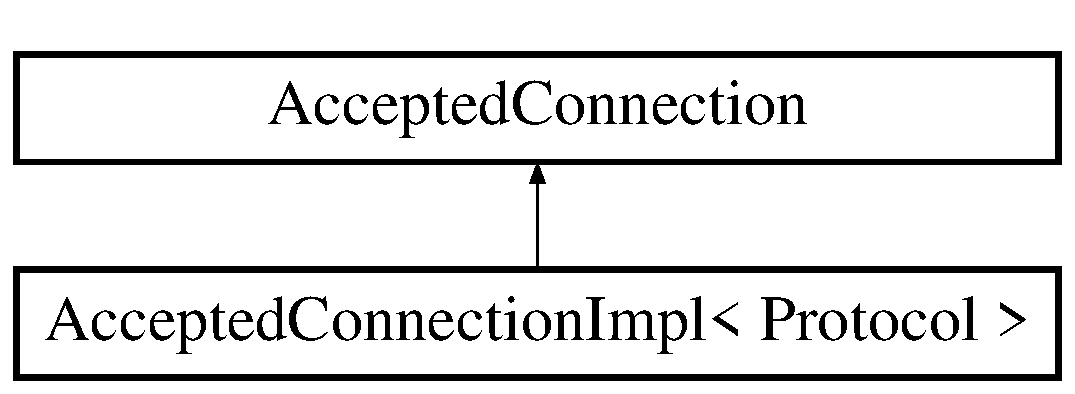
\includegraphics[height=2.000000cm]{class_accepted_connection}
\end{center}
\end{figure}
\subsection*{Public Member Functions}
\begin{DoxyCompactItemize}
\item 
virtual \hyperlink{class_accepted_connection_a8961752daf9d9905e04e7339bff0bc8f}{$\sim$\+Accepted\+Connection} ()
\item 
virtual std\+::iostream \& \hyperlink{class_accepted_connection_a2072a12e4d8f1b79a67bc86903400a0e}{stream} ()=0
\item 
virtual std\+::string \hyperlink{class_accepted_connection_adb2d35d48527a90078833f85249f2a56}{peer\+\_\+address\+\_\+to\+\_\+string} () const =0
\item 
virtual void \hyperlink{class_accepted_connection_a819d5373c0d62e736fd6e0027daa2893}{close} ()=0
\end{DoxyCompactItemize}


\subsection{Constructor \& Destructor Documentation}
\hypertarget{class_accepted_connection_a8961752daf9d9905e04e7339bff0bc8f}{}\index{Accepted\+Connection@{Accepted\+Connection}!````~Accepted\+Connection@{$\sim$\+Accepted\+Connection}}
\index{````~Accepted\+Connection@{$\sim$\+Accepted\+Connection}!Accepted\+Connection@{Accepted\+Connection}}
\subsubsection[{$\sim$\+Accepted\+Connection}]{\setlength{\rightskip}{0pt plus 5cm}virtual Accepted\+Connection\+::$\sim$\+Accepted\+Connection (
\begin{DoxyParamCaption}
{}
\end{DoxyParamCaption}
)\hspace{0.3cm}{\ttfamily [inline]}, {\ttfamily [virtual]}}\label{class_accepted_connection_a8961752daf9d9905e04e7339bff0bc8f}


\subsection{Member Function Documentation}
\hypertarget{class_accepted_connection_a819d5373c0d62e736fd6e0027daa2893}{}\index{Accepted\+Connection@{Accepted\+Connection}!close@{close}}
\index{close@{close}!Accepted\+Connection@{Accepted\+Connection}}
\subsubsection[{close}]{\setlength{\rightskip}{0pt plus 5cm}virtual void Accepted\+Connection\+::close (
\begin{DoxyParamCaption}
{}
\end{DoxyParamCaption}
)\hspace{0.3cm}{\ttfamily [pure virtual]}}\label{class_accepted_connection_a819d5373c0d62e736fd6e0027daa2893}


Implemented in \hyperlink{class_accepted_connection_impl_a1b114863c047cae57ce42564f9a29be1}{Accepted\+Connection\+Impl$<$ Protocol $>$}.

\hypertarget{class_accepted_connection_adb2d35d48527a90078833f85249f2a56}{}\index{Accepted\+Connection@{Accepted\+Connection}!peer\+\_\+address\+\_\+to\+\_\+string@{peer\+\_\+address\+\_\+to\+\_\+string}}
\index{peer\+\_\+address\+\_\+to\+\_\+string@{peer\+\_\+address\+\_\+to\+\_\+string}!Accepted\+Connection@{Accepted\+Connection}}
\subsubsection[{peer\+\_\+address\+\_\+to\+\_\+string}]{\setlength{\rightskip}{0pt plus 5cm}virtual std\+::string Accepted\+Connection\+::peer\+\_\+address\+\_\+to\+\_\+string (
\begin{DoxyParamCaption}
{}
\end{DoxyParamCaption}
) const\hspace{0.3cm}{\ttfamily [pure virtual]}}\label{class_accepted_connection_adb2d35d48527a90078833f85249f2a56}


Implemented in \hyperlink{class_accepted_connection_impl_a5fe6c34eeec9f5c829629ae3e0539a11}{Accepted\+Connection\+Impl$<$ Protocol $>$}.

\hypertarget{class_accepted_connection_a2072a12e4d8f1b79a67bc86903400a0e}{}\index{Accepted\+Connection@{Accepted\+Connection}!stream@{stream}}
\index{stream@{stream}!Accepted\+Connection@{Accepted\+Connection}}
\subsubsection[{stream}]{\setlength{\rightskip}{0pt plus 5cm}virtual std\+::iostream\& Accepted\+Connection\+::stream (
\begin{DoxyParamCaption}
{}
\end{DoxyParamCaption}
)\hspace{0.3cm}{\ttfamily [pure virtual]}}\label{class_accepted_connection_a2072a12e4d8f1b79a67bc86903400a0e}


Implemented in \hyperlink{class_accepted_connection_impl_ab15396a413e40f947b7d527a2afe37fa}{Accepted\+Connection\+Impl$<$ Protocol $>$}.



The documentation for this class was generated from the following file\+:\begin{DoxyCompactItemize}
\item 
C\+:/\+Users/\+Joe/\+Documents/\+School/\+C\+S\+C17\+A/bitcoin/src/\hyperlink{rpcserver_8h}{rpcserver.\+h}\end{DoxyCompactItemize}

\hypertarget{class_accepted_connection_impl}{}\section{Accepted\+Connection\+Impl$<$ Protocol $>$ Class Template Reference}
\label{class_accepted_connection_impl}\index{Accepted\+Connection\+Impl$<$ Protocol $>$@{Accepted\+Connection\+Impl$<$ Protocol $>$}}
Inheritance diagram for Accepted\+Connection\+Impl$<$ Protocol $>$\+:\begin{figure}[H]
\begin{center}
\leavevmode
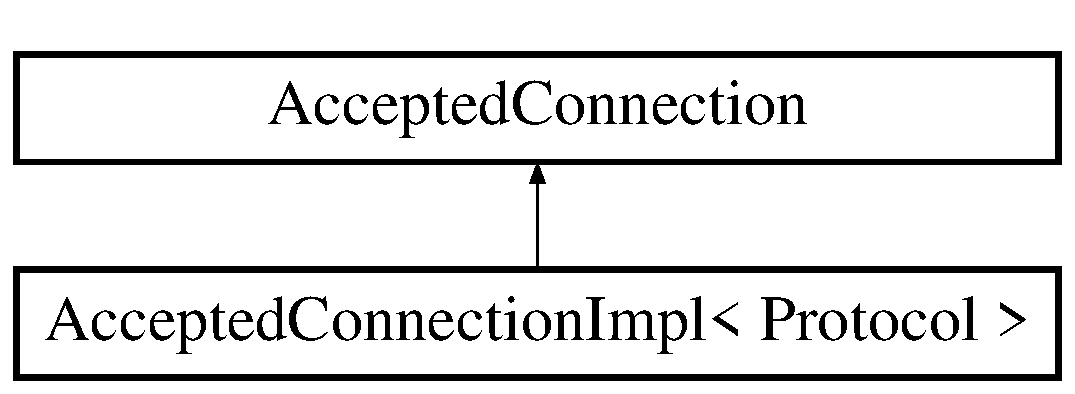
\includegraphics[height=2.000000cm]{class_accepted_connection_impl}
\end{center}
\end{figure}
\subsection*{Public Member Functions}
\begin{DoxyCompactItemize}
\item 
\hyperlink{class_accepted_connection_impl_a273b81e3d6f7706071ec71c1323c9c65}{Accepted\+Connection\+Impl} (boost\+::asio\+::io\+\_\+service \&io\+\_\+service, ssl\+::context \&context, bool f\+Use\+S\+S\+L)
\item 
virtual std\+::iostream \& \hyperlink{class_accepted_connection_impl_ab15396a413e40f947b7d527a2afe37fa}{stream} ()
\item 
virtual std\+::string \hyperlink{class_accepted_connection_impl_a5fe6c34eeec9f5c829629ae3e0539a11}{peer\+\_\+address\+\_\+to\+\_\+string} () const 
\item 
virtual void \hyperlink{class_accepted_connection_impl_a1b114863c047cae57ce42564f9a29be1}{close} ()
\end{DoxyCompactItemize}
\subsection*{Public Attributes}
\begin{DoxyCompactItemize}
\item 
Protocol\+::endpoint \hyperlink{class_accepted_connection_impl_ade939b7d2778690cf78a9f6719f47c76}{peer}
\item 
boost\+::asio\+::ssl\+::stream$<$ typename Protocol\+::socket $>$ \hyperlink{class_accepted_connection_impl_add3b600f08eabed89746393e5c319527}{ssl\+Stream}
\end{DoxyCompactItemize}


\subsection{Constructor \& Destructor Documentation}
\hypertarget{class_accepted_connection_impl_a273b81e3d6f7706071ec71c1323c9c65}{}\index{Accepted\+Connection\+Impl@{Accepted\+Connection\+Impl}!Accepted\+Connection\+Impl@{Accepted\+Connection\+Impl}}
\index{Accepted\+Connection\+Impl@{Accepted\+Connection\+Impl}!Accepted\+Connection\+Impl@{Accepted\+Connection\+Impl}}
\subsubsection[{Accepted\+Connection\+Impl}]{\setlength{\rightskip}{0pt plus 5cm}template$<$typename Protocol $>$ {\bf Accepted\+Connection\+Impl}$<$ Protocol $>$\+::{\bf Accepted\+Connection\+Impl} (
\begin{DoxyParamCaption}
\item[{boost\+::asio\+::io\+\_\+service \&}]{io\+\_\+service, }
\item[{ssl\+::context \&}]{context, }
\item[{bool}]{f\+Use\+S\+S\+L}
\end{DoxyParamCaption}
)\hspace{0.3cm}{\ttfamily [inline]}}\label{class_accepted_connection_impl_a273b81e3d6f7706071ec71c1323c9c65}


\subsection{Member Function Documentation}
\hypertarget{class_accepted_connection_impl_a1b114863c047cae57ce42564f9a29be1}{}\index{Accepted\+Connection\+Impl@{Accepted\+Connection\+Impl}!close@{close}}
\index{close@{close}!Accepted\+Connection\+Impl@{Accepted\+Connection\+Impl}}
\subsubsection[{close}]{\setlength{\rightskip}{0pt plus 5cm}template$<$typename Protocol $>$ virtual void {\bf Accepted\+Connection\+Impl}$<$ Protocol $>$\+::close (
\begin{DoxyParamCaption}
{}
\end{DoxyParamCaption}
)\hspace{0.3cm}{\ttfamily [inline]}, {\ttfamily [virtual]}}\label{class_accepted_connection_impl_a1b114863c047cae57ce42564f9a29be1}


Implements \hyperlink{class_accepted_connection_a819d5373c0d62e736fd6e0027daa2893}{Accepted\+Connection}.

\hypertarget{class_accepted_connection_impl_a5fe6c34eeec9f5c829629ae3e0539a11}{}\index{Accepted\+Connection\+Impl@{Accepted\+Connection\+Impl}!peer\+\_\+address\+\_\+to\+\_\+string@{peer\+\_\+address\+\_\+to\+\_\+string}}
\index{peer\+\_\+address\+\_\+to\+\_\+string@{peer\+\_\+address\+\_\+to\+\_\+string}!Accepted\+Connection\+Impl@{Accepted\+Connection\+Impl}}
\subsubsection[{peer\+\_\+address\+\_\+to\+\_\+string}]{\setlength{\rightskip}{0pt plus 5cm}template$<$typename Protocol $>$ virtual std\+::string {\bf Accepted\+Connection\+Impl}$<$ Protocol $>$\+::peer\+\_\+address\+\_\+to\+\_\+string (
\begin{DoxyParamCaption}
{}
\end{DoxyParamCaption}
) const\hspace{0.3cm}{\ttfamily [inline]}, {\ttfamily [virtual]}}\label{class_accepted_connection_impl_a5fe6c34eeec9f5c829629ae3e0539a11}


Implements \hyperlink{class_accepted_connection_adb2d35d48527a90078833f85249f2a56}{Accepted\+Connection}.

\hypertarget{class_accepted_connection_impl_ab15396a413e40f947b7d527a2afe37fa}{}\index{Accepted\+Connection\+Impl@{Accepted\+Connection\+Impl}!stream@{stream}}
\index{stream@{stream}!Accepted\+Connection\+Impl@{Accepted\+Connection\+Impl}}
\subsubsection[{stream}]{\setlength{\rightskip}{0pt plus 5cm}template$<$typename Protocol $>$ virtual std\+::iostream\& {\bf Accepted\+Connection\+Impl}$<$ Protocol $>$\+::stream (
\begin{DoxyParamCaption}
{}
\end{DoxyParamCaption}
)\hspace{0.3cm}{\ttfamily [inline]}, {\ttfamily [virtual]}}\label{class_accepted_connection_impl_ab15396a413e40f947b7d527a2afe37fa}


Implements \hyperlink{class_accepted_connection_a2072a12e4d8f1b79a67bc86903400a0e}{Accepted\+Connection}.



\subsection{Member Data Documentation}
\hypertarget{class_accepted_connection_impl_ade939b7d2778690cf78a9f6719f47c76}{}\index{Accepted\+Connection\+Impl@{Accepted\+Connection\+Impl}!peer@{peer}}
\index{peer@{peer}!Accepted\+Connection\+Impl@{Accepted\+Connection\+Impl}}
\subsubsection[{peer}]{\setlength{\rightskip}{0pt plus 5cm}template$<$typename Protocol $>$ Protocol\+::endpoint {\bf Accepted\+Connection\+Impl}$<$ Protocol $>$\+::peer}\label{class_accepted_connection_impl_ade939b7d2778690cf78a9f6719f47c76}
\hypertarget{class_accepted_connection_impl_add3b600f08eabed89746393e5c319527}{}\index{Accepted\+Connection\+Impl@{Accepted\+Connection\+Impl}!ssl\+Stream@{ssl\+Stream}}
\index{ssl\+Stream@{ssl\+Stream}!Accepted\+Connection\+Impl@{Accepted\+Connection\+Impl}}
\subsubsection[{ssl\+Stream}]{\setlength{\rightskip}{0pt plus 5cm}template$<$typename Protocol $>$ boost\+::asio\+::ssl\+::stream$<$typename Protocol\+::socket$>$ {\bf Accepted\+Connection\+Impl}$<$ Protocol $>$\+::ssl\+Stream}\label{class_accepted_connection_impl_add3b600f08eabed89746393e5c319527}


The documentation for this class was generated from the following file\+:\begin{DoxyCompactItemize}
\item 
C\+:/\+Users/\+Joe/\+Documents/\+School/\+C\+S\+C17\+A/bitcoin/src/\hyperlink{rpcserver_8cpp}{rpcserver.\+cpp}\end{DoxyCompactItemize}

\hypertarget{class_annotated_mixin}{}\section{Annotated\+Mixin$<$ P\+A\+R\+E\+N\+T $>$ Class Template Reference}
\label{class_annotated_mixin}\index{Annotated\+Mixin$<$ P\+A\+R\+E\+N\+T $>$@{Annotated\+Mixin$<$ P\+A\+R\+E\+N\+T $>$}}


{\ttfamily \#include $<$sync.\+h$>$}

Inheritance diagram for Annotated\+Mixin$<$ P\+A\+R\+E\+N\+T $>$\+:\begin{figure}[H]
\begin{center}
\leavevmode
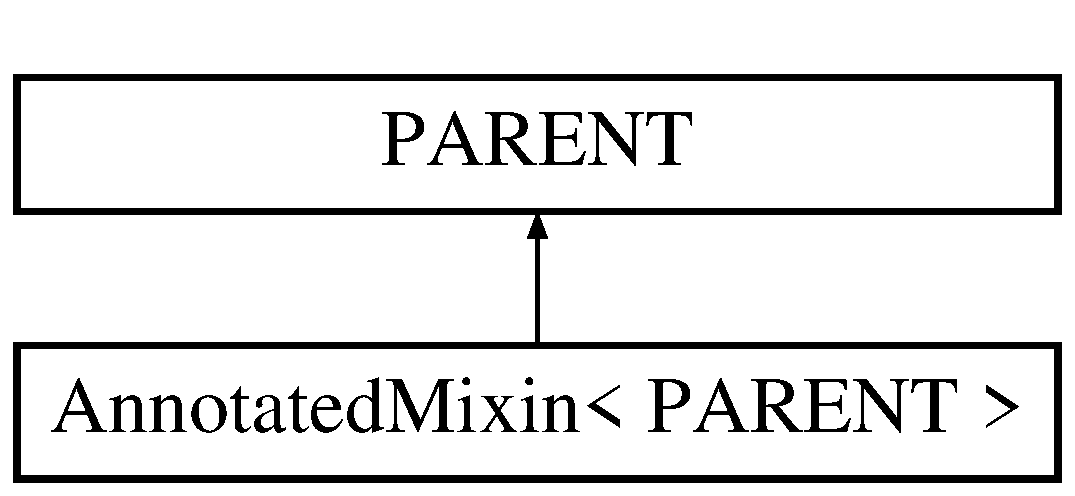
\includegraphics[height=2.000000cm]{class_annotated_mixin}
\end{center}
\end{figure}
\subsection*{Public Member Functions}
\begin{DoxyCompactItemize}
\item 
void \hyperlink{class_annotated_mixin_ad1f35c6d1b8a8e980fff45e7e7cb46d3}{lock} () \hyperlink{threadsafety_8h_a77729163b7f6867da40ad5daa5f926f3}{E\+X\+C\+L\+U\+S\+I\+V\+E\+\_\+\+L\+O\+C\+K\+\_\+\+F\+U\+N\+C\+T\+I\+O\+N}()
\item 
void \hyperlink{class_annotated_mixin_acc2e3da37c2d9dd483b859572e32bc24}{unlock} () \hyperlink{threadsafety_8h_abd56e19f9b4781b1a5212a46951cf5c3}{U\+N\+L\+O\+C\+K\+\_\+\+F\+U\+N\+C\+T\+I\+O\+N}()
\item 
bool \hyperlink{class_annotated_mixin_a9a33deab2da56790d8b5d30b1fd8350d}{try\+\_\+lock} () \hyperlink{threadsafety_8h_a3c67d370ed1f55064d85e01076aad534}{E\+X\+C\+L\+U\+S\+I\+V\+E\+\_\+\+T\+R\+Y\+L\+O\+C\+K\+\_\+\+F\+U\+N\+C\+T\+I\+O\+N}(true)
\end{DoxyCompactItemize}


\subsection{Detailed Description}
\subsubsection*{template$<$typename P\+A\+R\+E\+N\+T$>$class Annotated\+Mixin$<$ P\+A\+R\+E\+N\+T $>$}

Template mixin that adds -\/\+Wthread-\/safety locking annotations to a subset of the mutex A\+P\+I. 

\subsection{Member Function Documentation}
\hypertarget{class_annotated_mixin_ad1f35c6d1b8a8e980fff45e7e7cb46d3}{}\index{Annotated\+Mixin@{Annotated\+Mixin}!lock@{lock}}
\index{lock@{lock}!Annotated\+Mixin@{Annotated\+Mixin}}
\subsubsection[{lock}]{\setlength{\rightskip}{0pt plus 5cm}template$<$typename P\+A\+R\+E\+N\+T$>$ void {\bf Annotated\+Mixin}$<$ P\+A\+R\+E\+N\+T $>$\+::lock (
\begin{DoxyParamCaption}
{}
\end{DoxyParamCaption}
)\hspace{0.3cm}{\ttfamily [inline]}}\label{class_annotated_mixin_ad1f35c6d1b8a8e980fff45e7e7cb46d3}
\hypertarget{class_annotated_mixin_a9a33deab2da56790d8b5d30b1fd8350d}{}\index{Annotated\+Mixin@{Annotated\+Mixin}!try\+\_\+lock@{try\+\_\+lock}}
\index{try\+\_\+lock@{try\+\_\+lock}!Annotated\+Mixin@{Annotated\+Mixin}}
\subsubsection[{try\+\_\+lock}]{\setlength{\rightskip}{0pt plus 5cm}template$<$typename P\+A\+R\+E\+N\+T$>$ bool {\bf Annotated\+Mixin}$<$ P\+A\+R\+E\+N\+T $>$\+::try\+\_\+lock (
\begin{DoxyParamCaption}
{}
\end{DoxyParamCaption}
)\hspace{0.3cm}{\ttfamily [inline]}}\label{class_annotated_mixin_a9a33deab2da56790d8b5d30b1fd8350d}
\hypertarget{class_annotated_mixin_acc2e3da37c2d9dd483b859572e32bc24}{}\index{Annotated\+Mixin@{Annotated\+Mixin}!unlock@{unlock}}
\index{unlock@{unlock}!Annotated\+Mixin@{Annotated\+Mixin}}
\subsubsection[{unlock}]{\setlength{\rightskip}{0pt plus 5cm}template$<$typename P\+A\+R\+E\+N\+T$>$ void {\bf Annotated\+Mixin}$<$ P\+A\+R\+E\+N\+T $>$\+::unlock (
\begin{DoxyParamCaption}
{}
\end{DoxyParamCaption}
)\hspace{0.3cm}{\ttfamily [inline]}}\label{class_annotated_mixin_acc2e3da37c2d9dd483b859572e32bc24}


The documentation for this class was generated from the following file\+:\begin{DoxyCompactItemize}
\item 
C\+:/\+Users/\+Joe/\+Documents/\+School/\+C\+S\+C17\+A/bitcoin/src/\hyperlink{sync_8h}{sync.\+h}\end{DoxyCompactItemize}

\hypertarget{classarith__uint256}{}\section{arith\+\_\+uint256 Class Reference}
\label{classarith__uint256}\index{arith\+\_\+uint256@{arith\+\_\+uint256}}


{\ttfamily \#include $<$arith\+\_\+uint256.\+h$>$}

Inheritance diagram for arith\+\_\+uint256\+:\begin{figure}[H]
\begin{center}
\leavevmode
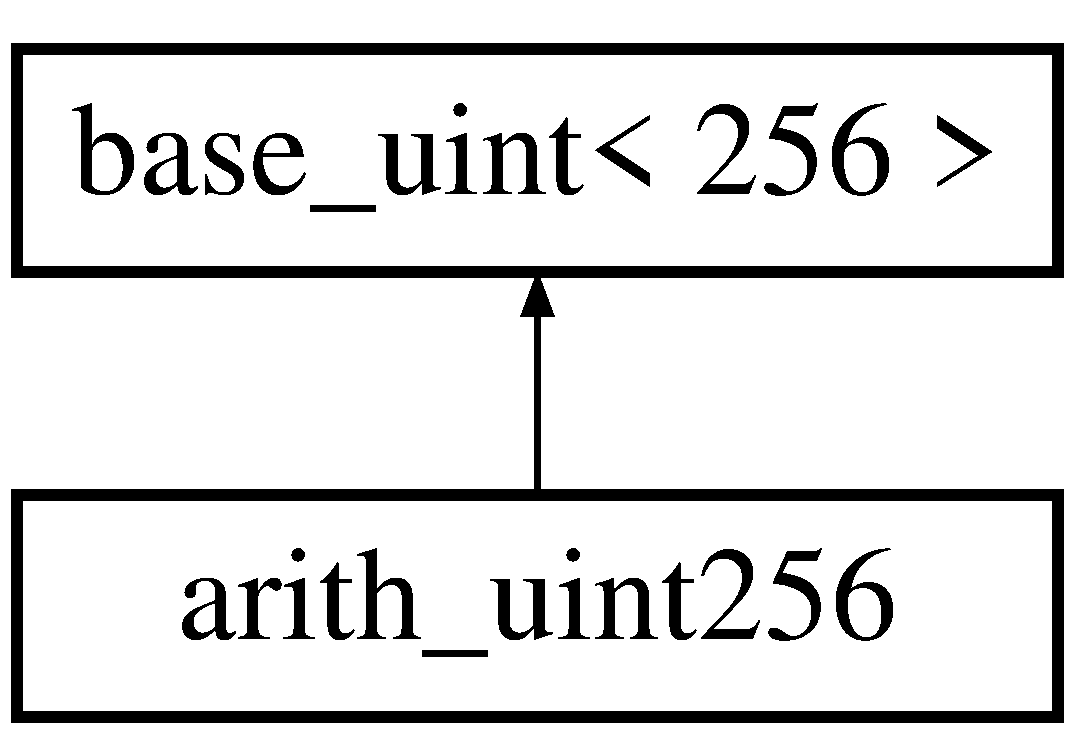
\includegraphics[height=2.000000cm]{classarith__uint256}
\end{center}
\end{figure}
\subsection*{Public Member Functions}
\begin{DoxyCompactItemize}
\item 
\hyperlink{classarith__uint256_a1dae7481f3ebf5457f70aaf385d566dd}{arith\+\_\+uint256} ()
\item 
\hyperlink{classarith__uint256_a86c126d261e0edeea49e051e2f3b98a7}{arith\+\_\+uint256} (const \hyperlink{classbase__uint}{base\+\_\+uint}$<$ 256 $>$ \&b)
\item 
\hyperlink{classarith__uint256_a865adeb2767f24e0efc3abfb3d75170b}{arith\+\_\+uint256} (uint64\+\_\+t b)
\item 
\hyperlink{classarith__uint256_a0e8b76f74ffb7a251b15aff89b087fbf}{arith\+\_\+uint256} (const std\+::string \&str)
\item 
\hyperlink{classarith__uint256}{arith\+\_\+uint256} \& \hyperlink{classarith__uint256_a458133c9f123519646b07e6143f2164f}{Set\+Compact} (uint32\+\_\+t n\+Compact, bool $\ast$pf\+Negative=N\+U\+L\+L, bool $\ast$pf\+Overflow=N\+U\+L\+L)
\item 
uint32\+\_\+t \hyperlink{classarith__uint256_a943e22c7910b92d5e48c71f420c4ae30}{Get\+Compact} (bool f\+Negative=false) const 
\end{DoxyCompactItemize}
\subsection*{Friends}
\begin{DoxyCompactItemize}
\item 
\hyperlink{classuint256}{uint256} \hyperlink{classarith__uint256_aef075fd8d1a7e5937e9775b8e82c8a1b}{Arith\+To\+Uint256} (const \hyperlink{classarith__uint256}{arith\+\_\+uint256} \&)
\item 
\hyperlink{classarith__uint256}{arith\+\_\+uint256} \hyperlink{classarith__uint256_a9c9f84c20851f10a8ca5082bec97666a}{Uint\+To\+Arith256} (const \hyperlink{classuint256}{uint256} \&)
\end{DoxyCompactItemize}
\subsection*{Additional Inherited Members}


\subsection{Detailed Description}
256-\/bit unsigned big integer. 

\subsection{Constructor \& Destructor Documentation}
\hypertarget{classarith__uint256_a1dae7481f3ebf5457f70aaf385d566dd}{}\index{arith\+\_\+uint256@{arith\+\_\+uint256}!arith\+\_\+uint256@{arith\+\_\+uint256}}
\index{arith\+\_\+uint256@{arith\+\_\+uint256}!arith\+\_\+uint256@{arith\+\_\+uint256}}
\subsubsection[{arith\+\_\+uint256}]{\setlength{\rightskip}{0pt plus 5cm}arith\+\_\+uint256\+::arith\+\_\+uint256 (
\begin{DoxyParamCaption}
{}
\end{DoxyParamCaption}
)\hspace{0.3cm}{\ttfamily [inline]}}\label{classarith__uint256_a1dae7481f3ebf5457f70aaf385d566dd}
\hypertarget{classarith__uint256_a86c126d261e0edeea49e051e2f3b98a7}{}\index{arith\+\_\+uint256@{arith\+\_\+uint256}!arith\+\_\+uint256@{arith\+\_\+uint256}}
\index{arith\+\_\+uint256@{arith\+\_\+uint256}!arith\+\_\+uint256@{arith\+\_\+uint256}}
\subsubsection[{arith\+\_\+uint256}]{\setlength{\rightskip}{0pt plus 5cm}arith\+\_\+uint256\+::arith\+\_\+uint256 (
\begin{DoxyParamCaption}
\item[{const {\bf base\+\_\+uint}$<$ 256 $>$ \&}]{b}
\end{DoxyParamCaption}
)\hspace{0.3cm}{\ttfamily [inline]}}\label{classarith__uint256_a86c126d261e0edeea49e051e2f3b98a7}
\hypertarget{classarith__uint256_a865adeb2767f24e0efc3abfb3d75170b}{}\index{arith\+\_\+uint256@{arith\+\_\+uint256}!arith\+\_\+uint256@{arith\+\_\+uint256}}
\index{arith\+\_\+uint256@{arith\+\_\+uint256}!arith\+\_\+uint256@{arith\+\_\+uint256}}
\subsubsection[{arith\+\_\+uint256}]{\setlength{\rightskip}{0pt plus 5cm}arith\+\_\+uint256\+::arith\+\_\+uint256 (
\begin{DoxyParamCaption}
\item[{uint64\+\_\+t}]{b}
\end{DoxyParamCaption}
)\hspace{0.3cm}{\ttfamily [inline]}}\label{classarith__uint256_a865adeb2767f24e0efc3abfb3d75170b}
\hypertarget{classarith__uint256_a0e8b76f74ffb7a251b15aff89b087fbf}{}\index{arith\+\_\+uint256@{arith\+\_\+uint256}!arith\+\_\+uint256@{arith\+\_\+uint256}}
\index{arith\+\_\+uint256@{arith\+\_\+uint256}!arith\+\_\+uint256@{arith\+\_\+uint256}}
\subsubsection[{arith\+\_\+uint256}]{\setlength{\rightskip}{0pt plus 5cm}arith\+\_\+uint256\+::arith\+\_\+uint256 (
\begin{DoxyParamCaption}
\item[{const std\+::string \&}]{str}
\end{DoxyParamCaption}
)\hspace{0.3cm}{\ttfamily [inline]}, {\ttfamily [explicit]}}\label{classarith__uint256_a0e8b76f74ffb7a251b15aff89b087fbf}


\subsection{Member Function Documentation}
\hypertarget{classarith__uint256_a943e22c7910b92d5e48c71f420c4ae30}{}\index{arith\+\_\+uint256@{arith\+\_\+uint256}!Get\+Compact@{Get\+Compact}}
\index{Get\+Compact@{Get\+Compact}!arith\+\_\+uint256@{arith\+\_\+uint256}}
\subsubsection[{Get\+Compact}]{\setlength{\rightskip}{0pt plus 5cm}uint32\+\_\+t arith\+\_\+uint256\+::\+Get\+Compact (
\begin{DoxyParamCaption}
\item[{bool}]{f\+Negative = {\ttfamily false}}
\end{DoxyParamCaption}
) const}\label{classarith__uint256_a943e22c7910b92d5e48c71f420c4ae30}
\hypertarget{classarith__uint256_a458133c9f123519646b07e6143f2164f}{}\index{arith\+\_\+uint256@{arith\+\_\+uint256}!Set\+Compact@{Set\+Compact}}
\index{Set\+Compact@{Set\+Compact}!arith\+\_\+uint256@{arith\+\_\+uint256}}
\subsubsection[{Set\+Compact}]{\setlength{\rightskip}{0pt plus 5cm}{\bf arith\+\_\+uint256} \& arith\+\_\+uint256\+::\+Set\+Compact (
\begin{DoxyParamCaption}
\item[{uint32\+\_\+t}]{n\+Compact, }
\item[{bool $\ast$}]{pf\+Negative = {\ttfamily NULL}, }
\item[{bool $\ast$}]{pf\+Overflow = {\ttfamily NULL}}
\end{DoxyParamCaption}
)}\label{classarith__uint256_a458133c9f123519646b07e6143f2164f}
The \char`\"{}compact\char`\"{} format is a representation of a whole number N using an unsigned 32bit number similar to a floating point format. The most significant 8 bits are the unsigned exponent of base 256. This exponent can be thought of as \char`\"{}number of bytes of N\char`\"{}. The lower 23 bits are the mantissa. Bit number 24 (0x800000) represents the sign of N. N = (-\/1$^\wedge$sign) $\ast$ mantissa $\ast$ 256$^\wedge$(exponent-\/3)

Satoshi\textquotesingle{}s original implementation used B\+N\+\_\+bn2mpi() and B\+N\+\_\+mpi2bn(). M\+P\+I uses the most significant bit of the first byte as sign. Thus 0x1234560000 is compact (0x05123456) and 0xc0de000000 is compact (0x0600c0de)

Bitcoin only uses this \char`\"{}compact\char`\"{} format for encoding difficulty targets, which are unsigned 256bit quantities. Thus, all the complexities of the sign bit and using base 256 are probably an implementation accident. 

\subsection{Friends And Related Function Documentation}
\hypertarget{classarith__uint256_aef075fd8d1a7e5937e9775b8e82c8a1b}{}\index{arith\+\_\+uint256@{arith\+\_\+uint256}!Arith\+To\+Uint256@{Arith\+To\+Uint256}}
\index{Arith\+To\+Uint256@{Arith\+To\+Uint256}!arith\+\_\+uint256@{arith\+\_\+uint256}}
\subsubsection[{Arith\+To\+Uint256}]{\setlength{\rightskip}{0pt plus 5cm}{\bf uint256} Arith\+To\+Uint256 (
\begin{DoxyParamCaption}
\item[{const {\bf arith\+\_\+uint256} \&}]{}
\end{DoxyParamCaption}
)\hspace{0.3cm}{\ttfamily [friend]}}\label{classarith__uint256_aef075fd8d1a7e5937e9775b8e82c8a1b}
\hypertarget{classarith__uint256_a9c9f84c20851f10a8ca5082bec97666a}{}\index{arith\+\_\+uint256@{arith\+\_\+uint256}!Uint\+To\+Arith256@{Uint\+To\+Arith256}}
\index{Uint\+To\+Arith256@{Uint\+To\+Arith256}!arith\+\_\+uint256@{arith\+\_\+uint256}}
\subsubsection[{Uint\+To\+Arith256}]{\setlength{\rightskip}{0pt plus 5cm}{\bf arith\+\_\+uint256} Uint\+To\+Arith256 (
\begin{DoxyParamCaption}
\item[{const {\bf uint256} \&}]{}
\end{DoxyParamCaption}
)\hspace{0.3cm}{\ttfamily [friend]}}\label{classarith__uint256_a9c9f84c20851f10a8ca5082bec97666a}


The documentation for this class was generated from the following files\+:\begin{DoxyCompactItemize}
\item 
C\+:/\+Users/\+Joe/\+Documents/\+School/\+C\+S\+C17\+A/bitcoin/src/\hyperlink{arith__uint256_8h}{arith\+\_\+uint256.\+h}\item 
C\+:/\+Users/\+Joe/\+Documents/\+School/\+C\+S\+C17\+A/bitcoin/src/\hyperlink{arith__uint256_8cpp}{arith\+\_\+uint256.\+cpp}\end{DoxyCompactItemize}

\hypertarget{classbase__blob}{}\section{base\+\_\+blob$<$ B\+I\+T\+S $>$ Class Template Reference}
\label{classbase__blob}\index{base\+\_\+blob$<$ B\+I\+T\+S $>$@{base\+\_\+blob$<$ B\+I\+T\+S $>$}}


{\ttfamily \#include $<$uint256.\+h$>$}

\subsection*{Public Member Functions}
\begin{DoxyCompactItemize}
\item 
\hyperlink{classbase__blob_ada7be83089951dc9438f384c0587cf29}{base\+\_\+blob} ()
\item 
\hyperlink{classbase__blob_a874bc08d9039eb202fb2ab95dd9f49a0}{base\+\_\+blob} (const std\+::vector$<$ unsigned char $>$ \&vch)
\item 
bool \hyperlink{classbase__blob_aff2f3d1d623d91b6895a6a153434770e}{Is\+Null} () const 
\item 
void \hyperlink{classbase__blob_aa340be5328d911272eded433d03f30a3}{Set\+Null} ()
\item 
std\+::string \hyperlink{classbase__blob_a9541747b1f91f9469ac0aff90665bd32}{Get\+Hex} () const 
\item 
void \hyperlink{classbase__blob_a5ec1f681a2830f4e180fe664c0eb4dd0}{Set\+Hex} (const char $\ast$psz)
\item 
void \hyperlink{classbase__blob_a5df0a1d46bdf167b4e2dc7c7068ff53a}{Set\+Hex} (const std\+::string \&str)
\item 
std\+::string \hyperlink{classbase__blob_a1a26b5da921f48b09b228d1bfda05088}{To\+String} () const 
\item 
unsigned char $\ast$ \hyperlink{classbase__blob_aeee68e00ceeacf49086e98b661e017ff}{begin} ()
\item 
unsigned char $\ast$ \hyperlink{classbase__blob_ab60d34d18e5b5f74d285480f7b3db00c}{end} ()
\item 
const unsigned char $\ast$ \hyperlink{classbase__blob_ae0cb02356abee204d1e86da2b0842745}{begin} () const 
\item 
const unsigned char $\ast$ \hyperlink{classbase__blob_a9f2fb60d0014cdc1afda230cfa8f7f7d}{end} () const 
\item 
unsigned int \hyperlink{classbase__blob_a449c3f902fcab7af6c74aa9fee099542}{size} () const 
\item 
unsigned int \hyperlink{classbase__blob_ae88b1782486e704927aa10ae20c491a9}{Get\+Serialize\+Size} (int n\+Type, int n\+Version) const 
\item 
{\footnotesize template$<$typename Stream $>$ }\\void \hyperlink{classbase__blob_ac9ccfed4de6210801d4dbede71ad8ba6}{Serialize} (Stream \&s, int n\+Type, int n\+Version) const 
\item 
{\footnotesize template$<$typename Stream $>$ }\\void \hyperlink{classbase__blob_a3d3f418c65801267e8de23d9367532c0}{Unserialize} (Stream \&s, int n\+Type, int n\+Version)
\end{DoxyCompactItemize}
\subsection*{Protected Types}
\begin{DoxyCompactItemize}
\item 
enum \{ \hyperlink{classbase__blob_a41aa51643c1ccfdcc1fa2aad41f0fde9a3e53605ecb8eb4c497cb23476695f0c3}{W\+I\+D\+T\+H} =B\+I\+T\+S/8
 \}
\end{DoxyCompactItemize}
\subsection*{Protected Attributes}
\begin{DoxyCompactItemize}
\item 
uint8\+\_\+t \hyperlink{classbase__blob_a667a178269121efb4ec95bd59e6a9615}{data} \mbox{[}\hyperlink{classbase__blob_a41aa51643c1ccfdcc1fa2aad41f0fde9a3e53605ecb8eb4c497cb23476695f0c3}{W\+I\+D\+T\+H}\mbox{]}
\end{DoxyCompactItemize}
\subsection*{Friends}
\begin{DoxyCompactItemize}
\item 
bool \hyperlink{classbase__blob_abed369be2b14c869397bb2cccc066a13}{operator==} (const \hyperlink{classbase__blob}{base\+\_\+blob} \&a, const \hyperlink{classbase__blob}{base\+\_\+blob} \&b)
\item 
bool \hyperlink{classbase__blob_a7f04c806d3164a5c0417bcce70be4959}{operator!=} (const \hyperlink{classbase__blob}{base\+\_\+blob} \&a, const \hyperlink{classbase__blob}{base\+\_\+blob} \&b)
\item 
bool \hyperlink{classbase__blob_af1ef6aa747985902964e7a5d2f8dad05}{operator$<$} (const \hyperlink{classbase__blob}{base\+\_\+blob} \&a, const \hyperlink{classbase__blob}{base\+\_\+blob} \&b)
\end{DoxyCompactItemize}


\subsection{Detailed Description}
\subsubsection*{template$<$unsigned int B\+I\+T\+S$>$class base\+\_\+blob$<$ B\+I\+T\+S $>$}

Template base class for fixed-\/sized opaque blobs. 

\subsection{Member Enumeration Documentation}
\hypertarget{classbase__blob_a41aa51643c1ccfdcc1fa2aad41f0fde9}{}\subsubsection[{anonymous enum}]{\setlength{\rightskip}{0pt plus 5cm}template$<$unsigned int B\+I\+T\+S$>$ anonymous enum\hspace{0.3cm}{\ttfamily [protected]}}\label{classbase__blob_a41aa51643c1ccfdcc1fa2aad41f0fde9}
\begin{Desc}
\item[Enumerator]\par
\begin{description}
\index{W\+I\+D\+T\+H@{W\+I\+D\+T\+H}!base\+\_\+blob@{base\+\_\+blob}}\index{base\+\_\+blob@{base\+\_\+blob}!W\+I\+D\+T\+H@{W\+I\+D\+T\+H}}\item[{\em 
\hypertarget{classbase__blob_a41aa51643c1ccfdcc1fa2aad41f0fde9a3e53605ecb8eb4c497cb23476695f0c3}{}W\+I\+D\+T\+H\label{classbase__blob_a41aa51643c1ccfdcc1fa2aad41f0fde9a3e53605ecb8eb4c497cb23476695f0c3}
}]\end{description}
\end{Desc}


\subsection{Constructor \& Destructor Documentation}
\hypertarget{classbase__blob_ada7be83089951dc9438f384c0587cf29}{}\index{base\+\_\+blob@{base\+\_\+blob}!base\+\_\+blob@{base\+\_\+blob}}
\index{base\+\_\+blob@{base\+\_\+blob}!base\+\_\+blob@{base\+\_\+blob}}
\subsubsection[{base\+\_\+blob}]{\setlength{\rightskip}{0pt plus 5cm}template$<$unsigned int B\+I\+T\+S$>$ {\bf base\+\_\+blob}$<$ B\+I\+T\+S $>$\+::{\bf base\+\_\+blob} (
\begin{DoxyParamCaption}
{}
\end{DoxyParamCaption}
)\hspace{0.3cm}{\ttfamily [inline]}}\label{classbase__blob_ada7be83089951dc9438f384c0587cf29}
\hypertarget{classbase__blob_a874bc08d9039eb202fb2ab95dd9f49a0}{}\index{base\+\_\+blob@{base\+\_\+blob}!base\+\_\+blob@{base\+\_\+blob}}
\index{base\+\_\+blob@{base\+\_\+blob}!base\+\_\+blob@{base\+\_\+blob}}
\subsubsection[{base\+\_\+blob}]{\setlength{\rightskip}{0pt plus 5cm}template$<$unsigned int B\+I\+T\+S$>$ {\bf base\+\_\+blob}$<$ B\+I\+T\+S $>$\+::{\bf base\+\_\+blob} (
\begin{DoxyParamCaption}
\item[{const std\+::vector$<$ unsigned char $>$ \&}]{vch}
\end{DoxyParamCaption}
)\hspace{0.3cm}{\ttfamily [explicit]}}\label{classbase__blob_a874bc08d9039eb202fb2ab95dd9f49a0}


\subsection{Member Function Documentation}
\hypertarget{classbase__blob_aeee68e00ceeacf49086e98b661e017ff}{}\index{base\+\_\+blob@{base\+\_\+blob}!begin@{begin}}
\index{begin@{begin}!base\+\_\+blob@{base\+\_\+blob}}
\subsubsection[{begin}]{\setlength{\rightskip}{0pt plus 5cm}template$<$unsigned int B\+I\+T\+S$>$ unsigned char$\ast$ {\bf base\+\_\+blob}$<$ B\+I\+T\+S $>$\+::begin (
\begin{DoxyParamCaption}
{}
\end{DoxyParamCaption}
)\hspace{0.3cm}{\ttfamily [inline]}}\label{classbase__blob_aeee68e00ceeacf49086e98b661e017ff}
\hypertarget{classbase__blob_ae0cb02356abee204d1e86da2b0842745}{}\index{base\+\_\+blob@{base\+\_\+blob}!begin@{begin}}
\index{begin@{begin}!base\+\_\+blob@{base\+\_\+blob}}
\subsubsection[{begin}]{\setlength{\rightskip}{0pt plus 5cm}template$<$unsigned int B\+I\+T\+S$>$ const unsigned char$\ast$ {\bf base\+\_\+blob}$<$ B\+I\+T\+S $>$\+::begin (
\begin{DoxyParamCaption}
{}
\end{DoxyParamCaption}
) const\hspace{0.3cm}{\ttfamily [inline]}}\label{classbase__blob_ae0cb02356abee204d1e86da2b0842745}
\hypertarget{classbase__blob_ab60d34d18e5b5f74d285480f7b3db00c}{}\index{base\+\_\+blob@{base\+\_\+blob}!end@{end}}
\index{end@{end}!base\+\_\+blob@{base\+\_\+blob}}
\subsubsection[{end}]{\setlength{\rightskip}{0pt plus 5cm}template$<$unsigned int B\+I\+T\+S$>$ unsigned char$\ast$ {\bf base\+\_\+blob}$<$ B\+I\+T\+S $>$\+::end (
\begin{DoxyParamCaption}
{}
\end{DoxyParamCaption}
)\hspace{0.3cm}{\ttfamily [inline]}}\label{classbase__blob_ab60d34d18e5b5f74d285480f7b3db00c}
\hypertarget{classbase__blob_a9f2fb60d0014cdc1afda230cfa8f7f7d}{}\index{base\+\_\+blob@{base\+\_\+blob}!end@{end}}
\index{end@{end}!base\+\_\+blob@{base\+\_\+blob}}
\subsubsection[{end}]{\setlength{\rightskip}{0pt plus 5cm}template$<$unsigned int B\+I\+T\+S$>$ const unsigned char$\ast$ {\bf base\+\_\+blob}$<$ B\+I\+T\+S $>$\+::end (
\begin{DoxyParamCaption}
{}
\end{DoxyParamCaption}
) const\hspace{0.3cm}{\ttfamily [inline]}}\label{classbase__blob_a9f2fb60d0014cdc1afda230cfa8f7f7d}
\hypertarget{classbase__blob_a9541747b1f91f9469ac0aff90665bd32}{}\index{base\+\_\+blob@{base\+\_\+blob}!Get\+Hex@{Get\+Hex}}
\index{Get\+Hex@{Get\+Hex}!base\+\_\+blob@{base\+\_\+blob}}
\subsubsection[{Get\+Hex}]{\setlength{\rightskip}{0pt plus 5cm}template$<$unsigned int B\+I\+T\+S$>$ std\+::string {\bf base\+\_\+blob}$<$ B\+I\+T\+S $>$\+::Get\+Hex (
\begin{DoxyParamCaption}
{}
\end{DoxyParamCaption}
) const}\label{classbase__blob_a9541747b1f91f9469ac0aff90665bd32}
\hypertarget{classbase__blob_ae88b1782486e704927aa10ae20c491a9}{}\index{base\+\_\+blob@{base\+\_\+blob}!Get\+Serialize\+Size@{Get\+Serialize\+Size}}
\index{Get\+Serialize\+Size@{Get\+Serialize\+Size}!base\+\_\+blob@{base\+\_\+blob}}
\subsubsection[{Get\+Serialize\+Size}]{\setlength{\rightskip}{0pt plus 5cm}template$<$unsigned int B\+I\+T\+S$>$ unsigned int {\bf base\+\_\+blob}$<$ B\+I\+T\+S $>$\+::Get\+Serialize\+Size (
\begin{DoxyParamCaption}
\item[{int}]{n\+Type, }
\item[{int}]{n\+Version}
\end{DoxyParamCaption}
) const\hspace{0.3cm}{\ttfamily [inline]}}\label{classbase__blob_ae88b1782486e704927aa10ae20c491a9}
\hypertarget{classbase__blob_aff2f3d1d623d91b6895a6a153434770e}{}\index{base\+\_\+blob@{base\+\_\+blob}!Is\+Null@{Is\+Null}}
\index{Is\+Null@{Is\+Null}!base\+\_\+blob@{base\+\_\+blob}}
\subsubsection[{Is\+Null}]{\setlength{\rightskip}{0pt plus 5cm}template$<$unsigned int B\+I\+T\+S$>$ bool {\bf base\+\_\+blob}$<$ B\+I\+T\+S $>$\+::Is\+Null (
\begin{DoxyParamCaption}
{}
\end{DoxyParamCaption}
) const\hspace{0.3cm}{\ttfamily [inline]}}\label{classbase__blob_aff2f3d1d623d91b6895a6a153434770e}
\hypertarget{classbase__blob_ac9ccfed4de6210801d4dbede71ad8ba6}{}\index{base\+\_\+blob@{base\+\_\+blob}!Serialize@{Serialize}}
\index{Serialize@{Serialize}!base\+\_\+blob@{base\+\_\+blob}}
\subsubsection[{Serialize}]{\setlength{\rightskip}{0pt plus 5cm}template$<$unsigned int B\+I\+T\+S$>$ template$<$typename Stream $>$ void {\bf base\+\_\+blob}$<$ B\+I\+T\+S $>$\+::Serialize (
\begin{DoxyParamCaption}
\item[{Stream \&}]{s, }
\item[{int}]{n\+Type, }
\item[{int}]{n\+Version}
\end{DoxyParamCaption}
) const\hspace{0.3cm}{\ttfamily [inline]}}\label{classbase__blob_ac9ccfed4de6210801d4dbede71ad8ba6}
\hypertarget{classbase__blob_a5ec1f681a2830f4e180fe664c0eb4dd0}{}\index{base\+\_\+blob@{base\+\_\+blob}!Set\+Hex@{Set\+Hex}}
\index{Set\+Hex@{Set\+Hex}!base\+\_\+blob@{base\+\_\+blob}}
\subsubsection[{Set\+Hex}]{\setlength{\rightskip}{0pt plus 5cm}template$<$unsigned int B\+I\+T\+S$>$ void {\bf base\+\_\+blob}$<$ B\+I\+T\+S $>$\+::Set\+Hex (
\begin{DoxyParamCaption}
\item[{const char $\ast$}]{psz}
\end{DoxyParamCaption}
)}\label{classbase__blob_a5ec1f681a2830f4e180fe664c0eb4dd0}
\hypertarget{classbase__blob_a5df0a1d46bdf167b4e2dc7c7068ff53a}{}\index{base\+\_\+blob@{base\+\_\+blob}!Set\+Hex@{Set\+Hex}}
\index{Set\+Hex@{Set\+Hex}!base\+\_\+blob@{base\+\_\+blob}}
\subsubsection[{Set\+Hex}]{\setlength{\rightskip}{0pt plus 5cm}template$<$unsigned int B\+I\+T\+S$>$ void {\bf base\+\_\+blob}$<$ B\+I\+T\+S $>$\+::Set\+Hex (
\begin{DoxyParamCaption}
\item[{const std\+::string \&}]{str}
\end{DoxyParamCaption}
)}\label{classbase__blob_a5df0a1d46bdf167b4e2dc7c7068ff53a}
\hypertarget{classbase__blob_aa340be5328d911272eded433d03f30a3}{}\index{base\+\_\+blob@{base\+\_\+blob}!Set\+Null@{Set\+Null}}
\index{Set\+Null@{Set\+Null}!base\+\_\+blob@{base\+\_\+blob}}
\subsubsection[{Set\+Null}]{\setlength{\rightskip}{0pt plus 5cm}template$<$unsigned int B\+I\+T\+S$>$ void {\bf base\+\_\+blob}$<$ B\+I\+T\+S $>$\+::Set\+Null (
\begin{DoxyParamCaption}
{}
\end{DoxyParamCaption}
)\hspace{0.3cm}{\ttfamily [inline]}}\label{classbase__blob_aa340be5328d911272eded433d03f30a3}
\hypertarget{classbase__blob_a449c3f902fcab7af6c74aa9fee099542}{}\index{base\+\_\+blob@{base\+\_\+blob}!size@{size}}
\index{size@{size}!base\+\_\+blob@{base\+\_\+blob}}
\subsubsection[{size}]{\setlength{\rightskip}{0pt plus 5cm}template$<$unsigned int B\+I\+T\+S$>$ unsigned int {\bf base\+\_\+blob}$<$ B\+I\+T\+S $>$\+::size (
\begin{DoxyParamCaption}
{}
\end{DoxyParamCaption}
) const\hspace{0.3cm}{\ttfamily [inline]}}\label{classbase__blob_a449c3f902fcab7af6c74aa9fee099542}
\hypertarget{classbase__blob_a1a26b5da921f48b09b228d1bfda05088}{}\index{base\+\_\+blob@{base\+\_\+blob}!To\+String@{To\+String}}
\index{To\+String@{To\+String}!base\+\_\+blob@{base\+\_\+blob}}
\subsubsection[{To\+String}]{\setlength{\rightskip}{0pt plus 5cm}template$<$unsigned int B\+I\+T\+S$>$ std\+::string {\bf base\+\_\+blob}$<$ B\+I\+T\+S $>$\+::To\+String (
\begin{DoxyParamCaption}
{}
\end{DoxyParamCaption}
) const}\label{classbase__blob_a1a26b5da921f48b09b228d1bfda05088}
\hypertarget{classbase__blob_a3d3f418c65801267e8de23d9367532c0}{}\index{base\+\_\+blob@{base\+\_\+blob}!Unserialize@{Unserialize}}
\index{Unserialize@{Unserialize}!base\+\_\+blob@{base\+\_\+blob}}
\subsubsection[{Unserialize}]{\setlength{\rightskip}{0pt plus 5cm}template$<$unsigned int B\+I\+T\+S$>$ template$<$typename Stream $>$ void {\bf base\+\_\+blob}$<$ B\+I\+T\+S $>$\+::Unserialize (
\begin{DoxyParamCaption}
\item[{Stream \&}]{s, }
\item[{int}]{n\+Type, }
\item[{int}]{n\+Version}
\end{DoxyParamCaption}
)\hspace{0.3cm}{\ttfamily [inline]}}\label{classbase__blob_a3d3f418c65801267e8de23d9367532c0}


\subsection{Friends And Related Function Documentation}
\hypertarget{classbase__blob_a7f04c806d3164a5c0417bcce70be4959}{}\index{base\+\_\+blob@{base\+\_\+blob}!operator"!=@{operator"!=}}
\index{operator"!=@{operator"!=}!base\+\_\+blob@{base\+\_\+blob}}
\subsubsection[{operator"!=}]{\setlength{\rightskip}{0pt plus 5cm}template$<$unsigned int B\+I\+T\+S$>$ bool operator!= (
\begin{DoxyParamCaption}
\item[{const {\bf base\+\_\+blob}$<$ B\+I\+T\+S $>$ \&}]{a, }
\item[{const {\bf base\+\_\+blob}$<$ B\+I\+T\+S $>$ \&}]{b}
\end{DoxyParamCaption}
)\hspace{0.3cm}{\ttfamily [friend]}}\label{classbase__blob_a7f04c806d3164a5c0417bcce70be4959}
\hypertarget{classbase__blob_af1ef6aa747985902964e7a5d2f8dad05}{}\index{base\+\_\+blob@{base\+\_\+blob}!operator$<$@{operator$<$}}
\index{operator$<$@{operator$<$}!base\+\_\+blob@{base\+\_\+blob}}
\subsubsection[{operator$<$}]{\setlength{\rightskip}{0pt plus 5cm}template$<$unsigned int B\+I\+T\+S$>$ bool operator$<$ (
\begin{DoxyParamCaption}
\item[{const {\bf base\+\_\+blob}$<$ B\+I\+T\+S $>$ \&}]{a, }
\item[{const {\bf base\+\_\+blob}$<$ B\+I\+T\+S $>$ \&}]{b}
\end{DoxyParamCaption}
)\hspace{0.3cm}{\ttfamily [friend]}}\label{classbase__blob_af1ef6aa747985902964e7a5d2f8dad05}
\hypertarget{classbase__blob_abed369be2b14c869397bb2cccc066a13}{}\index{base\+\_\+blob@{base\+\_\+blob}!operator==@{operator==}}
\index{operator==@{operator==}!base\+\_\+blob@{base\+\_\+blob}}
\subsubsection[{operator==}]{\setlength{\rightskip}{0pt plus 5cm}template$<$unsigned int B\+I\+T\+S$>$ bool operator== (
\begin{DoxyParamCaption}
\item[{const {\bf base\+\_\+blob}$<$ B\+I\+T\+S $>$ \&}]{a, }
\item[{const {\bf base\+\_\+blob}$<$ B\+I\+T\+S $>$ \&}]{b}
\end{DoxyParamCaption}
)\hspace{0.3cm}{\ttfamily [friend]}}\label{classbase__blob_abed369be2b14c869397bb2cccc066a13}


\subsection{Member Data Documentation}
\hypertarget{classbase__blob_a667a178269121efb4ec95bd59e6a9615}{}\index{base\+\_\+blob@{base\+\_\+blob}!data@{data}}
\index{data@{data}!base\+\_\+blob@{base\+\_\+blob}}
\subsubsection[{data}]{\setlength{\rightskip}{0pt plus 5cm}template$<$unsigned int B\+I\+T\+S$>$ uint8\+\_\+t {\bf base\+\_\+blob}$<$ B\+I\+T\+S $>$\+::data\mbox{[}{\bf W\+I\+D\+T\+H}\mbox{]}\hspace{0.3cm}{\ttfamily [protected]}}\label{classbase__blob_a667a178269121efb4ec95bd59e6a9615}


The documentation for this class was generated from the following files\+:\begin{DoxyCompactItemize}
\item 
C\+:/\+Users/\+Joe/\+Documents/\+School/\+C\+S\+C17\+A/bitcoin/src/\hyperlink{uint256_8h}{uint256.\+h}\item 
C\+:/\+Users/\+Joe/\+Documents/\+School/\+C\+S\+C17\+A/bitcoin/src/\hyperlink{uint256_8cpp}{uint256.\+cpp}\end{DoxyCompactItemize}

\hypertarget{classbase__uint}{}\section{base\+\_\+uint$<$ B\+I\+T\+S $>$ Class Template Reference}
\label{classbase__uint}\index{base\+\_\+uint$<$ B\+I\+T\+S $>$@{base\+\_\+uint$<$ B\+I\+T\+S $>$}}


{\ttfamily \#include $<$arith\+\_\+uint256.\+h$>$}

\subsection*{Public Member Functions}
\begin{DoxyCompactItemize}
\item 
\hyperlink{classbase__uint_aafd4418923a92b58a1c360e657fa7d83}{base\+\_\+uint} ()
\item 
\hyperlink{classbase__uint_a5d4e4c28c82c3a12b3689860081579c1}{base\+\_\+uint} (const \hyperlink{classbase__uint}{base\+\_\+uint} \&b)
\item 
\hyperlink{classbase__uint}{base\+\_\+uint} \& \hyperlink{classbase__uint_a0425a3c4d342b6fc9a68b1766cee9ede}{operator=} (const \hyperlink{classbase__uint}{base\+\_\+uint} \&b)
\item 
\hyperlink{classbase__uint_a217f9750f0ca9cdeefffb7bb1f1952d6}{base\+\_\+uint} (uint64\+\_\+t b)
\item 
\hyperlink{classbase__uint_aa1ebaba47302da3e120879d186355736}{base\+\_\+uint} (const std\+::string \&str)
\item 
bool \hyperlink{classbase__uint_a0f528438872245b8fc54ff60bbb6118a}{operator!} () const 
\item 
const \hyperlink{classbase__uint}{base\+\_\+uint} \hyperlink{classbase__uint_ad64a83e128fcf2d2ac072811a3e36300}{operator$\sim$} () const 
\item 
const \hyperlink{classbase__uint}{base\+\_\+uint} \hyperlink{classbase__uint_a29b620fba192a191054b35bf269ea221}{operator-\/} () const 
\item 
double \hyperlink{classbase__uint_aa701be5115bacf02c299b05598cf616d}{getdouble} () const 
\item 
\hyperlink{classbase__uint}{base\+\_\+uint} \& \hyperlink{classbase__uint_a115a5ddb2f2637e09703a25cfc580483}{operator=} (uint64\+\_\+t b)
\item 
\hyperlink{classbase__uint}{base\+\_\+uint} \& \hyperlink{classbase__uint_ad5ec10977ebeab115fe857637990e267}{operator$^\wedge$=} (const \hyperlink{classbase__uint}{base\+\_\+uint} \&b)
\item 
\hyperlink{classbase__uint}{base\+\_\+uint} \& \hyperlink{classbase__uint_a6cb549b322e5bbcca794366f5fd3fb15}{operator\&=} (const \hyperlink{classbase__uint}{base\+\_\+uint} \&b)
\item 
\hyperlink{classbase__uint}{base\+\_\+uint} \& \hyperlink{classbase__uint_ab116d89cbae68b32fbecf5d1de98bb2e}{operator$\vert$=} (const \hyperlink{classbase__uint}{base\+\_\+uint} \&b)
\item 
\hyperlink{classbase__uint}{base\+\_\+uint} \& \hyperlink{classbase__uint_a3d77324f5c5166e4dabadac360bea6e7}{operator$^\wedge$=} (uint64\+\_\+t b)
\item 
\hyperlink{classbase__uint}{base\+\_\+uint} \& \hyperlink{classbase__uint_ac8edb6e097d9eede21f8fa44e9184913}{operator$\vert$=} (uint64\+\_\+t b)
\item 
\hyperlink{classbase__uint}{base\+\_\+uint} \& \hyperlink{classbase__uint_acb449d2fcb5af767fa6b01890e836a4e}{operator$<$$<$=} (unsigned int shift)
\item 
\hyperlink{classbase__uint}{base\+\_\+uint} \& \hyperlink{classbase__uint_a4e0344432bbcce79525fd2c182173b3b}{operator$>$$>$=} (unsigned int shift)
\item 
\hyperlink{classbase__uint}{base\+\_\+uint} \& \hyperlink{classbase__uint_a8fb3109e7c46536bb66ac41242176246}{operator+=} (const \hyperlink{classbase__uint}{base\+\_\+uint} \&b)
\item 
\hyperlink{classbase__uint}{base\+\_\+uint} \& \hyperlink{classbase__uint_a89d8332840076ec102839b8a10dda9b4}{operator-\/=} (const \hyperlink{classbase__uint}{base\+\_\+uint} \&b)
\item 
\hyperlink{classbase__uint}{base\+\_\+uint} \& \hyperlink{classbase__uint_a14f2b12970b3198d65abafb2615207ca}{operator+=} (uint64\+\_\+t b64)
\item 
\hyperlink{classbase__uint}{base\+\_\+uint} \& \hyperlink{classbase__uint_ab64f7a7a87b9af5ea345e4678b4cc1e9}{operator-\/=} (uint64\+\_\+t b64)
\item 
\hyperlink{classbase__uint}{base\+\_\+uint} \& \hyperlink{classbase__uint_aa70b7d954258d2cd4bb77721e357fd40}{operator$\ast$=} (uint32\+\_\+t b32)
\item 
\hyperlink{classbase__uint}{base\+\_\+uint} \& \hyperlink{classbase__uint_a806b2ba843181e9dd4c824414fbcc13d}{operator$\ast$=} (const \hyperlink{classbase__uint}{base\+\_\+uint} \&b)
\item 
\hyperlink{classbase__uint}{base\+\_\+uint} \& \hyperlink{classbase__uint_ad6fa7e22ab995247c0bf298069732e1d}{operator/=} (const \hyperlink{classbase__uint}{base\+\_\+uint} \&b)
\item 
\hyperlink{classbase__uint}{base\+\_\+uint} \& \hyperlink{classbase__uint_a56b54869886808961092d3f764fadd9f}{operator++} ()
\item 
const \hyperlink{classbase__uint}{base\+\_\+uint} \hyperlink{classbase__uint_a2d5a123c856b2b31fae5f65891832486}{operator++} (int)
\item 
\hyperlink{classbase__uint}{base\+\_\+uint} \& \hyperlink{classbase__uint_a2cc581d32afac619acd12601ddea4180}{operator-\/-\/} ()
\item 
const \hyperlink{classbase__uint}{base\+\_\+uint} \hyperlink{classbase__uint_a78a8e46c434c0e61be86282fe9543587}{operator-\/-\/} (int)
\item 
int \hyperlink{classbase__uint_ac9777c80cfcf1355cf17258027ca35bb}{Compare\+To} (const \hyperlink{classbase__uint}{base\+\_\+uint} \&b) const 
\item 
bool \hyperlink{classbase__uint_a39817436d7ba143e8d52abc475097384}{Equal\+To} (uint64\+\_\+t b) const 
\item 
std\+::string \hyperlink{classbase__uint_ac9929c28600796a9acf75881bb750576}{Get\+Hex} () const 
\item 
void \hyperlink{classbase__uint_ade1a897fac931f28f54998c92c797228}{Set\+Hex} (const char $\ast$psz)
\item 
void \hyperlink{classbase__uint_afe3600e6ae4e9f69e1c036581a2716c8}{Set\+Hex} (const std\+::string \&str)
\item 
std\+::string \hyperlink{classbase__uint_ac3080a72402cadf28dbc9f9b69cc60be}{To\+String} () const 
\item 
unsigned int \hyperlink{classbase__uint_ae0e221686cd63384569a8db5cc06d4c9}{size} () const 
\item 
unsigned int \hyperlink{classbase__uint_a4867652ab4163a10ac4e3d04f0352423}{bits} () const 
\item 
uint64\+\_\+t \hyperlink{classbase__uint_abf39b71afc016b333b8996def4c6bc40}{Get\+Low64} () const 
\end{DoxyCompactItemize}
\subsection*{Protected Types}
\begin{DoxyCompactItemize}
\item 
enum \{ \hyperlink{classbase__uint_afee51629f03ba95d823ab4ee94cf6c81adf579395d753e2d9607ecd61424f0853}{W\+I\+D\+T\+H} =B\+I\+T\+S/32
 \}
\end{DoxyCompactItemize}
\subsection*{Protected Attributes}
\begin{DoxyCompactItemize}
\item 
uint32\+\_\+t \hyperlink{classbase__uint_a0edb1465d540fadd92b21659f27083a2}{pn} \mbox{[}\hyperlink{classbase__uint_afee51629f03ba95d823ab4ee94cf6c81adf579395d753e2d9607ecd61424f0853}{W\+I\+D\+T\+H}\mbox{]}
\end{DoxyCompactItemize}
\subsection*{Friends}
\begin{DoxyCompactItemize}
\item 
const \hyperlink{classbase__uint}{base\+\_\+uint} \hyperlink{classbase__uint_ab46abc7a4c02bbbe6ee4d44db58f36fd}{operator+} (const \hyperlink{classbase__uint}{base\+\_\+uint} \&a, const \hyperlink{classbase__uint}{base\+\_\+uint} \&b)
\item 
const \hyperlink{classbase__uint}{base\+\_\+uint} \hyperlink{classbase__uint_a42603f675219a79c1087da39677dd6d3}{operator-\/} (const \hyperlink{classbase__uint}{base\+\_\+uint} \&a, const \hyperlink{classbase__uint}{base\+\_\+uint} \&b)
\item 
const \hyperlink{classbase__uint}{base\+\_\+uint} \hyperlink{classbase__uint_a7cc93af608b4d2b8e45f8a18bb085cf0}{operator$\ast$} (const \hyperlink{classbase__uint}{base\+\_\+uint} \&a, const \hyperlink{classbase__uint}{base\+\_\+uint} \&b)
\item 
const \hyperlink{classbase__uint}{base\+\_\+uint} \hyperlink{classbase__uint_a3027097ea3718db496e486d5c64a6bbd}{operator/} (const \hyperlink{classbase__uint}{base\+\_\+uint} \&a, const \hyperlink{classbase__uint}{base\+\_\+uint} \&b)
\item 
const \hyperlink{classbase__uint}{base\+\_\+uint} \hyperlink{classbase__uint_af11d7776598f6633c139636314f065d6}{operator$\vert$} (const \hyperlink{classbase__uint}{base\+\_\+uint} \&a, const \hyperlink{classbase__uint}{base\+\_\+uint} \&b)
\item 
const \hyperlink{classbase__uint}{base\+\_\+uint} \hyperlink{classbase__uint_a7dd38f6935c35d4b534b669c3baf21a6}{operator\&} (const \hyperlink{classbase__uint}{base\+\_\+uint} \&a, const \hyperlink{classbase__uint}{base\+\_\+uint} \&b)
\item 
const \hyperlink{classbase__uint}{base\+\_\+uint} \hyperlink{classbase__uint_aa9c66282ad78846e8310984aeb2df49d}{operator$^\wedge$} (const \hyperlink{classbase__uint}{base\+\_\+uint} \&a, const \hyperlink{classbase__uint}{base\+\_\+uint} \&b)
\item 
const \hyperlink{classbase__uint}{base\+\_\+uint} \hyperlink{classbase__uint_a9d619adcbf9ad5539f5e98f739edd15d}{operator$>$$>$} (const \hyperlink{classbase__uint}{base\+\_\+uint} \&a, int shift)
\item 
const \hyperlink{classbase__uint}{base\+\_\+uint} \hyperlink{classbase__uint_acee16d973ae59087cd962720773f53dd}{operator$<$$<$} (const \hyperlink{classbase__uint}{base\+\_\+uint} \&a, int shift)
\item 
const \hyperlink{classbase__uint}{base\+\_\+uint} \hyperlink{classbase__uint_a3490f0aef12712d434cda33f913b586f}{operator$\ast$} (const \hyperlink{classbase__uint}{base\+\_\+uint} \&a, uint32\+\_\+t b)
\item 
bool \hyperlink{classbase__uint_aafca305decdfd2ded4688213ab4a55fa}{operator==} (const \hyperlink{classbase__uint}{base\+\_\+uint} \&a, const \hyperlink{classbase__uint}{base\+\_\+uint} \&b)
\item 
bool \hyperlink{classbase__uint_a3cc3bccf252004fbbd2b96dc769378e7}{operator!=} (const \hyperlink{classbase__uint}{base\+\_\+uint} \&a, const \hyperlink{classbase__uint}{base\+\_\+uint} \&b)
\item 
bool \hyperlink{classbase__uint_ac59719bd052d5dc2afcc35ae4a8843ab}{operator$>$} (const \hyperlink{classbase__uint}{base\+\_\+uint} \&a, const \hyperlink{classbase__uint}{base\+\_\+uint} \&b)
\item 
bool \hyperlink{classbase__uint_a89272b5112f90ba683c0f066ba1426c1}{operator$<$} (const \hyperlink{classbase__uint}{base\+\_\+uint} \&a, const \hyperlink{classbase__uint}{base\+\_\+uint} \&b)
\item 
bool \hyperlink{classbase__uint_a9eb243df5a6dfa3d0cd326427d99bfa6}{operator$>$=} (const \hyperlink{classbase__uint}{base\+\_\+uint} \&a, const \hyperlink{classbase__uint}{base\+\_\+uint} \&b)
\item 
bool \hyperlink{classbase__uint_ac7f1bdba7208bd852f7b00f7c49624f8}{operator$<$=} (const \hyperlink{classbase__uint}{base\+\_\+uint} \&a, const \hyperlink{classbase__uint}{base\+\_\+uint} \&b)
\item 
bool \hyperlink{classbase__uint_a977dbbe7e78bbdcc2aea2dc16292d424}{operator==} (const \hyperlink{classbase__uint}{base\+\_\+uint} \&a, uint64\+\_\+t b)
\item 
bool \hyperlink{classbase__uint_ab7b366cc0883f25fa57fb09d4bc33807}{operator!=} (const \hyperlink{classbase__uint}{base\+\_\+uint} \&a, uint64\+\_\+t b)
\end{DoxyCompactItemize}


\subsection{Detailed Description}
\subsubsection*{template$<$unsigned int B\+I\+T\+S$>$class base\+\_\+uint$<$ B\+I\+T\+S $>$}

Template base class for unsigned big integers. 

\subsection{Member Enumeration Documentation}
\hypertarget{classbase__uint_afee51629f03ba95d823ab4ee94cf6c81}{}\subsubsection[{anonymous enum}]{\setlength{\rightskip}{0pt plus 5cm}template$<$unsigned int B\+I\+T\+S$>$ anonymous enum\hspace{0.3cm}{\ttfamily [protected]}}\label{classbase__uint_afee51629f03ba95d823ab4ee94cf6c81}
\begin{Desc}
\item[Enumerator]\par
\begin{description}
\index{W\+I\+D\+T\+H@{W\+I\+D\+T\+H}!base\+\_\+uint@{base\+\_\+uint}}\index{base\+\_\+uint@{base\+\_\+uint}!W\+I\+D\+T\+H@{W\+I\+D\+T\+H}}\item[{\em 
\hypertarget{classbase__uint_afee51629f03ba95d823ab4ee94cf6c81adf579395d753e2d9607ecd61424f0853}{}W\+I\+D\+T\+H\label{classbase__uint_afee51629f03ba95d823ab4ee94cf6c81adf579395d753e2d9607ecd61424f0853}
}]\end{description}
\end{Desc}


\subsection{Constructor \& Destructor Documentation}
\hypertarget{classbase__uint_aafd4418923a92b58a1c360e657fa7d83}{}\index{base\+\_\+uint@{base\+\_\+uint}!base\+\_\+uint@{base\+\_\+uint}}
\index{base\+\_\+uint@{base\+\_\+uint}!base\+\_\+uint@{base\+\_\+uint}}
\subsubsection[{base\+\_\+uint}]{\setlength{\rightskip}{0pt plus 5cm}template$<$unsigned int B\+I\+T\+S$>$ {\bf base\+\_\+uint}$<$ B\+I\+T\+S $>$\+::{\bf base\+\_\+uint} (
\begin{DoxyParamCaption}
{}
\end{DoxyParamCaption}
)\hspace{0.3cm}{\ttfamily [inline]}}\label{classbase__uint_aafd4418923a92b58a1c360e657fa7d83}
\hypertarget{classbase__uint_a5d4e4c28c82c3a12b3689860081579c1}{}\index{base\+\_\+uint@{base\+\_\+uint}!base\+\_\+uint@{base\+\_\+uint}}
\index{base\+\_\+uint@{base\+\_\+uint}!base\+\_\+uint@{base\+\_\+uint}}
\subsubsection[{base\+\_\+uint}]{\setlength{\rightskip}{0pt plus 5cm}template$<$unsigned int B\+I\+T\+S$>$ {\bf base\+\_\+uint}$<$ B\+I\+T\+S $>$\+::{\bf base\+\_\+uint} (
\begin{DoxyParamCaption}
\item[{const {\bf base\+\_\+uint}$<$ B\+I\+T\+S $>$ \&}]{b}
\end{DoxyParamCaption}
)\hspace{0.3cm}{\ttfamily [inline]}}\label{classbase__uint_a5d4e4c28c82c3a12b3689860081579c1}
\hypertarget{classbase__uint_a217f9750f0ca9cdeefffb7bb1f1952d6}{}\index{base\+\_\+uint@{base\+\_\+uint}!base\+\_\+uint@{base\+\_\+uint}}
\index{base\+\_\+uint@{base\+\_\+uint}!base\+\_\+uint@{base\+\_\+uint}}
\subsubsection[{base\+\_\+uint}]{\setlength{\rightskip}{0pt plus 5cm}template$<$unsigned int B\+I\+T\+S$>$ {\bf base\+\_\+uint}$<$ B\+I\+T\+S $>$\+::{\bf base\+\_\+uint} (
\begin{DoxyParamCaption}
\item[{uint64\+\_\+t}]{b}
\end{DoxyParamCaption}
)\hspace{0.3cm}{\ttfamily [inline]}}\label{classbase__uint_a217f9750f0ca9cdeefffb7bb1f1952d6}
\hypertarget{classbase__uint_aa1ebaba47302da3e120879d186355736}{}\index{base\+\_\+uint@{base\+\_\+uint}!base\+\_\+uint@{base\+\_\+uint}}
\index{base\+\_\+uint@{base\+\_\+uint}!base\+\_\+uint@{base\+\_\+uint}}
\subsubsection[{base\+\_\+uint}]{\setlength{\rightskip}{0pt plus 5cm}template$<$unsigned int B\+I\+T\+S$>$ {\bf base\+\_\+uint}$<$ B\+I\+T\+S $>$\+::{\bf base\+\_\+uint} (
\begin{DoxyParamCaption}
\item[{const std\+::string \&}]{str}
\end{DoxyParamCaption}
)\hspace{0.3cm}{\ttfamily [explicit]}}\label{classbase__uint_aa1ebaba47302da3e120879d186355736}


\subsection{Member Function Documentation}
\hypertarget{classbase__uint_a4867652ab4163a10ac4e3d04f0352423}{}\index{base\+\_\+uint@{base\+\_\+uint}!bits@{bits}}
\index{bits@{bits}!base\+\_\+uint@{base\+\_\+uint}}
\subsubsection[{bits}]{\setlength{\rightskip}{0pt plus 5cm}template$<$unsigned int B\+I\+T\+S$>$ unsigned int {\bf base\+\_\+uint}$<$ B\+I\+T\+S $>$\+::bits (
\begin{DoxyParamCaption}
{}
\end{DoxyParamCaption}
) const}\label{classbase__uint_a4867652ab4163a10ac4e3d04f0352423}
Returns the position of the highest bit set plus one, or zero if the value is zero. \hypertarget{classbase__uint_ac9777c80cfcf1355cf17258027ca35bb}{}\index{base\+\_\+uint@{base\+\_\+uint}!Compare\+To@{Compare\+To}}
\index{Compare\+To@{Compare\+To}!base\+\_\+uint@{base\+\_\+uint}}
\subsubsection[{Compare\+To}]{\setlength{\rightskip}{0pt plus 5cm}template$<$unsigned int B\+I\+T\+S$>$ int {\bf base\+\_\+uint}$<$ B\+I\+T\+S $>$\+::Compare\+To (
\begin{DoxyParamCaption}
\item[{const {\bf base\+\_\+uint}$<$ B\+I\+T\+S $>$ \&}]{b}
\end{DoxyParamCaption}
) const}\label{classbase__uint_ac9777c80cfcf1355cf17258027ca35bb}
\hypertarget{classbase__uint_a39817436d7ba143e8d52abc475097384}{}\index{base\+\_\+uint@{base\+\_\+uint}!Equal\+To@{Equal\+To}}
\index{Equal\+To@{Equal\+To}!base\+\_\+uint@{base\+\_\+uint}}
\subsubsection[{Equal\+To}]{\setlength{\rightskip}{0pt plus 5cm}template$<$unsigned int B\+I\+T\+S$>$ bool {\bf base\+\_\+uint}$<$ B\+I\+T\+S $>$\+::Equal\+To (
\begin{DoxyParamCaption}
\item[{uint64\+\_\+t}]{b}
\end{DoxyParamCaption}
) const}\label{classbase__uint_a39817436d7ba143e8d52abc475097384}
\hypertarget{classbase__uint_aa701be5115bacf02c299b05598cf616d}{}\index{base\+\_\+uint@{base\+\_\+uint}!getdouble@{getdouble}}
\index{getdouble@{getdouble}!base\+\_\+uint@{base\+\_\+uint}}
\subsubsection[{getdouble}]{\setlength{\rightskip}{0pt plus 5cm}template$<$unsigned int B\+I\+T\+S$>$ double {\bf base\+\_\+uint}$<$ B\+I\+T\+S $>$\+::getdouble (
\begin{DoxyParamCaption}
{}
\end{DoxyParamCaption}
) const}\label{classbase__uint_aa701be5115bacf02c299b05598cf616d}
\hypertarget{classbase__uint_ac9929c28600796a9acf75881bb750576}{}\index{base\+\_\+uint@{base\+\_\+uint}!Get\+Hex@{Get\+Hex}}
\index{Get\+Hex@{Get\+Hex}!base\+\_\+uint@{base\+\_\+uint}}
\subsubsection[{Get\+Hex}]{\setlength{\rightskip}{0pt plus 5cm}template$<$unsigned int B\+I\+T\+S$>$ std\+::string {\bf base\+\_\+uint}$<$ B\+I\+T\+S $>$\+::Get\+Hex (
\begin{DoxyParamCaption}
{}
\end{DoxyParamCaption}
) const}\label{classbase__uint_ac9929c28600796a9acf75881bb750576}
\hypertarget{classbase__uint_abf39b71afc016b333b8996def4c6bc40}{}\index{base\+\_\+uint@{base\+\_\+uint}!Get\+Low64@{Get\+Low64}}
\index{Get\+Low64@{Get\+Low64}!base\+\_\+uint@{base\+\_\+uint}}
\subsubsection[{Get\+Low64}]{\setlength{\rightskip}{0pt plus 5cm}template$<$unsigned int B\+I\+T\+S$>$ uint64\+\_\+t {\bf base\+\_\+uint}$<$ B\+I\+T\+S $>$\+::Get\+Low64 (
\begin{DoxyParamCaption}
{}
\end{DoxyParamCaption}
) const\hspace{0.3cm}{\ttfamily [inline]}}\label{classbase__uint_abf39b71afc016b333b8996def4c6bc40}
\hypertarget{classbase__uint_a0f528438872245b8fc54ff60bbb6118a}{}\index{base\+\_\+uint@{base\+\_\+uint}!operator"!@{operator"!}}
\index{operator"!@{operator"!}!base\+\_\+uint@{base\+\_\+uint}}
\subsubsection[{operator"!}]{\setlength{\rightskip}{0pt plus 5cm}template$<$unsigned int B\+I\+T\+S$>$ bool {\bf base\+\_\+uint}$<$ B\+I\+T\+S $>$\+::operator! (
\begin{DoxyParamCaption}
{}
\end{DoxyParamCaption}
) const\hspace{0.3cm}{\ttfamily [inline]}}\label{classbase__uint_a0f528438872245b8fc54ff60bbb6118a}
\hypertarget{classbase__uint_a6cb549b322e5bbcca794366f5fd3fb15}{}\index{base\+\_\+uint@{base\+\_\+uint}!operator\&=@{operator\&=}}
\index{operator\&=@{operator\&=}!base\+\_\+uint@{base\+\_\+uint}}
\subsubsection[{operator\&=}]{\setlength{\rightskip}{0pt plus 5cm}template$<$unsigned int B\+I\+T\+S$>$ {\bf base\+\_\+uint}\& {\bf base\+\_\+uint}$<$ B\+I\+T\+S $>$\+::operator\&= (
\begin{DoxyParamCaption}
\item[{const {\bf base\+\_\+uint}$<$ B\+I\+T\+S $>$ \&}]{b}
\end{DoxyParamCaption}
)\hspace{0.3cm}{\ttfamily [inline]}}\label{classbase__uint_a6cb549b322e5bbcca794366f5fd3fb15}
\hypertarget{classbase__uint_aa70b7d954258d2cd4bb77721e357fd40}{}\index{base\+\_\+uint@{base\+\_\+uint}!operator$\ast$=@{operator$\ast$=}}
\index{operator$\ast$=@{operator$\ast$=}!base\+\_\+uint@{base\+\_\+uint}}
\subsubsection[{operator$\ast$=}]{\setlength{\rightskip}{0pt plus 5cm}template$<$unsigned int B\+I\+T\+S$>$ {\bf base\+\_\+uint}$<$ B\+I\+T\+S $>$ \& {\bf base\+\_\+uint}$<$ B\+I\+T\+S $>$\+::operator$\ast$= (
\begin{DoxyParamCaption}
\item[{uint32\+\_\+t}]{b32}
\end{DoxyParamCaption}
)}\label{classbase__uint_aa70b7d954258d2cd4bb77721e357fd40}
\hypertarget{classbase__uint_a806b2ba843181e9dd4c824414fbcc13d}{}\index{base\+\_\+uint@{base\+\_\+uint}!operator$\ast$=@{operator$\ast$=}}
\index{operator$\ast$=@{operator$\ast$=}!base\+\_\+uint@{base\+\_\+uint}}
\subsubsection[{operator$\ast$=}]{\setlength{\rightskip}{0pt plus 5cm}template$<$unsigned int B\+I\+T\+S$>$ {\bf base\+\_\+uint}$<$ B\+I\+T\+S $>$ \& {\bf base\+\_\+uint}$<$ B\+I\+T\+S $>$\+::operator$\ast$= (
\begin{DoxyParamCaption}
\item[{const {\bf base\+\_\+uint}$<$ B\+I\+T\+S $>$ \&}]{b}
\end{DoxyParamCaption}
)}\label{classbase__uint_a806b2ba843181e9dd4c824414fbcc13d}
\hypertarget{classbase__uint_a56b54869886808961092d3f764fadd9f}{}\index{base\+\_\+uint@{base\+\_\+uint}!operator++@{operator++}}
\index{operator++@{operator++}!base\+\_\+uint@{base\+\_\+uint}}
\subsubsection[{operator++}]{\setlength{\rightskip}{0pt plus 5cm}template$<$unsigned int B\+I\+T\+S$>$ {\bf base\+\_\+uint}\& {\bf base\+\_\+uint}$<$ B\+I\+T\+S $>$\+::operator++ (
\begin{DoxyParamCaption}
{}
\end{DoxyParamCaption}
)\hspace{0.3cm}{\ttfamily [inline]}}\label{classbase__uint_a56b54869886808961092d3f764fadd9f}
\hypertarget{classbase__uint_a2d5a123c856b2b31fae5f65891832486}{}\index{base\+\_\+uint@{base\+\_\+uint}!operator++@{operator++}}
\index{operator++@{operator++}!base\+\_\+uint@{base\+\_\+uint}}
\subsubsection[{operator++}]{\setlength{\rightskip}{0pt plus 5cm}template$<$unsigned int B\+I\+T\+S$>$ const {\bf base\+\_\+uint} {\bf base\+\_\+uint}$<$ B\+I\+T\+S $>$\+::operator++ (
\begin{DoxyParamCaption}
\item[{int}]{}
\end{DoxyParamCaption}
)\hspace{0.3cm}{\ttfamily [inline]}}\label{classbase__uint_a2d5a123c856b2b31fae5f65891832486}
\hypertarget{classbase__uint_a8fb3109e7c46536bb66ac41242176246}{}\index{base\+\_\+uint@{base\+\_\+uint}!operator+=@{operator+=}}
\index{operator+=@{operator+=}!base\+\_\+uint@{base\+\_\+uint}}
\subsubsection[{operator+=}]{\setlength{\rightskip}{0pt plus 5cm}template$<$unsigned int B\+I\+T\+S$>$ {\bf base\+\_\+uint}\& {\bf base\+\_\+uint}$<$ B\+I\+T\+S $>$\+::operator+= (
\begin{DoxyParamCaption}
\item[{const {\bf base\+\_\+uint}$<$ B\+I\+T\+S $>$ \&}]{b}
\end{DoxyParamCaption}
)\hspace{0.3cm}{\ttfamily [inline]}}\label{classbase__uint_a8fb3109e7c46536bb66ac41242176246}
\hypertarget{classbase__uint_a14f2b12970b3198d65abafb2615207ca}{}\index{base\+\_\+uint@{base\+\_\+uint}!operator+=@{operator+=}}
\index{operator+=@{operator+=}!base\+\_\+uint@{base\+\_\+uint}}
\subsubsection[{operator+=}]{\setlength{\rightskip}{0pt plus 5cm}template$<$unsigned int B\+I\+T\+S$>$ {\bf base\+\_\+uint}\& {\bf base\+\_\+uint}$<$ B\+I\+T\+S $>$\+::operator+= (
\begin{DoxyParamCaption}
\item[{uint64\+\_\+t}]{b64}
\end{DoxyParamCaption}
)\hspace{0.3cm}{\ttfamily [inline]}}\label{classbase__uint_a14f2b12970b3198d65abafb2615207ca}
\hypertarget{classbase__uint_a29b620fba192a191054b35bf269ea221}{}\index{base\+\_\+uint@{base\+\_\+uint}!operator-\/@{operator-\/}}
\index{operator-\/@{operator-\/}!base\+\_\+uint@{base\+\_\+uint}}
\subsubsection[{operator-\/}]{\setlength{\rightskip}{0pt plus 5cm}template$<$unsigned int B\+I\+T\+S$>$ const {\bf base\+\_\+uint} {\bf base\+\_\+uint}$<$ B\+I\+T\+S $>$\+::operator-\/ (
\begin{DoxyParamCaption}
{}
\end{DoxyParamCaption}
) const\hspace{0.3cm}{\ttfamily [inline]}}\label{classbase__uint_a29b620fba192a191054b35bf269ea221}
\hypertarget{classbase__uint_a2cc581d32afac619acd12601ddea4180}{}\index{base\+\_\+uint@{base\+\_\+uint}!operator-\/-\/@{operator-\/-\/}}
\index{operator-\/-\/@{operator-\/-\/}!base\+\_\+uint@{base\+\_\+uint}}
\subsubsection[{operator-\/-\/}]{\setlength{\rightskip}{0pt plus 5cm}template$<$unsigned int B\+I\+T\+S$>$ {\bf base\+\_\+uint}\& {\bf base\+\_\+uint}$<$ B\+I\+T\+S $>$\+::operator-\/-\/ (
\begin{DoxyParamCaption}
{}
\end{DoxyParamCaption}
)\hspace{0.3cm}{\ttfamily [inline]}}\label{classbase__uint_a2cc581d32afac619acd12601ddea4180}
\hypertarget{classbase__uint_a78a8e46c434c0e61be86282fe9543587}{}\index{base\+\_\+uint@{base\+\_\+uint}!operator-\/-\/@{operator-\/-\/}}
\index{operator-\/-\/@{operator-\/-\/}!base\+\_\+uint@{base\+\_\+uint}}
\subsubsection[{operator-\/-\/}]{\setlength{\rightskip}{0pt plus 5cm}template$<$unsigned int B\+I\+T\+S$>$ const {\bf base\+\_\+uint} {\bf base\+\_\+uint}$<$ B\+I\+T\+S $>$\+::operator-\/-\/ (
\begin{DoxyParamCaption}
\item[{int}]{}
\end{DoxyParamCaption}
)\hspace{0.3cm}{\ttfamily [inline]}}\label{classbase__uint_a78a8e46c434c0e61be86282fe9543587}
\hypertarget{classbase__uint_a89d8332840076ec102839b8a10dda9b4}{}\index{base\+\_\+uint@{base\+\_\+uint}!operator-\/=@{operator-\/=}}
\index{operator-\/=@{operator-\/=}!base\+\_\+uint@{base\+\_\+uint}}
\subsubsection[{operator-\/=}]{\setlength{\rightskip}{0pt plus 5cm}template$<$unsigned int B\+I\+T\+S$>$ {\bf base\+\_\+uint}\& {\bf base\+\_\+uint}$<$ B\+I\+T\+S $>$\+::operator-\/= (
\begin{DoxyParamCaption}
\item[{const {\bf base\+\_\+uint}$<$ B\+I\+T\+S $>$ \&}]{b}
\end{DoxyParamCaption}
)\hspace{0.3cm}{\ttfamily [inline]}}\label{classbase__uint_a89d8332840076ec102839b8a10dda9b4}
\hypertarget{classbase__uint_ab64f7a7a87b9af5ea345e4678b4cc1e9}{}\index{base\+\_\+uint@{base\+\_\+uint}!operator-\/=@{operator-\/=}}
\index{operator-\/=@{operator-\/=}!base\+\_\+uint@{base\+\_\+uint}}
\subsubsection[{operator-\/=}]{\setlength{\rightskip}{0pt plus 5cm}template$<$unsigned int B\+I\+T\+S$>$ {\bf base\+\_\+uint}\& {\bf base\+\_\+uint}$<$ B\+I\+T\+S $>$\+::operator-\/= (
\begin{DoxyParamCaption}
\item[{uint64\+\_\+t}]{b64}
\end{DoxyParamCaption}
)\hspace{0.3cm}{\ttfamily [inline]}}\label{classbase__uint_ab64f7a7a87b9af5ea345e4678b4cc1e9}
\hypertarget{classbase__uint_ad6fa7e22ab995247c0bf298069732e1d}{}\index{base\+\_\+uint@{base\+\_\+uint}!operator/=@{operator/=}}
\index{operator/=@{operator/=}!base\+\_\+uint@{base\+\_\+uint}}
\subsubsection[{operator/=}]{\setlength{\rightskip}{0pt plus 5cm}template$<$unsigned int B\+I\+T\+S$>$ {\bf base\+\_\+uint}$<$ B\+I\+T\+S $>$ \& {\bf base\+\_\+uint}$<$ B\+I\+T\+S $>$\+::operator/= (
\begin{DoxyParamCaption}
\item[{const {\bf base\+\_\+uint}$<$ B\+I\+T\+S $>$ \&}]{b}
\end{DoxyParamCaption}
)}\label{classbase__uint_ad6fa7e22ab995247c0bf298069732e1d}
\hypertarget{classbase__uint_acb449d2fcb5af767fa6b01890e836a4e}{}\index{base\+\_\+uint@{base\+\_\+uint}!operator$<$$<$=@{operator$<$$<$=}}
\index{operator$<$$<$=@{operator$<$$<$=}!base\+\_\+uint@{base\+\_\+uint}}
\subsubsection[{operator$<$$<$=}]{\setlength{\rightskip}{0pt plus 5cm}template$<$unsigned int B\+I\+T\+S$>$ {\bf base\+\_\+uint}$<$ B\+I\+T\+S $>$ \& {\bf base\+\_\+uint}$<$ B\+I\+T\+S $>$\+::operator$<$$<$= (
\begin{DoxyParamCaption}
\item[{unsigned int}]{shift}
\end{DoxyParamCaption}
)}\label{classbase__uint_acb449d2fcb5af767fa6b01890e836a4e}
\hypertarget{classbase__uint_a0425a3c4d342b6fc9a68b1766cee9ede}{}\index{base\+\_\+uint@{base\+\_\+uint}!operator=@{operator=}}
\index{operator=@{operator=}!base\+\_\+uint@{base\+\_\+uint}}
\subsubsection[{operator=}]{\setlength{\rightskip}{0pt plus 5cm}template$<$unsigned int B\+I\+T\+S$>$ {\bf base\+\_\+uint}\& {\bf base\+\_\+uint}$<$ B\+I\+T\+S $>$\+::operator= (
\begin{DoxyParamCaption}
\item[{const {\bf base\+\_\+uint}$<$ B\+I\+T\+S $>$ \&}]{b}
\end{DoxyParamCaption}
)\hspace{0.3cm}{\ttfamily [inline]}}\label{classbase__uint_a0425a3c4d342b6fc9a68b1766cee9ede}
\hypertarget{classbase__uint_a115a5ddb2f2637e09703a25cfc580483}{}\index{base\+\_\+uint@{base\+\_\+uint}!operator=@{operator=}}
\index{operator=@{operator=}!base\+\_\+uint@{base\+\_\+uint}}
\subsubsection[{operator=}]{\setlength{\rightskip}{0pt plus 5cm}template$<$unsigned int B\+I\+T\+S$>$ {\bf base\+\_\+uint}\& {\bf base\+\_\+uint}$<$ B\+I\+T\+S $>$\+::operator= (
\begin{DoxyParamCaption}
\item[{uint64\+\_\+t}]{b}
\end{DoxyParamCaption}
)\hspace{0.3cm}{\ttfamily [inline]}}\label{classbase__uint_a115a5ddb2f2637e09703a25cfc580483}
\hypertarget{classbase__uint_a4e0344432bbcce79525fd2c182173b3b}{}\index{base\+\_\+uint@{base\+\_\+uint}!operator$>$$>$=@{operator$>$$>$=}}
\index{operator$>$$>$=@{operator$>$$>$=}!base\+\_\+uint@{base\+\_\+uint}}
\subsubsection[{operator$>$$>$=}]{\setlength{\rightskip}{0pt plus 5cm}template$<$unsigned int B\+I\+T\+S$>$ {\bf base\+\_\+uint}$<$ B\+I\+T\+S $>$ \& {\bf base\+\_\+uint}$<$ B\+I\+T\+S $>$\+::operator$>$$>$= (
\begin{DoxyParamCaption}
\item[{unsigned int}]{shift}
\end{DoxyParamCaption}
)}\label{classbase__uint_a4e0344432bbcce79525fd2c182173b3b}
\hypertarget{classbase__uint_ad5ec10977ebeab115fe857637990e267}{}\index{base\+\_\+uint@{base\+\_\+uint}!operator$^\wedge$=@{operator$^\wedge$=}}
\index{operator$^\wedge$=@{operator$^\wedge$=}!base\+\_\+uint@{base\+\_\+uint}}
\subsubsection[{operator$^\wedge$=}]{\setlength{\rightskip}{0pt plus 5cm}template$<$unsigned int B\+I\+T\+S$>$ {\bf base\+\_\+uint}\& {\bf base\+\_\+uint}$<$ B\+I\+T\+S $>$\+::operator$^\wedge$= (
\begin{DoxyParamCaption}
\item[{const {\bf base\+\_\+uint}$<$ B\+I\+T\+S $>$ \&}]{b}
\end{DoxyParamCaption}
)\hspace{0.3cm}{\ttfamily [inline]}}\label{classbase__uint_ad5ec10977ebeab115fe857637990e267}
\hypertarget{classbase__uint_a3d77324f5c5166e4dabadac360bea6e7}{}\index{base\+\_\+uint@{base\+\_\+uint}!operator$^\wedge$=@{operator$^\wedge$=}}
\index{operator$^\wedge$=@{operator$^\wedge$=}!base\+\_\+uint@{base\+\_\+uint}}
\subsubsection[{operator$^\wedge$=}]{\setlength{\rightskip}{0pt plus 5cm}template$<$unsigned int B\+I\+T\+S$>$ {\bf base\+\_\+uint}\& {\bf base\+\_\+uint}$<$ B\+I\+T\+S $>$\+::operator$^\wedge$= (
\begin{DoxyParamCaption}
\item[{uint64\+\_\+t}]{b}
\end{DoxyParamCaption}
)\hspace{0.3cm}{\ttfamily [inline]}}\label{classbase__uint_a3d77324f5c5166e4dabadac360bea6e7}
\hypertarget{classbase__uint_ab116d89cbae68b32fbecf5d1de98bb2e}{}\index{base\+\_\+uint@{base\+\_\+uint}!operator\texttt{"|}=@{operator\texttt{"|}=}}
\index{operator\texttt{"|}=@{operator\texttt{"|}=}!base\+\_\+uint@{base\+\_\+uint}}
\subsubsection[{operator\texttt{"|}=}]{\setlength{\rightskip}{0pt plus 5cm}template$<$unsigned int B\+I\+T\+S$>$ {\bf base\+\_\+uint}\& {\bf base\+\_\+uint}$<$ B\+I\+T\+S $>$\+::operator$\vert$= (
\begin{DoxyParamCaption}
\item[{const {\bf base\+\_\+uint}$<$ B\+I\+T\+S $>$ \&}]{b}
\end{DoxyParamCaption}
)\hspace{0.3cm}{\ttfamily [inline]}}\label{classbase__uint_ab116d89cbae68b32fbecf5d1de98bb2e}
\hypertarget{classbase__uint_ac8edb6e097d9eede21f8fa44e9184913}{}\index{base\+\_\+uint@{base\+\_\+uint}!operator\texttt{"|}=@{operator\texttt{"|}=}}
\index{operator\texttt{"|}=@{operator\texttt{"|}=}!base\+\_\+uint@{base\+\_\+uint}}
\subsubsection[{operator\texttt{"|}=}]{\setlength{\rightskip}{0pt plus 5cm}template$<$unsigned int B\+I\+T\+S$>$ {\bf base\+\_\+uint}\& {\bf base\+\_\+uint}$<$ B\+I\+T\+S $>$\+::operator$\vert$= (
\begin{DoxyParamCaption}
\item[{uint64\+\_\+t}]{b}
\end{DoxyParamCaption}
)\hspace{0.3cm}{\ttfamily [inline]}}\label{classbase__uint_ac8edb6e097d9eede21f8fa44e9184913}
\hypertarget{classbase__uint_ad64a83e128fcf2d2ac072811a3e36300}{}\index{base\+\_\+uint@{base\+\_\+uint}!operator````~@{operator$\sim$}}
\index{operator````~@{operator$\sim$}!base\+\_\+uint@{base\+\_\+uint}}
\subsubsection[{operator$\sim$}]{\setlength{\rightskip}{0pt plus 5cm}template$<$unsigned int B\+I\+T\+S$>$ const {\bf base\+\_\+uint} {\bf base\+\_\+uint}$<$ B\+I\+T\+S $>$\+::operator$\sim$ (
\begin{DoxyParamCaption}
{}
\end{DoxyParamCaption}
) const\hspace{0.3cm}{\ttfamily [inline]}}\label{classbase__uint_ad64a83e128fcf2d2ac072811a3e36300}
\hypertarget{classbase__uint_ade1a897fac931f28f54998c92c797228}{}\index{base\+\_\+uint@{base\+\_\+uint}!Set\+Hex@{Set\+Hex}}
\index{Set\+Hex@{Set\+Hex}!base\+\_\+uint@{base\+\_\+uint}}
\subsubsection[{Set\+Hex}]{\setlength{\rightskip}{0pt plus 5cm}template$<$unsigned int B\+I\+T\+S$>$ void {\bf base\+\_\+uint}$<$ B\+I\+T\+S $>$\+::Set\+Hex (
\begin{DoxyParamCaption}
\item[{const char $\ast$}]{psz}
\end{DoxyParamCaption}
)}\label{classbase__uint_ade1a897fac931f28f54998c92c797228}
\hypertarget{classbase__uint_afe3600e6ae4e9f69e1c036581a2716c8}{}\index{base\+\_\+uint@{base\+\_\+uint}!Set\+Hex@{Set\+Hex}}
\index{Set\+Hex@{Set\+Hex}!base\+\_\+uint@{base\+\_\+uint}}
\subsubsection[{Set\+Hex}]{\setlength{\rightskip}{0pt plus 5cm}template$<$unsigned int B\+I\+T\+S$>$ void {\bf base\+\_\+uint}$<$ B\+I\+T\+S $>$\+::Set\+Hex (
\begin{DoxyParamCaption}
\item[{const std\+::string \&}]{str}
\end{DoxyParamCaption}
)}\label{classbase__uint_afe3600e6ae4e9f69e1c036581a2716c8}
\hypertarget{classbase__uint_ae0e221686cd63384569a8db5cc06d4c9}{}\index{base\+\_\+uint@{base\+\_\+uint}!size@{size}}
\index{size@{size}!base\+\_\+uint@{base\+\_\+uint}}
\subsubsection[{size}]{\setlength{\rightskip}{0pt plus 5cm}template$<$unsigned int B\+I\+T\+S$>$ unsigned int {\bf base\+\_\+uint}$<$ B\+I\+T\+S $>$\+::size (
\begin{DoxyParamCaption}
{}
\end{DoxyParamCaption}
) const\hspace{0.3cm}{\ttfamily [inline]}}\label{classbase__uint_ae0e221686cd63384569a8db5cc06d4c9}
\hypertarget{classbase__uint_ac3080a72402cadf28dbc9f9b69cc60be}{}\index{base\+\_\+uint@{base\+\_\+uint}!To\+String@{To\+String}}
\index{To\+String@{To\+String}!base\+\_\+uint@{base\+\_\+uint}}
\subsubsection[{To\+String}]{\setlength{\rightskip}{0pt plus 5cm}template$<$unsigned int B\+I\+T\+S$>$ std\+::string {\bf base\+\_\+uint}$<$ B\+I\+T\+S $>$\+::To\+String (
\begin{DoxyParamCaption}
{}
\end{DoxyParamCaption}
) const}\label{classbase__uint_ac3080a72402cadf28dbc9f9b69cc60be}


\subsection{Friends And Related Function Documentation}
\hypertarget{classbase__uint_a3cc3bccf252004fbbd2b96dc769378e7}{}\index{base\+\_\+uint@{base\+\_\+uint}!operator"!=@{operator"!=}}
\index{operator"!=@{operator"!=}!base\+\_\+uint@{base\+\_\+uint}}
\subsubsection[{operator"!=}]{\setlength{\rightskip}{0pt plus 5cm}template$<$unsigned int B\+I\+T\+S$>$ bool {\bf operator!}= (
\begin{DoxyParamCaption}
\item[{const {\bf base\+\_\+uint}$<$ B\+I\+T\+S $>$ \&}]{a, }
\item[{const {\bf base\+\_\+uint}$<$ B\+I\+T\+S $>$ \&}]{b}
\end{DoxyParamCaption}
)\hspace{0.3cm}{\ttfamily [friend]}}\label{classbase__uint_a3cc3bccf252004fbbd2b96dc769378e7}
\hypertarget{classbase__uint_ab7b366cc0883f25fa57fb09d4bc33807}{}\index{base\+\_\+uint@{base\+\_\+uint}!operator"!=@{operator"!=}}
\index{operator"!=@{operator"!=}!base\+\_\+uint@{base\+\_\+uint}}
\subsubsection[{operator"!=}]{\setlength{\rightskip}{0pt plus 5cm}template$<$unsigned int B\+I\+T\+S$>$ bool {\bf operator!}= (
\begin{DoxyParamCaption}
\item[{const {\bf base\+\_\+uint}$<$ B\+I\+T\+S $>$ \&}]{a, }
\item[{uint64\+\_\+t}]{b}
\end{DoxyParamCaption}
)\hspace{0.3cm}{\ttfamily [friend]}}\label{classbase__uint_ab7b366cc0883f25fa57fb09d4bc33807}
\hypertarget{classbase__uint_a7dd38f6935c35d4b534b669c3baf21a6}{}\index{base\+\_\+uint@{base\+\_\+uint}!operator\&@{operator\&}}
\index{operator\&@{operator\&}!base\+\_\+uint@{base\+\_\+uint}}
\subsubsection[{operator\&}]{\setlength{\rightskip}{0pt plus 5cm}template$<$unsigned int B\+I\+T\+S$>$ const {\bf base\+\_\+uint} operator\& (
\begin{DoxyParamCaption}
\item[{const {\bf base\+\_\+uint}$<$ B\+I\+T\+S $>$ \&}]{a, }
\item[{const {\bf base\+\_\+uint}$<$ B\+I\+T\+S $>$ \&}]{b}
\end{DoxyParamCaption}
)\hspace{0.3cm}{\ttfamily [friend]}}\label{classbase__uint_a7dd38f6935c35d4b534b669c3baf21a6}
\hypertarget{classbase__uint_a7cc93af608b4d2b8e45f8a18bb085cf0}{}\index{base\+\_\+uint@{base\+\_\+uint}!operator$\ast$@{operator$\ast$}}
\index{operator$\ast$@{operator$\ast$}!base\+\_\+uint@{base\+\_\+uint}}
\subsubsection[{operator$\ast$}]{\setlength{\rightskip}{0pt plus 5cm}template$<$unsigned int B\+I\+T\+S$>$ const {\bf base\+\_\+uint} operator$\ast$ (
\begin{DoxyParamCaption}
\item[{const {\bf base\+\_\+uint}$<$ B\+I\+T\+S $>$ \&}]{a, }
\item[{const {\bf base\+\_\+uint}$<$ B\+I\+T\+S $>$ \&}]{b}
\end{DoxyParamCaption}
)\hspace{0.3cm}{\ttfamily [friend]}}\label{classbase__uint_a7cc93af608b4d2b8e45f8a18bb085cf0}
\hypertarget{classbase__uint_a3490f0aef12712d434cda33f913b586f}{}\index{base\+\_\+uint@{base\+\_\+uint}!operator$\ast$@{operator$\ast$}}
\index{operator$\ast$@{operator$\ast$}!base\+\_\+uint@{base\+\_\+uint}}
\subsubsection[{operator$\ast$}]{\setlength{\rightskip}{0pt plus 5cm}template$<$unsigned int B\+I\+T\+S$>$ const {\bf base\+\_\+uint} operator$\ast$ (
\begin{DoxyParamCaption}
\item[{const {\bf base\+\_\+uint}$<$ B\+I\+T\+S $>$ \&}]{a, }
\item[{uint32\+\_\+t}]{b}
\end{DoxyParamCaption}
)\hspace{0.3cm}{\ttfamily [friend]}}\label{classbase__uint_a3490f0aef12712d434cda33f913b586f}
\hypertarget{classbase__uint_ab46abc7a4c02bbbe6ee4d44db58f36fd}{}\index{base\+\_\+uint@{base\+\_\+uint}!operator+@{operator+}}
\index{operator+@{operator+}!base\+\_\+uint@{base\+\_\+uint}}
\subsubsection[{operator+}]{\setlength{\rightskip}{0pt plus 5cm}template$<$unsigned int B\+I\+T\+S$>$ const {\bf base\+\_\+uint} operator+ (
\begin{DoxyParamCaption}
\item[{const {\bf base\+\_\+uint}$<$ B\+I\+T\+S $>$ \&}]{a, }
\item[{const {\bf base\+\_\+uint}$<$ B\+I\+T\+S $>$ \&}]{b}
\end{DoxyParamCaption}
)\hspace{0.3cm}{\ttfamily [friend]}}\label{classbase__uint_ab46abc7a4c02bbbe6ee4d44db58f36fd}
\hypertarget{classbase__uint_a42603f675219a79c1087da39677dd6d3}{}\index{base\+\_\+uint@{base\+\_\+uint}!operator-\/@{operator-\/}}
\index{operator-\/@{operator-\/}!base\+\_\+uint@{base\+\_\+uint}}
\subsubsection[{operator-\/}]{\setlength{\rightskip}{0pt plus 5cm}template$<$unsigned int B\+I\+T\+S$>$ const {\bf base\+\_\+uint} operator-\/ (
\begin{DoxyParamCaption}
\item[{const {\bf base\+\_\+uint}$<$ B\+I\+T\+S $>$ \&}]{a, }
\item[{const {\bf base\+\_\+uint}$<$ B\+I\+T\+S $>$ \&}]{b}
\end{DoxyParamCaption}
)\hspace{0.3cm}{\ttfamily [friend]}}\label{classbase__uint_a42603f675219a79c1087da39677dd6d3}
\hypertarget{classbase__uint_a3027097ea3718db496e486d5c64a6bbd}{}\index{base\+\_\+uint@{base\+\_\+uint}!operator/@{operator/}}
\index{operator/@{operator/}!base\+\_\+uint@{base\+\_\+uint}}
\subsubsection[{operator/}]{\setlength{\rightskip}{0pt plus 5cm}template$<$unsigned int B\+I\+T\+S$>$ const {\bf base\+\_\+uint} operator/ (
\begin{DoxyParamCaption}
\item[{const {\bf base\+\_\+uint}$<$ B\+I\+T\+S $>$ \&}]{a, }
\item[{const {\bf base\+\_\+uint}$<$ B\+I\+T\+S $>$ \&}]{b}
\end{DoxyParamCaption}
)\hspace{0.3cm}{\ttfamily [friend]}}\label{classbase__uint_a3027097ea3718db496e486d5c64a6bbd}
\hypertarget{classbase__uint_a89272b5112f90ba683c0f066ba1426c1}{}\index{base\+\_\+uint@{base\+\_\+uint}!operator$<$@{operator$<$}}
\index{operator$<$@{operator$<$}!base\+\_\+uint@{base\+\_\+uint}}
\subsubsection[{operator$<$}]{\setlength{\rightskip}{0pt plus 5cm}template$<$unsigned int B\+I\+T\+S$>$ bool operator$<$ (
\begin{DoxyParamCaption}
\item[{const {\bf base\+\_\+uint}$<$ B\+I\+T\+S $>$ \&}]{a, }
\item[{const {\bf base\+\_\+uint}$<$ B\+I\+T\+S $>$ \&}]{b}
\end{DoxyParamCaption}
)\hspace{0.3cm}{\ttfamily [friend]}}\label{classbase__uint_a89272b5112f90ba683c0f066ba1426c1}
\hypertarget{classbase__uint_acee16d973ae59087cd962720773f53dd}{}\index{base\+\_\+uint@{base\+\_\+uint}!operator$<$$<$@{operator$<$$<$}}
\index{operator$<$$<$@{operator$<$$<$}!base\+\_\+uint@{base\+\_\+uint}}
\subsubsection[{operator$<$$<$}]{\setlength{\rightskip}{0pt plus 5cm}template$<$unsigned int B\+I\+T\+S$>$ const {\bf base\+\_\+uint} operator$<$$<$ (
\begin{DoxyParamCaption}
\item[{const {\bf base\+\_\+uint}$<$ B\+I\+T\+S $>$ \&}]{a, }
\item[{int}]{shift}
\end{DoxyParamCaption}
)\hspace{0.3cm}{\ttfamily [friend]}}\label{classbase__uint_acee16d973ae59087cd962720773f53dd}
\hypertarget{classbase__uint_ac7f1bdba7208bd852f7b00f7c49624f8}{}\index{base\+\_\+uint@{base\+\_\+uint}!operator$<$=@{operator$<$=}}
\index{operator$<$=@{operator$<$=}!base\+\_\+uint@{base\+\_\+uint}}
\subsubsection[{operator$<$=}]{\setlength{\rightskip}{0pt plus 5cm}template$<$unsigned int B\+I\+T\+S$>$ bool operator$<$= (
\begin{DoxyParamCaption}
\item[{const {\bf base\+\_\+uint}$<$ B\+I\+T\+S $>$ \&}]{a, }
\item[{const {\bf base\+\_\+uint}$<$ B\+I\+T\+S $>$ \&}]{b}
\end{DoxyParamCaption}
)\hspace{0.3cm}{\ttfamily [friend]}}\label{classbase__uint_ac7f1bdba7208bd852f7b00f7c49624f8}
\hypertarget{classbase__uint_aafca305decdfd2ded4688213ab4a55fa}{}\index{base\+\_\+uint@{base\+\_\+uint}!operator==@{operator==}}
\index{operator==@{operator==}!base\+\_\+uint@{base\+\_\+uint}}
\subsubsection[{operator==}]{\setlength{\rightskip}{0pt plus 5cm}template$<$unsigned int B\+I\+T\+S$>$ bool operator== (
\begin{DoxyParamCaption}
\item[{const {\bf base\+\_\+uint}$<$ B\+I\+T\+S $>$ \&}]{a, }
\item[{const {\bf base\+\_\+uint}$<$ B\+I\+T\+S $>$ \&}]{b}
\end{DoxyParamCaption}
)\hspace{0.3cm}{\ttfamily [friend]}}\label{classbase__uint_aafca305decdfd2ded4688213ab4a55fa}
\hypertarget{classbase__uint_a977dbbe7e78bbdcc2aea2dc16292d424}{}\index{base\+\_\+uint@{base\+\_\+uint}!operator==@{operator==}}
\index{operator==@{operator==}!base\+\_\+uint@{base\+\_\+uint}}
\subsubsection[{operator==}]{\setlength{\rightskip}{0pt plus 5cm}template$<$unsigned int B\+I\+T\+S$>$ bool operator== (
\begin{DoxyParamCaption}
\item[{const {\bf base\+\_\+uint}$<$ B\+I\+T\+S $>$ \&}]{a, }
\item[{uint64\+\_\+t}]{b}
\end{DoxyParamCaption}
)\hspace{0.3cm}{\ttfamily [friend]}}\label{classbase__uint_a977dbbe7e78bbdcc2aea2dc16292d424}
\hypertarget{classbase__uint_ac59719bd052d5dc2afcc35ae4a8843ab}{}\index{base\+\_\+uint@{base\+\_\+uint}!operator$>$@{operator$>$}}
\index{operator$>$@{operator$>$}!base\+\_\+uint@{base\+\_\+uint}}
\subsubsection[{operator$>$}]{\setlength{\rightskip}{0pt plus 5cm}template$<$unsigned int B\+I\+T\+S$>$ bool operator$>$ (
\begin{DoxyParamCaption}
\item[{const {\bf base\+\_\+uint}$<$ B\+I\+T\+S $>$ \&}]{a, }
\item[{const {\bf base\+\_\+uint}$<$ B\+I\+T\+S $>$ \&}]{b}
\end{DoxyParamCaption}
)\hspace{0.3cm}{\ttfamily [friend]}}\label{classbase__uint_ac59719bd052d5dc2afcc35ae4a8843ab}
\hypertarget{classbase__uint_a9eb243df5a6dfa3d0cd326427d99bfa6}{}\index{base\+\_\+uint@{base\+\_\+uint}!operator$>$=@{operator$>$=}}
\index{operator$>$=@{operator$>$=}!base\+\_\+uint@{base\+\_\+uint}}
\subsubsection[{operator$>$=}]{\setlength{\rightskip}{0pt plus 5cm}template$<$unsigned int B\+I\+T\+S$>$ bool operator$>$= (
\begin{DoxyParamCaption}
\item[{const {\bf base\+\_\+uint}$<$ B\+I\+T\+S $>$ \&}]{a, }
\item[{const {\bf base\+\_\+uint}$<$ B\+I\+T\+S $>$ \&}]{b}
\end{DoxyParamCaption}
)\hspace{0.3cm}{\ttfamily [friend]}}\label{classbase__uint_a9eb243df5a6dfa3d0cd326427d99bfa6}
\hypertarget{classbase__uint_a9d619adcbf9ad5539f5e98f739edd15d}{}\index{base\+\_\+uint@{base\+\_\+uint}!operator$>$$>$@{operator$>$$>$}}
\index{operator$>$$>$@{operator$>$$>$}!base\+\_\+uint@{base\+\_\+uint}}
\subsubsection[{operator$>$$>$}]{\setlength{\rightskip}{0pt plus 5cm}template$<$unsigned int B\+I\+T\+S$>$ const {\bf base\+\_\+uint} operator$>$$>$ (
\begin{DoxyParamCaption}
\item[{const {\bf base\+\_\+uint}$<$ B\+I\+T\+S $>$ \&}]{a, }
\item[{int}]{shift}
\end{DoxyParamCaption}
)\hspace{0.3cm}{\ttfamily [friend]}}\label{classbase__uint_a9d619adcbf9ad5539f5e98f739edd15d}
\hypertarget{classbase__uint_aa9c66282ad78846e8310984aeb2df49d}{}\index{base\+\_\+uint@{base\+\_\+uint}!operator$^\wedge$@{operator$^\wedge$}}
\index{operator$^\wedge$@{operator$^\wedge$}!base\+\_\+uint@{base\+\_\+uint}}
\subsubsection[{operator$^\wedge$}]{\setlength{\rightskip}{0pt plus 5cm}template$<$unsigned int B\+I\+T\+S$>$ const {\bf base\+\_\+uint} operator$^\wedge$ (
\begin{DoxyParamCaption}
\item[{const {\bf base\+\_\+uint}$<$ B\+I\+T\+S $>$ \&}]{a, }
\item[{const {\bf base\+\_\+uint}$<$ B\+I\+T\+S $>$ \&}]{b}
\end{DoxyParamCaption}
)\hspace{0.3cm}{\ttfamily [friend]}}\label{classbase__uint_aa9c66282ad78846e8310984aeb2df49d}
\hypertarget{classbase__uint_af11d7776598f6633c139636314f065d6}{}\index{base\+\_\+uint@{base\+\_\+uint}!operator\texttt{"|}@{operator\texttt{"|}}}
\index{operator\texttt{"|}@{operator\texttt{"|}}!base\+\_\+uint@{base\+\_\+uint}}
\subsubsection[{operator\texttt{"|}}]{\setlength{\rightskip}{0pt plus 5cm}template$<$unsigned int B\+I\+T\+S$>$ const {\bf base\+\_\+uint} operator$\vert$ (
\begin{DoxyParamCaption}
\item[{const {\bf base\+\_\+uint}$<$ B\+I\+T\+S $>$ \&}]{a, }
\item[{const {\bf base\+\_\+uint}$<$ B\+I\+T\+S $>$ \&}]{b}
\end{DoxyParamCaption}
)\hspace{0.3cm}{\ttfamily [friend]}}\label{classbase__uint_af11d7776598f6633c139636314f065d6}


\subsection{Member Data Documentation}
\hypertarget{classbase__uint_a0edb1465d540fadd92b21659f27083a2}{}\index{base\+\_\+uint@{base\+\_\+uint}!pn@{pn}}
\index{pn@{pn}!base\+\_\+uint@{base\+\_\+uint}}
\subsubsection[{pn}]{\setlength{\rightskip}{0pt plus 5cm}template$<$unsigned int B\+I\+T\+S$>$ uint32\+\_\+t {\bf base\+\_\+uint}$<$ B\+I\+T\+S $>$\+::pn\mbox{[}{\bf W\+I\+D\+T\+H}\mbox{]}\hspace{0.3cm}{\ttfamily [protected]}}\label{classbase__uint_a0edb1465d540fadd92b21659f27083a2}


The documentation for this class was generated from the following files\+:\begin{DoxyCompactItemize}
\item 
C\+:/\+Users/\+Joe/\+Documents/\+School/\+C\+S\+C17\+A/bitcoin/src/\hyperlink{arith__uint256_8h}{arith\+\_\+uint256.\+h}\item 
C\+:/\+Users/\+Joe/\+Documents/\+School/\+C\+S\+C17\+A/bitcoin/src/\hyperlink{arith__uint256_8cpp}{arith\+\_\+uint256.\+cpp}\end{DoxyCompactItemize}

\hypertarget{struct_block_hasher}{}\section{Block\+Hasher Struct Reference}
\label{struct_block_hasher}\index{Block\+Hasher@{Block\+Hasher}}


{\ttfamily \#include $<$main.\+h$>$}

\subsection*{Public Member Functions}
\begin{DoxyCompactItemize}
\item 
size\+\_\+t \hyperlink{struct_block_hasher_a59f9fb4b764751996c5bc6ff199b4c3d}{operator()} (const \hyperlink{classuint256}{uint256} \&hash) const 
\end{DoxyCompactItemize}


\subsection{Member Function Documentation}
\hypertarget{struct_block_hasher_a59f9fb4b764751996c5bc6ff199b4c3d}{}\index{Block\+Hasher@{Block\+Hasher}!operator()@{operator()}}
\index{operator()@{operator()}!Block\+Hasher@{Block\+Hasher}}
\subsubsection[{operator()}]{\setlength{\rightskip}{0pt plus 5cm}size\+\_\+t Block\+Hasher\+::operator() (
\begin{DoxyParamCaption}
\item[{const {\bf uint256} \&}]{hash}
\end{DoxyParamCaption}
) const\hspace{0.3cm}{\ttfamily [inline]}}\label{struct_block_hasher_a59f9fb4b764751996c5bc6ff199b4c3d}


The documentation for this struct was generated from the following file\+:\begin{DoxyCompactItemize}
\item 
C\+:/\+Users/\+Joe/\+Documents/\+School/\+C\+S\+C17\+A/bitcoin/src/\hyperlink{main_8h}{main.\+h}\end{DoxyCompactItemize}

\hypertarget{class_c_addr_d_b}{}\section{C\+Addr\+D\+B Class Reference}
\label{class_c_addr_d_b}\index{C\+Addr\+D\+B@{C\+Addr\+D\+B}}


{\ttfamily \#include $<$net.\+h$>$}

\subsection*{Public Member Functions}
\begin{DoxyCompactItemize}
\item 
\hyperlink{class_c_addr_d_b_af8c039f1904b1892c5a14e484a5b31a7}{C\+Addr\+D\+B} ()
\item 
bool \hyperlink{class_c_addr_d_b_aaec90dba59cd69a2f25bc5630a1dde39}{Write} (const \hyperlink{class_c_addr_man}{C\+Addr\+Man} \&addr)
\item 
bool \hyperlink{class_c_addr_d_b_aed4b567fb7c2dd15b2856e7c769967b7}{Read} (\hyperlink{class_c_addr_man}{C\+Addr\+Man} \&addr)
\end{DoxyCompactItemize}


\subsection{Detailed Description}
Access to the (I\+P) address database (peers.\+dat) 

\subsection{Constructor \& Destructor Documentation}
\hypertarget{class_c_addr_d_b_af8c039f1904b1892c5a14e484a5b31a7}{}\index{C\+Addr\+D\+B@{C\+Addr\+D\+B}!C\+Addr\+D\+B@{C\+Addr\+D\+B}}
\index{C\+Addr\+D\+B@{C\+Addr\+D\+B}!C\+Addr\+D\+B@{C\+Addr\+D\+B}}
\subsubsection[{C\+Addr\+D\+B}]{\setlength{\rightskip}{0pt plus 5cm}C\+Addr\+D\+B\+::\+C\+Addr\+D\+B (
\begin{DoxyParamCaption}
{}
\end{DoxyParamCaption}
)}\label{class_c_addr_d_b_af8c039f1904b1892c5a14e484a5b31a7}


\subsection{Member Function Documentation}
\hypertarget{class_c_addr_d_b_aed4b567fb7c2dd15b2856e7c769967b7}{}\index{C\+Addr\+D\+B@{C\+Addr\+D\+B}!Read@{Read}}
\index{Read@{Read}!C\+Addr\+D\+B@{C\+Addr\+D\+B}}
\subsubsection[{Read}]{\setlength{\rightskip}{0pt plus 5cm}bool C\+Addr\+D\+B\+::\+Read (
\begin{DoxyParamCaption}
\item[{{\bf C\+Addr\+Man} \&}]{addr}
\end{DoxyParamCaption}
)}\label{class_c_addr_d_b_aed4b567fb7c2dd15b2856e7c769967b7}
\hypertarget{class_c_addr_d_b_aaec90dba59cd69a2f25bc5630a1dde39}{}\index{C\+Addr\+D\+B@{C\+Addr\+D\+B}!Write@{Write}}
\index{Write@{Write}!C\+Addr\+D\+B@{C\+Addr\+D\+B}}
\subsubsection[{Write}]{\setlength{\rightskip}{0pt plus 5cm}bool C\+Addr\+D\+B\+::\+Write (
\begin{DoxyParamCaption}
\item[{const {\bf C\+Addr\+Man} \&}]{addr}
\end{DoxyParamCaption}
)}\label{class_c_addr_d_b_aaec90dba59cd69a2f25bc5630a1dde39}


The documentation for this class was generated from the following files\+:\begin{DoxyCompactItemize}
\item 
C\+:/\+Users/\+Joe/\+Documents/\+School/\+C\+S\+C17\+A/bitcoin/src/\hyperlink{net_8h}{net.\+h}\item 
C\+:/\+Users/\+Joe/\+Documents/\+School/\+C\+S\+C17\+A/bitcoin/src/\hyperlink{net_8cpp}{net.\+cpp}\end{DoxyCompactItemize}

\hypertarget{class_c_address}{}\section{C\+Address Class Reference}
\label{class_c_address}\index{C\+Address@{C\+Address}}


{\ttfamily \#include $<$protocol.\+h$>$}

Inheritance diagram for C\+Address\+:\begin{figure}[H]
\begin{center}
\leavevmode
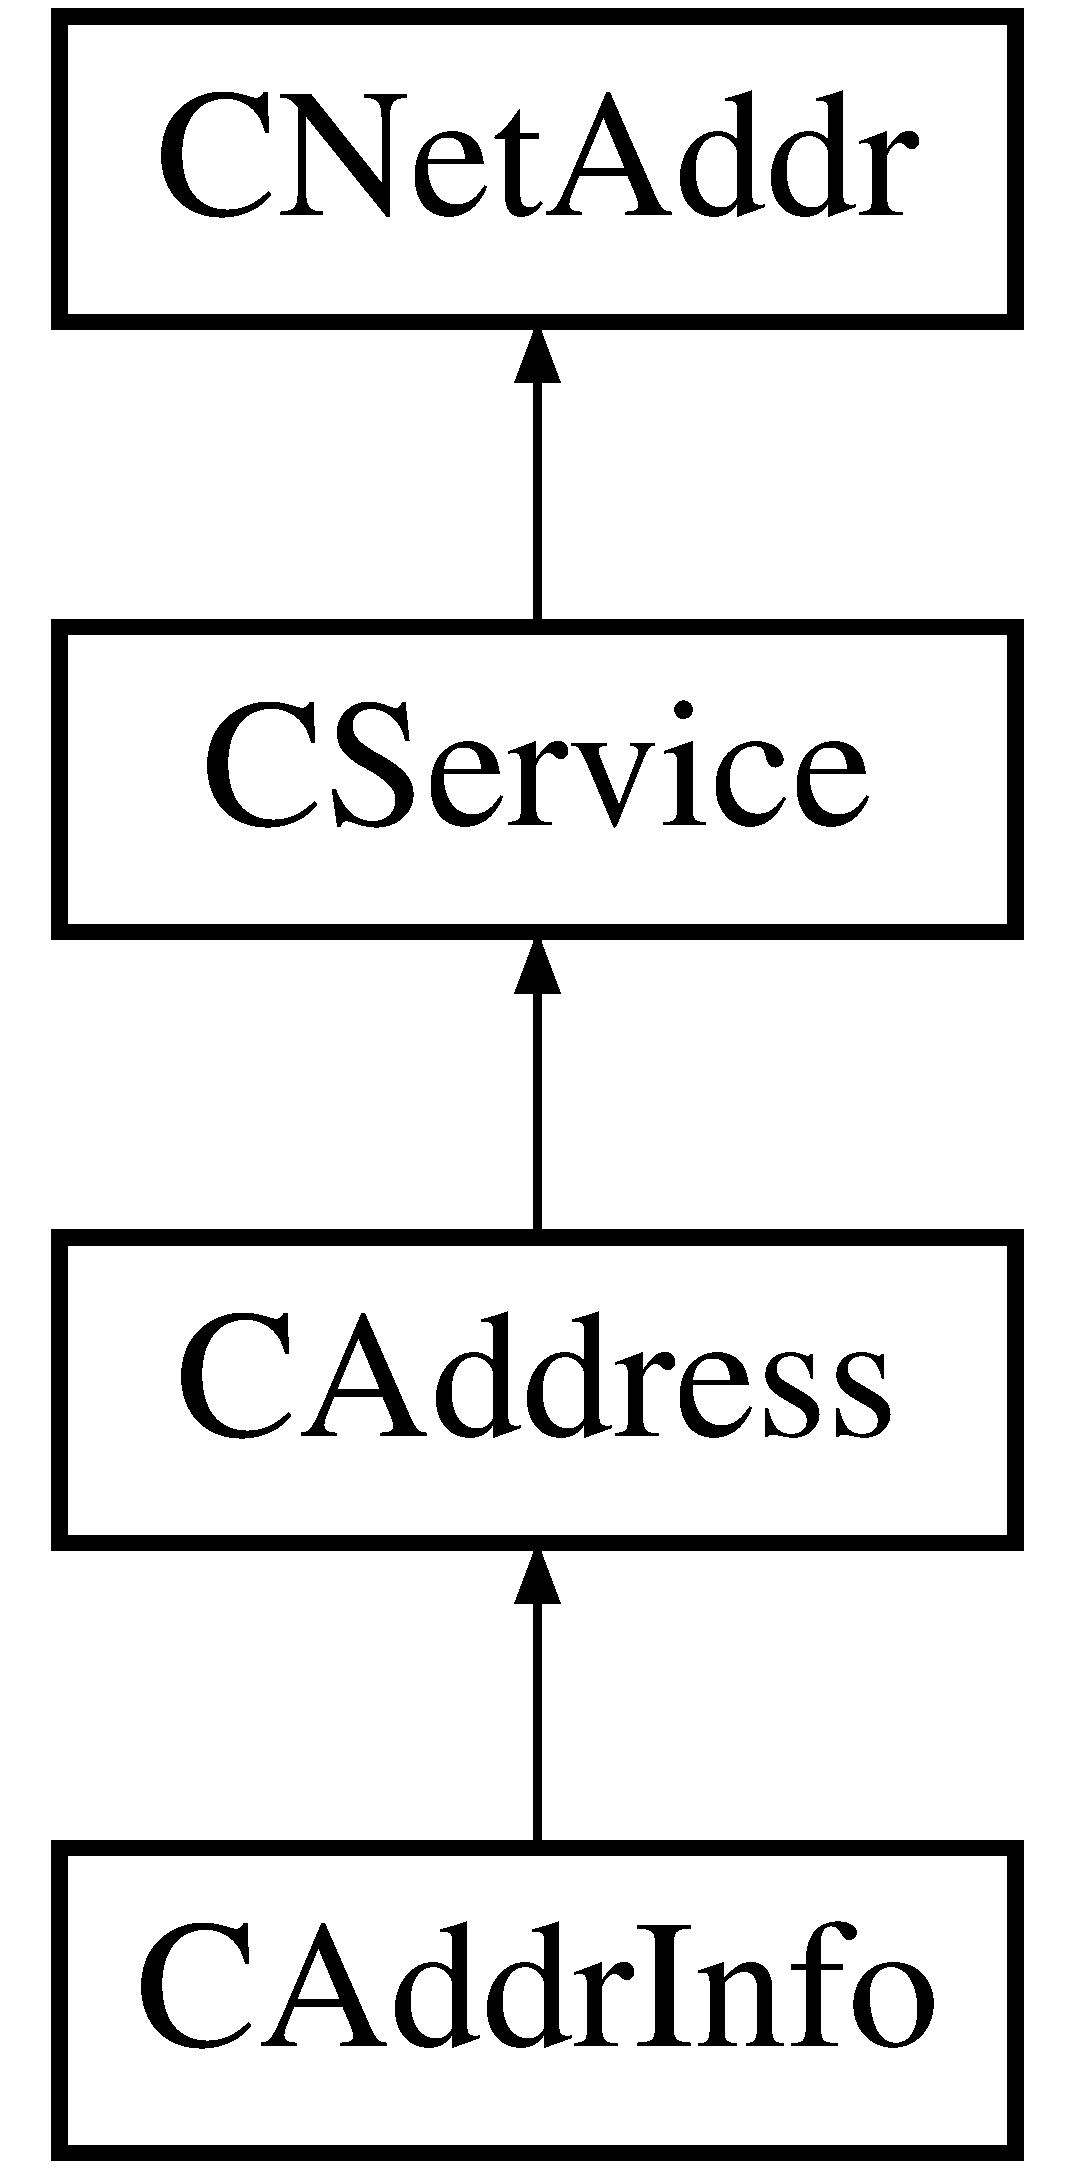
\includegraphics[height=4.000000cm]{class_c_address}
\end{center}
\end{figure}
\subsection*{Public Member Functions}
\begin{DoxyCompactItemize}
\item 
\hyperlink{class_c_address_a84cd336180580ab69b8888a4339ccc37}{C\+Address} ()
\item 
\hyperlink{class_c_address_a806e75f363ec49bfab92a686a8774ac3}{C\+Address} (\hyperlink{class_c_service}{C\+Service} ip\+In, uint64\+\_\+t n\+Services\+In=\hyperlink{protocol_8h_adc29c2ff13d900c2f185ee95427fb06ca9d1154f0e7e56f183a5c8373abe2e86c}{N\+O\+D\+E\+\_\+\+N\+E\+T\+W\+O\+R\+K})
\item 
void \hyperlink{class_c_address_ac060c84dcf47b8ccfae0142c9b29a243}{Init} ()
\item 
{\footnotesize template$<$typename Stream , typename Operation $>$ }\\void \hyperlink{class_c_address_aec10c7075404eefbcf6f7a4c5671be02}{Serialization\+Op} (Stream \&s, Operation ser\+\_\+action, int n\+Type, int n\+Version)
\end{DoxyCompactItemize}
\subsection*{Public Attributes}
\begin{DoxyCompactItemize}
\item 
\hyperlink{class_c_address_a9582fc22433b2ed275d4b65fb72551e7}{A\+D\+D\+\_\+\+S\+E\+R\+I\+A\+L\+I\+Z\+E\+\_\+\+M\+E\+T\+H\+O\+D\+S}
\item 
uint64\+\_\+t \hyperlink{class_c_address_a6a4a6aa020d0d558f238c7d04dd986c3}{n\+Services}
\item 
unsigned int \hyperlink{class_c_address_ac1c44aac968b11f90ce529b133ae4e9b}{n\+Time}
\end{DoxyCompactItemize}
\subsection*{Additional Inherited Members}


\subsection{Detailed Description}
A \hyperlink{class_c_service}{C\+Service} with information about it as peer 

\subsection{Constructor \& Destructor Documentation}
\hypertarget{class_c_address_a84cd336180580ab69b8888a4339ccc37}{}\index{C\+Address@{C\+Address}!C\+Address@{C\+Address}}
\index{C\+Address@{C\+Address}!C\+Address@{C\+Address}}
\subsubsection[{C\+Address}]{\setlength{\rightskip}{0pt plus 5cm}C\+Address\+::\+C\+Address (
\begin{DoxyParamCaption}
{}
\end{DoxyParamCaption}
)}\label{class_c_address_a84cd336180580ab69b8888a4339ccc37}
\hypertarget{class_c_address_a806e75f363ec49bfab92a686a8774ac3}{}\index{C\+Address@{C\+Address}!C\+Address@{C\+Address}}
\index{C\+Address@{C\+Address}!C\+Address@{C\+Address}}
\subsubsection[{C\+Address}]{\setlength{\rightskip}{0pt plus 5cm}C\+Address\+::\+C\+Address (
\begin{DoxyParamCaption}
\item[{{\bf C\+Service}}]{ip\+In, }
\item[{uint64\+\_\+t}]{n\+Services\+In = {\ttfamily {\bf N\+O\+D\+E\+\_\+\+N\+E\+T\+W\+O\+R\+K}}}
\end{DoxyParamCaption}
)\hspace{0.3cm}{\ttfamily [explicit]}}\label{class_c_address_a806e75f363ec49bfab92a686a8774ac3}


\subsection{Member Function Documentation}
\hypertarget{class_c_address_ac060c84dcf47b8ccfae0142c9b29a243}{}\index{C\+Address@{C\+Address}!Init@{Init}}
\index{Init@{Init}!C\+Address@{C\+Address}}
\subsubsection[{Init}]{\setlength{\rightskip}{0pt plus 5cm}void C\+Address\+::\+Init (
\begin{DoxyParamCaption}
{}
\end{DoxyParamCaption}
)}\label{class_c_address_ac060c84dcf47b8ccfae0142c9b29a243}
\hypertarget{class_c_address_aec10c7075404eefbcf6f7a4c5671be02}{}\index{C\+Address@{C\+Address}!Serialization\+Op@{Serialization\+Op}}
\index{Serialization\+Op@{Serialization\+Op}!C\+Address@{C\+Address}}
\subsubsection[{Serialization\+Op}]{\setlength{\rightskip}{0pt plus 5cm}template$<$typename Stream , typename Operation $>$ void C\+Address\+::\+Serialization\+Op (
\begin{DoxyParamCaption}
\item[{Stream \&}]{s, }
\item[{Operation}]{ser\+\_\+action, }
\item[{int}]{n\+Type, }
\item[{int}]{n\+Version}
\end{DoxyParamCaption}
)\hspace{0.3cm}{\ttfamily [inline]}}\label{class_c_address_aec10c7075404eefbcf6f7a4c5671be02}


\subsection{Member Data Documentation}
\hypertarget{class_c_address_a9582fc22433b2ed275d4b65fb72551e7}{}\index{C\+Address@{C\+Address}!A\+D\+D\+\_\+\+S\+E\+R\+I\+A\+L\+I\+Z\+E\+\_\+\+M\+E\+T\+H\+O\+D\+S@{A\+D\+D\+\_\+\+S\+E\+R\+I\+A\+L\+I\+Z\+E\+\_\+\+M\+E\+T\+H\+O\+D\+S}}
\index{A\+D\+D\+\_\+\+S\+E\+R\+I\+A\+L\+I\+Z\+E\+\_\+\+M\+E\+T\+H\+O\+D\+S@{A\+D\+D\+\_\+\+S\+E\+R\+I\+A\+L\+I\+Z\+E\+\_\+\+M\+E\+T\+H\+O\+D\+S}!C\+Address@{C\+Address}}
\subsubsection[{A\+D\+D\+\_\+\+S\+E\+R\+I\+A\+L\+I\+Z\+E\+\_\+\+M\+E\+T\+H\+O\+D\+S}]{\setlength{\rightskip}{0pt plus 5cm}C\+Address\+::\+A\+D\+D\+\_\+\+S\+E\+R\+I\+A\+L\+I\+Z\+E\+\_\+\+M\+E\+T\+H\+O\+D\+S}\label{class_c_address_a9582fc22433b2ed275d4b65fb72551e7}
\hypertarget{class_c_address_a6a4a6aa020d0d558f238c7d04dd986c3}{}\index{C\+Address@{C\+Address}!n\+Services@{n\+Services}}
\index{n\+Services@{n\+Services}!C\+Address@{C\+Address}}
\subsubsection[{n\+Services}]{\setlength{\rightskip}{0pt plus 5cm}uint64\+\_\+t C\+Address\+::n\+Services}\label{class_c_address_a6a4a6aa020d0d558f238c7d04dd986c3}
\hypertarget{class_c_address_ac1c44aac968b11f90ce529b133ae4e9b}{}\index{C\+Address@{C\+Address}!n\+Time@{n\+Time}}
\index{n\+Time@{n\+Time}!C\+Address@{C\+Address}}
\subsubsection[{n\+Time}]{\setlength{\rightskip}{0pt plus 5cm}unsigned int C\+Address\+::n\+Time}\label{class_c_address_ac1c44aac968b11f90ce529b133ae4e9b}


The documentation for this class was generated from the following files\+:\begin{DoxyCompactItemize}
\item 
C\+:/\+Users/\+Joe/\+Documents/\+School/\+C\+S\+C17\+A/bitcoin/src/\hyperlink{protocol_8h}{protocol.\+h}\item 
C\+:/\+Users/\+Joe/\+Documents/\+School/\+C\+S\+C17\+A/bitcoin/src/\hyperlink{protocol_8cpp}{protocol.\+cpp}\end{DoxyCompactItemize}

\hypertarget{class_c_addr_info}{}\section{C\+Addr\+Info Class Reference}
\label{class_c_addr_info}\index{C\+Addr\+Info@{C\+Addr\+Info}}


{\ttfamily \#include $<$addrman.\+h$>$}

Inheritance diagram for C\+Addr\+Info\+:\begin{figure}[H]
\begin{center}
\leavevmode
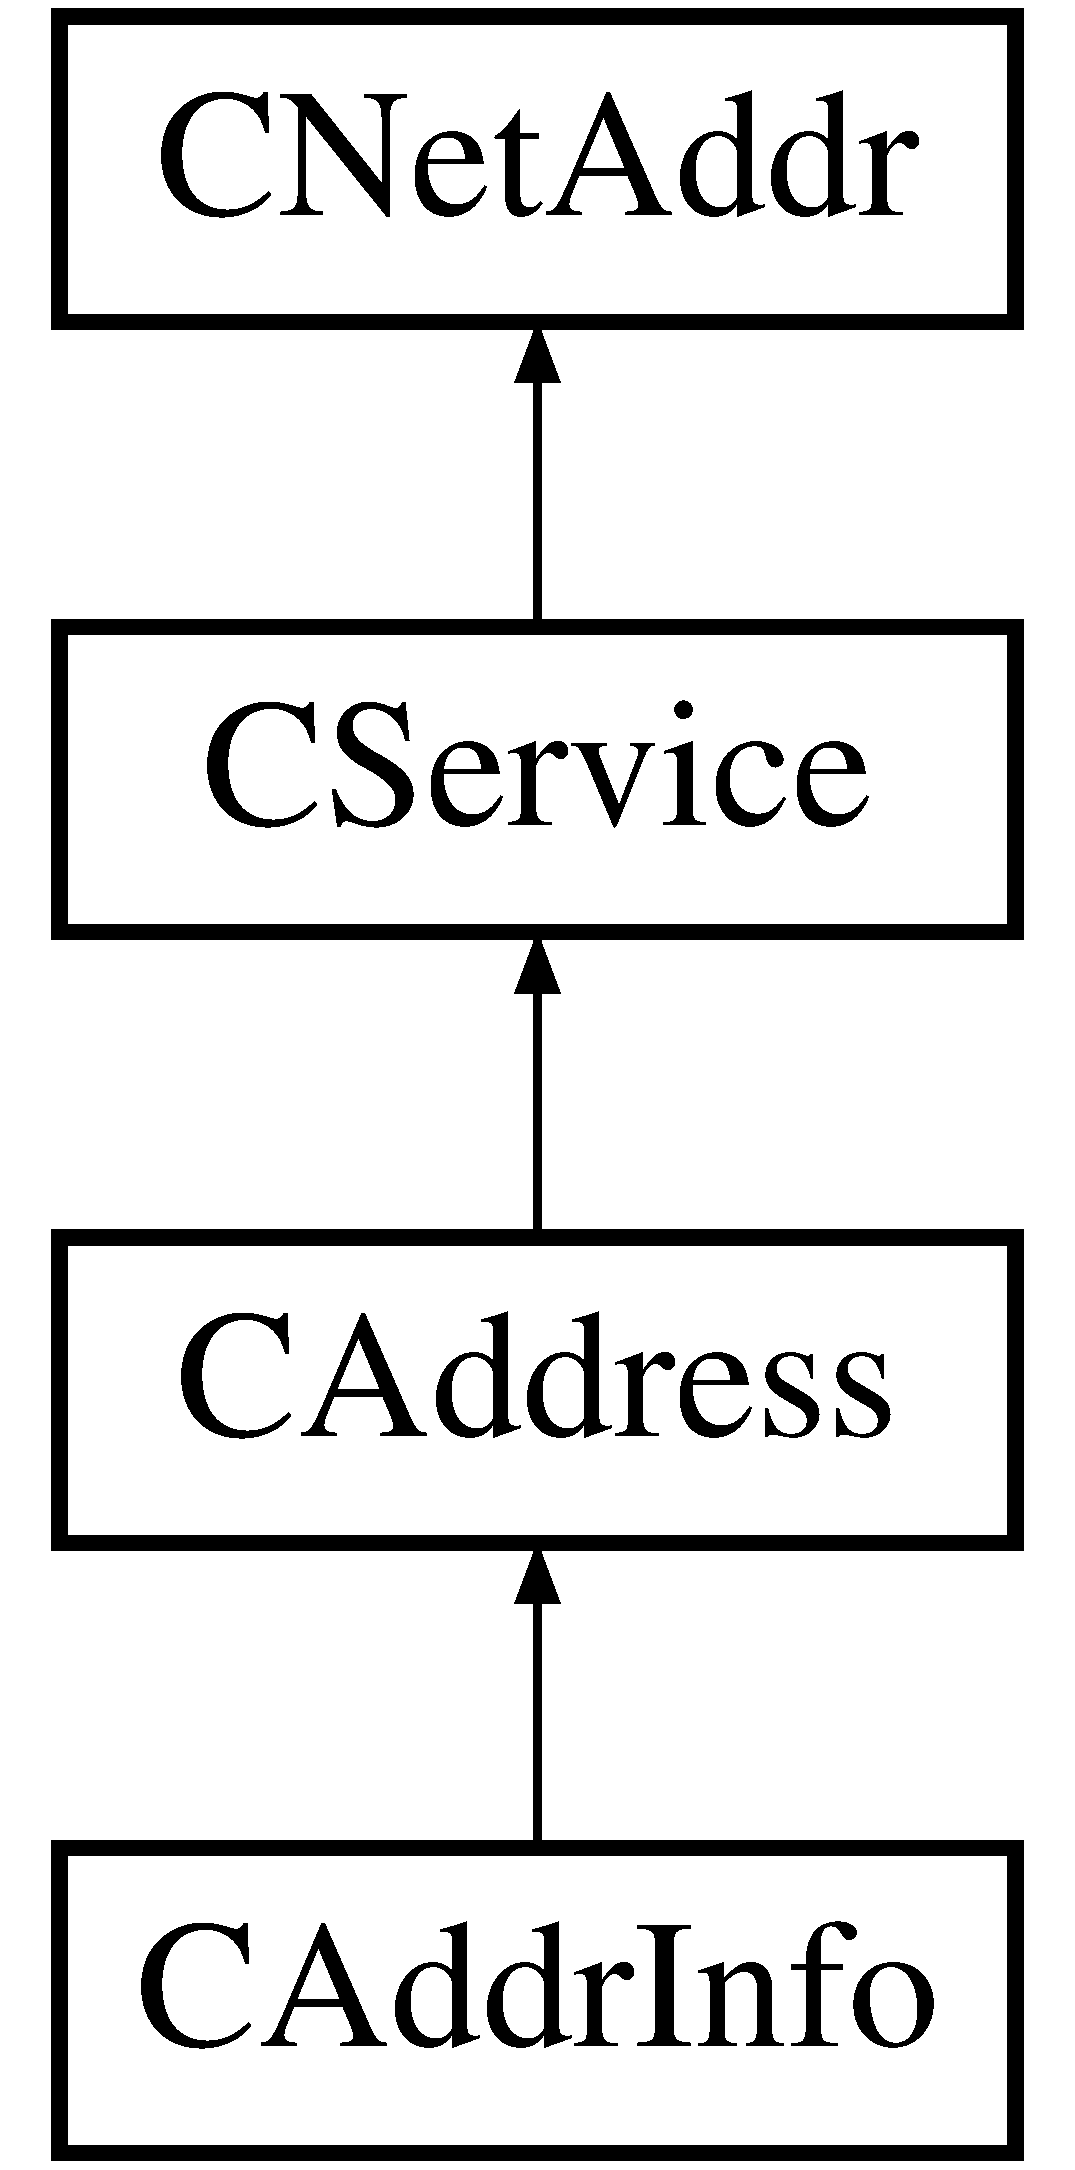
\includegraphics[height=4.000000cm]{class_c_addr_info}
\end{center}
\end{figure}
\subsection*{Public Member Functions}
\begin{DoxyCompactItemize}
\item 
{\footnotesize template$<$typename Stream , typename Operation $>$ }\\void \hyperlink{class_c_addr_info_ae80fdec7d3b48278033ea2280f66e68b}{Serialization\+Op} (Stream \&s, Operation ser\+\_\+action, int n\+Type, int n\+Version)
\item 
void \hyperlink{class_c_addr_info_af1df1f12bc71ed7f3debae61058b9b9f}{Init} ()
\item 
\hyperlink{class_c_addr_info_a27e773233e8d7e7d183f138d24cc40ef}{C\+Addr\+Info} (const \hyperlink{class_c_address}{C\+Address} \&addr\+In, const \hyperlink{class_c_net_addr}{C\+Net\+Addr} \&addr\+Source)
\item 
\hyperlink{class_c_addr_info_ae14c3a91bb669e5580be1d3767264187}{C\+Addr\+Info} ()
\item 
int \hyperlink{class_c_addr_info_aa7fce3d285312f5673bdb5274724d6b8}{Get\+Tried\+Bucket} (const \hyperlink{classuint256}{uint256} \&n\+Key) const 
\begin{DoxyCompactList}\small\item\em Calculate in which \char`\"{}tried\char`\"{} bucket this entry belongs. \end{DoxyCompactList}\item 
int \hyperlink{class_c_addr_info_a433abfb3347fec32d615507ff6cd52b0}{Get\+New\+Bucket} (const \hyperlink{classuint256}{uint256} \&n\+Key, const \hyperlink{class_c_net_addr}{C\+Net\+Addr} \&src) const 
\begin{DoxyCompactList}\small\item\em Calculate in which \char`\"{}new\char`\"{} bucket this entry belongs, given a certain source. \end{DoxyCompactList}\item 
int \hyperlink{class_c_addr_info_aee08d115a3314aa8c960fbff960f62b2}{Get\+New\+Bucket} (const \hyperlink{classuint256}{uint256} \&n\+Key) const 
\begin{DoxyCompactList}\small\item\em Calculate in which \char`\"{}new\char`\"{} bucket this entry belongs, using its default source. \end{DoxyCompactList}\item 
int \hyperlink{class_c_addr_info_aff26ef9829651c2e6fa40aef88ab704d}{Get\+Bucket\+Position} (const \hyperlink{classuint256}{uint256} \&n\+Key, bool f\+New, int n\+Bucket) const 
\begin{DoxyCompactList}\small\item\em Calculate in which position of a bucket to store this entry. \end{DoxyCompactList}\item 
bool \hyperlink{class_c_addr_info_a1fd74c1bd7a8eb3c234bf222f028e94c}{Is\+Terrible} (int64\+\_\+t n\+Now=\hyperlink{timedata_8h_a09f81b9c7650f898cf3cf305b87547e6}{Get\+Adjusted\+Time}()) const 
\begin{DoxyCompactList}\small\item\em Determine whether the statistics about this entry are bad enough so that it can just be deleted. \end{DoxyCompactList}\item 
double \hyperlink{class_c_addr_info_a264f9856d499cf077aa5c82327302307}{Get\+Chance} (int64\+\_\+t n\+Now=\hyperlink{timedata_8h_a09f81b9c7650f898cf3cf305b87547e6}{Get\+Adjusted\+Time}()) const 
\begin{DoxyCompactList}\small\item\em Calculate the relative chance this entry should be given when selecting nodes to connect to. \end{DoxyCompactList}\end{DoxyCompactItemize}
\subsection*{Public Attributes}
\begin{DoxyCompactItemize}
\item 
int64\+\_\+t \hyperlink{class_c_addr_info_a4569955918c204d2edd073456108ddfd}{n\+Last\+Try}
\begin{DoxyCompactList}\small\item\em last try whatsoever by us (memory only) \end{DoxyCompactList}\item 
\hyperlink{class_c_addr_info_a9d5e0b95fa494171e4bffb900094fe2e}{A\+D\+D\+\_\+\+S\+E\+R\+I\+A\+L\+I\+Z\+E\+\_\+\+M\+E\+T\+H\+O\+D\+S}
\end{DoxyCompactItemize}
\subsection*{Friends}
\begin{DoxyCompactItemize}
\item 
class \hyperlink{class_c_addr_info_a17ec4e9e560da58786d2ca36092bf83d}{C\+Addr\+Man}
\end{DoxyCompactItemize}
\subsection*{Additional Inherited Members}


\subsection{Detailed Description}
Extended statistics about a \hyperlink{class_c_address}{C\+Address} 

\subsection{Constructor \& Destructor Documentation}
\hypertarget{class_c_addr_info_a27e773233e8d7e7d183f138d24cc40ef}{}\index{C\+Addr\+Info@{C\+Addr\+Info}!C\+Addr\+Info@{C\+Addr\+Info}}
\index{C\+Addr\+Info@{C\+Addr\+Info}!C\+Addr\+Info@{C\+Addr\+Info}}
\subsubsection[{C\+Addr\+Info}]{\setlength{\rightskip}{0pt plus 5cm}C\+Addr\+Info\+::\+C\+Addr\+Info (
\begin{DoxyParamCaption}
\item[{const {\bf C\+Address} \&}]{addr\+In, }
\item[{const {\bf C\+Net\+Addr} \&}]{addr\+Source}
\end{DoxyParamCaption}
)\hspace{0.3cm}{\ttfamily [inline]}}\label{class_c_addr_info_a27e773233e8d7e7d183f138d24cc40ef}
\hypertarget{class_c_addr_info_ae14c3a91bb669e5580be1d3767264187}{}\index{C\+Addr\+Info@{C\+Addr\+Info}!C\+Addr\+Info@{C\+Addr\+Info}}
\index{C\+Addr\+Info@{C\+Addr\+Info}!C\+Addr\+Info@{C\+Addr\+Info}}
\subsubsection[{C\+Addr\+Info}]{\setlength{\rightskip}{0pt plus 5cm}C\+Addr\+Info\+::\+C\+Addr\+Info (
\begin{DoxyParamCaption}
{}
\end{DoxyParamCaption}
)\hspace{0.3cm}{\ttfamily [inline]}}\label{class_c_addr_info_ae14c3a91bb669e5580be1d3767264187}


\subsection{Member Function Documentation}
\hypertarget{class_c_addr_info_aff26ef9829651c2e6fa40aef88ab704d}{}\index{C\+Addr\+Info@{C\+Addr\+Info}!Get\+Bucket\+Position@{Get\+Bucket\+Position}}
\index{Get\+Bucket\+Position@{Get\+Bucket\+Position}!C\+Addr\+Info@{C\+Addr\+Info}}
\subsubsection[{Get\+Bucket\+Position}]{\setlength{\rightskip}{0pt plus 5cm}int C\+Addr\+Info\+::\+Get\+Bucket\+Position (
\begin{DoxyParamCaption}
\item[{const {\bf uint256} \&}]{n\+Key, }
\item[{bool}]{f\+New, }
\item[{int}]{n\+Bucket}
\end{DoxyParamCaption}
) const}\label{class_c_addr_info_aff26ef9829651c2e6fa40aef88ab704d}


Calculate in which position of a bucket to store this entry. 

\hypertarget{class_c_addr_info_a264f9856d499cf077aa5c82327302307}{}\index{C\+Addr\+Info@{C\+Addr\+Info}!Get\+Chance@{Get\+Chance}}
\index{Get\+Chance@{Get\+Chance}!C\+Addr\+Info@{C\+Addr\+Info}}
\subsubsection[{Get\+Chance}]{\setlength{\rightskip}{0pt plus 5cm}double C\+Addr\+Info\+::\+Get\+Chance (
\begin{DoxyParamCaption}
\item[{int64\+\_\+t}]{n\+Now = {\ttfamily {\bf Get\+Adjusted\+Time}()}}
\end{DoxyParamCaption}
) const}\label{class_c_addr_info_a264f9856d499cf077aa5c82327302307}


Calculate the relative chance this entry should be given when selecting nodes to connect to. 

\hypertarget{class_c_addr_info_a433abfb3347fec32d615507ff6cd52b0}{}\index{C\+Addr\+Info@{C\+Addr\+Info}!Get\+New\+Bucket@{Get\+New\+Bucket}}
\index{Get\+New\+Bucket@{Get\+New\+Bucket}!C\+Addr\+Info@{C\+Addr\+Info}}
\subsubsection[{Get\+New\+Bucket}]{\setlength{\rightskip}{0pt plus 5cm}int C\+Addr\+Info\+::\+Get\+New\+Bucket (
\begin{DoxyParamCaption}
\item[{const {\bf uint256} \&}]{n\+Key, }
\item[{const {\bf C\+Net\+Addr} \&}]{src}
\end{DoxyParamCaption}
) const}\label{class_c_addr_info_a433abfb3347fec32d615507ff6cd52b0}


Calculate in which \char`\"{}new\char`\"{} bucket this entry belongs, given a certain source. 

\hypertarget{class_c_addr_info_aee08d115a3314aa8c960fbff960f62b2}{}\index{C\+Addr\+Info@{C\+Addr\+Info}!Get\+New\+Bucket@{Get\+New\+Bucket}}
\index{Get\+New\+Bucket@{Get\+New\+Bucket}!C\+Addr\+Info@{C\+Addr\+Info}}
\subsubsection[{Get\+New\+Bucket}]{\setlength{\rightskip}{0pt plus 5cm}int C\+Addr\+Info\+::\+Get\+New\+Bucket (
\begin{DoxyParamCaption}
\item[{const {\bf uint256} \&}]{n\+Key}
\end{DoxyParamCaption}
) const\hspace{0.3cm}{\ttfamily [inline]}}\label{class_c_addr_info_aee08d115a3314aa8c960fbff960f62b2}


Calculate in which \char`\"{}new\char`\"{} bucket this entry belongs, using its default source. 

\hypertarget{class_c_addr_info_aa7fce3d285312f5673bdb5274724d6b8}{}\index{C\+Addr\+Info@{C\+Addr\+Info}!Get\+Tried\+Bucket@{Get\+Tried\+Bucket}}
\index{Get\+Tried\+Bucket@{Get\+Tried\+Bucket}!C\+Addr\+Info@{C\+Addr\+Info}}
\subsubsection[{Get\+Tried\+Bucket}]{\setlength{\rightskip}{0pt plus 5cm}int C\+Addr\+Info\+::\+Get\+Tried\+Bucket (
\begin{DoxyParamCaption}
\item[{const {\bf uint256} \&}]{n\+Key}
\end{DoxyParamCaption}
) const}\label{class_c_addr_info_aa7fce3d285312f5673bdb5274724d6b8}


Calculate in which \char`\"{}tried\char`\"{} bucket this entry belongs. 

\hypertarget{class_c_addr_info_af1df1f12bc71ed7f3debae61058b9b9f}{}\index{C\+Addr\+Info@{C\+Addr\+Info}!Init@{Init}}
\index{Init@{Init}!C\+Addr\+Info@{C\+Addr\+Info}}
\subsubsection[{Init}]{\setlength{\rightskip}{0pt plus 5cm}void C\+Addr\+Info\+::\+Init (
\begin{DoxyParamCaption}
{}
\end{DoxyParamCaption}
)\hspace{0.3cm}{\ttfamily [inline]}}\label{class_c_addr_info_af1df1f12bc71ed7f3debae61058b9b9f}
\hypertarget{class_c_addr_info_a1fd74c1bd7a8eb3c234bf222f028e94c}{}\index{C\+Addr\+Info@{C\+Addr\+Info}!Is\+Terrible@{Is\+Terrible}}
\index{Is\+Terrible@{Is\+Terrible}!C\+Addr\+Info@{C\+Addr\+Info}}
\subsubsection[{Is\+Terrible}]{\setlength{\rightskip}{0pt plus 5cm}bool C\+Addr\+Info\+::\+Is\+Terrible (
\begin{DoxyParamCaption}
\item[{int64\+\_\+t}]{n\+Now = {\ttfamily {\bf Get\+Adjusted\+Time}()}}
\end{DoxyParamCaption}
) const}\label{class_c_addr_info_a1fd74c1bd7a8eb3c234bf222f028e94c}


Determine whether the statistics about this entry are bad enough so that it can just be deleted. 

\hypertarget{class_c_addr_info_ae80fdec7d3b48278033ea2280f66e68b}{}\index{C\+Addr\+Info@{C\+Addr\+Info}!Serialization\+Op@{Serialization\+Op}}
\index{Serialization\+Op@{Serialization\+Op}!C\+Addr\+Info@{C\+Addr\+Info}}
\subsubsection[{Serialization\+Op}]{\setlength{\rightskip}{0pt plus 5cm}template$<$typename Stream , typename Operation $>$ void C\+Addr\+Info\+::\+Serialization\+Op (
\begin{DoxyParamCaption}
\item[{Stream \&}]{s, }
\item[{Operation}]{ser\+\_\+action, }
\item[{int}]{n\+Type, }
\item[{int}]{n\+Version}
\end{DoxyParamCaption}
)\hspace{0.3cm}{\ttfamily [inline]}}\label{class_c_addr_info_ae80fdec7d3b48278033ea2280f66e68b}


\subsection{Friends And Related Function Documentation}
\hypertarget{class_c_addr_info_a17ec4e9e560da58786d2ca36092bf83d}{}\index{C\+Addr\+Info@{C\+Addr\+Info}!C\+Addr\+Man@{C\+Addr\+Man}}
\index{C\+Addr\+Man@{C\+Addr\+Man}!C\+Addr\+Info@{C\+Addr\+Info}}
\subsubsection[{C\+Addr\+Man}]{\setlength{\rightskip}{0pt plus 5cm}friend class {\bf C\+Addr\+Man}\hspace{0.3cm}{\ttfamily [friend]}}\label{class_c_addr_info_a17ec4e9e560da58786d2ca36092bf83d}


\subsection{Member Data Documentation}
\hypertarget{class_c_addr_info_a9d5e0b95fa494171e4bffb900094fe2e}{}\index{C\+Addr\+Info@{C\+Addr\+Info}!A\+D\+D\+\_\+\+S\+E\+R\+I\+A\+L\+I\+Z\+E\+\_\+\+M\+E\+T\+H\+O\+D\+S@{A\+D\+D\+\_\+\+S\+E\+R\+I\+A\+L\+I\+Z\+E\+\_\+\+M\+E\+T\+H\+O\+D\+S}}
\index{A\+D\+D\+\_\+\+S\+E\+R\+I\+A\+L\+I\+Z\+E\+\_\+\+M\+E\+T\+H\+O\+D\+S@{A\+D\+D\+\_\+\+S\+E\+R\+I\+A\+L\+I\+Z\+E\+\_\+\+M\+E\+T\+H\+O\+D\+S}!C\+Addr\+Info@{C\+Addr\+Info}}
\subsubsection[{A\+D\+D\+\_\+\+S\+E\+R\+I\+A\+L\+I\+Z\+E\+\_\+\+M\+E\+T\+H\+O\+D\+S}]{\setlength{\rightskip}{0pt plus 5cm}C\+Addr\+Info\+::\+A\+D\+D\+\_\+\+S\+E\+R\+I\+A\+L\+I\+Z\+E\+\_\+\+M\+E\+T\+H\+O\+D\+S}\label{class_c_addr_info_a9d5e0b95fa494171e4bffb900094fe2e}
\hypertarget{class_c_addr_info_a4569955918c204d2edd073456108ddfd}{}\index{C\+Addr\+Info@{C\+Addr\+Info}!n\+Last\+Try@{n\+Last\+Try}}
\index{n\+Last\+Try@{n\+Last\+Try}!C\+Addr\+Info@{C\+Addr\+Info}}
\subsubsection[{n\+Last\+Try}]{\setlength{\rightskip}{0pt plus 5cm}int64\+\_\+t C\+Addr\+Info\+::n\+Last\+Try}\label{class_c_addr_info_a4569955918c204d2edd073456108ddfd}


last try whatsoever by us (memory only) 



The documentation for this class was generated from the following files\+:\begin{DoxyCompactItemize}
\item 
C\+:/\+Users/\+Joe/\+Documents/\+School/\+C\+S\+C17\+A/bitcoin/src/\hyperlink{addrman_8h}{addrman.\+h}\item 
C\+:/\+Users/\+Joe/\+Documents/\+School/\+C\+S\+C17\+A/bitcoin/src/\hyperlink{addrman_8cpp}{addrman.\+cpp}\end{DoxyCompactItemize}

\hypertarget{class_c_addr_man}{}\section{C\+Addr\+Man Class Reference}
\label{class_c_addr_man}\index{C\+Addr\+Man@{C\+Addr\+Man}}


{\ttfamily \#include $<$addrman.\+h$>$}

\subsection*{Public Member Functions}
\begin{DoxyCompactItemize}
\item 
{\footnotesize template$<$typename Stream $>$ }\\void \hyperlink{class_c_addr_man_a88d4327f77fa70d9a88917897c3c6c97}{Serialize} (Stream \&s, int n\+Type, int n\+Version\+Dummy) const 
\item 
{\footnotesize template$<$typename Stream $>$ }\\void \hyperlink{class_c_addr_man_a68eaf1797ecb8bff380aa7f9fc452e14}{Unserialize} (Stream \&s, int n\+Type, int n\+Version\+Dummy)
\item 
unsigned int \hyperlink{class_c_addr_man_aa2266bea9d5336b0a93fe703a8601e55}{Get\+Serialize\+Size} (int n\+Type, int n\+Version) const 
\item 
void \hyperlink{class_c_addr_man_a53c27520b7f8c6fa817c2fa869dd4e25}{Clear} ()
\item 
\hyperlink{class_c_addr_man_ad9179d1c36c2ea3492e221576f340d33}{C\+Addr\+Man} ()
\item 
\hyperlink{class_c_addr_man_ae1b1838e4de4effbc1fbc888126a9352}{$\sim$\+C\+Addr\+Man} ()
\item 
int \hyperlink{class_c_addr_man_a15b8e72f55344b6fbd1bc1bda3cdc5bc}{size} ()
\begin{DoxyCompactList}\small\item\em Return the number of (unique) addresses in all tables. \end{DoxyCompactList}\item 
void \hyperlink{class_c_addr_man_a0c2677ae50ce0d680f0105b285d1f5d0}{Check} ()
\begin{DoxyCompactList}\small\item\em Consistency check. \end{DoxyCompactList}\item 
bool \hyperlink{class_c_addr_man_a03fcc7109b5f014760dc50a81f68c5ec}{Add} (const \hyperlink{class_c_address}{C\+Address} \&addr, const \hyperlink{class_c_net_addr}{C\+Net\+Addr} \&source, int64\+\_\+t n\+Time\+Penalty=0)
\begin{DoxyCompactList}\small\item\em Add a single address. \end{DoxyCompactList}\item 
bool \hyperlink{class_c_addr_man_aa2ae2abdf710b2d81fa37f072bab028e}{Add} (const std\+::vector$<$ \hyperlink{class_c_address}{C\+Address} $>$ \&v\+Addr, const \hyperlink{class_c_net_addr}{C\+Net\+Addr} \&source, int64\+\_\+t n\+Time\+Penalty=0)
\begin{DoxyCompactList}\small\item\em Add multiple addresses. \end{DoxyCompactList}\item 
void \hyperlink{class_c_addr_man_a993e80e74701d7bc6bb49880c387b847}{Good} (const \hyperlink{class_c_service}{C\+Service} \&addr, int64\+\_\+t n\+Time=\hyperlink{timedata_8h_a09f81b9c7650f898cf3cf305b87547e6}{Get\+Adjusted\+Time}())
\begin{DoxyCompactList}\small\item\em Mark an entry as accessible. \end{DoxyCompactList}\item 
void \hyperlink{class_c_addr_man_afcddc2573121065177dc981cea710789}{Attempt} (const \hyperlink{class_c_service}{C\+Service} \&addr, int64\+\_\+t n\+Time=\hyperlink{timedata_8h_a09f81b9c7650f898cf3cf305b87547e6}{Get\+Adjusted\+Time}())
\begin{DoxyCompactList}\small\item\em Mark an entry as connection attempted to. \end{DoxyCompactList}\item 
\hyperlink{class_c_addr_info}{C\+Addr\+Info} \hyperlink{class_c_addr_man_a40033486ee621d5f858748e5454222e2}{Select} ()
\item 
std\+::vector$<$ \hyperlink{class_c_address}{C\+Address} $>$ \hyperlink{class_c_addr_man_a69cc6138e696cf88de60925d26023bf2}{Get\+Addr} ()
\begin{DoxyCompactList}\small\item\em Return a bunch of addresses, selected at random. \end{DoxyCompactList}\item 
void \hyperlink{class_c_addr_man_a7aba66d9e9527522fed974567d34c322}{Connected} (const \hyperlink{class_c_service}{C\+Service} \&addr, int64\+\_\+t n\+Time=\hyperlink{timedata_8h_a09f81b9c7650f898cf3cf305b87547e6}{Get\+Adjusted\+Time}())
\begin{DoxyCompactList}\small\item\em Mark an entry as currently-\/connected-\/to. \end{DoxyCompactList}\end{DoxyCompactItemize}
\subsection*{Protected Member Functions}
\begin{DoxyCompactItemize}
\item 
\hyperlink{class_c_addr_info}{C\+Addr\+Info} $\ast$ \hyperlink{class_c_addr_man_ac961ead1a1afde144fc486b6d7c7369d}{Find} (const \hyperlink{class_c_net_addr}{C\+Net\+Addr} \&addr, int $\ast$pn\+Id=N\+U\+L\+L)
\begin{DoxyCompactList}\small\item\em Find an entry. \end{DoxyCompactList}\item 
\hyperlink{class_c_addr_info}{C\+Addr\+Info} $\ast$ \hyperlink{class_c_addr_man_aac93f51c0580e38a950a0f63b053bedb}{Create} (const \hyperlink{class_c_address}{C\+Address} \&addr, const \hyperlink{class_c_net_addr}{C\+Net\+Addr} \&addr\+Source, int $\ast$pn\+Id=N\+U\+L\+L)
\item 
void \hyperlink{class_c_addr_man_a3074bc8e3dcfb5348054613f575dc38e}{Swap\+Random} (unsigned int n\+Random\+Pos1, unsigned int n\+Random\+Pos2)
\begin{DoxyCompactList}\small\item\em Swap two elements in v\+Random. \end{DoxyCompactList}\item 
void \hyperlink{class_c_addr_man_a98e8383efb48b7c2932795438f35a10a}{Make\+Tried} (\hyperlink{class_c_addr_info}{C\+Addr\+Info} \&info, int n\+Id)
\begin{DoxyCompactList}\small\item\em Move an entry from the \char`\"{}new\char`\"{} table(s) to the \char`\"{}tried\char`\"{} table. \end{DoxyCompactList}\item 
void \hyperlink{class_c_addr_man_af488eac123030538770dbc4e3b16eb74}{Delete} (int n\+Id)
\begin{DoxyCompactList}\small\item\em Delete an entry. It must not be in tried, and have refcount 0. \end{DoxyCompactList}\item 
void \hyperlink{class_c_addr_man_ab283de3e750f006c85573976bd40da81}{Clear\+New} (int n\+U\+Bucket, int n\+U\+Bucket\+Pos)
\begin{DoxyCompactList}\small\item\em Clear a position in a \char`\"{}new\char`\"{} table. This is the only place where entries are actually deleted. \end{DoxyCompactList}\item 
void \hyperlink{class_c_addr_man_a33ec6a4584cf4b17af821e6e35216459}{Good\+\_\+} (const \hyperlink{class_c_service}{C\+Service} \&addr, int64\+\_\+t n\+Time)
\begin{DoxyCompactList}\small\item\em Mark an entry \char`\"{}good\char`\"{}, possibly moving it from \char`\"{}new\char`\"{} to \char`\"{}tried\char`\"{}. \end{DoxyCompactList}\item 
bool \hyperlink{class_c_addr_man_a9dd6df8b1904548a86054d19d4a90724}{Add\+\_\+} (const \hyperlink{class_c_address}{C\+Address} \&addr, const \hyperlink{class_c_net_addr}{C\+Net\+Addr} \&source, int64\+\_\+t n\+Time\+Penalty)
\begin{DoxyCompactList}\small\item\em Add an entry to the \char`\"{}new\char`\"{} table. \end{DoxyCompactList}\item 
void \hyperlink{class_c_addr_man_ab1a1bfa8b435ef139570c88de1a5245f}{Attempt\+\_\+} (const \hyperlink{class_c_service}{C\+Service} \&addr, int64\+\_\+t n\+Time)
\begin{DoxyCompactList}\small\item\em Mark an entry as attempted to connect. \end{DoxyCompactList}\item 
\hyperlink{class_c_addr_info}{C\+Addr\+Info} \hyperlink{class_c_addr_man_ad354e94672ff88f8f420ebc2e05f21a6}{Select\+\_\+} ()
\item 
void \hyperlink{class_c_addr_man_aff86d04dc7c0e0afae3ff5998417db17}{Get\+Addr\+\_\+} (std\+::vector$<$ \hyperlink{class_c_address}{C\+Address} $>$ \&v\+Addr)
\begin{DoxyCompactList}\small\item\em Select several addresses at once. \end{DoxyCompactList}\item 
void \hyperlink{class_c_addr_man_a1ae72643c51293f3f3345e74ce0368ca}{Connected\+\_\+} (const \hyperlink{class_c_service}{C\+Service} \&addr, int64\+\_\+t n\+Time)
\begin{DoxyCompactList}\small\item\em Mark an entry as currently-\/connected-\/to. \end{DoxyCompactList}\end{DoxyCompactItemize}


\subsection{Detailed Description}
Stochastical (I\+P) address manager 

\subsection{Constructor \& Destructor Documentation}
\hypertarget{class_c_addr_man_ad9179d1c36c2ea3492e221576f340d33}{}\index{C\+Addr\+Man@{C\+Addr\+Man}!C\+Addr\+Man@{C\+Addr\+Man}}
\index{C\+Addr\+Man@{C\+Addr\+Man}!C\+Addr\+Man@{C\+Addr\+Man}}
\subsubsection[{C\+Addr\+Man}]{\setlength{\rightskip}{0pt plus 5cm}C\+Addr\+Man\+::\+C\+Addr\+Man (
\begin{DoxyParamCaption}
{}
\end{DoxyParamCaption}
)\hspace{0.3cm}{\ttfamily [inline]}}\label{class_c_addr_man_ad9179d1c36c2ea3492e221576f340d33}
\hypertarget{class_c_addr_man_ae1b1838e4de4effbc1fbc888126a9352}{}\index{C\+Addr\+Man@{C\+Addr\+Man}!````~C\+Addr\+Man@{$\sim$\+C\+Addr\+Man}}
\index{````~C\+Addr\+Man@{$\sim$\+C\+Addr\+Man}!C\+Addr\+Man@{C\+Addr\+Man}}
\subsubsection[{$\sim$\+C\+Addr\+Man}]{\setlength{\rightskip}{0pt plus 5cm}C\+Addr\+Man\+::$\sim$\+C\+Addr\+Man (
\begin{DoxyParamCaption}
{}
\end{DoxyParamCaption}
)\hspace{0.3cm}{\ttfamily [inline]}}\label{class_c_addr_man_ae1b1838e4de4effbc1fbc888126a9352}


\subsection{Member Function Documentation}
\hypertarget{class_c_addr_man_a03fcc7109b5f014760dc50a81f68c5ec}{}\index{C\+Addr\+Man@{C\+Addr\+Man}!Add@{Add}}
\index{Add@{Add}!C\+Addr\+Man@{C\+Addr\+Man}}
\subsubsection[{Add}]{\setlength{\rightskip}{0pt plus 5cm}bool C\+Addr\+Man\+::\+Add (
\begin{DoxyParamCaption}
\item[{const {\bf C\+Address} \&}]{addr, }
\item[{const {\bf C\+Net\+Addr} \&}]{source, }
\item[{int64\+\_\+t}]{n\+Time\+Penalty = {\ttfamily 0}}
\end{DoxyParamCaption}
)\hspace{0.3cm}{\ttfamily [inline]}}\label{class_c_addr_man_a03fcc7109b5f014760dc50a81f68c5ec}


Add a single address. 

\hypertarget{class_c_addr_man_aa2ae2abdf710b2d81fa37f072bab028e}{}\index{C\+Addr\+Man@{C\+Addr\+Man}!Add@{Add}}
\index{Add@{Add}!C\+Addr\+Man@{C\+Addr\+Man}}
\subsubsection[{Add}]{\setlength{\rightskip}{0pt plus 5cm}bool C\+Addr\+Man\+::\+Add (
\begin{DoxyParamCaption}
\item[{const std\+::vector$<$ {\bf C\+Address} $>$ \&}]{v\+Addr, }
\item[{const {\bf C\+Net\+Addr} \&}]{source, }
\item[{int64\+\_\+t}]{n\+Time\+Penalty = {\ttfamily 0}}
\end{DoxyParamCaption}
)\hspace{0.3cm}{\ttfamily [inline]}}\label{class_c_addr_man_aa2ae2abdf710b2d81fa37f072bab028e}


Add multiple addresses. 

\hypertarget{class_c_addr_man_a9dd6df8b1904548a86054d19d4a90724}{}\index{C\+Addr\+Man@{C\+Addr\+Man}!Add\+\_\+@{Add\+\_\+}}
\index{Add\+\_\+@{Add\+\_\+}!C\+Addr\+Man@{C\+Addr\+Man}}
\subsubsection[{Add\+\_\+}]{\setlength{\rightskip}{0pt plus 5cm}bool C\+Addr\+Man\+::\+Add\+\_\+ (
\begin{DoxyParamCaption}
\item[{const {\bf C\+Address} \&}]{addr, }
\item[{const {\bf C\+Net\+Addr} \&}]{source, }
\item[{int64\+\_\+t}]{n\+Time\+Penalty}
\end{DoxyParamCaption}
)\hspace{0.3cm}{\ttfamily [protected]}}\label{class_c_addr_man_a9dd6df8b1904548a86054d19d4a90724}


Add an entry to the \char`\"{}new\char`\"{} table. 

\hypertarget{class_c_addr_man_afcddc2573121065177dc981cea710789}{}\index{C\+Addr\+Man@{C\+Addr\+Man}!Attempt@{Attempt}}
\index{Attempt@{Attempt}!C\+Addr\+Man@{C\+Addr\+Man}}
\subsubsection[{Attempt}]{\setlength{\rightskip}{0pt plus 5cm}void C\+Addr\+Man\+::\+Attempt (
\begin{DoxyParamCaption}
\item[{const {\bf C\+Service} \&}]{addr, }
\item[{int64\+\_\+t}]{n\+Time = {\ttfamily {\bf Get\+Adjusted\+Time}()}}
\end{DoxyParamCaption}
)\hspace{0.3cm}{\ttfamily [inline]}}\label{class_c_addr_man_afcddc2573121065177dc981cea710789}


Mark an entry as connection attempted to. 

\hypertarget{class_c_addr_man_ab1a1bfa8b435ef139570c88de1a5245f}{}\index{C\+Addr\+Man@{C\+Addr\+Man}!Attempt\+\_\+@{Attempt\+\_\+}}
\index{Attempt\+\_\+@{Attempt\+\_\+}!C\+Addr\+Man@{C\+Addr\+Man}}
\subsubsection[{Attempt\+\_\+}]{\setlength{\rightskip}{0pt plus 5cm}void C\+Addr\+Man\+::\+Attempt\+\_\+ (
\begin{DoxyParamCaption}
\item[{const {\bf C\+Service} \&}]{addr, }
\item[{int64\+\_\+t}]{n\+Time}
\end{DoxyParamCaption}
)\hspace{0.3cm}{\ttfamily [protected]}}\label{class_c_addr_man_ab1a1bfa8b435ef139570c88de1a5245f}


Mark an entry as attempted to connect. 

\hypertarget{class_c_addr_man_a0c2677ae50ce0d680f0105b285d1f5d0}{}\index{C\+Addr\+Man@{C\+Addr\+Man}!Check@{Check}}
\index{Check@{Check}!C\+Addr\+Man@{C\+Addr\+Man}}
\subsubsection[{Check}]{\setlength{\rightskip}{0pt plus 5cm}void C\+Addr\+Man\+::\+Check (
\begin{DoxyParamCaption}
{}
\end{DoxyParamCaption}
)\hspace{0.3cm}{\ttfamily [inline]}}\label{class_c_addr_man_a0c2677ae50ce0d680f0105b285d1f5d0}


Consistency check. 

\hypertarget{class_c_addr_man_a53c27520b7f8c6fa817c2fa869dd4e25}{}\index{C\+Addr\+Man@{C\+Addr\+Man}!Clear@{Clear}}
\index{Clear@{Clear}!C\+Addr\+Man@{C\+Addr\+Man}}
\subsubsection[{Clear}]{\setlength{\rightskip}{0pt plus 5cm}void C\+Addr\+Man\+::\+Clear (
\begin{DoxyParamCaption}
{}
\end{DoxyParamCaption}
)\hspace{0.3cm}{\ttfamily [inline]}}\label{class_c_addr_man_a53c27520b7f8c6fa817c2fa869dd4e25}
\hypertarget{class_c_addr_man_ab283de3e750f006c85573976bd40da81}{}\index{C\+Addr\+Man@{C\+Addr\+Man}!Clear\+New@{Clear\+New}}
\index{Clear\+New@{Clear\+New}!C\+Addr\+Man@{C\+Addr\+Man}}
\subsubsection[{Clear\+New}]{\setlength{\rightskip}{0pt plus 5cm}void C\+Addr\+Man\+::\+Clear\+New (
\begin{DoxyParamCaption}
\item[{int}]{n\+U\+Bucket, }
\item[{int}]{n\+U\+Bucket\+Pos}
\end{DoxyParamCaption}
)\hspace{0.3cm}{\ttfamily [protected]}}\label{class_c_addr_man_ab283de3e750f006c85573976bd40da81}


Clear a position in a \char`\"{}new\char`\"{} table. This is the only place where entries are actually deleted. 

\hypertarget{class_c_addr_man_a7aba66d9e9527522fed974567d34c322}{}\index{C\+Addr\+Man@{C\+Addr\+Man}!Connected@{Connected}}
\index{Connected@{Connected}!C\+Addr\+Man@{C\+Addr\+Man}}
\subsubsection[{Connected}]{\setlength{\rightskip}{0pt plus 5cm}void C\+Addr\+Man\+::\+Connected (
\begin{DoxyParamCaption}
\item[{const {\bf C\+Service} \&}]{addr, }
\item[{int64\+\_\+t}]{n\+Time = {\ttfamily {\bf Get\+Adjusted\+Time}()}}
\end{DoxyParamCaption}
)\hspace{0.3cm}{\ttfamily [inline]}}\label{class_c_addr_man_a7aba66d9e9527522fed974567d34c322}


Mark an entry as currently-\/connected-\/to. 

\hypertarget{class_c_addr_man_a1ae72643c51293f3f3345e74ce0368ca}{}\index{C\+Addr\+Man@{C\+Addr\+Man}!Connected\+\_\+@{Connected\+\_\+}}
\index{Connected\+\_\+@{Connected\+\_\+}!C\+Addr\+Man@{C\+Addr\+Man}}
\subsubsection[{Connected\+\_\+}]{\setlength{\rightskip}{0pt plus 5cm}void C\+Addr\+Man\+::\+Connected\+\_\+ (
\begin{DoxyParamCaption}
\item[{const {\bf C\+Service} \&}]{addr, }
\item[{int64\+\_\+t}]{n\+Time}
\end{DoxyParamCaption}
)\hspace{0.3cm}{\ttfamily [protected]}}\label{class_c_addr_man_a1ae72643c51293f3f3345e74ce0368ca}


Mark an entry as currently-\/connected-\/to. 

\hypertarget{class_c_addr_man_aac93f51c0580e38a950a0f63b053bedb}{}\index{C\+Addr\+Man@{C\+Addr\+Man}!Create@{Create}}
\index{Create@{Create}!C\+Addr\+Man@{C\+Addr\+Man}}
\subsubsection[{Create}]{\setlength{\rightskip}{0pt plus 5cm}{\bf C\+Addr\+Info} $\ast$ C\+Addr\+Man\+::\+Create (
\begin{DoxyParamCaption}
\item[{const {\bf C\+Address} \&}]{addr, }
\item[{const {\bf C\+Net\+Addr} \&}]{addr\+Source, }
\item[{int $\ast$}]{pn\+Id = {\ttfamily NULL}}
\end{DoxyParamCaption}
)\hspace{0.3cm}{\ttfamily [protected]}}\label{class_c_addr_man_aac93f51c0580e38a950a0f63b053bedb}
find an entry, creating it if necessary. n\+Time and n\+Services of the found node are updated, if necessary. \hypertarget{class_c_addr_man_af488eac123030538770dbc4e3b16eb74}{}\index{C\+Addr\+Man@{C\+Addr\+Man}!Delete@{Delete}}
\index{Delete@{Delete}!C\+Addr\+Man@{C\+Addr\+Man}}
\subsubsection[{Delete}]{\setlength{\rightskip}{0pt plus 5cm}void C\+Addr\+Man\+::\+Delete (
\begin{DoxyParamCaption}
\item[{int}]{n\+Id}
\end{DoxyParamCaption}
)\hspace{0.3cm}{\ttfamily [protected]}}\label{class_c_addr_man_af488eac123030538770dbc4e3b16eb74}


Delete an entry. It must not be in tried, and have refcount 0. 

\hypertarget{class_c_addr_man_ac961ead1a1afde144fc486b6d7c7369d}{}\index{C\+Addr\+Man@{C\+Addr\+Man}!Find@{Find}}
\index{Find@{Find}!C\+Addr\+Man@{C\+Addr\+Man}}
\subsubsection[{Find}]{\setlength{\rightskip}{0pt plus 5cm}{\bf C\+Addr\+Info} $\ast$ C\+Addr\+Man\+::\+Find (
\begin{DoxyParamCaption}
\item[{const {\bf C\+Net\+Addr} \&}]{addr, }
\item[{int $\ast$}]{pn\+Id = {\ttfamily NULL}}
\end{DoxyParamCaption}
)\hspace{0.3cm}{\ttfamily [protected]}}\label{class_c_addr_man_ac961ead1a1afde144fc486b6d7c7369d}


Find an entry. 

\hypertarget{class_c_addr_man_a69cc6138e696cf88de60925d26023bf2}{}\index{C\+Addr\+Man@{C\+Addr\+Man}!Get\+Addr@{Get\+Addr}}
\index{Get\+Addr@{Get\+Addr}!C\+Addr\+Man@{C\+Addr\+Man}}
\subsubsection[{Get\+Addr}]{\setlength{\rightskip}{0pt plus 5cm}std\+::vector$<${\bf C\+Address}$>$ C\+Addr\+Man\+::\+Get\+Addr (
\begin{DoxyParamCaption}
{}
\end{DoxyParamCaption}
)\hspace{0.3cm}{\ttfamily [inline]}}\label{class_c_addr_man_a69cc6138e696cf88de60925d26023bf2}


Return a bunch of addresses, selected at random. 

\hypertarget{class_c_addr_man_aff86d04dc7c0e0afae3ff5998417db17}{}\index{C\+Addr\+Man@{C\+Addr\+Man}!Get\+Addr\+\_\+@{Get\+Addr\+\_\+}}
\index{Get\+Addr\+\_\+@{Get\+Addr\+\_\+}!C\+Addr\+Man@{C\+Addr\+Man}}
\subsubsection[{Get\+Addr\+\_\+}]{\setlength{\rightskip}{0pt plus 5cm}void C\+Addr\+Man\+::\+Get\+Addr\+\_\+ (
\begin{DoxyParamCaption}
\item[{std\+::vector$<$ {\bf C\+Address} $>$ \&}]{v\+Addr}
\end{DoxyParamCaption}
)\hspace{0.3cm}{\ttfamily [protected]}}\label{class_c_addr_man_aff86d04dc7c0e0afae3ff5998417db17}


Select several addresses at once. 

\hypertarget{class_c_addr_man_aa2266bea9d5336b0a93fe703a8601e55}{}\index{C\+Addr\+Man@{C\+Addr\+Man}!Get\+Serialize\+Size@{Get\+Serialize\+Size}}
\index{Get\+Serialize\+Size@{Get\+Serialize\+Size}!C\+Addr\+Man@{C\+Addr\+Man}}
\subsubsection[{Get\+Serialize\+Size}]{\setlength{\rightskip}{0pt plus 5cm}unsigned int C\+Addr\+Man\+::\+Get\+Serialize\+Size (
\begin{DoxyParamCaption}
\item[{int}]{n\+Type, }
\item[{int}]{n\+Version}
\end{DoxyParamCaption}
) const\hspace{0.3cm}{\ttfamily [inline]}}\label{class_c_addr_man_aa2266bea9d5336b0a93fe703a8601e55}
\hypertarget{class_c_addr_man_a993e80e74701d7bc6bb49880c387b847}{}\index{C\+Addr\+Man@{C\+Addr\+Man}!Good@{Good}}
\index{Good@{Good}!C\+Addr\+Man@{C\+Addr\+Man}}
\subsubsection[{Good}]{\setlength{\rightskip}{0pt plus 5cm}void C\+Addr\+Man\+::\+Good (
\begin{DoxyParamCaption}
\item[{const {\bf C\+Service} \&}]{addr, }
\item[{int64\+\_\+t}]{n\+Time = {\ttfamily {\bf Get\+Adjusted\+Time}()}}
\end{DoxyParamCaption}
)\hspace{0.3cm}{\ttfamily [inline]}}\label{class_c_addr_man_a993e80e74701d7bc6bb49880c387b847}


Mark an entry as accessible. 

\hypertarget{class_c_addr_man_a33ec6a4584cf4b17af821e6e35216459}{}\index{C\+Addr\+Man@{C\+Addr\+Man}!Good\+\_\+@{Good\+\_\+}}
\index{Good\+\_\+@{Good\+\_\+}!C\+Addr\+Man@{C\+Addr\+Man}}
\subsubsection[{Good\+\_\+}]{\setlength{\rightskip}{0pt plus 5cm}void C\+Addr\+Man\+::\+Good\+\_\+ (
\begin{DoxyParamCaption}
\item[{const {\bf C\+Service} \&}]{addr, }
\item[{int64\+\_\+t}]{n\+Time}
\end{DoxyParamCaption}
)\hspace{0.3cm}{\ttfamily [protected]}}\label{class_c_addr_man_a33ec6a4584cf4b17af821e6e35216459}


Mark an entry \char`\"{}good\char`\"{}, possibly moving it from \char`\"{}new\char`\"{} to \char`\"{}tried\char`\"{}. 

\hypertarget{class_c_addr_man_a98e8383efb48b7c2932795438f35a10a}{}\index{C\+Addr\+Man@{C\+Addr\+Man}!Make\+Tried@{Make\+Tried}}
\index{Make\+Tried@{Make\+Tried}!C\+Addr\+Man@{C\+Addr\+Man}}
\subsubsection[{Make\+Tried}]{\setlength{\rightskip}{0pt plus 5cm}void C\+Addr\+Man\+::\+Make\+Tried (
\begin{DoxyParamCaption}
\item[{{\bf C\+Addr\+Info} \&}]{info, }
\item[{int}]{n\+Id}
\end{DoxyParamCaption}
)\hspace{0.3cm}{\ttfamily [protected]}}\label{class_c_addr_man_a98e8383efb48b7c2932795438f35a10a}


Move an entry from the \char`\"{}new\char`\"{} table(s) to the \char`\"{}tried\char`\"{} table. 

\hypertarget{class_c_addr_man_a40033486ee621d5f858748e5454222e2}{}\index{C\+Addr\+Man@{C\+Addr\+Man}!Select@{Select}}
\index{Select@{Select}!C\+Addr\+Man@{C\+Addr\+Man}}
\subsubsection[{Select}]{\setlength{\rightskip}{0pt plus 5cm}{\bf C\+Addr\+Info} C\+Addr\+Man\+::\+Select (
\begin{DoxyParamCaption}
{}
\end{DoxyParamCaption}
)\hspace{0.3cm}{\ttfamily [inline]}}\label{class_c_addr_man_a40033486ee621d5f858748e5454222e2}
Choose an address to connect to. n\+Unk\+Bias determines how much \char`\"{}new\char`\"{} entries are favored over \char`\"{}tried\char`\"{} ones (0-\/100). \hypertarget{class_c_addr_man_ad354e94672ff88f8f420ebc2e05f21a6}{}\index{C\+Addr\+Man@{C\+Addr\+Man}!Select\+\_\+@{Select\+\_\+}}
\index{Select\+\_\+@{Select\+\_\+}!C\+Addr\+Man@{C\+Addr\+Man}}
\subsubsection[{Select\+\_\+}]{\setlength{\rightskip}{0pt plus 5cm}{\bf C\+Addr\+Info} C\+Addr\+Man\+::\+Select\+\_\+ (
\begin{DoxyParamCaption}
{}
\end{DoxyParamCaption}
)\hspace{0.3cm}{\ttfamily [protected]}}\label{class_c_addr_man_ad354e94672ff88f8f420ebc2e05f21a6}
Select an address to connect to. n\+Unk\+Bias determines how much to favor new addresses over tried ones (min=0, max=100) \hypertarget{class_c_addr_man_a88d4327f77fa70d9a88917897c3c6c97}{}\index{C\+Addr\+Man@{C\+Addr\+Man}!Serialize@{Serialize}}
\index{Serialize@{Serialize}!C\+Addr\+Man@{C\+Addr\+Man}}
\subsubsection[{Serialize}]{\setlength{\rightskip}{0pt plus 5cm}template$<$typename Stream $>$ void C\+Addr\+Man\+::\+Serialize (
\begin{DoxyParamCaption}
\item[{Stream \&}]{s, }
\item[{int}]{n\+Type, }
\item[{int}]{n\+Version\+Dummy}
\end{DoxyParamCaption}
) const\hspace{0.3cm}{\ttfamily [inline]}}\label{class_c_addr_man_a88d4327f77fa70d9a88917897c3c6c97}
serialized format\+:
\begin{DoxyItemize}
\item version byte (currently 1)
\item 0x20 + n\+Key (serialized as if it were a vector, for backward compatibility)
\item n\+New
\item n\+Tried
\item number of \char`\"{}new\char`\"{} buckets X\+O\+R 2$\ast$$\ast$30
\item all n\+New addrinfos in vv\+New
\item all n\+Tried addrinfos in vv\+Tried
\item for each bucket\+:
\begin{DoxyItemize}
\item number of elements
\item for each element\+: index
\end{DoxyItemize}
\end{DoxyItemize}

2$\ast$$\ast$30 is xorred with the number of buckets to make addrman deserializer v0 detect it as incompatible. This is necessary because it did not check the version number on deserialization.

Notice that vv\+Tried, map\+Addr and v\+Vector are never encoded explicitly; they are instead reconstructed from the other information.

vv\+New is serialized, but only used if A\+D\+D\+R\+M\+A\+N\+\_\+\+U\+N\+K\+O\+W\+N\+\_\+\+B\+U\+C\+K\+E\+T\+\_\+\+C\+O\+U\+N\+T didn\textquotesingle{}t change, otherwise it is reconstructed as well.

This format is more complex, but significantly smaller (at most 1.\+5 Mi\+B), and supports changes to the A\+D\+D\+R\+M\+A\+N\+\_\+ parameters without breaking the on-\/disk structure.

We don\textquotesingle{}t use A\+D\+D\+\_\+\+S\+E\+R\+I\+A\+L\+I\+Z\+E\+\_\+\+M\+E\+T\+H\+O\+D\+S since the serialization and deserialization code has very little in common. \hypertarget{class_c_addr_man_a15b8e72f55344b6fbd1bc1bda3cdc5bc}{}\index{C\+Addr\+Man@{C\+Addr\+Man}!size@{size}}
\index{size@{size}!C\+Addr\+Man@{C\+Addr\+Man}}
\subsubsection[{size}]{\setlength{\rightskip}{0pt plus 5cm}int C\+Addr\+Man\+::size (
\begin{DoxyParamCaption}
{}
\end{DoxyParamCaption}
)\hspace{0.3cm}{\ttfamily [inline]}}\label{class_c_addr_man_a15b8e72f55344b6fbd1bc1bda3cdc5bc}


Return the number of (unique) addresses in all tables. 

\hypertarget{class_c_addr_man_a3074bc8e3dcfb5348054613f575dc38e}{}\index{C\+Addr\+Man@{C\+Addr\+Man}!Swap\+Random@{Swap\+Random}}
\index{Swap\+Random@{Swap\+Random}!C\+Addr\+Man@{C\+Addr\+Man}}
\subsubsection[{Swap\+Random}]{\setlength{\rightskip}{0pt plus 5cm}void C\+Addr\+Man\+::\+Swap\+Random (
\begin{DoxyParamCaption}
\item[{unsigned int}]{n\+Random\+Pos1, }
\item[{unsigned int}]{n\+Random\+Pos2}
\end{DoxyParamCaption}
)\hspace{0.3cm}{\ttfamily [protected]}}\label{class_c_addr_man_a3074bc8e3dcfb5348054613f575dc38e}


Swap two elements in v\+Random. 

\hypertarget{class_c_addr_man_a68eaf1797ecb8bff380aa7f9fc452e14}{}\index{C\+Addr\+Man@{C\+Addr\+Man}!Unserialize@{Unserialize}}
\index{Unserialize@{Unserialize}!C\+Addr\+Man@{C\+Addr\+Man}}
\subsubsection[{Unserialize}]{\setlength{\rightskip}{0pt plus 5cm}template$<$typename Stream $>$ void C\+Addr\+Man\+::\+Unserialize (
\begin{DoxyParamCaption}
\item[{Stream \&}]{s, }
\item[{int}]{n\+Type, }
\item[{int}]{n\+Version\+Dummy}
\end{DoxyParamCaption}
)\hspace{0.3cm}{\ttfamily [inline]}}\label{class_c_addr_man_a68eaf1797ecb8bff380aa7f9fc452e14}


The documentation for this class was generated from the following files\+:\begin{DoxyCompactItemize}
\item 
C\+:/\+Users/\+Joe/\+Documents/\+School/\+C\+S\+C17\+A/bitcoin/src/\hyperlink{addrman_8h}{addrman.\+h}\item 
C\+:/\+Users/\+Joe/\+Documents/\+School/\+C\+S\+C17\+A/bitcoin/src/\hyperlink{addrman_8cpp}{addrman.\+cpp}\end{DoxyCompactItemize}

\hypertarget{class_c_alert}{}\section{C\+Alert Class Reference}
\label{class_c_alert}\index{C\+Alert@{C\+Alert}}


{\ttfamily \#include $<$alert.\+h$>$}

Inheritance diagram for C\+Alert\+:\begin{figure}[H]
\begin{center}
\leavevmode
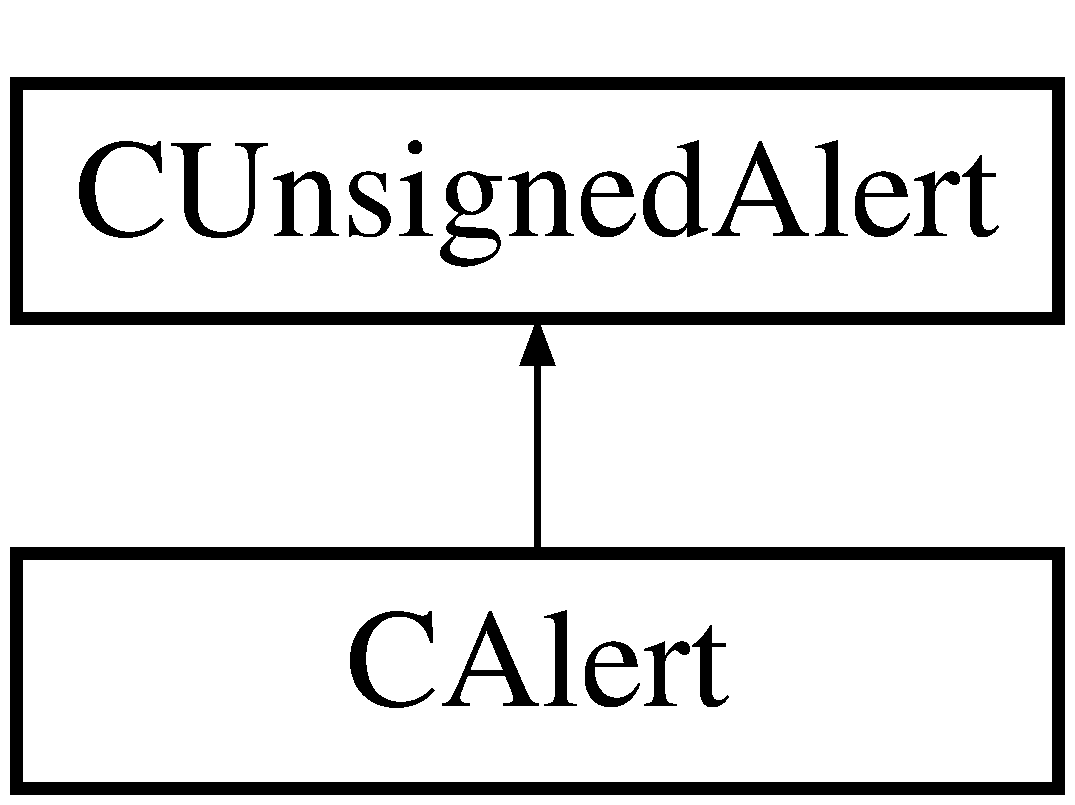
\includegraphics[height=2.000000cm]{class_c_alert}
\end{center}
\end{figure}
\subsection*{Public Member Functions}
\begin{DoxyCompactItemize}
\item 
\hyperlink{class_c_alert_a116117e2318b9468a5ca80472c0b5157}{C\+Alert} ()
\item 
{\footnotesize template$<$typename Stream , typename Operation $>$ }\\void \hyperlink{class_c_alert_a51d73ab316bb42e65b87ec14ac536b14}{Serialization\+Op} (Stream \&s, Operation ser\+\_\+action, int n\+Type, int \hyperlink{class_c_unsigned_alert_ad8fad8e8f62caaf8162fad19170de2cf}{n\+Version})
\item 
void \hyperlink{class_c_alert_a93fd881c55ab448213787f49e316eb99}{Set\+Null} ()
\item 
bool \hyperlink{class_c_alert_ae7e110993e592a1a4f99379ab4fcfa08}{Is\+Null} () const 
\item 
\hyperlink{classuint256}{uint256} \hyperlink{class_c_alert_a59a57a4b4e93bd186ef18d4f09ebd844}{Get\+Hash} () const 
\item 
bool \hyperlink{class_c_alert_a00a8ae5ba7bc54ac7943558c33021190}{Is\+In\+Effect} () const 
\item 
bool \hyperlink{class_c_alert_a90d31fb31348f81b767f16dc5465871b}{Cancels} (const \hyperlink{class_c_alert}{C\+Alert} \&alert) const 
\item 
bool \hyperlink{class_c_alert_add9f485e29a3d1ffea20e6a5a4e42f26}{Applies\+To} (int \hyperlink{class_c_unsigned_alert_ad8fad8e8f62caaf8162fad19170de2cf}{n\+Version}, std\+::string str\+Sub\+Ver\+In) const 
\item 
bool \hyperlink{class_c_alert_a0a7fab6a971781904afb3e4a0ee29e12}{Applies\+To\+Me} () const 
\item 
bool \hyperlink{class_c_alert_ae89d673f6f1285eefcc343b3c029dab5}{Relay\+To} (\hyperlink{class_c_node}{C\+Node} $\ast$pnode) const 
\item 
bool \hyperlink{class_c_alert_ab14b68c1334a19ee4c419bfacd330e7c}{Check\+Signature} (const std\+::vector$<$ unsigned char $>$ \&alert\+Key) const 
\item 
bool \hyperlink{class_c_alert_af63a26aab450c2bc4781717e30ede67b}{Process\+Alert} (const std\+::vector$<$ unsigned char $>$ \&alert\+Key, bool f\+Thread=true)
\end{DoxyCompactItemize}
\subsection*{Static Public Member Functions}
\begin{DoxyCompactItemize}
\item 
static void \hyperlink{class_c_alert_a3da23857c8ed275621ee032a703c04a1}{Notify} (const std\+::string \&str\+Message, bool f\+Thread)
\item 
static \hyperlink{class_c_alert}{C\+Alert} \hyperlink{class_c_alert_aa37df9d177a6841ec5fa1e611c42b968}{get\+Alert\+By\+Hash} (const \hyperlink{classuint256}{uint256} \&hash)
\end{DoxyCompactItemize}
\subsection*{Public Attributes}
\begin{DoxyCompactItemize}
\item 
std\+::vector$<$ unsigned char $>$ \hyperlink{class_c_alert_abfcb3b339d052cd3dd6670b03286758a}{vch\+Msg}
\item 
std\+::vector$<$ unsigned char $>$ \hyperlink{class_c_alert_a541b49670ebf387a5f8b7de59277fed0}{vch\+Sig}
\item 
\hyperlink{class_c_alert_aca9310112e67fb38ef88f385a4ac6fc0}{A\+D\+D\+\_\+\+S\+E\+R\+I\+A\+L\+I\+Z\+E\+\_\+\+M\+E\+T\+H\+O\+D\+S}
\end{DoxyCompactItemize}


\subsection{Detailed Description}
An alert is a combination of a serialized \hyperlink{class_c_unsigned_alert}{C\+Unsigned\+Alert} and a signature. 

\subsection{Constructor \& Destructor Documentation}
\hypertarget{class_c_alert_a116117e2318b9468a5ca80472c0b5157}{}\index{C\+Alert@{C\+Alert}!C\+Alert@{C\+Alert}}
\index{C\+Alert@{C\+Alert}!C\+Alert@{C\+Alert}}
\subsubsection[{C\+Alert}]{\setlength{\rightskip}{0pt plus 5cm}C\+Alert\+::\+C\+Alert (
\begin{DoxyParamCaption}
{}
\end{DoxyParamCaption}
)\hspace{0.3cm}{\ttfamily [inline]}}\label{class_c_alert_a116117e2318b9468a5ca80472c0b5157}


\subsection{Member Function Documentation}
\hypertarget{class_c_alert_add9f485e29a3d1ffea20e6a5a4e42f26}{}\index{C\+Alert@{C\+Alert}!Applies\+To@{Applies\+To}}
\index{Applies\+To@{Applies\+To}!C\+Alert@{C\+Alert}}
\subsubsection[{Applies\+To}]{\setlength{\rightskip}{0pt plus 5cm}bool C\+Alert\+::\+Applies\+To (
\begin{DoxyParamCaption}
\item[{int}]{n\+Version, }
\item[{std\+::string}]{str\+Sub\+Ver\+In}
\end{DoxyParamCaption}
) const}\label{class_c_alert_add9f485e29a3d1ffea20e6a5a4e42f26}
\hypertarget{class_c_alert_a0a7fab6a971781904afb3e4a0ee29e12}{}\index{C\+Alert@{C\+Alert}!Applies\+To\+Me@{Applies\+To\+Me}}
\index{Applies\+To\+Me@{Applies\+To\+Me}!C\+Alert@{C\+Alert}}
\subsubsection[{Applies\+To\+Me}]{\setlength{\rightskip}{0pt plus 5cm}bool C\+Alert\+::\+Applies\+To\+Me (
\begin{DoxyParamCaption}
{}
\end{DoxyParamCaption}
) const}\label{class_c_alert_a0a7fab6a971781904afb3e4a0ee29e12}
\hypertarget{class_c_alert_a90d31fb31348f81b767f16dc5465871b}{}\index{C\+Alert@{C\+Alert}!Cancels@{Cancels}}
\index{Cancels@{Cancels}!C\+Alert@{C\+Alert}}
\subsubsection[{Cancels}]{\setlength{\rightskip}{0pt plus 5cm}bool C\+Alert\+::\+Cancels (
\begin{DoxyParamCaption}
\item[{const {\bf C\+Alert} \&}]{alert}
\end{DoxyParamCaption}
) const}\label{class_c_alert_a90d31fb31348f81b767f16dc5465871b}
\hypertarget{class_c_alert_ab14b68c1334a19ee4c419bfacd330e7c}{}\index{C\+Alert@{C\+Alert}!Check\+Signature@{Check\+Signature}}
\index{Check\+Signature@{Check\+Signature}!C\+Alert@{C\+Alert}}
\subsubsection[{Check\+Signature}]{\setlength{\rightskip}{0pt plus 5cm}bool C\+Alert\+::\+Check\+Signature (
\begin{DoxyParamCaption}
\item[{const std\+::vector$<$ unsigned char $>$ \&}]{alert\+Key}
\end{DoxyParamCaption}
) const}\label{class_c_alert_ab14b68c1334a19ee4c419bfacd330e7c}
\hypertarget{class_c_alert_aa37df9d177a6841ec5fa1e611c42b968}{}\index{C\+Alert@{C\+Alert}!get\+Alert\+By\+Hash@{get\+Alert\+By\+Hash}}
\index{get\+Alert\+By\+Hash@{get\+Alert\+By\+Hash}!C\+Alert@{C\+Alert}}
\subsubsection[{get\+Alert\+By\+Hash}]{\setlength{\rightskip}{0pt plus 5cm}{\bf C\+Alert} C\+Alert\+::get\+Alert\+By\+Hash (
\begin{DoxyParamCaption}
\item[{const {\bf uint256} \&}]{hash}
\end{DoxyParamCaption}
)\hspace{0.3cm}{\ttfamily [static]}}\label{class_c_alert_aa37df9d177a6841ec5fa1e611c42b968}
\hypertarget{class_c_alert_a59a57a4b4e93bd186ef18d4f09ebd844}{}\index{C\+Alert@{C\+Alert}!Get\+Hash@{Get\+Hash}}
\index{Get\+Hash@{Get\+Hash}!C\+Alert@{C\+Alert}}
\subsubsection[{Get\+Hash}]{\setlength{\rightskip}{0pt plus 5cm}{\bf uint256} C\+Alert\+::\+Get\+Hash (
\begin{DoxyParamCaption}
{}
\end{DoxyParamCaption}
) const}\label{class_c_alert_a59a57a4b4e93bd186ef18d4f09ebd844}
\hypertarget{class_c_alert_a00a8ae5ba7bc54ac7943558c33021190}{}\index{C\+Alert@{C\+Alert}!Is\+In\+Effect@{Is\+In\+Effect}}
\index{Is\+In\+Effect@{Is\+In\+Effect}!C\+Alert@{C\+Alert}}
\subsubsection[{Is\+In\+Effect}]{\setlength{\rightskip}{0pt plus 5cm}bool C\+Alert\+::\+Is\+In\+Effect (
\begin{DoxyParamCaption}
{}
\end{DoxyParamCaption}
) const}\label{class_c_alert_a00a8ae5ba7bc54ac7943558c33021190}
\hypertarget{class_c_alert_ae7e110993e592a1a4f99379ab4fcfa08}{}\index{C\+Alert@{C\+Alert}!Is\+Null@{Is\+Null}}
\index{Is\+Null@{Is\+Null}!C\+Alert@{C\+Alert}}
\subsubsection[{Is\+Null}]{\setlength{\rightskip}{0pt plus 5cm}bool C\+Alert\+::\+Is\+Null (
\begin{DoxyParamCaption}
{}
\end{DoxyParamCaption}
) const}\label{class_c_alert_ae7e110993e592a1a4f99379ab4fcfa08}
\hypertarget{class_c_alert_a3da23857c8ed275621ee032a703c04a1}{}\index{C\+Alert@{C\+Alert}!Notify@{Notify}}
\index{Notify@{Notify}!C\+Alert@{C\+Alert}}
\subsubsection[{Notify}]{\setlength{\rightskip}{0pt plus 5cm}void C\+Alert\+::\+Notify (
\begin{DoxyParamCaption}
\item[{const std\+::string \&}]{str\+Message, }
\item[{bool}]{f\+Thread}
\end{DoxyParamCaption}
)\hspace{0.3cm}{\ttfamily [static]}}\label{class_c_alert_a3da23857c8ed275621ee032a703c04a1}
\hypertarget{class_c_alert_af63a26aab450c2bc4781717e30ede67b}{}\index{C\+Alert@{C\+Alert}!Process\+Alert@{Process\+Alert}}
\index{Process\+Alert@{Process\+Alert}!C\+Alert@{C\+Alert}}
\subsubsection[{Process\+Alert}]{\setlength{\rightskip}{0pt plus 5cm}bool C\+Alert\+::\+Process\+Alert (
\begin{DoxyParamCaption}
\item[{const std\+::vector$<$ unsigned char $>$ \&}]{alert\+Key, }
\item[{bool}]{f\+Thread = {\ttfamily true}}
\end{DoxyParamCaption}
)}\label{class_c_alert_af63a26aab450c2bc4781717e30ede67b}
\hypertarget{class_c_alert_ae89d673f6f1285eefcc343b3c029dab5}{}\index{C\+Alert@{C\+Alert}!Relay\+To@{Relay\+To}}
\index{Relay\+To@{Relay\+To}!C\+Alert@{C\+Alert}}
\subsubsection[{Relay\+To}]{\setlength{\rightskip}{0pt plus 5cm}bool C\+Alert\+::\+Relay\+To (
\begin{DoxyParamCaption}
\item[{{\bf C\+Node} $\ast$}]{pnode}
\end{DoxyParamCaption}
) const}\label{class_c_alert_ae89d673f6f1285eefcc343b3c029dab5}
\hypertarget{class_c_alert_a51d73ab316bb42e65b87ec14ac536b14}{}\index{C\+Alert@{C\+Alert}!Serialization\+Op@{Serialization\+Op}}
\index{Serialization\+Op@{Serialization\+Op}!C\+Alert@{C\+Alert}}
\subsubsection[{Serialization\+Op}]{\setlength{\rightskip}{0pt plus 5cm}template$<$typename Stream , typename Operation $>$ void C\+Alert\+::\+Serialization\+Op (
\begin{DoxyParamCaption}
\item[{Stream \&}]{s, }
\item[{Operation}]{ser\+\_\+action, }
\item[{int}]{n\+Type, }
\item[{int}]{n\+Version}
\end{DoxyParamCaption}
)\hspace{0.3cm}{\ttfamily [inline]}}\label{class_c_alert_a51d73ab316bb42e65b87ec14ac536b14}
\hypertarget{class_c_alert_a93fd881c55ab448213787f49e316eb99}{}\index{C\+Alert@{C\+Alert}!Set\+Null@{Set\+Null}}
\index{Set\+Null@{Set\+Null}!C\+Alert@{C\+Alert}}
\subsubsection[{Set\+Null}]{\setlength{\rightskip}{0pt plus 5cm}void C\+Alert\+::\+Set\+Null (
\begin{DoxyParamCaption}
{}
\end{DoxyParamCaption}
)}\label{class_c_alert_a93fd881c55ab448213787f49e316eb99}


\subsection{Member Data Documentation}
\hypertarget{class_c_alert_aca9310112e67fb38ef88f385a4ac6fc0}{}\index{C\+Alert@{C\+Alert}!A\+D\+D\+\_\+\+S\+E\+R\+I\+A\+L\+I\+Z\+E\+\_\+\+M\+E\+T\+H\+O\+D\+S@{A\+D\+D\+\_\+\+S\+E\+R\+I\+A\+L\+I\+Z\+E\+\_\+\+M\+E\+T\+H\+O\+D\+S}}
\index{A\+D\+D\+\_\+\+S\+E\+R\+I\+A\+L\+I\+Z\+E\+\_\+\+M\+E\+T\+H\+O\+D\+S@{A\+D\+D\+\_\+\+S\+E\+R\+I\+A\+L\+I\+Z\+E\+\_\+\+M\+E\+T\+H\+O\+D\+S}!C\+Alert@{C\+Alert}}
\subsubsection[{A\+D\+D\+\_\+\+S\+E\+R\+I\+A\+L\+I\+Z\+E\+\_\+\+M\+E\+T\+H\+O\+D\+S}]{\setlength{\rightskip}{0pt plus 5cm}C\+Alert\+::\+A\+D\+D\+\_\+\+S\+E\+R\+I\+A\+L\+I\+Z\+E\+\_\+\+M\+E\+T\+H\+O\+D\+S}\label{class_c_alert_aca9310112e67fb38ef88f385a4ac6fc0}
\hypertarget{class_c_alert_abfcb3b339d052cd3dd6670b03286758a}{}\index{C\+Alert@{C\+Alert}!vch\+Msg@{vch\+Msg}}
\index{vch\+Msg@{vch\+Msg}!C\+Alert@{C\+Alert}}
\subsubsection[{vch\+Msg}]{\setlength{\rightskip}{0pt plus 5cm}std\+::vector$<$unsigned char$>$ C\+Alert\+::vch\+Msg}\label{class_c_alert_abfcb3b339d052cd3dd6670b03286758a}
\hypertarget{class_c_alert_a541b49670ebf387a5f8b7de59277fed0}{}\index{C\+Alert@{C\+Alert}!vch\+Sig@{vch\+Sig}}
\index{vch\+Sig@{vch\+Sig}!C\+Alert@{C\+Alert}}
\subsubsection[{vch\+Sig}]{\setlength{\rightskip}{0pt plus 5cm}std\+::vector$<$unsigned char$>$ C\+Alert\+::vch\+Sig}\label{class_c_alert_a541b49670ebf387a5f8b7de59277fed0}


The documentation for this class was generated from the following files\+:\begin{DoxyCompactItemize}
\item 
C\+:/\+Users/\+Joe/\+Documents/\+School/\+C\+S\+C17\+A/bitcoin/src/\hyperlink{alert_8h}{alert.\+h}\item 
C\+:/\+Users/\+Joe/\+Documents/\+School/\+C\+S\+C17\+A/bitcoin/src/\hyperlink{alert_8cpp}{alert.\+cpp}\end{DoxyCompactItemize}

\hypertarget{class_c_auto_file}{}\section{C\+Auto\+File Class Reference}
\label{class_c_auto_file}\index{C\+Auto\+File@{C\+Auto\+File}}


{\ttfamily \#include $<$streams.\+h$>$}

\subsection*{Public Member Functions}
\begin{DoxyCompactItemize}
\item 
\hyperlink{class_c_auto_file_a52613083aaeab4c9238c649ae471783f}{C\+Auto\+File} (F\+I\+L\+E $\ast$filenew, int n\+Type\+In, int n\+Version\+In)
\item 
\hyperlink{class_c_auto_file_ab1362f4cb52c819c25cff4598e0f28da}{$\sim$\+C\+Auto\+File} ()
\item 
void \hyperlink{class_c_auto_file_abcbafe943bfe392c09363078fa8a4e77}{fclose} ()
\item 
F\+I\+L\+E $\ast$ \hyperlink{class_c_auto_file_a25b51d94dc85c4140da0b15494ac9f8a}{release} ()
\item 
F\+I\+L\+E $\ast$ \hyperlink{class_c_auto_file_aea31c0348f31ea40f592e2b7af6c2045}{Get} () const 
\item 
bool \hyperlink{class_c_auto_file_a78d666b1ef5dff5fd3f4ee33692b6d1d}{Is\+Null} () const 
\item 
void \hyperlink{class_c_auto_file_ac1a3986f191fe81384f58fc5fa073820}{Set\+Type} (int n)
\item 
int \hyperlink{class_c_auto_file_a774f2aad2c462d4ff47125ceec2ebab0}{Get\+Type} ()
\item 
void \hyperlink{class_c_auto_file_a51f805bc470a95c9948250503b587aec}{Set\+Version} (int n)
\item 
int \hyperlink{class_c_auto_file_a976ab8e5477aedd3a531fc49b01153ce}{Get\+Version} ()
\item 
void \hyperlink{class_c_auto_file_a9511060b5c971cff532faeab60c7d88b}{Read\+Version} ()
\item 
void \hyperlink{class_c_auto_file_a23d6f22c3aff80be7665bfc5a77a01ff}{Write\+Version} ()
\item 
\hyperlink{class_c_auto_file}{C\+Auto\+File} \& \hyperlink{class_c_auto_file_a87e670f3dd03055264c05b25335babb4}{read} (char $\ast$pch, size\+\_\+t n\+Size)
\item 
\hyperlink{class_c_auto_file}{C\+Auto\+File} \& \hyperlink{class_c_auto_file_a7b2852b345b75835f883be3732cf826a}{write} (const char $\ast$pch, size\+\_\+t n\+Size)
\item 
{\footnotesize template$<$typename T $>$ }\\unsigned int \hyperlink{class_c_auto_file_a883a261f0d7d0320f72152ff2167fd24}{Get\+Serialize\+Size} (const T \&obj)
\item 
{\footnotesize template$<$typename T $>$ }\\\hyperlink{class_c_auto_file}{C\+Auto\+File} \& \hyperlink{class_c_auto_file_a8e194596d1f8f64059247724b25df82c}{operator$<$$<$} (const T \&obj)
\item 
{\footnotesize template$<$typename T $>$ }\\\hyperlink{class_c_auto_file}{C\+Auto\+File} \& \hyperlink{class_c_auto_file_ae6826219322626d2ac8229e022c41dd7}{operator$>$$>$} (T \&obj)
\end{DoxyCompactItemize}


\subsection{Detailed Description}
Non-\/refcounted R\+A\+I\+I wrapper for F\+I\+L\+E$\ast$

Will automatically close the file when it goes out of scope if not null. If you\textquotesingle{}re returning the file pointer, return file.\+release(). If you need to close the file early, use file.\+fclose() instead of fclose(file). 

\subsection{Constructor \& Destructor Documentation}
\hypertarget{class_c_auto_file_a52613083aaeab4c9238c649ae471783f}{}\index{C\+Auto\+File@{C\+Auto\+File}!C\+Auto\+File@{C\+Auto\+File}}
\index{C\+Auto\+File@{C\+Auto\+File}!C\+Auto\+File@{C\+Auto\+File}}
\subsubsection[{C\+Auto\+File}]{\setlength{\rightskip}{0pt plus 5cm}C\+Auto\+File\+::\+C\+Auto\+File (
\begin{DoxyParamCaption}
\item[{F\+I\+L\+E $\ast$}]{filenew, }
\item[{int}]{n\+Type\+In, }
\item[{int}]{n\+Version\+In}
\end{DoxyParamCaption}
)\hspace{0.3cm}{\ttfamily [inline]}}\label{class_c_auto_file_a52613083aaeab4c9238c649ae471783f}
\hypertarget{class_c_auto_file_ab1362f4cb52c819c25cff4598e0f28da}{}\index{C\+Auto\+File@{C\+Auto\+File}!````~C\+Auto\+File@{$\sim$\+C\+Auto\+File}}
\index{````~C\+Auto\+File@{$\sim$\+C\+Auto\+File}!C\+Auto\+File@{C\+Auto\+File}}
\subsubsection[{$\sim$\+C\+Auto\+File}]{\setlength{\rightskip}{0pt plus 5cm}C\+Auto\+File\+::$\sim$\+C\+Auto\+File (
\begin{DoxyParamCaption}
{}
\end{DoxyParamCaption}
)\hspace{0.3cm}{\ttfamily [inline]}}\label{class_c_auto_file_ab1362f4cb52c819c25cff4598e0f28da}


\subsection{Member Function Documentation}
\hypertarget{class_c_auto_file_abcbafe943bfe392c09363078fa8a4e77}{}\index{C\+Auto\+File@{C\+Auto\+File}!fclose@{fclose}}
\index{fclose@{fclose}!C\+Auto\+File@{C\+Auto\+File}}
\subsubsection[{fclose}]{\setlength{\rightskip}{0pt plus 5cm}void C\+Auto\+File\+::fclose (
\begin{DoxyParamCaption}
{}
\end{DoxyParamCaption}
)\hspace{0.3cm}{\ttfamily [inline]}}\label{class_c_auto_file_abcbafe943bfe392c09363078fa8a4e77}
\hypertarget{class_c_auto_file_aea31c0348f31ea40f592e2b7af6c2045}{}\index{C\+Auto\+File@{C\+Auto\+File}!Get@{Get}}
\index{Get@{Get}!C\+Auto\+File@{C\+Auto\+File}}
\subsubsection[{Get}]{\setlength{\rightskip}{0pt plus 5cm}F\+I\+L\+E$\ast$ C\+Auto\+File\+::\+Get (
\begin{DoxyParamCaption}
{}
\end{DoxyParamCaption}
) const\hspace{0.3cm}{\ttfamily [inline]}}\label{class_c_auto_file_aea31c0348f31ea40f592e2b7af6c2045}
Get wrapped F\+I\+L\+E$\ast$ without transfer of ownership. \begin{DoxyNote}{Note}
Ownership of the F\+I\+L\+E$\ast$ will remain with this class. Use this only if the scope of the \hyperlink{class_c_auto_file}{C\+Auto\+File} outlives use of the passed pointer. 
\end{DoxyNote}
\hypertarget{class_c_auto_file_a883a261f0d7d0320f72152ff2167fd24}{}\index{C\+Auto\+File@{C\+Auto\+File}!Get\+Serialize\+Size@{Get\+Serialize\+Size}}
\index{Get\+Serialize\+Size@{Get\+Serialize\+Size}!C\+Auto\+File@{C\+Auto\+File}}
\subsubsection[{Get\+Serialize\+Size}]{\setlength{\rightskip}{0pt plus 5cm}template$<$typename T $>$ unsigned int C\+Auto\+File\+::\+Get\+Serialize\+Size (
\begin{DoxyParamCaption}
\item[{const T \&}]{obj}
\end{DoxyParamCaption}
)\hspace{0.3cm}{\ttfamily [inline]}}\label{class_c_auto_file_a883a261f0d7d0320f72152ff2167fd24}
\hypertarget{class_c_auto_file_a774f2aad2c462d4ff47125ceec2ebab0}{}\index{C\+Auto\+File@{C\+Auto\+File}!Get\+Type@{Get\+Type}}
\index{Get\+Type@{Get\+Type}!C\+Auto\+File@{C\+Auto\+File}}
\subsubsection[{Get\+Type}]{\setlength{\rightskip}{0pt plus 5cm}int C\+Auto\+File\+::\+Get\+Type (
\begin{DoxyParamCaption}
{}
\end{DoxyParamCaption}
)\hspace{0.3cm}{\ttfamily [inline]}}\label{class_c_auto_file_a774f2aad2c462d4ff47125ceec2ebab0}
\hypertarget{class_c_auto_file_a976ab8e5477aedd3a531fc49b01153ce}{}\index{C\+Auto\+File@{C\+Auto\+File}!Get\+Version@{Get\+Version}}
\index{Get\+Version@{Get\+Version}!C\+Auto\+File@{C\+Auto\+File}}
\subsubsection[{Get\+Version}]{\setlength{\rightskip}{0pt plus 5cm}int C\+Auto\+File\+::\+Get\+Version (
\begin{DoxyParamCaption}
{}
\end{DoxyParamCaption}
)\hspace{0.3cm}{\ttfamily [inline]}}\label{class_c_auto_file_a976ab8e5477aedd3a531fc49b01153ce}
\hypertarget{class_c_auto_file_a78d666b1ef5dff5fd3f4ee33692b6d1d}{}\index{C\+Auto\+File@{C\+Auto\+File}!Is\+Null@{Is\+Null}}
\index{Is\+Null@{Is\+Null}!C\+Auto\+File@{C\+Auto\+File}}
\subsubsection[{Is\+Null}]{\setlength{\rightskip}{0pt plus 5cm}bool C\+Auto\+File\+::\+Is\+Null (
\begin{DoxyParamCaption}
{}
\end{DoxyParamCaption}
) const\hspace{0.3cm}{\ttfamily [inline]}}\label{class_c_auto_file_a78d666b1ef5dff5fd3f4ee33692b6d1d}
Return true if the wrapped F\+I\+L\+E$\ast$ is N\+U\+L\+L, false otherwise. \hypertarget{class_c_auto_file_a8e194596d1f8f64059247724b25df82c}{}\index{C\+Auto\+File@{C\+Auto\+File}!operator$<$$<$@{operator$<$$<$}}
\index{operator$<$$<$@{operator$<$$<$}!C\+Auto\+File@{C\+Auto\+File}}
\subsubsection[{operator$<$$<$}]{\setlength{\rightskip}{0pt plus 5cm}template$<$typename T $>$ {\bf C\+Auto\+File}\& C\+Auto\+File\+::operator$<$$<$ (
\begin{DoxyParamCaption}
\item[{const T \&}]{obj}
\end{DoxyParamCaption}
)\hspace{0.3cm}{\ttfamily [inline]}}\label{class_c_auto_file_a8e194596d1f8f64059247724b25df82c}
\hypertarget{class_c_auto_file_ae6826219322626d2ac8229e022c41dd7}{}\index{C\+Auto\+File@{C\+Auto\+File}!operator$>$$>$@{operator$>$$>$}}
\index{operator$>$$>$@{operator$>$$>$}!C\+Auto\+File@{C\+Auto\+File}}
\subsubsection[{operator$>$$>$}]{\setlength{\rightskip}{0pt plus 5cm}template$<$typename T $>$ {\bf C\+Auto\+File}\& C\+Auto\+File\+::operator$>$$>$ (
\begin{DoxyParamCaption}
\item[{T \&}]{obj}
\end{DoxyParamCaption}
)\hspace{0.3cm}{\ttfamily [inline]}}\label{class_c_auto_file_ae6826219322626d2ac8229e022c41dd7}
\hypertarget{class_c_auto_file_a87e670f3dd03055264c05b25335babb4}{}\index{C\+Auto\+File@{C\+Auto\+File}!read@{read}}
\index{read@{read}!C\+Auto\+File@{C\+Auto\+File}}
\subsubsection[{read}]{\setlength{\rightskip}{0pt plus 5cm}{\bf C\+Auto\+File}\& C\+Auto\+File\+::read (
\begin{DoxyParamCaption}
\item[{char $\ast$}]{pch, }
\item[{size\+\_\+t}]{n\+Size}
\end{DoxyParamCaption}
)\hspace{0.3cm}{\ttfamily [inline]}}\label{class_c_auto_file_a87e670f3dd03055264c05b25335babb4}
\hypertarget{class_c_auto_file_a9511060b5c971cff532faeab60c7d88b}{}\index{C\+Auto\+File@{C\+Auto\+File}!Read\+Version@{Read\+Version}}
\index{Read\+Version@{Read\+Version}!C\+Auto\+File@{C\+Auto\+File}}
\subsubsection[{Read\+Version}]{\setlength{\rightskip}{0pt plus 5cm}void C\+Auto\+File\+::\+Read\+Version (
\begin{DoxyParamCaption}
{}
\end{DoxyParamCaption}
)\hspace{0.3cm}{\ttfamily [inline]}}\label{class_c_auto_file_a9511060b5c971cff532faeab60c7d88b}
\hypertarget{class_c_auto_file_a25b51d94dc85c4140da0b15494ac9f8a}{}\index{C\+Auto\+File@{C\+Auto\+File}!release@{release}}
\index{release@{release}!C\+Auto\+File@{C\+Auto\+File}}
\subsubsection[{release}]{\setlength{\rightskip}{0pt plus 5cm}F\+I\+L\+E$\ast$ C\+Auto\+File\+::release (
\begin{DoxyParamCaption}
{}
\end{DoxyParamCaption}
)\hspace{0.3cm}{\ttfamily [inline]}}\label{class_c_auto_file_a25b51d94dc85c4140da0b15494ac9f8a}
Get wrapped F\+I\+L\+E$\ast$ with transfer of ownership. \begin{DoxyNote}{Note}
This will invalidate the \hyperlink{class_c_auto_file}{C\+Auto\+File} object, and makes it the responsibility of the caller of this function to clean up the returned F\+I\+L\+E$\ast$. 
\end{DoxyNote}
\hypertarget{class_c_auto_file_ac1a3986f191fe81384f58fc5fa073820}{}\index{C\+Auto\+File@{C\+Auto\+File}!Set\+Type@{Set\+Type}}
\index{Set\+Type@{Set\+Type}!C\+Auto\+File@{C\+Auto\+File}}
\subsubsection[{Set\+Type}]{\setlength{\rightskip}{0pt plus 5cm}void C\+Auto\+File\+::\+Set\+Type (
\begin{DoxyParamCaption}
\item[{int}]{n}
\end{DoxyParamCaption}
)\hspace{0.3cm}{\ttfamily [inline]}}\label{class_c_auto_file_ac1a3986f191fe81384f58fc5fa073820}
\hypertarget{class_c_auto_file_a51f805bc470a95c9948250503b587aec}{}\index{C\+Auto\+File@{C\+Auto\+File}!Set\+Version@{Set\+Version}}
\index{Set\+Version@{Set\+Version}!C\+Auto\+File@{C\+Auto\+File}}
\subsubsection[{Set\+Version}]{\setlength{\rightskip}{0pt plus 5cm}void C\+Auto\+File\+::\+Set\+Version (
\begin{DoxyParamCaption}
\item[{int}]{n}
\end{DoxyParamCaption}
)\hspace{0.3cm}{\ttfamily [inline]}}\label{class_c_auto_file_a51f805bc470a95c9948250503b587aec}
\hypertarget{class_c_auto_file_a7b2852b345b75835f883be3732cf826a}{}\index{C\+Auto\+File@{C\+Auto\+File}!write@{write}}
\index{write@{write}!C\+Auto\+File@{C\+Auto\+File}}
\subsubsection[{write}]{\setlength{\rightskip}{0pt plus 5cm}{\bf C\+Auto\+File}\& C\+Auto\+File\+::write (
\begin{DoxyParamCaption}
\item[{const char $\ast$}]{pch, }
\item[{size\+\_\+t}]{n\+Size}
\end{DoxyParamCaption}
)\hspace{0.3cm}{\ttfamily [inline]}}\label{class_c_auto_file_a7b2852b345b75835f883be3732cf826a}
\hypertarget{class_c_auto_file_a23d6f22c3aff80be7665bfc5a77a01ff}{}\index{C\+Auto\+File@{C\+Auto\+File}!Write\+Version@{Write\+Version}}
\index{Write\+Version@{Write\+Version}!C\+Auto\+File@{C\+Auto\+File}}
\subsubsection[{Write\+Version}]{\setlength{\rightskip}{0pt plus 5cm}void C\+Auto\+File\+::\+Write\+Version (
\begin{DoxyParamCaption}
{}
\end{DoxyParamCaption}
)\hspace{0.3cm}{\ttfamily [inline]}}\label{class_c_auto_file_a23d6f22c3aff80be7665bfc5a77a01ff}


The documentation for this class was generated from the following file\+:\begin{DoxyCompactItemize}
\item 
C\+:/\+Users/\+Joe/\+Documents/\+School/\+C\+S\+C17\+A/bitcoin/src/\hyperlink{streams_8h}{streams.\+h}\end{DoxyCompactItemize}

\hypertarget{class_c_base58_data}{}\section{C\+Base58\+Data Class Reference}
\label{class_c_base58_data}\index{C\+Base58\+Data@{C\+Base58\+Data}}


{\ttfamily \#include $<$base58.\+h$>$}

Inheritance diagram for C\+Base58\+Data\+:\begin{figure}[H]
\begin{center}
\leavevmode
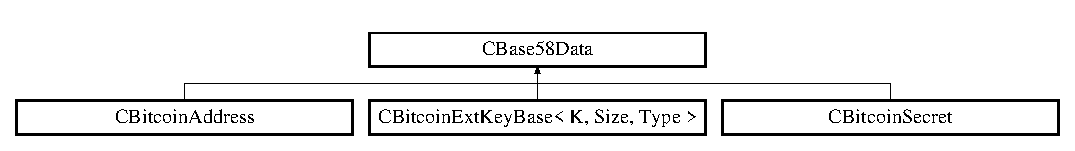
\includegraphics[height=1.581921cm]{class_c_base58_data}
\end{center}
\end{figure}
\subsection*{Public Member Functions}
\begin{DoxyCompactItemize}
\item 
bool \hyperlink{class_c_base58_data_a250fa3bc97d03c7d87de5485c8b49b57}{Set\+String} (const char $\ast$psz, unsigned int n\+Version\+Bytes=1)
\item 
bool \hyperlink{class_c_base58_data_a8e0cba75a3e0a5b21defaf1471d8659c}{Set\+String} (const std\+::string \&str)
\item 
std\+::string \hyperlink{class_c_base58_data_a9a47b10dadff15b8d6a6d0e63ce3ae32}{To\+String} () const 
\item 
int \hyperlink{class_c_base58_data_ab3d18fd9671a383937af7dd4ac2e890a}{Compare\+To} (const \hyperlink{class_c_base58_data}{C\+Base58\+Data} \&b58) const 
\item 
bool \hyperlink{class_c_base58_data_af6448549abaf34142668540a338d180d}{operator==} (const \hyperlink{class_c_base58_data}{C\+Base58\+Data} \&b58) const 
\item 
bool \hyperlink{class_c_base58_data_a126cabad3af6b7d3aec0d6498be1a028}{operator$<$=} (const \hyperlink{class_c_base58_data}{C\+Base58\+Data} \&b58) const 
\item 
bool \hyperlink{class_c_base58_data_a4a96e8ea3716509b307cacfc814e5622}{operator$>$=} (const \hyperlink{class_c_base58_data}{C\+Base58\+Data} \&b58) const 
\item 
bool \hyperlink{class_c_base58_data_a39bac58c4bc4f8abc74a24b769eb1f1d}{operator$<$} (const \hyperlink{class_c_base58_data}{C\+Base58\+Data} \&b58) const 
\item 
bool \hyperlink{class_c_base58_data_a427e472d2fef51aaa89c1a09229ac51a}{operator$>$} (const \hyperlink{class_c_base58_data}{C\+Base58\+Data} \&b58) const 
\end{DoxyCompactItemize}
\subsection*{Protected Types}
\begin{DoxyCompactItemize}
\item 
typedef std\+::vector$<$ unsigned char, zero\+\_\+after\+\_\+free\+\_\+allocator$<$ unsigned char $>$ $>$ \hyperlink{class_c_base58_data_a193d64487a0b4f6df24f8bd380956ec1}{vector\+\_\+uchar}
\begin{DoxyCompactList}\small\item\em the actually encoded data \end{DoxyCompactList}\end{DoxyCompactItemize}
\subsection*{Protected Member Functions}
\begin{DoxyCompactItemize}
\item 
\hyperlink{class_c_base58_data_ae4f4ff42010299bc6fb228e21d6b2a15}{C\+Base58\+Data} ()
\item 
void \hyperlink{class_c_base58_data_afab1c06a0a4f631fd889434a2bc48c27}{Set\+Data} (const std\+::vector$<$ unsigned char $>$ \&vch\+Version\+In, const void $\ast$pdata, size\+\_\+t n\+Size)
\item 
void \hyperlink{class_c_base58_data_a8314b00685e590b4005be5cdfd36aeb9}{Set\+Data} (const std\+::vector$<$ unsigned char $>$ \&vch\+Version\+In, const unsigned char $\ast$pbegin, const unsigned char $\ast$pend)
\end{DoxyCompactItemize}
\subsection*{Protected Attributes}
\begin{DoxyCompactItemize}
\item 
std\+::vector$<$ unsigned char $>$ \hyperlink{class_c_base58_data_a110c1008f399053098a1bdf63408e923}{vch\+Version}
\begin{DoxyCompactList}\small\item\em the version byte(s) \end{DoxyCompactList}\item 
\hyperlink{class_c_base58_data_a193d64487a0b4f6df24f8bd380956ec1}{vector\+\_\+uchar} \hyperlink{class_c_base58_data_ae7ef7dfb93683aa4aaee8b74da5abb9c}{vch\+Data}
\end{DoxyCompactItemize}


\subsection{Detailed Description}
Base class for all base58-\/encoded data 

\subsection{Member Typedef Documentation}
\hypertarget{class_c_base58_data_a193d64487a0b4f6df24f8bd380956ec1}{}\index{C\+Base58\+Data@{C\+Base58\+Data}!vector\+\_\+uchar@{vector\+\_\+uchar}}
\index{vector\+\_\+uchar@{vector\+\_\+uchar}!C\+Base58\+Data@{C\+Base58\+Data}}
\subsubsection[{vector\+\_\+uchar}]{\setlength{\rightskip}{0pt plus 5cm}typedef std\+::vector$<$unsigned char, zero\+\_\+after\+\_\+free\+\_\+allocator$<$unsigned char$>$ $>$ {\bf C\+Base58\+Data\+::vector\+\_\+uchar}\hspace{0.3cm}{\ttfamily [protected]}}\label{class_c_base58_data_a193d64487a0b4f6df24f8bd380956ec1}


the actually encoded data 



\subsection{Constructor \& Destructor Documentation}
\hypertarget{class_c_base58_data_ae4f4ff42010299bc6fb228e21d6b2a15}{}\index{C\+Base58\+Data@{C\+Base58\+Data}!C\+Base58\+Data@{C\+Base58\+Data}}
\index{C\+Base58\+Data@{C\+Base58\+Data}!C\+Base58\+Data@{C\+Base58\+Data}}
\subsubsection[{C\+Base58\+Data}]{\setlength{\rightskip}{0pt plus 5cm}C\+Base58\+Data\+::\+C\+Base58\+Data (
\begin{DoxyParamCaption}
{}
\end{DoxyParamCaption}
)\hspace{0.3cm}{\ttfamily [protected]}}\label{class_c_base58_data_ae4f4ff42010299bc6fb228e21d6b2a15}


\subsection{Member Function Documentation}
\hypertarget{class_c_base58_data_ab3d18fd9671a383937af7dd4ac2e890a}{}\index{C\+Base58\+Data@{C\+Base58\+Data}!Compare\+To@{Compare\+To}}
\index{Compare\+To@{Compare\+To}!C\+Base58\+Data@{C\+Base58\+Data}}
\subsubsection[{Compare\+To}]{\setlength{\rightskip}{0pt plus 5cm}int C\+Base58\+Data\+::\+Compare\+To (
\begin{DoxyParamCaption}
\item[{const {\bf C\+Base58\+Data} \&}]{b58}
\end{DoxyParamCaption}
) const}\label{class_c_base58_data_ab3d18fd9671a383937af7dd4ac2e890a}
\hypertarget{class_c_base58_data_a39bac58c4bc4f8abc74a24b769eb1f1d}{}\index{C\+Base58\+Data@{C\+Base58\+Data}!operator$<$@{operator$<$}}
\index{operator$<$@{operator$<$}!C\+Base58\+Data@{C\+Base58\+Data}}
\subsubsection[{operator$<$}]{\setlength{\rightskip}{0pt plus 5cm}bool C\+Base58\+Data\+::operator$<$ (
\begin{DoxyParamCaption}
\item[{const {\bf C\+Base58\+Data} \&}]{b58}
\end{DoxyParamCaption}
) const\hspace{0.3cm}{\ttfamily [inline]}}\label{class_c_base58_data_a39bac58c4bc4f8abc74a24b769eb1f1d}
\hypertarget{class_c_base58_data_a126cabad3af6b7d3aec0d6498be1a028}{}\index{C\+Base58\+Data@{C\+Base58\+Data}!operator$<$=@{operator$<$=}}
\index{operator$<$=@{operator$<$=}!C\+Base58\+Data@{C\+Base58\+Data}}
\subsubsection[{operator$<$=}]{\setlength{\rightskip}{0pt plus 5cm}bool C\+Base58\+Data\+::operator$<$= (
\begin{DoxyParamCaption}
\item[{const {\bf C\+Base58\+Data} \&}]{b58}
\end{DoxyParamCaption}
) const\hspace{0.3cm}{\ttfamily [inline]}}\label{class_c_base58_data_a126cabad3af6b7d3aec0d6498be1a028}
\hypertarget{class_c_base58_data_af6448549abaf34142668540a338d180d}{}\index{C\+Base58\+Data@{C\+Base58\+Data}!operator==@{operator==}}
\index{operator==@{operator==}!C\+Base58\+Data@{C\+Base58\+Data}}
\subsubsection[{operator==}]{\setlength{\rightskip}{0pt plus 5cm}bool C\+Base58\+Data\+::operator== (
\begin{DoxyParamCaption}
\item[{const {\bf C\+Base58\+Data} \&}]{b58}
\end{DoxyParamCaption}
) const\hspace{0.3cm}{\ttfamily [inline]}}\label{class_c_base58_data_af6448549abaf34142668540a338d180d}
\hypertarget{class_c_base58_data_a427e472d2fef51aaa89c1a09229ac51a}{}\index{C\+Base58\+Data@{C\+Base58\+Data}!operator$>$@{operator$>$}}
\index{operator$>$@{operator$>$}!C\+Base58\+Data@{C\+Base58\+Data}}
\subsubsection[{operator$>$}]{\setlength{\rightskip}{0pt plus 5cm}bool C\+Base58\+Data\+::operator$>$ (
\begin{DoxyParamCaption}
\item[{const {\bf C\+Base58\+Data} \&}]{b58}
\end{DoxyParamCaption}
) const\hspace{0.3cm}{\ttfamily [inline]}}\label{class_c_base58_data_a427e472d2fef51aaa89c1a09229ac51a}
\hypertarget{class_c_base58_data_a4a96e8ea3716509b307cacfc814e5622}{}\index{C\+Base58\+Data@{C\+Base58\+Data}!operator$>$=@{operator$>$=}}
\index{operator$>$=@{operator$>$=}!C\+Base58\+Data@{C\+Base58\+Data}}
\subsubsection[{operator$>$=}]{\setlength{\rightskip}{0pt plus 5cm}bool C\+Base58\+Data\+::operator$>$= (
\begin{DoxyParamCaption}
\item[{const {\bf C\+Base58\+Data} \&}]{b58}
\end{DoxyParamCaption}
) const\hspace{0.3cm}{\ttfamily [inline]}}\label{class_c_base58_data_a4a96e8ea3716509b307cacfc814e5622}
\hypertarget{class_c_base58_data_afab1c06a0a4f631fd889434a2bc48c27}{}\index{C\+Base58\+Data@{C\+Base58\+Data}!Set\+Data@{Set\+Data}}
\index{Set\+Data@{Set\+Data}!C\+Base58\+Data@{C\+Base58\+Data}}
\subsubsection[{Set\+Data}]{\setlength{\rightskip}{0pt plus 5cm}void C\+Base58\+Data\+::\+Set\+Data (
\begin{DoxyParamCaption}
\item[{const std\+::vector$<$ unsigned char $>$ \&}]{vch\+Version\+In, }
\item[{const void $\ast$}]{pdata, }
\item[{size\+\_\+t}]{n\+Size}
\end{DoxyParamCaption}
)\hspace{0.3cm}{\ttfamily [protected]}}\label{class_c_base58_data_afab1c06a0a4f631fd889434a2bc48c27}
\hypertarget{class_c_base58_data_a8314b00685e590b4005be5cdfd36aeb9}{}\index{C\+Base58\+Data@{C\+Base58\+Data}!Set\+Data@{Set\+Data}}
\index{Set\+Data@{Set\+Data}!C\+Base58\+Data@{C\+Base58\+Data}}
\subsubsection[{Set\+Data}]{\setlength{\rightskip}{0pt plus 5cm}void C\+Base58\+Data\+::\+Set\+Data (
\begin{DoxyParamCaption}
\item[{const std\+::vector$<$ unsigned char $>$ \&}]{vch\+Version\+In, }
\item[{const unsigned char $\ast$}]{pbegin, }
\item[{const unsigned char $\ast$}]{pend}
\end{DoxyParamCaption}
)\hspace{0.3cm}{\ttfamily [protected]}}\label{class_c_base58_data_a8314b00685e590b4005be5cdfd36aeb9}
\hypertarget{class_c_base58_data_a250fa3bc97d03c7d87de5485c8b49b57}{}\index{C\+Base58\+Data@{C\+Base58\+Data}!Set\+String@{Set\+String}}
\index{Set\+String@{Set\+String}!C\+Base58\+Data@{C\+Base58\+Data}}
\subsubsection[{Set\+String}]{\setlength{\rightskip}{0pt plus 5cm}bool C\+Base58\+Data\+::\+Set\+String (
\begin{DoxyParamCaption}
\item[{const char $\ast$}]{psz, }
\item[{unsigned int}]{n\+Version\+Bytes = {\ttfamily 1}}
\end{DoxyParamCaption}
)}\label{class_c_base58_data_a250fa3bc97d03c7d87de5485c8b49b57}
\hypertarget{class_c_base58_data_a8e0cba75a3e0a5b21defaf1471d8659c}{}\index{C\+Base58\+Data@{C\+Base58\+Data}!Set\+String@{Set\+String}}
\index{Set\+String@{Set\+String}!C\+Base58\+Data@{C\+Base58\+Data}}
\subsubsection[{Set\+String}]{\setlength{\rightskip}{0pt plus 5cm}bool C\+Base58\+Data\+::\+Set\+String (
\begin{DoxyParamCaption}
\item[{const std\+::string \&}]{str}
\end{DoxyParamCaption}
)}\label{class_c_base58_data_a8e0cba75a3e0a5b21defaf1471d8659c}
\hypertarget{class_c_base58_data_a9a47b10dadff15b8d6a6d0e63ce3ae32}{}\index{C\+Base58\+Data@{C\+Base58\+Data}!To\+String@{To\+String}}
\index{To\+String@{To\+String}!C\+Base58\+Data@{C\+Base58\+Data}}
\subsubsection[{To\+String}]{\setlength{\rightskip}{0pt plus 5cm}std\+::string C\+Base58\+Data\+::\+To\+String (
\begin{DoxyParamCaption}
{}
\end{DoxyParamCaption}
) const}\label{class_c_base58_data_a9a47b10dadff15b8d6a6d0e63ce3ae32}


\subsection{Member Data Documentation}
\hypertarget{class_c_base58_data_ae7ef7dfb93683aa4aaee8b74da5abb9c}{}\index{C\+Base58\+Data@{C\+Base58\+Data}!vch\+Data@{vch\+Data}}
\index{vch\+Data@{vch\+Data}!C\+Base58\+Data@{C\+Base58\+Data}}
\subsubsection[{vch\+Data}]{\setlength{\rightskip}{0pt plus 5cm}{\bf vector\+\_\+uchar} C\+Base58\+Data\+::vch\+Data\hspace{0.3cm}{\ttfamily [protected]}}\label{class_c_base58_data_ae7ef7dfb93683aa4aaee8b74da5abb9c}
\hypertarget{class_c_base58_data_a110c1008f399053098a1bdf63408e923}{}\index{C\+Base58\+Data@{C\+Base58\+Data}!vch\+Version@{vch\+Version}}
\index{vch\+Version@{vch\+Version}!C\+Base58\+Data@{C\+Base58\+Data}}
\subsubsection[{vch\+Version}]{\setlength{\rightskip}{0pt plus 5cm}std\+::vector$<$unsigned char$>$ C\+Base58\+Data\+::vch\+Version\hspace{0.3cm}{\ttfamily [protected]}}\label{class_c_base58_data_a110c1008f399053098a1bdf63408e923}


the version byte(s) 



The documentation for this class was generated from the following files\+:\begin{DoxyCompactItemize}
\item 
C\+:/\+Users/\+Joe/\+Documents/\+School/\+C\+S\+C17\+A/bitcoin/src/\hyperlink{base58_8h}{base58.\+h}\item 
C\+:/\+Users/\+Joe/\+Documents/\+School/\+C\+S\+C17\+A/bitcoin/src/\hyperlink{base58_8cpp}{base58.\+cpp}\end{DoxyCompactItemize}

\hypertarget{class_c_base_chain_params}{}\section{C\+Base\+Chain\+Params Class Reference}
\label{class_c_base_chain_params}\index{C\+Base\+Chain\+Params@{C\+Base\+Chain\+Params}}


{\ttfamily \#include $<$chainparamsbase.\+h$>$}

Inheritance diagram for C\+Base\+Chain\+Params\+:\begin{figure}[H]
\begin{center}
\leavevmode
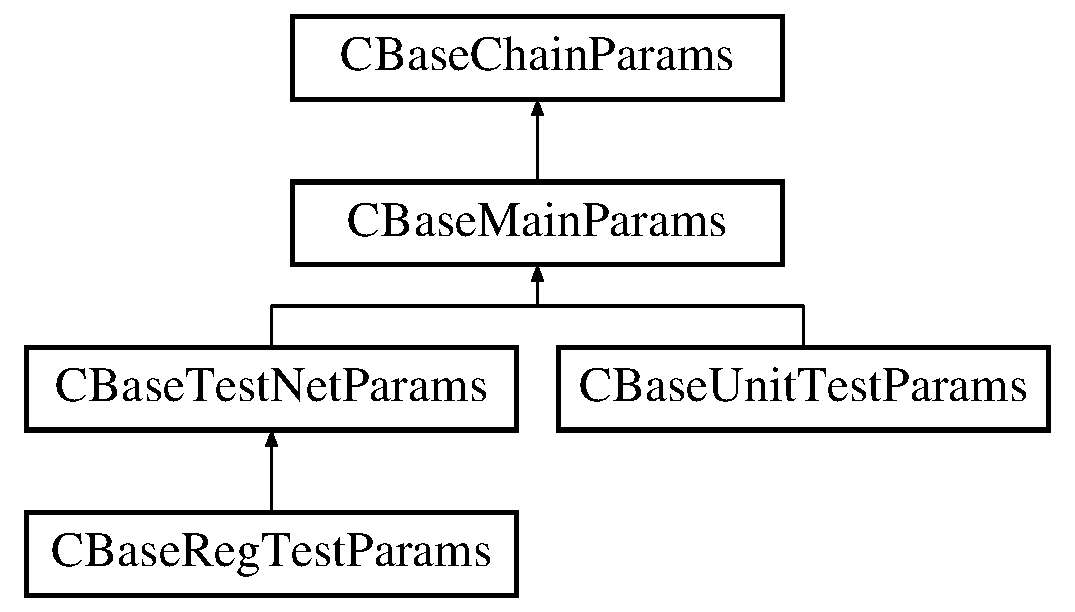
\includegraphics[height=4.000000cm]{class_c_base_chain_params}
\end{center}
\end{figure}
\subsection*{Public Types}
\begin{DoxyCompactItemize}
\item 
enum \hyperlink{class_c_base_chain_params_a19fb46b499c21801c0ff3c8607a0994e}{Network} \{ \hyperlink{class_c_base_chain_params_a19fb46b499c21801c0ff3c8607a0994ea17aedaa2a3181d12f0d32afc70a6c68c}{M\+A\+I\+N}, 
\hyperlink{class_c_base_chain_params_a19fb46b499c21801c0ff3c8607a0994ea0a9c4e42da932cdd126777f7f4dd0e22}{T\+E\+S\+T\+N\+E\+T}, 
\hyperlink{class_c_base_chain_params_a19fb46b499c21801c0ff3c8607a0994eace36282edb786b098dbdd48f98ddb793}{R\+E\+G\+T\+E\+S\+T}, 
\hyperlink{class_c_base_chain_params_a19fb46b499c21801c0ff3c8607a0994eaf4a96679adc48f01c489d1b4d740deb5}{M\+A\+X\+\_\+\+N\+E\+T\+W\+O\+R\+K\+\_\+\+T\+Y\+P\+E\+S}
 \}
\end{DoxyCompactItemize}
\subsection*{Public Member Functions}
\begin{DoxyCompactItemize}
\item 
const std\+::string \& \hyperlink{class_c_base_chain_params_af56a637b20c9f496108bffc3166ea53a}{Data\+Dir} () const 
\item 
int \hyperlink{class_c_base_chain_params_a06d2e58bdb42bb54932daf9a7a11182f}{R\+P\+C\+Port} () const 
\end{DoxyCompactItemize}
\subsection*{Protected Member Functions}
\begin{DoxyCompactItemize}
\item 
\hyperlink{class_c_base_chain_params_a4c0e84608b2fa636be3a3683653d9533}{C\+Base\+Chain\+Params} ()
\end{DoxyCompactItemize}
\subsection*{Protected Attributes}
\begin{DoxyCompactItemize}
\item 
int \hyperlink{class_c_base_chain_params_ae020d8f669175bcac3ab44f9c095c977}{n\+R\+P\+C\+Port}
\item 
std\+::string \hyperlink{class_c_base_chain_params_af5868778f8c6c676aabc9fb2366d2447}{str\+Data\+Dir}
\end{DoxyCompactItemize}


\subsection{Detailed Description}
\hyperlink{class_c_base_chain_params}{C\+Base\+Chain\+Params} defines the base parameters (shared between bitcoin-\/cli and bitcoind) of a given instance of the Bitcoin system. 

\subsection{Member Enumeration Documentation}
\hypertarget{class_c_base_chain_params_a19fb46b499c21801c0ff3c8607a0994e}{}\index{C\+Base\+Chain\+Params@{C\+Base\+Chain\+Params}!Network@{Network}}
\index{Network@{Network}!C\+Base\+Chain\+Params@{C\+Base\+Chain\+Params}}
\subsubsection[{Network}]{\setlength{\rightskip}{0pt plus 5cm}enum {\bf C\+Base\+Chain\+Params\+::\+Network}}\label{class_c_base_chain_params_a19fb46b499c21801c0ff3c8607a0994e}
\begin{Desc}
\item[Enumerator]\par
\begin{description}
\index{M\+A\+I\+N@{M\+A\+I\+N}!C\+Base\+Chain\+Params@{C\+Base\+Chain\+Params}}\index{C\+Base\+Chain\+Params@{C\+Base\+Chain\+Params}!M\+A\+I\+N@{M\+A\+I\+N}}\item[{\em 
\hypertarget{class_c_base_chain_params_a19fb46b499c21801c0ff3c8607a0994ea17aedaa2a3181d12f0d32afc70a6c68c}{}M\+A\+I\+N\label{class_c_base_chain_params_a19fb46b499c21801c0ff3c8607a0994ea17aedaa2a3181d12f0d32afc70a6c68c}
}]\index{T\+E\+S\+T\+N\+E\+T@{T\+E\+S\+T\+N\+E\+T}!C\+Base\+Chain\+Params@{C\+Base\+Chain\+Params}}\index{C\+Base\+Chain\+Params@{C\+Base\+Chain\+Params}!T\+E\+S\+T\+N\+E\+T@{T\+E\+S\+T\+N\+E\+T}}\item[{\em 
\hypertarget{class_c_base_chain_params_a19fb46b499c21801c0ff3c8607a0994ea0a9c4e42da932cdd126777f7f4dd0e22}{}T\+E\+S\+T\+N\+E\+T\label{class_c_base_chain_params_a19fb46b499c21801c0ff3c8607a0994ea0a9c4e42da932cdd126777f7f4dd0e22}
}]\index{R\+E\+G\+T\+E\+S\+T@{R\+E\+G\+T\+E\+S\+T}!C\+Base\+Chain\+Params@{C\+Base\+Chain\+Params}}\index{C\+Base\+Chain\+Params@{C\+Base\+Chain\+Params}!R\+E\+G\+T\+E\+S\+T@{R\+E\+G\+T\+E\+S\+T}}\item[{\em 
\hypertarget{class_c_base_chain_params_a19fb46b499c21801c0ff3c8607a0994eace36282edb786b098dbdd48f98ddb793}{}R\+E\+G\+T\+E\+S\+T\label{class_c_base_chain_params_a19fb46b499c21801c0ff3c8607a0994eace36282edb786b098dbdd48f98ddb793}
}]\index{M\+A\+X\+\_\+\+N\+E\+T\+W\+O\+R\+K\+\_\+\+T\+Y\+P\+E\+S@{M\+A\+X\+\_\+\+N\+E\+T\+W\+O\+R\+K\+\_\+\+T\+Y\+P\+E\+S}!C\+Base\+Chain\+Params@{C\+Base\+Chain\+Params}}\index{C\+Base\+Chain\+Params@{C\+Base\+Chain\+Params}!M\+A\+X\+\_\+\+N\+E\+T\+W\+O\+R\+K\+\_\+\+T\+Y\+P\+E\+S@{M\+A\+X\+\_\+\+N\+E\+T\+W\+O\+R\+K\+\_\+\+T\+Y\+P\+E\+S}}\item[{\em 
\hypertarget{class_c_base_chain_params_a19fb46b499c21801c0ff3c8607a0994eaf4a96679adc48f01c489d1b4d740deb5}{}M\+A\+X\+\_\+\+N\+E\+T\+W\+O\+R\+K\+\_\+\+T\+Y\+P\+E\+S\label{class_c_base_chain_params_a19fb46b499c21801c0ff3c8607a0994eaf4a96679adc48f01c489d1b4d740deb5}
}]\end{description}
\end{Desc}


\subsection{Constructor \& Destructor Documentation}
\hypertarget{class_c_base_chain_params_a4c0e84608b2fa636be3a3683653d9533}{}\index{C\+Base\+Chain\+Params@{C\+Base\+Chain\+Params}!C\+Base\+Chain\+Params@{C\+Base\+Chain\+Params}}
\index{C\+Base\+Chain\+Params@{C\+Base\+Chain\+Params}!C\+Base\+Chain\+Params@{C\+Base\+Chain\+Params}}
\subsubsection[{C\+Base\+Chain\+Params}]{\setlength{\rightskip}{0pt plus 5cm}C\+Base\+Chain\+Params\+::\+C\+Base\+Chain\+Params (
\begin{DoxyParamCaption}
{}
\end{DoxyParamCaption}
)\hspace{0.3cm}{\ttfamily [inline]}, {\ttfamily [protected]}}\label{class_c_base_chain_params_a4c0e84608b2fa636be3a3683653d9533}


\subsection{Member Function Documentation}
\hypertarget{class_c_base_chain_params_af56a637b20c9f496108bffc3166ea53a}{}\index{C\+Base\+Chain\+Params@{C\+Base\+Chain\+Params}!Data\+Dir@{Data\+Dir}}
\index{Data\+Dir@{Data\+Dir}!C\+Base\+Chain\+Params@{C\+Base\+Chain\+Params}}
\subsubsection[{Data\+Dir}]{\setlength{\rightskip}{0pt plus 5cm}const std\+::string\& C\+Base\+Chain\+Params\+::\+Data\+Dir (
\begin{DoxyParamCaption}
{}
\end{DoxyParamCaption}
) const\hspace{0.3cm}{\ttfamily [inline]}}\label{class_c_base_chain_params_af56a637b20c9f496108bffc3166ea53a}
\hypertarget{class_c_base_chain_params_a06d2e58bdb42bb54932daf9a7a11182f}{}\index{C\+Base\+Chain\+Params@{C\+Base\+Chain\+Params}!R\+P\+C\+Port@{R\+P\+C\+Port}}
\index{R\+P\+C\+Port@{R\+P\+C\+Port}!C\+Base\+Chain\+Params@{C\+Base\+Chain\+Params}}
\subsubsection[{R\+P\+C\+Port}]{\setlength{\rightskip}{0pt plus 5cm}int C\+Base\+Chain\+Params\+::\+R\+P\+C\+Port (
\begin{DoxyParamCaption}
{}
\end{DoxyParamCaption}
) const\hspace{0.3cm}{\ttfamily [inline]}}\label{class_c_base_chain_params_a06d2e58bdb42bb54932daf9a7a11182f}


\subsection{Member Data Documentation}
\hypertarget{class_c_base_chain_params_ae020d8f669175bcac3ab44f9c095c977}{}\index{C\+Base\+Chain\+Params@{C\+Base\+Chain\+Params}!n\+R\+P\+C\+Port@{n\+R\+P\+C\+Port}}
\index{n\+R\+P\+C\+Port@{n\+R\+P\+C\+Port}!C\+Base\+Chain\+Params@{C\+Base\+Chain\+Params}}
\subsubsection[{n\+R\+P\+C\+Port}]{\setlength{\rightskip}{0pt plus 5cm}int C\+Base\+Chain\+Params\+::n\+R\+P\+C\+Port\hspace{0.3cm}{\ttfamily [protected]}}\label{class_c_base_chain_params_ae020d8f669175bcac3ab44f9c095c977}
\hypertarget{class_c_base_chain_params_af5868778f8c6c676aabc9fb2366d2447}{}\index{C\+Base\+Chain\+Params@{C\+Base\+Chain\+Params}!str\+Data\+Dir@{str\+Data\+Dir}}
\index{str\+Data\+Dir@{str\+Data\+Dir}!C\+Base\+Chain\+Params@{C\+Base\+Chain\+Params}}
\subsubsection[{str\+Data\+Dir}]{\setlength{\rightskip}{0pt plus 5cm}std\+::string C\+Base\+Chain\+Params\+::str\+Data\+Dir\hspace{0.3cm}{\ttfamily [protected]}}\label{class_c_base_chain_params_af5868778f8c6c676aabc9fb2366d2447}


The documentation for this class was generated from the following file\+:\begin{DoxyCompactItemize}
\item 
C\+:/\+Users/\+Joe/\+Documents/\+School/\+C\+S\+C17\+A/bitcoin/src/\hyperlink{chainparamsbase_8h}{chainparamsbase.\+h}\end{DoxyCompactItemize}

\hypertarget{class_c_base_main_params}{}\section{C\+Base\+Main\+Params Class Reference}
\label{class_c_base_main_params}\index{C\+Base\+Main\+Params@{C\+Base\+Main\+Params}}
Inheritance diagram for C\+Base\+Main\+Params\+:\begin{figure}[H]
\begin{center}
\leavevmode
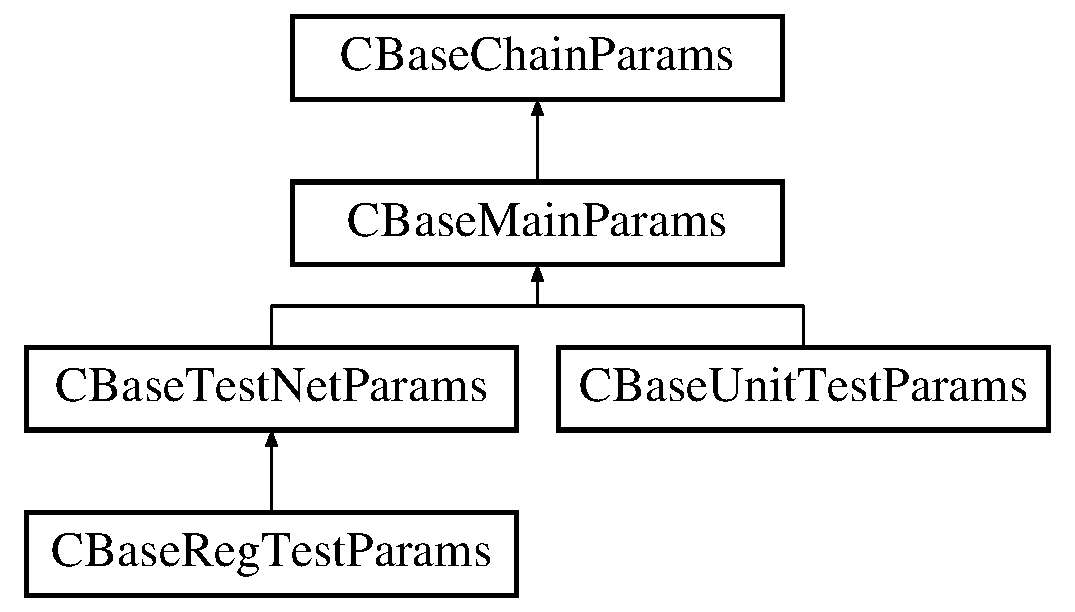
\includegraphics[height=4.000000cm]{class_c_base_main_params}
\end{center}
\end{figure}
\subsection*{Public Member Functions}
\begin{DoxyCompactItemize}
\item 
\hyperlink{class_c_base_main_params_a547dabd3f634a23b8cd5478242e101e1}{C\+Base\+Main\+Params} ()
\end{DoxyCompactItemize}
\subsection*{Additional Inherited Members}


\subsection{Detailed Description}
Main network 

\subsection{Constructor \& Destructor Documentation}
\hypertarget{class_c_base_main_params_a547dabd3f634a23b8cd5478242e101e1}{}\index{C\+Base\+Main\+Params@{C\+Base\+Main\+Params}!C\+Base\+Main\+Params@{C\+Base\+Main\+Params}}
\index{C\+Base\+Main\+Params@{C\+Base\+Main\+Params}!C\+Base\+Main\+Params@{C\+Base\+Main\+Params}}
\subsubsection[{C\+Base\+Main\+Params}]{\setlength{\rightskip}{0pt plus 5cm}C\+Base\+Main\+Params\+::\+C\+Base\+Main\+Params (
\begin{DoxyParamCaption}
{}
\end{DoxyParamCaption}
)\hspace{0.3cm}{\ttfamily [inline]}}\label{class_c_base_main_params_a547dabd3f634a23b8cd5478242e101e1}


The documentation for this class was generated from the following file\+:\begin{DoxyCompactItemize}
\item 
C\+:/\+Users/\+Joe/\+Documents/\+School/\+C\+S\+C17\+A/bitcoin/src/\hyperlink{chainparamsbase_8cpp}{chainparamsbase.\+cpp}\end{DoxyCompactItemize}

\hypertarget{class_c_base_reg_test_params}{}\section{C\+Base\+Reg\+Test\+Params Class Reference}
\label{class_c_base_reg_test_params}\index{C\+Base\+Reg\+Test\+Params@{C\+Base\+Reg\+Test\+Params}}
Inheritance diagram for C\+Base\+Reg\+Test\+Params\+:\begin{figure}[H]
\begin{center}
\leavevmode
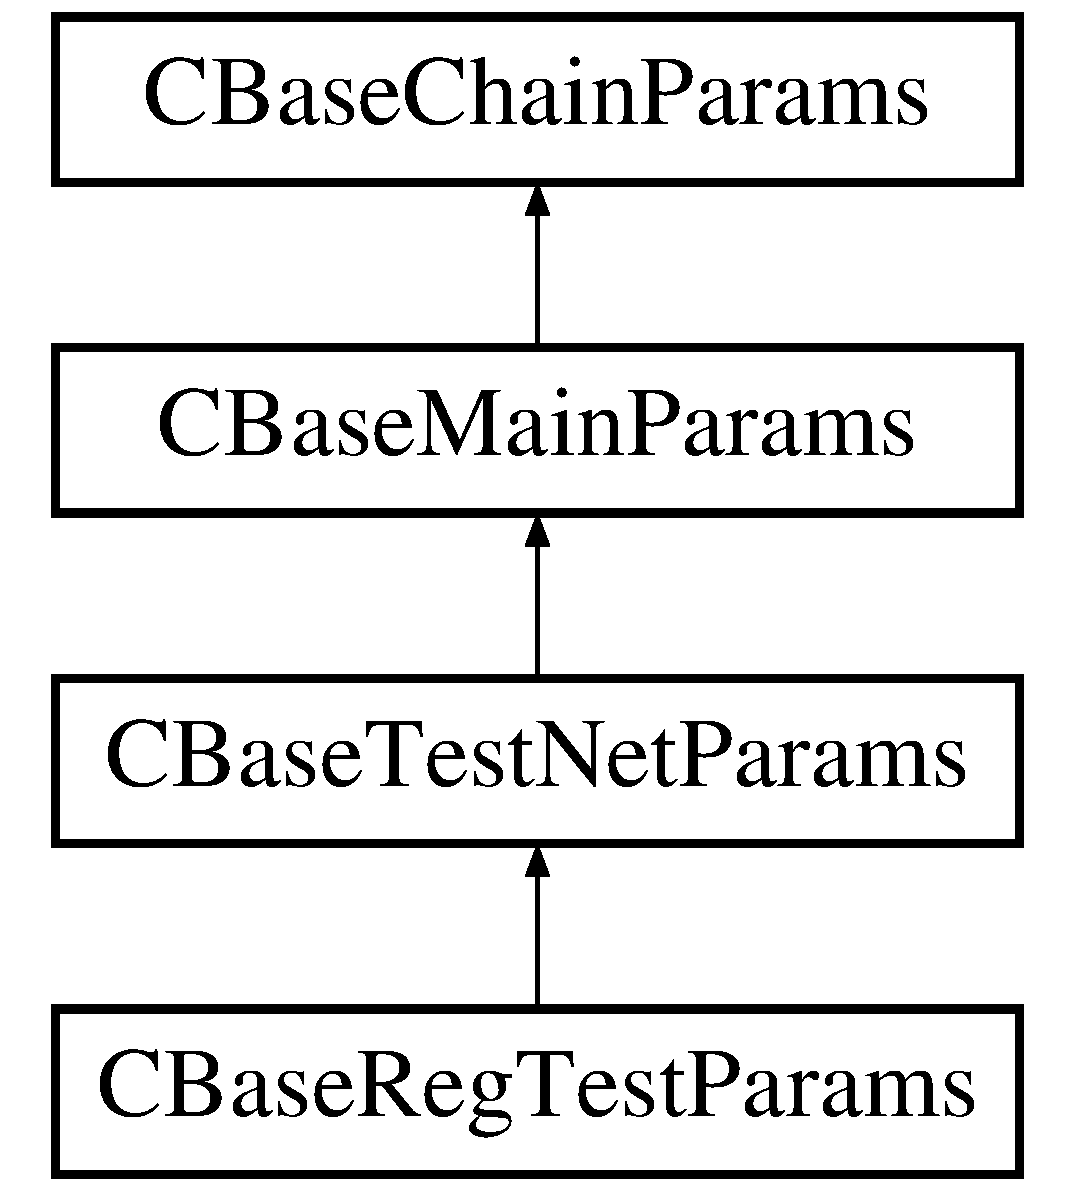
\includegraphics[height=4.000000cm]{class_c_base_reg_test_params}
\end{center}
\end{figure}
\subsection*{Public Member Functions}
\begin{DoxyCompactItemize}
\item 
\hyperlink{class_c_base_reg_test_params_af32910af3003663d0ea5ee6406ce3b50}{C\+Base\+Reg\+Test\+Params} ()
\end{DoxyCompactItemize}
\subsection*{Additional Inherited Members}


\subsection{Constructor \& Destructor Documentation}
\hypertarget{class_c_base_reg_test_params_af32910af3003663d0ea5ee6406ce3b50}{}\index{C\+Base\+Reg\+Test\+Params@{C\+Base\+Reg\+Test\+Params}!C\+Base\+Reg\+Test\+Params@{C\+Base\+Reg\+Test\+Params}}
\index{C\+Base\+Reg\+Test\+Params@{C\+Base\+Reg\+Test\+Params}!C\+Base\+Reg\+Test\+Params@{C\+Base\+Reg\+Test\+Params}}
\subsubsection[{C\+Base\+Reg\+Test\+Params}]{\setlength{\rightskip}{0pt plus 5cm}C\+Base\+Reg\+Test\+Params\+::\+C\+Base\+Reg\+Test\+Params (
\begin{DoxyParamCaption}
{}
\end{DoxyParamCaption}
)\hspace{0.3cm}{\ttfamily [inline]}}\label{class_c_base_reg_test_params_af32910af3003663d0ea5ee6406ce3b50}


The documentation for this class was generated from the following file\+:\begin{DoxyCompactItemize}
\item 
C\+:/\+Users/\+Joe/\+Documents/\+School/\+C\+S\+C17\+A/bitcoin/src/\hyperlink{chainparamsbase_8cpp}{chainparamsbase.\+cpp}\end{DoxyCompactItemize}

\hypertarget{class_c_base_test_net_params}{}\section{C\+Base\+Test\+Net\+Params Class Reference}
\label{class_c_base_test_net_params}\index{C\+Base\+Test\+Net\+Params@{C\+Base\+Test\+Net\+Params}}
Inheritance diagram for C\+Base\+Test\+Net\+Params\+:\begin{figure}[H]
\begin{center}
\leavevmode
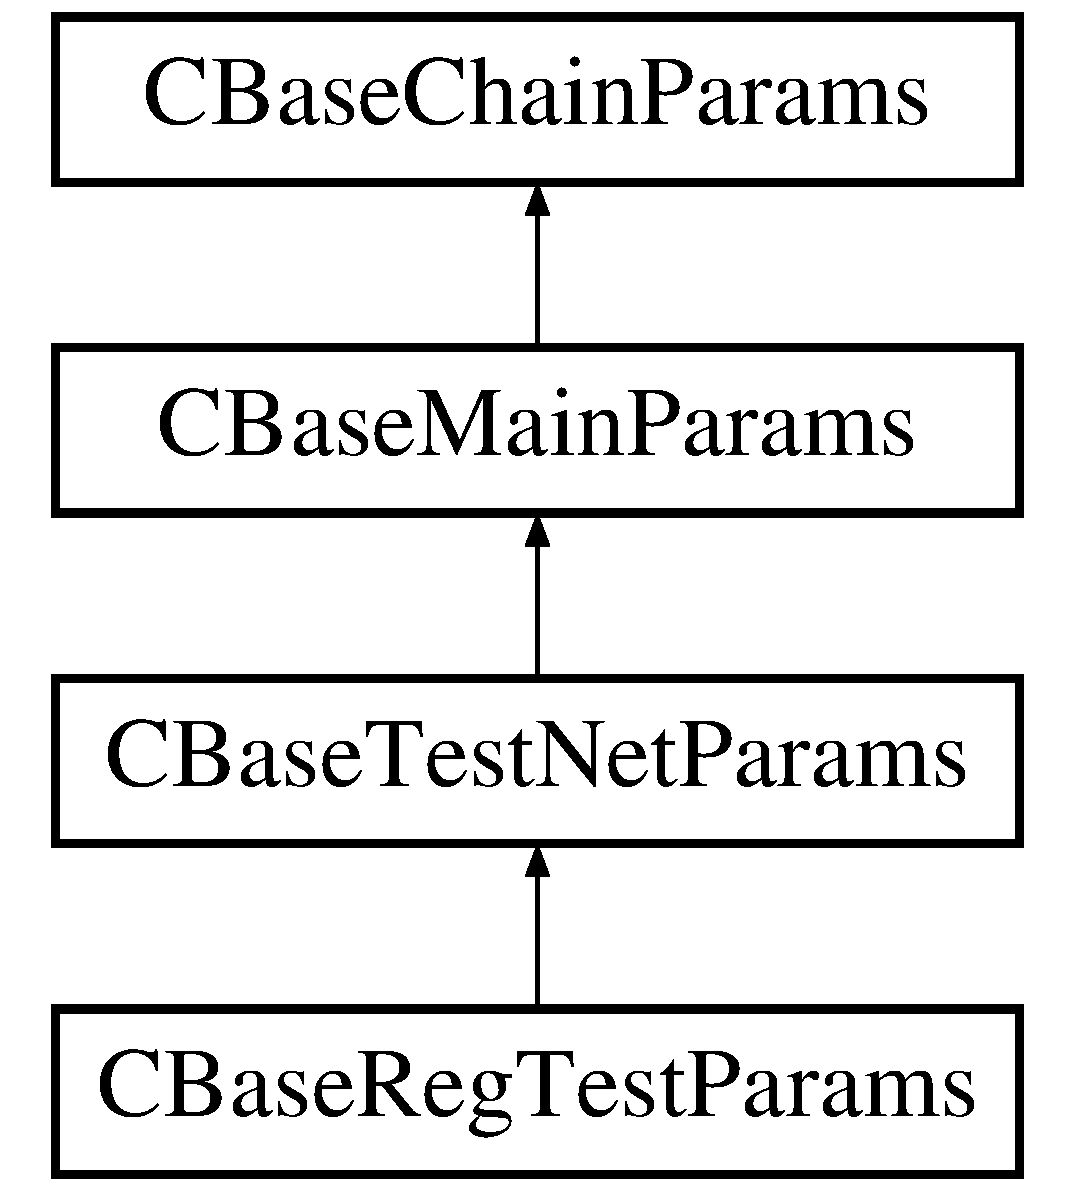
\includegraphics[height=4.000000cm]{class_c_base_test_net_params}
\end{center}
\end{figure}
\subsection*{Public Member Functions}
\begin{DoxyCompactItemize}
\item 
\hyperlink{class_c_base_test_net_params_ae95167a7de928f49ce78840c1569ce16}{C\+Base\+Test\+Net\+Params} ()
\end{DoxyCompactItemize}
\subsection*{Additional Inherited Members}


\subsection{Detailed Description}
Testnet (v3) 

\subsection{Constructor \& Destructor Documentation}
\hypertarget{class_c_base_test_net_params_ae95167a7de928f49ce78840c1569ce16}{}\index{C\+Base\+Test\+Net\+Params@{C\+Base\+Test\+Net\+Params}!C\+Base\+Test\+Net\+Params@{C\+Base\+Test\+Net\+Params}}
\index{C\+Base\+Test\+Net\+Params@{C\+Base\+Test\+Net\+Params}!C\+Base\+Test\+Net\+Params@{C\+Base\+Test\+Net\+Params}}
\subsubsection[{C\+Base\+Test\+Net\+Params}]{\setlength{\rightskip}{0pt plus 5cm}C\+Base\+Test\+Net\+Params\+::\+C\+Base\+Test\+Net\+Params (
\begin{DoxyParamCaption}
{}
\end{DoxyParamCaption}
)\hspace{0.3cm}{\ttfamily [inline]}}\label{class_c_base_test_net_params_ae95167a7de928f49ce78840c1569ce16}


The documentation for this class was generated from the following file\+:\begin{DoxyCompactItemize}
\item 
C\+:/\+Users/\+Joe/\+Documents/\+School/\+C\+S\+C17\+A/bitcoin/src/\hyperlink{chainparamsbase_8cpp}{chainparamsbase.\+cpp}\end{DoxyCompactItemize}

\hypertarget{class_c_base_unit_test_params}{}\section{C\+Base\+Unit\+Test\+Params Class Reference}
\label{class_c_base_unit_test_params}\index{C\+Base\+Unit\+Test\+Params@{C\+Base\+Unit\+Test\+Params}}
Inheritance diagram for C\+Base\+Unit\+Test\+Params\+:\begin{figure}[H]
\begin{center}
\leavevmode
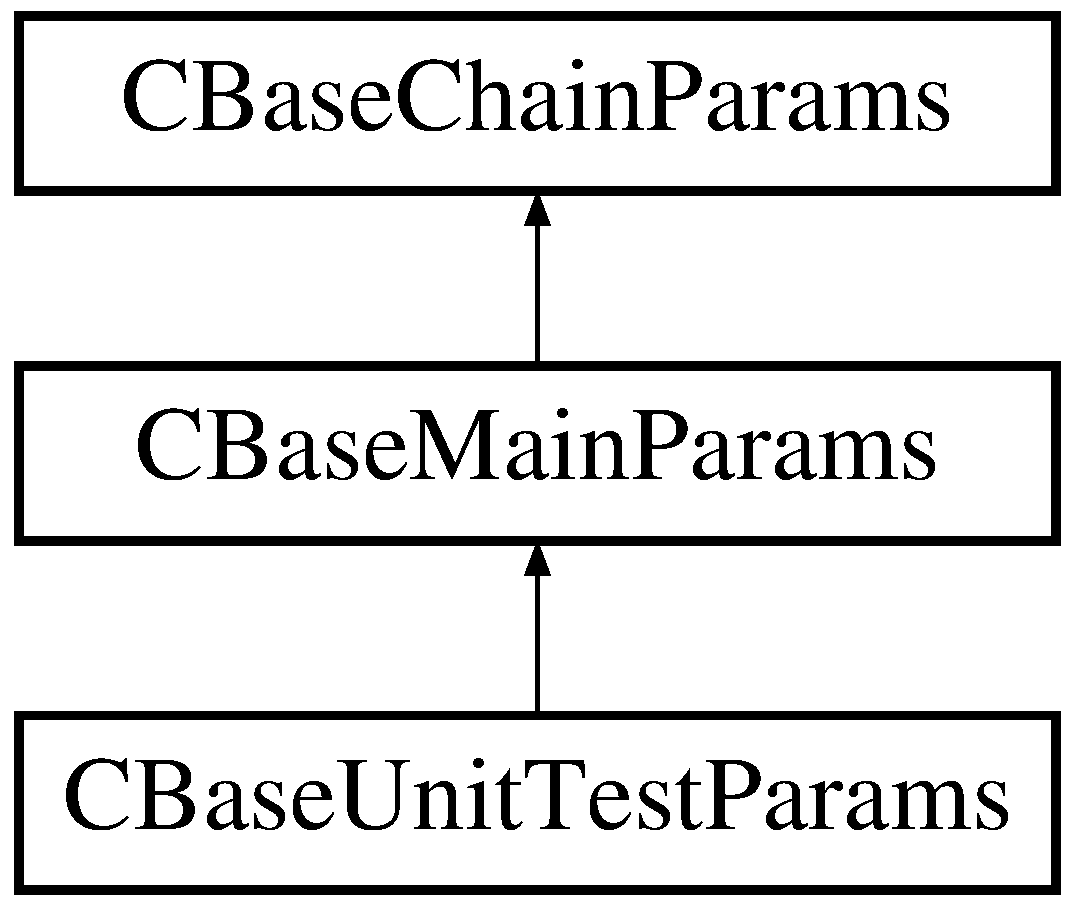
\includegraphics[height=3.000000cm]{class_c_base_unit_test_params}
\end{center}
\end{figure}
\subsection*{Public Member Functions}
\begin{DoxyCompactItemize}
\item 
\hyperlink{class_c_base_unit_test_params_a5adade9edcf1ebefc89ff198d0d52ff5}{C\+Base\+Unit\+Test\+Params} ()
\end{DoxyCompactItemize}
\subsection*{Additional Inherited Members}


\subsection{Constructor \& Destructor Documentation}
\hypertarget{class_c_base_unit_test_params_a5adade9edcf1ebefc89ff198d0d52ff5}{}\index{C\+Base\+Unit\+Test\+Params@{C\+Base\+Unit\+Test\+Params}!C\+Base\+Unit\+Test\+Params@{C\+Base\+Unit\+Test\+Params}}
\index{C\+Base\+Unit\+Test\+Params@{C\+Base\+Unit\+Test\+Params}!C\+Base\+Unit\+Test\+Params@{C\+Base\+Unit\+Test\+Params}}
\subsubsection[{C\+Base\+Unit\+Test\+Params}]{\setlength{\rightskip}{0pt plus 5cm}C\+Base\+Unit\+Test\+Params\+::\+C\+Base\+Unit\+Test\+Params (
\begin{DoxyParamCaption}
{}
\end{DoxyParamCaption}
)\hspace{0.3cm}{\ttfamily [inline]}}\label{class_c_base_unit_test_params_a5adade9edcf1ebefc89ff198d0d52ff5}


The documentation for this class was generated from the following file\+:\begin{DoxyCompactItemize}
\item 
C\+:/\+Users/\+Joe/\+Documents/\+School/\+C\+S\+C17\+A/bitcoin/src/\hyperlink{chainparamsbase_8cpp}{chainparamsbase.\+cpp}\end{DoxyCompactItemize}

\hypertarget{class_c_basic_key_store}{}\section{C\+Basic\+Key\+Store Class Reference}
\label{class_c_basic_key_store}\index{C\+Basic\+Key\+Store@{C\+Basic\+Key\+Store}}


{\ttfamily \#include $<$keystore.\+h$>$}

Inheritance diagram for C\+Basic\+Key\+Store\+:\begin{figure}[H]
\begin{center}
\leavevmode
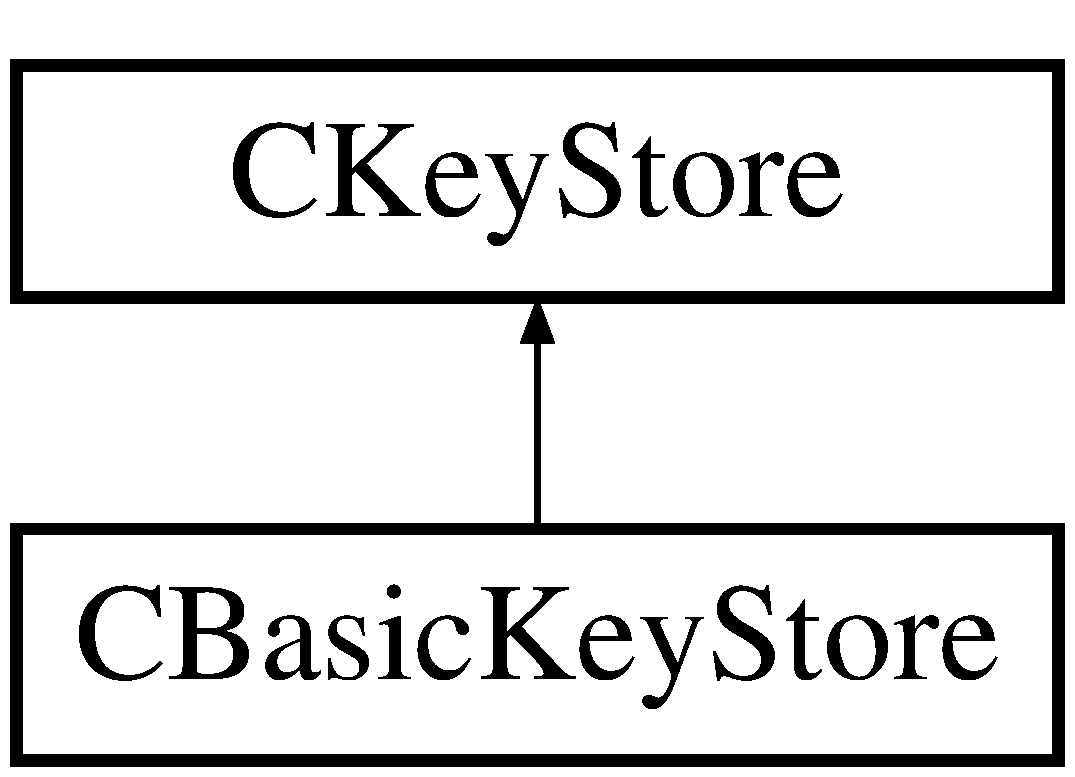
\includegraphics[height=2.000000cm]{class_c_basic_key_store}
\end{center}
\end{figure}
\subsection*{Public Member Functions}
\begin{DoxyCompactItemize}
\item 
bool \hyperlink{class_c_basic_key_store_acc2e33f319de88e88f86b0dc79bdcb65}{Add\+Key\+Pub\+Key} (const \hyperlink{class_c_key}{C\+Key} \&key, const \hyperlink{class_c_pub_key}{C\+Pub\+Key} \&pubkey)
\begin{DoxyCompactList}\small\item\em Add a key to the store. \end{DoxyCompactList}\item 
bool \hyperlink{class_c_basic_key_store_a29a60832d549913b1fa8be77b95205a5}{Have\+Key} (const \hyperlink{class_c_key_i_d}{C\+Key\+I\+D} \&address) const 
\begin{DoxyCompactList}\small\item\em Check whether a key corresponding to a given address is present in the store. \end{DoxyCompactList}\item 
void \hyperlink{class_c_basic_key_store_a60f46db5eec334d41e5ad6e342ae2957}{Get\+Keys} (std\+::set$<$ \hyperlink{class_c_key_i_d}{C\+Key\+I\+D} $>$ \&set\+Address) const 
\item 
bool \hyperlink{class_c_basic_key_store_a3cf9b5d002a8af75e7f90ae7654a234f}{Get\+Key} (const \hyperlink{class_c_key_i_d}{C\+Key\+I\+D} \&address, \hyperlink{class_c_key}{C\+Key} \&key\+Out) const 
\item 
virtual bool \hyperlink{class_c_basic_key_store_a56249ce3540398999cd397eeb662e836}{Add\+C\+Script} (const C\+Script \&redeem\+Script)
\begin{DoxyCompactList}\small\item\em Support for B\+I\+P 0013 \+: see \href{https://github.com/bitcoin/bips/blob/master/bip-0013.mediawiki}{\tt https\+://github.\+com/bitcoin/bips/blob/master/bip-\/0013.\+mediawiki}. \end{DoxyCompactList}\item 
virtual bool \hyperlink{class_c_basic_key_store_a2e21398364927d920b15d3e10171cd97}{Have\+C\+Script} (const C\+Script\+I\+D \&hash) const 
\item 
virtual bool \hyperlink{class_c_basic_key_store_aa7b10f974cfdc078f55fdb6adf8774a5}{Get\+C\+Script} (const C\+Script\+I\+D \&hash, C\+Script \&redeem\+Script\+Out) const 
\item 
virtual bool \hyperlink{class_c_basic_key_store_a2417d0ae4e654c88cf47a1ba5f71b5a3}{Add\+Watch\+Only} (const C\+Script \&dest)
\begin{DoxyCompactList}\small\item\em Support for Watch-\/only addresses. \end{DoxyCompactList}\item 
virtual bool \hyperlink{class_c_basic_key_store_a20c0eccf943d6d16e24c6e2fb63fb527}{Remove\+Watch\+Only} (const C\+Script \&dest)
\item 
virtual bool \hyperlink{class_c_basic_key_store_a51d4c7e95cb782d749939d01612926f7}{Have\+Watch\+Only} (const C\+Script \&dest) const 
\item 
virtual bool \hyperlink{class_c_basic_key_store_a3d89af8d9e9e0bb4eb90f331a638ff6d}{Have\+Watch\+Only} () const 
\end{DoxyCompactItemize}
\subsection*{Protected Attributes}
\begin{DoxyCompactItemize}
\item 
\hyperlink{keystore_8h_a4dc9f57afc8615aef701e40cf20d024f}{Key\+Map} \hyperlink{class_c_basic_key_store_ac520003e5c3d863bf71fde247c6e0672}{map\+Keys}
\item 
\hyperlink{keystore_8h_afb22a3e7e10e8048d2fb3fb72fe38345}{Script\+Map} \hyperlink{class_c_basic_key_store_a8e9fa81382129c1535a0ee7b0d9c8f3b}{map\+Scripts}
\item 
\hyperlink{keystore_8h_a501c3a7b9932bbc7168dc7b3fc5d149e}{Watch\+Only\+Set} \hyperlink{class_c_basic_key_store_ac3391cb491e315403ad9af6afd1313da}{set\+Watch\+Only}
\end{DoxyCompactItemize}


\subsection{Detailed Description}
Basic key store, that keeps keys in an address-\/$>$secret map 

\subsection{Member Function Documentation}
\hypertarget{class_c_basic_key_store_a56249ce3540398999cd397eeb662e836}{}\index{C\+Basic\+Key\+Store@{C\+Basic\+Key\+Store}!Add\+C\+Script@{Add\+C\+Script}}
\index{Add\+C\+Script@{Add\+C\+Script}!C\+Basic\+Key\+Store@{C\+Basic\+Key\+Store}}
\subsubsection[{Add\+C\+Script}]{\setlength{\rightskip}{0pt plus 5cm}bool C\+Basic\+Key\+Store\+::\+Add\+C\+Script (
\begin{DoxyParamCaption}
\item[{const C\+Script \&}]{redeem\+Script}
\end{DoxyParamCaption}
)\hspace{0.3cm}{\ttfamily [virtual]}}\label{class_c_basic_key_store_a56249ce3540398999cd397eeb662e836}


Support for B\+I\+P 0013 \+: see \href{https://github.com/bitcoin/bips/blob/master/bip-0013.mediawiki}{\tt https\+://github.\+com/bitcoin/bips/blob/master/bip-\/0013.\+mediawiki}. 



Implements \hyperlink{class_c_key_store_a2fb2e02e8cdc364607efd5ebb14b8064}{C\+Key\+Store}.

\hypertarget{class_c_basic_key_store_acc2e33f319de88e88f86b0dc79bdcb65}{}\index{C\+Basic\+Key\+Store@{C\+Basic\+Key\+Store}!Add\+Key\+Pub\+Key@{Add\+Key\+Pub\+Key}}
\index{Add\+Key\+Pub\+Key@{Add\+Key\+Pub\+Key}!C\+Basic\+Key\+Store@{C\+Basic\+Key\+Store}}
\subsubsection[{Add\+Key\+Pub\+Key}]{\setlength{\rightskip}{0pt plus 5cm}bool C\+Basic\+Key\+Store\+::\+Add\+Key\+Pub\+Key (
\begin{DoxyParamCaption}
\item[{const {\bf C\+Key} \&}]{key, }
\item[{const {\bf C\+Pub\+Key} \&}]{pubkey}
\end{DoxyParamCaption}
)\hspace{0.3cm}{\ttfamily [virtual]}}\label{class_c_basic_key_store_acc2e33f319de88e88f86b0dc79bdcb65}


Add a key to the store. 



Implements \hyperlink{class_c_key_store_a1956e4f5860ded321d6f697047d8236a}{C\+Key\+Store}.

\hypertarget{class_c_basic_key_store_a2417d0ae4e654c88cf47a1ba5f71b5a3}{}\index{C\+Basic\+Key\+Store@{C\+Basic\+Key\+Store}!Add\+Watch\+Only@{Add\+Watch\+Only}}
\index{Add\+Watch\+Only@{Add\+Watch\+Only}!C\+Basic\+Key\+Store@{C\+Basic\+Key\+Store}}
\subsubsection[{Add\+Watch\+Only}]{\setlength{\rightskip}{0pt plus 5cm}bool C\+Basic\+Key\+Store\+::\+Add\+Watch\+Only (
\begin{DoxyParamCaption}
\item[{const C\+Script \&}]{dest}
\end{DoxyParamCaption}
)\hspace{0.3cm}{\ttfamily [virtual]}}\label{class_c_basic_key_store_a2417d0ae4e654c88cf47a1ba5f71b5a3}


Support for Watch-\/only addresses. 



Implements \hyperlink{class_c_key_store_a12cd4eaa01bd4f4231c0bf68425a44af}{C\+Key\+Store}.

\hypertarget{class_c_basic_key_store_aa7b10f974cfdc078f55fdb6adf8774a5}{}\index{C\+Basic\+Key\+Store@{C\+Basic\+Key\+Store}!Get\+C\+Script@{Get\+C\+Script}}
\index{Get\+C\+Script@{Get\+C\+Script}!C\+Basic\+Key\+Store@{C\+Basic\+Key\+Store}}
\subsubsection[{Get\+C\+Script}]{\setlength{\rightskip}{0pt plus 5cm}bool C\+Basic\+Key\+Store\+::\+Get\+C\+Script (
\begin{DoxyParamCaption}
\item[{const C\+Script\+I\+D \&}]{hash, }
\item[{C\+Script \&}]{redeem\+Script\+Out}
\end{DoxyParamCaption}
) const\hspace{0.3cm}{\ttfamily [virtual]}}\label{class_c_basic_key_store_aa7b10f974cfdc078f55fdb6adf8774a5}


Implements \hyperlink{class_c_key_store_ae6bf4dbeb0705e199250e48aa5d34264}{C\+Key\+Store}.

\hypertarget{class_c_basic_key_store_a3cf9b5d002a8af75e7f90ae7654a234f}{}\index{C\+Basic\+Key\+Store@{C\+Basic\+Key\+Store}!Get\+Key@{Get\+Key}}
\index{Get\+Key@{Get\+Key}!C\+Basic\+Key\+Store@{C\+Basic\+Key\+Store}}
\subsubsection[{Get\+Key}]{\setlength{\rightskip}{0pt plus 5cm}bool C\+Basic\+Key\+Store\+::\+Get\+Key (
\begin{DoxyParamCaption}
\item[{const {\bf C\+Key\+I\+D} \&}]{address, }
\item[{{\bf C\+Key} \&}]{key\+Out}
\end{DoxyParamCaption}
) const\hspace{0.3cm}{\ttfamily [inline]}, {\ttfamily [virtual]}}\label{class_c_basic_key_store_a3cf9b5d002a8af75e7f90ae7654a234f}


Implements \hyperlink{class_c_key_store_a2dffca468fef2e5da2e42a7c983d968a}{C\+Key\+Store}.

\hypertarget{class_c_basic_key_store_a60f46db5eec334d41e5ad6e342ae2957}{}\index{C\+Basic\+Key\+Store@{C\+Basic\+Key\+Store}!Get\+Keys@{Get\+Keys}}
\index{Get\+Keys@{Get\+Keys}!C\+Basic\+Key\+Store@{C\+Basic\+Key\+Store}}
\subsubsection[{Get\+Keys}]{\setlength{\rightskip}{0pt plus 5cm}void C\+Basic\+Key\+Store\+::\+Get\+Keys (
\begin{DoxyParamCaption}
\item[{std\+::set$<$ {\bf C\+Key\+I\+D} $>$ \&}]{set\+Address}
\end{DoxyParamCaption}
) const\hspace{0.3cm}{\ttfamily [inline]}, {\ttfamily [virtual]}}\label{class_c_basic_key_store_a60f46db5eec334d41e5ad6e342ae2957}


Implements \hyperlink{class_c_key_store_aca5044014720308f191113e7ba297d13}{C\+Key\+Store}.

\hypertarget{class_c_basic_key_store_a2e21398364927d920b15d3e10171cd97}{}\index{C\+Basic\+Key\+Store@{C\+Basic\+Key\+Store}!Have\+C\+Script@{Have\+C\+Script}}
\index{Have\+C\+Script@{Have\+C\+Script}!C\+Basic\+Key\+Store@{C\+Basic\+Key\+Store}}
\subsubsection[{Have\+C\+Script}]{\setlength{\rightskip}{0pt plus 5cm}bool C\+Basic\+Key\+Store\+::\+Have\+C\+Script (
\begin{DoxyParamCaption}
\item[{const C\+Script\+I\+D \&}]{hash}
\end{DoxyParamCaption}
) const\hspace{0.3cm}{\ttfamily [virtual]}}\label{class_c_basic_key_store_a2e21398364927d920b15d3e10171cd97}


Implements \hyperlink{class_c_key_store_a51c9fc86b2c3fece10d86146231fa58d}{C\+Key\+Store}.

\hypertarget{class_c_basic_key_store_a29a60832d549913b1fa8be77b95205a5}{}\index{C\+Basic\+Key\+Store@{C\+Basic\+Key\+Store}!Have\+Key@{Have\+Key}}
\index{Have\+Key@{Have\+Key}!C\+Basic\+Key\+Store@{C\+Basic\+Key\+Store}}
\subsubsection[{Have\+Key}]{\setlength{\rightskip}{0pt plus 5cm}bool C\+Basic\+Key\+Store\+::\+Have\+Key (
\begin{DoxyParamCaption}
\item[{const {\bf C\+Key\+I\+D} \&}]{address}
\end{DoxyParamCaption}
) const\hspace{0.3cm}{\ttfamily [inline]}, {\ttfamily [virtual]}}\label{class_c_basic_key_store_a29a60832d549913b1fa8be77b95205a5}


Check whether a key corresponding to a given address is present in the store. 



Implements \hyperlink{class_c_key_store_a9398451d4270fae27b29f686a9d43a65}{C\+Key\+Store}.

\hypertarget{class_c_basic_key_store_a51d4c7e95cb782d749939d01612926f7}{}\index{C\+Basic\+Key\+Store@{C\+Basic\+Key\+Store}!Have\+Watch\+Only@{Have\+Watch\+Only}}
\index{Have\+Watch\+Only@{Have\+Watch\+Only}!C\+Basic\+Key\+Store@{C\+Basic\+Key\+Store}}
\subsubsection[{Have\+Watch\+Only}]{\setlength{\rightskip}{0pt plus 5cm}bool C\+Basic\+Key\+Store\+::\+Have\+Watch\+Only (
\begin{DoxyParamCaption}
\item[{const C\+Script \&}]{dest}
\end{DoxyParamCaption}
) const\hspace{0.3cm}{\ttfamily [virtual]}}\label{class_c_basic_key_store_a51d4c7e95cb782d749939d01612926f7}


Implements \hyperlink{class_c_key_store_a15066cfd57feaffe0b9f4103c9311109}{C\+Key\+Store}.

\hypertarget{class_c_basic_key_store_a3d89af8d9e9e0bb4eb90f331a638ff6d}{}\index{C\+Basic\+Key\+Store@{C\+Basic\+Key\+Store}!Have\+Watch\+Only@{Have\+Watch\+Only}}
\index{Have\+Watch\+Only@{Have\+Watch\+Only}!C\+Basic\+Key\+Store@{C\+Basic\+Key\+Store}}
\subsubsection[{Have\+Watch\+Only}]{\setlength{\rightskip}{0pt plus 5cm}bool C\+Basic\+Key\+Store\+::\+Have\+Watch\+Only (
\begin{DoxyParamCaption}
{}
\end{DoxyParamCaption}
) const\hspace{0.3cm}{\ttfamily [virtual]}}\label{class_c_basic_key_store_a3d89af8d9e9e0bb4eb90f331a638ff6d}


Implements \hyperlink{class_c_key_store_a9169351f4acf62d299afb824174cbfa8}{C\+Key\+Store}.

\hypertarget{class_c_basic_key_store_a20c0eccf943d6d16e24c6e2fb63fb527}{}\index{C\+Basic\+Key\+Store@{C\+Basic\+Key\+Store}!Remove\+Watch\+Only@{Remove\+Watch\+Only}}
\index{Remove\+Watch\+Only@{Remove\+Watch\+Only}!C\+Basic\+Key\+Store@{C\+Basic\+Key\+Store}}
\subsubsection[{Remove\+Watch\+Only}]{\setlength{\rightskip}{0pt plus 5cm}bool C\+Basic\+Key\+Store\+::\+Remove\+Watch\+Only (
\begin{DoxyParamCaption}
\item[{const C\+Script \&}]{dest}
\end{DoxyParamCaption}
)\hspace{0.3cm}{\ttfamily [virtual]}}\label{class_c_basic_key_store_a20c0eccf943d6d16e24c6e2fb63fb527}


Implements \hyperlink{class_c_key_store_ad510747f28d129123a5200e4df8f7f61}{C\+Key\+Store}.



\subsection{Member Data Documentation}
\hypertarget{class_c_basic_key_store_ac520003e5c3d863bf71fde247c6e0672}{}\index{C\+Basic\+Key\+Store@{C\+Basic\+Key\+Store}!map\+Keys@{map\+Keys}}
\index{map\+Keys@{map\+Keys}!C\+Basic\+Key\+Store@{C\+Basic\+Key\+Store}}
\subsubsection[{map\+Keys}]{\setlength{\rightskip}{0pt plus 5cm}{\bf Key\+Map} C\+Basic\+Key\+Store\+::map\+Keys\hspace{0.3cm}{\ttfamily [protected]}}\label{class_c_basic_key_store_ac520003e5c3d863bf71fde247c6e0672}
\hypertarget{class_c_basic_key_store_a8e9fa81382129c1535a0ee7b0d9c8f3b}{}\index{C\+Basic\+Key\+Store@{C\+Basic\+Key\+Store}!map\+Scripts@{map\+Scripts}}
\index{map\+Scripts@{map\+Scripts}!C\+Basic\+Key\+Store@{C\+Basic\+Key\+Store}}
\subsubsection[{map\+Scripts}]{\setlength{\rightskip}{0pt plus 5cm}{\bf Script\+Map} C\+Basic\+Key\+Store\+::map\+Scripts\hspace{0.3cm}{\ttfamily [protected]}}\label{class_c_basic_key_store_a8e9fa81382129c1535a0ee7b0d9c8f3b}
\hypertarget{class_c_basic_key_store_ac3391cb491e315403ad9af6afd1313da}{}\index{C\+Basic\+Key\+Store@{C\+Basic\+Key\+Store}!set\+Watch\+Only@{set\+Watch\+Only}}
\index{set\+Watch\+Only@{set\+Watch\+Only}!C\+Basic\+Key\+Store@{C\+Basic\+Key\+Store}}
\subsubsection[{set\+Watch\+Only}]{\setlength{\rightskip}{0pt plus 5cm}{\bf Watch\+Only\+Set} C\+Basic\+Key\+Store\+::set\+Watch\+Only\hspace{0.3cm}{\ttfamily [protected]}}\label{class_c_basic_key_store_ac3391cb491e315403ad9af6afd1313da}


The documentation for this class was generated from the following files\+:\begin{DoxyCompactItemize}
\item 
C\+:/\+Users/\+Joe/\+Documents/\+School/\+C\+S\+C17\+A/bitcoin/src/\hyperlink{keystore_8h}{keystore.\+h}\item 
C\+:/\+Users/\+Joe/\+Documents/\+School/\+C\+S\+C17\+A/bitcoin/src/\hyperlink{keystore_8cpp}{keystore.\+cpp}\end{DoxyCompactItemize}

\hypertarget{class_c_bitcoin_address}{}\section{C\+Bitcoin\+Address Class Reference}
\label{class_c_bitcoin_address}\index{C\+Bitcoin\+Address@{C\+Bitcoin\+Address}}


{\ttfamily \#include $<$base58.\+h$>$}

Inheritance diagram for C\+Bitcoin\+Address\+:\begin{figure}[H]
\begin{center}
\leavevmode
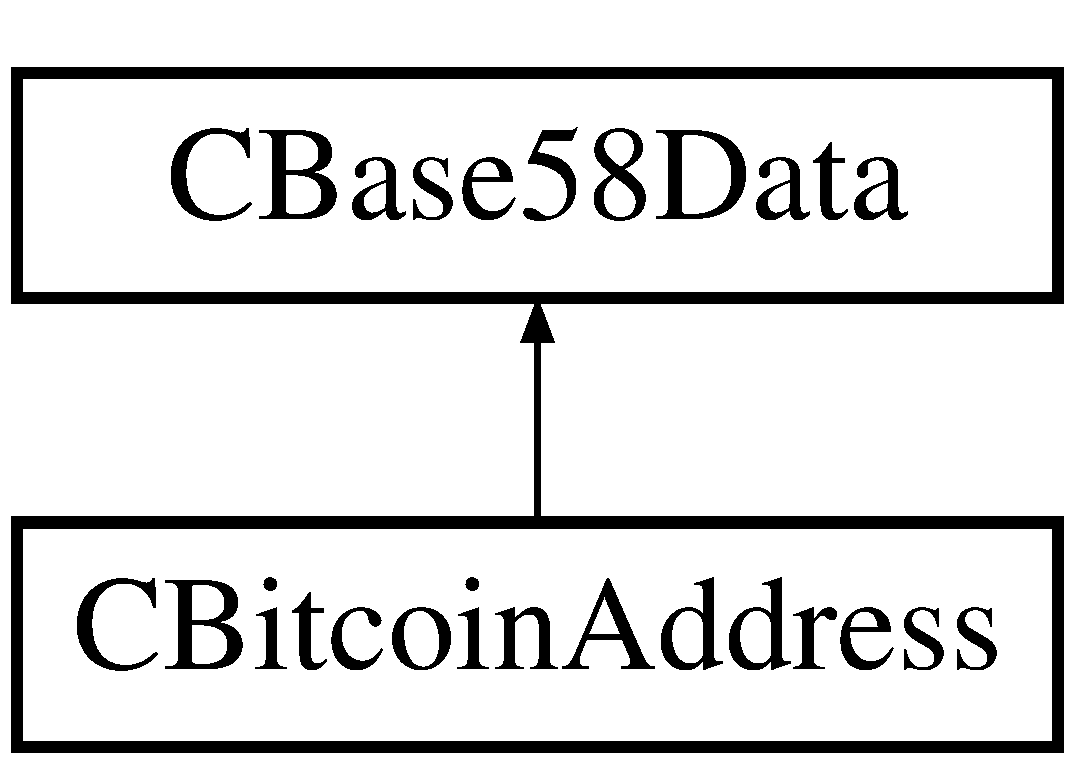
\includegraphics[height=2.000000cm]{class_c_bitcoin_address}
\end{center}
\end{figure}
\subsection*{Public Member Functions}
\begin{DoxyCompactItemize}
\item 
bool \hyperlink{class_c_bitcoin_address_abe1614f9ecd143ae69256d65c5edbcab}{Set} (const \hyperlink{class_c_key_i_d}{C\+Key\+I\+D} \&id)
\item 
bool \hyperlink{class_c_bitcoin_address_abb974c40304444b0f14a005ddb7dac03}{Set} (const C\+Script\+I\+D \&id)
\item 
bool \hyperlink{class_c_bitcoin_address_a819dfc6a4866832e2cd2e51c1a245d80}{Set} (const C\+Tx\+Destination \&dest)
\item 
bool \hyperlink{class_c_bitcoin_address_a3861fc29b82dba7d8bc8430ca461a20f}{Is\+Valid} () const 
\item 
bool \hyperlink{class_c_bitcoin_address_a9597ff4b2b7089364cde253a5fdd4f76}{Is\+Valid} (const \hyperlink{class_c_chain_params}{C\+Chain\+Params} \&params) const 
\item 
\hyperlink{class_c_bitcoin_address_ae1870e2f346a1f9968a201864fbdf010}{C\+Bitcoin\+Address} ()
\item 
\hyperlink{class_c_bitcoin_address_a4c9c03791561557b8a1926567456712e}{C\+Bitcoin\+Address} (const C\+Tx\+Destination \&dest)
\item 
\hyperlink{class_c_bitcoin_address_a23f7116fe3a89ab9a551f1d8c29469da}{C\+Bitcoin\+Address} (const std\+::string \&str\+Address)
\item 
\hyperlink{class_c_bitcoin_address_ac0fd8d46f815948d471a8896997a3211}{C\+Bitcoin\+Address} (const char $\ast$psz\+Address)
\item 
C\+Tx\+Destination \hyperlink{class_c_bitcoin_address_a46d632250c4b47727f8e9b2f8141fd69}{Get} () const 
\item 
bool \hyperlink{class_c_bitcoin_address_a077afe9cf27a69dd50be1339310764a2}{Get\+Key\+I\+D} (\hyperlink{class_c_key_i_d}{C\+Key\+I\+D} \&key\+I\+D) const 
\item 
bool \hyperlink{class_c_bitcoin_address_a2e605ae688b2064155a9978104a9099d}{Is\+Script} () const 
\end{DoxyCompactItemize}
\subsection*{Additional Inherited Members}


\subsection{Detailed Description}
base58-\/encoded Bitcoin addresses. Public-\/key-\/hash-\/addresses have version 0 (or 111 testnet). The data vector contains R\+I\+P\+E\+M\+D160(\+S\+H\+A256(pubkey)), where pubkey is the serialized public key. Script-\/hash-\/addresses have version 5 (or 196 testnet). The data vector contains R\+I\+P\+E\+M\+D160(\+S\+H\+A256(cscript)), where cscript is the serialized redemption script. 

\subsection{Constructor \& Destructor Documentation}
\hypertarget{class_c_bitcoin_address_ae1870e2f346a1f9968a201864fbdf010}{}\index{C\+Bitcoin\+Address@{C\+Bitcoin\+Address}!C\+Bitcoin\+Address@{C\+Bitcoin\+Address}}
\index{C\+Bitcoin\+Address@{C\+Bitcoin\+Address}!C\+Bitcoin\+Address@{C\+Bitcoin\+Address}}
\subsubsection[{C\+Bitcoin\+Address}]{\setlength{\rightskip}{0pt plus 5cm}C\+Bitcoin\+Address\+::\+C\+Bitcoin\+Address (
\begin{DoxyParamCaption}
{}
\end{DoxyParamCaption}
)\hspace{0.3cm}{\ttfamily [inline]}}\label{class_c_bitcoin_address_ae1870e2f346a1f9968a201864fbdf010}
\hypertarget{class_c_bitcoin_address_a4c9c03791561557b8a1926567456712e}{}\index{C\+Bitcoin\+Address@{C\+Bitcoin\+Address}!C\+Bitcoin\+Address@{C\+Bitcoin\+Address}}
\index{C\+Bitcoin\+Address@{C\+Bitcoin\+Address}!C\+Bitcoin\+Address@{C\+Bitcoin\+Address}}
\subsubsection[{C\+Bitcoin\+Address}]{\setlength{\rightskip}{0pt plus 5cm}C\+Bitcoin\+Address\+::\+C\+Bitcoin\+Address (
\begin{DoxyParamCaption}
\item[{const C\+Tx\+Destination \&}]{dest}
\end{DoxyParamCaption}
)\hspace{0.3cm}{\ttfamily [inline]}}\label{class_c_bitcoin_address_a4c9c03791561557b8a1926567456712e}
\hypertarget{class_c_bitcoin_address_a23f7116fe3a89ab9a551f1d8c29469da}{}\index{C\+Bitcoin\+Address@{C\+Bitcoin\+Address}!C\+Bitcoin\+Address@{C\+Bitcoin\+Address}}
\index{C\+Bitcoin\+Address@{C\+Bitcoin\+Address}!C\+Bitcoin\+Address@{C\+Bitcoin\+Address}}
\subsubsection[{C\+Bitcoin\+Address}]{\setlength{\rightskip}{0pt plus 5cm}C\+Bitcoin\+Address\+::\+C\+Bitcoin\+Address (
\begin{DoxyParamCaption}
\item[{const std\+::string \&}]{str\+Address}
\end{DoxyParamCaption}
)\hspace{0.3cm}{\ttfamily [inline]}}\label{class_c_bitcoin_address_a23f7116fe3a89ab9a551f1d8c29469da}
\hypertarget{class_c_bitcoin_address_ac0fd8d46f815948d471a8896997a3211}{}\index{C\+Bitcoin\+Address@{C\+Bitcoin\+Address}!C\+Bitcoin\+Address@{C\+Bitcoin\+Address}}
\index{C\+Bitcoin\+Address@{C\+Bitcoin\+Address}!C\+Bitcoin\+Address@{C\+Bitcoin\+Address}}
\subsubsection[{C\+Bitcoin\+Address}]{\setlength{\rightskip}{0pt plus 5cm}C\+Bitcoin\+Address\+::\+C\+Bitcoin\+Address (
\begin{DoxyParamCaption}
\item[{const char $\ast$}]{psz\+Address}
\end{DoxyParamCaption}
)\hspace{0.3cm}{\ttfamily [inline]}}\label{class_c_bitcoin_address_ac0fd8d46f815948d471a8896997a3211}


\subsection{Member Function Documentation}
\hypertarget{class_c_bitcoin_address_a46d632250c4b47727f8e9b2f8141fd69}{}\index{C\+Bitcoin\+Address@{C\+Bitcoin\+Address}!Get@{Get}}
\index{Get@{Get}!C\+Bitcoin\+Address@{C\+Bitcoin\+Address}}
\subsubsection[{Get}]{\setlength{\rightskip}{0pt plus 5cm}C\+Tx\+Destination C\+Bitcoin\+Address\+::\+Get (
\begin{DoxyParamCaption}
{}
\end{DoxyParamCaption}
) const}\label{class_c_bitcoin_address_a46d632250c4b47727f8e9b2f8141fd69}
\hypertarget{class_c_bitcoin_address_a077afe9cf27a69dd50be1339310764a2}{}\index{C\+Bitcoin\+Address@{C\+Bitcoin\+Address}!Get\+Key\+I\+D@{Get\+Key\+I\+D}}
\index{Get\+Key\+I\+D@{Get\+Key\+I\+D}!C\+Bitcoin\+Address@{C\+Bitcoin\+Address}}
\subsubsection[{Get\+Key\+I\+D}]{\setlength{\rightskip}{0pt plus 5cm}bool C\+Bitcoin\+Address\+::\+Get\+Key\+I\+D (
\begin{DoxyParamCaption}
\item[{{\bf C\+Key\+I\+D} \&}]{key\+I\+D}
\end{DoxyParamCaption}
) const}\label{class_c_bitcoin_address_a077afe9cf27a69dd50be1339310764a2}
\hypertarget{class_c_bitcoin_address_a2e605ae688b2064155a9978104a9099d}{}\index{C\+Bitcoin\+Address@{C\+Bitcoin\+Address}!Is\+Script@{Is\+Script}}
\index{Is\+Script@{Is\+Script}!C\+Bitcoin\+Address@{C\+Bitcoin\+Address}}
\subsubsection[{Is\+Script}]{\setlength{\rightskip}{0pt plus 5cm}bool C\+Bitcoin\+Address\+::\+Is\+Script (
\begin{DoxyParamCaption}
{}
\end{DoxyParamCaption}
) const}\label{class_c_bitcoin_address_a2e605ae688b2064155a9978104a9099d}
\hypertarget{class_c_bitcoin_address_a3861fc29b82dba7d8bc8430ca461a20f}{}\index{C\+Bitcoin\+Address@{C\+Bitcoin\+Address}!Is\+Valid@{Is\+Valid}}
\index{Is\+Valid@{Is\+Valid}!C\+Bitcoin\+Address@{C\+Bitcoin\+Address}}
\subsubsection[{Is\+Valid}]{\setlength{\rightskip}{0pt plus 5cm}bool C\+Bitcoin\+Address\+::\+Is\+Valid (
\begin{DoxyParamCaption}
{}
\end{DoxyParamCaption}
) const}\label{class_c_bitcoin_address_a3861fc29b82dba7d8bc8430ca461a20f}
\hypertarget{class_c_bitcoin_address_a9597ff4b2b7089364cde253a5fdd4f76}{}\index{C\+Bitcoin\+Address@{C\+Bitcoin\+Address}!Is\+Valid@{Is\+Valid}}
\index{Is\+Valid@{Is\+Valid}!C\+Bitcoin\+Address@{C\+Bitcoin\+Address}}
\subsubsection[{Is\+Valid}]{\setlength{\rightskip}{0pt plus 5cm}bool C\+Bitcoin\+Address\+::\+Is\+Valid (
\begin{DoxyParamCaption}
\item[{const {\bf C\+Chain\+Params} \&}]{params}
\end{DoxyParamCaption}
) const}\label{class_c_bitcoin_address_a9597ff4b2b7089364cde253a5fdd4f76}
\hypertarget{class_c_bitcoin_address_abe1614f9ecd143ae69256d65c5edbcab}{}\index{C\+Bitcoin\+Address@{C\+Bitcoin\+Address}!Set@{Set}}
\index{Set@{Set}!C\+Bitcoin\+Address@{C\+Bitcoin\+Address}}
\subsubsection[{Set}]{\setlength{\rightskip}{0pt plus 5cm}bool C\+Bitcoin\+Address\+::\+Set (
\begin{DoxyParamCaption}
\item[{const {\bf C\+Key\+I\+D} \&}]{id}
\end{DoxyParamCaption}
)}\label{class_c_bitcoin_address_abe1614f9ecd143ae69256d65c5edbcab}
\hypertarget{class_c_bitcoin_address_abb974c40304444b0f14a005ddb7dac03}{}\index{C\+Bitcoin\+Address@{C\+Bitcoin\+Address}!Set@{Set}}
\index{Set@{Set}!C\+Bitcoin\+Address@{C\+Bitcoin\+Address}}
\subsubsection[{Set}]{\setlength{\rightskip}{0pt plus 5cm}bool C\+Bitcoin\+Address\+::\+Set (
\begin{DoxyParamCaption}
\item[{const C\+Script\+I\+D \&}]{id}
\end{DoxyParamCaption}
)}\label{class_c_bitcoin_address_abb974c40304444b0f14a005ddb7dac03}
\hypertarget{class_c_bitcoin_address_a819dfc6a4866832e2cd2e51c1a245d80}{}\index{C\+Bitcoin\+Address@{C\+Bitcoin\+Address}!Set@{Set}}
\index{Set@{Set}!C\+Bitcoin\+Address@{C\+Bitcoin\+Address}}
\subsubsection[{Set}]{\setlength{\rightskip}{0pt plus 5cm}bool C\+Bitcoin\+Address\+::\+Set (
\begin{DoxyParamCaption}
\item[{const C\+Tx\+Destination \&}]{dest}
\end{DoxyParamCaption}
)}\label{class_c_bitcoin_address_a819dfc6a4866832e2cd2e51c1a245d80}


The documentation for this class was generated from the following files\+:\begin{DoxyCompactItemize}
\item 
C\+:/\+Users/\+Joe/\+Documents/\+School/\+C\+S\+C17\+A/bitcoin/src/\hyperlink{base58_8h}{base58.\+h}\item 
C\+:/\+Users/\+Joe/\+Documents/\+School/\+C\+S\+C17\+A/bitcoin/src/\hyperlink{base58_8cpp}{base58.\+cpp}\end{DoxyCompactItemize}

\hypertarget{class_c_bitcoin_ext_key_base}{}\section{C\+Bitcoin\+Ext\+Key\+Base$<$ K, Size, Type $>$ Class Template Reference}
\label{class_c_bitcoin_ext_key_base}\index{C\+Bitcoin\+Ext\+Key\+Base$<$ K, Size, Type $>$@{C\+Bitcoin\+Ext\+Key\+Base$<$ K, Size, Type $>$}}


{\ttfamily \#include $<$base58.\+h$>$}

Inheritance diagram for C\+Bitcoin\+Ext\+Key\+Base$<$ K, Size, Type $>$\+:\begin{figure}[H]
\begin{center}
\leavevmode
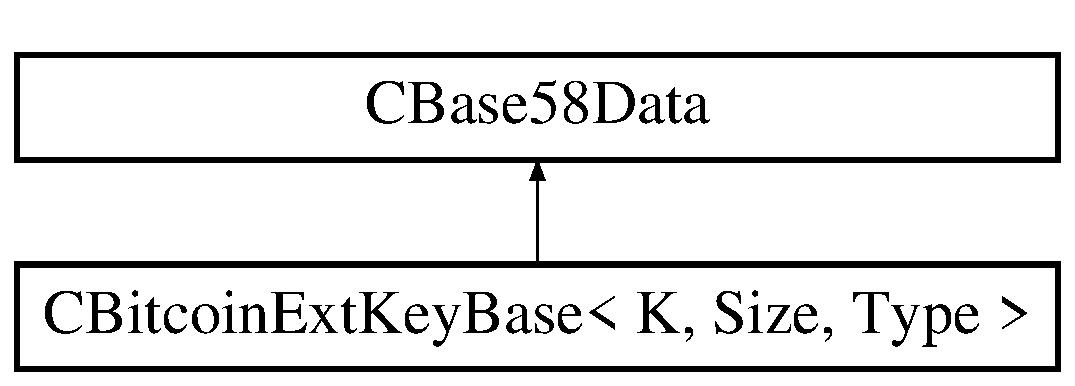
\includegraphics[height=2.000000cm]{class_c_bitcoin_ext_key_base}
\end{center}
\end{figure}
\subsection*{Public Member Functions}
\begin{DoxyCompactItemize}
\item 
void \hyperlink{class_c_bitcoin_ext_key_base_aa6041045bb68b3f24d92f5e3b96aeef6}{Set\+Key} (const K \&key)
\item 
K \hyperlink{class_c_bitcoin_ext_key_base_a528399b89529212a44a08250c5f29d68}{Get\+Key} ()
\item 
\hyperlink{class_c_bitcoin_ext_key_base_a61b09dabc0849ba24520a78c5996096a}{C\+Bitcoin\+Ext\+Key\+Base} (const K \&key)
\item 
\hyperlink{class_c_bitcoin_ext_key_base_a0f4d52b23db0a0740c4519644e537565}{C\+Bitcoin\+Ext\+Key\+Base} ()
\end{DoxyCompactItemize}
\subsection*{Additional Inherited Members}


\subsection{Constructor \& Destructor Documentation}
\hypertarget{class_c_bitcoin_ext_key_base_a61b09dabc0849ba24520a78c5996096a}{}\index{C\+Bitcoin\+Ext\+Key\+Base@{C\+Bitcoin\+Ext\+Key\+Base}!C\+Bitcoin\+Ext\+Key\+Base@{C\+Bitcoin\+Ext\+Key\+Base}}
\index{C\+Bitcoin\+Ext\+Key\+Base@{C\+Bitcoin\+Ext\+Key\+Base}!C\+Bitcoin\+Ext\+Key\+Base@{C\+Bitcoin\+Ext\+Key\+Base}}
\subsubsection[{C\+Bitcoin\+Ext\+Key\+Base}]{\setlength{\rightskip}{0pt plus 5cm}template$<$typename K , int Size, C\+Chain\+Params\+::\+Base58\+Type Type$>$ {\bf C\+Bitcoin\+Ext\+Key\+Base}$<$ K, Size, Type $>$\+::{\bf C\+Bitcoin\+Ext\+Key\+Base} (
\begin{DoxyParamCaption}
\item[{const K \&}]{key}
\end{DoxyParamCaption}
)\hspace{0.3cm}{\ttfamily [inline]}}\label{class_c_bitcoin_ext_key_base_a61b09dabc0849ba24520a78c5996096a}
\hypertarget{class_c_bitcoin_ext_key_base_a0f4d52b23db0a0740c4519644e537565}{}\index{C\+Bitcoin\+Ext\+Key\+Base@{C\+Bitcoin\+Ext\+Key\+Base}!C\+Bitcoin\+Ext\+Key\+Base@{C\+Bitcoin\+Ext\+Key\+Base}}
\index{C\+Bitcoin\+Ext\+Key\+Base@{C\+Bitcoin\+Ext\+Key\+Base}!C\+Bitcoin\+Ext\+Key\+Base@{C\+Bitcoin\+Ext\+Key\+Base}}
\subsubsection[{C\+Bitcoin\+Ext\+Key\+Base}]{\setlength{\rightskip}{0pt plus 5cm}template$<$typename K , int Size, C\+Chain\+Params\+::\+Base58\+Type Type$>$ {\bf C\+Bitcoin\+Ext\+Key\+Base}$<$ K, Size, Type $>$\+::{\bf C\+Bitcoin\+Ext\+Key\+Base} (
\begin{DoxyParamCaption}
{}
\end{DoxyParamCaption}
)\hspace{0.3cm}{\ttfamily [inline]}}\label{class_c_bitcoin_ext_key_base_a0f4d52b23db0a0740c4519644e537565}


\subsection{Member Function Documentation}
\hypertarget{class_c_bitcoin_ext_key_base_a528399b89529212a44a08250c5f29d68}{}\index{C\+Bitcoin\+Ext\+Key\+Base@{C\+Bitcoin\+Ext\+Key\+Base}!Get\+Key@{Get\+Key}}
\index{Get\+Key@{Get\+Key}!C\+Bitcoin\+Ext\+Key\+Base@{C\+Bitcoin\+Ext\+Key\+Base}}
\subsubsection[{Get\+Key}]{\setlength{\rightskip}{0pt plus 5cm}template$<$typename K , int Size, C\+Chain\+Params\+::\+Base58\+Type Type$>$ K {\bf C\+Bitcoin\+Ext\+Key\+Base}$<$ K, Size, Type $>$\+::Get\+Key (
\begin{DoxyParamCaption}
{}
\end{DoxyParamCaption}
)\hspace{0.3cm}{\ttfamily [inline]}}\label{class_c_bitcoin_ext_key_base_a528399b89529212a44a08250c5f29d68}
\hypertarget{class_c_bitcoin_ext_key_base_aa6041045bb68b3f24d92f5e3b96aeef6}{}\index{C\+Bitcoin\+Ext\+Key\+Base@{C\+Bitcoin\+Ext\+Key\+Base}!Set\+Key@{Set\+Key}}
\index{Set\+Key@{Set\+Key}!C\+Bitcoin\+Ext\+Key\+Base@{C\+Bitcoin\+Ext\+Key\+Base}}
\subsubsection[{Set\+Key}]{\setlength{\rightskip}{0pt plus 5cm}template$<$typename K , int Size, C\+Chain\+Params\+::\+Base58\+Type Type$>$ void {\bf C\+Bitcoin\+Ext\+Key\+Base}$<$ K, Size, Type $>$\+::Set\+Key (
\begin{DoxyParamCaption}
\item[{const K \&}]{key}
\end{DoxyParamCaption}
)\hspace{0.3cm}{\ttfamily [inline]}}\label{class_c_bitcoin_ext_key_base_aa6041045bb68b3f24d92f5e3b96aeef6}


The documentation for this class was generated from the following file\+:\begin{DoxyCompactItemize}
\item 
C\+:/\+Users/\+Joe/\+Documents/\+School/\+C\+S\+C17\+A/bitcoin/src/\hyperlink{base58_8h}{base58.\+h}\end{DoxyCompactItemize}

\hypertarget{class_c_bitcoin_secret}{}\section{C\+Bitcoin\+Secret Class Reference}
\label{class_c_bitcoin_secret}\index{C\+Bitcoin\+Secret@{C\+Bitcoin\+Secret}}


{\ttfamily \#include $<$base58.\+h$>$}

Inheritance diagram for C\+Bitcoin\+Secret\+:\begin{figure}[H]
\begin{center}
\leavevmode
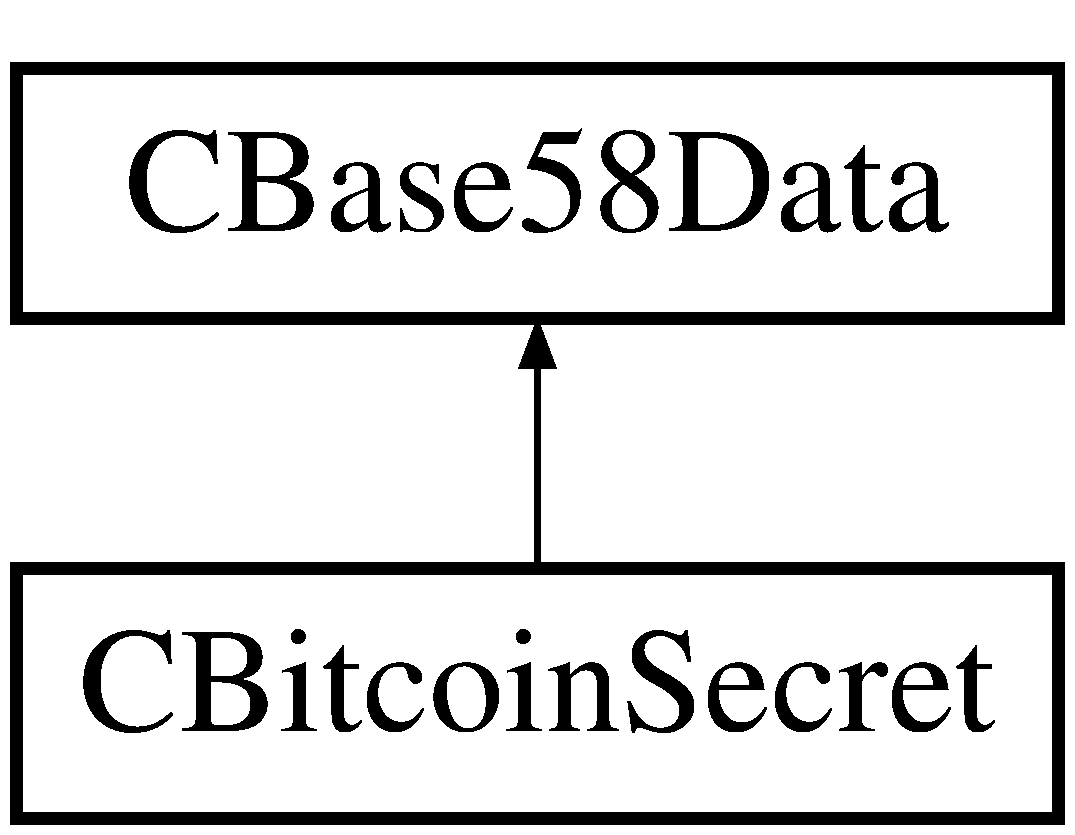
\includegraphics[height=2.000000cm]{class_c_bitcoin_secret}
\end{center}
\end{figure}
\subsection*{Public Member Functions}
\begin{DoxyCompactItemize}
\item 
void \hyperlink{class_c_bitcoin_secret_a3629c0fce320664c3c07cb082939d6ec}{Set\+Key} (const \hyperlink{class_c_key}{C\+Key} \&vch\+Secret)
\item 
\hyperlink{class_c_key}{C\+Key} \hyperlink{class_c_bitcoin_secret_a4d6bf559d092e6d47f8001c7171096df}{Get\+Key} ()
\item 
bool \hyperlink{class_c_bitcoin_secret_a4662c854955af56c047d0e9052096fba}{Is\+Valid} () const 
\item 
bool \hyperlink{class_c_bitcoin_secret_a6a8aff02f66099f33f573ad3e6375bb1}{Set\+String} (const char $\ast$psz\+Secret)
\item 
bool \hyperlink{class_c_bitcoin_secret_a83cfc3b34aac494efdd6e316cd08626d}{Set\+String} (const std\+::string \&str\+Secret)
\item 
\hyperlink{class_c_bitcoin_secret_a0358baa459a1f22661b601d9d83eacf8}{C\+Bitcoin\+Secret} (const \hyperlink{class_c_key}{C\+Key} \&vch\+Secret)
\item 
\hyperlink{class_c_bitcoin_secret_a3b6168eef2ab8c44d60272e62162fd5b}{C\+Bitcoin\+Secret} ()
\end{DoxyCompactItemize}
\subsection*{Additional Inherited Members}


\subsection{Detailed Description}
A base58-\/encoded secret key 

\subsection{Constructor \& Destructor Documentation}
\hypertarget{class_c_bitcoin_secret_a0358baa459a1f22661b601d9d83eacf8}{}\index{C\+Bitcoin\+Secret@{C\+Bitcoin\+Secret}!C\+Bitcoin\+Secret@{C\+Bitcoin\+Secret}}
\index{C\+Bitcoin\+Secret@{C\+Bitcoin\+Secret}!C\+Bitcoin\+Secret@{C\+Bitcoin\+Secret}}
\subsubsection[{C\+Bitcoin\+Secret}]{\setlength{\rightskip}{0pt plus 5cm}C\+Bitcoin\+Secret\+::\+C\+Bitcoin\+Secret (
\begin{DoxyParamCaption}
\item[{const {\bf C\+Key} \&}]{vch\+Secret}
\end{DoxyParamCaption}
)\hspace{0.3cm}{\ttfamily [inline]}}\label{class_c_bitcoin_secret_a0358baa459a1f22661b601d9d83eacf8}
\hypertarget{class_c_bitcoin_secret_a3b6168eef2ab8c44d60272e62162fd5b}{}\index{C\+Bitcoin\+Secret@{C\+Bitcoin\+Secret}!C\+Bitcoin\+Secret@{C\+Bitcoin\+Secret}}
\index{C\+Bitcoin\+Secret@{C\+Bitcoin\+Secret}!C\+Bitcoin\+Secret@{C\+Bitcoin\+Secret}}
\subsubsection[{C\+Bitcoin\+Secret}]{\setlength{\rightskip}{0pt plus 5cm}C\+Bitcoin\+Secret\+::\+C\+Bitcoin\+Secret (
\begin{DoxyParamCaption}
{}
\end{DoxyParamCaption}
)\hspace{0.3cm}{\ttfamily [inline]}}\label{class_c_bitcoin_secret_a3b6168eef2ab8c44d60272e62162fd5b}


\subsection{Member Function Documentation}
\hypertarget{class_c_bitcoin_secret_a4d6bf559d092e6d47f8001c7171096df}{}\index{C\+Bitcoin\+Secret@{C\+Bitcoin\+Secret}!Get\+Key@{Get\+Key}}
\index{Get\+Key@{Get\+Key}!C\+Bitcoin\+Secret@{C\+Bitcoin\+Secret}}
\subsubsection[{Get\+Key}]{\setlength{\rightskip}{0pt plus 5cm}{\bf C\+Key} C\+Bitcoin\+Secret\+::\+Get\+Key (
\begin{DoxyParamCaption}
{}
\end{DoxyParamCaption}
)}\label{class_c_bitcoin_secret_a4d6bf559d092e6d47f8001c7171096df}
\hypertarget{class_c_bitcoin_secret_a4662c854955af56c047d0e9052096fba}{}\index{C\+Bitcoin\+Secret@{C\+Bitcoin\+Secret}!Is\+Valid@{Is\+Valid}}
\index{Is\+Valid@{Is\+Valid}!C\+Bitcoin\+Secret@{C\+Bitcoin\+Secret}}
\subsubsection[{Is\+Valid}]{\setlength{\rightskip}{0pt plus 5cm}bool C\+Bitcoin\+Secret\+::\+Is\+Valid (
\begin{DoxyParamCaption}
{}
\end{DoxyParamCaption}
) const}\label{class_c_bitcoin_secret_a4662c854955af56c047d0e9052096fba}
\hypertarget{class_c_bitcoin_secret_a3629c0fce320664c3c07cb082939d6ec}{}\index{C\+Bitcoin\+Secret@{C\+Bitcoin\+Secret}!Set\+Key@{Set\+Key}}
\index{Set\+Key@{Set\+Key}!C\+Bitcoin\+Secret@{C\+Bitcoin\+Secret}}
\subsubsection[{Set\+Key}]{\setlength{\rightskip}{0pt plus 5cm}void C\+Bitcoin\+Secret\+::\+Set\+Key (
\begin{DoxyParamCaption}
\item[{const {\bf C\+Key} \&}]{vch\+Secret}
\end{DoxyParamCaption}
)}\label{class_c_bitcoin_secret_a3629c0fce320664c3c07cb082939d6ec}
\hypertarget{class_c_bitcoin_secret_a6a8aff02f66099f33f573ad3e6375bb1}{}\index{C\+Bitcoin\+Secret@{C\+Bitcoin\+Secret}!Set\+String@{Set\+String}}
\index{Set\+String@{Set\+String}!C\+Bitcoin\+Secret@{C\+Bitcoin\+Secret}}
\subsubsection[{Set\+String}]{\setlength{\rightskip}{0pt plus 5cm}bool C\+Bitcoin\+Secret\+::\+Set\+String (
\begin{DoxyParamCaption}
\item[{const char $\ast$}]{psz\+Secret}
\end{DoxyParamCaption}
)}\label{class_c_bitcoin_secret_a6a8aff02f66099f33f573ad3e6375bb1}
\hypertarget{class_c_bitcoin_secret_a83cfc3b34aac494efdd6e316cd08626d}{}\index{C\+Bitcoin\+Secret@{C\+Bitcoin\+Secret}!Set\+String@{Set\+String}}
\index{Set\+String@{Set\+String}!C\+Bitcoin\+Secret@{C\+Bitcoin\+Secret}}
\subsubsection[{Set\+String}]{\setlength{\rightskip}{0pt plus 5cm}bool C\+Bitcoin\+Secret\+::\+Set\+String (
\begin{DoxyParamCaption}
\item[{const std\+::string \&}]{str\+Secret}
\end{DoxyParamCaption}
)}\label{class_c_bitcoin_secret_a83cfc3b34aac494efdd6e316cd08626d}


The documentation for this class was generated from the following files\+:\begin{DoxyCompactItemize}
\item 
C\+:/\+Users/\+Joe/\+Documents/\+School/\+C\+S\+C17\+A/bitcoin/src/\hyperlink{base58_8h}{base58.\+h}\item 
C\+:/\+Users/\+Joe/\+Documents/\+School/\+C\+S\+C17\+A/bitcoin/src/\hyperlink{base58_8cpp}{base58.\+cpp}\end{DoxyCompactItemize}

\hypertarget{class_c_block_average}{}\section{C\+Block\+Average Class Reference}
\label{class_c_block_average}\index{C\+Block\+Average@{C\+Block\+Average}}
\subsection*{Public Member Functions}
\begin{DoxyCompactItemize}
\item 
\hyperlink{class_c_block_average_adec219b95a2e1c67471f188dee48fb3a}{C\+Block\+Average} ()
\item 
void \hyperlink{class_c_block_average_a50af3241dc8fb3e49e1e980ed2a7fc95}{Record\+Fee} (const \hyperlink{class_c_fee_rate}{C\+Fee\+Rate} \&fee\+Rate)
\item 
void \hyperlink{class_c_block_average_ae4d71208ccf3ecd85751ce3644d12853}{Record\+Priority} (double priority)
\item 
size\+\_\+t \hyperlink{class_c_block_average_a9e63c1415286edf12ac82145723e564f}{Fee\+Samples} () const 
\item 
size\+\_\+t \hyperlink{class_c_block_average_a43152caddf026ec3f430d55435735ee4}{Get\+Fee\+Samples} (std\+::vector$<$ \hyperlink{class_c_fee_rate}{C\+Fee\+Rate} $>$ \&insert\+Into) const 
\item 
size\+\_\+t \hyperlink{class_c_block_average_a5b6ca2bd5fe9093ba81af14d7882145d}{Priority\+Samples} () const 
\item 
size\+\_\+t \hyperlink{class_c_block_average_a5f56bd04cccb15d891f7dfb41af8b382}{Get\+Priority\+Samples} (std\+::vector$<$ double $>$ \&insert\+Into) const 
\item 
void \hyperlink{class_c_block_average_a2c549117b02d3366cbc840dbdf5ebd6b}{Write} (\hyperlink{class_c_auto_file}{C\+Auto\+File} \&fileout) const 
\item 
void \hyperlink{class_c_block_average_aac4081eec4bf68d7d3a07521ea953489}{Read} (\hyperlink{class_c_auto_file}{C\+Auto\+File} \&filein, const \hyperlink{class_c_fee_rate}{C\+Fee\+Rate} \&min\+Relay\+Fee)
\end{DoxyCompactItemize}
\subsection*{Static Public Member Functions}
\begin{DoxyCompactItemize}
\item 
static bool \hyperlink{class_c_block_average_a31ed22222a49a95787f9791f212ec521}{Are\+Sane} (const \hyperlink{class_c_fee_rate}{C\+Fee\+Rate} fee, const \hyperlink{class_c_fee_rate}{C\+Fee\+Rate} \&min\+Relay\+Fee)
\item 
static bool \hyperlink{class_c_block_average_a92abf5615a926971eba5f6fbaadac880}{Are\+Sane} (const std\+::vector$<$ \hyperlink{class_c_fee_rate}{C\+Fee\+Rate} $>$ \&vec\+Fee, const \hyperlink{class_c_fee_rate}{C\+Fee\+Rate} \&min\+Relay\+Fee)
\item 
static bool \hyperlink{class_c_block_average_af5b855fc318c24c1eda1998ae07a8ed2}{Are\+Sane} (const double priority)
\item 
static bool \hyperlink{class_c_block_average_a2bdd0f3aa2eb5edddde259551965fcaf}{Are\+Sane} (const std\+::vector$<$ double $>$ vec\+Priority)
\end{DoxyCompactItemize}


\subsection{Detailed Description}
Keep track of fee/priority for transactions confirmed within N blocks 

\subsection{Constructor \& Destructor Documentation}
\hypertarget{class_c_block_average_adec219b95a2e1c67471f188dee48fb3a}{}\index{C\+Block\+Average@{C\+Block\+Average}!C\+Block\+Average@{C\+Block\+Average}}
\index{C\+Block\+Average@{C\+Block\+Average}!C\+Block\+Average@{C\+Block\+Average}}
\subsubsection[{C\+Block\+Average}]{\setlength{\rightskip}{0pt plus 5cm}C\+Block\+Average\+::\+C\+Block\+Average (
\begin{DoxyParamCaption}
{}
\end{DoxyParamCaption}
)\hspace{0.3cm}{\ttfamily [inline]}}\label{class_c_block_average_adec219b95a2e1c67471f188dee48fb3a}


\subsection{Member Function Documentation}
\hypertarget{class_c_block_average_a31ed22222a49a95787f9791f212ec521}{}\index{C\+Block\+Average@{C\+Block\+Average}!Are\+Sane@{Are\+Sane}}
\index{Are\+Sane@{Are\+Sane}!C\+Block\+Average@{C\+Block\+Average}}
\subsubsection[{Are\+Sane}]{\setlength{\rightskip}{0pt plus 5cm}static bool C\+Block\+Average\+::\+Are\+Sane (
\begin{DoxyParamCaption}
\item[{const {\bf C\+Fee\+Rate}}]{fee, }
\item[{const {\bf C\+Fee\+Rate} \&}]{min\+Relay\+Fee}
\end{DoxyParamCaption}
)\hspace{0.3cm}{\ttfamily [inline]}, {\ttfamily [static]}}\label{class_c_block_average_a31ed22222a49a95787f9791f212ec521}
Used as belt-\/and-\/suspenders check when reading to detect file corruption \hypertarget{class_c_block_average_a92abf5615a926971eba5f6fbaadac880}{}\index{C\+Block\+Average@{C\+Block\+Average}!Are\+Sane@{Are\+Sane}}
\index{Are\+Sane@{Are\+Sane}!C\+Block\+Average@{C\+Block\+Average}}
\subsubsection[{Are\+Sane}]{\setlength{\rightskip}{0pt plus 5cm}static bool C\+Block\+Average\+::\+Are\+Sane (
\begin{DoxyParamCaption}
\item[{const std\+::vector$<$ {\bf C\+Fee\+Rate} $>$ \&}]{vec\+Fee, }
\item[{const {\bf C\+Fee\+Rate} \&}]{min\+Relay\+Fee}
\end{DoxyParamCaption}
)\hspace{0.3cm}{\ttfamily [inline]}, {\ttfamily [static]}}\label{class_c_block_average_a92abf5615a926971eba5f6fbaadac880}
\hypertarget{class_c_block_average_af5b855fc318c24c1eda1998ae07a8ed2}{}\index{C\+Block\+Average@{C\+Block\+Average}!Are\+Sane@{Are\+Sane}}
\index{Are\+Sane@{Are\+Sane}!C\+Block\+Average@{C\+Block\+Average}}
\subsubsection[{Are\+Sane}]{\setlength{\rightskip}{0pt plus 5cm}static bool C\+Block\+Average\+::\+Are\+Sane (
\begin{DoxyParamCaption}
\item[{const double}]{priority}
\end{DoxyParamCaption}
)\hspace{0.3cm}{\ttfamily [inline]}, {\ttfamily [static]}}\label{class_c_block_average_af5b855fc318c24c1eda1998ae07a8ed2}
\hypertarget{class_c_block_average_a2bdd0f3aa2eb5edddde259551965fcaf}{}\index{C\+Block\+Average@{C\+Block\+Average}!Are\+Sane@{Are\+Sane}}
\index{Are\+Sane@{Are\+Sane}!C\+Block\+Average@{C\+Block\+Average}}
\subsubsection[{Are\+Sane}]{\setlength{\rightskip}{0pt plus 5cm}static bool C\+Block\+Average\+::\+Are\+Sane (
\begin{DoxyParamCaption}
\item[{const std\+::vector$<$ double $>$}]{vec\+Priority}
\end{DoxyParamCaption}
)\hspace{0.3cm}{\ttfamily [inline]}, {\ttfamily [static]}}\label{class_c_block_average_a2bdd0f3aa2eb5edddde259551965fcaf}
\hypertarget{class_c_block_average_a9e63c1415286edf12ac82145723e564f}{}\index{C\+Block\+Average@{C\+Block\+Average}!Fee\+Samples@{Fee\+Samples}}
\index{Fee\+Samples@{Fee\+Samples}!C\+Block\+Average@{C\+Block\+Average}}
\subsubsection[{Fee\+Samples}]{\setlength{\rightskip}{0pt plus 5cm}size\+\_\+t C\+Block\+Average\+::\+Fee\+Samples (
\begin{DoxyParamCaption}
{}
\end{DoxyParamCaption}
) const\hspace{0.3cm}{\ttfamily [inline]}}\label{class_c_block_average_a9e63c1415286edf12ac82145723e564f}
\hypertarget{class_c_block_average_a43152caddf026ec3f430d55435735ee4}{}\index{C\+Block\+Average@{C\+Block\+Average}!Get\+Fee\+Samples@{Get\+Fee\+Samples}}
\index{Get\+Fee\+Samples@{Get\+Fee\+Samples}!C\+Block\+Average@{C\+Block\+Average}}
\subsubsection[{Get\+Fee\+Samples}]{\setlength{\rightskip}{0pt plus 5cm}size\+\_\+t C\+Block\+Average\+::\+Get\+Fee\+Samples (
\begin{DoxyParamCaption}
\item[{std\+::vector$<$ {\bf C\+Fee\+Rate} $>$ \&}]{insert\+Into}
\end{DoxyParamCaption}
) const\hspace{0.3cm}{\ttfamily [inline]}}\label{class_c_block_average_a43152caddf026ec3f430d55435735ee4}
\hypertarget{class_c_block_average_a5f56bd04cccb15d891f7dfb41af8b382}{}\index{C\+Block\+Average@{C\+Block\+Average}!Get\+Priority\+Samples@{Get\+Priority\+Samples}}
\index{Get\+Priority\+Samples@{Get\+Priority\+Samples}!C\+Block\+Average@{C\+Block\+Average}}
\subsubsection[{Get\+Priority\+Samples}]{\setlength{\rightskip}{0pt plus 5cm}size\+\_\+t C\+Block\+Average\+::\+Get\+Priority\+Samples (
\begin{DoxyParamCaption}
\item[{std\+::vector$<$ double $>$ \&}]{insert\+Into}
\end{DoxyParamCaption}
) const\hspace{0.3cm}{\ttfamily [inline]}}\label{class_c_block_average_a5f56bd04cccb15d891f7dfb41af8b382}
\hypertarget{class_c_block_average_a5b6ca2bd5fe9093ba81af14d7882145d}{}\index{C\+Block\+Average@{C\+Block\+Average}!Priority\+Samples@{Priority\+Samples}}
\index{Priority\+Samples@{Priority\+Samples}!C\+Block\+Average@{C\+Block\+Average}}
\subsubsection[{Priority\+Samples}]{\setlength{\rightskip}{0pt plus 5cm}size\+\_\+t C\+Block\+Average\+::\+Priority\+Samples (
\begin{DoxyParamCaption}
{}
\end{DoxyParamCaption}
) const\hspace{0.3cm}{\ttfamily [inline]}}\label{class_c_block_average_a5b6ca2bd5fe9093ba81af14d7882145d}
\hypertarget{class_c_block_average_aac4081eec4bf68d7d3a07521ea953489}{}\index{C\+Block\+Average@{C\+Block\+Average}!Read@{Read}}
\index{Read@{Read}!C\+Block\+Average@{C\+Block\+Average}}
\subsubsection[{Read}]{\setlength{\rightskip}{0pt plus 5cm}void C\+Block\+Average\+::\+Read (
\begin{DoxyParamCaption}
\item[{{\bf C\+Auto\+File} \&}]{filein, }
\item[{const {\bf C\+Fee\+Rate} \&}]{min\+Relay\+Fee}
\end{DoxyParamCaption}
)\hspace{0.3cm}{\ttfamily [inline]}}\label{class_c_block_average_aac4081eec4bf68d7d3a07521ea953489}
\hypertarget{class_c_block_average_a50af3241dc8fb3e49e1e980ed2a7fc95}{}\index{C\+Block\+Average@{C\+Block\+Average}!Record\+Fee@{Record\+Fee}}
\index{Record\+Fee@{Record\+Fee}!C\+Block\+Average@{C\+Block\+Average}}
\subsubsection[{Record\+Fee}]{\setlength{\rightskip}{0pt plus 5cm}void C\+Block\+Average\+::\+Record\+Fee (
\begin{DoxyParamCaption}
\item[{const {\bf C\+Fee\+Rate} \&}]{fee\+Rate}
\end{DoxyParamCaption}
)\hspace{0.3cm}{\ttfamily [inline]}}\label{class_c_block_average_a50af3241dc8fb3e49e1e980ed2a7fc95}
\hypertarget{class_c_block_average_ae4d71208ccf3ecd85751ce3644d12853}{}\index{C\+Block\+Average@{C\+Block\+Average}!Record\+Priority@{Record\+Priority}}
\index{Record\+Priority@{Record\+Priority}!C\+Block\+Average@{C\+Block\+Average}}
\subsubsection[{Record\+Priority}]{\setlength{\rightskip}{0pt plus 5cm}void C\+Block\+Average\+::\+Record\+Priority (
\begin{DoxyParamCaption}
\item[{double}]{priority}
\end{DoxyParamCaption}
)\hspace{0.3cm}{\ttfamily [inline]}}\label{class_c_block_average_ae4d71208ccf3ecd85751ce3644d12853}
\hypertarget{class_c_block_average_a2c549117b02d3366cbc840dbdf5ebd6b}{}\index{C\+Block\+Average@{C\+Block\+Average}!Write@{Write}}
\index{Write@{Write}!C\+Block\+Average@{C\+Block\+Average}}
\subsubsection[{Write}]{\setlength{\rightskip}{0pt plus 5cm}void C\+Block\+Average\+::\+Write (
\begin{DoxyParamCaption}
\item[{{\bf C\+Auto\+File} \&}]{fileout}
\end{DoxyParamCaption}
) const\hspace{0.3cm}{\ttfamily [inline]}}\label{class_c_block_average_a2c549117b02d3366cbc840dbdf5ebd6b}


The documentation for this class was generated from the following file\+:\begin{DoxyCompactItemize}
\item 
C\+:/\+Users/\+Joe/\+Documents/\+School/\+C\+S\+C17\+A/bitcoin/src/\hyperlink{txmempool_8cpp}{txmempool.\+cpp}\end{DoxyCompactItemize}

\hypertarget{class_c_block_file_info}{}\section{C\+Block\+File\+Info Class Reference}
\label{class_c_block_file_info}\index{C\+Block\+File\+Info@{C\+Block\+File\+Info}}


{\ttfamily \#include $<$main.\+h$>$}

\subsection*{Public Member Functions}
\begin{DoxyCompactItemize}
\item 
{\footnotesize template$<$typename Stream , typename Operation $>$ }\\void \hyperlink{class_c_block_file_info_a5d48a4fe1f8b3903131d121fc14a5a6f}{Serialization\+Op} (Stream \&s, Operation ser\+\_\+action, int n\+Type, int n\+Version)
\item 
void \hyperlink{class_c_block_file_info_a21bd4f8e92c47646737fc57446a86cc2}{Set\+Null} ()
\item 
\hyperlink{class_c_block_file_info_a4d08bfcfc45a16b40266255f8597c949}{C\+Block\+File\+Info} ()
\item 
std\+::string \hyperlink{class_c_block_file_info_a90d40a769ca47c075757c1b9037c88f3}{To\+String} () const 
\item 
void \hyperlink{class_c_block_file_info_a66867569ffe06068b8c6eb1139934fbf}{Add\+Block} (unsigned int n\+Height\+In, uint64\+\_\+t n\+Time\+In)
\end{DoxyCompactItemize}
\subsection*{Public Attributes}
\begin{DoxyCompactItemize}
\item 
unsigned int \hyperlink{class_c_block_file_info_adf2de4bb4d8a0a8f2116ed90f0770d03}{n\+Blocks}
\item 
unsigned int \hyperlink{class_c_block_file_info_afb13102ba49548c24812a4236851c3a9}{n\+Size}
\begin{DoxyCompactList}\small\item\em number of blocks stored in file \end{DoxyCompactList}\item 
unsigned int \hyperlink{class_c_block_file_info_ad3e555fd733ef8f38430554c2db5e9d1}{n\+Undo\+Size}
\begin{DoxyCompactList}\small\item\em number of used bytes of block file \end{DoxyCompactList}\item 
unsigned int \hyperlink{class_c_block_file_info_a66d258b11b1aec30cbacdc6130c271a8}{n\+Height\+First}
\begin{DoxyCompactList}\small\item\em number of used bytes in the undo file \end{DoxyCompactList}\item 
unsigned int \hyperlink{class_c_block_file_info_aabbcf808931e7eaf2278b3d7172fad3a}{n\+Height\+Last}
\begin{DoxyCompactList}\small\item\em lowest height of block in file \end{DoxyCompactList}\item 
uint64\+\_\+t \hyperlink{class_c_block_file_info_a0e928257d1f003ede485ce49e8cf9189}{n\+Time\+First}
\begin{DoxyCompactList}\small\item\em highest height of block in file \end{DoxyCompactList}\item 
uint64\+\_\+t \hyperlink{class_c_block_file_info_a1d12e4202474bb2f299d18d7d1f28c78}{n\+Time\+Last}
\begin{DoxyCompactList}\small\item\em earliest time of block in file \end{DoxyCompactList}\item 
\hyperlink{class_c_block_file_info_ab4daf4df00f90dee15e3a7d2cdb7a273}{A\+D\+D\+\_\+\+S\+E\+R\+I\+A\+L\+I\+Z\+E\+\_\+\+M\+E\+T\+H\+O\+D\+S}
\begin{DoxyCompactList}\small\item\em latest time of block in file \end{DoxyCompactList}\end{DoxyCompactItemize}


\subsection{Constructor \& Destructor Documentation}
\hypertarget{class_c_block_file_info_a4d08bfcfc45a16b40266255f8597c949}{}\index{C\+Block\+File\+Info@{C\+Block\+File\+Info}!C\+Block\+File\+Info@{C\+Block\+File\+Info}}
\index{C\+Block\+File\+Info@{C\+Block\+File\+Info}!C\+Block\+File\+Info@{C\+Block\+File\+Info}}
\subsubsection[{C\+Block\+File\+Info}]{\setlength{\rightskip}{0pt plus 5cm}C\+Block\+File\+Info\+::\+C\+Block\+File\+Info (
\begin{DoxyParamCaption}
{}
\end{DoxyParamCaption}
)\hspace{0.3cm}{\ttfamily [inline]}}\label{class_c_block_file_info_a4d08bfcfc45a16b40266255f8597c949}


\subsection{Member Function Documentation}
\hypertarget{class_c_block_file_info_a66867569ffe06068b8c6eb1139934fbf}{}\index{C\+Block\+File\+Info@{C\+Block\+File\+Info}!Add\+Block@{Add\+Block}}
\index{Add\+Block@{Add\+Block}!C\+Block\+File\+Info@{C\+Block\+File\+Info}}
\subsubsection[{Add\+Block}]{\setlength{\rightskip}{0pt plus 5cm}void C\+Block\+File\+Info\+::\+Add\+Block (
\begin{DoxyParamCaption}
\item[{unsigned int}]{n\+Height\+In, }
\item[{uint64\+\_\+t}]{n\+Time\+In}
\end{DoxyParamCaption}
)\hspace{0.3cm}{\ttfamily [inline]}}\label{class_c_block_file_info_a66867569ffe06068b8c6eb1139934fbf}
update statistics (does not update n\+Size) \hypertarget{class_c_block_file_info_a5d48a4fe1f8b3903131d121fc14a5a6f}{}\index{C\+Block\+File\+Info@{C\+Block\+File\+Info}!Serialization\+Op@{Serialization\+Op}}
\index{Serialization\+Op@{Serialization\+Op}!C\+Block\+File\+Info@{C\+Block\+File\+Info}}
\subsubsection[{Serialization\+Op}]{\setlength{\rightskip}{0pt plus 5cm}template$<$typename Stream , typename Operation $>$ void C\+Block\+File\+Info\+::\+Serialization\+Op (
\begin{DoxyParamCaption}
\item[{Stream \&}]{s, }
\item[{Operation}]{ser\+\_\+action, }
\item[{int}]{n\+Type, }
\item[{int}]{n\+Version}
\end{DoxyParamCaption}
)\hspace{0.3cm}{\ttfamily [inline]}}\label{class_c_block_file_info_a5d48a4fe1f8b3903131d121fc14a5a6f}
\hypertarget{class_c_block_file_info_a21bd4f8e92c47646737fc57446a86cc2}{}\index{C\+Block\+File\+Info@{C\+Block\+File\+Info}!Set\+Null@{Set\+Null}}
\index{Set\+Null@{Set\+Null}!C\+Block\+File\+Info@{C\+Block\+File\+Info}}
\subsubsection[{Set\+Null}]{\setlength{\rightskip}{0pt plus 5cm}void C\+Block\+File\+Info\+::\+Set\+Null (
\begin{DoxyParamCaption}
{}
\end{DoxyParamCaption}
)\hspace{0.3cm}{\ttfamily [inline]}}\label{class_c_block_file_info_a21bd4f8e92c47646737fc57446a86cc2}
\hypertarget{class_c_block_file_info_a90d40a769ca47c075757c1b9037c88f3}{}\index{C\+Block\+File\+Info@{C\+Block\+File\+Info}!To\+String@{To\+String}}
\index{To\+String@{To\+String}!C\+Block\+File\+Info@{C\+Block\+File\+Info}}
\subsubsection[{To\+String}]{\setlength{\rightskip}{0pt plus 5cm}std\+::string C\+Block\+File\+Info\+::\+To\+String (
\begin{DoxyParamCaption}
{}
\end{DoxyParamCaption}
) const}\label{class_c_block_file_info_a90d40a769ca47c075757c1b9037c88f3}


\subsection{Member Data Documentation}
\hypertarget{class_c_block_file_info_ab4daf4df00f90dee15e3a7d2cdb7a273}{}\index{C\+Block\+File\+Info@{C\+Block\+File\+Info}!A\+D\+D\+\_\+\+S\+E\+R\+I\+A\+L\+I\+Z\+E\+\_\+\+M\+E\+T\+H\+O\+D\+S@{A\+D\+D\+\_\+\+S\+E\+R\+I\+A\+L\+I\+Z\+E\+\_\+\+M\+E\+T\+H\+O\+D\+S}}
\index{A\+D\+D\+\_\+\+S\+E\+R\+I\+A\+L\+I\+Z\+E\+\_\+\+M\+E\+T\+H\+O\+D\+S@{A\+D\+D\+\_\+\+S\+E\+R\+I\+A\+L\+I\+Z\+E\+\_\+\+M\+E\+T\+H\+O\+D\+S}!C\+Block\+File\+Info@{C\+Block\+File\+Info}}
\subsubsection[{A\+D\+D\+\_\+\+S\+E\+R\+I\+A\+L\+I\+Z\+E\+\_\+\+M\+E\+T\+H\+O\+D\+S}]{\setlength{\rightskip}{0pt plus 5cm}C\+Block\+File\+Info\+::\+A\+D\+D\+\_\+\+S\+E\+R\+I\+A\+L\+I\+Z\+E\+\_\+\+M\+E\+T\+H\+O\+D\+S}\label{class_c_block_file_info_ab4daf4df00f90dee15e3a7d2cdb7a273}


latest time of block in file 

\hypertarget{class_c_block_file_info_adf2de4bb4d8a0a8f2116ed90f0770d03}{}\index{C\+Block\+File\+Info@{C\+Block\+File\+Info}!n\+Blocks@{n\+Blocks}}
\index{n\+Blocks@{n\+Blocks}!C\+Block\+File\+Info@{C\+Block\+File\+Info}}
\subsubsection[{n\+Blocks}]{\setlength{\rightskip}{0pt plus 5cm}unsigned int C\+Block\+File\+Info\+::n\+Blocks}\label{class_c_block_file_info_adf2de4bb4d8a0a8f2116ed90f0770d03}
\hypertarget{class_c_block_file_info_a66d258b11b1aec30cbacdc6130c271a8}{}\index{C\+Block\+File\+Info@{C\+Block\+File\+Info}!n\+Height\+First@{n\+Height\+First}}
\index{n\+Height\+First@{n\+Height\+First}!C\+Block\+File\+Info@{C\+Block\+File\+Info}}
\subsubsection[{n\+Height\+First}]{\setlength{\rightskip}{0pt plus 5cm}unsigned int C\+Block\+File\+Info\+::n\+Height\+First}\label{class_c_block_file_info_a66d258b11b1aec30cbacdc6130c271a8}


number of used bytes in the undo file 

\hypertarget{class_c_block_file_info_aabbcf808931e7eaf2278b3d7172fad3a}{}\index{C\+Block\+File\+Info@{C\+Block\+File\+Info}!n\+Height\+Last@{n\+Height\+Last}}
\index{n\+Height\+Last@{n\+Height\+Last}!C\+Block\+File\+Info@{C\+Block\+File\+Info}}
\subsubsection[{n\+Height\+Last}]{\setlength{\rightskip}{0pt plus 5cm}unsigned int C\+Block\+File\+Info\+::n\+Height\+Last}\label{class_c_block_file_info_aabbcf808931e7eaf2278b3d7172fad3a}


lowest height of block in file 

\hypertarget{class_c_block_file_info_afb13102ba49548c24812a4236851c3a9}{}\index{C\+Block\+File\+Info@{C\+Block\+File\+Info}!n\+Size@{n\+Size}}
\index{n\+Size@{n\+Size}!C\+Block\+File\+Info@{C\+Block\+File\+Info}}
\subsubsection[{n\+Size}]{\setlength{\rightskip}{0pt plus 5cm}unsigned int C\+Block\+File\+Info\+::n\+Size}\label{class_c_block_file_info_afb13102ba49548c24812a4236851c3a9}


number of blocks stored in file 

\hypertarget{class_c_block_file_info_a0e928257d1f003ede485ce49e8cf9189}{}\index{C\+Block\+File\+Info@{C\+Block\+File\+Info}!n\+Time\+First@{n\+Time\+First}}
\index{n\+Time\+First@{n\+Time\+First}!C\+Block\+File\+Info@{C\+Block\+File\+Info}}
\subsubsection[{n\+Time\+First}]{\setlength{\rightskip}{0pt plus 5cm}uint64\+\_\+t C\+Block\+File\+Info\+::n\+Time\+First}\label{class_c_block_file_info_a0e928257d1f003ede485ce49e8cf9189}


highest height of block in file 

\hypertarget{class_c_block_file_info_a1d12e4202474bb2f299d18d7d1f28c78}{}\index{C\+Block\+File\+Info@{C\+Block\+File\+Info}!n\+Time\+Last@{n\+Time\+Last}}
\index{n\+Time\+Last@{n\+Time\+Last}!C\+Block\+File\+Info@{C\+Block\+File\+Info}}
\subsubsection[{n\+Time\+Last}]{\setlength{\rightskip}{0pt plus 5cm}uint64\+\_\+t C\+Block\+File\+Info\+::n\+Time\+Last}\label{class_c_block_file_info_a1d12e4202474bb2f299d18d7d1f28c78}


earliest time of block in file 

\hypertarget{class_c_block_file_info_ad3e555fd733ef8f38430554c2db5e9d1}{}\index{C\+Block\+File\+Info@{C\+Block\+File\+Info}!n\+Undo\+Size@{n\+Undo\+Size}}
\index{n\+Undo\+Size@{n\+Undo\+Size}!C\+Block\+File\+Info@{C\+Block\+File\+Info}}
\subsubsection[{n\+Undo\+Size}]{\setlength{\rightskip}{0pt plus 5cm}unsigned int C\+Block\+File\+Info\+::n\+Undo\+Size}\label{class_c_block_file_info_ad3e555fd733ef8f38430554c2db5e9d1}


number of used bytes of block file 



The documentation for this class was generated from the following files\+:\begin{DoxyCompactItemize}
\item 
C\+:/\+Users/\+Joe/\+Documents/\+School/\+C\+S\+C17\+A/bitcoin/src/\hyperlink{main_8h}{main.\+h}\item 
C\+:/\+Users/\+Joe/\+Documents/\+School/\+C\+S\+C17\+A/bitcoin/src/\hyperlink{main_8cpp}{main.\+cpp}\end{DoxyCompactItemize}

\hypertarget{class_c_block_index}{}\section{C\+Block\+Index Class Reference}
\label{class_c_block_index}\index{C\+Block\+Index@{C\+Block\+Index}}


{\ttfamily \#include $<$chain.\+h$>$}

Inheritance diagram for C\+Block\+Index\+:\begin{figure}[H]
\begin{center}
\leavevmode
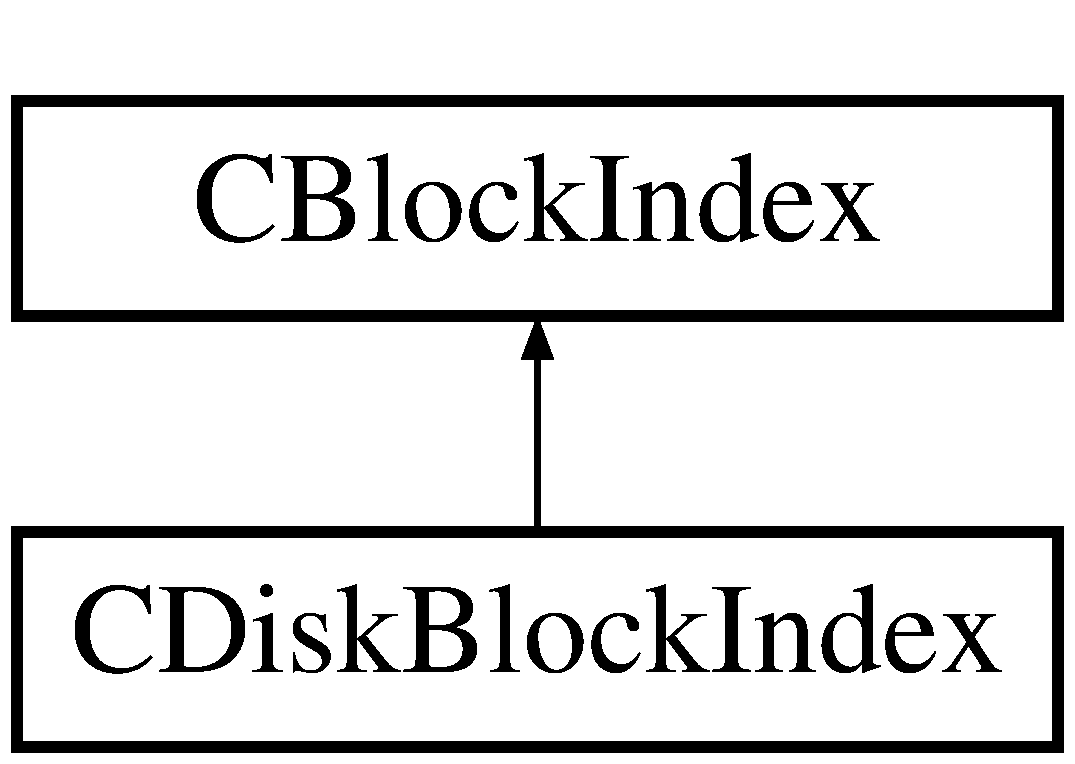
\includegraphics[height=2.000000cm]{class_c_block_index}
\end{center}
\end{figure}
\subsection*{Public Types}
\begin{DoxyCompactItemize}
\item 
enum \{ \hyperlink{class_c_block_index_acefc16035e60d7bd52ed2c9bb1aa838eaa2b8ad73c4fe37a8de8748d949c334d4}{n\+Median\+Time\+Span} =11
 \}
\end{DoxyCompactItemize}
\subsection*{Public Member Functions}
\begin{DoxyCompactItemize}
\item 
void \hyperlink{class_c_block_index_a6139e9e2cfceaef3694631cb7c330ff0}{Set\+Null} ()
\item 
\hyperlink{class_c_block_index_a0eff34cbfb4470885020734581dc1555}{C\+Block\+Index} ()
\item 
\hyperlink{class_c_block_index_acaf83989071b40966072161c513a17a7}{C\+Block\+Index} (const C\+Block\+Header \&block)
\item 
\hyperlink{struct_c_disk_block_pos}{C\+Disk\+Block\+Pos} \hyperlink{class_c_block_index_ae2b58426ae9365dce6cfacc5d0c92e44}{Get\+Block\+Pos} () const 
\item 
\hyperlink{struct_c_disk_block_pos}{C\+Disk\+Block\+Pos} \hyperlink{class_c_block_index_a62654ef291abc44d2e32db9a8d85b7d1}{Get\+Undo\+Pos} () const 
\item 
C\+Block\+Header \hyperlink{class_c_block_index_a8292a7bf7e79e207306a8659bf7da3a6}{Get\+Block\+Header} () const 
\item 
\hyperlink{classuint256}{uint256} \hyperlink{class_c_block_index_ab843ef9b8b0a0193ec3a5c24738e484f}{Get\+Block\+Hash} () const 
\item 
int64\+\_\+t \hyperlink{class_c_block_index_ab63b774ae798f5f9e54b400ac8b5ef4b}{Get\+Block\+Time} () const 
\item 
int64\+\_\+t \hyperlink{class_c_block_index_abffb24cc73329a3dce024403ba770b4a}{Get\+Median\+Time\+Past} () const 
\item 
std\+::string \hyperlink{class_c_block_index_abed1fcbcd372db6b9efa6bb9da317469}{To\+String} () const 
\item 
bool \hyperlink{class_c_block_index_ab79ac7f3db34001898a371ecce27808f}{Is\+Valid} (enum \hyperlink{chain_8h_a43adb063ba9e8b0f1143146d9c7929d9}{Block\+Status} n\+Up\+To=\hyperlink{chain_8h_a43adb063ba9e8b0f1143146d9c7929d9a3eef30f876594ac79b888b7d1ff6c66c}{B\+L\+O\+C\+K\+\_\+\+V\+A\+L\+I\+D\+\_\+\+T\+R\+A\+N\+S\+A\+C\+T\+I\+O\+N\+S}) const 
\begin{DoxyCompactList}\small\item\em Check whether this block index entry is valid up to the passed validity level. \end{DoxyCompactList}\item 
bool \hyperlink{class_c_block_index_a076aff906933e9d75a37aa9b81c01384}{Raise\+Validity} (enum \hyperlink{chain_8h_a43adb063ba9e8b0f1143146d9c7929d9}{Block\+Status} n\+Up\+To)
\item 
void \hyperlink{class_c_block_index_a21209a71e50daf10e283bd4049e46f64}{Build\+Skip} ()
\begin{DoxyCompactList}\small\item\em Build the skiplist pointer for this entry. \end{DoxyCompactList}\item 
\hyperlink{class_c_block_index}{C\+Block\+Index} $\ast$ \hyperlink{class_c_block_index_ae1f702384690c6b8302e026a84172ef3}{Get\+Ancestor} (int height)
\begin{DoxyCompactList}\small\item\em Efficiently find an ancestor of this block. \end{DoxyCompactList}\item 
const \hyperlink{class_c_block_index}{C\+Block\+Index} $\ast$ \hyperlink{class_c_block_index_a554a9f67d26a4dce71b30b6e3ccc54da}{Get\+Ancestor} (int height) const 
\end{DoxyCompactItemize}
\subsection*{Public Attributes}
\begin{DoxyCompactItemize}
\item 
const \hyperlink{classuint256}{uint256} $\ast$ \hyperlink{class_c_block_index_afac8099e03ffda463c7153ca82d37b66}{phash\+Block}
\begin{DoxyCompactList}\small\item\em pointer to the hash of the block, if any. Memory is owned by this \hyperlink{class_c_block_index}{C\+Block\+Index} \end{DoxyCompactList}\item 
\hyperlink{class_c_block_index}{C\+Block\+Index} $\ast$ \hyperlink{class_c_block_index_a1ef11137155df1dd5c81491630cece39}{pprev}
\begin{DoxyCompactList}\small\item\em pointer to the index of the predecessor of this block \end{DoxyCompactList}\item 
\hyperlink{class_c_block_index}{C\+Block\+Index} $\ast$ \hyperlink{class_c_block_index_ab6242bb77bc01617f5b402d14e6a3883}{pskip}
\begin{DoxyCompactList}\small\item\em pointer to the index of some further predecessor of this block \end{DoxyCompactList}\item 
int \hyperlink{class_c_block_index_aebfc8d6b95852546760e742553d7bfd5}{n\+Height}
\begin{DoxyCompactList}\small\item\em height of the entry in the chain. The genesis block has height 0 \end{DoxyCompactList}\item 
int \hyperlink{class_c_block_index_a3653cb1e1bc3fa3fcdf1ed50ff93b50a}{n\+File}
\begin{DoxyCompactList}\small\item\em Which \# file this block is stored in (blk?????.dat) \end{DoxyCompactList}\item 
unsigned int \hyperlink{class_c_block_index_af164283dfb2d62ac44be8d10446bce4a}{n\+Data\+Pos}
\begin{DoxyCompactList}\small\item\em Byte offset within blk?????.dat where this block\textquotesingle{}s data is stored. \end{DoxyCompactList}\item 
unsigned int \hyperlink{class_c_block_index_a865ddd56406c23e98cdc61511a61eb64}{n\+Undo\+Pos}
\begin{DoxyCompactList}\small\item\em Byte offset within rev?????.dat where this block\textquotesingle{}s undo data is stored. \end{DoxyCompactList}\item 
\hyperlink{classarith__uint256}{arith\+\_\+uint256} \hyperlink{class_c_block_index_a31e65c1f491d438dfdcd8d92bdfa73a1}{n\+Chain\+Work}
\begin{DoxyCompactList}\small\item\em (memory only) Total amount of work (expected number of hashes) in the chain up to and including this block \end{DoxyCompactList}\item 
unsigned int \hyperlink{class_c_block_index_ac8e219a377839d2f9133a4387f46e44e}{n\+Tx}
\item 
unsigned int \hyperlink{class_c_block_index_af3c6d6dd8a7579e5ce516d94b98d2db5}{n\+Chain\+Tx}
\item 
unsigned int \hyperlink{class_c_block_index_ac5a336b45ca70e3ed2fc090bf2ee3011}{n\+Status}
\begin{DoxyCompactList}\small\item\em Verification status of this block. See enum Block\+Status. \end{DoxyCompactList}\item 
int \hyperlink{class_c_block_index_a45126301a0a6e26010527a7bbfc1ef58}{n\+Version}
\begin{DoxyCompactList}\small\item\em block header \end{DoxyCompactList}\item 
\hyperlink{classuint256}{uint256} \hyperlink{class_c_block_index_a0601b6b2bd6eaedfbc283c00d045a21c}{hash\+Merkle\+Root}
\item 
unsigned int \hyperlink{class_c_block_index_a4b687a226e9e166b0f91c1b616b543a6}{n\+Time}
\item 
unsigned int \hyperlink{class_c_block_index_a3324894e6af612d1bd76f89378435713}{n\+Bits}
\item 
unsigned int \hyperlink{class_c_block_index_a5e0a648ed1df8da171eba636d5ebef01}{n\+Nonce}
\item 
uint32\+\_\+t \hyperlink{class_c_block_index_a4a679af5f7924cc594b8131371b21e54}{n\+Sequence\+Id}
\begin{DoxyCompactList}\small\item\em (memory only) Sequential id assigned to distinguish order in which blocks are received. \end{DoxyCompactList}\end{DoxyCompactItemize}


\subsection{Detailed Description}
The block chain is a tree shaped structure starting with the genesis block at the root, with each block potentially having multiple candidates to be the next block. A blockindex may have multiple pprev pointing to it, but at most one of them can be part of the currently active branch. 

\subsection{Member Enumeration Documentation}
\hypertarget{class_c_block_index_acefc16035e60d7bd52ed2c9bb1aa838e}{}\subsubsection[{anonymous enum}]{\setlength{\rightskip}{0pt plus 5cm}anonymous enum}\label{class_c_block_index_acefc16035e60d7bd52ed2c9bb1aa838e}
\begin{Desc}
\item[Enumerator]\par
\begin{description}
\index{n\+Median\+Time\+Span@{n\+Median\+Time\+Span}!C\+Block\+Index@{C\+Block\+Index}}\index{C\+Block\+Index@{C\+Block\+Index}!n\+Median\+Time\+Span@{n\+Median\+Time\+Span}}\item[{\em 
\hypertarget{class_c_block_index_acefc16035e60d7bd52ed2c9bb1aa838eaa2b8ad73c4fe37a8de8748d949c334d4}{}n\+Median\+Time\+Span\label{class_c_block_index_acefc16035e60d7bd52ed2c9bb1aa838eaa2b8ad73c4fe37a8de8748d949c334d4}
}]\end{description}
\end{Desc}


\subsection{Constructor \& Destructor Documentation}
\hypertarget{class_c_block_index_a0eff34cbfb4470885020734581dc1555}{}\index{C\+Block\+Index@{C\+Block\+Index}!C\+Block\+Index@{C\+Block\+Index}}
\index{C\+Block\+Index@{C\+Block\+Index}!C\+Block\+Index@{C\+Block\+Index}}
\subsubsection[{C\+Block\+Index}]{\setlength{\rightskip}{0pt plus 5cm}C\+Block\+Index\+::\+C\+Block\+Index (
\begin{DoxyParamCaption}
{}
\end{DoxyParamCaption}
)\hspace{0.3cm}{\ttfamily [inline]}}\label{class_c_block_index_a0eff34cbfb4470885020734581dc1555}
\hypertarget{class_c_block_index_acaf83989071b40966072161c513a17a7}{}\index{C\+Block\+Index@{C\+Block\+Index}!C\+Block\+Index@{C\+Block\+Index}}
\index{C\+Block\+Index@{C\+Block\+Index}!C\+Block\+Index@{C\+Block\+Index}}
\subsubsection[{C\+Block\+Index}]{\setlength{\rightskip}{0pt plus 5cm}C\+Block\+Index\+::\+C\+Block\+Index (
\begin{DoxyParamCaption}
\item[{const C\+Block\+Header \&}]{block}
\end{DoxyParamCaption}
)\hspace{0.3cm}{\ttfamily [inline]}}\label{class_c_block_index_acaf83989071b40966072161c513a17a7}


\subsection{Member Function Documentation}
\hypertarget{class_c_block_index_a21209a71e50daf10e283bd4049e46f64}{}\index{C\+Block\+Index@{C\+Block\+Index}!Build\+Skip@{Build\+Skip}}
\index{Build\+Skip@{Build\+Skip}!C\+Block\+Index@{C\+Block\+Index}}
\subsubsection[{Build\+Skip}]{\setlength{\rightskip}{0pt plus 5cm}void C\+Block\+Index\+::\+Build\+Skip (
\begin{DoxyParamCaption}
{}
\end{DoxyParamCaption}
)}\label{class_c_block_index_a21209a71e50daf10e283bd4049e46f64}


Build the skiplist pointer for this entry. 

\hypertarget{class_c_block_index_ae1f702384690c6b8302e026a84172ef3}{}\index{C\+Block\+Index@{C\+Block\+Index}!Get\+Ancestor@{Get\+Ancestor}}
\index{Get\+Ancestor@{Get\+Ancestor}!C\+Block\+Index@{C\+Block\+Index}}
\subsubsection[{Get\+Ancestor}]{\setlength{\rightskip}{0pt plus 5cm}{\bf C\+Block\+Index} $\ast$ C\+Block\+Index\+::\+Get\+Ancestor (
\begin{DoxyParamCaption}
\item[{int}]{height}
\end{DoxyParamCaption}
)}\label{class_c_block_index_ae1f702384690c6b8302e026a84172ef3}


Efficiently find an ancestor of this block. 

\hypertarget{class_c_block_index_a554a9f67d26a4dce71b30b6e3ccc54da}{}\index{C\+Block\+Index@{C\+Block\+Index}!Get\+Ancestor@{Get\+Ancestor}}
\index{Get\+Ancestor@{Get\+Ancestor}!C\+Block\+Index@{C\+Block\+Index}}
\subsubsection[{Get\+Ancestor}]{\setlength{\rightskip}{0pt plus 5cm}const {\bf C\+Block\+Index} $\ast$ C\+Block\+Index\+::\+Get\+Ancestor (
\begin{DoxyParamCaption}
\item[{int}]{height}
\end{DoxyParamCaption}
) const}\label{class_c_block_index_a554a9f67d26a4dce71b30b6e3ccc54da}
\hypertarget{class_c_block_index_ab843ef9b8b0a0193ec3a5c24738e484f}{}\index{C\+Block\+Index@{C\+Block\+Index}!Get\+Block\+Hash@{Get\+Block\+Hash}}
\index{Get\+Block\+Hash@{Get\+Block\+Hash}!C\+Block\+Index@{C\+Block\+Index}}
\subsubsection[{Get\+Block\+Hash}]{\setlength{\rightskip}{0pt plus 5cm}{\bf uint256} C\+Block\+Index\+::\+Get\+Block\+Hash (
\begin{DoxyParamCaption}
{}
\end{DoxyParamCaption}
) const\hspace{0.3cm}{\ttfamily [inline]}}\label{class_c_block_index_ab843ef9b8b0a0193ec3a5c24738e484f}
\hypertarget{class_c_block_index_a8292a7bf7e79e207306a8659bf7da3a6}{}\index{C\+Block\+Index@{C\+Block\+Index}!Get\+Block\+Header@{Get\+Block\+Header}}
\index{Get\+Block\+Header@{Get\+Block\+Header}!C\+Block\+Index@{C\+Block\+Index}}
\subsubsection[{Get\+Block\+Header}]{\setlength{\rightskip}{0pt plus 5cm}C\+Block\+Header C\+Block\+Index\+::\+Get\+Block\+Header (
\begin{DoxyParamCaption}
{}
\end{DoxyParamCaption}
) const\hspace{0.3cm}{\ttfamily [inline]}}\label{class_c_block_index_a8292a7bf7e79e207306a8659bf7da3a6}
\hypertarget{class_c_block_index_ae2b58426ae9365dce6cfacc5d0c92e44}{}\index{C\+Block\+Index@{C\+Block\+Index}!Get\+Block\+Pos@{Get\+Block\+Pos}}
\index{Get\+Block\+Pos@{Get\+Block\+Pos}!C\+Block\+Index@{C\+Block\+Index}}
\subsubsection[{Get\+Block\+Pos}]{\setlength{\rightskip}{0pt plus 5cm}{\bf C\+Disk\+Block\+Pos} C\+Block\+Index\+::\+Get\+Block\+Pos (
\begin{DoxyParamCaption}
{}
\end{DoxyParamCaption}
) const\hspace{0.3cm}{\ttfamily [inline]}}\label{class_c_block_index_ae2b58426ae9365dce6cfacc5d0c92e44}
\hypertarget{class_c_block_index_ab63b774ae798f5f9e54b400ac8b5ef4b}{}\index{C\+Block\+Index@{C\+Block\+Index}!Get\+Block\+Time@{Get\+Block\+Time}}
\index{Get\+Block\+Time@{Get\+Block\+Time}!C\+Block\+Index@{C\+Block\+Index}}
\subsubsection[{Get\+Block\+Time}]{\setlength{\rightskip}{0pt plus 5cm}int64\+\_\+t C\+Block\+Index\+::\+Get\+Block\+Time (
\begin{DoxyParamCaption}
{}
\end{DoxyParamCaption}
) const\hspace{0.3cm}{\ttfamily [inline]}}\label{class_c_block_index_ab63b774ae798f5f9e54b400ac8b5ef4b}
\hypertarget{class_c_block_index_abffb24cc73329a3dce024403ba770b4a}{}\index{C\+Block\+Index@{C\+Block\+Index}!Get\+Median\+Time\+Past@{Get\+Median\+Time\+Past}}
\index{Get\+Median\+Time\+Past@{Get\+Median\+Time\+Past}!C\+Block\+Index@{C\+Block\+Index}}
\subsubsection[{Get\+Median\+Time\+Past}]{\setlength{\rightskip}{0pt plus 5cm}int64\+\_\+t C\+Block\+Index\+::\+Get\+Median\+Time\+Past (
\begin{DoxyParamCaption}
{}
\end{DoxyParamCaption}
) const\hspace{0.3cm}{\ttfamily [inline]}}\label{class_c_block_index_abffb24cc73329a3dce024403ba770b4a}
\hypertarget{class_c_block_index_a62654ef291abc44d2e32db9a8d85b7d1}{}\index{C\+Block\+Index@{C\+Block\+Index}!Get\+Undo\+Pos@{Get\+Undo\+Pos}}
\index{Get\+Undo\+Pos@{Get\+Undo\+Pos}!C\+Block\+Index@{C\+Block\+Index}}
\subsubsection[{Get\+Undo\+Pos}]{\setlength{\rightskip}{0pt plus 5cm}{\bf C\+Disk\+Block\+Pos} C\+Block\+Index\+::\+Get\+Undo\+Pos (
\begin{DoxyParamCaption}
{}
\end{DoxyParamCaption}
) const\hspace{0.3cm}{\ttfamily [inline]}}\label{class_c_block_index_a62654ef291abc44d2e32db9a8d85b7d1}
\hypertarget{class_c_block_index_ab79ac7f3db34001898a371ecce27808f}{}\index{C\+Block\+Index@{C\+Block\+Index}!Is\+Valid@{Is\+Valid}}
\index{Is\+Valid@{Is\+Valid}!C\+Block\+Index@{C\+Block\+Index}}
\subsubsection[{Is\+Valid}]{\setlength{\rightskip}{0pt plus 5cm}bool C\+Block\+Index\+::\+Is\+Valid (
\begin{DoxyParamCaption}
\item[{enum {\bf Block\+Status}}]{n\+Up\+To = {\ttfamily {\bf B\+L\+O\+C\+K\+\_\+\+V\+A\+L\+I\+D\+\_\+\+T\+R\+A\+N\+S\+A\+C\+T\+I\+O\+N\+S}}}
\end{DoxyParamCaption}
) const\hspace{0.3cm}{\ttfamily [inline]}}\label{class_c_block_index_ab79ac7f3db34001898a371ecce27808f}


Check whether this block index entry is valid up to the passed validity level. 

\hypertarget{class_c_block_index_a076aff906933e9d75a37aa9b81c01384}{}\index{C\+Block\+Index@{C\+Block\+Index}!Raise\+Validity@{Raise\+Validity}}
\index{Raise\+Validity@{Raise\+Validity}!C\+Block\+Index@{C\+Block\+Index}}
\subsubsection[{Raise\+Validity}]{\setlength{\rightskip}{0pt plus 5cm}bool C\+Block\+Index\+::\+Raise\+Validity (
\begin{DoxyParamCaption}
\item[{enum {\bf Block\+Status}}]{n\+Up\+To}
\end{DoxyParamCaption}
)\hspace{0.3cm}{\ttfamily [inline]}}\label{class_c_block_index_a076aff906933e9d75a37aa9b81c01384}
Raise the validity level of this block index entry. Returns true if the validity was changed. \hypertarget{class_c_block_index_a6139e9e2cfceaef3694631cb7c330ff0}{}\index{C\+Block\+Index@{C\+Block\+Index}!Set\+Null@{Set\+Null}}
\index{Set\+Null@{Set\+Null}!C\+Block\+Index@{C\+Block\+Index}}
\subsubsection[{Set\+Null}]{\setlength{\rightskip}{0pt plus 5cm}void C\+Block\+Index\+::\+Set\+Null (
\begin{DoxyParamCaption}
{}
\end{DoxyParamCaption}
)\hspace{0.3cm}{\ttfamily [inline]}}\label{class_c_block_index_a6139e9e2cfceaef3694631cb7c330ff0}
\hypertarget{class_c_block_index_abed1fcbcd372db6b9efa6bb9da317469}{}\index{C\+Block\+Index@{C\+Block\+Index}!To\+String@{To\+String}}
\index{To\+String@{To\+String}!C\+Block\+Index@{C\+Block\+Index}}
\subsubsection[{To\+String}]{\setlength{\rightskip}{0pt plus 5cm}std\+::string C\+Block\+Index\+::\+To\+String (
\begin{DoxyParamCaption}
{}
\end{DoxyParamCaption}
) const\hspace{0.3cm}{\ttfamily [inline]}}\label{class_c_block_index_abed1fcbcd372db6b9efa6bb9da317469}


\subsection{Member Data Documentation}
\hypertarget{class_c_block_index_a0601b6b2bd6eaedfbc283c00d045a21c}{}\index{C\+Block\+Index@{C\+Block\+Index}!hash\+Merkle\+Root@{hash\+Merkle\+Root}}
\index{hash\+Merkle\+Root@{hash\+Merkle\+Root}!C\+Block\+Index@{C\+Block\+Index}}
\subsubsection[{hash\+Merkle\+Root}]{\setlength{\rightskip}{0pt plus 5cm}{\bf uint256} C\+Block\+Index\+::hash\+Merkle\+Root}\label{class_c_block_index_a0601b6b2bd6eaedfbc283c00d045a21c}
\hypertarget{class_c_block_index_a3324894e6af612d1bd76f89378435713}{}\index{C\+Block\+Index@{C\+Block\+Index}!n\+Bits@{n\+Bits}}
\index{n\+Bits@{n\+Bits}!C\+Block\+Index@{C\+Block\+Index}}
\subsubsection[{n\+Bits}]{\setlength{\rightskip}{0pt plus 5cm}unsigned int C\+Block\+Index\+::n\+Bits}\label{class_c_block_index_a3324894e6af612d1bd76f89378435713}
\hypertarget{class_c_block_index_af3c6d6dd8a7579e5ce516d94b98d2db5}{}\index{C\+Block\+Index@{C\+Block\+Index}!n\+Chain\+Tx@{n\+Chain\+Tx}}
\index{n\+Chain\+Tx@{n\+Chain\+Tx}!C\+Block\+Index@{C\+Block\+Index}}
\subsubsection[{n\+Chain\+Tx}]{\setlength{\rightskip}{0pt plus 5cm}unsigned int C\+Block\+Index\+::n\+Chain\+Tx}\label{class_c_block_index_af3c6d6dd8a7579e5ce516d94b98d2db5}
(memory only) Number of transactions in the chain up to and including this block. This value will be non-\/zero only if and only if transactions for this block and all its parents are available. Change to 64-\/bit type when necessary; won\textquotesingle{}t happen before 2030 \hypertarget{class_c_block_index_a31e65c1f491d438dfdcd8d92bdfa73a1}{}\index{C\+Block\+Index@{C\+Block\+Index}!n\+Chain\+Work@{n\+Chain\+Work}}
\index{n\+Chain\+Work@{n\+Chain\+Work}!C\+Block\+Index@{C\+Block\+Index}}
\subsubsection[{n\+Chain\+Work}]{\setlength{\rightskip}{0pt plus 5cm}{\bf arith\+\_\+uint256} C\+Block\+Index\+::n\+Chain\+Work}\label{class_c_block_index_a31e65c1f491d438dfdcd8d92bdfa73a1}


(memory only) Total amount of work (expected number of hashes) in the chain up to and including this block 

\hypertarget{class_c_block_index_af164283dfb2d62ac44be8d10446bce4a}{}\index{C\+Block\+Index@{C\+Block\+Index}!n\+Data\+Pos@{n\+Data\+Pos}}
\index{n\+Data\+Pos@{n\+Data\+Pos}!C\+Block\+Index@{C\+Block\+Index}}
\subsubsection[{n\+Data\+Pos}]{\setlength{\rightskip}{0pt plus 5cm}unsigned int C\+Block\+Index\+::n\+Data\+Pos}\label{class_c_block_index_af164283dfb2d62ac44be8d10446bce4a}


Byte offset within blk?????.dat where this block\textquotesingle{}s data is stored. 

\hypertarget{class_c_block_index_a3653cb1e1bc3fa3fcdf1ed50ff93b50a}{}\index{C\+Block\+Index@{C\+Block\+Index}!n\+File@{n\+File}}
\index{n\+File@{n\+File}!C\+Block\+Index@{C\+Block\+Index}}
\subsubsection[{n\+File}]{\setlength{\rightskip}{0pt plus 5cm}int C\+Block\+Index\+::n\+File}\label{class_c_block_index_a3653cb1e1bc3fa3fcdf1ed50ff93b50a}


Which \# file this block is stored in (blk?????.dat) 

\hypertarget{class_c_block_index_aebfc8d6b95852546760e742553d7bfd5}{}\index{C\+Block\+Index@{C\+Block\+Index}!n\+Height@{n\+Height}}
\index{n\+Height@{n\+Height}!C\+Block\+Index@{C\+Block\+Index}}
\subsubsection[{n\+Height}]{\setlength{\rightskip}{0pt plus 5cm}int C\+Block\+Index\+::n\+Height}\label{class_c_block_index_aebfc8d6b95852546760e742553d7bfd5}


height of the entry in the chain. The genesis block has height 0 

\hypertarget{class_c_block_index_a5e0a648ed1df8da171eba636d5ebef01}{}\index{C\+Block\+Index@{C\+Block\+Index}!n\+Nonce@{n\+Nonce}}
\index{n\+Nonce@{n\+Nonce}!C\+Block\+Index@{C\+Block\+Index}}
\subsubsection[{n\+Nonce}]{\setlength{\rightskip}{0pt plus 5cm}unsigned int C\+Block\+Index\+::n\+Nonce}\label{class_c_block_index_a5e0a648ed1df8da171eba636d5ebef01}
\hypertarget{class_c_block_index_a4a679af5f7924cc594b8131371b21e54}{}\index{C\+Block\+Index@{C\+Block\+Index}!n\+Sequence\+Id@{n\+Sequence\+Id}}
\index{n\+Sequence\+Id@{n\+Sequence\+Id}!C\+Block\+Index@{C\+Block\+Index}}
\subsubsection[{n\+Sequence\+Id}]{\setlength{\rightskip}{0pt plus 5cm}uint32\+\_\+t C\+Block\+Index\+::n\+Sequence\+Id}\label{class_c_block_index_a4a679af5f7924cc594b8131371b21e54}


(memory only) Sequential id assigned to distinguish order in which blocks are received. 

\hypertarget{class_c_block_index_ac5a336b45ca70e3ed2fc090bf2ee3011}{}\index{C\+Block\+Index@{C\+Block\+Index}!n\+Status@{n\+Status}}
\index{n\+Status@{n\+Status}!C\+Block\+Index@{C\+Block\+Index}}
\subsubsection[{n\+Status}]{\setlength{\rightskip}{0pt plus 5cm}unsigned int C\+Block\+Index\+::n\+Status}\label{class_c_block_index_ac5a336b45ca70e3ed2fc090bf2ee3011}


Verification status of this block. See enum Block\+Status. 

\hypertarget{class_c_block_index_a4b687a226e9e166b0f91c1b616b543a6}{}\index{C\+Block\+Index@{C\+Block\+Index}!n\+Time@{n\+Time}}
\index{n\+Time@{n\+Time}!C\+Block\+Index@{C\+Block\+Index}}
\subsubsection[{n\+Time}]{\setlength{\rightskip}{0pt plus 5cm}unsigned int C\+Block\+Index\+::n\+Time}\label{class_c_block_index_a4b687a226e9e166b0f91c1b616b543a6}
\hypertarget{class_c_block_index_ac8e219a377839d2f9133a4387f46e44e}{}\index{C\+Block\+Index@{C\+Block\+Index}!n\+Tx@{n\+Tx}}
\index{n\+Tx@{n\+Tx}!C\+Block\+Index@{C\+Block\+Index}}
\subsubsection[{n\+Tx}]{\setlength{\rightskip}{0pt plus 5cm}unsigned int C\+Block\+Index\+::n\+Tx}\label{class_c_block_index_ac8e219a377839d2f9133a4387f46e44e}
Number of transactions in this block. Note\+: in a potential headers-\/first mode, this number cannot be relied upon \hypertarget{class_c_block_index_a865ddd56406c23e98cdc61511a61eb64}{}\index{C\+Block\+Index@{C\+Block\+Index}!n\+Undo\+Pos@{n\+Undo\+Pos}}
\index{n\+Undo\+Pos@{n\+Undo\+Pos}!C\+Block\+Index@{C\+Block\+Index}}
\subsubsection[{n\+Undo\+Pos}]{\setlength{\rightskip}{0pt plus 5cm}unsigned int C\+Block\+Index\+::n\+Undo\+Pos}\label{class_c_block_index_a865ddd56406c23e98cdc61511a61eb64}


Byte offset within rev?????.dat where this block\textquotesingle{}s undo data is stored. 

\hypertarget{class_c_block_index_a45126301a0a6e26010527a7bbfc1ef58}{}\index{C\+Block\+Index@{C\+Block\+Index}!n\+Version@{n\+Version}}
\index{n\+Version@{n\+Version}!C\+Block\+Index@{C\+Block\+Index}}
\subsubsection[{n\+Version}]{\setlength{\rightskip}{0pt plus 5cm}int C\+Block\+Index\+::n\+Version}\label{class_c_block_index_a45126301a0a6e26010527a7bbfc1ef58}


block header 

\hypertarget{class_c_block_index_afac8099e03ffda463c7153ca82d37b66}{}\index{C\+Block\+Index@{C\+Block\+Index}!phash\+Block@{phash\+Block}}
\index{phash\+Block@{phash\+Block}!C\+Block\+Index@{C\+Block\+Index}}
\subsubsection[{phash\+Block}]{\setlength{\rightskip}{0pt plus 5cm}const {\bf uint256}$\ast$ C\+Block\+Index\+::phash\+Block}\label{class_c_block_index_afac8099e03ffda463c7153ca82d37b66}


pointer to the hash of the block, if any. Memory is owned by this \hyperlink{class_c_block_index}{C\+Block\+Index} 

\hypertarget{class_c_block_index_a1ef11137155df1dd5c81491630cece39}{}\index{C\+Block\+Index@{C\+Block\+Index}!pprev@{pprev}}
\index{pprev@{pprev}!C\+Block\+Index@{C\+Block\+Index}}
\subsubsection[{pprev}]{\setlength{\rightskip}{0pt plus 5cm}{\bf C\+Block\+Index}$\ast$ C\+Block\+Index\+::pprev}\label{class_c_block_index_a1ef11137155df1dd5c81491630cece39}


pointer to the index of the predecessor of this block 

\hypertarget{class_c_block_index_ab6242bb77bc01617f5b402d14e6a3883}{}\index{C\+Block\+Index@{C\+Block\+Index}!pskip@{pskip}}
\index{pskip@{pskip}!C\+Block\+Index@{C\+Block\+Index}}
\subsubsection[{pskip}]{\setlength{\rightskip}{0pt plus 5cm}{\bf C\+Block\+Index}$\ast$ C\+Block\+Index\+::pskip}\label{class_c_block_index_ab6242bb77bc01617f5b402d14e6a3883}


pointer to the index of some further predecessor of this block 



The documentation for this class was generated from the following files\+:\begin{DoxyCompactItemize}
\item 
C\+:/\+Users/\+Joe/\+Documents/\+School/\+C\+S\+C17\+A/bitcoin/src/\hyperlink{chain_8h}{chain.\+h}\item 
C\+:/\+Users/\+Joe/\+Documents/\+School/\+C\+S\+C17\+A/bitcoin/src/\hyperlink{chain_8cpp}{chain.\+cpp}\end{DoxyCompactItemize}

\hypertarget{struct_c_block_template}{}\section{C\+Block\+Template Struct Reference}
\label{struct_c_block_template}\index{C\+Block\+Template@{C\+Block\+Template}}


{\ttfamily \#include $<$miner.\+h$>$}

\subsection*{Public Attributes}
\begin{DoxyCompactItemize}
\item 
C\+Block \hyperlink{struct_c_block_template_a13261cbac4dc94f996d1b3ff78e41139}{block}
\item 
std\+::vector$<$ \hyperlink{amount_8h_a4eaf3a5239714d8c45b851527f7cb564}{C\+Amount} $>$ \hyperlink{struct_c_block_template_a66287bde795cc8e8c8cb59c4e2302d49}{v\+Tx\+Fees}
\item 
std\+::vector$<$ int64\+\_\+t $>$ \hyperlink{struct_c_block_template_a13326eb92a7d2fc073d9f5660dfcdde5}{v\+Tx\+Sig\+Ops}
\end{DoxyCompactItemize}


\subsection{Member Data Documentation}
\hypertarget{struct_c_block_template_a13261cbac4dc94f996d1b3ff78e41139}{}\index{C\+Block\+Template@{C\+Block\+Template}!block@{block}}
\index{block@{block}!C\+Block\+Template@{C\+Block\+Template}}
\subsubsection[{block}]{\setlength{\rightskip}{0pt plus 5cm}C\+Block C\+Block\+Template\+::block}\label{struct_c_block_template_a13261cbac4dc94f996d1b3ff78e41139}
\hypertarget{struct_c_block_template_a66287bde795cc8e8c8cb59c4e2302d49}{}\index{C\+Block\+Template@{C\+Block\+Template}!v\+Tx\+Fees@{v\+Tx\+Fees}}
\index{v\+Tx\+Fees@{v\+Tx\+Fees}!C\+Block\+Template@{C\+Block\+Template}}
\subsubsection[{v\+Tx\+Fees}]{\setlength{\rightskip}{0pt plus 5cm}std\+::vector$<${\bf C\+Amount}$>$ C\+Block\+Template\+::v\+Tx\+Fees}\label{struct_c_block_template_a66287bde795cc8e8c8cb59c4e2302d49}
\hypertarget{struct_c_block_template_a13326eb92a7d2fc073d9f5660dfcdde5}{}\index{C\+Block\+Template@{C\+Block\+Template}!v\+Tx\+Sig\+Ops@{v\+Tx\+Sig\+Ops}}
\index{v\+Tx\+Sig\+Ops@{v\+Tx\+Sig\+Ops}!C\+Block\+Template@{C\+Block\+Template}}
\subsubsection[{v\+Tx\+Sig\+Ops}]{\setlength{\rightskip}{0pt plus 5cm}std\+::vector$<$int64\+\_\+t$>$ C\+Block\+Template\+::v\+Tx\+Sig\+Ops}\label{struct_c_block_template_a13326eb92a7d2fc073d9f5660dfcdde5}


The documentation for this struct was generated from the following file\+:\begin{DoxyCompactItemize}
\item 
C\+:/\+Users/\+Joe/\+Documents/\+School/\+C\+S\+C17\+A/bitcoin/src/\hyperlink{miner_8h}{miner.\+h}\end{DoxyCompactItemize}

\hypertarget{class_c_block_tree_d_b}{}\section{C\+Block\+Tree\+D\+B Class Reference}
\label{class_c_block_tree_d_b}\index{C\+Block\+Tree\+D\+B@{C\+Block\+Tree\+D\+B}}


{\ttfamily \#include $<$txdb.\+h$>$}

Inheritance diagram for C\+Block\+Tree\+D\+B\+:\begin{figure}[H]
\begin{center}
\leavevmode
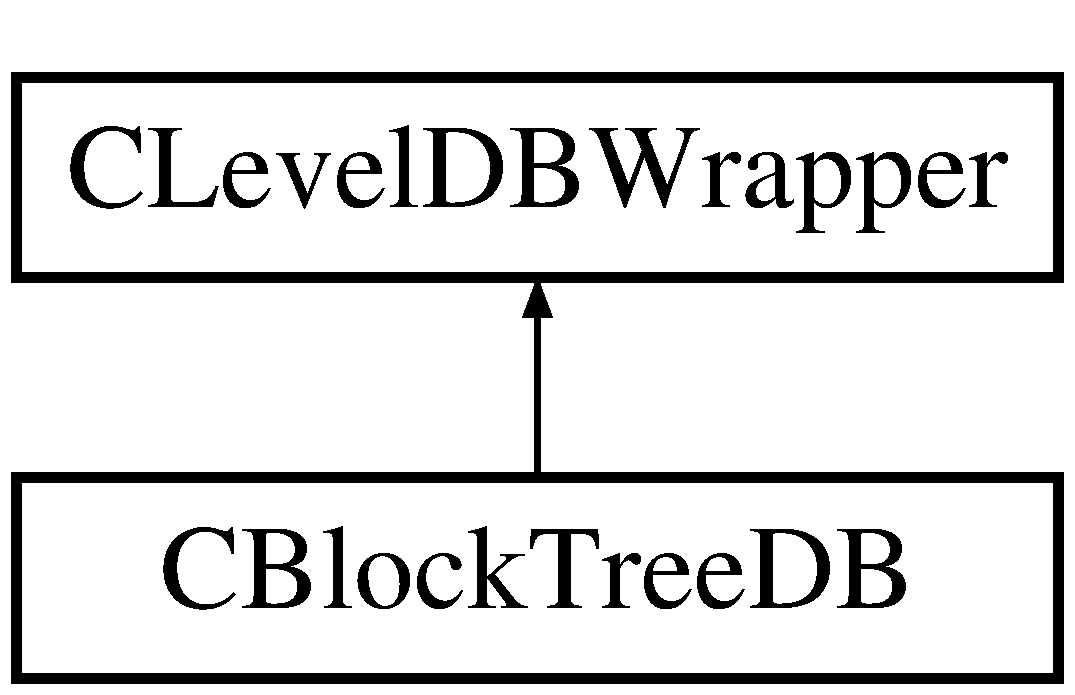
\includegraphics[height=2.000000cm]{class_c_block_tree_d_b}
\end{center}
\end{figure}
\subsection*{Public Member Functions}
\begin{DoxyCompactItemize}
\item 
\hyperlink{class_c_block_tree_d_b_a52fd1b1dc02c2a4e977099e2c2c50424}{C\+Block\+Tree\+D\+B} (size\+\_\+t n\+Cache\+Size, bool f\+Memory=false, bool f\+Wipe=false)
\item 
bool \hyperlink{class_c_block_tree_d_b_aa4b53c1cae368f02f56244af5f2499d7}{Write\+Batch\+Sync} (const std\+::vector$<$ std\+::pair$<$ int, const \hyperlink{class_c_block_file_info}{C\+Block\+File\+Info} $\ast$ $>$ $>$ \&file\+Info, int n\+Last\+File, const std\+::vector$<$ const \hyperlink{class_c_block_index}{C\+Block\+Index} $\ast$ $>$ \&blockinfo)
\item 
bool \hyperlink{class_c_block_tree_d_b_a6f951198dc53fbe9194626ff82638656}{Read\+Block\+File\+Info} (int n\+File, \hyperlink{class_c_block_file_info}{C\+Block\+File\+Info} \&fileinfo)
\item 
bool \hyperlink{class_c_block_tree_d_b_adb1276fe2f0e0c4c106660948c581711}{Read\+Last\+Block\+File} (int \&n\+File)
\item 
bool \hyperlink{class_c_block_tree_d_b_a8fa5d150b98f4fd1aa8cf503eddfccef}{Write\+Reindexing} (bool \hyperlink{main_8h_a8e0eca589b2d4254a65f04c5d91888b2}{f\+Reindex})
\item 
bool \hyperlink{class_c_block_tree_d_b_a1abf6fc392048428aa24a12b7942824b}{Read\+Reindexing} (bool \&\hyperlink{main_8h_a8e0eca589b2d4254a65f04c5d91888b2}{f\+Reindex})
\item 
bool \hyperlink{class_c_block_tree_d_b_a74383427266d627e84c2d0c8e21e03c7}{Read\+Tx\+Index} (const \hyperlink{classuint256}{uint256} \&txid, \hyperlink{struct_c_disk_tx_pos}{C\+Disk\+Tx\+Pos} \&pos)
\item 
bool \hyperlink{class_c_block_tree_d_b_a1e03745f9675ad352a1483a0aa7ef308}{Write\+Tx\+Index} (const std\+::vector$<$ std\+::pair$<$ \hyperlink{classuint256}{uint256}, \hyperlink{struct_c_disk_tx_pos}{C\+Disk\+Tx\+Pos} $>$ $>$ \&list)
\item 
bool \hyperlink{class_c_block_tree_d_b_af2f65b70ac5d8a198d4f29a7e909c08a}{Write\+Flag} (const std\+::string \&\hyperlink{rest_8cpp_a8f8f80d37794cde9472343e4487ba3eb}{name}, bool f\+Value)
\item 
bool \hyperlink{class_c_block_tree_d_b_acd779c4653fd9a87fffe95d53ce7c6d3}{Read\+Flag} (const std\+::string \&\hyperlink{rest_8cpp_a8f8f80d37794cde9472343e4487ba3eb}{name}, bool \&f\+Value)
\item 
bool \hyperlink{class_c_block_tree_d_b_a12be19bb1d7253eeb40e1aa88b032346}{Load\+Block\+Index\+Guts} ()
\end{DoxyCompactItemize}


\subsection{Detailed Description}
Access to the block database (blocks/index/) 

\subsection{Constructor \& Destructor Documentation}
\hypertarget{class_c_block_tree_d_b_a52fd1b1dc02c2a4e977099e2c2c50424}{}\index{C\+Block\+Tree\+D\+B@{C\+Block\+Tree\+D\+B}!C\+Block\+Tree\+D\+B@{C\+Block\+Tree\+D\+B}}
\index{C\+Block\+Tree\+D\+B@{C\+Block\+Tree\+D\+B}!C\+Block\+Tree\+D\+B@{C\+Block\+Tree\+D\+B}}
\subsubsection[{C\+Block\+Tree\+D\+B}]{\setlength{\rightskip}{0pt plus 5cm}C\+Block\+Tree\+D\+B\+::\+C\+Block\+Tree\+D\+B (
\begin{DoxyParamCaption}
\item[{size\+\_\+t}]{n\+Cache\+Size, }
\item[{bool}]{f\+Memory = {\ttfamily false}, }
\item[{bool}]{f\+Wipe = {\ttfamily false}}
\end{DoxyParamCaption}
)}\label{class_c_block_tree_d_b_a52fd1b1dc02c2a4e977099e2c2c50424}


\subsection{Member Function Documentation}
\hypertarget{class_c_block_tree_d_b_a12be19bb1d7253eeb40e1aa88b032346}{}\index{C\+Block\+Tree\+D\+B@{C\+Block\+Tree\+D\+B}!Load\+Block\+Index\+Guts@{Load\+Block\+Index\+Guts}}
\index{Load\+Block\+Index\+Guts@{Load\+Block\+Index\+Guts}!C\+Block\+Tree\+D\+B@{C\+Block\+Tree\+D\+B}}
\subsubsection[{Load\+Block\+Index\+Guts}]{\setlength{\rightskip}{0pt plus 5cm}bool C\+Block\+Tree\+D\+B\+::\+Load\+Block\+Index\+Guts (
\begin{DoxyParamCaption}
{}
\end{DoxyParamCaption}
)}\label{class_c_block_tree_d_b_a12be19bb1d7253eeb40e1aa88b032346}
\hypertarget{class_c_block_tree_d_b_a6f951198dc53fbe9194626ff82638656}{}\index{C\+Block\+Tree\+D\+B@{C\+Block\+Tree\+D\+B}!Read\+Block\+File\+Info@{Read\+Block\+File\+Info}}
\index{Read\+Block\+File\+Info@{Read\+Block\+File\+Info}!C\+Block\+Tree\+D\+B@{C\+Block\+Tree\+D\+B}}
\subsubsection[{Read\+Block\+File\+Info}]{\setlength{\rightskip}{0pt plus 5cm}bool C\+Block\+Tree\+D\+B\+::\+Read\+Block\+File\+Info (
\begin{DoxyParamCaption}
\item[{int}]{n\+File, }
\item[{{\bf C\+Block\+File\+Info} \&}]{fileinfo}
\end{DoxyParamCaption}
)}\label{class_c_block_tree_d_b_a6f951198dc53fbe9194626ff82638656}
\hypertarget{class_c_block_tree_d_b_acd779c4653fd9a87fffe95d53ce7c6d3}{}\index{C\+Block\+Tree\+D\+B@{C\+Block\+Tree\+D\+B}!Read\+Flag@{Read\+Flag}}
\index{Read\+Flag@{Read\+Flag}!C\+Block\+Tree\+D\+B@{C\+Block\+Tree\+D\+B}}
\subsubsection[{Read\+Flag}]{\setlength{\rightskip}{0pt plus 5cm}bool C\+Block\+Tree\+D\+B\+::\+Read\+Flag (
\begin{DoxyParamCaption}
\item[{const std\+::string \&}]{name, }
\item[{bool \&}]{f\+Value}
\end{DoxyParamCaption}
)}\label{class_c_block_tree_d_b_acd779c4653fd9a87fffe95d53ce7c6d3}
\hypertarget{class_c_block_tree_d_b_adb1276fe2f0e0c4c106660948c581711}{}\index{C\+Block\+Tree\+D\+B@{C\+Block\+Tree\+D\+B}!Read\+Last\+Block\+File@{Read\+Last\+Block\+File}}
\index{Read\+Last\+Block\+File@{Read\+Last\+Block\+File}!C\+Block\+Tree\+D\+B@{C\+Block\+Tree\+D\+B}}
\subsubsection[{Read\+Last\+Block\+File}]{\setlength{\rightskip}{0pt plus 5cm}bool C\+Block\+Tree\+D\+B\+::\+Read\+Last\+Block\+File (
\begin{DoxyParamCaption}
\item[{int \&}]{n\+File}
\end{DoxyParamCaption}
)}\label{class_c_block_tree_d_b_adb1276fe2f0e0c4c106660948c581711}
\hypertarget{class_c_block_tree_d_b_a1abf6fc392048428aa24a12b7942824b}{}\index{C\+Block\+Tree\+D\+B@{C\+Block\+Tree\+D\+B}!Read\+Reindexing@{Read\+Reindexing}}
\index{Read\+Reindexing@{Read\+Reindexing}!C\+Block\+Tree\+D\+B@{C\+Block\+Tree\+D\+B}}
\subsubsection[{Read\+Reindexing}]{\setlength{\rightskip}{0pt plus 5cm}bool C\+Block\+Tree\+D\+B\+::\+Read\+Reindexing (
\begin{DoxyParamCaption}
\item[{bool \&}]{f\+Reindex}
\end{DoxyParamCaption}
)}\label{class_c_block_tree_d_b_a1abf6fc392048428aa24a12b7942824b}
\hypertarget{class_c_block_tree_d_b_a74383427266d627e84c2d0c8e21e03c7}{}\index{C\+Block\+Tree\+D\+B@{C\+Block\+Tree\+D\+B}!Read\+Tx\+Index@{Read\+Tx\+Index}}
\index{Read\+Tx\+Index@{Read\+Tx\+Index}!C\+Block\+Tree\+D\+B@{C\+Block\+Tree\+D\+B}}
\subsubsection[{Read\+Tx\+Index}]{\setlength{\rightskip}{0pt plus 5cm}bool C\+Block\+Tree\+D\+B\+::\+Read\+Tx\+Index (
\begin{DoxyParamCaption}
\item[{const {\bf uint256} \&}]{txid, }
\item[{{\bf C\+Disk\+Tx\+Pos} \&}]{pos}
\end{DoxyParamCaption}
)}\label{class_c_block_tree_d_b_a74383427266d627e84c2d0c8e21e03c7}
\hypertarget{class_c_block_tree_d_b_aa4b53c1cae368f02f56244af5f2499d7}{}\index{C\+Block\+Tree\+D\+B@{C\+Block\+Tree\+D\+B}!Write\+Batch\+Sync@{Write\+Batch\+Sync}}
\index{Write\+Batch\+Sync@{Write\+Batch\+Sync}!C\+Block\+Tree\+D\+B@{C\+Block\+Tree\+D\+B}}
\subsubsection[{Write\+Batch\+Sync}]{\setlength{\rightskip}{0pt plus 5cm}bool C\+Block\+Tree\+D\+B\+::\+Write\+Batch\+Sync (
\begin{DoxyParamCaption}
\item[{const std\+::vector$<$ std\+::pair$<$ int, const {\bf C\+Block\+File\+Info} $\ast$ $>$ $>$ \&}]{file\+Info, }
\item[{int}]{n\+Last\+File, }
\item[{const std\+::vector$<$ const {\bf C\+Block\+Index} $\ast$ $>$ \&}]{blockinfo}
\end{DoxyParamCaption}
)}\label{class_c_block_tree_d_b_aa4b53c1cae368f02f56244af5f2499d7}
\hypertarget{class_c_block_tree_d_b_af2f65b70ac5d8a198d4f29a7e909c08a}{}\index{C\+Block\+Tree\+D\+B@{C\+Block\+Tree\+D\+B}!Write\+Flag@{Write\+Flag}}
\index{Write\+Flag@{Write\+Flag}!C\+Block\+Tree\+D\+B@{C\+Block\+Tree\+D\+B}}
\subsubsection[{Write\+Flag}]{\setlength{\rightskip}{0pt plus 5cm}bool C\+Block\+Tree\+D\+B\+::\+Write\+Flag (
\begin{DoxyParamCaption}
\item[{const std\+::string \&}]{name, }
\item[{bool}]{f\+Value}
\end{DoxyParamCaption}
)}\label{class_c_block_tree_d_b_af2f65b70ac5d8a198d4f29a7e909c08a}
\hypertarget{class_c_block_tree_d_b_a8fa5d150b98f4fd1aa8cf503eddfccef}{}\index{C\+Block\+Tree\+D\+B@{C\+Block\+Tree\+D\+B}!Write\+Reindexing@{Write\+Reindexing}}
\index{Write\+Reindexing@{Write\+Reindexing}!C\+Block\+Tree\+D\+B@{C\+Block\+Tree\+D\+B}}
\subsubsection[{Write\+Reindexing}]{\setlength{\rightskip}{0pt plus 5cm}bool C\+Block\+Tree\+D\+B\+::\+Write\+Reindexing (
\begin{DoxyParamCaption}
\item[{bool}]{f\+Reindex}
\end{DoxyParamCaption}
)}\label{class_c_block_tree_d_b_a8fa5d150b98f4fd1aa8cf503eddfccef}
\hypertarget{class_c_block_tree_d_b_a1e03745f9675ad352a1483a0aa7ef308}{}\index{C\+Block\+Tree\+D\+B@{C\+Block\+Tree\+D\+B}!Write\+Tx\+Index@{Write\+Tx\+Index}}
\index{Write\+Tx\+Index@{Write\+Tx\+Index}!C\+Block\+Tree\+D\+B@{C\+Block\+Tree\+D\+B}}
\subsubsection[{Write\+Tx\+Index}]{\setlength{\rightskip}{0pt plus 5cm}bool C\+Block\+Tree\+D\+B\+::\+Write\+Tx\+Index (
\begin{DoxyParamCaption}
\item[{const std\+::vector$<$ std\+::pair$<$ {\bf uint256}, {\bf C\+Disk\+Tx\+Pos} $>$ $>$ \&}]{list}
\end{DoxyParamCaption}
)}\label{class_c_block_tree_d_b_a1e03745f9675ad352a1483a0aa7ef308}


The documentation for this class was generated from the following files\+:\begin{DoxyCompactItemize}
\item 
C\+:/\+Users/\+Joe/\+Documents/\+School/\+C\+S\+C17\+A/bitcoin/src/\hyperlink{txdb_8h}{txdb.\+h}\item 
C\+:/\+Users/\+Joe/\+Documents/\+School/\+C\+S\+C17\+A/bitcoin/src/\hyperlink{txdb_8cpp}{txdb.\+cpp}\end{DoxyCompactItemize}

\hypertarget{class_c_block_undo}{}\section{C\+Block\+Undo Class Reference}
\label{class_c_block_undo}\index{C\+Block\+Undo@{C\+Block\+Undo}}


{\ttfamily \#include $<$undo.\+h$>$}

\subsection*{Public Member Functions}
\begin{DoxyCompactItemize}
\item 
{\footnotesize template$<$typename Stream , typename Operation $>$ }\\void \hyperlink{class_c_block_undo_ad4d50e2b34e291dbe2d15fbe3ae3670b}{Serialization\+Op} (Stream \&s, Operation ser\+\_\+action, int n\+Type, int n\+Version)
\end{DoxyCompactItemize}
\subsection*{Public Attributes}
\begin{DoxyCompactItemize}
\item 
std\+::vector$<$ \hyperlink{class_c_tx_undo}{C\+Tx\+Undo} $>$ \hyperlink{class_c_block_undo_ad0baf7a4d3634b27b4affac2e7cf75c9}{vtxundo}
\item 
\hyperlink{class_c_block_undo_a4fecc9723902f51e25b57e2e2d45334a}{A\+D\+D\+\_\+\+S\+E\+R\+I\+A\+L\+I\+Z\+E\+\_\+\+M\+E\+T\+H\+O\+D\+S}
\end{DoxyCompactItemize}


\subsection{Detailed Description}
Undo information for a C\+Block 

\subsection{Member Function Documentation}
\hypertarget{class_c_block_undo_ad4d50e2b34e291dbe2d15fbe3ae3670b}{}\index{C\+Block\+Undo@{C\+Block\+Undo}!Serialization\+Op@{Serialization\+Op}}
\index{Serialization\+Op@{Serialization\+Op}!C\+Block\+Undo@{C\+Block\+Undo}}
\subsubsection[{Serialization\+Op}]{\setlength{\rightskip}{0pt plus 5cm}template$<$typename Stream , typename Operation $>$ void C\+Block\+Undo\+::\+Serialization\+Op (
\begin{DoxyParamCaption}
\item[{Stream \&}]{s, }
\item[{Operation}]{ser\+\_\+action, }
\item[{int}]{n\+Type, }
\item[{int}]{n\+Version}
\end{DoxyParamCaption}
)\hspace{0.3cm}{\ttfamily [inline]}}\label{class_c_block_undo_ad4d50e2b34e291dbe2d15fbe3ae3670b}


\subsection{Member Data Documentation}
\hypertarget{class_c_block_undo_a4fecc9723902f51e25b57e2e2d45334a}{}\index{C\+Block\+Undo@{C\+Block\+Undo}!A\+D\+D\+\_\+\+S\+E\+R\+I\+A\+L\+I\+Z\+E\+\_\+\+M\+E\+T\+H\+O\+D\+S@{A\+D\+D\+\_\+\+S\+E\+R\+I\+A\+L\+I\+Z\+E\+\_\+\+M\+E\+T\+H\+O\+D\+S}}
\index{A\+D\+D\+\_\+\+S\+E\+R\+I\+A\+L\+I\+Z\+E\+\_\+\+M\+E\+T\+H\+O\+D\+S@{A\+D\+D\+\_\+\+S\+E\+R\+I\+A\+L\+I\+Z\+E\+\_\+\+M\+E\+T\+H\+O\+D\+S}!C\+Block\+Undo@{C\+Block\+Undo}}
\subsubsection[{A\+D\+D\+\_\+\+S\+E\+R\+I\+A\+L\+I\+Z\+E\+\_\+\+M\+E\+T\+H\+O\+D\+S}]{\setlength{\rightskip}{0pt plus 5cm}C\+Block\+Undo\+::\+A\+D\+D\+\_\+\+S\+E\+R\+I\+A\+L\+I\+Z\+E\+\_\+\+M\+E\+T\+H\+O\+D\+S}\label{class_c_block_undo_a4fecc9723902f51e25b57e2e2d45334a}
\hypertarget{class_c_block_undo_ad0baf7a4d3634b27b4affac2e7cf75c9}{}\index{C\+Block\+Undo@{C\+Block\+Undo}!vtxundo@{vtxundo}}
\index{vtxundo@{vtxundo}!C\+Block\+Undo@{C\+Block\+Undo}}
\subsubsection[{vtxundo}]{\setlength{\rightskip}{0pt plus 5cm}std\+::vector$<${\bf C\+Tx\+Undo}$>$ C\+Block\+Undo\+::vtxundo}\label{class_c_block_undo_ad0baf7a4d3634b27b4affac2e7cf75c9}


The documentation for this class was generated from the following file\+:\begin{DoxyCompactItemize}
\item 
C\+:/\+Users/\+Joe/\+Documents/\+School/\+C\+S\+C17\+A/bitcoin/src/\hyperlink{undo_8h}{undo.\+h}\end{DoxyCompactItemize}

\hypertarget{class_c_bloom_filter}{}\section{C\+Bloom\+Filter Class Reference}
\label{class_c_bloom_filter}\index{C\+Bloom\+Filter@{C\+Bloom\+Filter}}


{\ttfamily \#include $<$bloom.\+h$>$}

\subsection*{Public Member Functions}
\begin{DoxyCompactItemize}
\item 
\hyperlink{class_c_bloom_filter_a6395cfcb278ed9cf4ae873549c996f83}{C\+Bloom\+Filter} (unsigned int n\+Elements, double n\+F\+P\+Rate, unsigned int n\+Tweak, unsigned char n\+Flags\+In)
\item 
\hyperlink{class_c_bloom_filter_ab38a984b1020bc4afd85c06e90353b28}{C\+Bloom\+Filter} ()
\item 
{\footnotesize template$<$typename Stream , typename Operation $>$ }\\void \hyperlink{class_c_bloom_filter_a2d12234d7febc6197a7349d609733cca}{Serialization\+Op} (Stream \&s, Operation ser\+\_\+action, int n\+Type, int n\+Version)
\item 
void \hyperlink{class_c_bloom_filter_abba52843c7c691ef7deb07d9a645dcc2}{insert} (const std\+::vector$<$ unsigned char $>$ \&v\+Key)
\item 
void \hyperlink{class_c_bloom_filter_aa77e023fc94fd17a0532bf17906e2146}{insert} (const C\+Out\+Point \&outpoint)
\item 
void \hyperlink{class_c_bloom_filter_ac86479ac4ac157a7f0188baaa93202cb}{insert} (const \hyperlink{classuint256}{uint256} \&hash)
\item 
bool \hyperlink{class_c_bloom_filter_ac86c47e17a6e3d1cae4f581accc70e72}{contains} (const std\+::vector$<$ unsigned char $>$ \&v\+Key) const 
\item 
bool \hyperlink{class_c_bloom_filter_a962136f96fb6b237613259b18b34ba6d}{contains} (const C\+Out\+Point \&outpoint) const 
\item 
bool \hyperlink{class_c_bloom_filter_a7b4d06836a811a7282fb60f0697b2e1c}{contains} (const \hyperlink{classuint256}{uint256} \&hash) const 
\item 
void \hyperlink{class_c_bloom_filter_abf30228c0b24c57530f6b6734cd40252}{clear} ()
\item 
bool \hyperlink{class_c_bloom_filter_a9f206ba4f552b62d4a0cd9a1bbe3b48c}{Is\+Within\+Size\+Constraints} () const 
\item 
bool \hyperlink{class_c_bloom_filter_aec420a9b66ab133090c2b4b8ed286f79}{Is\+Relevant\+And\+Update} (const C\+Transaction \&tx)
\begin{DoxyCompactList}\small\item\em Also adds any outputs which match the filter to the filter (to match their spending txes) \end{DoxyCompactList}\item 
void \hyperlink{class_c_bloom_filter_af98b43e91c82a1e4afc7454e8c5672c2}{Update\+Empty\+Full} ()
\begin{DoxyCompactList}\small\item\em Checks for empty and full filters to avoid wasting cpu. \end{DoxyCompactList}\end{DoxyCompactItemize}
\subsection*{Public Attributes}
\begin{DoxyCompactItemize}
\item 
\hyperlink{class_c_bloom_filter_aac1b6a065059e07177ec836929190ad0}{A\+D\+D\+\_\+\+S\+E\+R\+I\+A\+L\+I\+Z\+E\+\_\+\+M\+E\+T\+H\+O\+D\+S}
\end{DoxyCompactItemize}


\subsection{Detailed Description}
Bloom\+Filter is a probabilistic filter which S\+P\+V clients provide so that we can filter the transactions we sends them.

This allows for significantly more efficient transaction and block downloads.

Because bloom filters are probabilistic, an S\+P\+V node can increase the false-\/ positive rate, making us send them transactions which aren\textquotesingle{}t actually theirs, allowing clients to trade more bandwidth for more privacy by obfuscating which keys are owned by them. 

\subsection{Constructor \& Destructor Documentation}
\hypertarget{class_c_bloom_filter_a6395cfcb278ed9cf4ae873549c996f83}{}\index{C\+Bloom\+Filter@{C\+Bloom\+Filter}!C\+Bloom\+Filter@{C\+Bloom\+Filter}}
\index{C\+Bloom\+Filter@{C\+Bloom\+Filter}!C\+Bloom\+Filter@{C\+Bloom\+Filter}}
\subsubsection[{C\+Bloom\+Filter}]{\setlength{\rightskip}{0pt plus 5cm}C\+Bloom\+Filter\+::\+C\+Bloom\+Filter (
\begin{DoxyParamCaption}
\item[{unsigned int}]{n\+Elements, }
\item[{double}]{n\+F\+P\+Rate, }
\item[{unsigned int}]{n\+Tweak\+In, }
\item[{unsigned char}]{n\+Flags\+In}
\end{DoxyParamCaption}
)}\label{class_c_bloom_filter_a6395cfcb278ed9cf4ae873549c996f83}
Creates a new bloom filter which will provide the given fp rate when filled with the given number of elements Note that if the given parameters will result in a filter outside the bounds of the protocol limits, the filter created will be as close to the given parameters as possible within the protocol limits. This will apply if n\+F\+P\+Rate is very low or n\+Elements is unreasonably high. n\+Tweak is a constant which is added to the seed value passed to the hash function It should generally always be a random value (and is largely only exposed for unit testing) n\+Flags should be one of the B\+L\+O\+O\+M\+\_\+\+U\+P\+D\+A\+T\+E\+\_\+$\ast$ enums (not \+\_\+\+M\+A\+S\+K)

The ideal size for a bloom filter with a given number of elements and false positive rate is\+:
\begin{DoxyItemize}
\item n\+Elements $\ast$ log(fp rate) / ln(2)$^\wedge$2 We ignore filter parameters which will create a bloom filter larger than the protocol limits The ideal number of hash functions is filter size $\ast$ ln(2) / number of elements Again, we ignore filter parameters which will create a bloom filter with more hash functions than the protocol limits See \href{https://en.wikipedia.org/wiki/Bloom_filter}{\tt https\+://en.\+wikipedia.\+org/wiki/\+Bloom\+\_\+filter} for an explanation of these formulas 
\end{DoxyItemize}\hypertarget{class_c_bloom_filter_ab38a984b1020bc4afd85c06e90353b28}{}\index{C\+Bloom\+Filter@{C\+Bloom\+Filter}!C\+Bloom\+Filter@{C\+Bloom\+Filter}}
\index{C\+Bloom\+Filter@{C\+Bloom\+Filter}!C\+Bloom\+Filter@{C\+Bloom\+Filter}}
\subsubsection[{C\+Bloom\+Filter}]{\setlength{\rightskip}{0pt plus 5cm}C\+Bloom\+Filter\+::\+C\+Bloom\+Filter (
\begin{DoxyParamCaption}
{}
\end{DoxyParamCaption}
)\hspace{0.3cm}{\ttfamily [inline]}}\label{class_c_bloom_filter_ab38a984b1020bc4afd85c06e90353b28}


\subsection{Member Function Documentation}
\hypertarget{class_c_bloom_filter_abf30228c0b24c57530f6b6734cd40252}{}\index{C\+Bloom\+Filter@{C\+Bloom\+Filter}!clear@{clear}}
\index{clear@{clear}!C\+Bloom\+Filter@{C\+Bloom\+Filter}}
\subsubsection[{clear}]{\setlength{\rightskip}{0pt plus 5cm}void C\+Bloom\+Filter\+::clear (
\begin{DoxyParamCaption}
{}
\end{DoxyParamCaption}
)}\label{class_c_bloom_filter_abf30228c0b24c57530f6b6734cd40252}
\hypertarget{class_c_bloom_filter_ac86c47e17a6e3d1cae4f581accc70e72}{}\index{C\+Bloom\+Filter@{C\+Bloom\+Filter}!contains@{contains}}
\index{contains@{contains}!C\+Bloom\+Filter@{C\+Bloom\+Filter}}
\subsubsection[{contains}]{\setlength{\rightskip}{0pt plus 5cm}bool C\+Bloom\+Filter\+::contains (
\begin{DoxyParamCaption}
\item[{const std\+::vector$<$ unsigned char $>$ \&}]{v\+Key}
\end{DoxyParamCaption}
) const}\label{class_c_bloom_filter_ac86c47e17a6e3d1cae4f581accc70e72}
\hypertarget{class_c_bloom_filter_a962136f96fb6b237613259b18b34ba6d}{}\index{C\+Bloom\+Filter@{C\+Bloom\+Filter}!contains@{contains}}
\index{contains@{contains}!C\+Bloom\+Filter@{C\+Bloom\+Filter}}
\subsubsection[{contains}]{\setlength{\rightskip}{0pt plus 5cm}bool C\+Bloom\+Filter\+::contains (
\begin{DoxyParamCaption}
\item[{const C\+Out\+Point \&}]{outpoint}
\end{DoxyParamCaption}
) const}\label{class_c_bloom_filter_a962136f96fb6b237613259b18b34ba6d}
\hypertarget{class_c_bloom_filter_a7b4d06836a811a7282fb60f0697b2e1c}{}\index{C\+Bloom\+Filter@{C\+Bloom\+Filter}!contains@{contains}}
\index{contains@{contains}!C\+Bloom\+Filter@{C\+Bloom\+Filter}}
\subsubsection[{contains}]{\setlength{\rightskip}{0pt plus 5cm}bool C\+Bloom\+Filter\+::contains (
\begin{DoxyParamCaption}
\item[{const {\bf uint256} \&}]{hash}
\end{DoxyParamCaption}
) const}\label{class_c_bloom_filter_a7b4d06836a811a7282fb60f0697b2e1c}
\hypertarget{class_c_bloom_filter_abba52843c7c691ef7deb07d9a645dcc2}{}\index{C\+Bloom\+Filter@{C\+Bloom\+Filter}!insert@{insert}}
\index{insert@{insert}!C\+Bloom\+Filter@{C\+Bloom\+Filter}}
\subsubsection[{insert}]{\setlength{\rightskip}{0pt plus 5cm}void C\+Bloom\+Filter\+::insert (
\begin{DoxyParamCaption}
\item[{const std\+::vector$<$ unsigned char $>$ \&}]{v\+Key}
\end{DoxyParamCaption}
)}\label{class_c_bloom_filter_abba52843c7c691ef7deb07d9a645dcc2}
\hypertarget{class_c_bloom_filter_aa77e023fc94fd17a0532bf17906e2146}{}\index{C\+Bloom\+Filter@{C\+Bloom\+Filter}!insert@{insert}}
\index{insert@{insert}!C\+Bloom\+Filter@{C\+Bloom\+Filter}}
\subsubsection[{insert}]{\setlength{\rightskip}{0pt plus 5cm}void C\+Bloom\+Filter\+::insert (
\begin{DoxyParamCaption}
\item[{const C\+Out\+Point \&}]{outpoint}
\end{DoxyParamCaption}
)}\label{class_c_bloom_filter_aa77e023fc94fd17a0532bf17906e2146}
\hypertarget{class_c_bloom_filter_ac86479ac4ac157a7f0188baaa93202cb}{}\index{C\+Bloom\+Filter@{C\+Bloom\+Filter}!insert@{insert}}
\index{insert@{insert}!C\+Bloom\+Filter@{C\+Bloom\+Filter}}
\subsubsection[{insert}]{\setlength{\rightskip}{0pt plus 5cm}void C\+Bloom\+Filter\+::insert (
\begin{DoxyParamCaption}
\item[{const {\bf uint256} \&}]{hash}
\end{DoxyParamCaption}
)}\label{class_c_bloom_filter_ac86479ac4ac157a7f0188baaa93202cb}
\hypertarget{class_c_bloom_filter_aec420a9b66ab133090c2b4b8ed286f79}{}\index{C\+Bloom\+Filter@{C\+Bloom\+Filter}!Is\+Relevant\+And\+Update@{Is\+Relevant\+And\+Update}}
\index{Is\+Relevant\+And\+Update@{Is\+Relevant\+And\+Update}!C\+Bloom\+Filter@{C\+Bloom\+Filter}}
\subsubsection[{Is\+Relevant\+And\+Update}]{\setlength{\rightskip}{0pt plus 5cm}bool C\+Bloom\+Filter\+::\+Is\+Relevant\+And\+Update (
\begin{DoxyParamCaption}
\item[{const C\+Transaction \&}]{tx}
\end{DoxyParamCaption}
)}\label{class_c_bloom_filter_aec420a9b66ab133090c2b4b8ed286f79}


Also adds any outputs which match the filter to the filter (to match their spending txes) 

\hypertarget{class_c_bloom_filter_a9f206ba4f552b62d4a0cd9a1bbe3b48c}{}\index{C\+Bloom\+Filter@{C\+Bloom\+Filter}!Is\+Within\+Size\+Constraints@{Is\+Within\+Size\+Constraints}}
\index{Is\+Within\+Size\+Constraints@{Is\+Within\+Size\+Constraints}!C\+Bloom\+Filter@{C\+Bloom\+Filter}}
\subsubsection[{Is\+Within\+Size\+Constraints}]{\setlength{\rightskip}{0pt plus 5cm}bool C\+Bloom\+Filter\+::\+Is\+Within\+Size\+Constraints (
\begin{DoxyParamCaption}
{}
\end{DoxyParamCaption}
) const}\label{class_c_bloom_filter_a9f206ba4f552b62d4a0cd9a1bbe3b48c}
True if the size is $<$= M\+A\+X\+\_\+\+B\+L\+O\+O\+M\+\_\+\+F\+I\+L\+T\+E\+R\+\_\+\+S\+I\+Z\+E and the number of hash functions is $<$= M\+A\+X\+\_\+\+H\+A\+S\+H\+\_\+\+F\+U\+N\+C\+S (catch a filter which was just deserialized which was too big) \hypertarget{class_c_bloom_filter_a2d12234d7febc6197a7349d609733cca}{}\index{C\+Bloom\+Filter@{C\+Bloom\+Filter}!Serialization\+Op@{Serialization\+Op}}
\index{Serialization\+Op@{Serialization\+Op}!C\+Bloom\+Filter@{C\+Bloom\+Filter}}
\subsubsection[{Serialization\+Op}]{\setlength{\rightskip}{0pt plus 5cm}template$<$typename Stream , typename Operation $>$ void C\+Bloom\+Filter\+::\+Serialization\+Op (
\begin{DoxyParamCaption}
\item[{Stream \&}]{s, }
\item[{Operation}]{ser\+\_\+action, }
\item[{int}]{n\+Type, }
\item[{int}]{n\+Version}
\end{DoxyParamCaption}
)\hspace{0.3cm}{\ttfamily [inline]}}\label{class_c_bloom_filter_a2d12234d7febc6197a7349d609733cca}
\hypertarget{class_c_bloom_filter_af98b43e91c82a1e4afc7454e8c5672c2}{}\index{C\+Bloom\+Filter@{C\+Bloom\+Filter}!Update\+Empty\+Full@{Update\+Empty\+Full}}
\index{Update\+Empty\+Full@{Update\+Empty\+Full}!C\+Bloom\+Filter@{C\+Bloom\+Filter}}
\subsubsection[{Update\+Empty\+Full}]{\setlength{\rightskip}{0pt plus 5cm}void C\+Bloom\+Filter\+::\+Update\+Empty\+Full (
\begin{DoxyParamCaption}
{}
\end{DoxyParamCaption}
)}\label{class_c_bloom_filter_af98b43e91c82a1e4afc7454e8c5672c2}


Checks for empty and full filters to avoid wasting cpu. 



\subsection{Member Data Documentation}
\hypertarget{class_c_bloom_filter_aac1b6a065059e07177ec836929190ad0}{}\index{C\+Bloom\+Filter@{C\+Bloom\+Filter}!A\+D\+D\+\_\+\+S\+E\+R\+I\+A\+L\+I\+Z\+E\+\_\+\+M\+E\+T\+H\+O\+D\+S@{A\+D\+D\+\_\+\+S\+E\+R\+I\+A\+L\+I\+Z\+E\+\_\+\+M\+E\+T\+H\+O\+D\+S}}
\index{A\+D\+D\+\_\+\+S\+E\+R\+I\+A\+L\+I\+Z\+E\+\_\+\+M\+E\+T\+H\+O\+D\+S@{A\+D\+D\+\_\+\+S\+E\+R\+I\+A\+L\+I\+Z\+E\+\_\+\+M\+E\+T\+H\+O\+D\+S}!C\+Bloom\+Filter@{C\+Bloom\+Filter}}
\subsubsection[{A\+D\+D\+\_\+\+S\+E\+R\+I\+A\+L\+I\+Z\+E\+\_\+\+M\+E\+T\+H\+O\+D\+S}]{\setlength{\rightskip}{0pt plus 5cm}C\+Bloom\+Filter\+::\+A\+D\+D\+\_\+\+S\+E\+R\+I\+A\+L\+I\+Z\+E\+\_\+\+M\+E\+T\+H\+O\+D\+S}\label{class_c_bloom_filter_aac1b6a065059e07177ec836929190ad0}


The documentation for this class was generated from the following files\+:\begin{DoxyCompactItemize}
\item 
C\+:/\+Users/\+Joe/\+Documents/\+School/\+C\+S\+C17\+A/bitcoin/src/\hyperlink{bloom_8h}{bloom.\+h}\item 
C\+:/\+Users/\+Joe/\+Documents/\+School/\+C\+S\+C17\+A/bitcoin/src/\hyperlink{bloom_8cpp}{bloom.\+cpp}\end{DoxyCompactItemize}

\hypertarget{class_c_buffered_file}{}\section{C\+Buffered\+File Class Reference}
\label{class_c_buffered_file}\index{C\+Buffered\+File@{C\+Buffered\+File}}


{\ttfamily \#include $<$streams.\+h$>$}

\subsection*{Public Member Functions}
\begin{DoxyCompactItemize}
\item 
\hyperlink{class_c_buffered_file_a30ad96a8d09bed60355d1fadda7dabdc}{C\+Buffered\+File} (F\+I\+L\+E $\ast$file\+In, uint64\+\_\+t n\+Buf\+Size, uint64\+\_\+t n\+Rewind\+In, int n\+Type\+In, int n\+Version\+In)
\item 
\hyperlink{class_c_buffered_file_a8804f689b27d3298cd5d63fbcddb97d1}{$\sim$\+C\+Buffered\+File} ()
\item 
void \hyperlink{class_c_buffered_file_aef8c993fe3eb0fa423d09d095f40dcf6}{fclose} ()
\item 
bool \hyperlink{class_c_buffered_file_abc0a2462d47ae5ba23c258291509dd6d}{eof} () const 
\item 
\hyperlink{class_c_buffered_file}{C\+Buffered\+File} \& \hyperlink{class_c_buffered_file_a20c6d2a4dbc69a8e5c7ba766d04b3d85}{read} (char $\ast$pch, size\+\_\+t n\+Size)
\item 
uint64\+\_\+t \hyperlink{class_c_buffered_file_af9e7226e682ede9c1c141fb2972afd7b}{Get\+Pos} ()
\item 
bool \hyperlink{class_c_buffered_file_aac4029a9aade127cc8a1fbbcc1549599}{Set\+Pos} (uint64\+\_\+t n\+Pos)
\item 
bool \hyperlink{class_c_buffered_file_afbf9abcc70f24824661aec96a4310a63}{Seek} (uint64\+\_\+t n\+Pos)
\item 
bool \hyperlink{class_c_buffered_file_adfcf370a41be0454e0f6b3dc358e415c}{Set\+Limit} (uint64\+\_\+t n\+Pos=(uint64\+\_\+t)(-\/1))
\item 
{\footnotesize template$<$typename T $>$ }\\\hyperlink{class_c_buffered_file}{C\+Buffered\+File} \& \hyperlink{class_c_buffered_file_ab570d5f1a173a41100e7b42b4aacbbc5}{operator$>$$>$} (T \&obj)
\item 
void \hyperlink{class_c_buffered_file_a15ce0683ba5925939d33f098a948236b}{Find\+Byte} (char ch)
\end{DoxyCompactItemize}
\subsection*{Protected Member Functions}
\begin{DoxyCompactItemize}
\item 
bool \hyperlink{class_c_buffered_file_a2c93fc60c4460bd1ccf90922646b19b8}{Fill} ()
\end{DoxyCompactItemize}


\subsection{Detailed Description}
Non-\/refcounted R\+A\+I\+I wrapper around a F\+I\+L\+E$\ast$ that implements a ring buffer to deserialize from. It guarantees the ability to rewind a given number of bytes.

Will automatically close the file when it goes out of scope if not null. If you need to close the file early, use file.\+fclose() instead of fclose(file). 

\subsection{Constructor \& Destructor Documentation}
\hypertarget{class_c_buffered_file_a30ad96a8d09bed60355d1fadda7dabdc}{}\index{C\+Buffered\+File@{C\+Buffered\+File}!C\+Buffered\+File@{C\+Buffered\+File}}
\index{C\+Buffered\+File@{C\+Buffered\+File}!C\+Buffered\+File@{C\+Buffered\+File}}
\subsubsection[{C\+Buffered\+File}]{\setlength{\rightskip}{0pt plus 5cm}C\+Buffered\+File\+::\+C\+Buffered\+File (
\begin{DoxyParamCaption}
\item[{F\+I\+L\+E $\ast$}]{file\+In, }
\item[{uint64\+\_\+t}]{n\+Buf\+Size, }
\item[{uint64\+\_\+t}]{n\+Rewind\+In, }
\item[{int}]{n\+Type\+In, }
\item[{int}]{n\+Version\+In}
\end{DoxyParamCaption}
)\hspace{0.3cm}{\ttfamily [inline]}}\label{class_c_buffered_file_a30ad96a8d09bed60355d1fadda7dabdc}
\hypertarget{class_c_buffered_file_a8804f689b27d3298cd5d63fbcddb97d1}{}\index{C\+Buffered\+File@{C\+Buffered\+File}!````~C\+Buffered\+File@{$\sim$\+C\+Buffered\+File}}
\index{````~C\+Buffered\+File@{$\sim$\+C\+Buffered\+File}!C\+Buffered\+File@{C\+Buffered\+File}}
\subsubsection[{$\sim$\+C\+Buffered\+File}]{\setlength{\rightskip}{0pt plus 5cm}C\+Buffered\+File\+::$\sim$\+C\+Buffered\+File (
\begin{DoxyParamCaption}
{}
\end{DoxyParamCaption}
)\hspace{0.3cm}{\ttfamily [inline]}}\label{class_c_buffered_file_a8804f689b27d3298cd5d63fbcddb97d1}


\subsection{Member Function Documentation}
\hypertarget{class_c_buffered_file_abc0a2462d47ae5ba23c258291509dd6d}{}\index{C\+Buffered\+File@{C\+Buffered\+File}!eof@{eof}}
\index{eof@{eof}!C\+Buffered\+File@{C\+Buffered\+File}}
\subsubsection[{eof}]{\setlength{\rightskip}{0pt plus 5cm}bool C\+Buffered\+File\+::eof (
\begin{DoxyParamCaption}
{}
\end{DoxyParamCaption}
) const\hspace{0.3cm}{\ttfamily [inline]}}\label{class_c_buffered_file_abc0a2462d47ae5ba23c258291509dd6d}
\hypertarget{class_c_buffered_file_aef8c993fe3eb0fa423d09d095f40dcf6}{}\index{C\+Buffered\+File@{C\+Buffered\+File}!fclose@{fclose}}
\index{fclose@{fclose}!C\+Buffered\+File@{C\+Buffered\+File}}
\subsubsection[{fclose}]{\setlength{\rightskip}{0pt plus 5cm}void C\+Buffered\+File\+::fclose (
\begin{DoxyParamCaption}
{}
\end{DoxyParamCaption}
)\hspace{0.3cm}{\ttfamily [inline]}}\label{class_c_buffered_file_aef8c993fe3eb0fa423d09d095f40dcf6}
\hypertarget{class_c_buffered_file_a2c93fc60c4460bd1ccf90922646b19b8}{}\index{C\+Buffered\+File@{C\+Buffered\+File}!Fill@{Fill}}
\index{Fill@{Fill}!C\+Buffered\+File@{C\+Buffered\+File}}
\subsubsection[{Fill}]{\setlength{\rightskip}{0pt plus 5cm}bool C\+Buffered\+File\+::\+Fill (
\begin{DoxyParamCaption}
{}
\end{DoxyParamCaption}
)\hspace{0.3cm}{\ttfamily [inline]}, {\ttfamily [protected]}}\label{class_c_buffered_file_a2c93fc60c4460bd1ccf90922646b19b8}
\hypertarget{class_c_buffered_file_a15ce0683ba5925939d33f098a948236b}{}\index{C\+Buffered\+File@{C\+Buffered\+File}!Find\+Byte@{Find\+Byte}}
\index{Find\+Byte@{Find\+Byte}!C\+Buffered\+File@{C\+Buffered\+File}}
\subsubsection[{Find\+Byte}]{\setlength{\rightskip}{0pt plus 5cm}void C\+Buffered\+File\+::\+Find\+Byte (
\begin{DoxyParamCaption}
\item[{char}]{ch}
\end{DoxyParamCaption}
)\hspace{0.3cm}{\ttfamily [inline]}}\label{class_c_buffered_file_a15ce0683ba5925939d33f098a948236b}
\hypertarget{class_c_buffered_file_af9e7226e682ede9c1c141fb2972afd7b}{}\index{C\+Buffered\+File@{C\+Buffered\+File}!Get\+Pos@{Get\+Pos}}
\index{Get\+Pos@{Get\+Pos}!C\+Buffered\+File@{C\+Buffered\+File}}
\subsubsection[{Get\+Pos}]{\setlength{\rightskip}{0pt plus 5cm}uint64\+\_\+t C\+Buffered\+File\+::\+Get\+Pos (
\begin{DoxyParamCaption}
{}
\end{DoxyParamCaption}
)\hspace{0.3cm}{\ttfamily [inline]}}\label{class_c_buffered_file_af9e7226e682ede9c1c141fb2972afd7b}
\hypertarget{class_c_buffered_file_ab570d5f1a173a41100e7b42b4aacbbc5}{}\index{C\+Buffered\+File@{C\+Buffered\+File}!operator$>$$>$@{operator$>$$>$}}
\index{operator$>$$>$@{operator$>$$>$}!C\+Buffered\+File@{C\+Buffered\+File}}
\subsubsection[{operator$>$$>$}]{\setlength{\rightskip}{0pt plus 5cm}template$<$typename T $>$ {\bf C\+Buffered\+File}\& C\+Buffered\+File\+::operator$>$$>$ (
\begin{DoxyParamCaption}
\item[{T \&}]{obj}
\end{DoxyParamCaption}
)\hspace{0.3cm}{\ttfamily [inline]}}\label{class_c_buffered_file_ab570d5f1a173a41100e7b42b4aacbbc5}
\hypertarget{class_c_buffered_file_a20c6d2a4dbc69a8e5c7ba766d04b3d85}{}\index{C\+Buffered\+File@{C\+Buffered\+File}!read@{read}}
\index{read@{read}!C\+Buffered\+File@{C\+Buffered\+File}}
\subsubsection[{read}]{\setlength{\rightskip}{0pt plus 5cm}{\bf C\+Buffered\+File}\& C\+Buffered\+File\+::read (
\begin{DoxyParamCaption}
\item[{char $\ast$}]{pch, }
\item[{size\+\_\+t}]{n\+Size}
\end{DoxyParamCaption}
)\hspace{0.3cm}{\ttfamily [inline]}}\label{class_c_buffered_file_a20c6d2a4dbc69a8e5c7ba766d04b3d85}
\hypertarget{class_c_buffered_file_afbf9abcc70f24824661aec96a4310a63}{}\index{C\+Buffered\+File@{C\+Buffered\+File}!Seek@{Seek}}
\index{Seek@{Seek}!C\+Buffered\+File@{C\+Buffered\+File}}
\subsubsection[{Seek}]{\setlength{\rightskip}{0pt plus 5cm}bool C\+Buffered\+File\+::\+Seek (
\begin{DoxyParamCaption}
\item[{uint64\+\_\+t}]{n\+Pos}
\end{DoxyParamCaption}
)\hspace{0.3cm}{\ttfamily [inline]}}\label{class_c_buffered_file_afbf9abcc70f24824661aec96a4310a63}
\hypertarget{class_c_buffered_file_adfcf370a41be0454e0f6b3dc358e415c}{}\index{C\+Buffered\+File@{C\+Buffered\+File}!Set\+Limit@{Set\+Limit}}
\index{Set\+Limit@{Set\+Limit}!C\+Buffered\+File@{C\+Buffered\+File}}
\subsubsection[{Set\+Limit}]{\setlength{\rightskip}{0pt plus 5cm}bool C\+Buffered\+File\+::\+Set\+Limit (
\begin{DoxyParamCaption}
\item[{uint64\+\_\+t}]{n\+Pos = {\ttfamily (uint64\+\_\+t)(-\/1)}}
\end{DoxyParamCaption}
)\hspace{0.3cm}{\ttfamily [inline]}}\label{class_c_buffered_file_adfcf370a41be0454e0f6b3dc358e415c}
\hypertarget{class_c_buffered_file_aac4029a9aade127cc8a1fbbcc1549599}{}\index{C\+Buffered\+File@{C\+Buffered\+File}!Set\+Pos@{Set\+Pos}}
\index{Set\+Pos@{Set\+Pos}!C\+Buffered\+File@{C\+Buffered\+File}}
\subsubsection[{Set\+Pos}]{\setlength{\rightskip}{0pt plus 5cm}bool C\+Buffered\+File\+::\+Set\+Pos (
\begin{DoxyParamCaption}
\item[{uint64\+\_\+t}]{n\+Pos}
\end{DoxyParamCaption}
)\hspace{0.3cm}{\ttfamily [inline]}}\label{class_c_buffered_file_aac4029a9aade127cc8a1fbbcc1549599}


The documentation for this class was generated from the following file\+:\begin{DoxyCompactItemize}
\item 
C\+:/\+Users/\+Joe/\+Documents/\+School/\+C\+S\+C17\+A/bitcoin/src/\hyperlink{streams_8h}{streams.\+h}\end{DoxyCompactItemize}

\hypertarget{class_c_chain}{}\section{C\+Chain Class Reference}
\label{class_c_chain}\index{C\+Chain@{C\+Chain}}


{\ttfamily \#include $<$chain.\+h$>$}

\subsection*{Public Member Functions}
\begin{DoxyCompactItemize}
\item 
\hyperlink{class_c_block_index}{C\+Block\+Index} $\ast$ \hyperlink{class_c_chain_a1eee0372da596a8fc68369e480adc2f1}{Genesis} () const 
\item 
\hyperlink{class_c_block_index}{C\+Block\+Index} $\ast$ \hyperlink{class_c_chain_a7482d06d8e8143f46326cf9c12c06daf}{Tip} () const 
\item 
\hyperlink{class_c_block_index}{C\+Block\+Index} $\ast$ \hyperlink{class_c_chain_affb24f7752a2b7e7df25db12b2a40e94}{operator\mbox{[}$\,$\mbox{]}} (int n\+Height) const 
\item 
bool \hyperlink{class_c_chain_a1ab1fe2932227af222699c64847e838b}{Contains} (const \hyperlink{class_c_block_index}{C\+Block\+Index} $\ast$pindex) const 
\item 
\hyperlink{class_c_block_index}{C\+Block\+Index} $\ast$ \hyperlink{class_c_chain_acd3c27582e3d60b93363fda5d9f3775a}{Next} (const \hyperlink{class_c_block_index}{C\+Block\+Index} $\ast$pindex) const 
\item 
int \hyperlink{class_c_chain_a0c4ffb8501acfb8a7e1c0f5e6322ada3}{Height} () const 
\item 
void \hyperlink{class_c_chain_aeb563751f7362d4308c7c2cb35b834a5}{Set\+Tip} (\hyperlink{class_c_block_index}{C\+Block\+Index} $\ast$pindex)
\item 
C\+Block\+Locator \hyperlink{class_c_chain_a3f7e9ed312ad1cadd266a9529586ade6}{Get\+Locator} (const \hyperlink{class_c_block_index}{C\+Block\+Index} $\ast$pindex=N\+U\+L\+L) const 
\item 
const \hyperlink{class_c_block_index}{C\+Block\+Index} $\ast$ \hyperlink{class_c_chain_af78b090452717b2c45ba1a58bbde3e78}{Find\+Fork} (const \hyperlink{class_c_block_index}{C\+Block\+Index} $\ast$pindex) const 
\end{DoxyCompactItemize}
\subsection*{Friends}
\begin{DoxyCompactItemize}
\item 
bool \hyperlink{class_c_chain_a0e46ed4192afeafb8d420b2d6d9bb24c}{operator==} (const \hyperlink{class_c_chain}{C\+Chain} \&a, const \hyperlink{class_c_chain}{C\+Chain} \&b)
\end{DoxyCompactItemize}


\subsection{Detailed Description}
An in-\/memory indexed chain of blocks. 

\subsection{Member Function Documentation}
\hypertarget{class_c_chain_a1ab1fe2932227af222699c64847e838b}{}\index{C\+Chain@{C\+Chain}!Contains@{Contains}}
\index{Contains@{Contains}!C\+Chain@{C\+Chain}}
\subsubsection[{Contains}]{\setlength{\rightskip}{0pt plus 5cm}bool C\+Chain\+::\+Contains (
\begin{DoxyParamCaption}
\item[{const {\bf C\+Block\+Index} $\ast$}]{pindex}
\end{DoxyParamCaption}
) const\hspace{0.3cm}{\ttfamily [inline]}}\label{class_c_chain_a1ab1fe2932227af222699c64847e838b}
Efficiently check whether a block is present in this chain. \hypertarget{class_c_chain_af78b090452717b2c45ba1a58bbde3e78}{}\index{C\+Chain@{C\+Chain}!Find\+Fork@{Find\+Fork}}
\index{Find\+Fork@{Find\+Fork}!C\+Chain@{C\+Chain}}
\subsubsection[{Find\+Fork}]{\setlength{\rightskip}{0pt plus 5cm}const {\bf C\+Block\+Index} $\ast$ C\+Chain\+::\+Find\+Fork (
\begin{DoxyParamCaption}
\item[{const {\bf C\+Block\+Index} $\ast$}]{pindex}
\end{DoxyParamCaption}
) const}\label{class_c_chain_af78b090452717b2c45ba1a58bbde3e78}
Find the last common block between this chain and a block index entry. \hypertarget{class_c_chain_a1eee0372da596a8fc68369e480adc2f1}{}\index{C\+Chain@{C\+Chain}!Genesis@{Genesis}}
\index{Genesis@{Genesis}!C\+Chain@{C\+Chain}}
\subsubsection[{Genesis}]{\setlength{\rightskip}{0pt plus 5cm}{\bf C\+Block\+Index}$\ast$ C\+Chain\+::\+Genesis (
\begin{DoxyParamCaption}
{}
\end{DoxyParamCaption}
) const\hspace{0.3cm}{\ttfamily [inline]}}\label{class_c_chain_a1eee0372da596a8fc68369e480adc2f1}
Returns the index entry for the genesis block of this chain, or N\+U\+L\+L if none. \hypertarget{class_c_chain_a3f7e9ed312ad1cadd266a9529586ade6}{}\index{C\+Chain@{C\+Chain}!Get\+Locator@{Get\+Locator}}
\index{Get\+Locator@{Get\+Locator}!C\+Chain@{C\+Chain}}
\subsubsection[{Get\+Locator}]{\setlength{\rightskip}{0pt plus 5cm}C\+Block\+Locator C\+Chain\+::\+Get\+Locator (
\begin{DoxyParamCaption}
\item[{const {\bf C\+Block\+Index} $\ast$}]{pindex = {\ttfamily NULL}}
\end{DoxyParamCaption}
) const}\label{class_c_chain_a3f7e9ed312ad1cadd266a9529586ade6}
Return a C\+Block\+Locator that refers to a block in this chain (by default the tip). \hypertarget{class_c_chain_a0c4ffb8501acfb8a7e1c0f5e6322ada3}{}\index{C\+Chain@{C\+Chain}!Height@{Height}}
\index{Height@{Height}!C\+Chain@{C\+Chain}}
\subsubsection[{Height}]{\setlength{\rightskip}{0pt plus 5cm}int C\+Chain\+::\+Height (
\begin{DoxyParamCaption}
{}
\end{DoxyParamCaption}
) const\hspace{0.3cm}{\ttfamily [inline]}}\label{class_c_chain_a0c4ffb8501acfb8a7e1c0f5e6322ada3}
Return the maximal height in the chain. Is equal to chain.\+Tip() ? chain.\+Tip()-\/$>$n\+Height \+: -\/1. \hypertarget{class_c_chain_acd3c27582e3d60b93363fda5d9f3775a}{}\index{C\+Chain@{C\+Chain}!Next@{Next}}
\index{Next@{Next}!C\+Chain@{C\+Chain}}
\subsubsection[{Next}]{\setlength{\rightskip}{0pt plus 5cm}{\bf C\+Block\+Index}$\ast$ C\+Chain\+::\+Next (
\begin{DoxyParamCaption}
\item[{const {\bf C\+Block\+Index} $\ast$}]{pindex}
\end{DoxyParamCaption}
) const\hspace{0.3cm}{\ttfamily [inline]}}\label{class_c_chain_acd3c27582e3d60b93363fda5d9f3775a}
Find the successor of a block in this chain, or N\+U\+L\+L if the given index is not found or is the tip. \hypertarget{class_c_chain_affb24f7752a2b7e7df25db12b2a40e94}{}\index{C\+Chain@{C\+Chain}!operator\mbox{[}$\,$\mbox{]}@{operator[]}}
\index{operator\mbox{[}$\,$\mbox{]}@{operator[]}!C\+Chain@{C\+Chain}}
\subsubsection[{operator[]}]{\setlength{\rightskip}{0pt plus 5cm}{\bf C\+Block\+Index}$\ast$ C\+Chain\+::operator\mbox{[}$\,$\mbox{]} (
\begin{DoxyParamCaption}
\item[{int}]{n\+Height}
\end{DoxyParamCaption}
) const\hspace{0.3cm}{\ttfamily [inline]}}\label{class_c_chain_affb24f7752a2b7e7df25db12b2a40e94}
Returns the index entry at a particular height in this chain, or N\+U\+L\+L if no such height exists. \hypertarget{class_c_chain_aeb563751f7362d4308c7c2cb35b834a5}{}\index{C\+Chain@{C\+Chain}!Set\+Tip@{Set\+Tip}}
\index{Set\+Tip@{Set\+Tip}!C\+Chain@{C\+Chain}}
\subsubsection[{Set\+Tip}]{\setlength{\rightskip}{0pt plus 5cm}void C\+Chain\+::\+Set\+Tip (
\begin{DoxyParamCaption}
\item[{{\bf C\+Block\+Index} $\ast$}]{pindex}
\end{DoxyParamCaption}
)}\label{class_c_chain_aeb563751f7362d4308c7c2cb35b834a5}
Set/initialize a chain with a given tip.

\hyperlink{class_c_chain}{C\+Chain} implementation \hypertarget{class_c_chain_a7482d06d8e8143f46326cf9c12c06daf}{}\index{C\+Chain@{C\+Chain}!Tip@{Tip}}
\index{Tip@{Tip}!C\+Chain@{C\+Chain}}
\subsubsection[{Tip}]{\setlength{\rightskip}{0pt plus 5cm}{\bf C\+Block\+Index}$\ast$ C\+Chain\+::\+Tip (
\begin{DoxyParamCaption}
{}
\end{DoxyParamCaption}
) const\hspace{0.3cm}{\ttfamily [inline]}}\label{class_c_chain_a7482d06d8e8143f46326cf9c12c06daf}
Returns the index entry for the tip of this chain, or N\+U\+L\+L if none. 

\subsection{Friends And Related Function Documentation}
\hypertarget{class_c_chain_a0e46ed4192afeafb8d420b2d6d9bb24c}{}\index{C\+Chain@{C\+Chain}!operator==@{operator==}}
\index{operator==@{operator==}!C\+Chain@{C\+Chain}}
\subsubsection[{operator==}]{\setlength{\rightskip}{0pt plus 5cm}bool operator== (
\begin{DoxyParamCaption}
\item[{const {\bf C\+Chain} \&}]{a, }
\item[{const {\bf C\+Chain} \&}]{b}
\end{DoxyParamCaption}
)\hspace{0.3cm}{\ttfamily [friend]}}\label{class_c_chain_a0e46ed4192afeafb8d420b2d6d9bb24c}
Compare two chains efficiently. 

The documentation for this class was generated from the following files\+:\begin{DoxyCompactItemize}
\item 
C\+:/\+Users/\+Joe/\+Documents/\+School/\+C\+S\+C17\+A/bitcoin/src/\hyperlink{chain_8h}{chain.\+h}\item 
C\+:/\+Users/\+Joe/\+Documents/\+School/\+C\+S\+C17\+A/bitcoin/src/\hyperlink{chain_8cpp}{chain.\+cpp}\end{DoxyCompactItemize}

\hypertarget{class_c_chain_params}{}\section{C\+Chain\+Params Class Reference}
\label{class_c_chain_params}\index{C\+Chain\+Params@{C\+Chain\+Params}}


{\ttfamily \#include $<$chainparams.\+h$>$}

Inheritance diagram for C\+Chain\+Params\+:\begin{figure}[H]
\begin{center}
\leavevmode
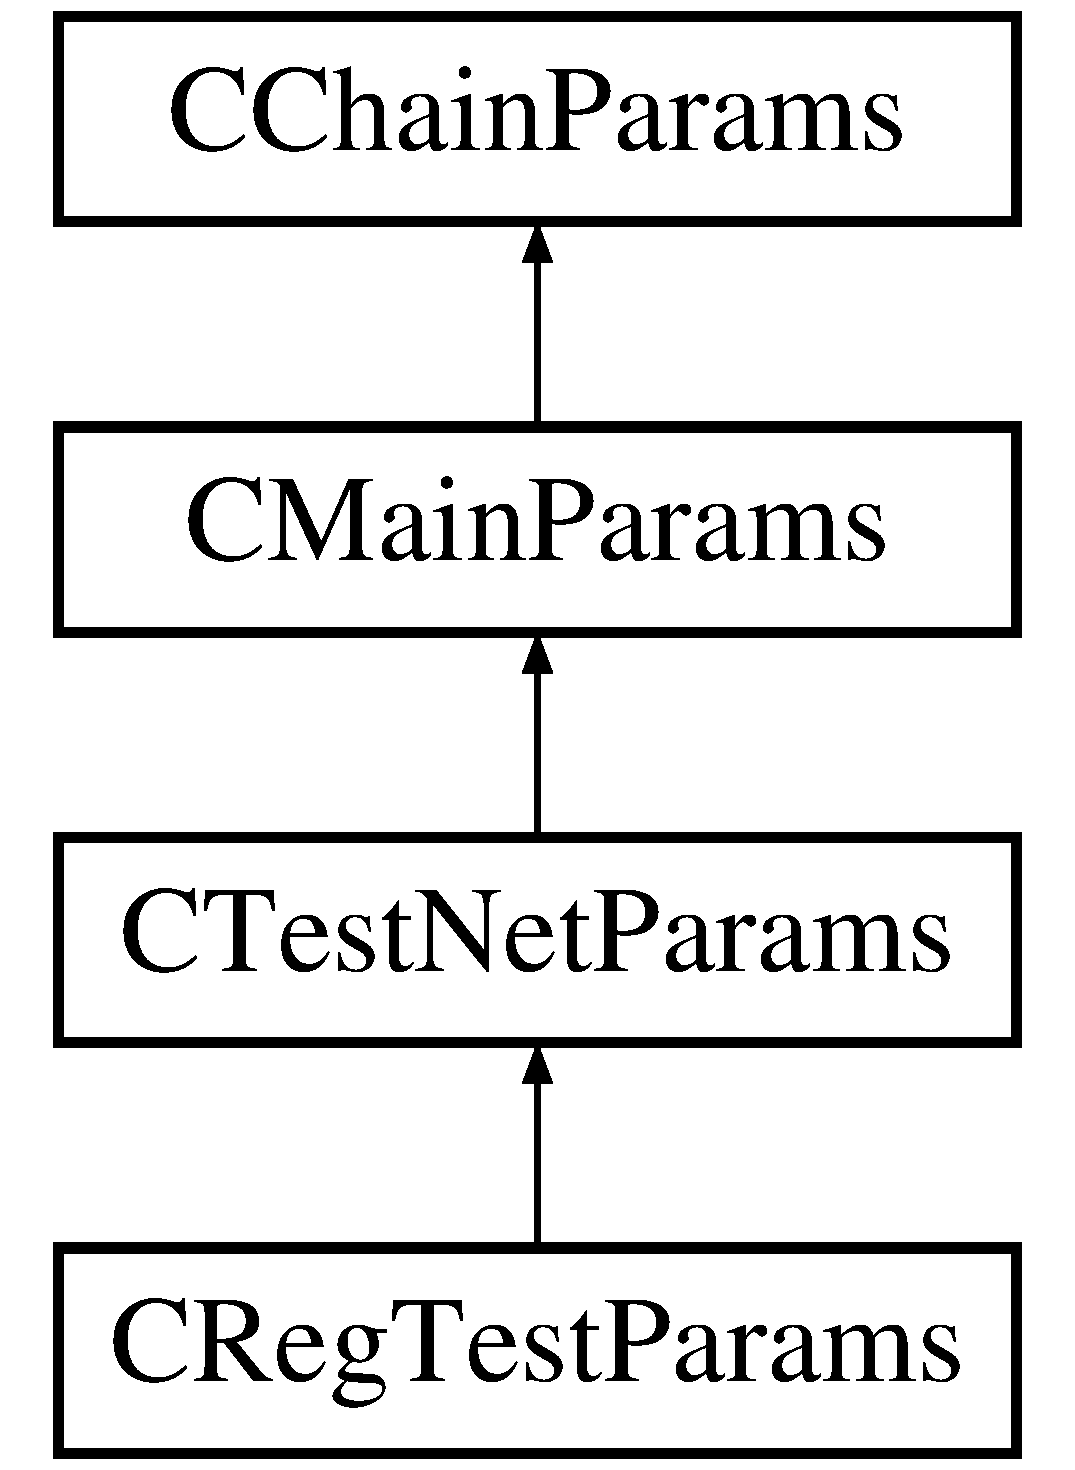
\includegraphics[height=4.000000cm]{class_c_chain_params}
\end{center}
\end{figure}
\subsection*{Public Types}
\begin{DoxyCompactItemize}
\item 
enum \hyperlink{class_c_chain_params_aa294058ec2e3586bd8d03d6c39667058}{Base58\+Type} \{ \\*
\hyperlink{class_c_chain_params_aa294058ec2e3586bd8d03d6c39667058af088724f20c49c73e548f94d8f1808dd}{P\+U\+B\+K\+E\+Y\+\_\+\+A\+D\+D\+R\+E\+S\+S}, 
\hyperlink{class_c_chain_params_aa294058ec2e3586bd8d03d6c39667058adf0172df56140eb2f6fb7a59df0bb76a}{S\+C\+R\+I\+P\+T\+\_\+\+A\+D\+D\+R\+E\+S\+S}, 
\hyperlink{class_c_chain_params_aa294058ec2e3586bd8d03d6c39667058aacf95cbb9b5f51445295c704540adb18}{S\+E\+C\+R\+E\+T\+\_\+\+K\+E\+Y}, 
\hyperlink{class_c_chain_params_aa294058ec2e3586bd8d03d6c39667058a1259eb07831c689e393e5008d7bd0085}{E\+X\+T\+\_\+\+P\+U\+B\+L\+I\+C\+\_\+\+K\+E\+Y}, 
\\*
\hyperlink{class_c_chain_params_aa294058ec2e3586bd8d03d6c39667058ab5636e60152f35f6595fe413eae430b0}{E\+X\+T\+\_\+\+S\+E\+C\+R\+E\+T\+\_\+\+K\+E\+Y}, 
\hyperlink{class_c_chain_params_aa294058ec2e3586bd8d03d6c39667058a6b21a525c7fab64a5df656e708f71a98}{M\+A\+X\+\_\+\+B\+A\+S\+E58\+\_\+\+T\+Y\+P\+E\+S}
 \}
\end{DoxyCompactItemize}
\subsection*{Public Member Functions}
\begin{DoxyCompactItemize}
\item 
const \hyperlink{chainparams_8h_a5e1ca1b35c3dd1a4e20f18445f28dd9c}{Consensus\+::\+Params} \& \hyperlink{class_c_chain_params_a34b124f87e3b7864fec208ba8879e9e9}{Get\+Consensus} () const 
\item 
const \hyperlink{class_c_message_header_a0d0eeb540cbf4087973f6652ad61878f}{C\+Message\+Header\+::\+Message\+Start\+Chars} \& \hyperlink{class_c_chain_params_ae4f7e42b4fa574aad4e2688f574227da}{Message\+Start} () const 
\item 
const std\+::vector$<$ unsigned char $>$ \& \hyperlink{class_c_chain_params_aec4d2aa83f6fd444f68df1a92140075a}{Alert\+Key} () const 
\item 
int \hyperlink{class_c_chain_params_afdb7793273cdb87cc5fd75450eb2258b}{Get\+Default\+Port} () const 
\item 
int \hyperlink{class_c_chain_params_a22301443ebfa49c61f9a7d75b03a84f2}{Subsidy\+Halving\+Interval} () const 
\item 
int \hyperlink{class_c_chain_params_a11c62c3c053019d7c10034d7690d4311}{Enforce\+Block\+Upgrade\+Majority} () const 
\item 
int \hyperlink{class_c_chain_params_ac30ca8a722c96c7d7894637b409bf32a}{Reject\+Block\+Outdated\+Majority} () const 
\item 
int \hyperlink{class_c_chain_params_ae7c61aab594b025befa97accf28e7324}{To\+Check\+Block\+Upgrade\+Majority} () const 
\item 
int \hyperlink{class_c_chain_params_a6dd15e60d45273fef82c7ca435b1c1e9}{Default\+Miner\+Threads} () const 
\item 
const C\+Block \& \hyperlink{class_c_chain_params_a93e04059986f1b0ad673304260176956}{Genesis\+Block} () const 
\item 
bool \hyperlink{class_c_chain_params_ad4063a9056a4e87f471e671ab8e7e6c9}{Require\+R\+P\+C\+Password} () const 
\item 
bool \hyperlink{class_c_chain_params_a0afe61c7b66dcdc88a7c4ad39a64562d}{Mining\+Requires\+Peers} () const 
\item 
bool \hyperlink{class_c_chain_params_ac821d208a2c8c3e1713f206eacfc7adc}{Default\+Consistency\+Checks} () const 
\item 
bool \hyperlink{class_c_chain_params_aab181655e60d8b6ca2097b4f5e5e38c5}{Require\+Standard} () const 
\item 
int64\+\_\+t \hyperlink{class_c_chain_params_aed0dc911b1632d46831bf3d5ad82a07d}{Prune\+After\+Height} () const 
\item 
bool \hyperlink{class_c_chain_params_a43391a278460183ece50859c286c46bd}{Mine\+Blocks\+On\+Demand} () const 
\item 
bool \hyperlink{class_c_chain_params_abbad9c090ffa75608cc04edc3c2a0e62}{Testnet\+To\+Be\+Deprecated\+Field\+R\+P\+C} () const 
\item 
std\+::string \hyperlink{class_c_chain_params_a252d329780e7e16f795b8e54f010c8e1}{Network\+I\+D\+String} () const 
\item 
const std\+::vector$<$ \hyperlink{struct_c_d_n_s_seed_data}{C\+D\+N\+S\+Seed\+Data} $>$ \& \hyperlink{class_c_chain_params_a379fef70fd1eea0cbb94442a45224b21}{D\+N\+S\+Seeds} () const 
\item 
const std\+::vector$<$ unsigned char $>$ \& \hyperlink{class_c_chain_params_a6088d3a4f45d89c90e7e6117c3c5720d}{Base58\+Prefix} (\hyperlink{class_c_chain_params_aa294058ec2e3586bd8d03d6c39667058}{Base58\+Type} type) const 
\item 
const std\+::vector$<$ \hyperlink{class_c_address}{C\+Address} $>$ \& \hyperlink{class_c_chain_params_a85e4471025b35c657bbbc8f871361271}{Fixed\+Seeds} () const 
\item 
virtual const \hyperlink{struct_checkpoints_1_1_c_checkpoint_data}{Checkpoints\+::\+C\+Checkpoint\+Data} \& \hyperlink{class_c_chain_params_aba314e7660492aee43812344fa796d6c}{Checkpoints} () const =0
\end{DoxyCompactItemize}
\subsection*{Protected Member Functions}
\begin{DoxyCompactItemize}
\item 
\hyperlink{class_c_chain_params_a8d07fce73d4160244459c5aaae8fb966}{C\+Chain\+Params} ()
\end{DoxyCompactItemize}
\subsection*{Protected Attributes}
\begin{DoxyCompactItemize}
\item 
\hyperlink{chainparams_8h_a5e1ca1b35c3dd1a4e20f18445f28dd9c}{Consensus\+::\+Params} \hyperlink{class_c_chain_params_a9eddbbd84a87109643d670766683aae2}{consensus}
\item 
\hyperlink{class_c_message_header_a0d0eeb540cbf4087973f6652ad61878f}{C\+Message\+Header\+::\+Message\+Start\+Chars} \hyperlink{class_c_chain_params_ae403e6b6d36b8f8c4d9d494cf686658c}{pch\+Message\+Start}
\item 
std\+::vector$<$ unsigned char $>$ \hyperlink{class_c_chain_params_adf435bdf2d9cd00936d7da0fb4237921}{v\+Alert\+Pub\+Key}
\begin{DoxyCompactList}\small\item\em Raw pub key bytes for the broadcast alert signing key. \end{DoxyCompactList}\item 
int \hyperlink{class_c_chain_params_a76d9a8dc59e179ca94b6b9e04a93e5f4}{n\+Default\+Port}
\item 
int \hyperlink{class_c_chain_params_a3efbcec19f3883c8300063ec0acf4a35}{n\+Miner\+Threads}
\item 
uint64\+\_\+t \hyperlink{class_c_chain_params_aee6b9132f0ce8dcbfc242c3d2e1293e6}{n\+Prune\+After\+Height}
\item 
std\+::vector$<$ \hyperlink{struct_c_d_n_s_seed_data}{C\+D\+N\+S\+Seed\+Data} $>$ \hyperlink{class_c_chain_params_a9ce50b4162fb2ebf5bd72ad4045aa70c}{v\+Seeds}
\item 
std\+::vector$<$ unsigned char $>$ \hyperlink{class_c_chain_params_a923d956c5d3891d0c682b7ef5410ed8f}{base58\+Prefixes} \mbox{[}\hyperlink{class_c_chain_params_aa294058ec2e3586bd8d03d6c39667058a6b21a525c7fab64a5df656e708f71a98}{M\+A\+X\+\_\+\+B\+A\+S\+E58\+\_\+\+T\+Y\+P\+E\+S}\mbox{]}
\item 
std\+::string \hyperlink{class_c_chain_params_a8542ce21d5b9bdc2eadad8702fdd584a}{str\+Network\+I\+D}
\item 
C\+Block \hyperlink{class_c_chain_params_a2e4119fa75f6ea0c64ba8809dab5c4f8}{genesis}
\item 
std\+::vector$<$ \hyperlink{class_c_address}{C\+Address} $>$ \hyperlink{class_c_chain_params_af3ad79fb5bf4938750317c91e4c4b954}{v\+Fixed\+Seeds}
\item 
bool \hyperlink{class_c_chain_params_af84ed151ace6ddc0cbfa649b1c263e9d}{f\+Require\+R\+P\+C\+Password}
\item 
bool \hyperlink{class_c_chain_params_abe9980263561e3f26b6352daa64092da}{f\+Mining\+Requires\+Peers}
\item 
bool \hyperlink{class_c_chain_params_a630f023ae4a95a8b420bad0a08b4428c}{f\+Default\+Consistency\+Checks}
\item 
bool \hyperlink{class_c_chain_params_abc615d2750d847e1eac0ecb7fc8d2da8}{f\+Require\+Standard}
\item 
bool \hyperlink{class_c_chain_params_ad640045ea40c569df7b826551872e1bd}{f\+Mine\+Blocks\+On\+Demand}
\item 
bool \hyperlink{class_c_chain_params_a4f62f1b7070f83b48aa86564628a2e7d}{f\+Testnet\+To\+Be\+Deprecated\+Field\+R\+P\+C}
\end{DoxyCompactItemize}


\subsection{Detailed Description}
\hyperlink{class_c_chain_params}{C\+Chain\+Params} defines various tweakable parameters of a given instance of the Bitcoin system. There are three\+: the main network on which people trade goods and services, the public test network which gets reset from time to time and a regression test mode which is intended for private networks only. It has minimal difficulty to ensure that blocks can be found instantly. 

\subsection{Member Enumeration Documentation}
\hypertarget{class_c_chain_params_aa294058ec2e3586bd8d03d6c39667058}{}\index{C\+Chain\+Params@{C\+Chain\+Params}!Base58\+Type@{Base58\+Type}}
\index{Base58\+Type@{Base58\+Type}!C\+Chain\+Params@{C\+Chain\+Params}}
\subsubsection[{Base58\+Type}]{\setlength{\rightskip}{0pt plus 5cm}enum {\bf C\+Chain\+Params\+::\+Base58\+Type}}\label{class_c_chain_params_aa294058ec2e3586bd8d03d6c39667058}
\begin{Desc}
\item[Enumerator]\par
\begin{description}
\index{P\+U\+B\+K\+E\+Y\+\_\+\+A\+D\+D\+R\+E\+S\+S@{P\+U\+B\+K\+E\+Y\+\_\+\+A\+D\+D\+R\+E\+S\+S}!C\+Chain\+Params@{C\+Chain\+Params}}\index{C\+Chain\+Params@{C\+Chain\+Params}!P\+U\+B\+K\+E\+Y\+\_\+\+A\+D\+D\+R\+E\+S\+S@{P\+U\+B\+K\+E\+Y\+\_\+\+A\+D\+D\+R\+E\+S\+S}}\item[{\em 
\hypertarget{class_c_chain_params_aa294058ec2e3586bd8d03d6c39667058af088724f20c49c73e548f94d8f1808dd}{}P\+U\+B\+K\+E\+Y\+\_\+\+A\+D\+D\+R\+E\+S\+S\label{class_c_chain_params_aa294058ec2e3586bd8d03d6c39667058af088724f20c49c73e548f94d8f1808dd}
}]\index{S\+C\+R\+I\+P\+T\+\_\+\+A\+D\+D\+R\+E\+S\+S@{S\+C\+R\+I\+P\+T\+\_\+\+A\+D\+D\+R\+E\+S\+S}!C\+Chain\+Params@{C\+Chain\+Params}}\index{C\+Chain\+Params@{C\+Chain\+Params}!S\+C\+R\+I\+P\+T\+\_\+\+A\+D\+D\+R\+E\+S\+S@{S\+C\+R\+I\+P\+T\+\_\+\+A\+D\+D\+R\+E\+S\+S}}\item[{\em 
\hypertarget{class_c_chain_params_aa294058ec2e3586bd8d03d6c39667058adf0172df56140eb2f6fb7a59df0bb76a}{}S\+C\+R\+I\+P\+T\+\_\+\+A\+D\+D\+R\+E\+S\+S\label{class_c_chain_params_aa294058ec2e3586bd8d03d6c39667058adf0172df56140eb2f6fb7a59df0bb76a}
}]\index{S\+E\+C\+R\+E\+T\+\_\+\+K\+E\+Y@{S\+E\+C\+R\+E\+T\+\_\+\+K\+E\+Y}!C\+Chain\+Params@{C\+Chain\+Params}}\index{C\+Chain\+Params@{C\+Chain\+Params}!S\+E\+C\+R\+E\+T\+\_\+\+K\+E\+Y@{S\+E\+C\+R\+E\+T\+\_\+\+K\+E\+Y}}\item[{\em 
\hypertarget{class_c_chain_params_aa294058ec2e3586bd8d03d6c39667058aacf95cbb9b5f51445295c704540adb18}{}S\+E\+C\+R\+E\+T\+\_\+\+K\+E\+Y\label{class_c_chain_params_aa294058ec2e3586bd8d03d6c39667058aacf95cbb9b5f51445295c704540adb18}
}]\index{E\+X\+T\+\_\+\+P\+U\+B\+L\+I\+C\+\_\+\+K\+E\+Y@{E\+X\+T\+\_\+\+P\+U\+B\+L\+I\+C\+\_\+\+K\+E\+Y}!C\+Chain\+Params@{C\+Chain\+Params}}\index{C\+Chain\+Params@{C\+Chain\+Params}!E\+X\+T\+\_\+\+P\+U\+B\+L\+I\+C\+\_\+\+K\+E\+Y@{E\+X\+T\+\_\+\+P\+U\+B\+L\+I\+C\+\_\+\+K\+E\+Y}}\item[{\em 
\hypertarget{class_c_chain_params_aa294058ec2e3586bd8d03d6c39667058a1259eb07831c689e393e5008d7bd0085}{}E\+X\+T\+\_\+\+P\+U\+B\+L\+I\+C\+\_\+\+K\+E\+Y\label{class_c_chain_params_aa294058ec2e3586bd8d03d6c39667058a1259eb07831c689e393e5008d7bd0085}
}]\index{E\+X\+T\+\_\+\+S\+E\+C\+R\+E\+T\+\_\+\+K\+E\+Y@{E\+X\+T\+\_\+\+S\+E\+C\+R\+E\+T\+\_\+\+K\+E\+Y}!C\+Chain\+Params@{C\+Chain\+Params}}\index{C\+Chain\+Params@{C\+Chain\+Params}!E\+X\+T\+\_\+\+S\+E\+C\+R\+E\+T\+\_\+\+K\+E\+Y@{E\+X\+T\+\_\+\+S\+E\+C\+R\+E\+T\+\_\+\+K\+E\+Y}}\item[{\em 
\hypertarget{class_c_chain_params_aa294058ec2e3586bd8d03d6c39667058ab5636e60152f35f6595fe413eae430b0}{}E\+X\+T\+\_\+\+S\+E\+C\+R\+E\+T\+\_\+\+K\+E\+Y\label{class_c_chain_params_aa294058ec2e3586bd8d03d6c39667058ab5636e60152f35f6595fe413eae430b0}
}]\index{M\+A\+X\+\_\+\+B\+A\+S\+E58\+\_\+\+T\+Y\+P\+E\+S@{M\+A\+X\+\_\+\+B\+A\+S\+E58\+\_\+\+T\+Y\+P\+E\+S}!C\+Chain\+Params@{C\+Chain\+Params}}\index{C\+Chain\+Params@{C\+Chain\+Params}!M\+A\+X\+\_\+\+B\+A\+S\+E58\+\_\+\+T\+Y\+P\+E\+S@{M\+A\+X\+\_\+\+B\+A\+S\+E58\+\_\+\+T\+Y\+P\+E\+S}}\item[{\em 
\hypertarget{class_c_chain_params_aa294058ec2e3586bd8d03d6c39667058a6b21a525c7fab64a5df656e708f71a98}{}M\+A\+X\+\_\+\+B\+A\+S\+E58\+\_\+\+T\+Y\+P\+E\+S\label{class_c_chain_params_aa294058ec2e3586bd8d03d6c39667058a6b21a525c7fab64a5df656e708f71a98}
}]\end{description}
\end{Desc}


\subsection{Constructor \& Destructor Documentation}
\hypertarget{class_c_chain_params_a8d07fce73d4160244459c5aaae8fb966}{}\index{C\+Chain\+Params@{C\+Chain\+Params}!C\+Chain\+Params@{C\+Chain\+Params}}
\index{C\+Chain\+Params@{C\+Chain\+Params}!C\+Chain\+Params@{C\+Chain\+Params}}
\subsubsection[{C\+Chain\+Params}]{\setlength{\rightskip}{0pt plus 5cm}C\+Chain\+Params\+::\+C\+Chain\+Params (
\begin{DoxyParamCaption}
{}
\end{DoxyParamCaption}
)\hspace{0.3cm}{\ttfamily [inline]}, {\ttfamily [protected]}}\label{class_c_chain_params_a8d07fce73d4160244459c5aaae8fb966}


\subsection{Member Function Documentation}
\hypertarget{class_c_chain_params_aec4d2aa83f6fd444f68df1a92140075a}{}\index{C\+Chain\+Params@{C\+Chain\+Params}!Alert\+Key@{Alert\+Key}}
\index{Alert\+Key@{Alert\+Key}!C\+Chain\+Params@{C\+Chain\+Params}}
\subsubsection[{Alert\+Key}]{\setlength{\rightskip}{0pt plus 5cm}const std\+::vector$<$unsigned char$>$\& C\+Chain\+Params\+::\+Alert\+Key (
\begin{DoxyParamCaption}
{}
\end{DoxyParamCaption}
) const\hspace{0.3cm}{\ttfamily [inline]}}\label{class_c_chain_params_aec4d2aa83f6fd444f68df1a92140075a}
\hypertarget{class_c_chain_params_a6088d3a4f45d89c90e7e6117c3c5720d}{}\index{C\+Chain\+Params@{C\+Chain\+Params}!Base58\+Prefix@{Base58\+Prefix}}
\index{Base58\+Prefix@{Base58\+Prefix}!C\+Chain\+Params@{C\+Chain\+Params}}
\subsubsection[{Base58\+Prefix}]{\setlength{\rightskip}{0pt plus 5cm}const std\+::vector$<$unsigned char$>$\& C\+Chain\+Params\+::\+Base58\+Prefix (
\begin{DoxyParamCaption}
\item[{{\bf Base58\+Type}}]{type}
\end{DoxyParamCaption}
) const\hspace{0.3cm}{\ttfamily [inline]}}\label{class_c_chain_params_a6088d3a4f45d89c90e7e6117c3c5720d}
\hypertarget{class_c_chain_params_aba314e7660492aee43812344fa796d6c}{}\index{C\+Chain\+Params@{C\+Chain\+Params}!Checkpoints@{Checkpoints}}
\index{Checkpoints@{Checkpoints}!C\+Chain\+Params@{C\+Chain\+Params}}
\subsubsection[{Checkpoints}]{\setlength{\rightskip}{0pt plus 5cm}virtual const {\bf Checkpoints\+::\+C\+Checkpoint\+Data}\& C\+Chain\+Params\+::\+Checkpoints (
\begin{DoxyParamCaption}
{}
\end{DoxyParamCaption}
) const\hspace{0.3cm}{\ttfamily [pure virtual]}}\label{class_c_chain_params_aba314e7660492aee43812344fa796d6c}


Implemented in \hyperlink{class_c_reg_test_params_ab748b010a203dbdf6e5f77eb8b6f7cb0}{C\+Reg\+Test\+Params}, \hyperlink{class_c_test_net_params_a1a8828912574c509825ccc5cc0e0a9be}{C\+Test\+Net\+Params}, and \hyperlink{class_c_main_params_abfaf5edda329d8b2ff23c0108cb8c16e}{C\+Main\+Params}.

\hypertarget{class_c_chain_params_ac821d208a2c8c3e1713f206eacfc7adc}{}\index{C\+Chain\+Params@{C\+Chain\+Params}!Default\+Consistency\+Checks@{Default\+Consistency\+Checks}}
\index{Default\+Consistency\+Checks@{Default\+Consistency\+Checks}!C\+Chain\+Params@{C\+Chain\+Params}}
\subsubsection[{Default\+Consistency\+Checks}]{\setlength{\rightskip}{0pt plus 5cm}bool C\+Chain\+Params\+::\+Default\+Consistency\+Checks (
\begin{DoxyParamCaption}
{}
\end{DoxyParamCaption}
) const\hspace{0.3cm}{\ttfamily [inline]}}\label{class_c_chain_params_ac821d208a2c8c3e1713f206eacfc7adc}
Default value for -\/checkmempool and -\/checkblockindex argument \hypertarget{class_c_chain_params_a6dd15e60d45273fef82c7ca435b1c1e9}{}\index{C\+Chain\+Params@{C\+Chain\+Params}!Default\+Miner\+Threads@{Default\+Miner\+Threads}}
\index{Default\+Miner\+Threads@{Default\+Miner\+Threads}!C\+Chain\+Params@{C\+Chain\+Params}}
\subsubsection[{Default\+Miner\+Threads}]{\setlength{\rightskip}{0pt plus 5cm}int C\+Chain\+Params\+::\+Default\+Miner\+Threads (
\begin{DoxyParamCaption}
{}
\end{DoxyParamCaption}
) const\hspace{0.3cm}{\ttfamily [inline]}}\label{class_c_chain_params_a6dd15e60d45273fef82c7ca435b1c1e9}
Used if Generate\+Bitcoins is called with a negative number of threads \hypertarget{class_c_chain_params_a379fef70fd1eea0cbb94442a45224b21}{}\index{C\+Chain\+Params@{C\+Chain\+Params}!D\+N\+S\+Seeds@{D\+N\+S\+Seeds}}
\index{D\+N\+S\+Seeds@{D\+N\+S\+Seeds}!C\+Chain\+Params@{C\+Chain\+Params}}
\subsubsection[{D\+N\+S\+Seeds}]{\setlength{\rightskip}{0pt plus 5cm}const std\+::vector$<${\bf C\+D\+N\+S\+Seed\+Data}$>$\& C\+Chain\+Params\+::\+D\+N\+S\+Seeds (
\begin{DoxyParamCaption}
{}
\end{DoxyParamCaption}
) const\hspace{0.3cm}{\ttfamily [inline]}}\label{class_c_chain_params_a379fef70fd1eea0cbb94442a45224b21}
\hypertarget{class_c_chain_params_a11c62c3c053019d7c10034d7690d4311}{}\index{C\+Chain\+Params@{C\+Chain\+Params}!Enforce\+Block\+Upgrade\+Majority@{Enforce\+Block\+Upgrade\+Majority}}
\index{Enforce\+Block\+Upgrade\+Majority@{Enforce\+Block\+Upgrade\+Majority}!C\+Chain\+Params@{C\+Chain\+Params}}
\subsubsection[{Enforce\+Block\+Upgrade\+Majority}]{\setlength{\rightskip}{0pt plus 5cm}int C\+Chain\+Params\+::\+Enforce\+Block\+Upgrade\+Majority (
\begin{DoxyParamCaption}
{}
\end{DoxyParamCaption}
) const\hspace{0.3cm}{\ttfamily [inline]}}\label{class_c_chain_params_a11c62c3c053019d7c10034d7690d4311}
\hypertarget{class_c_chain_params_a85e4471025b35c657bbbc8f871361271}{}\index{C\+Chain\+Params@{C\+Chain\+Params}!Fixed\+Seeds@{Fixed\+Seeds}}
\index{Fixed\+Seeds@{Fixed\+Seeds}!C\+Chain\+Params@{C\+Chain\+Params}}
\subsubsection[{Fixed\+Seeds}]{\setlength{\rightskip}{0pt plus 5cm}const std\+::vector$<${\bf C\+Address}$>$\& C\+Chain\+Params\+::\+Fixed\+Seeds (
\begin{DoxyParamCaption}
{}
\end{DoxyParamCaption}
) const\hspace{0.3cm}{\ttfamily [inline]}}\label{class_c_chain_params_a85e4471025b35c657bbbc8f871361271}
\hypertarget{class_c_chain_params_a93e04059986f1b0ad673304260176956}{}\index{C\+Chain\+Params@{C\+Chain\+Params}!Genesis\+Block@{Genesis\+Block}}
\index{Genesis\+Block@{Genesis\+Block}!C\+Chain\+Params@{C\+Chain\+Params}}
\subsubsection[{Genesis\+Block}]{\setlength{\rightskip}{0pt plus 5cm}const C\+Block\& C\+Chain\+Params\+::\+Genesis\+Block (
\begin{DoxyParamCaption}
{}
\end{DoxyParamCaption}
) const\hspace{0.3cm}{\ttfamily [inline]}}\label{class_c_chain_params_a93e04059986f1b0ad673304260176956}
\hypertarget{class_c_chain_params_a34b124f87e3b7864fec208ba8879e9e9}{}\index{C\+Chain\+Params@{C\+Chain\+Params}!Get\+Consensus@{Get\+Consensus}}
\index{Get\+Consensus@{Get\+Consensus}!C\+Chain\+Params@{C\+Chain\+Params}}
\subsubsection[{Get\+Consensus}]{\setlength{\rightskip}{0pt plus 5cm}const {\bf Consensus\+::\+Params}\& C\+Chain\+Params\+::\+Get\+Consensus (
\begin{DoxyParamCaption}
{}
\end{DoxyParamCaption}
) const\hspace{0.3cm}{\ttfamily [inline]}}\label{class_c_chain_params_a34b124f87e3b7864fec208ba8879e9e9}
\hypertarget{class_c_chain_params_afdb7793273cdb87cc5fd75450eb2258b}{}\index{C\+Chain\+Params@{C\+Chain\+Params}!Get\+Default\+Port@{Get\+Default\+Port}}
\index{Get\+Default\+Port@{Get\+Default\+Port}!C\+Chain\+Params@{C\+Chain\+Params}}
\subsubsection[{Get\+Default\+Port}]{\setlength{\rightskip}{0pt plus 5cm}int C\+Chain\+Params\+::\+Get\+Default\+Port (
\begin{DoxyParamCaption}
{}
\end{DoxyParamCaption}
) const\hspace{0.3cm}{\ttfamily [inline]}}\label{class_c_chain_params_afdb7793273cdb87cc5fd75450eb2258b}
\hypertarget{class_c_chain_params_ae4f7e42b4fa574aad4e2688f574227da}{}\index{C\+Chain\+Params@{C\+Chain\+Params}!Message\+Start@{Message\+Start}}
\index{Message\+Start@{Message\+Start}!C\+Chain\+Params@{C\+Chain\+Params}}
\subsubsection[{Message\+Start}]{\setlength{\rightskip}{0pt plus 5cm}const {\bf C\+Message\+Header\+::\+Message\+Start\+Chars}\& C\+Chain\+Params\+::\+Message\+Start (
\begin{DoxyParamCaption}
{}
\end{DoxyParamCaption}
) const\hspace{0.3cm}{\ttfamily [inline]}}\label{class_c_chain_params_ae4f7e42b4fa574aad4e2688f574227da}
\hypertarget{class_c_chain_params_a43391a278460183ece50859c286c46bd}{}\index{C\+Chain\+Params@{C\+Chain\+Params}!Mine\+Blocks\+On\+Demand@{Mine\+Blocks\+On\+Demand}}
\index{Mine\+Blocks\+On\+Demand@{Mine\+Blocks\+On\+Demand}!C\+Chain\+Params@{C\+Chain\+Params}}
\subsubsection[{Mine\+Blocks\+On\+Demand}]{\setlength{\rightskip}{0pt plus 5cm}bool C\+Chain\+Params\+::\+Mine\+Blocks\+On\+Demand (
\begin{DoxyParamCaption}
{}
\end{DoxyParamCaption}
) const\hspace{0.3cm}{\ttfamily [inline]}}\label{class_c_chain_params_a43391a278460183ece50859c286c46bd}
Make miner stop after a block is found. In R\+P\+C, don\textquotesingle{}t return until n\+Gen\+Proc\+Limit blocks are generated \hypertarget{class_c_chain_params_a0afe61c7b66dcdc88a7c4ad39a64562d}{}\index{C\+Chain\+Params@{C\+Chain\+Params}!Mining\+Requires\+Peers@{Mining\+Requires\+Peers}}
\index{Mining\+Requires\+Peers@{Mining\+Requires\+Peers}!C\+Chain\+Params@{C\+Chain\+Params}}
\subsubsection[{Mining\+Requires\+Peers}]{\setlength{\rightskip}{0pt plus 5cm}bool C\+Chain\+Params\+::\+Mining\+Requires\+Peers (
\begin{DoxyParamCaption}
{}
\end{DoxyParamCaption}
) const\hspace{0.3cm}{\ttfamily [inline]}}\label{class_c_chain_params_a0afe61c7b66dcdc88a7c4ad39a64562d}
Make miner wait to have peers to avoid wasting work \hypertarget{class_c_chain_params_a252d329780e7e16f795b8e54f010c8e1}{}\index{C\+Chain\+Params@{C\+Chain\+Params}!Network\+I\+D\+String@{Network\+I\+D\+String}}
\index{Network\+I\+D\+String@{Network\+I\+D\+String}!C\+Chain\+Params@{C\+Chain\+Params}}
\subsubsection[{Network\+I\+D\+String}]{\setlength{\rightskip}{0pt plus 5cm}std\+::string C\+Chain\+Params\+::\+Network\+I\+D\+String (
\begin{DoxyParamCaption}
{}
\end{DoxyParamCaption}
) const\hspace{0.3cm}{\ttfamily [inline]}}\label{class_c_chain_params_a252d329780e7e16f795b8e54f010c8e1}
Return the B\+I\+P70 network string (main, test or regtest) \hypertarget{class_c_chain_params_aed0dc911b1632d46831bf3d5ad82a07d}{}\index{C\+Chain\+Params@{C\+Chain\+Params}!Prune\+After\+Height@{Prune\+After\+Height}}
\index{Prune\+After\+Height@{Prune\+After\+Height}!C\+Chain\+Params@{C\+Chain\+Params}}
\subsubsection[{Prune\+After\+Height}]{\setlength{\rightskip}{0pt plus 5cm}int64\+\_\+t C\+Chain\+Params\+::\+Prune\+After\+Height (
\begin{DoxyParamCaption}
{}
\end{DoxyParamCaption}
) const\hspace{0.3cm}{\ttfamily [inline]}}\label{class_c_chain_params_aed0dc911b1632d46831bf3d5ad82a07d}
\hypertarget{class_c_chain_params_ac30ca8a722c96c7d7894637b409bf32a}{}\index{C\+Chain\+Params@{C\+Chain\+Params}!Reject\+Block\+Outdated\+Majority@{Reject\+Block\+Outdated\+Majority}}
\index{Reject\+Block\+Outdated\+Majority@{Reject\+Block\+Outdated\+Majority}!C\+Chain\+Params@{C\+Chain\+Params}}
\subsubsection[{Reject\+Block\+Outdated\+Majority}]{\setlength{\rightskip}{0pt plus 5cm}int C\+Chain\+Params\+::\+Reject\+Block\+Outdated\+Majority (
\begin{DoxyParamCaption}
{}
\end{DoxyParamCaption}
) const\hspace{0.3cm}{\ttfamily [inline]}}\label{class_c_chain_params_ac30ca8a722c96c7d7894637b409bf32a}
\hypertarget{class_c_chain_params_ad4063a9056a4e87f471e671ab8e7e6c9}{}\index{C\+Chain\+Params@{C\+Chain\+Params}!Require\+R\+P\+C\+Password@{Require\+R\+P\+C\+Password}}
\index{Require\+R\+P\+C\+Password@{Require\+R\+P\+C\+Password}!C\+Chain\+Params@{C\+Chain\+Params}}
\subsubsection[{Require\+R\+P\+C\+Password}]{\setlength{\rightskip}{0pt plus 5cm}bool C\+Chain\+Params\+::\+Require\+R\+P\+C\+Password (
\begin{DoxyParamCaption}
{}
\end{DoxyParamCaption}
) const\hspace{0.3cm}{\ttfamily [inline]}}\label{class_c_chain_params_ad4063a9056a4e87f471e671ab8e7e6c9}
\hypertarget{class_c_chain_params_aab181655e60d8b6ca2097b4f5e5e38c5}{}\index{C\+Chain\+Params@{C\+Chain\+Params}!Require\+Standard@{Require\+Standard}}
\index{Require\+Standard@{Require\+Standard}!C\+Chain\+Params@{C\+Chain\+Params}}
\subsubsection[{Require\+Standard}]{\setlength{\rightskip}{0pt plus 5cm}bool C\+Chain\+Params\+::\+Require\+Standard (
\begin{DoxyParamCaption}
{}
\end{DoxyParamCaption}
) const\hspace{0.3cm}{\ttfamily [inline]}}\label{class_c_chain_params_aab181655e60d8b6ca2097b4f5e5e38c5}
Make standard checks \hypertarget{class_c_chain_params_a22301443ebfa49c61f9a7d75b03a84f2}{}\index{C\+Chain\+Params@{C\+Chain\+Params}!Subsidy\+Halving\+Interval@{Subsidy\+Halving\+Interval}}
\index{Subsidy\+Halving\+Interval@{Subsidy\+Halving\+Interval}!C\+Chain\+Params@{C\+Chain\+Params}}
\subsubsection[{Subsidy\+Halving\+Interval}]{\setlength{\rightskip}{0pt plus 5cm}int C\+Chain\+Params\+::\+Subsidy\+Halving\+Interval (
\begin{DoxyParamCaption}
{}
\end{DoxyParamCaption}
) const\hspace{0.3cm}{\ttfamily [inline]}}\label{class_c_chain_params_a22301443ebfa49c61f9a7d75b03a84f2}
\hypertarget{class_c_chain_params_abbad9c090ffa75608cc04edc3c2a0e62}{}\index{C\+Chain\+Params@{C\+Chain\+Params}!Testnet\+To\+Be\+Deprecated\+Field\+R\+P\+C@{Testnet\+To\+Be\+Deprecated\+Field\+R\+P\+C}}
\index{Testnet\+To\+Be\+Deprecated\+Field\+R\+P\+C@{Testnet\+To\+Be\+Deprecated\+Field\+R\+P\+C}!C\+Chain\+Params@{C\+Chain\+Params}}
\subsubsection[{Testnet\+To\+Be\+Deprecated\+Field\+R\+P\+C}]{\setlength{\rightskip}{0pt plus 5cm}bool C\+Chain\+Params\+::\+Testnet\+To\+Be\+Deprecated\+Field\+R\+P\+C (
\begin{DoxyParamCaption}
{}
\end{DoxyParamCaption}
) const\hspace{0.3cm}{\ttfamily [inline]}}\label{class_c_chain_params_abbad9c090ffa75608cc04edc3c2a0e62}
In the future use \hyperlink{class_c_chain_params_a252d329780e7e16f795b8e54f010c8e1}{Network\+I\+D\+String()} for R\+P\+C fields \hypertarget{class_c_chain_params_ae7c61aab594b025befa97accf28e7324}{}\index{C\+Chain\+Params@{C\+Chain\+Params}!To\+Check\+Block\+Upgrade\+Majority@{To\+Check\+Block\+Upgrade\+Majority}}
\index{To\+Check\+Block\+Upgrade\+Majority@{To\+Check\+Block\+Upgrade\+Majority}!C\+Chain\+Params@{C\+Chain\+Params}}
\subsubsection[{To\+Check\+Block\+Upgrade\+Majority}]{\setlength{\rightskip}{0pt plus 5cm}int C\+Chain\+Params\+::\+To\+Check\+Block\+Upgrade\+Majority (
\begin{DoxyParamCaption}
{}
\end{DoxyParamCaption}
) const\hspace{0.3cm}{\ttfamily [inline]}}\label{class_c_chain_params_ae7c61aab594b025befa97accf28e7324}


\subsection{Member Data Documentation}
\hypertarget{class_c_chain_params_a923d956c5d3891d0c682b7ef5410ed8f}{}\index{C\+Chain\+Params@{C\+Chain\+Params}!base58\+Prefixes@{base58\+Prefixes}}
\index{base58\+Prefixes@{base58\+Prefixes}!C\+Chain\+Params@{C\+Chain\+Params}}
\subsubsection[{base58\+Prefixes}]{\setlength{\rightskip}{0pt plus 5cm}std\+::vector$<$unsigned char$>$ C\+Chain\+Params\+::base58\+Prefixes\mbox{[}{\bf M\+A\+X\+\_\+\+B\+A\+S\+E58\+\_\+\+T\+Y\+P\+E\+S}\mbox{]}\hspace{0.3cm}{\ttfamily [protected]}}\label{class_c_chain_params_a923d956c5d3891d0c682b7ef5410ed8f}
\hypertarget{class_c_chain_params_a9eddbbd84a87109643d670766683aae2}{}\index{C\+Chain\+Params@{C\+Chain\+Params}!consensus@{consensus}}
\index{consensus@{consensus}!C\+Chain\+Params@{C\+Chain\+Params}}
\subsubsection[{consensus}]{\setlength{\rightskip}{0pt plus 5cm}{\bf Consensus\+::\+Params} C\+Chain\+Params\+::consensus\hspace{0.3cm}{\ttfamily [protected]}}\label{class_c_chain_params_a9eddbbd84a87109643d670766683aae2}
\hypertarget{class_c_chain_params_a630f023ae4a95a8b420bad0a08b4428c}{}\index{C\+Chain\+Params@{C\+Chain\+Params}!f\+Default\+Consistency\+Checks@{f\+Default\+Consistency\+Checks}}
\index{f\+Default\+Consistency\+Checks@{f\+Default\+Consistency\+Checks}!C\+Chain\+Params@{C\+Chain\+Params}}
\subsubsection[{f\+Default\+Consistency\+Checks}]{\setlength{\rightskip}{0pt plus 5cm}bool C\+Chain\+Params\+::f\+Default\+Consistency\+Checks\hspace{0.3cm}{\ttfamily [protected]}}\label{class_c_chain_params_a630f023ae4a95a8b420bad0a08b4428c}
\hypertarget{class_c_chain_params_ad640045ea40c569df7b826551872e1bd}{}\index{C\+Chain\+Params@{C\+Chain\+Params}!f\+Mine\+Blocks\+On\+Demand@{f\+Mine\+Blocks\+On\+Demand}}
\index{f\+Mine\+Blocks\+On\+Demand@{f\+Mine\+Blocks\+On\+Demand}!C\+Chain\+Params@{C\+Chain\+Params}}
\subsubsection[{f\+Mine\+Blocks\+On\+Demand}]{\setlength{\rightskip}{0pt plus 5cm}bool C\+Chain\+Params\+::f\+Mine\+Blocks\+On\+Demand\hspace{0.3cm}{\ttfamily [protected]}}\label{class_c_chain_params_ad640045ea40c569df7b826551872e1bd}
\hypertarget{class_c_chain_params_abe9980263561e3f26b6352daa64092da}{}\index{C\+Chain\+Params@{C\+Chain\+Params}!f\+Mining\+Requires\+Peers@{f\+Mining\+Requires\+Peers}}
\index{f\+Mining\+Requires\+Peers@{f\+Mining\+Requires\+Peers}!C\+Chain\+Params@{C\+Chain\+Params}}
\subsubsection[{f\+Mining\+Requires\+Peers}]{\setlength{\rightskip}{0pt plus 5cm}bool C\+Chain\+Params\+::f\+Mining\+Requires\+Peers\hspace{0.3cm}{\ttfamily [protected]}}\label{class_c_chain_params_abe9980263561e3f26b6352daa64092da}
\hypertarget{class_c_chain_params_af84ed151ace6ddc0cbfa649b1c263e9d}{}\index{C\+Chain\+Params@{C\+Chain\+Params}!f\+Require\+R\+P\+C\+Password@{f\+Require\+R\+P\+C\+Password}}
\index{f\+Require\+R\+P\+C\+Password@{f\+Require\+R\+P\+C\+Password}!C\+Chain\+Params@{C\+Chain\+Params}}
\subsubsection[{f\+Require\+R\+P\+C\+Password}]{\setlength{\rightskip}{0pt plus 5cm}bool C\+Chain\+Params\+::f\+Require\+R\+P\+C\+Password\hspace{0.3cm}{\ttfamily [protected]}}\label{class_c_chain_params_af84ed151ace6ddc0cbfa649b1c263e9d}
\hypertarget{class_c_chain_params_abc615d2750d847e1eac0ecb7fc8d2da8}{}\index{C\+Chain\+Params@{C\+Chain\+Params}!f\+Require\+Standard@{f\+Require\+Standard}}
\index{f\+Require\+Standard@{f\+Require\+Standard}!C\+Chain\+Params@{C\+Chain\+Params}}
\subsubsection[{f\+Require\+Standard}]{\setlength{\rightskip}{0pt plus 5cm}bool C\+Chain\+Params\+::f\+Require\+Standard\hspace{0.3cm}{\ttfamily [protected]}}\label{class_c_chain_params_abc615d2750d847e1eac0ecb7fc8d2da8}
\hypertarget{class_c_chain_params_a4f62f1b7070f83b48aa86564628a2e7d}{}\index{C\+Chain\+Params@{C\+Chain\+Params}!f\+Testnet\+To\+Be\+Deprecated\+Field\+R\+P\+C@{f\+Testnet\+To\+Be\+Deprecated\+Field\+R\+P\+C}}
\index{f\+Testnet\+To\+Be\+Deprecated\+Field\+R\+P\+C@{f\+Testnet\+To\+Be\+Deprecated\+Field\+R\+P\+C}!C\+Chain\+Params@{C\+Chain\+Params}}
\subsubsection[{f\+Testnet\+To\+Be\+Deprecated\+Field\+R\+P\+C}]{\setlength{\rightskip}{0pt plus 5cm}bool C\+Chain\+Params\+::f\+Testnet\+To\+Be\+Deprecated\+Field\+R\+P\+C\hspace{0.3cm}{\ttfamily [protected]}}\label{class_c_chain_params_a4f62f1b7070f83b48aa86564628a2e7d}
\hypertarget{class_c_chain_params_a2e4119fa75f6ea0c64ba8809dab5c4f8}{}\index{C\+Chain\+Params@{C\+Chain\+Params}!genesis@{genesis}}
\index{genesis@{genesis}!C\+Chain\+Params@{C\+Chain\+Params}}
\subsubsection[{genesis}]{\setlength{\rightskip}{0pt plus 5cm}C\+Block C\+Chain\+Params\+::genesis\hspace{0.3cm}{\ttfamily [protected]}}\label{class_c_chain_params_a2e4119fa75f6ea0c64ba8809dab5c4f8}
\hypertarget{class_c_chain_params_a76d9a8dc59e179ca94b6b9e04a93e5f4}{}\index{C\+Chain\+Params@{C\+Chain\+Params}!n\+Default\+Port@{n\+Default\+Port}}
\index{n\+Default\+Port@{n\+Default\+Port}!C\+Chain\+Params@{C\+Chain\+Params}}
\subsubsection[{n\+Default\+Port}]{\setlength{\rightskip}{0pt plus 5cm}int C\+Chain\+Params\+::n\+Default\+Port\hspace{0.3cm}{\ttfamily [protected]}}\label{class_c_chain_params_a76d9a8dc59e179ca94b6b9e04a93e5f4}
\hypertarget{class_c_chain_params_a3efbcec19f3883c8300063ec0acf4a35}{}\index{C\+Chain\+Params@{C\+Chain\+Params}!n\+Miner\+Threads@{n\+Miner\+Threads}}
\index{n\+Miner\+Threads@{n\+Miner\+Threads}!C\+Chain\+Params@{C\+Chain\+Params}}
\subsubsection[{n\+Miner\+Threads}]{\setlength{\rightskip}{0pt plus 5cm}int C\+Chain\+Params\+::n\+Miner\+Threads\hspace{0.3cm}{\ttfamily [protected]}}\label{class_c_chain_params_a3efbcec19f3883c8300063ec0acf4a35}
\hypertarget{class_c_chain_params_aee6b9132f0ce8dcbfc242c3d2e1293e6}{}\index{C\+Chain\+Params@{C\+Chain\+Params}!n\+Prune\+After\+Height@{n\+Prune\+After\+Height}}
\index{n\+Prune\+After\+Height@{n\+Prune\+After\+Height}!C\+Chain\+Params@{C\+Chain\+Params}}
\subsubsection[{n\+Prune\+After\+Height}]{\setlength{\rightskip}{0pt plus 5cm}uint64\+\_\+t C\+Chain\+Params\+::n\+Prune\+After\+Height\hspace{0.3cm}{\ttfamily [protected]}}\label{class_c_chain_params_aee6b9132f0ce8dcbfc242c3d2e1293e6}
\hypertarget{class_c_chain_params_ae403e6b6d36b8f8c4d9d494cf686658c}{}\index{C\+Chain\+Params@{C\+Chain\+Params}!pch\+Message\+Start@{pch\+Message\+Start}}
\index{pch\+Message\+Start@{pch\+Message\+Start}!C\+Chain\+Params@{C\+Chain\+Params}}
\subsubsection[{pch\+Message\+Start}]{\setlength{\rightskip}{0pt plus 5cm}{\bf C\+Message\+Header\+::\+Message\+Start\+Chars} C\+Chain\+Params\+::pch\+Message\+Start\hspace{0.3cm}{\ttfamily [protected]}}\label{class_c_chain_params_ae403e6b6d36b8f8c4d9d494cf686658c}
\hypertarget{class_c_chain_params_a8542ce21d5b9bdc2eadad8702fdd584a}{}\index{C\+Chain\+Params@{C\+Chain\+Params}!str\+Network\+I\+D@{str\+Network\+I\+D}}
\index{str\+Network\+I\+D@{str\+Network\+I\+D}!C\+Chain\+Params@{C\+Chain\+Params}}
\subsubsection[{str\+Network\+I\+D}]{\setlength{\rightskip}{0pt plus 5cm}std\+::string C\+Chain\+Params\+::str\+Network\+I\+D\hspace{0.3cm}{\ttfamily [protected]}}\label{class_c_chain_params_a8542ce21d5b9bdc2eadad8702fdd584a}
\hypertarget{class_c_chain_params_adf435bdf2d9cd00936d7da0fb4237921}{}\index{C\+Chain\+Params@{C\+Chain\+Params}!v\+Alert\+Pub\+Key@{v\+Alert\+Pub\+Key}}
\index{v\+Alert\+Pub\+Key@{v\+Alert\+Pub\+Key}!C\+Chain\+Params@{C\+Chain\+Params}}
\subsubsection[{v\+Alert\+Pub\+Key}]{\setlength{\rightskip}{0pt plus 5cm}std\+::vector$<$unsigned char$>$ C\+Chain\+Params\+::v\+Alert\+Pub\+Key\hspace{0.3cm}{\ttfamily [protected]}}\label{class_c_chain_params_adf435bdf2d9cd00936d7da0fb4237921}


Raw pub key bytes for the broadcast alert signing key. 

\hypertarget{class_c_chain_params_af3ad79fb5bf4938750317c91e4c4b954}{}\index{C\+Chain\+Params@{C\+Chain\+Params}!v\+Fixed\+Seeds@{v\+Fixed\+Seeds}}
\index{v\+Fixed\+Seeds@{v\+Fixed\+Seeds}!C\+Chain\+Params@{C\+Chain\+Params}}
\subsubsection[{v\+Fixed\+Seeds}]{\setlength{\rightskip}{0pt plus 5cm}std\+::vector$<${\bf C\+Address}$>$ C\+Chain\+Params\+::v\+Fixed\+Seeds\hspace{0.3cm}{\ttfamily [protected]}}\label{class_c_chain_params_af3ad79fb5bf4938750317c91e4c4b954}
\hypertarget{class_c_chain_params_a9ce50b4162fb2ebf5bd72ad4045aa70c}{}\index{C\+Chain\+Params@{C\+Chain\+Params}!v\+Seeds@{v\+Seeds}}
\index{v\+Seeds@{v\+Seeds}!C\+Chain\+Params@{C\+Chain\+Params}}
\subsubsection[{v\+Seeds}]{\setlength{\rightskip}{0pt plus 5cm}std\+::vector$<${\bf C\+D\+N\+S\+Seed\+Data}$>$ C\+Chain\+Params\+::v\+Seeds\hspace{0.3cm}{\ttfamily [protected]}}\label{class_c_chain_params_a9ce50b4162fb2ebf5bd72ad4045aa70c}


The documentation for this class was generated from the following file\+:\begin{DoxyCompactItemize}
\item 
C\+:/\+Users/\+Joe/\+Documents/\+School/\+C\+S\+C17\+A/bitcoin/src/\hyperlink{chainparams_8h}{chainparams.\+h}\end{DoxyCompactItemize}

\hypertarget{struct_checkpoints_1_1_c_checkpoint_data}{}\section{Checkpoints\+:\+:C\+Checkpoint\+Data Struct Reference}
\label{struct_checkpoints_1_1_c_checkpoint_data}\index{Checkpoints\+::\+C\+Checkpoint\+Data@{Checkpoints\+::\+C\+Checkpoint\+Data}}


{\ttfamily \#include $<$checkpoints.\+h$>$}

\subsection*{Public Attributes}
\begin{DoxyCompactItemize}
\item 
const \hyperlink{namespace_checkpoints_a996cca530c4568a2eb4516e8f351b9a2}{Map\+Checkpoints} $\ast$ \hyperlink{struct_checkpoints_1_1_c_checkpoint_data_ab4aa42cde482f7cf7ab015abbf7108cb}{map\+Checkpoints}
\item 
int64\+\_\+t \hyperlink{struct_checkpoints_1_1_c_checkpoint_data_a49124425a3f9ccddba8bce3dd67ad3b3}{n\+Time\+Last\+Checkpoint}
\item 
int64\+\_\+t \hyperlink{struct_checkpoints_1_1_c_checkpoint_data_ad659d70f627b0c4529fc0e71f568de70}{n\+Transactions\+Last\+Checkpoint}
\item 
double \hyperlink{struct_checkpoints_1_1_c_checkpoint_data_a9119b43d2bc8e47df84f14c230a1762d}{f\+Transactions\+Per\+Day}
\end{DoxyCompactItemize}


\subsection{Member Data Documentation}
\hypertarget{struct_checkpoints_1_1_c_checkpoint_data_a9119b43d2bc8e47df84f14c230a1762d}{}\index{Checkpoints\+::\+C\+Checkpoint\+Data@{Checkpoints\+::\+C\+Checkpoint\+Data}!f\+Transactions\+Per\+Day@{f\+Transactions\+Per\+Day}}
\index{f\+Transactions\+Per\+Day@{f\+Transactions\+Per\+Day}!Checkpoints\+::\+C\+Checkpoint\+Data@{Checkpoints\+::\+C\+Checkpoint\+Data}}
\subsubsection[{f\+Transactions\+Per\+Day}]{\setlength{\rightskip}{0pt plus 5cm}double Checkpoints\+::\+C\+Checkpoint\+Data\+::f\+Transactions\+Per\+Day}\label{struct_checkpoints_1_1_c_checkpoint_data_a9119b43d2bc8e47df84f14c230a1762d}
\hypertarget{struct_checkpoints_1_1_c_checkpoint_data_ab4aa42cde482f7cf7ab015abbf7108cb}{}\index{Checkpoints\+::\+C\+Checkpoint\+Data@{Checkpoints\+::\+C\+Checkpoint\+Data}!map\+Checkpoints@{map\+Checkpoints}}
\index{map\+Checkpoints@{map\+Checkpoints}!Checkpoints\+::\+C\+Checkpoint\+Data@{Checkpoints\+::\+C\+Checkpoint\+Data}}
\subsubsection[{map\+Checkpoints}]{\setlength{\rightskip}{0pt plus 5cm}const {\bf Map\+Checkpoints}$\ast$ Checkpoints\+::\+C\+Checkpoint\+Data\+::map\+Checkpoints}\label{struct_checkpoints_1_1_c_checkpoint_data_ab4aa42cde482f7cf7ab015abbf7108cb}
\hypertarget{struct_checkpoints_1_1_c_checkpoint_data_a49124425a3f9ccddba8bce3dd67ad3b3}{}\index{Checkpoints\+::\+C\+Checkpoint\+Data@{Checkpoints\+::\+C\+Checkpoint\+Data}!n\+Time\+Last\+Checkpoint@{n\+Time\+Last\+Checkpoint}}
\index{n\+Time\+Last\+Checkpoint@{n\+Time\+Last\+Checkpoint}!Checkpoints\+::\+C\+Checkpoint\+Data@{Checkpoints\+::\+C\+Checkpoint\+Data}}
\subsubsection[{n\+Time\+Last\+Checkpoint}]{\setlength{\rightskip}{0pt plus 5cm}int64\+\_\+t Checkpoints\+::\+C\+Checkpoint\+Data\+::n\+Time\+Last\+Checkpoint}\label{struct_checkpoints_1_1_c_checkpoint_data_a49124425a3f9ccddba8bce3dd67ad3b3}
\hypertarget{struct_checkpoints_1_1_c_checkpoint_data_ad659d70f627b0c4529fc0e71f568de70}{}\index{Checkpoints\+::\+C\+Checkpoint\+Data@{Checkpoints\+::\+C\+Checkpoint\+Data}!n\+Transactions\+Last\+Checkpoint@{n\+Transactions\+Last\+Checkpoint}}
\index{n\+Transactions\+Last\+Checkpoint@{n\+Transactions\+Last\+Checkpoint}!Checkpoints\+::\+C\+Checkpoint\+Data@{Checkpoints\+::\+C\+Checkpoint\+Data}}
\subsubsection[{n\+Transactions\+Last\+Checkpoint}]{\setlength{\rightskip}{0pt plus 5cm}int64\+\_\+t Checkpoints\+::\+C\+Checkpoint\+Data\+::n\+Transactions\+Last\+Checkpoint}\label{struct_checkpoints_1_1_c_checkpoint_data_ad659d70f627b0c4529fc0e71f568de70}


The documentation for this struct was generated from the following file\+:\begin{DoxyCompactItemize}
\item 
C\+:/\+Users/\+Joe/\+Documents/\+School/\+C\+S\+C17\+A/bitcoin/src/\hyperlink{checkpoints_8h}{checkpoints.\+h}\end{DoxyCompactItemize}

\hypertarget{class_c_check_queue}{}\section{C\+Check\+Queue$<$ T $>$ Class Template Reference}
\label{class_c_check_queue}\index{C\+Check\+Queue$<$ T $>$@{C\+Check\+Queue$<$ T $>$}}


{\ttfamily \#include $<$checkqueue.\+h$>$}

\subsection*{Public Member Functions}
\begin{DoxyCompactItemize}
\item 
\hyperlink{class_c_check_queue_ad0e6a979f8433c05770350bc6b90a849}{C\+Check\+Queue} (unsigned int n\+Batch\+Size\+In)
\begin{DoxyCompactList}\small\item\em Create a new check queue. \end{DoxyCompactList}\item 
void \hyperlink{class_c_check_queue_ad3602cd305b07612e634363b31c1d46c}{Thread} ()
\begin{DoxyCompactList}\small\item\em Worker thread. \end{DoxyCompactList}\item 
bool \hyperlink{class_c_check_queue_a4ff3e0e8241491efa1803eeb3a53e7fa}{Wait} ()
\begin{DoxyCompactList}\small\item\em Wait until execution finishes, and return whether all evaluations where successful. \end{DoxyCompactList}\item 
void \hyperlink{class_c_check_queue_aee8e83bcdeef17740937e6c1dc84c478}{Add} (std\+::vector$<$ T $>$ \&v\+Checks)
\begin{DoxyCompactList}\small\item\em Add a batch of checks to the queue. \end{DoxyCompactList}\item 
\hyperlink{class_c_check_queue_a05820838bd337f6e882ad21ac590d524}{$\sim$\+C\+Check\+Queue} ()
\item 
bool \hyperlink{class_c_check_queue_a3c091928859b0936331341edeb977325}{Is\+Idle} ()
\end{DoxyCompactItemize}


\subsection{Detailed Description}
\subsubsection*{template$<$typename T$>$class C\+Check\+Queue$<$ T $>$}

Queue for verifications that have to be performed. The verifications are represented by a type T, which must provide an operator(), returning a bool.

One thread (the master) is assumed to push batches of verifications onto the queue, where they are processed by N-\/1 worker threads. When the master is done adding work, it temporarily joins the worker pool as an N\textquotesingle{}th worker, until all jobs are done. 

\subsection{Constructor \& Destructor Documentation}
\hypertarget{class_c_check_queue_ad0e6a979f8433c05770350bc6b90a849}{}\index{C\+Check\+Queue@{C\+Check\+Queue}!C\+Check\+Queue@{C\+Check\+Queue}}
\index{C\+Check\+Queue@{C\+Check\+Queue}!C\+Check\+Queue@{C\+Check\+Queue}}
\subsubsection[{C\+Check\+Queue}]{\setlength{\rightskip}{0pt plus 5cm}template$<$typename T$>$ {\bf C\+Check\+Queue}$<$ T $>$\+::{\bf C\+Check\+Queue} (
\begin{DoxyParamCaption}
\item[{unsigned int}]{n\+Batch\+Size\+In}
\end{DoxyParamCaption}
)\hspace{0.3cm}{\ttfamily [inline]}}\label{class_c_check_queue_ad0e6a979f8433c05770350bc6b90a849}


Create a new check queue. 

\hypertarget{class_c_check_queue_a05820838bd337f6e882ad21ac590d524}{}\index{C\+Check\+Queue@{C\+Check\+Queue}!````~C\+Check\+Queue@{$\sim$\+C\+Check\+Queue}}
\index{````~C\+Check\+Queue@{$\sim$\+C\+Check\+Queue}!C\+Check\+Queue@{C\+Check\+Queue}}
\subsubsection[{$\sim$\+C\+Check\+Queue}]{\setlength{\rightskip}{0pt plus 5cm}template$<$typename T$>$ {\bf C\+Check\+Queue}$<$ T $>$\+::$\sim${\bf C\+Check\+Queue} (
\begin{DoxyParamCaption}
{}
\end{DoxyParamCaption}
)\hspace{0.3cm}{\ttfamily [inline]}}\label{class_c_check_queue_a05820838bd337f6e882ad21ac590d524}


\subsection{Member Function Documentation}
\hypertarget{class_c_check_queue_aee8e83bcdeef17740937e6c1dc84c478}{}\index{C\+Check\+Queue@{C\+Check\+Queue}!Add@{Add}}
\index{Add@{Add}!C\+Check\+Queue@{C\+Check\+Queue}}
\subsubsection[{Add}]{\setlength{\rightskip}{0pt plus 5cm}template$<$typename T$>$ void {\bf C\+Check\+Queue}$<$ T $>$\+::Add (
\begin{DoxyParamCaption}
\item[{std\+::vector$<$ T $>$ \&}]{v\+Checks}
\end{DoxyParamCaption}
)\hspace{0.3cm}{\ttfamily [inline]}}\label{class_c_check_queue_aee8e83bcdeef17740937e6c1dc84c478}


Add a batch of checks to the queue. 

\hypertarget{class_c_check_queue_a3c091928859b0936331341edeb977325}{}\index{C\+Check\+Queue@{C\+Check\+Queue}!Is\+Idle@{Is\+Idle}}
\index{Is\+Idle@{Is\+Idle}!C\+Check\+Queue@{C\+Check\+Queue}}
\subsubsection[{Is\+Idle}]{\setlength{\rightskip}{0pt plus 5cm}template$<$typename T$>$ bool {\bf C\+Check\+Queue}$<$ T $>$\+::Is\+Idle (
\begin{DoxyParamCaption}
{}
\end{DoxyParamCaption}
)\hspace{0.3cm}{\ttfamily [inline]}}\label{class_c_check_queue_a3c091928859b0936331341edeb977325}
\hypertarget{class_c_check_queue_ad3602cd305b07612e634363b31c1d46c}{}\index{C\+Check\+Queue@{C\+Check\+Queue}!Thread@{Thread}}
\index{Thread@{Thread}!C\+Check\+Queue@{C\+Check\+Queue}}
\subsubsection[{Thread}]{\setlength{\rightskip}{0pt plus 5cm}template$<$typename T$>$ void {\bf C\+Check\+Queue}$<$ T $>$\+::Thread (
\begin{DoxyParamCaption}
{}
\end{DoxyParamCaption}
)\hspace{0.3cm}{\ttfamily [inline]}}\label{class_c_check_queue_ad3602cd305b07612e634363b31c1d46c}


Worker thread. 

\hypertarget{class_c_check_queue_a4ff3e0e8241491efa1803eeb3a53e7fa}{}\index{C\+Check\+Queue@{C\+Check\+Queue}!Wait@{Wait}}
\index{Wait@{Wait}!C\+Check\+Queue@{C\+Check\+Queue}}
\subsubsection[{Wait}]{\setlength{\rightskip}{0pt plus 5cm}template$<$typename T$>$ bool {\bf C\+Check\+Queue}$<$ T $>$\+::Wait (
\begin{DoxyParamCaption}
{}
\end{DoxyParamCaption}
)\hspace{0.3cm}{\ttfamily [inline]}}\label{class_c_check_queue_a4ff3e0e8241491efa1803eeb3a53e7fa}


Wait until execution finishes, and return whether all evaluations where successful. 



The documentation for this class was generated from the following file\+:\begin{DoxyCompactItemize}
\item 
C\+:/\+Users/\+Joe/\+Documents/\+School/\+C\+S\+C17\+A/bitcoin/src/\hyperlink{checkqueue_8h}{checkqueue.\+h}\end{DoxyCompactItemize}

\hypertarget{class_c_check_queue_control}{}\section{C\+Check\+Queue\+Control$<$ T $>$ Class Template Reference}
\label{class_c_check_queue_control}\index{C\+Check\+Queue\+Control$<$ T $>$@{C\+Check\+Queue\+Control$<$ T $>$}}


{\ttfamily \#include $<$checkqueue.\+h$>$}

\subsection*{Public Member Functions}
\begin{DoxyCompactItemize}
\item 
\hyperlink{class_c_check_queue_control_ae690afca20574a7c98e0c5e82011c606}{C\+Check\+Queue\+Control} (\hyperlink{class_c_check_queue}{C\+Check\+Queue}$<$ T $>$ $\ast$pqueue\+In)
\item 
bool \hyperlink{class_c_check_queue_control_ab31d809a76b876d21608c0c5d0e3baf0}{Wait} ()
\item 
void \hyperlink{class_c_check_queue_control_aa11e8248c91b0758b39132db4090ff8d}{Add} (std\+::vector$<$ T $>$ \&v\+Checks)
\item 
\hyperlink{class_c_check_queue_control_afc8a9f044b4559a04ff3569cff5d2f94}{$\sim$\+C\+Check\+Queue\+Control} ()
\end{DoxyCompactItemize}


\subsection{Detailed Description}
\subsubsection*{template$<$typename T$>$class C\+Check\+Queue\+Control$<$ T $>$}

R\+A\+I\+I-\/style controller object for a \hyperlink{class_c_check_queue}{C\+Check\+Queue} that guarantees the passed queue is finished before continuing. 

\subsection{Constructor \& Destructor Documentation}
\hypertarget{class_c_check_queue_control_ae690afca20574a7c98e0c5e82011c606}{}\index{C\+Check\+Queue\+Control@{C\+Check\+Queue\+Control}!C\+Check\+Queue\+Control@{C\+Check\+Queue\+Control}}
\index{C\+Check\+Queue\+Control@{C\+Check\+Queue\+Control}!C\+Check\+Queue\+Control@{C\+Check\+Queue\+Control}}
\subsubsection[{C\+Check\+Queue\+Control}]{\setlength{\rightskip}{0pt plus 5cm}template$<$typename T $>$ {\bf C\+Check\+Queue\+Control}$<$ T $>$\+::{\bf C\+Check\+Queue\+Control} (
\begin{DoxyParamCaption}
\item[{{\bf C\+Check\+Queue}$<$ T $>$ $\ast$}]{pqueue\+In}
\end{DoxyParamCaption}
)\hspace{0.3cm}{\ttfamily [inline]}}\label{class_c_check_queue_control_ae690afca20574a7c98e0c5e82011c606}
\hypertarget{class_c_check_queue_control_afc8a9f044b4559a04ff3569cff5d2f94}{}\index{C\+Check\+Queue\+Control@{C\+Check\+Queue\+Control}!````~C\+Check\+Queue\+Control@{$\sim$\+C\+Check\+Queue\+Control}}
\index{````~C\+Check\+Queue\+Control@{$\sim$\+C\+Check\+Queue\+Control}!C\+Check\+Queue\+Control@{C\+Check\+Queue\+Control}}
\subsubsection[{$\sim$\+C\+Check\+Queue\+Control}]{\setlength{\rightskip}{0pt plus 5cm}template$<$typename T $>$ {\bf C\+Check\+Queue\+Control}$<$ T $>$\+::$\sim${\bf C\+Check\+Queue\+Control} (
\begin{DoxyParamCaption}
{}
\end{DoxyParamCaption}
)\hspace{0.3cm}{\ttfamily [inline]}}\label{class_c_check_queue_control_afc8a9f044b4559a04ff3569cff5d2f94}


\subsection{Member Function Documentation}
\hypertarget{class_c_check_queue_control_aa11e8248c91b0758b39132db4090ff8d}{}\index{C\+Check\+Queue\+Control@{C\+Check\+Queue\+Control}!Add@{Add}}
\index{Add@{Add}!C\+Check\+Queue\+Control@{C\+Check\+Queue\+Control}}
\subsubsection[{Add}]{\setlength{\rightskip}{0pt plus 5cm}template$<$typename T $>$ void {\bf C\+Check\+Queue\+Control}$<$ T $>$\+::Add (
\begin{DoxyParamCaption}
\item[{std\+::vector$<$ T $>$ \&}]{v\+Checks}
\end{DoxyParamCaption}
)\hspace{0.3cm}{\ttfamily [inline]}}\label{class_c_check_queue_control_aa11e8248c91b0758b39132db4090ff8d}
\hypertarget{class_c_check_queue_control_ab31d809a76b876d21608c0c5d0e3baf0}{}\index{C\+Check\+Queue\+Control@{C\+Check\+Queue\+Control}!Wait@{Wait}}
\index{Wait@{Wait}!C\+Check\+Queue\+Control@{C\+Check\+Queue\+Control}}
\subsubsection[{Wait}]{\setlength{\rightskip}{0pt plus 5cm}template$<$typename T $>$ bool {\bf C\+Check\+Queue\+Control}$<$ T $>$\+::Wait (
\begin{DoxyParamCaption}
{}
\end{DoxyParamCaption}
)\hspace{0.3cm}{\ttfamily [inline]}}\label{class_c_check_queue_control_ab31d809a76b876d21608c0c5d0e3baf0}


The documentation for this class was generated from the following file\+:\begin{DoxyCompactItemize}
\item 
C\+:/\+Users/\+Joe/\+Documents/\+School/\+C\+S\+C17\+A/bitcoin/src/\hyperlink{checkqueue_8h}{checkqueue.\+h}\end{DoxyCompactItemize}

\hypertarget{class_c_client_u_i_interface}{}\section{C\+Client\+U\+I\+Interface Class Reference}
\label{class_c_client_u_i_interface}\index{C\+Client\+U\+I\+Interface@{C\+Client\+U\+I\+Interface}}


{\ttfamily \#include $<$ui\+\_\+interface.\+h$>$}

\subsection*{Public Types}
\begin{DoxyCompactItemize}
\item 
enum \hyperlink{class_c_client_u_i_interface_a568cf07ecac3fac224d63b42a32e8bc1}{Message\+Box\+Flags} \{ \\*
\hyperlink{class_c_client_u_i_interface_a568cf07ecac3fac224d63b42a32e8bc1a9c1da08e2b3366c89ecf434061c2bf92}{I\+C\+O\+N\+\_\+\+I\+N\+F\+O\+R\+M\+A\+T\+I\+O\+N} = 0, 
\hyperlink{class_c_client_u_i_interface_a568cf07ecac3fac224d63b42a32e8bc1a399d1f571bc91d1eb1abb78c7e9a8426}{I\+C\+O\+N\+\_\+\+W\+A\+R\+N\+I\+N\+G} = (1\+U $<$$<$ 0), 
\hyperlink{class_c_client_u_i_interface_a568cf07ecac3fac224d63b42a32e8bc1a54415d26bda61103f9a08367ff6a2675}{I\+C\+O\+N\+\_\+\+E\+R\+R\+O\+R} = (1\+U $<$$<$ 1), 
\hyperlink{class_c_client_u_i_interface_a568cf07ecac3fac224d63b42a32e8bc1a74ba4315826bb22d61da9aa413894052}{I\+C\+O\+N\+\_\+\+M\+A\+S\+K} = (I\+C\+O\+N\+\_\+\+I\+N\+F\+O\+R\+M\+A\+T\+I\+O\+N $\vert$ I\+C\+O\+N\+\_\+\+W\+A\+R\+N\+I\+N\+G $\vert$ I\+C\+O\+N\+\_\+\+E\+R\+R\+O\+R), 
\\*
\hyperlink{class_c_client_u_i_interface_a568cf07ecac3fac224d63b42a32e8bc1a9874dd49edc70d5c347196ad8a631141}{B\+T\+N\+\_\+\+O\+K} = 0x00000400\+U, 
\hyperlink{class_c_client_u_i_interface_a568cf07ecac3fac224d63b42a32e8bc1a65395b59b20c2bec28beff89cf1ea7b3}{B\+T\+N\+\_\+\+Y\+E\+S} = 0x00004000\+U, 
\hyperlink{class_c_client_u_i_interface_a568cf07ecac3fac224d63b42a32e8bc1abc6f3d18af663a338d9a3a89dd65acaa}{B\+T\+N\+\_\+\+N\+O} = 0x00010000\+U, 
\hyperlink{class_c_client_u_i_interface_a568cf07ecac3fac224d63b42a32e8bc1a111f038c73aecac1e6772fe84ab102f3}{B\+T\+N\+\_\+\+A\+B\+O\+R\+T} = 0x00040000\+U, 
\\*
\hyperlink{class_c_client_u_i_interface_a568cf07ecac3fac224d63b42a32e8bc1af45dfc06c4320e666df48862af00ce8e}{B\+T\+N\+\_\+\+R\+E\+T\+R\+Y} = 0x00080000\+U, 
\hyperlink{class_c_client_u_i_interface_a568cf07ecac3fac224d63b42a32e8bc1a759627c22b14d82cab2c4c66b208865a}{B\+T\+N\+\_\+\+I\+G\+N\+O\+R\+E} = 0x00100000\+U, 
\hyperlink{class_c_client_u_i_interface_a568cf07ecac3fac224d63b42a32e8bc1a957491d8ef1742163159e3a0e7a47997}{B\+T\+N\+\_\+\+C\+L\+O\+S\+E} = 0x00200000\+U, 
\hyperlink{class_c_client_u_i_interface_a568cf07ecac3fac224d63b42a32e8bc1adb2eb0543a2517b2d01c56d95b5b62db}{B\+T\+N\+\_\+\+C\+A\+N\+C\+E\+L} = 0x00400000\+U, 
\\*
\hyperlink{class_c_client_u_i_interface_a568cf07ecac3fac224d63b42a32e8bc1a234b444123b0501c459cb488d6ddd7aa}{B\+T\+N\+\_\+\+D\+I\+S\+C\+A\+R\+D} = 0x00800000\+U, 
\hyperlink{class_c_client_u_i_interface_a568cf07ecac3fac224d63b42a32e8bc1a7577f9affa9c9da8c8c09fa765c7c8a6}{B\+T\+N\+\_\+\+H\+E\+L\+P} = 0x01000000\+U, 
\hyperlink{class_c_client_u_i_interface_a568cf07ecac3fac224d63b42a32e8bc1a937d50453abf11c9d2467b349dddfe3a}{B\+T\+N\+\_\+\+A\+P\+P\+L\+Y} = 0x02000000\+U, 
\hyperlink{class_c_client_u_i_interface_a568cf07ecac3fac224d63b42a32e8bc1a85a5b49edf0d32d5748d36cda8bec712}{B\+T\+N\+\_\+\+R\+E\+S\+E\+T} = 0x04000000\+U, 
\\*
\hyperlink{class_c_client_u_i_interface_a568cf07ecac3fac224d63b42a32e8bc1a76de9bd8c805f928e7085bf925617076}{B\+T\+N\+\_\+\+M\+A\+S\+K}, 
\hyperlink{class_c_client_u_i_interface_a568cf07ecac3fac224d63b42a32e8bc1ab03a110663fb005d666b74954a741304}{M\+O\+D\+A\+L} = 0x10000000\+U, 
\hyperlink{class_c_client_u_i_interface_a568cf07ecac3fac224d63b42a32e8bc1af90760e28d736dcf6da59169ea69cc88}{S\+E\+C\+U\+R\+E} = 0x40000000\+U, 
\hyperlink{class_c_client_u_i_interface_a568cf07ecac3fac224d63b42a32e8bc1aa19b607c0480fe7c25879f1f8fc54727}{M\+S\+G\+\_\+\+I\+N\+F\+O\+R\+M\+A\+T\+I\+O\+N} = I\+C\+O\+N\+\_\+\+I\+N\+F\+O\+R\+M\+A\+T\+I\+O\+N, 
\\*
\hyperlink{class_c_client_u_i_interface_a568cf07ecac3fac224d63b42a32e8bc1a72b206c5d6304b4e2257281a5ca551eb}{M\+S\+G\+\_\+\+W\+A\+R\+N\+I\+N\+G} = (I\+C\+O\+N\+\_\+\+W\+A\+R\+N\+I\+N\+G $\vert$ B\+T\+N\+\_\+\+O\+K $\vert$ M\+O\+D\+A\+L), 
\hyperlink{class_c_client_u_i_interface_a568cf07ecac3fac224d63b42a32e8bc1a0551e67c07eb6a81edf6e43fed89759f}{M\+S\+G\+\_\+\+E\+R\+R\+O\+R} = (I\+C\+O\+N\+\_\+\+E\+R\+R\+O\+R $\vert$ B\+T\+N\+\_\+\+O\+K $\vert$ M\+O\+D\+A\+L)
 \}
\end{DoxyCompactItemize}
\subsection*{Public Attributes}
\begin{DoxyCompactItemize}
\item 
boost\+::signals2\+::signal$<$ bool(const std\+::string \&message, const std\+::string \&caption, unsigned int style), boost\+::signals2\+::last\+\_\+value$<$ bool $>$ $>$ \hyperlink{class_c_client_u_i_interface_a9d328cc06777490e90e8c6a9cb31335f}{Thread\+Safe\+Message\+Box}
\item 
boost\+::signals2\+::signal$<$ void(const std\+::string \&message)$>$ \hyperlink{class_c_client_u_i_interface_abc63cc3f3e5e15632f713d859dbc6bc2}{Init\+Message}
\item 
boost\+::signals2\+::signal$<$ std\+::string(const char $\ast$psz)$>$ \hyperlink{class_c_client_u_i_interface_a996160f65965769cf7fc50e6fd17dc9a}{Translate}
\item 
boost\+::signals2\+::signal$<$ void(int new\+Num\+Connections)$>$ \hyperlink{class_c_client_u_i_interface_a496995d44db8dc3e3ef84d345e25967d}{Notify\+Num\+Connections\+Changed}
\item 
boost\+::signals2\+::signal$<$ void(const \hyperlink{classuint256}{uint256} \&hash, \hyperlink{ui__interface_8h_a293ba931937e469a6327b8d6b4872969}{Change\+Type} status)$>$ \hyperlink{class_c_client_u_i_interface_a2c42ebdda06512513445cd86881b157a}{Notify\+Alert\+Changed}
\item 
boost\+::signals2\+::signal$<$ void(C\+Wallet $\ast$wallet)$>$ \hyperlink{class_c_client_u_i_interface_a32a8930a5b69dd92e25fa474bd6e5420}{Load\+Wallet}
\item 
boost\+::signals2\+::signal$<$ void(const std\+::string \&title, int n\+Progress)$>$ \hyperlink{class_c_client_u_i_interface_a64e516e507dd74f3639c51dffa645af2}{Show\+Progress}
\item 
boost\+::signals2\+::signal$<$ void(const \hyperlink{classuint256}{uint256} \&hash)$>$ \hyperlink{class_c_client_u_i_interface_a4bfd5841b9471733b40568ca21eaf010}{Notify\+Block\+Tip}
\end{DoxyCompactItemize}


\subsection{Detailed Description}
Signals for U\+I communication. 

\subsection{Member Enumeration Documentation}
\hypertarget{class_c_client_u_i_interface_a568cf07ecac3fac224d63b42a32e8bc1}{}\index{C\+Client\+U\+I\+Interface@{C\+Client\+U\+I\+Interface}!Message\+Box\+Flags@{Message\+Box\+Flags}}
\index{Message\+Box\+Flags@{Message\+Box\+Flags}!C\+Client\+U\+I\+Interface@{C\+Client\+U\+I\+Interface}}
\subsubsection[{Message\+Box\+Flags}]{\setlength{\rightskip}{0pt plus 5cm}enum {\bf C\+Client\+U\+I\+Interface\+::\+Message\+Box\+Flags}}\label{class_c_client_u_i_interface_a568cf07ecac3fac224d63b42a32e8bc1}
Flags for \hyperlink{class_c_client_u_i_interface_a9d328cc06777490e90e8c6a9cb31335f}{C\+Client\+U\+I\+Interface\+::\+Thread\+Safe\+Message\+Box} \begin{Desc}
\item[Enumerator]\par
\begin{description}
\index{I\+C\+O\+N\+\_\+\+I\+N\+F\+O\+R\+M\+A\+T\+I\+O\+N@{I\+C\+O\+N\+\_\+\+I\+N\+F\+O\+R\+M\+A\+T\+I\+O\+N}!C\+Client\+U\+I\+Interface@{C\+Client\+U\+I\+Interface}}\index{C\+Client\+U\+I\+Interface@{C\+Client\+U\+I\+Interface}!I\+C\+O\+N\+\_\+\+I\+N\+F\+O\+R\+M\+A\+T\+I\+O\+N@{I\+C\+O\+N\+\_\+\+I\+N\+F\+O\+R\+M\+A\+T\+I\+O\+N}}\item[{\em 
\hypertarget{class_c_client_u_i_interface_a568cf07ecac3fac224d63b42a32e8bc1a9c1da08e2b3366c89ecf434061c2bf92}{}I\+C\+O\+N\+\_\+\+I\+N\+F\+O\+R\+M\+A\+T\+I\+O\+N\label{class_c_client_u_i_interface_a568cf07ecac3fac224d63b42a32e8bc1a9c1da08e2b3366c89ecf434061c2bf92}
}]\index{I\+C\+O\+N\+\_\+\+W\+A\+R\+N\+I\+N\+G@{I\+C\+O\+N\+\_\+\+W\+A\+R\+N\+I\+N\+G}!C\+Client\+U\+I\+Interface@{C\+Client\+U\+I\+Interface}}\index{C\+Client\+U\+I\+Interface@{C\+Client\+U\+I\+Interface}!I\+C\+O\+N\+\_\+\+W\+A\+R\+N\+I\+N\+G@{I\+C\+O\+N\+\_\+\+W\+A\+R\+N\+I\+N\+G}}\item[{\em 
\hypertarget{class_c_client_u_i_interface_a568cf07ecac3fac224d63b42a32e8bc1a399d1f571bc91d1eb1abb78c7e9a8426}{}I\+C\+O\+N\+\_\+\+W\+A\+R\+N\+I\+N\+G\label{class_c_client_u_i_interface_a568cf07ecac3fac224d63b42a32e8bc1a399d1f571bc91d1eb1abb78c7e9a8426}
}]\index{I\+C\+O\+N\+\_\+\+E\+R\+R\+O\+R@{I\+C\+O\+N\+\_\+\+E\+R\+R\+O\+R}!C\+Client\+U\+I\+Interface@{C\+Client\+U\+I\+Interface}}\index{C\+Client\+U\+I\+Interface@{C\+Client\+U\+I\+Interface}!I\+C\+O\+N\+\_\+\+E\+R\+R\+O\+R@{I\+C\+O\+N\+\_\+\+E\+R\+R\+O\+R}}\item[{\em 
\hypertarget{class_c_client_u_i_interface_a568cf07ecac3fac224d63b42a32e8bc1a54415d26bda61103f9a08367ff6a2675}{}I\+C\+O\+N\+\_\+\+E\+R\+R\+O\+R\label{class_c_client_u_i_interface_a568cf07ecac3fac224d63b42a32e8bc1a54415d26bda61103f9a08367ff6a2675}
}]\index{I\+C\+O\+N\+\_\+\+M\+A\+S\+K@{I\+C\+O\+N\+\_\+\+M\+A\+S\+K}!C\+Client\+U\+I\+Interface@{C\+Client\+U\+I\+Interface}}\index{C\+Client\+U\+I\+Interface@{C\+Client\+U\+I\+Interface}!I\+C\+O\+N\+\_\+\+M\+A\+S\+K@{I\+C\+O\+N\+\_\+\+M\+A\+S\+K}}\item[{\em 
\hypertarget{class_c_client_u_i_interface_a568cf07ecac3fac224d63b42a32e8bc1a74ba4315826bb22d61da9aa413894052}{}I\+C\+O\+N\+\_\+\+M\+A\+S\+K\label{class_c_client_u_i_interface_a568cf07ecac3fac224d63b42a32e8bc1a74ba4315826bb22d61da9aa413894052}
}]Mask of all available icons in \hyperlink{class_c_client_u_i_interface_a568cf07ecac3fac224d63b42a32e8bc1}{C\+Client\+U\+I\+Interface\+::\+Message\+Box\+Flags} This needs to be updated, when icons are changed there! \index{B\+T\+N\+\_\+\+O\+K@{B\+T\+N\+\_\+\+O\+K}!C\+Client\+U\+I\+Interface@{C\+Client\+U\+I\+Interface}}\index{C\+Client\+U\+I\+Interface@{C\+Client\+U\+I\+Interface}!B\+T\+N\+\_\+\+O\+K@{B\+T\+N\+\_\+\+O\+K}}\item[{\em 
\hypertarget{class_c_client_u_i_interface_a568cf07ecac3fac224d63b42a32e8bc1a9874dd49edc70d5c347196ad8a631141}{}B\+T\+N\+\_\+\+O\+K\label{class_c_client_u_i_interface_a568cf07ecac3fac224d63b42a32e8bc1a9874dd49edc70d5c347196ad8a631141}
}]These values are taken from qmessagebox.\+h \char`\"{}enum Standard\+Button\char`\"{} to be directly usable \index{B\+T\+N\+\_\+\+Y\+E\+S@{B\+T\+N\+\_\+\+Y\+E\+S}!C\+Client\+U\+I\+Interface@{C\+Client\+U\+I\+Interface}}\index{C\+Client\+U\+I\+Interface@{C\+Client\+U\+I\+Interface}!B\+T\+N\+\_\+\+Y\+E\+S@{B\+T\+N\+\_\+\+Y\+E\+S}}\item[{\em 
\hypertarget{class_c_client_u_i_interface_a568cf07ecac3fac224d63b42a32e8bc1a65395b59b20c2bec28beff89cf1ea7b3}{}B\+T\+N\+\_\+\+Y\+E\+S\label{class_c_client_u_i_interface_a568cf07ecac3fac224d63b42a32e8bc1a65395b59b20c2bec28beff89cf1ea7b3}
}]\index{B\+T\+N\+\_\+\+N\+O@{B\+T\+N\+\_\+\+N\+O}!C\+Client\+U\+I\+Interface@{C\+Client\+U\+I\+Interface}}\index{C\+Client\+U\+I\+Interface@{C\+Client\+U\+I\+Interface}!B\+T\+N\+\_\+\+N\+O@{B\+T\+N\+\_\+\+N\+O}}\item[{\em 
\hypertarget{class_c_client_u_i_interface_a568cf07ecac3fac224d63b42a32e8bc1abc6f3d18af663a338d9a3a89dd65acaa}{}B\+T\+N\+\_\+\+N\+O\label{class_c_client_u_i_interface_a568cf07ecac3fac224d63b42a32e8bc1abc6f3d18af663a338d9a3a89dd65acaa}
}]\index{B\+T\+N\+\_\+\+A\+B\+O\+R\+T@{B\+T\+N\+\_\+\+A\+B\+O\+R\+T}!C\+Client\+U\+I\+Interface@{C\+Client\+U\+I\+Interface}}\index{C\+Client\+U\+I\+Interface@{C\+Client\+U\+I\+Interface}!B\+T\+N\+\_\+\+A\+B\+O\+R\+T@{B\+T\+N\+\_\+\+A\+B\+O\+R\+T}}\item[{\em 
\hypertarget{class_c_client_u_i_interface_a568cf07ecac3fac224d63b42a32e8bc1a111f038c73aecac1e6772fe84ab102f3}{}B\+T\+N\+\_\+\+A\+B\+O\+R\+T\label{class_c_client_u_i_interface_a568cf07ecac3fac224d63b42a32e8bc1a111f038c73aecac1e6772fe84ab102f3}
}]\index{B\+T\+N\+\_\+\+R\+E\+T\+R\+Y@{B\+T\+N\+\_\+\+R\+E\+T\+R\+Y}!C\+Client\+U\+I\+Interface@{C\+Client\+U\+I\+Interface}}\index{C\+Client\+U\+I\+Interface@{C\+Client\+U\+I\+Interface}!B\+T\+N\+\_\+\+R\+E\+T\+R\+Y@{B\+T\+N\+\_\+\+R\+E\+T\+R\+Y}}\item[{\em 
\hypertarget{class_c_client_u_i_interface_a568cf07ecac3fac224d63b42a32e8bc1af45dfc06c4320e666df48862af00ce8e}{}B\+T\+N\+\_\+\+R\+E\+T\+R\+Y\label{class_c_client_u_i_interface_a568cf07ecac3fac224d63b42a32e8bc1af45dfc06c4320e666df48862af00ce8e}
}]\index{B\+T\+N\+\_\+\+I\+G\+N\+O\+R\+E@{B\+T\+N\+\_\+\+I\+G\+N\+O\+R\+E}!C\+Client\+U\+I\+Interface@{C\+Client\+U\+I\+Interface}}\index{C\+Client\+U\+I\+Interface@{C\+Client\+U\+I\+Interface}!B\+T\+N\+\_\+\+I\+G\+N\+O\+R\+E@{B\+T\+N\+\_\+\+I\+G\+N\+O\+R\+E}}\item[{\em 
\hypertarget{class_c_client_u_i_interface_a568cf07ecac3fac224d63b42a32e8bc1a759627c22b14d82cab2c4c66b208865a}{}B\+T\+N\+\_\+\+I\+G\+N\+O\+R\+E\label{class_c_client_u_i_interface_a568cf07ecac3fac224d63b42a32e8bc1a759627c22b14d82cab2c4c66b208865a}
}]\index{B\+T\+N\+\_\+\+C\+L\+O\+S\+E@{B\+T\+N\+\_\+\+C\+L\+O\+S\+E}!C\+Client\+U\+I\+Interface@{C\+Client\+U\+I\+Interface}}\index{C\+Client\+U\+I\+Interface@{C\+Client\+U\+I\+Interface}!B\+T\+N\+\_\+\+C\+L\+O\+S\+E@{B\+T\+N\+\_\+\+C\+L\+O\+S\+E}}\item[{\em 
\hypertarget{class_c_client_u_i_interface_a568cf07ecac3fac224d63b42a32e8bc1a957491d8ef1742163159e3a0e7a47997}{}B\+T\+N\+\_\+\+C\+L\+O\+S\+E\label{class_c_client_u_i_interface_a568cf07ecac3fac224d63b42a32e8bc1a957491d8ef1742163159e3a0e7a47997}
}]\index{B\+T\+N\+\_\+\+C\+A\+N\+C\+E\+L@{B\+T\+N\+\_\+\+C\+A\+N\+C\+E\+L}!C\+Client\+U\+I\+Interface@{C\+Client\+U\+I\+Interface}}\index{C\+Client\+U\+I\+Interface@{C\+Client\+U\+I\+Interface}!B\+T\+N\+\_\+\+C\+A\+N\+C\+E\+L@{B\+T\+N\+\_\+\+C\+A\+N\+C\+E\+L}}\item[{\em 
\hypertarget{class_c_client_u_i_interface_a568cf07ecac3fac224d63b42a32e8bc1adb2eb0543a2517b2d01c56d95b5b62db}{}B\+T\+N\+\_\+\+C\+A\+N\+C\+E\+L\label{class_c_client_u_i_interface_a568cf07ecac3fac224d63b42a32e8bc1adb2eb0543a2517b2d01c56d95b5b62db}
}]\index{B\+T\+N\+\_\+\+D\+I\+S\+C\+A\+R\+D@{B\+T\+N\+\_\+\+D\+I\+S\+C\+A\+R\+D}!C\+Client\+U\+I\+Interface@{C\+Client\+U\+I\+Interface}}\index{C\+Client\+U\+I\+Interface@{C\+Client\+U\+I\+Interface}!B\+T\+N\+\_\+\+D\+I\+S\+C\+A\+R\+D@{B\+T\+N\+\_\+\+D\+I\+S\+C\+A\+R\+D}}\item[{\em 
\hypertarget{class_c_client_u_i_interface_a568cf07ecac3fac224d63b42a32e8bc1a234b444123b0501c459cb488d6ddd7aa}{}B\+T\+N\+\_\+\+D\+I\+S\+C\+A\+R\+D\label{class_c_client_u_i_interface_a568cf07ecac3fac224d63b42a32e8bc1a234b444123b0501c459cb488d6ddd7aa}
}]\index{B\+T\+N\+\_\+\+H\+E\+L\+P@{B\+T\+N\+\_\+\+H\+E\+L\+P}!C\+Client\+U\+I\+Interface@{C\+Client\+U\+I\+Interface}}\index{C\+Client\+U\+I\+Interface@{C\+Client\+U\+I\+Interface}!B\+T\+N\+\_\+\+H\+E\+L\+P@{B\+T\+N\+\_\+\+H\+E\+L\+P}}\item[{\em 
\hypertarget{class_c_client_u_i_interface_a568cf07ecac3fac224d63b42a32e8bc1a7577f9affa9c9da8c8c09fa765c7c8a6}{}B\+T\+N\+\_\+\+H\+E\+L\+P\label{class_c_client_u_i_interface_a568cf07ecac3fac224d63b42a32e8bc1a7577f9affa9c9da8c8c09fa765c7c8a6}
}]\index{B\+T\+N\+\_\+\+A\+P\+P\+L\+Y@{B\+T\+N\+\_\+\+A\+P\+P\+L\+Y}!C\+Client\+U\+I\+Interface@{C\+Client\+U\+I\+Interface}}\index{C\+Client\+U\+I\+Interface@{C\+Client\+U\+I\+Interface}!B\+T\+N\+\_\+\+A\+P\+P\+L\+Y@{B\+T\+N\+\_\+\+A\+P\+P\+L\+Y}}\item[{\em 
\hypertarget{class_c_client_u_i_interface_a568cf07ecac3fac224d63b42a32e8bc1a937d50453abf11c9d2467b349dddfe3a}{}B\+T\+N\+\_\+\+A\+P\+P\+L\+Y\label{class_c_client_u_i_interface_a568cf07ecac3fac224d63b42a32e8bc1a937d50453abf11c9d2467b349dddfe3a}
}]\index{B\+T\+N\+\_\+\+R\+E\+S\+E\+T@{B\+T\+N\+\_\+\+R\+E\+S\+E\+T}!C\+Client\+U\+I\+Interface@{C\+Client\+U\+I\+Interface}}\index{C\+Client\+U\+I\+Interface@{C\+Client\+U\+I\+Interface}!B\+T\+N\+\_\+\+R\+E\+S\+E\+T@{B\+T\+N\+\_\+\+R\+E\+S\+E\+T}}\item[{\em 
\hypertarget{class_c_client_u_i_interface_a568cf07ecac3fac224d63b42a32e8bc1a85a5b49edf0d32d5748d36cda8bec712}{}B\+T\+N\+\_\+\+R\+E\+S\+E\+T\label{class_c_client_u_i_interface_a568cf07ecac3fac224d63b42a32e8bc1a85a5b49edf0d32d5748d36cda8bec712}
}]\index{B\+T\+N\+\_\+\+M\+A\+S\+K@{B\+T\+N\+\_\+\+M\+A\+S\+K}!C\+Client\+U\+I\+Interface@{C\+Client\+U\+I\+Interface}}\index{C\+Client\+U\+I\+Interface@{C\+Client\+U\+I\+Interface}!B\+T\+N\+\_\+\+M\+A\+S\+K@{B\+T\+N\+\_\+\+M\+A\+S\+K}}\item[{\em 
\hypertarget{class_c_client_u_i_interface_a568cf07ecac3fac224d63b42a32e8bc1a76de9bd8c805f928e7085bf925617076}{}B\+T\+N\+\_\+\+M\+A\+S\+K\label{class_c_client_u_i_interface_a568cf07ecac3fac224d63b42a32e8bc1a76de9bd8c805f928e7085bf925617076}
}]Mask of all available buttons in \hyperlink{class_c_client_u_i_interface_a568cf07ecac3fac224d63b42a32e8bc1}{C\+Client\+U\+I\+Interface\+::\+Message\+Box\+Flags} This needs to be updated, when buttons are changed there! \index{M\+O\+D\+A\+L@{M\+O\+D\+A\+L}!C\+Client\+U\+I\+Interface@{C\+Client\+U\+I\+Interface}}\index{C\+Client\+U\+I\+Interface@{C\+Client\+U\+I\+Interface}!M\+O\+D\+A\+L@{M\+O\+D\+A\+L}}\item[{\em 
\hypertarget{class_c_client_u_i_interface_a568cf07ecac3fac224d63b42a32e8bc1ab03a110663fb005d666b74954a741304}{}M\+O\+D\+A\+L\label{class_c_client_u_i_interface_a568cf07ecac3fac224d63b42a32e8bc1ab03a110663fb005d666b74954a741304}
}]Force blocking, modal message box dialog (not just O\+S notification) \index{S\+E\+C\+U\+R\+E@{S\+E\+C\+U\+R\+E}!C\+Client\+U\+I\+Interface@{C\+Client\+U\+I\+Interface}}\index{C\+Client\+U\+I\+Interface@{C\+Client\+U\+I\+Interface}!S\+E\+C\+U\+R\+E@{S\+E\+C\+U\+R\+E}}\item[{\em 
\hypertarget{class_c_client_u_i_interface_a568cf07ecac3fac224d63b42a32e8bc1af90760e28d736dcf6da59169ea69cc88}{}S\+E\+C\+U\+R\+E\label{class_c_client_u_i_interface_a568cf07ecac3fac224d63b42a32e8bc1af90760e28d736dcf6da59169ea69cc88}
}]Do not print contents of message to debug log \index{M\+S\+G\+\_\+\+I\+N\+F\+O\+R\+M\+A\+T\+I\+O\+N@{M\+S\+G\+\_\+\+I\+N\+F\+O\+R\+M\+A\+T\+I\+O\+N}!C\+Client\+U\+I\+Interface@{C\+Client\+U\+I\+Interface}}\index{C\+Client\+U\+I\+Interface@{C\+Client\+U\+I\+Interface}!M\+S\+G\+\_\+\+I\+N\+F\+O\+R\+M\+A\+T\+I\+O\+N@{M\+S\+G\+\_\+\+I\+N\+F\+O\+R\+M\+A\+T\+I\+O\+N}}\item[{\em 
\hypertarget{class_c_client_u_i_interface_a568cf07ecac3fac224d63b42a32e8bc1aa19b607c0480fe7c25879f1f8fc54727}{}M\+S\+G\+\_\+\+I\+N\+F\+O\+R\+M\+A\+T\+I\+O\+N\label{class_c_client_u_i_interface_a568cf07ecac3fac224d63b42a32e8bc1aa19b607c0480fe7c25879f1f8fc54727}
}]Predefined combinations for certain default usage cases \index{M\+S\+G\+\_\+\+W\+A\+R\+N\+I\+N\+G@{M\+S\+G\+\_\+\+W\+A\+R\+N\+I\+N\+G}!C\+Client\+U\+I\+Interface@{C\+Client\+U\+I\+Interface}}\index{C\+Client\+U\+I\+Interface@{C\+Client\+U\+I\+Interface}!M\+S\+G\+\_\+\+W\+A\+R\+N\+I\+N\+G@{M\+S\+G\+\_\+\+W\+A\+R\+N\+I\+N\+G}}\item[{\em 
\hypertarget{class_c_client_u_i_interface_a568cf07ecac3fac224d63b42a32e8bc1a72b206c5d6304b4e2257281a5ca551eb}{}M\+S\+G\+\_\+\+W\+A\+R\+N\+I\+N\+G\label{class_c_client_u_i_interface_a568cf07ecac3fac224d63b42a32e8bc1a72b206c5d6304b4e2257281a5ca551eb}
}]\index{M\+S\+G\+\_\+\+E\+R\+R\+O\+R@{M\+S\+G\+\_\+\+E\+R\+R\+O\+R}!C\+Client\+U\+I\+Interface@{C\+Client\+U\+I\+Interface}}\index{C\+Client\+U\+I\+Interface@{C\+Client\+U\+I\+Interface}!M\+S\+G\+\_\+\+E\+R\+R\+O\+R@{M\+S\+G\+\_\+\+E\+R\+R\+O\+R}}\item[{\em 
\hypertarget{class_c_client_u_i_interface_a568cf07ecac3fac224d63b42a32e8bc1a0551e67c07eb6a81edf6e43fed89759f}{}M\+S\+G\+\_\+\+E\+R\+R\+O\+R\label{class_c_client_u_i_interface_a568cf07ecac3fac224d63b42a32e8bc1a0551e67c07eb6a81edf6e43fed89759f}
}]\end{description}
\end{Desc}


\subsection{Member Data Documentation}
\hypertarget{class_c_client_u_i_interface_abc63cc3f3e5e15632f713d859dbc6bc2}{}\index{C\+Client\+U\+I\+Interface@{C\+Client\+U\+I\+Interface}!Init\+Message@{Init\+Message}}
\index{Init\+Message@{Init\+Message}!C\+Client\+U\+I\+Interface@{C\+Client\+U\+I\+Interface}}
\subsubsection[{Init\+Message}]{\setlength{\rightskip}{0pt plus 5cm}boost\+::signals2\+::signal$<$void (const std\+::string \&message)$>$ C\+Client\+U\+I\+Interface\+::\+Init\+Message}\label{class_c_client_u_i_interface_abc63cc3f3e5e15632f713d859dbc6bc2}
Progress message during initialization. \hypertarget{class_c_client_u_i_interface_a32a8930a5b69dd92e25fa474bd6e5420}{}\index{C\+Client\+U\+I\+Interface@{C\+Client\+U\+I\+Interface}!Load\+Wallet@{Load\+Wallet}}
\index{Load\+Wallet@{Load\+Wallet}!C\+Client\+U\+I\+Interface@{C\+Client\+U\+I\+Interface}}
\subsubsection[{Load\+Wallet}]{\setlength{\rightskip}{0pt plus 5cm}boost\+::signals2\+::signal$<$void (C\+Wallet$\ast$ wallet)$>$ C\+Client\+U\+I\+Interface\+::\+Load\+Wallet}\label{class_c_client_u_i_interface_a32a8930a5b69dd92e25fa474bd6e5420}
A wallet has been loaded. \hypertarget{class_c_client_u_i_interface_a2c42ebdda06512513445cd86881b157a}{}\index{C\+Client\+U\+I\+Interface@{C\+Client\+U\+I\+Interface}!Notify\+Alert\+Changed@{Notify\+Alert\+Changed}}
\index{Notify\+Alert\+Changed@{Notify\+Alert\+Changed}!C\+Client\+U\+I\+Interface@{C\+Client\+U\+I\+Interface}}
\subsubsection[{Notify\+Alert\+Changed}]{\setlength{\rightskip}{0pt plus 5cm}boost\+::signals2\+::signal$<$void (const {\bf uint256} \&hash, {\bf Change\+Type} status)$>$ C\+Client\+U\+I\+Interface\+::\+Notify\+Alert\+Changed}\label{class_c_client_u_i_interface_a2c42ebdda06512513445cd86881b157a}
New, updated or cancelled alert. \begin{DoxyNote}{Note}
called with lock cs\+\_\+map\+Alerts held. 
\end{DoxyNote}
\hypertarget{class_c_client_u_i_interface_a4bfd5841b9471733b40568ca21eaf010}{}\index{C\+Client\+U\+I\+Interface@{C\+Client\+U\+I\+Interface}!Notify\+Block\+Tip@{Notify\+Block\+Tip}}
\index{Notify\+Block\+Tip@{Notify\+Block\+Tip}!C\+Client\+U\+I\+Interface@{C\+Client\+U\+I\+Interface}}
\subsubsection[{Notify\+Block\+Tip}]{\setlength{\rightskip}{0pt plus 5cm}boost\+::signals2\+::signal$<$void (const {\bf uint256}\& hash)$>$ C\+Client\+U\+I\+Interface\+::\+Notify\+Block\+Tip}\label{class_c_client_u_i_interface_a4bfd5841b9471733b40568ca21eaf010}
New block has been accepted \hypertarget{class_c_client_u_i_interface_a496995d44db8dc3e3ef84d345e25967d}{}\index{C\+Client\+U\+I\+Interface@{C\+Client\+U\+I\+Interface}!Notify\+Num\+Connections\+Changed@{Notify\+Num\+Connections\+Changed}}
\index{Notify\+Num\+Connections\+Changed@{Notify\+Num\+Connections\+Changed}!C\+Client\+U\+I\+Interface@{C\+Client\+U\+I\+Interface}}
\subsubsection[{Notify\+Num\+Connections\+Changed}]{\setlength{\rightskip}{0pt plus 5cm}boost\+::signals2\+::signal$<$void (int new\+Num\+Connections)$>$ C\+Client\+U\+I\+Interface\+::\+Notify\+Num\+Connections\+Changed}\label{class_c_client_u_i_interface_a496995d44db8dc3e3ef84d345e25967d}
Number of network connections changed. \hypertarget{class_c_client_u_i_interface_a64e516e507dd74f3639c51dffa645af2}{}\index{C\+Client\+U\+I\+Interface@{C\+Client\+U\+I\+Interface}!Show\+Progress@{Show\+Progress}}
\index{Show\+Progress@{Show\+Progress}!C\+Client\+U\+I\+Interface@{C\+Client\+U\+I\+Interface}}
\subsubsection[{Show\+Progress}]{\setlength{\rightskip}{0pt plus 5cm}boost\+::signals2\+::signal$<$void (const std\+::string \&title, int n\+Progress)$>$ C\+Client\+U\+I\+Interface\+::\+Show\+Progress}\label{class_c_client_u_i_interface_a64e516e507dd74f3639c51dffa645af2}
Show progress e.\+g. for verifychain \hypertarget{class_c_client_u_i_interface_a9d328cc06777490e90e8c6a9cb31335f}{}\index{C\+Client\+U\+I\+Interface@{C\+Client\+U\+I\+Interface}!Thread\+Safe\+Message\+Box@{Thread\+Safe\+Message\+Box}}
\index{Thread\+Safe\+Message\+Box@{Thread\+Safe\+Message\+Box}!C\+Client\+U\+I\+Interface@{C\+Client\+U\+I\+Interface}}
\subsubsection[{Thread\+Safe\+Message\+Box}]{\setlength{\rightskip}{0pt plus 5cm}boost\+::signals2\+::signal$<$bool (const std\+::string\& message, const std\+::string\& caption, unsigned int style), boost\+::signals2\+::last\+\_\+value$<$bool$>$ $>$ C\+Client\+U\+I\+Interface\+::\+Thread\+Safe\+Message\+Box}\label{class_c_client_u_i_interface_a9d328cc06777490e90e8c6a9cb31335f}
Show message box. \hypertarget{class_c_client_u_i_interface_a996160f65965769cf7fc50e6fd17dc9a}{}\index{C\+Client\+U\+I\+Interface@{C\+Client\+U\+I\+Interface}!Translate@{Translate}}
\index{Translate@{Translate}!C\+Client\+U\+I\+Interface@{C\+Client\+U\+I\+Interface}}
\subsubsection[{Translate}]{\setlength{\rightskip}{0pt plus 5cm}boost\+::signals2\+::signal$<$std\+::string (const char$\ast$ psz)$>$ C\+Client\+U\+I\+Interface\+::\+Translate}\label{class_c_client_u_i_interface_a996160f65965769cf7fc50e6fd17dc9a}
Translate a message to the native language of the user. 

The documentation for this class was generated from the following file\+:\begin{DoxyCompactItemize}
\item 
C\+:/\+Users/\+Joe/\+Documents/\+School/\+C\+S\+C17\+A/bitcoin/src/\hyperlink{ui__interface_8h}{ui\+\_\+interface.\+h}\end{DoxyCompactItemize}

\hypertarget{class_c_coin_control}{}\section{C\+Coin\+Control Class Reference}
\label{class_c_coin_control}\index{C\+Coin\+Control@{C\+Coin\+Control}}


{\ttfamily \#include $<$coincontrol.\+h$>$}

\subsection*{Public Member Functions}
\begin{DoxyCompactItemize}
\item 
\hyperlink{class_c_coin_control_a76b6d0cfff21c4d74a4c4aebfc7f697d}{C\+Coin\+Control} ()
\item 
void \hyperlink{class_c_coin_control_aadca0a9e82e1e6d84dff4649e1d29d31}{Set\+Null} ()
\item 
bool \hyperlink{class_c_coin_control_a8c8b06e183e7a30c646bdec793b30e89}{Has\+Selected} () const 
\item 
bool \hyperlink{class_c_coin_control_a8cbb071e0eb4ff34ba0209b3708c8142}{Is\+Selected} (const \hyperlink{classuint256}{uint256} \&hash, unsigned int n) const 
\item 
void \hyperlink{class_c_coin_control_a7903e85623ba9b21583bd4018d17546c}{Select} (const C\+Out\+Point \&output)
\item 
void \hyperlink{class_c_coin_control_a7f9b8135840df5907bc49a4c5cb19ba4}{Un\+Select} (const C\+Out\+Point \&output)
\item 
void \hyperlink{class_c_coin_control_a78bc21b1698e6ae5e6c2fef9758db39c}{Un\+Select\+All} ()
\item 
void \hyperlink{class_c_coin_control_a176b3a32b5f623fe25b8e61ca561422e}{List\+Selected} (std\+::vector$<$ C\+Out\+Point $>$ \&v\+Outpoints)
\end{DoxyCompactItemize}
\subsection*{Public Attributes}
\begin{DoxyCompactItemize}
\item 
C\+Tx\+Destination \hyperlink{class_c_coin_control_aa991ffd830267f6c2103fa7e03213f41}{dest\+Change}
\end{DoxyCompactItemize}


\subsection{Detailed Description}
Coin Control Features. 

\subsection{Constructor \& Destructor Documentation}
\hypertarget{class_c_coin_control_a76b6d0cfff21c4d74a4c4aebfc7f697d}{}\index{C\+Coin\+Control@{C\+Coin\+Control}!C\+Coin\+Control@{C\+Coin\+Control}}
\index{C\+Coin\+Control@{C\+Coin\+Control}!C\+Coin\+Control@{C\+Coin\+Control}}
\subsubsection[{C\+Coin\+Control}]{\setlength{\rightskip}{0pt plus 5cm}C\+Coin\+Control\+::\+C\+Coin\+Control (
\begin{DoxyParamCaption}
{}
\end{DoxyParamCaption}
)\hspace{0.3cm}{\ttfamily [inline]}}\label{class_c_coin_control_a76b6d0cfff21c4d74a4c4aebfc7f697d}


\subsection{Member Function Documentation}
\hypertarget{class_c_coin_control_a8c8b06e183e7a30c646bdec793b30e89}{}\index{C\+Coin\+Control@{C\+Coin\+Control}!Has\+Selected@{Has\+Selected}}
\index{Has\+Selected@{Has\+Selected}!C\+Coin\+Control@{C\+Coin\+Control}}
\subsubsection[{Has\+Selected}]{\setlength{\rightskip}{0pt plus 5cm}bool C\+Coin\+Control\+::\+Has\+Selected (
\begin{DoxyParamCaption}
{}
\end{DoxyParamCaption}
) const\hspace{0.3cm}{\ttfamily [inline]}}\label{class_c_coin_control_a8c8b06e183e7a30c646bdec793b30e89}
\hypertarget{class_c_coin_control_a8cbb071e0eb4ff34ba0209b3708c8142}{}\index{C\+Coin\+Control@{C\+Coin\+Control}!Is\+Selected@{Is\+Selected}}
\index{Is\+Selected@{Is\+Selected}!C\+Coin\+Control@{C\+Coin\+Control}}
\subsubsection[{Is\+Selected}]{\setlength{\rightskip}{0pt plus 5cm}bool C\+Coin\+Control\+::\+Is\+Selected (
\begin{DoxyParamCaption}
\item[{const {\bf uint256} \&}]{hash, }
\item[{unsigned int}]{n}
\end{DoxyParamCaption}
) const\hspace{0.3cm}{\ttfamily [inline]}}\label{class_c_coin_control_a8cbb071e0eb4ff34ba0209b3708c8142}
\hypertarget{class_c_coin_control_a176b3a32b5f623fe25b8e61ca561422e}{}\index{C\+Coin\+Control@{C\+Coin\+Control}!List\+Selected@{List\+Selected}}
\index{List\+Selected@{List\+Selected}!C\+Coin\+Control@{C\+Coin\+Control}}
\subsubsection[{List\+Selected}]{\setlength{\rightskip}{0pt plus 5cm}void C\+Coin\+Control\+::\+List\+Selected (
\begin{DoxyParamCaption}
\item[{std\+::vector$<$ C\+Out\+Point $>$ \&}]{v\+Outpoints}
\end{DoxyParamCaption}
)\hspace{0.3cm}{\ttfamily [inline]}}\label{class_c_coin_control_a176b3a32b5f623fe25b8e61ca561422e}
\hypertarget{class_c_coin_control_a7903e85623ba9b21583bd4018d17546c}{}\index{C\+Coin\+Control@{C\+Coin\+Control}!Select@{Select}}
\index{Select@{Select}!C\+Coin\+Control@{C\+Coin\+Control}}
\subsubsection[{Select}]{\setlength{\rightskip}{0pt plus 5cm}void C\+Coin\+Control\+::\+Select (
\begin{DoxyParamCaption}
\item[{const C\+Out\+Point \&}]{output}
\end{DoxyParamCaption}
)\hspace{0.3cm}{\ttfamily [inline]}}\label{class_c_coin_control_a7903e85623ba9b21583bd4018d17546c}
\hypertarget{class_c_coin_control_aadca0a9e82e1e6d84dff4649e1d29d31}{}\index{C\+Coin\+Control@{C\+Coin\+Control}!Set\+Null@{Set\+Null}}
\index{Set\+Null@{Set\+Null}!C\+Coin\+Control@{C\+Coin\+Control}}
\subsubsection[{Set\+Null}]{\setlength{\rightskip}{0pt plus 5cm}void C\+Coin\+Control\+::\+Set\+Null (
\begin{DoxyParamCaption}
{}
\end{DoxyParamCaption}
)\hspace{0.3cm}{\ttfamily [inline]}}\label{class_c_coin_control_aadca0a9e82e1e6d84dff4649e1d29d31}
\hypertarget{class_c_coin_control_a7f9b8135840df5907bc49a4c5cb19ba4}{}\index{C\+Coin\+Control@{C\+Coin\+Control}!Un\+Select@{Un\+Select}}
\index{Un\+Select@{Un\+Select}!C\+Coin\+Control@{C\+Coin\+Control}}
\subsubsection[{Un\+Select}]{\setlength{\rightskip}{0pt plus 5cm}void C\+Coin\+Control\+::\+Un\+Select (
\begin{DoxyParamCaption}
\item[{const C\+Out\+Point \&}]{output}
\end{DoxyParamCaption}
)\hspace{0.3cm}{\ttfamily [inline]}}\label{class_c_coin_control_a7f9b8135840df5907bc49a4c5cb19ba4}
\hypertarget{class_c_coin_control_a78bc21b1698e6ae5e6c2fef9758db39c}{}\index{C\+Coin\+Control@{C\+Coin\+Control}!Un\+Select\+All@{Un\+Select\+All}}
\index{Un\+Select\+All@{Un\+Select\+All}!C\+Coin\+Control@{C\+Coin\+Control}}
\subsubsection[{Un\+Select\+All}]{\setlength{\rightskip}{0pt plus 5cm}void C\+Coin\+Control\+::\+Un\+Select\+All (
\begin{DoxyParamCaption}
{}
\end{DoxyParamCaption}
)\hspace{0.3cm}{\ttfamily [inline]}}\label{class_c_coin_control_a78bc21b1698e6ae5e6c2fef9758db39c}


\subsection{Member Data Documentation}
\hypertarget{class_c_coin_control_aa991ffd830267f6c2103fa7e03213f41}{}\index{C\+Coin\+Control@{C\+Coin\+Control}!dest\+Change@{dest\+Change}}
\index{dest\+Change@{dest\+Change}!C\+Coin\+Control@{C\+Coin\+Control}}
\subsubsection[{dest\+Change}]{\setlength{\rightskip}{0pt plus 5cm}C\+Tx\+Destination C\+Coin\+Control\+::dest\+Change}\label{class_c_coin_control_aa991ffd830267f6c2103fa7e03213f41}


The documentation for this class was generated from the following file\+:\begin{DoxyCompactItemize}
\item 
C\+:/\+Users/\+Joe/\+Documents/\+School/\+C\+S\+C17\+A/bitcoin/src/\hyperlink{coincontrol_8h}{coincontrol.\+h}\end{DoxyCompactItemize}

\hypertarget{class_c_coins}{}\section{C\+Coins Class Reference}
\label{class_c_coins}\index{C\+Coins@{C\+Coins}}


{\ttfamily \#include $<$coins.\+h$>$}

\subsection*{Public Member Functions}
\begin{DoxyCompactItemize}
\item 
void \hyperlink{class_c_coins_abf67e501a1d207c892c1f52dd383956e}{From\+Tx} (const C\+Transaction \&tx, int n\+Height\+In)
\item 
\hyperlink{class_c_coins_a303f3b245c339c11a1ea4318b01ec290}{C\+Coins} (const C\+Transaction \&tx, int n\+Height\+In)
\begin{DoxyCompactList}\small\item\em construct a \hyperlink{class_c_coins}{C\+Coins} from a C\+Transaction, at a given height \end{DoxyCompactList}\item 
void \hyperlink{class_c_coins_a4d4197688436b752234bea95f0230b82}{Clear} ()
\item 
\hyperlink{class_c_coins_a543757065d6c77d23953a33eecb31a46}{C\+Coins} ()
\begin{DoxyCompactList}\small\item\em empty constructor \end{DoxyCompactList}\item 
void \hyperlink{class_c_coins_a7cfa2efc07f4d35785c9c75caa8bddcb}{Cleanup} ()
\begin{DoxyCompactList}\small\item\em remove spent outputs at the end of vout \end{DoxyCompactList}\item 
void \hyperlink{class_c_coins_ad8b649abb32bdba255adec6dcfd57fc5}{Clear\+Unspendable} ()
\item 
void \hyperlink{class_c_coins_a9581324a74e9500b3d2cad472c0a830f}{swap} (\hyperlink{class_c_coins}{C\+Coins} \&to)
\item 
void \hyperlink{class_c_coins_a3dab547bdbce1152a2375c5c6c017ad5}{Calc\+Mask\+Size} (unsigned int \&n\+Bytes, unsigned int \&n\+Nonzero\+Bytes) const 
\item 
bool \hyperlink{class_c_coins_a5dda8b622fd4ebd48d382ea6be0db3c6}{Is\+Coin\+Base} () const 
\item 
unsigned int \hyperlink{class_c_coins_a74ddd9230570c084ea56feaf4b9d7e06}{Get\+Serialize\+Size} (int n\+Type, int \hyperlink{class_c_coins_a96fea4ee8841e9ce32f60c2e7e3cf6b6}{n\+Version}) const 
\item 
{\footnotesize template$<$typename Stream $>$ }\\void \hyperlink{class_c_coins_a0932a94966083092cbceabec1ef65d73}{Serialize} (Stream \&s, int n\+Type, int \hyperlink{class_c_coins_a96fea4ee8841e9ce32f60c2e7e3cf6b6}{n\+Version}) const 
\item 
{\footnotesize template$<$typename Stream $>$ }\\void \hyperlink{class_c_coins_adaa98cb6d8da3a4d573cd799ddd11051}{Unserialize} (Stream \&s, int n\+Type, int \hyperlink{class_c_coins_a96fea4ee8841e9ce32f60c2e7e3cf6b6}{n\+Version})
\item 
bool \hyperlink{class_c_coins_a0acc5f3849c1c41386d9450a3ee3a3c8}{Spend} (uint32\+\_\+t n\+Pos)
\begin{DoxyCompactList}\small\item\em mark a vout spent \end{DoxyCompactList}\item 
bool \hyperlink{class_c_coins_a69bdcbac02e1644cb02b2645068777b5}{Is\+Available} (unsigned int n\+Pos) const 
\begin{DoxyCompactList}\small\item\em check whether a particular output is still available \end{DoxyCompactList}\item 
bool \hyperlink{class_c_coins_af28a2e44f0b41c3a4a6366607b4b8f81}{Is\+Pruned} () const 
\end{DoxyCompactItemize}
\subsection*{Public Attributes}
\begin{DoxyCompactItemize}
\item 
bool \hyperlink{class_c_coins_adeedfaef84ba39b6e295d5d1fb9d8f0b}{f\+Coin\+Base}
\begin{DoxyCompactList}\small\item\em whether transaction is a coinbase \end{DoxyCompactList}\item 
std\+::vector$<$ C\+Tx\+Out $>$ \hyperlink{class_c_coins_a1dcea1a6da9b25642337e286f9f59b03}{vout}
\begin{DoxyCompactList}\small\item\em unspent transaction outputs; spent outputs are .Is\+Null(); spent outputs at the end of the array are dropped \end{DoxyCompactList}\item 
int \hyperlink{class_c_coins_af7396dfad71367de46f21cf92e2c70ab}{n\+Height}
\begin{DoxyCompactList}\small\item\em at which height this transaction was included in the active block chain \end{DoxyCompactList}\item 
int \hyperlink{class_c_coins_a96fea4ee8841e9ce32f60c2e7e3cf6b6}{n\+Version}
\end{DoxyCompactItemize}
\subsection*{Friends}
\begin{DoxyCompactItemize}
\item 
bool \hyperlink{class_c_coins_a77593e3db3e4b369c21a91aad2afcc05}{operator==} (const \hyperlink{class_c_coins}{C\+Coins} \&a, const \hyperlink{class_c_coins}{C\+Coins} \&b)
\begin{DoxyCompactList}\small\item\em equality test \end{DoxyCompactList}\item 
bool \hyperlink{class_c_coins_a42ef9fcc8ca59916b5fb69904db1c9bd}{operator!=} (const \hyperlink{class_c_coins}{C\+Coins} \&a, const \hyperlink{class_c_coins}{C\+Coins} \&b)
\end{DoxyCompactItemize}


\subsection{Detailed Description}
Pruned version of C\+Transaction\+: only retains metadata and unspent transaction outputs

Serialized format\+:
\begin{DoxyItemize}
\item \hyperlink{serialize_8h_a1383f2a4c22ffaeba9b2924d90459f76}{V\+A\+R\+I\+N\+T(n\+Version)}
\item \hyperlink{serialize_8h_a1383f2a4c22ffaeba9b2924d90459f76}{V\+A\+R\+I\+N\+T(n\+Code)}
\item unspentness bitvector, for vout\mbox{[}2\mbox{]} and further; least significant byte first
\item the non-\/spent C\+Tx\+Outs (via \hyperlink{class_c_tx_out_compressor}{C\+Tx\+Out\+Compressor})
\item \hyperlink{serialize_8h_a1383f2a4c22ffaeba9b2924d90459f76}{V\+A\+R\+I\+N\+T(n\+Height)}
\end{DoxyItemize}

The n\+Code value consists of\+:
\begin{DoxyItemize}
\item bit 1\+: \hyperlink{class_c_coins_a5dda8b622fd4ebd48d382ea6be0db3c6}{Is\+Coin\+Base()}
\item bit 2\+: vout\mbox{[}0\mbox{]} is not spent
\item bit 4\+: vout\mbox{[}1\mbox{]} is not spent
\item The higher bits encode N, the number of non-\/zero bytes in the following bitvector.
\begin{DoxyItemize}
\item In case both bit 2 and bit 4 are unset, they encode N-\/1, as there must be at least one non-\/spent output).
\end{DoxyItemize}
\end{DoxyItemize}

Example\+: 0104835800816115944e077fe7c803cfa57f29b36bf87c1d358bb85e $<$$>$$<$$>$$<$-\/-\/-\/-\/-\/-\/-\/-\/-\/-\/-\/-\/-\/-\/-\/-\/-\/-\/-\/-\/-\/-\/-\/-\/-\/-\/-\/-\/-\/-\/-\/-\/-\/-\/-\/-\/-\/-\/-\/-\/-\/---$>$$<$-\/---$>$ $\vert$ \textbackslash{} $\vert$ / version code vout\mbox{[}1\mbox{]} height


\begin{DoxyItemize}
\item version = 1
\item code = 4 (vout\mbox{[}1\mbox{]} is not spent, and 0 non-\/zero bytes of bitvector follow)
\item unspentness bitvector\+: as 0 non-\/zero bytes follow, it has length 0
\item vout\mbox{[}1\mbox{]}\+: 835800816115944e077fe7c803cfa57f29b36bf87c1d35
\begin{DoxyItemize}
\item 8358\+: compact amount representation for 60000000000 (600 B\+T\+C)
\item 00\+: special txout type pay-\/to-\/pubkey-\/hash
\item 816115944e077fe7c803cfa57f29b36bf87c1d35\+: address \hyperlink{classuint160}{uint160}
\end{DoxyItemize}
\item height = 203998
\end{DoxyItemize}

Example\+: 0109044086ef97d5790061b01caab50f1b8e9c50a5057eb43c2d9563a4eebbd123008c988f1a4a4de2161e0f50aac7f17e7f9555caa486af3b $<$$>$$<$$>$$<$--$>$$<$-\/-\/-\/-\/-\/-\/-\/-\/-\/-\/-\/-\/-\/-\/-\/-\/-\/-\/-\/-\/-\/-\/-\/-\/-\/-\/-\/-\/-\/-\/-\/-\/-\/-\/-\/-\/-\/-\/-\/-\/-\/-\/-\/-\/-\/-\/-\/---$>$$<$-\/-\/-\/-\/-\/-\/-\/-\/-\/-\/-\/-\/-\/-\/-\/-\/-\/-\/-\/-\/-\/-\/-\/-\/-\/-\/-\/-\/-\/-\/-\/-\/-\/-\/-\/-\/-\/-\/-\/-\/-\/-\/-\/---$>$$<$-\/---$>$ / \textbackslash{} \textbackslash{} $\vert$ $\vert$ / version code unspentness vout\mbox{[}4\mbox{]} vout\mbox{[}16\mbox{]} height


\begin{DoxyItemize}
\item version = 1
\item code = 9 (coinbase, neither vout\mbox{[}0\mbox{]} or vout\mbox{[}1\mbox{]} are unspent, 2 (1, +1 because both bit 2 and bit 4 are unset) non-\/zero bitvector bytes follow)
\item unspentness bitvector\+: bits 2 (0x04) and 14 (0x4000) are set, so vout\mbox{[}2+2\mbox{]} and vout\mbox{[}14+2\mbox{]} are unspent
\item vout\mbox{[}4\mbox{]}\+: 86ef97d5790061b01caab50f1b8e9c50a5057eb43c2d9563a4ee
\begin{DoxyItemize}
\item 86ef97d579\+: compact amount representation for 234925952 (2.\+35 B\+T\+C)
\item 00\+: special txout type pay-\/to-\/pubkey-\/hash
\item 61b01caab50f1b8e9c50a5057eb43c2d9563a4ee\+: address \hyperlink{classuint160}{uint160}
\end{DoxyItemize}
\item vout\mbox{[}16\mbox{]}\+: bbd123008c988f1a4a4de2161e0f50aac7f17e7f9555caa4
\begin{DoxyItemize}
\item bbd123\+: compact amount representation for 110397 (0.\+001 B\+T\+C)
\item 00\+: special txout type pay-\/to-\/pubkey-\/hash
\item 8c988f1a4a4de2161e0f50aac7f17e7f9555caa4\+: address \hyperlink{classuint160}{uint160}
\end{DoxyItemize}
\item height = 120891 
\end{DoxyItemize}

\subsection{Constructor \& Destructor Documentation}
\hypertarget{class_c_coins_a303f3b245c339c11a1ea4318b01ec290}{}\index{C\+Coins@{C\+Coins}!C\+Coins@{C\+Coins}}
\index{C\+Coins@{C\+Coins}!C\+Coins@{C\+Coins}}
\subsubsection[{C\+Coins}]{\setlength{\rightskip}{0pt plus 5cm}C\+Coins\+::\+C\+Coins (
\begin{DoxyParamCaption}
\item[{const C\+Transaction \&}]{tx, }
\item[{int}]{n\+Height\+In}
\end{DoxyParamCaption}
)\hspace{0.3cm}{\ttfamily [inline]}}\label{class_c_coins_a303f3b245c339c11a1ea4318b01ec290}


construct a \hyperlink{class_c_coins}{C\+Coins} from a C\+Transaction, at a given height 

\hypertarget{class_c_coins_a543757065d6c77d23953a33eecb31a46}{}\index{C\+Coins@{C\+Coins}!C\+Coins@{C\+Coins}}
\index{C\+Coins@{C\+Coins}!C\+Coins@{C\+Coins}}
\subsubsection[{C\+Coins}]{\setlength{\rightskip}{0pt plus 5cm}C\+Coins\+::\+C\+Coins (
\begin{DoxyParamCaption}
{}
\end{DoxyParamCaption}
)\hspace{0.3cm}{\ttfamily [inline]}}\label{class_c_coins_a543757065d6c77d23953a33eecb31a46}


empty constructor 



\subsection{Member Function Documentation}
\hypertarget{class_c_coins_a3dab547bdbce1152a2375c5c6c017ad5}{}\index{C\+Coins@{C\+Coins}!Calc\+Mask\+Size@{Calc\+Mask\+Size}}
\index{Calc\+Mask\+Size@{Calc\+Mask\+Size}!C\+Coins@{C\+Coins}}
\subsubsection[{Calc\+Mask\+Size}]{\setlength{\rightskip}{0pt plus 5cm}void C\+Coins\+::\+Calc\+Mask\+Size (
\begin{DoxyParamCaption}
\item[{unsigned int \&}]{n\+Bytes, }
\item[{unsigned int \&}]{n\+Nonzero\+Bytes}
\end{DoxyParamCaption}
) const}\label{class_c_coins_a3dab547bdbce1152a2375c5c6c017ad5}
calculate number of bytes for the bitmask, and its number of non-\/zero bytes each bit in the bitmask represents the availability of one output, but the availabilities of the first two outputs are encoded separately \hypertarget{class_c_coins_a7cfa2efc07f4d35785c9c75caa8bddcb}{}\index{C\+Coins@{C\+Coins}!Cleanup@{Cleanup}}
\index{Cleanup@{Cleanup}!C\+Coins@{C\+Coins}}
\subsubsection[{Cleanup}]{\setlength{\rightskip}{0pt plus 5cm}void C\+Coins\+::\+Cleanup (
\begin{DoxyParamCaption}
{}
\end{DoxyParamCaption}
)\hspace{0.3cm}{\ttfamily [inline]}}\label{class_c_coins_a7cfa2efc07f4d35785c9c75caa8bddcb}


remove spent outputs at the end of vout 

\hypertarget{class_c_coins_a4d4197688436b752234bea95f0230b82}{}\index{C\+Coins@{C\+Coins}!Clear@{Clear}}
\index{Clear@{Clear}!C\+Coins@{C\+Coins}}
\subsubsection[{Clear}]{\setlength{\rightskip}{0pt plus 5cm}void C\+Coins\+::\+Clear (
\begin{DoxyParamCaption}
{}
\end{DoxyParamCaption}
)\hspace{0.3cm}{\ttfamily [inline]}}\label{class_c_coins_a4d4197688436b752234bea95f0230b82}
\hypertarget{class_c_coins_ad8b649abb32bdba255adec6dcfd57fc5}{}\index{C\+Coins@{C\+Coins}!Clear\+Unspendable@{Clear\+Unspendable}}
\index{Clear\+Unspendable@{Clear\+Unspendable}!C\+Coins@{C\+Coins}}
\subsubsection[{Clear\+Unspendable}]{\setlength{\rightskip}{0pt plus 5cm}void C\+Coins\+::\+Clear\+Unspendable (
\begin{DoxyParamCaption}
{}
\end{DoxyParamCaption}
)\hspace{0.3cm}{\ttfamily [inline]}}\label{class_c_coins_ad8b649abb32bdba255adec6dcfd57fc5}
\hypertarget{class_c_coins_abf67e501a1d207c892c1f52dd383956e}{}\index{C\+Coins@{C\+Coins}!From\+Tx@{From\+Tx}}
\index{From\+Tx@{From\+Tx}!C\+Coins@{C\+Coins}}
\subsubsection[{From\+Tx}]{\setlength{\rightskip}{0pt plus 5cm}void C\+Coins\+::\+From\+Tx (
\begin{DoxyParamCaption}
\item[{const C\+Transaction \&}]{tx, }
\item[{int}]{n\+Height\+In}
\end{DoxyParamCaption}
)\hspace{0.3cm}{\ttfamily [inline]}}\label{class_c_coins_abf67e501a1d207c892c1f52dd383956e}
\hypertarget{class_c_coins_a74ddd9230570c084ea56feaf4b9d7e06}{}\index{C\+Coins@{C\+Coins}!Get\+Serialize\+Size@{Get\+Serialize\+Size}}
\index{Get\+Serialize\+Size@{Get\+Serialize\+Size}!C\+Coins@{C\+Coins}}
\subsubsection[{Get\+Serialize\+Size}]{\setlength{\rightskip}{0pt plus 5cm}unsigned int C\+Coins\+::\+Get\+Serialize\+Size (
\begin{DoxyParamCaption}
\item[{int}]{n\+Type, }
\item[{int}]{n\+Version}
\end{DoxyParamCaption}
) const\hspace{0.3cm}{\ttfamily [inline]}}\label{class_c_coins_a74ddd9230570c084ea56feaf4b9d7e06}
\hypertarget{class_c_coins_a69bdcbac02e1644cb02b2645068777b5}{}\index{C\+Coins@{C\+Coins}!Is\+Available@{Is\+Available}}
\index{Is\+Available@{Is\+Available}!C\+Coins@{C\+Coins}}
\subsubsection[{Is\+Available}]{\setlength{\rightskip}{0pt plus 5cm}bool C\+Coins\+::\+Is\+Available (
\begin{DoxyParamCaption}
\item[{unsigned int}]{n\+Pos}
\end{DoxyParamCaption}
) const\hspace{0.3cm}{\ttfamily [inline]}}\label{class_c_coins_a69bdcbac02e1644cb02b2645068777b5}


check whether a particular output is still available 

\hypertarget{class_c_coins_a5dda8b622fd4ebd48d382ea6be0db3c6}{}\index{C\+Coins@{C\+Coins}!Is\+Coin\+Base@{Is\+Coin\+Base}}
\index{Is\+Coin\+Base@{Is\+Coin\+Base}!C\+Coins@{C\+Coins}}
\subsubsection[{Is\+Coin\+Base}]{\setlength{\rightskip}{0pt plus 5cm}bool C\+Coins\+::\+Is\+Coin\+Base (
\begin{DoxyParamCaption}
{}
\end{DoxyParamCaption}
) const\hspace{0.3cm}{\ttfamily [inline]}}\label{class_c_coins_a5dda8b622fd4ebd48d382ea6be0db3c6}
\hypertarget{class_c_coins_af28a2e44f0b41c3a4a6366607b4b8f81}{}\index{C\+Coins@{C\+Coins}!Is\+Pruned@{Is\+Pruned}}
\index{Is\+Pruned@{Is\+Pruned}!C\+Coins@{C\+Coins}}
\subsubsection[{Is\+Pruned}]{\setlength{\rightskip}{0pt plus 5cm}bool C\+Coins\+::\+Is\+Pruned (
\begin{DoxyParamCaption}
{}
\end{DoxyParamCaption}
) const\hspace{0.3cm}{\ttfamily [inline]}}\label{class_c_coins_af28a2e44f0b41c3a4a6366607b4b8f81}
check whether the entire \hyperlink{class_c_coins}{C\+Coins} is spent note that only !\+Is\+Pruned() \hyperlink{class_c_coins}{C\+Coins} can be serialized \hypertarget{class_c_coins_a0932a94966083092cbceabec1ef65d73}{}\index{C\+Coins@{C\+Coins}!Serialize@{Serialize}}
\index{Serialize@{Serialize}!C\+Coins@{C\+Coins}}
\subsubsection[{Serialize}]{\setlength{\rightskip}{0pt plus 5cm}template$<$typename Stream $>$ void C\+Coins\+::\+Serialize (
\begin{DoxyParamCaption}
\item[{Stream \&}]{s, }
\item[{int}]{n\+Type, }
\item[{int}]{n\+Version}
\end{DoxyParamCaption}
) const\hspace{0.3cm}{\ttfamily [inline]}}\label{class_c_coins_a0932a94966083092cbceabec1ef65d73}
\hypertarget{class_c_coins_a0acc5f3849c1c41386d9450a3ee3a3c8}{}\index{C\+Coins@{C\+Coins}!Spend@{Spend}}
\index{Spend@{Spend}!C\+Coins@{C\+Coins}}
\subsubsection[{Spend}]{\setlength{\rightskip}{0pt plus 5cm}bool C\+Coins\+::\+Spend (
\begin{DoxyParamCaption}
\item[{uint32\+\_\+t}]{n\+Pos}
\end{DoxyParamCaption}
)}\label{class_c_coins_a0acc5f3849c1c41386d9450a3ee3a3c8}


mark a vout spent 

\hypertarget{class_c_coins_a9581324a74e9500b3d2cad472c0a830f}{}\index{C\+Coins@{C\+Coins}!swap@{swap}}
\index{swap@{swap}!C\+Coins@{C\+Coins}}
\subsubsection[{swap}]{\setlength{\rightskip}{0pt plus 5cm}void C\+Coins\+::swap (
\begin{DoxyParamCaption}
\item[{{\bf C\+Coins} \&}]{to}
\end{DoxyParamCaption}
)\hspace{0.3cm}{\ttfamily [inline]}}\label{class_c_coins_a9581324a74e9500b3d2cad472c0a830f}
\hypertarget{class_c_coins_adaa98cb6d8da3a4d573cd799ddd11051}{}\index{C\+Coins@{C\+Coins}!Unserialize@{Unserialize}}
\index{Unserialize@{Unserialize}!C\+Coins@{C\+Coins}}
\subsubsection[{Unserialize}]{\setlength{\rightskip}{0pt plus 5cm}template$<$typename Stream $>$ void C\+Coins\+::\+Unserialize (
\begin{DoxyParamCaption}
\item[{Stream \&}]{s, }
\item[{int}]{n\+Type, }
\item[{int}]{n\+Version}
\end{DoxyParamCaption}
)\hspace{0.3cm}{\ttfamily [inline]}}\label{class_c_coins_adaa98cb6d8da3a4d573cd799ddd11051}


\subsection{Friends And Related Function Documentation}
\hypertarget{class_c_coins_a42ef9fcc8ca59916b5fb69904db1c9bd}{}\index{C\+Coins@{C\+Coins}!operator"!=@{operator"!=}}
\index{operator"!=@{operator"!=}!C\+Coins@{C\+Coins}}
\subsubsection[{operator"!=}]{\setlength{\rightskip}{0pt plus 5cm}bool operator!= (
\begin{DoxyParamCaption}
\item[{const {\bf C\+Coins} \&}]{a, }
\item[{const {\bf C\+Coins} \&}]{b}
\end{DoxyParamCaption}
)\hspace{0.3cm}{\ttfamily [friend]}}\label{class_c_coins_a42ef9fcc8ca59916b5fb69904db1c9bd}
\hypertarget{class_c_coins_a77593e3db3e4b369c21a91aad2afcc05}{}\index{C\+Coins@{C\+Coins}!operator==@{operator==}}
\index{operator==@{operator==}!C\+Coins@{C\+Coins}}
\subsubsection[{operator==}]{\setlength{\rightskip}{0pt plus 5cm}bool operator== (
\begin{DoxyParamCaption}
\item[{const {\bf C\+Coins} \&}]{a, }
\item[{const {\bf C\+Coins} \&}]{b}
\end{DoxyParamCaption}
)\hspace{0.3cm}{\ttfamily [friend]}}\label{class_c_coins_a77593e3db3e4b369c21a91aad2afcc05}


equality test 



\subsection{Member Data Documentation}
\hypertarget{class_c_coins_adeedfaef84ba39b6e295d5d1fb9d8f0b}{}\index{C\+Coins@{C\+Coins}!f\+Coin\+Base@{f\+Coin\+Base}}
\index{f\+Coin\+Base@{f\+Coin\+Base}!C\+Coins@{C\+Coins}}
\subsubsection[{f\+Coin\+Base}]{\setlength{\rightskip}{0pt plus 5cm}bool C\+Coins\+::f\+Coin\+Base}\label{class_c_coins_adeedfaef84ba39b6e295d5d1fb9d8f0b}


whether transaction is a coinbase 

\hypertarget{class_c_coins_af7396dfad71367de46f21cf92e2c70ab}{}\index{C\+Coins@{C\+Coins}!n\+Height@{n\+Height}}
\index{n\+Height@{n\+Height}!C\+Coins@{C\+Coins}}
\subsubsection[{n\+Height}]{\setlength{\rightskip}{0pt plus 5cm}int C\+Coins\+::n\+Height}\label{class_c_coins_af7396dfad71367de46f21cf92e2c70ab}


at which height this transaction was included in the active block chain 

\hypertarget{class_c_coins_a96fea4ee8841e9ce32f60c2e7e3cf6b6}{}\index{C\+Coins@{C\+Coins}!n\+Version@{n\+Version}}
\index{n\+Version@{n\+Version}!C\+Coins@{C\+Coins}}
\subsubsection[{n\+Version}]{\setlength{\rightskip}{0pt plus 5cm}int C\+Coins\+::n\+Version}\label{class_c_coins_a96fea4ee8841e9ce32f60c2e7e3cf6b6}
version of the C\+Transaction; accesses to this value should probably check for n\+Height as well, as new tx version will probably only be introduced at certain heights \hypertarget{class_c_coins_a1dcea1a6da9b25642337e286f9f59b03}{}\index{C\+Coins@{C\+Coins}!vout@{vout}}
\index{vout@{vout}!C\+Coins@{C\+Coins}}
\subsubsection[{vout}]{\setlength{\rightskip}{0pt plus 5cm}std\+::vector$<$C\+Tx\+Out$>$ C\+Coins\+::vout}\label{class_c_coins_a1dcea1a6da9b25642337e286f9f59b03}


unspent transaction outputs; spent outputs are .Is\+Null(); spent outputs at the end of the array are dropped 



The documentation for this class was generated from the following files\+:\begin{DoxyCompactItemize}
\item 
C\+:/\+Users/\+Joe/\+Documents/\+School/\+C\+S\+C17\+A/bitcoin/src/\hyperlink{coins_8h}{coins.\+h}\item 
C\+:/\+Users/\+Joe/\+Documents/\+School/\+C\+S\+C17\+A/bitcoin/src/\hyperlink{coins_8cpp}{coins.\+cpp}\end{DoxyCompactItemize}

\hypertarget{struct_c_coins_cache_entry}{}\section{C\+Coins\+Cache\+Entry Struct Reference}
\label{struct_c_coins_cache_entry}\index{C\+Coins\+Cache\+Entry@{C\+Coins\+Cache\+Entry}}


{\ttfamily \#include $<$coins.\+h$>$}

\subsection*{Public Types}
\begin{DoxyCompactItemize}
\item 
enum \hyperlink{struct_c_coins_cache_entry_a1d5ac74da0f6ff5ab056e47ce79753c7}{Flags} \{ \hyperlink{struct_c_coins_cache_entry_a1d5ac74da0f6ff5ab056e47ce79753c7ac8cbd1b21d937e8618f9fecdf2c7223e}{D\+I\+R\+T\+Y} = (1 $<$$<$ 0), 
\hyperlink{struct_c_coins_cache_entry_a1d5ac74da0f6ff5ab056e47ce79753c7aae43958b088ff7b6e4f0daaafff00816}{F\+R\+E\+S\+H} = (1 $<$$<$ 1)
 \}
\end{DoxyCompactItemize}
\subsection*{Public Member Functions}
\begin{DoxyCompactItemize}
\item 
\hyperlink{struct_c_coins_cache_entry_ad241b5b23552ba45c0372b71f73d0f25}{C\+Coins\+Cache\+Entry} ()
\end{DoxyCompactItemize}
\subsection*{Public Attributes}
\begin{DoxyCompactItemize}
\item 
\hyperlink{class_c_coins}{C\+Coins} \hyperlink{struct_c_coins_cache_entry_a343585f1fcb810f9c21fc25ae42a1eba}{coins}
\item 
unsigned char \hyperlink{struct_c_coins_cache_entry_a05225c349f51777385e3a1c9b0eeaaed}{flags}
\end{DoxyCompactItemize}


\subsection{Member Enumeration Documentation}
\hypertarget{struct_c_coins_cache_entry_a1d5ac74da0f6ff5ab056e47ce79753c7}{}\index{C\+Coins\+Cache\+Entry@{C\+Coins\+Cache\+Entry}!Flags@{Flags}}
\index{Flags@{Flags}!C\+Coins\+Cache\+Entry@{C\+Coins\+Cache\+Entry}}
\subsubsection[{Flags}]{\setlength{\rightskip}{0pt plus 5cm}enum {\bf C\+Coins\+Cache\+Entry\+::\+Flags}}\label{struct_c_coins_cache_entry_a1d5ac74da0f6ff5ab056e47ce79753c7}
\begin{Desc}
\item[Enumerator]\par
\begin{description}
\index{D\+I\+R\+T\+Y@{D\+I\+R\+T\+Y}!C\+Coins\+Cache\+Entry@{C\+Coins\+Cache\+Entry}}\index{C\+Coins\+Cache\+Entry@{C\+Coins\+Cache\+Entry}!D\+I\+R\+T\+Y@{D\+I\+R\+T\+Y}}\item[{\em 
\hypertarget{struct_c_coins_cache_entry_a1d5ac74da0f6ff5ab056e47ce79753c7ac8cbd1b21d937e8618f9fecdf2c7223e}{}D\+I\+R\+T\+Y\label{struct_c_coins_cache_entry_a1d5ac74da0f6ff5ab056e47ce79753c7ac8cbd1b21d937e8618f9fecdf2c7223e}
}]\index{F\+R\+E\+S\+H@{F\+R\+E\+S\+H}!C\+Coins\+Cache\+Entry@{C\+Coins\+Cache\+Entry}}\index{C\+Coins\+Cache\+Entry@{C\+Coins\+Cache\+Entry}!F\+R\+E\+S\+H@{F\+R\+E\+S\+H}}\item[{\em 
\hypertarget{struct_c_coins_cache_entry_a1d5ac74da0f6ff5ab056e47ce79753c7aae43958b088ff7b6e4f0daaafff00816}{}F\+R\+E\+S\+H\label{struct_c_coins_cache_entry_a1d5ac74da0f6ff5ab056e47ce79753c7aae43958b088ff7b6e4f0daaafff00816}
}]\end{description}
\end{Desc}


\subsection{Constructor \& Destructor Documentation}
\hypertarget{struct_c_coins_cache_entry_ad241b5b23552ba45c0372b71f73d0f25}{}\index{C\+Coins\+Cache\+Entry@{C\+Coins\+Cache\+Entry}!C\+Coins\+Cache\+Entry@{C\+Coins\+Cache\+Entry}}
\index{C\+Coins\+Cache\+Entry@{C\+Coins\+Cache\+Entry}!C\+Coins\+Cache\+Entry@{C\+Coins\+Cache\+Entry}}
\subsubsection[{C\+Coins\+Cache\+Entry}]{\setlength{\rightskip}{0pt plus 5cm}C\+Coins\+Cache\+Entry\+::\+C\+Coins\+Cache\+Entry (
\begin{DoxyParamCaption}
{}
\end{DoxyParamCaption}
)\hspace{0.3cm}{\ttfamily [inline]}}\label{struct_c_coins_cache_entry_ad241b5b23552ba45c0372b71f73d0f25}


\subsection{Member Data Documentation}
\hypertarget{struct_c_coins_cache_entry_a343585f1fcb810f9c21fc25ae42a1eba}{}\index{C\+Coins\+Cache\+Entry@{C\+Coins\+Cache\+Entry}!coins@{coins}}
\index{coins@{coins}!C\+Coins\+Cache\+Entry@{C\+Coins\+Cache\+Entry}}
\subsubsection[{coins}]{\setlength{\rightskip}{0pt plus 5cm}{\bf C\+Coins} C\+Coins\+Cache\+Entry\+::coins}\label{struct_c_coins_cache_entry_a343585f1fcb810f9c21fc25ae42a1eba}
\hypertarget{struct_c_coins_cache_entry_a05225c349f51777385e3a1c9b0eeaaed}{}\index{C\+Coins\+Cache\+Entry@{C\+Coins\+Cache\+Entry}!flags@{flags}}
\index{flags@{flags}!C\+Coins\+Cache\+Entry@{C\+Coins\+Cache\+Entry}}
\subsubsection[{flags}]{\setlength{\rightskip}{0pt plus 5cm}unsigned char C\+Coins\+Cache\+Entry\+::flags}\label{struct_c_coins_cache_entry_a05225c349f51777385e3a1c9b0eeaaed}


The documentation for this struct was generated from the following file\+:\begin{DoxyCompactItemize}
\item 
C\+:/\+Users/\+Joe/\+Documents/\+School/\+C\+S\+C17\+A/bitcoin/src/\hyperlink{coins_8h}{coins.\+h}\end{DoxyCompactItemize}

\hypertarget{class_c_coins_key_hasher}{}\section{C\+Coins\+Key\+Hasher Class Reference}
\label{class_c_coins_key_hasher}\index{C\+Coins\+Key\+Hasher@{C\+Coins\+Key\+Hasher}}


{\ttfamily \#include $<$coins.\+h$>$}

\subsection*{Public Member Functions}
\begin{DoxyCompactItemize}
\item 
\hyperlink{class_c_coins_key_hasher_a2c2495e2dffdcbda511ed232cc47a575}{C\+Coins\+Key\+Hasher} ()
\item 
size\+\_\+t \hyperlink{class_c_coins_key_hasher_a47317db6a219ac029555109665667bf8}{operator()} (const \hyperlink{classuint256}{uint256} \&key) const 
\end{DoxyCompactItemize}


\subsection{Constructor \& Destructor Documentation}
\hypertarget{class_c_coins_key_hasher_a2c2495e2dffdcbda511ed232cc47a575}{}\index{C\+Coins\+Key\+Hasher@{C\+Coins\+Key\+Hasher}!C\+Coins\+Key\+Hasher@{C\+Coins\+Key\+Hasher}}
\index{C\+Coins\+Key\+Hasher@{C\+Coins\+Key\+Hasher}!C\+Coins\+Key\+Hasher@{C\+Coins\+Key\+Hasher}}
\subsubsection[{C\+Coins\+Key\+Hasher}]{\setlength{\rightskip}{0pt plus 5cm}C\+Coins\+Key\+Hasher\+::\+C\+Coins\+Key\+Hasher (
\begin{DoxyParamCaption}
{}
\end{DoxyParamCaption}
)}\label{class_c_coins_key_hasher_a2c2495e2dffdcbda511ed232cc47a575}


\subsection{Member Function Documentation}
\hypertarget{class_c_coins_key_hasher_a47317db6a219ac029555109665667bf8}{}\index{C\+Coins\+Key\+Hasher@{C\+Coins\+Key\+Hasher}!operator()@{operator()}}
\index{operator()@{operator()}!C\+Coins\+Key\+Hasher@{C\+Coins\+Key\+Hasher}}
\subsubsection[{operator()}]{\setlength{\rightskip}{0pt plus 5cm}size\+\_\+t C\+Coins\+Key\+Hasher\+::operator() (
\begin{DoxyParamCaption}
\item[{const {\bf uint256} \&}]{key}
\end{DoxyParamCaption}
) const\hspace{0.3cm}{\ttfamily [inline]}}\label{class_c_coins_key_hasher_a47317db6a219ac029555109665667bf8}
This {\itshape must} return size\+\_\+t. With Boost 1.\+46 on 32-\/bit systems the unordered\+\_\+map will behave unpredictably if the custom hasher returns a uint64\+\_\+t, resulting in failures when syncing the chain (\#4634). 

The documentation for this class was generated from the following files\+:\begin{DoxyCompactItemize}
\item 
C\+:/\+Users/\+Joe/\+Documents/\+School/\+C\+S\+C17\+A/bitcoin/src/\hyperlink{coins_8h}{coins.\+h}\item 
C\+:/\+Users/\+Joe/\+Documents/\+School/\+C\+S\+C17\+A/bitcoin/src/\hyperlink{coins_8cpp}{coins.\+cpp}\end{DoxyCompactItemize}

\hypertarget{class_c_coins_modifier}{}\section{C\+Coins\+Modifier Class Reference}
\label{class_c_coins_modifier}\index{C\+Coins\+Modifier@{C\+Coins\+Modifier}}


{\ttfamily \#include $<$coins.\+h$>$}

\subsection*{Public Member Functions}
\begin{DoxyCompactItemize}
\item 
\hyperlink{class_c_coins}{C\+Coins} $\ast$ \hyperlink{class_c_coins_modifier_a5831f586921460e6ec26635cb92c12f6}{operator-\/$>$} ()
\item 
\hyperlink{class_c_coins}{C\+Coins} \& \hyperlink{class_c_coins_modifier_a403cd7eb708f8c744598ad890bcce1b5}{operator$\ast$} ()
\item 
\hyperlink{class_c_coins_modifier_aacb75869fd2cabec97645eb46f42e98b}{$\sim$\+C\+Coins\+Modifier} ()
\end{DoxyCompactItemize}
\subsection*{Friends}
\begin{DoxyCompactItemize}
\item 
class \hyperlink{class_c_coins_modifier_a1a8530a17e2e3f56e97217784400ee46}{C\+Coins\+View\+Cache}
\end{DoxyCompactItemize}


\subsection{Detailed Description}
A reference to a mutable cache entry. Encapsulating it allows us to run cleanup code after the modification is finished, and keeping track of concurrent modifications. 

\subsection{Constructor \& Destructor Documentation}
\hypertarget{class_c_coins_modifier_aacb75869fd2cabec97645eb46f42e98b}{}\index{C\+Coins\+Modifier@{C\+Coins\+Modifier}!````~C\+Coins\+Modifier@{$\sim$\+C\+Coins\+Modifier}}
\index{````~C\+Coins\+Modifier@{$\sim$\+C\+Coins\+Modifier}!C\+Coins\+Modifier@{C\+Coins\+Modifier}}
\subsubsection[{$\sim$\+C\+Coins\+Modifier}]{\setlength{\rightskip}{0pt plus 5cm}C\+Coins\+Modifier\+::$\sim$\+C\+Coins\+Modifier (
\begin{DoxyParamCaption}
{}
\end{DoxyParamCaption}
)}\label{class_c_coins_modifier_aacb75869fd2cabec97645eb46f42e98b}


\subsection{Member Function Documentation}
\hypertarget{class_c_coins_modifier_a403cd7eb708f8c744598ad890bcce1b5}{}\index{C\+Coins\+Modifier@{C\+Coins\+Modifier}!operator$\ast$@{operator$\ast$}}
\index{operator$\ast$@{operator$\ast$}!C\+Coins\+Modifier@{C\+Coins\+Modifier}}
\subsubsection[{operator$\ast$}]{\setlength{\rightskip}{0pt plus 5cm}{\bf C\+Coins}\& C\+Coins\+Modifier\+::operator$\ast$ (
\begin{DoxyParamCaption}
{}
\end{DoxyParamCaption}
)\hspace{0.3cm}{\ttfamily [inline]}}\label{class_c_coins_modifier_a403cd7eb708f8c744598ad890bcce1b5}
\hypertarget{class_c_coins_modifier_a5831f586921460e6ec26635cb92c12f6}{}\index{C\+Coins\+Modifier@{C\+Coins\+Modifier}!operator-\/$>$@{operator-\/$>$}}
\index{operator-\/$>$@{operator-\/$>$}!C\+Coins\+Modifier@{C\+Coins\+Modifier}}
\subsubsection[{operator-\/$>$}]{\setlength{\rightskip}{0pt plus 5cm}{\bf C\+Coins}$\ast$ C\+Coins\+Modifier\+::operator-\/$>$ (
\begin{DoxyParamCaption}
{}
\end{DoxyParamCaption}
)\hspace{0.3cm}{\ttfamily [inline]}}\label{class_c_coins_modifier_a5831f586921460e6ec26635cb92c12f6}


\subsection{Friends And Related Function Documentation}
\hypertarget{class_c_coins_modifier_a1a8530a17e2e3f56e97217784400ee46}{}\index{C\+Coins\+Modifier@{C\+Coins\+Modifier}!C\+Coins\+View\+Cache@{C\+Coins\+View\+Cache}}
\index{C\+Coins\+View\+Cache@{C\+Coins\+View\+Cache}!C\+Coins\+Modifier@{C\+Coins\+Modifier}}
\subsubsection[{C\+Coins\+View\+Cache}]{\setlength{\rightskip}{0pt plus 5cm}friend class {\bf C\+Coins\+View\+Cache}\hspace{0.3cm}{\ttfamily [friend]}}\label{class_c_coins_modifier_a1a8530a17e2e3f56e97217784400ee46}


The documentation for this class was generated from the following files\+:\begin{DoxyCompactItemize}
\item 
C\+:/\+Users/\+Joe/\+Documents/\+School/\+C\+S\+C17\+A/bitcoin/src/\hyperlink{coins_8h}{coins.\+h}\item 
C\+:/\+Users/\+Joe/\+Documents/\+School/\+C\+S\+C17\+A/bitcoin/src/\hyperlink{coins_8cpp}{coins.\+cpp}\end{DoxyCompactItemize}

\hypertarget{struct_c_coins_stats}{}\section{C\+Coins\+Stats Struct Reference}
\label{struct_c_coins_stats}\index{C\+Coins\+Stats@{C\+Coins\+Stats}}


{\ttfamily \#include $<$coins.\+h$>$}

\subsection*{Public Member Functions}
\begin{DoxyCompactItemize}
\item 
\hyperlink{struct_c_coins_stats_a3f68ce1f423e40599c8d3c4bf2d97aa9}{C\+Coins\+Stats} ()
\end{DoxyCompactItemize}
\subsection*{Public Attributes}
\begin{DoxyCompactItemize}
\item 
int \hyperlink{struct_c_coins_stats_a5972700c4733ce02e12530d758e95d8c}{n\+Height}
\item 
\hyperlink{classuint256}{uint256} \hyperlink{struct_c_coins_stats_a75b32757ea85b8df6453490e1acc4607}{hash\+Block}
\item 
uint64\+\_\+t \hyperlink{struct_c_coins_stats_a0b04da159443c350e9b9e8a39c6a82db}{n\+Transactions}
\item 
uint64\+\_\+t \hyperlink{struct_c_coins_stats_a02612be210ba7c628d04ddedd83b9ff0}{n\+Transaction\+Outputs}
\item 
uint64\+\_\+t \hyperlink{struct_c_coins_stats_ac4302ffc2f8be6e62dbc5655f77e4202}{n\+Serialized\+Size}
\item 
\hyperlink{classuint256}{uint256} \hyperlink{struct_c_coins_stats_a0ce8e745d7a62e4ae41f943333c81d7c}{hash\+Serialized}
\item 
\hyperlink{amount_8h_a4eaf3a5239714d8c45b851527f7cb564}{C\+Amount} \hyperlink{struct_c_coins_stats_a97c76344c650e55377d5f9246a906cc4}{n\+Total\+Amount}
\end{DoxyCompactItemize}


\subsection{Constructor \& Destructor Documentation}
\hypertarget{struct_c_coins_stats_a3f68ce1f423e40599c8d3c4bf2d97aa9}{}\index{C\+Coins\+Stats@{C\+Coins\+Stats}!C\+Coins\+Stats@{C\+Coins\+Stats}}
\index{C\+Coins\+Stats@{C\+Coins\+Stats}!C\+Coins\+Stats@{C\+Coins\+Stats}}
\subsubsection[{C\+Coins\+Stats}]{\setlength{\rightskip}{0pt plus 5cm}C\+Coins\+Stats\+::\+C\+Coins\+Stats (
\begin{DoxyParamCaption}
{}
\end{DoxyParamCaption}
)\hspace{0.3cm}{\ttfamily [inline]}}\label{struct_c_coins_stats_a3f68ce1f423e40599c8d3c4bf2d97aa9}


\subsection{Member Data Documentation}
\hypertarget{struct_c_coins_stats_a75b32757ea85b8df6453490e1acc4607}{}\index{C\+Coins\+Stats@{C\+Coins\+Stats}!hash\+Block@{hash\+Block}}
\index{hash\+Block@{hash\+Block}!C\+Coins\+Stats@{C\+Coins\+Stats}}
\subsubsection[{hash\+Block}]{\setlength{\rightskip}{0pt plus 5cm}{\bf uint256} C\+Coins\+Stats\+::hash\+Block}\label{struct_c_coins_stats_a75b32757ea85b8df6453490e1acc4607}
\hypertarget{struct_c_coins_stats_a0ce8e745d7a62e4ae41f943333c81d7c}{}\index{C\+Coins\+Stats@{C\+Coins\+Stats}!hash\+Serialized@{hash\+Serialized}}
\index{hash\+Serialized@{hash\+Serialized}!C\+Coins\+Stats@{C\+Coins\+Stats}}
\subsubsection[{hash\+Serialized}]{\setlength{\rightskip}{0pt plus 5cm}{\bf uint256} C\+Coins\+Stats\+::hash\+Serialized}\label{struct_c_coins_stats_a0ce8e745d7a62e4ae41f943333c81d7c}
\hypertarget{struct_c_coins_stats_a5972700c4733ce02e12530d758e95d8c}{}\index{C\+Coins\+Stats@{C\+Coins\+Stats}!n\+Height@{n\+Height}}
\index{n\+Height@{n\+Height}!C\+Coins\+Stats@{C\+Coins\+Stats}}
\subsubsection[{n\+Height}]{\setlength{\rightskip}{0pt plus 5cm}int C\+Coins\+Stats\+::n\+Height}\label{struct_c_coins_stats_a5972700c4733ce02e12530d758e95d8c}
\hypertarget{struct_c_coins_stats_ac4302ffc2f8be6e62dbc5655f77e4202}{}\index{C\+Coins\+Stats@{C\+Coins\+Stats}!n\+Serialized\+Size@{n\+Serialized\+Size}}
\index{n\+Serialized\+Size@{n\+Serialized\+Size}!C\+Coins\+Stats@{C\+Coins\+Stats}}
\subsubsection[{n\+Serialized\+Size}]{\setlength{\rightskip}{0pt plus 5cm}uint64\+\_\+t C\+Coins\+Stats\+::n\+Serialized\+Size}\label{struct_c_coins_stats_ac4302ffc2f8be6e62dbc5655f77e4202}
\hypertarget{struct_c_coins_stats_a97c76344c650e55377d5f9246a906cc4}{}\index{C\+Coins\+Stats@{C\+Coins\+Stats}!n\+Total\+Amount@{n\+Total\+Amount}}
\index{n\+Total\+Amount@{n\+Total\+Amount}!C\+Coins\+Stats@{C\+Coins\+Stats}}
\subsubsection[{n\+Total\+Amount}]{\setlength{\rightskip}{0pt plus 5cm}{\bf C\+Amount} C\+Coins\+Stats\+::n\+Total\+Amount}\label{struct_c_coins_stats_a97c76344c650e55377d5f9246a906cc4}
\hypertarget{struct_c_coins_stats_a02612be210ba7c628d04ddedd83b9ff0}{}\index{C\+Coins\+Stats@{C\+Coins\+Stats}!n\+Transaction\+Outputs@{n\+Transaction\+Outputs}}
\index{n\+Transaction\+Outputs@{n\+Transaction\+Outputs}!C\+Coins\+Stats@{C\+Coins\+Stats}}
\subsubsection[{n\+Transaction\+Outputs}]{\setlength{\rightskip}{0pt plus 5cm}uint64\+\_\+t C\+Coins\+Stats\+::n\+Transaction\+Outputs}\label{struct_c_coins_stats_a02612be210ba7c628d04ddedd83b9ff0}
\hypertarget{struct_c_coins_stats_a0b04da159443c350e9b9e8a39c6a82db}{}\index{C\+Coins\+Stats@{C\+Coins\+Stats}!n\+Transactions@{n\+Transactions}}
\index{n\+Transactions@{n\+Transactions}!C\+Coins\+Stats@{C\+Coins\+Stats}}
\subsubsection[{n\+Transactions}]{\setlength{\rightskip}{0pt plus 5cm}uint64\+\_\+t C\+Coins\+Stats\+::n\+Transactions}\label{struct_c_coins_stats_a0b04da159443c350e9b9e8a39c6a82db}


The documentation for this struct was generated from the following file\+:\begin{DoxyCompactItemize}
\item 
C\+:/\+Users/\+Joe/\+Documents/\+School/\+C\+S\+C17\+A/bitcoin/src/\hyperlink{coins_8h}{coins.\+h}\end{DoxyCompactItemize}

\hypertarget{class_c_coins_view}{}\section{C\+Coins\+View Class Reference}
\label{class_c_coins_view}\index{C\+Coins\+View@{C\+Coins\+View}}


{\ttfamily \#include $<$coins.\+h$>$}

Inheritance diagram for C\+Coins\+View\+:\begin{figure}[H]
\begin{center}
\leavevmode
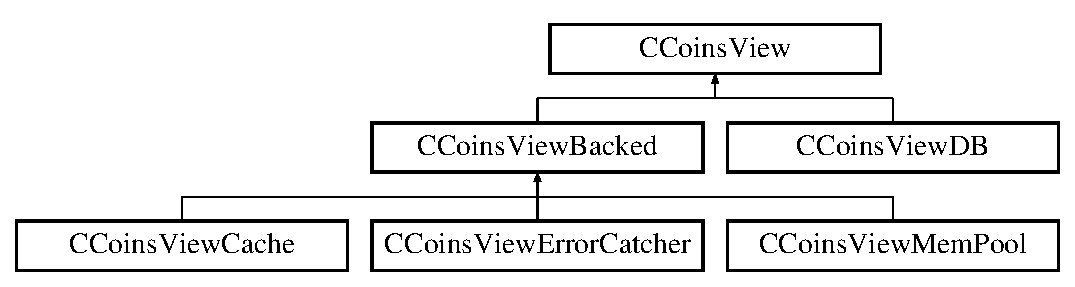
\includegraphics[height=3.000000cm]{class_c_coins_view}
\end{center}
\end{figure}
\subsection*{Public Member Functions}
\begin{DoxyCompactItemize}
\item 
virtual bool \hyperlink{class_c_coins_view_aaf5668eb2f9033583d7072dc2a3f96ef}{Get\+Coins} (const \hyperlink{classuint256}{uint256} \&txid, \hyperlink{class_c_coins}{C\+Coins} \&coins) const 
\begin{DoxyCompactList}\small\item\em Retrieve the \hyperlink{class_c_coins}{C\+Coins} (unspent transaction outputs) for a given txid. \end{DoxyCompactList}\item 
virtual bool \hyperlink{class_c_coins_view_a14c8db07cb11223426bb660861389f3a}{Have\+Coins} (const \hyperlink{classuint256}{uint256} \&txid) const 
\item 
virtual \hyperlink{classuint256}{uint256} \hyperlink{class_c_coins_view_a556cf7661ff49df1ada5cd0ad552f8db}{Get\+Best\+Block} () const 
\begin{DoxyCompactList}\small\item\em Retrieve the block hash whose state this \hyperlink{class_c_coins_view}{C\+Coins\+View} currently represents. \end{DoxyCompactList}\item 
virtual bool \hyperlink{class_c_coins_view_ad7dc37396ca4fac7014cea06fec7178e}{Batch\+Write} (\hyperlink{coins_8h_a2886ba2fd0428bae777e1cbcabc02834}{C\+Coins\+Map} \&map\+Coins, const \hyperlink{classuint256}{uint256} \&hash\+Block)
\item 
virtual bool \hyperlink{class_c_coins_view_afd645b903fba9c6b84bdb898d764f5fc}{Get\+Stats} (\hyperlink{struct_c_coins_stats}{C\+Coins\+Stats} \&stats) const 
\begin{DoxyCompactList}\small\item\em Calculate statistics about the unspent transaction output set. \end{DoxyCompactList}\item 
virtual \hyperlink{class_c_coins_view_a7ffb4218bf991ddff47339e44c8710da}{$\sim$\+C\+Coins\+View} ()
\begin{DoxyCompactList}\small\item\em As we use C\+Coins\+Views polymorphically, have a virtual destructor. \end{DoxyCompactList}\end{DoxyCompactItemize}


\subsection{Detailed Description}
Abstract view on the open txout dataset. 

\subsection{Constructor \& Destructor Documentation}
\hypertarget{class_c_coins_view_a7ffb4218bf991ddff47339e44c8710da}{}\index{C\+Coins\+View@{C\+Coins\+View}!````~C\+Coins\+View@{$\sim$\+C\+Coins\+View}}
\index{````~C\+Coins\+View@{$\sim$\+C\+Coins\+View}!C\+Coins\+View@{C\+Coins\+View}}
\subsubsection[{$\sim$\+C\+Coins\+View}]{\setlength{\rightskip}{0pt plus 5cm}virtual C\+Coins\+View\+::$\sim$\+C\+Coins\+View (
\begin{DoxyParamCaption}
{}
\end{DoxyParamCaption}
)\hspace{0.3cm}{\ttfamily [inline]}, {\ttfamily [virtual]}}\label{class_c_coins_view_a7ffb4218bf991ddff47339e44c8710da}


As we use C\+Coins\+Views polymorphically, have a virtual destructor. 



\subsection{Member Function Documentation}
\hypertarget{class_c_coins_view_ad7dc37396ca4fac7014cea06fec7178e}{}\index{C\+Coins\+View@{C\+Coins\+View}!Batch\+Write@{Batch\+Write}}
\index{Batch\+Write@{Batch\+Write}!C\+Coins\+View@{C\+Coins\+View}}
\subsubsection[{Batch\+Write}]{\setlength{\rightskip}{0pt plus 5cm}bool C\+Coins\+View\+::\+Batch\+Write (
\begin{DoxyParamCaption}
\item[{{\bf C\+Coins\+Map} \&}]{map\+Coins, }
\item[{const {\bf uint256} \&}]{hash\+Block}
\end{DoxyParamCaption}
)\hspace{0.3cm}{\ttfamily [virtual]}}\label{class_c_coins_view_ad7dc37396ca4fac7014cea06fec7178e}
Do a bulk modification (multiple \hyperlink{class_c_coins}{C\+Coins} changes + Best\+Block change). The passed map\+Coins can be modified. 

Reimplemented in \hyperlink{class_c_coins_view_cache_a561bb7c6c97701b12c48fbbb563d0a91}{C\+Coins\+View\+Cache}, \hyperlink{class_c_coins_view_backed_ace15da3934c9d7a9cb9c7a787f92f764}{C\+Coins\+View\+Backed}, and \hyperlink{class_c_coins_view_d_b_a33f98ec9323ce48e1704327bc8a2a002}{C\+Coins\+View\+D\+B}.

\hypertarget{class_c_coins_view_a556cf7661ff49df1ada5cd0ad552f8db}{}\index{C\+Coins\+View@{C\+Coins\+View}!Get\+Best\+Block@{Get\+Best\+Block}}
\index{Get\+Best\+Block@{Get\+Best\+Block}!C\+Coins\+View@{C\+Coins\+View}}
\subsubsection[{Get\+Best\+Block}]{\setlength{\rightskip}{0pt plus 5cm}{\bf uint256} C\+Coins\+View\+::\+Get\+Best\+Block (
\begin{DoxyParamCaption}
{}
\end{DoxyParamCaption}
) const\hspace{0.3cm}{\ttfamily [virtual]}}\label{class_c_coins_view_a556cf7661ff49df1ada5cd0ad552f8db}


Retrieve the block hash whose state this \hyperlink{class_c_coins_view}{C\+Coins\+View} currently represents. 



Reimplemented in \hyperlink{class_c_coins_view_cache_aabcd1da9f28445e09c9af5f68ce7f100}{C\+Coins\+View\+Cache}, \hyperlink{class_c_coins_view_backed_a8465dc4764fd5b01591b824551cbbfab}{C\+Coins\+View\+Backed}, and \hyperlink{class_c_coins_view_d_b_a01777676c2eafd2970a9d53e5fb4a49a}{C\+Coins\+View\+D\+B}.

\hypertarget{class_c_coins_view_aaf5668eb2f9033583d7072dc2a3f96ef}{}\index{C\+Coins\+View@{C\+Coins\+View}!Get\+Coins@{Get\+Coins}}
\index{Get\+Coins@{Get\+Coins}!C\+Coins\+View@{C\+Coins\+View}}
\subsubsection[{Get\+Coins}]{\setlength{\rightskip}{0pt plus 5cm}bool C\+Coins\+View\+::\+Get\+Coins (
\begin{DoxyParamCaption}
\item[{const {\bf uint256} \&}]{txid, }
\item[{{\bf C\+Coins} \&}]{coins}
\end{DoxyParamCaption}
) const\hspace{0.3cm}{\ttfamily [virtual]}}\label{class_c_coins_view_aaf5668eb2f9033583d7072dc2a3f96ef}


Retrieve the \hyperlink{class_c_coins}{C\+Coins} (unspent transaction outputs) for a given txid. 



Reimplemented in \hyperlink{class_c_coins_view_cache_a27ec8311ae409ea1e3c3484c1d4a9035}{C\+Coins\+View\+Cache}, \hyperlink{class_c_coins_view_backed_a21b95a9910f94e9b7ebed62a6f329ea0}{C\+Coins\+View\+Backed}, \hyperlink{class_c_coins_view_mem_pool_a01564f29ff2673ddd0d27414e576f1bc}{C\+Coins\+View\+Mem\+Pool}, \hyperlink{class_c_coins_view_error_catcher_a762969de31b62e55d01f1cdf0b178eb9}{C\+Coins\+View\+Error\+Catcher}, and \hyperlink{class_c_coins_view_d_b_a20655c9c13a6124cdcf210206d518d92}{C\+Coins\+View\+D\+B}.

\hypertarget{class_c_coins_view_afd645b903fba9c6b84bdb898d764f5fc}{}\index{C\+Coins\+View@{C\+Coins\+View}!Get\+Stats@{Get\+Stats}}
\index{Get\+Stats@{Get\+Stats}!C\+Coins\+View@{C\+Coins\+View}}
\subsubsection[{Get\+Stats}]{\setlength{\rightskip}{0pt plus 5cm}bool C\+Coins\+View\+::\+Get\+Stats (
\begin{DoxyParamCaption}
\item[{{\bf C\+Coins\+Stats} \&}]{stats}
\end{DoxyParamCaption}
) const\hspace{0.3cm}{\ttfamily [virtual]}}\label{class_c_coins_view_afd645b903fba9c6b84bdb898d764f5fc}


Calculate statistics about the unspent transaction output set. 



Reimplemented in \hyperlink{class_c_coins_view_backed_a368f277ac68652a91ac171f46f02edca}{C\+Coins\+View\+Backed}, and \hyperlink{class_c_coins_view_d_b_a6bbe15962b0efd519e30dada872f01c5}{C\+Coins\+View\+D\+B}.

\hypertarget{class_c_coins_view_a14c8db07cb11223426bb660861389f3a}{}\index{C\+Coins\+View@{C\+Coins\+View}!Have\+Coins@{Have\+Coins}}
\index{Have\+Coins@{Have\+Coins}!C\+Coins\+View@{C\+Coins\+View}}
\subsubsection[{Have\+Coins}]{\setlength{\rightskip}{0pt plus 5cm}bool C\+Coins\+View\+::\+Have\+Coins (
\begin{DoxyParamCaption}
\item[{const {\bf uint256} \&}]{txid}
\end{DoxyParamCaption}
) const\hspace{0.3cm}{\ttfamily [virtual]}}\label{class_c_coins_view_a14c8db07cb11223426bb660861389f3a}
Just check whether we have data for a given txid. This may (but cannot always) return true for fully spent transactions 

Reimplemented in \hyperlink{class_c_coins_view_cache_a25dddabe8734fc9823112763494da72b}{C\+Coins\+View\+Cache}, \hyperlink{class_c_coins_view_backed_a6a769cf9cc55128dea8e1a2798056e71}{C\+Coins\+View\+Backed}, \hyperlink{class_c_coins_view_mem_pool_a965e6c8e378fe937620ba2c180d1ed74}{C\+Coins\+View\+Mem\+Pool}, and \hyperlink{class_c_coins_view_d_b_a4d08cf2d3440c1de4e48cfddd67962d7}{C\+Coins\+View\+D\+B}.



The documentation for this class was generated from the following files\+:\begin{DoxyCompactItemize}
\item 
C\+:/\+Users/\+Joe/\+Documents/\+School/\+C\+S\+C17\+A/bitcoin/src/\hyperlink{coins_8h}{coins.\+h}\item 
C\+:/\+Users/\+Joe/\+Documents/\+School/\+C\+S\+C17\+A/bitcoin/src/\hyperlink{coins_8cpp}{coins.\+cpp}\end{DoxyCompactItemize}

\hypertarget{class_c_coins_view_backed}{}\section{C\+Coins\+View\+Backed Class Reference}
\label{class_c_coins_view_backed}\index{C\+Coins\+View\+Backed@{C\+Coins\+View\+Backed}}


{\ttfamily \#include $<$coins.\+h$>$}

Inheritance diagram for C\+Coins\+View\+Backed\+:\begin{figure}[H]
\begin{center}
\leavevmode
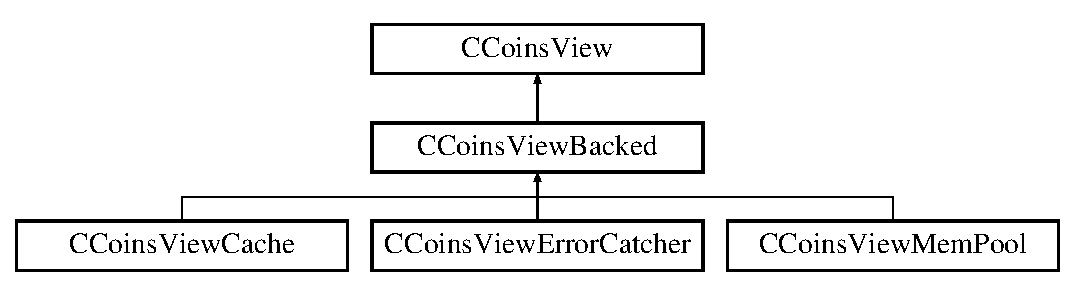
\includegraphics[height=3.000000cm]{class_c_coins_view_backed}
\end{center}
\end{figure}
\subsection*{Public Member Functions}
\begin{DoxyCompactItemize}
\item 
\hyperlink{class_c_coins_view_backed_af86a3b07433e8d84678772411791125e}{C\+Coins\+View\+Backed} (\hyperlink{class_c_coins_view}{C\+Coins\+View} $\ast$view\+In)
\item 
bool \hyperlink{class_c_coins_view_backed_a21b95a9910f94e9b7ebed62a6f329ea0}{Get\+Coins} (const \hyperlink{classuint256}{uint256} \&txid, \hyperlink{class_c_coins}{C\+Coins} \&coins) const 
\begin{DoxyCompactList}\small\item\em Retrieve the \hyperlink{class_c_coins}{C\+Coins} (unspent transaction outputs) for a given txid. \end{DoxyCompactList}\item 
bool \hyperlink{class_c_coins_view_backed_a6a769cf9cc55128dea8e1a2798056e71}{Have\+Coins} (const \hyperlink{classuint256}{uint256} \&txid) const 
\item 
\hyperlink{classuint256}{uint256} \hyperlink{class_c_coins_view_backed_a8465dc4764fd5b01591b824551cbbfab}{Get\+Best\+Block} () const 
\begin{DoxyCompactList}\small\item\em Retrieve the block hash whose state this \hyperlink{class_c_coins_view}{C\+Coins\+View} currently represents. \end{DoxyCompactList}\item 
void \hyperlink{class_c_coins_view_backed_a7eaddfbfd401a95c2fda2a8d8feaaf73}{Set\+Backend} (\hyperlink{class_c_coins_view}{C\+Coins\+View} \&view\+In)
\item 
bool \hyperlink{class_c_coins_view_backed_ace15da3934c9d7a9cb9c7a787f92f764}{Batch\+Write} (\hyperlink{coins_8h_a2886ba2fd0428bae777e1cbcabc02834}{C\+Coins\+Map} \&map\+Coins, const \hyperlink{classuint256}{uint256} \&hash\+Block)
\item 
bool \hyperlink{class_c_coins_view_backed_a368f277ac68652a91ac171f46f02edca}{Get\+Stats} (\hyperlink{struct_c_coins_stats}{C\+Coins\+Stats} \&stats) const 
\begin{DoxyCompactList}\small\item\em Calculate statistics about the unspent transaction output set. \end{DoxyCompactList}\end{DoxyCompactItemize}
\subsection*{Protected Attributes}
\begin{DoxyCompactItemize}
\item 
\hyperlink{class_c_coins_view}{C\+Coins\+View} $\ast$ \hyperlink{class_c_coins_view_backed_a901472317114adc4c104efd61dcf6203}{base}
\end{DoxyCompactItemize}


\subsection{Detailed Description}
\hyperlink{class_c_coins_view}{C\+Coins\+View} backed by another \hyperlink{class_c_coins_view}{C\+Coins\+View} 

\subsection{Constructor \& Destructor Documentation}
\hypertarget{class_c_coins_view_backed_af86a3b07433e8d84678772411791125e}{}\index{C\+Coins\+View\+Backed@{C\+Coins\+View\+Backed}!C\+Coins\+View\+Backed@{C\+Coins\+View\+Backed}}
\index{C\+Coins\+View\+Backed@{C\+Coins\+View\+Backed}!C\+Coins\+View\+Backed@{C\+Coins\+View\+Backed}}
\subsubsection[{C\+Coins\+View\+Backed}]{\setlength{\rightskip}{0pt plus 5cm}C\+Coins\+View\+Backed\+::\+C\+Coins\+View\+Backed (
\begin{DoxyParamCaption}
\item[{{\bf C\+Coins\+View} $\ast$}]{view\+In}
\end{DoxyParamCaption}
)}\label{class_c_coins_view_backed_af86a3b07433e8d84678772411791125e}


\subsection{Member Function Documentation}
\hypertarget{class_c_coins_view_backed_ace15da3934c9d7a9cb9c7a787f92f764}{}\index{C\+Coins\+View\+Backed@{C\+Coins\+View\+Backed}!Batch\+Write@{Batch\+Write}}
\index{Batch\+Write@{Batch\+Write}!C\+Coins\+View\+Backed@{C\+Coins\+View\+Backed}}
\subsubsection[{Batch\+Write}]{\setlength{\rightskip}{0pt plus 5cm}bool C\+Coins\+View\+Backed\+::\+Batch\+Write (
\begin{DoxyParamCaption}
\item[{{\bf C\+Coins\+Map} \&}]{map\+Coins, }
\item[{const {\bf uint256} \&}]{hash\+Block}
\end{DoxyParamCaption}
)\hspace{0.3cm}{\ttfamily [virtual]}}\label{class_c_coins_view_backed_ace15da3934c9d7a9cb9c7a787f92f764}
Do a bulk modification (multiple \hyperlink{class_c_coins}{C\+Coins} changes + Best\+Block change). The passed map\+Coins can be modified. 

Reimplemented from \hyperlink{class_c_coins_view_ad7dc37396ca4fac7014cea06fec7178e}{C\+Coins\+View}.



Reimplemented in \hyperlink{class_c_coins_view_cache_a561bb7c6c97701b12c48fbbb563d0a91}{C\+Coins\+View\+Cache}.

\hypertarget{class_c_coins_view_backed_a8465dc4764fd5b01591b824551cbbfab}{}\index{C\+Coins\+View\+Backed@{C\+Coins\+View\+Backed}!Get\+Best\+Block@{Get\+Best\+Block}}
\index{Get\+Best\+Block@{Get\+Best\+Block}!C\+Coins\+View\+Backed@{C\+Coins\+View\+Backed}}
\subsubsection[{Get\+Best\+Block}]{\setlength{\rightskip}{0pt plus 5cm}{\bf uint256} C\+Coins\+View\+Backed\+::\+Get\+Best\+Block (
\begin{DoxyParamCaption}
{}
\end{DoxyParamCaption}
) const\hspace{0.3cm}{\ttfamily [virtual]}}\label{class_c_coins_view_backed_a8465dc4764fd5b01591b824551cbbfab}


Retrieve the block hash whose state this \hyperlink{class_c_coins_view}{C\+Coins\+View} currently represents. 



Reimplemented from \hyperlink{class_c_coins_view_a556cf7661ff49df1ada5cd0ad552f8db}{C\+Coins\+View}.



Reimplemented in \hyperlink{class_c_coins_view_cache_aabcd1da9f28445e09c9af5f68ce7f100}{C\+Coins\+View\+Cache}.

\hypertarget{class_c_coins_view_backed_a21b95a9910f94e9b7ebed62a6f329ea0}{}\index{C\+Coins\+View\+Backed@{C\+Coins\+View\+Backed}!Get\+Coins@{Get\+Coins}}
\index{Get\+Coins@{Get\+Coins}!C\+Coins\+View\+Backed@{C\+Coins\+View\+Backed}}
\subsubsection[{Get\+Coins}]{\setlength{\rightskip}{0pt plus 5cm}bool C\+Coins\+View\+Backed\+::\+Get\+Coins (
\begin{DoxyParamCaption}
\item[{const {\bf uint256} \&}]{txid, }
\item[{{\bf C\+Coins} \&}]{coins}
\end{DoxyParamCaption}
) const\hspace{0.3cm}{\ttfamily [virtual]}}\label{class_c_coins_view_backed_a21b95a9910f94e9b7ebed62a6f329ea0}


Retrieve the \hyperlink{class_c_coins}{C\+Coins} (unspent transaction outputs) for a given txid. 



Reimplemented from \hyperlink{class_c_coins_view_aaf5668eb2f9033583d7072dc2a3f96ef}{C\+Coins\+View}.



Reimplemented in \hyperlink{class_c_coins_view_cache_a27ec8311ae409ea1e3c3484c1d4a9035}{C\+Coins\+View\+Cache}, \hyperlink{class_c_coins_view_mem_pool_a01564f29ff2673ddd0d27414e576f1bc}{C\+Coins\+View\+Mem\+Pool}, and \hyperlink{class_c_coins_view_error_catcher_a762969de31b62e55d01f1cdf0b178eb9}{C\+Coins\+View\+Error\+Catcher}.

\hypertarget{class_c_coins_view_backed_a368f277ac68652a91ac171f46f02edca}{}\index{C\+Coins\+View\+Backed@{C\+Coins\+View\+Backed}!Get\+Stats@{Get\+Stats}}
\index{Get\+Stats@{Get\+Stats}!C\+Coins\+View\+Backed@{C\+Coins\+View\+Backed}}
\subsubsection[{Get\+Stats}]{\setlength{\rightskip}{0pt plus 5cm}bool C\+Coins\+View\+Backed\+::\+Get\+Stats (
\begin{DoxyParamCaption}
\item[{{\bf C\+Coins\+Stats} \&}]{stats}
\end{DoxyParamCaption}
) const\hspace{0.3cm}{\ttfamily [virtual]}}\label{class_c_coins_view_backed_a368f277ac68652a91ac171f46f02edca}


Calculate statistics about the unspent transaction output set. 



Reimplemented from \hyperlink{class_c_coins_view_afd645b903fba9c6b84bdb898d764f5fc}{C\+Coins\+View}.

\hypertarget{class_c_coins_view_backed_a6a769cf9cc55128dea8e1a2798056e71}{}\index{C\+Coins\+View\+Backed@{C\+Coins\+View\+Backed}!Have\+Coins@{Have\+Coins}}
\index{Have\+Coins@{Have\+Coins}!C\+Coins\+View\+Backed@{C\+Coins\+View\+Backed}}
\subsubsection[{Have\+Coins}]{\setlength{\rightskip}{0pt plus 5cm}bool C\+Coins\+View\+Backed\+::\+Have\+Coins (
\begin{DoxyParamCaption}
\item[{const {\bf uint256} \&}]{txid}
\end{DoxyParamCaption}
) const\hspace{0.3cm}{\ttfamily [virtual]}}\label{class_c_coins_view_backed_a6a769cf9cc55128dea8e1a2798056e71}
Just check whether we have data for a given txid. This may (but cannot always) return true for fully spent transactions 

Reimplemented from \hyperlink{class_c_coins_view_a14c8db07cb11223426bb660861389f3a}{C\+Coins\+View}.



Reimplemented in \hyperlink{class_c_coins_view_cache_a25dddabe8734fc9823112763494da72b}{C\+Coins\+View\+Cache}, and \hyperlink{class_c_coins_view_mem_pool_a965e6c8e378fe937620ba2c180d1ed74}{C\+Coins\+View\+Mem\+Pool}.

\hypertarget{class_c_coins_view_backed_a7eaddfbfd401a95c2fda2a8d8feaaf73}{}\index{C\+Coins\+View\+Backed@{C\+Coins\+View\+Backed}!Set\+Backend@{Set\+Backend}}
\index{Set\+Backend@{Set\+Backend}!C\+Coins\+View\+Backed@{C\+Coins\+View\+Backed}}
\subsubsection[{Set\+Backend}]{\setlength{\rightskip}{0pt plus 5cm}void C\+Coins\+View\+Backed\+::\+Set\+Backend (
\begin{DoxyParamCaption}
\item[{{\bf C\+Coins\+View} \&}]{view\+In}
\end{DoxyParamCaption}
)}\label{class_c_coins_view_backed_a7eaddfbfd401a95c2fda2a8d8feaaf73}


\subsection{Member Data Documentation}
\hypertarget{class_c_coins_view_backed_a901472317114adc4c104efd61dcf6203}{}\index{C\+Coins\+View\+Backed@{C\+Coins\+View\+Backed}!base@{base}}
\index{base@{base}!C\+Coins\+View\+Backed@{C\+Coins\+View\+Backed}}
\subsubsection[{base}]{\setlength{\rightskip}{0pt plus 5cm}{\bf C\+Coins\+View}$\ast$ C\+Coins\+View\+Backed\+::base\hspace{0.3cm}{\ttfamily [protected]}}\label{class_c_coins_view_backed_a901472317114adc4c104efd61dcf6203}


The documentation for this class was generated from the following files\+:\begin{DoxyCompactItemize}
\item 
C\+:/\+Users/\+Joe/\+Documents/\+School/\+C\+S\+C17\+A/bitcoin/src/\hyperlink{coins_8h}{coins.\+h}\item 
C\+:/\+Users/\+Joe/\+Documents/\+School/\+C\+S\+C17\+A/bitcoin/src/\hyperlink{coins_8cpp}{coins.\+cpp}\end{DoxyCompactItemize}

\hypertarget{class_c_coins_view_cache}{}\section{C\+Coins\+View\+Cache Class Reference}
\label{class_c_coins_view_cache}\index{C\+Coins\+View\+Cache@{C\+Coins\+View\+Cache}}


{\ttfamily \#include $<$coins.\+h$>$}

Inheritance diagram for C\+Coins\+View\+Cache\+:\begin{figure}[H]
\begin{center}
\leavevmode
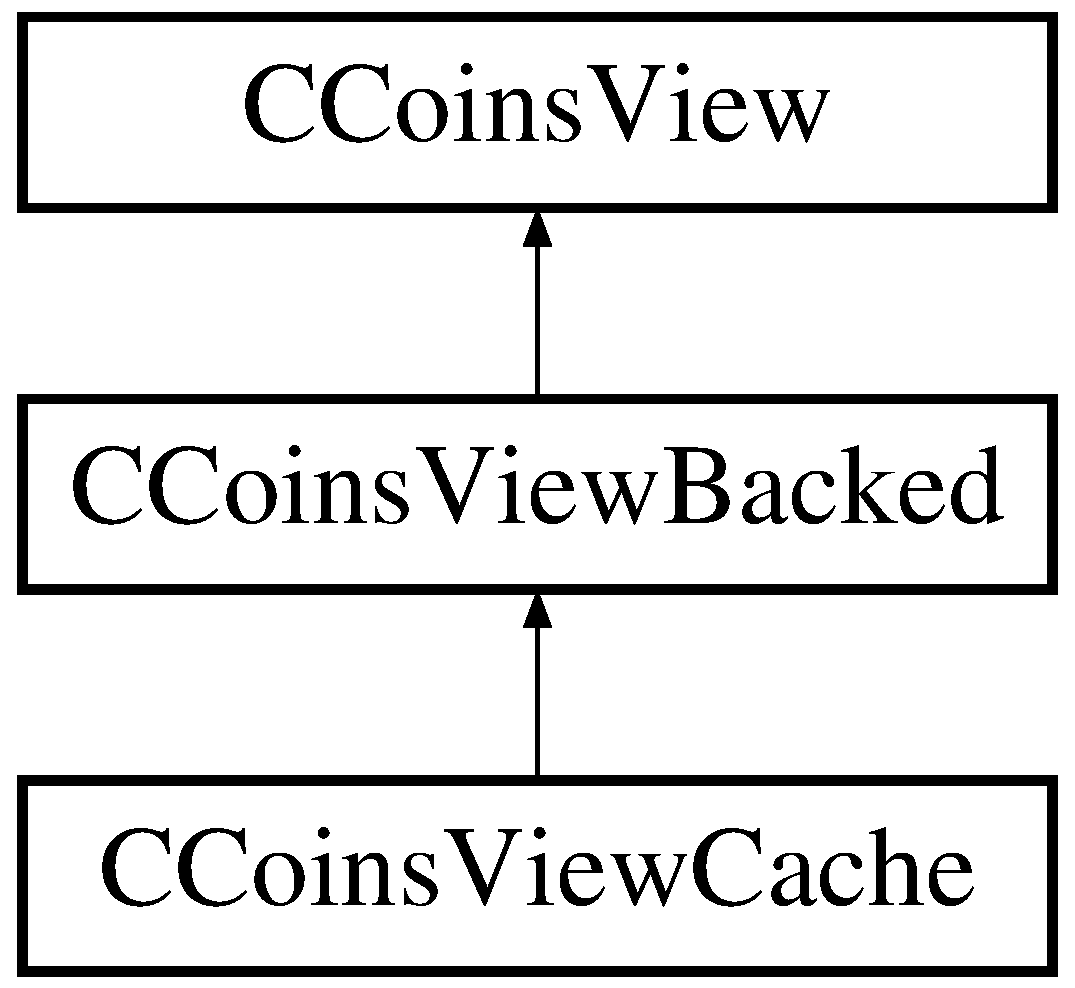
\includegraphics[height=3.000000cm]{class_c_coins_view_cache}
\end{center}
\end{figure}
\subsection*{Public Member Functions}
\begin{DoxyCompactItemize}
\item 
\hyperlink{class_c_coins_view_cache_a515a6f259af607fb3394b560d9c063c9}{C\+Coins\+View\+Cache} (\hyperlink{class_c_coins_view}{C\+Coins\+View} $\ast$base\+In)
\item 
\hyperlink{class_c_coins_view_cache_a6148421cb7605fb434f6c8622f39430b}{$\sim$\+C\+Coins\+View\+Cache} ()
\item 
bool \hyperlink{class_c_coins_view_cache_a27ec8311ae409ea1e3c3484c1d4a9035}{Get\+Coins} (const \hyperlink{classuint256}{uint256} \&txid, \hyperlink{class_c_coins}{C\+Coins} \&coins) const 
\begin{DoxyCompactList}\small\item\em Retrieve the \hyperlink{class_c_coins}{C\+Coins} (unspent transaction outputs) for a given txid. \end{DoxyCompactList}\item 
bool \hyperlink{class_c_coins_view_cache_a25dddabe8734fc9823112763494da72b}{Have\+Coins} (const \hyperlink{classuint256}{uint256} \&txid) const 
\item 
\hyperlink{classuint256}{uint256} \hyperlink{class_c_coins_view_cache_aabcd1da9f28445e09c9af5f68ce7f100}{Get\+Best\+Block} () const 
\begin{DoxyCompactList}\small\item\em Retrieve the block hash whose state this \hyperlink{class_c_coins_view}{C\+Coins\+View} currently represents. \end{DoxyCompactList}\item 
void \hyperlink{class_c_coins_view_cache_aa3f787f77b123f0fd340fbe4e458b4ad}{Set\+Best\+Block} (const \hyperlink{classuint256}{uint256} \&\hyperlink{class_c_coins_view_cache_a229dddddbc5501edc250209a2ce5df8b}{hash\+Block})
\item 
bool \hyperlink{class_c_coins_view_cache_a561bb7c6c97701b12c48fbbb563d0a91}{Batch\+Write} (\hyperlink{coins_8h_a2886ba2fd0428bae777e1cbcabc02834}{C\+Coins\+Map} \&map\+Coins, const \hyperlink{classuint256}{uint256} \&\hyperlink{class_c_coins_view_cache_a229dddddbc5501edc250209a2ce5df8b}{hash\+Block})
\item 
const \hyperlink{class_c_coins}{C\+Coins} $\ast$ \hyperlink{class_c_coins_view_cache_a2b72aa925d9c1a1bd662f7e2852059d9}{Access\+Coins} (const \hyperlink{classuint256}{uint256} \&txid) const 
\item 
\hyperlink{class_c_coins_modifier}{C\+Coins\+Modifier} \hyperlink{class_c_coins_view_cache_ab67c0d489873ed735c4fc52aa66f0830}{Modify\+Coins} (const \hyperlink{classuint256}{uint256} \&txid)
\item 
bool \hyperlink{class_c_coins_view_cache_ac9888d4feaa46666d03871cd7cd1c01d}{Flush} ()
\item 
unsigned int \hyperlink{class_c_coins_view_cache_a5e8c37ab1b772d00b57e2b40256a4646}{Get\+Cache\+Size} () const 
\begin{DoxyCompactList}\small\item\em Calculate the size of the cache (in number of transactions) \end{DoxyCompactList}\item 
\hyperlink{amount_8h_a4eaf3a5239714d8c45b851527f7cb564}{C\+Amount} \hyperlink{class_c_coins_view_cache_a7fd5ad106e1ac2c2770005672421ff93}{Get\+Value\+In} (const C\+Transaction \&tx) const 
\item 
bool \hyperlink{class_c_coins_view_cache_a2b547a48709e9f9af9a4cfc77a328a3f}{Have\+Inputs} (const C\+Transaction \&tx) const 
\begin{DoxyCompactList}\small\item\em Check whether all prevouts of the transaction are present in the U\+T\+X\+O set represented by this view. \end{DoxyCompactList}\item 
double \hyperlink{class_c_coins_view_cache_a0ba6f2f115a73a91d3cfb8f59569099d}{Get\+Priority} (const C\+Transaction \&tx, int n\+Height) const 
\begin{DoxyCompactList}\small\item\em Return priority of tx at height n\+Height. \end{DoxyCompactList}\item 
const C\+Tx\+Out \& \hyperlink{class_c_coins_view_cache_aa441d7d3869be2f164af1c52a3acb56a}{Get\+Output\+For} (const C\+Tx\+In \&input) const 
\end{DoxyCompactItemize}
\subsection*{Protected Attributes}
\begin{DoxyCompactItemize}
\item 
bool \hyperlink{class_c_coins_view_cache_a363e27234d36bb0fc533d60cd64d1bc3}{has\+Modifier}
\item 
\hyperlink{classuint256}{uint256} \hyperlink{class_c_coins_view_cache_a229dddddbc5501edc250209a2ce5df8b}{hash\+Block}
\item 
\hyperlink{coins_8h_a2886ba2fd0428bae777e1cbcabc02834}{C\+Coins\+Map} \hyperlink{class_c_coins_view_cache_af33cc2c6d38af65ac833d4d13c8e3764}{cache\+Coins}
\end{DoxyCompactItemize}
\subsection*{Friends}
\begin{DoxyCompactItemize}
\item 
class \hyperlink{class_c_coins_view_cache_ae6ce8219acb79950bced74cb108acacf}{C\+Coins\+Modifier}
\end{DoxyCompactItemize}


\subsection{Detailed Description}
\hyperlink{class_c_coins_view}{C\+Coins\+View} that adds a memory cache for transactions to another \hyperlink{class_c_coins_view}{C\+Coins\+View} 

\subsection{Constructor \& Destructor Documentation}
\hypertarget{class_c_coins_view_cache_a515a6f259af607fb3394b560d9c063c9}{}\index{C\+Coins\+View\+Cache@{C\+Coins\+View\+Cache}!C\+Coins\+View\+Cache@{C\+Coins\+View\+Cache}}
\index{C\+Coins\+View\+Cache@{C\+Coins\+View\+Cache}!C\+Coins\+View\+Cache@{C\+Coins\+View\+Cache}}
\subsubsection[{C\+Coins\+View\+Cache}]{\setlength{\rightskip}{0pt plus 5cm}C\+Coins\+View\+Cache\+::\+C\+Coins\+View\+Cache (
\begin{DoxyParamCaption}
\item[{{\bf C\+Coins\+View} $\ast$}]{base\+In}
\end{DoxyParamCaption}
)}\label{class_c_coins_view_cache_a515a6f259af607fb3394b560d9c063c9}
\hypertarget{class_c_coins_view_cache_a6148421cb7605fb434f6c8622f39430b}{}\index{C\+Coins\+View\+Cache@{C\+Coins\+View\+Cache}!````~C\+Coins\+View\+Cache@{$\sim$\+C\+Coins\+View\+Cache}}
\index{````~C\+Coins\+View\+Cache@{$\sim$\+C\+Coins\+View\+Cache}!C\+Coins\+View\+Cache@{C\+Coins\+View\+Cache}}
\subsubsection[{$\sim$\+C\+Coins\+View\+Cache}]{\setlength{\rightskip}{0pt plus 5cm}C\+Coins\+View\+Cache\+::$\sim$\+C\+Coins\+View\+Cache (
\begin{DoxyParamCaption}
{}
\end{DoxyParamCaption}
)}\label{class_c_coins_view_cache_a6148421cb7605fb434f6c8622f39430b}


\subsection{Member Function Documentation}
\hypertarget{class_c_coins_view_cache_a2b72aa925d9c1a1bd662f7e2852059d9}{}\index{C\+Coins\+View\+Cache@{C\+Coins\+View\+Cache}!Access\+Coins@{Access\+Coins}}
\index{Access\+Coins@{Access\+Coins}!C\+Coins\+View\+Cache@{C\+Coins\+View\+Cache}}
\subsubsection[{Access\+Coins}]{\setlength{\rightskip}{0pt plus 5cm}const {\bf C\+Coins} $\ast$ C\+Coins\+View\+Cache\+::\+Access\+Coins (
\begin{DoxyParamCaption}
\item[{const {\bf uint256} \&}]{txid}
\end{DoxyParamCaption}
) const}\label{class_c_coins_view_cache_a2b72aa925d9c1a1bd662f7e2852059d9}
Return a pointer to \hyperlink{class_c_coins}{C\+Coins} in the cache, or N\+U\+L\+L if not found. This is more efficient than Get\+Coins. Modifications to other cache entries are allowed while accessing the returned pointer. \hypertarget{class_c_coins_view_cache_a561bb7c6c97701b12c48fbbb563d0a91}{}\index{C\+Coins\+View\+Cache@{C\+Coins\+View\+Cache}!Batch\+Write@{Batch\+Write}}
\index{Batch\+Write@{Batch\+Write}!C\+Coins\+View\+Cache@{C\+Coins\+View\+Cache}}
\subsubsection[{Batch\+Write}]{\setlength{\rightskip}{0pt plus 5cm}bool C\+Coins\+View\+Cache\+::\+Batch\+Write (
\begin{DoxyParamCaption}
\item[{{\bf C\+Coins\+Map} \&}]{map\+Coins, }
\item[{const {\bf uint256} \&}]{hash\+Block}
\end{DoxyParamCaption}
)\hspace{0.3cm}{\ttfamily [virtual]}}\label{class_c_coins_view_cache_a561bb7c6c97701b12c48fbbb563d0a91}
Do a bulk modification (multiple \hyperlink{class_c_coins}{C\+Coins} changes + Best\+Block change). The passed map\+Coins can be modified. 

Reimplemented from \hyperlink{class_c_coins_view_backed_ace15da3934c9d7a9cb9c7a787f92f764}{C\+Coins\+View\+Backed}.

\hypertarget{class_c_coins_view_cache_ac9888d4feaa46666d03871cd7cd1c01d}{}\index{C\+Coins\+View\+Cache@{C\+Coins\+View\+Cache}!Flush@{Flush}}
\index{Flush@{Flush}!C\+Coins\+View\+Cache@{C\+Coins\+View\+Cache}}
\subsubsection[{Flush}]{\setlength{\rightskip}{0pt plus 5cm}bool C\+Coins\+View\+Cache\+::\+Flush (
\begin{DoxyParamCaption}
{}
\end{DoxyParamCaption}
)}\label{class_c_coins_view_cache_ac9888d4feaa46666d03871cd7cd1c01d}
Push the modifications applied to this cache to its base. Failure to call this method before destruction will cause the changes to be forgotten. If false is returned, the state of this cache (and its backing view) will be undefined. \hypertarget{class_c_coins_view_cache_aabcd1da9f28445e09c9af5f68ce7f100}{}\index{C\+Coins\+View\+Cache@{C\+Coins\+View\+Cache}!Get\+Best\+Block@{Get\+Best\+Block}}
\index{Get\+Best\+Block@{Get\+Best\+Block}!C\+Coins\+View\+Cache@{C\+Coins\+View\+Cache}}
\subsubsection[{Get\+Best\+Block}]{\setlength{\rightskip}{0pt plus 5cm}{\bf uint256} C\+Coins\+View\+Cache\+::\+Get\+Best\+Block (
\begin{DoxyParamCaption}
{}
\end{DoxyParamCaption}
) const\hspace{0.3cm}{\ttfamily [virtual]}}\label{class_c_coins_view_cache_aabcd1da9f28445e09c9af5f68ce7f100}


Retrieve the block hash whose state this \hyperlink{class_c_coins_view}{C\+Coins\+View} currently represents. 



Reimplemented from \hyperlink{class_c_coins_view_backed_a8465dc4764fd5b01591b824551cbbfab}{C\+Coins\+View\+Backed}.

\hypertarget{class_c_coins_view_cache_a5e8c37ab1b772d00b57e2b40256a4646}{}\index{C\+Coins\+View\+Cache@{C\+Coins\+View\+Cache}!Get\+Cache\+Size@{Get\+Cache\+Size}}
\index{Get\+Cache\+Size@{Get\+Cache\+Size}!C\+Coins\+View\+Cache@{C\+Coins\+View\+Cache}}
\subsubsection[{Get\+Cache\+Size}]{\setlength{\rightskip}{0pt plus 5cm}unsigned int C\+Coins\+View\+Cache\+::\+Get\+Cache\+Size (
\begin{DoxyParamCaption}
{}
\end{DoxyParamCaption}
) const}\label{class_c_coins_view_cache_a5e8c37ab1b772d00b57e2b40256a4646}


Calculate the size of the cache (in number of transactions) 

\hypertarget{class_c_coins_view_cache_a27ec8311ae409ea1e3c3484c1d4a9035}{}\index{C\+Coins\+View\+Cache@{C\+Coins\+View\+Cache}!Get\+Coins@{Get\+Coins}}
\index{Get\+Coins@{Get\+Coins}!C\+Coins\+View\+Cache@{C\+Coins\+View\+Cache}}
\subsubsection[{Get\+Coins}]{\setlength{\rightskip}{0pt plus 5cm}bool C\+Coins\+View\+Cache\+::\+Get\+Coins (
\begin{DoxyParamCaption}
\item[{const {\bf uint256} \&}]{txid, }
\item[{{\bf C\+Coins} \&}]{coins}
\end{DoxyParamCaption}
) const\hspace{0.3cm}{\ttfamily [virtual]}}\label{class_c_coins_view_cache_a27ec8311ae409ea1e3c3484c1d4a9035}


Retrieve the \hyperlink{class_c_coins}{C\+Coins} (unspent transaction outputs) for a given txid. 



Reimplemented from \hyperlink{class_c_coins_view_backed_a21b95a9910f94e9b7ebed62a6f329ea0}{C\+Coins\+View\+Backed}.

\hypertarget{class_c_coins_view_cache_aa441d7d3869be2f164af1c52a3acb56a}{}\index{C\+Coins\+View\+Cache@{C\+Coins\+View\+Cache}!Get\+Output\+For@{Get\+Output\+For}}
\index{Get\+Output\+For@{Get\+Output\+For}!C\+Coins\+View\+Cache@{C\+Coins\+View\+Cache}}
\subsubsection[{Get\+Output\+For}]{\setlength{\rightskip}{0pt plus 5cm}const C\+Tx\+Out \& C\+Coins\+View\+Cache\+::\+Get\+Output\+For (
\begin{DoxyParamCaption}
\item[{const C\+Tx\+In \&}]{input}
\end{DoxyParamCaption}
) const}\label{class_c_coins_view_cache_aa441d7d3869be2f164af1c52a3acb56a}
\hypertarget{class_c_coins_view_cache_a0ba6f2f115a73a91d3cfb8f59569099d}{}\index{C\+Coins\+View\+Cache@{C\+Coins\+View\+Cache}!Get\+Priority@{Get\+Priority}}
\index{Get\+Priority@{Get\+Priority}!C\+Coins\+View\+Cache@{C\+Coins\+View\+Cache}}
\subsubsection[{Get\+Priority}]{\setlength{\rightskip}{0pt plus 5cm}double C\+Coins\+View\+Cache\+::\+Get\+Priority (
\begin{DoxyParamCaption}
\item[{const C\+Transaction \&}]{tx, }
\item[{int}]{n\+Height}
\end{DoxyParamCaption}
) const}\label{class_c_coins_view_cache_a0ba6f2f115a73a91d3cfb8f59569099d}


Return priority of tx at height n\+Height. 

\hypertarget{class_c_coins_view_cache_a7fd5ad106e1ac2c2770005672421ff93}{}\index{C\+Coins\+View\+Cache@{C\+Coins\+View\+Cache}!Get\+Value\+In@{Get\+Value\+In}}
\index{Get\+Value\+In@{Get\+Value\+In}!C\+Coins\+View\+Cache@{C\+Coins\+View\+Cache}}
\subsubsection[{Get\+Value\+In}]{\setlength{\rightskip}{0pt plus 5cm}{\bf C\+Amount} C\+Coins\+View\+Cache\+::\+Get\+Value\+In (
\begin{DoxyParamCaption}
\item[{const C\+Transaction \&}]{tx}
\end{DoxyParamCaption}
) const}\label{class_c_coins_view_cache_a7fd5ad106e1ac2c2770005672421ff93}
Amount of bitcoins coming in to a transaction Note that lightweight clients may not know anything besides the hash of previous transactions, so may not be able to calculate this.


\begin{DoxyParams}[1]{Parameters}
\mbox{\tt in}  & {\em tx} & transaction for which we are checking input total \\
\hline
\end{DoxyParams}
\begin{DoxyReturn}{Returns}
Sum of value of all inputs (script\+Sigs) 
\end{DoxyReturn}
\hypertarget{class_c_coins_view_cache_a25dddabe8734fc9823112763494da72b}{}\index{C\+Coins\+View\+Cache@{C\+Coins\+View\+Cache}!Have\+Coins@{Have\+Coins}}
\index{Have\+Coins@{Have\+Coins}!C\+Coins\+View\+Cache@{C\+Coins\+View\+Cache}}
\subsubsection[{Have\+Coins}]{\setlength{\rightskip}{0pt plus 5cm}bool C\+Coins\+View\+Cache\+::\+Have\+Coins (
\begin{DoxyParamCaption}
\item[{const {\bf uint256} \&}]{txid}
\end{DoxyParamCaption}
) const\hspace{0.3cm}{\ttfamily [virtual]}}\label{class_c_coins_view_cache_a25dddabe8734fc9823112763494da72b}
Just check whether we have data for a given txid. This may (but cannot always) return true for fully spent transactions 

Reimplemented from \hyperlink{class_c_coins_view_backed_a6a769cf9cc55128dea8e1a2798056e71}{C\+Coins\+View\+Backed}.

\hypertarget{class_c_coins_view_cache_a2b547a48709e9f9af9a4cfc77a328a3f}{}\index{C\+Coins\+View\+Cache@{C\+Coins\+View\+Cache}!Have\+Inputs@{Have\+Inputs}}
\index{Have\+Inputs@{Have\+Inputs}!C\+Coins\+View\+Cache@{C\+Coins\+View\+Cache}}
\subsubsection[{Have\+Inputs}]{\setlength{\rightskip}{0pt plus 5cm}bool C\+Coins\+View\+Cache\+::\+Have\+Inputs (
\begin{DoxyParamCaption}
\item[{const C\+Transaction \&}]{tx}
\end{DoxyParamCaption}
) const}\label{class_c_coins_view_cache_a2b547a48709e9f9af9a4cfc77a328a3f}


Check whether all prevouts of the transaction are present in the U\+T\+X\+O set represented by this view. 

\hypertarget{class_c_coins_view_cache_ab67c0d489873ed735c4fc52aa66f0830}{}\index{C\+Coins\+View\+Cache@{C\+Coins\+View\+Cache}!Modify\+Coins@{Modify\+Coins}}
\index{Modify\+Coins@{Modify\+Coins}!C\+Coins\+View\+Cache@{C\+Coins\+View\+Cache}}
\subsubsection[{Modify\+Coins}]{\setlength{\rightskip}{0pt plus 5cm}{\bf C\+Coins\+Modifier} C\+Coins\+View\+Cache\+::\+Modify\+Coins (
\begin{DoxyParamCaption}
\item[{const {\bf uint256} \&}]{txid}
\end{DoxyParamCaption}
)}\label{class_c_coins_view_cache_ab67c0d489873ed735c4fc52aa66f0830}
Return a modifiable reference to a \hyperlink{class_c_coins}{C\+Coins}. If no entry with the given txid exists, a new one is created. Simultaneous modifications are not allowed. \hypertarget{class_c_coins_view_cache_aa3f787f77b123f0fd340fbe4e458b4ad}{}\index{C\+Coins\+View\+Cache@{C\+Coins\+View\+Cache}!Set\+Best\+Block@{Set\+Best\+Block}}
\index{Set\+Best\+Block@{Set\+Best\+Block}!C\+Coins\+View\+Cache@{C\+Coins\+View\+Cache}}
\subsubsection[{Set\+Best\+Block}]{\setlength{\rightskip}{0pt plus 5cm}void C\+Coins\+View\+Cache\+::\+Set\+Best\+Block (
\begin{DoxyParamCaption}
\item[{const {\bf uint256} \&}]{hash\+Block}
\end{DoxyParamCaption}
)}\label{class_c_coins_view_cache_aa3f787f77b123f0fd340fbe4e458b4ad}


\subsection{Friends And Related Function Documentation}
\hypertarget{class_c_coins_view_cache_ae6ce8219acb79950bced74cb108acacf}{}\index{C\+Coins\+View\+Cache@{C\+Coins\+View\+Cache}!C\+Coins\+Modifier@{C\+Coins\+Modifier}}
\index{C\+Coins\+Modifier@{C\+Coins\+Modifier}!C\+Coins\+View\+Cache@{C\+Coins\+View\+Cache}}
\subsubsection[{C\+Coins\+Modifier}]{\setlength{\rightskip}{0pt plus 5cm}friend class {\bf C\+Coins\+Modifier}\hspace{0.3cm}{\ttfamily [friend]}}\label{class_c_coins_view_cache_ae6ce8219acb79950bced74cb108acacf}


\subsection{Member Data Documentation}
\hypertarget{class_c_coins_view_cache_af33cc2c6d38af65ac833d4d13c8e3764}{}\index{C\+Coins\+View\+Cache@{C\+Coins\+View\+Cache}!cache\+Coins@{cache\+Coins}}
\index{cache\+Coins@{cache\+Coins}!C\+Coins\+View\+Cache@{C\+Coins\+View\+Cache}}
\subsubsection[{cache\+Coins}]{\setlength{\rightskip}{0pt plus 5cm}{\bf C\+Coins\+Map} C\+Coins\+View\+Cache\+::cache\+Coins\hspace{0.3cm}{\ttfamily [mutable]}, {\ttfamily [protected]}}\label{class_c_coins_view_cache_af33cc2c6d38af65ac833d4d13c8e3764}
\hypertarget{class_c_coins_view_cache_a229dddddbc5501edc250209a2ce5df8b}{}\index{C\+Coins\+View\+Cache@{C\+Coins\+View\+Cache}!hash\+Block@{hash\+Block}}
\index{hash\+Block@{hash\+Block}!C\+Coins\+View\+Cache@{C\+Coins\+View\+Cache}}
\subsubsection[{hash\+Block}]{\setlength{\rightskip}{0pt plus 5cm}{\bf uint256} C\+Coins\+View\+Cache\+::hash\+Block\hspace{0.3cm}{\ttfamily [mutable]}, {\ttfamily [protected]}}\label{class_c_coins_view_cache_a229dddddbc5501edc250209a2ce5df8b}
Make mutable so that we can \char`\"{}fill the cache\char`\"{} even from Get-\/methods declared as \char`\"{}const\char`\"{}. \hypertarget{class_c_coins_view_cache_a363e27234d36bb0fc533d60cd64d1bc3}{}\index{C\+Coins\+View\+Cache@{C\+Coins\+View\+Cache}!has\+Modifier@{has\+Modifier}}
\index{has\+Modifier@{has\+Modifier}!C\+Coins\+View\+Cache@{C\+Coins\+View\+Cache}}
\subsubsection[{has\+Modifier}]{\setlength{\rightskip}{0pt plus 5cm}bool C\+Coins\+View\+Cache\+::has\+Modifier\hspace{0.3cm}{\ttfamily [protected]}}\label{class_c_coins_view_cache_a363e27234d36bb0fc533d60cd64d1bc3}


The documentation for this class was generated from the following files\+:\begin{DoxyCompactItemize}
\item 
C\+:/\+Users/\+Joe/\+Documents/\+School/\+C\+S\+C17\+A/bitcoin/src/\hyperlink{coins_8h}{coins.\+h}\item 
C\+:/\+Users/\+Joe/\+Documents/\+School/\+C\+S\+C17\+A/bitcoin/src/\hyperlink{coins_8cpp}{coins.\+cpp}\end{DoxyCompactItemize}

\hypertarget{class_c_coins_view_d_b}{}\section{C\+Coins\+View\+D\+B Class Reference}
\label{class_c_coins_view_d_b}\index{C\+Coins\+View\+D\+B@{C\+Coins\+View\+D\+B}}


{\ttfamily \#include $<$txdb.\+h$>$}

Inheritance diagram for C\+Coins\+View\+D\+B\+:\begin{figure}[H]
\begin{center}
\leavevmode
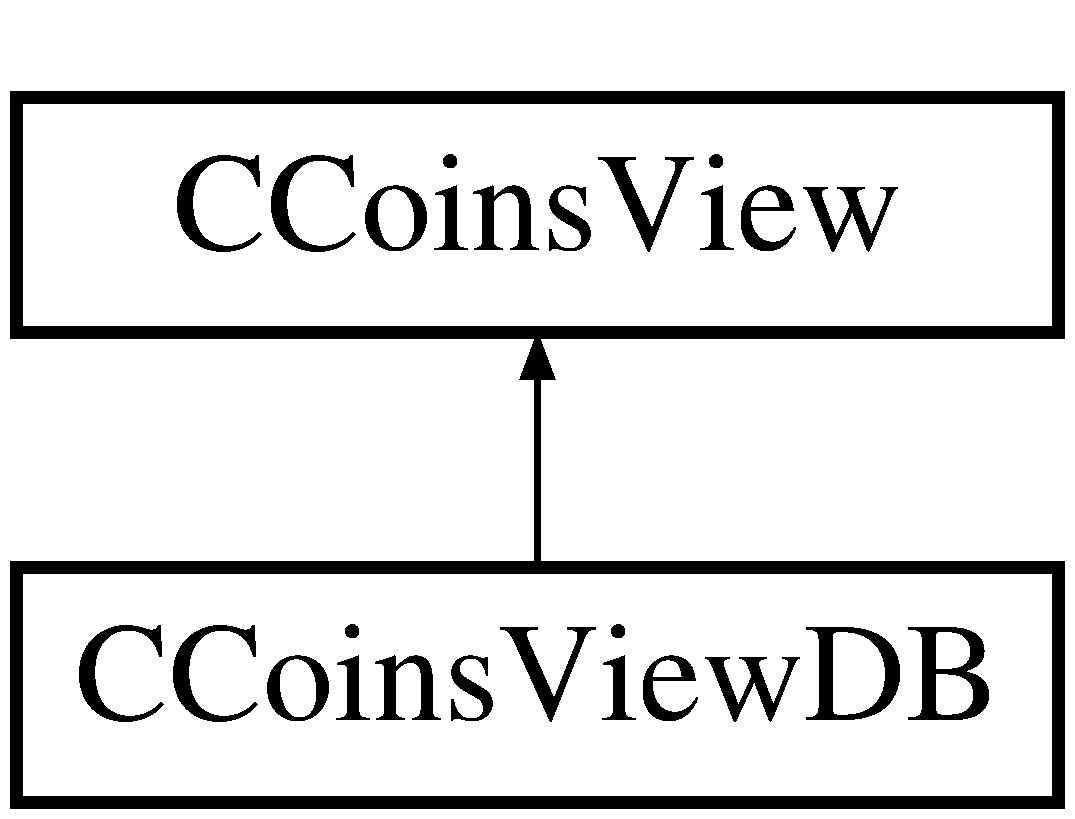
\includegraphics[height=2.000000cm]{class_c_coins_view_d_b}
\end{center}
\end{figure}
\subsection*{Public Member Functions}
\begin{DoxyCompactItemize}
\item 
\hyperlink{class_c_coins_view_d_b_a209841b241febcccb2ec584b886ad374}{C\+Coins\+View\+D\+B} (size\+\_\+t n\+Cache\+Size, bool f\+Memory=false, bool f\+Wipe=false)
\item 
bool \hyperlink{class_c_coins_view_d_b_a20655c9c13a6124cdcf210206d518d92}{Get\+Coins} (const \hyperlink{classuint256}{uint256} \&txid, \hyperlink{class_c_coins}{C\+Coins} \&coins) const 
\begin{DoxyCompactList}\small\item\em Retrieve the \hyperlink{class_c_coins}{C\+Coins} (unspent transaction outputs) for a given txid. \end{DoxyCompactList}\item 
bool \hyperlink{class_c_coins_view_d_b_a4d08cf2d3440c1de4e48cfddd67962d7}{Have\+Coins} (const \hyperlink{classuint256}{uint256} \&txid) const 
\item 
\hyperlink{classuint256}{uint256} \hyperlink{class_c_coins_view_d_b_a01777676c2eafd2970a9d53e5fb4a49a}{Get\+Best\+Block} () const 
\begin{DoxyCompactList}\small\item\em Retrieve the block hash whose state this \hyperlink{class_c_coins_view}{C\+Coins\+View} currently represents. \end{DoxyCompactList}\item 
bool \hyperlink{class_c_coins_view_d_b_a33f98ec9323ce48e1704327bc8a2a002}{Batch\+Write} (\hyperlink{coins_8h_a2886ba2fd0428bae777e1cbcabc02834}{C\+Coins\+Map} \&map\+Coins, const \hyperlink{classuint256}{uint256} \&hash\+Block)
\item 
bool \hyperlink{class_c_coins_view_d_b_a6bbe15962b0efd519e30dada872f01c5}{Get\+Stats} (\hyperlink{struct_c_coins_stats}{C\+Coins\+Stats} \&stats) const 
\begin{DoxyCompactList}\small\item\em Calculate statistics about the unspent transaction output set. \end{DoxyCompactList}\end{DoxyCompactItemize}
\subsection*{Protected Attributes}
\begin{DoxyCompactItemize}
\item 
\hyperlink{class_c_level_d_b_wrapper}{C\+Level\+D\+B\+Wrapper} \hyperlink{class_c_coins_view_d_b_aba0a7b26fe82c1a2e80ca060d12fb66a}{db}
\end{DoxyCompactItemize}


\subsection{Detailed Description}
\hyperlink{class_c_coins_view}{C\+Coins\+View} backed by the Level\+D\+B coin database (chainstate/) 

\subsection{Constructor \& Destructor Documentation}
\hypertarget{class_c_coins_view_d_b_a209841b241febcccb2ec584b886ad374}{}\index{C\+Coins\+View\+D\+B@{C\+Coins\+View\+D\+B}!C\+Coins\+View\+D\+B@{C\+Coins\+View\+D\+B}}
\index{C\+Coins\+View\+D\+B@{C\+Coins\+View\+D\+B}!C\+Coins\+View\+D\+B@{C\+Coins\+View\+D\+B}}
\subsubsection[{C\+Coins\+View\+D\+B}]{\setlength{\rightskip}{0pt plus 5cm}C\+Coins\+View\+D\+B\+::\+C\+Coins\+View\+D\+B (
\begin{DoxyParamCaption}
\item[{size\+\_\+t}]{n\+Cache\+Size, }
\item[{bool}]{f\+Memory = {\ttfamily false}, }
\item[{bool}]{f\+Wipe = {\ttfamily false}}
\end{DoxyParamCaption}
)}\label{class_c_coins_view_d_b_a209841b241febcccb2ec584b886ad374}


\subsection{Member Function Documentation}
\hypertarget{class_c_coins_view_d_b_a33f98ec9323ce48e1704327bc8a2a002}{}\index{C\+Coins\+View\+D\+B@{C\+Coins\+View\+D\+B}!Batch\+Write@{Batch\+Write}}
\index{Batch\+Write@{Batch\+Write}!C\+Coins\+View\+D\+B@{C\+Coins\+View\+D\+B}}
\subsubsection[{Batch\+Write}]{\setlength{\rightskip}{0pt plus 5cm}bool C\+Coins\+View\+D\+B\+::\+Batch\+Write (
\begin{DoxyParamCaption}
\item[{{\bf C\+Coins\+Map} \&}]{map\+Coins, }
\item[{const {\bf uint256} \&}]{hash\+Block}
\end{DoxyParamCaption}
)\hspace{0.3cm}{\ttfamily [virtual]}}\label{class_c_coins_view_d_b_a33f98ec9323ce48e1704327bc8a2a002}
Do a bulk modification (multiple \hyperlink{class_c_coins}{C\+Coins} changes + Best\+Block change). The passed map\+Coins can be modified. 

Reimplemented from \hyperlink{class_c_coins_view_ad7dc37396ca4fac7014cea06fec7178e}{C\+Coins\+View}.

\hypertarget{class_c_coins_view_d_b_a01777676c2eafd2970a9d53e5fb4a49a}{}\index{C\+Coins\+View\+D\+B@{C\+Coins\+View\+D\+B}!Get\+Best\+Block@{Get\+Best\+Block}}
\index{Get\+Best\+Block@{Get\+Best\+Block}!C\+Coins\+View\+D\+B@{C\+Coins\+View\+D\+B}}
\subsubsection[{Get\+Best\+Block}]{\setlength{\rightskip}{0pt plus 5cm}{\bf uint256} C\+Coins\+View\+D\+B\+::\+Get\+Best\+Block (
\begin{DoxyParamCaption}
{}
\end{DoxyParamCaption}
) const\hspace{0.3cm}{\ttfamily [virtual]}}\label{class_c_coins_view_d_b_a01777676c2eafd2970a9d53e5fb4a49a}


Retrieve the block hash whose state this \hyperlink{class_c_coins_view}{C\+Coins\+View} currently represents. 



Reimplemented from \hyperlink{class_c_coins_view_a556cf7661ff49df1ada5cd0ad552f8db}{C\+Coins\+View}.

\hypertarget{class_c_coins_view_d_b_a20655c9c13a6124cdcf210206d518d92}{}\index{C\+Coins\+View\+D\+B@{C\+Coins\+View\+D\+B}!Get\+Coins@{Get\+Coins}}
\index{Get\+Coins@{Get\+Coins}!C\+Coins\+View\+D\+B@{C\+Coins\+View\+D\+B}}
\subsubsection[{Get\+Coins}]{\setlength{\rightskip}{0pt plus 5cm}bool C\+Coins\+View\+D\+B\+::\+Get\+Coins (
\begin{DoxyParamCaption}
\item[{const {\bf uint256} \&}]{txid, }
\item[{{\bf C\+Coins} \&}]{coins}
\end{DoxyParamCaption}
) const\hspace{0.3cm}{\ttfamily [virtual]}}\label{class_c_coins_view_d_b_a20655c9c13a6124cdcf210206d518d92}


Retrieve the \hyperlink{class_c_coins}{C\+Coins} (unspent transaction outputs) for a given txid. 



Reimplemented from \hyperlink{class_c_coins_view_aaf5668eb2f9033583d7072dc2a3f96ef}{C\+Coins\+View}.

\hypertarget{class_c_coins_view_d_b_a6bbe15962b0efd519e30dada872f01c5}{}\index{C\+Coins\+View\+D\+B@{C\+Coins\+View\+D\+B}!Get\+Stats@{Get\+Stats}}
\index{Get\+Stats@{Get\+Stats}!C\+Coins\+View\+D\+B@{C\+Coins\+View\+D\+B}}
\subsubsection[{Get\+Stats}]{\setlength{\rightskip}{0pt plus 5cm}bool C\+Coins\+View\+D\+B\+::\+Get\+Stats (
\begin{DoxyParamCaption}
\item[{{\bf C\+Coins\+Stats} \&}]{stats}
\end{DoxyParamCaption}
) const\hspace{0.3cm}{\ttfamily [virtual]}}\label{class_c_coins_view_d_b_a6bbe15962b0efd519e30dada872f01c5}


Calculate statistics about the unspent transaction output set. 



Reimplemented from \hyperlink{class_c_coins_view_afd645b903fba9c6b84bdb898d764f5fc}{C\+Coins\+View}.

\hypertarget{class_c_coins_view_d_b_a4d08cf2d3440c1de4e48cfddd67962d7}{}\index{C\+Coins\+View\+D\+B@{C\+Coins\+View\+D\+B}!Have\+Coins@{Have\+Coins}}
\index{Have\+Coins@{Have\+Coins}!C\+Coins\+View\+D\+B@{C\+Coins\+View\+D\+B}}
\subsubsection[{Have\+Coins}]{\setlength{\rightskip}{0pt plus 5cm}bool C\+Coins\+View\+D\+B\+::\+Have\+Coins (
\begin{DoxyParamCaption}
\item[{const {\bf uint256} \&}]{txid}
\end{DoxyParamCaption}
) const\hspace{0.3cm}{\ttfamily [virtual]}}\label{class_c_coins_view_d_b_a4d08cf2d3440c1de4e48cfddd67962d7}
Just check whether we have data for a given txid. This may (but cannot always) return true for fully spent transactions 

Reimplemented from \hyperlink{class_c_coins_view_a14c8db07cb11223426bb660861389f3a}{C\+Coins\+View}.



\subsection{Member Data Documentation}
\hypertarget{class_c_coins_view_d_b_aba0a7b26fe82c1a2e80ca060d12fb66a}{}\index{C\+Coins\+View\+D\+B@{C\+Coins\+View\+D\+B}!db@{db}}
\index{db@{db}!C\+Coins\+View\+D\+B@{C\+Coins\+View\+D\+B}}
\subsubsection[{db}]{\setlength{\rightskip}{0pt plus 5cm}{\bf C\+Level\+D\+B\+Wrapper} C\+Coins\+View\+D\+B\+::db\hspace{0.3cm}{\ttfamily [protected]}}\label{class_c_coins_view_d_b_aba0a7b26fe82c1a2e80ca060d12fb66a}


The documentation for this class was generated from the following files\+:\begin{DoxyCompactItemize}
\item 
C\+:/\+Users/\+Joe/\+Documents/\+School/\+C\+S\+C17\+A/bitcoin/src/\hyperlink{txdb_8h}{txdb.\+h}\item 
C\+:/\+Users/\+Joe/\+Documents/\+School/\+C\+S\+C17\+A/bitcoin/src/\hyperlink{txdb_8cpp}{txdb.\+cpp}\end{DoxyCompactItemize}

\hypertarget{class_c_coins_view_error_catcher}{}\section{C\+Coins\+View\+Error\+Catcher Class Reference}
\label{class_c_coins_view_error_catcher}\index{C\+Coins\+View\+Error\+Catcher@{C\+Coins\+View\+Error\+Catcher}}
Inheritance diagram for C\+Coins\+View\+Error\+Catcher\+:\begin{figure}[H]
\begin{center}
\leavevmode
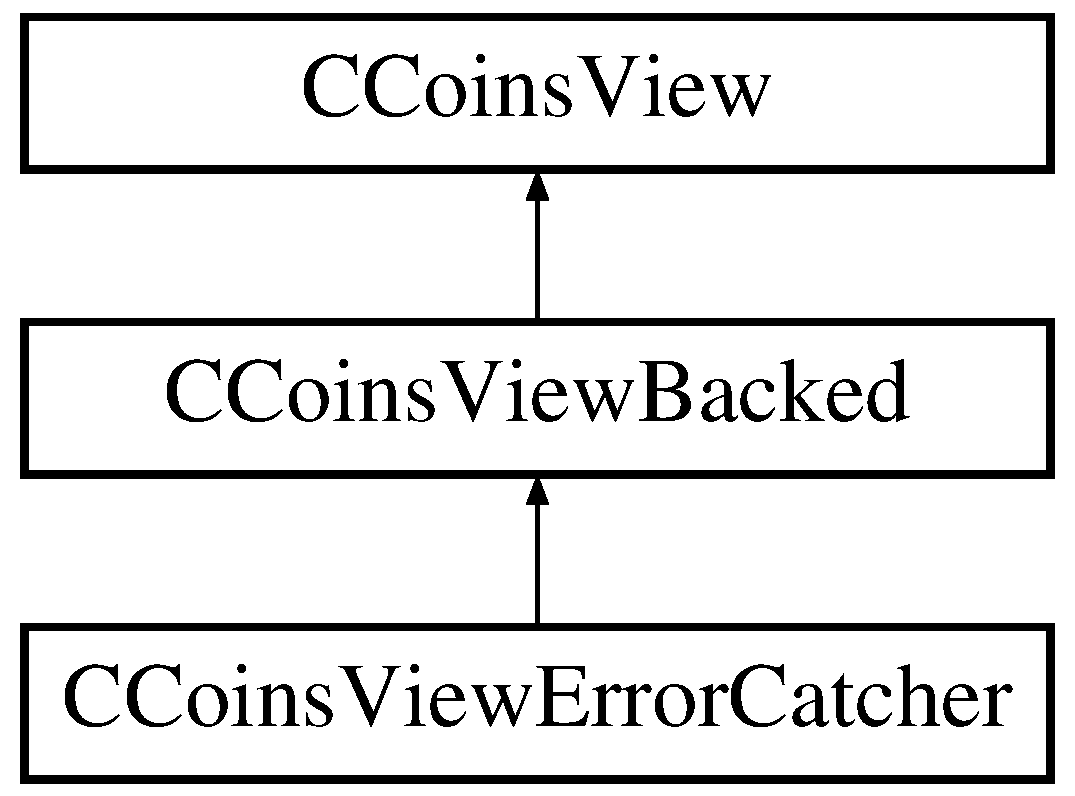
\includegraphics[height=3.000000cm]{class_c_coins_view_error_catcher}
\end{center}
\end{figure}
\subsection*{Public Member Functions}
\begin{DoxyCompactItemize}
\item 
\hyperlink{class_c_coins_view_error_catcher_aa8295e2f5ce5ad9880c5bd86d52e014c}{C\+Coins\+View\+Error\+Catcher} (\hyperlink{class_c_coins_view}{C\+Coins\+View} $\ast$view)
\item 
bool \hyperlink{class_c_coins_view_error_catcher_a762969de31b62e55d01f1cdf0b178eb9}{Get\+Coins} (const \hyperlink{classuint256}{uint256} \&txid, \hyperlink{class_c_coins}{C\+Coins} \&coins) const 
\begin{DoxyCompactList}\small\item\em Retrieve the \hyperlink{class_c_coins}{C\+Coins} (unspent transaction outputs) for a given txid. \end{DoxyCompactList}\end{DoxyCompactItemize}
\subsection*{Additional Inherited Members}


\subsection{Constructor \& Destructor Documentation}
\hypertarget{class_c_coins_view_error_catcher_aa8295e2f5ce5ad9880c5bd86d52e014c}{}\index{C\+Coins\+View\+Error\+Catcher@{C\+Coins\+View\+Error\+Catcher}!C\+Coins\+View\+Error\+Catcher@{C\+Coins\+View\+Error\+Catcher}}
\index{C\+Coins\+View\+Error\+Catcher@{C\+Coins\+View\+Error\+Catcher}!C\+Coins\+View\+Error\+Catcher@{C\+Coins\+View\+Error\+Catcher}}
\subsubsection[{C\+Coins\+View\+Error\+Catcher}]{\setlength{\rightskip}{0pt plus 5cm}C\+Coins\+View\+Error\+Catcher\+::\+C\+Coins\+View\+Error\+Catcher (
\begin{DoxyParamCaption}
\item[{{\bf C\+Coins\+View} $\ast$}]{view}
\end{DoxyParamCaption}
)\hspace{0.3cm}{\ttfamily [inline]}}\label{class_c_coins_view_error_catcher_aa8295e2f5ce5ad9880c5bd86d52e014c}


\subsection{Member Function Documentation}
\hypertarget{class_c_coins_view_error_catcher_a762969de31b62e55d01f1cdf0b178eb9}{}\index{C\+Coins\+View\+Error\+Catcher@{C\+Coins\+View\+Error\+Catcher}!Get\+Coins@{Get\+Coins}}
\index{Get\+Coins@{Get\+Coins}!C\+Coins\+View\+Error\+Catcher@{C\+Coins\+View\+Error\+Catcher}}
\subsubsection[{Get\+Coins}]{\setlength{\rightskip}{0pt plus 5cm}bool C\+Coins\+View\+Error\+Catcher\+::\+Get\+Coins (
\begin{DoxyParamCaption}
\item[{const {\bf uint256} \&}]{txid, }
\item[{{\bf C\+Coins} \&}]{coins}
\end{DoxyParamCaption}
) const\hspace{0.3cm}{\ttfamily [inline]}, {\ttfamily [virtual]}}\label{class_c_coins_view_error_catcher_a762969de31b62e55d01f1cdf0b178eb9}


Retrieve the \hyperlink{class_c_coins}{C\+Coins} (unspent transaction outputs) for a given txid. 



Reimplemented from \hyperlink{class_c_coins_view_backed_a21b95a9910f94e9b7ebed62a6f329ea0}{C\+Coins\+View\+Backed}.



The documentation for this class was generated from the following file\+:\begin{DoxyCompactItemize}
\item 
C\+:/\+Users/\+Joe/\+Documents/\+School/\+C\+S\+C17\+A/bitcoin/src/\hyperlink{init_8cpp}{init.\+cpp}\end{DoxyCompactItemize}

\hypertarget{class_c_coins_view_mem_pool}{}\section{C\+Coins\+View\+Mem\+Pool Class Reference}
\label{class_c_coins_view_mem_pool}\index{C\+Coins\+View\+Mem\+Pool@{C\+Coins\+View\+Mem\+Pool}}


{\ttfamily \#include $<$txmempool.\+h$>$}

Inheritance diagram for C\+Coins\+View\+Mem\+Pool\+:\begin{figure}[H]
\begin{center}
\leavevmode
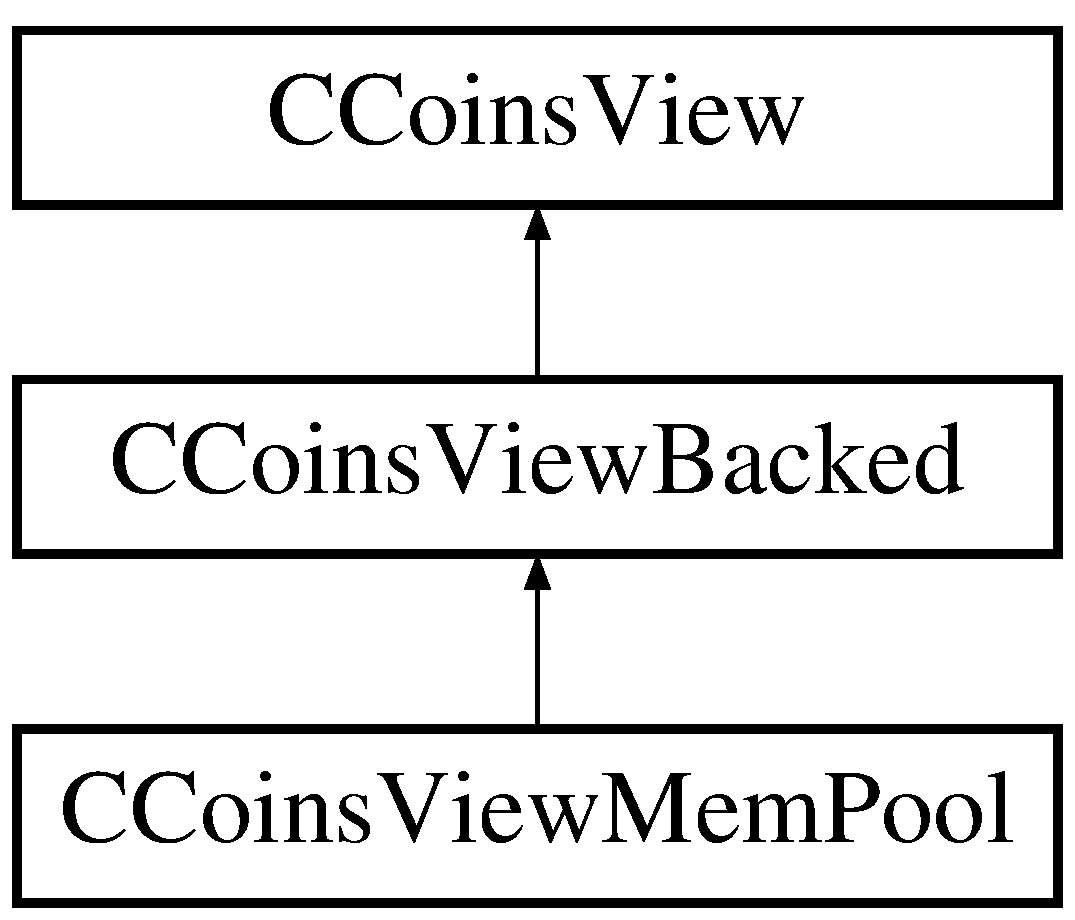
\includegraphics[height=3.000000cm]{class_c_coins_view_mem_pool}
\end{center}
\end{figure}
\subsection*{Public Member Functions}
\begin{DoxyCompactItemize}
\item 
\hyperlink{class_c_coins_view_mem_pool_aab9a206c304acec322fddf646c7bafb9}{C\+Coins\+View\+Mem\+Pool} (\hyperlink{class_c_coins_view}{C\+Coins\+View} $\ast$base\+In, \hyperlink{class_c_tx_mem_pool}{C\+Tx\+Mem\+Pool} \&mempool\+In)
\item 
bool \hyperlink{class_c_coins_view_mem_pool_a01564f29ff2673ddd0d27414e576f1bc}{Get\+Coins} (const \hyperlink{classuint256}{uint256} \&txid, \hyperlink{class_c_coins}{C\+Coins} \&coins) const 
\begin{DoxyCompactList}\small\item\em Retrieve the \hyperlink{class_c_coins}{C\+Coins} (unspent transaction outputs) for a given txid. \end{DoxyCompactList}\item 
bool \hyperlink{class_c_coins_view_mem_pool_a965e6c8e378fe937620ba2c180d1ed74}{Have\+Coins} (const \hyperlink{classuint256}{uint256} \&txid) const 
\end{DoxyCompactItemize}
\subsection*{Protected Attributes}
\begin{DoxyCompactItemize}
\item 
\hyperlink{class_c_tx_mem_pool}{C\+Tx\+Mem\+Pool} \& \hyperlink{class_c_coins_view_mem_pool_a7a3870fc65376cb311a0b3abb28fec10}{mempool}
\end{DoxyCompactItemize}


\subsection{Detailed Description}
\hyperlink{class_c_coins_view}{C\+Coins\+View} that brings transactions from a memorypool into view. It does not check for spendings by memory pool transactions. 

\subsection{Constructor \& Destructor Documentation}
\hypertarget{class_c_coins_view_mem_pool_aab9a206c304acec322fddf646c7bafb9}{}\index{C\+Coins\+View\+Mem\+Pool@{C\+Coins\+View\+Mem\+Pool}!C\+Coins\+View\+Mem\+Pool@{C\+Coins\+View\+Mem\+Pool}}
\index{C\+Coins\+View\+Mem\+Pool@{C\+Coins\+View\+Mem\+Pool}!C\+Coins\+View\+Mem\+Pool@{C\+Coins\+View\+Mem\+Pool}}
\subsubsection[{C\+Coins\+View\+Mem\+Pool}]{\setlength{\rightskip}{0pt plus 5cm}C\+Coins\+View\+Mem\+Pool\+::\+C\+Coins\+View\+Mem\+Pool (
\begin{DoxyParamCaption}
\item[{{\bf C\+Coins\+View} $\ast$}]{base\+In, }
\item[{{\bf C\+Tx\+Mem\+Pool} \&}]{mempool\+In}
\end{DoxyParamCaption}
)}\label{class_c_coins_view_mem_pool_aab9a206c304acec322fddf646c7bafb9}


\subsection{Member Function Documentation}
\hypertarget{class_c_coins_view_mem_pool_a01564f29ff2673ddd0d27414e576f1bc}{}\index{C\+Coins\+View\+Mem\+Pool@{C\+Coins\+View\+Mem\+Pool}!Get\+Coins@{Get\+Coins}}
\index{Get\+Coins@{Get\+Coins}!C\+Coins\+View\+Mem\+Pool@{C\+Coins\+View\+Mem\+Pool}}
\subsubsection[{Get\+Coins}]{\setlength{\rightskip}{0pt plus 5cm}bool C\+Coins\+View\+Mem\+Pool\+::\+Get\+Coins (
\begin{DoxyParamCaption}
\item[{const {\bf uint256} \&}]{txid, }
\item[{{\bf C\+Coins} \&}]{coins}
\end{DoxyParamCaption}
) const\hspace{0.3cm}{\ttfamily [virtual]}}\label{class_c_coins_view_mem_pool_a01564f29ff2673ddd0d27414e576f1bc}


Retrieve the \hyperlink{class_c_coins}{C\+Coins} (unspent transaction outputs) for a given txid. 



Reimplemented from \hyperlink{class_c_coins_view_backed_a21b95a9910f94e9b7ebed62a6f329ea0}{C\+Coins\+View\+Backed}.

\hypertarget{class_c_coins_view_mem_pool_a965e6c8e378fe937620ba2c180d1ed74}{}\index{C\+Coins\+View\+Mem\+Pool@{C\+Coins\+View\+Mem\+Pool}!Have\+Coins@{Have\+Coins}}
\index{Have\+Coins@{Have\+Coins}!C\+Coins\+View\+Mem\+Pool@{C\+Coins\+View\+Mem\+Pool}}
\subsubsection[{Have\+Coins}]{\setlength{\rightskip}{0pt plus 5cm}bool C\+Coins\+View\+Mem\+Pool\+::\+Have\+Coins (
\begin{DoxyParamCaption}
\item[{const {\bf uint256} \&}]{txid}
\end{DoxyParamCaption}
) const\hspace{0.3cm}{\ttfamily [virtual]}}\label{class_c_coins_view_mem_pool_a965e6c8e378fe937620ba2c180d1ed74}
Just check whether we have data for a given txid. This may (but cannot always) return true for fully spent transactions 

Reimplemented from \hyperlink{class_c_coins_view_backed_a6a769cf9cc55128dea8e1a2798056e71}{C\+Coins\+View\+Backed}.



\subsection{Member Data Documentation}
\hypertarget{class_c_coins_view_mem_pool_a7a3870fc65376cb311a0b3abb28fec10}{}\index{C\+Coins\+View\+Mem\+Pool@{C\+Coins\+View\+Mem\+Pool}!mempool@{mempool}}
\index{mempool@{mempool}!C\+Coins\+View\+Mem\+Pool@{C\+Coins\+View\+Mem\+Pool}}
\subsubsection[{mempool}]{\setlength{\rightskip}{0pt plus 5cm}{\bf C\+Tx\+Mem\+Pool}\& C\+Coins\+View\+Mem\+Pool\+::mempool\hspace{0.3cm}{\ttfamily [protected]}}\label{class_c_coins_view_mem_pool_a7a3870fc65376cb311a0b3abb28fec10}


The documentation for this class was generated from the following files\+:\begin{DoxyCompactItemize}
\item 
C\+:/\+Users/\+Joe/\+Documents/\+School/\+C\+S\+C17\+A/bitcoin/src/\hyperlink{txmempool_8h}{txmempool.\+h}\item 
C\+:/\+Users/\+Joe/\+Documents/\+School/\+C\+S\+C17\+A/bitcoin/src/\hyperlink{txmempool_8cpp}{txmempool.\+cpp}\end{DoxyCompactItemize}

\hypertarget{class_c_connection_failed}{}\section{C\+Connection\+Failed Class Reference}
\label{class_c_connection_failed}\index{C\+Connection\+Failed@{C\+Connection\+Failed}}
Inheritance diagram for C\+Connection\+Failed\+:\begin{figure}[H]
\begin{center}
\leavevmode
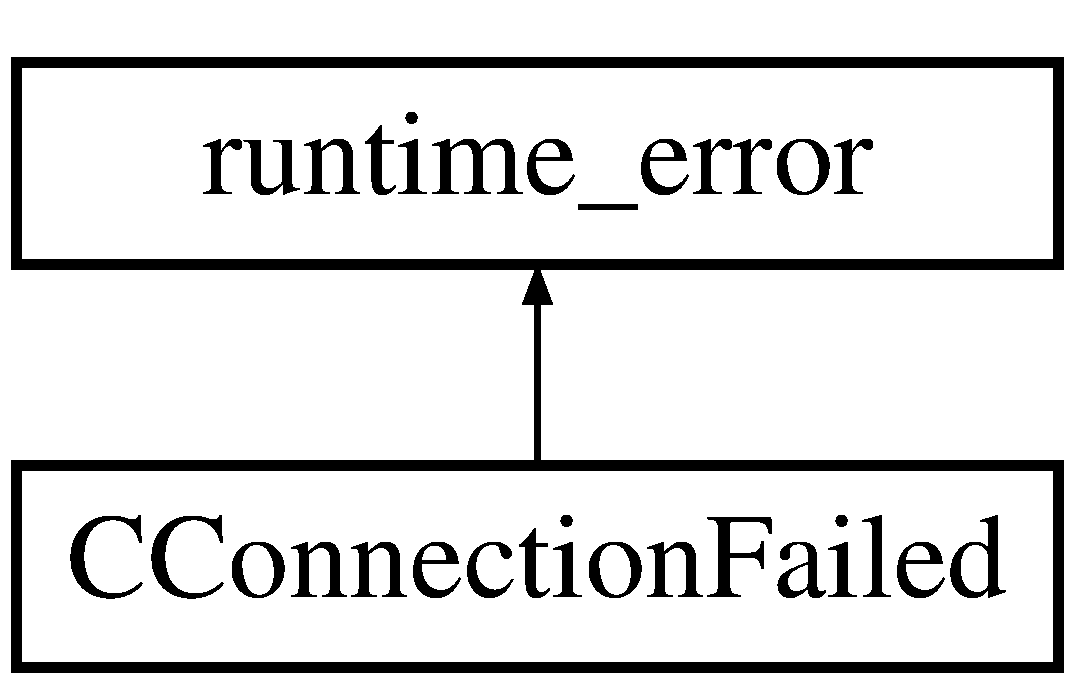
\includegraphics[height=2.000000cm]{class_c_connection_failed}
\end{center}
\end{figure}
\subsection*{Public Member Functions}
\begin{DoxyCompactItemize}
\item 
\hyperlink{class_c_connection_failed_abcc9db4386ec901f5159c44d939c82c5}{C\+Connection\+Failed} (const std\+::string \&msg)
\end{DoxyCompactItemize}


\subsection{Constructor \& Destructor Documentation}
\hypertarget{class_c_connection_failed_abcc9db4386ec901f5159c44d939c82c5}{}\index{C\+Connection\+Failed@{C\+Connection\+Failed}!C\+Connection\+Failed@{C\+Connection\+Failed}}
\index{C\+Connection\+Failed@{C\+Connection\+Failed}!C\+Connection\+Failed@{C\+Connection\+Failed}}
\subsubsection[{C\+Connection\+Failed}]{\setlength{\rightskip}{0pt plus 5cm}C\+Connection\+Failed\+::\+C\+Connection\+Failed (
\begin{DoxyParamCaption}
\item[{const std\+::string \&}]{msg}
\end{DoxyParamCaption}
)\hspace{0.3cm}{\ttfamily [inline]}, {\ttfamily [explicit]}}\label{class_c_connection_failed_abcc9db4386ec901f5159c44d939c82c5}


The documentation for this class was generated from the following file\+:\begin{DoxyCompactItemize}
\item 
C\+:/\+Users/\+Joe/\+Documents/\+School/\+C\+S\+C17\+A/bitcoin/src/\hyperlink{bitcoin-cli_8cpp}{bitcoin-\/cli.\+cpp}\end{DoxyCompactItemize}

\hypertarget{class_c_data_stream}{}\section{C\+Data\+Stream Class Reference}
\label{class_c_data_stream}\index{C\+Data\+Stream@{C\+Data\+Stream}}


{\ttfamily \#include $<$streams.\+h$>$}

\subsection*{Public Types}
\begin{DoxyCompactItemize}
\item 
typedef vector\+\_\+type\+::allocator\+\_\+type \hyperlink{class_c_data_stream_a297dff00e40bb161aab89fde868ee7b1}{allocator\+\_\+type}
\item 
typedef vector\+\_\+type\+::size\+\_\+type \hyperlink{class_c_data_stream_a79e10daad6db0f94aea1e811eb167378}{size\+\_\+type}
\item 
typedef vector\+\_\+type\+::difference\+\_\+type \hyperlink{class_c_data_stream_a9da973fb6e53a5335db78b6f8b90bdbf}{difference\+\_\+type}
\item 
typedef vector\+\_\+type\+::reference \hyperlink{class_c_data_stream_a33723921305add93b45973243faf1541}{reference}
\item 
typedef vector\+\_\+type\+::const\+\_\+reference \hyperlink{class_c_data_stream_ada2ac4b4c962dd5a5dcccbc3f71e83ab}{const\+\_\+reference}
\item 
typedef vector\+\_\+type\+::value\+\_\+type \hyperlink{class_c_data_stream_a5572ddd57b7355f87781b89087dd18e0}{value\+\_\+type}
\item 
typedef vector\+\_\+type\+::iterator \hyperlink{class_c_data_stream_abed2013224bdf424e51c78bf483886d3}{iterator}
\item 
typedef vector\+\_\+type\+::const\+\_\+iterator \hyperlink{class_c_data_stream_abcfd79b72607505b22f18424e313b4c5}{const\+\_\+iterator}
\item 
typedef vector\+\_\+type\+::reverse\+\_\+iterator \hyperlink{class_c_data_stream_a93ca1c317b7080997a20b0cf1920b39c}{reverse\+\_\+iterator}
\end{DoxyCompactItemize}
\subsection*{Public Member Functions}
\begin{DoxyCompactItemize}
\item 
\hyperlink{class_c_data_stream_a38f4d7d2ae59566a0500523a1b1a49d4}{C\+Data\+Stream} (int n\+Type\+In, int n\+Version\+In)
\item 
\hyperlink{class_c_data_stream_a00d23d0ef651cb4ea54cb37009bdf8f2}{C\+Data\+Stream} (\hyperlink{class_c_data_stream_abcfd79b72607505b22f18424e313b4c5}{const\+\_\+iterator} pbegin, \hyperlink{class_c_data_stream_abcfd79b72607505b22f18424e313b4c5}{const\+\_\+iterator} pend, int n\+Type\+In, int n\+Version\+In)
\item 
\hyperlink{class_c_data_stream_ab345d2edd7bef6c6c140a46621e49eee}{C\+Data\+Stream} (const char $\ast$pbegin, const char $\ast$pend, int n\+Type\+In, int n\+Version\+In)
\item 
\hyperlink{class_c_data_stream_a38a51fefce23374963516b3af03638fc}{C\+Data\+Stream} (const \hyperlink{class_c_data_stream_a5e86187632a0d6cea39f3ea525427e27}{vector\+\_\+type} \&vch\+In, int n\+Type\+In, int n\+Version\+In)
\item 
\hyperlink{class_c_data_stream_a46219676397ae7b3cbc0c676f74ba1e7}{C\+Data\+Stream} (const std\+::vector$<$ char $>$ \&vch\+In, int n\+Type\+In, int n\+Version\+In)
\item 
\hyperlink{class_c_data_stream_ac63bd3d0ecce0edc2aa66cc80b633b6f}{C\+Data\+Stream} (const std\+::vector$<$ unsigned char $>$ \&vch\+In, int n\+Type\+In, int n\+Version\+In)
\item 
void \hyperlink{class_c_data_stream_a95267358054cbfbf37e239f3e6c78471}{Init} (int n\+Type\+In, int n\+Version\+In)
\item 
\hyperlink{class_c_data_stream}{C\+Data\+Stream} \& \hyperlink{class_c_data_stream_a59c13d9215c13b3bb4d56a818d280dda}{operator+=} (const \hyperlink{class_c_data_stream}{C\+Data\+Stream} \&b)
\item 
std\+::string \hyperlink{class_c_data_stream_aa3a9ecf166f36f4ea531d2b23628d2c9}{str} () const 
\item 
\hyperlink{class_c_data_stream_abcfd79b72607505b22f18424e313b4c5}{const\+\_\+iterator} \hyperlink{class_c_data_stream_a5b9e70188c662f4e9496066472af213e}{begin} () const 
\item 
\hyperlink{class_c_data_stream_abed2013224bdf424e51c78bf483886d3}{iterator} \hyperlink{class_c_data_stream_a4b8ed86db3a4563fc327c903b0ccf4ee}{begin} ()
\item 
\hyperlink{class_c_data_stream_abcfd79b72607505b22f18424e313b4c5}{const\+\_\+iterator} \hyperlink{class_c_data_stream_a1c22182691412ed9e0a30b719d388f31}{end} () const 
\item 
\hyperlink{class_c_data_stream_abed2013224bdf424e51c78bf483886d3}{iterator} \hyperlink{class_c_data_stream_a6a486e8e0da9e769520de62b15bd9315}{end} ()
\item 
\hyperlink{class_c_data_stream_a79e10daad6db0f94aea1e811eb167378}{size\+\_\+type} \hyperlink{class_c_data_stream_ac6567f6d600d644d9855b52bb59049cd}{size} () const 
\item 
bool \hyperlink{class_c_data_stream_a6e50e788d33080ac804e4d8ba7150279}{empty} () const 
\item 
void \hyperlink{class_c_data_stream_aa91abddde56127bd3d6ac2a0fb005874}{resize} (\hyperlink{class_c_data_stream_a79e10daad6db0f94aea1e811eb167378}{size\+\_\+type} n, \hyperlink{class_c_data_stream_a5572ddd57b7355f87781b89087dd18e0}{value\+\_\+type} c=0)
\item 
void \hyperlink{class_c_data_stream_a5542e71bd7af2ab7cd7be0f381d39cb5}{reserve} (\hyperlink{class_c_data_stream_a79e10daad6db0f94aea1e811eb167378}{size\+\_\+type} n)
\item 
\hyperlink{class_c_data_stream_ada2ac4b4c962dd5a5dcccbc3f71e83ab}{const\+\_\+reference} \hyperlink{class_c_data_stream_a7a93b7db1ac1aca5c3e3831a794d9134}{operator\mbox{[}$\,$\mbox{]}} (\hyperlink{class_c_data_stream_a79e10daad6db0f94aea1e811eb167378}{size\+\_\+type} pos) const 
\item 
\hyperlink{class_c_data_stream_a33723921305add93b45973243faf1541}{reference} \hyperlink{class_c_data_stream_a91a057dd6e866137a7d526bd253fa8e9}{operator\mbox{[}$\,$\mbox{]}} (\hyperlink{class_c_data_stream_a79e10daad6db0f94aea1e811eb167378}{size\+\_\+type} pos)
\item 
void \hyperlink{class_c_data_stream_ade6ed9a3a481e333900e6496707b9692}{clear} ()
\item 
\hyperlink{class_c_data_stream_abed2013224bdf424e51c78bf483886d3}{iterator} \hyperlink{class_c_data_stream_a191a18802fbc0861ae118d79d33088dc}{insert} (\hyperlink{class_c_data_stream_abed2013224bdf424e51c78bf483886d3}{iterator} it, const char \&x=char())
\item 
void \hyperlink{class_c_data_stream_ac8fa6a4a4cd08da5a0c87180834611e5}{insert} (\hyperlink{class_c_data_stream_abed2013224bdf424e51c78bf483886d3}{iterator} it, \hyperlink{class_c_data_stream_a79e10daad6db0f94aea1e811eb167378}{size\+\_\+type} n, const char \&x)
\item 
void \hyperlink{class_c_data_stream_aa15a60d7ee6d987de444426f2825f284}{insert} (\hyperlink{class_c_data_stream_abed2013224bdf424e51c78bf483886d3}{iterator} it, std\+::vector$<$ char $>$\+::\hyperlink{class_c_data_stream_abcfd79b72607505b22f18424e313b4c5}{const\+\_\+iterator} first, std\+::vector$<$ char $>$\+::\hyperlink{class_c_data_stream_abcfd79b72607505b22f18424e313b4c5}{const\+\_\+iterator} last)
\item 
void \hyperlink{class_c_data_stream_a9635fda38bc0b7836b4364820a67a18d}{insert} (\hyperlink{class_c_data_stream_abed2013224bdf424e51c78bf483886d3}{iterator} it, const char $\ast$first, const char $\ast$last)
\item 
\hyperlink{class_c_data_stream_abed2013224bdf424e51c78bf483886d3}{iterator} \hyperlink{class_c_data_stream_acb2a195db823f11161ea07c4855e0333}{erase} (\hyperlink{class_c_data_stream_abed2013224bdf424e51c78bf483886d3}{iterator} it)
\item 
\hyperlink{class_c_data_stream_abed2013224bdf424e51c78bf483886d3}{iterator} \hyperlink{class_c_data_stream_a7446b23bcfa37cbfa79ccc66f8aff48a}{erase} (\hyperlink{class_c_data_stream_abed2013224bdf424e51c78bf483886d3}{iterator} first, \hyperlink{class_c_data_stream_abed2013224bdf424e51c78bf483886d3}{iterator} last)
\item 
void \hyperlink{class_c_data_stream_a84c3fd4cf194f3402dc8adce6ab3ccf9}{Compact} ()
\item 
bool \hyperlink{class_c_data_stream_a7054311b2fe016b21fb853a1e27812d9}{Rewind} (\hyperlink{class_c_data_stream_a79e10daad6db0f94aea1e811eb167378}{size\+\_\+type} n)
\item 
bool \hyperlink{class_c_data_stream_abf5a9f3a26a56ef1ea1fb56b674677bf}{eof} () const 
\item 
\hyperlink{class_c_data_stream}{C\+Data\+Stream} $\ast$ \hyperlink{class_c_data_stream_a45a08b8355d47a95e9dae87ed6487483}{rdbuf} ()
\item 
int \hyperlink{class_c_data_stream_a0483fe7bccf16aa88bf7272f18a0a7b0}{in\+\_\+avail} ()
\item 
void \hyperlink{class_c_data_stream_a92467b36f5b2edff8becb5eadec633ce}{Set\+Type} (int n)
\item 
int \hyperlink{class_c_data_stream_a14bc0652cfd49850a032f0a1651456a7}{Get\+Type} ()
\item 
void \hyperlink{class_c_data_stream_a267d1315f3f9e9bcf9e7168beaa240c4}{Set\+Version} (int n)
\item 
int \hyperlink{class_c_data_stream_acb7af65ccac8273fc694a25796814ddc}{Get\+Version} ()
\item 
void \hyperlink{class_c_data_stream_ad8f97bbd83ef3d2eebfd3f9c82f55260}{Read\+Version} ()
\item 
void \hyperlink{class_c_data_stream_a35d49028155fb47d2bb5c2dbaf31bc8e}{Write\+Version} ()
\item 
\hyperlink{class_c_data_stream}{C\+Data\+Stream} \& \hyperlink{class_c_data_stream_af3743932a68e3ee3f1dbd357993a51ae}{read} (char $\ast$pch, size\+\_\+t n\+Size)
\item 
\hyperlink{class_c_data_stream}{C\+Data\+Stream} \& \hyperlink{class_c_data_stream_aebfcaa009d328a208dbbcd13db846dd6}{ignore} (int n\+Size)
\item 
\hyperlink{class_c_data_stream}{C\+Data\+Stream} \& \hyperlink{class_c_data_stream_abcab3fa1be7676ffdb34908ec7c84b78}{write} (const char $\ast$pch, size\+\_\+t n\+Size)
\item 
{\footnotesize template$<$typename Stream $>$ }\\void \hyperlink{class_c_data_stream_a3ecece05df6fb20d5f7b93e59acb8ff3}{Serialize} (Stream \&s, int \hyperlink{class_c_data_stream_a2b646679e24cf6f382fe8ab2d4f50f35}{n\+Type}, int \hyperlink{class_c_data_stream_a074998c6b7c8aa17a1a90dbc414b605d}{n\+Version}) const 
\item 
{\footnotesize template$<$typename T $>$ }\\unsigned int \hyperlink{class_c_data_stream_aaf2b9e953793ce5a4fc438a7ecb00dc2}{Get\+Serialize\+Size} (const T \&obj)
\item 
{\footnotesize template$<$typename T $>$ }\\\hyperlink{class_c_data_stream}{C\+Data\+Stream} \& \hyperlink{class_c_data_stream_af47c6d4051064a226f529ee4d7c13ad7}{operator$<$$<$} (const T \&obj)
\item 
{\footnotesize template$<$typename T $>$ }\\\hyperlink{class_c_data_stream}{C\+Data\+Stream} \& \hyperlink{class_c_data_stream_ac80cfc65569416f8c23e328edb4cadae}{operator$>$$>$} (T \&obj)
\item 
void \hyperlink{class_c_data_stream_a4be60514b69c71a722e16bf1fbbc3c6c}{Get\+And\+Clear} (C\+Serialize\+Data \&data)
\end{DoxyCompactItemize}
\subsection*{Public Attributes}
\begin{DoxyCompactItemize}
\item 
int \hyperlink{class_c_data_stream_a2b646679e24cf6f382fe8ab2d4f50f35}{n\+Type}
\item 
int \hyperlink{class_c_data_stream_a074998c6b7c8aa17a1a90dbc414b605d}{n\+Version}
\end{DoxyCompactItemize}
\subsection*{Protected Types}
\begin{DoxyCompactItemize}
\item 
typedef C\+Serialize\+Data \hyperlink{class_c_data_stream_a5e86187632a0d6cea39f3ea525427e27}{vector\+\_\+type}
\end{DoxyCompactItemize}
\subsection*{Protected Attributes}
\begin{DoxyCompactItemize}
\item 
\hyperlink{class_c_data_stream_a5e86187632a0d6cea39f3ea525427e27}{vector\+\_\+type} \hyperlink{class_c_data_stream_ac875adb8c720c48abd1a7c82f3452dda}{vch}
\item 
unsigned int \hyperlink{class_c_data_stream_af1c6a23b6725406d8f3464036a595556}{n\+Read\+Pos}
\end{DoxyCompactItemize}
\subsection*{Friends}
\begin{DoxyCompactItemize}
\item 
\hyperlink{class_c_data_stream}{C\+Data\+Stream} \hyperlink{class_c_data_stream_ae9d127e586618900bc753dfda97e9401}{operator+} (const \hyperlink{class_c_data_stream}{C\+Data\+Stream} \&a, const \hyperlink{class_c_data_stream}{C\+Data\+Stream} \&b)
\end{DoxyCompactItemize}


\subsection{Detailed Description}
Double ended buffer combining vector and stream-\/like interfaces.

\begin{quote}
\begin{quote}
and $<$$<$ read and write unformatted data using the above serialization templates. \end{quote}
\end{quote}
Fills with data in linear time; some stringstream implementations take N$^\wedge$2 time. 

\subsection{Member Typedef Documentation}
\hypertarget{class_c_data_stream_a297dff00e40bb161aab89fde868ee7b1}{}\index{C\+Data\+Stream@{C\+Data\+Stream}!allocator\+\_\+type@{allocator\+\_\+type}}
\index{allocator\+\_\+type@{allocator\+\_\+type}!C\+Data\+Stream@{C\+Data\+Stream}}
\subsubsection[{allocator\+\_\+type}]{\setlength{\rightskip}{0pt plus 5cm}typedef vector\+\_\+type\+::allocator\+\_\+type {\bf C\+Data\+Stream\+::allocator\+\_\+type}}\label{class_c_data_stream_a297dff00e40bb161aab89fde868ee7b1}
\hypertarget{class_c_data_stream_abcfd79b72607505b22f18424e313b4c5}{}\index{C\+Data\+Stream@{C\+Data\+Stream}!const\+\_\+iterator@{const\+\_\+iterator}}
\index{const\+\_\+iterator@{const\+\_\+iterator}!C\+Data\+Stream@{C\+Data\+Stream}}
\subsubsection[{const\+\_\+iterator}]{\setlength{\rightskip}{0pt plus 5cm}typedef vector\+\_\+type\+::const\+\_\+iterator {\bf C\+Data\+Stream\+::const\+\_\+iterator}}\label{class_c_data_stream_abcfd79b72607505b22f18424e313b4c5}
\hypertarget{class_c_data_stream_ada2ac4b4c962dd5a5dcccbc3f71e83ab}{}\index{C\+Data\+Stream@{C\+Data\+Stream}!const\+\_\+reference@{const\+\_\+reference}}
\index{const\+\_\+reference@{const\+\_\+reference}!C\+Data\+Stream@{C\+Data\+Stream}}
\subsubsection[{const\+\_\+reference}]{\setlength{\rightskip}{0pt plus 5cm}typedef vector\+\_\+type\+::const\+\_\+reference {\bf C\+Data\+Stream\+::const\+\_\+reference}}\label{class_c_data_stream_ada2ac4b4c962dd5a5dcccbc3f71e83ab}
\hypertarget{class_c_data_stream_a9da973fb6e53a5335db78b6f8b90bdbf}{}\index{C\+Data\+Stream@{C\+Data\+Stream}!difference\+\_\+type@{difference\+\_\+type}}
\index{difference\+\_\+type@{difference\+\_\+type}!C\+Data\+Stream@{C\+Data\+Stream}}
\subsubsection[{difference\+\_\+type}]{\setlength{\rightskip}{0pt plus 5cm}typedef vector\+\_\+type\+::difference\+\_\+type {\bf C\+Data\+Stream\+::difference\+\_\+type}}\label{class_c_data_stream_a9da973fb6e53a5335db78b6f8b90bdbf}
\hypertarget{class_c_data_stream_abed2013224bdf424e51c78bf483886d3}{}\index{C\+Data\+Stream@{C\+Data\+Stream}!iterator@{iterator}}
\index{iterator@{iterator}!C\+Data\+Stream@{C\+Data\+Stream}}
\subsubsection[{iterator}]{\setlength{\rightskip}{0pt plus 5cm}typedef vector\+\_\+type\+::iterator {\bf C\+Data\+Stream\+::iterator}}\label{class_c_data_stream_abed2013224bdf424e51c78bf483886d3}
\hypertarget{class_c_data_stream_a33723921305add93b45973243faf1541}{}\index{C\+Data\+Stream@{C\+Data\+Stream}!reference@{reference}}
\index{reference@{reference}!C\+Data\+Stream@{C\+Data\+Stream}}
\subsubsection[{reference}]{\setlength{\rightskip}{0pt plus 5cm}typedef vector\+\_\+type\+::reference {\bf C\+Data\+Stream\+::reference}}\label{class_c_data_stream_a33723921305add93b45973243faf1541}
\hypertarget{class_c_data_stream_a93ca1c317b7080997a20b0cf1920b39c}{}\index{C\+Data\+Stream@{C\+Data\+Stream}!reverse\+\_\+iterator@{reverse\+\_\+iterator}}
\index{reverse\+\_\+iterator@{reverse\+\_\+iterator}!C\+Data\+Stream@{C\+Data\+Stream}}
\subsubsection[{reverse\+\_\+iterator}]{\setlength{\rightskip}{0pt plus 5cm}typedef vector\+\_\+type\+::reverse\+\_\+iterator {\bf C\+Data\+Stream\+::reverse\+\_\+iterator}}\label{class_c_data_stream_a93ca1c317b7080997a20b0cf1920b39c}
\hypertarget{class_c_data_stream_a79e10daad6db0f94aea1e811eb167378}{}\index{C\+Data\+Stream@{C\+Data\+Stream}!size\+\_\+type@{size\+\_\+type}}
\index{size\+\_\+type@{size\+\_\+type}!C\+Data\+Stream@{C\+Data\+Stream}}
\subsubsection[{size\+\_\+type}]{\setlength{\rightskip}{0pt plus 5cm}typedef vector\+\_\+type\+::size\+\_\+type {\bf C\+Data\+Stream\+::size\+\_\+type}}\label{class_c_data_stream_a79e10daad6db0f94aea1e811eb167378}
\hypertarget{class_c_data_stream_a5572ddd57b7355f87781b89087dd18e0}{}\index{C\+Data\+Stream@{C\+Data\+Stream}!value\+\_\+type@{value\+\_\+type}}
\index{value\+\_\+type@{value\+\_\+type}!C\+Data\+Stream@{C\+Data\+Stream}}
\subsubsection[{value\+\_\+type}]{\setlength{\rightskip}{0pt plus 5cm}typedef vector\+\_\+type\+::value\+\_\+type {\bf C\+Data\+Stream\+::value\+\_\+type}}\label{class_c_data_stream_a5572ddd57b7355f87781b89087dd18e0}
\hypertarget{class_c_data_stream_a5e86187632a0d6cea39f3ea525427e27}{}\index{C\+Data\+Stream@{C\+Data\+Stream}!vector\+\_\+type@{vector\+\_\+type}}
\index{vector\+\_\+type@{vector\+\_\+type}!C\+Data\+Stream@{C\+Data\+Stream}}
\subsubsection[{vector\+\_\+type}]{\setlength{\rightskip}{0pt plus 5cm}typedef C\+Serialize\+Data {\bf C\+Data\+Stream\+::vector\+\_\+type}\hspace{0.3cm}{\ttfamily [protected]}}\label{class_c_data_stream_a5e86187632a0d6cea39f3ea525427e27}


\subsection{Constructor \& Destructor Documentation}
\hypertarget{class_c_data_stream_a38f4d7d2ae59566a0500523a1b1a49d4}{}\index{C\+Data\+Stream@{C\+Data\+Stream}!C\+Data\+Stream@{C\+Data\+Stream}}
\index{C\+Data\+Stream@{C\+Data\+Stream}!C\+Data\+Stream@{C\+Data\+Stream}}
\subsubsection[{C\+Data\+Stream}]{\setlength{\rightskip}{0pt plus 5cm}C\+Data\+Stream\+::\+C\+Data\+Stream (
\begin{DoxyParamCaption}
\item[{int}]{n\+Type\+In, }
\item[{int}]{n\+Version\+In}
\end{DoxyParamCaption}
)\hspace{0.3cm}{\ttfamily [inline]}, {\ttfamily [explicit]}}\label{class_c_data_stream_a38f4d7d2ae59566a0500523a1b1a49d4}
\hypertarget{class_c_data_stream_a00d23d0ef651cb4ea54cb37009bdf8f2}{}\index{C\+Data\+Stream@{C\+Data\+Stream}!C\+Data\+Stream@{C\+Data\+Stream}}
\index{C\+Data\+Stream@{C\+Data\+Stream}!C\+Data\+Stream@{C\+Data\+Stream}}
\subsubsection[{C\+Data\+Stream}]{\setlength{\rightskip}{0pt plus 5cm}C\+Data\+Stream\+::\+C\+Data\+Stream (
\begin{DoxyParamCaption}
\item[{{\bf const\+\_\+iterator}}]{pbegin, }
\item[{{\bf const\+\_\+iterator}}]{pend, }
\item[{int}]{n\+Type\+In, }
\item[{int}]{n\+Version\+In}
\end{DoxyParamCaption}
)\hspace{0.3cm}{\ttfamily [inline]}}\label{class_c_data_stream_a00d23d0ef651cb4ea54cb37009bdf8f2}
\hypertarget{class_c_data_stream_ab345d2edd7bef6c6c140a46621e49eee}{}\index{C\+Data\+Stream@{C\+Data\+Stream}!C\+Data\+Stream@{C\+Data\+Stream}}
\index{C\+Data\+Stream@{C\+Data\+Stream}!C\+Data\+Stream@{C\+Data\+Stream}}
\subsubsection[{C\+Data\+Stream}]{\setlength{\rightskip}{0pt plus 5cm}C\+Data\+Stream\+::\+C\+Data\+Stream (
\begin{DoxyParamCaption}
\item[{const char $\ast$}]{pbegin, }
\item[{const char $\ast$}]{pend, }
\item[{int}]{n\+Type\+In, }
\item[{int}]{n\+Version\+In}
\end{DoxyParamCaption}
)\hspace{0.3cm}{\ttfamily [inline]}}\label{class_c_data_stream_ab345d2edd7bef6c6c140a46621e49eee}
\hypertarget{class_c_data_stream_a38a51fefce23374963516b3af03638fc}{}\index{C\+Data\+Stream@{C\+Data\+Stream}!C\+Data\+Stream@{C\+Data\+Stream}}
\index{C\+Data\+Stream@{C\+Data\+Stream}!C\+Data\+Stream@{C\+Data\+Stream}}
\subsubsection[{C\+Data\+Stream}]{\setlength{\rightskip}{0pt plus 5cm}C\+Data\+Stream\+::\+C\+Data\+Stream (
\begin{DoxyParamCaption}
\item[{const {\bf vector\+\_\+type} \&}]{vch\+In, }
\item[{int}]{n\+Type\+In, }
\item[{int}]{n\+Version\+In}
\end{DoxyParamCaption}
)\hspace{0.3cm}{\ttfamily [inline]}}\label{class_c_data_stream_a38a51fefce23374963516b3af03638fc}
\hypertarget{class_c_data_stream_a46219676397ae7b3cbc0c676f74ba1e7}{}\index{C\+Data\+Stream@{C\+Data\+Stream}!C\+Data\+Stream@{C\+Data\+Stream}}
\index{C\+Data\+Stream@{C\+Data\+Stream}!C\+Data\+Stream@{C\+Data\+Stream}}
\subsubsection[{C\+Data\+Stream}]{\setlength{\rightskip}{0pt plus 5cm}C\+Data\+Stream\+::\+C\+Data\+Stream (
\begin{DoxyParamCaption}
\item[{const std\+::vector$<$ char $>$ \&}]{vch\+In, }
\item[{int}]{n\+Type\+In, }
\item[{int}]{n\+Version\+In}
\end{DoxyParamCaption}
)\hspace{0.3cm}{\ttfamily [inline]}}\label{class_c_data_stream_a46219676397ae7b3cbc0c676f74ba1e7}
\hypertarget{class_c_data_stream_ac63bd3d0ecce0edc2aa66cc80b633b6f}{}\index{C\+Data\+Stream@{C\+Data\+Stream}!C\+Data\+Stream@{C\+Data\+Stream}}
\index{C\+Data\+Stream@{C\+Data\+Stream}!C\+Data\+Stream@{C\+Data\+Stream}}
\subsubsection[{C\+Data\+Stream}]{\setlength{\rightskip}{0pt plus 5cm}C\+Data\+Stream\+::\+C\+Data\+Stream (
\begin{DoxyParamCaption}
\item[{const std\+::vector$<$ unsigned char $>$ \&}]{vch\+In, }
\item[{int}]{n\+Type\+In, }
\item[{int}]{n\+Version\+In}
\end{DoxyParamCaption}
)\hspace{0.3cm}{\ttfamily [inline]}}\label{class_c_data_stream_ac63bd3d0ecce0edc2aa66cc80b633b6f}


\subsection{Member Function Documentation}
\hypertarget{class_c_data_stream_a5b9e70188c662f4e9496066472af213e}{}\index{C\+Data\+Stream@{C\+Data\+Stream}!begin@{begin}}
\index{begin@{begin}!C\+Data\+Stream@{C\+Data\+Stream}}
\subsubsection[{begin}]{\setlength{\rightskip}{0pt plus 5cm}{\bf const\+\_\+iterator} C\+Data\+Stream\+::begin (
\begin{DoxyParamCaption}
{}
\end{DoxyParamCaption}
) const\hspace{0.3cm}{\ttfamily [inline]}}\label{class_c_data_stream_a5b9e70188c662f4e9496066472af213e}
\hypertarget{class_c_data_stream_a4b8ed86db3a4563fc327c903b0ccf4ee}{}\index{C\+Data\+Stream@{C\+Data\+Stream}!begin@{begin}}
\index{begin@{begin}!C\+Data\+Stream@{C\+Data\+Stream}}
\subsubsection[{begin}]{\setlength{\rightskip}{0pt plus 5cm}{\bf iterator} C\+Data\+Stream\+::begin (
\begin{DoxyParamCaption}
{}
\end{DoxyParamCaption}
)\hspace{0.3cm}{\ttfamily [inline]}}\label{class_c_data_stream_a4b8ed86db3a4563fc327c903b0ccf4ee}
\hypertarget{class_c_data_stream_ade6ed9a3a481e333900e6496707b9692}{}\index{C\+Data\+Stream@{C\+Data\+Stream}!clear@{clear}}
\index{clear@{clear}!C\+Data\+Stream@{C\+Data\+Stream}}
\subsubsection[{clear}]{\setlength{\rightskip}{0pt plus 5cm}void C\+Data\+Stream\+::clear (
\begin{DoxyParamCaption}
{}
\end{DoxyParamCaption}
)\hspace{0.3cm}{\ttfamily [inline]}}\label{class_c_data_stream_ade6ed9a3a481e333900e6496707b9692}
\hypertarget{class_c_data_stream_a84c3fd4cf194f3402dc8adce6ab3ccf9}{}\index{C\+Data\+Stream@{C\+Data\+Stream}!Compact@{Compact}}
\index{Compact@{Compact}!C\+Data\+Stream@{C\+Data\+Stream}}
\subsubsection[{Compact}]{\setlength{\rightskip}{0pt plus 5cm}void C\+Data\+Stream\+::\+Compact (
\begin{DoxyParamCaption}
{}
\end{DoxyParamCaption}
)\hspace{0.3cm}{\ttfamily [inline]}}\label{class_c_data_stream_a84c3fd4cf194f3402dc8adce6ab3ccf9}
\hypertarget{class_c_data_stream_a6e50e788d33080ac804e4d8ba7150279}{}\index{C\+Data\+Stream@{C\+Data\+Stream}!empty@{empty}}
\index{empty@{empty}!C\+Data\+Stream@{C\+Data\+Stream}}
\subsubsection[{empty}]{\setlength{\rightskip}{0pt plus 5cm}bool C\+Data\+Stream\+::empty (
\begin{DoxyParamCaption}
{}
\end{DoxyParamCaption}
) const\hspace{0.3cm}{\ttfamily [inline]}}\label{class_c_data_stream_a6e50e788d33080ac804e4d8ba7150279}
\hypertarget{class_c_data_stream_a1c22182691412ed9e0a30b719d388f31}{}\index{C\+Data\+Stream@{C\+Data\+Stream}!end@{end}}
\index{end@{end}!C\+Data\+Stream@{C\+Data\+Stream}}
\subsubsection[{end}]{\setlength{\rightskip}{0pt plus 5cm}{\bf const\+\_\+iterator} C\+Data\+Stream\+::end (
\begin{DoxyParamCaption}
{}
\end{DoxyParamCaption}
) const\hspace{0.3cm}{\ttfamily [inline]}}\label{class_c_data_stream_a1c22182691412ed9e0a30b719d388f31}
\hypertarget{class_c_data_stream_a6a486e8e0da9e769520de62b15bd9315}{}\index{C\+Data\+Stream@{C\+Data\+Stream}!end@{end}}
\index{end@{end}!C\+Data\+Stream@{C\+Data\+Stream}}
\subsubsection[{end}]{\setlength{\rightskip}{0pt plus 5cm}{\bf iterator} C\+Data\+Stream\+::end (
\begin{DoxyParamCaption}
{}
\end{DoxyParamCaption}
)\hspace{0.3cm}{\ttfamily [inline]}}\label{class_c_data_stream_a6a486e8e0da9e769520de62b15bd9315}
\hypertarget{class_c_data_stream_abf5a9f3a26a56ef1ea1fb56b674677bf}{}\index{C\+Data\+Stream@{C\+Data\+Stream}!eof@{eof}}
\index{eof@{eof}!C\+Data\+Stream@{C\+Data\+Stream}}
\subsubsection[{eof}]{\setlength{\rightskip}{0pt plus 5cm}bool C\+Data\+Stream\+::eof (
\begin{DoxyParamCaption}
{}
\end{DoxyParamCaption}
) const\hspace{0.3cm}{\ttfamily [inline]}}\label{class_c_data_stream_abf5a9f3a26a56ef1ea1fb56b674677bf}
\hypertarget{class_c_data_stream_acb2a195db823f11161ea07c4855e0333}{}\index{C\+Data\+Stream@{C\+Data\+Stream}!erase@{erase}}
\index{erase@{erase}!C\+Data\+Stream@{C\+Data\+Stream}}
\subsubsection[{erase}]{\setlength{\rightskip}{0pt plus 5cm}{\bf iterator} C\+Data\+Stream\+::erase (
\begin{DoxyParamCaption}
\item[{{\bf iterator}}]{it}
\end{DoxyParamCaption}
)\hspace{0.3cm}{\ttfamily [inline]}}\label{class_c_data_stream_acb2a195db823f11161ea07c4855e0333}
\hypertarget{class_c_data_stream_a7446b23bcfa37cbfa79ccc66f8aff48a}{}\index{C\+Data\+Stream@{C\+Data\+Stream}!erase@{erase}}
\index{erase@{erase}!C\+Data\+Stream@{C\+Data\+Stream}}
\subsubsection[{erase}]{\setlength{\rightskip}{0pt plus 5cm}{\bf iterator} C\+Data\+Stream\+::erase (
\begin{DoxyParamCaption}
\item[{{\bf iterator}}]{first, }
\item[{{\bf iterator}}]{last}
\end{DoxyParamCaption}
)\hspace{0.3cm}{\ttfamily [inline]}}\label{class_c_data_stream_a7446b23bcfa37cbfa79ccc66f8aff48a}
\hypertarget{class_c_data_stream_a4be60514b69c71a722e16bf1fbbc3c6c}{}\index{C\+Data\+Stream@{C\+Data\+Stream}!Get\+And\+Clear@{Get\+And\+Clear}}
\index{Get\+And\+Clear@{Get\+And\+Clear}!C\+Data\+Stream@{C\+Data\+Stream}}
\subsubsection[{Get\+And\+Clear}]{\setlength{\rightskip}{0pt plus 5cm}void C\+Data\+Stream\+::\+Get\+And\+Clear (
\begin{DoxyParamCaption}
\item[{C\+Serialize\+Data \&}]{data}
\end{DoxyParamCaption}
)\hspace{0.3cm}{\ttfamily [inline]}}\label{class_c_data_stream_a4be60514b69c71a722e16bf1fbbc3c6c}
\hypertarget{class_c_data_stream_aaf2b9e953793ce5a4fc438a7ecb00dc2}{}\index{C\+Data\+Stream@{C\+Data\+Stream}!Get\+Serialize\+Size@{Get\+Serialize\+Size}}
\index{Get\+Serialize\+Size@{Get\+Serialize\+Size}!C\+Data\+Stream@{C\+Data\+Stream}}
\subsubsection[{Get\+Serialize\+Size}]{\setlength{\rightskip}{0pt plus 5cm}template$<$typename T $>$ unsigned int C\+Data\+Stream\+::\+Get\+Serialize\+Size (
\begin{DoxyParamCaption}
\item[{const T \&}]{obj}
\end{DoxyParamCaption}
)\hspace{0.3cm}{\ttfamily [inline]}}\label{class_c_data_stream_aaf2b9e953793ce5a4fc438a7ecb00dc2}
\hypertarget{class_c_data_stream_a14bc0652cfd49850a032f0a1651456a7}{}\index{C\+Data\+Stream@{C\+Data\+Stream}!Get\+Type@{Get\+Type}}
\index{Get\+Type@{Get\+Type}!C\+Data\+Stream@{C\+Data\+Stream}}
\subsubsection[{Get\+Type}]{\setlength{\rightskip}{0pt plus 5cm}int C\+Data\+Stream\+::\+Get\+Type (
\begin{DoxyParamCaption}
{}
\end{DoxyParamCaption}
)\hspace{0.3cm}{\ttfamily [inline]}}\label{class_c_data_stream_a14bc0652cfd49850a032f0a1651456a7}
\hypertarget{class_c_data_stream_acb7af65ccac8273fc694a25796814ddc}{}\index{C\+Data\+Stream@{C\+Data\+Stream}!Get\+Version@{Get\+Version}}
\index{Get\+Version@{Get\+Version}!C\+Data\+Stream@{C\+Data\+Stream}}
\subsubsection[{Get\+Version}]{\setlength{\rightskip}{0pt plus 5cm}int C\+Data\+Stream\+::\+Get\+Version (
\begin{DoxyParamCaption}
{}
\end{DoxyParamCaption}
)\hspace{0.3cm}{\ttfamily [inline]}}\label{class_c_data_stream_acb7af65ccac8273fc694a25796814ddc}
\hypertarget{class_c_data_stream_aebfcaa009d328a208dbbcd13db846dd6}{}\index{C\+Data\+Stream@{C\+Data\+Stream}!ignore@{ignore}}
\index{ignore@{ignore}!C\+Data\+Stream@{C\+Data\+Stream}}
\subsubsection[{ignore}]{\setlength{\rightskip}{0pt plus 5cm}{\bf C\+Data\+Stream}\& C\+Data\+Stream\+::ignore (
\begin{DoxyParamCaption}
\item[{int}]{n\+Size}
\end{DoxyParamCaption}
)\hspace{0.3cm}{\ttfamily [inline]}}\label{class_c_data_stream_aebfcaa009d328a208dbbcd13db846dd6}
\hypertarget{class_c_data_stream_a0483fe7bccf16aa88bf7272f18a0a7b0}{}\index{C\+Data\+Stream@{C\+Data\+Stream}!in\+\_\+avail@{in\+\_\+avail}}
\index{in\+\_\+avail@{in\+\_\+avail}!C\+Data\+Stream@{C\+Data\+Stream}}
\subsubsection[{in\+\_\+avail}]{\setlength{\rightskip}{0pt plus 5cm}int C\+Data\+Stream\+::in\+\_\+avail (
\begin{DoxyParamCaption}
{}
\end{DoxyParamCaption}
)\hspace{0.3cm}{\ttfamily [inline]}}\label{class_c_data_stream_a0483fe7bccf16aa88bf7272f18a0a7b0}
\hypertarget{class_c_data_stream_a95267358054cbfbf37e239f3e6c78471}{}\index{C\+Data\+Stream@{C\+Data\+Stream}!Init@{Init}}
\index{Init@{Init}!C\+Data\+Stream@{C\+Data\+Stream}}
\subsubsection[{Init}]{\setlength{\rightskip}{0pt plus 5cm}void C\+Data\+Stream\+::\+Init (
\begin{DoxyParamCaption}
\item[{int}]{n\+Type\+In, }
\item[{int}]{n\+Version\+In}
\end{DoxyParamCaption}
)\hspace{0.3cm}{\ttfamily [inline]}}\label{class_c_data_stream_a95267358054cbfbf37e239f3e6c78471}
\hypertarget{class_c_data_stream_a191a18802fbc0861ae118d79d33088dc}{}\index{C\+Data\+Stream@{C\+Data\+Stream}!insert@{insert}}
\index{insert@{insert}!C\+Data\+Stream@{C\+Data\+Stream}}
\subsubsection[{insert}]{\setlength{\rightskip}{0pt plus 5cm}{\bf iterator} C\+Data\+Stream\+::insert (
\begin{DoxyParamCaption}
\item[{{\bf iterator}}]{it, }
\item[{const char \&}]{x = {\ttfamily char()}}
\end{DoxyParamCaption}
)\hspace{0.3cm}{\ttfamily [inline]}}\label{class_c_data_stream_a191a18802fbc0861ae118d79d33088dc}
\hypertarget{class_c_data_stream_ac8fa6a4a4cd08da5a0c87180834611e5}{}\index{C\+Data\+Stream@{C\+Data\+Stream}!insert@{insert}}
\index{insert@{insert}!C\+Data\+Stream@{C\+Data\+Stream}}
\subsubsection[{insert}]{\setlength{\rightskip}{0pt plus 5cm}void C\+Data\+Stream\+::insert (
\begin{DoxyParamCaption}
\item[{{\bf iterator}}]{it, }
\item[{{\bf size\+\_\+type}}]{n, }
\item[{const char \&}]{x}
\end{DoxyParamCaption}
)\hspace{0.3cm}{\ttfamily [inline]}}\label{class_c_data_stream_ac8fa6a4a4cd08da5a0c87180834611e5}
\hypertarget{class_c_data_stream_aa15a60d7ee6d987de444426f2825f284}{}\index{C\+Data\+Stream@{C\+Data\+Stream}!insert@{insert}}
\index{insert@{insert}!C\+Data\+Stream@{C\+Data\+Stream}}
\subsubsection[{insert}]{\setlength{\rightskip}{0pt plus 5cm}void C\+Data\+Stream\+::insert (
\begin{DoxyParamCaption}
\item[{{\bf iterator}}]{it, }
\item[{std\+::vector$<$ char $>$\+::{\bf const\+\_\+iterator}}]{first, }
\item[{std\+::vector$<$ char $>$\+::{\bf const\+\_\+iterator}}]{last}
\end{DoxyParamCaption}
)\hspace{0.3cm}{\ttfamily [inline]}}\label{class_c_data_stream_aa15a60d7ee6d987de444426f2825f284}
\hypertarget{class_c_data_stream_a9635fda38bc0b7836b4364820a67a18d}{}\index{C\+Data\+Stream@{C\+Data\+Stream}!insert@{insert}}
\index{insert@{insert}!C\+Data\+Stream@{C\+Data\+Stream}}
\subsubsection[{insert}]{\setlength{\rightskip}{0pt plus 5cm}void C\+Data\+Stream\+::insert (
\begin{DoxyParamCaption}
\item[{{\bf iterator}}]{it, }
\item[{const char $\ast$}]{first, }
\item[{const char $\ast$}]{last}
\end{DoxyParamCaption}
)\hspace{0.3cm}{\ttfamily [inline]}}\label{class_c_data_stream_a9635fda38bc0b7836b4364820a67a18d}
\hypertarget{class_c_data_stream_a59c13d9215c13b3bb4d56a818d280dda}{}\index{C\+Data\+Stream@{C\+Data\+Stream}!operator+=@{operator+=}}
\index{operator+=@{operator+=}!C\+Data\+Stream@{C\+Data\+Stream}}
\subsubsection[{operator+=}]{\setlength{\rightskip}{0pt plus 5cm}{\bf C\+Data\+Stream}\& C\+Data\+Stream\+::operator+= (
\begin{DoxyParamCaption}
\item[{const {\bf C\+Data\+Stream} \&}]{b}
\end{DoxyParamCaption}
)\hspace{0.3cm}{\ttfamily [inline]}}\label{class_c_data_stream_a59c13d9215c13b3bb4d56a818d280dda}
\hypertarget{class_c_data_stream_af47c6d4051064a226f529ee4d7c13ad7}{}\index{C\+Data\+Stream@{C\+Data\+Stream}!operator$<$$<$@{operator$<$$<$}}
\index{operator$<$$<$@{operator$<$$<$}!C\+Data\+Stream@{C\+Data\+Stream}}
\subsubsection[{operator$<$$<$}]{\setlength{\rightskip}{0pt plus 5cm}template$<$typename T $>$ {\bf C\+Data\+Stream}\& C\+Data\+Stream\+::operator$<$$<$ (
\begin{DoxyParamCaption}
\item[{const T \&}]{obj}
\end{DoxyParamCaption}
)\hspace{0.3cm}{\ttfamily [inline]}}\label{class_c_data_stream_af47c6d4051064a226f529ee4d7c13ad7}
\hypertarget{class_c_data_stream_ac80cfc65569416f8c23e328edb4cadae}{}\index{C\+Data\+Stream@{C\+Data\+Stream}!operator$>$$>$@{operator$>$$>$}}
\index{operator$>$$>$@{operator$>$$>$}!C\+Data\+Stream@{C\+Data\+Stream}}
\subsubsection[{operator$>$$>$}]{\setlength{\rightskip}{0pt plus 5cm}template$<$typename T $>$ {\bf C\+Data\+Stream}\& C\+Data\+Stream\+::operator$>$$>$ (
\begin{DoxyParamCaption}
\item[{T \&}]{obj}
\end{DoxyParamCaption}
)\hspace{0.3cm}{\ttfamily [inline]}}\label{class_c_data_stream_ac80cfc65569416f8c23e328edb4cadae}
\hypertarget{class_c_data_stream_a7a93b7db1ac1aca5c3e3831a794d9134}{}\index{C\+Data\+Stream@{C\+Data\+Stream}!operator\mbox{[}$\,$\mbox{]}@{operator[]}}
\index{operator\mbox{[}$\,$\mbox{]}@{operator[]}!C\+Data\+Stream@{C\+Data\+Stream}}
\subsubsection[{operator[]}]{\setlength{\rightskip}{0pt plus 5cm}{\bf const\+\_\+reference} C\+Data\+Stream\+::operator\mbox{[}$\,$\mbox{]} (
\begin{DoxyParamCaption}
\item[{{\bf size\+\_\+type}}]{pos}
\end{DoxyParamCaption}
) const\hspace{0.3cm}{\ttfamily [inline]}}\label{class_c_data_stream_a7a93b7db1ac1aca5c3e3831a794d9134}
\hypertarget{class_c_data_stream_a91a057dd6e866137a7d526bd253fa8e9}{}\index{C\+Data\+Stream@{C\+Data\+Stream}!operator\mbox{[}$\,$\mbox{]}@{operator[]}}
\index{operator\mbox{[}$\,$\mbox{]}@{operator[]}!C\+Data\+Stream@{C\+Data\+Stream}}
\subsubsection[{operator[]}]{\setlength{\rightskip}{0pt plus 5cm}{\bf reference} C\+Data\+Stream\+::operator\mbox{[}$\,$\mbox{]} (
\begin{DoxyParamCaption}
\item[{{\bf size\+\_\+type}}]{pos}
\end{DoxyParamCaption}
)\hspace{0.3cm}{\ttfamily [inline]}}\label{class_c_data_stream_a91a057dd6e866137a7d526bd253fa8e9}
\hypertarget{class_c_data_stream_a45a08b8355d47a95e9dae87ed6487483}{}\index{C\+Data\+Stream@{C\+Data\+Stream}!rdbuf@{rdbuf}}
\index{rdbuf@{rdbuf}!C\+Data\+Stream@{C\+Data\+Stream}}
\subsubsection[{rdbuf}]{\setlength{\rightskip}{0pt plus 5cm}{\bf C\+Data\+Stream}$\ast$ C\+Data\+Stream\+::rdbuf (
\begin{DoxyParamCaption}
{}
\end{DoxyParamCaption}
)\hspace{0.3cm}{\ttfamily [inline]}}\label{class_c_data_stream_a45a08b8355d47a95e9dae87ed6487483}
\hypertarget{class_c_data_stream_af3743932a68e3ee3f1dbd357993a51ae}{}\index{C\+Data\+Stream@{C\+Data\+Stream}!read@{read}}
\index{read@{read}!C\+Data\+Stream@{C\+Data\+Stream}}
\subsubsection[{read}]{\setlength{\rightskip}{0pt plus 5cm}{\bf C\+Data\+Stream}\& C\+Data\+Stream\+::read (
\begin{DoxyParamCaption}
\item[{char $\ast$}]{pch, }
\item[{size\+\_\+t}]{n\+Size}
\end{DoxyParamCaption}
)\hspace{0.3cm}{\ttfamily [inline]}}\label{class_c_data_stream_af3743932a68e3ee3f1dbd357993a51ae}
\hypertarget{class_c_data_stream_ad8f97bbd83ef3d2eebfd3f9c82f55260}{}\index{C\+Data\+Stream@{C\+Data\+Stream}!Read\+Version@{Read\+Version}}
\index{Read\+Version@{Read\+Version}!C\+Data\+Stream@{C\+Data\+Stream}}
\subsubsection[{Read\+Version}]{\setlength{\rightskip}{0pt plus 5cm}void C\+Data\+Stream\+::\+Read\+Version (
\begin{DoxyParamCaption}
{}
\end{DoxyParamCaption}
)\hspace{0.3cm}{\ttfamily [inline]}}\label{class_c_data_stream_ad8f97bbd83ef3d2eebfd3f9c82f55260}
\hypertarget{class_c_data_stream_a5542e71bd7af2ab7cd7be0f381d39cb5}{}\index{C\+Data\+Stream@{C\+Data\+Stream}!reserve@{reserve}}
\index{reserve@{reserve}!C\+Data\+Stream@{C\+Data\+Stream}}
\subsubsection[{reserve}]{\setlength{\rightskip}{0pt plus 5cm}void C\+Data\+Stream\+::reserve (
\begin{DoxyParamCaption}
\item[{{\bf size\+\_\+type}}]{n}
\end{DoxyParamCaption}
)\hspace{0.3cm}{\ttfamily [inline]}}\label{class_c_data_stream_a5542e71bd7af2ab7cd7be0f381d39cb5}
\hypertarget{class_c_data_stream_aa91abddde56127bd3d6ac2a0fb005874}{}\index{C\+Data\+Stream@{C\+Data\+Stream}!resize@{resize}}
\index{resize@{resize}!C\+Data\+Stream@{C\+Data\+Stream}}
\subsubsection[{resize}]{\setlength{\rightskip}{0pt plus 5cm}void C\+Data\+Stream\+::resize (
\begin{DoxyParamCaption}
\item[{{\bf size\+\_\+type}}]{n, }
\item[{{\bf value\+\_\+type}}]{c = {\ttfamily 0}}
\end{DoxyParamCaption}
)\hspace{0.3cm}{\ttfamily [inline]}}\label{class_c_data_stream_aa91abddde56127bd3d6ac2a0fb005874}
\hypertarget{class_c_data_stream_a7054311b2fe016b21fb853a1e27812d9}{}\index{C\+Data\+Stream@{C\+Data\+Stream}!Rewind@{Rewind}}
\index{Rewind@{Rewind}!C\+Data\+Stream@{C\+Data\+Stream}}
\subsubsection[{Rewind}]{\setlength{\rightskip}{0pt plus 5cm}bool C\+Data\+Stream\+::\+Rewind (
\begin{DoxyParamCaption}
\item[{{\bf size\+\_\+type}}]{n}
\end{DoxyParamCaption}
)\hspace{0.3cm}{\ttfamily [inline]}}\label{class_c_data_stream_a7054311b2fe016b21fb853a1e27812d9}
\hypertarget{class_c_data_stream_a3ecece05df6fb20d5f7b93e59acb8ff3}{}\index{C\+Data\+Stream@{C\+Data\+Stream}!Serialize@{Serialize}}
\index{Serialize@{Serialize}!C\+Data\+Stream@{C\+Data\+Stream}}
\subsubsection[{Serialize}]{\setlength{\rightskip}{0pt plus 5cm}template$<$typename Stream $>$ void C\+Data\+Stream\+::\+Serialize (
\begin{DoxyParamCaption}
\item[{Stream \&}]{s, }
\item[{int}]{n\+Type, }
\item[{int}]{n\+Version}
\end{DoxyParamCaption}
) const\hspace{0.3cm}{\ttfamily [inline]}}\label{class_c_data_stream_a3ecece05df6fb20d5f7b93e59acb8ff3}
\hypertarget{class_c_data_stream_a92467b36f5b2edff8becb5eadec633ce}{}\index{C\+Data\+Stream@{C\+Data\+Stream}!Set\+Type@{Set\+Type}}
\index{Set\+Type@{Set\+Type}!C\+Data\+Stream@{C\+Data\+Stream}}
\subsubsection[{Set\+Type}]{\setlength{\rightskip}{0pt plus 5cm}void C\+Data\+Stream\+::\+Set\+Type (
\begin{DoxyParamCaption}
\item[{int}]{n}
\end{DoxyParamCaption}
)\hspace{0.3cm}{\ttfamily [inline]}}\label{class_c_data_stream_a92467b36f5b2edff8becb5eadec633ce}
\hypertarget{class_c_data_stream_a267d1315f3f9e9bcf9e7168beaa240c4}{}\index{C\+Data\+Stream@{C\+Data\+Stream}!Set\+Version@{Set\+Version}}
\index{Set\+Version@{Set\+Version}!C\+Data\+Stream@{C\+Data\+Stream}}
\subsubsection[{Set\+Version}]{\setlength{\rightskip}{0pt plus 5cm}void C\+Data\+Stream\+::\+Set\+Version (
\begin{DoxyParamCaption}
\item[{int}]{n}
\end{DoxyParamCaption}
)\hspace{0.3cm}{\ttfamily [inline]}}\label{class_c_data_stream_a267d1315f3f9e9bcf9e7168beaa240c4}
\hypertarget{class_c_data_stream_ac6567f6d600d644d9855b52bb59049cd}{}\index{C\+Data\+Stream@{C\+Data\+Stream}!size@{size}}
\index{size@{size}!C\+Data\+Stream@{C\+Data\+Stream}}
\subsubsection[{size}]{\setlength{\rightskip}{0pt plus 5cm}{\bf size\+\_\+type} C\+Data\+Stream\+::size (
\begin{DoxyParamCaption}
{}
\end{DoxyParamCaption}
) const\hspace{0.3cm}{\ttfamily [inline]}}\label{class_c_data_stream_ac6567f6d600d644d9855b52bb59049cd}
\hypertarget{class_c_data_stream_aa3a9ecf166f36f4ea531d2b23628d2c9}{}\index{C\+Data\+Stream@{C\+Data\+Stream}!str@{str}}
\index{str@{str}!C\+Data\+Stream@{C\+Data\+Stream}}
\subsubsection[{str}]{\setlength{\rightskip}{0pt plus 5cm}std\+::string C\+Data\+Stream\+::str (
\begin{DoxyParamCaption}
{}
\end{DoxyParamCaption}
) const\hspace{0.3cm}{\ttfamily [inline]}}\label{class_c_data_stream_aa3a9ecf166f36f4ea531d2b23628d2c9}
\hypertarget{class_c_data_stream_abcab3fa1be7676ffdb34908ec7c84b78}{}\index{C\+Data\+Stream@{C\+Data\+Stream}!write@{write}}
\index{write@{write}!C\+Data\+Stream@{C\+Data\+Stream}}
\subsubsection[{write}]{\setlength{\rightskip}{0pt plus 5cm}{\bf C\+Data\+Stream}\& C\+Data\+Stream\+::write (
\begin{DoxyParamCaption}
\item[{const char $\ast$}]{pch, }
\item[{size\+\_\+t}]{n\+Size}
\end{DoxyParamCaption}
)\hspace{0.3cm}{\ttfamily [inline]}}\label{class_c_data_stream_abcab3fa1be7676ffdb34908ec7c84b78}
\hypertarget{class_c_data_stream_a35d49028155fb47d2bb5c2dbaf31bc8e}{}\index{C\+Data\+Stream@{C\+Data\+Stream}!Write\+Version@{Write\+Version}}
\index{Write\+Version@{Write\+Version}!C\+Data\+Stream@{C\+Data\+Stream}}
\subsubsection[{Write\+Version}]{\setlength{\rightskip}{0pt plus 5cm}void C\+Data\+Stream\+::\+Write\+Version (
\begin{DoxyParamCaption}
{}
\end{DoxyParamCaption}
)\hspace{0.3cm}{\ttfamily [inline]}}\label{class_c_data_stream_a35d49028155fb47d2bb5c2dbaf31bc8e}


\subsection{Friends And Related Function Documentation}
\hypertarget{class_c_data_stream_ae9d127e586618900bc753dfda97e9401}{}\index{C\+Data\+Stream@{C\+Data\+Stream}!operator+@{operator+}}
\index{operator+@{operator+}!C\+Data\+Stream@{C\+Data\+Stream}}
\subsubsection[{operator+}]{\setlength{\rightskip}{0pt plus 5cm}{\bf C\+Data\+Stream} operator+ (
\begin{DoxyParamCaption}
\item[{const {\bf C\+Data\+Stream} \&}]{a, }
\item[{const {\bf C\+Data\+Stream} \&}]{b}
\end{DoxyParamCaption}
)\hspace{0.3cm}{\ttfamily [friend]}}\label{class_c_data_stream_ae9d127e586618900bc753dfda97e9401}


\subsection{Member Data Documentation}
\hypertarget{class_c_data_stream_af1c6a23b6725406d8f3464036a595556}{}\index{C\+Data\+Stream@{C\+Data\+Stream}!n\+Read\+Pos@{n\+Read\+Pos}}
\index{n\+Read\+Pos@{n\+Read\+Pos}!C\+Data\+Stream@{C\+Data\+Stream}}
\subsubsection[{n\+Read\+Pos}]{\setlength{\rightskip}{0pt plus 5cm}unsigned int C\+Data\+Stream\+::n\+Read\+Pos\hspace{0.3cm}{\ttfamily [protected]}}\label{class_c_data_stream_af1c6a23b6725406d8f3464036a595556}
\hypertarget{class_c_data_stream_a2b646679e24cf6f382fe8ab2d4f50f35}{}\index{C\+Data\+Stream@{C\+Data\+Stream}!n\+Type@{n\+Type}}
\index{n\+Type@{n\+Type}!C\+Data\+Stream@{C\+Data\+Stream}}
\subsubsection[{n\+Type}]{\setlength{\rightskip}{0pt plus 5cm}int C\+Data\+Stream\+::n\+Type}\label{class_c_data_stream_a2b646679e24cf6f382fe8ab2d4f50f35}
\hypertarget{class_c_data_stream_a074998c6b7c8aa17a1a90dbc414b605d}{}\index{C\+Data\+Stream@{C\+Data\+Stream}!n\+Version@{n\+Version}}
\index{n\+Version@{n\+Version}!C\+Data\+Stream@{C\+Data\+Stream}}
\subsubsection[{n\+Version}]{\setlength{\rightskip}{0pt plus 5cm}int C\+Data\+Stream\+::n\+Version}\label{class_c_data_stream_a074998c6b7c8aa17a1a90dbc414b605d}
\hypertarget{class_c_data_stream_ac875adb8c720c48abd1a7c82f3452dda}{}\index{C\+Data\+Stream@{C\+Data\+Stream}!vch@{vch}}
\index{vch@{vch}!C\+Data\+Stream@{C\+Data\+Stream}}
\subsubsection[{vch}]{\setlength{\rightskip}{0pt plus 5cm}{\bf vector\+\_\+type} C\+Data\+Stream\+::vch\hspace{0.3cm}{\ttfamily [protected]}}\label{class_c_data_stream_ac875adb8c720c48abd1a7c82f3452dda}


The documentation for this class was generated from the following file\+:\begin{DoxyCompactItemize}
\item 
C\+:/\+Users/\+Joe/\+Documents/\+School/\+C\+S\+C17\+A/bitcoin/src/\hyperlink{streams_8h}{streams.\+h}\end{DoxyCompactItemize}

\hypertarget{class_c_disk_block_index}{}\section{C\+Disk\+Block\+Index Class Reference}
\label{class_c_disk_block_index}\index{C\+Disk\+Block\+Index@{C\+Disk\+Block\+Index}}


{\ttfamily \#include $<$chain.\+h$>$}

Inheritance diagram for C\+Disk\+Block\+Index\+:\begin{figure}[H]
\begin{center}
\leavevmode
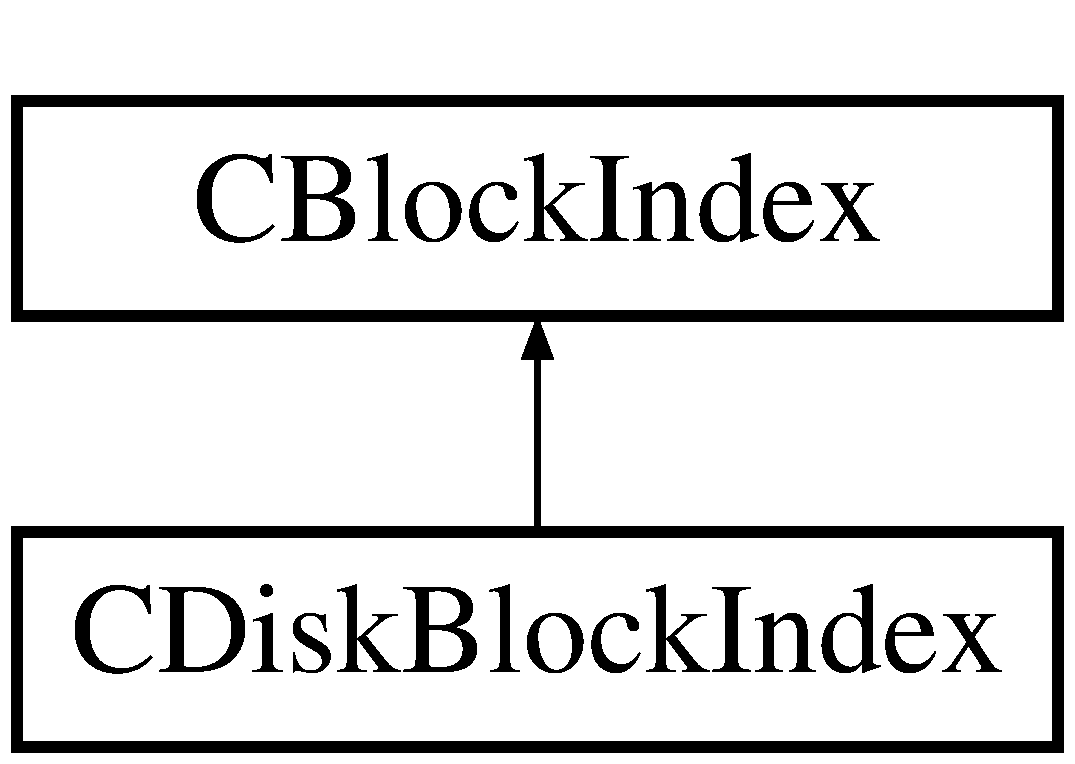
\includegraphics[height=2.000000cm]{class_c_disk_block_index}
\end{center}
\end{figure}
\subsection*{Public Member Functions}
\begin{DoxyCompactItemize}
\item 
\hyperlink{class_c_disk_block_index_a8c460c63b799964ef55e2dbbb74b5ad6}{C\+Disk\+Block\+Index} ()
\item 
\hyperlink{class_c_disk_block_index_a8d76af0058fa72d3d8ff688d27d2a5c9}{C\+Disk\+Block\+Index} (const \hyperlink{class_c_block_index}{C\+Block\+Index} $\ast$pindex)
\item 
{\footnotesize template$<$typename Stream , typename Operation $>$ }\\void \hyperlink{class_c_disk_block_index_a2ef7b51f2777fcc1b9625a0ee000f9b5}{Serialization\+Op} (Stream \&s, Operation ser\+\_\+action, int n\+Type, int \hyperlink{class_c_block_index_a45126301a0a6e26010527a7bbfc1ef58}{n\+Version})
\item 
\hyperlink{classuint256}{uint256} \hyperlink{class_c_disk_block_index_adbe404c55c68be782360b4594d355fad}{Get\+Block\+Hash} () const 
\item 
std\+::string \hyperlink{class_c_disk_block_index_a86ef9d71fb72868699145b73f3e3e583}{To\+String} () const 
\end{DoxyCompactItemize}
\subsection*{Public Attributes}
\begin{DoxyCompactItemize}
\item 
\hyperlink{classuint256}{uint256} \hyperlink{class_c_disk_block_index_a3a1730201a8523fb947c4d4f632a4212}{hash\+Prev}
\item 
\hyperlink{class_c_disk_block_index_adfa97e82f2e6db827fc6b8b5e351a1f9}{A\+D\+D\+\_\+\+S\+E\+R\+I\+A\+L\+I\+Z\+E\+\_\+\+M\+E\+T\+H\+O\+D\+S}
\end{DoxyCompactItemize}
\subsection*{Additional Inherited Members}


\subsection{Detailed Description}
Used to marshal pointers into hashes for db storage. 

\subsection{Constructor \& Destructor Documentation}
\hypertarget{class_c_disk_block_index_a8c460c63b799964ef55e2dbbb74b5ad6}{}\index{C\+Disk\+Block\+Index@{C\+Disk\+Block\+Index}!C\+Disk\+Block\+Index@{C\+Disk\+Block\+Index}}
\index{C\+Disk\+Block\+Index@{C\+Disk\+Block\+Index}!C\+Disk\+Block\+Index@{C\+Disk\+Block\+Index}}
\subsubsection[{C\+Disk\+Block\+Index}]{\setlength{\rightskip}{0pt plus 5cm}C\+Disk\+Block\+Index\+::\+C\+Disk\+Block\+Index (
\begin{DoxyParamCaption}
{}
\end{DoxyParamCaption}
)\hspace{0.3cm}{\ttfamily [inline]}}\label{class_c_disk_block_index_a8c460c63b799964ef55e2dbbb74b5ad6}
\hypertarget{class_c_disk_block_index_a8d76af0058fa72d3d8ff688d27d2a5c9}{}\index{C\+Disk\+Block\+Index@{C\+Disk\+Block\+Index}!C\+Disk\+Block\+Index@{C\+Disk\+Block\+Index}}
\index{C\+Disk\+Block\+Index@{C\+Disk\+Block\+Index}!C\+Disk\+Block\+Index@{C\+Disk\+Block\+Index}}
\subsubsection[{C\+Disk\+Block\+Index}]{\setlength{\rightskip}{0pt plus 5cm}C\+Disk\+Block\+Index\+::\+C\+Disk\+Block\+Index (
\begin{DoxyParamCaption}
\item[{const {\bf C\+Block\+Index} $\ast$}]{pindex}
\end{DoxyParamCaption}
)\hspace{0.3cm}{\ttfamily [inline]}, {\ttfamily [explicit]}}\label{class_c_disk_block_index_a8d76af0058fa72d3d8ff688d27d2a5c9}


\subsection{Member Function Documentation}
\hypertarget{class_c_disk_block_index_adbe404c55c68be782360b4594d355fad}{}\index{C\+Disk\+Block\+Index@{C\+Disk\+Block\+Index}!Get\+Block\+Hash@{Get\+Block\+Hash}}
\index{Get\+Block\+Hash@{Get\+Block\+Hash}!C\+Disk\+Block\+Index@{C\+Disk\+Block\+Index}}
\subsubsection[{Get\+Block\+Hash}]{\setlength{\rightskip}{0pt plus 5cm}{\bf uint256} C\+Disk\+Block\+Index\+::\+Get\+Block\+Hash (
\begin{DoxyParamCaption}
{}
\end{DoxyParamCaption}
) const\hspace{0.3cm}{\ttfamily [inline]}}\label{class_c_disk_block_index_adbe404c55c68be782360b4594d355fad}
\hypertarget{class_c_disk_block_index_a2ef7b51f2777fcc1b9625a0ee000f9b5}{}\index{C\+Disk\+Block\+Index@{C\+Disk\+Block\+Index}!Serialization\+Op@{Serialization\+Op}}
\index{Serialization\+Op@{Serialization\+Op}!C\+Disk\+Block\+Index@{C\+Disk\+Block\+Index}}
\subsubsection[{Serialization\+Op}]{\setlength{\rightskip}{0pt plus 5cm}template$<$typename Stream , typename Operation $>$ void C\+Disk\+Block\+Index\+::\+Serialization\+Op (
\begin{DoxyParamCaption}
\item[{Stream \&}]{s, }
\item[{Operation}]{ser\+\_\+action, }
\item[{int}]{n\+Type, }
\item[{int}]{n\+Version}
\end{DoxyParamCaption}
)\hspace{0.3cm}{\ttfamily [inline]}}\label{class_c_disk_block_index_a2ef7b51f2777fcc1b9625a0ee000f9b5}
\hypertarget{class_c_disk_block_index_a86ef9d71fb72868699145b73f3e3e583}{}\index{C\+Disk\+Block\+Index@{C\+Disk\+Block\+Index}!To\+String@{To\+String}}
\index{To\+String@{To\+String}!C\+Disk\+Block\+Index@{C\+Disk\+Block\+Index}}
\subsubsection[{To\+String}]{\setlength{\rightskip}{0pt plus 5cm}std\+::string C\+Disk\+Block\+Index\+::\+To\+String (
\begin{DoxyParamCaption}
{}
\end{DoxyParamCaption}
) const\hspace{0.3cm}{\ttfamily [inline]}}\label{class_c_disk_block_index_a86ef9d71fb72868699145b73f3e3e583}


\subsection{Member Data Documentation}
\hypertarget{class_c_disk_block_index_adfa97e82f2e6db827fc6b8b5e351a1f9}{}\index{C\+Disk\+Block\+Index@{C\+Disk\+Block\+Index}!A\+D\+D\+\_\+\+S\+E\+R\+I\+A\+L\+I\+Z\+E\+\_\+\+M\+E\+T\+H\+O\+D\+S@{A\+D\+D\+\_\+\+S\+E\+R\+I\+A\+L\+I\+Z\+E\+\_\+\+M\+E\+T\+H\+O\+D\+S}}
\index{A\+D\+D\+\_\+\+S\+E\+R\+I\+A\+L\+I\+Z\+E\+\_\+\+M\+E\+T\+H\+O\+D\+S@{A\+D\+D\+\_\+\+S\+E\+R\+I\+A\+L\+I\+Z\+E\+\_\+\+M\+E\+T\+H\+O\+D\+S}!C\+Disk\+Block\+Index@{C\+Disk\+Block\+Index}}
\subsubsection[{A\+D\+D\+\_\+\+S\+E\+R\+I\+A\+L\+I\+Z\+E\+\_\+\+M\+E\+T\+H\+O\+D\+S}]{\setlength{\rightskip}{0pt plus 5cm}C\+Disk\+Block\+Index\+::\+A\+D\+D\+\_\+\+S\+E\+R\+I\+A\+L\+I\+Z\+E\+\_\+\+M\+E\+T\+H\+O\+D\+S}\label{class_c_disk_block_index_adfa97e82f2e6db827fc6b8b5e351a1f9}
\hypertarget{class_c_disk_block_index_a3a1730201a8523fb947c4d4f632a4212}{}\index{C\+Disk\+Block\+Index@{C\+Disk\+Block\+Index}!hash\+Prev@{hash\+Prev}}
\index{hash\+Prev@{hash\+Prev}!C\+Disk\+Block\+Index@{C\+Disk\+Block\+Index}}
\subsubsection[{hash\+Prev}]{\setlength{\rightskip}{0pt plus 5cm}{\bf uint256} C\+Disk\+Block\+Index\+::hash\+Prev}\label{class_c_disk_block_index_a3a1730201a8523fb947c4d4f632a4212}


The documentation for this class was generated from the following file\+:\begin{DoxyCompactItemize}
\item 
C\+:/\+Users/\+Joe/\+Documents/\+School/\+C\+S\+C17\+A/bitcoin/src/\hyperlink{chain_8h}{chain.\+h}\end{DoxyCompactItemize}

\hypertarget{struct_c_disk_block_pos}{}\section{C\+Disk\+Block\+Pos Struct Reference}
\label{struct_c_disk_block_pos}\index{C\+Disk\+Block\+Pos@{C\+Disk\+Block\+Pos}}


{\ttfamily \#include $<$chain.\+h$>$}

Inheritance diagram for C\+Disk\+Block\+Pos\+:\begin{figure}[H]
\begin{center}
\leavevmode
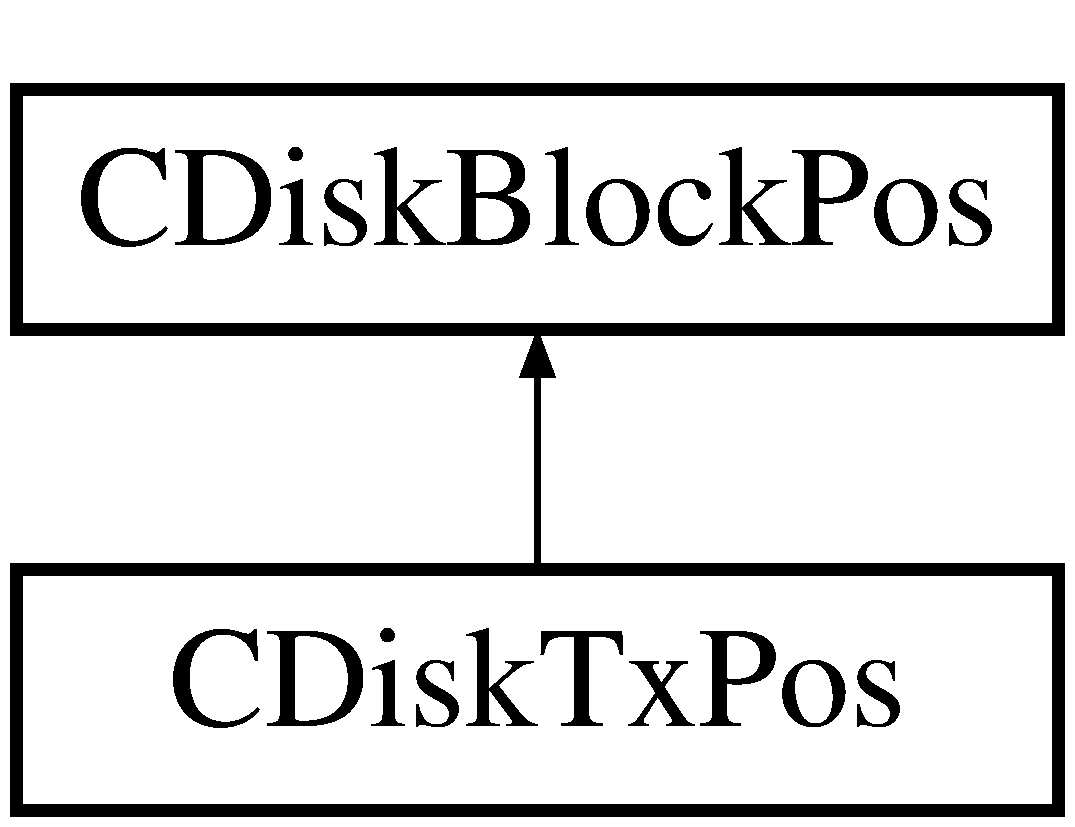
\includegraphics[height=2.000000cm]{struct_c_disk_block_pos}
\end{center}
\end{figure}
\subsection*{Public Member Functions}
\begin{DoxyCompactItemize}
\item 
{\footnotesize template$<$typename Stream , typename Operation $>$ }\\void \hyperlink{struct_c_disk_block_pos_a821bb4eebc99ae39c20133d80244325f}{Serialization\+Op} (Stream \&s, Operation ser\+\_\+action, int n\+Type, int n\+Version)
\item 
\hyperlink{struct_c_disk_block_pos_ac34e46c8bf3256b3eca09f54911cf8bd}{C\+Disk\+Block\+Pos} ()
\item 
\hyperlink{struct_c_disk_block_pos_a0c96947d09bb4aaf28ab2d7866d20918}{C\+Disk\+Block\+Pos} (int n\+File\+In, unsigned int n\+Pos\+In)
\item 
void \hyperlink{struct_c_disk_block_pos_a0a6ba113219a456472081ee6d6b20a72}{Set\+Null} ()
\item 
bool \hyperlink{struct_c_disk_block_pos_a924f2805b274345afce890b27a0934d9}{Is\+Null} () const 
\item 
std\+::string \hyperlink{struct_c_disk_block_pos_ab187c46272360bde44f6ae611373a984}{To\+String} () const 
\end{DoxyCompactItemize}
\subsection*{Public Attributes}
\begin{DoxyCompactItemize}
\item 
int \hyperlink{struct_c_disk_block_pos_a09f30dab5c02fbdea8a17f9bcee5aac8}{n\+File}
\item 
unsigned int \hyperlink{struct_c_disk_block_pos_a9b4b5e149b655ac5c22d05883b5bca0e}{n\+Pos}
\item 
\hyperlink{struct_c_disk_block_pos_a958cd730b290bbb0153d514c56517590}{A\+D\+D\+\_\+\+S\+E\+R\+I\+A\+L\+I\+Z\+E\+\_\+\+M\+E\+T\+H\+O\+D\+S}
\end{DoxyCompactItemize}
\subsection*{Friends}
\begin{DoxyCompactItemize}
\item 
bool \hyperlink{struct_c_disk_block_pos_a04787eb60da48b80e0f7fb402c6896fe}{operator==} (const \hyperlink{struct_c_disk_block_pos}{C\+Disk\+Block\+Pos} \&a, const \hyperlink{struct_c_disk_block_pos}{C\+Disk\+Block\+Pos} \&b)
\item 
bool \hyperlink{struct_c_disk_block_pos_af77481af6cf1d32788ba67c29cc061b5}{operator!=} (const \hyperlink{struct_c_disk_block_pos}{C\+Disk\+Block\+Pos} \&a, const \hyperlink{struct_c_disk_block_pos}{C\+Disk\+Block\+Pos} \&b)
\end{DoxyCompactItemize}


\subsection{Constructor \& Destructor Documentation}
\hypertarget{struct_c_disk_block_pos_ac34e46c8bf3256b3eca09f54911cf8bd}{}\index{C\+Disk\+Block\+Pos@{C\+Disk\+Block\+Pos}!C\+Disk\+Block\+Pos@{C\+Disk\+Block\+Pos}}
\index{C\+Disk\+Block\+Pos@{C\+Disk\+Block\+Pos}!C\+Disk\+Block\+Pos@{C\+Disk\+Block\+Pos}}
\subsubsection[{C\+Disk\+Block\+Pos}]{\setlength{\rightskip}{0pt plus 5cm}C\+Disk\+Block\+Pos\+::\+C\+Disk\+Block\+Pos (
\begin{DoxyParamCaption}
{}
\end{DoxyParamCaption}
)\hspace{0.3cm}{\ttfamily [inline]}}\label{struct_c_disk_block_pos_ac34e46c8bf3256b3eca09f54911cf8bd}
\hypertarget{struct_c_disk_block_pos_a0c96947d09bb4aaf28ab2d7866d20918}{}\index{C\+Disk\+Block\+Pos@{C\+Disk\+Block\+Pos}!C\+Disk\+Block\+Pos@{C\+Disk\+Block\+Pos}}
\index{C\+Disk\+Block\+Pos@{C\+Disk\+Block\+Pos}!C\+Disk\+Block\+Pos@{C\+Disk\+Block\+Pos}}
\subsubsection[{C\+Disk\+Block\+Pos}]{\setlength{\rightskip}{0pt plus 5cm}C\+Disk\+Block\+Pos\+::\+C\+Disk\+Block\+Pos (
\begin{DoxyParamCaption}
\item[{int}]{n\+File\+In, }
\item[{unsigned int}]{n\+Pos\+In}
\end{DoxyParamCaption}
)\hspace{0.3cm}{\ttfamily [inline]}}\label{struct_c_disk_block_pos_a0c96947d09bb4aaf28ab2d7866d20918}


\subsection{Member Function Documentation}
\hypertarget{struct_c_disk_block_pos_a924f2805b274345afce890b27a0934d9}{}\index{C\+Disk\+Block\+Pos@{C\+Disk\+Block\+Pos}!Is\+Null@{Is\+Null}}
\index{Is\+Null@{Is\+Null}!C\+Disk\+Block\+Pos@{C\+Disk\+Block\+Pos}}
\subsubsection[{Is\+Null}]{\setlength{\rightskip}{0pt plus 5cm}bool C\+Disk\+Block\+Pos\+::\+Is\+Null (
\begin{DoxyParamCaption}
{}
\end{DoxyParamCaption}
) const\hspace{0.3cm}{\ttfamily [inline]}}\label{struct_c_disk_block_pos_a924f2805b274345afce890b27a0934d9}
\hypertarget{struct_c_disk_block_pos_a821bb4eebc99ae39c20133d80244325f}{}\index{C\+Disk\+Block\+Pos@{C\+Disk\+Block\+Pos}!Serialization\+Op@{Serialization\+Op}}
\index{Serialization\+Op@{Serialization\+Op}!C\+Disk\+Block\+Pos@{C\+Disk\+Block\+Pos}}
\subsubsection[{Serialization\+Op}]{\setlength{\rightskip}{0pt plus 5cm}template$<$typename Stream , typename Operation $>$ void C\+Disk\+Block\+Pos\+::\+Serialization\+Op (
\begin{DoxyParamCaption}
\item[{Stream \&}]{s, }
\item[{Operation}]{ser\+\_\+action, }
\item[{int}]{n\+Type, }
\item[{int}]{n\+Version}
\end{DoxyParamCaption}
)\hspace{0.3cm}{\ttfamily [inline]}}\label{struct_c_disk_block_pos_a821bb4eebc99ae39c20133d80244325f}
\hypertarget{struct_c_disk_block_pos_a0a6ba113219a456472081ee6d6b20a72}{}\index{C\+Disk\+Block\+Pos@{C\+Disk\+Block\+Pos}!Set\+Null@{Set\+Null}}
\index{Set\+Null@{Set\+Null}!C\+Disk\+Block\+Pos@{C\+Disk\+Block\+Pos}}
\subsubsection[{Set\+Null}]{\setlength{\rightskip}{0pt plus 5cm}void C\+Disk\+Block\+Pos\+::\+Set\+Null (
\begin{DoxyParamCaption}
{}
\end{DoxyParamCaption}
)\hspace{0.3cm}{\ttfamily [inline]}}\label{struct_c_disk_block_pos_a0a6ba113219a456472081ee6d6b20a72}
\hypertarget{struct_c_disk_block_pos_ab187c46272360bde44f6ae611373a984}{}\index{C\+Disk\+Block\+Pos@{C\+Disk\+Block\+Pos}!To\+String@{To\+String}}
\index{To\+String@{To\+String}!C\+Disk\+Block\+Pos@{C\+Disk\+Block\+Pos}}
\subsubsection[{To\+String}]{\setlength{\rightskip}{0pt plus 5cm}std\+::string C\+Disk\+Block\+Pos\+::\+To\+String (
\begin{DoxyParamCaption}
{}
\end{DoxyParamCaption}
) const\hspace{0.3cm}{\ttfamily [inline]}}\label{struct_c_disk_block_pos_ab187c46272360bde44f6ae611373a984}


\subsection{Friends And Related Function Documentation}
\hypertarget{struct_c_disk_block_pos_af77481af6cf1d32788ba67c29cc061b5}{}\index{C\+Disk\+Block\+Pos@{C\+Disk\+Block\+Pos}!operator"!=@{operator"!=}}
\index{operator"!=@{operator"!=}!C\+Disk\+Block\+Pos@{C\+Disk\+Block\+Pos}}
\subsubsection[{operator"!=}]{\setlength{\rightskip}{0pt plus 5cm}bool operator!= (
\begin{DoxyParamCaption}
\item[{const {\bf C\+Disk\+Block\+Pos} \&}]{a, }
\item[{const {\bf C\+Disk\+Block\+Pos} \&}]{b}
\end{DoxyParamCaption}
)\hspace{0.3cm}{\ttfamily [friend]}}\label{struct_c_disk_block_pos_af77481af6cf1d32788ba67c29cc061b5}
\hypertarget{struct_c_disk_block_pos_a04787eb60da48b80e0f7fb402c6896fe}{}\index{C\+Disk\+Block\+Pos@{C\+Disk\+Block\+Pos}!operator==@{operator==}}
\index{operator==@{operator==}!C\+Disk\+Block\+Pos@{C\+Disk\+Block\+Pos}}
\subsubsection[{operator==}]{\setlength{\rightskip}{0pt plus 5cm}bool operator== (
\begin{DoxyParamCaption}
\item[{const {\bf C\+Disk\+Block\+Pos} \&}]{a, }
\item[{const {\bf C\+Disk\+Block\+Pos} \&}]{b}
\end{DoxyParamCaption}
)\hspace{0.3cm}{\ttfamily [friend]}}\label{struct_c_disk_block_pos_a04787eb60da48b80e0f7fb402c6896fe}


\subsection{Member Data Documentation}
\hypertarget{struct_c_disk_block_pos_a958cd730b290bbb0153d514c56517590}{}\index{C\+Disk\+Block\+Pos@{C\+Disk\+Block\+Pos}!A\+D\+D\+\_\+\+S\+E\+R\+I\+A\+L\+I\+Z\+E\+\_\+\+M\+E\+T\+H\+O\+D\+S@{A\+D\+D\+\_\+\+S\+E\+R\+I\+A\+L\+I\+Z\+E\+\_\+\+M\+E\+T\+H\+O\+D\+S}}
\index{A\+D\+D\+\_\+\+S\+E\+R\+I\+A\+L\+I\+Z\+E\+\_\+\+M\+E\+T\+H\+O\+D\+S@{A\+D\+D\+\_\+\+S\+E\+R\+I\+A\+L\+I\+Z\+E\+\_\+\+M\+E\+T\+H\+O\+D\+S}!C\+Disk\+Block\+Pos@{C\+Disk\+Block\+Pos}}
\subsubsection[{A\+D\+D\+\_\+\+S\+E\+R\+I\+A\+L\+I\+Z\+E\+\_\+\+M\+E\+T\+H\+O\+D\+S}]{\setlength{\rightskip}{0pt plus 5cm}C\+Disk\+Block\+Pos\+::\+A\+D\+D\+\_\+\+S\+E\+R\+I\+A\+L\+I\+Z\+E\+\_\+\+M\+E\+T\+H\+O\+D\+S}\label{struct_c_disk_block_pos_a958cd730b290bbb0153d514c56517590}
\hypertarget{struct_c_disk_block_pos_a09f30dab5c02fbdea8a17f9bcee5aac8}{}\index{C\+Disk\+Block\+Pos@{C\+Disk\+Block\+Pos}!n\+File@{n\+File}}
\index{n\+File@{n\+File}!C\+Disk\+Block\+Pos@{C\+Disk\+Block\+Pos}}
\subsubsection[{n\+File}]{\setlength{\rightskip}{0pt plus 5cm}int C\+Disk\+Block\+Pos\+::n\+File}\label{struct_c_disk_block_pos_a09f30dab5c02fbdea8a17f9bcee5aac8}
\hypertarget{struct_c_disk_block_pos_a9b4b5e149b655ac5c22d05883b5bca0e}{}\index{C\+Disk\+Block\+Pos@{C\+Disk\+Block\+Pos}!n\+Pos@{n\+Pos}}
\index{n\+Pos@{n\+Pos}!C\+Disk\+Block\+Pos@{C\+Disk\+Block\+Pos}}
\subsubsection[{n\+Pos}]{\setlength{\rightskip}{0pt plus 5cm}unsigned int C\+Disk\+Block\+Pos\+::n\+Pos}\label{struct_c_disk_block_pos_a9b4b5e149b655ac5c22d05883b5bca0e}


The documentation for this struct was generated from the following file\+:\begin{DoxyCompactItemize}
\item 
C\+:/\+Users/\+Joe/\+Documents/\+School/\+C\+S\+C17\+A/bitcoin/src/\hyperlink{chain_8h}{chain.\+h}\end{DoxyCompactItemize}

\hypertarget{struct_c_disk_tx_pos}{}\section{C\+Disk\+Tx\+Pos Struct Reference}
\label{struct_c_disk_tx_pos}\index{C\+Disk\+Tx\+Pos@{C\+Disk\+Tx\+Pos}}


{\ttfamily \#include $<$main.\+h$>$}

Inheritance diagram for C\+Disk\+Tx\+Pos\+:\begin{figure}[H]
\begin{center}
\leavevmode
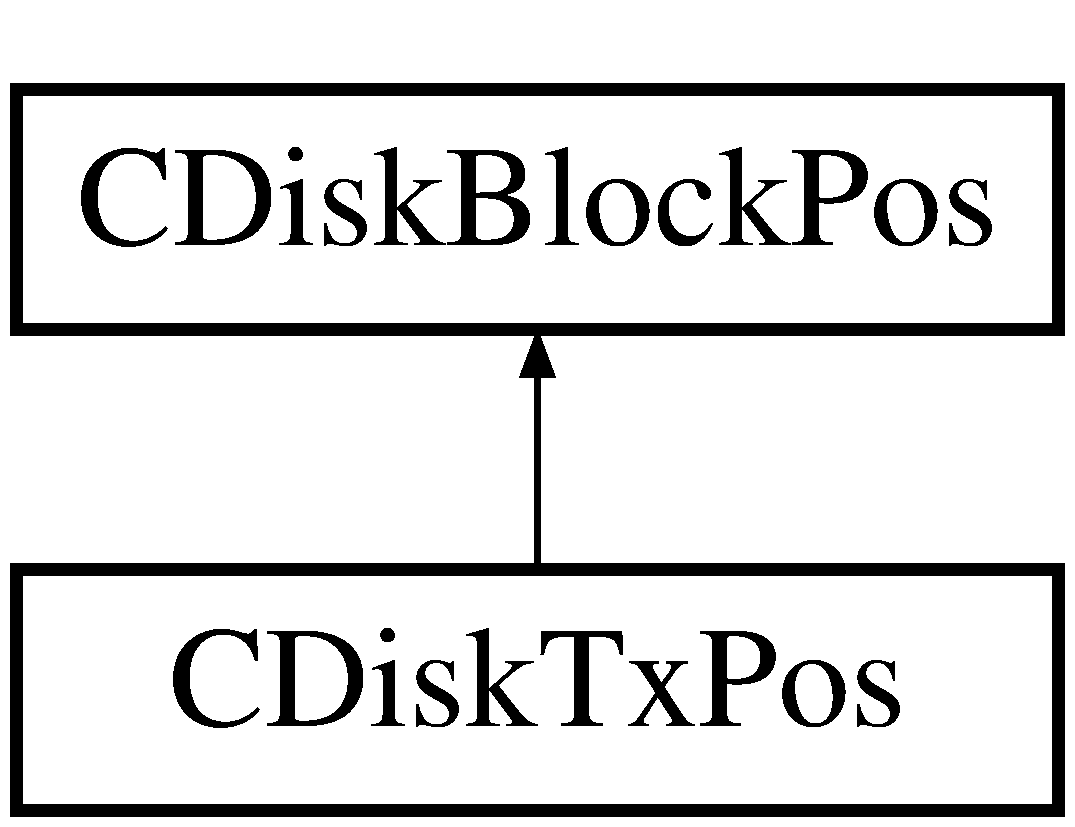
\includegraphics[height=2.000000cm]{struct_c_disk_tx_pos}
\end{center}
\end{figure}
\subsection*{Public Member Functions}
\begin{DoxyCompactItemize}
\item 
{\footnotesize template$<$typename Stream , typename Operation $>$ }\\void \hyperlink{struct_c_disk_tx_pos_a1a68f1de894f0791a7ad64e3e6ea6fd6}{Serialization\+Op} (Stream \&s, Operation ser\+\_\+action, int n\+Type, int n\+Version)
\item 
\hyperlink{struct_c_disk_tx_pos_ab823a4c83ec90c8223544051f11e65fd}{C\+Disk\+Tx\+Pos} (const \hyperlink{struct_c_disk_block_pos}{C\+Disk\+Block\+Pos} \&block\+In, unsigned int n\+Tx\+Offset\+In)
\item 
\hyperlink{struct_c_disk_tx_pos_a2026598d28ffcadfd40452f702bcac46}{C\+Disk\+Tx\+Pos} ()
\item 
void \hyperlink{struct_c_disk_tx_pos_a22eb47d077f9c355373772eb42853fcf}{Set\+Null} ()
\end{DoxyCompactItemize}
\subsection*{Public Attributes}
\begin{DoxyCompactItemize}
\item 
unsigned int \hyperlink{struct_c_disk_tx_pos_af19fa085a69ba3bac7b52413a37adf23}{n\+Tx\+Offset}
\item 
\hyperlink{struct_c_disk_tx_pos_a2990c083fbbd0fb5f5aa4115e540cd21}{A\+D\+D\+\_\+\+S\+E\+R\+I\+A\+L\+I\+Z\+E\+\_\+\+M\+E\+T\+H\+O\+D\+S}
\end{DoxyCompactItemize}


\subsection{Constructor \& Destructor Documentation}
\hypertarget{struct_c_disk_tx_pos_ab823a4c83ec90c8223544051f11e65fd}{}\index{C\+Disk\+Tx\+Pos@{C\+Disk\+Tx\+Pos}!C\+Disk\+Tx\+Pos@{C\+Disk\+Tx\+Pos}}
\index{C\+Disk\+Tx\+Pos@{C\+Disk\+Tx\+Pos}!C\+Disk\+Tx\+Pos@{C\+Disk\+Tx\+Pos}}
\subsubsection[{C\+Disk\+Tx\+Pos}]{\setlength{\rightskip}{0pt plus 5cm}C\+Disk\+Tx\+Pos\+::\+C\+Disk\+Tx\+Pos (
\begin{DoxyParamCaption}
\item[{const {\bf C\+Disk\+Block\+Pos} \&}]{block\+In, }
\item[{unsigned int}]{n\+Tx\+Offset\+In}
\end{DoxyParamCaption}
)\hspace{0.3cm}{\ttfamily [inline]}}\label{struct_c_disk_tx_pos_ab823a4c83ec90c8223544051f11e65fd}
\hypertarget{struct_c_disk_tx_pos_a2026598d28ffcadfd40452f702bcac46}{}\index{C\+Disk\+Tx\+Pos@{C\+Disk\+Tx\+Pos}!C\+Disk\+Tx\+Pos@{C\+Disk\+Tx\+Pos}}
\index{C\+Disk\+Tx\+Pos@{C\+Disk\+Tx\+Pos}!C\+Disk\+Tx\+Pos@{C\+Disk\+Tx\+Pos}}
\subsubsection[{C\+Disk\+Tx\+Pos}]{\setlength{\rightskip}{0pt plus 5cm}C\+Disk\+Tx\+Pos\+::\+C\+Disk\+Tx\+Pos (
\begin{DoxyParamCaption}
{}
\end{DoxyParamCaption}
)\hspace{0.3cm}{\ttfamily [inline]}}\label{struct_c_disk_tx_pos_a2026598d28ffcadfd40452f702bcac46}


\subsection{Member Function Documentation}
\hypertarget{struct_c_disk_tx_pos_a1a68f1de894f0791a7ad64e3e6ea6fd6}{}\index{C\+Disk\+Tx\+Pos@{C\+Disk\+Tx\+Pos}!Serialization\+Op@{Serialization\+Op}}
\index{Serialization\+Op@{Serialization\+Op}!C\+Disk\+Tx\+Pos@{C\+Disk\+Tx\+Pos}}
\subsubsection[{Serialization\+Op}]{\setlength{\rightskip}{0pt plus 5cm}template$<$typename Stream , typename Operation $>$ void C\+Disk\+Tx\+Pos\+::\+Serialization\+Op (
\begin{DoxyParamCaption}
\item[{Stream \&}]{s, }
\item[{Operation}]{ser\+\_\+action, }
\item[{int}]{n\+Type, }
\item[{int}]{n\+Version}
\end{DoxyParamCaption}
)\hspace{0.3cm}{\ttfamily [inline]}}\label{struct_c_disk_tx_pos_a1a68f1de894f0791a7ad64e3e6ea6fd6}
\hypertarget{struct_c_disk_tx_pos_a22eb47d077f9c355373772eb42853fcf}{}\index{C\+Disk\+Tx\+Pos@{C\+Disk\+Tx\+Pos}!Set\+Null@{Set\+Null}}
\index{Set\+Null@{Set\+Null}!C\+Disk\+Tx\+Pos@{C\+Disk\+Tx\+Pos}}
\subsubsection[{Set\+Null}]{\setlength{\rightskip}{0pt plus 5cm}void C\+Disk\+Tx\+Pos\+::\+Set\+Null (
\begin{DoxyParamCaption}
{}
\end{DoxyParamCaption}
)\hspace{0.3cm}{\ttfamily [inline]}}\label{struct_c_disk_tx_pos_a22eb47d077f9c355373772eb42853fcf}


\subsection{Member Data Documentation}
\hypertarget{struct_c_disk_tx_pos_a2990c083fbbd0fb5f5aa4115e540cd21}{}\index{C\+Disk\+Tx\+Pos@{C\+Disk\+Tx\+Pos}!A\+D\+D\+\_\+\+S\+E\+R\+I\+A\+L\+I\+Z\+E\+\_\+\+M\+E\+T\+H\+O\+D\+S@{A\+D\+D\+\_\+\+S\+E\+R\+I\+A\+L\+I\+Z\+E\+\_\+\+M\+E\+T\+H\+O\+D\+S}}
\index{A\+D\+D\+\_\+\+S\+E\+R\+I\+A\+L\+I\+Z\+E\+\_\+\+M\+E\+T\+H\+O\+D\+S@{A\+D\+D\+\_\+\+S\+E\+R\+I\+A\+L\+I\+Z\+E\+\_\+\+M\+E\+T\+H\+O\+D\+S}!C\+Disk\+Tx\+Pos@{C\+Disk\+Tx\+Pos}}
\subsubsection[{A\+D\+D\+\_\+\+S\+E\+R\+I\+A\+L\+I\+Z\+E\+\_\+\+M\+E\+T\+H\+O\+D\+S}]{\setlength{\rightskip}{0pt plus 5cm}C\+Disk\+Tx\+Pos\+::\+A\+D\+D\+\_\+\+S\+E\+R\+I\+A\+L\+I\+Z\+E\+\_\+\+M\+E\+T\+H\+O\+D\+S}\label{struct_c_disk_tx_pos_a2990c083fbbd0fb5f5aa4115e540cd21}
\hypertarget{struct_c_disk_tx_pos_af19fa085a69ba3bac7b52413a37adf23}{}\index{C\+Disk\+Tx\+Pos@{C\+Disk\+Tx\+Pos}!n\+Tx\+Offset@{n\+Tx\+Offset}}
\index{n\+Tx\+Offset@{n\+Tx\+Offset}!C\+Disk\+Tx\+Pos@{C\+Disk\+Tx\+Pos}}
\subsubsection[{n\+Tx\+Offset}]{\setlength{\rightskip}{0pt plus 5cm}unsigned int C\+Disk\+Tx\+Pos\+::n\+Tx\+Offset}\label{struct_c_disk_tx_pos_af19fa085a69ba3bac7b52413a37adf23}


The documentation for this struct was generated from the following file\+:\begin{DoxyCompactItemize}
\item 
C\+:/\+Users/\+Joe/\+Documents/\+School/\+C\+S\+C17\+A/bitcoin/src/\hyperlink{main_8h}{main.\+h}\end{DoxyCompactItemize}

\hypertarget{struct_c_d_n_s_seed_data}{}\section{C\+D\+N\+S\+Seed\+Data Struct Reference}
\label{struct_c_d_n_s_seed_data}\index{C\+D\+N\+S\+Seed\+Data@{C\+D\+N\+S\+Seed\+Data}}


{\ttfamily \#include $<$chainparams.\+h$>$}

\subsection*{Public Member Functions}
\begin{DoxyCompactItemize}
\item 
\hyperlink{struct_c_d_n_s_seed_data_a4152b594beb9800fb7611e3c47f03499}{C\+D\+N\+S\+Seed\+Data} (const std\+::string \&str\+Name, const std\+::string \&str\+Host)
\end{DoxyCompactItemize}
\subsection*{Public Attributes}
\begin{DoxyCompactItemize}
\item 
std\+::string \hyperlink{struct_c_d_n_s_seed_data_a2cf084b163340bd62b67e765799f1fdd}{name}
\item 
std\+::string \hyperlink{struct_c_d_n_s_seed_data_a70f5da8568016651cfb7ec7dbf01b3f0}{host}
\end{DoxyCompactItemize}


\subsection{Constructor \& Destructor Documentation}
\hypertarget{struct_c_d_n_s_seed_data_a4152b594beb9800fb7611e3c47f03499}{}\index{C\+D\+N\+S\+Seed\+Data@{C\+D\+N\+S\+Seed\+Data}!C\+D\+N\+S\+Seed\+Data@{C\+D\+N\+S\+Seed\+Data}}
\index{C\+D\+N\+S\+Seed\+Data@{C\+D\+N\+S\+Seed\+Data}!C\+D\+N\+S\+Seed\+Data@{C\+D\+N\+S\+Seed\+Data}}
\subsubsection[{C\+D\+N\+S\+Seed\+Data}]{\setlength{\rightskip}{0pt plus 5cm}C\+D\+N\+S\+Seed\+Data\+::\+C\+D\+N\+S\+Seed\+Data (
\begin{DoxyParamCaption}
\item[{const std\+::string \&}]{str\+Name, }
\item[{const std\+::string \&}]{str\+Host}
\end{DoxyParamCaption}
)\hspace{0.3cm}{\ttfamily [inline]}}\label{struct_c_d_n_s_seed_data_a4152b594beb9800fb7611e3c47f03499}


\subsection{Member Data Documentation}
\hypertarget{struct_c_d_n_s_seed_data_a70f5da8568016651cfb7ec7dbf01b3f0}{}\index{C\+D\+N\+S\+Seed\+Data@{C\+D\+N\+S\+Seed\+Data}!host@{host}}
\index{host@{host}!C\+D\+N\+S\+Seed\+Data@{C\+D\+N\+S\+Seed\+Data}}
\subsubsection[{host}]{\setlength{\rightskip}{0pt plus 5cm}std\+::string C\+D\+N\+S\+Seed\+Data\+::host}\label{struct_c_d_n_s_seed_data_a70f5da8568016651cfb7ec7dbf01b3f0}
\hypertarget{struct_c_d_n_s_seed_data_a2cf084b163340bd62b67e765799f1fdd}{}\index{C\+D\+N\+S\+Seed\+Data@{C\+D\+N\+S\+Seed\+Data}!name@{name}}
\index{name@{name}!C\+D\+N\+S\+Seed\+Data@{C\+D\+N\+S\+Seed\+Data}}
\subsubsection[{name}]{\setlength{\rightskip}{0pt plus 5cm}std\+::string C\+D\+N\+S\+Seed\+Data\+::name}\label{struct_c_d_n_s_seed_data_a2cf084b163340bd62b67e765799f1fdd}


The documentation for this struct was generated from the following file\+:\begin{DoxyCompactItemize}
\item 
C\+:/\+Users/\+Joe/\+Documents/\+School/\+C\+S\+C17\+A/bitcoin/src/\hyperlink{chainparams_8h}{chainparams.\+h}\end{DoxyCompactItemize}

\hypertarget{class_c_e_c_key}{}\section{C\+E\+C\+Key Class Reference}
\label{class_c_e_c_key}\index{C\+E\+C\+Key@{C\+E\+C\+Key}}


{\ttfamily \#include $<$ecwrapper.\+h$>$}

\subsection*{Public Member Functions}
\begin{DoxyCompactItemize}
\item 
\hyperlink{class_c_e_c_key_a5ee51ce7e5435b8d337913540947e58a}{C\+E\+C\+Key} ()
\item 
\hyperlink{class_c_e_c_key_abc742c7fb8362b693745eeb76324dbde}{$\sim$\+C\+E\+C\+Key} ()
\item 
void \hyperlink{class_c_e_c_key_ab3cb52ca6bf3bdd55be9152a76da9112}{Get\+Pub\+Key} (std\+::vector$<$ unsigned char $>$ \&pubkey, bool f\+Compressed)
\item 
bool \hyperlink{class_c_e_c_key_a07055de929aa6e4f4b692fb2bd272fdd}{Set\+Pub\+Key} (const unsigned char $\ast$pubkey, size\+\_\+t size)
\item 
bool \hyperlink{class_c_e_c_key_abbefe8d295d0bbed97d2709a3a534375}{Verify} (const \hyperlink{classuint256}{uint256} \&hash, const std\+::vector$<$ unsigned char $>$ \&vch\+Sig)
\item 
bool \hyperlink{class_c_e_c_key_a5d7ed3acdc6c2798af3242cacc7b755b}{Recover} (const \hyperlink{classuint256}{uint256} \&hash, const unsigned char $\ast$p64, int rec)
\item 
bool \hyperlink{class_c_e_c_key_a5f6013e6314a8ca9645a49106091ad89}{Tweak\+Public} (const unsigned char vch\+Tweak\mbox{[}32\mbox{]})
\end{DoxyCompactItemize}
\subsection*{Static Public Member Functions}
\begin{DoxyCompactItemize}
\item 
static bool \hyperlink{class_c_e_c_key_a3d11821aa2328baf3bd684e5c1835314}{Sanity\+Check} ()
\end{DoxyCompactItemize}


\subsection{Detailed Description}
R\+A\+I\+I Wrapper around Open\+S\+S\+L\textquotesingle{}s E\+C\+\_\+\+K\+E\+Y 

\subsection{Constructor \& Destructor Documentation}
\hypertarget{class_c_e_c_key_a5ee51ce7e5435b8d337913540947e58a}{}\index{C\+E\+C\+Key@{C\+E\+C\+Key}!C\+E\+C\+Key@{C\+E\+C\+Key}}
\index{C\+E\+C\+Key@{C\+E\+C\+Key}!C\+E\+C\+Key@{C\+E\+C\+Key}}
\subsubsection[{C\+E\+C\+Key}]{\setlength{\rightskip}{0pt plus 5cm}C\+E\+C\+Key\+::\+C\+E\+C\+Key (
\begin{DoxyParamCaption}
{}
\end{DoxyParamCaption}
)}\label{class_c_e_c_key_a5ee51ce7e5435b8d337913540947e58a}
\hypertarget{class_c_e_c_key_abc742c7fb8362b693745eeb76324dbde}{}\index{C\+E\+C\+Key@{C\+E\+C\+Key}!````~C\+E\+C\+Key@{$\sim$\+C\+E\+C\+Key}}
\index{````~C\+E\+C\+Key@{$\sim$\+C\+E\+C\+Key}!C\+E\+C\+Key@{C\+E\+C\+Key}}
\subsubsection[{$\sim$\+C\+E\+C\+Key}]{\setlength{\rightskip}{0pt plus 5cm}C\+E\+C\+Key\+::$\sim$\+C\+E\+C\+Key (
\begin{DoxyParamCaption}
{}
\end{DoxyParamCaption}
)}\label{class_c_e_c_key_abc742c7fb8362b693745eeb76324dbde}


\subsection{Member Function Documentation}
\hypertarget{class_c_e_c_key_ab3cb52ca6bf3bdd55be9152a76da9112}{}\index{C\+E\+C\+Key@{C\+E\+C\+Key}!Get\+Pub\+Key@{Get\+Pub\+Key}}
\index{Get\+Pub\+Key@{Get\+Pub\+Key}!C\+E\+C\+Key@{C\+E\+C\+Key}}
\subsubsection[{Get\+Pub\+Key}]{\setlength{\rightskip}{0pt plus 5cm}void C\+E\+C\+Key\+::\+Get\+Pub\+Key (
\begin{DoxyParamCaption}
\item[{std\+::vector$<$ unsigned char $>$ \&}]{pubkey, }
\item[{bool}]{f\+Compressed}
\end{DoxyParamCaption}
)}\label{class_c_e_c_key_ab3cb52ca6bf3bdd55be9152a76da9112}
\hypertarget{class_c_e_c_key_a5d7ed3acdc6c2798af3242cacc7b755b}{}\index{C\+E\+C\+Key@{C\+E\+C\+Key}!Recover@{Recover}}
\index{Recover@{Recover}!C\+E\+C\+Key@{C\+E\+C\+Key}}
\subsubsection[{Recover}]{\setlength{\rightskip}{0pt plus 5cm}bool C\+E\+C\+Key\+::\+Recover (
\begin{DoxyParamCaption}
\item[{const {\bf uint256} \&}]{hash, }
\item[{const unsigned char $\ast$}]{p64, }
\item[{int}]{rec}
\end{DoxyParamCaption}
)}\label{class_c_e_c_key_a5d7ed3acdc6c2798af3242cacc7b755b}
reconstruct public key from a compact signature This is only slightly more C\+P\+U intensive than just verifying it. If this function succeeds, the recovered public key is guaranteed to be valid (the signature is a valid signature of the given data for that key) \hypertarget{class_c_e_c_key_a3d11821aa2328baf3bd684e5c1835314}{}\index{C\+E\+C\+Key@{C\+E\+C\+Key}!Sanity\+Check@{Sanity\+Check}}
\index{Sanity\+Check@{Sanity\+Check}!C\+E\+C\+Key@{C\+E\+C\+Key}}
\subsubsection[{Sanity\+Check}]{\setlength{\rightskip}{0pt plus 5cm}bool C\+E\+C\+Key\+::\+Sanity\+Check (
\begin{DoxyParamCaption}
{}
\end{DoxyParamCaption}
)\hspace{0.3cm}{\ttfamily [static]}}\label{class_c_e_c_key_a3d11821aa2328baf3bd684e5c1835314}
\hypertarget{class_c_e_c_key_a07055de929aa6e4f4b692fb2bd272fdd}{}\index{C\+E\+C\+Key@{C\+E\+C\+Key}!Set\+Pub\+Key@{Set\+Pub\+Key}}
\index{Set\+Pub\+Key@{Set\+Pub\+Key}!C\+E\+C\+Key@{C\+E\+C\+Key}}
\subsubsection[{Set\+Pub\+Key}]{\setlength{\rightskip}{0pt plus 5cm}bool C\+E\+C\+Key\+::\+Set\+Pub\+Key (
\begin{DoxyParamCaption}
\item[{const unsigned char $\ast$}]{pubkey, }
\item[{size\+\_\+t}]{size}
\end{DoxyParamCaption}
)}\label{class_c_e_c_key_a07055de929aa6e4f4b692fb2bd272fdd}
\hypertarget{class_c_e_c_key_a5f6013e6314a8ca9645a49106091ad89}{}\index{C\+E\+C\+Key@{C\+E\+C\+Key}!Tweak\+Public@{Tweak\+Public}}
\index{Tweak\+Public@{Tweak\+Public}!C\+E\+C\+Key@{C\+E\+C\+Key}}
\subsubsection[{Tweak\+Public}]{\setlength{\rightskip}{0pt plus 5cm}bool C\+E\+C\+Key\+::\+Tweak\+Public (
\begin{DoxyParamCaption}
\item[{const unsigned char}]{vch\+Tweak\mbox{[}32\mbox{]}}
\end{DoxyParamCaption}
)}\label{class_c_e_c_key_a5f6013e6314a8ca9645a49106091ad89}
\hypertarget{class_c_e_c_key_abbefe8d295d0bbed97d2709a3a534375}{}\index{C\+E\+C\+Key@{C\+E\+C\+Key}!Verify@{Verify}}
\index{Verify@{Verify}!C\+E\+C\+Key@{C\+E\+C\+Key}}
\subsubsection[{Verify}]{\setlength{\rightskip}{0pt plus 5cm}bool C\+E\+C\+Key\+::\+Verify (
\begin{DoxyParamCaption}
\item[{const {\bf uint256} \&}]{hash, }
\item[{const std\+::vector$<$ unsigned char $>$ \&}]{vch\+Sig}
\end{DoxyParamCaption}
)}\label{class_c_e_c_key_abbefe8d295d0bbed97d2709a3a534375}


The documentation for this class was generated from the following files\+:\begin{DoxyCompactItemize}
\item 
C\+:/\+Users/\+Joe/\+Documents/\+School/\+C\+S\+C17\+A/bitcoin/src/\hyperlink{ecwrapper_8h}{ecwrapper.\+h}\item 
C\+:/\+Users/\+Joe/\+Documents/\+School/\+C\+S\+C17\+A/bitcoin/src/\hyperlink{ecwrapper_8cpp}{ecwrapper.\+cpp}\end{DoxyCompactItemize}

\hypertarget{struct_c_ext_key}{}\section{C\+Ext\+Key Struct Reference}
\label{struct_c_ext_key}\index{C\+Ext\+Key@{C\+Ext\+Key}}


{\ttfamily \#include $<$key.\+h$>$}

\subsection*{Public Member Functions}
\begin{DoxyCompactItemize}
\item 
void \hyperlink{struct_c_ext_key_aa60d612abaa124e00f66f81ac4a74699}{Encode} (unsigned char code\mbox{[}74\mbox{]}) const 
\item 
void \hyperlink{struct_c_ext_key_a9720e119745472336b6729e19f0819dd}{Decode} (const unsigned char code\mbox{[}74\mbox{]})
\item 
bool \hyperlink{struct_c_ext_key_a2fa3a39434ae09efbbd4058d1d081aa2}{Derive} (\hyperlink{struct_c_ext_key}{C\+Ext\+Key} \&out, unsigned int \hyperlink{struct_c_ext_key_ad15cb7ab68b59495eec71f6586803048}{n\+Child}) const 
\item 
\hyperlink{struct_c_ext_pub_key}{C\+Ext\+Pub\+Key} \hyperlink{struct_c_ext_key_a49f98a470d61ab1f2948b7c414ec9563}{Neuter} () const 
\item 
void \hyperlink{struct_c_ext_key_a8cd6ecafdd649082601d7eebbec79688}{Set\+Master} (const unsigned char $\ast$seed, unsigned int n\+Seed\+Len)
\end{DoxyCompactItemize}
\subsection*{Public Attributes}
\begin{DoxyCompactItemize}
\item 
unsigned char \hyperlink{struct_c_ext_key_ab197a253f41646975405b4ead8027b55}{n\+Depth}
\item 
unsigned char \hyperlink{struct_c_ext_key_a22efb3f5dfb26cd8d88d2ab5db885978}{vch\+Fingerprint} \mbox{[}4\mbox{]}
\item 
unsigned int \hyperlink{struct_c_ext_key_ad15cb7ab68b59495eec71f6586803048}{n\+Child}
\item 
unsigned char \hyperlink{struct_c_ext_key_a637ce75955e2883d20172b707c26a459}{vch\+Chain\+Code} \mbox{[}32\mbox{]}
\item 
\hyperlink{class_c_key}{C\+Key} \hyperlink{struct_c_ext_key_a93cd93ef3311d9dbcf475282a5f80fb2}{key}
\end{DoxyCompactItemize}
\subsection*{Friends}
\begin{DoxyCompactItemize}
\item 
bool \hyperlink{struct_c_ext_key_abd1d7fa4544c5a730a0d2a21d06fd3b3}{operator==} (const \hyperlink{struct_c_ext_key}{C\+Ext\+Key} \&a, const \hyperlink{struct_c_ext_key}{C\+Ext\+Key} \&b)
\end{DoxyCompactItemize}


\subsection{Member Function Documentation}
\hypertarget{struct_c_ext_key_a9720e119745472336b6729e19f0819dd}{}\index{C\+Ext\+Key@{C\+Ext\+Key}!Decode@{Decode}}
\index{Decode@{Decode}!C\+Ext\+Key@{C\+Ext\+Key}}
\subsubsection[{Decode}]{\setlength{\rightskip}{0pt plus 5cm}void C\+Ext\+Key\+::\+Decode (
\begin{DoxyParamCaption}
\item[{const unsigned char}]{code\mbox{[}74\mbox{]}}
\end{DoxyParamCaption}
)}\label{struct_c_ext_key_a9720e119745472336b6729e19f0819dd}
\hypertarget{struct_c_ext_key_a2fa3a39434ae09efbbd4058d1d081aa2}{}\index{C\+Ext\+Key@{C\+Ext\+Key}!Derive@{Derive}}
\index{Derive@{Derive}!C\+Ext\+Key@{C\+Ext\+Key}}
\subsubsection[{Derive}]{\setlength{\rightskip}{0pt plus 5cm}bool C\+Ext\+Key\+::\+Derive (
\begin{DoxyParamCaption}
\item[{{\bf C\+Ext\+Key} \&}]{out, }
\item[{unsigned int}]{n\+Child}
\end{DoxyParamCaption}
) const}\label{struct_c_ext_key_a2fa3a39434ae09efbbd4058d1d081aa2}
\hypertarget{struct_c_ext_key_aa60d612abaa124e00f66f81ac4a74699}{}\index{C\+Ext\+Key@{C\+Ext\+Key}!Encode@{Encode}}
\index{Encode@{Encode}!C\+Ext\+Key@{C\+Ext\+Key}}
\subsubsection[{Encode}]{\setlength{\rightskip}{0pt plus 5cm}void C\+Ext\+Key\+::\+Encode (
\begin{DoxyParamCaption}
\item[{unsigned char}]{code\mbox{[}74\mbox{]}}
\end{DoxyParamCaption}
) const}\label{struct_c_ext_key_aa60d612abaa124e00f66f81ac4a74699}
\hypertarget{struct_c_ext_key_a49f98a470d61ab1f2948b7c414ec9563}{}\index{C\+Ext\+Key@{C\+Ext\+Key}!Neuter@{Neuter}}
\index{Neuter@{Neuter}!C\+Ext\+Key@{C\+Ext\+Key}}
\subsubsection[{Neuter}]{\setlength{\rightskip}{0pt plus 5cm}{\bf C\+Ext\+Pub\+Key} C\+Ext\+Key\+::\+Neuter (
\begin{DoxyParamCaption}
{}
\end{DoxyParamCaption}
) const}\label{struct_c_ext_key_a49f98a470d61ab1f2948b7c414ec9563}
\hypertarget{struct_c_ext_key_a8cd6ecafdd649082601d7eebbec79688}{}\index{C\+Ext\+Key@{C\+Ext\+Key}!Set\+Master@{Set\+Master}}
\index{Set\+Master@{Set\+Master}!C\+Ext\+Key@{C\+Ext\+Key}}
\subsubsection[{Set\+Master}]{\setlength{\rightskip}{0pt plus 5cm}void C\+Ext\+Key\+::\+Set\+Master (
\begin{DoxyParamCaption}
\item[{const unsigned char $\ast$}]{seed, }
\item[{unsigned int}]{n\+Seed\+Len}
\end{DoxyParamCaption}
)}\label{struct_c_ext_key_a8cd6ecafdd649082601d7eebbec79688}


\subsection{Friends And Related Function Documentation}
\hypertarget{struct_c_ext_key_abd1d7fa4544c5a730a0d2a21d06fd3b3}{}\index{C\+Ext\+Key@{C\+Ext\+Key}!operator==@{operator==}}
\index{operator==@{operator==}!C\+Ext\+Key@{C\+Ext\+Key}}
\subsubsection[{operator==}]{\setlength{\rightskip}{0pt plus 5cm}bool operator== (
\begin{DoxyParamCaption}
\item[{const {\bf C\+Ext\+Key} \&}]{a, }
\item[{const {\bf C\+Ext\+Key} \&}]{b}
\end{DoxyParamCaption}
)\hspace{0.3cm}{\ttfamily [friend]}}\label{struct_c_ext_key_abd1d7fa4544c5a730a0d2a21d06fd3b3}


\subsection{Member Data Documentation}
\hypertarget{struct_c_ext_key_a93cd93ef3311d9dbcf475282a5f80fb2}{}\index{C\+Ext\+Key@{C\+Ext\+Key}!key@{key}}
\index{key@{key}!C\+Ext\+Key@{C\+Ext\+Key}}
\subsubsection[{key}]{\setlength{\rightskip}{0pt plus 5cm}{\bf C\+Key} C\+Ext\+Key\+::key}\label{struct_c_ext_key_a93cd93ef3311d9dbcf475282a5f80fb2}
\hypertarget{struct_c_ext_key_ad15cb7ab68b59495eec71f6586803048}{}\index{C\+Ext\+Key@{C\+Ext\+Key}!n\+Child@{n\+Child}}
\index{n\+Child@{n\+Child}!C\+Ext\+Key@{C\+Ext\+Key}}
\subsubsection[{n\+Child}]{\setlength{\rightskip}{0pt plus 5cm}unsigned int C\+Ext\+Key\+::n\+Child}\label{struct_c_ext_key_ad15cb7ab68b59495eec71f6586803048}
\hypertarget{struct_c_ext_key_ab197a253f41646975405b4ead8027b55}{}\index{C\+Ext\+Key@{C\+Ext\+Key}!n\+Depth@{n\+Depth}}
\index{n\+Depth@{n\+Depth}!C\+Ext\+Key@{C\+Ext\+Key}}
\subsubsection[{n\+Depth}]{\setlength{\rightskip}{0pt plus 5cm}unsigned char C\+Ext\+Key\+::n\+Depth}\label{struct_c_ext_key_ab197a253f41646975405b4ead8027b55}
\hypertarget{struct_c_ext_key_a637ce75955e2883d20172b707c26a459}{}\index{C\+Ext\+Key@{C\+Ext\+Key}!vch\+Chain\+Code@{vch\+Chain\+Code}}
\index{vch\+Chain\+Code@{vch\+Chain\+Code}!C\+Ext\+Key@{C\+Ext\+Key}}
\subsubsection[{vch\+Chain\+Code}]{\setlength{\rightskip}{0pt plus 5cm}unsigned char C\+Ext\+Key\+::vch\+Chain\+Code\mbox{[}32\mbox{]}}\label{struct_c_ext_key_a637ce75955e2883d20172b707c26a459}
\hypertarget{struct_c_ext_key_a22efb3f5dfb26cd8d88d2ab5db885978}{}\index{C\+Ext\+Key@{C\+Ext\+Key}!vch\+Fingerprint@{vch\+Fingerprint}}
\index{vch\+Fingerprint@{vch\+Fingerprint}!C\+Ext\+Key@{C\+Ext\+Key}}
\subsubsection[{vch\+Fingerprint}]{\setlength{\rightskip}{0pt plus 5cm}unsigned char C\+Ext\+Key\+::vch\+Fingerprint\mbox{[}4\mbox{]}}\label{struct_c_ext_key_a22efb3f5dfb26cd8d88d2ab5db885978}


The documentation for this struct was generated from the following files\+:\begin{DoxyCompactItemize}
\item 
C\+:/\+Users/\+Joe/\+Documents/\+School/\+C\+S\+C17\+A/bitcoin/src/\hyperlink{key_8h}{key.\+h}\item 
C\+:/\+Users/\+Joe/\+Documents/\+School/\+C\+S\+C17\+A/bitcoin/src/\hyperlink{key_8cpp}{key.\+cpp}\end{DoxyCompactItemize}

\hypertarget{struct_c_ext_pub_key}{}\section{C\+Ext\+Pub\+Key Struct Reference}
\label{struct_c_ext_pub_key}\index{C\+Ext\+Pub\+Key@{C\+Ext\+Pub\+Key}}


{\ttfamily \#include $<$pubkey.\+h$>$}

\subsection*{Public Member Functions}
\begin{DoxyCompactItemize}
\item 
void \hyperlink{struct_c_ext_pub_key_af197553c91c690fc436421fe00d55f8e}{Encode} (unsigned char code\mbox{[}74\mbox{]}) const 
\item 
void \hyperlink{struct_c_ext_pub_key_aa3ca44410ecfa765962d3b97aef61ab5}{Decode} (const unsigned char code\mbox{[}74\mbox{]})
\item 
bool \hyperlink{struct_c_ext_pub_key_a404798f7d800ffb539cf97431025597f}{Derive} (\hyperlink{struct_c_ext_pub_key}{C\+Ext\+Pub\+Key} \&out, unsigned int \hyperlink{struct_c_ext_pub_key_af816bc2798e9d9aaa94f56af4775d9bf}{n\+Child}) const 
\end{DoxyCompactItemize}
\subsection*{Public Attributes}
\begin{DoxyCompactItemize}
\item 
unsigned char \hyperlink{struct_c_ext_pub_key_a58a0724855654eab688cdb00738e3dba}{n\+Depth}
\item 
unsigned char \hyperlink{struct_c_ext_pub_key_a57101a84d16d7897bcec224e488143d9}{vch\+Fingerprint} \mbox{[}4\mbox{]}
\item 
unsigned int \hyperlink{struct_c_ext_pub_key_af816bc2798e9d9aaa94f56af4775d9bf}{n\+Child}
\item 
unsigned char \hyperlink{struct_c_ext_pub_key_a208836888dcc295ca1510de459ca1fc7}{vch\+Chain\+Code} \mbox{[}32\mbox{]}
\item 
\hyperlink{class_c_pub_key}{C\+Pub\+Key} \hyperlink{struct_c_ext_pub_key_ab18c8520919d20bbfd068565ae566ea8}{pubkey}
\end{DoxyCompactItemize}
\subsection*{Friends}
\begin{DoxyCompactItemize}
\item 
bool \hyperlink{struct_c_ext_pub_key_a21fdc5351d6df62ce501f57bc1e1c9e6}{operator==} (const \hyperlink{struct_c_ext_pub_key}{C\+Ext\+Pub\+Key} \&a, const \hyperlink{struct_c_ext_pub_key}{C\+Ext\+Pub\+Key} \&b)
\end{DoxyCompactItemize}


\subsection{Member Function Documentation}
\hypertarget{struct_c_ext_pub_key_aa3ca44410ecfa765962d3b97aef61ab5}{}\index{C\+Ext\+Pub\+Key@{C\+Ext\+Pub\+Key}!Decode@{Decode}}
\index{Decode@{Decode}!C\+Ext\+Pub\+Key@{C\+Ext\+Pub\+Key}}
\subsubsection[{Decode}]{\setlength{\rightskip}{0pt plus 5cm}void C\+Ext\+Pub\+Key\+::\+Decode (
\begin{DoxyParamCaption}
\item[{const unsigned char}]{code\mbox{[}74\mbox{]}}
\end{DoxyParamCaption}
)}\label{struct_c_ext_pub_key_aa3ca44410ecfa765962d3b97aef61ab5}
\hypertarget{struct_c_ext_pub_key_a404798f7d800ffb539cf97431025597f}{}\index{C\+Ext\+Pub\+Key@{C\+Ext\+Pub\+Key}!Derive@{Derive}}
\index{Derive@{Derive}!C\+Ext\+Pub\+Key@{C\+Ext\+Pub\+Key}}
\subsubsection[{Derive}]{\setlength{\rightskip}{0pt plus 5cm}bool C\+Ext\+Pub\+Key\+::\+Derive (
\begin{DoxyParamCaption}
\item[{{\bf C\+Ext\+Pub\+Key} \&}]{out, }
\item[{unsigned int}]{n\+Child}
\end{DoxyParamCaption}
) const}\label{struct_c_ext_pub_key_a404798f7d800ffb539cf97431025597f}
\hypertarget{struct_c_ext_pub_key_af197553c91c690fc436421fe00d55f8e}{}\index{C\+Ext\+Pub\+Key@{C\+Ext\+Pub\+Key}!Encode@{Encode}}
\index{Encode@{Encode}!C\+Ext\+Pub\+Key@{C\+Ext\+Pub\+Key}}
\subsubsection[{Encode}]{\setlength{\rightskip}{0pt plus 5cm}void C\+Ext\+Pub\+Key\+::\+Encode (
\begin{DoxyParamCaption}
\item[{unsigned char}]{code\mbox{[}74\mbox{]}}
\end{DoxyParamCaption}
) const}\label{struct_c_ext_pub_key_af197553c91c690fc436421fe00d55f8e}


\subsection{Friends And Related Function Documentation}
\hypertarget{struct_c_ext_pub_key_a21fdc5351d6df62ce501f57bc1e1c9e6}{}\index{C\+Ext\+Pub\+Key@{C\+Ext\+Pub\+Key}!operator==@{operator==}}
\index{operator==@{operator==}!C\+Ext\+Pub\+Key@{C\+Ext\+Pub\+Key}}
\subsubsection[{operator==}]{\setlength{\rightskip}{0pt plus 5cm}bool operator== (
\begin{DoxyParamCaption}
\item[{const {\bf C\+Ext\+Pub\+Key} \&}]{a, }
\item[{const {\bf C\+Ext\+Pub\+Key} \&}]{b}
\end{DoxyParamCaption}
)\hspace{0.3cm}{\ttfamily [friend]}}\label{struct_c_ext_pub_key_a21fdc5351d6df62ce501f57bc1e1c9e6}


\subsection{Member Data Documentation}
\hypertarget{struct_c_ext_pub_key_af816bc2798e9d9aaa94f56af4775d9bf}{}\index{C\+Ext\+Pub\+Key@{C\+Ext\+Pub\+Key}!n\+Child@{n\+Child}}
\index{n\+Child@{n\+Child}!C\+Ext\+Pub\+Key@{C\+Ext\+Pub\+Key}}
\subsubsection[{n\+Child}]{\setlength{\rightskip}{0pt plus 5cm}unsigned int C\+Ext\+Pub\+Key\+::n\+Child}\label{struct_c_ext_pub_key_af816bc2798e9d9aaa94f56af4775d9bf}
\hypertarget{struct_c_ext_pub_key_a58a0724855654eab688cdb00738e3dba}{}\index{C\+Ext\+Pub\+Key@{C\+Ext\+Pub\+Key}!n\+Depth@{n\+Depth}}
\index{n\+Depth@{n\+Depth}!C\+Ext\+Pub\+Key@{C\+Ext\+Pub\+Key}}
\subsubsection[{n\+Depth}]{\setlength{\rightskip}{0pt plus 5cm}unsigned char C\+Ext\+Pub\+Key\+::n\+Depth}\label{struct_c_ext_pub_key_a58a0724855654eab688cdb00738e3dba}
\hypertarget{struct_c_ext_pub_key_ab18c8520919d20bbfd068565ae566ea8}{}\index{C\+Ext\+Pub\+Key@{C\+Ext\+Pub\+Key}!pubkey@{pubkey}}
\index{pubkey@{pubkey}!C\+Ext\+Pub\+Key@{C\+Ext\+Pub\+Key}}
\subsubsection[{pubkey}]{\setlength{\rightskip}{0pt plus 5cm}{\bf C\+Pub\+Key} C\+Ext\+Pub\+Key\+::pubkey}\label{struct_c_ext_pub_key_ab18c8520919d20bbfd068565ae566ea8}
\hypertarget{struct_c_ext_pub_key_a208836888dcc295ca1510de459ca1fc7}{}\index{C\+Ext\+Pub\+Key@{C\+Ext\+Pub\+Key}!vch\+Chain\+Code@{vch\+Chain\+Code}}
\index{vch\+Chain\+Code@{vch\+Chain\+Code}!C\+Ext\+Pub\+Key@{C\+Ext\+Pub\+Key}}
\subsubsection[{vch\+Chain\+Code}]{\setlength{\rightskip}{0pt plus 5cm}unsigned char C\+Ext\+Pub\+Key\+::vch\+Chain\+Code\mbox{[}32\mbox{]}}\label{struct_c_ext_pub_key_a208836888dcc295ca1510de459ca1fc7}
\hypertarget{struct_c_ext_pub_key_a57101a84d16d7897bcec224e488143d9}{}\index{C\+Ext\+Pub\+Key@{C\+Ext\+Pub\+Key}!vch\+Fingerprint@{vch\+Fingerprint}}
\index{vch\+Fingerprint@{vch\+Fingerprint}!C\+Ext\+Pub\+Key@{C\+Ext\+Pub\+Key}}
\subsubsection[{vch\+Fingerprint}]{\setlength{\rightskip}{0pt plus 5cm}unsigned char C\+Ext\+Pub\+Key\+::vch\+Fingerprint\mbox{[}4\mbox{]}}\label{struct_c_ext_pub_key_a57101a84d16d7897bcec224e488143d9}


The documentation for this struct was generated from the following files\+:\begin{DoxyCompactItemize}
\item 
C\+:/\+Users/\+Joe/\+Documents/\+School/\+C\+S\+C17\+A/bitcoin/src/\hyperlink{pubkey_8h}{pubkey.\+h}\item 
C\+:/\+Users/\+Joe/\+Documents/\+School/\+C\+S\+C17\+A/bitcoin/src/\hyperlink{pubkey_8cpp}{pubkey.\+cpp}\end{DoxyCompactItemize}

\hypertarget{class_c_fee_rate}{}\section{C\+Fee\+Rate Class Reference}
\label{class_c_fee_rate}\index{C\+Fee\+Rate@{C\+Fee\+Rate}}


{\ttfamily \#include $<$amount.\+h$>$}

\subsection*{Public Member Functions}
\begin{DoxyCompactItemize}
\item 
\hyperlink{class_c_fee_rate_aed181aa12213c646c8a4632280444412}{C\+Fee\+Rate} ()
\item 
\hyperlink{class_c_fee_rate_abee4364fc0d83612feda7c9f5425a7cc}{C\+Fee\+Rate} (const \hyperlink{amount_8h_a4eaf3a5239714d8c45b851527f7cb564}{C\+Amount} \&\+\_\+n\+Satoshis\+Per\+K)
\item 
\hyperlink{class_c_fee_rate_ad92ea084b8fa9495cbfe0da9cfd1cd69}{C\+Fee\+Rate} (const \hyperlink{amount_8h_a4eaf3a5239714d8c45b851527f7cb564}{C\+Amount} \&n\+Fee\+Paid, size\+\_\+t n\+Size)
\item 
\hyperlink{class_c_fee_rate_aa82ca8ba290a1c02ed522aacfb5105ef}{C\+Fee\+Rate} (const \hyperlink{class_c_fee_rate}{C\+Fee\+Rate} \&other)
\item 
\hyperlink{amount_8h_a4eaf3a5239714d8c45b851527f7cb564}{C\+Amount} \hyperlink{class_c_fee_rate_a11d1c2c0c9e5601d82fecd023358bcc2}{Get\+Fee} (size\+\_\+t size) const 
\item 
\hyperlink{amount_8h_a4eaf3a5239714d8c45b851527f7cb564}{C\+Amount} \hyperlink{class_c_fee_rate_a5cf990404e896b332cf6fb836244b4a6}{Get\+Fee\+Per\+K} () const 
\item 
std\+::string \hyperlink{class_c_fee_rate_ab517bd05a9b78fbd02aabe7d74d7049f}{To\+String} () const 
\item 
{\footnotesize template$<$typename Stream , typename Operation $>$ }\\void \hyperlink{class_c_fee_rate_aface850a2c1af316cedf87d24f04fda3}{Serialization\+Op} (Stream \&s, Operation ser\+\_\+action, int n\+Type, int n\+Version)
\end{DoxyCompactItemize}
\subsection*{Public Attributes}
\begin{DoxyCompactItemize}
\item 
\hyperlink{class_c_fee_rate_ab1030f8a059eb5ccade1e3803bd727b3}{A\+D\+D\+\_\+\+S\+E\+R\+I\+A\+L\+I\+Z\+E\+\_\+\+M\+E\+T\+H\+O\+D\+S}
\end{DoxyCompactItemize}
\subsection*{Friends}
\begin{DoxyCompactItemize}
\item 
bool \hyperlink{class_c_fee_rate_ac6171d01f1032c0f08e804f2b19e84e8}{operator$<$} (const \hyperlink{class_c_fee_rate}{C\+Fee\+Rate} \&a, const \hyperlink{class_c_fee_rate}{C\+Fee\+Rate} \&b)
\item 
bool \hyperlink{class_c_fee_rate_ab69eafe1cbb126cc0549bc5936422a2c}{operator$>$} (const \hyperlink{class_c_fee_rate}{C\+Fee\+Rate} \&a, const \hyperlink{class_c_fee_rate}{C\+Fee\+Rate} \&b)
\item 
bool \hyperlink{class_c_fee_rate_a90b4daf7a7d840f47c453b9ba51744cf}{operator==} (const \hyperlink{class_c_fee_rate}{C\+Fee\+Rate} \&a, const \hyperlink{class_c_fee_rate}{C\+Fee\+Rate} \&b)
\item 
bool \hyperlink{class_c_fee_rate_af580c9e0a2509b79a497cee50116bfcc}{operator$<$=} (const \hyperlink{class_c_fee_rate}{C\+Fee\+Rate} \&a, const \hyperlink{class_c_fee_rate}{C\+Fee\+Rate} \&b)
\item 
bool \hyperlink{class_c_fee_rate_a3eebd7ed699091974194e47cfb2a571c}{operator$>$=} (const \hyperlink{class_c_fee_rate}{C\+Fee\+Rate} \&a, const \hyperlink{class_c_fee_rate}{C\+Fee\+Rate} \&b)
\end{DoxyCompactItemize}


\subsection{Detailed Description}
Type-\/safe wrapper class to for fee rates (how much to pay based on transaction size) 

\subsection{Constructor \& Destructor Documentation}
\hypertarget{class_c_fee_rate_aed181aa12213c646c8a4632280444412}{}\index{C\+Fee\+Rate@{C\+Fee\+Rate}!C\+Fee\+Rate@{C\+Fee\+Rate}}
\index{C\+Fee\+Rate@{C\+Fee\+Rate}!C\+Fee\+Rate@{C\+Fee\+Rate}}
\subsubsection[{C\+Fee\+Rate}]{\setlength{\rightskip}{0pt plus 5cm}C\+Fee\+Rate\+::\+C\+Fee\+Rate (
\begin{DoxyParamCaption}
{}
\end{DoxyParamCaption}
)\hspace{0.3cm}{\ttfamily [inline]}}\label{class_c_fee_rate_aed181aa12213c646c8a4632280444412}
\hypertarget{class_c_fee_rate_abee4364fc0d83612feda7c9f5425a7cc}{}\index{C\+Fee\+Rate@{C\+Fee\+Rate}!C\+Fee\+Rate@{C\+Fee\+Rate}}
\index{C\+Fee\+Rate@{C\+Fee\+Rate}!C\+Fee\+Rate@{C\+Fee\+Rate}}
\subsubsection[{C\+Fee\+Rate}]{\setlength{\rightskip}{0pt plus 5cm}C\+Fee\+Rate\+::\+C\+Fee\+Rate (
\begin{DoxyParamCaption}
\item[{const {\bf C\+Amount} \&}]{\+\_\+n\+Satoshis\+Per\+K}
\end{DoxyParamCaption}
)\hspace{0.3cm}{\ttfamily [inline]}, {\ttfamily [explicit]}}\label{class_c_fee_rate_abee4364fc0d83612feda7c9f5425a7cc}
\hypertarget{class_c_fee_rate_ad92ea084b8fa9495cbfe0da9cfd1cd69}{}\index{C\+Fee\+Rate@{C\+Fee\+Rate}!C\+Fee\+Rate@{C\+Fee\+Rate}}
\index{C\+Fee\+Rate@{C\+Fee\+Rate}!C\+Fee\+Rate@{C\+Fee\+Rate}}
\subsubsection[{C\+Fee\+Rate}]{\setlength{\rightskip}{0pt plus 5cm}C\+Fee\+Rate\+::\+C\+Fee\+Rate (
\begin{DoxyParamCaption}
\item[{const {\bf C\+Amount} \&}]{n\+Fee\+Paid, }
\item[{size\+\_\+t}]{n\+Size}
\end{DoxyParamCaption}
)}\label{class_c_fee_rate_ad92ea084b8fa9495cbfe0da9cfd1cd69}
\hypertarget{class_c_fee_rate_aa82ca8ba290a1c02ed522aacfb5105ef}{}\index{C\+Fee\+Rate@{C\+Fee\+Rate}!C\+Fee\+Rate@{C\+Fee\+Rate}}
\index{C\+Fee\+Rate@{C\+Fee\+Rate}!C\+Fee\+Rate@{C\+Fee\+Rate}}
\subsubsection[{C\+Fee\+Rate}]{\setlength{\rightskip}{0pt plus 5cm}C\+Fee\+Rate\+::\+C\+Fee\+Rate (
\begin{DoxyParamCaption}
\item[{const {\bf C\+Fee\+Rate} \&}]{other}
\end{DoxyParamCaption}
)\hspace{0.3cm}{\ttfamily [inline]}}\label{class_c_fee_rate_aa82ca8ba290a1c02ed522aacfb5105ef}


\subsection{Member Function Documentation}
\hypertarget{class_c_fee_rate_a11d1c2c0c9e5601d82fecd023358bcc2}{}\index{C\+Fee\+Rate@{C\+Fee\+Rate}!Get\+Fee@{Get\+Fee}}
\index{Get\+Fee@{Get\+Fee}!C\+Fee\+Rate@{C\+Fee\+Rate}}
\subsubsection[{Get\+Fee}]{\setlength{\rightskip}{0pt plus 5cm}{\bf C\+Amount} C\+Fee\+Rate\+::\+Get\+Fee (
\begin{DoxyParamCaption}
\item[{size\+\_\+t}]{size}
\end{DoxyParamCaption}
) const}\label{class_c_fee_rate_a11d1c2c0c9e5601d82fecd023358bcc2}
\hypertarget{class_c_fee_rate_a5cf990404e896b332cf6fb836244b4a6}{}\index{C\+Fee\+Rate@{C\+Fee\+Rate}!Get\+Fee\+Per\+K@{Get\+Fee\+Per\+K}}
\index{Get\+Fee\+Per\+K@{Get\+Fee\+Per\+K}!C\+Fee\+Rate@{C\+Fee\+Rate}}
\subsubsection[{Get\+Fee\+Per\+K}]{\setlength{\rightskip}{0pt plus 5cm}{\bf C\+Amount} C\+Fee\+Rate\+::\+Get\+Fee\+Per\+K (
\begin{DoxyParamCaption}
{}
\end{DoxyParamCaption}
) const\hspace{0.3cm}{\ttfamily [inline]}}\label{class_c_fee_rate_a5cf990404e896b332cf6fb836244b4a6}
\hypertarget{class_c_fee_rate_aface850a2c1af316cedf87d24f04fda3}{}\index{C\+Fee\+Rate@{C\+Fee\+Rate}!Serialization\+Op@{Serialization\+Op}}
\index{Serialization\+Op@{Serialization\+Op}!C\+Fee\+Rate@{C\+Fee\+Rate}}
\subsubsection[{Serialization\+Op}]{\setlength{\rightskip}{0pt plus 5cm}template$<$typename Stream , typename Operation $>$ void C\+Fee\+Rate\+::\+Serialization\+Op (
\begin{DoxyParamCaption}
\item[{Stream \&}]{s, }
\item[{Operation}]{ser\+\_\+action, }
\item[{int}]{n\+Type, }
\item[{int}]{n\+Version}
\end{DoxyParamCaption}
)\hspace{0.3cm}{\ttfamily [inline]}}\label{class_c_fee_rate_aface850a2c1af316cedf87d24f04fda3}
\hypertarget{class_c_fee_rate_ab517bd05a9b78fbd02aabe7d74d7049f}{}\index{C\+Fee\+Rate@{C\+Fee\+Rate}!To\+String@{To\+String}}
\index{To\+String@{To\+String}!C\+Fee\+Rate@{C\+Fee\+Rate}}
\subsubsection[{To\+String}]{\setlength{\rightskip}{0pt plus 5cm}std\+::string C\+Fee\+Rate\+::\+To\+String (
\begin{DoxyParamCaption}
{}
\end{DoxyParamCaption}
) const}\label{class_c_fee_rate_ab517bd05a9b78fbd02aabe7d74d7049f}


\subsection{Friends And Related Function Documentation}
\hypertarget{class_c_fee_rate_ac6171d01f1032c0f08e804f2b19e84e8}{}\index{C\+Fee\+Rate@{C\+Fee\+Rate}!operator$<$@{operator$<$}}
\index{operator$<$@{operator$<$}!C\+Fee\+Rate@{C\+Fee\+Rate}}
\subsubsection[{operator$<$}]{\setlength{\rightskip}{0pt plus 5cm}bool operator$<$ (
\begin{DoxyParamCaption}
\item[{const {\bf C\+Fee\+Rate} \&}]{a, }
\item[{const {\bf C\+Fee\+Rate} \&}]{b}
\end{DoxyParamCaption}
)\hspace{0.3cm}{\ttfamily [friend]}}\label{class_c_fee_rate_ac6171d01f1032c0f08e804f2b19e84e8}
\hypertarget{class_c_fee_rate_af580c9e0a2509b79a497cee50116bfcc}{}\index{C\+Fee\+Rate@{C\+Fee\+Rate}!operator$<$=@{operator$<$=}}
\index{operator$<$=@{operator$<$=}!C\+Fee\+Rate@{C\+Fee\+Rate}}
\subsubsection[{operator$<$=}]{\setlength{\rightskip}{0pt plus 5cm}bool operator$<$= (
\begin{DoxyParamCaption}
\item[{const {\bf C\+Fee\+Rate} \&}]{a, }
\item[{const {\bf C\+Fee\+Rate} \&}]{b}
\end{DoxyParamCaption}
)\hspace{0.3cm}{\ttfamily [friend]}}\label{class_c_fee_rate_af580c9e0a2509b79a497cee50116bfcc}
\hypertarget{class_c_fee_rate_a90b4daf7a7d840f47c453b9ba51744cf}{}\index{C\+Fee\+Rate@{C\+Fee\+Rate}!operator==@{operator==}}
\index{operator==@{operator==}!C\+Fee\+Rate@{C\+Fee\+Rate}}
\subsubsection[{operator==}]{\setlength{\rightskip}{0pt plus 5cm}bool operator== (
\begin{DoxyParamCaption}
\item[{const {\bf C\+Fee\+Rate} \&}]{a, }
\item[{const {\bf C\+Fee\+Rate} \&}]{b}
\end{DoxyParamCaption}
)\hspace{0.3cm}{\ttfamily [friend]}}\label{class_c_fee_rate_a90b4daf7a7d840f47c453b9ba51744cf}
\hypertarget{class_c_fee_rate_ab69eafe1cbb126cc0549bc5936422a2c}{}\index{C\+Fee\+Rate@{C\+Fee\+Rate}!operator$>$@{operator$>$}}
\index{operator$>$@{operator$>$}!C\+Fee\+Rate@{C\+Fee\+Rate}}
\subsubsection[{operator$>$}]{\setlength{\rightskip}{0pt plus 5cm}bool operator$>$ (
\begin{DoxyParamCaption}
\item[{const {\bf C\+Fee\+Rate} \&}]{a, }
\item[{const {\bf C\+Fee\+Rate} \&}]{b}
\end{DoxyParamCaption}
)\hspace{0.3cm}{\ttfamily [friend]}}\label{class_c_fee_rate_ab69eafe1cbb126cc0549bc5936422a2c}
\hypertarget{class_c_fee_rate_a3eebd7ed699091974194e47cfb2a571c}{}\index{C\+Fee\+Rate@{C\+Fee\+Rate}!operator$>$=@{operator$>$=}}
\index{operator$>$=@{operator$>$=}!C\+Fee\+Rate@{C\+Fee\+Rate}}
\subsubsection[{operator$>$=}]{\setlength{\rightskip}{0pt plus 5cm}bool operator$>$= (
\begin{DoxyParamCaption}
\item[{const {\bf C\+Fee\+Rate} \&}]{a, }
\item[{const {\bf C\+Fee\+Rate} \&}]{b}
\end{DoxyParamCaption}
)\hspace{0.3cm}{\ttfamily [friend]}}\label{class_c_fee_rate_a3eebd7ed699091974194e47cfb2a571c}


\subsection{Member Data Documentation}
\hypertarget{class_c_fee_rate_ab1030f8a059eb5ccade1e3803bd727b3}{}\index{C\+Fee\+Rate@{C\+Fee\+Rate}!A\+D\+D\+\_\+\+S\+E\+R\+I\+A\+L\+I\+Z\+E\+\_\+\+M\+E\+T\+H\+O\+D\+S@{A\+D\+D\+\_\+\+S\+E\+R\+I\+A\+L\+I\+Z\+E\+\_\+\+M\+E\+T\+H\+O\+D\+S}}
\index{A\+D\+D\+\_\+\+S\+E\+R\+I\+A\+L\+I\+Z\+E\+\_\+\+M\+E\+T\+H\+O\+D\+S@{A\+D\+D\+\_\+\+S\+E\+R\+I\+A\+L\+I\+Z\+E\+\_\+\+M\+E\+T\+H\+O\+D\+S}!C\+Fee\+Rate@{C\+Fee\+Rate}}
\subsubsection[{A\+D\+D\+\_\+\+S\+E\+R\+I\+A\+L\+I\+Z\+E\+\_\+\+M\+E\+T\+H\+O\+D\+S}]{\setlength{\rightskip}{0pt plus 5cm}C\+Fee\+Rate\+::\+A\+D\+D\+\_\+\+S\+E\+R\+I\+A\+L\+I\+Z\+E\+\_\+\+M\+E\+T\+H\+O\+D\+S}\label{class_c_fee_rate_ab1030f8a059eb5ccade1e3803bd727b3}


The documentation for this class was generated from the following files\+:\begin{DoxyCompactItemize}
\item 
C\+:/\+Users/\+Joe/\+Documents/\+School/\+C\+S\+C17\+A/bitcoin/src/\hyperlink{amount_8h}{amount.\+h}\item 
C\+:/\+Users/\+Joe/\+Documents/\+School/\+C\+S\+C17\+A/bitcoin/src/\hyperlink{amount_8cpp}{amount.\+cpp}\end{DoxyCompactItemize}

\hypertarget{class_c_flat_data}{}\section{C\+Flat\+Data Class Reference}
\label{class_c_flat_data}\index{C\+Flat\+Data@{C\+Flat\+Data}}


{\ttfamily \#include $<$serialize.\+h$>$}

\subsection*{Public Member Functions}
\begin{DoxyCompactItemize}
\item 
\hyperlink{class_c_flat_data_afd4036c45c69e6b080f57d793e1bdf57}{C\+Flat\+Data} (void $\ast$pbegin\+In, void $\ast$pend\+In)
\item 
{\footnotesize template$<$class T , class T\+Al $>$ }\\\hyperlink{class_c_flat_data_aa536a3fe59b6cde08cf7ed57ecebedfb}{C\+Flat\+Data} (std\+::vector$<$ T, T\+Al $>$ \&v)
\item 
char $\ast$ \hyperlink{class_c_flat_data_ac8131cc3aec84905d7786fb19ff8953d}{begin} ()
\item 
const char $\ast$ \hyperlink{class_c_flat_data_abf086875237d322ea9aa4f3e6ac371e4}{begin} () const 
\item 
char $\ast$ \hyperlink{class_c_flat_data_ae88ae9f4121ff18aa8e29a3a40d7ee67}{end} ()
\item 
const char $\ast$ \hyperlink{class_c_flat_data_a3619008f211e2f02873cf37e597b64af}{end} () const 
\item 
unsigned int \hyperlink{class_c_flat_data_a9205cfe1bca792dd8605ed8cf4f2d7b7}{Get\+Serialize\+Size} (int, int=0) const 
\item 
{\footnotesize template$<$typename Stream $>$ }\\void \hyperlink{class_c_flat_data_a99e4a9e9c2c68ea484a102b8f08a7c5a}{Serialize} (Stream \&s, int, int=0) const 
\item 
{\footnotesize template$<$typename Stream $>$ }\\void \hyperlink{class_c_flat_data_a3da79327bf2937113de502182ee227b9}{Unserialize} (Stream \&s, int, int=0)
\end{DoxyCompactItemize}
\subsection*{Protected Attributes}
\begin{DoxyCompactItemize}
\item 
char $\ast$ \hyperlink{class_c_flat_data_ad5f93a9d4e1cc71eb5fc94e9c9d4d89d}{pbegin}
\item 
char $\ast$ \hyperlink{class_c_flat_data_add53aa6440254a30392bcf660f3f8057}{pend}
\end{DoxyCompactItemize}


\subsection{Detailed Description}
Wrapper for serializing arrays and P\+O\+D. 

\subsection{Constructor \& Destructor Documentation}
\hypertarget{class_c_flat_data_afd4036c45c69e6b080f57d793e1bdf57}{}\index{C\+Flat\+Data@{C\+Flat\+Data}!C\+Flat\+Data@{C\+Flat\+Data}}
\index{C\+Flat\+Data@{C\+Flat\+Data}!C\+Flat\+Data@{C\+Flat\+Data}}
\subsubsection[{C\+Flat\+Data}]{\setlength{\rightskip}{0pt plus 5cm}C\+Flat\+Data\+::\+C\+Flat\+Data (
\begin{DoxyParamCaption}
\item[{void $\ast$}]{pbegin\+In, }
\item[{void $\ast$}]{pend\+In}
\end{DoxyParamCaption}
)\hspace{0.3cm}{\ttfamily [inline]}}\label{class_c_flat_data_afd4036c45c69e6b080f57d793e1bdf57}
\hypertarget{class_c_flat_data_aa536a3fe59b6cde08cf7ed57ecebedfb}{}\index{C\+Flat\+Data@{C\+Flat\+Data}!C\+Flat\+Data@{C\+Flat\+Data}}
\index{C\+Flat\+Data@{C\+Flat\+Data}!C\+Flat\+Data@{C\+Flat\+Data}}
\subsubsection[{C\+Flat\+Data}]{\setlength{\rightskip}{0pt plus 5cm}template$<$class T , class T\+Al $>$ C\+Flat\+Data\+::\+C\+Flat\+Data (
\begin{DoxyParamCaption}
\item[{std\+::vector$<$ T, T\+Al $>$ \&}]{v}
\end{DoxyParamCaption}
)\hspace{0.3cm}{\ttfamily [inline]}, {\ttfamily [explicit]}}\label{class_c_flat_data_aa536a3fe59b6cde08cf7ed57ecebedfb}


\subsection{Member Function Documentation}
\hypertarget{class_c_flat_data_ac8131cc3aec84905d7786fb19ff8953d}{}\index{C\+Flat\+Data@{C\+Flat\+Data}!begin@{begin}}
\index{begin@{begin}!C\+Flat\+Data@{C\+Flat\+Data}}
\subsubsection[{begin}]{\setlength{\rightskip}{0pt plus 5cm}char$\ast$ C\+Flat\+Data\+::begin (
\begin{DoxyParamCaption}
{}
\end{DoxyParamCaption}
)\hspace{0.3cm}{\ttfamily [inline]}}\label{class_c_flat_data_ac8131cc3aec84905d7786fb19ff8953d}
\hypertarget{class_c_flat_data_abf086875237d322ea9aa4f3e6ac371e4}{}\index{C\+Flat\+Data@{C\+Flat\+Data}!begin@{begin}}
\index{begin@{begin}!C\+Flat\+Data@{C\+Flat\+Data}}
\subsubsection[{begin}]{\setlength{\rightskip}{0pt plus 5cm}const char$\ast$ C\+Flat\+Data\+::begin (
\begin{DoxyParamCaption}
{}
\end{DoxyParamCaption}
) const\hspace{0.3cm}{\ttfamily [inline]}}\label{class_c_flat_data_abf086875237d322ea9aa4f3e6ac371e4}
\hypertarget{class_c_flat_data_ae88ae9f4121ff18aa8e29a3a40d7ee67}{}\index{C\+Flat\+Data@{C\+Flat\+Data}!end@{end}}
\index{end@{end}!C\+Flat\+Data@{C\+Flat\+Data}}
\subsubsection[{end}]{\setlength{\rightskip}{0pt plus 5cm}char$\ast$ C\+Flat\+Data\+::end (
\begin{DoxyParamCaption}
{}
\end{DoxyParamCaption}
)\hspace{0.3cm}{\ttfamily [inline]}}\label{class_c_flat_data_ae88ae9f4121ff18aa8e29a3a40d7ee67}
\hypertarget{class_c_flat_data_a3619008f211e2f02873cf37e597b64af}{}\index{C\+Flat\+Data@{C\+Flat\+Data}!end@{end}}
\index{end@{end}!C\+Flat\+Data@{C\+Flat\+Data}}
\subsubsection[{end}]{\setlength{\rightskip}{0pt plus 5cm}const char$\ast$ C\+Flat\+Data\+::end (
\begin{DoxyParamCaption}
{}
\end{DoxyParamCaption}
) const\hspace{0.3cm}{\ttfamily [inline]}}\label{class_c_flat_data_a3619008f211e2f02873cf37e597b64af}
\hypertarget{class_c_flat_data_a9205cfe1bca792dd8605ed8cf4f2d7b7}{}\index{C\+Flat\+Data@{C\+Flat\+Data}!Get\+Serialize\+Size@{Get\+Serialize\+Size}}
\index{Get\+Serialize\+Size@{Get\+Serialize\+Size}!C\+Flat\+Data@{C\+Flat\+Data}}
\subsubsection[{Get\+Serialize\+Size}]{\setlength{\rightskip}{0pt plus 5cm}unsigned int C\+Flat\+Data\+::\+Get\+Serialize\+Size (
\begin{DoxyParamCaption}
\item[{int}]{, }
\item[{int}]{ = {\ttfamily 0}}
\end{DoxyParamCaption}
) const\hspace{0.3cm}{\ttfamily [inline]}}\label{class_c_flat_data_a9205cfe1bca792dd8605ed8cf4f2d7b7}
\hypertarget{class_c_flat_data_a99e4a9e9c2c68ea484a102b8f08a7c5a}{}\index{C\+Flat\+Data@{C\+Flat\+Data}!Serialize@{Serialize}}
\index{Serialize@{Serialize}!C\+Flat\+Data@{C\+Flat\+Data}}
\subsubsection[{Serialize}]{\setlength{\rightskip}{0pt plus 5cm}template$<$typename Stream $>$ void C\+Flat\+Data\+::\+Serialize (
\begin{DoxyParamCaption}
\item[{Stream \&}]{s, }
\item[{int}]{, }
\item[{int}]{ = {\ttfamily 0}}
\end{DoxyParamCaption}
) const\hspace{0.3cm}{\ttfamily [inline]}}\label{class_c_flat_data_a99e4a9e9c2c68ea484a102b8f08a7c5a}
\hypertarget{class_c_flat_data_a3da79327bf2937113de502182ee227b9}{}\index{C\+Flat\+Data@{C\+Flat\+Data}!Unserialize@{Unserialize}}
\index{Unserialize@{Unserialize}!C\+Flat\+Data@{C\+Flat\+Data}}
\subsubsection[{Unserialize}]{\setlength{\rightskip}{0pt plus 5cm}template$<$typename Stream $>$ void C\+Flat\+Data\+::\+Unserialize (
\begin{DoxyParamCaption}
\item[{Stream \&}]{s, }
\item[{int}]{, }
\item[{int}]{ = {\ttfamily 0}}
\end{DoxyParamCaption}
)\hspace{0.3cm}{\ttfamily [inline]}}\label{class_c_flat_data_a3da79327bf2937113de502182ee227b9}


\subsection{Member Data Documentation}
\hypertarget{class_c_flat_data_ad5f93a9d4e1cc71eb5fc94e9c9d4d89d}{}\index{C\+Flat\+Data@{C\+Flat\+Data}!pbegin@{pbegin}}
\index{pbegin@{pbegin}!C\+Flat\+Data@{C\+Flat\+Data}}
\subsubsection[{pbegin}]{\setlength{\rightskip}{0pt plus 5cm}char$\ast$ C\+Flat\+Data\+::pbegin\hspace{0.3cm}{\ttfamily [protected]}}\label{class_c_flat_data_ad5f93a9d4e1cc71eb5fc94e9c9d4d89d}
\hypertarget{class_c_flat_data_add53aa6440254a30392bcf660f3f8057}{}\index{C\+Flat\+Data@{C\+Flat\+Data}!pend@{pend}}
\index{pend@{pend}!C\+Flat\+Data@{C\+Flat\+Data}}
\subsubsection[{pend}]{\setlength{\rightskip}{0pt plus 5cm}char$\ast$ C\+Flat\+Data\+::pend\hspace{0.3cm}{\ttfamily [protected]}}\label{class_c_flat_data_add53aa6440254a30392bcf660f3f8057}


The documentation for this class was generated from the following file\+:\begin{DoxyCompactItemize}
\item 
C\+:/\+Users/\+Joe/\+Documents/\+School/\+C\+S\+C17\+A/bitcoin/src/\hyperlink{serialize_8h}{serialize.\+h}\end{DoxyCompactItemize}

\hypertarget{class_c_hash160}{}\section{C\+Hash160 Class Reference}
\label{class_c_hash160}\index{C\+Hash160@{C\+Hash160}}


{\ttfamily \#include $<$hash.\+h$>$}

\subsection*{Public Member Functions}
\begin{DoxyCompactItemize}
\item 
void \hyperlink{class_c_hash160_a9bb08e1772002ae1a5d85017ba7952ee}{Finalize} (unsigned char hash\mbox{[}\hyperlink{class_c_hash160_a1a5618e17d91ea96e86d779f575211eb}{O\+U\+T\+P\+U\+T\+\_\+\+S\+I\+Z\+E}\mbox{]})
\item 
\hyperlink{class_c_hash160}{C\+Hash160} \& \hyperlink{class_c_hash160_af56cdd9443013eb68b246aa8450217f2}{Write} (const unsigned char $\ast$data, size\+\_\+t len)
\item 
\hyperlink{class_c_hash160}{C\+Hash160} \& \hyperlink{class_c_hash160_a971a8d59073455b1ef0ac0f65e964772}{Reset} ()
\end{DoxyCompactItemize}
\subsection*{Static Public Attributes}
\begin{DoxyCompactItemize}
\item 
static const size\+\_\+t \hyperlink{class_c_hash160_a1a5618e17d91ea96e86d779f575211eb}{O\+U\+T\+P\+U\+T\+\_\+\+S\+I\+Z\+E} = C\+R\+I\+P\+E\+M\+D160\+::\+O\+U\+T\+P\+U\+T\+\_\+\+S\+I\+Z\+E
\end{DoxyCompactItemize}


\subsection{Detailed Description}
A hasher class for Bitcoin\textquotesingle{}s 160-\/bit hash (S\+H\+A-\/256 + R\+I\+P\+E\+M\+D-\/160). 

\subsection{Member Function Documentation}
\hypertarget{class_c_hash160_a9bb08e1772002ae1a5d85017ba7952ee}{}\index{C\+Hash160@{C\+Hash160}!Finalize@{Finalize}}
\index{Finalize@{Finalize}!C\+Hash160@{C\+Hash160}}
\subsubsection[{Finalize}]{\setlength{\rightskip}{0pt plus 5cm}void C\+Hash160\+::\+Finalize (
\begin{DoxyParamCaption}
\item[{unsigned char}]{hash\mbox{[}\+O\+U\+T\+P\+U\+T\+\_\+\+S\+I\+Z\+E\mbox{]}}
\end{DoxyParamCaption}
)\hspace{0.3cm}{\ttfamily [inline]}}\label{class_c_hash160_a9bb08e1772002ae1a5d85017ba7952ee}
\hypertarget{class_c_hash160_a971a8d59073455b1ef0ac0f65e964772}{}\index{C\+Hash160@{C\+Hash160}!Reset@{Reset}}
\index{Reset@{Reset}!C\+Hash160@{C\+Hash160}}
\subsubsection[{Reset}]{\setlength{\rightskip}{0pt plus 5cm}{\bf C\+Hash160}\& C\+Hash160\+::\+Reset (
\begin{DoxyParamCaption}
{}
\end{DoxyParamCaption}
)\hspace{0.3cm}{\ttfamily [inline]}}\label{class_c_hash160_a971a8d59073455b1ef0ac0f65e964772}
\hypertarget{class_c_hash160_af56cdd9443013eb68b246aa8450217f2}{}\index{C\+Hash160@{C\+Hash160}!Write@{Write}}
\index{Write@{Write}!C\+Hash160@{C\+Hash160}}
\subsubsection[{Write}]{\setlength{\rightskip}{0pt plus 5cm}{\bf C\+Hash160}\& C\+Hash160\+::\+Write (
\begin{DoxyParamCaption}
\item[{const unsigned char $\ast$}]{data, }
\item[{size\+\_\+t}]{len}
\end{DoxyParamCaption}
)\hspace{0.3cm}{\ttfamily [inline]}}\label{class_c_hash160_af56cdd9443013eb68b246aa8450217f2}


\subsection{Member Data Documentation}
\hypertarget{class_c_hash160_a1a5618e17d91ea96e86d779f575211eb}{}\index{C\+Hash160@{C\+Hash160}!O\+U\+T\+P\+U\+T\+\_\+\+S\+I\+Z\+E@{O\+U\+T\+P\+U\+T\+\_\+\+S\+I\+Z\+E}}
\index{O\+U\+T\+P\+U\+T\+\_\+\+S\+I\+Z\+E@{O\+U\+T\+P\+U\+T\+\_\+\+S\+I\+Z\+E}!C\+Hash160@{C\+Hash160}}
\subsubsection[{O\+U\+T\+P\+U\+T\+\_\+\+S\+I\+Z\+E}]{\setlength{\rightskip}{0pt plus 5cm}const size\+\_\+t C\+Hash160\+::\+O\+U\+T\+P\+U\+T\+\_\+\+S\+I\+Z\+E = C\+R\+I\+P\+E\+M\+D160\+::\+O\+U\+T\+P\+U\+T\+\_\+\+S\+I\+Z\+E\hspace{0.3cm}{\ttfamily [static]}}\label{class_c_hash160_a1a5618e17d91ea96e86d779f575211eb}


The documentation for this class was generated from the following file\+:\begin{DoxyCompactItemize}
\item 
C\+:/\+Users/\+Joe/\+Documents/\+School/\+C\+S\+C17\+A/bitcoin/src/\hyperlink{hash_8h}{hash.\+h}\end{DoxyCompactItemize}

\hypertarget{class_c_hash256}{}\section{C\+Hash256 Class Reference}
\label{class_c_hash256}\index{C\+Hash256@{C\+Hash256}}


{\ttfamily \#include $<$hash.\+h$>$}

\subsection*{Public Member Functions}
\begin{DoxyCompactItemize}
\item 
void \hyperlink{class_c_hash256_aa8a70c1b7cf24ce7d00240a1131cf4e7}{Finalize} (unsigned char hash\mbox{[}\hyperlink{class_c_hash256_a6812a40441acb1c3b7f10c7e38c7d467}{O\+U\+T\+P\+U\+T\+\_\+\+S\+I\+Z\+E}\mbox{]})
\item 
\hyperlink{class_c_hash256}{C\+Hash256} \& \hyperlink{class_c_hash256_a9cc25033c6435cb28e2e8e377c949a7a}{Write} (const unsigned char $\ast$data, size\+\_\+t len)
\item 
\hyperlink{class_c_hash256}{C\+Hash256} \& \hyperlink{class_c_hash256_ab25b00e4cda7e209173f2ce90475953d}{Reset} ()
\end{DoxyCompactItemize}
\subsection*{Static Public Attributes}
\begin{DoxyCompactItemize}
\item 
static const size\+\_\+t \hyperlink{class_c_hash256_a6812a40441acb1c3b7f10c7e38c7d467}{O\+U\+T\+P\+U\+T\+\_\+\+S\+I\+Z\+E} = C\+S\+H\+A256\+::\+O\+U\+T\+P\+U\+T\+\_\+\+S\+I\+Z\+E
\end{DoxyCompactItemize}


\subsection{Detailed Description}
A hasher class for Bitcoin\textquotesingle{}s 256-\/bit hash (double S\+H\+A-\/256). 

\subsection{Member Function Documentation}
\hypertarget{class_c_hash256_aa8a70c1b7cf24ce7d00240a1131cf4e7}{}\index{C\+Hash256@{C\+Hash256}!Finalize@{Finalize}}
\index{Finalize@{Finalize}!C\+Hash256@{C\+Hash256}}
\subsubsection[{Finalize}]{\setlength{\rightskip}{0pt plus 5cm}void C\+Hash256\+::\+Finalize (
\begin{DoxyParamCaption}
\item[{unsigned char}]{hash\mbox{[}\+O\+U\+T\+P\+U\+T\+\_\+\+S\+I\+Z\+E\mbox{]}}
\end{DoxyParamCaption}
)\hspace{0.3cm}{\ttfamily [inline]}}\label{class_c_hash256_aa8a70c1b7cf24ce7d00240a1131cf4e7}
\hypertarget{class_c_hash256_ab25b00e4cda7e209173f2ce90475953d}{}\index{C\+Hash256@{C\+Hash256}!Reset@{Reset}}
\index{Reset@{Reset}!C\+Hash256@{C\+Hash256}}
\subsubsection[{Reset}]{\setlength{\rightskip}{0pt plus 5cm}{\bf C\+Hash256}\& C\+Hash256\+::\+Reset (
\begin{DoxyParamCaption}
{}
\end{DoxyParamCaption}
)\hspace{0.3cm}{\ttfamily [inline]}}\label{class_c_hash256_ab25b00e4cda7e209173f2ce90475953d}
\hypertarget{class_c_hash256_a9cc25033c6435cb28e2e8e377c949a7a}{}\index{C\+Hash256@{C\+Hash256}!Write@{Write}}
\index{Write@{Write}!C\+Hash256@{C\+Hash256}}
\subsubsection[{Write}]{\setlength{\rightskip}{0pt plus 5cm}{\bf C\+Hash256}\& C\+Hash256\+::\+Write (
\begin{DoxyParamCaption}
\item[{const unsigned char $\ast$}]{data, }
\item[{size\+\_\+t}]{len}
\end{DoxyParamCaption}
)\hspace{0.3cm}{\ttfamily [inline]}}\label{class_c_hash256_a9cc25033c6435cb28e2e8e377c949a7a}


\subsection{Member Data Documentation}
\hypertarget{class_c_hash256_a6812a40441acb1c3b7f10c7e38c7d467}{}\index{C\+Hash256@{C\+Hash256}!O\+U\+T\+P\+U\+T\+\_\+\+S\+I\+Z\+E@{O\+U\+T\+P\+U\+T\+\_\+\+S\+I\+Z\+E}}
\index{O\+U\+T\+P\+U\+T\+\_\+\+S\+I\+Z\+E@{O\+U\+T\+P\+U\+T\+\_\+\+S\+I\+Z\+E}!C\+Hash256@{C\+Hash256}}
\subsubsection[{O\+U\+T\+P\+U\+T\+\_\+\+S\+I\+Z\+E}]{\setlength{\rightskip}{0pt plus 5cm}const size\+\_\+t C\+Hash256\+::\+O\+U\+T\+P\+U\+T\+\_\+\+S\+I\+Z\+E = C\+S\+H\+A256\+::\+O\+U\+T\+P\+U\+T\+\_\+\+S\+I\+Z\+E\hspace{0.3cm}{\ttfamily [static]}}\label{class_c_hash256_a6812a40441acb1c3b7f10c7e38c7d467}


The documentation for this class was generated from the following file\+:\begin{DoxyCompactItemize}
\item 
C\+:/\+Users/\+Joe/\+Documents/\+School/\+C\+S\+C17\+A/bitcoin/src/\hyperlink{hash_8h}{hash.\+h}\end{DoxyCompactItemize}

\hypertarget{class_c_hash_writer}{}\section{C\+Hash\+Writer Class Reference}
\label{class_c_hash_writer}\index{C\+Hash\+Writer@{C\+Hash\+Writer}}


{\ttfamily \#include $<$hash.\+h$>$}

\subsection*{Public Member Functions}
\begin{DoxyCompactItemize}
\item 
\hyperlink{class_c_hash_writer_a81ce9a497a72fcb6b2612efdc20efbc9}{C\+Hash\+Writer} (int n\+Type\+In, int n\+Version\+In)
\item 
\hyperlink{class_c_hash_writer}{C\+Hash\+Writer} \& \hyperlink{class_c_hash_writer_a779360281eeeb4cc7485c8acae649bc9}{write} (const char $\ast$pch, size\+\_\+t size)
\item 
\hyperlink{classuint256}{uint256} \hyperlink{class_c_hash_writer_ae94a937211502eabf19477630090093a}{Get\+Hash} ()
\item 
{\footnotesize template$<$typename T $>$ }\\\hyperlink{class_c_hash_writer}{C\+Hash\+Writer} \& \hyperlink{class_c_hash_writer_a6551aed7315be5ba750680df18562f3a}{operator$<$$<$} (const T \&obj)
\end{DoxyCompactItemize}
\subsection*{Public Attributes}
\begin{DoxyCompactItemize}
\item 
int \hyperlink{class_c_hash_writer_ae8fe02b05db26a2647a7aeee035f022f}{n\+Type}
\item 
int \hyperlink{class_c_hash_writer_ad7d3642addab58385476dc0f9d55fa58}{n\+Version}
\end{DoxyCompactItemize}


\subsection{Detailed Description}
A writer stream (for serialization) that computes a 256-\/bit hash. 

\subsection{Constructor \& Destructor Documentation}
\hypertarget{class_c_hash_writer_a81ce9a497a72fcb6b2612efdc20efbc9}{}\index{C\+Hash\+Writer@{C\+Hash\+Writer}!C\+Hash\+Writer@{C\+Hash\+Writer}}
\index{C\+Hash\+Writer@{C\+Hash\+Writer}!C\+Hash\+Writer@{C\+Hash\+Writer}}
\subsubsection[{C\+Hash\+Writer}]{\setlength{\rightskip}{0pt plus 5cm}C\+Hash\+Writer\+::\+C\+Hash\+Writer (
\begin{DoxyParamCaption}
\item[{int}]{n\+Type\+In, }
\item[{int}]{n\+Version\+In}
\end{DoxyParamCaption}
)\hspace{0.3cm}{\ttfamily [inline]}}\label{class_c_hash_writer_a81ce9a497a72fcb6b2612efdc20efbc9}


\subsection{Member Function Documentation}
\hypertarget{class_c_hash_writer_ae94a937211502eabf19477630090093a}{}\index{C\+Hash\+Writer@{C\+Hash\+Writer}!Get\+Hash@{Get\+Hash}}
\index{Get\+Hash@{Get\+Hash}!C\+Hash\+Writer@{C\+Hash\+Writer}}
\subsubsection[{Get\+Hash}]{\setlength{\rightskip}{0pt plus 5cm}{\bf uint256} C\+Hash\+Writer\+::\+Get\+Hash (
\begin{DoxyParamCaption}
{}
\end{DoxyParamCaption}
)\hspace{0.3cm}{\ttfamily [inline]}}\label{class_c_hash_writer_ae94a937211502eabf19477630090093a}
\hypertarget{class_c_hash_writer_a6551aed7315be5ba750680df18562f3a}{}\index{C\+Hash\+Writer@{C\+Hash\+Writer}!operator$<$$<$@{operator$<$$<$}}
\index{operator$<$$<$@{operator$<$$<$}!C\+Hash\+Writer@{C\+Hash\+Writer}}
\subsubsection[{operator$<$$<$}]{\setlength{\rightskip}{0pt plus 5cm}template$<$typename T $>$ {\bf C\+Hash\+Writer}\& C\+Hash\+Writer\+::operator$<$$<$ (
\begin{DoxyParamCaption}
\item[{const T \&}]{obj}
\end{DoxyParamCaption}
)\hspace{0.3cm}{\ttfamily [inline]}}\label{class_c_hash_writer_a6551aed7315be5ba750680df18562f3a}
\hypertarget{class_c_hash_writer_a779360281eeeb4cc7485c8acae649bc9}{}\index{C\+Hash\+Writer@{C\+Hash\+Writer}!write@{write}}
\index{write@{write}!C\+Hash\+Writer@{C\+Hash\+Writer}}
\subsubsection[{write}]{\setlength{\rightskip}{0pt plus 5cm}{\bf C\+Hash\+Writer}\& C\+Hash\+Writer\+::write (
\begin{DoxyParamCaption}
\item[{const char $\ast$}]{pch, }
\item[{size\+\_\+t}]{size}
\end{DoxyParamCaption}
)\hspace{0.3cm}{\ttfamily [inline]}}\label{class_c_hash_writer_a779360281eeeb4cc7485c8acae649bc9}


\subsection{Member Data Documentation}
\hypertarget{class_c_hash_writer_ae8fe02b05db26a2647a7aeee035f022f}{}\index{C\+Hash\+Writer@{C\+Hash\+Writer}!n\+Type@{n\+Type}}
\index{n\+Type@{n\+Type}!C\+Hash\+Writer@{C\+Hash\+Writer}}
\subsubsection[{n\+Type}]{\setlength{\rightskip}{0pt plus 5cm}int C\+Hash\+Writer\+::n\+Type}\label{class_c_hash_writer_ae8fe02b05db26a2647a7aeee035f022f}
\hypertarget{class_c_hash_writer_ad7d3642addab58385476dc0f9d55fa58}{}\index{C\+Hash\+Writer@{C\+Hash\+Writer}!n\+Version@{n\+Version}}
\index{n\+Version@{n\+Version}!C\+Hash\+Writer@{C\+Hash\+Writer}}
\subsubsection[{n\+Version}]{\setlength{\rightskip}{0pt plus 5cm}int C\+Hash\+Writer\+::n\+Version}\label{class_c_hash_writer_ad7d3642addab58385476dc0f9d55fa58}


The documentation for this class was generated from the following file\+:\begin{DoxyCompactItemize}
\item 
C\+:/\+Users/\+Joe/\+Documents/\+School/\+C\+S\+C17\+A/bitcoin/src/\hyperlink{hash_8h}{hash.\+h}\end{DoxyCompactItemize}

\hypertarget{struct_c_importing_now}{}\section{C\+Importing\+Now Struct Reference}
\label{struct_c_importing_now}\index{C\+Importing\+Now@{C\+Importing\+Now}}
\subsection*{Public Member Functions}
\begin{DoxyCompactItemize}
\item 
\hyperlink{struct_c_importing_now_a435755fb20c95b11feaa407210f1630a}{C\+Importing\+Now} ()
\item 
\hyperlink{struct_c_importing_now_a0e449b23ac612ff3ff491d989fd08a18}{$\sim$\+C\+Importing\+Now} ()
\end{DoxyCompactItemize}


\subsection{Constructor \& Destructor Documentation}
\hypertarget{struct_c_importing_now_a435755fb20c95b11feaa407210f1630a}{}\index{C\+Importing\+Now@{C\+Importing\+Now}!C\+Importing\+Now@{C\+Importing\+Now}}
\index{C\+Importing\+Now@{C\+Importing\+Now}!C\+Importing\+Now@{C\+Importing\+Now}}
\subsubsection[{C\+Importing\+Now}]{\setlength{\rightskip}{0pt plus 5cm}C\+Importing\+Now\+::\+C\+Importing\+Now (
\begin{DoxyParamCaption}
{}
\end{DoxyParamCaption}
)\hspace{0.3cm}{\ttfamily [inline]}}\label{struct_c_importing_now_a435755fb20c95b11feaa407210f1630a}
\hypertarget{struct_c_importing_now_a0e449b23ac612ff3ff491d989fd08a18}{}\index{C\+Importing\+Now@{C\+Importing\+Now}!````~C\+Importing\+Now@{$\sim$\+C\+Importing\+Now}}
\index{````~C\+Importing\+Now@{$\sim$\+C\+Importing\+Now}!C\+Importing\+Now@{C\+Importing\+Now}}
\subsubsection[{$\sim$\+C\+Importing\+Now}]{\setlength{\rightskip}{0pt plus 5cm}C\+Importing\+Now\+::$\sim$\+C\+Importing\+Now (
\begin{DoxyParamCaption}
{}
\end{DoxyParamCaption}
)\hspace{0.3cm}{\ttfamily [inline]}}\label{struct_c_importing_now_a0e449b23ac612ff3ff491d989fd08a18}


The documentation for this struct was generated from the following file\+:\begin{DoxyCompactItemize}
\item 
C\+:/\+Users/\+Joe/\+Documents/\+School/\+C\+S\+C17\+A/bitcoin/src/\hyperlink{init_8cpp}{init.\+cpp}\end{DoxyCompactItemize}

\hypertarget{class_c_init}{}\section{C\+Init Class Reference}
\label{class_c_init}\index{C\+Init@{C\+Init}}
\subsection*{Public Member Functions}
\begin{DoxyCompactItemize}
\item 
\hyperlink{class_c_init_a4be18861132e828f5f0101880d04b706}{C\+Init} ()
\item 
\hyperlink{class_c_init_aa3e8928241211e08a42749f4f49a9c3e}{$\sim$\+C\+Init} ()
\end{DoxyCompactItemize}


\subsection{Constructor \& Destructor Documentation}
\hypertarget{class_c_init_a4be18861132e828f5f0101880d04b706}{}\index{C\+Init@{C\+Init}!C\+Init@{C\+Init}}
\index{C\+Init@{C\+Init}!C\+Init@{C\+Init}}
\subsubsection[{C\+Init}]{\setlength{\rightskip}{0pt plus 5cm}C\+Init\+::\+C\+Init (
\begin{DoxyParamCaption}
{}
\end{DoxyParamCaption}
)\hspace{0.3cm}{\ttfamily [inline]}}\label{class_c_init_a4be18861132e828f5f0101880d04b706}
\hypertarget{class_c_init_aa3e8928241211e08a42749f4f49a9c3e}{}\index{C\+Init@{C\+Init}!````~C\+Init@{$\sim$\+C\+Init}}
\index{````~C\+Init@{$\sim$\+C\+Init}!C\+Init@{C\+Init}}
\subsubsection[{$\sim$\+C\+Init}]{\setlength{\rightskip}{0pt plus 5cm}C\+Init\+::$\sim$\+C\+Init (
\begin{DoxyParamCaption}
{}
\end{DoxyParamCaption}
)\hspace{0.3cm}{\ttfamily [inline]}}\label{class_c_init_aa3e8928241211e08a42749f4f49a9c3e}


The documentation for this class was generated from the following file\+:\begin{DoxyCompactItemize}
\item 
C\+:/\+Users/\+Joe/\+Documents/\+School/\+C\+S\+C17\+A/bitcoin/src/\hyperlink{util_8cpp}{util.\+cpp}\end{DoxyCompactItemize}

\hypertarget{class_c_in_point}{}\section{C\+In\+Point Class Reference}
\label{class_c_in_point}\index{C\+In\+Point@{C\+In\+Point}}


{\ttfamily \#include $<$txmempool.\+h$>$}

\subsection*{Public Member Functions}
\begin{DoxyCompactItemize}
\item 
\hyperlink{class_c_in_point_ad44d4164a178cd7b0ddca6dd9f862d50}{C\+In\+Point} ()
\item 
\hyperlink{class_c_in_point_aa1aafd0f20137bcf79302bdb51ea2a0a}{C\+In\+Point} (const C\+Transaction $\ast$ptx\+In, uint32\+\_\+t n\+In)
\item 
void \hyperlink{class_c_in_point_af92945e76098bd920049f9f85a730e22}{Set\+Null} ()
\item 
bool \hyperlink{class_c_in_point_ab1f45ee1bda5013ccff208bf8d18d2ce}{Is\+Null} () const 
\end{DoxyCompactItemize}
\subsection*{Public Attributes}
\begin{DoxyCompactItemize}
\item 
const C\+Transaction $\ast$ \hyperlink{class_c_in_point_a76bf1c9b14d4ba95ff3e260cd47a9ce4}{ptx}
\item 
uint32\+\_\+t \hyperlink{class_c_in_point_a456e18a182bfa70cbf63d28561c3ae1c}{n}
\end{DoxyCompactItemize}


\subsection{Detailed Description}
An inpoint -\/ a combination of a transaction and an index n into its vin 

\subsection{Constructor \& Destructor Documentation}
\hypertarget{class_c_in_point_ad44d4164a178cd7b0ddca6dd9f862d50}{}\index{C\+In\+Point@{C\+In\+Point}!C\+In\+Point@{C\+In\+Point}}
\index{C\+In\+Point@{C\+In\+Point}!C\+In\+Point@{C\+In\+Point}}
\subsubsection[{C\+In\+Point}]{\setlength{\rightskip}{0pt plus 5cm}C\+In\+Point\+::\+C\+In\+Point (
\begin{DoxyParamCaption}
{}
\end{DoxyParamCaption}
)\hspace{0.3cm}{\ttfamily [inline]}}\label{class_c_in_point_ad44d4164a178cd7b0ddca6dd9f862d50}
\hypertarget{class_c_in_point_aa1aafd0f20137bcf79302bdb51ea2a0a}{}\index{C\+In\+Point@{C\+In\+Point}!C\+In\+Point@{C\+In\+Point}}
\index{C\+In\+Point@{C\+In\+Point}!C\+In\+Point@{C\+In\+Point}}
\subsubsection[{C\+In\+Point}]{\setlength{\rightskip}{0pt plus 5cm}C\+In\+Point\+::\+C\+In\+Point (
\begin{DoxyParamCaption}
\item[{const C\+Transaction $\ast$}]{ptx\+In, }
\item[{uint32\+\_\+t}]{n\+In}
\end{DoxyParamCaption}
)\hspace{0.3cm}{\ttfamily [inline]}}\label{class_c_in_point_aa1aafd0f20137bcf79302bdb51ea2a0a}


\subsection{Member Function Documentation}
\hypertarget{class_c_in_point_ab1f45ee1bda5013ccff208bf8d18d2ce}{}\index{C\+In\+Point@{C\+In\+Point}!Is\+Null@{Is\+Null}}
\index{Is\+Null@{Is\+Null}!C\+In\+Point@{C\+In\+Point}}
\subsubsection[{Is\+Null}]{\setlength{\rightskip}{0pt plus 5cm}bool C\+In\+Point\+::\+Is\+Null (
\begin{DoxyParamCaption}
{}
\end{DoxyParamCaption}
) const\hspace{0.3cm}{\ttfamily [inline]}}\label{class_c_in_point_ab1f45ee1bda5013ccff208bf8d18d2ce}
\hypertarget{class_c_in_point_af92945e76098bd920049f9f85a730e22}{}\index{C\+In\+Point@{C\+In\+Point}!Set\+Null@{Set\+Null}}
\index{Set\+Null@{Set\+Null}!C\+In\+Point@{C\+In\+Point}}
\subsubsection[{Set\+Null}]{\setlength{\rightskip}{0pt plus 5cm}void C\+In\+Point\+::\+Set\+Null (
\begin{DoxyParamCaption}
{}
\end{DoxyParamCaption}
)\hspace{0.3cm}{\ttfamily [inline]}}\label{class_c_in_point_af92945e76098bd920049f9f85a730e22}


\subsection{Member Data Documentation}
\hypertarget{class_c_in_point_a456e18a182bfa70cbf63d28561c3ae1c}{}\index{C\+In\+Point@{C\+In\+Point}!n@{n}}
\index{n@{n}!C\+In\+Point@{C\+In\+Point}}
\subsubsection[{n}]{\setlength{\rightskip}{0pt plus 5cm}uint32\+\_\+t C\+In\+Point\+::n}\label{class_c_in_point_a456e18a182bfa70cbf63d28561c3ae1c}
\hypertarget{class_c_in_point_a76bf1c9b14d4ba95ff3e260cd47a9ce4}{}\index{C\+In\+Point@{C\+In\+Point}!ptx@{ptx}}
\index{ptx@{ptx}!C\+In\+Point@{C\+In\+Point}}
\subsubsection[{ptx}]{\setlength{\rightskip}{0pt plus 5cm}const C\+Transaction$\ast$ C\+In\+Point\+::ptx}\label{class_c_in_point_a76bf1c9b14d4ba95ff3e260cd47a9ce4}


The documentation for this class was generated from the following file\+:\begin{DoxyCompactItemize}
\item 
C\+:/\+Users/\+Joe/\+Documents/\+School/\+C\+S\+C17\+A/bitcoin/src/\hyperlink{txmempool_8h}{txmempool.\+h}\end{DoxyCompactItemize}

\hypertarget{class_c_inv}{}\section{C\+Inv Class Reference}
\label{class_c_inv}\index{C\+Inv@{C\+Inv}}


{\ttfamily \#include $<$protocol.\+h$>$}

\subsection*{Public Member Functions}
\begin{DoxyCompactItemize}
\item 
\hyperlink{class_c_inv_a831d208e5e1b142e36a89999b81c2298}{C\+Inv} ()
\item 
\hyperlink{class_c_inv_a4c6e02df7b10378f876ecc76c6b50301}{C\+Inv} (int type\+In, const \hyperlink{classuint256}{uint256} \&hash\+In)
\item 
\hyperlink{class_c_inv_a412cb8fdd0bfe185f770fec91a3e13c4}{C\+Inv} (const std\+::string \&str\+Type, const \hyperlink{classuint256}{uint256} \&hash\+In)
\item 
{\footnotesize template$<$typename Stream , typename Operation $>$ }\\void \hyperlink{class_c_inv_a7f56c1696e6c5c7ca36c1637f94dd1a0}{Serialization\+Op} (Stream \&s, Operation ser\+\_\+action, int n\+Type, int n\+Version)
\item 
bool \hyperlink{class_c_inv_a9259d1e8d828c6b6ea729d36d16cd84f}{Is\+Known\+Type} () const 
\item 
const char $\ast$ \hyperlink{class_c_inv_a393dc4726f105b25090a6ee4952e71b5}{Get\+Command} () const 
\item 
std\+::string \hyperlink{class_c_inv_a87a826a842d549c2747ced0c1a90bc18}{To\+String} () const 
\end{DoxyCompactItemize}
\subsection*{Public Attributes}
\begin{DoxyCompactItemize}
\item 
\hyperlink{class_c_inv_a3dc91b40ff6fe8c2c8879c81de67e209}{A\+D\+D\+\_\+\+S\+E\+R\+I\+A\+L\+I\+Z\+E\+\_\+\+M\+E\+T\+H\+O\+D\+S}
\item 
int \hyperlink{class_c_inv_a2da8a26c6b8824011e3144459d278c75}{type}
\item 
\hyperlink{classuint256}{uint256} \hyperlink{class_c_inv_abfa04c38e9c0def9a2b09a9c43929744}{hash}
\end{DoxyCompactItemize}
\subsection*{Friends}
\begin{DoxyCompactItemize}
\item 
bool \hyperlink{class_c_inv_a2684809000d3a0523769ad7585ace197}{operator$<$} (const \hyperlink{class_c_inv}{C\+Inv} \&a, const \hyperlink{class_c_inv}{C\+Inv} \&b)
\end{DoxyCompactItemize}


\subsection{Detailed Description}
inv message data 

\subsection{Constructor \& Destructor Documentation}
\hypertarget{class_c_inv_a831d208e5e1b142e36a89999b81c2298}{}\index{C\+Inv@{C\+Inv}!C\+Inv@{C\+Inv}}
\index{C\+Inv@{C\+Inv}!C\+Inv@{C\+Inv}}
\subsubsection[{C\+Inv}]{\setlength{\rightskip}{0pt plus 5cm}C\+Inv\+::\+C\+Inv (
\begin{DoxyParamCaption}
{}
\end{DoxyParamCaption}
)}\label{class_c_inv_a831d208e5e1b142e36a89999b81c2298}
\hypertarget{class_c_inv_a4c6e02df7b10378f876ecc76c6b50301}{}\index{C\+Inv@{C\+Inv}!C\+Inv@{C\+Inv}}
\index{C\+Inv@{C\+Inv}!C\+Inv@{C\+Inv}}
\subsubsection[{C\+Inv}]{\setlength{\rightskip}{0pt plus 5cm}C\+Inv\+::\+C\+Inv (
\begin{DoxyParamCaption}
\item[{int}]{type\+In, }
\item[{const {\bf uint256} \&}]{hash\+In}
\end{DoxyParamCaption}
)}\label{class_c_inv_a4c6e02df7b10378f876ecc76c6b50301}
\hypertarget{class_c_inv_a412cb8fdd0bfe185f770fec91a3e13c4}{}\index{C\+Inv@{C\+Inv}!C\+Inv@{C\+Inv}}
\index{C\+Inv@{C\+Inv}!C\+Inv@{C\+Inv}}
\subsubsection[{C\+Inv}]{\setlength{\rightskip}{0pt plus 5cm}C\+Inv\+::\+C\+Inv (
\begin{DoxyParamCaption}
\item[{const std\+::string \&}]{str\+Type, }
\item[{const {\bf uint256} \&}]{hash\+In}
\end{DoxyParamCaption}
)}\label{class_c_inv_a412cb8fdd0bfe185f770fec91a3e13c4}


\subsection{Member Function Documentation}
\hypertarget{class_c_inv_a393dc4726f105b25090a6ee4952e71b5}{}\index{C\+Inv@{C\+Inv}!Get\+Command@{Get\+Command}}
\index{Get\+Command@{Get\+Command}!C\+Inv@{C\+Inv}}
\subsubsection[{Get\+Command}]{\setlength{\rightskip}{0pt plus 5cm}const char $\ast$ C\+Inv\+::\+Get\+Command (
\begin{DoxyParamCaption}
{}
\end{DoxyParamCaption}
) const}\label{class_c_inv_a393dc4726f105b25090a6ee4952e71b5}
\hypertarget{class_c_inv_a9259d1e8d828c6b6ea729d36d16cd84f}{}\index{C\+Inv@{C\+Inv}!Is\+Known\+Type@{Is\+Known\+Type}}
\index{Is\+Known\+Type@{Is\+Known\+Type}!C\+Inv@{C\+Inv}}
\subsubsection[{Is\+Known\+Type}]{\setlength{\rightskip}{0pt plus 5cm}bool C\+Inv\+::\+Is\+Known\+Type (
\begin{DoxyParamCaption}
{}
\end{DoxyParamCaption}
) const}\label{class_c_inv_a9259d1e8d828c6b6ea729d36d16cd84f}
\hypertarget{class_c_inv_a7f56c1696e6c5c7ca36c1637f94dd1a0}{}\index{C\+Inv@{C\+Inv}!Serialization\+Op@{Serialization\+Op}}
\index{Serialization\+Op@{Serialization\+Op}!C\+Inv@{C\+Inv}}
\subsubsection[{Serialization\+Op}]{\setlength{\rightskip}{0pt plus 5cm}template$<$typename Stream , typename Operation $>$ void C\+Inv\+::\+Serialization\+Op (
\begin{DoxyParamCaption}
\item[{Stream \&}]{s, }
\item[{Operation}]{ser\+\_\+action, }
\item[{int}]{n\+Type, }
\item[{int}]{n\+Version}
\end{DoxyParamCaption}
)\hspace{0.3cm}{\ttfamily [inline]}}\label{class_c_inv_a7f56c1696e6c5c7ca36c1637f94dd1a0}
\hypertarget{class_c_inv_a87a826a842d549c2747ced0c1a90bc18}{}\index{C\+Inv@{C\+Inv}!To\+String@{To\+String}}
\index{To\+String@{To\+String}!C\+Inv@{C\+Inv}}
\subsubsection[{To\+String}]{\setlength{\rightskip}{0pt plus 5cm}std\+::string C\+Inv\+::\+To\+String (
\begin{DoxyParamCaption}
{}
\end{DoxyParamCaption}
) const}\label{class_c_inv_a87a826a842d549c2747ced0c1a90bc18}


\subsection{Friends And Related Function Documentation}
\hypertarget{class_c_inv_a2684809000d3a0523769ad7585ace197}{}\index{C\+Inv@{C\+Inv}!operator$<$@{operator$<$}}
\index{operator$<$@{operator$<$}!C\+Inv@{C\+Inv}}
\subsubsection[{operator$<$}]{\setlength{\rightskip}{0pt plus 5cm}bool operator$<$ (
\begin{DoxyParamCaption}
\item[{const {\bf C\+Inv} \&}]{a, }
\item[{const {\bf C\+Inv} \&}]{b}
\end{DoxyParamCaption}
)\hspace{0.3cm}{\ttfamily [friend]}}\label{class_c_inv_a2684809000d3a0523769ad7585ace197}


\subsection{Member Data Documentation}
\hypertarget{class_c_inv_a3dc91b40ff6fe8c2c8879c81de67e209}{}\index{C\+Inv@{C\+Inv}!A\+D\+D\+\_\+\+S\+E\+R\+I\+A\+L\+I\+Z\+E\+\_\+\+M\+E\+T\+H\+O\+D\+S@{A\+D\+D\+\_\+\+S\+E\+R\+I\+A\+L\+I\+Z\+E\+\_\+\+M\+E\+T\+H\+O\+D\+S}}
\index{A\+D\+D\+\_\+\+S\+E\+R\+I\+A\+L\+I\+Z\+E\+\_\+\+M\+E\+T\+H\+O\+D\+S@{A\+D\+D\+\_\+\+S\+E\+R\+I\+A\+L\+I\+Z\+E\+\_\+\+M\+E\+T\+H\+O\+D\+S}!C\+Inv@{C\+Inv}}
\subsubsection[{A\+D\+D\+\_\+\+S\+E\+R\+I\+A\+L\+I\+Z\+E\+\_\+\+M\+E\+T\+H\+O\+D\+S}]{\setlength{\rightskip}{0pt plus 5cm}C\+Inv\+::\+A\+D\+D\+\_\+\+S\+E\+R\+I\+A\+L\+I\+Z\+E\+\_\+\+M\+E\+T\+H\+O\+D\+S}\label{class_c_inv_a3dc91b40ff6fe8c2c8879c81de67e209}
\hypertarget{class_c_inv_abfa04c38e9c0def9a2b09a9c43929744}{}\index{C\+Inv@{C\+Inv}!hash@{hash}}
\index{hash@{hash}!C\+Inv@{C\+Inv}}
\subsubsection[{hash}]{\setlength{\rightskip}{0pt plus 5cm}{\bf uint256} C\+Inv\+::hash}\label{class_c_inv_abfa04c38e9c0def9a2b09a9c43929744}
\hypertarget{class_c_inv_a2da8a26c6b8824011e3144459d278c75}{}\index{C\+Inv@{C\+Inv}!type@{type}}
\index{type@{type}!C\+Inv@{C\+Inv}}
\subsubsection[{type}]{\setlength{\rightskip}{0pt plus 5cm}int C\+Inv\+::type}\label{class_c_inv_a2da8a26c6b8824011e3144459d278c75}


The documentation for this class was generated from the following files\+:\begin{DoxyCompactItemize}
\item 
C\+:/\+Users/\+Joe/\+Documents/\+School/\+C\+S\+C17\+A/bitcoin/src/\hyperlink{protocol_8h}{protocol.\+h}\item 
C\+:/\+Users/\+Joe/\+Documents/\+School/\+C\+S\+C17\+A/bitcoin/src/\hyperlink{protocol_8cpp}{protocol.\+cpp}\end{DoxyCompactItemize}

\hypertarget{class_c_key}{}\section{C\+Key Class Reference}
\label{class_c_key}\index{C\+Key@{C\+Key}}


{\ttfamily \#include $<$key.\+h$>$}

\subsection*{Public Member Functions}
\begin{DoxyCompactItemize}
\item 
\hyperlink{class_c_key_a8f4ca910c7b7e729a3f2a5c59d060d3d}{C\+Key} ()
\begin{DoxyCompactList}\small\item\em Construct an invalid private key. \end{DoxyCompactList}\item 
\hyperlink{class_c_key_afcea34cefd25675f4cf9b03eaa4bb7d9}{C\+Key} (const \hyperlink{class_c_key}{C\+Key} \&secret)
\begin{DoxyCompactList}\small\item\em Copy constructor. This is necessary because of memlocking. \end{DoxyCompactList}\item 
\hyperlink{class_c_key_a57d5b254748cef054c40f99c1c339147}{$\sim$\+C\+Key} ()
\begin{DoxyCompactList}\small\item\em Destructor (again necessary because of memlocking). \end{DoxyCompactList}\item 
{\footnotesize template$<$typename T $>$ }\\void \hyperlink{class_c_key_aaa13d5f08456bba094210c5eeabf64c8}{Set} (const T pbegin, const T pend, bool f\+Compressed\+In)
\begin{DoxyCompactList}\small\item\em Initialize using begin and end iterators to byte data. \end{DoxyCompactList}\item 
unsigned int \hyperlink{class_c_key_a6329a38926a8af8112d06da96afbfe39}{size} () const 
\begin{DoxyCompactList}\small\item\em Simple read-\/only vector-\/like interface. \end{DoxyCompactList}\item 
const unsigned char $\ast$ \hyperlink{class_c_key_aabd29e0d5faf30032cc8519a1ce62a5a}{begin} () const 
\item 
const unsigned char $\ast$ \hyperlink{class_c_key_a651d1e10b4085da5e4c4a764f3a384df}{end} () const 
\item 
bool \hyperlink{class_c_key_a62094263b7422a45b45ac508396f19eb}{Is\+Valid} () const 
\begin{DoxyCompactList}\small\item\em Check whether this private key is valid. \end{DoxyCompactList}\item 
bool \hyperlink{class_c_key_abdc7d807f7a1b27ff3ad9dd5164a2273}{Is\+Compressed} () const 
\begin{DoxyCompactList}\small\item\em Check whether the public key corresponding to this private key is (to be) compressed. \end{DoxyCompactList}\item 
bool \hyperlink{class_c_key_aa62c082c9037565fce02b457cc335e7b}{Set\+Priv\+Key} (const \hyperlink{key_8h_a1da569b8b6e5b3fa1196cc1b877e7f54}{C\+Priv\+Key} \&vch\+Priv\+Key, bool f\+Compressed)
\begin{DoxyCompactList}\small\item\em Initialize from a C\+Priv\+Key (serialized Open\+S\+S\+L private key data). \end{DoxyCompactList}\item 
void \hyperlink{class_c_key_a9d12ed9d297e4286250fd7ea6b59e1a5}{Make\+New\+Key} (bool f\+Compressed)
\begin{DoxyCompactList}\small\item\em Generate a new private key using a cryptographic P\+R\+N\+G. \end{DoxyCompactList}\item 
\hyperlink{key_8h_a1da569b8b6e5b3fa1196cc1b877e7f54}{C\+Priv\+Key} \hyperlink{class_c_key_ab38813e7091f658612dfb14f17c9e317}{Get\+Priv\+Key} () const 
\item 
\hyperlink{class_c_pub_key}{C\+Pub\+Key} \hyperlink{class_c_key_ae4b61da6ec62f676fe6362ac5fc26aca}{Get\+Pub\+Key} () const 
\item 
bool \hyperlink{class_c_key_a3b161899b4fa79f5a7036d2ccf12ce3a}{Sign} (const \hyperlink{classuint256}{uint256} \&hash, std\+::vector$<$ unsigned char $>$ \&vch\+Sig, uint32\+\_\+t test\+\_\+case=0) const 
\item 
bool \hyperlink{class_c_key_a59afeabf3f63d99dfdbd3722087853a1}{Sign\+Compact} (const \hyperlink{classuint256}{uint256} \&hash, std\+::vector$<$ unsigned char $>$ \&vch\+Sig) const 
\item 
bool \hyperlink{class_c_key_abb0091d4390dcece3c56ea4c1fdd6036}{Derive} (\hyperlink{class_c_key}{C\+Key} \&key\+Child, unsigned char cc\+Child\mbox{[}32\mbox{]}, unsigned int n\+Child, const unsigned char cc\mbox{[}32\mbox{]}) const 
\begin{DoxyCompactList}\small\item\em Derive B\+I\+P32 child key. \end{DoxyCompactList}\item 
bool \hyperlink{class_c_key_a3890764f7a2e5d9cdeffb3e102e4545d}{Verify\+Pub\+Key} (const \hyperlink{class_c_pub_key}{C\+Pub\+Key} \&vch\+Pub\+Key) const 
\item 
bool \hyperlink{class_c_key_a141751588f8bfe5f1b6fc27f4e64b63f}{Load} (\hyperlink{key_8h_a1da569b8b6e5b3fa1196cc1b877e7f54}{C\+Priv\+Key} \&privkey, \hyperlink{class_c_pub_key}{C\+Pub\+Key} \&vch\+Pub\+Key, bool f\+Skip\+Check)
\begin{DoxyCompactList}\small\item\em Load private key and check that public key matches. \end{DoxyCompactList}\end{DoxyCompactItemize}
\subsection*{Static Public Member Functions}
\begin{DoxyCompactItemize}
\item 
static bool \hyperlink{class_c_key_a625c363d9adfbd4dda22f3a67a898cf4}{Check\+Signature\+Element} (const unsigned char $\ast$vch, int len, bool half)
\begin{DoxyCompactList}\small\item\em Check whether an element of a signature (r or s) is valid. \end{DoxyCompactList}\end{DoxyCompactItemize}
\subsection*{Friends}
\begin{DoxyCompactItemize}
\item 
bool \hyperlink{class_c_key_a381efd9184dc467e73e690329c70371d}{operator==} (const \hyperlink{class_c_key}{C\+Key} \&a, const \hyperlink{class_c_key}{C\+Key} \&b)
\end{DoxyCompactItemize}


\subsection{Detailed Description}
An encapsulated private key. 

\subsection{Constructor \& Destructor Documentation}
\hypertarget{class_c_key_a8f4ca910c7b7e729a3f2a5c59d060d3d}{}\index{C\+Key@{C\+Key}!C\+Key@{C\+Key}}
\index{C\+Key@{C\+Key}!C\+Key@{C\+Key}}
\subsubsection[{C\+Key}]{\setlength{\rightskip}{0pt plus 5cm}C\+Key\+::\+C\+Key (
\begin{DoxyParamCaption}
{}
\end{DoxyParamCaption}
)\hspace{0.3cm}{\ttfamily [inline]}}\label{class_c_key_a8f4ca910c7b7e729a3f2a5c59d060d3d}


Construct an invalid private key. 

\hypertarget{class_c_key_afcea34cefd25675f4cf9b03eaa4bb7d9}{}\index{C\+Key@{C\+Key}!C\+Key@{C\+Key}}
\index{C\+Key@{C\+Key}!C\+Key@{C\+Key}}
\subsubsection[{C\+Key}]{\setlength{\rightskip}{0pt plus 5cm}C\+Key\+::\+C\+Key (
\begin{DoxyParamCaption}
\item[{const {\bf C\+Key} \&}]{secret}
\end{DoxyParamCaption}
)\hspace{0.3cm}{\ttfamily [inline]}}\label{class_c_key_afcea34cefd25675f4cf9b03eaa4bb7d9}


Copy constructor. This is necessary because of memlocking. 

\hypertarget{class_c_key_a57d5b254748cef054c40f99c1c339147}{}\index{C\+Key@{C\+Key}!````~C\+Key@{$\sim$\+C\+Key}}
\index{````~C\+Key@{$\sim$\+C\+Key}!C\+Key@{C\+Key}}
\subsubsection[{$\sim$\+C\+Key}]{\setlength{\rightskip}{0pt plus 5cm}C\+Key\+::$\sim$\+C\+Key (
\begin{DoxyParamCaption}
{}
\end{DoxyParamCaption}
)\hspace{0.3cm}{\ttfamily [inline]}}\label{class_c_key_a57d5b254748cef054c40f99c1c339147}


Destructor (again necessary because of memlocking). 



\subsection{Member Function Documentation}
\hypertarget{class_c_key_aabd29e0d5faf30032cc8519a1ce62a5a}{}\index{C\+Key@{C\+Key}!begin@{begin}}
\index{begin@{begin}!C\+Key@{C\+Key}}
\subsubsection[{begin}]{\setlength{\rightskip}{0pt plus 5cm}const unsigned char$\ast$ C\+Key\+::begin (
\begin{DoxyParamCaption}
{}
\end{DoxyParamCaption}
) const\hspace{0.3cm}{\ttfamily [inline]}}\label{class_c_key_aabd29e0d5faf30032cc8519a1ce62a5a}
\hypertarget{class_c_key_a625c363d9adfbd4dda22f3a67a898cf4}{}\index{C\+Key@{C\+Key}!Check\+Signature\+Element@{Check\+Signature\+Element}}
\index{Check\+Signature\+Element@{Check\+Signature\+Element}!C\+Key@{C\+Key}}
\subsubsection[{Check\+Signature\+Element}]{\setlength{\rightskip}{0pt plus 5cm}static bool C\+Key\+::\+Check\+Signature\+Element (
\begin{DoxyParamCaption}
\item[{const unsigned char $\ast$}]{vch, }
\item[{int}]{len, }
\item[{bool}]{half}
\end{DoxyParamCaption}
)\hspace{0.3cm}{\ttfamily [static]}}\label{class_c_key_a625c363d9adfbd4dda22f3a67a898cf4}


Check whether an element of a signature (r or s) is valid. 

\hypertarget{class_c_key_abb0091d4390dcece3c56ea4c1fdd6036}{}\index{C\+Key@{C\+Key}!Derive@{Derive}}
\index{Derive@{Derive}!C\+Key@{C\+Key}}
\subsubsection[{Derive}]{\setlength{\rightskip}{0pt plus 5cm}bool C\+Key\+::\+Derive (
\begin{DoxyParamCaption}
\item[{{\bf C\+Key} \&}]{key\+Child, }
\item[{unsigned char}]{cc\+Child\mbox{[}32\mbox{]}, }
\item[{unsigned int}]{n\+Child, }
\item[{const unsigned char}]{cc\mbox{[}32\mbox{]}}
\end{DoxyParamCaption}
) const}\label{class_c_key_abb0091d4390dcece3c56ea4c1fdd6036}


Derive B\+I\+P32 child key. 

\hypertarget{class_c_key_a651d1e10b4085da5e4c4a764f3a384df}{}\index{C\+Key@{C\+Key}!end@{end}}
\index{end@{end}!C\+Key@{C\+Key}}
\subsubsection[{end}]{\setlength{\rightskip}{0pt plus 5cm}const unsigned char$\ast$ C\+Key\+::end (
\begin{DoxyParamCaption}
{}
\end{DoxyParamCaption}
) const\hspace{0.3cm}{\ttfamily [inline]}}\label{class_c_key_a651d1e10b4085da5e4c4a764f3a384df}
\hypertarget{class_c_key_ab38813e7091f658612dfb14f17c9e317}{}\index{C\+Key@{C\+Key}!Get\+Priv\+Key@{Get\+Priv\+Key}}
\index{Get\+Priv\+Key@{Get\+Priv\+Key}!C\+Key@{C\+Key}}
\subsubsection[{Get\+Priv\+Key}]{\setlength{\rightskip}{0pt plus 5cm}{\bf C\+Priv\+Key} C\+Key\+::\+Get\+Priv\+Key (
\begin{DoxyParamCaption}
{}
\end{DoxyParamCaption}
) const}\label{class_c_key_ab38813e7091f658612dfb14f17c9e317}
Convert the private key to a C\+Priv\+Key (serialized Open\+S\+S\+L private key data). This is expensive. \hypertarget{class_c_key_ae4b61da6ec62f676fe6362ac5fc26aca}{}\index{C\+Key@{C\+Key}!Get\+Pub\+Key@{Get\+Pub\+Key}}
\index{Get\+Pub\+Key@{Get\+Pub\+Key}!C\+Key@{C\+Key}}
\subsubsection[{Get\+Pub\+Key}]{\setlength{\rightskip}{0pt plus 5cm}{\bf C\+Pub\+Key} C\+Key\+::\+Get\+Pub\+Key (
\begin{DoxyParamCaption}
{}
\end{DoxyParamCaption}
) const}\label{class_c_key_ae4b61da6ec62f676fe6362ac5fc26aca}
Compute the public key from a private key. This is expensive. \hypertarget{class_c_key_abdc7d807f7a1b27ff3ad9dd5164a2273}{}\index{C\+Key@{C\+Key}!Is\+Compressed@{Is\+Compressed}}
\index{Is\+Compressed@{Is\+Compressed}!C\+Key@{C\+Key}}
\subsubsection[{Is\+Compressed}]{\setlength{\rightskip}{0pt plus 5cm}bool C\+Key\+::\+Is\+Compressed (
\begin{DoxyParamCaption}
{}
\end{DoxyParamCaption}
) const\hspace{0.3cm}{\ttfamily [inline]}}\label{class_c_key_abdc7d807f7a1b27ff3ad9dd5164a2273}


Check whether the public key corresponding to this private key is (to be) compressed. 

\hypertarget{class_c_key_a62094263b7422a45b45ac508396f19eb}{}\index{C\+Key@{C\+Key}!Is\+Valid@{Is\+Valid}}
\index{Is\+Valid@{Is\+Valid}!C\+Key@{C\+Key}}
\subsubsection[{Is\+Valid}]{\setlength{\rightskip}{0pt plus 5cm}bool C\+Key\+::\+Is\+Valid (
\begin{DoxyParamCaption}
{}
\end{DoxyParamCaption}
) const\hspace{0.3cm}{\ttfamily [inline]}}\label{class_c_key_a62094263b7422a45b45ac508396f19eb}


Check whether this private key is valid. 

\hypertarget{class_c_key_a141751588f8bfe5f1b6fc27f4e64b63f}{}\index{C\+Key@{C\+Key}!Load@{Load}}
\index{Load@{Load}!C\+Key@{C\+Key}}
\subsubsection[{Load}]{\setlength{\rightskip}{0pt plus 5cm}bool C\+Key\+::\+Load (
\begin{DoxyParamCaption}
\item[{{\bf C\+Priv\+Key} \&}]{privkey, }
\item[{{\bf C\+Pub\+Key} \&}]{vch\+Pub\+Key, }
\item[{bool}]{f\+Skip\+Check = {\ttfamily false}}
\end{DoxyParamCaption}
)}\label{class_c_key_a141751588f8bfe5f1b6fc27f4e64b63f}


Load private key and check that public key matches. 

\hypertarget{class_c_key_a9d12ed9d297e4286250fd7ea6b59e1a5}{}\index{C\+Key@{C\+Key}!Make\+New\+Key@{Make\+New\+Key}}
\index{Make\+New\+Key@{Make\+New\+Key}!C\+Key@{C\+Key}}
\subsubsection[{Make\+New\+Key}]{\setlength{\rightskip}{0pt plus 5cm}void C\+Key\+::\+Make\+New\+Key (
\begin{DoxyParamCaption}
\item[{bool}]{f\+Compressed}
\end{DoxyParamCaption}
)}\label{class_c_key_a9d12ed9d297e4286250fd7ea6b59e1a5}


Generate a new private key using a cryptographic P\+R\+N\+G. 

\hypertarget{class_c_key_aaa13d5f08456bba094210c5eeabf64c8}{}\index{C\+Key@{C\+Key}!Set@{Set}}
\index{Set@{Set}!C\+Key@{C\+Key}}
\subsubsection[{Set}]{\setlength{\rightskip}{0pt plus 5cm}template$<$typename T $>$ void C\+Key\+::\+Set (
\begin{DoxyParamCaption}
\item[{const T}]{pbegin, }
\item[{const T}]{pend, }
\item[{bool}]{f\+Compressed\+In}
\end{DoxyParamCaption}
)\hspace{0.3cm}{\ttfamily [inline]}}\label{class_c_key_aaa13d5f08456bba094210c5eeabf64c8}


Initialize using begin and end iterators to byte data. 

\hypertarget{class_c_key_aa62c082c9037565fce02b457cc335e7b}{}\index{C\+Key@{C\+Key}!Set\+Priv\+Key@{Set\+Priv\+Key}}
\index{Set\+Priv\+Key@{Set\+Priv\+Key}!C\+Key@{C\+Key}}
\subsubsection[{Set\+Priv\+Key}]{\setlength{\rightskip}{0pt plus 5cm}bool C\+Key\+::\+Set\+Priv\+Key (
\begin{DoxyParamCaption}
\item[{const {\bf C\+Priv\+Key} \&}]{vch\+Priv\+Key, }
\item[{bool}]{f\+Compressed}
\end{DoxyParamCaption}
)}\label{class_c_key_aa62c082c9037565fce02b457cc335e7b}


Initialize from a C\+Priv\+Key (serialized Open\+S\+S\+L private key data). 

\hypertarget{class_c_key_a3b161899b4fa79f5a7036d2ccf12ce3a}{}\index{C\+Key@{C\+Key}!Sign@{Sign}}
\index{Sign@{Sign}!C\+Key@{C\+Key}}
\subsubsection[{Sign}]{\setlength{\rightskip}{0pt plus 5cm}bool C\+Key\+::\+Sign (
\begin{DoxyParamCaption}
\item[{const {\bf uint256} \&}]{hash, }
\item[{std\+::vector$<$ unsigned char $>$ \&}]{vch\+Sig, }
\item[{uint32\+\_\+t}]{test\+\_\+case = {\ttfamily 0}}
\end{DoxyParamCaption}
) const}\label{class_c_key_a3b161899b4fa79f5a7036d2ccf12ce3a}
Create a D\+E\+R-\/serialized signature. The test\+\_\+case parameter tweaks the deterministic nonce. \hypertarget{class_c_key_a59afeabf3f63d99dfdbd3722087853a1}{}\index{C\+Key@{C\+Key}!Sign\+Compact@{Sign\+Compact}}
\index{Sign\+Compact@{Sign\+Compact}!C\+Key@{C\+Key}}
\subsubsection[{Sign\+Compact}]{\setlength{\rightskip}{0pt plus 5cm}bool C\+Key\+::\+Sign\+Compact (
\begin{DoxyParamCaption}
\item[{const {\bf uint256} \&}]{hash, }
\item[{std\+::vector$<$ unsigned char $>$ \&}]{vch\+Sig}
\end{DoxyParamCaption}
) const}\label{class_c_key_a59afeabf3f63d99dfdbd3722087853a1}
Create a compact signature (65 bytes), which allows reconstructing the used public key. The format is one header byte, followed by two times 32 bytes for the serialized r and s values. The header byte\+: 0x1\+B = first key with even y, 0x1\+C = first key with odd y, 0x1\+D = second key with even y, 0x1\+E = second key with odd y, add 0x04 for compressed keys. \hypertarget{class_c_key_a6329a38926a8af8112d06da96afbfe39}{}\index{C\+Key@{C\+Key}!size@{size}}
\index{size@{size}!C\+Key@{C\+Key}}
\subsubsection[{size}]{\setlength{\rightskip}{0pt plus 5cm}unsigned int C\+Key\+::size (
\begin{DoxyParamCaption}
{}
\end{DoxyParamCaption}
) const\hspace{0.3cm}{\ttfamily [inline]}}\label{class_c_key_a6329a38926a8af8112d06da96afbfe39}


Simple read-\/only vector-\/like interface. 

\hypertarget{class_c_key_a3890764f7a2e5d9cdeffb3e102e4545d}{}\index{C\+Key@{C\+Key}!Verify\+Pub\+Key@{Verify\+Pub\+Key}}
\index{Verify\+Pub\+Key@{Verify\+Pub\+Key}!C\+Key@{C\+Key}}
\subsubsection[{Verify\+Pub\+Key}]{\setlength{\rightskip}{0pt plus 5cm}bool C\+Key\+::\+Verify\+Pub\+Key (
\begin{DoxyParamCaption}
\item[{const {\bf C\+Pub\+Key} \&}]{vch\+Pub\+Key}
\end{DoxyParamCaption}
) const}\label{class_c_key_a3890764f7a2e5d9cdeffb3e102e4545d}
Verify thoroughly whether a private key and a public key match. This is done using a different mechanism than just regenerating it. 

\subsection{Friends And Related Function Documentation}
\hypertarget{class_c_key_a381efd9184dc467e73e690329c70371d}{}\index{C\+Key@{C\+Key}!operator==@{operator==}}
\index{operator==@{operator==}!C\+Key@{C\+Key}}
\subsubsection[{operator==}]{\setlength{\rightskip}{0pt plus 5cm}bool operator== (
\begin{DoxyParamCaption}
\item[{const {\bf C\+Key} \&}]{a, }
\item[{const {\bf C\+Key} \&}]{b}
\end{DoxyParamCaption}
)\hspace{0.3cm}{\ttfamily [friend]}}\label{class_c_key_a381efd9184dc467e73e690329c70371d}


The documentation for this class was generated from the following files\+:\begin{DoxyCompactItemize}
\item 
C\+:/\+Users/\+Joe/\+Documents/\+School/\+C\+S\+C17\+A/bitcoin/src/\hyperlink{key_8h}{key.\+h}\item 
C\+:/\+Users/\+Joe/\+Documents/\+School/\+C\+S\+C17\+A/bitcoin/src/\hyperlink{key_8cpp}{key.\+cpp}\end{DoxyCompactItemize}

\hypertarget{class_c_key_i_d}{}\section{C\+Key\+I\+D Class Reference}
\label{class_c_key_i_d}\index{C\+Key\+I\+D@{C\+Key\+I\+D}}


{\ttfamily \#include $<$pubkey.\+h$>$}

Inheritance diagram for C\+Key\+I\+D\+:\begin{figure}[H]
\begin{center}
\leavevmode
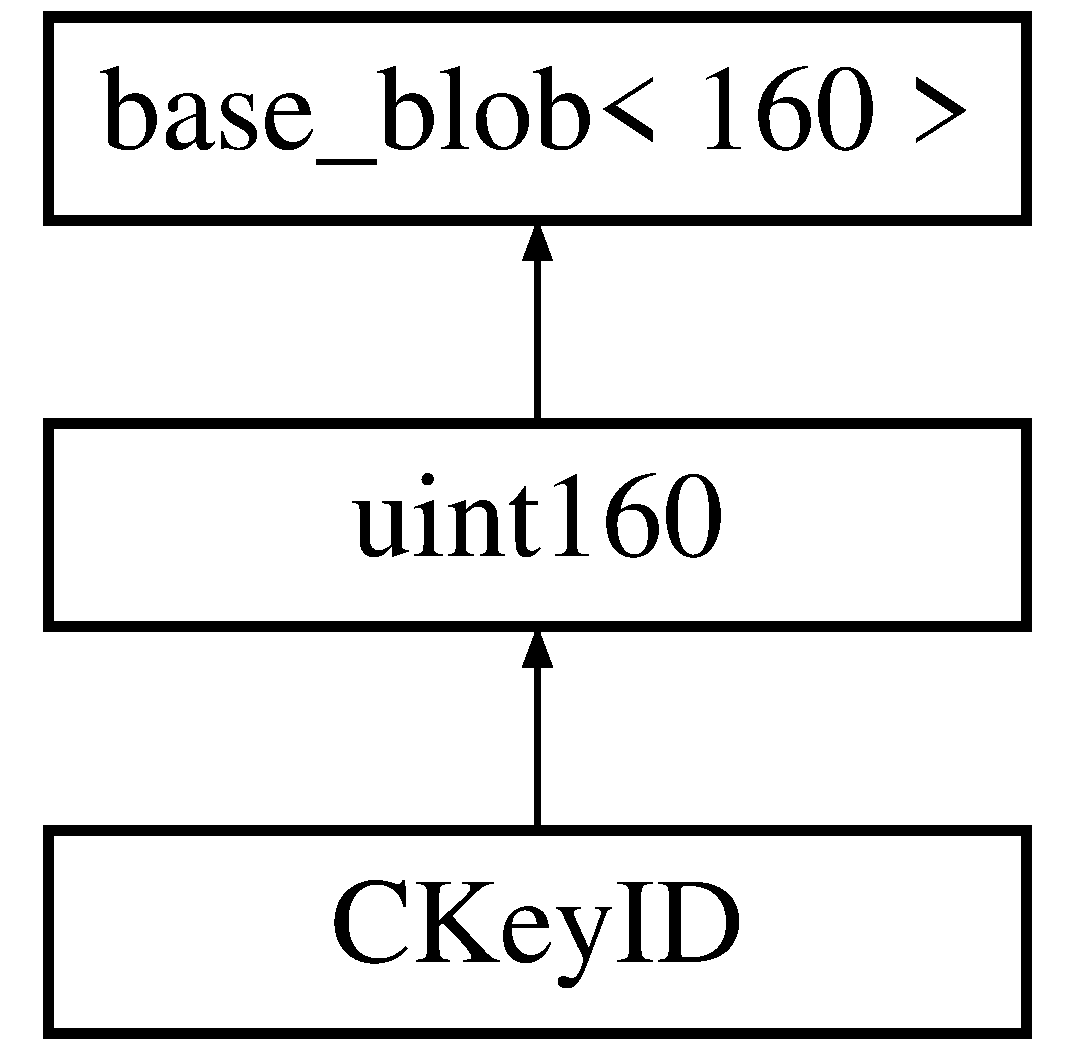
\includegraphics[height=3.000000cm]{class_c_key_i_d}
\end{center}
\end{figure}
\subsection*{Public Member Functions}
\begin{DoxyCompactItemize}
\item 
\hyperlink{class_c_key_i_d_a01dbd3c37820a2ffe89d106c6a7cf53d}{C\+Key\+I\+D} ()
\item 
\hyperlink{class_c_key_i_d_a695f373e11730318f9103100fa006a7e}{C\+Key\+I\+D} (const \hyperlink{classuint160}{uint160} \&in)
\end{DoxyCompactItemize}
\subsection*{Additional Inherited Members}


\subsection{Detailed Description}
secp256k1\+: const unsigned int P\+R\+I\+V\+A\+T\+E\+\_\+\+K\+E\+Y\+\_\+\+S\+I\+Z\+E = 279; const unsigned int P\+U\+B\+L\+I\+C\+\_\+\+K\+E\+Y\+\_\+\+S\+I\+Z\+E = 65; const unsigned int S\+I\+G\+N\+A\+T\+U\+R\+E\+\_\+\+S\+I\+Z\+E = 72;

see www.\+keylength.\+com script supports up to 75 for single byte push\+A reference to a \hyperlink{class_c_key}{C\+Key}\+: the Hash160 of its serialized public key 

\subsection{Constructor \& Destructor Documentation}
\hypertarget{class_c_key_i_d_a01dbd3c37820a2ffe89d106c6a7cf53d}{}\index{C\+Key\+I\+D@{C\+Key\+I\+D}!C\+Key\+I\+D@{C\+Key\+I\+D}}
\index{C\+Key\+I\+D@{C\+Key\+I\+D}!C\+Key\+I\+D@{C\+Key\+I\+D}}
\subsubsection[{C\+Key\+I\+D}]{\setlength{\rightskip}{0pt plus 5cm}C\+Key\+I\+D\+::\+C\+Key\+I\+D (
\begin{DoxyParamCaption}
{}
\end{DoxyParamCaption}
)\hspace{0.3cm}{\ttfamily [inline]}}\label{class_c_key_i_d_a01dbd3c37820a2ffe89d106c6a7cf53d}
\hypertarget{class_c_key_i_d_a695f373e11730318f9103100fa006a7e}{}\index{C\+Key\+I\+D@{C\+Key\+I\+D}!C\+Key\+I\+D@{C\+Key\+I\+D}}
\index{C\+Key\+I\+D@{C\+Key\+I\+D}!C\+Key\+I\+D@{C\+Key\+I\+D}}
\subsubsection[{C\+Key\+I\+D}]{\setlength{\rightskip}{0pt plus 5cm}C\+Key\+I\+D\+::\+C\+Key\+I\+D (
\begin{DoxyParamCaption}
\item[{const {\bf uint160} \&}]{in}
\end{DoxyParamCaption}
)\hspace{0.3cm}{\ttfamily [inline]}}\label{class_c_key_i_d_a695f373e11730318f9103100fa006a7e}


The documentation for this class was generated from the following file\+:\begin{DoxyCompactItemize}
\item 
C\+:/\+Users/\+Joe/\+Documents/\+School/\+C\+S\+C17\+A/bitcoin/src/\hyperlink{pubkey_8h}{pubkey.\+h}\end{DoxyCompactItemize}

\hypertarget{class_c_key_store}{}\section{C\+Key\+Store Class Reference}
\label{class_c_key_store}\index{C\+Key\+Store@{C\+Key\+Store}}


{\ttfamily \#include $<$keystore.\+h$>$}

Inheritance diagram for C\+Key\+Store\+:\begin{figure}[H]
\begin{center}
\leavevmode
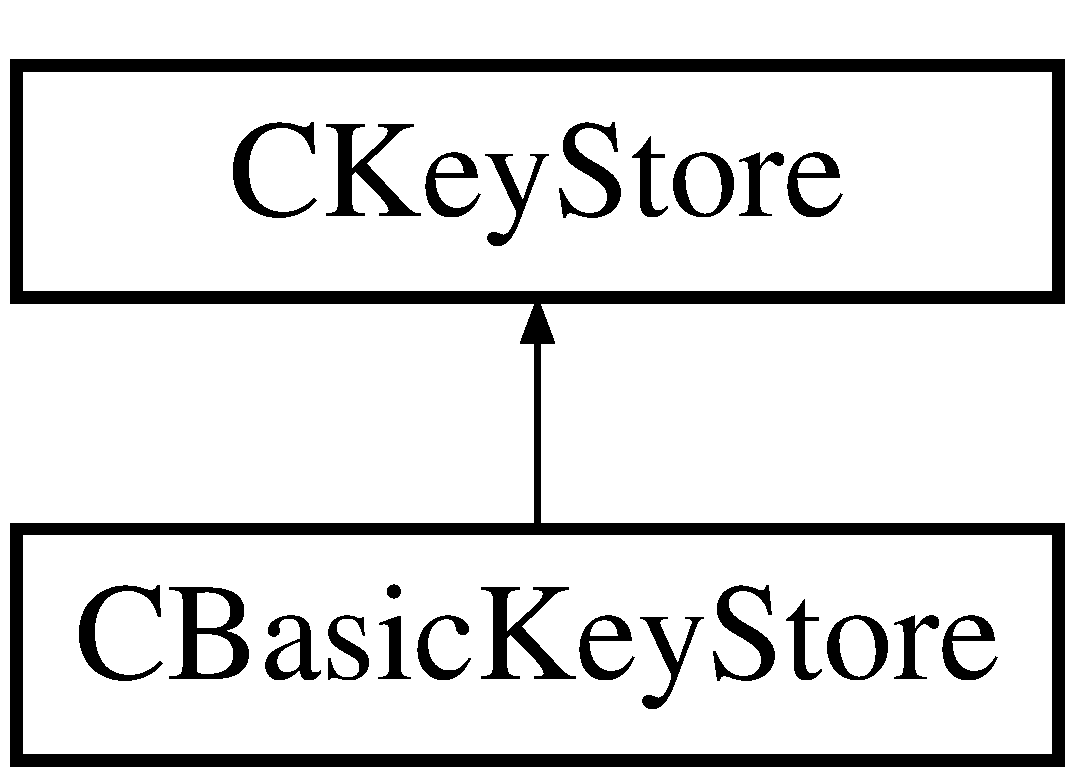
\includegraphics[height=2.000000cm]{class_c_key_store}
\end{center}
\end{figure}
\subsection*{Public Member Functions}
\begin{DoxyCompactItemize}
\item 
virtual \hyperlink{class_c_key_store_a9bfaef2bcd6effc467a96043f44044a0}{$\sim$\+C\+Key\+Store} ()
\item 
virtual bool \hyperlink{class_c_key_store_a1956e4f5860ded321d6f697047d8236a}{Add\+Key\+Pub\+Key} (const \hyperlink{class_c_key}{C\+Key} \&key, const \hyperlink{class_c_pub_key}{C\+Pub\+Key} \&pubkey)=0
\begin{DoxyCompactList}\small\item\em Add a key to the store. \end{DoxyCompactList}\item 
virtual bool \hyperlink{class_c_key_store_a0b4ca43724cfcc6e2ea70c0baa192750}{Add\+Key} (const \hyperlink{class_c_key}{C\+Key} \&key)
\item 
virtual bool \hyperlink{class_c_key_store_a9398451d4270fae27b29f686a9d43a65}{Have\+Key} (const \hyperlink{class_c_key_i_d}{C\+Key\+I\+D} \&address) const =0
\begin{DoxyCompactList}\small\item\em Check whether a key corresponding to a given address is present in the store. \end{DoxyCompactList}\item 
virtual bool \hyperlink{class_c_key_store_a2dffca468fef2e5da2e42a7c983d968a}{Get\+Key} (const \hyperlink{class_c_key_i_d}{C\+Key\+I\+D} \&address, \hyperlink{class_c_key}{C\+Key} \&key\+Out) const =0
\item 
virtual void \hyperlink{class_c_key_store_aca5044014720308f191113e7ba297d13}{Get\+Keys} (std\+::set$<$ \hyperlink{class_c_key_i_d}{C\+Key\+I\+D} $>$ \&set\+Address) const =0
\item 
virtual bool \hyperlink{class_c_key_store_aba866c1e71c129e7ac2d5d1e5223c8a5}{Get\+Pub\+Key} (const \hyperlink{class_c_key_i_d}{C\+Key\+I\+D} \&address, \hyperlink{class_c_pub_key}{C\+Pub\+Key} \&vch\+Pub\+Key\+Out) const 
\item 
virtual bool \hyperlink{class_c_key_store_a2fb2e02e8cdc364607efd5ebb14b8064}{Add\+C\+Script} (const C\+Script \&redeem\+Script)=0
\begin{DoxyCompactList}\small\item\em Support for B\+I\+P 0013 \+: see \href{https://github.com/bitcoin/bips/blob/master/bip-0013.mediawiki}{\tt https\+://github.\+com/bitcoin/bips/blob/master/bip-\/0013.\+mediawiki}. \end{DoxyCompactList}\item 
virtual bool \hyperlink{class_c_key_store_a51c9fc86b2c3fece10d86146231fa58d}{Have\+C\+Script} (const C\+Script\+I\+D \&hash) const =0
\item 
virtual bool \hyperlink{class_c_key_store_ae6bf4dbeb0705e199250e48aa5d34264}{Get\+C\+Script} (const C\+Script\+I\+D \&hash, C\+Script \&redeem\+Script\+Out) const =0
\item 
virtual bool \hyperlink{class_c_key_store_a12cd4eaa01bd4f4231c0bf68425a44af}{Add\+Watch\+Only} (const C\+Script \&dest)=0
\begin{DoxyCompactList}\small\item\em Support for Watch-\/only addresses. \end{DoxyCompactList}\item 
virtual bool \hyperlink{class_c_key_store_ad510747f28d129123a5200e4df8f7f61}{Remove\+Watch\+Only} (const C\+Script \&dest)=0
\item 
virtual bool \hyperlink{class_c_key_store_a15066cfd57feaffe0b9f4103c9311109}{Have\+Watch\+Only} (const C\+Script \&dest) const =0
\item 
virtual bool \hyperlink{class_c_key_store_a9169351f4acf62d299afb824174cbfa8}{Have\+Watch\+Only} () const =0
\end{DoxyCompactItemize}
\subsection*{Protected Attributes}
\begin{DoxyCompactItemize}
\item 
\hyperlink{sync_8h_a37a4692b2d517f2843655ca11af7668a}{C\+Critical\+Section} \hyperlink{class_c_key_store_a386524ff4a00959b81c195cb39fe307d}{cs\+\_\+\+Key\+Store}
\end{DoxyCompactItemize}


\subsection{Detailed Description}
A virtual base class for key stores 

\subsection{Constructor \& Destructor Documentation}
\hypertarget{class_c_key_store_a9bfaef2bcd6effc467a96043f44044a0}{}\index{C\+Key\+Store@{C\+Key\+Store}!````~C\+Key\+Store@{$\sim$\+C\+Key\+Store}}
\index{````~C\+Key\+Store@{$\sim$\+C\+Key\+Store}!C\+Key\+Store@{C\+Key\+Store}}
\subsubsection[{$\sim$\+C\+Key\+Store}]{\setlength{\rightskip}{0pt plus 5cm}virtual C\+Key\+Store\+::$\sim$\+C\+Key\+Store (
\begin{DoxyParamCaption}
{}
\end{DoxyParamCaption}
)\hspace{0.3cm}{\ttfamily [inline]}, {\ttfamily [virtual]}}\label{class_c_key_store_a9bfaef2bcd6effc467a96043f44044a0}


\subsection{Member Function Documentation}
\hypertarget{class_c_key_store_a2fb2e02e8cdc364607efd5ebb14b8064}{}\index{C\+Key\+Store@{C\+Key\+Store}!Add\+C\+Script@{Add\+C\+Script}}
\index{Add\+C\+Script@{Add\+C\+Script}!C\+Key\+Store@{C\+Key\+Store}}
\subsubsection[{Add\+C\+Script}]{\setlength{\rightskip}{0pt plus 5cm}virtual bool C\+Key\+Store\+::\+Add\+C\+Script (
\begin{DoxyParamCaption}
\item[{const C\+Script \&}]{redeem\+Script}
\end{DoxyParamCaption}
)\hspace{0.3cm}{\ttfamily [pure virtual]}}\label{class_c_key_store_a2fb2e02e8cdc364607efd5ebb14b8064}


Support for B\+I\+P 0013 \+: see \href{https://github.com/bitcoin/bips/blob/master/bip-0013.mediawiki}{\tt https\+://github.\+com/bitcoin/bips/blob/master/bip-\/0013.\+mediawiki}. 



Implemented in \hyperlink{class_c_basic_key_store_a56249ce3540398999cd397eeb662e836}{C\+Basic\+Key\+Store}.

\hypertarget{class_c_key_store_a0b4ca43724cfcc6e2ea70c0baa192750}{}\index{C\+Key\+Store@{C\+Key\+Store}!Add\+Key@{Add\+Key}}
\index{Add\+Key@{Add\+Key}!C\+Key\+Store@{C\+Key\+Store}}
\subsubsection[{Add\+Key}]{\setlength{\rightskip}{0pt plus 5cm}bool C\+Key\+Store\+::\+Add\+Key (
\begin{DoxyParamCaption}
\item[{const {\bf C\+Key} \&}]{key}
\end{DoxyParamCaption}
)\hspace{0.3cm}{\ttfamily [virtual]}}\label{class_c_key_store_a0b4ca43724cfcc6e2ea70c0baa192750}
\hypertarget{class_c_key_store_a1956e4f5860ded321d6f697047d8236a}{}\index{C\+Key\+Store@{C\+Key\+Store}!Add\+Key\+Pub\+Key@{Add\+Key\+Pub\+Key}}
\index{Add\+Key\+Pub\+Key@{Add\+Key\+Pub\+Key}!C\+Key\+Store@{C\+Key\+Store}}
\subsubsection[{Add\+Key\+Pub\+Key}]{\setlength{\rightskip}{0pt plus 5cm}virtual bool C\+Key\+Store\+::\+Add\+Key\+Pub\+Key (
\begin{DoxyParamCaption}
\item[{const {\bf C\+Key} \&}]{key, }
\item[{const {\bf C\+Pub\+Key} \&}]{pubkey}
\end{DoxyParamCaption}
)\hspace{0.3cm}{\ttfamily [pure virtual]}}\label{class_c_key_store_a1956e4f5860ded321d6f697047d8236a}


Add a key to the store. 



Implemented in \hyperlink{class_c_basic_key_store_acc2e33f319de88e88f86b0dc79bdcb65}{C\+Basic\+Key\+Store}.

\hypertarget{class_c_key_store_a12cd4eaa01bd4f4231c0bf68425a44af}{}\index{C\+Key\+Store@{C\+Key\+Store}!Add\+Watch\+Only@{Add\+Watch\+Only}}
\index{Add\+Watch\+Only@{Add\+Watch\+Only}!C\+Key\+Store@{C\+Key\+Store}}
\subsubsection[{Add\+Watch\+Only}]{\setlength{\rightskip}{0pt plus 5cm}virtual bool C\+Key\+Store\+::\+Add\+Watch\+Only (
\begin{DoxyParamCaption}
\item[{const C\+Script \&}]{dest}
\end{DoxyParamCaption}
)\hspace{0.3cm}{\ttfamily [pure virtual]}}\label{class_c_key_store_a12cd4eaa01bd4f4231c0bf68425a44af}


Support for Watch-\/only addresses. 



Implemented in \hyperlink{class_c_basic_key_store_a2417d0ae4e654c88cf47a1ba5f71b5a3}{C\+Basic\+Key\+Store}.

\hypertarget{class_c_key_store_ae6bf4dbeb0705e199250e48aa5d34264}{}\index{C\+Key\+Store@{C\+Key\+Store}!Get\+C\+Script@{Get\+C\+Script}}
\index{Get\+C\+Script@{Get\+C\+Script}!C\+Key\+Store@{C\+Key\+Store}}
\subsubsection[{Get\+C\+Script}]{\setlength{\rightskip}{0pt plus 5cm}virtual bool C\+Key\+Store\+::\+Get\+C\+Script (
\begin{DoxyParamCaption}
\item[{const C\+Script\+I\+D \&}]{hash, }
\item[{C\+Script \&}]{redeem\+Script\+Out}
\end{DoxyParamCaption}
) const\hspace{0.3cm}{\ttfamily [pure virtual]}}\label{class_c_key_store_ae6bf4dbeb0705e199250e48aa5d34264}


Implemented in \hyperlink{class_c_basic_key_store_aa7b10f974cfdc078f55fdb6adf8774a5}{C\+Basic\+Key\+Store}.

\hypertarget{class_c_key_store_a2dffca468fef2e5da2e42a7c983d968a}{}\index{C\+Key\+Store@{C\+Key\+Store}!Get\+Key@{Get\+Key}}
\index{Get\+Key@{Get\+Key}!C\+Key\+Store@{C\+Key\+Store}}
\subsubsection[{Get\+Key}]{\setlength{\rightskip}{0pt plus 5cm}virtual bool C\+Key\+Store\+::\+Get\+Key (
\begin{DoxyParamCaption}
\item[{const {\bf C\+Key\+I\+D} \&}]{address, }
\item[{{\bf C\+Key} \&}]{key\+Out}
\end{DoxyParamCaption}
) const\hspace{0.3cm}{\ttfamily [pure virtual]}}\label{class_c_key_store_a2dffca468fef2e5da2e42a7c983d968a}


Implemented in \hyperlink{class_c_basic_key_store_a3cf9b5d002a8af75e7f90ae7654a234f}{C\+Basic\+Key\+Store}.

\hypertarget{class_c_key_store_aca5044014720308f191113e7ba297d13}{}\index{C\+Key\+Store@{C\+Key\+Store}!Get\+Keys@{Get\+Keys}}
\index{Get\+Keys@{Get\+Keys}!C\+Key\+Store@{C\+Key\+Store}}
\subsubsection[{Get\+Keys}]{\setlength{\rightskip}{0pt plus 5cm}virtual void C\+Key\+Store\+::\+Get\+Keys (
\begin{DoxyParamCaption}
\item[{std\+::set$<$ {\bf C\+Key\+I\+D} $>$ \&}]{set\+Address}
\end{DoxyParamCaption}
) const\hspace{0.3cm}{\ttfamily [pure virtual]}}\label{class_c_key_store_aca5044014720308f191113e7ba297d13}


Implemented in \hyperlink{class_c_basic_key_store_a60f46db5eec334d41e5ad6e342ae2957}{C\+Basic\+Key\+Store}.

\hypertarget{class_c_key_store_aba866c1e71c129e7ac2d5d1e5223c8a5}{}\index{C\+Key\+Store@{C\+Key\+Store}!Get\+Pub\+Key@{Get\+Pub\+Key}}
\index{Get\+Pub\+Key@{Get\+Pub\+Key}!C\+Key\+Store@{C\+Key\+Store}}
\subsubsection[{Get\+Pub\+Key}]{\setlength{\rightskip}{0pt plus 5cm}bool C\+Key\+Store\+::\+Get\+Pub\+Key (
\begin{DoxyParamCaption}
\item[{const {\bf C\+Key\+I\+D} \&}]{address, }
\item[{{\bf C\+Pub\+Key} \&}]{vch\+Pub\+Key\+Out}
\end{DoxyParamCaption}
) const\hspace{0.3cm}{\ttfamily [virtual]}}\label{class_c_key_store_aba866c1e71c129e7ac2d5d1e5223c8a5}
\hypertarget{class_c_key_store_a51c9fc86b2c3fece10d86146231fa58d}{}\index{C\+Key\+Store@{C\+Key\+Store}!Have\+C\+Script@{Have\+C\+Script}}
\index{Have\+C\+Script@{Have\+C\+Script}!C\+Key\+Store@{C\+Key\+Store}}
\subsubsection[{Have\+C\+Script}]{\setlength{\rightskip}{0pt plus 5cm}virtual bool C\+Key\+Store\+::\+Have\+C\+Script (
\begin{DoxyParamCaption}
\item[{const C\+Script\+I\+D \&}]{hash}
\end{DoxyParamCaption}
) const\hspace{0.3cm}{\ttfamily [pure virtual]}}\label{class_c_key_store_a51c9fc86b2c3fece10d86146231fa58d}


Implemented in \hyperlink{class_c_basic_key_store_a2e21398364927d920b15d3e10171cd97}{C\+Basic\+Key\+Store}.

\hypertarget{class_c_key_store_a9398451d4270fae27b29f686a9d43a65}{}\index{C\+Key\+Store@{C\+Key\+Store}!Have\+Key@{Have\+Key}}
\index{Have\+Key@{Have\+Key}!C\+Key\+Store@{C\+Key\+Store}}
\subsubsection[{Have\+Key}]{\setlength{\rightskip}{0pt plus 5cm}virtual bool C\+Key\+Store\+::\+Have\+Key (
\begin{DoxyParamCaption}
\item[{const {\bf C\+Key\+I\+D} \&}]{address}
\end{DoxyParamCaption}
) const\hspace{0.3cm}{\ttfamily [pure virtual]}}\label{class_c_key_store_a9398451d4270fae27b29f686a9d43a65}


Check whether a key corresponding to a given address is present in the store. 



Implemented in \hyperlink{class_c_basic_key_store_a29a60832d549913b1fa8be77b95205a5}{C\+Basic\+Key\+Store}.

\hypertarget{class_c_key_store_a15066cfd57feaffe0b9f4103c9311109}{}\index{C\+Key\+Store@{C\+Key\+Store}!Have\+Watch\+Only@{Have\+Watch\+Only}}
\index{Have\+Watch\+Only@{Have\+Watch\+Only}!C\+Key\+Store@{C\+Key\+Store}}
\subsubsection[{Have\+Watch\+Only}]{\setlength{\rightskip}{0pt plus 5cm}virtual bool C\+Key\+Store\+::\+Have\+Watch\+Only (
\begin{DoxyParamCaption}
\item[{const C\+Script \&}]{dest}
\end{DoxyParamCaption}
) const\hspace{0.3cm}{\ttfamily [pure virtual]}}\label{class_c_key_store_a15066cfd57feaffe0b9f4103c9311109}


Implemented in \hyperlink{class_c_basic_key_store_a51d4c7e95cb782d749939d01612926f7}{C\+Basic\+Key\+Store}.

\hypertarget{class_c_key_store_a9169351f4acf62d299afb824174cbfa8}{}\index{C\+Key\+Store@{C\+Key\+Store}!Have\+Watch\+Only@{Have\+Watch\+Only}}
\index{Have\+Watch\+Only@{Have\+Watch\+Only}!C\+Key\+Store@{C\+Key\+Store}}
\subsubsection[{Have\+Watch\+Only}]{\setlength{\rightskip}{0pt plus 5cm}virtual bool C\+Key\+Store\+::\+Have\+Watch\+Only (
\begin{DoxyParamCaption}
{}
\end{DoxyParamCaption}
) const\hspace{0.3cm}{\ttfamily [pure virtual]}}\label{class_c_key_store_a9169351f4acf62d299afb824174cbfa8}


Implemented in \hyperlink{class_c_basic_key_store_a3d89af8d9e9e0bb4eb90f331a638ff6d}{C\+Basic\+Key\+Store}.

\hypertarget{class_c_key_store_ad510747f28d129123a5200e4df8f7f61}{}\index{C\+Key\+Store@{C\+Key\+Store}!Remove\+Watch\+Only@{Remove\+Watch\+Only}}
\index{Remove\+Watch\+Only@{Remove\+Watch\+Only}!C\+Key\+Store@{C\+Key\+Store}}
\subsubsection[{Remove\+Watch\+Only}]{\setlength{\rightskip}{0pt plus 5cm}virtual bool C\+Key\+Store\+::\+Remove\+Watch\+Only (
\begin{DoxyParamCaption}
\item[{const C\+Script \&}]{dest}
\end{DoxyParamCaption}
)\hspace{0.3cm}{\ttfamily [pure virtual]}}\label{class_c_key_store_ad510747f28d129123a5200e4df8f7f61}


Implemented in \hyperlink{class_c_basic_key_store_a20c0eccf943d6d16e24c6e2fb63fb527}{C\+Basic\+Key\+Store}.



\subsection{Member Data Documentation}
\hypertarget{class_c_key_store_a386524ff4a00959b81c195cb39fe307d}{}\index{C\+Key\+Store@{C\+Key\+Store}!cs\+\_\+\+Key\+Store@{cs\+\_\+\+Key\+Store}}
\index{cs\+\_\+\+Key\+Store@{cs\+\_\+\+Key\+Store}!C\+Key\+Store@{C\+Key\+Store}}
\subsubsection[{cs\+\_\+\+Key\+Store}]{\setlength{\rightskip}{0pt plus 5cm}{\bf C\+Critical\+Section} C\+Key\+Store\+::cs\+\_\+\+Key\+Store\hspace{0.3cm}{\ttfamily [mutable]}, {\ttfamily [protected]}}\label{class_c_key_store_a386524ff4a00959b81c195cb39fe307d}


The documentation for this class was generated from the following files\+:\begin{DoxyCompactItemize}
\item 
C\+:/\+Users/\+Joe/\+Documents/\+School/\+C\+S\+C17\+A/bitcoin/src/\hyperlink{keystore_8h}{keystore.\+h}\item 
C\+:/\+Users/\+Joe/\+Documents/\+School/\+C\+S\+C17\+A/bitcoin/src/\hyperlink{keystore_8cpp}{keystore.\+cpp}\end{DoxyCompactItemize}

\hypertarget{class_c_level_d_b_batch}{}\section{C\+Level\+D\+B\+Batch Class Reference}
\label{class_c_level_d_b_batch}\index{C\+Level\+D\+B\+Batch@{C\+Level\+D\+B\+Batch}}


{\ttfamily \#include $<$leveldbwrapper.\+h$>$}

\subsection*{Public Member Functions}
\begin{DoxyCompactItemize}
\item 
{\footnotesize template$<$typename K , typename V $>$ }\\void \hyperlink{class_c_level_d_b_batch_ab459da1abafa27e834de9a4cc25b6f2d}{Write} (const K \&key, const V \&value)
\item 
{\footnotesize template$<$typename K $>$ }\\void \hyperlink{class_c_level_d_b_batch_a22bf093d560b4ce3333e8f4a947faa7f}{Erase} (const K \&key)
\end{DoxyCompactItemize}
\subsection*{Friends}
\begin{DoxyCompactItemize}
\item 
class \hyperlink{class_c_level_d_b_batch_acbe5e6be88c5bccb0ec229ebc91dde82}{C\+Level\+D\+B\+Wrapper}
\end{DoxyCompactItemize}


\subsection{Detailed Description}
Batch of changes queued to be written to a \hyperlink{class_c_level_d_b_wrapper}{C\+Level\+D\+B\+Wrapper} 

\subsection{Member Function Documentation}
\hypertarget{class_c_level_d_b_batch_a22bf093d560b4ce3333e8f4a947faa7f}{}\index{C\+Level\+D\+B\+Batch@{C\+Level\+D\+B\+Batch}!Erase@{Erase}}
\index{Erase@{Erase}!C\+Level\+D\+B\+Batch@{C\+Level\+D\+B\+Batch}}
\subsubsection[{Erase}]{\setlength{\rightskip}{0pt plus 5cm}template$<$typename K $>$ void C\+Level\+D\+B\+Batch\+::\+Erase (
\begin{DoxyParamCaption}
\item[{const K \&}]{key}
\end{DoxyParamCaption}
)\hspace{0.3cm}{\ttfamily [inline]}}\label{class_c_level_d_b_batch_a22bf093d560b4ce3333e8f4a947faa7f}
\hypertarget{class_c_level_d_b_batch_ab459da1abafa27e834de9a4cc25b6f2d}{}\index{C\+Level\+D\+B\+Batch@{C\+Level\+D\+B\+Batch}!Write@{Write}}
\index{Write@{Write}!C\+Level\+D\+B\+Batch@{C\+Level\+D\+B\+Batch}}
\subsubsection[{Write}]{\setlength{\rightskip}{0pt plus 5cm}template$<$typename K , typename V $>$ void C\+Level\+D\+B\+Batch\+::\+Write (
\begin{DoxyParamCaption}
\item[{const K \&}]{key, }
\item[{const V \&}]{value}
\end{DoxyParamCaption}
)\hspace{0.3cm}{\ttfamily [inline]}}\label{class_c_level_d_b_batch_ab459da1abafa27e834de9a4cc25b6f2d}


\subsection{Friends And Related Function Documentation}
\hypertarget{class_c_level_d_b_batch_acbe5e6be88c5bccb0ec229ebc91dde82}{}\index{C\+Level\+D\+B\+Batch@{C\+Level\+D\+B\+Batch}!C\+Level\+D\+B\+Wrapper@{C\+Level\+D\+B\+Wrapper}}
\index{C\+Level\+D\+B\+Wrapper@{C\+Level\+D\+B\+Wrapper}!C\+Level\+D\+B\+Batch@{C\+Level\+D\+B\+Batch}}
\subsubsection[{C\+Level\+D\+B\+Wrapper}]{\setlength{\rightskip}{0pt plus 5cm}friend class {\bf C\+Level\+D\+B\+Wrapper}\hspace{0.3cm}{\ttfamily [friend]}}\label{class_c_level_d_b_batch_acbe5e6be88c5bccb0ec229ebc91dde82}


The documentation for this class was generated from the following file\+:\begin{DoxyCompactItemize}
\item 
C\+:/\+Users/\+Joe/\+Documents/\+School/\+C\+S\+C17\+A/bitcoin/src/\hyperlink{leveldbwrapper_8h}{leveldbwrapper.\+h}\end{DoxyCompactItemize}

\hypertarget{class_c_level_d_b_wrapper}{}\section{C\+Level\+D\+B\+Wrapper Class Reference}
\label{class_c_level_d_b_wrapper}\index{C\+Level\+D\+B\+Wrapper@{C\+Level\+D\+B\+Wrapper}}


{\ttfamily \#include $<$leveldbwrapper.\+h$>$}

Inheritance diagram for C\+Level\+D\+B\+Wrapper\+:\begin{figure}[H]
\begin{center}
\leavevmode
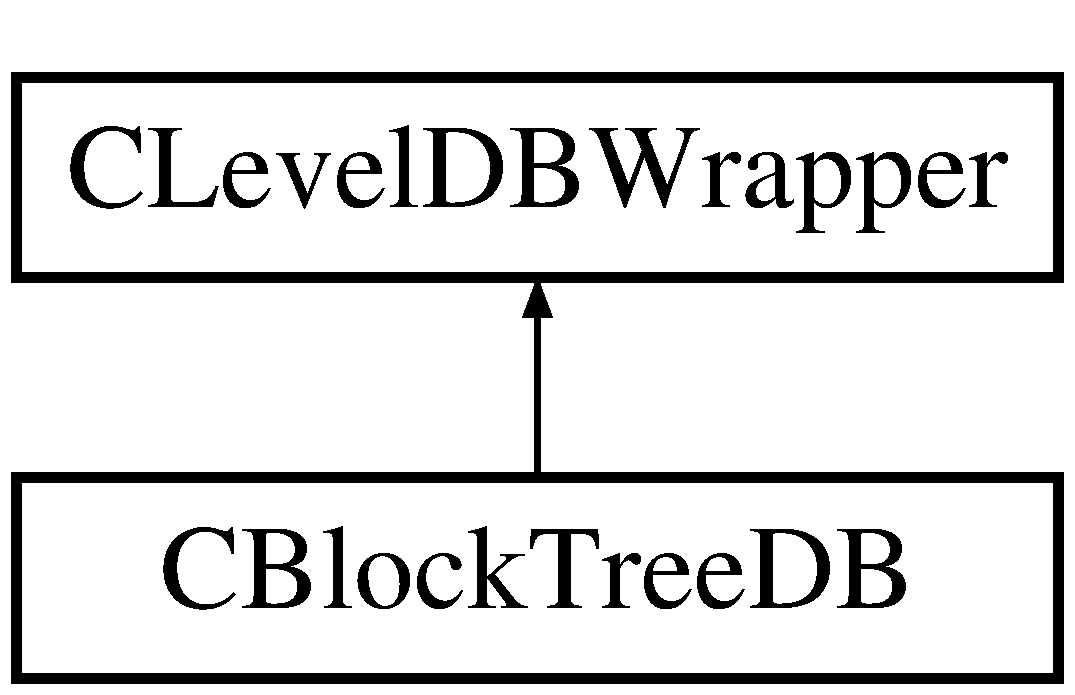
\includegraphics[height=2.000000cm]{class_c_level_d_b_wrapper}
\end{center}
\end{figure}
\subsection*{Public Member Functions}
\begin{DoxyCompactItemize}
\item 
\hyperlink{class_c_level_d_b_wrapper_ae796b1190c072df6275e0ada4d187943}{C\+Level\+D\+B\+Wrapper} (const boost\+::filesystem\+::path \&path, size\+\_\+t n\+Cache\+Size, bool f\+Memory=false, bool f\+Wipe=false)
\item 
\hyperlink{class_c_level_d_b_wrapper_a7ffe7edeadfcf521d32509216e95403b}{$\sim$\+C\+Level\+D\+B\+Wrapper} ()
\item 
{\footnotesize template$<$typename K , typename V $>$ }\\bool \hyperlink{class_c_level_d_b_wrapper_aa3b816ae43c930b4bf1f85461bff4b5b}{Read} (const K \&key, V \&value) const   throw (leveldb\+\_\+error)
\item 
{\footnotesize template$<$typename K , typename V $>$ }\\bool \hyperlink{class_c_level_d_b_wrapper_a740caa1aefbafc888838ea7f70dc31f4}{Write} (const K \&key, const V \&value, bool f\+Sync=false)  throw (leveldb\+\_\+error)
\item 
{\footnotesize template$<$typename K $>$ }\\bool \hyperlink{class_c_level_d_b_wrapper_a9c9d2e1c06c45c5d6883f33136f6718b}{Exists} (const K \&key) const   throw (leveldb\+\_\+error)
\item 
{\footnotesize template$<$typename K $>$ }\\bool \hyperlink{class_c_level_d_b_wrapper_a9f67e2880ba191fdc9439ba34e315d72}{Erase} (const K \&key, bool f\+Sync=false)  throw (leveldb\+\_\+error)
\item 
bool \hyperlink{class_c_level_d_b_wrapper_a820484c9e427f9e3400396e750acf4b8}{Write\+Batch} (\hyperlink{class_c_level_d_b_batch}{C\+Level\+D\+B\+Batch} \&batch, bool f\+Sync=false)  throw (leveldb\+\_\+error)
\item 
bool \hyperlink{class_c_level_d_b_wrapper_a639fbfd6652941a1ab570c202197a32a}{Flush} ()
\item 
bool \hyperlink{class_c_level_d_b_wrapper_abd05e914893cd610e8444871f829d8c9}{Sync} ()  throw (leveldb\+\_\+error)
\item 
leveldb\+::\+Iterator $\ast$ \hyperlink{class_c_level_d_b_wrapper_a5f43d01a8a6b26464b875d190e002d74}{New\+Iterator} ()
\end{DoxyCompactItemize}


\subsection{Constructor \& Destructor Documentation}
\hypertarget{class_c_level_d_b_wrapper_ae796b1190c072df6275e0ada4d187943}{}\index{C\+Level\+D\+B\+Wrapper@{C\+Level\+D\+B\+Wrapper}!C\+Level\+D\+B\+Wrapper@{C\+Level\+D\+B\+Wrapper}}
\index{C\+Level\+D\+B\+Wrapper@{C\+Level\+D\+B\+Wrapper}!C\+Level\+D\+B\+Wrapper@{C\+Level\+D\+B\+Wrapper}}
\subsubsection[{C\+Level\+D\+B\+Wrapper}]{\setlength{\rightskip}{0pt plus 5cm}C\+Level\+D\+B\+Wrapper\+::\+C\+Level\+D\+B\+Wrapper (
\begin{DoxyParamCaption}
\item[{const boost\+::filesystem\+::path \&}]{path, }
\item[{size\+\_\+t}]{n\+Cache\+Size, }
\item[{bool}]{f\+Memory = {\ttfamily false}, }
\item[{bool}]{f\+Wipe = {\ttfamily false}}
\end{DoxyParamCaption}
)}\label{class_c_level_d_b_wrapper_ae796b1190c072df6275e0ada4d187943}
\hypertarget{class_c_level_d_b_wrapper_a7ffe7edeadfcf521d32509216e95403b}{}\index{C\+Level\+D\+B\+Wrapper@{C\+Level\+D\+B\+Wrapper}!````~C\+Level\+D\+B\+Wrapper@{$\sim$\+C\+Level\+D\+B\+Wrapper}}
\index{````~C\+Level\+D\+B\+Wrapper@{$\sim$\+C\+Level\+D\+B\+Wrapper}!C\+Level\+D\+B\+Wrapper@{C\+Level\+D\+B\+Wrapper}}
\subsubsection[{$\sim$\+C\+Level\+D\+B\+Wrapper}]{\setlength{\rightskip}{0pt plus 5cm}C\+Level\+D\+B\+Wrapper\+::$\sim$\+C\+Level\+D\+B\+Wrapper (
\begin{DoxyParamCaption}
{}
\end{DoxyParamCaption}
)}\label{class_c_level_d_b_wrapper_a7ffe7edeadfcf521d32509216e95403b}


\subsection{Member Function Documentation}
\hypertarget{class_c_level_d_b_wrapper_a9f67e2880ba191fdc9439ba34e315d72}{}\index{C\+Level\+D\+B\+Wrapper@{C\+Level\+D\+B\+Wrapper}!Erase@{Erase}}
\index{Erase@{Erase}!C\+Level\+D\+B\+Wrapper@{C\+Level\+D\+B\+Wrapper}}
\subsubsection[{Erase}]{\setlength{\rightskip}{0pt plus 5cm}template$<$typename K $>$ bool C\+Level\+D\+B\+Wrapper\+::\+Erase (
\begin{DoxyParamCaption}
\item[{const K \&}]{key, }
\item[{bool}]{f\+Sync = {\ttfamily false}}
\end{DoxyParamCaption}
) throw  {\bf leveldb\+\_\+error}) \hspace{0.3cm}{\ttfamily [inline]}}\label{class_c_level_d_b_wrapper_a9f67e2880ba191fdc9439ba34e315d72}
\hypertarget{class_c_level_d_b_wrapper_a9c9d2e1c06c45c5d6883f33136f6718b}{}\index{C\+Level\+D\+B\+Wrapper@{C\+Level\+D\+B\+Wrapper}!Exists@{Exists}}
\index{Exists@{Exists}!C\+Level\+D\+B\+Wrapper@{C\+Level\+D\+B\+Wrapper}}
\subsubsection[{Exists}]{\setlength{\rightskip}{0pt plus 5cm}template$<$typename K $>$ bool C\+Level\+D\+B\+Wrapper\+::\+Exists (
\begin{DoxyParamCaption}
\item[{const K \&}]{key}
\end{DoxyParamCaption}
) const throw  {\bf leveldb\+\_\+error}) \hspace{0.3cm}{\ttfamily [inline]}}\label{class_c_level_d_b_wrapper_a9c9d2e1c06c45c5d6883f33136f6718b}
\hypertarget{class_c_level_d_b_wrapper_a639fbfd6652941a1ab570c202197a32a}{}\index{C\+Level\+D\+B\+Wrapper@{C\+Level\+D\+B\+Wrapper}!Flush@{Flush}}
\index{Flush@{Flush}!C\+Level\+D\+B\+Wrapper@{C\+Level\+D\+B\+Wrapper}}
\subsubsection[{Flush}]{\setlength{\rightskip}{0pt plus 5cm}bool C\+Level\+D\+B\+Wrapper\+::\+Flush (
\begin{DoxyParamCaption}
{}
\end{DoxyParamCaption}
)\hspace{0.3cm}{\ttfamily [inline]}}\label{class_c_level_d_b_wrapper_a639fbfd6652941a1ab570c202197a32a}
\hypertarget{class_c_level_d_b_wrapper_a5f43d01a8a6b26464b875d190e002d74}{}\index{C\+Level\+D\+B\+Wrapper@{C\+Level\+D\+B\+Wrapper}!New\+Iterator@{New\+Iterator}}
\index{New\+Iterator@{New\+Iterator}!C\+Level\+D\+B\+Wrapper@{C\+Level\+D\+B\+Wrapper}}
\subsubsection[{New\+Iterator}]{\setlength{\rightskip}{0pt plus 5cm}leveldb\+::\+Iterator$\ast$ C\+Level\+D\+B\+Wrapper\+::\+New\+Iterator (
\begin{DoxyParamCaption}
{}
\end{DoxyParamCaption}
)\hspace{0.3cm}{\ttfamily [inline]}}\label{class_c_level_d_b_wrapper_a5f43d01a8a6b26464b875d190e002d74}
\hypertarget{class_c_level_d_b_wrapper_aa3b816ae43c930b4bf1f85461bff4b5b}{}\index{C\+Level\+D\+B\+Wrapper@{C\+Level\+D\+B\+Wrapper}!Read@{Read}}
\index{Read@{Read}!C\+Level\+D\+B\+Wrapper@{C\+Level\+D\+B\+Wrapper}}
\subsubsection[{Read}]{\setlength{\rightskip}{0pt plus 5cm}template$<$typename K , typename V $>$ bool C\+Level\+D\+B\+Wrapper\+::\+Read (
\begin{DoxyParamCaption}
\item[{const K \&}]{key, }
\item[{V \&}]{value}
\end{DoxyParamCaption}
) const throw  {\bf leveldb\+\_\+error}) \hspace{0.3cm}{\ttfamily [inline]}}\label{class_c_level_d_b_wrapper_aa3b816ae43c930b4bf1f85461bff4b5b}
\hypertarget{class_c_level_d_b_wrapper_abd05e914893cd610e8444871f829d8c9}{}\index{C\+Level\+D\+B\+Wrapper@{C\+Level\+D\+B\+Wrapper}!Sync@{Sync}}
\index{Sync@{Sync}!C\+Level\+D\+B\+Wrapper@{C\+Level\+D\+B\+Wrapper}}
\subsubsection[{Sync}]{\setlength{\rightskip}{0pt plus 5cm}bool C\+Level\+D\+B\+Wrapper\+::\+Sync (
\begin{DoxyParamCaption}
{}
\end{DoxyParamCaption}
) throw  {\bf leveldb\+\_\+error}) \hspace{0.3cm}{\ttfamily [inline]}}\label{class_c_level_d_b_wrapper_abd05e914893cd610e8444871f829d8c9}
\hypertarget{class_c_level_d_b_wrapper_a740caa1aefbafc888838ea7f70dc31f4}{}\index{C\+Level\+D\+B\+Wrapper@{C\+Level\+D\+B\+Wrapper}!Write@{Write}}
\index{Write@{Write}!C\+Level\+D\+B\+Wrapper@{C\+Level\+D\+B\+Wrapper}}
\subsubsection[{Write}]{\setlength{\rightskip}{0pt plus 5cm}template$<$typename K , typename V $>$ bool C\+Level\+D\+B\+Wrapper\+::\+Write (
\begin{DoxyParamCaption}
\item[{const K \&}]{key, }
\item[{const V \&}]{value, }
\item[{bool}]{f\+Sync = {\ttfamily false}}
\end{DoxyParamCaption}
) throw  {\bf leveldb\+\_\+error}) \hspace{0.3cm}{\ttfamily [inline]}}\label{class_c_level_d_b_wrapper_a740caa1aefbafc888838ea7f70dc31f4}
\hypertarget{class_c_level_d_b_wrapper_a820484c9e427f9e3400396e750acf4b8}{}\index{C\+Level\+D\+B\+Wrapper@{C\+Level\+D\+B\+Wrapper}!Write\+Batch@{Write\+Batch}}
\index{Write\+Batch@{Write\+Batch}!C\+Level\+D\+B\+Wrapper@{C\+Level\+D\+B\+Wrapper}}
\subsubsection[{Write\+Batch}]{\setlength{\rightskip}{0pt plus 5cm}bool C\+Level\+D\+B\+Wrapper\+::\+Write\+Batch (
\begin{DoxyParamCaption}
\item[{{\bf C\+Level\+D\+B\+Batch} \&}]{batch, }
\item[{bool}]{f\+Sync = {\ttfamily false}}
\end{DoxyParamCaption}
) throw  {\bf leveldb\+\_\+error}) }\label{class_c_level_d_b_wrapper_a820484c9e427f9e3400396e750acf4b8}


The documentation for this class was generated from the following files\+:\begin{DoxyCompactItemize}
\item 
C\+:/\+Users/\+Joe/\+Documents/\+School/\+C\+S\+C17\+A/bitcoin/src/\hyperlink{leveldbwrapper_8h}{leveldbwrapper.\+h}\item 
C\+:/\+Users/\+Joe/\+Documents/\+School/\+C\+S\+C17\+A/bitcoin/src/\hyperlink{leveldbwrapper_8cpp}{leveldbwrapper.\+cpp}\end{DoxyCompactItemize}

\hypertarget{class_c_main_cleanup}{}\section{C\+Main\+Cleanup Class Reference}
\label{class_c_main_cleanup}\index{C\+Main\+Cleanup@{C\+Main\+Cleanup}}
\subsection*{Public Member Functions}
\begin{DoxyCompactItemize}
\item 
\hyperlink{class_c_main_cleanup_a2cc109dba5ab39dff1e8271a84577095}{C\+Main\+Cleanup} ()
\item 
\hyperlink{class_c_main_cleanup_a4459afc736eabd6e8c4aaa75f31e33f2}{$\sim$\+C\+Main\+Cleanup} ()
\end{DoxyCompactItemize}


\subsection{Constructor \& Destructor Documentation}
\hypertarget{class_c_main_cleanup_a2cc109dba5ab39dff1e8271a84577095}{}\index{C\+Main\+Cleanup@{C\+Main\+Cleanup}!C\+Main\+Cleanup@{C\+Main\+Cleanup}}
\index{C\+Main\+Cleanup@{C\+Main\+Cleanup}!C\+Main\+Cleanup@{C\+Main\+Cleanup}}
\subsubsection[{C\+Main\+Cleanup}]{\setlength{\rightskip}{0pt plus 5cm}C\+Main\+Cleanup\+::\+C\+Main\+Cleanup (
\begin{DoxyParamCaption}
{}
\end{DoxyParamCaption}
)\hspace{0.3cm}{\ttfamily [inline]}}\label{class_c_main_cleanup_a2cc109dba5ab39dff1e8271a84577095}
\hypertarget{class_c_main_cleanup_a4459afc736eabd6e8c4aaa75f31e33f2}{}\index{C\+Main\+Cleanup@{C\+Main\+Cleanup}!````~C\+Main\+Cleanup@{$\sim$\+C\+Main\+Cleanup}}
\index{````~C\+Main\+Cleanup@{$\sim$\+C\+Main\+Cleanup}!C\+Main\+Cleanup@{C\+Main\+Cleanup}}
\subsubsection[{$\sim$\+C\+Main\+Cleanup}]{\setlength{\rightskip}{0pt plus 5cm}C\+Main\+Cleanup\+::$\sim$\+C\+Main\+Cleanup (
\begin{DoxyParamCaption}
{}
\end{DoxyParamCaption}
)\hspace{0.3cm}{\ttfamily [inline]}}\label{class_c_main_cleanup_a4459afc736eabd6e8c4aaa75f31e33f2}


The documentation for this class was generated from the following file\+:\begin{DoxyCompactItemize}
\item 
C\+:/\+Users/\+Joe/\+Documents/\+School/\+C\+S\+C17\+A/bitcoin/src/\hyperlink{main_8cpp}{main.\+cpp}\end{DoxyCompactItemize}

\hypertarget{class_c_main_params}{}\section{C\+Main\+Params Class Reference}
\label{class_c_main_params}\index{C\+Main\+Params@{C\+Main\+Params}}
Inheritance diagram for C\+Main\+Params\+:\begin{figure}[H]
\begin{center}
\leavevmode
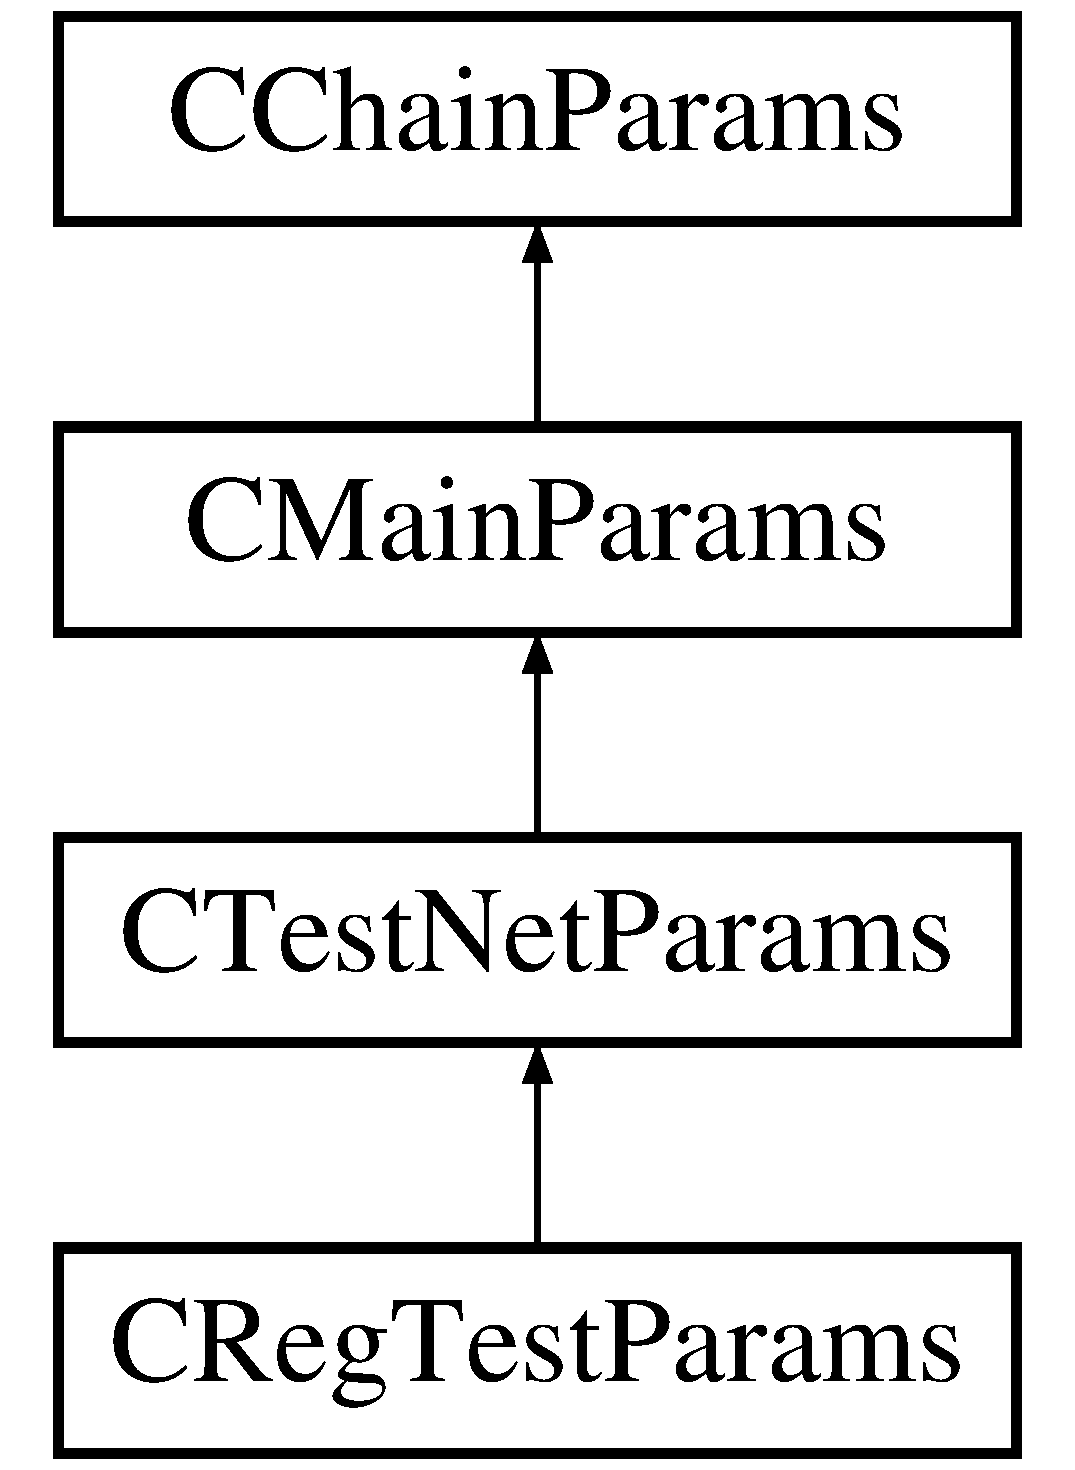
\includegraphics[height=4.000000cm]{class_c_main_params}
\end{center}
\end{figure}
\subsection*{Public Member Functions}
\begin{DoxyCompactItemize}
\item 
\hyperlink{class_c_main_params_ab7dfebf3c4dd5cc0ebdfabe1111056d6}{C\+Main\+Params} ()
\item 
const \hyperlink{struct_checkpoints_1_1_c_checkpoint_data}{Checkpoints\+::\+C\+Checkpoint\+Data} \& \hyperlink{class_c_main_params_abfaf5edda329d8b2ff23c0108cb8c16e}{Checkpoints} () const 
\end{DoxyCompactItemize}
\subsection*{Additional Inherited Members}


\subsection{Constructor \& Destructor Documentation}
\hypertarget{class_c_main_params_ab7dfebf3c4dd5cc0ebdfabe1111056d6}{}\index{C\+Main\+Params@{C\+Main\+Params}!C\+Main\+Params@{C\+Main\+Params}}
\index{C\+Main\+Params@{C\+Main\+Params}!C\+Main\+Params@{C\+Main\+Params}}
\subsubsection[{C\+Main\+Params}]{\setlength{\rightskip}{0pt plus 5cm}C\+Main\+Params\+::\+C\+Main\+Params (
\begin{DoxyParamCaption}
{}
\end{DoxyParamCaption}
)\hspace{0.3cm}{\ttfamily [inline]}}\label{class_c_main_params_ab7dfebf3c4dd5cc0ebdfabe1111056d6}
The message start string is designed to be unlikely to occur in normal data. The characters are rarely used upper A\+S\+C\+I\+I, not valid as U\+T\+F-\/8, and produce a large 4-\/byte int at any alignment.

Build the genesis block. Note that the output of the genesis coinbase cannot be spent as it did not originally exist in the database.

C\+Block(hash=000000000019d6, ver=1, hash\+Prev\+Block=00000000000000, hash\+Merkle\+Root=4a5e1e, n\+Time=1231006505, n\+Bits=1d00ffff, n\+Nonce=2083236893, vtx=1) C\+Transaction(hash=4a5e1e, ver=1, vin.\+size=1, vout.\+size=1, n\+Lock\+Time=0) C\+Tx\+In(C\+Out\+Point(000000, -\/1), coinbase 04ffff001d0104455468652054696d65732030332f4a616e2f32303039204368616e63656c6c6f72206f6e206272696e6b206f66207365636f6e64206261696c6f757420666f722062616e6b73) C\+Tx\+Out(n\+Value=50.\+00000000, script\+Pub\+Key=0x5\+F1\+D\+F16\+B2\+B704\+C8\+A578\+D0\+B) v\+Merkle\+Tree\+: 4a5e1e

\subsection{Member Function Documentation}
\hypertarget{class_c_main_params_abfaf5edda329d8b2ff23c0108cb8c16e}{}\index{C\+Main\+Params@{C\+Main\+Params}!Checkpoints@{Checkpoints}}
\index{Checkpoints@{Checkpoints}!C\+Main\+Params@{C\+Main\+Params}}
\subsubsection[{Checkpoints}]{\setlength{\rightskip}{0pt plus 5cm}const {\bf Checkpoints\+::\+C\+Checkpoint\+Data}\& C\+Main\+Params\+::\+Checkpoints (
\begin{DoxyParamCaption}
{}
\end{DoxyParamCaption}
) const\hspace{0.3cm}{\ttfamily [inline]}, {\ttfamily [virtual]}}\label{class_c_main_params_abfaf5edda329d8b2ff23c0108cb8c16e}


Implements \hyperlink{class_c_chain_params_aba314e7660492aee43812344fa796d6c}{C\+Chain\+Params}.



Reimplemented in \hyperlink{class_c_reg_test_params_ab748b010a203dbdf6e5f77eb8b6f7cb0}{C\+Reg\+Test\+Params}, and \hyperlink{class_c_test_net_params_a1a8828912574c509825ccc5cc0e0a9be}{C\+Test\+Net\+Params}.



The documentation for this class was generated from the following file\+:\begin{DoxyCompactItemize}
\item 
C\+:/\+Users/\+Joe/\+Documents/\+School/\+C\+S\+C17\+A/bitcoin/src/\hyperlink{chainparams_8cpp}{chainparams.\+cpp}\end{DoxyCompactItemize}

\hypertarget{struct_c_main_signals}{}\section{C\+Main\+Signals Struct Reference}
\label{struct_c_main_signals}\index{C\+Main\+Signals@{C\+Main\+Signals}}


{\ttfamily \#include $<$validationinterface.\+h$>$}

\subsection*{Public Attributes}
\begin{DoxyCompactItemize}
\item 
boost\+::signals2\+::signal$<$ void(const C\+Transaction \&, const C\+Block $\ast$)$>$ \hyperlink{struct_c_main_signals_a7ced7f332ed90d57110a78ad50d5a60f}{Sync\+Transaction}
\item 
boost\+::signals2\+::signal$<$ void(const \hyperlink{classuint256}{uint256} \&)$>$ \hyperlink{struct_c_main_signals_a1bb8e6808c2086e4045ecd8f356a12e4}{Erase\+Transaction}
\item 
boost\+::signals2\+::signal$<$ void(const \hyperlink{classuint256}{uint256} \&)$>$ \hyperlink{struct_c_main_signals_a460e5e468e8e4a9493fe1685b77c57e0}{Updated\+Transaction}
\item 
boost\+::signals2\+::signal$<$ void(const C\+Block\+Locator \&)$>$ \hyperlink{struct_c_main_signals_a11f2f18522ff7aa672eb5cc8c1f397b2}{Set\+Best\+Chain}
\item 
boost\+::signals2\+::signal$<$ void(const \hyperlink{classuint256}{uint256} \&)$>$ \hyperlink{struct_c_main_signals_a2f8f94d91265dc946e97614042698a7b}{Inventory}
\item 
boost\+::signals2\+::signal$<$ void(int64\+\_\+t n\+Best\+Block\+Time)$>$ \hyperlink{struct_c_main_signals_a57ba54e641838bc03d0bbda30796c0c9}{Broadcast}
\item 
boost\+::signals2\+::signal$<$ void(const C\+Block \&, const \hyperlink{class_c_validation_state}{C\+Validation\+State} \&)$>$ \hyperlink{struct_c_main_signals_a9419bb09211f46bdc7f214e9d94f1bd7}{Block\+Checked}
\end{DoxyCompactItemize}


\subsection{Member Data Documentation}
\hypertarget{struct_c_main_signals_a9419bb09211f46bdc7f214e9d94f1bd7}{}\index{C\+Main\+Signals@{C\+Main\+Signals}!Block\+Checked@{Block\+Checked}}
\index{Block\+Checked@{Block\+Checked}!C\+Main\+Signals@{C\+Main\+Signals}}
\subsubsection[{Block\+Checked}]{\setlength{\rightskip}{0pt plus 5cm}boost\+::signals2\+::signal$<$void (const C\+Block\&, const {\bf C\+Validation\+State}\&)$>$ C\+Main\+Signals\+::\+Block\+Checked}\label{struct_c_main_signals_a9419bb09211f46bdc7f214e9d94f1bd7}
Notifies listeners of a block validation result \hypertarget{struct_c_main_signals_a57ba54e641838bc03d0bbda30796c0c9}{}\index{C\+Main\+Signals@{C\+Main\+Signals}!Broadcast@{Broadcast}}
\index{Broadcast@{Broadcast}!C\+Main\+Signals@{C\+Main\+Signals}}
\subsubsection[{Broadcast}]{\setlength{\rightskip}{0pt plus 5cm}boost\+::signals2\+::signal$<$void (int64\+\_\+t n\+Best\+Block\+Time)$>$ C\+Main\+Signals\+::\+Broadcast}\label{struct_c_main_signals_a57ba54e641838bc03d0bbda30796c0c9}
Tells listeners to broadcast their data. \hypertarget{struct_c_main_signals_a1bb8e6808c2086e4045ecd8f356a12e4}{}\index{C\+Main\+Signals@{C\+Main\+Signals}!Erase\+Transaction@{Erase\+Transaction}}
\index{Erase\+Transaction@{Erase\+Transaction}!C\+Main\+Signals@{C\+Main\+Signals}}
\subsubsection[{Erase\+Transaction}]{\setlength{\rightskip}{0pt plus 5cm}boost\+::signals2\+::signal$<$void (const {\bf uint256} \&)$>$ C\+Main\+Signals\+::\+Erase\+Transaction}\label{struct_c_main_signals_a1bb8e6808c2086e4045ecd8f356a12e4}
Notifies listeners of an erased transaction (currently disabled, requires transaction replacement). \hypertarget{struct_c_main_signals_a2f8f94d91265dc946e97614042698a7b}{}\index{C\+Main\+Signals@{C\+Main\+Signals}!Inventory@{Inventory}}
\index{Inventory@{Inventory}!C\+Main\+Signals@{C\+Main\+Signals}}
\subsubsection[{Inventory}]{\setlength{\rightskip}{0pt plus 5cm}boost\+::signals2\+::signal$<$void (const {\bf uint256} \&)$>$ C\+Main\+Signals\+::\+Inventory}\label{struct_c_main_signals_a2f8f94d91265dc946e97614042698a7b}
Notifies listeners about an inventory item being seen on the network. \hypertarget{struct_c_main_signals_a11f2f18522ff7aa672eb5cc8c1f397b2}{}\index{C\+Main\+Signals@{C\+Main\+Signals}!Set\+Best\+Chain@{Set\+Best\+Chain}}
\index{Set\+Best\+Chain@{Set\+Best\+Chain}!C\+Main\+Signals@{C\+Main\+Signals}}
\subsubsection[{Set\+Best\+Chain}]{\setlength{\rightskip}{0pt plus 5cm}boost\+::signals2\+::signal$<$void (const C\+Block\+Locator \&)$>$ C\+Main\+Signals\+::\+Set\+Best\+Chain}\label{struct_c_main_signals_a11f2f18522ff7aa672eb5cc8c1f397b2}
Notifies listeners of a new active block chain. \hypertarget{struct_c_main_signals_a7ced7f332ed90d57110a78ad50d5a60f}{}\index{C\+Main\+Signals@{C\+Main\+Signals}!Sync\+Transaction@{Sync\+Transaction}}
\index{Sync\+Transaction@{Sync\+Transaction}!C\+Main\+Signals@{C\+Main\+Signals}}
\subsubsection[{Sync\+Transaction}]{\setlength{\rightskip}{0pt plus 5cm}boost\+::signals2\+::signal$<$void (const C\+Transaction \&, const C\+Block $\ast$)$>$ C\+Main\+Signals\+::\+Sync\+Transaction}\label{struct_c_main_signals_a7ced7f332ed90d57110a78ad50d5a60f}
Notifies listeners of updated transaction data (transaction, and optionally the block it is found in. \hypertarget{struct_c_main_signals_a460e5e468e8e4a9493fe1685b77c57e0}{}\index{C\+Main\+Signals@{C\+Main\+Signals}!Updated\+Transaction@{Updated\+Transaction}}
\index{Updated\+Transaction@{Updated\+Transaction}!C\+Main\+Signals@{C\+Main\+Signals}}
\subsubsection[{Updated\+Transaction}]{\setlength{\rightskip}{0pt plus 5cm}boost\+::signals2\+::signal$<$void (const {\bf uint256} \&)$>$ C\+Main\+Signals\+::\+Updated\+Transaction}\label{struct_c_main_signals_a460e5e468e8e4a9493fe1685b77c57e0}
Notifies listeners of an updated transaction without new data (for now\+: a coinbase potentially becoming visible). 

The documentation for this struct was generated from the following file\+:\begin{DoxyCompactItemize}
\item 
C\+:/\+Users/\+Joe/\+Documents/\+School/\+C\+S\+C17\+A/bitcoin/src/\hyperlink{validationinterface_8h}{validationinterface.\+h}\end{DoxyCompactItemize}

\hypertarget{class_c_median_filter}{}\section{C\+Median\+Filter$<$ T $>$ Class Template Reference}
\label{class_c_median_filter}\index{C\+Median\+Filter$<$ T $>$@{C\+Median\+Filter$<$ T $>$}}


{\ttfamily \#include $<$timedata.\+h$>$}

\subsection*{Public Member Functions}
\begin{DoxyCompactItemize}
\item 
\hyperlink{class_c_median_filter_a181463ed081ece10fd437875243d9cad}{C\+Median\+Filter} (unsigned int \hyperlink{class_c_median_filter_a0791303910a3a11adbc127f9fe4e3a9e}{size}, T initial\+\_\+value)
\item 
void \hyperlink{class_c_median_filter_ae10cde98866b034ec73c530be4c60874}{input} (T value)
\item 
T \hyperlink{class_c_median_filter_aab6b67fbb63024c462bfa30bbe789c31}{median} () const 
\item 
int \hyperlink{class_c_median_filter_a0791303910a3a11adbc127f9fe4e3a9e}{size} () const 
\item 
std\+::vector$<$ T $>$ \hyperlink{class_c_median_filter_afbfe7258f17cec5cc7f2f105d03b0567}{sorted} () const 
\end{DoxyCompactItemize}


\subsection{Detailed Description}
\subsubsection*{template$<$typename T$>$class C\+Median\+Filter$<$ T $>$}

Median filter over a stream of values. Returns the median of the last N numbers 

\subsection{Constructor \& Destructor Documentation}
\hypertarget{class_c_median_filter_a181463ed081ece10fd437875243d9cad}{}\index{C\+Median\+Filter@{C\+Median\+Filter}!C\+Median\+Filter@{C\+Median\+Filter}}
\index{C\+Median\+Filter@{C\+Median\+Filter}!C\+Median\+Filter@{C\+Median\+Filter}}
\subsubsection[{C\+Median\+Filter}]{\setlength{\rightskip}{0pt plus 5cm}template$<$typename T $>$ {\bf C\+Median\+Filter}$<$ T $>$\+::{\bf C\+Median\+Filter} (
\begin{DoxyParamCaption}
\item[{unsigned int}]{size, }
\item[{T}]{initial\+\_\+value}
\end{DoxyParamCaption}
)\hspace{0.3cm}{\ttfamily [inline]}}\label{class_c_median_filter_a181463ed081ece10fd437875243d9cad}


\subsection{Member Function Documentation}
\hypertarget{class_c_median_filter_ae10cde98866b034ec73c530be4c60874}{}\index{C\+Median\+Filter@{C\+Median\+Filter}!input@{input}}
\index{input@{input}!C\+Median\+Filter@{C\+Median\+Filter}}
\subsubsection[{input}]{\setlength{\rightskip}{0pt plus 5cm}template$<$typename T $>$ void {\bf C\+Median\+Filter}$<$ T $>$\+::input (
\begin{DoxyParamCaption}
\item[{T}]{value}
\end{DoxyParamCaption}
)\hspace{0.3cm}{\ttfamily [inline]}}\label{class_c_median_filter_ae10cde98866b034ec73c530be4c60874}
\hypertarget{class_c_median_filter_aab6b67fbb63024c462bfa30bbe789c31}{}\index{C\+Median\+Filter@{C\+Median\+Filter}!median@{median}}
\index{median@{median}!C\+Median\+Filter@{C\+Median\+Filter}}
\subsubsection[{median}]{\setlength{\rightskip}{0pt plus 5cm}template$<$typename T $>$ T {\bf C\+Median\+Filter}$<$ T $>$\+::median (
\begin{DoxyParamCaption}
{}
\end{DoxyParamCaption}
) const\hspace{0.3cm}{\ttfamily [inline]}}\label{class_c_median_filter_aab6b67fbb63024c462bfa30bbe789c31}
\hypertarget{class_c_median_filter_a0791303910a3a11adbc127f9fe4e3a9e}{}\index{C\+Median\+Filter@{C\+Median\+Filter}!size@{size}}
\index{size@{size}!C\+Median\+Filter@{C\+Median\+Filter}}
\subsubsection[{size}]{\setlength{\rightskip}{0pt plus 5cm}template$<$typename T $>$ int {\bf C\+Median\+Filter}$<$ T $>$\+::size (
\begin{DoxyParamCaption}
{}
\end{DoxyParamCaption}
) const\hspace{0.3cm}{\ttfamily [inline]}}\label{class_c_median_filter_a0791303910a3a11adbc127f9fe4e3a9e}
\hypertarget{class_c_median_filter_afbfe7258f17cec5cc7f2f105d03b0567}{}\index{C\+Median\+Filter@{C\+Median\+Filter}!sorted@{sorted}}
\index{sorted@{sorted}!C\+Median\+Filter@{C\+Median\+Filter}}
\subsubsection[{sorted}]{\setlength{\rightskip}{0pt plus 5cm}template$<$typename T $>$ std\+::vector$<$T$>$ {\bf C\+Median\+Filter}$<$ T $>$\+::sorted (
\begin{DoxyParamCaption}
{}
\end{DoxyParamCaption}
) const\hspace{0.3cm}{\ttfamily [inline]}}\label{class_c_median_filter_afbfe7258f17cec5cc7f2f105d03b0567}


The documentation for this class was generated from the following file\+:\begin{DoxyCompactItemize}
\item 
C\+:/\+Users/\+Joe/\+Documents/\+School/\+C\+S\+C17\+A/bitcoin/src/\hyperlink{timedata_8h}{timedata.\+h}\end{DoxyCompactItemize}

\hypertarget{class_c_merkle_block}{}\section{C\+Merkle\+Block Class Reference}
\label{class_c_merkle_block}\index{C\+Merkle\+Block@{C\+Merkle\+Block}}


{\ttfamily \#include $<$merkleblock.\+h$>$}

\subsection*{Public Member Functions}
\begin{DoxyCompactItemize}
\item 
\hyperlink{class_c_merkle_block_a5d08ce7034216ca25b0f9eab6bf8c389}{C\+Merkle\+Block} (const C\+Block \&block, \hyperlink{class_c_bloom_filter}{C\+Bloom\+Filter} \&filter)
\item 
\hyperlink{class_c_merkle_block_a720f9e78e80b415cf6b607b189eec31b}{C\+Merkle\+Block} (const C\+Block \&block, const std\+::set$<$ \hyperlink{classuint256}{uint256} $>$ \&txids)
\item 
\hyperlink{class_c_merkle_block_a0f02da9fc9fda85f7f292f2c2874ed39}{C\+Merkle\+Block} ()
\item 
{\footnotesize template$<$typename Stream , typename Operation $>$ }\\void \hyperlink{class_c_merkle_block_ab803bbe1d359d6b377adf75dc526da92}{Serialization\+Op} (Stream \&s, Operation ser\+\_\+action, int n\+Type, int n\+Version)
\end{DoxyCompactItemize}
\subsection*{Public Attributes}
\begin{DoxyCompactItemize}
\item 
C\+Block\+Header \hyperlink{class_c_merkle_block_a3c1fcef77eee1b476b3f3fd52055748a}{header}
\item 
\hyperlink{class_c_partial_merkle_tree}{C\+Partial\+Merkle\+Tree} \hyperlink{class_c_merkle_block_ac2174e9e8ea6e429328deb5a69a05558}{txn}
\item 
std\+::vector$<$ std\+::pair$<$ unsigned int, \hyperlink{classuint256}{uint256} $>$ $>$ \hyperlink{class_c_merkle_block_a73bbbdcb5d83588b15461c02d0228999}{v\+Matched\+Txn}
\item 
\hyperlink{class_c_merkle_block_aa57b1f8bfa7d3adb65dc71e479889194}{A\+D\+D\+\_\+\+S\+E\+R\+I\+A\+L\+I\+Z\+E\+\_\+\+M\+E\+T\+H\+O\+D\+S}
\end{DoxyCompactItemize}


\subsection{Detailed Description}
Used to relay blocks as header + vector$<$merkle branch$>$ to filtered nodes. 

\subsection{Constructor \& Destructor Documentation}
\hypertarget{class_c_merkle_block_a5d08ce7034216ca25b0f9eab6bf8c389}{}\index{C\+Merkle\+Block@{C\+Merkle\+Block}!C\+Merkle\+Block@{C\+Merkle\+Block}}
\index{C\+Merkle\+Block@{C\+Merkle\+Block}!C\+Merkle\+Block@{C\+Merkle\+Block}}
\subsubsection[{C\+Merkle\+Block}]{\setlength{\rightskip}{0pt plus 5cm}C\+Merkle\+Block\+::\+C\+Merkle\+Block (
\begin{DoxyParamCaption}
\item[{const C\+Block \&}]{block, }
\item[{{\bf C\+Bloom\+Filter} \&}]{filter}
\end{DoxyParamCaption}
)}\label{class_c_merkle_block_a5d08ce7034216ca25b0f9eab6bf8c389}
Create from a C\+Block, filtering transactions according to filter Note that this will call Is\+Relevant\+And\+Update on the filter for each transaction, thus the filter will likely be modified. \hypertarget{class_c_merkle_block_a720f9e78e80b415cf6b607b189eec31b}{}\index{C\+Merkle\+Block@{C\+Merkle\+Block}!C\+Merkle\+Block@{C\+Merkle\+Block}}
\index{C\+Merkle\+Block@{C\+Merkle\+Block}!C\+Merkle\+Block@{C\+Merkle\+Block}}
\subsubsection[{C\+Merkle\+Block}]{\setlength{\rightskip}{0pt plus 5cm}C\+Merkle\+Block\+::\+C\+Merkle\+Block (
\begin{DoxyParamCaption}
\item[{const C\+Block \&}]{block, }
\item[{const std\+::set$<$ {\bf uint256} $>$ \&}]{txids}
\end{DoxyParamCaption}
)}\label{class_c_merkle_block_a720f9e78e80b415cf6b607b189eec31b}
\hypertarget{class_c_merkle_block_a0f02da9fc9fda85f7f292f2c2874ed39}{}\index{C\+Merkle\+Block@{C\+Merkle\+Block}!C\+Merkle\+Block@{C\+Merkle\+Block}}
\index{C\+Merkle\+Block@{C\+Merkle\+Block}!C\+Merkle\+Block@{C\+Merkle\+Block}}
\subsubsection[{C\+Merkle\+Block}]{\setlength{\rightskip}{0pt plus 5cm}C\+Merkle\+Block\+::\+C\+Merkle\+Block (
\begin{DoxyParamCaption}
{}
\end{DoxyParamCaption}
)\hspace{0.3cm}{\ttfamily [inline]}}\label{class_c_merkle_block_a0f02da9fc9fda85f7f292f2c2874ed39}


\subsection{Member Function Documentation}
\hypertarget{class_c_merkle_block_ab803bbe1d359d6b377adf75dc526da92}{}\index{C\+Merkle\+Block@{C\+Merkle\+Block}!Serialization\+Op@{Serialization\+Op}}
\index{Serialization\+Op@{Serialization\+Op}!C\+Merkle\+Block@{C\+Merkle\+Block}}
\subsubsection[{Serialization\+Op}]{\setlength{\rightskip}{0pt plus 5cm}template$<$typename Stream , typename Operation $>$ void C\+Merkle\+Block\+::\+Serialization\+Op (
\begin{DoxyParamCaption}
\item[{Stream \&}]{s, }
\item[{Operation}]{ser\+\_\+action, }
\item[{int}]{n\+Type, }
\item[{int}]{n\+Version}
\end{DoxyParamCaption}
)\hspace{0.3cm}{\ttfamily [inline]}}\label{class_c_merkle_block_ab803bbe1d359d6b377adf75dc526da92}


\subsection{Member Data Documentation}
\hypertarget{class_c_merkle_block_aa57b1f8bfa7d3adb65dc71e479889194}{}\index{C\+Merkle\+Block@{C\+Merkle\+Block}!A\+D\+D\+\_\+\+S\+E\+R\+I\+A\+L\+I\+Z\+E\+\_\+\+M\+E\+T\+H\+O\+D\+S@{A\+D\+D\+\_\+\+S\+E\+R\+I\+A\+L\+I\+Z\+E\+\_\+\+M\+E\+T\+H\+O\+D\+S}}
\index{A\+D\+D\+\_\+\+S\+E\+R\+I\+A\+L\+I\+Z\+E\+\_\+\+M\+E\+T\+H\+O\+D\+S@{A\+D\+D\+\_\+\+S\+E\+R\+I\+A\+L\+I\+Z\+E\+\_\+\+M\+E\+T\+H\+O\+D\+S}!C\+Merkle\+Block@{C\+Merkle\+Block}}
\subsubsection[{A\+D\+D\+\_\+\+S\+E\+R\+I\+A\+L\+I\+Z\+E\+\_\+\+M\+E\+T\+H\+O\+D\+S}]{\setlength{\rightskip}{0pt plus 5cm}C\+Merkle\+Block\+::\+A\+D\+D\+\_\+\+S\+E\+R\+I\+A\+L\+I\+Z\+E\+\_\+\+M\+E\+T\+H\+O\+D\+S}\label{class_c_merkle_block_aa57b1f8bfa7d3adb65dc71e479889194}
\hypertarget{class_c_merkle_block_a3c1fcef77eee1b476b3f3fd52055748a}{}\index{C\+Merkle\+Block@{C\+Merkle\+Block}!header@{header}}
\index{header@{header}!C\+Merkle\+Block@{C\+Merkle\+Block}}
\subsubsection[{header}]{\setlength{\rightskip}{0pt plus 5cm}C\+Block\+Header C\+Merkle\+Block\+::header}\label{class_c_merkle_block_a3c1fcef77eee1b476b3f3fd52055748a}
Public only for unit testing \hypertarget{class_c_merkle_block_ac2174e9e8ea6e429328deb5a69a05558}{}\index{C\+Merkle\+Block@{C\+Merkle\+Block}!txn@{txn}}
\index{txn@{txn}!C\+Merkle\+Block@{C\+Merkle\+Block}}
\subsubsection[{txn}]{\setlength{\rightskip}{0pt plus 5cm}{\bf C\+Partial\+Merkle\+Tree} C\+Merkle\+Block\+::txn}\label{class_c_merkle_block_ac2174e9e8ea6e429328deb5a69a05558}
\hypertarget{class_c_merkle_block_a73bbbdcb5d83588b15461c02d0228999}{}\index{C\+Merkle\+Block@{C\+Merkle\+Block}!v\+Matched\+Txn@{v\+Matched\+Txn}}
\index{v\+Matched\+Txn@{v\+Matched\+Txn}!C\+Merkle\+Block@{C\+Merkle\+Block}}
\subsubsection[{v\+Matched\+Txn}]{\setlength{\rightskip}{0pt plus 5cm}std\+::vector$<$std\+::pair$<$unsigned int, {\bf uint256}$>$ $>$ C\+Merkle\+Block\+::v\+Matched\+Txn}\label{class_c_merkle_block_a73bbbdcb5d83588b15461c02d0228999}
Public only for unit testing and relay testing (not relayed) 

The documentation for this class was generated from the following files\+:\begin{DoxyCompactItemize}
\item 
C\+:/\+Users/\+Joe/\+Documents/\+School/\+C\+S\+C17\+A/bitcoin/src/\hyperlink{merkleblock_8h}{merkleblock.\+h}\item 
C\+:/\+Users/\+Joe/\+Documents/\+School/\+C\+S\+C17\+A/bitcoin/src/\hyperlink{merkleblock_8cpp}{merkleblock.\+cpp}\end{DoxyCompactItemize}

\hypertarget{class_c_message_header}{}\section{C\+Message\+Header Class Reference}
\label{class_c_message_header}\index{C\+Message\+Header@{C\+Message\+Header}}


{\ttfamily \#include $<$protocol.\+h$>$}

\subsection*{Public Types}
\begin{DoxyCompactItemize}
\item 
enum \{ \\*
\hyperlink{class_c_message_header_ae63fde66d9aa91c44314b11cdd0dc57aa8c1bfc0fa6a63c8b73abef30555a5e54}{C\+O\+M\+M\+A\+N\+D\+\_\+\+S\+I\+Z\+E} = 12, 
\hyperlink{class_c_message_header_ae63fde66d9aa91c44314b11cdd0dc57aa223ee9c2e0e31d0afe31c713b41400d2}{M\+E\+S\+S\+A\+G\+E\+\_\+\+S\+I\+Z\+E\+\_\+\+S\+I\+Z\+E} = sizeof(int), 
\hyperlink{class_c_message_header_ae63fde66d9aa91c44314b11cdd0dc57aac92b66287a05d5c96bf494ff5a48e726}{C\+H\+E\+C\+K\+S\+U\+M\+\_\+\+S\+I\+Z\+E} = sizeof(int), 
\hyperlink{class_c_message_header_ae63fde66d9aa91c44314b11cdd0dc57aa73cc507b1a2c32fba10305201e40f2b3}{M\+E\+S\+S\+A\+G\+E\+\_\+\+S\+I\+Z\+E\+\_\+\+O\+F\+F\+S\+E\+T} = M\+E\+S\+S\+A\+G\+E\+\_\+\+S\+T\+A\+R\+T\+\_\+\+S\+I\+Z\+E + C\+O\+M\+M\+A\+N\+D\+\_\+\+S\+I\+Z\+E, 
\\*
\hyperlink{class_c_message_header_ae63fde66d9aa91c44314b11cdd0dc57aad4e76479ab116367800a146dbb299393}{C\+H\+E\+C\+K\+S\+U\+M\+\_\+\+O\+F\+F\+S\+E\+T} = M\+E\+S\+S\+A\+G\+E\+\_\+\+S\+I\+Z\+E\+\_\+\+O\+F\+F\+S\+E\+T + M\+E\+S\+S\+A\+G\+E\+\_\+\+S\+I\+Z\+E\+\_\+\+S\+I\+Z\+E, 
\hyperlink{class_c_message_header_ae63fde66d9aa91c44314b11cdd0dc57aadd8582d526addef583c978e5261dfec1}{H\+E\+A\+D\+E\+R\+\_\+\+S\+I\+Z\+E} = M\+E\+S\+S\+A\+G\+E\+\_\+\+S\+T\+A\+R\+T\+\_\+\+S\+I\+Z\+E + C\+O\+M\+M\+A\+N\+D\+\_\+\+S\+I\+Z\+E + M\+E\+S\+S\+A\+G\+E\+\_\+\+S\+I\+Z\+E\+\_\+\+S\+I\+Z\+E + C\+H\+E\+C\+K\+S\+U\+M\+\_\+\+S\+I\+Z\+E
 \}
\item 
typedef unsigned char \hyperlink{class_c_message_header_a0d0eeb540cbf4087973f6652ad61878f}{Message\+Start\+Chars}\mbox{[}\hyperlink{protocol_8h_a6bcadada595cc3da13e6a04be1715917}{M\+E\+S\+S\+A\+G\+E\+\_\+\+S\+T\+A\+R\+T\+\_\+\+S\+I\+Z\+E}\mbox{]}
\end{DoxyCompactItemize}
\subsection*{Public Member Functions}
\begin{DoxyCompactItemize}
\item 
\hyperlink{class_c_message_header_af2b7b2dbd21363099e3da99699d93d59}{C\+Message\+Header} (const \hyperlink{class_c_message_header_a0d0eeb540cbf4087973f6652ad61878f}{Message\+Start\+Chars} \&pch\+Message\+Start\+In)
\item 
\hyperlink{class_c_message_header_a169f178657c1e3621f16adeeae44bc3a}{C\+Message\+Header} (const \hyperlink{class_c_message_header_a0d0eeb540cbf4087973f6652ad61878f}{Message\+Start\+Chars} \&pch\+Message\+Start\+In, const char $\ast$psz\+Command, unsigned int n\+Message\+Size\+In)
\item 
std\+::string \hyperlink{class_c_message_header_a71f022e98bff1acd65be4b75ce4cc038}{Get\+Command} () const 
\item 
bool \hyperlink{class_c_message_header_a80b8c02993fcdeb2d679f74362b3ba14}{Is\+Valid} (const \hyperlink{class_c_message_header_a0d0eeb540cbf4087973f6652ad61878f}{Message\+Start\+Chars} \&message\+Start) const 
\item 
{\footnotesize template$<$typename Stream , typename Operation $>$ }\\void \hyperlink{class_c_message_header_a3881923a93297c3a7a8e413ab3730408}{Serialization\+Op} (Stream \&s, Operation ser\+\_\+action, int n\+Type, int n\+Version)
\end{DoxyCompactItemize}
\subsection*{Public Attributes}
\begin{DoxyCompactItemize}
\item 
\hyperlink{class_c_message_header_a447044c3fbf9d5e98dcc4121ac808d2f}{A\+D\+D\+\_\+\+S\+E\+R\+I\+A\+L\+I\+Z\+E\+\_\+\+M\+E\+T\+H\+O\+D\+S}
\item 
char \hyperlink{class_c_message_header_a4284bf1d2fd792af89e1c93b7e6e274e}{pch\+Message\+Start} \mbox{[}\hyperlink{protocol_8h_a6bcadada595cc3da13e6a04be1715917}{M\+E\+S\+S\+A\+G\+E\+\_\+\+S\+T\+A\+R\+T\+\_\+\+S\+I\+Z\+E}\mbox{]}
\item 
char \hyperlink{class_c_message_header_a87d62b0d9afb3889f318991700a34431}{pch\+Command} \mbox{[}\hyperlink{class_c_message_header_ae63fde66d9aa91c44314b11cdd0dc57aa8c1bfc0fa6a63c8b73abef30555a5e54}{C\+O\+M\+M\+A\+N\+D\+\_\+\+S\+I\+Z\+E}\mbox{]}
\item 
unsigned int \hyperlink{class_c_message_header_a67ccb9f1f23af69e309a8d6c8bfff751}{n\+Message\+Size}
\item 
unsigned int \hyperlink{class_c_message_header_ab9c6bec3694e2c110b4f358af9e55984}{n\+Checksum}
\end{DoxyCompactItemize}


\subsection{Detailed Description}
Message header. (4) message start. (12) command. (4) size. (4) checksum. 

\subsection{Member Typedef Documentation}
\hypertarget{class_c_message_header_a0d0eeb540cbf4087973f6652ad61878f}{}\index{C\+Message\+Header@{C\+Message\+Header}!Message\+Start\+Chars@{Message\+Start\+Chars}}
\index{Message\+Start\+Chars@{Message\+Start\+Chars}!C\+Message\+Header@{C\+Message\+Header}}
\subsubsection[{Message\+Start\+Chars}]{\setlength{\rightskip}{0pt plus 5cm}typedef unsigned char C\+Message\+Header\+::\+Message\+Start\+Chars\mbox{[}{\bf M\+E\+S\+S\+A\+G\+E\+\_\+\+S\+T\+A\+R\+T\+\_\+\+S\+I\+Z\+E}\mbox{]}}\label{class_c_message_header_a0d0eeb540cbf4087973f6652ad61878f}


\subsection{Member Enumeration Documentation}
\hypertarget{class_c_message_header_ae63fde66d9aa91c44314b11cdd0dc57a}{}\subsubsection[{anonymous enum}]{\setlength{\rightskip}{0pt plus 5cm}anonymous enum}\label{class_c_message_header_ae63fde66d9aa91c44314b11cdd0dc57a}
\begin{Desc}
\item[Enumerator]\par
\begin{description}
\index{C\+O\+M\+M\+A\+N\+D\+\_\+\+S\+I\+Z\+E@{C\+O\+M\+M\+A\+N\+D\+\_\+\+S\+I\+Z\+E}!C\+Message\+Header@{C\+Message\+Header}}\index{C\+Message\+Header@{C\+Message\+Header}!C\+O\+M\+M\+A\+N\+D\+\_\+\+S\+I\+Z\+E@{C\+O\+M\+M\+A\+N\+D\+\_\+\+S\+I\+Z\+E}}\item[{\em 
\hypertarget{class_c_message_header_ae63fde66d9aa91c44314b11cdd0dc57aa8c1bfc0fa6a63c8b73abef30555a5e54}{}C\+O\+M\+M\+A\+N\+D\+\_\+\+S\+I\+Z\+E\label{class_c_message_header_ae63fde66d9aa91c44314b11cdd0dc57aa8c1bfc0fa6a63c8b73abef30555a5e54}
}]\index{M\+E\+S\+S\+A\+G\+E\+\_\+\+S\+I\+Z\+E\+\_\+\+S\+I\+Z\+E@{M\+E\+S\+S\+A\+G\+E\+\_\+\+S\+I\+Z\+E\+\_\+\+S\+I\+Z\+E}!C\+Message\+Header@{C\+Message\+Header}}\index{C\+Message\+Header@{C\+Message\+Header}!M\+E\+S\+S\+A\+G\+E\+\_\+\+S\+I\+Z\+E\+\_\+\+S\+I\+Z\+E@{M\+E\+S\+S\+A\+G\+E\+\_\+\+S\+I\+Z\+E\+\_\+\+S\+I\+Z\+E}}\item[{\em 
\hypertarget{class_c_message_header_ae63fde66d9aa91c44314b11cdd0dc57aa223ee9c2e0e31d0afe31c713b41400d2}{}M\+E\+S\+S\+A\+G\+E\+\_\+\+S\+I\+Z\+E\+\_\+\+S\+I\+Z\+E\label{class_c_message_header_ae63fde66d9aa91c44314b11cdd0dc57aa223ee9c2e0e31d0afe31c713b41400d2}
}]\index{C\+H\+E\+C\+K\+S\+U\+M\+\_\+\+S\+I\+Z\+E@{C\+H\+E\+C\+K\+S\+U\+M\+\_\+\+S\+I\+Z\+E}!C\+Message\+Header@{C\+Message\+Header}}\index{C\+Message\+Header@{C\+Message\+Header}!C\+H\+E\+C\+K\+S\+U\+M\+\_\+\+S\+I\+Z\+E@{C\+H\+E\+C\+K\+S\+U\+M\+\_\+\+S\+I\+Z\+E}}\item[{\em 
\hypertarget{class_c_message_header_ae63fde66d9aa91c44314b11cdd0dc57aac92b66287a05d5c96bf494ff5a48e726}{}C\+H\+E\+C\+K\+S\+U\+M\+\_\+\+S\+I\+Z\+E\label{class_c_message_header_ae63fde66d9aa91c44314b11cdd0dc57aac92b66287a05d5c96bf494ff5a48e726}
}]\index{M\+E\+S\+S\+A\+G\+E\+\_\+\+S\+I\+Z\+E\+\_\+\+O\+F\+F\+S\+E\+T@{M\+E\+S\+S\+A\+G\+E\+\_\+\+S\+I\+Z\+E\+\_\+\+O\+F\+F\+S\+E\+T}!C\+Message\+Header@{C\+Message\+Header}}\index{C\+Message\+Header@{C\+Message\+Header}!M\+E\+S\+S\+A\+G\+E\+\_\+\+S\+I\+Z\+E\+\_\+\+O\+F\+F\+S\+E\+T@{M\+E\+S\+S\+A\+G\+E\+\_\+\+S\+I\+Z\+E\+\_\+\+O\+F\+F\+S\+E\+T}}\item[{\em 
\hypertarget{class_c_message_header_ae63fde66d9aa91c44314b11cdd0dc57aa73cc507b1a2c32fba10305201e40f2b3}{}M\+E\+S\+S\+A\+G\+E\+\_\+\+S\+I\+Z\+E\+\_\+\+O\+F\+F\+S\+E\+T\label{class_c_message_header_ae63fde66d9aa91c44314b11cdd0dc57aa73cc507b1a2c32fba10305201e40f2b3}
}]\index{C\+H\+E\+C\+K\+S\+U\+M\+\_\+\+O\+F\+F\+S\+E\+T@{C\+H\+E\+C\+K\+S\+U\+M\+\_\+\+O\+F\+F\+S\+E\+T}!C\+Message\+Header@{C\+Message\+Header}}\index{C\+Message\+Header@{C\+Message\+Header}!C\+H\+E\+C\+K\+S\+U\+M\+\_\+\+O\+F\+F\+S\+E\+T@{C\+H\+E\+C\+K\+S\+U\+M\+\_\+\+O\+F\+F\+S\+E\+T}}\item[{\em 
\hypertarget{class_c_message_header_ae63fde66d9aa91c44314b11cdd0dc57aad4e76479ab116367800a146dbb299393}{}C\+H\+E\+C\+K\+S\+U\+M\+\_\+\+O\+F\+F\+S\+E\+T\label{class_c_message_header_ae63fde66d9aa91c44314b11cdd0dc57aad4e76479ab116367800a146dbb299393}
}]\index{H\+E\+A\+D\+E\+R\+\_\+\+S\+I\+Z\+E@{H\+E\+A\+D\+E\+R\+\_\+\+S\+I\+Z\+E}!C\+Message\+Header@{C\+Message\+Header}}\index{C\+Message\+Header@{C\+Message\+Header}!H\+E\+A\+D\+E\+R\+\_\+\+S\+I\+Z\+E@{H\+E\+A\+D\+E\+R\+\_\+\+S\+I\+Z\+E}}\item[{\em 
\hypertarget{class_c_message_header_ae63fde66d9aa91c44314b11cdd0dc57aadd8582d526addef583c978e5261dfec1}{}H\+E\+A\+D\+E\+R\+\_\+\+S\+I\+Z\+E\label{class_c_message_header_ae63fde66d9aa91c44314b11cdd0dc57aadd8582d526addef583c978e5261dfec1}
}]\end{description}
\end{Desc}


\subsection{Constructor \& Destructor Documentation}
\hypertarget{class_c_message_header_af2b7b2dbd21363099e3da99699d93d59}{}\index{C\+Message\+Header@{C\+Message\+Header}!C\+Message\+Header@{C\+Message\+Header}}
\index{C\+Message\+Header@{C\+Message\+Header}!C\+Message\+Header@{C\+Message\+Header}}
\subsubsection[{C\+Message\+Header}]{\setlength{\rightskip}{0pt plus 5cm}C\+Message\+Header\+::\+C\+Message\+Header (
\begin{DoxyParamCaption}
\item[{const {\bf Message\+Start\+Chars} \&}]{pch\+Message\+Start\+In}
\end{DoxyParamCaption}
)}\label{class_c_message_header_af2b7b2dbd21363099e3da99699d93d59}
\hypertarget{class_c_message_header_a169f178657c1e3621f16adeeae44bc3a}{}\index{C\+Message\+Header@{C\+Message\+Header}!C\+Message\+Header@{C\+Message\+Header}}
\index{C\+Message\+Header@{C\+Message\+Header}!C\+Message\+Header@{C\+Message\+Header}}
\subsubsection[{C\+Message\+Header}]{\setlength{\rightskip}{0pt plus 5cm}C\+Message\+Header\+::\+C\+Message\+Header (
\begin{DoxyParamCaption}
\item[{const {\bf Message\+Start\+Chars} \&}]{pch\+Message\+Start\+In, }
\item[{const char $\ast$}]{psz\+Command, }
\item[{unsigned int}]{n\+Message\+Size\+In}
\end{DoxyParamCaption}
)}\label{class_c_message_header_a169f178657c1e3621f16adeeae44bc3a}


\subsection{Member Function Documentation}
\hypertarget{class_c_message_header_a71f022e98bff1acd65be4b75ce4cc038}{}\index{C\+Message\+Header@{C\+Message\+Header}!Get\+Command@{Get\+Command}}
\index{Get\+Command@{Get\+Command}!C\+Message\+Header@{C\+Message\+Header}}
\subsubsection[{Get\+Command}]{\setlength{\rightskip}{0pt plus 5cm}std\+::string C\+Message\+Header\+::\+Get\+Command (
\begin{DoxyParamCaption}
{}
\end{DoxyParamCaption}
) const}\label{class_c_message_header_a71f022e98bff1acd65be4b75ce4cc038}
\hypertarget{class_c_message_header_a80b8c02993fcdeb2d679f74362b3ba14}{}\index{C\+Message\+Header@{C\+Message\+Header}!Is\+Valid@{Is\+Valid}}
\index{Is\+Valid@{Is\+Valid}!C\+Message\+Header@{C\+Message\+Header}}
\subsubsection[{Is\+Valid}]{\setlength{\rightskip}{0pt plus 5cm}bool C\+Message\+Header\+::\+Is\+Valid (
\begin{DoxyParamCaption}
\item[{const {\bf Message\+Start\+Chars} \&}]{message\+Start}
\end{DoxyParamCaption}
) const}\label{class_c_message_header_a80b8c02993fcdeb2d679f74362b3ba14}
\hypertarget{class_c_message_header_a3881923a93297c3a7a8e413ab3730408}{}\index{C\+Message\+Header@{C\+Message\+Header}!Serialization\+Op@{Serialization\+Op}}
\index{Serialization\+Op@{Serialization\+Op}!C\+Message\+Header@{C\+Message\+Header}}
\subsubsection[{Serialization\+Op}]{\setlength{\rightskip}{0pt plus 5cm}template$<$typename Stream , typename Operation $>$ void C\+Message\+Header\+::\+Serialization\+Op (
\begin{DoxyParamCaption}
\item[{Stream \&}]{s, }
\item[{Operation}]{ser\+\_\+action, }
\item[{int}]{n\+Type, }
\item[{int}]{n\+Version}
\end{DoxyParamCaption}
)\hspace{0.3cm}{\ttfamily [inline]}}\label{class_c_message_header_a3881923a93297c3a7a8e413ab3730408}


\subsection{Member Data Documentation}
\hypertarget{class_c_message_header_a447044c3fbf9d5e98dcc4121ac808d2f}{}\index{C\+Message\+Header@{C\+Message\+Header}!A\+D\+D\+\_\+\+S\+E\+R\+I\+A\+L\+I\+Z\+E\+\_\+\+M\+E\+T\+H\+O\+D\+S@{A\+D\+D\+\_\+\+S\+E\+R\+I\+A\+L\+I\+Z\+E\+\_\+\+M\+E\+T\+H\+O\+D\+S}}
\index{A\+D\+D\+\_\+\+S\+E\+R\+I\+A\+L\+I\+Z\+E\+\_\+\+M\+E\+T\+H\+O\+D\+S@{A\+D\+D\+\_\+\+S\+E\+R\+I\+A\+L\+I\+Z\+E\+\_\+\+M\+E\+T\+H\+O\+D\+S}!C\+Message\+Header@{C\+Message\+Header}}
\subsubsection[{A\+D\+D\+\_\+\+S\+E\+R\+I\+A\+L\+I\+Z\+E\+\_\+\+M\+E\+T\+H\+O\+D\+S}]{\setlength{\rightskip}{0pt plus 5cm}C\+Message\+Header\+::\+A\+D\+D\+\_\+\+S\+E\+R\+I\+A\+L\+I\+Z\+E\+\_\+\+M\+E\+T\+H\+O\+D\+S}\label{class_c_message_header_a447044c3fbf9d5e98dcc4121ac808d2f}
\hypertarget{class_c_message_header_ab9c6bec3694e2c110b4f358af9e55984}{}\index{C\+Message\+Header@{C\+Message\+Header}!n\+Checksum@{n\+Checksum}}
\index{n\+Checksum@{n\+Checksum}!C\+Message\+Header@{C\+Message\+Header}}
\subsubsection[{n\+Checksum}]{\setlength{\rightskip}{0pt plus 5cm}unsigned int C\+Message\+Header\+::n\+Checksum}\label{class_c_message_header_ab9c6bec3694e2c110b4f358af9e55984}
\hypertarget{class_c_message_header_a67ccb9f1f23af69e309a8d6c8bfff751}{}\index{C\+Message\+Header@{C\+Message\+Header}!n\+Message\+Size@{n\+Message\+Size}}
\index{n\+Message\+Size@{n\+Message\+Size}!C\+Message\+Header@{C\+Message\+Header}}
\subsubsection[{n\+Message\+Size}]{\setlength{\rightskip}{0pt plus 5cm}unsigned int C\+Message\+Header\+::n\+Message\+Size}\label{class_c_message_header_a67ccb9f1f23af69e309a8d6c8bfff751}
\hypertarget{class_c_message_header_a87d62b0d9afb3889f318991700a34431}{}\index{C\+Message\+Header@{C\+Message\+Header}!pch\+Command@{pch\+Command}}
\index{pch\+Command@{pch\+Command}!C\+Message\+Header@{C\+Message\+Header}}
\subsubsection[{pch\+Command}]{\setlength{\rightskip}{0pt plus 5cm}char C\+Message\+Header\+::pch\+Command\mbox{[}{\bf C\+O\+M\+M\+A\+N\+D\+\_\+\+S\+I\+Z\+E}\mbox{]}}\label{class_c_message_header_a87d62b0d9afb3889f318991700a34431}
\hypertarget{class_c_message_header_a4284bf1d2fd792af89e1c93b7e6e274e}{}\index{C\+Message\+Header@{C\+Message\+Header}!pch\+Message\+Start@{pch\+Message\+Start}}
\index{pch\+Message\+Start@{pch\+Message\+Start}!C\+Message\+Header@{C\+Message\+Header}}
\subsubsection[{pch\+Message\+Start}]{\setlength{\rightskip}{0pt plus 5cm}char C\+Message\+Header\+::pch\+Message\+Start\mbox{[}{\bf M\+E\+S\+S\+A\+G\+E\+\_\+\+S\+T\+A\+R\+T\+\_\+\+S\+I\+Z\+E}\mbox{]}}\label{class_c_message_header_a4284bf1d2fd792af89e1c93b7e6e274e}


The documentation for this class was generated from the following files\+:\begin{DoxyCompactItemize}
\item 
C\+:/\+Users/\+Joe/\+Documents/\+School/\+C\+S\+C17\+A/bitcoin/src/\hyperlink{protocol_8h}{protocol.\+h}\item 
C\+:/\+Users/\+Joe/\+Documents/\+School/\+C\+S\+C17\+A/bitcoin/src/\hyperlink{protocol_8cpp}{protocol.\+cpp}\end{DoxyCompactItemize}

\hypertarget{class_c_miner_policy_estimator}{}\section{C\+Miner\+Policy\+Estimator Class Reference}
\label{class_c_miner_policy_estimator}\index{C\+Miner\+Policy\+Estimator@{C\+Miner\+Policy\+Estimator}}
\subsection*{Public Member Functions}
\begin{DoxyCompactItemize}
\item 
\hyperlink{class_c_miner_policy_estimator_a13e8fe709d07a3e6b1bf31fbc128a998}{C\+Miner\+Policy\+Estimator} (int n\+Entries)
\item 
void \hyperlink{class_c_miner_policy_estimator_a2b30e1eaa7eec2744c576fba5bd1a168}{seen\+Block} (const std\+::vector$<$ \hyperlink{class_c_tx_mem_pool_entry}{C\+Tx\+Mem\+Pool\+Entry} $>$ \&entries, int n\+Block\+Height, const \hyperlink{class_c_fee_rate}{C\+Fee\+Rate} min\+Relay\+Fee)
\item 
\hyperlink{class_c_fee_rate}{C\+Fee\+Rate} \hyperlink{class_c_miner_policy_estimator_a00b6f58a508ee87999910972f37b3281}{estimate\+Fee} (int n\+Blocks\+To\+Confirm)
\item 
double \hyperlink{class_c_miner_policy_estimator_ae9bb4813622680e6e3b48ea8c0ce41b6}{estimate\+Priority} (int n\+Blocks\+To\+Confirm)
\item 
void \hyperlink{class_c_miner_policy_estimator_aeb98d716f91294503bd5738589ffe6c3}{Write} (\hyperlink{class_c_auto_file}{C\+Auto\+File} \&fileout) const 
\item 
void \hyperlink{class_c_miner_policy_estimator_a86e709bc44e9f6f597519173f15595ff}{Read} (\hyperlink{class_c_auto_file}{C\+Auto\+File} \&filein, const \hyperlink{class_c_fee_rate}{C\+Fee\+Rate} \&min\+Relay\+Fee)
\end{DoxyCompactItemize}


\subsection{Constructor \& Destructor Documentation}
\hypertarget{class_c_miner_policy_estimator_a13e8fe709d07a3e6b1bf31fbc128a998}{}\index{C\+Miner\+Policy\+Estimator@{C\+Miner\+Policy\+Estimator}!C\+Miner\+Policy\+Estimator@{C\+Miner\+Policy\+Estimator}}
\index{C\+Miner\+Policy\+Estimator@{C\+Miner\+Policy\+Estimator}!C\+Miner\+Policy\+Estimator@{C\+Miner\+Policy\+Estimator}}
\subsubsection[{C\+Miner\+Policy\+Estimator}]{\setlength{\rightskip}{0pt plus 5cm}C\+Miner\+Policy\+Estimator\+::\+C\+Miner\+Policy\+Estimator (
\begin{DoxyParamCaption}
\item[{int}]{n\+Entries}
\end{DoxyParamCaption}
)\hspace{0.3cm}{\ttfamily [inline]}}\label{class_c_miner_policy_estimator_a13e8fe709d07a3e6b1bf31fbc128a998}


\subsection{Member Function Documentation}
\hypertarget{class_c_miner_policy_estimator_a00b6f58a508ee87999910972f37b3281}{}\index{C\+Miner\+Policy\+Estimator@{C\+Miner\+Policy\+Estimator}!estimate\+Fee@{estimate\+Fee}}
\index{estimate\+Fee@{estimate\+Fee}!C\+Miner\+Policy\+Estimator@{C\+Miner\+Policy\+Estimator}}
\subsubsection[{estimate\+Fee}]{\setlength{\rightskip}{0pt plus 5cm}{\bf C\+Fee\+Rate} C\+Miner\+Policy\+Estimator\+::estimate\+Fee (
\begin{DoxyParamCaption}
\item[{int}]{n\+Blocks\+To\+Confirm}
\end{DoxyParamCaption}
)\hspace{0.3cm}{\ttfamily [inline]}}\label{class_c_miner_policy_estimator_a00b6f58a508ee87999910972f37b3281}
Can return \hyperlink{class_c_fee_rate}{C\+Fee\+Rate(0)} if we don\textquotesingle{}t have any data for that many blocks back. n\+Blocks\+To\+Confirm is 1 based. \hypertarget{class_c_miner_policy_estimator_ae9bb4813622680e6e3b48ea8c0ce41b6}{}\index{C\+Miner\+Policy\+Estimator@{C\+Miner\+Policy\+Estimator}!estimate\+Priority@{estimate\+Priority}}
\index{estimate\+Priority@{estimate\+Priority}!C\+Miner\+Policy\+Estimator@{C\+Miner\+Policy\+Estimator}}
\subsubsection[{estimate\+Priority}]{\setlength{\rightskip}{0pt plus 5cm}double C\+Miner\+Policy\+Estimator\+::estimate\+Priority (
\begin{DoxyParamCaption}
\item[{int}]{n\+Blocks\+To\+Confirm}
\end{DoxyParamCaption}
)\hspace{0.3cm}{\ttfamily [inline]}}\label{class_c_miner_policy_estimator_ae9bb4813622680e6e3b48ea8c0ce41b6}
\hypertarget{class_c_miner_policy_estimator_a86e709bc44e9f6f597519173f15595ff}{}\index{C\+Miner\+Policy\+Estimator@{C\+Miner\+Policy\+Estimator}!Read@{Read}}
\index{Read@{Read}!C\+Miner\+Policy\+Estimator@{C\+Miner\+Policy\+Estimator}}
\subsubsection[{Read}]{\setlength{\rightskip}{0pt plus 5cm}void C\+Miner\+Policy\+Estimator\+::\+Read (
\begin{DoxyParamCaption}
\item[{{\bf C\+Auto\+File} \&}]{filein, }
\item[{const {\bf C\+Fee\+Rate} \&}]{min\+Relay\+Fee}
\end{DoxyParamCaption}
)\hspace{0.3cm}{\ttfamily [inline]}}\label{class_c_miner_policy_estimator_a86e709bc44e9f6f597519173f15595ff}
\hypertarget{class_c_miner_policy_estimator_a2b30e1eaa7eec2744c576fba5bd1a168}{}\index{C\+Miner\+Policy\+Estimator@{C\+Miner\+Policy\+Estimator}!seen\+Block@{seen\+Block}}
\index{seen\+Block@{seen\+Block}!C\+Miner\+Policy\+Estimator@{C\+Miner\+Policy\+Estimator}}
\subsubsection[{seen\+Block}]{\setlength{\rightskip}{0pt plus 5cm}void C\+Miner\+Policy\+Estimator\+::seen\+Block (
\begin{DoxyParamCaption}
\item[{const std\+::vector$<$ {\bf C\+Tx\+Mem\+Pool\+Entry} $>$ \&}]{entries, }
\item[{int}]{n\+Block\+Height, }
\item[{const {\bf C\+Fee\+Rate}}]{min\+Relay\+Fee}
\end{DoxyParamCaption}
)\hspace{0.3cm}{\ttfamily [inline]}}\label{class_c_miner_policy_estimator_a2b30e1eaa7eec2744c576fba5bd1a168}
\hypertarget{class_c_miner_policy_estimator_aeb98d716f91294503bd5738589ffe6c3}{}\index{C\+Miner\+Policy\+Estimator@{C\+Miner\+Policy\+Estimator}!Write@{Write}}
\index{Write@{Write}!C\+Miner\+Policy\+Estimator@{C\+Miner\+Policy\+Estimator}}
\subsubsection[{Write}]{\setlength{\rightskip}{0pt plus 5cm}void C\+Miner\+Policy\+Estimator\+::\+Write (
\begin{DoxyParamCaption}
\item[{{\bf C\+Auto\+File} \&}]{fileout}
\end{DoxyParamCaption}
) const\hspace{0.3cm}{\ttfamily [inline]}}\label{class_c_miner_policy_estimator_aeb98d716f91294503bd5738589ffe6c3}


The documentation for this class was generated from the following file\+:\begin{DoxyCompactItemize}
\item 
C\+:/\+Users/\+Joe/\+Documents/\+School/\+C\+S\+C17\+A/bitcoin/src/\hyperlink{txmempool_8cpp}{txmempool.\+cpp}\end{DoxyCompactItemize}

\hypertarget{class_c_mutex_lock}{}\section{C\+Mutex\+Lock$<$ Mutex $>$ Class Template Reference}
\label{class_c_mutex_lock}\index{C\+Mutex\+Lock$<$ Mutex $>$@{C\+Mutex\+Lock$<$ Mutex $>$}}


{\ttfamily \#include $<$sync.\+h$>$}

\subsection*{Public Member Functions}
\begin{DoxyCompactItemize}
\item 
\hyperlink{class_c_mutex_lock_ad08e2df1cad4c5732dafb1552abe6106}{C\+Mutex\+Lock} (Mutex \&mutex\+In, const char $\ast$psz\+Name, const char $\ast$psz\+File, int n\+Line, bool f\+Try=false)
\item 
\hyperlink{class_c_mutex_lock_add078de99511aea6719c4d161c753bb5}{C\+Mutex\+Lock} (Mutex $\ast$pmutex\+In, const char $\ast$psz\+Name, const char $\ast$psz\+File, int n\+Line, bool f\+Try=false)
\item 
\hyperlink{class_c_mutex_lock_af213c60c9abee229f5dc841670021c5a}{$\sim$\+C\+Mutex\+Lock} ()
\item 
\hyperlink{class_c_mutex_lock_a4358803c87a873252abebdd1b625d293}{operator bool} ()
\end{DoxyCompactItemize}


\subsection{Detailed Description}
\subsubsection*{template$<$typename Mutex$>$class C\+Mutex\+Lock$<$ Mutex $>$}

Wrapper around boost\+::unique\+\_\+lock$<$\+Mutex$>$ 

\subsection{Constructor \& Destructor Documentation}
\hypertarget{class_c_mutex_lock_ad08e2df1cad4c5732dafb1552abe6106}{}\index{C\+Mutex\+Lock@{C\+Mutex\+Lock}!C\+Mutex\+Lock@{C\+Mutex\+Lock}}
\index{C\+Mutex\+Lock@{C\+Mutex\+Lock}!C\+Mutex\+Lock@{C\+Mutex\+Lock}}
\subsubsection[{C\+Mutex\+Lock}]{\setlength{\rightskip}{0pt plus 5cm}template$<$typename Mutex $>$ {\bf C\+Mutex\+Lock}$<$ Mutex $>$\+::{\bf C\+Mutex\+Lock} (
\begin{DoxyParamCaption}
\item[{Mutex \&}]{mutex\+In, }
\item[{const char $\ast$}]{psz\+Name, }
\item[{const char $\ast$}]{psz\+File, }
\item[{int}]{n\+Line, }
\item[{bool}]{f\+Try = {\ttfamily false}}
\end{DoxyParamCaption}
)\hspace{0.3cm}{\ttfamily [inline]}}\label{class_c_mutex_lock_ad08e2df1cad4c5732dafb1552abe6106}
\hypertarget{class_c_mutex_lock_add078de99511aea6719c4d161c753bb5}{}\index{C\+Mutex\+Lock@{C\+Mutex\+Lock}!C\+Mutex\+Lock@{C\+Mutex\+Lock}}
\index{C\+Mutex\+Lock@{C\+Mutex\+Lock}!C\+Mutex\+Lock@{C\+Mutex\+Lock}}
\subsubsection[{C\+Mutex\+Lock}]{\setlength{\rightskip}{0pt plus 5cm}template$<$typename Mutex $>$ {\bf C\+Mutex\+Lock}$<$ Mutex $>$\+::{\bf C\+Mutex\+Lock} (
\begin{DoxyParamCaption}
\item[{Mutex $\ast$}]{pmutex\+In, }
\item[{const char $\ast$}]{psz\+Name, }
\item[{const char $\ast$}]{psz\+File, }
\item[{int}]{n\+Line, }
\item[{bool}]{f\+Try = {\ttfamily false}}
\end{DoxyParamCaption}
)\hspace{0.3cm}{\ttfamily [inline]}}\label{class_c_mutex_lock_add078de99511aea6719c4d161c753bb5}
\hypertarget{class_c_mutex_lock_af213c60c9abee229f5dc841670021c5a}{}\index{C\+Mutex\+Lock@{C\+Mutex\+Lock}!````~C\+Mutex\+Lock@{$\sim$\+C\+Mutex\+Lock}}
\index{````~C\+Mutex\+Lock@{$\sim$\+C\+Mutex\+Lock}!C\+Mutex\+Lock@{C\+Mutex\+Lock}}
\subsubsection[{$\sim$\+C\+Mutex\+Lock}]{\setlength{\rightskip}{0pt plus 5cm}template$<$typename Mutex $>$ {\bf C\+Mutex\+Lock}$<$ Mutex $>$\+::$\sim${\bf C\+Mutex\+Lock} (
\begin{DoxyParamCaption}
{}
\end{DoxyParamCaption}
)\hspace{0.3cm}{\ttfamily [inline]}}\label{class_c_mutex_lock_af213c60c9abee229f5dc841670021c5a}


\subsection{Member Function Documentation}
\hypertarget{class_c_mutex_lock_a4358803c87a873252abebdd1b625d293}{}\index{C\+Mutex\+Lock@{C\+Mutex\+Lock}!operator bool@{operator bool}}
\index{operator bool@{operator bool}!C\+Mutex\+Lock@{C\+Mutex\+Lock}}
\subsubsection[{operator bool}]{\setlength{\rightskip}{0pt plus 5cm}template$<$typename Mutex $>$ {\bf C\+Mutex\+Lock}$<$ Mutex $>$\+::operator bool (
\begin{DoxyParamCaption}
{}
\end{DoxyParamCaption}
)\hspace{0.3cm}{\ttfamily [inline]}}\label{class_c_mutex_lock_a4358803c87a873252abebdd1b625d293}


The documentation for this class was generated from the following file\+:\begin{DoxyCompactItemize}
\item 
C\+:/\+Users/\+Joe/\+Documents/\+School/\+C\+S\+C17\+A/bitcoin/src/\hyperlink{sync_8h}{sync.\+h}\end{DoxyCompactItemize}

\hypertarget{class_c_net_addr}{}\section{C\+Net\+Addr Class Reference}
\label{class_c_net_addr}\index{C\+Net\+Addr@{C\+Net\+Addr}}


{\ttfamily \#include $<$netbase.\+h$>$}

Inheritance diagram for C\+Net\+Addr\+:\begin{figure}[H]
\begin{center}
\leavevmode
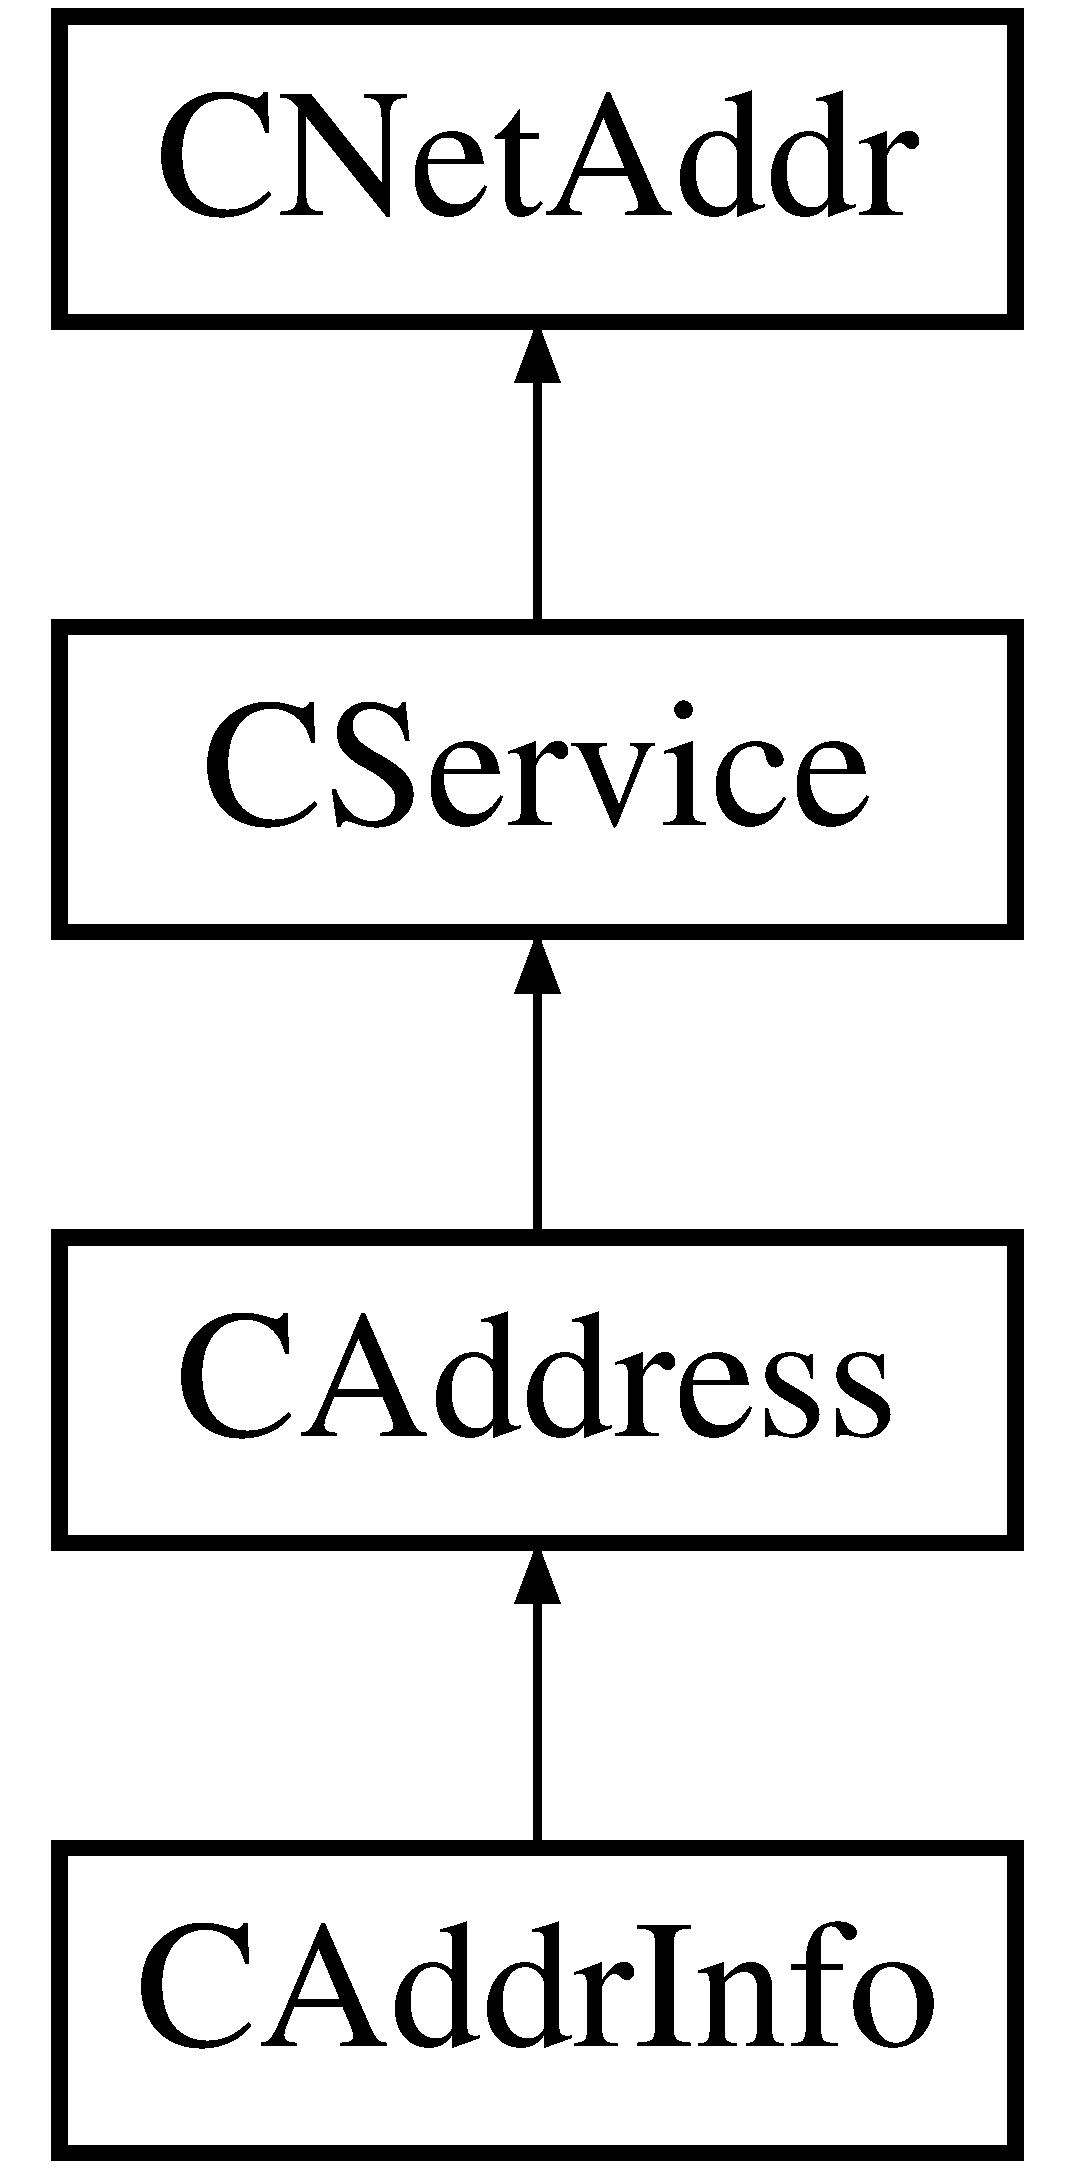
\includegraphics[height=4.000000cm]{class_c_net_addr}
\end{center}
\end{figure}
\subsection*{Public Member Functions}
\begin{DoxyCompactItemize}
\item 
\hyperlink{class_c_net_addr_ad997a7ab057fbeab1dd6601135f8e02d}{C\+Net\+Addr} ()
\item 
\hyperlink{class_c_net_addr_a0af492cd8aca9bbaa3392cdbfbb55681}{C\+Net\+Addr} (const struct in\+\_\+addr \&ipv4\+Addr)
\item 
\hyperlink{class_c_net_addr_a3549332f92d95ccadf262bdce9f4eacf}{C\+Net\+Addr} (const char $\ast$psz\+Ip, bool f\+Allow\+Lookup=false)
\item 
\hyperlink{class_c_net_addr_ae237602be0e4bce6ff31061270371144}{C\+Net\+Addr} (const std\+::string \&str\+Ip, bool f\+Allow\+Lookup=false)
\item 
void \hyperlink{class_c_net_addr_adab412fbc5a9203bea90ae173996ab10}{Init} ()
\item 
void \hyperlink{class_c_net_addr_a1c6087345e5ca07a151451cd6deb974f}{Set\+I\+P} (const \hyperlink{class_c_net_addr}{C\+Net\+Addr} \&\hyperlink{class_c_net_addr_acff7ce68f33f8dfbfe6d79d80928d417}{ip})
\item 
void \hyperlink{class_c_net_addr_a1f0b23aca4ca78c11735d13f3583b7ad}{Set\+Raw} (\hyperlink{netbase_8h_acc9a38c714afe79b5035cb36f560dac3}{Network} network, const uint8\+\_\+t $\ast$data)
\item 
bool \hyperlink{class_c_net_addr_aa3e44dfd064d9d8da1cb48cdcb7dd231}{Set\+Special} (const std\+::string \&str\+Name)
\item 
bool \hyperlink{class_c_net_addr_a16ff4478f02f06f5a9a038a24d5da2f9}{Is\+I\+Pv4} () const 
\item 
bool \hyperlink{class_c_net_addr_a0edb022cd6a186de8099799415409d57}{Is\+I\+Pv6} () const 
\item 
bool \hyperlink{class_c_net_addr_a81b190a7e0b05b93bf3097ba43e5cec1}{Is\+R\+F\+C1918} () const 
\item 
bool \hyperlink{class_c_net_addr_a7879f3a079c815c2e2b7fc3cd7f65d3a}{Is\+R\+F\+C2544} () const 
\item 
bool \hyperlink{class_c_net_addr_a9df45c643f24325e9a4749e2f5caad21}{Is\+R\+F\+C6598} () const 
\item 
bool \hyperlink{class_c_net_addr_a1ea17f90b788e435dc303f57874c1fdf}{Is\+R\+F\+C5737} () const 
\item 
bool \hyperlink{class_c_net_addr_a639dff0ffea6ad930353784686def39b}{Is\+R\+F\+C3849} () const 
\item 
bool \hyperlink{class_c_net_addr_a3d8e5495fd3a2f92bedf272452a2d4b0}{Is\+R\+F\+C3927} () const 
\item 
bool \hyperlink{class_c_net_addr_a312065a9243977a602412665d6148f26}{Is\+R\+F\+C3964} () const 
\item 
bool \hyperlink{class_c_net_addr_ac47bf0c27f8026497b1933393a6570ba}{Is\+R\+F\+C4193} () const 
\item 
bool \hyperlink{class_c_net_addr_afc6e370bb97c97f83260bba898ec4731}{Is\+R\+F\+C4380} () const 
\item 
bool \hyperlink{class_c_net_addr_ad69e51fffff5ee9fcabedda51f10a3ce}{Is\+R\+F\+C4843} () const 
\item 
bool \hyperlink{class_c_net_addr_a5cba67eb628ea99ea68addfe14913fa3}{Is\+R\+F\+C4862} () const 
\item 
bool \hyperlink{class_c_net_addr_a8057dbecf9f5b4d33a643990b6eec873}{Is\+R\+F\+C6052} () const 
\item 
bool \hyperlink{class_c_net_addr_ab5d91a88d77777004c8ebd658c8caf54}{Is\+R\+F\+C6145} () const 
\item 
bool \hyperlink{class_c_net_addr_a3fba9e0b18f531c0ed15794a30e8165d}{Is\+Tor} () const 
\item 
bool \hyperlink{class_c_net_addr_a6cfa18f323424408cf7ace36c9a7c2e2}{Is\+Local} () const 
\item 
bool \hyperlink{class_c_net_addr_a35131b2792434d1c9a860c583b610ab6}{Is\+Routable} () const 
\item 
bool \hyperlink{class_c_net_addr_a52a1b506f07e5450057e12a8b5a7fbcd}{Is\+Valid} () const 
\item 
bool \hyperlink{class_c_net_addr_ab6593d2d75ca7cc6f00c2831cc0a8b73}{Is\+Multicast} () const 
\item 
enum \hyperlink{netbase_8h_acc9a38c714afe79b5035cb36f560dac3}{Network} \hyperlink{class_c_net_addr_a34a4760424f5c51998fc3baf82ccb5c8}{Get\+Network} () const 
\item 
std\+::string \hyperlink{class_c_net_addr_aae906cecdba331389f249a64693895b6}{To\+String} () const 
\item 
std\+::string \hyperlink{class_c_net_addr_a7ec845c27b63853fb0db08a4d154266f}{To\+String\+I\+P} () const 
\item 
unsigned int \hyperlink{class_c_net_addr_a0793d30a6baae6e3d4e06084ec33eddd}{Get\+Byte} (int n) const 
\item 
uint64\+\_\+t \hyperlink{class_c_net_addr_a4c94fea8695ef97adf5b2a18e1074308}{Get\+Hash} () const 
\item 
bool \hyperlink{class_c_net_addr_aa2e2c78db01a6a27d6a2740f2ba43e90}{Get\+In\+Addr} (struct in\+\_\+addr $\ast$pipv4\+Addr) const 
\item 
std\+::vector$<$ unsigned char $>$ \hyperlink{class_c_net_addr_af196f306433562cb088dc83fd314a267}{Get\+Group} () const 
\item 
int \hyperlink{class_c_net_addr_a3007deff5e9872d620952362ae0ef144}{Get\+Reachability\+From} (const \hyperlink{class_c_net_addr}{C\+Net\+Addr} $\ast$paddr\+Partner=N\+U\+L\+L) const 
\item 
\hyperlink{class_c_net_addr_a9eae4232457f7659a157467274d1b444}{C\+Net\+Addr} (const struct in6\+\_\+addr \&pipv6\+Addr)
\item 
bool \hyperlink{class_c_net_addr_add7811be50f5fe60c4fa65b461dea98c}{Get\+In6\+Addr} (struct in6\+\_\+addr $\ast$pipv6\+Addr) const 
\item 
{\footnotesize template$<$typename Stream , typename Operation $>$ }\\void \hyperlink{class_c_net_addr_a7c914d155a533f64f8aa0d2f9bfff8a7}{Serialization\+Op} (Stream \&s, Operation ser\+\_\+action, int n\+Type, int n\+Version)
\end{DoxyCompactItemize}
\subsection*{Public Attributes}
\begin{DoxyCompactItemize}
\item 
\hyperlink{class_c_net_addr_ab08e22719f96b42c61e998158a895e5f}{A\+D\+D\+\_\+\+S\+E\+R\+I\+A\+L\+I\+Z\+E\+\_\+\+M\+E\+T\+H\+O\+D\+S}
\end{DoxyCompactItemize}
\subsection*{Protected Attributes}
\begin{DoxyCompactItemize}
\item 
unsigned char \hyperlink{class_c_net_addr_acff7ce68f33f8dfbfe6d79d80928d417}{ip} \mbox{[}16\mbox{]}
\end{DoxyCompactItemize}
\subsection*{Friends}
\begin{DoxyCompactItemize}
\item 
bool \hyperlink{class_c_net_addr_a6cc88956853ab8dc9586d55cda059934}{operator==} (const \hyperlink{class_c_net_addr}{C\+Net\+Addr} \&a, const \hyperlink{class_c_net_addr}{C\+Net\+Addr} \&b)
\item 
bool \hyperlink{class_c_net_addr_ac361eb83c41464359dfb1dfc296c3a4c}{operator!=} (const \hyperlink{class_c_net_addr}{C\+Net\+Addr} \&a, const \hyperlink{class_c_net_addr}{C\+Net\+Addr} \&b)
\item 
bool \hyperlink{class_c_net_addr_af220590d55a24354e2ba2e547e34fd77}{operator$<$} (const \hyperlink{class_c_net_addr}{C\+Net\+Addr} \&a, const \hyperlink{class_c_net_addr}{C\+Net\+Addr} \&b)
\end{DoxyCompactItemize}


\subsection{Detailed Description}
I\+P address (I\+Pv6, or I\+Pv4 using mapped I\+Pv6 range (\+::\+F\+F\+F\+F\+:0\+:0/96)) 

\subsection{Constructor \& Destructor Documentation}
\hypertarget{class_c_net_addr_ad997a7ab057fbeab1dd6601135f8e02d}{}\index{C\+Net\+Addr@{C\+Net\+Addr}!C\+Net\+Addr@{C\+Net\+Addr}}
\index{C\+Net\+Addr@{C\+Net\+Addr}!C\+Net\+Addr@{C\+Net\+Addr}}
\subsubsection[{C\+Net\+Addr}]{\setlength{\rightskip}{0pt plus 5cm}C\+Net\+Addr\+::\+C\+Net\+Addr (
\begin{DoxyParamCaption}
{}
\end{DoxyParamCaption}
)}\label{class_c_net_addr_ad997a7ab057fbeab1dd6601135f8e02d}
\hypertarget{class_c_net_addr_a0af492cd8aca9bbaa3392cdbfbb55681}{}\index{C\+Net\+Addr@{C\+Net\+Addr}!C\+Net\+Addr@{C\+Net\+Addr}}
\index{C\+Net\+Addr@{C\+Net\+Addr}!C\+Net\+Addr@{C\+Net\+Addr}}
\subsubsection[{C\+Net\+Addr}]{\setlength{\rightskip}{0pt plus 5cm}C\+Net\+Addr\+::\+C\+Net\+Addr (
\begin{DoxyParamCaption}
\item[{const struct in\+\_\+addr \&}]{ipv4\+Addr}
\end{DoxyParamCaption}
)}\label{class_c_net_addr_a0af492cd8aca9bbaa3392cdbfbb55681}
\hypertarget{class_c_net_addr_a3549332f92d95ccadf262bdce9f4eacf}{}\index{C\+Net\+Addr@{C\+Net\+Addr}!C\+Net\+Addr@{C\+Net\+Addr}}
\index{C\+Net\+Addr@{C\+Net\+Addr}!C\+Net\+Addr@{C\+Net\+Addr}}
\subsubsection[{C\+Net\+Addr}]{\setlength{\rightskip}{0pt plus 5cm}C\+Net\+Addr\+::\+C\+Net\+Addr (
\begin{DoxyParamCaption}
\item[{const char $\ast$}]{psz\+Ip, }
\item[{bool}]{f\+Allow\+Lookup = {\ttfamily false}}
\end{DoxyParamCaption}
)\hspace{0.3cm}{\ttfamily [explicit]}}\label{class_c_net_addr_a3549332f92d95ccadf262bdce9f4eacf}
\hypertarget{class_c_net_addr_ae237602be0e4bce6ff31061270371144}{}\index{C\+Net\+Addr@{C\+Net\+Addr}!C\+Net\+Addr@{C\+Net\+Addr}}
\index{C\+Net\+Addr@{C\+Net\+Addr}!C\+Net\+Addr@{C\+Net\+Addr}}
\subsubsection[{C\+Net\+Addr}]{\setlength{\rightskip}{0pt plus 5cm}C\+Net\+Addr\+::\+C\+Net\+Addr (
\begin{DoxyParamCaption}
\item[{const std\+::string \&}]{str\+Ip, }
\item[{bool}]{f\+Allow\+Lookup = {\ttfamily false}}
\end{DoxyParamCaption}
)\hspace{0.3cm}{\ttfamily [explicit]}}\label{class_c_net_addr_ae237602be0e4bce6ff31061270371144}
\hypertarget{class_c_net_addr_a9eae4232457f7659a157467274d1b444}{}\index{C\+Net\+Addr@{C\+Net\+Addr}!C\+Net\+Addr@{C\+Net\+Addr}}
\index{C\+Net\+Addr@{C\+Net\+Addr}!C\+Net\+Addr@{C\+Net\+Addr}}
\subsubsection[{C\+Net\+Addr}]{\setlength{\rightskip}{0pt plus 5cm}C\+Net\+Addr\+::\+C\+Net\+Addr (
\begin{DoxyParamCaption}
\item[{const struct in6\+\_\+addr \&}]{pipv6\+Addr}
\end{DoxyParamCaption}
)}\label{class_c_net_addr_a9eae4232457f7659a157467274d1b444}


\subsection{Member Function Documentation}
\hypertarget{class_c_net_addr_a0793d30a6baae6e3d4e06084ec33eddd}{}\index{C\+Net\+Addr@{C\+Net\+Addr}!Get\+Byte@{Get\+Byte}}
\index{Get\+Byte@{Get\+Byte}!C\+Net\+Addr@{C\+Net\+Addr}}
\subsubsection[{Get\+Byte}]{\setlength{\rightskip}{0pt plus 5cm}unsigned int C\+Net\+Addr\+::\+Get\+Byte (
\begin{DoxyParamCaption}
\item[{int}]{n}
\end{DoxyParamCaption}
) const}\label{class_c_net_addr_a0793d30a6baae6e3d4e06084ec33eddd}
\hypertarget{class_c_net_addr_af196f306433562cb088dc83fd314a267}{}\index{C\+Net\+Addr@{C\+Net\+Addr}!Get\+Group@{Get\+Group}}
\index{Get\+Group@{Get\+Group}!C\+Net\+Addr@{C\+Net\+Addr}}
\subsubsection[{Get\+Group}]{\setlength{\rightskip}{0pt plus 5cm}std\+::vector$<$ unsigned char $>$ C\+Net\+Addr\+::\+Get\+Group (
\begin{DoxyParamCaption}
{}
\end{DoxyParamCaption}
) const}\label{class_c_net_addr_af196f306433562cb088dc83fd314a267}
\hypertarget{class_c_net_addr_a4c94fea8695ef97adf5b2a18e1074308}{}\index{C\+Net\+Addr@{C\+Net\+Addr}!Get\+Hash@{Get\+Hash}}
\index{Get\+Hash@{Get\+Hash}!C\+Net\+Addr@{C\+Net\+Addr}}
\subsubsection[{Get\+Hash}]{\setlength{\rightskip}{0pt plus 5cm}uint64\+\_\+t C\+Net\+Addr\+::\+Get\+Hash (
\begin{DoxyParamCaption}
{}
\end{DoxyParamCaption}
) const}\label{class_c_net_addr_a4c94fea8695ef97adf5b2a18e1074308}
\hypertarget{class_c_net_addr_add7811be50f5fe60c4fa65b461dea98c}{}\index{C\+Net\+Addr@{C\+Net\+Addr}!Get\+In6\+Addr@{Get\+In6\+Addr}}
\index{Get\+In6\+Addr@{Get\+In6\+Addr}!C\+Net\+Addr@{C\+Net\+Addr}}
\subsubsection[{Get\+In6\+Addr}]{\setlength{\rightskip}{0pt plus 5cm}bool C\+Net\+Addr\+::\+Get\+In6\+Addr (
\begin{DoxyParamCaption}
\item[{struct in6\+\_\+addr $\ast$}]{pipv6\+Addr}
\end{DoxyParamCaption}
) const}\label{class_c_net_addr_add7811be50f5fe60c4fa65b461dea98c}
\hypertarget{class_c_net_addr_aa2e2c78db01a6a27d6a2740f2ba43e90}{}\index{C\+Net\+Addr@{C\+Net\+Addr}!Get\+In\+Addr@{Get\+In\+Addr}}
\index{Get\+In\+Addr@{Get\+In\+Addr}!C\+Net\+Addr@{C\+Net\+Addr}}
\subsubsection[{Get\+In\+Addr}]{\setlength{\rightskip}{0pt plus 5cm}bool C\+Net\+Addr\+::\+Get\+In\+Addr (
\begin{DoxyParamCaption}
\item[{struct in\+\_\+addr $\ast$}]{pipv4\+Addr}
\end{DoxyParamCaption}
) const}\label{class_c_net_addr_aa2e2c78db01a6a27d6a2740f2ba43e90}
\hypertarget{class_c_net_addr_a34a4760424f5c51998fc3baf82ccb5c8}{}\index{C\+Net\+Addr@{C\+Net\+Addr}!Get\+Network@{Get\+Network}}
\index{Get\+Network@{Get\+Network}!C\+Net\+Addr@{C\+Net\+Addr}}
\subsubsection[{Get\+Network}]{\setlength{\rightskip}{0pt plus 5cm}enum {\bf Network} C\+Net\+Addr\+::\+Get\+Network (
\begin{DoxyParamCaption}
{}
\end{DoxyParamCaption}
) const}\label{class_c_net_addr_a34a4760424f5c51998fc3baf82ccb5c8}
\hypertarget{class_c_net_addr_a3007deff5e9872d620952362ae0ef144}{}\index{C\+Net\+Addr@{C\+Net\+Addr}!Get\+Reachability\+From@{Get\+Reachability\+From}}
\index{Get\+Reachability\+From@{Get\+Reachability\+From}!C\+Net\+Addr@{C\+Net\+Addr}}
\subsubsection[{Get\+Reachability\+From}]{\setlength{\rightskip}{0pt plus 5cm}int C\+Net\+Addr\+::\+Get\+Reachability\+From (
\begin{DoxyParamCaption}
\item[{const {\bf C\+Net\+Addr} $\ast$}]{paddr\+Partner = {\ttfamily NULL}}
\end{DoxyParamCaption}
) const}\label{class_c_net_addr_a3007deff5e9872d620952362ae0ef144}
Calculates a metric for how reachable ($\ast$this) is from a given partner \hypertarget{class_c_net_addr_adab412fbc5a9203bea90ae173996ab10}{}\index{C\+Net\+Addr@{C\+Net\+Addr}!Init@{Init}}
\index{Init@{Init}!C\+Net\+Addr@{C\+Net\+Addr}}
\subsubsection[{Init}]{\setlength{\rightskip}{0pt plus 5cm}void C\+Net\+Addr\+::\+Init (
\begin{DoxyParamCaption}
{}
\end{DoxyParamCaption}
)}\label{class_c_net_addr_adab412fbc5a9203bea90ae173996ab10}
\hypertarget{class_c_net_addr_a16ff4478f02f06f5a9a038a24d5da2f9}{}\index{C\+Net\+Addr@{C\+Net\+Addr}!Is\+I\+Pv4@{Is\+I\+Pv4}}
\index{Is\+I\+Pv4@{Is\+I\+Pv4}!C\+Net\+Addr@{C\+Net\+Addr}}
\subsubsection[{Is\+I\+Pv4}]{\setlength{\rightskip}{0pt plus 5cm}bool C\+Net\+Addr\+::\+Is\+I\+Pv4 (
\begin{DoxyParamCaption}
{}
\end{DoxyParamCaption}
) const}\label{class_c_net_addr_a16ff4478f02f06f5a9a038a24d5da2f9}
\hypertarget{class_c_net_addr_a0edb022cd6a186de8099799415409d57}{}\index{C\+Net\+Addr@{C\+Net\+Addr}!Is\+I\+Pv6@{Is\+I\+Pv6}}
\index{Is\+I\+Pv6@{Is\+I\+Pv6}!C\+Net\+Addr@{C\+Net\+Addr}}
\subsubsection[{Is\+I\+Pv6}]{\setlength{\rightskip}{0pt plus 5cm}bool C\+Net\+Addr\+::\+Is\+I\+Pv6 (
\begin{DoxyParamCaption}
{}
\end{DoxyParamCaption}
) const}\label{class_c_net_addr_a0edb022cd6a186de8099799415409d57}
\hypertarget{class_c_net_addr_a6cfa18f323424408cf7ace36c9a7c2e2}{}\index{C\+Net\+Addr@{C\+Net\+Addr}!Is\+Local@{Is\+Local}}
\index{Is\+Local@{Is\+Local}!C\+Net\+Addr@{C\+Net\+Addr}}
\subsubsection[{Is\+Local}]{\setlength{\rightskip}{0pt plus 5cm}bool C\+Net\+Addr\+::\+Is\+Local (
\begin{DoxyParamCaption}
{}
\end{DoxyParamCaption}
) const}\label{class_c_net_addr_a6cfa18f323424408cf7ace36c9a7c2e2}
\hypertarget{class_c_net_addr_ab6593d2d75ca7cc6f00c2831cc0a8b73}{}\index{C\+Net\+Addr@{C\+Net\+Addr}!Is\+Multicast@{Is\+Multicast}}
\index{Is\+Multicast@{Is\+Multicast}!C\+Net\+Addr@{C\+Net\+Addr}}
\subsubsection[{Is\+Multicast}]{\setlength{\rightskip}{0pt plus 5cm}bool C\+Net\+Addr\+::\+Is\+Multicast (
\begin{DoxyParamCaption}
{}
\end{DoxyParamCaption}
) const}\label{class_c_net_addr_ab6593d2d75ca7cc6f00c2831cc0a8b73}
\hypertarget{class_c_net_addr_a81b190a7e0b05b93bf3097ba43e5cec1}{}\index{C\+Net\+Addr@{C\+Net\+Addr}!Is\+R\+F\+C1918@{Is\+R\+F\+C1918}}
\index{Is\+R\+F\+C1918@{Is\+R\+F\+C1918}!C\+Net\+Addr@{C\+Net\+Addr}}
\subsubsection[{Is\+R\+F\+C1918}]{\setlength{\rightskip}{0pt plus 5cm}bool C\+Net\+Addr\+::\+Is\+R\+F\+C1918 (
\begin{DoxyParamCaption}
{}
\end{DoxyParamCaption}
) const}\label{class_c_net_addr_a81b190a7e0b05b93bf3097ba43e5cec1}
\hypertarget{class_c_net_addr_a7879f3a079c815c2e2b7fc3cd7f65d3a}{}\index{C\+Net\+Addr@{C\+Net\+Addr}!Is\+R\+F\+C2544@{Is\+R\+F\+C2544}}
\index{Is\+R\+F\+C2544@{Is\+R\+F\+C2544}!C\+Net\+Addr@{C\+Net\+Addr}}
\subsubsection[{Is\+R\+F\+C2544}]{\setlength{\rightskip}{0pt plus 5cm}bool C\+Net\+Addr\+::\+Is\+R\+F\+C2544 (
\begin{DoxyParamCaption}
{}
\end{DoxyParamCaption}
) const}\label{class_c_net_addr_a7879f3a079c815c2e2b7fc3cd7f65d3a}
\hypertarget{class_c_net_addr_a639dff0ffea6ad930353784686def39b}{}\index{C\+Net\+Addr@{C\+Net\+Addr}!Is\+R\+F\+C3849@{Is\+R\+F\+C3849}}
\index{Is\+R\+F\+C3849@{Is\+R\+F\+C3849}!C\+Net\+Addr@{C\+Net\+Addr}}
\subsubsection[{Is\+R\+F\+C3849}]{\setlength{\rightskip}{0pt plus 5cm}bool C\+Net\+Addr\+::\+Is\+R\+F\+C3849 (
\begin{DoxyParamCaption}
{}
\end{DoxyParamCaption}
) const}\label{class_c_net_addr_a639dff0ffea6ad930353784686def39b}
\hypertarget{class_c_net_addr_a3d8e5495fd3a2f92bedf272452a2d4b0}{}\index{C\+Net\+Addr@{C\+Net\+Addr}!Is\+R\+F\+C3927@{Is\+R\+F\+C3927}}
\index{Is\+R\+F\+C3927@{Is\+R\+F\+C3927}!C\+Net\+Addr@{C\+Net\+Addr}}
\subsubsection[{Is\+R\+F\+C3927}]{\setlength{\rightskip}{0pt plus 5cm}bool C\+Net\+Addr\+::\+Is\+R\+F\+C3927 (
\begin{DoxyParamCaption}
{}
\end{DoxyParamCaption}
) const}\label{class_c_net_addr_a3d8e5495fd3a2f92bedf272452a2d4b0}
\hypertarget{class_c_net_addr_a312065a9243977a602412665d6148f26}{}\index{C\+Net\+Addr@{C\+Net\+Addr}!Is\+R\+F\+C3964@{Is\+R\+F\+C3964}}
\index{Is\+R\+F\+C3964@{Is\+R\+F\+C3964}!C\+Net\+Addr@{C\+Net\+Addr}}
\subsubsection[{Is\+R\+F\+C3964}]{\setlength{\rightskip}{0pt plus 5cm}bool C\+Net\+Addr\+::\+Is\+R\+F\+C3964 (
\begin{DoxyParamCaption}
{}
\end{DoxyParamCaption}
) const}\label{class_c_net_addr_a312065a9243977a602412665d6148f26}
\hypertarget{class_c_net_addr_ac47bf0c27f8026497b1933393a6570ba}{}\index{C\+Net\+Addr@{C\+Net\+Addr}!Is\+R\+F\+C4193@{Is\+R\+F\+C4193}}
\index{Is\+R\+F\+C4193@{Is\+R\+F\+C4193}!C\+Net\+Addr@{C\+Net\+Addr}}
\subsubsection[{Is\+R\+F\+C4193}]{\setlength{\rightskip}{0pt plus 5cm}bool C\+Net\+Addr\+::\+Is\+R\+F\+C4193 (
\begin{DoxyParamCaption}
{}
\end{DoxyParamCaption}
) const}\label{class_c_net_addr_ac47bf0c27f8026497b1933393a6570ba}
\hypertarget{class_c_net_addr_afc6e370bb97c97f83260bba898ec4731}{}\index{C\+Net\+Addr@{C\+Net\+Addr}!Is\+R\+F\+C4380@{Is\+R\+F\+C4380}}
\index{Is\+R\+F\+C4380@{Is\+R\+F\+C4380}!C\+Net\+Addr@{C\+Net\+Addr}}
\subsubsection[{Is\+R\+F\+C4380}]{\setlength{\rightskip}{0pt plus 5cm}bool C\+Net\+Addr\+::\+Is\+R\+F\+C4380 (
\begin{DoxyParamCaption}
{}
\end{DoxyParamCaption}
) const}\label{class_c_net_addr_afc6e370bb97c97f83260bba898ec4731}
\hypertarget{class_c_net_addr_ad69e51fffff5ee9fcabedda51f10a3ce}{}\index{C\+Net\+Addr@{C\+Net\+Addr}!Is\+R\+F\+C4843@{Is\+R\+F\+C4843}}
\index{Is\+R\+F\+C4843@{Is\+R\+F\+C4843}!C\+Net\+Addr@{C\+Net\+Addr}}
\subsubsection[{Is\+R\+F\+C4843}]{\setlength{\rightskip}{0pt plus 5cm}bool C\+Net\+Addr\+::\+Is\+R\+F\+C4843 (
\begin{DoxyParamCaption}
{}
\end{DoxyParamCaption}
) const}\label{class_c_net_addr_ad69e51fffff5ee9fcabedda51f10a3ce}
\hypertarget{class_c_net_addr_a5cba67eb628ea99ea68addfe14913fa3}{}\index{C\+Net\+Addr@{C\+Net\+Addr}!Is\+R\+F\+C4862@{Is\+R\+F\+C4862}}
\index{Is\+R\+F\+C4862@{Is\+R\+F\+C4862}!C\+Net\+Addr@{C\+Net\+Addr}}
\subsubsection[{Is\+R\+F\+C4862}]{\setlength{\rightskip}{0pt plus 5cm}bool C\+Net\+Addr\+::\+Is\+R\+F\+C4862 (
\begin{DoxyParamCaption}
{}
\end{DoxyParamCaption}
) const}\label{class_c_net_addr_a5cba67eb628ea99ea68addfe14913fa3}
\hypertarget{class_c_net_addr_a1ea17f90b788e435dc303f57874c1fdf}{}\index{C\+Net\+Addr@{C\+Net\+Addr}!Is\+R\+F\+C5737@{Is\+R\+F\+C5737}}
\index{Is\+R\+F\+C5737@{Is\+R\+F\+C5737}!C\+Net\+Addr@{C\+Net\+Addr}}
\subsubsection[{Is\+R\+F\+C5737}]{\setlength{\rightskip}{0pt plus 5cm}bool C\+Net\+Addr\+::\+Is\+R\+F\+C5737 (
\begin{DoxyParamCaption}
{}
\end{DoxyParamCaption}
) const}\label{class_c_net_addr_a1ea17f90b788e435dc303f57874c1fdf}
\hypertarget{class_c_net_addr_a8057dbecf9f5b4d33a643990b6eec873}{}\index{C\+Net\+Addr@{C\+Net\+Addr}!Is\+R\+F\+C6052@{Is\+R\+F\+C6052}}
\index{Is\+R\+F\+C6052@{Is\+R\+F\+C6052}!C\+Net\+Addr@{C\+Net\+Addr}}
\subsubsection[{Is\+R\+F\+C6052}]{\setlength{\rightskip}{0pt plus 5cm}bool C\+Net\+Addr\+::\+Is\+R\+F\+C6052 (
\begin{DoxyParamCaption}
{}
\end{DoxyParamCaption}
) const}\label{class_c_net_addr_a8057dbecf9f5b4d33a643990b6eec873}
\hypertarget{class_c_net_addr_ab5d91a88d77777004c8ebd658c8caf54}{}\index{C\+Net\+Addr@{C\+Net\+Addr}!Is\+R\+F\+C6145@{Is\+R\+F\+C6145}}
\index{Is\+R\+F\+C6145@{Is\+R\+F\+C6145}!C\+Net\+Addr@{C\+Net\+Addr}}
\subsubsection[{Is\+R\+F\+C6145}]{\setlength{\rightskip}{0pt plus 5cm}bool C\+Net\+Addr\+::\+Is\+R\+F\+C6145 (
\begin{DoxyParamCaption}
{}
\end{DoxyParamCaption}
) const}\label{class_c_net_addr_ab5d91a88d77777004c8ebd658c8caf54}
\hypertarget{class_c_net_addr_a9df45c643f24325e9a4749e2f5caad21}{}\index{C\+Net\+Addr@{C\+Net\+Addr}!Is\+R\+F\+C6598@{Is\+R\+F\+C6598}}
\index{Is\+R\+F\+C6598@{Is\+R\+F\+C6598}!C\+Net\+Addr@{C\+Net\+Addr}}
\subsubsection[{Is\+R\+F\+C6598}]{\setlength{\rightskip}{0pt plus 5cm}bool C\+Net\+Addr\+::\+Is\+R\+F\+C6598 (
\begin{DoxyParamCaption}
{}
\end{DoxyParamCaption}
) const}\label{class_c_net_addr_a9df45c643f24325e9a4749e2f5caad21}
\hypertarget{class_c_net_addr_a35131b2792434d1c9a860c583b610ab6}{}\index{C\+Net\+Addr@{C\+Net\+Addr}!Is\+Routable@{Is\+Routable}}
\index{Is\+Routable@{Is\+Routable}!C\+Net\+Addr@{C\+Net\+Addr}}
\subsubsection[{Is\+Routable}]{\setlength{\rightskip}{0pt plus 5cm}bool C\+Net\+Addr\+::\+Is\+Routable (
\begin{DoxyParamCaption}
{}
\end{DoxyParamCaption}
) const}\label{class_c_net_addr_a35131b2792434d1c9a860c583b610ab6}
\hypertarget{class_c_net_addr_a3fba9e0b18f531c0ed15794a30e8165d}{}\index{C\+Net\+Addr@{C\+Net\+Addr}!Is\+Tor@{Is\+Tor}}
\index{Is\+Tor@{Is\+Tor}!C\+Net\+Addr@{C\+Net\+Addr}}
\subsubsection[{Is\+Tor}]{\setlength{\rightskip}{0pt plus 5cm}bool C\+Net\+Addr\+::\+Is\+Tor (
\begin{DoxyParamCaption}
{}
\end{DoxyParamCaption}
) const}\label{class_c_net_addr_a3fba9e0b18f531c0ed15794a30e8165d}
\hypertarget{class_c_net_addr_a52a1b506f07e5450057e12a8b5a7fbcd}{}\index{C\+Net\+Addr@{C\+Net\+Addr}!Is\+Valid@{Is\+Valid}}
\index{Is\+Valid@{Is\+Valid}!C\+Net\+Addr@{C\+Net\+Addr}}
\subsubsection[{Is\+Valid}]{\setlength{\rightskip}{0pt plus 5cm}bool C\+Net\+Addr\+::\+Is\+Valid (
\begin{DoxyParamCaption}
{}
\end{DoxyParamCaption}
) const}\label{class_c_net_addr_a52a1b506f07e5450057e12a8b5a7fbcd}
\hypertarget{class_c_net_addr_a7c914d155a533f64f8aa0d2f9bfff8a7}{}\index{C\+Net\+Addr@{C\+Net\+Addr}!Serialization\+Op@{Serialization\+Op}}
\index{Serialization\+Op@{Serialization\+Op}!C\+Net\+Addr@{C\+Net\+Addr}}
\subsubsection[{Serialization\+Op}]{\setlength{\rightskip}{0pt plus 5cm}template$<$typename Stream , typename Operation $>$ void C\+Net\+Addr\+::\+Serialization\+Op (
\begin{DoxyParamCaption}
\item[{Stream \&}]{s, }
\item[{Operation}]{ser\+\_\+action, }
\item[{int}]{n\+Type, }
\item[{int}]{n\+Version}
\end{DoxyParamCaption}
)\hspace{0.3cm}{\ttfamily [inline]}}\label{class_c_net_addr_a7c914d155a533f64f8aa0d2f9bfff8a7}
\hypertarget{class_c_net_addr_a1c6087345e5ca07a151451cd6deb974f}{}\index{C\+Net\+Addr@{C\+Net\+Addr}!Set\+I\+P@{Set\+I\+P}}
\index{Set\+I\+P@{Set\+I\+P}!C\+Net\+Addr@{C\+Net\+Addr}}
\subsubsection[{Set\+I\+P}]{\setlength{\rightskip}{0pt plus 5cm}void C\+Net\+Addr\+::\+Set\+I\+P (
\begin{DoxyParamCaption}
\item[{const {\bf C\+Net\+Addr} \&}]{ip}
\end{DoxyParamCaption}
)}\label{class_c_net_addr_a1c6087345e5ca07a151451cd6deb974f}
\hypertarget{class_c_net_addr_a1f0b23aca4ca78c11735d13f3583b7ad}{}\index{C\+Net\+Addr@{C\+Net\+Addr}!Set\+Raw@{Set\+Raw}}
\index{Set\+Raw@{Set\+Raw}!C\+Net\+Addr@{C\+Net\+Addr}}
\subsubsection[{Set\+Raw}]{\setlength{\rightskip}{0pt plus 5cm}void C\+Net\+Addr\+::\+Set\+Raw (
\begin{DoxyParamCaption}
\item[{{\bf Network}}]{network, }
\item[{const uint8\+\_\+t $\ast$}]{data}
\end{DoxyParamCaption}
)}\label{class_c_net_addr_a1f0b23aca4ca78c11735d13f3583b7ad}
Set raw I\+Pv4 or I\+Pv6 address (in network byte order) \begin{DoxyNote}{Note}
Only N\+E\+T\+\_\+\+I\+P\+V4 and N\+E\+T\+\_\+\+I\+P\+V6 are allowed for network. 
\end{DoxyNote}
\hypertarget{class_c_net_addr_aa3e44dfd064d9d8da1cb48cdcb7dd231}{}\index{C\+Net\+Addr@{C\+Net\+Addr}!Set\+Special@{Set\+Special}}
\index{Set\+Special@{Set\+Special}!C\+Net\+Addr@{C\+Net\+Addr}}
\subsubsection[{Set\+Special}]{\setlength{\rightskip}{0pt plus 5cm}bool C\+Net\+Addr\+::\+Set\+Special (
\begin{DoxyParamCaption}
\item[{const std\+::string \&}]{str\+Name}
\end{DoxyParamCaption}
)}\label{class_c_net_addr_aa3e44dfd064d9d8da1cb48cdcb7dd231}
\hypertarget{class_c_net_addr_aae906cecdba331389f249a64693895b6}{}\index{C\+Net\+Addr@{C\+Net\+Addr}!To\+String@{To\+String}}
\index{To\+String@{To\+String}!C\+Net\+Addr@{C\+Net\+Addr}}
\subsubsection[{To\+String}]{\setlength{\rightskip}{0pt plus 5cm}std\+::string C\+Net\+Addr\+::\+To\+String (
\begin{DoxyParamCaption}
{}
\end{DoxyParamCaption}
) const}\label{class_c_net_addr_aae906cecdba331389f249a64693895b6}
\hypertarget{class_c_net_addr_a7ec845c27b63853fb0db08a4d154266f}{}\index{C\+Net\+Addr@{C\+Net\+Addr}!To\+String\+I\+P@{To\+String\+I\+P}}
\index{To\+String\+I\+P@{To\+String\+I\+P}!C\+Net\+Addr@{C\+Net\+Addr}}
\subsubsection[{To\+String\+I\+P}]{\setlength{\rightskip}{0pt plus 5cm}std\+::string C\+Net\+Addr\+::\+To\+String\+I\+P (
\begin{DoxyParamCaption}
{}
\end{DoxyParamCaption}
) const}\label{class_c_net_addr_a7ec845c27b63853fb0db08a4d154266f}


\subsection{Friends And Related Function Documentation}
\hypertarget{class_c_net_addr_ac361eb83c41464359dfb1dfc296c3a4c}{}\index{C\+Net\+Addr@{C\+Net\+Addr}!operator"!=@{operator"!=}}
\index{operator"!=@{operator"!=}!C\+Net\+Addr@{C\+Net\+Addr}}
\subsubsection[{operator"!=}]{\setlength{\rightskip}{0pt plus 5cm}bool operator!= (
\begin{DoxyParamCaption}
\item[{const {\bf C\+Net\+Addr} \&}]{a, }
\item[{const {\bf C\+Net\+Addr} \&}]{b}
\end{DoxyParamCaption}
)\hspace{0.3cm}{\ttfamily [friend]}}\label{class_c_net_addr_ac361eb83c41464359dfb1dfc296c3a4c}
\hypertarget{class_c_net_addr_af220590d55a24354e2ba2e547e34fd77}{}\index{C\+Net\+Addr@{C\+Net\+Addr}!operator$<$@{operator$<$}}
\index{operator$<$@{operator$<$}!C\+Net\+Addr@{C\+Net\+Addr}}
\subsubsection[{operator$<$}]{\setlength{\rightskip}{0pt plus 5cm}bool operator$<$ (
\begin{DoxyParamCaption}
\item[{const {\bf C\+Net\+Addr} \&}]{a, }
\item[{const {\bf C\+Net\+Addr} \&}]{b}
\end{DoxyParamCaption}
)\hspace{0.3cm}{\ttfamily [friend]}}\label{class_c_net_addr_af220590d55a24354e2ba2e547e34fd77}
\hypertarget{class_c_net_addr_a6cc88956853ab8dc9586d55cda059934}{}\index{C\+Net\+Addr@{C\+Net\+Addr}!operator==@{operator==}}
\index{operator==@{operator==}!C\+Net\+Addr@{C\+Net\+Addr}}
\subsubsection[{operator==}]{\setlength{\rightskip}{0pt plus 5cm}bool operator== (
\begin{DoxyParamCaption}
\item[{const {\bf C\+Net\+Addr} \&}]{a, }
\item[{const {\bf C\+Net\+Addr} \&}]{b}
\end{DoxyParamCaption}
)\hspace{0.3cm}{\ttfamily [friend]}}\label{class_c_net_addr_a6cc88956853ab8dc9586d55cda059934}


\subsection{Member Data Documentation}
\hypertarget{class_c_net_addr_ab08e22719f96b42c61e998158a895e5f}{}\index{C\+Net\+Addr@{C\+Net\+Addr}!A\+D\+D\+\_\+\+S\+E\+R\+I\+A\+L\+I\+Z\+E\+\_\+\+M\+E\+T\+H\+O\+D\+S@{A\+D\+D\+\_\+\+S\+E\+R\+I\+A\+L\+I\+Z\+E\+\_\+\+M\+E\+T\+H\+O\+D\+S}}
\index{A\+D\+D\+\_\+\+S\+E\+R\+I\+A\+L\+I\+Z\+E\+\_\+\+M\+E\+T\+H\+O\+D\+S@{A\+D\+D\+\_\+\+S\+E\+R\+I\+A\+L\+I\+Z\+E\+\_\+\+M\+E\+T\+H\+O\+D\+S}!C\+Net\+Addr@{C\+Net\+Addr}}
\subsubsection[{A\+D\+D\+\_\+\+S\+E\+R\+I\+A\+L\+I\+Z\+E\+\_\+\+M\+E\+T\+H\+O\+D\+S}]{\setlength{\rightskip}{0pt plus 5cm}C\+Net\+Addr\+::\+A\+D\+D\+\_\+\+S\+E\+R\+I\+A\+L\+I\+Z\+E\+\_\+\+M\+E\+T\+H\+O\+D\+S}\label{class_c_net_addr_ab08e22719f96b42c61e998158a895e5f}
\hypertarget{class_c_net_addr_acff7ce68f33f8dfbfe6d79d80928d417}{}\index{C\+Net\+Addr@{C\+Net\+Addr}!ip@{ip}}
\index{ip@{ip}!C\+Net\+Addr@{C\+Net\+Addr}}
\subsubsection[{ip}]{\setlength{\rightskip}{0pt plus 5cm}unsigned char C\+Net\+Addr\+::ip\mbox{[}16\mbox{]}\hspace{0.3cm}{\ttfamily [protected]}}\label{class_c_net_addr_acff7ce68f33f8dfbfe6d79d80928d417}


The documentation for this class was generated from the following files\+:\begin{DoxyCompactItemize}
\item 
C\+:/\+Users/\+Joe/\+Documents/\+School/\+C\+S\+C17\+A/bitcoin/src/\hyperlink{netbase_8h}{netbase.\+h}\item 
C\+:/\+Users/\+Joe/\+Documents/\+School/\+C\+S\+C17\+A/bitcoin/src/\hyperlink{netbase_8cpp}{netbase.\+cpp}\end{DoxyCompactItemize}

\hypertarget{class_c_net_cleanup}{}\section{C\+Net\+Cleanup Class Reference}
\label{class_c_net_cleanup}\index{C\+Net\+Cleanup@{C\+Net\+Cleanup}}
\subsection*{Public Member Functions}
\begin{DoxyCompactItemize}
\item 
\hyperlink{class_c_net_cleanup_a928d536c21f6190defda6d6ea2726347}{C\+Net\+Cleanup} ()
\item 
\hyperlink{class_c_net_cleanup_a29b59094c7697b45ca6d13424012506b}{$\sim$\+C\+Net\+Cleanup} ()
\end{DoxyCompactItemize}


\subsection{Constructor \& Destructor Documentation}
\hypertarget{class_c_net_cleanup_a928d536c21f6190defda6d6ea2726347}{}\index{C\+Net\+Cleanup@{C\+Net\+Cleanup}!C\+Net\+Cleanup@{C\+Net\+Cleanup}}
\index{C\+Net\+Cleanup@{C\+Net\+Cleanup}!C\+Net\+Cleanup@{C\+Net\+Cleanup}}
\subsubsection[{C\+Net\+Cleanup}]{\setlength{\rightskip}{0pt plus 5cm}C\+Net\+Cleanup\+::\+C\+Net\+Cleanup (
\begin{DoxyParamCaption}
{}
\end{DoxyParamCaption}
)\hspace{0.3cm}{\ttfamily [inline]}}\label{class_c_net_cleanup_a928d536c21f6190defda6d6ea2726347}
\hypertarget{class_c_net_cleanup_a29b59094c7697b45ca6d13424012506b}{}\index{C\+Net\+Cleanup@{C\+Net\+Cleanup}!````~C\+Net\+Cleanup@{$\sim$\+C\+Net\+Cleanup}}
\index{````~C\+Net\+Cleanup@{$\sim$\+C\+Net\+Cleanup}!C\+Net\+Cleanup@{C\+Net\+Cleanup}}
\subsubsection[{$\sim$\+C\+Net\+Cleanup}]{\setlength{\rightskip}{0pt plus 5cm}C\+Net\+Cleanup\+::$\sim$\+C\+Net\+Cleanup (
\begin{DoxyParamCaption}
{}
\end{DoxyParamCaption}
)\hspace{0.3cm}{\ttfamily [inline]}}\label{class_c_net_cleanup_a29b59094c7697b45ca6d13424012506b}


The documentation for this class was generated from the following file\+:\begin{DoxyCompactItemize}
\item 
C\+:/\+Users/\+Joe/\+Documents/\+School/\+C\+S\+C17\+A/bitcoin/src/\hyperlink{net_8cpp}{net.\+cpp}\end{DoxyCompactItemize}

\hypertarget{class_c_net_message}{}\section{C\+Net\+Message Class Reference}
\label{class_c_net_message}\index{C\+Net\+Message@{C\+Net\+Message}}


{\ttfamily \#include $<$net.\+h$>$}

\subsection*{Public Member Functions}
\begin{DoxyCompactItemize}
\item 
\hyperlink{class_c_net_message_a19f23086d183f2f62d0371960b48c105}{C\+Net\+Message} (const \hyperlink{class_c_message_header_a0d0eeb540cbf4087973f6652ad61878f}{C\+Message\+Header\+::\+Message\+Start\+Chars} \&pch\+Message\+Start\+In, int n\+Type\+In, int n\+Version\+In)
\item 
bool \hyperlink{class_c_net_message_a440150fa0e6a84699780048baca55da8}{complete} () const 
\item 
void \hyperlink{class_c_net_message_a63b9f2351d5e92126cacacd51d9e16b6}{Set\+Version} (int n\+Version\+In)
\item 
int \hyperlink{class_c_net_message_a3e58f5f29b23d1377f8fd15fc75c78ac}{read\+Header} (const char $\ast$pch, unsigned int n\+Bytes)
\item 
int \hyperlink{class_c_net_message_adbc1669a56462daea5f37e5e99117f8c}{read\+Data} (const char $\ast$pch, unsigned int n\+Bytes)
\end{DoxyCompactItemize}
\subsection*{Public Attributes}
\begin{DoxyCompactItemize}
\item 
bool \hyperlink{class_c_net_message_a8f399ad7225f980bdab3ede17b1b23af}{in\+\_\+data}
\item 
\hyperlink{class_c_data_stream}{C\+Data\+Stream} \hyperlink{class_c_net_message_a80a6f95f0c187aa97788118248cbf452}{hdrbuf}
\item 
\hyperlink{class_c_message_header}{C\+Message\+Header} \hyperlink{class_c_net_message_ae7215dca62862a3688f7eeb94646c377}{hdr}
\item 
unsigned int \hyperlink{class_c_net_message_a1a500121037490eec4b238906f3a23ad}{n\+Hdr\+Pos}
\item 
\hyperlink{class_c_data_stream}{C\+Data\+Stream} \hyperlink{class_c_net_message_a1a25c16099d01362e1663390a2e06d1a}{v\+Recv}
\item 
unsigned int \hyperlink{class_c_net_message_a418f59287d1805dda6959f27a170c855}{n\+Data\+Pos}
\item 
int64\+\_\+t \hyperlink{class_c_net_message_a99d5bbca862ac4b7a88b71a7b679decc}{n\+Time}
\end{DoxyCompactItemize}


\subsection{Constructor \& Destructor Documentation}
\hypertarget{class_c_net_message_a19f23086d183f2f62d0371960b48c105}{}\index{C\+Net\+Message@{C\+Net\+Message}!C\+Net\+Message@{C\+Net\+Message}}
\index{C\+Net\+Message@{C\+Net\+Message}!C\+Net\+Message@{C\+Net\+Message}}
\subsubsection[{C\+Net\+Message}]{\setlength{\rightskip}{0pt plus 5cm}C\+Net\+Message\+::\+C\+Net\+Message (
\begin{DoxyParamCaption}
\item[{const {\bf C\+Message\+Header\+::\+Message\+Start\+Chars} \&}]{pch\+Message\+Start\+In, }
\item[{int}]{n\+Type\+In, }
\item[{int}]{n\+Version\+In}
\end{DoxyParamCaption}
)\hspace{0.3cm}{\ttfamily [inline]}}\label{class_c_net_message_a19f23086d183f2f62d0371960b48c105}


\subsection{Member Function Documentation}
\hypertarget{class_c_net_message_a440150fa0e6a84699780048baca55da8}{}\index{C\+Net\+Message@{C\+Net\+Message}!complete@{complete}}
\index{complete@{complete}!C\+Net\+Message@{C\+Net\+Message}}
\subsubsection[{complete}]{\setlength{\rightskip}{0pt plus 5cm}bool C\+Net\+Message\+::complete (
\begin{DoxyParamCaption}
{}
\end{DoxyParamCaption}
) const\hspace{0.3cm}{\ttfamily [inline]}}\label{class_c_net_message_a440150fa0e6a84699780048baca55da8}
\hypertarget{class_c_net_message_adbc1669a56462daea5f37e5e99117f8c}{}\index{C\+Net\+Message@{C\+Net\+Message}!read\+Data@{read\+Data}}
\index{read\+Data@{read\+Data}!C\+Net\+Message@{C\+Net\+Message}}
\subsubsection[{read\+Data}]{\setlength{\rightskip}{0pt plus 5cm}int C\+Net\+Message\+::read\+Data (
\begin{DoxyParamCaption}
\item[{const char $\ast$}]{pch, }
\item[{unsigned int}]{n\+Bytes}
\end{DoxyParamCaption}
)}\label{class_c_net_message_adbc1669a56462daea5f37e5e99117f8c}
\hypertarget{class_c_net_message_a3e58f5f29b23d1377f8fd15fc75c78ac}{}\index{C\+Net\+Message@{C\+Net\+Message}!read\+Header@{read\+Header}}
\index{read\+Header@{read\+Header}!C\+Net\+Message@{C\+Net\+Message}}
\subsubsection[{read\+Header}]{\setlength{\rightskip}{0pt plus 5cm}int C\+Net\+Message\+::read\+Header (
\begin{DoxyParamCaption}
\item[{const char $\ast$}]{pch, }
\item[{unsigned int}]{n\+Bytes}
\end{DoxyParamCaption}
)}\label{class_c_net_message_a3e58f5f29b23d1377f8fd15fc75c78ac}
\hypertarget{class_c_net_message_a63b9f2351d5e92126cacacd51d9e16b6}{}\index{C\+Net\+Message@{C\+Net\+Message}!Set\+Version@{Set\+Version}}
\index{Set\+Version@{Set\+Version}!C\+Net\+Message@{C\+Net\+Message}}
\subsubsection[{Set\+Version}]{\setlength{\rightskip}{0pt plus 5cm}void C\+Net\+Message\+::\+Set\+Version (
\begin{DoxyParamCaption}
\item[{int}]{n\+Version\+In}
\end{DoxyParamCaption}
)\hspace{0.3cm}{\ttfamily [inline]}}\label{class_c_net_message_a63b9f2351d5e92126cacacd51d9e16b6}


\subsection{Member Data Documentation}
\hypertarget{class_c_net_message_ae7215dca62862a3688f7eeb94646c377}{}\index{C\+Net\+Message@{C\+Net\+Message}!hdr@{hdr}}
\index{hdr@{hdr}!C\+Net\+Message@{C\+Net\+Message}}
\subsubsection[{hdr}]{\setlength{\rightskip}{0pt plus 5cm}{\bf C\+Message\+Header} C\+Net\+Message\+::hdr}\label{class_c_net_message_ae7215dca62862a3688f7eeb94646c377}
\hypertarget{class_c_net_message_a80a6f95f0c187aa97788118248cbf452}{}\index{C\+Net\+Message@{C\+Net\+Message}!hdrbuf@{hdrbuf}}
\index{hdrbuf@{hdrbuf}!C\+Net\+Message@{C\+Net\+Message}}
\subsubsection[{hdrbuf}]{\setlength{\rightskip}{0pt plus 5cm}{\bf C\+Data\+Stream} C\+Net\+Message\+::hdrbuf}\label{class_c_net_message_a80a6f95f0c187aa97788118248cbf452}
\hypertarget{class_c_net_message_a8f399ad7225f980bdab3ede17b1b23af}{}\index{C\+Net\+Message@{C\+Net\+Message}!in\+\_\+data@{in\+\_\+data}}
\index{in\+\_\+data@{in\+\_\+data}!C\+Net\+Message@{C\+Net\+Message}}
\subsubsection[{in\+\_\+data}]{\setlength{\rightskip}{0pt plus 5cm}bool C\+Net\+Message\+::in\+\_\+data}\label{class_c_net_message_a8f399ad7225f980bdab3ede17b1b23af}
\hypertarget{class_c_net_message_a418f59287d1805dda6959f27a170c855}{}\index{C\+Net\+Message@{C\+Net\+Message}!n\+Data\+Pos@{n\+Data\+Pos}}
\index{n\+Data\+Pos@{n\+Data\+Pos}!C\+Net\+Message@{C\+Net\+Message}}
\subsubsection[{n\+Data\+Pos}]{\setlength{\rightskip}{0pt plus 5cm}unsigned int C\+Net\+Message\+::n\+Data\+Pos}\label{class_c_net_message_a418f59287d1805dda6959f27a170c855}
\hypertarget{class_c_net_message_a1a500121037490eec4b238906f3a23ad}{}\index{C\+Net\+Message@{C\+Net\+Message}!n\+Hdr\+Pos@{n\+Hdr\+Pos}}
\index{n\+Hdr\+Pos@{n\+Hdr\+Pos}!C\+Net\+Message@{C\+Net\+Message}}
\subsubsection[{n\+Hdr\+Pos}]{\setlength{\rightskip}{0pt plus 5cm}unsigned int C\+Net\+Message\+::n\+Hdr\+Pos}\label{class_c_net_message_a1a500121037490eec4b238906f3a23ad}
\hypertarget{class_c_net_message_a99d5bbca862ac4b7a88b71a7b679decc}{}\index{C\+Net\+Message@{C\+Net\+Message}!n\+Time@{n\+Time}}
\index{n\+Time@{n\+Time}!C\+Net\+Message@{C\+Net\+Message}}
\subsubsection[{n\+Time}]{\setlength{\rightskip}{0pt plus 5cm}int64\+\_\+t C\+Net\+Message\+::n\+Time}\label{class_c_net_message_a99d5bbca862ac4b7a88b71a7b679decc}
\hypertarget{class_c_net_message_a1a25c16099d01362e1663390a2e06d1a}{}\index{C\+Net\+Message@{C\+Net\+Message}!v\+Recv@{v\+Recv}}
\index{v\+Recv@{v\+Recv}!C\+Net\+Message@{C\+Net\+Message}}
\subsubsection[{v\+Recv}]{\setlength{\rightskip}{0pt plus 5cm}{\bf C\+Data\+Stream} C\+Net\+Message\+::v\+Recv}\label{class_c_net_message_a1a25c16099d01362e1663390a2e06d1a}


The documentation for this class was generated from the following files\+:\begin{DoxyCompactItemize}
\item 
C\+:/\+Users/\+Joe/\+Documents/\+School/\+C\+S\+C17\+A/bitcoin/src/\hyperlink{net_8h}{net.\+h}\item 
C\+:/\+Users/\+Joe/\+Documents/\+School/\+C\+S\+C17\+A/bitcoin/src/\hyperlink{net_8cpp}{net.\+cpp}\end{DoxyCompactItemize}

\hypertarget{class_c_node}{}\section{C\+Node Class Reference}
\label{class_c_node}\index{C\+Node@{C\+Node}}


{\ttfamily \#include $<$net.\+h$>$}

\subsection*{Public Member Functions}
\begin{DoxyCompactItemize}
\item 
\hyperlink{class_c_node_a51556705550511146245b9fb2fec09c1}{C\+Node} (\hyperlink{compat_8h_a26ef1173e2f2c0d3db27eca28397d723}{S\+O\+C\+K\+E\+T} h\+Socket\+In, \hyperlink{class_c_address}{C\+Address} addr\+In, std\+::string addr\+Name\+In=\char`\"{}\char`\"{}, bool f\+Inbound\+In=false)
\item 
\hyperlink{class_c_node_ac9b30cb93e91a48dacc58821abfc44f0}{$\sim$\+C\+Node} ()
\item 
\hyperlink{net_8h_a954d746a58632565552615fd0a4ee660}{Node\+Id} \hyperlink{class_c_node_ac0f1a22fa938e84138536308e2001340}{Get\+Id} () const 
\item 
int \hyperlink{class_c_node_a72211aaf51af2e981e6b8a1deb73c836}{Get\+Ref\+Count} ()
\item 
unsigned int \hyperlink{class_c_node_a2cff79a034258ba032257e993fc42e62}{Get\+Total\+Recv\+Size} ()
\item 
bool \hyperlink{class_c_node_a84a10eb3aec7fdddafeb354527b50b75}{Receive\+Msg\+Bytes} (const char $\ast$pch, unsigned int n\+Bytes)
\item 
void \hyperlink{class_c_node_a94438c6285d1635c62ccff10593780e6}{Set\+Recv\+Version} (int n\+Version\+In)
\item 
\hyperlink{class_c_node}{C\+Node} $\ast$ \hyperlink{class_c_node_afb65ed679f7bda59aab89e0f5afae292}{Add\+Ref} ()
\item 
void \hyperlink{class_c_node_af804bf7c7f9794e80a3b916e1befece9}{Release} ()
\item 
void \hyperlink{class_c_node_a1d2cecdd03c9da642d292f6a81ac6ed8}{Add\+Address\+Known} (const \hyperlink{class_c_address}{C\+Address} \&\hyperlink{class_c_node_a3993ecb1de2a2135a3cf0904346a6f88}{addr})
\item 
void \hyperlink{class_c_node_a06950a5ce265a1d4df1aad7f28e6fde8}{Push\+Address} (const \hyperlink{class_c_address}{C\+Address} \&\hyperlink{class_c_node_a3993ecb1de2a2135a3cf0904346a6f88}{addr})
\item 
void \hyperlink{class_c_node_ac3054eb6ade84e8968f032ce3e700f6a}{Add\+Inventory\+Known} (const \hyperlink{class_c_inv}{C\+Inv} \&inv)
\item 
void \hyperlink{class_c_node_a7cef2333aa8776127a7e7fcab659eb6a}{Push\+Inventory} (const \hyperlink{class_c_inv}{C\+Inv} \&inv)
\item 
void \hyperlink{class_c_node_ae0def1498409407d1612833a7d38c875}{Ask\+For} (const \hyperlink{class_c_inv}{C\+Inv} \&inv)
\item 
void \hyperlink{class_c_node_af76d193027757002321d0d674290b955}{Begin\+Message} (const char $\ast$psz\+Command) \hyperlink{threadsafety_8h_a77729163b7f6867da40ad5daa5f926f3}{E\+X\+C\+L\+U\+S\+I\+V\+E\+\_\+\+L\+O\+C\+K\+\_\+\+F\+U\+N\+C\+T\+I\+O\+N}(\hyperlink{class_c_node_a79edcac83fc5067567c7b41c26fcc56f}{cs\+\_\+v\+Send})
\item 
void \hyperlink{class_c_node_aae0fdfe555001a60bab8f216c3bc3978}{Abort\+Message} () \hyperlink{threadsafety_8h_abd56e19f9b4781b1a5212a46951cf5c3}{U\+N\+L\+O\+C\+K\+\_\+\+F\+U\+N\+C\+T\+I\+O\+N}(\hyperlink{class_c_node_a79edcac83fc5067567c7b41c26fcc56f}{cs\+\_\+v\+Send})
\item 
void \hyperlink{class_c_node_af8d4b8c0f883afffcb62d906c31b2cdf}{End\+Message} () \hyperlink{threadsafety_8h_abd56e19f9b4781b1a5212a46951cf5c3}{U\+N\+L\+O\+C\+K\+\_\+\+F\+U\+N\+C\+T\+I\+O\+N}(\hyperlink{class_c_node_a79edcac83fc5067567c7b41c26fcc56f}{cs\+\_\+v\+Send})
\item 
void \hyperlink{class_c_node_a4dbfe4f6c1fd162aaa905e4bd201d536}{Push\+Version} ()
\item 
void \hyperlink{class_c_node_a204fda3d33404cb37698c085b1583ab2}{Push\+Message} (const char $\ast$psz\+Command)
\item 
{\footnotesize template$<$typename T1 $>$ }\\void \hyperlink{class_c_node_a07f897794e362a214a1d4d2aa3d68939}{Push\+Message} (const char $\ast$psz\+Command, const T1 \&a1)
\item 
{\footnotesize template$<$typename T1 , typename T2 $>$ }\\void \hyperlink{class_c_node_a67b985781651b8806d7f9976f6fb85a9}{Push\+Message} (const char $\ast$psz\+Command, const T1 \&a1, const T2 \&a2)
\item 
{\footnotesize template$<$typename T1 , typename T2 , typename T3 $>$ }\\void \hyperlink{class_c_node_a79355956a00c38d855b986a34e7ba444}{Push\+Message} (const char $\ast$psz\+Command, const T1 \&a1, const T2 \&a2, const T3 \&a3)
\item 
{\footnotesize template$<$typename T1 , typename T2 , typename T3 , typename T4 $>$ }\\void \hyperlink{class_c_node_a2958ee10e2c96ef647787bce80196079}{Push\+Message} (const char $\ast$psz\+Command, const T1 \&a1, const T2 \&a2, const T3 \&a3, const T4 \&a4)
\item 
{\footnotesize template$<$typename T1 , typename T2 , typename T3 , typename T4 , typename T5 $>$ }\\void \hyperlink{class_c_node_a1f58deeed29baf57c49dae177f8be826}{Push\+Message} (const char $\ast$psz\+Command, const T1 \&a1, const T2 \&a2, const T3 \&a3, const T4 \&a4, const T5 \&a5)
\item 
{\footnotesize template$<$typename T1 , typename T2 , typename T3 , typename T4 , typename T5 , typename T6 $>$ }\\void \hyperlink{class_c_node_a4addbff355c502fb2f8c10451e76373d}{Push\+Message} (const char $\ast$psz\+Command, const T1 \&a1, const T2 \&a2, const T3 \&a3, const T4 \&a4, const T5 \&a5, const T6 \&a6)
\item 
{\footnotesize template$<$typename T1 , typename T2 , typename T3 , typename T4 , typename T5 , typename T6 , typename T7 $>$ }\\void \hyperlink{class_c_node_ab3611cdb08d5f25a4da05fe140e48625}{Push\+Message} (const char $\ast$psz\+Command, const T1 \&a1, const T2 \&a2, const T3 \&a3, const T4 \&a4, const T5 \&a5, const T6 \&a6, const T7 \&a7)
\item 
{\footnotesize template$<$typename T1 , typename T2 , typename T3 , typename T4 , typename T5 , typename T6 , typename T7 , typename T8 $>$ }\\void \hyperlink{class_c_node_af91d09012aa7e879be4b488b0bba903d}{Push\+Message} (const char $\ast$psz\+Command, const T1 \&a1, const T2 \&a2, const T3 \&a3, const T4 \&a4, const T5 \&a5, const T6 \&a6, const T7 \&a7, const T8 \&a8)
\item 
{\footnotesize template$<$typename T1 , typename T2 , typename T3 , typename T4 , typename T5 , typename T6 , typename T7 , typename T8 , typename T9 $>$ }\\void \hyperlink{class_c_node_a1af04d8219e8e6aafe5b6446000cd9ff}{Push\+Message} (const char $\ast$psz\+Command, const T1 \&a1, const T2 \&a2, const T3 \&a3, const T4 \&a4, const T5 \&a5, const T6 \&a6, const T7 \&a7, const T8 \&a8, const T9 \&a9)
\item 
void \hyperlink{class_c_node_a63a6091a0b0fc0987d9436e1ec708423}{Close\+Socket\+Disconnect} ()
\item 
void \hyperlink{class_c_node_aaa77188d9df85b80e3f8a30292acf6a9}{copy\+Stats} (\hyperlink{class_c_node_stats}{C\+Node\+Stats} \&stats)
\end{DoxyCompactItemize}
\subsection*{Static Public Member Functions}
\begin{DoxyCompactItemize}
\item 
static void \hyperlink{class_c_node_ad75b43ab81213b74446163211c24246a}{Clear\+Banned} ()
\item 
static bool \hyperlink{class_c_node_aefa8b81afa53b4c6635dc4c6c024211a}{Is\+Banned} (\hyperlink{class_c_net_addr}{C\+Net\+Addr} ip)
\item 
static bool \hyperlink{class_c_node_a7d5dd8d7531bfbe069092be583569956}{Ban} (const \hyperlink{class_c_net_addr}{C\+Net\+Addr} \&ip)
\item 
static bool \hyperlink{class_c_node_ad2ccd5d22994f338c9b55ebe7528ea55}{Is\+Whitelisted\+Range} (const \hyperlink{class_c_net_addr}{C\+Net\+Addr} \&ip)
\item 
static void \hyperlink{class_c_node_ad2c1f955ec23851bd87a6bb144d85d03}{Add\+Whitelisted\+Range} (const \hyperlink{class_c_sub_net}{C\+Sub\+Net} \&subnet)
\item 
static void \hyperlink{class_c_node_af72b4b6e454c743af071896019ae1c69}{Record\+Bytes\+Recv} (uint64\+\_\+t bytes)
\item 
static void \hyperlink{class_c_node_a945c993a84eaa9d6bca18284befaccbe}{Record\+Bytes\+Sent} (uint64\+\_\+t bytes)
\item 
static uint64\+\_\+t \hyperlink{class_c_node_a1988b63b48fdc9b72014bdf9588b0168}{Get\+Total\+Bytes\+Recv} ()
\item 
static uint64\+\_\+t \hyperlink{class_c_node_af318a64e7ddad50d1e1b6fc123a5f0b9}{Get\+Total\+Bytes\+Sent} ()
\end{DoxyCompactItemize}
\subsection*{Public Attributes}
\begin{DoxyCompactItemize}
\item 
uint64\+\_\+t \hyperlink{class_c_node_a8259db81211f6837585c6f82f89414ff}{n\+Services}
\item 
\hyperlink{compat_8h_a26ef1173e2f2c0d3db27eca28397d723}{S\+O\+C\+K\+E\+T} \hyperlink{class_c_node_a7cda6efa6a9ef9db3eebe70fc3bdd45a}{h\+Socket}
\item 
\hyperlink{class_c_data_stream}{C\+Data\+Stream} \hyperlink{class_c_node_a6174b5a3d8d8f6a2daf02be3cf04dc63}{ss\+Send}
\item 
size\+\_\+t \hyperlink{class_c_node_a3c99b7e2b0e53feb58f6859453456f74}{n\+Send\+Size}
\item 
size\+\_\+t \hyperlink{class_c_node_a090bda86de6b84c3db83e1f029d4f453}{n\+Send\+Offset}
\item 
uint64\+\_\+t \hyperlink{class_c_node_a33e24a9544df3c60f9e1ec05b5e91051}{n\+Send\+Bytes}
\item 
std\+::deque$<$ C\+Serialize\+Data $>$ \hyperlink{class_c_node_a68e5fb1a80fe4247aa577a3c9a74b399}{v\+Send\+Msg}
\item 
\hyperlink{sync_8h_a37a4692b2d517f2843655ca11af7668a}{C\+Critical\+Section} \hyperlink{class_c_node_a79edcac83fc5067567c7b41c26fcc56f}{cs\+\_\+v\+Send}
\item 
std\+::deque$<$ \hyperlink{class_c_inv}{C\+Inv} $>$ \hyperlink{class_c_node_a9649c1f27ff0d8f0ba89eb1ea5bee139}{v\+Recv\+Get\+Data}
\item 
std\+::deque$<$ \hyperlink{class_c_net_message}{C\+Net\+Message} $>$ \hyperlink{class_c_node_a015361812daa5b6ebb9a5692ddf67a54}{v\+Recv\+Msg}
\item 
\hyperlink{sync_8h_a37a4692b2d517f2843655ca11af7668a}{C\+Critical\+Section} \hyperlink{class_c_node_abaebfaf8fff7e2e99366ae2bc69af6cd}{cs\+\_\+v\+Recv\+Msg}
\item 
uint64\+\_\+t \hyperlink{class_c_node_a8bbe2a7052476d62acf7f0a5a9c5981b}{n\+Recv\+Bytes}
\item 
int \hyperlink{class_c_node_ab7494353448b922accfb645bd26ac271}{n\+Recv\+Version}
\item 
int64\+\_\+t \hyperlink{class_c_node_af39253ad525733ca64ab3fc785dfc4eb}{n\+Last\+Send}
\item 
int64\+\_\+t \hyperlink{class_c_node_afb40f43a51ba686de93256727351af07}{n\+Last\+Recv}
\item 
int64\+\_\+t \hyperlink{class_c_node_abb39393ef08cb5668ded6cb14cdbc147}{n\+Time\+Connected}
\item 
int64\+\_\+t \hyperlink{class_c_node_a3079fadef397abbf7e8d444f4426ebe7}{n\+Time\+Offset}
\item 
\hyperlink{class_c_address}{C\+Address} \hyperlink{class_c_node_a3993ecb1de2a2135a3cf0904346a6f88}{addr}
\item 
std\+::string \hyperlink{class_c_node_a3155cd313d85ec3ff691f8259a5f5345}{addr\+Name}
\item 
\hyperlink{class_c_service}{C\+Service} \hyperlink{class_c_node_a1b6517682efa0709f44780a95384c4ec}{addr\+Local}
\item 
int \hyperlink{class_c_node_a99173eb3cef17e699ba21a5249ac33d2}{n\+Version}
\item 
std\+::string \hyperlink{class_c_node_afb24fb33019af5c4085412fe3898cf01}{str\+Sub\+Ver}
\item 
std\+::string \hyperlink{class_c_node_a05f0401427c5ffebd1ca404848e83ff7}{clean\+Sub\+Ver}
\item 
bool \hyperlink{class_c_node_ad3096c14b54aa39a02edb63a4a734c3e}{f\+Whitelisted}
\item 
bool \hyperlink{class_c_node_a2bb91c9968a9f855c05b1121100a8797}{f\+One\+Shot}
\item 
bool \hyperlink{class_c_node_a721e2470c2c961b7599768a14be68781}{f\+Client}
\item 
bool \hyperlink{class_c_node_a64b2550ec558b6106ebc122d450ad35b}{f\+Inbound}
\item 
bool \hyperlink{class_c_node_a933adb2b192939545a01d602b1d7b53a}{f\+Network\+Node}
\item 
bool \hyperlink{class_c_node_ab58c1772b2698e348d86002f34254119}{f\+Successfully\+Connected}
\item 
bool \hyperlink{class_c_node_af2f7ea958313974e8a948292f060922e}{f\+Disconnect}
\item 
bool \hyperlink{class_c_node_ab387bb0c4ffd42e3f0aea233dca0e301}{f\+Relay\+Txes}
\item 
\hyperlink{class_c_semaphore_grant}{C\+Semaphore\+Grant} \hyperlink{class_c_node_a4bb25f8bdeeaff5e8cb08abc97bbc44d}{grant\+Outbound}
\item 
\hyperlink{sync_8h_a37a4692b2d517f2843655ca11af7668a}{C\+Critical\+Section} \hyperlink{class_c_node_a66aeed3b6534635d031dff3eee9538de}{cs\+\_\+filter}
\item 
\hyperlink{class_c_bloom_filter}{C\+Bloom\+Filter} $\ast$ \hyperlink{class_c_node_a2e28bf088e56fc9d30e99e9de6587743}{pfilter}
\item 
int \hyperlink{class_c_node_a01f8cac776bef676651f9b8f3f80ae98}{n\+Ref\+Count}
\item 
\hyperlink{net_8h_a954d746a58632565552615fd0a4ee660}{Node\+Id} \hyperlink{class_c_node_af99591c635f495fc1e6c14745a2a4203}{id}
\item 
\hyperlink{classuint256}{uint256} \hyperlink{class_c_node_a1a1c0d94de0197c5c4abf5a8d13364f3}{hash\+Continue}
\item 
int \hyperlink{class_c_node_a597b41bd64e2ac9391b7211e65aeb52a}{n\+Starting\+Height}
\item 
std\+::vector$<$ \hyperlink{class_c_address}{C\+Address} $>$ \hyperlink{class_c_node_a9b2d9b9182ff111c79f704594c4aa2e1}{v\+Addr\+To\+Send}
\item 
\hyperlink{classmruset}{mruset}$<$ \hyperlink{class_c_address}{C\+Address} $>$ \hyperlink{class_c_node_ac21266ce880bd36b98ba7cfcc447a30f}{set\+Addr\+Known}
\item 
bool \hyperlink{class_c_node_a3da9c559959e182aff8439cd004ff624}{f\+Get\+Addr}
\item 
std\+::set$<$ \hyperlink{classuint256}{uint256} $>$ \hyperlink{class_c_node_ab1b30fa8e48005752f6b0bcf43eca478}{set\+Known}
\item 
\hyperlink{classmruset}{mruset}$<$ \hyperlink{class_c_inv}{C\+Inv} $>$ \hyperlink{class_c_node_ae15aa9a971040800c26bc87b1250220f}{set\+Inventory\+Known}
\item 
std\+::vector$<$ \hyperlink{class_c_inv}{C\+Inv} $>$ \hyperlink{class_c_node_abcd24c9478bc1ab5ba6de6b369080cec}{v\+Inventory\+To\+Send}
\item 
\hyperlink{sync_8h_a37a4692b2d517f2843655ca11af7668a}{C\+Critical\+Section} \hyperlink{class_c_node_a1e8b0784cc82f33edc2dc4e2834d1ff0}{cs\+\_\+inventory}
\item 
std\+::multimap$<$ int64\+\_\+t, \hyperlink{class_c_inv}{C\+Inv} $>$ \hyperlink{class_c_node_a7593dfbd76c34a81169e3fb2aa0e0cf7}{map\+Ask\+For}
\item 
uint64\+\_\+t \hyperlink{class_c_node_a9a077fbd09ddee1d81f027bc01a4ec68}{n\+Ping\+Nonce\+Sent}
\item 
int64\+\_\+t \hyperlink{class_c_node_a8352aa332af726ff117fb890c4dd3869}{n\+Ping\+Usec\+Start}
\item 
int64\+\_\+t \hyperlink{class_c_node_ada34ffe1700a5dafb57de7c4d2491844}{n\+Ping\+Usec\+Time}
\item 
bool \hyperlink{class_c_node_aa1e9c1dc1d5cf806b9be0af155c0bf90}{f\+Ping\+Queued}
\end{DoxyCompactItemize}
\subsection*{Protected Member Functions}
\begin{DoxyCompactItemize}
\item 
void \hyperlink{class_c_node_a39512c4e2c788fb7a09e629b79a69e47}{Fuzz} (int n\+Chance)
\end{DoxyCompactItemize}
\subsection*{Static Protected Attributes}
\begin{DoxyCompactItemize}
\item 
static std\+::map$<$ \hyperlink{class_c_net_addr}{C\+Net\+Addr}, int64\+\_\+t $>$ \hyperlink{class_c_node_adf22d1873c1012ab3edb8a52253b203e}{set\+Banned}
\item 
static \hyperlink{sync_8h_a37a4692b2d517f2843655ca11af7668a}{C\+Critical\+Section} \hyperlink{class_c_node_a9ff9a6f07a280aa07d77713ae43d383a}{cs\+\_\+set\+Banned}
\item 
static std\+::vector$<$ \hyperlink{class_c_sub_net}{C\+Sub\+Net} $>$ \hyperlink{class_c_node_afaac354c1226990e4e9407ba2ee4cbf9}{v\+Whitelisted\+Range}
\item 
static \hyperlink{sync_8h_a37a4692b2d517f2843655ca11af7668a}{C\+Critical\+Section} \hyperlink{class_c_node_a4a79c02f5024b57ca9e6a1f8d103f363}{cs\+\_\+v\+Whitelisted\+Range}
\end{DoxyCompactItemize}


\subsection{Detailed Description}
Information about a peer 

\subsection{Constructor \& Destructor Documentation}
\hypertarget{class_c_node_a51556705550511146245b9fb2fec09c1}{}\index{C\+Node@{C\+Node}!C\+Node@{C\+Node}}
\index{C\+Node@{C\+Node}!C\+Node@{C\+Node}}
\subsubsection[{C\+Node}]{\setlength{\rightskip}{0pt plus 5cm}C\+Node\+::\+C\+Node (
\begin{DoxyParamCaption}
\item[{{\bf S\+O\+C\+K\+E\+T}}]{h\+Socket\+In, }
\item[{{\bf C\+Address}}]{addr\+In, }
\item[{std\+::string}]{addr\+Name\+In = {\ttfamily \char`\"{}\char`\"{}}, }
\item[{bool}]{f\+Inbound\+In = {\ttfamily false}}
\end{DoxyParamCaption}
)}\label{class_c_node_a51556705550511146245b9fb2fec09c1}
\hypertarget{class_c_node_ac9b30cb93e91a48dacc58821abfc44f0}{}\index{C\+Node@{C\+Node}!````~C\+Node@{$\sim$\+C\+Node}}
\index{````~C\+Node@{$\sim$\+C\+Node}!C\+Node@{C\+Node}}
\subsubsection[{$\sim$\+C\+Node}]{\setlength{\rightskip}{0pt plus 5cm}C\+Node\+::$\sim$\+C\+Node (
\begin{DoxyParamCaption}
{}
\end{DoxyParamCaption}
)}\label{class_c_node_ac9b30cb93e91a48dacc58821abfc44f0}


\subsection{Member Function Documentation}
\hypertarget{class_c_node_aae0fdfe555001a60bab8f216c3bc3978}{}\index{C\+Node@{C\+Node}!Abort\+Message@{Abort\+Message}}
\index{Abort\+Message@{Abort\+Message}!C\+Node@{C\+Node}}
\subsubsection[{Abort\+Message}]{\setlength{\rightskip}{0pt plus 5cm}void C\+Node\+::\+Abort\+Message (
\begin{DoxyParamCaption}
{}
\end{DoxyParamCaption}
)}\label{class_c_node_aae0fdfe555001a60bab8f216c3bc3978}
\hypertarget{class_c_node_a1d2cecdd03c9da642d292f6a81ac6ed8}{}\index{C\+Node@{C\+Node}!Add\+Address\+Known@{Add\+Address\+Known}}
\index{Add\+Address\+Known@{Add\+Address\+Known}!C\+Node@{C\+Node}}
\subsubsection[{Add\+Address\+Known}]{\setlength{\rightskip}{0pt plus 5cm}void C\+Node\+::\+Add\+Address\+Known (
\begin{DoxyParamCaption}
\item[{const {\bf C\+Address} \&}]{addr}
\end{DoxyParamCaption}
)\hspace{0.3cm}{\ttfamily [inline]}}\label{class_c_node_a1d2cecdd03c9da642d292f6a81ac6ed8}
\hypertarget{class_c_node_ac3054eb6ade84e8968f032ce3e700f6a}{}\index{C\+Node@{C\+Node}!Add\+Inventory\+Known@{Add\+Inventory\+Known}}
\index{Add\+Inventory\+Known@{Add\+Inventory\+Known}!C\+Node@{C\+Node}}
\subsubsection[{Add\+Inventory\+Known}]{\setlength{\rightskip}{0pt plus 5cm}void C\+Node\+::\+Add\+Inventory\+Known (
\begin{DoxyParamCaption}
\item[{const {\bf C\+Inv} \&}]{inv}
\end{DoxyParamCaption}
)\hspace{0.3cm}{\ttfamily [inline]}}\label{class_c_node_ac3054eb6ade84e8968f032ce3e700f6a}
\hypertarget{class_c_node_afb65ed679f7bda59aab89e0f5afae292}{}\index{C\+Node@{C\+Node}!Add\+Ref@{Add\+Ref}}
\index{Add\+Ref@{Add\+Ref}!C\+Node@{C\+Node}}
\subsubsection[{Add\+Ref}]{\setlength{\rightskip}{0pt plus 5cm}{\bf C\+Node}$\ast$ C\+Node\+::\+Add\+Ref (
\begin{DoxyParamCaption}
{}
\end{DoxyParamCaption}
)\hspace{0.3cm}{\ttfamily [inline]}}\label{class_c_node_afb65ed679f7bda59aab89e0f5afae292}
\hypertarget{class_c_node_ad2c1f955ec23851bd87a6bb144d85d03}{}\index{C\+Node@{C\+Node}!Add\+Whitelisted\+Range@{Add\+Whitelisted\+Range}}
\index{Add\+Whitelisted\+Range@{Add\+Whitelisted\+Range}!C\+Node@{C\+Node}}
\subsubsection[{Add\+Whitelisted\+Range}]{\setlength{\rightskip}{0pt plus 5cm}void C\+Node\+::\+Add\+Whitelisted\+Range (
\begin{DoxyParamCaption}
\item[{const {\bf C\+Sub\+Net} \&}]{subnet}
\end{DoxyParamCaption}
)\hspace{0.3cm}{\ttfamily [static]}}\label{class_c_node_ad2c1f955ec23851bd87a6bb144d85d03}
\hypertarget{class_c_node_ae0def1498409407d1612833a7d38c875}{}\index{C\+Node@{C\+Node}!Ask\+For@{Ask\+For}}
\index{Ask\+For@{Ask\+For}!C\+Node@{C\+Node}}
\subsubsection[{Ask\+For}]{\setlength{\rightskip}{0pt plus 5cm}void C\+Node\+::\+Ask\+For (
\begin{DoxyParamCaption}
\item[{const {\bf C\+Inv} \&}]{inv}
\end{DoxyParamCaption}
)}\label{class_c_node_ae0def1498409407d1612833a7d38c875}
\hypertarget{class_c_node_a7d5dd8d7531bfbe069092be583569956}{}\index{C\+Node@{C\+Node}!Ban@{Ban}}
\index{Ban@{Ban}!C\+Node@{C\+Node}}
\subsubsection[{Ban}]{\setlength{\rightskip}{0pt plus 5cm}bool C\+Node\+::\+Ban (
\begin{DoxyParamCaption}
\item[{const {\bf C\+Net\+Addr} \&}]{ip}
\end{DoxyParamCaption}
)\hspace{0.3cm}{\ttfamily [static]}}\label{class_c_node_a7d5dd8d7531bfbe069092be583569956}
\hypertarget{class_c_node_af76d193027757002321d0d674290b955}{}\index{C\+Node@{C\+Node}!Begin\+Message@{Begin\+Message}}
\index{Begin\+Message@{Begin\+Message}!C\+Node@{C\+Node}}
\subsubsection[{Begin\+Message}]{\setlength{\rightskip}{0pt plus 5cm}void C\+Node\+::\+Begin\+Message (
\begin{DoxyParamCaption}
\item[{const char $\ast$}]{psz\+Command}
\end{DoxyParamCaption}
)}\label{class_c_node_af76d193027757002321d0d674290b955}
\hypertarget{class_c_node_ad75b43ab81213b74446163211c24246a}{}\index{C\+Node@{C\+Node}!Clear\+Banned@{Clear\+Banned}}
\index{Clear\+Banned@{Clear\+Banned}!C\+Node@{C\+Node}}
\subsubsection[{Clear\+Banned}]{\setlength{\rightskip}{0pt plus 5cm}void C\+Node\+::\+Clear\+Banned (
\begin{DoxyParamCaption}
{}
\end{DoxyParamCaption}
)\hspace{0.3cm}{\ttfamily [static]}}\label{class_c_node_ad75b43ab81213b74446163211c24246a}
\hypertarget{class_c_node_a63a6091a0b0fc0987d9436e1ec708423}{}\index{C\+Node@{C\+Node}!Close\+Socket\+Disconnect@{Close\+Socket\+Disconnect}}
\index{Close\+Socket\+Disconnect@{Close\+Socket\+Disconnect}!C\+Node@{C\+Node}}
\subsubsection[{Close\+Socket\+Disconnect}]{\setlength{\rightskip}{0pt plus 5cm}void C\+Node\+::\+Close\+Socket\+Disconnect (
\begin{DoxyParamCaption}
{}
\end{DoxyParamCaption}
)}\label{class_c_node_a63a6091a0b0fc0987d9436e1ec708423}
\hypertarget{class_c_node_aaa77188d9df85b80e3f8a30292acf6a9}{}\index{C\+Node@{C\+Node}!copy\+Stats@{copy\+Stats}}
\index{copy\+Stats@{copy\+Stats}!C\+Node@{C\+Node}}
\subsubsection[{copy\+Stats}]{\setlength{\rightskip}{0pt plus 5cm}void C\+Node\+::copy\+Stats (
\begin{DoxyParamCaption}
\item[{{\bf C\+Node\+Stats} \&}]{stats}
\end{DoxyParamCaption}
)}\label{class_c_node_aaa77188d9df85b80e3f8a30292acf6a9}
\hypertarget{class_c_node_af8d4b8c0f883afffcb62d906c31b2cdf}{}\index{C\+Node@{C\+Node}!End\+Message@{End\+Message}}
\index{End\+Message@{End\+Message}!C\+Node@{C\+Node}}
\subsubsection[{End\+Message}]{\setlength{\rightskip}{0pt plus 5cm}void C\+Node\+::\+End\+Message (
\begin{DoxyParamCaption}
{}
\end{DoxyParamCaption}
)}\label{class_c_node_af8d4b8c0f883afffcb62d906c31b2cdf}
\hypertarget{class_c_node_a39512c4e2c788fb7a09e629b79a69e47}{}\index{C\+Node@{C\+Node}!Fuzz@{Fuzz}}
\index{Fuzz@{Fuzz}!C\+Node@{C\+Node}}
\subsubsection[{Fuzz}]{\setlength{\rightskip}{0pt plus 5cm}void C\+Node\+::\+Fuzz (
\begin{DoxyParamCaption}
\item[{int}]{n\+Chance}
\end{DoxyParamCaption}
)\hspace{0.3cm}{\ttfamily [protected]}}\label{class_c_node_a39512c4e2c788fb7a09e629b79a69e47}
\hypertarget{class_c_node_ac0f1a22fa938e84138536308e2001340}{}\index{C\+Node@{C\+Node}!Get\+Id@{Get\+Id}}
\index{Get\+Id@{Get\+Id}!C\+Node@{C\+Node}}
\subsubsection[{Get\+Id}]{\setlength{\rightskip}{0pt plus 5cm}{\bf Node\+Id} C\+Node\+::\+Get\+Id (
\begin{DoxyParamCaption}
{}
\end{DoxyParamCaption}
) const\hspace{0.3cm}{\ttfamily [inline]}}\label{class_c_node_ac0f1a22fa938e84138536308e2001340}
\hypertarget{class_c_node_a72211aaf51af2e981e6b8a1deb73c836}{}\index{C\+Node@{C\+Node}!Get\+Ref\+Count@{Get\+Ref\+Count}}
\index{Get\+Ref\+Count@{Get\+Ref\+Count}!C\+Node@{C\+Node}}
\subsubsection[{Get\+Ref\+Count}]{\setlength{\rightskip}{0pt plus 5cm}int C\+Node\+::\+Get\+Ref\+Count (
\begin{DoxyParamCaption}
{}
\end{DoxyParamCaption}
)\hspace{0.3cm}{\ttfamily [inline]}}\label{class_c_node_a72211aaf51af2e981e6b8a1deb73c836}
\hypertarget{class_c_node_a1988b63b48fdc9b72014bdf9588b0168}{}\index{C\+Node@{C\+Node}!Get\+Total\+Bytes\+Recv@{Get\+Total\+Bytes\+Recv}}
\index{Get\+Total\+Bytes\+Recv@{Get\+Total\+Bytes\+Recv}!C\+Node@{C\+Node}}
\subsubsection[{Get\+Total\+Bytes\+Recv}]{\setlength{\rightskip}{0pt plus 5cm}uint64\+\_\+t C\+Node\+::\+Get\+Total\+Bytes\+Recv (
\begin{DoxyParamCaption}
{}
\end{DoxyParamCaption}
)\hspace{0.3cm}{\ttfamily [static]}}\label{class_c_node_a1988b63b48fdc9b72014bdf9588b0168}
\hypertarget{class_c_node_af318a64e7ddad50d1e1b6fc123a5f0b9}{}\index{C\+Node@{C\+Node}!Get\+Total\+Bytes\+Sent@{Get\+Total\+Bytes\+Sent}}
\index{Get\+Total\+Bytes\+Sent@{Get\+Total\+Bytes\+Sent}!C\+Node@{C\+Node}}
\subsubsection[{Get\+Total\+Bytes\+Sent}]{\setlength{\rightskip}{0pt plus 5cm}uint64\+\_\+t C\+Node\+::\+Get\+Total\+Bytes\+Sent (
\begin{DoxyParamCaption}
{}
\end{DoxyParamCaption}
)\hspace{0.3cm}{\ttfamily [static]}}\label{class_c_node_af318a64e7ddad50d1e1b6fc123a5f0b9}
\hypertarget{class_c_node_a2cff79a034258ba032257e993fc42e62}{}\index{C\+Node@{C\+Node}!Get\+Total\+Recv\+Size@{Get\+Total\+Recv\+Size}}
\index{Get\+Total\+Recv\+Size@{Get\+Total\+Recv\+Size}!C\+Node@{C\+Node}}
\subsubsection[{Get\+Total\+Recv\+Size}]{\setlength{\rightskip}{0pt plus 5cm}unsigned int C\+Node\+::\+Get\+Total\+Recv\+Size (
\begin{DoxyParamCaption}
{}
\end{DoxyParamCaption}
)\hspace{0.3cm}{\ttfamily [inline]}}\label{class_c_node_a2cff79a034258ba032257e993fc42e62}
\hypertarget{class_c_node_aefa8b81afa53b4c6635dc4c6c024211a}{}\index{C\+Node@{C\+Node}!Is\+Banned@{Is\+Banned}}
\index{Is\+Banned@{Is\+Banned}!C\+Node@{C\+Node}}
\subsubsection[{Is\+Banned}]{\setlength{\rightskip}{0pt plus 5cm}bool C\+Node\+::\+Is\+Banned (
\begin{DoxyParamCaption}
\item[{{\bf C\+Net\+Addr}}]{ip}
\end{DoxyParamCaption}
)\hspace{0.3cm}{\ttfamily [static]}}\label{class_c_node_aefa8b81afa53b4c6635dc4c6c024211a}
\hypertarget{class_c_node_ad2ccd5d22994f338c9b55ebe7528ea55}{}\index{C\+Node@{C\+Node}!Is\+Whitelisted\+Range@{Is\+Whitelisted\+Range}}
\index{Is\+Whitelisted\+Range@{Is\+Whitelisted\+Range}!C\+Node@{C\+Node}}
\subsubsection[{Is\+Whitelisted\+Range}]{\setlength{\rightskip}{0pt plus 5cm}bool C\+Node\+::\+Is\+Whitelisted\+Range (
\begin{DoxyParamCaption}
\item[{const {\bf C\+Net\+Addr} \&}]{ip}
\end{DoxyParamCaption}
)\hspace{0.3cm}{\ttfamily [static]}}\label{class_c_node_ad2ccd5d22994f338c9b55ebe7528ea55}
\hypertarget{class_c_node_a06950a5ce265a1d4df1aad7f28e6fde8}{}\index{C\+Node@{C\+Node}!Push\+Address@{Push\+Address}}
\index{Push\+Address@{Push\+Address}!C\+Node@{C\+Node}}
\subsubsection[{Push\+Address}]{\setlength{\rightskip}{0pt plus 5cm}void C\+Node\+::\+Push\+Address (
\begin{DoxyParamCaption}
\item[{const {\bf C\+Address} \&}]{addr}
\end{DoxyParamCaption}
)\hspace{0.3cm}{\ttfamily [inline]}}\label{class_c_node_a06950a5ce265a1d4df1aad7f28e6fde8}
\hypertarget{class_c_node_a7cef2333aa8776127a7e7fcab659eb6a}{}\index{C\+Node@{C\+Node}!Push\+Inventory@{Push\+Inventory}}
\index{Push\+Inventory@{Push\+Inventory}!C\+Node@{C\+Node}}
\subsubsection[{Push\+Inventory}]{\setlength{\rightskip}{0pt plus 5cm}void C\+Node\+::\+Push\+Inventory (
\begin{DoxyParamCaption}
\item[{const {\bf C\+Inv} \&}]{inv}
\end{DoxyParamCaption}
)\hspace{0.3cm}{\ttfamily [inline]}}\label{class_c_node_a7cef2333aa8776127a7e7fcab659eb6a}
\hypertarget{class_c_node_a204fda3d33404cb37698c085b1583ab2}{}\index{C\+Node@{C\+Node}!Push\+Message@{Push\+Message}}
\index{Push\+Message@{Push\+Message}!C\+Node@{C\+Node}}
\subsubsection[{Push\+Message}]{\setlength{\rightskip}{0pt plus 5cm}void C\+Node\+::\+Push\+Message (
\begin{DoxyParamCaption}
\item[{const char $\ast$}]{psz\+Command}
\end{DoxyParamCaption}
)\hspace{0.3cm}{\ttfamily [inline]}}\label{class_c_node_a204fda3d33404cb37698c085b1583ab2}
\hypertarget{class_c_node_a07f897794e362a214a1d4d2aa3d68939}{}\index{C\+Node@{C\+Node}!Push\+Message@{Push\+Message}}
\index{Push\+Message@{Push\+Message}!C\+Node@{C\+Node}}
\subsubsection[{Push\+Message}]{\setlength{\rightskip}{0pt plus 5cm}template$<$typename T1 $>$ void C\+Node\+::\+Push\+Message (
\begin{DoxyParamCaption}
\item[{const char $\ast$}]{psz\+Command, }
\item[{const T1 \&}]{a1}
\end{DoxyParamCaption}
)\hspace{0.3cm}{\ttfamily [inline]}}\label{class_c_node_a07f897794e362a214a1d4d2aa3d68939}
\hypertarget{class_c_node_a67b985781651b8806d7f9976f6fb85a9}{}\index{C\+Node@{C\+Node}!Push\+Message@{Push\+Message}}
\index{Push\+Message@{Push\+Message}!C\+Node@{C\+Node}}
\subsubsection[{Push\+Message}]{\setlength{\rightskip}{0pt plus 5cm}template$<$typename T1 , typename T2 $>$ void C\+Node\+::\+Push\+Message (
\begin{DoxyParamCaption}
\item[{const char $\ast$}]{psz\+Command, }
\item[{const T1 \&}]{a1, }
\item[{const T2 \&}]{a2}
\end{DoxyParamCaption}
)\hspace{0.3cm}{\ttfamily [inline]}}\label{class_c_node_a67b985781651b8806d7f9976f6fb85a9}
\hypertarget{class_c_node_a79355956a00c38d855b986a34e7ba444}{}\index{C\+Node@{C\+Node}!Push\+Message@{Push\+Message}}
\index{Push\+Message@{Push\+Message}!C\+Node@{C\+Node}}
\subsubsection[{Push\+Message}]{\setlength{\rightskip}{0pt plus 5cm}template$<$typename T1 , typename T2 , typename T3 $>$ void C\+Node\+::\+Push\+Message (
\begin{DoxyParamCaption}
\item[{const char $\ast$}]{psz\+Command, }
\item[{const T1 \&}]{a1, }
\item[{const T2 \&}]{a2, }
\item[{const T3 \&}]{a3}
\end{DoxyParamCaption}
)\hspace{0.3cm}{\ttfamily [inline]}}\label{class_c_node_a79355956a00c38d855b986a34e7ba444}
\hypertarget{class_c_node_a2958ee10e2c96ef647787bce80196079}{}\index{C\+Node@{C\+Node}!Push\+Message@{Push\+Message}}
\index{Push\+Message@{Push\+Message}!C\+Node@{C\+Node}}
\subsubsection[{Push\+Message}]{\setlength{\rightskip}{0pt plus 5cm}template$<$typename T1 , typename T2 , typename T3 , typename T4 $>$ void C\+Node\+::\+Push\+Message (
\begin{DoxyParamCaption}
\item[{const char $\ast$}]{psz\+Command, }
\item[{const T1 \&}]{a1, }
\item[{const T2 \&}]{a2, }
\item[{const T3 \&}]{a3, }
\item[{const T4 \&}]{a4}
\end{DoxyParamCaption}
)\hspace{0.3cm}{\ttfamily [inline]}}\label{class_c_node_a2958ee10e2c96ef647787bce80196079}
\hypertarget{class_c_node_a1f58deeed29baf57c49dae177f8be826}{}\index{C\+Node@{C\+Node}!Push\+Message@{Push\+Message}}
\index{Push\+Message@{Push\+Message}!C\+Node@{C\+Node}}
\subsubsection[{Push\+Message}]{\setlength{\rightskip}{0pt plus 5cm}template$<$typename T1 , typename T2 , typename T3 , typename T4 , typename T5 $>$ void C\+Node\+::\+Push\+Message (
\begin{DoxyParamCaption}
\item[{const char $\ast$}]{psz\+Command, }
\item[{const T1 \&}]{a1, }
\item[{const T2 \&}]{a2, }
\item[{const T3 \&}]{a3, }
\item[{const T4 \&}]{a4, }
\item[{const T5 \&}]{a5}
\end{DoxyParamCaption}
)\hspace{0.3cm}{\ttfamily [inline]}}\label{class_c_node_a1f58deeed29baf57c49dae177f8be826}
\hypertarget{class_c_node_a4addbff355c502fb2f8c10451e76373d}{}\index{C\+Node@{C\+Node}!Push\+Message@{Push\+Message}}
\index{Push\+Message@{Push\+Message}!C\+Node@{C\+Node}}
\subsubsection[{Push\+Message}]{\setlength{\rightskip}{0pt plus 5cm}template$<$typename T1 , typename T2 , typename T3 , typename T4 , typename T5 , typename T6 $>$ void C\+Node\+::\+Push\+Message (
\begin{DoxyParamCaption}
\item[{const char $\ast$}]{psz\+Command, }
\item[{const T1 \&}]{a1, }
\item[{const T2 \&}]{a2, }
\item[{const T3 \&}]{a3, }
\item[{const T4 \&}]{a4, }
\item[{const T5 \&}]{a5, }
\item[{const T6 \&}]{a6}
\end{DoxyParamCaption}
)\hspace{0.3cm}{\ttfamily [inline]}}\label{class_c_node_a4addbff355c502fb2f8c10451e76373d}
\hypertarget{class_c_node_ab3611cdb08d5f25a4da05fe140e48625}{}\index{C\+Node@{C\+Node}!Push\+Message@{Push\+Message}}
\index{Push\+Message@{Push\+Message}!C\+Node@{C\+Node}}
\subsubsection[{Push\+Message}]{\setlength{\rightskip}{0pt plus 5cm}template$<$typename T1 , typename T2 , typename T3 , typename T4 , typename T5 , typename T6 , typename T7 $>$ void C\+Node\+::\+Push\+Message (
\begin{DoxyParamCaption}
\item[{const char $\ast$}]{psz\+Command, }
\item[{const T1 \&}]{a1, }
\item[{const T2 \&}]{a2, }
\item[{const T3 \&}]{a3, }
\item[{const T4 \&}]{a4, }
\item[{const T5 \&}]{a5, }
\item[{const T6 \&}]{a6, }
\item[{const T7 \&}]{a7}
\end{DoxyParamCaption}
)\hspace{0.3cm}{\ttfamily [inline]}}\label{class_c_node_ab3611cdb08d5f25a4da05fe140e48625}
\hypertarget{class_c_node_af91d09012aa7e879be4b488b0bba903d}{}\index{C\+Node@{C\+Node}!Push\+Message@{Push\+Message}}
\index{Push\+Message@{Push\+Message}!C\+Node@{C\+Node}}
\subsubsection[{Push\+Message}]{\setlength{\rightskip}{0pt plus 5cm}template$<$typename T1 , typename T2 , typename T3 , typename T4 , typename T5 , typename T6 , typename T7 , typename T8 $>$ void C\+Node\+::\+Push\+Message (
\begin{DoxyParamCaption}
\item[{const char $\ast$}]{psz\+Command, }
\item[{const T1 \&}]{a1, }
\item[{const T2 \&}]{a2, }
\item[{const T3 \&}]{a3, }
\item[{const T4 \&}]{a4, }
\item[{const T5 \&}]{a5, }
\item[{const T6 \&}]{a6, }
\item[{const T7 \&}]{a7, }
\item[{const T8 \&}]{a8}
\end{DoxyParamCaption}
)\hspace{0.3cm}{\ttfamily [inline]}}\label{class_c_node_af91d09012aa7e879be4b488b0bba903d}
\hypertarget{class_c_node_a1af04d8219e8e6aafe5b6446000cd9ff}{}\index{C\+Node@{C\+Node}!Push\+Message@{Push\+Message}}
\index{Push\+Message@{Push\+Message}!C\+Node@{C\+Node}}
\subsubsection[{Push\+Message}]{\setlength{\rightskip}{0pt plus 5cm}template$<$typename T1 , typename T2 , typename T3 , typename T4 , typename T5 , typename T6 , typename T7 , typename T8 , typename T9 $>$ void C\+Node\+::\+Push\+Message (
\begin{DoxyParamCaption}
\item[{const char $\ast$}]{psz\+Command, }
\item[{const T1 \&}]{a1, }
\item[{const T2 \&}]{a2, }
\item[{const T3 \&}]{a3, }
\item[{const T4 \&}]{a4, }
\item[{const T5 \&}]{a5, }
\item[{const T6 \&}]{a6, }
\item[{const T7 \&}]{a7, }
\item[{const T8 \&}]{a8, }
\item[{const T9 \&}]{a9}
\end{DoxyParamCaption}
)\hspace{0.3cm}{\ttfamily [inline]}}\label{class_c_node_a1af04d8219e8e6aafe5b6446000cd9ff}
\hypertarget{class_c_node_a4dbfe4f6c1fd162aaa905e4bd201d536}{}\index{C\+Node@{C\+Node}!Push\+Version@{Push\+Version}}
\index{Push\+Version@{Push\+Version}!C\+Node@{C\+Node}}
\subsubsection[{Push\+Version}]{\setlength{\rightskip}{0pt plus 5cm}void C\+Node\+::\+Push\+Version (
\begin{DoxyParamCaption}
{}
\end{DoxyParamCaption}
)}\label{class_c_node_a4dbfe4f6c1fd162aaa905e4bd201d536}
\hypertarget{class_c_node_a84a10eb3aec7fdddafeb354527b50b75}{}\index{C\+Node@{C\+Node}!Receive\+Msg\+Bytes@{Receive\+Msg\+Bytes}}
\index{Receive\+Msg\+Bytes@{Receive\+Msg\+Bytes}!C\+Node@{C\+Node}}
\subsubsection[{Receive\+Msg\+Bytes}]{\setlength{\rightskip}{0pt plus 5cm}bool C\+Node\+::\+Receive\+Msg\+Bytes (
\begin{DoxyParamCaption}
\item[{const char $\ast$}]{pch, }
\item[{unsigned int}]{n\+Bytes}
\end{DoxyParamCaption}
)}\label{class_c_node_a84a10eb3aec7fdddafeb354527b50b75}
\hypertarget{class_c_node_af72b4b6e454c743af071896019ae1c69}{}\index{C\+Node@{C\+Node}!Record\+Bytes\+Recv@{Record\+Bytes\+Recv}}
\index{Record\+Bytes\+Recv@{Record\+Bytes\+Recv}!C\+Node@{C\+Node}}
\subsubsection[{Record\+Bytes\+Recv}]{\setlength{\rightskip}{0pt plus 5cm}void C\+Node\+::\+Record\+Bytes\+Recv (
\begin{DoxyParamCaption}
\item[{uint64\+\_\+t}]{bytes}
\end{DoxyParamCaption}
)\hspace{0.3cm}{\ttfamily [static]}}\label{class_c_node_af72b4b6e454c743af071896019ae1c69}
\hypertarget{class_c_node_a945c993a84eaa9d6bca18284befaccbe}{}\index{C\+Node@{C\+Node}!Record\+Bytes\+Sent@{Record\+Bytes\+Sent}}
\index{Record\+Bytes\+Sent@{Record\+Bytes\+Sent}!C\+Node@{C\+Node}}
\subsubsection[{Record\+Bytes\+Sent}]{\setlength{\rightskip}{0pt plus 5cm}void C\+Node\+::\+Record\+Bytes\+Sent (
\begin{DoxyParamCaption}
\item[{uint64\+\_\+t}]{bytes}
\end{DoxyParamCaption}
)\hspace{0.3cm}{\ttfamily [static]}}\label{class_c_node_a945c993a84eaa9d6bca18284befaccbe}
\hypertarget{class_c_node_af804bf7c7f9794e80a3b916e1befece9}{}\index{C\+Node@{C\+Node}!Release@{Release}}
\index{Release@{Release}!C\+Node@{C\+Node}}
\subsubsection[{Release}]{\setlength{\rightskip}{0pt plus 5cm}void C\+Node\+::\+Release (
\begin{DoxyParamCaption}
{}
\end{DoxyParamCaption}
)\hspace{0.3cm}{\ttfamily [inline]}}\label{class_c_node_af804bf7c7f9794e80a3b916e1befece9}
\hypertarget{class_c_node_a94438c6285d1635c62ccff10593780e6}{}\index{C\+Node@{C\+Node}!Set\+Recv\+Version@{Set\+Recv\+Version}}
\index{Set\+Recv\+Version@{Set\+Recv\+Version}!C\+Node@{C\+Node}}
\subsubsection[{Set\+Recv\+Version}]{\setlength{\rightskip}{0pt plus 5cm}void C\+Node\+::\+Set\+Recv\+Version (
\begin{DoxyParamCaption}
\item[{int}]{n\+Version\+In}
\end{DoxyParamCaption}
)\hspace{0.3cm}{\ttfamily [inline]}}\label{class_c_node_a94438c6285d1635c62ccff10593780e6}


\subsection{Member Data Documentation}
\hypertarget{class_c_node_a3993ecb1de2a2135a3cf0904346a6f88}{}\index{C\+Node@{C\+Node}!addr@{addr}}
\index{addr@{addr}!C\+Node@{C\+Node}}
\subsubsection[{addr}]{\setlength{\rightskip}{0pt plus 5cm}{\bf C\+Address} C\+Node\+::addr}\label{class_c_node_a3993ecb1de2a2135a3cf0904346a6f88}
\hypertarget{class_c_node_a1b6517682efa0709f44780a95384c4ec}{}\index{C\+Node@{C\+Node}!addr\+Local@{addr\+Local}}
\index{addr\+Local@{addr\+Local}!C\+Node@{C\+Node}}
\subsubsection[{addr\+Local}]{\setlength{\rightskip}{0pt plus 5cm}{\bf C\+Service} C\+Node\+::addr\+Local}\label{class_c_node_a1b6517682efa0709f44780a95384c4ec}
\hypertarget{class_c_node_a3155cd313d85ec3ff691f8259a5f5345}{}\index{C\+Node@{C\+Node}!addr\+Name@{addr\+Name}}
\index{addr\+Name@{addr\+Name}!C\+Node@{C\+Node}}
\subsubsection[{addr\+Name}]{\setlength{\rightskip}{0pt plus 5cm}std\+::string C\+Node\+::addr\+Name}\label{class_c_node_a3155cd313d85ec3ff691f8259a5f5345}
\hypertarget{class_c_node_a05f0401427c5ffebd1ca404848e83ff7}{}\index{C\+Node@{C\+Node}!clean\+Sub\+Ver@{clean\+Sub\+Ver}}
\index{clean\+Sub\+Ver@{clean\+Sub\+Ver}!C\+Node@{C\+Node}}
\subsubsection[{clean\+Sub\+Ver}]{\setlength{\rightskip}{0pt plus 5cm}std\+::string C\+Node\+::clean\+Sub\+Ver}\label{class_c_node_a05f0401427c5ffebd1ca404848e83ff7}
\hypertarget{class_c_node_a66aeed3b6534635d031dff3eee9538de}{}\index{C\+Node@{C\+Node}!cs\+\_\+filter@{cs\+\_\+filter}}
\index{cs\+\_\+filter@{cs\+\_\+filter}!C\+Node@{C\+Node}}
\subsubsection[{cs\+\_\+filter}]{\setlength{\rightskip}{0pt plus 5cm}{\bf C\+Critical\+Section} C\+Node\+::cs\+\_\+filter}\label{class_c_node_a66aeed3b6534635d031dff3eee9538de}
\hypertarget{class_c_node_a1e8b0784cc82f33edc2dc4e2834d1ff0}{}\index{C\+Node@{C\+Node}!cs\+\_\+inventory@{cs\+\_\+inventory}}
\index{cs\+\_\+inventory@{cs\+\_\+inventory}!C\+Node@{C\+Node}}
\subsubsection[{cs\+\_\+inventory}]{\setlength{\rightskip}{0pt plus 5cm}{\bf C\+Critical\+Section} C\+Node\+::cs\+\_\+inventory}\label{class_c_node_a1e8b0784cc82f33edc2dc4e2834d1ff0}
\hypertarget{class_c_node_a9ff9a6f07a280aa07d77713ae43d383a}{}\index{C\+Node@{C\+Node}!cs\+\_\+set\+Banned@{cs\+\_\+set\+Banned}}
\index{cs\+\_\+set\+Banned@{cs\+\_\+set\+Banned}!C\+Node@{C\+Node}}
\subsubsection[{cs\+\_\+set\+Banned}]{\setlength{\rightskip}{0pt plus 5cm}{\bf C\+Critical\+Section} C\+Node\+::cs\+\_\+set\+Banned\hspace{0.3cm}{\ttfamily [static]}, {\ttfamily [protected]}}\label{class_c_node_a9ff9a6f07a280aa07d77713ae43d383a}
\hypertarget{class_c_node_abaebfaf8fff7e2e99366ae2bc69af6cd}{}\index{C\+Node@{C\+Node}!cs\+\_\+v\+Recv\+Msg@{cs\+\_\+v\+Recv\+Msg}}
\index{cs\+\_\+v\+Recv\+Msg@{cs\+\_\+v\+Recv\+Msg}!C\+Node@{C\+Node}}
\subsubsection[{cs\+\_\+v\+Recv\+Msg}]{\setlength{\rightskip}{0pt plus 5cm}{\bf C\+Critical\+Section} C\+Node\+::cs\+\_\+v\+Recv\+Msg}\label{class_c_node_abaebfaf8fff7e2e99366ae2bc69af6cd}
\hypertarget{class_c_node_a79edcac83fc5067567c7b41c26fcc56f}{}\index{C\+Node@{C\+Node}!cs\+\_\+v\+Send@{cs\+\_\+v\+Send}}
\index{cs\+\_\+v\+Send@{cs\+\_\+v\+Send}!C\+Node@{C\+Node}}
\subsubsection[{cs\+\_\+v\+Send}]{\setlength{\rightskip}{0pt plus 5cm}{\bf C\+Critical\+Section} C\+Node\+::cs\+\_\+v\+Send}\label{class_c_node_a79edcac83fc5067567c7b41c26fcc56f}
\hypertarget{class_c_node_a4a79c02f5024b57ca9e6a1f8d103f363}{}\index{C\+Node@{C\+Node}!cs\+\_\+v\+Whitelisted\+Range@{cs\+\_\+v\+Whitelisted\+Range}}
\index{cs\+\_\+v\+Whitelisted\+Range@{cs\+\_\+v\+Whitelisted\+Range}!C\+Node@{C\+Node}}
\subsubsection[{cs\+\_\+v\+Whitelisted\+Range}]{\setlength{\rightskip}{0pt plus 5cm}{\bf C\+Critical\+Section} C\+Node\+::cs\+\_\+v\+Whitelisted\+Range\hspace{0.3cm}{\ttfamily [static]}, {\ttfamily [protected]}}\label{class_c_node_a4a79c02f5024b57ca9e6a1f8d103f363}
\hypertarget{class_c_node_a721e2470c2c961b7599768a14be68781}{}\index{C\+Node@{C\+Node}!f\+Client@{f\+Client}}
\index{f\+Client@{f\+Client}!C\+Node@{C\+Node}}
\subsubsection[{f\+Client}]{\setlength{\rightskip}{0pt plus 5cm}bool C\+Node\+::f\+Client}\label{class_c_node_a721e2470c2c961b7599768a14be68781}
\hypertarget{class_c_node_af2f7ea958313974e8a948292f060922e}{}\index{C\+Node@{C\+Node}!f\+Disconnect@{f\+Disconnect}}
\index{f\+Disconnect@{f\+Disconnect}!C\+Node@{C\+Node}}
\subsubsection[{f\+Disconnect}]{\setlength{\rightskip}{0pt plus 5cm}bool C\+Node\+::f\+Disconnect}\label{class_c_node_af2f7ea958313974e8a948292f060922e}
\hypertarget{class_c_node_a3da9c559959e182aff8439cd004ff624}{}\index{C\+Node@{C\+Node}!f\+Get\+Addr@{f\+Get\+Addr}}
\index{f\+Get\+Addr@{f\+Get\+Addr}!C\+Node@{C\+Node}}
\subsubsection[{f\+Get\+Addr}]{\setlength{\rightskip}{0pt plus 5cm}bool C\+Node\+::f\+Get\+Addr}\label{class_c_node_a3da9c559959e182aff8439cd004ff624}
\hypertarget{class_c_node_a64b2550ec558b6106ebc122d450ad35b}{}\index{C\+Node@{C\+Node}!f\+Inbound@{f\+Inbound}}
\index{f\+Inbound@{f\+Inbound}!C\+Node@{C\+Node}}
\subsubsection[{f\+Inbound}]{\setlength{\rightskip}{0pt plus 5cm}bool C\+Node\+::f\+Inbound}\label{class_c_node_a64b2550ec558b6106ebc122d450ad35b}
\hypertarget{class_c_node_a933adb2b192939545a01d602b1d7b53a}{}\index{C\+Node@{C\+Node}!f\+Network\+Node@{f\+Network\+Node}}
\index{f\+Network\+Node@{f\+Network\+Node}!C\+Node@{C\+Node}}
\subsubsection[{f\+Network\+Node}]{\setlength{\rightskip}{0pt plus 5cm}bool C\+Node\+::f\+Network\+Node}\label{class_c_node_a933adb2b192939545a01d602b1d7b53a}
\hypertarget{class_c_node_a2bb91c9968a9f855c05b1121100a8797}{}\index{C\+Node@{C\+Node}!f\+One\+Shot@{f\+One\+Shot}}
\index{f\+One\+Shot@{f\+One\+Shot}!C\+Node@{C\+Node}}
\subsubsection[{f\+One\+Shot}]{\setlength{\rightskip}{0pt plus 5cm}bool C\+Node\+::f\+One\+Shot}\label{class_c_node_a2bb91c9968a9f855c05b1121100a8797}
\hypertarget{class_c_node_aa1e9c1dc1d5cf806b9be0af155c0bf90}{}\index{C\+Node@{C\+Node}!f\+Ping\+Queued@{f\+Ping\+Queued}}
\index{f\+Ping\+Queued@{f\+Ping\+Queued}!C\+Node@{C\+Node}}
\subsubsection[{f\+Ping\+Queued}]{\setlength{\rightskip}{0pt plus 5cm}bool C\+Node\+::f\+Ping\+Queued}\label{class_c_node_aa1e9c1dc1d5cf806b9be0af155c0bf90}
\hypertarget{class_c_node_ab387bb0c4ffd42e3f0aea233dca0e301}{}\index{C\+Node@{C\+Node}!f\+Relay\+Txes@{f\+Relay\+Txes}}
\index{f\+Relay\+Txes@{f\+Relay\+Txes}!C\+Node@{C\+Node}}
\subsubsection[{f\+Relay\+Txes}]{\setlength{\rightskip}{0pt plus 5cm}bool C\+Node\+::f\+Relay\+Txes}\label{class_c_node_ab387bb0c4ffd42e3f0aea233dca0e301}
\hypertarget{class_c_node_ab58c1772b2698e348d86002f34254119}{}\index{C\+Node@{C\+Node}!f\+Successfully\+Connected@{f\+Successfully\+Connected}}
\index{f\+Successfully\+Connected@{f\+Successfully\+Connected}!C\+Node@{C\+Node}}
\subsubsection[{f\+Successfully\+Connected}]{\setlength{\rightskip}{0pt plus 5cm}bool C\+Node\+::f\+Successfully\+Connected}\label{class_c_node_ab58c1772b2698e348d86002f34254119}
\hypertarget{class_c_node_ad3096c14b54aa39a02edb63a4a734c3e}{}\index{C\+Node@{C\+Node}!f\+Whitelisted@{f\+Whitelisted}}
\index{f\+Whitelisted@{f\+Whitelisted}!C\+Node@{C\+Node}}
\subsubsection[{f\+Whitelisted}]{\setlength{\rightskip}{0pt plus 5cm}bool C\+Node\+::f\+Whitelisted}\label{class_c_node_ad3096c14b54aa39a02edb63a4a734c3e}
\hypertarget{class_c_node_a4bb25f8bdeeaff5e8cb08abc97bbc44d}{}\index{C\+Node@{C\+Node}!grant\+Outbound@{grant\+Outbound}}
\index{grant\+Outbound@{grant\+Outbound}!C\+Node@{C\+Node}}
\subsubsection[{grant\+Outbound}]{\setlength{\rightskip}{0pt plus 5cm}{\bf C\+Semaphore\+Grant} C\+Node\+::grant\+Outbound}\label{class_c_node_a4bb25f8bdeeaff5e8cb08abc97bbc44d}
\hypertarget{class_c_node_a1a1c0d94de0197c5c4abf5a8d13364f3}{}\index{C\+Node@{C\+Node}!hash\+Continue@{hash\+Continue}}
\index{hash\+Continue@{hash\+Continue}!C\+Node@{C\+Node}}
\subsubsection[{hash\+Continue}]{\setlength{\rightskip}{0pt plus 5cm}{\bf uint256} C\+Node\+::hash\+Continue}\label{class_c_node_a1a1c0d94de0197c5c4abf5a8d13364f3}
\hypertarget{class_c_node_a7cda6efa6a9ef9db3eebe70fc3bdd45a}{}\index{C\+Node@{C\+Node}!h\+Socket@{h\+Socket}}
\index{h\+Socket@{h\+Socket}!C\+Node@{C\+Node}}
\subsubsection[{h\+Socket}]{\setlength{\rightskip}{0pt plus 5cm}{\bf S\+O\+C\+K\+E\+T} C\+Node\+::h\+Socket}\label{class_c_node_a7cda6efa6a9ef9db3eebe70fc3bdd45a}
\hypertarget{class_c_node_af99591c635f495fc1e6c14745a2a4203}{}\index{C\+Node@{C\+Node}!id@{id}}
\index{id@{id}!C\+Node@{C\+Node}}
\subsubsection[{id}]{\setlength{\rightskip}{0pt plus 5cm}{\bf Node\+Id} C\+Node\+::id}\label{class_c_node_af99591c635f495fc1e6c14745a2a4203}
\hypertarget{class_c_node_a7593dfbd76c34a81169e3fb2aa0e0cf7}{}\index{C\+Node@{C\+Node}!map\+Ask\+For@{map\+Ask\+For}}
\index{map\+Ask\+For@{map\+Ask\+For}!C\+Node@{C\+Node}}
\subsubsection[{map\+Ask\+For}]{\setlength{\rightskip}{0pt plus 5cm}std\+::multimap$<$int64\+\_\+t, {\bf C\+Inv}$>$ C\+Node\+::map\+Ask\+For}\label{class_c_node_a7593dfbd76c34a81169e3fb2aa0e0cf7}
\hypertarget{class_c_node_afb40f43a51ba686de93256727351af07}{}\index{C\+Node@{C\+Node}!n\+Last\+Recv@{n\+Last\+Recv}}
\index{n\+Last\+Recv@{n\+Last\+Recv}!C\+Node@{C\+Node}}
\subsubsection[{n\+Last\+Recv}]{\setlength{\rightskip}{0pt plus 5cm}int64\+\_\+t C\+Node\+::n\+Last\+Recv}\label{class_c_node_afb40f43a51ba686de93256727351af07}
\hypertarget{class_c_node_af39253ad525733ca64ab3fc785dfc4eb}{}\index{C\+Node@{C\+Node}!n\+Last\+Send@{n\+Last\+Send}}
\index{n\+Last\+Send@{n\+Last\+Send}!C\+Node@{C\+Node}}
\subsubsection[{n\+Last\+Send}]{\setlength{\rightskip}{0pt plus 5cm}int64\+\_\+t C\+Node\+::n\+Last\+Send}\label{class_c_node_af39253ad525733ca64ab3fc785dfc4eb}
\hypertarget{class_c_node_a9a077fbd09ddee1d81f027bc01a4ec68}{}\index{C\+Node@{C\+Node}!n\+Ping\+Nonce\+Sent@{n\+Ping\+Nonce\+Sent}}
\index{n\+Ping\+Nonce\+Sent@{n\+Ping\+Nonce\+Sent}!C\+Node@{C\+Node}}
\subsubsection[{n\+Ping\+Nonce\+Sent}]{\setlength{\rightskip}{0pt plus 5cm}uint64\+\_\+t C\+Node\+::n\+Ping\+Nonce\+Sent}\label{class_c_node_a9a077fbd09ddee1d81f027bc01a4ec68}
\hypertarget{class_c_node_a8352aa332af726ff117fb890c4dd3869}{}\index{C\+Node@{C\+Node}!n\+Ping\+Usec\+Start@{n\+Ping\+Usec\+Start}}
\index{n\+Ping\+Usec\+Start@{n\+Ping\+Usec\+Start}!C\+Node@{C\+Node}}
\subsubsection[{n\+Ping\+Usec\+Start}]{\setlength{\rightskip}{0pt plus 5cm}int64\+\_\+t C\+Node\+::n\+Ping\+Usec\+Start}\label{class_c_node_a8352aa332af726ff117fb890c4dd3869}
\hypertarget{class_c_node_ada34ffe1700a5dafb57de7c4d2491844}{}\index{C\+Node@{C\+Node}!n\+Ping\+Usec\+Time@{n\+Ping\+Usec\+Time}}
\index{n\+Ping\+Usec\+Time@{n\+Ping\+Usec\+Time}!C\+Node@{C\+Node}}
\subsubsection[{n\+Ping\+Usec\+Time}]{\setlength{\rightskip}{0pt plus 5cm}int64\+\_\+t C\+Node\+::n\+Ping\+Usec\+Time}\label{class_c_node_ada34ffe1700a5dafb57de7c4d2491844}
\hypertarget{class_c_node_a8bbe2a7052476d62acf7f0a5a9c5981b}{}\index{C\+Node@{C\+Node}!n\+Recv\+Bytes@{n\+Recv\+Bytes}}
\index{n\+Recv\+Bytes@{n\+Recv\+Bytes}!C\+Node@{C\+Node}}
\subsubsection[{n\+Recv\+Bytes}]{\setlength{\rightskip}{0pt plus 5cm}uint64\+\_\+t C\+Node\+::n\+Recv\+Bytes}\label{class_c_node_a8bbe2a7052476d62acf7f0a5a9c5981b}
\hypertarget{class_c_node_ab7494353448b922accfb645bd26ac271}{}\index{C\+Node@{C\+Node}!n\+Recv\+Version@{n\+Recv\+Version}}
\index{n\+Recv\+Version@{n\+Recv\+Version}!C\+Node@{C\+Node}}
\subsubsection[{n\+Recv\+Version}]{\setlength{\rightskip}{0pt plus 5cm}int C\+Node\+::n\+Recv\+Version}\label{class_c_node_ab7494353448b922accfb645bd26ac271}
\hypertarget{class_c_node_a01f8cac776bef676651f9b8f3f80ae98}{}\index{C\+Node@{C\+Node}!n\+Ref\+Count@{n\+Ref\+Count}}
\index{n\+Ref\+Count@{n\+Ref\+Count}!C\+Node@{C\+Node}}
\subsubsection[{n\+Ref\+Count}]{\setlength{\rightskip}{0pt plus 5cm}int C\+Node\+::n\+Ref\+Count}\label{class_c_node_a01f8cac776bef676651f9b8f3f80ae98}
\hypertarget{class_c_node_a33e24a9544df3c60f9e1ec05b5e91051}{}\index{C\+Node@{C\+Node}!n\+Send\+Bytes@{n\+Send\+Bytes}}
\index{n\+Send\+Bytes@{n\+Send\+Bytes}!C\+Node@{C\+Node}}
\subsubsection[{n\+Send\+Bytes}]{\setlength{\rightskip}{0pt plus 5cm}uint64\+\_\+t C\+Node\+::n\+Send\+Bytes}\label{class_c_node_a33e24a9544df3c60f9e1ec05b5e91051}
\hypertarget{class_c_node_a090bda86de6b84c3db83e1f029d4f453}{}\index{C\+Node@{C\+Node}!n\+Send\+Offset@{n\+Send\+Offset}}
\index{n\+Send\+Offset@{n\+Send\+Offset}!C\+Node@{C\+Node}}
\subsubsection[{n\+Send\+Offset}]{\setlength{\rightskip}{0pt plus 5cm}size\+\_\+t C\+Node\+::n\+Send\+Offset}\label{class_c_node_a090bda86de6b84c3db83e1f029d4f453}
\hypertarget{class_c_node_a3c99b7e2b0e53feb58f6859453456f74}{}\index{C\+Node@{C\+Node}!n\+Send\+Size@{n\+Send\+Size}}
\index{n\+Send\+Size@{n\+Send\+Size}!C\+Node@{C\+Node}}
\subsubsection[{n\+Send\+Size}]{\setlength{\rightskip}{0pt plus 5cm}size\+\_\+t C\+Node\+::n\+Send\+Size}\label{class_c_node_a3c99b7e2b0e53feb58f6859453456f74}
\hypertarget{class_c_node_a8259db81211f6837585c6f82f89414ff}{}\index{C\+Node@{C\+Node}!n\+Services@{n\+Services}}
\index{n\+Services@{n\+Services}!C\+Node@{C\+Node}}
\subsubsection[{n\+Services}]{\setlength{\rightskip}{0pt plus 5cm}uint64\+\_\+t C\+Node\+::n\+Services}\label{class_c_node_a8259db81211f6837585c6f82f89414ff}
\hypertarget{class_c_node_a597b41bd64e2ac9391b7211e65aeb52a}{}\index{C\+Node@{C\+Node}!n\+Starting\+Height@{n\+Starting\+Height}}
\index{n\+Starting\+Height@{n\+Starting\+Height}!C\+Node@{C\+Node}}
\subsubsection[{n\+Starting\+Height}]{\setlength{\rightskip}{0pt plus 5cm}int C\+Node\+::n\+Starting\+Height}\label{class_c_node_a597b41bd64e2ac9391b7211e65aeb52a}
\hypertarget{class_c_node_abb39393ef08cb5668ded6cb14cdbc147}{}\index{C\+Node@{C\+Node}!n\+Time\+Connected@{n\+Time\+Connected}}
\index{n\+Time\+Connected@{n\+Time\+Connected}!C\+Node@{C\+Node}}
\subsubsection[{n\+Time\+Connected}]{\setlength{\rightskip}{0pt plus 5cm}int64\+\_\+t C\+Node\+::n\+Time\+Connected}\label{class_c_node_abb39393ef08cb5668ded6cb14cdbc147}
\hypertarget{class_c_node_a3079fadef397abbf7e8d444f4426ebe7}{}\index{C\+Node@{C\+Node}!n\+Time\+Offset@{n\+Time\+Offset}}
\index{n\+Time\+Offset@{n\+Time\+Offset}!C\+Node@{C\+Node}}
\subsubsection[{n\+Time\+Offset}]{\setlength{\rightskip}{0pt plus 5cm}int64\+\_\+t C\+Node\+::n\+Time\+Offset}\label{class_c_node_a3079fadef397abbf7e8d444f4426ebe7}
\hypertarget{class_c_node_a99173eb3cef17e699ba21a5249ac33d2}{}\index{C\+Node@{C\+Node}!n\+Version@{n\+Version}}
\index{n\+Version@{n\+Version}!C\+Node@{C\+Node}}
\subsubsection[{n\+Version}]{\setlength{\rightskip}{0pt plus 5cm}int C\+Node\+::n\+Version}\label{class_c_node_a99173eb3cef17e699ba21a5249ac33d2}
\hypertarget{class_c_node_a2e28bf088e56fc9d30e99e9de6587743}{}\index{C\+Node@{C\+Node}!pfilter@{pfilter}}
\index{pfilter@{pfilter}!C\+Node@{C\+Node}}
\subsubsection[{pfilter}]{\setlength{\rightskip}{0pt plus 5cm}{\bf C\+Bloom\+Filter}$\ast$ C\+Node\+::pfilter}\label{class_c_node_a2e28bf088e56fc9d30e99e9de6587743}
\hypertarget{class_c_node_ac21266ce880bd36b98ba7cfcc447a30f}{}\index{C\+Node@{C\+Node}!set\+Addr\+Known@{set\+Addr\+Known}}
\index{set\+Addr\+Known@{set\+Addr\+Known}!C\+Node@{C\+Node}}
\subsubsection[{set\+Addr\+Known}]{\setlength{\rightskip}{0pt plus 5cm}{\bf mruset}$<${\bf C\+Address}$>$ C\+Node\+::set\+Addr\+Known}\label{class_c_node_ac21266ce880bd36b98ba7cfcc447a30f}
\hypertarget{class_c_node_adf22d1873c1012ab3edb8a52253b203e}{}\index{C\+Node@{C\+Node}!set\+Banned@{set\+Banned}}
\index{set\+Banned@{set\+Banned}!C\+Node@{C\+Node}}
\subsubsection[{set\+Banned}]{\setlength{\rightskip}{0pt plus 5cm}std\+::map$<$ {\bf C\+Net\+Addr}, int64\+\_\+t $>$ C\+Node\+::set\+Banned\hspace{0.3cm}{\ttfamily [static]}, {\ttfamily [protected]}}\label{class_c_node_adf22d1873c1012ab3edb8a52253b203e}
\hypertarget{class_c_node_ae15aa9a971040800c26bc87b1250220f}{}\index{C\+Node@{C\+Node}!set\+Inventory\+Known@{set\+Inventory\+Known}}
\index{set\+Inventory\+Known@{set\+Inventory\+Known}!C\+Node@{C\+Node}}
\subsubsection[{set\+Inventory\+Known}]{\setlength{\rightskip}{0pt plus 5cm}{\bf mruset}$<${\bf C\+Inv}$>$ C\+Node\+::set\+Inventory\+Known}\label{class_c_node_ae15aa9a971040800c26bc87b1250220f}
\hypertarget{class_c_node_ab1b30fa8e48005752f6b0bcf43eca478}{}\index{C\+Node@{C\+Node}!set\+Known@{set\+Known}}
\index{set\+Known@{set\+Known}!C\+Node@{C\+Node}}
\subsubsection[{set\+Known}]{\setlength{\rightskip}{0pt plus 5cm}std\+::set$<${\bf uint256}$>$ C\+Node\+::set\+Known}\label{class_c_node_ab1b30fa8e48005752f6b0bcf43eca478}
\hypertarget{class_c_node_a6174b5a3d8d8f6a2daf02be3cf04dc63}{}\index{C\+Node@{C\+Node}!ss\+Send@{ss\+Send}}
\index{ss\+Send@{ss\+Send}!C\+Node@{C\+Node}}
\subsubsection[{ss\+Send}]{\setlength{\rightskip}{0pt plus 5cm}{\bf C\+Data\+Stream} C\+Node\+::ss\+Send}\label{class_c_node_a6174b5a3d8d8f6a2daf02be3cf04dc63}
\hypertarget{class_c_node_afb24fb33019af5c4085412fe3898cf01}{}\index{C\+Node@{C\+Node}!str\+Sub\+Ver@{str\+Sub\+Ver}}
\index{str\+Sub\+Ver@{str\+Sub\+Ver}!C\+Node@{C\+Node}}
\subsubsection[{str\+Sub\+Ver}]{\setlength{\rightskip}{0pt plus 5cm}std\+::string C\+Node\+::str\+Sub\+Ver}\label{class_c_node_afb24fb33019af5c4085412fe3898cf01}
\hypertarget{class_c_node_a9b2d9b9182ff111c79f704594c4aa2e1}{}\index{C\+Node@{C\+Node}!v\+Addr\+To\+Send@{v\+Addr\+To\+Send}}
\index{v\+Addr\+To\+Send@{v\+Addr\+To\+Send}!C\+Node@{C\+Node}}
\subsubsection[{v\+Addr\+To\+Send}]{\setlength{\rightskip}{0pt plus 5cm}std\+::vector$<${\bf C\+Address}$>$ C\+Node\+::v\+Addr\+To\+Send}\label{class_c_node_a9b2d9b9182ff111c79f704594c4aa2e1}
\hypertarget{class_c_node_abcd24c9478bc1ab5ba6de6b369080cec}{}\index{C\+Node@{C\+Node}!v\+Inventory\+To\+Send@{v\+Inventory\+To\+Send}}
\index{v\+Inventory\+To\+Send@{v\+Inventory\+To\+Send}!C\+Node@{C\+Node}}
\subsubsection[{v\+Inventory\+To\+Send}]{\setlength{\rightskip}{0pt plus 5cm}std\+::vector$<${\bf C\+Inv}$>$ C\+Node\+::v\+Inventory\+To\+Send}\label{class_c_node_abcd24c9478bc1ab5ba6de6b369080cec}
\hypertarget{class_c_node_a9649c1f27ff0d8f0ba89eb1ea5bee139}{}\index{C\+Node@{C\+Node}!v\+Recv\+Get\+Data@{v\+Recv\+Get\+Data}}
\index{v\+Recv\+Get\+Data@{v\+Recv\+Get\+Data}!C\+Node@{C\+Node}}
\subsubsection[{v\+Recv\+Get\+Data}]{\setlength{\rightskip}{0pt plus 5cm}std\+::deque$<${\bf C\+Inv}$>$ C\+Node\+::v\+Recv\+Get\+Data}\label{class_c_node_a9649c1f27ff0d8f0ba89eb1ea5bee139}
\hypertarget{class_c_node_a015361812daa5b6ebb9a5692ddf67a54}{}\index{C\+Node@{C\+Node}!v\+Recv\+Msg@{v\+Recv\+Msg}}
\index{v\+Recv\+Msg@{v\+Recv\+Msg}!C\+Node@{C\+Node}}
\subsubsection[{v\+Recv\+Msg}]{\setlength{\rightskip}{0pt plus 5cm}std\+::deque$<${\bf C\+Net\+Message}$>$ C\+Node\+::v\+Recv\+Msg}\label{class_c_node_a015361812daa5b6ebb9a5692ddf67a54}
\hypertarget{class_c_node_a68e5fb1a80fe4247aa577a3c9a74b399}{}\index{C\+Node@{C\+Node}!v\+Send\+Msg@{v\+Send\+Msg}}
\index{v\+Send\+Msg@{v\+Send\+Msg}!C\+Node@{C\+Node}}
\subsubsection[{v\+Send\+Msg}]{\setlength{\rightskip}{0pt plus 5cm}std\+::deque$<$C\+Serialize\+Data$>$ C\+Node\+::v\+Send\+Msg}\label{class_c_node_a68e5fb1a80fe4247aa577a3c9a74b399}
\hypertarget{class_c_node_afaac354c1226990e4e9407ba2ee4cbf9}{}\index{C\+Node@{C\+Node}!v\+Whitelisted\+Range@{v\+Whitelisted\+Range}}
\index{v\+Whitelisted\+Range@{v\+Whitelisted\+Range}!C\+Node@{C\+Node}}
\subsubsection[{v\+Whitelisted\+Range}]{\setlength{\rightskip}{0pt plus 5cm}std\+::vector$<$ {\bf C\+Sub\+Net} $>$ C\+Node\+::v\+Whitelisted\+Range\hspace{0.3cm}{\ttfamily [static]}, {\ttfamily [protected]}}\label{class_c_node_afaac354c1226990e4e9407ba2ee4cbf9}


The documentation for this class was generated from the following files\+:\begin{DoxyCompactItemize}
\item 
C\+:/\+Users/\+Joe/\+Documents/\+School/\+C\+S\+C17\+A/bitcoin/src/\hyperlink{net_8h}{net.\+h}\item 
C\+:/\+Users/\+Joe/\+Documents/\+School/\+C\+S\+C17\+A/bitcoin/src/\hyperlink{net_8cpp}{net.\+cpp}\end{DoxyCompactItemize}

\hypertarget{struct_c_node_signals}{}\section{C\+Node\+Signals Struct Reference}
\label{struct_c_node_signals}\index{C\+Node\+Signals@{C\+Node\+Signals}}


{\ttfamily \#include $<$net.\+h$>$}

\subsection*{Public Attributes}
\begin{DoxyCompactItemize}
\item 
boost\+::signals2\+::signal$<$ int()$>$ \hyperlink{struct_c_node_signals_aa9f8b7c213d6c40be77242e8cbcf46e9}{Get\+Height}
\item 
boost\+::signals2\+::signal$<$ bool(\hyperlink{class_c_node}{C\+Node} $\ast$), \hyperlink{struct_combiner_all}{Combiner\+All} $>$ \hyperlink{struct_c_node_signals_add09b68af12ffb51821a3b8b3d6a197a}{Process\+Messages}
\item 
boost\+::signals2\+::signal$<$ bool(\hyperlink{class_c_node}{C\+Node} $\ast$, bool), \hyperlink{struct_combiner_all}{Combiner\+All} $>$ \hyperlink{struct_c_node_signals_afff724263ba16c56bedc90cac8548cb6}{Send\+Messages}
\item 
boost\+::signals2\+::signal$<$ void(\hyperlink{net_8h_a954d746a58632565552615fd0a4ee660}{Node\+Id}, const \hyperlink{class_c_node}{C\+Node} $\ast$)$>$ \hyperlink{struct_c_node_signals_a137e1854c9fea8a56e5f30be76da8b86}{Initialize\+Node}
\item 
boost\+::signals2\+::signal$<$ void(\hyperlink{net_8h_a954d746a58632565552615fd0a4ee660}{Node\+Id})$>$ \hyperlink{struct_c_node_signals_a4fb2ed0335cbfa8daf5f43a0b42ec481}{Finalize\+Node}
\end{DoxyCompactItemize}


\subsection{Member Data Documentation}
\hypertarget{struct_c_node_signals_a4fb2ed0335cbfa8daf5f43a0b42ec481}{}\index{C\+Node\+Signals@{C\+Node\+Signals}!Finalize\+Node@{Finalize\+Node}}
\index{Finalize\+Node@{Finalize\+Node}!C\+Node\+Signals@{C\+Node\+Signals}}
\subsubsection[{Finalize\+Node}]{\setlength{\rightskip}{0pt plus 5cm}boost\+::signals2\+::signal$<$void ({\bf Node\+Id})$>$ C\+Node\+Signals\+::\+Finalize\+Node}\label{struct_c_node_signals_a4fb2ed0335cbfa8daf5f43a0b42ec481}
\hypertarget{struct_c_node_signals_aa9f8b7c213d6c40be77242e8cbcf46e9}{}\index{C\+Node\+Signals@{C\+Node\+Signals}!Get\+Height@{Get\+Height}}
\index{Get\+Height@{Get\+Height}!C\+Node\+Signals@{C\+Node\+Signals}}
\subsubsection[{Get\+Height}]{\setlength{\rightskip}{0pt plus 5cm}boost\+::signals2\+::signal$<$int ()$>$ C\+Node\+Signals\+::\+Get\+Height}\label{struct_c_node_signals_aa9f8b7c213d6c40be77242e8cbcf46e9}
\hypertarget{struct_c_node_signals_a137e1854c9fea8a56e5f30be76da8b86}{}\index{C\+Node\+Signals@{C\+Node\+Signals}!Initialize\+Node@{Initialize\+Node}}
\index{Initialize\+Node@{Initialize\+Node}!C\+Node\+Signals@{C\+Node\+Signals}}
\subsubsection[{Initialize\+Node}]{\setlength{\rightskip}{0pt plus 5cm}boost\+::signals2\+::signal$<$void ({\bf Node\+Id}, const {\bf C\+Node}$\ast$)$>$ C\+Node\+Signals\+::\+Initialize\+Node}\label{struct_c_node_signals_a137e1854c9fea8a56e5f30be76da8b86}
\hypertarget{struct_c_node_signals_add09b68af12ffb51821a3b8b3d6a197a}{}\index{C\+Node\+Signals@{C\+Node\+Signals}!Process\+Messages@{Process\+Messages}}
\index{Process\+Messages@{Process\+Messages}!C\+Node\+Signals@{C\+Node\+Signals}}
\subsubsection[{Process\+Messages}]{\setlength{\rightskip}{0pt plus 5cm}boost\+::signals2\+::signal$<$bool ({\bf C\+Node}$\ast$), {\bf Combiner\+All}$>$ C\+Node\+Signals\+::\+Process\+Messages}\label{struct_c_node_signals_add09b68af12ffb51821a3b8b3d6a197a}
\hypertarget{struct_c_node_signals_afff724263ba16c56bedc90cac8548cb6}{}\index{C\+Node\+Signals@{C\+Node\+Signals}!Send\+Messages@{Send\+Messages}}
\index{Send\+Messages@{Send\+Messages}!C\+Node\+Signals@{C\+Node\+Signals}}
\subsubsection[{Send\+Messages}]{\setlength{\rightskip}{0pt plus 5cm}boost\+::signals2\+::signal$<$bool ({\bf C\+Node}$\ast$, bool), {\bf Combiner\+All}$>$ C\+Node\+Signals\+::\+Send\+Messages}\label{struct_c_node_signals_afff724263ba16c56bedc90cac8548cb6}


The documentation for this struct was generated from the following file\+:\begin{DoxyCompactItemize}
\item 
C\+:/\+Users/\+Joe/\+Documents/\+School/\+C\+S\+C17\+A/bitcoin/src/\hyperlink{net_8h}{net.\+h}\end{DoxyCompactItemize}

\hypertarget{struct_c_node_state_stats}{}\section{C\+Node\+State\+Stats Struct Reference}
\label{struct_c_node_state_stats}\index{C\+Node\+State\+Stats@{C\+Node\+State\+Stats}}


{\ttfamily \#include $<$main.\+h$>$}

\subsection*{Public Attributes}
\begin{DoxyCompactItemize}
\item 
int \hyperlink{struct_c_node_state_stats_a62c2243d09166c1daaad84519700da3c}{n\+Misbehavior}
\item 
int \hyperlink{struct_c_node_state_stats_a7646deac801098e973a5bc50202f92cd}{n\+Sync\+Height}
\item 
int \hyperlink{struct_c_node_state_stats_a67c910a57285a63bbf0bb88ea7a9ca05}{n\+Common\+Height}
\item 
std\+::vector$<$ int $>$ \hyperlink{struct_c_node_state_stats_a4b03fd8ecaa9268f7eca836e5e79c35a}{v\+Height\+In\+Flight}
\end{DoxyCompactItemize}


\subsection{Member Data Documentation}
\hypertarget{struct_c_node_state_stats_a67c910a57285a63bbf0bb88ea7a9ca05}{}\index{C\+Node\+State\+Stats@{C\+Node\+State\+Stats}!n\+Common\+Height@{n\+Common\+Height}}
\index{n\+Common\+Height@{n\+Common\+Height}!C\+Node\+State\+Stats@{C\+Node\+State\+Stats}}
\subsubsection[{n\+Common\+Height}]{\setlength{\rightskip}{0pt plus 5cm}int C\+Node\+State\+Stats\+::n\+Common\+Height}\label{struct_c_node_state_stats_a67c910a57285a63bbf0bb88ea7a9ca05}
\hypertarget{struct_c_node_state_stats_a62c2243d09166c1daaad84519700da3c}{}\index{C\+Node\+State\+Stats@{C\+Node\+State\+Stats}!n\+Misbehavior@{n\+Misbehavior}}
\index{n\+Misbehavior@{n\+Misbehavior}!C\+Node\+State\+Stats@{C\+Node\+State\+Stats}}
\subsubsection[{n\+Misbehavior}]{\setlength{\rightskip}{0pt plus 5cm}int C\+Node\+State\+Stats\+::n\+Misbehavior}\label{struct_c_node_state_stats_a62c2243d09166c1daaad84519700da3c}
\hypertarget{struct_c_node_state_stats_a7646deac801098e973a5bc50202f92cd}{}\index{C\+Node\+State\+Stats@{C\+Node\+State\+Stats}!n\+Sync\+Height@{n\+Sync\+Height}}
\index{n\+Sync\+Height@{n\+Sync\+Height}!C\+Node\+State\+Stats@{C\+Node\+State\+Stats}}
\subsubsection[{n\+Sync\+Height}]{\setlength{\rightskip}{0pt plus 5cm}int C\+Node\+State\+Stats\+::n\+Sync\+Height}\label{struct_c_node_state_stats_a7646deac801098e973a5bc50202f92cd}
\hypertarget{struct_c_node_state_stats_a4b03fd8ecaa9268f7eca836e5e79c35a}{}\index{C\+Node\+State\+Stats@{C\+Node\+State\+Stats}!v\+Height\+In\+Flight@{v\+Height\+In\+Flight}}
\index{v\+Height\+In\+Flight@{v\+Height\+In\+Flight}!C\+Node\+State\+Stats@{C\+Node\+State\+Stats}}
\subsubsection[{v\+Height\+In\+Flight}]{\setlength{\rightskip}{0pt plus 5cm}std\+::vector$<$int$>$ C\+Node\+State\+Stats\+::v\+Height\+In\+Flight}\label{struct_c_node_state_stats_a4b03fd8ecaa9268f7eca836e5e79c35a}


The documentation for this struct was generated from the following file\+:\begin{DoxyCompactItemize}
\item 
C\+:/\+Users/\+Joe/\+Documents/\+School/\+C\+S\+C17\+A/bitcoin/src/\hyperlink{main_8h}{main.\+h}\end{DoxyCompactItemize}

\hypertarget{class_c_node_stats}{}\section{C\+Node\+Stats Class Reference}
\label{class_c_node_stats}\index{C\+Node\+Stats@{C\+Node\+Stats}}


{\ttfamily \#include $<$net.\+h$>$}

\subsection*{Public Attributes}
\begin{DoxyCompactItemize}
\item 
\hyperlink{net_8h_a954d746a58632565552615fd0a4ee660}{Node\+Id} \hyperlink{class_c_node_stats_ad2bceab1a335d59f42af37178b72fee7}{nodeid}
\item 
uint64\+\_\+t \hyperlink{class_c_node_stats_a3c56fe96daccb9339314953d249dfa15}{n\+Services}
\item 
int64\+\_\+t \hyperlink{class_c_node_stats_adc88b64389f26227db58ed86058d2e1a}{n\+Last\+Send}
\item 
int64\+\_\+t \hyperlink{class_c_node_stats_a67b3cd5817ad20bfb2d9eb1583f1deb5}{n\+Last\+Recv}
\item 
int64\+\_\+t \hyperlink{class_c_node_stats_a3d5133369e51db3c45839c8a68c662d1}{n\+Time\+Connected}
\item 
int64\+\_\+t \hyperlink{class_c_node_stats_a905b33fdcf0443f25fa19ea4d10e8e59}{n\+Time\+Offset}
\item 
std\+::string \hyperlink{class_c_node_stats_a3299ecdae870c367fe657f3f59b27e43}{addr\+Name}
\item 
int \hyperlink{class_c_node_stats_ac8892d29d7c246e34e78fbc15ae77276}{n\+Version}
\item 
std\+::string \hyperlink{class_c_node_stats_ad733b840ac9a16a7eb6166ea4984d8a8}{clean\+Sub\+Ver}
\item 
bool \hyperlink{class_c_node_stats_a34627c46cac7bc2bfb3406c954522b49}{f\+Inbound}
\item 
int \hyperlink{class_c_node_stats_a86ff627e31f8ab881a8e11bb3acf4f19}{n\+Starting\+Height}
\item 
uint64\+\_\+t \hyperlink{class_c_node_stats_a3c70b0862e9ddd682380114016196137}{n\+Send\+Bytes}
\item 
uint64\+\_\+t \hyperlink{class_c_node_stats_a1aaec0f47a95487cbd709caf15889663}{n\+Recv\+Bytes}
\item 
bool \hyperlink{class_c_node_stats_a39afa3b5edc1747678667aae5acab3ec}{f\+Whitelisted}
\item 
double \hyperlink{class_c_node_stats_a535c198cbe3af112d4538f535e6618cd}{d\+Ping\+Time}
\item 
double \hyperlink{class_c_node_stats_a03a38f87940d04b321b9fb3102d0368d}{d\+Ping\+Wait}
\item 
std\+::string \hyperlink{class_c_node_stats_a027a5445a0c40e6489875e653be9c758}{addr\+Local}
\end{DoxyCompactItemize}


\subsection{Member Data Documentation}
\hypertarget{class_c_node_stats_a027a5445a0c40e6489875e653be9c758}{}\index{C\+Node\+Stats@{C\+Node\+Stats}!addr\+Local@{addr\+Local}}
\index{addr\+Local@{addr\+Local}!C\+Node\+Stats@{C\+Node\+Stats}}
\subsubsection[{addr\+Local}]{\setlength{\rightskip}{0pt plus 5cm}std\+::string C\+Node\+Stats\+::addr\+Local}\label{class_c_node_stats_a027a5445a0c40e6489875e653be9c758}
\hypertarget{class_c_node_stats_a3299ecdae870c367fe657f3f59b27e43}{}\index{C\+Node\+Stats@{C\+Node\+Stats}!addr\+Name@{addr\+Name}}
\index{addr\+Name@{addr\+Name}!C\+Node\+Stats@{C\+Node\+Stats}}
\subsubsection[{addr\+Name}]{\setlength{\rightskip}{0pt plus 5cm}std\+::string C\+Node\+Stats\+::addr\+Name}\label{class_c_node_stats_a3299ecdae870c367fe657f3f59b27e43}
\hypertarget{class_c_node_stats_ad733b840ac9a16a7eb6166ea4984d8a8}{}\index{C\+Node\+Stats@{C\+Node\+Stats}!clean\+Sub\+Ver@{clean\+Sub\+Ver}}
\index{clean\+Sub\+Ver@{clean\+Sub\+Ver}!C\+Node\+Stats@{C\+Node\+Stats}}
\subsubsection[{clean\+Sub\+Ver}]{\setlength{\rightskip}{0pt plus 5cm}std\+::string C\+Node\+Stats\+::clean\+Sub\+Ver}\label{class_c_node_stats_ad733b840ac9a16a7eb6166ea4984d8a8}
\hypertarget{class_c_node_stats_a535c198cbe3af112d4538f535e6618cd}{}\index{C\+Node\+Stats@{C\+Node\+Stats}!d\+Ping\+Time@{d\+Ping\+Time}}
\index{d\+Ping\+Time@{d\+Ping\+Time}!C\+Node\+Stats@{C\+Node\+Stats}}
\subsubsection[{d\+Ping\+Time}]{\setlength{\rightskip}{0pt plus 5cm}double C\+Node\+Stats\+::d\+Ping\+Time}\label{class_c_node_stats_a535c198cbe3af112d4538f535e6618cd}
\hypertarget{class_c_node_stats_a03a38f87940d04b321b9fb3102d0368d}{}\index{C\+Node\+Stats@{C\+Node\+Stats}!d\+Ping\+Wait@{d\+Ping\+Wait}}
\index{d\+Ping\+Wait@{d\+Ping\+Wait}!C\+Node\+Stats@{C\+Node\+Stats}}
\subsubsection[{d\+Ping\+Wait}]{\setlength{\rightskip}{0pt plus 5cm}double C\+Node\+Stats\+::d\+Ping\+Wait}\label{class_c_node_stats_a03a38f87940d04b321b9fb3102d0368d}
\hypertarget{class_c_node_stats_a34627c46cac7bc2bfb3406c954522b49}{}\index{C\+Node\+Stats@{C\+Node\+Stats}!f\+Inbound@{f\+Inbound}}
\index{f\+Inbound@{f\+Inbound}!C\+Node\+Stats@{C\+Node\+Stats}}
\subsubsection[{f\+Inbound}]{\setlength{\rightskip}{0pt plus 5cm}bool C\+Node\+Stats\+::f\+Inbound}\label{class_c_node_stats_a34627c46cac7bc2bfb3406c954522b49}
\hypertarget{class_c_node_stats_a39afa3b5edc1747678667aae5acab3ec}{}\index{C\+Node\+Stats@{C\+Node\+Stats}!f\+Whitelisted@{f\+Whitelisted}}
\index{f\+Whitelisted@{f\+Whitelisted}!C\+Node\+Stats@{C\+Node\+Stats}}
\subsubsection[{f\+Whitelisted}]{\setlength{\rightskip}{0pt plus 5cm}bool C\+Node\+Stats\+::f\+Whitelisted}\label{class_c_node_stats_a39afa3b5edc1747678667aae5acab3ec}
\hypertarget{class_c_node_stats_a67b3cd5817ad20bfb2d9eb1583f1deb5}{}\index{C\+Node\+Stats@{C\+Node\+Stats}!n\+Last\+Recv@{n\+Last\+Recv}}
\index{n\+Last\+Recv@{n\+Last\+Recv}!C\+Node\+Stats@{C\+Node\+Stats}}
\subsubsection[{n\+Last\+Recv}]{\setlength{\rightskip}{0pt plus 5cm}int64\+\_\+t C\+Node\+Stats\+::n\+Last\+Recv}\label{class_c_node_stats_a67b3cd5817ad20bfb2d9eb1583f1deb5}
\hypertarget{class_c_node_stats_adc88b64389f26227db58ed86058d2e1a}{}\index{C\+Node\+Stats@{C\+Node\+Stats}!n\+Last\+Send@{n\+Last\+Send}}
\index{n\+Last\+Send@{n\+Last\+Send}!C\+Node\+Stats@{C\+Node\+Stats}}
\subsubsection[{n\+Last\+Send}]{\setlength{\rightskip}{0pt plus 5cm}int64\+\_\+t C\+Node\+Stats\+::n\+Last\+Send}\label{class_c_node_stats_adc88b64389f26227db58ed86058d2e1a}
\hypertarget{class_c_node_stats_ad2bceab1a335d59f42af37178b72fee7}{}\index{C\+Node\+Stats@{C\+Node\+Stats}!nodeid@{nodeid}}
\index{nodeid@{nodeid}!C\+Node\+Stats@{C\+Node\+Stats}}
\subsubsection[{nodeid}]{\setlength{\rightskip}{0pt plus 5cm}{\bf Node\+Id} C\+Node\+Stats\+::nodeid}\label{class_c_node_stats_ad2bceab1a335d59f42af37178b72fee7}
\hypertarget{class_c_node_stats_a1aaec0f47a95487cbd709caf15889663}{}\index{C\+Node\+Stats@{C\+Node\+Stats}!n\+Recv\+Bytes@{n\+Recv\+Bytes}}
\index{n\+Recv\+Bytes@{n\+Recv\+Bytes}!C\+Node\+Stats@{C\+Node\+Stats}}
\subsubsection[{n\+Recv\+Bytes}]{\setlength{\rightskip}{0pt plus 5cm}uint64\+\_\+t C\+Node\+Stats\+::n\+Recv\+Bytes}\label{class_c_node_stats_a1aaec0f47a95487cbd709caf15889663}
\hypertarget{class_c_node_stats_a3c70b0862e9ddd682380114016196137}{}\index{C\+Node\+Stats@{C\+Node\+Stats}!n\+Send\+Bytes@{n\+Send\+Bytes}}
\index{n\+Send\+Bytes@{n\+Send\+Bytes}!C\+Node\+Stats@{C\+Node\+Stats}}
\subsubsection[{n\+Send\+Bytes}]{\setlength{\rightskip}{0pt plus 5cm}uint64\+\_\+t C\+Node\+Stats\+::n\+Send\+Bytes}\label{class_c_node_stats_a3c70b0862e9ddd682380114016196137}
\hypertarget{class_c_node_stats_a3c56fe96daccb9339314953d249dfa15}{}\index{C\+Node\+Stats@{C\+Node\+Stats}!n\+Services@{n\+Services}}
\index{n\+Services@{n\+Services}!C\+Node\+Stats@{C\+Node\+Stats}}
\subsubsection[{n\+Services}]{\setlength{\rightskip}{0pt plus 5cm}uint64\+\_\+t C\+Node\+Stats\+::n\+Services}\label{class_c_node_stats_a3c56fe96daccb9339314953d249dfa15}
\hypertarget{class_c_node_stats_a86ff627e31f8ab881a8e11bb3acf4f19}{}\index{C\+Node\+Stats@{C\+Node\+Stats}!n\+Starting\+Height@{n\+Starting\+Height}}
\index{n\+Starting\+Height@{n\+Starting\+Height}!C\+Node\+Stats@{C\+Node\+Stats}}
\subsubsection[{n\+Starting\+Height}]{\setlength{\rightskip}{0pt plus 5cm}int C\+Node\+Stats\+::n\+Starting\+Height}\label{class_c_node_stats_a86ff627e31f8ab881a8e11bb3acf4f19}
\hypertarget{class_c_node_stats_a3d5133369e51db3c45839c8a68c662d1}{}\index{C\+Node\+Stats@{C\+Node\+Stats}!n\+Time\+Connected@{n\+Time\+Connected}}
\index{n\+Time\+Connected@{n\+Time\+Connected}!C\+Node\+Stats@{C\+Node\+Stats}}
\subsubsection[{n\+Time\+Connected}]{\setlength{\rightskip}{0pt plus 5cm}int64\+\_\+t C\+Node\+Stats\+::n\+Time\+Connected}\label{class_c_node_stats_a3d5133369e51db3c45839c8a68c662d1}
\hypertarget{class_c_node_stats_a905b33fdcf0443f25fa19ea4d10e8e59}{}\index{C\+Node\+Stats@{C\+Node\+Stats}!n\+Time\+Offset@{n\+Time\+Offset}}
\index{n\+Time\+Offset@{n\+Time\+Offset}!C\+Node\+Stats@{C\+Node\+Stats}}
\subsubsection[{n\+Time\+Offset}]{\setlength{\rightskip}{0pt plus 5cm}int64\+\_\+t C\+Node\+Stats\+::n\+Time\+Offset}\label{class_c_node_stats_a905b33fdcf0443f25fa19ea4d10e8e59}
\hypertarget{class_c_node_stats_ac8892d29d7c246e34e78fbc15ae77276}{}\index{C\+Node\+Stats@{C\+Node\+Stats}!n\+Version@{n\+Version}}
\index{n\+Version@{n\+Version}!C\+Node\+Stats@{C\+Node\+Stats}}
\subsubsection[{n\+Version}]{\setlength{\rightskip}{0pt plus 5cm}int C\+Node\+Stats\+::n\+Version}\label{class_c_node_stats_ac8892d29d7c246e34e78fbc15ae77276}


The documentation for this class was generated from the following file\+:\begin{DoxyCompactItemize}
\item 
C\+:/\+Users/\+Joe/\+Documents/\+School/\+C\+S\+C17\+A/bitcoin/src/\hyperlink{net_8h}{net.\+h}\end{DoxyCompactItemize}

\hypertarget{struct_combiner_all}{}\section{Combiner\+All Struct Reference}
\label{struct_combiner_all}\index{Combiner\+All@{Combiner\+All}}


{\ttfamily \#include $<$net.\+h$>$}

\subsection*{Public Types}
\begin{DoxyCompactItemize}
\item 
typedef bool \hyperlink{struct_combiner_all_ae9075371bfb6f2b47eee3bb86eded765}{result\+\_\+type}
\end{DoxyCompactItemize}
\subsection*{Public Member Functions}
\begin{DoxyCompactItemize}
\item 
{\footnotesize template$<$typename I $>$ }\\bool \hyperlink{struct_combiner_all_a5c49747c323077068c202461efeefaf3}{operator()} (I first, I last) const 
\end{DoxyCompactItemize}


\subsection{Member Typedef Documentation}
\hypertarget{struct_combiner_all_ae9075371bfb6f2b47eee3bb86eded765}{}\index{Combiner\+All@{Combiner\+All}!result\+\_\+type@{result\+\_\+type}}
\index{result\+\_\+type@{result\+\_\+type}!Combiner\+All@{Combiner\+All}}
\subsubsection[{result\+\_\+type}]{\setlength{\rightskip}{0pt plus 5cm}typedef bool {\bf Combiner\+All\+::result\+\_\+type}}\label{struct_combiner_all_ae9075371bfb6f2b47eee3bb86eded765}


\subsection{Member Function Documentation}
\hypertarget{struct_combiner_all_a5c49747c323077068c202461efeefaf3}{}\index{Combiner\+All@{Combiner\+All}!operator()@{operator()}}
\index{operator()@{operator()}!Combiner\+All@{Combiner\+All}}
\subsubsection[{operator()}]{\setlength{\rightskip}{0pt plus 5cm}template$<$typename I $>$ bool Combiner\+All\+::operator() (
\begin{DoxyParamCaption}
\item[{I}]{first, }
\item[{I}]{last}
\end{DoxyParamCaption}
) const\hspace{0.3cm}{\ttfamily [inline]}}\label{struct_combiner_all_a5c49747c323077068c202461efeefaf3}


The documentation for this struct was generated from the following file\+:\begin{DoxyCompactItemize}
\item 
C\+:/\+Users/\+Joe/\+Documents/\+School/\+C\+S\+C17\+A/bitcoin/src/\hyperlink{net_8h}{net.\+h}\end{DoxyCompactItemize}

\hypertarget{struct_compare_blocks_by_height}{}\section{Compare\+Blocks\+By\+Height Struct Reference}
\label{struct_compare_blocks_by_height}\index{Compare\+Blocks\+By\+Height@{Compare\+Blocks\+By\+Height}}
\subsection*{Public Member Functions}
\begin{DoxyCompactItemize}
\item 
bool \hyperlink{struct_compare_blocks_by_height_aa47bd2a287c9176951c76ff2fae72bd4}{operator()} (const \hyperlink{class_c_block_index}{C\+Block\+Index} $\ast$a, const \hyperlink{class_c_block_index}{C\+Block\+Index} $\ast$b) const 
\end{DoxyCompactItemize}


\subsection{Detailed Description}
Comparison function for sorting the getchaintips heads. 

\subsection{Member Function Documentation}
\hypertarget{struct_compare_blocks_by_height_aa47bd2a287c9176951c76ff2fae72bd4}{}\index{Compare\+Blocks\+By\+Height@{Compare\+Blocks\+By\+Height}!operator()@{operator()}}
\index{operator()@{operator()}!Compare\+Blocks\+By\+Height@{Compare\+Blocks\+By\+Height}}
\subsubsection[{operator()}]{\setlength{\rightskip}{0pt plus 5cm}bool Compare\+Blocks\+By\+Height\+::operator() (
\begin{DoxyParamCaption}
\item[{const {\bf C\+Block\+Index} $\ast$}]{a, }
\item[{const {\bf C\+Block\+Index} $\ast$}]{b}
\end{DoxyParamCaption}
) const\hspace{0.3cm}{\ttfamily [inline]}}\label{struct_compare_blocks_by_height_aa47bd2a287c9176951c76ff2fae72bd4}


The documentation for this struct was generated from the following file\+:\begin{DoxyCompactItemize}
\item 
C\+:/\+Users/\+Joe/\+Documents/\+School/\+C\+S\+C17\+A/bitcoin/src/\hyperlink{rpcblockchain_8cpp}{rpcblockchain.\+cpp}\end{DoxyCompactItemize}

\hypertarget{structtinyformat_1_1detail_1_1convert_to_int}{}\section{tinyformat\+:\+:detail\+:\+:convert\+To\+Int$<$ T, convertible $>$ Struct Template Reference}
\label{structtinyformat_1_1detail_1_1convert_to_int}\index{tinyformat\+::detail\+::convert\+To\+Int$<$ T, convertible $>$@{tinyformat\+::detail\+::convert\+To\+Int$<$ T, convertible $>$}}


{\ttfamily \#include $<$tinyformat.\+h$>$}

\subsection*{Static Public Member Functions}
\begin{DoxyCompactItemize}
\item 
static int \hyperlink{structtinyformat_1_1detail_1_1convert_to_int_a1e1c0d85c6afc3bb21d2bc9458b3feb1}{invoke} (const T \&)
\end{DoxyCompactItemize}


\subsection{Member Function Documentation}
\hypertarget{structtinyformat_1_1detail_1_1convert_to_int_a1e1c0d85c6afc3bb21d2bc9458b3feb1}{}\index{tinyformat\+::detail\+::convert\+To\+Int@{tinyformat\+::detail\+::convert\+To\+Int}!invoke@{invoke}}
\index{invoke@{invoke}!tinyformat\+::detail\+::convert\+To\+Int@{tinyformat\+::detail\+::convert\+To\+Int}}
\subsubsection[{invoke}]{\setlength{\rightskip}{0pt plus 5cm}template$<$typename T , bool convertible = is\+\_\+convertible$<$\+T,int$>$\+::value$>$ static int {\bf tinyformat\+::detail\+::convert\+To\+Int}$<$ T, convertible $>$\+::invoke (
\begin{DoxyParamCaption}
\item[{const T \&}]{}
\end{DoxyParamCaption}
)\hspace{0.3cm}{\ttfamily [inline]}, {\ttfamily [static]}}\label{structtinyformat_1_1detail_1_1convert_to_int_a1e1c0d85c6afc3bb21d2bc9458b3feb1}


The documentation for this struct was generated from the following file\+:\begin{DoxyCompactItemize}
\item 
C\+:/\+Users/\+Joe/\+Documents/\+School/\+C\+S\+C17\+A/bitcoin/src/\hyperlink{tinyformat_8h}{tinyformat.\+h}\end{DoxyCompactItemize}

\hypertarget{structtinyformat_1_1detail_1_1convert_to_int_3_01_t_00_01true_01_4}{}\section{tinyformat\+:\+:detail\+:\+:convert\+To\+Int$<$ T, true $>$ Struct Template Reference}
\label{structtinyformat_1_1detail_1_1convert_to_int_3_01_t_00_01true_01_4}\index{tinyformat\+::detail\+::convert\+To\+Int$<$ T, true $>$@{tinyformat\+::detail\+::convert\+To\+Int$<$ T, true $>$}}


{\ttfamily \#include $<$tinyformat.\+h$>$}

\subsection*{Static Public Member Functions}
\begin{DoxyCompactItemize}
\item 
static int \hyperlink{structtinyformat_1_1detail_1_1convert_to_int_3_01_t_00_01true_01_4_a7d03793b995eb4428bb13349004f5fcd}{invoke} (const T \&value)
\end{DoxyCompactItemize}


\subsection{Member Function Documentation}
\hypertarget{structtinyformat_1_1detail_1_1convert_to_int_3_01_t_00_01true_01_4_a7d03793b995eb4428bb13349004f5fcd}{}\index{tinyformat\+::detail\+::convert\+To\+Int$<$ T, true $>$@{tinyformat\+::detail\+::convert\+To\+Int$<$ T, true $>$}!invoke@{invoke}}
\index{invoke@{invoke}!tinyformat\+::detail\+::convert\+To\+Int$<$ T, true $>$@{tinyformat\+::detail\+::convert\+To\+Int$<$ T, true $>$}}
\subsubsection[{invoke}]{\setlength{\rightskip}{0pt plus 5cm}template$<$typename T $>$ static int {\bf tinyformat\+::detail\+::convert\+To\+Int}$<$ T, true $>$\+::invoke (
\begin{DoxyParamCaption}
\item[{const T \&}]{value}
\end{DoxyParamCaption}
)\hspace{0.3cm}{\ttfamily [inline]}, {\ttfamily [static]}}\label{structtinyformat_1_1detail_1_1convert_to_int_3_01_t_00_01true_01_4_a7d03793b995eb4428bb13349004f5fcd}


The documentation for this struct was generated from the following file\+:\begin{DoxyCompactItemize}
\item 
C\+:/\+Users/\+Joe/\+Documents/\+School/\+C\+S\+C17\+A/bitcoin/src/\hyperlink{tinyformat_8h}{tinyformat.\+h}\end{DoxyCompactItemize}

\hypertarget{class_c_orphan}{}\section{C\+Orphan Class Reference}
\label{class_c_orphan}\index{C\+Orphan@{C\+Orphan}}
\subsection*{Public Member Functions}
\begin{DoxyCompactItemize}
\item 
\hyperlink{class_c_orphan_a7950b07537159af9de79cdc60d836d46}{C\+Orphan} (const C\+Transaction $\ast$ptx\+In)
\end{DoxyCompactItemize}
\subsection*{Public Attributes}
\begin{DoxyCompactItemize}
\item 
const C\+Transaction $\ast$ \hyperlink{class_c_orphan_a6bc886fad47f30a4c1cc80dc764e4095}{ptx}
\item 
set$<$ \hyperlink{classuint256}{uint256} $>$ \hyperlink{class_c_orphan_a1b19183565d42c20ded09a2cc787fc50}{set\+Depends\+On}
\item 
\hyperlink{class_c_fee_rate}{C\+Fee\+Rate} \hyperlink{class_c_orphan_a2aab629162d580085082408643149e92}{fee\+Rate}
\item 
double \hyperlink{class_c_orphan_a899f7928b6d4e9206ce04d5b2953da33}{d\+Priority}
\end{DoxyCompactItemize}


\subsection{Constructor \& Destructor Documentation}
\hypertarget{class_c_orphan_a7950b07537159af9de79cdc60d836d46}{}\index{C\+Orphan@{C\+Orphan}!C\+Orphan@{C\+Orphan}}
\index{C\+Orphan@{C\+Orphan}!C\+Orphan@{C\+Orphan}}
\subsubsection[{C\+Orphan}]{\setlength{\rightskip}{0pt plus 5cm}C\+Orphan\+::\+C\+Orphan (
\begin{DoxyParamCaption}
\item[{const C\+Transaction $\ast$}]{ptx\+In}
\end{DoxyParamCaption}
)\hspace{0.3cm}{\ttfamily [inline]}}\label{class_c_orphan_a7950b07537159af9de79cdc60d836d46}


\subsection{Member Data Documentation}
\hypertarget{class_c_orphan_a899f7928b6d4e9206ce04d5b2953da33}{}\index{C\+Orphan@{C\+Orphan}!d\+Priority@{d\+Priority}}
\index{d\+Priority@{d\+Priority}!C\+Orphan@{C\+Orphan}}
\subsubsection[{d\+Priority}]{\setlength{\rightskip}{0pt plus 5cm}double C\+Orphan\+::d\+Priority}\label{class_c_orphan_a899f7928b6d4e9206ce04d5b2953da33}
\hypertarget{class_c_orphan_a2aab629162d580085082408643149e92}{}\index{C\+Orphan@{C\+Orphan}!fee\+Rate@{fee\+Rate}}
\index{fee\+Rate@{fee\+Rate}!C\+Orphan@{C\+Orphan}}
\subsubsection[{fee\+Rate}]{\setlength{\rightskip}{0pt plus 5cm}{\bf C\+Fee\+Rate} C\+Orphan\+::fee\+Rate}\label{class_c_orphan_a2aab629162d580085082408643149e92}
\hypertarget{class_c_orphan_a6bc886fad47f30a4c1cc80dc764e4095}{}\index{C\+Orphan@{C\+Orphan}!ptx@{ptx}}
\index{ptx@{ptx}!C\+Orphan@{C\+Orphan}}
\subsubsection[{ptx}]{\setlength{\rightskip}{0pt plus 5cm}const C\+Transaction$\ast$ C\+Orphan\+::ptx}\label{class_c_orphan_a6bc886fad47f30a4c1cc80dc764e4095}
\hypertarget{class_c_orphan_a1b19183565d42c20ded09a2cc787fc50}{}\index{C\+Orphan@{C\+Orphan}!set\+Depends\+On@{set\+Depends\+On}}
\index{set\+Depends\+On@{set\+Depends\+On}!C\+Orphan@{C\+Orphan}}
\subsubsection[{set\+Depends\+On}]{\setlength{\rightskip}{0pt plus 5cm}set$<${\bf uint256}$>$ C\+Orphan\+::set\+Depends\+On}\label{class_c_orphan_a1b19183565d42c20ded09a2cc787fc50}


The documentation for this class was generated from the following file\+:\begin{DoxyCompactItemize}
\item 
C\+:/\+Users/\+Joe/\+Documents/\+School/\+C\+S\+C17\+A/bitcoin/src/\hyperlink{miner_8cpp}{miner.\+cpp}\end{DoxyCompactItemize}

\hypertarget{struct_c_orphan_tx}{}\section{C\+Orphan\+Tx Struct Reference}
\label{struct_c_orphan_tx}\index{C\+Orphan\+Tx@{C\+Orphan\+Tx}}
\subsection*{Public Attributes}
\begin{DoxyCompactItemize}
\item 
C\+Transaction \hyperlink{struct_c_orphan_tx_aa797568f3a1168e96d3c51601eda5fdc}{tx}
\item 
\hyperlink{net_8h_a954d746a58632565552615fd0a4ee660}{Node\+Id} \hyperlink{struct_c_orphan_tx_a06fa313a474fd4e6d0ed20bda7cbe69c}{from\+Peer}
\end{DoxyCompactItemize}


\subsection{Member Data Documentation}
\hypertarget{struct_c_orphan_tx_a06fa313a474fd4e6d0ed20bda7cbe69c}{}\index{C\+Orphan\+Tx@{C\+Orphan\+Tx}!from\+Peer@{from\+Peer}}
\index{from\+Peer@{from\+Peer}!C\+Orphan\+Tx@{C\+Orphan\+Tx}}
\subsubsection[{from\+Peer}]{\setlength{\rightskip}{0pt plus 5cm}{\bf Node\+Id} C\+Orphan\+Tx\+::from\+Peer}\label{struct_c_orphan_tx_a06fa313a474fd4e6d0ed20bda7cbe69c}
\hypertarget{struct_c_orphan_tx_aa797568f3a1168e96d3c51601eda5fdc}{}\index{C\+Orphan\+Tx@{C\+Orphan\+Tx}!tx@{tx}}
\index{tx@{tx}!C\+Orphan\+Tx@{C\+Orphan\+Tx}}
\subsubsection[{tx}]{\setlength{\rightskip}{0pt plus 5cm}C\+Transaction C\+Orphan\+Tx\+::tx}\label{struct_c_orphan_tx_aa797568f3a1168e96d3c51601eda5fdc}


The documentation for this struct was generated from the following file\+:\begin{DoxyCompactItemize}
\item 
C\+:/\+Users/\+Joe/\+Documents/\+School/\+C\+S\+C17\+A/bitcoin/src/\hyperlink{main_8cpp}{main.\+cpp}\end{DoxyCompactItemize}

\hypertarget{class_c_partial_merkle_tree}{}\section{C\+Partial\+Merkle\+Tree Class Reference}
\label{class_c_partial_merkle_tree}\index{C\+Partial\+Merkle\+Tree@{C\+Partial\+Merkle\+Tree}}


{\ttfamily \#include $<$merkleblock.\+h$>$}

\subsection*{Public Member Functions}
\begin{DoxyCompactItemize}
\item 
{\footnotesize template$<$typename Stream , typename Operation $>$ }\\void \hyperlink{class_c_partial_merkle_tree_a44903b156e6c77f3ef977324b24daf1f}{Serialization\+Op} (Stream \&s, Operation ser\+\_\+action, int n\+Type, int n\+Version)
\item 
\hyperlink{class_c_partial_merkle_tree_a0656767dc0d8f3d603c54e5be21d3890}{C\+Partial\+Merkle\+Tree} (const std\+::vector$<$ \hyperlink{classuint256}{uint256} $>$ \&v\+Txid, const std\+::vector$<$ bool $>$ \&v\+Match)
\item 
\hyperlink{class_c_partial_merkle_tree_aad4948ace869c92614310846f9d9980d}{C\+Partial\+Merkle\+Tree} ()
\item 
\hyperlink{classuint256}{uint256} \hyperlink{class_c_partial_merkle_tree_a28c3456d1159b33b6c2689ac88eb56ad}{Extract\+Matches} (std\+::vector$<$ \hyperlink{classuint256}{uint256} $>$ \&v\+Match)
\end{DoxyCompactItemize}
\subsection*{Public Attributes}
\begin{DoxyCompactItemize}
\item 
\hyperlink{class_c_partial_merkle_tree_ae218db8103edb6672fe0d642535c7490}{A\+D\+D\+\_\+\+S\+E\+R\+I\+A\+L\+I\+Z\+E\+\_\+\+M\+E\+T\+H\+O\+D\+S}
\end{DoxyCompactItemize}
\subsection*{Protected Member Functions}
\begin{DoxyCompactItemize}
\item 
unsigned int \hyperlink{class_c_partial_merkle_tree_a7dd0288d62321fb5aa2c27a3372ee8fe}{Calc\+Tree\+Width} (int height)
\item 
\hyperlink{classuint256}{uint256} \hyperlink{class_c_partial_merkle_tree_a69e7771f95c498f6a340dcc227abcde4}{Calc\+Hash} (int height, unsigned int pos, const std\+::vector$<$ \hyperlink{classuint256}{uint256} $>$ \&v\+Txid)
\item 
void \hyperlink{class_c_partial_merkle_tree_a62bdcaf5b5ee6c6327ef67fb027a5fef}{Traverse\+And\+Build} (int height, unsigned int pos, const std\+::vector$<$ \hyperlink{classuint256}{uint256} $>$ \&v\+Txid, const std\+::vector$<$ bool $>$ \&v\+Match)
\item 
\hyperlink{classuint256}{uint256} \hyperlink{class_c_partial_merkle_tree_a3ddbe75a92d93059c30f6e60bacc7054}{Traverse\+And\+Extract} (int height, unsigned int pos, unsigned int \&n\+Bits\+Used, unsigned int \&n\+Hash\+Used, std\+::vector$<$ \hyperlink{classuint256}{uint256} $>$ \&v\+Match)
\end{DoxyCompactItemize}
\subsection*{Protected Attributes}
\begin{DoxyCompactItemize}
\item 
unsigned int \hyperlink{class_c_partial_merkle_tree_a0d3bd530f19f2c75c140a05c6f99782a}{n\+Transactions}
\item 
std\+::vector$<$ bool $>$ \hyperlink{class_c_partial_merkle_tree_a22a522d1fb8d449f4c91b65283339e7d}{v\+Bits}
\item 
std\+::vector$<$ \hyperlink{classuint256}{uint256} $>$ \hyperlink{class_c_partial_merkle_tree_a863cf9024be1b8fa97db08dfd6dbd687}{v\+Hash}
\item 
bool \hyperlink{class_c_partial_merkle_tree_a24bb0d9d17d6001dcfbca4d550c64ba3}{f\+Bad}
\end{DoxyCompactItemize}


\subsection{Detailed Description}
Data structure that represents a partial merkle tree.

It represents a subset of the txid\textquotesingle{}s of a known block, in a way that allows recovery of the list of txid\textquotesingle{}s and the merkle root, in an authenticated way.

The encoding works as follows\+: we traverse the tree in depth-\/first order, storing a bit for each traversed node, signifying whether the node is the parent of at least one matched leaf txid (or a matched txid itself). In case we are at the leaf level, or this bit is 0, its merkle node hash is stored, and its children are not explorer further. Otherwise, no hash is stored, but we recurse into both (or the only) child branch. During decoding, the same depth-\/first traversal is performed, consuming bits and hashes as they written during encoding.

The serialization is fixed and provides a hard guarantee about the encoded size\+:

S\+I\+Z\+E $<$= 10 + ceil(32.\+25$\ast$\+N)

Where N represents the number of leaf nodes of the partial tree. N itself is bounded by\+:

N $<$= total\+\_\+transactions N $<$= 1 + matched\+\_\+transactions$\ast$tree\+\_\+height

The serialization format\+:
\begin{DoxyItemize}
\item uint32 total\+\_\+transactions (4 bytes)
\item varint number of hashes (1-\/3 bytes)
\item \hyperlink{classuint256}{uint256}\mbox{[}\mbox{]} hashes in depth-\/first order ($<$= 32$\ast$\+N bytes)
\item varint number of bytes of flag bits (1-\/3 bytes)
\item byte\mbox{[}\mbox{]} flag bits, packed per 8 in a byte, least significant bit first ($<$= 2$\ast$\+N-\/1 bits) The size constraints follow from this. 
\end{DoxyItemize}

\subsection{Constructor \& Destructor Documentation}
\hypertarget{class_c_partial_merkle_tree_a0656767dc0d8f3d603c54e5be21d3890}{}\index{C\+Partial\+Merkle\+Tree@{C\+Partial\+Merkle\+Tree}!C\+Partial\+Merkle\+Tree@{C\+Partial\+Merkle\+Tree}}
\index{C\+Partial\+Merkle\+Tree@{C\+Partial\+Merkle\+Tree}!C\+Partial\+Merkle\+Tree@{C\+Partial\+Merkle\+Tree}}
\subsubsection[{C\+Partial\+Merkle\+Tree}]{\setlength{\rightskip}{0pt plus 5cm}C\+Partial\+Merkle\+Tree\+::\+C\+Partial\+Merkle\+Tree (
\begin{DoxyParamCaption}
\item[{const std\+::vector$<$ {\bf uint256} $>$ \&}]{v\+Txid, }
\item[{const std\+::vector$<$ bool $>$ \&}]{v\+Match}
\end{DoxyParamCaption}
)}\label{class_c_partial_merkle_tree_a0656767dc0d8f3d603c54e5be21d3890}
Construct a partial merkle tree from a list of transaction id\textquotesingle{}s, and a mask that selects a subset of them \hypertarget{class_c_partial_merkle_tree_aad4948ace869c92614310846f9d9980d}{}\index{C\+Partial\+Merkle\+Tree@{C\+Partial\+Merkle\+Tree}!C\+Partial\+Merkle\+Tree@{C\+Partial\+Merkle\+Tree}}
\index{C\+Partial\+Merkle\+Tree@{C\+Partial\+Merkle\+Tree}!C\+Partial\+Merkle\+Tree@{C\+Partial\+Merkle\+Tree}}
\subsubsection[{C\+Partial\+Merkle\+Tree}]{\setlength{\rightskip}{0pt plus 5cm}C\+Partial\+Merkle\+Tree\+::\+C\+Partial\+Merkle\+Tree (
\begin{DoxyParamCaption}
{}
\end{DoxyParamCaption}
)}\label{class_c_partial_merkle_tree_aad4948ace869c92614310846f9d9980d}


\subsection{Member Function Documentation}
\hypertarget{class_c_partial_merkle_tree_a69e7771f95c498f6a340dcc227abcde4}{}\index{C\+Partial\+Merkle\+Tree@{C\+Partial\+Merkle\+Tree}!Calc\+Hash@{Calc\+Hash}}
\index{Calc\+Hash@{Calc\+Hash}!C\+Partial\+Merkle\+Tree@{C\+Partial\+Merkle\+Tree}}
\subsubsection[{Calc\+Hash}]{\setlength{\rightskip}{0pt plus 5cm}{\bf uint256} C\+Partial\+Merkle\+Tree\+::\+Calc\+Hash (
\begin{DoxyParamCaption}
\item[{int}]{height, }
\item[{unsigned int}]{pos, }
\item[{const std\+::vector$<$ {\bf uint256} $>$ \&}]{v\+Txid}
\end{DoxyParamCaption}
)\hspace{0.3cm}{\ttfamily [protected]}}\label{class_c_partial_merkle_tree_a69e7771f95c498f6a340dcc227abcde4}
calculate the hash of a node in the merkle tree (at leaf level\+: the txid\textquotesingle{}s themselves) \hypertarget{class_c_partial_merkle_tree_a7dd0288d62321fb5aa2c27a3372ee8fe}{}\index{C\+Partial\+Merkle\+Tree@{C\+Partial\+Merkle\+Tree}!Calc\+Tree\+Width@{Calc\+Tree\+Width}}
\index{Calc\+Tree\+Width@{Calc\+Tree\+Width}!C\+Partial\+Merkle\+Tree@{C\+Partial\+Merkle\+Tree}}
\subsubsection[{Calc\+Tree\+Width}]{\setlength{\rightskip}{0pt plus 5cm}unsigned int C\+Partial\+Merkle\+Tree\+::\+Calc\+Tree\+Width (
\begin{DoxyParamCaption}
\item[{int}]{height}
\end{DoxyParamCaption}
)\hspace{0.3cm}{\ttfamily [inline]}, {\ttfamily [protected]}}\label{class_c_partial_merkle_tree_a7dd0288d62321fb5aa2c27a3372ee8fe}
helper function to efficiently calculate the number of nodes at given height in the merkle tree \hypertarget{class_c_partial_merkle_tree_a28c3456d1159b33b6c2689ac88eb56ad}{}\index{C\+Partial\+Merkle\+Tree@{C\+Partial\+Merkle\+Tree}!Extract\+Matches@{Extract\+Matches}}
\index{Extract\+Matches@{Extract\+Matches}!C\+Partial\+Merkle\+Tree@{C\+Partial\+Merkle\+Tree}}
\subsubsection[{Extract\+Matches}]{\setlength{\rightskip}{0pt plus 5cm}{\bf uint256} C\+Partial\+Merkle\+Tree\+::\+Extract\+Matches (
\begin{DoxyParamCaption}
\item[{std\+::vector$<$ {\bf uint256} $>$ \&}]{v\+Match}
\end{DoxyParamCaption}
)}\label{class_c_partial_merkle_tree_a28c3456d1159b33b6c2689ac88eb56ad}
extract the matching txid\textquotesingle{}s represented by this partial merkle tree. returns the merkle root, or 0 in case of failure \hypertarget{class_c_partial_merkle_tree_a44903b156e6c77f3ef977324b24daf1f}{}\index{C\+Partial\+Merkle\+Tree@{C\+Partial\+Merkle\+Tree}!Serialization\+Op@{Serialization\+Op}}
\index{Serialization\+Op@{Serialization\+Op}!C\+Partial\+Merkle\+Tree@{C\+Partial\+Merkle\+Tree}}
\subsubsection[{Serialization\+Op}]{\setlength{\rightskip}{0pt plus 5cm}template$<$typename Stream , typename Operation $>$ void C\+Partial\+Merkle\+Tree\+::\+Serialization\+Op (
\begin{DoxyParamCaption}
\item[{Stream \&}]{s, }
\item[{Operation}]{ser\+\_\+action, }
\item[{int}]{n\+Type, }
\item[{int}]{n\+Version}
\end{DoxyParamCaption}
)\hspace{0.3cm}{\ttfamily [inline]}}\label{class_c_partial_merkle_tree_a44903b156e6c77f3ef977324b24daf1f}
\hypertarget{class_c_partial_merkle_tree_a62bdcaf5b5ee6c6327ef67fb027a5fef}{}\index{C\+Partial\+Merkle\+Tree@{C\+Partial\+Merkle\+Tree}!Traverse\+And\+Build@{Traverse\+And\+Build}}
\index{Traverse\+And\+Build@{Traverse\+And\+Build}!C\+Partial\+Merkle\+Tree@{C\+Partial\+Merkle\+Tree}}
\subsubsection[{Traverse\+And\+Build}]{\setlength{\rightskip}{0pt plus 5cm}void C\+Partial\+Merkle\+Tree\+::\+Traverse\+And\+Build (
\begin{DoxyParamCaption}
\item[{int}]{height, }
\item[{unsigned int}]{pos, }
\item[{const std\+::vector$<$ {\bf uint256} $>$ \&}]{v\+Txid, }
\item[{const std\+::vector$<$ bool $>$ \&}]{v\+Match}
\end{DoxyParamCaption}
)\hspace{0.3cm}{\ttfamily [protected]}}\label{class_c_partial_merkle_tree_a62bdcaf5b5ee6c6327ef67fb027a5fef}
recursive function that traverses tree nodes, storing the data as bits and hashes \hypertarget{class_c_partial_merkle_tree_a3ddbe75a92d93059c30f6e60bacc7054}{}\index{C\+Partial\+Merkle\+Tree@{C\+Partial\+Merkle\+Tree}!Traverse\+And\+Extract@{Traverse\+And\+Extract}}
\index{Traverse\+And\+Extract@{Traverse\+And\+Extract}!C\+Partial\+Merkle\+Tree@{C\+Partial\+Merkle\+Tree}}
\subsubsection[{Traverse\+And\+Extract}]{\setlength{\rightskip}{0pt plus 5cm}{\bf uint256} C\+Partial\+Merkle\+Tree\+::\+Traverse\+And\+Extract (
\begin{DoxyParamCaption}
\item[{int}]{height, }
\item[{unsigned int}]{pos, }
\item[{unsigned int \&}]{n\+Bits\+Used, }
\item[{unsigned int \&}]{n\+Hash\+Used, }
\item[{std\+::vector$<$ {\bf uint256} $>$ \&}]{v\+Match}
\end{DoxyParamCaption}
)\hspace{0.3cm}{\ttfamily [protected]}}\label{class_c_partial_merkle_tree_a3ddbe75a92d93059c30f6e60bacc7054}
recursive function that traverses tree nodes, consuming the bits and hashes produced by Traverse\+And\+Build. it returns the hash of the respective node. 

\subsection{Member Data Documentation}
\hypertarget{class_c_partial_merkle_tree_ae218db8103edb6672fe0d642535c7490}{}\index{C\+Partial\+Merkle\+Tree@{C\+Partial\+Merkle\+Tree}!A\+D\+D\+\_\+\+S\+E\+R\+I\+A\+L\+I\+Z\+E\+\_\+\+M\+E\+T\+H\+O\+D\+S@{A\+D\+D\+\_\+\+S\+E\+R\+I\+A\+L\+I\+Z\+E\+\_\+\+M\+E\+T\+H\+O\+D\+S}}
\index{A\+D\+D\+\_\+\+S\+E\+R\+I\+A\+L\+I\+Z\+E\+\_\+\+M\+E\+T\+H\+O\+D\+S@{A\+D\+D\+\_\+\+S\+E\+R\+I\+A\+L\+I\+Z\+E\+\_\+\+M\+E\+T\+H\+O\+D\+S}!C\+Partial\+Merkle\+Tree@{C\+Partial\+Merkle\+Tree}}
\subsubsection[{A\+D\+D\+\_\+\+S\+E\+R\+I\+A\+L\+I\+Z\+E\+\_\+\+M\+E\+T\+H\+O\+D\+S}]{\setlength{\rightskip}{0pt plus 5cm}C\+Partial\+Merkle\+Tree\+::\+A\+D\+D\+\_\+\+S\+E\+R\+I\+A\+L\+I\+Z\+E\+\_\+\+M\+E\+T\+H\+O\+D\+S}\label{class_c_partial_merkle_tree_ae218db8103edb6672fe0d642535c7490}
serialization implementation \hypertarget{class_c_partial_merkle_tree_a24bb0d9d17d6001dcfbca4d550c64ba3}{}\index{C\+Partial\+Merkle\+Tree@{C\+Partial\+Merkle\+Tree}!f\+Bad@{f\+Bad}}
\index{f\+Bad@{f\+Bad}!C\+Partial\+Merkle\+Tree@{C\+Partial\+Merkle\+Tree}}
\subsubsection[{f\+Bad}]{\setlength{\rightskip}{0pt plus 5cm}bool C\+Partial\+Merkle\+Tree\+::f\+Bad\hspace{0.3cm}{\ttfamily [protected]}}\label{class_c_partial_merkle_tree_a24bb0d9d17d6001dcfbca4d550c64ba3}
flag set when encountering invalid data \hypertarget{class_c_partial_merkle_tree_a0d3bd530f19f2c75c140a05c6f99782a}{}\index{C\+Partial\+Merkle\+Tree@{C\+Partial\+Merkle\+Tree}!n\+Transactions@{n\+Transactions}}
\index{n\+Transactions@{n\+Transactions}!C\+Partial\+Merkle\+Tree@{C\+Partial\+Merkle\+Tree}}
\subsubsection[{n\+Transactions}]{\setlength{\rightskip}{0pt plus 5cm}unsigned int C\+Partial\+Merkle\+Tree\+::n\+Transactions\hspace{0.3cm}{\ttfamily [protected]}}\label{class_c_partial_merkle_tree_a0d3bd530f19f2c75c140a05c6f99782a}
the total number of transactions in the block \hypertarget{class_c_partial_merkle_tree_a22a522d1fb8d449f4c91b65283339e7d}{}\index{C\+Partial\+Merkle\+Tree@{C\+Partial\+Merkle\+Tree}!v\+Bits@{v\+Bits}}
\index{v\+Bits@{v\+Bits}!C\+Partial\+Merkle\+Tree@{C\+Partial\+Merkle\+Tree}}
\subsubsection[{v\+Bits}]{\setlength{\rightskip}{0pt plus 5cm}std\+::vector$<$bool$>$ C\+Partial\+Merkle\+Tree\+::v\+Bits\hspace{0.3cm}{\ttfamily [protected]}}\label{class_c_partial_merkle_tree_a22a522d1fb8d449f4c91b65283339e7d}
node-\/is-\/parent-\/of-\/matched-\/txid bits \hypertarget{class_c_partial_merkle_tree_a863cf9024be1b8fa97db08dfd6dbd687}{}\index{C\+Partial\+Merkle\+Tree@{C\+Partial\+Merkle\+Tree}!v\+Hash@{v\+Hash}}
\index{v\+Hash@{v\+Hash}!C\+Partial\+Merkle\+Tree@{C\+Partial\+Merkle\+Tree}}
\subsubsection[{v\+Hash}]{\setlength{\rightskip}{0pt plus 5cm}std\+::vector$<${\bf uint256}$>$ C\+Partial\+Merkle\+Tree\+::v\+Hash\hspace{0.3cm}{\ttfamily [protected]}}\label{class_c_partial_merkle_tree_a863cf9024be1b8fa97db08dfd6dbd687}
txids and internal hashes 

The documentation for this class was generated from the following files\+:\begin{DoxyCompactItemize}
\item 
C\+:/\+Users/\+Joe/\+Documents/\+School/\+C\+S\+C17\+A/bitcoin/src/\hyperlink{merkleblock_8h}{merkleblock.\+h}\item 
C\+:/\+Users/\+Joe/\+Documents/\+School/\+C\+S\+C17\+A/bitcoin/src/\hyperlink{merkleblock_8cpp}{merkleblock.\+cpp}\end{DoxyCompactItemize}

\hypertarget{class_c_pub_key}{}\section{C\+Pub\+Key Class Reference}
\label{class_c_pub_key}\index{C\+Pub\+Key@{C\+Pub\+Key}}


{\ttfamily \#include $<$pubkey.\+h$>$}

\subsection*{Public Member Functions}
\begin{DoxyCompactItemize}
\item 
\hyperlink{class_c_pub_key_a468f3aef3555d12ede19c0d8dc88c13a}{C\+Pub\+Key} ()
\begin{DoxyCompactList}\small\item\em Construct an invalid public key. \end{DoxyCompactList}\item 
{\footnotesize template$<$typename T $>$ }\\void \hyperlink{class_c_pub_key_af59bc1d3be119c1f8b49d3c1e2c0797b}{Set} (const T pbegin, const T pend)
\begin{DoxyCompactList}\small\item\em Initialize a public key using begin/end iterators to byte data. \end{DoxyCompactList}\item 
{\footnotesize template$<$typename T $>$ }\\\hyperlink{class_c_pub_key_a8c7527b40c96bfb8f48b669764301df8}{C\+Pub\+Key} (const T pbegin, const T pend)
\begin{DoxyCompactList}\small\item\em Construct a public key using begin/end iterators to byte data. \end{DoxyCompactList}\item 
\hyperlink{class_c_pub_key_a31307d0318ebda95c7e34ef1554fe2d2}{C\+Pub\+Key} (const std\+::vector$<$ unsigned char $>$ \&vch)
\begin{DoxyCompactList}\small\item\em Construct a public key from a byte vector. \end{DoxyCompactList}\item 
unsigned int \hyperlink{class_c_pub_key_a9d7129b65b6dee792b4f3923cd64ed59}{size} () const 
\begin{DoxyCompactList}\small\item\em Simple read-\/only vector-\/like interface to the pubkey data. \end{DoxyCompactList}\item 
const unsigned char $\ast$ \hyperlink{class_c_pub_key_add9987e0d25aff11181f5ad70413994b}{begin} () const 
\item 
const unsigned char $\ast$ \hyperlink{class_c_pub_key_aa559d2a4f2cbdec84c02a4adc18fa657}{end} () const 
\item 
const unsigned char \& \hyperlink{class_c_pub_key_a70df86158a27670eb4566ca0c587cdec}{operator\mbox{[}$\,$\mbox{]}} (unsigned int pos) const 
\item 
unsigned int \hyperlink{class_c_pub_key_a71ca590df9b99faaf1604f826d2c8807}{Get\+Serialize\+Size} (int n\+Type, int n\+Version) const 
\begin{DoxyCompactList}\small\item\em Implement serialization, as if this was a byte vector. \end{DoxyCompactList}\item 
{\footnotesize template$<$typename Stream $>$ }\\void \hyperlink{class_c_pub_key_a315865ee4c45726c01fae44d53b180a1}{Serialize} (Stream \&s, int n\+Type, int n\+Version) const 
\item 
{\footnotesize template$<$typename Stream $>$ }\\void \hyperlink{class_c_pub_key_a1cfd8e3c711f5298eecdacd5979f6e6c}{Unserialize} (Stream \&s, int n\+Type, int n\+Version)
\item 
\hyperlink{class_c_key_i_d}{C\+Key\+I\+D} \hyperlink{class_c_pub_key_a9c1908fef34fd9e1c4b5e0ffd5d3834e}{Get\+I\+D} () const 
\begin{DoxyCompactList}\small\item\em Get the Key\+I\+D of this public key (hash of its serialization) \end{DoxyCompactList}\item 
\hyperlink{classuint256}{uint256} \hyperlink{class_c_pub_key_a85b5eaf92b26cb4a230586050285c3f4}{Get\+Hash} () const 
\begin{DoxyCompactList}\small\item\em Get the 256-\/bit hash of this public key. \end{DoxyCompactList}\item 
bool \hyperlink{class_c_pub_key_aad6f369d7972f2244466ca6db900c2a4}{Is\+Valid} () const 
\item 
bool \hyperlink{class_c_pub_key_a2533ec5fc9a1c3d2ef39d0faa3ad6cdd}{Is\+Fully\+Valid} () const 
\begin{DoxyCompactList}\small\item\em fully validate whether this is a valid public key (more expensive than \hyperlink{class_c_pub_key_aad6f369d7972f2244466ca6db900c2a4}{Is\+Valid()}) \end{DoxyCompactList}\item 
bool \hyperlink{class_c_pub_key_a397e437d9d0a008e2641892147b0931a}{Is\+Compressed} () const 
\begin{DoxyCompactList}\small\item\em Check whether this is a compressed public key. \end{DoxyCompactList}\item 
bool \hyperlink{class_c_pub_key_ab4047c7ce31b72591d8108a2563cd21b}{Verify} (const \hyperlink{classuint256}{uint256} \&hash, const std\+::vector$<$ unsigned char $>$ \&vch\+Sig) const 
\item 
bool \hyperlink{class_c_pub_key_a169505e735a02db385486b0affeb565c}{Recover\+Compact} (const \hyperlink{classuint256}{uint256} \&hash, const std\+::vector$<$ unsigned char $>$ \&vch\+Sig)
\begin{DoxyCompactList}\small\item\em Recover a public key from a compact signature. \end{DoxyCompactList}\item 
bool \hyperlink{class_c_pub_key_a572689418fecf47b300a11519bc3da36}{Decompress} ()
\begin{DoxyCompactList}\small\item\em Turn this public key into an uncompressed public key. \end{DoxyCompactList}\item 
bool \hyperlink{class_c_pub_key_a182298237bb189abfe006e2ff3350acc}{Derive} (\hyperlink{class_c_pub_key}{C\+Pub\+Key} \&pubkey\+Child, unsigned char cc\+Child\mbox{[}32\mbox{]}, unsigned int n\+Child, const unsigned char cc\mbox{[}32\mbox{]}) const 
\begin{DoxyCompactList}\small\item\em Derive B\+I\+P32 child pubkey. \end{DoxyCompactList}\end{DoxyCompactItemize}
\subsection*{Friends}
\begin{DoxyCompactItemize}
\item 
bool \hyperlink{class_c_pub_key_a864b3cdcb46fb85c1fc07e0686cc3a31}{operator==} (const \hyperlink{class_c_pub_key}{C\+Pub\+Key} \&a, const \hyperlink{class_c_pub_key}{C\+Pub\+Key} \&b)
\begin{DoxyCompactList}\small\item\em Comparator implementation. \end{DoxyCompactList}\item 
bool \hyperlink{class_c_pub_key_af660fd5a8d213211dfff37a2296d09e1}{operator!=} (const \hyperlink{class_c_pub_key}{C\+Pub\+Key} \&a, const \hyperlink{class_c_pub_key}{C\+Pub\+Key} \&b)
\item 
bool \hyperlink{class_c_pub_key_af814095b2c92bedd96a83a0811d52da9}{operator$<$} (const \hyperlink{class_c_pub_key}{C\+Pub\+Key} \&a, const \hyperlink{class_c_pub_key}{C\+Pub\+Key} \&b)
\end{DoxyCompactItemize}


\subsection{Detailed Description}
An encapsulated public key. 

\subsection{Constructor \& Destructor Documentation}
\hypertarget{class_c_pub_key_a468f3aef3555d12ede19c0d8dc88c13a}{}\index{C\+Pub\+Key@{C\+Pub\+Key}!C\+Pub\+Key@{C\+Pub\+Key}}
\index{C\+Pub\+Key@{C\+Pub\+Key}!C\+Pub\+Key@{C\+Pub\+Key}}
\subsubsection[{C\+Pub\+Key}]{\setlength{\rightskip}{0pt plus 5cm}C\+Pub\+Key\+::\+C\+Pub\+Key (
\begin{DoxyParamCaption}
{}
\end{DoxyParamCaption}
)\hspace{0.3cm}{\ttfamily [inline]}}\label{class_c_pub_key_a468f3aef3555d12ede19c0d8dc88c13a}


Construct an invalid public key. 

\hypertarget{class_c_pub_key_a8c7527b40c96bfb8f48b669764301df8}{}\index{C\+Pub\+Key@{C\+Pub\+Key}!C\+Pub\+Key@{C\+Pub\+Key}}
\index{C\+Pub\+Key@{C\+Pub\+Key}!C\+Pub\+Key@{C\+Pub\+Key}}
\subsubsection[{C\+Pub\+Key}]{\setlength{\rightskip}{0pt plus 5cm}template$<$typename T $>$ C\+Pub\+Key\+::\+C\+Pub\+Key (
\begin{DoxyParamCaption}
\item[{const T}]{pbegin, }
\item[{const T}]{pend}
\end{DoxyParamCaption}
)\hspace{0.3cm}{\ttfamily [inline]}}\label{class_c_pub_key_a8c7527b40c96bfb8f48b669764301df8}


Construct a public key using begin/end iterators to byte data. 

\hypertarget{class_c_pub_key_a31307d0318ebda95c7e34ef1554fe2d2}{}\index{C\+Pub\+Key@{C\+Pub\+Key}!C\+Pub\+Key@{C\+Pub\+Key}}
\index{C\+Pub\+Key@{C\+Pub\+Key}!C\+Pub\+Key@{C\+Pub\+Key}}
\subsubsection[{C\+Pub\+Key}]{\setlength{\rightskip}{0pt plus 5cm}C\+Pub\+Key\+::\+C\+Pub\+Key (
\begin{DoxyParamCaption}
\item[{const std\+::vector$<$ unsigned char $>$ \&}]{vch}
\end{DoxyParamCaption}
)\hspace{0.3cm}{\ttfamily [inline]}}\label{class_c_pub_key_a31307d0318ebda95c7e34ef1554fe2d2}


Construct a public key from a byte vector. 



\subsection{Member Function Documentation}
\hypertarget{class_c_pub_key_add9987e0d25aff11181f5ad70413994b}{}\index{C\+Pub\+Key@{C\+Pub\+Key}!begin@{begin}}
\index{begin@{begin}!C\+Pub\+Key@{C\+Pub\+Key}}
\subsubsection[{begin}]{\setlength{\rightskip}{0pt plus 5cm}const unsigned char$\ast$ C\+Pub\+Key\+::begin (
\begin{DoxyParamCaption}
{}
\end{DoxyParamCaption}
) const\hspace{0.3cm}{\ttfamily [inline]}}\label{class_c_pub_key_add9987e0d25aff11181f5ad70413994b}
\hypertarget{class_c_pub_key_a572689418fecf47b300a11519bc3da36}{}\index{C\+Pub\+Key@{C\+Pub\+Key}!Decompress@{Decompress}}
\index{Decompress@{Decompress}!C\+Pub\+Key@{C\+Pub\+Key}}
\subsubsection[{Decompress}]{\setlength{\rightskip}{0pt plus 5cm}bool C\+Pub\+Key\+::\+Decompress (
\begin{DoxyParamCaption}
{}
\end{DoxyParamCaption}
)}\label{class_c_pub_key_a572689418fecf47b300a11519bc3da36}


Turn this public key into an uncompressed public key. 

\hypertarget{class_c_pub_key_a182298237bb189abfe006e2ff3350acc}{}\index{C\+Pub\+Key@{C\+Pub\+Key}!Derive@{Derive}}
\index{Derive@{Derive}!C\+Pub\+Key@{C\+Pub\+Key}}
\subsubsection[{Derive}]{\setlength{\rightskip}{0pt plus 5cm}bool C\+Pub\+Key\+::\+Derive (
\begin{DoxyParamCaption}
\item[{{\bf C\+Pub\+Key} \&}]{pubkey\+Child, }
\item[{unsigned char}]{cc\+Child\mbox{[}32\mbox{]}, }
\item[{unsigned int}]{n\+Child, }
\item[{const unsigned char}]{cc\mbox{[}32\mbox{]}}
\end{DoxyParamCaption}
) const}\label{class_c_pub_key_a182298237bb189abfe006e2ff3350acc}


Derive B\+I\+P32 child pubkey. 

\hypertarget{class_c_pub_key_aa559d2a4f2cbdec84c02a4adc18fa657}{}\index{C\+Pub\+Key@{C\+Pub\+Key}!end@{end}}
\index{end@{end}!C\+Pub\+Key@{C\+Pub\+Key}}
\subsubsection[{end}]{\setlength{\rightskip}{0pt plus 5cm}const unsigned char$\ast$ C\+Pub\+Key\+::end (
\begin{DoxyParamCaption}
{}
\end{DoxyParamCaption}
) const\hspace{0.3cm}{\ttfamily [inline]}}\label{class_c_pub_key_aa559d2a4f2cbdec84c02a4adc18fa657}
\hypertarget{class_c_pub_key_a85b5eaf92b26cb4a230586050285c3f4}{}\index{C\+Pub\+Key@{C\+Pub\+Key}!Get\+Hash@{Get\+Hash}}
\index{Get\+Hash@{Get\+Hash}!C\+Pub\+Key@{C\+Pub\+Key}}
\subsubsection[{Get\+Hash}]{\setlength{\rightskip}{0pt plus 5cm}{\bf uint256} C\+Pub\+Key\+::\+Get\+Hash (
\begin{DoxyParamCaption}
{}
\end{DoxyParamCaption}
) const\hspace{0.3cm}{\ttfamily [inline]}}\label{class_c_pub_key_a85b5eaf92b26cb4a230586050285c3f4}


Get the 256-\/bit hash of this public key. 

\hypertarget{class_c_pub_key_a9c1908fef34fd9e1c4b5e0ffd5d3834e}{}\index{C\+Pub\+Key@{C\+Pub\+Key}!Get\+I\+D@{Get\+I\+D}}
\index{Get\+I\+D@{Get\+I\+D}!C\+Pub\+Key@{C\+Pub\+Key}}
\subsubsection[{Get\+I\+D}]{\setlength{\rightskip}{0pt plus 5cm}{\bf C\+Key\+I\+D} C\+Pub\+Key\+::\+Get\+I\+D (
\begin{DoxyParamCaption}
{}
\end{DoxyParamCaption}
) const\hspace{0.3cm}{\ttfamily [inline]}}\label{class_c_pub_key_a9c1908fef34fd9e1c4b5e0ffd5d3834e}


Get the Key\+I\+D of this public key (hash of its serialization) 

\hypertarget{class_c_pub_key_a71ca590df9b99faaf1604f826d2c8807}{}\index{C\+Pub\+Key@{C\+Pub\+Key}!Get\+Serialize\+Size@{Get\+Serialize\+Size}}
\index{Get\+Serialize\+Size@{Get\+Serialize\+Size}!C\+Pub\+Key@{C\+Pub\+Key}}
\subsubsection[{Get\+Serialize\+Size}]{\setlength{\rightskip}{0pt plus 5cm}unsigned int C\+Pub\+Key\+::\+Get\+Serialize\+Size (
\begin{DoxyParamCaption}
\item[{int}]{n\+Type, }
\item[{int}]{n\+Version}
\end{DoxyParamCaption}
) const\hspace{0.3cm}{\ttfamily [inline]}}\label{class_c_pub_key_a71ca590df9b99faaf1604f826d2c8807}


Implement serialization, as if this was a byte vector. 

\hypertarget{class_c_pub_key_a397e437d9d0a008e2641892147b0931a}{}\index{C\+Pub\+Key@{C\+Pub\+Key}!Is\+Compressed@{Is\+Compressed}}
\index{Is\+Compressed@{Is\+Compressed}!C\+Pub\+Key@{C\+Pub\+Key}}
\subsubsection[{Is\+Compressed}]{\setlength{\rightskip}{0pt plus 5cm}bool C\+Pub\+Key\+::\+Is\+Compressed (
\begin{DoxyParamCaption}
{}
\end{DoxyParamCaption}
) const\hspace{0.3cm}{\ttfamily [inline]}}\label{class_c_pub_key_a397e437d9d0a008e2641892147b0931a}


Check whether this is a compressed public key. 

\hypertarget{class_c_pub_key_a2533ec5fc9a1c3d2ef39d0faa3ad6cdd}{}\index{C\+Pub\+Key@{C\+Pub\+Key}!Is\+Fully\+Valid@{Is\+Fully\+Valid}}
\index{Is\+Fully\+Valid@{Is\+Fully\+Valid}!C\+Pub\+Key@{C\+Pub\+Key}}
\subsubsection[{Is\+Fully\+Valid}]{\setlength{\rightskip}{0pt plus 5cm}bool C\+Pub\+Key\+::\+Is\+Fully\+Valid (
\begin{DoxyParamCaption}
{}
\end{DoxyParamCaption}
) const}\label{class_c_pub_key_a2533ec5fc9a1c3d2ef39d0faa3ad6cdd}


fully validate whether this is a valid public key (more expensive than \hyperlink{class_c_pub_key_aad6f369d7972f2244466ca6db900c2a4}{Is\+Valid()}) 

\hypertarget{class_c_pub_key_aad6f369d7972f2244466ca6db900c2a4}{}\index{C\+Pub\+Key@{C\+Pub\+Key}!Is\+Valid@{Is\+Valid}}
\index{Is\+Valid@{Is\+Valid}!C\+Pub\+Key@{C\+Pub\+Key}}
\subsubsection[{Is\+Valid}]{\setlength{\rightskip}{0pt plus 5cm}bool C\+Pub\+Key\+::\+Is\+Valid (
\begin{DoxyParamCaption}
{}
\end{DoxyParamCaption}
) const\hspace{0.3cm}{\ttfamily [inline]}}\label{class_c_pub_key_aad6f369d7972f2244466ca6db900c2a4}
\hypertarget{class_c_pub_key_a70df86158a27670eb4566ca0c587cdec}{}\index{C\+Pub\+Key@{C\+Pub\+Key}!operator\mbox{[}$\,$\mbox{]}@{operator[]}}
\index{operator\mbox{[}$\,$\mbox{]}@{operator[]}!C\+Pub\+Key@{C\+Pub\+Key}}
\subsubsection[{operator[]}]{\setlength{\rightskip}{0pt plus 5cm}const unsigned char\& C\+Pub\+Key\+::operator\mbox{[}$\,$\mbox{]} (
\begin{DoxyParamCaption}
\item[{unsigned int}]{pos}
\end{DoxyParamCaption}
) const\hspace{0.3cm}{\ttfamily [inline]}}\label{class_c_pub_key_a70df86158a27670eb4566ca0c587cdec}
\hypertarget{class_c_pub_key_a169505e735a02db385486b0affeb565c}{}\index{C\+Pub\+Key@{C\+Pub\+Key}!Recover\+Compact@{Recover\+Compact}}
\index{Recover\+Compact@{Recover\+Compact}!C\+Pub\+Key@{C\+Pub\+Key}}
\subsubsection[{Recover\+Compact}]{\setlength{\rightskip}{0pt plus 5cm}bool C\+Pub\+Key\+::\+Recover\+Compact (
\begin{DoxyParamCaption}
\item[{const {\bf uint256} \&}]{hash, }
\item[{const std\+::vector$<$ unsigned char $>$ \&}]{vch\+Sig}
\end{DoxyParamCaption}
)}\label{class_c_pub_key_a169505e735a02db385486b0affeb565c}


Recover a public key from a compact signature. 

\hypertarget{class_c_pub_key_a315865ee4c45726c01fae44d53b180a1}{}\index{C\+Pub\+Key@{C\+Pub\+Key}!Serialize@{Serialize}}
\index{Serialize@{Serialize}!C\+Pub\+Key@{C\+Pub\+Key}}
\subsubsection[{Serialize}]{\setlength{\rightskip}{0pt plus 5cm}template$<$typename Stream $>$ void C\+Pub\+Key\+::\+Serialize (
\begin{DoxyParamCaption}
\item[{Stream \&}]{s, }
\item[{int}]{n\+Type, }
\item[{int}]{n\+Version}
\end{DoxyParamCaption}
) const\hspace{0.3cm}{\ttfamily [inline]}}\label{class_c_pub_key_a315865ee4c45726c01fae44d53b180a1}
\hypertarget{class_c_pub_key_af59bc1d3be119c1f8b49d3c1e2c0797b}{}\index{C\+Pub\+Key@{C\+Pub\+Key}!Set@{Set}}
\index{Set@{Set}!C\+Pub\+Key@{C\+Pub\+Key}}
\subsubsection[{Set}]{\setlength{\rightskip}{0pt plus 5cm}template$<$typename T $>$ void C\+Pub\+Key\+::\+Set (
\begin{DoxyParamCaption}
\item[{const T}]{pbegin, }
\item[{const T}]{pend}
\end{DoxyParamCaption}
)\hspace{0.3cm}{\ttfamily [inline]}}\label{class_c_pub_key_af59bc1d3be119c1f8b49d3c1e2c0797b}


Initialize a public key using begin/end iterators to byte data. 

\hypertarget{class_c_pub_key_a9d7129b65b6dee792b4f3923cd64ed59}{}\index{C\+Pub\+Key@{C\+Pub\+Key}!size@{size}}
\index{size@{size}!C\+Pub\+Key@{C\+Pub\+Key}}
\subsubsection[{size}]{\setlength{\rightskip}{0pt plus 5cm}unsigned int C\+Pub\+Key\+::size (
\begin{DoxyParamCaption}
{}
\end{DoxyParamCaption}
) const\hspace{0.3cm}{\ttfamily [inline]}}\label{class_c_pub_key_a9d7129b65b6dee792b4f3923cd64ed59}


Simple read-\/only vector-\/like interface to the pubkey data. 

\hypertarget{class_c_pub_key_a1cfd8e3c711f5298eecdacd5979f6e6c}{}\index{C\+Pub\+Key@{C\+Pub\+Key}!Unserialize@{Unserialize}}
\index{Unserialize@{Unserialize}!C\+Pub\+Key@{C\+Pub\+Key}}
\subsubsection[{Unserialize}]{\setlength{\rightskip}{0pt plus 5cm}template$<$typename Stream $>$ void C\+Pub\+Key\+::\+Unserialize (
\begin{DoxyParamCaption}
\item[{Stream \&}]{s, }
\item[{int}]{n\+Type, }
\item[{int}]{n\+Version}
\end{DoxyParamCaption}
)\hspace{0.3cm}{\ttfamily [inline]}}\label{class_c_pub_key_a1cfd8e3c711f5298eecdacd5979f6e6c}
\hypertarget{class_c_pub_key_ab4047c7ce31b72591d8108a2563cd21b}{}\index{C\+Pub\+Key@{C\+Pub\+Key}!Verify@{Verify}}
\index{Verify@{Verify}!C\+Pub\+Key@{C\+Pub\+Key}}
\subsubsection[{Verify}]{\setlength{\rightskip}{0pt plus 5cm}bool C\+Pub\+Key\+::\+Verify (
\begin{DoxyParamCaption}
\item[{const {\bf uint256} \&}]{hash, }
\item[{const std\+::vector$<$ unsigned char $>$ \&}]{vch\+Sig}
\end{DoxyParamCaption}
) const}\label{class_c_pub_key_ab4047c7ce31b72591d8108a2563cd21b}
Verify a D\+E\+R signature ($\sim$72 bytes). If this public key is not fully valid, the return value will be false. 

\subsection{Friends And Related Function Documentation}
\hypertarget{class_c_pub_key_af660fd5a8d213211dfff37a2296d09e1}{}\index{C\+Pub\+Key@{C\+Pub\+Key}!operator"!=@{operator"!=}}
\index{operator"!=@{operator"!=}!C\+Pub\+Key@{C\+Pub\+Key}}
\subsubsection[{operator"!=}]{\setlength{\rightskip}{0pt plus 5cm}bool operator!= (
\begin{DoxyParamCaption}
\item[{const {\bf C\+Pub\+Key} \&}]{a, }
\item[{const {\bf C\+Pub\+Key} \&}]{b}
\end{DoxyParamCaption}
)\hspace{0.3cm}{\ttfamily [friend]}}\label{class_c_pub_key_af660fd5a8d213211dfff37a2296d09e1}
\hypertarget{class_c_pub_key_af814095b2c92bedd96a83a0811d52da9}{}\index{C\+Pub\+Key@{C\+Pub\+Key}!operator$<$@{operator$<$}}
\index{operator$<$@{operator$<$}!C\+Pub\+Key@{C\+Pub\+Key}}
\subsubsection[{operator$<$}]{\setlength{\rightskip}{0pt plus 5cm}bool operator$<$ (
\begin{DoxyParamCaption}
\item[{const {\bf C\+Pub\+Key} \&}]{a, }
\item[{const {\bf C\+Pub\+Key} \&}]{b}
\end{DoxyParamCaption}
)\hspace{0.3cm}{\ttfamily [friend]}}\label{class_c_pub_key_af814095b2c92bedd96a83a0811d52da9}
\hypertarget{class_c_pub_key_a864b3cdcb46fb85c1fc07e0686cc3a31}{}\index{C\+Pub\+Key@{C\+Pub\+Key}!operator==@{operator==}}
\index{operator==@{operator==}!C\+Pub\+Key@{C\+Pub\+Key}}
\subsubsection[{operator==}]{\setlength{\rightskip}{0pt plus 5cm}bool operator== (
\begin{DoxyParamCaption}
\item[{const {\bf C\+Pub\+Key} \&}]{a, }
\item[{const {\bf C\+Pub\+Key} \&}]{b}
\end{DoxyParamCaption}
)\hspace{0.3cm}{\ttfamily [friend]}}\label{class_c_pub_key_a864b3cdcb46fb85c1fc07e0686cc3a31}


Comparator implementation. 



The documentation for this class was generated from the following files\+:\begin{DoxyCompactItemize}
\item 
C\+:/\+Users/\+Joe/\+Documents/\+School/\+C\+S\+C17\+A/bitcoin/src/\hyperlink{pubkey_8h}{pubkey.\+h}\item 
C\+:/\+Users/\+Joe/\+Documents/\+School/\+C\+S\+C17\+A/bitcoin/src/\hyperlink{pubkey_8cpp}{pubkey.\+cpp}\end{DoxyCompactItemize}

\hypertarget{class_c_reg_test_params}{}\section{C\+Reg\+Test\+Params Class Reference}
\label{class_c_reg_test_params}\index{C\+Reg\+Test\+Params@{C\+Reg\+Test\+Params}}
Inheritance diagram for C\+Reg\+Test\+Params\+:\begin{figure}[H]
\begin{center}
\leavevmode
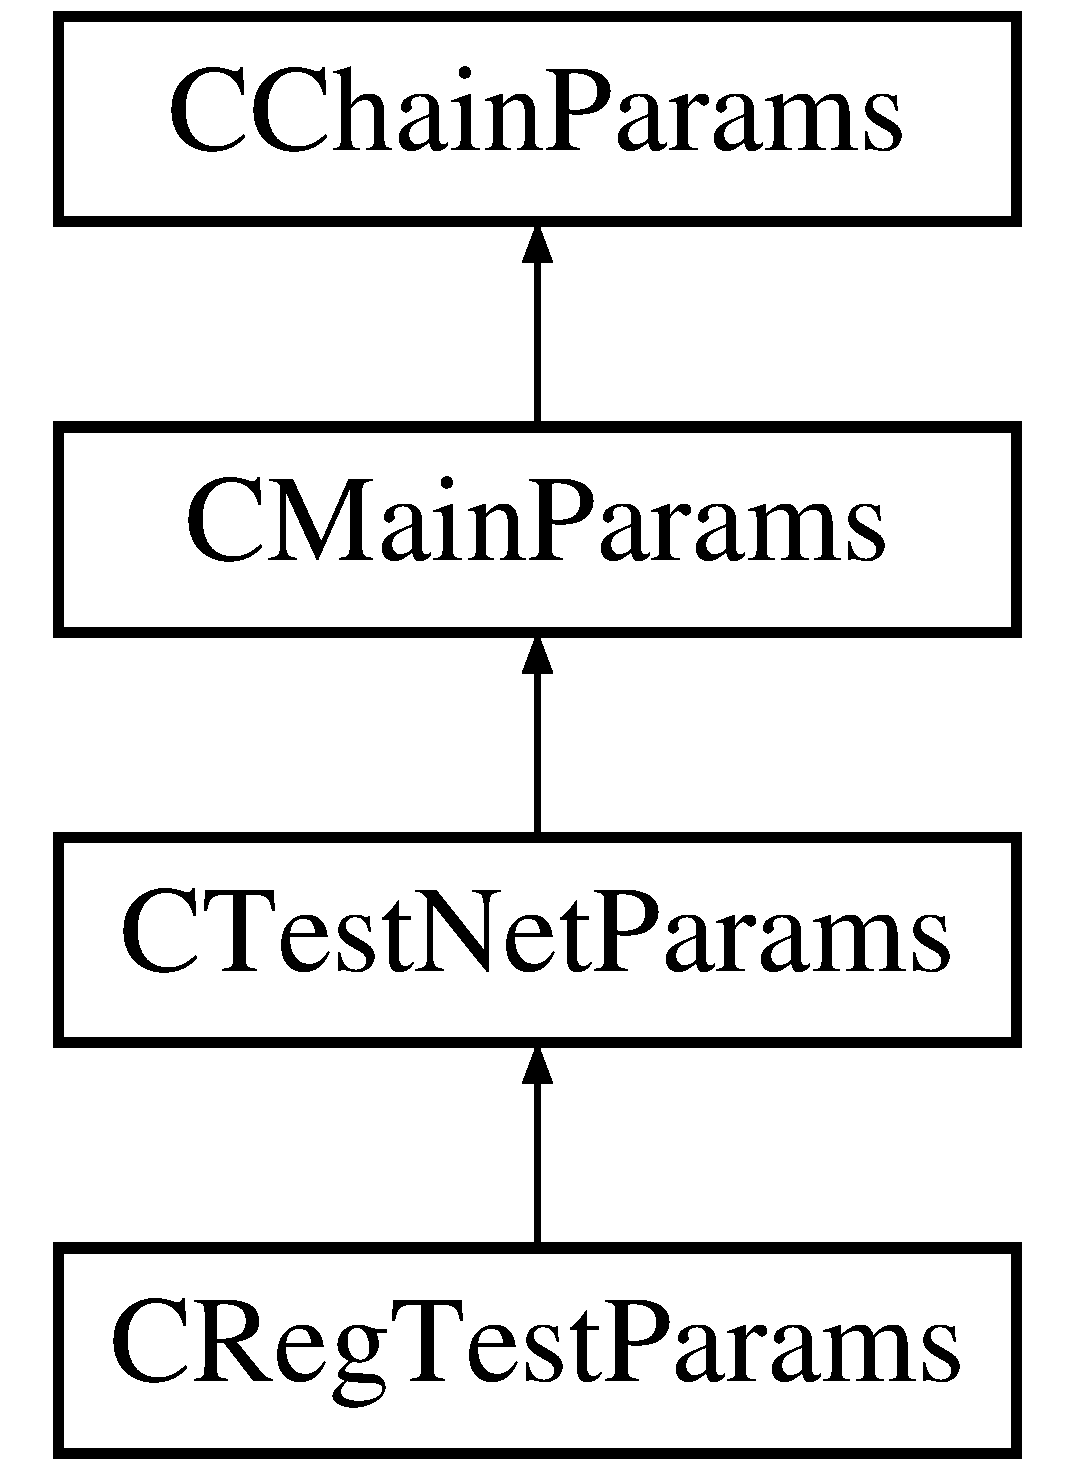
\includegraphics[height=4.000000cm]{class_c_reg_test_params}
\end{center}
\end{figure}
\subsection*{Public Member Functions}
\begin{DoxyCompactItemize}
\item 
\hyperlink{class_c_reg_test_params_aceca5a50765323f150ac608ca43db4fd}{C\+Reg\+Test\+Params} ()
\item 
const \hyperlink{struct_checkpoints_1_1_c_checkpoint_data}{Checkpoints\+::\+C\+Checkpoint\+Data} \& \hyperlink{class_c_reg_test_params_ab748b010a203dbdf6e5f77eb8b6f7cb0}{Checkpoints} () const 
\end{DoxyCompactItemize}
\subsection*{Additional Inherited Members}


\subsection{Detailed Description}
Regression test 

\subsection{Constructor \& Destructor Documentation}
\hypertarget{class_c_reg_test_params_aceca5a50765323f150ac608ca43db4fd}{}\index{C\+Reg\+Test\+Params@{C\+Reg\+Test\+Params}!C\+Reg\+Test\+Params@{C\+Reg\+Test\+Params}}
\index{C\+Reg\+Test\+Params@{C\+Reg\+Test\+Params}!C\+Reg\+Test\+Params@{C\+Reg\+Test\+Params}}
\subsubsection[{C\+Reg\+Test\+Params}]{\setlength{\rightskip}{0pt plus 5cm}C\+Reg\+Test\+Params\+::\+C\+Reg\+Test\+Params (
\begin{DoxyParamCaption}
{}
\end{DoxyParamCaption}
)\hspace{0.3cm}{\ttfamily [inline]}}\label{class_c_reg_test_params_aceca5a50765323f150ac608ca43db4fd}
Regtest mode doesn\textquotesingle{}t have any fixed seeds.

Regtest mode doesn\textquotesingle{}t have any D\+N\+S seeds. 

\subsection{Member Function Documentation}
\hypertarget{class_c_reg_test_params_ab748b010a203dbdf6e5f77eb8b6f7cb0}{}\index{C\+Reg\+Test\+Params@{C\+Reg\+Test\+Params}!Checkpoints@{Checkpoints}}
\index{Checkpoints@{Checkpoints}!C\+Reg\+Test\+Params@{C\+Reg\+Test\+Params}}
\subsubsection[{Checkpoints}]{\setlength{\rightskip}{0pt plus 5cm}const {\bf Checkpoints\+::\+C\+Checkpoint\+Data}\& C\+Reg\+Test\+Params\+::\+Checkpoints (
\begin{DoxyParamCaption}
{}
\end{DoxyParamCaption}
) const\hspace{0.3cm}{\ttfamily [inline]}, {\ttfamily [virtual]}}\label{class_c_reg_test_params_ab748b010a203dbdf6e5f77eb8b6f7cb0}


Reimplemented from \hyperlink{class_c_test_net_params_a1a8828912574c509825ccc5cc0e0a9be}{C\+Test\+Net\+Params}.



The documentation for this class was generated from the following file\+:\begin{DoxyCompactItemize}
\item 
C\+:/\+Users/\+Joe/\+Documents/\+School/\+C\+S\+C17\+A/bitcoin/src/\hyperlink{chainparams_8cpp}{chainparams.\+cpp}\end{DoxyCompactItemize}

\hypertarget{class_c_r_p_c_command}{}\section{C\+R\+P\+C\+Command Class Reference}
\label{class_c_r_p_c_command}\index{C\+R\+P\+C\+Command@{C\+R\+P\+C\+Command}}


{\ttfamily \#include $<$rpcserver.\+h$>$}

\subsection*{Public Attributes}
\begin{DoxyCompactItemize}
\item 
std\+::string \hyperlink{class_c_r_p_c_command_a27dd2710a5f94011f891f6a2efcec53a}{category}
\item 
std\+::string \hyperlink{class_c_r_p_c_command_a8da584c0d2d98be22ebff74d3cf2221c}{name}
\item 
\hyperlink{rpcserver_8h_a55410ecf7b981d238edda579f8c97040}{rpcfn\+\_\+type} \hyperlink{class_c_r_p_c_command_a197a7eba565b4d9673537655fcbc1344}{actor}
\item 
bool \hyperlink{class_c_r_p_c_command_a7f0b10e619917a3019f36ba5fa538adb}{ok\+Safe\+Mode}
\end{DoxyCompactItemize}


\subsection{Member Data Documentation}
\hypertarget{class_c_r_p_c_command_a197a7eba565b4d9673537655fcbc1344}{}\index{C\+R\+P\+C\+Command@{C\+R\+P\+C\+Command}!actor@{actor}}
\index{actor@{actor}!C\+R\+P\+C\+Command@{C\+R\+P\+C\+Command}}
\subsubsection[{actor}]{\setlength{\rightskip}{0pt plus 5cm}{\bf rpcfn\+\_\+type} C\+R\+P\+C\+Command\+::actor}\label{class_c_r_p_c_command_a197a7eba565b4d9673537655fcbc1344}
\hypertarget{class_c_r_p_c_command_a27dd2710a5f94011f891f6a2efcec53a}{}\index{C\+R\+P\+C\+Command@{C\+R\+P\+C\+Command}!category@{category}}
\index{category@{category}!C\+R\+P\+C\+Command@{C\+R\+P\+C\+Command}}
\subsubsection[{category}]{\setlength{\rightskip}{0pt plus 5cm}std\+::string C\+R\+P\+C\+Command\+::category}\label{class_c_r_p_c_command_a27dd2710a5f94011f891f6a2efcec53a}
\hypertarget{class_c_r_p_c_command_a8da584c0d2d98be22ebff74d3cf2221c}{}\index{C\+R\+P\+C\+Command@{C\+R\+P\+C\+Command}!name@{name}}
\index{name@{name}!C\+R\+P\+C\+Command@{C\+R\+P\+C\+Command}}
\subsubsection[{name}]{\setlength{\rightskip}{0pt plus 5cm}std\+::string C\+R\+P\+C\+Command\+::name}\label{class_c_r_p_c_command_a8da584c0d2d98be22ebff74d3cf2221c}
\hypertarget{class_c_r_p_c_command_a7f0b10e619917a3019f36ba5fa538adb}{}\index{C\+R\+P\+C\+Command@{C\+R\+P\+C\+Command}!ok\+Safe\+Mode@{ok\+Safe\+Mode}}
\index{ok\+Safe\+Mode@{ok\+Safe\+Mode}!C\+R\+P\+C\+Command@{C\+R\+P\+C\+Command}}
\subsubsection[{ok\+Safe\+Mode}]{\setlength{\rightskip}{0pt plus 5cm}bool C\+R\+P\+C\+Command\+::ok\+Safe\+Mode}\label{class_c_r_p_c_command_a7f0b10e619917a3019f36ba5fa538adb}


The documentation for this class was generated from the following file\+:\begin{DoxyCompactItemize}
\item 
C\+:/\+Users/\+Joe/\+Documents/\+School/\+C\+S\+C17\+A/bitcoin/src/\hyperlink{rpcserver_8h}{rpcserver.\+h}\end{DoxyCompactItemize}

\hypertarget{class_c_r_p_c_convert_param}{}\section{C\+R\+P\+C\+Convert\+Param Class Reference}
\label{class_c_r_p_c_convert_param}\index{C\+R\+P\+C\+Convert\+Param@{C\+R\+P\+C\+Convert\+Param}}
\subsection*{Public Attributes}
\begin{DoxyCompactItemize}
\item 
std\+::string \hyperlink{class_c_r_p_c_convert_param_a072d6cde94ea57223445dee927ee1527}{method\+Name}
\item 
int \hyperlink{class_c_r_p_c_convert_param_a3bd464f8d5db060616e7be8fbacb58f8}{param\+Idx}
\begin{DoxyCompactList}\small\item\em method whose params want conversion \end{DoxyCompactList}\end{DoxyCompactItemize}


\subsection{Member Data Documentation}
\hypertarget{class_c_r_p_c_convert_param_a072d6cde94ea57223445dee927ee1527}{}\index{C\+R\+P\+C\+Convert\+Param@{C\+R\+P\+C\+Convert\+Param}!method\+Name@{method\+Name}}
\index{method\+Name@{method\+Name}!C\+R\+P\+C\+Convert\+Param@{C\+R\+P\+C\+Convert\+Param}}
\subsubsection[{method\+Name}]{\setlength{\rightskip}{0pt plus 5cm}std\+::string C\+R\+P\+C\+Convert\+Param\+::method\+Name}\label{class_c_r_p_c_convert_param_a072d6cde94ea57223445dee927ee1527}
\hypertarget{class_c_r_p_c_convert_param_a3bd464f8d5db060616e7be8fbacb58f8}{}\index{C\+R\+P\+C\+Convert\+Param@{C\+R\+P\+C\+Convert\+Param}!param\+Idx@{param\+Idx}}
\index{param\+Idx@{param\+Idx}!C\+R\+P\+C\+Convert\+Param@{C\+R\+P\+C\+Convert\+Param}}
\subsubsection[{param\+Idx}]{\setlength{\rightskip}{0pt plus 5cm}int C\+R\+P\+C\+Convert\+Param\+::param\+Idx}\label{class_c_r_p_c_convert_param_a3bd464f8d5db060616e7be8fbacb58f8}


method whose params want conversion 



The documentation for this class was generated from the following file\+:\begin{DoxyCompactItemize}
\item 
C\+:/\+Users/\+Joe/\+Documents/\+School/\+C\+S\+C17\+A/bitcoin/src/\hyperlink{rpcclient_8cpp}{rpcclient.\+cpp}\end{DoxyCompactItemize}

\hypertarget{class_c_r_p_c_convert_table}{}\section{C\+R\+P\+C\+Convert\+Table Class Reference}
\label{class_c_r_p_c_convert_table}\index{C\+R\+P\+C\+Convert\+Table@{C\+R\+P\+C\+Convert\+Table}}
\subsection*{Public Member Functions}
\begin{DoxyCompactItemize}
\item 
\hyperlink{class_c_r_p_c_convert_table_a7f79dde2002bd2bc2178bd38f213922d}{C\+R\+P\+C\+Convert\+Table} ()
\item 
bool \hyperlink{class_c_r_p_c_convert_table_a034b770cb03e79074111b85eba889e58}{convert} (const std\+::string \&method, int idx)
\end{DoxyCompactItemize}


\subsection{Constructor \& Destructor Documentation}
\hypertarget{class_c_r_p_c_convert_table_a7f79dde2002bd2bc2178bd38f213922d}{}\index{C\+R\+P\+C\+Convert\+Table@{C\+R\+P\+C\+Convert\+Table}!C\+R\+P\+C\+Convert\+Table@{C\+R\+P\+C\+Convert\+Table}}
\index{C\+R\+P\+C\+Convert\+Table@{C\+R\+P\+C\+Convert\+Table}!C\+R\+P\+C\+Convert\+Table@{C\+R\+P\+C\+Convert\+Table}}
\subsubsection[{C\+R\+P\+C\+Convert\+Table}]{\setlength{\rightskip}{0pt plus 5cm}C\+R\+P\+C\+Convert\+Table\+::\+C\+R\+P\+C\+Convert\+Table (
\begin{DoxyParamCaption}
{}
\end{DoxyParamCaption}
)}\label{class_c_r_p_c_convert_table_a7f79dde2002bd2bc2178bd38f213922d}


\subsection{Member Function Documentation}
\hypertarget{class_c_r_p_c_convert_table_a034b770cb03e79074111b85eba889e58}{}\index{C\+R\+P\+C\+Convert\+Table@{C\+R\+P\+C\+Convert\+Table}!convert@{convert}}
\index{convert@{convert}!C\+R\+P\+C\+Convert\+Table@{C\+R\+P\+C\+Convert\+Table}}
\subsubsection[{convert}]{\setlength{\rightskip}{0pt plus 5cm}bool C\+R\+P\+C\+Convert\+Table\+::convert (
\begin{DoxyParamCaption}
\item[{const std\+::string \&}]{method, }
\item[{int}]{idx}
\end{DoxyParamCaption}
)\hspace{0.3cm}{\ttfamily [inline]}}\label{class_c_r_p_c_convert_table_a034b770cb03e79074111b85eba889e58}


The documentation for this class was generated from the following file\+:\begin{DoxyCompactItemize}
\item 
C\+:/\+Users/\+Joe/\+Documents/\+School/\+C\+S\+C17\+A/bitcoin/src/\hyperlink{rpcclient_8cpp}{rpcclient.\+cpp}\end{DoxyCompactItemize}

\hypertarget{class_c_r_p_c_table}{}\section{C\+R\+P\+C\+Table Class Reference}
\label{class_c_r_p_c_table}\index{C\+R\+P\+C\+Table@{C\+R\+P\+C\+Table}}


{\ttfamily \#include $<$rpcserver.\+h$>$}

\subsection*{Public Member Functions}
\begin{DoxyCompactItemize}
\item 
\hyperlink{class_c_r_p_c_table_a2e6e624bae4c149db2f5cbe0de84b121}{C\+R\+P\+C\+Table} ()
\item 
const \hyperlink{class_c_r_p_c_command}{C\+R\+P\+C\+Command} $\ast$ \hyperlink{class_c_r_p_c_table_a687ec69eb823d5f4e4dbc16f497681bf}{operator\mbox{[}$\,$\mbox{]}} (std\+::string \hyperlink{rest_8cpp_a8f8f80d37794cde9472343e4487ba3eb}{name}) const 
\item 
std\+::string \hyperlink{class_c_r_p_c_table_a220ae5b4ce013c79d097bfe96a94e2f0}{help} (std\+::string \hyperlink{rest_8cpp_a8f8f80d37794cde9472343e4487ba3eb}{name}) const 
\item 
json\+\_\+spirit\+::\+Value \hyperlink{class_c_r_p_c_table_aebba8d5a8f62089d1aa63278dbaf30a2}{execute} (const std\+::string \&method, const json\+\_\+spirit\+::\+Array \&params) const 
\end{DoxyCompactItemize}


\subsection{Detailed Description}
Bitcoin R\+P\+C command dispatcher. 

\subsection{Constructor \& Destructor Documentation}
\hypertarget{class_c_r_p_c_table_a2e6e624bae4c149db2f5cbe0de84b121}{}\index{C\+R\+P\+C\+Table@{C\+R\+P\+C\+Table}!C\+R\+P\+C\+Table@{C\+R\+P\+C\+Table}}
\index{C\+R\+P\+C\+Table@{C\+R\+P\+C\+Table}!C\+R\+P\+C\+Table@{C\+R\+P\+C\+Table}}
\subsubsection[{C\+R\+P\+C\+Table}]{\setlength{\rightskip}{0pt plus 5cm}C\+R\+P\+C\+Table\+::\+C\+R\+P\+C\+Table (
\begin{DoxyParamCaption}
{}
\end{DoxyParamCaption}
)}\label{class_c_r_p_c_table_a2e6e624bae4c149db2f5cbe0de84b121}


\subsection{Member Function Documentation}
\hypertarget{class_c_r_p_c_table_aebba8d5a8f62089d1aa63278dbaf30a2}{}\index{C\+R\+P\+C\+Table@{C\+R\+P\+C\+Table}!execute@{execute}}
\index{execute@{execute}!C\+R\+P\+C\+Table@{C\+R\+P\+C\+Table}}
\subsubsection[{execute}]{\setlength{\rightskip}{0pt plus 5cm}json\+\_\+spirit\+::\+Value C\+R\+P\+C\+Table\+::execute (
\begin{DoxyParamCaption}
\item[{const std\+::string \&}]{method, }
\item[{const json\+\_\+spirit\+::\+Array \&}]{params}
\end{DoxyParamCaption}
) const}\label{class_c_r_p_c_table_aebba8d5a8f62089d1aa63278dbaf30a2}
Execute a method. 
\begin{DoxyParams}{Parameters}
{\em method} & Method to execute \\
\hline
{\em params} & Array of arguments (J\+S\+O\+N objects) \\
\hline
\end{DoxyParams}
\begin{DoxyReturn}{Returns}
Result of the call. 
\end{DoxyReturn}

\begin{DoxyExceptions}{Exceptions}
{\em an} & exception (json\+\_\+spirit\+::\+Value) when an error happens. \\
\hline
\end{DoxyExceptions}
\hypertarget{class_c_r_p_c_table_a220ae5b4ce013c79d097bfe96a94e2f0}{}\index{C\+R\+P\+C\+Table@{C\+R\+P\+C\+Table}!help@{help}}
\index{help@{help}!C\+R\+P\+C\+Table@{C\+R\+P\+C\+Table}}
\subsubsection[{help}]{\setlength{\rightskip}{0pt plus 5cm}string C\+R\+P\+C\+Table\+::help (
\begin{DoxyParamCaption}
\item[{std\+::string}]{name}
\end{DoxyParamCaption}
) const}\label{class_c_r_p_c_table_a220ae5b4ce013c79d097bfe96a94e2f0}
Note\+: This interface may still be subject to change. \hypertarget{class_c_r_p_c_table_a687ec69eb823d5f4e4dbc16f497681bf}{}\index{C\+R\+P\+C\+Table@{C\+R\+P\+C\+Table}!operator\mbox{[}$\,$\mbox{]}@{operator[]}}
\index{operator\mbox{[}$\,$\mbox{]}@{operator[]}!C\+R\+P\+C\+Table@{C\+R\+P\+C\+Table}}
\subsubsection[{operator[]}]{\setlength{\rightskip}{0pt plus 5cm}const {\bf C\+R\+P\+C\+Command} $\ast$ C\+R\+P\+C\+Table\+::operator\mbox{[}$\,$\mbox{]} (
\begin{DoxyParamCaption}
\item[{std\+::string}]{name}
\end{DoxyParamCaption}
) const}\label{class_c_r_p_c_table_a687ec69eb823d5f4e4dbc16f497681bf}


The documentation for this class was generated from the following files\+:\begin{DoxyCompactItemize}
\item 
C\+:/\+Users/\+Joe/\+Documents/\+School/\+C\+S\+C17\+A/bitcoin/src/\hyperlink{rpcserver_8h}{rpcserver.\+h}\item 
C\+:/\+Users/\+Joe/\+Documents/\+School/\+C\+S\+C17\+A/bitcoin/src/\hyperlink{rpcserver_8cpp}{rpcserver.\+cpp}\end{DoxyCompactItemize}

\hypertarget{class_c_script_check}{}\section{C\+Script\+Check Class Reference}
\label{class_c_script_check}\index{C\+Script\+Check@{C\+Script\+Check}}


{\ttfamily \#include $<$main.\+h$>$}

\subsection*{Public Member Functions}
\begin{DoxyCompactItemize}
\item 
\hyperlink{class_c_script_check_a4a3bf9c971437bcb6fae3e3254a8c178}{C\+Script\+Check} ()
\item 
\hyperlink{class_c_script_check_a2617b99b66cd1de327478b74d8441c76}{C\+Script\+Check} (const \hyperlink{class_c_coins}{C\+Coins} \&tx\+From\+In, const C\+Transaction \&tx\+To\+In, unsigned int n\+In\+In, unsigned int n\+Flags\+In, bool cache\+In)
\item 
bool \hyperlink{class_c_script_check_a108d4c713338308be3867ed4e65b80c5}{operator()} ()
\item 
void \hyperlink{class_c_script_check_a69fbde608ff29c1885b8b9caf0fd40a0}{swap} (\hyperlink{class_c_script_check}{C\+Script\+Check} \&check)
\item 
Script\+Error \hyperlink{class_c_script_check_a4bad3434ddad70669f634879a8af132e}{Get\+Script\+Error} () const 
\end{DoxyCompactItemize}


\subsection{Detailed Description}
Closure representing one script verification Note that this stores references to the spending transaction 

\subsection{Constructor \& Destructor Documentation}
\hypertarget{class_c_script_check_a4a3bf9c971437bcb6fae3e3254a8c178}{}\index{C\+Script\+Check@{C\+Script\+Check}!C\+Script\+Check@{C\+Script\+Check}}
\index{C\+Script\+Check@{C\+Script\+Check}!C\+Script\+Check@{C\+Script\+Check}}
\subsubsection[{C\+Script\+Check}]{\setlength{\rightskip}{0pt plus 5cm}C\+Script\+Check\+::\+C\+Script\+Check (
\begin{DoxyParamCaption}
{}
\end{DoxyParamCaption}
)\hspace{0.3cm}{\ttfamily [inline]}}\label{class_c_script_check_a4a3bf9c971437bcb6fae3e3254a8c178}
\hypertarget{class_c_script_check_a2617b99b66cd1de327478b74d8441c76}{}\index{C\+Script\+Check@{C\+Script\+Check}!C\+Script\+Check@{C\+Script\+Check}}
\index{C\+Script\+Check@{C\+Script\+Check}!C\+Script\+Check@{C\+Script\+Check}}
\subsubsection[{C\+Script\+Check}]{\setlength{\rightskip}{0pt plus 5cm}C\+Script\+Check\+::\+C\+Script\+Check (
\begin{DoxyParamCaption}
\item[{const {\bf C\+Coins} \&}]{tx\+From\+In, }
\item[{const C\+Transaction \&}]{tx\+To\+In, }
\item[{unsigned int}]{n\+In\+In, }
\item[{unsigned int}]{n\+Flags\+In, }
\item[{bool}]{cache\+In}
\end{DoxyParamCaption}
)\hspace{0.3cm}{\ttfamily [inline]}}\label{class_c_script_check_a2617b99b66cd1de327478b74d8441c76}


\subsection{Member Function Documentation}
\hypertarget{class_c_script_check_a4bad3434ddad70669f634879a8af132e}{}\index{C\+Script\+Check@{C\+Script\+Check}!Get\+Script\+Error@{Get\+Script\+Error}}
\index{Get\+Script\+Error@{Get\+Script\+Error}!C\+Script\+Check@{C\+Script\+Check}}
\subsubsection[{Get\+Script\+Error}]{\setlength{\rightskip}{0pt plus 5cm}Script\+Error C\+Script\+Check\+::\+Get\+Script\+Error (
\begin{DoxyParamCaption}
{}
\end{DoxyParamCaption}
) const\hspace{0.3cm}{\ttfamily [inline]}}\label{class_c_script_check_a4bad3434ddad70669f634879a8af132e}
\hypertarget{class_c_script_check_a108d4c713338308be3867ed4e65b80c5}{}\index{C\+Script\+Check@{C\+Script\+Check}!operator()@{operator()}}
\index{operator()@{operator()}!C\+Script\+Check@{C\+Script\+Check}}
\subsubsection[{operator()}]{\setlength{\rightskip}{0pt plus 5cm}bool C\+Script\+Check\+::operator() (
\begin{DoxyParamCaption}
{}
\end{DoxyParamCaption}
)}\label{class_c_script_check_a108d4c713338308be3867ed4e65b80c5}
\hypertarget{class_c_script_check_a69fbde608ff29c1885b8b9caf0fd40a0}{}\index{C\+Script\+Check@{C\+Script\+Check}!swap@{swap}}
\index{swap@{swap}!C\+Script\+Check@{C\+Script\+Check}}
\subsubsection[{swap}]{\setlength{\rightskip}{0pt plus 5cm}void C\+Script\+Check\+::swap (
\begin{DoxyParamCaption}
\item[{{\bf C\+Script\+Check} \&}]{check}
\end{DoxyParamCaption}
)\hspace{0.3cm}{\ttfamily [inline]}}\label{class_c_script_check_a69fbde608ff29c1885b8b9caf0fd40a0}


The documentation for this class was generated from the following files\+:\begin{DoxyCompactItemize}
\item 
C\+:/\+Users/\+Joe/\+Documents/\+School/\+C\+S\+C17\+A/bitcoin/src/\hyperlink{main_8h}{main.\+h}\item 
C\+:/\+Users/\+Joe/\+Documents/\+School/\+C\+S\+C17\+A/bitcoin/src/\hyperlink{main_8cpp}{main.\+cpp}\end{DoxyCompactItemize}

\hypertarget{class_c_script_compressor}{}\section{C\+Script\+Compressor Class Reference}
\label{class_c_script_compressor}\index{C\+Script\+Compressor@{C\+Script\+Compressor}}


{\ttfamily \#include $<$compressor.\+h$>$}

\subsection*{Public Member Functions}
\begin{DoxyCompactItemize}
\item 
\hyperlink{class_c_script_compressor_aad31afe3d14387b163b5c043e834ca2b}{C\+Script\+Compressor} (C\+Script \&script\+In)
\item 
unsigned int \hyperlink{class_c_script_compressor_a3b3dd61547c3dc2f7ba9325f74b9ec5f}{Get\+Serialize\+Size} (int n\+Type, int n\+Version) const 
\item 
{\footnotesize template$<$typename Stream $>$ }\\void \hyperlink{class_c_script_compressor_a9d8168293e0a6d0fd8c4aeb63a346525}{Serialize} (Stream \&s, int n\+Type, int n\+Version) const 
\item 
{\footnotesize template$<$typename Stream $>$ }\\void \hyperlink{class_c_script_compressor_a016fa6e3d2735d95fcf773271da073d5}{Unserialize} (Stream \&s, int n\+Type, int n\+Version)
\end{DoxyCompactItemize}
\subsection*{Protected Member Functions}
\begin{DoxyCompactItemize}
\item 
bool \hyperlink{class_c_script_compressor_a13afc45e3a0a8a3d634cfafba9b2a040}{Is\+To\+Key\+I\+D} (\hyperlink{class_c_key_i_d}{C\+Key\+I\+D} \&hash) const 
\item 
bool \hyperlink{class_c_script_compressor_a6da015ff028139ef52e7376166b04928}{Is\+To\+Script\+I\+D} (C\+Script\+I\+D \&hash) const 
\item 
bool \hyperlink{class_c_script_compressor_a4cec58b09c4ab7873b5884ed690ed0f9}{Is\+To\+Pub\+Key} (\hyperlink{class_c_pub_key}{C\+Pub\+Key} \&pubkey) const 
\item 
bool \hyperlink{class_c_script_compressor_a98cb19f185efc85a395a5332574ef56b}{Compress} (std\+::vector$<$ unsigned char $>$ \&out) const 
\item 
unsigned int \hyperlink{class_c_script_compressor_a0e4f4c405f4a937c95fd4270db4d7d66}{Get\+Special\+Size} (unsigned int n\+Size) const 
\item 
bool \hyperlink{class_c_script_compressor_a1feb663ddab3a45218c7cb02f2a25717}{Decompress} (unsigned int n\+Size, const std\+::vector$<$ unsigned char $>$ \&out)
\end{DoxyCompactItemize}


\subsection{Detailed Description}
Compact serializer for scripts.

It detects common cases and encodes them much more efficiently. 3 special cases are defined\+:
\begin{DoxyItemize}
\item Pay to pubkey hash (encoded as 21 bytes)
\item Pay to script hash (encoded as 21 bytes)
\item Pay to pubkey starting with 0x02, 0x03 or 0x04 (encoded as 33 bytes)
\end{DoxyItemize}

Other scripts up to 121 bytes require 1 byte + script length. Above that, scripts up to 16505 bytes require 2 bytes + script length. 

\subsection{Constructor \& Destructor Documentation}
\hypertarget{class_c_script_compressor_aad31afe3d14387b163b5c043e834ca2b}{}\index{C\+Script\+Compressor@{C\+Script\+Compressor}!C\+Script\+Compressor@{C\+Script\+Compressor}}
\index{C\+Script\+Compressor@{C\+Script\+Compressor}!C\+Script\+Compressor@{C\+Script\+Compressor}}
\subsubsection[{C\+Script\+Compressor}]{\setlength{\rightskip}{0pt plus 5cm}C\+Script\+Compressor\+::\+C\+Script\+Compressor (
\begin{DoxyParamCaption}
\item[{C\+Script \&}]{script\+In}
\end{DoxyParamCaption}
)\hspace{0.3cm}{\ttfamily [inline]}}\label{class_c_script_compressor_aad31afe3d14387b163b5c043e834ca2b}


\subsection{Member Function Documentation}
\hypertarget{class_c_script_compressor_a98cb19f185efc85a395a5332574ef56b}{}\index{C\+Script\+Compressor@{C\+Script\+Compressor}!Compress@{Compress}}
\index{Compress@{Compress}!C\+Script\+Compressor@{C\+Script\+Compressor}}
\subsubsection[{Compress}]{\setlength{\rightskip}{0pt plus 5cm}bool C\+Script\+Compressor\+::\+Compress (
\begin{DoxyParamCaption}
\item[{std\+::vector$<$ unsigned char $>$ \&}]{out}
\end{DoxyParamCaption}
) const\hspace{0.3cm}{\ttfamily [protected]}}\label{class_c_script_compressor_a98cb19f185efc85a395a5332574ef56b}
\hypertarget{class_c_script_compressor_a1feb663ddab3a45218c7cb02f2a25717}{}\index{C\+Script\+Compressor@{C\+Script\+Compressor}!Decompress@{Decompress}}
\index{Decompress@{Decompress}!C\+Script\+Compressor@{C\+Script\+Compressor}}
\subsubsection[{Decompress}]{\setlength{\rightskip}{0pt plus 5cm}bool C\+Script\+Compressor\+::\+Decompress (
\begin{DoxyParamCaption}
\item[{unsigned int}]{n\+Size, }
\item[{const std\+::vector$<$ unsigned char $>$ \&}]{out}
\end{DoxyParamCaption}
)\hspace{0.3cm}{\ttfamily [protected]}}\label{class_c_script_compressor_a1feb663ddab3a45218c7cb02f2a25717}
\hypertarget{class_c_script_compressor_a3b3dd61547c3dc2f7ba9325f74b9ec5f}{}\index{C\+Script\+Compressor@{C\+Script\+Compressor}!Get\+Serialize\+Size@{Get\+Serialize\+Size}}
\index{Get\+Serialize\+Size@{Get\+Serialize\+Size}!C\+Script\+Compressor@{C\+Script\+Compressor}}
\subsubsection[{Get\+Serialize\+Size}]{\setlength{\rightskip}{0pt plus 5cm}unsigned int C\+Script\+Compressor\+::\+Get\+Serialize\+Size (
\begin{DoxyParamCaption}
\item[{int}]{n\+Type, }
\item[{int}]{n\+Version}
\end{DoxyParamCaption}
) const\hspace{0.3cm}{\ttfamily [inline]}}\label{class_c_script_compressor_a3b3dd61547c3dc2f7ba9325f74b9ec5f}
\hypertarget{class_c_script_compressor_a0e4f4c405f4a937c95fd4270db4d7d66}{}\index{C\+Script\+Compressor@{C\+Script\+Compressor}!Get\+Special\+Size@{Get\+Special\+Size}}
\index{Get\+Special\+Size@{Get\+Special\+Size}!C\+Script\+Compressor@{C\+Script\+Compressor}}
\subsubsection[{Get\+Special\+Size}]{\setlength{\rightskip}{0pt plus 5cm}unsigned int C\+Script\+Compressor\+::\+Get\+Special\+Size (
\begin{DoxyParamCaption}
\item[{unsigned int}]{n\+Size}
\end{DoxyParamCaption}
) const\hspace{0.3cm}{\ttfamily [protected]}}\label{class_c_script_compressor_a0e4f4c405f4a937c95fd4270db4d7d66}
\hypertarget{class_c_script_compressor_a13afc45e3a0a8a3d634cfafba9b2a040}{}\index{C\+Script\+Compressor@{C\+Script\+Compressor}!Is\+To\+Key\+I\+D@{Is\+To\+Key\+I\+D}}
\index{Is\+To\+Key\+I\+D@{Is\+To\+Key\+I\+D}!C\+Script\+Compressor@{C\+Script\+Compressor}}
\subsubsection[{Is\+To\+Key\+I\+D}]{\setlength{\rightskip}{0pt plus 5cm}bool C\+Script\+Compressor\+::\+Is\+To\+Key\+I\+D (
\begin{DoxyParamCaption}
\item[{{\bf C\+Key\+I\+D} \&}]{hash}
\end{DoxyParamCaption}
) const\hspace{0.3cm}{\ttfamily [protected]}}\label{class_c_script_compressor_a13afc45e3a0a8a3d634cfafba9b2a040}
These check for scripts for which a special case with a shorter encoding is defined. They are implemented separately from the C\+Script test, as these test for exact byte sequence correspondences, and are more strict. For example, Is\+To\+Pub\+Key also verifies whether the public key is valid (as invalid ones cannot be represented in compressed form). \hypertarget{class_c_script_compressor_a4cec58b09c4ab7873b5884ed690ed0f9}{}\index{C\+Script\+Compressor@{C\+Script\+Compressor}!Is\+To\+Pub\+Key@{Is\+To\+Pub\+Key}}
\index{Is\+To\+Pub\+Key@{Is\+To\+Pub\+Key}!C\+Script\+Compressor@{C\+Script\+Compressor}}
\subsubsection[{Is\+To\+Pub\+Key}]{\setlength{\rightskip}{0pt plus 5cm}bool C\+Script\+Compressor\+::\+Is\+To\+Pub\+Key (
\begin{DoxyParamCaption}
\item[{{\bf C\+Pub\+Key} \&}]{pubkey}
\end{DoxyParamCaption}
) const\hspace{0.3cm}{\ttfamily [protected]}}\label{class_c_script_compressor_a4cec58b09c4ab7873b5884ed690ed0f9}
\hypertarget{class_c_script_compressor_a6da015ff028139ef52e7376166b04928}{}\index{C\+Script\+Compressor@{C\+Script\+Compressor}!Is\+To\+Script\+I\+D@{Is\+To\+Script\+I\+D}}
\index{Is\+To\+Script\+I\+D@{Is\+To\+Script\+I\+D}!C\+Script\+Compressor@{C\+Script\+Compressor}}
\subsubsection[{Is\+To\+Script\+I\+D}]{\setlength{\rightskip}{0pt plus 5cm}bool C\+Script\+Compressor\+::\+Is\+To\+Script\+I\+D (
\begin{DoxyParamCaption}
\item[{C\+Script\+I\+D \&}]{hash}
\end{DoxyParamCaption}
) const\hspace{0.3cm}{\ttfamily [protected]}}\label{class_c_script_compressor_a6da015ff028139ef52e7376166b04928}
\hypertarget{class_c_script_compressor_a9d8168293e0a6d0fd8c4aeb63a346525}{}\index{C\+Script\+Compressor@{C\+Script\+Compressor}!Serialize@{Serialize}}
\index{Serialize@{Serialize}!C\+Script\+Compressor@{C\+Script\+Compressor}}
\subsubsection[{Serialize}]{\setlength{\rightskip}{0pt plus 5cm}template$<$typename Stream $>$ void C\+Script\+Compressor\+::\+Serialize (
\begin{DoxyParamCaption}
\item[{Stream \&}]{s, }
\item[{int}]{n\+Type, }
\item[{int}]{n\+Version}
\end{DoxyParamCaption}
) const\hspace{0.3cm}{\ttfamily [inline]}}\label{class_c_script_compressor_a9d8168293e0a6d0fd8c4aeb63a346525}
\hypertarget{class_c_script_compressor_a016fa6e3d2735d95fcf773271da073d5}{}\index{C\+Script\+Compressor@{C\+Script\+Compressor}!Unserialize@{Unserialize}}
\index{Unserialize@{Unserialize}!C\+Script\+Compressor@{C\+Script\+Compressor}}
\subsubsection[{Unserialize}]{\setlength{\rightskip}{0pt plus 5cm}template$<$typename Stream $>$ void C\+Script\+Compressor\+::\+Unserialize (
\begin{DoxyParamCaption}
\item[{Stream \&}]{s, }
\item[{int}]{n\+Type, }
\item[{int}]{n\+Version}
\end{DoxyParamCaption}
)\hspace{0.3cm}{\ttfamily [inline]}}\label{class_c_script_compressor_a016fa6e3d2735d95fcf773271da073d5}


The documentation for this class was generated from the following files\+:\begin{DoxyCompactItemize}
\item 
C\+:/\+Users/\+Joe/\+Documents/\+School/\+C\+S\+C17\+A/bitcoin/src/\hyperlink{compressor_8h}{compressor.\+h}\item 
C\+:/\+Users/\+Joe/\+Documents/\+School/\+C\+S\+C17\+A/bitcoin/src/\hyperlink{compressor_8cpp}{compressor.\+cpp}\end{DoxyCompactItemize}

\hypertarget{class_c_semaphore}{}\section{C\+Semaphore Class Reference}
\label{class_c_semaphore}\index{C\+Semaphore@{C\+Semaphore}}


{\ttfamily \#include $<$sync.\+h$>$}

\subsection*{Public Member Functions}
\begin{DoxyCompactItemize}
\item 
\hyperlink{class_c_semaphore_ac9cc749c7424852d7fb4378811d0dae1}{C\+Semaphore} (int init)
\item 
void \hyperlink{class_c_semaphore_a1c108bd981fe68527ec8ef5e7b0d116c}{wait} ()
\item 
bool \hyperlink{class_c_semaphore_abb8a07e6cac29dc72f044cd536a9f9e5}{try\+\_\+wait} ()
\item 
void \hyperlink{class_c_semaphore_af6a956f6c191e824485fd3af6db39318}{post} ()
\end{DoxyCompactItemize}


\subsection{Constructor \& Destructor Documentation}
\hypertarget{class_c_semaphore_ac9cc749c7424852d7fb4378811d0dae1}{}\index{C\+Semaphore@{C\+Semaphore}!C\+Semaphore@{C\+Semaphore}}
\index{C\+Semaphore@{C\+Semaphore}!C\+Semaphore@{C\+Semaphore}}
\subsubsection[{C\+Semaphore}]{\setlength{\rightskip}{0pt plus 5cm}C\+Semaphore\+::\+C\+Semaphore (
\begin{DoxyParamCaption}
\item[{int}]{init}
\end{DoxyParamCaption}
)\hspace{0.3cm}{\ttfamily [inline]}}\label{class_c_semaphore_ac9cc749c7424852d7fb4378811d0dae1}


\subsection{Member Function Documentation}
\hypertarget{class_c_semaphore_af6a956f6c191e824485fd3af6db39318}{}\index{C\+Semaphore@{C\+Semaphore}!post@{post}}
\index{post@{post}!C\+Semaphore@{C\+Semaphore}}
\subsubsection[{post}]{\setlength{\rightskip}{0pt plus 5cm}void C\+Semaphore\+::post (
\begin{DoxyParamCaption}
{}
\end{DoxyParamCaption}
)\hspace{0.3cm}{\ttfamily [inline]}}\label{class_c_semaphore_af6a956f6c191e824485fd3af6db39318}
\hypertarget{class_c_semaphore_abb8a07e6cac29dc72f044cd536a9f9e5}{}\index{C\+Semaphore@{C\+Semaphore}!try\+\_\+wait@{try\+\_\+wait}}
\index{try\+\_\+wait@{try\+\_\+wait}!C\+Semaphore@{C\+Semaphore}}
\subsubsection[{try\+\_\+wait}]{\setlength{\rightskip}{0pt plus 5cm}bool C\+Semaphore\+::try\+\_\+wait (
\begin{DoxyParamCaption}
{}
\end{DoxyParamCaption}
)\hspace{0.3cm}{\ttfamily [inline]}}\label{class_c_semaphore_abb8a07e6cac29dc72f044cd536a9f9e5}
\hypertarget{class_c_semaphore_a1c108bd981fe68527ec8ef5e7b0d116c}{}\index{C\+Semaphore@{C\+Semaphore}!wait@{wait}}
\index{wait@{wait}!C\+Semaphore@{C\+Semaphore}}
\subsubsection[{wait}]{\setlength{\rightskip}{0pt plus 5cm}void C\+Semaphore\+::wait (
\begin{DoxyParamCaption}
{}
\end{DoxyParamCaption}
)\hspace{0.3cm}{\ttfamily [inline]}}\label{class_c_semaphore_a1c108bd981fe68527ec8ef5e7b0d116c}


The documentation for this class was generated from the following file\+:\begin{DoxyCompactItemize}
\item 
C\+:/\+Users/\+Joe/\+Documents/\+School/\+C\+S\+C17\+A/bitcoin/src/\hyperlink{sync_8h}{sync.\+h}\end{DoxyCompactItemize}

\hypertarget{class_c_semaphore_grant}{}\section{C\+Semaphore\+Grant Class Reference}
\label{class_c_semaphore_grant}\index{C\+Semaphore\+Grant@{C\+Semaphore\+Grant}}


{\ttfamily \#include $<$sync.\+h$>$}

\subsection*{Public Member Functions}
\begin{DoxyCompactItemize}
\item 
void \hyperlink{class_c_semaphore_grant_ac52976968379ea8e2470cfba877c3e89}{Acquire} ()
\item 
void \hyperlink{class_c_semaphore_grant_a8d985eeace74e037baeb39bd2d586576}{Release} ()
\item 
bool \hyperlink{class_c_semaphore_grant_a9952d9ea087ced803c099f69992ebb1d}{Try\+Acquire} ()
\item 
void \hyperlink{class_c_semaphore_grant_ab3e6f84f304703abc52517b0c8de26cf}{Move\+To} (\hyperlink{class_c_semaphore_grant}{C\+Semaphore\+Grant} \&grant)
\item 
\hyperlink{class_c_semaphore_grant_a84ca79a4c8519f1a69697c060cabc51d}{C\+Semaphore\+Grant} ()
\item 
\hyperlink{class_c_semaphore_grant_a5998c457c7c223a8257166161d12b355}{C\+Semaphore\+Grant} (\hyperlink{class_c_semaphore}{C\+Semaphore} \&sema, bool f\+Try=false)
\item 
\hyperlink{class_c_semaphore_grant_aaba5579eb3ad3647d79e71c9970dcb54}{$\sim$\+C\+Semaphore\+Grant} ()
\item 
\hyperlink{class_c_semaphore_grant_a91458b860e45949d87d770252e590a9b}{operator bool} ()
\end{DoxyCompactItemize}


\subsection{Detailed Description}
R\+A\+I\+I-\/style semaphore lock 

\subsection{Constructor \& Destructor Documentation}
\hypertarget{class_c_semaphore_grant_a84ca79a4c8519f1a69697c060cabc51d}{}\index{C\+Semaphore\+Grant@{C\+Semaphore\+Grant}!C\+Semaphore\+Grant@{C\+Semaphore\+Grant}}
\index{C\+Semaphore\+Grant@{C\+Semaphore\+Grant}!C\+Semaphore\+Grant@{C\+Semaphore\+Grant}}
\subsubsection[{C\+Semaphore\+Grant}]{\setlength{\rightskip}{0pt plus 5cm}C\+Semaphore\+Grant\+::\+C\+Semaphore\+Grant (
\begin{DoxyParamCaption}
{}
\end{DoxyParamCaption}
)\hspace{0.3cm}{\ttfamily [inline]}}\label{class_c_semaphore_grant_a84ca79a4c8519f1a69697c060cabc51d}
\hypertarget{class_c_semaphore_grant_a5998c457c7c223a8257166161d12b355}{}\index{C\+Semaphore\+Grant@{C\+Semaphore\+Grant}!C\+Semaphore\+Grant@{C\+Semaphore\+Grant}}
\index{C\+Semaphore\+Grant@{C\+Semaphore\+Grant}!C\+Semaphore\+Grant@{C\+Semaphore\+Grant}}
\subsubsection[{C\+Semaphore\+Grant}]{\setlength{\rightskip}{0pt plus 5cm}C\+Semaphore\+Grant\+::\+C\+Semaphore\+Grant (
\begin{DoxyParamCaption}
\item[{{\bf C\+Semaphore} \&}]{sema, }
\item[{bool}]{f\+Try = {\ttfamily false}}
\end{DoxyParamCaption}
)\hspace{0.3cm}{\ttfamily [inline]}}\label{class_c_semaphore_grant_a5998c457c7c223a8257166161d12b355}
\hypertarget{class_c_semaphore_grant_aaba5579eb3ad3647d79e71c9970dcb54}{}\index{C\+Semaphore\+Grant@{C\+Semaphore\+Grant}!````~C\+Semaphore\+Grant@{$\sim$\+C\+Semaphore\+Grant}}
\index{````~C\+Semaphore\+Grant@{$\sim$\+C\+Semaphore\+Grant}!C\+Semaphore\+Grant@{C\+Semaphore\+Grant}}
\subsubsection[{$\sim$\+C\+Semaphore\+Grant}]{\setlength{\rightskip}{0pt plus 5cm}C\+Semaphore\+Grant\+::$\sim$\+C\+Semaphore\+Grant (
\begin{DoxyParamCaption}
{}
\end{DoxyParamCaption}
)\hspace{0.3cm}{\ttfamily [inline]}}\label{class_c_semaphore_grant_aaba5579eb3ad3647d79e71c9970dcb54}


\subsection{Member Function Documentation}
\hypertarget{class_c_semaphore_grant_ac52976968379ea8e2470cfba877c3e89}{}\index{C\+Semaphore\+Grant@{C\+Semaphore\+Grant}!Acquire@{Acquire}}
\index{Acquire@{Acquire}!C\+Semaphore\+Grant@{C\+Semaphore\+Grant}}
\subsubsection[{Acquire}]{\setlength{\rightskip}{0pt plus 5cm}void C\+Semaphore\+Grant\+::\+Acquire (
\begin{DoxyParamCaption}
{}
\end{DoxyParamCaption}
)\hspace{0.3cm}{\ttfamily [inline]}}\label{class_c_semaphore_grant_ac52976968379ea8e2470cfba877c3e89}
\hypertarget{class_c_semaphore_grant_ab3e6f84f304703abc52517b0c8de26cf}{}\index{C\+Semaphore\+Grant@{C\+Semaphore\+Grant}!Move\+To@{Move\+To}}
\index{Move\+To@{Move\+To}!C\+Semaphore\+Grant@{C\+Semaphore\+Grant}}
\subsubsection[{Move\+To}]{\setlength{\rightskip}{0pt plus 5cm}void C\+Semaphore\+Grant\+::\+Move\+To (
\begin{DoxyParamCaption}
\item[{{\bf C\+Semaphore\+Grant} \&}]{grant}
\end{DoxyParamCaption}
)\hspace{0.3cm}{\ttfamily [inline]}}\label{class_c_semaphore_grant_ab3e6f84f304703abc52517b0c8de26cf}
\hypertarget{class_c_semaphore_grant_a91458b860e45949d87d770252e590a9b}{}\index{C\+Semaphore\+Grant@{C\+Semaphore\+Grant}!operator bool@{operator bool}}
\index{operator bool@{operator bool}!C\+Semaphore\+Grant@{C\+Semaphore\+Grant}}
\subsubsection[{operator bool}]{\setlength{\rightskip}{0pt plus 5cm}C\+Semaphore\+Grant\+::operator bool (
\begin{DoxyParamCaption}
{}
\end{DoxyParamCaption}
)\hspace{0.3cm}{\ttfamily [inline]}}\label{class_c_semaphore_grant_a91458b860e45949d87d770252e590a9b}
\hypertarget{class_c_semaphore_grant_a8d985eeace74e037baeb39bd2d586576}{}\index{C\+Semaphore\+Grant@{C\+Semaphore\+Grant}!Release@{Release}}
\index{Release@{Release}!C\+Semaphore\+Grant@{C\+Semaphore\+Grant}}
\subsubsection[{Release}]{\setlength{\rightskip}{0pt plus 5cm}void C\+Semaphore\+Grant\+::\+Release (
\begin{DoxyParamCaption}
{}
\end{DoxyParamCaption}
)\hspace{0.3cm}{\ttfamily [inline]}}\label{class_c_semaphore_grant_a8d985eeace74e037baeb39bd2d586576}
\hypertarget{class_c_semaphore_grant_a9952d9ea087ced803c099f69992ebb1d}{}\index{C\+Semaphore\+Grant@{C\+Semaphore\+Grant}!Try\+Acquire@{Try\+Acquire}}
\index{Try\+Acquire@{Try\+Acquire}!C\+Semaphore\+Grant@{C\+Semaphore\+Grant}}
\subsubsection[{Try\+Acquire}]{\setlength{\rightskip}{0pt plus 5cm}bool C\+Semaphore\+Grant\+::\+Try\+Acquire (
\begin{DoxyParamCaption}
{}
\end{DoxyParamCaption}
)\hspace{0.3cm}{\ttfamily [inline]}}\label{class_c_semaphore_grant_a9952d9ea087ced803c099f69992ebb1d}


The documentation for this class was generated from the following file\+:\begin{DoxyCompactItemize}
\item 
C\+:/\+Users/\+Joe/\+Documents/\+School/\+C\+S\+C17\+A/bitcoin/src/\hyperlink{sync_8h}{sync.\+h}\end{DoxyCompactItemize}

\hypertarget{struct_c_ser_action_serialize}{}\section{C\+Ser\+Action\+Serialize Struct Reference}
\label{struct_c_ser_action_serialize}\index{C\+Ser\+Action\+Serialize@{C\+Ser\+Action\+Serialize}}


{\ttfamily \#include $<$serialize.\+h$>$}

\subsection*{Public Member Functions}
\begin{DoxyCompactItemize}
\item 
bool \hyperlink{struct_c_ser_action_serialize_a23cb37386f29541f2d3f859f473226a8}{For\+Read} () const 
\end{DoxyCompactItemize}


\subsection{Detailed Description}
Support for A\+D\+D\+\_\+\+S\+E\+R\+I\+A\+L\+I\+Z\+E\+\_\+\+M\+E\+T\+H\+O\+D\+S and R\+E\+A\+D\+W\+R\+I\+T\+E macro 

\subsection{Member Function Documentation}
\hypertarget{struct_c_ser_action_serialize_a23cb37386f29541f2d3f859f473226a8}{}\index{C\+Ser\+Action\+Serialize@{C\+Ser\+Action\+Serialize}!For\+Read@{For\+Read}}
\index{For\+Read@{For\+Read}!C\+Ser\+Action\+Serialize@{C\+Ser\+Action\+Serialize}}
\subsubsection[{For\+Read}]{\setlength{\rightskip}{0pt plus 5cm}bool C\+Ser\+Action\+Serialize\+::\+For\+Read (
\begin{DoxyParamCaption}
{}
\end{DoxyParamCaption}
) const\hspace{0.3cm}{\ttfamily [inline]}}\label{struct_c_ser_action_serialize_a23cb37386f29541f2d3f859f473226a8}


The documentation for this struct was generated from the following file\+:\begin{DoxyCompactItemize}
\item 
C\+:/\+Users/\+Joe/\+Documents/\+School/\+C\+S\+C17\+A/bitcoin/src/\hyperlink{serialize_8h}{serialize.\+h}\end{DoxyCompactItemize}

\hypertarget{struct_c_ser_action_unserialize}{}\section{C\+Ser\+Action\+Unserialize Struct Reference}
\label{struct_c_ser_action_unserialize}\index{C\+Ser\+Action\+Unserialize@{C\+Ser\+Action\+Unserialize}}


{\ttfamily \#include $<$serialize.\+h$>$}

\subsection*{Public Member Functions}
\begin{DoxyCompactItemize}
\item 
bool \hyperlink{struct_c_ser_action_unserialize_a7b82400e5924c076b290a7d1ec8f7f34}{For\+Read} () const 
\end{DoxyCompactItemize}


\subsection{Member Function Documentation}
\hypertarget{struct_c_ser_action_unserialize_a7b82400e5924c076b290a7d1ec8f7f34}{}\index{C\+Ser\+Action\+Unserialize@{C\+Ser\+Action\+Unserialize}!For\+Read@{For\+Read}}
\index{For\+Read@{For\+Read}!C\+Ser\+Action\+Unserialize@{C\+Ser\+Action\+Unserialize}}
\subsubsection[{For\+Read}]{\setlength{\rightskip}{0pt plus 5cm}bool C\+Ser\+Action\+Unserialize\+::\+For\+Read (
\begin{DoxyParamCaption}
{}
\end{DoxyParamCaption}
) const\hspace{0.3cm}{\ttfamily [inline]}}\label{struct_c_ser_action_unserialize_a7b82400e5924c076b290a7d1ec8f7f34}


The documentation for this struct was generated from the following file\+:\begin{DoxyCompactItemize}
\item 
C\+:/\+Users/\+Joe/\+Documents/\+School/\+C\+S\+C17\+A/bitcoin/src/\hyperlink{serialize_8h}{serialize.\+h}\end{DoxyCompactItemize}

\hypertarget{class_c_service}{}\section{C\+Service Class Reference}
\label{class_c_service}\index{C\+Service@{C\+Service}}


{\ttfamily \#include $<$netbase.\+h$>$}

Inheritance diagram for C\+Service\+:\begin{figure}[H]
\begin{center}
\leavevmode
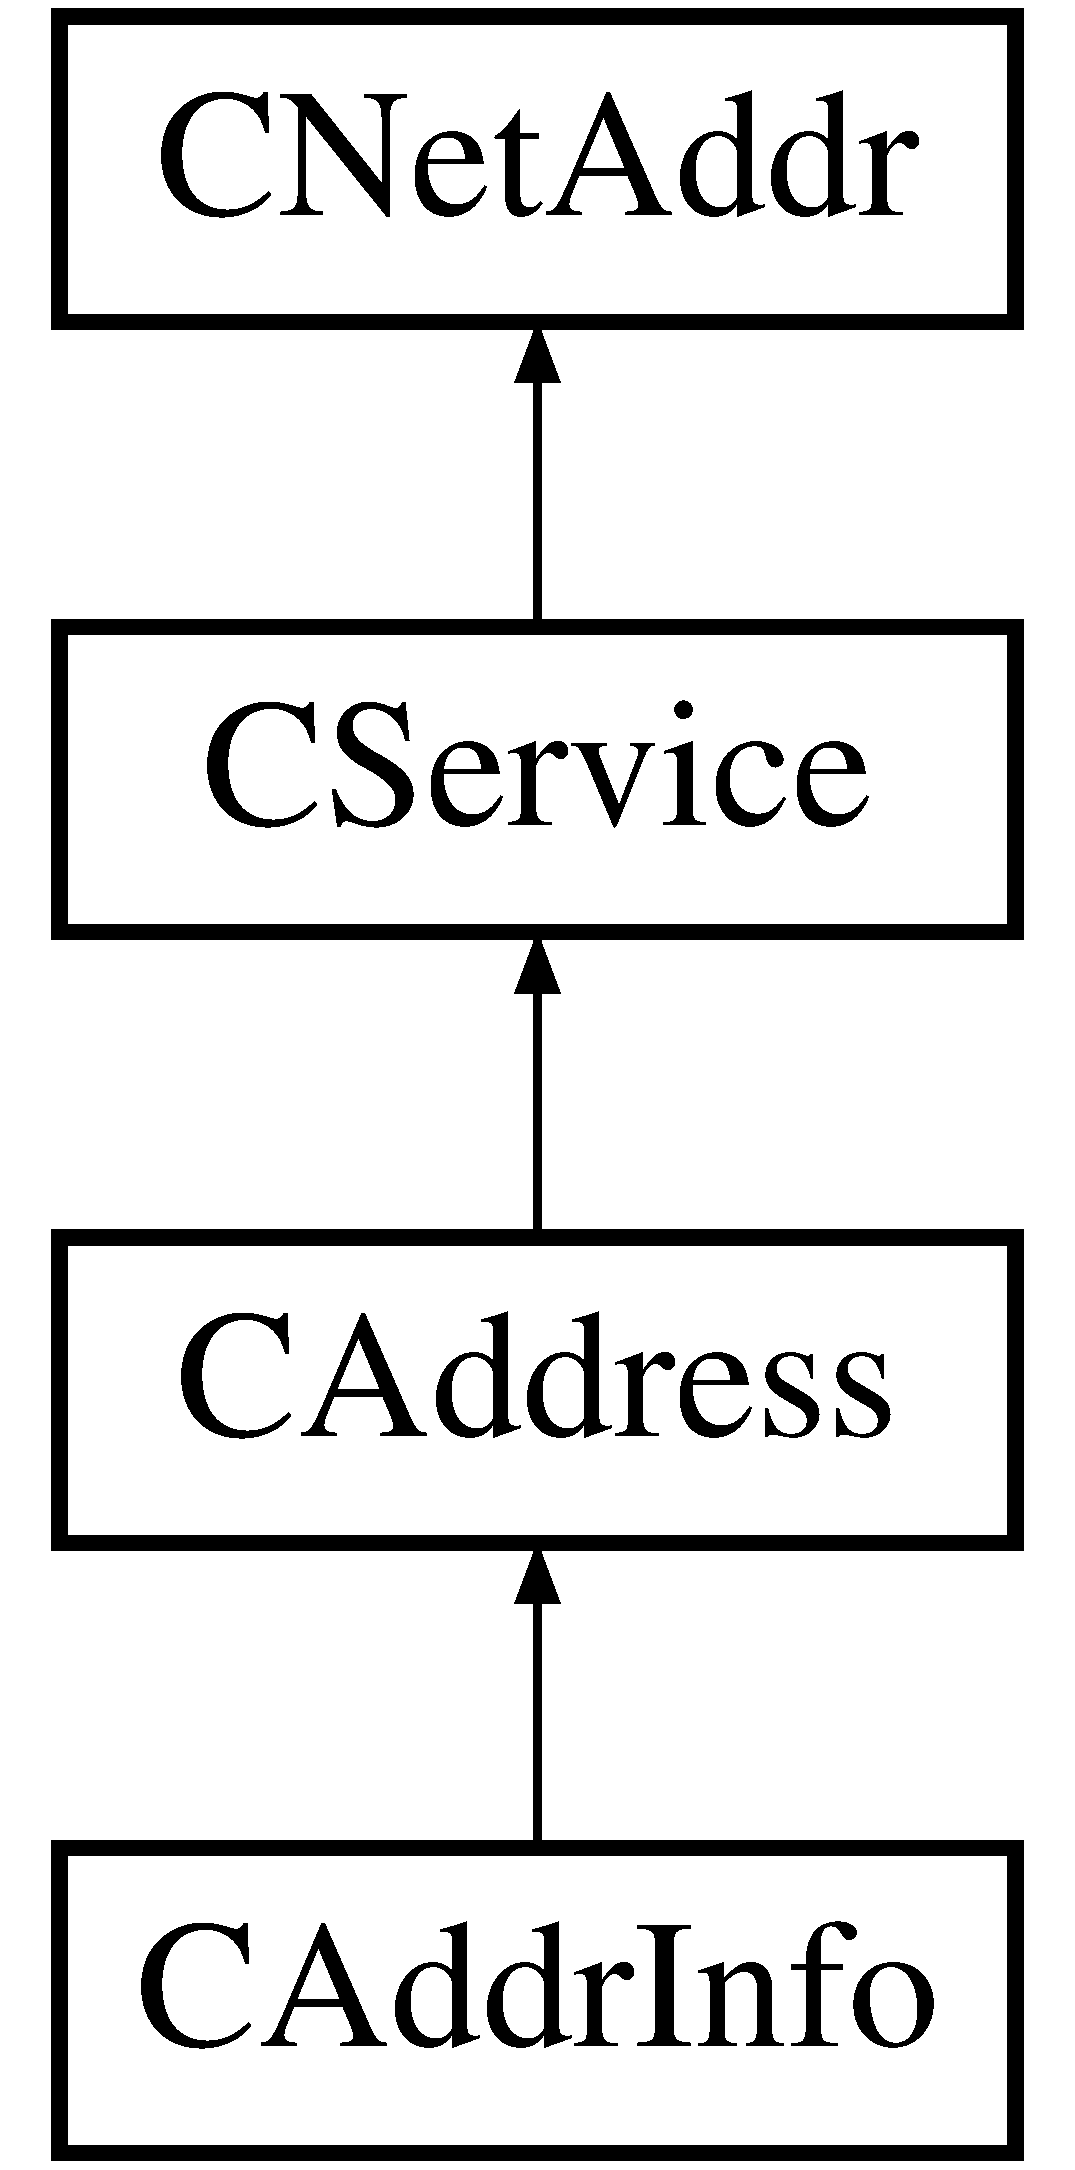
\includegraphics[height=4.000000cm]{class_c_service}
\end{center}
\end{figure}
\subsection*{Public Member Functions}
\begin{DoxyCompactItemize}
\item 
\hyperlink{class_c_service_a3003da1c50f2135123ebb3109340b9b2}{C\+Service} ()
\item 
\hyperlink{class_c_service_a43a0d18387ce3837d48020da47a1087c}{C\+Service} (const \hyperlink{class_c_net_addr}{C\+Net\+Addr} \&\hyperlink{class_c_net_addr_acff7ce68f33f8dfbfe6d79d80928d417}{ip}, unsigned short \hyperlink{class_c_service_aef17734203dc2125cbdf4d23e50be410}{port})
\item 
\hyperlink{class_c_service_a1fcc14e589f6d3e92b43707a5f71368f}{C\+Service} (const struct in\+\_\+addr \&ipv4\+Addr, unsigned short \hyperlink{class_c_service_aef17734203dc2125cbdf4d23e50be410}{port})
\item 
\hyperlink{class_c_service_aa54fd9204530445647cd3d45056881e9}{C\+Service} (const struct sockaddr\+\_\+in \&addr)
\item 
\hyperlink{class_c_service_a75b2a3cfa16642b0fcd74382203a9fdc}{C\+Service} (const char $\ast$psz\+Ip\+Port, int port\+Default, bool f\+Allow\+Lookup=false)
\item 
\hyperlink{class_c_service_ab8f5f4ae4e99a4edad8ba48642e36137}{C\+Service} (const char $\ast$psz\+Ip\+Port, bool f\+Allow\+Lookup=false)
\item 
\hyperlink{class_c_service_a677f74b3520148f3e47a19bb9986922b}{C\+Service} (const std\+::string \&str\+Ip\+Port, int port\+Default, bool f\+Allow\+Lookup=false)
\item 
\hyperlink{class_c_service_a19a7a713dd9a30b2f78260e61d9a2604}{C\+Service} (const std\+::string \&str\+Ip\+Port, bool f\+Allow\+Lookup=false)
\item 
void \hyperlink{class_c_service_aee07d7f18e672f16d26359e3cab779ff}{Init} ()
\item 
void \hyperlink{class_c_service_a3dedc3f12aa21bdbf1068b054d3e3d39}{Set\+Port} (unsigned short port\+In)
\item 
unsigned short \hyperlink{class_c_service_a49df6ecaf59be814632c4d7755f26637}{Get\+Port} () const 
\item 
bool \hyperlink{class_c_service_ab0f791c174511056236119cc1580faeb}{Get\+Sock\+Addr} (struct sockaddr $\ast$paddr, socklen\+\_\+t $\ast$addrlen) const 
\item 
bool \hyperlink{class_c_service_a77782219f5d85f326b4c089cb2636e6f}{Set\+Sock\+Addr} (const struct sockaddr $\ast$paddr)
\item 
std\+::vector$<$ unsigned char $>$ \hyperlink{class_c_service_a74d6e1526688229cb424584c29046e9e}{Get\+Key} () const 
\item 
std\+::string \hyperlink{class_c_service_a336f9848fe9364e260c76499be0351a5}{To\+String} () const 
\item 
std\+::string \hyperlink{class_c_service_a1e0f0b98239a9097044695a9e439bb46}{To\+String\+Port} () const 
\item 
std\+::string \hyperlink{class_c_service_a39b82301356b0dfc2a92befc727b77be}{To\+String\+I\+P\+Port} () const 
\item 
\hyperlink{class_c_service_a92fd246e176f01266cb36beae0c8f4fe}{C\+Service} (const struct in6\+\_\+addr \&ipv6\+Addr, unsigned short \hyperlink{class_c_service_aef17734203dc2125cbdf4d23e50be410}{port})
\item 
\hyperlink{class_c_service_ac0eb3107507be78cc683e7a7fa8d56e4}{C\+Service} (const struct sockaddr\+\_\+in6 \&addr)
\item 
{\footnotesize template$<$typename Stream , typename Operation $>$ }\\void \hyperlink{class_c_service_a0673ebec7bdc8558ce3fe1d63ea4d2e1}{Serialization\+Op} (Stream \&s, Operation ser\+\_\+action, int n\+Type, int n\+Version)
\end{DoxyCompactItemize}
\subsection*{Public Attributes}
\begin{DoxyCompactItemize}
\item 
\hyperlink{class_c_service_a3347aa84bd8f98ae853307ad4e47a4f5}{A\+D\+D\+\_\+\+S\+E\+R\+I\+A\+L\+I\+Z\+E\+\_\+\+M\+E\+T\+H\+O\+D\+S}
\end{DoxyCompactItemize}
\subsection*{Protected Attributes}
\begin{DoxyCompactItemize}
\item 
unsigned short \hyperlink{class_c_service_aef17734203dc2125cbdf4d23e50be410}{port}
\end{DoxyCompactItemize}
\subsection*{Friends}
\begin{DoxyCompactItemize}
\item 
bool \hyperlink{class_c_service_a7abc2516fa7e015cafcf9b98bc33e2ea}{operator==} (const \hyperlink{class_c_service}{C\+Service} \&a, const \hyperlink{class_c_service}{C\+Service} \&b)
\item 
bool \hyperlink{class_c_service_a5834e0ab5104fffac621ea53fa2c3860}{operator!=} (const \hyperlink{class_c_service}{C\+Service} \&a, const \hyperlink{class_c_service}{C\+Service} \&b)
\item 
bool \hyperlink{class_c_service_a26d0e22a8e7ae213b25467da3556c9e4}{operator$<$} (const \hyperlink{class_c_service}{C\+Service} \&a, const \hyperlink{class_c_service}{C\+Service} \&b)
\end{DoxyCompactItemize}


\subsection{Detailed Description}
A combination of a network address (\hyperlink{class_c_net_addr}{C\+Net\+Addr}) and a (T\+C\+P) port 

\subsection{Constructor \& Destructor Documentation}
\hypertarget{class_c_service_a3003da1c50f2135123ebb3109340b9b2}{}\index{C\+Service@{C\+Service}!C\+Service@{C\+Service}}
\index{C\+Service@{C\+Service}!C\+Service@{C\+Service}}
\subsubsection[{C\+Service}]{\setlength{\rightskip}{0pt plus 5cm}C\+Service\+::\+C\+Service (
\begin{DoxyParamCaption}
{}
\end{DoxyParamCaption}
)}\label{class_c_service_a3003da1c50f2135123ebb3109340b9b2}
\hypertarget{class_c_service_a43a0d18387ce3837d48020da47a1087c}{}\index{C\+Service@{C\+Service}!C\+Service@{C\+Service}}
\index{C\+Service@{C\+Service}!C\+Service@{C\+Service}}
\subsubsection[{C\+Service}]{\setlength{\rightskip}{0pt plus 5cm}C\+Service\+::\+C\+Service (
\begin{DoxyParamCaption}
\item[{const {\bf C\+Net\+Addr} \&}]{ip, }
\item[{unsigned short}]{port}
\end{DoxyParamCaption}
)}\label{class_c_service_a43a0d18387ce3837d48020da47a1087c}
\hypertarget{class_c_service_a1fcc14e589f6d3e92b43707a5f71368f}{}\index{C\+Service@{C\+Service}!C\+Service@{C\+Service}}
\index{C\+Service@{C\+Service}!C\+Service@{C\+Service}}
\subsubsection[{C\+Service}]{\setlength{\rightskip}{0pt plus 5cm}C\+Service\+::\+C\+Service (
\begin{DoxyParamCaption}
\item[{const struct in\+\_\+addr \&}]{ipv4\+Addr, }
\item[{unsigned short}]{port}
\end{DoxyParamCaption}
)}\label{class_c_service_a1fcc14e589f6d3e92b43707a5f71368f}
\hypertarget{class_c_service_aa54fd9204530445647cd3d45056881e9}{}\index{C\+Service@{C\+Service}!C\+Service@{C\+Service}}
\index{C\+Service@{C\+Service}!C\+Service@{C\+Service}}
\subsubsection[{C\+Service}]{\setlength{\rightskip}{0pt plus 5cm}C\+Service\+::\+C\+Service (
\begin{DoxyParamCaption}
\item[{const struct sockaddr\+\_\+in \&}]{addr}
\end{DoxyParamCaption}
)}\label{class_c_service_aa54fd9204530445647cd3d45056881e9}
\hypertarget{class_c_service_a75b2a3cfa16642b0fcd74382203a9fdc}{}\index{C\+Service@{C\+Service}!C\+Service@{C\+Service}}
\index{C\+Service@{C\+Service}!C\+Service@{C\+Service}}
\subsubsection[{C\+Service}]{\setlength{\rightskip}{0pt plus 5cm}C\+Service\+::\+C\+Service (
\begin{DoxyParamCaption}
\item[{const char $\ast$}]{psz\+Ip\+Port, }
\item[{int}]{port\+Default, }
\item[{bool}]{f\+Allow\+Lookup = {\ttfamily false}}
\end{DoxyParamCaption}
)\hspace{0.3cm}{\ttfamily [explicit]}}\label{class_c_service_a75b2a3cfa16642b0fcd74382203a9fdc}
\hypertarget{class_c_service_ab8f5f4ae4e99a4edad8ba48642e36137}{}\index{C\+Service@{C\+Service}!C\+Service@{C\+Service}}
\index{C\+Service@{C\+Service}!C\+Service@{C\+Service}}
\subsubsection[{C\+Service}]{\setlength{\rightskip}{0pt plus 5cm}C\+Service\+::\+C\+Service (
\begin{DoxyParamCaption}
\item[{const char $\ast$}]{psz\+Ip\+Port, }
\item[{bool}]{f\+Allow\+Lookup = {\ttfamily false}}
\end{DoxyParamCaption}
)\hspace{0.3cm}{\ttfamily [explicit]}}\label{class_c_service_ab8f5f4ae4e99a4edad8ba48642e36137}
\hypertarget{class_c_service_a677f74b3520148f3e47a19bb9986922b}{}\index{C\+Service@{C\+Service}!C\+Service@{C\+Service}}
\index{C\+Service@{C\+Service}!C\+Service@{C\+Service}}
\subsubsection[{C\+Service}]{\setlength{\rightskip}{0pt plus 5cm}C\+Service\+::\+C\+Service (
\begin{DoxyParamCaption}
\item[{const std\+::string \&}]{str\+Ip\+Port, }
\item[{int}]{port\+Default, }
\item[{bool}]{f\+Allow\+Lookup = {\ttfamily false}}
\end{DoxyParamCaption}
)\hspace{0.3cm}{\ttfamily [explicit]}}\label{class_c_service_a677f74b3520148f3e47a19bb9986922b}
\hypertarget{class_c_service_a19a7a713dd9a30b2f78260e61d9a2604}{}\index{C\+Service@{C\+Service}!C\+Service@{C\+Service}}
\index{C\+Service@{C\+Service}!C\+Service@{C\+Service}}
\subsubsection[{C\+Service}]{\setlength{\rightskip}{0pt plus 5cm}C\+Service\+::\+C\+Service (
\begin{DoxyParamCaption}
\item[{const std\+::string \&}]{str\+Ip\+Port, }
\item[{bool}]{f\+Allow\+Lookup = {\ttfamily false}}
\end{DoxyParamCaption}
)\hspace{0.3cm}{\ttfamily [explicit]}}\label{class_c_service_a19a7a713dd9a30b2f78260e61d9a2604}
\hypertarget{class_c_service_a92fd246e176f01266cb36beae0c8f4fe}{}\index{C\+Service@{C\+Service}!C\+Service@{C\+Service}}
\index{C\+Service@{C\+Service}!C\+Service@{C\+Service}}
\subsubsection[{C\+Service}]{\setlength{\rightskip}{0pt plus 5cm}C\+Service\+::\+C\+Service (
\begin{DoxyParamCaption}
\item[{const struct in6\+\_\+addr \&}]{ipv6\+Addr, }
\item[{unsigned short}]{port}
\end{DoxyParamCaption}
)}\label{class_c_service_a92fd246e176f01266cb36beae0c8f4fe}
\hypertarget{class_c_service_ac0eb3107507be78cc683e7a7fa8d56e4}{}\index{C\+Service@{C\+Service}!C\+Service@{C\+Service}}
\index{C\+Service@{C\+Service}!C\+Service@{C\+Service}}
\subsubsection[{C\+Service}]{\setlength{\rightskip}{0pt plus 5cm}C\+Service\+::\+C\+Service (
\begin{DoxyParamCaption}
\item[{const struct sockaddr\+\_\+in6 \&}]{addr}
\end{DoxyParamCaption}
)}\label{class_c_service_ac0eb3107507be78cc683e7a7fa8d56e4}


\subsection{Member Function Documentation}
\hypertarget{class_c_service_a74d6e1526688229cb424584c29046e9e}{}\index{C\+Service@{C\+Service}!Get\+Key@{Get\+Key}}
\index{Get\+Key@{Get\+Key}!C\+Service@{C\+Service}}
\subsubsection[{Get\+Key}]{\setlength{\rightskip}{0pt plus 5cm}std\+::vector$<$ unsigned char $>$ C\+Service\+::\+Get\+Key (
\begin{DoxyParamCaption}
{}
\end{DoxyParamCaption}
) const}\label{class_c_service_a74d6e1526688229cb424584c29046e9e}
\hypertarget{class_c_service_a49df6ecaf59be814632c4d7755f26637}{}\index{C\+Service@{C\+Service}!Get\+Port@{Get\+Port}}
\index{Get\+Port@{Get\+Port}!C\+Service@{C\+Service}}
\subsubsection[{Get\+Port}]{\setlength{\rightskip}{0pt plus 5cm}unsigned short C\+Service\+::\+Get\+Port (
\begin{DoxyParamCaption}
{}
\end{DoxyParamCaption}
) const}\label{class_c_service_a49df6ecaf59be814632c4d7755f26637}
\hypertarget{class_c_service_ab0f791c174511056236119cc1580faeb}{}\index{C\+Service@{C\+Service}!Get\+Sock\+Addr@{Get\+Sock\+Addr}}
\index{Get\+Sock\+Addr@{Get\+Sock\+Addr}!C\+Service@{C\+Service}}
\subsubsection[{Get\+Sock\+Addr}]{\setlength{\rightskip}{0pt plus 5cm}bool C\+Service\+::\+Get\+Sock\+Addr (
\begin{DoxyParamCaption}
\item[{struct sockaddr $\ast$}]{paddr, }
\item[{socklen\+\_\+t $\ast$}]{addrlen}
\end{DoxyParamCaption}
) const}\label{class_c_service_ab0f791c174511056236119cc1580faeb}
\hypertarget{class_c_service_aee07d7f18e672f16d26359e3cab779ff}{}\index{C\+Service@{C\+Service}!Init@{Init}}
\index{Init@{Init}!C\+Service@{C\+Service}}
\subsubsection[{Init}]{\setlength{\rightskip}{0pt plus 5cm}void C\+Service\+::\+Init (
\begin{DoxyParamCaption}
{}
\end{DoxyParamCaption}
)}\label{class_c_service_aee07d7f18e672f16d26359e3cab779ff}
\hypertarget{class_c_service_a0673ebec7bdc8558ce3fe1d63ea4d2e1}{}\index{C\+Service@{C\+Service}!Serialization\+Op@{Serialization\+Op}}
\index{Serialization\+Op@{Serialization\+Op}!C\+Service@{C\+Service}}
\subsubsection[{Serialization\+Op}]{\setlength{\rightskip}{0pt plus 5cm}template$<$typename Stream , typename Operation $>$ void C\+Service\+::\+Serialization\+Op (
\begin{DoxyParamCaption}
\item[{Stream \&}]{s, }
\item[{Operation}]{ser\+\_\+action, }
\item[{int}]{n\+Type, }
\item[{int}]{n\+Version}
\end{DoxyParamCaption}
)\hspace{0.3cm}{\ttfamily [inline]}}\label{class_c_service_a0673ebec7bdc8558ce3fe1d63ea4d2e1}
\hypertarget{class_c_service_a3dedc3f12aa21bdbf1068b054d3e3d39}{}\index{C\+Service@{C\+Service}!Set\+Port@{Set\+Port}}
\index{Set\+Port@{Set\+Port}!C\+Service@{C\+Service}}
\subsubsection[{Set\+Port}]{\setlength{\rightskip}{0pt plus 5cm}void C\+Service\+::\+Set\+Port (
\begin{DoxyParamCaption}
\item[{unsigned short}]{port\+In}
\end{DoxyParamCaption}
)}\label{class_c_service_a3dedc3f12aa21bdbf1068b054d3e3d39}
\hypertarget{class_c_service_a77782219f5d85f326b4c089cb2636e6f}{}\index{C\+Service@{C\+Service}!Set\+Sock\+Addr@{Set\+Sock\+Addr}}
\index{Set\+Sock\+Addr@{Set\+Sock\+Addr}!C\+Service@{C\+Service}}
\subsubsection[{Set\+Sock\+Addr}]{\setlength{\rightskip}{0pt plus 5cm}bool C\+Service\+::\+Set\+Sock\+Addr (
\begin{DoxyParamCaption}
\item[{const struct sockaddr $\ast$}]{paddr}
\end{DoxyParamCaption}
)}\label{class_c_service_a77782219f5d85f326b4c089cb2636e6f}
\hypertarget{class_c_service_a336f9848fe9364e260c76499be0351a5}{}\index{C\+Service@{C\+Service}!To\+String@{To\+String}}
\index{To\+String@{To\+String}!C\+Service@{C\+Service}}
\subsubsection[{To\+String}]{\setlength{\rightskip}{0pt plus 5cm}std\+::string C\+Service\+::\+To\+String (
\begin{DoxyParamCaption}
{}
\end{DoxyParamCaption}
) const}\label{class_c_service_a336f9848fe9364e260c76499be0351a5}
\hypertarget{class_c_service_a39b82301356b0dfc2a92befc727b77be}{}\index{C\+Service@{C\+Service}!To\+String\+I\+P\+Port@{To\+String\+I\+P\+Port}}
\index{To\+String\+I\+P\+Port@{To\+String\+I\+P\+Port}!C\+Service@{C\+Service}}
\subsubsection[{To\+String\+I\+P\+Port}]{\setlength{\rightskip}{0pt plus 5cm}std\+::string C\+Service\+::\+To\+String\+I\+P\+Port (
\begin{DoxyParamCaption}
{}
\end{DoxyParamCaption}
) const}\label{class_c_service_a39b82301356b0dfc2a92befc727b77be}
\hypertarget{class_c_service_a1e0f0b98239a9097044695a9e439bb46}{}\index{C\+Service@{C\+Service}!To\+String\+Port@{To\+String\+Port}}
\index{To\+String\+Port@{To\+String\+Port}!C\+Service@{C\+Service}}
\subsubsection[{To\+String\+Port}]{\setlength{\rightskip}{0pt plus 5cm}std\+::string C\+Service\+::\+To\+String\+Port (
\begin{DoxyParamCaption}
{}
\end{DoxyParamCaption}
) const}\label{class_c_service_a1e0f0b98239a9097044695a9e439bb46}


\subsection{Friends And Related Function Documentation}
\hypertarget{class_c_service_a5834e0ab5104fffac621ea53fa2c3860}{}\index{C\+Service@{C\+Service}!operator"!=@{operator"!=}}
\index{operator"!=@{operator"!=}!C\+Service@{C\+Service}}
\subsubsection[{operator"!=}]{\setlength{\rightskip}{0pt plus 5cm}bool operator!= (
\begin{DoxyParamCaption}
\item[{const {\bf C\+Service} \&}]{a, }
\item[{const {\bf C\+Service} \&}]{b}
\end{DoxyParamCaption}
)\hspace{0.3cm}{\ttfamily [friend]}}\label{class_c_service_a5834e0ab5104fffac621ea53fa2c3860}
\hypertarget{class_c_service_a26d0e22a8e7ae213b25467da3556c9e4}{}\index{C\+Service@{C\+Service}!operator$<$@{operator$<$}}
\index{operator$<$@{operator$<$}!C\+Service@{C\+Service}}
\subsubsection[{operator$<$}]{\setlength{\rightskip}{0pt plus 5cm}bool operator$<$ (
\begin{DoxyParamCaption}
\item[{const {\bf C\+Service} \&}]{a, }
\item[{const {\bf C\+Service} \&}]{b}
\end{DoxyParamCaption}
)\hspace{0.3cm}{\ttfamily [friend]}}\label{class_c_service_a26d0e22a8e7ae213b25467da3556c9e4}
\hypertarget{class_c_service_a7abc2516fa7e015cafcf9b98bc33e2ea}{}\index{C\+Service@{C\+Service}!operator==@{operator==}}
\index{operator==@{operator==}!C\+Service@{C\+Service}}
\subsubsection[{operator==}]{\setlength{\rightskip}{0pt plus 5cm}bool operator== (
\begin{DoxyParamCaption}
\item[{const {\bf C\+Service} \&}]{a, }
\item[{const {\bf C\+Service} \&}]{b}
\end{DoxyParamCaption}
)\hspace{0.3cm}{\ttfamily [friend]}}\label{class_c_service_a7abc2516fa7e015cafcf9b98bc33e2ea}


\subsection{Member Data Documentation}
\hypertarget{class_c_service_a3347aa84bd8f98ae853307ad4e47a4f5}{}\index{C\+Service@{C\+Service}!A\+D\+D\+\_\+\+S\+E\+R\+I\+A\+L\+I\+Z\+E\+\_\+\+M\+E\+T\+H\+O\+D\+S@{A\+D\+D\+\_\+\+S\+E\+R\+I\+A\+L\+I\+Z\+E\+\_\+\+M\+E\+T\+H\+O\+D\+S}}
\index{A\+D\+D\+\_\+\+S\+E\+R\+I\+A\+L\+I\+Z\+E\+\_\+\+M\+E\+T\+H\+O\+D\+S@{A\+D\+D\+\_\+\+S\+E\+R\+I\+A\+L\+I\+Z\+E\+\_\+\+M\+E\+T\+H\+O\+D\+S}!C\+Service@{C\+Service}}
\subsubsection[{A\+D\+D\+\_\+\+S\+E\+R\+I\+A\+L\+I\+Z\+E\+\_\+\+M\+E\+T\+H\+O\+D\+S}]{\setlength{\rightskip}{0pt plus 5cm}C\+Service\+::\+A\+D\+D\+\_\+\+S\+E\+R\+I\+A\+L\+I\+Z\+E\+\_\+\+M\+E\+T\+H\+O\+D\+S}\label{class_c_service_a3347aa84bd8f98ae853307ad4e47a4f5}
\hypertarget{class_c_service_aef17734203dc2125cbdf4d23e50be410}{}\index{C\+Service@{C\+Service}!port@{port}}
\index{port@{port}!C\+Service@{C\+Service}}
\subsubsection[{port}]{\setlength{\rightskip}{0pt plus 5cm}unsigned short C\+Service\+::port\hspace{0.3cm}{\ttfamily [protected]}}\label{class_c_service_aef17734203dc2125cbdf4d23e50be410}


The documentation for this class was generated from the following files\+:\begin{DoxyCompactItemize}
\item 
C\+:/\+Users/\+Joe/\+Documents/\+School/\+C\+S\+C17\+A/bitcoin/src/\hyperlink{netbase_8h}{netbase.\+h}\item 
C\+:/\+Users/\+Joe/\+Documents/\+School/\+C\+S\+C17\+A/bitcoin/src/\hyperlink{netbase_8cpp}{netbase.\+cpp}\end{DoxyCompactItemize}

\hypertarget{class_c_size_computer}{}\section{C\+Size\+Computer Class Reference}
\label{class_c_size_computer}\index{C\+Size\+Computer@{C\+Size\+Computer}}


{\ttfamily \#include $<$serialize.\+h$>$}

\subsection*{Public Member Functions}
\begin{DoxyCompactItemize}
\item 
\hyperlink{class_c_size_computer_a475a1a15be285c38c4b94ad0ab0ce73c}{C\+Size\+Computer} (int n\+Type\+In, int n\+Version\+In)
\item 
\hyperlink{class_c_size_computer}{C\+Size\+Computer} \& \hyperlink{class_c_size_computer_ad4b4f5e37acacf894f60c728e694ee89}{write} (const char $\ast$psz, size\+\_\+t \hyperlink{class_c_size_computer_a3ea758bb100dd9ce38071e040cd3c597}{n\+Size})
\item 
{\footnotesize template$<$typename T $>$ }\\\hyperlink{class_c_size_computer}{C\+Size\+Computer} \& \hyperlink{class_c_size_computer_a03a29c76f82dca1559e7922b35bebd0d}{operator$<$$<$} (const T \&obj)
\item 
size\+\_\+t \hyperlink{class_c_size_computer_afe9389c4e6ed520192cca477d99ca483}{size} () const 
\end{DoxyCompactItemize}
\subsection*{Public Attributes}
\begin{DoxyCompactItemize}
\item 
int \hyperlink{class_c_size_computer_a1f166e95dc06a6f3718b2fac9cda18ee}{n\+Type}
\item 
int \hyperlink{class_c_size_computer_a25759db1089e475fcba2f408633dc7bf}{n\+Version}
\end{DoxyCompactItemize}
\subsection*{Protected Attributes}
\begin{DoxyCompactItemize}
\item 
size\+\_\+t \hyperlink{class_c_size_computer_a3ea758bb100dd9ce38071e040cd3c597}{n\+Size}
\end{DoxyCompactItemize}


\subsection{Constructor \& Destructor Documentation}
\hypertarget{class_c_size_computer_a475a1a15be285c38c4b94ad0ab0ce73c}{}\index{C\+Size\+Computer@{C\+Size\+Computer}!C\+Size\+Computer@{C\+Size\+Computer}}
\index{C\+Size\+Computer@{C\+Size\+Computer}!C\+Size\+Computer@{C\+Size\+Computer}}
\subsubsection[{C\+Size\+Computer}]{\setlength{\rightskip}{0pt plus 5cm}C\+Size\+Computer\+::\+C\+Size\+Computer (
\begin{DoxyParamCaption}
\item[{int}]{n\+Type\+In, }
\item[{int}]{n\+Version\+In}
\end{DoxyParamCaption}
)\hspace{0.3cm}{\ttfamily [inline]}}\label{class_c_size_computer_a475a1a15be285c38c4b94ad0ab0ce73c}


\subsection{Member Function Documentation}
\hypertarget{class_c_size_computer_a03a29c76f82dca1559e7922b35bebd0d}{}\index{C\+Size\+Computer@{C\+Size\+Computer}!operator$<$$<$@{operator$<$$<$}}
\index{operator$<$$<$@{operator$<$$<$}!C\+Size\+Computer@{C\+Size\+Computer}}
\subsubsection[{operator$<$$<$}]{\setlength{\rightskip}{0pt plus 5cm}template$<$typename T $>$ {\bf C\+Size\+Computer}\& C\+Size\+Computer\+::operator$<$$<$ (
\begin{DoxyParamCaption}
\item[{const T \&}]{obj}
\end{DoxyParamCaption}
)\hspace{0.3cm}{\ttfamily [inline]}}\label{class_c_size_computer_a03a29c76f82dca1559e7922b35bebd0d}
\hypertarget{class_c_size_computer_afe9389c4e6ed520192cca477d99ca483}{}\index{C\+Size\+Computer@{C\+Size\+Computer}!size@{size}}
\index{size@{size}!C\+Size\+Computer@{C\+Size\+Computer}}
\subsubsection[{size}]{\setlength{\rightskip}{0pt plus 5cm}size\+\_\+t C\+Size\+Computer\+::size (
\begin{DoxyParamCaption}
{}
\end{DoxyParamCaption}
) const\hspace{0.3cm}{\ttfamily [inline]}}\label{class_c_size_computer_afe9389c4e6ed520192cca477d99ca483}
\hypertarget{class_c_size_computer_ad4b4f5e37acacf894f60c728e694ee89}{}\index{C\+Size\+Computer@{C\+Size\+Computer}!write@{write}}
\index{write@{write}!C\+Size\+Computer@{C\+Size\+Computer}}
\subsubsection[{write}]{\setlength{\rightskip}{0pt plus 5cm}{\bf C\+Size\+Computer}\& C\+Size\+Computer\+::write (
\begin{DoxyParamCaption}
\item[{const char $\ast$}]{psz, }
\item[{size\+\_\+t}]{n\+Size}
\end{DoxyParamCaption}
)\hspace{0.3cm}{\ttfamily [inline]}}\label{class_c_size_computer_ad4b4f5e37acacf894f60c728e694ee89}


\subsection{Member Data Documentation}
\hypertarget{class_c_size_computer_a3ea758bb100dd9ce38071e040cd3c597}{}\index{C\+Size\+Computer@{C\+Size\+Computer}!n\+Size@{n\+Size}}
\index{n\+Size@{n\+Size}!C\+Size\+Computer@{C\+Size\+Computer}}
\subsubsection[{n\+Size}]{\setlength{\rightskip}{0pt plus 5cm}size\+\_\+t C\+Size\+Computer\+::n\+Size\hspace{0.3cm}{\ttfamily [protected]}}\label{class_c_size_computer_a3ea758bb100dd9ce38071e040cd3c597}
\hypertarget{class_c_size_computer_a1f166e95dc06a6f3718b2fac9cda18ee}{}\index{C\+Size\+Computer@{C\+Size\+Computer}!n\+Type@{n\+Type}}
\index{n\+Type@{n\+Type}!C\+Size\+Computer@{C\+Size\+Computer}}
\subsubsection[{n\+Type}]{\setlength{\rightskip}{0pt plus 5cm}int C\+Size\+Computer\+::n\+Type}\label{class_c_size_computer_a1f166e95dc06a6f3718b2fac9cda18ee}
\hypertarget{class_c_size_computer_a25759db1089e475fcba2f408633dc7bf}{}\index{C\+Size\+Computer@{C\+Size\+Computer}!n\+Version@{n\+Version}}
\index{n\+Version@{n\+Version}!C\+Size\+Computer@{C\+Size\+Computer}}
\subsubsection[{n\+Version}]{\setlength{\rightskip}{0pt plus 5cm}int C\+Size\+Computer\+::n\+Version}\label{class_c_size_computer_a25759db1089e475fcba2f408633dc7bf}


The documentation for this class was generated from the following file\+:\begin{DoxyCompactItemize}
\item 
C\+:/\+Users/\+Joe/\+Documents/\+School/\+C\+S\+C17\+A/bitcoin/src/\hyperlink{serialize_8h}{serialize.\+h}\end{DoxyCompactItemize}

\hypertarget{class_c_sub_net}{}\section{C\+Sub\+Net Class Reference}
\label{class_c_sub_net}\index{C\+Sub\+Net@{C\+Sub\+Net}}


{\ttfamily \#include $<$netbase.\+h$>$}

\subsection*{Public Member Functions}
\begin{DoxyCompactItemize}
\item 
\hyperlink{class_c_sub_net_ae3a0b1dcca899c93ab7000b51f7f4668}{C\+Sub\+Net} ()
\item 
\hyperlink{class_c_sub_net_a6e8cd7a5e46e93d3ad62896dcb5a5a78}{C\+Sub\+Net} (const std\+::string \&str\+Subnet, bool f\+Allow\+Lookup=false)
\item 
bool \hyperlink{class_c_sub_net_a19156e7aad9c3af4e9728b232eeb3993}{Match} (const \hyperlink{class_c_net_addr}{C\+Net\+Addr} \&addr) const 
\item 
std\+::string \hyperlink{class_c_sub_net_af74e20241c5e2989e94560ab8d4c9fbd}{To\+String} () const 
\item 
bool \hyperlink{class_c_sub_net_afd1697b612d2c833c5a92ceac3d196cf}{Is\+Valid} () const 
\end{DoxyCompactItemize}
\subsection*{Protected Attributes}
\begin{DoxyCompactItemize}
\item 
\hyperlink{class_c_net_addr}{C\+Net\+Addr} \hyperlink{class_c_sub_net_a17c8e899bfed76a371c833fb4cd679c9}{network}
\begin{DoxyCompactList}\small\item\em Network (base) address. \end{DoxyCompactList}\item 
uint8\+\_\+t \hyperlink{class_c_sub_net_a7ba6fc57a4ddcddfa3f3355cc3e56adc}{netmask} \mbox{[}16\mbox{]}
\begin{DoxyCompactList}\small\item\em Netmask, in network byte order. \end{DoxyCompactList}\item 
bool \hyperlink{class_c_sub_net_a01fbc9843041de802baeaf4d6e4bbcc5}{valid}
\begin{DoxyCompactList}\small\item\em Is this value valid? (only used to signal parse errors) \end{DoxyCompactList}\end{DoxyCompactItemize}
\subsection*{Friends}
\begin{DoxyCompactItemize}
\item 
bool \hyperlink{class_c_sub_net_a386ec849433fb808a6f5a4f97893b4cd}{operator==} (const \hyperlink{class_c_sub_net}{C\+Sub\+Net} \&a, const \hyperlink{class_c_sub_net}{C\+Sub\+Net} \&b)
\item 
bool \hyperlink{class_c_sub_net_a009219cad6ef9a6d6da9b9a876e43b9d}{operator!=} (const \hyperlink{class_c_sub_net}{C\+Sub\+Net} \&a, const \hyperlink{class_c_sub_net}{C\+Sub\+Net} \&b)
\end{DoxyCompactItemize}


\subsection{Constructor \& Destructor Documentation}
\hypertarget{class_c_sub_net_ae3a0b1dcca899c93ab7000b51f7f4668}{}\index{C\+Sub\+Net@{C\+Sub\+Net}!C\+Sub\+Net@{C\+Sub\+Net}}
\index{C\+Sub\+Net@{C\+Sub\+Net}!C\+Sub\+Net@{C\+Sub\+Net}}
\subsubsection[{C\+Sub\+Net}]{\setlength{\rightskip}{0pt plus 5cm}C\+Sub\+Net\+::\+C\+Sub\+Net (
\begin{DoxyParamCaption}
{}
\end{DoxyParamCaption}
)}\label{class_c_sub_net_ae3a0b1dcca899c93ab7000b51f7f4668}
\hypertarget{class_c_sub_net_a6e8cd7a5e46e93d3ad62896dcb5a5a78}{}\index{C\+Sub\+Net@{C\+Sub\+Net}!C\+Sub\+Net@{C\+Sub\+Net}}
\index{C\+Sub\+Net@{C\+Sub\+Net}!C\+Sub\+Net@{C\+Sub\+Net}}
\subsubsection[{C\+Sub\+Net}]{\setlength{\rightskip}{0pt plus 5cm}C\+Sub\+Net\+::\+C\+Sub\+Net (
\begin{DoxyParamCaption}
\item[{const std\+::string \&}]{str\+Subnet, }
\item[{bool}]{f\+Allow\+Lookup = {\ttfamily false}}
\end{DoxyParamCaption}
)\hspace{0.3cm}{\ttfamily [explicit]}}\label{class_c_sub_net_a6e8cd7a5e46e93d3ad62896dcb5a5a78}


\subsection{Member Function Documentation}
\hypertarget{class_c_sub_net_afd1697b612d2c833c5a92ceac3d196cf}{}\index{C\+Sub\+Net@{C\+Sub\+Net}!Is\+Valid@{Is\+Valid}}
\index{Is\+Valid@{Is\+Valid}!C\+Sub\+Net@{C\+Sub\+Net}}
\subsubsection[{Is\+Valid}]{\setlength{\rightskip}{0pt plus 5cm}bool C\+Sub\+Net\+::\+Is\+Valid (
\begin{DoxyParamCaption}
{}
\end{DoxyParamCaption}
) const}\label{class_c_sub_net_afd1697b612d2c833c5a92ceac3d196cf}
\hypertarget{class_c_sub_net_a19156e7aad9c3af4e9728b232eeb3993}{}\index{C\+Sub\+Net@{C\+Sub\+Net}!Match@{Match}}
\index{Match@{Match}!C\+Sub\+Net@{C\+Sub\+Net}}
\subsubsection[{Match}]{\setlength{\rightskip}{0pt plus 5cm}bool C\+Sub\+Net\+::\+Match (
\begin{DoxyParamCaption}
\item[{const {\bf C\+Net\+Addr} \&}]{addr}
\end{DoxyParamCaption}
) const}\label{class_c_sub_net_a19156e7aad9c3af4e9728b232eeb3993}
\hypertarget{class_c_sub_net_af74e20241c5e2989e94560ab8d4c9fbd}{}\index{C\+Sub\+Net@{C\+Sub\+Net}!To\+String@{To\+String}}
\index{To\+String@{To\+String}!C\+Sub\+Net@{C\+Sub\+Net}}
\subsubsection[{To\+String}]{\setlength{\rightskip}{0pt plus 5cm}std\+::string C\+Sub\+Net\+::\+To\+String (
\begin{DoxyParamCaption}
{}
\end{DoxyParamCaption}
) const}\label{class_c_sub_net_af74e20241c5e2989e94560ab8d4c9fbd}


\subsection{Friends And Related Function Documentation}
\hypertarget{class_c_sub_net_a009219cad6ef9a6d6da9b9a876e43b9d}{}\index{C\+Sub\+Net@{C\+Sub\+Net}!operator"!=@{operator"!=}}
\index{operator"!=@{operator"!=}!C\+Sub\+Net@{C\+Sub\+Net}}
\subsubsection[{operator"!=}]{\setlength{\rightskip}{0pt plus 5cm}bool operator!= (
\begin{DoxyParamCaption}
\item[{const {\bf C\+Sub\+Net} \&}]{a, }
\item[{const {\bf C\+Sub\+Net} \&}]{b}
\end{DoxyParamCaption}
)\hspace{0.3cm}{\ttfamily [friend]}}\label{class_c_sub_net_a009219cad6ef9a6d6da9b9a876e43b9d}
\hypertarget{class_c_sub_net_a386ec849433fb808a6f5a4f97893b4cd}{}\index{C\+Sub\+Net@{C\+Sub\+Net}!operator==@{operator==}}
\index{operator==@{operator==}!C\+Sub\+Net@{C\+Sub\+Net}}
\subsubsection[{operator==}]{\setlength{\rightskip}{0pt plus 5cm}bool operator== (
\begin{DoxyParamCaption}
\item[{const {\bf C\+Sub\+Net} \&}]{a, }
\item[{const {\bf C\+Sub\+Net} \&}]{b}
\end{DoxyParamCaption}
)\hspace{0.3cm}{\ttfamily [friend]}}\label{class_c_sub_net_a386ec849433fb808a6f5a4f97893b4cd}


\subsection{Member Data Documentation}
\hypertarget{class_c_sub_net_a7ba6fc57a4ddcddfa3f3355cc3e56adc}{}\index{C\+Sub\+Net@{C\+Sub\+Net}!netmask@{netmask}}
\index{netmask@{netmask}!C\+Sub\+Net@{C\+Sub\+Net}}
\subsubsection[{netmask}]{\setlength{\rightskip}{0pt plus 5cm}uint8\+\_\+t C\+Sub\+Net\+::netmask\mbox{[}16\mbox{]}\hspace{0.3cm}{\ttfamily [protected]}}\label{class_c_sub_net_a7ba6fc57a4ddcddfa3f3355cc3e56adc}


Netmask, in network byte order. 

\hypertarget{class_c_sub_net_a17c8e899bfed76a371c833fb4cd679c9}{}\index{C\+Sub\+Net@{C\+Sub\+Net}!network@{network}}
\index{network@{network}!C\+Sub\+Net@{C\+Sub\+Net}}
\subsubsection[{network}]{\setlength{\rightskip}{0pt plus 5cm}{\bf C\+Net\+Addr} C\+Sub\+Net\+::network\hspace{0.3cm}{\ttfamily [protected]}}\label{class_c_sub_net_a17c8e899bfed76a371c833fb4cd679c9}


Network (base) address. 

\hypertarget{class_c_sub_net_a01fbc9843041de802baeaf4d6e4bbcc5}{}\index{C\+Sub\+Net@{C\+Sub\+Net}!valid@{valid}}
\index{valid@{valid}!C\+Sub\+Net@{C\+Sub\+Net}}
\subsubsection[{valid}]{\setlength{\rightskip}{0pt plus 5cm}bool C\+Sub\+Net\+::valid\hspace{0.3cm}{\ttfamily [protected]}}\label{class_c_sub_net_a01fbc9843041de802baeaf4d6e4bbcc5}


Is this value valid? (only used to signal parse errors) 



The documentation for this class was generated from the following files\+:\begin{DoxyCompactItemize}
\item 
C\+:/\+Users/\+Joe/\+Documents/\+School/\+C\+S\+C17\+A/bitcoin/src/\hyperlink{netbase_8h}{netbase.\+h}\item 
C\+:/\+Users/\+Joe/\+Documents/\+School/\+C\+S\+C17\+A/bitcoin/src/\hyperlink{netbase_8cpp}{netbase.\+cpp}\end{DoxyCompactItemize}

\hypertarget{class_c_test_net_params}{}\section{C\+Test\+Net\+Params Class Reference}
\label{class_c_test_net_params}\index{C\+Test\+Net\+Params@{C\+Test\+Net\+Params}}
Inheritance diagram for C\+Test\+Net\+Params\+:\begin{figure}[H]
\begin{center}
\leavevmode
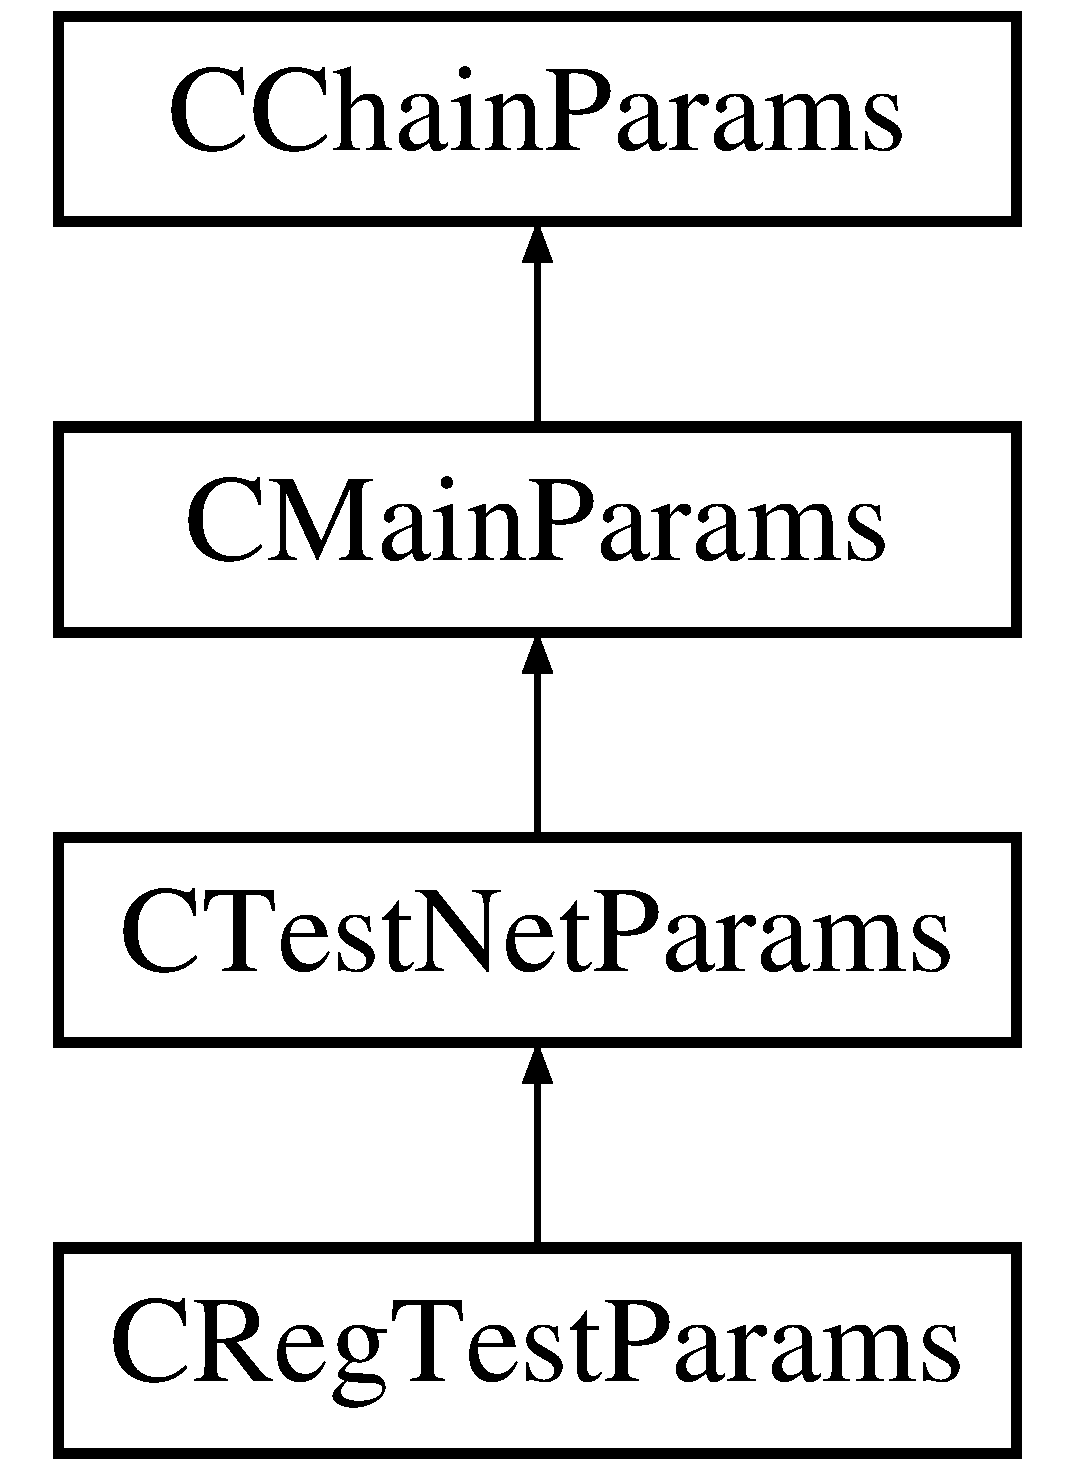
\includegraphics[height=4.000000cm]{class_c_test_net_params}
\end{center}
\end{figure}
\subsection*{Public Member Functions}
\begin{DoxyCompactItemize}
\item 
\hyperlink{class_c_test_net_params_abbd5f6e3e94bc8abf99a5dfaff75374a}{C\+Test\+Net\+Params} ()
\item 
const \hyperlink{struct_checkpoints_1_1_c_checkpoint_data}{Checkpoints\+::\+C\+Checkpoint\+Data} \& \hyperlink{class_c_test_net_params_a1a8828912574c509825ccc5cc0e0a9be}{Checkpoints} () const 
\end{DoxyCompactItemize}
\subsection*{Additional Inherited Members}


\subsection{Detailed Description}
Testnet (v3) 

\subsection{Constructor \& Destructor Documentation}
\hypertarget{class_c_test_net_params_abbd5f6e3e94bc8abf99a5dfaff75374a}{}\index{C\+Test\+Net\+Params@{C\+Test\+Net\+Params}!C\+Test\+Net\+Params@{C\+Test\+Net\+Params}}
\index{C\+Test\+Net\+Params@{C\+Test\+Net\+Params}!C\+Test\+Net\+Params@{C\+Test\+Net\+Params}}
\subsubsection[{C\+Test\+Net\+Params}]{\setlength{\rightskip}{0pt plus 5cm}C\+Test\+Net\+Params\+::\+C\+Test\+Net\+Params (
\begin{DoxyParamCaption}
{}
\end{DoxyParamCaption}
)\hspace{0.3cm}{\ttfamily [inline]}}\label{class_c_test_net_params_abbd5f6e3e94bc8abf99a5dfaff75374a}
Modify the testnet genesis block so the timestamp is valid for a later start. 

\subsection{Member Function Documentation}
\hypertarget{class_c_test_net_params_a1a8828912574c509825ccc5cc0e0a9be}{}\index{C\+Test\+Net\+Params@{C\+Test\+Net\+Params}!Checkpoints@{Checkpoints}}
\index{Checkpoints@{Checkpoints}!C\+Test\+Net\+Params@{C\+Test\+Net\+Params}}
\subsubsection[{Checkpoints}]{\setlength{\rightskip}{0pt plus 5cm}const {\bf Checkpoints\+::\+C\+Checkpoint\+Data}\& C\+Test\+Net\+Params\+::\+Checkpoints (
\begin{DoxyParamCaption}
{}
\end{DoxyParamCaption}
) const\hspace{0.3cm}{\ttfamily [inline]}, {\ttfamily [virtual]}}\label{class_c_test_net_params_a1a8828912574c509825ccc5cc0e0a9be}


Reimplemented from \hyperlink{class_c_main_params_abfaf5edda329d8b2ff23c0108cb8c16e}{C\+Main\+Params}.



Reimplemented in \hyperlink{class_c_reg_test_params_ab748b010a203dbdf6e5f77eb8b6f7cb0}{C\+Reg\+Test\+Params}.



The documentation for this class was generated from the following file\+:\begin{DoxyCompactItemize}
\item 
C\+:/\+Users/\+Joe/\+Documents/\+School/\+C\+S\+C17\+A/bitcoin/src/\hyperlink{chainparams_8cpp}{chainparams.\+cpp}\end{DoxyCompactItemize}

\hypertarget{class_c_tx_in_undo}{}\section{C\+Tx\+In\+Undo Class Reference}
\label{class_c_tx_in_undo}\index{C\+Tx\+In\+Undo@{C\+Tx\+In\+Undo}}


{\ttfamily \#include $<$undo.\+h$>$}

\subsection*{Public Member Functions}
\begin{DoxyCompactItemize}
\item 
\hyperlink{class_c_tx_in_undo_a9f8d4a16f1cb14fcec729becdb944003}{C\+Tx\+In\+Undo} ()
\item 
\hyperlink{class_c_tx_in_undo_a9f4da076d789bf5fa3f6d8d4b1d7d6fd}{C\+Tx\+In\+Undo} (const C\+Tx\+Out \&txout\+In, bool f\+Coin\+Base\+In=false, unsigned int n\+Height\+In=0, int n\+Version\+In=0)
\item 
unsigned int \hyperlink{class_c_tx_in_undo_a6f992d64f9d4ee6299cbd3305e4fd90f}{Get\+Serialize\+Size} (int n\+Type, int \hyperlink{class_c_tx_in_undo_a193281289475ca792e436a7a02de23ef}{n\+Version}) const 
\item 
{\footnotesize template$<$typename Stream $>$ }\\void \hyperlink{class_c_tx_in_undo_a37cebff3e836226b36e51d91e7cc2739}{Serialize} (Stream \&s, int n\+Type, int \hyperlink{class_c_tx_in_undo_a193281289475ca792e436a7a02de23ef}{n\+Version}) const 
\item 
{\footnotesize template$<$typename Stream $>$ }\\void \hyperlink{class_c_tx_in_undo_a0a2b82f03edad7ad85a66e63e4552af9}{Unserialize} (Stream \&s, int n\+Type, int \hyperlink{class_c_tx_in_undo_a193281289475ca792e436a7a02de23ef}{n\+Version})
\end{DoxyCompactItemize}
\subsection*{Public Attributes}
\begin{DoxyCompactItemize}
\item 
C\+Tx\+Out \hyperlink{class_c_tx_in_undo_a0eb1374984b5b68b0af14d88d7d4b821}{txout}
\item 
bool \hyperlink{class_c_tx_in_undo_a5952f917224de3a2193157b856c47864}{f\+Coin\+Base}
\item 
unsigned int \hyperlink{class_c_tx_in_undo_af022118f015a9b1b9ab96e04e8452292}{n\+Height}
\item 
int \hyperlink{class_c_tx_in_undo_a193281289475ca792e436a7a02de23ef}{n\+Version}
\end{DoxyCompactItemize}


\subsection{Detailed Description}
Undo information for a C\+Tx\+In

Contains the prevout\textquotesingle{}s C\+Tx\+Out being spent, and if this was the last output of the affected transaction, its metadata as well (coinbase or not, height, transaction version) 

\subsection{Constructor \& Destructor Documentation}
\hypertarget{class_c_tx_in_undo_a9f8d4a16f1cb14fcec729becdb944003}{}\index{C\+Tx\+In\+Undo@{C\+Tx\+In\+Undo}!C\+Tx\+In\+Undo@{C\+Tx\+In\+Undo}}
\index{C\+Tx\+In\+Undo@{C\+Tx\+In\+Undo}!C\+Tx\+In\+Undo@{C\+Tx\+In\+Undo}}
\subsubsection[{C\+Tx\+In\+Undo}]{\setlength{\rightskip}{0pt plus 5cm}C\+Tx\+In\+Undo\+::\+C\+Tx\+In\+Undo (
\begin{DoxyParamCaption}
{}
\end{DoxyParamCaption}
)\hspace{0.3cm}{\ttfamily [inline]}}\label{class_c_tx_in_undo_a9f8d4a16f1cb14fcec729becdb944003}
\hypertarget{class_c_tx_in_undo_a9f4da076d789bf5fa3f6d8d4b1d7d6fd}{}\index{C\+Tx\+In\+Undo@{C\+Tx\+In\+Undo}!C\+Tx\+In\+Undo@{C\+Tx\+In\+Undo}}
\index{C\+Tx\+In\+Undo@{C\+Tx\+In\+Undo}!C\+Tx\+In\+Undo@{C\+Tx\+In\+Undo}}
\subsubsection[{C\+Tx\+In\+Undo}]{\setlength{\rightskip}{0pt plus 5cm}C\+Tx\+In\+Undo\+::\+C\+Tx\+In\+Undo (
\begin{DoxyParamCaption}
\item[{const C\+Tx\+Out \&}]{txout\+In, }
\item[{bool}]{f\+Coin\+Base\+In = {\ttfamily false}, }
\item[{unsigned int}]{n\+Height\+In = {\ttfamily 0}, }
\item[{int}]{n\+Version\+In = {\ttfamily 0}}
\end{DoxyParamCaption}
)\hspace{0.3cm}{\ttfamily [inline]}}\label{class_c_tx_in_undo_a9f4da076d789bf5fa3f6d8d4b1d7d6fd}


\subsection{Member Function Documentation}
\hypertarget{class_c_tx_in_undo_a6f992d64f9d4ee6299cbd3305e4fd90f}{}\index{C\+Tx\+In\+Undo@{C\+Tx\+In\+Undo}!Get\+Serialize\+Size@{Get\+Serialize\+Size}}
\index{Get\+Serialize\+Size@{Get\+Serialize\+Size}!C\+Tx\+In\+Undo@{C\+Tx\+In\+Undo}}
\subsubsection[{Get\+Serialize\+Size}]{\setlength{\rightskip}{0pt plus 5cm}unsigned int C\+Tx\+In\+Undo\+::\+Get\+Serialize\+Size (
\begin{DoxyParamCaption}
\item[{int}]{n\+Type, }
\item[{int}]{n\+Version}
\end{DoxyParamCaption}
) const\hspace{0.3cm}{\ttfamily [inline]}}\label{class_c_tx_in_undo_a6f992d64f9d4ee6299cbd3305e4fd90f}
\hypertarget{class_c_tx_in_undo_a37cebff3e836226b36e51d91e7cc2739}{}\index{C\+Tx\+In\+Undo@{C\+Tx\+In\+Undo}!Serialize@{Serialize}}
\index{Serialize@{Serialize}!C\+Tx\+In\+Undo@{C\+Tx\+In\+Undo}}
\subsubsection[{Serialize}]{\setlength{\rightskip}{0pt plus 5cm}template$<$typename Stream $>$ void C\+Tx\+In\+Undo\+::\+Serialize (
\begin{DoxyParamCaption}
\item[{Stream \&}]{s, }
\item[{int}]{n\+Type, }
\item[{int}]{n\+Version}
\end{DoxyParamCaption}
) const\hspace{0.3cm}{\ttfamily [inline]}}\label{class_c_tx_in_undo_a37cebff3e836226b36e51d91e7cc2739}
\hypertarget{class_c_tx_in_undo_a0a2b82f03edad7ad85a66e63e4552af9}{}\index{C\+Tx\+In\+Undo@{C\+Tx\+In\+Undo}!Unserialize@{Unserialize}}
\index{Unserialize@{Unserialize}!C\+Tx\+In\+Undo@{C\+Tx\+In\+Undo}}
\subsubsection[{Unserialize}]{\setlength{\rightskip}{0pt plus 5cm}template$<$typename Stream $>$ void C\+Tx\+In\+Undo\+::\+Unserialize (
\begin{DoxyParamCaption}
\item[{Stream \&}]{s, }
\item[{int}]{n\+Type, }
\item[{int}]{n\+Version}
\end{DoxyParamCaption}
)\hspace{0.3cm}{\ttfamily [inline]}}\label{class_c_tx_in_undo_a0a2b82f03edad7ad85a66e63e4552af9}


\subsection{Member Data Documentation}
\hypertarget{class_c_tx_in_undo_a5952f917224de3a2193157b856c47864}{}\index{C\+Tx\+In\+Undo@{C\+Tx\+In\+Undo}!f\+Coin\+Base@{f\+Coin\+Base}}
\index{f\+Coin\+Base@{f\+Coin\+Base}!C\+Tx\+In\+Undo@{C\+Tx\+In\+Undo}}
\subsubsection[{f\+Coin\+Base}]{\setlength{\rightskip}{0pt plus 5cm}bool C\+Tx\+In\+Undo\+::f\+Coin\+Base}\label{class_c_tx_in_undo_a5952f917224de3a2193157b856c47864}
\hypertarget{class_c_tx_in_undo_af022118f015a9b1b9ab96e04e8452292}{}\index{C\+Tx\+In\+Undo@{C\+Tx\+In\+Undo}!n\+Height@{n\+Height}}
\index{n\+Height@{n\+Height}!C\+Tx\+In\+Undo@{C\+Tx\+In\+Undo}}
\subsubsection[{n\+Height}]{\setlength{\rightskip}{0pt plus 5cm}unsigned int C\+Tx\+In\+Undo\+::n\+Height}\label{class_c_tx_in_undo_af022118f015a9b1b9ab96e04e8452292}
\hypertarget{class_c_tx_in_undo_a193281289475ca792e436a7a02de23ef}{}\index{C\+Tx\+In\+Undo@{C\+Tx\+In\+Undo}!n\+Version@{n\+Version}}
\index{n\+Version@{n\+Version}!C\+Tx\+In\+Undo@{C\+Tx\+In\+Undo}}
\subsubsection[{n\+Version}]{\setlength{\rightskip}{0pt plus 5cm}int C\+Tx\+In\+Undo\+::n\+Version}\label{class_c_tx_in_undo_a193281289475ca792e436a7a02de23ef}
\hypertarget{class_c_tx_in_undo_a0eb1374984b5b68b0af14d88d7d4b821}{}\index{C\+Tx\+In\+Undo@{C\+Tx\+In\+Undo}!txout@{txout}}
\index{txout@{txout}!C\+Tx\+In\+Undo@{C\+Tx\+In\+Undo}}
\subsubsection[{txout}]{\setlength{\rightskip}{0pt plus 5cm}C\+Tx\+Out C\+Tx\+In\+Undo\+::txout}\label{class_c_tx_in_undo_a0eb1374984b5b68b0af14d88d7d4b821}


The documentation for this class was generated from the following file\+:\begin{DoxyCompactItemize}
\item 
C\+:/\+Users/\+Joe/\+Documents/\+School/\+C\+S\+C17\+A/bitcoin/src/\hyperlink{undo_8h}{undo.\+h}\end{DoxyCompactItemize}

\hypertarget{class_c_tx_mem_pool}{}\section{C\+Tx\+Mem\+Pool Class Reference}
\label{class_c_tx_mem_pool}\index{C\+Tx\+Mem\+Pool@{C\+Tx\+Mem\+Pool}}


{\ttfamily \#include $<$txmempool.\+h$>$}

\subsection*{Public Member Functions}
\begin{DoxyCompactItemize}
\item 
\hyperlink{class_c_tx_mem_pool_a82147548cfa962975690d1926b717c1c}{C\+Tx\+Mem\+Pool} (const \hyperlink{class_c_fee_rate}{C\+Fee\+Rate} \&\+\_\+min\+Relay\+Fee)
\item 
\hyperlink{class_c_tx_mem_pool_a038108efea0c4312e5bed2ce064702b2}{$\sim$\+C\+Tx\+Mem\+Pool} ()
\item 
void \hyperlink{class_c_tx_mem_pool_ad74247cc4eb672fb9063d4e9503f4cf0}{check} (const \hyperlink{class_c_coins_view_cache}{C\+Coins\+View\+Cache} $\ast$pcoins) const 
\item 
void \hyperlink{class_c_tx_mem_pool_a1c0edb1fd5f0b02ddac46a6a97dcfd53}{set\+Sanity\+Check} (bool \+\_\+f\+Sanity\+Check)
\item 
bool \hyperlink{class_c_tx_mem_pool_a9e336997572ff8058d65afeb88ddde3b}{add\+Unchecked} (const \hyperlink{classuint256}{uint256} \&hash, const \hyperlink{class_c_tx_mem_pool_entry}{C\+Tx\+Mem\+Pool\+Entry} \&entry)
\item 
void \hyperlink{class_c_tx_mem_pool_a3a497097d9d5f325a2922a3970ac9da2}{remove} (const C\+Transaction \&tx, std\+::list$<$ C\+Transaction $>$ \&removed, bool f\+Recursive=false)
\item 
void \hyperlink{class_c_tx_mem_pool_a6d1292640d0b6028bd5c602a6a50a983}{remove\+Coinbase\+Spends} (const \hyperlink{class_c_coins_view_cache}{C\+Coins\+View\+Cache} $\ast$pcoins, unsigned int n\+Mem\+Pool\+Height)
\item 
void \hyperlink{class_c_tx_mem_pool_a11f1bddfbae7c03c6244db322876c0a7}{remove\+Conflicts} (const C\+Transaction \&tx, std\+::list$<$ C\+Transaction $>$ \&removed)
\item 
void \hyperlink{class_c_tx_mem_pool_ac97207311007676bd7ef056a625e0e0a}{remove\+For\+Block} (const std\+::vector$<$ C\+Transaction $>$ \&vtx, unsigned int n\+Block\+Height, std\+::list$<$ C\+Transaction $>$ \&conflicts)
\item 
void \hyperlink{class_c_tx_mem_pool_a6dba6bce4139392751321438a29b6b09}{clear} ()
\item 
void \hyperlink{class_c_tx_mem_pool_a42fa7d41a45562d02e356f2e7708bb02}{query\+Hashes} (std\+::vector$<$ \hyperlink{classuint256}{uint256} $>$ \&vtxid)
\item 
void \hyperlink{class_c_tx_mem_pool_ad6142b7cd3a58dae6cdaf03551c2f989}{prune\+Spent} (const \hyperlink{classuint256}{uint256} \&hash, \hyperlink{class_c_coins}{C\+Coins} \&coins)
\item 
unsigned int \hyperlink{class_c_tx_mem_pool_a26a5bdb66c9b84f73d1d30fea8e31cc9}{Get\+Transactions\+Updated} () const 
\item 
void \hyperlink{class_c_tx_mem_pool_a3039b67e5eebaa3ff830261c192816f2}{Add\+Transactions\+Updated} (unsigned int n)
\item 
void \hyperlink{class_c_tx_mem_pool_a1a0a00279c941051af1b74c5ebeac40d}{Prioritise\+Transaction} (const \hyperlink{classuint256}{uint256} hash, const std\+::string str\+Hash, double d\+Priority\+Delta, const \hyperlink{amount_8h_a4eaf3a5239714d8c45b851527f7cb564}{C\+Amount} \&n\+Fee\+Delta)
\item 
void \hyperlink{class_c_tx_mem_pool_aa73d1d5a211150fe169d73dc25ba3cdd}{Apply\+Deltas} (const \hyperlink{classuint256}{uint256} hash, double \&d\+Priority\+Delta, \hyperlink{amount_8h_a4eaf3a5239714d8c45b851527f7cb564}{C\+Amount} \&n\+Fee\+Delta)
\item 
void \hyperlink{class_c_tx_mem_pool_a11dea05121ab8321e1d1f1a21ec5c9ac}{Clear\+Prioritisation} (const \hyperlink{classuint256}{uint256} hash)
\item 
unsigned long \hyperlink{class_c_tx_mem_pool_a867f7b452141770f3b2e8697fb3513d8}{size} ()
\item 
uint64\+\_\+t \hyperlink{class_c_tx_mem_pool_ad388f6544c2ca90f1550b06d9d86d54f}{Get\+Total\+Tx\+Size} ()
\item 
bool \hyperlink{class_c_tx_mem_pool_adba06e79be4a1a092dd2db8290733be7}{exists} (\hyperlink{classuint256}{uint256} hash)
\item 
bool \hyperlink{class_c_tx_mem_pool_a8c19232d17e668c6690721b0f5088960}{lookup} (\hyperlink{classuint256}{uint256} hash, C\+Transaction \&result) const 
\item 
\hyperlink{class_c_fee_rate}{C\+Fee\+Rate} \hyperlink{class_c_tx_mem_pool_ae0a5ad226288e4b209c6629328269469}{estimate\+Fee} (int n\+Blocks) const 
\item 
double \hyperlink{class_c_tx_mem_pool_aa30175b2668fcefb3d4f224d38d5732e}{estimate\+Priority} (int n\+Blocks) const 
\item 
bool \hyperlink{class_c_tx_mem_pool_a0a05d7b50b9c2a387182402e60475da6}{Write\+Fee\+Estimates} (\hyperlink{class_c_auto_file}{C\+Auto\+File} \&fileout) const 
\item 
bool \hyperlink{class_c_tx_mem_pool_a0dbbcb6a3b7e1a6c564410668c12cd4f}{Read\+Fee\+Estimates} (\hyperlink{class_c_auto_file}{C\+Auto\+File} \&filein)
\end{DoxyCompactItemize}
\subsection*{Public Attributes}
\begin{DoxyCompactItemize}
\item 
\hyperlink{sync_8h_a37a4692b2d517f2843655ca11af7668a}{C\+Critical\+Section} \hyperlink{class_c_tx_mem_pool_ac7ee8c06837c7d2688e2d7e3d071bdbb}{cs}
\begin{DoxyCompactList}\small\item\em sum of all mempool tx\textquotesingle{} byte sizes \end{DoxyCompactList}\item 
std\+::map$<$ \hyperlink{classuint256}{uint256}, \hyperlink{class_c_tx_mem_pool_entry}{C\+Tx\+Mem\+Pool\+Entry} $>$ \hyperlink{class_c_tx_mem_pool_a5cd374a559b02a6485ca8cef769f9930}{map\+Tx}
\item 
std\+::map$<$ C\+Out\+Point, \hyperlink{class_c_in_point}{C\+In\+Point} $>$ \hyperlink{class_c_tx_mem_pool_aae6f1162f0b2e42b369971f32a9f71e8}{map\+Next\+Tx}
\item 
std\+::map$<$ \hyperlink{classuint256}{uint256}, std\+::pair$<$ double, \hyperlink{amount_8h_a4eaf3a5239714d8c45b851527f7cb564}{C\+Amount} $>$ $>$ \hyperlink{class_c_tx_mem_pool_a341709e31a39ce7a7a951a85c775c589}{map\+Deltas}
\end{DoxyCompactItemize}


\subsection{Detailed Description}
\hyperlink{class_c_tx_mem_pool}{C\+Tx\+Mem\+Pool} stores valid-\/according-\/to-\/the-\/current-\/best-\/chain transactions that may be included in the next block.

Transactions are added when they are seen on the network (or created by the local node), but not all transactions seen are added to the pool\+: if a new transaction double-\/spends an input of a transaction in the pool, it is dropped, as are non-\/standard transactions. 

\subsection{Constructor \& Destructor Documentation}
\hypertarget{class_c_tx_mem_pool_a82147548cfa962975690d1926b717c1c}{}\index{C\+Tx\+Mem\+Pool@{C\+Tx\+Mem\+Pool}!C\+Tx\+Mem\+Pool@{C\+Tx\+Mem\+Pool}}
\index{C\+Tx\+Mem\+Pool@{C\+Tx\+Mem\+Pool}!C\+Tx\+Mem\+Pool@{C\+Tx\+Mem\+Pool}}
\subsubsection[{C\+Tx\+Mem\+Pool}]{\setlength{\rightskip}{0pt plus 5cm}C\+Tx\+Mem\+Pool\+::\+C\+Tx\+Mem\+Pool (
\begin{DoxyParamCaption}
\item[{const {\bf C\+Fee\+Rate} \&}]{\+\_\+min\+Relay\+Fee}
\end{DoxyParamCaption}
)}\label{class_c_tx_mem_pool_a82147548cfa962975690d1926b717c1c}
\hypertarget{class_c_tx_mem_pool_a038108efea0c4312e5bed2ce064702b2}{}\index{C\+Tx\+Mem\+Pool@{C\+Tx\+Mem\+Pool}!````~C\+Tx\+Mem\+Pool@{$\sim$\+C\+Tx\+Mem\+Pool}}
\index{````~C\+Tx\+Mem\+Pool@{$\sim$\+C\+Tx\+Mem\+Pool}!C\+Tx\+Mem\+Pool@{C\+Tx\+Mem\+Pool}}
\subsubsection[{$\sim$\+C\+Tx\+Mem\+Pool}]{\setlength{\rightskip}{0pt plus 5cm}C\+Tx\+Mem\+Pool\+::$\sim$\+C\+Tx\+Mem\+Pool (
\begin{DoxyParamCaption}
{}
\end{DoxyParamCaption}
)}\label{class_c_tx_mem_pool_a038108efea0c4312e5bed2ce064702b2}


\subsection{Member Function Documentation}
\hypertarget{class_c_tx_mem_pool_a3039b67e5eebaa3ff830261c192816f2}{}\index{C\+Tx\+Mem\+Pool@{C\+Tx\+Mem\+Pool}!Add\+Transactions\+Updated@{Add\+Transactions\+Updated}}
\index{Add\+Transactions\+Updated@{Add\+Transactions\+Updated}!C\+Tx\+Mem\+Pool@{C\+Tx\+Mem\+Pool}}
\subsubsection[{Add\+Transactions\+Updated}]{\setlength{\rightskip}{0pt plus 5cm}void C\+Tx\+Mem\+Pool\+::\+Add\+Transactions\+Updated (
\begin{DoxyParamCaption}
\item[{unsigned int}]{n}
\end{DoxyParamCaption}
)}\label{class_c_tx_mem_pool_a3039b67e5eebaa3ff830261c192816f2}
\hypertarget{class_c_tx_mem_pool_a9e336997572ff8058d65afeb88ddde3b}{}\index{C\+Tx\+Mem\+Pool@{C\+Tx\+Mem\+Pool}!add\+Unchecked@{add\+Unchecked}}
\index{add\+Unchecked@{add\+Unchecked}!C\+Tx\+Mem\+Pool@{C\+Tx\+Mem\+Pool}}
\subsubsection[{add\+Unchecked}]{\setlength{\rightskip}{0pt plus 5cm}bool C\+Tx\+Mem\+Pool\+::add\+Unchecked (
\begin{DoxyParamCaption}
\item[{const {\bf uint256} \&}]{hash, }
\item[{const {\bf C\+Tx\+Mem\+Pool\+Entry} \&}]{entry}
\end{DoxyParamCaption}
)}\label{class_c_tx_mem_pool_a9e336997572ff8058d65afeb88ddde3b}
\hypertarget{class_c_tx_mem_pool_aa73d1d5a211150fe169d73dc25ba3cdd}{}\index{C\+Tx\+Mem\+Pool@{C\+Tx\+Mem\+Pool}!Apply\+Deltas@{Apply\+Deltas}}
\index{Apply\+Deltas@{Apply\+Deltas}!C\+Tx\+Mem\+Pool@{C\+Tx\+Mem\+Pool}}
\subsubsection[{Apply\+Deltas}]{\setlength{\rightskip}{0pt plus 5cm}void C\+Tx\+Mem\+Pool\+::\+Apply\+Deltas (
\begin{DoxyParamCaption}
\item[{const {\bf uint256}}]{hash, }
\item[{double \&}]{d\+Priority\+Delta, }
\item[{{\bf C\+Amount} \&}]{n\+Fee\+Delta}
\end{DoxyParamCaption}
)}\label{class_c_tx_mem_pool_aa73d1d5a211150fe169d73dc25ba3cdd}
\hypertarget{class_c_tx_mem_pool_ad74247cc4eb672fb9063d4e9503f4cf0}{}\index{C\+Tx\+Mem\+Pool@{C\+Tx\+Mem\+Pool}!check@{check}}
\index{check@{check}!C\+Tx\+Mem\+Pool@{C\+Tx\+Mem\+Pool}}
\subsubsection[{check}]{\setlength{\rightskip}{0pt plus 5cm}void C\+Tx\+Mem\+Pool\+::check (
\begin{DoxyParamCaption}
\item[{const {\bf C\+Coins\+View\+Cache} $\ast$}]{pcoins}
\end{DoxyParamCaption}
) const}\label{class_c_tx_mem_pool_ad74247cc4eb672fb9063d4e9503f4cf0}
If sanity-\/checking is turned on, check makes sure the pool is consistent (does not contain two transactions that spend the same inputs, all inputs are in the map\+Next\+Tx array). If sanity-\/checking is turned off, check does nothing. \hypertarget{class_c_tx_mem_pool_a6dba6bce4139392751321438a29b6b09}{}\index{C\+Tx\+Mem\+Pool@{C\+Tx\+Mem\+Pool}!clear@{clear}}
\index{clear@{clear}!C\+Tx\+Mem\+Pool@{C\+Tx\+Mem\+Pool}}
\subsubsection[{clear}]{\setlength{\rightskip}{0pt plus 5cm}void C\+Tx\+Mem\+Pool\+::clear (
\begin{DoxyParamCaption}
{}
\end{DoxyParamCaption}
)}\label{class_c_tx_mem_pool_a6dba6bce4139392751321438a29b6b09}
\hypertarget{class_c_tx_mem_pool_a11dea05121ab8321e1d1f1a21ec5c9ac}{}\index{C\+Tx\+Mem\+Pool@{C\+Tx\+Mem\+Pool}!Clear\+Prioritisation@{Clear\+Prioritisation}}
\index{Clear\+Prioritisation@{Clear\+Prioritisation}!C\+Tx\+Mem\+Pool@{C\+Tx\+Mem\+Pool}}
\subsubsection[{Clear\+Prioritisation}]{\setlength{\rightskip}{0pt plus 5cm}void C\+Tx\+Mem\+Pool\+::\+Clear\+Prioritisation (
\begin{DoxyParamCaption}
\item[{const {\bf uint256}}]{hash}
\end{DoxyParamCaption}
)}\label{class_c_tx_mem_pool_a11dea05121ab8321e1d1f1a21ec5c9ac}
\hypertarget{class_c_tx_mem_pool_ae0a5ad226288e4b209c6629328269469}{}\index{C\+Tx\+Mem\+Pool@{C\+Tx\+Mem\+Pool}!estimate\+Fee@{estimate\+Fee}}
\index{estimate\+Fee@{estimate\+Fee}!C\+Tx\+Mem\+Pool@{C\+Tx\+Mem\+Pool}}
\subsubsection[{estimate\+Fee}]{\setlength{\rightskip}{0pt plus 5cm}{\bf C\+Fee\+Rate} C\+Tx\+Mem\+Pool\+::estimate\+Fee (
\begin{DoxyParamCaption}
\item[{int}]{n\+Blocks}
\end{DoxyParamCaption}
) const}\label{class_c_tx_mem_pool_ae0a5ad226288e4b209c6629328269469}
Estimate fee rate needed to get into the next n\+Blocks \hypertarget{class_c_tx_mem_pool_aa30175b2668fcefb3d4f224d38d5732e}{}\index{C\+Tx\+Mem\+Pool@{C\+Tx\+Mem\+Pool}!estimate\+Priority@{estimate\+Priority}}
\index{estimate\+Priority@{estimate\+Priority}!C\+Tx\+Mem\+Pool@{C\+Tx\+Mem\+Pool}}
\subsubsection[{estimate\+Priority}]{\setlength{\rightskip}{0pt plus 5cm}double C\+Tx\+Mem\+Pool\+::estimate\+Priority (
\begin{DoxyParamCaption}
\item[{int}]{n\+Blocks}
\end{DoxyParamCaption}
) const}\label{class_c_tx_mem_pool_aa30175b2668fcefb3d4f224d38d5732e}
Estimate priority needed to get into the next n\+Blocks \hypertarget{class_c_tx_mem_pool_adba06e79be4a1a092dd2db8290733be7}{}\index{C\+Tx\+Mem\+Pool@{C\+Tx\+Mem\+Pool}!exists@{exists}}
\index{exists@{exists}!C\+Tx\+Mem\+Pool@{C\+Tx\+Mem\+Pool}}
\subsubsection[{exists}]{\setlength{\rightskip}{0pt plus 5cm}bool C\+Tx\+Mem\+Pool\+::exists (
\begin{DoxyParamCaption}
\item[{{\bf uint256}}]{hash}
\end{DoxyParamCaption}
)\hspace{0.3cm}{\ttfamily [inline]}}\label{class_c_tx_mem_pool_adba06e79be4a1a092dd2db8290733be7}
\hypertarget{class_c_tx_mem_pool_ad388f6544c2ca90f1550b06d9d86d54f}{}\index{C\+Tx\+Mem\+Pool@{C\+Tx\+Mem\+Pool}!Get\+Total\+Tx\+Size@{Get\+Total\+Tx\+Size}}
\index{Get\+Total\+Tx\+Size@{Get\+Total\+Tx\+Size}!C\+Tx\+Mem\+Pool@{C\+Tx\+Mem\+Pool}}
\subsubsection[{Get\+Total\+Tx\+Size}]{\setlength{\rightskip}{0pt plus 5cm}uint64\+\_\+t C\+Tx\+Mem\+Pool\+::\+Get\+Total\+Tx\+Size (
\begin{DoxyParamCaption}
{}
\end{DoxyParamCaption}
)\hspace{0.3cm}{\ttfamily [inline]}}\label{class_c_tx_mem_pool_ad388f6544c2ca90f1550b06d9d86d54f}
\hypertarget{class_c_tx_mem_pool_a26a5bdb66c9b84f73d1d30fea8e31cc9}{}\index{C\+Tx\+Mem\+Pool@{C\+Tx\+Mem\+Pool}!Get\+Transactions\+Updated@{Get\+Transactions\+Updated}}
\index{Get\+Transactions\+Updated@{Get\+Transactions\+Updated}!C\+Tx\+Mem\+Pool@{C\+Tx\+Mem\+Pool}}
\subsubsection[{Get\+Transactions\+Updated}]{\setlength{\rightskip}{0pt plus 5cm}unsigned int C\+Tx\+Mem\+Pool\+::\+Get\+Transactions\+Updated (
\begin{DoxyParamCaption}
{}
\end{DoxyParamCaption}
) const}\label{class_c_tx_mem_pool_a26a5bdb66c9b84f73d1d30fea8e31cc9}
\hypertarget{class_c_tx_mem_pool_a8c19232d17e668c6690721b0f5088960}{}\index{C\+Tx\+Mem\+Pool@{C\+Tx\+Mem\+Pool}!lookup@{lookup}}
\index{lookup@{lookup}!C\+Tx\+Mem\+Pool@{C\+Tx\+Mem\+Pool}}
\subsubsection[{lookup}]{\setlength{\rightskip}{0pt plus 5cm}bool C\+Tx\+Mem\+Pool\+::lookup (
\begin{DoxyParamCaption}
\item[{{\bf uint256}}]{hash, }
\item[{C\+Transaction \&}]{result}
\end{DoxyParamCaption}
) const}\label{class_c_tx_mem_pool_a8c19232d17e668c6690721b0f5088960}
\hypertarget{class_c_tx_mem_pool_a1a0a00279c941051af1b74c5ebeac40d}{}\index{C\+Tx\+Mem\+Pool@{C\+Tx\+Mem\+Pool}!Prioritise\+Transaction@{Prioritise\+Transaction}}
\index{Prioritise\+Transaction@{Prioritise\+Transaction}!C\+Tx\+Mem\+Pool@{C\+Tx\+Mem\+Pool}}
\subsubsection[{Prioritise\+Transaction}]{\setlength{\rightskip}{0pt plus 5cm}void C\+Tx\+Mem\+Pool\+::\+Prioritise\+Transaction (
\begin{DoxyParamCaption}
\item[{const {\bf uint256}}]{hash, }
\item[{const std\+::string}]{str\+Hash, }
\item[{double}]{d\+Priority\+Delta, }
\item[{const {\bf C\+Amount} \&}]{n\+Fee\+Delta}
\end{DoxyParamCaption}
)}\label{class_c_tx_mem_pool_a1a0a00279c941051af1b74c5ebeac40d}
Affect Create\+New\+Block prioritisation of transactions \hypertarget{class_c_tx_mem_pool_ad6142b7cd3a58dae6cdaf03551c2f989}{}\index{C\+Tx\+Mem\+Pool@{C\+Tx\+Mem\+Pool}!prune\+Spent@{prune\+Spent}}
\index{prune\+Spent@{prune\+Spent}!C\+Tx\+Mem\+Pool@{C\+Tx\+Mem\+Pool}}
\subsubsection[{prune\+Spent}]{\setlength{\rightskip}{0pt plus 5cm}void C\+Tx\+Mem\+Pool\+::prune\+Spent (
\begin{DoxyParamCaption}
\item[{const {\bf uint256} \&}]{hash, }
\item[{{\bf C\+Coins} \&}]{coins}
\end{DoxyParamCaption}
)}\label{class_c_tx_mem_pool_ad6142b7cd3a58dae6cdaf03551c2f989}
\hypertarget{class_c_tx_mem_pool_a42fa7d41a45562d02e356f2e7708bb02}{}\index{C\+Tx\+Mem\+Pool@{C\+Tx\+Mem\+Pool}!query\+Hashes@{query\+Hashes}}
\index{query\+Hashes@{query\+Hashes}!C\+Tx\+Mem\+Pool@{C\+Tx\+Mem\+Pool}}
\subsubsection[{query\+Hashes}]{\setlength{\rightskip}{0pt plus 5cm}void C\+Tx\+Mem\+Pool\+::query\+Hashes (
\begin{DoxyParamCaption}
\item[{std\+::vector$<$ {\bf uint256} $>$ \&}]{vtxid}
\end{DoxyParamCaption}
)}\label{class_c_tx_mem_pool_a42fa7d41a45562d02e356f2e7708bb02}
\hypertarget{class_c_tx_mem_pool_a0dbbcb6a3b7e1a6c564410668c12cd4f}{}\index{C\+Tx\+Mem\+Pool@{C\+Tx\+Mem\+Pool}!Read\+Fee\+Estimates@{Read\+Fee\+Estimates}}
\index{Read\+Fee\+Estimates@{Read\+Fee\+Estimates}!C\+Tx\+Mem\+Pool@{C\+Tx\+Mem\+Pool}}
\subsubsection[{Read\+Fee\+Estimates}]{\setlength{\rightskip}{0pt plus 5cm}bool C\+Tx\+Mem\+Pool\+::\+Read\+Fee\+Estimates (
\begin{DoxyParamCaption}
\item[{{\bf C\+Auto\+File} \&}]{filein}
\end{DoxyParamCaption}
)}\label{class_c_tx_mem_pool_a0dbbcb6a3b7e1a6c564410668c12cd4f}
\hypertarget{class_c_tx_mem_pool_a3a497097d9d5f325a2922a3970ac9da2}{}\index{C\+Tx\+Mem\+Pool@{C\+Tx\+Mem\+Pool}!remove@{remove}}
\index{remove@{remove}!C\+Tx\+Mem\+Pool@{C\+Tx\+Mem\+Pool}}
\subsubsection[{remove}]{\setlength{\rightskip}{0pt plus 5cm}void C\+Tx\+Mem\+Pool\+::remove (
\begin{DoxyParamCaption}
\item[{const C\+Transaction \&}]{tx, }
\item[{std\+::list$<$ C\+Transaction $>$ \&}]{removed, }
\item[{bool}]{f\+Recursive = {\ttfamily false}}
\end{DoxyParamCaption}
)}\label{class_c_tx_mem_pool_a3a497097d9d5f325a2922a3970ac9da2}
\hypertarget{class_c_tx_mem_pool_a6d1292640d0b6028bd5c602a6a50a983}{}\index{C\+Tx\+Mem\+Pool@{C\+Tx\+Mem\+Pool}!remove\+Coinbase\+Spends@{remove\+Coinbase\+Spends}}
\index{remove\+Coinbase\+Spends@{remove\+Coinbase\+Spends}!C\+Tx\+Mem\+Pool@{C\+Tx\+Mem\+Pool}}
\subsubsection[{remove\+Coinbase\+Spends}]{\setlength{\rightskip}{0pt plus 5cm}void C\+Tx\+Mem\+Pool\+::remove\+Coinbase\+Spends (
\begin{DoxyParamCaption}
\item[{const {\bf C\+Coins\+View\+Cache} $\ast$}]{pcoins, }
\item[{unsigned int}]{n\+Mem\+Pool\+Height}
\end{DoxyParamCaption}
)}\label{class_c_tx_mem_pool_a6d1292640d0b6028bd5c602a6a50a983}
\hypertarget{class_c_tx_mem_pool_a11f1bddfbae7c03c6244db322876c0a7}{}\index{C\+Tx\+Mem\+Pool@{C\+Tx\+Mem\+Pool}!remove\+Conflicts@{remove\+Conflicts}}
\index{remove\+Conflicts@{remove\+Conflicts}!C\+Tx\+Mem\+Pool@{C\+Tx\+Mem\+Pool}}
\subsubsection[{remove\+Conflicts}]{\setlength{\rightskip}{0pt plus 5cm}void C\+Tx\+Mem\+Pool\+::remove\+Conflicts (
\begin{DoxyParamCaption}
\item[{const C\+Transaction \&}]{tx, }
\item[{std\+::list$<$ C\+Transaction $>$ \&}]{removed}
\end{DoxyParamCaption}
)}\label{class_c_tx_mem_pool_a11f1bddfbae7c03c6244db322876c0a7}
\hypertarget{class_c_tx_mem_pool_ac97207311007676bd7ef056a625e0e0a}{}\index{C\+Tx\+Mem\+Pool@{C\+Tx\+Mem\+Pool}!remove\+For\+Block@{remove\+For\+Block}}
\index{remove\+For\+Block@{remove\+For\+Block}!C\+Tx\+Mem\+Pool@{C\+Tx\+Mem\+Pool}}
\subsubsection[{remove\+For\+Block}]{\setlength{\rightskip}{0pt plus 5cm}void C\+Tx\+Mem\+Pool\+::remove\+For\+Block (
\begin{DoxyParamCaption}
\item[{const std\+::vector$<$ C\+Transaction $>$ \&}]{vtx, }
\item[{unsigned int}]{n\+Block\+Height, }
\item[{std\+::list$<$ C\+Transaction $>$ \&}]{conflicts}
\end{DoxyParamCaption}
)}\label{class_c_tx_mem_pool_ac97207311007676bd7ef056a625e0e0a}
Called when a block is connected. Removes from mempool and updates the miner fee estimator. \hypertarget{class_c_tx_mem_pool_a1c0edb1fd5f0b02ddac46a6a97dcfd53}{}\index{C\+Tx\+Mem\+Pool@{C\+Tx\+Mem\+Pool}!set\+Sanity\+Check@{set\+Sanity\+Check}}
\index{set\+Sanity\+Check@{set\+Sanity\+Check}!C\+Tx\+Mem\+Pool@{C\+Tx\+Mem\+Pool}}
\subsubsection[{set\+Sanity\+Check}]{\setlength{\rightskip}{0pt plus 5cm}void C\+Tx\+Mem\+Pool\+::set\+Sanity\+Check (
\begin{DoxyParamCaption}
\item[{bool}]{\+\_\+f\+Sanity\+Check}
\end{DoxyParamCaption}
)\hspace{0.3cm}{\ttfamily [inline]}}\label{class_c_tx_mem_pool_a1c0edb1fd5f0b02ddac46a6a97dcfd53}
\hypertarget{class_c_tx_mem_pool_a867f7b452141770f3b2e8697fb3513d8}{}\index{C\+Tx\+Mem\+Pool@{C\+Tx\+Mem\+Pool}!size@{size}}
\index{size@{size}!C\+Tx\+Mem\+Pool@{C\+Tx\+Mem\+Pool}}
\subsubsection[{size}]{\setlength{\rightskip}{0pt plus 5cm}unsigned long C\+Tx\+Mem\+Pool\+::size (
\begin{DoxyParamCaption}
{}
\end{DoxyParamCaption}
)\hspace{0.3cm}{\ttfamily [inline]}}\label{class_c_tx_mem_pool_a867f7b452141770f3b2e8697fb3513d8}
\hypertarget{class_c_tx_mem_pool_a0a05d7b50b9c2a387182402e60475da6}{}\index{C\+Tx\+Mem\+Pool@{C\+Tx\+Mem\+Pool}!Write\+Fee\+Estimates@{Write\+Fee\+Estimates}}
\index{Write\+Fee\+Estimates@{Write\+Fee\+Estimates}!C\+Tx\+Mem\+Pool@{C\+Tx\+Mem\+Pool}}
\subsubsection[{Write\+Fee\+Estimates}]{\setlength{\rightskip}{0pt plus 5cm}bool C\+Tx\+Mem\+Pool\+::\+Write\+Fee\+Estimates (
\begin{DoxyParamCaption}
\item[{{\bf C\+Auto\+File} \&}]{fileout}
\end{DoxyParamCaption}
) const}\label{class_c_tx_mem_pool_a0a05d7b50b9c2a387182402e60475da6}
Write/\+Read estimates to disk 

\subsection{Member Data Documentation}
\hypertarget{class_c_tx_mem_pool_ac7ee8c06837c7d2688e2d7e3d071bdbb}{}\index{C\+Tx\+Mem\+Pool@{C\+Tx\+Mem\+Pool}!cs@{cs}}
\index{cs@{cs}!C\+Tx\+Mem\+Pool@{C\+Tx\+Mem\+Pool}}
\subsubsection[{cs}]{\setlength{\rightskip}{0pt plus 5cm}{\bf C\+Critical\+Section} C\+Tx\+Mem\+Pool\+::cs\hspace{0.3cm}{\ttfamily [mutable]}}\label{class_c_tx_mem_pool_ac7ee8c06837c7d2688e2d7e3d071bdbb}


sum of all mempool tx\textquotesingle{} byte sizes 

\hypertarget{class_c_tx_mem_pool_a341709e31a39ce7a7a951a85c775c589}{}\index{C\+Tx\+Mem\+Pool@{C\+Tx\+Mem\+Pool}!map\+Deltas@{map\+Deltas}}
\index{map\+Deltas@{map\+Deltas}!C\+Tx\+Mem\+Pool@{C\+Tx\+Mem\+Pool}}
\subsubsection[{map\+Deltas}]{\setlength{\rightskip}{0pt plus 5cm}std\+::map$<${\bf uint256}, std\+::pair$<$double, {\bf C\+Amount}$>$ $>$ C\+Tx\+Mem\+Pool\+::map\+Deltas}\label{class_c_tx_mem_pool_a341709e31a39ce7a7a951a85c775c589}
\hypertarget{class_c_tx_mem_pool_aae6f1162f0b2e42b369971f32a9f71e8}{}\index{C\+Tx\+Mem\+Pool@{C\+Tx\+Mem\+Pool}!map\+Next\+Tx@{map\+Next\+Tx}}
\index{map\+Next\+Tx@{map\+Next\+Tx}!C\+Tx\+Mem\+Pool@{C\+Tx\+Mem\+Pool}}
\subsubsection[{map\+Next\+Tx}]{\setlength{\rightskip}{0pt plus 5cm}std\+::map$<$C\+Out\+Point, {\bf C\+In\+Point}$>$ C\+Tx\+Mem\+Pool\+::map\+Next\+Tx}\label{class_c_tx_mem_pool_aae6f1162f0b2e42b369971f32a9f71e8}
\hypertarget{class_c_tx_mem_pool_a5cd374a559b02a6485ca8cef769f9930}{}\index{C\+Tx\+Mem\+Pool@{C\+Tx\+Mem\+Pool}!map\+Tx@{map\+Tx}}
\index{map\+Tx@{map\+Tx}!C\+Tx\+Mem\+Pool@{C\+Tx\+Mem\+Pool}}
\subsubsection[{map\+Tx}]{\setlength{\rightskip}{0pt plus 5cm}std\+::map$<${\bf uint256}, {\bf C\+Tx\+Mem\+Pool\+Entry}$>$ C\+Tx\+Mem\+Pool\+::map\+Tx}\label{class_c_tx_mem_pool_a5cd374a559b02a6485ca8cef769f9930}


The documentation for this class was generated from the following files\+:\begin{DoxyCompactItemize}
\item 
C\+:/\+Users/\+Joe/\+Documents/\+School/\+C\+S\+C17\+A/bitcoin/src/\hyperlink{txmempool_8h}{txmempool.\+h}\item 
C\+:/\+Users/\+Joe/\+Documents/\+School/\+C\+S\+C17\+A/bitcoin/src/\hyperlink{txmempool_8cpp}{txmempool.\+cpp}\end{DoxyCompactItemize}

\hypertarget{class_c_tx_mem_pool_entry}{}\section{C\+Tx\+Mem\+Pool\+Entry Class Reference}
\label{class_c_tx_mem_pool_entry}\index{C\+Tx\+Mem\+Pool\+Entry@{C\+Tx\+Mem\+Pool\+Entry}}


{\ttfamily \#include $<$txmempool.\+h$>$}

\subsection*{Public Member Functions}
\begin{DoxyCompactItemize}
\item 
\hyperlink{class_c_tx_mem_pool_entry_a2ceb48d4c37f0308e97f57e237b50a67}{C\+Tx\+Mem\+Pool\+Entry} (const C\+Transaction \&\+\_\+tx, const \hyperlink{amount_8h_a4eaf3a5239714d8c45b851527f7cb564}{C\+Amount} \&\+\_\+n\+Fee, int64\+\_\+t \+\_\+n\+Time, double \+\_\+d\+Priority, unsigned int \+\_\+n\+Height)
\begin{DoxyCompactList}\small\item\em Chain height when entering the mempool. \end{DoxyCompactList}\item 
\hyperlink{class_c_tx_mem_pool_entry_a4a22f1c696136f99f5c296c90cf0406a}{C\+Tx\+Mem\+Pool\+Entry} ()
\item 
\hyperlink{class_c_tx_mem_pool_entry_ad62eaba6adc7ec36487ae690b5b93148}{C\+Tx\+Mem\+Pool\+Entry} (const \hyperlink{class_c_tx_mem_pool_entry}{C\+Tx\+Mem\+Pool\+Entry} \&other)
\item 
const C\+Transaction \& \hyperlink{class_c_tx_mem_pool_entry_a59f51f38161c191dae2614c53ed40fb2}{Get\+Tx} () const 
\item 
double \hyperlink{class_c_tx_mem_pool_entry_aa419a2eb4c9f1097e6e692bb8e60ebde}{Get\+Priority} (unsigned int current\+Height) const 
\item 
\hyperlink{amount_8h_a4eaf3a5239714d8c45b851527f7cb564}{C\+Amount} \hyperlink{class_c_tx_mem_pool_entry_a313b0505c1df8796713e807508ebe456}{Get\+Fee} () const 
\item 
size\+\_\+t \hyperlink{class_c_tx_mem_pool_entry_a500fcb2039ceb24798d8ddb7d548b7b5}{Get\+Tx\+Size} () const 
\item 
int64\+\_\+t \hyperlink{class_c_tx_mem_pool_entry_a249b1f68b5b06bf8ec8fcbb5bef61090}{Get\+Time} () const 
\item 
unsigned int \hyperlink{class_c_tx_mem_pool_entry_ac519a06da6ba8f9358d4301c5cac4ac9}{Get\+Height} () const 
\end{DoxyCompactItemize}


\subsection{Detailed Description}
\hyperlink{class_c_tx_mem_pool}{C\+Tx\+Mem\+Pool} stores these\+: 

\subsection{Constructor \& Destructor Documentation}
\hypertarget{class_c_tx_mem_pool_entry_a2ceb48d4c37f0308e97f57e237b50a67}{}\index{C\+Tx\+Mem\+Pool\+Entry@{C\+Tx\+Mem\+Pool\+Entry}!C\+Tx\+Mem\+Pool\+Entry@{C\+Tx\+Mem\+Pool\+Entry}}
\index{C\+Tx\+Mem\+Pool\+Entry@{C\+Tx\+Mem\+Pool\+Entry}!C\+Tx\+Mem\+Pool\+Entry@{C\+Tx\+Mem\+Pool\+Entry}}
\subsubsection[{C\+Tx\+Mem\+Pool\+Entry}]{\setlength{\rightskip}{0pt plus 5cm}C\+Tx\+Mem\+Pool\+Entry\+::\+C\+Tx\+Mem\+Pool\+Entry (
\begin{DoxyParamCaption}
\item[{const C\+Transaction \&}]{\+\_\+tx, }
\item[{const {\bf C\+Amount} \&}]{\+\_\+n\+Fee, }
\item[{int64\+\_\+t}]{\+\_\+n\+Time, }
\item[{double}]{\+\_\+d\+Priority, }
\item[{unsigned int}]{\+\_\+n\+Height}
\end{DoxyParamCaption}
)}\label{class_c_tx_mem_pool_entry_a2ceb48d4c37f0308e97f57e237b50a67}


Chain height when entering the mempool. 

\hypertarget{class_c_tx_mem_pool_entry_a4a22f1c696136f99f5c296c90cf0406a}{}\index{C\+Tx\+Mem\+Pool\+Entry@{C\+Tx\+Mem\+Pool\+Entry}!C\+Tx\+Mem\+Pool\+Entry@{C\+Tx\+Mem\+Pool\+Entry}}
\index{C\+Tx\+Mem\+Pool\+Entry@{C\+Tx\+Mem\+Pool\+Entry}!C\+Tx\+Mem\+Pool\+Entry@{C\+Tx\+Mem\+Pool\+Entry}}
\subsubsection[{C\+Tx\+Mem\+Pool\+Entry}]{\setlength{\rightskip}{0pt plus 5cm}C\+Tx\+Mem\+Pool\+Entry\+::\+C\+Tx\+Mem\+Pool\+Entry (
\begin{DoxyParamCaption}
{}
\end{DoxyParamCaption}
)}\label{class_c_tx_mem_pool_entry_a4a22f1c696136f99f5c296c90cf0406a}
\hypertarget{class_c_tx_mem_pool_entry_ad62eaba6adc7ec36487ae690b5b93148}{}\index{C\+Tx\+Mem\+Pool\+Entry@{C\+Tx\+Mem\+Pool\+Entry}!C\+Tx\+Mem\+Pool\+Entry@{C\+Tx\+Mem\+Pool\+Entry}}
\index{C\+Tx\+Mem\+Pool\+Entry@{C\+Tx\+Mem\+Pool\+Entry}!C\+Tx\+Mem\+Pool\+Entry@{C\+Tx\+Mem\+Pool\+Entry}}
\subsubsection[{C\+Tx\+Mem\+Pool\+Entry}]{\setlength{\rightskip}{0pt plus 5cm}C\+Tx\+Mem\+Pool\+Entry\+::\+C\+Tx\+Mem\+Pool\+Entry (
\begin{DoxyParamCaption}
\item[{const {\bf C\+Tx\+Mem\+Pool\+Entry} \&}]{other}
\end{DoxyParamCaption}
)}\label{class_c_tx_mem_pool_entry_ad62eaba6adc7ec36487ae690b5b93148}


\subsection{Member Function Documentation}
\hypertarget{class_c_tx_mem_pool_entry_a313b0505c1df8796713e807508ebe456}{}\index{C\+Tx\+Mem\+Pool\+Entry@{C\+Tx\+Mem\+Pool\+Entry}!Get\+Fee@{Get\+Fee}}
\index{Get\+Fee@{Get\+Fee}!C\+Tx\+Mem\+Pool\+Entry@{C\+Tx\+Mem\+Pool\+Entry}}
\subsubsection[{Get\+Fee}]{\setlength{\rightskip}{0pt plus 5cm}{\bf C\+Amount} C\+Tx\+Mem\+Pool\+Entry\+::\+Get\+Fee (
\begin{DoxyParamCaption}
{}
\end{DoxyParamCaption}
) const\hspace{0.3cm}{\ttfamily [inline]}}\label{class_c_tx_mem_pool_entry_a313b0505c1df8796713e807508ebe456}
\hypertarget{class_c_tx_mem_pool_entry_ac519a06da6ba8f9358d4301c5cac4ac9}{}\index{C\+Tx\+Mem\+Pool\+Entry@{C\+Tx\+Mem\+Pool\+Entry}!Get\+Height@{Get\+Height}}
\index{Get\+Height@{Get\+Height}!C\+Tx\+Mem\+Pool\+Entry@{C\+Tx\+Mem\+Pool\+Entry}}
\subsubsection[{Get\+Height}]{\setlength{\rightskip}{0pt plus 5cm}unsigned int C\+Tx\+Mem\+Pool\+Entry\+::\+Get\+Height (
\begin{DoxyParamCaption}
{}
\end{DoxyParamCaption}
) const\hspace{0.3cm}{\ttfamily [inline]}}\label{class_c_tx_mem_pool_entry_ac519a06da6ba8f9358d4301c5cac4ac9}
\hypertarget{class_c_tx_mem_pool_entry_aa419a2eb4c9f1097e6e692bb8e60ebde}{}\index{C\+Tx\+Mem\+Pool\+Entry@{C\+Tx\+Mem\+Pool\+Entry}!Get\+Priority@{Get\+Priority}}
\index{Get\+Priority@{Get\+Priority}!C\+Tx\+Mem\+Pool\+Entry@{C\+Tx\+Mem\+Pool\+Entry}}
\subsubsection[{Get\+Priority}]{\setlength{\rightskip}{0pt plus 5cm}double C\+Tx\+Mem\+Pool\+Entry\+::\+Get\+Priority (
\begin{DoxyParamCaption}
\item[{unsigned int}]{current\+Height}
\end{DoxyParamCaption}
) const}\label{class_c_tx_mem_pool_entry_aa419a2eb4c9f1097e6e692bb8e60ebde}
\hypertarget{class_c_tx_mem_pool_entry_a249b1f68b5b06bf8ec8fcbb5bef61090}{}\index{C\+Tx\+Mem\+Pool\+Entry@{C\+Tx\+Mem\+Pool\+Entry}!Get\+Time@{Get\+Time}}
\index{Get\+Time@{Get\+Time}!C\+Tx\+Mem\+Pool\+Entry@{C\+Tx\+Mem\+Pool\+Entry}}
\subsubsection[{Get\+Time}]{\setlength{\rightskip}{0pt plus 5cm}int64\+\_\+t C\+Tx\+Mem\+Pool\+Entry\+::\+Get\+Time (
\begin{DoxyParamCaption}
{}
\end{DoxyParamCaption}
) const\hspace{0.3cm}{\ttfamily [inline]}}\label{class_c_tx_mem_pool_entry_a249b1f68b5b06bf8ec8fcbb5bef61090}
\hypertarget{class_c_tx_mem_pool_entry_a59f51f38161c191dae2614c53ed40fb2}{}\index{C\+Tx\+Mem\+Pool\+Entry@{C\+Tx\+Mem\+Pool\+Entry}!Get\+Tx@{Get\+Tx}}
\index{Get\+Tx@{Get\+Tx}!C\+Tx\+Mem\+Pool\+Entry@{C\+Tx\+Mem\+Pool\+Entry}}
\subsubsection[{Get\+Tx}]{\setlength{\rightskip}{0pt plus 5cm}const C\+Transaction\& C\+Tx\+Mem\+Pool\+Entry\+::\+Get\+Tx (
\begin{DoxyParamCaption}
{}
\end{DoxyParamCaption}
) const\hspace{0.3cm}{\ttfamily [inline]}}\label{class_c_tx_mem_pool_entry_a59f51f38161c191dae2614c53ed40fb2}
\hypertarget{class_c_tx_mem_pool_entry_a500fcb2039ceb24798d8ddb7d548b7b5}{}\index{C\+Tx\+Mem\+Pool\+Entry@{C\+Tx\+Mem\+Pool\+Entry}!Get\+Tx\+Size@{Get\+Tx\+Size}}
\index{Get\+Tx\+Size@{Get\+Tx\+Size}!C\+Tx\+Mem\+Pool\+Entry@{C\+Tx\+Mem\+Pool\+Entry}}
\subsubsection[{Get\+Tx\+Size}]{\setlength{\rightskip}{0pt plus 5cm}size\+\_\+t C\+Tx\+Mem\+Pool\+Entry\+::\+Get\+Tx\+Size (
\begin{DoxyParamCaption}
{}
\end{DoxyParamCaption}
) const\hspace{0.3cm}{\ttfamily [inline]}}\label{class_c_tx_mem_pool_entry_a500fcb2039ceb24798d8ddb7d548b7b5}


The documentation for this class was generated from the following files\+:\begin{DoxyCompactItemize}
\item 
C\+:/\+Users/\+Joe/\+Documents/\+School/\+C\+S\+C17\+A/bitcoin/src/\hyperlink{txmempool_8h}{txmempool.\+h}\item 
C\+:/\+Users/\+Joe/\+Documents/\+School/\+C\+S\+C17\+A/bitcoin/src/\hyperlink{txmempool_8cpp}{txmempool.\+cpp}\end{DoxyCompactItemize}

\hypertarget{class_c_tx_out_compressor}{}\section{C\+Tx\+Out\+Compressor Class Reference}
\label{class_c_tx_out_compressor}\index{C\+Tx\+Out\+Compressor@{C\+Tx\+Out\+Compressor}}


{\ttfamily \#include $<$compressor.\+h$>$}

\subsection*{Public Member Functions}
\begin{DoxyCompactItemize}
\item 
\hyperlink{class_c_tx_out_compressor_a38ef1033989cd003de65598620d15cea}{C\+Tx\+Out\+Compressor} (C\+Tx\+Out \&txout\+In)
\item 
{\footnotesize template$<$typename Stream , typename Operation $>$ }\\void \hyperlink{class_c_tx_out_compressor_aad933ec09f7d6a764bd49da399f9083b}{Serialization\+Op} (Stream \&s, Operation ser\+\_\+action, int n\+Type, int n\+Version)
\end{DoxyCompactItemize}
\subsection*{Static Public Member Functions}
\begin{DoxyCompactItemize}
\item 
static uint64\+\_\+t \hyperlink{class_c_tx_out_compressor_a4141cec8885a2da956abb79130c963a8}{Compress\+Amount} (uint64\+\_\+t n\+Amount)
\item 
static uint64\+\_\+t \hyperlink{class_c_tx_out_compressor_a97751249d6a23b2a2b7bbc1165973371}{Decompress\+Amount} (uint64\+\_\+t n\+Amount)
\end{DoxyCompactItemize}
\subsection*{Public Attributes}
\begin{DoxyCompactItemize}
\item 
\hyperlink{class_c_tx_out_compressor_a520b323886560ededcfe303c4672481e}{A\+D\+D\+\_\+\+S\+E\+R\+I\+A\+L\+I\+Z\+E\+\_\+\+M\+E\+T\+H\+O\+D\+S}
\end{DoxyCompactItemize}


\subsection{Detailed Description}
wrapper for C\+Tx\+Out that provides a more compact serialization 

\subsection{Constructor \& Destructor Documentation}
\hypertarget{class_c_tx_out_compressor_a38ef1033989cd003de65598620d15cea}{}\index{C\+Tx\+Out\+Compressor@{C\+Tx\+Out\+Compressor}!C\+Tx\+Out\+Compressor@{C\+Tx\+Out\+Compressor}}
\index{C\+Tx\+Out\+Compressor@{C\+Tx\+Out\+Compressor}!C\+Tx\+Out\+Compressor@{C\+Tx\+Out\+Compressor}}
\subsubsection[{C\+Tx\+Out\+Compressor}]{\setlength{\rightskip}{0pt plus 5cm}C\+Tx\+Out\+Compressor\+::\+C\+Tx\+Out\+Compressor (
\begin{DoxyParamCaption}
\item[{C\+Tx\+Out \&}]{txout\+In}
\end{DoxyParamCaption}
)\hspace{0.3cm}{\ttfamily [inline]}}\label{class_c_tx_out_compressor_a38ef1033989cd003de65598620d15cea}


\subsection{Member Function Documentation}
\hypertarget{class_c_tx_out_compressor_a4141cec8885a2da956abb79130c963a8}{}\index{C\+Tx\+Out\+Compressor@{C\+Tx\+Out\+Compressor}!Compress\+Amount@{Compress\+Amount}}
\index{Compress\+Amount@{Compress\+Amount}!C\+Tx\+Out\+Compressor@{C\+Tx\+Out\+Compressor}}
\subsubsection[{Compress\+Amount}]{\setlength{\rightskip}{0pt plus 5cm}uint64\+\_\+t C\+Tx\+Out\+Compressor\+::\+Compress\+Amount (
\begin{DoxyParamCaption}
\item[{uint64\+\_\+t}]{n\+Amount}
\end{DoxyParamCaption}
)\hspace{0.3cm}{\ttfamily [static]}}\label{class_c_tx_out_compressor_a4141cec8885a2da956abb79130c963a8}
\hypertarget{class_c_tx_out_compressor_a97751249d6a23b2a2b7bbc1165973371}{}\index{C\+Tx\+Out\+Compressor@{C\+Tx\+Out\+Compressor}!Decompress\+Amount@{Decompress\+Amount}}
\index{Decompress\+Amount@{Decompress\+Amount}!C\+Tx\+Out\+Compressor@{C\+Tx\+Out\+Compressor}}
\subsubsection[{Decompress\+Amount}]{\setlength{\rightskip}{0pt plus 5cm}uint64\+\_\+t C\+Tx\+Out\+Compressor\+::\+Decompress\+Amount (
\begin{DoxyParamCaption}
\item[{uint64\+\_\+t}]{n\+Amount}
\end{DoxyParamCaption}
)\hspace{0.3cm}{\ttfamily [static]}}\label{class_c_tx_out_compressor_a97751249d6a23b2a2b7bbc1165973371}
\hypertarget{class_c_tx_out_compressor_aad933ec09f7d6a764bd49da399f9083b}{}\index{C\+Tx\+Out\+Compressor@{C\+Tx\+Out\+Compressor}!Serialization\+Op@{Serialization\+Op}}
\index{Serialization\+Op@{Serialization\+Op}!C\+Tx\+Out\+Compressor@{C\+Tx\+Out\+Compressor}}
\subsubsection[{Serialization\+Op}]{\setlength{\rightskip}{0pt plus 5cm}template$<$typename Stream , typename Operation $>$ void C\+Tx\+Out\+Compressor\+::\+Serialization\+Op (
\begin{DoxyParamCaption}
\item[{Stream \&}]{s, }
\item[{Operation}]{ser\+\_\+action, }
\item[{int}]{n\+Type, }
\item[{int}]{n\+Version}
\end{DoxyParamCaption}
)\hspace{0.3cm}{\ttfamily [inline]}}\label{class_c_tx_out_compressor_aad933ec09f7d6a764bd49da399f9083b}


\subsection{Member Data Documentation}
\hypertarget{class_c_tx_out_compressor_a520b323886560ededcfe303c4672481e}{}\index{C\+Tx\+Out\+Compressor@{C\+Tx\+Out\+Compressor}!A\+D\+D\+\_\+\+S\+E\+R\+I\+A\+L\+I\+Z\+E\+\_\+\+M\+E\+T\+H\+O\+D\+S@{A\+D\+D\+\_\+\+S\+E\+R\+I\+A\+L\+I\+Z\+E\+\_\+\+M\+E\+T\+H\+O\+D\+S}}
\index{A\+D\+D\+\_\+\+S\+E\+R\+I\+A\+L\+I\+Z\+E\+\_\+\+M\+E\+T\+H\+O\+D\+S@{A\+D\+D\+\_\+\+S\+E\+R\+I\+A\+L\+I\+Z\+E\+\_\+\+M\+E\+T\+H\+O\+D\+S}!C\+Tx\+Out\+Compressor@{C\+Tx\+Out\+Compressor}}
\subsubsection[{A\+D\+D\+\_\+\+S\+E\+R\+I\+A\+L\+I\+Z\+E\+\_\+\+M\+E\+T\+H\+O\+D\+S}]{\setlength{\rightskip}{0pt plus 5cm}C\+Tx\+Out\+Compressor\+::\+A\+D\+D\+\_\+\+S\+E\+R\+I\+A\+L\+I\+Z\+E\+\_\+\+M\+E\+T\+H\+O\+D\+S}\label{class_c_tx_out_compressor_a520b323886560ededcfe303c4672481e}


The documentation for this class was generated from the following files\+:\begin{DoxyCompactItemize}
\item 
C\+:/\+Users/\+Joe/\+Documents/\+School/\+C\+S\+C17\+A/bitcoin/src/\hyperlink{compressor_8h}{compressor.\+h}\item 
C\+:/\+Users/\+Joe/\+Documents/\+School/\+C\+S\+C17\+A/bitcoin/src/\hyperlink{compressor_8cpp}{compressor.\+cpp}\end{DoxyCompactItemize}

\hypertarget{class_c_tx_undo}{}\section{C\+Tx\+Undo Class Reference}
\label{class_c_tx_undo}\index{C\+Tx\+Undo@{C\+Tx\+Undo}}


{\ttfamily \#include $<$undo.\+h$>$}

\subsection*{Public Member Functions}
\begin{DoxyCompactItemize}
\item 
{\footnotesize template$<$typename Stream , typename Operation $>$ }\\void \hyperlink{class_c_tx_undo_acded3ea0adf0309c160ea756a2361bf2}{Serialization\+Op} (Stream \&s, Operation ser\+\_\+action, int n\+Type, int n\+Version)
\end{DoxyCompactItemize}
\subsection*{Public Attributes}
\begin{DoxyCompactItemize}
\item 
std\+::vector$<$ \hyperlink{class_c_tx_in_undo}{C\+Tx\+In\+Undo} $>$ \hyperlink{class_c_tx_undo_a035e62f0b46f0d4ba392dad686ed18de}{vprevout}
\item 
\hyperlink{class_c_tx_undo_a8b7b4f167a00e200723165b3446cc4c4}{A\+D\+D\+\_\+\+S\+E\+R\+I\+A\+L\+I\+Z\+E\+\_\+\+M\+E\+T\+H\+O\+D\+S}
\end{DoxyCompactItemize}


\subsection{Detailed Description}
Undo information for a C\+Transaction 

\subsection{Member Function Documentation}
\hypertarget{class_c_tx_undo_acded3ea0adf0309c160ea756a2361bf2}{}\index{C\+Tx\+Undo@{C\+Tx\+Undo}!Serialization\+Op@{Serialization\+Op}}
\index{Serialization\+Op@{Serialization\+Op}!C\+Tx\+Undo@{C\+Tx\+Undo}}
\subsubsection[{Serialization\+Op}]{\setlength{\rightskip}{0pt plus 5cm}template$<$typename Stream , typename Operation $>$ void C\+Tx\+Undo\+::\+Serialization\+Op (
\begin{DoxyParamCaption}
\item[{Stream \&}]{s, }
\item[{Operation}]{ser\+\_\+action, }
\item[{int}]{n\+Type, }
\item[{int}]{n\+Version}
\end{DoxyParamCaption}
)\hspace{0.3cm}{\ttfamily [inline]}}\label{class_c_tx_undo_acded3ea0adf0309c160ea756a2361bf2}


\subsection{Member Data Documentation}
\hypertarget{class_c_tx_undo_a8b7b4f167a00e200723165b3446cc4c4}{}\index{C\+Tx\+Undo@{C\+Tx\+Undo}!A\+D\+D\+\_\+\+S\+E\+R\+I\+A\+L\+I\+Z\+E\+\_\+\+M\+E\+T\+H\+O\+D\+S@{A\+D\+D\+\_\+\+S\+E\+R\+I\+A\+L\+I\+Z\+E\+\_\+\+M\+E\+T\+H\+O\+D\+S}}
\index{A\+D\+D\+\_\+\+S\+E\+R\+I\+A\+L\+I\+Z\+E\+\_\+\+M\+E\+T\+H\+O\+D\+S@{A\+D\+D\+\_\+\+S\+E\+R\+I\+A\+L\+I\+Z\+E\+\_\+\+M\+E\+T\+H\+O\+D\+S}!C\+Tx\+Undo@{C\+Tx\+Undo}}
\subsubsection[{A\+D\+D\+\_\+\+S\+E\+R\+I\+A\+L\+I\+Z\+E\+\_\+\+M\+E\+T\+H\+O\+D\+S}]{\setlength{\rightskip}{0pt plus 5cm}C\+Tx\+Undo\+::\+A\+D\+D\+\_\+\+S\+E\+R\+I\+A\+L\+I\+Z\+E\+\_\+\+M\+E\+T\+H\+O\+D\+S}\label{class_c_tx_undo_a8b7b4f167a00e200723165b3446cc4c4}
\hypertarget{class_c_tx_undo_a035e62f0b46f0d4ba392dad686ed18de}{}\index{C\+Tx\+Undo@{C\+Tx\+Undo}!vprevout@{vprevout}}
\index{vprevout@{vprevout}!C\+Tx\+Undo@{C\+Tx\+Undo}}
\subsubsection[{vprevout}]{\setlength{\rightskip}{0pt plus 5cm}std\+::vector$<${\bf C\+Tx\+In\+Undo}$>$ C\+Tx\+Undo\+::vprevout}\label{class_c_tx_undo_a035e62f0b46f0d4ba392dad686ed18de}


The documentation for this class was generated from the following file\+:\begin{DoxyCompactItemize}
\item 
C\+:/\+Users/\+Joe/\+Documents/\+School/\+C\+S\+C17\+A/bitcoin/src/\hyperlink{undo_8h}{undo.\+h}\end{DoxyCompactItemize}

\hypertarget{class_c_unsigned_alert}{}\section{C\+Unsigned\+Alert Class Reference}
\label{class_c_unsigned_alert}\index{C\+Unsigned\+Alert@{C\+Unsigned\+Alert}}


{\ttfamily \#include $<$alert.\+h$>$}

Inheritance diagram for C\+Unsigned\+Alert\+:\begin{figure}[H]
\begin{center}
\leavevmode
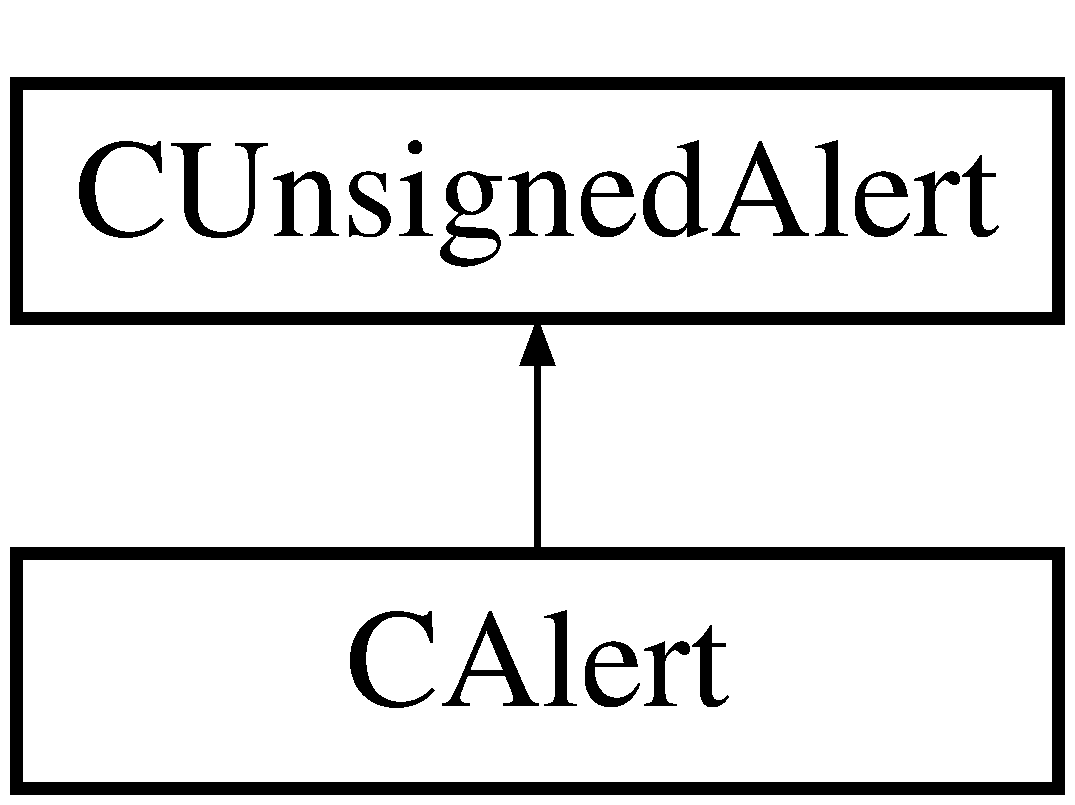
\includegraphics[height=2.000000cm]{class_c_unsigned_alert}
\end{center}
\end{figure}
\subsection*{Public Member Functions}
\begin{DoxyCompactItemize}
\item 
{\footnotesize template$<$typename Stream , typename Operation $>$ }\\void \hyperlink{class_c_unsigned_alert_acdf81abb731f9fc8d2c04618f2f4d79d}{Serialization\+Op} (Stream \&s, Operation ser\+\_\+action, int n\+Type, int \hyperlink{class_c_unsigned_alert_ad8fad8e8f62caaf8162fad19170de2cf}{n\+Version})
\item 
void \hyperlink{class_c_unsigned_alert_a9d387307eb60095e50134d10eea3ad69}{Set\+Null} ()
\item 
std\+::string \hyperlink{class_c_unsigned_alert_a326fbf3fae6b9ac2b7043350570b770f}{To\+String} () const 
\end{DoxyCompactItemize}
\subsection*{Public Attributes}
\begin{DoxyCompactItemize}
\item 
int \hyperlink{class_c_unsigned_alert_ad8fad8e8f62caaf8162fad19170de2cf}{n\+Version}
\item 
int64\+\_\+t \hyperlink{class_c_unsigned_alert_a13bb82aef8b496584f6b3ae6424f8e58}{n\+Relay\+Until}
\item 
int64\+\_\+t \hyperlink{class_c_unsigned_alert_af77a9d4d3abc0a0b376a7689059620e8}{n\+Expiration}
\item 
int \hyperlink{class_c_unsigned_alert_a4e11dc713526f6597a20762e707518a0}{n\+I\+D}
\item 
int \hyperlink{class_c_unsigned_alert_a28de8ffcdfea75db2061b2cdc1add04a}{n\+Cancel}
\item 
std\+::set$<$ int $>$ \hyperlink{class_c_unsigned_alert_ab1978ea23d02720d515bcdcf9d0dbdb0}{set\+Cancel}
\item 
int \hyperlink{class_c_unsigned_alert_af7ab540ea7df8e97fbfba7551ec31b1a}{n\+Min\+Ver}
\item 
int \hyperlink{class_c_unsigned_alert_a041bff847e178c132cb4d5234c1f41c8}{n\+Max\+Ver}
\item 
std\+::set$<$ std\+::string $>$ \hyperlink{class_c_unsigned_alert_a1b7148c413e1781222c5748935cad200}{set\+Sub\+Ver}
\item 
int \hyperlink{class_c_unsigned_alert_acf7253ae21d58a8633faab0635f5f5f5}{n\+Priority}
\item 
std\+::string \hyperlink{class_c_unsigned_alert_a8c9cd8c9706c14df3c5d6b9b1ed3b130}{str\+Comment}
\item 
std\+::string \hyperlink{class_c_unsigned_alert_a97cfbf9a49b770bb84e49389ac1489c2}{str\+Status\+Bar}
\item 
std\+::string \hyperlink{class_c_unsigned_alert_a0115109fd39d48f37a412d5f50a78828}{str\+Reserved}
\item 
\hyperlink{class_c_unsigned_alert_a24489988876bbf2c38a5f379e4057a53}{A\+D\+D\+\_\+\+S\+E\+R\+I\+A\+L\+I\+Z\+E\+\_\+\+M\+E\+T\+H\+O\+D\+S}
\end{DoxyCompactItemize}


\subsection{Detailed Description}
Alerts are for notifying old versions if they become too obsolete and need to upgrade. The message is displayed in the status bar. Alert messages are broadcast as a vector of signed data. Unserializing may not read the entire buffer if the alert is for a newer version, but older versions can still relay the original data. 

\subsection{Member Function Documentation}
\hypertarget{class_c_unsigned_alert_acdf81abb731f9fc8d2c04618f2f4d79d}{}\index{C\+Unsigned\+Alert@{C\+Unsigned\+Alert}!Serialization\+Op@{Serialization\+Op}}
\index{Serialization\+Op@{Serialization\+Op}!C\+Unsigned\+Alert@{C\+Unsigned\+Alert}}
\subsubsection[{Serialization\+Op}]{\setlength{\rightskip}{0pt plus 5cm}template$<$typename Stream , typename Operation $>$ void C\+Unsigned\+Alert\+::\+Serialization\+Op (
\begin{DoxyParamCaption}
\item[{Stream \&}]{s, }
\item[{Operation}]{ser\+\_\+action, }
\item[{int}]{n\+Type, }
\item[{int}]{n\+Version}
\end{DoxyParamCaption}
)\hspace{0.3cm}{\ttfamily [inline]}}\label{class_c_unsigned_alert_acdf81abb731f9fc8d2c04618f2f4d79d}
\hypertarget{class_c_unsigned_alert_a9d387307eb60095e50134d10eea3ad69}{}\index{C\+Unsigned\+Alert@{C\+Unsigned\+Alert}!Set\+Null@{Set\+Null}}
\index{Set\+Null@{Set\+Null}!C\+Unsigned\+Alert@{C\+Unsigned\+Alert}}
\subsubsection[{Set\+Null}]{\setlength{\rightskip}{0pt plus 5cm}void C\+Unsigned\+Alert\+::\+Set\+Null (
\begin{DoxyParamCaption}
{}
\end{DoxyParamCaption}
)}\label{class_c_unsigned_alert_a9d387307eb60095e50134d10eea3ad69}
\hypertarget{class_c_unsigned_alert_a326fbf3fae6b9ac2b7043350570b770f}{}\index{C\+Unsigned\+Alert@{C\+Unsigned\+Alert}!To\+String@{To\+String}}
\index{To\+String@{To\+String}!C\+Unsigned\+Alert@{C\+Unsigned\+Alert}}
\subsubsection[{To\+String}]{\setlength{\rightskip}{0pt plus 5cm}std\+::string C\+Unsigned\+Alert\+::\+To\+String (
\begin{DoxyParamCaption}
{}
\end{DoxyParamCaption}
) const}\label{class_c_unsigned_alert_a326fbf3fae6b9ac2b7043350570b770f}


\subsection{Member Data Documentation}
\hypertarget{class_c_unsigned_alert_a24489988876bbf2c38a5f379e4057a53}{}\index{C\+Unsigned\+Alert@{C\+Unsigned\+Alert}!A\+D\+D\+\_\+\+S\+E\+R\+I\+A\+L\+I\+Z\+E\+\_\+\+M\+E\+T\+H\+O\+D\+S@{A\+D\+D\+\_\+\+S\+E\+R\+I\+A\+L\+I\+Z\+E\+\_\+\+M\+E\+T\+H\+O\+D\+S}}
\index{A\+D\+D\+\_\+\+S\+E\+R\+I\+A\+L\+I\+Z\+E\+\_\+\+M\+E\+T\+H\+O\+D\+S@{A\+D\+D\+\_\+\+S\+E\+R\+I\+A\+L\+I\+Z\+E\+\_\+\+M\+E\+T\+H\+O\+D\+S}!C\+Unsigned\+Alert@{C\+Unsigned\+Alert}}
\subsubsection[{A\+D\+D\+\_\+\+S\+E\+R\+I\+A\+L\+I\+Z\+E\+\_\+\+M\+E\+T\+H\+O\+D\+S}]{\setlength{\rightskip}{0pt plus 5cm}C\+Unsigned\+Alert\+::\+A\+D\+D\+\_\+\+S\+E\+R\+I\+A\+L\+I\+Z\+E\+\_\+\+M\+E\+T\+H\+O\+D\+S}\label{class_c_unsigned_alert_a24489988876bbf2c38a5f379e4057a53}
\hypertarget{class_c_unsigned_alert_a28de8ffcdfea75db2061b2cdc1add04a}{}\index{C\+Unsigned\+Alert@{C\+Unsigned\+Alert}!n\+Cancel@{n\+Cancel}}
\index{n\+Cancel@{n\+Cancel}!C\+Unsigned\+Alert@{C\+Unsigned\+Alert}}
\subsubsection[{n\+Cancel}]{\setlength{\rightskip}{0pt plus 5cm}int C\+Unsigned\+Alert\+::n\+Cancel}\label{class_c_unsigned_alert_a28de8ffcdfea75db2061b2cdc1add04a}
\hypertarget{class_c_unsigned_alert_af77a9d4d3abc0a0b376a7689059620e8}{}\index{C\+Unsigned\+Alert@{C\+Unsigned\+Alert}!n\+Expiration@{n\+Expiration}}
\index{n\+Expiration@{n\+Expiration}!C\+Unsigned\+Alert@{C\+Unsigned\+Alert}}
\subsubsection[{n\+Expiration}]{\setlength{\rightskip}{0pt plus 5cm}int64\+\_\+t C\+Unsigned\+Alert\+::n\+Expiration}\label{class_c_unsigned_alert_af77a9d4d3abc0a0b376a7689059620e8}
\hypertarget{class_c_unsigned_alert_a4e11dc713526f6597a20762e707518a0}{}\index{C\+Unsigned\+Alert@{C\+Unsigned\+Alert}!n\+I\+D@{n\+I\+D}}
\index{n\+I\+D@{n\+I\+D}!C\+Unsigned\+Alert@{C\+Unsigned\+Alert}}
\subsubsection[{n\+I\+D}]{\setlength{\rightskip}{0pt plus 5cm}int C\+Unsigned\+Alert\+::n\+I\+D}\label{class_c_unsigned_alert_a4e11dc713526f6597a20762e707518a0}
\hypertarget{class_c_unsigned_alert_a041bff847e178c132cb4d5234c1f41c8}{}\index{C\+Unsigned\+Alert@{C\+Unsigned\+Alert}!n\+Max\+Ver@{n\+Max\+Ver}}
\index{n\+Max\+Ver@{n\+Max\+Ver}!C\+Unsigned\+Alert@{C\+Unsigned\+Alert}}
\subsubsection[{n\+Max\+Ver}]{\setlength{\rightskip}{0pt plus 5cm}int C\+Unsigned\+Alert\+::n\+Max\+Ver}\label{class_c_unsigned_alert_a041bff847e178c132cb4d5234c1f41c8}
\hypertarget{class_c_unsigned_alert_af7ab540ea7df8e97fbfba7551ec31b1a}{}\index{C\+Unsigned\+Alert@{C\+Unsigned\+Alert}!n\+Min\+Ver@{n\+Min\+Ver}}
\index{n\+Min\+Ver@{n\+Min\+Ver}!C\+Unsigned\+Alert@{C\+Unsigned\+Alert}}
\subsubsection[{n\+Min\+Ver}]{\setlength{\rightskip}{0pt plus 5cm}int C\+Unsigned\+Alert\+::n\+Min\+Ver}\label{class_c_unsigned_alert_af7ab540ea7df8e97fbfba7551ec31b1a}
\hypertarget{class_c_unsigned_alert_acf7253ae21d58a8633faab0635f5f5f5}{}\index{C\+Unsigned\+Alert@{C\+Unsigned\+Alert}!n\+Priority@{n\+Priority}}
\index{n\+Priority@{n\+Priority}!C\+Unsigned\+Alert@{C\+Unsigned\+Alert}}
\subsubsection[{n\+Priority}]{\setlength{\rightskip}{0pt plus 5cm}int C\+Unsigned\+Alert\+::n\+Priority}\label{class_c_unsigned_alert_acf7253ae21d58a8633faab0635f5f5f5}
\hypertarget{class_c_unsigned_alert_a13bb82aef8b496584f6b3ae6424f8e58}{}\index{C\+Unsigned\+Alert@{C\+Unsigned\+Alert}!n\+Relay\+Until@{n\+Relay\+Until}}
\index{n\+Relay\+Until@{n\+Relay\+Until}!C\+Unsigned\+Alert@{C\+Unsigned\+Alert}}
\subsubsection[{n\+Relay\+Until}]{\setlength{\rightskip}{0pt plus 5cm}int64\+\_\+t C\+Unsigned\+Alert\+::n\+Relay\+Until}\label{class_c_unsigned_alert_a13bb82aef8b496584f6b3ae6424f8e58}
\hypertarget{class_c_unsigned_alert_ad8fad8e8f62caaf8162fad19170de2cf}{}\index{C\+Unsigned\+Alert@{C\+Unsigned\+Alert}!n\+Version@{n\+Version}}
\index{n\+Version@{n\+Version}!C\+Unsigned\+Alert@{C\+Unsigned\+Alert}}
\subsubsection[{n\+Version}]{\setlength{\rightskip}{0pt plus 5cm}int C\+Unsigned\+Alert\+::n\+Version}\label{class_c_unsigned_alert_ad8fad8e8f62caaf8162fad19170de2cf}
\hypertarget{class_c_unsigned_alert_ab1978ea23d02720d515bcdcf9d0dbdb0}{}\index{C\+Unsigned\+Alert@{C\+Unsigned\+Alert}!set\+Cancel@{set\+Cancel}}
\index{set\+Cancel@{set\+Cancel}!C\+Unsigned\+Alert@{C\+Unsigned\+Alert}}
\subsubsection[{set\+Cancel}]{\setlength{\rightskip}{0pt plus 5cm}std\+::set$<$int$>$ C\+Unsigned\+Alert\+::set\+Cancel}\label{class_c_unsigned_alert_ab1978ea23d02720d515bcdcf9d0dbdb0}
\hypertarget{class_c_unsigned_alert_a1b7148c413e1781222c5748935cad200}{}\index{C\+Unsigned\+Alert@{C\+Unsigned\+Alert}!set\+Sub\+Ver@{set\+Sub\+Ver}}
\index{set\+Sub\+Ver@{set\+Sub\+Ver}!C\+Unsigned\+Alert@{C\+Unsigned\+Alert}}
\subsubsection[{set\+Sub\+Ver}]{\setlength{\rightskip}{0pt plus 5cm}std\+::set$<$std\+::string$>$ C\+Unsigned\+Alert\+::set\+Sub\+Ver}\label{class_c_unsigned_alert_a1b7148c413e1781222c5748935cad200}
\hypertarget{class_c_unsigned_alert_a8c9cd8c9706c14df3c5d6b9b1ed3b130}{}\index{C\+Unsigned\+Alert@{C\+Unsigned\+Alert}!str\+Comment@{str\+Comment}}
\index{str\+Comment@{str\+Comment}!C\+Unsigned\+Alert@{C\+Unsigned\+Alert}}
\subsubsection[{str\+Comment}]{\setlength{\rightskip}{0pt plus 5cm}std\+::string C\+Unsigned\+Alert\+::str\+Comment}\label{class_c_unsigned_alert_a8c9cd8c9706c14df3c5d6b9b1ed3b130}
\hypertarget{class_c_unsigned_alert_a0115109fd39d48f37a412d5f50a78828}{}\index{C\+Unsigned\+Alert@{C\+Unsigned\+Alert}!str\+Reserved@{str\+Reserved}}
\index{str\+Reserved@{str\+Reserved}!C\+Unsigned\+Alert@{C\+Unsigned\+Alert}}
\subsubsection[{str\+Reserved}]{\setlength{\rightskip}{0pt plus 5cm}std\+::string C\+Unsigned\+Alert\+::str\+Reserved}\label{class_c_unsigned_alert_a0115109fd39d48f37a412d5f50a78828}
\hypertarget{class_c_unsigned_alert_a97cfbf9a49b770bb84e49389ac1489c2}{}\index{C\+Unsigned\+Alert@{C\+Unsigned\+Alert}!str\+Status\+Bar@{str\+Status\+Bar}}
\index{str\+Status\+Bar@{str\+Status\+Bar}!C\+Unsigned\+Alert@{C\+Unsigned\+Alert}}
\subsubsection[{str\+Status\+Bar}]{\setlength{\rightskip}{0pt plus 5cm}std\+::string C\+Unsigned\+Alert\+::str\+Status\+Bar}\label{class_c_unsigned_alert_a97cfbf9a49b770bb84e49389ac1489c2}


The documentation for this class was generated from the following files\+:\begin{DoxyCompactItemize}
\item 
C\+:/\+Users/\+Joe/\+Documents/\+School/\+C\+S\+C17\+A/bitcoin/src/\hyperlink{alert_8h}{alert.\+h}\item 
C\+:/\+Users/\+Joe/\+Documents/\+School/\+C\+S\+C17\+A/bitcoin/src/\hyperlink{alert_8cpp}{alert.\+cpp}\end{DoxyCompactItemize}

\hypertarget{class_c_validation_interface}{}\section{C\+Validation\+Interface Class Reference}
\label{class_c_validation_interface}\index{C\+Validation\+Interface@{C\+Validation\+Interface}}


{\ttfamily \#include $<$validationinterface.\+h$>$}

Inheritance diagram for C\+Validation\+Interface\+:\begin{figure}[H]
\begin{center}
\leavevmode
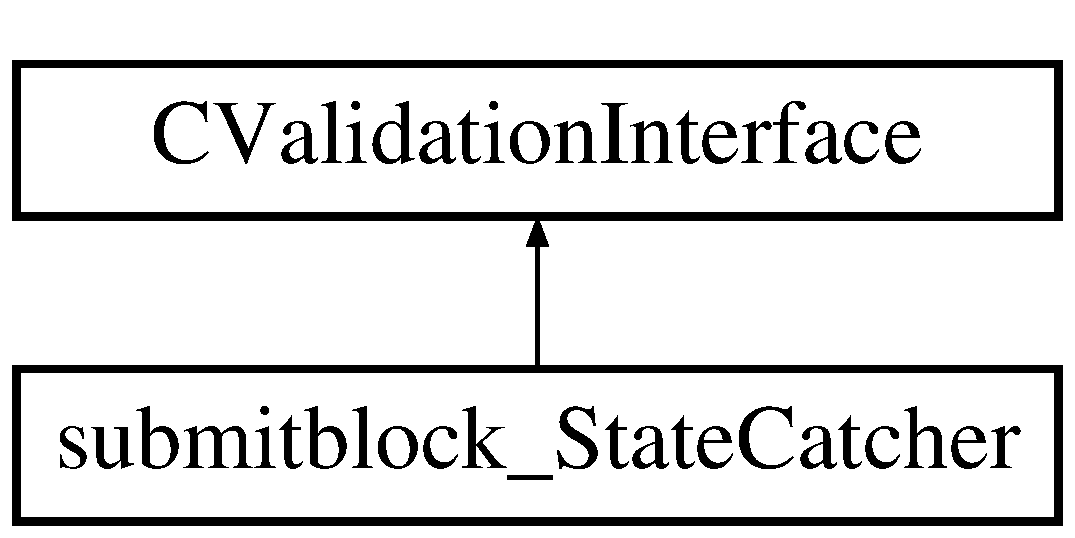
\includegraphics[height=2.000000cm]{class_c_validation_interface}
\end{center}
\end{figure}
\subsection*{Protected Member Functions}
\begin{DoxyCompactItemize}
\item 
virtual void \hyperlink{class_c_validation_interface_a1d255ed08bf26dbd6ad5924cabfdfae4}{Sync\+Transaction} (const C\+Transaction \&tx, const C\+Block $\ast$pblock)
\item 
virtual void \hyperlink{class_c_validation_interface_af8120f64ec6569dcf765fdf14acef31f}{Erase\+From\+Wallet} (const \hyperlink{classuint256}{uint256} \&hash)
\item 
virtual void \hyperlink{class_c_validation_interface_a8684492d9878120ce8c6c760a790f9ea}{Set\+Best\+Chain} (const C\+Block\+Locator \&locator)
\item 
virtual void \hyperlink{class_c_validation_interface_a8058fc107d993641df615abbb35a4c27}{Updated\+Transaction} (const \hyperlink{classuint256}{uint256} \&hash)
\item 
virtual void \hyperlink{class_c_validation_interface_a981f5160a2370db0cd616c00d8bd5270}{Inventory} (const \hyperlink{classuint256}{uint256} \&hash)
\item 
virtual void \hyperlink{class_c_validation_interface_af501da6f06bccb5e4bfbe66ae1bf6c9d}{Resend\+Wallet\+Transactions} (int64\+\_\+t n\+Best\+Block\+Time)
\item 
virtual void \hyperlink{class_c_validation_interface_aeb34ef6814685cabc29062ed7be25441}{Block\+Checked} (const C\+Block \&, const \hyperlink{class_c_validation_state}{C\+Validation\+State} \&)
\item 
friend \hyperlink{class_c_validation_interface_abba7a6c393df5b63bfd659c452446f96}{void\+::\+Register\+Validation\+Interface} (\hyperlink{class_c_validation_interface}{C\+Validation\+Interface} $\ast$)
\item 
friend \hyperlink{class_c_validation_interface_a30225070f6758f32aa041ccba519f1a8}{void\+::\+Unregister\+Validation\+Interface} (\hyperlink{class_c_validation_interface}{C\+Validation\+Interface} $\ast$)
\item 
friend \hyperlink{class_c_validation_interface_a31a772eec90ebb6407728f58f4bf098e}{void\+::\+Unregister\+All\+Validation\+Interfaces} ()
\end{DoxyCompactItemize}


\subsection{Member Function Documentation}
\hypertarget{class_c_validation_interface_aeb34ef6814685cabc29062ed7be25441}{}\index{C\+Validation\+Interface@{C\+Validation\+Interface}!Block\+Checked@{Block\+Checked}}
\index{Block\+Checked@{Block\+Checked}!C\+Validation\+Interface@{C\+Validation\+Interface}}
\subsubsection[{Block\+Checked}]{\setlength{\rightskip}{0pt plus 5cm}virtual void C\+Validation\+Interface\+::\+Block\+Checked (
\begin{DoxyParamCaption}
\item[{const C\+Block \&}]{, }
\item[{const {\bf C\+Validation\+State} \&}]{}
\end{DoxyParamCaption}
)\hspace{0.3cm}{\ttfamily [inline]}, {\ttfamily [protected]}, {\ttfamily [virtual]}}\label{class_c_validation_interface_aeb34ef6814685cabc29062ed7be25441}


Reimplemented in \hyperlink{classsubmitblock___state_catcher_a7c7174ac1a54c80c572b115114aa2ee6}{submitblock\+\_\+\+State\+Catcher}.

\hypertarget{class_c_validation_interface_af8120f64ec6569dcf765fdf14acef31f}{}\index{C\+Validation\+Interface@{C\+Validation\+Interface}!Erase\+From\+Wallet@{Erase\+From\+Wallet}}
\index{Erase\+From\+Wallet@{Erase\+From\+Wallet}!C\+Validation\+Interface@{C\+Validation\+Interface}}
\subsubsection[{Erase\+From\+Wallet}]{\setlength{\rightskip}{0pt plus 5cm}virtual void C\+Validation\+Interface\+::\+Erase\+From\+Wallet (
\begin{DoxyParamCaption}
\item[{const {\bf uint256} \&}]{hash}
\end{DoxyParamCaption}
)\hspace{0.3cm}{\ttfamily [inline]}, {\ttfamily [protected]}, {\ttfamily [virtual]}}\label{class_c_validation_interface_af8120f64ec6569dcf765fdf14acef31f}
\hypertarget{class_c_validation_interface_a981f5160a2370db0cd616c00d8bd5270}{}\index{C\+Validation\+Interface@{C\+Validation\+Interface}!Inventory@{Inventory}}
\index{Inventory@{Inventory}!C\+Validation\+Interface@{C\+Validation\+Interface}}
\subsubsection[{Inventory}]{\setlength{\rightskip}{0pt plus 5cm}virtual void C\+Validation\+Interface\+::\+Inventory (
\begin{DoxyParamCaption}
\item[{const {\bf uint256} \&}]{hash}
\end{DoxyParamCaption}
)\hspace{0.3cm}{\ttfamily [inline]}, {\ttfamily [protected]}, {\ttfamily [virtual]}}\label{class_c_validation_interface_a981f5160a2370db0cd616c00d8bd5270}
\hypertarget{class_c_validation_interface_af501da6f06bccb5e4bfbe66ae1bf6c9d}{}\index{C\+Validation\+Interface@{C\+Validation\+Interface}!Resend\+Wallet\+Transactions@{Resend\+Wallet\+Transactions}}
\index{Resend\+Wallet\+Transactions@{Resend\+Wallet\+Transactions}!C\+Validation\+Interface@{C\+Validation\+Interface}}
\subsubsection[{Resend\+Wallet\+Transactions}]{\setlength{\rightskip}{0pt plus 5cm}virtual void C\+Validation\+Interface\+::\+Resend\+Wallet\+Transactions (
\begin{DoxyParamCaption}
\item[{int64\+\_\+t}]{n\+Best\+Block\+Time}
\end{DoxyParamCaption}
)\hspace{0.3cm}{\ttfamily [inline]}, {\ttfamily [protected]}, {\ttfamily [virtual]}}\label{class_c_validation_interface_af501da6f06bccb5e4bfbe66ae1bf6c9d}
\hypertarget{class_c_validation_interface_a8684492d9878120ce8c6c760a790f9ea}{}\index{C\+Validation\+Interface@{C\+Validation\+Interface}!Set\+Best\+Chain@{Set\+Best\+Chain}}
\index{Set\+Best\+Chain@{Set\+Best\+Chain}!C\+Validation\+Interface@{C\+Validation\+Interface}}
\subsubsection[{Set\+Best\+Chain}]{\setlength{\rightskip}{0pt plus 5cm}virtual void C\+Validation\+Interface\+::\+Set\+Best\+Chain (
\begin{DoxyParamCaption}
\item[{const C\+Block\+Locator \&}]{locator}
\end{DoxyParamCaption}
)\hspace{0.3cm}{\ttfamily [inline]}, {\ttfamily [protected]}, {\ttfamily [virtual]}}\label{class_c_validation_interface_a8684492d9878120ce8c6c760a790f9ea}
\hypertarget{class_c_validation_interface_a1d255ed08bf26dbd6ad5924cabfdfae4}{}\index{C\+Validation\+Interface@{C\+Validation\+Interface}!Sync\+Transaction@{Sync\+Transaction}}
\index{Sync\+Transaction@{Sync\+Transaction}!C\+Validation\+Interface@{C\+Validation\+Interface}}
\subsubsection[{Sync\+Transaction}]{\setlength{\rightskip}{0pt plus 5cm}virtual void C\+Validation\+Interface\+::\+Sync\+Transaction (
\begin{DoxyParamCaption}
\item[{const C\+Transaction \&}]{tx, }
\item[{const C\+Block $\ast$}]{pblock}
\end{DoxyParamCaption}
)\hspace{0.3cm}{\ttfamily [inline]}, {\ttfamily [protected]}, {\ttfamily [virtual]}}\label{class_c_validation_interface_a1d255ed08bf26dbd6ad5924cabfdfae4}
\hypertarget{class_c_validation_interface_a8058fc107d993641df615abbb35a4c27}{}\index{C\+Validation\+Interface@{C\+Validation\+Interface}!Updated\+Transaction@{Updated\+Transaction}}
\index{Updated\+Transaction@{Updated\+Transaction}!C\+Validation\+Interface@{C\+Validation\+Interface}}
\subsubsection[{Updated\+Transaction}]{\setlength{\rightskip}{0pt plus 5cm}virtual void C\+Validation\+Interface\+::\+Updated\+Transaction (
\begin{DoxyParamCaption}
\item[{const {\bf uint256} \&}]{hash}
\end{DoxyParamCaption}
)\hspace{0.3cm}{\ttfamily [inline]}, {\ttfamily [protected]}, {\ttfamily [virtual]}}\label{class_c_validation_interface_a8058fc107d993641df615abbb35a4c27}
\hypertarget{class_c_validation_interface_abba7a6c393df5b63bfd659c452446f96}{}\index{C\+Validation\+Interface@{C\+Validation\+Interface}!void\+::\+Register\+Validation\+Interface@{void\+::\+Register\+Validation\+Interface}}
\index{void\+::\+Register\+Validation\+Interface@{void\+::\+Register\+Validation\+Interface}!C\+Validation\+Interface@{C\+Validation\+Interface}}
\subsubsection[{void\+::\+Register\+Validation\+Interface}]{\setlength{\rightskip}{0pt plus 5cm}{\bf C\+Validation\+Interface\+::void\+::\+Register\+Validation\+Interface} (
\begin{DoxyParamCaption}
\item[{{\bf C\+Validation\+Interface} $\ast$}]{}
\end{DoxyParamCaption}
)\hspace{0.3cm}{\ttfamily [protected]}}\label{class_c_validation_interface_abba7a6c393df5b63bfd659c452446f96}
\hypertarget{class_c_validation_interface_a31a772eec90ebb6407728f58f4bf098e}{}\index{C\+Validation\+Interface@{C\+Validation\+Interface}!void\+::\+Unregister\+All\+Validation\+Interfaces@{void\+::\+Unregister\+All\+Validation\+Interfaces}}
\index{void\+::\+Unregister\+All\+Validation\+Interfaces@{void\+::\+Unregister\+All\+Validation\+Interfaces}!C\+Validation\+Interface@{C\+Validation\+Interface}}
\subsubsection[{void\+::\+Unregister\+All\+Validation\+Interfaces}]{\setlength{\rightskip}{0pt plus 5cm}{\bf C\+Validation\+Interface\+::void\+::\+Unregister\+All\+Validation\+Interfaces} (
\begin{DoxyParamCaption}
{}
\end{DoxyParamCaption}
)\hspace{0.3cm}{\ttfamily [protected]}}\label{class_c_validation_interface_a31a772eec90ebb6407728f58f4bf098e}
\hypertarget{class_c_validation_interface_a30225070f6758f32aa041ccba519f1a8}{}\index{C\+Validation\+Interface@{C\+Validation\+Interface}!void\+::\+Unregister\+Validation\+Interface@{void\+::\+Unregister\+Validation\+Interface}}
\index{void\+::\+Unregister\+Validation\+Interface@{void\+::\+Unregister\+Validation\+Interface}!C\+Validation\+Interface@{C\+Validation\+Interface}}
\subsubsection[{void\+::\+Unregister\+Validation\+Interface}]{\setlength{\rightskip}{0pt plus 5cm}{\bf C\+Validation\+Interface\+::void\+::\+Unregister\+Validation\+Interface} (
\begin{DoxyParamCaption}
\item[{{\bf C\+Validation\+Interface} $\ast$}]{}
\end{DoxyParamCaption}
)\hspace{0.3cm}{\ttfamily [protected]}}\label{class_c_validation_interface_a30225070f6758f32aa041ccba519f1a8}


The documentation for this class was generated from the following file\+:\begin{DoxyCompactItemize}
\item 
C\+:/\+Users/\+Joe/\+Documents/\+School/\+C\+S\+C17\+A/bitcoin/src/\hyperlink{validationinterface_8h}{validationinterface.\+h}\end{DoxyCompactItemize}

\hypertarget{class_c_validation_state}{}\section{C\+Validation\+State Class Reference}
\label{class_c_validation_state}\index{C\+Validation\+State@{C\+Validation\+State}}


{\ttfamily \#include $<$main.\+h$>$}

\subsection*{Public Member Functions}
\begin{DoxyCompactItemize}
\item 
\hyperlink{class_c_validation_state_a4c89cdea0b8e6983baa531bc756d8584}{C\+Validation\+State} ()
\item 
bool \hyperlink{class_c_validation_state_a3c6786d00da8d1c5df25b4c3876409e8}{Do\+S} (int level, bool ret=false, unsigned char ch\+Reject\+Code\+In=0, std\+::string str\+Reject\+Reason\+In=\char`\"{}\char`\"{}, bool corruption\+In=false)
\item 
bool \hyperlink{class_c_validation_state_a88ff08b67f7f44bb3c7f7053bb1ee6fc}{Invalid} (bool ret=false, unsigned char \+\_\+ch\+Reject\+Code=0, std\+::string \+\_\+str\+Reject\+Reason=\char`\"{}\char`\"{})
\item 
bool \hyperlink{class_c_validation_state_abf67ad56f62df5679d47c289684c554c}{Error} (std\+::string str\+Reject\+Reason\+In=\char`\"{}\char`\"{})
\item 
bool \hyperlink{class_c_validation_state_a6788cb521cf538ac80413a1c6c3da5e8}{Abort} (const std\+::string \&msg)
\item 
bool \hyperlink{class_c_validation_state_af4c51946b39b2234b8004d58fbc164a5}{Is\+Valid} () const 
\item 
bool \hyperlink{class_c_validation_state_aba47277dbc39192208515fd8cc685879}{Is\+Invalid} () const 
\item 
bool \hyperlink{class_c_validation_state_a8c608ada2395e5af099661ff353dbb3f}{Is\+Error} () const 
\item 
bool \hyperlink{class_c_validation_state_aba30a9e05436871a43e6acfb8e484963}{Is\+Invalid} (int \&n\+Do\+S\+Out) const 
\item 
bool \hyperlink{class_c_validation_state_a5b09f68e838c43ef20af29e725920a01}{Corruption\+Possible} () const 
\item 
unsigned char \hyperlink{class_c_validation_state_a8bbd27130d1810d60735e1df5e4ea69b}{Get\+Reject\+Code} () const 
\item 
std\+::string \hyperlink{class_c_validation_state_a2e7ea577adfdf90aaff44ad0fa16adde}{Get\+Reject\+Reason} () const 
\end{DoxyCompactItemize}


\subsection{Detailed Description}
Capture information about block/transaction validation 

\subsection{Constructor \& Destructor Documentation}
\hypertarget{class_c_validation_state_a4c89cdea0b8e6983baa531bc756d8584}{}\index{C\+Validation\+State@{C\+Validation\+State}!C\+Validation\+State@{C\+Validation\+State}}
\index{C\+Validation\+State@{C\+Validation\+State}!C\+Validation\+State@{C\+Validation\+State}}
\subsubsection[{C\+Validation\+State}]{\setlength{\rightskip}{0pt plus 5cm}C\+Validation\+State\+::\+C\+Validation\+State (
\begin{DoxyParamCaption}
{}
\end{DoxyParamCaption}
)\hspace{0.3cm}{\ttfamily [inline]}}\label{class_c_validation_state_a4c89cdea0b8e6983baa531bc756d8584}


\subsection{Member Function Documentation}
\hypertarget{class_c_validation_state_a6788cb521cf538ac80413a1c6c3da5e8}{}\index{C\+Validation\+State@{C\+Validation\+State}!Abort@{Abort}}
\index{Abort@{Abort}!C\+Validation\+State@{C\+Validation\+State}}
\subsubsection[{Abort}]{\setlength{\rightskip}{0pt plus 5cm}bool C\+Validation\+State\+::\+Abort (
\begin{DoxyParamCaption}
\item[{const std\+::string \&}]{msg}
\end{DoxyParamCaption}
)\hspace{0.3cm}{\ttfamily [inline]}}\label{class_c_validation_state_a6788cb521cf538ac80413a1c6c3da5e8}
\hypertarget{class_c_validation_state_a5b09f68e838c43ef20af29e725920a01}{}\index{C\+Validation\+State@{C\+Validation\+State}!Corruption\+Possible@{Corruption\+Possible}}
\index{Corruption\+Possible@{Corruption\+Possible}!C\+Validation\+State@{C\+Validation\+State}}
\subsubsection[{Corruption\+Possible}]{\setlength{\rightskip}{0pt plus 5cm}bool C\+Validation\+State\+::\+Corruption\+Possible (
\begin{DoxyParamCaption}
{}
\end{DoxyParamCaption}
) const\hspace{0.3cm}{\ttfamily [inline]}}\label{class_c_validation_state_a5b09f68e838c43ef20af29e725920a01}
\hypertarget{class_c_validation_state_a3c6786d00da8d1c5df25b4c3876409e8}{}\index{C\+Validation\+State@{C\+Validation\+State}!Do\+S@{Do\+S}}
\index{Do\+S@{Do\+S}!C\+Validation\+State@{C\+Validation\+State}}
\subsubsection[{Do\+S}]{\setlength{\rightskip}{0pt plus 5cm}bool C\+Validation\+State\+::\+Do\+S (
\begin{DoxyParamCaption}
\item[{int}]{level, }
\item[{bool}]{ret = {\ttfamily false}, }
\item[{unsigned char}]{ch\+Reject\+Code\+In = {\ttfamily 0}, }
\item[{std\+::string}]{str\+Reject\+Reason\+In = {\ttfamily \char`\"{}\char`\"{}}, }
\item[{bool}]{corruption\+In = {\ttfamily false}}
\end{DoxyParamCaption}
)\hspace{0.3cm}{\ttfamily [inline]}}\label{class_c_validation_state_a3c6786d00da8d1c5df25b4c3876409e8}
\hypertarget{class_c_validation_state_abf67ad56f62df5679d47c289684c554c}{}\index{C\+Validation\+State@{C\+Validation\+State}!Error@{Error}}
\index{Error@{Error}!C\+Validation\+State@{C\+Validation\+State}}
\subsubsection[{Error}]{\setlength{\rightskip}{0pt plus 5cm}bool C\+Validation\+State\+::\+Error (
\begin{DoxyParamCaption}
\item[{std\+::string}]{str\+Reject\+Reason\+In = {\ttfamily \char`\"{}\char`\"{}}}
\end{DoxyParamCaption}
)\hspace{0.3cm}{\ttfamily [inline]}}\label{class_c_validation_state_abf67ad56f62df5679d47c289684c554c}
\hypertarget{class_c_validation_state_a8bbd27130d1810d60735e1df5e4ea69b}{}\index{C\+Validation\+State@{C\+Validation\+State}!Get\+Reject\+Code@{Get\+Reject\+Code}}
\index{Get\+Reject\+Code@{Get\+Reject\+Code}!C\+Validation\+State@{C\+Validation\+State}}
\subsubsection[{Get\+Reject\+Code}]{\setlength{\rightskip}{0pt plus 5cm}unsigned char C\+Validation\+State\+::\+Get\+Reject\+Code (
\begin{DoxyParamCaption}
{}
\end{DoxyParamCaption}
) const\hspace{0.3cm}{\ttfamily [inline]}}\label{class_c_validation_state_a8bbd27130d1810d60735e1df5e4ea69b}
\hypertarget{class_c_validation_state_a2e7ea577adfdf90aaff44ad0fa16adde}{}\index{C\+Validation\+State@{C\+Validation\+State}!Get\+Reject\+Reason@{Get\+Reject\+Reason}}
\index{Get\+Reject\+Reason@{Get\+Reject\+Reason}!C\+Validation\+State@{C\+Validation\+State}}
\subsubsection[{Get\+Reject\+Reason}]{\setlength{\rightskip}{0pt plus 5cm}std\+::string C\+Validation\+State\+::\+Get\+Reject\+Reason (
\begin{DoxyParamCaption}
{}
\end{DoxyParamCaption}
) const\hspace{0.3cm}{\ttfamily [inline]}}\label{class_c_validation_state_a2e7ea577adfdf90aaff44ad0fa16adde}
\hypertarget{class_c_validation_state_a88ff08b67f7f44bb3c7f7053bb1ee6fc}{}\index{C\+Validation\+State@{C\+Validation\+State}!Invalid@{Invalid}}
\index{Invalid@{Invalid}!C\+Validation\+State@{C\+Validation\+State}}
\subsubsection[{Invalid}]{\setlength{\rightskip}{0pt plus 5cm}bool C\+Validation\+State\+::\+Invalid (
\begin{DoxyParamCaption}
\item[{bool}]{ret = {\ttfamily false}, }
\item[{unsigned char}]{\+\_\+ch\+Reject\+Code = {\ttfamily 0}, }
\item[{std\+::string}]{\+\_\+str\+Reject\+Reason = {\ttfamily \char`\"{}\char`\"{}}}
\end{DoxyParamCaption}
)\hspace{0.3cm}{\ttfamily [inline]}}\label{class_c_validation_state_a88ff08b67f7f44bb3c7f7053bb1ee6fc}
\hypertarget{class_c_validation_state_a8c608ada2395e5af099661ff353dbb3f}{}\index{C\+Validation\+State@{C\+Validation\+State}!Is\+Error@{Is\+Error}}
\index{Is\+Error@{Is\+Error}!C\+Validation\+State@{C\+Validation\+State}}
\subsubsection[{Is\+Error}]{\setlength{\rightskip}{0pt plus 5cm}bool C\+Validation\+State\+::\+Is\+Error (
\begin{DoxyParamCaption}
{}
\end{DoxyParamCaption}
) const\hspace{0.3cm}{\ttfamily [inline]}}\label{class_c_validation_state_a8c608ada2395e5af099661ff353dbb3f}
\hypertarget{class_c_validation_state_aba47277dbc39192208515fd8cc685879}{}\index{C\+Validation\+State@{C\+Validation\+State}!Is\+Invalid@{Is\+Invalid}}
\index{Is\+Invalid@{Is\+Invalid}!C\+Validation\+State@{C\+Validation\+State}}
\subsubsection[{Is\+Invalid}]{\setlength{\rightskip}{0pt plus 5cm}bool C\+Validation\+State\+::\+Is\+Invalid (
\begin{DoxyParamCaption}
{}
\end{DoxyParamCaption}
) const\hspace{0.3cm}{\ttfamily [inline]}}\label{class_c_validation_state_aba47277dbc39192208515fd8cc685879}
\hypertarget{class_c_validation_state_aba30a9e05436871a43e6acfb8e484963}{}\index{C\+Validation\+State@{C\+Validation\+State}!Is\+Invalid@{Is\+Invalid}}
\index{Is\+Invalid@{Is\+Invalid}!C\+Validation\+State@{C\+Validation\+State}}
\subsubsection[{Is\+Invalid}]{\setlength{\rightskip}{0pt plus 5cm}bool C\+Validation\+State\+::\+Is\+Invalid (
\begin{DoxyParamCaption}
\item[{int \&}]{n\+Do\+S\+Out}
\end{DoxyParamCaption}
) const\hspace{0.3cm}{\ttfamily [inline]}}\label{class_c_validation_state_aba30a9e05436871a43e6acfb8e484963}
\hypertarget{class_c_validation_state_af4c51946b39b2234b8004d58fbc164a5}{}\index{C\+Validation\+State@{C\+Validation\+State}!Is\+Valid@{Is\+Valid}}
\index{Is\+Valid@{Is\+Valid}!C\+Validation\+State@{C\+Validation\+State}}
\subsubsection[{Is\+Valid}]{\setlength{\rightskip}{0pt plus 5cm}bool C\+Validation\+State\+::\+Is\+Valid (
\begin{DoxyParamCaption}
{}
\end{DoxyParamCaption}
) const\hspace{0.3cm}{\ttfamily [inline]}}\label{class_c_validation_state_af4c51946b39b2234b8004d58fbc164a5}


The documentation for this class was generated from the following file\+:\begin{DoxyCompactItemize}
\item 
C\+:/\+Users/\+Joe/\+Documents/\+School/\+C\+S\+C17\+A/bitcoin/src/\hyperlink{main_8h}{main.\+h}\end{DoxyCompactItemize}

\hypertarget{class_c_var_int}{}\section{C\+Var\+Int$<$ I $>$ Class Template Reference}
\label{class_c_var_int}\index{C\+Var\+Int$<$ I $>$@{C\+Var\+Int$<$ I $>$}}


{\ttfamily \#include $<$serialize.\+h$>$}

\subsection*{Public Member Functions}
\begin{DoxyCompactItemize}
\item 
\hyperlink{class_c_var_int_ab26b9de1b43d4b9ce844eaa7cf6a6b4f}{C\+Var\+Int} (I \&n\+In)
\item 
unsigned int \hyperlink{class_c_var_int_a0fb5d15dfab5807439c1260096a10742}{Get\+Serialize\+Size} (int, int) const 
\item 
{\footnotesize template$<$typename Stream $>$ }\\void \hyperlink{class_c_var_int_ac9d49fe76d15de74952dfa1b1765d60d}{Serialize} (Stream \&s, int, int) const 
\item 
{\footnotesize template$<$typename Stream $>$ }\\void \hyperlink{class_c_var_int_aba87b78443378273b4f335dcd858c29c}{Unserialize} (Stream \&s, int, int)
\end{DoxyCompactItemize}
\subsection*{Protected Attributes}
\begin{DoxyCompactItemize}
\item 
I \& \hyperlink{class_c_var_int_a4514adc82b41754d9ac22ee627744614}{n}
\end{DoxyCompactItemize}


\subsection{Constructor \& Destructor Documentation}
\hypertarget{class_c_var_int_ab26b9de1b43d4b9ce844eaa7cf6a6b4f}{}\index{C\+Var\+Int@{C\+Var\+Int}!C\+Var\+Int@{C\+Var\+Int}}
\index{C\+Var\+Int@{C\+Var\+Int}!C\+Var\+Int@{C\+Var\+Int}}
\subsubsection[{C\+Var\+Int}]{\setlength{\rightskip}{0pt plus 5cm}template$<$typename I $>$ {\bf C\+Var\+Int}$<$ I $>$\+::{\bf C\+Var\+Int} (
\begin{DoxyParamCaption}
\item[{I \&}]{n\+In}
\end{DoxyParamCaption}
)\hspace{0.3cm}{\ttfamily [inline]}}\label{class_c_var_int_ab26b9de1b43d4b9ce844eaa7cf6a6b4f}


\subsection{Member Function Documentation}
\hypertarget{class_c_var_int_a0fb5d15dfab5807439c1260096a10742}{}\index{C\+Var\+Int@{C\+Var\+Int}!Get\+Serialize\+Size@{Get\+Serialize\+Size}}
\index{Get\+Serialize\+Size@{Get\+Serialize\+Size}!C\+Var\+Int@{C\+Var\+Int}}
\subsubsection[{Get\+Serialize\+Size}]{\setlength{\rightskip}{0pt plus 5cm}template$<$typename I $>$ unsigned int {\bf C\+Var\+Int}$<$ I $>$\+::Get\+Serialize\+Size (
\begin{DoxyParamCaption}
\item[{int}]{, }
\item[{int}]{}
\end{DoxyParamCaption}
) const\hspace{0.3cm}{\ttfamily [inline]}}\label{class_c_var_int_a0fb5d15dfab5807439c1260096a10742}
\hypertarget{class_c_var_int_ac9d49fe76d15de74952dfa1b1765d60d}{}\index{C\+Var\+Int@{C\+Var\+Int}!Serialize@{Serialize}}
\index{Serialize@{Serialize}!C\+Var\+Int@{C\+Var\+Int}}
\subsubsection[{Serialize}]{\setlength{\rightskip}{0pt plus 5cm}template$<$typename I $>$ template$<$typename Stream $>$ void {\bf C\+Var\+Int}$<$ I $>$\+::Serialize (
\begin{DoxyParamCaption}
\item[{Stream \&}]{s, }
\item[{int}]{, }
\item[{int}]{}
\end{DoxyParamCaption}
) const\hspace{0.3cm}{\ttfamily [inline]}}\label{class_c_var_int_ac9d49fe76d15de74952dfa1b1765d60d}
\hypertarget{class_c_var_int_aba87b78443378273b4f335dcd858c29c}{}\index{C\+Var\+Int@{C\+Var\+Int}!Unserialize@{Unserialize}}
\index{Unserialize@{Unserialize}!C\+Var\+Int@{C\+Var\+Int}}
\subsubsection[{Unserialize}]{\setlength{\rightskip}{0pt plus 5cm}template$<$typename I $>$ template$<$typename Stream $>$ void {\bf C\+Var\+Int}$<$ I $>$\+::Unserialize (
\begin{DoxyParamCaption}
\item[{Stream \&}]{s, }
\item[{int}]{, }
\item[{int}]{}
\end{DoxyParamCaption}
)\hspace{0.3cm}{\ttfamily [inline]}}\label{class_c_var_int_aba87b78443378273b4f335dcd858c29c}


\subsection{Member Data Documentation}
\hypertarget{class_c_var_int_a4514adc82b41754d9ac22ee627744614}{}\index{C\+Var\+Int@{C\+Var\+Int}!n@{n}}
\index{n@{n}!C\+Var\+Int@{C\+Var\+Int}}
\subsubsection[{n}]{\setlength{\rightskip}{0pt plus 5cm}template$<$typename I $>$ I\& {\bf C\+Var\+Int}$<$ I $>$\+::n\hspace{0.3cm}{\ttfamily [protected]}}\label{class_c_var_int_a4514adc82b41754d9ac22ee627744614}


The documentation for this class was generated from the following file\+:\begin{DoxyCompactItemize}
\item 
C\+:/\+Users/\+Joe/\+Documents/\+School/\+C\+S\+C17\+A/bitcoin/src/\hyperlink{serialize_8h}{serialize.\+h}\end{DoxyCompactItemize}

\hypertarget{class_c_verify_d_b}{}\section{C\+Verify\+D\+B Class Reference}
\label{class_c_verify_d_b}\index{C\+Verify\+D\+B@{C\+Verify\+D\+B}}


{\ttfamily \#include $<$main.\+h$>$}

\subsection*{Public Member Functions}
\begin{DoxyCompactItemize}
\item 
\hyperlink{class_c_verify_d_b_ab33a26982ba391fc71614f8eee9dbaa0}{C\+Verify\+D\+B} ()
\item 
\hyperlink{class_c_verify_d_b_a4a04d4554f763b8803082fae81513f40}{$\sim$\+C\+Verify\+D\+B} ()
\item 
bool \hyperlink{class_c_verify_d_b_a5d3e3ade35a14ddce2404e18e4b1df50}{Verify\+D\+B} (\hyperlink{class_c_coins_view}{C\+Coins\+View} $\ast$coinsview, int n\+Check\+Level, int n\+Check\+Depth)
\end{DoxyCompactItemize}


\subsection{Detailed Description}
R\+A\+I\+I wrapper for Verify\+D\+B\+: Verify consistency of the block and coin databases 

\subsection{Constructor \& Destructor Documentation}
\hypertarget{class_c_verify_d_b_ab33a26982ba391fc71614f8eee9dbaa0}{}\index{C\+Verify\+D\+B@{C\+Verify\+D\+B}!C\+Verify\+D\+B@{C\+Verify\+D\+B}}
\index{C\+Verify\+D\+B@{C\+Verify\+D\+B}!C\+Verify\+D\+B@{C\+Verify\+D\+B}}
\subsubsection[{C\+Verify\+D\+B}]{\setlength{\rightskip}{0pt plus 5cm}C\+Verify\+D\+B\+::\+C\+Verify\+D\+B (
\begin{DoxyParamCaption}
{}
\end{DoxyParamCaption}
)}\label{class_c_verify_d_b_ab33a26982ba391fc71614f8eee9dbaa0}
\hypertarget{class_c_verify_d_b_a4a04d4554f763b8803082fae81513f40}{}\index{C\+Verify\+D\+B@{C\+Verify\+D\+B}!````~C\+Verify\+D\+B@{$\sim$\+C\+Verify\+D\+B}}
\index{````~C\+Verify\+D\+B@{$\sim$\+C\+Verify\+D\+B}!C\+Verify\+D\+B@{C\+Verify\+D\+B}}
\subsubsection[{$\sim$\+C\+Verify\+D\+B}]{\setlength{\rightskip}{0pt plus 5cm}C\+Verify\+D\+B\+::$\sim$\+C\+Verify\+D\+B (
\begin{DoxyParamCaption}
{}
\end{DoxyParamCaption}
)}\label{class_c_verify_d_b_a4a04d4554f763b8803082fae81513f40}


\subsection{Member Function Documentation}
\hypertarget{class_c_verify_d_b_a5d3e3ade35a14ddce2404e18e4b1df50}{}\index{C\+Verify\+D\+B@{C\+Verify\+D\+B}!Verify\+D\+B@{Verify\+D\+B}}
\index{Verify\+D\+B@{Verify\+D\+B}!C\+Verify\+D\+B@{C\+Verify\+D\+B}}
\subsubsection[{Verify\+D\+B}]{\setlength{\rightskip}{0pt plus 5cm}bool C\+Verify\+D\+B\+::\+Verify\+D\+B (
\begin{DoxyParamCaption}
\item[{{\bf C\+Coins\+View} $\ast$}]{coinsview, }
\item[{int}]{n\+Check\+Level, }
\item[{int}]{n\+Check\+Depth}
\end{DoxyParamCaption}
)}\label{class_c_verify_d_b_a5d3e3ade35a14ddce2404e18e4b1df50}


The documentation for this class was generated from the following files\+:\begin{DoxyCompactItemize}
\item 
C\+:/\+Users/\+Joe/\+Documents/\+School/\+C\+S\+C17\+A/bitcoin/src/\hyperlink{main_8h}{main.\+h}\item 
C\+:/\+Users/\+Joe/\+Documents/\+School/\+C\+S\+C17\+A/bitcoin/src/\hyperlink{main_8cpp}{main.\+cpp}\end{DoxyCompactItemize}

\hypertarget{classtinyformat_1_1detail_1_1_format_iterator}{}\section{tinyformat\+:\+:detail\+:\+:Format\+Iterator Class Reference}
\label{classtinyformat_1_1detail_1_1_format_iterator}\index{tinyformat\+::detail\+::\+Format\+Iterator@{tinyformat\+::detail\+::\+Format\+Iterator}}


{\ttfamily \#include $<$tinyformat.\+h$>$}

\subsection*{Public Types}
\begin{DoxyCompactItemize}
\item 
enum \hyperlink{classtinyformat_1_1detail_1_1_format_iterator_a219d15b3b08e2e2039043d2e992cc0b4}{Extra\+Format\+Flags} \{ \\*
\hyperlink{classtinyformat_1_1detail_1_1_format_iterator_a219d15b3b08e2e2039043d2e992cc0b4a9ab97a1e3a40d92f84e93fa8358482aa}{Flag\+\_\+\+None} = 0, 
\hyperlink{classtinyformat_1_1detail_1_1_format_iterator_a219d15b3b08e2e2039043d2e992cc0b4a5b65abd67b2208298644ddc94687e390}{Flag\+\_\+\+Truncate\+To\+Precision} = 1$<$$<$0, 
\hyperlink{classtinyformat_1_1detail_1_1_format_iterator_a219d15b3b08e2e2039043d2e992cc0b4a9d39e70884631652913a219fc8c631a9}{Flag\+\_\+\+Space\+Pad\+Positive} = 1$<$$<$1, 
\hyperlink{classtinyformat_1_1detail_1_1_format_iterator_a219d15b3b08e2e2039043d2e992cc0b4a5d0e44bf22d5a33b12af70fab06a595d}{Flag\+\_\+\+Variable\+Width} = 1$<$$<$2, 
\\*
\hyperlink{classtinyformat_1_1detail_1_1_format_iterator_a219d15b3b08e2e2039043d2e992cc0b4a19e53a79433733d40dc1349ce52f3284}{Flag\+\_\+\+Variable\+Precision} = 1$<$$<$3
 \}
\end{DoxyCompactItemize}
\subsection*{Public Member Functions}
\begin{DoxyCompactItemize}
\item 
\hyperlink{classtinyformat_1_1detail_1_1_format_iterator_a798e0f475996df1b0a4f93540d96791b}{Format\+Iterator} (std\+::ostream \&out, const char $\ast$fmt)
\item 
void \hyperlink{classtinyformat_1_1detail_1_1_format_iterator_a46377a804f72dbad1e508d2fbaa18ce9}{finish} ()
\item 
\hyperlink{classtinyformat_1_1detail_1_1_format_iterator_a700ea30dbed93c28c499ac01c59a78a4}{$\sim$\+Format\+Iterator} ()
\item 
{\footnotesize template$<$typename T $>$ }\\void \hyperlink{classtinyformat_1_1detail_1_1_format_iterator_a2a2b99ea3a371e1ff8d56d8c8b801bdb}{accept} (const T \&value)
\item 
{\footnotesize template$<$typename T $>$ }\\\hyperlink{tinyformat_8h_a6aa2353acc671b972658fd73a813b960}{T\+I\+N\+Y\+F\+O\+R\+M\+A\+T\+\_\+\+N\+O\+I\+N\+L\+I\+N\+E} void \hyperlink{classtinyformat_1_1detail_1_1_format_iterator_a914be2066071c01cac4c2ea867c9d89a}{accept} (const T \&value)
\end{DoxyCompactItemize}


\subsection{Member Enumeration Documentation}
\hypertarget{classtinyformat_1_1detail_1_1_format_iterator_a219d15b3b08e2e2039043d2e992cc0b4}{}\index{tinyformat\+::detail\+::\+Format\+Iterator@{tinyformat\+::detail\+::\+Format\+Iterator}!Extra\+Format\+Flags@{Extra\+Format\+Flags}}
\index{Extra\+Format\+Flags@{Extra\+Format\+Flags}!tinyformat\+::detail\+::\+Format\+Iterator@{tinyformat\+::detail\+::\+Format\+Iterator}}
\subsubsection[{Extra\+Format\+Flags}]{\setlength{\rightskip}{0pt plus 5cm}enum {\bf tinyformat\+::detail\+::\+Format\+Iterator\+::\+Extra\+Format\+Flags}}\label{classtinyformat_1_1detail_1_1_format_iterator_a219d15b3b08e2e2039043d2e992cc0b4}
\begin{Desc}
\item[Enumerator]\par
\begin{description}
\index{Flag\+\_\+\+None@{Flag\+\_\+\+None}!tinyformat\+::detail\+::\+Format\+Iterator@{tinyformat\+::detail\+::\+Format\+Iterator}}\index{tinyformat\+::detail\+::\+Format\+Iterator@{tinyformat\+::detail\+::\+Format\+Iterator}!Flag\+\_\+\+None@{Flag\+\_\+\+None}}\item[{\em 
\hypertarget{classtinyformat_1_1detail_1_1_format_iterator_a219d15b3b08e2e2039043d2e992cc0b4a9ab97a1e3a40d92f84e93fa8358482aa}{}Flag\+\_\+\+None\label{classtinyformat_1_1detail_1_1_format_iterator_a219d15b3b08e2e2039043d2e992cc0b4a9ab97a1e3a40d92f84e93fa8358482aa}
}]\index{Flag\+\_\+\+Truncate\+To\+Precision@{Flag\+\_\+\+Truncate\+To\+Precision}!tinyformat\+::detail\+::\+Format\+Iterator@{tinyformat\+::detail\+::\+Format\+Iterator}}\index{tinyformat\+::detail\+::\+Format\+Iterator@{tinyformat\+::detail\+::\+Format\+Iterator}!Flag\+\_\+\+Truncate\+To\+Precision@{Flag\+\_\+\+Truncate\+To\+Precision}}\item[{\em 
\hypertarget{classtinyformat_1_1detail_1_1_format_iterator_a219d15b3b08e2e2039043d2e992cc0b4a5b65abd67b2208298644ddc94687e390}{}Flag\+\_\+\+Truncate\+To\+Precision\label{classtinyformat_1_1detail_1_1_format_iterator_a219d15b3b08e2e2039043d2e992cc0b4a5b65abd67b2208298644ddc94687e390}
}]\index{Flag\+\_\+\+Space\+Pad\+Positive@{Flag\+\_\+\+Space\+Pad\+Positive}!tinyformat\+::detail\+::\+Format\+Iterator@{tinyformat\+::detail\+::\+Format\+Iterator}}\index{tinyformat\+::detail\+::\+Format\+Iterator@{tinyformat\+::detail\+::\+Format\+Iterator}!Flag\+\_\+\+Space\+Pad\+Positive@{Flag\+\_\+\+Space\+Pad\+Positive}}\item[{\em 
\hypertarget{classtinyformat_1_1detail_1_1_format_iterator_a219d15b3b08e2e2039043d2e992cc0b4a9d39e70884631652913a219fc8c631a9}{}Flag\+\_\+\+Space\+Pad\+Positive\label{classtinyformat_1_1detail_1_1_format_iterator_a219d15b3b08e2e2039043d2e992cc0b4a9d39e70884631652913a219fc8c631a9}
}]\index{Flag\+\_\+\+Variable\+Width@{Flag\+\_\+\+Variable\+Width}!tinyformat\+::detail\+::\+Format\+Iterator@{tinyformat\+::detail\+::\+Format\+Iterator}}\index{tinyformat\+::detail\+::\+Format\+Iterator@{tinyformat\+::detail\+::\+Format\+Iterator}!Flag\+\_\+\+Variable\+Width@{Flag\+\_\+\+Variable\+Width}}\item[{\em 
\hypertarget{classtinyformat_1_1detail_1_1_format_iterator_a219d15b3b08e2e2039043d2e992cc0b4a5d0e44bf22d5a33b12af70fab06a595d}{}Flag\+\_\+\+Variable\+Width\label{classtinyformat_1_1detail_1_1_format_iterator_a219d15b3b08e2e2039043d2e992cc0b4a5d0e44bf22d5a33b12af70fab06a595d}
}]\index{Flag\+\_\+\+Variable\+Precision@{Flag\+\_\+\+Variable\+Precision}!tinyformat\+::detail\+::\+Format\+Iterator@{tinyformat\+::detail\+::\+Format\+Iterator}}\index{tinyformat\+::detail\+::\+Format\+Iterator@{tinyformat\+::detail\+::\+Format\+Iterator}!Flag\+\_\+\+Variable\+Precision@{Flag\+\_\+\+Variable\+Precision}}\item[{\em 
\hypertarget{classtinyformat_1_1detail_1_1_format_iterator_a219d15b3b08e2e2039043d2e992cc0b4a19e53a79433733d40dc1349ce52f3284}{}Flag\+\_\+\+Variable\+Precision\label{classtinyformat_1_1detail_1_1_format_iterator_a219d15b3b08e2e2039043d2e992cc0b4a19e53a79433733d40dc1349ce52f3284}
}]\end{description}
\end{Desc}


\subsection{Constructor \& Destructor Documentation}
\hypertarget{classtinyformat_1_1detail_1_1_format_iterator_a798e0f475996df1b0a4f93540d96791b}{}\index{tinyformat\+::detail\+::\+Format\+Iterator@{tinyformat\+::detail\+::\+Format\+Iterator}!Format\+Iterator@{Format\+Iterator}}
\index{Format\+Iterator@{Format\+Iterator}!tinyformat\+::detail\+::\+Format\+Iterator@{tinyformat\+::detail\+::\+Format\+Iterator}}
\subsubsection[{Format\+Iterator}]{\setlength{\rightskip}{0pt plus 5cm}tinyformat\+::detail\+::\+Format\+Iterator\+::\+Format\+Iterator (
\begin{DoxyParamCaption}
\item[{std\+::ostream \&}]{out, }
\item[{const char $\ast$}]{fmt}
\end{DoxyParamCaption}
)\hspace{0.3cm}{\ttfamily [inline]}}\label{classtinyformat_1_1detail_1_1_format_iterator_a798e0f475996df1b0a4f93540d96791b}
\hypertarget{classtinyformat_1_1detail_1_1_format_iterator_a700ea30dbed93c28c499ac01c59a78a4}{}\index{tinyformat\+::detail\+::\+Format\+Iterator@{tinyformat\+::detail\+::\+Format\+Iterator}!````~Format\+Iterator@{$\sim$\+Format\+Iterator}}
\index{````~Format\+Iterator@{$\sim$\+Format\+Iterator}!tinyformat\+::detail\+::\+Format\+Iterator@{tinyformat\+::detail\+::\+Format\+Iterator}}
\subsubsection[{$\sim$\+Format\+Iterator}]{\setlength{\rightskip}{0pt plus 5cm}tinyformat\+::detail\+::\+Format\+Iterator\+::$\sim$\+Format\+Iterator (
\begin{DoxyParamCaption}
{}
\end{DoxyParamCaption}
)\hspace{0.3cm}{\ttfamily [inline]}}\label{classtinyformat_1_1detail_1_1_format_iterator_a700ea30dbed93c28c499ac01c59a78a4}


\subsection{Member Function Documentation}
\hypertarget{classtinyformat_1_1detail_1_1_format_iterator_a2a2b99ea3a371e1ff8d56d8c8b801bdb}{}\index{tinyformat\+::detail\+::\+Format\+Iterator@{tinyformat\+::detail\+::\+Format\+Iterator}!accept@{accept}}
\index{accept@{accept}!tinyformat\+::detail\+::\+Format\+Iterator@{tinyformat\+::detail\+::\+Format\+Iterator}}
\subsubsection[{accept}]{\setlength{\rightskip}{0pt plus 5cm}template$<$typename T $>$ void tinyformat\+::detail\+::\+Format\+Iterator\+::accept (
\begin{DoxyParamCaption}
\item[{const T \&}]{value}
\end{DoxyParamCaption}
)}\label{classtinyformat_1_1detail_1_1_format_iterator_a2a2b99ea3a371e1ff8d56d8c8b801bdb}
\hypertarget{classtinyformat_1_1detail_1_1_format_iterator_a914be2066071c01cac4c2ea867c9d89a}{}\index{tinyformat\+::detail\+::\+Format\+Iterator@{tinyformat\+::detail\+::\+Format\+Iterator}!accept@{accept}}
\index{accept@{accept}!tinyformat\+::detail\+::\+Format\+Iterator@{tinyformat\+::detail\+::\+Format\+Iterator}}
\subsubsection[{accept}]{\setlength{\rightskip}{0pt plus 5cm}template$<$typename T $>$ {\bf T\+I\+N\+Y\+F\+O\+R\+M\+A\+T\+\_\+\+N\+O\+I\+N\+L\+I\+N\+E} void tinyformat\+::detail\+::\+Format\+Iterator\+::accept (
\begin{DoxyParamCaption}
\item[{const T \&}]{value}
\end{DoxyParamCaption}
)}\label{classtinyformat_1_1detail_1_1_format_iterator_a914be2066071c01cac4c2ea867c9d89a}
\hypertarget{classtinyformat_1_1detail_1_1_format_iterator_a46377a804f72dbad1e508d2fbaa18ce9}{}\index{tinyformat\+::detail\+::\+Format\+Iterator@{tinyformat\+::detail\+::\+Format\+Iterator}!finish@{finish}}
\index{finish@{finish}!tinyformat\+::detail\+::\+Format\+Iterator@{tinyformat\+::detail\+::\+Format\+Iterator}}
\subsubsection[{finish}]{\setlength{\rightskip}{0pt plus 5cm}void tinyformat\+::detail\+::\+Format\+Iterator\+::finish (
\begin{DoxyParamCaption}
{}
\end{DoxyParamCaption}
)\hspace{0.3cm}{\ttfamily [inline]}}\label{classtinyformat_1_1detail_1_1_format_iterator_a46377a804f72dbad1e508d2fbaa18ce9}


The documentation for this class was generated from the following file\+:\begin{DoxyCompactItemize}
\item 
C\+:/\+Users/\+Joe/\+Documents/\+School/\+C\+S\+C17\+A/bitcoin/src/\hyperlink{tinyformat_8h}{tinyformat.\+h}\end{DoxyCompactItemize}

\hypertarget{structtinyformat_1_1detail_1_1format_value_as_type}{}\section{tinyformat\+:\+:detail\+:\+:format\+Value\+As\+Type$<$ T, fmt\+T, convertible $>$ Struct Template Reference}
\label{structtinyformat_1_1detail_1_1format_value_as_type}\index{tinyformat\+::detail\+::format\+Value\+As\+Type$<$ T, fmt\+T, convertible $>$@{tinyformat\+::detail\+::format\+Value\+As\+Type$<$ T, fmt\+T, convertible $>$}}


{\ttfamily \#include $<$tinyformat.\+h$>$}

\subsection*{Static Public Member Functions}
\begin{DoxyCompactItemize}
\item 
static void \hyperlink{structtinyformat_1_1detail_1_1format_value_as_type_a126bc5958024c456851f08fa380d1cac}{invoke} (std\+::ostream \&, const T \&)
\end{DoxyCompactItemize}


\subsection{Member Function Documentation}
\hypertarget{structtinyformat_1_1detail_1_1format_value_as_type_a126bc5958024c456851f08fa380d1cac}{}\index{tinyformat\+::detail\+::format\+Value\+As\+Type@{tinyformat\+::detail\+::format\+Value\+As\+Type}!invoke@{invoke}}
\index{invoke@{invoke}!tinyformat\+::detail\+::format\+Value\+As\+Type@{tinyformat\+::detail\+::format\+Value\+As\+Type}}
\subsubsection[{invoke}]{\setlength{\rightskip}{0pt plus 5cm}template$<$typename T , typename fmt\+T , bool convertible = is\+\_\+convertible$<$\+T, fmt\+T$>$\+::value$>$ static void {\bf tinyformat\+::detail\+::format\+Value\+As\+Type}$<$ T, fmt\+T, convertible $>$\+::invoke (
\begin{DoxyParamCaption}
\item[{std\+::ostream \&}]{, }
\item[{const T \&}]{}
\end{DoxyParamCaption}
)\hspace{0.3cm}{\ttfamily [inline]}, {\ttfamily [static]}}\label{structtinyformat_1_1detail_1_1format_value_as_type_a126bc5958024c456851f08fa380d1cac}


The documentation for this struct was generated from the following file\+:\begin{DoxyCompactItemize}
\item 
C\+:/\+Users/\+Joe/\+Documents/\+School/\+C\+S\+C17\+A/bitcoin/src/\hyperlink{tinyformat_8h}{tinyformat.\+h}\end{DoxyCompactItemize}

\hypertarget{structtinyformat_1_1detail_1_1format_value_as_type_3_01_t_00_01fmt_t_00_01true_01_4}{}\section{tinyformat\+:\+:detail\+:\+:format\+Value\+As\+Type$<$ T, fmt\+T, true $>$ Struct Template Reference}
\label{structtinyformat_1_1detail_1_1format_value_as_type_3_01_t_00_01fmt_t_00_01true_01_4}\index{tinyformat\+::detail\+::format\+Value\+As\+Type$<$ T, fmt\+T, true $>$@{tinyformat\+::detail\+::format\+Value\+As\+Type$<$ T, fmt\+T, true $>$}}


{\ttfamily \#include $<$tinyformat.\+h$>$}

\subsection*{Static Public Member Functions}
\begin{DoxyCompactItemize}
\item 
static void \hyperlink{structtinyformat_1_1detail_1_1format_value_as_type_3_01_t_00_01fmt_t_00_01true_01_4_a7680bc0f7b6b5eee0e27c494812fb667}{invoke} (std\+::ostream \&out, const T \&value)
\end{DoxyCompactItemize}


\subsection{Member Function Documentation}
\hypertarget{structtinyformat_1_1detail_1_1format_value_as_type_3_01_t_00_01fmt_t_00_01true_01_4_a7680bc0f7b6b5eee0e27c494812fb667}{}\index{tinyformat\+::detail\+::format\+Value\+As\+Type$<$ T, fmt\+T, true $>$@{tinyformat\+::detail\+::format\+Value\+As\+Type$<$ T, fmt\+T, true $>$}!invoke@{invoke}}
\index{invoke@{invoke}!tinyformat\+::detail\+::format\+Value\+As\+Type$<$ T, fmt\+T, true $>$@{tinyformat\+::detail\+::format\+Value\+As\+Type$<$ T, fmt\+T, true $>$}}
\subsubsection[{invoke}]{\setlength{\rightskip}{0pt plus 5cm}template$<$typename T , typename fmt\+T $>$ static void {\bf tinyformat\+::detail\+::format\+Value\+As\+Type}$<$ T, fmt\+T, true $>$\+::invoke (
\begin{DoxyParamCaption}
\item[{std\+::ostream \&}]{out, }
\item[{const T \&}]{value}
\end{DoxyParamCaption}
)\hspace{0.3cm}{\ttfamily [inline]}, {\ttfamily [static]}}\label{structtinyformat_1_1detail_1_1format_value_as_type_3_01_t_00_01fmt_t_00_01true_01_4_a7680bc0f7b6b5eee0e27c494812fb667}


The documentation for this struct was generated from the following file\+:\begin{DoxyCompactItemize}
\item 
C\+:/\+Users/\+Joe/\+Documents/\+School/\+C\+S\+C17\+A/bitcoin/src/\hyperlink{tinyformat_8h}{tinyformat.\+h}\end{DoxyCompactItemize}

\hypertarget{structtinyformat_1_1detail_1_1is__convertible}{}\section{tinyformat\+:\+:detail\+:\+:is\+\_\+convertible$<$ T1, T2 $>$ Struct Template Reference}
\label{structtinyformat_1_1detail_1_1is__convertible}\index{tinyformat\+::detail\+::is\+\_\+convertible$<$ T1, T2 $>$@{tinyformat\+::detail\+::is\+\_\+convertible$<$ T1, T2 $>$}}


{\ttfamily \#include $<$tinyformat.\+h$>$}

\subsection*{Static Public Attributes}
\begin{DoxyCompactItemize}
\item 
static const bool \hyperlink{structtinyformat_1_1detail_1_1is__convertible_a399ca4333bd68f88a5d5a2430f804df2}{value}
\end{DoxyCompactItemize}


\subsection{Member Data Documentation}
\hypertarget{structtinyformat_1_1detail_1_1is__convertible_a399ca4333bd68f88a5d5a2430f804df2}{}\index{tinyformat\+::detail\+::is\+\_\+convertible@{tinyformat\+::detail\+::is\+\_\+convertible}!value@{value}}
\index{value@{value}!tinyformat\+::detail\+::is\+\_\+convertible@{tinyformat\+::detail\+::is\+\_\+convertible}}
\subsubsection[{value}]{\setlength{\rightskip}{0pt plus 5cm}template$<$typename T1 , typename T2 $>$ const bool {\bf tinyformat\+::detail\+::is\+\_\+convertible}$<$ T1, T2 $>$\+::value\hspace{0.3cm}{\ttfamily [static]}}\label{structtinyformat_1_1detail_1_1is__convertible_a399ca4333bd68f88a5d5a2430f804df2}
{\bfseries Initial value\+:}
\begin{DoxyCode}
=
            \textcolor{keyword}{sizeof}(tryConvert(makeT1())) == \textcolor{keyword}{sizeof}(succeed)
\end{DoxyCode}


The documentation for this struct was generated from the following file\+:\begin{DoxyCompactItemize}
\item 
C\+:/\+Users/\+Joe/\+Documents/\+School/\+C\+S\+C17\+A/bitcoin/src/\hyperlink{tinyformat_8h}{tinyformat.\+h}\end{DoxyCompactItemize}

\hypertarget{structtinyformat_1_1detail_1_1is__wchar}{}\section{tinyformat\+:\+:detail\+:\+:is\+\_\+wchar$<$ T $>$ Struct Template Reference}
\label{structtinyformat_1_1detail_1_1is__wchar}\index{tinyformat\+::detail\+::is\+\_\+wchar$<$ T $>$@{tinyformat\+::detail\+::is\+\_\+wchar$<$ T $>$}}


{\ttfamily \#include $<$tinyformat.\+h$>$}

\subsection*{Public Types}
\begin{DoxyCompactItemize}
\item 
typedef int \hyperlink{structtinyformat_1_1detail_1_1is__wchar_a2006c700bf3264d6002993949bbaaac9}{tinyformat\+\_\+wchar\+\_\+is\+\_\+not\+\_\+supported}
\end{DoxyCompactItemize}


\subsection{Member Typedef Documentation}
\hypertarget{structtinyformat_1_1detail_1_1is__wchar_a2006c700bf3264d6002993949bbaaac9}{}\index{tinyformat\+::detail\+::is\+\_\+wchar@{tinyformat\+::detail\+::is\+\_\+wchar}!tinyformat\+\_\+wchar\+\_\+is\+\_\+not\+\_\+supported@{tinyformat\+\_\+wchar\+\_\+is\+\_\+not\+\_\+supported}}
\index{tinyformat\+\_\+wchar\+\_\+is\+\_\+not\+\_\+supported@{tinyformat\+\_\+wchar\+\_\+is\+\_\+not\+\_\+supported}!tinyformat\+::detail\+::is\+\_\+wchar@{tinyformat\+::detail\+::is\+\_\+wchar}}
\subsubsection[{tinyformat\+\_\+wchar\+\_\+is\+\_\+not\+\_\+supported}]{\setlength{\rightskip}{0pt plus 5cm}template$<$typename T$>$ typedef int {\bf tinyformat\+::detail\+::is\+\_\+wchar}$<$ T $>$\+::{\bf tinyformat\+\_\+wchar\+\_\+is\+\_\+not\+\_\+supported}}\label{structtinyformat_1_1detail_1_1is__wchar_a2006c700bf3264d6002993949bbaaac9}


The documentation for this struct was generated from the following file\+:\begin{DoxyCompactItemize}
\item 
C\+:/\+Users/\+Joe/\+Documents/\+School/\+C\+S\+C17\+A/bitcoin/src/\hyperlink{tinyformat_8h}{tinyformat.\+h}\end{DoxyCompactItemize}

\hypertarget{structtinyformat_1_1detail_1_1is__wchar_3_01const_01wchar__t_01_5_01_4}{}\section{tinyformat\+:\+:detail\+:\+:is\+\_\+wchar$<$ const wchar\+\_\+t $\ast$ $>$ Struct Template Reference}
\label{structtinyformat_1_1detail_1_1is__wchar_3_01const_01wchar__t_01_5_01_4}\index{tinyformat\+::detail\+::is\+\_\+wchar$<$ const wchar\+\_\+t $\ast$ $>$@{tinyformat\+::detail\+::is\+\_\+wchar$<$ const wchar\+\_\+t $\ast$ $>$}}


{\ttfamily \#include $<$tinyformat.\+h$>$}



The documentation for this struct was generated from the following file\+:\begin{DoxyCompactItemize}
\item 
C\+:/\+Users/\+Joe/\+Documents/\+School/\+C\+S\+C17\+A/bitcoin/src/\hyperlink{tinyformat_8h}{tinyformat.\+h}\end{DoxyCompactItemize}

\hypertarget{structtinyformat_1_1detail_1_1is__wchar_3_01const_01wchar__t[n]_4}{}\section{tinyformat\+:\+:detail\+:\+:is\+\_\+wchar$<$ const wchar\+\_\+t\mbox{[}n\mbox{]}$>$ Struct Template Reference}
\label{structtinyformat_1_1detail_1_1is__wchar_3_01const_01wchar__t[n]_4}\index{tinyformat\+::detail\+::is\+\_\+wchar$<$ const wchar\+\_\+t\mbox{[}n\mbox{]}$>$@{tinyformat\+::detail\+::is\+\_\+wchar$<$ const wchar\+\_\+t[n]$>$}}


{\ttfamily \#include $<$tinyformat.\+h$>$}



The documentation for this struct was generated from the following file\+:\begin{DoxyCompactItemize}
\item 
C\+:/\+Users/\+Joe/\+Documents/\+School/\+C\+S\+C17\+A/bitcoin/src/\hyperlink{tinyformat_8h}{tinyformat.\+h}\end{DoxyCompactItemize}

\hypertarget{structtinyformat_1_1detail_1_1is__wchar_3_01wchar__t_01_5_01_4}{}\section{tinyformat\+:\+:detail\+:\+:is\+\_\+wchar$<$ wchar\+\_\+t $\ast$ $>$ Struct Template Reference}
\label{structtinyformat_1_1detail_1_1is__wchar_3_01wchar__t_01_5_01_4}\index{tinyformat\+::detail\+::is\+\_\+wchar$<$ wchar\+\_\+t $\ast$ $>$@{tinyformat\+::detail\+::is\+\_\+wchar$<$ wchar\+\_\+t $\ast$ $>$}}


{\ttfamily \#include $<$tinyformat.\+h$>$}



The documentation for this struct was generated from the following file\+:\begin{DoxyCompactItemize}
\item 
C\+:/\+Users/\+Joe/\+Documents/\+School/\+C\+S\+C17\+A/bitcoin/src/\hyperlink{tinyformat_8h}{tinyformat.\+h}\end{DoxyCompactItemize}

\hypertarget{structtinyformat_1_1detail_1_1is__wchar_3_01wchar__t[n]_4}{}\section{tinyformat\+:\+:detail\+:\+:is\+\_\+wchar$<$ wchar\+\_\+t\mbox{[}n\mbox{]}$>$ Struct Template Reference}
\label{structtinyformat_1_1detail_1_1is__wchar_3_01wchar__t[n]_4}\index{tinyformat\+::detail\+::is\+\_\+wchar$<$ wchar\+\_\+t\mbox{[}n\mbox{]}$>$@{tinyformat\+::detail\+::is\+\_\+wchar$<$ wchar\+\_\+t[n]$>$}}


{\ttfamily \#include $<$tinyformat.\+h$>$}



The documentation for this struct was generated from the following file\+:\begin{DoxyCompactItemize}
\item 
C\+:/\+Users/\+Joe/\+Documents/\+School/\+C\+S\+C17\+A/bitcoin/src/\hyperlink{tinyformat_8h}{tinyformat.\+h}\end{DoxyCompactItemize}

\hypertarget{class_j_s_o_n_request}{}\section{J\+S\+O\+N\+Request Class Reference}
\label{class_j_s_o_n_request}\index{J\+S\+O\+N\+Request@{J\+S\+O\+N\+Request}}
\subsection*{Public Member Functions}
\begin{DoxyCompactItemize}
\item 
\hyperlink{class_j_s_o_n_request_a2ce474cfc3eaec1ec8186e7625a2cceb}{J\+S\+O\+N\+Request} ()
\item 
void \hyperlink{class_j_s_o_n_request_a5c68b21e7f1bead9fd39f27208446add}{parse} (const Value \&val\+Request)
\end{DoxyCompactItemize}
\subsection*{Public Attributes}
\begin{DoxyCompactItemize}
\item 
Value \hyperlink{class_j_s_o_n_request_a511230ee04a067551bafd1ccd9462237}{id}
\item 
string \hyperlink{class_j_s_o_n_request_ace58495b259be69fb4b6e256a42c9d5f}{str\+Method}
\item 
Array \hyperlink{class_j_s_o_n_request_a92b1bcc9caa57cec01ccdb498a2b3666}{params}
\end{DoxyCompactItemize}


\subsection{Constructor \& Destructor Documentation}
\hypertarget{class_j_s_o_n_request_a2ce474cfc3eaec1ec8186e7625a2cceb}{}\index{J\+S\+O\+N\+Request@{J\+S\+O\+N\+Request}!J\+S\+O\+N\+Request@{J\+S\+O\+N\+Request}}
\index{J\+S\+O\+N\+Request@{J\+S\+O\+N\+Request}!J\+S\+O\+N\+Request@{J\+S\+O\+N\+Request}}
\subsubsection[{J\+S\+O\+N\+Request}]{\setlength{\rightskip}{0pt plus 5cm}J\+S\+O\+N\+Request\+::\+J\+S\+O\+N\+Request (
\begin{DoxyParamCaption}
{}
\end{DoxyParamCaption}
)\hspace{0.3cm}{\ttfamily [inline]}}\label{class_j_s_o_n_request_a2ce474cfc3eaec1ec8186e7625a2cceb}


\subsection{Member Function Documentation}
\hypertarget{class_j_s_o_n_request_a5c68b21e7f1bead9fd39f27208446add}{}\index{J\+S\+O\+N\+Request@{J\+S\+O\+N\+Request}!parse@{parse}}
\index{parse@{parse}!J\+S\+O\+N\+Request@{J\+S\+O\+N\+Request}}
\subsubsection[{parse}]{\setlength{\rightskip}{0pt plus 5cm}void J\+S\+O\+N\+Request\+::parse (
\begin{DoxyParamCaption}
\item[{const Value \&}]{val\+Request}
\end{DoxyParamCaption}
)}\label{class_j_s_o_n_request_a5c68b21e7f1bead9fd39f27208446add}


\subsection{Member Data Documentation}
\hypertarget{class_j_s_o_n_request_a511230ee04a067551bafd1ccd9462237}{}\index{J\+S\+O\+N\+Request@{J\+S\+O\+N\+Request}!id@{id}}
\index{id@{id}!J\+S\+O\+N\+Request@{J\+S\+O\+N\+Request}}
\subsubsection[{id}]{\setlength{\rightskip}{0pt plus 5cm}Value J\+S\+O\+N\+Request\+::id}\label{class_j_s_o_n_request_a511230ee04a067551bafd1ccd9462237}
\hypertarget{class_j_s_o_n_request_a92b1bcc9caa57cec01ccdb498a2b3666}{}\index{J\+S\+O\+N\+Request@{J\+S\+O\+N\+Request}!params@{params}}
\index{params@{params}!J\+S\+O\+N\+Request@{J\+S\+O\+N\+Request}}
\subsubsection[{params}]{\setlength{\rightskip}{0pt plus 5cm}Array J\+S\+O\+N\+Request\+::params}\label{class_j_s_o_n_request_a92b1bcc9caa57cec01ccdb498a2b3666}
\hypertarget{class_j_s_o_n_request_ace58495b259be69fb4b6e256a42c9d5f}{}\index{J\+S\+O\+N\+Request@{J\+S\+O\+N\+Request}!str\+Method@{str\+Method}}
\index{str\+Method@{str\+Method}!J\+S\+O\+N\+Request@{J\+S\+O\+N\+Request}}
\subsubsection[{str\+Method}]{\setlength{\rightskip}{0pt plus 5cm}string J\+S\+O\+N\+Request\+::str\+Method}\label{class_j_s_o_n_request_ace58495b259be69fb4b6e256a42c9d5f}


The documentation for this class was generated from the following file\+:\begin{DoxyCompactItemize}
\item 
C\+:/\+Users/\+Joe/\+Documents/\+School/\+C\+S\+C17\+A/bitcoin/src/\hyperlink{rpcserver_8cpp}{rpcserver.\+cpp}\end{DoxyCompactItemize}

\hypertarget{classleveldb__error}{}\section{leveldb\+\_\+error Class Reference}
\label{classleveldb__error}\index{leveldb\+\_\+error@{leveldb\+\_\+error}}


{\ttfamily \#include $<$leveldbwrapper.\+h$>$}

Inheritance diagram for leveldb\+\_\+error\+:\begin{figure}[H]
\begin{center}
\leavevmode
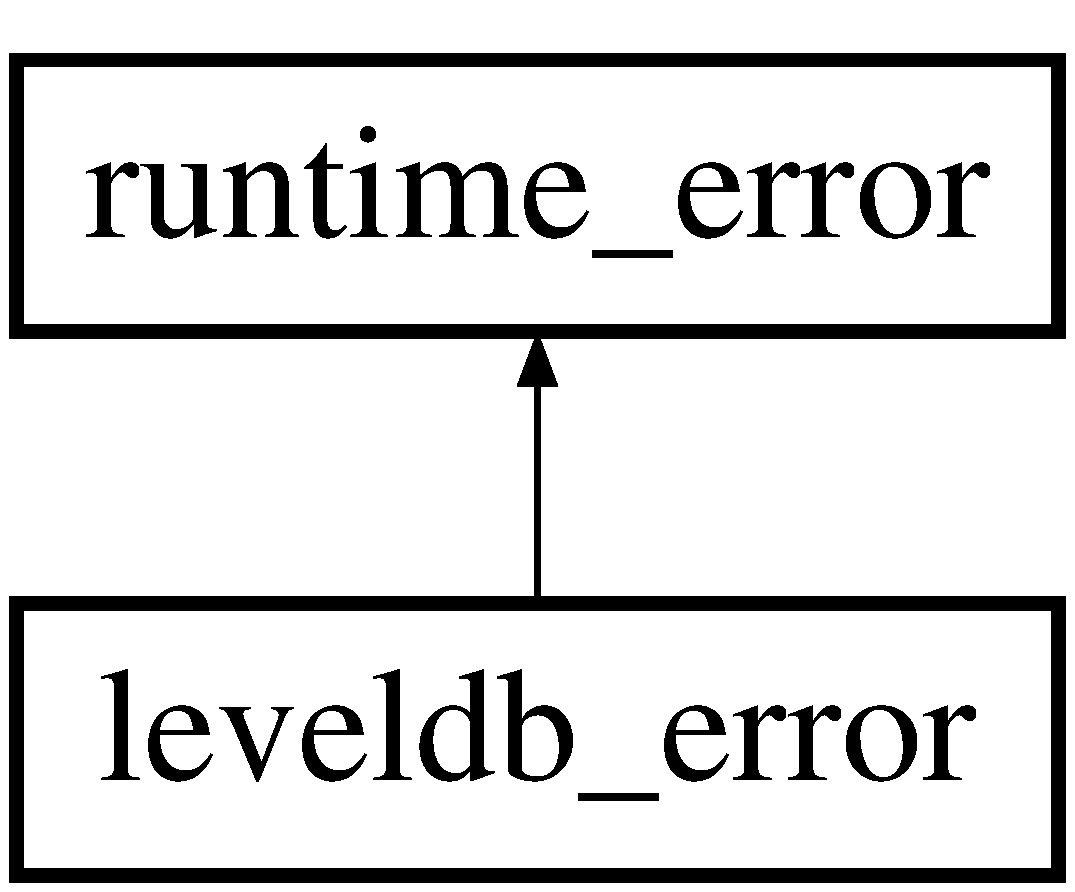
\includegraphics[height=2.000000cm]{classleveldb__error}
\end{center}
\end{figure}
\subsection*{Public Member Functions}
\begin{DoxyCompactItemize}
\item 
\hyperlink{classleveldb__error_a20e012c5a8f796abd5c5af3f7829ee07}{leveldb\+\_\+error} (const std\+::string \&msg)
\end{DoxyCompactItemize}


\subsection{Constructor \& Destructor Documentation}
\hypertarget{classleveldb__error_a20e012c5a8f796abd5c5af3f7829ee07}{}\index{leveldb\+\_\+error@{leveldb\+\_\+error}!leveldb\+\_\+error@{leveldb\+\_\+error}}
\index{leveldb\+\_\+error@{leveldb\+\_\+error}!leveldb\+\_\+error@{leveldb\+\_\+error}}
\subsubsection[{leveldb\+\_\+error}]{\setlength{\rightskip}{0pt plus 5cm}leveldb\+\_\+error\+::leveldb\+\_\+error (
\begin{DoxyParamCaption}
\item[{const std\+::string \&}]{msg}
\end{DoxyParamCaption}
)\hspace{0.3cm}{\ttfamily [inline]}}\label{classleveldb__error_a20e012c5a8f796abd5c5af3f7829ee07}


The documentation for this class was generated from the following file\+:\begin{DoxyCompactItemize}
\item 
C\+:/\+Users/\+Joe/\+Documents/\+School/\+C\+S\+C17\+A/bitcoin/src/\hyperlink{leveldbwrapper_8h}{leveldbwrapper.\+h}\end{DoxyCompactItemize}

\hypertarget{classlimitedmap}{}\section{limitedmap$<$ K, V $>$ Class Template Reference}
\label{classlimitedmap}\index{limitedmap$<$ K, V $>$@{limitedmap$<$ K, V $>$}}


{\ttfamily \#include $<$limitedmap.\+h$>$}

\subsection*{Public Types}
\begin{DoxyCompactItemize}
\item 
typedef K \hyperlink{classlimitedmap_aebf71255c65df699225cdcefe88717b9}{key\+\_\+type}
\item 
typedef V \hyperlink{classlimitedmap_a8bd6b8e7f91f0a141c91c382b492c03c}{mapped\+\_\+type}
\item 
typedef std\+::pair$<$ const \hyperlink{classlimitedmap_aebf71255c65df699225cdcefe88717b9}{key\+\_\+type}, \hyperlink{classlimitedmap_a8bd6b8e7f91f0a141c91c382b492c03c}{mapped\+\_\+type} $>$ \hyperlink{classlimitedmap_a8a6c4972e628b71bf43eeb757dafdce5}{value\+\_\+type}
\item 
typedef std\+::map$<$ K, V $>$\+::\hyperlink{classlimitedmap_ab0a3e4f2ec7c82359300c83a35ae2500}{const\+\_\+iterator} \hyperlink{classlimitedmap_ab0a3e4f2ec7c82359300c83a35ae2500}{const\+\_\+iterator}
\item 
typedef std\+::map$<$ K, V $>$\+::\hyperlink{classlimitedmap_a1c564b323f94e182e56aa27975e5f9d1}{size\+\_\+type} \hyperlink{classlimitedmap_a1c564b323f94e182e56aa27975e5f9d1}{size\+\_\+type}
\end{DoxyCompactItemize}
\subsection*{Public Member Functions}
\begin{DoxyCompactItemize}
\item 
\hyperlink{classlimitedmap_a6670d7a262af3551de75658123b7cb60}{limitedmap} (\hyperlink{classlimitedmap_a1c564b323f94e182e56aa27975e5f9d1}{size\+\_\+type} n\+Max\+Size\+In=0)
\item 
\hyperlink{classlimitedmap_ab0a3e4f2ec7c82359300c83a35ae2500}{const\+\_\+iterator} \hyperlink{classlimitedmap_ac62161ce45bdbea636d30d1274cb2dc4}{begin} () const 
\item 
\hyperlink{classlimitedmap_ab0a3e4f2ec7c82359300c83a35ae2500}{const\+\_\+iterator} \hyperlink{classlimitedmap_ae5d896ca3733c0931ee21e6d0e9058de}{end} () const 
\item 
\hyperlink{classlimitedmap_a1c564b323f94e182e56aa27975e5f9d1}{size\+\_\+type} \hyperlink{classlimitedmap_a7eb0ffdae9db112f1d6f8cc757caae64}{size} () const 
\item 
bool \hyperlink{classlimitedmap_a982ef21b08ed6c74a1771a9253b4260a}{empty} () const 
\item 
\hyperlink{classlimitedmap_ab0a3e4f2ec7c82359300c83a35ae2500}{const\+\_\+iterator} \hyperlink{classlimitedmap_a4888d5aedd039a552a2fa663a5889bf5}{find} (const \hyperlink{classlimitedmap_aebf71255c65df699225cdcefe88717b9}{key\+\_\+type} \&k) const 
\item 
\hyperlink{classlimitedmap_a1c564b323f94e182e56aa27975e5f9d1}{size\+\_\+type} \hyperlink{classlimitedmap_a4ae35b60eacecac30ecf156382e663af}{count} (const \hyperlink{classlimitedmap_aebf71255c65df699225cdcefe88717b9}{key\+\_\+type} \&k) const 
\item 
void \hyperlink{classlimitedmap_af68570a54d74e1b168908be6e8cfb85c}{insert} (const \hyperlink{classlimitedmap_a8a6c4972e628b71bf43eeb757dafdce5}{value\+\_\+type} \&x)
\item 
void \hyperlink{classlimitedmap_aaf2fa41d8f7591d93e5010cf8c351de6}{erase} (const \hyperlink{classlimitedmap_aebf71255c65df699225cdcefe88717b9}{key\+\_\+type} \&k)
\item 
void \hyperlink{classlimitedmap_af29154e7161f1deeea268d0dcea464ab}{update} (\hyperlink{classlimitedmap_ab0a3e4f2ec7c82359300c83a35ae2500}{const\+\_\+iterator} it\+In, const \hyperlink{classlimitedmap_a8bd6b8e7f91f0a141c91c382b492c03c}{mapped\+\_\+type} \&v)
\item 
\hyperlink{classlimitedmap_a1c564b323f94e182e56aa27975e5f9d1}{size\+\_\+type} \hyperlink{classlimitedmap_a3a7d50647833bb8a60bb644f5525b9e0}{max\+\_\+size} () const 
\item 
\hyperlink{classlimitedmap_a1c564b323f94e182e56aa27975e5f9d1}{size\+\_\+type} \hyperlink{classlimitedmap_a97e3deba25cf9a59658cfc317507d45d}{max\+\_\+size} (\hyperlink{classlimitedmap_a1c564b323f94e182e56aa27975e5f9d1}{size\+\_\+type} s)
\end{DoxyCompactItemize}
\subsection*{Protected Types}
\begin{DoxyCompactItemize}
\item 
typedef std\+::map$<$ K, V $>$\+::\hyperlink{classlimitedmap_aea661213ab6f699e9667bea25bf99821}{iterator} \hyperlink{classlimitedmap_aea661213ab6f699e9667bea25bf99821}{iterator}
\item 
typedef std\+::multimap$<$ V, \hyperlink{classlimitedmap_aea661213ab6f699e9667bea25bf99821}{iterator} $>$\+::\hyperlink{classlimitedmap_aea661213ab6f699e9667bea25bf99821}{iterator} \hyperlink{classlimitedmap_ad3d926b1f365d819073ddaed8daa4400}{rmap\+\_\+iterator}
\end{DoxyCompactItemize}
\subsection*{Protected Attributes}
\begin{DoxyCompactItemize}
\item 
std\+::map$<$ K, V $>$ \hyperlink{classlimitedmap_a66e668a5286b7b82061c6867548897a0}{map}
\item 
std\+::multimap$<$ V, \hyperlink{classlimitedmap_aea661213ab6f699e9667bea25bf99821}{iterator} $>$ \hyperlink{classlimitedmap_ab4a6f5b1572ee3754d53f7773b381eb2}{rmap}
\item 
\hyperlink{classlimitedmap_a1c564b323f94e182e56aa27975e5f9d1}{size\+\_\+type} \hyperlink{classlimitedmap_a3ff20a34a489085042060796d44a644e}{n\+Max\+Size}
\end{DoxyCompactItemize}


\subsection{Detailed Description}
\subsubsection*{template$<$typename K, typename V$>$class limitedmap$<$ K, V $>$}

S\+T\+L-\/like map container that only keeps the N elements with the highest value. 

\subsection{Member Typedef Documentation}
\hypertarget{classlimitedmap_ab0a3e4f2ec7c82359300c83a35ae2500}{}\index{limitedmap@{limitedmap}!const\+\_\+iterator@{const\+\_\+iterator}}
\index{const\+\_\+iterator@{const\+\_\+iterator}!limitedmap@{limitedmap}}
\subsubsection[{const\+\_\+iterator}]{\setlength{\rightskip}{0pt plus 5cm}template$<$typename K, typename V$>$ typedef std\+::map$<$K, V$>$\+::{\bf const\+\_\+iterator} {\bf limitedmap}$<$ K, V $>$\+::{\bf const\+\_\+iterator}}\label{classlimitedmap_ab0a3e4f2ec7c82359300c83a35ae2500}
\hypertarget{classlimitedmap_aea661213ab6f699e9667bea25bf99821}{}\index{limitedmap@{limitedmap}!iterator@{iterator}}
\index{iterator@{iterator}!limitedmap@{limitedmap}}
\subsubsection[{iterator}]{\setlength{\rightskip}{0pt plus 5cm}template$<$typename K, typename V$>$ typedef std\+::map$<$K, V$>$\+::{\bf iterator} {\bf limitedmap}$<$ K, V $>$\+::{\bf iterator}\hspace{0.3cm}{\ttfamily [protected]}}\label{classlimitedmap_aea661213ab6f699e9667bea25bf99821}
\hypertarget{classlimitedmap_aebf71255c65df699225cdcefe88717b9}{}\index{limitedmap@{limitedmap}!key\+\_\+type@{key\+\_\+type}}
\index{key\+\_\+type@{key\+\_\+type}!limitedmap@{limitedmap}}
\subsubsection[{key\+\_\+type}]{\setlength{\rightskip}{0pt plus 5cm}template$<$typename K, typename V$>$ typedef K {\bf limitedmap}$<$ K, V $>$\+::{\bf key\+\_\+type}}\label{classlimitedmap_aebf71255c65df699225cdcefe88717b9}
\hypertarget{classlimitedmap_a8bd6b8e7f91f0a141c91c382b492c03c}{}\index{limitedmap@{limitedmap}!mapped\+\_\+type@{mapped\+\_\+type}}
\index{mapped\+\_\+type@{mapped\+\_\+type}!limitedmap@{limitedmap}}
\subsubsection[{mapped\+\_\+type}]{\setlength{\rightskip}{0pt plus 5cm}template$<$typename K, typename V$>$ typedef V {\bf limitedmap}$<$ K, V $>$\+::{\bf mapped\+\_\+type}}\label{classlimitedmap_a8bd6b8e7f91f0a141c91c382b492c03c}
\hypertarget{classlimitedmap_ad3d926b1f365d819073ddaed8daa4400}{}\index{limitedmap@{limitedmap}!rmap\+\_\+iterator@{rmap\+\_\+iterator}}
\index{rmap\+\_\+iterator@{rmap\+\_\+iterator}!limitedmap@{limitedmap}}
\subsubsection[{rmap\+\_\+iterator}]{\setlength{\rightskip}{0pt plus 5cm}template$<$typename K, typename V$>$ typedef std\+::multimap$<$V, {\bf iterator}$>$\+::{\bf iterator} {\bf limitedmap}$<$ K, V $>$\+::{\bf rmap\+\_\+iterator}\hspace{0.3cm}{\ttfamily [protected]}}\label{classlimitedmap_ad3d926b1f365d819073ddaed8daa4400}
\hypertarget{classlimitedmap_a1c564b323f94e182e56aa27975e5f9d1}{}\index{limitedmap@{limitedmap}!size\+\_\+type@{size\+\_\+type}}
\index{size\+\_\+type@{size\+\_\+type}!limitedmap@{limitedmap}}
\subsubsection[{size\+\_\+type}]{\setlength{\rightskip}{0pt plus 5cm}template$<$typename K, typename V$>$ typedef std\+::map$<$K, V$>$\+::{\bf size\+\_\+type} {\bf limitedmap}$<$ K, V $>$\+::{\bf size\+\_\+type}}\label{classlimitedmap_a1c564b323f94e182e56aa27975e5f9d1}
\hypertarget{classlimitedmap_a8a6c4972e628b71bf43eeb757dafdce5}{}\index{limitedmap@{limitedmap}!value\+\_\+type@{value\+\_\+type}}
\index{value\+\_\+type@{value\+\_\+type}!limitedmap@{limitedmap}}
\subsubsection[{value\+\_\+type}]{\setlength{\rightskip}{0pt plus 5cm}template$<$typename K, typename V$>$ typedef std\+::pair$<$const {\bf key\+\_\+type}, {\bf mapped\+\_\+type}$>$ {\bf limitedmap}$<$ K, V $>$\+::{\bf value\+\_\+type}}\label{classlimitedmap_a8a6c4972e628b71bf43eeb757dafdce5}


\subsection{Constructor \& Destructor Documentation}
\hypertarget{classlimitedmap_a6670d7a262af3551de75658123b7cb60}{}\index{limitedmap@{limitedmap}!limitedmap@{limitedmap}}
\index{limitedmap@{limitedmap}!limitedmap@{limitedmap}}
\subsubsection[{limitedmap}]{\setlength{\rightskip}{0pt plus 5cm}template$<$typename K, typename V$>$ {\bf limitedmap}$<$ K, V $>$\+::{\bf limitedmap} (
\begin{DoxyParamCaption}
\item[{{\bf size\+\_\+type}}]{n\+Max\+Size\+In = {\ttfamily 0}}
\end{DoxyParamCaption}
)\hspace{0.3cm}{\ttfamily [inline]}}\label{classlimitedmap_a6670d7a262af3551de75658123b7cb60}


\subsection{Member Function Documentation}
\hypertarget{classlimitedmap_ac62161ce45bdbea636d30d1274cb2dc4}{}\index{limitedmap@{limitedmap}!begin@{begin}}
\index{begin@{begin}!limitedmap@{limitedmap}}
\subsubsection[{begin}]{\setlength{\rightskip}{0pt plus 5cm}template$<$typename K, typename V$>$ {\bf const\+\_\+iterator} {\bf limitedmap}$<$ K, V $>$\+::begin (
\begin{DoxyParamCaption}
{}
\end{DoxyParamCaption}
) const\hspace{0.3cm}{\ttfamily [inline]}}\label{classlimitedmap_ac62161ce45bdbea636d30d1274cb2dc4}
\hypertarget{classlimitedmap_a4ae35b60eacecac30ecf156382e663af}{}\index{limitedmap@{limitedmap}!count@{count}}
\index{count@{count}!limitedmap@{limitedmap}}
\subsubsection[{count}]{\setlength{\rightskip}{0pt plus 5cm}template$<$typename K, typename V$>$ {\bf size\+\_\+type} {\bf limitedmap}$<$ K, V $>$\+::count (
\begin{DoxyParamCaption}
\item[{const {\bf key\+\_\+type} \&}]{k}
\end{DoxyParamCaption}
) const\hspace{0.3cm}{\ttfamily [inline]}}\label{classlimitedmap_a4ae35b60eacecac30ecf156382e663af}
\hypertarget{classlimitedmap_a982ef21b08ed6c74a1771a9253b4260a}{}\index{limitedmap@{limitedmap}!empty@{empty}}
\index{empty@{empty}!limitedmap@{limitedmap}}
\subsubsection[{empty}]{\setlength{\rightskip}{0pt plus 5cm}template$<$typename K, typename V$>$ bool {\bf limitedmap}$<$ K, V $>$\+::empty (
\begin{DoxyParamCaption}
{}
\end{DoxyParamCaption}
) const\hspace{0.3cm}{\ttfamily [inline]}}\label{classlimitedmap_a982ef21b08ed6c74a1771a9253b4260a}
\hypertarget{classlimitedmap_ae5d896ca3733c0931ee21e6d0e9058de}{}\index{limitedmap@{limitedmap}!end@{end}}
\index{end@{end}!limitedmap@{limitedmap}}
\subsubsection[{end}]{\setlength{\rightskip}{0pt plus 5cm}template$<$typename K, typename V$>$ {\bf const\+\_\+iterator} {\bf limitedmap}$<$ K, V $>$\+::end (
\begin{DoxyParamCaption}
{}
\end{DoxyParamCaption}
) const\hspace{0.3cm}{\ttfamily [inline]}}\label{classlimitedmap_ae5d896ca3733c0931ee21e6d0e9058de}
\hypertarget{classlimitedmap_aaf2fa41d8f7591d93e5010cf8c351de6}{}\index{limitedmap@{limitedmap}!erase@{erase}}
\index{erase@{erase}!limitedmap@{limitedmap}}
\subsubsection[{erase}]{\setlength{\rightskip}{0pt plus 5cm}template$<$typename K, typename V$>$ void {\bf limitedmap}$<$ K, V $>$\+::erase (
\begin{DoxyParamCaption}
\item[{const {\bf key\+\_\+type} \&}]{k}
\end{DoxyParamCaption}
)\hspace{0.3cm}{\ttfamily [inline]}}\label{classlimitedmap_aaf2fa41d8f7591d93e5010cf8c351de6}
\hypertarget{classlimitedmap_a4888d5aedd039a552a2fa663a5889bf5}{}\index{limitedmap@{limitedmap}!find@{find}}
\index{find@{find}!limitedmap@{limitedmap}}
\subsubsection[{find}]{\setlength{\rightskip}{0pt plus 5cm}template$<$typename K, typename V$>$ {\bf const\+\_\+iterator} {\bf limitedmap}$<$ K, V $>$\+::find (
\begin{DoxyParamCaption}
\item[{const {\bf key\+\_\+type} \&}]{k}
\end{DoxyParamCaption}
) const\hspace{0.3cm}{\ttfamily [inline]}}\label{classlimitedmap_a4888d5aedd039a552a2fa663a5889bf5}
\hypertarget{classlimitedmap_af68570a54d74e1b168908be6e8cfb85c}{}\index{limitedmap@{limitedmap}!insert@{insert}}
\index{insert@{insert}!limitedmap@{limitedmap}}
\subsubsection[{insert}]{\setlength{\rightskip}{0pt plus 5cm}template$<$typename K, typename V$>$ void {\bf limitedmap}$<$ K, V $>$\+::insert (
\begin{DoxyParamCaption}
\item[{const {\bf value\+\_\+type} \&}]{x}
\end{DoxyParamCaption}
)\hspace{0.3cm}{\ttfamily [inline]}}\label{classlimitedmap_af68570a54d74e1b168908be6e8cfb85c}
\hypertarget{classlimitedmap_a3a7d50647833bb8a60bb644f5525b9e0}{}\index{limitedmap@{limitedmap}!max\+\_\+size@{max\+\_\+size}}
\index{max\+\_\+size@{max\+\_\+size}!limitedmap@{limitedmap}}
\subsubsection[{max\+\_\+size}]{\setlength{\rightskip}{0pt plus 5cm}template$<$typename K, typename V$>$ {\bf size\+\_\+type} {\bf limitedmap}$<$ K, V $>$\+::max\+\_\+size (
\begin{DoxyParamCaption}
{}
\end{DoxyParamCaption}
) const\hspace{0.3cm}{\ttfamily [inline]}}\label{classlimitedmap_a3a7d50647833bb8a60bb644f5525b9e0}
\hypertarget{classlimitedmap_a97e3deba25cf9a59658cfc317507d45d}{}\index{limitedmap@{limitedmap}!max\+\_\+size@{max\+\_\+size}}
\index{max\+\_\+size@{max\+\_\+size}!limitedmap@{limitedmap}}
\subsubsection[{max\+\_\+size}]{\setlength{\rightskip}{0pt plus 5cm}template$<$typename K, typename V$>$ {\bf size\+\_\+type} {\bf limitedmap}$<$ K, V $>$\+::max\+\_\+size (
\begin{DoxyParamCaption}
\item[{{\bf size\+\_\+type}}]{s}
\end{DoxyParamCaption}
)\hspace{0.3cm}{\ttfamily [inline]}}\label{classlimitedmap_a97e3deba25cf9a59658cfc317507d45d}
\hypertarget{classlimitedmap_a7eb0ffdae9db112f1d6f8cc757caae64}{}\index{limitedmap@{limitedmap}!size@{size}}
\index{size@{size}!limitedmap@{limitedmap}}
\subsubsection[{size}]{\setlength{\rightskip}{0pt plus 5cm}template$<$typename K, typename V$>$ {\bf size\+\_\+type} {\bf limitedmap}$<$ K, V $>$\+::size (
\begin{DoxyParamCaption}
{}
\end{DoxyParamCaption}
) const\hspace{0.3cm}{\ttfamily [inline]}}\label{classlimitedmap_a7eb0ffdae9db112f1d6f8cc757caae64}
\hypertarget{classlimitedmap_af29154e7161f1deeea268d0dcea464ab}{}\index{limitedmap@{limitedmap}!update@{update}}
\index{update@{update}!limitedmap@{limitedmap}}
\subsubsection[{update}]{\setlength{\rightskip}{0pt plus 5cm}template$<$typename K, typename V$>$ void {\bf limitedmap}$<$ K, V $>$\+::update (
\begin{DoxyParamCaption}
\item[{{\bf const\+\_\+iterator}}]{it\+In, }
\item[{const {\bf mapped\+\_\+type} \&}]{v}
\end{DoxyParamCaption}
)\hspace{0.3cm}{\ttfamily [inline]}}\label{classlimitedmap_af29154e7161f1deeea268d0dcea464ab}


\subsection{Member Data Documentation}
\hypertarget{classlimitedmap_a66e668a5286b7b82061c6867548897a0}{}\index{limitedmap@{limitedmap}!map@{map}}
\index{map@{map}!limitedmap@{limitedmap}}
\subsubsection[{map}]{\setlength{\rightskip}{0pt plus 5cm}template$<$typename K, typename V$>$ std\+::map$<$K, V$>$ {\bf limitedmap}$<$ K, V $>$\+::map\hspace{0.3cm}{\ttfamily [protected]}}\label{classlimitedmap_a66e668a5286b7b82061c6867548897a0}
\hypertarget{classlimitedmap_a3ff20a34a489085042060796d44a644e}{}\index{limitedmap@{limitedmap}!n\+Max\+Size@{n\+Max\+Size}}
\index{n\+Max\+Size@{n\+Max\+Size}!limitedmap@{limitedmap}}
\subsubsection[{n\+Max\+Size}]{\setlength{\rightskip}{0pt plus 5cm}template$<$typename K, typename V$>$ {\bf size\+\_\+type} {\bf limitedmap}$<$ K, V $>$\+::n\+Max\+Size\hspace{0.3cm}{\ttfamily [protected]}}\label{classlimitedmap_a3ff20a34a489085042060796d44a644e}
\hypertarget{classlimitedmap_ab4a6f5b1572ee3754d53f7773b381eb2}{}\index{limitedmap@{limitedmap}!rmap@{rmap}}
\index{rmap@{rmap}!limitedmap@{limitedmap}}
\subsubsection[{rmap}]{\setlength{\rightskip}{0pt plus 5cm}template$<$typename K, typename V$>$ std\+::multimap$<$V, {\bf iterator}$>$ {\bf limitedmap}$<$ K, V $>$\+::rmap\hspace{0.3cm}{\ttfamily [protected]}}\label{classlimitedmap_ab4a6f5b1572ee3754d53f7773b381eb2}


The documentation for this class was generated from the following file\+:\begin{DoxyCompactItemize}
\item 
C\+:/\+Users/\+Joe/\+Documents/\+School/\+C\+S\+C17\+A/bitcoin/src/\hyperlink{limitedmap_8h}{limitedmap.\+h}\end{DoxyCompactItemize}

\hypertarget{class_limited_string}{}\section{Limited\+String$<$ Limit $>$ Class Template Reference}
\label{class_limited_string}\index{Limited\+String$<$ Limit $>$@{Limited\+String$<$ Limit $>$}}


{\ttfamily \#include $<$serialize.\+h$>$}

\subsection*{Public Member Functions}
\begin{DoxyCompactItemize}
\item 
\hyperlink{class_limited_string_afd9b0daa877f4d28c6b909bd34fd597d}{Limited\+String} (std\+::string \&\hyperlink{class_limited_string_a3f1d004f4632f7b2fda1a5a5afc266f7}{string})
\item 
{\footnotesize template$<$typename Stream $>$ }\\void \hyperlink{class_limited_string_a21ec9b742da8f8ff7b9a8b89131f943b}{Unserialize} (Stream \&s, int, int=0)
\item 
{\footnotesize template$<$typename Stream $>$ }\\void \hyperlink{class_limited_string_a4421821da094900bf15f79768a13e8b9}{Serialize} (Stream \&s, int, int=0) const 
\item 
unsigned int \hyperlink{class_limited_string_a9864565cf21b4f2ca09f78acc77d9563}{Get\+Serialize\+Size} (int, int=0) const 
\end{DoxyCompactItemize}
\subsection*{Protected Attributes}
\begin{DoxyCompactItemize}
\item 
std\+::string \& \hyperlink{class_limited_string_a3f1d004f4632f7b2fda1a5a5afc266f7}{string}
\end{DoxyCompactItemize}


\subsection{Constructor \& Destructor Documentation}
\hypertarget{class_limited_string_afd9b0daa877f4d28c6b909bd34fd597d}{}\index{Limited\+String@{Limited\+String}!Limited\+String@{Limited\+String}}
\index{Limited\+String@{Limited\+String}!Limited\+String@{Limited\+String}}
\subsubsection[{Limited\+String}]{\setlength{\rightskip}{0pt plus 5cm}template$<$size\+\_\+t Limit$>$ {\bf Limited\+String}$<$ Limit $>$\+::{\bf Limited\+String} (
\begin{DoxyParamCaption}
\item[{std\+::string \&}]{string}
\end{DoxyParamCaption}
)\hspace{0.3cm}{\ttfamily [inline]}}\label{class_limited_string_afd9b0daa877f4d28c6b909bd34fd597d}


\subsection{Member Function Documentation}
\hypertarget{class_limited_string_a9864565cf21b4f2ca09f78acc77d9563}{}\index{Limited\+String@{Limited\+String}!Get\+Serialize\+Size@{Get\+Serialize\+Size}}
\index{Get\+Serialize\+Size@{Get\+Serialize\+Size}!Limited\+String@{Limited\+String}}
\subsubsection[{Get\+Serialize\+Size}]{\setlength{\rightskip}{0pt plus 5cm}template$<$size\+\_\+t Limit$>$ unsigned int {\bf Limited\+String}$<$ Limit $>$\+::Get\+Serialize\+Size (
\begin{DoxyParamCaption}
\item[{int}]{, }
\item[{int}]{ = {\ttfamily 0}}
\end{DoxyParamCaption}
) const\hspace{0.3cm}{\ttfamily [inline]}}\label{class_limited_string_a9864565cf21b4f2ca09f78acc77d9563}
\hypertarget{class_limited_string_a4421821da094900bf15f79768a13e8b9}{}\index{Limited\+String@{Limited\+String}!Serialize@{Serialize}}
\index{Serialize@{Serialize}!Limited\+String@{Limited\+String}}
\subsubsection[{Serialize}]{\setlength{\rightskip}{0pt plus 5cm}template$<$size\+\_\+t Limit$>$ template$<$typename Stream $>$ void {\bf Limited\+String}$<$ Limit $>$\+::Serialize (
\begin{DoxyParamCaption}
\item[{Stream \&}]{s, }
\item[{int}]{, }
\item[{int}]{ = {\ttfamily 0}}
\end{DoxyParamCaption}
) const\hspace{0.3cm}{\ttfamily [inline]}}\label{class_limited_string_a4421821da094900bf15f79768a13e8b9}
\hypertarget{class_limited_string_a21ec9b742da8f8ff7b9a8b89131f943b}{}\index{Limited\+String@{Limited\+String}!Unserialize@{Unserialize}}
\index{Unserialize@{Unserialize}!Limited\+String@{Limited\+String}}
\subsubsection[{Unserialize}]{\setlength{\rightskip}{0pt plus 5cm}template$<$size\+\_\+t Limit$>$ template$<$typename Stream $>$ void {\bf Limited\+String}$<$ Limit $>$\+::Unserialize (
\begin{DoxyParamCaption}
\item[{Stream \&}]{s, }
\item[{int}]{, }
\item[{int}]{ = {\ttfamily 0}}
\end{DoxyParamCaption}
)\hspace{0.3cm}{\ttfamily [inline]}}\label{class_limited_string_a21ec9b742da8f8ff7b9a8b89131f943b}


\subsection{Member Data Documentation}
\hypertarget{class_limited_string_a3f1d004f4632f7b2fda1a5a5afc266f7}{}\index{Limited\+String@{Limited\+String}!string@{string}}
\index{string@{string}!Limited\+String@{Limited\+String}}
\subsubsection[{string}]{\setlength{\rightskip}{0pt plus 5cm}template$<$size\+\_\+t Limit$>$ std\+::string\& {\bf Limited\+String}$<$ Limit $>$\+::string\hspace{0.3cm}{\ttfamily [protected]}}\label{class_limited_string_a3f1d004f4632f7b2fda1a5a5afc266f7}


The documentation for this class was generated from the following file\+:\begin{DoxyCompactItemize}
\item 
C\+:/\+Users/\+Joe/\+Documents/\+School/\+C\+S\+C17\+A/bitcoin/src/\hyperlink{serialize_8h}{serialize.\+h}\end{DoxyCompactItemize}

\hypertarget{struct_local_service_info}{}\section{Local\+Service\+Info Struct Reference}
\label{struct_local_service_info}\index{Local\+Service\+Info@{Local\+Service\+Info}}


{\ttfamily \#include $<$net.\+h$>$}

\subsection*{Public Attributes}
\begin{DoxyCompactItemize}
\item 
int \hyperlink{struct_local_service_info_ad6a9d404fb109ba1506df3f6ca842ed5}{n\+Score}
\item 
int \hyperlink{struct_local_service_info_aa5c39fec8cc69a43e393bb158f69224b}{n\+Port}
\end{DoxyCompactItemize}


\subsection{Member Data Documentation}
\hypertarget{struct_local_service_info_aa5c39fec8cc69a43e393bb158f69224b}{}\index{Local\+Service\+Info@{Local\+Service\+Info}!n\+Port@{n\+Port}}
\index{n\+Port@{n\+Port}!Local\+Service\+Info@{Local\+Service\+Info}}
\subsubsection[{n\+Port}]{\setlength{\rightskip}{0pt plus 5cm}int Local\+Service\+Info\+::n\+Port}\label{struct_local_service_info_aa5c39fec8cc69a43e393bb158f69224b}
\hypertarget{struct_local_service_info_ad6a9d404fb109ba1506df3f6ca842ed5}{}\index{Local\+Service\+Info@{Local\+Service\+Info}!n\+Score@{n\+Score}}
\index{n\+Score@{n\+Score}!Local\+Service\+Info@{Local\+Service\+Info}}
\subsubsection[{n\+Score}]{\setlength{\rightskip}{0pt plus 5cm}int Local\+Service\+Info\+::n\+Score}\label{struct_local_service_info_ad6a9d404fb109ba1506df3f6ca842ed5}


The documentation for this struct was generated from the following file\+:\begin{DoxyCompactItemize}
\item 
C\+:/\+Users/\+Joe/\+Documents/\+School/\+C\+S\+C17\+A/bitcoin/src/\hyperlink{net_8h}{net.\+h}\end{DoxyCompactItemize}

\hypertarget{classmruset}{}\section{mruset$<$ T $>$ Class Template Reference}
\label{classmruset}\index{mruset$<$ T $>$@{mruset$<$ T $>$}}


{\ttfamily \#include $<$mruset.\+h$>$}

\subsection*{Public Types}
\begin{DoxyCompactItemize}
\item 
typedef T \hyperlink{classmruset_a282941ee7f0438b0c09274b10c78cda0}{key\+\_\+type}
\item 
typedef T \hyperlink{classmruset_a834c3e7f8e9cf615ebe27752443f9a3a}{value\+\_\+type}
\item 
typedef std\+::set$<$ T $>$\+::\hyperlink{classmruset_a246172eda1afff45be47a013c14b1ad6}{iterator} \hyperlink{classmruset_a246172eda1afff45be47a013c14b1ad6}{iterator}
\item 
typedef std\+::set$<$ T $>$\+::\hyperlink{classmruset_a74c77f7642e8e4db7cc79991c4345692}{const\+\_\+iterator} \hyperlink{classmruset_a74c77f7642e8e4db7cc79991c4345692}{const\+\_\+iterator}
\item 
typedef std\+::set$<$ T $>$\+::\hyperlink{classmruset_aaee46af18d8a5bdc503e9570e499a335}{size\+\_\+type} \hyperlink{classmruset_aaee46af18d8a5bdc503e9570e499a335}{size\+\_\+type}
\end{DoxyCompactItemize}
\subsection*{Public Member Functions}
\begin{DoxyCompactItemize}
\item 
\hyperlink{classmruset_a708b11a33448c283f6f4c8e18fd3098f}{mruset} (\hyperlink{classmruset_aaee46af18d8a5bdc503e9570e499a335}{size\+\_\+type} n\+Max\+Size\+In=0)
\item 
\hyperlink{classmruset_a246172eda1afff45be47a013c14b1ad6}{iterator} \hyperlink{classmruset_acaa144dd3b3c3b9999254b6fcc37be5f}{begin} () const 
\item 
\hyperlink{classmruset_a246172eda1afff45be47a013c14b1ad6}{iterator} \hyperlink{classmruset_ab52cef4e172f0a8428451ac3cc2e3033}{end} () const 
\item 
\hyperlink{classmruset_aaee46af18d8a5bdc503e9570e499a335}{size\+\_\+type} \hyperlink{classmruset_a7739fdd19c7f28ccfa5565969106c3a9}{size} () const 
\item 
bool \hyperlink{classmruset_a3dc4b001997d723fd8c79134ac54574f}{empty} () const 
\item 
\hyperlink{classmruset_a246172eda1afff45be47a013c14b1ad6}{iterator} \hyperlink{classmruset_a030a8b36c8c34ae7b7b30cc0b0204bfa}{find} (const \hyperlink{classmruset_a282941ee7f0438b0c09274b10c78cda0}{key\+\_\+type} \&k) const 
\item 
\hyperlink{classmruset_aaee46af18d8a5bdc503e9570e499a335}{size\+\_\+type} \hyperlink{classmruset_abf122b956abffbf3ce190c80d215660c}{count} (const \hyperlink{classmruset_a282941ee7f0438b0c09274b10c78cda0}{key\+\_\+type} \&k) const 
\item 
void \hyperlink{classmruset_ac7a85b54646e9d9d1962ce7f30b2a1fc}{clear} ()
\item 
bool friend \hyperlink{classmruset_aced009504f86176bd82426aa24a38e37}{operator==} (const \hyperlink{classmruset}{mruset}$<$ T $>$ \&a, const \hyperlink{classmruset}{mruset}$<$ T $>$ \&b)
\item 
bool friend \hyperlink{classmruset_a4d7231441276ef8a6c0fa3edf9712f5c}{operator==} (const \hyperlink{classmruset}{mruset}$<$ T $>$ \&a, const std\+::set$<$ T $>$ \&b)
\item 
bool friend \hyperlink{classmruset_a5a95239f76da8ba675ba748baf1f07c8}{operator$<$} (const \hyperlink{classmruset}{mruset}$<$ T $>$ \&a, const \hyperlink{classmruset}{mruset}$<$ T $>$ \&b)
\item 
std\+::pair$<$ \hyperlink{classmruset_a246172eda1afff45be47a013c14b1ad6}{iterator}, bool $>$ \hyperlink{classmruset_af2e0dfe9d8b029bde78457797cdc42a9}{insert} (const \hyperlink{classmruset_a282941ee7f0438b0c09274b10c78cda0}{key\+\_\+type} \&x)
\item 
\hyperlink{classmruset_aaee46af18d8a5bdc503e9570e499a335}{size\+\_\+type} \hyperlink{classmruset_a6c802b89a72c474bdfad1059be1dec09}{max\+\_\+size} () const 
\item 
\hyperlink{classmruset_aaee46af18d8a5bdc503e9570e499a335}{size\+\_\+type} \hyperlink{classmruset_a030aa4599dfb54074183e2cdfbe2373f}{max\+\_\+size} (\hyperlink{classmruset_aaee46af18d8a5bdc503e9570e499a335}{size\+\_\+type} s)
\end{DoxyCompactItemize}
\subsection*{Protected Attributes}
\begin{DoxyCompactItemize}
\item 
std\+::set$<$ T $>$ \hyperlink{classmruset_a4981fc3556b61600418b2ddad98cc685}{set}
\item 
std\+::deque$<$ T $>$ \hyperlink{classmruset_a6be1fe81dc472e25e160911288373663}{queue}
\item 
\hyperlink{classmruset_aaee46af18d8a5bdc503e9570e499a335}{size\+\_\+type} \hyperlink{classmruset_a6d3d6963e3ca5689e846b12a29dd09ab}{n\+Max\+Size}
\end{DoxyCompactItemize}


\subsection{Detailed Description}
\subsubsection*{template$<$typename T$>$class mruset$<$ T $>$}

S\+T\+L-\/like set container that only keeps the most recent N elements. 

\subsection{Member Typedef Documentation}
\hypertarget{classmruset_a74c77f7642e8e4db7cc79991c4345692}{}\index{mruset@{mruset}!const\+\_\+iterator@{const\+\_\+iterator}}
\index{const\+\_\+iterator@{const\+\_\+iterator}!mruset@{mruset}}
\subsubsection[{const\+\_\+iterator}]{\setlength{\rightskip}{0pt plus 5cm}template$<$typename T$>$ typedef std\+::set$<$T$>$\+::{\bf const\+\_\+iterator} {\bf mruset}$<$ T $>$\+::{\bf const\+\_\+iterator}}\label{classmruset_a74c77f7642e8e4db7cc79991c4345692}
\hypertarget{classmruset_a246172eda1afff45be47a013c14b1ad6}{}\index{mruset@{mruset}!iterator@{iterator}}
\index{iterator@{iterator}!mruset@{mruset}}
\subsubsection[{iterator}]{\setlength{\rightskip}{0pt plus 5cm}template$<$typename T$>$ typedef std\+::set$<$T$>$\+::{\bf iterator} {\bf mruset}$<$ T $>$\+::{\bf iterator}}\label{classmruset_a246172eda1afff45be47a013c14b1ad6}
\hypertarget{classmruset_a282941ee7f0438b0c09274b10c78cda0}{}\index{mruset@{mruset}!key\+\_\+type@{key\+\_\+type}}
\index{key\+\_\+type@{key\+\_\+type}!mruset@{mruset}}
\subsubsection[{key\+\_\+type}]{\setlength{\rightskip}{0pt plus 5cm}template$<$typename T$>$ typedef T {\bf mruset}$<$ T $>$\+::{\bf key\+\_\+type}}\label{classmruset_a282941ee7f0438b0c09274b10c78cda0}
\hypertarget{classmruset_aaee46af18d8a5bdc503e9570e499a335}{}\index{mruset@{mruset}!size\+\_\+type@{size\+\_\+type}}
\index{size\+\_\+type@{size\+\_\+type}!mruset@{mruset}}
\subsubsection[{size\+\_\+type}]{\setlength{\rightskip}{0pt plus 5cm}template$<$typename T$>$ typedef std\+::set$<$T$>$\+::{\bf size\+\_\+type} {\bf mruset}$<$ T $>$\+::{\bf size\+\_\+type}}\label{classmruset_aaee46af18d8a5bdc503e9570e499a335}
\hypertarget{classmruset_a834c3e7f8e9cf615ebe27752443f9a3a}{}\index{mruset@{mruset}!value\+\_\+type@{value\+\_\+type}}
\index{value\+\_\+type@{value\+\_\+type}!mruset@{mruset}}
\subsubsection[{value\+\_\+type}]{\setlength{\rightskip}{0pt plus 5cm}template$<$typename T$>$ typedef T {\bf mruset}$<$ T $>$\+::{\bf value\+\_\+type}}\label{classmruset_a834c3e7f8e9cf615ebe27752443f9a3a}


\subsection{Constructor \& Destructor Documentation}
\hypertarget{classmruset_a708b11a33448c283f6f4c8e18fd3098f}{}\index{mruset@{mruset}!mruset@{mruset}}
\index{mruset@{mruset}!mruset@{mruset}}
\subsubsection[{mruset}]{\setlength{\rightskip}{0pt plus 5cm}template$<$typename T$>$ {\bf mruset}$<$ T $>$\+::{\bf mruset} (
\begin{DoxyParamCaption}
\item[{{\bf size\+\_\+type}}]{n\+Max\+Size\+In = {\ttfamily 0}}
\end{DoxyParamCaption}
)\hspace{0.3cm}{\ttfamily [inline]}}\label{classmruset_a708b11a33448c283f6f4c8e18fd3098f}


\subsection{Member Function Documentation}
\hypertarget{classmruset_acaa144dd3b3c3b9999254b6fcc37be5f}{}\index{mruset@{mruset}!begin@{begin}}
\index{begin@{begin}!mruset@{mruset}}
\subsubsection[{begin}]{\setlength{\rightskip}{0pt plus 5cm}template$<$typename T$>$ {\bf iterator} {\bf mruset}$<$ T $>$\+::begin (
\begin{DoxyParamCaption}
{}
\end{DoxyParamCaption}
) const\hspace{0.3cm}{\ttfamily [inline]}}\label{classmruset_acaa144dd3b3c3b9999254b6fcc37be5f}
\hypertarget{classmruset_ac7a85b54646e9d9d1962ce7f30b2a1fc}{}\index{mruset@{mruset}!clear@{clear}}
\index{clear@{clear}!mruset@{mruset}}
\subsubsection[{clear}]{\setlength{\rightskip}{0pt plus 5cm}template$<$typename T$>$ void {\bf mruset}$<$ T $>$\+::clear (
\begin{DoxyParamCaption}
{}
\end{DoxyParamCaption}
)\hspace{0.3cm}{\ttfamily [inline]}}\label{classmruset_ac7a85b54646e9d9d1962ce7f30b2a1fc}
\hypertarget{classmruset_abf122b956abffbf3ce190c80d215660c}{}\index{mruset@{mruset}!count@{count}}
\index{count@{count}!mruset@{mruset}}
\subsubsection[{count}]{\setlength{\rightskip}{0pt plus 5cm}template$<$typename T$>$ {\bf size\+\_\+type} {\bf mruset}$<$ T $>$\+::count (
\begin{DoxyParamCaption}
\item[{const {\bf key\+\_\+type} \&}]{k}
\end{DoxyParamCaption}
) const\hspace{0.3cm}{\ttfamily [inline]}}\label{classmruset_abf122b956abffbf3ce190c80d215660c}
\hypertarget{classmruset_a3dc4b001997d723fd8c79134ac54574f}{}\index{mruset@{mruset}!empty@{empty}}
\index{empty@{empty}!mruset@{mruset}}
\subsubsection[{empty}]{\setlength{\rightskip}{0pt plus 5cm}template$<$typename T$>$ bool {\bf mruset}$<$ T $>$\+::empty (
\begin{DoxyParamCaption}
{}
\end{DoxyParamCaption}
) const\hspace{0.3cm}{\ttfamily [inline]}}\label{classmruset_a3dc4b001997d723fd8c79134ac54574f}
\hypertarget{classmruset_ab52cef4e172f0a8428451ac3cc2e3033}{}\index{mruset@{mruset}!end@{end}}
\index{end@{end}!mruset@{mruset}}
\subsubsection[{end}]{\setlength{\rightskip}{0pt plus 5cm}template$<$typename T$>$ {\bf iterator} {\bf mruset}$<$ T $>$\+::end (
\begin{DoxyParamCaption}
{}
\end{DoxyParamCaption}
) const\hspace{0.3cm}{\ttfamily [inline]}}\label{classmruset_ab52cef4e172f0a8428451ac3cc2e3033}
\hypertarget{classmruset_a030a8b36c8c34ae7b7b30cc0b0204bfa}{}\index{mruset@{mruset}!find@{find}}
\index{find@{find}!mruset@{mruset}}
\subsubsection[{find}]{\setlength{\rightskip}{0pt plus 5cm}template$<$typename T$>$ {\bf iterator} {\bf mruset}$<$ T $>$\+::find (
\begin{DoxyParamCaption}
\item[{const {\bf key\+\_\+type} \&}]{k}
\end{DoxyParamCaption}
) const\hspace{0.3cm}{\ttfamily [inline]}}\label{classmruset_a030a8b36c8c34ae7b7b30cc0b0204bfa}
\hypertarget{classmruset_af2e0dfe9d8b029bde78457797cdc42a9}{}\index{mruset@{mruset}!insert@{insert}}
\index{insert@{insert}!mruset@{mruset}}
\subsubsection[{insert}]{\setlength{\rightskip}{0pt plus 5cm}template$<$typename T$>$ std\+::pair$<${\bf iterator}, bool$>$ {\bf mruset}$<$ T $>$\+::insert (
\begin{DoxyParamCaption}
\item[{const {\bf key\+\_\+type} \&}]{x}
\end{DoxyParamCaption}
)\hspace{0.3cm}{\ttfamily [inline]}}\label{classmruset_af2e0dfe9d8b029bde78457797cdc42a9}
\hypertarget{classmruset_a6c802b89a72c474bdfad1059be1dec09}{}\index{mruset@{mruset}!max\+\_\+size@{max\+\_\+size}}
\index{max\+\_\+size@{max\+\_\+size}!mruset@{mruset}}
\subsubsection[{max\+\_\+size}]{\setlength{\rightskip}{0pt plus 5cm}template$<$typename T$>$ {\bf size\+\_\+type} {\bf mruset}$<$ T $>$\+::max\+\_\+size (
\begin{DoxyParamCaption}
{}
\end{DoxyParamCaption}
) const\hspace{0.3cm}{\ttfamily [inline]}}\label{classmruset_a6c802b89a72c474bdfad1059be1dec09}
\hypertarget{classmruset_a030aa4599dfb54074183e2cdfbe2373f}{}\index{mruset@{mruset}!max\+\_\+size@{max\+\_\+size}}
\index{max\+\_\+size@{max\+\_\+size}!mruset@{mruset}}
\subsubsection[{max\+\_\+size}]{\setlength{\rightskip}{0pt plus 5cm}template$<$typename T$>$ {\bf size\+\_\+type} {\bf mruset}$<$ T $>$\+::max\+\_\+size (
\begin{DoxyParamCaption}
\item[{{\bf size\+\_\+type}}]{s}
\end{DoxyParamCaption}
)\hspace{0.3cm}{\ttfamily [inline]}}\label{classmruset_a030aa4599dfb54074183e2cdfbe2373f}
\hypertarget{classmruset_a5a95239f76da8ba675ba748baf1f07c8}{}\index{mruset@{mruset}!operator$<$@{operator$<$}}
\index{operator$<$@{operator$<$}!mruset@{mruset}}
\subsubsection[{operator$<$}]{\setlength{\rightskip}{0pt plus 5cm}template$<$typename T$>$ bool friend {\bf mruset}$<$ T $>$\+::operator$<$ (
\begin{DoxyParamCaption}
\item[{const {\bf mruset}$<$ T $>$ \&}]{a, }
\item[{const {\bf mruset}$<$ T $>$ \&}]{b}
\end{DoxyParamCaption}
)\hspace{0.3cm}{\ttfamily [inline]}}\label{classmruset_a5a95239f76da8ba675ba748baf1f07c8}
\hypertarget{classmruset_aced009504f86176bd82426aa24a38e37}{}\index{mruset@{mruset}!operator==@{operator==}}
\index{operator==@{operator==}!mruset@{mruset}}
\subsubsection[{operator==}]{\setlength{\rightskip}{0pt plus 5cm}template$<$typename T$>$ bool friend {\bf mruset}$<$ T $>$\+::operator== (
\begin{DoxyParamCaption}
\item[{const {\bf mruset}$<$ T $>$ \&}]{a, }
\item[{const {\bf mruset}$<$ T $>$ \&}]{b}
\end{DoxyParamCaption}
)\hspace{0.3cm}{\ttfamily [inline]}}\label{classmruset_aced009504f86176bd82426aa24a38e37}
\hypertarget{classmruset_a4d7231441276ef8a6c0fa3edf9712f5c}{}\index{mruset@{mruset}!operator==@{operator==}}
\index{operator==@{operator==}!mruset@{mruset}}
\subsubsection[{operator==}]{\setlength{\rightskip}{0pt plus 5cm}template$<$typename T$>$ bool friend {\bf mruset}$<$ T $>$\+::operator== (
\begin{DoxyParamCaption}
\item[{const {\bf mruset}$<$ T $>$ \&}]{a, }
\item[{const std\+::set$<$ T $>$ \&}]{b}
\end{DoxyParamCaption}
)\hspace{0.3cm}{\ttfamily [inline]}}\label{classmruset_a4d7231441276ef8a6c0fa3edf9712f5c}
\hypertarget{classmruset_a7739fdd19c7f28ccfa5565969106c3a9}{}\index{mruset@{mruset}!size@{size}}
\index{size@{size}!mruset@{mruset}}
\subsubsection[{size}]{\setlength{\rightskip}{0pt plus 5cm}template$<$typename T$>$ {\bf size\+\_\+type} {\bf mruset}$<$ T $>$\+::size (
\begin{DoxyParamCaption}
{}
\end{DoxyParamCaption}
) const\hspace{0.3cm}{\ttfamily [inline]}}\label{classmruset_a7739fdd19c7f28ccfa5565969106c3a9}


\subsection{Member Data Documentation}
\hypertarget{classmruset_a6d3d6963e3ca5689e846b12a29dd09ab}{}\index{mruset@{mruset}!n\+Max\+Size@{n\+Max\+Size}}
\index{n\+Max\+Size@{n\+Max\+Size}!mruset@{mruset}}
\subsubsection[{n\+Max\+Size}]{\setlength{\rightskip}{0pt plus 5cm}template$<$typename T$>$ {\bf size\+\_\+type} {\bf mruset}$<$ T $>$\+::n\+Max\+Size\hspace{0.3cm}{\ttfamily [protected]}}\label{classmruset_a6d3d6963e3ca5689e846b12a29dd09ab}
\hypertarget{classmruset_a6be1fe81dc472e25e160911288373663}{}\index{mruset@{mruset}!queue@{queue}}
\index{queue@{queue}!mruset@{mruset}}
\subsubsection[{queue}]{\setlength{\rightskip}{0pt plus 5cm}template$<$typename T$>$ std\+::deque$<$T$>$ {\bf mruset}$<$ T $>$\+::queue\hspace{0.3cm}{\ttfamily [protected]}}\label{classmruset_a6be1fe81dc472e25e160911288373663}
\hypertarget{classmruset_a4981fc3556b61600418b2ddad98cc685}{}\index{mruset@{mruset}!set@{set}}
\index{set@{set}!mruset@{mruset}}
\subsubsection[{set}]{\setlength{\rightskip}{0pt plus 5cm}template$<$typename T$>$ std\+::set$<$T$>$ {\bf mruset}$<$ T $>$\+::set\hspace{0.3cm}{\ttfamily [protected]}}\label{classmruset_a4981fc3556b61600418b2ddad98cc685}


The documentation for this class was generated from the following file\+:\begin{DoxyCompactItemize}
\item 
C\+:/\+Users/\+Joe/\+Documents/\+School/\+C\+S\+C17\+A/bitcoin/src/\hyperlink{mruset_8h}{mruset.\+h}\end{DoxyCompactItemize}

\hypertarget{struct_proxy_credentials}{}\section{Proxy\+Credentials Struct Reference}
\label{struct_proxy_credentials}\index{Proxy\+Credentials@{Proxy\+Credentials}}
\subsection*{Public Attributes}
\begin{DoxyCompactItemize}
\item 
std\+::string \hyperlink{struct_proxy_credentials_a1b5e426884ddec6a55c60561c1e85c6a}{username}
\item 
std\+::string \hyperlink{struct_proxy_credentials_a380630fa3a709e51f7a692e757c876d7}{password}
\end{DoxyCompactItemize}


\subsection{Member Data Documentation}
\hypertarget{struct_proxy_credentials_a380630fa3a709e51f7a692e757c876d7}{}\index{Proxy\+Credentials@{Proxy\+Credentials}!password@{password}}
\index{password@{password}!Proxy\+Credentials@{Proxy\+Credentials}}
\subsubsection[{password}]{\setlength{\rightskip}{0pt plus 5cm}std\+::string Proxy\+Credentials\+::password}\label{struct_proxy_credentials_a380630fa3a709e51f7a692e757c876d7}
\hypertarget{struct_proxy_credentials_a1b5e426884ddec6a55c60561c1e85c6a}{}\index{Proxy\+Credentials@{Proxy\+Credentials}!username@{username}}
\index{username@{username}!Proxy\+Credentials@{Proxy\+Credentials}}
\subsubsection[{username}]{\setlength{\rightskip}{0pt plus 5cm}std\+::string Proxy\+Credentials\+::username}\label{struct_proxy_credentials_a1b5e426884ddec6a55c60561c1e85c6a}


The documentation for this struct was generated from the following file\+:\begin{DoxyCompactItemize}
\item 
C\+:/\+Users/\+Joe/\+Documents/\+School/\+C\+S\+C17\+A/bitcoin/src/\hyperlink{netbase_8cpp}{netbase.\+cpp}\end{DoxyCompactItemize}

\hypertarget{classproxy_type}{}\section{proxy\+Type Class Reference}
\label{classproxy_type}\index{proxy\+Type@{proxy\+Type}}


{\ttfamily \#include $<$netbase.\+h$>$}

\subsection*{Public Member Functions}
\begin{DoxyCompactItemize}
\item 
\hyperlink{classproxy_type_a60532d274fab77aad1ff5aa9965383eb}{proxy\+Type} ()
\item 
\hyperlink{classproxy_type_ab628e8a0b5e97f2c9f43d24d341600da}{proxy\+Type} (const \hyperlink{class_c_service}{C\+Service} \&\hyperlink{classproxy_type_a5bd2641d60e071671cbfe4f45e831743}{proxy}, bool \hyperlink{classproxy_type_ad2539071d9857374f3cd3313a93bef55}{randomize\+\_\+credentials}=false)
\item 
bool \hyperlink{classproxy_type_a2d9ece3a71e623ae96475995beb53b2e}{Is\+Valid} () const 
\end{DoxyCompactItemize}
\subsection*{Public Attributes}
\begin{DoxyCompactItemize}
\item 
\hyperlink{class_c_service}{C\+Service} \hyperlink{classproxy_type_a5bd2641d60e071671cbfe4f45e831743}{proxy}
\item 
bool \hyperlink{classproxy_type_ad2539071d9857374f3cd3313a93bef55}{randomize\+\_\+credentials}
\end{DoxyCompactItemize}


\subsection{Constructor \& Destructor Documentation}
\hypertarget{classproxy_type_a60532d274fab77aad1ff5aa9965383eb}{}\index{proxy\+Type@{proxy\+Type}!proxy\+Type@{proxy\+Type}}
\index{proxy\+Type@{proxy\+Type}!proxy\+Type@{proxy\+Type}}
\subsubsection[{proxy\+Type}]{\setlength{\rightskip}{0pt plus 5cm}proxy\+Type\+::proxy\+Type (
\begin{DoxyParamCaption}
{}
\end{DoxyParamCaption}
)\hspace{0.3cm}{\ttfamily [inline]}}\label{classproxy_type_a60532d274fab77aad1ff5aa9965383eb}
\hypertarget{classproxy_type_ab628e8a0b5e97f2c9f43d24d341600da}{}\index{proxy\+Type@{proxy\+Type}!proxy\+Type@{proxy\+Type}}
\index{proxy\+Type@{proxy\+Type}!proxy\+Type@{proxy\+Type}}
\subsubsection[{proxy\+Type}]{\setlength{\rightskip}{0pt plus 5cm}proxy\+Type\+::proxy\+Type (
\begin{DoxyParamCaption}
\item[{const {\bf C\+Service} \&}]{proxy, }
\item[{bool}]{randomize\+\_\+credentials = {\ttfamily false}}
\end{DoxyParamCaption}
)\hspace{0.3cm}{\ttfamily [inline]}}\label{classproxy_type_ab628e8a0b5e97f2c9f43d24d341600da}


\subsection{Member Function Documentation}
\hypertarget{classproxy_type_a2d9ece3a71e623ae96475995beb53b2e}{}\index{proxy\+Type@{proxy\+Type}!Is\+Valid@{Is\+Valid}}
\index{Is\+Valid@{Is\+Valid}!proxy\+Type@{proxy\+Type}}
\subsubsection[{Is\+Valid}]{\setlength{\rightskip}{0pt plus 5cm}bool proxy\+Type\+::\+Is\+Valid (
\begin{DoxyParamCaption}
{}
\end{DoxyParamCaption}
) const\hspace{0.3cm}{\ttfamily [inline]}}\label{classproxy_type_a2d9ece3a71e623ae96475995beb53b2e}


\subsection{Member Data Documentation}
\hypertarget{classproxy_type_a5bd2641d60e071671cbfe4f45e831743}{}\index{proxy\+Type@{proxy\+Type}!proxy@{proxy}}
\index{proxy@{proxy}!proxy\+Type@{proxy\+Type}}
\subsubsection[{proxy}]{\setlength{\rightskip}{0pt plus 5cm}{\bf C\+Service} proxy\+Type\+::proxy}\label{classproxy_type_a5bd2641d60e071671cbfe4f45e831743}
\hypertarget{classproxy_type_ad2539071d9857374f3cd3313a93bef55}{}\index{proxy\+Type@{proxy\+Type}!randomize\+\_\+credentials@{randomize\+\_\+credentials}}
\index{randomize\+\_\+credentials@{randomize\+\_\+credentials}!proxy\+Type@{proxy\+Type}}
\subsubsection[{randomize\+\_\+credentials}]{\setlength{\rightskip}{0pt plus 5cm}bool proxy\+Type\+::randomize\+\_\+credentials}\label{classproxy_type_ad2539071d9857374f3cd3313a93bef55}


The documentation for this class was generated from the following file\+:\begin{DoxyCompactItemize}
\item 
C\+:/\+Users/\+Joe/\+Documents/\+School/\+C\+S\+C17\+A/bitcoin/src/\hyperlink{netbase_8h}{netbase.\+h}\end{DoxyCompactItemize}

\hypertarget{class_rest_err}{}\section{Rest\+Err Class Reference}
\label{class_rest_err}\index{Rest\+Err@{Rest\+Err}}
\subsection*{Public Attributes}
\begin{DoxyCompactItemize}
\item 
enum \hyperlink{rpcprotocol_8h_ab0a9668b7d736b4d4d621ec010928a46}{H\+T\+T\+P\+Status\+Code} \hyperlink{class_rest_err_a4d255c35df09d8909dcc4014bfbe106b}{status}
\item 
string \hyperlink{class_rest_err_a0235d86cbc21e56c7c635a7fb0d7a52d}{message}
\end{DoxyCompactItemize}


\subsection{Member Data Documentation}
\hypertarget{class_rest_err_a0235d86cbc21e56c7c635a7fb0d7a52d}{}\index{Rest\+Err@{Rest\+Err}!message@{message}}
\index{message@{message}!Rest\+Err@{Rest\+Err}}
\subsubsection[{message}]{\setlength{\rightskip}{0pt plus 5cm}string Rest\+Err\+::message}\label{class_rest_err_a0235d86cbc21e56c7c635a7fb0d7a52d}
\hypertarget{class_rest_err_a4d255c35df09d8909dcc4014bfbe106b}{}\index{Rest\+Err@{Rest\+Err}!status@{status}}
\index{status@{status}!Rest\+Err@{Rest\+Err}}
\subsubsection[{status}]{\setlength{\rightskip}{0pt plus 5cm}enum {\bf H\+T\+T\+P\+Status\+Code} Rest\+Err\+::status}\label{class_rest_err_a4d255c35df09d8909dcc4014bfbe106b}


The documentation for this class was generated from the following file\+:\begin{DoxyCompactItemize}
\item 
C\+:/\+Users/\+Joe/\+Documents/\+School/\+C\+S\+C17\+A/bitcoin/src/\hyperlink{rest_8cpp}{rest.\+cpp}\end{DoxyCompactItemize}

\hypertarget{struct_seed_spec6}{}\section{Seed\+Spec6 Struct Reference}
\label{struct_seed_spec6}\index{Seed\+Spec6@{Seed\+Spec6}}
\subsection*{Public Attributes}
\begin{DoxyCompactItemize}
\item 
uint8\+\_\+t \hyperlink{struct_seed_spec6_ad08d58f6fcd19c2bdb1e24cde0791cbc}{addr} \mbox{[}16\mbox{]}
\item 
uint16\+\_\+t \hyperlink{struct_seed_spec6_a48fdfc3ed14e7676b500bab2e2bcc643}{port}
\end{DoxyCompactItemize}


\subsection{Member Data Documentation}
\hypertarget{struct_seed_spec6_ad08d58f6fcd19c2bdb1e24cde0791cbc}{}\index{Seed\+Spec6@{Seed\+Spec6}!addr@{addr}}
\index{addr@{addr}!Seed\+Spec6@{Seed\+Spec6}}
\subsubsection[{addr}]{\setlength{\rightskip}{0pt plus 5cm}uint8\+\_\+t Seed\+Spec6\+::addr\mbox{[}16\mbox{]}}\label{struct_seed_spec6_ad08d58f6fcd19c2bdb1e24cde0791cbc}
\hypertarget{struct_seed_spec6_a48fdfc3ed14e7676b500bab2e2bcc643}{}\index{Seed\+Spec6@{Seed\+Spec6}!port@{port}}
\index{port@{port}!Seed\+Spec6@{Seed\+Spec6}}
\subsubsection[{port}]{\setlength{\rightskip}{0pt plus 5cm}uint16\+\_\+t Seed\+Spec6\+::port}\label{struct_seed_spec6_a48fdfc3ed14e7676b500bab2e2bcc643}


The documentation for this struct was generated from the following file\+:\begin{DoxyCompactItemize}
\item 
C\+:/\+Users/\+Joe/\+Documents/\+School/\+C\+S\+C17\+A/bitcoin/src/\hyperlink{chainparams_8cpp}{chainparams.\+cpp}\end{DoxyCompactItemize}

\hypertarget{class_s_s_l_i_o_stream_device}{}\section{S\+S\+L\+I\+O\+Stream\+Device$<$ Protocol $>$ Class Template Reference}
\label{class_s_s_l_i_o_stream_device}\index{S\+S\+L\+I\+O\+Stream\+Device$<$ Protocol $>$@{S\+S\+L\+I\+O\+Stream\+Device$<$ Protocol $>$}}


{\ttfamily \#include $<$rpcprotocol.\+h$>$}

Inheritance diagram for S\+S\+L\+I\+O\+Stream\+Device$<$ Protocol $>$\+:\begin{figure}[H]
\begin{center}
\leavevmode
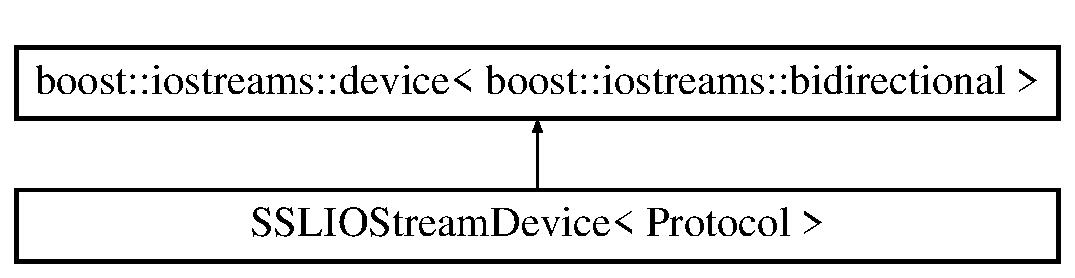
\includegraphics[height=2.000000cm]{class_s_s_l_i_o_stream_device}
\end{center}
\end{figure}
\subsection*{Public Member Functions}
\begin{DoxyCompactItemize}
\item 
\hyperlink{class_s_s_l_i_o_stream_device_a603e5709babdeaaa68c159a2895d7f2e}{S\+S\+L\+I\+O\+Stream\+Device} (boost\+::asio\+::ssl\+::stream$<$ typename Protocol\+::socket $>$ \&stream\+In, bool f\+Use\+S\+S\+L\+In)
\item 
void \hyperlink{class_s_s_l_i_o_stream_device_a6607d02de410f1c731bf1dcf3bac9bb5}{handshake} (boost\+::asio\+::ssl\+::stream\+\_\+base\+::handshake\+\_\+type role)
\item 
std\+::streamsize \hyperlink{class_s_s_l_i_o_stream_device_a8beb626f163adac311a5ec507c3e495a}{read} (char $\ast$s, std\+::streamsize n)
\item 
std\+::streamsize \hyperlink{class_s_s_l_i_o_stream_device_aa4bfad893484ffdf9dbcdce97c462ad0}{write} (const char $\ast$s, std\+::streamsize n)
\item 
bool \hyperlink{class_s_s_l_i_o_stream_device_acdded14a6c79e263989ebf8aea392405}{connect} (const std\+::string \&server, const std\+::string \&port)
\end{DoxyCompactItemize}


\subsection{Detailed Description}
\subsubsection*{template$<$typename Protocol$>$class S\+S\+L\+I\+O\+Stream\+Device$<$ Protocol $>$}

I\+O\+Stream device that speaks S\+S\+L but can also speak non-\/\+S\+S\+L 

\subsection{Constructor \& Destructor Documentation}
\hypertarget{class_s_s_l_i_o_stream_device_a603e5709babdeaaa68c159a2895d7f2e}{}\index{S\+S\+L\+I\+O\+Stream\+Device@{S\+S\+L\+I\+O\+Stream\+Device}!S\+S\+L\+I\+O\+Stream\+Device@{S\+S\+L\+I\+O\+Stream\+Device}}
\index{S\+S\+L\+I\+O\+Stream\+Device@{S\+S\+L\+I\+O\+Stream\+Device}!S\+S\+L\+I\+O\+Stream\+Device@{S\+S\+L\+I\+O\+Stream\+Device}}
\subsubsection[{S\+S\+L\+I\+O\+Stream\+Device}]{\setlength{\rightskip}{0pt plus 5cm}template$<$typename Protocol $>$ {\bf S\+S\+L\+I\+O\+Stream\+Device}$<$ Protocol $>$\+::{\bf S\+S\+L\+I\+O\+Stream\+Device} (
\begin{DoxyParamCaption}
\item[{boost\+::asio\+::ssl\+::stream$<$ typename Protocol\+::socket $>$ \&}]{stream\+In, }
\item[{bool}]{f\+Use\+S\+S\+L\+In}
\end{DoxyParamCaption}
)\hspace{0.3cm}{\ttfamily [inline]}}\label{class_s_s_l_i_o_stream_device_a603e5709babdeaaa68c159a2895d7f2e}


\subsection{Member Function Documentation}
\hypertarget{class_s_s_l_i_o_stream_device_acdded14a6c79e263989ebf8aea392405}{}\index{S\+S\+L\+I\+O\+Stream\+Device@{S\+S\+L\+I\+O\+Stream\+Device}!connect@{connect}}
\index{connect@{connect}!S\+S\+L\+I\+O\+Stream\+Device@{S\+S\+L\+I\+O\+Stream\+Device}}
\subsubsection[{connect}]{\setlength{\rightskip}{0pt plus 5cm}template$<$typename Protocol $>$ bool {\bf S\+S\+L\+I\+O\+Stream\+Device}$<$ Protocol $>$\+::connect (
\begin{DoxyParamCaption}
\item[{const std\+::string \&}]{server, }
\item[{const std\+::string \&}]{port}
\end{DoxyParamCaption}
)\hspace{0.3cm}{\ttfamily [inline]}}\label{class_s_s_l_i_o_stream_device_acdded14a6c79e263989ebf8aea392405}
\hypertarget{class_s_s_l_i_o_stream_device_a6607d02de410f1c731bf1dcf3bac9bb5}{}\index{S\+S\+L\+I\+O\+Stream\+Device@{S\+S\+L\+I\+O\+Stream\+Device}!handshake@{handshake}}
\index{handshake@{handshake}!S\+S\+L\+I\+O\+Stream\+Device@{S\+S\+L\+I\+O\+Stream\+Device}}
\subsubsection[{handshake}]{\setlength{\rightskip}{0pt plus 5cm}template$<$typename Protocol $>$ void {\bf S\+S\+L\+I\+O\+Stream\+Device}$<$ Protocol $>$\+::handshake (
\begin{DoxyParamCaption}
\item[{boost\+::asio\+::ssl\+::stream\+\_\+base\+::handshake\+\_\+type}]{role}
\end{DoxyParamCaption}
)\hspace{0.3cm}{\ttfamily [inline]}}\label{class_s_s_l_i_o_stream_device_a6607d02de410f1c731bf1dcf3bac9bb5}
\hypertarget{class_s_s_l_i_o_stream_device_a8beb626f163adac311a5ec507c3e495a}{}\index{S\+S\+L\+I\+O\+Stream\+Device@{S\+S\+L\+I\+O\+Stream\+Device}!read@{read}}
\index{read@{read}!S\+S\+L\+I\+O\+Stream\+Device@{S\+S\+L\+I\+O\+Stream\+Device}}
\subsubsection[{read}]{\setlength{\rightskip}{0pt plus 5cm}template$<$typename Protocol $>$ std\+::streamsize {\bf S\+S\+L\+I\+O\+Stream\+Device}$<$ Protocol $>$\+::read (
\begin{DoxyParamCaption}
\item[{char $\ast$}]{s, }
\item[{std\+::streamsize}]{n}
\end{DoxyParamCaption}
)\hspace{0.3cm}{\ttfamily [inline]}}\label{class_s_s_l_i_o_stream_device_a8beb626f163adac311a5ec507c3e495a}
\hypertarget{class_s_s_l_i_o_stream_device_aa4bfad893484ffdf9dbcdce97c462ad0}{}\index{S\+S\+L\+I\+O\+Stream\+Device@{S\+S\+L\+I\+O\+Stream\+Device}!write@{write}}
\index{write@{write}!S\+S\+L\+I\+O\+Stream\+Device@{S\+S\+L\+I\+O\+Stream\+Device}}
\subsubsection[{write}]{\setlength{\rightskip}{0pt plus 5cm}template$<$typename Protocol $>$ std\+::streamsize {\bf S\+S\+L\+I\+O\+Stream\+Device}$<$ Protocol $>$\+::write (
\begin{DoxyParamCaption}
\item[{const char $\ast$}]{s, }
\item[{std\+::streamsize}]{n}
\end{DoxyParamCaption}
)\hspace{0.3cm}{\ttfamily [inline]}}\label{class_s_s_l_i_o_stream_device_aa4bfad893484ffdf9dbcdce97c462ad0}


The documentation for this class was generated from the following file\+:\begin{DoxyCompactItemize}
\item 
C\+:/\+Users/\+Joe/\+Documents/\+School/\+C\+S\+C17\+A/bitcoin/src/\hyperlink{rpcprotocol_8h}{rpcprotocol.\+h}\end{DoxyCompactItemize}

\hypertarget{classsubmitblock___state_catcher}{}\section{submitblock\+\_\+\+State\+Catcher Class Reference}
\label{classsubmitblock___state_catcher}\index{submitblock\+\_\+\+State\+Catcher@{submitblock\+\_\+\+State\+Catcher}}
Inheritance diagram for submitblock\+\_\+\+State\+Catcher\+:\begin{figure}[H]
\begin{center}
\leavevmode
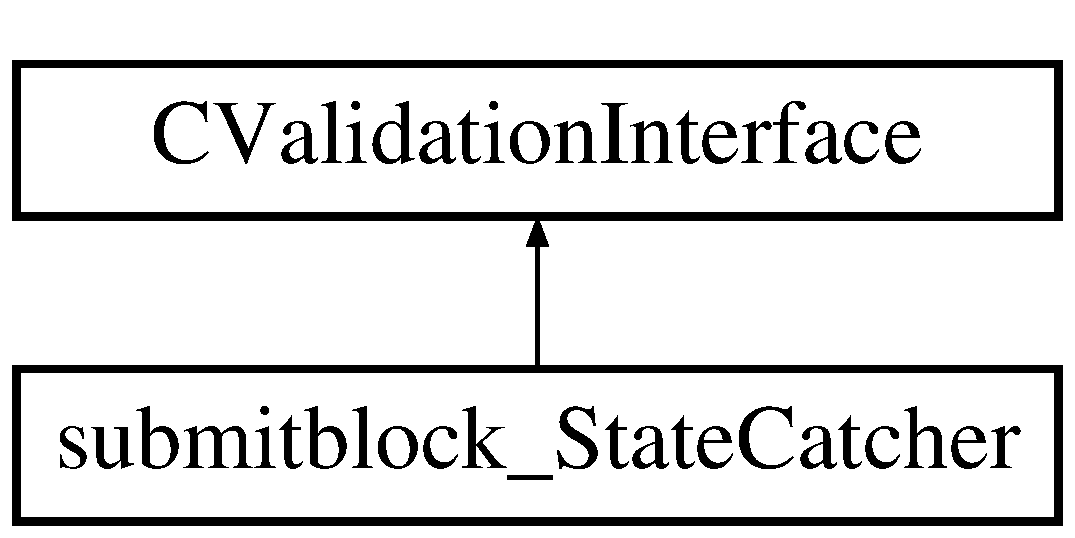
\includegraphics[height=2.000000cm]{classsubmitblock___state_catcher}
\end{center}
\end{figure}
\subsection*{Public Member Functions}
\begin{DoxyCompactItemize}
\item 
\hyperlink{classsubmitblock___state_catcher_a4751e652aed4193935ed00e95cfca548}{submitblock\+\_\+\+State\+Catcher} (const \hyperlink{classuint256}{uint256} \&hash\+In)
\end{DoxyCompactItemize}
\subsection*{Public Attributes}
\begin{DoxyCompactItemize}
\item 
\hyperlink{classuint256}{uint256} \hyperlink{classsubmitblock___state_catcher_adcc822af0b1305bcda71f8e9656c4239}{hash}
\item 
bool \hyperlink{classsubmitblock___state_catcher_a61c0d03544cd4495534bdb0b52f36886}{found}
\item 
\hyperlink{class_c_validation_state}{C\+Validation\+State} \hyperlink{classsubmitblock___state_catcher_a78357802ab8d143f6f21929e0aa2d727}{state}
\end{DoxyCompactItemize}
\subsection*{Protected Member Functions}
\begin{DoxyCompactItemize}
\item 
virtual void \hyperlink{classsubmitblock___state_catcher_a7c7174ac1a54c80c572b115114aa2ee6}{Block\+Checked} (const C\+Block \&block, const \hyperlink{class_c_validation_state}{C\+Validation\+State} \&state\+In)
\end{DoxyCompactItemize}


\subsection{Constructor \& Destructor Documentation}
\hypertarget{classsubmitblock___state_catcher_a4751e652aed4193935ed00e95cfca548}{}\index{submitblock\+\_\+\+State\+Catcher@{submitblock\+\_\+\+State\+Catcher}!submitblock\+\_\+\+State\+Catcher@{submitblock\+\_\+\+State\+Catcher}}
\index{submitblock\+\_\+\+State\+Catcher@{submitblock\+\_\+\+State\+Catcher}!submitblock\+\_\+\+State\+Catcher@{submitblock\+\_\+\+State\+Catcher}}
\subsubsection[{submitblock\+\_\+\+State\+Catcher}]{\setlength{\rightskip}{0pt plus 5cm}submitblock\+\_\+\+State\+Catcher\+::submitblock\+\_\+\+State\+Catcher (
\begin{DoxyParamCaption}
\item[{const {\bf uint256} \&}]{hash\+In}
\end{DoxyParamCaption}
)\hspace{0.3cm}{\ttfamily [inline]}}\label{classsubmitblock___state_catcher_a4751e652aed4193935ed00e95cfca548}


\subsection{Member Function Documentation}
\hypertarget{classsubmitblock___state_catcher_a7c7174ac1a54c80c572b115114aa2ee6}{}\index{submitblock\+\_\+\+State\+Catcher@{submitblock\+\_\+\+State\+Catcher}!Block\+Checked@{Block\+Checked}}
\index{Block\+Checked@{Block\+Checked}!submitblock\+\_\+\+State\+Catcher@{submitblock\+\_\+\+State\+Catcher}}
\subsubsection[{Block\+Checked}]{\setlength{\rightskip}{0pt plus 5cm}virtual void submitblock\+\_\+\+State\+Catcher\+::\+Block\+Checked (
\begin{DoxyParamCaption}
\item[{const C\+Block \&}]{block, }
\item[{const {\bf C\+Validation\+State} \&}]{state\+In}
\end{DoxyParamCaption}
)\hspace{0.3cm}{\ttfamily [inline]}, {\ttfamily [protected]}, {\ttfamily [virtual]}}\label{classsubmitblock___state_catcher_a7c7174ac1a54c80c572b115114aa2ee6}


Reimplemented from \hyperlink{class_c_validation_interface_aeb34ef6814685cabc29062ed7be25441}{C\+Validation\+Interface}.



\subsection{Member Data Documentation}
\hypertarget{classsubmitblock___state_catcher_a61c0d03544cd4495534bdb0b52f36886}{}\index{submitblock\+\_\+\+State\+Catcher@{submitblock\+\_\+\+State\+Catcher}!found@{found}}
\index{found@{found}!submitblock\+\_\+\+State\+Catcher@{submitblock\+\_\+\+State\+Catcher}}
\subsubsection[{found}]{\setlength{\rightskip}{0pt plus 5cm}bool submitblock\+\_\+\+State\+Catcher\+::found}\label{classsubmitblock___state_catcher_a61c0d03544cd4495534bdb0b52f36886}
\hypertarget{classsubmitblock___state_catcher_adcc822af0b1305bcda71f8e9656c4239}{}\index{submitblock\+\_\+\+State\+Catcher@{submitblock\+\_\+\+State\+Catcher}!hash@{hash}}
\index{hash@{hash}!submitblock\+\_\+\+State\+Catcher@{submitblock\+\_\+\+State\+Catcher}}
\subsubsection[{hash}]{\setlength{\rightskip}{0pt plus 5cm}{\bf uint256} submitblock\+\_\+\+State\+Catcher\+::hash}\label{classsubmitblock___state_catcher_adcc822af0b1305bcda71f8e9656c4239}
\hypertarget{classsubmitblock___state_catcher_a78357802ab8d143f6f21929e0aa2d727}{}\index{submitblock\+\_\+\+State\+Catcher@{submitblock\+\_\+\+State\+Catcher}!state@{state}}
\index{state@{state}!submitblock\+\_\+\+State\+Catcher@{submitblock\+\_\+\+State\+Catcher}}
\subsubsection[{state}]{\setlength{\rightskip}{0pt plus 5cm}{\bf C\+Validation\+State} submitblock\+\_\+\+State\+Catcher\+::state}\label{classsubmitblock___state_catcher_a78357802ab8d143f6f21929e0aa2d727}


The documentation for this class was generated from the following file\+:\begin{DoxyCompactItemize}
\item 
C\+:/\+Users/\+Joe/\+Documents/\+School/\+C\+S\+C17\+A/bitcoin/src/\hyperlink{rpcmining_8cpp}{rpcmining.\+cpp}\end{DoxyCompactItemize}

\hypertarget{class_tx_priority_compare}{}\section{Tx\+Priority\+Compare Class Reference}
\label{class_tx_priority_compare}\index{Tx\+Priority\+Compare@{Tx\+Priority\+Compare}}
\subsection*{Public Member Functions}
\begin{DoxyCompactItemize}
\item 
\hyperlink{class_tx_priority_compare_a2ee1aac9d165bbeaaf2a687373f318ad}{Tx\+Priority\+Compare} (bool \+\_\+by\+Fee)
\item 
bool \hyperlink{class_tx_priority_compare_ab50fdbeb5862709d13a271c11ade1775}{operator()} (const \hyperlink{miner_8cpp_a978fa41d50b6f9b1ee69c34d243ea1c7}{Tx\+Priority} \&a, const \hyperlink{miner_8cpp_a978fa41d50b6f9b1ee69c34d243ea1c7}{Tx\+Priority} \&b)
\end{DoxyCompactItemize}


\subsection{Constructor \& Destructor Documentation}
\hypertarget{class_tx_priority_compare_a2ee1aac9d165bbeaaf2a687373f318ad}{}\index{Tx\+Priority\+Compare@{Tx\+Priority\+Compare}!Tx\+Priority\+Compare@{Tx\+Priority\+Compare}}
\index{Tx\+Priority\+Compare@{Tx\+Priority\+Compare}!Tx\+Priority\+Compare@{Tx\+Priority\+Compare}}
\subsubsection[{Tx\+Priority\+Compare}]{\setlength{\rightskip}{0pt plus 5cm}Tx\+Priority\+Compare\+::\+Tx\+Priority\+Compare (
\begin{DoxyParamCaption}
\item[{bool}]{\+\_\+by\+Fee}
\end{DoxyParamCaption}
)\hspace{0.3cm}{\ttfamily [inline]}}\label{class_tx_priority_compare_a2ee1aac9d165bbeaaf2a687373f318ad}


\subsection{Member Function Documentation}
\hypertarget{class_tx_priority_compare_ab50fdbeb5862709d13a271c11ade1775}{}\index{Tx\+Priority\+Compare@{Tx\+Priority\+Compare}!operator()@{operator()}}
\index{operator()@{operator()}!Tx\+Priority\+Compare@{Tx\+Priority\+Compare}}
\subsubsection[{operator()}]{\setlength{\rightskip}{0pt plus 5cm}bool Tx\+Priority\+Compare\+::operator() (
\begin{DoxyParamCaption}
\item[{const {\bf Tx\+Priority} \&}]{a, }
\item[{const {\bf Tx\+Priority} \&}]{b}
\end{DoxyParamCaption}
)\hspace{0.3cm}{\ttfamily [inline]}}\label{class_tx_priority_compare_ab50fdbeb5862709d13a271c11ade1775}


The documentation for this class was generated from the following file\+:\begin{DoxyCompactItemize}
\item 
C\+:/\+Users/\+Joe/\+Documents/\+School/\+C\+S\+C17\+A/bitcoin/src/\hyperlink{miner_8cpp}{miner.\+cpp}\end{DoxyCompactItemize}

\hypertarget{classuint160}{}\section{uint160 Class Reference}
\label{classuint160}\index{uint160@{uint160}}


{\ttfamily \#include $<$uint256.\+h$>$}

Inheritance diagram for uint160\+:\begin{figure}[H]
\begin{center}
\leavevmode
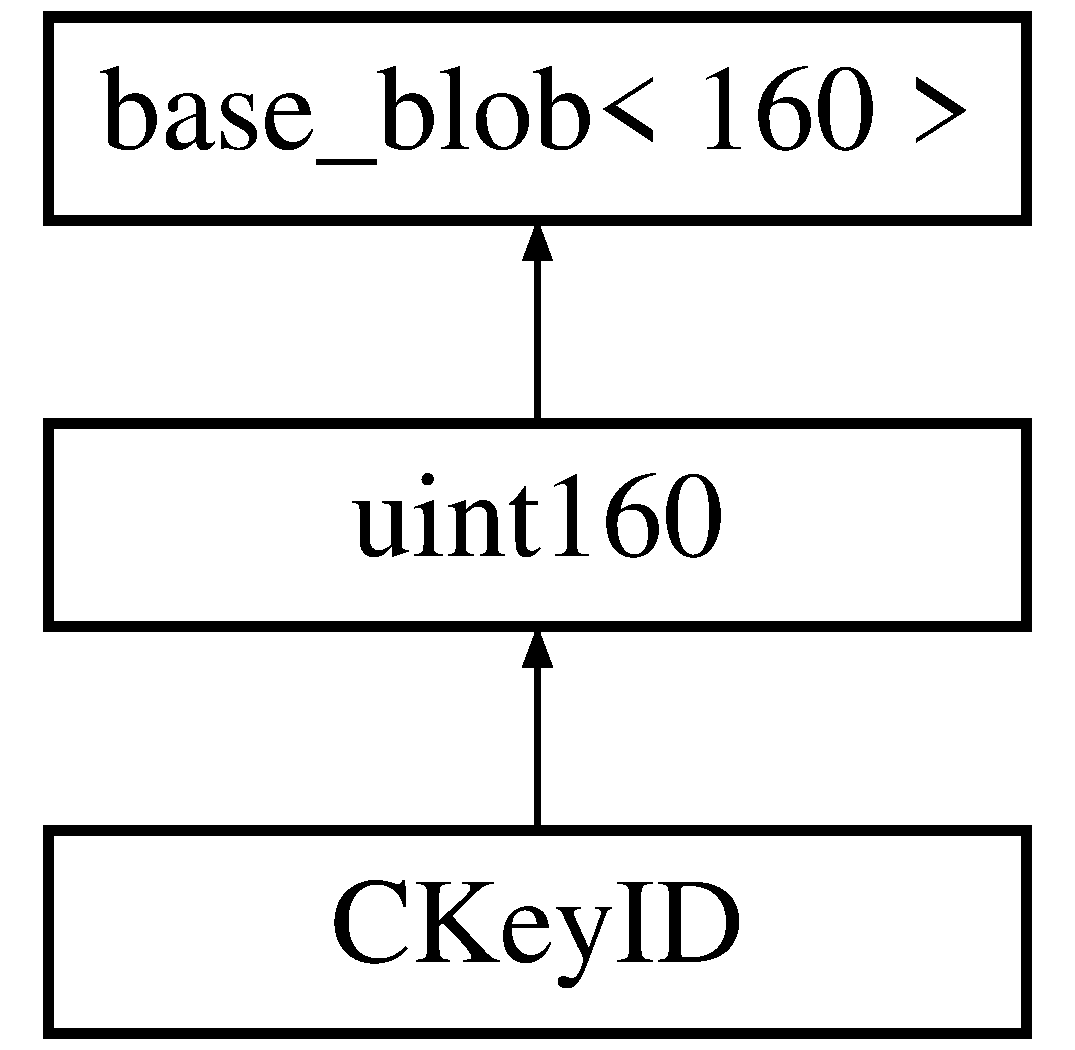
\includegraphics[height=3.000000cm]{classuint160}
\end{center}
\end{figure}
\subsection*{Public Member Functions}
\begin{DoxyCompactItemize}
\item 
\hyperlink{classuint160_a66918f25b891415f2a9bbbb1dfdbedbd}{uint160} ()
\item 
\hyperlink{classuint160_aafc05eec384bffea281460902ad40d8d}{uint160} (const \hyperlink{classbase__blob}{base\+\_\+blob}$<$ 160 $>$ \&b)
\item 
\hyperlink{classuint160_a92bd85c77e73d6642f9bb7519cbd480c}{uint160} (const std\+::vector$<$ unsigned char $>$ \&vch)
\end{DoxyCompactItemize}
\subsection*{Additional Inherited Members}


\subsection{Detailed Description}
160-\/bit opaque blob. \begin{DoxyNote}{Note}
This type is called \hyperlink{classuint160}{uint160} for historical reasons only. It is an opaque blob of 160 bits and has no integer operations. 
\end{DoxyNote}


\subsection{Constructor \& Destructor Documentation}
\hypertarget{classuint160_a66918f25b891415f2a9bbbb1dfdbedbd}{}\index{uint160@{uint160}!uint160@{uint160}}
\index{uint160@{uint160}!uint160@{uint160}}
\subsubsection[{uint160}]{\setlength{\rightskip}{0pt plus 5cm}uint160\+::uint160 (
\begin{DoxyParamCaption}
{}
\end{DoxyParamCaption}
)\hspace{0.3cm}{\ttfamily [inline]}}\label{classuint160_a66918f25b891415f2a9bbbb1dfdbedbd}
\hypertarget{classuint160_aafc05eec384bffea281460902ad40d8d}{}\index{uint160@{uint160}!uint160@{uint160}}
\index{uint160@{uint160}!uint160@{uint160}}
\subsubsection[{uint160}]{\setlength{\rightskip}{0pt plus 5cm}uint160\+::uint160 (
\begin{DoxyParamCaption}
\item[{const {\bf base\+\_\+blob}$<$ 160 $>$ \&}]{b}
\end{DoxyParamCaption}
)\hspace{0.3cm}{\ttfamily [inline]}}\label{classuint160_aafc05eec384bffea281460902ad40d8d}
\hypertarget{classuint160_a92bd85c77e73d6642f9bb7519cbd480c}{}\index{uint160@{uint160}!uint160@{uint160}}
\index{uint160@{uint160}!uint160@{uint160}}
\subsubsection[{uint160}]{\setlength{\rightskip}{0pt plus 5cm}uint160\+::uint160 (
\begin{DoxyParamCaption}
\item[{const std\+::vector$<$ unsigned char $>$ \&}]{vch}
\end{DoxyParamCaption}
)\hspace{0.3cm}{\ttfamily [inline]}, {\ttfamily [explicit]}}\label{classuint160_a92bd85c77e73d6642f9bb7519cbd480c}


The documentation for this class was generated from the following file\+:\begin{DoxyCompactItemize}
\item 
C\+:/\+Users/\+Joe/\+Documents/\+School/\+C\+S\+C17\+A/bitcoin/src/\hyperlink{uint256_8h}{uint256.\+h}\end{DoxyCompactItemize}

\hypertarget{classuint256}{}\section{uint256 Class Reference}
\label{classuint256}\index{uint256@{uint256}}


{\ttfamily \#include $<$uint256.\+h$>$}

Inheritance diagram for uint256\+:\begin{figure}[H]
\begin{center}
\leavevmode
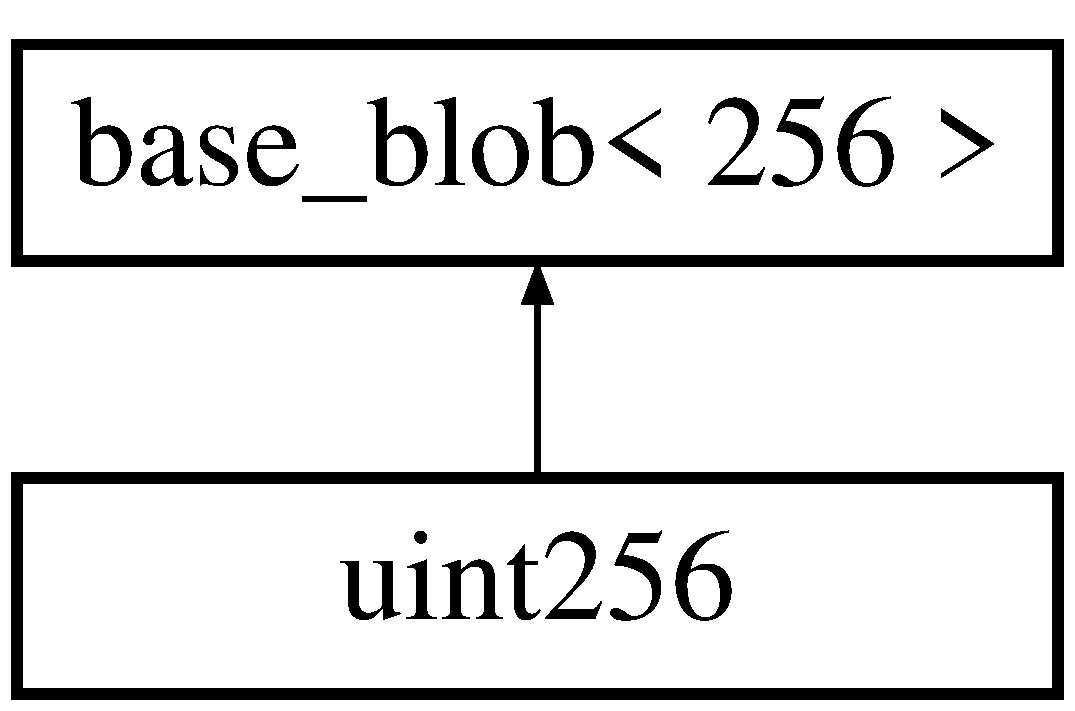
\includegraphics[height=2.000000cm]{classuint256}
\end{center}
\end{figure}
\subsection*{Public Member Functions}
\begin{DoxyCompactItemize}
\item 
\hyperlink{classuint256_aca0c2c2c61e453717e72a4eaec71168f}{uint256} ()
\item 
\hyperlink{classuint256_a01460091171cf2b82b9e41cdb0326bed}{uint256} (const \hyperlink{classbase__blob}{base\+\_\+blob}$<$ 256 $>$ \&b)
\item 
\hyperlink{classuint256_a7cad0fc486ebc2ed02462d5a7d4e4f2d}{uint256} (const std\+::vector$<$ unsigned char $>$ \&vch)
\item 
uint64\+\_\+t \hyperlink{classuint256_a38210c00440a6c5f438f0c16cb8647fc}{Get\+Cheap\+Hash} () const 
\item 
uint64\+\_\+t \hyperlink{classuint256_a2ed8bd4e54421a37430768374a7e91b3}{Get\+Hash} (const \hyperlink{classuint256}{uint256} \&salt) const 
\end{DoxyCompactItemize}
\subsection*{Additional Inherited Members}


\subsection{Detailed Description}
256-\/bit opaque blob. \begin{DoxyNote}{Note}
This type is called \hyperlink{classuint256}{uint256} for historical reasons only. It is an opaque blob of 256 bits and has no integer operations. Use \hyperlink{classarith__uint256}{arith\+\_\+uint256} if those are required. 
\end{DoxyNote}


\subsection{Constructor \& Destructor Documentation}
\hypertarget{classuint256_aca0c2c2c61e453717e72a4eaec71168f}{}\index{uint256@{uint256}!uint256@{uint256}}
\index{uint256@{uint256}!uint256@{uint256}}
\subsubsection[{uint256}]{\setlength{\rightskip}{0pt plus 5cm}uint256\+::uint256 (
\begin{DoxyParamCaption}
{}
\end{DoxyParamCaption}
)\hspace{0.3cm}{\ttfamily [inline]}}\label{classuint256_aca0c2c2c61e453717e72a4eaec71168f}
\hypertarget{classuint256_a01460091171cf2b82b9e41cdb0326bed}{}\index{uint256@{uint256}!uint256@{uint256}}
\index{uint256@{uint256}!uint256@{uint256}}
\subsubsection[{uint256}]{\setlength{\rightskip}{0pt plus 5cm}uint256\+::uint256 (
\begin{DoxyParamCaption}
\item[{const {\bf base\+\_\+blob}$<$ 256 $>$ \&}]{b}
\end{DoxyParamCaption}
)\hspace{0.3cm}{\ttfamily [inline]}}\label{classuint256_a01460091171cf2b82b9e41cdb0326bed}
\hypertarget{classuint256_a7cad0fc486ebc2ed02462d5a7d4e4f2d}{}\index{uint256@{uint256}!uint256@{uint256}}
\index{uint256@{uint256}!uint256@{uint256}}
\subsubsection[{uint256}]{\setlength{\rightskip}{0pt plus 5cm}uint256\+::uint256 (
\begin{DoxyParamCaption}
\item[{const std\+::vector$<$ unsigned char $>$ \&}]{vch}
\end{DoxyParamCaption}
)\hspace{0.3cm}{\ttfamily [inline]}, {\ttfamily [explicit]}}\label{classuint256_a7cad0fc486ebc2ed02462d5a7d4e4f2d}


\subsection{Member Function Documentation}
\hypertarget{classuint256_a38210c00440a6c5f438f0c16cb8647fc}{}\index{uint256@{uint256}!Get\+Cheap\+Hash@{Get\+Cheap\+Hash}}
\index{Get\+Cheap\+Hash@{Get\+Cheap\+Hash}!uint256@{uint256}}
\subsubsection[{Get\+Cheap\+Hash}]{\setlength{\rightskip}{0pt plus 5cm}uint64\+\_\+t uint256\+::\+Get\+Cheap\+Hash (
\begin{DoxyParamCaption}
{}
\end{DoxyParamCaption}
) const\hspace{0.3cm}{\ttfamily [inline]}}\label{classuint256_a38210c00440a6c5f438f0c16cb8647fc}
A cheap hash function that just returns 64 bits from the result, it can be used when the contents are considered uniformly random. It is not appropriate when the value can easily be influenced from outside as e.\+g. a network adversary could provide values to trigger worst-\/case behavior. \begin{DoxyNote}{Note}
The result of this function is not stable between little and big endian. 
\end{DoxyNote}
\hypertarget{classuint256_a2ed8bd4e54421a37430768374a7e91b3}{}\index{uint256@{uint256}!Get\+Hash@{Get\+Hash}}
\index{Get\+Hash@{Get\+Hash}!uint256@{uint256}}
\subsubsection[{Get\+Hash}]{\setlength{\rightskip}{0pt plus 5cm}uint64\+\_\+t uint256\+::\+Get\+Hash (
\begin{DoxyParamCaption}
\item[{const {\bf uint256} \&}]{salt}
\end{DoxyParamCaption}
) const}\label{classuint256_a2ed8bd4e54421a37430768374a7e91b3}
A more secure, salted hash function. \begin{DoxyNote}{Note}
This hash is not stable between little and big endian. 
\end{DoxyNote}


The documentation for this class was generated from the following files\+:\begin{DoxyCompactItemize}
\item 
C\+:/\+Users/\+Joe/\+Documents/\+School/\+C\+S\+C17\+A/bitcoin/src/\hyperlink{uint256_8h}{uint256.\+h}\item 
C\+:/\+Users/\+Joe/\+Documents/\+School/\+C\+S\+C17\+A/bitcoin/src/\hyperlink{uint256_8cpp}{uint256.\+cpp}\end{DoxyCompactItemize}

\hypertarget{classuint__error}{}\section{uint\+\_\+error Class Reference}
\label{classuint__error}\index{uint\+\_\+error@{uint\+\_\+error}}


{\ttfamily \#include $<$arith\+\_\+uint256.\+h$>$}

Inheritance diagram for uint\+\_\+error\+:\begin{figure}[H]
\begin{center}
\leavevmode
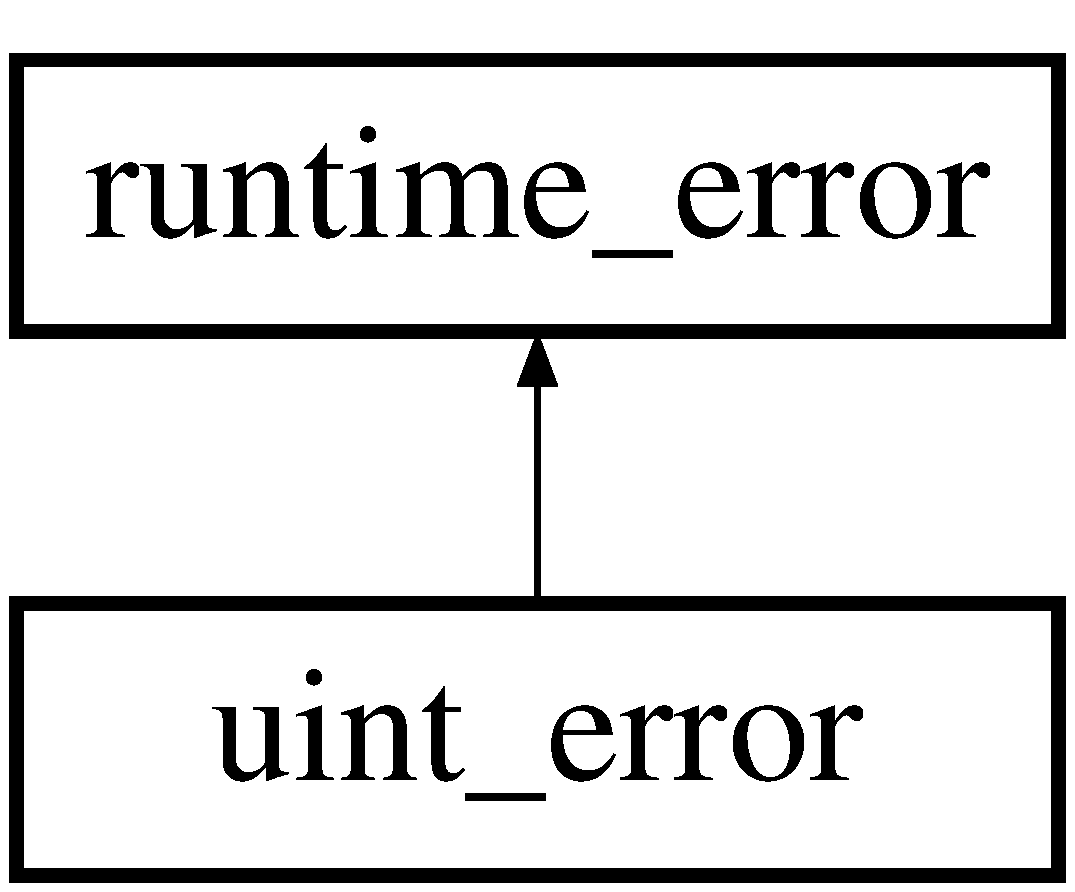
\includegraphics[height=2.000000cm]{classuint__error}
\end{center}
\end{figure}
\subsection*{Public Member Functions}
\begin{DoxyCompactItemize}
\item 
\hyperlink{classuint__error_a3d37e73d7d585ede158ebba7d32352c3}{uint\+\_\+error} (const std\+::string \&str)
\end{DoxyCompactItemize}


\subsection{Constructor \& Destructor Documentation}
\hypertarget{classuint__error_a3d37e73d7d585ede158ebba7d32352c3}{}\index{uint\+\_\+error@{uint\+\_\+error}!uint\+\_\+error@{uint\+\_\+error}}
\index{uint\+\_\+error@{uint\+\_\+error}!uint\+\_\+error@{uint\+\_\+error}}
\subsubsection[{uint\+\_\+error}]{\setlength{\rightskip}{0pt plus 5cm}uint\+\_\+error\+::uint\+\_\+error (
\begin{DoxyParamCaption}
\item[{const std\+::string \&}]{str}
\end{DoxyParamCaption}
)\hspace{0.3cm}{\ttfamily [inline]}, {\ttfamily [explicit]}}\label{classuint__error_a3d37e73d7d585ede158ebba7d32352c3}


The documentation for this class was generated from the following file\+:\begin{DoxyCompactItemize}
\item 
C\+:/\+Users/\+Joe/\+Documents/\+School/\+C\+S\+C17\+A/bitcoin/src/\hyperlink{arith__uint256_8h}{arith\+\_\+uint256.\+h}\end{DoxyCompactItemize}

\chapter{File Documentation}
\hypertarget{addrman_8cpp}{}\section{C\+:/\+Users/\+Joe/\+Documents/\+School/\+C\+S\+C17\+A/bitcoin/src/addrman.cpp File Reference}
\label{addrman_8cpp}\index{C\+:/\+Users/\+Joe/\+Documents/\+School/\+C\+S\+C17\+A/bitcoin/src/addrman.\+cpp@{C\+:/\+Users/\+Joe/\+Documents/\+School/\+C\+S\+C17\+A/bitcoin/src/addrman.\+cpp}}
{\ttfamily \#include \char`\"{}addrman.\+h\char`\"{}}\\*
{\ttfamily \#include \char`\"{}hash.\+h\char`\"{}}\\*
{\ttfamily \#include \char`\"{}serialize.\+h\char`\"{}}\\*
{\ttfamily \#include \char`\"{}streams.\+h\char`\"{}}\\*

\hypertarget{addrman_8h}{}\section{C\+:/\+Users/\+Joe/\+Documents/\+School/\+C\+S\+C17\+A/bitcoin/src/addrman.h File Reference}
\label{addrman_8h}\index{C\+:/\+Users/\+Joe/\+Documents/\+School/\+C\+S\+C17\+A/bitcoin/src/addrman.\+h@{C\+:/\+Users/\+Joe/\+Documents/\+School/\+C\+S\+C17\+A/bitcoin/src/addrman.\+h}}
{\ttfamily \#include \char`\"{}netbase.\+h\char`\"{}}\\*
{\ttfamily \#include \char`\"{}protocol.\+h\char`\"{}}\\*
{\ttfamily \#include \char`\"{}random.\+h\char`\"{}}\\*
{\ttfamily \#include \char`\"{}sync.\+h\char`\"{}}\\*
{\ttfamily \#include \char`\"{}timedata.\+h\char`\"{}}\\*
{\ttfamily \#include \char`\"{}util.\+h\char`\"{}}\\*
{\ttfamily \#include $<$map$>$}\\*
{\ttfamily \#include $<$set$>$}\\*
{\ttfamily \#include $<$stdint.\+h$>$}\\*
{\ttfamily \#include $<$vector$>$}\\*
\subsection*{Classes}
\begin{DoxyCompactItemize}
\item 
class \hyperlink{class_c_addr_info}{C\+Addr\+Info}
\item 
class \hyperlink{class_c_addr_man}{C\+Addr\+Man}
\end{DoxyCompactItemize}
\subsection*{Macros}
\begin{DoxyCompactItemize}
\item 
\#define \hyperlink{addrman_8h_ab09df186aa818ce7b9e7c86446511cf1}{A\+D\+D\+R\+M\+A\+N\+\_\+\+T\+R\+I\+E\+D\+\_\+\+B\+U\+C\+K\+E\+T\+\_\+\+C\+O\+U\+N\+T}~256
\begin{DoxyCompactList}\small\item\em total number of buckets for tried addresses \end{DoxyCompactList}\item 
\#define \hyperlink{addrman_8h_a74a626eb1dbb8e307a413e86493cd510}{A\+D\+D\+R\+M\+A\+N\+\_\+\+N\+E\+W\+\_\+\+B\+U\+C\+K\+E\+T\+\_\+\+C\+O\+U\+N\+T}~1024
\begin{DoxyCompactList}\small\item\em total number of buckets for new addresses \end{DoxyCompactList}\item 
\#define \hyperlink{addrman_8h_a3499731a6c89e164cf74b68be2be0a84}{A\+D\+D\+R\+M\+A\+N\+\_\+\+B\+U\+C\+K\+E\+T\+\_\+\+S\+I\+Z\+E}~64
\begin{DoxyCompactList}\small\item\em maximum allowed number of entries in buckets for new and tried addresses \end{DoxyCompactList}\item 
\#define \hyperlink{addrman_8h_a87c7c90e3631bf1a4475cabdded61f6f}{A\+D\+D\+R\+M\+A\+N\+\_\+\+T\+R\+I\+E\+D\+\_\+\+B\+U\+C\+K\+E\+T\+S\+\_\+\+P\+E\+R\+\_\+\+G\+R\+O\+U\+P}~8
\begin{DoxyCompactList}\small\item\em over how many buckets entries with tried addresses from a single group (/16 for I\+Pv4) are spread \end{DoxyCompactList}\item 
\#define \hyperlink{addrman_8h_a09c090218fd02375aa57eb7e8eb1c013}{A\+D\+D\+R\+M\+A\+N\+\_\+\+N\+E\+W\+\_\+\+B\+U\+C\+K\+E\+T\+S\+\_\+\+P\+E\+R\+\_\+\+S\+O\+U\+R\+C\+E\+\_\+\+G\+R\+O\+U\+P}~64
\begin{DoxyCompactList}\small\item\em over how many buckets entries with new addresses originating from a single group are spread \end{DoxyCompactList}\item 
\#define \hyperlink{addrman_8h_a230e30813119d10bdba59c1f8cc789cd}{A\+D\+D\+R\+M\+A\+N\+\_\+\+N\+E\+W\+\_\+\+B\+U\+C\+K\+E\+T\+S\+\_\+\+P\+E\+R\+\_\+\+A\+D\+D\+R\+E\+S\+S}~8
\begin{DoxyCompactList}\small\item\em in how many buckets for entries with new addresses a single address may occur \end{DoxyCompactList}\item 
\#define \hyperlink{addrman_8h_a86698b159625d84b47a2ffddc76ebc99}{A\+D\+D\+R\+M\+A\+N\+\_\+\+H\+O\+R\+I\+Z\+O\+N\+\_\+\+D\+A\+Y\+S}~30
\begin{DoxyCompactList}\small\item\em how old addresses can maximally be \end{DoxyCompactList}\item 
\#define \hyperlink{addrman_8h_a771c05a7a20d9a35f4546e1e333c48c4}{A\+D\+D\+R\+M\+A\+N\+\_\+\+R\+E\+T\+R\+I\+E\+S}~3
\begin{DoxyCompactList}\small\item\em after how many failed attempts we give up on a new node \end{DoxyCompactList}\item 
\#define \hyperlink{addrman_8h_a26430e6e9a3ef9f4fc54491330b7e611}{A\+D\+D\+R\+M\+A\+N\+\_\+\+M\+A\+X\+\_\+\+F\+A\+I\+L\+U\+R\+E\+S}~10
\begin{DoxyCompactList}\small\item\em how many successive failures are allowed ... \end{DoxyCompactList}\item 
\#define \hyperlink{addrman_8h_a7dcc28590c48ca382d26c4f37fda4e3d}{A\+D\+D\+R\+M\+A\+N\+\_\+\+M\+I\+N\+\_\+\+F\+A\+I\+L\+\_\+\+D\+A\+Y\+S}~7
\begin{DoxyCompactList}\small\item\em ... in at least this many days \end{DoxyCompactList}\item 
\#define \hyperlink{addrman_8h_a06edfd03ad361fbc74794e1c533d1bc5}{A\+D\+D\+R\+M\+A\+N\+\_\+\+G\+E\+T\+A\+D\+D\+R\+\_\+\+M\+A\+X\+\_\+\+P\+C\+T}~23
\begin{DoxyCompactList}\small\item\em the maximum percentage of nodes to return in a getaddr call \end{DoxyCompactList}\item 
\#define \hyperlink{addrman_8h_ad10877f29a66224fce5c20d33e26448a}{A\+D\+D\+R\+M\+A\+N\+\_\+\+G\+E\+T\+A\+D\+D\+R\+\_\+\+M\+A\+X}~2500
\begin{DoxyCompactList}\small\item\em the maximum number of nodes to return in a getaddr call \end{DoxyCompactList}\end{DoxyCompactItemize}


\subsection{Macro Definition Documentation}
\hypertarget{addrman_8h_a3499731a6c89e164cf74b68be2be0a84}{}\index{addrman.\+h@{addrman.\+h}!A\+D\+D\+R\+M\+A\+N\+\_\+\+B\+U\+C\+K\+E\+T\+\_\+\+S\+I\+Z\+E@{A\+D\+D\+R\+M\+A\+N\+\_\+\+B\+U\+C\+K\+E\+T\+\_\+\+S\+I\+Z\+E}}
\index{A\+D\+D\+R\+M\+A\+N\+\_\+\+B\+U\+C\+K\+E\+T\+\_\+\+S\+I\+Z\+E@{A\+D\+D\+R\+M\+A\+N\+\_\+\+B\+U\+C\+K\+E\+T\+\_\+\+S\+I\+Z\+E}!addrman.\+h@{addrman.\+h}}
\subsubsection[{A\+D\+D\+R\+M\+A\+N\+\_\+\+B\+U\+C\+K\+E\+T\+\_\+\+S\+I\+Z\+E}]{\setlength{\rightskip}{0pt plus 5cm}\#define A\+D\+D\+R\+M\+A\+N\+\_\+\+B\+U\+C\+K\+E\+T\+\_\+\+S\+I\+Z\+E~64}\label{addrman_8h_a3499731a6c89e164cf74b68be2be0a84}


maximum allowed number of entries in buckets for new and tried addresses 

\hypertarget{addrman_8h_ad10877f29a66224fce5c20d33e26448a}{}\index{addrman.\+h@{addrman.\+h}!A\+D\+D\+R\+M\+A\+N\+\_\+\+G\+E\+T\+A\+D\+D\+R\+\_\+\+M\+A\+X@{A\+D\+D\+R\+M\+A\+N\+\_\+\+G\+E\+T\+A\+D\+D\+R\+\_\+\+M\+A\+X}}
\index{A\+D\+D\+R\+M\+A\+N\+\_\+\+G\+E\+T\+A\+D\+D\+R\+\_\+\+M\+A\+X@{A\+D\+D\+R\+M\+A\+N\+\_\+\+G\+E\+T\+A\+D\+D\+R\+\_\+\+M\+A\+X}!addrman.\+h@{addrman.\+h}}
\subsubsection[{A\+D\+D\+R\+M\+A\+N\+\_\+\+G\+E\+T\+A\+D\+D\+R\+\_\+\+M\+A\+X}]{\setlength{\rightskip}{0pt plus 5cm}\#define A\+D\+D\+R\+M\+A\+N\+\_\+\+G\+E\+T\+A\+D\+D\+R\+\_\+\+M\+A\+X~2500}\label{addrman_8h_ad10877f29a66224fce5c20d33e26448a}


the maximum number of nodes to return in a getaddr call 

\hypertarget{addrman_8h_a06edfd03ad361fbc74794e1c533d1bc5}{}\index{addrman.\+h@{addrman.\+h}!A\+D\+D\+R\+M\+A\+N\+\_\+\+G\+E\+T\+A\+D\+D\+R\+\_\+\+M\+A\+X\+\_\+\+P\+C\+T@{A\+D\+D\+R\+M\+A\+N\+\_\+\+G\+E\+T\+A\+D\+D\+R\+\_\+\+M\+A\+X\+\_\+\+P\+C\+T}}
\index{A\+D\+D\+R\+M\+A\+N\+\_\+\+G\+E\+T\+A\+D\+D\+R\+\_\+\+M\+A\+X\+\_\+\+P\+C\+T@{A\+D\+D\+R\+M\+A\+N\+\_\+\+G\+E\+T\+A\+D\+D\+R\+\_\+\+M\+A\+X\+\_\+\+P\+C\+T}!addrman.\+h@{addrman.\+h}}
\subsubsection[{A\+D\+D\+R\+M\+A\+N\+\_\+\+G\+E\+T\+A\+D\+D\+R\+\_\+\+M\+A\+X\+\_\+\+P\+C\+T}]{\setlength{\rightskip}{0pt plus 5cm}\#define A\+D\+D\+R\+M\+A\+N\+\_\+\+G\+E\+T\+A\+D\+D\+R\+\_\+\+M\+A\+X\+\_\+\+P\+C\+T~23}\label{addrman_8h_a06edfd03ad361fbc74794e1c533d1bc5}


the maximum percentage of nodes to return in a getaddr call 

\hypertarget{addrman_8h_a86698b159625d84b47a2ffddc76ebc99}{}\index{addrman.\+h@{addrman.\+h}!A\+D\+D\+R\+M\+A\+N\+\_\+\+H\+O\+R\+I\+Z\+O\+N\+\_\+\+D\+A\+Y\+S@{A\+D\+D\+R\+M\+A\+N\+\_\+\+H\+O\+R\+I\+Z\+O\+N\+\_\+\+D\+A\+Y\+S}}
\index{A\+D\+D\+R\+M\+A\+N\+\_\+\+H\+O\+R\+I\+Z\+O\+N\+\_\+\+D\+A\+Y\+S@{A\+D\+D\+R\+M\+A\+N\+\_\+\+H\+O\+R\+I\+Z\+O\+N\+\_\+\+D\+A\+Y\+S}!addrman.\+h@{addrman.\+h}}
\subsubsection[{A\+D\+D\+R\+M\+A\+N\+\_\+\+H\+O\+R\+I\+Z\+O\+N\+\_\+\+D\+A\+Y\+S}]{\setlength{\rightskip}{0pt plus 5cm}\#define A\+D\+D\+R\+M\+A\+N\+\_\+\+H\+O\+R\+I\+Z\+O\+N\+\_\+\+D\+A\+Y\+S~30}\label{addrman_8h_a86698b159625d84b47a2ffddc76ebc99}


how old addresses can maximally be 

\hypertarget{addrman_8h_a26430e6e9a3ef9f4fc54491330b7e611}{}\index{addrman.\+h@{addrman.\+h}!A\+D\+D\+R\+M\+A\+N\+\_\+\+M\+A\+X\+\_\+\+F\+A\+I\+L\+U\+R\+E\+S@{A\+D\+D\+R\+M\+A\+N\+\_\+\+M\+A\+X\+\_\+\+F\+A\+I\+L\+U\+R\+E\+S}}
\index{A\+D\+D\+R\+M\+A\+N\+\_\+\+M\+A\+X\+\_\+\+F\+A\+I\+L\+U\+R\+E\+S@{A\+D\+D\+R\+M\+A\+N\+\_\+\+M\+A\+X\+\_\+\+F\+A\+I\+L\+U\+R\+E\+S}!addrman.\+h@{addrman.\+h}}
\subsubsection[{A\+D\+D\+R\+M\+A\+N\+\_\+\+M\+A\+X\+\_\+\+F\+A\+I\+L\+U\+R\+E\+S}]{\setlength{\rightskip}{0pt plus 5cm}\#define A\+D\+D\+R\+M\+A\+N\+\_\+\+M\+A\+X\+\_\+\+F\+A\+I\+L\+U\+R\+E\+S~10}\label{addrman_8h_a26430e6e9a3ef9f4fc54491330b7e611}


how many successive failures are allowed ... 

\hypertarget{addrman_8h_a7dcc28590c48ca382d26c4f37fda4e3d}{}\index{addrman.\+h@{addrman.\+h}!A\+D\+D\+R\+M\+A\+N\+\_\+\+M\+I\+N\+\_\+\+F\+A\+I\+L\+\_\+\+D\+A\+Y\+S@{A\+D\+D\+R\+M\+A\+N\+\_\+\+M\+I\+N\+\_\+\+F\+A\+I\+L\+\_\+\+D\+A\+Y\+S}}
\index{A\+D\+D\+R\+M\+A\+N\+\_\+\+M\+I\+N\+\_\+\+F\+A\+I\+L\+\_\+\+D\+A\+Y\+S@{A\+D\+D\+R\+M\+A\+N\+\_\+\+M\+I\+N\+\_\+\+F\+A\+I\+L\+\_\+\+D\+A\+Y\+S}!addrman.\+h@{addrman.\+h}}
\subsubsection[{A\+D\+D\+R\+M\+A\+N\+\_\+\+M\+I\+N\+\_\+\+F\+A\+I\+L\+\_\+\+D\+A\+Y\+S}]{\setlength{\rightskip}{0pt plus 5cm}\#define A\+D\+D\+R\+M\+A\+N\+\_\+\+M\+I\+N\+\_\+\+F\+A\+I\+L\+\_\+\+D\+A\+Y\+S~7}\label{addrman_8h_a7dcc28590c48ca382d26c4f37fda4e3d}


... in at least this many days 

\hypertarget{addrman_8h_a74a626eb1dbb8e307a413e86493cd510}{}\index{addrman.\+h@{addrman.\+h}!A\+D\+D\+R\+M\+A\+N\+\_\+\+N\+E\+W\+\_\+\+B\+U\+C\+K\+E\+T\+\_\+\+C\+O\+U\+N\+T@{A\+D\+D\+R\+M\+A\+N\+\_\+\+N\+E\+W\+\_\+\+B\+U\+C\+K\+E\+T\+\_\+\+C\+O\+U\+N\+T}}
\index{A\+D\+D\+R\+M\+A\+N\+\_\+\+N\+E\+W\+\_\+\+B\+U\+C\+K\+E\+T\+\_\+\+C\+O\+U\+N\+T@{A\+D\+D\+R\+M\+A\+N\+\_\+\+N\+E\+W\+\_\+\+B\+U\+C\+K\+E\+T\+\_\+\+C\+O\+U\+N\+T}!addrman.\+h@{addrman.\+h}}
\subsubsection[{A\+D\+D\+R\+M\+A\+N\+\_\+\+N\+E\+W\+\_\+\+B\+U\+C\+K\+E\+T\+\_\+\+C\+O\+U\+N\+T}]{\setlength{\rightskip}{0pt plus 5cm}\#define A\+D\+D\+R\+M\+A\+N\+\_\+\+N\+E\+W\+\_\+\+B\+U\+C\+K\+E\+T\+\_\+\+C\+O\+U\+N\+T~1024}\label{addrman_8h_a74a626eb1dbb8e307a413e86493cd510}


total number of buckets for new addresses 

\hypertarget{addrman_8h_a230e30813119d10bdba59c1f8cc789cd}{}\index{addrman.\+h@{addrman.\+h}!A\+D\+D\+R\+M\+A\+N\+\_\+\+N\+E\+W\+\_\+\+B\+U\+C\+K\+E\+T\+S\+\_\+\+P\+E\+R\+\_\+\+A\+D\+D\+R\+E\+S\+S@{A\+D\+D\+R\+M\+A\+N\+\_\+\+N\+E\+W\+\_\+\+B\+U\+C\+K\+E\+T\+S\+\_\+\+P\+E\+R\+\_\+\+A\+D\+D\+R\+E\+S\+S}}
\index{A\+D\+D\+R\+M\+A\+N\+\_\+\+N\+E\+W\+\_\+\+B\+U\+C\+K\+E\+T\+S\+\_\+\+P\+E\+R\+\_\+\+A\+D\+D\+R\+E\+S\+S@{A\+D\+D\+R\+M\+A\+N\+\_\+\+N\+E\+W\+\_\+\+B\+U\+C\+K\+E\+T\+S\+\_\+\+P\+E\+R\+\_\+\+A\+D\+D\+R\+E\+S\+S}!addrman.\+h@{addrman.\+h}}
\subsubsection[{A\+D\+D\+R\+M\+A\+N\+\_\+\+N\+E\+W\+\_\+\+B\+U\+C\+K\+E\+T\+S\+\_\+\+P\+E\+R\+\_\+\+A\+D\+D\+R\+E\+S\+S}]{\setlength{\rightskip}{0pt plus 5cm}\#define A\+D\+D\+R\+M\+A\+N\+\_\+\+N\+E\+W\+\_\+\+B\+U\+C\+K\+E\+T\+S\+\_\+\+P\+E\+R\+\_\+\+A\+D\+D\+R\+E\+S\+S~8}\label{addrman_8h_a230e30813119d10bdba59c1f8cc789cd}


in how many buckets for entries with new addresses a single address may occur 

\hypertarget{addrman_8h_a09c090218fd02375aa57eb7e8eb1c013}{}\index{addrman.\+h@{addrman.\+h}!A\+D\+D\+R\+M\+A\+N\+\_\+\+N\+E\+W\+\_\+\+B\+U\+C\+K\+E\+T\+S\+\_\+\+P\+E\+R\+\_\+\+S\+O\+U\+R\+C\+E\+\_\+\+G\+R\+O\+U\+P@{A\+D\+D\+R\+M\+A\+N\+\_\+\+N\+E\+W\+\_\+\+B\+U\+C\+K\+E\+T\+S\+\_\+\+P\+E\+R\+\_\+\+S\+O\+U\+R\+C\+E\+\_\+\+G\+R\+O\+U\+P}}
\index{A\+D\+D\+R\+M\+A\+N\+\_\+\+N\+E\+W\+\_\+\+B\+U\+C\+K\+E\+T\+S\+\_\+\+P\+E\+R\+\_\+\+S\+O\+U\+R\+C\+E\+\_\+\+G\+R\+O\+U\+P@{A\+D\+D\+R\+M\+A\+N\+\_\+\+N\+E\+W\+\_\+\+B\+U\+C\+K\+E\+T\+S\+\_\+\+P\+E\+R\+\_\+\+S\+O\+U\+R\+C\+E\+\_\+\+G\+R\+O\+U\+P}!addrman.\+h@{addrman.\+h}}
\subsubsection[{A\+D\+D\+R\+M\+A\+N\+\_\+\+N\+E\+W\+\_\+\+B\+U\+C\+K\+E\+T\+S\+\_\+\+P\+E\+R\+\_\+\+S\+O\+U\+R\+C\+E\+\_\+\+G\+R\+O\+U\+P}]{\setlength{\rightskip}{0pt plus 5cm}\#define A\+D\+D\+R\+M\+A\+N\+\_\+\+N\+E\+W\+\_\+\+B\+U\+C\+K\+E\+T\+S\+\_\+\+P\+E\+R\+\_\+\+S\+O\+U\+R\+C\+E\+\_\+\+G\+R\+O\+U\+P~64}\label{addrman_8h_a09c090218fd02375aa57eb7e8eb1c013}


over how many buckets entries with new addresses originating from a single group are spread 

\hypertarget{addrman_8h_a771c05a7a20d9a35f4546e1e333c48c4}{}\index{addrman.\+h@{addrman.\+h}!A\+D\+D\+R\+M\+A\+N\+\_\+\+R\+E\+T\+R\+I\+E\+S@{A\+D\+D\+R\+M\+A\+N\+\_\+\+R\+E\+T\+R\+I\+E\+S}}
\index{A\+D\+D\+R\+M\+A\+N\+\_\+\+R\+E\+T\+R\+I\+E\+S@{A\+D\+D\+R\+M\+A\+N\+\_\+\+R\+E\+T\+R\+I\+E\+S}!addrman.\+h@{addrman.\+h}}
\subsubsection[{A\+D\+D\+R\+M\+A\+N\+\_\+\+R\+E\+T\+R\+I\+E\+S}]{\setlength{\rightskip}{0pt plus 5cm}\#define A\+D\+D\+R\+M\+A\+N\+\_\+\+R\+E\+T\+R\+I\+E\+S~3}\label{addrman_8h_a771c05a7a20d9a35f4546e1e333c48c4}


after how many failed attempts we give up on a new node 

\hypertarget{addrman_8h_ab09df186aa818ce7b9e7c86446511cf1}{}\index{addrman.\+h@{addrman.\+h}!A\+D\+D\+R\+M\+A\+N\+\_\+\+T\+R\+I\+E\+D\+\_\+\+B\+U\+C\+K\+E\+T\+\_\+\+C\+O\+U\+N\+T@{A\+D\+D\+R\+M\+A\+N\+\_\+\+T\+R\+I\+E\+D\+\_\+\+B\+U\+C\+K\+E\+T\+\_\+\+C\+O\+U\+N\+T}}
\index{A\+D\+D\+R\+M\+A\+N\+\_\+\+T\+R\+I\+E\+D\+\_\+\+B\+U\+C\+K\+E\+T\+\_\+\+C\+O\+U\+N\+T@{A\+D\+D\+R\+M\+A\+N\+\_\+\+T\+R\+I\+E\+D\+\_\+\+B\+U\+C\+K\+E\+T\+\_\+\+C\+O\+U\+N\+T}!addrman.\+h@{addrman.\+h}}
\subsubsection[{A\+D\+D\+R\+M\+A\+N\+\_\+\+T\+R\+I\+E\+D\+\_\+\+B\+U\+C\+K\+E\+T\+\_\+\+C\+O\+U\+N\+T}]{\setlength{\rightskip}{0pt plus 5cm}\#define A\+D\+D\+R\+M\+A\+N\+\_\+\+T\+R\+I\+E\+D\+\_\+\+B\+U\+C\+K\+E\+T\+\_\+\+C\+O\+U\+N\+T~256}\label{addrman_8h_ab09df186aa818ce7b9e7c86446511cf1}


total number of buckets for tried addresses 

Stochastic address manager

Design goals\+:
\begin{DoxyItemize}
\item Keep the address tables in-\/memory, and asynchronously dump the entire to able in peers.\+dat.
\item Make sure no (localized) attacker can fill the entire table with his nodes/addresses.
\end{DoxyItemize}

To that end\+:
\begin{DoxyItemize}
\item Addresses are organized into buckets.
\begin{DoxyItemize}
\item Address that have not yet been tried go into 1024 \char`\"{}new\char`\"{} buckets.
\begin{DoxyItemize}
\item Based on the address range (/16 for I\+Pv4) of source of the information, 64 buckets are selected at random
\item The actual bucket is chosen from one of these, based on the range the address itself is located.
\item One single address can occur in up to 8 different buckets, to increase selection chances for addresses that are seen frequently. The chance for increasing this multiplicity decreases exponentially.
\item When adding a new address to a full bucket, a randomly chosen entry (with a bias favoring less recently seen ones) is removed from it first.
\end{DoxyItemize}
\item Addresses of nodes that are known to be accessible go into 256 \char`\"{}tried\char`\"{} buckets.
\begin{DoxyItemize}
\item Each address range selects at random 8 of these buckets.
\item The actual bucket is chosen from one of these, based on the full address.
\item When adding a new good address to a full bucket, a randomly chosen entry (with a bias favoring less recently tried ones) is evicted from it, back to the \char`\"{}new\char`\"{} buckets.
\end{DoxyItemize}
\item Bucket selection is based on cryptographic hashing, using a randomly-\/generated 256-\/bit key, which should not be observable by adversaries.
\item Several indexes are kept for high performance. Defining D\+E\+B\+U\+G\+\_\+\+A\+D\+D\+R\+M\+A\+N will introduce frequent (and expensive) consistency checks for the entire data structure. 
\end{DoxyItemize}
\end{DoxyItemize}\hypertarget{addrman_8h_a87c7c90e3631bf1a4475cabdded61f6f}{}\index{addrman.\+h@{addrman.\+h}!A\+D\+D\+R\+M\+A\+N\+\_\+\+T\+R\+I\+E\+D\+\_\+\+B\+U\+C\+K\+E\+T\+S\+\_\+\+P\+E\+R\+\_\+\+G\+R\+O\+U\+P@{A\+D\+D\+R\+M\+A\+N\+\_\+\+T\+R\+I\+E\+D\+\_\+\+B\+U\+C\+K\+E\+T\+S\+\_\+\+P\+E\+R\+\_\+\+G\+R\+O\+U\+P}}
\index{A\+D\+D\+R\+M\+A\+N\+\_\+\+T\+R\+I\+E\+D\+\_\+\+B\+U\+C\+K\+E\+T\+S\+\_\+\+P\+E\+R\+\_\+\+G\+R\+O\+U\+P@{A\+D\+D\+R\+M\+A\+N\+\_\+\+T\+R\+I\+E\+D\+\_\+\+B\+U\+C\+K\+E\+T\+S\+\_\+\+P\+E\+R\+\_\+\+G\+R\+O\+U\+P}!addrman.\+h@{addrman.\+h}}
\subsubsection[{A\+D\+D\+R\+M\+A\+N\+\_\+\+T\+R\+I\+E\+D\+\_\+\+B\+U\+C\+K\+E\+T\+S\+\_\+\+P\+E\+R\+\_\+\+G\+R\+O\+U\+P}]{\setlength{\rightskip}{0pt plus 5cm}\#define A\+D\+D\+R\+M\+A\+N\+\_\+\+T\+R\+I\+E\+D\+\_\+\+B\+U\+C\+K\+E\+T\+S\+\_\+\+P\+E\+R\+\_\+\+G\+R\+O\+U\+P~8}\label{addrman_8h_a87c7c90e3631bf1a4475cabdded61f6f}


over how many buckets entries with tried addresses from a single group (/16 for I\+Pv4) are spread 


\hypertarget{alert_8cpp}{}\section{C\+:/\+Users/\+Joe/\+Documents/\+School/\+C\+S\+C17\+A/bitcoin/src/alert.cpp File Reference}
\label{alert_8cpp}\index{C\+:/\+Users/\+Joe/\+Documents/\+School/\+C\+S\+C17\+A/bitcoin/src/alert.\+cpp@{C\+:/\+Users/\+Joe/\+Documents/\+School/\+C\+S\+C17\+A/bitcoin/src/alert.\+cpp}}
{\ttfamily \#include \char`\"{}alert.\+h\char`\"{}}\\*
{\ttfamily \#include \char`\"{}clientversion.\+h\char`\"{}}\\*
{\ttfamily \#include \char`\"{}net.\+h\char`\"{}}\\*
{\ttfamily \#include \char`\"{}pubkey.\+h\char`\"{}}\\*
{\ttfamily \#include \char`\"{}timedata.\+h\char`\"{}}\\*
{\ttfamily \#include \char`\"{}ui\+\_\+interface.\+h\char`\"{}}\\*
{\ttfamily \#include \char`\"{}util.\+h\char`\"{}}\\*
{\ttfamily \#include $<$stdint.\+h$>$}\\*
{\ttfamily \#include $<$algorithm$>$}\\*
{\ttfamily \#include $<$map$>$}\\*
{\ttfamily \#include $<$boost/algorithm/string/classification.\+hpp$>$}\\*
{\ttfamily \#include $<$boost/algorithm/string/replace.\+hpp$>$}\\*
{\ttfamily \#include $<$boost/foreach.\+hpp$>$}\\*
{\ttfamily \#include $<$boost/thread.\+hpp$>$}\\*
\subsection*{Variables}
\begin{DoxyCompactItemize}
\item 
map$<$ \hyperlink{classuint256}{uint256}, \hyperlink{class_c_alert}{C\+Alert} $>$ \hyperlink{alert_8cpp_af7db2cd8ebf71b9cebc5fdddbc28f8dd}{map\+Alerts}
\item 
\hyperlink{sync_8h_a37a4692b2d517f2843655ca11af7668a}{C\+Critical\+Section} \hyperlink{alert_8cpp_a1d336334e6e9fb3e9e0ed1e0ea5688e9}{cs\+\_\+map\+Alerts}
\end{DoxyCompactItemize}


\subsection{Variable Documentation}
\hypertarget{alert_8cpp_a1d336334e6e9fb3e9e0ed1e0ea5688e9}{}\index{alert.\+cpp@{alert.\+cpp}!cs\+\_\+map\+Alerts@{cs\+\_\+map\+Alerts}}
\index{cs\+\_\+map\+Alerts@{cs\+\_\+map\+Alerts}!alert.\+cpp@{alert.\+cpp}}
\subsubsection[{cs\+\_\+map\+Alerts}]{\setlength{\rightskip}{0pt plus 5cm}{\bf C\+Critical\+Section} cs\+\_\+map\+Alerts}\label{alert_8cpp_a1d336334e6e9fb3e9e0ed1e0ea5688e9}
\hypertarget{alert_8cpp_af7db2cd8ebf71b9cebc5fdddbc28f8dd}{}\index{alert.\+cpp@{alert.\+cpp}!map\+Alerts@{map\+Alerts}}
\index{map\+Alerts@{map\+Alerts}!alert.\+cpp@{alert.\+cpp}}
\subsubsection[{map\+Alerts}]{\setlength{\rightskip}{0pt plus 5cm}map$<${\bf uint256}, {\bf C\+Alert}$>$ map\+Alerts}\label{alert_8cpp_af7db2cd8ebf71b9cebc5fdddbc28f8dd}

\hypertarget{alert_8h}{}\section{C\+:/\+Users/\+Joe/\+Documents/\+School/\+C\+S\+C17\+A/bitcoin/src/alert.h File Reference}
\label{alert_8h}\index{C\+:/\+Users/\+Joe/\+Documents/\+School/\+C\+S\+C17\+A/bitcoin/src/alert.\+h@{C\+:/\+Users/\+Joe/\+Documents/\+School/\+C\+S\+C17\+A/bitcoin/src/alert.\+h}}
{\ttfamily \#include \char`\"{}serialize.\+h\char`\"{}}\\*
{\ttfamily \#include \char`\"{}sync.\+h\char`\"{}}\\*
{\ttfamily \#include $<$map$>$}\\*
{\ttfamily \#include $<$set$>$}\\*
{\ttfamily \#include $<$stdint.\+h$>$}\\*
{\ttfamily \#include $<$string$>$}\\*
\subsection*{Classes}
\begin{DoxyCompactItemize}
\item 
class \hyperlink{class_c_unsigned_alert}{C\+Unsigned\+Alert}
\item 
class \hyperlink{class_c_alert}{C\+Alert}
\end{DoxyCompactItemize}
\subsection*{Variables}
\begin{DoxyCompactItemize}
\item 
std\+::map$<$ \hyperlink{classuint256}{uint256}, \hyperlink{class_c_alert}{C\+Alert} $>$ \hyperlink{alert_8h_a1ee205b1ff06953bc1e60c9f98752999}{map\+Alerts}
\item 
\hyperlink{sync_8h_a37a4692b2d517f2843655ca11af7668a}{C\+Critical\+Section} \hyperlink{alert_8h_a1d336334e6e9fb3e9e0ed1e0ea5688e9}{cs\+\_\+map\+Alerts}
\end{DoxyCompactItemize}


\subsection{Variable Documentation}
\hypertarget{alert_8h_a1d336334e6e9fb3e9e0ed1e0ea5688e9}{}\index{alert.\+h@{alert.\+h}!cs\+\_\+map\+Alerts@{cs\+\_\+map\+Alerts}}
\index{cs\+\_\+map\+Alerts@{cs\+\_\+map\+Alerts}!alert.\+h@{alert.\+h}}
\subsubsection[{cs\+\_\+map\+Alerts}]{\setlength{\rightskip}{0pt plus 5cm}{\bf C\+Critical\+Section} cs\+\_\+map\+Alerts}\label{alert_8h_a1d336334e6e9fb3e9e0ed1e0ea5688e9}
\hypertarget{alert_8h_a1ee205b1ff06953bc1e60c9f98752999}{}\index{alert.\+h@{alert.\+h}!map\+Alerts@{map\+Alerts}}
\index{map\+Alerts@{map\+Alerts}!alert.\+h@{alert.\+h}}
\subsubsection[{map\+Alerts}]{\setlength{\rightskip}{0pt plus 5cm}std\+::map$<${\bf uint256}, {\bf C\+Alert}$>$ map\+Alerts}\label{alert_8h_a1ee205b1ff06953bc1e60c9f98752999}

\hypertarget{amount_8cpp}{}\section{C\+:/\+Users/\+Joe/\+Documents/\+School/\+C\+S\+C17\+A/bitcoin/src/amount.cpp File Reference}
\label{amount_8cpp}\index{C\+:/\+Users/\+Joe/\+Documents/\+School/\+C\+S\+C17\+A/bitcoin/src/amount.\+cpp@{C\+:/\+Users/\+Joe/\+Documents/\+School/\+C\+S\+C17\+A/bitcoin/src/amount.\+cpp}}
{\ttfamily \#include \char`\"{}amount.\+h\char`\"{}}\\*
{\ttfamily \#include \char`\"{}tinyformat.\+h\char`\"{}}\\*

\hypertarget{amount_8h}{}\section{C\+:/\+Users/\+Joe/\+Documents/\+School/\+C\+S\+C17\+A/bitcoin/src/amount.h File Reference}
\label{amount_8h}\index{C\+:/\+Users/\+Joe/\+Documents/\+School/\+C\+S\+C17\+A/bitcoin/src/amount.\+h@{C\+:/\+Users/\+Joe/\+Documents/\+School/\+C\+S\+C17\+A/bitcoin/src/amount.\+h}}
{\ttfamily \#include \char`\"{}serialize.\+h\char`\"{}}\\*
{\ttfamily \#include $<$stdlib.\+h$>$}\\*
{\ttfamily \#include $<$string$>$}\\*
\subsection*{Classes}
\begin{DoxyCompactItemize}
\item 
class \hyperlink{class_c_fee_rate}{C\+Fee\+Rate}
\end{DoxyCompactItemize}
\subsection*{Typedefs}
\begin{DoxyCompactItemize}
\item 
typedef int64\+\_\+t \hyperlink{amount_8h_a4eaf3a5239714d8c45b851527f7cb564}{C\+Amount}
\end{DoxyCompactItemize}
\subsection*{Functions}
\begin{DoxyCompactItemize}
\item 
bool \hyperlink{amount_8h_a12db56a9a1c931941f0943ecbb278aae}{Money\+Range} (const \hyperlink{amount_8h_a4eaf3a5239714d8c45b851527f7cb564}{C\+Amount} \&n\+Value)
\end{DoxyCompactItemize}


\subsection{Typedef Documentation}
\hypertarget{amount_8h_a4eaf3a5239714d8c45b851527f7cb564}{}\index{amount.\+h@{amount.\+h}!C\+Amount@{C\+Amount}}
\index{C\+Amount@{C\+Amount}!amount.\+h@{amount.\+h}}
\subsubsection[{C\+Amount}]{\setlength{\rightskip}{0pt plus 5cm}typedef int64\+\_\+t {\bf C\+Amount}}\label{amount_8h_a4eaf3a5239714d8c45b851527f7cb564}


\subsection{Function Documentation}
\hypertarget{amount_8h_a12db56a9a1c931941f0943ecbb278aae}{}\index{amount.\+h@{amount.\+h}!Money\+Range@{Money\+Range}}
\index{Money\+Range@{Money\+Range}!amount.\+h@{amount.\+h}}
\subsubsection[{Money\+Range}]{\setlength{\rightskip}{0pt plus 5cm}bool Money\+Range (
\begin{DoxyParamCaption}
\item[{const {\bf C\+Amount} \&}]{n\+Value}
\end{DoxyParamCaption}
)\hspace{0.3cm}{\ttfamily [inline]}}\label{amount_8h_a12db56a9a1c931941f0943ecbb278aae}

\hypertarget{arith__uint256_8cpp}{}\section{C\+:/\+Users/\+Joe/\+Documents/\+School/\+C\+S\+C17\+A/bitcoin/src/arith\+\_\+uint256.cpp File Reference}
\label{arith__uint256_8cpp}\index{C\+:/\+Users/\+Joe/\+Documents/\+School/\+C\+S\+C17\+A/bitcoin/src/arith\+\_\+uint256.\+cpp@{C\+:/\+Users/\+Joe/\+Documents/\+School/\+C\+S\+C17\+A/bitcoin/src/arith\+\_\+uint256.\+cpp}}
{\ttfamily \#include \char`\"{}arith\+\_\+uint256.\+h\char`\"{}}\\*
{\ttfamily \#include \char`\"{}uint256.\+h\char`\"{}}\\*
{\ttfamily \#include \char`\"{}utilstrencodings.\+h\char`\"{}}\\*
{\ttfamily \#include \char`\"{}crypto/common.\+h\char`\"{}}\\*
{\ttfamily \#include $<$stdio.\+h$>$}\\*
{\ttfamily \#include $<$string.\+h$>$}\\*
\subsection*{Functions}
\begin{DoxyCompactItemize}
\item 
\hyperlink{classuint256}{uint256} \hyperlink{arith__uint256_8cpp_af4848fa3f8b64d222b5d8a370bc72458}{Arith\+To\+Uint256} (const \hyperlink{classarith__uint256}{arith\+\_\+uint256} \&a)
\item 
\hyperlink{classarith__uint256}{arith\+\_\+uint256} \hyperlink{arith__uint256_8cpp_a6a6e0e2e41ba7e31c4a741eb2426a516}{Uint\+To\+Arith256} (const \hyperlink{classuint256}{uint256} \&a)
\end{DoxyCompactItemize}


\subsection{Function Documentation}
\hypertarget{arith__uint256_8cpp_af4848fa3f8b64d222b5d8a370bc72458}{}\index{arith\+\_\+uint256.\+cpp@{arith\+\_\+uint256.\+cpp}!Arith\+To\+Uint256@{Arith\+To\+Uint256}}
\index{Arith\+To\+Uint256@{Arith\+To\+Uint256}!arith\+\_\+uint256.\+cpp@{arith\+\_\+uint256.\+cpp}}
\subsubsection[{Arith\+To\+Uint256}]{\setlength{\rightskip}{0pt plus 5cm}{\bf uint256} Arith\+To\+Uint256 (
\begin{DoxyParamCaption}
\item[{const {\bf arith\+\_\+uint256} \&}]{a}
\end{DoxyParamCaption}
)}\label{arith__uint256_8cpp_af4848fa3f8b64d222b5d8a370bc72458}
\hypertarget{arith__uint256_8cpp_a6a6e0e2e41ba7e31c4a741eb2426a516}{}\index{arith\+\_\+uint256.\+cpp@{arith\+\_\+uint256.\+cpp}!Uint\+To\+Arith256@{Uint\+To\+Arith256}}
\index{Uint\+To\+Arith256@{Uint\+To\+Arith256}!arith\+\_\+uint256.\+cpp@{arith\+\_\+uint256.\+cpp}}
\subsubsection[{Uint\+To\+Arith256}]{\setlength{\rightskip}{0pt plus 5cm}{\bf arith\+\_\+uint256} Uint\+To\+Arith256 (
\begin{DoxyParamCaption}
\item[{const {\bf uint256} \&}]{a}
\end{DoxyParamCaption}
)}\label{arith__uint256_8cpp_a6a6e0e2e41ba7e31c4a741eb2426a516}

\hypertarget{arith__uint256_8h}{}\section{C\+:/\+Users/\+Joe/\+Documents/\+School/\+C\+S\+C17\+A/bitcoin/src/arith\+\_\+uint256.h File Reference}
\label{arith__uint256_8h}\index{C\+:/\+Users/\+Joe/\+Documents/\+School/\+C\+S\+C17\+A/bitcoin/src/arith\+\_\+uint256.\+h@{C\+:/\+Users/\+Joe/\+Documents/\+School/\+C\+S\+C17\+A/bitcoin/src/arith\+\_\+uint256.\+h}}
{\ttfamily \#include $<$assert.\+h$>$}\\*
{\ttfamily \#include $<$cstring$>$}\\*
{\ttfamily \#include $<$stdexcept$>$}\\*
{\ttfamily \#include $<$stdint.\+h$>$}\\*
{\ttfamily \#include $<$string$>$}\\*
{\ttfamily \#include $<$vector$>$}\\*
\subsection*{Classes}
\begin{DoxyCompactItemize}
\item 
class \hyperlink{classuint__error}{uint\+\_\+error}
\item 
class \hyperlink{classbase__uint}{base\+\_\+uint$<$ B\+I\+T\+S $>$}
\item 
class \hyperlink{classarith__uint256}{arith\+\_\+uint256}
\end{DoxyCompactItemize}
\subsection*{Functions}
\begin{DoxyCompactItemize}
\item 
\hyperlink{classuint256}{uint256} \hyperlink{arith__uint256_8h_aef075fd8d1a7e5937e9775b8e82c8a1b}{Arith\+To\+Uint256} (const \hyperlink{classarith__uint256}{arith\+\_\+uint256} \&)
\item 
\hyperlink{classarith__uint256}{arith\+\_\+uint256} \hyperlink{arith__uint256_8h_a9c9f84c20851f10a8ca5082bec97666a}{Uint\+To\+Arith256} (const \hyperlink{classuint256}{uint256} \&)
\end{DoxyCompactItemize}


\subsection{Function Documentation}
\hypertarget{arith__uint256_8h_aef075fd8d1a7e5937e9775b8e82c8a1b}{}\index{arith\+\_\+uint256.\+h@{arith\+\_\+uint256.\+h}!Arith\+To\+Uint256@{Arith\+To\+Uint256}}
\index{Arith\+To\+Uint256@{Arith\+To\+Uint256}!arith\+\_\+uint256.\+h@{arith\+\_\+uint256.\+h}}
\subsubsection[{Arith\+To\+Uint256}]{\setlength{\rightskip}{0pt plus 5cm}{\bf uint256} Arith\+To\+Uint256 (
\begin{DoxyParamCaption}
\item[{const {\bf arith\+\_\+uint256} \&}]{}
\end{DoxyParamCaption}
)}\label{arith__uint256_8h_aef075fd8d1a7e5937e9775b8e82c8a1b}
\hypertarget{arith__uint256_8h_a9c9f84c20851f10a8ca5082bec97666a}{}\index{arith\+\_\+uint256.\+h@{arith\+\_\+uint256.\+h}!Uint\+To\+Arith256@{Uint\+To\+Arith256}}
\index{Uint\+To\+Arith256@{Uint\+To\+Arith256}!arith\+\_\+uint256.\+h@{arith\+\_\+uint256.\+h}}
\subsubsection[{Uint\+To\+Arith256}]{\setlength{\rightskip}{0pt plus 5cm}{\bf arith\+\_\+uint256} Uint\+To\+Arith256 (
\begin{DoxyParamCaption}
\item[{const {\bf uint256} \&}]{}
\end{DoxyParamCaption}
)}\label{arith__uint256_8h_a9c9f84c20851f10a8ca5082bec97666a}

\hypertarget{base58_8cpp}{}\section{C\+:/\+Users/\+Joe/\+Documents/\+School/\+C\+S\+C17\+A/bitcoin/src/base58.cpp File Reference}
\label{base58_8cpp}\index{C\+:/\+Users/\+Joe/\+Documents/\+School/\+C\+S\+C17\+A/bitcoin/src/base58.\+cpp@{C\+:/\+Users/\+Joe/\+Documents/\+School/\+C\+S\+C17\+A/bitcoin/src/base58.\+cpp}}
{\ttfamily \#include \char`\"{}base58.\+h\char`\"{}}\\*
{\ttfamily \#include \char`\"{}hash.\+h\char`\"{}}\\*
{\ttfamily \#include \char`\"{}uint256.\+h\char`\"{}}\\*
{\ttfamily \#include $<$boost/variant/apply\+\_\+visitor.\+hpp$>$}\\*
{\ttfamily \#include $<$boost/variant/static\+\_\+visitor.\+hpp$>$}\\*
\subsection*{Functions}
\begin{DoxyCompactItemize}
\item 
bool \hyperlink{base58_8cpp_a0f74d1d6e7e982cad4b0e538acea4538}{Decode\+Base58} (const char $\ast$psz, std\+::vector$<$ unsigned char $>$ \&vch)
\item 
std\+::string \hyperlink{base58_8cpp_a8d6f0e9d5df175b4966dcede31dc90ad}{Encode\+Base58} (const unsigned char $\ast$pbegin, const unsigned char $\ast$pend)
\item 
std\+::string \hyperlink{base58_8cpp_ab95cf95fa4e2631017335c2ea73090bc}{Encode\+Base58} (const std\+::vector$<$ unsigned char $>$ \&vch)
\item 
bool \hyperlink{base58_8cpp_a83e290bb1b09e9c26a86863c5641111f}{Decode\+Base58} (const std\+::string \&str, std\+::vector$<$ unsigned char $>$ \&vch\+Ret)
\item 
std\+::string \hyperlink{base58_8cpp_ace9a5807ee51604f33044339f073ec76}{Encode\+Base58\+Check} (const std\+::vector$<$ unsigned char $>$ \&vch\+In)
\item 
bool \hyperlink{base58_8cpp_ae2dc7ad63e243509e0871ec4a5890678}{Decode\+Base58\+Check} (const char $\ast$psz, std\+::vector$<$ unsigned char $>$ \&vch\+Ret)
\item 
bool \hyperlink{base58_8cpp_a96597527b13547236b99430e6ac195b3}{Decode\+Base58\+Check} (const std\+::string \&str, std\+::vector$<$ unsigned char $>$ \&vch\+Ret)
\end{DoxyCompactItemize}


\subsection{Function Documentation}
\hypertarget{base58_8cpp_a0f74d1d6e7e982cad4b0e538acea4538}{}\index{base58.\+cpp@{base58.\+cpp}!Decode\+Base58@{Decode\+Base58}}
\index{Decode\+Base58@{Decode\+Base58}!base58.\+cpp@{base58.\+cpp}}
\subsubsection[{Decode\+Base58}]{\setlength{\rightskip}{0pt plus 5cm}bool Decode\+Base58 (
\begin{DoxyParamCaption}
\item[{const char $\ast$}]{psz, }
\item[{std\+::vector$<$ unsigned char $>$ \&}]{vch\+Ret}
\end{DoxyParamCaption}
)}\label{base58_8cpp_a0f74d1d6e7e982cad4b0e538acea4538}
Decode a base58-\/encoded string (psz) into a byte vector (vch\+Ret). return true if decoding is successful. psz cannot be N\+U\+L\+L. \hypertarget{base58_8cpp_a83e290bb1b09e9c26a86863c5641111f}{}\index{base58.\+cpp@{base58.\+cpp}!Decode\+Base58@{Decode\+Base58}}
\index{Decode\+Base58@{Decode\+Base58}!base58.\+cpp@{base58.\+cpp}}
\subsubsection[{Decode\+Base58}]{\setlength{\rightskip}{0pt plus 5cm}bool Decode\+Base58 (
\begin{DoxyParamCaption}
\item[{const std\+::string \&}]{str, }
\item[{std\+::vector$<$ unsigned char $>$ \&}]{vch\+Ret}
\end{DoxyParamCaption}
)}\label{base58_8cpp_a83e290bb1b09e9c26a86863c5641111f}
Decode a base58-\/encoded string (str) into a byte vector (vch\+Ret). return true if decoding is successful. \hypertarget{base58_8cpp_ae2dc7ad63e243509e0871ec4a5890678}{}\index{base58.\+cpp@{base58.\+cpp}!Decode\+Base58\+Check@{Decode\+Base58\+Check}}
\index{Decode\+Base58\+Check@{Decode\+Base58\+Check}!base58.\+cpp@{base58.\+cpp}}
\subsubsection[{Decode\+Base58\+Check}]{\setlength{\rightskip}{0pt plus 5cm}bool Decode\+Base58\+Check (
\begin{DoxyParamCaption}
\item[{const char $\ast$}]{psz, }
\item[{std\+::vector$<$ unsigned char $>$ \&}]{vch\+Ret}
\end{DoxyParamCaption}
)\hspace{0.3cm}{\ttfamily [inline]}}\label{base58_8cpp_ae2dc7ad63e243509e0871ec4a5890678}
Decode a base58-\/encoded string (psz) that includes a checksum into a byte vector (vch\+Ret), return true if decoding is successful \hypertarget{base58_8cpp_a96597527b13547236b99430e6ac195b3}{}\index{base58.\+cpp@{base58.\+cpp}!Decode\+Base58\+Check@{Decode\+Base58\+Check}}
\index{Decode\+Base58\+Check@{Decode\+Base58\+Check}!base58.\+cpp@{base58.\+cpp}}
\subsubsection[{Decode\+Base58\+Check}]{\setlength{\rightskip}{0pt plus 5cm}bool Decode\+Base58\+Check (
\begin{DoxyParamCaption}
\item[{const std\+::string \&}]{str, }
\item[{std\+::vector$<$ unsigned char $>$ \&}]{vch\+Ret}
\end{DoxyParamCaption}
)\hspace{0.3cm}{\ttfamily [inline]}}\label{base58_8cpp_a96597527b13547236b99430e6ac195b3}
Decode a base58-\/encoded string (str) that includes a checksum into a byte vector (vch\+Ret), return true if decoding is successful \hypertarget{base58_8cpp_a8d6f0e9d5df175b4966dcede31dc90ad}{}\index{base58.\+cpp@{base58.\+cpp}!Encode\+Base58@{Encode\+Base58}}
\index{Encode\+Base58@{Encode\+Base58}!base58.\+cpp@{base58.\+cpp}}
\subsubsection[{Encode\+Base58}]{\setlength{\rightskip}{0pt plus 5cm}std\+::string Encode\+Base58 (
\begin{DoxyParamCaption}
\item[{const unsigned char $\ast$}]{pbegin, }
\item[{const unsigned char $\ast$}]{pend}
\end{DoxyParamCaption}
)}\label{base58_8cpp_a8d6f0e9d5df175b4966dcede31dc90ad}
Why base-\/58 instead of standard base-\/64 encoding?
\begin{DoxyItemize}
\item Don\textquotesingle{}t want 0\+O\+Il characters that look the same in some fonts and could be used to create visually identical looking account numbers.
\item A string with non-\/alphanumeric characters is not as easily accepted as an account number.
\item E-\/mail usually won\textquotesingle{}t line-\/break if there\textquotesingle{}s no punctuation to break at.
\item Double-\/clicking selects the whole number as one word if it\textquotesingle{}s all alphanumeric. Encode a byte sequence as a base58-\/encoded string. pbegin and pend cannot be N\+U\+L\+L, unless both are. 
\end{DoxyItemize}\hypertarget{base58_8cpp_ab95cf95fa4e2631017335c2ea73090bc}{}\index{base58.\+cpp@{base58.\+cpp}!Encode\+Base58@{Encode\+Base58}}
\index{Encode\+Base58@{Encode\+Base58}!base58.\+cpp@{base58.\+cpp}}
\subsubsection[{Encode\+Base58}]{\setlength{\rightskip}{0pt plus 5cm}std\+::string Encode\+Base58 (
\begin{DoxyParamCaption}
\item[{const std\+::vector$<$ unsigned char $>$ \&}]{vch}
\end{DoxyParamCaption}
)}\label{base58_8cpp_ab95cf95fa4e2631017335c2ea73090bc}
Encode a byte vector as a base58-\/encoded string \hypertarget{base58_8cpp_ace9a5807ee51604f33044339f073ec76}{}\index{base58.\+cpp@{base58.\+cpp}!Encode\+Base58\+Check@{Encode\+Base58\+Check}}
\index{Encode\+Base58\+Check@{Encode\+Base58\+Check}!base58.\+cpp@{base58.\+cpp}}
\subsubsection[{Encode\+Base58\+Check}]{\setlength{\rightskip}{0pt plus 5cm}std\+::string Encode\+Base58\+Check (
\begin{DoxyParamCaption}
\item[{const std\+::vector$<$ unsigned char $>$ \&}]{vch\+In}
\end{DoxyParamCaption}
)}\label{base58_8cpp_ace9a5807ee51604f33044339f073ec76}
Encode a byte vector into a base58-\/encoded string, including checksum 
\hypertarget{base58_8h}{}\section{C\+:/\+Users/\+Joe/\+Documents/\+School/\+C\+S\+C17\+A/bitcoin/src/base58.h File Reference}
\label{base58_8h}\index{C\+:/\+Users/\+Joe/\+Documents/\+School/\+C\+S\+C17\+A/bitcoin/src/base58.\+h@{C\+:/\+Users/\+Joe/\+Documents/\+School/\+C\+S\+C17\+A/bitcoin/src/base58.\+h}}
{\ttfamily \#include \char`\"{}chainparams.\+h\char`\"{}}\\*
{\ttfamily \#include \char`\"{}key.\+h\char`\"{}}\\*
{\ttfamily \#include \char`\"{}pubkey.\+h\char`\"{}}\\*
{\ttfamily \#include \char`\"{}script/script.\+h\char`\"{}}\\*
{\ttfamily \#include \char`\"{}script/standard.\+h\char`\"{}}\\*
{\ttfamily \#include \char`\"{}support/allocators/zeroafterfree.\+h\char`\"{}}\\*
{\ttfamily \#include $<$string$>$}\\*
{\ttfamily \#include $<$vector$>$}\\*
\subsection*{Classes}
\begin{DoxyCompactItemize}
\item 
class \hyperlink{class_c_base58_data}{C\+Base58\+Data}
\item 
class \hyperlink{class_c_bitcoin_address}{C\+Bitcoin\+Address}
\item 
class \hyperlink{class_c_bitcoin_secret}{C\+Bitcoin\+Secret}
\item 
class \hyperlink{class_c_bitcoin_ext_key_base}{C\+Bitcoin\+Ext\+Key\+Base$<$ K, Size, Type $>$}
\end{DoxyCompactItemize}
\subsection*{Typedefs}
\begin{DoxyCompactItemize}
\item 
typedef \hyperlink{class_c_bitcoin_ext_key_base}{C\+Bitcoin\+Ext\+Key\+Base}$<$ \hyperlink{struct_c_ext_key}{C\+Ext\+Key}, 74, \hyperlink{class_c_chain_params_aa294058ec2e3586bd8d03d6c39667058ab5636e60152f35f6595fe413eae430b0}{C\+Chain\+Params\+::\+E\+X\+T\+\_\+\+S\+E\+C\+R\+E\+T\+\_\+\+K\+E\+Y} $>$ \hyperlink{base58_8h_a34d676ba7e9ada0b90c49397b7d7b45a}{C\+Bitcoin\+Ext\+Key}
\item 
typedef \hyperlink{class_c_bitcoin_ext_key_base}{C\+Bitcoin\+Ext\+Key\+Base}$<$ \hyperlink{struct_c_ext_pub_key}{C\+Ext\+Pub\+Key}, 74, \hyperlink{class_c_chain_params_aa294058ec2e3586bd8d03d6c39667058a1259eb07831c689e393e5008d7bd0085}{C\+Chain\+Params\+::\+E\+X\+T\+\_\+\+P\+U\+B\+L\+I\+C\+\_\+\+K\+E\+Y} $>$ \hyperlink{base58_8h_a30ba109360a623ffbb1e1031c3765c10}{C\+Bitcoin\+Ext\+Pub\+Key}
\end{DoxyCompactItemize}
\subsection*{Functions}
\begin{DoxyCompactItemize}
\item 
std\+::string \hyperlink{base58_8h_a8d6f0e9d5df175b4966dcede31dc90ad}{Encode\+Base58} (const unsigned char $\ast$pbegin, const unsigned char $\ast$pend)
\item 
std\+::string \hyperlink{base58_8h_ab95cf95fa4e2631017335c2ea73090bc}{Encode\+Base58} (const std\+::vector$<$ unsigned char $>$ \&vch)
\item 
bool \hyperlink{base58_8h_a2a7a6efa38bda9181b9a28ab3e675bea}{Decode\+Base58} (const char $\ast$psz, std\+::vector$<$ unsigned char $>$ \&vch\+Ret)
\item 
bool \hyperlink{base58_8h_a83e290bb1b09e9c26a86863c5641111f}{Decode\+Base58} (const std\+::string \&str, std\+::vector$<$ unsigned char $>$ \&vch\+Ret)
\item 
std\+::string \hyperlink{base58_8h_ace9a5807ee51604f33044339f073ec76}{Encode\+Base58\+Check} (const std\+::vector$<$ unsigned char $>$ \&vch\+In)
\item 
bool \hyperlink{base58_8h_ae2dc7ad63e243509e0871ec4a5890678}{Decode\+Base58\+Check} (const char $\ast$psz, std\+::vector$<$ unsigned char $>$ \&vch\+Ret)
\item 
bool \hyperlink{base58_8h_a96597527b13547236b99430e6ac195b3}{Decode\+Base58\+Check} (const std\+::string \&str, std\+::vector$<$ unsigned char $>$ \&vch\+Ret)
\end{DoxyCompactItemize}


\subsection{Typedef Documentation}
\hypertarget{base58_8h_a34d676ba7e9ada0b90c49397b7d7b45a}{}\index{base58.\+h@{base58.\+h}!C\+Bitcoin\+Ext\+Key@{C\+Bitcoin\+Ext\+Key}}
\index{C\+Bitcoin\+Ext\+Key@{C\+Bitcoin\+Ext\+Key}!base58.\+h@{base58.\+h}}
\subsubsection[{C\+Bitcoin\+Ext\+Key}]{\setlength{\rightskip}{0pt plus 5cm}typedef {\bf C\+Bitcoin\+Ext\+Key\+Base}$<${\bf C\+Ext\+Key}, 74, {\bf C\+Chain\+Params\+::\+E\+X\+T\+\_\+\+S\+E\+C\+R\+E\+T\+\_\+\+K\+E\+Y}$>$ {\bf C\+Bitcoin\+Ext\+Key}}\label{base58_8h_a34d676ba7e9ada0b90c49397b7d7b45a}
\hypertarget{base58_8h_a30ba109360a623ffbb1e1031c3765c10}{}\index{base58.\+h@{base58.\+h}!C\+Bitcoin\+Ext\+Pub\+Key@{C\+Bitcoin\+Ext\+Pub\+Key}}
\index{C\+Bitcoin\+Ext\+Pub\+Key@{C\+Bitcoin\+Ext\+Pub\+Key}!base58.\+h@{base58.\+h}}
\subsubsection[{C\+Bitcoin\+Ext\+Pub\+Key}]{\setlength{\rightskip}{0pt plus 5cm}typedef {\bf C\+Bitcoin\+Ext\+Key\+Base}$<${\bf C\+Ext\+Pub\+Key}, 74, {\bf C\+Chain\+Params\+::\+E\+X\+T\+\_\+\+P\+U\+B\+L\+I\+C\+\_\+\+K\+E\+Y}$>$ {\bf C\+Bitcoin\+Ext\+Pub\+Key}}\label{base58_8h_a30ba109360a623ffbb1e1031c3765c10}


\subsection{Function Documentation}
\hypertarget{base58_8h_a2a7a6efa38bda9181b9a28ab3e675bea}{}\index{base58.\+h@{base58.\+h}!Decode\+Base58@{Decode\+Base58}}
\index{Decode\+Base58@{Decode\+Base58}!base58.\+h@{base58.\+h}}
\subsubsection[{Decode\+Base58}]{\setlength{\rightskip}{0pt plus 5cm}bool Decode\+Base58 (
\begin{DoxyParamCaption}
\item[{const char $\ast$}]{psz, }
\item[{std\+::vector$<$ unsigned char $>$ \&}]{vch\+Ret}
\end{DoxyParamCaption}
)}\label{base58_8h_a2a7a6efa38bda9181b9a28ab3e675bea}
Decode a base58-\/encoded string (psz) into a byte vector (vch\+Ret). return true if decoding is successful. psz cannot be N\+U\+L\+L. \hypertarget{base58_8h_a83e290bb1b09e9c26a86863c5641111f}{}\index{base58.\+h@{base58.\+h}!Decode\+Base58@{Decode\+Base58}}
\index{Decode\+Base58@{Decode\+Base58}!base58.\+h@{base58.\+h}}
\subsubsection[{Decode\+Base58}]{\setlength{\rightskip}{0pt plus 5cm}bool Decode\+Base58 (
\begin{DoxyParamCaption}
\item[{const std\+::string \&}]{str, }
\item[{std\+::vector$<$ unsigned char $>$ \&}]{vch\+Ret}
\end{DoxyParamCaption}
)}\label{base58_8h_a83e290bb1b09e9c26a86863c5641111f}
Decode a base58-\/encoded string (str) into a byte vector (vch\+Ret). return true if decoding is successful. \hypertarget{base58_8h_ae2dc7ad63e243509e0871ec4a5890678}{}\index{base58.\+h@{base58.\+h}!Decode\+Base58\+Check@{Decode\+Base58\+Check}}
\index{Decode\+Base58\+Check@{Decode\+Base58\+Check}!base58.\+h@{base58.\+h}}
\subsubsection[{Decode\+Base58\+Check}]{\setlength{\rightskip}{0pt plus 5cm}bool Decode\+Base58\+Check (
\begin{DoxyParamCaption}
\item[{const char $\ast$}]{psz, }
\item[{std\+::vector$<$ unsigned char $>$ \&}]{vch\+Ret}
\end{DoxyParamCaption}
)\hspace{0.3cm}{\ttfamily [inline]}}\label{base58_8h_ae2dc7ad63e243509e0871ec4a5890678}
Decode a base58-\/encoded string (psz) that includes a checksum into a byte vector (vch\+Ret), return true if decoding is successful \hypertarget{base58_8h_a96597527b13547236b99430e6ac195b3}{}\index{base58.\+h@{base58.\+h}!Decode\+Base58\+Check@{Decode\+Base58\+Check}}
\index{Decode\+Base58\+Check@{Decode\+Base58\+Check}!base58.\+h@{base58.\+h}}
\subsubsection[{Decode\+Base58\+Check}]{\setlength{\rightskip}{0pt plus 5cm}bool Decode\+Base58\+Check (
\begin{DoxyParamCaption}
\item[{const std\+::string \&}]{str, }
\item[{std\+::vector$<$ unsigned char $>$ \&}]{vch\+Ret}
\end{DoxyParamCaption}
)\hspace{0.3cm}{\ttfamily [inline]}}\label{base58_8h_a96597527b13547236b99430e6ac195b3}
Decode a base58-\/encoded string (str) that includes a checksum into a byte vector (vch\+Ret), return true if decoding is successful \hypertarget{base58_8h_a8d6f0e9d5df175b4966dcede31dc90ad}{}\index{base58.\+h@{base58.\+h}!Encode\+Base58@{Encode\+Base58}}
\index{Encode\+Base58@{Encode\+Base58}!base58.\+h@{base58.\+h}}
\subsubsection[{Encode\+Base58}]{\setlength{\rightskip}{0pt plus 5cm}std\+::string Encode\+Base58 (
\begin{DoxyParamCaption}
\item[{const unsigned char $\ast$}]{pbegin, }
\item[{const unsigned char $\ast$}]{pend}
\end{DoxyParamCaption}
)}\label{base58_8h_a8d6f0e9d5df175b4966dcede31dc90ad}
Why base-\/58 instead of standard base-\/64 encoding?
\begin{DoxyItemize}
\item Don\textquotesingle{}t want 0\+O\+Il characters that look the same in some fonts and could be used to create visually identical looking account numbers.
\item A string with non-\/alphanumeric characters is not as easily accepted as an account number.
\item E-\/mail usually won\textquotesingle{}t line-\/break if there\textquotesingle{}s no punctuation to break at.
\item Double-\/clicking selects the whole number as one word if it\textquotesingle{}s all alphanumeric. Encode a byte sequence as a base58-\/encoded string. pbegin and pend cannot be N\+U\+L\+L, unless both are. 
\end{DoxyItemize}\hypertarget{base58_8h_ab95cf95fa4e2631017335c2ea73090bc}{}\index{base58.\+h@{base58.\+h}!Encode\+Base58@{Encode\+Base58}}
\index{Encode\+Base58@{Encode\+Base58}!base58.\+h@{base58.\+h}}
\subsubsection[{Encode\+Base58}]{\setlength{\rightskip}{0pt plus 5cm}std\+::string Encode\+Base58 (
\begin{DoxyParamCaption}
\item[{const std\+::vector$<$ unsigned char $>$ \&}]{vch}
\end{DoxyParamCaption}
)}\label{base58_8h_ab95cf95fa4e2631017335c2ea73090bc}
Encode a byte vector as a base58-\/encoded string \hypertarget{base58_8h_ace9a5807ee51604f33044339f073ec76}{}\index{base58.\+h@{base58.\+h}!Encode\+Base58\+Check@{Encode\+Base58\+Check}}
\index{Encode\+Base58\+Check@{Encode\+Base58\+Check}!base58.\+h@{base58.\+h}}
\subsubsection[{Encode\+Base58\+Check}]{\setlength{\rightskip}{0pt plus 5cm}std\+::string Encode\+Base58\+Check (
\begin{DoxyParamCaption}
\item[{const std\+::vector$<$ unsigned char $>$ \&}]{vch\+In}
\end{DoxyParamCaption}
)}\label{base58_8h_ace9a5807ee51604f33044339f073ec76}
Encode a byte vector into a base58-\/encoded string, including checksum 
\hypertarget{bitcoin-cli_8cpp}{}\section{C\+:/\+Users/\+Joe/\+Documents/\+School/\+C\+S\+C17\+A/bitcoin/src/bitcoin-\/cli.cpp File Reference}
\label{bitcoin-cli_8cpp}\index{C\+:/\+Users/\+Joe/\+Documents/\+School/\+C\+S\+C17\+A/bitcoin/src/bitcoin-\/cli.\+cpp@{C\+:/\+Users/\+Joe/\+Documents/\+School/\+C\+S\+C17\+A/bitcoin/src/bitcoin-\/cli.\+cpp}}
{\ttfamily \#include \char`\"{}chainparamsbase.\+h\char`\"{}}\\*
{\ttfamily \#include \char`\"{}clientversion.\+h\char`\"{}}\\*
{\ttfamily \#include \char`\"{}rpcclient.\+h\char`\"{}}\\*
{\ttfamily \#include \char`\"{}rpcprotocol.\+h\char`\"{}}\\*
{\ttfamily \#include \char`\"{}util.\+h\char`\"{}}\\*
{\ttfamily \#include \char`\"{}utilstrencodings.\+h\char`\"{}}\\*
{\ttfamily \#include $<$boost/filesystem/operations.\+hpp$>$}\\*
\subsection*{Classes}
\begin{DoxyCompactItemize}
\item 
class \hyperlink{class_c_connection_failed}{C\+Connection\+Failed}
\end{DoxyCompactItemize}
\subsection*{Macros}
\begin{DoxyCompactItemize}
\item 
\#define \hyperlink{bitcoin-cli_8cpp_af20b8d139279b360b0fdeae71f8f43bc}{\+\_\+}(x)~std\+::string(x) /$\ast$ Keep the \+\_\+() around in case gettext or such will be used later to translate non-\/U\+I $\ast$/
\end{DoxyCompactItemize}
\subsection*{Functions}
\begin{DoxyCompactItemize}
\item 
std\+::string \hyperlink{bitcoin-cli_8cpp_a1132a90be0b486a0c670ea50e2bf4c17}{Help\+Message\+Cli} ()
\item 
Object \hyperlink{bitcoin-cli_8cpp_ae0b4394f271db49671cf894dbe94c484}{Call\+R\+P\+C} (const string \&str\+Method, const Array \&params)
\item 
int \hyperlink{bitcoin-cli_8cpp_a4ee23259648a971c9c05aeff8b545a6d}{Command\+Line\+R\+P\+C} (int argc, char $\ast$argv\mbox{[}$\,$\mbox{]})
\item 
int \hyperlink{bitcoin-cli_8cpp_a0ddf1224851353fc92bfbff6f499fa97}{main} (int argc, char $\ast$argv\mbox{[}$\,$\mbox{]})
\end{DoxyCompactItemize}


\subsection{Macro Definition Documentation}
\hypertarget{bitcoin-cli_8cpp_af20b8d139279b360b0fdeae71f8f43bc}{}\index{bitcoin-\/cli.\+cpp@{bitcoin-\/cli.\+cpp}!\+\_\+@{\+\_\+}}
\index{\+\_\+@{\+\_\+}!bitcoin-\/cli.\+cpp@{bitcoin-\/cli.\+cpp}}
\subsubsection[{\+\_\+}]{\setlength{\rightskip}{0pt plus 5cm}\#define \+\_\+(
\begin{DoxyParamCaption}
\item[{}]{x}
\end{DoxyParamCaption}
)~std\+::string(x) /$\ast$ Keep the \+\_\+() around in case gettext or such will be used later to translate non-\/U\+I $\ast$/}\label{bitcoin-cli_8cpp_af20b8d139279b360b0fdeae71f8f43bc}


\subsection{Function Documentation}
\hypertarget{bitcoin-cli_8cpp_ae0b4394f271db49671cf894dbe94c484}{}\index{bitcoin-\/cli.\+cpp@{bitcoin-\/cli.\+cpp}!Call\+R\+P\+C@{Call\+R\+P\+C}}
\index{Call\+R\+P\+C@{Call\+R\+P\+C}!bitcoin-\/cli.\+cpp@{bitcoin-\/cli.\+cpp}}
\subsubsection[{Call\+R\+P\+C}]{\setlength{\rightskip}{0pt plus 5cm}Object Call\+R\+P\+C (
\begin{DoxyParamCaption}
\item[{const string \&}]{str\+Method, }
\item[{const Array \&}]{params}
\end{DoxyParamCaption}
)}\label{bitcoin-cli_8cpp_ae0b4394f271db49671cf894dbe94c484}
\hypertarget{bitcoin-cli_8cpp_a4ee23259648a971c9c05aeff8b545a6d}{}\index{bitcoin-\/cli.\+cpp@{bitcoin-\/cli.\+cpp}!Command\+Line\+R\+P\+C@{Command\+Line\+R\+P\+C}}
\index{Command\+Line\+R\+P\+C@{Command\+Line\+R\+P\+C}!bitcoin-\/cli.\+cpp@{bitcoin-\/cli.\+cpp}}
\subsubsection[{Command\+Line\+R\+P\+C}]{\setlength{\rightskip}{0pt plus 5cm}int Command\+Line\+R\+P\+C (
\begin{DoxyParamCaption}
\item[{int}]{argc, }
\item[{char $\ast$}]{argv\mbox{[}$\,$\mbox{]}}
\end{DoxyParamCaption}
)}\label{bitcoin-cli_8cpp_a4ee23259648a971c9c05aeff8b545a6d}
\hypertarget{bitcoin-cli_8cpp_a1132a90be0b486a0c670ea50e2bf4c17}{}\index{bitcoin-\/cli.\+cpp@{bitcoin-\/cli.\+cpp}!Help\+Message\+Cli@{Help\+Message\+Cli}}
\index{Help\+Message\+Cli@{Help\+Message\+Cli}!bitcoin-\/cli.\+cpp@{bitcoin-\/cli.\+cpp}}
\subsubsection[{Help\+Message\+Cli}]{\setlength{\rightskip}{0pt plus 5cm}std\+::string Help\+Message\+Cli (
\begin{DoxyParamCaption}
{}
\end{DoxyParamCaption}
)}\label{bitcoin-cli_8cpp_a1132a90be0b486a0c670ea50e2bf4c17}
\hypertarget{bitcoin-cli_8cpp_a0ddf1224851353fc92bfbff6f499fa97}{}\index{bitcoin-\/cli.\+cpp@{bitcoin-\/cli.\+cpp}!main@{main}}
\index{main@{main}!bitcoin-\/cli.\+cpp@{bitcoin-\/cli.\+cpp}}
\subsubsection[{main}]{\setlength{\rightskip}{0pt plus 5cm}int main (
\begin{DoxyParamCaption}
\item[{int}]{argc, }
\item[{char $\ast$}]{argv\mbox{[}$\,$\mbox{]}}
\end{DoxyParamCaption}
)}\label{bitcoin-cli_8cpp_a0ddf1224851353fc92bfbff6f499fa97}

\hypertarget{bitcoin-tx_8cpp}{}\section{C\+:/\+Users/\+Joe/\+Documents/\+School/\+C\+S\+C17\+A/bitcoin/src/bitcoin-\/tx.cpp File Reference}
\label{bitcoin-tx_8cpp}\index{C\+:/\+Users/\+Joe/\+Documents/\+School/\+C\+S\+C17\+A/bitcoin/src/bitcoin-\/tx.\+cpp@{C\+:/\+Users/\+Joe/\+Documents/\+School/\+C\+S\+C17\+A/bitcoin/src/bitcoin-\/tx.\+cpp}}
{\ttfamily \#include \char`\"{}base58.\+h\char`\"{}}\\*
{\ttfamily \#include \char`\"{}clientversion.\+h\char`\"{}}\\*
{\ttfamily \#include \char`\"{}coins.\+h\char`\"{}}\\*
{\ttfamily \#include \char`\"{}consensus/consensus.\+h\char`\"{}}\\*
{\ttfamily \#include \char`\"{}core\+\_\+io.\+h\char`\"{}}\\*
{\ttfamily \#include \char`\"{}keystore.\+h\char`\"{}}\\*
{\ttfamily \#include \char`\"{}primitives/transaction.\+h\char`\"{}}\\*
{\ttfamily \#include \char`\"{}script/sign.\+h\char`\"{}}\\*
{\ttfamily \#include \char`\"{}ui\+\_\+interface.\+h\char`\"{}}\\*
{\ttfamily \#include \char`\"{}univalue/univalue.\+h\char`\"{}}\\*
{\ttfamily \#include \char`\"{}util.\+h\char`\"{}}\\*
{\ttfamily \#include \char`\"{}utilmoneystr.\+h\char`\"{}}\\*
{\ttfamily \#include \char`\"{}utilstrencodings.\+h\char`\"{}}\\*
{\ttfamily \#include $<$stdio.\+h$>$}\\*
{\ttfamily \#include $<$boost/algorithm/string.\+hpp$>$}\\*
{\ttfamily \#include $<$boost/assign/list\+\_\+of.\+hpp$>$}\\*
\subsection*{Functions}
\begin{DoxyCompactItemize}
\item 
\hyperlink{classuint256}{uint256} \hyperlink{bitcoin-tx_8cpp_a7f5c8e5ec156f294d9334330e81611b9}{Parse\+Hash\+U\+O} (map$<$ string, Uni\+Value $>$ \&o, string str\+Key)
\item 
vector$<$ unsigned char $>$ \hyperlink{bitcoin-tx_8cpp_a305c1a70a88f39850f0ac9df9f45497b}{Parse\+Hex\+U\+O} (map$<$ string, Uni\+Value $>$ \&o, string str\+Key)
\item 
int \hyperlink{bitcoin-tx_8cpp_a0ddf1224851353fc92bfbff6f499fa97}{main} (int argc, char $\ast$argv\mbox{[}$\,$\mbox{]})
\end{DoxyCompactItemize}
\subsection*{Variables}
\begin{DoxyCompactItemize}
\item 
\hyperlink{class_c_client_u_i_interface}{C\+Client\+U\+I\+Interface} \hyperlink{bitcoin-tx_8cpp_a4fe31b510fc1c2b95321cedb9f89e8de}{ui\+Interface}
\end{DoxyCompactItemize}


\subsection{Function Documentation}
\hypertarget{bitcoin-tx_8cpp_a0ddf1224851353fc92bfbff6f499fa97}{}\index{bitcoin-\/tx.\+cpp@{bitcoin-\/tx.\+cpp}!main@{main}}
\index{main@{main}!bitcoin-\/tx.\+cpp@{bitcoin-\/tx.\+cpp}}
\subsubsection[{main}]{\setlength{\rightskip}{0pt plus 5cm}int main (
\begin{DoxyParamCaption}
\item[{int}]{argc, }
\item[{char $\ast$}]{argv\mbox{[}$\,$\mbox{]}}
\end{DoxyParamCaption}
)}\label{bitcoin-tx_8cpp_a0ddf1224851353fc92bfbff6f499fa97}
\hypertarget{bitcoin-tx_8cpp_a7f5c8e5ec156f294d9334330e81611b9}{}\index{bitcoin-\/tx.\+cpp@{bitcoin-\/tx.\+cpp}!Parse\+Hash\+U\+O@{Parse\+Hash\+U\+O}}
\index{Parse\+Hash\+U\+O@{Parse\+Hash\+U\+O}!bitcoin-\/tx.\+cpp@{bitcoin-\/tx.\+cpp}}
\subsubsection[{Parse\+Hash\+U\+O}]{\setlength{\rightskip}{0pt plus 5cm}{\bf uint256} Parse\+Hash\+U\+O (
\begin{DoxyParamCaption}
\item[{map$<$ string, Uni\+Value $>$ \&}]{o, }
\item[{string}]{str\+Key}
\end{DoxyParamCaption}
)}\label{bitcoin-tx_8cpp_a7f5c8e5ec156f294d9334330e81611b9}
\hypertarget{bitcoin-tx_8cpp_a305c1a70a88f39850f0ac9df9f45497b}{}\index{bitcoin-\/tx.\+cpp@{bitcoin-\/tx.\+cpp}!Parse\+Hex\+U\+O@{Parse\+Hex\+U\+O}}
\index{Parse\+Hex\+U\+O@{Parse\+Hex\+U\+O}!bitcoin-\/tx.\+cpp@{bitcoin-\/tx.\+cpp}}
\subsubsection[{Parse\+Hex\+U\+O}]{\setlength{\rightskip}{0pt plus 5cm}vector$<$unsigned char$>$ Parse\+Hex\+U\+O (
\begin{DoxyParamCaption}
\item[{map$<$ string, Uni\+Value $>$ \&}]{o, }
\item[{string}]{str\+Key}
\end{DoxyParamCaption}
)}\label{bitcoin-tx_8cpp_a305c1a70a88f39850f0ac9df9f45497b}


\subsection{Variable Documentation}
\hypertarget{bitcoin-tx_8cpp_ac8bf36fe0577cba66bccda3a6f7e80a4}{}\index{bitcoin-\/tx.\+cpp@{bitcoin-\/tx.\+cpp}!flags@{flags}}
\index{flags@{flags}!bitcoin-\/tx.\+cpp@{bitcoin-\/tx.\+cpp}}
\subsubsection[{flags}]{\setlength{\rightskip}{0pt plus 5cm}int flags}\label{bitcoin-tx_8cpp_ac8bf36fe0577cba66bccda3a6f7e80a4}
\hypertarget{bitcoin-tx_8cpp_a4c63caa32881965b29b571644c25ef2a}{}\index{bitcoin-\/tx.\+cpp@{bitcoin-\/tx.\+cpp}!flag\+Str@{flag\+Str}}
\index{flag\+Str@{flag\+Str}!bitcoin-\/tx.\+cpp@{bitcoin-\/tx.\+cpp}}
\subsubsection[{flag\+Str}]{\setlength{\rightskip}{0pt plus 5cm}const char$\ast$ flag\+Str}\label{bitcoin-tx_8cpp_a4c63caa32881965b29b571644c25ef2a}
\hypertarget{bitcoin-tx_8cpp_a4fe31b510fc1c2b95321cedb9f89e8de}{}\index{bitcoin-\/tx.\+cpp@{bitcoin-\/tx.\+cpp}!ui\+Interface@{ui\+Interface}}
\index{ui\+Interface@{ui\+Interface}!bitcoin-\/tx.\+cpp@{bitcoin-\/tx.\+cpp}}
\subsubsection[{ui\+Interface}]{\setlength{\rightskip}{0pt plus 5cm}{\bf C\+Client\+U\+I\+Interface} ui\+Interface}\label{bitcoin-tx_8cpp_a4fe31b510fc1c2b95321cedb9f89e8de}

\hypertarget{bitcoind_8cpp}{}\section{C\+:/\+Users/\+Joe/\+Documents/\+School/\+C\+S\+C17\+A/bitcoin/src/bitcoind.cpp File Reference}
\label{bitcoind_8cpp}\index{C\+:/\+Users/\+Joe/\+Documents/\+School/\+C\+S\+C17\+A/bitcoin/src/bitcoind.\+cpp@{C\+:/\+Users/\+Joe/\+Documents/\+School/\+C\+S\+C17\+A/bitcoin/src/bitcoind.\+cpp}}
{\ttfamily \#include \char`\"{}clientversion.\+h\char`\"{}}\\*
{\ttfamily \#include \char`\"{}rpcserver.\+h\char`\"{}}\\*
{\ttfamily \#include \char`\"{}init.\+h\char`\"{}}\\*
{\ttfamily \#include \char`\"{}main.\+h\char`\"{}}\\*
{\ttfamily \#include \char`\"{}noui.\+h\char`\"{}}\\*
{\ttfamily \#include \char`\"{}ui\+\_\+interface.\+h\char`\"{}}\\*
{\ttfamily \#include \char`\"{}util.\+h\char`\"{}}\\*
{\ttfamily \#include $<$boost/algorithm/string/predicate.\+hpp$>$}\\*
{\ttfamily \#include $<$boost/filesystem.\+hpp$>$}\\*
{\ttfamily \#include $<$boost/thread.\+hpp$>$}\\*
\subsection*{Functions}
\begin{DoxyCompactItemize}
\item 
void \hyperlink{bitcoind_8cpp_a6435fba5a749975164947d0d771223ab}{Wait\+For\+Shutdown} (boost\+::thread\+\_\+group $\ast$thread\+Group)
\item 
bool \hyperlink{bitcoind_8cpp_ac59316b767e6984e1285f0531275286b}{App\+Init} (int argc, char $\ast$argv\mbox{[}$\,$\mbox{]})
\item 
int \hyperlink{bitcoind_8cpp_a0ddf1224851353fc92bfbff6f499fa97}{main} (int argc, char $\ast$argv\mbox{[}$\,$\mbox{]})
\end{DoxyCompactItemize}


\subsection{Function Documentation}
\hypertarget{bitcoind_8cpp_ac59316b767e6984e1285f0531275286b}{}\index{bitcoind.\+cpp@{bitcoind.\+cpp}!App\+Init@{App\+Init}}
\index{App\+Init@{App\+Init}!bitcoind.\+cpp@{bitcoind.\+cpp}}
\subsubsection[{App\+Init}]{\setlength{\rightskip}{0pt plus 5cm}bool App\+Init (
\begin{DoxyParamCaption}
\item[{int}]{argc, }
\item[{char $\ast$}]{argv\mbox{[}$\,$\mbox{]}}
\end{DoxyParamCaption}
)}\label{bitcoind_8cpp_ac59316b767e6984e1285f0531275286b}
\hypertarget{bitcoind_8cpp_a0ddf1224851353fc92bfbff6f499fa97}{}\index{bitcoind.\+cpp@{bitcoind.\+cpp}!main@{main}}
\index{main@{main}!bitcoind.\+cpp@{bitcoind.\+cpp}}
\subsubsection[{main}]{\setlength{\rightskip}{0pt plus 5cm}int main (
\begin{DoxyParamCaption}
\item[{int}]{argc, }
\item[{char $\ast$}]{argv\mbox{[}$\,$\mbox{]}}
\end{DoxyParamCaption}
)}\label{bitcoind_8cpp_a0ddf1224851353fc92bfbff6f499fa97}
\hypertarget{bitcoind_8cpp_a6435fba5a749975164947d0d771223ab}{}\index{bitcoind.\+cpp@{bitcoind.\+cpp}!Wait\+For\+Shutdown@{Wait\+For\+Shutdown}}
\index{Wait\+For\+Shutdown@{Wait\+For\+Shutdown}!bitcoind.\+cpp@{bitcoind.\+cpp}}
\subsubsection[{Wait\+For\+Shutdown}]{\setlength{\rightskip}{0pt plus 5cm}void Wait\+For\+Shutdown (
\begin{DoxyParamCaption}
\item[{boost\+::thread\+\_\+group $\ast$}]{thread\+Group}
\end{DoxyParamCaption}
)}\label{bitcoind_8cpp_a6435fba5a749975164947d0d771223ab}

\hypertarget{bloom_8cpp}{}\section{C\+:/\+Users/\+Joe/\+Documents/\+School/\+C\+S\+C17\+A/bitcoin/src/bloom.cpp File Reference}
\label{bloom_8cpp}\index{C\+:/\+Users/\+Joe/\+Documents/\+School/\+C\+S\+C17\+A/bitcoin/src/bloom.\+cpp@{C\+:/\+Users/\+Joe/\+Documents/\+School/\+C\+S\+C17\+A/bitcoin/src/bloom.\+cpp}}
{\ttfamily \#include \char`\"{}bloom.\+h\char`\"{}}\\*
{\ttfamily \#include \char`\"{}primitives/transaction.\+h\char`\"{}}\\*
{\ttfamily \#include \char`\"{}hash.\+h\char`\"{}}\\*
{\ttfamily \#include \char`\"{}script/script.\+h\char`\"{}}\\*
{\ttfamily \#include \char`\"{}script/standard.\+h\char`\"{}}\\*
{\ttfamily \#include \char`\"{}streams.\+h\char`\"{}}\\*
{\ttfamily \#include $<$math.\+h$>$}\\*
{\ttfamily \#include $<$stdlib.\+h$>$}\\*
{\ttfamily \#include $<$boost/foreach.\+hpp$>$}\\*
\subsection*{Macros}
\begin{DoxyCompactItemize}
\item 
\#define \hyperlink{bloom_8cpp_aefbc4845beb59e813c3958275542853f}{L\+N2\+S\+Q\+U\+A\+R\+E\+D}~0.\+4804530139182014246671025263266649717305529515945455
\item 
\#define \hyperlink{bloom_8cpp_a316db5f7a96e49e413e7e673ffed3ba2}{L\+N2}~0.\+6931471805599453094172321214581765680755001343602552
\end{DoxyCompactItemize}


\subsection{Macro Definition Documentation}
\hypertarget{bloom_8cpp_a316db5f7a96e49e413e7e673ffed3ba2}{}\index{bloom.\+cpp@{bloom.\+cpp}!L\+N2@{L\+N2}}
\index{L\+N2@{L\+N2}!bloom.\+cpp@{bloom.\+cpp}}
\subsubsection[{L\+N2}]{\setlength{\rightskip}{0pt plus 5cm}\#define L\+N2~0.\+6931471805599453094172321214581765680755001343602552}\label{bloom_8cpp_a316db5f7a96e49e413e7e673ffed3ba2}
\hypertarget{bloom_8cpp_aefbc4845beb59e813c3958275542853f}{}\index{bloom.\+cpp@{bloom.\+cpp}!L\+N2\+S\+Q\+U\+A\+R\+E\+D@{L\+N2\+S\+Q\+U\+A\+R\+E\+D}}
\index{L\+N2\+S\+Q\+U\+A\+R\+E\+D@{L\+N2\+S\+Q\+U\+A\+R\+E\+D}!bloom.\+cpp@{bloom.\+cpp}}
\subsubsection[{L\+N2\+S\+Q\+U\+A\+R\+E\+D}]{\setlength{\rightskip}{0pt plus 5cm}\#define L\+N2\+S\+Q\+U\+A\+R\+E\+D~0.\+4804530139182014246671025263266649717305529515945455}\label{bloom_8cpp_aefbc4845beb59e813c3958275542853f}

\hypertarget{bloom_8h}{}\section{C\+:/\+Users/\+Joe/\+Documents/\+School/\+C\+S\+C17\+A/bitcoin/src/bloom.h File Reference}
\label{bloom_8h}\index{C\+:/\+Users/\+Joe/\+Documents/\+School/\+C\+S\+C17\+A/bitcoin/src/bloom.\+h@{C\+:/\+Users/\+Joe/\+Documents/\+School/\+C\+S\+C17\+A/bitcoin/src/bloom.\+h}}
{\ttfamily \#include \char`\"{}serialize.\+h\char`\"{}}\\*
{\ttfamily \#include $<$vector$>$}\\*
\subsection*{Classes}
\begin{DoxyCompactItemize}
\item 
class \hyperlink{class_c_bloom_filter}{C\+Bloom\+Filter}
\end{DoxyCompactItemize}
\subsection*{Enumerations}
\begin{DoxyCompactItemize}
\item 
enum \hyperlink{bloom_8h_ae0c811497258d060d8ff9528c035be09}{bloomflags} \{ \hyperlink{bloom_8h_ae0c811497258d060d8ff9528c035be09a8686825058e0b8aa91ea020e80a60a04}{B\+L\+O\+O\+M\+\_\+\+U\+P\+D\+A\+T\+E\+\_\+\+N\+O\+N\+E} = 0, 
\hyperlink{bloom_8h_ae0c811497258d060d8ff9528c035be09aed5526280b431353a2a07c283d031c62}{B\+L\+O\+O\+M\+\_\+\+U\+P\+D\+A\+T\+E\+\_\+\+A\+L\+L} = 1, 
\hyperlink{bloom_8h_ae0c811497258d060d8ff9528c035be09abdca27a84b11b8f22eba4b9e59e9269e}{B\+L\+O\+O\+M\+\_\+\+U\+P\+D\+A\+T\+E\+\_\+\+P2\+P\+U\+B\+K\+E\+Y\+\_\+\+O\+N\+L\+Y} = 2, 
\hyperlink{bloom_8h_ae0c811497258d060d8ff9528c035be09af0d00b6b6880502a7f11c3745607651c}{B\+L\+O\+O\+M\+\_\+\+U\+P\+D\+A\+T\+E\+\_\+\+M\+A\+S\+K} = 3
 \}
\end{DoxyCompactItemize}


\subsection{Enumeration Type Documentation}
\hypertarget{bloom_8h_ae0c811497258d060d8ff9528c035be09}{}\index{bloom.\+h@{bloom.\+h}!bloomflags@{bloomflags}}
\index{bloomflags@{bloomflags}!bloom.\+h@{bloom.\+h}}
\subsubsection[{bloomflags}]{\setlength{\rightskip}{0pt plus 5cm}enum {\bf bloomflags}}\label{bloom_8h_ae0c811497258d060d8ff9528c035be09}
First two bits of n\+Flags control how much Is\+Relevant\+And\+Update actually updates The remaining bits are reserved \begin{Desc}
\item[Enumerator]\par
\begin{description}
\index{B\+L\+O\+O\+M\+\_\+\+U\+P\+D\+A\+T\+E\+\_\+\+N\+O\+N\+E@{B\+L\+O\+O\+M\+\_\+\+U\+P\+D\+A\+T\+E\+\_\+\+N\+O\+N\+E}!bloom.\+h@{bloom.\+h}}\index{bloom.\+h@{bloom.\+h}!B\+L\+O\+O\+M\+\_\+\+U\+P\+D\+A\+T\+E\+\_\+\+N\+O\+N\+E@{B\+L\+O\+O\+M\+\_\+\+U\+P\+D\+A\+T\+E\+\_\+\+N\+O\+N\+E}}\item[{\em 
\hypertarget{bloom_8h_ae0c811497258d060d8ff9528c035be09a8686825058e0b8aa91ea020e80a60a04}{}B\+L\+O\+O\+M\+\_\+\+U\+P\+D\+A\+T\+E\+\_\+\+N\+O\+N\+E\label{bloom_8h_ae0c811497258d060d8ff9528c035be09a8686825058e0b8aa91ea020e80a60a04}
}]\index{B\+L\+O\+O\+M\+\_\+\+U\+P\+D\+A\+T\+E\+\_\+\+A\+L\+L@{B\+L\+O\+O\+M\+\_\+\+U\+P\+D\+A\+T\+E\+\_\+\+A\+L\+L}!bloom.\+h@{bloom.\+h}}\index{bloom.\+h@{bloom.\+h}!B\+L\+O\+O\+M\+\_\+\+U\+P\+D\+A\+T\+E\+\_\+\+A\+L\+L@{B\+L\+O\+O\+M\+\_\+\+U\+P\+D\+A\+T\+E\+\_\+\+A\+L\+L}}\item[{\em 
\hypertarget{bloom_8h_ae0c811497258d060d8ff9528c035be09aed5526280b431353a2a07c283d031c62}{}B\+L\+O\+O\+M\+\_\+\+U\+P\+D\+A\+T\+E\+\_\+\+A\+L\+L\label{bloom_8h_ae0c811497258d060d8ff9528c035be09aed5526280b431353a2a07c283d031c62}
}]\index{B\+L\+O\+O\+M\+\_\+\+U\+P\+D\+A\+T\+E\+\_\+\+P2\+P\+U\+B\+K\+E\+Y\+\_\+\+O\+N\+L\+Y@{B\+L\+O\+O\+M\+\_\+\+U\+P\+D\+A\+T\+E\+\_\+\+P2\+P\+U\+B\+K\+E\+Y\+\_\+\+O\+N\+L\+Y}!bloom.\+h@{bloom.\+h}}\index{bloom.\+h@{bloom.\+h}!B\+L\+O\+O\+M\+\_\+\+U\+P\+D\+A\+T\+E\+\_\+\+P2\+P\+U\+B\+K\+E\+Y\+\_\+\+O\+N\+L\+Y@{B\+L\+O\+O\+M\+\_\+\+U\+P\+D\+A\+T\+E\+\_\+\+P2\+P\+U\+B\+K\+E\+Y\+\_\+\+O\+N\+L\+Y}}\item[{\em 
\hypertarget{bloom_8h_ae0c811497258d060d8ff9528c035be09abdca27a84b11b8f22eba4b9e59e9269e}{}B\+L\+O\+O\+M\+\_\+\+U\+P\+D\+A\+T\+E\+\_\+\+P2\+P\+U\+B\+K\+E\+Y\+\_\+\+O\+N\+L\+Y\label{bloom_8h_ae0c811497258d060d8ff9528c035be09abdca27a84b11b8f22eba4b9e59e9269e}
}]\index{B\+L\+O\+O\+M\+\_\+\+U\+P\+D\+A\+T\+E\+\_\+\+M\+A\+S\+K@{B\+L\+O\+O\+M\+\_\+\+U\+P\+D\+A\+T\+E\+\_\+\+M\+A\+S\+K}!bloom.\+h@{bloom.\+h}}\index{bloom.\+h@{bloom.\+h}!B\+L\+O\+O\+M\+\_\+\+U\+P\+D\+A\+T\+E\+\_\+\+M\+A\+S\+K@{B\+L\+O\+O\+M\+\_\+\+U\+P\+D\+A\+T\+E\+\_\+\+M\+A\+S\+K}}\item[{\em 
\hypertarget{bloom_8h_ae0c811497258d060d8ff9528c035be09af0d00b6b6880502a7f11c3745607651c}{}B\+L\+O\+O\+M\+\_\+\+U\+P\+D\+A\+T\+E\+\_\+\+M\+A\+S\+K\label{bloom_8h_ae0c811497258d060d8ff9528c035be09af0d00b6b6880502a7f11c3745607651c}
}]\end{description}
\end{Desc}

\hypertarget{chain_8cpp}{}\section{C\+:/\+Users/\+Joe/\+Documents/\+School/\+C\+S\+C17\+A/bitcoin/src/chain.cpp File Reference}
\label{chain_8cpp}\index{C\+:/\+Users/\+Joe/\+Documents/\+School/\+C\+S\+C17\+A/bitcoin/src/chain.\+cpp@{C\+:/\+Users/\+Joe/\+Documents/\+School/\+C\+S\+C17\+A/bitcoin/src/chain.\+cpp}}
{\ttfamily \#include \char`\"{}chain.\+h\char`\"{}}\\*

\hypertarget{chain_8h}{}\section{C\+:/\+Users/\+Joe/\+Documents/\+School/\+C\+S\+C17\+A/bitcoin/src/chain.h File Reference}
\label{chain_8h}\index{C\+:/\+Users/\+Joe/\+Documents/\+School/\+C\+S\+C17\+A/bitcoin/src/chain.\+h@{C\+:/\+Users/\+Joe/\+Documents/\+School/\+C\+S\+C17\+A/bitcoin/src/chain.\+h}}
{\ttfamily \#include \char`\"{}arith\+\_\+uint256.\+h\char`\"{}}\\*
{\ttfamily \#include \char`\"{}primitives/block.\+h\char`\"{}}\\*
{\ttfamily \#include \char`\"{}pow.\+h\char`\"{}}\\*
{\ttfamily \#include \char`\"{}tinyformat.\+h\char`\"{}}\\*
{\ttfamily \#include \char`\"{}uint256.\+h\char`\"{}}\\*
{\ttfamily \#include $<$vector$>$}\\*
{\ttfamily \#include $<$boost/foreach.\+hpp$>$}\\*
\subsection*{Classes}
\begin{DoxyCompactItemize}
\item 
struct \hyperlink{struct_c_disk_block_pos}{C\+Disk\+Block\+Pos}
\item 
class \hyperlink{class_c_block_index}{C\+Block\+Index}
\item 
class \hyperlink{class_c_disk_block_index}{C\+Disk\+Block\+Index}
\item 
class \hyperlink{class_c_chain}{C\+Chain}
\end{DoxyCompactItemize}
\subsection*{Enumerations}
\begin{DoxyCompactItemize}
\item 
enum \hyperlink{chain_8h_a43adb063ba9e8b0f1143146d9c7929d9}{Block\+Status} \{ \\*
\hyperlink{chain_8h_a43adb063ba9e8b0f1143146d9c7929d9af5c7f1d4701444b3f7a0041c96bb4ab6}{B\+L\+O\+C\+K\+\_\+\+V\+A\+L\+I\+D\+\_\+\+U\+N\+K\+N\+O\+W\+N} = 0, 
\hyperlink{chain_8h_a43adb063ba9e8b0f1143146d9c7929d9aa3b88e970b4071e746c84191f049fac5}{B\+L\+O\+C\+K\+\_\+\+V\+A\+L\+I\+D\+\_\+\+H\+E\+A\+D\+E\+R} = 1, 
\hyperlink{chain_8h_a43adb063ba9e8b0f1143146d9c7929d9a67f3a88eeb793cc62f427f87ae830573}{B\+L\+O\+C\+K\+\_\+\+V\+A\+L\+I\+D\+\_\+\+T\+R\+E\+E} = 2, 
\hyperlink{chain_8h_a43adb063ba9e8b0f1143146d9c7929d9a3eef30f876594ac79b888b7d1ff6c66c}{B\+L\+O\+C\+K\+\_\+\+V\+A\+L\+I\+D\+\_\+\+T\+R\+A\+N\+S\+A\+C\+T\+I\+O\+N\+S} = 3, 
\\*
\hyperlink{chain_8h_a43adb063ba9e8b0f1143146d9c7929d9a00332fcf52dbd55990d8ff86b616bc65}{B\+L\+O\+C\+K\+\_\+\+V\+A\+L\+I\+D\+\_\+\+C\+H\+A\+I\+N} = 4, 
\hyperlink{chain_8h_a43adb063ba9e8b0f1143146d9c7929d9a47b28fca76b64d094ddca0a3aa8da230}{B\+L\+O\+C\+K\+\_\+\+V\+A\+L\+I\+D\+\_\+\+S\+C\+R\+I\+P\+T\+S} = 5, 
\hyperlink{chain_8h_a43adb063ba9e8b0f1143146d9c7929d9a1223c736f6157ad915dd31f6a1577846}{B\+L\+O\+C\+K\+\_\+\+V\+A\+L\+I\+D\+\_\+\+M\+A\+S\+K}, 
\hyperlink{chain_8h_a43adb063ba9e8b0f1143146d9c7929d9a77d49f747f3df764efac2d3f4522bb15}{B\+L\+O\+C\+K\+\_\+\+H\+A\+V\+E\+\_\+\+D\+A\+T\+A} = 8, 
\\*
\hyperlink{chain_8h_a43adb063ba9e8b0f1143146d9c7929d9a722a05d892a13ada5ffd4fcbbef837cd}{B\+L\+O\+C\+K\+\_\+\+H\+A\+V\+E\+\_\+\+U\+N\+D\+O} = 16, 
\hyperlink{chain_8h_a43adb063ba9e8b0f1143146d9c7929d9acdae7e012d53f3bca66c098681f79d0c}{B\+L\+O\+C\+K\+\_\+\+H\+A\+V\+E\+\_\+\+M\+A\+S\+K} = B\+L\+O\+C\+K\+\_\+\+H\+A\+V\+E\+\_\+\+D\+A\+T\+A $\vert$ B\+L\+O\+C\+K\+\_\+\+H\+A\+V\+E\+\_\+\+U\+N\+D\+O, 
\hyperlink{chain_8h_a43adb063ba9e8b0f1143146d9c7929d9ab3f668fe41faf909922945b37b25ec2d}{B\+L\+O\+C\+K\+\_\+\+F\+A\+I\+L\+E\+D\+\_\+\+V\+A\+L\+I\+D} = 32, 
\hyperlink{chain_8h_a43adb063ba9e8b0f1143146d9c7929d9a8653dc31c354a84e6fd0be105889262f}{B\+L\+O\+C\+K\+\_\+\+F\+A\+I\+L\+E\+D\+\_\+\+C\+H\+I\+L\+D} = 64, 
\\*
\hyperlink{chain_8h_a43adb063ba9e8b0f1143146d9c7929d9a88df51e92f2f675baff60e0a5bd170ef}{B\+L\+O\+C\+K\+\_\+\+F\+A\+I\+L\+E\+D\+\_\+\+M\+A\+S\+K} = B\+L\+O\+C\+K\+\_\+\+F\+A\+I\+L\+E\+D\+\_\+\+V\+A\+L\+I\+D $\vert$ B\+L\+O\+C\+K\+\_\+\+F\+A\+I\+L\+E\+D\+\_\+\+C\+H\+I\+L\+D
 \}
\end{DoxyCompactItemize}


\subsection{Enumeration Type Documentation}
\hypertarget{chain_8h_a43adb063ba9e8b0f1143146d9c7929d9}{}\index{chain.\+h@{chain.\+h}!Block\+Status@{Block\+Status}}
\index{Block\+Status@{Block\+Status}!chain.\+h@{chain.\+h}}
\subsubsection[{Block\+Status}]{\setlength{\rightskip}{0pt plus 5cm}enum {\bf Block\+Status}}\label{chain_8h_a43adb063ba9e8b0f1143146d9c7929d9}
\begin{Desc}
\item[Enumerator]\par
\begin{description}
\index{B\+L\+O\+C\+K\+\_\+\+V\+A\+L\+I\+D\+\_\+\+U\+N\+K\+N\+O\+W\+N@{B\+L\+O\+C\+K\+\_\+\+V\+A\+L\+I\+D\+\_\+\+U\+N\+K\+N\+O\+W\+N}!chain.\+h@{chain.\+h}}\index{chain.\+h@{chain.\+h}!B\+L\+O\+C\+K\+\_\+\+V\+A\+L\+I\+D\+\_\+\+U\+N\+K\+N\+O\+W\+N@{B\+L\+O\+C\+K\+\_\+\+V\+A\+L\+I\+D\+\_\+\+U\+N\+K\+N\+O\+W\+N}}\item[{\em 
\hypertarget{chain_8h_a43adb063ba9e8b0f1143146d9c7929d9af5c7f1d4701444b3f7a0041c96bb4ab6}{}B\+L\+O\+C\+K\+\_\+\+V\+A\+L\+I\+D\+\_\+\+U\+N\+K\+N\+O\+W\+N\label{chain_8h_a43adb063ba9e8b0f1143146d9c7929d9af5c7f1d4701444b3f7a0041c96bb4ab6}
}]Unused. \index{B\+L\+O\+C\+K\+\_\+\+V\+A\+L\+I\+D\+\_\+\+H\+E\+A\+D\+E\+R@{B\+L\+O\+C\+K\+\_\+\+V\+A\+L\+I\+D\+\_\+\+H\+E\+A\+D\+E\+R}!chain.\+h@{chain.\+h}}\index{chain.\+h@{chain.\+h}!B\+L\+O\+C\+K\+\_\+\+V\+A\+L\+I\+D\+\_\+\+H\+E\+A\+D\+E\+R@{B\+L\+O\+C\+K\+\_\+\+V\+A\+L\+I\+D\+\_\+\+H\+E\+A\+D\+E\+R}}\item[{\em 
\hypertarget{chain_8h_a43adb063ba9e8b0f1143146d9c7929d9aa3b88e970b4071e746c84191f049fac5}{}B\+L\+O\+C\+K\+\_\+\+V\+A\+L\+I\+D\+\_\+\+H\+E\+A\+D\+E\+R\label{chain_8h_a43adb063ba9e8b0f1143146d9c7929d9aa3b88e970b4071e746c84191f049fac5}
}]Parsed, version ok, hash satisfies claimed Po\+W, 1 $<$= vtx count $<$= max, timestamp not in future. \index{B\+L\+O\+C\+K\+\_\+\+V\+A\+L\+I\+D\+\_\+\+T\+R\+E\+E@{B\+L\+O\+C\+K\+\_\+\+V\+A\+L\+I\+D\+\_\+\+T\+R\+E\+E}!chain.\+h@{chain.\+h}}\index{chain.\+h@{chain.\+h}!B\+L\+O\+C\+K\+\_\+\+V\+A\+L\+I\+D\+\_\+\+T\+R\+E\+E@{B\+L\+O\+C\+K\+\_\+\+V\+A\+L\+I\+D\+\_\+\+T\+R\+E\+E}}\item[{\em 
\hypertarget{chain_8h_a43adb063ba9e8b0f1143146d9c7929d9a67f3a88eeb793cc62f427f87ae830573}{}B\+L\+O\+C\+K\+\_\+\+V\+A\+L\+I\+D\+\_\+\+T\+R\+E\+E\label{chain_8h_a43adb063ba9e8b0f1143146d9c7929d9a67f3a88eeb793cc62f427f87ae830573}
}]All parent headers found, difficulty matches, timestamp $>$= median previous, checkpoint. Implies all parents are also at least T\+R\+E\+E. \index{B\+L\+O\+C\+K\+\_\+\+V\+A\+L\+I\+D\+\_\+\+T\+R\+A\+N\+S\+A\+C\+T\+I\+O\+N\+S@{B\+L\+O\+C\+K\+\_\+\+V\+A\+L\+I\+D\+\_\+\+T\+R\+A\+N\+S\+A\+C\+T\+I\+O\+N\+S}!chain.\+h@{chain.\+h}}\index{chain.\+h@{chain.\+h}!B\+L\+O\+C\+K\+\_\+\+V\+A\+L\+I\+D\+\_\+\+T\+R\+A\+N\+S\+A\+C\+T\+I\+O\+N\+S@{B\+L\+O\+C\+K\+\_\+\+V\+A\+L\+I\+D\+\_\+\+T\+R\+A\+N\+S\+A\+C\+T\+I\+O\+N\+S}}\item[{\em 
\hypertarget{chain_8h_a43adb063ba9e8b0f1143146d9c7929d9a3eef30f876594ac79b888b7d1ff6c66c}{}B\+L\+O\+C\+K\+\_\+\+V\+A\+L\+I\+D\+\_\+\+T\+R\+A\+N\+S\+A\+C\+T\+I\+O\+N\+S\label{chain_8h_a43adb063ba9e8b0f1143146d9c7929d9a3eef30f876594ac79b888b7d1ff6c66c}
}]Only first tx is coinbase, 2 $<$= coinbase input script length $<$= 100, transactions valid, no duplicate txids, sigops, size, merkle root. Implies all parents are at least T\+R\+E\+E but not necessarily T\+R\+A\+N\+S\+A\+C\+T\+I\+O\+N\+S. When all parent blocks also have T\+R\+A\+N\+S\+A\+C\+T\+I\+O\+N\+S, \hyperlink{class_c_block_index_af3c6d6dd8a7579e5ce516d94b98d2db5}{C\+Block\+Index\+::n\+Chain\+Tx} will be set. \index{B\+L\+O\+C\+K\+\_\+\+V\+A\+L\+I\+D\+\_\+\+C\+H\+A\+I\+N@{B\+L\+O\+C\+K\+\_\+\+V\+A\+L\+I\+D\+\_\+\+C\+H\+A\+I\+N}!chain.\+h@{chain.\+h}}\index{chain.\+h@{chain.\+h}!B\+L\+O\+C\+K\+\_\+\+V\+A\+L\+I\+D\+\_\+\+C\+H\+A\+I\+N@{B\+L\+O\+C\+K\+\_\+\+V\+A\+L\+I\+D\+\_\+\+C\+H\+A\+I\+N}}\item[{\em 
\hypertarget{chain_8h_a43adb063ba9e8b0f1143146d9c7929d9a00332fcf52dbd55990d8ff86b616bc65}{}B\+L\+O\+C\+K\+\_\+\+V\+A\+L\+I\+D\+\_\+\+C\+H\+A\+I\+N\label{chain_8h_a43adb063ba9e8b0f1143146d9c7929d9a00332fcf52dbd55990d8ff86b616bc65}
}]Outputs do not overspend inputs, no double spends, coinbase output ok, immature coinbase spends, B\+I\+P30. Implies all parents are also at least C\+H\+A\+I\+N. \index{B\+L\+O\+C\+K\+\_\+\+V\+A\+L\+I\+D\+\_\+\+S\+C\+R\+I\+P\+T\+S@{B\+L\+O\+C\+K\+\_\+\+V\+A\+L\+I\+D\+\_\+\+S\+C\+R\+I\+P\+T\+S}!chain.\+h@{chain.\+h}}\index{chain.\+h@{chain.\+h}!B\+L\+O\+C\+K\+\_\+\+V\+A\+L\+I\+D\+\_\+\+S\+C\+R\+I\+P\+T\+S@{B\+L\+O\+C\+K\+\_\+\+V\+A\+L\+I\+D\+\_\+\+S\+C\+R\+I\+P\+T\+S}}\item[{\em 
\hypertarget{chain_8h_a43adb063ba9e8b0f1143146d9c7929d9a47b28fca76b64d094ddca0a3aa8da230}{}B\+L\+O\+C\+K\+\_\+\+V\+A\+L\+I\+D\+\_\+\+S\+C\+R\+I\+P\+T\+S\label{chain_8h_a43adb063ba9e8b0f1143146d9c7929d9a47b28fca76b64d094ddca0a3aa8da230}
}]Scripts \& signatures ok. Implies all parents are also at least S\+C\+R\+I\+P\+T\+S. \index{B\+L\+O\+C\+K\+\_\+\+V\+A\+L\+I\+D\+\_\+\+M\+A\+S\+K@{B\+L\+O\+C\+K\+\_\+\+V\+A\+L\+I\+D\+\_\+\+M\+A\+S\+K}!chain.\+h@{chain.\+h}}\index{chain.\+h@{chain.\+h}!B\+L\+O\+C\+K\+\_\+\+V\+A\+L\+I\+D\+\_\+\+M\+A\+S\+K@{B\+L\+O\+C\+K\+\_\+\+V\+A\+L\+I\+D\+\_\+\+M\+A\+S\+K}}\item[{\em 
\hypertarget{chain_8h_a43adb063ba9e8b0f1143146d9c7929d9a1223c736f6157ad915dd31f6a1577846}{}B\+L\+O\+C\+K\+\_\+\+V\+A\+L\+I\+D\+\_\+\+M\+A\+S\+K\label{chain_8h_a43adb063ba9e8b0f1143146d9c7929d9a1223c736f6157ad915dd31f6a1577846}
}]All validity bits. \index{B\+L\+O\+C\+K\+\_\+\+H\+A\+V\+E\+\_\+\+D\+A\+T\+A@{B\+L\+O\+C\+K\+\_\+\+H\+A\+V\+E\+\_\+\+D\+A\+T\+A}!chain.\+h@{chain.\+h}}\index{chain.\+h@{chain.\+h}!B\+L\+O\+C\+K\+\_\+\+H\+A\+V\+E\+\_\+\+D\+A\+T\+A@{B\+L\+O\+C\+K\+\_\+\+H\+A\+V\+E\+\_\+\+D\+A\+T\+A}}\item[{\em 
\hypertarget{chain_8h_a43adb063ba9e8b0f1143146d9c7929d9a77d49f747f3df764efac2d3f4522bb15}{}B\+L\+O\+C\+K\+\_\+\+H\+A\+V\+E\+\_\+\+D\+A\+T\+A\label{chain_8h_a43adb063ba9e8b0f1143146d9c7929d9a77d49f747f3df764efac2d3f4522bb15}
}]\index{B\+L\+O\+C\+K\+\_\+\+H\+A\+V\+E\+\_\+\+U\+N\+D\+O@{B\+L\+O\+C\+K\+\_\+\+H\+A\+V\+E\+\_\+\+U\+N\+D\+O}!chain.\+h@{chain.\+h}}\index{chain.\+h@{chain.\+h}!B\+L\+O\+C\+K\+\_\+\+H\+A\+V\+E\+\_\+\+U\+N\+D\+O@{B\+L\+O\+C\+K\+\_\+\+H\+A\+V\+E\+\_\+\+U\+N\+D\+O}}\item[{\em 
\hypertarget{chain_8h_a43adb063ba9e8b0f1143146d9c7929d9a722a05d892a13ada5ffd4fcbbef837cd}{}B\+L\+O\+C\+K\+\_\+\+H\+A\+V\+E\+\_\+\+U\+N\+D\+O\label{chain_8h_a43adb063ba9e8b0f1143146d9c7929d9a722a05d892a13ada5ffd4fcbbef837cd}
}]full block available in blk$\ast$.dat \index{B\+L\+O\+C\+K\+\_\+\+H\+A\+V\+E\+\_\+\+M\+A\+S\+K@{B\+L\+O\+C\+K\+\_\+\+H\+A\+V\+E\+\_\+\+M\+A\+S\+K}!chain.\+h@{chain.\+h}}\index{chain.\+h@{chain.\+h}!B\+L\+O\+C\+K\+\_\+\+H\+A\+V\+E\+\_\+\+M\+A\+S\+K@{B\+L\+O\+C\+K\+\_\+\+H\+A\+V\+E\+\_\+\+M\+A\+S\+K}}\item[{\em 
\hypertarget{chain_8h_a43adb063ba9e8b0f1143146d9c7929d9acdae7e012d53f3bca66c098681f79d0c}{}B\+L\+O\+C\+K\+\_\+\+H\+A\+V\+E\+\_\+\+M\+A\+S\+K\label{chain_8h_a43adb063ba9e8b0f1143146d9c7929d9acdae7e012d53f3bca66c098681f79d0c}
}]undo data available in rev$\ast$.dat \index{B\+L\+O\+C\+K\+\_\+\+F\+A\+I\+L\+E\+D\+\_\+\+V\+A\+L\+I\+D@{B\+L\+O\+C\+K\+\_\+\+F\+A\+I\+L\+E\+D\+\_\+\+V\+A\+L\+I\+D}!chain.\+h@{chain.\+h}}\index{chain.\+h@{chain.\+h}!B\+L\+O\+C\+K\+\_\+\+F\+A\+I\+L\+E\+D\+\_\+\+V\+A\+L\+I\+D@{B\+L\+O\+C\+K\+\_\+\+F\+A\+I\+L\+E\+D\+\_\+\+V\+A\+L\+I\+D}}\item[{\em 
\hypertarget{chain_8h_a43adb063ba9e8b0f1143146d9c7929d9ab3f668fe41faf909922945b37b25ec2d}{}B\+L\+O\+C\+K\+\_\+\+F\+A\+I\+L\+E\+D\+\_\+\+V\+A\+L\+I\+D\label{chain_8h_a43adb063ba9e8b0f1143146d9c7929d9ab3f668fe41faf909922945b37b25ec2d}
}]\index{B\+L\+O\+C\+K\+\_\+\+F\+A\+I\+L\+E\+D\+\_\+\+C\+H\+I\+L\+D@{B\+L\+O\+C\+K\+\_\+\+F\+A\+I\+L\+E\+D\+\_\+\+C\+H\+I\+L\+D}!chain.\+h@{chain.\+h}}\index{chain.\+h@{chain.\+h}!B\+L\+O\+C\+K\+\_\+\+F\+A\+I\+L\+E\+D\+\_\+\+C\+H\+I\+L\+D@{B\+L\+O\+C\+K\+\_\+\+F\+A\+I\+L\+E\+D\+\_\+\+C\+H\+I\+L\+D}}\item[{\em 
\hypertarget{chain_8h_a43adb063ba9e8b0f1143146d9c7929d9a8653dc31c354a84e6fd0be105889262f}{}B\+L\+O\+C\+K\+\_\+\+F\+A\+I\+L\+E\+D\+\_\+\+C\+H\+I\+L\+D\label{chain_8h_a43adb063ba9e8b0f1143146d9c7929d9a8653dc31c354a84e6fd0be105889262f}
}]stage after last reached validness failed \index{B\+L\+O\+C\+K\+\_\+\+F\+A\+I\+L\+E\+D\+\_\+\+M\+A\+S\+K@{B\+L\+O\+C\+K\+\_\+\+F\+A\+I\+L\+E\+D\+\_\+\+M\+A\+S\+K}!chain.\+h@{chain.\+h}}\index{chain.\+h@{chain.\+h}!B\+L\+O\+C\+K\+\_\+\+F\+A\+I\+L\+E\+D\+\_\+\+M\+A\+S\+K@{B\+L\+O\+C\+K\+\_\+\+F\+A\+I\+L\+E\+D\+\_\+\+M\+A\+S\+K}}\item[{\em 
\hypertarget{chain_8h_a43adb063ba9e8b0f1143146d9c7929d9a88df51e92f2f675baff60e0a5bd170ef}{}B\+L\+O\+C\+K\+\_\+\+F\+A\+I\+L\+E\+D\+\_\+\+M\+A\+S\+K\label{chain_8h_a43adb063ba9e8b0f1143146d9c7929d9a88df51e92f2f675baff60e0a5bd170ef}
}]descends from failed block \end{description}
\end{Desc}

\hypertarget{chainparams_8cpp}{}\section{C\+:/\+Users/\+Joe/\+Documents/\+School/\+C\+S\+C17\+A/bitcoin/src/chainparams.cpp File Reference}
\label{chainparams_8cpp}\index{C\+:/\+Users/\+Joe/\+Documents/\+School/\+C\+S\+C17\+A/bitcoin/src/chainparams.\+cpp@{C\+:/\+Users/\+Joe/\+Documents/\+School/\+C\+S\+C17\+A/bitcoin/src/chainparams.\+cpp}}
{\ttfamily \#include \char`\"{}chainparams.\+h\char`\"{}}\\*
{\ttfamily \#include \char`\"{}random.\+h\char`\"{}}\\*
{\ttfamily \#include \char`\"{}util.\+h\char`\"{}}\\*
{\ttfamily \#include \char`\"{}utilstrencodings.\+h\char`\"{}}\\*
{\ttfamily \#include $<$assert.\+h$>$}\\*
{\ttfamily \#include $<$boost/assign/list\+\_\+of.\+hpp$>$}\\*
{\ttfamily \#include \char`\"{}chainparamsseeds.\+h\char`\"{}}\\*
\subsection*{Classes}
\begin{DoxyCompactItemize}
\item 
struct \hyperlink{struct_seed_spec6}{Seed\+Spec6}
\item 
class \hyperlink{class_c_main_params}{C\+Main\+Params}
\item 
class \hyperlink{class_c_test_net_params}{C\+Test\+Net\+Params}
\item 
class \hyperlink{class_c_reg_test_params}{C\+Reg\+Test\+Params}
\end{DoxyCompactItemize}
\subsection*{Functions}
\begin{DoxyCompactItemize}
\item 
const \hyperlink{class_c_chain_params}{C\+Chain\+Params} \& \hyperlink{chainparams_8cpp_ace5c5b706d71a324a417dd2db394fd4a}{Params} ()
\item 
\hyperlink{class_c_chain_params}{C\+Chain\+Params} \& \hyperlink{chainparams_8cpp_a5e1ca1b35c3dd1a4e20f18445f28dd9c}{Params} (\hyperlink{class_c_base_chain_params_a19fb46b499c21801c0ff3c8607a0994e}{C\+Base\+Chain\+Params\+::\+Network} network)
\item 
void \hyperlink{chainparams_8cpp_a62e9746c3a479dbe3c5e4ef0f8486c0a}{Select\+Params} (\hyperlink{class_c_base_chain_params_a19fb46b499c21801c0ff3c8607a0994e}{C\+Base\+Chain\+Params\+::\+Network} network)
\item 
bool \hyperlink{chainparams_8cpp_a8b1e95814ad8f7fbcd9dead5cae3783d}{Select\+Params\+From\+Command\+Line} ()
\end{DoxyCompactItemize}


\subsection{Function Documentation}
\hypertarget{chainparams_8cpp_ace5c5b706d71a324a417dd2db394fd4a}{}\index{chainparams.\+cpp@{chainparams.\+cpp}!Params@{Params}}
\index{Params@{Params}!chainparams.\+cpp@{chainparams.\+cpp}}
\subsubsection[{Params}]{\setlength{\rightskip}{0pt plus 5cm}const {\bf C\+Chain\+Params}\& Params (
\begin{DoxyParamCaption}
{}
\end{DoxyParamCaption}
)}\label{chainparams_8cpp_ace5c5b706d71a324a417dd2db394fd4a}
Return the currently selected parameters. This won\textquotesingle{}t change after app startup outside of the unit tests. \hypertarget{chainparams_8cpp_a5e1ca1b35c3dd1a4e20f18445f28dd9c}{}\index{chainparams.\+cpp@{chainparams.\+cpp}!Params@{Params}}
\index{Params@{Params}!chainparams.\+cpp@{chainparams.\+cpp}}
\subsubsection[{Params}]{\setlength{\rightskip}{0pt plus 5cm}{\bf C\+Chain\+Params}\& Params (
\begin{DoxyParamCaption}
\item[{{\bf C\+Base\+Chain\+Params\+::\+Network}}]{network}
\end{DoxyParamCaption}
)}\label{chainparams_8cpp_a5e1ca1b35c3dd1a4e20f18445f28dd9c}
Return parameters for the given network. \hypertarget{chainparams_8cpp_a62e9746c3a479dbe3c5e4ef0f8486c0a}{}\index{chainparams.\+cpp@{chainparams.\+cpp}!Select\+Params@{Select\+Params}}
\index{Select\+Params@{Select\+Params}!chainparams.\+cpp@{chainparams.\+cpp}}
\subsubsection[{Select\+Params}]{\setlength{\rightskip}{0pt plus 5cm}void Select\+Params (
\begin{DoxyParamCaption}
\item[{{\bf C\+Base\+Chain\+Params\+::\+Network}}]{network}
\end{DoxyParamCaption}
)}\label{chainparams_8cpp_a62e9746c3a479dbe3c5e4ef0f8486c0a}
Sets the params returned by \hyperlink{chainparams_8h_ace5c5b706d71a324a417dd2db394fd4a}{Params()} to those for the given network. \hypertarget{chainparams_8cpp_a8b1e95814ad8f7fbcd9dead5cae3783d}{}\index{chainparams.\+cpp@{chainparams.\+cpp}!Select\+Params\+From\+Command\+Line@{Select\+Params\+From\+Command\+Line}}
\index{Select\+Params\+From\+Command\+Line@{Select\+Params\+From\+Command\+Line}!chainparams.\+cpp@{chainparams.\+cpp}}
\subsubsection[{Select\+Params\+From\+Command\+Line}]{\setlength{\rightskip}{0pt plus 5cm}bool Select\+Params\+From\+Command\+Line (
\begin{DoxyParamCaption}
{}
\end{DoxyParamCaption}
)}\label{chainparams_8cpp_a8b1e95814ad8f7fbcd9dead5cae3783d}
Looks for -\/regtest or -\/testnet and then calls Select\+Params as appropriate. Returns false if an invalid combination is given. 
\hypertarget{chainparams_8h}{}\section{C\+:/\+Users/\+Joe/\+Documents/\+School/\+C\+S\+C17\+A/bitcoin/src/chainparams.h File Reference}
\label{chainparams_8h}\index{C\+:/\+Users/\+Joe/\+Documents/\+School/\+C\+S\+C17\+A/bitcoin/src/chainparams.\+h@{C\+:/\+Users/\+Joe/\+Documents/\+School/\+C\+S\+C17\+A/bitcoin/src/chainparams.\+h}}
{\ttfamily \#include \char`\"{}chainparamsbase.\+h\char`\"{}}\\*
{\ttfamily \#include \char`\"{}checkpoints.\+h\char`\"{}}\\*
{\ttfamily \#include \char`\"{}consensus/params.\+h\char`\"{}}\\*
{\ttfamily \#include \char`\"{}primitives/block.\+h\char`\"{}}\\*
{\ttfamily \#include \char`\"{}protocol.\+h\char`\"{}}\\*
{\ttfamily \#include $<$vector$>$}\\*
\subsection*{Classes}
\begin{DoxyCompactItemize}
\item 
struct \hyperlink{struct_c_d_n_s_seed_data}{C\+D\+N\+S\+Seed\+Data}
\item 
class \hyperlink{class_c_chain_params}{C\+Chain\+Params}
\end{DoxyCompactItemize}
\subsection*{Functions}
\begin{DoxyCompactItemize}
\item 
const \hyperlink{class_c_chain_params}{C\+Chain\+Params} \& \hyperlink{chainparams_8h_ace5c5b706d71a324a417dd2db394fd4a}{Params} ()
\item 
\hyperlink{class_c_chain_params}{C\+Chain\+Params} \& \hyperlink{chainparams_8h_a5e1ca1b35c3dd1a4e20f18445f28dd9c}{Params} (\hyperlink{class_c_base_chain_params_a19fb46b499c21801c0ff3c8607a0994e}{C\+Base\+Chain\+Params\+::\+Network} network)
\item 
void \hyperlink{chainparams_8h_a62e9746c3a479dbe3c5e4ef0f8486c0a}{Select\+Params} (\hyperlink{class_c_base_chain_params_a19fb46b499c21801c0ff3c8607a0994e}{C\+Base\+Chain\+Params\+::\+Network} network)
\item 
bool \hyperlink{chainparams_8h_a8b1e95814ad8f7fbcd9dead5cae3783d}{Select\+Params\+From\+Command\+Line} ()
\end{DoxyCompactItemize}


\subsection{Function Documentation}
\hypertarget{chainparams_8h_ace5c5b706d71a324a417dd2db394fd4a}{}\index{chainparams.\+h@{chainparams.\+h}!Params@{Params}}
\index{Params@{Params}!chainparams.\+h@{chainparams.\+h}}
\subsubsection[{Params}]{\setlength{\rightskip}{0pt plus 5cm}const {\bf C\+Chain\+Params}\& Params (
\begin{DoxyParamCaption}
{}
\end{DoxyParamCaption}
)}\label{chainparams_8h_ace5c5b706d71a324a417dd2db394fd4a}
Return the currently selected parameters. This won\textquotesingle{}t change after app startup outside of the unit tests. \hypertarget{chainparams_8h_a5e1ca1b35c3dd1a4e20f18445f28dd9c}{}\index{chainparams.\+h@{chainparams.\+h}!Params@{Params}}
\index{Params@{Params}!chainparams.\+h@{chainparams.\+h}}
\subsubsection[{Params}]{\setlength{\rightskip}{0pt plus 5cm}{\bf C\+Chain\+Params}\& Params (
\begin{DoxyParamCaption}
\item[{{\bf C\+Base\+Chain\+Params\+::\+Network}}]{network}
\end{DoxyParamCaption}
)}\label{chainparams_8h_a5e1ca1b35c3dd1a4e20f18445f28dd9c}
Return parameters for the given network. \hypertarget{chainparams_8h_a62e9746c3a479dbe3c5e4ef0f8486c0a}{}\index{chainparams.\+h@{chainparams.\+h}!Select\+Params@{Select\+Params}}
\index{Select\+Params@{Select\+Params}!chainparams.\+h@{chainparams.\+h}}
\subsubsection[{Select\+Params}]{\setlength{\rightskip}{0pt plus 5cm}void Select\+Params (
\begin{DoxyParamCaption}
\item[{{\bf C\+Base\+Chain\+Params\+::\+Network}}]{network}
\end{DoxyParamCaption}
)}\label{chainparams_8h_a62e9746c3a479dbe3c5e4ef0f8486c0a}
Sets the params returned by \hyperlink{chainparams_8h_ace5c5b706d71a324a417dd2db394fd4a}{Params()} to those for the given network. \hypertarget{chainparams_8h_a8b1e95814ad8f7fbcd9dead5cae3783d}{}\index{chainparams.\+h@{chainparams.\+h}!Select\+Params\+From\+Command\+Line@{Select\+Params\+From\+Command\+Line}}
\index{Select\+Params\+From\+Command\+Line@{Select\+Params\+From\+Command\+Line}!chainparams.\+h@{chainparams.\+h}}
\subsubsection[{Select\+Params\+From\+Command\+Line}]{\setlength{\rightskip}{0pt plus 5cm}bool Select\+Params\+From\+Command\+Line (
\begin{DoxyParamCaption}
{}
\end{DoxyParamCaption}
)}\label{chainparams_8h_a8b1e95814ad8f7fbcd9dead5cae3783d}
Looks for -\/regtest or -\/testnet and then calls Select\+Params as appropriate. Returns false if an invalid combination is given. 
\hypertarget{chainparamsbase_8cpp}{}\section{C\+:/\+Users/\+Joe/\+Documents/\+School/\+C\+S\+C17\+A/bitcoin/src/chainparamsbase.cpp File Reference}
\label{chainparamsbase_8cpp}\index{C\+:/\+Users/\+Joe/\+Documents/\+School/\+C\+S\+C17\+A/bitcoin/src/chainparamsbase.\+cpp@{C\+:/\+Users/\+Joe/\+Documents/\+School/\+C\+S\+C17\+A/bitcoin/src/chainparamsbase.\+cpp}}
{\ttfamily \#include \char`\"{}chainparamsbase.\+h\char`\"{}}\\*
{\ttfamily \#include \char`\"{}util.\+h\char`\"{}}\\*
{\ttfamily \#include $<$assert.\+h$>$}\\*
\subsection*{Classes}
\begin{DoxyCompactItemize}
\item 
class \hyperlink{class_c_base_main_params}{C\+Base\+Main\+Params}
\item 
class \hyperlink{class_c_base_test_net_params}{C\+Base\+Test\+Net\+Params}
\item 
class \hyperlink{class_c_base_reg_test_params}{C\+Base\+Reg\+Test\+Params}
\item 
class \hyperlink{class_c_base_unit_test_params}{C\+Base\+Unit\+Test\+Params}
\end{DoxyCompactItemize}
\subsection*{Functions}
\begin{DoxyCompactItemize}
\item 
const \hyperlink{class_c_base_chain_params}{C\+Base\+Chain\+Params} \& \hyperlink{chainparamsbase_8cpp_a06ef5bfd0efb53d13bbf4276726e84ab}{Base\+Params} ()
\item 
void \hyperlink{chainparamsbase_8cpp_ac7440f589a328bf35d832bc05a446ebd}{Select\+Base\+Params} (\hyperlink{class_c_base_chain_params_a19fb46b499c21801c0ff3c8607a0994e}{C\+Base\+Chain\+Params\+::\+Network} network)
\item 
\hyperlink{class_c_base_chain_params_a19fb46b499c21801c0ff3c8607a0994e}{C\+Base\+Chain\+Params\+::\+Network} \hyperlink{chainparamsbase_8cpp_a564d464052fc11d3bca1c87098934f39}{Network\+Id\+From\+Command\+Line} ()
\item 
bool \hyperlink{chainparamsbase_8cpp_a72b1e0d99bf1dfae454243fa3eec94a2}{Select\+Base\+Params\+From\+Command\+Line} ()
\item 
bool \hyperlink{chainparamsbase_8cpp_a6c3c6a1ea4fa02bf5a8cfeb7464b4f6b}{Are\+Base\+Params\+Configured} ()
\end{DoxyCompactItemize}


\subsection{Function Documentation}
\hypertarget{chainparamsbase_8cpp_a6c3c6a1ea4fa02bf5a8cfeb7464b4f6b}{}\index{chainparamsbase.\+cpp@{chainparamsbase.\+cpp}!Are\+Base\+Params\+Configured@{Are\+Base\+Params\+Configured}}
\index{Are\+Base\+Params\+Configured@{Are\+Base\+Params\+Configured}!chainparamsbase.\+cpp@{chainparamsbase.\+cpp}}
\subsubsection[{Are\+Base\+Params\+Configured}]{\setlength{\rightskip}{0pt plus 5cm}bool Are\+Base\+Params\+Configured (
\begin{DoxyParamCaption}
{}
\end{DoxyParamCaption}
)}\label{chainparamsbase_8cpp_a6c3c6a1ea4fa02bf5a8cfeb7464b4f6b}
Return true if \hyperlink{chainparamsbase_8h_a72b1e0d99bf1dfae454243fa3eec94a2}{Select\+Base\+Params\+From\+Command\+Line()} has been called to select a network. \hypertarget{chainparamsbase_8cpp_a06ef5bfd0efb53d13bbf4276726e84ab}{}\index{chainparamsbase.\+cpp@{chainparamsbase.\+cpp}!Base\+Params@{Base\+Params}}
\index{Base\+Params@{Base\+Params}!chainparamsbase.\+cpp@{chainparamsbase.\+cpp}}
\subsubsection[{Base\+Params}]{\setlength{\rightskip}{0pt plus 5cm}const {\bf C\+Base\+Chain\+Params}\& Base\+Params (
\begin{DoxyParamCaption}
{}
\end{DoxyParamCaption}
)}\label{chainparamsbase_8cpp_a06ef5bfd0efb53d13bbf4276726e84ab}
Return the currently selected parameters. This won\textquotesingle{}t change after app startup outside of the unit tests. \hypertarget{chainparamsbase_8cpp_a564d464052fc11d3bca1c87098934f39}{}\index{chainparamsbase.\+cpp@{chainparamsbase.\+cpp}!Network\+Id\+From\+Command\+Line@{Network\+Id\+From\+Command\+Line}}
\index{Network\+Id\+From\+Command\+Line@{Network\+Id\+From\+Command\+Line}!chainparamsbase.\+cpp@{chainparamsbase.\+cpp}}
\subsubsection[{Network\+Id\+From\+Command\+Line}]{\setlength{\rightskip}{0pt plus 5cm}{\bf C\+Base\+Chain\+Params\+::\+Network} Network\+Id\+From\+Command\+Line (
\begin{DoxyParamCaption}
{}
\end{DoxyParamCaption}
)}\label{chainparamsbase_8cpp_a564d464052fc11d3bca1c87098934f39}
Looks for -\/regtest or -\/testnet and returns the appropriate Network I\+D. Returns M\+A\+X\+\_\+\+N\+E\+T\+W\+O\+R\+K\+\_\+\+T\+Y\+P\+E\+S if an invalid combination is given. \hypertarget{chainparamsbase_8cpp_ac7440f589a328bf35d832bc05a446ebd}{}\index{chainparamsbase.\+cpp@{chainparamsbase.\+cpp}!Select\+Base\+Params@{Select\+Base\+Params}}
\index{Select\+Base\+Params@{Select\+Base\+Params}!chainparamsbase.\+cpp@{chainparamsbase.\+cpp}}
\subsubsection[{Select\+Base\+Params}]{\setlength{\rightskip}{0pt plus 5cm}void Select\+Base\+Params (
\begin{DoxyParamCaption}
\item[{{\bf C\+Base\+Chain\+Params\+::\+Network}}]{network}
\end{DoxyParamCaption}
)}\label{chainparamsbase_8cpp_ac7440f589a328bf35d832bc05a446ebd}
Sets the params returned by \hyperlink{chainparams_8cpp_ace5c5b706d71a324a417dd2db394fd4a}{Params()} to those for the given network. \hypertarget{chainparamsbase_8cpp_a72b1e0d99bf1dfae454243fa3eec94a2}{}\index{chainparamsbase.\+cpp@{chainparamsbase.\+cpp}!Select\+Base\+Params\+From\+Command\+Line@{Select\+Base\+Params\+From\+Command\+Line}}
\index{Select\+Base\+Params\+From\+Command\+Line@{Select\+Base\+Params\+From\+Command\+Line}!chainparamsbase.\+cpp@{chainparamsbase.\+cpp}}
\subsubsection[{Select\+Base\+Params\+From\+Command\+Line}]{\setlength{\rightskip}{0pt plus 5cm}bool Select\+Base\+Params\+From\+Command\+Line (
\begin{DoxyParamCaption}
{}
\end{DoxyParamCaption}
)}\label{chainparamsbase_8cpp_a72b1e0d99bf1dfae454243fa3eec94a2}
Calls \hyperlink{chainparamsbase_8h_a564d464052fc11d3bca1c87098934f39}{Network\+Id\+From\+Command\+Line()} and then calls Select\+Params as appropriate. Returns false if an invalid combination is given. 
\hypertarget{chainparamsbase_8h}{}\section{C\+:/\+Users/\+Joe/\+Documents/\+School/\+C\+S\+C17\+A/bitcoin/src/chainparamsbase.h File Reference}
\label{chainparamsbase_8h}\index{C\+:/\+Users/\+Joe/\+Documents/\+School/\+C\+S\+C17\+A/bitcoin/src/chainparamsbase.\+h@{C\+:/\+Users/\+Joe/\+Documents/\+School/\+C\+S\+C17\+A/bitcoin/src/chainparamsbase.\+h}}
{\ttfamily \#include $<$string$>$}\\*
{\ttfamily \#include $<$vector$>$}\\*
\subsection*{Classes}
\begin{DoxyCompactItemize}
\item 
class \hyperlink{class_c_base_chain_params}{C\+Base\+Chain\+Params}
\end{DoxyCompactItemize}
\subsection*{Functions}
\begin{DoxyCompactItemize}
\item 
const \hyperlink{class_c_base_chain_params}{C\+Base\+Chain\+Params} \& \hyperlink{chainparamsbase_8h_a06ef5bfd0efb53d13bbf4276726e84ab}{Base\+Params} ()
\item 
void \hyperlink{chainparamsbase_8h_ac7440f589a328bf35d832bc05a446ebd}{Select\+Base\+Params} (\hyperlink{class_c_base_chain_params_a19fb46b499c21801c0ff3c8607a0994e}{C\+Base\+Chain\+Params\+::\+Network} network)
\item 
\hyperlink{class_c_base_chain_params_a19fb46b499c21801c0ff3c8607a0994e}{C\+Base\+Chain\+Params\+::\+Network} \hyperlink{chainparamsbase_8h_a564d464052fc11d3bca1c87098934f39}{Network\+Id\+From\+Command\+Line} ()
\item 
bool \hyperlink{chainparamsbase_8h_a72b1e0d99bf1dfae454243fa3eec94a2}{Select\+Base\+Params\+From\+Command\+Line} ()
\item 
bool \hyperlink{chainparamsbase_8h_a6c3c6a1ea4fa02bf5a8cfeb7464b4f6b}{Are\+Base\+Params\+Configured} ()
\end{DoxyCompactItemize}


\subsection{Function Documentation}
\hypertarget{chainparamsbase_8h_a6c3c6a1ea4fa02bf5a8cfeb7464b4f6b}{}\index{chainparamsbase.\+h@{chainparamsbase.\+h}!Are\+Base\+Params\+Configured@{Are\+Base\+Params\+Configured}}
\index{Are\+Base\+Params\+Configured@{Are\+Base\+Params\+Configured}!chainparamsbase.\+h@{chainparamsbase.\+h}}
\subsubsection[{Are\+Base\+Params\+Configured}]{\setlength{\rightskip}{0pt plus 5cm}bool Are\+Base\+Params\+Configured (
\begin{DoxyParamCaption}
{}
\end{DoxyParamCaption}
)}\label{chainparamsbase_8h_a6c3c6a1ea4fa02bf5a8cfeb7464b4f6b}
Return true if \hyperlink{chainparamsbase_8h_a72b1e0d99bf1dfae454243fa3eec94a2}{Select\+Base\+Params\+From\+Command\+Line()} has been called to select a network. \hypertarget{chainparamsbase_8h_a06ef5bfd0efb53d13bbf4276726e84ab}{}\index{chainparamsbase.\+h@{chainparamsbase.\+h}!Base\+Params@{Base\+Params}}
\index{Base\+Params@{Base\+Params}!chainparamsbase.\+h@{chainparamsbase.\+h}}
\subsubsection[{Base\+Params}]{\setlength{\rightskip}{0pt plus 5cm}const {\bf C\+Base\+Chain\+Params}\& Base\+Params (
\begin{DoxyParamCaption}
{}
\end{DoxyParamCaption}
)}\label{chainparamsbase_8h_a06ef5bfd0efb53d13bbf4276726e84ab}
Return the currently selected parameters. This won\textquotesingle{}t change after app startup outside of the unit tests. \hypertarget{chainparamsbase_8h_a564d464052fc11d3bca1c87098934f39}{}\index{chainparamsbase.\+h@{chainparamsbase.\+h}!Network\+Id\+From\+Command\+Line@{Network\+Id\+From\+Command\+Line}}
\index{Network\+Id\+From\+Command\+Line@{Network\+Id\+From\+Command\+Line}!chainparamsbase.\+h@{chainparamsbase.\+h}}
\subsubsection[{Network\+Id\+From\+Command\+Line}]{\setlength{\rightskip}{0pt plus 5cm}{\bf C\+Base\+Chain\+Params\+::\+Network} Network\+Id\+From\+Command\+Line (
\begin{DoxyParamCaption}
{}
\end{DoxyParamCaption}
)}\label{chainparamsbase_8h_a564d464052fc11d3bca1c87098934f39}
Looks for -\/regtest or -\/testnet and returns the appropriate Network I\+D. Returns M\+A\+X\+\_\+\+N\+E\+T\+W\+O\+R\+K\+\_\+\+T\+Y\+P\+E\+S if an invalid combination is given. \hypertarget{chainparamsbase_8h_ac7440f589a328bf35d832bc05a446ebd}{}\index{chainparamsbase.\+h@{chainparamsbase.\+h}!Select\+Base\+Params@{Select\+Base\+Params}}
\index{Select\+Base\+Params@{Select\+Base\+Params}!chainparamsbase.\+h@{chainparamsbase.\+h}}
\subsubsection[{Select\+Base\+Params}]{\setlength{\rightskip}{0pt plus 5cm}void Select\+Base\+Params (
\begin{DoxyParamCaption}
\item[{{\bf C\+Base\+Chain\+Params\+::\+Network}}]{network}
\end{DoxyParamCaption}
)}\label{chainparamsbase_8h_ac7440f589a328bf35d832bc05a446ebd}
Sets the params returned by \hyperlink{chainparams_8cpp_ace5c5b706d71a324a417dd2db394fd4a}{Params()} to those for the given network. \hypertarget{chainparamsbase_8h_a72b1e0d99bf1dfae454243fa3eec94a2}{}\index{chainparamsbase.\+h@{chainparamsbase.\+h}!Select\+Base\+Params\+From\+Command\+Line@{Select\+Base\+Params\+From\+Command\+Line}}
\index{Select\+Base\+Params\+From\+Command\+Line@{Select\+Base\+Params\+From\+Command\+Line}!chainparamsbase.\+h@{chainparamsbase.\+h}}
\subsubsection[{Select\+Base\+Params\+From\+Command\+Line}]{\setlength{\rightskip}{0pt plus 5cm}bool Select\+Base\+Params\+From\+Command\+Line (
\begin{DoxyParamCaption}
{}
\end{DoxyParamCaption}
)}\label{chainparamsbase_8h_a72b1e0d99bf1dfae454243fa3eec94a2}
Calls \hyperlink{chainparamsbase_8h_a564d464052fc11d3bca1c87098934f39}{Network\+Id\+From\+Command\+Line()} and then calls Select\+Params as appropriate. Returns false if an invalid combination is given. 
\hypertarget{chainparamsseeds_8h}{}\section{C\+:/\+Users/\+Joe/\+Documents/\+School/\+C\+S\+C17\+A/bitcoin/src/chainparamsseeds.h File Reference}
\label{chainparamsseeds_8h}\index{C\+:/\+Users/\+Joe/\+Documents/\+School/\+C\+S\+C17\+A/bitcoin/src/chainparamsseeds.\+h@{C\+:/\+Users/\+Joe/\+Documents/\+School/\+C\+S\+C17\+A/bitcoin/src/chainparamsseeds.\+h}}

\hypertarget{checkpoints_8cpp}{}\section{C\+:/\+Users/\+Joe/\+Documents/\+School/\+C\+S\+C17\+A/bitcoin/src/checkpoints.cpp File Reference}
\label{checkpoints_8cpp}\index{C\+:/\+Users/\+Joe/\+Documents/\+School/\+C\+S\+C17\+A/bitcoin/src/checkpoints.\+cpp@{C\+:/\+Users/\+Joe/\+Documents/\+School/\+C\+S\+C17\+A/bitcoin/src/checkpoints.\+cpp}}
{\ttfamily \#include \char`\"{}checkpoints.\+h\char`\"{}}\\*
{\ttfamily \#include \char`\"{}chainparams.\+h\char`\"{}}\\*
{\ttfamily \#include \char`\"{}main.\+h\char`\"{}}\\*
{\ttfamily \#include \char`\"{}uint256.\+h\char`\"{}}\\*
{\ttfamily \#include $<$stdint.\+h$>$}\\*
{\ttfamily \#include $<$boost/foreach.\+hpp$>$}\\*
\subsection*{Namespaces}
\begin{DoxyCompactItemize}
\item 
 \hyperlink{namespace_checkpoints}{Checkpoints}
\end{DoxyCompactItemize}
\subsection*{Functions}
\begin{DoxyCompactItemize}
\item 
bool \hyperlink{namespace_checkpoints_a4d9e42c5e5659730fc98113a94e2c84c}{Checkpoints\+::\+Check\+Block} (int n\+Height, const \hyperlink{classuint256}{uint256} \&hash)
\begin{DoxyCompactList}\small\item\em Returns true if block passes checkpoint checks. \end{DoxyCompactList}\item 
double \hyperlink{namespace_checkpoints_ad473e253a3826fec1a7f9394c695ba91}{Checkpoints\+::\+Guess\+Verification\+Progress} (\hyperlink{class_c_block_index}{C\+Block\+Index} $\ast$pindex, bool f\+Sigchecks)
\begin{DoxyCompactList}\small\item\em Guess how far we are in the verification process at the given block index. \end{DoxyCompactList}\item 
int \hyperlink{namespace_checkpoints_ac4dc0a0ba00009be52fee3eef694c2c0}{Checkpoints\+::\+Get\+Total\+Blocks\+Estimate} ()
\begin{DoxyCompactList}\small\item\em Return conservative estimate of total number of blocks, 0 if unknown. \end{DoxyCompactList}\item 
\hyperlink{class_c_block_index}{C\+Block\+Index} $\ast$ \hyperlink{namespace_checkpoints_acd7c59bef29b80f040017d27b76e09a8}{Checkpoints\+::\+Get\+Last\+Checkpoint} ()
\begin{DoxyCompactList}\small\item\em Returns last C\+Block\+Index$\ast$ in map\+Block\+Index that is a checkpoint. \end{DoxyCompactList}\end{DoxyCompactItemize}
\subsection*{Variables}
\begin{DoxyCompactItemize}
\item 
bool \hyperlink{namespace_checkpoints_ad0487227057b5fe806a9a78cdff587e7}{Checkpoints\+::f\+Enabled} = true
\end{DoxyCompactItemize}

\hypertarget{checkpoints_8h}{}\section{C\+:/\+Users/\+Joe/\+Documents/\+School/\+C\+S\+C17\+A/bitcoin/src/checkpoints.h File Reference}
\label{checkpoints_8h}\index{C\+:/\+Users/\+Joe/\+Documents/\+School/\+C\+S\+C17\+A/bitcoin/src/checkpoints.\+h@{C\+:/\+Users/\+Joe/\+Documents/\+School/\+C\+S\+C17\+A/bitcoin/src/checkpoints.\+h}}
{\ttfamily \#include \char`\"{}uint256.\+h\char`\"{}}\\*
{\ttfamily \#include $<$map$>$}\\*
\subsection*{Classes}
\begin{DoxyCompactItemize}
\item 
struct \hyperlink{struct_checkpoints_1_1_c_checkpoint_data}{Checkpoints\+::\+C\+Checkpoint\+Data}
\end{DoxyCompactItemize}
\subsection*{Namespaces}
\begin{DoxyCompactItemize}
\item 
 \hyperlink{namespace_checkpoints}{Checkpoints}
\end{DoxyCompactItemize}
\subsection*{Typedefs}
\begin{DoxyCompactItemize}
\item 
typedef std\+::map$<$ int, \hyperlink{classuint256}{uint256} $>$ \hyperlink{namespace_checkpoints_a996cca530c4568a2eb4516e8f351b9a2}{Checkpoints\+::\+Map\+Checkpoints}
\end{DoxyCompactItemize}
\subsection*{Functions}
\begin{DoxyCompactItemize}
\item 
bool \hyperlink{namespace_checkpoints_a4d9e42c5e5659730fc98113a94e2c84c}{Checkpoints\+::\+Check\+Block} (int n\+Height, const \hyperlink{classuint256}{uint256} \&hash)
\begin{DoxyCompactList}\small\item\em Returns true if block passes checkpoint checks. \end{DoxyCompactList}\item 
int \hyperlink{namespace_checkpoints_ac4dc0a0ba00009be52fee3eef694c2c0}{Checkpoints\+::\+Get\+Total\+Blocks\+Estimate} ()
\begin{DoxyCompactList}\small\item\em Return conservative estimate of total number of blocks, 0 if unknown. \end{DoxyCompactList}\item 
\hyperlink{class_c_block_index}{C\+Block\+Index} $\ast$ \hyperlink{namespace_checkpoints_acd7c59bef29b80f040017d27b76e09a8}{Checkpoints\+::\+Get\+Last\+Checkpoint} ()
\begin{DoxyCompactList}\small\item\em Returns last C\+Block\+Index$\ast$ in map\+Block\+Index that is a checkpoint. \end{DoxyCompactList}\item 
double \hyperlink{namespace_checkpoints_ad473e253a3826fec1a7f9394c695ba91}{Checkpoints\+::\+Guess\+Verification\+Progress} (\hyperlink{class_c_block_index}{C\+Block\+Index} $\ast$pindex, bool f\+Sigchecks)
\begin{DoxyCompactList}\small\item\em Guess how far we are in the verification process at the given block index. \end{DoxyCompactList}\end{DoxyCompactItemize}

\hypertarget{checkqueue_8h}{}\section{C\+:/\+Users/\+Joe/\+Documents/\+School/\+C\+S\+C17\+A/bitcoin/src/checkqueue.h File Reference}
\label{checkqueue_8h}\index{C\+:/\+Users/\+Joe/\+Documents/\+School/\+C\+S\+C17\+A/bitcoin/src/checkqueue.\+h@{C\+:/\+Users/\+Joe/\+Documents/\+School/\+C\+S\+C17\+A/bitcoin/src/checkqueue.\+h}}
{\ttfamily \#include $<$algorithm$>$}\\*
{\ttfamily \#include $<$vector$>$}\\*
{\ttfamily \#include $<$boost/foreach.\+hpp$>$}\\*
{\ttfamily \#include $<$boost/thread/condition\+\_\+variable.\+hpp$>$}\\*
{\ttfamily \#include $<$boost/thread/locks.\+hpp$>$}\\*
{\ttfamily \#include $<$boost/thread/mutex.\+hpp$>$}\\*
\subsection*{Classes}
\begin{DoxyCompactItemize}
\item 
class \hyperlink{class_c_check_queue_control}{C\+Check\+Queue\+Control$<$ T $>$}
\item 
class \hyperlink{class_c_check_queue}{C\+Check\+Queue$<$ T $>$}
\item 
class \hyperlink{class_c_check_queue_control}{C\+Check\+Queue\+Control$<$ T $>$}
\end{DoxyCompactItemize}

\hypertarget{clientversion_8cpp}{}\section{C\+:/\+Users/\+Joe/\+Documents/\+School/\+C\+S\+C17\+A/bitcoin/src/clientversion.cpp File Reference}
\label{clientversion_8cpp}\index{C\+:/\+Users/\+Joe/\+Documents/\+School/\+C\+S\+C17\+A/bitcoin/src/clientversion.\+cpp@{C\+:/\+Users/\+Joe/\+Documents/\+School/\+C\+S\+C17\+A/bitcoin/src/clientversion.\+cpp}}
{\ttfamily \#include \char`\"{}clientversion.\+h\char`\"{}}\\*
{\ttfamily \#include \char`\"{}tinyformat.\+h\char`\"{}}\\*
{\ttfamily \#include $<$string$>$}\\*
\subsection*{Macros}
\begin{DoxyCompactItemize}
\item 
\#define \hyperlink{clientversion_8cpp_a944126b3065ff46718b597a4d533ec40}{C\+L\+I\+E\+N\+T\+\_\+\+V\+E\+R\+S\+I\+O\+N\+\_\+\+S\+U\+F\+F\+I\+X}~\char`\"{}\char`\"{}
\item 
\#define \hyperlink{clientversion_8cpp_a722f9457d39f75744bdfdfcd4ce957d4}{B\+U\+I\+L\+D\+\_\+\+D\+E\+S\+C\+\_\+\+W\+I\+T\+H\+\_\+\+S\+U\+F\+F\+I\+X}(maj,  min,  rev,  build,  suffix)~\char`\"{}v\char`\"{} D\+O\+\_\+\+S\+T\+R\+I\+N\+G\+I\+Z\+E(maj) \char`\"{}.\char`\"{} \hyperlink{clientversion_8h_adc40205606ab684dafc109600d82a844}{D\+O\+\_\+\+S\+T\+R\+I\+N\+G\+I\+Z\+E}(min) \char`\"{}.\char`\"{} \hyperlink{clientversion_8h_adc40205606ab684dafc109600d82a844}{D\+O\+\_\+\+S\+T\+R\+I\+N\+G\+I\+Z\+E}(rev) \char`\"{}.\char`\"{} \hyperlink{clientversion_8h_adc40205606ab684dafc109600d82a844}{D\+O\+\_\+\+S\+T\+R\+I\+N\+G\+I\+Z\+E}(build) \char`\"{}-\/\char`\"{} \hyperlink{clientversion_8h_adc40205606ab684dafc109600d82a844}{D\+O\+\_\+\+S\+T\+R\+I\+N\+G\+I\+Z\+E}(suffix)
\begin{DoxyCompactList}\small\item\em First, include build.\+h if requested. \end{DoxyCompactList}\item 
\#define \hyperlink{clientversion_8cpp_a59f4e1ad633c9c93b94472517f4c5b79}{B\+U\+I\+L\+D\+\_\+\+D\+E\+S\+C\+\_\+\+F\+R\+O\+M\+\_\+\+C\+O\+M\+M\+I\+T}(maj,  min,  rev,  build,  commit)~\char`\"{}v\char`\"{} D\+O\+\_\+\+S\+T\+R\+I\+N\+G\+I\+Z\+E(maj) \char`\"{}.\char`\"{} \hyperlink{clientversion_8h_adc40205606ab684dafc109600d82a844}{D\+O\+\_\+\+S\+T\+R\+I\+N\+G\+I\+Z\+E}(min) \char`\"{}.\char`\"{} \hyperlink{clientversion_8h_adc40205606ab684dafc109600d82a844}{D\+O\+\_\+\+S\+T\+R\+I\+N\+G\+I\+Z\+E}(rev) \char`\"{}.\char`\"{} \hyperlink{clientversion_8h_adc40205606ab684dafc109600d82a844}{D\+O\+\_\+\+S\+T\+R\+I\+N\+G\+I\+Z\+E}(build) \char`\"{}-\/g\char`\"{} commit
\item 
\#define \hyperlink{clientversion_8cpp_a47cb3c303f2b0637b57ea5272cf678c4}{B\+U\+I\+L\+D\+\_\+\+D\+E\+S\+C\+\_\+\+F\+R\+O\+M\+\_\+\+U\+N\+K\+N\+O\+W\+N}(maj,  min,  rev,  build)~\char`\"{}v\char`\"{} D\+O\+\_\+\+S\+T\+R\+I\+N\+G\+I\+Z\+E(maj) \char`\"{}.\char`\"{} \hyperlink{clientversion_8h_adc40205606ab684dafc109600d82a844}{D\+O\+\_\+\+S\+T\+R\+I\+N\+G\+I\+Z\+E}(min) \char`\"{}.\char`\"{} \hyperlink{clientversion_8h_adc40205606ab684dafc109600d82a844}{D\+O\+\_\+\+S\+T\+R\+I\+N\+G\+I\+Z\+E}(rev) \char`\"{}.\char`\"{} \hyperlink{clientversion_8h_adc40205606ab684dafc109600d82a844}{D\+O\+\_\+\+S\+T\+R\+I\+N\+G\+I\+Z\+E}(build) \char`\"{}-\/unk\char`\"{}
\item 
\#define \hyperlink{clientversion_8cpp_aa8423f79fa3b033d125c7148a755e693}{B\+U\+I\+L\+D\+\_\+\+D\+E\+S\+C}~\hyperlink{clientversion_8cpp_a47cb3c303f2b0637b57ea5272cf678c4}{B\+U\+I\+L\+D\+\_\+\+D\+E\+S\+C\+\_\+\+F\+R\+O\+M\+\_\+\+U\+N\+K\+N\+O\+W\+N}(\hyperlink{clientversion_8h_a92b90ffd16d51295dadb88ea95065f87}{C\+L\+I\+E\+N\+T\+\_\+\+V\+E\+R\+S\+I\+O\+N\+\_\+\+M\+A\+J\+O\+R}, \hyperlink{clientversion_8h_aaaf4067cdc86f257a46b57889ff3f847}{C\+L\+I\+E\+N\+T\+\_\+\+V\+E\+R\+S\+I\+O\+N\+\_\+\+M\+I\+N\+O\+R}, \hyperlink{clientversion_8h_a0e7f62bdcc6c191960438fb0f75a5cba}{C\+L\+I\+E\+N\+T\+\_\+\+V\+E\+R\+S\+I\+O\+N\+\_\+\+R\+E\+V\+I\+S\+I\+O\+N}, \hyperlink{clientversion_8h_a8a7e28feadfc7a119b9f297be002fd64}{C\+L\+I\+E\+N\+T\+\_\+\+V\+E\+R\+S\+I\+O\+N\+\_\+\+B\+U\+I\+L\+D})
\item 
\#define \hyperlink{clientversion_8cpp_a7f43b36cfbbd59cd83b3193004616f7e}{B\+U\+I\+L\+D\+\_\+\+D\+A\+T\+E}~\+\_\+\+\_\+\+D\+A\+T\+E\+\_\+\+\_\+ \char`\"{}, \char`\"{} \+\_\+\+\_\+\+T\+I\+M\+E\+\_\+\+\_\+
\end{DoxyCompactItemize}
\subsection*{Functions}
\begin{DoxyCompactItemize}
\item 
const std\+::string \hyperlink{clientversion_8cpp_a08ba606ee5d41c984017014d1cdc1f18}{C\+L\+I\+E\+N\+T\+\_\+\+N\+A\+M\+E} (\char`\"{}Satoshi\char`\"{})
\item 
const std\+::string \hyperlink{clientversion_8cpp_aff087070aeaa72e85b2d1a6192af8af5}{C\+L\+I\+E\+N\+T\+\_\+\+B\+U\+I\+L\+D} (\hyperlink{clientversion_8cpp_aa8423f79fa3b033d125c7148a755e693}{B\+U\+I\+L\+D\+\_\+\+D\+E\+S\+C} \hyperlink{clientversion_8cpp_a944126b3065ff46718b597a4d533ec40}{C\+L\+I\+E\+N\+T\+\_\+\+V\+E\+R\+S\+I\+O\+N\+\_\+\+S\+U\+F\+F\+I\+X})
\item 
const std\+::string \hyperlink{clientversion_8cpp_a7bfa0532a41eedc3347df45685783ae6}{C\+L\+I\+E\+N\+T\+\_\+\+D\+A\+T\+E} (\hyperlink{clientversion_8cpp_a7f43b36cfbbd59cd83b3193004616f7e}{B\+U\+I\+L\+D\+\_\+\+D\+A\+T\+E})
\item 
std\+::string \hyperlink{clientversion_8cpp_ac3e3098552063f228d9deac38a8b9848}{Format\+Full\+Version} ()
\item 
std\+::string \hyperlink{clientversion_8cpp_a7e6809cdbfc7f83b46f83caea740894d}{Format\+Sub\+Version} (const std\+::string \&\hyperlink{rest_8cpp_a8f8f80d37794cde9472343e4487ba3eb}{name}, int n\+Client\+Version, const std\+::vector$<$ std\+::string $>$ \&comments)
\end{DoxyCompactItemize}


\subsection{Macro Definition Documentation}
\hypertarget{clientversion_8cpp_a7f43b36cfbbd59cd83b3193004616f7e}{}\index{clientversion.\+cpp@{clientversion.\+cpp}!B\+U\+I\+L\+D\+\_\+\+D\+A\+T\+E@{B\+U\+I\+L\+D\+\_\+\+D\+A\+T\+E}}
\index{B\+U\+I\+L\+D\+\_\+\+D\+A\+T\+E@{B\+U\+I\+L\+D\+\_\+\+D\+A\+T\+E}!clientversion.\+cpp@{clientversion.\+cpp}}
\subsubsection[{B\+U\+I\+L\+D\+\_\+\+D\+A\+T\+E}]{\setlength{\rightskip}{0pt plus 5cm}\#define B\+U\+I\+L\+D\+\_\+\+D\+A\+T\+E~\+\_\+\+\_\+\+D\+A\+T\+E\+\_\+\+\_\+ \char`\"{}, \char`\"{} \+\_\+\+\_\+\+T\+I\+M\+E\+\_\+\+\_\+}\label{clientversion_8cpp_a7f43b36cfbbd59cd83b3193004616f7e}
\hypertarget{clientversion_8cpp_aa8423f79fa3b033d125c7148a755e693}{}\index{clientversion.\+cpp@{clientversion.\+cpp}!B\+U\+I\+L\+D\+\_\+\+D\+E\+S\+C@{B\+U\+I\+L\+D\+\_\+\+D\+E\+S\+C}}
\index{B\+U\+I\+L\+D\+\_\+\+D\+E\+S\+C@{B\+U\+I\+L\+D\+\_\+\+D\+E\+S\+C}!clientversion.\+cpp@{clientversion.\+cpp}}
\subsubsection[{B\+U\+I\+L\+D\+\_\+\+D\+E\+S\+C}]{\setlength{\rightskip}{0pt plus 5cm}\#define B\+U\+I\+L\+D\+\_\+\+D\+E\+S\+C~{\bf B\+U\+I\+L\+D\+\_\+\+D\+E\+S\+C\+\_\+\+F\+R\+O\+M\+\_\+\+U\+N\+K\+N\+O\+W\+N}({\bf C\+L\+I\+E\+N\+T\+\_\+\+V\+E\+R\+S\+I\+O\+N\+\_\+\+M\+A\+J\+O\+R}, {\bf C\+L\+I\+E\+N\+T\+\_\+\+V\+E\+R\+S\+I\+O\+N\+\_\+\+M\+I\+N\+O\+R}, {\bf C\+L\+I\+E\+N\+T\+\_\+\+V\+E\+R\+S\+I\+O\+N\+\_\+\+R\+E\+V\+I\+S\+I\+O\+N}, {\bf C\+L\+I\+E\+N\+T\+\_\+\+V\+E\+R\+S\+I\+O\+N\+\_\+\+B\+U\+I\+L\+D})}\label{clientversion_8cpp_aa8423f79fa3b033d125c7148a755e693}
\hypertarget{clientversion_8cpp_a59f4e1ad633c9c93b94472517f4c5b79}{}\index{clientversion.\+cpp@{clientversion.\+cpp}!B\+U\+I\+L\+D\+\_\+\+D\+E\+S\+C\+\_\+\+F\+R\+O\+M\+\_\+\+C\+O\+M\+M\+I\+T@{B\+U\+I\+L\+D\+\_\+\+D\+E\+S\+C\+\_\+\+F\+R\+O\+M\+\_\+\+C\+O\+M\+M\+I\+T}}
\index{B\+U\+I\+L\+D\+\_\+\+D\+E\+S\+C\+\_\+\+F\+R\+O\+M\+\_\+\+C\+O\+M\+M\+I\+T@{B\+U\+I\+L\+D\+\_\+\+D\+E\+S\+C\+\_\+\+F\+R\+O\+M\+\_\+\+C\+O\+M\+M\+I\+T}!clientversion.\+cpp@{clientversion.\+cpp}}
\subsubsection[{B\+U\+I\+L\+D\+\_\+\+D\+E\+S\+C\+\_\+\+F\+R\+O\+M\+\_\+\+C\+O\+M\+M\+I\+T}]{\setlength{\rightskip}{0pt plus 5cm}\#define B\+U\+I\+L\+D\+\_\+\+D\+E\+S\+C\+\_\+\+F\+R\+O\+M\+\_\+\+C\+O\+M\+M\+I\+T(
\begin{DoxyParamCaption}
\item[{}]{maj, }
\item[{}]{min, }
\item[{}]{rev, }
\item[{}]{build, }
\item[{}]{commit}
\end{DoxyParamCaption}
)~\char`\"{}v\char`\"{} D\+O\+\_\+\+S\+T\+R\+I\+N\+G\+I\+Z\+E(maj) \char`\"{}.\char`\"{} {\bf D\+O\+\_\+\+S\+T\+R\+I\+N\+G\+I\+Z\+E}(min) \char`\"{}.\char`\"{} {\bf D\+O\+\_\+\+S\+T\+R\+I\+N\+G\+I\+Z\+E}(rev) \char`\"{}.\char`\"{} {\bf D\+O\+\_\+\+S\+T\+R\+I\+N\+G\+I\+Z\+E}(build) \char`\"{}-\/g\char`\"{} commit}\label{clientversion_8cpp_a59f4e1ad633c9c93b94472517f4c5b79}
\hypertarget{clientversion_8cpp_a47cb3c303f2b0637b57ea5272cf678c4}{}\index{clientversion.\+cpp@{clientversion.\+cpp}!B\+U\+I\+L\+D\+\_\+\+D\+E\+S\+C\+\_\+\+F\+R\+O\+M\+\_\+\+U\+N\+K\+N\+O\+W\+N@{B\+U\+I\+L\+D\+\_\+\+D\+E\+S\+C\+\_\+\+F\+R\+O\+M\+\_\+\+U\+N\+K\+N\+O\+W\+N}}
\index{B\+U\+I\+L\+D\+\_\+\+D\+E\+S\+C\+\_\+\+F\+R\+O\+M\+\_\+\+U\+N\+K\+N\+O\+W\+N@{B\+U\+I\+L\+D\+\_\+\+D\+E\+S\+C\+\_\+\+F\+R\+O\+M\+\_\+\+U\+N\+K\+N\+O\+W\+N}!clientversion.\+cpp@{clientversion.\+cpp}}
\subsubsection[{B\+U\+I\+L\+D\+\_\+\+D\+E\+S\+C\+\_\+\+F\+R\+O\+M\+\_\+\+U\+N\+K\+N\+O\+W\+N}]{\setlength{\rightskip}{0pt plus 5cm}\#define B\+U\+I\+L\+D\+\_\+\+D\+E\+S\+C\+\_\+\+F\+R\+O\+M\+\_\+\+U\+N\+K\+N\+O\+W\+N(
\begin{DoxyParamCaption}
\item[{}]{maj, }
\item[{}]{min, }
\item[{}]{rev, }
\item[{}]{build}
\end{DoxyParamCaption}
)~\char`\"{}v\char`\"{} D\+O\+\_\+\+S\+T\+R\+I\+N\+G\+I\+Z\+E(maj) \char`\"{}.\char`\"{} {\bf D\+O\+\_\+\+S\+T\+R\+I\+N\+G\+I\+Z\+E}(min) \char`\"{}.\char`\"{} {\bf D\+O\+\_\+\+S\+T\+R\+I\+N\+G\+I\+Z\+E}(rev) \char`\"{}.\char`\"{} {\bf D\+O\+\_\+\+S\+T\+R\+I\+N\+G\+I\+Z\+E}(build) \char`\"{}-\/unk\char`\"{}}\label{clientversion_8cpp_a47cb3c303f2b0637b57ea5272cf678c4}
\hypertarget{clientversion_8cpp_a722f9457d39f75744bdfdfcd4ce957d4}{}\index{clientversion.\+cpp@{clientversion.\+cpp}!B\+U\+I\+L\+D\+\_\+\+D\+E\+S\+C\+\_\+\+W\+I\+T\+H\+\_\+\+S\+U\+F\+F\+I\+X@{B\+U\+I\+L\+D\+\_\+\+D\+E\+S\+C\+\_\+\+W\+I\+T\+H\+\_\+\+S\+U\+F\+F\+I\+X}}
\index{B\+U\+I\+L\+D\+\_\+\+D\+E\+S\+C\+\_\+\+W\+I\+T\+H\+\_\+\+S\+U\+F\+F\+I\+X@{B\+U\+I\+L\+D\+\_\+\+D\+E\+S\+C\+\_\+\+W\+I\+T\+H\+\_\+\+S\+U\+F\+F\+I\+X}!clientversion.\+cpp@{clientversion.\+cpp}}
\subsubsection[{B\+U\+I\+L\+D\+\_\+\+D\+E\+S\+C\+\_\+\+W\+I\+T\+H\+\_\+\+S\+U\+F\+F\+I\+X}]{\setlength{\rightskip}{0pt plus 5cm}\#define B\+U\+I\+L\+D\+\_\+\+D\+E\+S\+C\+\_\+\+W\+I\+T\+H\+\_\+\+S\+U\+F\+F\+I\+X(
\begin{DoxyParamCaption}
\item[{}]{maj, }
\item[{}]{min, }
\item[{}]{rev, }
\item[{}]{build, }
\item[{}]{suffix}
\end{DoxyParamCaption}
)~\char`\"{}v\char`\"{} D\+O\+\_\+\+S\+T\+R\+I\+N\+G\+I\+Z\+E(maj) \char`\"{}.\char`\"{} {\bf D\+O\+\_\+\+S\+T\+R\+I\+N\+G\+I\+Z\+E}(min) \char`\"{}.\char`\"{} {\bf D\+O\+\_\+\+S\+T\+R\+I\+N\+G\+I\+Z\+E}(rev) \char`\"{}.\char`\"{} {\bf D\+O\+\_\+\+S\+T\+R\+I\+N\+G\+I\+Z\+E}(build) \char`\"{}-\/\char`\"{} {\bf D\+O\+\_\+\+S\+T\+R\+I\+N\+G\+I\+Z\+E}(suffix)}\label{clientversion_8cpp_a722f9457d39f75744bdfdfcd4ce957d4}


First, include build.\+h if requested. 

The following part of the code determines the C\+L\+I\+E\+N\+T\+\_\+\+B\+U\+I\+L\+D variable. Several mechanisms are used for this\+:
\begin{DoxyItemize}
\item first, if H\+A\+V\+E\+\_\+\+B\+U\+I\+L\+D\+\_\+\+I\+N\+F\+O is defined, include build.\+h, a file that is generated by the build environment, possibly containing the output of git-\/describe in a macro called B\+U\+I\+L\+D\+\_\+\+D\+E\+S\+C
\item secondly, if this is an exported version of the code, G\+I\+T\+\_\+\+A\+R\+C\+H\+I\+V\+E will be defined (automatically using the export-\/subst git attribute), and G\+I\+T\+\_\+\+C\+O\+M\+M\+I\+T will contain the commit id.
\item then, three options exist for determining C\+L\+I\+E\+N\+T\+\_\+\+B\+U\+I\+L\+D\+:
\begin{DoxyItemize}
\item if B\+U\+I\+L\+D\+\_\+\+D\+E\+S\+C is defined, use that literally (output of git-\/describe)
\item if not, but G\+I\+T\+\_\+\+C\+O\+M\+M\+I\+T is defined, use v\mbox{[}maj\mbox{]}.\mbox{[}min\mbox{]}.\mbox{[}rev\mbox{]}.\mbox{[}build\mbox{]}-\/g\mbox{[}commit\mbox{]}
\item otherwise, use v\mbox{[}maj\mbox{]}.\mbox{[}min\mbox{]}.\mbox{[}rev\mbox{]}.\mbox{[}build\mbox{]}-\/unk finally C\+L\+I\+E\+N\+T\+\_\+\+V\+E\+R\+S\+I\+O\+N\+\_\+\+S\+U\+F\+F\+I\+X is addedgit will put \char`\"{}\#define G\+I\+T\+\_\+\+A\+R\+C\+H\+I\+V\+E 1\char`\"{} on the next line inside archives. \begin{DoxyParagraph}{Format}
n\+::define G\+I\+T\+\_\+\+A\+R\+C\+H\+I\+V\+E 1
\end{DoxyParagraph}

\end{DoxyItemize}
\end{DoxyItemize}\hypertarget{clientversion_8cpp_a944126b3065ff46718b597a4d533ec40}{}\index{clientversion.\+cpp@{clientversion.\+cpp}!C\+L\+I\+E\+N\+T\+\_\+\+V\+E\+R\+S\+I\+O\+N\+\_\+\+S\+U\+F\+F\+I\+X@{C\+L\+I\+E\+N\+T\+\_\+\+V\+E\+R\+S\+I\+O\+N\+\_\+\+S\+U\+F\+F\+I\+X}}
\index{C\+L\+I\+E\+N\+T\+\_\+\+V\+E\+R\+S\+I\+O\+N\+\_\+\+S\+U\+F\+F\+I\+X@{C\+L\+I\+E\+N\+T\+\_\+\+V\+E\+R\+S\+I\+O\+N\+\_\+\+S\+U\+F\+F\+I\+X}!clientversion.\+cpp@{clientversion.\+cpp}}
\subsubsection[{C\+L\+I\+E\+N\+T\+\_\+\+V\+E\+R\+S\+I\+O\+N\+\_\+\+S\+U\+F\+F\+I\+X}]{\setlength{\rightskip}{0pt plus 5cm}\#define C\+L\+I\+E\+N\+T\+\_\+\+V\+E\+R\+S\+I\+O\+N\+\_\+\+S\+U\+F\+F\+I\+X~\char`\"{}\char`\"{}}\label{clientversion_8cpp_a944126b3065ff46718b597a4d533ec40}
Client version number 

\subsection{Function Documentation}
\hypertarget{clientversion_8cpp_aff087070aeaa72e85b2d1a6192af8af5}{}\index{clientversion.\+cpp@{clientversion.\+cpp}!C\+L\+I\+E\+N\+T\+\_\+\+B\+U\+I\+L\+D@{C\+L\+I\+E\+N\+T\+\_\+\+B\+U\+I\+L\+D}}
\index{C\+L\+I\+E\+N\+T\+\_\+\+B\+U\+I\+L\+D@{C\+L\+I\+E\+N\+T\+\_\+\+B\+U\+I\+L\+D}!clientversion.\+cpp@{clientversion.\+cpp}}
\subsubsection[{C\+L\+I\+E\+N\+T\+\_\+\+B\+U\+I\+L\+D}]{\setlength{\rightskip}{0pt plus 5cm}const std\+::string C\+L\+I\+E\+N\+T\+\_\+\+B\+U\+I\+L\+D (
\begin{DoxyParamCaption}
\item[{{\bf B\+U\+I\+L\+D\+\_\+\+D\+E\+S\+C}}]{C\+L\+I\+E\+N\+T\+\_\+\+V\+E\+R\+S\+I\+O\+N\+\_\+\+S\+U\+F\+F\+I\+X}
\end{DoxyParamCaption}
)}\label{clientversion_8cpp_aff087070aeaa72e85b2d1a6192af8af5}
\hypertarget{clientversion_8cpp_a7bfa0532a41eedc3347df45685783ae6}{}\index{clientversion.\+cpp@{clientversion.\+cpp}!C\+L\+I\+E\+N\+T\+\_\+\+D\+A\+T\+E@{C\+L\+I\+E\+N\+T\+\_\+\+D\+A\+T\+E}}
\index{C\+L\+I\+E\+N\+T\+\_\+\+D\+A\+T\+E@{C\+L\+I\+E\+N\+T\+\_\+\+D\+A\+T\+E}!clientversion.\+cpp@{clientversion.\+cpp}}
\subsubsection[{C\+L\+I\+E\+N\+T\+\_\+\+D\+A\+T\+E}]{\setlength{\rightskip}{0pt plus 5cm}const std\+::string C\+L\+I\+E\+N\+T\+\_\+\+D\+A\+T\+E (
\begin{DoxyParamCaption}
\item[{{\bf B\+U\+I\+L\+D\+\_\+\+D\+A\+T\+E}}]{}
\end{DoxyParamCaption}
)}\label{clientversion_8cpp_a7bfa0532a41eedc3347df45685783ae6}
\hypertarget{clientversion_8cpp_a08ba606ee5d41c984017014d1cdc1f18}{}\index{clientversion.\+cpp@{clientversion.\+cpp}!C\+L\+I\+E\+N\+T\+\_\+\+N\+A\+M\+E@{C\+L\+I\+E\+N\+T\+\_\+\+N\+A\+M\+E}}
\index{C\+L\+I\+E\+N\+T\+\_\+\+N\+A\+M\+E@{C\+L\+I\+E\+N\+T\+\_\+\+N\+A\+M\+E}!clientversion.\+cpp@{clientversion.\+cpp}}
\subsubsection[{C\+L\+I\+E\+N\+T\+\_\+\+N\+A\+M\+E}]{\setlength{\rightskip}{0pt plus 5cm}const std\+::string C\+L\+I\+E\+N\+T\+\_\+\+N\+A\+M\+E (
\begin{DoxyParamCaption}
\item[{\char`\"{}Satoshi\char`\"{}}]{}
\end{DoxyParamCaption}
)}\label{clientversion_8cpp_a08ba606ee5d41c984017014d1cdc1f18}
Name of client reported in the \textquotesingle{}version\textquotesingle{} message. Report the same name for both bitcoind and bitcoin-\/core, to make it harder for attackers to target servers or G\+U\+I users specifically. \hypertarget{clientversion_8cpp_ac3e3098552063f228d9deac38a8b9848}{}\index{clientversion.\+cpp@{clientversion.\+cpp}!Format\+Full\+Version@{Format\+Full\+Version}}
\index{Format\+Full\+Version@{Format\+Full\+Version}!clientversion.\+cpp@{clientversion.\+cpp}}
\subsubsection[{Format\+Full\+Version}]{\setlength{\rightskip}{0pt plus 5cm}std\+::string Format\+Full\+Version (
\begin{DoxyParamCaption}
{}
\end{DoxyParamCaption}
)}\label{clientversion_8cpp_ac3e3098552063f228d9deac38a8b9848}
\hypertarget{clientversion_8cpp_a7e6809cdbfc7f83b46f83caea740894d}{}\index{clientversion.\+cpp@{clientversion.\+cpp}!Format\+Sub\+Version@{Format\+Sub\+Version}}
\index{Format\+Sub\+Version@{Format\+Sub\+Version}!clientversion.\+cpp@{clientversion.\+cpp}}
\subsubsection[{Format\+Sub\+Version}]{\setlength{\rightskip}{0pt plus 5cm}std\+::string Format\+Sub\+Version (
\begin{DoxyParamCaption}
\item[{const std\+::string \&}]{name, }
\item[{int}]{n\+Client\+Version, }
\item[{const std\+::vector$<$ std\+::string $>$ \&}]{comments}
\end{DoxyParamCaption}
)}\label{clientversion_8cpp_a7e6809cdbfc7f83b46f83caea740894d}
Format the subversion field according to B\+I\+P 14 spec (\href{https://github.com/bitcoin/bips/blob/master/bip-0014.mediawiki}{\tt https\+://github.\+com/bitcoin/bips/blob/master/bip-\/0014.\+mediawiki}) 
\hypertarget{clientversion_8h}{}\section{C\+:/\+Users/\+Joe/\+Documents/\+School/\+C\+S\+C17\+A/bitcoin/src/clientversion.h File Reference}
\label{clientversion_8h}\index{C\+:/\+Users/\+Joe/\+Documents/\+School/\+C\+S\+C17\+A/bitcoin/src/clientversion.\+h@{C\+:/\+Users/\+Joe/\+Documents/\+School/\+C\+S\+C17\+A/bitcoin/src/clientversion.\+h}}
{\ttfamily \#include $<$string$>$}\\*
{\ttfamily \#include $<$vector$>$}\\*
\subsection*{Macros}
\begin{DoxyCompactItemize}
\item 
\#define \hyperlink{clientversion_8h_a92b90ffd16d51295dadb88ea95065f87}{C\+L\+I\+E\+N\+T\+\_\+\+V\+E\+R\+S\+I\+O\+N\+\_\+\+M\+A\+J\+O\+R}~0
\begin{DoxyCompactList}\small\item\em These need to be macros, as \hyperlink{clientversion_8cpp}{clientversion.\+cpp}\textquotesingle{}s and bitcoin$\ast$-\/res.rc\textquotesingle{}s voodoo requires it. \end{DoxyCompactList}\item 
\#define \hyperlink{clientversion_8h_aaaf4067cdc86f257a46b57889ff3f847}{C\+L\+I\+E\+N\+T\+\_\+\+V\+E\+R\+S\+I\+O\+N\+\_\+\+M\+I\+N\+O\+R}~10
\item 
\#define \hyperlink{clientversion_8h_a0e7f62bdcc6c191960438fb0f75a5cba}{C\+L\+I\+E\+N\+T\+\_\+\+V\+E\+R\+S\+I\+O\+N\+\_\+\+R\+E\+V\+I\+S\+I\+O\+N}~99
\item 
\#define \hyperlink{clientversion_8h_a8a7e28feadfc7a119b9f297be002fd64}{C\+L\+I\+E\+N\+T\+\_\+\+V\+E\+R\+S\+I\+O\+N\+\_\+\+B\+U\+I\+L\+D}~0
\item 
\#define \hyperlink{clientversion_8h_a025f9205720e2c4c155eefb01fd150ba}{C\+L\+I\+E\+N\+T\+\_\+\+V\+E\+R\+S\+I\+O\+N\+\_\+\+I\+S\+\_\+\+R\+E\+L\+E\+A\+S\+E}~false
\begin{DoxyCompactList}\small\item\em Set to true for release, false for prerelease or test build. \end{DoxyCompactList}\item 
\#define \hyperlink{clientversion_8h_a5a3262b73772541f8d42a66de97909ed}{C\+O\+P\+Y\+R\+I\+G\+H\+T\+\_\+\+Y\+E\+A\+R}~2015
\item 
\#define \hyperlink{clientversion_8h_ad9ac3d6162a4c18e51a0852093eab9bd}{S\+T\+R\+I\+N\+G\+I\+Z\+E}(\hyperlink{net_8cpp_a826edd40636cbaa44266b97c8c6a4fa3}{X})~\hyperlink{clientversion_8h_adc40205606ab684dafc109600d82a844}{D\+O\+\_\+\+S\+T\+R\+I\+N\+G\+I\+Z\+E}(\hyperlink{net_8cpp_a826edd40636cbaa44266b97c8c6a4fa3}{X})
\item 
\#define \hyperlink{clientversion_8h_adc40205606ab684dafc109600d82a844}{D\+O\+\_\+\+S\+T\+R\+I\+N\+G\+I\+Z\+E}(\hyperlink{net_8cpp_a826edd40636cbaa44266b97c8c6a4fa3}{X})~\#\hyperlink{net_8cpp_a826edd40636cbaa44266b97c8c6a4fa3}{X}
\item 
\#define \hyperlink{clientversion_8h_a6d4a3f810dce4e8120aab61b143868b9}{C\+O\+P\+Y\+R\+I\+G\+H\+T\+\_\+\+S\+T\+R}~\char`\"{}2009-\/\char`\"{} \hyperlink{clientversion_8h_ad9ac3d6162a4c18e51a0852093eab9bd}{S\+T\+R\+I\+N\+G\+I\+Z\+E}(\hyperlink{clientversion_8h_a5a3262b73772541f8d42a66de97909ed}{C\+O\+P\+Y\+R\+I\+G\+H\+T\+\_\+\+Y\+E\+A\+R}) \char`\"{} The Bitcoin Core Developers\char`\"{}
\begin{DoxyCompactList}\small\item\em Copyright string used in Windows .rc files. \end{DoxyCompactList}\end{DoxyCompactItemize}
\subsection*{Functions}
\begin{DoxyCompactItemize}
\item 
std\+::string \hyperlink{clientversion_8h_ac3e3098552063f228d9deac38a8b9848}{Format\+Full\+Version} ()
\item 
std\+::string \hyperlink{clientversion_8h_a7e6809cdbfc7f83b46f83caea740894d}{Format\+Sub\+Version} (const std\+::string \&\hyperlink{rest_8cpp_a8f8f80d37794cde9472343e4487ba3eb}{name}, int n\+Client\+Version, const std\+::vector$<$ std\+::string $>$ \&comments)
\end{DoxyCompactItemize}
\subsection*{Variables}
\begin{DoxyCompactItemize}
\item 
const std\+::string \hyperlink{clientversion_8h_ad087f1f283f087089d3d86d1a196a5cb}{C\+L\+I\+E\+N\+T\+\_\+\+N\+A\+M\+E}
\item 
const std\+::string \hyperlink{clientversion_8h_a1a5e163cdc615d789b2db896d591230b}{C\+L\+I\+E\+N\+T\+\_\+\+B\+U\+I\+L\+D}
\item 
const std\+::string \hyperlink{clientversion_8h_a9d36ad6318ca298d6b7d38701212ce20}{C\+L\+I\+E\+N\+T\+\_\+\+D\+A\+T\+E}
\end{DoxyCompactItemize}


\subsection{Macro Definition Documentation}
\hypertarget{clientversion_8h_a8a7e28feadfc7a119b9f297be002fd64}{}\index{clientversion.\+h@{clientversion.\+h}!C\+L\+I\+E\+N\+T\+\_\+\+V\+E\+R\+S\+I\+O\+N\+\_\+\+B\+U\+I\+L\+D@{C\+L\+I\+E\+N\+T\+\_\+\+V\+E\+R\+S\+I\+O\+N\+\_\+\+B\+U\+I\+L\+D}}
\index{C\+L\+I\+E\+N\+T\+\_\+\+V\+E\+R\+S\+I\+O\+N\+\_\+\+B\+U\+I\+L\+D@{C\+L\+I\+E\+N\+T\+\_\+\+V\+E\+R\+S\+I\+O\+N\+\_\+\+B\+U\+I\+L\+D}!clientversion.\+h@{clientversion.\+h}}
\subsubsection[{C\+L\+I\+E\+N\+T\+\_\+\+V\+E\+R\+S\+I\+O\+N\+\_\+\+B\+U\+I\+L\+D}]{\setlength{\rightskip}{0pt plus 5cm}\#define C\+L\+I\+E\+N\+T\+\_\+\+V\+E\+R\+S\+I\+O\+N\+\_\+\+B\+U\+I\+L\+D~0}\label{clientversion_8h_a8a7e28feadfc7a119b9f297be002fd64}
\hypertarget{clientversion_8h_a025f9205720e2c4c155eefb01fd150ba}{}\index{clientversion.\+h@{clientversion.\+h}!C\+L\+I\+E\+N\+T\+\_\+\+V\+E\+R\+S\+I\+O\+N\+\_\+\+I\+S\+\_\+\+R\+E\+L\+E\+A\+S\+E@{C\+L\+I\+E\+N\+T\+\_\+\+V\+E\+R\+S\+I\+O\+N\+\_\+\+I\+S\+\_\+\+R\+E\+L\+E\+A\+S\+E}}
\index{C\+L\+I\+E\+N\+T\+\_\+\+V\+E\+R\+S\+I\+O\+N\+\_\+\+I\+S\+\_\+\+R\+E\+L\+E\+A\+S\+E@{C\+L\+I\+E\+N\+T\+\_\+\+V\+E\+R\+S\+I\+O\+N\+\_\+\+I\+S\+\_\+\+R\+E\+L\+E\+A\+S\+E}!clientversion.\+h@{clientversion.\+h}}
\subsubsection[{C\+L\+I\+E\+N\+T\+\_\+\+V\+E\+R\+S\+I\+O\+N\+\_\+\+I\+S\+\_\+\+R\+E\+L\+E\+A\+S\+E}]{\setlength{\rightskip}{0pt plus 5cm}\#define C\+L\+I\+E\+N\+T\+\_\+\+V\+E\+R\+S\+I\+O\+N\+\_\+\+I\+S\+\_\+\+R\+E\+L\+E\+A\+S\+E~false}\label{clientversion_8h_a025f9205720e2c4c155eefb01fd150ba}


Set to true for release, false for prerelease or test build. 

\hypertarget{clientversion_8h_a92b90ffd16d51295dadb88ea95065f87}{}\index{clientversion.\+h@{clientversion.\+h}!C\+L\+I\+E\+N\+T\+\_\+\+V\+E\+R\+S\+I\+O\+N\+\_\+\+M\+A\+J\+O\+R@{C\+L\+I\+E\+N\+T\+\_\+\+V\+E\+R\+S\+I\+O\+N\+\_\+\+M\+A\+J\+O\+R}}
\index{C\+L\+I\+E\+N\+T\+\_\+\+V\+E\+R\+S\+I\+O\+N\+\_\+\+M\+A\+J\+O\+R@{C\+L\+I\+E\+N\+T\+\_\+\+V\+E\+R\+S\+I\+O\+N\+\_\+\+M\+A\+J\+O\+R}!clientversion.\+h@{clientversion.\+h}}
\subsubsection[{C\+L\+I\+E\+N\+T\+\_\+\+V\+E\+R\+S\+I\+O\+N\+\_\+\+M\+A\+J\+O\+R}]{\setlength{\rightskip}{0pt plus 5cm}\#define C\+L\+I\+E\+N\+T\+\_\+\+V\+E\+R\+S\+I\+O\+N\+\_\+\+M\+A\+J\+O\+R~0}\label{clientversion_8h_a92b90ffd16d51295dadb88ea95065f87}


These need to be macros, as \hyperlink{clientversion_8cpp}{clientversion.\+cpp}\textquotesingle{}s and bitcoin$\ast$-\/res.rc\textquotesingle{}s voodoo requires it. 

client versioning and copyright year \hypertarget{clientversion_8h_aaaf4067cdc86f257a46b57889ff3f847}{}\index{clientversion.\+h@{clientversion.\+h}!C\+L\+I\+E\+N\+T\+\_\+\+V\+E\+R\+S\+I\+O\+N\+\_\+\+M\+I\+N\+O\+R@{C\+L\+I\+E\+N\+T\+\_\+\+V\+E\+R\+S\+I\+O\+N\+\_\+\+M\+I\+N\+O\+R}}
\index{C\+L\+I\+E\+N\+T\+\_\+\+V\+E\+R\+S\+I\+O\+N\+\_\+\+M\+I\+N\+O\+R@{C\+L\+I\+E\+N\+T\+\_\+\+V\+E\+R\+S\+I\+O\+N\+\_\+\+M\+I\+N\+O\+R}!clientversion.\+h@{clientversion.\+h}}
\subsubsection[{C\+L\+I\+E\+N\+T\+\_\+\+V\+E\+R\+S\+I\+O\+N\+\_\+\+M\+I\+N\+O\+R}]{\setlength{\rightskip}{0pt plus 5cm}\#define C\+L\+I\+E\+N\+T\+\_\+\+V\+E\+R\+S\+I\+O\+N\+\_\+\+M\+I\+N\+O\+R~10}\label{clientversion_8h_aaaf4067cdc86f257a46b57889ff3f847}
\hypertarget{clientversion_8h_a0e7f62bdcc6c191960438fb0f75a5cba}{}\index{clientversion.\+h@{clientversion.\+h}!C\+L\+I\+E\+N\+T\+\_\+\+V\+E\+R\+S\+I\+O\+N\+\_\+\+R\+E\+V\+I\+S\+I\+O\+N@{C\+L\+I\+E\+N\+T\+\_\+\+V\+E\+R\+S\+I\+O\+N\+\_\+\+R\+E\+V\+I\+S\+I\+O\+N}}
\index{C\+L\+I\+E\+N\+T\+\_\+\+V\+E\+R\+S\+I\+O\+N\+\_\+\+R\+E\+V\+I\+S\+I\+O\+N@{C\+L\+I\+E\+N\+T\+\_\+\+V\+E\+R\+S\+I\+O\+N\+\_\+\+R\+E\+V\+I\+S\+I\+O\+N}!clientversion.\+h@{clientversion.\+h}}
\subsubsection[{C\+L\+I\+E\+N\+T\+\_\+\+V\+E\+R\+S\+I\+O\+N\+\_\+\+R\+E\+V\+I\+S\+I\+O\+N}]{\setlength{\rightskip}{0pt plus 5cm}\#define C\+L\+I\+E\+N\+T\+\_\+\+V\+E\+R\+S\+I\+O\+N\+\_\+\+R\+E\+V\+I\+S\+I\+O\+N~99}\label{clientversion_8h_a0e7f62bdcc6c191960438fb0f75a5cba}
\hypertarget{clientversion_8h_a6d4a3f810dce4e8120aab61b143868b9}{}\index{clientversion.\+h@{clientversion.\+h}!C\+O\+P\+Y\+R\+I\+G\+H\+T\+\_\+\+S\+T\+R@{C\+O\+P\+Y\+R\+I\+G\+H\+T\+\_\+\+S\+T\+R}}
\index{C\+O\+P\+Y\+R\+I\+G\+H\+T\+\_\+\+S\+T\+R@{C\+O\+P\+Y\+R\+I\+G\+H\+T\+\_\+\+S\+T\+R}!clientversion.\+h@{clientversion.\+h}}
\subsubsection[{C\+O\+P\+Y\+R\+I\+G\+H\+T\+\_\+\+S\+T\+R}]{\setlength{\rightskip}{0pt plus 5cm}\#define C\+O\+P\+Y\+R\+I\+G\+H\+T\+\_\+\+S\+T\+R~\char`\"{}2009-\/\char`\"{} {\bf S\+T\+R\+I\+N\+G\+I\+Z\+E}({\bf C\+O\+P\+Y\+R\+I\+G\+H\+T\+\_\+\+Y\+E\+A\+R}) \char`\"{} The Bitcoin Core Developers\char`\"{}}\label{clientversion_8h_a6d4a3f810dce4e8120aab61b143868b9}


Copyright string used in Windows .rc files. 

\hypertarget{clientversion_8h_a5a3262b73772541f8d42a66de97909ed}{}\index{clientversion.\+h@{clientversion.\+h}!C\+O\+P\+Y\+R\+I\+G\+H\+T\+\_\+\+Y\+E\+A\+R@{C\+O\+P\+Y\+R\+I\+G\+H\+T\+\_\+\+Y\+E\+A\+R}}
\index{C\+O\+P\+Y\+R\+I\+G\+H\+T\+\_\+\+Y\+E\+A\+R@{C\+O\+P\+Y\+R\+I\+G\+H\+T\+\_\+\+Y\+E\+A\+R}!clientversion.\+h@{clientversion.\+h}}
\subsubsection[{C\+O\+P\+Y\+R\+I\+G\+H\+T\+\_\+\+Y\+E\+A\+R}]{\setlength{\rightskip}{0pt plus 5cm}\#define C\+O\+P\+Y\+R\+I\+G\+H\+T\+\_\+\+Y\+E\+A\+R~2015}\label{clientversion_8h_a5a3262b73772541f8d42a66de97909ed}
Copyright year (2009-\/this) Todo\+: update this when changing our copyright comments in the source \hypertarget{clientversion_8h_adc40205606ab684dafc109600d82a844}{}\index{clientversion.\+h@{clientversion.\+h}!D\+O\+\_\+\+S\+T\+R\+I\+N\+G\+I\+Z\+E@{D\+O\+\_\+\+S\+T\+R\+I\+N\+G\+I\+Z\+E}}
\index{D\+O\+\_\+\+S\+T\+R\+I\+N\+G\+I\+Z\+E@{D\+O\+\_\+\+S\+T\+R\+I\+N\+G\+I\+Z\+E}!clientversion.\+h@{clientversion.\+h}}
\subsubsection[{D\+O\+\_\+\+S\+T\+R\+I\+N\+G\+I\+Z\+E}]{\setlength{\rightskip}{0pt plus 5cm}\#define D\+O\+\_\+\+S\+T\+R\+I\+N\+G\+I\+Z\+E(
\begin{DoxyParamCaption}
\item[{}]{{\bf X}}
\end{DoxyParamCaption}
)~\#{\bf X}}\label{clientversion_8h_adc40205606ab684dafc109600d82a844}
\hypertarget{clientversion_8h_ad9ac3d6162a4c18e51a0852093eab9bd}{}\index{clientversion.\+h@{clientversion.\+h}!S\+T\+R\+I\+N\+G\+I\+Z\+E@{S\+T\+R\+I\+N\+G\+I\+Z\+E}}
\index{S\+T\+R\+I\+N\+G\+I\+Z\+E@{S\+T\+R\+I\+N\+G\+I\+Z\+E}!clientversion.\+h@{clientversion.\+h}}
\subsubsection[{S\+T\+R\+I\+N\+G\+I\+Z\+E}]{\setlength{\rightskip}{0pt plus 5cm}\#define S\+T\+R\+I\+N\+G\+I\+Z\+E(
\begin{DoxyParamCaption}
\item[{}]{{\bf X}}
\end{DoxyParamCaption}
)~{\bf D\+O\+\_\+\+S\+T\+R\+I\+N\+G\+I\+Z\+E}({\bf X})}\label{clientversion_8h_ad9ac3d6162a4c18e51a0852093eab9bd}
Converts the parameter X to a string after macro replacement on X has been performed. Don\textquotesingle{}t merge these into one macro! 

\subsection{Function Documentation}
\hypertarget{clientversion_8h_ac3e3098552063f228d9deac38a8b9848}{}\index{clientversion.\+h@{clientversion.\+h}!Format\+Full\+Version@{Format\+Full\+Version}}
\index{Format\+Full\+Version@{Format\+Full\+Version}!clientversion.\+h@{clientversion.\+h}}
\subsubsection[{Format\+Full\+Version}]{\setlength{\rightskip}{0pt plus 5cm}std\+::string Format\+Full\+Version (
\begin{DoxyParamCaption}
{}
\end{DoxyParamCaption}
)}\label{clientversion_8h_ac3e3098552063f228d9deac38a8b9848}
\hypertarget{clientversion_8h_a7e6809cdbfc7f83b46f83caea740894d}{}\index{clientversion.\+h@{clientversion.\+h}!Format\+Sub\+Version@{Format\+Sub\+Version}}
\index{Format\+Sub\+Version@{Format\+Sub\+Version}!clientversion.\+h@{clientversion.\+h}}
\subsubsection[{Format\+Sub\+Version}]{\setlength{\rightskip}{0pt plus 5cm}std\+::string Format\+Sub\+Version (
\begin{DoxyParamCaption}
\item[{const std\+::string \&}]{name, }
\item[{int}]{n\+Client\+Version, }
\item[{const std\+::vector$<$ std\+::string $>$ \&}]{comments}
\end{DoxyParamCaption}
)}\label{clientversion_8h_a7e6809cdbfc7f83b46f83caea740894d}
Format the subversion field according to B\+I\+P 14 spec (\href{https://github.com/bitcoin/bips/blob/master/bip-0014.mediawiki}{\tt https\+://github.\+com/bitcoin/bips/blob/master/bip-\/0014.\+mediawiki}) 

\subsection{Variable Documentation}
\hypertarget{clientversion_8h_a1a5e163cdc615d789b2db896d591230b}{}\index{clientversion.\+h@{clientversion.\+h}!C\+L\+I\+E\+N\+T\+\_\+\+B\+U\+I\+L\+D@{C\+L\+I\+E\+N\+T\+\_\+\+B\+U\+I\+L\+D}}
\index{C\+L\+I\+E\+N\+T\+\_\+\+B\+U\+I\+L\+D@{C\+L\+I\+E\+N\+T\+\_\+\+B\+U\+I\+L\+D}!clientversion.\+h@{clientversion.\+h}}
\subsubsection[{C\+L\+I\+E\+N\+T\+\_\+\+B\+U\+I\+L\+D}]{\setlength{\rightskip}{0pt plus 5cm}const std\+::string C\+L\+I\+E\+N\+T\+\_\+\+B\+U\+I\+L\+D}\label{clientversion_8h_a1a5e163cdc615d789b2db896d591230b}
\hypertarget{clientversion_8h_a9d36ad6318ca298d6b7d38701212ce20}{}\index{clientversion.\+h@{clientversion.\+h}!C\+L\+I\+E\+N\+T\+\_\+\+D\+A\+T\+E@{C\+L\+I\+E\+N\+T\+\_\+\+D\+A\+T\+E}}
\index{C\+L\+I\+E\+N\+T\+\_\+\+D\+A\+T\+E@{C\+L\+I\+E\+N\+T\+\_\+\+D\+A\+T\+E}!clientversion.\+h@{clientversion.\+h}}
\subsubsection[{C\+L\+I\+E\+N\+T\+\_\+\+D\+A\+T\+E}]{\setlength{\rightskip}{0pt plus 5cm}const std\+::string C\+L\+I\+E\+N\+T\+\_\+\+D\+A\+T\+E}\label{clientversion_8h_a9d36ad6318ca298d6b7d38701212ce20}
\hypertarget{clientversion_8h_ad087f1f283f087089d3d86d1a196a5cb}{}\index{clientversion.\+h@{clientversion.\+h}!C\+L\+I\+E\+N\+T\+\_\+\+N\+A\+M\+E@{C\+L\+I\+E\+N\+T\+\_\+\+N\+A\+M\+E}}
\index{C\+L\+I\+E\+N\+T\+\_\+\+N\+A\+M\+E@{C\+L\+I\+E\+N\+T\+\_\+\+N\+A\+M\+E}!clientversion.\+h@{clientversion.\+h}}
\subsubsection[{C\+L\+I\+E\+N\+T\+\_\+\+N\+A\+M\+E}]{\setlength{\rightskip}{0pt plus 5cm}const std\+::string C\+L\+I\+E\+N\+T\+\_\+\+N\+A\+M\+E}\label{clientversion_8h_ad087f1f283f087089d3d86d1a196a5cb}

\hypertarget{coincontrol_8h}{}\section{C\+:/\+Users/\+Joe/\+Documents/\+School/\+C\+S\+C17\+A/bitcoin/src/coincontrol.h File Reference}
\label{coincontrol_8h}\index{C\+:/\+Users/\+Joe/\+Documents/\+School/\+C\+S\+C17\+A/bitcoin/src/coincontrol.\+h@{C\+:/\+Users/\+Joe/\+Documents/\+School/\+C\+S\+C17\+A/bitcoin/src/coincontrol.\+h}}
{\ttfamily \#include \char`\"{}primitives/transaction.\+h\char`\"{}}\\*
\subsection*{Classes}
\begin{DoxyCompactItemize}
\item 
class \hyperlink{class_c_coin_control}{C\+Coin\+Control}
\end{DoxyCompactItemize}

\hypertarget{coins_8cpp}{}\section{C\+:/\+Users/\+Joe/\+Documents/\+School/\+C\+S\+C17\+A/bitcoin/src/coins.cpp File Reference}
\label{coins_8cpp}\index{C\+:/\+Users/\+Joe/\+Documents/\+School/\+C\+S\+C17\+A/bitcoin/src/coins.\+cpp@{C\+:/\+Users/\+Joe/\+Documents/\+School/\+C\+S\+C17\+A/bitcoin/src/coins.\+cpp}}
{\ttfamily \#include \char`\"{}coins.\+h\char`\"{}}\\*
{\ttfamily \#include \char`\"{}random.\+h\char`\"{}}\\*
{\ttfamily \#include $<$assert.\+h$>$}\\*

\hypertarget{coins_8h}{}\section{C\+:/\+Users/\+Joe/\+Documents/\+School/\+C\+S\+C17\+A/bitcoin/src/coins.h File Reference}
\label{coins_8h}\index{C\+:/\+Users/\+Joe/\+Documents/\+School/\+C\+S\+C17\+A/bitcoin/src/coins.\+h@{C\+:/\+Users/\+Joe/\+Documents/\+School/\+C\+S\+C17\+A/bitcoin/src/coins.\+h}}
{\ttfamily \#include \char`\"{}compressor.\+h\char`\"{}}\\*
{\ttfamily \#include \char`\"{}serialize.\+h\char`\"{}}\\*
{\ttfamily \#include \char`\"{}uint256.\+h\char`\"{}}\\*
{\ttfamily \#include $<$assert.\+h$>$}\\*
{\ttfamily \#include $<$stdint.\+h$>$}\\*
{\ttfamily \#include $<$boost/foreach.\+hpp$>$}\\*
{\ttfamily \#include $<$boost/unordered\+\_\+map.\+hpp$>$}\\*
\subsection*{Classes}
\begin{DoxyCompactItemize}
\item 
class \hyperlink{class_c_coins}{C\+Coins}
\item 
class \hyperlink{class_c_coins_key_hasher}{C\+Coins\+Key\+Hasher}
\item 
struct \hyperlink{struct_c_coins_cache_entry}{C\+Coins\+Cache\+Entry}
\item 
struct \hyperlink{struct_c_coins_stats}{C\+Coins\+Stats}
\item 
class \hyperlink{class_c_coins_view}{C\+Coins\+View}
\item 
class \hyperlink{class_c_coins_view_backed}{C\+Coins\+View\+Backed}
\item 
class \hyperlink{class_c_coins_modifier}{C\+Coins\+Modifier}
\item 
class \hyperlink{class_c_coins_view_cache}{C\+Coins\+View\+Cache}
\end{DoxyCompactItemize}
\subsection*{Typedefs}
\begin{DoxyCompactItemize}
\item 
typedef boost\+::unordered\+\_\+map$<$ \hyperlink{classuint256}{uint256}, \hyperlink{struct_c_coins_cache_entry}{C\+Coins\+Cache\+Entry}, \hyperlink{class_c_coins_key_hasher}{C\+Coins\+Key\+Hasher} $>$ \hyperlink{coins_8h_a2886ba2fd0428bae777e1cbcabc02834}{C\+Coins\+Map}
\end{DoxyCompactItemize}


\subsection{Typedef Documentation}
\hypertarget{coins_8h_a2886ba2fd0428bae777e1cbcabc02834}{}\index{coins.\+h@{coins.\+h}!C\+Coins\+Map@{C\+Coins\+Map}}
\index{C\+Coins\+Map@{C\+Coins\+Map}!coins.\+h@{coins.\+h}}
\subsubsection[{C\+Coins\+Map}]{\setlength{\rightskip}{0pt plus 5cm}typedef boost\+::unordered\+\_\+map$<${\bf uint256}, {\bf C\+Coins\+Cache\+Entry}, {\bf C\+Coins\+Key\+Hasher}$>$ {\bf C\+Coins\+Map}}\label{coins_8h_a2886ba2fd0428bae777e1cbcabc02834}

\hypertarget{compat_8h}{}\section{C\+:/\+Users/\+Joe/\+Documents/\+School/\+C\+S\+C17\+A/bitcoin/src/compat.h File Reference}
\label{compat_8h}\index{C\+:/\+Users/\+Joe/\+Documents/\+School/\+C\+S\+C17\+A/bitcoin/src/compat.\+h@{C\+:/\+Users/\+Joe/\+Documents/\+School/\+C\+S\+C17\+A/bitcoin/src/compat.\+h}}
{\ttfamily \#include $<$sys/fcntl.\+h$>$}\\*
{\ttfamily \#include $<$sys/mman.\+h$>$}\\*
{\ttfamily \#include $<$sys/socket.\+h$>$}\\*
{\ttfamily \#include $<$sys/types.\+h$>$}\\*
{\ttfamily \#include $<$net/if.\+h$>$}\\*
{\ttfamily \#include $<$netinet/in.\+h$>$}\\*
{\ttfamily \#include $<$arpa/inet.\+h$>$}\\*
{\ttfamily \#include $<$ifaddrs.\+h$>$}\\*
{\ttfamily \#include $<$limits.\+h$>$}\\*
{\ttfamily \#include $<$netdb.\+h$>$}\\*
{\ttfamily \#include $<$unistd.\+h$>$}\\*
{\ttfamily \#include \char`\"{}errno.\+h\char`\"{}}\\*
\subsection*{Macros}
\begin{DoxyCompactItemize}
\item 
\#define \hyperlink{compat_8h_a6d24fe3ab2906c21c373505ca244f90b}{W\+S\+A\+Get\+Last\+Error}()~errno
\item 
\#define \hyperlink{compat_8h_a4e535522ca96ce5a8c0934b424f5ee85}{W\+S\+A\+E\+I\+N\+V\+A\+L}~E\+I\+N\+V\+A\+L
\item 
\#define \hyperlink{compat_8h_a10fefe81d89fa6e5e5d9a2aca151fe70}{W\+S\+A\+E\+A\+L\+R\+E\+A\+D\+Y}~E\+A\+L\+R\+E\+A\+D\+Y
\item 
\#define \hyperlink{compat_8h_a4ba23242bee4784b72a0a170e2f975a0}{W\+S\+A\+E\+W\+O\+U\+L\+D\+B\+L\+O\+C\+K}~E\+W\+O\+U\+L\+D\+B\+L\+O\+C\+K
\item 
\#define \hyperlink{compat_8h_a7ce1c171e08d68442124bf6189f8aec5}{W\+S\+A\+E\+M\+S\+G\+S\+I\+Z\+E}~E\+M\+S\+G\+S\+I\+Z\+E
\item 
\#define \hyperlink{compat_8h_aef81890a7d46cb9dda85df9b96cba6b1}{W\+S\+A\+E\+I\+N\+T\+R}~E\+I\+N\+T\+R
\item 
\#define \hyperlink{compat_8h_ada8711ffab59910a2732cfa4b7c24e29}{W\+S\+A\+E\+I\+N\+P\+R\+O\+G\+R\+E\+S\+S}~E\+I\+N\+P\+R\+O\+G\+R\+E\+S\+S
\item 
\#define \hyperlink{compat_8h_ae57d56be40e06a6148c41bb9c1f66eb6}{W\+S\+A\+E\+A\+D\+D\+R\+I\+N\+U\+S\+E}~E\+A\+D\+D\+R\+I\+N\+U\+S\+E
\item 
\#define \hyperlink{compat_8h_a56af87338d51ad86415f2e23cae43376}{W\+S\+A\+E\+N\+O\+T\+S\+O\+C\+K}~E\+B\+A\+D\+F
\item 
\#define \hyperlink{compat_8h_a26769957ec1a2beaf223f33b66ee64ab}{I\+N\+V\+A\+L\+I\+D\+\_\+\+S\+O\+C\+K\+E\+T}~(\hyperlink{compat_8h_a26ef1173e2f2c0d3db27eca28397d723}{S\+O\+C\+K\+E\+T})($\sim$0)
\item 
\#define \hyperlink{compat_8h_a633b0396ff93d336a088412a190a5072}{S\+O\+C\+K\+E\+T\+\_\+\+E\+R\+R\+O\+R}~-\/1
\item 
\#define \hyperlink{compat_8h_ab99ded389af74001a6298fc9e44e74e5}{M\+A\+X\+\_\+\+P\+A\+T\+H}~1024
\item 
\#define \hyperlink{compat_8h_a9f55d0e90dc8cc6b2287312435cdde48}{M\+S\+G\+\_\+\+N\+O\+S\+I\+G\+N\+A\+L}~0
\item 
\#define \hyperlink{compat_8h_a66190d2aecfafef957fa492ce8a8c7f0}{P\+R\+I\+O\+\_\+\+M\+A\+X}~20
\item 
\#define \hyperlink{compat_8h_a59ca83deecce4e6c8b6139e7eb2870b4}{T\+H\+R\+E\+A\+D\+\_\+\+P\+R\+I\+O\+R\+I\+T\+Y\+\_\+\+L\+O\+W\+E\+S\+T}~\hyperlink{compat_8h_a66190d2aecfafef957fa492ce8a8c7f0}{P\+R\+I\+O\+\_\+\+M\+A\+X}
\item 
\#define \hyperlink{compat_8h_aff5dd15d0754df75650eb9c3bfa5f86f}{T\+H\+R\+E\+A\+D\+\_\+\+P\+R\+I\+O\+R\+I\+T\+Y\+\_\+\+B\+E\+L\+O\+W\+\_\+\+N\+O\+R\+M\+A\+L}~2
\item 
\#define \hyperlink{compat_8h_af05a5c044382ba6895bcaad26325a693}{T\+H\+R\+E\+A\+D\+\_\+\+P\+R\+I\+O\+R\+I\+T\+Y\+\_\+\+N\+O\+R\+M\+A\+L}~0
\item 
\#define \hyperlink{compat_8h_aa38e29b911337a6e5c70282f136473fa}{T\+H\+R\+E\+A\+D\+\_\+\+P\+R\+I\+O\+R\+I\+T\+Y\+\_\+\+A\+B\+O\+V\+E\+\_\+\+N\+O\+R\+M\+A\+L}~(-\/2)
\end{DoxyCompactItemize}
\subsection*{Typedefs}
\begin{DoxyCompactItemize}
\item 
typedef u\+\_\+int \hyperlink{compat_8h_a26ef1173e2f2c0d3db27eca28397d723}{S\+O\+C\+K\+E\+T}
\end{DoxyCompactItemize}
\subsection*{Functions}
\begin{DoxyCompactItemize}
\item 
size\+\_\+t \hyperlink{compat_8h_a704976ad1d3be55ba3f6431c77ddf5f7}{strnlen} (const char $\ast$start, size\+\_\+t max\+\_\+len)
\end{DoxyCompactItemize}


\subsection{Macro Definition Documentation}
\hypertarget{compat_8h_a26769957ec1a2beaf223f33b66ee64ab}{}\index{compat.\+h@{compat.\+h}!I\+N\+V\+A\+L\+I\+D\+\_\+\+S\+O\+C\+K\+E\+T@{I\+N\+V\+A\+L\+I\+D\+\_\+\+S\+O\+C\+K\+E\+T}}
\index{I\+N\+V\+A\+L\+I\+D\+\_\+\+S\+O\+C\+K\+E\+T@{I\+N\+V\+A\+L\+I\+D\+\_\+\+S\+O\+C\+K\+E\+T}!compat.\+h@{compat.\+h}}
\subsubsection[{I\+N\+V\+A\+L\+I\+D\+\_\+\+S\+O\+C\+K\+E\+T}]{\setlength{\rightskip}{0pt plus 5cm}\#define I\+N\+V\+A\+L\+I\+D\+\_\+\+S\+O\+C\+K\+E\+T~({\bf S\+O\+C\+K\+E\+T})($\sim$0)}\label{compat_8h_a26769957ec1a2beaf223f33b66ee64ab}
\hypertarget{compat_8h_ab99ded389af74001a6298fc9e44e74e5}{}\index{compat.\+h@{compat.\+h}!M\+A\+X\+\_\+\+P\+A\+T\+H@{M\+A\+X\+\_\+\+P\+A\+T\+H}}
\index{M\+A\+X\+\_\+\+P\+A\+T\+H@{M\+A\+X\+\_\+\+P\+A\+T\+H}!compat.\+h@{compat.\+h}}
\subsubsection[{M\+A\+X\+\_\+\+P\+A\+T\+H}]{\setlength{\rightskip}{0pt plus 5cm}\#define M\+A\+X\+\_\+\+P\+A\+T\+H~1024}\label{compat_8h_ab99ded389af74001a6298fc9e44e74e5}
\hypertarget{compat_8h_a9f55d0e90dc8cc6b2287312435cdde48}{}\index{compat.\+h@{compat.\+h}!M\+S\+G\+\_\+\+N\+O\+S\+I\+G\+N\+A\+L@{M\+S\+G\+\_\+\+N\+O\+S\+I\+G\+N\+A\+L}}
\index{M\+S\+G\+\_\+\+N\+O\+S\+I\+G\+N\+A\+L@{M\+S\+G\+\_\+\+N\+O\+S\+I\+G\+N\+A\+L}!compat.\+h@{compat.\+h}}
\subsubsection[{M\+S\+G\+\_\+\+N\+O\+S\+I\+G\+N\+A\+L}]{\setlength{\rightskip}{0pt plus 5cm}\#define M\+S\+G\+\_\+\+N\+O\+S\+I\+G\+N\+A\+L~0}\label{compat_8h_a9f55d0e90dc8cc6b2287312435cdde48}
\hypertarget{compat_8h_a66190d2aecfafef957fa492ce8a8c7f0}{}\index{compat.\+h@{compat.\+h}!P\+R\+I\+O\+\_\+\+M\+A\+X@{P\+R\+I\+O\+\_\+\+M\+A\+X}}
\index{P\+R\+I\+O\+\_\+\+M\+A\+X@{P\+R\+I\+O\+\_\+\+M\+A\+X}!compat.\+h@{compat.\+h}}
\subsubsection[{P\+R\+I\+O\+\_\+\+M\+A\+X}]{\setlength{\rightskip}{0pt plus 5cm}\#define P\+R\+I\+O\+\_\+\+M\+A\+X~20}\label{compat_8h_a66190d2aecfafef957fa492ce8a8c7f0}
\hypertarget{compat_8h_a633b0396ff93d336a088412a190a5072}{}\index{compat.\+h@{compat.\+h}!S\+O\+C\+K\+E\+T\+\_\+\+E\+R\+R\+O\+R@{S\+O\+C\+K\+E\+T\+\_\+\+E\+R\+R\+O\+R}}
\index{S\+O\+C\+K\+E\+T\+\_\+\+E\+R\+R\+O\+R@{S\+O\+C\+K\+E\+T\+\_\+\+E\+R\+R\+O\+R}!compat.\+h@{compat.\+h}}
\subsubsection[{S\+O\+C\+K\+E\+T\+\_\+\+E\+R\+R\+O\+R}]{\setlength{\rightskip}{0pt plus 5cm}\#define S\+O\+C\+K\+E\+T\+\_\+\+E\+R\+R\+O\+R~-\/1}\label{compat_8h_a633b0396ff93d336a088412a190a5072}
\hypertarget{compat_8h_aa38e29b911337a6e5c70282f136473fa}{}\index{compat.\+h@{compat.\+h}!T\+H\+R\+E\+A\+D\+\_\+\+P\+R\+I\+O\+R\+I\+T\+Y\+\_\+\+A\+B\+O\+V\+E\+\_\+\+N\+O\+R\+M\+A\+L@{T\+H\+R\+E\+A\+D\+\_\+\+P\+R\+I\+O\+R\+I\+T\+Y\+\_\+\+A\+B\+O\+V\+E\+\_\+\+N\+O\+R\+M\+A\+L}}
\index{T\+H\+R\+E\+A\+D\+\_\+\+P\+R\+I\+O\+R\+I\+T\+Y\+\_\+\+A\+B\+O\+V\+E\+\_\+\+N\+O\+R\+M\+A\+L@{T\+H\+R\+E\+A\+D\+\_\+\+P\+R\+I\+O\+R\+I\+T\+Y\+\_\+\+A\+B\+O\+V\+E\+\_\+\+N\+O\+R\+M\+A\+L}!compat.\+h@{compat.\+h}}
\subsubsection[{T\+H\+R\+E\+A\+D\+\_\+\+P\+R\+I\+O\+R\+I\+T\+Y\+\_\+\+A\+B\+O\+V\+E\+\_\+\+N\+O\+R\+M\+A\+L}]{\setlength{\rightskip}{0pt plus 5cm}\#define T\+H\+R\+E\+A\+D\+\_\+\+P\+R\+I\+O\+R\+I\+T\+Y\+\_\+\+A\+B\+O\+V\+E\+\_\+\+N\+O\+R\+M\+A\+L~(-\/2)}\label{compat_8h_aa38e29b911337a6e5c70282f136473fa}
\hypertarget{compat_8h_aff5dd15d0754df75650eb9c3bfa5f86f}{}\index{compat.\+h@{compat.\+h}!T\+H\+R\+E\+A\+D\+\_\+\+P\+R\+I\+O\+R\+I\+T\+Y\+\_\+\+B\+E\+L\+O\+W\+\_\+\+N\+O\+R\+M\+A\+L@{T\+H\+R\+E\+A\+D\+\_\+\+P\+R\+I\+O\+R\+I\+T\+Y\+\_\+\+B\+E\+L\+O\+W\+\_\+\+N\+O\+R\+M\+A\+L}}
\index{T\+H\+R\+E\+A\+D\+\_\+\+P\+R\+I\+O\+R\+I\+T\+Y\+\_\+\+B\+E\+L\+O\+W\+\_\+\+N\+O\+R\+M\+A\+L@{T\+H\+R\+E\+A\+D\+\_\+\+P\+R\+I\+O\+R\+I\+T\+Y\+\_\+\+B\+E\+L\+O\+W\+\_\+\+N\+O\+R\+M\+A\+L}!compat.\+h@{compat.\+h}}
\subsubsection[{T\+H\+R\+E\+A\+D\+\_\+\+P\+R\+I\+O\+R\+I\+T\+Y\+\_\+\+B\+E\+L\+O\+W\+\_\+\+N\+O\+R\+M\+A\+L}]{\setlength{\rightskip}{0pt plus 5cm}\#define T\+H\+R\+E\+A\+D\+\_\+\+P\+R\+I\+O\+R\+I\+T\+Y\+\_\+\+B\+E\+L\+O\+W\+\_\+\+N\+O\+R\+M\+A\+L~2}\label{compat_8h_aff5dd15d0754df75650eb9c3bfa5f86f}
\hypertarget{compat_8h_a59ca83deecce4e6c8b6139e7eb2870b4}{}\index{compat.\+h@{compat.\+h}!T\+H\+R\+E\+A\+D\+\_\+\+P\+R\+I\+O\+R\+I\+T\+Y\+\_\+\+L\+O\+W\+E\+S\+T@{T\+H\+R\+E\+A\+D\+\_\+\+P\+R\+I\+O\+R\+I\+T\+Y\+\_\+\+L\+O\+W\+E\+S\+T}}
\index{T\+H\+R\+E\+A\+D\+\_\+\+P\+R\+I\+O\+R\+I\+T\+Y\+\_\+\+L\+O\+W\+E\+S\+T@{T\+H\+R\+E\+A\+D\+\_\+\+P\+R\+I\+O\+R\+I\+T\+Y\+\_\+\+L\+O\+W\+E\+S\+T}!compat.\+h@{compat.\+h}}
\subsubsection[{T\+H\+R\+E\+A\+D\+\_\+\+P\+R\+I\+O\+R\+I\+T\+Y\+\_\+\+L\+O\+W\+E\+S\+T}]{\setlength{\rightskip}{0pt plus 5cm}\#define T\+H\+R\+E\+A\+D\+\_\+\+P\+R\+I\+O\+R\+I\+T\+Y\+\_\+\+L\+O\+W\+E\+S\+T~{\bf P\+R\+I\+O\+\_\+\+M\+A\+X}}\label{compat_8h_a59ca83deecce4e6c8b6139e7eb2870b4}
\hypertarget{compat_8h_af05a5c044382ba6895bcaad26325a693}{}\index{compat.\+h@{compat.\+h}!T\+H\+R\+E\+A\+D\+\_\+\+P\+R\+I\+O\+R\+I\+T\+Y\+\_\+\+N\+O\+R\+M\+A\+L@{T\+H\+R\+E\+A\+D\+\_\+\+P\+R\+I\+O\+R\+I\+T\+Y\+\_\+\+N\+O\+R\+M\+A\+L}}
\index{T\+H\+R\+E\+A\+D\+\_\+\+P\+R\+I\+O\+R\+I\+T\+Y\+\_\+\+N\+O\+R\+M\+A\+L@{T\+H\+R\+E\+A\+D\+\_\+\+P\+R\+I\+O\+R\+I\+T\+Y\+\_\+\+N\+O\+R\+M\+A\+L}!compat.\+h@{compat.\+h}}
\subsubsection[{T\+H\+R\+E\+A\+D\+\_\+\+P\+R\+I\+O\+R\+I\+T\+Y\+\_\+\+N\+O\+R\+M\+A\+L}]{\setlength{\rightskip}{0pt plus 5cm}\#define T\+H\+R\+E\+A\+D\+\_\+\+P\+R\+I\+O\+R\+I\+T\+Y\+\_\+\+N\+O\+R\+M\+A\+L~0}\label{compat_8h_af05a5c044382ba6895bcaad26325a693}
\hypertarget{compat_8h_ae57d56be40e06a6148c41bb9c1f66eb6}{}\index{compat.\+h@{compat.\+h}!W\+S\+A\+E\+A\+D\+D\+R\+I\+N\+U\+S\+E@{W\+S\+A\+E\+A\+D\+D\+R\+I\+N\+U\+S\+E}}
\index{W\+S\+A\+E\+A\+D\+D\+R\+I\+N\+U\+S\+E@{W\+S\+A\+E\+A\+D\+D\+R\+I\+N\+U\+S\+E}!compat.\+h@{compat.\+h}}
\subsubsection[{W\+S\+A\+E\+A\+D\+D\+R\+I\+N\+U\+S\+E}]{\setlength{\rightskip}{0pt plus 5cm}\#define W\+S\+A\+E\+A\+D\+D\+R\+I\+N\+U\+S\+E~E\+A\+D\+D\+R\+I\+N\+U\+S\+E}\label{compat_8h_ae57d56be40e06a6148c41bb9c1f66eb6}
\hypertarget{compat_8h_a10fefe81d89fa6e5e5d9a2aca151fe70}{}\index{compat.\+h@{compat.\+h}!W\+S\+A\+E\+A\+L\+R\+E\+A\+D\+Y@{W\+S\+A\+E\+A\+L\+R\+E\+A\+D\+Y}}
\index{W\+S\+A\+E\+A\+L\+R\+E\+A\+D\+Y@{W\+S\+A\+E\+A\+L\+R\+E\+A\+D\+Y}!compat.\+h@{compat.\+h}}
\subsubsection[{W\+S\+A\+E\+A\+L\+R\+E\+A\+D\+Y}]{\setlength{\rightskip}{0pt plus 5cm}\#define W\+S\+A\+E\+A\+L\+R\+E\+A\+D\+Y~E\+A\+L\+R\+E\+A\+D\+Y}\label{compat_8h_a10fefe81d89fa6e5e5d9a2aca151fe70}
\hypertarget{compat_8h_ada8711ffab59910a2732cfa4b7c24e29}{}\index{compat.\+h@{compat.\+h}!W\+S\+A\+E\+I\+N\+P\+R\+O\+G\+R\+E\+S\+S@{W\+S\+A\+E\+I\+N\+P\+R\+O\+G\+R\+E\+S\+S}}
\index{W\+S\+A\+E\+I\+N\+P\+R\+O\+G\+R\+E\+S\+S@{W\+S\+A\+E\+I\+N\+P\+R\+O\+G\+R\+E\+S\+S}!compat.\+h@{compat.\+h}}
\subsubsection[{W\+S\+A\+E\+I\+N\+P\+R\+O\+G\+R\+E\+S\+S}]{\setlength{\rightskip}{0pt plus 5cm}\#define W\+S\+A\+E\+I\+N\+P\+R\+O\+G\+R\+E\+S\+S~E\+I\+N\+P\+R\+O\+G\+R\+E\+S\+S}\label{compat_8h_ada8711ffab59910a2732cfa4b7c24e29}
\hypertarget{compat_8h_aef81890a7d46cb9dda85df9b96cba6b1}{}\index{compat.\+h@{compat.\+h}!W\+S\+A\+E\+I\+N\+T\+R@{W\+S\+A\+E\+I\+N\+T\+R}}
\index{W\+S\+A\+E\+I\+N\+T\+R@{W\+S\+A\+E\+I\+N\+T\+R}!compat.\+h@{compat.\+h}}
\subsubsection[{W\+S\+A\+E\+I\+N\+T\+R}]{\setlength{\rightskip}{0pt plus 5cm}\#define W\+S\+A\+E\+I\+N\+T\+R~E\+I\+N\+T\+R}\label{compat_8h_aef81890a7d46cb9dda85df9b96cba6b1}
\hypertarget{compat_8h_a4e535522ca96ce5a8c0934b424f5ee85}{}\index{compat.\+h@{compat.\+h}!W\+S\+A\+E\+I\+N\+V\+A\+L@{W\+S\+A\+E\+I\+N\+V\+A\+L}}
\index{W\+S\+A\+E\+I\+N\+V\+A\+L@{W\+S\+A\+E\+I\+N\+V\+A\+L}!compat.\+h@{compat.\+h}}
\subsubsection[{W\+S\+A\+E\+I\+N\+V\+A\+L}]{\setlength{\rightskip}{0pt plus 5cm}\#define W\+S\+A\+E\+I\+N\+V\+A\+L~E\+I\+N\+V\+A\+L}\label{compat_8h_a4e535522ca96ce5a8c0934b424f5ee85}
\hypertarget{compat_8h_a7ce1c171e08d68442124bf6189f8aec5}{}\index{compat.\+h@{compat.\+h}!W\+S\+A\+E\+M\+S\+G\+S\+I\+Z\+E@{W\+S\+A\+E\+M\+S\+G\+S\+I\+Z\+E}}
\index{W\+S\+A\+E\+M\+S\+G\+S\+I\+Z\+E@{W\+S\+A\+E\+M\+S\+G\+S\+I\+Z\+E}!compat.\+h@{compat.\+h}}
\subsubsection[{W\+S\+A\+E\+M\+S\+G\+S\+I\+Z\+E}]{\setlength{\rightskip}{0pt plus 5cm}\#define W\+S\+A\+E\+M\+S\+G\+S\+I\+Z\+E~E\+M\+S\+G\+S\+I\+Z\+E}\label{compat_8h_a7ce1c171e08d68442124bf6189f8aec5}
\hypertarget{compat_8h_a56af87338d51ad86415f2e23cae43376}{}\index{compat.\+h@{compat.\+h}!W\+S\+A\+E\+N\+O\+T\+S\+O\+C\+K@{W\+S\+A\+E\+N\+O\+T\+S\+O\+C\+K}}
\index{W\+S\+A\+E\+N\+O\+T\+S\+O\+C\+K@{W\+S\+A\+E\+N\+O\+T\+S\+O\+C\+K}!compat.\+h@{compat.\+h}}
\subsubsection[{W\+S\+A\+E\+N\+O\+T\+S\+O\+C\+K}]{\setlength{\rightskip}{0pt plus 5cm}\#define W\+S\+A\+E\+N\+O\+T\+S\+O\+C\+K~E\+B\+A\+D\+F}\label{compat_8h_a56af87338d51ad86415f2e23cae43376}
\hypertarget{compat_8h_a4ba23242bee4784b72a0a170e2f975a0}{}\index{compat.\+h@{compat.\+h}!W\+S\+A\+E\+W\+O\+U\+L\+D\+B\+L\+O\+C\+K@{W\+S\+A\+E\+W\+O\+U\+L\+D\+B\+L\+O\+C\+K}}
\index{W\+S\+A\+E\+W\+O\+U\+L\+D\+B\+L\+O\+C\+K@{W\+S\+A\+E\+W\+O\+U\+L\+D\+B\+L\+O\+C\+K}!compat.\+h@{compat.\+h}}
\subsubsection[{W\+S\+A\+E\+W\+O\+U\+L\+D\+B\+L\+O\+C\+K}]{\setlength{\rightskip}{0pt plus 5cm}\#define W\+S\+A\+E\+W\+O\+U\+L\+D\+B\+L\+O\+C\+K~E\+W\+O\+U\+L\+D\+B\+L\+O\+C\+K}\label{compat_8h_a4ba23242bee4784b72a0a170e2f975a0}
\hypertarget{compat_8h_a6d24fe3ab2906c21c373505ca244f90b}{}\index{compat.\+h@{compat.\+h}!W\+S\+A\+Get\+Last\+Error@{W\+S\+A\+Get\+Last\+Error}}
\index{W\+S\+A\+Get\+Last\+Error@{W\+S\+A\+Get\+Last\+Error}!compat.\+h@{compat.\+h}}
\subsubsection[{W\+S\+A\+Get\+Last\+Error}]{\setlength{\rightskip}{0pt plus 5cm}\#define W\+S\+A\+Get\+Last\+Error(
\begin{DoxyParamCaption}
{}
\end{DoxyParamCaption}
)~errno}\label{compat_8h_a6d24fe3ab2906c21c373505ca244f90b}


\subsection{Typedef Documentation}
\hypertarget{compat_8h_a26ef1173e2f2c0d3db27eca28397d723}{}\index{compat.\+h@{compat.\+h}!S\+O\+C\+K\+E\+T@{S\+O\+C\+K\+E\+T}}
\index{S\+O\+C\+K\+E\+T@{S\+O\+C\+K\+E\+T}!compat.\+h@{compat.\+h}}
\subsubsection[{S\+O\+C\+K\+E\+T}]{\setlength{\rightskip}{0pt plus 5cm}typedef u\+\_\+int {\bf S\+O\+C\+K\+E\+T}}\label{compat_8h_a26ef1173e2f2c0d3db27eca28397d723}


\subsection{Function Documentation}
\hypertarget{compat_8h_a704976ad1d3be55ba3f6431c77ddf5f7}{}\index{compat.\+h@{compat.\+h}!strnlen@{strnlen}}
\index{strnlen@{strnlen}!compat.\+h@{compat.\+h}}
\subsubsection[{strnlen}]{\setlength{\rightskip}{0pt plus 5cm}size\+\_\+t strnlen (
\begin{DoxyParamCaption}
\item[{const char $\ast$}]{start, }
\item[{size\+\_\+t}]{max\+\_\+len}
\end{DoxyParamCaption}
)}\label{compat_8h_a704976ad1d3be55ba3f6431c77ddf5f7}

\hypertarget{compressor_8cpp}{}\section{C\+:/\+Users/\+Joe/\+Documents/\+School/\+C\+S\+C17\+A/bitcoin/src/compressor.cpp File Reference}
\label{compressor_8cpp}\index{C\+:/\+Users/\+Joe/\+Documents/\+School/\+C\+S\+C17\+A/bitcoin/src/compressor.\+cpp@{C\+:/\+Users/\+Joe/\+Documents/\+School/\+C\+S\+C17\+A/bitcoin/src/compressor.\+cpp}}
{\ttfamily \#include \char`\"{}compressor.\+h\char`\"{}}\\*
{\ttfamily \#include \char`\"{}hash.\+h\char`\"{}}\\*
{\ttfamily \#include \char`\"{}pubkey.\+h\char`\"{}}\\*
{\ttfamily \#include \char`\"{}script/standard.\+h\char`\"{}}\\*

\hypertarget{compressor_8h}{}\section{C\+:/\+Users/\+Joe/\+Documents/\+School/\+C\+S\+C17\+A/bitcoin/src/compressor.h File Reference}
\label{compressor_8h}\index{C\+:/\+Users/\+Joe/\+Documents/\+School/\+C\+S\+C17\+A/bitcoin/src/compressor.\+h@{C\+:/\+Users/\+Joe/\+Documents/\+School/\+C\+S\+C17\+A/bitcoin/src/compressor.\+h}}
{\ttfamily \#include \char`\"{}primitives/transaction.\+h\char`\"{}}\\*
{\ttfamily \#include \char`\"{}script/script.\+h\char`\"{}}\\*
{\ttfamily \#include \char`\"{}serialize.\+h\char`\"{}}\\*
\subsection*{Classes}
\begin{DoxyCompactItemize}
\item 
class \hyperlink{class_c_script_compressor}{C\+Script\+Compressor}
\item 
class \hyperlink{class_c_tx_out_compressor}{C\+Tx\+Out\+Compressor}
\end{DoxyCompactItemize}

\hypertarget{core__io_8h}{}\section{C\+:/\+Users/\+Joe/\+Documents/\+School/\+C\+S\+C17\+A/bitcoin/src/core\+\_\+io.h File Reference}
\label{core__io_8h}\index{C\+:/\+Users/\+Joe/\+Documents/\+School/\+C\+S\+C17\+A/bitcoin/src/core\+\_\+io.\+h@{C\+:/\+Users/\+Joe/\+Documents/\+School/\+C\+S\+C17\+A/bitcoin/src/core\+\_\+io.\+h}}
{\ttfamily \#include $<$string$>$}\\*
{\ttfamily \#include $<$vector$>$}\\*
\subsection*{Functions}
\begin{DoxyCompactItemize}
\item 
C\+Script \hyperlink{core__io_8h_a360605a787c2a0c8929399919f0474dc}{Parse\+Script} (std\+::string s)
\item 
bool \hyperlink{core__io_8h_adf3a8ae53f4e0af5832ce21fc581db0e}{Decode\+Hex\+Tx} (C\+Transaction \&tx, const std\+::string \&str\+Hex\+Tx)
\item 
bool \hyperlink{core__io_8h_a7db52cf960ddbcf9cee6427f0a002c70}{Decode\+Hex\+Blk} (C\+Block \&, const std\+::string \&str\+Hex\+Blk)
\item 
\hyperlink{classuint256}{uint256} \hyperlink{core__io_8h_acd21ab1ea0a5b55dbccb6c06f0d03b19}{Parse\+Hash\+U\+V} (const Uni\+Value \&v, const std\+::string \&str\+Name)
\item 
\hyperlink{classuint256}{uint256} \hyperlink{core__io_8h_ab23488fe652558cb495964627979fe7f}{Parse\+Hash\+Str} (const std\+::string \&, const std\+::string \&str\+Name)
\item 
std\+::vector$<$ unsigned char $>$ \hyperlink{core__io_8h_a78a4823e9ac3cb4e78cb6dddc868efff}{Parse\+Hex\+U\+V} (const Uni\+Value \&v, const std\+::string \&str\+Name)
\item 
std\+::string \hyperlink{core__io_8h_a3baef73fdbf49896ad4c68bc27fbd2b0}{Format\+Script} (const C\+Script \&script)
\item 
std\+::string \hyperlink{core__io_8h_a143951d3e5f8c1f57c9825187c426270}{Encode\+Hex\+Tx} (const C\+Transaction \&tx)
\item 
void \hyperlink{core__io_8h_a4a51bf7268adbdcd58e7af445ea4db61}{Script\+Pub\+Key\+To\+Univ} (const C\+Script \&script\+Pub\+Key, Uni\+Value \&out, bool f\+Include\+Hex)
\item 
void \hyperlink{core__io_8h_aeb901ca565e3df0e3bc0c9863ad8f53a}{Tx\+To\+Univ} (const C\+Transaction \&tx, const \hyperlink{classuint256}{uint256} \&hash\+Block, Uni\+Value \&entry)
\end{DoxyCompactItemize}


\subsection{Function Documentation}
\hypertarget{core__io_8h_a7db52cf960ddbcf9cee6427f0a002c70}{}\index{core\+\_\+io.\+h@{core\+\_\+io.\+h}!Decode\+Hex\+Blk@{Decode\+Hex\+Blk}}
\index{Decode\+Hex\+Blk@{Decode\+Hex\+Blk}!core\+\_\+io.\+h@{core\+\_\+io.\+h}}
\subsubsection[{Decode\+Hex\+Blk}]{\setlength{\rightskip}{0pt plus 5cm}bool Decode\+Hex\+Blk (
\begin{DoxyParamCaption}
\item[{C\+Block \&}]{, }
\item[{const std\+::string \&}]{str\+Hex\+Blk}
\end{DoxyParamCaption}
)}\label{core__io_8h_a7db52cf960ddbcf9cee6427f0a002c70}
\hypertarget{core__io_8h_adf3a8ae53f4e0af5832ce21fc581db0e}{}\index{core\+\_\+io.\+h@{core\+\_\+io.\+h}!Decode\+Hex\+Tx@{Decode\+Hex\+Tx}}
\index{Decode\+Hex\+Tx@{Decode\+Hex\+Tx}!core\+\_\+io.\+h@{core\+\_\+io.\+h}}
\subsubsection[{Decode\+Hex\+Tx}]{\setlength{\rightskip}{0pt plus 5cm}bool Decode\+Hex\+Tx (
\begin{DoxyParamCaption}
\item[{C\+Transaction \&}]{tx, }
\item[{const std\+::string \&}]{str\+Hex\+Tx}
\end{DoxyParamCaption}
)}\label{core__io_8h_adf3a8ae53f4e0af5832ce21fc581db0e}
\hypertarget{core__io_8h_a143951d3e5f8c1f57c9825187c426270}{}\index{core\+\_\+io.\+h@{core\+\_\+io.\+h}!Encode\+Hex\+Tx@{Encode\+Hex\+Tx}}
\index{Encode\+Hex\+Tx@{Encode\+Hex\+Tx}!core\+\_\+io.\+h@{core\+\_\+io.\+h}}
\subsubsection[{Encode\+Hex\+Tx}]{\setlength{\rightskip}{0pt plus 5cm}std\+::string Encode\+Hex\+Tx (
\begin{DoxyParamCaption}
\item[{const C\+Transaction \&}]{tx}
\end{DoxyParamCaption}
)}\label{core__io_8h_a143951d3e5f8c1f57c9825187c426270}
\hypertarget{core__io_8h_a3baef73fdbf49896ad4c68bc27fbd2b0}{}\index{core\+\_\+io.\+h@{core\+\_\+io.\+h}!Format\+Script@{Format\+Script}}
\index{Format\+Script@{Format\+Script}!core\+\_\+io.\+h@{core\+\_\+io.\+h}}
\subsubsection[{Format\+Script}]{\setlength{\rightskip}{0pt plus 5cm}std\+::string Format\+Script (
\begin{DoxyParamCaption}
\item[{const C\+Script \&}]{script}
\end{DoxyParamCaption}
)}\label{core__io_8h_a3baef73fdbf49896ad4c68bc27fbd2b0}
\hypertarget{core__io_8h_ab23488fe652558cb495964627979fe7f}{}\index{core\+\_\+io.\+h@{core\+\_\+io.\+h}!Parse\+Hash\+Str@{Parse\+Hash\+Str}}
\index{Parse\+Hash\+Str@{Parse\+Hash\+Str}!core\+\_\+io.\+h@{core\+\_\+io.\+h}}
\subsubsection[{Parse\+Hash\+Str}]{\setlength{\rightskip}{0pt plus 5cm}{\bf uint256} Parse\+Hash\+Str (
\begin{DoxyParamCaption}
\item[{const std\+::string \&}]{, }
\item[{const std\+::string \&}]{str\+Name}
\end{DoxyParamCaption}
)}\label{core__io_8h_ab23488fe652558cb495964627979fe7f}
\hypertarget{core__io_8h_acd21ab1ea0a5b55dbccb6c06f0d03b19}{}\index{core\+\_\+io.\+h@{core\+\_\+io.\+h}!Parse\+Hash\+U\+V@{Parse\+Hash\+U\+V}}
\index{Parse\+Hash\+U\+V@{Parse\+Hash\+U\+V}!core\+\_\+io.\+h@{core\+\_\+io.\+h}}
\subsubsection[{Parse\+Hash\+U\+V}]{\setlength{\rightskip}{0pt plus 5cm}{\bf uint256} Parse\+Hash\+U\+V (
\begin{DoxyParamCaption}
\item[{const Uni\+Value \&}]{v, }
\item[{const std\+::string \&}]{str\+Name}
\end{DoxyParamCaption}
)}\label{core__io_8h_acd21ab1ea0a5b55dbccb6c06f0d03b19}
\hypertarget{core__io_8h_a78a4823e9ac3cb4e78cb6dddc868efff}{}\index{core\+\_\+io.\+h@{core\+\_\+io.\+h}!Parse\+Hex\+U\+V@{Parse\+Hex\+U\+V}}
\index{Parse\+Hex\+U\+V@{Parse\+Hex\+U\+V}!core\+\_\+io.\+h@{core\+\_\+io.\+h}}
\subsubsection[{Parse\+Hex\+U\+V}]{\setlength{\rightskip}{0pt plus 5cm}std\+::vector$<$unsigned char$>$ Parse\+Hex\+U\+V (
\begin{DoxyParamCaption}
\item[{const Uni\+Value \&}]{v, }
\item[{const std\+::string \&}]{str\+Name}
\end{DoxyParamCaption}
)}\label{core__io_8h_a78a4823e9ac3cb4e78cb6dddc868efff}
\hypertarget{core__io_8h_a360605a787c2a0c8929399919f0474dc}{}\index{core\+\_\+io.\+h@{core\+\_\+io.\+h}!Parse\+Script@{Parse\+Script}}
\index{Parse\+Script@{Parse\+Script}!core\+\_\+io.\+h@{core\+\_\+io.\+h}}
\subsubsection[{Parse\+Script}]{\setlength{\rightskip}{0pt plus 5cm}C\+Script Parse\+Script (
\begin{DoxyParamCaption}
\item[{std\+::string}]{s}
\end{DoxyParamCaption}
)}\label{core__io_8h_a360605a787c2a0c8929399919f0474dc}
\hypertarget{core__io_8h_a4a51bf7268adbdcd58e7af445ea4db61}{}\index{core\+\_\+io.\+h@{core\+\_\+io.\+h}!Script\+Pub\+Key\+To\+Univ@{Script\+Pub\+Key\+To\+Univ}}
\index{Script\+Pub\+Key\+To\+Univ@{Script\+Pub\+Key\+To\+Univ}!core\+\_\+io.\+h@{core\+\_\+io.\+h}}
\subsubsection[{Script\+Pub\+Key\+To\+Univ}]{\setlength{\rightskip}{0pt plus 5cm}void Script\+Pub\+Key\+To\+Univ (
\begin{DoxyParamCaption}
\item[{const C\+Script \&}]{script\+Pub\+Key, }
\item[{Uni\+Value \&}]{out, }
\item[{bool}]{f\+Include\+Hex}
\end{DoxyParamCaption}
)}\label{core__io_8h_a4a51bf7268adbdcd58e7af445ea4db61}
\hypertarget{core__io_8h_aeb901ca565e3df0e3bc0c9863ad8f53a}{}\index{core\+\_\+io.\+h@{core\+\_\+io.\+h}!Tx\+To\+Univ@{Tx\+To\+Univ}}
\index{Tx\+To\+Univ@{Tx\+To\+Univ}!core\+\_\+io.\+h@{core\+\_\+io.\+h}}
\subsubsection[{Tx\+To\+Univ}]{\setlength{\rightskip}{0pt plus 5cm}void Tx\+To\+Univ (
\begin{DoxyParamCaption}
\item[{const C\+Transaction \&}]{tx, }
\item[{const {\bf uint256} \&}]{hash\+Block, }
\item[{Uni\+Value \&}]{entry}
\end{DoxyParamCaption}
)}\label{core__io_8h_aeb901ca565e3df0e3bc0c9863ad8f53a}

\hypertarget{core__read_8cpp}{}\section{C\+:/\+Users/\+Joe/\+Documents/\+School/\+C\+S\+C17\+A/bitcoin/src/core\+\_\+read.cpp File Reference}
\label{core__read_8cpp}\index{C\+:/\+Users/\+Joe/\+Documents/\+School/\+C\+S\+C17\+A/bitcoin/src/core\+\_\+read.\+cpp@{C\+:/\+Users/\+Joe/\+Documents/\+School/\+C\+S\+C17\+A/bitcoin/src/core\+\_\+read.\+cpp}}
{\ttfamily \#include \char`\"{}core\+\_\+io.\+h\char`\"{}}\\*
{\ttfamily \#include \char`\"{}primitives/block.\+h\char`\"{}}\\*
{\ttfamily \#include \char`\"{}primitives/transaction.\+h\char`\"{}}\\*
{\ttfamily \#include \char`\"{}script/script.\+h\char`\"{}}\\*
{\ttfamily \#include \char`\"{}serialize.\+h\char`\"{}}\\*
{\ttfamily \#include \char`\"{}streams.\+h\char`\"{}}\\*
{\ttfamily \#include \char`\"{}univalue/univalue.\+h\char`\"{}}\\*
{\ttfamily \#include \char`\"{}util.\+h\char`\"{}}\\*
{\ttfamily \#include \char`\"{}utilstrencodings.\+h\char`\"{}}\\*
{\ttfamily \#include \char`\"{}version.\+h\char`\"{}}\\*
{\ttfamily \#include $<$boost/algorithm/string/classification.\+hpp$>$}\\*
{\ttfamily \#include $<$boost/algorithm/string/predicate.\+hpp$>$}\\*
{\ttfamily \#include $<$boost/algorithm/string/replace.\+hpp$>$}\\*
{\ttfamily \#include $<$boost/algorithm/string/split.\+hpp$>$}\\*
{\ttfamily \#include $<$boost/assign/list\+\_\+of.\+hpp$>$}\\*
\subsection*{Functions}
\begin{DoxyCompactItemize}
\item 
C\+Script \hyperlink{core__read_8cpp_a360605a787c2a0c8929399919f0474dc}{Parse\+Script} (std\+::string s)
\item 
bool \hyperlink{core__read_8cpp_adf3a8ae53f4e0af5832ce21fc581db0e}{Decode\+Hex\+Tx} (C\+Transaction \&tx, const std\+::string \&str\+Hex\+Tx)
\item 
bool \hyperlink{core__read_8cpp_aeff1a378f11fad2ea391c2163806d4a4}{Decode\+Hex\+Blk} (C\+Block \&block, const std\+::string \&str\+Hex\+Blk)
\item 
\hyperlink{classuint256}{uint256} \hyperlink{core__read_8cpp_abf8a6b32191a680bd70f3ef742ba14e4}{Parse\+Hash\+U\+V} (const Uni\+Value \&v, const string \&str\+Name)
\item 
\hyperlink{classuint256}{uint256} \hyperlink{core__read_8cpp_a88b7c3595e9fa53eace6500430611810}{Parse\+Hash\+Str} (const std\+::string \&str\+Hex, const std\+::string \&str\+Name)
\item 
vector$<$ unsigned char $>$ \hyperlink{core__read_8cpp_ae14a17c0d848ef8129c4169647eed92a}{Parse\+Hex\+U\+V} (const Uni\+Value \&v, const string \&str\+Name)
\end{DoxyCompactItemize}


\subsection{Function Documentation}
\hypertarget{core__read_8cpp_aeff1a378f11fad2ea391c2163806d4a4}{}\index{core\+\_\+read.\+cpp@{core\+\_\+read.\+cpp}!Decode\+Hex\+Blk@{Decode\+Hex\+Blk}}
\index{Decode\+Hex\+Blk@{Decode\+Hex\+Blk}!core\+\_\+read.\+cpp@{core\+\_\+read.\+cpp}}
\subsubsection[{Decode\+Hex\+Blk}]{\setlength{\rightskip}{0pt plus 5cm}bool Decode\+Hex\+Blk (
\begin{DoxyParamCaption}
\item[{C\+Block \&}]{block, }
\item[{const std\+::string \&}]{str\+Hex\+Blk}
\end{DoxyParamCaption}
)}\label{core__read_8cpp_aeff1a378f11fad2ea391c2163806d4a4}
\hypertarget{core__read_8cpp_adf3a8ae53f4e0af5832ce21fc581db0e}{}\index{core\+\_\+read.\+cpp@{core\+\_\+read.\+cpp}!Decode\+Hex\+Tx@{Decode\+Hex\+Tx}}
\index{Decode\+Hex\+Tx@{Decode\+Hex\+Tx}!core\+\_\+read.\+cpp@{core\+\_\+read.\+cpp}}
\subsubsection[{Decode\+Hex\+Tx}]{\setlength{\rightskip}{0pt plus 5cm}bool Decode\+Hex\+Tx (
\begin{DoxyParamCaption}
\item[{C\+Transaction \&}]{tx, }
\item[{const std\+::string \&}]{str\+Hex\+Tx}
\end{DoxyParamCaption}
)}\label{core__read_8cpp_adf3a8ae53f4e0af5832ce21fc581db0e}
\hypertarget{core__read_8cpp_a88b7c3595e9fa53eace6500430611810}{}\index{core\+\_\+read.\+cpp@{core\+\_\+read.\+cpp}!Parse\+Hash\+Str@{Parse\+Hash\+Str}}
\index{Parse\+Hash\+Str@{Parse\+Hash\+Str}!core\+\_\+read.\+cpp@{core\+\_\+read.\+cpp}}
\subsubsection[{Parse\+Hash\+Str}]{\setlength{\rightskip}{0pt plus 5cm}{\bf uint256} Parse\+Hash\+Str (
\begin{DoxyParamCaption}
\item[{const std\+::string \&}]{str\+Hex, }
\item[{const std\+::string \&}]{str\+Name}
\end{DoxyParamCaption}
)}\label{core__read_8cpp_a88b7c3595e9fa53eace6500430611810}
\hypertarget{core__read_8cpp_abf8a6b32191a680bd70f3ef742ba14e4}{}\index{core\+\_\+read.\+cpp@{core\+\_\+read.\+cpp}!Parse\+Hash\+U\+V@{Parse\+Hash\+U\+V}}
\index{Parse\+Hash\+U\+V@{Parse\+Hash\+U\+V}!core\+\_\+read.\+cpp@{core\+\_\+read.\+cpp}}
\subsubsection[{Parse\+Hash\+U\+V}]{\setlength{\rightskip}{0pt plus 5cm}{\bf uint256} Parse\+Hash\+U\+V (
\begin{DoxyParamCaption}
\item[{const Uni\+Value \&}]{v, }
\item[{const string \&}]{str\+Name}
\end{DoxyParamCaption}
)}\label{core__read_8cpp_abf8a6b32191a680bd70f3ef742ba14e4}
\hypertarget{core__read_8cpp_ae14a17c0d848ef8129c4169647eed92a}{}\index{core\+\_\+read.\+cpp@{core\+\_\+read.\+cpp}!Parse\+Hex\+U\+V@{Parse\+Hex\+U\+V}}
\index{Parse\+Hex\+U\+V@{Parse\+Hex\+U\+V}!core\+\_\+read.\+cpp@{core\+\_\+read.\+cpp}}
\subsubsection[{Parse\+Hex\+U\+V}]{\setlength{\rightskip}{0pt plus 5cm}vector$<$unsigned char$>$ Parse\+Hex\+U\+V (
\begin{DoxyParamCaption}
\item[{const Uni\+Value \&}]{v, }
\item[{const string \&}]{str\+Name}
\end{DoxyParamCaption}
)}\label{core__read_8cpp_ae14a17c0d848ef8129c4169647eed92a}
\hypertarget{core__read_8cpp_a360605a787c2a0c8929399919f0474dc}{}\index{core\+\_\+read.\+cpp@{core\+\_\+read.\+cpp}!Parse\+Script@{Parse\+Script}}
\index{Parse\+Script@{Parse\+Script}!core\+\_\+read.\+cpp@{core\+\_\+read.\+cpp}}
\subsubsection[{Parse\+Script}]{\setlength{\rightskip}{0pt plus 5cm}C\+Script Parse\+Script (
\begin{DoxyParamCaption}
\item[{std\+::string}]{s}
\end{DoxyParamCaption}
)}\label{core__read_8cpp_a360605a787c2a0c8929399919f0474dc}

\hypertarget{core__write_8cpp}{}\section{C\+:/\+Users/\+Joe/\+Documents/\+School/\+C\+S\+C17\+A/bitcoin/src/core\+\_\+write.cpp File Reference}
\label{core__write_8cpp}\index{C\+:/\+Users/\+Joe/\+Documents/\+School/\+C\+S\+C17\+A/bitcoin/src/core\+\_\+write.\+cpp@{C\+:/\+Users/\+Joe/\+Documents/\+School/\+C\+S\+C17\+A/bitcoin/src/core\+\_\+write.\+cpp}}
{\ttfamily \#include \char`\"{}core\+\_\+io.\+h\char`\"{}}\\*
{\ttfamily \#include \char`\"{}base58.\+h\char`\"{}}\\*
{\ttfamily \#include \char`\"{}primitives/transaction.\+h\char`\"{}}\\*
{\ttfamily \#include \char`\"{}script/script.\+h\char`\"{}}\\*
{\ttfamily \#include \char`\"{}script/standard.\+h\char`\"{}}\\*
{\ttfamily \#include \char`\"{}serialize.\+h\char`\"{}}\\*
{\ttfamily \#include \char`\"{}streams.\+h\char`\"{}}\\*
{\ttfamily \#include \char`\"{}univalue/univalue.\+h\char`\"{}}\\*
{\ttfamily \#include \char`\"{}util.\+h\char`\"{}}\\*
{\ttfamily \#include \char`\"{}utilmoneystr.\+h\char`\"{}}\\*
{\ttfamily \#include \char`\"{}utilstrencodings.\+h\char`\"{}}\\*
{\ttfamily \#include $<$boost/foreach.\+hpp$>$}\\*
\subsection*{Functions}
\begin{DoxyCompactItemize}
\item 
string \hyperlink{core__write_8cpp_abeb7405bc4dc9fcf98f3659b2e73d514}{Format\+Script} (const C\+Script \&script)
\item 
string \hyperlink{core__write_8cpp_affe20b87370c503a85de8195fe9d80f6}{Encode\+Hex\+Tx} (const C\+Transaction \&tx)
\item 
void \hyperlink{core__write_8cpp_a4a51bf7268adbdcd58e7af445ea4db61}{Script\+Pub\+Key\+To\+Univ} (const C\+Script \&script\+Pub\+Key, Uni\+Value \&out, bool f\+Include\+Hex)
\item 
void \hyperlink{core__write_8cpp_aeb901ca565e3df0e3bc0c9863ad8f53a}{Tx\+To\+Univ} (const C\+Transaction \&tx, const \hyperlink{classuint256}{uint256} \&hash\+Block, Uni\+Value \&entry)
\end{DoxyCompactItemize}


\subsection{Function Documentation}
\hypertarget{core__write_8cpp_affe20b87370c503a85de8195fe9d80f6}{}\index{core\+\_\+write.\+cpp@{core\+\_\+write.\+cpp}!Encode\+Hex\+Tx@{Encode\+Hex\+Tx}}
\index{Encode\+Hex\+Tx@{Encode\+Hex\+Tx}!core\+\_\+write.\+cpp@{core\+\_\+write.\+cpp}}
\subsubsection[{Encode\+Hex\+Tx}]{\setlength{\rightskip}{0pt plus 5cm}string Encode\+Hex\+Tx (
\begin{DoxyParamCaption}
\item[{const C\+Transaction \&}]{tx}
\end{DoxyParamCaption}
)}\label{core__write_8cpp_affe20b87370c503a85de8195fe9d80f6}
\hypertarget{core__write_8cpp_abeb7405bc4dc9fcf98f3659b2e73d514}{}\index{core\+\_\+write.\+cpp@{core\+\_\+write.\+cpp}!Format\+Script@{Format\+Script}}
\index{Format\+Script@{Format\+Script}!core\+\_\+write.\+cpp@{core\+\_\+write.\+cpp}}
\subsubsection[{Format\+Script}]{\setlength{\rightskip}{0pt plus 5cm}string Format\+Script (
\begin{DoxyParamCaption}
\item[{const C\+Script \&}]{script}
\end{DoxyParamCaption}
)}\label{core__write_8cpp_abeb7405bc4dc9fcf98f3659b2e73d514}
\hypertarget{core__write_8cpp_a4a51bf7268adbdcd58e7af445ea4db61}{}\index{core\+\_\+write.\+cpp@{core\+\_\+write.\+cpp}!Script\+Pub\+Key\+To\+Univ@{Script\+Pub\+Key\+To\+Univ}}
\index{Script\+Pub\+Key\+To\+Univ@{Script\+Pub\+Key\+To\+Univ}!core\+\_\+write.\+cpp@{core\+\_\+write.\+cpp}}
\subsubsection[{Script\+Pub\+Key\+To\+Univ}]{\setlength{\rightskip}{0pt plus 5cm}void Script\+Pub\+Key\+To\+Univ (
\begin{DoxyParamCaption}
\item[{const C\+Script \&}]{script\+Pub\+Key, }
\item[{Uni\+Value \&}]{out, }
\item[{bool}]{f\+Include\+Hex}
\end{DoxyParamCaption}
)}\label{core__write_8cpp_a4a51bf7268adbdcd58e7af445ea4db61}
\hypertarget{core__write_8cpp_aeb901ca565e3df0e3bc0c9863ad8f53a}{}\index{core\+\_\+write.\+cpp@{core\+\_\+write.\+cpp}!Tx\+To\+Univ@{Tx\+To\+Univ}}
\index{Tx\+To\+Univ@{Tx\+To\+Univ}!core\+\_\+write.\+cpp@{core\+\_\+write.\+cpp}}
\subsubsection[{Tx\+To\+Univ}]{\setlength{\rightskip}{0pt plus 5cm}void Tx\+To\+Univ (
\begin{DoxyParamCaption}
\item[{const C\+Transaction \&}]{tx, }
\item[{const {\bf uint256} \&}]{hash\+Block, }
\item[{Uni\+Value \&}]{entry}
\end{DoxyParamCaption}
)}\label{core__write_8cpp_aeb901ca565e3df0e3bc0c9863ad8f53a}

\hypertarget{eccryptoverify_8cpp}{}\section{C\+:/\+Users/\+Joe/\+Documents/\+School/\+C\+S\+C17\+A/bitcoin/src/eccryptoverify.cpp File Reference}
\label{eccryptoverify_8cpp}\index{C\+:/\+Users/\+Joe/\+Documents/\+School/\+C\+S\+C17\+A/bitcoin/src/eccryptoverify.\+cpp@{C\+:/\+Users/\+Joe/\+Documents/\+School/\+C\+S\+C17\+A/bitcoin/src/eccryptoverify.\+cpp}}
{\ttfamily \#include \char`\"{}eccryptoverify.\+h\char`\"{}}\\*
\subsection*{Namespaces}
\begin{DoxyCompactItemize}
\item 
 \hyperlink{namespaceeccrypto}{eccrypto}
\end{DoxyCompactItemize}
\subsection*{Functions}
\begin{DoxyCompactItemize}
\item 
bool \hyperlink{namespaceeccrypto_a231bdcb32521375b68fbdaf0d952cfd0}{eccrypto\+::\+Check} (const unsigned char $\ast$vch)
\item 
bool \hyperlink{namespaceeccrypto_ad2c94facbefe5c30f9b81e58a987695a}{eccrypto\+::\+Check\+Signature\+Element} (const unsigned char $\ast$vch, int len, bool half)
\end{DoxyCompactItemize}

\hypertarget{eccryptoverify_8h}{}\section{C\+:/\+Users/\+Joe/\+Documents/\+School/\+C\+S\+C17\+A/bitcoin/src/eccryptoverify.h File Reference}
\label{eccryptoverify_8h}\index{C\+:/\+Users/\+Joe/\+Documents/\+School/\+C\+S\+C17\+A/bitcoin/src/eccryptoverify.\+h@{C\+:/\+Users/\+Joe/\+Documents/\+School/\+C\+S\+C17\+A/bitcoin/src/eccryptoverify.\+h}}
{\ttfamily \#include $<$vector$>$}\\*
{\ttfamily \#include $<$cstdlib$>$}\\*
\subsection*{Namespaces}
\begin{DoxyCompactItemize}
\item 
 \hyperlink{namespaceeccrypto}{eccrypto}
\end{DoxyCompactItemize}
\subsection*{Functions}
\begin{DoxyCompactItemize}
\item 
bool \hyperlink{namespaceeccrypto_a231bdcb32521375b68fbdaf0d952cfd0}{eccrypto\+::\+Check} (const unsigned char $\ast$vch)
\item 
bool \hyperlink{namespaceeccrypto_ad2c94facbefe5c30f9b81e58a987695a}{eccrypto\+::\+Check\+Signature\+Element} (const unsigned char $\ast$vch, int len, bool half)
\end{DoxyCompactItemize}

\hypertarget{ecwrapper_8cpp}{}\section{C\+:/\+Users/\+Joe/\+Documents/\+School/\+C\+S\+C17\+A/bitcoin/src/ecwrapper.cpp File Reference}
\label{ecwrapper_8cpp}\index{C\+:/\+Users/\+Joe/\+Documents/\+School/\+C\+S\+C17\+A/bitcoin/src/ecwrapper.\+cpp@{C\+:/\+Users/\+Joe/\+Documents/\+School/\+C\+S\+C17\+A/bitcoin/src/ecwrapper.\+cpp}}
{\ttfamily \#include \char`\"{}ecwrapper.\+h\char`\"{}}\\*
{\ttfamily \#include \char`\"{}serialize.\+h\char`\"{}}\\*
{\ttfamily \#include \char`\"{}uint256.\+h\char`\"{}}\\*
{\ttfamily \#include $<$openssl/bn.\+h$>$}\\*
{\ttfamily \#include $<$openssl/ecdsa.\+h$>$}\\*
{\ttfamily \#include $<$openssl/obj\+\_\+mac.\+h$>$}\\*

\hypertarget{ecwrapper_8h}{}\section{C\+:/\+Users/\+Joe/\+Documents/\+School/\+C\+S\+C17\+A/bitcoin/src/ecwrapper.h File Reference}
\label{ecwrapper_8h}\index{C\+:/\+Users/\+Joe/\+Documents/\+School/\+C\+S\+C17\+A/bitcoin/src/ecwrapper.\+h@{C\+:/\+Users/\+Joe/\+Documents/\+School/\+C\+S\+C17\+A/bitcoin/src/ecwrapper.\+h}}
{\ttfamily \#include $<$cstddef$>$}\\*
{\ttfamily \#include $<$vector$>$}\\*
{\ttfamily \#include $<$openssl/ec.\+h$>$}\\*
\subsection*{Classes}
\begin{DoxyCompactItemize}
\item 
class \hyperlink{class_c_e_c_key}{C\+E\+C\+Key}
\end{DoxyCompactItemize}

\hypertarget{hash_8cpp}{}\section{C\+:/\+Users/\+Joe/\+Documents/\+School/\+C\+S\+C17\+A/bitcoin/src/hash.cpp File Reference}
\label{hash_8cpp}\index{C\+:/\+Users/\+Joe/\+Documents/\+School/\+C\+S\+C17\+A/bitcoin/src/hash.\+cpp@{C\+:/\+Users/\+Joe/\+Documents/\+School/\+C\+S\+C17\+A/bitcoin/src/hash.\+cpp}}
{\ttfamily \#include \char`\"{}hash.\+h\char`\"{}}\\*
{\ttfamily \#include \char`\"{}crypto/common.\+h\char`\"{}}\\*
{\ttfamily \#include \char`\"{}crypto/hmac\+\_\+sha512.\+h\char`\"{}}\\*
\subsection*{Functions}
\begin{DoxyCompactItemize}
\item 
uint32\+\_\+t \hyperlink{hash_8cpp_aa8045f521ac28bee04e4980f93272dc0}{R\+O\+T\+L32} (uint32\+\_\+t x, int8\+\_\+t r)
\item 
unsigned int \hyperlink{hash_8cpp_a3cf0406d24590eaad9a3163c552e9730}{Murmur\+Hash3} (unsigned int n\+Hash\+Seed, const std\+::vector$<$ unsigned char $>$ \&v\+Data\+To\+Hash)
\item 
void \hyperlink{hash_8cpp_af81a4d88d7eaba27c63313aec22b01a4}{B\+I\+P32\+Hash} (const unsigned char chain\+Code\mbox{[}32\mbox{]}, unsigned int n\+Child, unsigned char header, const unsigned char data\mbox{[}32\mbox{]}, unsigned char output\mbox{[}64\mbox{]})
\end{DoxyCompactItemize}


\subsection{Function Documentation}
\hypertarget{hash_8cpp_af81a4d88d7eaba27c63313aec22b01a4}{}\index{hash.\+cpp@{hash.\+cpp}!B\+I\+P32\+Hash@{B\+I\+P32\+Hash}}
\index{B\+I\+P32\+Hash@{B\+I\+P32\+Hash}!hash.\+cpp@{hash.\+cpp}}
\subsubsection[{B\+I\+P32\+Hash}]{\setlength{\rightskip}{0pt plus 5cm}void B\+I\+P32\+Hash (
\begin{DoxyParamCaption}
\item[{const unsigned char}]{chain\+Code\mbox{[}32\mbox{]}, }
\item[{unsigned int}]{n\+Child, }
\item[{unsigned char}]{header, }
\item[{const unsigned char}]{data\mbox{[}32\mbox{]}, }
\item[{unsigned char}]{output\mbox{[}64\mbox{]}}
\end{DoxyParamCaption}
)}\label{hash_8cpp_af81a4d88d7eaba27c63313aec22b01a4}
\hypertarget{hash_8cpp_a3cf0406d24590eaad9a3163c552e9730}{}\index{hash.\+cpp@{hash.\+cpp}!Murmur\+Hash3@{Murmur\+Hash3}}
\index{Murmur\+Hash3@{Murmur\+Hash3}!hash.\+cpp@{hash.\+cpp}}
\subsubsection[{Murmur\+Hash3}]{\setlength{\rightskip}{0pt plus 5cm}unsigned int Murmur\+Hash3 (
\begin{DoxyParamCaption}
\item[{unsigned int}]{n\+Hash\+Seed, }
\item[{const std\+::vector$<$ unsigned char $>$ \&}]{v\+Data\+To\+Hash}
\end{DoxyParamCaption}
)}\label{hash_8cpp_a3cf0406d24590eaad9a3163c552e9730}
\hypertarget{hash_8cpp_aa8045f521ac28bee04e4980f93272dc0}{}\index{hash.\+cpp@{hash.\+cpp}!R\+O\+T\+L32@{R\+O\+T\+L32}}
\index{R\+O\+T\+L32@{R\+O\+T\+L32}!hash.\+cpp@{hash.\+cpp}}
\subsubsection[{R\+O\+T\+L32}]{\setlength{\rightskip}{0pt plus 5cm}uint32\+\_\+t R\+O\+T\+L32 (
\begin{DoxyParamCaption}
\item[{uint32\+\_\+t}]{x, }
\item[{int8\+\_\+t}]{r}
\end{DoxyParamCaption}
)\hspace{0.3cm}{\ttfamily [inline]}}\label{hash_8cpp_aa8045f521ac28bee04e4980f93272dc0}

\hypertarget{hash_8h}{}\section{C\+:/\+Users/\+Joe/\+Documents/\+School/\+C\+S\+C17\+A/bitcoin/src/hash.h File Reference}
\label{hash_8h}\index{C\+:/\+Users/\+Joe/\+Documents/\+School/\+C\+S\+C17\+A/bitcoin/src/hash.\+h@{C\+:/\+Users/\+Joe/\+Documents/\+School/\+C\+S\+C17\+A/bitcoin/src/hash.\+h}}
{\ttfamily \#include \char`\"{}crypto/ripemd160.\+h\char`\"{}}\\*
{\ttfamily \#include \char`\"{}crypto/sha256.\+h\char`\"{}}\\*
{\ttfamily \#include \char`\"{}serialize.\+h\char`\"{}}\\*
{\ttfamily \#include \char`\"{}uint256.\+h\char`\"{}}\\*
{\ttfamily \#include \char`\"{}version.\+h\char`\"{}}\\*
{\ttfamily \#include $<$vector$>$}\\*
\subsection*{Classes}
\begin{DoxyCompactItemize}
\item 
class \hyperlink{class_c_hash256}{C\+Hash256}
\item 
class \hyperlink{class_c_hash160}{C\+Hash160}
\item 
class \hyperlink{class_c_hash_writer}{C\+Hash\+Writer}
\end{DoxyCompactItemize}
\subsection*{Functions}
\begin{DoxyCompactItemize}
\item 
{\footnotesize template$<$typename T1 $>$ }\\\hyperlink{classuint256}{uint256} \hyperlink{hash_8h_ab3f6c437460137530d86e09c2c102e99}{Hash} (const T1 pbegin, const T1 pend)
\item 
{\footnotesize template$<$typename T1 , typename T2 $>$ }\\\hyperlink{classuint256}{uint256} \hyperlink{hash_8h_aea8943bbdf28dfc2030d00b330f4cdd6}{Hash} (const T1 p1begin, const T1 p1end, const T2 p2begin, const T2 p2end)
\item 
{\footnotesize template$<$typename T1 , typename T2 , typename T3 $>$ }\\\hyperlink{classuint256}{uint256} \hyperlink{hash_8h_aba727a7a2611f58d8c64b1ab2b80f611}{Hash} (const T1 p1begin, const T1 p1end, const T2 p2begin, const T2 p2end, const T3 p3begin, const T3 p3end)
\item 
{\footnotesize template$<$typename T1 $>$ }\\\hyperlink{classuint160}{uint160} \hyperlink{hash_8h_a4490f70ddae16e9e48460a0416a48a6b}{Hash160} (const T1 pbegin, const T1 pend)
\item 
\hyperlink{classuint160}{uint160} \hyperlink{hash_8h_a78eccd4352c5377b614ad3f5a1b5b223}{Hash160} (const std\+::vector$<$ unsigned char $>$ \&vch)
\item 
{\footnotesize template$<$typename T $>$ }\\\hyperlink{classuint256}{uint256} \hyperlink{hash_8h_a6de694e43f17c62025c6883965b65e63}{Serialize\+Hash} (const T \&obj, int n\+Type=\hyperlink{serialize_8h_ab04a0655cd1e3bcac5e8f48c18df1a57aca6c7596d50ce42f28b5b97f39ba178a}{S\+E\+R\+\_\+\+G\+E\+T\+H\+A\+S\+H}, int n\+Version=P\+R\+O\+T\+O\+C\+O\+L\+\_\+\+V\+E\+R\+S\+I\+O\+N)
\item 
unsigned int \hyperlink{hash_8h_a3cf0406d24590eaad9a3163c552e9730}{Murmur\+Hash3} (unsigned int n\+Hash\+Seed, const std\+::vector$<$ unsigned char $>$ \&v\+Data\+To\+Hash)
\item 
void \hyperlink{hash_8h_af81a4d88d7eaba27c63313aec22b01a4}{B\+I\+P32\+Hash} (const unsigned char chain\+Code\mbox{[}32\mbox{]}, unsigned int n\+Child, unsigned char header, const unsigned char data\mbox{[}32\mbox{]}, unsigned char output\mbox{[}64\mbox{]})
\end{DoxyCompactItemize}


\subsection{Function Documentation}
\hypertarget{hash_8h_af81a4d88d7eaba27c63313aec22b01a4}{}\index{hash.\+h@{hash.\+h}!B\+I\+P32\+Hash@{B\+I\+P32\+Hash}}
\index{B\+I\+P32\+Hash@{B\+I\+P32\+Hash}!hash.\+h@{hash.\+h}}
\subsubsection[{B\+I\+P32\+Hash}]{\setlength{\rightskip}{0pt plus 5cm}void B\+I\+P32\+Hash (
\begin{DoxyParamCaption}
\item[{const unsigned char}]{chain\+Code\mbox{[}32\mbox{]}, }
\item[{unsigned int}]{n\+Child, }
\item[{unsigned char}]{header, }
\item[{const unsigned char}]{data\mbox{[}32\mbox{]}, }
\item[{unsigned char}]{output\mbox{[}64\mbox{]}}
\end{DoxyParamCaption}
)}\label{hash_8h_af81a4d88d7eaba27c63313aec22b01a4}
\hypertarget{hash_8h_ab3f6c437460137530d86e09c2c102e99}{}\index{hash.\+h@{hash.\+h}!Hash@{Hash}}
\index{Hash@{Hash}!hash.\+h@{hash.\+h}}
\subsubsection[{Hash}]{\setlength{\rightskip}{0pt plus 5cm}template$<$typename T1 $>$ {\bf uint256} Hash (
\begin{DoxyParamCaption}
\item[{const T1}]{pbegin, }
\item[{const T1}]{pend}
\end{DoxyParamCaption}
)\hspace{0.3cm}{\ttfamily [inline]}}\label{hash_8h_ab3f6c437460137530d86e09c2c102e99}
Compute the 256-\/bit hash of an object. \hypertarget{hash_8h_aea8943bbdf28dfc2030d00b330f4cdd6}{}\index{hash.\+h@{hash.\+h}!Hash@{Hash}}
\index{Hash@{Hash}!hash.\+h@{hash.\+h}}
\subsubsection[{Hash}]{\setlength{\rightskip}{0pt plus 5cm}template$<$typename T1 , typename T2 $>$ {\bf uint256} Hash (
\begin{DoxyParamCaption}
\item[{const T1}]{p1begin, }
\item[{const T1}]{p1end, }
\item[{const T2}]{p2begin, }
\item[{const T2}]{p2end}
\end{DoxyParamCaption}
)\hspace{0.3cm}{\ttfamily [inline]}}\label{hash_8h_aea8943bbdf28dfc2030d00b330f4cdd6}
Compute the 256-\/bit hash of the concatenation of two objects. \hypertarget{hash_8h_aba727a7a2611f58d8c64b1ab2b80f611}{}\index{hash.\+h@{hash.\+h}!Hash@{Hash}}
\index{Hash@{Hash}!hash.\+h@{hash.\+h}}
\subsubsection[{Hash}]{\setlength{\rightskip}{0pt plus 5cm}template$<$typename T1 , typename T2 , typename T3 $>$ {\bf uint256} Hash (
\begin{DoxyParamCaption}
\item[{const T1}]{p1begin, }
\item[{const T1}]{p1end, }
\item[{const T2}]{p2begin, }
\item[{const T2}]{p2end, }
\item[{const T3}]{p3begin, }
\item[{const T3}]{p3end}
\end{DoxyParamCaption}
)\hspace{0.3cm}{\ttfamily [inline]}}\label{hash_8h_aba727a7a2611f58d8c64b1ab2b80f611}
Compute the 256-\/bit hash of the concatenation of three objects. \hypertarget{hash_8h_a4490f70ddae16e9e48460a0416a48a6b}{}\index{hash.\+h@{hash.\+h}!Hash160@{Hash160}}
\index{Hash160@{Hash160}!hash.\+h@{hash.\+h}}
\subsubsection[{Hash160}]{\setlength{\rightskip}{0pt plus 5cm}template$<$typename T1 $>$ {\bf uint160} Hash160 (
\begin{DoxyParamCaption}
\item[{const T1}]{pbegin, }
\item[{const T1}]{pend}
\end{DoxyParamCaption}
)\hspace{0.3cm}{\ttfamily [inline]}}\label{hash_8h_a4490f70ddae16e9e48460a0416a48a6b}
Compute the 160-\/bit hash an object. \hypertarget{hash_8h_a78eccd4352c5377b614ad3f5a1b5b223}{}\index{hash.\+h@{hash.\+h}!Hash160@{Hash160}}
\index{Hash160@{Hash160}!hash.\+h@{hash.\+h}}
\subsubsection[{Hash160}]{\setlength{\rightskip}{0pt plus 5cm}{\bf uint160} Hash160 (
\begin{DoxyParamCaption}
\item[{const std\+::vector$<$ unsigned char $>$ \&}]{vch}
\end{DoxyParamCaption}
)\hspace{0.3cm}{\ttfamily [inline]}}\label{hash_8h_a78eccd4352c5377b614ad3f5a1b5b223}
Compute the 160-\/bit hash of a vector. \hypertarget{hash_8h_a3cf0406d24590eaad9a3163c552e9730}{}\index{hash.\+h@{hash.\+h}!Murmur\+Hash3@{Murmur\+Hash3}}
\index{Murmur\+Hash3@{Murmur\+Hash3}!hash.\+h@{hash.\+h}}
\subsubsection[{Murmur\+Hash3}]{\setlength{\rightskip}{0pt plus 5cm}unsigned int Murmur\+Hash3 (
\begin{DoxyParamCaption}
\item[{unsigned int}]{n\+Hash\+Seed, }
\item[{const std\+::vector$<$ unsigned char $>$ \&}]{v\+Data\+To\+Hash}
\end{DoxyParamCaption}
)}\label{hash_8h_a3cf0406d24590eaad9a3163c552e9730}
\hypertarget{hash_8h_a6de694e43f17c62025c6883965b65e63}{}\index{hash.\+h@{hash.\+h}!Serialize\+Hash@{Serialize\+Hash}}
\index{Serialize\+Hash@{Serialize\+Hash}!hash.\+h@{hash.\+h}}
\subsubsection[{Serialize\+Hash}]{\setlength{\rightskip}{0pt plus 5cm}template$<$typename T $>$ {\bf uint256} Serialize\+Hash (
\begin{DoxyParamCaption}
\item[{const T \&}]{obj, }
\item[{int}]{n\+Type = {\ttfamily {\bf S\+E\+R\+\_\+\+G\+E\+T\+H\+A\+S\+H}}, }
\item[{int}]{n\+Version = {\ttfamily PROTOCOL\+\_\+VERSION}}
\end{DoxyParamCaption}
)}\label{hash_8h_a6de694e43f17c62025c6883965b65e63}
Compute the 256-\/bit hash of an object\textquotesingle{}s serialization. 
\hypertarget{init_8cpp}{}\section{C\+:/\+Users/\+Joe/\+Documents/\+School/\+C\+S\+C17\+A/bitcoin/src/init.cpp File Reference}
\label{init_8cpp}\index{C\+:/\+Users/\+Joe/\+Documents/\+School/\+C\+S\+C17\+A/bitcoin/src/init.\+cpp@{C\+:/\+Users/\+Joe/\+Documents/\+School/\+C\+S\+C17\+A/bitcoin/src/init.\+cpp}}
{\ttfamily \#include \char`\"{}init.\+h\char`\"{}}\\*
{\ttfamily \#include \char`\"{}addrman.\+h\char`\"{}}\\*
{\ttfamily \#include \char`\"{}amount.\+h\char`\"{}}\\*
{\ttfamily \#include \char`\"{}checkpoints.\+h\char`\"{}}\\*
{\ttfamily \#include \char`\"{}compat/sanity.\+h\char`\"{}}\\*
{\ttfamily \#include \char`\"{}key.\+h\char`\"{}}\\*
{\ttfamily \#include \char`\"{}main.\+h\char`\"{}}\\*
{\ttfamily \#include \char`\"{}miner.\+h\char`\"{}}\\*
{\ttfamily \#include \char`\"{}net.\+h\char`\"{}}\\*
{\ttfamily \#include \char`\"{}rpcserver.\+h\char`\"{}}\\*
{\ttfamily \#include \char`\"{}script/standard.\+h\char`\"{}}\\*
{\ttfamily \#include \char`\"{}txdb.\+h\char`\"{}}\\*
{\ttfamily \#include \char`\"{}ui\+\_\+interface.\+h\char`\"{}}\\*
{\ttfamily \#include \char`\"{}util.\+h\char`\"{}}\\*
{\ttfamily \#include \char`\"{}utilmoneystr.\+h\char`\"{}}\\*
{\ttfamily \#include \char`\"{}validationinterface.\+h\char`\"{}}\\*
{\ttfamily \#include $<$stdint.\+h$>$}\\*
{\ttfamily \#include $<$stdio.\+h$>$}\\*
{\ttfamily \#include $<$signal.\+h$>$}\\*
{\ttfamily \#include $<$boost/algorithm/string/predicate.\+hpp$>$}\\*
{\ttfamily \#include $<$boost/algorithm/string/replace.\+hpp$>$}\\*
{\ttfamily \#include $<$boost/filesystem.\+hpp$>$}\\*
{\ttfamily \#include $<$boost/interprocess/sync/file\+\_\+lock.\+hpp$>$}\\*
{\ttfamily \#include $<$boost/thread.\+hpp$>$}\\*
{\ttfamily \#include $<$openssl/crypto.\+h$>$}\\*
\subsection*{Classes}
\begin{DoxyCompactItemize}
\item 
class \hyperlink{class_c_coins_view_error_catcher}{C\+Coins\+View\+Error\+Catcher}
\item 
struct \hyperlink{struct_c_importing_now}{C\+Importing\+Now}
\end{DoxyCompactItemize}
\subsection*{Macros}
\begin{DoxyCompactItemize}
\item 
\#define \hyperlink{init_8cpp_a42e91d203626e60d6c5c4f14cd04e421}{M\+I\+N\+\_\+\+C\+O\+R\+E\+\_\+\+F\+I\+L\+E\+D\+E\+S\+C\+R\+I\+P\+T\+O\+R\+S}~150
\end{DoxyCompactItemize}
\subsection*{Enumerations}
\begin{DoxyCompactItemize}
\item 
enum \hyperlink{init_8cpp_a3517133609e0c817dd6f9bb02709d55b}{Bind\+Flags} \{ \hyperlink{init_8cpp_a3517133609e0c817dd6f9bb02709d55ba56bcbe6f723de8f81d35d38964aab421}{B\+F\+\_\+\+N\+O\+N\+E} = 0, 
\hyperlink{init_8cpp_a3517133609e0c817dd6f9bb02709d55ba6f8bf60811c9c280c6c3804c10a831b5}{B\+F\+\_\+\+E\+X\+P\+L\+I\+C\+I\+T} = (1\+U $<$$<$ 0), 
\hyperlink{init_8cpp_a3517133609e0c817dd6f9bb02709d55ba28a641df14737c21a9fd1f4bdd2458be}{B\+F\+\_\+\+R\+E\+P\+O\+R\+T\+\_\+\+E\+R\+R\+O\+R} = (1\+U $<$$<$ 1), 
\hyperlink{init_8cpp_a3517133609e0c817dd6f9bb02709d55ba83f4a6fae524483eb061a903ce719dbb}{B\+F\+\_\+\+W\+H\+I\+T\+E\+L\+I\+S\+T} = (1\+U $<$$<$ 2)
 \}
\end{DoxyCompactItemize}
\subsection*{Functions}
\begin{DoxyCompactItemize}
\item 
void \hyperlink{init_8cpp_ac7140c7327b1e6a8d46470b1cd0e8e1b}{Start\+Shutdown} ()
\item 
bool \hyperlink{init_8cpp_a6f201ca9fe6b594f1985c12b4482ea5a}{Shutdown\+Requested} ()
\item 
void \hyperlink{init_8cpp_ac5f038c2b480cf9ef5e19e3eba8dbaf9}{Shutdown} ()
\item 
void \hyperlink{init_8cpp_ad59c5cbbe3bdf4fa36f3b7480da8d6ba}{Handle\+S\+I\+G\+T\+E\+R\+M} (int)
\item 
void \hyperlink{init_8cpp_a70b23efd8d46bc8c627e5c241f0d7716}{Handle\+S\+I\+G\+H\+U\+P} (int)
\item 
void \hyperlink{init_8cpp_adb67159734f47c352636ca7a9f812125}{On\+R\+P\+C\+Stopped} ()
\item 
void \hyperlink{init_8cpp_a8b5beaea4def1686fe719a5aa5f26483}{On\+R\+P\+C\+Pre\+Command} (const \hyperlink{class_c_r_p_c_command}{C\+R\+P\+C\+Command} \&cmd)
\item 
std\+::string \hyperlink{init_8cpp_a514083d1b88bf8cf314f27ee3dc966c1}{Help\+Message} (\hyperlink{init_8h_a1c8f8e4f16a572c4e86bfaae5a977e28}{Help\+Message\+Mode} mode)
\item 
std\+::string \hyperlink{init_8cpp_ac9e2081343d328ca68b7c4c4793442d2}{License\+Info} ()
\item 
void \hyperlink{init_8cpp_a68dec34ad7b95c4c06bdb6964cb03080}{Delete\+All\+Block\+Files} ()
\item 
void \hyperlink{init_8cpp_a0189c34248cd89bbbe20d4d6045bd7c9}{Thread\+Import} (std\+::vector$<$ boost\+::filesystem\+::path $>$ v\+Import\+Files)
\item 
bool \hyperlink{init_8cpp_a878797b40fb8eb0d7f330a41d7742d11}{Init\+Sanity\+Check} (void)
\item 
bool \hyperlink{init_8cpp_a1a4c1bfbf6ba1db77e988b89b9cadfd3}{App\+Init2} (boost\+::thread\+\_\+group \&thread\+Group)
\end{DoxyCompactItemize}
\subsection*{Variables}
\begin{DoxyCompactItemize}
\item 
bool \hyperlink{init_8cpp_a6e1f612c12531e241e96cc04ffaebfd4}{f\+Fee\+Estimates\+Initialized} = false
\item 
\hyperlink{class_c_client_u_i_interface}{C\+Client\+U\+I\+Interface} \hyperlink{init_8cpp_a4fe31b510fc1c2b95321cedb9f89e8de}{ui\+Interface}
\item 
volatile bool \hyperlink{init_8cpp_a42553c6f79ea2db4f932bee3791ee6d6}{f\+Request\+Shutdown} = false
\end{DoxyCompactItemize}


\subsection{Macro Definition Documentation}
\hypertarget{init_8cpp_a42e91d203626e60d6c5c4f14cd04e421}{}\index{init.\+cpp@{init.\+cpp}!M\+I\+N\+\_\+\+C\+O\+R\+E\+\_\+\+F\+I\+L\+E\+D\+E\+S\+C\+R\+I\+P\+T\+O\+R\+S@{M\+I\+N\+\_\+\+C\+O\+R\+E\+\_\+\+F\+I\+L\+E\+D\+E\+S\+C\+R\+I\+P\+T\+O\+R\+S}}
\index{M\+I\+N\+\_\+\+C\+O\+R\+E\+\_\+\+F\+I\+L\+E\+D\+E\+S\+C\+R\+I\+P\+T\+O\+R\+S@{M\+I\+N\+\_\+\+C\+O\+R\+E\+\_\+\+F\+I\+L\+E\+D\+E\+S\+C\+R\+I\+P\+T\+O\+R\+S}!init.\+cpp@{init.\+cpp}}
\subsubsection[{M\+I\+N\+\_\+\+C\+O\+R\+E\+\_\+\+F\+I\+L\+E\+D\+E\+S\+C\+R\+I\+P\+T\+O\+R\+S}]{\setlength{\rightskip}{0pt plus 5cm}\#define M\+I\+N\+\_\+\+C\+O\+R\+E\+\_\+\+F\+I\+L\+E\+D\+E\+S\+C\+R\+I\+P\+T\+O\+R\+S~150}\label{init_8cpp_a42e91d203626e60d6c5c4f14cd04e421}


\subsection{Enumeration Type Documentation}
\hypertarget{init_8cpp_a3517133609e0c817dd6f9bb02709d55b}{}\index{init.\+cpp@{init.\+cpp}!Bind\+Flags@{Bind\+Flags}}
\index{Bind\+Flags@{Bind\+Flags}!init.\+cpp@{init.\+cpp}}
\subsubsection[{Bind\+Flags}]{\setlength{\rightskip}{0pt plus 5cm}enum {\bf Bind\+Flags}}\label{init_8cpp_a3517133609e0c817dd6f9bb02709d55b}
Used to pass flags to the Bind() function \begin{Desc}
\item[Enumerator]\par
\begin{description}
\index{B\+F\+\_\+\+N\+O\+N\+E@{B\+F\+\_\+\+N\+O\+N\+E}!init.\+cpp@{init.\+cpp}}\index{init.\+cpp@{init.\+cpp}!B\+F\+\_\+\+N\+O\+N\+E@{B\+F\+\_\+\+N\+O\+N\+E}}\item[{\em 
\hypertarget{init_8cpp_a3517133609e0c817dd6f9bb02709d55ba56bcbe6f723de8f81d35d38964aab421}{}B\+F\+\_\+\+N\+O\+N\+E\label{init_8cpp_a3517133609e0c817dd6f9bb02709d55ba56bcbe6f723de8f81d35d38964aab421}
}]\index{B\+F\+\_\+\+E\+X\+P\+L\+I\+C\+I\+T@{B\+F\+\_\+\+E\+X\+P\+L\+I\+C\+I\+T}!init.\+cpp@{init.\+cpp}}\index{init.\+cpp@{init.\+cpp}!B\+F\+\_\+\+E\+X\+P\+L\+I\+C\+I\+T@{B\+F\+\_\+\+E\+X\+P\+L\+I\+C\+I\+T}}\item[{\em 
\hypertarget{init_8cpp_a3517133609e0c817dd6f9bb02709d55ba6f8bf60811c9c280c6c3804c10a831b5}{}B\+F\+\_\+\+E\+X\+P\+L\+I\+C\+I\+T\label{init_8cpp_a3517133609e0c817dd6f9bb02709d55ba6f8bf60811c9c280c6c3804c10a831b5}
}]\index{B\+F\+\_\+\+R\+E\+P\+O\+R\+T\+\_\+\+E\+R\+R\+O\+R@{B\+F\+\_\+\+R\+E\+P\+O\+R\+T\+\_\+\+E\+R\+R\+O\+R}!init.\+cpp@{init.\+cpp}}\index{init.\+cpp@{init.\+cpp}!B\+F\+\_\+\+R\+E\+P\+O\+R\+T\+\_\+\+E\+R\+R\+O\+R@{B\+F\+\_\+\+R\+E\+P\+O\+R\+T\+\_\+\+E\+R\+R\+O\+R}}\item[{\em 
\hypertarget{init_8cpp_a3517133609e0c817dd6f9bb02709d55ba28a641df14737c21a9fd1f4bdd2458be}{}B\+F\+\_\+\+R\+E\+P\+O\+R\+T\+\_\+\+E\+R\+R\+O\+R\label{init_8cpp_a3517133609e0c817dd6f9bb02709d55ba28a641df14737c21a9fd1f4bdd2458be}
}]\index{B\+F\+\_\+\+W\+H\+I\+T\+E\+L\+I\+S\+T@{B\+F\+\_\+\+W\+H\+I\+T\+E\+L\+I\+S\+T}!init.\+cpp@{init.\+cpp}}\index{init.\+cpp@{init.\+cpp}!B\+F\+\_\+\+W\+H\+I\+T\+E\+L\+I\+S\+T@{B\+F\+\_\+\+W\+H\+I\+T\+E\+L\+I\+S\+T}}\item[{\em 
\hypertarget{init_8cpp_a3517133609e0c817dd6f9bb02709d55ba83f4a6fae524483eb061a903ce719dbb}{}B\+F\+\_\+\+W\+H\+I\+T\+E\+L\+I\+S\+T\label{init_8cpp_a3517133609e0c817dd6f9bb02709d55ba83f4a6fae524483eb061a903ce719dbb}
}]\end{description}
\end{Desc}


\subsection{Function Documentation}
\hypertarget{init_8cpp_a1a4c1bfbf6ba1db77e988b89b9cadfd3}{}\index{init.\+cpp@{init.\+cpp}!App\+Init2@{App\+Init2}}
\index{App\+Init2@{App\+Init2}!init.\+cpp@{init.\+cpp}}
\subsubsection[{App\+Init2}]{\setlength{\rightskip}{0pt plus 5cm}bool App\+Init2 (
\begin{DoxyParamCaption}
\item[{boost\+::thread\+\_\+group \&}]{thread\+Group}
\end{DoxyParamCaption}
)}\label{init_8cpp_a1a4c1bfbf6ba1db77e988b89b9cadfd3}
Initialize bitcoin. \begin{DoxyPrecond}{Precondition}
Parameters should be parsed and config file should be read. 
\end{DoxyPrecond}
\hypertarget{init_8cpp_a68dec34ad7b95c4c06bdb6964cb03080}{}\index{init.\+cpp@{init.\+cpp}!Delete\+All\+Block\+Files@{Delete\+All\+Block\+Files}}
\index{Delete\+All\+Block\+Files@{Delete\+All\+Block\+Files}!init.\+cpp@{init.\+cpp}}
\subsubsection[{Delete\+All\+Block\+Files}]{\setlength{\rightskip}{0pt plus 5cm}void Delete\+All\+Block\+Files (
\begin{DoxyParamCaption}
{}
\end{DoxyParamCaption}
)}\label{init_8cpp_a68dec34ad7b95c4c06bdb6964cb03080}
\hypertarget{init_8cpp_a70b23efd8d46bc8c627e5c241f0d7716}{}\index{init.\+cpp@{init.\+cpp}!Handle\+S\+I\+G\+H\+U\+P@{Handle\+S\+I\+G\+H\+U\+P}}
\index{Handle\+S\+I\+G\+H\+U\+P@{Handle\+S\+I\+G\+H\+U\+P}!init.\+cpp@{init.\+cpp}}
\subsubsection[{Handle\+S\+I\+G\+H\+U\+P}]{\setlength{\rightskip}{0pt plus 5cm}void Handle\+S\+I\+G\+H\+U\+P (
\begin{DoxyParamCaption}
\item[{int}]{}
\end{DoxyParamCaption}
)}\label{init_8cpp_a70b23efd8d46bc8c627e5c241f0d7716}
\hypertarget{init_8cpp_ad59c5cbbe3bdf4fa36f3b7480da8d6ba}{}\index{init.\+cpp@{init.\+cpp}!Handle\+S\+I\+G\+T\+E\+R\+M@{Handle\+S\+I\+G\+T\+E\+R\+M}}
\index{Handle\+S\+I\+G\+T\+E\+R\+M@{Handle\+S\+I\+G\+T\+E\+R\+M}!init.\+cpp@{init.\+cpp}}
\subsubsection[{Handle\+S\+I\+G\+T\+E\+R\+M}]{\setlength{\rightskip}{0pt plus 5cm}void Handle\+S\+I\+G\+T\+E\+R\+M (
\begin{DoxyParamCaption}
\item[{int}]{}
\end{DoxyParamCaption}
)}\label{init_8cpp_ad59c5cbbe3bdf4fa36f3b7480da8d6ba}
Signal handlers are very limited in what they are allowed to do, so\+: \hypertarget{init_8cpp_a514083d1b88bf8cf314f27ee3dc966c1}{}\index{init.\+cpp@{init.\+cpp}!Help\+Message@{Help\+Message}}
\index{Help\+Message@{Help\+Message}!init.\+cpp@{init.\+cpp}}
\subsubsection[{Help\+Message}]{\setlength{\rightskip}{0pt plus 5cm}std\+::string Help\+Message (
\begin{DoxyParamCaption}
\item[{{\bf Help\+Message\+Mode}}]{mode}
\end{DoxyParamCaption}
)}\label{init_8cpp_a514083d1b88bf8cf314f27ee3dc966c1}
Help for options shared between U\+I and daemon (for -\/help) \hypertarget{init_8cpp_a878797b40fb8eb0d7f330a41d7742d11}{}\index{init.\+cpp@{init.\+cpp}!Init\+Sanity\+Check@{Init\+Sanity\+Check}}
\index{Init\+Sanity\+Check@{Init\+Sanity\+Check}!init.\+cpp@{init.\+cpp}}
\subsubsection[{Init\+Sanity\+Check}]{\setlength{\rightskip}{0pt plus 5cm}bool Init\+Sanity\+Check (
\begin{DoxyParamCaption}
\item[{void}]{}
\end{DoxyParamCaption}
)}\label{init_8cpp_a878797b40fb8eb0d7f330a41d7742d11}
Sanity checks Ensure that Bitcoin is running in a usable environment with all necessary library support. \hypertarget{init_8cpp_ac9e2081343d328ca68b7c4c4793442d2}{}\index{init.\+cpp@{init.\+cpp}!License\+Info@{License\+Info}}
\index{License\+Info@{License\+Info}!init.\+cpp@{init.\+cpp}}
\subsubsection[{License\+Info}]{\setlength{\rightskip}{0pt plus 5cm}std\+::string License\+Info (
\begin{DoxyParamCaption}
{}
\end{DoxyParamCaption}
)}\label{init_8cpp_ac9e2081343d328ca68b7c4c4793442d2}
Returns licensing information (for -\/version) \hypertarget{init_8cpp_a8b5beaea4def1686fe719a5aa5f26483}{}\index{init.\+cpp@{init.\+cpp}!On\+R\+P\+C\+Pre\+Command@{On\+R\+P\+C\+Pre\+Command}}
\index{On\+R\+P\+C\+Pre\+Command@{On\+R\+P\+C\+Pre\+Command}!init.\+cpp@{init.\+cpp}}
\subsubsection[{On\+R\+P\+C\+Pre\+Command}]{\setlength{\rightskip}{0pt plus 5cm}void On\+R\+P\+C\+Pre\+Command (
\begin{DoxyParamCaption}
\item[{const {\bf C\+R\+P\+C\+Command} \&}]{cmd}
\end{DoxyParamCaption}
)}\label{init_8cpp_a8b5beaea4def1686fe719a5aa5f26483}
\hypertarget{init_8cpp_adb67159734f47c352636ca7a9f812125}{}\index{init.\+cpp@{init.\+cpp}!On\+R\+P\+C\+Stopped@{On\+R\+P\+C\+Stopped}}
\index{On\+R\+P\+C\+Stopped@{On\+R\+P\+C\+Stopped}!init.\+cpp@{init.\+cpp}}
\subsubsection[{On\+R\+P\+C\+Stopped}]{\setlength{\rightskip}{0pt plus 5cm}void On\+R\+P\+C\+Stopped (
\begin{DoxyParamCaption}
{}
\end{DoxyParamCaption}
)}\label{init_8cpp_adb67159734f47c352636ca7a9f812125}
\hypertarget{init_8cpp_ac5f038c2b480cf9ef5e19e3eba8dbaf9}{}\index{init.\+cpp@{init.\+cpp}!Shutdown@{Shutdown}}
\index{Shutdown@{Shutdown}!init.\+cpp@{init.\+cpp}}
\subsubsection[{Shutdown}]{\setlength{\rightskip}{0pt plus 5cm}void Shutdown (
\begin{DoxyParamCaption}
{}
\end{DoxyParamCaption}
)}\label{init_8cpp_ac5f038c2b480cf9ef5e19e3eba8dbaf9}
Note\+: \hyperlink{init_8cpp_ac5f038c2b480cf9ef5e19e3eba8dbaf9}{Shutdown()} must be able to handle cases in which \hyperlink{init_8cpp_a1a4c1bfbf6ba1db77e988b89b9cadfd3}{App\+Init2()} failed part of the way, for example if the data directory was found to be locked. Be sure that anything that writes files or flushes caches only does this if the respective module was initialized. \hypertarget{init_8cpp_a6f201ca9fe6b594f1985c12b4482ea5a}{}\index{init.\+cpp@{init.\+cpp}!Shutdown\+Requested@{Shutdown\+Requested}}
\index{Shutdown\+Requested@{Shutdown\+Requested}!init.\+cpp@{init.\+cpp}}
\subsubsection[{Shutdown\+Requested}]{\setlength{\rightskip}{0pt plus 5cm}bool Shutdown\+Requested (
\begin{DoxyParamCaption}
{}
\end{DoxyParamCaption}
)}\label{init_8cpp_a6f201ca9fe6b594f1985c12b4482ea5a}
\hypertarget{init_8cpp_ac7140c7327b1e6a8d46470b1cd0e8e1b}{}\index{init.\+cpp@{init.\+cpp}!Start\+Shutdown@{Start\+Shutdown}}
\index{Start\+Shutdown@{Start\+Shutdown}!init.\+cpp@{init.\+cpp}}
\subsubsection[{Start\+Shutdown}]{\setlength{\rightskip}{0pt plus 5cm}void Start\+Shutdown (
\begin{DoxyParamCaption}
{}
\end{DoxyParamCaption}
)}\label{init_8cpp_ac7140c7327b1e6a8d46470b1cd0e8e1b}
\hypertarget{init_8cpp_a0189c34248cd89bbbe20d4d6045bd7c9}{}\index{init.\+cpp@{init.\+cpp}!Thread\+Import@{Thread\+Import}}
\index{Thread\+Import@{Thread\+Import}!init.\+cpp@{init.\+cpp}}
\subsubsection[{Thread\+Import}]{\setlength{\rightskip}{0pt plus 5cm}void Thread\+Import (
\begin{DoxyParamCaption}
\item[{std\+::vector$<$ boost\+::filesystem\+::path $>$}]{v\+Import\+Files}
\end{DoxyParamCaption}
)}\label{init_8cpp_a0189c34248cd89bbbe20d4d6045bd7c9}


\subsection{Variable Documentation}
\hypertarget{init_8cpp_a6e1f612c12531e241e96cc04ffaebfd4}{}\index{init.\+cpp@{init.\+cpp}!f\+Fee\+Estimates\+Initialized@{f\+Fee\+Estimates\+Initialized}}
\index{f\+Fee\+Estimates\+Initialized@{f\+Fee\+Estimates\+Initialized}!init.\+cpp@{init.\+cpp}}
\subsubsection[{f\+Fee\+Estimates\+Initialized}]{\setlength{\rightskip}{0pt plus 5cm}bool f\+Fee\+Estimates\+Initialized = false}\label{init_8cpp_a6e1f612c12531e241e96cc04ffaebfd4}
\hypertarget{init_8cpp_a42553c6f79ea2db4f932bee3791ee6d6}{}\index{init.\+cpp@{init.\+cpp}!f\+Request\+Shutdown@{f\+Request\+Shutdown}}
\index{f\+Request\+Shutdown@{f\+Request\+Shutdown}!init.\+cpp@{init.\+cpp}}
\subsubsection[{f\+Request\+Shutdown}]{\setlength{\rightskip}{0pt plus 5cm}volatile bool f\+Request\+Shutdown = false}\label{init_8cpp_a42553c6f79ea2db4f932bee3791ee6d6}
\hypertarget{init_8cpp_a4fe31b510fc1c2b95321cedb9f89e8de}{}\index{init.\+cpp@{init.\+cpp}!ui\+Interface@{ui\+Interface}}
\index{ui\+Interface@{ui\+Interface}!init.\+cpp@{init.\+cpp}}
\subsubsection[{ui\+Interface}]{\setlength{\rightskip}{0pt plus 5cm}{\bf C\+Client\+U\+I\+Interface} ui\+Interface}\label{init_8cpp_a4fe31b510fc1c2b95321cedb9f89e8de}

\hypertarget{init_8h}{}\section{C\+:/\+Users/\+Joe/\+Documents/\+School/\+C\+S\+C17\+A/bitcoin/src/init.h File Reference}
\label{init_8h}\index{C\+:/\+Users/\+Joe/\+Documents/\+School/\+C\+S\+C17\+A/bitcoin/src/init.\+h@{C\+:/\+Users/\+Joe/\+Documents/\+School/\+C\+S\+C17\+A/bitcoin/src/init.\+h}}
{\ttfamily \#include $<$string$>$}\\*
\subsection*{Namespaces}
\begin{DoxyCompactItemize}
\item 
 \hyperlink{namespaceboost}{boost}
\end{DoxyCompactItemize}
\subsection*{Enumerations}
\begin{DoxyCompactItemize}
\item 
enum \hyperlink{init_8h_a1c8f8e4f16a572c4e86bfaae5a977e28}{Help\+Message\+Mode} \{ \hyperlink{init_8h_a1c8f8e4f16a572c4e86bfaae5a977e28ada8b8ec2044be2e24ecd6cc48699bce4}{H\+M\+M\+\_\+\+B\+I\+T\+C\+O\+I\+N\+D}, 
\hyperlink{init_8h_a1c8f8e4f16a572c4e86bfaae5a977e28aa56d81b648c21edbd4fa87c8d9651751}{H\+M\+M\+\_\+\+B\+I\+T\+C\+O\+I\+N\+\_\+\+Q\+T}
 \}
\end{DoxyCompactItemize}
\subsection*{Functions}
\begin{DoxyCompactItemize}
\item 
void \hyperlink{init_8h_ac7140c7327b1e6a8d46470b1cd0e8e1b}{Start\+Shutdown} ()
\item 
bool \hyperlink{init_8h_a6f201ca9fe6b594f1985c12b4482ea5a}{Shutdown\+Requested} ()
\item 
void \hyperlink{init_8h_ac5f038c2b480cf9ef5e19e3eba8dbaf9}{Shutdown} ()
\item 
bool \hyperlink{init_8h_a1a4c1bfbf6ba1db77e988b89b9cadfd3}{App\+Init2} (boost\+::thread\+\_\+group \&thread\+Group)
\item 
std\+::string \hyperlink{init_8h_a514083d1b88bf8cf314f27ee3dc966c1}{Help\+Message} (\hyperlink{init_8h_a1c8f8e4f16a572c4e86bfaae5a977e28}{Help\+Message\+Mode} mode)
\item 
std\+::string \hyperlink{init_8h_ac9e2081343d328ca68b7c4c4793442d2}{License\+Info} ()
\end{DoxyCompactItemize}
\subsection*{Variables}
\begin{DoxyCompactItemize}
\item 
C\+Wallet $\ast$ \hyperlink{init_8h_a8c747077ad84071cba8b87f34fe38920}{pwallet\+Main}
\end{DoxyCompactItemize}


\subsection{Enumeration Type Documentation}
\hypertarget{init_8h_a1c8f8e4f16a572c4e86bfaae5a977e28}{}\index{init.\+h@{init.\+h}!Help\+Message\+Mode@{Help\+Message\+Mode}}
\index{Help\+Message\+Mode@{Help\+Message\+Mode}!init.\+h@{init.\+h}}
\subsubsection[{Help\+Message\+Mode}]{\setlength{\rightskip}{0pt plus 5cm}enum {\bf Help\+Message\+Mode}}\label{init_8h_a1c8f8e4f16a572c4e86bfaae5a977e28}
The help message mode determines what help message to show \begin{Desc}
\item[Enumerator]\par
\begin{description}
\index{H\+M\+M\+\_\+\+B\+I\+T\+C\+O\+I\+N\+D@{H\+M\+M\+\_\+\+B\+I\+T\+C\+O\+I\+N\+D}!init.\+h@{init.\+h}}\index{init.\+h@{init.\+h}!H\+M\+M\+\_\+\+B\+I\+T\+C\+O\+I\+N\+D@{H\+M\+M\+\_\+\+B\+I\+T\+C\+O\+I\+N\+D}}\item[{\em 
\hypertarget{init_8h_a1c8f8e4f16a572c4e86bfaae5a977e28ada8b8ec2044be2e24ecd6cc48699bce4}{}H\+M\+M\+\_\+\+B\+I\+T\+C\+O\+I\+N\+D\label{init_8h_a1c8f8e4f16a572c4e86bfaae5a977e28ada8b8ec2044be2e24ecd6cc48699bce4}
}]\index{H\+M\+M\+\_\+\+B\+I\+T\+C\+O\+I\+N\+\_\+\+Q\+T@{H\+M\+M\+\_\+\+B\+I\+T\+C\+O\+I\+N\+\_\+\+Q\+T}!init.\+h@{init.\+h}}\index{init.\+h@{init.\+h}!H\+M\+M\+\_\+\+B\+I\+T\+C\+O\+I\+N\+\_\+\+Q\+T@{H\+M\+M\+\_\+\+B\+I\+T\+C\+O\+I\+N\+\_\+\+Q\+T}}\item[{\em 
\hypertarget{init_8h_a1c8f8e4f16a572c4e86bfaae5a977e28aa56d81b648c21edbd4fa87c8d9651751}{}H\+M\+M\+\_\+\+B\+I\+T\+C\+O\+I\+N\+\_\+\+Q\+T\label{init_8h_a1c8f8e4f16a572c4e86bfaae5a977e28aa56d81b648c21edbd4fa87c8d9651751}
}]\end{description}
\end{Desc}


\subsection{Function Documentation}
\hypertarget{init_8h_a1a4c1bfbf6ba1db77e988b89b9cadfd3}{}\index{init.\+h@{init.\+h}!App\+Init2@{App\+Init2}}
\index{App\+Init2@{App\+Init2}!init.\+h@{init.\+h}}
\subsubsection[{App\+Init2}]{\setlength{\rightskip}{0pt plus 5cm}bool App\+Init2 (
\begin{DoxyParamCaption}
\item[{boost\+::thread\+\_\+group \&}]{thread\+Group}
\end{DoxyParamCaption}
)}\label{init_8h_a1a4c1bfbf6ba1db77e988b89b9cadfd3}
Initialize bitcoin. \begin{DoxyPrecond}{Precondition}
Parameters should be parsed and config file should be read. 
\end{DoxyPrecond}
\hypertarget{init_8h_a514083d1b88bf8cf314f27ee3dc966c1}{}\index{init.\+h@{init.\+h}!Help\+Message@{Help\+Message}}
\index{Help\+Message@{Help\+Message}!init.\+h@{init.\+h}}
\subsubsection[{Help\+Message}]{\setlength{\rightskip}{0pt plus 5cm}std\+::string Help\+Message (
\begin{DoxyParamCaption}
\item[{{\bf Help\+Message\+Mode}}]{mode}
\end{DoxyParamCaption}
)}\label{init_8h_a514083d1b88bf8cf314f27ee3dc966c1}
Help for options shared between U\+I and daemon (for -\/help) \hypertarget{init_8h_ac9e2081343d328ca68b7c4c4793442d2}{}\index{init.\+h@{init.\+h}!License\+Info@{License\+Info}}
\index{License\+Info@{License\+Info}!init.\+h@{init.\+h}}
\subsubsection[{License\+Info}]{\setlength{\rightskip}{0pt plus 5cm}std\+::string License\+Info (
\begin{DoxyParamCaption}
{}
\end{DoxyParamCaption}
)}\label{init_8h_ac9e2081343d328ca68b7c4c4793442d2}
Returns licensing information (for -\/version) \hypertarget{init_8h_ac5f038c2b480cf9ef5e19e3eba8dbaf9}{}\index{init.\+h@{init.\+h}!Shutdown@{Shutdown}}
\index{Shutdown@{Shutdown}!init.\+h@{init.\+h}}
\subsubsection[{Shutdown}]{\setlength{\rightskip}{0pt plus 5cm}void Shutdown (
\begin{DoxyParamCaption}
{}
\end{DoxyParamCaption}
)}\label{init_8h_ac5f038c2b480cf9ef5e19e3eba8dbaf9}
Note\+: \hyperlink{init_8cpp_ac5f038c2b480cf9ef5e19e3eba8dbaf9}{Shutdown()} must be able to handle cases in which \hyperlink{init_8cpp_a1a4c1bfbf6ba1db77e988b89b9cadfd3}{App\+Init2()} failed part of the way, for example if the data directory was found to be locked. Be sure that anything that writes files or flushes caches only does this if the respective module was initialized. \hypertarget{init_8h_a6f201ca9fe6b594f1985c12b4482ea5a}{}\index{init.\+h@{init.\+h}!Shutdown\+Requested@{Shutdown\+Requested}}
\index{Shutdown\+Requested@{Shutdown\+Requested}!init.\+h@{init.\+h}}
\subsubsection[{Shutdown\+Requested}]{\setlength{\rightskip}{0pt plus 5cm}bool Shutdown\+Requested (
\begin{DoxyParamCaption}
{}
\end{DoxyParamCaption}
)}\label{init_8h_a6f201ca9fe6b594f1985c12b4482ea5a}
\hypertarget{init_8h_ac7140c7327b1e6a8d46470b1cd0e8e1b}{}\index{init.\+h@{init.\+h}!Start\+Shutdown@{Start\+Shutdown}}
\index{Start\+Shutdown@{Start\+Shutdown}!init.\+h@{init.\+h}}
\subsubsection[{Start\+Shutdown}]{\setlength{\rightskip}{0pt plus 5cm}void Start\+Shutdown (
\begin{DoxyParamCaption}
{}
\end{DoxyParamCaption}
)}\label{init_8h_ac7140c7327b1e6a8d46470b1cd0e8e1b}


\subsection{Variable Documentation}
\hypertarget{init_8h_a8c747077ad84071cba8b87f34fe38920}{}\index{init.\+h@{init.\+h}!pwallet\+Main@{pwallet\+Main}}
\index{pwallet\+Main@{pwallet\+Main}!init.\+h@{init.\+h}}
\subsubsection[{pwallet\+Main}]{\setlength{\rightskip}{0pt plus 5cm}C\+Wallet$\ast$ pwallet\+Main}\label{init_8h_a8c747077ad84071cba8b87f34fe38920}

\hypertarget{key_8cpp}{}\section{C\+:/\+Users/\+Joe/\+Documents/\+School/\+C\+S\+C17\+A/bitcoin/src/key.cpp File Reference}
\label{key_8cpp}\index{C\+:/\+Users/\+Joe/\+Documents/\+School/\+C\+S\+C17\+A/bitcoin/src/key.\+cpp@{C\+:/\+Users/\+Joe/\+Documents/\+School/\+C\+S\+C17\+A/bitcoin/src/key.\+cpp}}
{\ttfamily \#include \char`\"{}key.\+h\char`\"{}}\\*
{\ttfamily \#include \char`\"{}arith\+\_\+uint256.\+h\char`\"{}}\\*
{\ttfamily \#include \char`\"{}crypto/common.\+h\char`\"{}}\\*
{\ttfamily \#include \char`\"{}crypto/hmac\+\_\+sha512.\+h\char`\"{}}\\*
{\ttfamily \#include \char`\"{}eccryptoverify.\+h\char`\"{}}\\*
{\ttfamily \#include \char`\"{}pubkey.\+h\char`\"{}}\\*
{\ttfamily \#include \char`\"{}random.\+h\char`\"{}}\\*
{\ttfamily \#include $<$secp256k1.\+h$>$}\\*
{\ttfamily \#include \char`\"{}ecwrapper.\+h\char`\"{}}\\*
\subsection*{Functions}
\begin{DoxyCompactItemize}
\item 
bool \hyperlink{key_8cpp_adc8d142f5bcd2ca6646462fb45a7945d}{E\+C\+C\+\_\+\+Init\+Sanity\+Check} ()
\end{DoxyCompactItemize}


\subsection{Function Documentation}
\hypertarget{key_8cpp_adc8d142f5bcd2ca6646462fb45a7945d}{}\index{key.\+cpp@{key.\+cpp}!E\+C\+C\+\_\+\+Init\+Sanity\+Check@{E\+C\+C\+\_\+\+Init\+Sanity\+Check}}
\index{E\+C\+C\+\_\+\+Init\+Sanity\+Check@{E\+C\+C\+\_\+\+Init\+Sanity\+Check}!key.\+cpp@{key.\+cpp}}
\subsubsection[{E\+C\+C\+\_\+\+Init\+Sanity\+Check}]{\setlength{\rightskip}{0pt plus 5cm}bool E\+C\+C\+\_\+\+Init\+Sanity\+Check (
\begin{DoxyParamCaption}
\item[{void}]{}
\end{DoxyParamCaption}
)}\label{key_8cpp_adc8d142f5bcd2ca6646462fb45a7945d}
Check that required E\+C support is available at runtime 
\hypertarget{key_8h}{}\section{C\+:/\+Users/\+Joe/\+Documents/\+School/\+C\+S\+C17\+A/bitcoin/src/key.h File Reference}
\label{key_8h}\index{C\+:/\+Users/\+Joe/\+Documents/\+School/\+C\+S\+C17\+A/bitcoin/src/key.\+h@{C\+:/\+Users/\+Joe/\+Documents/\+School/\+C\+S\+C17\+A/bitcoin/src/key.\+h}}
{\ttfamily \#include \char`\"{}serialize.\+h\char`\"{}}\\*
{\ttfamily \#include \char`\"{}support/allocators/secure.\+h\char`\"{}}\\*
{\ttfamily \#include \char`\"{}uint256.\+h\char`\"{}}\\*
{\ttfamily \#include $<$stdexcept$>$}\\*
{\ttfamily \#include $<$vector$>$}\\*
\subsection*{Classes}
\begin{DoxyCompactItemize}
\item 
class \hyperlink{class_c_key}{C\+Key}
\item 
struct \hyperlink{struct_c_ext_key}{C\+Ext\+Key}
\end{DoxyCompactItemize}
\subsection*{Typedefs}
\begin{DoxyCompactItemize}
\item 
typedef std\+::vector$<$ unsigned char, secure\+\_\+allocator$<$ unsigned char $>$ $>$ \hyperlink{key_8h_a1da569b8b6e5b3fa1196cc1b877e7f54}{C\+Priv\+Key}
\end{DoxyCompactItemize}
\subsection*{Functions}
\begin{DoxyCompactItemize}
\item 
bool \hyperlink{key_8h_a55cc40f04bf887c1000667caccb0684a}{E\+C\+C\+\_\+\+Init\+Sanity\+Check} (void)
\end{DoxyCompactItemize}


\subsection{Typedef Documentation}
\hypertarget{key_8h_a1da569b8b6e5b3fa1196cc1b877e7f54}{}\index{key.\+h@{key.\+h}!C\+Priv\+Key@{C\+Priv\+Key}}
\index{C\+Priv\+Key@{C\+Priv\+Key}!key.\+h@{key.\+h}}
\subsubsection[{C\+Priv\+Key}]{\setlength{\rightskip}{0pt plus 5cm}typedef std\+::vector$<$unsigned char, secure\+\_\+allocator$<$unsigned char$>$ $>$ {\bf C\+Priv\+Key}}\label{key_8h_a1da569b8b6e5b3fa1196cc1b877e7f54}
secp256k1\+: const unsigned int P\+R\+I\+V\+A\+T\+E\+\_\+\+K\+E\+Y\+\_\+\+S\+I\+Z\+E = 279; const unsigned int P\+U\+B\+L\+I\+C\+\_\+\+K\+E\+Y\+\_\+\+S\+I\+Z\+E = 65; const unsigned int S\+I\+G\+N\+A\+T\+U\+R\+E\+\_\+\+S\+I\+Z\+E = 72;

see www.\+keylength.\+com script supports up to 75 for single byte push secure\+\_\+allocator is defined in allocators.\+h C\+Priv\+Key is a serialized private key, with all parameters included (279 bytes) 

\subsection{Function Documentation}
\hypertarget{key_8h_a55cc40f04bf887c1000667caccb0684a}{}\index{key.\+h@{key.\+h}!E\+C\+C\+\_\+\+Init\+Sanity\+Check@{E\+C\+C\+\_\+\+Init\+Sanity\+Check}}
\index{E\+C\+C\+\_\+\+Init\+Sanity\+Check@{E\+C\+C\+\_\+\+Init\+Sanity\+Check}!key.\+h@{key.\+h}}
\subsubsection[{E\+C\+C\+\_\+\+Init\+Sanity\+Check}]{\setlength{\rightskip}{0pt plus 5cm}bool E\+C\+C\+\_\+\+Init\+Sanity\+Check (
\begin{DoxyParamCaption}
\item[{void}]{}
\end{DoxyParamCaption}
)}\label{key_8h_a55cc40f04bf887c1000667caccb0684a}
Check that required E\+C support is available at runtime 
\hypertarget{keystore_8cpp}{}\section{C\+:/\+Users/\+Joe/\+Documents/\+School/\+C\+S\+C17\+A/bitcoin/src/keystore.cpp File Reference}
\label{keystore_8cpp}\index{C\+:/\+Users/\+Joe/\+Documents/\+School/\+C\+S\+C17\+A/bitcoin/src/keystore.\+cpp@{C\+:/\+Users/\+Joe/\+Documents/\+School/\+C\+S\+C17\+A/bitcoin/src/keystore.\+cpp}}
{\ttfamily \#include \char`\"{}keystore.\+h\char`\"{}}\\*
{\ttfamily \#include \char`\"{}key.\+h\char`\"{}}\\*
{\ttfamily \#include \char`\"{}util.\+h\char`\"{}}\\*
{\ttfamily \#include $<$boost/foreach.\+hpp$>$}\\*

\hypertarget{keystore_8h}{}\section{C\+:/\+Users/\+Joe/\+Documents/\+School/\+C\+S\+C17\+A/bitcoin/src/keystore.h File Reference}
\label{keystore_8h}\index{C\+:/\+Users/\+Joe/\+Documents/\+School/\+C\+S\+C17\+A/bitcoin/src/keystore.\+h@{C\+:/\+Users/\+Joe/\+Documents/\+School/\+C\+S\+C17\+A/bitcoin/src/keystore.\+h}}
{\ttfamily \#include \char`\"{}key.\+h\char`\"{}}\\*
{\ttfamily \#include \char`\"{}pubkey.\+h\char`\"{}}\\*
{\ttfamily \#include \char`\"{}script/script.\+h\char`\"{}}\\*
{\ttfamily \#include \char`\"{}script/standard.\+h\char`\"{}}\\*
{\ttfamily \#include \char`\"{}sync.\+h\char`\"{}}\\*
{\ttfamily \#include $<$boost/signals2/signal.\+hpp$>$}\\*
{\ttfamily \#include $<$boost/variant.\+hpp$>$}\\*
\subsection*{Classes}
\begin{DoxyCompactItemize}
\item 
class \hyperlink{class_c_key_store}{C\+Key\+Store}
\item 
class \hyperlink{class_c_basic_key_store}{C\+Basic\+Key\+Store}
\end{DoxyCompactItemize}
\subsection*{Typedefs}
\begin{DoxyCompactItemize}
\item 
typedef std\+::map$<$ \hyperlink{class_c_key_i_d}{C\+Key\+I\+D}, \hyperlink{class_c_key}{C\+Key} $>$ \hyperlink{keystore_8h_a4dc9f57afc8615aef701e40cf20d024f}{Key\+Map}
\item 
typedef std\+::map$<$ C\+Script\+I\+D, C\+Script $>$ \hyperlink{keystore_8h_afb22a3e7e10e8048d2fb3fb72fe38345}{Script\+Map}
\item 
typedef std\+::set$<$ C\+Script $>$ \hyperlink{keystore_8h_a501c3a7b9932bbc7168dc7b3fc5d149e}{Watch\+Only\+Set}
\item 
typedef std\+::vector$<$ unsigned char, secure\+\_\+allocator$<$ unsigned char $>$ $>$ \hyperlink{keystore_8h_a64709c9a3acc8f5694515789a183ad7b}{C\+Keying\+Material}
\item 
typedef std\+::map$<$ \hyperlink{class_c_key_i_d}{C\+Key\+I\+D}, std\+::pair$<$ \hyperlink{class_c_pub_key}{C\+Pub\+Key}, std\+::vector$<$ unsigned char $>$ $>$ $>$ \hyperlink{keystore_8h_a6c476ecc6771e6bf6bf022a735216a27}{Crypted\+Key\+Map}
\end{DoxyCompactItemize}


\subsection{Typedef Documentation}
\hypertarget{keystore_8h_a64709c9a3acc8f5694515789a183ad7b}{}\index{keystore.\+h@{keystore.\+h}!C\+Keying\+Material@{C\+Keying\+Material}}
\index{C\+Keying\+Material@{C\+Keying\+Material}!keystore.\+h@{keystore.\+h}}
\subsubsection[{C\+Keying\+Material}]{\setlength{\rightskip}{0pt plus 5cm}typedef std\+::vector$<$unsigned char, secure\+\_\+allocator$<$unsigned char$>$ $>$ {\bf C\+Keying\+Material}}\label{keystore_8h_a64709c9a3acc8f5694515789a183ad7b}
\hypertarget{keystore_8h_a6c476ecc6771e6bf6bf022a735216a27}{}\index{keystore.\+h@{keystore.\+h}!Crypted\+Key\+Map@{Crypted\+Key\+Map}}
\index{Crypted\+Key\+Map@{Crypted\+Key\+Map}!keystore.\+h@{keystore.\+h}}
\subsubsection[{Crypted\+Key\+Map}]{\setlength{\rightskip}{0pt plus 5cm}typedef std\+::map$<${\bf C\+Key\+I\+D}, std\+::pair$<${\bf C\+Pub\+Key}, std\+::vector$<$unsigned char$>$ $>$ $>$ {\bf Crypted\+Key\+Map}}\label{keystore_8h_a6c476ecc6771e6bf6bf022a735216a27}
\hypertarget{keystore_8h_a4dc9f57afc8615aef701e40cf20d024f}{}\index{keystore.\+h@{keystore.\+h}!Key\+Map@{Key\+Map}}
\index{Key\+Map@{Key\+Map}!keystore.\+h@{keystore.\+h}}
\subsubsection[{Key\+Map}]{\setlength{\rightskip}{0pt plus 5cm}typedef std\+::map$<${\bf C\+Key\+I\+D}, {\bf C\+Key}$>$ {\bf Key\+Map}}\label{keystore_8h_a4dc9f57afc8615aef701e40cf20d024f}
\hypertarget{keystore_8h_afb22a3e7e10e8048d2fb3fb72fe38345}{}\index{keystore.\+h@{keystore.\+h}!Script\+Map@{Script\+Map}}
\index{Script\+Map@{Script\+Map}!keystore.\+h@{keystore.\+h}}
\subsubsection[{Script\+Map}]{\setlength{\rightskip}{0pt plus 5cm}typedef std\+::map$<$C\+Script\+I\+D, C\+Script $>$ {\bf Script\+Map}}\label{keystore_8h_afb22a3e7e10e8048d2fb3fb72fe38345}
\hypertarget{keystore_8h_a501c3a7b9932bbc7168dc7b3fc5d149e}{}\index{keystore.\+h@{keystore.\+h}!Watch\+Only\+Set@{Watch\+Only\+Set}}
\index{Watch\+Only\+Set@{Watch\+Only\+Set}!keystore.\+h@{keystore.\+h}}
\subsubsection[{Watch\+Only\+Set}]{\setlength{\rightskip}{0pt plus 5cm}typedef std\+::set$<$C\+Script$>$ {\bf Watch\+Only\+Set}}\label{keystore_8h_a501c3a7b9932bbc7168dc7b3fc5d149e}

\hypertarget{leveldbwrapper_8cpp}{}\section{C\+:/\+Users/\+Joe/\+Documents/\+School/\+C\+S\+C17\+A/bitcoin/src/leveldbwrapper.cpp File Reference}
\label{leveldbwrapper_8cpp}\index{C\+:/\+Users/\+Joe/\+Documents/\+School/\+C\+S\+C17\+A/bitcoin/src/leveldbwrapper.\+cpp@{C\+:/\+Users/\+Joe/\+Documents/\+School/\+C\+S\+C17\+A/bitcoin/src/leveldbwrapper.\+cpp}}
{\ttfamily \#include \char`\"{}leveldbwrapper.\+h\char`\"{}}\\*
{\ttfamily \#include \char`\"{}util.\+h\char`\"{}}\\*
{\ttfamily \#include $<$boost/filesystem.\+hpp$>$}\\*
{\ttfamily \#include $<$leveldb/cache.\+h$>$}\\*
{\ttfamily \#include $<$leveldb/env.\+h$>$}\\*
{\ttfamily \#include $<$leveldb/filter\+\_\+policy.\+h$>$}\\*
{\ttfamily \#include $<$memenv.\+h$>$}\\*
\subsection*{Functions}
\begin{DoxyCompactItemize}
\item 
void \hyperlink{leveldbwrapper_8cpp_aea36eb5fddb6266b14ea8cb15e183486}{Handle\+Error} (const leveldb\+::\+Status \&status)  throw (leveldb\+\_\+error)
\end{DoxyCompactItemize}


\subsection{Function Documentation}
\hypertarget{leveldbwrapper_8cpp_aea36eb5fddb6266b14ea8cb15e183486}{}\index{leveldbwrapper.\+cpp@{leveldbwrapper.\+cpp}!Handle\+Error@{Handle\+Error}}
\index{Handle\+Error@{Handle\+Error}!leveldbwrapper.\+cpp@{leveldbwrapper.\+cpp}}
\subsubsection[{Handle\+Error}]{\setlength{\rightskip}{0pt plus 5cm}void Handle\+Error (
\begin{DoxyParamCaption}
\item[{const leveldb\+::\+Status \&}]{status}
\end{DoxyParamCaption}
) throw  {\bf leveldb\+\_\+error}) }\label{leveldbwrapper_8cpp_aea36eb5fddb6266b14ea8cb15e183486}

\hypertarget{leveldbwrapper_8h}{}\section{C\+:/\+Users/\+Joe/\+Documents/\+School/\+C\+S\+C17\+A/bitcoin/src/leveldbwrapper.h File Reference}
\label{leveldbwrapper_8h}\index{C\+:/\+Users/\+Joe/\+Documents/\+School/\+C\+S\+C17\+A/bitcoin/src/leveldbwrapper.\+h@{C\+:/\+Users/\+Joe/\+Documents/\+School/\+C\+S\+C17\+A/bitcoin/src/leveldbwrapper.\+h}}
{\ttfamily \#include \char`\"{}clientversion.\+h\char`\"{}}\\*
{\ttfamily \#include \char`\"{}serialize.\+h\char`\"{}}\\*
{\ttfamily \#include \char`\"{}streams.\+h\char`\"{}}\\*
{\ttfamily \#include \char`\"{}util.\+h\char`\"{}}\\*
{\ttfamily \#include \char`\"{}version.\+h\char`\"{}}\\*
{\ttfamily \#include $<$boost/filesystem/path.\+hpp$>$}\\*
{\ttfamily \#include $<$leveldb/db.\+h$>$}\\*
{\ttfamily \#include $<$leveldb/write\+\_\+batch.\+h$>$}\\*
\subsection*{Classes}
\begin{DoxyCompactItemize}
\item 
class \hyperlink{classleveldb__error}{leveldb\+\_\+error}
\item 
class \hyperlink{class_c_level_d_b_batch}{C\+Level\+D\+B\+Batch}
\item 
class \hyperlink{class_c_level_d_b_wrapper}{C\+Level\+D\+B\+Wrapper}
\end{DoxyCompactItemize}
\subsection*{Functions}
\begin{DoxyCompactItemize}
\item 
void \hyperlink{leveldbwrapper_8h_aea36eb5fddb6266b14ea8cb15e183486}{Handle\+Error} (const leveldb\+::\+Status \&status)  throw (leveldb\+\_\+error)
\end{DoxyCompactItemize}


\subsection{Function Documentation}
\hypertarget{leveldbwrapper_8h_aea36eb5fddb6266b14ea8cb15e183486}{}\index{leveldbwrapper.\+h@{leveldbwrapper.\+h}!Handle\+Error@{Handle\+Error}}
\index{Handle\+Error@{Handle\+Error}!leveldbwrapper.\+h@{leveldbwrapper.\+h}}
\subsubsection[{Handle\+Error}]{\setlength{\rightskip}{0pt plus 5cm}void Handle\+Error (
\begin{DoxyParamCaption}
\item[{const leveldb\+::\+Status \&}]{status}
\end{DoxyParamCaption}
) throw  {\bf leveldb\+\_\+error}) }\label{leveldbwrapper_8h_aea36eb5fddb6266b14ea8cb15e183486}

\hypertarget{limitedmap_8h}{}\section{C\+:/\+Users/\+Joe/\+Documents/\+School/\+C\+S\+C17\+A/bitcoin/src/limitedmap.h File Reference}
\label{limitedmap_8h}\index{C\+:/\+Users/\+Joe/\+Documents/\+School/\+C\+S\+C17\+A/bitcoin/src/limitedmap.\+h@{C\+:/\+Users/\+Joe/\+Documents/\+School/\+C\+S\+C17\+A/bitcoin/src/limitedmap.\+h}}
{\ttfamily \#include $<$assert.\+h$>$}\\*
{\ttfamily \#include $<$map$>$}\\*
\subsection*{Classes}
\begin{DoxyCompactItemize}
\item 
class \hyperlink{classlimitedmap}{limitedmap$<$ K, V $>$}
\end{DoxyCompactItemize}

\hypertarget{main_8cpp}{}\section{C\+:/\+Users/\+Joe/\+Documents/\+School/\+C\+S\+C17\+A/bitcoin/src/main.cpp File Reference}
\label{main_8cpp}\index{C\+:/\+Users/\+Joe/\+Documents/\+School/\+C\+S\+C17\+A/bitcoin/src/main.\+cpp@{C\+:/\+Users/\+Joe/\+Documents/\+School/\+C\+S\+C17\+A/bitcoin/src/main.\+cpp}}
{\ttfamily \#include \char`\"{}main.\+h\char`\"{}}\\*
{\ttfamily \#include \char`\"{}addrman.\+h\char`\"{}}\\*
{\ttfamily \#include \char`\"{}alert.\+h\char`\"{}}\\*
{\ttfamily \#include \char`\"{}arith\+\_\+uint256.\+h\char`\"{}}\\*
{\ttfamily \#include \char`\"{}chainparams.\+h\char`\"{}}\\*
{\ttfamily \#include \char`\"{}checkpoints.\+h\char`\"{}}\\*
{\ttfamily \#include \char`\"{}checkqueue.\+h\char`\"{}}\\*
{\ttfamily \#include \char`\"{}init.\+h\char`\"{}}\\*
{\ttfamily \#include \char`\"{}merkleblock.\+h\char`\"{}}\\*
{\ttfamily \#include \char`\"{}net.\+h\char`\"{}}\\*
{\ttfamily \#include \char`\"{}pow.\+h\char`\"{}}\\*
{\ttfamily \#include \char`\"{}txdb.\+h\char`\"{}}\\*
{\ttfamily \#include \char`\"{}txmempool.\+h\char`\"{}}\\*
{\ttfamily \#include \char`\"{}ui\+\_\+interface.\+h\char`\"{}}\\*
{\ttfamily \#include \char`\"{}undo.\+h\char`\"{}}\\*
{\ttfamily \#include \char`\"{}util.\+h\char`\"{}}\\*
{\ttfamily \#include \char`\"{}utilmoneystr.\+h\char`\"{}}\\*
{\ttfamily \#include \char`\"{}validationinterface.\+h\char`\"{}}\\*
{\ttfamily \#include $<$sstream$>$}\\*
{\ttfamily \#include $<$boost/algorithm/string/replace.\+hpp$>$}\\*
{\ttfamily \#include $<$boost/filesystem.\+hpp$>$}\\*
{\ttfamily \#include $<$boost/filesystem/fstream.\+hpp$>$}\\*
{\ttfamily \#include $<$boost/thread.\+hpp$>$}\\*
\subsection*{Classes}
\begin{DoxyCompactItemize}
\item 
struct \hyperlink{struct_c_orphan_tx}{C\+Orphan\+Tx}
\item 
class \hyperlink{class_c_main_cleanup}{C\+Main\+Cleanup}
\end{DoxyCompactItemize}
\subsection*{Enumerations}
\begin{DoxyCompactItemize}
\item 
enum \hyperlink{main_8cpp_ae2877520fcc46d869b4f5e9768227e25}{Flush\+State\+Mode} \{ \hyperlink{main_8cpp_ae2877520fcc46d869b4f5e9768227e25a6889d1fb85fcf9b5e11f1e48740efabf}{F\+L\+U\+S\+H\+\_\+\+S\+T\+A\+T\+E\+\_\+\+N\+O\+N\+E}, 
\hyperlink{main_8cpp_ae2877520fcc46d869b4f5e9768227e25ad0ad58fd3314f311426789b0bb2a2cba}{F\+L\+U\+S\+H\+\_\+\+S\+T\+A\+T\+E\+\_\+\+I\+F\+\_\+\+N\+E\+E\+D\+E\+D}, 
\hyperlink{main_8cpp_ae2877520fcc46d869b4f5e9768227e25a6a06c814025cd4514da2455ae3d5fa88}{F\+L\+U\+S\+H\+\_\+\+S\+T\+A\+T\+E\+\_\+\+P\+E\+R\+I\+O\+D\+I\+C}, 
\hyperlink{main_8cpp_ae2877520fcc46d869b4f5e9768227e25a5886980c58baf0c7f8c6ae29d210f38c}{F\+L\+U\+S\+H\+\_\+\+S\+T\+A\+T\+E\+\_\+\+A\+L\+W\+A\+Y\+S}
 \}
\end{DoxyCompactItemize}
\subsection*{Functions}
\begin{DoxyCompactItemize}
\item 
void \hyperlink{main_8cpp_a4a2fcba1719100c7e9a0caf97f6988f4}{Erase\+Orphans\+For} (\hyperlink{net_8h_a954d746a58632565552615fd0a4ee660}{Node\+Id} peer)
\item 
bool \hyperlink{main_8cpp_af0793c7c14e94d2d642f4ac89067a429}{Get\+Node\+State\+Stats} (\hyperlink{net_8h_a954d746a58632565552615fd0a4ee660}{Node\+Id} nodeid, \hyperlink{struct_c_node_state_stats}{C\+Node\+State\+Stats} \&stats)
\item 
void \hyperlink{main_8cpp_ab02615ff65f91d69f8d786ec900baa8a}{Register\+Node\+Signals} (\hyperlink{struct_c_node_signals}{C\+Node\+Signals} \&node\+Signals)
\item 
void \hyperlink{main_8cpp_a3ef0cc6e9d9d6435ee2a5569244d6ebd}{Unregister\+Node\+Signals} (\hyperlink{struct_c_node_signals}{C\+Node\+Signals} \&node\+Signals)
\item 
\hyperlink{class_c_block_index}{C\+Block\+Index} $\ast$ \hyperlink{main_8cpp_af43d57aa8b46a53839777e8b670c9d66}{Find\+Fork\+In\+Global\+Index} (const \hyperlink{class_c_chain}{C\+Chain} \&chain, const C\+Block\+Locator \&locator)
\item 
bool \hyperlink{main_8cpp_aabd8ff89de652a080953f7cc6eccc979}{Add\+Orphan\+Tx} (const C\+Transaction \&tx, \hyperlink{net_8h_a954d746a58632565552615fd0a4ee660}{Node\+Id} peer)
\item 
unsigned int \hyperlink{main_8cpp_a03c1ac9fc43feb8f1d67e92f17cceb38}{Limit\+Orphan\+Tx\+Size} (unsigned int n\+Max\+Orphans)
\item 
bool \hyperlink{main_8cpp_acd163a09d0e4384ebe85dead57730dd7}{Is\+Standard\+Tx} (const C\+Transaction \&tx, string \&reason)
\item 
bool \hyperlink{main_8cpp_adc332cd7ac94e639bb4239618341be19}{Is\+Final\+Tx} (const C\+Transaction \&tx, int n\+Block\+Height, int64\+\_\+t n\+Block\+Time)
\item 
bool \hyperlink{main_8cpp_a791e33e18bea9861e449e6ebcfce8890}{Are\+Inputs\+Standard} (const C\+Transaction \&tx, const \hyperlink{class_c_coins_view_cache}{C\+Coins\+View\+Cache} \&map\+Inputs)
\item 
unsigned int \hyperlink{main_8cpp_ad2eaf4f8542c12ea9ee1183609cc6d1a}{Get\+Legacy\+Sig\+Op\+Count} (const C\+Transaction \&tx)
\item 
unsigned int \hyperlink{main_8cpp_ad6c100c0465bcda555599ecd8e5577b8}{Get\+P2\+S\+H\+Sig\+Op\+Count} (const C\+Transaction \&tx, const \hyperlink{class_c_coins_view_cache}{C\+Coins\+View\+Cache} \&inputs)
\item 
bool \hyperlink{main_8cpp_a3d8c4ba3a0c2b7a05cab21c95a886fbe}{Check\+Transaction} (const C\+Transaction \&tx, \hyperlink{class_c_validation_state}{C\+Validation\+State} \&state)
\item 
\hyperlink{amount_8h_a4eaf3a5239714d8c45b851527f7cb564}{C\+Amount} \hyperlink{main_8cpp_a8d0d9b7e0d58d01f65b2d1f8babcb3da}{Get\+Min\+Relay\+Fee} (const C\+Transaction \&tx, unsigned int n\+Bytes, bool f\+Allow\+Free)
\item 
bool \hyperlink{main_8cpp_ae6a2874a37365eb9973988f1e2773a19}{Accept\+To\+Memory\+Pool} (\hyperlink{class_c_tx_mem_pool}{C\+Tx\+Mem\+Pool} \&pool, \hyperlink{class_c_validation_state}{C\+Validation\+State} \&state, const C\+Transaction \&tx, bool f\+Limit\+Free, bool $\ast$pf\+Missing\+Inputs, bool f\+Reject\+Absurd\+Fee)
\item 
bool \hyperlink{main_8cpp_a044ae412844f02db690466dd24d9bb71}{Get\+Transaction} (const \hyperlink{classuint256}{uint256} \&hash, C\+Transaction \&tx\+Out, \hyperlink{classuint256}{uint256} \&hash\+Block, bool f\+Allow\+Slow)
\item 
bool \hyperlink{main_8cpp_ada76402fa869197c916231a42b011fd4}{Write\+Block\+To\+Disk} (C\+Block \&block, \hyperlink{struct_c_disk_block_pos}{C\+Disk\+Block\+Pos} \&pos)
\item 
bool \hyperlink{main_8cpp_a2dc350346749b7da7f4b40c114ee5147}{Read\+Block\+From\+Disk} (C\+Block \&block, const \hyperlink{struct_c_disk_block_pos}{C\+Disk\+Block\+Pos} \&pos)
\item 
bool \hyperlink{main_8cpp_a445ff051f3b0038c0b19b7e1156c9f95}{Read\+Block\+From\+Disk} (C\+Block \&block, const \hyperlink{class_c_block_index}{C\+Block\+Index} $\ast$pindex)
\item 
\hyperlink{amount_8h_a4eaf3a5239714d8c45b851527f7cb564}{C\+Amount} \hyperlink{main_8cpp_a6c9c196c54faf50f7dab3542454b0394}{Get\+Block\+Value} (int n\+Height, const \hyperlink{amount_8h_a4eaf3a5239714d8c45b851527f7cb564}{C\+Amount} \&n\+Fees)
\item 
bool \hyperlink{main_8cpp_a5edcd96316574fd4a7f3ae0922a5cfd6}{Is\+Initial\+Block\+Download} ()
\item 
void \hyperlink{main_8cpp_a730d390bfb0df0e54a5c2ddb901e748a}{Check\+Fork\+Warning\+Conditions} ()
\item 
void \hyperlink{main_8cpp_a0577f78a333e075d3bbb64c0741b5080}{Check\+Fork\+Warning\+Conditions\+On\+New\+Fork} (\hyperlink{class_c_block_index}{C\+Block\+Index} $\ast$pindex\+New\+Fork\+Tip)
\item 
void \hyperlink{main_8cpp_a387fdffa0ff52dde6b7d1c2991a9bdac}{Misbehaving} (\hyperlink{net_8h_a954d746a58632565552615fd0a4ee660}{Node\+Id} pnode, int howmuch)
\item 
void \hyperlink{main_8cpp_acb54672aa2ce74f5068a5cf660432b67}{Update\+Coins} (const C\+Transaction \&tx, \hyperlink{class_c_validation_state}{C\+Validation\+State} \&state, \hyperlink{class_c_coins_view_cache}{C\+Coins\+View\+Cache} \&inputs, \hyperlink{class_c_tx_undo}{C\+Tx\+Undo} \&txundo, int n\+Height)
\item 
void \hyperlink{main_8cpp_a1a3e0daa83014ce726095179753d5e01}{Update\+Coins} (const C\+Transaction \&tx, \hyperlink{class_c_validation_state}{C\+Validation\+State} \&state, \hyperlink{class_c_coins_view_cache}{C\+Coins\+View\+Cache} \&inputs, int n\+Height)
\item 
bool \hyperlink{main_8cpp_a37cc8cb057428138e28be8fe44b71b1d}{Check\+Inputs} (const C\+Transaction \&tx, \hyperlink{class_c_validation_state}{C\+Validation\+State} \&state, const \hyperlink{class_c_coins_view_cache}{C\+Coins\+View\+Cache} \&inputs, bool f\+Script\+Checks, unsigned int \hyperlink{bitcoin-tx_8cpp_ac8bf36fe0577cba66bccda3a6f7e80a4}{flags}, bool cache\+Store, std\+::vector$<$ \hyperlink{class_c_script_check}{C\+Script\+Check} $>$ $\ast$pv\+Checks)
\item 
bool \hyperlink{main_8cpp_a72f0e90b9c644b88895abe11924e3202}{Disconnect\+Block} (C\+Block \&block, \hyperlink{class_c_validation_state}{C\+Validation\+State} \&state, \hyperlink{class_c_block_index}{C\+Block\+Index} $\ast$pindex, \hyperlink{class_c_coins_view_cache}{C\+Coins\+View\+Cache} \&view, bool $\ast$pf\+Clean)
\item 
bool \hyperlink{main_8cpp_a16dd07301ce5269712d7936840c0217f}{Find\+Undo\+Pos} (\hyperlink{class_c_validation_state}{C\+Validation\+State} \&state, int n\+File, \hyperlink{struct_c_disk_block_pos}{C\+Disk\+Block\+Pos} \&pos, unsigned int n\+Add\+Size)
\item 
void \hyperlink{main_8cpp_a8b6fddfd4e56e9c3e73c5dc0cf4de80c}{Thread\+Script\+Check} ()
\item 
bool \hyperlink{main_8cpp_ad9671d826dced60b4942a1d88c1e3474}{Connect\+Block} (const C\+Block \&block, \hyperlink{class_c_validation_state}{C\+Validation\+State} \&state, \hyperlink{class_c_block_index}{C\+Block\+Index} $\ast$pindex, \hyperlink{class_c_coins_view_cache}{C\+Coins\+View\+Cache} \&view, bool f\+Just\+Check)
\item 
void \hyperlink{main_8cpp_a0d01c135cc5a05475e3dc3910c9888da}{Flush\+State\+To\+Disk} ()
\item 
void \hyperlink{main_8cpp_afccc404d3f648d7834ee7522ca348b41}{Prune\+And\+Flush} ()
\item 
bool \hyperlink{main_8cpp_a6511b6ea4e3af0de99834717d90a717b}{Activate\+Best\+Chain} (\hyperlink{class_c_validation_state}{C\+Validation\+State} \&state, C\+Block $\ast$pblock)
\item 
bool \hyperlink{main_8cpp_ac142a65c99268796d4c235bb096b3c42}{Invalidate\+Block} (\hyperlink{class_c_validation_state}{C\+Validation\+State} \&state, \hyperlink{class_c_block_index}{C\+Block\+Index} $\ast$pindex)
\item 
bool \hyperlink{main_8cpp_a8302271cb4b4deed26c45b002ce2b4a0}{Reconsider\+Block} (\hyperlink{class_c_validation_state}{C\+Validation\+State} \&state, \hyperlink{class_c_block_index}{C\+Block\+Index} $\ast$pindex)
\item 
\hyperlink{class_c_block_index}{C\+Block\+Index} $\ast$ \hyperlink{main_8cpp_a405f461d6d924a187f564f27ab9ae121}{Add\+To\+Block\+Index} (const C\+Block\+Header \&block)
\item 
bool \hyperlink{main_8cpp_a7aa00729b80bc41cad0bb27cda025e38}{Received\+Block\+Transactions} (const C\+Block \&block, \hyperlink{class_c_validation_state}{C\+Validation\+State} \&state, \hyperlink{class_c_block_index}{C\+Block\+Index} $\ast$pindex\+New, const \hyperlink{struct_c_disk_block_pos}{C\+Disk\+Block\+Pos} \&pos)
\item 
bool \hyperlink{main_8cpp_a92fa926dca5dee9f673536d85f067ee7}{Find\+Block\+Pos} (\hyperlink{class_c_validation_state}{C\+Validation\+State} \&state, \hyperlink{struct_c_disk_block_pos}{C\+Disk\+Block\+Pos} \&pos, unsigned int n\+Add\+Size, unsigned int n\+Height, uint64\+\_\+t n\+Time, bool f\+Known=false)
\item 
bool \hyperlink{main_8cpp_a3726445ea54d47a7f740a4e8f508091a}{Check\+Block\+Header} (const C\+Block\+Header \&block, \hyperlink{class_c_validation_state}{C\+Validation\+State} \&state, bool f\+Check\+P\+O\+W)
\item 
bool \hyperlink{main_8cpp_a4c59314f4b6dced5b5e637031e9fd879}{Check\+Block} (const C\+Block \&block, \hyperlink{class_c_validation_state}{C\+Validation\+State} \&state, bool f\+Check\+P\+O\+W, bool f\+Check\+Merkle\+Root)
\item 
bool \hyperlink{main_8cpp_a2ba1ac7e48facc16c8b2c097fa057b67}{Contextual\+Check\+Block\+Header} (const C\+Block\+Header \&block, \hyperlink{class_c_validation_state}{C\+Validation\+State} \&state, \hyperlink{class_c_block_index}{C\+Block\+Index} $\ast$const pindex\+Prev)
\item 
bool \hyperlink{main_8cpp_af01c1e9971afb8973a2e66581c217d09}{Contextual\+Check\+Block} (const C\+Block \&block, \hyperlink{class_c_validation_state}{C\+Validation\+State} \&state, \hyperlink{class_c_block_index}{C\+Block\+Index} $\ast$const pindex\+Prev)
\item 
bool \hyperlink{main_8cpp_afbf0f8a085d0287b63fdb5a0617c92b1}{Accept\+Block\+Header} (const C\+Block\+Header \&block, \hyperlink{class_c_validation_state}{C\+Validation\+State} \&state, \hyperlink{class_c_block_index}{C\+Block\+Index} $\ast$$\ast$ppindex)
\item 
bool \hyperlink{main_8cpp_a1b05478b5488027f0c998f8ee1a91a23}{Accept\+Block} (C\+Block \&block, \hyperlink{class_c_validation_state}{C\+Validation\+State} \&state, \hyperlink{class_c_block_index}{C\+Block\+Index} $\ast$$\ast$ppindex, \hyperlink{struct_c_disk_block_pos}{C\+Disk\+Block\+Pos} $\ast$dbp)
\item 
bool \hyperlink{main_8cpp_a6b80547907c33ad8eed36f21a010ad6c}{Process\+New\+Block} (\hyperlink{class_c_validation_state}{C\+Validation\+State} \&state, \hyperlink{class_c_node}{C\+Node} $\ast$pfrom, C\+Block $\ast$pblock, \hyperlink{struct_c_disk_block_pos}{C\+Disk\+Block\+Pos} $\ast$dbp)
\item 
bool \hyperlink{main_8cpp_a96451e2c900fb16a6eb09c3d9ac633ea}{Test\+Block\+Validity} (\hyperlink{class_c_validation_state}{C\+Validation\+State} \&state, const C\+Block \&block, \hyperlink{class_c_block_index}{C\+Block\+Index} $\ast$const pindex\+Prev, bool f\+Check\+P\+O\+W, bool f\+Check\+Merkle\+Root)
\item 
bool \hyperlink{main_8cpp_a183c4f45aed59599d1875a80d0cf58ca}{Abort\+Node} (const std\+::string \&str\+Message, const std\+::string \&user\+Message)
\item 
uint64\+\_\+t \hyperlink{main_8cpp_a5d513fc954905589bc2a99da7d51e923}{Calculate\+Current\+Usage} ()
\item 
void \hyperlink{main_8cpp_abea7dd6e39fc3fe079801b73182264b8}{Prune\+One\+Block\+File} (const int file\+Number)
\item 
void \hyperlink{main_8cpp_ad4d57cfd8dd43ff8966e67735fc7032d}{Unlink\+Pruned\+Files} (std\+::set$<$ int $>$ \&set\+Files\+To\+Prune)
\item 
void \hyperlink{main_8cpp_abad53b0a8e35cd4e747de8f3dab76476}{Find\+Files\+To\+Prune} (std\+::set$<$ int $>$ \&set\+Files\+To\+Prune)
\item 
bool \hyperlink{main_8cpp_a7d4a97e049394047743b48c0cd0f0791}{Check\+Disk\+Space} (uint64\+\_\+t n\+Additional\+Bytes)
\item 
F\+I\+L\+E $\ast$ \hyperlink{main_8cpp_ab15fc61f1d9596ad0aca703ff2c74635}{Open\+Disk\+File} (const \hyperlink{struct_c_disk_block_pos}{C\+Disk\+Block\+Pos} \&pos, const char $\ast$\hyperlink{rest_8cpp_a5b41c5ae4505891e6c53e26df197e02b}{prefix}, bool f\+Read\+Only)
\item 
F\+I\+L\+E $\ast$ \hyperlink{main_8cpp_a0d81388930a4ccb6a69b9abdd1ef5097}{Open\+Block\+File} (const \hyperlink{struct_c_disk_block_pos}{C\+Disk\+Block\+Pos} \&pos, bool f\+Read\+Only)
\item 
F\+I\+L\+E $\ast$ \hyperlink{main_8cpp_af17e2878956b7c457ef8148025d4c462}{Open\+Undo\+File} (const \hyperlink{struct_c_disk_block_pos}{C\+Disk\+Block\+Pos} \&pos, bool f\+Read\+Only)
\item 
boost\+::filesystem\+::path \hyperlink{main_8cpp_a2f26f074aac584c3398de1dcdac59de9}{Get\+Block\+Pos\+Filename} (const \hyperlink{struct_c_disk_block_pos}{C\+Disk\+Block\+Pos} \&pos, const char $\ast$\hyperlink{rest_8cpp_a5b41c5ae4505891e6c53e26df197e02b}{prefix})
\item 
\hyperlink{class_c_block_index}{C\+Block\+Index} $\ast$ \hyperlink{main_8cpp_af3adfd64a90ee443bfa5fe16321aa2d7}{Insert\+Block\+Index} (\hyperlink{classuint256}{uint256} hash)
\item 
void \hyperlink{main_8cpp_ac98b87e479f71b7be2b990a10c4ebc2d}{Unload\+Block\+Index} ()
\item 
bool \hyperlink{main_8cpp_a4ef97794a0ba7a9181ec0ef2aa88491b}{Load\+Block\+Index} ()
\item 
bool \hyperlink{main_8cpp_a92e5e1fcbd56cc44c27d39b64da8a79a}{Init\+Block\+Index} ()
\item 
bool \hyperlink{main_8cpp_a201faac8744703cfca1c5d3800de9a83}{Load\+External\+Block\+File} (F\+I\+L\+E $\ast$file\+In, \hyperlink{struct_c_disk_block_pos}{C\+Disk\+Block\+Pos} $\ast$dbp)
\item 
string \hyperlink{main_8cpp_a70b1d1b79f1c760e65c960713b87b732}{Get\+Warnings} (string str\+For)
\item 
bool \hyperlink{main_8cpp_a196f9318f02448b85b28d612698934fd}{Process\+Messages} (\hyperlink{class_c_node}{C\+Node} $\ast$pfrom)
\item 
bool \hyperlink{main_8cpp_a711a5bdb30c9c9bbdc83011b1cbbe2f3}{Send\+Messages} (\hyperlink{class_c_node}{C\+Node} $\ast$pto, bool f\+Send\+Trickle)
\end{DoxyCompactItemize}
\subsection*{Variables}
\begin{DoxyCompactItemize}
\item 
\hyperlink{sync_8h_a37a4692b2d517f2843655ca11af7668a}{C\+Critical\+Section} \hyperlink{main_8cpp_a1ed8285f0fe3c6799c53265ce72552c8}{cs\+\_\+main}
\item 
\hyperlink{main_8h_a476592333017c5835459fe2305351863}{Block\+Map} \hyperlink{main_8cpp_a887b8e9f9fea0ea870c6987f1fd52eb6}{map\+Block\+Index}
\item 
\hyperlink{class_c_chain}{C\+Chain} \hyperlink{main_8cpp_adb31995c443ae2aef1d2f1c350de0419}{chain\+Active}
\item 
\hyperlink{class_c_block_index}{C\+Block\+Index} $\ast$ \hyperlink{main_8cpp_acfbdea59afc1824d0d1c1ff10f17fd53}{pindex\+Best\+Header} = N\+U\+L\+L
\item 
int64\+\_\+t \hyperlink{main_8cpp_ab319f7e88eb0d2d3b9f9f98bea0f9896}{n\+Time\+Best\+Received} = 0
\item 
\hyperlink{sync_8h_a341e0aa38106c4dbcedbba878dceb1a5}{C\+Waitable\+Critical\+Section} \hyperlink{main_8cpp_ac3e42569e7f188c94a7a94e331b7ded1}{cs\+Best\+Block}
\item 
\hyperlink{sync_8h_acdd2020d08e99abd9504ea67d0190520}{C\+Condition\+Variable} \hyperlink{main_8cpp_ae2cc1d9c98e768ae18d1eb071e1feee4}{cv\+Block\+Change}
\item 
int \hyperlink{main_8cpp_a255e9fc1ce92b27522640085d3a18494}{n\+Script\+Check\+Threads} = 0
\item 
bool \hyperlink{main_8cpp_aaf87d0dd26c4a7c9bcc5bdd1127e8637}{f\+Importing} = false
\item 
bool \hyperlink{main_8cpp_a8e0eca589b2d4254a65f04c5d91888b2}{f\+Reindex} = false
\item 
bool \hyperlink{main_8cpp_a6b569217f0bbb0a69a42c8769df06a06}{f\+Tx\+Index} = false
\item 
bool \hyperlink{main_8cpp_a38bb6e0c3dcc21268fba23887bde2f4e}{f\+Have\+Pruned} = false
\item 
bool \hyperlink{main_8cpp_ab3d3252ad7773f86035217d3a08f16ba}{f\+Prune\+Mode} = false
\item 
bool \hyperlink{main_8cpp_ac1c58e7ff985aa26a43c05aa802c1ed4}{f\+Is\+Bare\+Multisig\+Std} = true
\item 
bool \hyperlink{main_8cpp_a1eecd3058c45df997e0f3f9f0a1e13af}{f\+Check\+Block\+Index} = false
\item 
unsigned int \hyperlink{main_8cpp_a08b980f03b2fb15445e0ddc8bb4b3d73}{n\+Coin\+Cache\+Size} = 5000
\item 
uint64\+\_\+t \hyperlink{main_8cpp_a0da4d3bd457259c6128277ae599a5e97}{n\+Prune\+Target} = 0
\item 
\hyperlink{class_c_fee_rate}{C\+Fee\+Rate} \hyperlink{main_8cpp_a5925a10baeee7d4bdce1982bdcbd3bd0}{min\+Relay\+Tx\+Fee} = \hyperlink{class_c_fee_rate}{C\+Fee\+Rate}(1000)
\item 
\hyperlink{class_c_tx_mem_pool}{C\+Tx\+Mem\+Pool} \hyperlink{main_8cpp_a52890038ef379d29a1a8f3bd20dbe088}{mempool} (\+::\hyperlink{main_8h_a5925a10baeee7d4bdce1982bdcbd3bd0}{min\+Relay\+Tx\+Fee})
\item 
map$<$ \hyperlink{classuint256}{uint256}, \hyperlink{struct_c_orphan_tx}{C\+Orphan\+Tx} $>$ \hyperlink{main_8cpp_abdc619262947970f81a86187a7784295}{map\+Orphan\+Transactions}
\item 
map$<$ \hyperlink{classuint256}{uint256}, set$<$ \hyperlink{classuint256}{uint256} $>$ $>$ \hyperlink{main_8cpp_a0b9c46f971fc8724dd138ecc68d5d6c6}{map\+Orphan\+Transactions\+By\+Prev}
\item 
C\+Script \hyperlink{main_8cpp_a5ed86cbbedb72d8fcec0524f2792ada8}{C\+O\+I\+N\+B\+A\+S\+E\+\_\+\+F\+L\+A\+G\+S}
\item 
const string \hyperlink{main_8cpp_a1cad9567b6474e6096232b14ed6a8476}{str\+Message\+Magic} = \char`\"{}Bitcoin Signed Message\+:\textbackslash{}n\char`\"{}
\item 
\hyperlink{class_c_coins_view_cache}{C\+Coins\+View\+Cache} $\ast$ \hyperlink{main_8cpp_a1821834b8f7837b469f7f91a14c20042}{pcoins\+Tip} = N\+U\+L\+L
\item 
\hyperlink{class_c_block_tree_d_b}{C\+Block\+Tree\+D\+B} $\ast$ \hyperlink{main_8cpp_a0023503503c358eda0c97a576ef53fde}{pblocktree} = N\+U\+L\+L
\item 
bool \hyperlink{main_8cpp_ae3377c351f05649e07963776ba3a0499}{f\+Large\+Work\+Fork\+Found} = false
\item 
bool \hyperlink{main_8cpp_aa8ed8d08421c7cdfb3acb22e585468fd}{f\+Large\+Work\+Invalid\+Chain\+Found} = false
\item 
\hyperlink{class_c_block_index}{C\+Block\+Index} $\ast$ \hyperlink{main_8cpp_ab8f57ba6a12959ba146b0f9d556fbd0a}{pindex\+Best\+Fork\+Tip} = N\+U\+L\+L
\item 
\hyperlink{class_c_block_index}{C\+Block\+Index} $\ast$ \hyperlink{main_8cpp_a99414a45c8f86dae2a456fd5510886bf}{pindex\+Best\+Fork\+Base} = N\+U\+L\+L
\item 
class \hyperlink{class_c_main_cleanup}{C\+Main\+Cleanup} \hyperlink{main_8cpp_ab6d68cfd5d324de04347be2061768643}{instance\+\_\+of\+\_\+cmaincleanup}
\end{DoxyCompactItemize}


\subsection{Enumeration Type Documentation}
\hypertarget{main_8cpp_ae2877520fcc46d869b4f5e9768227e25}{}\index{main.\+cpp@{main.\+cpp}!Flush\+State\+Mode@{Flush\+State\+Mode}}
\index{Flush\+State\+Mode@{Flush\+State\+Mode}!main.\+cpp@{main.\+cpp}}
\subsubsection[{Flush\+State\+Mode}]{\setlength{\rightskip}{0pt plus 5cm}enum {\bf Flush\+State\+Mode}}\label{main_8cpp_ae2877520fcc46d869b4f5e9768227e25}
\begin{Desc}
\item[Enumerator]\par
\begin{description}
\index{F\+L\+U\+S\+H\+\_\+\+S\+T\+A\+T\+E\+\_\+\+N\+O\+N\+E@{F\+L\+U\+S\+H\+\_\+\+S\+T\+A\+T\+E\+\_\+\+N\+O\+N\+E}!main.\+cpp@{main.\+cpp}}\index{main.\+cpp@{main.\+cpp}!F\+L\+U\+S\+H\+\_\+\+S\+T\+A\+T\+E\+\_\+\+N\+O\+N\+E@{F\+L\+U\+S\+H\+\_\+\+S\+T\+A\+T\+E\+\_\+\+N\+O\+N\+E}}\item[{\em 
\hypertarget{main_8cpp_ae2877520fcc46d869b4f5e9768227e25a6889d1fb85fcf9b5e11f1e48740efabf}{}F\+L\+U\+S\+H\+\_\+\+S\+T\+A\+T\+E\+\_\+\+N\+O\+N\+E\label{main_8cpp_ae2877520fcc46d869b4f5e9768227e25a6889d1fb85fcf9b5e11f1e48740efabf}
}]\index{F\+L\+U\+S\+H\+\_\+\+S\+T\+A\+T\+E\+\_\+\+I\+F\+\_\+\+N\+E\+E\+D\+E\+D@{F\+L\+U\+S\+H\+\_\+\+S\+T\+A\+T\+E\+\_\+\+I\+F\+\_\+\+N\+E\+E\+D\+E\+D}!main.\+cpp@{main.\+cpp}}\index{main.\+cpp@{main.\+cpp}!F\+L\+U\+S\+H\+\_\+\+S\+T\+A\+T\+E\+\_\+\+I\+F\+\_\+\+N\+E\+E\+D\+E\+D@{F\+L\+U\+S\+H\+\_\+\+S\+T\+A\+T\+E\+\_\+\+I\+F\+\_\+\+N\+E\+E\+D\+E\+D}}\item[{\em 
\hypertarget{main_8cpp_ae2877520fcc46d869b4f5e9768227e25ad0ad58fd3314f311426789b0bb2a2cba}{}F\+L\+U\+S\+H\+\_\+\+S\+T\+A\+T\+E\+\_\+\+I\+F\+\_\+\+N\+E\+E\+D\+E\+D\label{main_8cpp_ae2877520fcc46d869b4f5e9768227e25ad0ad58fd3314f311426789b0bb2a2cba}
}]\index{F\+L\+U\+S\+H\+\_\+\+S\+T\+A\+T\+E\+\_\+\+P\+E\+R\+I\+O\+D\+I\+C@{F\+L\+U\+S\+H\+\_\+\+S\+T\+A\+T\+E\+\_\+\+P\+E\+R\+I\+O\+D\+I\+C}!main.\+cpp@{main.\+cpp}}\index{main.\+cpp@{main.\+cpp}!F\+L\+U\+S\+H\+\_\+\+S\+T\+A\+T\+E\+\_\+\+P\+E\+R\+I\+O\+D\+I\+C@{F\+L\+U\+S\+H\+\_\+\+S\+T\+A\+T\+E\+\_\+\+P\+E\+R\+I\+O\+D\+I\+C}}\item[{\em 
\hypertarget{main_8cpp_ae2877520fcc46d869b4f5e9768227e25a6a06c814025cd4514da2455ae3d5fa88}{}F\+L\+U\+S\+H\+\_\+\+S\+T\+A\+T\+E\+\_\+\+P\+E\+R\+I\+O\+D\+I\+C\label{main_8cpp_ae2877520fcc46d869b4f5e9768227e25a6a06c814025cd4514da2455ae3d5fa88}
}]\index{F\+L\+U\+S\+H\+\_\+\+S\+T\+A\+T\+E\+\_\+\+A\+L\+W\+A\+Y\+S@{F\+L\+U\+S\+H\+\_\+\+S\+T\+A\+T\+E\+\_\+\+A\+L\+W\+A\+Y\+S}!main.\+cpp@{main.\+cpp}}\index{main.\+cpp@{main.\+cpp}!F\+L\+U\+S\+H\+\_\+\+S\+T\+A\+T\+E\+\_\+\+A\+L\+W\+A\+Y\+S@{F\+L\+U\+S\+H\+\_\+\+S\+T\+A\+T\+E\+\_\+\+A\+L\+W\+A\+Y\+S}}\item[{\em 
\hypertarget{main_8cpp_ae2877520fcc46d869b4f5e9768227e25a5886980c58baf0c7f8c6ae29d210f38c}{}F\+L\+U\+S\+H\+\_\+\+S\+T\+A\+T\+E\+\_\+\+A\+L\+W\+A\+Y\+S\label{main_8cpp_ae2877520fcc46d869b4f5e9768227e25a5886980c58baf0c7f8c6ae29d210f38c}
}]\end{description}
\end{Desc}


\subsection{Function Documentation}
\hypertarget{main_8cpp_a183c4f45aed59599d1875a80d0cf58ca}{}\index{main.\+cpp@{main.\+cpp}!Abort\+Node@{Abort\+Node}}
\index{Abort\+Node@{Abort\+Node}!main.\+cpp@{main.\+cpp}}
\subsubsection[{Abort\+Node}]{\setlength{\rightskip}{0pt plus 5cm}bool Abort\+Node (
\begin{DoxyParamCaption}
\item[{const std\+::string \&}]{msg, }
\item[{const std\+::string \&}]{user\+Message = {\ttfamily \char`\"{}\char`\"{}}}
\end{DoxyParamCaption}
)}\label{main_8cpp_a183c4f45aed59599d1875a80d0cf58ca}
Abort with a message \hypertarget{main_8cpp_a1b05478b5488027f0c998f8ee1a91a23}{}\index{main.\+cpp@{main.\+cpp}!Accept\+Block@{Accept\+Block}}
\index{Accept\+Block@{Accept\+Block}!main.\+cpp@{main.\+cpp}}
\subsubsection[{Accept\+Block}]{\setlength{\rightskip}{0pt plus 5cm}bool Accept\+Block (
\begin{DoxyParamCaption}
\item[{C\+Block \&}]{block, }
\item[{{\bf C\+Validation\+State} \&}]{state, }
\item[{{\bf C\+Block\+Index} $\ast$$\ast$}]{pindex, }
\item[{{\bf C\+Disk\+Block\+Pos} $\ast$}]{dbp = {\ttfamily NULL}}
\end{DoxyParamCaption}
)}\label{main_8cpp_a1b05478b5488027f0c998f8ee1a91a23}
Store block on disk. If dbp is provided, the file is known to already reside on disk \hypertarget{main_8cpp_afbf0f8a085d0287b63fdb5a0617c92b1}{}\index{main.\+cpp@{main.\+cpp}!Accept\+Block\+Header@{Accept\+Block\+Header}}
\index{Accept\+Block\+Header@{Accept\+Block\+Header}!main.\+cpp@{main.\+cpp}}
\subsubsection[{Accept\+Block\+Header}]{\setlength{\rightskip}{0pt plus 5cm}bool Accept\+Block\+Header (
\begin{DoxyParamCaption}
\item[{const C\+Block\+Header \&}]{block, }
\item[{{\bf C\+Validation\+State} \&}]{state, }
\item[{{\bf C\+Block\+Index} $\ast$$\ast$}]{ppindex}
\end{DoxyParamCaption}
)}\label{main_8cpp_afbf0f8a085d0287b63fdb5a0617c92b1}
\hypertarget{main_8cpp_ae6a2874a37365eb9973988f1e2773a19}{}\index{main.\+cpp@{main.\+cpp}!Accept\+To\+Memory\+Pool@{Accept\+To\+Memory\+Pool}}
\index{Accept\+To\+Memory\+Pool@{Accept\+To\+Memory\+Pool}!main.\+cpp@{main.\+cpp}}
\subsubsection[{Accept\+To\+Memory\+Pool}]{\setlength{\rightskip}{0pt plus 5cm}bool Accept\+To\+Memory\+Pool (
\begin{DoxyParamCaption}
\item[{{\bf C\+Tx\+Mem\+Pool} \&}]{pool, }
\item[{{\bf C\+Validation\+State} \&}]{state, }
\item[{const C\+Transaction \&}]{tx, }
\item[{bool}]{f\+Limit\+Free, }
\item[{bool $\ast$}]{pf\+Missing\+Inputs, }
\item[{bool}]{f\+Reject\+Absurd\+Fee = {\ttfamily false}}
\end{DoxyParamCaption}
)}\label{main_8cpp_ae6a2874a37365eb9973988f1e2773a19}
(try to) add transaction to memory pool \hypertarget{main_8cpp_a6511b6ea4e3af0de99834717d90a717b}{}\index{main.\+cpp@{main.\+cpp}!Activate\+Best\+Chain@{Activate\+Best\+Chain}}
\index{Activate\+Best\+Chain@{Activate\+Best\+Chain}!main.\+cpp@{main.\+cpp}}
\subsubsection[{Activate\+Best\+Chain}]{\setlength{\rightskip}{0pt plus 5cm}bool Activate\+Best\+Chain (
\begin{DoxyParamCaption}
\item[{{\bf C\+Validation\+State} \&}]{state, }
\item[{C\+Block $\ast$}]{pblock}
\end{DoxyParamCaption}
)}\label{main_8cpp_a6511b6ea4e3af0de99834717d90a717b}
Make the best chain active, in multiple steps. The result is either failure or an activated best chain. pblock is either N\+U\+L\+L or a pointer to a block that is already loaded (to avoid loading it again from disk). \hypertarget{main_8cpp_aabd8ff89de652a080953f7cc6eccc979}{}\index{main.\+cpp@{main.\+cpp}!Add\+Orphan\+Tx@{Add\+Orphan\+Tx}}
\index{Add\+Orphan\+Tx@{Add\+Orphan\+Tx}!main.\+cpp@{main.\+cpp}}
\subsubsection[{Add\+Orphan\+Tx}]{\setlength{\rightskip}{0pt plus 5cm}bool Add\+Orphan\+Tx (
\begin{DoxyParamCaption}
\item[{const C\+Transaction \&}]{tx, }
\item[{{\bf Node\+Id}}]{peer}
\end{DoxyParamCaption}
)}\label{main_8cpp_aabd8ff89de652a080953f7cc6eccc979}
\hypertarget{main_8cpp_a405f461d6d924a187f564f27ab9ae121}{}\index{main.\+cpp@{main.\+cpp}!Add\+To\+Block\+Index@{Add\+To\+Block\+Index}}
\index{Add\+To\+Block\+Index@{Add\+To\+Block\+Index}!main.\+cpp@{main.\+cpp}}
\subsubsection[{Add\+To\+Block\+Index}]{\setlength{\rightskip}{0pt plus 5cm}{\bf C\+Block\+Index}$\ast$ Add\+To\+Block\+Index (
\begin{DoxyParamCaption}
\item[{const C\+Block\+Header \&}]{block}
\end{DoxyParamCaption}
)}\label{main_8cpp_a405f461d6d924a187f564f27ab9ae121}
\hypertarget{main_8cpp_a791e33e18bea9861e449e6ebcfce8890}{}\index{main.\+cpp@{main.\+cpp}!Are\+Inputs\+Standard@{Are\+Inputs\+Standard}}
\index{Are\+Inputs\+Standard@{Are\+Inputs\+Standard}!main.\+cpp@{main.\+cpp}}
\subsubsection[{Are\+Inputs\+Standard}]{\setlength{\rightskip}{0pt plus 5cm}bool Are\+Inputs\+Standard (
\begin{DoxyParamCaption}
\item[{const C\+Transaction \&}]{tx, }
\item[{const {\bf C\+Coins\+View\+Cache} \&}]{map\+Inputs}
\end{DoxyParamCaption}
)}\label{main_8cpp_a791e33e18bea9861e449e6ebcfce8890}
Check transaction inputs to mitigate two potential denial-\/of-\/service attacks\+:


\begin{DoxyEnumerate}
\item script\+Sigs with extra data stuffed into them, not consumed by script\+Pub\+Key (or P2\+S\+H script)
\item P2\+S\+H scripts with a crazy number of expensive C\+H\+E\+C\+K\+S\+I\+G/\+C\+H\+E\+C\+K\+M\+U\+L\+T\+I\+S\+I\+G operations 
\end{DoxyEnumerate}\hypertarget{main_8cpp_a5d513fc954905589bc2a99da7d51e923}{}\index{main.\+cpp@{main.\+cpp}!Calculate\+Current\+Usage@{Calculate\+Current\+Usage}}
\index{Calculate\+Current\+Usage@{Calculate\+Current\+Usage}!main.\+cpp@{main.\+cpp}}
\subsubsection[{Calculate\+Current\+Usage}]{\setlength{\rightskip}{0pt plus 5cm}uint64\+\_\+t Calculate\+Current\+Usage (
\begin{DoxyParamCaption}
{}
\end{DoxyParamCaption}
)}\label{main_8cpp_a5d513fc954905589bc2a99da7d51e923}
B\+L\+O\+C\+K P\+R\+U\+N\+I\+N\+G C\+O\+D\+E \hypertarget{main_8cpp_a4c59314f4b6dced5b5e637031e9fd879}{}\index{main.\+cpp@{main.\+cpp}!Check\+Block@{Check\+Block}}
\index{Check\+Block@{Check\+Block}!main.\+cpp@{main.\+cpp}}
\subsubsection[{Check\+Block}]{\setlength{\rightskip}{0pt plus 5cm}bool Check\+Block (
\begin{DoxyParamCaption}
\item[{const C\+Block \&}]{block, }
\item[{{\bf C\+Validation\+State} \&}]{state, }
\item[{bool}]{f\+Check\+P\+O\+W, }
\item[{bool}]{f\+Check\+Merkle\+Root}
\end{DoxyParamCaption}
)}\label{main_8cpp_a4c59314f4b6dced5b5e637031e9fd879}
\hypertarget{main_8cpp_a3726445ea54d47a7f740a4e8f508091a}{}\index{main.\+cpp@{main.\+cpp}!Check\+Block\+Header@{Check\+Block\+Header}}
\index{Check\+Block\+Header@{Check\+Block\+Header}!main.\+cpp@{main.\+cpp}}
\subsubsection[{Check\+Block\+Header}]{\setlength{\rightskip}{0pt plus 5cm}bool Check\+Block\+Header (
\begin{DoxyParamCaption}
\item[{const C\+Block\+Header \&}]{block, }
\item[{{\bf C\+Validation\+State} \&}]{state, }
\item[{bool}]{f\+Check\+P\+O\+W = {\ttfamily true}}
\end{DoxyParamCaption}
)}\label{main_8cpp_a3726445ea54d47a7f740a4e8f508091a}
Context-\/independent validity checks \hypertarget{main_8cpp_a7d4a97e049394047743b48c0cd0f0791}{}\index{main.\+cpp@{main.\+cpp}!Check\+Disk\+Space@{Check\+Disk\+Space}}
\index{Check\+Disk\+Space@{Check\+Disk\+Space}!main.\+cpp@{main.\+cpp}}
\subsubsection[{Check\+Disk\+Space}]{\setlength{\rightskip}{0pt plus 5cm}bool Check\+Disk\+Space (
\begin{DoxyParamCaption}
\item[{uint64\+\_\+t}]{n\+Additional\+Bytes = {\ttfamily 0}}
\end{DoxyParamCaption}
)}\label{main_8cpp_a7d4a97e049394047743b48c0cd0f0791}
Check whether enough disk space is available for an incoming block \hypertarget{main_8cpp_a730d390bfb0df0e54a5c2ddb901e748a}{}\index{main.\+cpp@{main.\+cpp}!Check\+Fork\+Warning\+Conditions@{Check\+Fork\+Warning\+Conditions}}
\index{Check\+Fork\+Warning\+Conditions@{Check\+Fork\+Warning\+Conditions}!main.\+cpp@{main.\+cpp}}
\subsubsection[{Check\+Fork\+Warning\+Conditions}]{\setlength{\rightskip}{0pt plus 5cm}void Check\+Fork\+Warning\+Conditions (
\begin{DoxyParamCaption}
{}
\end{DoxyParamCaption}
)}\label{main_8cpp_a730d390bfb0df0e54a5c2ddb901e748a}
\hypertarget{main_8cpp_a0577f78a333e075d3bbb64c0741b5080}{}\index{main.\+cpp@{main.\+cpp}!Check\+Fork\+Warning\+Conditions\+On\+New\+Fork@{Check\+Fork\+Warning\+Conditions\+On\+New\+Fork}}
\index{Check\+Fork\+Warning\+Conditions\+On\+New\+Fork@{Check\+Fork\+Warning\+Conditions\+On\+New\+Fork}!main.\+cpp@{main.\+cpp}}
\subsubsection[{Check\+Fork\+Warning\+Conditions\+On\+New\+Fork}]{\setlength{\rightskip}{0pt plus 5cm}void Check\+Fork\+Warning\+Conditions\+On\+New\+Fork (
\begin{DoxyParamCaption}
\item[{{\bf C\+Block\+Index} $\ast$}]{pindex\+New\+Fork\+Tip}
\end{DoxyParamCaption}
)}\label{main_8cpp_a0577f78a333e075d3bbb64c0741b5080}
\hypertarget{main_8cpp_a37cc8cb057428138e28be8fe44b71b1d}{}\index{main.\+cpp@{main.\+cpp}!Check\+Inputs@{Check\+Inputs}}
\index{Check\+Inputs@{Check\+Inputs}!main.\+cpp@{main.\+cpp}}
\subsubsection[{Check\+Inputs}]{\setlength{\rightskip}{0pt plus 5cm}bool Check\+Inputs (
\begin{DoxyParamCaption}
\item[{const C\+Transaction \&}]{tx, }
\item[{{\bf C\+Validation\+State} \&}]{state, }
\item[{const {\bf C\+Coins\+View\+Cache} \&}]{view, }
\item[{bool}]{f\+Script\+Checks, }
\item[{unsigned int}]{flags, }
\item[{bool}]{cache\+Store, }
\item[{std\+::vector$<$ {\bf C\+Script\+Check} $>$ $\ast$}]{pv\+Checks = {\ttfamily NULL}}
\end{DoxyParamCaption}
)}\label{main_8cpp_a37cc8cb057428138e28be8fe44b71b1d}
Check whether all inputs of this transaction are valid (no double spends, scripts \& sigs, amounts) This does not modify the U\+T\+X\+O set. If pv\+Checks is not N\+U\+L\+L, script checks are pushed onto it instead of being performed inline. \hypertarget{main_8cpp_a3d8c4ba3a0c2b7a05cab21c95a886fbe}{}\index{main.\+cpp@{main.\+cpp}!Check\+Transaction@{Check\+Transaction}}
\index{Check\+Transaction@{Check\+Transaction}!main.\+cpp@{main.\+cpp}}
\subsubsection[{Check\+Transaction}]{\setlength{\rightskip}{0pt plus 5cm}bool Check\+Transaction (
\begin{DoxyParamCaption}
\item[{const C\+Transaction \&}]{tx, }
\item[{{\bf C\+Validation\+State} \&}]{state}
\end{DoxyParamCaption}
)}\label{main_8cpp_a3d8c4ba3a0c2b7a05cab21c95a886fbe}
Context-\/independent validity checks \hypertarget{main_8cpp_ad9671d826dced60b4942a1d88c1e3474}{}\index{main.\+cpp@{main.\+cpp}!Connect\+Block@{Connect\+Block}}
\index{Connect\+Block@{Connect\+Block}!main.\+cpp@{main.\+cpp}}
\subsubsection[{Connect\+Block}]{\setlength{\rightskip}{0pt plus 5cm}bool Connect\+Block (
\begin{DoxyParamCaption}
\item[{const C\+Block \&}]{block, }
\item[{{\bf C\+Validation\+State} \&}]{state, }
\item[{{\bf C\+Block\+Index} $\ast$}]{pindex, }
\item[{{\bf C\+Coins\+View\+Cache} \&}]{coins, }
\item[{bool}]{f\+Just\+Check = {\ttfamily false}}
\end{DoxyParamCaption}
)}\label{main_8cpp_ad9671d826dced60b4942a1d88c1e3474}
Apply the effects of this block (with given index) on the U\+T\+X\+O set represented by coins \hypertarget{main_8cpp_af01c1e9971afb8973a2e66581c217d09}{}\index{main.\+cpp@{main.\+cpp}!Contextual\+Check\+Block@{Contextual\+Check\+Block}}
\index{Contextual\+Check\+Block@{Contextual\+Check\+Block}!main.\+cpp@{main.\+cpp}}
\subsubsection[{Contextual\+Check\+Block}]{\setlength{\rightskip}{0pt plus 5cm}bool Contextual\+Check\+Block (
\begin{DoxyParamCaption}
\item[{const C\+Block \&}]{block, }
\item[{{\bf C\+Validation\+State} \&}]{state, }
\item[{{\bf C\+Block\+Index} $\ast$const}]{pindex\+Prev}
\end{DoxyParamCaption}
)}\label{main_8cpp_af01c1e9971afb8973a2e66581c217d09}
\hypertarget{main_8cpp_a2ba1ac7e48facc16c8b2c097fa057b67}{}\index{main.\+cpp@{main.\+cpp}!Contextual\+Check\+Block\+Header@{Contextual\+Check\+Block\+Header}}
\index{Contextual\+Check\+Block\+Header@{Contextual\+Check\+Block\+Header}!main.\+cpp@{main.\+cpp}}
\subsubsection[{Contextual\+Check\+Block\+Header}]{\setlength{\rightskip}{0pt plus 5cm}bool Contextual\+Check\+Block\+Header (
\begin{DoxyParamCaption}
\item[{const C\+Block\+Header \&}]{block, }
\item[{{\bf C\+Validation\+State} \&}]{state, }
\item[{{\bf C\+Block\+Index} $\ast$}]{pindex\+Prev}
\end{DoxyParamCaption}
)}\label{main_8cpp_a2ba1ac7e48facc16c8b2c097fa057b67}
Context-\/dependent validity checks \hypertarget{main_8cpp_a72f0e90b9c644b88895abe11924e3202}{}\index{main.\+cpp@{main.\+cpp}!Disconnect\+Block@{Disconnect\+Block}}
\index{Disconnect\+Block@{Disconnect\+Block}!main.\+cpp@{main.\+cpp}}
\subsubsection[{Disconnect\+Block}]{\setlength{\rightskip}{0pt plus 5cm}bool Disconnect\+Block (
\begin{DoxyParamCaption}
\item[{C\+Block \&}]{block, }
\item[{{\bf C\+Validation\+State} \&}]{state, }
\item[{{\bf C\+Block\+Index} $\ast$}]{pindex, }
\item[{{\bf C\+Coins\+View\+Cache} \&}]{coins, }
\item[{bool $\ast$}]{pf\+Clean = {\ttfamily NULL}}
\end{DoxyParamCaption}
)}\label{main_8cpp_a72f0e90b9c644b88895abe11924e3202}
Functions for validating blocks and updating the block tree Undo the effects of this block (with given index) on the U\+T\+X\+O set represented by coins. In case pf\+Clean is provided, operation will try to be tolerant about errors, and $\ast$pf\+Clean will be true if no problems were found. Otherwise, the return value will be false in case of problems. Note that in any case, coins may be modified. \hypertarget{main_8cpp_a4a2fcba1719100c7e9a0caf97f6988f4}{}\index{main.\+cpp@{main.\+cpp}!Erase\+Orphans\+For@{Erase\+Orphans\+For}}
\index{Erase\+Orphans\+For@{Erase\+Orphans\+For}!main.\+cpp@{main.\+cpp}}
\subsubsection[{Erase\+Orphans\+For}]{\setlength{\rightskip}{0pt plus 5cm}void Erase\+Orphans\+For (
\begin{DoxyParamCaption}
\item[{{\bf Node\+Id}}]{peer}
\end{DoxyParamCaption}
)}\label{main_8cpp_a4a2fcba1719100c7e9a0caf97f6988f4}
\hypertarget{main_8cpp_a92fa926dca5dee9f673536d85f067ee7}{}\index{main.\+cpp@{main.\+cpp}!Find\+Block\+Pos@{Find\+Block\+Pos}}
\index{Find\+Block\+Pos@{Find\+Block\+Pos}!main.\+cpp@{main.\+cpp}}
\subsubsection[{Find\+Block\+Pos}]{\setlength{\rightskip}{0pt plus 5cm}bool Find\+Block\+Pos (
\begin{DoxyParamCaption}
\item[{{\bf C\+Validation\+State} \&}]{state, }
\item[{{\bf C\+Disk\+Block\+Pos} \&}]{pos, }
\item[{unsigned int}]{n\+Add\+Size, }
\item[{unsigned int}]{n\+Height, }
\item[{uint64\+\_\+t}]{n\+Time, }
\item[{bool}]{f\+Known = {\ttfamily false}}
\end{DoxyParamCaption}
)}\label{main_8cpp_a92fa926dca5dee9f673536d85f067ee7}
\hypertarget{main_8cpp_abad53b0a8e35cd4e747de8f3dab76476}{}\index{main.\+cpp@{main.\+cpp}!Find\+Files\+To\+Prune@{Find\+Files\+To\+Prune}}
\index{Find\+Files\+To\+Prune@{Find\+Files\+To\+Prune}!main.\+cpp@{main.\+cpp}}
\subsubsection[{Find\+Files\+To\+Prune}]{\setlength{\rightskip}{0pt plus 5cm}void Find\+Files\+To\+Prune (
\begin{DoxyParamCaption}
\item[{std\+::set$<$ int $>$ \&}]{set\+Files\+To\+Prune}
\end{DoxyParamCaption}
)}\label{main_8cpp_abad53b0a8e35cd4e747de8f3dab76476}
Prune block and undo files (blk???.dat and undo???.dat) so that the disk space used is less than a user-\/defined target. The user sets the target (in M\+B) on the command line or in config file. This will be run on startup and whenever new space is allocated in a block or undo file, staying below the target. Changing back to unpruned requires a reindex (which in this case means the blockchain must be re-\/downloaded.)

Pruning functions are called from Flush\+State\+To\+Disk when the global f\+Check\+For\+Pruning flag has been set. Block and undo files are deleted in lock-\/step (when blk00003.\+dat is deleted, so is rev00003.\+dat.) Pruning cannot take place until the longest chain is at least a certain length (100000 on mainnet, 1000 on testnet, 10 on regtest). Pruning will never delete a block within a defined distance (currently 288) from the active chain\textquotesingle{}s tip. The block index is updated by unsetting H\+A\+V\+E\+\_\+\+D\+A\+T\+A and H\+A\+V\+E\+\_\+\+U\+N\+D\+O for any blocks that were stored in the deleted files. A db flag records the fact that at least some block files have been pruned.


\begin{DoxyParams}[1]{Parameters}
\mbox{\tt out}  & {\em set\+Files\+To\+Prune} & The set of file indices that can be unlinked will be returned \\
\hline
\end{DoxyParams}
\hypertarget{main_8cpp_af43d57aa8b46a53839777e8b670c9d66}{}\index{main.\+cpp@{main.\+cpp}!Find\+Fork\+In\+Global\+Index@{Find\+Fork\+In\+Global\+Index}}
\index{Find\+Fork\+In\+Global\+Index@{Find\+Fork\+In\+Global\+Index}!main.\+cpp@{main.\+cpp}}
\subsubsection[{Find\+Fork\+In\+Global\+Index}]{\setlength{\rightskip}{0pt plus 5cm}{\bf C\+Block\+Index}$\ast$ Find\+Fork\+In\+Global\+Index (
\begin{DoxyParamCaption}
\item[{const {\bf C\+Chain} \&}]{chain, }
\item[{const C\+Block\+Locator \&}]{locator}
\end{DoxyParamCaption}
)}\label{main_8cpp_af43d57aa8b46a53839777e8b670c9d66}
Find the last common block between the parameter chain and a locator. \hypertarget{main_8cpp_a16dd07301ce5269712d7936840c0217f}{}\index{main.\+cpp@{main.\+cpp}!Find\+Undo\+Pos@{Find\+Undo\+Pos}}
\index{Find\+Undo\+Pos@{Find\+Undo\+Pos}!main.\+cpp@{main.\+cpp}}
\subsubsection[{Find\+Undo\+Pos}]{\setlength{\rightskip}{0pt plus 5cm}bool Find\+Undo\+Pos (
\begin{DoxyParamCaption}
\item[{{\bf C\+Validation\+State} \&}]{state, }
\item[{int}]{n\+File, }
\item[{{\bf C\+Disk\+Block\+Pos} \&}]{pos, }
\item[{unsigned int}]{n\+Add\+Size}
\end{DoxyParamCaption}
)}\label{main_8cpp_a16dd07301ce5269712d7936840c0217f}
\hypertarget{main_8cpp_a0d01c135cc5a05475e3dc3910c9888da}{}\index{main.\+cpp@{main.\+cpp}!Flush\+State\+To\+Disk@{Flush\+State\+To\+Disk}}
\index{Flush\+State\+To\+Disk@{Flush\+State\+To\+Disk}!main.\+cpp@{main.\+cpp}}
\subsubsection[{Flush\+State\+To\+Disk}]{\setlength{\rightskip}{0pt plus 5cm}void Flush\+State\+To\+Disk (
\begin{DoxyParamCaption}
{}
\end{DoxyParamCaption}
)}\label{main_8cpp_a0d01c135cc5a05475e3dc3910c9888da}
Flush all state, indexes and buffers to disk. \hypertarget{main_8cpp_a2f26f074aac584c3398de1dcdac59de9}{}\index{main.\+cpp@{main.\+cpp}!Get\+Block\+Pos\+Filename@{Get\+Block\+Pos\+Filename}}
\index{Get\+Block\+Pos\+Filename@{Get\+Block\+Pos\+Filename}!main.\+cpp@{main.\+cpp}}
\subsubsection[{Get\+Block\+Pos\+Filename}]{\setlength{\rightskip}{0pt plus 5cm}boost\+::filesystem\+::path Get\+Block\+Pos\+Filename (
\begin{DoxyParamCaption}
\item[{const {\bf C\+Disk\+Block\+Pos} \&}]{pos, }
\item[{const char $\ast$}]{prefix}
\end{DoxyParamCaption}
)}\label{main_8cpp_a2f26f074aac584c3398de1dcdac59de9}
Translation to a filesystem path \hypertarget{main_8cpp_a6c9c196c54faf50f7dab3542454b0394}{}\index{main.\+cpp@{main.\+cpp}!Get\+Block\+Value@{Get\+Block\+Value}}
\index{Get\+Block\+Value@{Get\+Block\+Value}!main.\+cpp@{main.\+cpp}}
\subsubsection[{Get\+Block\+Value}]{\setlength{\rightskip}{0pt plus 5cm}{\bf C\+Amount} Get\+Block\+Value (
\begin{DoxyParamCaption}
\item[{int}]{n\+Height, }
\item[{const {\bf C\+Amount} \&}]{n\+Fees}
\end{DoxyParamCaption}
)}\label{main_8cpp_a6c9c196c54faf50f7dab3542454b0394}
\hypertarget{main_8cpp_ad2eaf4f8542c12ea9ee1183609cc6d1a}{}\index{main.\+cpp@{main.\+cpp}!Get\+Legacy\+Sig\+Op\+Count@{Get\+Legacy\+Sig\+Op\+Count}}
\index{Get\+Legacy\+Sig\+Op\+Count@{Get\+Legacy\+Sig\+Op\+Count}!main.\+cpp@{main.\+cpp}}
\subsubsection[{Get\+Legacy\+Sig\+Op\+Count}]{\setlength{\rightskip}{0pt plus 5cm}unsigned int Get\+Legacy\+Sig\+Op\+Count (
\begin{DoxyParamCaption}
\item[{const C\+Transaction \&}]{tx}
\end{DoxyParamCaption}
)}\label{main_8cpp_ad2eaf4f8542c12ea9ee1183609cc6d1a}
Count E\+C\+D\+S\+A signature operations the old-\/fashioned (pre-\/0.\+6) way \begin{DoxyReturn}{Returns}
number of sigops this transaction\textquotesingle{}s outputs will produce when spent 
\end{DoxyReturn}
\begin{DoxySeeAlso}{See also}
C\+Transaction\+::\+Fetch\+Inputs 
\end{DoxySeeAlso}
\hypertarget{main_8cpp_a8d0d9b7e0d58d01f65b2d1f8babcb3da}{}\index{main.\+cpp@{main.\+cpp}!Get\+Min\+Relay\+Fee@{Get\+Min\+Relay\+Fee}}
\index{Get\+Min\+Relay\+Fee@{Get\+Min\+Relay\+Fee}!main.\+cpp@{main.\+cpp}}
\subsubsection[{Get\+Min\+Relay\+Fee}]{\setlength{\rightskip}{0pt plus 5cm}{\bf C\+Amount} Get\+Min\+Relay\+Fee (
\begin{DoxyParamCaption}
\item[{const C\+Transaction \&}]{tx, }
\item[{unsigned int}]{n\+Bytes, }
\item[{bool}]{f\+Allow\+Free}
\end{DoxyParamCaption}
)}\label{main_8cpp_a8d0d9b7e0d58d01f65b2d1f8babcb3da}
\hypertarget{main_8cpp_af0793c7c14e94d2d642f4ac89067a429}{}\index{main.\+cpp@{main.\+cpp}!Get\+Node\+State\+Stats@{Get\+Node\+State\+Stats}}
\index{Get\+Node\+State\+Stats@{Get\+Node\+State\+Stats}!main.\+cpp@{main.\+cpp}}
\subsubsection[{Get\+Node\+State\+Stats}]{\setlength{\rightskip}{0pt plus 5cm}bool Get\+Node\+State\+Stats (
\begin{DoxyParamCaption}
\item[{{\bf Node\+Id}}]{nodeid, }
\item[{{\bf C\+Node\+State\+Stats} \&}]{stats}
\end{DoxyParamCaption}
)}\label{main_8cpp_af0793c7c14e94d2d642f4ac89067a429}
Get statistics from node state \hypertarget{main_8cpp_ad6c100c0465bcda555599ecd8e5577b8}{}\index{main.\+cpp@{main.\+cpp}!Get\+P2\+S\+H\+Sig\+Op\+Count@{Get\+P2\+S\+H\+Sig\+Op\+Count}}
\index{Get\+P2\+S\+H\+Sig\+Op\+Count@{Get\+P2\+S\+H\+Sig\+Op\+Count}!main.\+cpp@{main.\+cpp}}
\subsubsection[{Get\+P2\+S\+H\+Sig\+Op\+Count}]{\setlength{\rightskip}{0pt plus 5cm}unsigned int Get\+P2\+S\+H\+Sig\+Op\+Count (
\begin{DoxyParamCaption}
\item[{const C\+Transaction \&}]{tx, }
\item[{const {\bf C\+Coins\+View\+Cache} \&}]{map\+Inputs}
\end{DoxyParamCaption}
)}\label{main_8cpp_ad6c100c0465bcda555599ecd8e5577b8}
Count E\+C\+D\+S\+A signature operations in pay-\/to-\/script-\/hash inputs.


\begin{DoxyParams}[1]{Parameters}
\mbox{\tt in}  & {\em map\+Inputs} & Map of previous transactions that have outputs we\textquotesingle{}re spending \\
\hline
\end{DoxyParams}
\begin{DoxyReturn}{Returns}
maximum number of sigops required to validate this transaction\textquotesingle{}s inputs 
\end{DoxyReturn}
\begin{DoxySeeAlso}{See also}
C\+Transaction\+::\+Fetch\+Inputs 
\end{DoxySeeAlso}
\hypertarget{main_8cpp_a044ae412844f02db690466dd24d9bb71}{}\index{main.\+cpp@{main.\+cpp}!Get\+Transaction@{Get\+Transaction}}
\index{Get\+Transaction@{Get\+Transaction}!main.\+cpp@{main.\+cpp}}
\subsubsection[{Get\+Transaction}]{\setlength{\rightskip}{0pt plus 5cm}bool Get\+Transaction (
\begin{DoxyParamCaption}
\item[{const {\bf uint256} \&}]{hash, }
\item[{C\+Transaction \&}]{tx\+Out, }
\item[{{\bf uint256} \&}]{hash\+Block, }
\item[{bool}]{f\+Allow\+Slow}
\end{DoxyParamCaption}
)}\label{main_8cpp_a044ae412844f02db690466dd24d9bb71}
Return transaction in tx, and if it was found inside a block, its hash is placed in hash\+Block \hypertarget{main_8cpp_a70b1d1b79f1c760e65c960713b87b732}{}\index{main.\+cpp@{main.\+cpp}!Get\+Warnings@{Get\+Warnings}}
\index{Get\+Warnings@{Get\+Warnings}!main.\+cpp@{main.\+cpp}}
\subsubsection[{Get\+Warnings}]{\setlength{\rightskip}{0pt plus 5cm}string Get\+Warnings (
\begin{DoxyParamCaption}
\item[{string}]{str\+For}
\end{DoxyParamCaption}
)}\label{main_8cpp_a70b1d1b79f1c760e65c960713b87b732}
\hypertarget{main_8cpp_a92e5e1fcbd56cc44c27d39b64da8a79a}{}\index{main.\+cpp@{main.\+cpp}!Init\+Block\+Index@{Init\+Block\+Index}}
\index{Init\+Block\+Index@{Init\+Block\+Index}!main.\+cpp@{main.\+cpp}}
\subsubsection[{Init\+Block\+Index}]{\setlength{\rightskip}{0pt plus 5cm}bool Init\+Block\+Index (
\begin{DoxyParamCaption}
{}
\end{DoxyParamCaption}
)}\label{main_8cpp_a92e5e1fcbd56cc44c27d39b64da8a79a}
Initialize a new block tree database + block data on disk \hypertarget{main_8cpp_af3adfd64a90ee443bfa5fe16321aa2d7}{}\index{main.\+cpp@{main.\+cpp}!Insert\+Block\+Index@{Insert\+Block\+Index}}
\index{Insert\+Block\+Index@{Insert\+Block\+Index}!main.\+cpp@{main.\+cpp}}
\subsubsection[{Insert\+Block\+Index}]{\setlength{\rightskip}{0pt plus 5cm}{\bf C\+Block\+Index}$\ast$ Insert\+Block\+Index (
\begin{DoxyParamCaption}
\item[{{\bf uint256}}]{hash}
\end{DoxyParamCaption}
)}\label{main_8cpp_af3adfd64a90ee443bfa5fe16321aa2d7}
Create a new block index entry for a given block hash \hypertarget{main_8cpp_ac142a65c99268796d4c235bb096b3c42}{}\index{main.\+cpp@{main.\+cpp}!Invalidate\+Block@{Invalidate\+Block}}
\index{Invalidate\+Block@{Invalidate\+Block}!main.\+cpp@{main.\+cpp}}
\subsubsection[{Invalidate\+Block}]{\setlength{\rightskip}{0pt plus 5cm}bool Invalidate\+Block (
\begin{DoxyParamCaption}
\item[{{\bf C\+Validation\+State} \&}]{state, }
\item[{{\bf C\+Block\+Index} $\ast$}]{pindex}
\end{DoxyParamCaption}
)}\label{main_8cpp_ac142a65c99268796d4c235bb096b3c42}
Mark a block as invalid. \hypertarget{main_8cpp_adc332cd7ac94e639bb4239618341be19}{}\index{main.\+cpp@{main.\+cpp}!Is\+Final\+Tx@{Is\+Final\+Tx}}
\index{Is\+Final\+Tx@{Is\+Final\+Tx}!main.\+cpp@{main.\+cpp}}
\subsubsection[{Is\+Final\+Tx}]{\setlength{\rightskip}{0pt plus 5cm}bool Is\+Final\+Tx (
\begin{DoxyParamCaption}
\item[{const C\+Transaction \&}]{tx, }
\item[{int}]{n\+Block\+Height, }
\item[{int64\+\_\+t}]{n\+Block\+Time}
\end{DoxyParamCaption}
)}\label{main_8cpp_adc332cd7ac94e639bb4239618341be19}
\hypertarget{main_8cpp_a5edcd96316574fd4a7f3ae0922a5cfd6}{}\index{main.\+cpp@{main.\+cpp}!Is\+Initial\+Block\+Download@{Is\+Initial\+Block\+Download}}
\index{Is\+Initial\+Block\+Download@{Is\+Initial\+Block\+Download}!main.\+cpp@{main.\+cpp}}
\subsubsection[{Is\+Initial\+Block\+Download}]{\setlength{\rightskip}{0pt plus 5cm}bool Is\+Initial\+Block\+Download (
\begin{DoxyParamCaption}
{}
\end{DoxyParamCaption}
)}\label{main_8cpp_a5edcd96316574fd4a7f3ae0922a5cfd6}
Check whether we are doing an initial block download (synchronizing from disk or network) \hypertarget{main_8cpp_acd163a09d0e4384ebe85dead57730dd7}{}\index{main.\+cpp@{main.\+cpp}!Is\+Standard\+Tx@{Is\+Standard\+Tx}}
\index{Is\+Standard\+Tx@{Is\+Standard\+Tx}!main.\+cpp@{main.\+cpp}}
\subsubsection[{Is\+Standard\+Tx}]{\setlength{\rightskip}{0pt plus 5cm}bool Is\+Standard\+Tx (
\begin{DoxyParamCaption}
\item[{const C\+Transaction \&}]{tx, }
\item[{string \&}]{reason}
\end{DoxyParamCaption}
)}\label{main_8cpp_acd163a09d0e4384ebe85dead57730dd7}
\hypertarget{main_8cpp_a03c1ac9fc43feb8f1d67e92f17cceb38}{}\index{main.\+cpp@{main.\+cpp}!Limit\+Orphan\+Tx\+Size@{Limit\+Orphan\+Tx\+Size}}
\index{Limit\+Orphan\+Tx\+Size@{Limit\+Orphan\+Tx\+Size}!main.\+cpp@{main.\+cpp}}
\subsubsection[{Limit\+Orphan\+Tx\+Size}]{\setlength{\rightskip}{0pt plus 5cm}unsigned int Limit\+Orphan\+Tx\+Size (
\begin{DoxyParamCaption}
\item[{unsigned int}]{n\+Max\+Orphans}
\end{DoxyParamCaption}
)}\label{main_8cpp_a03c1ac9fc43feb8f1d67e92f17cceb38}
\hypertarget{main_8cpp_a4ef97794a0ba7a9181ec0ef2aa88491b}{}\index{main.\+cpp@{main.\+cpp}!Load\+Block\+Index@{Load\+Block\+Index}}
\index{Load\+Block\+Index@{Load\+Block\+Index}!main.\+cpp@{main.\+cpp}}
\subsubsection[{Load\+Block\+Index}]{\setlength{\rightskip}{0pt plus 5cm}bool Load\+Block\+Index (
\begin{DoxyParamCaption}
{}
\end{DoxyParamCaption}
)}\label{main_8cpp_a4ef97794a0ba7a9181ec0ef2aa88491b}
Load the block tree and coins database from disk \hypertarget{main_8cpp_a201faac8744703cfca1c5d3800de9a83}{}\index{main.\+cpp@{main.\+cpp}!Load\+External\+Block\+File@{Load\+External\+Block\+File}}
\index{Load\+External\+Block\+File@{Load\+External\+Block\+File}!main.\+cpp@{main.\+cpp}}
\subsubsection[{Load\+External\+Block\+File}]{\setlength{\rightskip}{0pt plus 5cm}bool Load\+External\+Block\+File (
\begin{DoxyParamCaption}
\item[{F\+I\+L\+E $\ast$}]{file\+In, }
\item[{{\bf C\+Disk\+Block\+Pos} $\ast$}]{dbp = {\ttfamily NULL}}
\end{DoxyParamCaption}
)}\label{main_8cpp_a201faac8744703cfca1c5d3800de9a83}
Import blocks from an external file \hypertarget{main_8cpp_a387fdffa0ff52dde6b7d1c2991a9bdac}{}\index{main.\+cpp@{main.\+cpp}!Misbehaving@{Misbehaving}}
\index{Misbehaving@{Misbehaving}!main.\+cpp@{main.\+cpp}}
\subsubsection[{Misbehaving}]{\setlength{\rightskip}{0pt plus 5cm}void Misbehaving (
\begin{DoxyParamCaption}
\item[{{\bf Node\+Id}}]{nodeid, }
\item[{int}]{howmuch}
\end{DoxyParamCaption}
)}\label{main_8cpp_a387fdffa0ff52dde6b7d1c2991a9bdac}
Increase a node\textquotesingle{}s misbehavior score. \hypertarget{main_8cpp_a0d81388930a4ccb6a69b9abdd1ef5097}{}\index{main.\+cpp@{main.\+cpp}!Open\+Block\+File@{Open\+Block\+File}}
\index{Open\+Block\+File@{Open\+Block\+File}!main.\+cpp@{main.\+cpp}}
\subsubsection[{Open\+Block\+File}]{\setlength{\rightskip}{0pt plus 5cm}F\+I\+L\+E$\ast$ Open\+Block\+File (
\begin{DoxyParamCaption}
\item[{const {\bf C\+Disk\+Block\+Pos} \&}]{pos, }
\item[{bool}]{f\+Read\+Only = {\ttfamily false}}
\end{DoxyParamCaption}
)}\label{main_8cpp_a0d81388930a4ccb6a69b9abdd1ef5097}
Open a block file (blk?????.dat) \hypertarget{main_8cpp_ab15fc61f1d9596ad0aca703ff2c74635}{}\index{main.\+cpp@{main.\+cpp}!Open\+Disk\+File@{Open\+Disk\+File}}
\index{Open\+Disk\+File@{Open\+Disk\+File}!main.\+cpp@{main.\+cpp}}
\subsubsection[{Open\+Disk\+File}]{\setlength{\rightskip}{0pt plus 5cm}F\+I\+L\+E$\ast$ Open\+Disk\+File (
\begin{DoxyParamCaption}
\item[{const {\bf C\+Disk\+Block\+Pos} \&}]{pos, }
\item[{const char $\ast$}]{prefix, }
\item[{bool}]{f\+Read\+Only}
\end{DoxyParamCaption}
)}\label{main_8cpp_ab15fc61f1d9596ad0aca703ff2c74635}
\hypertarget{main_8cpp_af17e2878956b7c457ef8148025d4c462}{}\index{main.\+cpp@{main.\+cpp}!Open\+Undo\+File@{Open\+Undo\+File}}
\index{Open\+Undo\+File@{Open\+Undo\+File}!main.\+cpp@{main.\+cpp}}
\subsubsection[{Open\+Undo\+File}]{\setlength{\rightskip}{0pt plus 5cm}F\+I\+L\+E$\ast$ Open\+Undo\+File (
\begin{DoxyParamCaption}
\item[{const {\bf C\+Disk\+Block\+Pos} \&}]{pos, }
\item[{bool}]{f\+Read\+Only = {\ttfamily false}}
\end{DoxyParamCaption}
)}\label{main_8cpp_af17e2878956b7c457ef8148025d4c462}
Open an undo file (rev?????.dat) \hypertarget{main_8cpp_a196f9318f02448b85b28d612698934fd}{}\index{main.\+cpp@{main.\+cpp}!Process\+Messages@{Process\+Messages}}
\index{Process\+Messages@{Process\+Messages}!main.\+cpp@{main.\+cpp}}
\subsubsection[{Process\+Messages}]{\setlength{\rightskip}{0pt plus 5cm}bool Process\+Messages (
\begin{DoxyParamCaption}
\item[{{\bf C\+Node} $\ast$}]{pfrom}
\end{DoxyParamCaption}
)}\label{main_8cpp_a196f9318f02448b85b28d612698934fd}
Process protocol messages received from a given node \hypertarget{main_8cpp_a6b80547907c33ad8eed36f21a010ad6c}{}\index{main.\+cpp@{main.\+cpp}!Process\+New\+Block@{Process\+New\+Block}}
\index{Process\+New\+Block@{Process\+New\+Block}!main.\+cpp@{main.\+cpp}}
\subsubsection[{Process\+New\+Block}]{\setlength{\rightskip}{0pt plus 5cm}bool Process\+New\+Block (
\begin{DoxyParamCaption}
\item[{{\bf C\+Validation\+State} \&}]{state, }
\item[{{\bf C\+Node} $\ast$}]{pfrom, }
\item[{C\+Block $\ast$}]{pblock, }
\item[{{\bf C\+Disk\+Block\+Pos} $\ast$}]{dbp = {\ttfamily NULL}}
\end{DoxyParamCaption}
)}\label{main_8cpp_a6b80547907c33ad8eed36f21a010ad6c}
Process an incoming block. This only returns after the best known valid block is made active. Note that it does not, however, guarantee that the specific block passed to it has been checked for validity!


\begin{DoxyParams}[1]{Parameters}
\mbox{\tt out}  & {\em state} & This may be set to an Error state if any error occurred processing it, including during validation/connection/etc of otherwise unrelated blocks during reorganisation; or it may be set to an Invalid state if pblock is itself invalid (but this is not guaranteed even when the block is checked). If you want to {\itshape possibly} get feedback on whether pblock is valid, you must also install a \hyperlink{class_c_validation_interface}{C\+Validation\+Interface} (see \hyperlink{validationinterface_8h}{validationinterface.\+h}) -\/ this will have its Block\+Checked method called whenever {\itshape any} block completes validation. \\
\hline
\mbox{\tt in}  & {\em pfrom} & The node which we are receiving the block from; it is added to map\+Block\+Source and may be penalised if the block is invalid. \\
\hline
\mbox{\tt in}  & {\em pblock} & The block we want to process. \\
\hline
\mbox{\tt out}  & {\em dbp} & If pblock is stored to disk (or already there), this will be set to its location. \\
\hline
\end{DoxyParams}
\begin{DoxyReturn}{Returns}
True if state.\+Is\+Valid() 
\end{DoxyReturn}
\hypertarget{main_8cpp_afccc404d3f648d7834ee7522ca348b41}{}\index{main.\+cpp@{main.\+cpp}!Prune\+And\+Flush@{Prune\+And\+Flush}}
\index{Prune\+And\+Flush@{Prune\+And\+Flush}!main.\+cpp@{main.\+cpp}}
\subsubsection[{Prune\+And\+Flush}]{\setlength{\rightskip}{0pt plus 5cm}void Prune\+And\+Flush (
\begin{DoxyParamCaption}
{}
\end{DoxyParamCaption}
)}\label{main_8cpp_afccc404d3f648d7834ee7522ca348b41}
Prune block files and flush state to disk. \hypertarget{main_8cpp_abea7dd6e39fc3fe079801b73182264b8}{}\index{main.\+cpp@{main.\+cpp}!Prune\+One\+Block\+File@{Prune\+One\+Block\+File}}
\index{Prune\+One\+Block\+File@{Prune\+One\+Block\+File}!main.\+cpp@{main.\+cpp}}
\subsubsection[{Prune\+One\+Block\+File}]{\setlength{\rightskip}{0pt plus 5cm}void Prune\+One\+Block\+File (
\begin{DoxyParamCaption}
\item[{const int}]{file\+Number}
\end{DoxyParamCaption}
)}\label{main_8cpp_abea7dd6e39fc3fe079801b73182264b8}
\hypertarget{main_8cpp_a2dc350346749b7da7f4b40c114ee5147}{}\index{main.\+cpp@{main.\+cpp}!Read\+Block\+From\+Disk@{Read\+Block\+From\+Disk}}
\index{Read\+Block\+From\+Disk@{Read\+Block\+From\+Disk}!main.\+cpp@{main.\+cpp}}
\subsubsection[{Read\+Block\+From\+Disk}]{\setlength{\rightskip}{0pt plus 5cm}bool Read\+Block\+From\+Disk (
\begin{DoxyParamCaption}
\item[{C\+Block \&}]{block, }
\item[{const {\bf C\+Disk\+Block\+Pos} \&}]{pos}
\end{DoxyParamCaption}
)}\label{main_8cpp_a2dc350346749b7da7f4b40c114ee5147}
\hypertarget{main_8cpp_a445ff051f3b0038c0b19b7e1156c9f95}{}\index{main.\+cpp@{main.\+cpp}!Read\+Block\+From\+Disk@{Read\+Block\+From\+Disk}}
\index{Read\+Block\+From\+Disk@{Read\+Block\+From\+Disk}!main.\+cpp@{main.\+cpp}}
\subsubsection[{Read\+Block\+From\+Disk}]{\setlength{\rightskip}{0pt plus 5cm}bool Read\+Block\+From\+Disk (
\begin{DoxyParamCaption}
\item[{C\+Block \&}]{block, }
\item[{const {\bf C\+Block\+Index} $\ast$}]{pindex}
\end{DoxyParamCaption}
)}\label{main_8cpp_a445ff051f3b0038c0b19b7e1156c9f95}
\hypertarget{main_8cpp_a7aa00729b80bc41cad0bb27cda025e38}{}\index{main.\+cpp@{main.\+cpp}!Received\+Block\+Transactions@{Received\+Block\+Transactions}}
\index{Received\+Block\+Transactions@{Received\+Block\+Transactions}!main.\+cpp@{main.\+cpp}}
\subsubsection[{Received\+Block\+Transactions}]{\setlength{\rightskip}{0pt plus 5cm}bool Received\+Block\+Transactions (
\begin{DoxyParamCaption}
\item[{const C\+Block \&}]{block, }
\item[{{\bf C\+Validation\+State} \&}]{state, }
\item[{{\bf C\+Block\+Index} $\ast$}]{pindex\+New, }
\item[{const {\bf C\+Disk\+Block\+Pos} \&}]{pos}
\end{DoxyParamCaption}
)}\label{main_8cpp_a7aa00729b80bc41cad0bb27cda025e38}
Mark a block as having its data received and checked (up to B\+L\+O\+C\+K\+\_\+\+V\+A\+L\+I\+D\+\_\+\+T\+R\+A\+N\+S\+A\+C\+T\+I\+O\+N\+S). \hypertarget{main_8cpp_a8302271cb4b4deed26c45b002ce2b4a0}{}\index{main.\+cpp@{main.\+cpp}!Reconsider\+Block@{Reconsider\+Block}}
\index{Reconsider\+Block@{Reconsider\+Block}!main.\+cpp@{main.\+cpp}}
\subsubsection[{Reconsider\+Block}]{\setlength{\rightskip}{0pt plus 5cm}bool Reconsider\+Block (
\begin{DoxyParamCaption}
\item[{{\bf C\+Validation\+State} \&}]{state, }
\item[{{\bf C\+Block\+Index} $\ast$}]{pindex}
\end{DoxyParamCaption}
)}\label{main_8cpp_a8302271cb4b4deed26c45b002ce2b4a0}
Remove invalidity status from a block and its descendants. \hypertarget{main_8cpp_ab02615ff65f91d69f8d786ec900baa8a}{}\index{main.\+cpp@{main.\+cpp}!Register\+Node\+Signals@{Register\+Node\+Signals}}
\index{Register\+Node\+Signals@{Register\+Node\+Signals}!main.\+cpp@{main.\+cpp}}
\subsubsection[{Register\+Node\+Signals}]{\setlength{\rightskip}{0pt plus 5cm}void Register\+Node\+Signals (
\begin{DoxyParamCaption}
\item[{{\bf C\+Node\+Signals} \&}]{node\+Signals}
\end{DoxyParamCaption}
)}\label{main_8cpp_ab02615ff65f91d69f8d786ec900baa8a}
Register with a network node to receive its signals \hypertarget{main_8cpp_a711a5bdb30c9c9bbdc83011b1cbbe2f3}{}\index{main.\+cpp@{main.\+cpp}!Send\+Messages@{Send\+Messages}}
\index{Send\+Messages@{Send\+Messages}!main.\+cpp@{main.\+cpp}}
\subsubsection[{Send\+Messages}]{\setlength{\rightskip}{0pt plus 5cm}bool Send\+Messages (
\begin{DoxyParamCaption}
\item[{{\bf C\+Node} $\ast$}]{pto, }
\item[{bool}]{f\+Send\+Trickle}
\end{DoxyParamCaption}
)}\label{main_8cpp_a711a5bdb30c9c9bbdc83011b1cbbe2f3}
Send queued protocol messages to be sent to a give node.


\begin{DoxyParams}[1]{Parameters}
\mbox{\tt in}  & {\em pto} & The node which we are sending messages to. \\
\hline
\mbox{\tt in}  & {\em f\+Send\+Trickle} & When true send the trickled data, otherwise trickle the data until true. \\
\hline
\end{DoxyParams}
\hypertarget{main_8cpp_a96451e2c900fb16a6eb09c3d9ac633ea}{}\index{main.\+cpp@{main.\+cpp}!Test\+Block\+Validity@{Test\+Block\+Validity}}
\index{Test\+Block\+Validity@{Test\+Block\+Validity}!main.\+cpp@{main.\+cpp}}
\subsubsection[{Test\+Block\+Validity}]{\setlength{\rightskip}{0pt plus 5cm}bool Test\+Block\+Validity (
\begin{DoxyParamCaption}
\item[{{\bf C\+Validation\+State} \&}]{state, }
\item[{const C\+Block \&}]{block, }
\item[{{\bf C\+Block\+Index} $\ast$}]{pindex\+Prev, }
\item[{bool}]{f\+Check\+P\+O\+W = {\ttfamily true}, }
\item[{bool}]{f\+Check\+Merkle\+Root = {\ttfamily true}}
\end{DoxyParamCaption}
)}\label{main_8cpp_a96451e2c900fb16a6eb09c3d9ac633ea}
Check a block is completely valid from start to finish (only works on top of our current best block, with cs\+\_\+main held) \hypertarget{main_8cpp_a8b6fddfd4e56e9c3e73c5dc0cf4de80c}{}\index{main.\+cpp@{main.\+cpp}!Thread\+Script\+Check@{Thread\+Script\+Check}}
\index{Thread\+Script\+Check@{Thread\+Script\+Check}!main.\+cpp@{main.\+cpp}}
\subsubsection[{Thread\+Script\+Check}]{\setlength{\rightskip}{0pt plus 5cm}void Thread\+Script\+Check (
\begin{DoxyParamCaption}
{}
\end{DoxyParamCaption}
)}\label{main_8cpp_a8b6fddfd4e56e9c3e73c5dc0cf4de80c}
Run an instance of the script checking thread \hypertarget{main_8cpp_ad4d57cfd8dd43ff8966e67735fc7032d}{}\index{main.\+cpp@{main.\+cpp}!Unlink\+Pruned\+Files@{Unlink\+Pruned\+Files}}
\index{Unlink\+Pruned\+Files@{Unlink\+Pruned\+Files}!main.\+cpp@{main.\+cpp}}
\subsubsection[{Unlink\+Pruned\+Files}]{\setlength{\rightskip}{0pt plus 5cm}void Unlink\+Pruned\+Files (
\begin{DoxyParamCaption}
\item[{std\+::set$<$ int $>$ \&}]{set\+Files\+To\+Prune}
\end{DoxyParamCaption}
)}\label{main_8cpp_ad4d57cfd8dd43ff8966e67735fc7032d}
Actually unlink the specified files \hypertarget{main_8cpp_ac98b87e479f71b7be2b990a10c4ebc2d}{}\index{main.\+cpp@{main.\+cpp}!Unload\+Block\+Index@{Unload\+Block\+Index}}
\index{Unload\+Block\+Index@{Unload\+Block\+Index}!main.\+cpp@{main.\+cpp}}
\subsubsection[{Unload\+Block\+Index}]{\setlength{\rightskip}{0pt plus 5cm}void Unload\+Block\+Index (
\begin{DoxyParamCaption}
{}
\end{DoxyParamCaption}
)}\label{main_8cpp_ac98b87e479f71b7be2b990a10c4ebc2d}
Unload database information \hypertarget{main_8cpp_a3ef0cc6e9d9d6435ee2a5569244d6ebd}{}\index{main.\+cpp@{main.\+cpp}!Unregister\+Node\+Signals@{Unregister\+Node\+Signals}}
\index{Unregister\+Node\+Signals@{Unregister\+Node\+Signals}!main.\+cpp@{main.\+cpp}}
\subsubsection[{Unregister\+Node\+Signals}]{\setlength{\rightskip}{0pt plus 5cm}void Unregister\+Node\+Signals (
\begin{DoxyParamCaption}
\item[{{\bf C\+Node\+Signals} \&}]{node\+Signals}
\end{DoxyParamCaption}
)}\label{main_8cpp_a3ef0cc6e9d9d6435ee2a5569244d6ebd}
Unregister a network node \hypertarget{main_8cpp_acb54672aa2ce74f5068a5cf660432b67}{}\index{main.\+cpp@{main.\+cpp}!Update\+Coins@{Update\+Coins}}
\index{Update\+Coins@{Update\+Coins}!main.\+cpp@{main.\+cpp}}
\subsubsection[{Update\+Coins}]{\setlength{\rightskip}{0pt plus 5cm}void Update\+Coins (
\begin{DoxyParamCaption}
\item[{const C\+Transaction \&}]{tx, }
\item[{{\bf C\+Validation\+State} \&}]{state, }
\item[{{\bf C\+Coins\+View\+Cache} \&}]{inputs, }
\item[{{\bf C\+Tx\+Undo} \&}]{txundo, }
\item[{int}]{n\+Height}
\end{DoxyParamCaption}
)}\label{main_8cpp_acb54672aa2ce74f5068a5cf660432b67}
\hypertarget{main_8cpp_a1a3e0daa83014ce726095179753d5e01}{}\index{main.\+cpp@{main.\+cpp}!Update\+Coins@{Update\+Coins}}
\index{Update\+Coins@{Update\+Coins}!main.\+cpp@{main.\+cpp}}
\subsubsection[{Update\+Coins}]{\setlength{\rightskip}{0pt plus 5cm}void Update\+Coins (
\begin{DoxyParamCaption}
\item[{const C\+Transaction \&}]{tx, }
\item[{{\bf C\+Validation\+State} \&}]{state, }
\item[{{\bf C\+Coins\+View\+Cache} \&}]{inputs, }
\item[{int}]{n\+Height}
\end{DoxyParamCaption}
)}\label{main_8cpp_a1a3e0daa83014ce726095179753d5e01}
Apply the effects of this transaction on the U\+T\+X\+O set represented by view \hypertarget{main_8cpp_ada76402fa869197c916231a42b011fd4}{}\index{main.\+cpp@{main.\+cpp}!Write\+Block\+To\+Disk@{Write\+Block\+To\+Disk}}
\index{Write\+Block\+To\+Disk@{Write\+Block\+To\+Disk}!main.\+cpp@{main.\+cpp}}
\subsubsection[{Write\+Block\+To\+Disk}]{\setlength{\rightskip}{0pt plus 5cm}bool Write\+Block\+To\+Disk (
\begin{DoxyParamCaption}
\item[{C\+Block \&}]{block, }
\item[{{\bf C\+Disk\+Block\+Pos} \&}]{pos}
\end{DoxyParamCaption}
)}\label{main_8cpp_ada76402fa869197c916231a42b011fd4}
Functions for disk access for blocks 

\subsection{Variable Documentation}
\hypertarget{main_8cpp_adb31995c443ae2aef1d2f1c350de0419}{}\index{main.\+cpp@{main.\+cpp}!chain\+Active@{chain\+Active}}
\index{chain\+Active@{chain\+Active}!main.\+cpp@{main.\+cpp}}
\subsubsection[{chain\+Active}]{\setlength{\rightskip}{0pt plus 5cm}{\bf C\+Chain} chain\+Active}\label{main_8cpp_adb31995c443ae2aef1d2f1c350de0419}
The currently-\/connected chain of blocks. \hypertarget{main_8cpp_a5ed86cbbedb72d8fcec0524f2792ada8}{}\index{main.\+cpp@{main.\+cpp}!C\+O\+I\+N\+B\+A\+S\+E\+\_\+\+F\+L\+A\+G\+S@{C\+O\+I\+N\+B\+A\+S\+E\+\_\+\+F\+L\+A\+G\+S}}
\index{C\+O\+I\+N\+B\+A\+S\+E\+\_\+\+F\+L\+A\+G\+S@{C\+O\+I\+N\+B\+A\+S\+E\+\_\+\+F\+L\+A\+G\+S}!main.\+cpp@{main.\+cpp}}
\subsubsection[{C\+O\+I\+N\+B\+A\+S\+E\+\_\+\+F\+L\+A\+G\+S}]{\setlength{\rightskip}{0pt plus 5cm}C\+Script C\+O\+I\+N\+B\+A\+S\+E\+\_\+\+F\+L\+A\+G\+S}\label{main_8cpp_a5ed86cbbedb72d8fcec0524f2792ada8}
Constant stuff for coinbase transactions we create\+: \hypertarget{main_8cpp_a1ed8285f0fe3c6799c53265ce72552c8}{}\index{main.\+cpp@{main.\+cpp}!cs\+\_\+main@{cs\+\_\+main}}
\index{cs\+\_\+main@{cs\+\_\+main}!main.\+cpp@{main.\+cpp}}
\subsubsection[{cs\+\_\+main}]{\setlength{\rightskip}{0pt plus 5cm}{\bf C\+Critical\+Section} cs\+\_\+main}\label{main_8cpp_a1ed8285f0fe3c6799c53265ce72552c8}
Global state \hypertarget{main_8cpp_ac3e42569e7f188c94a7a94e331b7ded1}{}\index{main.\+cpp@{main.\+cpp}!cs\+Best\+Block@{cs\+Best\+Block}}
\index{cs\+Best\+Block@{cs\+Best\+Block}!main.\+cpp@{main.\+cpp}}
\subsubsection[{cs\+Best\+Block}]{\setlength{\rightskip}{0pt plus 5cm}{\bf C\+Waitable\+Critical\+Section} cs\+Best\+Block}\label{main_8cpp_ac3e42569e7f188c94a7a94e331b7ded1}
\hypertarget{main_8cpp_ae2cc1d9c98e768ae18d1eb071e1feee4}{}\index{main.\+cpp@{main.\+cpp}!cv\+Block\+Change@{cv\+Block\+Change}}
\index{cv\+Block\+Change@{cv\+Block\+Change}!main.\+cpp@{main.\+cpp}}
\subsubsection[{cv\+Block\+Change}]{\setlength{\rightskip}{0pt plus 5cm}{\bf C\+Condition\+Variable} cv\+Block\+Change}\label{main_8cpp_ae2cc1d9c98e768ae18d1eb071e1feee4}
\hypertarget{main_8cpp_a1eecd3058c45df997e0f3f9f0a1e13af}{}\index{main.\+cpp@{main.\+cpp}!f\+Check\+Block\+Index@{f\+Check\+Block\+Index}}
\index{f\+Check\+Block\+Index@{f\+Check\+Block\+Index}!main.\+cpp@{main.\+cpp}}
\subsubsection[{f\+Check\+Block\+Index}]{\setlength{\rightskip}{0pt plus 5cm}bool f\+Check\+Block\+Index = false}\label{main_8cpp_a1eecd3058c45df997e0f3f9f0a1e13af}
\hypertarget{main_8cpp_a38bb6e0c3dcc21268fba23887bde2f4e}{}\index{main.\+cpp@{main.\+cpp}!f\+Have\+Pruned@{f\+Have\+Pruned}}
\index{f\+Have\+Pruned@{f\+Have\+Pruned}!main.\+cpp@{main.\+cpp}}
\subsubsection[{f\+Have\+Pruned}]{\setlength{\rightskip}{0pt plus 5cm}bool f\+Have\+Pruned = false}\label{main_8cpp_a38bb6e0c3dcc21268fba23887bde2f4e}
Pruning-\/related variables and constants True if any block files have ever been pruned. \hypertarget{main_8cpp_aaf87d0dd26c4a7c9bcc5bdd1127e8637}{}\index{main.\+cpp@{main.\+cpp}!f\+Importing@{f\+Importing}}
\index{f\+Importing@{f\+Importing}!main.\+cpp@{main.\+cpp}}
\subsubsection[{f\+Importing}]{\setlength{\rightskip}{0pt plus 5cm}bool f\+Importing = false}\label{main_8cpp_aaf87d0dd26c4a7c9bcc5bdd1127e8637}
\hypertarget{main_8cpp_ac1c58e7ff985aa26a43c05aa802c1ed4}{}\index{main.\+cpp@{main.\+cpp}!f\+Is\+Bare\+Multisig\+Std@{f\+Is\+Bare\+Multisig\+Std}}
\index{f\+Is\+Bare\+Multisig\+Std@{f\+Is\+Bare\+Multisig\+Std}!main.\+cpp@{main.\+cpp}}
\subsubsection[{f\+Is\+Bare\+Multisig\+Std}]{\setlength{\rightskip}{0pt plus 5cm}bool f\+Is\+Bare\+Multisig\+Std = true}\label{main_8cpp_ac1c58e7ff985aa26a43c05aa802c1ed4}
\hypertarget{main_8cpp_ae3377c351f05649e07963776ba3a0499}{}\index{main.\+cpp@{main.\+cpp}!f\+Large\+Work\+Fork\+Found@{f\+Large\+Work\+Fork\+Found}}
\index{f\+Large\+Work\+Fork\+Found@{f\+Large\+Work\+Fork\+Found}!main.\+cpp@{main.\+cpp}}
\subsubsection[{f\+Large\+Work\+Fork\+Found}]{\setlength{\rightskip}{0pt plus 5cm}bool f\+Large\+Work\+Fork\+Found = false}\label{main_8cpp_ae3377c351f05649e07963776ba3a0499}
\hypertarget{main_8cpp_aa8ed8d08421c7cdfb3acb22e585468fd}{}\index{main.\+cpp@{main.\+cpp}!f\+Large\+Work\+Invalid\+Chain\+Found@{f\+Large\+Work\+Invalid\+Chain\+Found}}
\index{f\+Large\+Work\+Invalid\+Chain\+Found@{f\+Large\+Work\+Invalid\+Chain\+Found}!main.\+cpp@{main.\+cpp}}
\subsubsection[{f\+Large\+Work\+Invalid\+Chain\+Found}]{\setlength{\rightskip}{0pt plus 5cm}bool f\+Large\+Work\+Invalid\+Chain\+Found = false}\label{main_8cpp_aa8ed8d08421c7cdfb3acb22e585468fd}
\hypertarget{main_8cpp_ab3d3252ad7773f86035217d3a08f16ba}{}\index{main.\+cpp@{main.\+cpp}!f\+Prune\+Mode@{f\+Prune\+Mode}}
\index{f\+Prune\+Mode@{f\+Prune\+Mode}!main.\+cpp@{main.\+cpp}}
\subsubsection[{f\+Prune\+Mode}]{\setlength{\rightskip}{0pt plus 5cm}bool f\+Prune\+Mode = false}\label{main_8cpp_ab3d3252ad7773f86035217d3a08f16ba}
True if we\textquotesingle{}re running in -\/prune mode. \hypertarget{main_8cpp_a8e0eca589b2d4254a65f04c5d91888b2}{}\index{main.\+cpp@{main.\+cpp}!f\+Reindex@{f\+Reindex}}
\index{f\+Reindex@{f\+Reindex}!main.\+cpp@{main.\+cpp}}
\subsubsection[{f\+Reindex}]{\setlength{\rightskip}{0pt plus 5cm}bool f\+Reindex = false}\label{main_8cpp_a8e0eca589b2d4254a65f04c5d91888b2}
\hypertarget{main_8cpp_a6b569217f0bbb0a69a42c8769df06a06}{}\index{main.\+cpp@{main.\+cpp}!f\+Tx\+Index@{f\+Tx\+Index}}
\index{f\+Tx\+Index@{f\+Tx\+Index}!main.\+cpp@{main.\+cpp}}
\subsubsection[{f\+Tx\+Index}]{\setlength{\rightskip}{0pt plus 5cm}bool f\+Tx\+Index = false}\label{main_8cpp_a6b569217f0bbb0a69a42c8769df06a06}
\hypertarget{main_8cpp_ab6d68cfd5d324de04347be2061768643}{}\index{main.\+cpp@{main.\+cpp}!instance\+\_\+of\+\_\+cmaincleanup@{instance\+\_\+of\+\_\+cmaincleanup}}
\index{instance\+\_\+of\+\_\+cmaincleanup@{instance\+\_\+of\+\_\+cmaincleanup}!main.\+cpp@{main.\+cpp}}
\subsubsection[{instance\+\_\+of\+\_\+cmaincleanup}]{\setlength{\rightskip}{0pt plus 5cm}class {\bf C\+Main\+Cleanup}  instance\+\_\+of\+\_\+cmaincleanup}\label{main_8cpp_ab6d68cfd5d324de04347be2061768643}
\hypertarget{main_8cpp_a887b8e9f9fea0ea870c6987f1fd52eb6}{}\index{main.\+cpp@{main.\+cpp}!map\+Block\+Index@{map\+Block\+Index}}
\index{map\+Block\+Index@{map\+Block\+Index}!main.\+cpp@{main.\+cpp}}
\subsubsection[{map\+Block\+Index}]{\setlength{\rightskip}{0pt plus 5cm}{\bf Block\+Map} map\+Block\+Index}\label{main_8cpp_a887b8e9f9fea0ea870c6987f1fd52eb6}
\hypertarget{main_8cpp_abdc619262947970f81a86187a7784295}{}\index{main.\+cpp@{main.\+cpp}!map\+Orphan\+Transactions@{map\+Orphan\+Transactions}}
\index{map\+Orphan\+Transactions@{map\+Orphan\+Transactions}!main.\+cpp@{main.\+cpp}}
\subsubsection[{map\+Orphan\+Transactions}]{\setlength{\rightskip}{0pt plus 5cm}map$<${\bf uint256}, {\bf C\+Orphan\+Tx}$>$ map\+Orphan\+Transactions}\label{main_8cpp_abdc619262947970f81a86187a7784295}
\hypertarget{main_8cpp_a0b9c46f971fc8724dd138ecc68d5d6c6}{}\index{main.\+cpp@{main.\+cpp}!map\+Orphan\+Transactions\+By\+Prev@{map\+Orphan\+Transactions\+By\+Prev}}
\index{map\+Orphan\+Transactions\+By\+Prev@{map\+Orphan\+Transactions\+By\+Prev}!main.\+cpp@{main.\+cpp}}
\subsubsection[{map\+Orphan\+Transactions\+By\+Prev}]{\setlength{\rightskip}{0pt plus 5cm}map$<${\bf uint256}, set$<${\bf uint256}$>$ $>$ map\+Orphan\+Transactions\+By\+Prev}\label{main_8cpp_a0b9c46f971fc8724dd138ecc68d5d6c6}
\hypertarget{main_8cpp_a52890038ef379d29a1a8f3bd20dbe088}{}\index{main.\+cpp@{main.\+cpp}!mempool@{mempool}}
\index{mempool@{mempool}!main.\+cpp@{main.\+cpp}}
\subsubsection[{mempool}]{\setlength{\rightskip}{0pt plus 5cm}{\bf C\+Tx\+Mem\+Pool} mempool(\+::{\bf min\+Relay\+Tx\+Fee})}\label{main_8cpp_a52890038ef379d29a1a8f3bd20dbe088}
\hypertarget{main_8cpp_a5925a10baeee7d4bdce1982bdcbd3bd0}{}\index{main.\+cpp@{main.\+cpp}!min\+Relay\+Tx\+Fee@{min\+Relay\+Tx\+Fee}}
\index{min\+Relay\+Tx\+Fee@{min\+Relay\+Tx\+Fee}!main.\+cpp@{main.\+cpp}}
\subsubsection[{min\+Relay\+Tx\+Fee}]{\setlength{\rightskip}{0pt plus 5cm}{\bf C\+Fee\+Rate} min\+Relay\+Tx\+Fee = {\bf C\+Fee\+Rate}(1000)}\label{main_8cpp_a5925a10baeee7d4bdce1982bdcbd3bd0}
Fees smaller than this (in satoshi) are considered zero fee (for relaying and mining) \hypertarget{main_8cpp_a08b980f03b2fb15445e0ddc8bb4b3d73}{}\index{main.\+cpp@{main.\+cpp}!n\+Coin\+Cache\+Size@{n\+Coin\+Cache\+Size}}
\index{n\+Coin\+Cache\+Size@{n\+Coin\+Cache\+Size}!main.\+cpp@{main.\+cpp}}
\subsubsection[{n\+Coin\+Cache\+Size}]{\setlength{\rightskip}{0pt plus 5cm}unsigned int n\+Coin\+Cache\+Size = 5000}\label{main_8cpp_a08b980f03b2fb15445e0ddc8bb4b3d73}
\hypertarget{main_8cpp_a0da4d3bd457259c6128277ae599a5e97}{}\index{main.\+cpp@{main.\+cpp}!n\+Prune\+Target@{n\+Prune\+Target}}
\index{n\+Prune\+Target@{n\+Prune\+Target}!main.\+cpp@{main.\+cpp}}
\subsubsection[{n\+Prune\+Target}]{\setlength{\rightskip}{0pt plus 5cm}uint64\+\_\+t n\+Prune\+Target = 0}\label{main_8cpp_a0da4d3bd457259c6128277ae599a5e97}
Number of Mi\+B of block files that we\textquotesingle{}re trying to stay below. \hypertarget{main_8cpp_a255e9fc1ce92b27522640085d3a18494}{}\index{main.\+cpp@{main.\+cpp}!n\+Script\+Check\+Threads@{n\+Script\+Check\+Threads}}
\index{n\+Script\+Check\+Threads@{n\+Script\+Check\+Threads}!main.\+cpp@{main.\+cpp}}
\subsubsection[{n\+Script\+Check\+Threads}]{\setlength{\rightskip}{0pt plus 5cm}int n\+Script\+Check\+Threads = 0}\label{main_8cpp_a255e9fc1ce92b27522640085d3a18494}
\hypertarget{main_8cpp_ab319f7e88eb0d2d3b9f9f98bea0f9896}{}\index{main.\+cpp@{main.\+cpp}!n\+Time\+Best\+Received@{n\+Time\+Best\+Received}}
\index{n\+Time\+Best\+Received@{n\+Time\+Best\+Received}!main.\+cpp@{main.\+cpp}}
\subsubsection[{n\+Time\+Best\+Received}]{\setlength{\rightskip}{0pt plus 5cm}int64\+\_\+t n\+Time\+Best\+Received = 0}\label{main_8cpp_ab319f7e88eb0d2d3b9f9f98bea0f9896}
\hypertarget{main_8cpp_a0023503503c358eda0c97a576ef53fde}{}\index{main.\+cpp@{main.\+cpp}!pblocktree@{pblocktree}}
\index{pblocktree@{pblocktree}!main.\+cpp@{main.\+cpp}}
\subsubsection[{pblocktree}]{\setlength{\rightskip}{0pt plus 5cm}{\bf C\+Block\+Tree\+D\+B}$\ast$ pblocktree = N\+U\+L\+L}\label{main_8cpp_a0023503503c358eda0c97a576ef53fde}
Global variable that points to the active block tree (protected by cs\+\_\+main) \hypertarget{main_8cpp_a1821834b8f7837b469f7f91a14c20042}{}\index{main.\+cpp@{main.\+cpp}!pcoins\+Tip@{pcoins\+Tip}}
\index{pcoins\+Tip@{pcoins\+Tip}!main.\+cpp@{main.\+cpp}}
\subsubsection[{pcoins\+Tip}]{\setlength{\rightskip}{0pt plus 5cm}{\bf C\+Coins\+View\+Cache}$\ast$ pcoins\+Tip = N\+U\+L\+L}\label{main_8cpp_a1821834b8f7837b469f7f91a14c20042}
Global variable that points to the active \hyperlink{class_c_coins_view}{C\+Coins\+View} (protected by cs\+\_\+main) \hypertarget{main_8cpp_a99414a45c8f86dae2a456fd5510886bf}{}\index{main.\+cpp@{main.\+cpp}!pindex\+Best\+Fork\+Base@{pindex\+Best\+Fork\+Base}}
\index{pindex\+Best\+Fork\+Base@{pindex\+Best\+Fork\+Base}!main.\+cpp@{main.\+cpp}}
\subsubsection[{pindex\+Best\+Fork\+Base}]{\setlength{\rightskip}{0pt plus 5cm}{\bf C\+Block\+Index} $\ast$ pindex\+Best\+Fork\+Base = N\+U\+L\+L}\label{main_8cpp_a99414a45c8f86dae2a456fd5510886bf}
\hypertarget{main_8cpp_ab8f57ba6a12959ba146b0f9d556fbd0a}{}\index{main.\+cpp@{main.\+cpp}!pindex\+Best\+Fork\+Tip@{pindex\+Best\+Fork\+Tip}}
\index{pindex\+Best\+Fork\+Tip@{pindex\+Best\+Fork\+Tip}!main.\+cpp@{main.\+cpp}}
\subsubsection[{pindex\+Best\+Fork\+Tip}]{\setlength{\rightskip}{0pt plus 5cm}{\bf C\+Block\+Index}$\ast$ pindex\+Best\+Fork\+Tip = N\+U\+L\+L}\label{main_8cpp_ab8f57ba6a12959ba146b0f9d556fbd0a}
\hypertarget{main_8cpp_acfbdea59afc1824d0d1c1ff10f17fd53}{}\index{main.\+cpp@{main.\+cpp}!pindex\+Best\+Header@{pindex\+Best\+Header}}
\index{pindex\+Best\+Header@{pindex\+Best\+Header}!main.\+cpp@{main.\+cpp}}
\subsubsection[{pindex\+Best\+Header}]{\setlength{\rightskip}{0pt plus 5cm}{\bf C\+Block\+Index}$\ast$ pindex\+Best\+Header = N\+U\+L\+L}\label{main_8cpp_acfbdea59afc1824d0d1c1ff10f17fd53}
Best header we\textquotesingle{}ve seen so far (used for getheaders queries\textquotesingle{} starting points). \hypertarget{main_8cpp_a1cad9567b6474e6096232b14ed6a8476}{}\index{main.\+cpp@{main.\+cpp}!str\+Message\+Magic@{str\+Message\+Magic}}
\index{str\+Message\+Magic@{str\+Message\+Magic}!main.\+cpp@{main.\+cpp}}
\subsubsection[{str\+Message\+Magic}]{\setlength{\rightskip}{0pt plus 5cm}const string str\+Message\+Magic = \char`\"{}Bitcoin Signed Message\+:\textbackslash{}n\char`\"{}}\label{main_8cpp_a1cad9567b6474e6096232b14ed6a8476}

\hypertarget{main_8h}{}\section{C\+:/\+Users/\+Joe/\+Documents/\+School/\+C\+S\+C17\+A/bitcoin/src/main.h File Reference}
\label{main_8h}\index{C\+:/\+Users/\+Joe/\+Documents/\+School/\+C\+S\+C17\+A/bitcoin/src/main.\+h@{C\+:/\+Users/\+Joe/\+Documents/\+School/\+C\+S\+C17\+A/bitcoin/src/main.\+h}}
{\ttfamily \#include \char`\"{}amount.\+h\char`\"{}}\\*
{\ttfamily \#include \char`\"{}chain.\+h\char`\"{}}\\*
{\ttfamily \#include \char`\"{}chainparams.\+h\char`\"{}}\\*
{\ttfamily \#include \char`\"{}coins.\+h\char`\"{}}\\*
{\ttfamily \#include \char`\"{}consensus/consensus.\+h\char`\"{}}\\*
{\ttfamily \#include \char`\"{}net.\+h\char`\"{}}\\*
{\ttfamily \#include \char`\"{}primitives/block.\+h\char`\"{}}\\*
{\ttfamily \#include \char`\"{}primitives/transaction.\+h\char`\"{}}\\*
{\ttfamily \#include \char`\"{}script/script.\+h\char`\"{}}\\*
{\ttfamily \#include \char`\"{}script/sigcache.\+h\char`\"{}}\\*
{\ttfamily \#include \char`\"{}script/standard.\+h\char`\"{}}\\*
{\ttfamily \#include \char`\"{}sync.\+h\char`\"{}}\\*
{\ttfamily \#include \char`\"{}tinyformat.\+h\char`\"{}}\\*
{\ttfamily \#include \char`\"{}txmempool.\+h\char`\"{}}\\*
{\ttfamily \#include \char`\"{}uint256.\+h\char`\"{}}\\*
{\ttfamily \#include $<$algorithm$>$}\\*
{\ttfamily \#include $<$exception$>$}\\*
{\ttfamily \#include $<$map$>$}\\*
{\ttfamily \#include $<$set$>$}\\*
{\ttfamily \#include $<$stdint.\+h$>$}\\*
{\ttfamily \#include $<$string$>$}\\*
{\ttfamily \#include $<$utility$>$}\\*
{\ttfamily \#include $<$vector$>$}\\*
{\ttfamily \#include $<$boost/unordered\+\_\+map.\+hpp$>$}\\*
\subsection*{Classes}
\begin{DoxyCompactItemize}
\item 
struct \hyperlink{struct_block_hasher}{Block\+Hasher}
\item 
struct \hyperlink{struct_c_node_state_stats}{C\+Node\+State\+Stats}
\item 
struct \hyperlink{struct_c_disk_tx_pos}{C\+Disk\+Tx\+Pos}
\item 
class \hyperlink{class_c_script_check}{C\+Script\+Check}
\item 
class \hyperlink{class_c_block_file_info}{C\+Block\+File\+Info}
\item 
class \hyperlink{class_c_validation_state}{C\+Validation\+State}
\item 
class \hyperlink{class_c_verify_d_b}{C\+Verify\+D\+B}
\end{DoxyCompactItemize}
\subsection*{Typedefs}
\begin{DoxyCompactItemize}
\item 
typedef boost\+::unordered\+\_\+map$<$ \hyperlink{classuint256}{uint256}, \hyperlink{class_c_block_index}{C\+Block\+Index} $\ast$, \hyperlink{struct_block_hasher}{Block\+Hasher} $>$ \hyperlink{main_8h_a476592333017c5835459fe2305351863}{Block\+Map}
\end{DoxyCompactItemize}
\subsection*{Functions}
\begin{DoxyCompactItemize}
\item 
void \hyperlink{main_8h_ab02615ff65f91d69f8d786ec900baa8a}{Register\+Node\+Signals} (\hyperlink{struct_c_node_signals}{C\+Node\+Signals} \&node\+Signals)
\item 
void \hyperlink{main_8h_a3ef0cc6e9d9d6435ee2a5569244d6ebd}{Unregister\+Node\+Signals} (\hyperlink{struct_c_node_signals}{C\+Node\+Signals} \&node\+Signals)
\item 
bool \hyperlink{main_8h_abb32e71aca0c6a769d419194ada13851}{Process\+New\+Block} (\hyperlink{class_c_validation_state}{C\+Validation\+State} \&state, \hyperlink{class_c_node}{C\+Node} $\ast$pfrom, C\+Block $\ast$pblock, \hyperlink{struct_c_disk_block_pos}{C\+Disk\+Block\+Pos} $\ast$dbp=N\+U\+L\+L)
\item 
bool \hyperlink{main_8h_a6df609da0bad1550cbb2cdc781ad2904}{Check\+Disk\+Space} (uint64\+\_\+t n\+Additional\+Bytes=0)
\item 
F\+I\+L\+E $\ast$ \hyperlink{main_8h_a531eb79ff695289ac9a4f8daf292273c}{Open\+Block\+File} (const \hyperlink{struct_c_disk_block_pos}{C\+Disk\+Block\+Pos} \&pos, bool f\+Read\+Only=false)
\item 
F\+I\+L\+E $\ast$ \hyperlink{main_8h_addac9f89d64c9e26d36d1481da35877e}{Open\+Undo\+File} (const \hyperlink{struct_c_disk_block_pos}{C\+Disk\+Block\+Pos} \&pos, bool f\+Read\+Only=false)
\item 
boost\+::filesystem\+::path \hyperlink{main_8h_a2f26f074aac584c3398de1dcdac59de9}{Get\+Block\+Pos\+Filename} (const \hyperlink{struct_c_disk_block_pos}{C\+Disk\+Block\+Pos} \&pos, const char $\ast$\hyperlink{rest_8cpp_a5b41c5ae4505891e6c53e26df197e02b}{prefix})
\item 
bool \hyperlink{main_8h_a8641eccb4e5d174838adeea9b234a691}{Load\+External\+Block\+File} (F\+I\+L\+E $\ast$file\+In, \hyperlink{struct_c_disk_block_pos}{C\+Disk\+Block\+Pos} $\ast$dbp=N\+U\+L\+L)
\item 
bool \hyperlink{main_8h_a92e5e1fcbd56cc44c27d39b64da8a79a}{Init\+Block\+Index} ()
\item 
bool \hyperlink{main_8h_a4ef97794a0ba7a9181ec0ef2aa88491b}{Load\+Block\+Index} ()
\item 
void \hyperlink{main_8h_ac98b87e479f71b7be2b990a10c4ebc2d}{Unload\+Block\+Index} ()
\item 
bool \hyperlink{main_8h_a196f9318f02448b85b28d612698934fd}{Process\+Messages} (\hyperlink{class_c_node}{C\+Node} $\ast$pfrom)
\item 
bool \hyperlink{main_8h_a711a5bdb30c9c9bbdc83011b1cbbe2f3}{Send\+Messages} (\hyperlink{class_c_node}{C\+Node} $\ast$pto, bool f\+Send\+Trickle)
\item 
void \hyperlink{main_8h_a8b6fddfd4e56e9c3e73c5dc0cf4de80c}{Thread\+Script\+Check} ()
\item 
bool \hyperlink{main_8h_a5edcd96316574fd4a7f3ae0922a5cfd6}{Is\+Initial\+Block\+Download} ()
\item 
std\+::string \hyperlink{main_8h_a30cf1d6270f9040fc151d03b98027ab5}{Get\+Warnings} (std\+::string str\+For)
\item 
bool \hyperlink{main_8h_a74cc9659a06d35436a25b7ae56a15bcb}{Get\+Transaction} (const \hyperlink{classuint256}{uint256} \&hash, C\+Transaction \&tx, \hyperlink{classuint256}{uint256} \&hash\+Block, bool f\+Allow\+Slow=false)
\item 
bool \hyperlink{main_8h_aacd6dd141dff87cd743c6dfd0eb63605}{Activate\+Best\+Chain} (\hyperlink{class_c_validation_state}{C\+Validation\+State} \&state, C\+Block $\ast$pblock=N\+U\+L\+L)
\item 
\hyperlink{amount_8h_a4eaf3a5239714d8c45b851527f7cb564}{C\+Amount} \hyperlink{main_8h_a6c9c196c54faf50f7dab3542454b0394}{Get\+Block\+Value} (int n\+Height, const \hyperlink{amount_8h_a4eaf3a5239714d8c45b851527f7cb564}{C\+Amount} \&n\+Fees)
\item 
void \hyperlink{main_8h_abad53b0a8e35cd4e747de8f3dab76476}{Find\+Files\+To\+Prune} (std\+::set$<$ int $>$ \&set\+Files\+To\+Prune)
\item 
void \hyperlink{main_8h_ad4d57cfd8dd43ff8966e67735fc7032d}{Unlink\+Pruned\+Files} (std\+::set$<$ int $>$ \&set\+Files\+To\+Prune)
\item 
\hyperlink{class_c_block_index}{C\+Block\+Index} $\ast$ \hyperlink{main_8h_af3adfd64a90ee443bfa5fe16321aa2d7}{Insert\+Block\+Index} (\hyperlink{classuint256}{uint256} hash)
\item 
bool \hyperlink{main_8h_af573b79d097a9ffe6503869f838ccf42}{Abort\+Node} (const std\+::string \&msg, const std\+::string \&user\+Message=\char`\"{}\char`\"{})
\item 
bool \hyperlink{main_8h_af0793c7c14e94d2d642f4ac89067a429}{Get\+Node\+State\+Stats} (\hyperlink{net_8h_a954d746a58632565552615fd0a4ee660}{Node\+Id} nodeid, \hyperlink{struct_c_node_state_stats}{C\+Node\+State\+Stats} \&stats)
\item 
void \hyperlink{main_8h_a4b04650c6aa3e5b02921ba992658d647}{Misbehaving} (\hyperlink{net_8h_a954d746a58632565552615fd0a4ee660}{Node\+Id} nodeid, int howmuch)
\item 
void \hyperlink{main_8h_a0d01c135cc5a05475e3dc3910c9888da}{Flush\+State\+To\+Disk} ()
\item 
void \hyperlink{main_8h_afccc404d3f648d7834ee7522ca348b41}{Prune\+And\+Flush} ()
\item 
bool \hyperlink{main_8h_a686a31e1b4c727ed69f24430d75dce88}{Accept\+To\+Memory\+Pool} (\hyperlink{class_c_tx_mem_pool}{C\+Tx\+Mem\+Pool} \&pool, \hyperlink{class_c_validation_state}{C\+Validation\+State} \&state, const C\+Transaction \&tx, bool f\+Limit\+Free, bool $\ast$pf\+Missing\+Inputs, bool f\+Reject\+Absurd\+Fee=false)
\item 
\hyperlink{amount_8h_a4eaf3a5239714d8c45b851527f7cb564}{C\+Amount} \hyperlink{main_8h_a8d0d9b7e0d58d01f65b2d1f8babcb3da}{Get\+Min\+Relay\+Fee} (const C\+Transaction \&tx, unsigned int n\+Bytes, bool f\+Allow\+Free)
\item 
bool \hyperlink{main_8h_a791e33e18bea9861e449e6ebcfce8890}{Are\+Inputs\+Standard} (const C\+Transaction \&tx, const \hyperlink{class_c_coins_view_cache}{C\+Coins\+View\+Cache} \&map\+Inputs)
\item 
unsigned int \hyperlink{main_8h_ad2eaf4f8542c12ea9ee1183609cc6d1a}{Get\+Legacy\+Sig\+Op\+Count} (const C\+Transaction \&tx)
\item 
unsigned int \hyperlink{main_8h_a312fadbeec896d49437733e986f3df04}{Get\+P2\+S\+H\+Sig\+Op\+Count} (const C\+Transaction \&tx, const \hyperlink{class_c_coins_view_cache}{C\+Coins\+View\+Cache} \&map\+Inputs)
\item 
bool \hyperlink{main_8h_aec29d3e8abda6a014ca910e7c73b4df7}{Check\+Inputs} (const C\+Transaction \&tx, \hyperlink{class_c_validation_state}{C\+Validation\+State} \&state, const \hyperlink{class_c_coins_view_cache}{C\+Coins\+View\+Cache} \&view, bool f\+Script\+Checks, unsigned int \hyperlink{bitcoin-tx_8cpp_ac8bf36fe0577cba66bccda3a6f7e80a4}{flags}, bool cache\+Store, std\+::vector$<$ \hyperlink{class_c_script_check}{C\+Script\+Check} $>$ $\ast$pv\+Checks=N\+U\+L\+L)
\item 
void \hyperlink{main_8h_a1a3e0daa83014ce726095179753d5e01}{Update\+Coins} (const C\+Transaction \&tx, \hyperlink{class_c_validation_state}{C\+Validation\+State} \&state, \hyperlink{class_c_coins_view_cache}{C\+Coins\+View\+Cache} \&inputs, int n\+Height)
\item 
bool \hyperlink{main_8h_a3d8c4ba3a0c2b7a05cab21c95a886fbe}{Check\+Transaction} (const C\+Transaction \&tx, \hyperlink{class_c_validation_state}{C\+Validation\+State} \&state)
\item 
bool \hyperlink{main_8h_a74832d5d658916e73adb139fd60e2354}{Is\+Standard\+Tx} (const C\+Transaction \&tx, std\+::string \&reason)
\item 
bool \hyperlink{main_8h_aa7ca31ac11bff224c6b0ac27fccce7b5}{Is\+Final\+Tx} (const C\+Transaction \&tx, int n\+Block\+Height=0, int64\+\_\+t n\+Block\+Time=0)
\item 
bool \hyperlink{main_8h_ada76402fa869197c916231a42b011fd4}{Write\+Block\+To\+Disk} (C\+Block \&block, \hyperlink{struct_c_disk_block_pos}{C\+Disk\+Block\+Pos} \&pos)
\item 
bool \hyperlink{main_8h_a2dc350346749b7da7f4b40c114ee5147}{Read\+Block\+From\+Disk} (C\+Block \&block, const \hyperlink{struct_c_disk_block_pos}{C\+Disk\+Block\+Pos} \&pos)
\item 
bool \hyperlink{main_8h_a445ff051f3b0038c0b19b7e1156c9f95}{Read\+Block\+From\+Disk} (C\+Block \&block, const \hyperlink{class_c_block_index}{C\+Block\+Index} $\ast$pindex)
\item 
bool \hyperlink{main_8h_aa7213dfc13e3b470a5690b0b86c951c6}{Disconnect\+Block} (C\+Block \&block, \hyperlink{class_c_validation_state}{C\+Validation\+State} \&state, \hyperlink{class_c_block_index}{C\+Block\+Index} $\ast$pindex, \hyperlink{class_c_coins_view_cache}{C\+Coins\+View\+Cache} \&coins, bool $\ast$pf\+Clean=N\+U\+L\+L)
\item 
bool \hyperlink{main_8h_a063faa3c9fa2d1733a51fb14cae2a2c6}{Connect\+Block} (const C\+Block \&block, \hyperlink{class_c_validation_state}{C\+Validation\+State} \&state, \hyperlink{class_c_block_index}{C\+Block\+Index} $\ast$pindex, \hyperlink{class_c_coins_view_cache}{C\+Coins\+View\+Cache} \&coins, bool f\+Just\+Check=false)
\item 
bool \hyperlink{main_8h_a59e2328b990efdf325ec666bc3e64f8a}{Check\+Block\+Header} (const C\+Block\+Header \&block, \hyperlink{class_c_validation_state}{C\+Validation\+State} \&state, bool f\+Check\+P\+O\+W=true)
\item 
bool \hyperlink{main_8h_afbaa5058f820d623e6a36f39da4fe484}{Check\+Block} (const C\+Block \&block, \hyperlink{class_c_validation_state}{C\+Validation\+State} \&state, bool f\+Check\+P\+O\+W=true, bool f\+Check\+Merkle\+Root=true)
\item 
bool \hyperlink{main_8h_a0a37117b7eeff320e9b274af636703df}{Contextual\+Check\+Block\+Header} (const C\+Block\+Header \&block, \hyperlink{class_c_validation_state}{C\+Validation\+State} \&state, \hyperlink{class_c_block_index}{C\+Block\+Index} $\ast$pindex\+Prev)
\item 
bool \hyperlink{main_8h_ae390d092b83ef1b712414d684b479fea}{Contextual\+Check\+Block} (const C\+Block \&block, \hyperlink{class_c_validation_state}{C\+Validation\+State} \&state, \hyperlink{class_c_block_index}{C\+Block\+Index} $\ast$pindex\+Prev)
\item 
bool \hyperlink{main_8h_aa778166224b25355c113d1706df12ffd}{Test\+Block\+Validity} (\hyperlink{class_c_validation_state}{C\+Validation\+State} \&state, const C\+Block \&block, \hyperlink{class_c_block_index}{C\+Block\+Index} $\ast$pindex\+Prev, bool f\+Check\+P\+O\+W=true, bool f\+Check\+Merkle\+Root=true)
\item 
bool \hyperlink{main_8h_a19e5550d485671b88cf216370cfb73c6}{Accept\+Block} (C\+Block \&block, \hyperlink{class_c_validation_state}{C\+Validation\+State} \&state, \hyperlink{class_c_block_index}{C\+Block\+Index} $\ast$$\ast$pindex, \hyperlink{struct_c_disk_block_pos}{C\+Disk\+Block\+Pos} $\ast$dbp=N\+U\+L\+L)
\item 
bool \hyperlink{main_8h_a1b84df0bdfe2608b82c822cfcd07e204}{Accept\+Block\+Header} (const C\+Block\+Header \&block, \hyperlink{class_c_validation_state}{C\+Validation\+State} \&state, \hyperlink{class_c_block_index}{C\+Block\+Index} $\ast$$\ast$ppindex=N\+U\+L\+L)
\item 
\hyperlink{class_c_block_index}{C\+Block\+Index} $\ast$ \hyperlink{main_8h_af43d57aa8b46a53839777e8b670c9d66}{Find\+Fork\+In\+Global\+Index} (const \hyperlink{class_c_chain}{C\+Chain} \&chain, const C\+Block\+Locator \&locator)
\item 
bool \hyperlink{main_8h_ac142a65c99268796d4c235bb096b3c42}{Invalidate\+Block} (\hyperlink{class_c_validation_state}{C\+Validation\+State} \&state, \hyperlink{class_c_block_index}{C\+Block\+Index} $\ast$pindex)
\item 
bool \hyperlink{main_8h_a8302271cb4b4deed26c45b002ce2b4a0}{Reconsider\+Block} (\hyperlink{class_c_validation_state}{C\+Validation\+State} \&state, \hyperlink{class_c_block_index}{C\+Block\+Index} $\ast$pindex)
\end{DoxyCompactItemize}
\subsection*{Variables}
\begin{DoxyCompactItemize}
\item 
C\+Script \hyperlink{main_8h_a5ed86cbbedb72d8fcec0524f2792ada8}{C\+O\+I\+N\+B\+A\+S\+E\+\_\+\+F\+L\+A\+G\+S}
\item 
\hyperlink{sync_8h_a37a4692b2d517f2843655ca11af7668a}{C\+Critical\+Section} \hyperlink{main_8h_a1ed8285f0fe3c6799c53265ce72552c8}{cs\+\_\+main}
\item 
\hyperlink{class_c_tx_mem_pool}{C\+Tx\+Mem\+Pool} \hyperlink{main_8h_abc71256f703e47c9254093e32ed2994c}{mempool}
\item 
\hyperlink{main_8h_a476592333017c5835459fe2305351863}{Block\+Map} \hyperlink{main_8h_a887b8e9f9fea0ea870c6987f1fd52eb6}{map\+Block\+Index}
\item 
uint64\+\_\+t \hyperlink{main_8h_a31f8b0d3c96670151ba997019820e0f4}{n\+Last\+Block\+Tx}
\item 
uint64\+\_\+t \hyperlink{main_8h_af8945f7f19ea7e938baab1bd4c226c2f}{n\+Last\+Block\+Size}
\item 
const std\+::string \hyperlink{main_8h_a2874c632b3b462164de12be5abcd9d43}{str\+Message\+Magic}
\item 
\hyperlink{sync_8h_a341e0aa38106c4dbcedbba878dceb1a5}{C\+Waitable\+Critical\+Section} \hyperlink{main_8h_ac3e42569e7f188c94a7a94e331b7ded1}{cs\+Best\+Block}
\item 
\hyperlink{sync_8h_acdd2020d08e99abd9504ea67d0190520}{C\+Condition\+Variable} \hyperlink{main_8h_ae2cc1d9c98e768ae18d1eb071e1feee4}{cv\+Block\+Change}
\item 
bool \hyperlink{main_8h_aaf87d0dd26c4a7c9bcc5bdd1127e8637}{f\+Importing}
\item 
bool \hyperlink{main_8h_a8e0eca589b2d4254a65f04c5d91888b2}{f\+Reindex}
\item 
int \hyperlink{main_8h_a255e9fc1ce92b27522640085d3a18494}{n\+Script\+Check\+Threads}
\item 
bool \hyperlink{main_8h_a6b569217f0bbb0a69a42c8769df06a06}{f\+Tx\+Index}
\item 
bool \hyperlink{main_8h_ac1c58e7ff985aa26a43c05aa802c1ed4}{f\+Is\+Bare\+Multisig\+Std}
\item 
bool \hyperlink{main_8h_a1eecd3058c45df997e0f3f9f0a1e13af}{f\+Check\+Block\+Index}
\item 
unsigned int \hyperlink{main_8h_a08b980f03b2fb15445e0ddc8bb4b3d73}{n\+Coin\+Cache\+Size}
\item 
\hyperlink{class_c_fee_rate}{C\+Fee\+Rate} \hyperlink{main_8h_a5925a10baeee7d4bdce1982bdcbd3bd0}{min\+Relay\+Tx\+Fee}
\item 
\hyperlink{class_c_block_index}{C\+Block\+Index} $\ast$ \hyperlink{main_8h_acfbdea59afc1824d0d1c1ff10f17fd53}{pindex\+Best\+Header}
\item 
bool \hyperlink{main_8h_a38bb6e0c3dcc21268fba23887bde2f4e}{f\+Have\+Pruned}
\item 
bool \hyperlink{main_8h_ab3d3252ad7773f86035217d3a08f16ba}{f\+Prune\+Mode}
\item 
uint64\+\_\+t \hyperlink{main_8h_a0da4d3bd457259c6128277ae599a5e97}{n\+Prune\+Target}
\item 
\hyperlink{class_c_chain}{C\+Chain} \hyperlink{main_8h_adb31995c443ae2aef1d2f1c350de0419}{chain\+Active}
\item 
\hyperlink{class_c_coins_view_cache}{C\+Coins\+View\+Cache} $\ast$ \hyperlink{main_8h_a1821834b8f7837b469f7f91a14c20042}{pcoins\+Tip}
\item 
\hyperlink{class_c_block_tree_d_b}{C\+Block\+Tree\+D\+B} $\ast$ \hyperlink{main_8h_a0023503503c358eda0c97a576ef53fde}{pblocktree}
\end{DoxyCompactItemize}


\subsection{Typedef Documentation}
\hypertarget{main_8h_a476592333017c5835459fe2305351863}{}\index{main.\+h@{main.\+h}!Block\+Map@{Block\+Map}}
\index{Block\+Map@{Block\+Map}!main.\+h@{main.\+h}}
\subsubsection[{Block\+Map}]{\setlength{\rightskip}{0pt plus 5cm}typedef boost\+::unordered\+\_\+map$<${\bf uint256}, {\bf C\+Block\+Index}$\ast$, {\bf Block\+Hasher}$>$ {\bf Block\+Map}}\label{main_8h_a476592333017c5835459fe2305351863}


\subsection{Function Documentation}
\hypertarget{main_8h_af573b79d097a9ffe6503869f838ccf42}{}\index{main.\+h@{main.\+h}!Abort\+Node@{Abort\+Node}}
\index{Abort\+Node@{Abort\+Node}!main.\+h@{main.\+h}}
\subsubsection[{Abort\+Node}]{\setlength{\rightskip}{0pt plus 5cm}bool Abort\+Node (
\begin{DoxyParamCaption}
\item[{const std\+::string \&}]{msg, }
\item[{const std\+::string \&}]{user\+Message = {\ttfamily \char`\"{}\char`\"{}}}
\end{DoxyParamCaption}
)}\label{main_8h_af573b79d097a9ffe6503869f838ccf42}
Abort with a message \hypertarget{main_8h_a19e5550d485671b88cf216370cfb73c6}{}\index{main.\+h@{main.\+h}!Accept\+Block@{Accept\+Block}}
\index{Accept\+Block@{Accept\+Block}!main.\+h@{main.\+h}}
\subsubsection[{Accept\+Block}]{\setlength{\rightskip}{0pt plus 5cm}bool Accept\+Block (
\begin{DoxyParamCaption}
\item[{C\+Block \&}]{block, }
\item[{{\bf C\+Validation\+State} \&}]{state, }
\item[{{\bf C\+Block\+Index} $\ast$$\ast$}]{pindex, }
\item[{{\bf C\+Disk\+Block\+Pos} $\ast$}]{dbp = {\ttfamily NULL}}
\end{DoxyParamCaption}
)}\label{main_8h_a19e5550d485671b88cf216370cfb73c6}
Store block on disk. If dbp is provided, the file is known to already reside on disk \hypertarget{main_8h_a1b84df0bdfe2608b82c822cfcd07e204}{}\index{main.\+h@{main.\+h}!Accept\+Block\+Header@{Accept\+Block\+Header}}
\index{Accept\+Block\+Header@{Accept\+Block\+Header}!main.\+h@{main.\+h}}
\subsubsection[{Accept\+Block\+Header}]{\setlength{\rightskip}{0pt plus 5cm}bool Accept\+Block\+Header (
\begin{DoxyParamCaption}
\item[{const C\+Block\+Header \&}]{block, }
\item[{{\bf C\+Validation\+State} \&}]{state, }
\item[{{\bf C\+Block\+Index} $\ast$$\ast$}]{ppindex = {\ttfamily NULL}}
\end{DoxyParamCaption}
)}\label{main_8h_a1b84df0bdfe2608b82c822cfcd07e204}
\hypertarget{main_8h_a686a31e1b4c727ed69f24430d75dce88}{}\index{main.\+h@{main.\+h}!Accept\+To\+Memory\+Pool@{Accept\+To\+Memory\+Pool}}
\index{Accept\+To\+Memory\+Pool@{Accept\+To\+Memory\+Pool}!main.\+h@{main.\+h}}
\subsubsection[{Accept\+To\+Memory\+Pool}]{\setlength{\rightskip}{0pt plus 5cm}bool Accept\+To\+Memory\+Pool (
\begin{DoxyParamCaption}
\item[{{\bf C\+Tx\+Mem\+Pool} \&}]{pool, }
\item[{{\bf C\+Validation\+State} \&}]{state, }
\item[{const C\+Transaction \&}]{tx, }
\item[{bool}]{f\+Limit\+Free, }
\item[{bool $\ast$}]{pf\+Missing\+Inputs, }
\item[{bool}]{f\+Reject\+Absurd\+Fee = {\ttfamily false}}
\end{DoxyParamCaption}
)}\label{main_8h_a686a31e1b4c727ed69f24430d75dce88}
(try to) add transaction to memory pool \hypertarget{main_8h_aacd6dd141dff87cd743c6dfd0eb63605}{}\index{main.\+h@{main.\+h}!Activate\+Best\+Chain@{Activate\+Best\+Chain}}
\index{Activate\+Best\+Chain@{Activate\+Best\+Chain}!main.\+h@{main.\+h}}
\subsubsection[{Activate\+Best\+Chain}]{\setlength{\rightskip}{0pt plus 5cm}bool Activate\+Best\+Chain (
\begin{DoxyParamCaption}
\item[{{\bf C\+Validation\+State} \&}]{state, }
\item[{C\+Block $\ast$}]{pblock}
\end{DoxyParamCaption}
)}\label{main_8h_aacd6dd141dff87cd743c6dfd0eb63605}
Find the best known block, and make it the tip of the block chain

Make the best chain active, in multiple steps. The result is either failure or an activated best chain. pblock is either N\+U\+L\+L or a pointer to a block that is already loaded (to avoid loading it again from disk). \hypertarget{main_8h_a791e33e18bea9861e449e6ebcfce8890}{}\index{main.\+h@{main.\+h}!Are\+Inputs\+Standard@{Are\+Inputs\+Standard}}
\index{Are\+Inputs\+Standard@{Are\+Inputs\+Standard}!main.\+h@{main.\+h}}
\subsubsection[{Are\+Inputs\+Standard}]{\setlength{\rightskip}{0pt plus 5cm}bool Are\+Inputs\+Standard (
\begin{DoxyParamCaption}
\item[{const C\+Transaction \&}]{tx, }
\item[{const {\bf C\+Coins\+View\+Cache} \&}]{map\+Inputs}
\end{DoxyParamCaption}
)}\label{main_8h_a791e33e18bea9861e449e6ebcfce8890}
Check transaction inputs, and make sure any pay-\/to-\/script-\/hash transactions are evaluating Is\+Standard scripts

Why bother? To avoid denial-\/of-\/service attacks; an attacker can submit a standard H\+A\+S\+H... O\+P\+\_\+\+E\+Q\+U\+A\+L transaction, which will get accepted into blocks. The redemption script can be anything; an attacker could use a very expensive-\/to-\/check-\/upon-\/redemption script like\+: D\+U\+P C\+H\+E\+C\+K\+S\+I\+G D\+R\+O\+P ... repeated 100 times... O\+P\+\_\+1 Check for standard transaction types 
\begin{DoxyParams}[1]{Parameters}
\mbox{\tt in}  & {\em map\+Inputs} & Map of previous transactions that have outputs we\textquotesingle{}re spending \\
\hline
\end{DoxyParams}
\begin{DoxyReturn}{Returns}
True if all inputs (script\+Sigs) use only standard transaction forms
\end{DoxyReturn}
Check transaction inputs to mitigate two potential denial-\/of-\/service attacks\+:


\begin{DoxyEnumerate}
\item script\+Sigs with extra data stuffed into them, not consumed by script\+Pub\+Key (or P2\+S\+H script)
\item P2\+S\+H scripts with a crazy number of expensive C\+H\+E\+C\+K\+S\+I\+G/\+C\+H\+E\+C\+K\+M\+U\+L\+T\+I\+S\+I\+G operations 
\end{DoxyEnumerate}\hypertarget{main_8h_afbaa5058f820d623e6a36f39da4fe484}{}\index{main.\+h@{main.\+h}!Check\+Block@{Check\+Block}}
\index{Check\+Block@{Check\+Block}!main.\+h@{main.\+h}}
\subsubsection[{Check\+Block}]{\setlength{\rightskip}{0pt plus 5cm}bool Check\+Block (
\begin{DoxyParamCaption}
\item[{const C\+Block \&}]{block, }
\item[{{\bf C\+Validation\+State} \&}]{state, }
\item[{bool}]{f\+Check\+P\+O\+W = {\ttfamily true}, }
\item[{bool}]{f\+Check\+Merkle\+Root = {\ttfamily true}}
\end{DoxyParamCaption}
)}\label{main_8h_afbaa5058f820d623e6a36f39da4fe484}
\hypertarget{main_8h_a59e2328b990efdf325ec666bc3e64f8a}{}\index{main.\+h@{main.\+h}!Check\+Block\+Header@{Check\+Block\+Header}}
\index{Check\+Block\+Header@{Check\+Block\+Header}!main.\+h@{main.\+h}}
\subsubsection[{Check\+Block\+Header}]{\setlength{\rightskip}{0pt plus 5cm}bool Check\+Block\+Header (
\begin{DoxyParamCaption}
\item[{const C\+Block\+Header \&}]{block, }
\item[{{\bf C\+Validation\+State} \&}]{state, }
\item[{bool}]{f\+Check\+P\+O\+W = {\ttfamily true}}
\end{DoxyParamCaption}
)}\label{main_8h_a59e2328b990efdf325ec666bc3e64f8a}
Context-\/independent validity checks \hypertarget{main_8h_a6df609da0bad1550cbb2cdc781ad2904}{}\index{main.\+h@{main.\+h}!Check\+Disk\+Space@{Check\+Disk\+Space}}
\index{Check\+Disk\+Space@{Check\+Disk\+Space}!main.\+h@{main.\+h}}
\subsubsection[{Check\+Disk\+Space}]{\setlength{\rightskip}{0pt plus 5cm}bool Check\+Disk\+Space (
\begin{DoxyParamCaption}
\item[{uint64\+\_\+t}]{n\+Additional\+Bytes = {\ttfamily 0}}
\end{DoxyParamCaption}
)}\label{main_8h_a6df609da0bad1550cbb2cdc781ad2904}
Check whether enough disk space is available for an incoming block \hypertarget{main_8h_aec29d3e8abda6a014ca910e7c73b4df7}{}\index{main.\+h@{main.\+h}!Check\+Inputs@{Check\+Inputs}}
\index{Check\+Inputs@{Check\+Inputs}!main.\+h@{main.\+h}}
\subsubsection[{Check\+Inputs}]{\setlength{\rightskip}{0pt plus 5cm}bool Check\+Inputs (
\begin{DoxyParamCaption}
\item[{const C\+Transaction \&}]{tx, }
\item[{{\bf C\+Validation\+State} \&}]{state, }
\item[{const {\bf C\+Coins\+View\+Cache} \&}]{view, }
\item[{bool}]{f\+Script\+Checks, }
\item[{unsigned int}]{flags, }
\item[{bool}]{cache\+Store, }
\item[{std\+::vector$<$ {\bf C\+Script\+Check} $>$ $\ast$}]{pv\+Checks = {\ttfamily NULL}}
\end{DoxyParamCaption}
)}\label{main_8h_aec29d3e8abda6a014ca910e7c73b4df7}
Check whether all inputs of this transaction are valid (no double spends, scripts \& sigs, amounts) This does not modify the U\+T\+X\+O set. If pv\+Checks is not N\+U\+L\+L, script checks are pushed onto it instead of being performed inline. \hypertarget{main_8h_a3d8c4ba3a0c2b7a05cab21c95a886fbe}{}\index{main.\+h@{main.\+h}!Check\+Transaction@{Check\+Transaction}}
\index{Check\+Transaction@{Check\+Transaction}!main.\+h@{main.\+h}}
\subsubsection[{Check\+Transaction}]{\setlength{\rightskip}{0pt plus 5cm}bool Check\+Transaction (
\begin{DoxyParamCaption}
\item[{const C\+Transaction \&}]{tx, }
\item[{{\bf C\+Validation\+State} \&}]{state}
\end{DoxyParamCaption}
)}\label{main_8h_a3d8c4ba3a0c2b7a05cab21c95a886fbe}
Context-\/independent validity checks \hypertarget{main_8h_a063faa3c9fa2d1733a51fb14cae2a2c6}{}\index{main.\+h@{main.\+h}!Connect\+Block@{Connect\+Block}}
\index{Connect\+Block@{Connect\+Block}!main.\+h@{main.\+h}}
\subsubsection[{Connect\+Block}]{\setlength{\rightskip}{0pt plus 5cm}bool Connect\+Block (
\begin{DoxyParamCaption}
\item[{const C\+Block \&}]{block, }
\item[{{\bf C\+Validation\+State} \&}]{state, }
\item[{{\bf C\+Block\+Index} $\ast$}]{pindex, }
\item[{{\bf C\+Coins\+View\+Cache} \&}]{coins, }
\item[{bool}]{f\+Just\+Check = {\ttfamily false}}
\end{DoxyParamCaption}
)}\label{main_8h_a063faa3c9fa2d1733a51fb14cae2a2c6}
Apply the effects of this block (with given index) on the U\+T\+X\+O set represented by coins \hypertarget{main_8h_ae390d092b83ef1b712414d684b479fea}{}\index{main.\+h@{main.\+h}!Contextual\+Check\+Block@{Contextual\+Check\+Block}}
\index{Contextual\+Check\+Block@{Contextual\+Check\+Block}!main.\+h@{main.\+h}}
\subsubsection[{Contextual\+Check\+Block}]{\setlength{\rightskip}{0pt plus 5cm}bool Contextual\+Check\+Block (
\begin{DoxyParamCaption}
\item[{const C\+Block \&}]{block, }
\item[{{\bf C\+Validation\+State} \&}]{state, }
\item[{{\bf C\+Block\+Index} $\ast$}]{pindex\+Prev}
\end{DoxyParamCaption}
)}\label{main_8h_ae390d092b83ef1b712414d684b479fea}
\hypertarget{main_8h_a0a37117b7eeff320e9b274af636703df}{}\index{main.\+h@{main.\+h}!Contextual\+Check\+Block\+Header@{Contextual\+Check\+Block\+Header}}
\index{Contextual\+Check\+Block\+Header@{Contextual\+Check\+Block\+Header}!main.\+h@{main.\+h}}
\subsubsection[{Contextual\+Check\+Block\+Header}]{\setlength{\rightskip}{0pt plus 5cm}bool Contextual\+Check\+Block\+Header (
\begin{DoxyParamCaption}
\item[{const C\+Block\+Header \&}]{block, }
\item[{{\bf C\+Validation\+State} \&}]{state, }
\item[{{\bf C\+Block\+Index} $\ast$}]{pindex\+Prev}
\end{DoxyParamCaption}
)}\label{main_8h_a0a37117b7eeff320e9b274af636703df}
Context-\/dependent validity checks \hypertarget{main_8h_aa7213dfc13e3b470a5690b0b86c951c6}{}\index{main.\+h@{main.\+h}!Disconnect\+Block@{Disconnect\+Block}}
\index{Disconnect\+Block@{Disconnect\+Block}!main.\+h@{main.\+h}}
\subsubsection[{Disconnect\+Block}]{\setlength{\rightskip}{0pt plus 5cm}bool Disconnect\+Block (
\begin{DoxyParamCaption}
\item[{C\+Block \&}]{block, }
\item[{{\bf C\+Validation\+State} \&}]{state, }
\item[{{\bf C\+Block\+Index} $\ast$}]{pindex, }
\item[{{\bf C\+Coins\+View\+Cache} \&}]{coins, }
\item[{bool $\ast$}]{pf\+Clean = {\ttfamily NULL}}
\end{DoxyParamCaption}
)}\label{main_8h_aa7213dfc13e3b470a5690b0b86c951c6}
Functions for validating blocks and updating the block tree Undo the effects of this block (with given index) on the U\+T\+X\+O set represented by coins. In case pf\+Clean is provided, operation will try to be tolerant about errors, and $\ast$pf\+Clean will be true if no problems were found. Otherwise, the return value will be false in case of problems. Note that in any case, coins may be modified. \hypertarget{main_8h_abad53b0a8e35cd4e747de8f3dab76476}{}\index{main.\+h@{main.\+h}!Find\+Files\+To\+Prune@{Find\+Files\+To\+Prune}}
\index{Find\+Files\+To\+Prune@{Find\+Files\+To\+Prune}!main.\+h@{main.\+h}}
\subsubsection[{Find\+Files\+To\+Prune}]{\setlength{\rightskip}{0pt plus 5cm}void Find\+Files\+To\+Prune (
\begin{DoxyParamCaption}
\item[{std\+::set$<$ int $>$ \&}]{set\+Files\+To\+Prune}
\end{DoxyParamCaption}
)}\label{main_8h_abad53b0a8e35cd4e747de8f3dab76476}
Prune block and undo files (blk???.dat and undo???.dat) so that the disk space used is less than a user-\/defined target. The user sets the target (in M\+B) on the command line or in config file. This will be run on startup and whenever new space is allocated in a block or undo file, staying below the target. Changing back to unpruned requires a reindex (which in this case means the blockchain must be re-\/downloaded.)

Pruning functions are called from Flush\+State\+To\+Disk when the global f\+Check\+For\+Pruning flag has been set. Block and undo files are deleted in lock-\/step (when blk00003.\+dat is deleted, so is rev00003.\+dat.) Pruning cannot take place until the longest chain is at least a certain length (100000 on mainnet, 1000 on testnet, 10 on regtest). Pruning will never delete a block within a defined distance (currently 288) from the active chain\textquotesingle{}s tip. The block index is updated by unsetting H\+A\+V\+E\+\_\+\+D\+A\+T\+A and H\+A\+V\+E\+\_\+\+U\+N\+D\+O for any blocks that were stored in the deleted files. A db flag records the fact that at least some block files have been pruned.


\begin{DoxyParams}[1]{Parameters}
\mbox{\tt out}  & {\em set\+Files\+To\+Prune} & The set of file indices that can be unlinked will be returned \\
\hline
\end{DoxyParams}
\hypertarget{main_8h_af43d57aa8b46a53839777e8b670c9d66}{}\index{main.\+h@{main.\+h}!Find\+Fork\+In\+Global\+Index@{Find\+Fork\+In\+Global\+Index}}
\index{Find\+Fork\+In\+Global\+Index@{Find\+Fork\+In\+Global\+Index}!main.\+h@{main.\+h}}
\subsubsection[{Find\+Fork\+In\+Global\+Index}]{\setlength{\rightskip}{0pt plus 5cm}{\bf C\+Block\+Index}$\ast$ Find\+Fork\+In\+Global\+Index (
\begin{DoxyParamCaption}
\item[{const {\bf C\+Chain} \&}]{chain, }
\item[{const C\+Block\+Locator \&}]{locator}
\end{DoxyParamCaption}
)}\label{main_8h_af43d57aa8b46a53839777e8b670c9d66}
Find the last common block between the parameter chain and a locator. \hypertarget{main_8h_a0d01c135cc5a05475e3dc3910c9888da}{}\index{main.\+h@{main.\+h}!Flush\+State\+To\+Disk@{Flush\+State\+To\+Disk}}
\index{Flush\+State\+To\+Disk@{Flush\+State\+To\+Disk}!main.\+h@{main.\+h}}
\subsubsection[{Flush\+State\+To\+Disk}]{\setlength{\rightskip}{0pt plus 5cm}void Flush\+State\+To\+Disk (
\begin{DoxyParamCaption}
{}
\end{DoxyParamCaption}
)}\label{main_8h_a0d01c135cc5a05475e3dc3910c9888da}
Flush all state, indexes and buffers to disk. \hypertarget{main_8h_a2f26f074aac584c3398de1dcdac59de9}{}\index{main.\+h@{main.\+h}!Get\+Block\+Pos\+Filename@{Get\+Block\+Pos\+Filename}}
\index{Get\+Block\+Pos\+Filename@{Get\+Block\+Pos\+Filename}!main.\+h@{main.\+h}}
\subsubsection[{Get\+Block\+Pos\+Filename}]{\setlength{\rightskip}{0pt plus 5cm}boost\+::filesystem\+::path Get\+Block\+Pos\+Filename (
\begin{DoxyParamCaption}
\item[{const {\bf C\+Disk\+Block\+Pos} \&}]{pos, }
\item[{const char $\ast$}]{prefix}
\end{DoxyParamCaption}
)}\label{main_8h_a2f26f074aac584c3398de1dcdac59de9}
Translation to a filesystem path \hypertarget{main_8h_a6c9c196c54faf50f7dab3542454b0394}{}\index{main.\+h@{main.\+h}!Get\+Block\+Value@{Get\+Block\+Value}}
\index{Get\+Block\+Value@{Get\+Block\+Value}!main.\+h@{main.\+h}}
\subsubsection[{Get\+Block\+Value}]{\setlength{\rightskip}{0pt plus 5cm}{\bf C\+Amount} Get\+Block\+Value (
\begin{DoxyParamCaption}
\item[{int}]{n\+Height, }
\item[{const {\bf C\+Amount} \&}]{n\+Fees}
\end{DoxyParamCaption}
)}\label{main_8h_a6c9c196c54faf50f7dab3542454b0394}
\hypertarget{main_8h_ad2eaf4f8542c12ea9ee1183609cc6d1a}{}\index{main.\+h@{main.\+h}!Get\+Legacy\+Sig\+Op\+Count@{Get\+Legacy\+Sig\+Op\+Count}}
\index{Get\+Legacy\+Sig\+Op\+Count@{Get\+Legacy\+Sig\+Op\+Count}!main.\+h@{main.\+h}}
\subsubsection[{Get\+Legacy\+Sig\+Op\+Count}]{\setlength{\rightskip}{0pt plus 5cm}unsigned int Get\+Legacy\+Sig\+Op\+Count (
\begin{DoxyParamCaption}
\item[{const C\+Transaction \&}]{tx}
\end{DoxyParamCaption}
)}\label{main_8h_ad2eaf4f8542c12ea9ee1183609cc6d1a}
Count E\+C\+D\+S\+A signature operations the old-\/fashioned (pre-\/0.\+6) way \begin{DoxyReturn}{Returns}
number of sigops this transaction\textquotesingle{}s outputs will produce when spent 
\end{DoxyReturn}
\begin{DoxySeeAlso}{See also}
C\+Transaction\+::\+Fetch\+Inputs 
\end{DoxySeeAlso}
\hypertarget{main_8h_a8d0d9b7e0d58d01f65b2d1f8babcb3da}{}\index{main.\+h@{main.\+h}!Get\+Min\+Relay\+Fee@{Get\+Min\+Relay\+Fee}}
\index{Get\+Min\+Relay\+Fee@{Get\+Min\+Relay\+Fee}!main.\+h@{main.\+h}}
\subsubsection[{Get\+Min\+Relay\+Fee}]{\setlength{\rightskip}{0pt plus 5cm}{\bf C\+Amount} Get\+Min\+Relay\+Fee (
\begin{DoxyParamCaption}
\item[{const C\+Transaction \&}]{tx, }
\item[{unsigned int}]{n\+Bytes, }
\item[{bool}]{f\+Allow\+Free}
\end{DoxyParamCaption}
)}\label{main_8h_a8d0d9b7e0d58d01f65b2d1f8babcb3da}
\hypertarget{main_8h_af0793c7c14e94d2d642f4ac89067a429}{}\index{main.\+h@{main.\+h}!Get\+Node\+State\+Stats@{Get\+Node\+State\+Stats}}
\index{Get\+Node\+State\+Stats@{Get\+Node\+State\+Stats}!main.\+h@{main.\+h}}
\subsubsection[{Get\+Node\+State\+Stats}]{\setlength{\rightskip}{0pt plus 5cm}bool Get\+Node\+State\+Stats (
\begin{DoxyParamCaption}
\item[{{\bf Node\+Id}}]{nodeid, }
\item[{{\bf C\+Node\+State\+Stats} \&}]{stats}
\end{DoxyParamCaption}
)}\label{main_8h_af0793c7c14e94d2d642f4ac89067a429}
Get statistics from node state \hypertarget{main_8h_a312fadbeec896d49437733e986f3df04}{}\index{main.\+h@{main.\+h}!Get\+P2\+S\+H\+Sig\+Op\+Count@{Get\+P2\+S\+H\+Sig\+Op\+Count}}
\index{Get\+P2\+S\+H\+Sig\+Op\+Count@{Get\+P2\+S\+H\+Sig\+Op\+Count}!main.\+h@{main.\+h}}
\subsubsection[{Get\+P2\+S\+H\+Sig\+Op\+Count}]{\setlength{\rightskip}{0pt plus 5cm}unsigned int Get\+P2\+S\+H\+Sig\+Op\+Count (
\begin{DoxyParamCaption}
\item[{const C\+Transaction \&}]{tx, }
\item[{const {\bf C\+Coins\+View\+Cache} \&}]{map\+Inputs}
\end{DoxyParamCaption}
)}\label{main_8h_a312fadbeec896d49437733e986f3df04}
Count E\+C\+D\+S\+A signature operations in pay-\/to-\/script-\/hash inputs.


\begin{DoxyParams}[1]{Parameters}
\mbox{\tt in}  & {\em map\+Inputs} & Map of previous transactions that have outputs we\textquotesingle{}re spending \\
\hline
\end{DoxyParams}
\begin{DoxyReturn}{Returns}
maximum number of sigops required to validate this transaction\textquotesingle{}s inputs 
\end{DoxyReturn}
\begin{DoxySeeAlso}{See also}
C\+Transaction\+::\+Fetch\+Inputs 
\end{DoxySeeAlso}
\hypertarget{main_8h_a74cc9659a06d35436a25b7ae56a15bcb}{}\index{main.\+h@{main.\+h}!Get\+Transaction@{Get\+Transaction}}
\index{Get\+Transaction@{Get\+Transaction}!main.\+h@{main.\+h}}
\subsubsection[{Get\+Transaction}]{\setlength{\rightskip}{0pt plus 5cm}bool Get\+Transaction (
\begin{DoxyParamCaption}
\item[{const {\bf uint256} \&}]{hash, }
\item[{C\+Transaction \&}]{tx\+Out, }
\item[{{\bf uint256} \&}]{hash\+Block, }
\item[{bool}]{f\+Allow\+Slow}
\end{DoxyParamCaption}
)}\label{main_8h_a74cc9659a06d35436a25b7ae56a15bcb}
Retrieve a transaction (from memory pool, or from disk, if possible)

Return transaction in tx, and if it was found inside a block, its hash is placed in hash\+Block \hypertarget{main_8h_a30cf1d6270f9040fc151d03b98027ab5}{}\index{main.\+h@{main.\+h}!Get\+Warnings@{Get\+Warnings}}
\index{Get\+Warnings@{Get\+Warnings}!main.\+h@{main.\+h}}
\subsubsection[{Get\+Warnings}]{\setlength{\rightskip}{0pt plus 5cm}std\+::string Get\+Warnings (
\begin{DoxyParamCaption}
\item[{std\+::string}]{str\+For}
\end{DoxyParamCaption}
)}\label{main_8h_a30cf1d6270f9040fc151d03b98027ab5}
Format a string that describes several potential problems detected by the core \hypertarget{main_8h_a92e5e1fcbd56cc44c27d39b64da8a79a}{}\index{main.\+h@{main.\+h}!Init\+Block\+Index@{Init\+Block\+Index}}
\index{Init\+Block\+Index@{Init\+Block\+Index}!main.\+h@{main.\+h}}
\subsubsection[{Init\+Block\+Index}]{\setlength{\rightskip}{0pt plus 5cm}bool Init\+Block\+Index (
\begin{DoxyParamCaption}
{}
\end{DoxyParamCaption}
)}\label{main_8h_a92e5e1fcbd56cc44c27d39b64da8a79a}
Initialize a new block tree database + block data on disk \hypertarget{main_8h_af3adfd64a90ee443bfa5fe16321aa2d7}{}\index{main.\+h@{main.\+h}!Insert\+Block\+Index@{Insert\+Block\+Index}}
\index{Insert\+Block\+Index@{Insert\+Block\+Index}!main.\+h@{main.\+h}}
\subsubsection[{Insert\+Block\+Index}]{\setlength{\rightskip}{0pt plus 5cm}{\bf C\+Block\+Index}$\ast$ Insert\+Block\+Index (
\begin{DoxyParamCaption}
\item[{{\bf uint256}}]{hash}
\end{DoxyParamCaption}
)}\label{main_8h_af3adfd64a90ee443bfa5fe16321aa2d7}
Create a new block index entry for a given block hash \hypertarget{main_8h_ac142a65c99268796d4c235bb096b3c42}{}\index{main.\+h@{main.\+h}!Invalidate\+Block@{Invalidate\+Block}}
\index{Invalidate\+Block@{Invalidate\+Block}!main.\+h@{main.\+h}}
\subsubsection[{Invalidate\+Block}]{\setlength{\rightskip}{0pt plus 5cm}bool Invalidate\+Block (
\begin{DoxyParamCaption}
\item[{{\bf C\+Validation\+State} \&}]{state, }
\item[{{\bf C\+Block\+Index} $\ast$}]{pindex}
\end{DoxyParamCaption}
)}\label{main_8h_ac142a65c99268796d4c235bb096b3c42}
Mark a block as invalid. \hypertarget{main_8h_aa7ca31ac11bff224c6b0ac27fccce7b5}{}\index{main.\+h@{main.\+h}!Is\+Final\+Tx@{Is\+Final\+Tx}}
\index{Is\+Final\+Tx@{Is\+Final\+Tx}!main.\+h@{main.\+h}}
\subsubsection[{Is\+Final\+Tx}]{\setlength{\rightskip}{0pt plus 5cm}bool Is\+Final\+Tx (
\begin{DoxyParamCaption}
\item[{const C\+Transaction \&}]{tx, }
\item[{int}]{n\+Block\+Height = {\ttfamily 0}, }
\item[{int64\+\_\+t}]{n\+Block\+Time = {\ttfamily 0}}
\end{DoxyParamCaption}
)}\label{main_8h_aa7ca31ac11bff224c6b0ac27fccce7b5}
\hypertarget{main_8h_a5edcd96316574fd4a7f3ae0922a5cfd6}{}\index{main.\+h@{main.\+h}!Is\+Initial\+Block\+Download@{Is\+Initial\+Block\+Download}}
\index{Is\+Initial\+Block\+Download@{Is\+Initial\+Block\+Download}!main.\+h@{main.\+h}}
\subsubsection[{Is\+Initial\+Block\+Download}]{\setlength{\rightskip}{0pt plus 5cm}bool Is\+Initial\+Block\+Download (
\begin{DoxyParamCaption}
{}
\end{DoxyParamCaption}
)}\label{main_8h_a5edcd96316574fd4a7f3ae0922a5cfd6}
Check whether we are doing an initial block download (synchronizing from disk or network) \hypertarget{main_8h_a74832d5d658916e73adb139fd60e2354}{}\index{main.\+h@{main.\+h}!Is\+Standard\+Tx@{Is\+Standard\+Tx}}
\index{Is\+Standard\+Tx@{Is\+Standard\+Tx}!main.\+h@{main.\+h}}
\subsubsection[{Is\+Standard\+Tx}]{\setlength{\rightskip}{0pt plus 5cm}bool Is\+Standard\+Tx (
\begin{DoxyParamCaption}
\item[{const C\+Transaction \&}]{tx, }
\item[{std\+::string \&}]{reason}
\end{DoxyParamCaption}
)}\label{main_8h_a74832d5d658916e73adb139fd60e2354}
Check for standard transaction types \begin{DoxyReturn}{Returns}
True if all outputs (script\+Pub\+Keys) use only standard transaction forms 
\end{DoxyReturn}
\hypertarget{main_8h_a4ef97794a0ba7a9181ec0ef2aa88491b}{}\index{main.\+h@{main.\+h}!Load\+Block\+Index@{Load\+Block\+Index}}
\index{Load\+Block\+Index@{Load\+Block\+Index}!main.\+h@{main.\+h}}
\subsubsection[{Load\+Block\+Index}]{\setlength{\rightskip}{0pt plus 5cm}bool Load\+Block\+Index (
\begin{DoxyParamCaption}
{}
\end{DoxyParamCaption}
)}\label{main_8h_a4ef97794a0ba7a9181ec0ef2aa88491b}
Load the block tree and coins database from disk \hypertarget{main_8h_a8641eccb4e5d174838adeea9b234a691}{}\index{main.\+h@{main.\+h}!Load\+External\+Block\+File@{Load\+External\+Block\+File}}
\index{Load\+External\+Block\+File@{Load\+External\+Block\+File}!main.\+h@{main.\+h}}
\subsubsection[{Load\+External\+Block\+File}]{\setlength{\rightskip}{0pt plus 5cm}bool Load\+External\+Block\+File (
\begin{DoxyParamCaption}
\item[{F\+I\+L\+E $\ast$}]{file\+In, }
\item[{{\bf C\+Disk\+Block\+Pos} $\ast$}]{dbp = {\ttfamily NULL}}
\end{DoxyParamCaption}
)}\label{main_8h_a8641eccb4e5d174838adeea9b234a691}
Import blocks from an external file \hypertarget{main_8h_a4b04650c6aa3e5b02921ba992658d647}{}\index{main.\+h@{main.\+h}!Misbehaving@{Misbehaving}}
\index{Misbehaving@{Misbehaving}!main.\+h@{main.\+h}}
\subsubsection[{Misbehaving}]{\setlength{\rightskip}{0pt plus 5cm}void Misbehaving (
\begin{DoxyParamCaption}
\item[{{\bf Node\+Id}}]{nodeid, }
\item[{int}]{howmuch}
\end{DoxyParamCaption}
)}\label{main_8h_a4b04650c6aa3e5b02921ba992658d647}
Increase a node\textquotesingle{}s misbehavior score. \hypertarget{main_8h_a531eb79ff695289ac9a4f8daf292273c}{}\index{main.\+h@{main.\+h}!Open\+Block\+File@{Open\+Block\+File}}
\index{Open\+Block\+File@{Open\+Block\+File}!main.\+h@{main.\+h}}
\subsubsection[{Open\+Block\+File}]{\setlength{\rightskip}{0pt plus 5cm}F\+I\+L\+E$\ast$ Open\+Block\+File (
\begin{DoxyParamCaption}
\item[{const {\bf C\+Disk\+Block\+Pos} \&}]{pos, }
\item[{bool}]{f\+Read\+Only = {\ttfamily false}}
\end{DoxyParamCaption}
)}\label{main_8h_a531eb79ff695289ac9a4f8daf292273c}
Open a block file (blk?????.dat) \hypertarget{main_8h_addac9f89d64c9e26d36d1481da35877e}{}\index{main.\+h@{main.\+h}!Open\+Undo\+File@{Open\+Undo\+File}}
\index{Open\+Undo\+File@{Open\+Undo\+File}!main.\+h@{main.\+h}}
\subsubsection[{Open\+Undo\+File}]{\setlength{\rightskip}{0pt plus 5cm}F\+I\+L\+E$\ast$ Open\+Undo\+File (
\begin{DoxyParamCaption}
\item[{const {\bf C\+Disk\+Block\+Pos} \&}]{pos, }
\item[{bool}]{f\+Read\+Only = {\ttfamily false}}
\end{DoxyParamCaption}
)}\label{main_8h_addac9f89d64c9e26d36d1481da35877e}
Open an undo file (rev?????.dat) \hypertarget{main_8h_a196f9318f02448b85b28d612698934fd}{}\index{main.\+h@{main.\+h}!Process\+Messages@{Process\+Messages}}
\index{Process\+Messages@{Process\+Messages}!main.\+h@{main.\+h}}
\subsubsection[{Process\+Messages}]{\setlength{\rightskip}{0pt plus 5cm}bool Process\+Messages (
\begin{DoxyParamCaption}
\item[{{\bf C\+Node} $\ast$}]{pfrom}
\end{DoxyParamCaption}
)}\label{main_8h_a196f9318f02448b85b28d612698934fd}
Process protocol messages received from a given node \hypertarget{main_8h_abb32e71aca0c6a769d419194ada13851}{}\index{main.\+h@{main.\+h}!Process\+New\+Block@{Process\+New\+Block}}
\index{Process\+New\+Block@{Process\+New\+Block}!main.\+h@{main.\+h}}
\subsubsection[{Process\+New\+Block}]{\setlength{\rightskip}{0pt plus 5cm}bool Process\+New\+Block (
\begin{DoxyParamCaption}
\item[{{\bf C\+Validation\+State} \&}]{state, }
\item[{{\bf C\+Node} $\ast$}]{pfrom, }
\item[{C\+Block $\ast$}]{pblock, }
\item[{{\bf C\+Disk\+Block\+Pos} $\ast$}]{dbp = {\ttfamily NULL}}
\end{DoxyParamCaption}
)}\label{main_8h_abb32e71aca0c6a769d419194ada13851}
Process an incoming block. This only returns after the best known valid block is made active. Note that it does not, however, guarantee that the specific block passed to it has been checked for validity!


\begin{DoxyParams}[1]{Parameters}
\mbox{\tt out}  & {\em state} & This may be set to an Error state if any error occurred processing it, including during validation/connection/etc of otherwise unrelated blocks during reorganisation; or it may be set to an Invalid state if pblock is itself invalid (but this is not guaranteed even when the block is checked). If you want to {\itshape possibly} get feedback on whether pblock is valid, you must also install a \hyperlink{class_c_validation_interface}{C\+Validation\+Interface} (see \hyperlink{validationinterface_8h}{validationinterface.\+h}) -\/ this will have its Block\+Checked method called whenever {\itshape any} block completes validation. \\
\hline
\mbox{\tt in}  & {\em pfrom} & The node which we are receiving the block from; it is added to map\+Block\+Source and may be penalised if the block is invalid. \\
\hline
\mbox{\tt in}  & {\em pblock} & The block we want to process. \\
\hline
\mbox{\tt out}  & {\em dbp} & If pblock is stored to disk (or already there), this will be set to its location. \\
\hline
\end{DoxyParams}
\begin{DoxyReturn}{Returns}
True if state.\+Is\+Valid() 
\end{DoxyReturn}
\hypertarget{main_8h_afccc404d3f648d7834ee7522ca348b41}{}\index{main.\+h@{main.\+h}!Prune\+And\+Flush@{Prune\+And\+Flush}}
\index{Prune\+And\+Flush@{Prune\+And\+Flush}!main.\+h@{main.\+h}}
\subsubsection[{Prune\+And\+Flush}]{\setlength{\rightskip}{0pt plus 5cm}void Prune\+And\+Flush (
\begin{DoxyParamCaption}
{}
\end{DoxyParamCaption}
)}\label{main_8h_afccc404d3f648d7834ee7522ca348b41}
Prune block files and flush state to disk. \hypertarget{main_8h_a2dc350346749b7da7f4b40c114ee5147}{}\index{main.\+h@{main.\+h}!Read\+Block\+From\+Disk@{Read\+Block\+From\+Disk}}
\index{Read\+Block\+From\+Disk@{Read\+Block\+From\+Disk}!main.\+h@{main.\+h}}
\subsubsection[{Read\+Block\+From\+Disk}]{\setlength{\rightskip}{0pt plus 5cm}bool Read\+Block\+From\+Disk (
\begin{DoxyParamCaption}
\item[{C\+Block \&}]{block, }
\item[{const {\bf C\+Disk\+Block\+Pos} \&}]{pos}
\end{DoxyParamCaption}
)}\label{main_8h_a2dc350346749b7da7f4b40c114ee5147}
\hypertarget{main_8h_a445ff051f3b0038c0b19b7e1156c9f95}{}\index{main.\+h@{main.\+h}!Read\+Block\+From\+Disk@{Read\+Block\+From\+Disk}}
\index{Read\+Block\+From\+Disk@{Read\+Block\+From\+Disk}!main.\+h@{main.\+h}}
\subsubsection[{Read\+Block\+From\+Disk}]{\setlength{\rightskip}{0pt plus 5cm}bool Read\+Block\+From\+Disk (
\begin{DoxyParamCaption}
\item[{C\+Block \&}]{block, }
\item[{const {\bf C\+Block\+Index} $\ast$}]{pindex}
\end{DoxyParamCaption}
)}\label{main_8h_a445ff051f3b0038c0b19b7e1156c9f95}
\hypertarget{main_8h_a8302271cb4b4deed26c45b002ce2b4a0}{}\index{main.\+h@{main.\+h}!Reconsider\+Block@{Reconsider\+Block}}
\index{Reconsider\+Block@{Reconsider\+Block}!main.\+h@{main.\+h}}
\subsubsection[{Reconsider\+Block}]{\setlength{\rightskip}{0pt plus 5cm}bool Reconsider\+Block (
\begin{DoxyParamCaption}
\item[{{\bf C\+Validation\+State} \&}]{state, }
\item[{{\bf C\+Block\+Index} $\ast$}]{pindex}
\end{DoxyParamCaption}
)}\label{main_8h_a8302271cb4b4deed26c45b002ce2b4a0}
Remove invalidity status from a block and its descendants. \hypertarget{main_8h_ab02615ff65f91d69f8d786ec900baa8a}{}\index{main.\+h@{main.\+h}!Register\+Node\+Signals@{Register\+Node\+Signals}}
\index{Register\+Node\+Signals@{Register\+Node\+Signals}!main.\+h@{main.\+h}}
\subsubsection[{Register\+Node\+Signals}]{\setlength{\rightskip}{0pt plus 5cm}void Register\+Node\+Signals (
\begin{DoxyParamCaption}
\item[{{\bf C\+Node\+Signals} \&}]{node\+Signals}
\end{DoxyParamCaption}
)}\label{main_8h_ab02615ff65f91d69f8d786ec900baa8a}
Register with a network node to receive its signals \hypertarget{main_8h_a711a5bdb30c9c9bbdc83011b1cbbe2f3}{}\index{main.\+h@{main.\+h}!Send\+Messages@{Send\+Messages}}
\index{Send\+Messages@{Send\+Messages}!main.\+h@{main.\+h}}
\subsubsection[{Send\+Messages}]{\setlength{\rightskip}{0pt plus 5cm}bool Send\+Messages (
\begin{DoxyParamCaption}
\item[{{\bf C\+Node} $\ast$}]{pto, }
\item[{bool}]{f\+Send\+Trickle}
\end{DoxyParamCaption}
)}\label{main_8h_a711a5bdb30c9c9bbdc83011b1cbbe2f3}
Send queued protocol messages to be sent to a give node.


\begin{DoxyParams}[1]{Parameters}
\mbox{\tt in}  & {\em pto} & The node which we are sending messages to. \\
\hline
\mbox{\tt in}  & {\em f\+Send\+Trickle} & When true send the trickled data, otherwise trickle the data until true. \\
\hline
\end{DoxyParams}
\hypertarget{main_8h_aa778166224b25355c113d1706df12ffd}{}\index{main.\+h@{main.\+h}!Test\+Block\+Validity@{Test\+Block\+Validity}}
\index{Test\+Block\+Validity@{Test\+Block\+Validity}!main.\+h@{main.\+h}}
\subsubsection[{Test\+Block\+Validity}]{\setlength{\rightskip}{0pt plus 5cm}bool Test\+Block\+Validity (
\begin{DoxyParamCaption}
\item[{{\bf C\+Validation\+State} \&}]{state, }
\item[{const C\+Block \&}]{block, }
\item[{{\bf C\+Block\+Index} $\ast$}]{pindex\+Prev, }
\item[{bool}]{f\+Check\+P\+O\+W = {\ttfamily true}, }
\item[{bool}]{f\+Check\+Merkle\+Root = {\ttfamily true}}
\end{DoxyParamCaption}
)}\label{main_8h_aa778166224b25355c113d1706df12ffd}
Check a block is completely valid from start to finish (only works on top of our current best block, with cs\+\_\+main held) \hypertarget{main_8h_a8b6fddfd4e56e9c3e73c5dc0cf4de80c}{}\index{main.\+h@{main.\+h}!Thread\+Script\+Check@{Thread\+Script\+Check}}
\index{Thread\+Script\+Check@{Thread\+Script\+Check}!main.\+h@{main.\+h}}
\subsubsection[{Thread\+Script\+Check}]{\setlength{\rightskip}{0pt plus 5cm}void Thread\+Script\+Check (
\begin{DoxyParamCaption}
{}
\end{DoxyParamCaption}
)}\label{main_8h_a8b6fddfd4e56e9c3e73c5dc0cf4de80c}
Run an instance of the script checking thread \hypertarget{main_8h_ad4d57cfd8dd43ff8966e67735fc7032d}{}\index{main.\+h@{main.\+h}!Unlink\+Pruned\+Files@{Unlink\+Pruned\+Files}}
\index{Unlink\+Pruned\+Files@{Unlink\+Pruned\+Files}!main.\+h@{main.\+h}}
\subsubsection[{Unlink\+Pruned\+Files}]{\setlength{\rightskip}{0pt plus 5cm}void Unlink\+Pruned\+Files (
\begin{DoxyParamCaption}
\item[{std\+::set$<$ int $>$ \&}]{set\+Files\+To\+Prune}
\end{DoxyParamCaption}
)}\label{main_8h_ad4d57cfd8dd43ff8966e67735fc7032d}
Actually unlink the specified files \hypertarget{main_8h_ac98b87e479f71b7be2b990a10c4ebc2d}{}\index{main.\+h@{main.\+h}!Unload\+Block\+Index@{Unload\+Block\+Index}}
\index{Unload\+Block\+Index@{Unload\+Block\+Index}!main.\+h@{main.\+h}}
\subsubsection[{Unload\+Block\+Index}]{\setlength{\rightskip}{0pt plus 5cm}void Unload\+Block\+Index (
\begin{DoxyParamCaption}
{}
\end{DoxyParamCaption}
)}\label{main_8h_ac98b87e479f71b7be2b990a10c4ebc2d}
Unload database information \hypertarget{main_8h_a3ef0cc6e9d9d6435ee2a5569244d6ebd}{}\index{main.\+h@{main.\+h}!Unregister\+Node\+Signals@{Unregister\+Node\+Signals}}
\index{Unregister\+Node\+Signals@{Unregister\+Node\+Signals}!main.\+h@{main.\+h}}
\subsubsection[{Unregister\+Node\+Signals}]{\setlength{\rightskip}{0pt plus 5cm}void Unregister\+Node\+Signals (
\begin{DoxyParamCaption}
\item[{{\bf C\+Node\+Signals} \&}]{node\+Signals}
\end{DoxyParamCaption}
)}\label{main_8h_a3ef0cc6e9d9d6435ee2a5569244d6ebd}
Unregister a network node \hypertarget{main_8h_a1a3e0daa83014ce726095179753d5e01}{}\index{main.\+h@{main.\+h}!Update\+Coins@{Update\+Coins}}
\index{Update\+Coins@{Update\+Coins}!main.\+h@{main.\+h}}
\subsubsection[{Update\+Coins}]{\setlength{\rightskip}{0pt plus 5cm}void Update\+Coins (
\begin{DoxyParamCaption}
\item[{const C\+Transaction \&}]{tx, }
\item[{{\bf C\+Validation\+State} \&}]{state, }
\item[{{\bf C\+Coins\+View\+Cache} \&}]{inputs, }
\item[{int}]{n\+Height}
\end{DoxyParamCaption}
)}\label{main_8h_a1a3e0daa83014ce726095179753d5e01}
Apply the effects of this transaction on the U\+T\+X\+O set represented by view \hypertarget{main_8h_ada76402fa869197c916231a42b011fd4}{}\index{main.\+h@{main.\+h}!Write\+Block\+To\+Disk@{Write\+Block\+To\+Disk}}
\index{Write\+Block\+To\+Disk@{Write\+Block\+To\+Disk}!main.\+h@{main.\+h}}
\subsubsection[{Write\+Block\+To\+Disk}]{\setlength{\rightskip}{0pt plus 5cm}bool Write\+Block\+To\+Disk (
\begin{DoxyParamCaption}
\item[{C\+Block \&}]{block, }
\item[{{\bf C\+Disk\+Block\+Pos} \&}]{pos}
\end{DoxyParamCaption}
)}\label{main_8h_ada76402fa869197c916231a42b011fd4}
Functions for disk access for blocks 

\subsection{Variable Documentation}
\hypertarget{main_8h_adb31995c443ae2aef1d2f1c350de0419}{}\index{main.\+h@{main.\+h}!chain\+Active@{chain\+Active}}
\index{chain\+Active@{chain\+Active}!main.\+h@{main.\+h}}
\subsubsection[{chain\+Active}]{\setlength{\rightskip}{0pt plus 5cm}{\bf C\+Chain} chain\+Active}\label{main_8h_adb31995c443ae2aef1d2f1c350de0419}
The currently-\/connected chain of blocks. \hypertarget{main_8h_a5ed86cbbedb72d8fcec0524f2792ada8}{}\index{main.\+h@{main.\+h}!C\+O\+I\+N\+B\+A\+S\+E\+\_\+\+F\+L\+A\+G\+S@{C\+O\+I\+N\+B\+A\+S\+E\+\_\+\+F\+L\+A\+G\+S}}
\index{C\+O\+I\+N\+B\+A\+S\+E\+\_\+\+F\+L\+A\+G\+S@{C\+O\+I\+N\+B\+A\+S\+E\+\_\+\+F\+L\+A\+G\+S}!main.\+h@{main.\+h}}
\subsubsection[{C\+O\+I\+N\+B\+A\+S\+E\+\_\+\+F\+L\+A\+G\+S}]{\setlength{\rightskip}{0pt plus 5cm}C\+Script C\+O\+I\+N\+B\+A\+S\+E\+\_\+\+F\+L\+A\+G\+S}\label{main_8h_a5ed86cbbedb72d8fcec0524f2792ada8}
Constant stuff for coinbase transactions we create\+: \hypertarget{main_8h_a1ed8285f0fe3c6799c53265ce72552c8}{}\index{main.\+h@{main.\+h}!cs\+\_\+main@{cs\+\_\+main}}
\index{cs\+\_\+main@{cs\+\_\+main}!main.\+h@{main.\+h}}
\subsubsection[{cs\+\_\+main}]{\setlength{\rightskip}{0pt plus 5cm}{\bf C\+Critical\+Section} cs\+\_\+main}\label{main_8h_a1ed8285f0fe3c6799c53265ce72552c8}
Global state \hypertarget{main_8h_ac3e42569e7f188c94a7a94e331b7ded1}{}\index{main.\+h@{main.\+h}!cs\+Best\+Block@{cs\+Best\+Block}}
\index{cs\+Best\+Block@{cs\+Best\+Block}!main.\+h@{main.\+h}}
\subsubsection[{cs\+Best\+Block}]{\setlength{\rightskip}{0pt plus 5cm}{\bf C\+Waitable\+Critical\+Section} cs\+Best\+Block}\label{main_8h_ac3e42569e7f188c94a7a94e331b7ded1}
\hypertarget{main_8h_ae2cc1d9c98e768ae18d1eb071e1feee4}{}\index{main.\+h@{main.\+h}!cv\+Block\+Change@{cv\+Block\+Change}}
\index{cv\+Block\+Change@{cv\+Block\+Change}!main.\+h@{main.\+h}}
\subsubsection[{cv\+Block\+Change}]{\setlength{\rightskip}{0pt plus 5cm}{\bf C\+Condition\+Variable} cv\+Block\+Change}\label{main_8h_ae2cc1d9c98e768ae18d1eb071e1feee4}
\hypertarget{main_8h_a1eecd3058c45df997e0f3f9f0a1e13af}{}\index{main.\+h@{main.\+h}!f\+Check\+Block\+Index@{f\+Check\+Block\+Index}}
\index{f\+Check\+Block\+Index@{f\+Check\+Block\+Index}!main.\+h@{main.\+h}}
\subsubsection[{f\+Check\+Block\+Index}]{\setlength{\rightskip}{0pt plus 5cm}bool f\+Check\+Block\+Index}\label{main_8h_a1eecd3058c45df997e0f3f9f0a1e13af}
\hypertarget{main_8h_a38bb6e0c3dcc21268fba23887bde2f4e}{}\index{main.\+h@{main.\+h}!f\+Have\+Pruned@{f\+Have\+Pruned}}
\index{f\+Have\+Pruned@{f\+Have\+Pruned}!main.\+h@{main.\+h}}
\subsubsection[{f\+Have\+Pruned}]{\setlength{\rightskip}{0pt plus 5cm}bool f\+Have\+Pruned}\label{main_8h_a38bb6e0c3dcc21268fba23887bde2f4e}
Pruning-\/related variables and constants True if any block files have ever been pruned. \hypertarget{main_8h_aaf87d0dd26c4a7c9bcc5bdd1127e8637}{}\index{main.\+h@{main.\+h}!f\+Importing@{f\+Importing}}
\index{f\+Importing@{f\+Importing}!main.\+h@{main.\+h}}
\subsubsection[{f\+Importing}]{\setlength{\rightskip}{0pt plus 5cm}bool f\+Importing}\label{main_8h_aaf87d0dd26c4a7c9bcc5bdd1127e8637}
\hypertarget{main_8h_ac1c58e7ff985aa26a43c05aa802c1ed4}{}\index{main.\+h@{main.\+h}!f\+Is\+Bare\+Multisig\+Std@{f\+Is\+Bare\+Multisig\+Std}}
\index{f\+Is\+Bare\+Multisig\+Std@{f\+Is\+Bare\+Multisig\+Std}!main.\+h@{main.\+h}}
\subsubsection[{f\+Is\+Bare\+Multisig\+Std}]{\setlength{\rightskip}{0pt plus 5cm}bool f\+Is\+Bare\+Multisig\+Std}\label{main_8h_ac1c58e7ff985aa26a43c05aa802c1ed4}
\hypertarget{main_8h_ab3d3252ad7773f86035217d3a08f16ba}{}\index{main.\+h@{main.\+h}!f\+Prune\+Mode@{f\+Prune\+Mode}}
\index{f\+Prune\+Mode@{f\+Prune\+Mode}!main.\+h@{main.\+h}}
\subsubsection[{f\+Prune\+Mode}]{\setlength{\rightskip}{0pt plus 5cm}bool f\+Prune\+Mode}\label{main_8h_ab3d3252ad7773f86035217d3a08f16ba}
True if we\textquotesingle{}re running in -\/prune mode. \hypertarget{main_8h_a8e0eca589b2d4254a65f04c5d91888b2}{}\index{main.\+h@{main.\+h}!f\+Reindex@{f\+Reindex}}
\index{f\+Reindex@{f\+Reindex}!main.\+h@{main.\+h}}
\subsubsection[{f\+Reindex}]{\setlength{\rightskip}{0pt plus 5cm}bool f\+Reindex}\label{main_8h_a8e0eca589b2d4254a65f04c5d91888b2}
\hypertarget{main_8h_a6b569217f0bbb0a69a42c8769df06a06}{}\index{main.\+h@{main.\+h}!f\+Tx\+Index@{f\+Tx\+Index}}
\index{f\+Tx\+Index@{f\+Tx\+Index}!main.\+h@{main.\+h}}
\subsubsection[{f\+Tx\+Index}]{\setlength{\rightskip}{0pt plus 5cm}bool f\+Tx\+Index}\label{main_8h_a6b569217f0bbb0a69a42c8769df06a06}
\hypertarget{main_8h_a887b8e9f9fea0ea870c6987f1fd52eb6}{}\index{main.\+h@{main.\+h}!map\+Block\+Index@{map\+Block\+Index}}
\index{map\+Block\+Index@{map\+Block\+Index}!main.\+h@{main.\+h}}
\subsubsection[{map\+Block\+Index}]{\setlength{\rightskip}{0pt plus 5cm}{\bf Block\+Map} map\+Block\+Index}\label{main_8h_a887b8e9f9fea0ea870c6987f1fd52eb6}
\hypertarget{main_8h_abc71256f703e47c9254093e32ed2994c}{}\index{main.\+h@{main.\+h}!mempool@{mempool}}
\index{mempool@{mempool}!main.\+h@{main.\+h}}
\subsubsection[{mempool}]{\setlength{\rightskip}{0pt plus 5cm}{\bf C\+Tx\+Mem\+Pool} mempool}\label{main_8h_abc71256f703e47c9254093e32ed2994c}
\hypertarget{main_8h_a5925a10baeee7d4bdce1982bdcbd3bd0}{}\index{main.\+h@{main.\+h}!min\+Relay\+Tx\+Fee@{min\+Relay\+Tx\+Fee}}
\index{min\+Relay\+Tx\+Fee@{min\+Relay\+Tx\+Fee}!main.\+h@{main.\+h}}
\subsubsection[{min\+Relay\+Tx\+Fee}]{\setlength{\rightskip}{0pt plus 5cm}{\bf C\+Fee\+Rate} min\+Relay\+Tx\+Fee}\label{main_8h_a5925a10baeee7d4bdce1982bdcbd3bd0}
Fees smaller than this (in satoshi) are considered zero fee (for relaying and mining) \hypertarget{main_8h_a08b980f03b2fb15445e0ddc8bb4b3d73}{}\index{main.\+h@{main.\+h}!n\+Coin\+Cache\+Size@{n\+Coin\+Cache\+Size}}
\index{n\+Coin\+Cache\+Size@{n\+Coin\+Cache\+Size}!main.\+h@{main.\+h}}
\subsubsection[{n\+Coin\+Cache\+Size}]{\setlength{\rightskip}{0pt plus 5cm}unsigned int n\+Coin\+Cache\+Size}\label{main_8h_a08b980f03b2fb15445e0ddc8bb4b3d73}
\hypertarget{main_8h_af8945f7f19ea7e938baab1bd4c226c2f}{}\index{main.\+h@{main.\+h}!n\+Last\+Block\+Size@{n\+Last\+Block\+Size}}
\index{n\+Last\+Block\+Size@{n\+Last\+Block\+Size}!main.\+h@{main.\+h}}
\subsubsection[{n\+Last\+Block\+Size}]{\setlength{\rightskip}{0pt plus 5cm}uint64\+\_\+t n\+Last\+Block\+Size}\label{main_8h_af8945f7f19ea7e938baab1bd4c226c2f}
\hypertarget{main_8h_a31f8b0d3c96670151ba997019820e0f4}{}\index{main.\+h@{main.\+h}!n\+Last\+Block\+Tx@{n\+Last\+Block\+Tx}}
\index{n\+Last\+Block\+Tx@{n\+Last\+Block\+Tx}!main.\+h@{main.\+h}}
\subsubsection[{n\+Last\+Block\+Tx}]{\setlength{\rightskip}{0pt plus 5cm}uint64\+\_\+t n\+Last\+Block\+Tx}\label{main_8h_a31f8b0d3c96670151ba997019820e0f4}
\hypertarget{main_8h_a0da4d3bd457259c6128277ae599a5e97}{}\index{main.\+h@{main.\+h}!n\+Prune\+Target@{n\+Prune\+Target}}
\index{n\+Prune\+Target@{n\+Prune\+Target}!main.\+h@{main.\+h}}
\subsubsection[{n\+Prune\+Target}]{\setlength{\rightskip}{0pt plus 5cm}uint64\+\_\+t n\+Prune\+Target}\label{main_8h_a0da4d3bd457259c6128277ae599a5e97}
Number of Mi\+B of block files that we\textquotesingle{}re trying to stay below. \hypertarget{main_8h_a255e9fc1ce92b27522640085d3a18494}{}\index{main.\+h@{main.\+h}!n\+Script\+Check\+Threads@{n\+Script\+Check\+Threads}}
\index{n\+Script\+Check\+Threads@{n\+Script\+Check\+Threads}!main.\+h@{main.\+h}}
\subsubsection[{n\+Script\+Check\+Threads}]{\setlength{\rightskip}{0pt plus 5cm}int n\+Script\+Check\+Threads}\label{main_8h_a255e9fc1ce92b27522640085d3a18494}
\hypertarget{main_8h_a0023503503c358eda0c97a576ef53fde}{}\index{main.\+h@{main.\+h}!pblocktree@{pblocktree}}
\index{pblocktree@{pblocktree}!main.\+h@{main.\+h}}
\subsubsection[{pblocktree}]{\setlength{\rightskip}{0pt plus 5cm}{\bf C\+Block\+Tree\+D\+B}$\ast$ pblocktree}\label{main_8h_a0023503503c358eda0c97a576ef53fde}
Global variable that points to the active block tree (protected by cs\+\_\+main) \hypertarget{main_8h_a1821834b8f7837b469f7f91a14c20042}{}\index{main.\+h@{main.\+h}!pcoins\+Tip@{pcoins\+Tip}}
\index{pcoins\+Tip@{pcoins\+Tip}!main.\+h@{main.\+h}}
\subsubsection[{pcoins\+Tip}]{\setlength{\rightskip}{0pt plus 5cm}{\bf C\+Coins\+View\+Cache}$\ast$ pcoins\+Tip}\label{main_8h_a1821834b8f7837b469f7f91a14c20042}
Global variable that points to the active \hyperlink{class_c_coins_view}{C\+Coins\+View} (protected by cs\+\_\+main) \hypertarget{main_8h_acfbdea59afc1824d0d1c1ff10f17fd53}{}\index{main.\+h@{main.\+h}!pindex\+Best\+Header@{pindex\+Best\+Header}}
\index{pindex\+Best\+Header@{pindex\+Best\+Header}!main.\+h@{main.\+h}}
\subsubsection[{pindex\+Best\+Header}]{\setlength{\rightskip}{0pt plus 5cm}{\bf C\+Block\+Index}$\ast$ pindex\+Best\+Header}\label{main_8h_acfbdea59afc1824d0d1c1ff10f17fd53}
Best header we\textquotesingle{}ve seen so far (used for getheaders queries\textquotesingle{} starting points). \hypertarget{main_8h_a2874c632b3b462164de12be5abcd9d43}{}\index{main.\+h@{main.\+h}!str\+Message\+Magic@{str\+Message\+Magic}}
\index{str\+Message\+Magic@{str\+Message\+Magic}!main.\+h@{main.\+h}}
\subsubsection[{str\+Message\+Magic}]{\setlength{\rightskip}{0pt plus 5cm}const std\+::string str\+Message\+Magic}\label{main_8h_a2874c632b3b462164de12be5abcd9d43}

\hypertarget{merkleblock_8cpp}{}\section{C\+:/\+Users/\+Joe/\+Documents/\+School/\+C\+S\+C17\+A/bitcoin/src/merkleblock.cpp File Reference}
\label{merkleblock_8cpp}\index{C\+:/\+Users/\+Joe/\+Documents/\+School/\+C\+S\+C17\+A/bitcoin/src/merkleblock.\+cpp@{C\+:/\+Users/\+Joe/\+Documents/\+School/\+C\+S\+C17\+A/bitcoin/src/merkleblock.\+cpp}}
{\ttfamily \#include \char`\"{}merkleblock.\+h\char`\"{}}\\*
{\ttfamily \#include \char`\"{}hash.\+h\char`\"{}}\\*
{\ttfamily \#include \char`\"{}consensus/consensus.\+h\char`\"{}}\\*
{\ttfamily \#include \char`\"{}utilstrencodings.\+h\char`\"{}}\\*

\hypertarget{merkleblock_8h}{}\section{C\+:/\+Users/\+Joe/\+Documents/\+School/\+C\+S\+C17\+A/bitcoin/src/merkleblock.h File Reference}
\label{merkleblock_8h}\index{C\+:/\+Users/\+Joe/\+Documents/\+School/\+C\+S\+C17\+A/bitcoin/src/merkleblock.\+h@{C\+:/\+Users/\+Joe/\+Documents/\+School/\+C\+S\+C17\+A/bitcoin/src/merkleblock.\+h}}
{\ttfamily \#include \char`\"{}serialize.\+h\char`\"{}}\\*
{\ttfamily \#include \char`\"{}uint256.\+h\char`\"{}}\\*
{\ttfamily \#include \char`\"{}primitives/block.\+h\char`\"{}}\\*
{\ttfamily \#include \char`\"{}bloom.\+h\char`\"{}}\\*
{\ttfamily \#include $<$vector$>$}\\*
\subsection*{Classes}
\begin{DoxyCompactItemize}
\item 
class \hyperlink{class_c_partial_merkle_tree}{C\+Partial\+Merkle\+Tree}
\item 
class \hyperlink{class_c_merkle_block}{C\+Merkle\+Block}
\end{DoxyCompactItemize}

\hypertarget{miner_8cpp}{}\section{C\+:/\+Users/\+Joe/\+Documents/\+School/\+C\+S\+C17\+A/bitcoin/src/miner.cpp File Reference}
\label{miner_8cpp}\index{C\+:/\+Users/\+Joe/\+Documents/\+School/\+C\+S\+C17\+A/bitcoin/src/miner.\+cpp@{C\+:/\+Users/\+Joe/\+Documents/\+School/\+C\+S\+C17\+A/bitcoin/src/miner.\+cpp}}
{\ttfamily \#include \char`\"{}miner.\+h\char`\"{}}\\*
{\ttfamily \#include \char`\"{}amount.\+h\char`\"{}}\\*
{\ttfamily \#include \char`\"{}chainparams.\+h\char`\"{}}\\*
{\ttfamily \#include \char`\"{}consensus/consensus.\+h\char`\"{}}\\*
{\ttfamily \#include \char`\"{}hash.\+h\char`\"{}}\\*
{\ttfamily \#include \char`\"{}main.\+h\char`\"{}}\\*
{\ttfamily \#include \char`\"{}net.\+h\char`\"{}}\\*
{\ttfamily \#include \char`\"{}pow.\+h\char`\"{}}\\*
{\ttfamily \#include \char`\"{}primitives/transaction.\+h\char`\"{}}\\*
{\ttfamily \#include \char`\"{}timedata.\+h\char`\"{}}\\*
{\ttfamily \#include \char`\"{}util.\+h\char`\"{}}\\*
{\ttfamily \#include \char`\"{}utilmoneystr.\+h\char`\"{}}\\*
{\ttfamily \#include $<$boost/thread.\+hpp$>$}\\*
{\ttfamily \#include $<$boost/tuple/tuple.\+hpp$>$}\\*
\subsection*{Classes}
\begin{DoxyCompactItemize}
\item 
class \hyperlink{class_c_orphan}{C\+Orphan}
\item 
class \hyperlink{class_tx_priority_compare}{Tx\+Priority\+Compare}
\end{DoxyCompactItemize}
\subsection*{Typedefs}
\begin{DoxyCompactItemize}
\item 
typedef boost\+::tuple$<$ double, \hyperlink{class_c_fee_rate}{C\+Fee\+Rate}, const C\+Transaction $\ast$ $>$ \hyperlink{miner_8cpp_a978fa41d50b6f9b1ee69c34d243ea1c7}{Tx\+Priority}
\end{DoxyCompactItemize}
\subsection*{Functions}
\begin{DoxyCompactItemize}
\item 
void \hyperlink{miner_8cpp_ae4d310e10a4e595bb33362d5801fd0d8}{Update\+Time} (C\+Block\+Header $\ast$pblock, const \hyperlink{chainparams_8h_a5e1ca1b35c3dd1a4e20f18445f28dd9c}{Consensus\+::\+Params} \&consensus\+Params, const \hyperlink{class_c_block_index}{C\+Block\+Index} $\ast$pindex\+Prev)
\item 
\hyperlink{struct_c_block_template}{C\+Block\+Template} $\ast$ \hyperlink{miner_8cpp_af441d1c1899839f4e3cc0ee1367914a5}{Create\+New\+Block} (const C\+Script \&script\+Pub\+Key\+In)
\item 
void \hyperlink{miner_8cpp_a6f07c738a8aadffe748358e985b43d3f}{Increment\+Extra\+Nonce} (C\+Block $\ast$pblock, \hyperlink{class_c_block_index}{C\+Block\+Index} $\ast$pindex\+Prev, unsigned int \&n\+Extra\+Nonce)
\end{DoxyCompactItemize}
\subsection*{Variables}
\begin{DoxyCompactItemize}
\item 
uint64\+\_\+t \hyperlink{miner_8cpp_a31f8b0d3c96670151ba997019820e0f4}{n\+Last\+Block\+Tx} = 0
\item 
uint64\+\_\+t \hyperlink{miner_8cpp_af8945f7f19ea7e938baab1bd4c226c2f}{n\+Last\+Block\+Size} = 0
\end{DoxyCompactItemize}


\subsection{Typedef Documentation}
\hypertarget{miner_8cpp_a978fa41d50b6f9b1ee69c34d243ea1c7}{}\index{miner.\+cpp@{miner.\+cpp}!Tx\+Priority@{Tx\+Priority}}
\index{Tx\+Priority@{Tx\+Priority}!miner.\+cpp@{miner.\+cpp}}
\subsubsection[{Tx\+Priority}]{\setlength{\rightskip}{0pt plus 5cm}typedef boost\+::tuple$<$double, {\bf C\+Fee\+Rate}, const C\+Transaction$\ast$$>$ {\bf Tx\+Priority}}\label{miner_8cpp_a978fa41d50b6f9b1ee69c34d243ea1c7}


\subsection{Function Documentation}
\hypertarget{miner_8cpp_af441d1c1899839f4e3cc0ee1367914a5}{}\index{miner.\+cpp@{miner.\+cpp}!Create\+New\+Block@{Create\+New\+Block}}
\index{Create\+New\+Block@{Create\+New\+Block}!miner.\+cpp@{miner.\+cpp}}
\subsubsection[{Create\+New\+Block}]{\setlength{\rightskip}{0pt plus 5cm}{\bf C\+Block\+Template}$\ast$ Create\+New\+Block (
\begin{DoxyParamCaption}
\item[{const C\+Script \&}]{script\+Pub\+Key\+In}
\end{DoxyParamCaption}
)}\label{miner_8cpp_af441d1c1899839f4e3cc0ee1367914a5}
Generate a new block, without valid proof-\/of-\/work \hypertarget{miner_8cpp_a6f07c738a8aadffe748358e985b43d3f}{}\index{miner.\+cpp@{miner.\+cpp}!Increment\+Extra\+Nonce@{Increment\+Extra\+Nonce}}
\index{Increment\+Extra\+Nonce@{Increment\+Extra\+Nonce}!miner.\+cpp@{miner.\+cpp}}
\subsubsection[{Increment\+Extra\+Nonce}]{\setlength{\rightskip}{0pt plus 5cm}void Increment\+Extra\+Nonce (
\begin{DoxyParamCaption}
\item[{C\+Block $\ast$}]{pblock, }
\item[{{\bf C\+Block\+Index} $\ast$}]{pindex\+Prev, }
\item[{unsigned int \&}]{n\+Extra\+Nonce}
\end{DoxyParamCaption}
)}\label{miner_8cpp_a6f07c738a8aadffe748358e985b43d3f}
Modify the extranonce in a block \hypertarget{miner_8cpp_ae4d310e10a4e595bb33362d5801fd0d8}{}\index{miner.\+cpp@{miner.\+cpp}!Update\+Time@{Update\+Time}}
\index{Update\+Time@{Update\+Time}!miner.\+cpp@{miner.\+cpp}}
\subsubsection[{Update\+Time}]{\setlength{\rightskip}{0pt plus 5cm}void Update\+Time (
\begin{DoxyParamCaption}
\item[{C\+Block\+Header $\ast$}]{pblock, }
\item[{const {\bf Consensus\+::\+Params} \&}]{consensus\+Params, }
\item[{const {\bf C\+Block\+Index} $\ast$}]{pindex\+Prev}
\end{DoxyParamCaption}
)}\label{miner_8cpp_ae4d310e10a4e595bb33362d5801fd0d8}


\subsection{Variable Documentation}
\hypertarget{miner_8cpp_af8945f7f19ea7e938baab1bd4c226c2f}{}\index{miner.\+cpp@{miner.\+cpp}!n\+Last\+Block\+Size@{n\+Last\+Block\+Size}}
\index{n\+Last\+Block\+Size@{n\+Last\+Block\+Size}!miner.\+cpp@{miner.\+cpp}}
\subsubsection[{n\+Last\+Block\+Size}]{\setlength{\rightskip}{0pt plus 5cm}uint64\+\_\+t n\+Last\+Block\+Size = 0}\label{miner_8cpp_af8945f7f19ea7e938baab1bd4c226c2f}
\hypertarget{miner_8cpp_a31f8b0d3c96670151ba997019820e0f4}{}\index{miner.\+cpp@{miner.\+cpp}!n\+Last\+Block\+Tx@{n\+Last\+Block\+Tx}}
\index{n\+Last\+Block\+Tx@{n\+Last\+Block\+Tx}!miner.\+cpp@{miner.\+cpp}}
\subsubsection[{n\+Last\+Block\+Tx}]{\setlength{\rightskip}{0pt plus 5cm}uint64\+\_\+t n\+Last\+Block\+Tx = 0}\label{miner_8cpp_a31f8b0d3c96670151ba997019820e0f4}

\hypertarget{miner_8h}{}\section{C\+:/\+Users/\+Joe/\+Documents/\+School/\+C\+S\+C17\+A/bitcoin/src/miner.h File Reference}
\label{miner_8h}\index{C\+:/\+Users/\+Joe/\+Documents/\+School/\+C\+S\+C17\+A/bitcoin/src/miner.\+h@{C\+:/\+Users/\+Joe/\+Documents/\+School/\+C\+S\+C17\+A/bitcoin/src/miner.\+h}}
{\ttfamily \#include \char`\"{}primitives/block.\+h\char`\"{}}\\*
{\ttfamily \#include $<$stdint.\+h$>$}\\*
\subsection*{Classes}
\begin{DoxyCompactItemize}
\item 
struct \hyperlink{struct_c_block_template}{C\+Block\+Template}
\end{DoxyCompactItemize}
\subsection*{Namespaces}
\begin{DoxyCompactItemize}
\item 
 \hyperlink{namespace_consensus}{Consensus}
\end{DoxyCompactItemize}
\subsection*{Functions}
\begin{DoxyCompactItemize}
\item 
void \hyperlink{miner_8h_a68f26f8b17696398b2768e8c358d3a0e}{Generate\+Bitcoins} (bool f\+Generate, C\+Wallet $\ast$pwallet, int n\+Threads)
\item 
\hyperlink{struct_c_block_template}{C\+Block\+Template} $\ast$ \hyperlink{miner_8h_af441d1c1899839f4e3cc0ee1367914a5}{Create\+New\+Block} (const C\+Script \&script\+Pub\+Key\+In)
\item 
\hyperlink{struct_c_block_template}{C\+Block\+Template} $\ast$ \hyperlink{miner_8h_a03254f8ceadbdf1f22349f2a82e342c5}{Create\+New\+Block\+With\+Key} (C\+Reserve\+Key \&reservekey)
\item 
void \hyperlink{miner_8h_a6f07c738a8aadffe748358e985b43d3f}{Increment\+Extra\+Nonce} (C\+Block $\ast$pblock, \hyperlink{class_c_block_index}{C\+Block\+Index} $\ast$pindex\+Prev, unsigned int \&n\+Extra\+Nonce)
\item 
void \hyperlink{miner_8h_ae4d310e10a4e595bb33362d5801fd0d8}{Update\+Time} (C\+Block\+Header $\ast$pblock, const \hyperlink{chainparams_8h_a5e1ca1b35c3dd1a4e20f18445f28dd9c}{Consensus\+::\+Params} \&consensus\+Params, const \hyperlink{class_c_block_index}{C\+Block\+Index} $\ast$pindex\+Prev)
\end{DoxyCompactItemize}


\subsection{Function Documentation}
\hypertarget{miner_8h_af441d1c1899839f4e3cc0ee1367914a5}{}\index{miner.\+h@{miner.\+h}!Create\+New\+Block@{Create\+New\+Block}}
\index{Create\+New\+Block@{Create\+New\+Block}!miner.\+h@{miner.\+h}}
\subsubsection[{Create\+New\+Block}]{\setlength{\rightskip}{0pt plus 5cm}{\bf C\+Block\+Template}$\ast$ Create\+New\+Block (
\begin{DoxyParamCaption}
\item[{const C\+Script \&}]{script\+Pub\+Key\+In}
\end{DoxyParamCaption}
)}\label{miner_8h_af441d1c1899839f4e3cc0ee1367914a5}
Generate a new block, without valid proof-\/of-\/work \hypertarget{miner_8h_a03254f8ceadbdf1f22349f2a82e342c5}{}\index{miner.\+h@{miner.\+h}!Create\+New\+Block\+With\+Key@{Create\+New\+Block\+With\+Key}}
\index{Create\+New\+Block\+With\+Key@{Create\+New\+Block\+With\+Key}!miner.\+h@{miner.\+h}}
\subsubsection[{Create\+New\+Block\+With\+Key}]{\setlength{\rightskip}{0pt plus 5cm}{\bf C\+Block\+Template}$\ast$ Create\+New\+Block\+With\+Key (
\begin{DoxyParamCaption}
\item[{C\+Reserve\+Key \&}]{reservekey}
\end{DoxyParamCaption}
)}\label{miner_8h_a03254f8ceadbdf1f22349f2a82e342c5}
\hypertarget{miner_8h_a68f26f8b17696398b2768e8c358d3a0e}{}\index{miner.\+h@{miner.\+h}!Generate\+Bitcoins@{Generate\+Bitcoins}}
\index{Generate\+Bitcoins@{Generate\+Bitcoins}!miner.\+h@{miner.\+h}}
\subsubsection[{Generate\+Bitcoins}]{\setlength{\rightskip}{0pt plus 5cm}void Generate\+Bitcoins (
\begin{DoxyParamCaption}
\item[{bool}]{f\+Generate, }
\item[{C\+Wallet $\ast$}]{pwallet, }
\item[{int}]{n\+Threads}
\end{DoxyParamCaption}
)}\label{miner_8h_a68f26f8b17696398b2768e8c358d3a0e}
Run the miner threads \hypertarget{miner_8h_a6f07c738a8aadffe748358e985b43d3f}{}\index{miner.\+h@{miner.\+h}!Increment\+Extra\+Nonce@{Increment\+Extra\+Nonce}}
\index{Increment\+Extra\+Nonce@{Increment\+Extra\+Nonce}!miner.\+h@{miner.\+h}}
\subsubsection[{Increment\+Extra\+Nonce}]{\setlength{\rightskip}{0pt plus 5cm}void Increment\+Extra\+Nonce (
\begin{DoxyParamCaption}
\item[{C\+Block $\ast$}]{pblock, }
\item[{{\bf C\+Block\+Index} $\ast$}]{pindex\+Prev, }
\item[{unsigned int \&}]{n\+Extra\+Nonce}
\end{DoxyParamCaption}
)}\label{miner_8h_a6f07c738a8aadffe748358e985b43d3f}
Modify the extranonce in a block \hypertarget{miner_8h_ae4d310e10a4e595bb33362d5801fd0d8}{}\index{miner.\+h@{miner.\+h}!Update\+Time@{Update\+Time}}
\index{Update\+Time@{Update\+Time}!miner.\+h@{miner.\+h}}
\subsubsection[{Update\+Time}]{\setlength{\rightskip}{0pt plus 5cm}void Update\+Time (
\begin{DoxyParamCaption}
\item[{C\+Block\+Header $\ast$}]{pblock, }
\item[{const {\bf Consensus\+::\+Params} \&}]{consensus\+Params, }
\item[{const {\bf C\+Block\+Index} $\ast$}]{pindex\+Prev}
\end{DoxyParamCaption}
)}\label{miner_8h_ae4d310e10a4e595bb33362d5801fd0d8}

\hypertarget{mruset_8h}{}\section{C\+:/\+Users/\+Joe/\+Documents/\+School/\+C\+S\+C17\+A/bitcoin/src/mruset.h File Reference}
\label{mruset_8h}\index{C\+:/\+Users/\+Joe/\+Documents/\+School/\+C\+S\+C17\+A/bitcoin/src/mruset.\+h@{C\+:/\+Users/\+Joe/\+Documents/\+School/\+C\+S\+C17\+A/bitcoin/src/mruset.\+h}}
{\ttfamily \#include $<$deque$>$}\\*
{\ttfamily \#include $<$set$>$}\\*
{\ttfamily \#include $<$utility$>$}\\*
\subsection*{Classes}
\begin{DoxyCompactItemize}
\item 
class \hyperlink{classmruset}{mruset$<$ T $>$}
\end{DoxyCompactItemize}

\hypertarget{net_8cpp}{}\section{C\+:/\+Users/\+Joe/\+Documents/\+School/\+C\+S\+C17\+A/bitcoin/src/net.cpp File Reference}
\label{net_8cpp}\index{C\+:/\+Users/\+Joe/\+Documents/\+School/\+C\+S\+C17\+A/bitcoin/src/net.\+cpp@{C\+:/\+Users/\+Joe/\+Documents/\+School/\+C\+S\+C17\+A/bitcoin/src/net.\+cpp}}
{\ttfamily \#include \char`\"{}net.\+h\char`\"{}}\\*
{\ttfamily \#include \char`\"{}addrman.\+h\char`\"{}}\\*
{\ttfamily \#include \char`\"{}chainparams.\+h\char`\"{}}\\*
{\ttfamily \#include \char`\"{}clientversion.\+h\char`\"{}}\\*
{\ttfamily \#include \char`\"{}primitives/transaction.\+h\char`\"{}}\\*
{\ttfamily \#include \char`\"{}ui\+\_\+interface.\+h\char`\"{}}\\*
{\ttfamily \#include \char`\"{}crypto/common.\+h\char`\"{}}\\*
{\ttfamily \#include $<$fcntl.\+h$>$}\\*
{\ttfamily \#include $<$boost/filesystem.\+hpp$>$}\\*
{\ttfamily \#include $<$boost/thread.\+hpp$>$}\\*
\subsection*{Classes}
\begin{DoxyCompactItemize}
\item 
class \hyperlink{class_c_net_cleanup}{C\+Net\+Cleanup}
\end{DoxyCompactItemize}
\subsection*{Macros}
\begin{DoxyCompactItemize}
\item 
\#define \hyperlink{net_8cpp_a272e900bb201601d6842e465bec135af}{D\+U\+M\+P\+\_\+\+A\+D\+D\+R\+E\+S\+S\+E\+S\+\_\+\+I\+N\+T\+E\+R\+V\+A\+L}~900
\item 
\#define \hyperlink{net_8cpp_a826edd40636cbaa44266b97c8c6a4fa3}{X}(\hyperlink{rest_8cpp_a8f8f80d37794cde9472343e4487ba3eb}{name})~\hyperlink{rest_8cpp_a8f8f80d37794cde9472343e4487ba3eb}{stats.\+name} = \hyperlink{rest_8cpp_a8f8f80d37794cde9472343e4487ba3eb}{name}
\end{DoxyCompactItemize}
\subsection*{Functions}
\begin{DoxyCompactItemize}
\item 
\hyperlink{struct_c_node_signals}{C\+Node\+Signals} \& \hyperlink{net_8cpp_a475f2fc7d8f5cd7511db253cae8fe28a}{Get\+Node\+Signals} ()
\item 
void \hyperlink{net_8cpp_a5230a9dcbf8f7663e386b358f8d2fdc8}{Add\+One\+Shot} (string str\+Dest)
\item 
unsigned short \hyperlink{net_8cpp_af6d341a24d761a509fca026458cf2f72}{Get\+Listen\+Port} ()
\item 
bool \hyperlink{net_8cpp_a51605827c953a7843f9b165eada26857}{Get\+Local} (\hyperlink{class_c_service}{C\+Service} \&addr, const \hyperlink{class_c_net_addr}{C\+Net\+Addr} $\ast$paddr\+Peer)
\item 
\hyperlink{class_c_address}{C\+Address} \hyperlink{net_8cpp_a66f5f0bc1dad5cfe429157d5637a93dc}{Get\+Local\+Address} (const \hyperlink{class_c_net_addr}{C\+Net\+Addr} $\ast$paddr\+Peer)
\item 
int \hyperlink{net_8cpp_afa6b10687ddaa84fa7ba65b83ad1f069}{Getn\+Score} (const \hyperlink{class_c_service}{C\+Service} \&addr)
\item 
bool \hyperlink{net_8cpp_a058b75c6fcc94a0643184c237ad6de93}{Is\+Peer\+Addr\+Local\+Good} (\hyperlink{class_c_node}{C\+Node} $\ast$pnode)
\item 
void \hyperlink{net_8cpp_a049abe300398a68bfbd8ec6afc6046a9}{Advertize\+Local} (\hyperlink{class_c_node}{C\+Node} $\ast$pnode)
\item 
void \hyperlink{net_8cpp_a89098b55df7d627a7a3c7f367cae24e6}{Set\+Reachable} (enum \hyperlink{netbase_8h_acc9a38c714afe79b5035cb36f560dac3}{Network} net, bool f\+Flag)
\item 
bool \hyperlink{net_8cpp_abb92a02eecc581e8927c8a6e31968645}{Add\+Local} (const \hyperlink{class_c_service}{C\+Service} \&addr, int n\+Score)
\item 
bool \hyperlink{net_8cpp_a5a95db59a5d1a78e0d8694ae48d205cd}{Add\+Local} (const \hyperlink{class_c_net_addr}{C\+Net\+Addr} \&addr, int n\+Score)
\item 
void \hyperlink{net_8cpp_a2f6d62a9d456bf38003df3815b707f46}{Set\+Limited} (enum \hyperlink{netbase_8h_acc9a38c714afe79b5035cb36f560dac3}{Network} net, bool f\+Limited)
\item 
bool \hyperlink{net_8cpp_a96eb2fba6d80870802ac787b6ada4beb}{Is\+Limited} (enum \hyperlink{netbase_8h_acc9a38c714afe79b5035cb36f560dac3}{Network} net)
\item 
bool \hyperlink{net_8cpp_a7f5f5a0bf934e49c7137ee4aa6eb8732}{Is\+Limited} (const \hyperlink{class_c_net_addr}{C\+Net\+Addr} \&addr)
\item 
bool \hyperlink{net_8cpp_af7487aacfc9d708b3db40c255ec070a8}{Seen\+Local} (const \hyperlink{class_c_service}{C\+Service} \&addr)
\item 
bool \hyperlink{net_8cpp_a16fa1bd4d34c4c29c90903fc3cdf7517}{Is\+Local} (const \hyperlink{class_c_service}{C\+Service} \&addr)
\item 
bool \hyperlink{net_8cpp_af6de8e47b01a96206402ddef734114f2}{Is\+Reachable} (enum \hyperlink{netbase_8h_acc9a38c714afe79b5035cb36f560dac3}{Network} net)
\item 
bool \hyperlink{net_8cpp_a0eb7db987ad1a1bf139d0cd46873ed29}{Is\+Reachable} (const \hyperlink{class_c_net_addr}{C\+Net\+Addr} \&addr)
\item 
void \hyperlink{net_8cpp_ad4aabaa937cd6f4b708c47dbbdb8ea60}{Address\+Currently\+Connected} (const \hyperlink{class_c_service}{C\+Service} \&addr)
\item 
\hyperlink{class_c_node}{C\+Node} $\ast$ \hyperlink{net_8cpp_a66a7371d8e724cac0b4495169cdf2859}{Find\+Node} (const \hyperlink{class_c_net_addr}{C\+Net\+Addr} \&ip)
\item 
\hyperlink{class_c_node}{C\+Node} $\ast$ \hyperlink{net_8cpp_abebbeb89006ec148ba3c184e123170c5}{Find\+Node} (const std\+::string \&addr\+Name)
\item 
\hyperlink{class_c_node}{C\+Node} $\ast$ \hyperlink{net_8cpp_aaef21dfcc9b267d3f4e698d7c2b60eed}{Find\+Node} (const \hyperlink{class_c_service}{C\+Service} \&addr)
\item 
\hyperlink{class_c_node}{C\+Node} $\ast$ \hyperlink{net_8cpp_a50fb6e457be5579fb51d3a2827b1cba5}{Connect\+Node} (\hyperlink{class_c_address}{C\+Address} addr\+Connect, const char $\ast$psz\+Dest)
\item 
void \hyperlink{net_8cpp_aff6b7f2f213ce1e8d3aea65c41c99cb8}{Socket\+Send\+Data} (\hyperlink{class_c_node}{C\+Node} $\ast$pnode)
\item 
void \hyperlink{net_8cpp_aa1111c12121e039bbd8eedb556e4514a}{Thread\+Socket\+Handler} ()
\item 
void \hyperlink{net_8cpp_a93e4e6fbe288b6e882e697918695f88e}{Map\+Port} (bool)
\item 
void \hyperlink{net_8cpp_ab2d8883b5524ec7b80d3b9535e73a3ed}{Thread\+D\+N\+S\+Address\+Seed} ()
\item 
void \hyperlink{net_8cpp_ab8b5323f5ef61499582a5a6e53b49b6e}{Dump\+Addresses} ()
\item 
void \hyperlink{net_8cpp_a3b4720330e61127963a43df26b80f804}{Thread\+Open\+Connections} ()
\item 
void \hyperlink{net_8cpp_a2d1ca95557ae336582b886a251e7fe94}{Thread\+Open\+Added\+Connections} ()
\item 
bool \hyperlink{net_8cpp_ae2bcee201d33de468678ed615de41436}{Open\+Network\+Connection} (const \hyperlink{class_c_address}{C\+Address} \&addr\+Connect, \hyperlink{class_c_semaphore_grant}{C\+Semaphore\+Grant} $\ast$grant\+Outbound, const char $\ast$psz\+Dest, bool f\+One\+Shot)
\item 
void \hyperlink{net_8cpp_a379b0d3521bdd62ac296f219d70c4e30}{Thread\+Message\+Handler} ()
\item 
bool \hyperlink{net_8cpp_a9aace0157891faf517375c634647029a}{Bind\+Listen\+Port} (const \hyperlink{class_c_service}{C\+Service} \&addr\+Bind, string \&str\+Error, bool f\+Whitelisted)
\item 
void \hyperlink{net_8cpp_a9396d8054e8f74959e9391871aaddde0}{Start\+Node} (boost\+::thread\+\_\+group \&thread\+Group)
\item 
bool \hyperlink{net_8cpp_ac9110488f45c160d58f3c7ab7197bcea}{Stop\+Node} ()
\item 
void \hyperlink{net_8cpp_a35036853878d9ce5de4e386dcdba612d}{Relay\+Transaction} (const C\+Transaction \&tx)
\item 
void \hyperlink{net_8cpp_a9b1fd21b29b86ead3587731eeaf7b42c}{Relay\+Transaction} (const C\+Transaction \&tx, const \hyperlink{class_c_data_stream}{C\+Data\+Stream} \&ss)
\item 
unsigned int \hyperlink{net_8cpp_a7b020b8dc4437a88cf92570b82c55f25}{Receive\+Flood\+Size} ()
\item 
unsigned int \hyperlink{net_8cpp_a13f289d6233bd32b78a38793f76bdccb}{Send\+Buffer\+Size} ()
\end{DoxyCompactItemize}
\subsection*{Variables}
\begin{DoxyCompactItemize}
\item 
bool \hyperlink{net_8cpp_a37089835ec27ad8bf945a458708165b9}{f\+Discover} = true
\item 
bool \hyperlink{net_8cpp_a5067f8b9215406011fa3461be92d819c}{f\+Listen} = true
\item 
uint64\+\_\+t \hyperlink{net_8cpp_aac7a5df09042b8fc16272947ca022c2c}{n\+Local\+Services} = \hyperlink{protocol_8h_adc29c2ff13d900c2f185ee95427fb06ca9d1154f0e7e56f183a5c8373abe2e86c}{N\+O\+D\+E\+\_\+\+N\+E\+T\+W\+O\+R\+K}
\item 
\hyperlink{sync_8h_a37a4692b2d517f2843655ca11af7668a}{C\+Critical\+Section} \hyperlink{net_8cpp_a62111271618110807cc534e55c13cb70}{cs\+\_\+map\+Local\+Host}
\item 
map$<$ \hyperlink{class_c_net_addr}{C\+Net\+Addr}, \hyperlink{struct_local_service_info}{Local\+Service\+Info} $>$ \hyperlink{net_8cpp_ac585e737c081ba921335070264a93a79}{map\+Local\+Host}
\item 
uint64\+\_\+t \hyperlink{net_8cpp_a8c1a78575c0e397b5af7e6b4cc4493f2}{n\+Local\+Host\+Nonce} = 0
\item 
\hyperlink{class_c_addr_man}{C\+Addr\+Man} \hyperlink{net_8cpp_ac575e3335fd15a19b567026491f8f01a}{addrman}
\item 
int \hyperlink{net_8cpp_ac6a6856c007126a1119dd879120e12a7}{n\+Max\+Connections} = 125
\item 
bool \hyperlink{net_8cpp_ac9dc57f371fefa8c8a63823b2d301f8d}{f\+Addresses\+Initialized} = false
\item 
vector$<$ \hyperlink{class_c_node}{C\+Node} $\ast$ $>$ \hyperlink{net_8cpp_aa5a11f8873e230cea77bc7e91ee51918}{v\+Nodes}
\item 
\hyperlink{sync_8h_a37a4692b2d517f2843655ca11af7668a}{C\+Critical\+Section} \hyperlink{net_8cpp_a8282e3a7948351ac96516573cd31f9d0}{cs\+\_\+v\+Nodes}
\item 
map$<$ \hyperlink{class_c_inv}{C\+Inv}, \hyperlink{class_c_data_stream}{C\+Data\+Stream} $>$ \hyperlink{net_8cpp_a2c9eaa799e02fdf8a5c52eb9a5f750f6}{map\+Relay}
\item 
deque$<$ pair$<$ int64\+\_\+t, \hyperlink{class_c_inv}{C\+Inv} $>$ $>$ \hyperlink{net_8cpp_aebaeae1f0ac40d20a7aa3dd851176ae8}{v\+Relay\+Expiration}
\item 
\hyperlink{sync_8h_a37a4692b2d517f2843655ca11af7668a}{C\+Critical\+Section} \hyperlink{net_8cpp_ae1ed86ae54e13fe5f0ae1c12e48e3a0e}{cs\+\_\+map\+Relay}
\item 
\hyperlink{classlimitedmap}{limitedmap}$<$ \hyperlink{class_c_inv}{C\+Inv}, int64\+\_\+t $>$ \hyperlink{net_8cpp_a3ca4c22748ec77e179461ce20bcc4e8f}{map\+Already\+Asked\+For} (M\+A\+X\+\_\+\+I\+N\+V\+\_\+\+S\+Z)
\item 
\hyperlink{sync_8h_a37a4692b2d517f2843655ca11af7668a}{C\+Critical\+Section} \hyperlink{net_8cpp_a0600e532fa61e857559ac0327d5a5324}{cs\+\_\+v\+One\+Shots}
\item 
set$<$ \hyperlink{class_c_net_addr}{C\+Net\+Addr} $>$ \hyperlink{net_8cpp_adfc6e2c8b106da3807ca34d27577b37e}{setserv\+Add\+Node\+Addresses}
\item 
\hyperlink{sync_8h_a37a4692b2d517f2843655ca11af7668a}{C\+Critical\+Section} \hyperlink{net_8cpp_a670309f2c43b90009fc727bf9ed3be37}{cs\+\_\+setserv\+Add\+Node\+Addresses}
\item 
vector$<$ std\+::string $>$ \hyperlink{net_8cpp_aea576e413065756784b47d68d5051f72}{v\+Added\+Nodes}
\item 
\hyperlink{sync_8h_a37a4692b2d517f2843655ca11af7668a}{C\+Critical\+Section} \hyperlink{net_8cpp_a899fdfda20966914780d1937d7ab47a3}{cs\+\_\+v\+Added\+Nodes}
\item 
\hyperlink{net_8h_a954d746a58632565552615fd0a4ee660}{Node\+Id} \hyperlink{net_8cpp_a5232bdb878735fcc15a65c964f29f2b7}{n\+Last\+Node\+Id} = 0
\item 
\hyperlink{sync_8h_a37a4692b2d517f2843655ca11af7668a}{C\+Critical\+Section} \hyperlink{net_8cpp_a96f4c71f3c36f02b7edbdf04117e0e8c}{cs\+\_\+n\+Last\+Node\+Id}
\item 
boost\+::condition\+\_\+variable \hyperlink{net_8cpp_aaac6c79794fcfc2d7f583ee12650f27f}{message\+Handler\+Condition}
\item 
class \hyperlink{class_c_net_cleanup}{C\+Net\+Cleanup} \hyperlink{net_8cpp_ae560d3fdf794873af9a1212644985fdd}{instance\+\_\+of\+\_\+cnetcleanup}
\end{DoxyCompactItemize}


\subsection{Macro Definition Documentation}
\hypertarget{net_8cpp_a272e900bb201601d6842e465bec135af}{}\index{net.\+cpp@{net.\+cpp}!D\+U\+M\+P\+\_\+\+A\+D\+D\+R\+E\+S\+S\+E\+S\+\_\+\+I\+N\+T\+E\+R\+V\+A\+L@{D\+U\+M\+P\+\_\+\+A\+D\+D\+R\+E\+S\+S\+E\+S\+\_\+\+I\+N\+T\+E\+R\+V\+A\+L}}
\index{D\+U\+M\+P\+\_\+\+A\+D\+D\+R\+E\+S\+S\+E\+S\+\_\+\+I\+N\+T\+E\+R\+V\+A\+L@{D\+U\+M\+P\+\_\+\+A\+D\+D\+R\+E\+S\+S\+E\+S\+\_\+\+I\+N\+T\+E\+R\+V\+A\+L}!net.\+cpp@{net.\+cpp}}
\subsubsection[{D\+U\+M\+P\+\_\+\+A\+D\+D\+R\+E\+S\+S\+E\+S\+\_\+\+I\+N\+T\+E\+R\+V\+A\+L}]{\setlength{\rightskip}{0pt plus 5cm}\#define D\+U\+M\+P\+\_\+\+A\+D\+D\+R\+E\+S\+S\+E\+S\+\_\+\+I\+N\+T\+E\+R\+V\+A\+L~900}\label{net_8cpp_a272e900bb201601d6842e465bec135af}
\hypertarget{net_8cpp_a826edd40636cbaa44266b97c8c6a4fa3}{}\index{net.\+cpp@{net.\+cpp}!X@{X}}
\index{X@{X}!net.\+cpp@{net.\+cpp}}
\subsubsection[{X}]{\setlength{\rightskip}{0pt plus 5cm}\#define X(
\begin{DoxyParamCaption}
\item[{}]{{\bf name}}
\end{DoxyParamCaption}
)~{\bf stats.\+name} = {\bf name}}\label{net_8cpp_a826edd40636cbaa44266b97c8c6a4fa3}


\subsection{Function Documentation}
\hypertarget{net_8cpp_abb92a02eecc581e8927c8a6e31968645}{}\index{net.\+cpp@{net.\+cpp}!Add\+Local@{Add\+Local}}
\index{Add\+Local@{Add\+Local}!net.\+cpp@{net.\+cpp}}
\subsubsection[{Add\+Local}]{\setlength{\rightskip}{0pt plus 5cm}bool Add\+Local (
\begin{DoxyParamCaption}
\item[{const {\bf C\+Service} \&}]{addr, }
\item[{int}]{n\+Score}
\end{DoxyParamCaption}
)}\label{net_8cpp_abb92a02eecc581e8927c8a6e31968645}
\hypertarget{net_8cpp_a5a95db59a5d1a78e0d8694ae48d205cd}{}\index{net.\+cpp@{net.\+cpp}!Add\+Local@{Add\+Local}}
\index{Add\+Local@{Add\+Local}!net.\+cpp@{net.\+cpp}}
\subsubsection[{Add\+Local}]{\setlength{\rightskip}{0pt plus 5cm}bool Add\+Local (
\begin{DoxyParamCaption}
\item[{const {\bf C\+Net\+Addr} \&}]{addr, }
\item[{int}]{n\+Score}
\end{DoxyParamCaption}
)}\label{net_8cpp_a5a95db59a5d1a78e0d8694ae48d205cd}
\hypertarget{net_8cpp_a5230a9dcbf8f7663e386b358f8d2fdc8}{}\index{net.\+cpp@{net.\+cpp}!Add\+One\+Shot@{Add\+One\+Shot}}
\index{Add\+One\+Shot@{Add\+One\+Shot}!net.\+cpp@{net.\+cpp}}
\subsubsection[{Add\+One\+Shot}]{\setlength{\rightskip}{0pt plus 5cm}void Add\+One\+Shot (
\begin{DoxyParamCaption}
\item[{string}]{str\+Dest}
\end{DoxyParamCaption}
)}\label{net_8cpp_a5230a9dcbf8f7663e386b358f8d2fdc8}
\hypertarget{net_8cpp_ad4aabaa937cd6f4b708c47dbbdb8ea60}{}\index{net.\+cpp@{net.\+cpp}!Address\+Currently\+Connected@{Address\+Currently\+Connected}}
\index{Address\+Currently\+Connected@{Address\+Currently\+Connected}!net.\+cpp@{net.\+cpp}}
\subsubsection[{Address\+Currently\+Connected}]{\setlength{\rightskip}{0pt plus 5cm}void Address\+Currently\+Connected (
\begin{DoxyParamCaption}
\item[{const {\bf C\+Service} \&}]{addr}
\end{DoxyParamCaption}
)}\label{net_8cpp_ad4aabaa937cd6f4b708c47dbbdb8ea60}
\hypertarget{net_8cpp_a049abe300398a68bfbd8ec6afc6046a9}{}\index{net.\+cpp@{net.\+cpp}!Advertize\+Local@{Advertize\+Local}}
\index{Advertize\+Local@{Advertize\+Local}!net.\+cpp@{net.\+cpp}}
\subsubsection[{Advertize\+Local}]{\setlength{\rightskip}{0pt plus 5cm}void Advertize\+Local (
\begin{DoxyParamCaption}
\item[{{\bf C\+Node} $\ast$}]{pnode}
\end{DoxyParamCaption}
)}\label{net_8cpp_a049abe300398a68bfbd8ec6afc6046a9}
\hypertarget{net_8cpp_a9aace0157891faf517375c634647029a}{}\index{net.\+cpp@{net.\+cpp}!Bind\+Listen\+Port@{Bind\+Listen\+Port}}
\index{Bind\+Listen\+Port@{Bind\+Listen\+Port}!net.\+cpp@{net.\+cpp}}
\subsubsection[{Bind\+Listen\+Port}]{\setlength{\rightskip}{0pt plus 5cm}bool Bind\+Listen\+Port (
\begin{DoxyParamCaption}
\item[{const {\bf C\+Service} \&}]{addr\+Bind, }
\item[{string \&}]{str\+Error, }
\item[{bool}]{f\+Whitelisted}
\end{DoxyParamCaption}
)}\label{net_8cpp_a9aace0157891faf517375c634647029a}
\hypertarget{net_8cpp_a50fb6e457be5579fb51d3a2827b1cba5}{}\index{net.\+cpp@{net.\+cpp}!Connect\+Node@{Connect\+Node}}
\index{Connect\+Node@{Connect\+Node}!net.\+cpp@{net.\+cpp}}
\subsubsection[{Connect\+Node}]{\setlength{\rightskip}{0pt plus 5cm}{\bf C\+Node}$\ast$ Connect\+Node (
\begin{DoxyParamCaption}
\item[{{\bf C\+Address}}]{addr\+Connect, }
\item[{const char $\ast$}]{psz\+Dest}
\end{DoxyParamCaption}
)}\label{net_8cpp_a50fb6e457be5579fb51d3a2827b1cba5}
debug print \hypertarget{net_8cpp_ab8b5323f5ef61499582a5a6e53b49b6e}{}\index{net.\+cpp@{net.\+cpp}!Dump\+Addresses@{Dump\+Addresses}}
\index{Dump\+Addresses@{Dump\+Addresses}!net.\+cpp@{net.\+cpp}}
\subsubsection[{Dump\+Addresses}]{\setlength{\rightskip}{0pt plus 5cm}void Dump\+Addresses (
\begin{DoxyParamCaption}
{}
\end{DoxyParamCaption}
)}\label{net_8cpp_ab8b5323f5ef61499582a5a6e53b49b6e}
\hypertarget{net_8cpp_a66a7371d8e724cac0b4495169cdf2859}{}\index{net.\+cpp@{net.\+cpp}!Find\+Node@{Find\+Node}}
\index{Find\+Node@{Find\+Node}!net.\+cpp@{net.\+cpp}}
\subsubsection[{Find\+Node}]{\setlength{\rightskip}{0pt plus 5cm}{\bf C\+Node}$\ast$ Find\+Node (
\begin{DoxyParamCaption}
\item[{const {\bf C\+Net\+Addr} \&}]{ip}
\end{DoxyParamCaption}
)}\label{net_8cpp_a66a7371d8e724cac0b4495169cdf2859}
\hypertarget{net_8cpp_abebbeb89006ec148ba3c184e123170c5}{}\index{net.\+cpp@{net.\+cpp}!Find\+Node@{Find\+Node}}
\index{Find\+Node@{Find\+Node}!net.\+cpp@{net.\+cpp}}
\subsubsection[{Find\+Node}]{\setlength{\rightskip}{0pt plus 5cm}{\bf C\+Node}$\ast$ Find\+Node (
\begin{DoxyParamCaption}
\item[{const std\+::string \&}]{addr\+Name}
\end{DoxyParamCaption}
)}\label{net_8cpp_abebbeb89006ec148ba3c184e123170c5}
\hypertarget{net_8cpp_aaef21dfcc9b267d3f4e698d7c2b60eed}{}\index{net.\+cpp@{net.\+cpp}!Find\+Node@{Find\+Node}}
\index{Find\+Node@{Find\+Node}!net.\+cpp@{net.\+cpp}}
\subsubsection[{Find\+Node}]{\setlength{\rightskip}{0pt plus 5cm}{\bf C\+Node}$\ast$ Find\+Node (
\begin{DoxyParamCaption}
\item[{const {\bf C\+Service} \&}]{addr}
\end{DoxyParamCaption}
)}\label{net_8cpp_aaef21dfcc9b267d3f4e698d7c2b60eed}
\hypertarget{net_8cpp_af6d341a24d761a509fca026458cf2f72}{}\index{net.\+cpp@{net.\+cpp}!Get\+Listen\+Port@{Get\+Listen\+Port}}
\index{Get\+Listen\+Port@{Get\+Listen\+Port}!net.\+cpp@{net.\+cpp}}
\subsubsection[{Get\+Listen\+Port}]{\setlength{\rightskip}{0pt plus 5cm}unsigned short Get\+Listen\+Port (
\begin{DoxyParamCaption}
{}
\end{DoxyParamCaption}
)}\label{net_8cpp_af6d341a24d761a509fca026458cf2f72}
\hypertarget{net_8cpp_a51605827c953a7843f9b165eada26857}{}\index{net.\+cpp@{net.\+cpp}!Get\+Local@{Get\+Local}}
\index{Get\+Local@{Get\+Local}!net.\+cpp@{net.\+cpp}}
\subsubsection[{Get\+Local}]{\setlength{\rightskip}{0pt plus 5cm}bool Get\+Local (
\begin{DoxyParamCaption}
\item[{{\bf C\+Service} \&}]{addr, }
\item[{const {\bf C\+Net\+Addr} $\ast$}]{paddr\+Peer}
\end{DoxyParamCaption}
)}\label{net_8cpp_a51605827c953a7843f9b165eada26857}
\hypertarget{net_8cpp_a66f5f0bc1dad5cfe429157d5637a93dc}{}\index{net.\+cpp@{net.\+cpp}!Get\+Local\+Address@{Get\+Local\+Address}}
\index{Get\+Local\+Address@{Get\+Local\+Address}!net.\+cpp@{net.\+cpp}}
\subsubsection[{Get\+Local\+Address}]{\setlength{\rightskip}{0pt plus 5cm}{\bf C\+Address} Get\+Local\+Address (
\begin{DoxyParamCaption}
\item[{const {\bf C\+Net\+Addr} $\ast$}]{paddr\+Peer}
\end{DoxyParamCaption}
)}\label{net_8cpp_a66f5f0bc1dad5cfe429157d5637a93dc}
\hypertarget{net_8cpp_a475f2fc7d8f5cd7511db253cae8fe28a}{}\index{net.\+cpp@{net.\+cpp}!Get\+Node\+Signals@{Get\+Node\+Signals}}
\index{Get\+Node\+Signals@{Get\+Node\+Signals}!net.\+cpp@{net.\+cpp}}
\subsubsection[{Get\+Node\+Signals}]{\setlength{\rightskip}{0pt plus 5cm}{\bf C\+Node\+Signals}\& Get\+Node\+Signals (
\begin{DoxyParamCaption}
{}
\end{DoxyParamCaption}
)}\label{net_8cpp_a475f2fc7d8f5cd7511db253cae8fe28a}
\hypertarget{net_8cpp_afa6b10687ddaa84fa7ba65b83ad1f069}{}\index{net.\+cpp@{net.\+cpp}!Getn\+Score@{Getn\+Score}}
\index{Getn\+Score@{Getn\+Score}!net.\+cpp@{net.\+cpp}}
\subsubsection[{Getn\+Score}]{\setlength{\rightskip}{0pt plus 5cm}int Getn\+Score (
\begin{DoxyParamCaption}
\item[{const {\bf C\+Service} \&}]{addr}
\end{DoxyParamCaption}
)}\label{net_8cpp_afa6b10687ddaa84fa7ba65b83ad1f069}
\hypertarget{net_8cpp_a96eb2fba6d80870802ac787b6ada4beb}{}\index{net.\+cpp@{net.\+cpp}!Is\+Limited@{Is\+Limited}}
\index{Is\+Limited@{Is\+Limited}!net.\+cpp@{net.\+cpp}}
\subsubsection[{Is\+Limited}]{\setlength{\rightskip}{0pt plus 5cm}bool Is\+Limited (
\begin{DoxyParamCaption}
\item[{enum {\bf Network}}]{net}
\end{DoxyParamCaption}
)}\label{net_8cpp_a96eb2fba6d80870802ac787b6ada4beb}
\hypertarget{net_8cpp_a7f5f5a0bf934e49c7137ee4aa6eb8732}{}\index{net.\+cpp@{net.\+cpp}!Is\+Limited@{Is\+Limited}}
\index{Is\+Limited@{Is\+Limited}!net.\+cpp@{net.\+cpp}}
\subsubsection[{Is\+Limited}]{\setlength{\rightskip}{0pt plus 5cm}bool Is\+Limited (
\begin{DoxyParamCaption}
\item[{const {\bf C\+Net\+Addr} \&}]{addr}
\end{DoxyParamCaption}
)}\label{net_8cpp_a7f5f5a0bf934e49c7137ee4aa6eb8732}
\hypertarget{net_8cpp_a16fa1bd4d34c4c29c90903fc3cdf7517}{}\index{net.\+cpp@{net.\+cpp}!Is\+Local@{Is\+Local}}
\index{Is\+Local@{Is\+Local}!net.\+cpp@{net.\+cpp}}
\subsubsection[{Is\+Local}]{\setlength{\rightskip}{0pt plus 5cm}bool Is\+Local (
\begin{DoxyParamCaption}
\item[{const {\bf C\+Service} \&}]{addr}
\end{DoxyParamCaption}
)}\label{net_8cpp_a16fa1bd4d34c4c29c90903fc3cdf7517}
check whether a given address is potentially local \hypertarget{net_8cpp_a058b75c6fcc94a0643184c237ad6de93}{}\index{net.\+cpp@{net.\+cpp}!Is\+Peer\+Addr\+Local\+Good@{Is\+Peer\+Addr\+Local\+Good}}
\index{Is\+Peer\+Addr\+Local\+Good@{Is\+Peer\+Addr\+Local\+Good}!net.\+cpp@{net.\+cpp}}
\subsubsection[{Is\+Peer\+Addr\+Local\+Good}]{\setlength{\rightskip}{0pt plus 5cm}bool Is\+Peer\+Addr\+Local\+Good (
\begin{DoxyParamCaption}
\item[{{\bf C\+Node} $\ast$}]{pnode}
\end{DoxyParamCaption}
)}\label{net_8cpp_a058b75c6fcc94a0643184c237ad6de93}
\hypertarget{net_8cpp_af6de8e47b01a96206402ddef734114f2}{}\index{net.\+cpp@{net.\+cpp}!Is\+Reachable@{Is\+Reachable}}
\index{Is\+Reachable@{Is\+Reachable}!net.\+cpp@{net.\+cpp}}
\subsubsection[{Is\+Reachable}]{\setlength{\rightskip}{0pt plus 5cm}bool Is\+Reachable (
\begin{DoxyParamCaption}
\item[{enum {\bf Network}}]{net}
\end{DoxyParamCaption}
)}\label{net_8cpp_af6de8e47b01a96206402ddef734114f2}
check whether a given network is one we can probably connect to \hypertarget{net_8cpp_a0eb7db987ad1a1bf139d0cd46873ed29}{}\index{net.\+cpp@{net.\+cpp}!Is\+Reachable@{Is\+Reachable}}
\index{Is\+Reachable@{Is\+Reachable}!net.\+cpp@{net.\+cpp}}
\subsubsection[{Is\+Reachable}]{\setlength{\rightskip}{0pt plus 5cm}bool Is\+Reachable (
\begin{DoxyParamCaption}
\item[{const {\bf C\+Net\+Addr} \&}]{addr}
\end{DoxyParamCaption}
)}\label{net_8cpp_a0eb7db987ad1a1bf139d0cd46873ed29}
check whether a given address is in a network we can probably connect to \hypertarget{net_8cpp_a93e4e6fbe288b6e882e697918695f88e}{}\index{net.\+cpp@{net.\+cpp}!Map\+Port@{Map\+Port}}
\index{Map\+Port@{Map\+Port}!net.\+cpp@{net.\+cpp}}
\subsubsection[{Map\+Port}]{\setlength{\rightskip}{0pt plus 5cm}void Map\+Port (
\begin{DoxyParamCaption}
\item[{bool}]{}
\end{DoxyParamCaption}
)}\label{net_8cpp_a93e4e6fbe288b6e882e697918695f88e}
\hypertarget{net_8cpp_ae2bcee201d33de468678ed615de41436}{}\index{net.\+cpp@{net.\+cpp}!Open\+Network\+Connection@{Open\+Network\+Connection}}
\index{Open\+Network\+Connection@{Open\+Network\+Connection}!net.\+cpp@{net.\+cpp}}
\subsubsection[{Open\+Network\+Connection}]{\setlength{\rightskip}{0pt plus 5cm}bool Open\+Network\+Connection (
\begin{DoxyParamCaption}
\item[{const {\bf C\+Address} \&}]{addr\+Connect, }
\item[{{\bf C\+Semaphore\+Grant} $\ast$}]{grant\+Outbound, }
\item[{const char $\ast$}]{psz\+Dest, }
\item[{bool}]{f\+One\+Shot}
\end{DoxyParamCaption}
)}\label{net_8cpp_ae2bcee201d33de468678ed615de41436}
\hypertarget{net_8cpp_a7b020b8dc4437a88cf92570b82c55f25}{}\index{net.\+cpp@{net.\+cpp}!Receive\+Flood\+Size@{Receive\+Flood\+Size}}
\index{Receive\+Flood\+Size@{Receive\+Flood\+Size}!net.\+cpp@{net.\+cpp}}
\subsubsection[{Receive\+Flood\+Size}]{\setlength{\rightskip}{0pt plus 5cm}unsigned int Receive\+Flood\+Size (
\begin{DoxyParamCaption}
{}
\end{DoxyParamCaption}
)}\label{net_8cpp_a7b020b8dc4437a88cf92570b82c55f25}
\hypertarget{net_8cpp_a35036853878d9ce5de4e386dcdba612d}{}\index{net.\+cpp@{net.\+cpp}!Relay\+Transaction@{Relay\+Transaction}}
\index{Relay\+Transaction@{Relay\+Transaction}!net.\+cpp@{net.\+cpp}}
\subsubsection[{Relay\+Transaction}]{\setlength{\rightskip}{0pt plus 5cm}void Relay\+Transaction (
\begin{DoxyParamCaption}
\item[{const C\+Transaction \&}]{tx}
\end{DoxyParamCaption}
)}\label{net_8cpp_a35036853878d9ce5de4e386dcdba612d}
\hypertarget{net_8cpp_a9b1fd21b29b86ead3587731eeaf7b42c}{}\index{net.\+cpp@{net.\+cpp}!Relay\+Transaction@{Relay\+Transaction}}
\index{Relay\+Transaction@{Relay\+Transaction}!net.\+cpp@{net.\+cpp}}
\subsubsection[{Relay\+Transaction}]{\setlength{\rightskip}{0pt plus 5cm}void Relay\+Transaction (
\begin{DoxyParamCaption}
\item[{const C\+Transaction \&}]{tx, }
\item[{const {\bf C\+Data\+Stream} \&}]{ss}
\end{DoxyParamCaption}
)}\label{net_8cpp_a9b1fd21b29b86ead3587731eeaf7b42c}
\hypertarget{net_8cpp_af7487aacfc9d708b3db40c255ec070a8}{}\index{net.\+cpp@{net.\+cpp}!Seen\+Local@{Seen\+Local}}
\index{Seen\+Local@{Seen\+Local}!net.\+cpp@{net.\+cpp}}
\subsubsection[{Seen\+Local}]{\setlength{\rightskip}{0pt plus 5cm}bool Seen\+Local (
\begin{DoxyParamCaption}
\item[{const {\bf C\+Service} \&}]{addr}
\end{DoxyParamCaption}
)}\label{net_8cpp_af7487aacfc9d708b3db40c255ec070a8}
vote for a local address \hypertarget{net_8cpp_a13f289d6233bd32b78a38793f76bdccb}{}\index{net.\+cpp@{net.\+cpp}!Send\+Buffer\+Size@{Send\+Buffer\+Size}}
\index{Send\+Buffer\+Size@{Send\+Buffer\+Size}!net.\+cpp@{net.\+cpp}}
\subsubsection[{Send\+Buffer\+Size}]{\setlength{\rightskip}{0pt plus 5cm}unsigned int Send\+Buffer\+Size (
\begin{DoxyParamCaption}
{}
\end{DoxyParamCaption}
)}\label{net_8cpp_a13f289d6233bd32b78a38793f76bdccb}
\hypertarget{net_8cpp_a2f6d62a9d456bf38003df3815b707f46}{}\index{net.\+cpp@{net.\+cpp}!Set\+Limited@{Set\+Limited}}
\index{Set\+Limited@{Set\+Limited}!net.\+cpp@{net.\+cpp}}
\subsubsection[{Set\+Limited}]{\setlength{\rightskip}{0pt plus 5cm}void Set\+Limited (
\begin{DoxyParamCaption}
\item[{enum {\bf Network}}]{net, }
\item[{bool}]{f\+Limited}
\end{DoxyParamCaption}
)}\label{net_8cpp_a2f6d62a9d456bf38003df3815b707f46}
Make a particular network entirely off-\/limits (no automatic connects to it) \hypertarget{net_8cpp_a89098b55df7d627a7a3c7f367cae24e6}{}\index{net.\+cpp@{net.\+cpp}!Set\+Reachable@{Set\+Reachable}}
\index{Set\+Reachable@{Set\+Reachable}!net.\+cpp@{net.\+cpp}}
\subsubsection[{Set\+Reachable}]{\setlength{\rightskip}{0pt plus 5cm}void Set\+Reachable (
\begin{DoxyParamCaption}
\item[{enum {\bf Network}}]{net, }
\item[{bool}]{f\+Flag}
\end{DoxyParamCaption}
)}\label{net_8cpp_a89098b55df7d627a7a3c7f367cae24e6}
\hypertarget{net_8cpp_aff6b7f2f213ce1e8d3aea65c41c99cb8}{}\index{net.\+cpp@{net.\+cpp}!Socket\+Send\+Data@{Socket\+Send\+Data}}
\index{Socket\+Send\+Data@{Socket\+Send\+Data}!net.\+cpp@{net.\+cpp}}
\subsubsection[{Socket\+Send\+Data}]{\setlength{\rightskip}{0pt plus 5cm}void Socket\+Send\+Data (
\begin{DoxyParamCaption}
\item[{{\bf C\+Node} $\ast$}]{pnode}
\end{DoxyParamCaption}
)}\label{net_8cpp_aff6b7f2f213ce1e8d3aea65c41c99cb8}
\hypertarget{net_8cpp_a9396d8054e8f74959e9391871aaddde0}{}\index{net.\+cpp@{net.\+cpp}!Start\+Node@{Start\+Node}}
\index{Start\+Node@{Start\+Node}!net.\+cpp@{net.\+cpp}}
\subsubsection[{Start\+Node}]{\setlength{\rightskip}{0pt plus 5cm}void Start\+Node (
\begin{DoxyParamCaption}
\item[{boost\+::thread\+\_\+group \&}]{thread\+Group}
\end{DoxyParamCaption}
)}\label{net_8cpp_a9396d8054e8f74959e9391871aaddde0}
\hypertarget{net_8cpp_ac9110488f45c160d58f3c7ab7197bcea}{}\index{net.\+cpp@{net.\+cpp}!Stop\+Node@{Stop\+Node}}
\index{Stop\+Node@{Stop\+Node}!net.\+cpp@{net.\+cpp}}
\subsubsection[{Stop\+Node}]{\setlength{\rightskip}{0pt plus 5cm}bool Stop\+Node (
\begin{DoxyParamCaption}
{}
\end{DoxyParamCaption}
)}\label{net_8cpp_ac9110488f45c160d58f3c7ab7197bcea}
\hypertarget{net_8cpp_ab2d8883b5524ec7b80d3b9535e73a3ed}{}\index{net.\+cpp@{net.\+cpp}!Thread\+D\+N\+S\+Address\+Seed@{Thread\+D\+N\+S\+Address\+Seed}}
\index{Thread\+D\+N\+S\+Address\+Seed@{Thread\+D\+N\+S\+Address\+Seed}!net.\+cpp@{net.\+cpp}}
\subsubsection[{Thread\+D\+N\+S\+Address\+Seed}]{\setlength{\rightskip}{0pt plus 5cm}void Thread\+D\+N\+S\+Address\+Seed (
\begin{DoxyParamCaption}
{}
\end{DoxyParamCaption}
)}\label{net_8cpp_ab2d8883b5524ec7b80d3b9535e73a3ed}
\hypertarget{net_8cpp_a379b0d3521bdd62ac296f219d70c4e30}{}\index{net.\+cpp@{net.\+cpp}!Thread\+Message\+Handler@{Thread\+Message\+Handler}}
\index{Thread\+Message\+Handler@{Thread\+Message\+Handler}!net.\+cpp@{net.\+cpp}}
\subsubsection[{Thread\+Message\+Handler}]{\setlength{\rightskip}{0pt plus 5cm}void Thread\+Message\+Handler (
\begin{DoxyParamCaption}
{}
\end{DoxyParamCaption}
)}\label{net_8cpp_a379b0d3521bdd62ac296f219d70c4e30}
\hypertarget{net_8cpp_a2d1ca95557ae336582b886a251e7fe94}{}\index{net.\+cpp@{net.\+cpp}!Thread\+Open\+Added\+Connections@{Thread\+Open\+Added\+Connections}}
\index{Thread\+Open\+Added\+Connections@{Thread\+Open\+Added\+Connections}!net.\+cpp@{net.\+cpp}}
\subsubsection[{Thread\+Open\+Added\+Connections}]{\setlength{\rightskip}{0pt plus 5cm}void Thread\+Open\+Added\+Connections (
\begin{DoxyParamCaption}
{}
\end{DoxyParamCaption}
)}\label{net_8cpp_a2d1ca95557ae336582b886a251e7fe94}
\hypertarget{net_8cpp_a3b4720330e61127963a43df26b80f804}{}\index{net.\+cpp@{net.\+cpp}!Thread\+Open\+Connections@{Thread\+Open\+Connections}}
\index{Thread\+Open\+Connections@{Thread\+Open\+Connections}!net.\+cpp@{net.\+cpp}}
\subsubsection[{Thread\+Open\+Connections}]{\setlength{\rightskip}{0pt plus 5cm}void Thread\+Open\+Connections (
\begin{DoxyParamCaption}
{}
\end{DoxyParamCaption}
)}\label{net_8cpp_a3b4720330e61127963a43df26b80f804}
\hypertarget{net_8cpp_aa1111c12121e039bbd8eedb556e4514a}{}\index{net.\+cpp@{net.\+cpp}!Thread\+Socket\+Handler@{Thread\+Socket\+Handler}}
\index{Thread\+Socket\+Handler@{Thread\+Socket\+Handler}!net.\+cpp@{net.\+cpp}}
\subsubsection[{Thread\+Socket\+Handler}]{\setlength{\rightskip}{0pt plus 5cm}void Thread\+Socket\+Handler (
\begin{DoxyParamCaption}
{}
\end{DoxyParamCaption}
)}\label{net_8cpp_aa1111c12121e039bbd8eedb556e4514a}


\subsection{Variable Documentation}
\hypertarget{net_8cpp_ac575e3335fd15a19b567026491f8f01a}{}\index{net.\+cpp@{net.\+cpp}!addrman@{addrman}}
\index{addrman@{addrman}!net.\+cpp@{net.\+cpp}}
\subsubsection[{addrman}]{\setlength{\rightskip}{0pt plus 5cm}{\bf C\+Addr\+Man} addrman}\label{net_8cpp_ac575e3335fd15a19b567026491f8f01a}
\hypertarget{net_8cpp_a62111271618110807cc534e55c13cb70}{}\index{net.\+cpp@{net.\+cpp}!cs\+\_\+map\+Local\+Host@{cs\+\_\+map\+Local\+Host}}
\index{cs\+\_\+map\+Local\+Host@{cs\+\_\+map\+Local\+Host}!net.\+cpp@{net.\+cpp}}
\subsubsection[{cs\+\_\+map\+Local\+Host}]{\setlength{\rightskip}{0pt plus 5cm}{\bf C\+Critical\+Section} cs\+\_\+map\+Local\+Host}\label{net_8cpp_a62111271618110807cc534e55c13cb70}
\hypertarget{net_8cpp_ae1ed86ae54e13fe5f0ae1c12e48e3a0e}{}\index{net.\+cpp@{net.\+cpp}!cs\+\_\+map\+Relay@{cs\+\_\+map\+Relay}}
\index{cs\+\_\+map\+Relay@{cs\+\_\+map\+Relay}!net.\+cpp@{net.\+cpp}}
\subsubsection[{cs\+\_\+map\+Relay}]{\setlength{\rightskip}{0pt plus 5cm}{\bf C\+Critical\+Section} cs\+\_\+map\+Relay}\label{net_8cpp_ae1ed86ae54e13fe5f0ae1c12e48e3a0e}
\hypertarget{net_8cpp_a96f4c71f3c36f02b7edbdf04117e0e8c}{}\index{net.\+cpp@{net.\+cpp}!cs\+\_\+n\+Last\+Node\+Id@{cs\+\_\+n\+Last\+Node\+Id}}
\index{cs\+\_\+n\+Last\+Node\+Id@{cs\+\_\+n\+Last\+Node\+Id}!net.\+cpp@{net.\+cpp}}
\subsubsection[{cs\+\_\+n\+Last\+Node\+Id}]{\setlength{\rightskip}{0pt plus 5cm}{\bf C\+Critical\+Section} cs\+\_\+n\+Last\+Node\+Id}\label{net_8cpp_a96f4c71f3c36f02b7edbdf04117e0e8c}
\hypertarget{net_8cpp_a670309f2c43b90009fc727bf9ed3be37}{}\index{net.\+cpp@{net.\+cpp}!cs\+\_\+setserv\+Add\+Node\+Addresses@{cs\+\_\+setserv\+Add\+Node\+Addresses}}
\index{cs\+\_\+setserv\+Add\+Node\+Addresses@{cs\+\_\+setserv\+Add\+Node\+Addresses}!net.\+cpp@{net.\+cpp}}
\subsubsection[{cs\+\_\+setserv\+Add\+Node\+Addresses}]{\setlength{\rightskip}{0pt plus 5cm}{\bf C\+Critical\+Section} cs\+\_\+setserv\+Add\+Node\+Addresses}\label{net_8cpp_a670309f2c43b90009fc727bf9ed3be37}
\hypertarget{net_8cpp_a899fdfda20966914780d1937d7ab47a3}{}\index{net.\+cpp@{net.\+cpp}!cs\+\_\+v\+Added\+Nodes@{cs\+\_\+v\+Added\+Nodes}}
\index{cs\+\_\+v\+Added\+Nodes@{cs\+\_\+v\+Added\+Nodes}!net.\+cpp@{net.\+cpp}}
\subsubsection[{cs\+\_\+v\+Added\+Nodes}]{\setlength{\rightskip}{0pt plus 5cm}{\bf C\+Critical\+Section} cs\+\_\+v\+Added\+Nodes}\label{net_8cpp_a899fdfda20966914780d1937d7ab47a3}
\hypertarget{net_8cpp_a8282e3a7948351ac96516573cd31f9d0}{}\index{net.\+cpp@{net.\+cpp}!cs\+\_\+v\+Nodes@{cs\+\_\+v\+Nodes}}
\index{cs\+\_\+v\+Nodes@{cs\+\_\+v\+Nodes}!net.\+cpp@{net.\+cpp}}
\subsubsection[{cs\+\_\+v\+Nodes}]{\setlength{\rightskip}{0pt plus 5cm}{\bf C\+Critical\+Section} cs\+\_\+v\+Nodes}\label{net_8cpp_a8282e3a7948351ac96516573cd31f9d0}
\hypertarget{net_8cpp_a0600e532fa61e857559ac0327d5a5324}{}\index{net.\+cpp@{net.\+cpp}!cs\+\_\+v\+One\+Shots@{cs\+\_\+v\+One\+Shots}}
\index{cs\+\_\+v\+One\+Shots@{cs\+\_\+v\+One\+Shots}!net.\+cpp@{net.\+cpp}}
\subsubsection[{cs\+\_\+v\+One\+Shots}]{\setlength{\rightskip}{0pt plus 5cm}{\bf C\+Critical\+Section} cs\+\_\+v\+One\+Shots}\label{net_8cpp_a0600e532fa61e857559ac0327d5a5324}
\hypertarget{net_8cpp_ac9dc57f371fefa8c8a63823b2d301f8d}{}\index{net.\+cpp@{net.\+cpp}!f\+Addresses\+Initialized@{f\+Addresses\+Initialized}}
\index{f\+Addresses\+Initialized@{f\+Addresses\+Initialized}!net.\+cpp@{net.\+cpp}}
\subsubsection[{f\+Addresses\+Initialized}]{\setlength{\rightskip}{0pt plus 5cm}bool f\+Addresses\+Initialized = false}\label{net_8cpp_ac9dc57f371fefa8c8a63823b2d301f8d}
\hypertarget{net_8cpp_a37089835ec27ad8bf945a458708165b9}{}\index{net.\+cpp@{net.\+cpp}!f\+Discover@{f\+Discover}}
\index{f\+Discover@{f\+Discover}!net.\+cpp@{net.\+cpp}}
\subsubsection[{f\+Discover}]{\setlength{\rightskip}{0pt plus 5cm}bool f\+Discover = true}\label{net_8cpp_a37089835ec27ad8bf945a458708165b9}
\hypertarget{net_8cpp_a5067f8b9215406011fa3461be92d819c}{}\index{net.\+cpp@{net.\+cpp}!f\+Listen@{f\+Listen}}
\index{f\+Listen@{f\+Listen}!net.\+cpp@{net.\+cpp}}
\subsubsection[{f\+Listen}]{\setlength{\rightskip}{0pt plus 5cm}bool f\+Listen = true}\label{net_8cpp_a5067f8b9215406011fa3461be92d819c}
\hypertarget{net_8cpp_ae560d3fdf794873af9a1212644985fdd}{}\index{net.\+cpp@{net.\+cpp}!instance\+\_\+of\+\_\+cnetcleanup@{instance\+\_\+of\+\_\+cnetcleanup}}
\index{instance\+\_\+of\+\_\+cnetcleanup@{instance\+\_\+of\+\_\+cnetcleanup}!net.\+cpp@{net.\+cpp}}
\subsubsection[{instance\+\_\+of\+\_\+cnetcleanup}]{\setlength{\rightskip}{0pt plus 5cm}class {\bf C\+Net\+Cleanup}
 instance\+\_\+of\+\_\+cnetcleanup}\label{net_8cpp_ae560d3fdf794873af9a1212644985fdd}
\hypertarget{net_8cpp_a3ca4c22748ec77e179461ce20bcc4e8f}{}\index{net.\+cpp@{net.\+cpp}!map\+Already\+Asked\+For@{map\+Already\+Asked\+For}}
\index{map\+Already\+Asked\+For@{map\+Already\+Asked\+For}!net.\+cpp@{net.\+cpp}}
\subsubsection[{map\+Already\+Asked\+For}]{\setlength{\rightskip}{0pt plus 5cm}{\bf limitedmap}$<${\bf C\+Inv}, int64\+\_\+t$>$ map\+Already\+Asked\+For(M\+A\+X\+\_\+\+I\+N\+V\+\_\+\+S\+Z)}\label{net_8cpp_a3ca4c22748ec77e179461ce20bcc4e8f}
\hypertarget{net_8cpp_ac585e737c081ba921335070264a93a79}{}\index{net.\+cpp@{net.\+cpp}!map\+Local\+Host@{map\+Local\+Host}}
\index{map\+Local\+Host@{map\+Local\+Host}!net.\+cpp@{net.\+cpp}}
\subsubsection[{map\+Local\+Host}]{\setlength{\rightskip}{0pt plus 5cm}map$<${\bf C\+Net\+Addr}, {\bf Local\+Service\+Info}$>$ map\+Local\+Host}\label{net_8cpp_ac585e737c081ba921335070264a93a79}
\hypertarget{net_8cpp_a2c9eaa799e02fdf8a5c52eb9a5f750f6}{}\index{net.\+cpp@{net.\+cpp}!map\+Relay@{map\+Relay}}
\index{map\+Relay@{map\+Relay}!net.\+cpp@{net.\+cpp}}
\subsubsection[{map\+Relay}]{\setlength{\rightskip}{0pt plus 5cm}map$<${\bf C\+Inv}, {\bf C\+Data\+Stream}$>$ map\+Relay}\label{net_8cpp_a2c9eaa799e02fdf8a5c52eb9a5f750f6}
\hypertarget{net_8cpp_aaac6c79794fcfc2d7f583ee12650f27f}{}\index{net.\+cpp@{net.\+cpp}!message\+Handler\+Condition@{message\+Handler\+Condition}}
\index{message\+Handler\+Condition@{message\+Handler\+Condition}!net.\+cpp@{net.\+cpp}}
\subsubsection[{message\+Handler\+Condition}]{\setlength{\rightskip}{0pt plus 5cm}boost\+::condition\+\_\+variable message\+Handler\+Condition}\label{net_8cpp_aaac6c79794fcfc2d7f583ee12650f27f}
\hypertarget{net_8cpp_a5232bdb878735fcc15a65c964f29f2b7}{}\index{net.\+cpp@{net.\+cpp}!n\+Last\+Node\+Id@{n\+Last\+Node\+Id}}
\index{n\+Last\+Node\+Id@{n\+Last\+Node\+Id}!net.\+cpp@{net.\+cpp}}
\subsubsection[{n\+Last\+Node\+Id}]{\setlength{\rightskip}{0pt plus 5cm}{\bf Node\+Id} n\+Last\+Node\+Id = 0}\label{net_8cpp_a5232bdb878735fcc15a65c964f29f2b7}
\hypertarget{net_8cpp_a8c1a78575c0e397b5af7e6b4cc4493f2}{}\index{net.\+cpp@{net.\+cpp}!n\+Local\+Host\+Nonce@{n\+Local\+Host\+Nonce}}
\index{n\+Local\+Host\+Nonce@{n\+Local\+Host\+Nonce}!net.\+cpp@{net.\+cpp}}
\subsubsection[{n\+Local\+Host\+Nonce}]{\setlength{\rightskip}{0pt plus 5cm}uint64\+\_\+t n\+Local\+Host\+Nonce = 0}\label{net_8cpp_a8c1a78575c0e397b5af7e6b4cc4493f2}
\hypertarget{net_8cpp_aac7a5df09042b8fc16272947ca022c2c}{}\index{net.\+cpp@{net.\+cpp}!n\+Local\+Services@{n\+Local\+Services}}
\index{n\+Local\+Services@{n\+Local\+Services}!net.\+cpp@{net.\+cpp}}
\subsubsection[{n\+Local\+Services}]{\setlength{\rightskip}{0pt plus 5cm}uint64\+\_\+t n\+Local\+Services = {\bf N\+O\+D\+E\+\_\+\+N\+E\+T\+W\+O\+R\+K}}\label{net_8cpp_aac7a5df09042b8fc16272947ca022c2c}
\hypertarget{net_8cpp_ac6a6856c007126a1119dd879120e12a7}{}\index{net.\+cpp@{net.\+cpp}!n\+Max\+Connections@{n\+Max\+Connections}}
\index{n\+Max\+Connections@{n\+Max\+Connections}!net.\+cpp@{net.\+cpp}}
\subsubsection[{n\+Max\+Connections}]{\setlength{\rightskip}{0pt plus 5cm}int n\+Max\+Connections = 125}\label{net_8cpp_ac6a6856c007126a1119dd879120e12a7}
\hypertarget{net_8cpp_adfc6e2c8b106da3807ca34d27577b37e}{}\index{net.\+cpp@{net.\+cpp}!setserv\+Add\+Node\+Addresses@{setserv\+Add\+Node\+Addresses}}
\index{setserv\+Add\+Node\+Addresses@{setserv\+Add\+Node\+Addresses}!net.\+cpp@{net.\+cpp}}
\subsubsection[{setserv\+Add\+Node\+Addresses}]{\setlength{\rightskip}{0pt plus 5cm}set$<${\bf C\+Net\+Addr}$>$ setserv\+Add\+Node\+Addresses}\label{net_8cpp_adfc6e2c8b106da3807ca34d27577b37e}
\hypertarget{net_8cpp_aea576e413065756784b47d68d5051f72}{}\index{net.\+cpp@{net.\+cpp}!v\+Added\+Nodes@{v\+Added\+Nodes}}
\index{v\+Added\+Nodes@{v\+Added\+Nodes}!net.\+cpp@{net.\+cpp}}
\subsubsection[{v\+Added\+Nodes}]{\setlength{\rightskip}{0pt plus 5cm}vector$<$std\+::string$>$ v\+Added\+Nodes}\label{net_8cpp_aea576e413065756784b47d68d5051f72}
\hypertarget{net_8cpp_aa5a11f8873e230cea77bc7e91ee51918}{}\index{net.\+cpp@{net.\+cpp}!v\+Nodes@{v\+Nodes}}
\index{v\+Nodes@{v\+Nodes}!net.\+cpp@{net.\+cpp}}
\subsubsection[{v\+Nodes}]{\setlength{\rightskip}{0pt plus 5cm}vector$<${\bf C\+Node}$\ast$$>$ v\+Nodes}\label{net_8cpp_aa5a11f8873e230cea77bc7e91ee51918}
\hypertarget{net_8cpp_aebaeae1f0ac40d20a7aa3dd851176ae8}{}\index{net.\+cpp@{net.\+cpp}!v\+Relay\+Expiration@{v\+Relay\+Expiration}}
\index{v\+Relay\+Expiration@{v\+Relay\+Expiration}!net.\+cpp@{net.\+cpp}}
\subsubsection[{v\+Relay\+Expiration}]{\setlength{\rightskip}{0pt plus 5cm}deque$<$pair$<$int64\+\_\+t, {\bf C\+Inv}$>$ $>$ v\+Relay\+Expiration}\label{net_8cpp_aebaeae1f0ac40d20a7aa3dd851176ae8}

\hypertarget{net_8h}{}\section{C\+:/\+Users/\+Joe/\+Documents/\+School/\+C\+S\+C17\+A/bitcoin/src/net.h File Reference}
\label{net_8h}\index{C\+:/\+Users/\+Joe/\+Documents/\+School/\+C\+S\+C17\+A/bitcoin/src/net.\+h@{C\+:/\+Users/\+Joe/\+Documents/\+School/\+C\+S\+C17\+A/bitcoin/src/net.\+h}}
{\ttfamily \#include \char`\"{}bloom.\+h\char`\"{}}\\*
{\ttfamily \#include \char`\"{}compat.\+h\char`\"{}}\\*
{\ttfamily \#include \char`\"{}hash.\+h\char`\"{}}\\*
{\ttfamily \#include \char`\"{}limitedmap.\+h\char`\"{}}\\*
{\ttfamily \#include \char`\"{}mruset.\+h\char`\"{}}\\*
{\ttfamily \#include \char`\"{}netbase.\+h\char`\"{}}\\*
{\ttfamily \#include \char`\"{}protocol.\+h\char`\"{}}\\*
{\ttfamily \#include \char`\"{}random.\+h\char`\"{}}\\*
{\ttfamily \#include \char`\"{}streams.\+h\char`\"{}}\\*
{\ttfamily \#include \char`\"{}sync.\+h\char`\"{}}\\*
{\ttfamily \#include \char`\"{}uint256.\+h\char`\"{}}\\*
{\ttfamily \#include \char`\"{}utilstrencodings.\+h\char`\"{}}\\*
{\ttfamily \#include $<$deque$>$}\\*
{\ttfamily \#include $<$stdint.\+h$>$}\\*
{\ttfamily \#include $<$arpa/inet.\+h$>$}\\*
{\ttfamily \#include $<$boost/filesystem/path.\+hpp$>$}\\*
{\ttfamily \#include $<$boost/foreach.\+hpp$>$}\\*
{\ttfamily \#include $<$boost/signals2/signal.\+hpp$>$}\\*
\subsection*{Classes}
\begin{DoxyCompactItemize}
\item 
struct \hyperlink{struct_combiner_all}{Combiner\+All}
\item 
struct \hyperlink{struct_c_node_signals}{C\+Node\+Signals}
\item 
struct \hyperlink{struct_local_service_info}{Local\+Service\+Info}
\item 
class \hyperlink{class_c_node_stats}{C\+Node\+Stats}
\item 
class \hyperlink{class_c_net_message}{C\+Net\+Message}
\item 
class \hyperlink{class_c_node}{C\+Node}
\item 
class \hyperlink{class_c_addr_d_b}{C\+Addr\+D\+B}
\end{DoxyCompactItemize}
\subsection*{Namespaces}
\begin{DoxyCompactItemize}
\item 
 \hyperlink{namespaceboost}{boost}
\end{DoxyCompactItemize}
\subsection*{Typedefs}
\begin{DoxyCompactItemize}
\item 
typedef int \hyperlink{net_8h_a954d746a58632565552615fd0a4ee660}{Node\+Id}
\end{DoxyCompactItemize}
\subsection*{Enumerations}
\begin{DoxyCompactItemize}
\item 
enum \{ \\*
\hyperlink{net_8h_abc6126af1d45847bc59afa0aa3216b04a1d33b76bcbc0dbb757cc02bb2259775b}{L\+O\+C\+A\+L\+\_\+\+N\+O\+N\+E}, 
\hyperlink{net_8h_abc6126af1d45847bc59afa0aa3216b04afa44f0377f6449a82e1e6176acfe44f7}{L\+O\+C\+A\+L\+\_\+\+I\+F}, 
\hyperlink{net_8h_abc6126af1d45847bc59afa0aa3216b04aad42caef30be428cb73f7d2753b5162e}{L\+O\+C\+A\+L\+\_\+\+B\+I\+N\+D}, 
\hyperlink{net_8h_abc6126af1d45847bc59afa0aa3216b04aa28117b0df136a5a8b96c5e887e182a8}{L\+O\+C\+A\+L\+\_\+\+U\+P\+N\+P}, 
\\*
\hyperlink{net_8h_abc6126af1d45847bc59afa0aa3216b04a85f937846a9820dce1ac928efee52a91}{L\+O\+C\+A\+L\+\_\+\+M\+A\+N\+U\+A\+L}, 
\hyperlink{net_8h_abc6126af1d45847bc59afa0aa3216b04a8f7a4de904e634f46aa0d9b8fbf1b67e}{L\+O\+C\+A\+L\+\_\+\+M\+A\+X}
 \}
\end{DoxyCompactItemize}
\subsection*{Functions}
\begin{DoxyCompactItemize}
\item 
unsigned int \hyperlink{net_8h_a7b020b8dc4437a88cf92570b82c55f25}{Receive\+Flood\+Size} ()
\item 
unsigned int \hyperlink{net_8h_a13f289d6233bd32b78a38793f76bdccb}{Send\+Buffer\+Size} ()
\item 
void \hyperlink{net_8h_a2471d0b46855da3f37d488ffcda3fe85}{Add\+One\+Shot} (std\+::string str\+Dest)
\item 
void \hyperlink{net_8h_ad4aabaa937cd6f4b708c47dbbdb8ea60}{Address\+Currently\+Connected} (const \hyperlink{class_c_service}{C\+Service} \&addr)
\item 
\hyperlink{class_c_node}{C\+Node} $\ast$ \hyperlink{net_8h_a66a7371d8e724cac0b4495169cdf2859}{Find\+Node} (const \hyperlink{class_c_net_addr}{C\+Net\+Addr} \&ip)
\item 
\hyperlink{class_c_node}{C\+Node} $\ast$ \hyperlink{net_8h_abebbeb89006ec148ba3c184e123170c5}{Find\+Node} (const std\+::string \&addr\+Name)
\item 
\hyperlink{class_c_node}{C\+Node} $\ast$ \hyperlink{net_8h_aa248341a7aea1a095949ea84ffd05620}{Find\+Node} (const \hyperlink{class_c_service}{C\+Service} \&ip)
\item 
\hyperlink{class_c_node}{C\+Node} $\ast$ \hyperlink{net_8h_aac97e030ddf6a9894b376eae31a4bd73}{Connect\+Node} (\hyperlink{class_c_address}{C\+Address} addr\+Connect, const char $\ast$psz\+Dest=N\+U\+L\+L)
\item 
bool \hyperlink{net_8h_aa19cb8e6cf23a990e585f2bbf9ece276}{Open\+Network\+Connection} (const \hyperlink{class_c_address}{C\+Address} \&addr\+Connect, \hyperlink{class_c_semaphore_grant}{C\+Semaphore\+Grant} $\ast$grant\+Outbound=N\+U\+L\+L, const char $\ast$str\+Dest=N\+U\+L\+L, bool f\+One\+Shot=false)
\item 
void \hyperlink{net_8h_aa203b76a8cc98a5ec314c19a008b478d}{Map\+Port} (bool f\+Use\+U\+Pn\+P)
\item 
unsigned short \hyperlink{net_8h_af6d341a24d761a509fca026458cf2f72}{Get\+Listen\+Port} ()
\item 
bool \hyperlink{net_8h_a8a814f8f9920a3ece14c33fe051acdf3}{Bind\+Listen\+Port} (const \hyperlink{class_c_service}{C\+Service} \&bind\+Addr, std\+::string \&str\+Error, bool f\+Whitelisted=false)
\item 
void \hyperlink{net_8h_a9396d8054e8f74959e9391871aaddde0}{Start\+Node} (boost\+::thread\+\_\+group \&thread\+Group)
\item 
bool \hyperlink{net_8h_ac9110488f45c160d58f3c7ab7197bcea}{Stop\+Node} ()
\item 
void \hyperlink{net_8h_aff6b7f2f213ce1e8d3aea65c41c99cb8}{Socket\+Send\+Data} (\hyperlink{class_c_node}{C\+Node} $\ast$pnode)
\item 
\hyperlink{struct_c_node_signals}{C\+Node\+Signals} \& \hyperlink{net_8h_a475f2fc7d8f5cd7511db253cae8fe28a}{Get\+Node\+Signals} ()
\item 
bool \hyperlink{net_8h_a058b75c6fcc94a0643184c237ad6de93}{Is\+Peer\+Addr\+Local\+Good} (\hyperlink{class_c_node}{C\+Node} $\ast$pnode)
\item 
void \hyperlink{net_8h_a049abe300398a68bfbd8ec6afc6046a9}{Advertize\+Local} (\hyperlink{class_c_node}{C\+Node} $\ast$pnode)
\item 
void \hyperlink{net_8h_ae2dce03e604687e4029cdd759eba1ee0}{Set\+Limited} (enum \hyperlink{netbase_8h_acc9a38c714afe79b5035cb36f560dac3}{Network} net, bool f\+Limited=true)
\item 
bool \hyperlink{net_8h_a96eb2fba6d80870802ac787b6ada4beb}{Is\+Limited} (enum \hyperlink{netbase_8h_acc9a38c714afe79b5035cb36f560dac3}{Network} net)
\item 
bool \hyperlink{net_8h_a7f5f5a0bf934e49c7137ee4aa6eb8732}{Is\+Limited} (const \hyperlink{class_c_net_addr}{C\+Net\+Addr} \&addr)
\item 
bool \hyperlink{net_8h_a337d6af198a6b0d75f830e56da9b91e9}{Add\+Local} (const \hyperlink{class_c_service}{C\+Service} \&addr, int n\+Score=\hyperlink{net_8h_abc6126af1d45847bc59afa0aa3216b04a1d33b76bcbc0dbb757cc02bb2259775b}{L\+O\+C\+A\+L\+\_\+\+N\+O\+N\+E})
\item 
bool \hyperlink{net_8h_abda4e8f87772f9a9d9d8f52a93791ffc}{Add\+Local} (const \hyperlink{class_c_net_addr}{C\+Net\+Addr} \&addr, int n\+Score=\hyperlink{net_8h_abc6126af1d45847bc59afa0aa3216b04a1d33b76bcbc0dbb757cc02bb2259775b}{L\+O\+C\+A\+L\+\_\+\+N\+O\+N\+E})
\item 
bool \hyperlink{net_8h_af7487aacfc9d708b3db40c255ec070a8}{Seen\+Local} (const \hyperlink{class_c_service}{C\+Service} \&addr)
\item 
bool \hyperlink{net_8h_a16fa1bd4d34c4c29c90903fc3cdf7517}{Is\+Local} (const \hyperlink{class_c_service}{C\+Service} \&addr)
\item 
bool \hyperlink{net_8h_ac18517ca5500f0d8e1550ffd4ac56b77}{Get\+Local} (\hyperlink{class_c_service}{C\+Service} \&addr, const \hyperlink{class_c_net_addr}{C\+Net\+Addr} $\ast$paddr\+Peer=N\+U\+L\+L)
\item 
bool \hyperlink{net_8h_af6de8e47b01a96206402ddef734114f2}{Is\+Reachable} (enum \hyperlink{netbase_8h_acc9a38c714afe79b5035cb36f560dac3}{Network} net)
\item 
bool \hyperlink{net_8h_a0eb7db987ad1a1bf139d0cd46873ed29}{Is\+Reachable} (const \hyperlink{class_c_net_addr}{C\+Net\+Addr} \&addr)
\item 
void \hyperlink{net_8h_a8236a89316936f3aa0628eae85688d8f}{Set\+Reachable} (enum \hyperlink{netbase_8h_acc9a38c714afe79b5035cb36f560dac3}{Network} net, bool f\+Flag=true)
\item 
\hyperlink{class_c_address}{C\+Address} \hyperlink{net_8h_af0cb3bbd4d42cac8723e22004ffb43af}{Get\+Local\+Address} (const \hyperlink{class_c_net_addr}{C\+Net\+Addr} $\ast$paddr\+Peer=N\+U\+L\+L)
\item 
void \hyperlink{net_8h_a35036853878d9ce5de4e386dcdba612d}{Relay\+Transaction} (const C\+Transaction \&tx)
\item 
void \hyperlink{net_8h_a9b1fd21b29b86ead3587731eeaf7b42c}{Relay\+Transaction} (const C\+Transaction \&tx, const \hyperlink{class_c_data_stream}{C\+Data\+Stream} \&ss)
\end{DoxyCompactItemize}
\subsection*{Variables}
\begin{DoxyCompactItemize}
\item 
bool \hyperlink{net_8h_a37089835ec27ad8bf945a458708165b9}{f\+Discover}
\item 
bool \hyperlink{net_8h_a5067f8b9215406011fa3461be92d819c}{f\+Listen}
\item 
uint64\+\_\+t \hyperlink{net_8h_aac7a5df09042b8fc16272947ca022c2c}{n\+Local\+Services}
\item 
uint64\+\_\+t \hyperlink{net_8h_a8c1a78575c0e397b5af7e6b4cc4493f2}{n\+Local\+Host\+Nonce}
\item 
\hyperlink{class_c_addr_man}{C\+Addr\+Man} \hyperlink{net_8h_ac575e3335fd15a19b567026491f8f01a}{addrman}
\item 
int \hyperlink{net_8h_ac6a6856c007126a1119dd879120e12a7}{n\+Max\+Connections}
\item 
std\+::vector$<$ \hyperlink{class_c_node}{C\+Node} $\ast$ $>$ \hyperlink{net_8h_a4b9238c185ab61230cd6f5af96a00e9b}{v\+Nodes}
\item 
\hyperlink{sync_8h_a37a4692b2d517f2843655ca11af7668a}{C\+Critical\+Section} \hyperlink{net_8h_a8282e3a7948351ac96516573cd31f9d0}{cs\+\_\+v\+Nodes}
\item 
std\+::map$<$ \hyperlink{class_c_inv}{C\+Inv}, \hyperlink{class_c_data_stream}{C\+Data\+Stream} $>$ \hyperlink{net_8h_adb45ec1b7c89fd811f480182f45ec546}{map\+Relay}
\item 
std\+::deque$<$ std\+::pair$<$ int64\+\_\+t, \hyperlink{class_c_inv}{C\+Inv} $>$ $>$ \hyperlink{net_8h_a43e845269f2b18e20dfcb7ece6832a2e}{v\+Relay\+Expiration}
\item 
\hyperlink{sync_8h_a37a4692b2d517f2843655ca11af7668a}{C\+Critical\+Section} \hyperlink{net_8h_ae1ed86ae54e13fe5f0ae1c12e48e3a0e}{cs\+\_\+map\+Relay}
\item 
\hyperlink{classlimitedmap}{limitedmap}$<$ \hyperlink{class_c_inv}{C\+Inv}, int64\+\_\+t $>$ \hyperlink{net_8h_af6add1e9d6d294d82ad9da42449851f9}{map\+Already\+Asked\+For}
\item 
std\+::vector$<$ std\+::string $>$ \hyperlink{net_8h_a0a88eee5b0af847bad83a05b19c33262}{v\+Added\+Nodes}
\item 
\hyperlink{sync_8h_a37a4692b2d517f2843655ca11af7668a}{C\+Critical\+Section} \hyperlink{net_8h_a899fdfda20966914780d1937d7ab47a3}{cs\+\_\+v\+Added\+Nodes}
\item 
\hyperlink{net_8h_a954d746a58632565552615fd0a4ee660}{Node\+Id} \hyperlink{net_8h_a5232bdb878735fcc15a65c964f29f2b7}{n\+Last\+Node\+Id}
\item 
\hyperlink{sync_8h_a37a4692b2d517f2843655ca11af7668a}{C\+Critical\+Section} \hyperlink{net_8h_a96f4c71f3c36f02b7edbdf04117e0e8c}{cs\+\_\+n\+Last\+Node\+Id}
\item 
\hyperlink{sync_8h_a37a4692b2d517f2843655ca11af7668a}{C\+Critical\+Section} \hyperlink{net_8h_a62111271618110807cc534e55c13cb70}{cs\+\_\+map\+Local\+Host}
\item 
std\+::map$<$ \hyperlink{class_c_net_addr}{C\+Net\+Addr}, \hyperlink{struct_local_service_info}{Local\+Service\+Info} $>$ \hyperlink{net_8h_a0b78d1ae4a3edd7ec2b4bc7b17d6cc79}{map\+Local\+Host}
\end{DoxyCompactItemize}


\subsection{Typedef Documentation}
\hypertarget{net_8h_a954d746a58632565552615fd0a4ee660}{}\index{net.\+h@{net.\+h}!Node\+Id@{Node\+Id}}
\index{Node\+Id@{Node\+Id}!net.\+h@{net.\+h}}
\subsubsection[{Node\+Id}]{\setlength{\rightskip}{0pt plus 5cm}typedef int {\bf Node\+Id}}\label{net_8h_a954d746a58632565552615fd0a4ee660}


\subsection{Enumeration Type Documentation}
\hypertarget{net_8h_abc6126af1d45847bc59afa0aa3216b04}{}\subsubsection[{anonymous enum}]{\setlength{\rightskip}{0pt plus 5cm}anonymous enum}\label{net_8h_abc6126af1d45847bc59afa0aa3216b04}
\begin{Desc}
\item[Enumerator]\par
\begin{description}
\index{L\+O\+C\+A\+L\+\_\+\+N\+O\+N\+E@{L\+O\+C\+A\+L\+\_\+\+N\+O\+N\+E}!net.\+h@{net.\+h}}\index{net.\+h@{net.\+h}!L\+O\+C\+A\+L\+\_\+\+N\+O\+N\+E@{L\+O\+C\+A\+L\+\_\+\+N\+O\+N\+E}}\item[{\em 
\hypertarget{net_8h_abc6126af1d45847bc59afa0aa3216b04a1d33b76bcbc0dbb757cc02bb2259775b}{}L\+O\+C\+A\+L\+\_\+\+N\+O\+N\+E\label{net_8h_abc6126af1d45847bc59afa0aa3216b04a1d33b76bcbc0dbb757cc02bb2259775b}
}]\index{L\+O\+C\+A\+L\+\_\+\+I\+F@{L\+O\+C\+A\+L\+\_\+\+I\+F}!net.\+h@{net.\+h}}\index{net.\+h@{net.\+h}!L\+O\+C\+A\+L\+\_\+\+I\+F@{L\+O\+C\+A\+L\+\_\+\+I\+F}}\item[{\em 
\hypertarget{net_8h_abc6126af1d45847bc59afa0aa3216b04afa44f0377f6449a82e1e6176acfe44f7}{}L\+O\+C\+A\+L\+\_\+\+I\+F\label{net_8h_abc6126af1d45847bc59afa0aa3216b04afa44f0377f6449a82e1e6176acfe44f7}
}]\index{L\+O\+C\+A\+L\+\_\+\+B\+I\+N\+D@{L\+O\+C\+A\+L\+\_\+\+B\+I\+N\+D}!net.\+h@{net.\+h}}\index{net.\+h@{net.\+h}!L\+O\+C\+A\+L\+\_\+\+B\+I\+N\+D@{L\+O\+C\+A\+L\+\_\+\+B\+I\+N\+D}}\item[{\em 
\hypertarget{net_8h_abc6126af1d45847bc59afa0aa3216b04aad42caef30be428cb73f7d2753b5162e}{}L\+O\+C\+A\+L\+\_\+\+B\+I\+N\+D\label{net_8h_abc6126af1d45847bc59afa0aa3216b04aad42caef30be428cb73f7d2753b5162e}
}]\index{L\+O\+C\+A\+L\+\_\+\+U\+P\+N\+P@{L\+O\+C\+A\+L\+\_\+\+U\+P\+N\+P}!net.\+h@{net.\+h}}\index{net.\+h@{net.\+h}!L\+O\+C\+A\+L\+\_\+\+U\+P\+N\+P@{L\+O\+C\+A\+L\+\_\+\+U\+P\+N\+P}}\item[{\em 
\hypertarget{net_8h_abc6126af1d45847bc59afa0aa3216b04aa28117b0df136a5a8b96c5e887e182a8}{}L\+O\+C\+A\+L\+\_\+\+U\+P\+N\+P\label{net_8h_abc6126af1d45847bc59afa0aa3216b04aa28117b0df136a5a8b96c5e887e182a8}
}]\index{L\+O\+C\+A\+L\+\_\+\+M\+A\+N\+U\+A\+L@{L\+O\+C\+A\+L\+\_\+\+M\+A\+N\+U\+A\+L}!net.\+h@{net.\+h}}\index{net.\+h@{net.\+h}!L\+O\+C\+A\+L\+\_\+\+M\+A\+N\+U\+A\+L@{L\+O\+C\+A\+L\+\_\+\+M\+A\+N\+U\+A\+L}}\item[{\em 
\hypertarget{net_8h_abc6126af1d45847bc59afa0aa3216b04a85f937846a9820dce1ac928efee52a91}{}L\+O\+C\+A\+L\+\_\+\+M\+A\+N\+U\+A\+L\label{net_8h_abc6126af1d45847bc59afa0aa3216b04a85f937846a9820dce1ac928efee52a91}
}]\index{L\+O\+C\+A\+L\+\_\+\+M\+A\+X@{L\+O\+C\+A\+L\+\_\+\+M\+A\+X}!net.\+h@{net.\+h}}\index{net.\+h@{net.\+h}!L\+O\+C\+A\+L\+\_\+\+M\+A\+X@{L\+O\+C\+A\+L\+\_\+\+M\+A\+X}}\item[{\em 
\hypertarget{net_8h_abc6126af1d45847bc59afa0aa3216b04a8f7a4de904e634f46aa0d9b8fbf1b67e}{}L\+O\+C\+A\+L\+\_\+\+M\+A\+X\label{net_8h_abc6126af1d45847bc59afa0aa3216b04a8f7a4de904e634f46aa0d9b8fbf1b67e}
}]\end{description}
\end{Desc}


\subsection{Function Documentation}
\hypertarget{net_8h_a337d6af198a6b0d75f830e56da9b91e9}{}\index{net.\+h@{net.\+h}!Add\+Local@{Add\+Local}}
\index{Add\+Local@{Add\+Local}!net.\+h@{net.\+h}}
\subsubsection[{Add\+Local}]{\setlength{\rightskip}{0pt plus 5cm}bool Add\+Local (
\begin{DoxyParamCaption}
\item[{const {\bf C\+Service} \&}]{addr, }
\item[{int}]{n\+Score = {\ttfamily {\bf L\+O\+C\+A\+L\+\_\+\+N\+O\+N\+E}}}
\end{DoxyParamCaption}
)}\label{net_8h_a337d6af198a6b0d75f830e56da9b91e9}
\hypertarget{net_8h_abda4e8f87772f9a9d9d8f52a93791ffc}{}\index{net.\+h@{net.\+h}!Add\+Local@{Add\+Local}}
\index{Add\+Local@{Add\+Local}!net.\+h@{net.\+h}}
\subsubsection[{Add\+Local}]{\setlength{\rightskip}{0pt plus 5cm}bool Add\+Local (
\begin{DoxyParamCaption}
\item[{const {\bf C\+Net\+Addr} \&}]{addr, }
\item[{int}]{n\+Score = {\ttfamily {\bf L\+O\+C\+A\+L\+\_\+\+N\+O\+N\+E}}}
\end{DoxyParamCaption}
)}\label{net_8h_abda4e8f87772f9a9d9d8f52a93791ffc}
\hypertarget{net_8h_a2471d0b46855da3f37d488ffcda3fe85}{}\index{net.\+h@{net.\+h}!Add\+One\+Shot@{Add\+One\+Shot}}
\index{Add\+One\+Shot@{Add\+One\+Shot}!net.\+h@{net.\+h}}
\subsubsection[{Add\+One\+Shot}]{\setlength{\rightskip}{0pt plus 5cm}void Add\+One\+Shot (
\begin{DoxyParamCaption}
\item[{std\+::string}]{str\+Dest}
\end{DoxyParamCaption}
)}\label{net_8h_a2471d0b46855da3f37d488ffcda3fe85}
\hypertarget{net_8h_ad4aabaa937cd6f4b708c47dbbdb8ea60}{}\index{net.\+h@{net.\+h}!Address\+Currently\+Connected@{Address\+Currently\+Connected}}
\index{Address\+Currently\+Connected@{Address\+Currently\+Connected}!net.\+h@{net.\+h}}
\subsubsection[{Address\+Currently\+Connected}]{\setlength{\rightskip}{0pt plus 5cm}void Address\+Currently\+Connected (
\begin{DoxyParamCaption}
\item[{const {\bf C\+Service} \&}]{addr}
\end{DoxyParamCaption}
)}\label{net_8h_ad4aabaa937cd6f4b708c47dbbdb8ea60}
\hypertarget{net_8h_a049abe300398a68bfbd8ec6afc6046a9}{}\index{net.\+h@{net.\+h}!Advertize\+Local@{Advertize\+Local}}
\index{Advertize\+Local@{Advertize\+Local}!net.\+h@{net.\+h}}
\subsubsection[{Advertize\+Local}]{\setlength{\rightskip}{0pt plus 5cm}void Advertize\+Local (
\begin{DoxyParamCaption}
\item[{{\bf C\+Node} $\ast$}]{pnode}
\end{DoxyParamCaption}
)}\label{net_8h_a049abe300398a68bfbd8ec6afc6046a9}
\hypertarget{net_8h_a8a814f8f9920a3ece14c33fe051acdf3}{}\index{net.\+h@{net.\+h}!Bind\+Listen\+Port@{Bind\+Listen\+Port}}
\index{Bind\+Listen\+Port@{Bind\+Listen\+Port}!net.\+h@{net.\+h}}
\subsubsection[{Bind\+Listen\+Port}]{\setlength{\rightskip}{0pt plus 5cm}bool Bind\+Listen\+Port (
\begin{DoxyParamCaption}
\item[{const {\bf C\+Service} \&}]{bind\+Addr, }
\item[{std\+::string \&}]{str\+Error, }
\item[{bool}]{f\+Whitelisted = {\ttfamily false}}
\end{DoxyParamCaption}
)}\label{net_8h_a8a814f8f9920a3ece14c33fe051acdf3}
\hypertarget{net_8h_aac97e030ddf6a9894b376eae31a4bd73}{}\index{net.\+h@{net.\+h}!Connect\+Node@{Connect\+Node}}
\index{Connect\+Node@{Connect\+Node}!net.\+h@{net.\+h}}
\subsubsection[{Connect\+Node}]{\setlength{\rightskip}{0pt plus 5cm}{\bf C\+Node}$\ast$ Connect\+Node (
\begin{DoxyParamCaption}
\item[{{\bf C\+Address}}]{addr\+Connect, }
\item[{const char $\ast$}]{psz\+Dest = {\ttfamily NULL}}
\end{DoxyParamCaption}
)}\label{net_8h_aac97e030ddf6a9894b376eae31a4bd73}
debug print \hypertarget{net_8h_a66a7371d8e724cac0b4495169cdf2859}{}\index{net.\+h@{net.\+h}!Find\+Node@{Find\+Node}}
\index{Find\+Node@{Find\+Node}!net.\+h@{net.\+h}}
\subsubsection[{Find\+Node}]{\setlength{\rightskip}{0pt plus 5cm}{\bf C\+Node}$\ast$ Find\+Node (
\begin{DoxyParamCaption}
\item[{const {\bf C\+Net\+Addr} \&}]{ip}
\end{DoxyParamCaption}
)}\label{net_8h_a66a7371d8e724cac0b4495169cdf2859}
\hypertarget{net_8h_abebbeb89006ec148ba3c184e123170c5}{}\index{net.\+h@{net.\+h}!Find\+Node@{Find\+Node}}
\index{Find\+Node@{Find\+Node}!net.\+h@{net.\+h}}
\subsubsection[{Find\+Node}]{\setlength{\rightskip}{0pt plus 5cm}{\bf C\+Node}$\ast$ Find\+Node (
\begin{DoxyParamCaption}
\item[{const std\+::string \&}]{addr\+Name}
\end{DoxyParamCaption}
)}\label{net_8h_abebbeb89006ec148ba3c184e123170c5}
\hypertarget{net_8h_aa248341a7aea1a095949ea84ffd05620}{}\index{net.\+h@{net.\+h}!Find\+Node@{Find\+Node}}
\index{Find\+Node@{Find\+Node}!net.\+h@{net.\+h}}
\subsubsection[{Find\+Node}]{\setlength{\rightskip}{0pt plus 5cm}{\bf C\+Node}$\ast$ Find\+Node (
\begin{DoxyParamCaption}
\item[{const {\bf C\+Service} \&}]{ip}
\end{DoxyParamCaption}
)}\label{net_8h_aa248341a7aea1a095949ea84ffd05620}
\hypertarget{net_8h_af6d341a24d761a509fca026458cf2f72}{}\index{net.\+h@{net.\+h}!Get\+Listen\+Port@{Get\+Listen\+Port}}
\index{Get\+Listen\+Port@{Get\+Listen\+Port}!net.\+h@{net.\+h}}
\subsubsection[{Get\+Listen\+Port}]{\setlength{\rightskip}{0pt plus 5cm}unsigned short Get\+Listen\+Port (
\begin{DoxyParamCaption}
{}
\end{DoxyParamCaption}
)}\label{net_8h_af6d341a24d761a509fca026458cf2f72}
\hypertarget{net_8h_ac18517ca5500f0d8e1550ffd4ac56b77}{}\index{net.\+h@{net.\+h}!Get\+Local@{Get\+Local}}
\index{Get\+Local@{Get\+Local}!net.\+h@{net.\+h}}
\subsubsection[{Get\+Local}]{\setlength{\rightskip}{0pt plus 5cm}bool Get\+Local (
\begin{DoxyParamCaption}
\item[{{\bf C\+Service} \&}]{addr, }
\item[{const {\bf C\+Net\+Addr} $\ast$}]{paddr\+Peer = {\ttfamily NULL}}
\end{DoxyParamCaption}
)}\label{net_8h_ac18517ca5500f0d8e1550ffd4ac56b77}
\hypertarget{net_8h_af0cb3bbd4d42cac8723e22004ffb43af}{}\index{net.\+h@{net.\+h}!Get\+Local\+Address@{Get\+Local\+Address}}
\index{Get\+Local\+Address@{Get\+Local\+Address}!net.\+h@{net.\+h}}
\subsubsection[{Get\+Local\+Address}]{\setlength{\rightskip}{0pt plus 5cm}{\bf C\+Address} Get\+Local\+Address (
\begin{DoxyParamCaption}
\item[{const {\bf C\+Net\+Addr} $\ast$}]{paddr\+Peer = {\ttfamily NULL}}
\end{DoxyParamCaption}
)}\label{net_8h_af0cb3bbd4d42cac8723e22004ffb43af}
\hypertarget{net_8h_a475f2fc7d8f5cd7511db253cae8fe28a}{}\index{net.\+h@{net.\+h}!Get\+Node\+Signals@{Get\+Node\+Signals}}
\index{Get\+Node\+Signals@{Get\+Node\+Signals}!net.\+h@{net.\+h}}
\subsubsection[{Get\+Node\+Signals}]{\setlength{\rightskip}{0pt plus 5cm}{\bf C\+Node\+Signals}\& Get\+Node\+Signals (
\begin{DoxyParamCaption}
{}
\end{DoxyParamCaption}
)}\label{net_8h_a475f2fc7d8f5cd7511db253cae8fe28a}
\hypertarget{net_8h_a96eb2fba6d80870802ac787b6ada4beb}{}\index{net.\+h@{net.\+h}!Is\+Limited@{Is\+Limited}}
\index{Is\+Limited@{Is\+Limited}!net.\+h@{net.\+h}}
\subsubsection[{Is\+Limited}]{\setlength{\rightskip}{0pt plus 5cm}bool Is\+Limited (
\begin{DoxyParamCaption}
\item[{enum {\bf Network}}]{net}
\end{DoxyParamCaption}
)}\label{net_8h_a96eb2fba6d80870802ac787b6ada4beb}
\hypertarget{net_8h_a7f5f5a0bf934e49c7137ee4aa6eb8732}{}\index{net.\+h@{net.\+h}!Is\+Limited@{Is\+Limited}}
\index{Is\+Limited@{Is\+Limited}!net.\+h@{net.\+h}}
\subsubsection[{Is\+Limited}]{\setlength{\rightskip}{0pt plus 5cm}bool Is\+Limited (
\begin{DoxyParamCaption}
\item[{const {\bf C\+Net\+Addr} \&}]{addr}
\end{DoxyParamCaption}
)}\label{net_8h_a7f5f5a0bf934e49c7137ee4aa6eb8732}
\hypertarget{net_8h_a16fa1bd4d34c4c29c90903fc3cdf7517}{}\index{net.\+h@{net.\+h}!Is\+Local@{Is\+Local}}
\index{Is\+Local@{Is\+Local}!net.\+h@{net.\+h}}
\subsubsection[{Is\+Local}]{\setlength{\rightskip}{0pt plus 5cm}bool Is\+Local (
\begin{DoxyParamCaption}
\item[{const {\bf C\+Service} \&}]{addr}
\end{DoxyParamCaption}
)}\label{net_8h_a16fa1bd4d34c4c29c90903fc3cdf7517}
check whether a given address is potentially local \hypertarget{net_8h_a058b75c6fcc94a0643184c237ad6de93}{}\index{net.\+h@{net.\+h}!Is\+Peer\+Addr\+Local\+Good@{Is\+Peer\+Addr\+Local\+Good}}
\index{Is\+Peer\+Addr\+Local\+Good@{Is\+Peer\+Addr\+Local\+Good}!net.\+h@{net.\+h}}
\subsubsection[{Is\+Peer\+Addr\+Local\+Good}]{\setlength{\rightskip}{0pt plus 5cm}bool Is\+Peer\+Addr\+Local\+Good (
\begin{DoxyParamCaption}
\item[{{\bf C\+Node} $\ast$}]{pnode}
\end{DoxyParamCaption}
)}\label{net_8h_a058b75c6fcc94a0643184c237ad6de93}
\hypertarget{net_8h_af6de8e47b01a96206402ddef734114f2}{}\index{net.\+h@{net.\+h}!Is\+Reachable@{Is\+Reachable}}
\index{Is\+Reachable@{Is\+Reachable}!net.\+h@{net.\+h}}
\subsubsection[{Is\+Reachable}]{\setlength{\rightskip}{0pt plus 5cm}bool Is\+Reachable (
\begin{DoxyParamCaption}
\item[{enum {\bf Network}}]{net}
\end{DoxyParamCaption}
)}\label{net_8h_af6de8e47b01a96206402ddef734114f2}
check whether a given network is one we can probably connect to \hypertarget{net_8h_a0eb7db987ad1a1bf139d0cd46873ed29}{}\index{net.\+h@{net.\+h}!Is\+Reachable@{Is\+Reachable}}
\index{Is\+Reachable@{Is\+Reachable}!net.\+h@{net.\+h}}
\subsubsection[{Is\+Reachable}]{\setlength{\rightskip}{0pt plus 5cm}bool Is\+Reachable (
\begin{DoxyParamCaption}
\item[{const {\bf C\+Net\+Addr} \&}]{addr}
\end{DoxyParamCaption}
)}\label{net_8h_a0eb7db987ad1a1bf139d0cd46873ed29}
check whether a given address is in a network we can probably connect to \hypertarget{net_8h_aa203b76a8cc98a5ec314c19a008b478d}{}\index{net.\+h@{net.\+h}!Map\+Port@{Map\+Port}}
\index{Map\+Port@{Map\+Port}!net.\+h@{net.\+h}}
\subsubsection[{Map\+Port}]{\setlength{\rightskip}{0pt plus 5cm}void Map\+Port (
\begin{DoxyParamCaption}
\item[{bool}]{f\+Use\+U\+Pn\+P}
\end{DoxyParamCaption}
)}\label{net_8h_aa203b76a8cc98a5ec314c19a008b478d}
\hypertarget{net_8h_aa19cb8e6cf23a990e585f2bbf9ece276}{}\index{net.\+h@{net.\+h}!Open\+Network\+Connection@{Open\+Network\+Connection}}
\index{Open\+Network\+Connection@{Open\+Network\+Connection}!net.\+h@{net.\+h}}
\subsubsection[{Open\+Network\+Connection}]{\setlength{\rightskip}{0pt plus 5cm}bool Open\+Network\+Connection (
\begin{DoxyParamCaption}
\item[{const {\bf C\+Address} \&}]{addr\+Connect, }
\item[{{\bf C\+Semaphore\+Grant} $\ast$}]{grant\+Outbound = {\ttfamily NULL}, }
\item[{const char $\ast$}]{str\+Dest = {\ttfamily NULL}, }
\item[{bool}]{f\+One\+Shot = {\ttfamily false}}
\end{DoxyParamCaption}
)}\label{net_8h_aa19cb8e6cf23a990e585f2bbf9ece276}
\hypertarget{net_8h_a7b020b8dc4437a88cf92570b82c55f25}{}\index{net.\+h@{net.\+h}!Receive\+Flood\+Size@{Receive\+Flood\+Size}}
\index{Receive\+Flood\+Size@{Receive\+Flood\+Size}!net.\+h@{net.\+h}}
\subsubsection[{Receive\+Flood\+Size}]{\setlength{\rightskip}{0pt plus 5cm}unsigned int Receive\+Flood\+Size (
\begin{DoxyParamCaption}
{}
\end{DoxyParamCaption}
)}\label{net_8h_a7b020b8dc4437a88cf92570b82c55f25}
\hypertarget{net_8h_a35036853878d9ce5de4e386dcdba612d}{}\index{net.\+h@{net.\+h}!Relay\+Transaction@{Relay\+Transaction}}
\index{Relay\+Transaction@{Relay\+Transaction}!net.\+h@{net.\+h}}
\subsubsection[{Relay\+Transaction}]{\setlength{\rightskip}{0pt plus 5cm}void Relay\+Transaction (
\begin{DoxyParamCaption}
\item[{const C\+Transaction \&}]{tx}
\end{DoxyParamCaption}
)}\label{net_8h_a35036853878d9ce5de4e386dcdba612d}
\hypertarget{net_8h_a9b1fd21b29b86ead3587731eeaf7b42c}{}\index{net.\+h@{net.\+h}!Relay\+Transaction@{Relay\+Transaction}}
\index{Relay\+Transaction@{Relay\+Transaction}!net.\+h@{net.\+h}}
\subsubsection[{Relay\+Transaction}]{\setlength{\rightskip}{0pt plus 5cm}void Relay\+Transaction (
\begin{DoxyParamCaption}
\item[{const C\+Transaction \&}]{tx, }
\item[{const {\bf C\+Data\+Stream} \&}]{ss}
\end{DoxyParamCaption}
)}\label{net_8h_a9b1fd21b29b86ead3587731eeaf7b42c}
\hypertarget{net_8h_af7487aacfc9d708b3db40c255ec070a8}{}\index{net.\+h@{net.\+h}!Seen\+Local@{Seen\+Local}}
\index{Seen\+Local@{Seen\+Local}!net.\+h@{net.\+h}}
\subsubsection[{Seen\+Local}]{\setlength{\rightskip}{0pt plus 5cm}bool Seen\+Local (
\begin{DoxyParamCaption}
\item[{const {\bf C\+Service} \&}]{addr}
\end{DoxyParamCaption}
)}\label{net_8h_af7487aacfc9d708b3db40c255ec070a8}
vote for a local address \hypertarget{net_8h_a13f289d6233bd32b78a38793f76bdccb}{}\index{net.\+h@{net.\+h}!Send\+Buffer\+Size@{Send\+Buffer\+Size}}
\index{Send\+Buffer\+Size@{Send\+Buffer\+Size}!net.\+h@{net.\+h}}
\subsubsection[{Send\+Buffer\+Size}]{\setlength{\rightskip}{0pt plus 5cm}unsigned int Send\+Buffer\+Size (
\begin{DoxyParamCaption}
{}
\end{DoxyParamCaption}
)}\label{net_8h_a13f289d6233bd32b78a38793f76bdccb}
\hypertarget{net_8h_ae2dce03e604687e4029cdd759eba1ee0}{}\index{net.\+h@{net.\+h}!Set\+Limited@{Set\+Limited}}
\index{Set\+Limited@{Set\+Limited}!net.\+h@{net.\+h}}
\subsubsection[{Set\+Limited}]{\setlength{\rightskip}{0pt plus 5cm}void Set\+Limited (
\begin{DoxyParamCaption}
\item[{enum {\bf Network}}]{net, }
\item[{bool}]{f\+Limited}
\end{DoxyParamCaption}
)}\label{net_8h_ae2dce03e604687e4029cdd759eba1ee0}
Make a particular network entirely off-\/limits (no automatic connects to it) \hypertarget{net_8h_a8236a89316936f3aa0628eae85688d8f}{}\index{net.\+h@{net.\+h}!Set\+Reachable@{Set\+Reachable}}
\index{Set\+Reachable@{Set\+Reachable}!net.\+h@{net.\+h}}
\subsubsection[{Set\+Reachable}]{\setlength{\rightskip}{0pt plus 5cm}void Set\+Reachable (
\begin{DoxyParamCaption}
\item[{enum {\bf Network}}]{net, }
\item[{bool}]{f\+Flag = {\ttfamily true}}
\end{DoxyParamCaption}
)}\label{net_8h_a8236a89316936f3aa0628eae85688d8f}
\hypertarget{net_8h_aff6b7f2f213ce1e8d3aea65c41c99cb8}{}\index{net.\+h@{net.\+h}!Socket\+Send\+Data@{Socket\+Send\+Data}}
\index{Socket\+Send\+Data@{Socket\+Send\+Data}!net.\+h@{net.\+h}}
\subsubsection[{Socket\+Send\+Data}]{\setlength{\rightskip}{0pt plus 5cm}void Socket\+Send\+Data (
\begin{DoxyParamCaption}
\item[{{\bf C\+Node} $\ast$}]{pnode}
\end{DoxyParamCaption}
)}\label{net_8h_aff6b7f2f213ce1e8d3aea65c41c99cb8}
\hypertarget{net_8h_a9396d8054e8f74959e9391871aaddde0}{}\index{net.\+h@{net.\+h}!Start\+Node@{Start\+Node}}
\index{Start\+Node@{Start\+Node}!net.\+h@{net.\+h}}
\subsubsection[{Start\+Node}]{\setlength{\rightskip}{0pt plus 5cm}void Start\+Node (
\begin{DoxyParamCaption}
\item[{boost\+::thread\+\_\+group \&}]{thread\+Group}
\end{DoxyParamCaption}
)}\label{net_8h_a9396d8054e8f74959e9391871aaddde0}
\hypertarget{net_8h_ac9110488f45c160d58f3c7ab7197bcea}{}\index{net.\+h@{net.\+h}!Stop\+Node@{Stop\+Node}}
\index{Stop\+Node@{Stop\+Node}!net.\+h@{net.\+h}}
\subsubsection[{Stop\+Node}]{\setlength{\rightskip}{0pt plus 5cm}bool Stop\+Node (
\begin{DoxyParamCaption}
{}
\end{DoxyParamCaption}
)}\label{net_8h_ac9110488f45c160d58f3c7ab7197bcea}


\subsection{Variable Documentation}
\hypertarget{net_8h_ac575e3335fd15a19b567026491f8f01a}{}\index{net.\+h@{net.\+h}!addrman@{addrman}}
\index{addrman@{addrman}!net.\+h@{net.\+h}}
\subsubsection[{addrman}]{\setlength{\rightskip}{0pt plus 5cm}{\bf C\+Addr\+Man} addrman}\label{net_8h_ac575e3335fd15a19b567026491f8f01a}
\hypertarget{net_8h_a62111271618110807cc534e55c13cb70}{}\index{net.\+h@{net.\+h}!cs\+\_\+map\+Local\+Host@{cs\+\_\+map\+Local\+Host}}
\index{cs\+\_\+map\+Local\+Host@{cs\+\_\+map\+Local\+Host}!net.\+h@{net.\+h}}
\subsubsection[{cs\+\_\+map\+Local\+Host}]{\setlength{\rightskip}{0pt plus 5cm}{\bf C\+Critical\+Section} cs\+\_\+map\+Local\+Host}\label{net_8h_a62111271618110807cc534e55c13cb70}
\hypertarget{net_8h_ae1ed86ae54e13fe5f0ae1c12e48e3a0e}{}\index{net.\+h@{net.\+h}!cs\+\_\+map\+Relay@{cs\+\_\+map\+Relay}}
\index{cs\+\_\+map\+Relay@{cs\+\_\+map\+Relay}!net.\+h@{net.\+h}}
\subsubsection[{cs\+\_\+map\+Relay}]{\setlength{\rightskip}{0pt plus 5cm}{\bf C\+Critical\+Section} cs\+\_\+map\+Relay}\label{net_8h_ae1ed86ae54e13fe5f0ae1c12e48e3a0e}
\hypertarget{net_8h_a96f4c71f3c36f02b7edbdf04117e0e8c}{}\index{net.\+h@{net.\+h}!cs\+\_\+n\+Last\+Node\+Id@{cs\+\_\+n\+Last\+Node\+Id}}
\index{cs\+\_\+n\+Last\+Node\+Id@{cs\+\_\+n\+Last\+Node\+Id}!net.\+h@{net.\+h}}
\subsubsection[{cs\+\_\+n\+Last\+Node\+Id}]{\setlength{\rightskip}{0pt plus 5cm}{\bf C\+Critical\+Section} cs\+\_\+n\+Last\+Node\+Id}\label{net_8h_a96f4c71f3c36f02b7edbdf04117e0e8c}
\hypertarget{net_8h_a899fdfda20966914780d1937d7ab47a3}{}\index{net.\+h@{net.\+h}!cs\+\_\+v\+Added\+Nodes@{cs\+\_\+v\+Added\+Nodes}}
\index{cs\+\_\+v\+Added\+Nodes@{cs\+\_\+v\+Added\+Nodes}!net.\+h@{net.\+h}}
\subsubsection[{cs\+\_\+v\+Added\+Nodes}]{\setlength{\rightskip}{0pt plus 5cm}{\bf C\+Critical\+Section} cs\+\_\+v\+Added\+Nodes}\label{net_8h_a899fdfda20966914780d1937d7ab47a3}
\hypertarget{net_8h_a8282e3a7948351ac96516573cd31f9d0}{}\index{net.\+h@{net.\+h}!cs\+\_\+v\+Nodes@{cs\+\_\+v\+Nodes}}
\index{cs\+\_\+v\+Nodes@{cs\+\_\+v\+Nodes}!net.\+h@{net.\+h}}
\subsubsection[{cs\+\_\+v\+Nodes}]{\setlength{\rightskip}{0pt plus 5cm}{\bf C\+Critical\+Section} cs\+\_\+v\+Nodes}\label{net_8h_a8282e3a7948351ac96516573cd31f9d0}
\hypertarget{net_8h_a37089835ec27ad8bf945a458708165b9}{}\index{net.\+h@{net.\+h}!f\+Discover@{f\+Discover}}
\index{f\+Discover@{f\+Discover}!net.\+h@{net.\+h}}
\subsubsection[{f\+Discover}]{\setlength{\rightskip}{0pt plus 5cm}bool f\+Discover}\label{net_8h_a37089835ec27ad8bf945a458708165b9}
\hypertarget{net_8h_a5067f8b9215406011fa3461be92d819c}{}\index{net.\+h@{net.\+h}!f\+Listen@{f\+Listen}}
\index{f\+Listen@{f\+Listen}!net.\+h@{net.\+h}}
\subsubsection[{f\+Listen}]{\setlength{\rightskip}{0pt plus 5cm}bool f\+Listen}\label{net_8h_a5067f8b9215406011fa3461be92d819c}
\hypertarget{net_8h_af6add1e9d6d294d82ad9da42449851f9}{}\index{net.\+h@{net.\+h}!map\+Already\+Asked\+For@{map\+Already\+Asked\+For}}
\index{map\+Already\+Asked\+For@{map\+Already\+Asked\+For}!net.\+h@{net.\+h}}
\subsubsection[{map\+Already\+Asked\+For}]{\setlength{\rightskip}{0pt plus 5cm}{\bf limitedmap}$<${\bf C\+Inv}, int64\+\_\+t$>$ map\+Already\+Asked\+For}\label{net_8h_af6add1e9d6d294d82ad9da42449851f9}
\hypertarget{net_8h_a0b78d1ae4a3edd7ec2b4bc7b17d6cc79}{}\index{net.\+h@{net.\+h}!map\+Local\+Host@{map\+Local\+Host}}
\index{map\+Local\+Host@{map\+Local\+Host}!net.\+h@{net.\+h}}
\subsubsection[{map\+Local\+Host}]{\setlength{\rightskip}{0pt plus 5cm}std\+::map$<${\bf C\+Net\+Addr}, {\bf Local\+Service\+Info}$>$ map\+Local\+Host}\label{net_8h_a0b78d1ae4a3edd7ec2b4bc7b17d6cc79}
\hypertarget{net_8h_adb45ec1b7c89fd811f480182f45ec546}{}\index{net.\+h@{net.\+h}!map\+Relay@{map\+Relay}}
\index{map\+Relay@{map\+Relay}!net.\+h@{net.\+h}}
\subsubsection[{map\+Relay}]{\setlength{\rightskip}{0pt plus 5cm}std\+::map$<${\bf C\+Inv}, {\bf C\+Data\+Stream}$>$ map\+Relay}\label{net_8h_adb45ec1b7c89fd811f480182f45ec546}
\hypertarget{net_8h_a5232bdb878735fcc15a65c964f29f2b7}{}\index{net.\+h@{net.\+h}!n\+Last\+Node\+Id@{n\+Last\+Node\+Id}}
\index{n\+Last\+Node\+Id@{n\+Last\+Node\+Id}!net.\+h@{net.\+h}}
\subsubsection[{n\+Last\+Node\+Id}]{\setlength{\rightskip}{0pt plus 5cm}{\bf Node\+Id} n\+Last\+Node\+Id}\label{net_8h_a5232bdb878735fcc15a65c964f29f2b7}
\hypertarget{net_8h_a8c1a78575c0e397b5af7e6b4cc4493f2}{}\index{net.\+h@{net.\+h}!n\+Local\+Host\+Nonce@{n\+Local\+Host\+Nonce}}
\index{n\+Local\+Host\+Nonce@{n\+Local\+Host\+Nonce}!net.\+h@{net.\+h}}
\subsubsection[{n\+Local\+Host\+Nonce}]{\setlength{\rightskip}{0pt plus 5cm}uint64\+\_\+t n\+Local\+Host\+Nonce}\label{net_8h_a8c1a78575c0e397b5af7e6b4cc4493f2}
\hypertarget{net_8h_aac7a5df09042b8fc16272947ca022c2c}{}\index{net.\+h@{net.\+h}!n\+Local\+Services@{n\+Local\+Services}}
\index{n\+Local\+Services@{n\+Local\+Services}!net.\+h@{net.\+h}}
\subsubsection[{n\+Local\+Services}]{\setlength{\rightskip}{0pt plus 5cm}uint64\+\_\+t n\+Local\+Services}\label{net_8h_aac7a5df09042b8fc16272947ca022c2c}
\hypertarget{net_8h_ac6a6856c007126a1119dd879120e12a7}{}\index{net.\+h@{net.\+h}!n\+Max\+Connections@{n\+Max\+Connections}}
\index{n\+Max\+Connections@{n\+Max\+Connections}!net.\+h@{net.\+h}}
\subsubsection[{n\+Max\+Connections}]{\setlength{\rightskip}{0pt plus 5cm}int n\+Max\+Connections}\label{net_8h_ac6a6856c007126a1119dd879120e12a7}
\hypertarget{net_8h_a0a88eee5b0af847bad83a05b19c33262}{}\index{net.\+h@{net.\+h}!v\+Added\+Nodes@{v\+Added\+Nodes}}
\index{v\+Added\+Nodes@{v\+Added\+Nodes}!net.\+h@{net.\+h}}
\subsubsection[{v\+Added\+Nodes}]{\setlength{\rightskip}{0pt plus 5cm}std\+::vector$<$std\+::string$>$ v\+Added\+Nodes}\label{net_8h_a0a88eee5b0af847bad83a05b19c33262}
\hypertarget{net_8h_a4b9238c185ab61230cd6f5af96a00e9b}{}\index{net.\+h@{net.\+h}!v\+Nodes@{v\+Nodes}}
\index{v\+Nodes@{v\+Nodes}!net.\+h@{net.\+h}}
\subsubsection[{v\+Nodes}]{\setlength{\rightskip}{0pt plus 5cm}std\+::vector$<${\bf C\+Node}$\ast$$>$ v\+Nodes}\label{net_8h_a4b9238c185ab61230cd6f5af96a00e9b}
\hypertarget{net_8h_a43e845269f2b18e20dfcb7ece6832a2e}{}\index{net.\+h@{net.\+h}!v\+Relay\+Expiration@{v\+Relay\+Expiration}}
\index{v\+Relay\+Expiration@{v\+Relay\+Expiration}!net.\+h@{net.\+h}}
\subsubsection[{v\+Relay\+Expiration}]{\setlength{\rightskip}{0pt plus 5cm}std\+::deque$<$std\+::pair$<$int64\+\_\+t, {\bf C\+Inv}$>$ $>$ v\+Relay\+Expiration}\label{net_8h_a43e845269f2b18e20dfcb7ece6832a2e}

\hypertarget{netbase_8cpp}{}\section{C\+:/\+Users/\+Joe/\+Documents/\+School/\+C\+S\+C17\+A/bitcoin/src/netbase.cpp File Reference}
\label{netbase_8cpp}\index{C\+:/\+Users/\+Joe/\+Documents/\+School/\+C\+S\+C17\+A/bitcoin/src/netbase.\+cpp@{C\+:/\+Users/\+Joe/\+Documents/\+School/\+C\+S\+C17\+A/bitcoin/src/netbase.\+cpp}}
{\ttfamily \#include \char`\"{}netbase.\+h\char`\"{}}\\*
{\ttfamily \#include \char`\"{}hash.\+h\char`\"{}}\\*
{\ttfamily \#include \char`\"{}sync.\+h\char`\"{}}\\*
{\ttfamily \#include \char`\"{}uint256.\+h\char`\"{}}\\*
{\ttfamily \#include \char`\"{}random.\+h\char`\"{}}\\*
{\ttfamily \#include \char`\"{}util.\+h\char`\"{}}\\*
{\ttfamily \#include \char`\"{}utilstrencodings.\+h\char`\"{}}\\*
{\ttfamily \#include $<$fcntl.\+h$>$}\\*
{\ttfamily \#include $<$boost/algorithm/string/case\+\_\+conv.\+hpp$>$}\\*
{\ttfamily \#include $<$boost/algorithm/string/predicate.\+hpp$>$}\\*
{\ttfamily \#include $<$boost/thread.\+hpp$>$}\\*
\subsection*{Classes}
\begin{DoxyCompactItemize}
\item 
struct \hyperlink{struct_proxy_credentials}{Proxy\+Credentials}
\end{DoxyCompactItemize}
\subsection*{Functions}
\begin{DoxyCompactItemize}
\item 
enum \hyperlink{netbase_8h_acc9a38c714afe79b5035cb36f560dac3}{Network} \hyperlink{netbase_8cpp_a1d5be927f8f03e9fdb405a278374cb8d}{Parse\+Network} (std\+::string net)
\item 
std\+::string \hyperlink{netbase_8cpp_a3ac9f57de577413ec3a720f0ef520921}{Get\+Network\+Name} (enum \hyperlink{netbase_8h_acc9a38c714afe79b5035cb36f560dac3}{Network} net)
\item 
void \hyperlink{netbase_8cpp_a1b1ce2ba1ffe40785e65ec3ad5a20e79}{Split\+Host\+Port} (std\+::string in, int \&port\+Out, std\+::string \&host\+Out)
\item 
bool \hyperlink{netbase_8cpp_a3cdc8ba9f8d72752ff5cdd1e7407cdef}{Lookup\+Host} (const char $\ast$psz\+Name, std\+::vector$<$ \hyperlink{class_c_net_addr}{C\+Net\+Addr} $>$ \&v\+I\+P, unsigned int n\+Max\+Solutions, bool f\+Allow\+Lookup)
\item 
bool \hyperlink{netbase_8cpp_a56a2f4bcb9fb77b5efe358f804f642cc}{Lookup} (const char $\ast$psz\+Name, std\+::vector$<$ \hyperlink{class_c_service}{C\+Service} $>$ \&v\+Addr, int port\+Default, bool f\+Allow\+Lookup, unsigned int n\+Max\+Solutions)
\item 
bool \hyperlink{netbase_8cpp_a98276049fa599d00d64eb8444b8636ff}{Lookup} (const char $\ast$psz\+Name, \hyperlink{class_c_service}{C\+Service} \&addr, int port\+Default, bool f\+Allow\+Lookup)
\item 
bool \hyperlink{netbase_8cpp_aca44bd756958aa16d8d8703e4c90c936}{Lookup\+Numeric} (const char $\ast$psz\+Name, \hyperlink{class_c_service}{C\+Service} \&addr, int port\+Default)
\item 
struct timeval static \hyperlink{netbase_8cpp_ac0b5496af86f16cb5a6faccee2211a54}{Millis\+To\+Timeval} (int64\+\_\+t n\+Timeout)
\item 
bool \hyperlink{netbase_8cpp_afb67b4c7e1edb97af6f3edf4014491e9}{Set\+Proxy} (enum \hyperlink{netbase_8h_acc9a38c714afe79b5035cb36f560dac3}{Network} net, const \hyperlink{classproxy_type}{proxy\+Type} \&addr\+Proxy)
\item 
bool \hyperlink{netbase_8cpp_a4e67b39fc1769663260d791d2f4d049d}{Get\+Proxy} (enum \hyperlink{netbase_8h_acc9a38c714afe79b5035cb36f560dac3}{Network} net, \hyperlink{classproxy_type}{proxy\+Type} \&proxy\+Info\+Out)
\item 
bool \hyperlink{netbase_8cpp_acf4f8d5df07397cbef864275baf1fed4}{Set\+Name\+Proxy} (const \hyperlink{classproxy_type}{proxy\+Type} \&addr\+Proxy)
\item 
bool \hyperlink{netbase_8cpp_a10e73828b43b41650862672c4911051e}{Get\+Name\+Proxy} (\hyperlink{classproxy_type}{proxy\+Type} \&name\+Proxy\+Out)
\item 
bool \hyperlink{netbase_8cpp_a4a0df7ebe15572508e61c38406e49732}{Have\+Name\+Proxy} ()
\item 
bool \hyperlink{netbase_8cpp_aef250c1632d217d8f3b752ddeacc0368}{Is\+Proxy} (const \hyperlink{class_c_net_addr}{C\+Net\+Addr} \&addr)
\item 
bool \hyperlink{netbase_8cpp_a0bbba84024b924fe188fbb49125191d5}{Connect\+Socket} (const \hyperlink{class_c_service}{C\+Service} \&addr\+Dest, \hyperlink{compat_8h_a26ef1173e2f2c0d3db27eca28397d723}{S\+O\+C\+K\+E\+T} \&h\+Socket\+Ret, int n\+Timeout, bool $\ast$out\+Proxy\+Connection\+Failed)
\item 
bool \hyperlink{netbase_8cpp_a5da7129cf2a5f0ea9e9020e38d2bddc8}{Connect\+Socket\+By\+Name} (\hyperlink{class_c_service}{C\+Service} \&addr, \hyperlink{compat_8h_a26ef1173e2f2c0d3db27eca28397d723}{S\+O\+C\+K\+E\+T} \&h\+Socket\+Ret, const char $\ast$psz\+Dest, int port\+Default, int n\+Timeout, bool $\ast$out\+Proxy\+Connection\+Failed)
\item 
bool \hyperlink{netbase_8cpp_a6cc88956853ab8dc9586d55cda059934}{operator==} (const \hyperlink{class_c_net_addr}{C\+Net\+Addr} \&a, const \hyperlink{class_c_net_addr}{C\+Net\+Addr} \&b)
\item 
bool \hyperlink{netbase_8cpp_ac361eb83c41464359dfb1dfc296c3a4c}{operator!=} (const \hyperlink{class_c_net_addr}{C\+Net\+Addr} \&a, const \hyperlink{class_c_net_addr}{C\+Net\+Addr} \&b)
\item 
bool \hyperlink{netbase_8cpp_af220590d55a24354e2ba2e547e34fd77}{operator$<$} (const \hyperlink{class_c_net_addr}{C\+Net\+Addr} \&a, const \hyperlink{class_c_net_addr}{C\+Net\+Addr} \&b)
\item 
bool \hyperlink{netbase_8cpp_a7abc2516fa7e015cafcf9b98bc33e2ea}{operator==} (const \hyperlink{class_c_service}{C\+Service} \&a, const \hyperlink{class_c_service}{C\+Service} \&b)
\item 
bool \hyperlink{netbase_8cpp_a5834e0ab5104fffac621ea53fa2c3860}{operator!=} (const \hyperlink{class_c_service}{C\+Service} \&a, const \hyperlink{class_c_service}{C\+Service} \&b)
\item 
bool \hyperlink{netbase_8cpp_a26d0e22a8e7ae213b25467da3556c9e4}{operator$<$} (const \hyperlink{class_c_service}{C\+Service} \&a, const \hyperlink{class_c_service}{C\+Service} \&b)
\item 
bool \hyperlink{netbase_8cpp_a386ec849433fb808a6f5a4f97893b4cd}{operator==} (const \hyperlink{class_c_sub_net}{C\+Sub\+Net} \&a, const \hyperlink{class_c_sub_net}{C\+Sub\+Net} \&b)
\item 
bool \hyperlink{netbase_8cpp_a009219cad6ef9a6d6da9b9a876e43b9d}{operator!=} (const \hyperlink{class_c_sub_net}{C\+Sub\+Net} \&a, const \hyperlink{class_c_sub_net}{C\+Sub\+Net} \&b)
\item 
std\+::string \hyperlink{netbase_8cpp_a8ddb7d8d6e5b5cfabfdeea132f556977}{Network\+Error\+String} (int err)
\item 
bool \hyperlink{netbase_8cpp_aeb0961aecb19bbca063c3514b25b20c9}{Close\+Socket} (\hyperlink{compat_8h_a26ef1173e2f2c0d3db27eca28397d723}{S\+O\+C\+K\+E\+T} \&h\+Socket)
\item 
bool \hyperlink{netbase_8cpp_a6c44614cb5f9293d8419248a0b72d4b0}{Set\+Socket\+Non\+Blocking} (\hyperlink{compat_8h_a26ef1173e2f2c0d3db27eca28397d723}{S\+O\+C\+K\+E\+T} \&h\+Socket, bool f\+Non\+Blocking)
\end{DoxyCompactItemize}
\subsection*{Variables}
\begin{DoxyCompactItemize}
\item 
int \hyperlink{netbase_8cpp_ac8115c6e2874217f2e487b5391cbe963}{n\+Connect\+Timeout} = D\+E\+F\+A\+U\+L\+T\+\_\+\+C\+O\+N\+N\+E\+C\+T\+\_\+\+T\+I\+M\+E\+O\+U\+T
\item 
bool \hyperlink{netbase_8cpp_ab5335ec17aee4d4fdd4c735b85707b56}{f\+Name\+Lookup} = false
\end{DoxyCompactItemize}


\subsection{Function Documentation}
\hypertarget{netbase_8cpp_aeb0961aecb19bbca063c3514b25b20c9}{}\index{netbase.\+cpp@{netbase.\+cpp}!Close\+Socket@{Close\+Socket}}
\index{Close\+Socket@{Close\+Socket}!netbase.\+cpp@{netbase.\+cpp}}
\subsubsection[{Close\+Socket}]{\setlength{\rightskip}{0pt plus 5cm}bool Close\+Socket (
\begin{DoxyParamCaption}
\item[{{\bf S\+O\+C\+K\+E\+T} \&}]{h\+Socket}
\end{DoxyParamCaption}
)}\label{netbase_8cpp_aeb0961aecb19bbca063c3514b25b20c9}
Close socket and set h\+Socket to I\+N\+V\+A\+L\+I\+D\+\_\+\+S\+O\+C\+K\+E\+T \hypertarget{netbase_8cpp_a0bbba84024b924fe188fbb49125191d5}{}\index{netbase.\+cpp@{netbase.\+cpp}!Connect\+Socket@{Connect\+Socket}}
\index{Connect\+Socket@{Connect\+Socket}!netbase.\+cpp@{netbase.\+cpp}}
\subsubsection[{Connect\+Socket}]{\setlength{\rightskip}{0pt plus 5cm}bool Connect\+Socket (
\begin{DoxyParamCaption}
\item[{const {\bf C\+Service} \&}]{addr\+Dest, }
\item[{{\bf S\+O\+C\+K\+E\+T} \&}]{h\+Socket\+Ret, }
\item[{int}]{n\+Timeout, }
\item[{bool $\ast$}]{out\+Proxy\+Connection\+Failed}
\end{DoxyParamCaption}
)}\label{netbase_8cpp_a0bbba84024b924fe188fbb49125191d5}
\hypertarget{netbase_8cpp_a5da7129cf2a5f0ea9e9020e38d2bddc8}{}\index{netbase.\+cpp@{netbase.\+cpp}!Connect\+Socket\+By\+Name@{Connect\+Socket\+By\+Name}}
\index{Connect\+Socket\+By\+Name@{Connect\+Socket\+By\+Name}!netbase.\+cpp@{netbase.\+cpp}}
\subsubsection[{Connect\+Socket\+By\+Name}]{\setlength{\rightskip}{0pt plus 5cm}bool Connect\+Socket\+By\+Name (
\begin{DoxyParamCaption}
\item[{{\bf C\+Service} \&}]{addr, }
\item[{{\bf S\+O\+C\+K\+E\+T} \&}]{h\+Socket\+Ret, }
\item[{const char $\ast$}]{psz\+Dest, }
\item[{int}]{port\+Default, }
\item[{int}]{n\+Timeout, }
\item[{bool $\ast$}]{out\+Proxy\+Connection\+Failed}
\end{DoxyParamCaption}
)}\label{netbase_8cpp_a5da7129cf2a5f0ea9e9020e38d2bddc8}
\hypertarget{netbase_8cpp_a10e73828b43b41650862672c4911051e}{}\index{netbase.\+cpp@{netbase.\+cpp}!Get\+Name\+Proxy@{Get\+Name\+Proxy}}
\index{Get\+Name\+Proxy@{Get\+Name\+Proxy}!netbase.\+cpp@{netbase.\+cpp}}
\subsubsection[{Get\+Name\+Proxy}]{\setlength{\rightskip}{0pt plus 5cm}bool Get\+Name\+Proxy (
\begin{DoxyParamCaption}
\item[{{\bf proxy\+Type} \&}]{name\+Proxy\+Out}
\end{DoxyParamCaption}
)}\label{netbase_8cpp_a10e73828b43b41650862672c4911051e}
\hypertarget{netbase_8cpp_a3ac9f57de577413ec3a720f0ef520921}{}\index{netbase.\+cpp@{netbase.\+cpp}!Get\+Network\+Name@{Get\+Network\+Name}}
\index{Get\+Network\+Name@{Get\+Network\+Name}!netbase.\+cpp@{netbase.\+cpp}}
\subsubsection[{Get\+Network\+Name}]{\setlength{\rightskip}{0pt plus 5cm}std\+::string Get\+Network\+Name (
\begin{DoxyParamCaption}
\item[{enum {\bf Network}}]{net}
\end{DoxyParamCaption}
)}\label{netbase_8cpp_a3ac9f57de577413ec3a720f0ef520921}
\hypertarget{netbase_8cpp_a4e67b39fc1769663260d791d2f4d049d}{}\index{netbase.\+cpp@{netbase.\+cpp}!Get\+Proxy@{Get\+Proxy}}
\index{Get\+Proxy@{Get\+Proxy}!netbase.\+cpp@{netbase.\+cpp}}
\subsubsection[{Get\+Proxy}]{\setlength{\rightskip}{0pt plus 5cm}bool Get\+Proxy (
\begin{DoxyParamCaption}
\item[{enum {\bf Network}}]{net, }
\item[{{\bf proxy\+Type} \&}]{proxy\+Info\+Out}
\end{DoxyParamCaption}
)}\label{netbase_8cpp_a4e67b39fc1769663260d791d2f4d049d}
\hypertarget{netbase_8cpp_a4a0df7ebe15572508e61c38406e49732}{}\index{netbase.\+cpp@{netbase.\+cpp}!Have\+Name\+Proxy@{Have\+Name\+Proxy}}
\index{Have\+Name\+Proxy@{Have\+Name\+Proxy}!netbase.\+cpp@{netbase.\+cpp}}
\subsubsection[{Have\+Name\+Proxy}]{\setlength{\rightskip}{0pt plus 5cm}bool Have\+Name\+Proxy (
\begin{DoxyParamCaption}
{}
\end{DoxyParamCaption}
)}\label{netbase_8cpp_a4a0df7ebe15572508e61c38406e49732}
\hypertarget{netbase_8cpp_aef250c1632d217d8f3b752ddeacc0368}{}\index{netbase.\+cpp@{netbase.\+cpp}!Is\+Proxy@{Is\+Proxy}}
\index{Is\+Proxy@{Is\+Proxy}!netbase.\+cpp@{netbase.\+cpp}}
\subsubsection[{Is\+Proxy}]{\setlength{\rightskip}{0pt plus 5cm}bool Is\+Proxy (
\begin{DoxyParamCaption}
\item[{const {\bf C\+Net\+Addr} \&}]{addr}
\end{DoxyParamCaption}
)}\label{netbase_8cpp_aef250c1632d217d8f3b752ddeacc0368}
\hypertarget{netbase_8cpp_a56a2f4bcb9fb77b5efe358f804f642cc}{}\index{netbase.\+cpp@{netbase.\+cpp}!Lookup@{Lookup}}
\index{Lookup@{Lookup}!netbase.\+cpp@{netbase.\+cpp}}
\subsubsection[{Lookup}]{\setlength{\rightskip}{0pt plus 5cm}bool Lookup (
\begin{DoxyParamCaption}
\item[{const char $\ast$}]{psz\+Name, }
\item[{std\+::vector$<$ {\bf C\+Service} $>$ \&}]{v\+Addr, }
\item[{int}]{port\+Default, }
\item[{bool}]{f\+Allow\+Lookup, }
\item[{unsigned int}]{n\+Max\+Solutions}
\end{DoxyParamCaption}
)}\label{netbase_8cpp_a56a2f4bcb9fb77b5efe358f804f642cc}
\hypertarget{netbase_8cpp_a98276049fa599d00d64eb8444b8636ff}{}\index{netbase.\+cpp@{netbase.\+cpp}!Lookup@{Lookup}}
\index{Lookup@{Lookup}!netbase.\+cpp@{netbase.\+cpp}}
\subsubsection[{Lookup}]{\setlength{\rightskip}{0pt plus 5cm}bool Lookup (
\begin{DoxyParamCaption}
\item[{const char $\ast$}]{psz\+Name, }
\item[{{\bf C\+Service} \&}]{addr, }
\item[{int}]{port\+Default, }
\item[{bool}]{f\+Allow\+Lookup}
\end{DoxyParamCaption}
)}\label{netbase_8cpp_a98276049fa599d00d64eb8444b8636ff}
\hypertarget{netbase_8cpp_a3cdc8ba9f8d72752ff5cdd1e7407cdef}{}\index{netbase.\+cpp@{netbase.\+cpp}!Lookup\+Host@{Lookup\+Host}}
\index{Lookup\+Host@{Lookup\+Host}!netbase.\+cpp@{netbase.\+cpp}}
\subsubsection[{Lookup\+Host}]{\setlength{\rightskip}{0pt plus 5cm}bool Lookup\+Host (
\begin{DoxyParamCaption}
\item[{const char $\ast$}]{psz\+Name, }
\item[{std\+::vector$<$ {\bf C\+Net\+Addr} $>$ \&}]{v\+I\+P, }
\item[{unsigned int}]{n\+Max\+Solutions, }
\item[{bool}]{f\+Allow\+Lookup}
\end{DoxyParamCaption}
)}\label{netbase_8cpp_a3cdc8ba9f8d72752ff5cdd1e7407cdef}
\hypertarget{netbase_8cpp_aca44bd756958aa16d8d8703e4c90c936}{}\index{netbase.\+cpp@{netbase.\+cpp}!Lookup\+Numeric@{Lookup\+Numeric}}
\index{Lookup\+Numeric@{Lookup\+Numeric}!netbase.\+cpp@{netbase.\+cpp}}
\subsubsection[{Lookup\+Numeric}]{\setlength{\rightskip}{0pt plus 5cm}bool Lookup\+Numeric (
\begin{DoxyParamCaption}
\item[{const char $\ast$}]{psz\+Name, }
\item[{{\bf C\+Service} \&}]{addr, }
\item[{int}]{port\+Default}
\end{DoxyParamCaption}
)}\label{netbase_8cpp_aca44bd756958aa16d8d8703e4c90c936}
\hypertarget{netbase_8cpp_ac0b5496af86f16cb5a6faccee2211a54}{}\index{netbase.\+cpp@{netbase.\+cpp}!Millis\+To\+Timeval@{Millis\+To\+Timeval}}
\index{Millis\+To\+Timeval@{Millis\+To\+Timeval}!netbase.\+cpp@{netbase.\+cpp}}
\subsubsection[{Millis\+To\+Timeval}]{\setlength{\rightskip}{0pt plus 5cm}struct timeval static Millis\+To\+Timeval (
\begin{DoxyParamCaption}
\item[{int64\+\_\+t}]{n\+Timeout}
\end{DoxyParamCaption}
)}\label{netbase_8cpp_ac0b5496af86f16cb5a6faccee2211a54}
Convert milliseconds to a struct timeval for select. \hypertarget{netbase_8cpp_a8ddb7d8d6e5b5cfabfdeea132f556977}{}\index{netbase.\+cpp@{netbase.\+cpp}!Network\+Error\+String@{Network\+Error\+String}}
\index{Network\+Error\+String@{Network\+Error\+String}!netbase.\+cpp@{netbase.\+cpp}}
\subsubsection[{Network\+Error\+String}]{\setlength{\rightskip}{0pt plus 5cm}std\+::string Network\+Error\+String (
\begin{DoxyParamCaption}
\item[{int}]{err}
\end{DoxyParamCaption}
)}\label{netbase_8cpp_a8ddb7d8d6e5b5cfabfdeea132f556977}
Return readable error string for a network error code \hypertarget{netbase_8cpp_ac361eb83c41464359dfb1dfc296c3a4c}{}\index{netbase.\+cpp@{netbase.\+cpp}!operator"!=@{operator"!=}}
\index{operator"!=@{operator"!=}!netbase.\+cpp@{netbase.\+cpp}}
\subsubsection[{operator"!=}]{\setlength{\rightskip}{0pt plus 5cm}bool operator!= (
\begin{DoxyParamCaption}
\item[{const {\bf C\+Net\+Addr} \&}]{a, }
\item[{const {\bf C\+Net\+Addr} \&}]{b}
\end{DoxyParamCaption}
)}\label{netbase_8cpp_ac361eb83c41464359dfb1dfc296c3a4c}
\hypertarget{netbase_8cpp_a5834e0ab5104fffac621ea53fa2c3860}{}\index{netbase.\+cpp@{netbase.\+cpp}!operator"!=@{operator"!=}}
\index{operator"!=@{operator"!=}!netbase.\+cpp@{netbase.\+cpp}}
\subsubsection[{operator"!=}]{\setlength{\rightskip}{0pt plus 5cm}bool operator!= (
\begin{DoxyParamCaption}
\item[{const {\bf C\+Service} \&}]{a, }
\item[{const {\bf C\+Service} \&}]{b}
\end{DoxyParamCaption}
)}\label{netbase_8cpp_a5834e0ab5104fffac621ea53fa2c3860}
\hypertarget{netbase_8cpp_a009219cad6ef9a6d6da9b9a876e43b9d}{}\index{netbase.\+cpp@{netbase.\+cpp}!operator"!=@{operator"!=}}
\index{operator"!=@{operator"!=}!netbase.\+cpp@{netbase.\+cpp}}
\subsubsection[{operator"!=}]{\setlength{\rightskip}{0pt plus 5cm}bool operator!= (
\begin{DoxyParamCaption}
\item[{const {\bf C\+Sub\+Net} \&}]{a, }
\item[{const {\bf C\+Sub\+Net} \&}]{b}
\end{DoxyParamCaption}
)}\label{netbase_8cpp_a009219cad6ef9a6d6da9b9a876e43b9d}
\hypertarget{netbase_8cpp_af220590d55a24354e2ba2e547e34fd77}{}\index{netbase.\+cpp@{netbase.\+cpp}!operator$<$@{operator$<$}}
\index{operator$<$@{operator$<$}!netbase.\+cpp@{netbase.\+cpp}}
\subsubsection[{operator$<$}]{\setlength{\rightskip}{0pt plus 5cm}bool operator$<$ (
\begin{DoxyParamCaption}
\item[{const {\bf C\+Net\+Addr} \&}]{a, }
\item[{const {\bf C\+Net\+Addr} \&}]{b}
\end{DoxyParamCaption}
)}\label{netbase_8cpp_af220590d55a24354e2ba2e547e34fd77}
\hypertarget{netbase_8cpp_a26d0e22a8e7ae213b25467da3556c9e4}{}\index{netbase.\+cpp@{netbase.\+cpp}!operator$<$@{operator$<$}}
\index{operator$<$@{operator$<$}!netbase.\+cpp@{netbase.\+cpp}}
\subsubsection[{operator$<$}]{\setlength{\rightskip}{0pt plus 5cm}bool operator$<$ (
\begin{DoxyParamCaption}
\item[{const {\bf C\+Service} \&}]{a, }
\item[{const {\bf C\+Service} \&}]{b}
\end{DoxyParamCaption}
)}\label{netbase_8cpp_a26d0e22a8e7ae213b25467da3556c9e4}
\hypertarget{netbase_8cpp_a6cc88956853ab8dc9586d55cda059934}{}\index{netbase.\+cpp@{netbase.\+cpp}!operator==@{operator==}}
\index{operator==@{operator==}!netbase.\+cpp@{netbase.\+cpp}}
\subsubsection[{operator==}]{\setlength{\rightskip}{0pt plus 5cm}bool operator== (
\begin{DoxyParamCaption}
\item[{const {\bf C\+Net\+Addr} \&}]{a, }
\item[{const {\bf C\+Net\+Addr} \&}]{b}
\end{DoxyParamCaption}
)}\label{netbase_8cpp_a6cc88956853ab8dc9586d55cda059934}
\hypertarget{netbase_8cpp_a7abc2516fa7e015cafcf9b98bc33e2ea}{}\index{netbase.\+cpp@{netbase.\+cpp}!operator==@{operator==}}
\index{operator==@{operator==}!netbase.\+cpp@{netbase.\+cpp}}
\subsubsection[{operator==}]{\setlength{\rightskip}{0pt plus 5cm}bool operator== (
\begin{DoxyParamCaption}
\item[{const {\bf C\+Service} \&}]{a, }
\item[{const {\bf C\+Service} \&}]{b}
\end{DoxyParamCaption}
)}\label{netbase_8cpp_a7abc2516fa7e015cafcf9b98bc33e2ea}
\hypertarget{netbase_8cpp_a386ec849433fb808a6f5a4f97893b4cd}{}\index{netbase.\+cpp@{netbase.\+cpp}!operator==@{operator==}}
\index{operator==@{operator==}!netbase.\+cpp@{netbase.\+cpp}}
\subsubsection[{operator==}]{\setlength{\rightskip}{0pt plus 5cm}bool operator== (
\begin{DoxyParamCaption}
\item[{const {\bf C\+Sub\+Net} \&}]{a, }
\item[{const {\bf C\+Sub\+Net} \&}]{b}
\end{DoxyParamCaption}
)}\label{netbase_8cpp_a386ec849433fb808a6f5a4f97893b4cd}
\hypertarget{netbase_8cpp_a1d5be927f8f03e9fdb405a278374cb8d}{}\index{netbase.\+cpp@{netbase.\+cpp}!Parse\+Network@{Parse\+Network}}
\index{Parse\+Network@{Parse\+Network}!netbase.\+cpp@{netbase.\+cpp}}
\subsubsection[{Parse\+Network}]{\setlength{\rightskip}{0pt plus 5cm}enum {\bf Network} Parse\+Network (
\begin{DoxyParamCaption}
\item[{std\+::string}]{net}
\end{DoxyParamCaption}
)}\label{netbase_8cpp_a1d5be927f8f03e9fdb405a278374cb8d}
\hypertarget{netbase_8cpp_acf4f8d5df07397cbef864275baf1fed4}{}\index{netbase.\+cpp@{netbase.\+cpp}!Set\+Name\+Proxy@{Set\+Name\+Proxy}}
\index{Set\+Name\+Proxy@{Set\+Name\+Proxy}!netbase.\+cpp@{netbase.\+cpp}}
\subsubsection[{Set\+Name\+Proxy}]{\setlength{\rightskip}{0pt plus 5cm}bool Set\+Name\+Proxy (
\begin{DoxyParamCaption}
\item[{const {\bf proxy\+Type} \&}]{addr\+Proxy}
\end{DoxyParamCaption}
)}\label{netbase_8cpp_acf4f8d5df07397cbef864275baf1fed4}
\hypertarget{netbase_8cpp_afb67b4c7e1edb97af6f3edf4014491e9}{}\index{netbase.\+cpp@{netbase.\+cpp}!Set\+Proxy@{Set\+Proxy}}
\index{Set\+Proxy@{Set\+Proxy}!netbase.\+cpp@{netbase.\+cpp}}
\subsubsection[{Set\+Proxy}]{\setlength{\rightskip}{0pt plus 5cm}bool Set\+Proxy (
\begin{DoxyParamCaption}
\item[{enum {\bf Network}}]{net, }
\item[{const {\bf proxy\+Type} \&}]{addr\+Proxy}
\end{DoxyParamCaption}
)}\label{netbase_8cpp_afb67b4c7e1edb97af6f3edf4014491e9}
\hypertarget{netbase_8cpp_a6c44614cb5f9293d8419248a0b72d4b0}{}\index{netbase.\+cpp@{netbase.\+cpp}!Set\+Socket\+Non\+Blocking@{Set\+Socket\+Non\+Blocking}}
\index{Set\+Socket\+Non\+Blocking@{Set\+Socket\+Non\+Blocking}!netbase.\+cpp@{netbase.\+cpp}}
\subsubsection[{Set\+Socket\+Non\+Blocking}]{\setlength{\rightskip}{0pt plus 5cm}bool Set\+Socket\+Non\+Blocking (
\begin{DoxyParamCaption}
\item[{{\bf S\+O\+C\+K\+E\+T} \&}]{h\+Socket, }
\item[{bool}]{f\+Non\+Blocking}
\end{DoxyParamCaption}
)}\label{netbase_8cpp_a6c44614cb5f9293d8419248a0b72d4b0}
Disable or enable blocking-\/mode for a socket \hypertarget{netbase_8cpp_a1b1ce2ba1ffe40785e65ec3ad5a20e79}{}\index{netbase.\+cpp@{netbase.\+cpp}!Split\+Host\+Port@{Split\+Host\+Port}}
\index{Split\+Host\+Port@{Split\+Host\+Port}!netbase.\+cpp@{netbase.\+cpp}}
\subsubsection[{Split\+Host\+Port}]{\setlength{\rightskip}{0pt plus 5cm}void Split\+Host\+Port (
\begin{DoxyParamCaption}
\item[{std\+::string}]{in, }
\item[{int \&}]{port\+Out, }
\item[{std\+::string \&}]{host\+Out}
\end{DoxyParamCaption}
)}\label{netbase_8cpp_a1b1ce2ba1ffe40785e65ec3ad5a20e79}


\subsection{Variable Documentation}
\hypertarget{netbase_8cpp_ab5335ec17aee4d4fdd4c735b85707b56}{}\index{netbase.\+cpp@{netbase.\+cpp}!f\+Name\+Lookup@{f\+Name\+Lookup}}
\index{f\+Name\+Lookup@{f\+Name\+Lookup}!netbase.\+cpp@{netbase.\+cpp}}
\subsubsection[{f\+Name\+Lookup}]{\setlength{\rightskip}{0pt plus 5cm}bool f\+Name\+Lookup = false}\label{netbase_8cpp_ab5335ec17aee4d4fdd4c735b85707b56}
\hypertarget{netbase_8cpp_ac8115c6e2874217f2e487b5391cbe963}{}\index{netbase.\+cpp@{netbase.\+cpp}!n\+Connect\+Timeout@{n\+Connect\+Timeout}}
\index{n\+Connect\+Timeout@{n\+Connect\+Timeout}!netbase.\+cpp@{netbase.\+cpp}}
\subsubsection[{n\+Connect\+Timeout}]{\setlength{\rightskip}{0pt plus 5cm}int n\+Connect\+Timeout = D\+E\+F\+A\+U\+L\+T\+\_\+\+C\+O\+N\+N\+E\+C\+T\+\_\+\+T\+I\+M\+E\+O\+U\+T}\label{netbase_8cpp_ac8115c6e2874217f2e487b5391cbe963}

\hypertarget{netbase_8h}{}\section{C\+:/\+Users/\+Joe/\+Documents/\+School/\+C\+S\+C17\+A/bitcoin/src/netbase.h File Reference}
\label{netbase_8h}\index{C\+:/\+Users/\+Joe/\+Documents/\+School/\+C\+S\+C17\+A/bitcoin/src/netbase.\+h@{C\+:/\+Users/\+Joe/\+Documents/\+School/\+C\+S\+C17\+A/bitcoin/src/netbase.\+h}}
{\ttfamily \#include \char`\"{}compat.\+h\char`\"{}}\\*
{\ttfamily \#include \char`\"{}serialize.\+h\char`\"{}}\\*
{\ttfamily \#include $<$stdint.\+h$>$}\\*
{\ttfamily \#include $<$string$>$}\\*
{\ttfamily \#include $<$vector$>$}\\*
\subsection*{Classes}
\begin{DoxyCompactItemize}
\item 
class \hyperlink{class_c_net_addr}{C\+Net\+Addr}
\item 
class \hyperlink{class_c_sub_net}{C\+Sub\+Net}
\item 
class \hyperlink{class_c_service}{C\+Service}
\item 
class \hyperlink{classproxy_type}{proxy\+Type}
\end{DoxyCompactItemize}
\subsection*{Enumerations}
\begin{DoxyCompactItemize}
\item 
enum \hyperlink{netbase_8h_acc9a38c714afe79b5035cb36f560dac3}{Network} \{ \\*
\hyperlink{netbase_8h_acc9a38c714afe79b5035cb36f560dac3af66f60a80e2a5d99813c3f322cf8a6e1}{N\+E\+T\+\_\+\+U\+N\+R\+O\+U\+T\+A\+B\+L\+E} = 0, 
\hyperlink{netbase_8h_acc9a38c714afe79b5035cb36f560dac3ae1598b317168b96919bc3131ee149ebb}{N\+E\+T\+\_\+\+I\+P\+V4}, 
\hyperlink{netbase_8h_acc9a38c714afe79b5035cb36f560dac3a9a9d9355a4923b33382f9894ba80688d}{N\+E\+T\+\_\+\+I\+P\+V6}, 
\hyperlink{netbase_8h_acc9a38c714afe79b5035cb36f560dac3a9defff41db522fc865d58fc4e7646e9f}{N\+E\+T\+\_\+\+T\+O\+R}, 
\\*
\hyperlink{netbase_8h_acc9a38c714afe79b5035cb36f560dac3a675b0737d6c404a5de25e324c166a4b5}{N\+E\+T\+\_\+\+M\+A\+X}
 \}
\end{DoxyCompactItemize}
\subsection*{Functions}
\begin{DoxyCompactItemize}
\item 
enum \hyperlink{netbase_8h_acc9a38c714afe79b5035cb36f560dac3}{Network} \hyperlink{netbase_8h_a1d5be927f8f03e9fdb405a278374cb8d}{Parse\+Network} (std\+::string net)
\item 
std\+::string \hyperlink{netbase_8h_a3ac9f57de577413ec3a720f0ef520921}{Get\+Network\+Name} (enum \hyperlink{netbase_8h_acc9a38c714afe79b5035cb36f560dac3}{Network} net)
\item 
void \hyperlink{netbase_8h_a1b1ce2ba1ffe40785e65ec3ad5a20e79}{Split\+Host\+Port} (std\+::string in, int \&port\+Out, std\+::string \&host\+Out)
\item 
bool \hyperlink{netbase_8h_afb67b4c7e1edb97af6f3edf4014491e9}{Set\+Proxy} (enum \hyperlink{netbase_8h_acc9a38c714afe79b5035cb36f560dac3}{Network} net, const \hyperlink{classproxy_type}{proxy\+Type} \&addr\+Proxy)
\item 
bool \hyperlink{netbase_8h_a4e67b39fc1769663260d791d2f4d049d}{Get\+Proxy} (enum \hyperlink{netbase_8h_acc9a38c714afe79b5035cb36f560dac3}{Network} net, \hyperlink{classproxy_type}{proxy\+Type} \&proxy\+Info\+Out)
\item 
bool \hyperlink{netbase_8h_aef250c1632d217d8f3b752ddeacc0368}{Is\+Proxy} (const \hyperlink{class_c_net_addr}{C\+Net\+Addr} \&addr)
\item 
bool \hyperlink{netbase_8h_acf4f8d5df07397cbef864275baf1fed4}{Set\+Name\+Proxy} (const \hyperlink{classproxy_type}{proxy\+Type} \&addr\+Proxy)
\item 
bool \hyperlink{netbase_8h_a4a0df7ebe15572508e61c38406e49732}{Have\+Name\+Proxy} ()
\item 
bool \hyperlink{netbase_8h_aa769980fbb4bac91f47d766765913f67}{Lookup\+Host} (const char $\ast$psz\+Name, std\+::vector$<$ \hyperlink{class_c_net_addr}{C\+Net\+Addr} $>$ \&v\+I\+P, unsigned int n\+Max\+Solutions=0, bool f\+Allow\+Lookup=true)
\item 
bool \hyperlink{netbase_8h_a8e970007e4314e4cefa5895944ed74d8}{Lookup} (const char $\ast$psz\+Name, \hyperlink{class_c_service}{C\+Service} \&addr, int port\+Default=0, bool f\+Allow\+Lookup=true)
\item 
bool \hyperlink{netbase_8h_ac025429411c7622b9781b0e5ecfb9bc2}{Lookup} (const char $\ast$psz\+Name, std\+::vector$<$ \hyperlink{class_c_service}{C\+Service} $>$ \&v\+Addr, int port\+Default=0, bool f\+Allow\+Lookup=true, unsigned int n\+Max\+Solutions=0)
\item 
bool \hyperlink{netbase_8h_a5b18d70f02be9dc489da605ff487cc66}{Lookup\+Numeric} (const char $\ast$psz\+Name, \hyperlink{class_c_service}{C\+Service} \&addr, int port\+Default=0)
\item 
bool \hyperlink{netbase_8h_a82264c36c474ed2eee9093db72076910}{Connect\+Socket} (const \hyperlink{class_c_service}{C\+Service} \&addr, \hyperlink{compat_8h_a26ef1173e2f2c0d3db27eca28397d723}{S\+O\+C\+K\+E\+T} \&h\+Socket\+Ret, int n\+Timeout, bool $\ast$out\+Proxy\+Connection\+Failed=0)
\item 
bool \hyperlink{netbase_8h_a5cd6bfa35cfe703de2218401c49922a7}{Connect\+Socket\+By\+Name} (\hyperlink{class_c_service}{C\+Service} \&addr, \hyperlink{compat_8h_a26ef1173e2f2c0d3db27eca28397d723}{S\+O\+C\+K\+E\+T} \&h\+Socket\+Ret, const char $\ast$psz\+Dest, int port\+Default, int n\+Timeout, bool $\ast$out\+Proxy\+Connection\+Failed=0)
\item 
std\+::string \hyperlink{netbase_8h_a8ddb7d8d6e5b5cfabfdeea132f556977}{Network\+Error\+String} (int err)
\item 
bool \hyperlink{netbase_8h_aeb0961aecb19bbca063c3514b25b20c9}{Close\+Socket} (\hyperlink{compat_8h_a26ef1173e2f2c0d3db27eca28397d723}{S\+O\+C\+K\+E\+T} \&h\+Socket)
\item 
bool \hyperlink{netbase_8h_a6c44614cb5f9293d8419248a0b72d4b0}{Set\+Socket\+Non\+Blocking} (\hyperlink{compat_8h_a26ef1173e2f2c0d3db27eca28397d723}{S\+O\+C\+K\+E\+T} \&h\+Socket, bool f\+Non\+Blocking)
\end{DoxyCompactItemize}
\subsection*{Variables}
\begin{DoxyCompactItemize}
\item 
int \hyperlink{netbase_8h_ac8115c6e2874217f2e487b5391cbe963}{n\+Connect\+Timeout}
\item 
bool \hyperlink{netbase_8h_ab5335ec17aee4d4fdd4c735b85707b56}{f\+Name\+Lookup}
\end{DoxyCompactItemize}


\subsection{Enumeration Type Documentation}
\hypertarget{netbase_8h_acc9a38c714afe79b5035cb36f560dac3}{}\index{netbase.\+h@{netbase.\+h}!Network@{Network}}
\index{Network@{Network}!netbase.\+h@{netbase.\+h}}
\subsubsection[{Network}]{\setlength{\rightskip}{0pt plus 5cm}enum {\bf Network}}\label{netbase_8h_acc9a38c714afe79b5035cb36f560dac3}
\begin{Desc}
\item[Enumerator]\par
\begin{description}
\index{N\+E\+T\+\_\+\+U\+N\+R\+O\+U\+T\+A\+B\+L\+E@{N\+E\+T\+\_\+\+U\+N\+R\+O\+U\+T\+A\+B\+L\+E}!netbase.\+h@{netbase.\+h}}\index{netbase.\+h@{netbase.\+h}!N\+E\+T\+\_\+\+U\+N\+R\+O\+U\+T\+A\+B\+L\+E@{N\+E\+T\+\_\+\+U\+N\+R\+O\+U\+T\+A\+B\+L\+E}}\item[{\em 
\hypertarget{netbase_8h_acc9a38c714afe79b5035cb36f560dac3af66f60a80e2a5d99813c3f322cf8a6e1}{}N\+E\+T\+\_\+\+U\+N\+R\+O\+U\+T\+A\+B\+L\+E\label{netbase_8h_acc9a38c714afe79b5035cb36f560dac3af66f60a80e2a5d99813c3f322cf8a6e1}
}]\index{N\+E\+T\+\_\+\+I\+P\+V4@{N\+E\+T\+\_\+\+I\+P\+V4}!netbase.\+h@{netbase.\+h}}\index{netbase.\+h@{netbase.\+h}!N\+E\+T\+\_\+\+I\+P\+V4@{N\+E\+T\+\_\+\+I\+P\+V4}}\item[{\em 
\hypertarget{netbase_8h_acc9a38c714afe79b5035cb36f560dac3ae1598b317168b96919bc3131ee149ebb}{}N\+E\+T\+\_\+\+I\+P\+V4\label{netbase_8h_acc9a38c714afe79b5035cb36f560dac3ae1598b317168b96919bc3131ee149ebb}
}]\index{N\+E\+T\+\_\+\+I\+P\+V6@{N\+E\+T\+\_\+\+I\+P\+V6}!netbase.\+h@{netbase.\+h}}\index{netbase.\+h@{netbase.\+h}!N\+E\+T\+\_\+\+I\+P\+V6@{N\+E\+T\+\_\+\+I\+P\+V6}}\item[{\em 
\hypertarget{netbase_8h_acc9a38c714afe79b5035cb36f560dac3a9a9d9355a4923b33382f9894ba80688d}{}N\+E\+T\+\_\+\+I\+P\+V6\label{netbase_8h_acc9a38c714afe79b5035cb36f560dac3a9a9d9355a4923b33382f9894ba80688d}
}]\index{N\+E\+T\+\_\+\+T\+O\+R@{N\+E\+T\+\_\+\+T\+O\+R}!netbase.\+h@{netbase.\+h}}\index{netbase.\+h@{netbase.\+h}!N\+E\+T\+\_\+\+T\+O\+R@{N\+E\+T\+\_\+\+T\+O\+R}}\item[{\em 
\hypertarget{netbase_8h_acc9a38c714afe79b5035cb36f560dac3a9defff41db522fc865d58fc4e7646e9f}{}N\+E\+T\+\_\+\+T\+O\+R\label{netbase_8h_acc9a38c714afe79b5035cb36f560dac3a9defff41db522fc865d58fc4e7646e9f}
}]\index{N\+E\+T\+\_\+\+M\+A\+X@{N\+E\+T\+\_\+\+M\+A\+X}!netbase.\+h@{netbase.\+h}}\index{netbase.\+h@{netbase.\+h}!N\+E\+T\+\_\+\+M\+A\+X@{N\+E\+T\+\_\+\+M\+A\+X}}\item[{\em 
\hypertarget{netbase_8h_acc9a38c714afe79b5035cb36f560dac3a675b0737d6c404a5de25e324c166a4b5}{}N\+E\+T\+\_\+\+M\+A\+X\label{netbase_8h_acc9a38c714afe79b5035cb36f560dac3a675b0737d6c404a5de25e324c166a4b5}
}]\end{description}
\end{Desc}


\subsection{Function Documentation}
\hypertarget{netbase_8h_aeb0961aecb19bbca063c3514b25b20c9}{}\index{netbase.\+h@{netbase.\+h}!Close\+Socket@{Close\+Socket}}
\index{Close\+Socket@{Close\+Socket}!netbase.\+h@{netbase.\+h}}
\subsubsection[{Close\+Socket}]{\setlength{\rightskip}{0pt plus 5cm}bool Close\+Socket (
\begin{DoxyParamCaption}
\item[{{\bf S\+O\+C\+K\+E\+T} \&}]{h\+Socket}
\end{DoxyParamCaption}
)}\label{netbase_8h_aeb0961aecb19bbca063c3514b25b20c9}
Close socket and set h\+Socket to I\+N\+V\+A\+L\+I\+D\+\_\+\+S\+O\+C\+K\+E\+T \hypertarget{netbase_8h_a82264c36c474ed2eee9093db72076910}{}\index{netbase.\+h@{netbase.\+h}!Connect\+Socket@{Connect\+Socket}}
\index{Connect\+Socket@{Connect\+Socket}!netbase.\+h@{netbase.\+h}}
\subsubsection[{Connect\+Socket}]{\setlength{\rightskip}{0pt plus 5cm}bool Connect\+Socket (
\begin{DoxyParamCaption}
\item[{const {\bf C\+Service} \&}]{addr, }
\item[{{\bf S\+O\+C\+K\+E\+T} \&}]{h\+Socket\+Ret, }
\item[{int}]{n\+Timeout, }
\item[{bool $\ast$}]{out\+Proxy\+Connection\+Failed = {\ttfamily 0}}
\end{DoxyParamCaption}
)}\label{netbase_8h_a82264c36c474ed2eee9093db72076910}
\hypertarget{netbase_8h_a5cd6bfa35cfe703de2218401c49922a7}{}\index{netbase.\+h@{netbase.\+h}!Connect\+Socket\+By\+Name@{Connect\+Socket\+By\+Name}}
\index{Connect\+Socket\+By\+Name@{Connect\+Socket\+By\+Name}!netbase.\+h@{netbase.\+h}}
\subsubsection[{Connect\+Socket\+By\+Name}]{\setlength{\rightskip}{0pt plus 5cm}bool Connect\+Socket\+By\+Name (
\begin{DoxyParamCaption}
\item[{{\bf C\+Service} \&}]{addr, }
\item[{{\bf S\+O\+C\+K\+E\+T} \&}]{h\+Socket\+Ret, }
\item[{const char $\ast$}]{psz\+Dest, }
\item[{int}]{port\+Default, }
\item[{int}]{n\+Timeout, }
\item[{bool $\ast$}]{out\+Proxy\+Connection\+Failed = {\ttfamily 0}}
\end{DoxyParamCaption}
)}\label{netbase_8h_a5cd6bfa35cfe703de2218401c49922a7}
\hypertarget{netbase_8h_a3ac9f57de577413ec3a720f0ef520921}{}\index{netbase.\+h@{netbase.\+h}!Get\+Network\+Name@{Get\+Network\+Name}}
\index{Get\+Network\+Name@{Get\+Network\+Name}!netbase.\+h@{netbase.\+h}}
\subsubsection[{Get\+Network\+Name}]{\setlength{\rightskip}{0pt plus 5cm}std\+::string Get\+Network\+Name (
\begin{DoxyParamCaption}
\item[{enum {\bf Network}}]{net}
\end{DoxyParamCaption}
)}\label{netbase_8h_a3ac9f57de577413ec3a720f0ef520921}
\hypertarget{netbase_8h_a4e67b39fc1769663260d791d2f4d049d}{}\index{netbase.\+h@{netbase.\+h}!Get\+Proxy@{Get\+Proxy}}
\index{Get\+Proxy@{Get\+Proxy}!netbase.\+h@{netbase.\+h}}
\subsubsection[{Get\+Proxy}]{\setlength{\rightskip}{0pt plus 5cm}bool Get\+Proxy (
\begin{DoxyParamCaption}
\item[{enum {\bf Network}}]{net, }
\item[{{\bf proxy\+Type} \&}]{proxy\+Info\+Out}
\end{DoxyParamCaption}
)}\label{netbase_8h_a4e67b39fc1769663260d791d2f4d049d}
\hypertarget{netbase_8h_a4a0df7ebe15572508e61c38406e49732}{}\index{netbase.\+h@{netbase.\+h}!Have\+Name\+Proxy@{Have\+Name\+Proxy}}
\index{Have\+Name\+Proxy@{Have\+Name\+Proxy}!netbase.\+h@{netbase.\+h}}
\subsubsection[{Have\+Name\+Proxy}]{\setlength{\rightskip}{0pt plus 5cm}bool Have\+Name\+Proxy (
\begin{DoxyParamCaption}
{}
\end{DoxyParamCaption}
)}\label{netbase_8h_a4a0df7ebe15572508e61c38406e49732}
\hypertarget{netbase_8h_aef250c1632d217d8f3b752ddeacc0368}{}\index{netbase.\+h@{netbase.\+h}!Is\+Proxy@{Is\+Proxy}}
\index{Is\+Proxy@{Is\+Proxy}!netbase.\+h@{netbase.\+h}}
\subsubsection[{Is\+Proxy}]{\setlength{\rightskip}{0pt plus 5cm}bool Is\+Proxy (
\begin{DoxyParamCaption}
\item[{const {\bf C\+Net\+Addr} \&}]{addr}
\end{DoxyParamCaption}
)}\label{netbase_8h_aef250c1632d217d8f3b752ddeacc0368}
\hypertarget{netbase_8h_a8e970007e4314e4cefa5895944ed74d8}{}\index{netbase.\+h@{netbase.\+h}!Lookup@{Lookup}}
\index{Lookup@{Lookup}!netbase.\+h@{netbase.\+h}}
\subsubsection[{Lookup}]{\setlength{\rightskip}{0pt plus 5cm}bool Lookup (
\begin{DoxyParamCaption}
\item[{const char $\ast$}]{psz\+Name, }
\item[{{\bf C\+Service} \&}]{addr, }
\item[{int}]{port\+Default = {\ttfamily 0}, }
\item[{bool}]{f\+Allow\+Lookup = {\ttfamily true}}
\end{DoxyParamCaption}
)}\label{netbase_8h_a8e970007e4314e4cefa5895944ed74d8}
\hypertarget{netbase_8h_ac025429411c7622b9781b0e5ecfb9bc2}{}\index{netbase.\+h@{netbase.\+h}!Lookup@{Lookup}}
\index{Lookup@{Lookup}!netbase.\+h@{netbase.\+h}}
\subsubsection[{Lookup}]{\setlength{\rightskip}{0pt plus 5cm}bool Lookup (
\begin{DoxyParamCaption}
\item[{const char $\ast$}]{psz\+Name, }
\item[{std\+::vector$<$ {\bf C\+Service} $>$ \&}]{v\+Addr, }
\item[{int}]{port\+Default = {\ttfamily 0}, }
\item[{bool}]{f\+Allow\+Lookup = {\ttfamily true}, }
\item[{unsigned int}]{n\+Max\+Solutions = {\ttfamily 0}}
\end{DoxyParamCaption}
)}\label{netbase_8h_ac025429411c7622b9781b0e5ecfb9bc2}
\hypertarget{netbase_8h_aa769980fbb4bac91f47d766765913f67}{}\index{netbase.\+h@{netbase.\+h}!Lookup\+Host@{Lookup\+Host}}
\index{Lookup\+Host@{Lookup\+Host}!netbase.\+h@{netbase.\+h}}
\subsubsection[{Lookup\+Host}]{\setlength{\rightskip}{0pt plus 5cm}bool Lookup\+Host (
\begin{DoxyParamCaption}
\item[{const char $\ast$}]{psz\+Name, }
\item[{std\+::vector$<$ {\bf C\+Net\+Addr} $>$ \&}]{v\+I\+P, }
\item[{unsigned int}]{n\+Max\+Solutions = {\ttfamily 0}, }
\item[{bool}]{f\+Allow\+Lookup = {\ttfamily true}}
\end{DoxyParamCaption}
)}\label{netbase_8h_aa769980fbb4bac91f47d766765913f67}
\hypertarget{netbase_8h_a5b18d70f02be9dc489da605ff487cc66}{}\index{netbase.\+h@{netbase.\+h}!Lookup\+Numeric@{Lookup\+Numeric}}
\index{Lookup\+Numeric@{Lookup\+Numeric}!netbase.\+h@{netbase.\+h}}
\subsubsection[{Lookup\+Numeric}]{\setlength{\rightskip}{0pt plus 5cm}bool Lookup\+Numeric (
\begin{DoxyParamCaption}
\item[{const char $\ast$}]{psz\+Name, }
\item[{{\bf C\+Service} \&}]{addr, }
\item[{int}]{port\+Default = {\ttfamily 0}}
\end{DoxyParamCaption}
)}\label{netbase_8h_a5b18d70f02be9dc489da605ff487cc66}
\hypertarget{netbase_8h_a8ddb7d8d6e5b5cfabfdeea132f556977}{}\index{netbase.\+h@{netbase.\+h}!Network\+Error\+String@{Network\+Error\+String}}
\index{Network\+Error\+String@{Network\+Error\+String}!netbase.\+h@{netbase.\+h}}
\subsubsection[{Network\+Error\+String}]{\setlength{\rightskip}{0pt plus 5cm}std\+::string Network\+Error\+String (
\begin{DoxyParamCaption}
\item[{int}]{err}
\end{DoxyParamCaption}
)}\label{netbase_8h_a8ddb7d8d6e5b5cfabfdeea132f556977}
Return readable error string for a network error code \hypertarget{netbase_8h_a1d5be927f8f03e9fdb405a278374cb8d}{}\index{netbase.\+h@{netbase.\+h}!Parse\+Network@{Parse\+Network}}
\index{Parse\+Network@{Parse\+Network}!netbase.\+h@{netbase.\+h}}
\subsubsection[{Parse\+Network}]{\setlength{\rightskip}{0pt plus 5cm}enum {\bf Network} Parse\+Network (
\begin{DoxyParamCaption}
\item[{std\+::string}]{net}
\end{DoxyParamCaption}
)}\label{netbase_8h_a1d5be927f8f03e9fdb405a278374cb8d}
\hypertarget{netbase_8h_acf4f8d5df07397cbef864275baf1fed4}{}\index{netbase.\+h@{netbase.\+h}!Set\+Name\+Proxy@{Set\+Name\+Proxy}}
\index{Set\+Name\+Proxy@{Set\+Name\+Proxy}!netbase.\+h@{netbase.\+h}}
\subsubsection[{Set\+Name\+Proxy}]{\setlength{\rightskip}{0pt plus 5cm}bool Set\+Name\+Proxy (
\begin{DoxyParamCaption}
\item[{const {\bf proxy\+Type} \&}]{addr\+Proxy}
\end{DoxyParamCaption}
)}\label{netbase_8h_acf4f8d5df07397cbef864275baf1fed4}
\hypertarget{netbase_8h_afb67b4c7e1edb97af6f3edf4014491e9}{}\index{netbase.\+h@{netbase.\+h}!Set\+Proxy@{Set\+Proxy}}
\index{Set\+Proxy@{Set\+Proxy}!netbase.\+h@{netbase.\+h}}
\subsubsection[{Set\+Proxy}]{\setlength{\rightskip}{0pt plus 5cm}bool Set\+Proxy (
\begin{DoxyParamCaption}
\item[{enum {\bf Network}}]{net, }
\item[{const {\bf proxy\+Type} \&}]{addr\+Proxy}
\end{DoxyParamCaption}
)}\label{netbase_8h_afb67b4c7e1edb97af6f3edf4014491e9}
\hypertarget{netbase_8h_a6c44614cb5f9293d8419248a0b72d4b0}{}\index{netbase.\+h@{netbase.\+h}!Set\+Socket\+Non\+Blocking@{Set\+Socket\+Non\+Blocking}}
\index{Set\+Socket\+Non\+Blocking@{Set\+Socket\+Non\+Blocking}!netbase.\+h@{netbase.\+h}}
\subsubsection[{Set\+Socket\+Non\+Blocking}]{\setlength{\rightskip}{0pt plus 5cm}bool Set\+Socket\+Non\+Blocking (
\begin{DoxyParamCaption}
\item[{{\bf S\+O\+C\+K\+E\+T} \&}]{h\+Socket, }
\item[{bool}]{f\+Non\+Blocking}
\end{DoxyParamCaption}
)}\label{netbase_8h_a6c44614cb5f9293d8419248a0b72d4b0}
Disable or enable blocking-\/mode for a socket \hypertarget{netbase_8h_a1b1ce2ba1ffe40785e65ec3ad5a20e79}{}\index{netbase.\+h@{netbase.\+h}!Split\+Host\+Port@{Split\+Host\+Port}}
\index{Split\+Host\+Port@{Split\+Host\+Port}!netbase.\+h@{netbase.\+h}}
\subsubsection[{Split\+Host\+Port}]{\setlength{\rightskip}{0pt plus 5cm}void Split\+Host\+Port (
\begin{DoxyParamCaption}
\item[{std\+::string}]{in, }
\item[{int \&}]{port\+Out, }
\item[{std\+::string \&}]{host\+Out}
\end{DoxyParamCaption}
)}\label{netbase_8h_a1b1ce2ba1ffe40785e65ec3ad5a20e79}


\subsection{Variable Documentation}
\hypertarget{netbase_8h_ab5335ec17aee4d4fdd4c735b85707b56}{}\index{netbase.\+h@{netbase.\+h}!f\+Name\+Lookup@{f\+Name\+Lookup}}
\index{f\+Name\+Lookup@{f\+Name\+Lookup}!netbase.\+h@{netbase.\+h}}
\subsubsection[{f\+Name\+Lookup}]{\setlength{\rightskip}{0pt plus 5cm}bool f\+Name\+Lookup}\label{netbase_8h_ab5335ec17aee4d4fdd4c735b85707b56}
\hypertarget{netbase_8h_ac8115c6e2874217f2e487b5391cbe963}{}\index{netbase.\+h@{netbase.\+h}!n\+Connect\+Timeout@{n\+Connect\+Timeout}}
\index{n\+Connect\+Timeout@{n\+Connect\+Timeout}!netbase.\+h@{netbase.\+h}}
\subsubsection[{n\+Connect\+Timeout}]{\setlength{\rightskip}{0pt plus 5cm}int n\+Connect\+Timeout}\label{netbase_8h_ac8115c6e2874217f2e487b5391cbe963}

\hypertarget{noui_8cpp}{}\section{C\+:/\+Users/\+Joe/\+Documents/\+School/\+C\+S\+C17\+A/bitcoin/src/noui.cpp File Reference}
\label{noui_8cpp}\index{C\+:/\+Users/\+Joe/\+Documents/\+School/\+C\+S\+C17\+A/bitcoin/src/noui.\+cpp@{C\+:/\+Users/\+Joe/\+Documents/\+School/\+C\+S\+C17\+A/bitcoin/src/noui.\+cpp}}
{\ttfamily \#include \char`\"{}noui.\+h\char`\"{}}\\*
{\ttfamily \#include \char`\"{}ui\+\_\+interface.\+h\char`\"{}}\\*
{\ttfamily \#include \char`\"{}util.\+h\char`\"{}}\\*
{\ttfamily \#include $<$cstdio$>$}\\*
{\ttfamily \#include $<$stdint.\+h$>$}\\*
{\ttfamily \#include $<$string$>$}\\*
\subsection*{Functions}
\begin{DoxyCompactItemize}
\item 
void \hyperlink{noui_8cpp_ad4eab1820a36fab7debaa999ca082f9d}{noui\+\_\+connect} ()
\end{DoxyCompactItemize}


\subsection{Function Documentation}
\hypertarget{noui_8cpp_ad4eab1820a36fab7debaa999ca082f9d}{}\index{noui.\+cpp@{noui.\+cpp}!noui\+\_\+connect@{noui\+\_\+connect}}
\index{noui\+\_\+connect@{noui\+\_\+connect}!noui.\+cpp@{noui.\+cpp}}
\subsubsection[{noui\+\_\+connect}]{\setlength{\rightskip}{0pt plus 5cm}void noui\+\_\+connect (
\begin{DoxyParamCaption}
{}
\end{DoxyParamCaption}
)}\label{noui_8cpp_ad4eab1820a36fab7debaa999ca082f9d}

\hypertarget{noui_8h}{}\section{C\+:/\+Users/\+Joe/\+Documents/\+School/\+C\+S\+C17\+A/bitcoin/src/noui.h File Reference}
\label{noui_8h}\index{C\+:/\+Users/\+Joe/\+Documents/\+School/\+C\+S\+C17\+A/bitcoin/src/noui.\+h@{C\+:/\+Users/\+Joe/\+Documents/\+School/\+C\+S\+C17\+A/bitcoin/src/noui.\+h}}
\subsection*{Functions}
\begin{DoxyCompactItemize}
\item 
void \hyperlink{noui_8h_ad4eab1820a36fab7debaa999ca082f9d}{noui\+\_\+connect} ()
\end{DoxyCompactItemize}


\subsection{Function Documentation}
\hypertarget{noui_8h_ad4eab1820a36fab7debaa999ca082f9d}{}\index{noui.\+h@{noui.\+h}!noui\+\_\+connect@{noui\+\_\+connect}}
\index{noui\+\_\+connect@{noui\+\_\+connect}!noui.\+h@{noui.\+h}}
\subsubsection[{noui\+\_\+connect}]{\setlength{\rightskip}{0pt plus 5cm}void noui\+\_\+connect (
\begin{DoxyParamCaption}
{}
\end{DoxyParamCaption}
)}\label{noui_8h_ad4eab1820a36fab7debaa999ca082f9d}

\hypertarget{pow_8cpp}{}\section{C\+:/\+Users/\+Joe/\+Documents/\+School/\+C\+S\+C17\+A/bitcoin/src/pow.cpp File Reference}
\label{pow_8cpp}\index{C\+:/\+Users/\+Joe/\+Documents/\+School/\+C\+S\+C17\+A/bitcoin/src/pow.\+cpp@{C\+:/\+Users/\+Joe/\+Documents/\+School/\+C\+S\+C17\+A/bitcoin/src/pow.\+cpp}}
{\ttfamily \#include \char`\"{}pow.\+h\char`\"{}}\\*
{\ttfamily \#include \char`\"{}arith\+\_\+uint256.\+h\char`\"{}}\\*
{\ttfamily \#include \char`\"{}chain.\+h\char`\"{}}\\*
{\ttfamily \#include \char`\"{}primitives/block.\+h\char`\"{}}\\*
{\ttfamily \#include \char`\"{}uint256.\+h\char`\"{}}\\*
{\ttfamily \#include \char`\"{}util.\+h\char`\"{}}\\*
\subsection*{Functions}
\begin{DoxyCompactItemize}
\item 
unsigned int \hyperlink{pow_8cpp_a444323ddc75c2b90f484fa9b9da31dc8}{Get\+Next\+Work\+Required} (const \hyperlink{class_c_block_index}{C\+Block\+Index} $\ast$pindex\+Last, const C\+Block\+Header $\ast$pblock, const \hyperlink{chainparams_8h_a5e1ca1b35c3dd1a4e20f18445f28dd9c}{Consensus\+::\+Params} \&params)
\item 
unsigned int \hyperlink{pow_8cpp_aeb760adff75ed6ca74ae6b345555bcb4}{Calculate\+Next\+Work\+Required} (const \hyperlink{class_c_block_index}{C\+Block\+Index} $\ast$pindex\+Last, int64\+\_\+t n\+First\+Block\+Time, const \hyperlink{chainparams_8h_a5e1ca1b35c3dd1a4e20f18445f28dd9c}{Consensus\+::\+Params} \&params)
\item 
bool \hyperlink{pow_8cpp_a4e1129d7ab72643eb7e830f7f72953d7}{Check\+Proof\+Of\+Work} (\hyperlink{classuint256}{uint256} hash, unsigned int n\+Bits, const \hyperlink{chainparams_8h_a5e1ca1b35c3dd1a4e20f18445f28dd9c}{Consensus\+::\+Params} \&params)
\item 
\hyperlink{classarith__uint256}{arith\+\_\+uint256} \hyperlink{pow_8cpp_a334aa8015cc7185f7fdf484783e40f38}{Get\+Block\+Proof} (const \hyperlink{class_c_block_index}{C\+Block\+Index} \&block)
\item 
int64\+\_\+t \hyperlink{pow_8cpp_abe314b9d901829ab0166322b67cffd70}{Get\+Block\+Proof\+Equivalent\+Time} (const \hyperlink{class_c_block_index}{C\+Block\+Index} \&to, const \hyperlink{class_c_block_index}{C\+Block\+Index} \&from, const \hyperlink{class_c_block_index}{C\+Block\+Index} \&tip, const \hyperlink{chainparams_8h_a5e1ca1b35c3dd1a4e20f18445f28dd9c}{Consensus\+::\+Params} \&params)
\end{DoxyCompactItemize}


\subsection{Function Documentation}
\hypertarget{pow_8cpp_aeb760adff75ed6ca74ae6b345555bcb4}{}\index{pow.\+cpp@{pow.\+cpp}!Calculate\+Next\+Work\+Required@{Calculate\+Next\+Work\+Required}}
\index{Calculate\+Next\+Work\+Required@{Calculate\+Next\+Work\+Required}!pow.\+cpp@{pow.\+cpp}}
\subsubsection[{Calculate\+Next\+Work\+Required}]{\setlength{\rightskip}{0pt plus 5cm}unsigned int Calculate\+Next\+Work\+Required (
\begin{DoxyParamCaption}
\item[{const {\bf C\+Block\+Index} $\ast$}]{pindex\+Last, }
\item[{int64\+\_\+t}]{n\+First\+Block\+Time, }
\item[{const {\bf Consensus\+::\+Params} \&}]{params}
\end{DoxyParamCaption}
)}\label{pow_8cpp_aeb760adff75ed6ca74ae6b345555bcb4}
debug print \hypertarget{pow_8cpp_a4e1129d7ab72643eb7e830f7f72953d7}{}\index{pow.\+cpp@{pow.\+cpp}!Check\+Proof\+Of\+Work@{Check\+Proof\+Of\+Work}}
\index{Check\+Proof\+Of\+Work@{Check\+Proof\+Of\+Work}!pow.\+cpp@{pow.\+cpp}}
\subsubsection[{Check\+Proof\+Of\+Work}]{\setlength{\rightskip}{0pt plus 5cm}bool Check\+Proof\+Of\+Work (
\begin{DoxyParamCaption}
\item[{{\bf uint256}}]{hash, }
\item[{unsigned int}]{n\+Bits, }
\item[{const {\bf Consensus\+::\+Params} \&}]{}
\end{DoxyParamCaption}
)}\label{pow_8cpp_a4e1129d7ab72643eb7e830f7f72953d7}
Check whether a block hash satisfies the proof-\/of-\/work requirement specified by n\+Bits \hypertarget{pow_8cpp_a334aa8015cc7185f7fdf484783e40f38}{}\index{pow.\+cpp@{pow.\+cpp}!Get\+Block\+Proof@{Get\+Block\+Proof}}
\index{Get\+Block\+Proof@{Get\+Block\+Proof}!pow.\+cpp@{pow.\+cpp}}
\subsubsection[{Get\+Block\+Proof}]{\setlength{\rightskip}{0pt plus 5cm}{\bf arith\+\_\+uint256} Get\+Block\+Proof (
\begin{DoxyParamCaption}
\item[{const {\bf C\+Block\+Index} \&}]{block}
\end{DoxyParamCaption}
)}\label{pow_8cpp_a334aa8015cc7185f7fdf484783e40f38}
\hypertarget{pow_8cpp_abe314b9d901829ab0166322b67cffd70}{}\index{pow.\+cpp@{pow.\+cpp}!Get\+Block\+Proof\+Equivalent\+Time@{Get\+Block\+Proof\+Equivalent\+Time}}
\index{Get\+Block\+Proof\+Equivalent\+Time@{Get\+Block\+Proof\+Equivalent\+Time}!pow.\+cpp@{pow.\+cpp}}
\subsubsection[{Get\+Block\+Proof\+Equivalent\+Time}]{\setlength{\rightskip}{0pt plus 5cm}int64\+\_\+t Get\+Block\+Proof\+Equivalent\+Time (
\begin{DoxyParamCaption}
\item[{const {\bf C\+Block\+Index} \&}]{to, }
\item[{const {\bf C\+Block\+Index} \&}]{from, }
\item[{const {\bf C\+Block\+Index} \&}]{tip, }
\item[{const {\bf Consensus\+::\+Params} \&}]{}
\end{DoxyParamCaption}
)}\label{pow_8cpp_abe314b9d901829ab0166322b67cffd70}
Return the time it would take to redo the work difference between from and to, assuming the current hashrate corresponds to the difficulty at tip, in seconds. \hypertarget{pow_8cpp_a444323ddc75c2b90f484fa9b9da31dc8}{}\index{pow.\+cpp@{pow.\+cpp}!Get\+Next\+Work\+Required@{Get\+Next\+Work\+Required}}
\index{Get\+Next\+Work\+Required@{Get\+Next\+Work\+Required}!pow.\+cpp@{pow.\+cpp}}
\subsubsection[{Get\+Next\+Work\+Required}]{\setlength{\rightskip}{0pt plus 5cm}unsigned int Get\+Next\+Work\+Required (
\begin{DoxyParamCaption}
\item[{const {\bf C\+Block\+Index} $\ast$}]{pindex\+Last, }
\item[{const C\+Block\+Header $\ast$}]{pblock, }
\item[{const {\bf Consensus\+::\+Params} \&}]{params}
\end{DoxyParamCaption}
)}\label{pow_8cpp_a444323ddc75c2b90f484fa9b9da31dc8}

\hypertarget{pow_8h}{}\section{C\+:/\+Users/\+Joe/\+Documents/\+School/\+C\+S\+C17\+A/bitcoin/src/pow.h File Reference}
\label{pow_8h}\index{C\+:/\+Users/\+Joe/\+Documents/\+School/\+C\+S\+C17\+A/bitcoin/src/pow.\+h@{C\+:/\+Users/\+Joe/\+Documents/\+School/\+C\+S\+C17\+A/bitcoin/src/pow.\+h}}
{\ttfamily \#include \char`\"{}consensus/params.\+h\char`\"{}}\\*
{\ttfamily \#include $<$stdint.\+h$>$}\\*
\subsection*{Functions}
\begin{DoxyCompactItemize}
\item 
unsigned int \hyperlink{pow_8h_a4f7bb22f6a188117b401966decb048b5}{Get\+Next\+Work\+Required} (const \hyperlink{class_c_block_index}{C\+Block\+Index} $\ast$pindex\+Last, const C\+Block\+Header $\ast$pblock, const \hyperlink{chainparams_8h_a5e1ca1b35c3dd1a4e20f18445f28dd9c}{Consensus\+::\+Params} \&)
\item 
unsigned int \hyperlink{pow_8h_ae040e051ee33e04c33124b0742480f0c}{Calculate\+Next\+Work\+Required} (const \hyperlink{class_c_block_index}{C\+Block\+Index} $\ast$pindex\+Last, int64\+\_\+t n\+First\+Block\+Time, const \hyperlink{chainparams_8h_a5e1ca1b35c3dd1a4e20f18445f28dd9c}{Consensus\+::\+Params} \&)
\item 
bool \hyperlink{pow_8h_a8d60d8d6ddca0963bb51f6436aaee3fd}{Check\+Proof\+Of\+Work} (\hyperlink{classuint256}{uint256} hash, unsigned int n\+Bits, const \hyperlink{chainparams_8h_a5e1ca1b35c3dd1a4e20f18445f28dd9c}{Consensus\+::\+Params} \&)
\item 
\hyperlink{classarith__uint256}{arith\+\_\+uint256} \hyperlink{pow_8h_a334aa8015cc7185f7fdf484783e40f38}{Get\+Block\+Proof} (const \hyperlink{class_c_block_index}{C\+Block\+Index} \&block)
\item 
int64\+\_\+t \hyperlink{pow_8h_a6f922f61b23b0fc46182f8ab457af736}{Get\+Block\+Proof\+Equivalent\+Time} (const \hyperlink{class_c_block_index}{C\+Block\+Index} \&to, const \hyperlink{class_c_block_index}{C\+Block\+Index} \&from, const \hyperlink{class_c_block_index}{C\+Block\+Index} \&tip, const \hyperlink{chainparams_8h_a5e1ca1b35c3dd1a4e20f18445f28dd9c}{Consensus\+::\+Params} \&)
\end{DoxyCompactItemize}


\subsection{Function Documentation}
\hypertarget{pow_8h_ae040e051ee33e04c33124b0742480f0c}{}\index{pow.\+h@{pow.\+h}!Calculate\+Next\+Work\+Required@{Calculate\+Next\+Work\+Required}}
\index{Calculate\+Next\+Work\+Required@{Calculate\+Next\+Work\+Required}!pow.\+h@{pow.\+h}}
\subsubsection[{Calculate\+Next\+Work\+Required}]{\setlength{\rightskip}{0pt plus 5cm}unsigned int Calculate\+Next\+Work\+Required (
\begin{DoxyParamCaption}
\item[{const {\bf C\+Block\+Index} $\ast$}]{pindex\+Last, }
\item[{int64\+\_\+t}]{n\+First\+Block\+Time, }
\item[{const {\bf Consensus\+::\+Params} \&}]{}
\end{DoxyParamCaption}
)}\label{pow_8h_ae040e051ee33e04c33124b0742480f0c}
debug print \hypertarget{pow_8h_a8d60d8d6ddca0963bb51f6436aaee3fd}{}\index{pow.\+h@{pow.\+h}!Check\+Proof\+Of\+Work@{Check\+Proof\+Of\+Work}}
\index{Check\+Proof\+Of\+Work@{Check\+Proof\+Of\+Work}!pow.\+h@{pow.\+h}}
\subsubsection[{Check\+Proof\+Of\+Work}]{\setlength{\rightskip}{0pt plus 5cm}bool Check\+Proof\+Of\+Work (
\begin{DoxyParamCaption}
\item[{{\bf uint256}}]{hash, }
\item[{unsigned int}]{n\+Bits, }
\item[{const {\bf Consensus\+::\+Params} \&}]{}
\end{DoxyParamCaption}
)}\label{pow_8h_a8d60d8d6ddca0963bb51f6436aaee3fd}
Check whether a block hash satisfies the proof-\/of-\/work requirement specified by n\+Bits \hypertarget{pow_8h_a334aa8015cc7185f7fdf484783e40f38}{}\index{pow.\+h@{pow.\+h}!Get\+Block\+Proof@{Get\+Block\+Proof}}
\index{Get\+Block\+Proof@{Get\+Block\+Proof}!pow.\+h@{pow.\+h}}
\subsubsection[{Get\+Block\+Proof}]{\setlength{\rightskip}{0pt plus 5cm}{\bf arith\+\_\+uint256} Get\+Block\+Proof (
\begin{DoxyParamCaption}
\item[{const {\bf C\+Block\+Index} \&}]{block}
\end{DoxyParamCaption}
)}\label{pow_8h_a334aa8015cc7185f7fdf484783e40f38}
\hypertarget{pow_8h_a6f922f61b23b0fc46182f8ab457af736}{}\index{pow.\+h@{pow.\+h}!Get\+Block\+Proof\+Equivalent\+Time@{Get\+Block\+Proof\+Equivalent\+Time}}
\index{Get\+Block\+Proof\+Equivalent\+Time@{Get\+Block\+Proof\+Equivalent\+Time}!pow.\+h@{pow.\+h}}
\subsubsection[{Get\+Block\+Proof\+Equivalent\+Time}]{\setlength{\rightskip}{0pt plus 5cm}int64\+\_\+t Get\+Block\+Proof\+Equivalent\+Time (
\begin{DoxyParamCaption}
\item[{const {\bf C\+Block\+Index} \&}]{to, }
\item[{const {\bf C\+Block\+Index} \&}]{from, }
\item[{const {\bf C\+Block\+Index} \&}]{tip, }
\item[{const {\bf Consensus\+::\+Params} \&}]{}
\end{DoxyParamCaption}
)}\label{pow_8h_a6f922f61b23b0fc46182f8ab457af736}
Return the time it would take to redo the work difference between from and to, assuming the current hashrate corresponds to the difficulty at tip, in seconds. \hypertarget{pow_8h_a4f7bb22f6a188117b401966decb048b5}{}\index{pow.\+h@{pow.\+h}!Get\+Next\+Work\+Required@{Get\+Next\+Work\+Required}}
\index{Get\+Next\+Work\+Required@{Get\+Next\+Work\+Required}!pow.\+h@{pow.\+h}}
\subsubsection[{Get\+Next\+Work\+Required}]{\setlength{\rightskip}{0pt plus 5cm}unsigned int Get\+Next\+Work\+Required (
\begin{DoxyParamCaption}
\item[{const {\bf C\+Block\+Index} $\ast$}]{pindex\+Last, }
\item[{const C\+Block\+Header $\ast$}]{pblock, }
\item[{const {\bf Consensus\+::\+Params} \&}]{}
\end{DoxyParamCaption}
)}\label{pow_8h_a4f7bb22f6a188117b401966decb048b5}

\hypertarget{protocol_8cpp}{}\section{C\+:/\+Users/\+Joe/\+Documents/\+School/\+C\+S\+C17\+A/bitcoin/src/protocol.cpp File Reference}
\label{protocol_8cpp}\index{C\+:/\+Users/\+Joe/\+Documents/\+School/\+C\+S\+C17\+A/bitcoin/src/protocol.\+cpp@{C\+:/\+Users/\+Joe/\+Documents/\+School/\+C\+S\+C17\+A/bitcoin/src/protocol.\+cpp}}
{\ttfamily \#include \char`\"{}protocol.\+h\char`\"{}}\\*
{\ttfamily \#include \char`\"{}util.\+h\char`\"{}}\\*
{\ttfamily \#include \char`\"{}utilstrencodings.\+h\char`\"{}}\\*
{\ttfamily \#include $<$arpa/inet.\+h$>$}\\*
\subsection*{Functions}
\begin{DoxyCompactItemize}
\item 
bool \hyperlink{protocol_8cpp_a2684809000d3a0523769ad7585ace197}{operator$<$} (const \hyperlink{class_c_inv}{C\+Inv} \&a, const \hyperlink{class_c_inv}{C\+Inv} \&b)
\end{DoxyCompactItemize}


\subsection{Function Documentation}
\hypertarget{protocol_8cpp_a2684809000d3a0523769ad7585ace197}{}\index{protocol.\+cpp@{protocol.\+cpp}!operator$<$@{operator$<$}}
\index{operator$<$@{operator$<$}!protocol.\+cpp@{protocol.\+cpp}}
\subsubsection[{operator$<$}]{\setlength{\rightskip}{0pt plus 5cm}bool operator$<$ (
\begin{DoxyParamCaption}
\item[{const {\bf C\+Inv} \&}]{a, }
\item[{const {\bf C\+Inv} \&}]{b}
\end{DoxyParamCaption}
)}\label{protocol_8cpp_a2684809000d3a0523769ad7585ace197}

\hypertarget{protocol_8h}{}\section{C\+:/\+Users/\+Joe/\+Documents/\+School/\+C\+S\+C17\+A/bitcoin/src/protocol.h File Reference}
\label{protocol_8h}\index{C\+:/\+Users/\+Joe/\+Documents/\+School/\+C\+S\+C17\+A/bitcoin/src/protocol.\+h@{C\+:/\+Users/\+Joe/\+Documents/\+School/\+C\+S\+C17\+A/bitcoin/src/protocol.\+h}}
{\ttfamily \#include \char`\"{}netbase.\+h\char`\"{}}\\*
{\ttfamily \#include \char`\"{}serialize.\+h\char`\"{}}\\*
{\ttfamily \#include \char`\"{}uint256.\+h\char`\"{}}\\*
{\ttfamily \#include \char`\"{}version.\+h\char`\"{}}\\*
{\ttfamily \#include $<$stdint.\+h$>$}\\*
{\ttfamily \#include $<$string$>$}\\*
\subsection*{Classes}
\begin{DoxyCompactItemize}
\item 
class \hyperlink{class_c_message_header}{C\+Message\+Header}
\item 
class \hyperlink{class_c_address}{C\+Address}
\item 
class \hyperlink{class_c_inv}{C\+Inv}
\end{DoxyCompactItemize}
\subsection*{Macros}
\begin{DoxyCompactItemize}
\item 
\#define \hyperlink{protocol_8h_a6bcadada595cc3da13e6a04be1715917}{M\+E\+S\+S\+A\+G\+E\+\_\+\+S\+T\+A\+R\+T\+\_\+\+S\+I\+Z\+E}~4
\end{DoxyCompactItemize}
\subsection*{Enumerations}
\begin{DoxyCompactItemize}
\item 
enum \{ \hyperlink{protocol_8h_adc29c2ff13d900c2f185ee95427fb06ca9d1154f0e7e56f183a5c8373abe2e86c}{N\+O\+D\+E\+\_\+\+N\+E\+T\+W\+O\+R\+K} = (1 $<$$<$ 0), 
\hyperlink{protocol_8h_adc29c2ff13d900c2f185ee95427fb06ca720fdab810216774bd4c48b8b8cf4c70}{N\+O\+D\+E\+\_\+\+G\+E\+T\+U\+T\+X\+O} = (1 $<$$<$ 1)
 \}
\item 
enum \{ \hyperlink{protocol_8h_a61dadd085c1777f559549e05962b2c9ea0494732fc92c975f58783e224585c473}{M\+S\+G\+\_\+\+T\+X} = 1, 
\hyperlink{protocol_8h_a61dadd085c1777f559549e05962b2c9ea4cae15fd207d555331995cd5c57689c1}{M\+S\+G\+\_\+\+B\+L\+O\+C\+K}, 
\hyperlink{protocol_8h_a61dadd085c1777f559549e05962b2c9ea11f393e43f75b471170b96ce59a07d33}{M\+S\+G\+\_\+\+F\+I\+L\+T\+E\+R\+E\+D\+\_\+\+B\+L\+O\+C\+K}
 \}
\end{DoxyCompactItemize}


\subsection{Macro Definition Documentation}
\hypertarget{protocol_8h_a6bcadada595cc3da13e6a04be1715917}{}\index{protocol.\+h@{protocol.\+h}!M\+E\+S\+S\+A\+G\+E\+\_\+\+S\+T\+A\+R\+T\+\_\+\+S\+I\+Z\+E@{M\+E\+S\+S\+A\+G\+E\+\_\+\+S\+T\+A\+R\+T\+\_\+\+S\+I\+Z\+E}}
\index{M\+E\+S\+S\+A\+G\+E\+\_\+\+S\+T\+A\+R\+T\+\_\+\+S\+I\+Z\+E@{M\+E\+S\+S\+A\+G\+E\+\_\+\+S\+T\+A\+R\+T\+\_\+\+S\+I\+Z\+E}!protocol.\+h@{protocol.\+h}}
\subsubsection[{M\+E\+S\+S\+A\+G\+E\+\_\+\+S\+T\+A\+R\+T\+\_\+\+S\+I\+Z\+E}]{\setlength{\rightskip}{0pt plus 5cm}\#define M\+E\+S\+S\+A\+G\+E\+\_\+\+S\+T\+A\+R\+T\+\_\+\+S\+I\+Z\+E~4}\label{protocol_8h_a6bcadada595cc3da13e6a04be1715917}


\subsection{Enumeration Type Documentation}
\hypertarget{protocol_8h_adc29c2ff13d900c2f185ee95427fb06c}{}\subsubsection[{anonymous enum}]{\setlength{\rightskip}{0pt plus 5cm}anonymous enum}\label{protocol_8h_adc29c2ff13d900c2f185ee95427fb06c}
n\+Services flags \begin{Desc}
\item[Enumerator]\par
\begin{description}
\index{N\+O\+D\+E\+\_\+\+N\+E\+T\+W\+O\+R\+K@{N\+O\+D\+E\+\_\+\+N\+E\+T\+W\+O\+R\+K}!protocol.\+h@{protocol.\+h}}\index{protocol.\+h@{protocol.\+h}!N\+O\+D\+E\+\_\+\+N\+E\+T\+W\+O\+R\+K@{N\+O\+D\+E\+\_\+\+N\+E\+T\+W\+O\+R\+K}}\item[{\em 
\hypertarget{protocol_8h_adc29c2ff13d900c2f185ee95427fb06ca9d1154f0e7e56f183a5c8373abe2e86c}{}N\+O\+D\+E\+\_\+\+N\+E\+T\+W\+O\+R\+K\label{protocol_8h_adc29c2ff13d900c2f185ee95427fb06ca9d1154f0e7e56f183a5c8373abe2e86c}
}]\index{N\+O\+D\+E\+\_\+\+G\+E\+T\+U\+T\+X\+O@{N\+O\+D\+E\+\_\+\+G\+E\+T\+U\+T\+X\+O}!protocol.\+h@{protocol.\+h}}\index{protocol.\+h@{protocol.\+h}!N\+O\+D\+E\+\_\+\+G\+E\+T\+U\+T\+X\+O@{N\+O\+D\+E\+\_\+\+G\+E\+T\+U\+T\+X\+O}}\item[{\em 
\hypertarget{protocol_8h_adc29c2ff13d900c2f185ee95427fb06ca720fdab810216774bd4c48b8b8cf4c70}{}N\+O\+D\+E\+\_\+\+G\+E\+T\+U\+T\+X\+O\label{protocol_8h_adc29c2ff13d900c2f185ee95427fb06ca720fdab810216774bd4c48b8b8cf4c70}
}]\end{description}
\end{Desc}
\hypertarget{protocol_8h_a61dadd085c1777f559549e05962b2c9e}{}\subsubsection[{anonymous enum}]{\setlength{\rightskip}{0pt plus 5cm}anonymous enum}\label{protocol_8h_a61dadd085c1777f559549e05962b2c9e}
\begin{Desc}
\item[Enumerator]\par
\begin{description}
\index{M\+S\+G\+\_\+\+T\+X@{M\+S\+G\+\_\+\+T\+X}!protocol.\+h@{protocol.\+h}}\index{protocol.\+h@{protocol.\+h}!M\+S\+G\+\_\+\+T\+X@{M\+S\+G\+\_\+\+T\+X}}\item[{\em 
\hypertarget{protocol_8h_a61dadd085c1777f559549e05962b2c9ea0494732fc92c975f58783e224585c473}{}M\+S\+G\+\_\+\+T\+X\label{protocol_8h_a61dadd085c1777f559549e05962b2c9ea0494732fc92c975f58783e224585c473}
}]\index{M\+S\+G\+\_\+\+B\+L\+O\+C\+K@{M\+S\+G\+\_\+\+B\+L\+O\+C\+K}!protocol.\+h@{protocol.\+h}}\index{protocol.\+h@{protocol.\+h}!M\+S\+G\+\_\+\+B\+L\+O\+C\+K@{M\+S\+G\+\_\+\+B\+L\+O\+C\+K}}\item[{\em 
\hypertarget{protocol_8h_a61dadd085c1777f559549e05962b2c9ea4cae15fd207d555331995cd5c57689c1}{}M\+S\+G\+\_\+\+B\+L\+O\+C\+K\label{protocol_8h_a61dadd085c1777f559549e05962b2c9ea4cae15fd207d555331995cd5c57689c1}
}]\index{M\+S\+G\+\_\+\+F\+I\+L\+T\+E\+R\+E\+D\+\_\+\+B\+L\+O\+C\+K@{M\+S\+G\+\_\+\+F\+I\+L\+T\+E\+R\+E\+D\+\_\+\+B\+L\+O\+C\+K}!protocol.\+h@{protocol.\+h}}\index{protocol.\+h@{protocol.\+h}!M\+S\+G\+\_\+\+F\+I\+L\+T\+E\+R\+E\+D\+\_\+\+B\+L\+O\+C\+K@{M\+S\+G\+\_\+\+F\+I\+L\+T\+E\+R\+E\+D\+\_\+\+B\+L\+O\+C\+K}}\item[{\em 
\hypertarget{protocol_8h_a61dadd085c1777f559549e05962b2c9ea11f393e43f75b471170b96ce59a07d33}{}M\+S\+G\+\_\+\+F\+I\+L\+T\+E\+R\+E\+D\+\_\+\+B\+L\+O\+C\+K\label{protocol_8h_a61dadd085c1777f559549e05962b2c9ea11f393e43f75b471170b96ce59a07d33}
}]\end{description}
\end{Desc}

\hypertarget{pubkey_8cpp}{}\section{C\+:/\+Users/\+Joe/\+Documents/\+School/\+C\+S\+C17\+A/bitcoin/src/pubkey.cpp File Reference}
\label{pubkey_8cpp}\index{C\+:/\+Users/\+Joe/\+Documents/\+School/\+C\+S\+C17\+A/bitcoin/src/pubkey.\+cpp@{C\+:/\+Users/\+Joe/\+Documents/\+School/\+C\+S\+C17\+A/bitcoin/src/pubkey.\+cpp}}
{\ttfamily \#include \char`\"{}pubkey.\+h\char`\"{}}\\*
{\ttfamily \#include \char`\"{}eccryptoverify.\+h\char`\"{}}\\*
{\ttfamily \#include \char`\"{}ecwrapper.\+h\char`\"{}}\\*

\hypertarget{pubkey_8h}{}\section{C\+:/\+Users/\+Joe/\+Documents/\+School/\+C\+S\+C17\+A/bitcoin/src/pubkey.h File Reference}
\label{pubkey_8h}\index{C\+:/\+Users/\+Joe/\+Documents/\+School/\+C\+S\+C17\+A/bitcoin/src/pubkey.\+h@{C\+:/\+Users/\+Joe/\+Documents/\+School/\+C\+S\+C17\+A/bitcoin/src/pubkey.\+h}}
{\ttfamily \#include \char`\"{}hash.\+h\char`\"{}}\\*
{\ttfamily \#include \char`\"{}serialize.\+h\char`\"{}}\\*
{\ttfamily \#include \char`\"{}uint256.\+h\char`\"{}}\\*
{\ttfamily \#include $<$stdexcept$>$}\\*
{\ttfamily \#include $<$vector$>$}\\*
\subsection*{Classes}
\begin{DoxyCompactItemize}
\item 
class \hyperlink{class_c_key_i_d}{C\+Key\+I\+D}
\item 
class \hyperlink{class_c_pub_key}{C\+Pub\+Key}
\item 
struct \hyperlink{struct_c_ext_pub_key}{C\+Ext\+Pub\+Key}
\end{DoxyCompactItemize}

\hypertarget{random_8cpp}{}\section{C\+:/\+Users/\+Joe/\+Documents/\+School/\+C\+S\+C17\+A/bitcoin/src/random.cpp File Reference}
\label{random_8cpp}\index{C\+:/\+Users/\+Joe/\+Documents/\+School/\+C\+S\+C17\+A/bitcoin/src/random.\+cpp@{C\+:/\+Users/\+Joe/\+Documents/\+School/\+C\+S\+C17\+A/bitcoin/src/random.\+cpp}}
{\ttfamily \#include \char`\"{}random.\+h\char`\"{}}\\*
{\ttfamily \#include \char`\"{}support/cleanse.\+h\char`\"{}}\\*
{\ttfamily \#include \char`\"{}serialize.\+h\char`\"{}}\\*
{\ttfamily \#include \char`\"{}util.\+h\char`\"{}}\\*
{\ttfamily \#include \char`\"{}utilstrencodings.\+h\char`\"{}}\\*
{\ttfamily \#include $<$limits$>$}\\*
{\ttfamily \#include $<$sys/time.\+h$>$}\\*
{\ttfamily \#include $<$openssl/err.\+h$>$}\\*
{\ttfamily \#include $<$openssl/rand.\+h$>$}\\*
\subsection*{Functions}
\begin{DoxyCompactItemize}
\item 
void \hyperlink{random_8cpp_ab699fbdf803610a4e2060fd87787f7e0}{Rand\+Add\+Seed} ()
\item 
void \hyperlink{random_8cpp_a786af12a87491f8dc24351d93b9833b6}{Rand\+Add\+Seed\+Perfmon} ()
\item 
void \hyperlink{random_8cpp_ada0c29949c4d1ac0cc027d93c4771423}{Get\+Rand\+Bytes} (unsigned char $\ast$buf, int num)
\item 
uint64\+\_\+t \hyperlink{random_8cpp_a27d9149d522b1fa87d84e5e9ca902aef}{Get\+Rand} (uint64\+\_\+t n\+Max)
\item 
int \hyperlink{random_8cpp_a0e44e088732172da6662db2d5e37d4b2}{Get\+Rand\+Int} (int n\+Max)
\item 
\hyperlink{classuint256}{uint256} \hyperlink{random_8cpp_af3aedae75efabb170337a497457f7ecf}{Get\+Rand\+Hash} ()
\item 
void \hyperlink{random_8cpp_aacea702dc3d4d2bcbbd5eb96d410417c}{seed\+\_\+insecure\+\_\+rand} (bool f\+Deterministic)
\end{DoxyCompactItemize}
\subsection*{Variables}
\begin{DoxyCompactItemize}
\item 
uint32\+\_\+t \hyperlink{random_8cpp_ad679dcd7cb4960c49a8d400bcc23b0d0}{insecure\+\_\+rand\+\_\+\+Rz} = 11
\item 
uint32\+\_\+t \hyperlink{random_8cpp_a45e4e024616db2e96c5ffc34928c553b}{insecure\+\_\+rand\+\_\+\+Rw} = 11
\end{DoxyCompactItemize}


\subsection{Function Documentation}
\hypertarget{random_8cpp_a27d9149d522b1fa87d84e5e9ca902aef}{}\index{random.\+cpp@{random.\+cpp}!Get\+Rand@{Get\+Rand}}
\index{Get\+Rand@{Get\+Rand}!random.\+cpp@{random.\+cpp}}
\subsubsection[{Get\+Rand}]{\setlength{\rightskip}{0pt plus 5cm}uint64\+\_\+t Get\+Rand (
\begin{DoxyParamCaption}
\item[{uint64\+\_\+t}]{n\+Max}
\end{DoxyParamCaption}
)}\label{random_8cpp_a27d9149d522b1fa87d84e5e9ca902aef}
\hypertarget{random_8cpp_ada0c29949c4d1ac0cc027d93c4771423}{}\index{random.\+cpp@{random.\+cpp}!Get\+Rand\+Bytes@{Get\+Rand\+Bytes}}
\index{Get\+Rand\+Bytes@{Get\+Rand\+Bytes}!random.\+cpp@{random.\+cpp}}
\subsubsection[{Get\+Rand\+Bytes}]{\setlength{\rightskip}{0pt plus 5cm}void Get\+Rand\+Bytes (
\begin{DoxyParamCaption}
\item[{unsigned char $\ast$}]{buf, }
\item[{int}]{num}
\end{DoxyParamCaption}
)}\label{random_8cpp_ada0c29949c4d1ac0cc027d93c4771423}
Functions to gather random data via the Open\+S\+S\+L P\+R\+N\+G \hypertarget{random_8cpp_af3aedae75efabb170337a497457f7ecf}{}\index{random.\+cpp@{random.\+cpp}!Get\+Rand\+Hash@{Get\+Rand\+Hash}}
\index{Get\+Rand\+Hash@{Get\+Rand\+Hash}!random.\+cpp@{random.\+cpp}}
\subsubsection[{Get\+Rand\+Hash}]{\setlength{\rightskip}{0pt plus 5cm}{\bf uint256} Get\+Rand\+Hash (
\begin{DoxyParamCaption}
{}
\end{DoxyParamCaption}
)}\label{random_8cpp_af3aedae75efabb170337a497457f7ecf}
\hypertarget{random_8cpp_a0e44e088732172da6662db2d5e37d4b2}{}\index{random.\+cpp@{random.\+cpp}!Get\+Rand\+Int@{Get\+Rand\+Int}}
\index{Get\+Rand\+Int@{Get\+Rand\+Int}!random.\+cpp@{random.\+cpp}}
\subsubsection[{Get\+Rand\+Int}]{\setlength{\rightskip}{0pt plus 5cm}int Get\+Rand\+Int (
\begin{DoxyParamCaption}
\item[{int}]{n\+Max}
\end{DoxyParamCaption}
)}\label{random_8cpp_a0e44e088732172da6662db2d5e37d4b2}
\hypertarget{random_8cpp_ab699fbdf803610a4e2060fd87787f7e0}{}\index{random.\+cpp@{random.\+cpp}!Rand\+Add\+Seed@{Rand\+Add\+Seed}}
\index{Rand\+Add\+Seed@{Rand\+Add\+Seed}!random.\+cpp@{random.\+cpp}}
\subsubsection[{Rand\+Add\+Seed}]{\setlength{\rightskip}{0pt plus 5cm}void Rand\+Add\+Seed (
\begin{DoxyParamCaption}
{}
\end{DoxyParamCaption}
)}\label{random_8cpp_ab699fbdf803610a4e2060fd87787f7e0}
Seed Open\+S\+S\+L P\+R\+N\+G with additional entropy data \hypertarget{random_8cpp_a786af12a87491f8dc24351d93b9833b6}{}\index{random.\+cpp@{random.\+cpp}!Rand\+Add\+Seed\+Perfmon@{Rand\+Add\+Seed\+Perfmon}}
\index{Rand\+Add\+Seed\+Perfmon@{Rand\+Add\+Seed\+Perfmon}!random.\+cpp@{random.\+cpp}}
\subsubsection[{Rand\+Add\+Seed\+Perfmon}]{\setlength{\rightskip}{0pt plus 5cm}void Rand\+Add\+Seed\+Perfmon (
\begin{DoxyParamCaption}
{}
\end{DoxyParamCaption}
)}\label{random_8cpp_a786af12a87491f8dc24351d93b9833b6}
\hypertarget{random_8cpp_aacea702dc3d4d2bcbbd5eb96d410417c}{}\index{random.\+cpp@{random.\+cpp}!seed\+\_\+insecure\+\_\+rand@{seed\+\_\+insecure\+\_\+rand}}
\index{seed\+\_\+insecure\+\_\+rand@{seed\+\_\+insecure\+\_\+rand}!random.\+cpp@{random.\+cpp}}
\subsubsection[{seed\+\_\+insecure\+\_\+rand}]{\setlength{\rightskip}{0pt plus 5cm}void seed\+\_\+insecure\+\_\+rand (
\begin{DoxyParamCaption}
\item[{bool}]{f\+Deterministic = {\ttfamily false}}
\end{DoxyParamCaption}
)}\label{random_8cpp_aacea702dc3d4d2bcbbd5eb96d410417c}
Seed insecure\+\_\+rand using the random pool. 
\begin{DoxyParams}{Parameters}
{\em Deterministic} & Use a deterministic seed \\
\hline
\end{DoxyParams}


\subsection{Variable Documentation}
\hypertarget{random_8cpp_a45e4e024616db2e96c5ffc34928c553b}{}\index{random.\+cpp@{random.\+cpp}!insecure\+\_\+rand\+\_\+\+Rw@{insecure\+\_\+rand\+\_\+\+Rw}}
\index{insecure\+\_\+rand\+\_\+\+Rw@{insecure\+\_\+rand\+\_\+\+Rw}!random.\+cpp@{random.\+cpp}}
\subsubsection[{insecure\+\_\+rand\+\_\+\+Rw}]{\setlength{\rightskip}{0pt plus 5cm}uint32\+\_\+t insecure\+\_\+rand\+\_\+\+Rw = 11}\label{random_8cpp_a45e4e024616db2e96c5ffc34928c553b}
\hypertarget{random_8cpp_ad679dcd7cb4960c49a8d400bcc23b0d0}{}\index{random.\+cpp@{random.\+cpp}!insecure\+\_\+rand\+\_\+\+Rz@{insecure\+\_\+rand\+\_\+\+Rz}}
\index{insecure\+\_\+rand\+\_\+\+Rz@{insecure\+\_\+rand\+\_\+\+Rz}!random.\+cpp@{random.\+cpp}}
\subsubsection[{insecure\+\_\+rand\+\_\+\+Rz}]{\setlength{\rightskip}{0pt plus 5cm}uint32\+\_\+t insecure\+\_\+rand\+\_\+\+Rz = 11}\label{random_8cpp_ad679dcd7cb4960c49a8d400bcc23b0d0}
M\+W\+C R\+N\+G of George Marsaglia This is intended to be fast. It has a period of 2$^\wedge$59.3, though the least significant 16 bits only have a period of about 2$^\wedge$30.1.

\begin{DoxyReturn}{Returns}
random value 
\end{DoxyReturn}

\hypertarget{random_8h}{}\section{C\+:/\+Users/\+Joe/\+Documents/\+School/\+C\+S\+C17\+A/bitcoin/src/random.h File Reference}
\label{random_8h}\index{C\+:/\+Users/\+Joe/\+Documents/\+School/\+C\+S\+C17\+A/bitcoin/src/random.\+h@{C\+:/\+Users/\+Joe/\+Documents/\+School/\+C\+S\+C17\+A/bitcoin/src/random.\+h}}
{\ttfamily \#include \char`\"{}uint256.\+h\char`\"{}}\\*
{\ttfamily \#include $<$stdint.\+h$>$}\\*
\subsection*{Functions}
\begin{DoxyCompactItemize}
\item 
void \hyperlink{random_8h_ab699fbdf803610a4e2060fd87787f7e0}{Rand\+Add\+Seed} ()
\item 
void \hyperlink{random_8h_a786af12a87491f8dc24351d93b9833b6}{Rand\+Add\+Seed\+Perfmon} ()
\item 
void \hyperlink{random_8h_ada0c29949c4d1ac0cc027d93c4771423}{Get\+Rand\+Bytes} (unsigned char $\ast$buf, int num)
\item 
uint64\+\_\+t \hyperlink{random_8h_a27d9149d522b1fa87d84e5e9ca902aef}{Get\+Rand} (uint64\+\_\+t n\+Max)
\item 
int \hyperlink{random_8h_a0e44e088732172da6662db2d5e37d4b2}{Get\+Rand\+Int} (int n\+Max)
\item 
\hyperlink{classuint256}{uint256} \hyperlink{random_8h_af3aedae75efabb170337a497457f7ecf}{Get\+Rand\+Hash} ()
\item 
void \hyperlink{random_8h_abef4e13668f53ac5404c796462aed9b4}{seed\+\_\+insecure\+\_\+rand} (bool f\+Deterministic=false)
\end{DoxyCompactItemize}
\subsection*{Variables}
\begin{DoxyCompactItemize}
\item 
uint32\+\_\+t \hyperlink{random_8h_ad679dcd7cb4960c49a8d400bcc23b0d0}{insecure\+\_\+rand\+\_\+\+Rz}
\item 
uint32\+\_\+t \hyperlink{random_8h_a45e4e024616db2e96c5ffc34928c553b}{insecure\+\_\+rand\+\_\+\+Rw}
\end{DoxyCompactItemize}


\subsection{Function Documentation}
\hypertarget{random_8h_a27d9149d522b1fa87d84e5e9ca902aef}{}\index{random.\+h@{random.\+h}!Get\+Rand@{Get\+Rand}}
\index{Get\+Rand@{Get\+Rand}!random.\+h@{random.\+h}}
\subsubsection[{Get\+Rand}]{\setlength{\rightskip}{0pt plus 5cm}uint64\+\_\+t Get\+Rand (
\begin{DoxyParamCaption}
\item[{uint64\+\_\+t}]{n\+Max}
\end{DoxyParamCaption}
)}\label{random_8h_a27d9149d522b1fa87d84e5e9ca902aef}
\hypertarget{random_8h_ada0c29949c4d1ac0cc027d93c4771423}{}\index{random.\+h@{random.\+h}!Get\+Rand\+Bytes@{Get\+Rand\+Bytes}}
\index{Get\+Rand\+Bytes@{Get\+Rand\+Bytes}!random.\+h@{random.\+h}}
\subsubsection[{Get\+Rand\+Bytes}]{\setlength{\rightskip}{0pt plus 5cm}void Get\+Rand\+Bytes (
\begin{DoxyParamCaption}
\item[{unsigned char $\ast$}]{buf, }
\item[{int}]{num}
\end{DoxyParamCaption}
)}\label{random_8h_ada0c29949c4d1ac0cc027d93c4771423}
Functions to gather random data via the Open\+S\+S\+L P\+R\+N\+G \hypertarget{random_8h_af3aedae75efabb170337a497457f7ecf}{}\index{random.\+h@{random.\+h}!Get\+Rand\+Hash@{Get\+Rand\+Hash}}
\index{Get\+Rand\+Hash@{Get\+Rand\+Hash}!random.\+h@{random.\+h}}
\subsubsection[{Get\+Rand\+Hash}]{\setlength{\rightskip}{0pt plus 5cm}{\bf uint256} Get\+Rand\+Hash (
\begin{DoxyParamCaption}
{}
\end{DoxyParamCaption}
)}\label{random_8h_af3aedae75efabb170337a497457f7ecf}
\hypertarget{random_8h_a0e44e088732172da6662db2d5e37d4b2}{}\index{random.\+h@{random.\+h}!Get\+Rand\+Int@{Get\+Rand\+Int}}
\index{Get\+Rand\+Int@{Get\+Rand\+Int}!random.\+h@{random.\+h}}
\subsubsection[{Get\+Rand\+Int}]{\setlength{\rightskip}{0pt plus 5cm}int Get\+Rand\+Int (
\begin{DoxyParamCaption}
\item[{int}]{n\+Max}
\end{DoxyParamCaption}
)}\label{random_8h_a0e44e088732172da6662db2d5e37d4b2}
\hypertarget{random_8h_ab699fbdf803610a4e2060fd87787f7e0}{}\index{random.\+h@{random.\+h}!Rand\+Add\+Seed@{Rand\+Add\+Seed}}
\index{Rand\+Add\+Seed@{Rand\+Add\+Seed}!random.\+h@{random.\+h}}
\subsubsection[{Rand\+Add\+Seed}]{\setlength{\rightskip}{0pt plus 5cm}void Rand\+Add\+Seed (
\begin{DoxyParamCaption}
{}
\end{DoxyParamCaption}
)}\label{random_8h_ab699fbdf803610a4e2060fd87787f7e0}
Seed Open\+S\+S\+L P\+R\+N\+G with additional entropy data \hypertarget{random_8h_a786af12a87491f8dc24351d93b9833b6}{}\index{random.\+h@{random.\+h}!Rand\+Add\+Seed\+Perfmon@{Rand\+Add\+Seed\+Perfmon}}
\index{Rand\+Add\+Seed\+Perfmon@{Rand\+Add\+Seed\+Perfmon}!random.\+h@{random.\+h}}
\subsubsection[{Rand\+Add\+Seed\+Perfmon}]{\setlength{\rightskip}{0pt plus 5cm}void Rand\+Add\+Seed\+Perfmon (
\begin{DoxyParamCaption}
{}
\end{DoxyParamCaption}
)}\label{random_8h_a786af12a87491f8dc24351d93b9833b6}
\hypertarget{random_8h_abef4e13668f53ac5404c796462aed9b4}{}\index{random.\+h@{random.\+h}!seed\+\_\+insecure\+\_\+rand@{seed\+\_\+insecure\+\_\+rand}}
\index{seed\+\_\+insecure\+\_\+rand@{seed\+\_\+insecure\+\_\+rand}!random.\+h@{random.\+h}}
\subsubsection[{seed\+\_\+insecure\+\_\+rand}]{\setlength{\rightskip}{0pt plus 5cm}void seed\+\_\+insecure\+\_\+rand (
\begin{DoxyParamCaption}
\item[{bool}]{f\+Deterministic = {\ttfamily false}}
\end{DoxyParamCaption}
)}\label{random_8h_abef4e13668f53ac5404c796462aed9b4}
Seed insecure\+\_\+rand using the random pool. 
\begin{DoxyParams}{Parameters}
{\em Deterministic} & Use a deterministic seed \\
\hline
\end{DoxyParams}


\subsection{Variable Documentation}
\hypertarget{random_8h_a45e4e024616db2e96c5ffc34928c553b}{}\index{random.\+h@{random.\+h}!insecure\+\_\+rand\+\_\+\+Rw@{insecure\+\_\+rand\+\_\+\+Rw}}
\index{insecure\+\_\+rand\+\_\+\+Rw@{insecure\+\_\+rand\+\_\+\+Rw}!random.\+h@{random.\+h}}
\subsubsection[{insecure\+\_\+rand\+\_\+\+Rw}]{\setlength{\rightskip}{0pt plus 5cm}uint32\+\_\+t insecure\+\_\+rand\+\_\+\+Rw}\label{random_8h_a45e4e024616db2e96c5ffc34928c553b}
\hypertarget{random_8h_ad679dcd7cb4960c49a8d400bcc23b0d0}{}\index{random.\+h@{random.\+h}!insecure\+\_\+rand\+\_\+\+Rz@{insecure\+\_\+rand\+\_\+\+Rz}}
\index{insecure\+\_\+rand\+\_\+\+Rz@{insecure\+\_\+rand\+\_\+\+Rz}!random.\+h@{random.\+h}}
\subsubsection[{insecure\+\_\+rand\+\_\+\+Rz}]{\setlength{\rightskip}{0pt plus 5cm}uint32\+\_\+t insecure\+\_\+rand\+\_\+\+Rz}\label{random_8h_ad679dcd7cb4960c49a8d400bcc23b0d0}
M\+W\+C R\+N\+G of George Marsaglia This is intended to be fast. It has a period of 2$^\wedge$59.3, though the least significant 16 bits only have a period of about 2$^\wedge$30.1.

\begin{DoxyReturn}{Returns}
random value 
\end{DoxyReturn}

\hypertarget{rest_8cpp}{}\section{C\+:/\+Users/\+Joe/\+Documents/\+School/\+C\+S\+C17\+A/bitcoin/src/rest.cpp File Reference}
\label{rest_8cpp}\index{C\+:/\+Users/\+Joe/\+Documents/\+School/\+C\+S\+C17\+A/bitcoin/src/rest.\+cpp@{C\+:/\+Users/\+Joe/\+Documents/\+School/\+C\+S\+C17\+A/bitcoin/src/rest.\+cpp}}
{\ttfamily \#include \char`\"{}primitives/block.\+h\char`\"{}}\\*
{\ttfamily \#include \char`\"{}primitives/transaction.\+h\char`\"{}}\\*
{\ttfamily \#include \char`\"{}main.\+h\char`\"{}}\\*
{\ttfamily \#include \char`\"{}rpcserver.\+h\char`\"{}}\\*
{\ttfamily \#include \char`\"{}streams.\+h\char`\"{}}\\*
{\ttfamily \#include \char`\"{}sync.\+h\char`\"{}}\\*
{\ttfamily \#include \char`\"{}utilstrencodings.\+h\char`\"{}}\\*
{\ttfamily \#include \char`\"{}version.\+h\char`\"{}}\\*
{\ttfamily \#include $<$boost/algorithm/string.\+hpp$>$}\\*
\subsection*{Classes}
\begin{DoxyCompactItemize}
\item 
class \hyperlink{class_rest_err}{Rest\+Err}
\end{DoxyCompactItemize}
\subsection*{Enumerations}
\begin{DoxyCompactItemize}
\item 
enum \hyperlink{rest_8cpp_aae3901e6d15d9592fd2083926e783d7c}{Ret\+Format} \{ \hyperlink{rest_8cpp_aae3901e6d15d9592fd2083926e783d7ca2bd639c2ce4f55651bc7dd835a0924df}{R\+F\+\_\+\+U\+N\+D\+E\+F}, 
\hyperlink{rest_8cpp_aae3901e6d15d9592fd2083926e783d7caddb090ab3a6cfe6ab6c0c3559c3d3248}{R\+F\+\_\+\+B\+I\+N\+A\+R\+Y}, 
\hyperlink{rest_8cpp_aae3901e6d15d9592fd2083926e783d7ca0e0ee12d21032cc6140a2dfd4c3c78d5}{R\+F\+\_\+\+H\+E\+X}, 
\hyperlink{rest_8cpp_aae3901e6d15d9592fd2083926e783d7cae475fd554927ee997910d2710f22b343}{R\+F\+\_\+\+J\+S\+O\+N}
 \}
\end{DoxyCompactItemize}
\subsection*{Functions}
\begin{DoxyCompactItemize}
\item 
void \hyperlink{rest_8cpp_a366b04dae2aae86eee356cc85d759268}{Tx\+To\+J\+S\+O\+N} (const C\+Transaction \&tx, const \hyperlink{classuint256}{uint256} hash\+Block, Object \&entry)
\item 
Object \hyperlink{rest_8cpp_aa6f8ec37fdab49f359425ed095b99a2b}{block\+To\+J\+S\+O\+N} (const C\+Block \&block, const \hyperlink{class_c_block_index}{C\+Block\+Index} $\ast$blockindex, bool tx\+Details=false)
\item 
bool \hyperlink{rest_8cpp_a3b4ebb3671ed6622d75913101b296120}{H\+T\+T\+P\+Req\+\_\+\+R\+E\+S\+T} (\hyperlink{class_accepted_connection}{Accepted\+Connection} $\ast$conn, const std\+::string \&str\+U\+R\+I, const std\+::map$<$ std\+::string, std\+::string $>$ \&map\+Headers, bool f\+Run)
\end{DoxyCompactItemize}


\subsection{Enumeration Type Documentation}
\hypertarget{rest_8cpp_aae3901e6d15d9592fd2083926e783d7c}{}\index{rest.\+cpp@{rest.\+cpp}!Ret\+Format@{Ret\+Format}}
\index{Ret\+Format@{Ret\+Format}!rest.\+cpp@{rest.\+cpp}}
\subsubsection[{Ret\+Format}]{\setlength{\rightskip}{0pt plus 5cm}enum {\bf Ret\+Format}}\label{rest_8cpp_aae3901e6d15d9592fd2083926e783d7c}
\begin{Desc}
\item[Enumerator]\par
\begin{description}
\index{R\+F\+\_\+\+U\+N\+D\+E\+F@{R\+F\+\_\+\+U\+N\+D\+E\+F}!rest.\+cpp@{rest.\+cpp}}\index{rest.\+cpp@{rest.\+cpp}!R\+F\+\_\+\+U\+N\+D\+E\+F@{R\+F\+\_\+\+U\+N\+D\+E\+F}}\item[{\em 
\hypertarget{rest_8cpp_aae3901e6d15d9592fd2083926e783d7ca2bd639c2ce4f55651bc7dd835a0924df}{}R\+F\+\_\+\+U\+N\+D\+E\+F\label{rest_8cpp_aae3901e6d15d9592fd2083926e783d7ca2bd639c2ce4f55651bc7dd835a0924df}
}]\index{R\+F\+\_\+\+B\+I\+N\+A\+R\+Y@{R\+F\+\_\+\+B\+I\+N\+A\+R\+Y}!rest.\+cpp@{rest.\+cpp}}\index{rest.\+cpp@{rest.\+cpp}!R\+F\+\_\+\+B\+I\+N\+A\+R\+Y@{R\+F\+\_\+\+B\+I\+N\+A\+R\+Y}}\item[{\em 
\hypertarget{rest_8cpp_aae3901e6d15d9592fd2083926e783d7caddb090ab3a6cfe6ab6c0c3559c3d3248}{}R\+F\+\_\+\+B\+I\+N\+A\+R\+Y\label{rest_8cpp_aae3901e6d15d9592fd2083926e783d7caddb090ab3a6cfe6ab6c0c3559c3d3248}
}]\index{R\+F\+\_\+\+H\+E\+X@{R\+F\+\_\+\+H\+E\+X}!rest.\+cpp@{rest.\+cpp}}\index{rest.\+cpp@{rest.\+cpp}!R\+F\+\_\+\+H\+E\+X@{R\+F\+\_\+\+H\+E\+X}}\item[{\em 
\hypertarget{rest_8cpp_aae3901e6d15d9592fd2083926e783d7ca0e0ee12d21032cc6140a2dfd4c3c78d5}{}R\+F\+\_\+\+H\+E\+X\label{rest_8cpp_aae3901e6d15d9592fd2083926e783d7ca0e0ee12d21032cc6140a2dfd4c3c78d5}
}]\index{R\+F\+\_\+\+J\+S\+O\+N@{R\+F\+\_\+\+J\+S\+O\+N}!rest.\+cpp@{rest.\+cpp}}\index{rest.\+cpp@{rest.\+cpp}!R\+F\+\_\+\+J\+S\+O\+N@{R\+F\+\_\+\+J\+S\+O\+N}}\item[{\em 
\hypertarget{rest_8cpp_aae3901e6d15d9592fd2083926e783d7cae475fd554927ee997910d2710f22b343}{}R\+F\+\_\+\+J\+S\+O\+N\label{rest_8cpp_aae3901e6d15d9592fd2083926e783d7cae475fd554927ee997910d2710f22b343}
}]\end{description}
\end{Desc}


\subsection{Function Documentation}
\hypertarget{rest_8cpp_aa6f8ec37fdab49f359425ed095b99a2b}{}\index{rest.\+cpp@{rest.\+cpp}!block\+To\+J\+S\+O\+N@{block\+To\+J\+S\+O\+N}}
\index{block\+To\+J\+S\+O\+N@{block\+To\+J\+S\+O\+N}!rest.\+cpp@{rest.\+cpp}}
\subsubsection[{block\+To\+J\+S\+O\+N}]{\setlength{\rightskip}{0pt plus 5cm}Object block\+To\+J\+S\+O\+N (
\begin{DoxyParamCaption}
\item[{const C\+Block \&}]{block, }
\item[{const {\bf C\+Block\+Index} $\ast$}]{blockindex, }
\item[{bool}]{tx\+Details = {\ttfamily false}}
\end{DoxyParamCaption}
)}\label{rest_8cpp_aa6f8ec37fdab49f359425ed095b99a2b}
\hypertarget{rest_8cpp_a3b4ebb3671ed6622d75913101b296120}{}\index{rest.\+cpp@{rest.\+cpp}!H\+T\+T\+P\+Req\+\_\+\+R\+E\+S\+T@{H\+T\+T\+P\+Req\+\_\+\+R\+E\+S\+T}}
\index{H\+T\+T\+P\+Req\+\_\+\+R\+E\+S\+T@{H\+T\+T\+P\+Req\+\_\+\+R\+E\+S\+T}!rest.\+cpp@{rest.\+cpp}}
\subsubsection[{H\+T\+T\+P\+Req\+\_\+\+R\+E\+S\+T}]{\setlength{\rightskip}{0pt plus 5cm}bool H\+T\+T\+P\+Req\+\_\+\+R\+E\+S\+T (
\begin{DoxyParamCaption}
\item[{{\bf Accepted\+Connection} $\ast$}]{conn, }
\item[{const std\+::string \&}]{str\+U\+R\+I, }
\item[{const std\+::map$<$ std\+::string, std\+::string $>$ \&}]{map\+Headers, }
\item[{bool}]{f\+Run}
\end{DoxyParamCaption}
)}\label{rest_8cpp_a3b4ebb3671ed6622d75913101b296120}
\hypertarget{rest_8cpp_a366b04dae2aae86eee356cc85d759268}{}\index{rest.\+cpp@{rest.\+cpp}!Tx\+To\+J\+S\+O\+N@{Tx\+To\+J\+S\+O\+N}}
\index{Tx\+To\+J\+S\+O\+N@{Tx\+To\+J\+S\+O\+N}!rest.\+cpp@{rest.\+cpp}}
\subsubsection[{Tx\+To\+J\+S\+O\+N}]{\setlength{\rightskip}{0pt plus 5cm}void Tx\+To\+J\+S\+O\+N (
\begin{DoxyParamCaption}
\item[{const C\+Transaction \&}]{tx, }
\item[{const {\bf uint256}}]{hash\+Block, }
\item[{Object \&}]{entry}
\end{DoxyParamCaption}
)}\label{rest_8cpp_a366b04dae2aae86eee356cc85d759268}


\subsection{Variable Documentation}
\hypertarget{rest_8cpp_a9965227f27c43f6bd6ef799a29bdd52b}{}\index{rest.\+cpp@{rest.\+cpp}!handler@{handler}}
\index{handler@{handler}!rest.\+cpp@{rest.\+cpp}}
\subsubsection[{handler}]{\setlength{\rightskip}{0pt plus 5cm}bool($\ast$ handler) ({\bf Accepted\+Connection} $\ast$conn, const std\+::string \&str\+U\+R\+I, const std\+::map$<$ std\+::string, std\+::string $>$ \&map\+Headers, bool f\+Run)}\label{rest_8cpp_a9965227f27c43f6bd6ef799a29bdd52b}
\hypertarget{rest_8cpp_a8f8f80d37794cde9472343e4487ba3eb}{}\index{rest.\+cpp@{rest.\+cpp}!name@{name}}
\index{name@{name}!rest.\+cpp@{rest.\+cpp}}
\subsubsection[{name}]{\setlength{\rightskip}{0pt plus 5cm}const char$\ast$ name}\label{rest_8cpp_a8f8f80d37794cde9472343e4487ba3eb}
\hypertarget{rest_8cpp_a5b41c5ae4505891e6c53e26df197e02b}{}\index{rest.\+cpp@{rest.\+cpp}!prefix@{prefix}}
\index{prefix@{prefix}!rest.\+cpp@{rest.\+cpp}}
\subsubsection[{prefix}]{\setlength{\rightskip}{0pt plus 5cm}const char$\ast$ prefix}\label{rest_8cpp_a5b41c5ae4505891e6c53e26df197e02b}
\hypertarget{rest_8cpp_a40166e2edb2a2a020ca0ea57554686f5}{}\index{rest.\+cpp@{rest.\+cpp}!rf@{rf}}
\index{rf@{rf}!rest.\+cpp@{rest.\+cpp}}
\subsubsection[{rf}]{\setlength{\rightskip}{0pt plus 5cm}enum {\bf Ret\+Format} rf}\label{rest_8cpp_a40166e2edb2a2a020ca0ea57554686f5}

\hypertarget{rpcblockchain_8cpp}{}\section{C\+:/\+Users/\+Joe/\+Documents/\+School/\+C\+S\+C17\+A/bitcoin/src/rpcblockchain.cpp File Reference}
\label{rpcblockchain_8cpp}\index{C\+:/\+Users/\+Joe/\+Documents/\+School/\+C\+S\+C17\+A/bitcoin/src/rpcblockchain.\+cpp@{C\+:/\+Users/\+Joe/\+Documents/\+School/\+C\+S\+C17\+A/bitcoin/src/rpcblockchain.\+cpp}}
{\ttfamily \#include \char`\"{}checkpoints.\+h\char`\"{}}\\*
{\ttfamily \#include \char`\"{}main.\+h\char`\"{}}\\*
{\ttfamily \#include \char`\"{}rpcserver.\+h\char`\"{}}\\*
{\ttfamily \#include \char`\"{}sync.\+h\char`\"{}}\\*
{\ttfamily \#include \char`\"{}util.\+h\char`\"{}}\\*
{\ttfamily \#include $<$stdint.\+h$>$}\\*
{\ttfamily \#include \char`\"{}json/json\+\_\+spirit\+\_\+value.\+h\char`\"{}}\\*
\subsection*{Classes}
\begin{DoxyCompactItemize}
\item 
struct \hyperlink{struct_compare_blocks_by_height}{Compare\+Blocks\+By\+Height}
\end{DoxyCompactItemize}
\subsection*{Functions}
\begin{DoxyCompactItemize}
\item 
void \hyperlink{rpcblockchain_8cpp_a366b04dae2aae86eee356cc85d759268}{Tx\+To\+J\+S\+O\+N} (const C\+Transaction \&tx, const \hyperlink{classuint256}{uint256} hash\+Block, Object \&entry)
\item 
void \hyperlink{rpcblockchain_8cpp_acb6efc0d76394e3858fe7451148069c2}{Script\+Pub\+Key\+To\+J\+S\+O\+N} (const C\+Script \&script\+Pub\+Key, Object \&out, bool f\+Include\+Hex)
\item 
double \hyperlink{rpcblockchain_8cpp_a65a78b16d228932a6142656509a8bce4}{Get\+Difficulty} (const \hyperlink{class_c_block_index}{C\+Block\+Index} $\ast$blockindex)
\item 
Object \hyperlink{rpcblockchain_8cpp_aa6f8ec37fdab49f359425ed095b99a2b}{block\+To\+J\+S\+O\+N} (const C\+Block \&block, const \hyperlink{class_c_block_index}{C\+Block\+Index} $\ast$blockindex, bool tx\+Details=false)
\item 
Value \hyperlink{rpcblockchain_8cpp_a2874a1c1a24cfa6b9f5f33755e4d5318}{getblockcount} (const Array \&params, bool f\+Help)
\item 
Value \hyperlink{rpcblockchain_8cpp_a76d9bad30031c6da5454ca8fdc99f8ea}{getbestblockhash} (const Array \&params, bool f\+Help)
\item 
Value \hyperlink{rpcblockchain_8cpp_a273d24288c722f1ba2013cc5576b4321}{getdifficulty} (const Array \&params, bool f\+Help)
\item 
Value \hyperlink{rpcblockchain_8cpp_a6ba5d2c76833bd2f10be0e95ded53037}{getrawmempool} (const Array \&params, bool f\+Help)
\item 
Value \hyperlink{rpcblockchain_8cpp_a6aec96723852fde932c01159a66a9911}{getblockhash} (const Array \&params, bool f\+Help)
\item 
Value \hyperlink{rpcblockchain_8cpp_a63608cf1bb275120194c3b4e070af3d7}{getblock} (const Array \&params, bool f\+Help)
\item 
Value \hyperlink{rpcblockchain_8cpp_a25c26963ef956b1497ed3ce9dc9f9f7e}{gettxoutsetinfo} (const Array \&params, bool f\+Help)
\item 
Value \hyperlink{rpcblockchain_8cpp_a1982f7877ed6e83102671c67c4ec6450}{gettxout} (const Array \&params, bool f\+Help)
\item 
Value \hyperlink{rpcblockchain_8cpp_a0b1dd8862fc7292c243ad9489f96a3c8}{verifychain} (const Array \&params, bool f\+Help)
\item 
Value \hyperlink{rpcblockchain_8cpp_ab1e71b6e17e11c519ea593776365a0a7}{getblockchaininfo} (const Array \&params, bool f\+Help)
\item 
Value \hyperlink{rpcblockchain_8cpp_a1075c2ee1de1658c351332c76237dea0}{getchaintips} (const Array \&params, bool f\+Help)
\item 
Value \hyperlink{rpcblockchain_8cpp_a5afb04f7e8353afaf27cdceca514df52}{getmempoolinfo} (const Array \&params, bool f\+Help)
\item 
Value \hyperlink{rpcblockchain_8cpp_aad7d6af4efa7bf90262450c0dd5998da}{invalidateblock} (const Array \&params, bool f\+Help)
\item 
Value \hyperlink{rpcblockchain_8cpp_a2188d4f05e6f6176e49da2a1d41b55e3}{reconsiderblock} (const Array \&params, bool f\+Help)
\end{DoxyCompactItemize}


\subsection{Function Documentation}
\hypertarget{rpcblockchain_8cpp_aa6f8ec37fdab49f359425ed095b99a2b}{}\index{rpcblockchain.\+cpp@{rpcblockchain.\+cpp}!block\+To\+J\+S\+O\+N@{block\+To\+J\+S\+O\+N}}
\index{block\+To\+J\+S\+O\+N@{block\+To\+J\+S\+O\+N}!rpcblockchain.\+cpp@{rpcblockchain.\+cpp}}
\subsubsection[{block\+To\+J\+S\+O\+N}]{\setlength{\rightskip}{0pt plus 5cm}Object block\+To\+J\+S\+O\+N (
\begin{DoxyParamCaption}
\item[{const C\+Block \&}]{block, }
\item[{const {\bf C\+Block\+Index} $\ast$}]{blockindex, }
\item[{bool}]{tx\+Details = {\ttfamily false}}
\end{DoxyParamCaption}
)}\label{rpcblockchain_8cpp_aa6f8ec37fdab49f359425ed095b99a2b}
\hypertarget{rpcblockchain_8cpp_a76d9bad30031c6da5454ca8fdc99f8ea}{}\index{rpcblockchain.\+cpp@{rpcblockchain.\+cpp}!getbestblockhash@{getbestblockhash}}
\index{getbestblockhash@{getbestblockhash}!rpcblockchain.\+cpp@{rpcblockchain.\+cpp}}
\subsubsection[{getbestblockhash}]{\setlength{\rightskip}{0pt plus 5cm}Value getbestblockhash (
\begin{DoxyParamCaption}
\item[{const Array \&}]{params, }
\item[{bool}]{f\+Help}
\end{DoxyParamCaption}
)}\label{rpcblockchain_8cpp_a76d9bad30031c6da5454ca8fdc99f8ea}
\hypertarget{rpcblockchain_8cpp_a63608cf1bb275120194c3b4e070af3d7}{}\index{rpcblockchain.\+cpp@{rpcblockchain.\+cpp}!getblock@{getblock}}
\index{getblock@{getblock}!rpcblockchain.\+cpp@{rpcblockchain.\+cpp}}
\subsubsection[{getblock}]{\setlength{\rightskip}{0pt plus 5cm}Value getblock (
\begin{DoxyParamCaption}
\item[{const Array \&}]{params, }
\item[{bool}]{f\+Help}
\end{DoxyParamCaption}
)}\label{rpcblockchain_8cpp_a63608cf1bb275120194c3b4e070af3d7}
\hypertarget{rpcblockchain_8cpp_ab1e71b6e17e11c519ea593776365a0a7}{}\index{rpcblockchain.\+cpp@{rpcblockchain.\+cpp}!getblockchaininfo@{getblockchaininfo}}
\index{getblockchaininfo@{getblockchaininfo}!rpcblockchain.\+cpp@{rpcblockchain.\+cpp}}
\subsubsection[{getblockchaininfo}]{\setlength{\rightskip}{0pt plus 5cm}Value getblockchaininfo (
\begin{DoxyParamCaption}
\item[{const Array \&}]{params, }
\item[{bool}]{f\+Help}
\end{DoxyParamCaption}
)}\label{rpcblockchain_8cpp_ab1e71b6e17e11c519ea593776365a0a7}
\hypertarget{rpcblockchain_8cpp_a2874a1c1a24cfa6b9f5f33755e4d5318}{}\index{rpcblockchain.\+cpp@{rpcblockchain.\+cpp}!getblockcount@{getblockcount}}
\index{getblockcount@{getblockcount}!rpcblockchain.\+cpp@{rpcblockchain.\+cpp}}
\subsubsection[{getblockcount}]{\setlength{\rightskip}{0pt plus 5cm}Value getblockcount (
\begin{DoxyParamCaption}
\item[{const Array \&}]{params, }
\item[{bool}]{f\+Help}
\end{DoxyParamCaption}
)}\label{rpcblockchain_8cpp_a2874a1c1a24cfa6b9f5f33755e4d5318}
\hypertarget{rpcblockchain_8cpp_a6aec96723852fde932c01159a66a9911}{}\index{rpcblockchain.\+cpp@{rpcblockchain.\+cpp}!getblockhash@{getblockhash}}
\index{getblockhash@{getblockhash}!rpcblockchain.\+cpp@{rpcblockchain.\+cpp}}
\subsubsection[{getblockhash}]{\setlength{\rightskip}{0pt plus 5cm}Value getblockhash (
\begin{DoxyParamCaption}
\item[{const Array \&}]{params, }
\item[{bool}]{f\+Help}
\end{DoxyParamCaption}
)}\label{rpcblockchain_8cpp_a6aec96723852fde932c01159a66a9911}
\hypertarget{rpcblockchain_8cpp_a1075c2ee1de1658c351332c76237dea0}{}\index{rpcblockchain.\+cpp@{rpcblockchain.\+cpp}!getchaintips@{getchaintips}}
\index{getchaintips@{getchaintips}!rpcblockchain.\+cpp@{rpcblockchain.\+cpp}}
\subsubsection[{getchaintips}]{\setlength{\rightskip}{0pt plus 5cm}Value getchaintips (
\begin{DoxyParamCaption}
\item[{const Array \&}]{params, }
\item[{bool}]{f\+Help}
\end{DoxyParamCaption}
)}\label{rpcblockchain_8cpp_a1075c2ee1de1658c351332c76237dea0}
\hypertarget{rpcblockchain_8cpp_a65a78b16d228932a6142656509a8bce4}{}\index{rpcblockchain.\+cpp@{rpcblockchain.\+cpp}!Get\+Difficulty@{Get\+Difficulty}}
\index{Get\+Difficulty@{Get\+Difficulty}!rpcblockchain.\+cpp@{rpcblockchain.\+cpp}}
\subsubsection[{Get\+Difficulty}]{\setlength{\rightskip}{0pt plus 5cm}double Get\+Difficulty (
\begin{DoxyParamCaption}
\item[{const {\bf C\+Block\+Index} $\ast$}]{blockindex}
\end{DoxyParamCaption}
)}\label{rpcblockchain_8cpp_a65a78b16d228932a6142656509a8bce4}
\hypertarget{rpcblockchain_8cpp_a273d24288c722f1ba2013cc5576b4321}{}\index{rpcblockchain.\+cpp@{rpcblockchain.\+cpp}!getdifficulty@{getdifficulty}}
\index{getdifficulty@{getdifficulty}!rpcblockchain.\+cpp@{rpcblockchain.\+cpp}}
\subsubsection[{getdifficulty}]{\setlength{\rightskip}{0pt plus 5cm}Value getdifficulty (
\begin{DoxyParamCaption}
\item[{const Array \&}]{params, }
\item[{bool}]{f\+Help}
\end{DoxyParamCaption}
)}\label{rpcblockchain_8cpp_a273d24288c722f1ba2013cc5576b4321}
\hypertarget{rpcblockchain_8cpp_a5afb04f7e8353afaf27cdceca514df52}{}\index{rpcblockchain.\+cpp@{rpcblockchain.\+cpp}!getmempoolinfo@{getmempoolinfo}}
\index{getmempoolinfo@{getmempoolinfo}!rpcblockchain.\+cpp@{rpcblockchain.\+cpp}}
\subsubsection[{getmempoolinfo}]{\setlength{\rightskip}{0pt plus 5cm}Value getmempoolinfo (
\begin{DoxyParamCaption}
\item[{const Array \&}]{params, }
\item[{bool}]{f\+Help}
\end{DoxyParamCaption}
)}\label{rpcblockchain_8cpp_a5afb04f7e8353afaf27cdceca514df52}
\hypertarget{rpcblockchain_8cpp_a6ba5d2c76833bd2f10be0e95ded53037}{}\index{rpcblockchain.\+cpp@{rpcblockchain.\+cpp}!getrawmempool@{getrawmempool}}
\index{getrawmempool@{getrawmempool}!rpcblockchain.\+cpp@{rpcblockchain.\+cpp}}
\subsubsection[{getrawmempool}]{\setlength{\rightskip}{0pt plus 5cm}Value getrawmempool (
\begin{DoxyParamCaption}
\item[{const Array \&}]{params, }
\item[{bool}]{f\+Help}
\end{DoxyParamCaption}
)}\label{rpcblockchain_8cpp_a6ba5d2c76833bd2f10be0e95ded53037}
\hypertarget{rpcblockchain_8cpp_a1982f7877ed6e83102671c67c4ec6450}{}\index{rpcblockchain.\+cpp@{rpcblockchain.\+cpp}!gettxout@{gettxout}}
\index{gettxout@{gettxout}!rpcblockchain.\+cpp@{rpcblockchain.\+cpp}}
\subsubsection[{gettxout}]{\setlength{\rightskip}{0pt plus 5cm}Value gettxout (
\begin{DoxyParamCaption}
\item[{const Array \&}]{params, }
\item[{bool}]{f\+Help}
\end{DoxyParamCaption}
)}\label{rpcblockchain_8cpp_a1982f7877ed6e83102671c67c4ec6450}
\hypertarget{rpcblockchain_8cpp_a25c26963ef956b1497ed3ce9dc9f9f7e}{}\index{rpcblockchain.\+cpp@{rpcblockchain.\+cpp}!gettxoutsetinfo@{gettxoutsetinfo}}
\index{gettxoutsetinfo@{gettxoutsetinfo}!rpcblockchain.\+cpp@{rpcblockchain.\+cpp}}
\subsubsection[{gettxoutsetinfo}]{\setlength{\rightskip}{0pt plus 5cm}Value gettxoutsetinfo (
\begin{DoxyParamCaption}
\item[{const Array \&}]{params, }
\item[{bool}]{f\+Help}
\end{DoxyParamCaption}
)}\label{rpcblockchain_8cpp_a25c26963ef956b1497ed3ce9dc9f9f7e}
\hypertarget{rpcblockchain_8cpp_aad7d6af4efa7bf90262450c0dd5998da}{}\index{rpcblockchain.\+cpp@{rpcblockchain.\+cpp}!invalidateblock@{invalidateblock}}
\index{invalidateblock@{invalidateblock}!rpcblockchain.\+cpp@{rpcblockchain.\+cpp}}
\subsubsection[{invalidateblock}]{\setlength{\rightskip}{0pt plus 5cm}Value invalidateblock (
\begin{DoxyParamCaption}
\item[{const Array \&}]{params, }
\item[{bool}]{f\+Help}
\end{DoxyParamCaption}
)}\label{rpcblockchain_8cpp_aad7d6af4efa7bf90262450c0dd5998da}
\hypertarget{rpcblockchain_8cpp_a2188d4f05e6f6176e49da2a1d41b55e3}{}\index{rpcblockchain.\+cpp@{rpcblockchain.\+cpp}!reconsiderblock@{reconsiderblock}}
\index{reconsiderblock@{reconsiderblock}!rpcblockchain.\+cpp@{rpcblockchain.\+cpp}}
\subsubsection[{reconsiderblock}]{\setlength{\rightskip}{0pt plus 5cm}Value reconsiderblock (
\begin{DoxyParamCaption}
\item[{const Array \&}]{params, }
\item[{bool}]{f\+Help}
\end{DoxyParamCaption}
)}\label{rpcblockchain_8cpp_a2188d4f05e6f6176e49da2a1d41b55e3}
\hypertarget{rpcblockchain_8cpp_acb6efc0d76394e3858fe7451148069c2}{}\index{rpcblockchain.\+cpp@{rpcblockchain.\+cpp}!Script\+Pub\+Key\+To\+J\+S\+O\+N@{Script\+Pub\+Key\+To\+J\+S\+O\+N}}
\index{Script\+Pub\+Key\+To\+J\+S\+O\+N@{Script\+Pub\+Key\+To\+J\+S\+O\+N}!rpcblockchain.\+cpp@{rpcblockchain.\+cpp}}
\subsubsection[{Script\+Pub\+Key\+To\+J\+S\+O\+N}]{\setlength{\rightskip}{0pt plus 5cm}void Script\+Pub\+Key\+To\+J\+S\+O\+N (
\begin{DoxyParamCaption}
\item[{const C\+Script \&}]{script\+Pub\+Key, }
\item[{Object \&}]{out, }
\item[{bool}]{f\+Include\+Hex}
\end{DoxyParamCaption}
)}\label{rpcblockchain_8cpp_acb6efc0d76394e3858fe7451148069c2}
\hypertarget{rpcblockchain_8cpp_a366b04dae2aae86eee356cc85d759268}{}\index{rpcblockchain.\+cpp@{rpcblockchain.\+cpp}!Tx\+To\+J\+S\+O\+N@{Tx\+To\+J\+S\+O\+N}}
\index{Tx\+To\+J\+S\+O\+N@{Tx\+To\+J\+S\+O\+N}!rpcblockchain.\+cpp@{rpcblockchain.\+cpp}}
\subsubsection[{Tx\+To\+J\+S\+O\+N}]{\setlength{\rightskip}{0pt plus 5cm}void Tx\+To\+J\+S\+O\+N (
\begin{DoxyParamCaption}
\item[{const C\+Transaction \&}]{tx, }
\item[{const {\bf uint256}}]{hash\+Block, }
\item[{Object \&}]{entry}
\end{DoxyParamCaption}
)}\label{rpcblockchain_8cpp_a366b04dae2aae86eee356cc85d759268}
\hypertarget{rpcblockchain_8cpp_a0b1dd8862fc7292c243ad9489f96a3c8}{}\index{rpcblockchain.\+cpp@{rpcblockchain.\+cpp}!verifychain@{verifychain}}
\index{verifychain@{verifychain}!rpcblockchain.\+cpp@{rpcblockchain.\+cpp}}
\subsubsection[{verifychain}]{\setlength{\rightskip}{0pt plus 5cm}Value verifychain (
\begin{DoxyParamCaption}
\item[{const Array \&}]{params, }
\item[{bool}]{f\+Help}
\end{DoxyParamCaption}
)}\label{rpcblockchain_8cpp_a0b1dd8862fc7292c243ad9489f96a3c8}

\hypertarget{rpcclient_8cpp}{}\section{C\+:/\+Users/\+Joe/\+Documents/\+School/\+C\+S\+C17\+A/bitcoin/src/rpcclient.cpp File Reference}
\label{rpcclient_8cpp}\index{C\+:/\+Users/\+Joe/\+Documents/\+School/\+C\+S\+C17\+A/bitcoin/src/rpcclient.\+cpp@{C\+:/\+Users/\+Joe/\+Documents/\+School/\+C\+S\+C17\+A/bitcoin/src/rpcclient.\+cpp}}
{\ttfamily \#include \char`\"{}rpcclient.\+h\char`\"{}}\\*
{\ttfamily \#include \char`\"{}rpcprotocol.\+h\char`\"{}}\\*
{\ttfamily \#include \char`\"{}util.\+h\char`\"{}}\\*
{\ttfamily \#include \char`\"{}ui\+\_\+interface.\+h\char`\"{}}\\*
{\ttfamily \#include $<$set$>$}\\*
{\ttfamily \#include $<$stdint.\+h$>$}\\*
\subsection*{Classes}
\begin{DoxyCompactItemize}
\item 
class \hyperlink{class_c_r_p_c_convert_param}{C\+R\+P\+C\+Convert\+Param}
\item 
class \hyperlink{class_c_r_p_c_convert_table}{C\+R\+P\+C\+Convert\+Table}
\end{DoxyCompactItemize}
\subsection*{Functions}
\begin{DoxyCompactItemize}
\item 
Array \hyperlink{rpcclient_8cpp_a21bbebd932d31a5b92fae7f504a7b37e}{R\+P\+C\+Convert\+Values} (const std\+::string \&str\+Method, const std\+::vector$<$ std\+::string $>$ \&str\+Params)
\end{DoxyCompactItemize}


\subsection{Function Documentation}
\hypertarget{rpcclient_8cpp_a21bbebd932d31a5b92fae7f504a7b37e}{}\index{rpcclient.\+cpp@{rpcclient.\+cpp}!R\+P\+C\+Convert\+Values@{R\+P\+C\+Convert\+Values}}
\index{R\+P\+C\+Convert\+Values@{R\+P\+C\+Convert\+Values}!rpcclient.\+cpp@{rpcclient.\+cpp}}
\subsubsection[{R\+P\+C\+Convert\+Values}]{\setlength{\rightskip}{0pt plus 5cm}Array R\+P\+C\+Convert\+Values (
\begin{DoxyParamCaption}
\item[{const std\+::string \&}]{str\+Method, }
\item[{const std\+::vector$<$ std\+::string $>$ \&}]{str\+Params}
\end{DoxyParamCaption}
)}\label{rpcclient_8cpp_a21bbebd932d31a5b92fae7f504a7b37e}
Convert strings to command-\/specific R\+P\+C representation 
\hypertarget{rpcclient_8h}{}\section{C\+:/\+Users/\+Joe/\+Documents/\+School/\+C\+S\+C17\+A/bitcoin/src/rpcclient.h File Reference}
\label{rpcclient_8h}\index{C\+:/\+Users/\+Joe/\+Documents/\+School/\+C\+S\+C17\+A/bitcoin/src/rpcclient.\+h@{C\+:/\+Users/\+Joe/\+Documents/\+School/\+C\+S\+C17\+A/bitcoin/src/rpcclient.\+h}}
{\ttfamily \#include \char`\"{}json/json\+\_\+spirit\+\_\+reader\+\_\+template.\+h\char`\"{}}\\*
{\ttfamily \#include \char`\"{}json/json\+\_\+spirit\+\_\+utils.\+h\char`\"{}}\\*
{\ttfamily \#include \char`\"{}json/json\+\_\+spirit\+\_\+writer\+\_\+template.\+h\char`\"{}}\\*
\subsection*{Functions}
\begin{DoxyCompactItemize}
\item 
json\+\_\+spirit\+::\+Array \hyperlink{rpcclient_8h_af57174bf8d1b389517a8ab58bf5c6a3d}{R\+P\+C\+Convert\+Values} (const std\+::string \&str\+Method, const std\+::vector$<$ std\+::string $>$ \&str\+Params)
\end{DoxyCompactItemize}


\subsection{Function Documentation}
\hypertarget{rpcclient_8h_af57174bf8d1b389517a8ab58bf5c6a3d}{}\index{rpcclient.\+h@{rpcclient.\+h}!R\+P\+C\+Convert\+Values@{R\+P\+C\+Convert\+Values}}
\index{R\+P\+C\+Convert\+Values@{R\+P\+C\+Convert\+Values}!rpcclient.\+h@{rpcclient.\+h}}
\subsubsection[{R\+P\+C\+Convert\+Values}]{\setlength{\rightskip}{0pt plus 5cm}json\+\_\+spirit\+::\+Array R\+P\+C\+Convert\+Values (
\begin{DoxyParamCaption}
\item[{const std\+::string \&}]{str\+Method, }
\item[{const std\+::vector$<$ std\+::string $>$ \&}]{str\+Params}
\end{DoxyParamCaption}
)}\label{rpcclient_8h_af57174bf8d1b389517a8ab58bf5c6a3d}
Convert strings to command-\/specific R\+P\+C representation 
\hypertarget{rpcmining_8cpp}{}\section{C\+:/\+Users/\+Joe/\+Documents/\+School/\+C\+S\+C17\+A/bitcoin/src/rpcmining.cpp File Reference}
\label{rpcmining_8cpp}\index{C\+:/\+Users/\+Joe/\+Documents/\+School/\+C\+S\+C17\+A/bitcoin/src/rpcmining.\+cpp@{C\+:/\+Users/\+Joe/\+Documents/\+School/\+C\+S\+C17\+A/bitcoin/src/rpcmining.\+cpp}}
{\ttfamily \#include \char`\"{}amount.\+h\char`\"{}}\\*
{\ttfamily \#include \char`\"{}chainparams.\+h\char`\"{}}\\*
{\ttfamily \#include \char`\"{}consensus/consensus.\+h\char`\"{}}\\*
{\ttfamily \#include \char`\"{}core\+\_\+io.\+h\char`\"{}}\\*
{\ttfamily \#include \char`\"{}init.\+h\char`\"{}}\\*
{\ttfamily \#include \char`\"{}main.\+h\char`\"{}}\\*
{\ttfamily \#include \char`\"{}miner.\+h\char`\"{}}\\*
{\ttfamily \#include \char`\"{}net.\+h\char`\"{}}\\*
{\ttfamily \#include \char`\"{}pow.\+h\char`\"{}}\\*
{\ttfamily \#include \char`\"{}rpcserver.\+h\char`\"{}}\\*
{\ttfamily \#include \char`\"{}util.\+h\char`\"{}}\\*
{\ttfamily \#include \char`\"{}validationinterface.\+h\char`\"{}}\\*
{\ttfamily \#include $<$stdint.\+h$>$}\\*
{\ttfamily \#include $<$boost/assign/list\+\_\+of.\+hpp$>$}\\*
{\ttfamily \#include \char`\"{}json/json\+\_\+spirit\+\_\+utils.\+h\char`\"{}}\\*
{\ttfamily \#include \char`\"{}json/json\+\_\+spirit\+\_\+value.\+h\char`\"{}}\\*
\subsection*{Classes}
\begin{DoxyCompactItemize}
\item 
class \hyperlink{classsubmitblock___state_catcher}{submitblock\+\_\+\+State\+Catcher}
\end{DoxyCompactItemize}
\subsection*{Functions}
\begin{DoxyCompactItemize}
\item 
Value \hyperlink{rpcmining_8cpp_a0727ff0776708e62ed17b0ddc184d50e}{Get\+Network\+Hash\+P\+S} (int lookup, int height)
\item 
Value \hyperlink{rpcmining_8cpp_a6ccd12b4cf085555ab3528ad6661e75f}{getnetworkhashps} (const Array \&params, bool f\+Help)
\item 
Value \hyperlink{rpcmining_8cpp_a89c187faff7322c7d15134d13570ca1e}{getmininginfo} (const Array \&params, bool f\+Help)
\item 
Value \hyperlink{rpcmining_8cpp_aed287651120186f0898b41e4e5c11e5f}{prioritisetransaction} (const Array \&params, bool f\+Help)
\item 
Value \hyperlink{rpcmining_8cpp_a27347eecedd59156c914fcb5ce488f9a}{getblocktemplate} (const Array \&params, bool f\+Help)
\item 
Value \hyperlink{rpcmining_8cpp_a6fc1aa077add8cb1c74207056616134d}{submitblock} (const Array \&params, bool f\+Help)
\item 
Value \hyperlink{rpcmining_8cpp_aa8966fea852c9e1183cbe1c651f90d37}{estimatefee} (const Array \&params, bool f\+Help)
\item 
Value \hyperlink{rpcmining_8cpp_a6665a5f0485726c65bdb8b462a3ee645}{estimatepriority} (const Array \&params, bool f\+Help)
\end{DoxyCompactItemize}


\subsection{Function Documentation}
\hypertarget{rpcmining_8cpp_aa8966fea852c9e1183cbe1c651f90d37}{}\index{rpcmining.\+cpp@{rpcmining.\+cpp}!estimatefee@{estimatefee}}
\index{estimatefee@{estimatefee}!rpcmining.\+cpp@{rpcmining.\+cpp}}
\subsubsection[{estimatefee}]{\setlength{\rightskip}{0pt plus 5cm}Value estimatefee (
\begin{DoxyParamCaption}
\item[{const Array \&}]{params, }
\item[{bool}]{f\+Help}
\end{DoxyParamCaption}
)}\label{rpcmining_8cpp_aa8966fea852c9e1183cbe1c651f90d37}
\hypertarget{rpcmining_8cpp_a6665a5f0485726c65bdb8b462a3ee645}{}\index{rpcmining.\+cpp@{rpcmining.\+cpp}!estimatepriority@{estimatepriority}}
\index{estimatepriority@{estimatepriority}!rpcmining.\+cpp@{rpcmining.\+cpp}}
\subsubsection[{estimatepriority}]{\setlength{\rightskip}{0pt plus 5cm}Value estimatepriority (
\begin{DoxyParamCaption}
\item[{const Array \&}]{params, }
\item[{bool}]{f\+Help}
\end{DoxyParamCaption}
)}\label{rpcmining_8cpp_a6665a5f0485726c65bdb8b462a3ee645}
\hypertarget{rpcmining_8cpp_a27347eecedd59156c914fcb5ce488f9a}{}\index{rpcmining.\+cpp@{rpcmining.\+cpp}!getblocktemplate@{getblocktemplate}}
\index{getblocktemplate@{getblocktemplate}!rpcmining.\+cpp@{rpcmining.\+cpp}}
\subsubsection[{getblocktemplate}]{\setlength{\rightskip}{0pt plus 5cm}Value getblocktemplate (
\begin{DoxyParamCaption}
\item[{const Array \&}]{params, }
\item[{bool}]{f\+Help}
\end{DoxyParamCaption}
)}\label{rpcmining_8cpp_a27347eecedd59156c914fcb5ce488f9a}
\hypertarget{rpcmining_8cpp_a89c187faff7322c7d15134d13570ca1e}{}\index{rpcmining.\+cpp@{rpcmining.\+cpp}!getmininginfo@{getmininginfo}}
\index{getmininginfo@{getmininginfo}!rpcmining.\+cpp@{rpcmining.\+cpp}}
\subsubsection[{getmininginfo}]{\setlength{\rightskip}{0pt plus 5cm}Value getmininginfo (
\begin{DoxyParamCaption}
\item[{const Array \&}]{params, }
\item[{bool}]{f\+Help}
\end{DoxyParamCaption}
)}\label{rpcmining_8cpp_a89c187faff7322c7d15134d13570ca1e}
\hypertarget{rpcmining_8cpp_a0727ff0776708e62ed17b0ddc184d50e}{}\index{rpcmining.\+cpp@{rpcmining.\+cpp}!Get\+Network\+Hash\+P\+S@{Get\+Network\+Hash\+P\+S}}
\index{Get\+Network\+Hash\+P\+S@{Get\+Network\+Hash\+P\+S}!rpcmining.\+cpp@{rpcmining.\+cpp}}
\subsubsection[{Get\+Network\+Hash\+P\+S}]{\setlength{\rightskip}{0pt plus 5cm}Value Get\+Network\+Hash\+P\+S (
\begin{DoxyParamCaption}
\item[{int}]{lookup, }
\item[{int}]{height}
\end{DoxyParamCaption}
)}\label{rpcmining_8cpp_a0727ff0776708e62ed17b0ddc184d50e}
Return average network hashes per second based on the last \textquotesingle{}lookup\textquotesingle{} blocks, or from the last difficulty change if \textquotesingle{}lookup\textquotesingle{} is nonpositive. If \textquotesingle{}height\textquotesingle{} is nonnegative, compute the estimate at the time when a given block was found. \hypertarget{rpcmining_8cpp_a6ccd12b4cf085555ab3528ad6661e75f}{}\index{rpcmining.\+cpp@{rpcmining.\+cpp}!getnetworkhashps@{getnetworkhashps}}
\index{getnetworkhashps@{getnetworkhashps}!rpcmining.\+cpp@{rpcmining.\+cpp}}
\subsubsection[{getnetworkhashps}]{\setlength{\rightskip}{0pt plus 5cm}Value getnetworkhashps (
\begin{DoxyParamCaption}
\item[{const Array \&}]{params, }
\item[{bool}]{f\+Help}
\end{DoxyParamCaption}
)}\label{rpcmining_8cpp_a6ccd12b4cf085555ab3528ad6661e75f}
\hypertarget{rpcmining_8cpp_aed287651120186f0898b41e4e5c11e5f}{}\index{rpcmining.\+cpp@{rpcmining.\+cpp}!prioritisetransaction@{prioritisetransaction}}
\index{prioritisetransaction@{prioritisetransaction}!rpcmining.\+cpp@{rpcmining.\+cpp}}
\subsubsection[{prioritisetransaction}]{\setlength{\rightskip}{0pt plus 5cm}Value prioritisetransaction (
\begin{DoxyParamCaption}
\item[{const Array \&}]{params, }
\item[{bool}]{f\+Help}
\end{DoxyParamCaption}
)}\label{rpcmining_8cpp_aed287651120186f0898b41e4e5c11e5f}
\hypertarget{rpcmining_8cpp_a6fc1aa077add8cb1c74207056616134d}{}\index{rpcmining.\+cpp@{rpcmining.\+cpp}!submitblock@{submitblock}}
\index{submitblock@{submitblock}!rpcmining.\+cpp@{rpcmining.\+cpp}}
\subsubsection[{submitblock}]{\setlength{\rightskip}{0pt plus 5cm}Value submitblock (
\begin{DoxyParamCaption}
\item[{const Array \&}]{params, }
\item[{bool}]{f\+Help}
\end{DoxyParamCaption}
)}\label{rpcmining_8cpp_a6fc1aa077add8cb1c74207056616134d}

\hypertarget{rpcmisc_8cpp}{}\section{C\+:/\+Users/\+Joe/\+Documents/\+School/\+C\+S\+C17\+A/bitcoin/src/rpcmisc.cpp File Reference}
\label{rpcmisc_8cpp}\index{C\+:/\+Users/\+Joe/\+Documents/\+School/\+C\+S\+C17\+A/bitcoin/src/rpcmisc.\+cpp@{C\+:/\+Users/\+Joe/\+Documents/\+School/\+C\+S\+C17\+A/bitcoin/src/rpcmisc.\+cpp}}
{\ttfamily \#include \char`\"{}base58.\+h\char`\"{}}\\*
{\ttfamily \#include \char`\"{}clientversion.\+h\char`\"{}}\\*
{\ttfamily \#include \char`\"{}init.\+h\char`\"{}}\\*
{\ttfamily \#include \char`\"{}main.\+h\char`\"{}}\\*
{\ttfamily \#include \char`\"{}net.\+h\char`\"{}}\\*
{\ttfamily \#include \char`\"{}netbase.\+h\char`\"{}}\\*
{\ttfamily \#include \char`\"{}rpcserver.\+h\char`\"{}}\\*
{\ttfamily \#include \char`\"{}timedata.\+h\char`\"{}}\\*
{\ttfamily \#include \char`\"{}util.\+h\char`\"{}}\\*
{\ttfamily \#include $<$stdint.\+h$>$}\\*
{\ttfamily \#include $<$boost/assign/list\+\_\+of.\+hpp$>$}\\*
{\ttfamily \#include \char`\"{}json/json\+\_\+spirit\+\_\+utils.\+h\char`\"{}}\\*
{\ttfamily \#include \char`\"{}json/json\+\_\+spirit\+\_\+value.\+h\char`\"{}}\\*
\subsection*{Functions}
\begin{DoxyCompactItemize}
\item 
Value \hyperlink{rpcmisc_8cpp_a70335b93783d51e48d276a1e08bd721a}{getinfo} (const Array \&params, bool f\+Help)
\item 
Value \hyperlink{rpcmisc_8cpp_aea4124dcc1390de557db6128da0697f4}{validateaddress} (const Array \&params, bool f\+Help)
\item 
C\+Script \hyperlink{rpcmisc_8cpp_aa9b91e060b2d18fffb3b57a679441e68}{\+\_\+createmultisig\+\_\+redeem\+Script} (const Array \&params)
\item 
Value \hyperlink{rpcmisc_8cpp_a10f145bcadd06025abb3b065e2fa7a84}{createmultisig} (const Array \&params, bool f\+Help)
\item 
Value \hyperlink{rpcmisc_8cpp_ad8fce781dfd9dfd4866bba2a4589141a}{verifymessage} (const Array \&params, bool f\+Help)
\item 
Value \hyperlink{rpcmisc_8cpp_a808646ce5129187238eb74115ca960a0}{setmocktime} (const Array \&params, bool f\+Help)
\end{DoxyCompactItemize}


\subsection{Function Documentation}
\hypertarget{rpcmisc_8cpp_aa9b91e060b2d18fffb3b57a679441e68}{}\index{rpcmisc.\+cpp@{rpcmisc.\+cpp}!\+\_\+createmultisig\+\_\+redeem\+Script@{\+\_\+createmultisig\+\_\+redeem\+Script}}
\index{\+\_\+createmultisig\+\_\+redeem\+Script@{\+\_\+createmultisig\+\_\+redeem\+Script}!rpcmisc.\+cpp@{rpcmisc.\+cpp}}
\subsubsection[{\+\_\+createmultisig\+\_\+redeem\+Script}]{\setlength{\rightskip}{0pt plus 5cm}C\+Script \+\_\+createmultisig\+\_\+redeem\+Script (
\begin{DoxyParamCaption}
\item[{const Array \&}]{params}
\end{DoxyParamCaption}
)}\label{rpcmisc_8cpp_aa9b91e060b2d18fffb3b57a679441e68}
Used by addmultisigaddress / createmultisig\+: \hypertarget{rpcmisc_8cpp_a10f145bcadd06025abb3b065e2fa7a84}{}\index{rpcmisc.\+cpp@{rpcmisc.\+cpp}!createmultisig@{createmultisig}}
\index{createmultisig@{createmultisig}!rpcmisc.\+cpp@{rpcmisc.\+cpp}}
\subsubsection[{createmultisig}]{\setlength{\rightskip}{0pt plus 5cm}Value createmultisig (
\begin{DoxyParamCaption}
\item[{const Array \&}]{params, }
\item[{bool}]{f\+Help}
\end{DoxyParamCaption}
)}\label{rpcmisc_8cpp_a10f145bcadd06025abb3b065e2fa7a84}
\hypertarget{rpcmisc_8cpp_a70335b93783d51e48d276a1e08bd721a}{}\index{rpcmisc.\+cpp@{rpcmisc.\+cpp}!getinfo@{getinfo}}
\index{getinfo@{getinfo}!rpcmisc.\+cpp@{rpcmisc.\+cpp}}
\subsubsection[{getinfo}]{\setlength{\rightskip}{0pt plus 5cm}Value getinfo (
\begin{DoxyParamCaption}
\item[{const Array \&}]{params, }
\item[{bool}]{f\+Help}
\end{DoxyParamCaption}
)}\label{rpcmisc_8cpp_a70335b93783d51e48d276a1e08bd721a}
\begin{DoxyNote}{Note}
Do not add or change anything in the information returned by this method. {\ttfamily getinfo} exists for backwards-\/compatibility only. It combines information from wildly different sources in the program, which is a mess, and is thus planned to be deprecated eventually.
\end{DoxyNote}
Based on the source of the information, new information should be added to\+:
\begin{DoxyItemize}
\item {\ttfamily getblockchaininfo},
\item {\ttfamily getnetworkinfo} or
\item {\ttfamily getwalletinfo}
\end{DoxyItemize}

Or alternatively, create a specific query method for the information. \hypertarget{rpcmisc_8cpp_a808646ce5129187238eb74115ca960a0}{}\index{rpcmisc.\+cpp@{rpcmisc.\+cpp}!setmocktime@{setmocktime}}
\index{setmocktime@{setmocktime}!rpcmisc.\+cpp@{rpcmisc.\+cpp}}
\subsubsection[{setmocktime}]{\setlength{\rightskip}{0pt plus 5cm}Value setmocktime (
\begin{DoxyParamCaption}
\item[{const Array \&}]{params, }
\item[{bool}]{f\+Help}
\end{DoxyParamCaption}
)}\label{rpcmisc_8cpp_a808646ce5129187238eb74115ca960a0}
\hypertarget{rpcmisc_8cpp_aea4124dcc1390de557db6128da0697f4}{}\index{rpcmisc.\+cpp@{rpcmisc.\+cpp}!validateaddress@{validateaddress}}
\index{validateaddress@{validateaddress}!rpcmisc.\+cpp@{rpcmisc.\+cpp}}
\subsubsection[{validateaddress}]{\setlength{\rightskip}{0pt plus 5cm}Value validateaddress (
\begin{DoxyParamCaption}
\item[{const Array \&}]{params, }
\item[{bool}]{f\+Help}
\end{DoxyParamCaption}
)}\label{rpcmisc_8cpp_aea4124dcc1390de557db6128da0697f4}
\hypertarget{rpcmisc_8cpp_ad8fce781dfd9dfd4866bba2a4589141a}{}\index{rpcmisc.\+cpp@{rpcmisc.\+cpp}!verifymessage@{verifymessage}}
\index{verifymessage@{verifymessage}!rpcmisc.\+cpp@{rpcmisc.\+cpp}}
\subsubsection[{verifymessage}]{\setlength{\rightskip}{0pt plus 5cm}Value verifymessage (
\begin{DoxyParamCaption}
\item[{const Array \&}]{params, }
\item[{bool}]{f\+Help}
\end{DoxyParamCaption}
)}\label{rpcmisc_8cpp_ad8fce781dfd9dfd4866bba2a4589141a}

\hypertarget{rpcnet_8cpp}{}\section{C\+:/\+Users/\+Joe/\+Documents/\+School/\+C\+S\+C17\+A/bitcoin/src/rpcnet.cpp File Reference}
\label{rpcnet_8cpp}\index{C\+:/\+Users/\+Joe/\+Documents/\+School/\+C\+S\+C17\+A/bitcoin/src/rpcnet.\+cpp@{C\+:/\+Users/\+Joe/\+Documents/\+School/\+C\+S\+C17\+A/bitcoin/src/rpcnet.\+cpp}}
{\ttfamily \#include \char`\"{}rpcserver.\+h\char`\"{}}\\*
{\ttfamily \#include \char`\"{}clientversion.\+h\char`\"{}}\\*
{\ttfamily \#include \char`\"{}main.\+h\char`\"{}}\\*
{\ttfamily \#include \char`\"{}net.\+h\char`\"{}}\\*
{\ttfamily \#include \char`\"{}netbase.\+h\char`\"{}}\\*
{\ttfamily \#include \char`\"{}protocol.\+h\char`\"{}}\\*
{\ttfamily \#include \char`\"{}sync.\+h\char`\"{}}\\*
{\ttfamily \#include \char`\"{}timedata.\+h\char`\"{}}\\*
{\ttfamily \#include \char`\"{}util.\+h\char`\"{}}\\*
{\ttfamily \#include \char`\"{}version.\+h\char`\"{}}\\*
{\ttfamily \#include $<$boost/foreach.\+hpp$>$}\\*
{\ttfamily \#include \char`\"{}json/json\+\_\+spirit\+\_\+value.\+h\char`\"{}}\\*
\subsection*{Functions}
\begin{DoxyCompactItemize}
\item 
Value \hyperlink{rpcnet_8cpp_a1aec1e08b6e84d6094d2b3a4f78cec87}{getconnectioncount} (const Array \&params, bool f\+Help)
\item 
Value \hyperlink{rpcnet_8cpp_a8755bbfea9d792e60e50ecad82a5504d}{ping} (const Array \&params, bool f\+Help)
\item 
Value \hyperlink{rpcnet_8cpp_aee93daaf3d283447eae5d8765e0e5ddb}{getpeerinfo} (const Array \&params, bool f\+Help)
\item 
Value \hyperlink{rpcnet_8cpp_ab455bfd729ba34d3bb55b716e62405a3}{addnode} (const Array \&params, bool f\+Help)
\item 
Value \hyperlink{rpcnet_8cpp_a2a6994d3b180c8e9ce81e0da65a41bb3}{getaddednodeinfo} (const Array \&params, bool f\+Help)
\item 
Value \hyperlink{rpcnet_8cpp_a77252ab3b44e1f219613da333c79f55f}{getnettotals} (const Array \&params, bool f\+Help)
\item 
Value \hyperlink{rpcnet_8cpp_a3a10a507386b9bbcc48ebd3004bfe58a}{getnetworkinfo} (const Array \&params, bool f\+Help)
\end{DoxyCompactItemize}


\subsection{Function Documentation}
\hypertarget{rpcnet_8cpp_ab455bfd729ba34d3bb55b716e62405a3}{}\index{rpcnet.\+cpp@{rpcnet.\+cpp}!addnode@{addnode}}
\index{addnode@{addnode}!rpcnet.\+cpp@{rpcnet.\+cpp}}
\subsubsection[{addnode}]{\setlength{\rightskip}{0pt plus 5cm}Value addnode (
\begin{DoxyParamCaption}
\item[{const Array \&}]{params, }
\item[{bool}]{f\+Help}
\end{DoxyParamCaption}
)}\label{rpcnet_8cpp_ab455bfd729ba34d3bb55b716e62405a3}
\hypertarget{rpcnet_8cpp_a2a6994d3b180c8e9ce81e0da65a41bb3}{}\index{rpcnet.\+cpp@{rpcnet.\+cpp}!getaddednodeinfo@{getaddednodeinfo}}
\index{getaddednodeinfo@{getaddednodeinfo}!rpcnet.\+cpp@{rpcnet.\+cpp}}
\subsubsection[{getaddednodeinfo}]{\setlength{\rightskip}{0pt plus 5cm}Value getaddednodeinfo (
\begin{DoxyParamCaption}
\item[{const Array \&}]{params, }
\item[{bool}]{f\+Help}
\end{DoxyParamCaption}
)}\label{rpcnet_8cpp_a2a6994d3b180c8e9ce81e0da65a41bb3}
\hypertarget{rpcnet_8cpp_a1aec1e08b6e84d6094d2b3a4f78cec87}{}\index{rpcnet.\+cpp@{rpcnet.\+cpp}!getconnectioncount@{getconnectioncount}}
\index{getconnectioncount@{getconnectioncount}!rpcnet.\+cpp@{rpcnet.\+cpp}}
\subsubsection[{getconnectioncount}]{\setlength{\rightskip}{0pt plus 5cm}Value getconnectioncount (
\begin{DoxyParamCaption}
\item[{const Array \&}]{params, }
\item[{bool}]{f\+Help}
\end{DoxyParamCaption}
)}\label{rpcnet_8cpp_a1aec1e08b6e84d6094d2b3a4f78cec87}
\hypertarget{rpcnet_8cpp_a77252ab3b44e1f219613da333c79f55f}{}\index{rpcnet.\+cpp@{rpcnet.\+cpp}!getnettotals@{getnettotals}}
\index{getnettotals@{getnettotals}!rpcnet.\+cpp@{rpcnet.\+cpp}}
\subsubsection[{getnettotals}]{\setlength{\rightskip}{0pt plus 5cm}Value getnettotals (
\begin{DoxyParamCaption}
\item[{const Array \&}]{params, }
\item[{bool}]{f\+Help}
\end{DoxyParamCaption}
)}\label{rpcnet_8cpp_a77252ab3b44e1f219613da333c79f55f}
\hypertarget{rpcnet_8cpp_a3a10a507386b9bbcc48ebd3004bfe58a}{}\index{rpcnet.\+cpp@{rpcnet.\+cpp}!getnetworkinfo@{getnetworkinfo}}
\index{getnetworkinfo@{getnetworkinfo}!rpcnet.\+cpp@{rpcnet.\+cpp}}
\subsubsection[{getnetworkinfo}]{\setlength{\rightskip}{0pt plus 5cm}Value getnetworkinfo (
\begin{DoxyParamCaption}
\item[{const Array \&}]{params, }
\item[{bool}]{f\+Help}
\end{DoxyParamCaption}
)}\label{rpcnet_8cpp_a3a10a507386b9bbcc48ebd3004bfe58a}
\hypertarget{rpcnet_8cpp_aee93daaf3d283447eae5d8765e0e5ddb}{}\index{rpcnet.\+cpp@{rpcnet.\+cpp}!getpeerinfo@{getpeerinfo}}
\index{getpeerinfo@{getpeerinfo}!rpcnet.\+cpp@{rpcnet.\+cpp}}
\subsubsection[{getpeerinfo}]{\setlength{\rightskip}{0pt plus 5cm}Value getpeerinfo (
\begin{DoxyParamCaption}
\item[{const Array \&}]{params, }
\item[{bool}]{f\+Help}
\end{DoxyParamCaption}
)}\label{rpcnet_8cpp_aee93daaf3d283447eae5d8765e0e5ddb}
\hypertarget{rpcnet_8cpp_a8755bbfea9d792e60e50ecad82a5504d}{}\index{rpcnet.\+cpp@{rpcnet.\+cpp}!ping@{ping}}
\index{ping@{ping}!rpcnet.\+cpp@{rpcnet.\+cpp}}
\subsubsection[{ping}]{\setlength{\rightskip}{0pt plus 5cm}Value ping (
\begin{DoxyParamCaption}
\item[{const Array \&}]{params, }
\item[{bool}]{f\+Help}
\end{DoxyParamCaption}
)}\label{rpcnet_8cpp_a8755bbfea9d792e60e50ecad82a5504d}

\hypertarget{rpcprotocol_8cpp}{}\section{C\+:/\+Users/\+Joe/\+Documents/\+School/\+C\+S\+C17\+A/bitcoin/src/rpcprotocol.cpp File Reference}
\label{rpcprotocol_8cpp}\index{C\+:/\+Users/\+Joe/\+Documents/\+School/\+C\+S\+C17\+A/bitcoin/src/rpcprotocol.\+cpp@{C\+:/\+Users/\+Joe/\+Documents/\+School/\+C\+S\+C17\+A/bitcoin/src/rpcprotocol.\+cpp}}
{\ttfamily \#include \char`\"{}rpcprotocol.\+h\char`\"{}}\\*
{\ttfamily \#include \char`\"{}clientversion.\+h\char`\"{}}\\*
{\ttfamily \#include \char`\"{}tinyformat.\+h\char`\"{}}\\*
{\ttfamily \#include \char`\"{}util.\+h\char`\"{}}\\*
{\ttfamily \#include \char`\"{}utilstrencodings.\+h\char`\"{}}\\*
{\ttfamily \#include \char`\"{}utiltime.\+h\char`\"{}}\\*
{\ttfamily \#include \char`\"{}version.\+h\char`\"{}}\\*
{\ttfamily \#include $<$stdint.\+h$>$}\\*
{\ttfamily \#include $<$boost/algorithm/string.\+hpp$>$}\\*
{\ttfamily \#include $<$boost/asio.\+hpp$>$}\\*
{\ttfamily \#include $<$boost/asio/ssl.\+hpp$>$}\\*
{\ttfamily \#include $<$boost/bind.\+hpp$>$}\\*
{\ttfamily \#include $<$boost/filesystem.\+hpp$>$}\\*
{\ttfamily \#include $<$boost/foreach.\+hpp$>$}\\*
{\ttfamily \#include $<$boost/iostreams/concepts.\+hpp$>$}\\*
{\ttfamily \#include $<$boost/iostreams/stream.\+hpp$>$}\\*
{\ttfamily \#include $<$boost/shared\+\_\+ptr.\+hpp$>$}\\*
{\ttfamily \#include \char`\"{}json/json\+\_\+spirit\+\_\+writer\+\_\+template.\+h\char`\"{}}\\*
\subsection*{Functions}
\begin{DoxyCompactItemize}
\item 
string \hyperlink{rpcprotocol_8cpp_af2d91e7026366657a021311ecc188262}{H\+T\+T\+P\+Post} (const string \&str\+Msg, const map$<$ string, string $>$ \&map\+Request\+Headers)
\item 
string \hyperlink{rpcprotocol_8cpp_a3873cbf174c1295f474d0ec79b8b677c}{H\+T\+T\+P\+Error} (int n\+Status, bool keepalive, bool headers\+Only)
\item 
string \hyperlink{rpcprotocol_8cpp_a062c0344c6ae13637fdc6f2fc44b5007}{H\+T\+T\+P\+Reply\+Header} (int n\+Status, bool keepalive, size\+\_\+t content\+Length, const char $\ast$content\+Type)
\item 
string \hyperlink{rpcprotocol_8cpp_ab53c17ac43829711f4567fc97feb6a62}{H\+T\+T\+P\+Reply} (int n\+Status, const string \&str\+Msg, bool keepalive, bool headers\+Only, const char $\ast$content\+Type)
\item 
bool \hyperlink{rpcprotocol_8cpp_add578b3fb095706a7a78d265fa97d8d0}{Read\+H\+T\+T\+P\+Request\+Line} (std\+::basic\+\_\+istream$<$ char $>$ \&stream, int \&proto, string \&http\+\_\+method, string \&http\+\_\+uri)
\item 
int \hyperlink{rpcprotocol_8cpp_af615c564cc7794d255e5adfacade4066}{Read\+H\+T\+T\+P\+Status} (std\+::basic\+\_\+istream$<$ char $>$ \&stream, int \&proto)
\item 
int \hyperlink{rpcprotocol_8cpp_adfa1ef30dd1e00dcbecff15e1161e369}{Read\+H\+T\+T\+P\+Headers} (std\+::basic\+\_\+istream$<$ char $>$ \&stream, map$<$ string, string $>$ \&map\+Headers\+Ret)
\item 
int \hyperlink{rpcprotocol_8cpp_a04ef20cccddfd1505806982c3c232325}{Read\+H\+T\+T\+P\+Message} (std\+::basic\+\_\+istream$<$ char $>$ \&stream, map$<$ string, string $>$ \&map\+Headers\+Ret, string \&str\+Message\+Ret, int n\+Proto, size\+\_\+t max\+\_\+size)
\item 
string \hyperlink{rpcprotocol_8cpp_ab409c39d9d803bb50fecd4f0ff9970a4}{J\+S\+O\+N\+R\+P\+C\+Request} (const string \&str\+Method, const Array \&params, const Value \&id)
\item 
Object \hyperlink{rpcprotocol_8cpp_a48add16ec902386cc873c5cf0b40b2dd}{J\+S\+O\+N\+R\+P\+C\+Reply\+Obj} (const Value \&result, const Value \&error, const Value \&id)
\item 
string \hyperlink{rpcprotocol_8cpp_a091e4839a15f5f6d569a97c709d80374}{J\+S\+O\+N\+R\+P\+C\+Reply} (const Value \&result, const Value \&error, const Value \&id)
\item 
Object \hyperlink{rpcprotocol_8cpp_a17b1bb111ab339efc951929834766039}{J\+S\+O\+N\+R\+P\+C\+Error} (int code, const string \&message)
\end{DoxyCompactItemize}
\subsection*{Variables}
\begin{DoxyCompactItemize}
\item 
const size\+\_\+t \hyperlink{rpcprotocol_8cpp_a86279189e9b67af153a80f6ca5ef5d1c}{P\+O\+S\+T\+\_\+\+R\+E\+A\+D\+\_\+\+S\+I\+Z\+E} = 256 $\ast$ 1024
\begin{DoxyCompactList}\small\item\em Number of bytes to allocate and read at most at once in post data. \end{DoxyCompactList}\end{DoxyCompactItemize}


\subsection{Function Documentation}
\hypertarget{rpcprotocol_8cpp_a3873cbf174c1295f474d0ec79b8b677c}{}\index{rpcprotocol.\+cpp@{rpcprotocol.\+cpp}!H\+T\+T\+P\+Error@{H\+T\+T\+P\+Error}}
\index{H\+T\+T\+P\+Error@{H\+T\+T\+P\+Error}!rpcprotocol.\+cpp@{rpcprotocol.\+cpp}}
\subsubsection[{H\+T\+T\+P\+Error}]{\setlength{\rightskip}{0pt plus 5cm}string H\+T\+T\+P\+Error (
\begin{DoxyParamCaption}
\item[{int}]{n\+Status, }
\item[{bool}]{keepalive, }
\item[{bool}]{headers\+Only}
\end{DoxyParamCaption}
)}\label{rpcprotocol_8cpp_a3873cbf174c1295f474d0ec79b8b677c}
\hypertarget{rpcprotocol_8cpp_af2d91e7026366657a021311ecc188262}{}\index{rpcprotocol.\+cpp@{rpcprotocol.\+cpp}!H\+T\+T\+P\+Post@{H\+T\+T\+P\+Post}}
\index{H\+T\+T\+P\+Post@{H\+T\+T\+P\+Post}!rpcprotocol.\+cpp@{rpcprotocol.\+cpp}}
\subsubsection[{H\+T\+T\+P\+Post}]{\setlength{\rightskip}{0pt plus 5cm}string H\+T\+T\+P\+Post (
\begin{DoxyParamCaption}
\item[{const string \&}]{str\+Msg, }
\item[{const map$<$ string, string $>$ \&}]{map\+Request\+Headers}
\end{DoxyParamCaption}
)}\label{rpcprotocol_8cpp_af2d91e7026366657a021311ecc188262}
H\+T\+T\+P protocol

This ain\textquotesingle{}t Apache. We\textquotesingle{}re just using H\+T\+T\+P header for the length field and to be compatible with other J\+S\+O\+N-\/\+R\+P\+C implementations. \hypertarget{rpcprotocol_8cpp_ab53c17ac43829711f4567fc97feb6a62}{}\index{rpcprotocol.\+cpp@{rpcprotocol.\+cpp}!H\+T\+T\+P\+Reply@{H\+T\+T\+P\+Reply}}
\index{H\+T\+T\+P\+Reply@{H\+T\+T\+P\+Reply}!rpcprotocol.\+cpp@{rpcprotocol.\+cpp}}
\subsubsection[{H\+T\+T\+P\+Reply}]{\setlength{\rightskip}{0pt plus 5cm}string H\+T\+T\+P\+Reply (
\begin{DoxyParamCaption}
\item[{int}]{n\+Status, }
\item[{const string \&}]{str\+Msg, }
\item[{bool}]{keepalive, }
\item[{bool}]{headers\+Only, }
\item[{const char $\ast$}]{content\+Type}
\end{DoxyParamCaption}
)}\label{rpcprotocol_8cpp_ab53c17ac43829711f4567fc97feb6a62}
\hypertarget{rpcprotocol_8cpp_a062c0344c6ae13637fdc6f2fc44b5007}{}\index{rpcprotocol.\+cpp@{rpcprotocol.\+cpp}!H\+T\+T\+P\+Reply\+Header@{H\+T\+T\+P\+Reply\+Header}}
\index{H\+T\+T\+P\+Reply\+Header@{H\+T\+T\+P\+Reply\+Header}!rpcprotocol.\+cpp@{rpcprotocol.\+cpp}}
\subsubsection[{H\+T\+T\+P\+Reply\+Header}]{\setlength{\rightskip}{0pt plus 5cm}string H\+T\+T\+P\+Reply\+Header (
\begin{DoxyParamCaption}
\item[{int}]{n\+Status, }
\item[{bool}]{keepalive, }
\item[{size\+\_\+t}]{content\+Length, }
\item[{const char $\ast$}]{content\+Type}
\end{DoxyParamCaption}
)}\label{rpcprotocol_8cpp_a062c0344c6ae13637fdc6f2fc44b5007}
\hypertarget{rpcprotocol_8cpp_a17b1bb111ab339efc951929834766039}{}\index{rpcprotocol.\+cpp@{rpcprotocol.\+cpp}!J\+S\+O\+N\+R\+P\+C\+Error@{J\+S\+O\+N\+R\+P\+C\+Error}}
\index{J\+S\+O\+N\+R\+P\+C\+Error@{J\+S\+O\+N\+R\+P\+C\+Error}!rpcprotocol.\+cpp@{rpcprotocol.\+cpp}}
\subsubsection[{J\+S\+O\+N\+R\+P\+C\+Error}]{\setlength{\rightskip}{0pt plus 5cm}Object J\+S\+O\+N\+R\+P\+C\+Error (
\begin{DoxyParamCaption}
\item[{int}]{code, }
\item[{const string \&}]{message}
\end{DoxyParamCaption}
)}\label{rpcprotocol_8cpp_a17b1bb111ab339efc951929834766039}
\hypertarget{rpcprotocol_8cpp_a091e4839a15f5f6d569a97c709d80374}{}\index{rpcprotocol.\+cpp@{rpcprotocol.\+cpp}!J\+S\+O\+N\+R\+P\+C\+Reply@{J\+S\+O\+N\+R\+P\+C\+Reply}}
\index{J\+S\+O\+N\+R\+P\+C\+Reply@{J\+S\+O\+N\+R\+P\+C\+Reply}!rpcprotocol.\+cpp@{rpcprotocol.\+cpp}}
\subsubsection[{J\+S\+O\+N\+R\+P\+C\+Reply}]{\setlength{\rightskip}{0pt plus 5cm}string J\+S\+O\+N\+R\+P\+C\+Reply (
\begin{DoxyParamCaption}
\item[{const Value \&}]{result, }
\item[{const Value \&}]{error, }
\item[{const Value \&}]{id}
\end{DoxyParamCaption}
)}\label{rpcprotocol_8cpp_a091e4839a15f5f6d569a97c709d80374}
\hypertarget{rpcprotocol_8cpp_a48add16ec902386cc873c5cf0b40b2dd}{}\index{rpcprotocol.\+cpp@{rpcprotocol.\+cpp}!J\+S\+O\+N\+R\+P\+C\+Reply\+Obj@{J\+S\+O\+N\+R\+P\+C\+Reply\+Obj}}
\index{J\+S\+O\+N\+R\+P\+C\+Reply\+Obj@{J\+S\+O\+N\+R\+P\+C\+Reply\+Obj}!rpcprotocol.\+cpp@{rpcprotocol.\+cpp}}
\subsubsection[{J\+S\+O\+N\+R\+P\+C\+Reply\+Obj}]{\setlength{\rightskip}{0pt plus 5cm}Object J\+S\+O\+N\+R\+P\+C\+Reply\+Obj (
\begin{DoxyParamCaption}
\item[{const Value \&}]{result, }
\item[{const Value \&}]{error, }
\item[{const Value \&}]{id}
\end{DoxyParamCaption}
)}\label{rpcprotocol_8cpp_a48add16ec902386cc873c5cf0b40b2dd}
\hypertarget{rpcprotocol_8cpp_ab409c39d9d803bb50fecd4f0ff9970a4}{}\index{rpcprotocol.\+cpp@{rpcprotocol.\+cpp}!J\+S\+O\+N\+R\+P\+C\+Request@{J\+S\+O\+N\+R\+P\+C\+Request}}
\index{J\+S\+O\+N\+R\+P\+C\+Request@{J\+S\+O\+N\+R\+P\+C\+Request}!rpcprotocol.\+cpp@{rpcprotocol.\+cpp}}
\subsubsection[{J\+S\+O\+N\+R\+P\+C\+Request}]{\setlength{\rightskip}{0pt plus 5cm}string J\+S\+O\+N\+R\+P\+C\+Request (
\begin{DoxyParamCaption}
\item[{const string \&}]{str\+Method, }
\item[{const Array \&}]{params, }
\item[{const Value \&}]{id}
\end{DoxyParamCaption}
)}\label{rpcprotocol_8cpp_ab409c39d9d803bb50fecd4f0ff9970a4}
J\+S\+O\+N-\/\+R\+P\+C protocol. Bitcoin speaks version 1.\+0 for maximum compatibility, but uses J\+S\+O\+N-\/\+R\+P\+C 1.\+1/2.0 standards for parts of the 1.\+0 standard that were unspecified (H\+T\+T\+P errors and contents of \textquotesingle{}error\textquotesingle{}).

1.\+0 spec\+: \href{http://json-rpc.org/wiki/specification}{\tt http\+://json-\/rpc.\+org/wiki/specification} 1.\+2 spec\+: \href{http://jsonrpc.org/historical/json-rpc-over-http.html}{\tt http\+://jsonrpc.\+org/historical/json-\/rpc-\/over-\/http.\+html} \href{http://www.codeproject.com/KB/recipes/JSON_Spirit.aspx}{\tt http\+://www.\+codeproject.\+com/\+K\+B/recipes/\+J\+S\+O\+N\+\_\+\+Spirit.\+aspx} \hypertarget{rpcprotocol_8cpp_adfa1ef30dd1e00dcbecff15e1161e369}{}\index{rpcprotocol.\+cpp@{rpcprotocol.\+cpp}!Read\+H\+T\+T\+P\+Headers@{Read\+H\+T\+T\+P\+Headers}}
\index{Read\+H\+T\+T\+P\+Headers@{Read\+H\+T\+T\+P\+Headers}!rpcprotocol.\+cpp@{rpcprotocol.\+cpp}}
\subsubsection[{Read\+H\+T\+T\+P\+Headers}]{\setlength{\rightskip}{0pt plus 5cm}int Read\+H\+T\+T\+P\+Headers (
\begin{DoxyParamCaption}
\item[{std\+::basic\+\_\+istream$<$ char $>$ \&}]{stream, }
\item[{map$<$ string, string $>$ \&}]{map\+Headers\+Ret}
\end{DoxyParamCaption}
)}\label{rpcprotocol_8cpp_adfa1ef30dd1e00dcbecff15e1161e369}
\hypertarget{rpcprotocol_8cpp_a04ef20cccddfd1505806982c3c232325}{}\index{rpcprotocol.\+cpp@{rpcprotocol.\+cpp}!Read\+H\+T\+T\+P\+Message@{Read\+H\+T\+T\+P\+Message}}
\index{Read\+H\+T\+T\+P\+Message@{Read\+H\+T\+T\+P\+Message}!rpcprotocol.\+cpp@{rpcprotocol.\+cpp}}
\subsubsection[{Read\+H\+T\+T\+P\+Message}]{\setlength{\rightskip}{0pt plus 5cm}int Read\+H\+T\+T\+P\+Message (
\begin{DoxyParamCaption}
\item[{std\+::basic\+\_\+istream$<$ char $>$ \&}]{stream, }
\item[{map$<$ string, string $>$ \&}]{map\+Headers\+Ret, }
\item[{string \&}]{str\+Message\+Ret, }
\item[{int}]{n\+Proto, }
\item[{size\+\_\+t}]{max\+\_\+size}
\end{DoxyParamCaption}
)}\label{rpcprotocol_8cpp_a04ef20cccddfd1505806982c3c232325}
\hypertarget{rpcprotocol_8cpp_add578b3fb095706a7a78d265fa97d8d0}{}\index{rpcprotocol.\+cpp@{rpcprotocol.\+cpp}!Read\+H\+T\+T\+P\+Request\+Line@{Read\+H\+T\+T\+P\+Request\+Line}}
\index{Read\+H\+T\+T\+P\+Request\+Line@{Read\+H\+T\+T\+P\+Request\+Line}!rpcprotocol.\+cpp@{rpcprotocol.\+cpp}}
\subsubsection[{Read\+H\+T\+T\+P\+Request\+Line}]{\setlength{\rightskip}{0pt plus 5cm}bool Read\+H\+T\+T\+P\+Request\+Line (
\begin{DoxyParamCaption}
\item[{std\+::basic\+\_\+istream$<$ char $>$ \&}]{stream, }
\item[{int \&}]{proto, }
\item[{string \&}]{http\+\_\+method, }
\item[{string \&}]{http\+\_\+uri}
\end{DoxyParamCaption}
)}\label{rpcprotocol_8cpp_add578b3fb095706a7a78d265fa97d8d0}
\hypertarget{rpcprotocol_8cpp_af615c564cc7794d255e5adfacade4066}{}\index{rpcprotocol.\+cpp@{rpcprotocol.\+cpp}!Read\+H\+T\+T\+P\+Status@{Read\+H\+T\+T\+P\+Status}}
\index{Read\+H\+T\+T\+P\+Status@{Read\+H\+T\+T\+P\+Status}!rpcprotocol.\+cpp@{rpcprotocol.\+cpp}}
\subsubsection[{Read\+H\+T\+T\+P\+Status}]{\setlength{\rightskip}{0pt plus 5cm}int Read\+H\+T\+T\+P\+Status (
\begin{DoxyParamCaption}
\item[{std\+::basic\+\_\+istream$<$ char $>$ \&}]{stream, }
\item[{int \&}]{proto}
\end{DoxyParamCaption}
)}\label{rpcprotocol_8cpp_af615c564cc7794d255e5adfacade4066}


\subsection{Variable Documentation}
\hypertarget{rpcprotocol_8cpp_a86279189e9b67af153a80f6ca5ef5d1c}{}\index{rpcprotocol.\+cpp@{rpcprotocol.\+cpp}!P\+O\+S\+T\+\_\+\+R\+E\+A\+D\+\_\+\+S\+I\+Z\+E@{P\+O\+S\+T\+\_\+\+R\+E\+A\+D\+\_\+\+S\+I\+Z\+E}}
\index{P\+O\+S\+T\+\_\+\+R\+E\+A\+D\+\_\+\+S\+I\+Z\+E@{P\+O\+S\+T\+\_\+\+R\+E\+A\+D\+\_\+\+S\+I\+Z\+E}!rpcprotocol.\+cpp@{rpcprotocol.\+cpp}}
\subsubsection[{P\+O\+S\+T\+\_\+\+R\+E\+A\+D\+\_\+\+S\+I\+Z\+E}]{\setlength{\rightskip}{0pt plus 5cm}const size\+\_\+t P\+O\+S\+T\+\_\+\+R\+E\+A\+D\+\_\+\+S\+I\+Z\+E = 256 $\ast$ 1024}\label{rpcprotocol_8cpp_a86279189e9b67af153a80f6ca5ef5d1c}


Number of bytes to allocate and read at most at once in post data. 


\hypertarget{rpcprotocol_8h}{}\section{C\+:/\+Users/\+Joe/\+Documents/\+School/\+C\+S\+C17\+A/bitcoin/src/rpcprotocol.h File Reference}
\label{rpcprotocol_8h}\index{C\+:/\+Users/\+Joe/\+Documents/\+School/\+C\+S\+C17\+A/bitcoin/src/rpcprotocol.\+h@{C\+:/\+Users/\+Joe/\+Documents/\+School/\+C\+S\+C17\+A/bitcoin/src/rpcprotocol.\+h}}
{\ttfamily \#include $<$list$>$}\\*
{\ttfamily \#include $<$map$>$}\\*
{\ttfamily \#include $<$stdint.\+h$>$}\\*
{\ttfamily \#include $<$string$>$}\\*
{\ttfamily \#include $<$boost/iostreams/concepts.\+hpp$>$}\\*
{\ttfamily \#include $<$boost/iostreams/stream.\+hpp$>$}\\*
{\ttfamily \#include $<$boost/asio.\+hpp$>$}\\*
{\ttfamily \#include $<$boost/asio/ssl.\+hpp$>$}\\*
{\ttfamily \#include \char`\"{}json/json\+\_\+spirit\+\_\+reader\+\_\+template.\+h\char`\"{}}\\*
{\ttfamily \#include \char`\"{}json/json\+\_\+spirit\+\_\+utils.\+h\char`\"{}}\\*
{\ttfamily \#include \char`\"{}json/json\+\_\+spirit\+\_\+writer\+\_\+template.\+h\char`\"{}}\\*
\subsection*{Classes}
\begin{DoxyCompactItemize}
\item 
class \hyperlink{class_s_s_l_i_o_stream_device}{S\+S\+L\+I\+O\+Stream\+Device$<$ Protocol $>$}
\end{DoxyCompactItemize}
\subsection*{Enumerations}
\begin{DoxyCompactItemize}
\item 
enum \hyperlink{rpcprotocol_8h_ab0a9668b7d736b4d4d621ec010928a46}{H\+T\+T\+P\+Status\+Code} \{ \\*
\hyperlink{rpcprotocol_8h_ab0a9668b7d736b4d4d621ec010928a46a43f8027764325bbcad2f773511156d0a}{H\+T\+T\+P\+\_\+\+O\+K} = 200, 
\hyperlink{rpcprotocol_8h_ab0a9668b7d736b4d4d621ec010928a46a173b2a55d636fe537b9069a4fb3388f2}{H\+T\+T\+P\+\_\+\+B\+A\+D\+\_\+\+R\+E\+Q\+U\+E\+S\+T} = 400, 
\hyperlink{rpcprotocol_8h_ab0a9668b7d736b4d4d621ec010928a46a74677f364201a3d068bc6b9db7359288}{H\+T\+T\+P\+\_\+\+U\+N\+A\+U\+T\+H\+O\+R\+I\+Z\+E\+D} = 401, 
\hyperlink{rpcprotocol_8h_ab0a9668b7d736b4d4d621ec010928a46a7aec6e8ecb79ff84830a69e52ff01d17}{H\+T\+T\+P\+\_\+\+F\+O\+R\+B\+I\+D\+D\+E\+N} = 403, 
\\*
\hyperlink{rpcprotocol_8h_ab0a9668b7d736b4d4d621ec010928a46a7a2f2a109c030ee9d2d5afe761232451}{H\+T\+T\+P\+\_\+\+N\+O\+T\+\_\+\+F\+O\+U\+N\+D} = 404, 
\hyperlink{rpcprotocol_8h_ab0a9668b7d736b4d4d621ec010928a46ac7d2e49bfead01d65a890a2e80e5b3a6}{H\+T\+T\+P\+\_\+\+I\+N\+T\+E\+R\+N\+A\+L\+\_\+\+S\+E\+R\+V\+E\+R\+\_\+\+E\+R\+R\+O\+R} = 500, 
\hyperlink{rpcprotocol_8h_ab0a9668b7d736b4d4d621ec010928a46a6251d4710923e5253b159943405a1a3a}{H\+T\+T\+P\+\_\+\+S\+E\+R\+V\+I\+C\+E\+\_\+\+U\+N\+A\+V\+A\+I\+L\+A\+B\+L\+E} = 503
 \}
\begin{DoxyCompactList}\small\item\em H\+T\+T\+P status codes. \end{DoxyCompactList}\item 
enum \hyperlink{rpcprotocol_8h_af867221d51315471f28ed8cdac85dead}{R\+P\+C\+Error\+Code} \{ \\*
\hyperlink{rpcprotocol_8h_af867221d51315471f28ed8cdac85deadaf8310a778a7a84d76adde337d695fd0d}{R\+P\+C\+\_\+\+I\+N\+V\+A\+L\+I\+D\+\_\+\+R\+E\+Q\+U\+E\+S\+T} = -\/32600, 
\hyperlink{rpcprotocol_8h_af867221d51315471f28ed8cdac85deada730bd898e0c5940282c275f49470a794}{R\+P\+C\+\_\+\+M\+E\+T\+H\+O\+D\+\_\+\+N\+O\+T\+\_\+\+F\+O\+U\+N\+D} = -\/32601, 
\hyperlink{rpcprotocol_8h_af867221d51315471f28ed8cdac85deada784a3cc09b65fa47ff1d70fbd3bfbaca}{R\+P\+C\+\_\+\+I\+N\+V\+A\+L\+I\+D\+\_\+\+P\+A\+R\+A\+M\+S} = -\/32602, 
\hyperlink{rpcprotocol_8h_af867221d51315471f28ed8cdac85deadad4f5ea69465f2a32fda9b9bf5e698803}{R\+P\+C\+\_\+\+I\+N\+T\+E\+R\+N\+A\+L\+\_\+\+E\+R\+R\+O\+R} = -\/32603, 
\\*
\hyperlink{rpcprotocol_8h_af867221d51315471f28ed8cdac85deada3632e7ba1deeda31ff77fe80bdaf7fe6}{R\+P\+C\+\_\+\+P\+A\+R\+S\+E\+\_\+\+E\+R\+R\+O\+R} = -\/32700, 
\hyperlink{rpcprotocol_8h_af867221d51315471f28ed8cdac85deada5aa884a9e263e1fad4ad13ec564d33d5}{R\+P\+C\+\_\+\+M\+I\+S\+C\+\_\+\+E\+R\+R\+O\+R} = -\/1, 
\hyperlink{rpcprotocol_8h_af867221d51315471f28ed8cdac85deada456d9eafa45bb1041024b834a063ea80}{R\+P\+C\+\_\+\+F\+O\+R\+B\+I\+D\+D\+E\+N\+\_\+\+B\+Y\+\_\+\+S\+A\+F\+E\+\_\+\+M\+O\+D\+E} = -\/2, 
\hyperlink{rpcprotocol_8h_af867221d51315471f28ed8cdac85deada7c63246a7c7bc5912d499fb117358506}{R\+P\+C\+\_\+\+T\+Y\+P\+E\+\_\+\+E\+R\+R\+O\+R} = -\/3, 
\\*
\hyperlink{rpcprotocol_8h_af867221d51315471f28ed8cdac85deadafb8d27e000f4a668b66974c73256a576}{R\+P\+C\+\_\+\+I\+N\+V\+A\+L\+I\+D\+\_\+\+A\+D\+D\+R\+E\+S\+S\+\_\+\+O\+R\+\_\+\+K\+E\+Y} = -\/5, 
\hyperlink{rpcprotocol_8h_af867221d51315471f28ed8cdac85deada2b50733804d98a7d4f2252563d864a66}{R\+P\+C\+\_\+\+O\+U\+T\+\_\+\+O\+F\+\_\+\+M\+E\+M\+O\+R\+Y} = -\/7, 
\hyperlink{rpcprotocol_8h_af867221d51315471f28ed8cdac85deadab38a9a653209a57acfc9a551c310e4dc}{R\+P\+C\+\_\+\+I\+N\+V\+A\+L\+I\+D\+\_\+\+P\+A\+R\+A\+M\+E\+T\+E\+R} = -\/8, 
\hyperlink{rpcprotocol_8h_af867221d51315471f28ed8cdac85deadadcfa95f6aca9c3a474fffac8c8ab1dd1}{R\+P\+C\+\_\+\+D\+A\+T\+A\+B\+A\+S\+E\+\_\+\+E\+R\+R\+O\+R} = -\/20, 
\\*
\hyperlink{rpcprotocol_8h_af867221d51315471f28ed8cdac85deadae41723a0e8091c7853a1e582e317b272}{R\+P\+C\+\_\+\+D\+E\+S\+E\+R\+I\+A\+L\+I\+Z\+A\+T\+I\+O\+N\+\_\+\+E\+R\+R\+O\+R} = -\/22, 
\hyperlink{rpcprotocol_8h_af867221d51315471f28ed8cdac85deadac8a991699304f068eb1d77e923b5c72f}{R\+P\+C\+\_\+\+V\+E\+R\+I\+F\+Y\+\_\+\+E\+R\+R\+O\+R} = -\/25, 
\hyperlink{rpcprotocol_8h_af867221d51315471f28ed8cdac85deadaf85dae2af118644e7aec72ffbc97c1c6}{R\+P\+C\+\_\+\+V\+E\+R\+I\+F\+Y\+\_\+\+R\+E\+J\+E\+C\+T\+E\+D} = -\/26, 
\hyperlink{rpcprotocol_8h_af867221d51315471f28ed8cdac85deada074c4989af08b8a44674cd1a7fd84be5}{R\+P\+C\+\_\+\+V\+E\+R\+I\+F\+Y\+\_\+\+A\+L\+R\+E\+A\+D\+Y\+\_\+\+I\+N\+\_\+\+C\+H\+A\+I\+N} = -\/27, 
\\*
\hyperlink{rpcprotocol_8h_af867221d51315471f28ed8cdac85deadab8aee859ef513c81f87aa298e8c0cf7c}{R\+P\+C\+\_\+\+I\+N\+\_\+\+W\+A\+R\+M\+U\+P} = -\/28, 
\hyperlink{rpcprotocol_8h_af867221d51315471f28ed8cdac85deadaa2bc9f33fd0ba09e486eeeeafaae968c}{R\+P\+C\+\_\+\+T\+R\+A\+N\+S\+A\+C\+T\+I\+O\+N\+\_\+\+E\+R\+R\+O\+R} = R\+P\+C\+\_\+\+V\+E\+R\+I\+F\+Y\+\_\+\+E\+R\+R\+O\+R, 
\hyperlink{rpcprotocol_8h_af867221d51315471f28ed8cdac85deada9e05169dd202b16a07bc124bd6e451d5}{R\+P\+C\+\_\+\+T\+R\+A\+N\+S\+A\+C\+T\+I\+O\+N\+\_\+\+R\+E\+J\+E\+C\+T\+E\+D} = R\+P\+C\+\_\+\+V\+E\+R\+I\+F\+Y\+\_\+\+R\+E\+J\+E\+C\+T\+E\+D, 
\hyperlink{rpcprotocol_8h_af867221d51315471f28ed8cdac85deada7a1b53103d599a098159e4f8171c4387}{R\+P\+C\+\_\+\+T\+R\+A\+N\+S\+A\+C\+T\+I\+O\+N\+\_\+\+A\+L\+R\+E\+A\+D\+Y\+\_\+\+I\+N\+\_\+\+C\+H\+A\+I\+N} = R\+P\+C\+\_\+\+V\+E\+R\+I\+F\+Y\+\_\+\+A\+L\+R\+E\+A\+D\+Y\+\_\+\+I\+N\+\_\+\+C\+H\+A\+I\+N, 
\\*
\hyperlink{rpcprotocol_8h_af867221d51315471f28ed8cdac85deadaab5f4888435073da8cd11d99d274c8af}{R\+P\+C\+\_\+\+C\+L\+I\+E\+N\+T\+\_\+\+N\+O\+T\+\_\+\+C\+O\+N\+N\+E\+C\+T\+E\+D} = -\/9, 
\hyperlink{rpcprotocol_8h_af867221d51315471f28ed8cdac85deadadd3692758a03ba3dcd1accbdd656b27f}{R\+P\+C\+\_\+\+C\+L\+I\+E\+N\+T\+\_\+\+I\+N\+\_\+\+I\+N\+I\+T\+I\+A\+L\+\_\+\+D\+O\+W\+N\+L\+O\+A\+D} = -\/10, 
\hyperlink{rpcprotocol_8h_af867221d51315471f28ed8cdac85deada69beae07cb7520bde6d66c32ebde05c4}{R\+P\+C\+\_\+\+C\+L\+I\+E\+N\+T\+\_\+\+N\+O\+D\+E\+\_\+\+A\+L\+R\+E\+A\+D\+Y\+\_\+\+A\+D\+D\+E\+D} = -\/23, 
\hyperlink{rpcprotocol_8h_af867221d51315471f28ed8cdac85deadadd603a70e2d6eb11ef5b3aad2f83fd70}{R\+P\+C\+\_\+\+C\+L\+I\+E\+N\+T\+\_\+\+N\+O\+D\+E\+\_\+\+N\+O\+T\+\_\+\+A\+D\+D\+E\+D} = -\/24, 
\\*
\hyperlink{rpcprotocol_8h_af867221d51315471f28ed8cdac85deadaba6f8682002fa223d3a405b743b5a540}{R\+P\+C\+\_\+\+W\+A\+L\+L\+E\+T\+\_\+\+E\+R\+R\+O\+R} = -\/4, 
\hyperlink{rpcprotocol_8h_af867221d51315471f28ed8cdac85deada5e46fc2ff7c51b8423b6eaf5b33ebfb9}{R\+P\+C\+\_\+\+W\+A\+L\+L\+E\+T\+\_\+\+I\+N\+S\+U\+F\+F\+I\+C\+I\+E\+N\+T\+\_\+\+F\+U\+N\+D\+S} = -\/6, 
\hyperlink{rpcprotocol_8h_af867221d51315471f28ed8cdac85deada05642c62794bf107e9be801e76a4c89e}{R\+P\+C\+\_\+\+W\+A\+L\+L\+E\+T\+\_\+\+I\+N\+V\+A\+L\+I\+D\+\_\+\+A\+C\+C\+O\+U\+N\+T\+\_\+\+N\+A\+M\+E} = -\/11, 
\hyperlink{rpcprotocol_8h_af867221d51315471f28ed8cdac85deadadacb2152d14607886f90ed134c94e21d}{R\+P\+C\+\_\+\+W\+A\+L\+L\+E\+T\+\_\+\+K\+E\+Y\+P\+O\+O\+L\+\_\+\+R\+A\+N\+\_\+\+O\+U\+T} = -\/12, 
\\*
\hyperlink{rpcprotocol_8h_af867221d51315471f28ed8cdac85deada0c1fbdf17d83da9f5124f2dbf0ba4765}{R\+P\+C\+\_\+\+W\+A\+L\+L\+E\+T\+\_\+\+U\+N\+L\+O\+C\+K\+\_\+\+N\+E\+E\+D\+E\+D} = -\/13, 
\hyperlink{rpcprotocol_8h_af867221d51315471f28ed8cdac85deadae7f578c2ec4458c79250e204505dedcc}{R\+P\+C\+\_\+\+W\+A\+L\+L\+E\+T\+\_\+\+P\+A\+S\+S\+P\+H\+R\+A\+S\+E\+\_\+\+I\+N\+C\+O\+R\+R\+E\+C\+T} = -\/14, 
\hyperlink{rpcprotocol_8h_af867221d51315471f28ed8cdac85deada6aa5da515d4b7230dfeb65017b9fd38d}{R\+P\+C\+\_\+\+W\+A\+L\+L\+E\+T\+\_\+\+W\+R\+O\+N\+G\+\_\+\+E\+N\+C\+\_\+\+S\+T\+A\+T\+E} = -\/15, 
\hyperlink{rpcprotocol_8h_af867221d51315471f28ed8cdac85deada796c728d5ec3fc308609494e1d608940}{R\+P\+C\+\_\+\+W\+A\+L\+L\+E\+T\+\_\+\+E\+N\+C\+R\+Y\+P\+T\+I\+O\+N\+\_\+\+F\+A\+I\+L\+E\+D} = -\/16, 
\\*
\hyperlink{rpcprotocol_8h_af867221d51315471f28ed8cdac85deada13d89bf3248220d312af052959f71b0b}{R\+P\+C\+\_\+\+W\+A\+L\+L\+E\+T\+\_\+\+A\+L\+R\+E\+A\+D\+Y\+\_\+\+U\+N\+L\+O\+C\+K\+E\+D} = -\/17
 \}
\begin{DoxyCompactList}\small\item\em Bitcoin R\+P\+C error codes. \end{DoxyCompactList}\end{DoxyCompactItemize}
\subsection*{Functions}
\begin{DoxyCompactItemize}
\item 
std\+::string \hyperlink{rpcprotocol_8h_a6ce552952d1a270cd92e12e53a53df90}{H\+T\+T\+P\+Post} (const std\+::string \&str\+Msg, const std\+::map$<$ std\+::string, std\+::string $>$ \&map\+Request\+Headers)
\item 
std\+::string \hyperlink{rpcprotocol_8h_ab4f0871ee9d6ee00e6ec0dbeffbc4341}{H\+T\+T\+P\+Error} (int n\+Status, bool keepalive, bool header\+Only=false)
\item 
std\+::string \hyperlink{rpcprotocol_8h_a5c1682ed1a920b840794edcfa0430ac7}{H\+T\+T\+P\+Reply\+Header} (int n\+Status, bool keepalive, size\+\_\+t content\+Length, const char $\ast$content\+Type=\char`\"{}application/json\char`\"{})
\item 
std\+::string \hyperlink{rpcprotocol_8h_af3336b7c4f6aa22c71fdf627b9b09e0f}{H\+T\+T\+P\+Reply} (int n\+Status, const std\+::string \&str\+Msg, bool keepalive, bool header\+Only=false, const char $\ast$content\+Type=\char`\"{}application/json\char`\"{})
\item 
bool \hyperlink{rpcprotocol_8h_afbaac856b5edb9692407fc3f2254a5c0}{Read\+H\+T\+T\+P\+Request\+Line} (std\+::basic\+\_\+istream$<$ char $>$ \&stream, int \&proto, std\+::string \&http\+\_\+method, std\+::string \&http\+\_\+uri)
\item 
int \hyperlink{rpcprotocol_8h_af615c564cc7794d255e5adfacade4066}{Read\+H\+T\+T\+P\+Status} (std\+::basic\+\_\+istream$<$ char $>$ \&stream, int \&proto)
\item 
int \hyperlink{rpcprotocol_8h_a440857adcf1e52899fdf8843e3e943af}{Read\+H\+T\+T\+P\+Headers} (std\+::basic\+\_\+istream$<$ char $>$ \&stream, std\+::map$<$ std\+::string, std\+::string $>$ \&map\+Headers\+Ret)
\item 
int \hyperlink{rpcprotocol_8h_ae3fa5c9e35e8a2824f721e136e9c7cf9}{Read\+H\+T\+T\+P\+Message} (std\+::basic\+\_\+istream$<$ char $>$ \&stream, std\+::map$<$ std\+::string, std\+::string $>$ \&map\+Headers\+Ret, std\+::string \&str\+Message\+Ret, int n\+Proto, size\+\_\+t max\+\_\+size)
\item 
std\+::string \hyperlink{rpcprotocol_8h_af563d02a95e56442fbe9ed93605d2405}{J\+S\+O\+N\+R\+P\+C\+Request} (const std\+::string \&str\+Method, const json\+\_\+spirit\+::\+Array \&params, const json\+\_\+spirit\+::\+Value \&id)
\item 
json\+\_\+spirit\+::\+Object \hyperlink{rpcprotocol_8h_aebdc56873bd962e1d9b310c34e7dde0a}{J\+S\+O\+N\+R\+P\+C\+Reply\+Obj} (const json\+\_\+spirit\+::\+Value \&result, const json\+\_\+spirit\+::\+Value \&error, const json\+\_\+spirit\+::\+Value \&id)
\item 
std\+::string \hyperlink{rpcprotocol_8h_a0684e3796b75355730f1657a05ea6bcc}{J\+S\+O\+N\+R\+P\+C\+Reply} (const json\+\_\+spirit\+::\+Value \&result, const json\+\_\+spirit\+::\+Value \&error, const json\+\_\+spirit\+::\+Value \&id)
\item 
json\+\_\+spirit\+::\+Object \hyperlink{rpcprotocol_8h_a2f8638568f8f83e5a0a79a109540a18c}{J\+S\+O\+N\+R\+P\+C\+Error} (int code, const std\+::string \&message)
\end{DoxyCompactItemize}


\subsection{Enumeration Type Documentation}
\hypertarget{rpcprotocol_8h_ab0a9668b7d736b4d4d621ec010928a46}{}\index{rpcprotocol.\+h@{rpcprotocol.\+h}!H\+T\+T\+P\+Status\+Code@{H\+T\+T\+P\+Status\+Code}}
\index{H\+T\+T\+P\+Status\+Code@{H\+T\+T\+P\+Status\+Code}!rpcprotocol.\+h@{rpcprotocol.\+h}}
\subsubsection[{H\+T\+T\+P\+Status\+Code}]{\setlength{\rightskip}{0pt plus 5cm}enum {\bf H\+T\+T\+P\+Status\+Code}}\label{rpcprotocol_8h_ab0a9668b7d736b4d4d621ec010928a46}


H\+T\+T\+P status codes. 

\begin{Desc}
\item[Enumerator]\par
\begin{description}
\index{H\+T\+T\+P\+\_\+\+O\+K@{H\+T\+T\+P\+\_\+\+O\+K}!rpcprotocol.\+h@{rpcprotocol.\+h}}\index{rpcprotocol.\+h@{rpcprotocol.\+h}!H\+T\+T\+P\+\_\+\+O\+K@{H\+T\+T\+P\+\_\+\+O\+K}}\item[{\em 
\hypertarget{rpcprotocol_8h_ab0a9668b7d736b4d4d621ec010928a46a43f8027764325bbcad2f773511156d0a}{}H\+T\+T\+P\+\_\+\+O\+K\label{rpcprotocol_8h_ab0a9668b7d736b4d4d621ec010928a46a43f8027764325bbcad2f773511156d0a}
}]\index{H\+T\+T\+P\+\_\+\+B\+A\+D\+\_\+\+R\+E\+Q\+U\+E\+S\+T@{H\+T\+T\+P\+\_\+\+B\+A\+D\+\_\+\+R\+E\+Q\+U\+E\+S\+T}!rpcprotocol.\+h@{rpcprotocol.\+h}}\index{rpcprotocol.\+h@{rpcprotocol.\+h}!H\+T\+T\+P\+\_\+\+B\+A\+D\+\_\+\+R\+E\+Q\+U\+E\+S\+T@{H\+T\+T\+P\+\_\+\+B\+A\+D\+\_\+\+R\+E\+Q\+U\+E\+S\+T}}\item[{\em 
\hypertarget{rpcprotocol_8h_ab0a9668b7d736b4d4d621ec010928a46a173b2a55d636fe537b9069a4fb3388f2}{}H\+T\+T\+P\+\_\+\+B\+A\+D\+\_\+\+R\+E\+Q\+U\+E\+S\+T\label{rpcprotocol_8h_ab0a9668b7d736b4d4d621ec010928a46a173b2a55d636fe537b9069a4fb3388f2}
}]\index{H\+T\+T\+P\+\_\+\+U\+N\+A\+U\+T\+H\+O\+R\+I\+Z\+E\+D@{H\+T\+T\+P\+\_\+\+U\+N\+A\+U\+T\+H\+O\+R\+I\+Z\+E\+D}!rpcprotocol.\+h@{rpcprotocol.\+h}}\index{rpcprotocol.\+h@{rpcprotocol.\+h}!H\+T\+T\+P\+\_\+\+U\+N\+A\+U\+T\+H\+O\+R\+I\+Z\+E\+D@{H\+T\+T\+P\+\_\+\+U\+N\+A\+U\+T\+H\+O\+R\+I\+Z\+E\+D}}\item[{\em 
\hypertarget{rpcprotocol_8h_ab0a9668b7d736b4d4d621ec010928a46a74677f364201a3d068bc6b9db7359288}{}H\+T\+T\+P\+\_\+\+U\+N\+A\+U\+T\+H\+O\+R\+I\+Z\+E\+D\label{rpcprotocol_8h_ab0a9668b7d736b4d4d621ec010928a46a74677f364201a3d068bc6b9db7359288}
}]\index{H\+T\+T\+P\+\_\+\+F\+O\+R\+B\+I\+D\+D\+E\+N@{H\+T\+T\+P\+\_\+\+F\+O\+R\+B\+I\+D\+D\+E\+N}!rpcprotocol.\+h@{rpcprotocol.\+h}}\index{rpcprotocol.\+h@{rpcprotocol.\+h}!H\+T\+T\+P\+\_\+\+F\+O\+R\+B\+I\+D\+D\+E\+N@{H\+T\+T\+P\+\_\+\+F\+O\+R\+B\+I\+D\+D\+E\+N}}\item[{\em 
\hypertarget{rpcprotocol_8h_ab0a9668b7d736b4d4d621ec010928a46a7aec6e8ecb79ff84830a69e52ff01d17}{}H\+T\+T\+P\+\_\+\+F\+O\+R\+B\+I\+D\+D\+E\+N\label{rpcprotocol_8h_ab0a9668b7d736b4d4d621ec010928a46a7aec6e8ecb79ff84830a69e52ff01d17}
}]\index{H\+T\+T\+P\+\_\+\+N\+O\+T\+\_\+\+F\+O\+U\+N\+D@{H\+T\+T\+P\+\_\+\+N\+O\+T\+\_\+\+F\+O\+U\+N\+D}!rpcprotocol.\+h@{rpcprotocol.\+h}}\index{rpcprotocol.\+h@{rpcprotocol.\+h}!H\+T\+T\+P\+\_\+\+N\+O\+T\+\_\+\+F\+O\+U\+N\+D@{H\+T\+T\+P\+\_\+\+N\+O\+T\+\_\+\+F\+O\+U\+N\+D}}\item[{\em 
\hypertarget{rpcprotocol_8h_ab0a9668b7d736b4d4d621ec010928a46a7a2f2a109c030ee9d2d5afe761232451}{}H\+T\+T\+P\+\_\+\+N\+O\+T\+\_\+\+F\+O\+U\+N\+D\label{rpcprotocol_8h_ab0a9668b7d736b4d4d621ec010928a46a7a2f2a109c030ee9d2d5afe761232451}
}]\index{H\+T\+T\+P\+\_\+\+I\+N\+T\+E\+R\+N\+A\+L\+\_\+\+S\+E\+R\+V\+E\+R\+\_\+\+E\+R\+R\+O\+R@{H\+T\+T\+P\+\_\+\+I\+N\+T\+E\+R\+N\+A\+L\+\_\+\+S\+E\+R\+V\+E\+R\+\_\+\+E\+R\+R\+O\+R}!rpcprotocol.\+h@{rpcprotocol.\+h}}\index{rpcprotocol.\+h@{rpcprotocol.\+h}!H\+T\+T\+P\+\_\+\+I\+N\+T\+E\+R\+N\+A\+L\+\_\+\+S\+E\+R\+V\+E\+R\+\_\+\+E\+R\+R\+O\+R@{H\+T\+T\+P\+\_\+\+I\+N\+T\+E\+R\+N\+A\+L\+\_\+\+S\+E\+R\+V\+E\+R\+\_\+\+E\+R\+R\+O\+R}}\item[{\em 
\hypertarget{rpcprotocol_8h_ab0a9668b7d736b4d4d621ec010928a46ac7d2e49bfead01d65a890a2e80e5b3a6}{}H\+T\+T\+P\+\_\+\+I\+N\+T\+E\+R\+N\+A\+L\+\_\+\+S\+E\+R\+V\+E\+R\+\_\+\+E\+R\+R\+O\+R\label{rpcprotocol_8h_ab0a9668b7d736b4d4d621ec010928a46ac7d2e49bfead01d65a890a2e80e5b3a6}
}]\index{H\+T\+T\+P\+\_\+\+S\+E\+R\+V\+I\+C\+E\+\_\+\+U\+N\+A\+V\+A\+I\+L\+A\+B\+L\+E@{H\+T\+T\+P\+\_\+\+S\+E\+R\+V\+I\+C\+E\+\_\+\+U\+N\+A\+V\+A\+I\+L\+A\+B\+L\+E}!rpcprotocol.\+h@{rpcprotocol.\+h}}\index{rpcprotocol.\+h@{rpcprotocol.\+h}!H\+T\+T\+P\+\_\+\+S\+E\+R\+V\+I\+C\+E\+\_\+\+U\+N\+A\+V\+A\+I\+L\+A\+B\+L\+E@{H\+T\+T\+P\+\_\+\+S\+E\+R\+V\+I\+C\+E\+\_\+\+U\+N\+A\+V\+A\+I\+L\+A\+B\+L\+E}}\item[{\em 
\hypertarget{rpcprotocol_8h_ab0a9668b7d736b4d4d621ec010928a46a6251d4710923e5253b159943405a1a3a}{}H\+T\+T\+P\+\_\+\+S\+E\+R\+V\+I\+C\+E\+\_\+\+U\+N\+A\+V\+A\+I\+L\+A\+B\+L\+E\label{rpcprotocol_8h_ab0a9668b7d736b4d4d621ec010928a46a6251d4710923e5253b159943405a1a3a}
}]\end{description}
\end{Desc}
\hypertarget{rpcprotocol_8h_af867221d51315471f28ed8cdac85dead}{}\index{rpcprotocol.\+h@{rpcprotocol.\+h}!R\+P\+C\+Error\+Code@{R\+P\+C\+Error\+Code}}
\index{R\+P\+C\+Error\+Code@{R\+P\+C\+Error\+Code}!rpcprotocol.\+h@{rpcprotocol.\+h}}
\subsubsection[{R\+P\+C\+Error\+Code}]{\setlength{\rightskip}{0pt plus 5cm}enum {\bf R\+P\+C\+Error\+Code}}\label{rpcprotocol_8h_af867221d51315471f28ed8cdac85dead}


Bitcoin R\+P\+C error codes. 

\begin{Desc}
\item[Enumerator]\par
\begin{description}
\index{R\+P\+C\+\_\+\+I\+N\+V\+A\+L\+I\+D\+\_\+\+R\+E\+Q\+U\+E\+S\+T@{R\+P\+C\+\_\+\+I\+N\+V\+A\+L\+I\+D\+\_\+\+R\+E\+Q\+U\+E\+S\+T}!rpcprotocol.\+h@{rpcprotocol.\+h}}\index{rpcprotocol.\+h@{rpcprotocol.\+h}!R\+P\+C\+\_\+\+I\+N\+V\+A\+L\+I\+D\+\_\+\+R\+E\+Q\+U\+E\+S\+T@{R\+P\+C\+\_\+\+I\+N\+V\+A\+L\+I\+D\+\_\+\+R\+E\+Q\+U\+E\+S\+T}}\item[{\em 
\hypertarget{rpcprotocol_8h_af867221d51315471f28ed8cdac85deadaf8310a778a7a84d76adde337d695fd0d}{}R\+P\+C\+\_\+\+I\+N\+V\+A\+L\+I\+D\+\_\+\+R\+E\+Q\+U\+E\+S\+T\label{rpcprotocol_8h_af867221d51315471f28ed8cdac85deadaf8310a778a7a84d76adde337d695fd0d}
}]Standard J\+S\+O\+N-\/\+R\+P\+C 2.\+0 errors. \index{R\+P\+C\+\_\+\+M\+E\+T\+H\+O\+D\+\_\+\+N\+O\+T\+\_\+\+F\+O\+U\+N\+D@{R\+P\+C\+\_\+\+M\+E\+T\+H\+O\+D\+\_\+\+N\+O\+T\+\_\+\+F\+O\+U\+N\+D}!rpcprotocol.\+h@{rpcprotocol.\+h}}\index{rpcprotocol.\+h@{rpcprotocol.\+h}!R\+P\+C\+\_\+\+M\+E\+T\+H\+O\+D\+\_\+\+N\+O\+T\+\_\+\+F\+O\+U\+N\+D@{R\+P\+C\+\_\+\+M\+E\+T\+H\+O\+D\+\_\+\+N\+O\+T\+\_\+\+F\+O\+U\+N\+D}}\item[{\em 
\hypertarget{rpcprotocol_8h_af867221d51315471f28ed8cdac85deada730bd898e0c5940282c275f49470a794}{}R\+P\+C\+\_\+\+M\+E\+T\+H\+O\+D\+\_\+\+N\+O\+T\+\_\+\+F\+O\+U\+N\+D\label{rpcprotocol_8h_af867221d51315471f28ed8cdac85deada730bd898e0c5940282c275f49470a794}
}]\index{R\+P\+C\+\_\+\+I\+N\+V\+A\+L\+I\+D\+\_\+\+P\+A\+R\+A\+M\+S@{R\+P\+C\+\_\+\+I\+N\+V\+A\+L\+I\+D\+\_\+\+P\+A\+R\+A\+M\+S}!rpcprotocol.\+h@{rpcprotocol.\+h}}\index{rpcprotocol.\+h@{rpcprotocol.\+h}!R\+P\+C\+\_\+\+I\+N\+V\+A\+L\+I\+D\+\_\+\+P\+A\+R\+A\+M\+S@{R\+P\+C\+\_\+\+I\+N\+V\+A\+L\+I\+D\+\_\+\+P\+A\+R\+A\+M\+S}}\item[{\em 
\hypertarget{rpcprotocol_8h_af867221d51315471f28ed8cdac85deada784a3cc09b65fa47ff1d70fbd3bfbaca}{}R\+P\+C\+\_\+\+I\+N\+V\+A\+L\+I\+D\+\_\+\+P\+A\+R\+A\+M\+S\label{rpcprotocol_8h_af867221d51315471f28ed8cdac85deada784a3cc09b65fa47ff1d70fbd3bfbaca}
}]\index{R\+P\+C\+\_\+\+I\+N\+T\+E\+R\+N\+A\+L\+\_\+\+E\+R\+R\+O\+R@{R\+P\+C\+\_\+\+I\+N\+T\+E\+R\+N\+A\+L\+\_\+\+E\+R\+R\+O\+R}!rpcprotocol.\+h@{rpcprotocol.\+h}}\index{rpcprotocol.\+h@{rpcprotocol.\+h}!R\+P\+C\+\_\+\+I\+N\+T\+E\+R\+N\+A\+L\+\_\+\+E\+R\+R\+O\+R@{R\+P\+C\+\_\+\+I\+N\+T\+E\+R\+N\+A\+L\+\_\+\+E\+R\+R\+O\+R}}\item[{\em 
\hypertarget{rpcprotocol_8h_af867221d51315471f28ed8cdac85deadad4f5ea69465f2a32fda9b9bf5e698803}{}R\+P\+C\+\_\+\+I\+N\+T\+E\+R\+N\+A\+L\+\_\+\+E\+R\+R\+O\+R\label{rpcprotocol_8h_af867221d51315471f28ed8cdac85deadad4f5ea69465f2a32fda9b9bf5e698803}
}]\index{R\+P\+C\+\_\+\+P\+A\+R\+S\+E\+\_\+\+E\+R\+R\+O\+R@{R\+P\+C\+\_\+\+P\+A\+R\+S\+E\+\_\+\+E\+R\+R\+O\+R}!rpcprotocol.\+h@{rpcprotocol.\+h}}\index{rpcprotocol.\+h@{rpcprotocol.\+h}!R\+P\+C\+\_\+\+P\+A\+R\+S\+E\+\_\+\+E\+R\+R\+O\+R@{R\+P\+C\+\_\+\+P\+A\+R\+S\+E\+\_\+\+E\+R\+R\+O\+R}}\item[{\em 
\hypertarget{rpcprotocol_8h_af867221d51315471f28ed8cdac85deada3632e7ba1deeda31ff77fe80bdaf7fe6}{}R\+P\+C\+\_\+\+P\+A\+R\+S\+E\+\_\+\+E\+R\+R\+O\+R\label{rpcprotocol_8h_af867221d51315471f28ed8cdac85deada3632e7ba1deeda31ff77fe80bdaf7fe6}
}]\index{R\+P\+C\+\_\+\+M\+I\+S\+C\+\_\+\+E\+R\+R\+O\+R@{R\+P\+C\+\_\+\+M\+I\+S\+C\+\_\+\+E\+R\+R\+O\+R}!rpcprotocol.\+h@{rpcprotocol.\+h}}\index{rpcprotocol.\+h@{rpcprotocol.\+h}!R\+P\+C\+\_\+\+M\+I\+S\+C\+\_\+\+E\+R\+R\+O\+R@{R\+P\+C\+\_\+\+M\+I\+S\+C\+\_\+\+E\+R\+R\+O\+R}}\item[{\em 
\hypertarget{rpcprotocol_8h_af867221d51315471f28ed8cdac85deada5aa884a9e263e1fad4ad13ec564d33d5}{}R\+P\+C\+\_\+\+M\+I\+S\+C\+\_\+\+E\+R\+R\+O\+R\label{rpcprotocol_8h_af867221d51315471f28ed8cdac85deada5aa884a9e263e1fad4ad13ec564d33d5}
}]General application defined errors. \index{R\+P\+C\+\_\+\+F\+O\+R\+B\+I\+D\+D\+E\+N\+\_\+\+B\+Y\+\_\+\+S\+A\+F\+E\+\_\+\+M\+O\+D\+E@{R\+P\+C\+\_\+\+F\+O\+R\+B\+I\+D\+D\+E\+N\+\_\+\+B\+Y\+\_\+\+S\+A\+F\+E\+\_\+\+M\+O\+D\+E}!rpcprotocol.\+h@{rpcprotocol.\+h}}\index{rpcprotocol.\+h@{rpcprotocol.\+h}!R\+P\+C\+\_\+\+F\+O\+R\+B\+I\+D\+D\+E\+N\+\_\+\+B\+Y\+\_\+\+S\+A\+F\+E\+\_\+\+M\+O\+D\+E@{R\+P\+C\+\_\+\+F\+O\+R\+B\+I\+D\+D\+E\+N\+\_\+\+B\+Y\+\_\+\+S\+A\+F\+E\+\_\+\+M\+O\+D\+E}}\item[{\em 
\hypertarget{rpcprotocol_8h_af867221d51315471f28ed8cdac85deada456d9eafa45bb1041024b834a063ea80}{}R\+P\+C\+\_\+\+F\+O\+R\+B\+I\+D\+D\+E\+N\+\_\+\+B\+Y\+\_\+\+S\+A\+F\+E\+\_\+\+M\+O\+D\+E\label{rpcprotocol_8h_af867221d51315471f28ed8cdac85deada456d9eafa45bb1041024b834a063ea80}
}]std\+::exception thrown in command handling \index{R\+P\+C\+\_\+\+T\+Y\+P\+E\+\_\+\+E\+R\+R\+O\+R@{R\+P\+C\+\_\+\+T\+Y\+P\+E\+\_\+\+E\+R\+R\+O\+R}!rpcprotocol.\+h@{rpcprotocol.\+h}}\index{rpcprotocol.\+h@{rpcprotocol.\+h}!R\+P\+C\+\_\+\+T\+Y\+P\+E\+\_\+\+E\+R\+R\+O\+R@{R\+P\+C\+\_\+\+T\+Y\+P\+E\+\_\+\+E\+R\+R\+O\+R}}\item[{\em 
\hypertarget{rpcprotocol_8h_af867221d51315471f28ed8cdac85deada7c63246a7c7bc5912d499fb117358506}{}R\+P\+C\+\_\+\+T\+Y\+P\+E\+\_\+\+E\+R\+R\+O\+R\label{rpcprotocol_8h_af867221d51315471f28ed8cdac85deada7c63246a7c7bc5912d499fb117358506}
}]Server is in safe mode, and command is not allowed in safe mode. \index{R\+P\+C\+\_\+\+I\+N\+V\+A\+L\+I\+D\+\_\+\+A\+D\+D\+R\+E\+S\+S\+\_\+\+O\+R\+\_\+\+K\+E\+Y@{R\+P\+C\+\_\+\+I\+N\+V\+A\+L\+I\+D\+\_\+\+A\+D\+D\+R\+E\+S\+S\+\_\+\+O\+R\+\_\+\+K\+E\+Y}!rpcprotocol.\+h@{rpcprotocol.\+h}}\index{rpcprotocol.\+h@{rpcprotocol.\+h}!R\+P\+C\+\_\+\+I\+N\+V\+A\+L\+I\+D\+\_\+\+A\+D\+D\+R\+E\+S\+S\+\_\+\+O\+R\+\_\+\+K\+E\+Y@{R\+P\+C\+\_\+\+I\+N\+V\+A\+L\+I\+D\+\_\+\+A\+D\+D\+R\+E\+S\+S\+\_\+\+O\+R\+\_\+\+K\+E\+Y}}\item[{\em 
\hypertarget{rpcprotocol_8h_af867221d51315471f28ed8cdac85deadafb8d27e000f4a668b66974c73256a576}{}R\+P\+C\+\_\+\+I\+N\+V\+A\+L\+I\+D\+\_\+\+A\+D\+D\+R\+E\+S\+S\+\_\+\+O\+R\+\_\+\+K\+E\+Y\label{rpcprotocol_8h_af867221d51315471f28ed8cdac85deadafb8d27e000f4a668b66974c73256a576}
}]Unexpected type was passed as parameter. \index{R\+P\+C\+\_\+\+O\+U\+T\+\_\+\+O\+F\+\_\+\+M\+E\+M\+O\+R\+Y@{R\+P\+C\+\_\+\+O\+U\+T\+\_\+\+O\+F\+\_\+\+M\+E\+M\+O\+R\+Y}!rpcprotocol.\+h@{rpcprotocol.\+h}}\index{rpcprotocol.\+h@{rpcprotocol.\+h}!R\+P\+C\+\_\+\+O\+U\+T\+\_\+\+O\+F\+\_\+\+M\+E\+M\+O\+R\+Y@{R\+P\+C\+\_\+\+O\+U\+T\+\_\+\+O\+F\+\_\+\+M\+E\+M\+O\+R\+Y}}\item[{\em 
\hypertarget{rpcprotocol_8h_af867221d51315471f28ed8cdac85deada2b50733804d98a7d4f2252563d864a66}{}R\+P\+C\+\_\+\+O\+U\+T\+\_\+\+O\+F\+\_\+\+M\+E\+M\+O\+R\+Y\label{rpcprotocol_8h_af867221d51315471f28ed8cdac85deada2b50733804d98a7d4f2252563d864a66}
}]Invalid address or key. \index{R\+P\+C\+\_\+\+I\+N\+V\+A\+L\+I\+D\+\_\+\+P\+A\+R\+A\+M\+E\+T\+E\+R@{R\+P\+C\+\_\+\+I\+N\+V\+A\+L\+I\+D\+\_\+\+P\+A\+R\+A\+M\+E\+T\+E\+R}!rpcprotocol.\+h@{rpcprotocol.\+h}}\index{rpcprotocol.\+h@{rpcprotocol.\+h}!R\+P\+C\+\_\+\+I\+N\+V\+A\+L\+I\+D\+\_\+\+P\+A\+R\+A\+M\+E\+T\+E\+R@{R\+P\+C\+\_\+\+I\+N\+V\+A\+L\+I\+D\+\_\+\+P\+A\+R\+A\+M\+E\+T\+E\+R}}\item[{\em 
\hypertarget{rpcprotocol_8h_af867221d51315471f28ed8cdac85deadab38a9a653209a57acfc9a551c310e4dc}{}R\+P\+C\+\_\+\+I\+N\+V\+A\+L\+I\+D\+\_\+\+P\+A\+R\+A\+M\+E\+T\+E\+R\label{rpcprotocol_8h_af867221d51315471f28ed8cdac85deadab38a9a653209a57acfc9a551c310e4dc}
}]Ran out of memory during operation. \index{R\+P\+C\+\_\+\+D\+A\+T\+A\+B\+A\+S\+E\+\_\+\+E\+R\+R\+O\+R@{R\+P\+C\+\_\+\+D\+A\+T\+A\+B\+A\+S\+E\+\_\+\+E\+R\+R\+O\+R}!rpcprotocol.\+h@{rpcprotocol.\+h}}\index{rpcprotocol.\+h@{rpcprotocol.\+h}!R\+P\+C\+\_\+\+D\+A\+T\+A\+B\+A\+S\+E\+\_\+\+E\+R\+R\+O\+R@{R\+P\+C\+\_\+\+D\+A\+T\+A\+B\+A\+S\+E\+\_\+\+E\+R\+R\+O\+R}}\item[{\em 
\hypertarget{rpcprotocol_8h_af867221d51315471f28ed8cdac85deadadcfa95f6aca9c3a474fffac8c8ab1dd1}{}R\+P\+C\+\_\+\+D\+A\+T\+A\+B\+A\+S\+E\+\_\+\+E\+R\+R\+O\+R\label{rpcprotocol_8h_af867221d51315471f28ed8cdac85deadadcfa95f6aca9c3a474fffac8c8ab1dd1}
}]Invalid, missing or duplicate parameter. \index{R\+P\+C\+\_\+\+D\+E\+S\+E\+R\+I\+A\+L\+I\+Z\+A\+T\+I\+O\+N\+\_\+\+E\+R\+R\+O\+R@{R\+P\+C\+\_\+\+D\+E\+S\+E\+R\+I\+A\+L\+I\+Z\+A\+T\+I\+O\+N\+\_\+\+E\+R\+R\+O\+R}!rpcprotocol.\+h@{rpcprotocol.\+h}}\index{rpcprotocol.\+h@{rpcprotocol.\+h}!R\+P\+C\+\_\+\+D\+E\+S\+E\+R\+I\+A\+L\+I\+Z\+A\+T\+I\+O\+N\+\_\+\+E\+R\+R\+O\+R@{R\+P\+C\+\_\+\+D\+E\+S\+E\+R\+I\+A\+L\+I\+Z\+A\+T\+I\+O\+N\+\_\+\+E\+R\+R\+O\+R}}\item[{\em 
\hypertarget{rpcprotocol_8h_af867221d51315471f28ed8cdac85deadae41723a0e8091c7853a1e582e317b272}{}R\+P\+C\+\_\+\+D\+E\+S\+E\+R\+I\+A\+L\+I\+Z\+A\+T\+I\+O\+N\+\_\+\+E\+R\+R\+O\+R\label{rpcprotocol_8h_af867221d51315471f28ed8cdac85deadae41723a0e8091c7853a1e582e317b272}
}]Database error. \index{R\+P\+C\+\_\+\+V\+E\+R\+I\+F\+Y\+\_\+\+E\+R\+R\+O\+R@{R\+P\+C\+\_\+\+V\+E\+R\+I\+F\+Y\+\_\+\+E\+R\+R\+O\+R}!rpcprotocol.\+h@{rpcprotocol.\+h}}\index{rpcprotocol.\+h@{rpcprotocol.\+h}!R\+P\+C\+\_\+\+V\+E\+R\+I\+F\+Y\+\_\+\+E\+R\+R\+O\+R@{R\+P\+C\+\_\+\+V\+E\+R\+I\+F\+Y\+\_\+\+E\+R\+R\+O\+R}}\item[{\em 
\hypertarget{rpcprotocol_8h_af867221d51315471f28ed8cdac85deadac8a991699304f068eb1d77e923b5c72f}{}R\+P\+C\+\_\+\+V\+E\+R\+I\+F\+Y\+\_\+\+E\+R\+R\+O\+R\label{rpcprotocol_8h_af867221d51315471f28ed8cdac85deadac8a991699304f068eb1d77e923b5c72f}
}]Error parsing or validating structure in raw format. \index{R\+P\+C\+\_\+\+V\+E\+R\+I\+F\+Y\+\_\+\+R\+E\+J\+E\+C\+T\+E\+D@{R\+P\+C\+\_\+\+V\+E\+R\+I\+F\+Y\+\_\+\+R\+E\+J\+E\+C\+T\+E\+D}!rpcprotocol.\+h@{rpcprotocol.\+h}}\index{rpcprotocol.\+h@{rpcprotocol.\+h}!R\+P\+C\+\_\+\+V\+E\+R\+I\+F\+Y\+\_\+\+R\+E\+J\+E\+C\+T\+E\+D@{R\+P\+C\+\_\+\+V\+E\+R\+I\+F\+Y\+\_\+\+R\+E\+J\+E\+C\+T\+E\+D}}\item[{\em 
\hypertarget{rpcprotocol_8h_af867221d51315471f28ed8cdac85deadaf85dae2af118644e7aec72ffbc97c1c6}{}R\+P\+C\+\_\+\+V\+E\+R\+I\+F\+Y\+\_\+\+R\+E\+J\+E\+C\+T\+E\+D\label{rpcprotocol_8h_af867221d51315471f28ed8cdac85deadaf85dae2af118644e7aec72ffbc97c1c6}
}]General error during transaction or block submission. \index{R\+P\+C\+\_\+\+V\+E\+R\+I\+F\+Y\+\_\+\+A\+L\+R\+E\+A\+D\+Y\+\_\+\+I\+N\+\_\+\+C\+H\+A\+I\+N@{R\+P\+C\+\_\+\+V\+E\+R\+I\+F\+Y\+\_\+\+A\+L\+R\+E\+A\+D\+Y\+\_\+\+I\+N\+\_\+\+C\+H\+A\+I\+N}!rpcprotocol.\+h@{rpcprotocol.\+h}}\index{rpcprotocol.\+h@{rpcprotocol.\+h}!R\+P\+C\+\_\+\+V\+E\+R\+I\+F\+Y\+\_\+\+A\+L\+R\+E\+A\+D\+Y\+\_\+\+I\+N\+\_\+\+C\+H\+A\+I\+N@{R\+P\+C\+\_\+\+V\+E\+R\+I\+F\+Y\+\_\+\+A\+L\+R\+E\+A\+D\+Y\+\_\+\+I\+N\+\_\+\+C\+H\+A\+I\+N}}\item[{\em 
\hypertarget{rpcprotocol_8h_af867221d51315471f28ed8cdac85deada074c4989af08b8a44674cd1a7fd84be5}{}R\+P\+C\+\_\+\+V\+E\+R\+I\+F\+Y\+\_\+\+A\+L\+R\+E\+A\+D\+Y\+\_\+\+I\+N\+\_\+\+C\+H\+A\+I\+N\label{rpcprotocol_8h_af867221d51315471f28ed8cdac85deada074c4989af08b8a44674cd1a7fd84be5}
}]Transaction or block was rejected by network rules. \index{R\+P\+C\+\_\+\+I\+N\+\_\+\+W\+A\+R\+M\+U\+P@{R\+P\+C\+\_\+\+I\+N\+\_\+\+W\+A\+R\+M\+U\+P}!rpcprotocol.\+h@{rpcprotocol.\+h}}\index{rpcprotocol.\+h@{rpcprotocol.\+h}!R\+P\+C\+\_\+\+I\+N\+\_\+\+W\+A\+R\+M\+U\+P@{R\+P\+C\+\_\+\+I\+N\+\_\+\+W\+A\+R\+M\+U\+P}}\item[{\em 
\hypertarget{rpcprotocol_8h_af867221d51315471f28ed8cdac85deadab8aee859ef513c81f87aa298e8c0cf7c}{}R\+P\+C\+\_\+\+I\+N\+\_\+\+W\+A\+R\+M\+U\+P\label{rpcprotocol_8h_af867221d51315471f28ed8cdac85deadab8aee859ef513c81f87aa298e8c0cf7c}
}]Transaction already in chain. \index{R\+P\+C\+\_\+\+T\+R\+A\+N\+S\+A\+C\+T\+I\+O\+N\+\_\+\+E\+R\+R\+O\+R@{R\+P\+C\+\_\+\+T\+R\+A\+N\+S\+A\+C\+T\+I\+O\+N\+\_\+\+E\+R\+R\+O\+R}!rpcprotocol.\+h@{rpcprotocol.\+h}}\index{rpcprotocol.\+h@{rpcprotocol.\+h}!R\+P\+C\+\_\+\+T\+R\+A\+N\+S\+A\+C\+T\+I\+O\+N\+\_\+\+E\+R\+R\+O\+R@{R\+P\+C\+\_\+\+T\+R\+A\+N\+S\+A\+C\+T\+I\+O\+N\+\_\+\+E\+R\+R\+O\+R}}\item[{\em 
\hypertarget{rpcprotocol_8h_af867221d51315471f28ed8cdac85deadaa2bc9f33fd0ba09e486eeeeafaae968c}{}R\+P\+C\+\_\+\+T\+R\+A\+N\+S\+A\+C\+T\+I\+O\+N\+\_\+\+E\+R\+R\+O\+R\label{rpcprotocol_8h_af867221d51315471f28ed8cdac85deadaa2bc9f33fd0ba09e486eeeeafaae968c}
}]Client still warming up. Aliases for backward compatibility \index{R\+P\+C\+\_\+\+T\+R\+A\+N\+S\+A\+C\+T\+I\+O\+N\+\_\+\+R\+E\+J\+E\+C\+T\+E\+D@{R\+P\+C\+\_\+\+T\+R\+A\+N\+S\+A\+C\+T\+I\+O\+N\+\_\+\+R\+E\+J\+E\+C\+T\+E\+D}!rpcprotocol.\+h@{rpcprotocol.\+h}}\index{rpcprotocol.\+h@{rpcprotocol.\+h}!R\+P\+C\+\_\+\+T\+R\+A\+N\+S\+A\+C\+T\+I\+O\+N\+\_\+\+R\+E\+J\+E\+C\+T\+E\+D@{R\+P\+C\+\_\+\+T\+R\+A\+N\+S\+A\+C\+T\+I\+O\+N\+\_\+\+R\+E\+J\+E\+C\+T\+E\+D}}\item[{\em 
\hypertarget{rpcprotocol_8h_af867221d51315471f28ed8cdac85deada9e05169dd202b16a07bc124bd6e451d5}{}R\+P\+C\+\_\+\+T\+R\+A\+N\+S\+A\+C\+T\+I\+O\+N\+\_\+\+R\+E\+J\+E\+C\+T\+E\+D\label{rpcprotocol_8h_af867221d51315471f28ed8cdac85deada9e05169dd202b16a07bc124bd6e451d5}
}]\index{R\+P\+C\+\_\+\+T\+R\+A\+N\+S\+A\+C\+T\+I\+O\+N\+\_\+\+A\+L\+R\+E\+A\+D\+Y\+\_\+\+I\+N\+\_\+\+C\+H\+A\+I\+N@{R\+P\+C\+\_\+\+T\+R\+A\+N\+S\+A\+C\+T\+I\+O\+N\+\_\+\+A\+L\+R\+E\+A\+D\+Y\+\_\+\+I\+N\+\_\+\+C\+H\+A\+I\+N}!rpcprotocol.\+h@{rpcprotocol.\+h}}\index{rpcprotocol.\+h@{rpcprotocol.\+h}!R\+P\+C\+\_\+\+T\+R\+A\+N\+S\+A\+C\+T\+I\+O\+N\+\_\+\+A\+L\+R\+E\+A\+D\+Y\+\_\+\+I\+N\+\_\+\+C\+H\+A\+I\+N@{R\+P\+C\+\_\+\+T\+R\+A\+N\+S\+A\+C\+T\+I\+O\+N\+\_\+\+A\+L\+R\+E\+A\+D\+Y\+\_\+\+I\+N\+\_\+\+C\+H\+A\+I\+N}}\item[{\em 
\hypertarget{rpcprotocol_8h_af867221d51315471f28ed8cdac85deada7a1b53103d599a098159e4f8171c4387}{}R\+P\+C\+\_\+\+T\+R\+A\+N\+S\+A\+C\+T\+I\+O\+N\+\_\+\+A\+L\+R\+E\+A\+D\+Y\+\_\+\+I\+N\+\_\+\+C\+H\+A\+I\+N\label{rpcprotocol_8h_af867221d51315471f28ed8cdac85deada7a1b53103d599a098159e4f8171c4387}
}]\index{R\+P\+C\+\_\+\+C\+L\+I\+E\+N\+T\+\_\+\+N\+O\+T\+\_\+\+C\+O\+N\+N\+E\+C\+T\+E\+D@{R\+P\+C\+\_\+\+C\+L\+I\+E\+N\+T\+\_\+\+N\+O\+T\+\_\+\+C\+O\+N\+N\+E\+C\+T\+E\+D}!rpcprotocol.\+h@{rpcprotocol.\+h}}\index{rpcprotocol.\+h@{rpcprotocol.\+h}!R\+P\+C\+\_\+\+C\+L\+I\+E\+N\+T\+\_\+\+N\+O\+T\+\_\+\+C\+O\+N\+N\+E\+C\+T\+E\+D@{R\+P\+C\+\_\+\+C\+L\+I\+E\+N\+T\+\_\+\+N\+O\+T\+\_\+\+C\+O\+N\+N\+E\+C\+T\+E\+D}}\item[{\em 
\hypertarget{rpcprotocol_8h_af867221d51315471f28ed8cdac85deadaab5f4888435073da8cd11d99d274c8af}{}R\+P\+C\+\_\+\+C\+L\+I\+E\+N\+T\+\_\+\+N\+O\+T\+\_\+\+C\+O\+N\+N\+E\+C\+T\+E\+D\label{rpcprotocol_8h_af867221d51315471f28ed8cdac85deadaab5f4888435073da8cd11d99d274c8af}
}]P2\+P client errors. \index{R\+P\+C\+\_\+\+C\+L\+I\+E\+N\+T\+\_\+\+I\+N\+\_\+\+I\+N\+I\+T\+I\+A\+L\+\_\+\+D\+O\+W\+N\+L\+O\+A\+D@{R\+P\+C\+\_\+\+C\+L\+I\+E\+N\+T\+\_\+\+I\+N\+\_\+\+I\+N\+I\+T\+I\+A\+L\+\_\+\+D\+O\+W\+N\+L\+O\+A\+D}!rpcprotocol.\+h@{rpcprotocol.\+h}}\index{rpcprotocol.\+h@{rpcprotocol.\+h}!R\+P\+C\+\_\+\+C\+L\+I\+E\+N\+T\+\_\+\+I\+N\+\_\+\+I\+N\+I\+T\+I\+A\+L\+\_\+\+D\+O\+W\+N\+L\+O\+A\+D@{R\+P\+C\+\_\+\+C\+L\+I\+E\+N\+T\+\_\+\+I\+N\+\_\+\+I\+N\+I\+T\+I\+A\+L\+\_\+\+D\+O\+W\+N\+L\+O\+A\+D}}\item[{\em 
\hypertarget{rpcprotocol_8h_af867221d51315471f28ed8cdac85deadadd3692758a03ba3dcd1accbdd656b27f}{}R\+P\+C\+\_\+\+C\+L\+I\+E\+N\+T\+\_\+\+I\+N\+\_\+\+I\+N\+I\+T\+I\+A\+L\+\_\+\+D\+O\+W\+N\+L\+O\+A\+D\label{rpcprotocol_8h_af867221d51315471f28ed8cdac85deadadd3692758a03ba3dcd1accbdd656b27f}
}]Bitcoin is not connected. \index{R\+P\+C\+\_\+\+C\+L\+I\+E\+N\+T\+\_\+\+N\+O\+D\+E\+\_\+\+A\+L\+R\+E\+A\+D\+Y\+\_\+\+A\+D\+D\+E\+D@{R\+P\+C\+\_\+\+C\+L\+I\+E\+N\+T\+\_\+\+N\+O\+D\+E\+\_\+\+A\+L\+R\+E\+A\+D\+Y\+\_\+\+A\+D\+D\+E\+D}!rpcprotocol.\+h@{rpcprotocol.\+h}}\index{rpcprotocol.\+h@{rpcprotocol.\+h}!R\+P\+C\+\_\+\+C\+L\+I\+E\+N\+T\+\_\+\+N\+O\+D\+E\+\_\+\+A\+L\+R\+E\+A\+D\+Y\+\_\+\+A\+D\+D\+E\+D@{R\+P\+C\+\_\+\+C\+L\+I\+E\+N\+T\+\_\+\+N\+O\+D\+E\+\_\+\+A\+L\+R\+E\+A\+D\+Y\+\_\+\+A\+D\+D\+E\+D}}\item[{\em 
\hypertarget{rpcprotocol_8h_af867221d51315471f28ed8cdac85deada69beae07cb7520bde6d66c32ebde05c4}{}R\+P\+C\+\_\+\+C\+L\+I\+E\+N\+T\+\_\+\+N\+O\+D\+E\+\_\+\+A\+L\+R\+E\+A\+D\+Y\+\_\+\+A\+D\+D\+E\+D\label{rpcprotocol_8h_af867221d51315471f28ed8cdac85deada69beae07cb7520bde6d66c32ebde05c4}
}]Still downloading initial blocks. \index{R\+P\+C\+\_\+\+C\+L\+I\+E\+N\+T\+\_\+\+N\+O\+D\+E\+\_\+\+N\+O\+T\+\_\+\+A\+D\+D\+E\+D@{R\+P\+C\+\_\+\+C\+L\+I\+E\+N\+T\+\_\+\+N\+O\+D\+E\+\_\+\+N\+O\+T\+\_\+\+A\+D\+D\+E\+D}!rpcprotocol.\+h@{rpcprotocol.\+h}}\index{rpcprotocol.\+h@{rpcprotocol.\+h}!R\+P\+C\+\_\+\+C\+L\+I\+E\+N\+T\+\_\+\+N\+O\+D\+E\+\_\+\+N\+O\+T\+\_\+\+A\+D\+D\+E\+D@{R\+P\+C\+\_\+\+C\+L\+I\+E\+N\+T\+\_\+\+N\+O\+D\+E\+\_\+\+N\+O\+T\+\_\+\+A\+D\+D\+E\+D}}\item[{\em 
\hypertarget{rpcprotocol_8h_af867221d51315471f28ed8cdac85deadadd603a70e2d6eb11ef5b3aad2f83fd70}{}R\+P\+C\+\_\+\+C\+L\+I\+E\+N\+T\+\_\+\+N\+O\+D\+E\+\_\+\+N\+O\+T\+\_\+\+A\+D\+D\+E\+D\label{rpcprotocol_8h_af867221d51315471f28ed8cdac85deadadd603a70e2d6eb11ef5b3aad2f83fd70}
}]Node is already added. \index{R\+P\+C\+\_\+\+W\+A\+L\+L\+E\+T\+\_\+\+E\+R\+R\+O\+R@{R\+P\+C\+\_\+\+W\+A\+L\+L\+E\+T\+\_\+\+E\+R\+R\+O\+R}!rpcprotocol.\+h@{rpcprotocol.\+h}}\index{rpcprotocol.\+h@{rpcprotocol.\+h}!R\+P\+C\+\_\+\+W\+A\+L\+L\+E\+T\+\_\+\+E\+R\+R\+O\+R@{R\+P\+C\+\_\+\+W\+A\+L\+L\+E\+T\+\_\+\+E\+R\+R\+O\+R}}\item[{\em 
\hypertarget{rpcprotocol_8h_af867221d51315471f28ed8cdac85deadaba6f8682002fa223d3a405b743b5a540}{}R\+P\+C\+\_\+\+W\+A\+L\+L\+E\+T\+\_\+\+E\+R\+R\+O\+R\label{rpcprotocol_8h_af867221d51315471f28ed8cdac85deadaba6f8682002fa223d3a405b743b5a540}
}]Node has not been added before. Wallet errors \index{R\+P\+C\+\_\+\+W\+A\+L\+L\+E\+T\+\_\+\+I\+N\+S\+U\+F\+F\+I\+C\+I\+E\+N\+T\+\_\+\+F\+U\+N\+D\+S@{R\+P\+C\+\_\+\+W\+A\+L\+L\+E\+T\+\_\+\+I\+N\+S\+U\+F\+F\+I\+C\+I\+E\+N\+T\+\_\+\+F\+U\+N\+D\+S}!rpcprotocol.\+h@{rpcprotocol.\+h}}\index{rpcprotocol.\+h@{rpcprotocol.\+h}!R\+P\+C\+\_\+\+W\+A\+L\+L\+E\+T\+\_\+\+I\+N\+S\+U\+F\+F\+I\+C\+I\+E\+N\+T\+\_\+\+F\+U\+N\+D\+S@{R\+P\+C\+\_\+\+W\+A\+L\+L\+E\+T\+\_\+\+I\+N\+S\+U\+F\+F\+I\+C\+I\+E\+N\+T\+\_\+\+F\+U\+N\+D\+S}}\item[{\em 
\hypertarget{rpcprotocol_8h_af867221d51315471f28ed8cdac85deada5e46fc2ff7c51b8423b6eaf5b33ebfb9}{}R\+P\+C\+\_\+\+W\+A\+L\+L\+E\+T\+\_\+\+I\+N\+S\+U\+F\+F\+I\+C\+I\+E\+N\+T\+\_\+\+F\+U\+N\+D\+S\label{rpcprotocol_8h_af867221d51315471f28ed8cdac85deada5e46fc2ff7c51b8423b6eaf5b33ebfb9}
}]Unspecified problem with wallet (key not found etc.) \index{R\+P\+C\+\_\+\+W\+A\+L\+L\+E\+T\+\_\+\+I\+N\+V\+A\+L\+I\+D\+\_\+\+A\+C\+C\+O\+U\+N\+T\+\_\+\+N\+A\+M\+E@{R\+P\+C\+\_\+\+W\+A\+L\+L\+E\+T\+\_\+\+I\+N\+V\+A\+L\+I\+D\+\_\+\+A\+C\+C\+O\+U\+N\+T\+\_\+\+N\+A\+M\+E}!rpcprotocol.\+h@{rpcprotocol.\+h}}\index{rpcprotocol.\+h@{rpcprotocol.\+h}!R\+P\+C\+\_\+\+W\+A\+L\+L\+E\+T\+\_\+\+I\+N\+V\+A\+L\+I\+D\+\_\+\+A\+C\+C\+O\+U\+N\+T\+\_\+\+N\+A\+M\+E@{R\+P\+C\+\_\+\+W\+A\+L\+L\+E\+T\+\_\+\+I\+N\+V\+A\+L\+I\+D\+\_\+\+A\+C\+C\+O\+U\+N\+T\+\_\+\+N\+A\+M\+E}}\item[{\em 
\hypertarget{rpcprotocol_8h_af867221d51315471f28ed8cdac85deada05642c62794bf107e9be801e76a4c89e}{}R\+P\+C\+\_\+\+W\+A\+L\+L\+E\+T\+\_\+\+I\+N\+V\+A\+L\+I\+D\+\_\+\+A\+C\+C\+O\+U\+N\+T\+\_\+\+N\+A\+M\+E\label{rpcprotocol_8h_af867221d51315471f28ed8cdac85deada05642c62794bf107e9be801e76a4c89e}
}]Not enough funds in wallet or account. \index{R\+P\+C\+\_\+\+W\+A\+L\+L\+E\+T\+\_\+\+K\+E\+Y\+P\+O\+O\+L\+\_\+\+R\+A\+N\+\_\+\+O\+U\+T@{R\+P\+C\+\_\+\+W\+A\+L\+L\+E\+T\+\_\+\+K\+E\+Y\+P\+O\+O\+L\+\_\+\+R\+A\+N\+\_\+\+O\+U\+T}!rpcprotocol.\+h@{rpcprotocol.\+h}}\index{rpcprotocol.\+h@{rpcprotocol.\+h}!R\+P\+C\+\_\+\+W\+A\+L\+L\+E\+T\+\_\+\+K\+E\+Y\+P\+O\+O\+L\+\_\+\+R\+A\+N\+\_\+\+O\+U\+T@{R\+P\+C\+\_\+\+W\+A\+L\+L\+E\+T\+\_\+\+K\+E\+Y\+P\+O\+O\+L\+\_\+\+R\+A\+N\+\_\+\+O\+U\+T}}\item[{\em 
\hypertarget{rpcprotocol_8h_af867221d51315471f28ed8cdac85deadadacb2152d14607886f90ed134c94e21d}{}R\+P\+C\+\_\+\+W\+A\+L\+L\+E\+T\+\_\+\+K\+E\+Y\+P\+O\+O\+L\+\_\+\+R\+A\+N\+\_\+\+O\+U\+T\label{rpcprotocol_8h_af867221d51315471f28ed8cdac85deadadacb2152d14607886f90ed134c94e21d}
}]Invalid account name. \index{R\+P\+C\+\_\+\+W\+A\+L\+L\+E\+T\+\_\+\+U\+N\+L\+O\+C\+K\+\_\+\+N\+E\+E\+D\+E\+D@{R\+P\+C\+\_\+\+W\+A\+L\+L\+E\+T\+\_\+\+U\+N\+L\+O\+C\+K\+\_\+\+N\+E\+E\+D\+E\+D}!rpcprotocol.\+h@{rpcprotocol.\+h}}\index{rpcprotocol.\+h@{rpcprotocol.\+h}!R\+P\+C\+\_\+\+W\+A\+L\+L\+E\+T\+\_\+\+U\+N\+L\+O\+C\+K\+\_\+\+N\+E\+E\+D\+E\+D@{R\+P\+C\+\_\+\+W\+A\+L\+L\+E\+T\+\_\+\+U\+N\+L\+O\+C\+K\+\_\+\+N\+E\+E\+D\+E\+D}}\item[{\em 
\hypertarget{rpcprotocol_8h_af867221d51315471f28ed8cdac85deada0c1fbdf17d83da9f5124f2dbf0ba4765}{}R\+P\+C\+\_\+\+W\+A\+L\+L\+E\+T\+\_\+\+U\+N\+L\+O\+C\+K\+\_\+\+N\+E\+E\+D\+E\+D\label{rpcprotocol_8h_af867221d51315471f28ed8cdac85deada0c1fbdf17d83da9f5124f2dbf0ba4765}
}]Keypool ran out, call keypoolrefill first. \index{R\+P\+C\+\_\+\+W\+A\+L\+L\+E\+T\+\_\+\+P\+A\+S\+S\+P\+H\+R\+A\+S\+E\+\_\+\+I\+N\+C\+O\+R\+R\+E\+C\+T@{R\+P\+C\+\_\+\+W\+A\+L\+L\+E\+T\+\_\+\+P\+A\+S\+S\+P\+H\+R\+A\+S\+E\+\_\+\+I\+N\+C\+O\+R\+R\+E\+C\+T}!rpcprotocol.\+h@{rpcprotocol.\+h}}\index{rpcprotocol.\+h@{rpcprotocol.\+h}!R\+P\+C\+\_\+\+W\+A\+L\+L\+E\+T\+\_\+\+P\+A\+S\+S\+P\+H\+R\+A\+S\+E\+\_\+\+I\+N\+C\+O\+R\+R\+E\+C\+T@{R\+P\+C\+\_\+\+W\+A\+L\+L\+E\+T\+\_\+\+P\+A\+S\+S\+P\+H\+R\+A\+S\+E\+\_\+\+I\+N\+C\+O\+R\+R\+E\+C\+T}}\item[{\em 
\hypertarget{rpcprotocol_8h_af867221d51315471f28ed8cdac85deadae7f578c2ec4458c79250e204505dedcc}{}R\+P\+C\+\_\+\+W\+A\+L\+L\+E\+T\+\_\+\+P\+A\+S\+S\+P\+H\+R\+A\+S\+E\+\_\+\+I\+N\+C\+O\+R\+R\+E\+C\+T\label{rpcprotocol_8h_af867221d51315471f28ed8cdac85deadae7f578c2ec4458c79250e204505dedcc}
}]Enter the wallet passphrase with walletpassphrase first. \index{R\+P\+C\+\_\+\+W\+A\+L\+L\+E\+T\+\_\+\+W\+R\+O\+N\+G\+\_\+\+E\+N\+C\+\_\+\+S\+T\+A\+T\+E@{R\+P\+C\+\_\+\+W\+A\+L\+L\+E\+T\+\_\+\+W\+R\+O\+N\+G\+\_\+\+E\+N\+C\+\_\+\+S\+T\+A\+T\+E}!rpcprotocol.\+h@{rpcprotocol.\+h}}\index{rpcprotocol.\+h@{rpcprotocol.\+h}!R\+P\+C\+\_\+\+W\+A\+L\+L\+E\+T\+\_\+\+W\+R\+O\+N\+G\+\_\+\+E\+N\+C\+\_\+\+S\+T\+A\+T\+E@{R\+P\+C\+\_\+\+W\+A\+L\+L\+E\+T\+\_\+\+W\+R\+O\+N\+G\+\_\+\+E\+N\+C\+\_\+\+S\+T\+A\+T\+E}}\item[{\em 
\hypertarget{rpcprotocol_8h_af867221d51315471f28ed8cdac85deada6aa5da515d4b7230dfeb65017b9fd38d}{}R\+P\+C\+\_\+\+W\+A\+L\+L\+E\+T\+\_\+\+W\+R\+O\+N\+G\+\_\+\+E\+N\+C\+\_\+\+S\+T\+A\+T\+E\label{rpcprotocol_8h_af867221d51315471f28ed8cdac85deada6aa5da515d4b7230dfeb65017b9fd38d}
}]The wallet passphrase entered was incorrect. \index{R\+P\+C\+\_\+\+W\+A\+L\+L\+E\+T\+\_\+\+E\+N\+C\+R\+Y\+P\+T\+I\+O\+N\+\_\+\+F\+A\+I\+L\+E\+D@{R\+P\+C\+\_\+\+W\+A\+L\+L\+E\+T\+\_\+\+E\+N\+C\+R\+Y\+P\+T\+I\+O\+N\+\_\+\+F\+A\+I\+L\+E\+D}!rpcprotocol.\+h@{rpcprotocol.\+h}}\index{rpcprotocol.\+h@{rpcprotocol.\+h}!R\+P\+C\+\_\+\+W\+A\+L\+L\+E\+T\+\_\+\+E\+N\+C\+R\+Y\+P\+T\+I\+O\+N\+\_\+\+F\+A\+I\+L\+E\+D@{R\+P\+C\+\_\+\+W\+A\+L\+L\+E\+T\+\_\+\+E\+N\+C\+R\+Y\+P\+T\+I\+O\+N\+\_\+\+F\+A\+I\+L\+E\+D}}\item[{\em 
\hypertarget{rpcprotocol_8h_af867221d51315471f28ed8cdac85deada796c728d5ec3fc308609494e1d608940}{}R\+P\+C\+\_\+\+W\+A\+L\+L\+E\+T\+\_\+\+E\+N\+C\+R\+Y\+P\+T\+I\+O\+N\+\_\+\+F\+A\+I\+L\+E\+D\label{rpcprotocol_8h_af867221d51315471f28ed8cdac85deada796c728d5ec3fc308609494e1d608940}
}]Command given in wrong wallet encryption state (encrypting an encrypted wallet etc.) \index{R\+P\+C\+\_\+\+W\+A\+L\+L\+E\+T\+\_\+\+A\+L\+R\+E\+A\+D\+Y\+\_\+\+U\+N\+L\+O\+C\+K\+E\+D@{R\+P\+C\+\_\+\+W\+A\+L\+L\+E\+T\+\_\+\+A\+L\+R\+E\+A\+D\+Y\+\_\+\+U\+N\+L\+O\+C\+K\+E\+D}!rpcprotocol.\+h@{rpcprotocol.\+h}}\index{rpcprotocol.\+h@{rpcprotocol.\+h}!R\+P\+C\+\_\+\+W\+A\+L\+L\+E\+T\+\_\+\+A\+L\+R\+E\+A\+D\+Y\+\_\+\+U\+N\+L\+O\+C\+K\+E\+D@{R\+P\+C\+\_\+\+W\+A\+L\+L\+E\+T\+\_\+\+A\+L\+R\+E\+A\+D\+Y\+\_\+\+U\+N\+L\+O\+C\+K\+E\+D}}\item[{\em 
\hypertarget{rpcprotocol_8h_af867221d51315471f28ed8cdac85deada13d89bf3248220d312af052959f71b0b}{}R\+P\+C\+\_\+\+W\+A\+L\+L\+E\+T\+\_\+\+A\+L\+R\+E\+A\+D\+Y\+\_\+\+U\+N\+L\+O\+C\+K\+E\+D\label{rpcprotocol_8h_af867221d51315471f28ed8cdac85deada13d89bf3248220d312af052959f71b0b}
}]Failed to encrypt the wallet. \end{description}
\end{Desc}


\subsection{Function Documentation}
\hypertarget{rpcprotocol_8h_ab4f0871ee9d6ee00e6ec0dbeffbc4341}{}\index{rpcprotocol.\+h@{rpcprotocol.\+h}!H\+T\+T\+P\+Error@{H\+T\+T\+P\+Error}}
\index{H\+T\+T\+P\+Error@{H\+T\+T\+P\+Error}!rpcprotocol.\+h@{rpcprotocol.\+h}}
\subsubsection[{H\+T\+T\+P\+Error}]{\setlength{\rightskip}{0pt plus 5cm}std\+::string H\+T\+T\+P\+Error (
\begin{DoxyParamCaption}
\item[{int}]{n\+Status, }
\item[{bool}]{keepalive, }
\item[{bool}]{header\+Only = {\ttfamily false}}
\end{DoxyParamCaption}
)}\label{rpcprotocol_8h_ab4f0871ee9d6ee00e6ec0dbeffbc4341}
\hypertarget{rpcprotocol_8h_a6ce552952d1a270cd92e12e53a53df90}{}\index{rpcprotocol.\+h@{rpcprotocol.\+h}!H\+T\+T\+P\+Post@{H\+T\+T\+P\+Post}}
\index{H\+T\+T\+P\+Post@{H\+T\+T\+P\+Post}!rpcprotocol.\+h@{rpcprotocol.\+h}}
\subsubsection[{H\+T\+T\+P\+Post}]{\setlength{\rightskip}{0pt plus 5cm}std\+::string H\+T\+T\+P\+Post (
\begin{DoxyParamCaption}
\item[{const std\+::string \&}]{str\+Msg, }
\item[{const std\+::map$<$ std\+::string, std\+::string $>$ \&}]{map\+Request\+Headers}
\end{DoxyParamCaption}
)}\label{rpcprotocol_8h_a6ce552952d1a270cd92e12e53a53df90}
\hypertarget{rpcprotocol_8h_af3336b7c4f6aa22c71fdf627b9b09e0f}{}\index{rpcprotocol.\+h@{rpcprotocol.\+h}!H\+T\+T\+P\+Reply@{H\+T\+T\+P\+Reply}}
\index{H\+T\+T\+P\+Reply@{H\+T\+T\+P\+Reply}!rpcprotocol.\+h@{rpcprotocol.\+h}}
\subsubsection[{H\+T\+T\+P\+Reply}]{\setlength{\rightskip}{0pt plus 5cm}std\+::string H\+T\+T\+P\+Reply (
\begin{DoxyParamCaption}
\item[{int}]{n\+Status, }
\item[{const std\+::string \&}]{str\+Msg, }
\item[{bool}]{keepalive, }
\item[{bool}]{header\+Only = {\ttfamily false}, }
\item[{const char $\ast$}]{content\+Type = {\ttfamily \char`\"{}application/json\char`\"{}}}
\end{DoxyParamCaption}
)}\label{rpcprotocol_8h_af3336b7c4f6aa22c71fdf627b9b09e0f}
\hypertarget{rpcprotocol_8h_a5c1682ed1a920b840794edcfa0430ac7}{}\index{rpcprotocol.\+h@{rpcprotocol.\+h}!H\+T\+T\+P\+Reply\+Header@{H\+T\+T\+P\+Reply\+Header}}
\index{H\+T\+T\+P\+Reply\+Header@{H\+T\+T\+P\+Reply\+Header}!rpcprotocol.\+h@{rpcprotocol.\+h}}
\subsubsection[{H\+T\+T\+P\+Reply\+Header}]{\setlength{\rightskip}{0pt plus 5cm}std\+::string H\+T\+T\+P\+Reply\+Header (
\begin{DoxyParamCaption}
\item[{int}]{n\+Status, }
\item[{bool}]{keepalive, }
\item[{size\+\_\+t}]{content\+Length, }
\item[{const char $\ast$}]{content\+Type = {\ttfamily \char`\"{}application/json\char`\"{}}}
\end{DoxyParamCaption}
)}\label{rpcprotocol_8h_a5c1682ed1a920b840794edcfa0430ac7}
\hypertarget{rpcprotocol_8h_a2f8638568f8f83e5a0a79a109540a18c}{}\index{rpcprotocol.\+h@{rpcprotocol.\+h}!J\+S\+O\+N\+R\+P\+C\+Error@{J\+S\+O\+N\+R\+P\+C\+Error}}
\index{J\+S\+O\+N\+R\+P\+C\+Error@{J\+S\+O\+N\+R\+P\+C\+Error}!rpcprotocol.\+h@{rpcprotocol.\+h}}
\subsubsection[{J\+S\+O\+N\+R\+P\+C\+Error}]{\setlength{\rightskip}{0pt plus 5cm}json\+\_\+spirit\+::\+Object J\+S\+O\+N\+R\+P\+C\+Error (
\begin{DoxyParamCaption}
\item[{int}]{code, }
\item[{const std\+::string \&}]{message}
\end{DoxyParamCaption}
)}\label{rpcprotocol_8h_a2f8638568f8f83e5a0a79a109540a18c}
\hypertarget{rpcprotocol_8h_a0684e3796b75355730f1657a05ea6bcc}{}\index{rpcprotocol.\+h@{rpcprotocol.\+h}!J\+S\+O\+N\+R\+P\+C\+Reply@{J\+S\+O\+N\+R\+P\+C\+Reply}}
\index{J\+S\+O\+N\+R\+P\+C\+Reply@{J\+S\+O\+N\+R\+P\+C\+Reply}!rpcprotocol.\+h@{rpcprotocol.\+h}}
\subsubsection[{J\+S\+O\+N\+R\+P\+C\+Reply}]{\setlength{\rightskip}{0pt plus 5cm}std\+::string J\+S\+O\+N\+R\+P\+C\+Reply (
\begin{DoxyParamCaption}
\item[{const json\+\_\+spirit\+::\+Value \&}]{result, }
\item[{const json\+\_\+spirit\+::\+Value \&}]{error, }
\item[{const json\+\_\+spirit\+::\+Value \&}]{id}
\end{DoxyParamCaption}
)}\label{rpcprotocol_8h_a0684e3796b75355730f1657a05ea6bcc}
\hypertarget{rpcprotocol_8h_aebdc56873bd962e1d9b310c34e7dde0a}{}\index{rpcprotocol.\+h@{rpcprotocol.\+h}!J\+S\+O\+N\+R\+P\+C\+Reply\+Obj@{J\+S\+O\+N\+R\+P\+C\+Reply\+Obj}}
\index{J\+S\+O\+N\+R\+P\+C\+Reply\+Obj@{J\+S\+O\+N\+R\+P\+C\+Reply\+Obj}!rpcprotocol.\+h@{rpcprotocol.\+h}}
\subsubsection[{J\+S\+O\+N\+R\+P\+C\+Reply\+Obj}]{\setlength{\rightskip}{0pt plus 5cm}json\+\_\+spirit\+::\+Object J\+S\+O\+N\+R\+P\+C\+Reply\+Obj (
\begin{DoxyParamCaption}
\item[{const json\+\_\+spirit\+::\+Value \&}]{result, }
\item[{const json\+\_\+spirit\+::\+Value \&}]{error, }
\item[{const json\+\_\+spirit\+::\+Value \&}]{id}
\end{DoxyParamCaption}
)}\label{rpcprotocol_8h_aebdc56873bd962e1d9b310c34e7dde0a}
\hypertarget{rpcprotocol_8h_af563d02a95e56442fbe9ed93605d2405}{}\index{rpcprotocol.\+h@{rpcprotocol.\+h}!J\+S\+O\+N\+R\+P\+C\+Request@{J\+S\+O\+N\+R\+P\+C\+Request}}
\index{J\+S\+O\+N\+R\+P\+C\+Request@{J\+S\+O\+N\+R\+P\+C\+Request}!rpcprotocol.\+h@{rpcprotocol.\+h}}
\subsubsection[{J\+S\+O\+N\+R\+P\+C\+Request}]{\setlength{\rightskip}{0pt plus 5cm}std\+::string J\+S\+O\+N\+R\+P\+C\+Request (
\begin{DoxyParamCaption}
\item[{const std\+::string \&}]{str\+Method, }
\item[{const json\+\_\+spirit\+::\+Array \&}]{params, }
\item[{const json\+\_\+spirit\+::\+Value \&}]{id}
\end{DoxyParamCaption}
)}\label{rpcprotocol_8h_af563d02a95e56442fbe9ed93605d2405}
\hypertarget{rpcprotocol_8h_a440857adcf1e52899fdf8843e3e943af}{}\index{rpcprotocol.\+h@{rpcprotocol.\+h}!Read\+H\+T\+T\+P\+Headers@{Read\+H\+T\+T\+P\+Headers}}
\index{Read\+H\+T\+T\+P\+Headers@{Read\+H\+T\+T\+P\+Headers}!rpcprotocol.\+h@{rpcprotocol.\+h}}
\subsubsection[{Read\+H\+T\+T\+P\+Headers}]{\setlength{\rightskip}{0pt plus 5cm}int Read\+H\+T\+T\+P\+Headers (
\begin{DoxyParamCaption}
\item[{std\+::basic\+\_\+istream$<$ char $>$ \&}]{stream, }
\item[{std\+::map$<$ std\+::string, std\+::string $>$ \&}]{map\+Headers\+Ret}
\end{DoxyParamCaption}
)}\label{rpcprotocol_8h_a440857adcf1e52899fdf8843e3e943af}
\hypertarget{rpcprotocol_8h_ae3fa5c9e35e8a2824f721e136e9c7cf9}{}\index{rpcprotocol.\+h@{rpcprotocol.\+h}!Read\+H\+T\+T\+P\+Message@{Read\+H\+T\+T\+P\+Message}}
\index{Read\+H\+T\+T\+P\+Message@{Read\+H\+T\+T\+P\+Message}!rpcprotocol.\+h@{rpcprotocol.\+h}}
\subsubsection[{Read\+H\+T\+T\+P\+Message}]{\setlength{\rightskip}{0pt plus 5cm}int Read\+H\+T\+T\+P\+Message (
\begin{DoxyParamCaption}
\item[{std\+::basic\+\_\+istream$<$ char $>$ \&}]{stream, }
\item[{std\+::map$<$ std\+::string, std\+::string $>$ \&}]{map\+Headers\+Ret, }
\item[{std\+::string \&}]{str\+Message\+Ret, }
\item[{int}]{n\+Proto, }
\item[{size\+\_\+t}]{max\+\_\+size}
\end{DoxyParamCaption}
)}\label{rpcprotocol_8h_ae3fa5c9e35e8a2824f721e136e9c7cf9}
\hypertarget{rpcprotocol_8h_afbaac856b5edb9692407fc3f2254a5c0}{}\index{rpcprotocol.\+h@{rpcprotocol.\+h}!Read\+H\+T\+T\+P\+Request\+Line@{Read\+H\+T\+T\+P\+Request\+Line}}
\index{Read\+H\+T\+T\+P\+Request\+Line@{Read\+H\+T\+T\+P\+Request\+Line}!rpcprotocol.\+h@{rpcprotocol.\+h}}
\subsubsection[{Read\+H\+T\+T\+P\+Request\+Line}]{\setlength{\rightskip}{0pt plus 5cm}bool Read\+H\+T\+T\+P\+Request\+Line (
\begin{DoxyParamCaption}
\item[{std\+::basic\+\_\+istream$<$ char $>$ \&}]{stream, }
\item[{int \&}]{proto, }
\item[{std\+::string \&}]{http\+\_\+method, }
\item[{std\+::string \&}]{http\+\_\+uri}
\end{DoxyParamCaption}
)}\label{rpcprotocol_8h_afbaac856b5edb9692407fc3f2254a5c0}
\hypertarget{rpcprotocol_8h_af615c564cc7794d255e5adfacade4066}{}\index{rpcprotocol.\+h@{rpcprotocol.\+h}!Read\+H\+T\+T\+P\+Status@{Read\+H\+T\+T\+P\+Status}}
\index{Read\+H\+T\+T\+P\+Status@{Read\+H\+T\+T\+P\+Status}!rpcprotocol.\+h@{rpcprotocol.\+h}}
\subsubsection[{Read\+H\+T\+T\+P\+Status}]{\setlength{\rightskip}{0pt plus 5cm}int Read\+H\+T\+T\+P\+Status (
\begin{DoxyParamCaption}
\item[{std\+::basic\+\_\+istream$<$ char $>$ \&}]{stream, }
\item[{int \&}]{proto}
\end{DoxyParamCaption}
)}\label{rpcprotocol_8h_af615c564cc7794d255e5adfacade4066}

\hypertarget{rpcrawtransaction_8cpp}{}\section{C\+:/\+Users/\+Joe/\+Documents/\+School/\+C\+S\+C17\+A/bitcoin/src/rpcrawtransaction.cpp File Reference}
\label{rpcrawtransaction_8cpp}\index{C\+:/\+Users/\+Joe/\+Documents/\+School/\+C\+S\+C17\+A/bitcoin/src/rpcrawtransaction.\+cpp@{C\+:/\+Users/\+Joe/\+Documents/\+School/\+C\+S\+C17\+A/bitcoin/src/rpcrawtransaction.\+cpp}}
{\ttfamily \#include \char`\"{}base58.\+h\char`\"{}}\\*
{\ttfamily \#include \char`\"{}primitives/transaction.\+h\char`\"{}}\\*
{\ttfamily \#include \char`\"{}core\+\_\+io.\+h\char`\"{}}\\*
{\ttfamily \#include \char`\"{}init.\+h\char`\"{}}\\*
{\ttfamily \#include \char`\"{}keystore.\+h\char`\"{}}\\*
{\ttfamily \#include \char`\"{}main.\+h\char`\"{}}\\*
{\ttfamily \#include \char`\"{}merkleblock.\+h\char`\"{}}\\*
{\ttfamily \#include \char`\"{}net.\+h\char`\"{}}\\*
{\ttfamily \#include \char`\"{}rpcserver.\+h\char`\"{}}\\*
{\ttfamily \#include \char`\"{}script/script.\+h\char`\"{}}\\*
{\ttfamily \#include \char`\"{}script/sign.\+h\char`\"{}}\\*
{\ttfamily \#include \char`\"{}script/standard.\+h\char`\"{}}\\*
{\ttfamily \#include \char`\"{}uint256.\+h\char`\"{}}\\*
{\ttfamily \#include $<$stdint.\+h$>$}\\*
{\ttfamily \#include $<$boost/assign/list\+\_\+of.\+hpp$>$}\\*
{\ttfamily \#include \char`\"{}json/json\+\_\+spirit\+\_\+utils.\+h\char`\"{}}\\*
{\ttfamily \#include \char`\"{}json/json\+\_\+spirit\+\_\+value.\+h\char`\"{}}\\*
\subsection*{Functions}
\begin{DoxyCompactItemize}
\item 
void \hyperlink{rpcrawtransaction_8cpp_acb6efc0d76394e3858fe7451148069c2}{Script\+Pub\+Key\+To\+J\+S\+O\+N} (const C\+Script \&script\+Pub\+Key, Object \&out, bool f\+Include\+Hex)
\item 
void \hyperlink{rpcrawtransaction_8cpp_a366b04dae2aae86eee356cc85d759268}{Tx\+To\+J\+S\+O\+N} (const C\+Transaction \&tx, const \hyperlink{classuint256}{uint256} hash\+Block, Object \&entry)
\item 
Value \hyperlink{rpcrawtransaction_8cpp_a12e1b8a05d99d1544e5343c2282cc55a}{getrawtransaction} (const Array \&params, bool f\+Help)
\item 
Value \hyperlink{rpcrawtransaction_8cpp_aafefb0ee4337518e24e930a09be50c5f}{gettxoutproof} (const Array \&params, bool f\+Help)
\item 
Value \hyperlink{rpcrawtransaction_8cpp_a63b3457b5f929e4e67bbdc1dda76a845}{verifytxoutproof} (const Array \&params, bool f\+Help)
\item 
Value \hyperlink{rpcrawtransaction_8cpp_a7924d2aa3d68d890b82773445e0d949e}{createrawtransaction} (const Array \&params, bool f\+Help)
\item 
Value \hyperlink{rpcrawtransaction_8cpp_a6775c600b1bfdbb22f38e5f1cd27cfea}{decoderawtransaction} (const Array \&params, bool f\+Help)
\item 
Value \hyperlink{rpcrawtransaction_8cpp_a342172992e2fa92490e8d83c2e95e87e}{decodescript} (const Array \&params, bool f\+Help)
\item 
Value \hyperlink{rpcrawtransaction_8cpp_aa0d151e35c0ad5ec82df451a833aeadb}{signrawtransaction} (const Array \&params, bool f\+Help)
\item 
Value \hyperlink{rpcrawtransaction_8cpp_ad5aad44f890060f42efb49acf349511e}{sendrawtransaction} (const Array \&params, bool f\+Help)
\end{DoxyCompactItemize}


\subsection{Function Documentation}
\hypertarget{rpcrawtransaction_8cpp_a7924d2aa3d68d890b82773445e0d949e}{}\index{rpcrawtransaction.\+cpp@{rpcrawtransaction.\+cpp}!createrawtransaction@{createrawtransaction}}
\index{createrawtransaction@{createrawtransaction}!rpcrawtransaction.\+cpp@{rpcrawtransaction.\+cpp}}
\subsubsection[{createrawtransaction}]{\setlength{\rightskip}{0pt plus 5cm}Value createrawtransaction (
\begin{DoxyParamCaption}
\item[{const Array \&}]{params, }
\item[{bool}]{f\+Help}
\end{DoxyParamCaption}
)}\label{rpcrawtransaction_8cpp_a7924d2aa3d68d890b82773445e0d949e}
\hypertarget{rpcrawtransaction_8cpp_a6775c600b1bfdbb22f38e5f1cd27cfea}{}\index{rpcrawtransaction.\+cpp@{rpcrawtransaction.\+cpp}!decoderawtransaction@{decoderawtransaction}}
\index{decoderawtransaction@{decoderawtransaction}!rpcrawtransaction.\+cpp@{rpcrawtransaction.\+cpp}}
\subsubsection[{decoderawtransaction}]{\setlength{\rightskip}{0pt plus 5cm}Value decoderawtransaction (
\begin{DoxyParamCaption}
\item[{const Array \&}]{params, }
\item[{bool}]{f\+Help}
\end{DoxyParamCaption}
)}\label{rpcrawtransaction_8cpp_a6775c600b1bfdbb22f38e5f1cd27cfea}
\hypertarget{rpcrawtransaction_8cpp_a342172992e2fa92490e8d83c2e95e87e}{}\index{rpcrawtransaction.\+cpp@{rpcrawtransaction.\+cpp}!decodescript@{decodescript}}
\index{decodescript@{decodescript}!rpcrawtransaction.\+cpp@{rpcrawtransaction.\+cpp}}
\subsubsection[{decodescript}]{\setlength{\rightskip}{0pt plus 5cm}Value decodescript (
\begin{DoxyParamCaption}
\item[{const Array \&}]{params, }
\item[{bool}]{f\+Help}
\end{DoxyParamCaption}
)}\label{rpcrawtransaction_8cpp_a342172992e2fa92490e8d83c2e95e87e}
\hypertarget{rpcrawtransaction_8cpp_a12e1b8a05d99d1544e5343c2282cc55a}{}\index{rpcrawtransaction.\+cpp@{rpcrawtransaction.\+cpp}!getrawtransaction@{getrawtransaction}}
\index{getrawtransaction@{getrawtransaction}!rpcrawtransaction.\+cpp@{rpcrawtransaction.\+cpp}}
\subsubsection[{getrawtransaction}]{\setlength{\rightskip}{0pt plus 5cm}Value getrawtransaction (
\begin{DoxyParamCaption}
\item[{const Array \&}]{params, }
\item[{bool}]{f\+Help}
\end{DoxyParamCaption}
)}\label{rpcrawtransaction_8cpp_a12e1b8a05d99d1544e5343c2282cc55a}
\hypertarget{rpcrawtransaction_8cpp_aafefb0ee4337518e24e930a09be50c5f}{}\index{rpcrawtransaction.\+cpp@{rpcrawtransaction.\+cpp}!gettxoutproof@{gettxoutproof}}
\index{gettxoutproof@{gettxoutproof}!rpcrawtransaction.\+cpp@{rpcrawtransaction.\+cpp}}
\subsubsection[{gettxoutproof}]{\setlength{\rightskip}{0pt plus 5cm}Value gettxoutproof (
\begin{DoxyParamCaption}
\item[{const Array \&}]{params, }
\item[{bool}]{f\+Help}
\end{DoxyParamCaption}
)}\label{rpcrawtransaction_8cpp_aafefb0ee4337518e24e930a09be50c5f}
\hypertarget{rpcrawtransaction_8cpp_acb6efc0d76394e3858fe7451148069c2}{}\index{rpcrawtransaction.\+cpp@{rpcrawtransaction.\+cpp}!Script\+Pub\+Key\+To\+J\+S\+O\+N@{Script\+Pub\+Key\+To\+J\+S\+O\+N}}
\index{Script\+Pub\+Key\+To\+J\+S\+O\+N@{Script\+Pub\+Key\+To\+J\+S\+O\+N}!rpcrawtransaction.\+cpp@{rpcrawtransaction.\+cpp}}
\subsubsection[{Script\+Pub\+Key\+To\+J\+S\+O\+N}]{\setlength{\rightskip}{0pt plus 5cm}void Script\+Pub\+Key\+To\+J\+S\+O\+N (
\begin{DoxyParamCaption}
\item[{const C\+Script \&}]{script\+Pub\+Key, }
\item[{Object \&}]{out, }
\item[{bool}]{f\+Include\+Hex}
\end{DoxyParamCaption}
)}\label{rpcrawtransaction_8cpp_acb6efc0d76394e3858fe7451148069c2}
\hypertarget{rpcrawtransaction_8cpp_ad5aad44f890060f42efb49acf349511e}{}\index{rpcrawtransaction.\+cpp@{rpcrawtransaction.\+cpp}!sendrawtransaction@{sendrawtransaction}}
\index{sendrawtransaction@{sendrawtransaction}!rpcrawtransaction.\+cpp@{rpcrawtransaction.\+cpp}}
\subsubsection[{sendrawtransaction}]{\setlength{\rightskip}{0pt plus 5cm}Value sendrawtransaction (
\begin{DoxyParamCaption}
\item[{const Array \&}]{params, }
\item[{bool}]{f\+Help}
\end{DoxyParamCaption}
)}\label{rpcrawtransaction_8cpp_ad5aad44f890060f42efb49acf349511e}
\hypertarget{rpcrawtransaction_8cpp_aa0d151e35c0ad5ec82df451a833aeadb}{}\index{rpcrawtransaction.\+cpp@{rpcrawtransaction.\+cpp}!signrawtransaction@{signrawtransaction}}
\index{signrawtransaction@{signrawtransaction}!rpcrawtransaction.\+cpp@{rpcrawtransaction.\+cpp}}
\subsubsection[{signrawtransaction}]{\setlength{\rightskip}{0pt plus 5cm}Value signrawtransaction (
\begin{DoxyParamCaption}
\item[{const Array \&}]{params, }
\item[{bool}]{f\+Help}
\end{DoxyParamCaption}
)}\label{rpcrawtransaction_8cpp_aa0d151e35c0ad5ec82df451a833aeadb}
\hypertarget{rpcrawtransaction_8cpp_a366b04dae2aae86eee356cc85d759268}{}\index{rpcrawtransaction.\+cpp@{rpcrawtransaction.\+cpp}!Tx\+To\+J\+S\+O\+N@{Tx\+To\+J\+S\+O\+N}}
\index{Tx\+To\+J\+S\+O\+N@{Tx\+To\+J\+S\+O\+N}!rpcrawtransaction.\+cpp@{rpcrawtransaction.\+cpp}}
\subsubsection[{Tx\+To\+J\+S\+O\+N}]{\setlength{\rightskip}{0pt plus 5cm}void Tx\+To\+J\+S\+O\+N (
\begin{DoxyParamCaption}
\item[{const C\+Transaction \&}]{tx, }
\item[{const {\bf uint256}}]{hash\+Block, }
\item[{Object \&}]{entry}
\end{DoxyParamCaption}
)}\label{rpcrawtransaction_8cpp_a366b04dae2aae86eee356cc85d759268}
\hypertarget{rpcrawtransaction_8cpp_a63b3457b5f929e4e67bbdc1dda76a845}{}\index{rpcrawtransaction.\+cpp@{rpcrawtransaction.\+cpp}!verifytxoutproof@{verifytxoutproof}}
\index{verifytxoutproof@{verifytxoutproof}!rpcrawtransaction.\+cpp@{rpcrawtransaction.\+cpp}}
\subsubsection[{verifytxoutproof}]{\setlength{\rightskip}{0pt plus 5cm}Value verifytxoutproof (
\begin{DoxyParamCaption}
\item[{const Array \&}]{params, }
\item[{bool}]{f\+Help}
\end{DoxyParamCaption}
)}\label{rpcrawtransaction_8cpp_a63b3457b5f929e4e67bbdc1dda76a845}

\hypertarget{rpcserver_8cpp}{}\section{C\+:/\+Users/\+Joe/\+Documents/\+School/\+C\+S\+C17\+A/bitcoin/src/rpcserver.cpp File Reference}
\label{rpcserver_8cpp}\index{C\+:/\+Users/\+Joe/\+Documents/\+School/\+C\+S\+C17\+A/bitcoin/src/rpcserver.\+cpp@{C\+:/\+Users/\+Joe/\+Documents/\+School/\+C\+S\+C17\+A/bitcoin/src/rpcserver.\+cpp}}
{\ttfamily \#include \char`\"{}rpcserver.\+h\char`\"{}}\\*
{\ttfamily \#include \char`\"{}base58.\+h\char`\"{}}\\*
{\ttfamily \#include \char`\"{}init.\+h\char`\"{}}\\*
{\ttfamily \#include \char`\"{}random.\+h\char`\"{}}\\*
{\ttfamily \#include \char`\"{}sync.\+h\char`\"{}}\\*
{\ttfamily \#include \char`\"{}ui\+\_\+interface.\+h\char`\"{}}\\*
{\ttfamily \#include \char`\"{}util.\+h\char`\"{}}\\*
{\ttfamily \#include \char`\"{}utilstrencodings.\+h\char`\"{}}\\*
{\ttfamily \#include $<$boost/algorithm/string.\+hpp$>$}\\*
{\ttfamily \#include $<$boost/asio.\+hpp$>$}\\*
{\ttfamily \#include $<$boost/asio/ssl.\+hpp$>$}\\*
{\ttfamily \#include $<$boost/bind.\+hpp$>$}\\*
{\ttfamily \#include $<$boost/filesystem.\+hpp$>$}\\*
{\ttfamily \#include $<$boost/foreach.\+hpp$>$}\\*
{\ttfamily \#include $<$boost/iostreams/concepts.\+hpp$>$}\\*
{\ttfamily \#include $<$boost/iostreams/stream.\+hpp$>$}\\*
{\ttfamily \#include $<$boost/shared\+\_\+ptr.\+hpp$>$}\\*
{\ttfamily \#include $<$boost/signals2/signal.\+hpp$>$}\\*
{\ttfamily \#include $<$boost/thread.\+hpp$>$}\\*
{\ttfamily \#include \char`\"{}json/json\+\_\+spirit\+\_\+writer\+\_\+template.\+h\char`\"{}}\\*
\subsection*{Classes}
\begin{DoxyCompactItemize}
\item 
struct {\bfseries C\+R\+P\+C\+Signals}
\item 
class \hyperlink{class_accepted_connection_impl}{Accepted\+Connection\+Impl$<$ Protocol $>$}
\item 
class \hyperlink{class_j_s_o_n_request}{J\+S\+O\+N\+Request}
\end{DoxyCompactItemize}
\subsection*{Functions}
\begin{DoxyCompactItemize}
\item 
void \hyperlink{rpcserver_8cpp_a6f9782b3c0efdb472b355c60bd90f2b6}{R\+P\+C\+Type\+Check} (const Array \&params, const list$<$ Value\+\_\+type $>$ \&types\+Expected, bool f\+Allow\+Null)
\item 
void \hyperlink{rpcserver_8cpp_aff2b9c22bfd1c4668856656fb8f36f24}{R\+P\+C\+Type\+Check} (const Object \&o, const map$<$ string, Value\+\_\+type $>$ \&types\+Expected, bool f\+Allow\+Null)
\item 
\hyperlink{amount_8h_a4eaf3a5239714d8c45b851527f7cb564}{C\+Amount} \hyperlink{rpcserver_8cpp_a848a8074b8c630442ccdd556a0f38a51}{Amount\+From\+Value} (const Value \&value)
\item 
Value \hyperlink{rpcserver_8cpp_a0655c28ea826ddeb21e8079b6a0beb9e}{Value\+From\+Amount} (const \hyperlink{amount_8h_a4eaf3a5239714d8c45b851527f7cb564}{C\+Amount} \&amount)
\item 
\hyperlink{classuint256}{uint256} \hyperlink{rpcserver_8cpp_ae00da5fd5abdf11d125f98190e599194}{Parse\+Hash\+V} (const Value \&v, string str\+Name)
\item 
\hyperlink{classuint256}{uint256} \hyperlink{rpcserver_8cpp_abe180100a0316998cd54a31cad5fabc7}{Parse\+Hash\+O} (const Object \&o, string str\+Key)
\item 
vector$<$ unsigned char $>$ \hyperlink{rpcserver_8cpp_a6912ee7b40ffee24ad6d599b3667d4c8}{Parse\+Hex\+V} (const Value \&v, string str\+Name)
\item 
vector$<$ unsigned char $>$ \hyperlink{rpcserver_8cpp_a9fa3f8bbbf847269e55b196e13543e16}{Parse\+Hex\+O} (const Object \&o, string str\+Key)
\item 
Value \hyperlink{rpcserver_8cpp_a64b7a85139e261640892b6ac1a2a23aa}{help} (const Array \&params, bool f\+Help)
\item 
Value \hyperlink{rpcserver_8cpp_a7ed4eb27f00f40cee8c15108916e8d71}{stop} (const Array \&params, bool f\+Help)
\item 
bool \hyperlink{rpcserver_8cpp_ab8fabed74cd2c68e52b1838425da0f0f}{H\+T\+T\+P\+Authorized} (map$<$ string, string $>$ \&map\+Headers)
\item 
void \hyperlink{rpcserver_8cpp_a01dbd901fe882171ef907f64ce31db00}{Error\+Reply} (std\+::ostream \&stream, const Object \&obj\+Error, const Value \&id)
\item 
\hyperlink{class_c_net_addr}{C\+Net\+Addr} \hyperlink{rpcserver_8cpp_a03b0b3f6c441efa6cf8d205673c51a51}{Boost\+Asio\+To\+C\+Net\+Addr} (boost\+::asio\+::ip\+::address address)
\begin{DoxyCompactList}\small\item\em Convert boost\+::asio address to \hyperlink{class_c_net_addr}{C\+Net\+Addr}. \end{DoxyCompactList}\item 
bool \hyperlink{rpcserver_8cpp_a9ec282be04e51f5fde86d5ba98467019}{Client\+Allowed} (const boost\+::asio\+::ip\+::address \&address)
\item 
void \hyperlink{rpcserver_8cpp_adda5af922ba2f27c9f6219394d3c4f4c}{Service\+Connection} (\hyperlink{class_accepted_connection}{Accepted\+Connection} $\ast$conn)
\item 
void \hyperlink{rpcserver_8cpp_af4d692a884c24c4abe2fc3f2b165542d}{Start\+R\+P\+C\+Threads} ()
\item 
void \hyperlink{rpcserver_8cpp_abbdd9938022ac36af7f0a436038d700d}{Start\+Dummy\+R\+P\+C\+Thread} ()
\item 
void \hyperlink{rpcserver_8cpp_af5be6ec7b71359ed4111f1a5ed93b893}{Stop\+R\+P\+C\+Threads} ()
\item 
bool \hyperlink{rpcserver_8cpp_a6e430f3dcb8182cc7c7330fdef63575b}{Is\+R\+P\+C\+Running} ()
\item 
void \hyperlink{rpcserver_8cpp_aeff535d4f2cca2e52debc19711ca4406}{Set\+R\+P\+C\+Warmup\+Status} (const std\+::string \&new\+Status)
\item 
void \hyperlink{rpcserver_8cpp_a124bc19db90eb0d986647ecf8ad2df0f}{Set\+R\+P\+C\+Warmup\+Finished} ()
\item 
bool \hyperlink{rpcserver_8cpp_a48124711af2a35da8187a8922ec8ab3a}{R\+P\+C\+Is\+In\+Warmup} (std\+::string $\ast$out\+Status)
\item 
void \hyperlink{rpcserver_8cpp_a930b142742ce0c89b650ade9e1cb49ad}{R\+P\+C\+Run\+Handler} (const boost\+::system\+::error\+\_\+code \&err, boost\+::function$<$ void(void)$>$ func)
\item 
void \hyperlink{rpcserver_8cpp_a5061d3a516e4daf4f4be1e11fc98248a}{R\+P\+C\+Run\+Later} (const std\+::string \&\hyperlink{rest_8cpp_a8f8f80d37794cde9472343e4487ba3eb}{name}, boost\+::function$<$ void(void)$>$ func, int64\+\_\+t n\+Seconds)
\item 
std\+::string \hyperlink{rpcserver_8cpp_ac01ac6eab5467567ed0da106814e04ec}{Help\+Example\+Cli} (string methodname, string args)
\item 
std\+::string \hyperlink{rpcserver_8cpp_a06ea60e24e5a1053a14a11b1009bf9ef}{Help\+Example\+Rpc} (string methodname, string args)
\end{DoxyCompactItemize}
\subsection*{Variables}
\begin{DoxyCompactItemize}
\item 
const \hyperlink{class_c_r_p_c_table}{C\+R\+P\+C\+Table} \hyperlink{rpcserver_8cpp_a429f7846ff8cb60ec898309c28931129}{table\+R\+P\+C}
\end{DoxyCompactItemize}


\subsection{Function Documentation}
\hypertarget{rpcserver_8cpp_a848a8074b8c630442ccdd556a0f38a51}{}\index{rpcserver.\+cpp@{rpcserver.\+cpp}!Amount\+From\+Value@{Amount\+From\+Value}}
\index{Amount\+From\+Value@{Amount\+From\+Value}!rpcserver.\+cpp@{rpcserver.\+cpp}}
\subsubsection[{Amount\+From\+Value}]{\setlength{\rightskip}{0pt plus 5cm}{\bf C\+Amount} Amount\+From\+Value (
\begin{DoxyParamCaption}
\item[{const Value \&}]{value}
\end{DoxyParamCaption}
)}\label{rpcserver_8cpp_a848a8074b8c630442ccdd556a0f38a51}
\hypertarget{rpcserver_8cpp_a03b0b3f6c441efa6cf8d205673c51a51}{}\index{rpcserver.\+cpp@{rpcserver.\+cpp}!Boost\+Asio\+To\+C\+Net\+Addr@{Boost\+Asio\+To\+C\+Net\+Addr}}
\index{Boost\+Asio\+To\+C\+Net\+Addr@{Boost\+Asio\+To\+C\+Net\+Addr}!rpcserver.\+cpp@{rpcserver.\+cpp}}
\subsubsection[{Boost\+Asio\+To\+C\+Net\+Addr}]{\setlength{\rightskip}{0pt plus 5cm}{\bf C\+Net\+Addr} Boost\+Asio\+To\+C\+Net\+Addr (
\begin{DoxyParamCaption}
\item[{boost\+::asio\+::ip\+::address}]{address}
\end{DoxyParamCaption}
)}\label{rpcserver_8cpp_a03b0b3f6c441efa6cf8d205673c51a51}


Convert boost\+::asio address to \hyperlink{class_c_net_addr}{C\+Net\+Addr}. 

\hypertarget{rpcserver_8cpp_a9ec282be04e51f5fde86d5ba98467019}{}\index{rpcserver.\+cpp@{rpcserver.\+cpp}!Client\+Allowed@{Client\+Allowed}}
\index{Client\+Allowed@{Client\+Allowed}!rpcserver.\+cpp@{rpcserver.\+cpp}}
\subsubsection[{Client\+Allowed}]{\setlength{\rightskip}{0pt plus 5cm}bool Client\+Allowed (
\begin{DoxyParamCaption}
\item[{const boost\+::asio\+::ip\+::address \&}]{address}
\end{DoxyParamCaption}
)}\label{rpcserver_8cpp_a9ec282be04e51f5fde86d5ba98467019}
\hypertarget{rpcserver_8cpp_a01dbd901fe882171ef907f64ce31db00}{}\index{rpcserver.\+cpp@{rpcserver.\+cpp}!Error\+Reply@{Error\+Reply}}
\index{Error\+Reply@{Error\+Reply}!rpcserver.\+cpp@{rpcserver.\+cpp}}
\subsubsection[{Error\+Reply}]{\setlength{\rightskip}{0pt plus 5cm}void Error\+Reply (
\begin{DoxyParamCaption}
\item[{std\+::ostream \&}]{stream, }
\item[{const Object \&}]{obj\+Error, }
\item[{const Value \&}]{id}
\end{DoxyParamCaption}
)}\label{rpcserver_8cpp_a01dbd901fe882171ef907f64ce31db00}
\hypertarget{rpcserver_8cpp_a64b7a85139e261640892b6ac1a2a23aa}{}\index{rpcserver.\+cpp@{rpcserver.\+cpp}!help@{help}}
\index{help@{help}!rpcserver.\+cpp@{rpcserver.\+cpp}}
\subsubsection[{help}]{\setlength{\rightskip}{0pt plus 5cm}Value help (
\begin{DoxyParamCaption}
\item[{const Array \&}]{params, }
\item[{bool}]{f\+Help}
\end{DoxyParamCaption}
)}\label{rpcserver_8cpp_a64b7a85139e261640892b6ac1a2a23aa}
\hypertarget{rpcserver_8cpp_ac01ac6eab5467567ed0da106814e04ec}{}\index{rpcserver.\+cpp@{rpcserver.\+cpp}!Help\+Example\+Cli@{Help\+Example\+Cli}}
\index{Help\+Example\+Cli@{Help\+Example\+Cli}!rpcserver.\+cpp@{rpcserver.\+cpp}}
\subsubsection[{Help\+Example\+Cli}]{\setlength{\rightskip}{0pt plus 5cm}std\+::string Help\+Example\+Cli (
\begin{DoxyParamCaption}
\item[{string}]{methodname, }
\item[{string}]{args}
\end{DoxyParamCaption}
)}\label{rpcserver_8cpp_ac01ac6eab5467567ed0da106814e04ec}
\hypertarget{rpcserver_8cpp_a06ea60e24e5a1053a14a11b1009bf9ef}{}\index{rpcserver.\+cpp@{rpcserver.\+cpp}!Help\+Example\+Rpc@{Help\+Example\+Rpc}}
\index{Help\+Example\+Rpc@{Help\+Example\+Rpc}!rpcserver.\+cpp@{rpcserver.\+cpp}}
\subsubsection[{Help\+Example\+Rpc}]{\setlength{\rightskip}{0pt plus 5cm}std\+::string Help\+Example\+Rpc (
\begin{DoxyParamCaption}
\item[{string}]{methodname, }
\item[{string}]{args}
\end{DoxyParamCaption}
)}\label{rpcserver_8cpp_a06ea60e24e5a1053a14a11b1009bf9ef}
\hypertarget{rpcserver_8cpp_ab8fabed74cd2c68e52b1838425da0f0f}{}\index{rpcserver.\+cpp@{rpcserver.\+cpp}!H\+T\+T\+P\+Authorized@{H\+T\+T\+P\+Authorized}}
\index{H\+T\+T\+P\+Authorized@{H\+T\+T\+P\+Authorized}!rpcserver.\+cpp@{rpcserver.\+cpp}}
\subsubsection[{H\+T\+T\+P\+Authorized}]{\setlength{\rightskip}{0pt plus 5cm}bool H\+T\+T\+P\+Authorized (
\begin{DoxyParamCaption}
\item[{map$<$ string, string $>$ \&}]{map\+Headers}
\end{DoxyParamCaption}
)}\label{rpcserver_8cpp_ab8fabed74cd2c68e52b1838425da0f0f}
\hypertarget{rpcserver_8cpp_a6e430f3dcb8182cc7c7330fdef63575b}{}\index{rpcserver.\+cpp@{rpcserver.\+cpp}!Is\+R\+P\+C\+Running@{Is\+R\+P\+C\+Running}}
\index{Is\+R\+P\+C\+Running@{Is\+R\+P\+C\+Running}!rpcserver.\+cpp@{rpcserver.\+cpp}}
\subsubsection[{Is\+R\+P\+C\+Running}]{\setlength{\rightskip}{0pt plus 5cm}bool Is\+R\+P\+C\+Running (
\begin{DoxyParamCaption}
{}
\end{DoxyParamCaption}
)}\label{rpcserver_8cpp_a6e430f3dcb8182cc7c7330fdef63575b}
Query whether R\+P\+C is running \hypertarget{rpcserver_8cpp_abe180100a0316998cd54a31cad5fabc7}{}\index{rpcserver.\+cpp@{rpcserver.\+cpp}!Parse\+Hash\+O@{Parse\+Hash\+O}}
\index{Parse\+Hash\+O@{Parse\+Hash\+O}!rpcserver.\+cpp@{rpcserver.\+cpp}}
\subsubsection[{Parse\+Hash\+O}]{\setlength{\rightskip}{0pt plus 5cm}{\bf uint256} Parse\+Hash\+O (
\begin{DoxyParamCaption}
\item[{const Object \&}]{o, }
\item[{string}]{str\+Key}
\end{DoxyParamCaption}
)}\label{rpcserver_8cpp_abe180100a0316998cd54a31cad5fabc7}
\hypertarget{rpcserver_8cpp_ae00da5fd5abdf11d125f98190e599194}{}\index{rpcserver.\+cpp@{rpcserver.\+cpp}!Parse\+Hash\+V@{Parse\+Hash\+V}}
\index{Parse\+Hash\+V@{Parse\+Hash\+V}!rpcserver.\+cpp@{rpcserver.\+cpp}}
\subsubsection[{Parse\+Hash\+V}]{\setlength{\rightskip}{0pt plus 5cm}{\bf uint256} Parse\+Hash\+V (
\begin{DoxyParamCaption}
\item[{const Value \&}]{v, }
\item[{string}]{str\+Name}
\end{DoxyParamCaption}
)}\label{rpcserver_8cpp_ae00da5fd5abdf11d125f98190e599194}
\hypertarget{rpcserver_8cpp_a9fa3f8bbbf847269e55b196e13543e16}{}\index{rpcserver.\+cpp@{rpcserver.\+cpp}!Parse\+Hex\+O@{Parse\+Hex\+O}}
\index{Parse\+Hex\+O@{Parse\+Hex\+O}!rpcserver.\+cpp@{rpcserver.\+cpp}}
\subsubsection[{Parse\+Hex\+O}]{\setlength{\rightskip}{0pt plus 5cm}vector$<$unsigned char$>$ Parse\+Hex\+O (
\begin{DoxyParamCaption}
\item[{const Object \&}]{o, }
\item[{string}]{str\+Key}
\end{DoxyParamCaption}
)}\label{rpcserver_8cpp_a9fa3f8bbbf847269e55b196e13543e16}
\hypertarget{rpcserver_8cpp_a6912ee7b40ffee24ad6d599b3667d4c8}{}\index{rpcserver.\+cpp@{rpcserver.\+cpp}!Parse\+Hex\+V@{Parse\+Hex\+V}}
\index{Parse\+Hex\+V@{Parse\+Hex\+V}!rpcserver.\+cpp@{rpcserver.\+cpp}}
\subsubsection[{Parse\+Hex\+V}]{\setlength{\rightskip}{0pt plus 5cm}vector$<$unsigned char$>$ Parse\+Hex\+V (
\begin{DoxyParamCaption}
\item[{const Value \&}]{v, }
\item[{string}]{str\+Name}
\end{DoxyParamCaption}
)}\label{rpcserver_8cpp_a6912ee7b40ffee24ad6d599b3667d4c8}
\hypertarget{rpcserver_8cpp_a48124711af2a35da8187a8922ec8ab3a}{}\index{rpcserver.\+cpp@{rpcserver.\+cpp}!R\+P\+C\+Is\+In\+Warmup@{R\+P\+C\+Is\+In\+Warmup}}
\index{R\+P\+C\+Is\+In\+Warmup@{R\+P\+C\+Is\+In\+Warmup}!rpcserver.\+cpp@{rpcserver.\+cpp}}
\subsubsection[{R\+P\+C\+Is\+In\+Warmup}]{\setlength{\rightskip}{0pt plus 5cm}bool R\+P\+C\+Is\+In\+Warmup (
\begin{DoxyParamCaption}
\item[{std\+::string $\ast$}]{out\+Status}
\end{DoxyParamCaption}
)}\label{rpcserver_8cpp_a48124711af2a35da8187a8922ec8ab3a}
\hypertarget{rpcserver_8cpp_a930b142742ce0c89b650ade9e1cb49ad}{}\index{rpcserver.\+cpp@{rpcserver.\+cpp}!R\+P\+C\+Run\+Handler@{R\+P\+C\+Run\+Handler}}
\index{R\+P\+C\+Run\+Handler@{R\+P\+C\+Run\+Handler}!rpcserver.\+cpp@{rpcserver.\+cpp}}
\subsubsection[{R\+P\+C\+Run\+Handler}]{\setlength{\rightskip}{0pt plus 5cm}void R\+P\+C\+Run\+Handler (
\begin{DoxyParamCaption}
\item[{const boost\+::system\+::error\+\_\+code \&}]{err, }
\item[{boost\+::function$<$ void(void)$>$}]{func}
\end{DoxyParamCaption}
)}\label{rpcserver_8cpp_a930b142742ce0c89b650ade9e1cb49ad}
\hypertarget{rpcserver_8cpp_a5061d3a516e4daf4f4be1e11fc98248a}{}\index{rpcserver.\+cpp@{rpcserver.\+cpp}!R\+P\+C\+Run\+Later@{R\+P\+C\+Run\+Later}}
\index{R\+P\+C\+Run\+Later@{R\+P\+C\+Run\+Later}!rpcserver.\+cpp@{rpcserver.\+cpp}}
\subsubsection[{R\+P\+C\+Run\+Later}]{\setlength{\rightskip}{0pt plus 5cm}void R\+P\+C\+Run\+Later (
\begin{DoxyParamCaption}
\item[{const std\+::string \&}]{name, }
\item[{boost\+::function$<$ void(void)$>$}]{func, }
\item[{int64\+\_\+t}]{n\+Seconds}
\end{DoxyParamCaption}
)}\label{rpcserver_8cpp_a5061d3a516e4daf4f4be1e11fc98248a}
Run func n\+Seconds from now. Uses boost deadline timers. Overrides previous timer $<$name$>$ (if any). \hypertarget{rpcserver_8cpp_a6f9782b3c0efdb472b355c60bd90f2b6}{}\index{rpcserver.\+cpp@{rpcserver.\+cpp}!R\+P\+C\+Type\+Check@{R\+P\+C\+Type\+Check}}
\index{R\+P\+C\+Type\+Check@{R\+P\+C\+Type\+Check}!rpcserver.\+cpp@{rpcserver.\+cpp}}
\subsubsection[{R\+P\+C\+Type\+Check}]{\setlength{\rightskip}{0pt plus 5cm}void R\+P\+C\+Type\+Check (
\begin{DoxyParamCaption}
\item[{const Array \&}]{params, }
\item[{const list$<$ Value\+\_\+type $>$ \&}]{types\+Expected, }
\item[{bool}]{f\+Allow\+Null}
\end{DoxyParamCaption}
)}\label{rpcserver_8cpp_a6f9782b3c0efdb472b355c60bd90f2b6}
\hypertarget{rpcserver_8cpp_aff2b9c22bfd1c4668856656fb8f36f24}{}\index{rpcserver.\+cpp@{rpcserver.\+cpp}!R\+P\+C\+Type\+Check@{R\+P\+C\+Type\+Check}}
\index{R\+P\+C\+Type\+Check@{R\+P\+C\+Type\+Check}!rpcserver.\+cpp@{rpcserver.\+cpp}}
\subsubsection[{R\+P\+C\+Type\+Check}]{\setlength{\rightskip}{0pt plus 5cm}void R\+P\+C\+Type\+Check (
\begin{DoxyParamCaption}
\item[{const Object \&}]{o, }
\item[{const map$<$ string, Value\+\_\+type $>$ \&}]{types\+Expected, }
\item[{bool}]{f\+Allow\+Null}
\end{DoxyParamCaption}
)}\label{rpcserver_8cpp_aff2b9c22bfd1c4668856656fb8f36f24}
\hypertarget{rpcserver_8cpp_adda5af922ba2f27c9f6219394d3c4f4c}{}\index{rpcserver.\+cpp@{rpcserver.\+cpp}!Service\+Connection@{Service\+Connection}}
\index{Service\+Connection@{Service\+Connection}!rpcserver.\+cpp@{rpcserver.\+cpp}}
\subsubsection[{Service\+Connection}]{\setlength{\rightskip}{0pt plus 5cm}void Service\+Connection (
\begin{DoxyParamCaption}
\item[{{\bf Accepted\+Connection} $\ast$}]{conn}
\end{DoxyParamCaption}
)}\label{rpcserver_8cpp_adda5af922ba2f27c9f6219394d3c4f4c}
\hypertarget{rpcserver_8cpp_a124bc19db90eb0d986647ecf8ad2df0f}{}\index{rpcserver.\+cpp@{rpcserver.\+cpp}!Set\+R\+P\+C\+Warmup\+Finished@{Set\+R\+P\+C\+Warmup\+Finished}}
\index{Set\+R\+P\+C\+Warmup\+Finished@{Set\+R\+P\+C\+Warmup\+Finished}!rpcserver.\+cpp@{rpcserver.\+cpp}}
\subsubsection[{Set\+R\+P\+C\+Warmup\+Finished}]{\setlength{\rightskip}{0pt plus 5cm}void Set\+R\+P\+C\+Warmup\+Finished (
\begin{DoxyParamCaption}
{}
\end{DoxyParamCaption}
)}\label{rpcserver_8cpp_a124bc19db90eb0d986647ecf8ad2df0f}
\hypertarget{rpcserver_8cpp_aeff535d4f2cca2e52debc19711ca4406}{}\index{rpcserver.\+cpp@{rpcserver.\+cpp}!Set\+R\+P\+C\+Warmup\+Status@{Set\+R\+P\+C\+Warmup\+Status}}
\index{Set\+R\+P\+C\+Warmup\+Status@{Set\+R\+P\+C\+Warmup\+Status}!rpcserver.\+cpp@{rpcserver.\+cpp}}
\subsubsection[{Set\+R\+P\+C\+Warmup\+Status}]{\setlength{\rightskip}{0pt plus 5cm}void Set\+R\+P\+C\+Warmup\+Status (
\begin{DoxyParamCaption}
\item[{const std\+::string \&}]{new\+Status}
\end{DoxyParamCaption}
)}\label{rpcserver_8cpp_aeff535d4f2cca2e52debc19711ca4406}
Set the R\+P\+C warmup status. When this is done, all R\+P\+C calls will error out immediately with R\+P\+C\+\_\+\+I\+N\+\_\+\+W\+A\+R\+M\+U\+P. \hypertarget{rpcserver_8cpp_abbdd9938022ac36af7f0a436038d700d}{}\index{rpcserver.\+cpp@{rpcserver.\+cpp}!Start\+Dummy\+R\+P\+C\+Thread@{Start\+Dummy\+R\+P\+C\+Thread}}
\index{Start\+Dummy\+R\+P\+C\+Thread@{Start\+Dummy\+R\+P\+C\+Thread}!rpcserver.\+cpp@{rpcserver.\+cpp}}
\subsubsection[{Start\+Dummy\+R\+P\+C\+Thread}]{\setlength{\rightskip}{0pt plus 5cm}void Start\+Dummy\+R\+P\+C\+Thread (
\begin{DoxyParamCaption}
{}
\end{DoxyParamCaption}
)}\label{rpcserver_8cpp_abbdd9938022ac36af7f0a436038d700d}
Alternative to Start\+R\+P\+C\+Threads for the G\+U\+I, when no server is used. The R\+P\+C thread in this case is only used to handle timeouts. If real R\+P\+C threads have already been started this is a no-\/op. \hypertarget{rpcserver_8cpp_af4d692a884c24c4abe2fc3f2b165542d}{}\index{rpcserver.\+cpp@{rpcserver.\+cpp}!Start\+R\+P\+C\+Threads@{Start\+R\+P\+C\+Threads}}
\index{Start\+R\+P\+C\+Threads@{Start\+R\+P\+C\+Threads}!rpcserver.\+cpp@{rpcserver.\+cpp}}
\subsubsection[{Start\+R\+P\+C\+Threads}]{\setlength{\rightskip}{0pt plus 5cm}void Start\+R\+P\+C\+Threads (
\begin{DoxyParamCaption}
{}
\end{DoxyParamCaption}
)}\label{rpcserver_8cpp_af4d692a884c24c4abe2fc3f2b165542d}
Start R\+P\+C threads \hypertarget{rpcserver_8cpp_a7ed4eb27f00f40cee8c15108916e8d71}{}\index{rpcserver.\+cpp@{rpcserver.\+cpp}!stop@{stop}}
\index{stop@{stop}!rpcserver.\+cpp@{rpcserver.\+cpp}}
\subsubsection[{stop}]{\setlength{\rightskip}{0pt plus 5cm}Value stop (
\begin{DoxyParamCaption}
\item[{const Array \&}]{params, }
\item[{bool}]{f\+Help}
\end{DoxyParamCaption}
)}\label{rpcserver_8cpp_a7ed4eb27f00f40cee8c15108916e8d71}
\hypertarget{rpcserver_8cpp_af5be6ec7b71359ed4111f1a5ed93b893}{}\index{rpcserver.\+cpp@{rpcserver.\+cpp}!Stop\+R\+P\+C\+Threads@{Stop\+R\+P\+C\+Threads}}
\index{Stop\+R\+P\+C\+Threads@{Stop\+R\+P\+C\+Threads}!rpcserver.\+cpp@{rpcserver.\+cpp}}
\subsubsection[{Stop\+R\+P\+C\+Threads}]{\setlength{\rightskip}{0pt plus 5cm}void Stop\+R\+P\+C\+Threads (
\begin{DoxyParamCaption}
{}
\end{DoxyParamCaption}
)}\label{rpcserver_8cpp_af5be6ec7b71359ed4111f1a5ed93b893}
Stop R\+P\+C threads \hypertarget{rpcserver_8cpp_a0655c28ea826ddeb21e8079b6a0beb9e}{}\index{rpcserver.\+cpp@{rpcserver.\+cpp}!Value\+From\+Amount@{Value\+From\+Amount}}
\index{Value\+From\+Amount@{Value\+From\+Amount}!rpcserver.\+cpp@{rpcserver.\+cpp}}
\subsubsection[{Value\+From\+Amount}]{\setlength{\rightskip}{0pt plus 5cm}Value Value\+From\+Amount (
\begin{DoxyParamCaption}
\item[{const {\bf C\+Amount} \&}]{amount}
\end{DoxyParamCaption}
)}\label{rpcserver_8cpp_a0655c28ea826ddeb21e8079b6a0beb9e}


\subsection{Variable Documentation}
\hypertarget{rpcserver_8cpp_a429f7846ff8cb60ec898309c28931129}{}\index{rpcserver.\+cpp@{rpcserver.\+cpp}!table\+R\+P\+C@{table\+R\+P\+C}}
\index{table\+R\+P\+C@{table\+R\+P\+C}!rpcserver.\+cpp@{rpcserver.\+cpp}}
\subsubsection[{table\+R\+P\+C}]{\setlength{\rightskip}{0pt plus 5cm}const {\bf C\+R\+P\+C\+Table} table\+R\+P\+C}\label{rpcserver_8cpp_a429f7846ff8cb60ec898309c28931129}

\hypertarget{rpcserver_8h}{}\section{C\+:/\+Users/\+Joe/\+Documents/\+School/\+C\+S\+C17\+A/bitcoin/src/rpcserver.h File Reference}
\label{rpcserver_8h}\index{C\+:/\+Users/\+Joe/\+Documents/\+School/\+C\+S\+C17\+A/bitcoin/src/rpcserver.\+h@{C\+:/\+Users/\+Joe/\+Documents/\+School/\+C\+S\+C17\+A/bitcoin/src/rpcserver.\+h}}
{\ttfamily \#include \char`\"{}amount.\+h\char`\"{}}\\*
{\ttfamily \#include \char`\"{}rpcprotocol.\+h\char`\"{}}\\*
{\ttfamily \#include \char`\"{}uint256.\+h\char`\"{}}\\*
{\ttfamily \#include $<$list$>$}\\*
{\ttfamily \#include $<$map$>$}\\*
{\ttfamily \#include $<$stdint.\+h$>$}\\*
{\ttfamily \#include $<$string$>$}\\*
{\ttfamily \#include \char`\"{}json/json\+\_\+spirit\+\_\+reader\+\_\+template.\+h\char`\"{}}\\*
{\ttfamily \#include \char`\"{}json/json\+\_\+spirit\+\_\+utils.\+h\char`\"{}}\\*
{\ttfamily \#include \char`\"{}json/json\+\_\+spirit\+\_\+writer\+\_\+template.\+h\char`\"{}}\\*
\subsection*{Classes}
\begin{DoxyCompactItemize}
\item 
class \hyperlink{class_accepted_connection}{Accepted\+Connection}
\item 
class \hyperlink{class_c_r_p_c_command}{C\+R\+P\+C\+Command}
\item 
class \hyperlink{class_c_r_p_c_table}{C\+R\+P\+C\+Table}
\end{DoxyCompactItemize}
\subsection*{Namespaces}
\begin{DoxyCompactItemize}
\item 
 \hyperlink{namespace_r_p_c_server}{R\+P\+C\+Server}
\end{DoxyCompactItemize}
\subsection*{Typedefs}
\begin{DoxyCompactItemize}
\item 
typedef json\+\_\+spirit\+::\+Value($\ast$ \hyperlink{rpcserver_8h_a55410ecf7b981d238edda579f8c97040}{rpcfn\+\_\+type}) (const json\+\_\+spirit\+::\+Array \&params, bool f\+Help)
\end{DoxyCompactItemize}
\subsection*{Functions}
\begin{DoxyCompactItemize}
\item 
void \hyperlink{namespace_r_p_c_server_a7c3a8e18df87039ee9c3ea4217b89b0c}{R\+P\+C\+Server\+::\+On\+Started} (boost\+::function$<$ void()$>$ slot)
\item 
void \hyperlink{namespace_r_p_c_server_a281edbc9eae581611c3f8d0278c9ab69}{R\+P\+C\+Server\+::\+On\+Stopped} (boost\+::function$<$ void()$>$ slot)
\item 
void \hyperlink{namespace_r_p_c_server_a6150327eb9a893eb202bd7f922e3529f}{R\+P\+C\+Server\+::\+On\+Pre\+Command} (boost\+::function$<$ void(const \hyperlink{class_c_r_p_c_command}{C\+R\+P\+C\+Command} \&)$>$ slot)
\item 
void \hyperlink{namespace_r_p_c_server_a6eb38e7ec2a577523d045502d5d750b2}{R\+P\+C\+Server\+::\+On\+Post\+Command} (boost\+::function$<$ void(const \hyperlink{class_c_r_p_c_command}{C\+R\+P\+C\+Command} \&)$>$ slot)
\item 
void \hyperlink{rpcserver_8h_af4d692a884c24c4abe2fc3f2b165542d}{Start\+R\+P\+C\+Threads} ()
\item 
void \hyperlink{rpcserver_8h_abbdd9938022ac36af7f0a436038d700d}{Start\+Dummy\+R\+P\+C\+Thread} ()
\item 
void \hyperlink{rpcserver_8h_af5be6ec7b71359ed4111f1a5ed93b893}{Stop\+R\+P\+C\+Threads} ()
\item 
bool \hyperlink{rpcserver_8h_a6e430f3dcb8182cc7c7330fdef63575b}{Is\+R\+P\+C\+Running} ()
\item 
void \hyperlink{rpcserver_8h_aeff535d4f2cca2e52debc19711ca4406}{Set\+R\+P\+C\+Warmup\+Status} (const std\+::string \&new\+Status)
\item 
void \hyperlink{rpcserver_8h_a124bc19db90eb0d986647ecf8ad2df0f}{Set\+R\+P\+C\+Warmup\+Finished} ()
\item 
bool \hyperlink{rpcserver_8h_a0408560bb818610444eb2e11578eaed0}{R\+P\+C\+Is\+In\+Warmup} (std\+::string $\ast$status\+Out)
\item 
void \hyperlink{rpcserver_8h_a2b4519844d12aa7a421d20532386bdf9}{R\+P\+C\+Type\+Check} (const json\+\_\+spirit\+::\+Array \&params, const std\+::list$<$ json\+\_\+spirit\+::\+Value\+\_\+type $>$ \&types\+Expected, bool f\+Allow\+Null=false)
\item 
void \hyperlink{rpcserver_8h_aeb330535a63c08475ab6418f591c956b}{R\+P\+C\+Type\+Check} (const json\+\_\+spirit\+::\+Object \&o, const std\+::map$<$ std\+::string, json\+\_\+spirit\+::\+Value\+\_\+type $>$ \&types\+Expected, bool f\+Allow\+Null=false)
\item 
void \hyperlink{rpcserver_8h_a5061d3a516e4daf4f4be1e11fc98248a}{R\+P\+C\+Run\+Later} (const std\+::string \&\hyperlink{rest_8cpp_a8f8f80d37794cde9472343e4487ba3eb}{name}, boost\+::function$<$ void(void)$>$ func, int64\+\_\+t n\+Seconds)
\item 
\hyperlink{class_c_net_addr}{C\+Net\+Addr} \hyperlink{rpcserver_8h_a03b0b3f6c441efa6cf8d205673c51a51}{Boost\+Asio\+To\+C\+Net\+Addr} (boost\+::asio\+::ip\+::address address)
\begin{DoxyCompactList}\small\item\em Convert boost\+::asio address to \hyperlink{class_c_net_addr}{C\+Net\+Addr}. \end{DoxyCompactList}\item 
\hyperlink{classuint256}{uint256} \hyperlink{rpcserver_8h_a78996ea0cdadb526fc365ea1c352c40f}{Parse\+Hash\+V} (const json\+\_\+spirit\+::\+Value \&v, std\+::string str\+Name)
\item 
\hyperlink{classuint256}{uint256} \hyperlink{rpcserver_8h_a0b301d768322e3b1689d8b60a905439a}{Parse\+Hash\+O} (const json\+\_\+spirit\+::\+Object \&o, std\+::string str\+Key)
\item 
std\+::vector$<$ unsigned char $>$ \hyperlink{rpcserver_8h_ac4abe67d9f1de6dbf909f9be7b9e33c3}{Parse\+Hex\+V} (const json\+\_\+spirit\+::\+Value \&v, std\+::string str\+Name)
\item 
std\+::vector$<$ unsigned char $>$ \hyperlink{rpcserver_8h_a00043e448b54f99eb1b3b084b3a93933}{Parse\+Hex\+O} (const json\+\_\+spirit\+::\+Object \&o, std\+::string str\+Key)
\item 
void \hyperlink{rpcserver_8h_ad47789e7e3d3323a832e764f692e4ea8}{Init\+R\+P\+C\+Mining} ()
\item 
void \hyperlink{rpcserver_8h_ae7370e6af93e26e0c967cda6a63fe3a9}{Shutdown\+R\+P\+C\+Mining} ()
\item 
\hyperlink{amount_8h_a4eaf3a5239714d8c45b851527f7cb564}{C\+Amount} \hyperlink{rpcserver_8h_adc8974c0b60608b5af5ca7f04c484bef}{Amount\+From\+Value} (const json\+\_\+spirit\+::\+Value \&value)
\item 
json\+\_\+spirit\+::\+Value \hyperlink{rpcserver_8h_abe5e42b466d4a6aa9ea2336c254f8519}{Value\+From\+Amount} (const \hyperlink{amount_8h_a4eaf3a5239714d8c45b851527f7cb564}{C\+Amount} \&amount)
\item 
double \hyperlink{rpcserver_8h_a8fcb55e3479716ded2b499e470bdc13a}{Get\+Difficulty} (const \hyperlink{class_c_block_index}{C\+Block\+Index} $\ast$blockindex=N\+U\+L\+L)
\item 
std\+::string \hyperlink{rpcserver_8h_abcfbb0ad9335791f2832c01209b8f12d}{Help\+Requiring\+Passphrase} ()
\item 
std\+::string \hyperlink{rpcserver_8h_a84ebddbf2129e9a9497c75b0aabe2585}{Help\+Example\+Cli} (std\+::string methodname, std\+::string args)
\item 
std\+::string \hyperlink{rpcserver_8h_add973df458429ce9e8f55b966a45dbea}{Help\+Example\+Rpc} (std\+::string methodname, std\+::string args)
\item 
void \hyperlink{rpcserver_8h_a8f837f6d506b9719cef93188db00fd3c}{Ensure\+Wallet\+Is\+Unlocked} ()
\item 
json\+\_\+spirit\+::\+Value \hyperlink{rpcserver_8h_a3740680cc7e38009224ffa24078f2e06}{getconnectioncount} (const json\+\_\+spirit\+::\+Array \&params, bool f\+Help)
\item 
json\+\_\+spirit\+::\+Value \hyperlink{rpcserver_8h_adfec050abf04c7324874dc2dc3a1e9c2}{getpeerinfo} (const json\+\_\+spirit\+::\+Array \&params, bool f\+Help)
\item 
json\+\_\+spirit\+::\+Value \hyperlink{rpcserver_8h_a5611d8f199f7429a1db7ec6ff9c4e780}{ping} (const json\+\_\+spirit\+::\+Array \&params, bool f\+Help)
\item 
json\+\_\+spirit\+::\+Value \hyperlink{rpcserver_8h_a5ae6045d2d4cc0deffbb43304e888cb0}{addnode} (const json\+\_\+spirit\+::\+Array \&params, bool f\+Help)
\item 
json\+\_\+spirit\+::\+Value \hyperlink{rpcserver_8h_a7f6afe057fee189c07b4908704153ccb}{getaddednodeinfo} (const json\+\_\+spirit\+::\+Array \&params, bool f\+Help)
\item 
json\+\_\+spirit\+::\+Value \hyperlink{rpcserver_8h_acadb4670dad2611b18186fb13e1290db}{getnettotals} (const json\+\_\+spirit\+::\+Array \&params, bool f\+Help)
\item 
json\+\_\+spirit\+::\+Value \hyperlink{rpcserver_8h_a6e0572b23b564e68cf4bb6de62249c97}{dumpprivkey} (const json\+\_\+spirit\+::\+Array \&params, bool f\+Help)
\item 
json\+\_\+spirit\+::\+Value \hyperlink{rpcserver_8h_a93f44897483cf1efd8a2f5134eaacf74}{importprivkey} (const json\+\_\+spirit\+::\+Array \&params, bool f\+Help)
\item 
json\+\_\+spirit\+::\+Value \hyperlink{rpcserver_8h_a2fc040098d9e7b893561c80e949e24c8}{importaddress} (const json\+\_\+spirit\+::\+Array \&params, bool f\+Help)
\item 
json\+\_\+spirit\+::\+Value \hyperlink{rpcserver_8h_a4b3dff30dbf1cd3c82109944a06b6787}{dumpwallet} (const json\+\_\+spirit\+::\+Array \&params, bool f\+Help)
\item 
json\+\_\+spirit\+::\+Value \hyperlink{rpcserver_8h_a3262eeeff98740a4595c79eef4000473}{importwallet} (const json\+\_\+spirit\+::\+Array \&params, bool f\+Help)
\item 
json\+\_\+spirit\+::\+Value \hyperlink{rpcserver_8h_a0d915dd7ca06e4208a5ac6e01fb63890}{getgenerate} (const json\+\_\+spirit\+::\+Array \&params, bool f\+Help)
\item 
json\+\_\+spirit\+::\+Value \hyperlink{rpcserver_8h_a62e20a20767e262e283716a583cb3e8b}{setgenerate} (const json\+\_\+spirit\+::\+Array \&params, bool f\+Help)
\item 
json\+\_\+spirit\+::\+Value \hyperlink{rpcserver_8h_a4ac8aef79b8aab2d9188dd0ea41b6baa}{generate} (const json\+\_\+spirit\+::\+Array \&params, bool f\+Help)
\item 
json\+\_\+spirit\+::\+Value \hyperlink{rpcserver_8h_a1c5e07352b8082ee6b33e6332f469877}{getnetworkhashps} (const json\+\_\+spirit\+::\+Array \&params, bool f\+Help)
\item 
json\+\_\+spirit\+::\+Value \hyperlink{rpcserver_8h_aeb91f453075f3c22c57034728c0155b2}{getmininginfo} (const json\+\_\+spirit\+::\+Array \&params, bool f\+Help)
\item 
json\+\_\+spirit\+::\+Value \hyperlink{rpcserver_8h_adbb9ba658a98baf837f1707aa0f1e3e8}{prioritisetransaction} (const json\+\_\+spirit\+::\+Array \&params, bool f\+Help)
\item 
json\+\_\+spirit\+::\+Value \hyperlink{rpcserver_8h_afb81b4e747a83a2f6269bbb2b3b0df25}{getblocktemplate} (const json\+\_\+spirit\+::\+Array \&params, bool f\+Help)
\item 
json\+\_\+spirit\+::\+Value \hyperlink{rpcserver_8h_af263532ae55fe152c1fec0d01331cec3}{submitblock} (const json\+\_\+spirit\+::\+Array \&params, bool f\+Help)
\item 
json\+\_\+spirit\+::\+Value \hyperlink{rpcserver_8h_a361f35e84cd1d607ccc2b79777347df9}{estimatefee} (const json\+\_\+spirit\+::\+Array \&params, bool f\+Help)
\item 
json\+\_\+spirit\+::\+Value \hyperlink{rpcserver_8h_a29f671d1024c5d2b3ebde68022d58e5e}{estimatepriority} (const json\+\_\+spirit\+::\+Array \&params, bool f\+Help)
\item 
json\+\_\+spirit\+::\+Value \hyperlink{rpcserver_8h_a698ea2958b8016853f80ecdae498880c}{getnewaddress} (const json\+\_\+spirit\+::\+Array \&params, bool f\+Help)
\item 
json\+\_\+spirit\+::\+Value \hyperlink{rpcserver_8h_a828cec0b2dc4fc6abe4067322e1b23fd}{getaccountaddress} (const json\+\_\+spirit\+::\+Array \&params, bool f\+Help)
\item 
json\+\_\+spirit\+::\+Value \hyperlink{rpcserver_8h_a9564a70dff07571be1f300447fc25cfa}{getrawchangeaddress} (const json\+\_\+spirit\+::\+Array \&params, bool f\+Help)
\item 
json\+\_\+spirit\+::\+Value \hyperlink{rpcserver_8h_af34e0fcd0e918b7bdeebe385bb070ec9}{setaccount} (const json\+\_\+spirit\+::\+Array \&params, bool f\+Help)
\item 
json\+\_\+spirit\+::\+Value \hyperlink{rpcserver_8h_a608c9d199207722a3682536d2f726d7f}{getaccount} (const json\+\_\+spirit\+::\+Array \&params, bool f\+Help)
\item 
json\+\_\+spirit\+::\+Value \hyperlink{rpcserver_8h_a40560dbaefc812236ebc5c8f6cf1f2ea}{getaddressesbyaccount} (const json\+\_\+spirit\+::\+Array \&params, bool f\+Help)
\item 
json\+\_\+spirit\+::\+Value \hyperlink{rpcserver_8h_aaecc2a1bb70aa448c86b5202c8bb9205}{sendtoaddress} (const json\+\_\+spirit\+::\+Array \&params, bool f\+Help)
\item 
json\+\_\+spirit\+::\+Value \hyperlink{rpcserver_8h_ac26b2169bbca2da59a26c065afe17905}{signmessage} (const json\+\_\+spirit\+::\+Array \&params, bool f\+Help)
\item 
json\+\_\+spirit\+::\+Value \hyperlink{rpcserver_8h_a8f57dc19d3f5986adc434ffb716b4b24}{verifymessage} (const json\+\_\+spirit\+::\+Array \&params, bool f\+Help)
\item 
json\+\_\+spirit\+::\+Value \hyperlink{rpcserver_8h_aef1e3c62a6853ccb7755cf8e58f776a2}{getreceivedbyaddress} (const json\+\_\+spirit\+::\+Array \&params, bool f\+Help)
\item 
json\+\_\+spirit\+::\+Value \hyperlink{rpcserver_8h_ab03060805f59fab65dbc6de4be77de35}{getreceivedbyaccount} (const json\+\_\+spirit\+::\+Array \&params, bool f\+Help)
\item 
json\+\_\+spirit\+::\+Value \hyperlink{rpcserver_8h_a5216980d02aa5738e4f4916b3d58b4d6}{getbalance} (const json\+\_\+spirit\+::\+Array \&params, bool f\+Help)
\item 
json\+\_\+spirit\+::\+Value \hyperlink{rpcserver_8h_ac7c5d861204a6d6653ec718ef11812e5}{getunconfirmedbalance} (const json\+\_\+spirit\+::\+Array \&params, bool f\+Help)
\item 
json\+\_\+spirit\+::\+Value \hyperlink{rpcserver_8h_ac7697eae03f4bd9bdba9b3589a966f01}{movecmd} (const json\+\_\+spirit\+::\+Array \&params, bool f\+Help)
\item 
json\+\_\+spirit\+::\+Value \hyperlink{rpcserver_8h_a31032a97d919afe3c2bd3d2888f0820e}{sendfrom} (const json\+\_\+spirit\+::\+Array \&params, bool f\+Help)
\item 
json\+\_\+spirit\+::\+Value \hyperlink{rpcserver_8h_a9ef1e12089532035ac95c7a1e161c046}{sendmany} (const json\+\_\+spirit\+::\+Array \&params, bool f\+Help)
\item 
json\+\_\+spirit\+::\+Value \hyperlink{rpcserver_8h_afc1dc7554cf0cdcdec826fd84f69fb46}{addmultisigaddress} (const json\+\_\+spirit\+::\+Array \&params, bool f\+Help)
\item 
json\+\_\+spirit\+::\+Value \hyperlink{rpcserver_8h_a7ce4d7ef3b783846dbdfcfe34430508f}{createmultisig} (const json\+\_\+spirit\+::\+Array \&params, bool f\+Help)
\item 
json\+\_\+spirit\+::\+Value \hyperlink{rpcserver_8h_a5ed0dfeae8443b72030a9fc4b03ad046}{listreceivedbyaddress} (const json\+\_\+spirit\+::\+Array \&params, bool f\+Help)
\item 
json\+\_\+spirit\+::\+Value \hyperlink{rpcserver_8h_a0f29e7a4e3e3973bf44842d643919fcb}{listreceivedbyaccount} (const json\+\_\+spirit\+::\+Array \&params, bool f\+Help)
\item 
json\+\_\+spirit\+::\+Value \hyperlink{rpcserver_8h_a6fbbf073d17b9a0e8226065cd010bdd0}{listtransactions} (const json\+\_\+spirit\+::\+Array \&params, bool f\+Help)
\item 
json\+\_\+spirit\+::\+Value \hyperlink{rpcserver_8h_a8c71e92f5096c0ff22d6937872615136}{listaddressgroupings} (const json\+\_\+spirit\+::\+Array \&params, bool f\+Help)
\item 
json\+\_\+spirit\+::\+Value \hyperlink{rpcserver_8h_a8072f73adbb543a718196659b29f79d8}{listaccounts} (const json\+\_\+spirit\+::\+Array \&params, bool f\+Help)
\item 
json\+\_\+spirit\+::\+Value \hyperlink{rpcserver_8h_a0b535bb11482a1c42944f0546d2bdfe2}{listsinceblock} (const json\+\_\+spirit\+::\+Array \&params, bool f\+Help)
\item 
json\+\_\+spirit\+::\+Value \hyperlink{rpcserver_8h_af35ea13d2cac65c3b45cd439b0f1477f}{gettransaction} (const json\+\_\+spirit\+::\+Array \&params, bool f\+Help)
\item 
json\+\_\+spirit\+::\+Value \hyperlink{rpcserver_8h_a1aa9a2eb20b6c99a29d6046f2c63e6ca}{backupwallet} (const json\+\_\+spirit\+::\+Array \&params, bool f\+Help)
\item 
json\+\_\+spirit\+::\+Value \hyperlink{rpcserver_8h_aa98bf322bc6b754a1383c395628aa8ee}{keypoolrefill} (const json\+\_\+spirit\+::\+Array \&params, bool f\+Help)
\item 
json\+\_\+spirit\+::\+Value \hyperlink{rpcserver_8h_a5996ce39655f71b387e00b4d2bc50bc7}{walletpassphrase} (const json\+\_\+spirit\+::\+Array \&params, bool f\+Help)
\item 
json\+\_\+spirit\+::\+Value \hyperlink{rpcserver_8h_ac083424e8f0517847ae836d3456d5489}{walletpassphrasechange} (const json\+\_\+spirit\+::\+Array \&params, bool f\+Help)
\item 
json\+\_\+spirit\+::\+Value \hyperlink{rpcserver_8h_a4432c3d6ef0d23716d55793499565c12}{walletlock} (const json\+\_\+spirit\+::\+Array \&params, bool f\+Help)
\item 
json\+\_\+spirit\+::\+Value \hyperlink{rpcserver_8h_ae9c6c5afb89e747c7c642c9b4cf9e504}{encryptwallet} (const json\+\_\+spirit\+::\+Array \&params, bool f\+Help)
\item 
json\+\_\+spirit\+::\+Value \hyperlink{rpcserver_8h_a843ad5d7ed07a5b8cce4bd06c90b4b7f}{validateaddress} (const json\+\_\+spirit\+::\+Array \&params, bool f\+Help)
\item 
json\+\_\+spirit\+::\+Value \hyperlink{rpcserver_8h_a1c0b7fe913867ef1fef3266e79b62fe3}{getinfo} (const json\+\_\+spirit\+::\+Array \&params, bool f\+Help)
\item 
json\+\_\+spirit\+::\+Value \hyperlink{rpcserver_8h_aba76079488b688634be8af2d217e5d99}{getwalletinfo} (const json\+\_\+spirit\+::\+Array \&params, bool f\+Help)
\item 
json\+\_\+spirit\+::\+Value \hyperlink{rpcserver_8h_ad4cf4e9325aa7b4a0ef97a3528d5b3e0}{getblockchaininfo} (const json\+\_\+spirit\+::\+Array \&params, bool f\+Help)
\item 
json\+\_\+spirit\+::\+Value \hyperlink{rpcserver_8h_a30ccbe9123ec55cdb8a3c5a40a18b491}{getnetworkinfo} (const json\+\_\+spirit\+::\+Array \&params, bool f\+Help)
\item 
json\+\_\+spirit\+::\+Value \hyperlink{rpcserver_8h_ab3fcbe796e63a8d323beb6b79f71cbf1}{setmocktime} (const json\+\_\+spirit\+::\+Array \&params, bool f\+Help)
\item 
json\+\_\+spirit\+::\+Value \hyperlink{rpcserver_8h_af74f6c91845248349c259e7b7054bce1}{resendwallettransactions} (const json\+\_\+spirit\+::\+Array \&params, bool f\+Help)
\item 
json\+\_\+spirit\+::\+Value \hyperlink{rpcserver_8h_afe3379feabcba84a8d731a85312578c7}{getrawtransaction} (const json\+\_\+spirit\+::\+Array \&params, bool f\+Help)
\item 
json\+\_\+spirit\+::\+Value \hyperlink{rpcserver_8h_ac4ab7a74b8720a653d697eeba2a10650}{listunspent} (const json\+\_\+spirit\+::\+Array \&params, bool f\+Help)
\item 
json\+\_\+spirit\+::\+Value \hyperlink{rpcserver_8h_ad8955dc549f3d8289cff71dd4dbb9f93}{lockunspent} (const json\+\_\+spirit\+::\+Array \&params, bool f\+Help)
\item 
json\+\_\+spirit\+::\+Value \hyperlink{rpcserver_8h_a1e0a957428cf65b9392c27b384c793a2}{listlockunspent} (const json\+\_\+spirit\+::\+Array \&params, bool f\+Help)
\item 
json\+\_\+spirit\+::\+Value \hyperlink{rpcserver_8h_a2001557499eb100f5f88297d7ac9354f}{createrawtransaction} (const json\+\_\+spirit\+::\+Array \&params, bool f\+Help)
\item 
json\+\_\+spirit\+::\+Value \hyperlink{rpcserver_8h_a6fa2adfff10a56b2840b4d6d0e001cb9}{decoderawtransaction} (const json\+\_\+spirit\+::\+Array \&params, bool f\+Help)
\item 
json\+\_\+spirit\+::\+Value \hyperlink{rpcserver_8h_a3525fc2ae4c773be1bc169385ed6a0f9}{decodescript} (const json\+\_\+spirit\+::\+Array \&params, bool f\+Help)
\item 
json\+\_\+spirit\+::\+Value \hyperlink{rpcserver_8h_a7e0f51d634b3812d6510108789d5a266}{signrawtransaction} (const json\+\_\+spirit\+::\+Array \&params, bool f\+Help)
\item 
json\+\_\+spirit\+::\+Value \hyperlink{rpcserver_8h_aede74be8a396d193b733aab857eb94cd}{sendrawtransaction} (const json\+\_\+spirit\+::\+Array \&params, bool f\+Help)
\item 
json\+\_\+spirit\+::\+Value \hyperlink{rpcserver_8h_ac06c56abd846c7d978ceef4f3514cf23}{gettxoutproof} (const json\+\_\+spirit\+::\+Array \&params, bool f\+Help)
\item 
json\+\_\+spirit\+::\+Value \hyperlink{rpcserver_8h_a064e25123089ab87509b5c830ba0d34b}{verifytxoutproof} (const json\+\_\+spirit\+::\+Array \&params, bool f\+Help)
\item 
json\+\_\+spirit\+::\+Value \hyperlink{rpcserver_8h_ab8e19d56b57d35659a75eb1775431b1e}{getblockcount} (const json\+\_\+spirit\+::\+Array \&params, bool f\+Help)
\item 
json\+\_\+spirit\+::\+Value \hyperlink{rpcserver_8h_a7ac22ef1024de0f7a4053fd39c87520d}{getbestblockhash} (const json\+\_\+spirit\+::\+Array \&params, bool f\+Help)
\item 
json\+\_\+spirit\+::\+Value \hyperlink{rpcserver_8h_ac2f1d0c1c87ed048043c2fee46149a85}{getdifficulty} (const json\+\_\+spirit\+::\+Array \&params, bool f\+Help)
\item 
json\+\_\+spirit\+::\+Value \hyperlink{rpcserver_8h_a6393a6a6ebeea64017559ebb5e7a36c8}{settxfee} (const json\+\_\+spirit\+::\+Array \&params, bool f\+Help)
\item 
json\+\_\+spirit\+::\+Value \hyperlink{rpcserver_8h_ae14711109206a3a54655bde295d2c95f}{getmempoolinfo} (const json\+\_\+spirit\+::\+Array \&params, bool f\+Help)
\item 
json\+\_\+spirit\+::\+Value \hyperlink{rpcserver_8h_a875f64ee66ff0582fdc2446435f9c886}{getrawmempool} (const json\+\_\+spirit\+::\+Array \&params, bool f\+Help)
\item 
json\+\_\+spirit\+::\+Value \hyperlink{rpcserver_8h_a3685c57c1aa798ca338fa961b3895789}{getblockhash} (const json\+\_\+spirit\+::\+Array \&params, bool f\+Help)
\item 
json\+\_\+spirit\+::\+Value \hyperlink{rpcserver_8h_a2c6d680fc84eeb1b818f58ccf4558395}{getblock} (const json\+\_\+spirit\+::\+Array \&params, bool f\+Help)
\item 
json\+\_\+spirit\+::\+Value \hyperlink{rpcserver_8h_aafca82ee7b0b84c018a825fbcb75c2df}{gettxoutsetinfo} (const json\+\_\+spirit\+::\+Array \&params, bool f\+Help)
\item 
json\+\_\+spirit\+::\+Value \hyperlink{rpcserver_8h_a6bdd0ec47fb96b9ce73b421ed6e45801}{gettxout} (const json\+\_\+spirit\+::\+Array \&params, bool f\+Help)
\item 
json\+\_\+spirit\+::\+Value \hyperlink{rpcserver_8h_a9e23f0d24e1d4708eab18ba04487c3db}{verifychain} (const json\+\_\+spirit\+::\+Array \&params, bool f\+Help)
\item 
json\+\_\+spirit\+::\+Value \hyperlink{rpcserver_8h_acabf382935c86090c61c0161b2d9a24e}{getchaintips} (const json\+\_\+spirit\+::\+Array \&params, bool f\+Help)
\item 
json\+\_\+spirit\+::\+Value \hyperlink{rpcserver_8h_afb07ba2414d5dbe2d373767ae7b9ec96}{invalidateblock} (const json\+\_\+spirit\+::\+Array \&params, bool f\+Help)
\item 
json\+\_\+spirit\+::\+Value \hyperlink{rpcserver_8h_ad3c8b655ee7fc32d8ae7eb1b13ac0a73}{reconsiderblock} (const json\+\_\+spirit\+::\+Array \&params, bool f\+Help)
\item 
bool \hyperlink{rpcserver_8h_a3b4ebb3671ed6622d75913101b296120}{H\+T\+T\+P\+Req\+\_\+\+R\+E\+S\+T} (\hyperlink{class_accepted_connection}{Accepted\+Connection} $\ast$conn, const std\+::string \&str\+U\+R\+I, const std\+::map$<$ std\+::string, std\+::string $>$ \&map\+Headers, bool f\+Run)
\end{DoxyCompactItemize}
\subsection*{Variables}
\begin{DoxyCompactItemize}
\item 
const \hyperlink{class_c_r_p_c_table}{C\+R\+P\+C\+Table} \hyperlink{rpcserver_8h_a429f7846ff8cb60ec898309c28931129}{table\+R\+P\+C}
\item 
int64\+\_\+t \hyperlink{rpcserver_8h_a8c30ff08026dc3d08b61141b5a6aa411}{n\+Wallet\+Unlock\+Time}
\end{DoxyCompactItemize}


\subsection{Typedef Documentation}
\hypertarget{rpcserver_8h_a55410ecf7b981d238edda579f8c97040}{}\index{rpcserver.\+h@{rpcserver.\+h}!rpcfn\+\_\+type@{rpcfn\+\_\+type}}
\index{rpcfn\+\_\+type@{rpcfn\+\_\+type}!rpcserver.\+h@{rpcserver.\+h}}
\subsubsection[{rpcfn\+\_\+type}]{\setlength{\rightskip}{0pt plus 5cm}typedef json\+\_\+spirit\+::\+Value($\ast$ rpcfn\+\_\+type) (const json\+\_\+spirit\+::\+Array \&params, bool f\+Help)}\label{rpcserver_8h_a55410ecf7b981d238edda579f8c97040}


\subsection{Function Documentation}
\hypertarget{rpcserver_8h_afc1dc7554cf0cdcdec826fd84f69fb46}{}\index{rpcserver.\+h@{rpcserver.\+h}!addmultisigaddress@{addmultisigaddress}}
\index{addmultisigaddress@{addmultisigaddress}!rpcserver.\+h@{rpcserver.\+h}}
\subsubsection[{addmultisigaddress}]{\setlength{\rightskip}{0pt plus 5cm}json\+\_\+spirit\+::\+Value addmultisigaddress (
\begin{DoxyParamCaption}
\item[{const json\+\_\+spirit\+::\+Array \&}]{params, }
\item[{bool}]{f\+Help}
\end{DoxyParamCaption}
)}\label{rpcserver_8h_afc1dc7554cf0cdcdec826fd84f69fb46}
\hypertarget{rpcserver_8h_a5ae6045d2d4cc0deffbb43304e888cb0}{}\index{rpcserver.\+h@{rpcserver.\+h}!addnode@{addnode}}
\index{addnode@{addnode}!rpcserver.\+h@{rpcserver.\+h}}
\subsubsection[{addnode}]{\setlength{\rightskip}{0pt plus 5cm}json\+\_\+spirit\+::\+Value addnode (
\begin{DoxyParamCaption}
\item[{const json\+\_\+spirit\+::\+Array \&}]{params, }
\item[{bool}]{f\+Help}
\end{DoxyParamCaption}
)}\label{rpcserver_8h_a5ae6045d2d4cc0deffbb43304e888cb0}
\hypertarget{rpcserver_8h_adc8974c0b60608b5af5ca7f04c484bef}{}\index{rpcserver.\+h@{rpcserver.\+h}!Amount\+From\+Value@{Amount\+From\+Value}}
\index{Amount\+From\+Value@{Amount\+From\+Value}!rpcserver.\+h@{rpcserver.\+h}}
\subsubsection[{Amount\+From\+Value}]{\setlength{\rightskip}{0pt plus 5cm}{\bf C\+Amount} Amount\+From\+Value (
\begin{DoxyParamCaption}
\item[{const json\+\_\+spirit\+::\+Value \&}]{value}
\end{DoxyParamCaption}
)}\label{rpcserver_8h_adc8974c0b60608b5af5ca7f04c484bef}
\hypertarget{rpcserver_8h_a1aa9a2eb20b6c99a29d6046f2c63e6ca}{}\index{rpcserver.\+h@{rpcserver.\+h}!backupwallet@{backupwallet}}
\index{backupwallet@{backupwallet}!rpcserver.\+h@{rpcserver.\+h}}
\subsubsection[{backupwallet}]{\setlength{\rightskip}{0pt plus 5cm}json\+\_\+spirit\+::\+Value backupwallet (
\begin{DoxyParamCaption}
\item[{const json\+\_\+spirit\+::\+Array \&}]{params, }
\item[{bool}]{f\+Help}
\end{DoxyParamCaption}
)}\label{rpcserver_8h_a1aa9a2eb20b6c99a29d6046f2c63e6ca}
\hypertarget{rpcserver_8h_a03b0b3f6c441efa6cf8d205673c51a51}{}\index{rpcserver.\+h@{rpcserver.\+h}!Boost\+Asio\+To\+C\+Net\+Addr@{Boost\+Asio\+To\+C\+Net\+Addr}}
\index{Boost\+Asio\+To\+C\+Net\+Addr@{Boost\+Asio\+To\+C\+Net\+Addr}!rpcserver.\+h@{rpcserver.\+h}}
\subsubsection[{Boost\+Asio\+To\+C\+Net\+Addr}]{\setlength{\rightskip}{0pt plus 5cm}{\bf C\+Net\+Addr} Boost\+Asio\+To\+C\+Net\+Addr (
\begin{DoxyParamCaption}
\item[{boost\+::asio\+::ip\+::address}]{address}
\end{DoxyParamCaption}
)}\label{rpcserver_8h_a03b0b3f6c441efa6cf8d205673c51a51}


Convert boost\+::asio address to \hyperlink{class_c_net_addr}{C\+Net\+Addr}. 

\hypertarget{rpcserver_8h_a7ce4d7ef3b783846dbdfcfe34430508f}{}\index{rpcserver.\+h@{rpcserver.\+h}!createmultisig@{createmultisig}}
\index{createmultisig@{createmultisig}!rpcserver.\+h@{rpcserver.\+h}}
\subsubsection[{createmultisig}]{\setlength{\rightskip}{0pt plus 5cm}json\+\_\+spirit\+::\+Value createmultisig (
\begin{DoxyParamCaption}
\item[{const json\+\_\+spirit\+::\+Array \&}]{params, }
\item[{bool}]{f\+Help}
\end{DoxyParamCaption}
)}\label{rpcserver_8h_a7ce4d7ef3b783846dbdfcfe34430508f}
\hypertarget{rpcserver_8h_a2001557499eb100f5f88297d7ac9354f}{}\index{rpcserver.\+h@{rpcserver.\+h}!createrawtransaction@{createrawtransaction}}
\index{createrawtransaction@{createrawtransaction}!rpcserver.\+h@{rpcserver.\+h}}
\subsubsection[{createrawtransaction}]{\setlength{\rightskip}{0pt plus 5cm}json\+\_\+spirit\+::\+Value createrawtransaction (
\begin{DoxyParamCaption}
\item[{const json\+\_\+spirit\+::\+Array \&}]{params, }
\item[{bool}]{f\+Help}
\end{DoxyParamCaption}
)}\label{rpcserver_8h_a2001557499eb100f5f88297d7ac9354f}
\hypertarget{rpcserver_8h_a6fa2adfff10a56b2840b4d6d0e001cb9}{}\index{rpcserver.\+h@{rpcserver.\+h}!decoderawtransaction@{decoderawtransaction}}
\index{decoderawtransaction@{decoderawtransaction}!rpcserver.\+h@{rpcserver.\+h}}
\subsubsection[{decoderawtransaction}]{\setlength{\rightskip}{0pt plus 5cm}json\+\_\+spirit\+::\+Value decoderawtransaction (
\begin{DoxyParamCaption}
\item[{const json\+\_\+spirit\+::\+Array \&}]{params, }
\item[{bool}]{f\+Help}
\end{DoxyParamCaption}
)}\label{rpcserver_8h_a6fa2adfff10a56b2840b4d6d0e001cb9}
\hypertarget{rpcserver_8h_a3525fc2ae4c773be1bc169385ed6a0f9}{}\index{rpcserver.\+h@{rpcserver.\+h}!decodescript@{decodescript}}
\index{decodescript@{decodescript}!rpcserver.\+h@{rpcserver.\+h}}
\subsubsection[{decodescript}]{\setlength{\rightskip}{0pt plus 5cm}json\+\_\+spirit\+::\+Value decodescript (
\begin{DoxyParamCaption}
\item[{const json\+\_\+spirit\+::\+Array \&}]{params, }
\item[{bool}]{f\+Help}
\end{DoxyParamCaption}
)}\label{rpcserver_8h_a3525fc2ae4c773be1bc169385ed6a0f9}
\hypertarget{rpcserver_8h_a6e0572b23b564e68cf4bb6de62249c97}{}\index{rpcserver.\+h@{rpcserver.\+h}!dumpprivkey@{dumpprivkey}}
\index{dumpprivkey@{dumpprivkey}!rpcserver.\+h@{rpcserver.\+h}}
\subsubsection[{dumpprivkey}]{\setlength{\rightskip}{0pt plus 5cm}json\+\_\+spirit\+::\+Value dumpprivkey (
\begin{DoxyParamCaption}
\item[{const json\+\_\+spirit\+::\+Array \&}]{params, }
\item[{bool}]{f\+Help}
\end{DoxyParamCaption}
)}\label{rpcserver_8h_a6e0572b23b564e68cf4bb6de62249c97}
\hypertarget{rpcserver_8h_a4b3dff30dbf1cd3c82109944a06b6787}{}\index{rpcserver.\+h@{rpcserver.\+h}!dumpwallet@{dumpwallet}}
\index{dumpwallet@{dumpwallet}!rpcserver.\+h@{rpcserver.\+h}}
\subsubsection[{dumpwallet}]{\setlength{\rightskip}{0pt plus 5cm}json\+\_\+spirit\+::\+Value dumpwallet (
\begin{DoxyParamCaption}
\item[{const json\+\_\+spirit\+::\+Array \&}]{params, }
\item[{bool}]{f\+Help}
\end{DoxyParamCaption}
)}\label{rpcserver_8h_a4b3dff30dbf1cd3c82109944a06b6787}
\hypertarget{rpcserver_8h_ae9c6c5afb89e747c7c642c9b4cf9e504}{}\index{rpcserver.\+h@{rpcserver.\+h}!encryptwallet@{encryptwallet}}
\index{encryptwallet@{encryptwallet}!rpcserver.\+h@{rpcserver.\+h}}
\subsubsection[{encryptwallet}]{\setlength{\rightskip}{0pt plus 5cm}json\+\_\+spirit\+::\+Value encryptwallet (
\begin{DoxyParamCaption}
\item[{const json\+\_\+spirit\+::\+Array \&}]{params, }
\item[{bool}]{f\+Help}
\end{DoxyParamCaption}
)}\label{rpcserver_8h_ae9c6c5afb89e747c7c642c9b4cf9e504}
\hypertarget{rpcserver_8h_a8f837f6d506b9719cef93188db00fd3c}{}\index{rpcserver.\+h@{rpcserver.\+h}!Ensure\+Wallet\+Is\+Unlocked@{Ensure\+Wallet\+Is\+Unlocked}}
\index{Ensure\+Wallet\+Is\+Unlocked@{Ensure\+Wallet\+Is\+Unlocked}!rpcserver.\+h@{rpcserver.\+h}}
\subsubsection[{Ensure\+Wallet\+Is\+Unlocked}]{\setlength{\rightskip}{0pt plus 5cm}void Ensure\+Wallet\+Is\+Unlocked (
\begin{DoxyParamCaption}
{}
\end{DoxyParamCaption}
)}\label{rpcserver_8h_a8f837f6d506b9719cef93188db00fd3c}
\hypertarget{rpcserver_8h_a361f35e84cd1d607ccc2b79777347df9}{}\index{rpcserver.\+h@{rpcserver.\+h}!estimatefee@{estimatefee}}
\index{estimatefee@{estimatefee}!rpcserver.\+h@{rpcserver.\+h}}
\subsubsection[{estimatefee}]{\setlength{\rightskip}{0pt plus 5cm}json\+\_\+spirit\+::\+Value estimatefee (
\begin{DoxyParamCaption}
\item[{const json\+\_\+spirit\+::\+Array \&}]{params, }
\item[{bool}]{f\+Help}
\end{DoxyParamCaption}
)}\label{rpcserver_8h_a361f35e84cd1d607ccc2b79777347df9}
\hypertarget{rpcserver_8h_a29f671d1024c5d2b3ebde68022d58e5e}{}\index{rpcserver.\+h@{rpcserver.\+h}!estimatepriority@{estimatepriority}}
\index{estimatepriority@{estimatepriority}!rpcserver.\+h@{rpcserver.\+h}}
\subsubsection[{estimatepriority}]{\setlength{\rightskip}{0pt plus 5cm}json\+\_\+spirit\+::\+Value estimatepriority (
\begin{DoxyParamCaption}
\item[{const json\+\_\+spirit\+::\+Array \&}]{params, }
\item[{bool}]{f\+Help}
\end{DoxyParamCaption}
)}\label{rpcserver_8h_a29f671d1024c5d2b3ebde68022d58e5e}
\hypertarget{rpcserver_8h_a4ac8aef79b8aab2d9188dd0ea41b6baa}{}\index{rpcserver.\+h@{rpcserver.\+h}!generate@{generate}}
\index{generate@{generate}!rpcserver.\+h@{rpcserver.\+h}}
\subsubsection[{generate}]{\setlength{\rightskip}{0pt plus 5cm}json\+\_\+spirit\+::\+Value generate (
\begin{DoxyParamCaption}
\item[{const json\+\_\+spirit\+::\+Array \&}]{params, }
\item[{bool}]{f\+Help}
\end{DoxyParamCaption}
)}\label{rpcserver_8h_a4ac8aef79b8aab2d9188dd0ea41b6baa}
\hypertarget{rpcserver_8h_a608c9d199207722a3682536d2f726d7f}{}\index{rpcserver.\+h@{rpcserver.\+h}!getaccount@{getaccount}}
\index{getaccount@{getaccount}!rpcserver.\+h@{rpcserver.\+h}}
\subsubsection[{getaccount}]{\setlength{\rightskip}{0pt plus 5cm}json\+\_\+spirit\+::\+Value getaccount (
\begin{DoxyParamCaption}
\item[{const json\+\_\+spirit\+::\+Array \&}]{params, }
\item[{bool}]{f\+Help}
\end{DoxyParamCaption}
)}\label{rpcserver_8h_a608c9d199207722a3682536d2f726d7f}
\hypertarget{rpcserver_8h_a828cec0b2dc4fc6abe4067322e1b23fd}{}\index{rpcserver.\+h@{rpcserver.\+h}!getaccountaddress@{getaccountaddress}}
\index{getaccountaddress@{getaccountaddress}!rpcserver.\+h@{rpcserver.\+h}}
\subsubsection[{getaccountaddress}]{\setlength{\rightskip}{0pt plus 5cm}json\+\_\+spirit\+::\+Value getaccountaddress (
\begin{DoxyParamCaption}
\item[{const json\+\_\+spirit\+::\+Array \&}]{params, }
\item[{bool}]{f\+Help}
\end{DoxyParamCaption}
)}\label{rpcserver_8h_a828cec0b2dc4fc6abe4067322e1b23fd}
\hypertarget{rpcserver_8h_a7f6afe057fee189c07b4908704153ccb}{}\index{rpcserver.\+h@{rpcserver.\+h}!getaddednodeinfo@{getaddednodeinfo}}
\index{getaddednodeinfo@{getaddednodeinfo}!rpcserver.\+h@{rpcserver.\+h}}
\subsubsection[{getaddednodeinfo}]{\setlength{\rightskip}{0pt plus 5cm}json\+\_\+spirit\+::\+Value getaddednodeinfo (
\begin{DoxyParamCaption}
\item[{const json\+\_\+spirit\+::\+Array \&}]{params, }
\item[{bool}]{f\+Help}
\end{DoxyParamCaption}
)}\label{rpcserver_8h_a7f6afe057fee189c07b4908704153ccb}
\hypertarget{rpcserver_8h_a40560dbaefc812236ebc5c8f6cf1f2ea}{}\index{rpcserver.\+h@{rpcserver.\+h}!getaddressesbyaccount@{getaddressesbyaccount}}
\index{getaddressesbyaccount@{getaddressesbyaccount}!rpcserver.\+h@{rpcserver.\+h}}
\subsubsection[{getaddressesbyaccount}]{\setlength{\rightskip}{0pt plus 5cm}json\+\_\+spirit\+::\+Value getaddressesbyaccount (
\begin{DoxyParamCaption}
\item[{const json\+\_\+spirit\+::\+Array \&}]{params, }
\item[{bool}]{f\+Help}
\end{DoxyParamCaption}
)}\label{rpcserver_8h_a40560dbaefc812236ebc5c8f6cf1f2ea}
\hypertarget{rpcserver_8h_a5216980d02aa5738e4f4916b3d58b4d6}{}\index{rpcserver.\+h@{rpcserver.\+h}!getbalance@{getbalance}}
\index{getbalance@{getbalance}!rpcserver.\+h@{rpcserver.\+h}}
\subsubsection[{getbalance}]{\setlength{\rightskip}{0pt plus 5cm}json\+\_\+spirit\+::\+Value getbalance (
\begin{DoxyParamCaption}
\item[{const json\+\_\+spirit\+::\+Array \&}]{params, }
\item[{bool}]{f\+Help}
\end{DoxyParamCaption}
)}\label{rpcserver_8h_a5216980d02aa5738e4f4916b3d58b4d6}
\hypertarget{rpcserver_8h_a7ac22ef1024de0f7a4053fd39c87520d}{}\index{rpcserver.\+h@{rpcserver.\+h}!getbestblockhash@{getbestblockhash}}
\index{getbestblockhash@{getbestblockhash}!rpcserver.\+h@{rpcserver.\+h}}
\subsubsection[{getbestblockhash}]{\setlength{\rightskip}{0pt plus 5cm}json\+\_\+spirit\+::\+Value getbestblockhash (
\begin{DoxyParamCaption}
\item[{const json\+\_\+spirit\+::\+Array \&}]{params, }
\item[{bool}]{f\+Help}
\end{DoxyParamCaption}
)}\label{rpcserver_8h_a7ac22ef1024de0f7a4053fd39c87520d}
\hypertarget{rpcserver_8h_a2c6d680fc84eeb1b818f58ccf4558395}{}\index{rpcserver.\+h@{rpcserver.\+h}!getblock@{getblock}}
\index{getblock@{getblock}!rpcserver.\+h@{rpcserver.\+h}}
\subsubsection[{getblock}]{\setlength{\rightskip}{0pt plus 5cm}json\+\_\+spirit\+::\+Value getblock (
\begin{DoxyParamCaption}
\item[{const json\+\_\+spirit\+::\+Array \&}]{params, }
\item[{bool}]{f\+Help}
\end{DoxyParamCaption}
)}\label{rpcserver_8h_a2c6d680fc84eeb1b818f58ccf4558395}
\hypertarget{rpcserver_8h_ad4cf4e9325aa7b4a0ef97a3528d5b3e0}{}\index{rpcserver.\+h@{rpcserver.\+h}!getblockchaininfo@{getblockchaininfo}}
\index{getblockchaininfo@{getblockchaininfo}!rpcserver.\+h@{rpcserver.\+h}}
\subsubsection[{getblockchaininfo}]{\setlength{\rightskip}{0pt plus 5cm}json\+\_\+spirit\+::\+Value getblockchaininfo (
\begin{DoxyParamCaption}
\item[{const json\+\_\+spirit\+::\+Array \&}]{params, }
\item[{bool}]{f\+Help}
\end{DoxyParamCaption}
)}\label{rpcserver_8h_ad4cf4e9325aa7b4a0ef97a3528d5b3e0}
\hypertarget{rpcserver_8h_ab8e19d56b57d35659a75eb1775431b1e}{}\index{rpcserver.\+h@{rpcserver.\+h}!getblockcount@{getblockcount}}
\index{getblockcount@{getblockcount}!rpcserver.\+h@{rpcserver.\+h}}
\subsubsection[{getblockcount}]{\setlength{\rightskip}{0pt plus 5cm}json\+\_\+spirit\+::\+Value getblockcount (
\begin{DoxyParamCaption}
\item[{const json\+\_\+spirit\+::\+Array \&}]{params, }
\item[{bool}]{f\+Help}
\end{DoxyParamCaption}
)}\label{rpcserver_8h_ab8e19d56b57d35659a75eb1775431b1e}
\hypertarget{rpcserver_8h_a3685c57c1aa798ca338fa961b3895789}{}\index{rpcserver.\+h@{rpcserver.\+h}!getblockhash@{getblockhash}}
\index{getblockhash@{getblockhash}!rpcserver.\+h@{rpcserver.\+h}}
\subsubsection[{getblockhash}]{\setlength{\rightskip}{0pt plus 5cm}json\+\_\+spirit\+::\+Value getblockhash (
\begin{DoxyParamCaption}
\item[{const json\+\_\+spirit\+::\+Array \&}]{params, }
\item[{bool}]{f\+Help}
\end{DoxyParamCaption}
)}\label{rpcserver_8h_a3685c57c1aa798ca338fa961b3895789}
\hypertarget{rpcserver_8h_afb81b4e747a83a2f6269bbb2b3b0df25}{}\index{rpcserver.\+h@{rpcserver.\+h}!getblocktemplate@{getblocktemplate}}
\index{getblocktemplate@{getblocktemplate}!rpcserver.\+h@{rpcserver.\+h}}
\subsubsection[{getblocktemplate}]{\setlength{\rightskip}{0pt plus 5cm}json\+\_\+spirit\+::\+Value getblocktemplate (
\begin{DoxyParamCaption}
\item[{const json\+\_\+spirit\+::\+Array \&}]{params, }
\item[{bool}]{f\+Help}
\end{DoxyParamCaption}
)}\label{rpcserver_8h_afb81b4e747a83a2f6269bbb2b3b0df25}
\hypertarget{rpcserver_8h_acabf382935c86090c61c0161b2d9a24e}{}\index{rpcserver.\+h@{rpcserver.\+h}!getchaintips@{getchaintips}}
\index{getchaintips@{getchaintips}!rpcserver.\+h@{rpcserver.\+h}}
\subsubsection[{getchaintips}]{\setlength{\rightskip}{0pt plus 5cm}json\+\_\+spirit\+::\+Value getchaintips (
\begin{DoxyParamCaption}
\item[{const json\+\_\+spirit\+::\+Array \&}]{params, }
\item[{bool}]{f\+Help}
\end{DoxyParamCaption}
)}\label{rpcserver_8h_acabf382935c86090c61c0161b2d9a24e}
\hypertarget{rpcserver_8h_a3740680cc7e38009224ffa24078f2e06}{}\index{rpcserver.\+h@{rpcserver.\+h}!getconnectioncount@{getconnectioncount}}
\index{getconnectioncount@{getconnectioncount}!rpcserver.\+h@{rpcserver.\+h}}
\subsubsection[{getconnectioncount}]{\setlength{\rightskip}{0pt plus 5cm}json\+\_\+spirit\+::\+Value getconnectioncount (
\begin{DoxyParamCaption}
\item[{const json\+\_\+spirit\+::\+Array \&}]{params, }
\item[{bool}]{f\+Help}
\end{DoxyParamCaption}
)}\label{rpcserver_8h_a3740680cc7e38009224ffa24078f2e06}
\hypertarget{rpcserver_8h_a8fcb55e3479716ded2b499e470bdc13a}{}\index{rpcserver.\+h@{rpcserver.\+h}!Get\+Difficulty@{Get\+Difficulty}}
\index{Get\+Difficulty@{Get\+Difficulty}!rpcserver.\+h@{rpcserver.\+h}}
\subsubsection[{Get\+Difficulty}]{\setlength{\rightskip}{0pt plus 5cm}double Get\+Difficulty (
\begin{DoxyParamCaption}
\item[{const {\bf C\+Block\+Index} $\ast$}]{blockindex = {\ttfamily NULL}}
\end{DoxyParamCaption}
)}\label{rpcserver_8h_a8fcb55e3479716ded2b499e470bdc13a}
\hypertarget{rpcserver_8h_ac2f1d0c1c87ed048043c2fee46149a85}{}\index{rpcserver.\+h@{rpcserver.\+h}!getdifficulty@{getdifficulty}}
\index{getdifficulty@{getdifficulty}!rpcserver.\+h@{rpcserver.\+h}}
\subsubsection[{getdifficulty}]{\setlength{\rightskip}{0pt plus 5cm}json\+\_\+spirit\+::\+Value getdifficulty (
\begin{DoxyParamCaption}
\item[{const json\+\_\+spirit\+::\+Array \&}]{params, }
\item[{bool}]{f\+Help}
\end{DoxyParamCaption}
)}\label{rpcserver_8h_ac2f1d0c1c87ed048043c2fee46149a85}
\hypertarget{rpcserver_8h_a0d915dd7ca06e4208a5ac6e01fb63890}{}\index{rpcserver.\+h@{rpcserver.\+h}!getgenerate@{getgenerate}}
\index{getgenerate@{getgenerate}!rpcserver.\+h@{rpcserver.\+h}}
\subsubsection[{getgenerate}]{\setlength{\rightskip}{0pt plus 5cm}json\+\_\+spirit\+::\+Value getgenerate (
\begin{DoxyParamCaption}
\item[{const json\+\_\+spirit\+::\+Array \&}]{params, }
\item[{bool}]{f\+Help}
\end{DoxyParamCaption}
)}\label{rpcserver_8h_a0d915dd7ca06e4208a5ac6e01fb63890}
\hypertarget{rpcserver_8h_a1c0b7fe913867ef1fef3266e79b62fe3}{}\index{rpcserver.\+h@{rpcserver.\+h}!getinfo@{getinfo}}
\index{getinfo@{getinfo}!rpcserver.\+h@{rpcserver.\+h}}
\subsubsection[{getinfo}]{\setlength{\rightskip}{0pt plus 5cm}json\+\_\+spirit\+::\+Value getinfo (
\begin{DoxyParamCaption}
\item[{const json\+\_\+spirit\+::\+Array \&}]{params, }
\item[{bool}]{f\+Help}
\end{DoxyParamCaption}
)}\label{rpcserver_8h_a1c0b7fe913867ef1fef3266e79b62fe3}
\hypertarget{rpcserver_8h_ae14711109206a3a54655bde295d2c95f}{}\index{rpcserver.\+h@{rpcserver.\+h}!getmempoolinfo@{getmempoolinfo}}
\index{getmempoolinfo@{getmempoolinfo}!rpcserver.\+h@{rpcserver.\+h}}
\subsubsection[{getmempoolinfo}]{\setlength{\rightskip}{0pt plus 5cm}json\+\_\+spirit\+::\+Value getmempoolinfo (
\begin{DoxyParamCaption}
\item[{const json\+\_\+spirit\+::\+Array \&}]{params, }
\item[{bool}]{f\+Help}
\end{DoxyParamCaption}
)}\label{rpcserver_8h_ae14711109206a3a54655bde295d2c95f}
\hypertarget{rpcserver_8h_aeb91f453075f3c22c57034728c0155b2}{}\index{rpcserver.\+h@{rpcserver.\+h}!getmininginfo@{getmininginfo}}
\index{getmininginfo@{getmininginfo}!rpcserver.\+h@{rpcserver.\+h}}
\subsubsection[{getmininginfo}]{\setlength{\rightskip}{0pt plus 5cm}json\+\_\+spirit\+::\+Value getmininginfo (
\begin{DoxyParamCaption}
\item[{const json\+\_\+spirit\+::\+Array \&}]{params, }
\item[{bool}]{f\+Help}
\end{DoxyParamCaption}
)}\label{rpcserver_8h_aeb91f453075f3c22c57034728c0155b2}
\hypertarget{rpcserver_8h_acadb4670dad2611b18186fb13e1290db}{}\index{rpcserver.\+h@{rpcserver.\+h}!getnettotals@{getnettotals}}
\index{getnettotals@{getnettotals}!rpcserver.\+h@{rpcserver.\+h}}
\subsubsection[{getnettotals}]{\setlength{\rightskip}{0pt plus 5cm}json\+\_\+spirit\+::\+Value getnettotals (
\begin{DoxyParamCaption}
\item[{const json\+\_\+spirit\+::\+Array \&}]{params, }
\item[{bool}]{f\+Help}
\end{DoxyParamCaption}
)}\label{rpcserver_8h_acadb4670dad2611b18186fb13e1290db}
\hypertarget{rpcserver_8h_a1c5e07352b8082ee6b33e6332f469877}{}\index{rpcserver.\+h@{rpcserver.\+h}!getnetworkhashps@{getnetworkhashps}}
\index{getnetworkhashps@{getnetworkhashps}!rpcserver.\+h@{rpcserver.\+h}}
\subsubsection[{getnetworkhashps}]{\setlength{\rightskip}{0pt plus 5cm}json\+\_\+spirit\+::\+Value getnetworkhashps (
\begin{DoxyParamCaption}
\item[{const json\+\_\+spirit\+::\+Array \&}]{params, }
\item[{bool}]{f\+Help}
\end{DoxyParamCaption}
)}\label{rpcserver_8h_a1c5e07352b8082ee6b33e6332f469877}
\hypertarget{rpcserver_8h_a30ccbe9123ec55cdb8a3c5a40a18b491}{}\index{rpcserver.\+h@{rpcserver.\+h}!getnetworkinfo@{getnetworkinfo}}
\index{getnetworkinfo@{getnetworkinfo}!rpcserver.\+h@{rpcserver.\+h}}
\subsubsection[{getnetworkinfo}]{\setlength{\rightskip}{0pt plus 5cm}json\+\_\+spirit\+::\+Value getnetworkinfo (
\begin{DoxyParamCaption}
\item[{const json\+\_\+spirit\+::\+Array \&}]{params, }
\item[{bool}]{f\+Help}
\end{DoxyParamCaption}
)}\label{rpcserver_8h_a30ccbe9123ec55cdb8a3c5a40a18b491}
\hypertarget{rpcserver_8h_a698ea2958b8016853f80ecdae498880c}{}\index{rpcserver.\+h@{rpcserver.\+h}!getnewaddress@{getnewaddress}}
\index{getnewaddress@{getnewaddress}!rpcserver.\+h@{rpcserver.\+h}}
\subsubsection[{getnewaddress}]{\setlength{\rightskip}{0pt plus 5cm}json\+\_\+spirit\+::\+Value getnewaddress (
\begin{DoxyParamCaption}
\item[{const json\+\_\+spirit\+::\+Array \&}]{params, }
\item[{bool}]{f\+Help}
\end{DoxyParamCaption}
)}\label{rpcserver_8h_a698ea2958b8016853f80ecdae498880c}
\hypertarget{rpcserver_8h_adfec050abf04c7324874dc2dc3a1e9c2}{}\index{rpcserver.\+h@{rpcserver.\+h}!getpeerinfo@{getpeerinfo}}
\index{getpeerinfo@{getpeerinfo}!rpcserver.\+h@{rpcserver.\+h}}
\subsubsection[{getpeerinfo}]{\setlength{\rightskip}{0pt plus 5cm}json\+\_\+spirit\+::\+Value getpeerinfo (
\begin{DoxyParamCaption}
\item[{const json\+\_\+spirit\+::\+Array \&}]{params, }
\item[{bool}]{f\+Help}
\end{DoxyParamCaption}
)}\label{rpcserver_8h_adfec050abf04c7324874dc2dc3a1e9c2}
\hypertarget{rpcserver_8h_a9564a70dff07571be1f300447fc25cfa}{}\index{rpcserver.\+h@{rpcserver.\+h}!getrawchangeaddress@{getrawchangeaddress}}
\index{getrawchangeaddress@{getrawchangeaddress}!rpcserver.\+h@{rpcserver.\+h}}
\subsubsection[{getrawchangeaddress}]{\setlength{\rightskip}{0pt plus 5cm}json\+\_\+spirit\+::\+Value getrawchangeaddress (
\begin{DoxyParamCaption}
\item[{const json\+\_\+spirit\+::\+Array \&}]{params, }
\item[{bool}]{f\+Help}
\end{DoxyParamCaption}
)}\label{rpcserver_8h_a9564a70dff07571be1f300447fc25cfa}
\hypertarget{rpcserver_8h_a875f64ee66ff0582fdc2446435f9c886}{}\index{rpcserver.\+h@{rpcserver.\+h}!getrawmempool@{getrawmempool}}
\index{getrawmempool@{getrawmempool}!rpcserver.\+h@{rpcserver.\+h}}
\subsubsection[{getrawmempool}]{\setlength{\rightskip}{0pt plus 5cm}json\+\_\+spirit\+::\+Value getrawmempool (
\begin{DoxyParamCaption}
\item[{const json\+\_\+spirit\+::\+Array \&}]{params, }
\item[{bool}]{f\+Help}
\end{DoxyParamCaption}
)}\label{rpcserver_8h_a875f64ee66ff0582fdc2446435f9c886}
\hypertarget{rpcserver_8h_afe3379feabcba84a8d731a85312578c7}{}\index{rpcserver.\+h@{rpcserver.\+h}!getrawtransaction@{getrawtransaction}}
\index{getrawtransaction@{getrawtransaction}!rpcserver.\+h@{rpcserver.\+h}}
\subsubsection[{getrawtransaction}]{\setlength{\rightskip}{0pt plus 5cm}json\+\_\+spirit\+::\+Value getrawtransaction (
\begin{DoxyParamCaption}
\item[{const json\+\_\+spirit\+::\+Array \&}]{params, }
\item[{bool}]{f\+Help}
\end{DoxyParamCaption}
)}\label{rpcserver_8h_afe3379feabcba84a8d731a85312578c7}
\hypertarget{rpcserver_8h_ab03060805f59fab65dbc6de4be77de35}{}\index{rpcserver.\+h@{rpcserver.\+h}!getreceivedbyaccount@{getreceivedbyaccount}}
\index{getreceivedbyaccount@{getreceivedbyaccount}!rpcserver.\+h@{rpcserver.\+h}}
\subsubsection[{getreceivedbyaccount}]{\setlength{\rightskip}{0pt plus 5cm}json\+\_\+spirit\+::\+Value getreceivedbyaccount (
\begin{DoxyParamCaption}
\item[{const json\+\_\+spirit\+::\+Array \&}]{params, }
\item[{bool}]{f\+Help}
\end{DoxyParamCaption}
)}\label{rpcserver_8h_ab03060805f59fab65dbc6de4be77de35}
\hypertarget{rpcserver_8h_aef1e3c62a6853ccb7755cf8e58f776a2}{}\index{rpcserver.\+h@{rpcserver.\+h}!getreceivedbyaddress@{getreceivedbyaddress}}
\index{getreceivedbyaddress@{getreceivedbyaddress}!rpcserver.\+h@{rpcserver.\+h}}
\subsubsection[{getreceivedbyaddress}]{\setlength{\rightskip}{0pt plus 5cm}json\+\_\+spirit\+::\+Value getreceivedbyaddress (
\begin{DoxyParamCaption}
\item[{const json\+\_\+spirit\+::\+Array \&}]{params, }
\item[{bool}]{f\+Help}
\end{DoxyParamCaption}
)}\label{rpcserver_8h_aef1e3c62a6853ccb7755cf8e58f776a2}
\hypertarget{rpcserver_8h_af35ea13d2cac65c3b45cd439b0f1477f}{}\index{rpcserver.\+h@{rpcserver.\+h}!gettransaction@{gettransaction}}
\index{gettransaction@{gettransaction}!rpcserver.\+h@{rpcserver.\+h}}
\subsubsection[{gettransaction}]{\setlength{\rightskip}{0pt plus 5cm}json\+\_\+spirit\+::\+Value gettransaction (
\begin{DoxyParamCaption}
\item[{const json\+\_\+spirit\+::\+Array \&}]{params, }
\item[{bool}]{f\+Help}
\end{DoxyParamCaption}
)}\label{rpcserver_8h_af35ea13d2cac65c3b45cd439b0f1477f}
\hypertarget{rpcserver_8h_a6bdd0ec47fb96b9ce73b421ed6e45801}{}\index{rpcserver.\+h@{rpcserver.\+h}!gettxout@{gettxout}}
\index{gettxout@{gettxout}!rpcserver.\+h@{rpcserver.\+h}}
\subsubsection[{gettxout}]{\setlength{\rightskip}{0pt plus 5cm}json\+\_\+spirit\+::\+Value gettxout (
\begin{DoxyParamCaption}
\item[{const json\+\_\+spirit\+::\+Array \&}]{params, }
\item[{bool}]{f\+Help}
\end{DoxyParamCaption}
)}\label{rpcserver_8h_a6bdd0ec47fb96b9ce73b421ed6e45801}
\hypertarget{rpcserver_8h_ac06c56abd846c7d978ceef4f3514cf23}{}\index{rpcserver.\+h@{rpcserver.\+h}!gettxoutproof@{gettxoutproof}}
\index{gettxoutproof@{gettxoutproof}!rpcserver.\+h@{rpcserver.\+h}}
\subsubsection[{gettxoutproof}]{\setlength{\rightskip}{0pt plus 5cm}json\+\_\+spirit\+::\+Value gettxoutproof (
\begin{DoxyParamCaption}
\item[{const json\+\_\+spirit\+::\+Array \&}]{params, }
\item[{bool}]{f\+Help}
\end{DoxyParamCaption}
)}\label{rpcserver_8h_ac06c56abd846c7d978ceef4f3514cf23}
\hypertarget{rpcserver_8h_aafca82ee7b0b84c018a825fbcb75c2df}{}\index{rpcserver.\+h@{rpcserver.\+h}!gettxoutsetinfo@{gettxoutsetinfo}}
\index{gettxoutsetinfo@{gettxoutsetinfo}!rpcserver.\+h@{rpcserver.\+h}}
\subsubsection[{gettxoutsetinfo}]{\setlength{\rightskip}{0pt plus 5cm}json\+\_\+spirit\+::\+Value gettxoutsetinfo (
\begin{DoxyParamCaption}
\item[{const json\+\_\+spirit\+::\+Array \&}]{params, }
\item[{bool}]{f\+Help}
\end{DoxyParamCaption}
)}\label{rpcserver_8h_aafca82ee7b0b84c018a825fbcb75c2df}
\hypertarget{rpcserver_8h_ac7c5d861204a6d6653ec718ef11812e5}{}\index{rpcserver.\+h@{rpcserver.\+h}!getunconfirmedbalance@{getunconfirmedbalance}}
\index{getunconfirmedbalance@{getunconfirmedbalance}!rpcserver.\+h@{rpcserver.\+h}}
\subsubsection[{getunconfirmedbalance}]{\setlength{\rightskip}{0pt plus 5cm}json\+\_\+spirit\+::\+Value getunconfirmedbalance (
\begin{DoxyParamCaption}
\item[{const json\+\_\+spirit\+::\+Array \&}]{params, }
\item[{bool}]{f\+Help}
\end{DoxyParamCaption}
)}\label{rpcserver_8h_ac7c5d861204a6d6653ec718ef11812e5}
\hypertarget{rpcserver_8h_aba76079488b688634be8af2d217e5d99}{}\index{rpcserver.\+h@{rpcserver.\+h}!getwalletinfo@{getwalletinfo}}
\index{getwalletinfo@{getwalletinfo}!rpcserver.\+h@{rpcserver.\+h}}
\subsubsection[{getwalletinfo}]{\setlength{\rightskip}{0pt plus 5cm}json\+\_\+spirit\+::\+Value getwalletinfo (
\begin{DoxyParamCaption}
\item[{const json\+\_\+spirit\+::\+Array \&}]{params, }
\item[{bool}]{f\+Help}
\end{DoxyParamCaption}
)}\label{rpcserver_8h_aba76079488b688634be8af2d217e5d99}
\hypertarget{rpcserver_8h_a84ebddbf2129e9a9497c75b0aabe2585}{}\index{rpcserver.\+h@{rpcserver.\+h}!Help\+Example\+Cli@{Help\+Example\+Cli}}
\index{Help\+Example\+Cli@{Help\+Example\+Cli}!rpcserver.\+h@{rpcserver.\+h}}
\subsubsection[{Help\+Example\+Cli}]{\setlength{\rightskip}{0pt plus 5cm}std\+::string Help\+Example\+Cli (
\begin{DoxyParamCaption}
\item[{std\+::string}]{methodname, }
\item[{std\+::string}]{args}
\end{DoxyParamCaption}
)}\label{rpcserver_8h_a84ebddbf2129e9a9497c75b0aabe2585}
\hypertarget{rpcserver_8h_add973df458429ce9e8f55b966a45dbea}{}\index{rpcserver.\+h@{rpcserver.\+h}!Help\+Example\+Rpc@{Help\+Example\+Rpc}}
\index{Help\+Example\+Rpc@{Help\+Example\+Rpc}!rpcserver.\+h@{rpcserver.\+h}}
\subsubsection[{Help\+Example\+Rpc}]{\setlength{\rightskip}{0pt plus 5cm}std\+::string Help\+Example\+Rpc (
\begin{DoxyParamCaption}
\item[{std\+::string}]{methodname, }
\item[{std\+::string}]{args}
\end{DoxyParamCaption}
)}\label{rpcserver_8h_add973df458429ce9e8f55b966a45dbea}
\hypertarget{rpcserver_8h_abcfbb0ad9335791f2832c01209b8f12d}{}\index{rpcserver.\+h@{rpcserver.\+h}!Help\+Requiring\+Passphrase@{Help\+Requiring\+Passphrase}}
\index{Help\+Requiring\+Passphrase@{Help\+Requiring\+Passphrase}!rpcserver.\+h@{rpcserver.\+h}}
\subsubsection[{Help\+Requiring\+Passphrase}]{\setlength{\rightskip}{0pt plus 5cm}std\+::string Help\+Requiring\+Passphrase (
\begin{DoxyParamCaption}
{}
\end{DoxyParamCaption}
)}\label{rpcserver_8h_abcfbb0ad9335791f2832c01209b8f12d}
\hypertarget{rpcserver_8h_a3b4ebb3671ed6622d75913101b296120}{}\index{rpcserver.\+h@{rpcserver.\+h}!H\+T\+T\+P\+Req\+\_\+\+R\+E\+S\+T@{H\+T\+T\+P\+Req\+\_\+\+R\+E\+S\+T}}
\index{H\+T\+T\+P\+Req\+\_\+\+R\+E\+S\+T@{H\+T\+T\+P\+Req\+\_\+\+R\+E\+S\+T}!rpcserver.\+h@{rpcserver.\+h}}
\subsubsection[{H\+T\+T\+P\+Req\+\_\+\+R\+E\+S\+T}]{\setlength{\rightskip}{0pt plus 5cm}bool H\+T\+T\+P\+Req\+\_\+\+R\+E\+S\+T (
\begin{DoxyParamCaption}
\item[{{\bf Accepted\+Connection} $\ast$}]{conn, }
\item[{const std\+::string \&}]{str\+U\+R\+I, }
\item[{const std\+::map$<$ std\+::string, std\+::string $>$ \&}]{map\+Headers, }
\item[{bool}]{f\+Run}
\end{DoxyParamCaption}
)}\label{rpcserver_8h_a3b4ebb3671ed6622d75913101b296120}
\hypertarget{rpcserver_8h_a2fc040098d9e7b893561c80e949e24c8}{}\index{rpcserver.\+h@{rpcserver.\+h}!importaddress@{importaddress}}
\index{importaddress@{importaddress}!rpcserver.\+h@{rpcserver.\+h}}
\subsubsection[{importaddress}]{\setlength{\rightskip}{0pt plus 5cm}json\+\_\+spirit\+::\+Value importaddress (
\begin{DoxyParamCaption}
\item[{const json\+\_\+spirit\+::\+Array \&}]{params, }
\item[{bool}]{f\+Help}
\end{DoxyParamCaption}
)}\label{rpcserver_8h_a2fc040098d9e7b893561c80e949e24c8}
\hypertarget{rpcserver_8h_a93f44897483cf1efd8a2f5134eaacf74}{}\index{rpcserver.\+h@{rpcserver.\+h}!importprivkey@{importprivkey}}
\index{importprivkey@{importprivkey}!rpcserver.\+h@{rpcserver.\+h}}
\subsubsection[{importprivkey}]{\setlength{\rightskip}{0pt plus 5cm}json\+\_\+spirit\+::\+Value importprivkey (
\begin{DoxyParamCaption}
\item[{const json\+\_\+spirit\+::\+Array \&}]{params, }
\item[{bool}]{f\+Help}
\end{DoxyParamCaption}
)}\label{rpcserver_8h_a93f44897483cf1efd8a2f5134eaacf74}
\hypertarget{rpcserver_8h_a3262eeeff98740a4595c79eef4000473}{}\index{rpcserver.\+h@{rpcserver.\+h}!importwallet@{importwallet}}
\index{importwallet@{importwallet}!rpcserver.\+h@{rpcserver.\+h}}
\subsubsection[{importwallet}]{\setlength{\rightskip}{0pt plus 5cm}json\+\_\+spirit\+::\+Value importwallet (
\begin{DoxyParamCaption}
\item[{const json\+\_\+spirit\+::\+Array \&}]{params, }
\item[{bool}]{f\+Help}
\end{DoxyParamCaption}
)}\label{rpcserver_8h_a3262eeeff98740a4595c79eef4000473}
\hypertarget{rpcserver_8h_ad47789e7e3d3323a832e764f692e4ea8}{}\index{rpcserver.\+h@{rpcserver.\+h}!Init\+R\+P\+C\+Mining@{Init\+R\+P\+C\+Mining}}
\index{Init\+R\+P\+C\+Mining@{Init\+R\+P\+C\+Mining}!rpcserver.\+h@{rpcserver.\+h}}
\subsubsection[{Init\+R\+P\+C\+Mining}]{\setlength{\rightskip}{0pt plus 5cm}void Init\+R\+P\+C\+Mining (
\begin{DoxyParamCaption}
{}
\end{DoxyParamCaption}
)}\label{rpcserver_8h_ad47789e7e3d3323a832e764f692e4ea8}
\hypertarget{rpcserver_8h_afb07ba2414d5dbe2d373767ae7b9ec96}{}\index{rpcserver.\+h@{rpcserver.\+h}!invalidateblock@{invalidateblock}}
\index{invalidateblock@{invalidateblock}!rpcserver.\+h@{rpcserver.\+h}}
\subsubsection[{invalidateblock}]{\setlength{\rightskip}{0pt plus 5cm}json\+\_\+spirit\+::\+Value invalidateblock (
\begin{DoxyParamCaption}
\item[{const json\+\_\+spirit\+::\+Array \&}]{params, }
\item[{bool}]{f\+Help}
\end{DoxyParamCaption}
)}\label{rpcserver_8h_afb07ba2414d5dbe2d373767ae7b9ec96}
\hypertarget{rpcserver_8h_a6e430f3dcb8182cc7c7330fdef63575b}{}\index{rpcserver.\+h@{rpcserver.\+h}!Is\+R\+P\+C\+Running@{Is\+R\+P\+C\+Running}}
\index{Is\+R\+P\+C\+Running@{Is\+R\+P\+C\+Running}!rpcserver.\+h@{rpcserver.\+h}}
\subsubsection[{Is\+R\+P\+C\+Running}]{\setlength{\rightskip}{0pt plus 5cm}bool Is\+R\+P\+C\+Running (
\begin{DoxyParamCaption}
{}
\end{DoxyParamCaption}
)}\label{rpcserver_8h_a6e430f3dcb8182cc7c7330fdef63575b}
Query whether R\+P\+C is running \hypertarget{rpcserver_8h_aa98bf322bc6b754a1383c395628aa8ee}{}\index{rpcserver.\+h@{rpcserver.\+h}!keypoolrefill@{keypoolrefill}}
\index{keypoolrefill@{keypoolrefill}!rpcserver.\+h@{rpcserver.\+h}}
\subsubsection[{keypoolrefill}]{\setlength{\rightskip}{0pt plus 5cm}json\+\_\+spirit\+::\+Value keypoolrefill (
\begin{DoxyParamCaption}
\item[{const json\+\_\+spirit\+::\+Array \&}]{params, }
\item[{bool}]{f\+Help}
\end{DoxyParamCaption}
)}\label{rpcserver_8h_aa98bf322bc6b754a1383c395628aa8ee}
\hypertarget{rpcserver_8h_a8072f73adbb543a718196659b29f79d8}{}\index{rpcserver.\+h@{rpcserver.\+h}!listaccounts@{listaccounts}}
\index{listaccounts@{listaccounts}!rpcserver.\+h@{rpcserver.\+h}}
\subsubsection[{listaccounts}]{\setlength{\rightskip}{0pt plus 5cm}json\+\_\+spirit\+::\+Value listaccounts (
\begin{DoxyParamCaption}
\item[{const json\+\_\+spirit\+::\+Array \&}]{params, }
\item[{bool}]{f\+Help}
\end{DoxyParamCaption}
)}\label{rpcserver_8h_a8072f73adbb543a718196659b29f79d8}
\hypertarget{rpcserver_8h_a8c71e92f5096c0ff22d6937872615136}{}\index{rpcserver.\+h@{rpcserver.\+h}!listaddressgroupings@{listaddressgroupings}}
\index{listaddressgroupings@{listaddressgroupings}!rpcserver.\+h@{rpcserver.\+h}}
\subsubsection[{listaddressgroupings}]{\setlength{\rightskip}{0pt plus 5cm}json\+\_\+spirit\+::\+Value listaddressgroupings (
\begin{DoxyParamCaption}
\item[{const json\+\_\+spirit\+::\+Array \&}]{params, }
\item[{bool}]{f\+Help}
\end{DoxyParamCaption}
)}\label{rpcserver_8h_a8c71e92f5096c0ff22d6937872615136}
\hypertarget{rpcserver_8h_a1e0a957428cf65b9392c27b384c793a2}{}\index{rpcserver.\+h@{rpcserver.\+h}!listlockunspent@{listlockunspent}}
\index{listlockunspent@{listlockunspent}!rpcserver.\+h@{rpcserver.\+h}}
\subsubsection[{listlockunspent}]{\setlength{\rightskip}{0pt plus 5cm}json\+\_\+spirit\+::\+Value listlockunspent (
\begin{DoxyParamCaption}
\item[{const json\+\_\+spirit\+::\+Array \&}]{params, }
\item[{bool}]{f\+Help}
\end{DoxyParamCaption}
)}\label{rpcserver_8h_a1e0a957428cf65b9392c27b384c793a2}
\hypertarget{rpcserver_8h_a0f29e7a4e3e3973bf44842d643919fcb}{}\index{rpcserver.\+h@{rpcserver.\+h}!listreceivedbyaccount@{listreceivedbyaccount}}
\index{listreceivedbyaccount@{listreceivedbyaccount}!rpcserver.\+h@{rpcserver.\+h}}
\subsubsection[{listreceivedbyaccount}]{\setlength{\rightskip}{0pt plus 5cm}json\+\_\+spirit\+::\+Value listreceivedbyaccount (
\begin{DoxyParamCaption}
\item[{const json\+\_\+spirit\+::\+Array \&}]{params, }
\item[{bool}]{f\+Help}
\end{DoxyParamCaption}
)}\label{rpcserver_8h_a0f29e7a4e3e3973bf44842d643919fcb}
\hypertarget{rpcserver_8h_a5ed0dfeae8443b72030a9fc4b03ad046}{}\index{rpcserver.\+h@{rpcserver.\+h}!listreceivedbyaddress@{listreceivedbyaddress}}
\index{listreceivedbyaddress@{listreceivedbyaddress}!rpcserver.\+h@{rpcserver.\+h}}
\subsubsection[{listreceivedbyaddress}]{\setlength{\rightskip}{0pt plus 5cm}json\+\_\+spirit\+::\+Value listreceivedbyaddress (
\begin{DoxyParamCaption}
\item[{const json\+\_\+spirit\+::\+Array \&}]{params, }
\item[{bool}]{f\+Help}
\end{DoxyParamCaption}
)}\label{rpcserver_8h_a5ed0dfeae8443b72030a9fc4b03ad046}
\hypertarget{rpcserver_8h_a0b535bb11482a1c42944f0546d2bdfe2}{}\index{rpcserver.\+h@{rpcserver.\+h}!listsinceblock@{listsinceblock}}
\index{listsinceblock@{listsinceblock}!rpcserver.\+h@{rpcserver.\+h}}
\subsubsection[{listsinceblock}]{\setlength{\rightskip}{0pt plus 5cm}json\+\_\+spirit\+::\+Value listsinceblock (
\begin{DoxyParamCaption}
\item[{const json\+\_\+spirit\+::\+Array \&}]{params, }
\item[{bool}]{f\+Help}
\end{DoxyParamCaption}
)}\label{rpcserver_8h_a0b535bb11482a1c42944f0546d2bdfe2}
\hypertarget{rpcserver_8h_a6fbbf073d17b9a0e8226065cd010bdd0}{}\index{rpcserver.\+h@{rpcserver.\+h}!listtransactions@{listtransactions}}
\index{listtransactions@{listtransactions}!rpcserver.\+h@{rpcserver.\+h}}
\subsubsection[{listtransactions}]{\setlength{\rightskip}{0pt plus 5cm}json\+\_\+spirit\+::\+Value listtransactions (
\begin{DoxyParamCaption}
\item[{const json\+\_\+spirit\+::\+Array \&}]{params, }
\item[{bool}]{f\+Help}
\end{DoxyParamCaption}
)}\label{rpcserver_8h_a6fbbf073d17b9a0e8226065cd010bdd0}
\hypertarget{rpcserver_8h_ac4ab7a74b8720a653d697eeba2a10650}{}\index{rpcserver.\+h@{rpcserver.\+h}!listunspent@{listunspent}}
\index{listunspent@{listunspent}!rpcserver.\+h@{rpcserver.\+h}}
\subsubsection[{listunspent}]{\setlength{\rightskip}{0pt plus 5cm}json\+\_\+spirit\+::\+Value listunspent (
\begin{DoxyParamCaption}
\item[{const json\+\_\+spirit\+::\+Array \&}]{params, }
\item[{bool}]{f\+Help}
\end{DoxyParamCaption}
)}\label{rpcserver_8h_ac4ab7a74b8720a653d697eeba2a10650}
\hypertarget{rpcserver_8h_ad8955dc549f3d8289cff71dd4dbb9f93}{}\index{rpcserver.\+h@{rpcserver.\+h}!lockunspent@{lockunspent}}
\index{lockunspent@{lockunspent}!rpcserver.\+h@{rpcserver.\+h}}
\subsubsection[{lockunspent}]{\setlength{\rightskip}{0pt plus 5cm}json\+\_\+spirit\+::\+Value lockunspent (
\begin{DoxyParamCaption}
\item[{const json\+\_\+spirit\+::\+Array \&}]{params, }
\item[{bool}]{f\+Help}
\end{DoxyParamCaption}
)}\label{rpcserver_8h_ad8955dc549f3d8289cff71dd4dbb9f93}
\hypertarget{rpcserver_8h_ac7697eae03f4bd9bdba9b3589a966f01}{}\index{rpcserver.\+h@{rpcserver.\+h}!movecmd@{movecmd}}
\index{movecmd@{movecmd}!rpcserver.\+h@{rpcserver.\+h}}
\subsubsection[{movecmd}]{\setlength{\rightskip}{0pt plus 5cm}json\+\_\+spirit\+::\+Value movecmd (
\begin{DoxyParamCaption}
\item[{const json\+\_\+spirit\+::\+Array \&}]{params, }
\item[{bool}]{f\+Help}
\end{DoxyParamCaption}
)}\label{rpcserver_8h_ac7697eae03f4bd9bdba9b3589a966f01}
\hypertarget{rpcserver_8h_a0b301d768322e3b1689d8b60a905439a}{}\index{rpcserver.\+h@{rpcserver.\+h}!Parse\+Hash\+O@{Parse\+Hash\+O}}
\index{Parse\+Hash\+O@{Parse\+Hash\+O}!rpcserver.\+h@{rpcserver.\+h}}
\subsubsection[{Parse\+Hash\+O}]{\setlength{\rightskip}{0pt plus 5cm}{\bf uint256} Parse\+Hash\+O (
\begin{DoxyParamCaption}
\item[{const json\+\_\+spirit\+::\+Object \&}]{o, }
\item[{std\+::string}]{str\+Key}
\end{DoxyParamCaption}
)}\label{rpcserver_8h_a0b301d768322e3b1689d8b60a905439a}
\hypertarget{rpcserver_8h_a78996ea0cdadb526fc365ea1c352c40f}{}\index{rpcserver.\+h@{rpcserver.\+h}!Parse\+Hash\+V@{Parse\+Hash\+V}}
\index{Parse\+Hash\+V@{Parse\+Hash\+V}!rpcserver.\+h@{rpcserver.\+h}}
\subsubsection[{Parse\+Hash\+V}]{\setlength{\rightskip}{0pt plus 5cm}{\bf uint256} Parse\+Hash\+V (
\begin{DoxyParamCaption}
\item[{const json\+\_\+spirit\+::\+Value \&}]{v, }
\item[{std\+::string}]{str\+Name}
\end{DoxyParamCaption}
)}\label{rpcserver_8h_a78996ea0cdadb526fc365ea1c352c40f}
Utilities\+: convert hex-\/encoded Values (throws error if not hex). \hypertarget{rpcserver_8h_a00043e448b54f99eb1b3b084b3a93933}{}\index{rpcserver.\+h@{rpcserver.\+h}!Parse\+Hex\+O@{Parse\+Hex\+O}}
\index{Parse\+Hex\+O@{Parse\+Hex\+O}!rpcserver.\+h@{rpcserver.\+h}}
\subsubsection[{Parse\+Hex\+O}]{\setlength{\rightskip}{0pt plus 5cm}std\+::vector$<$unsigned char$>$ Parse\+Hex\+O (
\begin{DoxyParamCaption}
\item[{const json\+\_\+spirit\+::\+Object \&}]{o, }
\item[{std\+::string}]{str\+Key}
\end{DoxyParamCaption}
)}\label{rpcserver_8h_a00043e448b54f99eb1b3b084b3a93933}
\hypertarget{rpcserver_8h_ac4abe67d9f1de6dbf909f9be7b9e33c3}{}\index{rpcserver.\+h@{rpcserver.\+h}!Parse\+Hex\+V@{Parse\+Hex\+V}}
\index{Parse\+Hex\+V@{Parse\+Hex\+V}!rpcserver.\+h@{rpcserver.\+h}}
\subsubsection[{Parse\+Hex\+V}]{\setlength{\rightskip}{0pt plus 5cm}std\+::vector$<$unsigned char$>$ Parse\+Hex\+V (
\begin{DoxyParamCaption}
\item[{const json\+\_\+spirit\+::\+Value \&}]{v, }
\item[{std\+::string}]{str\+Name}
\end{DoxyParamCaption}
)}\label{rpcserver_8h_ac4abe67d9f1de6dbf909f9be7b9e33c3}
\hypertarget{rpcserver_8h_a5611d8f199f7429a1db7ec6ff9c4e780}{}\index{rpcserver.\+h@{rpcserver.\+h}!ping@{ping}}
\index{ping@{ping}!rpcserver.\+h@{rpcserver.\+h}}
\subsubsection[{ping}]{\setlength{\rightskip}{0pt plus 5cm}json\+\_\+spirit\+::\+Value ping (
\begin{DoxyParamCaption}
\item[{const json\+\_\+spirit\+::\+Array \&}]{params, }
\item[{bool}]{f\+Help}
\end{DoxyParamCaption}
)}\label{rpcserver_8h_a5611d8f199f7429a1db7ec6ff9c4e780}
\hypertarget{rpcserver_8h_adbb9ba658a98baf837f1707aa0f1e3e8}{}\index{rpcserver.\+h@{rpcserver.\+h}!prioritisetransaction@{prioritisetransaction}}
\index{prioritisetransaction@{prioritisetransaction}!rpcserver.\+h@{rpcserver.\+h}}
\subsubsection[{prioritisetransaction}]{\setlength{\rightskip}{0pt plus 5cm}json\+\_\+spirit\+::\+Value prioritisetransaction (
\begin{DoxyParamCaption}
\item[{const json\+\_\+spirit\+::\+Array \&}]{params, }
\item[{bool}]{f\+Help}
\end{DoxyParamCaption}
)}\label{rpcserver_8h_adbb9ba658a98baf837f1707aa0f1e3e8}
\hypertarget{rpcserver_8h_ad3c8b655ee7fc32d8ae7eb1b13ac0a73}{}\index{rpcserver.\+h@{rpcserver.\+h}!reconsiderblock@{reconsiderblock}}
\index{reconsiderblock@{reconsiderblock}!rpcserver.\+h@{rpcserver.\+h}}
\subsubsection[{reconsiderblock}]{\setlength{\rightskip}{0pt plus 5cm}json\+\_\+spirit\+::\+Value reconsiderblock (
\begin{DoxyParamCaption}
\item[{const json\+\_\+spirit\+::\+Array \&}]{params, }
\item[{bool}]{f\+Help}
\end{DoxyParamCaption}
)}\label{rpcserver_8h_ad3c8b655ee7fc32d8ae7eb1b13ac0a73}
\hypertarget{rpcserver_8h_af74f6c91845248349c259e7b7054bce1}{}\index{rpcserver.\+h@{rpcserver.\+h}!resendwallettransactions@{resendwallettransactions}}
\index{resendwallettransactions@{resendwallettransactions}!rpcserver.\+h@{rpcserver.\+h}}
\subsubsection[{resendwallettransactions}]{\setlength{\rightskip}{0pt plus 5cm}json\+\_\+spirit\+::\+Value resendwallettransactions (
\begin{DoxyParamCaption}
\item[{const json\+\_\+spirit\+::\+Array \&}]{params, }
\item[{bool}]{f\+Help}
\end{DoxyParamCaption}
)}\label{rpcserver_8h_af74f6c91845248349c259e7b7054bce1}
\hypertarget{rpcserver_8h_a0408560bb818610444eb2e11578eaed0}{}\index{rpcserver.\+h@{rpcserver.\+h}!R\+P\+C\+Is\+In\+Warmup@{R\+P\+C\+Is\+In\+Warmup}}
\index{R\+P\+C\+Is\+In\+Warmup@{R\+P\+C\+Is\+In\+Warmup}!rpcserver.\+h@{rpcserver.\+h}}
\subsubsection[{R\+P\+C\+Is\+In\+Warmup}]{\setlength{\rightskip}{0pt plus 5cm}bool R\+P\+C\+Is\+In\+Warmup (
\begin{DoxyParamCaption}
\item[{std\+::string $\ast$}]{status\+Out}
\end{DoxyParamCaption}
)}\label{rpcserver_8h_a0408560bb818610444eb2e11578eaed0}
\hypertarget{rpcserver_8h_a5061d3a516e4daf4f4be1e11fc98248a}{}\index{rpcserver.\+h@{rpcserver.\+h}!R\+P\+C\+Run\+Later@{R\+P\+C\+Run\+Later}}
\index{R\+P\+C\+Run\+Later@{R\+P\+C\+Run\+Later}!rpcserver.\+h@{rpcserver.\+h}}
\subsubsection[{R\+P\+C\+Run\+Later}]{\setlength{\rightskip}{0pt plus 5cm}void R\+P\+C\+Run\+Later (
\begin{DoxyParamCaption}
\item[{const std\+::string \&}]{name, }
\item[{boost\+::function$<$ void(void)$>$}]{func, }
\item[{int64\+\_\+t}]{n\+Seconds}
\end{DoxyParamCaption}
)}\label{rpcserver_8h_a5061d3a516e4daf4f4be1e11fc98248a}
Run func n\+Seconds from now. Uses boost deadline timers. Overrides previous timer $<$name$>$ (if any). \hypertarget{rpcserver_8h_a2b4519844d12aa7a421d20532386bdf9}{}\index{rpcserver.\+h@{rpcserver.\+h}!R\+P\+C\+Type\+Check@{R\+P\+C\+Type\+Check}}
\index{R\+P\+C\+Type\+Check@{R\+P\+C\+Type\+Check}!rpcserver.\+h@{rpcserver.\+h}}
\subsubsection[{R\+P\+C\+Type\+Check}]{\setlength{\rightskip}{0pt plus 5cm}void R\+P\+C\+Type\+Check (
\begin{DoxyParamCaption}
\item[{const json\+\_\+spirit\+::\+Array \&}]{params, }
\item[{const std\+::list$<$ json\+\_\+spirit\+::\+Value\+\_\+type $>$ \&}]{types\+Expected, }
\item[{bool}]{f\+Allow\+Null = {\ttfamily false}}
\end{DoxyParamCaption}
)}\label{rpcserver_8h_a2b4519844d12aa7a421d20532386bdf9}
Type-\/check arguments; throws J\+S\+O\+N\+R\+P\+C\+Error if wrong type given. Does not check that the right number of arguments are passed, just that any passed are the correct type. Use like\+: R\+P\+C\+Type\+Check(params, boost\+::assign\+::list\+\_\+of(str\+\_\+type)(int\+\_\+type)(obj\+\_\+type)); \hypertarget{rpcserver_8h_aeb330535a63c08475ab6418f591c956b}{}\index{rpcserver.\+h@{rpcserver.\+h}!R\+P\+C\+Type\+Check@{R\+P\+C\+Type\+Check}}
\index{R\+P\+C\+Type\+Check@{R\+P\+C\+Type\+Check}!rpcserver.\+h@{rpcserver.\+h}}
\subsubsection[{R\+P\+C\+Type\+Check}]{\setlength{\rightskip}{0pt plus 5cm}void R\+P\+C\+Type\+Check (
\begin{DoxyParamCaption}
\item[{const json\+\_\+spirit\+::\+Object \&}]{o, }
\item[{const std\+::map$<$ std\+::string, json\+\_\+spirit\+::\+Value\+\_\+type $>$ \&}]{types\+Expected, }
\item[{bool}]{f\+Allow\+Null = {\ttfamily false}}
\end{DoxyParamCaption}
)}\label{rpcserver_8h_aeb330535a63c08475ab6418f591c956b}
Check for expected keys/value types in an Object. Use like\+: R\+P\+C\+Type\+Check(object, boost\+::assign\+::map\+\_\+list\+\_\+of(\char`\"{}name\char`\"{}, str\+\_\+type)(\char`\"{}value\char`\"{}, int\+\_\+type)); \hypertarget{rpcserver_8h_a31032a97d919afe3c2bd3d2888f0820e}{}\index{rpcserver.\+h@{rpcserver.\+h}!sendfrom@{sendfrom}}
\index{sendfrom@{sendfrom}!rpcserver.\+h@{rpcserver.\+h}}
\subsubsection[{sendfrom}]{\setlength{\rightskip}{0pt plus 5cm}json\+\_\+spirit\+::\+Value sendfrom (
\begin{DoxyParamCaption}
\item[{const json\+\_\+spirit\+::\+Array \&}]{params, }
\item[{bool}]{f\+Help}
\end{DoxyParamCaption}
)}\label{rpcserver_8h_a31032a97d919afe3c2bd3d2888f0820e}
\hypertarget{rpcserver_8h_a9ef1e12089532035ac95c7a1e161c046}{}\index{rpcserver.\+h@{rpcserver.\+h}!sendmany@{sendmany}}
\index{sendmany@{sendmany}!rpcserver.\+h@{rpcserver.\+h}}
\subsubsection[{sendmany}]{\setlength{\rightskip}{0pt plus 5cm}json\+\_\+spirit\+::\+Value sendmany (
\begin{DoxyParamCaption}
\item[{const json\+\_\+spirit\+::\+Array \&}]{params, }
\item[{bool}]{f\+Help}
\end{DoxyParamCaption}
)}\label{rpcserver_8h_a9ef1e12089532035ac95c7a1e161c046}
\hypertarget{rpcserver_8h_aede74be8a396d193b733aab857eb94cd}{}\index{rpcserver.\+h@{rpcserver.\+h}!sendrawtransaction@{sendrawtransaction}}
\index{sendrawtransaction@{sendrawtransaction}!rpcserver.\+h@{rpcserver.\+h}}
\subsubsection[{sendrawtransaction}]{\setlength{\rightskip}{0pt plus 5cm}json\+\_\+spirit\+::\+Value sendrawtransaction (
\begin{DoxyParamCaption}
\item[{const json\+\_\+spirit\+::\+Array \&}]{params, }
\item[{bool}]{f\+Help}
\end{DoxyParamCaption}
)}\label{rpcserver_8h_aede74be8a396d193b733aab857eb94cd}
\hypertarget{rpcserver_8h_aaecc2a1bb70aa448c86b5202c8bb9205}{}\index{rpcserver.\+h@{rpcserver.\+h}!sendtoaddress@{sendtoaddress}}
\index{sendtoaddress@{sendtoaddress}!rpcserver.\+h@{rpcserver.\+h}}
\subsubsection[{sendtoaddress}]{\setlength{\rightskip}{0pt plus 5cm}json\+\_\+spirit\+::\+Value sendtoaddress (
\begin{DoxyParamCaption}
\item[{const json\+\_\+spirit\+::\+Array \&}]{params, }
\item[{bool}]{f\+Help}
\end{DoxyParamCaption}
)}\label{rpcserver_8h_aaecc2a1bb70aa448c86b5202c8bb9205}
\hypertarget{rpcserver_8h_af34e0fcd0e918b7bdeebe385bb070ec9}{}\index{rpcserver.\+h@{rpcserver.\+h}!setaccount@{setaccount}}
\index{setaccount@{setaccount}!rpcserver.\+h@{rpcserver.\+h}}
\subsubsection[{setaccount}]{\setlength{\rightskip}{0pt plus 5cm}json\+\_\+spirit\+::\+Value setaccount (
\begin{DoxyParamCaption}
\item[{const json\+\_\+spirit\+::\+Array \&}]{params, }
\item[{bool}]{f\+Help}
\end{DoxyParamCaption}
)}\label{rpcserver_8h_af34e0fcd0e918b7bdeebe385bb070ec9}
\hypertarget{rpcserver_8h_a62e20a20767e262e283716a583cb3e8b}{}\index{rpcserver.\+h@{rpcserver.\+h}!setgenerate@{setgenerate}}
\index{setgenerate@{setgenerate}!rpcserver.\+h@{rpcserver.\+h}}
\subsubsection[{setgenerate}]{\setlength{\rightskip}{0pt plus 5cm}json\+\_\+spirit\+::\+Value setgenerate (
\begin{DoxyParamCaption}
\item[{const json\+\_\+spirit\+::\+Array \&}]{params, }
\item[{bool}]{f\+Help}
\end{DoxyParamCaption}
)}\label{rpcserver_8h_a62e20a20767e262e283716a583cb3e8b}
\hypertarget{rpcserver_8h_ab3fcbe796e63a8d323beb6b79f71cbf1}{}\index{rpcserver.\+h@{rpcserver.\+h}!setmocktime@{setmocktime}}
\index{setmocktime@{setmocktime}!rpcserver.\+h@{rpcserver.\+h}}
\subsubsection[{setmocktime}]{\setlength{\rightskip}{0pt plus 5cm}json\+\_\+spirit\+::\+Value setmocktime (
\begin{DoxyParamCaption}
\item[{const json\+\_\+spirit\+::\+Array \&}]{params, }
\item[{bool}]{f\+Help}
\end{DoxyParamCaption}
)}\label{rpcserver_8h_ab3fcbe796e63a8d323beb6b79f71cbf1}
\hypertarget{rpcserver_8h_a124bc19db90eb0d986647ecf8ad2df0f}{}\index{rpcserver.\+h@{rpcserver.\+h}!Set\+R\+P\+C\+Warmup\+Finished@{Set\+R\+P\+C\+Warmup\+Finished}}
\index{Set\+R\+P\+C\+Warmup\+Finished@{Set\+R\+P\+C\+Warmup\+Finished}!rpcserver.\+h@{rpcserver.\+h}}
\subsubsection[{Set\+R\+P\+C\+Warmup\+Finished}]{\setlength{\rightskip}{0pt plus 5cm}void Set\+R\+P\+C\+Warmup\+Finished (
\begin{DoxyParamCaption}
{}
\end{DoxyParamCaption}
)}\label{rpcserver_8h_a124bc19db90eb0d986647ecf8ad2df0f}
\hypertarget{rpcserver_8h_aeff535d4f2cca2e52debc19711ca4406}{}\index{rpcserver.\+h@{rpcserver.\+h}!Set\+R\+P\+C\+Warmup\+Status@{Set\+R\+P\+C\+Warmup\+Status}}
\index{Set\+R\+P\+C\+Warmup\+Status@{Set\+R\+P\+C\+Warmup\+Status}!rpcserver.\+h@{rpcserver.\+h}}
\subsubsection[{Set\+R\+P\+C\+Warmup\+Status}]{\setlength{\rightskip}{0pt plus 5cm}void Set\+R\+P\+C\+Warmup\+Status (
\begin{DoxyParamCaption}
\item[{const std\+::string \&}]{new\+Status}
\end{DoxyParamCaption}
)}\label{rpcserver_8h_aeff535d4f2cca2e52debc19711ca4406}
Set the R\+P\+C warmup status. When this is done, all R\+P\+C calls will error out immediately with R\+P\+C\+\_\+\+I\+N\+\_\+\+W\+A\+R\+M\+U\+P. \hypertarget{rpcserver_8h_a6393a6a6ebeea64017559ebb5e7a36c8}{}\index{rpcserver.\+h@{rpcserver.\+h}!settxfee@{settxfee}}
\index{settxfee@{settxfee}!rpcserver.\+h@{rpcserver.\+h}}
\subsubsection[{settxfee}]{\setlength{\rightskip}{0pt plus 5cm}json\+\_\+spirit\+::\+Value settxfee (
\begin{DoxyParamCaption}
\item[{const json\+\_\+spirit\+::\+Array \&}]{params, }
\item[{bool}]{f\+Help}
\end{DoxyParamCaption}
)}\label{rpcserver_8h_a6393a6a6ebeea64017559ebb5e7a36c8}
\hypertarget{rpcserver_8h_ae7370e6af93e26e0c967cda6a63fe3a9}{}\index{rpcserver.\+h@{rpcserver.\+h}!Shutdown\+R\+P\+C\+Mining@{Shutdown\+R\+P\+C\+Mining}}
\index{Shutdown\+R\+P\+C\+Mining@{Shutdown\+R\+P\+C\+Mining}!rpcserver.\+h@{rpcserver.\+h}}
\subsubsection[{Shutdown\+R\+P\+C\+Mining}]{\setlength{\rightskip}{0pt plus 5cm}void Shutdown\+R\+P\+C\+Mining (
\begin{DoxyParamCaption}
{}
\end{DoxyParamCaption}
)}\label{rpcserver_8h_ae7370e6af93e26e0c967cda6a63fe3a9}
\hypertarget{rpcserver_8h_ac26b2169bbca2da59a26c065afe17905}{}\index{rpcserver.\+h@{rpcserver.\+h}!signmessage@{signmessage}}
\index{signmessage@{signmessage}!rpcserver.\+h@{rpcserver.\+h}}
\subsubsection[{signmessage}]{\setlength{\rightskip}{0pt plus 5cm}json\+\_\+spirit\+::\+Value signmessage (
\begin{DoxyParamCaption}
\item[{const json\+\_\+spirit\+::\+Array \&}]{params, }
\item[{bool}]{f\+Help}
\end{DoxyParamCaption}
)}\label{rpcserver_8h_ac26b2169bbca2da59a26c065afe17905}
\hypertarget{rpcserver_8h_a7e0f51d634b3812d6510108789d5a266}{}\index{rpcserver.\+h@{rpcserver.\+h}!signrawtransaction@{signrawtransaction}}
\index{signrawtransaction@{signrawtransaction}!rpcserver.\+h@{rpcserver.\+h}}
\subsubsection[{signrawtransaction}]{\setlength{\rightskip}{0pt plus 5cm}json\+\_\+spirit\+::\+Value signrawtransaction (
\begin{DoxyParamCaption}
\item[{const json\+\_\+spirit\+::\+Array \&}]{params, }
\item[{bool}]{f\+Help}
\end{DoxyParamCaption}
)}\label{rpcserver_8h_a7e0f51d634b3812d6510108789d5a266}
\hypertarget{rpcserver_8h_abbdd9938022ac36af7f0a436038d700d}{}\index{rpcserver.\+h@{rpcserver.\+h}!Start\+Dummy\+R\+P\+C\+Thread@{Start\+Dummy\+R\+P\+C\+Thread}}
\index{Start\+Dummy\+R\+P\+C\+Thread@{Start\+Dummy\+R\+P\+C\+Thread}!rpcserver.\+h@{rpcserver.\+h}}
\subsubsection[{Start\+Dummy\+R\+P\+C\+Thread}]{\setlength{\rightskip}{0pt plus 5cm}void Start\+Dummy\+R\+P\+C\+Thread (
\begin{DoxyParamCaption}
{}
\end{DoxyParamCaption}
)}\label{rpcserver_8h_abbdd9938022ac36af7f0a436038d700d}
Alternative to Start\+R\+P\+C\+Threads for the G\+U\+I, when no server is used. The R\+P\+C thread in this case is only used to handle timeouts. If real R\+P\+C threads have already been started this is a no-\/op. \hypertarget{rpcserver_8h_af4d692a884c24c4abe2fc3f2b165542d}{}\index{rpcserver.\+h@{rpcserver.\+h}!Start\+R\+P\+C\+Threads@{Start\+R\+P\+C\+Threads}}
\index{Start\+R\+P\+C\+Threads@{Start\+R\+P\+C\+Threads}!rpcserver.\+h@{rpcserver.\+h}}
\subsubsection[{Start\+R\+P\+C\+Threads}]{\setlength{\rightskip}{0pt plus 5cm}void Start\+R\+P\+C\+Threads (
\begin{DoxyParamCaption}
{}
\end{DoxyParamCaption}
)}\label{rpcserver_8h_af4d692a884c24c4abe2fc3f2b165542d}
Start R\+P\+C threads \hypertarget{rpcserver_8h_af5be6ec7b71359ed4111f1a5ed93b893}{}\index{rpcserver.\+h@{rpcserver.\+h}!Stop\+R\+P\+C\+Threads@{Stop\+R\+P\+C\+Threads}}
\index{Stop\+R\+P\+C\+Threads@{Stop\+R\+P\+C\+Threads}!rpcserver.\+h@{rpcserver.\+h}}
\subsubsection[{Stop\+R\+P\+C\+Threads}]{\setlength{\rightskip}{0pt plus 5cm}void Stop\+R\+P\+C\+Threads (
\begin{DoxyParamCaption}
{}
\end{DoxyParamCaption}
)}\label{rpcserver_8h_af5be6ec7b71359ed4111f1a5ed93b893}
Stop R\+P\+C threads \hypertarget{rpcserver_8h_af263532ae55fe152c1fec0d01331cec3}{}\index{rpcserver.\+h@{rpcserver.\+h}!submitblock@{submitblock}}
\index{submitblock@{submitblock}!rpcserver.\+h@{rpcserver.\+h}}
\subsubsection[{submitblock}]{\setlength{\rightskip}{0pt plus 5cm}json\+\_\+spirit\+::\+Value submitblock (
\begin{DoxyParamCaption}
\item[{const json\+\_\+spirit\+::\+Array \&}]{params, }
\item[{bool}]{f\+Help}
\end{DoxyParamCaption}
)}\label{rpcserver_8h_af263532ae55fe152c1fec0d01331cec3}
\hypertarget{rpcserver_8h_a843ad5d7ed07a5b8cce4bd06c90b4b7f}{}\index{rpcserver.\+h@{rpcserver.\+h}!validateaddress@{validateaddress}}
\index{validateaddress@{validateaddress}!rpcserver.\+h@{rpcserver.\+h}}
\subsubsection[{validateaddress}]{\setlength{\rightskip}{0pt plus 5cm}json\+\_\+spirit\+::\+Value validateaddress (
\begin{DoxyParamCaption}
\item[{const json\+\_\+spirit\+::\+Array \&}]{params, }
\item[{bool}]{f\+Help}
\end{DoxyParamCaption}
)}\label{rpcserver_8h_a843ad5d7ed07a5b8cce4bd06c90b4b7f}
\hypertarget{rpcserver_8h_abe5e42b466d4a6aa9ea2336c254f8519}{}\index{rpcserver.\+h@{rpcserver.\+h}!Value\+From\+Amount@{Value\+From\+Amount}}
\index{Value\+From\+Amount@{Value\+From\+Amount}!rpcserver.\+h@{rpcserver.\+h}}
\subsubsection[{Value\+From\+Amount}]{\setlength{\rightskip}{0pt plus 5cm}json\+\_\+spirit\+::\+Value Value\+From\+Amount (
\begin{DoxyParamCaption}
\item[{const {\bf C\+Amount} \&}]{amount}
\end{DoxyParamCaption}
)}\label{rpcserver_8h_abe5e42b466d4a6aa9ea2336c254f8519}
\hypertarget{rpcserver_8h_a9e23f0d24e1d4708eab18ba04487c3db}{}\index{rpcserver.\+h@{rpcserver.\+h}!verifychain@{verifychain}}
\index{verifychain@{verifychain}!rpcserver.\+h@{rpcserver.\+h}}
\subsubsection[{verifychain}]{\setlength{\rightskip}{0pt plus 5cm}json\+\_\+spirit\+::\+Value verifychain (
\begin{DoxyParamCaption}
\item[{const json\+\_\+spirit\+::\+Array \&}]{params, }
\item[{bool}]{f\+Help}
\end{DoxyParamCaption}
)}\label{rpcserver_8h_a9e23f0d24e1d4708eab18ba04487c3db}
\hypertarget{rpcserver_8h_a8f57dc19d3f5986adc434ffb716b4b24}{}\index{rpcserver.\+h@{rpcserver.\+h}!verifymessage@{verifymessage}}
\index{verifymessage@{verifymessage}!rpcserver.\+h@{rpcserver.\+h}}
\subsubsection[{verifymessage}]{\setlength{\rightskip}{0pt plus 5cm}json\+\_\+spirit\+::\+Value verifymessage (
\begin{DoxyParamCaption}
\item[{const json\+\_\+spirit\+::\+Array \&}]{params, }
\item[{bool}]{f\+Help}
\end{DoxyParamCaption}
)}\label{rpcserver_8h_a8f57dc19d3f5986adc434ffb716b4b24}
\hypertarget{rpcserver_8h_a064e25123089ab87509b5c830ba0d34b}{}\index{rpcserver.\+h@{rpcserver.\+h}!verifytxoutproof@{verifytxoutproof}}
\index{verifytxoutproof@{verifytxoutproof}!rpcserver.\+h@{rpcserver.\+h}}
\subsubsection[{verifytxoutproof}]{\setlength{\rightskip}{0pt plus 5cm}json\+\_\+spirit\+::\+Value verifytxoutproof (
\begin{DoxyParamCaption}
\item[{const json\+\_\+spirit\+::\+Array \&}]{params, }
\item[{bool}]{f\+Help}
\end{DoxyParamCaption}
)}\label{rpcserver_8h_a064e25123089ab87509b5c830ba0d34b}
\hypertarget{rpcserver_8h_a4432c3d6ef0d23716d55793499565c12}{}\index{rpcserver.\+h@{rpcserver.\+h}!walletlock@{walletlock}}
\index{walletlock@{walletlock}!rpcserver.\+h@{rpcserver.\+h}}
\subsubsection[{walletlock}]{\setlength{\rightskip}{0pt plus 5cm}json\+\_\+spirit\+::\+Value walletlock (
\begin{DoxyParamCaption}
\item[{const json\+\_\+spirit\+::\+Array \&}]{params, }
\item[{bool}]{f\+Help}
\end{DoxyParamCaption}
)}\label{rpcserver_8h_a4432c3d6ef0d23716d55793499565c12}
\hypertarget{rpcserver_8h_a5996ce39655f71b387e00b4d2bc50bc7}{}\index{rpcserver.\+h@{rpcserver.\+h}!walletpassphrase@{walletpassphrase}}
\index{walletpassphrase@{walletpassphrase}!rpcserver.\+h@{rpcserver.\+h}}
\subsubsection[{walletpassphrase}]{\setlength{\rightskip}{0pt plus 5cm}json\+\_\+spirit\+::\+Value walletpassphrase (
\begin{DoxyParamCaption}
\item[{const json\+\_\+spirit\+::\+Array \&}]{params, }
\item[{bool}]{f\+Help}
\end{DoxyParamCaption}
)}\label{rpcserver_8h_a5996ce39655f71b387e00b4d2bc50bc7}
\hypertarget{rpcserver_8h_ac083424e8f0517847ae836d3456d5489}{}\index{rpcserver.\+h@{rpcserver.\+h}!walletpassphrasechange@{walletpassphrasechange}}
\index{walletpassphrasechange@{walletpassphrasechange}!rpcserver.\+h@{rpcserver.\+h}}
\subsubsection[{walletpassphrasechange}]{\setlength{\rightskip}{0pt plus 5cm}json\+\_\+spirit\+::\+Value walletpassphrasechange (
\begin{DoxyParamCaption}
\item[{const json\+\_\+spirit\+::\+Array \&}]{params, }
\item[{bool}]{f\+Help}
\end{DoxyParamCaption}
)}\label{rpcserver_8h_ac083424e8f0517847ae836d3456d5489}


\subsection{Variable Documentation}
\hypertarget{rpcserver_8h_a8c30ff08026dc3d08b61141b5a6aa411}{}\index{rpcserver.\+h@{rpcserver.\+h}!n\+Wallet\+Unlock\+Time@{n\+Wallet\+Unlock\+Time}}
\index{n\+Wallet\+Unlock\+Time@{n\+Wallet\+Unlock\+Time}!rpcserver.\+h@{rpcserver.\+h}}
\subsubsection[{n\+Wallet\+Unlock\+Time}]{\setlength{\rightskip}{0pt plus 5cm}int64\+\_\+t n\+Wallet\+Unlock\+Time}\label{rpcserver_8h_a8c30ff08026dc3d08b61141b5a6aa411}
\hypertarget{rpcserver_8h_a429f7846ff8cb60ec898309c28931129}{}\index{rpcserver.\+h@{rpcserver.\+h}!table\+R\+P\+C@{table\+R\+P\+C}}
\index{table\+R\+P\+C@{table\+R\+P\+C}!rpcserver.\+h@{rpcserver.\+h}}
\subsubsection[{table\+R\+P\+C}]{\setlength{\rightskip}{0pt plus 5cm}const {\bf C\+R\+P\+C\+Table} table\+R\+P\+C}\label{rpcserver_8h_a429f7846ff8cb60ec898309c28931129}

\hypertarget{serialize_8h}{}\section{C\+:/\+Users/\+Joe/\+Documents/\+School/\+C\+S\+C17\+A/bitcoin/src/serialize.h File Reference}
\label{serialize_8h}\index{C\+:/\+Users/\+Joe/\+Documents/\+School/\+C\+S\+C17\+A/bitcoin/src/serialize.\+h@{C\+:/\+Users/\+Joe/\+Documents/\+School/\+C\+S\+C17\+A/bitcoin/src/serialize.\+h}}
{\ttfamily \#include $<$algorithm$>$}\\*
{\ttfamily \#include $<$assert.\+h$>$}\\*
{\ttfamily \#include $<$ios$>$}\\*
{\ttfamily \#include $<$limits$>$}\\*
{\ttfamily \#include $<$map$>$}\\*
{\ttfamily \#include $<$set$>$}\\*
{\ttfamily \#include $<$stdint.\+h$>$}\\*
{\ttfamily \#include $<$string$>$}\\*
{\ttfamily \#include $<$string.\+h$>$}\\*
{\ttfamily \#include $<$utility$>$}\\*
{\ttfamily \#include $<$vector$>$}\\*
{\ttfamily \#include \char`\"{}compat/endian.\+h\char`\"{}}\\*
\subsection*{Classes}
\begin{DoxyCompactItemize}
\item 
class \hyperlink{class_c_flat_data}{C\+Flat\+Data}
\item 
class \hyperlink{class_c_var_int}{C\+Var\+Int$<$ I $>$}
\item 
class \hyperlink{class_limited_string}{Limited\+String$<$ Limit $>$}
\item 
struct \hyperlink{struct_c_ser_action_serialize}{C\+Ser\+Action\+Serialize}
\item 
struct \hyperlink{struct_c_ser_action_unserialize}{C\+Ser\+Action\+Unserialize}
\item 
class \hyperlink{class_c_size_computer}{C\+Size\+Computer}
\end{DoxyCompactItemize}
\subsection*{Macros}
\begin{DoxyCompactItemize}
\item 
\#define \hyperlink{serialize_8h_a4d7fc7040e01003a01f367b8d90324f1}{R\+E\+A\+D\+W\+R\+I\+T\+E}(obj)~(\+::\hyperlink{serialize_8h_af40922e06eb02a9f97694b9419cd973e}{Ser\+Read\+Write}(s, (obj), n\+Type, n\+Version, ser\+\_\+action))
\item 
\#define \hyperlink{serialize_8h_ae3f1f459edee39316fb42da787e2d266}{A\+D\+D\+\_\+\+S\+E\+R\+I\+A\+L\+I\+Z\+E\+\_\+\+M\+E\+T\+H\+O\+D\+S}
\item 
\#define \hyperlink{serialize_8h_a9393dd1b6a30ae7fe9cc42240241f741}{F\+L\+A\+T\+D\+A\+T\+A}(obj)~\hyperlink{serialize_8h_abd1caa7e45d4ba31b7dfdda9949c3b05}{R\+E\+F}(\hyperlink{class_c_flat_data}{C\+Flat\+Data}((char$\ast$)\&(obj), (char$\ast$)\&(obj) + sizeof(obj)))
\item 
\#define \hyperlink{serialize_8h_a1383f2a4c22ffaeba9b2924d90459f76}{V\+A\+R\+I\+N\+T}(obj)~\hyperlink{serialize_8h_abd1caa7e45d4ba31b7dfdda9949c3b05}{R\+E\+F}(\hyperlink{serialize_8h_a5748d9d17982b234b10a4b9e6f8e9f53}{Wrap\+Var\+Int}(\hyperlink{serialize_8h_abd1caa7e45d4ba31b7dfdda9949c3b05}{R\+E\+F}(obj)))
\item 
\#define \hyperlink{serialize_8h_a78e63691a056ce2368984400605e4f6e}{L\+I\+M\+I\+T\+E\+D\+\_\+\+S\+T\+R\+I\+N\+G}(obj,  n)~\hyperlink{serialize_8h_abd1caa7e45d4ba31b7dfdda9949c3b05}{R\+E\+F}(\hyperlink{class_limited_string}{Limited\+String}$<$ n $>$(\hyperlink{serialize_8h_abd1caa7e45d4ba31b7dfdda9949c3b05}{R\+E\+F}(obj)))
\end{DoxyCompactItemize}
\subsection*{Enumerations}
\begin{DoxyCompactItemize}
\item 
enum \{ \hyperlink{serialize_8h_ab04a0655cd1e3bcac5e8f48c18df1a57a652754eeaf79fba4fcf4c18597a6961c}{S\+E\+R\+\_\+\+N\+E\+T\+W\+O\+R\+K} = (1 $<$$<$ 0), 
\hyperlink{serialize_8h_ab04a0655cd1e3bcac5e8f48c18df1a57a34949680c53028d35a449bf88b3c329d}{S\+E\+R\+\_\+\+D\+I\+S\+K} = (1 $<$$<$ 1), 
\hyperlink{serialize_8h_ab04a0655cd1e3bcac5e8f48c18df1a57aca6c7596d50ce42f28b5b97f39ba178a}{S\+E\+R\+\_\+\+G\+E\+T\+H\+A\+S\+H} = (1 $<$$<$ 2)
 \}
\end{DoxyCompactItemize}
\subsection*{Functions}
\begin{DoxyCompactItemize}
\item 
{\footnotesize template$<$typename T $>$ }\\T \& \hyperlink{serialize_8h_abd1caa7e45d4ba31b7dfdda9949c3b05}{R\+E\+F} (const T \&val)
\item 
{\footnotesize template$<$typename T $>$ }\\T $\ast$ \hyperlink{serialize_8h_ae634e39c103baab132dad9beef83ceb5}{N\+C\+O\+N\+S\+T\+\_\+\+P\+T\+R} (const T $\ast$val)
\item 
{\footnotesize template$<$class T , class T\+Al $>$ }\\T $\ast$ \hyperlink{serialize_8h_a19966d167c527d2be493ac9aba27c249}{begin\+\_\+ptr} (std\+::vector$<$ T, T\+Al $>$ \&v)
\item 
{\footnotesize template$<$class T , class T\+Al $>$ }\\const T $\ast$ \hyperlink{serialize_8h_ac542eee802a7ab8054a1c4cae6061296}{begin\+\_\+ptr} (const std\+::vector$<$ T, T\+Al $>$ \&v)
\item 
{\footnotesize template$<$class T , class T\+Al $>$ }\\T $\ast$ \hyperlink{serialize_8h_a9a94418dd6160d4dfd04aa4ef07219f7}{end\+\_\+ptr} (std\+::vector$<$ T, T\+Al $>$ \&v)
\item 
{\footnotesize template$<$class T , class T\+Al $>$ }\\const T $\ast$ \hyperlink{serialize_8h_a75886e8bb81b99c85327544f42425058}{end\+\_\+ptr} (const std\+::vector$<$ T, T\+Al $>$ \&v)
\item 
{\footnotesize template$<$typename Stream $>$ }\\void \hyperlink{serialize_8h_ab121fe5d3f3371e3c57b45235a8d7802}{ser\+\_\+writedata8} (Stream \&s, uint8\+\_\+t obj)
\item 
{\footnotesize template$<$typename Stream $>$ }\\void \hyperlink{serialize_8h_a53ce4ae127e687a7e99c26730a93b47b}{ser\+\_\+writedata16} (Stream \&s, uint16\+\_\+t obj)
\item 
{\footnotesize template$<$typename Stream $>$ }\\void \hyperlink{serialize_8h_a34e95dfa98a60736b9ed06a8c8241b3d}{ser\+\_\+writedata32} (Stream \&s, uint32\+\_\+t obj)
\item 
{\footnotesize template$<$typename Stream $>$ }\\void \hyperlink{serialize_8h_aea5bd540bb61fbf26586fd71974df5e1}{ser\+\_\+writedata64} (Stream \&s, uint64\+\_\+t obj)
\item 
{\footnotesize template$<$typename Stream $>$ }\\uint8\+\_\+t \hyperlink{serialize_8h_a1d1f53d2d72386236484546b49409188}{ser\+\_\+readdata8} (Stream \&s)
\item 
{\footnotesize template$<$typename Stream $>$ }\\uint16\+\_\+t \hyperlink{serialize_8h_a9d79b9c324578a126d1a393047cec9a4}{ser\+\_\+readdata16} (Stream \&s)
\item 
{\footnotesize template$<$typename Stream $>$ }\\uint32\+\_\+t \hyperlink{serialize_8h_ac0bbdc7ba802bbaafbf0cf7774b291d6}{ser\+\_\+readdata32} (Stream \&s)
\item 
{\footnotesize template$<$typename Stream $>$ }\\uint64\+\_\+t \hyperlink{serialize_8h_aa69ce8c2279c2779e04d7b24babe10fc}{ser\+\_\+readdata64} (Stream \&s)
\item 
uint64\+\_\+t \hyperlink{serialize_8h_adda9ffcaeecf5875154f1ea3aba87a64}{ser\+\_\+double\+\_\+to\+\_\+uint64} (double x)
\item 
uint32\+\_\+t \hyperlink{serialize_8h_a5c61b62776def6f9edd0b5538e556f38}{ser\+\_\+float\+\_\+to\+\_\+uint32} (float x)
\item 
double \hyperlink{serialize_8h_aabe05948cc5faad4d5368b66d337d4b5}{ser\+\_\+uint64\+\_\+to\+\_\+double} (uint64\+\_\+t y)
\item 
float \hyperlink{serialize_8h_a224c008744ffa843c141cc660ac816d2}{ser\+\_\+uint32\+\_\+to\+\_\+float} (uint32\+\_\+t y)
\item 
unsigned int \hyperlink{serialize_8h_a48239e478ae730373d1984fe304ca025}{Get\+Serialize\+Size} (char a, int, int=0)
\item 
unsigned int \hyperlink{serialize_8h_a8cb854eb99734de070490b4742157370}{Get\+Serialize\+Size} (int8\+\_\+t a, int, int=0)
\item 
unsigned int \hyperlink{serialize_8h_a17c0c3918dd87417c890d0d5fdbd50e1}{Get\+Serialize\+Size} (uint8\+\_\+t a, int, int=0)
\item 
unsigned int \hyperlink{serialize_8h_aec734c99342e345cacdac5e0e8e25bce}{Get\+Serialize\+Size} (int16\+\_\+t a, int, int=0)
\item 
unsigned int \hyperlink{serialize_8h_a47ff8c44f18e4af99197666f0eda03bd}{Get\+Serialize\+Size} (uint16\+\_\+t a, int, int=0)
\item 
unsigned int \hyperlink{serialize_8h_a1a0625fc8a5dfc1e83b3e7354e7ab1cf}{Get\+Serialize\+Size} (int32\+\_\+t a, int, int=0)
\item 
unsigned int \hyperlink{serialize_8h_a336c9a1fdd7527482036ecf363cfa8af}{Get\+Serialize\+Size} (uint32\+\_\+t a, int, int=0)
\item 
unsigned int \hyperlink{serialize_8h_ac8abc2537523830191fce3f5a96d5e6d}{Get\+Serialize\+Size} (int64\+\_\+t a, int, int=0)
\item 
unsigned int \hyperlink{serialize_8h_a934eb4c09203e5287d18e9ed83c43b68}{Get\+Serialize\+Size} (uint64\+\_\+t a, int, int=0)
\item 
unsigned int \hyperlink{serialize_8h_ab3efcc232be0a7c668bf0f44bf033265}{Get\+Serialize\+Size} (float a, int, int=0)
\item 
unsigned int \hyperlink{serialize_8h_ad0b9f055f57604e77b6efe1a20b90069}{Get\+Serialize\+Size} (double a, int, int=0)
\item 
{\footnotesize template$<$typename Stream $>$ }\\void \hyperlink{serialize_8h_a57a07500f5e1eb9589dc8d57bbd73a18}{Serialize} (Stream \&s, char a, int, int=0)
\item 
{\footnotesize template$<$typename Stream $>$ }\\void \hyperlink{serialize_8h_abae2d222c9bf76d6263bda910e50ef5e}{Serialize} (Stream \&s, int8\+\_\+t a, int, int=0)
\item 
{\footnotesize template$<$typename Stream $>$ }\\void \hyperlink{serialize_8h_a46061747d1d27ba2081cbaa757a7d590}{Serialize} (Stream \&s, uint8\+\_\+t a, int, int=0)
\item 
{\footnotesize template$<$typename Stream $>$ }\\void \hyperlink{serialize_8h_a0afbe695edd0a0d452d04ce7a12f20df}{Serialize} (Stream \&s, int16\+\_\+t a, int, int=0)
\item 
{\footnotesize template$<$typename Stream $>$ }\\void \hyperlink{serialize_8h_ad0baffffd407e95b6dc366accb1991e5}{Serialize} (Stream \&s, uint16\+\_\+t a, int, int=0)
\item 
{\footnotesize template$<$typename Stream $>$ }\\void \hyperlink{serialize_8h_a59d4f51c393612466090625d390476c4}{Serialize} (Stream \&s, int32\+\_\+t a, int, int=0)
\item 
{\footnotesize template$<$typename Stream $>$ }\\void \hyperlink{serialize_8h_ab528baf0bfea59e82750850b02aa6475}{Serialize} (Stream \&s, uint32\+\_\+t a, int, int=0)
\item 
{\footnotesize template$<$typename Stream $>$ }\\void \hyperlink{serialize_8h_a105b4f3204bf6d03219b711cbe97e455}{Serialize} (Stream \&s, int64\+\_\+t a, int, int=0)
\item 
{\footnotesize template$<$typename Stream $>$ }\\void \hyperlink{serialize_8h_a6dcf2fdf9414be99fedb7217b606de5f}{Serialize} (Stream \&s, uint64\+\_\+t a, int, int=0)
\item 
{\footnotesize template$<$typename Stream $>$ }\\void \hyperlink{serialize_8h_a8b8f1dc74e379a9d3308d8d22017e482}{Serialize} (Stream \&s, float a, int, int=0)
\item 
{\footnotesize template$<$typename Stream $>$ }\\void \hyperlink{serialize_8h_aa261de518247991286be0e2dc515982d}{Serialize} (Stream \&s, double a, int, int=0)
\item 
{\footnotesize template$<$typename Stream $>$ }\\void \hyperlink{serialize_8h_a6535b70fa93811f2b1df307a424eb317}{Unserialize} (Stream \&s, char \&a, int, int=0)
\item 
{\footnotesize template$<$typename Stream $>$ }\\void \hyperlink{serialize_8h_a71ea0b10f3ab0145ff34ba55aea43fc0}{Unserialize} (Stream \&s, int8\+\_\+t \&a, int, int=0)
\item 
{\footnotesize template$<$typename Stream $>$ }\\void \hyperlink{serialize_8h_ac9d0c964ebd17968d72867db866d4821}{Unserialize} (Stream \&s, uint8\+\_\+t \&a, int, int=0)
\item 
{\footnotesize template$<$typename Stream $>$ }\\void \hyperlink{serialize_8h_ac3b642f4f1dc110f7fcc167f7f59991e}{Unserialize} (Stream \&s, int16\+\_\+t \&a, int, int=0)
\item 
{\footnotesize template$<$typename Stream $>$ }\\void \hyperlink{serialize_8h_a1ada9bd313f87c5e99fa8732d4dcfe05}{Unserialize} (Stream \&s, uint16\+\_\+t \&a, int, int=0)
\item 
{\footnotesize template$<$typename Stream $>$ }\\void \hyperlink{serialize_8h_a0049be8b96f4529e77fb2b69045a56d2}{Unserialize} (Stream \&s, int32\+\_\+t \&a, int, int=0)
\item 
{\footnotesize template$<$typename Stream $>$ }\\void \hyperlink{serialize_8h_ae11074f7fbf3695bdbeaaa9c549b83ff}{Unserialize} (Stream \&s, uint32\+\_\+t \&a, int, int=0)
\item 
{\footnotesize template$<$typename Stream $>$ }\\void \hyperlink{serialize_8h_a7ee443a9c5c2edf478ff8d371589f768}{Unserialize} (Stream \&s, int64\+\_\+t \&a, int, int=0)
\item 
{\footnotesize template$<$typename Stream $>$ }\\void \hyperlink{serialize_8h_ac3d29ddbf9f0c5cf7f156f71175f8c88}{Unserialize} (Stream \&s, uint64\+\_\+t \&a, int, int=0)
\item 
{\footnotesize template$<$typename Stream $>$ }\\void \hyperlink{serialize_8h_a578d64a23aa8dcada47a3c82a1e4c362}{Unserialize} (Stream \&s, float \&a, int, int=0)
\item 
{\footnotesize template$<$typename Stream $>$ }\\void \hyperlink{serialize_8h_afb55277651526f6e0554e92d5ff129bb}{Unserialize} (Stream \&s, double \&a, int, int=0)
\item 
unsigned int \hyperlink{serialize_8h_a6eb6e1d345d527f1826a8d0731d06ccb}{Get\+Serialize\+Size} (bool a, int, int=0)
\item 
{\footnotesize template$<$typename Stream $>$ }\\void \hyperlink{serialize_8h_aac3cce93274829a6d598f85f17d09bf0}{Serialize} (Stream \&s, bool a, int, int=0)
\item 
{\footnotesize template$<$typename Stream $>$ }\\void \hyperlink{serialize_8h_a6d54c28b93b58ccfaeeaf7e89b17c54e}{Unserialize} (Stream \&s, bool \&a, int, int=0)
\item 
unsigned int \hyperlink{serialize_8h_a404beecbf8d7aec8d2cdac3cbb71e808}{Get\+Size\+Of\+Compact\+Size} (uint64\+\_\+t n\+Size)
\item 
{\footnotesize template$<$typename Stream $>$ }\\void \hyperlink{serialize_8h_a02cf7f551f8876dcd142e7c6c8a27e3b}{Write\+Compact\+Size} (Stream \&os, uint64\+\_\+t n\+Size)
\item 
{\footnotesize template$<$typename Stream $>$ }\\uint64\+\_\+t \hyperlink{serialize_8h_ae3fd928949b7361accfec79c314aa90f}{Read\+Compact\+Size} (Stream \&is)
\item 
{\footnotesize template$<$typename I $>$ }\\unsigned int \hyperlink{serialize_8h_aecf191cfbaec6bfce1292f7f9c3dc7ba}{Get\+Size\+Of\+Var\+Int} (I n)
\item 
{\footnotesize template$<$typename Stream , typename I $>$ }\\void \hyperlink{serialize_8h_af2cf364ed9c068fd7092f0207a756c22}{Write\+Var\+Int} (Stream \&os, I n)
\item 
{\footnotesize template$<$typename Stream , typename I $>$ }\\I \hyperlink{serialize_8h_a6f8a5966f156fb3d7e4acc7121eea648}{Read\+Var\+Int} (Stream \&is)
\item 
{\footnotesize template$<$typename I $>$ }\\\hyperlink{class_c_var_int}{C\+Var\+Int}$<$ I $>$ \hyperlink{serialize_8h_a5748d9d17982b234b10a4b9e6f8e9f53}{Wrap\+Var\+Int} (I \&n)
\item 
{\footnotesize template$<$typename C $>$ }\\unsigned int \hyperlink{serialize_8h_af2f7bd0287726e890b7d465e09fd7f73}{Get\+Serialize\+Size} (const std\+::basic\+\_\+string$<$ C $>$ \&str, int, int=0)
\item 
{\footnotesize template$<$typename Stream , typename C $>$ }\\void \hyperlink{serialize_8h_adee5a9a0b11fd58c829855619c222ab7}{Serialize} (Stream \&os, const std\+::basic\+\_\+string$<$ C $>$ \&str, int, int=0)
\item 
{\footnotesize template$<$typename Stream , typename C $>$ }\\void \hyperlink{serialize_8h_aa688c53c27044d715917e33769b4f415}{Unserialize} (Stream \&is, std\+::basic\+\_\+string$<$ C $>$ \&str, int, int=0)
\item 
{\footnotesize template$<$typename T , typename A $>$ }\\unsigned int \hyperlink{serialize_8h_a35c2e36c213f8331ad0cc3c03f88e8d1}{Get\+Serialize\+Size\+\_\+impl} (const std\+::vector$<$ T, A $>$ \&v, int n\+Type, int n\+Version, const unsigned char \&)
\item 
{\footnotesize template$<$typename T , typename A , typename V $>$ }\\unsigned int \hyperlink{serialize_8h_a0b138a9106a3690113f0797571843022}{Get\+Serialize\+Size\+\_\+impl} (const std\+::vector$<$ T, A $>$ \&v, int n\+Type, int n\+Version, const V \&)
\item 
{\footnotesize template$<$typename T , typename A $>$ }\\unsigned int \hyperlink{serialize_8h_a335ff86321a72847697b886ec6a73b83}{Get\+Serialize\+Size} (const std\+::vector$<$ T, A $>$ \&v, int n\+Type, int n\+Version)
\item 
{\footnotesize template$<$typename Stream , typename T , typename A $>$ }\\void \hyperlink{serialize_8h_a4267253fd8a7173f0a9e6f642ac6538d}{Serialize\+\_\+impl} (Stream \&os, const std\+::vector$<$ T, A $>$ \&v, int n\+Type, int n\+Version, const unsigned char \&)
\item 
{\footnotesize template$<$typename Stream , typename T , typename A , typename V $>$ }\\void \hyperlink{serialize_8h_a5ad2f90be2a49996f40cabf489e87cc3}{Serialize\+\_\+impl} (Stream \&os, const std\+::vector$<$ T, A $>$ \&v, int n\+Type, int n\+Version, const V \&)
\item 
{\footnotesize template$<$typename Stream , typename T , typename A $>$ }\\void \hyperlink{serialize_8h_a0d1c9a136a2cc812c3080bd65a20f63c}{Serialize} (Stream \&os, const std\+::vector$<$ T, A $>$ \&v, int n\+Type, int n\+Version)
\item 
{\footnotesize template$<$typename Stream , typename T , typename A $>$ }\\void \hyperlink{serialize_8h_a92432e5377aca757f1e248516214932d}{Unserialize\+\_\+impl} (Stream \&is, std\+::vector$<$ T, A $>$ \&v, int n\+Type, int n\+Version, const unsigned char \&)
\item 
{\footnotesize template$<$typename Stream , typename T , typename A , typename V $>$ }\\void \hyperlink{serialize_8h_a75bd9f1bb034294d1eb6d602ec98ff59}{Unserialize\+\_\+impl} (Stream \&is, std\+::vector$<$ T, A $>$ \&v, int n\+Type, int n\+Version, const V \&)
\item 
{\footnotesize template$<$typename Stream , typename T , typename A $>$ }\\void \hyperlink{serialize_8h_aefdf63d8c997767d3e3535a54f35025c}{Unserialize} (Stream \&is, std\+::vector$<$ T, A $>$ \&v, int n\+Type, int n\+Version)
\item 
unsigned int \hyperlink{serialize_8h_a111324194564a4e799f5b1ac9b0932eb}{Get\+Serialize\+Size} (const C\+Script \&v, int n\+Type, int n\+Version)
\item 
{\footnotesize template$<$typename Stream $>$ }\\void \hyperlink{serialize_8h_a4abc2780ddc1498c4a390f1fb88cfea8}{Serialize} (Stream \&os, const C\+Script \&v, int n\+Type, int n\+Version)
\item 
{\footnotesize template$<$typename Stream $>$ }\\void \hyperlink{serialize_8h_aef8c207825b645e4156ab2a371101f3a}{Unserialize} (Stream \&is, C\+Script \&v, int n\+Type, int n\+Version)
\item 
{\footnotesize template$<$typename K , typename T $>$ }\\unsigned int \hyperlink{serialize_8h_ad79f12b1ba05119c0d2460699dcf01d2}{Get\+Serialize\+Size} (const std\+::pair$<$ K, T $>$ \&item, int n\+Type, int n\+Version)
\item 
{\footnotesize template$<$typename Stream , typename K , typename T $>$ }\\void \hyperlink{serialize_8h_ab485c675206b85cf5b2800ce1d3ca2c2}{Serialize} (Stream \&os, const std\+::pair$<$ K, T $>$ \&item, int n\+Type, int n\+Version)
\item 
{\footnotesize template$<$typename Stream , typename K , typename T $>$ }\\void \hyperlink{serialize_8h_af0fc057388ad1dbd793bccf02282ec18}{Unserialize} (Stream \&is, std\+::pair$<$ K, T $>$ \&item, int n\+Type, int n\+Version)
\item 
{\footnotesize template$<$typename K , typename T , typename Pred , typename A $>$ }\\unsigned int \hyperlink{serialize_8h_af3b9d5bc8cc267300cf8ca893c51929e}{Get\+Serialize\+Size} (const std\+::map$<$ K, T, Pred, A $>$ \&m, int n\+Type, int n\+Version)
\item 
{\footnotesize template$<$typename Stream , typename K , typename T , typename Pred , typename A $>$ }\\void \hyperlink{serialize_8h_a54baab64cf0b60a61c712546dab7305a}{Serialize} (Stream \&os, const std\+::map$<$ K, T, Pred, A $>$ \&m, int n\+Type, int n\+Version)
\item 
{\footnotesize template$<$typename Stream , typename K , typename T , typename Pred , typename A $>$ }\\void \hyperlink{serialize_8h_acda54e31ea371de4eb0787a3e1565aa5}{Unserialize} (Stream \&is, std\+::map$<$ K, T, Pred, A $>$ \&m, int n\+Type, int n\+Version)
\item 
{\footnotesize template$<$typename K , typename Pred , typename A $>$ }\\unsigned int \hyperlink{serialize_8h_af597c56aff2d6291fdc3c56cac1551b6}{Get\+Serialize\+Size} (const std\+::set$<$ K, Pred, A $>$ \&m, int n\+Type, int n\+Version)
\item 
{\footnotesize template$<$typename Stream , typename K , typename Pred , typename A $>$ }\\void \hyperlink{serialize_8h_a05fbc0a7955ac4f4d7082870474658d5}{Serialize} (Stream \&os, const std\+::set$<$ K, Pred, A $>$ \&m, int n\+Type, int n\+Version)
\item 
{\footnotesize template$<$typename Stream , typename K , typename Pred , typename A $>$ }\\void \hyperlink{serialize_8h_a229b67f4ffe4f0c3b3c52dc6cff98db3}{Unserialize} (Stream \&is, std\+::set$<$ K, Pred, A $>$ \&m, int n\+Type, int n\+Version)
\item 
{\footnotesize template$<$typename T $>$ }\\unsigned int \hyperlink{serialize_8h_aac816a6c7028a0c84c501ff199289e02}{Get\+Serialize\+Size} (const T \&a, long n\+Type, int n\+Version)
\item 
{\footnotesize template$<$typename Stream , typename T $>$ }\\void \hyperlink{serialize_8h_a86951da9392b208f3e0c322d6569af14}{Serialize} (Stream \&os, const T \&a, long n\+Type, int n\+Version)
\item 
{\footnotesize template$<$typename Stream , typename T $>$ }\\void \hyperlink{serialize_8h_acd56ffe7d06efdae43157de0da994d4d}{Unserialize} (Stream \&is, T \&a, long n\+Type, int n\+Version)
\item 
{\footnotesize template$<$typename Stream , typename T $>$ }\\void \hyperlink{serialize_8h_a5f02c34fed6e79db633162f773fe0573}{Ser\+Read\+Write} (Stream \&s, const T \&obj, int n\+Type, int n\+Version, \hyperlink{struct_c_ser_action_serialize}{C\+Ser\+Action\+Serialize} ser\+\_\+action)
\item 
{\footnotesize template$<$typename Stream , typename T $>$ }\\void \hyperlink{serialize_8h_af40922e06eb02a9f97694b9419cd973e}{Ser\+Read\+Write} (Stream \&s, T \&obj, int n\+Type, int n\+Version, \hyperlink{struct_c_ser_action_unserialize}{C\+Ser\+Action\+Unserialize} ser\+\_\+action)
\end{DoxyCompactItemize}


\subsection{Macro Definition Documentation}
\hypertarget{serialize_8h_ae3f1f459edee39316fb42da787e2d266}{}\index{serialize.\+h@{serialize.\+h}!A\+D\+D\+\_\+\+S\+E\+R\+I\+A\+L\+I\+Z\+E\+\_\+\+M\+E\+T\+H\+O\+D\+S@{A\+D\+D\+\_\+\+S\+E\+R\+I\+A\+L\+I\+Z\+E\+\_\+\+M\+E\+T\+H\+O\+D\+S}}
\index{A\+D\+D\+\_\+\+S\+E\+R\+I\+A\+L\+I\+Z\+E\+\_\+\+M\+E\+T\+H\+O\+D\+S@{A\+D\+D\+\_\+\+S\+E\+R\+I\+A\+L\+I\+Z\+E\+\_\+\+M\+E\+T\+H\+O\+D\+S}!serialize.\+h@{serialize.\+h}}
\subsubsection[{A\+D\+D\+\_\+\+S\+E\+R\+I\+A\+L\+I\+Z\+E\+\_\+\+M\+E\+T\+H\+O\+D\+S}]{\setlength{\rightskip}{0pt plus 5cm}\#define A\+D\+D\+\_\+\+S\+E\+R\+I\+A\+L\+I\+Z\+E\+\_\+\+M\+E\+T\+H\+O\+D\+S}\label{serialize_8h_ae3f1f459edee39316fb42da787e2d266}
{\bfseries Value\+:}
\begin{DoxyCode}
\textcolor{keywordtype}{size\_t} \hyperlink{serialize_8h_a48239e478ae730373d1984fe304ca025}{GetSerializeSize}(\textcolor{keywordtype}{int} nType, \textcolor{keywordtype}{int} nVersion)\textcolor{keyword}{ const }\{                         \(\backslash\)
        CSizeComputer s(nType, nVersion);                                            
      \hyperlink{serialize_8h_ae634e39c103baab132dad9beef83ceb5}{\(\backslash\)}
\hyperlink{serialize_8h_ae634e39c103baab132dad9beef83ceb5}{        NCONST\_PTR}(\textcolor{keyword}{this})->SerializationOp(s, 
      \hyperlink{struct_c_ser_action_serialize}{CSerActionSerialize}(), nType, nVersion);\(\backslash\)
        return s.size();                                                             \(\backslash\)
    \}                                                                                \(\backslash\)
    template<typename Stream>                                                        \(\backslash\)
    void \hyperlink{serialize_8h_a57a07500f5e1eb9589dc8d57bbd73a18}{Serialize}(Stream& s, \textcolor{keywordtype}{int} nType, \textcolor{keywordtype}{int} nVersion)\textcolor{keyword}{ const }\{                       
      \hyperlink{serialize_8h_ae634e39c103baab132dad9beef83ceb5}{\(\backslash\)}
\hyperlink{serialize_8h_ae634e39c103baab132dad9beef83ceb5}{        NCONST\_PTR}(\textcolor{keyword}{this})->SerializationOp(s, 
      \hyperlink{struct_c_ser_action_serialize}{CSerActionSerialize}(), nType, nVersion);\(\backslash\)
    \}                                                                                \(\backslash\)
    template<typename Stream>                                                        \(\backslash\)
    void \hyperlink{serialize_8h_a6535b70fa93811f2b1df307a424eb317}{Unserialize}(Stream& s, \textcolor{keywordtype}{int} nType, \textcolor{keywordtype}{int} nVersion) \{                           \(\backslash\)
        SerializationOp(s, \hyperlink{struct_c_ser_action_unserialize}{CSerActionUnserialize}(), nType, nVersion);                \(\backslash\)
    \}
\end{DoxyCode}
Implement three methods for serializable objects. These are actually wrappers over \char`\"{}\+Serialization\+Op\char`\"{} template, which implements the body of each class\textquotesingle{} serialization code. Adding \char`\"{}\+A\+D\+D\+\_\+\+S\+E\+R\+I\+A\+L\+I\+Z\+E\+\_\+\+M\+E\+T\+H\+O\+D\+S\char`\"{} in the body of the class causes these wrappers to be added as members. \hypertarget{serialize_8h_a9393dd1b6a30ae7fe9cc42240241f741}{}\index{serialize.\+h@{serialize.\+h}!F\+L\+A\+T\+D\+A\+T\+A@{F\+L\+A\+T\+D\+A\+T\+A}}
\index{F\+L\+A\+T\+D\+A\+T\+A@{F\+L\+A\+T\+D\+A\+T\+A}!serialize.\+h@{serialize.\+h}}
\subsubsection[{F\+L\+A\+T\+D\+A\+T\+A}]{\setlength{\rightskip}{0pt plus 5cm}\#define F\+L\+A\+T\+D\+A\+T\+A(
\begin{DoxyParamCaption}
\item[{}]{obj}
\end{DoxyParamCaption}
)~{\bf R\+E\+F}({\bf C\+Flat\+Data}((char$\ast$)\&(obj), (char$\ast$)\&(obj) + sizeof(obj)))}\label{serialize_8h_a9393dd1b6a30ae7fe9cc42240241f741}
\hypertarget{serialize_8h_a78e63691a056ce2368984400605e4f6e}{}\index{serialize.\+h@{serialize.\+h}!L\+I\+M\+I\+T\+E\+D\+\_\+\+S\+T\+R\+I\+N\+G@{L\+I\+M\+I\+T\+E\+D\+\_\+\+S\+T\+R\+I\+N\+G}}
\index{L\+I\+M\+I\+T\+E\+D\+\_\+\+S\+T\+R\+I\+N\+G@{L\+I\+M\+I\+T\+E\+D\+\_\+\+S\+T\+R\+I\+N\+G}!serialize.\+h@{serialize.\+h}}
\subsubsection[{L\+I\+M\+I\+T\+E\+D\+\_\+\+S\+T\+R\+I\+N\+G}]{\setlength{\rightskip}{0pt plus 5cm}\#define L\+I\+M\+I\+T\+E\+D\+\_\+\+S\+T\+R\+I\+N\+G(
\begin{DoxyParamCaption}
\item[{}]{obj, }
\item[{}]{n}
\end{DoxyParamCaption}
)~{\bf R\+E\+F}({\bf Limited\+String}$<$ n $>$({\bf R\+E\+F}(obj)))}\label{serialize_8h_a78e63691a056ce2368984400605e4f6e}
\hypertarget{serialize_8h_a4d7fc7040e01003a01f367b8d90324f1}{}\index{serialize.\+h@{serialize.\+h}!R\+E\+A\+D\+W\+R\+I\+T\+E@{R\+E\+A\+D\+W\+R\+I\+T\+E}}
\index{R\+E\+A\+D\+W\+R\+I\+T\+E@{R\+E\+A\+D\+W\+R\+I\+T\+E}!serialize.\+h@{serialize.\+h}}
\subsubsection[{R\+E\+A\+D\+W\+R\+I\+T\+E}]{\setlength{\rightskip}{0pt plus 5cm}\#define R\+E\+A\+D\+W\+R\+I\+T\+E(
\begin{DoxyParamCaption}
\item[{}]{obj}
\end{DoxyParamCaption}
)~(\+::{\bf Ser\+Read\+Write}(s, (obj), n\+Type, n\+Version, ser\+\_\+action))}\label{serialize_8h_a4d7fc7040e01003a01f367b8d90324f1}
\hypertarget{serialize_8h_a1383f2a4c22ffaeba9b2924d90459f76}{}\index{serialize.\+h@{serialize.\+h}!V\+A\+R\+I\+N\+T@{V\+A\+R\+I\+N\+T}}
\index{V\+A\+R\+I\+N\+T@{V\+A\+R\+I\+N\+T}!serialize.\+h@{serialize.\+h}}
\subsubsection[{V\+A\+R\+I\+N\+T}]{\setlength{\rightskip}{0pt plus 5cm}\#define V\+A\+R\+I\+N\+T(
\begin{DoxyParamCaption}
\item[{}]{obj}
\end{DoxyParamCaption}
)~{\bf R\+E\+F}({\bf Wrap\+Var\+Int}({\bf R\+E\+F}(obj)))}\label{serialize_8h_a1383f2a4c22ffaeba9b2924d90459f76}


\subsection{Enumeration Type Documentation}
\hypertarget{serialize_8h_ab04a0655cd1e3bcac5e8f48c18df1a57}{}\subsubsection[{anonymous enum}]{\setlength{\rightskip}{0pt plus 5cm}anonymous enum}\label{serialize_8h_ab04a0655cd1e3bcac5e8f48c18df1a57}
\begin{Desc}
\item[Enumerator]\par
\begin{description}
\index{S\+E\+R\+\_\+\+N\+E\+T\+W\+O\+R\+K@{S\+E\+R\+\_\+\+N\+E\+T\+W\+O\+R\+K}!serialize.\+h@{serialize.\+h}}\index{serialize.\+h@{serialize.\+h}!S\+E\+R\+\_\+\+N\+E\+T\+W\+O\+R\+K@{S\+E\+R\+\_\+\+N\+E\+T\+W\+O\+R\+K}}\item[{\em 
\hypertarget{serialize_8h_ab04a0655cd1e3bcac5e8f48c18df1a57a652754eeaf79fba4fcf4c18597a6961c}{}S\+E\+R\+\_\+\+N\+E\+T\+W\+O\+R\+K\label{serialize_8h_ab04a0655cd1e3bcac5e8f48c18df1a57a652754eeaf79fba4fcf4c18597a6961c}
}]\index{S\+E\+R\+\_\+\+D\+I\+S\+K@{S\+E\+R\+\_\+\+D\+I\+S\+K}!serialize.\+h@{serialize.\+h}}\index{serialize.\+h@{serialize.\+h}!S\+E\+R\+\_\+\+D\+I\+S\+K@{S\+E\+R\+\_\+\+D\+I\+S\+K}}\item[{\em 
\hypertarget{serialize_8h_ab04a0655cd1e3bcac5e8f48c18df1a57a34949680c53028d35a449bf88b3c329d}{}S\+E\+R\+\_\+\+D\+I\+S\+K\label{serialize_8h_ab04a0655cd1e3bcac5e8f48c18df1a57a34949680c53028d35a449bf88b3c329d}
}]\index{S\+E\+R\+\_\+\+G\+E\+T\+H\+A\+S\+H@{S\+E\+R\+\_\+\+G\+E\+T\+H\+A\+S\+H}!serialize.\+h@{serialize.\+h}}\index{serialize.\+h@{serialize.\+h}!S\+E\+R\+\_\+\+G\+E\+T\+H\+A\+S\+H@{S\+E\+R\+\_\+\+G\+E\+T\+H\+A\+S\+H}}\item[{\em 
\hypertarget{serialize_8h_ab04a0655cd1e3bcac5e8f48c18df1a57aca6c7596d50ce42f28b5b97f39ba178a}{}S\+E\+R\+\_\+\+G\+E\+T\+H\+A\+S\+H\label{serialize_8h_ab04a0655cd1e3bcac5e8f48c18df1a57aca6c7596d50ce42f28b5b97f39ba178a}
}]\end{description}
\end{Desc}


\subsection{Function Documentation}
\hypertarget{serialize_8h_a19966d167c527d2be493ac9aba27c249}{}\index{serialize.\+h@{serialize.\+h}!begin\+\_\+ptr@{begin\+\_\+ptr}}
\index{begin\+\_\+ptr@{begin\+\_\+ptr}!serialize.\+h@{serialize.\+h}}
\subsubsection[{begin\+\_\+ptr}]{\setlength{\rightskip}{0pt plus 5cm}template$<$class T , class T\+Al $>$ T$\ast$ begin\+\_\+ptr (
\begin{DoxyParamCaption}
\item[{std\+::vector$<$ T, T\+Al $>$ \&}]{v}
\end{DoxyParamCaption}
)\hspace{0.3cm}{\ttfamily [inline]}}\label{serialize_8h_a19966d167c527d2be493ac9aba27c249}
Get begin pointer of vector (non-\/const version). \begin{DoxyNote}{Note}
These functions avoid the undefined case of indexing into an empty vector, as well as that of indexing after the end of the vector. 
\end{DoxyNote}
\hypertarget{serialize_8h_ac542eee802a7ab8054a1c4cae6061296}{}\index{serialize.\+h@{serialize.\+h}!begin\+\_\+ptr@{begin\+\_\+ptr}}
\index{begin\+\_\+ptr@{begin\+\_\+ptr}!serialize.\+h@{serialize.\+h}}
\subsubsection[{begin\+\_\+ptr}]{\setlength{\rightskip}{0pt plus 5cm}template$<$class T , class T\+Al $>$ const T$\ast$ begin\+\_\+ptr (
\begin{DoxyParamCaption}
\item[{const std\+::vector$<$ T, T\+Al $>$ \&}]{v}
\end{DoxyParamCaption}
)\hspace{0.3cm}{\ttfamily [inline]}}\label{serialize_8h_ac542eee802a7ab8054a1c4cae6061296}
Get begin pointer of vector (const version) \hypertarget{serialize_8h_a9a94418dd6160d4dfd04aa4ef07219f7}{}\index{serialize.\+h@{serialize.\+h}!end\+\_\+ptr@{end\+\_\+ptr}}
\index{end\+\_\+ptr@{end\+\_\+ptr}!serialize.\+h@{serialize.\+h}}
\subsubsection[{end\+\_\+ptr}]{\setlength{\rightskip}{0pt plus 5cm}template$<$class T , class T\+Al $>$ T$\ast$ end\+\_\+ptr (
\begin{DoxyParamCaption}
\item[{std\+::vector$<$ T, T\+Al $>$ \&}]{v}
\end{DoxyParamCaption}
)\hspace{0.3cm}{\ttfamily [inline]}}\label{serialize_8h_a9a94418dd6160d4dfd04aa4ef07219f7}
Get end pointer of vector (non-\/const version) \hypertarget{serialize_8h_a75886e8bb81b99c85327544f42425058}{}\index{serialize.\+h@{serialize.\+h}!end\+\_\+ptr@{end\+\_\+ptr}}
\index{end\+\_\+ptr@{end\+\_\+ptr}!serialize.\+h@{serialize.\+h}}
\subsubsection[{end\+\_\+ptr}]{\setlength{\rightskip}{0pt plus 5cm}template$<$class T , class T\+Al $>$ const T$\ast$ end\+\_\+ptr (
\begin{DoxyParamCaption}
\item[{const std\+::vector$<$ T, T\+Al $>$ \&}]{v}
\end{DoxyParamCaption}
)\hspace{0.3cm}{\ttfamily [inline]}}\label{serialize_8h_a75886e8bb81b99c85327544f42425058}
Get end pointer of vector (const version) \hypertarget{serialize_8h_a48239e478ae730373d1984fe304ca025}{}\index{serialize.\+h@{serialize.\+h}!Get\+Serialize\+Size@{Get\+Serialize\+Size}}
\index{Get\+Serialize\+Size@{Get\+Serialize\+Size}!serialize.\+h@{serialize.\+h}}
\subsubsection[{Get\+Serialize\+Size}]{\setlength{\rightskip}{0pt plus 5cm}unsigned int Get\+Serialize\+Size (
\begin{DoxyParamCaption}
\item[{char}]{a, }
\item[{int}]{, }
\item[{int}]{ = {\ttfamily 0}}
\end{DoxyParamCaption}
)\hspace{0.3cm}{\ttfamily [inline]}}\label{serialize_8h_a48239e478ae730373d1984fe304ca025}
\hypertarget{serialize_8h_a8cb854eb99734de070490b4742157370}{}\index{serialize.\+h@{serialize.\+h}!Get\+Serialize\+Size@{Get\+Serialize\+Size}}
\index{Get\+Serialize\+Size@{Get\+Serialize\+Size}!serialize.\+h@{serialize.\+h}}
\subsubsection[{Get\+Serialize\+Size}]{\setlength{\rightskip}{0pt plus 5cm}unsigned int Get\+Serialize\+Size (
\begin{DoxyParamCaption}
\item[{int8\+\_\+t}]{a, }
\item[{int}]{, }
\item[{int}]{ = {\ttfamily 0}}
\end{DoxyParamCaption}
)\hspace{0.3cm}{\ttfamily [inline]}}\label{serialize_8h_a8cb854eb99734de070490b4742157370}
\hypertarget{serialize_8h_a17c0c3918dd87417c890d0d5fdbd50e1}{}\index{serialize.\+h@{serialize.\+h}!Get\+Serialize\+Size@{Get\+Serialize\+Size}}
\index{Get\+Serialize\+Size@{Get\+Serialize\+Size}!serialize.\+h@{serialize.\+h}}
\subsubsection[{Get\+Serialize\+Size}]{\setlength{\rightskip}{0pt plus 5cm}unsigned int Get\+Serialize\+Size (
\begin{DoxyParamCaption}
\item[{uint8\+\_\+t}]{a, }
\item[{int}]{, }
\item[{int}]{ = {\ttfamily 0}}
\end{DoxyParamCaption}
)\hspace{0.3cm}{\ttfamily [inline]}}\label{serialize_8h_a17c0c3918dd87417c890d0d5fdbd50e1}
\hypertarget{serialize_8h_aec734c99342e345cacdac5e0e8e25bce}{}\index{serialize.\+h@{serialize.\+h}!Get\+Serialize\+Size@{Get\+Serialize\+Size}}
\index{Get\+Serialize\+Size@{Get\+Serialize\+Size}!serialize.\+h@{serialize.\+h}}
\subsubsection[{Get\+Serialize\+Size}]{\setlength{\rightskip}{0pt plus 5cm}unsigned int Get\+Serialize\+Size (
\begin{DoxyParamCaption}
\item[{int16\+\_\+t}]{a, }
\item[{int}]{, }
\item[{int}]{ = {\ttfamily 0}}
\end{DoxyParamCaption}
)\hspace{0.3cm}{\ttfamily [inline]}}\label{serialize_8h_aec734c99342e345cacdac5e0e8e25bce}
\hypertarget{serialize_8h_a47ff8c44f18e4af99197666f0eda03bd}{}\index{serialize.\+h@{serialize.\+h}!Get\+Serialize\+Size@{Get\+Serialize\+Size}}
\index{Get\+Serialize\+Size@{Get\+Serialize\+Size}!serialize.\+h@{serialize.\+h}}
\subsubsection[{Get\+Serialize\+Size}]{\setlength{\rightskip}{0pt plus 5cm}unsigned int Get\+Serialize\+Size (
\begin{DoxyParamCaption}
\item[{uint16\+\_\+t}]{a, }
\item[{int}]{, }
\item[{int}]{ = {\ttfamily 0}}
\end{DoxyParamCaption}
)\hspace{0.3cm}{\ttfamily [inline]}}\label{serialize_8h_a47ff8c44f18e4af99197666f0eda03bd}
\hypertarget{serialize_8h_a1a0625fc8a5dfc1e83b3e7354e7ab1cf}{}\index{serialize.\+h@{serialize.\+h}!Get\+Serialize\+Size@{Get\+Serialize\+Size}}
\index{Get\+Serialize\+Size@{Get\+Serialize\+Size}!serialize.\+h@{serialize.\+h}}
\subsubsection[{Get\+Serialize\+Size}]{\setlength{\rightskip}{0pt plus 5cm}unsigned int Get\+Serialize\+Size (
\begin{DoxyParamCaption}
\item[{int32\+\_\+t}]{a, }
\item[{int}]{, }
\item[{int}]{ = {\ttfamily 0}}
\end{DoxyParamCaption}
)\hspace{0.3cm}{\ttfamily [inline]}}\label{serialize_8h_a1a0625fc8a5dfc1e83b3e7354e7ab1cf}
\hypertarget{serialize_8h_a336c9a1fdd7527482036ecf363cfa8af}{}\index{serialize.\+h@{serialize.\+h}!Get\+Serialize\+Size@{Get\+Serialize\+Size}}
\index{Get\+Serialize\+Size@{Get\+Serialize\+Size}!serialize.\+h@{serialize.\+h}}
\subsubsection[{Get\+Serialize\+Size}]{\setlength{\rightskip}{0pt plus 5cm}unsigned int Get\+Serialize\+Size (
\begin{DoxyParamCaption}
\item[{uint32\+\_\+t}]{a, }
\item[{int}]{, }
\item[{int}]{ = {\ttfamily 0}}
\end{DoxyParamCaption}
)\hspace{0.3cm}{\ttfamily [inline]}}\label{serialize_8h_a336c9a1fdd7527482036ecf363cfa8af}
\hypertarget{serialize_8h_ac8abc2537523830191fce3f5a96d5e6d}{}\index{serialize.\+h@{serialize.\+h}!Get\+Serialize\+Size@{Get\+Serialize\+Size}}
\index{Get\+Serialize\+Size@{Get\+Serialize\+Size}!serialize.\+h@{serialize.\+h}}
\subsubsection[{Get\+Serialize\+Size}]{\setlength{\rightskip}{0pt plus 5cm}unsigned int Get\+Serialize\+Size (
\begin{DoxyParamCaption}
\item[{int64\+\_\+t}]{a, }
\item[{int}]{, }
\item[{int}]{ = {\ttfamily 0}}
\end{DoxyParamCaption}
)\hspace{0.3cm}{\ttfamily [inline]}}\label{serialize_8h_ac8abc2537523830191fce3f5a96d5e6d}
\hypertarget{serialize_8h_a934eb4c09203e5287d18e9ed83c43b68}{}\index{serialize.\+h@{serialize.\+h}!Get\+Serialize\+Size@{Get\+Serialize\+Size}}
\index{Get\+Serialize\+Size@{Get\+Serialize\+Size}!serialize.\+h@{serialize.\+h}}
\subsubsection[{Get\+Serialize\+Size}]{\setlength{\rightskip}{0pt plus 5cm}unsigned int Get\+Serialize\+Size (
\begin{DoxyParamCaption}
\item[{uint64\+\_\+t}]{a, }
\item[{int}]{, }
\item[{int}]{ = {\ttfamily 0}}
\end{DoxyParamCaption}
)\hspace{0.3cm}{\ttfamily [inline]}}\label{serialize_8h_a934eb4c09203e5287d18e9ed83c43b68}
\hypertarget{serialize_8h_ab3efcc232be0a7c668bf0f44bf033265}{}\index{serialize.\+h@{serialize.\+h}!Get\+Serialize\+Size@{Get\+Serialize\+Size}}
\index{Get\+Serialize\+Size@{Get\+Serialize\+Size}!serialize.\+h@{serialize.\+h}}
\subsubsection[{Get\+Serialize\+Size}]{\setlength{\rightskip}{0pt plus 5cm}unsigned int Get\+Serialize\+Size (
\begin{DoxyParamCaption}
\item[{float}]{a, }
\item[{int}]{, }
\item[{int}]{ = {\ttfamily 0}}
\end{DoxyParamCaption}
)\hspace{0.3cm}{\ttfamily [inline]}}\label{serialize_8h_ab3efcc232be0a7c668bf0f44bf033265}
\hypertarget{serialize_8h_ad0b9f055f57604e77b6efe1a20b90069}{}\index{serialize.\+h@{serialize.\+h}!Get\+Serialize\+Size@{Get\+Serialize\+Size}}
\index{Get\+Serialize\+Size@{Get\+Serialize\+Size}!serialize.\+h@{serialize.\+h}}
\subsubsection[{Get\+Serialize\+Size}]{\setlength{\rightskip}{0pt plus 5cm}unsigned int Get\+Serialize\+Size (
\begin{DoxyParamCaption}
\item[{double}]{a, }
\item[{int}]{, }
\item[{int}]{ = {\ttfamily 0}}
\end{DoxyParamCaption}
)\hspace{0.3cm}{\ttfamily [inline]}}\label{serialize_8h_ad0b9f055f57604e77b6efe1a20b90069}
\hypertarget{serialize_8h_a6eb6e1d345d527f1826a8d0731d06ccb}{}\index{serialize.\+h@{serialize.\+h}!Get\+Serialize\+Size@{Get\+Serialize\+Size}}
\index{Get\+Serialize\+Size@{Get\+Serialize\+Size}!serialize.\+h@{serialize.\+h}}
\subsubsection[{Get\+Serialize\+Size}]{\setlength{\rightskip}{0pt plus 5cm}unsigned int Get\+Serialize\+Size (
\begin{DoxyParamCaption}
\item[{bool}]{a, }
\item[{int}]{, }
\item[{int}]{ = {\ttfamily 0}}
\end{DoxyParamCaption}
)\hspace{0.3cm}{\ttfamily [inline]}}\label{serialize_8h_a6eb6e1d345d527f1826a8d0731d06ccb}
\hypertarget{serialize_8h_af2f7bd0287726e890b7d465e09fd7f73}{}\index{serialize.\+h@{serialize.\+h}!Get\+Serialize\+Size@{Get\+Serialize\+Size}}
\index{Get\+Serialize\+Size@{Get\+Serialize\+Size}!serialize.\+h@{serialize.\+h}}
\subsubsection[{Get\+Serialize\+Size}]{\setlength{\rightskip}{0pt plus 5cm}template$<$typename C $>$ unsigned int Get\+Serialize\+Size (
\begin{DoxyParamCaption}
\item[{const std\+::basic\+\_\+string$<$ C $>$ \&}]{str, }
\item[{int}]{, }
\item[{int}]{ = {\ttfamily 0}}
\end{DoxyParamCaption}
)}\label{serialize_8h_af2f7bd0287726e890b7d465e09fd7f73}
Forward declarations string

string \hypertarget{serialize_8h_a335ff86321a72847697b886ec6a73b83}{}\index{serialize.\+h@{serialize.\+h}!Get\+Serialize\+Size@{Get\+Serialize\+Size}}
\index{Get\+Serialize\+Size@{Get\+Serialize\+Size}!serialize.\+h@{serialize.\+h}}
\subsubsection[{Get\+Serialize\+Size}]{\setlength{\rightskip}{0pt plus 5cm}template$<$typename T , typename A $>$ unsigned int Get\+Serialize\+Size (
\begin{DoxyParamCaption}
\item[{const std\+::vector$<$ T, A $>$ \&}]{v, }
\item[{int}]{n\+Type, }
\item[{int}]{n\+Version}
\end{DoxyParamCaption}
)\hspace{0.3cm}{\ttfamily [inline]}}\label{serialize_8h_a335ff86321a72847697b886ec6a73b83}
\hypertarget{serialize_8h_a111324194564a4e799f5b1ac9b0932eb}{}\index{serialize.\+h@{serialize.\+h}!Get\+Serialize\+Size@{Get\+Serialize\+Size}}
\index{Get\+Serialize\+Size@{Get\+Serialize\+Size}!serialize.\+h@{serialize.\+h}}
\subsubsection[{Get\+Serialize\+Size}]{\setlength{\rightskip}{0pt plus 5cm}unsigned int Get\+Serialize\+Size (
\begin{DoxyParamCaption}
\item[{const C\+Script \&}]{v, }
\item[{int}]{n\+Type, }
\item[{int}]{n\+Version}
\end{DoxyParamCaption}
)\hspace{0.3cm}{\ttfamily [inline]}}\label{serialize_8h_a111324194564a4e799f5b1ac9b0932eb}
others derived from vector \hypertarget{serialize_8h_ad79f12b1ba05119c0d2460699dcf01d2}{}\index{serialize.\+h@{serialize.\+h}!Get\+Serialize\+Size@{Get\+Serialize\+Size}}
\index{Get\+Serialize\+Size@{Get\+Serialize\+Size}!serialize.\+h@{serialize.\+h}}
\subsubsection[{Get\+Serialize\+Size}]{\setlength{\rightskip}{0pt plus 5cm}template$<$typename K , typename T $>$ unsigned int Get\+Serialize\+Size (
\begin{DoxyParamCaption}
\item[{const std\+::pair$<$ K, T $>$ \&}]{item, }
\item[{int}]{n\+Type, }
\item[{int}]{n\+Version}
\end{DoxyParamCaption}
)}\label{serialize_8h_ad79f12b1ba05119c0d2460699dcf01d2}
pair \hypertarget{serialize_8h_af3b9d5bc8cc267300cf8ca893c51929e}{}\index{serialize.\+h@{serialize.\+h}!Get\+Serialize\+Size@{Get\+Serialize\+Size}}
\index{Get\+Serialize\+Size@{Get\+Serialize\+Size}!serialize.\+h@{serialize.\+h}}
\subsubsection[{Get\+Serialize\+Size}]{\setlength{\rightskip}{0pt plus 5cm}template$<$typename K , typename T , typename Pred , typename A $>$ unsigned int Get\+Serialize\+Size (
\begin{DoxyParamCaption}
\item[{const std\+::map$<$ K, T, Pred, A $>$ \&}]{m, }
\item[{int}]{n\+Type, }
\item[{int}]{n\+Version}
\end{DoxyParamCaption}
)}\label{serialize_8h_af3b9d5bc8cc267300cf8ca893c51929e}
map \hypertarget{serialize_8h_af597c56aff2d6291fdc3c56cac1551b6}{}\index{serialize.\+h@{serialize.\+h}!Get\+Serialize\+Size@{Get\+Serialize\+Size}}
\index{Get\+Serialize\+Size@{Get\+Serialize\+Size}!serialize.\+h@{serialize.\+h}}
\subsubsection[{Get\+Serialize\+Size}]{\setlength{\rightskip}{0pt plus 5cm}template$<$typename K , typename Pred , typename A $>$ unsigned int Get\+Serialize\+Size (
\begin{DoxyParamCaption}
\item[{const std\+::set$<$ K, Pred, A $>$ \&}]{m, }
\item[{int}]{n\+Type, }
\item[{int}]{n\+Version}
\end{DoxyParamCaption}
)}\label{serialize_8h_af597c56aff2d6291fdc3c56cac1551b6}
set \hypertarget{serialize_8h_aac816a6c7028a0c84c501ff199289e02}{}\index{serialize.\+h@{serialize.\+h}!Get\+Serialize\+Size@{Get\+Serialize\+Size}}
\index{Get\+Serialize\+Size@{Get\+Serialize\+Size}!serialize.\+h@{serialize.\+h}}
\subsubsection[{Get\+Serialize\+Size}]{\setlength{\rightskip}{0pt plus 5cm}template$<$typename T $>$ unsigned int Get\+Serialize\+Size (
\begin{DoxyParamCaption}
\item[{const T \&}]{a, }
\item[{long}]{n\+Type, }
\item[{int}]{n\+Version}
\end{DoxyParamCaption}
)\hspace{0.3cm}{\ttfamily [inline]}}\label{serialize_8h_aac816a6c7028a0c84c501ff199289e02}
If none of the specialized versions above matched, default to calling member function. \char`\"{}int n\+Type\char`\"{} is changed to \char`\"{}long n\+Type\char`\"{} to keep from getting an ambiguous overload error. The compiler will only cast int to long if none of the other templates matched. Thanks to Boost serialization for this idea. \hypertarget{serialize_8h_a35c2e36c213f8331ad0cc3c03f88e8d1}{}\index{serialize.\+h@{serialize.\+h}!Get\+Serialize\+Size\+\_\+impl@{Get\+Serialize\+Size\+\_\+impl}}
\index{Get\+Serialize\+Size\+\_\+impl@{Get\+Serialize\+Size\+\_\+impl}!serialize.\+h@{serialize.\+h}}
\subsubsection[{Get\+Serialize\+Size\+\_\+impl}]{\setlength{\rightskip}{0pt plus 5cm}template$<$typename T , typename A $>$ unsigned int Get\+Serialize\+Size\+\_\+impl (
\begin{DoxyParamCaption}
\item[{const std\+::vector$<$ T, A $>$ \&}]{v, }
\item[{int}]{n\+Type, }
\item[{int}]{n\+Version, }
\item[{const unsigned char \&}]{}
\end{DoxyParamCaption}
)}\label{serialize_8h_a35c2e36c213f8331ad0cc3c03f88e8d1}
vector vectors of unsigned char are a special case and are intended to be serialized as a single opaque blob.

vector \hypertarget{serialize_8h_a0b138a9106a3690113f0797571843022}{}\index{serialize.\+h@{serialize.\+h}!Get\+Serialize\+Size\+\_\+impl@{Get\+Serialize\+Size\+\_\+impl}}
\index{Get\+Serialize\+Size\+\_\+impl@{Get\+Serialize\+Size\+\_\+impl}!serialize.\+h@{serialize.\+h}}
\subsubsection[{Get\+Serialize\+Size\+\_\+impl}]{\setlength{\rightskip}{0pt plus 5cm}template$<$typename T , typename A , typename V $>$ unsigned int Get\+Serialize\+Size\+\_\+impl (
\begin{DoxyParamCaption}
\item[{const std\+::vector$<$ T, A $>$ \&}]{v, }
\item[{int}]{n\+Type, }
\item[{int}]{n\+Version, }
\item[{const V \&}]{}
\end{DoxyParamCaption}
)}\label{serialize_8h_a0b138a9106a3690113f0797571843022}
\hypertarget{serialize_8h_a404beecbf8d7aec8d2cdac3cbb71e808}{}\index{serialize.\+h@{serialize.\+h}!Get\+Size\+Of\+Compact\+Size@{Get\+Size\+Of\+Compact\+Size}}
\index{Get\+Size\+Of\+Compact\+Size@{Get\+Size\+Of\+Compact\+Size}!serialize.\+h@{serialize.\+h}}
\subsubsection[{Get\+Size\+Of\+Compact\+Size}]{\setlength{\rightskip}{0pt plus 5cm}unsigned int Get\+Size\+Of\+Compact\+Size (
\begin{DoxyParamCaption}
\item[{uint64\+\_\+t}]{n\+Size}
\end{DoxyParamCaption}
)\hspace{0.3cm}{\ttfamily [inline]}}\label{serialize_8h_a404beecbf8d7aec8d2cdac3cbb71e808}
Compact Size size $<$ 253 -- 1 byte size $<$= U\+S\+H\+R\+T\+\_\+\+M\+A\+X -- 3 bytes (253 + 2 bytes) size $<$= U\+I\+N\+T\+\_\+\+M\+A\+X -- 5 bytes (254 + 4 bytes) size $>$ U\+I\+N\+T\+\_\+\+M\+A\+X -- 9 bytes (255 + 8 bytes) \hypertarget{serialize_8h_aecf191cfbaec6bfce1292f7f9c3dc7ba}{}\index{serialize.\+h@{serialize.\+h}!Get\+Size\+Of\+Var\+Int@{Get\+Size\+Of\+Var\+Int}}
\index{Get\+Size\+Of\+Var\+Int@{Get\+Size\+Of\+Var\+Int}!serialize.\+h@{serialize.\+h}}
\subsubsection[{Get\+Size\+Of\+Var\+Int}]{\setlength{\rightskip}{0pt plus 5cm}template$<$typename I $>$ unsigned int Get\+Size\+Of\+Var\+Int (
\begin{DoxyParamCaption}
\item[{I}]{n}
\end{DoxyParamCaption}
)\hspace{0.3cm}{\ttfamily [inline]}}\label{serialize_8h_aecf191cfbaec6bfce1292f7f9c3dc7ba}
Variable-\/length integers\+: bytes are a M\+S\+B base-\/128 encoding of the number. The high bit in each byte signifies whether another digit follows. To make sure the encoding is one-\/to-\/one, one is subtracted from all but the last digit. Thus, the byte sequence a\mbox{[}\mbox{]} with length len, where all but the last byte has bit 128 set, encodes the number\+:

(a\mbox{[}len-\/1\mbox{]} \& 0x7\+F) + sum(i=1..len-\/1, 128$^\wedge$i$\ast$((a\mbox{[}len-\/i-\/1\mbox{]} \& 0x7\+F)+1))

Properties\+:
\begin{DoxyItemize}
\item Very small (0-\/127\+: 1 byte, 128-\/16511\+: 2 bytes, 16512-\/2113663\+: 3 bytes)
\item Every integer has exactly one encoding
\item Encoding does not depend on size of original integer type
\item No redundancy\+: every (infinite) byte sequence corresponds to a list of encoded integers.
\end{DoxyItemize}

0\+: \mbox{[}0x00\mbox{]} 256\+: \mbox{[}0x81 0x00\mbox{]} 1\+: \mbox{[}0x01\mbox{]} 16383\+: \mbox{[}0x\+F\+E 0x7\+F\mbox{]} 127\+: \mbox{[}0x7\+F\mbox{]} 16384\+: \mbox{[}0x\+F\+F 0x00\mbox{]} 128\+: \mbox{[}0x80 0x00\mbox{]} 16511\+: \mbox{[}0x80 0x\+F\+F 0x7\+F\mbox{]} 255\+: \mbox{[}0x80 0x7\+F\mbox{]} 65535\+: \mbox{[}0x82 0x\+F\+D 0x7\+F\mbox{]} 2$^\wedge$32\+: \mbox{[}0x8\+E 0x\+F\+E 0x\+F\+E 0x\+F\+F 0x00\mbox{]} \hypertarget{serialize_8h_ae634e39c103baab132dad9beef83ceb5}{}\index{serialize.\+h@{serialize.\+h}!N\+C\+O\+N\+S\+T\+\_\+\+P\+T\+R@{N\+C\+O\+N\+S\+T\+\_\+\+P\+T\+R}}
\index{N\+C\+O\+N\+S\+T\+\_\+\+P\+T\+R@{N\+C\+O\+N\+S\+T\+\_\+\+P\+T\+R}!serialize.\+h@{serialize.\+h}}
\subsubsection[{N\+C\+O\+N\+S\+T\+\_\+\+P\+T\+R}]{\setlength{\rightskip}{0pt plus 5cm}template$<$typename T $>$ T$\ast$ N\+C\+O\+N\+S\+T\+\_\+\+P\+T\+R (
\begin{DoxyParamCaption}
\item[{const T $\ast$}]{val}
\end{DoxyParamCaption}
)\hspace{0.3cm}{\ttfamily [inline]}}\label{serialize_8h_ae634e39c103baab132dad9beef83ceb5}
Used to acquire a non-\/const pointer \char`\"{}this\char`\"{} to generate bodies of const serialization operations from a template \hypertarget{serialize_8h_ae3fd928949b7361accfec79c314aa90f}{}\index{serialize.\+h@{serialize.\+h}!Read\+Compact\+Size@{Read\+Compact\+Size}}
\index{Read\+Compact\+Size@{Read\+Compact\+Size}!serialize.\+h@{serialize.\+h}}
\subsubsection[{Read\+Compact\+Size}]{\setlength{\rightskip}{0pt plus 5cm}template$<$typename Stream $>$ uint64\+\_\+t Read\+Compact\+Size (
\begin{DoxyParamCaption}
\item[{Stream \&}]{is}
\end{DoxyParamCaption}
)}\label{serialize_8h_ae3fd928949b7361accfec79c314aa90f}
\hypertarget{serialize_8h_a6f8a5966f156fb3d7e4acc7121eea648}{}\index{serialize.\+h@{serialize.\+h}!Read\+Var\+Int@{Read\+Var\+Int}}
\index{Read\+Var\+Int@{Read\+Var\+Int}!serialize.\+h@{serialize.\+h}}
\subsubsection[{Read\+Var\+Int}]{\setlength{\rightskip}{0pt plus 5cm}template$<$typename Stream , typename I $>$ I Read\+Var\+Int (
\begin{DoxyParamCaption}
\item[{Stream \&}]{is}
\end{DoxyParamCaption}
)}\label{serialize_8h_a6f8a5966f156fb3d7e4acc7121eea648}
\hypertarget{serialize_8h_abd1caa7e45d4ba31b7dfdda9949c3b05}{}\index{serialize.\+h@{serialize.\+h}!R\+E\+F@{R\+E\+F}}
\index{R\+E\+F@{R\+E\+F}!serialize.\+h@{serialize.\+h}}
\subsubsection[{R\+E\+F}]{\setlength{\rightskip}{0pt plus 5cm}template$<$typename T $>$ T\& R\+E\+F (
\begin{DoxyParamCaption}
\item[{const T \&}]{val}
\end{DoxyParamCaption}
)\hspace{0.3cm}{\ttfamily [inline]}}\label{serialize_8h_abd1caa7e45d4ba31b7dfdda9949c3b05}
Used to bypass the rule against non-\/const reference to temporary where it makes sense with wrappers such as \hyperlink{class_c_flat_data}{C\+Flat\+Data} or C\+Tx\+D\+B \hypertarget{serialize_8h_adda9ffcaeecf5875154f1ea3aba87a64}{}\index{serialize.\+h@{serialize.\+h}!ser\+\_\+double\+\_\+to\+\_\+uint64@{ser\+\_\+double\+\_\+to\+\_\+uint64}}
\index{ser\+\_\+double\+\_\+to\+\_\+uint64@{ser\+\_\+double\+\_\+to\+\_\+uint64}!serialize.\+h@{serialize.\+h}}
\subsubsection[{ser\+\_\+double\+\_\+to\+\_\+uint64}]{\setlength{\rightskip}{0pt plus 5cm}uint64\+\_\+t ser\+\_\+double\+\_\+to\+\_\+uint64 (
\begin{DoxyParamCaption}
\item[{double}]{x}
\end{DoxyParamCaption}
)\hspace{0.3cm}{\ttfamily [inline]}}\label{serialize_8h_adda9ffcaeecf5875154f1ea3aba87a64}
\hypertarget{serialize_8h_a5c61b62776def6f9edd0b5538e556f38}{}\index{serialize.\+h@{serialize.\+h}!ser\+\_\+float\+\_\+to\+\_\+uint32@{ser\+\_\+float\+\_\+to\+\_\+uint32}}
\index{ser\+\_\+float\+\_\+to\+\_\+uint32@{ser\+\_\+float\+\_\+to\+\_\+uint32}!serialize.\+h@{serialize.\+h}}
\subsubsection[{ser\+\_\+float\+\_\+to\+\_\+uint32}]{\setlength{\rightskip}{0pt plus 5cm}uint32\+\_\+t ser\+\_\+float\+\_\+to\+\_\+uint32 (
\begin{DoxyParamCaption}
\item[{float}]{x}
\end{DoxyParamCaption}
)\hspace{0.3cm}{\ttfamily [inline]}}\label{serialize_8h_a5c61b62776def6f9edd0b5538e556f38}
\hypertarget{serialize_8h_a9d79b9c324578a126d1a393047cec9a4}{}\index{serialize.\+h@{serialize.\+h}!ser\+\_\+readdata16@{ser\+\_\+readdata16}}
\index{ser\+\_\+readdata16@{ser\+\_\+readdata16}!serialize.\+h@{serialize.\+h}}
\subsubsection[{ser\+\_\+readdata16}]{\setlength{\rightskip}{0pt plus 5cm}template$<$typename Stream $>$ uint16\+\_\+t ser\+\_\+readdata16 (
\begin{DoxyParamCaption}
\item[{Stream \&}]{s}
\end{DoxyParamCaption}
)\hspace{0.3cm}{\ttfamily [inline]}}\label{serialize_8h_a9d79b9c324578a126d1a393047cec9a4}
\hypertarget{serialize_8h_ac0bbdc7ba802bbaafbf0cf7774b291d6}{}\index{serialize.\+h@{serialize.\+h}!ser\+\_\+readdata32@{ser\+\_\+readdata32}}
\index{ser\+\_\+readdata32@{ser\+\_\+readdata32}!serialize.\+h@{serialize.\+h}}
\subsubsection[{ser\+\_\+readdata32}]{\setlength{\rightskip}{0pt plus 5cm}template$<$typename Stream $>$ uint32\+\_\+t ser\+\_\+readdata32 (
\begin{DoxyParamCaption}
\item[{Stream \&}]{s}
\end{DoxyParamCaption}
)\hspace{0.3cm}{\ttfamily [inline]}}\label{serialize_8h_ac0bbdc7ba802bbaafbf0cf7774b291d6}
\hypertarget{serialize_8h_aa69ce8c2279c2779e04d7b24babe10fc}{}\index{serialize.\+h@{serialize.\+h}!ser\+\_\+readdata64@{ser\+\_\+readdata64}}
\index{ser\+\_\+readdata64@{ser\+\_\+readdata64}!serialize.\+h@{serialize.\+h}}
\subsubsection[{ser\+\_\+readdata64}]{\setlength{\rightskip}{0pt plus 5cm}template$<$typename Stream $>$ uint64\+\_\+t ser\+\_\+readdata64 (
\begin{DoxyParamCaption}
\item[{Stream \&}]{s}
\end{DoxyParamCaption}
)\hspace{0.3cm}{\ttfamily [inline]}}\label{serialize_8h_aa69ce8c2279c2779e04d7b24babe10fc}
\hypertarget{serialize_8h_a1d1f53d2d72386236484546b49409188}{}\index{serialize.\+h@{serialize.\+h}!ser\+\_\+readdata8@{ser\+\_\+readdata8}}
\index{ser\+\_\+readdata8@{ser\+\_\+readdata8}!serialize.\+h@{serialize.\+h}}
\subsubsection[{ser\+\_\+readdata8}]{\setlength{\rightskip}{0pt plus 5cm}template$<$typename Stream $>$ uint8\+\_\+t ser\+\_\+readdata8 (
\begin{DoxyParamCaption}
\item[{Stream \&}]{s}
\end{DoxyParamCaption}
)\hspace{0.3cm}{\ttfamily [inline]}}\label{serialize_8h_a1d1f53d2d72386236484546b49409188}
\hypertarget{serialize_8h_a224c008744ffa843c141cc660ac816d2}{}\index{serialize.\+h@{serialize.\+h}!ser\+\_\+uint32\+\_\+to\+\_\+float@{ser\+\_\+uint32\+\_\+to\+\_\+float}}
\index{ser\+\_\+uint32\+\_\+to\+\_\+float@{ser\+\_\+uint32\+\_\+to\+\_\+float}!serialize.\+h@{serialize.\+h}}
\subsubsection[{ser\+\_\+uint32\+\_\+to\+\_\+float}]{\setlength{\rightskip}{0pt plus 5cm}float ser\+\_\+uint32\+\_\+to\+\_\+float (
\begin{DoxyParamCaption}
\item[{uint32\+\_\+t}]{y}
\end{DoxyParamCaption}
)\hspace{0.3cm}{\ttfamily [inline]}}\label{serialize_8h_a224c008744ffa843c141cc660ac816d2}
\hypertarget{serialize_8h_aabe05948cc5faad4d5368b66d337d4b5}{}\index{serialize.\+h@{serialize.\+h}!ser\+\_\+uint64\+\_\+to\+\_\+double@{ser\+\_\+uint64\+\_\+to\+\_\+double}}
\index{ser\+\_\+uint64\+\_\+to\+\_\+double@{ser\+\_\+uint64\+\_\+to\+\_\+double}!serialize.\+h@{serialize.\+h}}
\subsubsection[{ser\+\_\+uint64\+\_\+to\+\_\+double}]{\setlength{\rightskip}{0pt plus 5cm}double ser\+\_\+uint64\+\_\+to\+\_\+double (
\begin{DoxyParamCaption}
\item[{uint64\+\_\+t}]{y}
\end{DoxyParamCaption}
)\hspace{0.3cm}{\ttfamily [inline]}}\label{serialize_8h_aabe05948cc5faad4d5368b66d337d4b5}
\hypertarget{serialize_8h_a53ce4ae127e687a7e99c26730a93b47b}{}\index{serialize.\+h@{serialize.\+h}!ser\+\_\+writedata16@{ser\+\_\+writedata16}}
\index{ser\+\_\+writedata16@{ser\+\_\+writedata16}!serialize.\+h@{serialize.\+h}}
\subsubsection[{ser\+\_\+writedata16}]{\setlength{\rightskip}{0pt plus 5cm}template$<$typename Stream $>$ void ser\+\_\+writedata16 (
\begin{DoxyParamCaption}
\item[{Stream \&}]{s, }
\item[{uint16\+\_\+t}]{obj}
\end{DoxyParamCaption}
)\hspace{0.3cm}{\ttfamily [inline]}}\label{serialize_8h_a53ce4ae127e687a7e99c26730a93b47b}
\hypertarget{serialize_8h_a34e95dfa98a60736b9ed06a8c8241b3d}{}\index{serialize.\+h@{serialize.\+h}!ser\+\_\+writedata32@{ser\+\_\+writedata32}}
\index{ser\+\_\+writedata32@{ser\+\_\+writedata32}!serialize.\+h@{serialize.\+h}}
\subsubsection[{ser\+\_\+writedata32}]{\setlength{\rightskip}{0pt plus 5cm}template$<$typename Stream $>$ void ser\+\_\+writedata32 (
\begin{DoxyParamCaption}
\item[{Stream \&}]{s, }
\item[{uint32\+\_\+t}]{obj}
\end{DoxyParamCaption}
)\hspace{0.3cm}{\ttfamily [inline]}}\label{serialize_8h_a34e95dfa98a60736b9ed06a8c8241b3d}
\hypertarget{serialize_8h_aea5bd540bb61fbf26586fd71974df5e1}{}\index{serialize.\+h@{serialize.\+h}!ser\+\_\+writedata64@{ser\+\_\+writedata64}}
\index{ser\+\_\+writedata64@{ser\+\_\+writedata64}!serialize.\+h@{serialize.\+h}}
\subsubsection[{ser\+\_\+writedata64}]{\setlength{\rightskip}{0pt plus 5cm}template$<$typename Stream $>$ void ser\+\_\+writedata64 (
\begin{DoxyParamCaption}
\item[{Stream \&}]{s, }
\item[{uint64\+\_\+t}]{obj}
\end{DoxyParamCaption}
)\hspace{0.3cm}{\ttfamily [inline]}}\label{serialize_8h_aea5bd540bb61fbf26586fd71974df5e1}
\hypertarget{serialize_8h_ab121fe5d3f3371e3c57b45235a8d7802}{}\index{serialize.\+h@{serialize.\+h}!ser\+\_\+writedata8@{ser\+\_\+writedata8}}
\index{ser\+\_\+writedata8@{ser\+\_\+writedata8}!serialize.\+h@{serialize.\+h}}
\subsubsection[{ser\+\_\+writedata8}]{\setlength{\rightskip}{0pt plus 5cm}template$<$typename Stream $>$ void ser\+\_\+writedata8 (
\begin{DoxyParamCaption}
\item[{Stream \&}]{s, }
\item[{uint8\+\_\+t}]{obj}
\end{DoxyParamCaption}
)\hspace{0.3cm}{\ttfamily [inline]}}\label{serialize_8h_ab121fe5d3f3371e3c57b45235a8d7802}
\hypertarget{serialize_8h_a57a07500f5e1eb9589dc8d57bbd73a18}{}\index{serialize.\+h@{serialize.\+h}!Serialize@{Serialize}}
\index{Serialize@{Serialize}!serialize.\+h@{serialize.\+h}}
\subsubsection[{Serialize}]{\setlength{\rightskip}{0pt plus 5cm}template$<$typename Stream $>$ void Serialize (
\begin{DoxyParamCaption}
\item[{Stream \&}]{s, }
\item[{char}]{a, }
\item[{int}]{, }
\item[{int}]{ = {\ttfamily 0}}
\end{DoxyParamCaption}
)\hspace{0.3cm}{\ttfamily [inline]}}\label{serialize_8h_a57a07500f5e1eb9589dc8d57bbd73a18}
\hypertarget{serialize_8h_abae2d222c9bf76d6263bda910e50ef5e}{}\index{serialize.\+h@{serialize.\+h}!Serialize@{Serialize}}
\index{Serialize@{Serialize}!serialize.\+h@{serialize.\+h}}
\subsubsection[{Serialize}]{\setlength{\rightskip}{0pt plus 5cm}template$<$typename Stream $>$ void Serialize (
\begin{DoxyParamCaption}
\item[{Stream \&}]{s, }
\item[{int8\+\_\+t}]{a, }
\item[{int}]{, }
\item[{int}]{ = {\ttfamily 0}}
\end{DoxyParamCaption}
)\hspace{0.3cm}{\ttfamily [inline]}}\label{serialize_8h_abae2d222c9bf76d6263bda910e50ef5e}
\hypertarget{serialize_8h_a46061747d1d27ba2081cbaa757a7d590}{}\index{serialize.\+h@{serialize.\+h}!Serialize@{Serialize}}
\index{Serialize@{Serialize}!serialize.\+h@{serialize.\+h}}
\subsubsection[{Serialize}]{\setlength{\rightskip}{0pt plus 5cm}template$<$typename Stream $>$ void Serialize (
\begin{DoxyParamCaption}
\item[{Stream \&}]{s, }
\item[{uint8\+\_\+t}]{a, }
\item[{int}]{, }
\item[{int}]{ = {\ttfamily 0}}
\end{DoxyParamCaption}
)\hspace{0.3cm}{\ttfamily [inline]}}\label{serialize_8h_a46061747d1d27ba2081cbaa757a7d590}
\hypertarget{serialize_8h_a0afbe695edd0a0d452d04ce7a12f20df}{}\index{serialize.\+h@{serialize.\+h}!Serialize@{Serialize}}
\index{Serialize@{Serialize}!serialize.\+h@{serialize.\+h}}
\subsubsection[{Serialize}]{\setlength{\rightskip}{0pt plus 5cm}template$<$typename Stream $>$ void Serialize (
\begin{DoxyParamCaption}
\item[{Stream \&}]{s, }
\item[{int16\+\_\+t}]{a, }
\item[{int}]{, }
\item[{int}]{ = {\ttfamily 0}}
\end{DoxyParamCaption}
)\hspace{0.3cm}{\ttfamily [inline]}}\label{serialize_8h_a0afbe695edd0a0d452d04ce7a12f20df}
\hypertarget{serialize_8h_ad0baffffd407e95b6dc366accb1991e5}{}\index{serialize.\+h@{serialize.\+h}!Serialize@{Serialize}}
\index{Serialize@{Serialize}!serialize.\+h@{serialize.\+h}}
\subsubsection[{Serialize}]{\setlength{\rightskip}{0pt plus 5cm}template$<$typename Stream $>$ void Serialize (
\begin{DoxyParamCaption}
\item[{Stream \&}]{s, }
\item[{uint16\+\_\+t}]{a, }
\item[{int}]{, }
\item[{int}]{ = {\ttfamily 0}}
\end{DoxyParamCaption}
)\hspace{0.3cm}{\ttfamily [inline]}}\label{serialize_8h_ad0baffffd407e95b6dc366accb1991e5}
\hypertarget{serialize_8h_a59d4f51c393612466090625d390476c4}{}\index{serialize.\+h@{serialize.\+h}!Serialize@{Serialize}}
\index{Serialize@{Serialize}!serialize.\+h@{serialize.\+h}}
\subsubsection[{Serialize}]{\setlength{\rightskip}{0pt plus 5cm}template$<$typename Stream $>$ void Serialize (
\begin{DoxyParamCaption}
\item[{Stream \&}]{s, }
\item[{int32\+\_\+t}]{a, }
\item[{int}]{, }
\item[{int}]{ = {\ttfamily 0}}
\end{DoxyParamCaption}
)\hspace{0.3cm}{\ttfamily [inline]}}\label{serialize_8h_a59d4f51c393612466090625d390476c4}
\hypertarget{serialize_8h_ab528baf0bfea59e82750850b02aa6475}{}\index{serialize.\+h@{serialize.\+h}!Serialize@{Serialize}}
\index{Serialize@{Serialize}!serialize.\+h@{serialize.\+h}}
\subsubsection[{Serialize}]{\setlength{\rightskip}{0pt plus 5cm}template$<$typename Stream $>$ void Serialize (
\begin{DoxyParamCaption}
\item[{Stream \&}]{s, }
\item[{uint32\+\_\+t}]{a, }
\item[{int}]{, }
\item[{int}]{ = {\ttfamily 0}}
\end{DoxyParamCaption}
)\hspace{0.3cm}{\ttfamily [inline]}}\label{serialize_8h_ab528baf0bfea59e82750850b02aa6475}
\hypertarget{serialize_8h_a105b4f3204bf6d03219b711cbe97e455}{}\index{serialize.\+h@{serialize.\+h}!Serialize@{Serialize}}
\index{Serialize@{Serialize}!serialize.\+h@{serialize.\+h}}
\subsubsection[{Serialize}]{\setlength{\rightskip}{0pt plus 5cm}template$<$typename Stream $>$ void Serialize (
\begin{DoxyParamCaption}
\item[{Stream \&}]{s, }
\item[{int64\+\_\+t}]{a, }
\item[{int}]{, }
\item[{int}]{ = {\ttfamily 0}}
\end{DoxyParamCaption}
)\hspace{0.3cm}{\ttfamily [inline]}}\label{serialize_8h_a105b4f3204bf6d03219b711cbe97e455}
\hypertarget{serialize_8h_a6dcf2fdf9414be99fedb7217b606de5f}{}\index{serialize.\+h@{serialize.\+h}!Serialize@{Serialize}}
\index{Serialize@{Serialize}!serialize.\+h@{serialize.\+h}}
\subsubsection[{Serialize}]{\setlength{\rightskip}{0pt plus 5cm}template$<$typename Stream $>$ void Serialize (
\begin{DoxyParamCaption}
\item[{Stream \&}]{s, }
\item[{uint64\+\_\+t}]{a, }
\item[{int}]{, }
\item[{int}]{ = {\ttfamily 0}}
\end{DoxyParamCaption}
)\hspace{0.3cm}{\ttfamily [inline]}}\label{serialize_8h_a6dcf2fdf9414be99fedb7217b606de5f}
\hypertarget{serialize_8h_a8b8f1dc74e379a9d3308d8d22017e482}{}\index{serialize.\+h@{serialize.\+h}!Serialize@{Serialize}}
\index{Serialize@{Serialize}!serialize.\+h@{serialize.\+h}}
\subsubsection[{Serialize}]{\setlength{\rightskip}{0pt plus 5cm}template$<$typename Stream $>$ void Serialize (
\begin{DoxyParamCaption}
\item[{Stream \&}]{s, }
\item[{float}]{a, }
\item[{int}]{, }
\item[{int}]{ = {\ttfamily 0}}
\end{DoxyParamCaption}
)\hspace{0.3cm}{\ttfamily [inline]}}\label{serialize_8h_a8b8f1dc74e379a9d3308d8d22017e482}
\hypertarget{serialize_8h_aa261de518247991286be0e2dc515982d}{}\index{serialize.\+h@{serialize.\+h}!Serialize@{Serialize}}
\index{Serialize@{Serialize}!serialize.\+h@{serialize.\+h}}
\subsubsection[{Serialize}]{\setlength{\rightskip}{0pt plus 5cm}template$<$typename Stream $>$ void Serialize (
\begin{DoxyParamCaption}
\item[{Stream \&}]{s, }
\item[{double}]{a, }
\item[{int}]{, }
\item[{int}]{ = {\ttfamily 0}}
\end{DoxyParamCaption}
)\hspace{0.3cm}{\ttfamily [inline]}}\label{serialize_8h_aa261de518247991286be0e2dc515982d}
\hypertarget{serialize_8h_aac3cce93274829a6d598f85f17d09bf0}{}\index{serialize.\+h@{serialize.\+h}!Serialize@{Serialize}}
\index{Serialize@{Serialize}!serialize.\+h@{serialize.\+h}}
\subsubsection[{Serialize}]{\setlength{\rightskip}{0pt plus 5cm}template$<$typename Stream $>$ void Serialize (
\begin{DoxyParamCaption}
\item[{Stream \&}]{s, }
\item[{bool}]{a, }
\item[{int}]{, }
\item[{int}]{ = {\ttfamily 0}}
\end{DoxyParamCaption}
)\hspace{0.3cm}{\ttfamily [inline]}}\label{serialize_8h_aac3cce93274829a6d598f85f17d09bf0}
\hypertarget{serialize_8h_adee5a9a0b11fd58c829855619c222ab7}{}\index{serialize.\+h@{serialize.\+h}!Serialize@{Serialize}}
\index{Serialize@{Serialize}!serialize.\+h@{serialize.\+h}}
\subsubsection[{Serialize}]{\setlength{\rightskip}{0pt plus 5cm}template$<$typename Stream , typename C $>$ void Serialize (
\begin{DoxyParamCaption}
\item[{Stream \&}]{os, }
\item[{const std\+::basic\+\_\+string$<$ C $>$ \&}]{str, }
\item[{int}]{, }
\item[{int}]{ = {\ttfamily 0}}
\end{DoxyParamCaption}
)}\label{serialize_8h_adee5a9a0b11fd58c829855619c222ab7}
\hypertarget{serialize_8h_a0d1c9a136a2cc812c3080bd65a20f63c}{}\index{serialize.\+h@{serialize.\+h}!Serialize@{Serialize}}
\index{Serialize@{Serialize}!serialize.\+h@{serialize.\+h}}
\subsubsection[{Serialize}]{\setlength{\rightskip}{0pt plus 5cm}template$<$typename Stream , typename T , typename A $>$ void Serialize (
\begin{DoxyParamCaption}
\item[{Stream \&}]{os, }
\item[{const std\+::vector$<$ T, A $>$ \&}]{v, }
\item[{int}]{n\+Type, }
\item[{int}]{n\+Version}
\end{DoxyParamCaption}
)\hspace{0.3cm}{\ttfamily [inline]}}\label{serialize_8h_a0d1c9a136a2cc812c3080bd65a20f63c}
\hypertarget{serialize_8h_a4abc2780ddc1498c4a390f1fb88cfea8}{}\index{serialize.\+h@{serialize.\+h}!Serialize@{Serialize}}
\index{Serialize@{Serialize}!serialize.\+h@{serialize.\+h}}
\subsubsection[{Serialize}]{\setlength{\rightskip}{0pt plus 5cm}template$<$typename Stream $>$ void Serialize (
\begin{DoxyParamCaption}
\item[{Stream \&}]{os, }
\item[{const C\+Script \&}]{v, }
\item[{int}]{n\+Type, }
\item[{int}]{n\+Version}
\end{DoxyParamCaption}
)}\label{serialize_8h_a4abc2780ddc1498c4a390f1fb88cfea8}
\hypertarget{serialize_8h_ab485c675206b85cf5b2800ce1d3ca2c2}{}\index{serialize.\+h@{serialize.\+h}!Serialize@{Serialize}}
\index{Serialize@{Serialize}!serialize.\+h@{serialize.\+h}}
\subsubsection[{Serialize}]{\setlength{\rightskip}{0pt plus 5cm}template$<$typename Stream , typename K , typename T $>$ void Serialize (
\begin{DoxyParamCaption}
\item[{Stream \&}]{os, }
\item[{const std\+::pair$<$ K, T $>$ \&}]{item, }
\item[{int}]{n\+Type, }
\item[{int}]{n\+Version}
\end{DoxyParamCaption}
)}\label{serialize_8h_ab485c675206b85cf5b2800ce1d3ca2c2}
\hypertarget{serialize_8h_a54baab64cf0b60a61c712546dab7305a}{}\index{serialize.\+h@{serialize.\+h}!Serialize@{Serialize}}
\index{Serialize@{Serialize}!serialize.\+h@{serialize.\+h}}
\subsubsection[{Serialize}]{\setlength{\rightskip}{0pt plus 5cm}template$<$typename Stream , typename K , typename T , typename Pred , typename A $>$ void Serialize (
\begin{DoxyParamCaption}
\item[{Stream \&}]{os, }
\item[{const std\+::map$<$ K, T, Pred, A $>$ \&}]{m, }
\item[{int}]{n\+Type, }
\item[{int}]{n\+Version}
\end{DoxyParamCaption}
)}\label{serialize_8h_a54baab64cf0b60a61c712546dab7305a}
\hypertarget{serialize_8h_a05fbc0a7955ac4f4d7082870474658d5}{}\index{serialize.\+h@{serialize.\+h}!Serialize@{Serialize}}
\index{Serialize@{Serialize}!serialize.\+h@{serialize.\+h}}
\subsubsection[{Serialize}]{\setlength{\rightskip}{0pt plus 5cm}template$<$typename Stream , typename K , typename Pred , typename A $>$ void Serialize (
\begin{DoxyParamCaption}
\item[{Stream \&}]{os, }
\item[{const std\+::set$<$ K, Pred, A $>$ \&}]{m, }
\item[{int}]{n\+Type, }
\item[{int}]{n\+Version}
\end{DoxyParamCaption}
)}\label{serialize_8h_a05fbc0a7955ac4f4d7082870474658d5}
\hypertarget{serialize_8h_a86951da9392b208f3e0c322d6569af14}{}\index{serialize.\+h@{serialize.\+h}!Serialize@{Serialize}}
\index{Serialize@{Serialize}!serialize.\+h@{serialize.\+h}}
\subsubsection[{Serialize}]{\setlength{\rightskip}{0pt plus 5cm}template$<$typename Stream , typename T $>$ void Serialize (
\begin{DoxyParamCaption}
\item[{Stream \&}]{os, }
\item[{const T \&}]{a, }
\item[{long}]{n\+Type, }
\item[{int}]{n\+Version}
\end{DoxyParamCaption}
)\hspace{0.3cm}{\ttfamily [inline]}}\label{serialize_8h_a86951da9392b208f3e0c322d6569af14}
\hypertarget{serialize_8h_a4267253fd8a7173f0a9e6f642ac6538d}{}\index{serialize.\+h@{serialize.\+h}!Serialize\+\_\+impl@{Serialize\+\_\+impl}}
\index{Serialize\+\_\+impl@{Serialize\+\_\+impl}!serialize.\+h@{serialize.\+h}}
\subsubsection[{Serialize\+\_\+impl}]{\setlength{\rightskip}{0pt plus 5cm}template$<$typename Stream , typename T , typename A $>$ void Serialize\+\_\+impl (
\begin{DoxyParamCaption}
\item[{Stream \&}]{os, }
\item[{const std\+::vector$<$ T, A $>$ \&}]{v, }
\item[{int}]{n\+Type, }
\item[{int}]{n\+Version, }
\item[{const unsigned char \&}]{}
\end{DoxyParamCaption}
)}\label{serialize_8h_a4267253fd8a7173f0a9e6f642ac6538d}
\hypertarget{serialize_8h_a5ad2f90be2a49996f40cabf489e87cc3}{}\index{serialize.\+h@{serialize.\+h}!Serialize\+\_\+impl@{Serialize\+\_\+impl}}
\index{Serialize\+\_\+impl@{Serialize\+\_\+impl}!serialize.\+h@{serialize.\+h}}
\subsubsection[{Serialize\+\_\+impl}]{\setlength{\rightskip}{0pt plus 5cm}template$<$typename Stream , typename T , typename A , typename V $>$ void Serialize\+\_\+impl (
\begin{DoxyParamCaption}
\item[{Stream \&}]{os, }
\item[{const std\+::vector$<$ T, A $>$ \&}]{v, }
\item[{int}]{n\+Type, }
\item[{int}]{n\+Version, }
\item[{const V \&}]{}
\end{DoxyParamCaption}
)}\label{serialize_8h_a5ad2f90be2a49996f40cabf489e87cc3}
\hypertarget{serialize_8h_a5f02c34fed6e79db633162f773fe0573}{}\index{serialize.\+h@{serialize.\+h}!Ser\+Read\+Write@{Ser\+Read\+Write}}
\index{Ser\+Read\+Write@{Ser\+Read\+Write}!serialize.\+h@{serialize.\+h}}
\subsubsection[{Ser\+Read\+Write}]{\setlength{\rightskip}{0pt plus 5cm}template$<$typename Stream , typename T $>$ void Ser\+Read\+Write (
\begin{DoxyParamCaption}
\item[{Stream \&}]{s, }
\item[{const T \&}]{obj, }
\item[{int}]{n\+Type, }
\item[{int}]{n\+Version, }
\item[{{\bf C\+Ser\+Action\+Serialize}}]{ser\+\_\+action}
\end{DoxyParamCaption}
)\hspace{0.3cm}{\ttfamily [inline]}}\label{serialize_8h_a5f02c34fed6e79db633162f773fe0573}
\hypertarget{serialize_8h_af40922e06eb02a9f97694b9419cd973e}{}\index{serialize.\+h@{serialize.\+h}!Ser\+Read\+Write@{Ser\+Read\+Write}}
\index{Ser\+Read\+Write@{Ser\+Read\+Write}!serialize.\+h@{serialize.\+h}}
\subsubsection[{Ser\+Read\+Write}]{\setlength{\rightskip}{0pt plus 5cm}template$<$typename Stream , typename T $>$ void Ser\+Read\+Write (
\begin{DoxyParamCaption}
\item[{Stream \&}]{s, }
\item[{T \&}]{obj, }
\item[{int}]{n\+Type, }
\item[{int}]{n\+Version, }
\item[{{\bf C\+Ser\+Action\+Unserialize}}]{ser\+\_\+action}
\end{DoxyParamCaption}
)\hspace{0.3cm}{\ttfamily [inline]}}\label{serialize_8h_af40922e06eb02a9f97694b9419cd973e}
\hypertarget{serialize_8h_a6535b70fa93811f2b1df307a424eb317}{}\index{serialize.\+h@{serialize.\+h}!Unserialize@{Unserialize}}
\index{Unserialize@{Unserialize}!serialize.\+h@{serialize.\+h}}
\subsubsection[{Unserialize}]{\setlength{\rightskip}{0pt plus 5cm}template$<$typename Stream $>$ void Unserialize (
\begin{DoxyParamCaption}
\item[{Stream \&}]{s, }
\item[{char \&}]{a, }
\item[{int}]{, }
\item[{int}]{ = {\ttfamily 0}}
\end{DoxyParamCaption}
)\hspace{0.3cm}{\ttfamily [inline]}}\label{serialize_8h_a6535b70fa93811f2b1df307a424eb317}
\hypertarget{serialize_8h_a71ea0b10f3ab0145ff34ba55aea43fc0}{}\index{serialize.\+h@{serialize.\+h}!Unserialize@{Unserialize}}
\index{Unserialize@{Unserialize}!serialize.\+h@{serialize.\+h}}
\subsubsection[{Unserialize}]{\setlength{\rightskip}{0pt plus 5cm}template$<$typename Stream $>$ void Unserialize (
\begin{DoxyParamCaption}
\item[{Stream \&}]{s, }
\item[{int8\+\_\+t \&}]{a, }
\item[{int}]{, }
\item[{int}]{ = {\ttfamily 0}}
\end{DoxyParamCaption}
)\hspace{0.3cm}{\ttfamily [inline]}}\label{serialize_8h_a71ea0b10f3ab0145ff34ba55aea43fc0}
\hypertarget{serialize_8h_ac9d0c964ebd17968d72867db866d4821}{}\index{serialize.\+h@{serialize.\+h}!Unserialize@{Unserialize}}
\index{Unserialize@{Unserialize}!serialize.\+h@{serialize.\+h}}
\subsubsection[{Unserialize}]{\setlength{\rightskip}{0pt plus 5cm}template$<$typename Stream $>$ void Unserialize (
\begin{DoxyParamCaption}
\item[{Stream \&}]{s, }
\item[{uint8\+\_\+t \&}]{a, }
\item[{int}]{, }
\item[{int}]{ = {\ttfamily 0}}
\end{DoxyParamCaption}
)\hspace{0.3cm}{\ttfamily [inline]}}\label{serialize_8h_ac9d0c964ebd17968d72867db866d4821}
\hypertarget{serialize_8h_ac3b642f4f1dc110f7fcc167f7f59991e}{}\index{serialize.\+h@{serialize.\+h}!Unserialize@{Unserialize}}
\index{Unserialize@{Unserialize}!serialize.\+h@{serialize.\+h}}
\subsubsection[{Unserialize}]{\setlength{\rightskip}{0pt plus 5cm}template$<$typename Stream $>$ void Unserialize (
\begin{DoxyParamCaption}
\item[{Stream \&}]{s, }
\item[{int16\+\_\+t \&}]{a, }
\item[{int}]{, }
\item[{int}]{ = {\ttfamily 0}}
\end{DoxyParamCaption}
)\hspace{0.3cm}{\ttfamily [inline]}}\label{serialize_8h_ac3b642f4f1dc110f7fcc167f7f59991e}
\hypertarget{serialize_8h_a1ada9bd313f87c5e99fa8732d4dcfe05}{}\index{serialize.\+h@{serialize.\+h}!Unserialize@{Unserialize}}
\index{Unserialize@{Unserialize}!serialize.\+h@{serialize.\+h}}
\subsubsection[{Unserialize}]{\setlength{\rightskip}{0pt plus 5cm}template$<$typename Stream $>$ void Unserialize (
\begin{DoxyParamCaption}
\item[{Stream \&}]{s, }
\item[{uint16\+\_\+t \&}]{a, }
\item[{int}]{, }
\item[{int}]{ = {\ttfamily 0}}
\end{DoxyParamCaption}
)\hspace{0.3cm}{\ttfamily [inline]}}\label{serialize_8h_a1ada9bd313f87c5e99fa8732d4dcfe05}
\hypertarget{serialize_8h_a0049be8b96f4529e77fb2b69045a56d2}{}\index{serialize.\+h@{serialize.\+h}!Unserialize@{Unserialize}}
\index{Unserialize@{Unserialize}!serialize.\+h@{serialize.\+h}}
\subsubsection[{Unserialize}]{\setlength{\rightskip}{0pt plus 5cm}template$<$typename Stream $>$ void Unserialize (
\begin{DoxyParamCaption}
\item[{Stream \&}]{s, }
\item[{int32\+\_\+t \&}]{a, }
\item[{int}]{, }
\item[{int}]{ = {\ttfamily 0}}
\end{DoxyParamCaption}
)\hspace{0.3cm}{\ttfamily [inline]}}\label{serialize_8h_a0049be8b96f4529e77fb2b69045a56d2}
\hypertarget{serialize_8h_ae11074f7fbf3695bdbeaaa9c549b83ff}{}\index{serialize.\+h@{serialize.\+h}!Unserialize@{Unserialize}}
\index{Unserialize@{Unserialize}!serialize.\+h@{serialize.\+h}}
\subsubsection[{Unserialize}]{\setlength{\rightskip}{0pt plus 5cm}template$<$typename Stream $>$ void Unserialize (
\begin{DoxyParamCaption}
\item[{Stream \&}]{s, }
\item[{uint32\+\_\+t \&}]{a, }
\item[{int}]{, }
\item[{int}]{ = {\ttfamily 0}}
\end{DoxyParamCaption}
)\hspace{0.3cm}{\ttfamily [inline]}}\label{serialize_8h_ae11074f7fbf3695bdbeaaa9c549b83ff}
\hypertarget{serialize_8h_a7ee443a9c5c2edf478ff8d371589f768}{}\index{serialize.\+h@{serialize.\+h}!Unserialize@{Unserialize}}
\index{Unserialize@{Unserialize}!serialize.\+h@{serialize.\+h}}
\subsubsection[{Unserialize}]{\setlength{\rightskip}{0pt plus 5cm}template$<$typename Stream $>$ void Unserialize (
\begin{DoxyParamCaption}
\item[{Stream \&}]{s, }
\item[{int64\+\_\+t \&}]{a, }
\item[{int}]{, }
\item[{int}]{ = {\ttfamily 0}}
\end{DoxyParamCaption}
)\hspace{0.3cm}{\ttfamily [inline]}}\label{serialize_8h_a7ee443a9c5c2edf478ff8d371589f768}
\hypertarget{serialize_8h_ac3d29ddbf9f0c5cf7f156f71175f8c88}{}\index{serialize.\+h@{serialize.\+h}!Unserialize@{Unserialize}}
\index{Unserialize@{Unserialize}!serialize.\+h@{serialize.\+h}}
\subsubsection[{Unserialize}]{\setlength{\rightskip}{0pt plus 5cm}template$<$typename Stream $>$ void Unserialize (
\begin{DoxyParamCaption}
\item[{Stream \&}]{s, }
\item[{uint64\+\_\+t \&}]{a, }
\item[{int}]{, }
\item[{int}]{ = {\ttfamily 0}}
\end{DoxyParamCaption}
)\hspace{0.3cm}{\ttfamily [inline]}}\label{serialize_8h_ac3d29ddbf9f0c5cf7f156f71175f8c88}
\hypertarget{serialize_8h_a578d64a23aa8dcada47a3c82a1e4c362}{}\index{serialize.\+h@{serialize.\+h}!Unserialize@{Unserialize}}
\index{Unserialize@{Unserialize}!serialize.\+h@{serialize.\+h}}
\subsubsection[{Unserialize}]{\setlength{\rightskip}{0pt plus 5cm}template$<$typename Stream $>$ void Unserialize (
\begin{DoxyParamCaption}
\item[{Stream \&}]{s, }
\item[{float \&}]{a, }
\item[{int}]{, }
\item[{int}]{ = {\ttfamily 0}}
\end{DoxyParamCaption}
)\hspace{0.3cm}{\ttfamily [inline]}}\label{serialize_8h_a578d64a23aa8dcada47a3c82a1e4c362}
\hypertarget{serialize_8h_afb55277651526f6e0554e92d5ff129bb}{}\index{serialize.\+h@{serialize.\+h}!Unserialize@{Unserialize}}
\index{Unserialize@{Unserialize}!serialize.\+h@{serialize.\+h}}
\subsubsection[{Unserialize}]{\setlength{\rightskip}{0pt plus 5cm}template$<$typename Stream $>$ void Unserialize (
\begin{DoxyParamCaption}
\item[{Stream \&}]{s, }
\item[{double \&}]{a, }
\item[{int}]{, }
\item[{int}]{ = {\ttfamily 0}}
\end{DoxyParamCaption}
)\hspace{0.3cm}{\ttfamily [inline]}}\label{serialize_8h_afb55277651526f6e0554e92d5ff129bb}
\hypertarget{serialize_8h_a6d54c28b93b58ccfaeeaf7e89b17c54e}{}\index{serialize.\+h@{serialize.\+h}!Unserialize@{Unserialize}}
\index{Unserialize@{Unserialize}!serialize.\+h@{serialize.\+h}}
\subsubsection[{Unserialize}]{\setlength{\rightskip}{0pt plus 5cm}template$<$typename Stream $>$ void Unserialize (
\begin{DoxyParamCaption}
\item[{Stream \&}]{s, }
\item[{bool \&}]{a, }
\item[{int}]{, }
\item[{int}]{ = {\ttfamily 0}}
\end{DoxyParamCaption}
)\hspace{0.3cm}{\ttfamily [inline]}}\label{serialize_8h_a6d54c28b93b58ccfaeeaf7e89b17c54e}
\hypertarget{serialize_8h_aa688c53c27044d715917e33769b4f415}{}\index{serialize.\+h@{serialize.\+h}!Unserialize@{Unserialize}}
\index{Unserialize@{Unserialize}!serialize.\+h@{serialize.\+h}}
\subsubsection[{Unserialize}]{\setlength{\rightskip}{0pt plus 5cm}template$<$typename Stream , typename C $>$ void Unserialize (
\begin{DoxyParamCaption}
\item[{Stream \&}]{is, }
\item[{std\+::basic\+\_\+string$<$ C $>$ \&}]{str, }
\item[{int}]{, }
\item[{int}]{ = {\ttfamily 0}}
\end{DoxyParamCaption}
)}\label{serialize_8h_aa688c53c27044d715917e33769b4f415}
\hypertarget{serialize_8h_aefdf63d8c997767d3e3535a54f35025c}{}\index{serialize.\+h@{serialize.\+h}!Unserialize@{Unserialize}}
\index{Unserialize@{Unserialize}!serialize.\+h@{serialize.\+h}}
\subsubsection[{Unserialize}]{\setlength{\rightskip}{0pt plus 5cm}template$<$typename Stream , typename T , typename A $>$ void Unserialize (
\begin{DoxyParamCaption}
\item[{Stream \&}]{is, }
\item[{std\+::vector$<$ T, A $>$ \&}]{v, }
\item[{int}]{n\+Type, }
\item[{int}]{n\+Version}
\end{DoxyParamCaption}
)\hspace{0.3cm}{\ttfamily [inline]}}\label{serialize_8h_aefdf63d8c997767d3e3535a54f35025c}
\hypertarget{serialize_8h_aef8c207825b645e4156ab2a371101f3a}{}\index{serialize.\+h@{serialize.\+h}!Unserialize@{Unserialize}}
\index{Unserialize@{Unserialize}!serialize.\+h@{serialize.\+h}}
\subsubsection[{Unserialize}]{\setlength{\rightskip}{0pt plus 5cm}template$<$typename Stream $>$ void Unserialize (
\begin{DoxyParamCaption}
\item[{Stream \&}]{is, }
\item[{C\+Script \&}]{v, }
\item[{int}]{n\+Type, }
\item[{int}]{n\+Version}
\end{DoxyParamCaption}
)}\label{serialize_8h_aef8c207825b645e4156ab2a371101f3a}
\hypertarget{serialize_8h_af0fc057388ad1dbd793bccf02282ec18}{}\index{serialize.\+h@{serialize.\+h}!Unserialize@{Unserialize}}
\index{Unserialize@{Unserialize}!serialize.\+h@{serialize.\+h}}
\subsubsection[{Unserialize}]{\setlength{\rightskip}{0pt plus 5cm}template$<$typename Stream , typename K , typename T $>$ void Unserialize (
\begin{DoxyParamCaption}
\item[{Stream \&}]{is, }
\item[{std\+::pair$<$ K, T $>$ \&}]{item, }
\item[{int}]{n\+Type, }
\item[{int}]{n\+Version}
\end{DoxyParamCaption}
)}\label{serialize_8h_af0fc057388ad1dbd793bccf02282ec18}
\hypertarget{serialize_8h_acda54e31ea371de4eb0787a3e1565aa5}{}\index{serialize.\+h@{serialize.\+h}!Unserialize@{Unserialize}}
\index{Unserialize@{Unserialize}!serialize.\+h@{serialize.\+h}}
\subsubsection[{Unserialize}]{\setlength{\rightskip}{0pt plus 5cm}template$<$typename Stream , typename K , typename T , typename Pred , typename A $>$ void Unserialize (
\begin{DoxyParamCaption}
\item[{Stream \&}]{is, }
\item[{std\+::map$<$ K, T, Pred, A $>$ \&}]{m, }
\item[{int}]{n\+Type, }
\item[{int}]{n\+Version}
\end{DoxyParamCaption}
)}\label{serialize_8h_acda54e31ea371de4eb0787a3e1565aa5}
\hypertarget{serialize_8h_a229b67f4ffe4f0c3b3c52dc6cff98db3}{}\index{serialize.\+h@{serialize.\+h}!Unserialize@{Unserialize}}
\index{Unserialize@{Unserialize}!serialize.\+h@{serialize.\+h}}
\subsubsection[{Unserialize}]{\setlength{\rightskip}{0pt plus 5cm}template$<$typename Stream , typename K , typename Pred , typename A $>$ void Unserialize (
\begin{DoxyParamCaption}
\item[{Stream \&}]{is, }
\item[{std\+::set$<$ K, Pred, A $>$ \&}]{m, }
\item[{int}]{n\+Type, }
\item[{int}]{n\+Version}
\end{DoxyParamCaption}
)}\label{serialize_8h_a229b67f4ffe4f0c3b3c52dc6cff98db3}
\hypertarget{serialize_8h_acd56ffe7d06efdae43157de0da994d4d}{}\index{serialize.\+h@{serialize.\+h}!Unserialize@{Unserialize}}
\index{Unserialize@{Unserialize}!serialize.\+h@{serialize.\+h}}
\subsubsection[{Unserialize}]{\setlength{\rightskip}{0pt plus 5cm}template$<$typename Stream , typename T $>$ void Unserialize (
\begin{DoxyParamCaption}
\item[{Stream \&}]{is, }
\item[{T \&}]{a, }
\item[{long}]{n\+Type, }
\item[{int}]{n\+Version}
\end{DoxyParamCaption}
)\hspace{0.3cm}{\ttfamily [inline]}}\label{serialize_8h_acd56ffe7d06efdae43157de0da994d4d}
\hypertarget{serialize_8h_a92432e5377aca757f1e248516214932d}{}\index{serialize.\+h@{serialize.\+h}!Unserialize\+\_\+impl@{Unserialize\+\_\+impl}}
\index{Unserialize\+\_\+impl@{Unserialize\+\_\+impl}!serialize.\+h@{serialize.\+h}}
\subsubsection[{Unserialize\+\_\+impl}]{\setlength{\rightskip}{0pt plus 5cm}template$<$typename Stream , typename T , typename A $>$ void Unserialize\+\_\+impl (
\begin{DoxyParamCaption}
\item[{Stream \&}]{is, }
\item[{std\+::vector$<$ T, A $>$ \&}]{v, }
\item[{int}]{n\+Type, }
\item[{int}]{n\+Version, }
\item[{const unsigned char \&}]{}
\end{DoxyParamCaption}
)}\label{serialize_8h_a92432e5377aca757f1e248516214932d}
\hypertarget{serialize_8h_a75bd9f1bb034294d1eb6d602ec98ff59}{}\index{serialize.\+h@{serialize.\+h}!Unserialize\+\_\+impl@{Unserialize\+\_\+impl}}
\index{Unserialize\+\_\+impl@{Unserialize\+\_\+impl}!serialize.\+h@{serialize.\+h}}
\subsubsection[{Unserialize\+\_\+impl}]{\setlength{\rightskip}{0pt plus 5cm}template$<$typename Stream , typename T , typename A , typename V $>$ void Unserialize\+\_\+impl (
\begin{DoxyParamCaption}
\item[{Stream \&}]{is, }
\item[{std\+::vector$<$ T, A $>$ \&}]{v, }
\item[{int}]{n\+Type, }
\item[{int}]{n\+Version, }
\item[{const V \&}]{}
\end{DoxyParamCaption}
)}\label{serialize_8h_a75bd9f1bb034294d1eb6d602ec98ff59}
\hypertarget{serialize_8h_a5748d9d17982b234b10a4b9e6f8e9f53}{}\index{serialize.\+h@{serialize.\+h}!Wrap\+Var\+Int@{Wrap\+Var\+Int}}
\index{Wrap\+Var\+Int@{Wrap\+Var\+Int}!serialize.\+h@{serialize.\+h}}
\subsubsection[{Wrap\+Var\+Int}]{\setlength{\rightskip}{0pt plus 5cm}template$<$typename I $>$ {\bf C\+Var\+Int}$<$I$>$ Wrap\+Var\+Int (
\begin{DoxyParamCaption}
\item[{I \&}]{n}
\end{DoxyParamCaption}
)}\label{serialize_8h_a5748d9d17982b234b10a4b9e6f8e9f53}
\hypertarget{serialize_8h_a02cf7f551f8876dcd142e7c6c8a27e3b}{}\index{serialize.\+h@{serialize.\+h}!Write\+Compact\+Size@{Write\+Compact\+Size}}
\index{Write\+Compact\+Size@{Write\+Compact\+Size}!serialize.\+h@{serialize.\+h}}
\subsubsection[{Write\+Compact\+Size}]{\setlength{\rightskip}{0pt plus 5cm}template$<$typename Stream $>$ void Write\+Compact\+Size (
\begin{DoxyParamCaption}
\item[{Stream \&}]{os, }
\item[{uint64\+\_\+t}]{n\+Size}
\end{DoxyParamCaption}
)}\label{serialize_8h_a02cf7f551f8876dcd142e7c6c8a27e3b}
\hypertarget{serialize_8h_af2cf364ed9c068fd7092f0207a756c22}{}\index{serialize.\+h@{serialize.\+h}!Write\+Var\+Int@{Write\+Var\+Int}}
\index{Write\+Var\+Int@{Write\+Var\+Int}!serialize.\+h@{serialize.\+h}}
\subsubsection[{Write\+Var\+Int}]{\setlength{\rightskip}{0pt plus 5cm}template$<$typename Stream , typename I $>$ void Write\+Var\+Int (
\begin{DoxyParamCaption}
\item[{Stream \&}]{os, }
\item[{I}]{n}
\end{DoxyParamCaption}
)}\label{serialize_8h_af2cf364ed9c068fd7092f0207a756c22}

\hypertarget{streams_8h}{}\section{C\+:/\+Users/\+Joe/\+Documents/\+School/\+C\+S\+C17\+A/bitcoin/src/streams.h File Reference}
\label{streams_8h}\index{C\+:/\+Users/\+Joe/\+Documents/\+School/\+C\+S\+C17\+A/bitcoin/src/streams.\+h@{C\+:/\+Users/\+Joe/\+Documents/\+School/\+C\+S\+C17\+A/bitcoin/src/streams.\+h}}
{\ttfamily \#include \char`\"{}support/allocators/zeroafterfree.\+h\char`\"{}}\\*
{\ttfamily \#include \char`\"{}serialize.\+h\char`\"{}}\\*
{\ttfamily \#include $<$algorithm$>$}\\*
{\ttfamily \#include $<$assert.\+h$>$}\\*
{\ttfamily \#include $<$ios$>$}\\*
{\ttfamily \#include $<$limits$>$}\\*
{\ttfamily \#include $<$map$>$}\\*
{\ttfamily \#include $<$set$>$}\\*
{\ttfamily \#include $<$stdint.\+h$>$}\\*
{\ttfamily \#include $<$stdio.\+h$>$}\\*
{\ttfamily \#include $<$string$>$}\\*
{\ttfamily \#include $<$string.\+h$>$}\\*
{\ttfamily \#include $<$utility$>$}\\*
{\ttfamily \#include $<$vector$>$}\\*
\subsection*{Classes}
\begin{DoxyCompactItemize}
\item 
class \hyperlink{class_c_data_stream}{C\+Data\+Stream}
\item 
class \hyperlink{class_c_auto_file}{C\+Auto\+File}
\item 
class \hyperlink{class_c_buffered_file}{C\+Buffered\+File}
\end{DoxyCompactItemize}

\hypertarget{sync_8cpp}{}\section{C\+:/\+Users/\+Joe/\+Documents/\+School/\+C\+S\+C17\+A/bitcoin/src/sync.cpp File Reference}
\label{sync_8cpp}\index{C\+:/\+Users/\+Joe/\+Documents/\+School/\+C\+S\+C17\+A/bitcoin/src/sync.\+cpp@{C\+:/\+Users/\+Joe/\+Documents/\+School/\+C\+S\+C17\+A/bitcoin/src/sync.\+cpp}}
{\ttfamily \#include \char`\"{}sync.\+h\char`\"{}}\\*
{\ttfamily \#include \char`\"{}util.\+h\char`\"{}}\\*
{\ttfamily \#include \char`\"{}utilstrencodings.\+h\char`\"{}}\\*
{\ttfamily \#include $<$stdio.\+h$>$}\\*
{\ttfamily \#include $<$boost/foreach.\+hpp$>$}\\*
{\ttfamily \#include $<$boost/thread.\+hpp$>$}\\*

\hypertarget{sync_8h}{}\section{C\+:/\+Users/\+Joe/\+Documents/\+School/\+C\+S\+C17\+A/bitcoin/src/sync.h File Reference}
\label{sync_8h}\index{C\+:/\+Users/\+Joe/\+Documents/\+School/\+C\+S\+C17\+A/bitcoin/src/sync.\+h@{C\+:/\+Users/\+Joe/\+Documents/\+School/\+C\+S\+C17\+A/bitcoin/src/sync.\+h}}
{\ttfamily \#include \char`\"{}threadsafety.\+h\char`\"{}}\\*
{\ttfamily \#include $<$boost/thread/condition\+\_\+variable.\+hpp$>$}\\*
{\ttfamily \#include $<$boost/thread/locks.\+hpp$>$}\\*
{\ttfamily \#include $<$boost/thread/mutex.\+hpp$>$}\\*
{\ttfamily \#include $<$boost/thread/recursive\+\_\+mutex.\+hpp$>$}\\*
\subsection*{Classes}
\begin{DoxyCompactItemize}
\item 
class \hyperlink{class_annotated_mixin}{Annotated\+Mixin$<$ P\+A\+R\+E\+N\+T $>$}
\item 
class \hyperlink{class_c_mutex_lock}{C\+Mutex\+Lock$<$ Mutex $>$}
\item 
class \hyperlink{class_c_semaphore}{C\+Semaphore}
\item 
class \hyperlink{class_c_semaphore_grant}{C\+Semaphore\+Grant}
\end{DoxyCompactItemize}
\subsection*{Macros}
\begin{DoxyCompactItemize}
\item 
\#define \hyperlink{sync_8h_acd61d0cb3b49f367728193720014aed0}{Assert\+Lock\+Held}(cs)~Assert\+Lock\+Held\+Internal(\#cs, \+\_\+\+\_\+\+F\+I\+L\+E\+\_\+\+\_\+, \+\_\+\+\_\+\+L\+I\+N\+E\+\_\+\+\_\+, \&cs)
\item 
\#define \hyperlink{sync_8h_a911fe23f057c2fe5aad629162d6c99d0}{L\+O\+C\+K}(cs)~\hyperlink{sync_8h_a8a4a73fdc781f3f58f9729fce8b7d13c}{C\+Critical\+Block} criticalblock(cs, \#cs, \+\_\+\+\_\+\+F\+I\+L\+E\+\_\+\+\_\+, \+\_\+\+\_\+\+L\+I\+N\+E\+\_\+\+\_\+)
\item 
\#define \hyperlink{sync_8h_a35644e2b75a93da0cb0f6c768f34efa8}{L\+O\+C\+K2}(cs1,  cs2)~\hyperlink{sync_8h_a8a4a73fdc781f3f58f9729fce8b7d13c}{C\+Critical\+Block} criticalblock1(cs1, \#cs1, \+\_\+\+\_\+\+F\+I\+L\+E\+\_\+\+\_\+, \+\_\+\+\_\+\+L\+I\+N\+E\+\_\+\+\_\+), criticalblock2(cs2, \#cs2, \+\_\+\+\_\+\+F\+I\+L\+E\+\_\+\+\_\+, \+\_\+\+\_\+\+L\+I\+N\+E\+\_\+\+\_\+)
\item 
\#define \hyperlink{sync_8h_aca08e7299069c2d60b8aa726fc550612}{T\+R\+Y\+\_\+\+L\+O\+C\+K}(cs,  \hyperlink{rest_8cpp_a8f8f80d37794cde9472343e4487ba3eb}{name})~\hyperlink{sync_8h_a8a4a73fdc781f3f58f9729fce8b7d13c}{C\+Critical\+Block} \hyperlink{rest_8cpp_a8f8f80d37794cde9472343e4487ba3eb}{name}(cs, \#cs, \+\_\+\+\_\+\+F\+I\+L\+E\+\_\+\+\_\+, \+\_\+\+\_\+\+L\+I\+N\+E\+\_\+\+\_\+, true)
\item 
\#define \hyperlink{sync_8h_a1262d24e5b9a4fa0a1adc4de02958efb}{E\+N\+T\+E\+R\+\_\+\+C\+R\+I\+T\+I\+C\+A\+L\+\_\+\+S\+E\+C\+T\+I\+O\+N}(cs)
\item 
\#define \hyperlink{sync_8h_a2b89bac48633dc1532691f1106a55f6c}{L\+E\+A\+V\+E\+\_\+\+C\+R\+I\+T\+I\+C\+A\+L\+\_\+\+S\+E\+C\+T\+I\+O\+N}(cs)
\end{DoxyCompactItemize}
\subsection*{Typedefs}
\begin{DoxyCompactItemize}
\item 
typedef \hyperlink{class_annotated_mixin}{Annotated\+Mixin}$<$ boost\+::recursive\+\_\+mutex $>$ \hyperlink{sync_8h_a37a4692b2d517f2843655ca11af7668a}{C\+Critical\+Section}
\item 
typedef \hyperlink{class_annotated_mixin}{Annotated\+Mixin}$<$ boost\+::mutex $>$ \hyperlink{sync_8h_a341e0aa38106c4dbcedbba878dceb1a5}{C\+Waitable\+Critical\+Section}
\item 
typedef boost\+::condition\+\_\+variable \hyperlink{sync_8h_acdd2020d08e99abd9504ea67d0190520}{C\+Condition\+Variable}
\item 
typedef \hyperlink{class_c_mutex_lock}{C\+Mutex\+Lock}$<$ \hyperlink{sync_8h_a37a4692b2d517f2843655ca11af7668a}{C\+Critical\+Section} $>$ \hyperlink{sync_8h_a8a4a73fdc781f3f58f9729fce8b7d13c}{C\+Critical\+Block}
\end{DoxyCompactItemize}


\subsection{Macro Definition Documentation}
\hypertarget{sync_8h_acd61d0cb3b49f367728193720014aed0}{}\index{sync.\+h@{sync.\+h}!Assert\+Lock\+Held@{Assert\+Lock\+Held}}
\index{Assert\+Lock\+Held@{Assert\+Lock\+Held}!sync.\+h@{sync.\+h}}
\subsubsection[{Assert\+Lock\+Held}]{\setlength{\rightskip}{0pt plus 5cm}\#define Assert\+Lock\+Held(
\begin{DoxyParamCaption}
\item[{}]{cs}
\end{DoxyParamCaption}
)~Assert\+Lock\+Held\+Internal(\#cs, \+\_\+\+\_\+\+F\+I\+L\+E\+\_\+\+\_\+, \+\_\+\+\_\+\+L\+I\+N\+E\+\_\+\+\_\+, \&cs)}\label{sync_8h_acd61d0cb3b49f367728193720014aed0}
\hypertarget{sync_8h_a1262d24e5b9a4fa0a1adc4de02958efb}{}\index{sync.\+h@{sync.\+h}!E\+N\+T\+E\+R\+\_\+\+C\+R\+I\+T\+I\+C\+A\+L\+\_\+\+S\+E\+C\+T\+I\+O\+N@{E\+N\+T\+E\+R\+\_\+\+C\+R\+I\+T\+I\+C\+A\+L\+\_\+\+S\+E\+C\+T\+I\+O\+N}}
\index{E\+N\+T\+E\+R\+\_\+\+C\+R\+I\+T\+I\+C\+A\+L\+\_\+\+S\+E\+C\+T\+I\+O\+N@{E\+N\+T\+E\+R\+\_\+\+C\+R\+I\+T\+I\+C\+A\+L\+\_\+\+S\+E\+C\+T\+I\+O\+N}!sync.\+h@{sync.\+h}}
\subsubsection[{E\+N\+T\+E\+R\+\_\+\+C\+R\+I\+T\+I\+C\+A\+L\+\_\+\+S\+E\+C\+T\+I\+O\+N}]{\setlength{\rightskip}{0pt plus 5cm}\#define E\+N\+T\+E\+R\+\_\+\+C\+R\+I\+T\+I\+C\+A\+L\+\_\+\+S\+E\+C\+T\+I\+O\+N(
\begin{DoxyParamCaption}
\item[{}]{cs}
\end{DoxyParamCaption}
)}\label{sync_8h_a1262d24e5b9a4fa0a1adc4de02958efb}
{\bfseries Value\+:}
\begin{DoxyCode}
\{                                                         \(\backslash\)
        EnterCritical(#cs, \_\_FILE\_\_, \_\_LINE\_\_, (\textcolor{keywordtype}{void}*)(&cs)); \(\backslash\)
        (cs).lock();                                          \(\backslash\)
    \}
\end{DoxyCode}
\hypertarget{sync_8h_a2b89bac48633dc1532691f1106a55f6c}{}\index{sync.\+h@{sync.\+h}!L\+E\+A\+V\+E\+\_\+\+C\+R\+I\+T\+I\+C\+A\+L\+\_\+\+S\+E\+C\+T\+I\+O\+N@{L\+E\+A\+V\+E\+\_\+\+C\+R\+I\+T\+I\+C\+A\+L\+\_\+\+S\+E\+C\+T\+I\+O\+N}}
\index{L\+E\+A\+V\+E\+\_\+\+C\+R\+I\+T\+I\+C\+A\+L\+\_\+\+S\+E\+C\+T\+I\+O\+N@{L\+E\+A\+V\+E\+\_\+\+C\+R\+I\+T\+I\+C\+A\+L\+\_\+\+S\+E\+C\+T\+I\+O\+N}!sync.\+h@{sync.\+h}}
\subsubsection[{L\+E\+A\+V\+E\+\_\+\+C\+R\+I\+T\+I\+C\+A\+L\+\_\+\+S\+E\+C\+T\+I\+O\+N}]{\setlength{\rightskip}{0pt plus 5cm}\#define L\+E\+A\+V\+E\+\_\+\+C\+R\+I\+T\+I\+C\+A\+L\+\_\+\+S\+E\+C\+T\+I\+O\+N(
\begin{DoxyParamCaption}
\item[{}]{cs}
\end{DoxyParamCaption}
)}\label{sync_8h_a2b89bac48633dc1532691f1106a55f6c}
{\bfseries Value\+:}
\begin{DoxyCode}
\{                              \(\backslash\)
        (cs).unlock();             \(\backslash\)
        LeaveCritical();           \(\backslash\)
    \}
\end{DoxyCode}
\hypertarget{sync_8h_a911fe23f057c2fe5aad629162d6c99d0}{}\index{sync.\+h@{sync.\+h}!L\+O\+C\+K@{L\+O\+C\+K}}
\index{L\+O\+C\+K@{L\+O\+C\+K}!sync.\+h@{sync.\+h}}
\subsubsection[{L\+O\+C\+K}]{\setlength{\rightskip}{0pt plus 5cm}\#define L\+O\+C\+K(
\begin{DoxyParamCaption}
\item[{}]{cs}
\end{DoxyParamCaption}
)~{\bf C\+Critical\+Block} criticalblock(cs, \#cs, \+\_\+\+\_\+\+F\+I\+L\+E\+\_\+\+\_\+, \+\_\+\+\_\+\+L\+I\+N\+E\+\_\+\+\_\+)}\label{sync_8h_a911fe23f057c2fe5aad629162d6c99d0}
\hypertarget{sync_8h_a35644e2b75a93da0cb0f6c768f34efa8}{}\index{sync.\+h@{sync.\+h}!L\+O\+C\+K2@{L\+O\+C\+K2}}
\index{L\+O\+C\+K2@{L\+O\+C\+K2}!sync.\+h@{sync.\+h}}
\subsubsection[{L\+O\+C\+K2}]{\setlength{\rightskip}{0pt plus 5cm}\#define L\+O\+C\+K2(
\begin{DoxyParamCaption}
\item[{}]{cs1, }
\item[{}]{cs2}
\end{DoxyParamCaption}
)~{\bf C\+Critical\+Block} criticalblock1(cs1, \#cs1, \+\_\+\+\_\+\+F\+I\+L\+E\+\_\+\+\_\+, \+\_\+\+\_\+\+L\+I\+N\+E\+\_\+\+\_\+), criticalblock2(cs2, \#cs2, \+\_\+\+\_\+\+F\+I\+L\+E\+\_\+\+\_\+, \+\_\+\+\_\+\+L\+I\+N\+E\+\_\+\+\_\+)}\label{sync_8h_a35644e2b75a93da0cb0f6c768f34efa8}
\hypertarget{sync_8h_aca08e7299069c2d60b8aa726fc550612}{}\index{sync.\+h@{sync.\+h}!T\+R\+Y\+\_\+\+L\+O\+C\+K@{T\+R\+Y\+\_\+\+L\+O\+C\+K}}
\index{T\+R\+Y\+\_\+\+L\+O\+C\+K@{T\+R\+Y\+\_\+\+L\+O\+C\+K}!sync.\+h@{sync.\+h}}
\subsubsection[{T\+R\+Y\+\_\+\+L\+O\+C\+K}]{\setlength{\rightskip}{0pt plus 5cm}\#define T\+R\+Y\+\_\+\+L\+O\+C\+K(
\begin{DoxyParamCaption}
\item[{}]{cs, }
\item[{}]{{\bf name}}
\end{DoxyParamCaption}
)~{\bf C\+Critical\+Block} {\bf name}(cs, \#cs, \+\_\+\+\_\+\+F\+I\+L\+E\+\_\+\+\_\+, \+\_\+\+\_\+\+L\+I\+N\+E\+\_\+\+\_\+, true)}\label{sync_8h_aca08e7299069c2d60b8aa726fc550612}


\subsection{Typedef Documentation}
\hypertarget{sync_8h_acdd2020d08e99abd9504ea67d0190520}{}\index{sync.\+h@{sync.\+h}!C\+Condition\+Variable@{C\+Condition\+Variable}}
\index{C\+Condition\+Variable@{C\+Condition\+Variable}!sync.\+h@{sync.\+h}}
\subsubsection[{C\+Condition\+Variable}]{\setlength{\rightskip}{0pt plus 5cm}typedef boost\+::condition\+\_\+variable {\bf C\+Condition\+Variable}}\label{sync_8h_acdd2020d08e99abd9504ea67d0190520}
Just a typedef for boost\+::condition\+\_\+variable, can be wrapped later if desired \hypertarget{sync_8h_a8a4a73fdc781f3f58f9729fce8b7d13c}{}\index{sync.\+h@{sync.\+h}!C\+Critical\+Block@{C\+Critical\+Block}}
\index{C\+Critical\+Block@{C\+Critical\+Block}!sync.\+h@{sync.\+h}}
\subsubsection[{C\+Critical\+Block}]{\setlength{\rightskip}{0pt plus 5cm}typedef {\bf C\+Mutex\+Lock}$<${\bf C\+Critical\+Section}$>$ {\bf C\+Critical\+Block}}\label{sync_8h_a8a4a73fdc781f3f58f9729fce8b7d13c}
\hypertarget{sync_8h_a37a4692b2d517f2843655ca11af7668a}{}\index{sync.\+h@{sync.\+h}!C\+Critical\+Section@{C\+Critical\+Section}}
\index{C\+Critical\+Section@{C\+Critical\+Section}!sync.\+h@{sync.\+h}}
\subsubsection[{C\+Critical\+Section}]{\setlength{\rightskip}{0pt plus 5cm}typedef {\bf Annotated\+Mixin}$<$boost\+::recursive\+\_\+mutex$>$ {\bf C\+Critical\+Section}}\label{sync_8h_a37a4692b2d517f2843655ca11af7668a}
Wrapped boost mutex\+: supports recursive locking, but no waiting T\+O\+D\+O\+: We should move away from using the recursive lock by default. \hypertarget{sync_8h_a341e0aa38106c4dbcedbba878dceb1a5}{}\index{sync.\+h@{sync.\+h}!C\+Waitable\+Critical\+Section@{C\+Waitable\+Critical\+Section}}
\index{C\+Waitable\+Critical\+Section@{C\+Waitable\+Critical\+Section}!sync.\+h@{sync.\+h}}
\subsubsection[{C\+Waitable\+Critical\+Section}]{\setlength{\rightskip}{0pt plus 5cm}typedef {\bf Annotated\+Mixin}$<$boost\+::mutex$>$ {\bf C\+Waitable\+Critical\+Section}}\label{sync_8h_a341e0aa38106c4dbcedbba878dceb1a5}
Wrapped boost mutex\+: supports waiting but not recursive locking 
\hypertarget{threadsafety_8h}{}\section{C\+:/\+Users/\+Joe/\+Documents/\+School/\+C\+S\+C17\+A/bitcoin/src/threadsafety.h File Reference}
\label{threadsafety_8h}\index{C\+:/\+Users/\+Joe/\+Documents/\+School/\+C\+S\+C17\+A/bitcoin/src/threadsafety.\+h@{C\+:/\+Users/\+Joe/\+Documents/\+School/\+C\+S\+C17\+A/bitcoin/src/threadsafety.\+h}}
\subsection*{Macros}
\begin{DoxyCompactItemize}
\item 
\#define \hyperlink{threadsafety_8h_a9ce9440fc9b6862f43af10b70769f914}{L\+O\+C\+K\+A\+B\+L\+E}
\item 
\#define \hyperlink{threadsafety_8h_a954d07e5a857905a2f333504beacef0d}{S\+C\+O\+P\+E\+D\+\_\+\+L\+O\+C\+K\+A\+B\+L\+E}
\item 
\#define \hyperlink{threadsafety_8h_a4bc26ad7e8bc853ad3f58a8a343c952e}{G\+U\+A\+R\+D\+E\+D\+\_\+\+B\+Y}(x)
\item 
\#define \hyperlink{threadsafety_8h_a9b3c6006c83ebe27f142f42b46ee4332}{G\+U\+A\+R\+D\+E\+D\+\_\+\+V\+A\+R}
\item 
\#define \hyperlink{threadsafety_8h_ac50ea92afc792eaa17777dc6009e31c0}{P\+T\+\_\+\+G\+U\+A\+R\+D\+E\+D\+\_\+\+B\+Y}(x)
\item 
\#define \hyperlink{threadsafety_8h_a99c54c862c542fd7ebd8d2fec7fb5e41}{P\+T\+\_\+\+G\+U\+A\+R\+D\+E\+D\+\_\+\+V\+A\+R}
\item 
\#define \hyperlink{threadsafety_8h_a34e7a4489fb62749ebbfd249ac6c5544}{A\+C\+Q\+U\+I\+R\+E\+D\+\_\+\+A\+F\+T\+E\+R}(...)
\item 
\#define \hyperlink{threadsafety_8h_aabfe9909811c29995cc731bd19a2d544}{A\+C\+Q\+U\+I\+R\+E\+D\+\_\+\+B\+E\+F\+O\+R\+E}(...)
\item 
\#define \hyperlink{threadsafety_8h_a77729163b7f6867da40ad5daa5f926f3}{E\+X\+C\+L\+U\+S\+I\+V\+E\+\_\+\+L\+O\+C\+K\+\_\+\+F\+U\+N\+C\+T\+I\+O\+N}(...)
\item 
\#define \hyperlink{threadsafety_8h_ae4b3dac87ecaa43e3150b794536bdbf1}{S\+H\+A\+R\+E\+D\+\_\+\+L\+O\+C\+K\+\_\+\+F\+U\+N\+C\+T\+I\+O\+N}(...)
\item 
\#define \hyperlink{threadsafety_8h_a3c67d370ed1f55064d85e01076aad534}{E\+X\+C\+L\+U\+S\+I\+V\+E\+\_\+\+T\+R\+Y\+L\+O\+C\+K\+\_\+\+F\+U\+N\+C\+T\+I\+O\+N}(...)
\item 
\#define \hyperlink{threadsafety_8h_ac5742059d9119e1d6cec82e336341dd5}{S\+H\+A\+R\+E\+D\+\_\+\+T\+R\+Y\+L\+O\+C\+K\+\_\+\+F\+U\+N\+C\+T\+I\+O\+N}(...)
\item 
\#define \hyperlink{threadsafety_8h_abd56e19f9b4781b1a5212a46951cf5c3}{U\+N\+L\+O\+C\+K\+\_\+\+F\+U\+N\+C\+T\+I\+O\+N}(...)
\item 
\#define \hyperlink{threadsafety_8h_ab355c21df501f97a4a5e63a868373c4f}{L\+O\+C\+K\+\_\+\+R\+E\+T\+U\+R\+N\+E\+D}(x)
\item 
\#define \hyperlink{threadsafety_8h_a6bb97382864d0bd2cd4dd5191bb03f6c}{L\+O\+C\+K\+S\+\_\+\+E\+X\+C\+L\+U\+D\+E\+D}(...)
\item 
\#define \hyperlink{threadsafety_8h_a0e2e86b0f11d9778240b0a0b263047b1}{E\+X\+C\+L\+U\+S\+I\+V\+E\+\_\+\+L\+O\+C\+K\+S\+\_\+\+R\+E\+Q\+U\+I\+R\+E\+D}(...)
\item 
\#define \hyperlink{threadsafety_8h_a0ce030fe76250c8ed0eb53d8f1d29d33}{S\+H\+A\+R\+E\+D\+\_\+\+L\+O\+C\+K\+S\+\_\+\+R\+E\+Q\+U\+I\+R\+E\+D}(...)
\item 
\#define \hyperlink{threadsafety_8h_ab8ec653d80c013941ef73e4c80cd44cf}{N\+O\+\_\+\+T\+H\+R\+E\+A\+D\+\_\+\+S\+A\+F\+E\+T\+Y\+\_\+\+A\+N\+A\+L\+Y\+S\+I\+S}
\end{DoxyCompactItemize}


\subsection{Macro Definition Documentation}
\hypertarget{threadsafety_8h_a34e7a4489fb62749ebbfd249ac6c5544}{}\index{threadsafety.\+h@{threadsafety.\+h}!A\+C\+Q\+U\+I\+R\+E\+D\+\_\+\+A\+F\+T\+E\+R@{A\+C\+Q\+U\+I\+R\+E\+D\+\_\+\+A\+F\+T\+E\+R}}
\index{A\+C\+Q\+U\+I\+R\+E\+D\+\_\+\+A\+F\+T\+E\+R@{A\+C\+Q\+U\+I\+R\+E\+D\+\_\+\+A\+F\+T\+E\+R}!threadsafety.\+h@{threadsafety.\+h}}
\subsubsection[{A\+C\+Q\+U\+I\+R\+E\+D\+\_\+\+A\+F\+T\+E\+R}]{\setlength{\rightskip}{0pt plus 5cm}\#define A\+C\+Q\+U\+I\+R\+E\+D\+\_\+\+A\+F\+T\+E\+R(
\begin{DoxyParamCaption}
\item[{}]{...}
\end{DoxyParamCaption}
)}\label{threadsafety_8h_a34e7a4489fb62749ebbfd249ac6c5544}
\hypertarget{threadsafety_8h_aabfe9909811c29995cc731bd19a2d544}{}\index{threadsafety.\+h@{threadsafety.\+h}!A\+C\+Q\+U\+I\+R\+E\+D\+\_\+\+B\+E\+F\+O\+R\+E@{A\+C\+Q\+U\+I\+R\+E\+D\+\_\+\+B\+E\+F\+O\+R\+E}}
\index{A\+C\+Q\+U\+I\+R\+E\+D\+\_\+\+B\+E\+F\+O\+R\+E@{A\+C\+Q\+U\+I\+R\+E\+D\+\_\+\+B\+E\+F\+O\+R\+E}!threadsafety.\+h@{threadsafety.\+h}}
\subsubsection[{A\+C\+Q\+U\+I\+R\+E\+D\+\_\+\+B\+E\+F\+O\+R\+E}]{\setlength{\rightskip}{0pt plus 5cm}\#define A\+C\+Q\+U\+I\+R\+E\+D\+\_\+\+B\+E\+F\+O\+R\+E(
\begin{DoxyParamCaption}
\item[{}]{...}
\end{DoxyParamCaption}
)}\label{threadsafety_8h_aabfe9909811c29995cc731bd19a2d544}
\hypertarget{threadsafety_8h_a77729163b7f6867da40ad5daa5f926f3}{}\index{threadsafety.\+h@{threadsafety.\+h}!E\+X\+C\+L\+U\+S\+I\+V\+E\+\_\+\+L\+O\+C\+K\+\_\+\+F\+U\+N\+C\+T\+I\+O\+N@{E\+X\+C\+L\+U\+S\+I\+V\+E\+\_\+\+L\+O\+C\+K\+\_\+\+F\+U\+N\+C\+T\+I\+O\+N}}
\index{E\+X\+C\+L\+U\+S\+I\+V\+E\+\_\+\+L\+O\+C\+K\+\_\+\+F\+U\+N\+C\+T\+I\+O\+N@{E\+X\+C\+L\+U\+S\+I\+V\+E\+\_\+\+L\+O\+C\+K\+\_\+\+F\+U\+N\+C\+T\+I\+O\+N}!threadsafety.\+h@{threadsafety.\+h}}
\subsubsection[{E\+X\+C\+L\+U\+S\+I\+V\+E\+\_\+\+L\+O\+C\+K\+\_\+\+F\+U\+N\+C\+T\+I\+O\+N}]{\setlength{\rightskip}{0pt plus 5cm}\#define E\+X\+C\+L\+U\+S\+I\+V\+E\+\_\+\+L\+O\+C\+K\+\_\+\+F\+U\+N\+C\+T\+I\+O\+N(
\begin{DoxyParamCaption}
\item[{}]{...}
\end{DoxyParamCaption}
)}\label{threadsafety_8h_a77729163b7f6867da40ad5daa5f926f3}
\hypertarget{threadsafety_8h_a0e2e86b0f11d9778240b0a0b263047b1}{}\index{threadsafety.\+h@{threadsafety.\+h}!E\+X\+C\+L\+U\+S\+I\+V\+E\+\_\+\+L\+O\+C\+K\+S\+\_\+\+R\+E\+Q\+U\+I\+R\+E\+D@{E\+X\+C\+L\+U\+S\+I\+V\+E\+\_\+\+L\+O\+C\+K\+S\+\_\+\+R\+E\+Q\+U\+I\+R\+E\+D}}
\index{E\+X\+C\+L\+U\+S\+I\+V\+E\+\_\+\+L\+O\+C\+K\+S\+\_\+\+R\+E\+Q\+U\+I\+R\+E\+D@{E\+X\+C\+L\+U\+S\+I\+V\+E\+\_\+\+L\+O\+C\+K\+S\+\_\+\+R\+E\+Q\+U\+I\+R\+E\+D}!threadsafety.\+h@{threadsafety.\+h}}
\subsubsection[{E\+X\+C\+L\+U\+S\+I\+V\+E\+\_\+\+L\+O\+C\+K\+S\+\_\+\+R\+E\+Q\+U\+I\+R\+E\+D}]{\setlength{\rightskip}{0pt plus 5cm}\#define E\+X\+C\+L\+U\+S\+I\+V\+E\+\_\+\+L\+O\+C\+K\+S\+\_\+\+R\+E\+Q\+U\+I\+R\+E\+D(
\begin{DoxyParamCaption}
\item[{}]{...}
\end{DoxyParamCaption}
)}\label{threadsafety_8h_a0e2e86b0f11d9778240b0a0b263047b1}
\hypertarget{threadsafety_8h_a3c67d370ed1f55064d85e01076aad534}{}\index{threadsafety.\+h@{threadsafety.\+h}!E\+X\+C\+L\+U\+S\+I\+V\+E\+\_\+\+T\+R\+Y\+L\+O\+C\+K\+\_\+\+F\+U\+N\+C\+T\+I\+O\+N@{E\+X\+C\+L\+U\+S\+I\+V\+E\+\_\+\+T\+R\+Y\+L\+O\+C\+K\+\_\+\+F\+U\+N\+C\+T\+I\+O\+N}}
\index{E\+X\+C\+L\+U\+S\+I\+V\+E\+\_\+\+T\+R\+Y\+L\+O\+C\+K\+\_\+\+F\+U\+N\+C\+T\+I\+O\+N@{E\+X\+C\+L\+U\+S\+I\+V\+E\+\_\+\+T\+R\+Y\+L\+O\+C\+K\+\_\+\+F\+U\+N\+C\+T\+I\+O\+N}!threadsafety.\+h@{threadsafety.\+h}}
\subsubsection[{E\+X\+C\+L\+U\+S\+I\+V\+E\+\_\+\+T\+R\+Y\+L\+O\+C\+K\+\_\+\+F\+U\+N\+C\+T\+I\+O\+N}]{\setlength{\rightskip}{0pt plus 5cm}\#define E\+X\+C\+L\+U\+S\+I\+V\+E\+\_\+\+T\+R\+Y\+L\+O\+C\+K\+\_\+\+F\+U\+N\+C\+T\+I\+O\+N(
\begin{DoxyParamCaption}
\item[{}]{...}
\end{DoxyParamCaption}
)}\label{threadsafety_8h_a3c67d370ed1f55064d85e01076aad534}
\hypertarget{threadsafety_8h_a4bc26ad7e8bc853ad3f58a8a343c952e}{}\index{threadsafety.\+h@{threadsafety.\+h}!G\+U\+A\+R\+D\+E\+D\+\_\+\+B\+Y@{G\+U\+A\+R\+D\+E\+D\+\_\+\+B\+Y}}
\index{G\+U\+A\+R\+D\+E\+D\+\_\+\+B\+Y@{G\+U\+A\+R\+D\+E\+D\+\_\+\+B\+Y}!threadsafety.\+h@{threadsafety.\+h}}
\subsubsection[{G\+U\+A\+R\+D\+E\+D\+\_\+\+B\+Y}]{\setlength{\rightskip}{0pt plus 5cm}\#define G\+U\+A\+R\+D\+E\+D\+\_\+\+B\+Y(
\begin{DoxyParamCaption}
\item[{}]{x}
\end{DoxyParamCaption}
)}\label{threadsafety_8h_a4bc26ad7e8bc853ad3f58a8a343c952e}
\hypertarget{threadsafety_8h_a9b3c6006c83ebe27f142f42b46ee4332}{}\index{threadsafety.\+h@{threadsafety.\+h}!G\+U\+A\+R\+D\+E\+D\+\_\+\+V\+A\+R@{G\+U\+A\+R\+D\+E\+D\+\_\+\+V\+A\+R}}
\index{G\+U\+A\+R\+D\+E\+D\+\_\+\+V\+A\+R@{G\+U\+A\+R\+D\+E\+D\+\_\+\+V\+A\+R}!threadsafety.\+h@{threadsafety.\+h}}
\subsubsection[{G\+U\+A\+R\+D\+E\+D\+\_\+\+V\+A\+R}]{\setlength{\rightskip}{0pt plus 5cm}\#define G\+U\+A\+R\+D\+E\+D\+\_\+\+V\+A\+R}\label{threadsafety_8h_a9b3c6006c83ebe27f142f42b46ee4332}
\hypertarget{threadsafety_8h_ab355c21df501f97a4a5e63a868373c4f}{}\index{threadsafety.\+h@{threadsafety.\+h}!L\+O\+C\+K\+\_\+\+R\+E\+T\+U\+R\+N\+E\+D@{L\+O\+C\+K\+\_\+\+R\+E\+T\+U\+R\+N\+E\+D}}
\index{L\+O\+C\+K\+\_\+\+R\+E\+T\+U\+R\+N\+E\+D@{L\+O\+C\+K\+\_\+\+R\+E\+T\+U\+R\+N\+E\+D}!threadsafety.\+h@{threadsafety.\+h}}
\subsubsection[{L\+O\+C\+K\+\_\+\+R\+E\+T\+U\+R\+N\+E\+D}]{\setlength{\rightskip}{0pt plus 5cm}\#define L\+O\+C\+K\+\_\+\+R\+E\+T\+U\+R\+N\+E\+D(
\begin{DoxyParamCaption}
\item[{}]{x}
\end{DoxyParamCaption}
)}\label{threadsafety_8h_ab355c21df501f97a4a5e63a868373c4f}
\hypertarget{threadsafety_8h_a9ce9440fc9b6862f43af10b70769f914}{}\index{threadsafety.\+h@{threadsafety.\+h}!L\+O\+C\+K\+A\+B\+L\+E@{L\+O\+C\+K\+A\+B\+L\+E}}
\index{L\+O\+C\+K\+A\+B\+L\+E@{L\+O\+C\+K\+A\+B\+L\+E}!threadsafety.\+h@{threadsafety.\+h}}
\subsubsection[{L\+O\+C\+K\+A\+B\+L\+E}]{\setlength{\rightskip}{0pt plus 5cm}\#define L\+O\+C\+K\+A\+B\+L\+E}\label{threadsafety_8h_a9ce9440fc9b6862f43af10b70769f914}
\hypertarget{threadsafety_8h_a6bb97382864d0bd2cd4dd5191bb03f6c}{}\index{threadsafety.\+h@{threadsafety.\+h}!L\+O\+C\+K\+S\+\_\+\+E\+X\+C\+L\+U\+D\+E\+D@{L\+O\+C\+K\+S\+\_\+\+E\+X\+C\+L\+U\+D\+E\+D}}
\index{L\+O\+C\+K\+S\+\_\+\+E\+X\+C\+L\+U\+D\+E\+D@{L\+O\+C\+K\+S\+\_\+\+E\+X\+C\+L\+U\+D\+E\+D}!threadsafety.\+h@{threadsafety.\+h}}
\subsubsection[{L\+O\+C\+K\+S\+\_\+\+E\+X\+C\+L\+U\+D\+E\+D}]{\setlength{\rightskip}{0pt plus 5cm}\#define L\+O\+C\+K\+S\+\_\+\+E\+X\+C\+L\+U\+D\+E\+D(
\begin{DoxyParamCaption}
\item[{}]{...}
\end{DoxyParamCaption}
)}\label{threadsafety_8h_a6bb97382864d0bd2cd4dd5191bb03f6c}
\hypertarget{threadsafety_8h_ab8ec653d80c013941ef73e4c80cd44cf}{}\index{threadsafety.\+h@{threadsafety.\+h}!N\+O\+\_\+\+T\+H\+R\+E\+A\+D\+\_\+\+S\+A\+F\+E\+T\+Y\+\_\+\+A\+N\+A\+L\+Y\+S\+I\+S@{N\+O\+\_\+\+T\+H\+R\+E\+A\+D\+\_\+\+S\+A\+F\+E\+T\+Y\+\_\+\+A\+N\+A\+L\+Y\+S\+I\+S}}
\index{N\+O\+\_\+\+T\+H\+R\+E\+A\+D\+\_\+\+S\+A\+F\+E\+T\+Y\+\_\+\+A\+N\+A\+L\+Y\+S\+I\+S@{N\+O\+\_\+\+T\+H\+R\+E\+A\+D\+\_\+\+S\+A\+F\+E\+T\+Y\+\_\+\+A\+N\+A\+L\+Y\+S\+I\+S}!threadsafety.\+h@{threadsafety.\+h}}
\subsubsection[{N\+O\+\_\+\+T\+H\+R\+E\+A\+D\+\_\+\+S\+A\+F\+E\+T\+Y\+\_\+\+A\+N\+A\+L\+Y\+S\+I\+S}]{\setlength{\rightskip}{0pt plus 5cm}\#define N\+O\+\_\+\+T\+H\+R\+E\+A\+D\+\_\+\+S\+A\+F\+E\+T\+Y\+\_\+\+A\+N\+A\+L\+Y\+S\+I\+S}\label{threadsafety_8h_ab8ec653d80c013941ef73e4c80cd44cf}
\hypertarget{threadsafety_8h_ac50ea92afc792eaa17777dc6009e31c0}{}\index{threadsafety.\+h@{threadsafety.\+h}!P\+T\+\_\+\+G\+U\+A\+R\+D\+E\+D\+\_\+\+B\+Y@{P\+T\+\_\+\+G\+U\+A\+R\+D\+E\+D\+\_\+\+B\+Y}}
\index{P\+T\+\_\+\+G\+U\+A\+R\+D\+E\+D\+\_\+\+B\+Y@{P\+T\+\_\+\+G\+U\+A\+R\+D\+E\+D\+\_\+\+B\+Y}!threadsafety.\+h@{threadsafety.\+h}}
\subsubsection[{P\+T\+\_\+\+G\+U\+A\+R\+D\+E\+D\+\_\+\+B\+Y}]{\setlength{\rightskip}{0pt plus 5cm}\#define P\+T\+\_\+\+G\+U\+A\+R\+D\+E\+D\+\_\+\+B\+Y(
\begin{DoxyParamCaption}
\item[{}]{x}
\end{DoxyParamCaption}
)}\label{threadsafety_8h_ac50ea92afc792eaa17777dc6009e31c0}
\hypertarget{threadsafety_8h_a99c54c862c542fd7ebd8d2fec7fb5e41}{}\index{threadsafety.\+h@{threadsafety.\+h}!P\+T\+\_\+\+G\+U\+A\+R\+D\+E\+D\+\_\+\+V\+A\+R@{P\+T\+\_\+\+G\+U\+A\+R\+D\+E\+D\+\_\+\+V\+A\+R}}
\index{P\+T\+\_\+\+G\+U\+A\+R\+D\+E\+D\+\_\+\+V\+A\+R@{P\+T\+\_\+\+G\+U\+A\+R\+D\+E\+D\+\_\+\+V\+A\+R}!threadsafety.\+h@{threadsafety.\+h}}
\subsubsection[{P\+T\+\_\+\+G\+U\+A\+R\+D\+E\+D\+\_\+\+V\+A\+R}]{\setlength{\rightskip}{0pt plus 5cm}\#define P\+T\+\_\+\+G\+U\+A\+R\+D\+E\+D\+\_\+\+V\+A\+R}\label{threadsafety_8h_a99c54c862c542fd7ebd8d2fec7fb5e41}
\hypertarget{threadsafety_8h_a954d07e5a857905a2f333504beacef0d}{}\index{threadsafety.\+h@{threadsafety.\+h}!S\+C\+O\+P\+E\+D\+\_\+\+L\+O\+C\+K\+A\+B\+L\+E@{S\+C\+O\+P\+E\+D\+\_\+\+L\+O\+C\+K\+A\+B\+L\+E}}
\index{S\+C\+O\+P\+E\+D\+\_\+\+L\+O\+C\+K\+A\+B\+L\+E@{S\+C\+O\+P\+E\+D\+\_\+\+L\+O\+C\+K\+A\+B\+L\+E}!threadsafety.\+h@{threadsafety.\+h}}
\subsubsection[{S\+C\+O\+P\+E\+D\+\_\+\+L\+O\+C\+K\+A\+B\+L\+E}]{\setlength{\rightskip}{0pt plus 5cm}\#define S\+C\+O\+P\+E\+D\+\_\+\+L\+O\+C\+K\+A\+B\+L\+E}\label{threadsafety_8h_a954d07e5a857905a2f333504beacef0d}
\hypertarget{threadsafety_8h_ae4b3dac87ecaa43e3150b794536bdbf1}{}\index{threadsafety.\+h@{threadsafety.\+h}!S\+H\+A\+R\+E\+D\+\_\+\+L\+O\+C\+K\+\_\+\+F\+U\+N\+C\+T\+I\+O\+N@{S\+H\+A\+R\+E\+D\+\_\+\+L\+O\+C\+K\+\_\+\+F\+U\+N\+C\+T\+I\+O\+N}}
\index{S\+H\+A\+R\+E\+D\+\_\+\+L\+O\+C\+K\+\_\+\+F\+U\+N\+C\+T\+I\+O\+N@{S\+H\+A\+R\+E\+D\+\_\+\+L\+O\+C\+K\+\_\+\+F\+U\+N\+C\+T\+I\+O\+N}!threadsafety.\+h@{threadsafety.\+h}}
\subsubsection[{S\+H\+A\+R\+E\+D\+\_\+\+L\+O\+C\+K\+\_\+\+F\+U\+N\+C\+T\+I\+O\+N}]{\setlength{\rightskip}{0pt plus 5cm}\#define S\+H\+A\+R\+E\+D\+\_\+\+L\+O\+C\+K\+\_\+\+F\+U\+N\+C\+T\+I\+O\+N(
\begin{DoxyParamCaption}
\item[{}]{...}
\end{DoxyParamCaption}
)}\label{threadsafety_8h_ae4b3dac87ecaa43e3150b794536bdbf1}
\hypertarget{threadsafety_8h_a0ce030fe76250c8ed0eb53d8f1d29d33}{}\index{threadsafety.\+h@{threadsafety.\+h}!S\+H\+A\+R\+E\+D\+\_\+\+L\+O\+C\+K\+S\+\_\+\+R\+E\+Q\+U\+I\+R\+E\+D@{S\+H\+A\+R\+E\+D\+\_\+\+L\+O\+C\+K\+S\+\_\+\+R\+E\+Q\+U\+I\+R\+E\+D}}
\index{S\+H\+A\+R\+E\+D\+\_\+\+L\+O\+C\+K\+S\+\_\+\+R\+E\+Q\+U\+I\+R\+E\+D@{S\+H\+A\+R\+E\+D\+\_\+\+L\+O\+C\+K\+S\+\_\+\+R\+E\+Q\+U\+I\+R\+E\+D}!threadsafety.\+h@{threadsafety.\+h}}
\subsubsection[{S\+H\+A\+R\+E\+D\+\_\+\+L\+O\+C\+K\+S\+\_\+\+R\+E\+Q\+U\+I\+R\+E\+D}]{\setlength{\rightskip}{0pt plus 5cm}\#define S\+H\+A\+R\+E\+D\+\_\+\+L\+O\+C\+K\+S\+\_\+\+R\+E\+Q\+U\+I\+R\+E\+D(
\begin{DoxyParamCaption}
\item[{}]{...}
\end{DoxyParamCaption}
)}\label{threadsafety_8h_a0ce030fe76250c8ed0eb53d8f1d29d33}
\hypertarget{threadsafety_8h_ac5742059d9119e1d6cec82e336341dd5}{}\index{threadsafety.\+h@{threadsafety.\+h}!S\+H\+A\+R\+E\+D\+\_\+\+T\+R\+Y\+L\+O\+C\+K\+\_\+\+F\+U\+N\+C\+T\+I\+O\+N@{S\+H\+A\+R\+E\+D\+\_\+\+T\+R\+Y\+L\+O\+C\+K\+\_\+\+F\+U\+N\+C\+T\+I\+O\+N}}
\index{S\+H\+A\+R\+E\+D\+\_\+\+T\+R\+Y\+L\+O\+C\+K\+\_\+\+F\+U\+N\+C\+T\+I\+O\+N@{S\+H\+A\+R\+E\+D\+\_\+\+T\+R\+Y\+L\+O\+C\+K\+\_\+\+F\+U\+N\+C\+T\+I\+O\+N}!threadsafety.\+h@{threadsafety.\+h}}
\subsubsection[{S\+H\+A\+R\+E\+D\+\_\+\+T\+R\+Y\+L\+O\+C\+K\+\_\+\+F\+U\+N\+C\+T\+I\+O\+N}]{\setlength{\rightskip}{0pt plus 5cm}\#define S\+H\+A\+R\+E\+D\+\_\+\+T\+R\+Y\+L\+O\+C\+K\+\_\+\+F\+U\+N\+C\+T\+I\+O\+N(
\begin{DoxyParamCaption}
\item[{}]{...}
\end{DoxyParamCaption}
)}\label{threadsafety_8h_ac5742059d9119e1d6cec82e336341dd5}
\hypertarget{threadsafety_8h_abd56e19f9b4781b1a5212a46951cf5c3}{}\index{threadsafety.\+h@{threadsafety.\+h}!U\+N\+L\+O\+C\+K\+\_\+\+F\+U\+N\+C\+T\+I\+O\+N@{U\+N\+L\+O\+C\+K\+\_\+\+F\+U\+N\+C\+T\+I\+O\+N}}
\index{U\+N\+L\+O\+C\+K\+\_\+\+F\+U\+N\+C\+T\+I\+O\+N@{U\+N\+L\+O\+C\+K\+\_\+\+F\+U\+N\+C\+T\+I\+O\+N}!threadsafety.\+h@{threadsafety.\+h}}
\subsubsection[{U\+N\+L\+O\+C\+K\+\_\+\+F\+U\+N\+C\+T\+I\+O\+N}]{\setlength{\rightskip}{0pt plus 5cm}\#define U\+N\+L\+O\+C\+K\+\_\+\+F\+U\+N\+C\+T\+I\+O\+N(
\begin{DoxyParamCaption}
\item[{}]{...}
\end{DoxyParamCaption}
)}\label{threadsafety_8h_abd56e19f9b4781b1a5212a46951cf5c3}

\hypertarget{timedata_8cpp}{}\section{C\+:/\+Users/\+Joe/\+Documents/\+School/\+C\+S\+C17\+A/bitcoin/src/timedata.cpp File Reference}
\label{timedata_8cpp}\index{C\+:/\+Users/\+Joe/\+Documents/\+School/\+C\+S\+C17\+A/bitcoin/src/timedata.\+cpp@{C\+:/\+Users/\+Joe/\+Documents/\+School/\+C\+S\+C17\+A/bitcoin/src/timedata.\+cpp}}
{\ttfamily \#include \char`\"{}timedata.\+h\char`\"{}}\\*
{\ttfamily \#include \char`\"{}netbase.\+h\char`\"{}}\\*
{\ttfamily \#include \char`\"{}sync.\+h\char`\"{}}\\*
{\ttfamily \#include \char`\"{}ui\+\_\+interface.\+h\char`\"{}}\\*
{\ttfamily \#include \char`\"{}util.\+h\char`\"{}}\\*
{\ttfamily \#include \char`\"{}utilstrencodings.\+h\char`\"{}}\\*
{\ttfamily \#include $<$boost/foreach.\+hpp$>$}\\*
\subsection*{Functions}
\begin{DoxyCompactItemize}
\item 
int64\+\_\+t \hyperlink{timedata_8cpp_a50ca5344c75631267633f15cfe5e983e}{Get\+Time\+Offset} ()
\item 
int64\+\_\+t \hyperlink{timedata_8cpp_a09f81b9c7650f898cf3cf305b87547e6}{Get\+Adjusted\+Time} ()
\item 
void \hyperlink{timedata_8cpp_ac2624434f4891e8d74f9b13ec91f95d2}{Add\+Time\+Data} (const \hyperlink{class_c_net_addr}{C\+Net\+Addr} \&ip, int64\+\_\+t n\+Offset\+Sample)
\end{DoxyCompactItemize}


\subsection{Function Documentation}
\hypertarget{timedata_8cpp_ac2624434f4891e8d74f9b13ec91f95d2}{}\index{timedata.\+cpp@{timedata.\+cpp}!Add\+Time\+Data@{Add\+Time\+Data}}
\index{Add\+Time\+Data@{Add\+Time\+Data}!timedata.\+cpp@{timedata.\+cpp}}
\subsubsection[{Add\+Time\+Data}]{\setlength{\rightskip}{0pt plus 5cm}void Add\+Time\+Data (
\begin{DoxyParamCaption}
\item[{const {\bf C\+Net\+Addr} \&}]{ip, }
\item[{int64\+\_\+t}]{n\+Offset\+Sample}
\end{DoxyParamCaption}
)}\label{timedata_8cpp_ac2624434f4891e8d74f9b13ec91f95d2}
\hypertarget{timedata_8cpp_a09f81b9c7650f898cf3cf305b87547e6}{}\index{timedata.\+cpp@{timedata.\+cpp}!Get\+Adjusted\+Time@{Get\+Adjusted\+Time}}
\index{Get\+Adjusted\+Time@{Get\+Adjusted\+Time}!timedata.\+cpp@{timedata.\+cpp}}
\subsubsection[{Get\+Adjusted\+Time}]{\setlength{\rightskip}{0pt plus 5cm}int64\+\_\+t Get\+Adjusted\+Time (
\begin{DoxyParamCaption}
{}
\end{DoxyParamCaption}
)}\label{timedata_8cpp_a09f81b9c7650f898cf3cf305b87547e6}
\hypertarget{timedata_8cpp_a50ca5344c75631267633f15cfe5e983e}{}\index{timedata.\+cpp@{timedata.\+cpp}!Get\+Time\+Offset@{Get\+Time\+Offset}}
\index{Get\+Time\+Offset@{Get\+Time\+Offset}!timedata.\+cpp@{timedata.\+cpp}}
\subsubsection[{Get\+Time\+Offset}]{\setlength{\rightskip}{0pt plus 5cm}int64\+\_\+t Get\+Time\+Offset (
\begin{DoxyParamCaption}
{}
\end{DoxyParamCaption}
)}\label{timedata_8cpp_a50ca5344c75631267633f15cfe5e983e}
\char`\"{}\+Never go to sea with two chronometers; take one or three.\char`\"{} Our three time sources are\+:
\begin{DoxyItemize}
\item System clock
\item Median of other nodes clocks
\item The user (asking the user to fix the system clock if the first two disagree) 
\end{DoxyItemize}
\hypertarget{timedata_8h}{}\section{C\+:/\+Users/\+Joe/\+Documents/\+School/\+C\+S\+C17\+A/bitcoin/src/timedata.h File Reference}
\label{timedata_8h}\index{C\+:/\+Users/\+Joe/\+Documents/\+School/\+C\+S\+C17\+A/bitcoin/src/timedata.\+h@{C\+:/\+Users/\+Joe/\+Documents/\+School/\+C\+S\+C17\+A/bitcoin/src/timedata.\+h}}
{\ttfamily \#include $<$algorithm$>$}\\*
{\ttfamily \#include $<$assert.\+h$>$}\\*
{\ttfamily \#include $<$stdint.\+h$>$}\\*
{\ttfamily \#include $<$vector$>$}\\*
\subsection*{Classes}
\begin{DoxyCompactItemize}
\item 
class \hyperlink{class_c_median_filter}{C\+Median\+Filter$<$ T $>$}
\end{DoxyCompactItemize}
\subsection*{Functions}
\begin{DoxyCompactItemize}
\item 
int64\+\_\+t \hyperlink{timedata_8h_a50ca5344c75631267633f15cfe5e983e}{Get\+Time\+Offset} ()
\item 
int64\+\_\+t \hyperlink{timedata_8h_a09f81b9c7650f898cf3cf305b87547e6}{Get\+Adjusted\+Time} ()
\item 
void \hyperlink{timedata_8h_ad8af089fc8835e11c7d77f6b473fccae}{Add\+Time\+Data} (const \hyperlink{class_c_net_addr}{C\+Net\+Addr} \&ip, int64\+\_\+t n\+Time)
\end{DoxyCompactItemize}


\subsection{Function Documentation}
\hypertarget{timedata_8h_ad8af089fc8835e11c7d77f6b473fccae}{}\index{timedata.\+h@{timedata.\+h}!Add\+Time\+Data@{Add\+Time\+Data}}
\index{Add\+Time\+Data@{Add\+Time\+Data}!timedata.\+h@{timedata.\+h}}
\subsubsection[{Add\+Time\+Data}]{\setlength{\rightskip}{0pt plus 5cm}void Add\+Time\+Data (
\begin{DoxyParamCaption}
\item[{const {\bf C\+Net\+Addr} \&}]{ip, }
\item[{int64\+\_\+t}]{n\+Time}
\end{DoxyParamCaption}
)}\label{timedata_8h_ad8af089fc8835e11c7d77f6b473fccae}
\hypertarget{timedata_8h_a09f81b9c7650f898cf3cf305b87547e6}{}\index{timedata.\+h@{timedata.\+h}!Get\+Adjusted\+Time@{Get\+Adjusted\+Time}}
\index{Get\+Adjusted\+Time@{Get\+Adjusted\+Time}!timedata.\+h@{timedata.\+h}}
\subsubsection[{Get\+Adjusted\+Time}]{\setlength{\rightskip}{0pt plus 5cm}int64\+\_\+t Get\+Adjusted\+Time (
\begin{DoxyParamCaption}
{}
\end{DoxyParamCaption}
)}\label{timedata_8h_a09f81b9c7650f898cf3cf305b87547e6}
\hypertarget{timedata_8h_a50ca5344c75631267633f15cfe5e983e}{}\index{timedata.\+h@{timedata.\+h}!Get\+Time\+Offset@{Get\+Time\+Offset}}
\index{Get\+Time\+Offset@{Get\+Time\+Offset}!timedata.\+h@{timedata.\+h}}
\subsubsection[{Get\+Time\+Offset}]{\setlength{\rightskip}{0pt plus 5cm}int64\+\_\+t Get\+Time\+Offset (
\begin{DoxyParamCaption}
{}
\end{DoxyParamCaption}
)}\label{timedata_8h_a50ca5344c75631267633f15cfe5e983e}
Functions to keep track of adjusted P2\+P time

\char`\"{}\+Never go to sea with two chronometers; take one or three.\char`\"{} Our three time sources are\+:
\begin{DoxyItemize}
\item System clock
\item Median of other nodes clocks
\item The user (asking the user to fix the system clock if the first two disagree) 
\end{DoxyItemize}
\hypertarget{tinyformat_8h}{}\section{C\+:/\+Users/\+Joe/\+Documents/\+School/\+C\+S\+C17\+A/bitcoin/src/tinyformat.h File Reference}
\label{tinyformat_8h}\index{C\+:/\+Users/\+Joe/\+Documents/\+School/\+C\+S\+C17\+A/bitcoin/src/tinyformat.\+h@{C\+:/\+Users/\+Joe/\+Documents/\+School/\+C\+S\+C17\+A/bitcoin/src/tinyformat.\+h}}
{\ttfamily \#include $<$cassert$>$}\\*
{\ttfamily \#include $<$iostream$>$}\\*
{\ttfamily \#include $<$sstream$>$}\\*
{\ttfamily \#include $<$stdexcept$>$}\\*
\subsection*{Classes}
\begin{DoxyCompactItemize}
\item 
struct \hyperlink{structtinyformat_1_1detail_1_1is__convertible}{tinyformat\+::detail\+::is\+\_\+convertible$<$ T1, T2 $>$}
\item 
struct \hyperlink{structtinyformat_1_1detail_1_1is__wchar}{tinyformat\+::detail\+::is\+\_\+wchar$<$ T $>$}
\item 
struct \hyperlink{structtinyformat_1_1detail_1_1is__wchar_3_01wchar__t_01_5_01_4}{tinyformat\+::detail\+::is\+\_\+wchar$<$ wchar\+\_\+t $\ast$ $>$}
\item 
struct \hyperlink{structtinyformat_1_1detail_1_1is__wchar_3_01const_01wchar__t_01_5_01_4}{tinyformat\+::detail\+::is\+\_\+wchar$<$ const wchar\+\_\+t $\ast$ $>$}
\item 
struct \hyperlink{structtinyformat_1_1detail_1_1is__wchar_3_01const_01wchar__t[n]_4}{tinyformat\+::detail\+::is\+\_\+wchar$<$ const wchar\+\_\+t\mbox{[}n\mbox{]}$>$}
\item 
struct \hyperlink{structtinyformat_1_1detail_1_1is__wchar_3_01wchar__t[n]_4}{tinyformat\+::detail\+::is\+\_\+wchar$<$ wchar\+\_\+t\mbox{[}n\mbox{]}$>$}
\item 
struct \hyperlink{structtinyformat_1_1detail_1_1format_value_as_type}{tinyformat\+::detail\+::format\+Value\+As\+Type$<$ T, fmt\+T, convertible $>$}
\item 
struct \hyperlink{structtinyformat_1_1detail_1_1format_value_as_type_3_01_t_00_01fmt_t_00_01true_01_4}{tinyformat\+::detail\+::format\+Value\+As\+Type$<$ T, fmt\+T, true $>$}
\item 
struct \hyperlink{structtinyformat_1_1detail_1_1convert_to_int}{tinyformat\+::detail\+::convert\+To\+Int$<$ T, convertible $>$}
\item 
struct \hyperlink{structtinyformat_1_1detail_1_1convert_to_int_3_01_t_00_01true_01_4}{tinyformat\+::detail\+::convert\+To\+Int$<$ T, true $>$}
\item 
class \hyperlink{classtinyformat_1_1detail_1_1_format_iterator}{tinyformat\+::detail\+::\+Format\+Iterator}
\end{DoxyCompactItemize}
\subsection*{Namespaces}
\begin{DoxyCompactItemize}
\item 
 \hyperlink{namespacetinyformat}{tinyformat}
\item 
 \hyperlink{namespacetinyformat_1_1detail}{tinyformat\+::detail}
\end{DoxyCompactItemize}
\subsection*{Macros}
\begin{DoxyCompactItemize}
\item 
\#define \hyperlink{tinyformat_8h_aab516d7d4e92fe18eca4a9d40f450a80}{T\+I\+N\+Y\+F\+O\+R\+M\+A\+T\+\_\+\+E\+R\+R\+O\+R}(reason\+String)~throw std\+::runtime\+\_\+error(reason\+String)
\item 
\#define \hyperlink{tinyformat_8h_a6aa2353acc671b972658fd73a813b960}{T\+I\+N\+Y\+F\+O\+R\+M\+A\+T\+\_\+\+N\+O\+I\+N\+L\+I\+N\+E}
\item 
\#define \hyperlink{tinyformat_8h_ae166167e47ad25bdbd4a494ab46083b2}{T\+I\+N\+Y\+F\+O\+R\+M\+A\+T\+\_\+\+D\+E\+F\+I\+N\+E\+\_\+\+F\+O\+R\+M\+A\+T\+V\+A\+L\+U\+E\+\_\+\+C\+H\+A\+R}(char\+Type)
\item 
\#define \hyperlink{tinyformat_8h_a3002f76b13b5ca71ddd6dbe1fbdfdd24}{T\+I\+N\+Y\+F\+O\+R\+M\+A\+T\+\_\+\+A\+R\+G\+T\+Y\+P\+E\+S}(n)~T\+I\+N\+Y\+F\+O\+R\+M\+A\+T\+\_\+\+A\+R\+G\+T\+Y\+P\+E\+S\+\_\+ \#\# n
\item 
\#define \hyperlink{tinyformat_8h_adc183998bebc5b1304836a3e1c1a15ef}{T\+I\+N\+Y\+F\+O\+R\+M\+A\+T\+\_\+\+V\+A\+R\+A\+R\+G\+S}(n)~T\+I\+N\+Y\+F\+O\+R\+M\+A\+T\+\_\+\+V\+A\+R\+A\+R\+G\+S\+\_\+ \#\# n
\item 
\#define \hyperlink{tinyformat_8h_a082db58a9dbf56ce60ecc8fa7041f640}{T\+I\+N\+Y\+F\+O\+R\+M\+A\+T\+\_\+\+P\+A\+S\+S\+A\+R\+G\+S}(n)~T\+I\+N\+Y\+F\+O\+R\+M\+A\+T\+\_\+\+P\+A\+S\+S\+A\+R\+G\+S\+\_\+ \#\# n
\item 
\#define \hyperlink{tinyformat_8h_ab99d1f9cde63cde80f0dfdfa44434931}{T\+I\+N\+Y\+F\+O\+R\+M\+A\+T\+\_\+\+P\+A\+S\+S\+A\+R\+G\+S\+\_\+\+T\+A\+I\+L}(n)~T\+I\+N\+Y\+F\+O\+R\+M\+A\+T\+\_\+\+P\+A\+S\+S\+A\+R\+G\+S\+\_\+\+T\+A\+I\+L\+\_\+ \#\# n
\item 
\#define \hyperlink{tinyformat_8h_ab4da2fa12b549afc3fd57975615bd200}{T\+I\+N\+Y\+F\+O\+R\+M\+A\+T\+\_\+\+A\+R\+G\+T\+Y\+P\+E\+S\+\_\+1}~class T1
\item 
\#define \hyperlink{tinyformat_8h_a62a40a5308fc407370578ab6459b4851}{T\+I\+N\+Y\+F\+O\+R\+M\+A\+T\+\_\+\+A\+R\+G\+T\+Y\+P\+E\+S\+\_\+2}~class T1, class T2
\item 
\#define \hyperlink{tinyformat_8h_aeac3038358152135e1b8df44bf1b8ea8}{T\+I\+N\+Y\+F\+O\+R\+M\+A\+T\+\_\+\+A\+R\+G\+T\+Y\+P\+E\+S\+\_\+3}~class T1, class T2, class T3
\item 
\#define \hyperlink{tinyformat_8h_ac7ecb64215a0b08825a883876007ac19}{T\+I\+N\+Y\+F\+O\+R\+M\+A\+T\+\_\+\+A\+R\+G\+T\+Y\+P\+E\+S\+\_\+4}~class T1, class T2, class T3, class T4
\item 
\#define \hyperlink{tinyformat_8h_a66993ab97cb9b4904c160e1cd5d59b8a}{T\+I\+N\+Y\+F\+O\+R\+M\+A\+T\+\_\+\+A\+R\+G\+T\+Y\+P\+E\+S\+\_\+5}~class T1, class T2, class T3, class T4, class T5
\item 
\#define \hyperlink{tinyformat_8h_a7bcc65431b8d13010af7420187683749}{T\+I\+N\+Y\+F\+O\+R\+M\+A\+T\+\_\+\+A\+R\+G\+T\+Y\+P\+E\+S\+\_\+6}~class T1, class T2, class T3, class T4, class T5, class T6
\item 
\#define \hyperlink{tinyformat_8h_a5a3f46acfdd0a56f13d38618c37cdef8}{T\+I\+N\+Y\+F\+O\+R\+M\+A\+T\+\_\+\+A\+R\+G\+T\+Y\+P\+E\+S\+\_\+7}~class T1, class T2, class T3, class T4, class T5, class T6, class T7
\item 
\#define \hyperlink{tinyformat_8h_a4b23b9b563f577458248652aa8044103}{T\+I\+N\+Y\+F\+O\+R\+M\+A\+T\+\_\+\+A\+R\+G\+T\+Y\+P\+E\+S\+\_\+8}~class T1, class T2, class T3, class T4, class T5, class T6, class T7, class T8
\item 
\#define \hyperlink{tinyformat_8h_a8d1dd0210087dfc81c121df66ee33e52}{T\+I\+N\+Y\+F\+O\+R\+M\+A\+T\+\_\+\+A\+R\+G\+T\+Y\+P\+E\+S\+\_\+9}~class T1, class T2, class T3, class T4, class T5, class T6, class T7, class T8, class T9
\item 
\#define \hyperlink{tinyformat_8h_a4b0d66d958ff38575a9a93170d694c24}{T\+I\+N\+Y\+F\+O\+R\+M\+A\+T\+\_\+\+A\+R\+G\+T\+Y\+P\+E\+S\+\_\+10}~class T1, class T2, class T3, class T4, class T5, class T6, class T7, class T8, class T9, class T10
\item 
\#define \hyperlink{tinyformat_8h_a8cd46da003d9fe59167940fe25867595}{T\+I\+N\+Y\+F\+O\+R\+M\+A\+T\+\_\+\+A\+R\+G\+T\+Y\+P\+E\+S\+\_\+11}~class T1, class T2, class T3, class T4, class T5, class T6, class T7, class T8, class T9, class T10, class T11
\item 
\#define \hyperlink{tinyformat_8h_a1aa959b2b483db19f1176306b4d06629}{T\+I\+N\+Y\+F\+O\+R\+M\+A\+T\+\_\+\+A\+R\+G\+T\+Y\+P\+E\+S\+\_\+12}~class T1, class T2, class T3, class T4, class T5, class T6, class T7, class T8, class T9, class T10, class T11, class T12
\item 
\#define \hyperlink{tinyformat_8h_a85223937916fef166b3508a912d7668b}{T\+I\+N\+Y\+F\+O\+R\+M\+A\+T\+\_\+\+A\+R\+G\+T\+Y\+P\+E\+S\+\_\+13}~class T1, class T2, class T3, class T4, class T5, class T6, class T7, class T8, class T9, class T10, class T11, class T12, class T13
\item 
\#define \hyperlink{tinyformat_8h_ae206bc85a6e4ff3d6c7b93292d73c0f4}{T\+I\+N\+Y\+F\+O\+R\+M\+A\+T\+\_\+\+A\+R\+G\+T\+Y\+P\+E\+S\+\_\+14}~class T1, class T2, class T3, class T4, class T5, class T6, class T7, class T8, class T9, class T10, class T11, class T12, class T13, class T14
\item 
\#define \hyperlink{tinyformat_8h_a0b90055a32894652d2afa0e8c33e652e}{T\+I\+N\+Y\+F\+O\+R\+M\+A\+T\+\_\+\+A\+R\+G\+T\+Y\+P\+E\+S\+\_\+15}~class T1, class T2, class T3, class T4, class T5, class T6, class T7, class T8, class T9, class T10, class T11, class T12, class T13, class T14, class T15
\item 
\#define \hyperlink{tinyformat_8h_ad4215441d9a2f690d0782652d29c93b9}{T\+I\+N\+Y\+F\+O\+R\+M\+A\+T\+\_\+\+A\+R\+G\+T\+Y\+P\+E\+S\+\_\+16}~class T1, class T2, class T3, class T4, class T5, class T6, class T7, class T8, class T9, class T10, class T11, class T12, class T13, class T14, class T15, class T16
\item 
\#define \hyperlink{tinyformat_8h_abf6c1d485da51e840e8e14e1bda2ad79}{T\+I\+N\+Y\+F\+O\+R\+M\+A\+T\+\_\+\+V\+A\+R\+A\+R\+G\+S\+\_\+1}~const T1\& v1
\item 
\#define \hyperlink{tinyformat_8h_a1e4ffcae5a12f54d6455bd8aa4e76213}{T\+I\+N\+Y\+F\+O\+R\+M\+A\+T\+\_\+\+V\+A\+R\+A\+R\+G\+S\+\_\+2}~const T1\& v1, const T2\& v2
\item 
\#define \hyperlink{tinyformat_8h_a83d9dc2d60eccb797765288b8572ba4b}{T\+I\+N\+Y\+F\+O\+R\+M\+A\+T\+\_\+\+V\+A\+R\+A\+R\+G\+S\+\_\+3}~const T1\& v1, const T2\& v2, const T3\& v3
\item 
\#define \hyperlink{tinyformat_8h_ae6483027e89fb4eec2fcaa694af693e0}{T\+I\+N\+Y\+F\+O\+R\+M\+A\+T\+\_\+\+V\+A\+R\+A\+R\+G\+S\+\_\+4}~const T1\& v1, const T2\& v2, const T3\& v3, const T4\& v4
\item 
\#define \hyperlink{tinyformat_8h_a83ae4d59f4423a7e711bb655e5046468}{T\+I\+N\+Y\+F\+O\+R\+M\+A\+T\+\_\+\+V\+A\+R\+A\+R\+G\+S\+\_\+5}~const T1\& v1, const T2\& v2, const T3\& v3, const T4\& v4, const T5\& v5
\item 
\#define \hyperlink{tinyformat_8h_ad5726325042f45f3360a075857c4546d}{T\+I\+N\+Y\+F\+O\+R\+M\+A\+T\+\_\+\+V\+A\+R\+A\+R\+G\+S\+\_\+6}~const T1\& v1, const T2\& v2, const T3\& v3, const T4\& v4, const T5\& v5, const T6\& v6
\item 
\#define \hyperlink{tinyformat_8h_a62c588966a11bd3889e4d6c771e81003}{T\+I\+N\+Y\+F\+O\+R\+M\+A\+T\+\_\+\+V\+A\+R\+A\+R\+G\+S\+\_\+7}~const T1\& v1, const T2\& v2, const T3\& v3, const T4\& v4, const T5\& v5, const T6\& v6, const T7\& v7
\item 
\#define \hyperlink{tinyformat_8h_a9c70447bc42824aeaae231a7e8a04cd5}{T\+I\+N\+Y\+F\+O\+R\+M\+A\+T\+\_\+\+V\+A\+R\+A\+R\+G\+S\+\_\+8}~const T1\& v1, const T2\& v2, const T3\& v3, const T4\& v4, const T5\& v5, const T6\& v6, const T7\& v7, const T8\& v8
\item 
\#define \hyperlink{tinyformat_8h_a5a8a23a3c9f9e193fe47abebac6a6f01}{T\+I\+N\+Y\+F\+O\+R\+M\+A\+T\+\_\+\+V\+A\+R\+A\+R\+G\+S\+\_\+9}~const T1\& v1, const T2\& v2, const T3\& v3, const T4\& v4, const T5\& v5, const T6\& v6, const T7\& v7, const T8\& v8, const T9\& v9
\item 
\#define \hyperlink{tinyformat_8h_a67c637e7ce786effe532c6f0acedc114}{T\+I\+N\+Y\+F\+O\+R\+M\+A\+T\+\_\+\+V\+A\+R\+A\+R\+G\+S\+\_\+10}~const T1\& v1, const T2\& v2, const T3\& v3, const T4\& v4, const T5\& v5, const T6\& v6, const T7\& v7, const T8\& v8, const T9\& v9, const T10\& v10
\item 
\#define \hyperlink{tinyformat_8h_af74cfc89db3063127ac552b2096ee202}{T\+I\+N\+Y\+F\+O\+R\+M\+A\+T\+\_\+\+V\+A\+R\+A\+R\+G\+S\+\_\+11}~const T1\& v1, const T2\& v2, const T3\& v3, const T4\& v4, const T5\& v5, const T6\& v6, const T7\& v7, const T8\& v8, const T9\& v9, const T10\& v10, const T11\& v11
\item 
\#define \hyperlink{tinyformat_8h_aecc96e4607757418cdd4a02dd3820c6f}{T\+I\+N\+Y\+F\+O\+R\+M\+A\+T\+\_\+\+V\+A\+R\+A\+R\+G\+S\+\_\+12}~const T1\& v1, const T2\& v2, const T3\& v3, const T4\& v4, const T5\& v5, const T6\& v6, const T7\& v7, const T8\& v8, const T9\& v9, const T10\& v10, const T11\& v11, const T12\& v12
\item 
\#define \hyperlink{tinyformat_8h_a923c19355d6b85fd5d9fb2b7a1185a44}{T\+I\+N\+Y\+F\+O\+R\+M\+A\+T\+\_\+\+V\+A\+R\+A\+R\+G\+S\+\_\+13}~const T1\& v1, const T2\& v2, const T3\& v3, const T4\& v4, const T5\& v5, const T6\& v6, const T7\& v7, const T8\& v8, const T9\& v9, const T10\& v10, const T11\& v11, const T12\& v12, const T13\& v13
\item 
\#define \hyperlink{tinyformat_8h_aa6613ba107f054252cd79d758ce90f9a}{T\+I\+N\+Y\+F\+O\+R\+M\+A\+T\+\_\+\+V\+A\+R\+A\+R\+G\+S\+\_\+14}~const T1\& v1, const T2\& v2, const T3\& v3, const T4\& v4, const T5\& v5, const T6\& v6, const T7\& v7, const T8\& v8, const T9\& v9, const T10\& v10, const T11\& v11, const T12\& v12, const T13\& v13, const T14\& v14
\item 
\#define \hyperlink{tinyformat_8h_a821d86c7d772cd6827d6edfd2455c827}{T\+I\+N\+Y\+F\+O\+R\+M\+A\+T\+\_\+\+V\+A\+R\+A\+R\+G\+S\+\_\+15}~const T1\& v1, const T2\& v2, const T3\& v3, const T4\& v4, const T5\& v5, const T6\& v6, const T7\& v7, const T8\& v8, const T9\& v9, const T10\& v10, const T11\& v11, const T12\& v12, const T13\& v13, const T14\& v14, const T15\& v15
\item 
\#define \hyperlink{tinyformat_8h_a65aa95c2886701f0789cf4cc8db446a8}{T\+I\+N\+Y\+F\+O\+R\+M\+A\+T\+\_\+\+V\+A\+R\+A\+R\+G\+S\+\_\+16}~const T1\& v1, const T2\& v2, const T3\& v3, const T4\& v4, const T5\& v5, const T6\& v6, const T7\& v7, const T8\& v8, const T9\& v9, const T10\& v10, const T11\& v11, const T12\& v12, const T13\& v13, const T14\& v14, const T15\& v15, const T16\& v16
\item 
\#define \hyperlink{tinyformat_8h_a882de29f30658025cb7a40ab2a3c5385}{T\+I\+N\+Y\+F\+O\+R\+M\+A\+T\+\_\+\+P\+A\+S\+S\+A\+R\+G\+S\+\_\+1}~v1
\item 
\#define \hyperlink{tinyformat_8h_a3f61f8cbf29da3bb9d71621bd368b692}{T\+I\+N\+Y\+F\+O\+R\+M\+A\+T\+\_\+\+P\+A\+S\+S\+A\+R\+G\+S\+\_\+2}~v1, v2
\item 
\#define \hyperlink{tinyformat_8h_abc73b631680468d2827adfedaec43714}{T\+I\+N\+Y\+F\+O\+R\+M\+A\+T\+\_\+\+P\+A\+S\+S\+A\+R\+G\+S\+\_\+3}~v1, v2, v3
\item 
\#define \hyperlink{tinyformat_8h_a4567123058003aa4858cc09129ccf43f}{T\+I\+N\+Y\+F\+O\+R\+M\+A\+T\+\_\+\+P\+A\+S\+S\+A\+R\+G\+S\+\_\+4}~v1, v2, v3, v4
\item 
\#define \hyperlink{tinyformat_8h_a4f6a35f5aac8ee7e256cccbe79f1bb11}{T\+I\+N\+Y\+F\+O\+R\+M\+A\+T\+\_\+\+P\+A\+S\+S\+A\+R\+G\+S\+\_\+5}~v1, v2, v3, v4, v5
\item 
\#define \hyperlink{tinyformat_8h_a3ca1aeaff8efc518c77191bd2beff211}{T\+I\+N\+Y\+F\+O\+R\+M\+A\+T\+\_\+\+P\+A\+S\+S\+A\+R\+G\+S\+\_\+6}~v1, v2, v3, v4, v5, v6
\item 
\#define \hyperlink{tinyformat_8h_ac15651ba5ff3a843fbcca70ca001a96b}{T\+I\+N\+Y\+F\+O\+R\+M\+A\+T\+\_\+\+P\+A\+S\+S\+A\+R\+G\+S\+\_\+7}~v1, v2, v3, v4, v5, v6, v7
\item 
\#define \hyperlink{tinyformat_8h_a3d27abbb9cc12dbf329bc65598e09407}{T\+I\+N\+Y\+F\+O\+R\+M\+A\+T\+\_\+\+P\+A\+S\+S\+A\+R\+G\+S\+\_\+8}~v1, v2, v3, v4, v5, v6, v7, v8
\item 
\#define \hyperlink{tinyformat_8h_a6df839f402e8139bd0bbd836a47c5f3c}{T\+I\+N\+Y\+F\+O\+R\+M\+A\+T\+\_\+\+P\+A\+S\+S\+A\+R\+G\+S\+\_\+9}~v1, v2, v3, v4, v5, v6, v7, v8, v9
\item 
\#define \hyperlink{tinyformat_8h_a62ab6727c0fef3078b61479189b844bc}{T\+I\+N\+Y\+F\+O\+R\+M\+A\+T\+\_\+\+P\+A\+S\+S\+A\+R\+G\+S\+\_\+10}~v1, v2, v3, v4, v5, v6, v7, v8, v9, v10
\item 
\#define \hyperlink{tinyformat_8h_ad9bb86846d4e126423a6b7665d27cf25}{T\+I\+N\+Y\+F\+O\+R\+M\+A\+T\+\_\+\+P\+A\+S\+S\+A\+R\+G\+S\+\_\+11}~v1, v2, v3, v4, v5, v6, v7, v8, v9, v10, v11
\item 
\#define \hyperlink{tinyformat_8h_a09fab8f9299475206beee5cc402857cc}{T\+I\+N\+Y\+F\+O\+R\+M\+A\+T\+\_\+\+P\+A\+S\+S\+A\+R\+G\+S\+\_\+12}~v1, v2, v3, v4, v5, v6, v7, v8, v9, v10, v11, v12
\item 
\#define \hyperlink{tinyformat_8h_a54de297a7daf6d056adaaf7bb149f9ed}{T\+I\+N\+Y\+F\+O\+R\+M\+A\+T\+\_\+\+P\+A\+S\+S\+A\+R\+G\+S\+\_\+13}~v1, v2, v3, v4, v5, v6, v7, v8, v9, v10, v11, v12, v13
\item 
\#define \hyperlink{tinyformat_8h_a6de6060bb4fcfd22665b5eb0bb53d73d}{T\+I\+N\+Y\+F\+O\+R\+M\+A\+T\+\_\+\+P\+A\+S\+S\+A\+R\+G\+S\+\_\+14}~v1, v2, v3, v4, v5, v6, v7, v8, v9, v10, v11, v12, v13, v14
\item 
\#define \hyperlink{tinyformat_8h_a4c1b30542fbec366b19d9e7c19c49d68}{T\+I\+N\+Y\+F\+O\+R\+M\+A\+T\+\_\+\+P\+A\+S\+S\+A\+R\+G\+S\+\_\+15}~v1, v2, v3, v4, v5, v6, v7, v8, v9, v10, v11, v12, v13, v14, v15
\item 
\#define \hyperlink{tinyformat_8h_a24b8083c54138016c06383e1653e5a85}{T\+I\+N\+Y\+F\+O\+R\+M\+A\+T\+\_\+\+P\+A\+S\+S\+A\+R\+G\+S\+\_\+16}~v1, v2, v3, v4, v5, v6, v7, v8, v9, v10, v11, v12, v13, v14, v15, v16
\item 
\#define \hyperlink{tinyformat_8h_a132e0319e39d703769b7f9c38ef8bcd9}{T\+I\+N\+Y\+F\+O\+R\+M\+A\+T\+\_\+\+P\+A\+S\+S\+A\+R\+G\+S\+\_\+\+T\+A\+I\+L\+\_\+1}
\item 
\#define \hyperlink{tinyformat_8h_aa1e0f54c8b0a13299caab5a24fc851e2}{T\+I\+N\+Y\+F\+O\+R\+M\+A\+T\+\_\+\+P\+A\+S\+S\+A\+R\+G\+S\+\_\+\+T\+A\+I\+L\+\_\+2}~, v2
\item 
\#define \hyperlink{tinyformat_8h_a11e31b6fbafaf14301334626fc7518c4}{T\+I\+N\+Y\+F\+O\+R\+M\+A\+T\+\_\+\+P\+A\+S\+S\+A\+R\+G\+S\+\_\+\+T\+A\+I\+L\+\_\+3}~, v2, v3
\item 
\#define \hyperlink{tinyformat_8h_a90b438d5af0c4b428798867efe470b7e}{T\+I\+N\+Y\+F\+O\+R\+M\+A\+T\+\_\+\+P\+A\+S\+S\+A\+R\+G\+S\+\_\+\+T\+A\+I\+L\+\_\+4}~, v2, v3, v4
\item 
\#define \hyperlink{tinyformat_8h_ae6cea9440458a47e5eb8dd6b6665f0e8}{T\+I\+N\+Y\+F\+O\+R\+M\+A\+T\+\_\+\+P\+A\+S\+S\+A\+R\+G\+S\+\_\+\+T\+A\+I\+L\+\_\+5}~, v2, v3, v4, v5
\item 
\#define \hyperlink{tinyformat_8h_a07f18fe198b905273366c0811107153d}{T\+I\+N\+Y\+F\+O\+R\+M\+A\+T\+\_\+\+P\+A\+S\+S\+A\+R\+G\+S\+\_\+\+T\+A\+I\+L\+\_\+6}~, v2, v3, v4, v5, v6
\item 
\#define \hyperlink{tinyformat_8h_a8734eb33449039f3d565dafddc81929b}{T\+I\+N\+Y\+F\+O\+R\+M\+A\+T\+\_\+\+P\+A\+S\+S\+A\+R\+G\+S\+\_\+\+T\+A\+I\+L\+\_\+7}~, v2, v3, v4, v5, v6, v7
\item 
\#define \hyperlink{tinyformat_8h_aa063f0470e12605d4b349519a5a6f5e0}{T\+I\+N\+Y\+F\+O\+R\+M\+A\+T\+\_\+\+P\+A\+S\+S\+A\+R\+G\+S\+\_\+\+T\+A\+I\+L\+\_\+8}~, v2, v3, v4, v5, v6, v7, v8
\item 
\#define \hyperlink{tinyformat_8h_a05975c0013b310e6e1f842675a789a81}{T\+I\+N\+Y\+F\+O\+R\+M\+A\+T\+\_\+\+P\+A\+S\+S\+A\+R\+G\+S\+\_\+\+T\+A\+I\+L\+\_\+9}~, v2, v3, v4, v5, v6, v7, v8, v9
\item 
\#define \hyperlink{tinyformat_8h_af6e45a7311fa17280c6ee209ec781228}{T\+I\+N\+Y\+F\+O\+R\+M\+A\+T\+\_\+\+P\+A\+S\+S\+A\+R\+G\+S\+\_\+\+T\+A\+I\+L\+\_\+10}~, v2, v3, v4, v5, v6, v7, v8, v9, v10
\item 
\#define \hyperlink{tinyformat_8h_a4b08bbe2fc6b399a447bf1d60de7339a}{T\+I\+N\+Y\+F\+O\+R\+M\+A\+T\+\_\+\+P\+A\+S\+S\+A\+R\+G\+S\+\_\+\+T\+A\+I\+L\+\_\+11}~, v2, v3, v4, v5, v6, v7, v8, v9, v10, v11
\item 
\#define \hyperlink{tinyformat_8h_a1ab11bb125792323f42b70d53038c3e5}{T\+I\+N\+Y\+F\+O\+R\+M\+A\+T\+\_\+\+P\+A\+S\+S\+A\+R\+G\+S\+\_\+\+T\+A\+I\+L\+\_\+12}~, v2, v3, v4, v5, v6, v7, v8, v9, v10, v11, v12
\item 
\#define \hyperlink{tinyformat_8h_a24c9395894209040cf21d85db47fface}{T\+I\+N\+Y\+F\+O\+R\+M\+A\+T\+\_\+\+P\+A\+S\+S\+A\+R\+G\+S\+\_\+\+T\+A\+I\+L\+\_\+13}~, v2, v3, v4, v5, v6, v7, v8, v9, v10, v11, v12, v13
\item 
\#define \hyperlink{tinyformat_8h_a3554f8d025bcd3897b543d2228449964}{T\+I\+N\+Y\+F\+O\+R\+M\+A\+T\+\_\+\+P\+A\+S\+S\+A\+R\+G\+S\+\_\+\+T\+A\+I\+L\+\_\+14}~, v2, v3, v4, v5, v6, v7, v8, v9, v10, v11, v12, v13, v14
\item 
\#define \hyperlink{tinyformat_8h_ae58e378659770c1376d4bdb54190a87d}{T\+I\+N\+Y\+F\+O\+R\+M\+A\+T\+\_\+\+P\+A\+S\+S\+A\+R\+G\+S\+\_\+\+T\+A\+I\+L\+\_\+15}~, v2, v3, v4, v5, v6, v7, v8, v9, v10, v11, v12, v13, v14, v15
\item 
\#define \hyperlink{tinyformat_8h_a3f0a63604ce0d7f73ff55a54c57b42c5}{T\+I\+N\+Y\+F\+O\+R\+M\+A\+T\+\_\+\+P\+A\+S\+S\+A\+R\+G\+S\+\_\+\+T\+A\+I\+L\+\_\+16}~, v2, v3, v4, v5, v6, v7, v8, v9, v10, v11, v12, v13, v14, v15, v16
\item 
\#define \hyperlink{tinyformat_8h_ae2e4f3482a2c4746b3f7429d62e252a7}{T\+I\+N\+Y\+F\+O\+R\+M\+A\+T\+\_\+\+F\+O\+R\+E\+A\+C\+H\+\_\+\+A\+R\+G\+N\+U\+M}(m)~m(1) m(2) m(3) m(4) m(5) m(6) m(7) m(8) m(9) m(10) m(11) m(12) m(13) m(14) m(15) m(16)
\item 
\#define \hyperlink{tinyformat_8h_abec92c1222dcfd430881422760e85c58}{T\+I\+N\+Y\+F\+O\+R\+M\+A\+T\+\_\+\+D\+E\+F\+I\+N\+E\+\_\+\+F\+O\+R\+M\+A\+T\+\_\+\+C\+\_\+\+S\+T\+R\+I\+N\+G\+\_\+\+T\+R\+U\+N\+C\+A\+T\+E}(type)
\item 
\#define \hyperlink{tinyformat_8h_af638bd299ae847906bd2bd3e00e57772}{T\+I\+N\+Y\+F\+O\+R\+M\+A\+T\+\_\+\+M\+A\+K\+E\+\_\+\+F\+O\+R\+M\+A\+T\+\_\+\+D\+E\+T\+A\+I\+L}(n)
\item 
\#define \hyperlink{tinyformat_8h_a85c1bcb25897c3da7820c02e7ba63f11}{T\+I\+N\+Y\+F\+O\+R\+M\+A\+T\+\_\+\+M\+A\+K\+E\+\_\+\+F\+O\+R\+M\+A\+T\+\_\+\+F\+U\+N\+C\+S}(n)
\item 
\#define \hyperlink{tinyformat_8h_a28eda6fd28712f6a26ecd7900c524a8a}{T\+I\+N\+Y\+F\+O\+R\+M\+A\+T\+\_\+\+W\+R\+A\+P\+\_\+\+F\+O\+R\+M\+A\+T\+\_\+\+E\+X\+T\+R\+A\+\_\+\+A\+R\+G\+S}
\item 
\#define \hyperlink{tinyformat_8h_acc1b10ae0323e230271bb6f9ed02b0ec}{T\+I\+N\+Y\+F\+O\+R\+M\+A\+T\+\_\+\+W\+R\+A\+P\+\_\+\+F\+O\+R\+M\+A\+T\+\_\+\+N}(n,  return\+Type,  func\+Name,  func\+Decl\+Suffix, body\+Prefix,  stream\+Name,  body\+Suffix)
\item 
\#define \hyperlink{tinyformat_8h_a7bb15ef501a1f264311828ae36bd9017}{T\+I\+N\+Y\+F\+O\+R\+M\+A\+T\+\_\+\+W\+R\+A\+P\+\_\+\+F\+O\+R\+M\+A\+T}(return\+Type,  func\+Name,  func\+Decl\+Suffix, body\+Prefix,  stream\+Name,  body\+Suffix)
\item 
\#define \hyperlink{tinyformat_8h_a56c674871a61baaad36ad52238c08857}{strprintf}~tfm\+::format
\end{DoxyCompactItemize}
\subsection*{Functions}
\begin{DoxyCompactItemize}
\item 
{\footnotesize template$<$typename T $>$ }\\void \hyperlink{namespacetinyformat_adc03c92f312158ae351d38ac867b9296}{tinyformat\+::format\+Value} (std\+::ostream \&out, const char $\ast$, const char $\ast$fmt\+End, const T \&value)
\item 
void \hyperlink{namespacetinyformat_1_1detail_aa4b0590b3e34562c2d252a2086cec7ba}{tinyformat\+::detail\+::format} (Format\+Iterator \&fmt\+Iter)
\end{DoxyCompactItemize}


\subsection{Macro Definition Documentation}
\hypertarget{tinyformat_8h_a56c674871a61baaad36ad52238c08857}{}\index{tinyformat.\+h@{tinyformat.\+h}!strprintf@{strprintf}}
\index{strprintf@{strprintf}!tinyformat.\+h@{tinyformat.\+h}}
\subsubsection[{strprintf}]{\setlength{\rightskip}{0pt plus 5cm}\#define strprintf~tfm\+::format}\label{tinyformat_8h_a56c674871a61baaad36ad52238c08857}
\hypertarget{tinyformat_8h_a3002f76b13b5ca71ddd6dbe1fbdfdd24}{}\index{tinyformat.\+h@{tinyformat.\+h}!T\+I\+N\+Y\+F\+O\+R\+M\+A\+T\+\_\+\+A\+R\+G\+T\+Y\+P\+E\+S@{T\+I\+N\+Y\+F\+O\+R\+M\+A\+T\+\_\+\+A\+R\+G\+T\+Y\+P\+E\+S}}
\index{T\+I\+N\+Y\+F\+O\+R\+M\+A\+T\+\_\+\+A\+R\+G\+T\+Y\+P\+E\+S@{T\+I\+N\+Y\+F\+O\+R\+M\+A\+T\+\_\+\+A\+R\+G\+T\+Y\+P\+E\+S}!tinyformat.\+h@{tinyformat.\+h}}
\subsubsection[{T\+I\+N\+Y\+F\+O\+R\+M\+A\+T\+\_\+\+A\+R\+G\+T\+Y\+P\+E\+S}]{\setlength{\rightskip}{0pt plus 5cm}\#define T\+I\+N\+Y\+F\+O\+R\+M\+A\+T\+\_\+\+A\+R\+G\+T\+Y\+P\+E\+S(
\begin{DoxyParamCaption}
\item[{}]{n}
\end{DoxyParamCaption}
)~T\+I\+N\+Y\+F\+O\+R\+M\+A\+T\+\_\+\+A\+R\+G\+T\+Y\+P\+E\+S\+\_\+ \#\# n}\label{tinyformat_8h_a3002f76b13b5ca71ddd6dbe1fbdfdd24}
\hypertarget{tinyformat_8h_ab4da2fa12b549afc3fd57975615bd200}{}\index{tinyformat.\+h@{tinyformat.\+h}!T\+I\+N\+Y\+F\+O\+R\+M\+A\+T\+\_\+\+A\+R\+G\+T\+Y\+P\+E\+S\+\_\+1@{T\+I\+N\+Y\+F\+O\+R\+M\+A\+T\+\_\+\+A\+R\+G\+T\+Y\+P\+E\+S\+\_\+1}}
\index{T\+I\+N\+Y\+F\+O\+R\+M\+A\+T\+\_\+\+A\+R\+G\+T\+Y\+P\+E\+S\+\_\+1@{T\+I\+N\+Y\+F\+O\+R\+M\+A\+T\+\_\+\+A\+R\+G\+T\+Y\+P\+E\+S\+\_\+1}!tinyformat.\+h@{tinyformat.\+h}}
\subsubsection[{T\+I\+N\+Y\+F\+O\+R\+M\+A\+T\+\_\+\+A\+R\+G\+T\+Y\+P\+E\+S\+\_\+1}]{\setlength{\rightskip}{0pt plus 5cm}\#define T\+I\+N\+Y\+F\+O\+R\+M\+A\+T\+\_\+\+A\+R\+G\+T\+Y\+P\+E\+S\+\_\+1~class T1}\label{tinyformat_8h_ab4da2fa12b549afc3fd57975615bd200}
\hypertarget{tinyformat_8h_a4b0d66d958ff38575a9a93170d694c24}{}\index{tinyformat.\+h@{tinyformat.\+h}!T\+I\+N\+Y\+F\+O\+R\+M\+A\+T\+\_\+\+A\+R\+G\+T\+Y\+P\+E\+S\+\_\+10@{T\+I\+N\+Y\+F\+O\+R\+M\+A\+T\+\_\+\+A\+R\+G\+T\+Y\+P\+E\+S\+\_\+10}}
\index{T\+I\+N\+Y\+F\+O\+R\+M\+A\+T\+\_\+\+A\+R\+G\+T\+Y\+P\+E\+S\+\_\+10@{T\+I\+N\+Y\+F\+O\+R\+M\+A\+T\+\_\+\+A\+R\+G\+T\+Y\+P\+E\+S\+\_\+10}!tinyformat.\+h@{tinyformat.\+h}}
\subsubsection[{T\+I\+N\+Y\+F\+O\+R\+M\+A\+T\+\_\+\+A\+R\+G\+T\+Y\+P\+E\+S\+\_\+10}]{\setlength{\rightskip}{0pt plus 5cm}\#define T\+I\+N\+Y\+F\+O\+R\+M\+A\+T\+\_\+\+A\+R\+G\+T\+Y\+P\+E\+S\+\_\+10~class T1, class T2, class T3, class T4, class T5, class T6, class T7, class T8, class T9, class T10}\label{tinyformat_8h_a4b0d66d958ff38575a9a93170d694c24}
\hypertarget{tinyformat_8h_a8cd46da003d9fe59167940fe25867595}{}\index{tinyformat.\+h@{tinyformat.\+h}!T\+I\+N\+Y\+F\+O\+R\+M\+A\+T\+\_\+\+A\+R\+G\+T\+Y\+P\+E\+S\+\_\+11@{T\+I\+N\+Y\+F\+O\+R\+M\+A\+T\+\_\+\+A\+R\+G\+T\+Y\+P\+E\+S\+\_\+11}}
\index{T\+I\+N\+Y\+F\+O\+R\+M\+A\+T\+\_\+\+A\+R\+G\+T\+Y\+P\+E\+S\+\_\+11@{T\+I\+N\+Y\+F\+O\+R\+M\+A\+T\+\_\+\+A\+R\+G\+T\+Y\+P\+E\+S\+\_\+11}!tinyformat.\+h@{tinyformat.\+h}}
\subsubsection[{T\+I\+N\+Y\+F\+O\+R\+M\+A\+T\+\_\+\+A\+R\+G\+T\+Y\+P\+E\+S\+\_\+11}]{\setlength{\rightskip}{0pt plus 5cm}\#define T\+I\+N\+Y\+F\+O\+R\+M\+A\+T\+\_\+\+A\+R\+G\+T\+Y\+P\+E\+S\+\_\+11~class T1, class T2, class T3, class T4, class T5, class T6, class T7, class T8, class T9, class T10, class T11}\label{tinyformat_8h_a8cd46da003d9fe59167940fe25867595}
\hypertarget{tinyformat_8h_a1aa959b2b483db19f1176306b4d06629}{}\index{tinyformat.\+h@{tinyformat.\+h}!T\+I\+N\+Y\+F\+O\+R\+M\+A\+T\+\_\+\+A\+R\+G\+T\+Y\+P\+E\+S\+\_\+12@{T\+I\+N\+Y\+F\+O\+R\+M\+A\+T\+\_\+\+A\+R\+G\+T\+Y\+P\+E\+S\+\_\+12}}
\index{T\+I\+N\+Y\+F\+O\+R\+M\+A\+T\+\_\+\+A\+R\+G\+T\+Y\+P\+E\+S\+\_\+12@{T\+I\+N\+Y\+F\+O\+R\+M\+A\+T\+\_\+\+A\+R\+G\+T\+Y\+P\+E\+S\+\_\+12}!tinyformat.\+h@{tinyformat.\+h}}
\subsubsection[{T\+I\+N\+Y\+F\+O\+R\+M\+A\+T\+\_\+\+A\+R\+G\+T\+Y\+P\+E\+S\+\_\+12}]{\setlength{\rightskip}{0pt plus 5cm}\#define T\+I\+N\+Y\+F\+O\+R\+M\+A\+T\+\_\+\+A\+R\+G\+T\+Y\+P\+E\+S\+\_\+12~class T1, class T2, class T3, class T4, class T5, class T6, class T7, class T8, class T9, class T10, class T11, class T12}\label{tinyformat_8h_a1aa959b2b483db19f1176306b4d06629}
\hypertarget{tinyformat_8h_a85223937916fef166b3508a912d7668b}{}\index{tinyformat.\+h@{tinyformat.\+h}!T\+I\+N\+Y\+F\+O\+R\+M\+A\+T\+\_\+\+A\+R\+G\+T\+Y\+P\+E\+S\+\_\+13@{T\+I\+N\+Y\+F\+O\+R\+M\+A\+T\+\_\+\+A\+R\+G\+T\+Y\+P\+E\+S\+\_\+13}}
\index{T\+I\+N\+Y\+F\+O\+R\+M\+A\+T\+\_\+\+A\+R\+G\+T\+Y\+P\+E\+S\+\_\+13@{T\+I\+N\+Y\+F\+O\+R\+M\+A\+T\+\_\+\+A\+R\+G\+T\+Y\+P\+E\+S\+\_\+13}!tinyformat.\+h@{tinyformat.\+h}}
\subsubsection[{T\+I\+N\+Y\+F\+O\+R\+M\+A\+T\+\_\+\+A\+R\+G\+T\+Y\+P\+E\+S\+\_\+13}]{\setlength{\rightskip}{0pt plus 5cm}\#define T\+I\+N\+Y\+F\+O\+R\+M\+A\+T\+\_\+\+A\+R\+G\+T\+Y\+P\+E\+S\+\_\+13~class T1, class T2, class T3, class T4, class T5, class T6, class T7, class T8, class T9, class T10, class T11, class T12, class T13}\label{tinyformat_8h_a85223937916fef166b3508a912d7668b}
\hypertarget{tinyformat_8h_ae206bc85a6e4ff3d6c7b93292d73c0f4}{}\index{tinyformat.\+h@{tinyformat.\+h}!T\+I\+N\+Y\+F\+O\+R\+M\+A\+T\+\_\+\+A\+R\+G\+T\+Y\+P\+E\+S\+\_\+14@{T\+I\+N\+Y\+F\+O\+R\+M\+A\+T\+\_\+\+A\+R\+G\+T\+Y\+P\+E\+S\+\_\+14}}
\index{T\+I\+N\+Y\+F\+O\+R\+M\+A\+T\+\_\+\+A\+R\+G\+T\+Y\+P\+E\+S\+\_\+14@{T\+I\+N\+Y\+F\+O\+R\+M\+A\+T\+\_\+\+A\+R\+G\+T\+Y\+P\+E\+S\+\_\+14}!tinyformat.\+h@{tinyformat.\+h}}
\subsubsection[{T\+I\+N\+Y\+F\+O\+R\+M\+A\+T\+\_\+\+A\+R\+G\+T\+Y\+P\+E\+S\+\_\+14}]{\setlength{\rightskip}{0pt plus 5cm}\#define T\+I\+N\+Y\+F\+O\+R\+M\+A\+T\+\_\+\+A\+R\+G\+T\+Y\+P\+E\+S\+\_\+14~class T1, class T2, class T3, class T4, class T5, class T6, class T7, class T8, class T9, class T10, class T11, class T12, class T13, class T14}\label{tinyformat_8h_ae206bc85a6e4ff3d6c7b93292d73c0f4}
\hypertarget{tinyformat_8h_a0b90055a32894652d2afa0e8c33e652e}{}\index{tinyformat.\+h@{tinyformat.\+h}!T\+I\+N\+Y\+F\+O\+R\+M\+A\+T\+\_\+\+A\+R\+G\+T\+Y\+P\+E\+S\+\_\+15@{T\+I\+N\+Y\+F\+O\+R\+M\+A\+T\+\_\+\+A\+R\+G\+T\+Y\+P\+E\+S\+\_\+15}}
\index{T\+I\+N\+Y\+F\+O\+R\+M\+A\+T\+\_\+\+A\+R\+G\+T\+Y\+P\+E\+S\+\_\+15@{T\+I\+N\+Y\+F\+O\+R\+M\+A\+T\+\_\+\+A\+R\+G\+T\+Y\+P\+E\+S\+\_\+15}!tinyformat.\+h@{tinyformat.\+h}}
\subsubsection[{T\+I\+N\+Y\+F\+O\+R\+M\+A\+T\+\_\+\+A\+R\+G\+T\+Y\+P\+E\+S\+\_\+15}]{\setlength{\rightskip}{0pt plus 5cm}\#define T\+I\+N\+Y\+F\+O\+R\+M\+A\+T\+\_\+\+A\+R\+G\+T\+Y\+P\+E\+S\+\_\+15~class T1, class T2, class T3, class T4, class T5, class T6, class T7, class T8, class T9, class T10, class T11, class T12, class T13, class T14, class T15}\label{tinyformat_8h_a0b90055a32894652d2afa0e8c33e652e}
\hypertarget{tinyformat_8h_ad4215441d9a2f690d0782652d29c93b9}{}\index{tinyformat.\+h@{tinyformat.\+h}!T\+I\+N\+Y\+F\+O\+R\+M\+A\+T\+\_\+\+A\+R\+G\+T\+Y\+P\+E\+S\+\_\+16@{T\+I\+N\+Y\+F\+O\+R\+M\+A\+T\+\_\+\+A\+R\+G\+T\+Y\+P\+E\+S\+\_\+16}}
\index{T\+I\+N\+Y\+F\+O\+R\+M\+A\+T\+\_\+\+A\+R\+G\+T\+Y\+P\+E\+S\+\_\+16@{T\+I\+N\+Y\+F\+O\+R\+M\+A\+T\+\_\+\+A\+R\+G\+T\+Y\+P\+E\+S\+\_\+16}!tinyformat.\+h@{tinyformat.\+h}}
\subsubsection[{T\+I\+N\+Y\+F\+O\+R\+M\+A\+T\+\_\+\+A\+R\+G\+T\+Y\+P\+E\+S\+\_\+16}]{\setlength{\rightskip}{0pt plus 5cm}\#define T\+I\+N\+Y\+F\+O\+R\+M\+A\+T\+\_\+\+A\+R\+G\+T\+Y\+P\+E\+S\+\_\+16~class T1, class T2, class T3, class T4, class T5, class T6, class T7, class T8, class T9, class T10, class T11, class T12, class T13, class T14, class T15, class T16}\label{tinyformat_8h_ad4215441d9a2f690d0782652d29c93b9}
\hypertarget{tinyformat_8h_a62a40a5308fc407370578ab6459b4851}{}\index{tinyformat.\+h@{tinyformat.\+h}!T\+I\+N\+Y\+F\+O\+R\+M\+A\+T\+\_\+\+A\+R\+G\+T\+Y\+P\+E\+S\+\_\+2@{T\+I\+N\+Y\+F\+O\+R\+M\+A\+T\+\_\+\+A\+R\+G\+T\+Y\+P\+E\+S\+\_\+2}}
\index{T\+I\+N\+Y\+F\+O\+R\+M\+A\+T\+\_\+\+A\+R\+G\+T\+Y\+P\+E\+S\+\_\+2@{T\+I\+N\+Y\+F\+O\+R\+M\+A\+T\+\_\+\+A\+R\+G\+T\+Y\+P\+E\+S\+\_\+2}!tinyformat.\+h@{tinyformat.\+h}}
\subsubsection[{T\+I\+N\+Y\+F\+O\+R\+M\+A\+T\+\_\+\+A\+R\+G\+T\+Y\+P\+E\+S\+\_\+2}]{\setlength{\rightskip}{0pt plus 5cm}\#define T\+I\+N\+Y\+F\+O\+R\+M\+A\+T\+\_\+\+A\+R\+G\+T\+Y\+P\+E\+S\+\_\+2~class T1, class T2}\label{tinyformat_8h_a62a40a5308fc407370578ab6459b4851}
\hypertarget{tinyformat_8h_aeac3038358152135e1b8df44bf1b8ea8}{}\index{tinyformat.\+h@{tinyformat.\+h}!T\+I\+N\+Y\+F\+O\+R\+M\+A\+T\+\_\+\+A\+R\+G\+T\+Y\+P\+E\+S\+\_\+3@{T\+I\+N\+Y\+F\+O\+R\+M\+A\+T\+\_\+\+A\+R\+G\+T\+Y\+P\+E\+S\+\_\+3}}
\index{T\+I\+N\+Y\+F\+O\+R\+M\+A\+T\+\_\+\+A\+R\+G\+T\+Y\+P\+E\+S\+\_\+3@{T\+I\+N\+Y\+F\+O\+R\+M\+A\+T\+\_\+\+A\+R\+G\+T\+Y\+P\+E\+S\+\_\+3}!tinyformat.\+h@{tinyformat.\+h}}
\subsubsection[{T\+I\+N\+Y\+F\+O\+R\+M\+A\+T\+\_\+\+A\+R\+G\+T\+Y\+P\+E\+S\+\_\+3}]{\setlength{\rightskip}{0pt plus 5cm}\#define T\+I\+N\+Y\+F\+O\+R\+M\+A\+T\+\_\+\+A\+R\+G\+T\+Y\+P\+E\+S\+\_\+3~class T1, class T2, class T3}\label{tinyformat_8h_aeac3038358152135e1b8df44bf1b8ea8}
\hypertarget{tinyformat_8h_ac7ecb64215a0b08825a883876007ac19}{}\index{tinyformat.\+h@{tinyformat.\+h}!T\+I\+N\+Y\+F\+O\+R\+M\+A\+T\+\_\+\+A\+R\+G\+T\+Y\+P\+E\+S\+\_\+4@{T\+I\+N\+Y\+F\+O\+R\+M\+A\+T\+\_\+\+A\+R\+G\+T\+Y\+P\+E\+S\+\_\+4}}
\index{T\+I\+N\+Y\+F\+O\+R\+M\+A\+T\+\_\+\+A\+R\+G\+T\+Y\+P\+E\+S\+\_\+4@{T\+I\+N\+Y\+F\+O\+R\+M\+A\+T\+\_\+\+A\+R\+G\+T\+Y\+P\+E\+S\+\_\+4}!tinyformat.\+h@{tinyformat.\+h}}
\subsubsection[{T\+I\+N\+Y\+F\+O\+R\+M\+A\+T\+\_\+\+A\+R\+G\+T\+Y\+P\+E\+S\+\_\+4}]{\setlength{\rightskip}{0pt plus 5cm}\#define T\+I\+N\+Y\+F\+O\+R\+M\+A\+T\+\_\+\+A\+R\+G\+T\+Y\+P\+E\+S\+\_\+4~class T1, class T2, class T3, class T4}\label{tinyformat_8h_ac7ecb64215a0b08825a883876007ac19}
\hypertarget{tinyformat_8h_a66993ab97cb9b4904c160e1cd5d59b8a}{}\index{tinyformat.\+h@{tinyformat.\+h}!T\+I\+N\+Y\+F\+O\+R\+M\+A\+T\+\_\+\+A\+R\+G\+T\+Y\+P\+E\+S\+\_\+5@{T\+I\+N\+Y\+F\+O\+R\+M\+A\+T\+\_\+\+A\+R\+G\+T\+Y\+P\+E\+S\+\_\+5}}
\index{T\+I\+N\+Y\+F\+O\+R\+M\+A\+T\+\_\+\+A\+R\+G\+T\+Y\+P\+E\+S\+\_\+5@{T\+I\+N\+Y\+F\+O\+R\+M\+A\+T\+\_\+\+A\+R\+G\+T\+Y\+P\+E\+S\+\_\+5}!tinyformat.\+h@{tinyformat.\+h}}
\subsubsection[{T\+I\+N\+Y\+F\+O\+R\+M\+A\+T\+\_\+\+A\+R\+G\+T\+Y\+P\+E\+S\+\_\+5}]{\setlength{\rightskip}{0pt plus 5cm}\#define T\+I\+N\+Y\+F\+O\+R\+M\+A\+T\+\_\+\+A\+R\+G\+T\+Y\+P\+E\+S\+\_\+5~class T1, class T2, class T3, class T4, class T5}\label{tinyformat_8h_a66993ab97cb9b4904c160e1cd5d59b8a}
\hypertarget{tinyformat_8h_a7bcc65431b8d13010af7420187683749}{}\index{tinyformat.\+h@{tinyformat.\+h}!T\+I\+N\+Y\+F\+O\+R\+M\+A\+T\+\_\+\+A\+R\+G\+T\+Y\+P\+E\+S\+\_\+6@{T\+I\+N\+Y\+F\+O\+R\+M\+A\+T\+\_\+\+A\+R\+G\+T\+Y\+P\+E\+S\+\_\+6}}
\index{T\+I\+N\+Y\+F\+O\+R\+M\+A\+T\+\_\+\+A\+R\+G\+T\+Y\+P\+E\+S\+\_\+6@{T\+I\+N\+Y\+F\+O\+R\+M\+A\+T\+\_\+\+A\+R\+G\+T\+Y\+P\+E\+S\+\_\+6}!tinyformat.\+h@{tinyformat.\+h}}
\subsubsection[{T\+I\+N\+Y\+F\+O\+R\+M\+A\+T\+\_\+\+A\+R\+G\+T\+Y\+P\+E\+S\+\_\+6}]{\setlength{\rightskip}{0pt plus 5cm}\#define T\+I\+N\+Y\+F\+O\+R\+M\+A\+T\+\_\+\+A\+R\+G\+T\+Y\+P\+E\+S\+\_\+6~class T1, class T2, class T3, class T4, class T5, class T6}\label{tinyformat_8h_a7bcc65431b8d13010af7420187683749}
\hypertarget{tinyformat_8h_a5a3f46acfdd0a56f13d38618c37cdef8}{}\index{tinyformat.\+h@{tinyformat.\+h}!T\+I\+N\+Y\+F\+O\+R\+M\+A\+T\+\_\+\+A\+R\+G\+T\+Y\+P\+E\+S\+\_\+7@{T\+I\+N\+Y\+F\+O\+R\+M\+A\+T\+\_\+\+A\+R\+G\+T\+Y\+P\+E\+S\+\_\+7}}
\index{T\+I\+N\+Y\+F\+O\+R\+M\+A\+T\+\_\+\+A\+R\+G\+T\+Y\+P\+E\+S\+\_\+7@{T\+I\+N\+Y\+F\+O\+R\+M\+A\+T\+\_\+\+A\+R\+G\+T\+Y\+P\+E\+S\+\_\+7}!tinyformat.\+h@{tinyformat.\+h}}
\subsubsection[{T\+I\+N\+Y\+F\+O\+R\+M\+A\+T\+\_\+\+A\+R\+G\+T\+Y\+P\+E\+S\+\_\+7}]{\setlength{\rightskip}{0pt plus 5cm}\#define T\+I\+N\+Y\+F\+O\+R\+M\+A\+T\+\_\+\+A\+R\+G\+T\+Y\+P\+E\+S\+\_\+7~class T1, class T2, class T3, class T4, class T5, class T6, class T7}\label{tinyformat_8h_a5a3f46acfdd0a56f13d38618c37cdef8}
\hypertarget{tinyformat_8h_a4b23b9b563f577458248652aa8044103}{}\index{tinyformat.\+h@{tinyformat.\+h}!T\+I\+N\+Y\+F\+O\+R\+M\+A\+T\+\_\+\+A\+R\+G\+T\+Y\+P\+E\+S\+\_\+8@{T\+I\+N\+Y\+F\+O\+R\+M\+A\+T\+\_\+\+A\+R\+G\+T\+Y\+P\+E\+S\+\_\+8}}
\index{T\+I\+N\+Y\+F\+O\+R\+M\+A\+T\+\_\+\+A\+R\+G\+T\+Y\+P\+E\+S\+\_\+8@{T\+I\+N\+Y\+F\+O\+R\+M\+A\+T\+\_\+\+A\+R\+G\+T\+Y\+P\+E\+S\+\_\+8}!tinyformat.\+h@{tinyformat.\+h}}
\subsubsection[{T\+I\+N\+Y\+F\+O\+R\+M\+A\+T\+\_\+\+A\+R\+G\+T\+Y\+P\+E\+S\+\_\+8}]{\setlength{\rightskip}{0pt plus 5cm}\#define T\+I\+N\+Y\+F\+O\+R\+M\+A\+T\+\_\+\+A\+R\+G\+T\+Y\+P\+E\+S\+\_\+8~class T1, class T2, class T3, class T4, class T5, class T6, class T7, class T8}\label{tinyformat_8h_a4b23b9b563f577458248652aa8044103}
\hypertarget{tinyformat_8h_a8d1dd0210087dfc81c121df66ee33e52}{}\index{tinyformat.\+h@{tinyformat.\+h}!T\+I\+N\+Y\+F\+O\+R\+M\+A\+T\+\_\+\+A\+R\+G\+T\+Y\+P\+E\+S\+\_\+9@{T\+I\+N\+Y\+F\+O\+R\+M\+A\+T\+\_\+\+A\+R\+G\+T\+Y\+P\+E\+S\+\_\+9}}
\index{T\+I\+N\+Y\+F\+O\+R\+M\+A\+T\+\_\+\+A\+R\+G\+T\+Y\+P\+E\+S\+\_\+9@{T\+I\+N\+Y\+F\+O\+R\+M\+A\+T\+\_\+\+A\+R\+G\+T\+Y\+P\+E\+S\+\_\+9}!tinyformat.\+h@{tinyformat.\+h}}
\subsubsection[{T\+I\+N\+Y\+F\+O\+R\+M\+A\+T\+\_\+\+A\+R\+G\+T\+Y\+P\+E\+S\+\_\+9}]{\setlength{\rightskip}{0pt plus 5cm}\#define T\+I\+N\+Y\+F\+O\+R\+M\+A\+T\+\_\+\+A\+R\+G\+T\+Y\+P\+E\+S\+\_\+9~class T1, class T2, class T3, class T4, class T5, class T6, class T7, class T8, class T9}\label{tinyformat_8h_a8d1dd0210087dfc81c121df66ee33e52}
\hypertarget{tinyformat_8h_abec92c1222dcfd430881422760e85c58}{}\index{tinyformat.\+h@{tinyformat.\+h}!T\+I\+N\+Y\+F\+O\+R\+M\+A\+T\+\_\+\+D\+E\+F\+I\+N\+E\+\_\+\+F\+O\+R\+M\+A\+T\+\_\+\+C\+\_\+\+S\+T\+R\+I\+N\+G\+\_\+\+T\+R\+U\+N\+C\+A\+T\+E@{T\+I\+N\+Y\+F\+O\+R\+M\+A\+T\+\_\+\+D\+E\+F\+I\+N\+E\+\_\+\+F\+O\+R\+M\+A\+T\+\_\+\+C\+\_\+\+S\+T\+R\+I\+N\+G\+\_\+\+T\+R\+U\+N\+C\+A\+T\+E}}
\index{T\+I\+N\+Y\+F\+O\+R\+M\+A\+T\+\_\+\+D\+E\+F\+I\+N\+E\+\_\+\+F\+O\+R\+M\+A\+T\+\_\+\+C\+\_\+\+S\+T\+R\+I\+N\+G\+\_\+\+T\+R\+U\+N\+C\+A\+T\+E@{T\+I\+N\+Y\+F\+O\+R\+M\+A\+T\+\_\+\+D\+E\+F\+I\+N\+E\+\_\+\+F\+O\+R\+M\+A\+T\+\_\+\+C\+\_\+\+S\+T\+R\+I\+N\+G\+\_\+\+T\+R\+U\+N\+C\+A\+T\+E}!tinyformat.\+h@{tinyformat.\+h}}
\subsubsection[{T\+I\+N\+Y\+F\+O\+R\+M\+A\+T\+\_\+\+D\+E\+F\+I\+N\+E\+\_\+\+F\+O\+R\+M\+A\+T\+\_\+\+C\+\_\+\+S\+T\+R\+I\+N\+G\+\_\+\+T\+R\+U\+N\+C\+A\+T\+E}]{\setlength{\rightskip}{0pt plus 5cm}\#define T\+I\+N\+Y\+F\+O\+R\+M\+A\+T\+\_\+\+D\+E\+F\+I\+N\+E\+\_\+\+F\+O\+R\+M\+A\+T\+\_\+\+C\+\_\+\+S\+T\+R\+I\+N\+G\+\_\+\+T\+R\+U\+N\+C\+A\+T\+E(
\begin{DoxyParamCaption}
\item[{}]{type}
\end{DoxyParamCaption}
)}\label{tinyformat_8h_abec92c1222dcfd430881422760e85c58}
{\bfseries Value\+:}
\begin{DoxyCode}
\textcolor{keyword}{static} \textcolor{keywordtype}{bool} formatCStringTruncate(std::ostream& out, type* value,  \(\backslash\)
                                        std::streamsize truncLen)          \(\backslash\)
        \{                                                                  \(\backslash\)
            std::streamsize len = 0;                                       \(\backslash\)
            while(len < truncLen && value[len] != 0)                       \(\backslash\)
                ++len;                                                     \(\backslash\)
            out.write(value, len);                                         \(\backslash\)
            return \textcolor{keyword}{true};                                                   \(\backslash\)
        \}
\end{DoxyCode}
\hypertarget{tinyformat_8h_ae166167e47ad25bdbd4a494ab46083b2}{}\index{tinyformat.\+h@{tinyformat.\+h}!T\+I\+N\+Y\+F\+O\+R\+M\+A\+T\+\_\+\+D\+E\+F\+I\+N\+E\+\_\+\+F\+O\+R\+M\+A\+T\+V\+A\+L\+U\+E\+\_\+\+C\+H\+A\+R@{T\+I\+N\+Y\+F\+O\+R\+M\+A\+T\+\_\+\+D\+E\+F\+I\+N\+E\+\_\+\+F\+O\+R\+M\+A\+T\+V\+A\+L\+U\+E\+\_\+\+C\+H\+A\+R}}
\index{T\+I\+N\+Y\+F\+O\+R\+M\+A\+T\+\_\+\+D\+E\+F\+I\+N\+E\+\_\+\+F\+O\+R\+M\+A\+T\+V\+A\+L\+U\+E\+\_\+\+C\+H\+A\+R@{T\+I\+N\+Y\+F\+O\+R\+M\+A\+T\+\_\+\+D\+E\+F\+I\+N\+E\+\_\+\+F\+O\+R\+M\+A\+T\+V\+A\+L\+U\+E\+\_\+\+C\+H\+A\+R}!tinyformat.\+h@{tinyformat.\+h}}
\subsubsection[{T\+I\+N\+Y\+F\+O\+R\+M\+A\+T\+\_\+\+D\+E\+F\+I\+N\+E\+\_\+\+F\+O\+R\+M\+A\+T\+V\+A\+L\+U\+E\+\_\+\+C\+H\+A\+R}]{\setlength{\rightskip}{0pt plus 5cm}\#define T\+I\+N\+Y\+F\+O\+R\+M\+A\+T\+\_\+\+D\+E\+F\+I\+N\+E\+\_\+\+F\+O\+R\+M\+A\+T\+V\+A\+L\+U\+E\+\_\+\+C\+H\+A\+R(
\begin{DoxyParamCaption}
\item[{}]{char\+Type}
\end{DoxyParamCaption}
)}\label{tinyformat_8h_ae166167e47ad25bdbd4a494ab46083b2}
{\bfseries Value\+:}
\begin{DoxyCode}
\textcolor{keyword}{inline} \textcolor{keywordtype}{void} \hyperlink{namespacetinyformat_adc03c92f312158ae351d38ac867b9296}{formatValue}(std::ostream& out, \textcolor{keyword}{const} \textcolor{keywordtype}{char}* \textcolor{comment}{/*fmtBegin*/},  \(\backslash\)
                        \textcolor{keyword}{const} \textcolor{keywordtype}{char}* fmtEnd, charType value)           \(\backslash\)
\{                                                                     \(\backslash\)
    switch(*(fmtEnd-1))                                               \(\backslash\)
    \{                                                                 \(\backslash\)
        case \textcolor{charliteral}{'u'}: \textcolor{keywordflow}{case} \textcolor{charliteral}{'d'}: \textcolor{keywordflow}{case} \textcolor{charliteral}{'i'}: \textcolor{keywordflow}{case} \textcolor{charliteral}{'o'}: \textcolor{keywordflow}{case} \textcolor{charliteral}{'X'}: \textcolor{keywordflow}{case} \textcolor{charliteral}{'x'}:   \(\backslash\)
            out << static\_cast<int>(value); \textcolor{keywordflow}{break};                    \(\backslash\)
        default:                                                      \(\backslash\)
            out << value;                   \textcolor{keywordflow}{break};                    \(\backslash\)
    \}                                                                 \(\backslash\)
\}
\end{DoxyCode}
\hypertarget{tinyformat_8h_aab516d7d4e92fe18eca4a9d40f450a80}{}\index{tinyformat.\+h@{tinyformat.\+h}!T\+I\+N\+Y\+F\+O\+R\+M\+A\+T\+\_\+\+E\+R\+R\+O\+R@{T\+I\+N\+Y\+F\+O\+R\+M\+A\+T\+\_\+\+E\+R\+R\+O\+R}}
\index{T\+I\+N\+Y\+F\+O\+R\+M\+A\+T\+\_\+\+E\+R\+R\+O\+R@{T\+I\+N\+Y\+F\+O\+R\+M\+A\+T\+\_\+\+E\+R\+R\+O\+R}!tinyformat.\+h@{tinyformat.\+h}}
\subsubsection[{T\+I\+N\+Y\+F\+O\+R\+M\+A\+T\+\_\+\+E\+R\+R\+O\+R}]{\setlength{\rightskip}{0pt plus 5cm}\#define T\+I\+N\+Y\+F\+O\+R\+M\+A\+T\+\_\+\+E\+R\+R\+O\+R(
\begin{DoxyParamCaption}
\item[{}]{reason\+String}
\end{DoxyParamCaption}
)~throw std\+::runtime\+\_\+error(reason\+String)}\label{tinyformat_8h_aab516d7d4e92fe18eca4a9d40f450a80}
\hypertarget{tinyformat_8h_ae2e4f3482a2c4746b3f7429d62e252a7}{}\index{tinyformat.\+h@{tinyformat.\+h}!T\+I\+N\+Y\+F\+O\+R\+M\+A\+T\+\_\+\+F\+O\+R\+E\+A\+C\+H\+\_\+\+A\+R\+G\+N\+U\+M@{T\+I\+N\+Y\+F\+O\+R\+M\+A\+T\+\_\+\+F\+O\+R\+E\+A\+C\+H\+\_\+\+A\+R\+G\+N\+U\+M}}
\index{T\+I\+N\+Y\+F\+O\+R\+M\+A\+T\+\_\+\+F\+O\+R\+E\+A\+C\+H\+\_\+\+A\+R\+G\+N\+U\+M@{T\+I\+N\+Y\+F\+O\+R\+M\+A\+T\+\_\+\+F\+O\+R\+E\+A\+C\+H\+\_\+\+A\+R\+G\+N\+U\+M}!tinyformat.\+h@{tinyformat.\+h}}
\subsubsection[{T\+I\+N\+Y\+F\+O\+R\+M\+A\+T\+\_\+\+F\+O\+R\+E\+A\+C\+H\+\_\+\+A\+R\+G\+N\+U\+M}]{\setlength{\rightskip}{0pt plus 5cm}\#define T\+I\+N\+Y\+F\+O\+R\+M\+A\+T\+\_\+\+F\+O\+R\+E\+A\+C\+H\+\_\+\+A\+R\+G\+N\+U\+M(
\begin{DoxyParamCaption}
\item[{}]{m}
\end{DoxyParamCaption}
)~m(1) m(2) m(3) m(4) m(5) m(6) m(7) m(8) m(9) m(10) m(11) m(12) m(13) m(14) m(15) m(16)}\label{tinyformat_8h_ae2e4f3482a2c4746b3f7429d62e252a7}
\hypertarget{tinyformat_8h_af638bd299ae847906bd2bd3e00e57772}{}\index{tinyformat.\+h@{tinyformat.\+h}!T\+I\+N\+Y\+F\+O\+R\+M\+A\+T\+\_\+\+M\+A\+K\+E\+\_\+\+F\+O\+R\+M\+A\+T\+\_\+\+D\+E\+T\+A\+I\+L@{T\+I\+N\+Y\+F\+O\+R\+M\+A\+T\+\_\+\+M\+A\+K\+E\+\_\+\+F\+O\+R\+M\+A\+T\+\_\+\+D\+E\+T\+A\+I\+L}}
\index{T\+I\+N\+Y\+F\+O\+R\+M\+A\+T\+\_\+\+M\+A\+K\+E\+\_\+\+F\+O\+R\+M\+A\+T\+\_\+\+D\+E\+T\+A\+I\+L@{T\+I\+N\+Y\+F\+O\+R\+M\+A\+T\+\_\+\+M\+A\+K\+E\+\_\+\+F\+O\+R\+M\+A\+T\+\_\+\+D\+E\+T\+A\+I\+L}!tinyformat.\+h@{tinyformat.\+h}}
\subsubsection[{T\+I\+N\+Y\+F\+O\+R\+M\+A\+T\+\_\+\+M\+A\+K\+E\+\_\+\+F\+O\+R\+M\+A\+T\+\_\+\+D\+E\+T\+A\+I\+L}]{\setlength{\rightskip}{0pt plus 5cm}\#define T\+I\+N\+Y\+F\+O\+R\+M\+A\+T\+\_\+\+M\+A\+K\+E\+\_\+\+F\+O\+R\+M\+A\+T\+\_\+\+D\+E\+T\+A\+I\+L(
\begin{DoxyParamCaption}
\item[{}]{n}
\end{DoxyParamCaption}
)}\label{tinyformat_8h_af638bd299ae847906bd2bd3e00e57772}
{\bfseries Value\+:}
\begin{DoxyCode}
\textcolor{keyword}{template}<TINYFORMAT\_ARGTYPES(n)>                                          \(\backslash\)
void \hyperlink{namespacetinyformat_1_1detail_aa4b0590b3e34562c2d252a2086cec7ba}{format}(detail::FormatIterator& fmtIter, \hyperlink{tinyformat_8h_adc183998bebc5b1304836a3e1c1a15ef}{TINYFORMAT\_VARARGS}(n))       \(\backslash\)
\{                                                                         \(\backslash\)
    fmtIter.accept(v1);                                                   \hyperlink{namespacetinyformat_1_1detail_aa4b0590b3e34562c2d252a2086cec7ba}{\(\backslash\)}
\hyperlink{namespacetinyformat_1_1detail_aa4b0590b3e34562c2d252a2086cec7ba}{    format}(fmtIter \hyperlink{tinyformat_8h_ab99d1f9cde63cde80f0dfdfa44434931}{TINYFORMAT\_PASSARGS\_TAIL}(n));                         
       \(\backslash\)
\}
\end{DoxyCode}
\hypertarget{tinyformat_8h_a85c1bcb25897c3da7820c02e7ba63f11}{}\index{tinyformat.\+h@{tinyformat.\+h}!T\+I\+N\+Y\+F\+O\+R\+M\+A\+T\+\_\+\+M\+A\+K\+E\+\_\+\+F\+O\+R\+M\+A\+T\+\_\+\+F\+U\+N\+C\+S@{T\+I\+N\+Y\+F\+O\+R\+M\+A\+T\+\_\+\+M\+A\+K\+E\+\_\+\+F\+O\+R\+M\+A\+T\+\_\+\+F\+U\+N\+C\+S}}
\index{T\+I\+N\+Y\+F\+O\+R\+M\+A\+T\+\_\+\+M\+A\+K\+E\+\_\+\+F\+O\+R\+M\+A\+T\+\_\+\+F\+U\+N\+C\+S@{T\+I\+N\+Y\+F\+O\+R\+M\+A\+T\+\_\+\+M\+A\+K\+E\+\_\+\+F\+O\+R\+M\+A\+T\+\_\+\+F\+U\+N\+C\+S}!tinyformat.\+h@{tinyformat.\+h}}
\subsubsection[{T\+I\+N\+Y\+F\+O\+R\+M\+A\+T\+\_\+\+M\+A\+K\+E\+\_\+\+F\+O\+R\+M\+A\+T\+\_\+\+F\+U\+N\+C\+S}]{\setlength{\rightskip}{0pt plus 5cm}\#define T\+I\+N\+Y\+F\+O\+R\+M\+A\+T\+\_\+\+M\+A\+K\+E\+\_\+\+F\+O\+R\+M\+A\+T\+\_\+\+F\+U\+N\+C\+S(
\begin{DoxyParamCaption}
\item[{}]{n}
\end{DoxyParamCaption}
)}\label{tinyformat_8h_a85c1bcb25897c3da7820c02e7ba63f11}
{\bfseries Value\+:}
\begin{DoxyCode}
\(\backslash\)
template<TINYFORMAT\_ARGTYPES(n)>                                          \(\backslash\)
void \hyperlink{namespacetinyformat_1_1detail_aa4b0590b3e34562c2d252a2086cec7ba}{format}(std::ostream& out, \textcolor{keyword}{const} \textcolor{keywordtype}{char}* fmt, \hyperlink{tinyformat_8h_adc183998bebc5b1304836a3e1c1a15ef}{TINYFORMAT\_VARARGS}(n))    \(\backslash\)
\{                                                                         \(\backslash\)
    tinyformat::detail::FormatIterator fmtIter(out, fmt);                 \hyperlink{namespacetinyformat_1_1detail_aa4b0590b3e34562c2d252a2086cec7ba}{\(\backslash\)}
\hyperlink{namespacetinyformat_1_1detail_aa4b0590b3e34562c2d252a2086cec7ba}{    tinyformat::detail::format}(fmtIter, 
      \hyperlink{tinyformat_8h_a082db58a9dbf56ce60ecc8fa7041f640}{TINYFORMAT\_PASSARGS}(n));          \(\backslash\)
\}                                                                         \(\backslash\)
                                                                          \(\backslash\)
template<TINYFORMAT\_ARGTYPES(n)>                                          \(\backslash\)
std::string \hyperlink{namespacetinyformat_1_1detail_aa4b0590b3e34562c2d252a2086cec7ba}{format}(\textcolor{keyword}{const} \textcolor{keywordtype}{char}* fmt, \hyperlink{tinyformat_8h_adc183998bebc5b1304836a3e1c1a15ef}{TINYFORMAT\_VARARGS}(n))                \(\backslash\)
\{                                                                         \(\backslash\)
    std::ostringstream oss;                                               \hyperlink{namespacetinyformat_1_1detail_aa4b0590b3e34562c2d252a2086cec7ba}{\(\backslash\)}
\hyperlink{namespacetinyformat_1_1detail_aa4b0590b3e34562c2d252a2086cec7ba}{    tinyformat::format}(oss, fmt, \hyperlink{tinyformat_8h_a082db58a9dbf56ce60ecc8fa7041f640}{TINYFORMAT\_PASSARGS}(n));         
              \(\backslash\)
    return oss.str();                                                     \(\backslash\)
\}                                                                         \(\backslash\)
                                                                          \(\backslash\)
template<TINYFORMAT\_ARGTYPES(n)>                                          \(\backslash\)
std::string \hyperlink{namespacetinyformat_1_1detail_aa4b0590b3e34562c2d252a2086cec7ba}{format}(\textcolor{keyword}{const} std::string &fmt, \hyperlink{tinyformat_8h_adc183998bebc5b1304836a3e1c1a15ef}{TINYFORMAT\_VARARGS}(n))         \(\backslash\)
\{                                                                         \(\backslash\)
    std::ostringstream oss;                                               \hyperlink{namespacetinyformat_1_1detail_aa4b0590b3e34562c2d252a2086cec7ba}{\(\backslash\)}
\hyperlink{namespacetinyformat_1_1detail_aa4b0590b3e34562c2d252a2086cec7ba}{    tinyformat::format}(oss, fmt.c\_str(), 
      \hyperlink{tinyformat_8h_a082db58a9dbf56ce60ecc8fa7041f640}{TINYFORMAT\_PASSARGS}(n));         \(\backslash\)
    return oss.str();                                                     \(\backslash\)
\}                                                                         \(\backslash\)
                                                                          \(\backslash\)
template<TINYFORMAT\_ARGTYPES(n)>                                          \(\backslash\)
void printf(\textcolor{keyword}{const} \textcolor{keywordtype}{char}* fmt, \hyperlink{tinyformat_8h_adc183998bebc5b1304836a3e1c1a15ef}{TINYFORMAT\_VARARGS}(n))                       \(\backslash\)
\{                                                                         \hyperlink{namespacetinyformat_1_1detail_aa4b0590b3e34562c2d252a2086cec7ba}{\(\backslash\)}
\hyperlink{namespacetinyformat_1_1detail_aa4b0590b3e34562c2d252a2086cec7ba}{    tinyformat::format}(std::cout, fmt, \hyperlink{tinyformat_8h_a082db58a9dbf56ce60ecc8fa7041f640}{TINYFORMAT\_PASSARGS}(n));   
              \(\backslash\)
\}
\end{DoxyCode}
\hypertarget{tinyformat_8h_a6aa2353acc671b972658fd73a813b960}{}\index{tinyformat.\+h@{tinyformat.\+h}!T\+I\+N\+Y\+F\+O\+R\+M\+A\+T\+\_\+\+N\+O\+I\+N\+L\+I\+N\+E@{T\+I\+N\+Y\+F\+O\+R\+M\+A\+T\+\_\+\+N\+O\+I\+N\+L\+I\+N\+E}}
\index{T\+I\+N\+Y\+F\+O\+R\+M\+A\+T\+\_\+\+N\+O\+I\+N\+L\+I\+N\+E@{T\+I\+N\+Y\+F\+O\+R\+M\+A\+T\+\_\+\+N\+O\+I\+N\+L\+I\+N\+E}!tinyformat.\+h@{tinyformat.\+h}}
\subsubsection[{T\+I\+N\+Y\+F\+O\+R\+M\+A\+T\+\_\+\+N\+O\+I\+N\+L\+I\+N\+E}]{\setlength{\rightskip}{0pt plus 5cm}\#define T\+I\+N\+Y\+F\+O\+R\+M\+A\+T\+\_\+\+N\+O\+I\+N\+L\+I\+N\+E}\label{tinyformat_8h_a6aa2353acc671b972658fd73a813b960}
\hypertarget{tinyformat_8h_a082db58a9dbf56ce60ecc8fa7041f640}{}\index{tinyformat.\+h@{tinyformat.\+h}!T\+I\+N\+Y\+F\+O\+R\+M\+A\+T\+\_\+\+P\+A\+S\+S\+A\+R\+G\+S@{T\+I\+N\+Y\+F\+O\+R\+M\+A\+T\+\_\+\+P\+A\+S\+S\+A\+R\+G\+S}}
\index{T\+I\+N\+Y\+F\+O\+R\+M\+A\+T\+\_\+\+P\+A\+S\+S\+A\+R\+G\+S@{T\+I\+N\+Y\+F\+O\+R\+M\+A\+T\+\_\+\+P\+A\+S\+S\+A\+R\+G\+S}!tinyformat.\+h@{tinyformat.\+h}}
\subsubsection[{T\+I\+N\+Y\+F\+O\+R\+M\+A\+T\+\_\+\+P\+A\+S\+S\+A\+R\+G\+S}]{\setlength{\rightskip}{0pt plus 5cm}\#define T\+I\+N\+Y\+F\+O\+R\+M\+A\+T\+\_\+\+P\+A\+S\+S\+A\+R\+G\+S(
\begin{DoxyParamCaption}
\item[{}]{n}
\end{DoxyParamCaption}
)~T\+I\+N\+Y\+F\+O\+R\+M\+A\+T\+\_\+\+P\+A\+S\+S\+A\+R\+G\+S\+\_\+ \#\# n}\label{tinyformat_8h_a082db58a9dbf56ce60ecc8fa7041f640}
\hypertarget{tinyformat_8h_a882de29f30658025cb7a40ab2a3c5385}{}\index{tinyformat.\+h@{tinyformat.\+h}!T\+I\+N\+Y\+F\+O\+R\+M\+A\+T\+\_\+\+P\+A\+S\+S\+A\+R\+G\+S\+\_\+1@{T\+I\+N\+Y\+F\+O\+R\+M\+A\+T\+\_\+\+P\+A\+S\+S\+A\+R\+G\+S\+\_\+1}}
\index{T\+I\+N\+Y\+F\+O\+R\+M\+A\+T\+\_\+\+P\+A\+S\+S\+A\+R\+G\+S\+\_\+1@{T\+I\+N\+Y\+F\+O\+R\+M\+A\+T\+\_\+\+P\+A\+S\+S\+A\+R\+G\+S\+\_\+1}!tinyformat.\+h@{tinyformat.\+h}}
\subsubsection[{T\+I\+N\+Y\+F\+O\+R\+M\+A\+T\+\_\+\+P\+A\+S\+S\+A\+R\+G\+S\+\_\+1}]{\setlength{\rightskip}{0pt plus 5cm}\#define T\+I\+N\+Y\+F\+O\+R\+M\+A\+T\+\_\+\+P\+A\+S\+S\+A\+R\+G\+S\+\_\+1~v1}\label{tinyformat_8h_a882de29f30658025cb7a40ab2a3c5385}
\hypertarget{tinyformat_8h_a62ab6727c0fef3078b61479189b844bc}{}\index{tinyformat.\+h@{tinyformat.\+h}!T\+I\+N\+Y\+F\+O\+R\+M\+A\+T\+\_\+\+P\+A\+S\+S\+A\+R\+G\+S\+\_\+10@{T\+I\+N\+Y\+F\+O\+R\+M\+A\+T\+\_\+\+P\+A\+S\+S\+A\+R\+G\+S\+\_\+10}}
\index{T\+I\+N\+Y\+F\+O\+R\+M\+A\+T\+\_\+\+P\+A\+S\+S\+A\+R\+G\+S\+\_\+10@{T\+I\+N\+Y\+F\+O\+R\+M\+A\+T\+\_\+\+P\+A\+S\+S\+A\+R\+G\+S\+\_\+10}!tinyformat.\+h@{tinyformat.\+h}}
\subsubsection[{T\+I\+N\+Y\+F\+O\+R\+M\+A\+T\+\_\+\+P\+A\+S\+S\+A\+R\+G\+S\+\_\+10}]{\setlength{\rightskip}{0pt plus 5cm}\#define T\+I\+N\+Y\+F\+O\+R\+M\+A\+T\+\_\+\+P\+A\+S\+S\+A\+R\+G\+S\+\_\+10~v1, v2, v3, v4, v5, v6, v7, v8, v9, v10}\label{tinyformat_8h_a62ab6727c0fef3078b61479189b844bc}
\hypertarget{tinyformat_8h_ad9bb86846d4e126423a6b7665d27cf25}{}\index{tinyformat.\+h@{tinyformat.\+h}!T\+I\+N\+Y\+F\+O\+R\+M\+A\+T\+\_\+\+P\+A\+S\+S\+A\+R\+G\+S\+\_\+11@{T\+I\+N\+Y\+F\+O\+R\+M\+A\+T\+\_\+\+P\+A\+S\+S\+A\+R\+G\+S\+\_\+11}}
\index{T\+I\+N\+Y\+F\+O\+R\+M\+A\+T\+\_\+\+P\+A\+S\+S\+A\+R\+G\+S\+\_\+11@{T\+I\+N\+Y\+F\+O\+R\+M\+A\+T\+\_\+\+P\+A\+S\+S\+A\+R\+G\+S\+\_\+11}!tinyformat.\+h@{tinyformat.\+h}}
\subsubsection[{T\+I\+N\+Y\+F\+O\+R\+M\+A\+T\+\_\+\+P\+A\+S\+S\+A\+R\+G\+S\+\_\+11}]{\setlength{\rightskip}{0pt plus 5cm}\#define T\+I\+N\+Y\+F\+O\+R\+M\+A\+T\+\_\+\+P\+A\+S\+S\+A\+R\+G\+S\+\_\+11~v1, v2, v3, v4, v5, v6, v7, v8, v9, v10, v11}\label{tinyformat_8h_ad9bb86846d4e126423a6b7665d27cf25}
\hypertarget{tinyformat_8h_a09fab8f9299475206beee5cc402857cc}{}\index{tinyformat.\+h@{tinyformat.\+h}!T\+I\+N\+Y\+F\+O\+R\+M\+A\+T\+\_\+\+P\+A\+S\+S\+A\+R\+G\+S\+\_\+12@{T\+I\+N\+Y\+F\+O\+R\+M\+A\+T\+\_\+\+P\+A\+S\+S\+A\+R\+G\+S\+\_\+12}}
\index{T\+I\+N\+Y\+F\+O\+R\+M\+A\+T\+\_\+\+P\+A\+S\+S\+A\+R\+G\+S\+\_\+12@{T\+I\+N\+Y\+F\+O\+R\+M\+A\+T\+\_\+\+P\+A\+S\+S\+A\+R\+G\+S\+\_\+12}!tinyformat.\+h@{tinyformat.\+h}}
\subsubsection[{T\+I\+N\+Y\+F\+O\+R\+M\+A\+T\+\_\+\+P\+A\+S\+S\+A\+R\+G\+S\+\_\+12}]{\setlength{\rightskip}{0pt plus 5cm}\#define T\+I\+N\+Y\+F\+O\+R\+M\+A\+T\+\_\+\+P\+A\+S\+S\+A\+R\+G\+S\+\_\+12~v1, v2, v3, v4, v5, v6, v7, v8, v9, v10, v11, v12}\label{tinyformat_8h_a09fab8f9299475206beee5cc402857cc}
\hypertarget{tinyformat_8h_a54de297a7daf6d056adaaf7bb149f9ed}{}\index{tinyformat.\+h@{tinyformat.\+h}!T\+I\+N\+Y\+F\+O\+R\+M\+A\+T\+\_\+\+P\+A\+S\+S\+A\+R\+G\+S\+\_\+13@{T\+I\+N\+Y\+F\+O\+R\+M\+A\+T\+\_\+\+P\+A\+S\+S\+A\+R\+G\+S\+\_\+13}}
\index{T\+I\+N\+Y\+F\+O\+R\+M\+A\+T\+\_\+\+P\+A\+S\+S\+A\+R\+G\+S\+\_\+13@{T\+I\+N\+Y\+F\+O\+R\+M\+A\+T\+\_\+\+P\+A\+S\+S\+A\+R\+G\+S\+\_\+13}!tinyformat.\+h@{tinyformat.\+h}}
\subsubsection[{T\+I\+N\+Y\+F\+O\+R\+M\+A\+T\+\_\+\+P\+A\+S\+S\+A\+R\+G\+S\+\_\+13}]{\setlength{\rightskip}{0pt plus 5cm}\#define T\+I\+N\+Y\+F\+O\+R\+M\+A\+T\+\_\+\+P\+A\+S\+S\+A\+R\+G\+S\+\_\+13~v1, v2, v3, v4, v5, v6, v7, v8, v9, v10, v11, v12, v13}\label{tinyformat_8h_a54de297a7daf6d056adaaf7bb149f9ed}
\hypertarget{tinyformat_8h_a6de6060bb4fcfd22665b5eb0bb53d73d}{}\index{tinyformat.\+h@{tinyformat.\+h}!T\+I\+N\+Y\+F\+O\+R\+M\+A\+T\+\_\+\+P\+A\+S\+S\+A\+R\+G\+S\+\_\+14@{T\+I\+N\+Y\+F\+O\+R\+M\+A\+T\+\_\+\+P\+A\+S\+S\+A\+R\+G\+S\+\_\+14}}
\index{T\+I\+N\+Y\+F\+O\+R\+M\+A\+T\+\_\+\+P\+A\+S\+S\+A\+R\+G\+S\+\_\+14@{T\+I\+N\+Y\+F\+O\+R\+M\+A\+T\+\_\+\+P\+A\+S\+S\+A\+R\+G\+S\+\_\+14}!tinyformat.\+h@{tinyformat.\+h}}
\subsubsection[{T\+I\+N\+Y\+F\+O\+R\+M\+A\+T\+\_\+\+P\+A\+S\+S\+A\+R\+G\+S\+\_\+14}]{\setlength{\rightskip}{0pt plus 5cm}\#define T\+I\+N\+Y\+F\+O\+R\+M\+A\+T\+\_\+\+P\+A\+S\+S\+A\+R\+G\+S\+\_\+14~v1, v2, v3, v4, v5, v6, v7, v8, v9, v10, v11, v12, v13, v14}\label{tinyformat_8h_a6de6060bb4fcfd22665b5eb0bb53d73d}
\hypertarget{tinyformat_8h_a4c1b30542fbec366b19d9e7c19c49d68}{}\index{tinyformat.\+h@{tinyformat.\+h}!T\+I\+N\+Y\+F\+O\+R\+M\+A\+T\+\_\+\+P\+A\+S\+S\+A\+R\+G\+S\+\_\+15@{T\+I\+N\+Y\+F\+O\+R\+M\+A\+T\+\_\+\+P\+A\+S\+S\+A\+R\+G\+S\+\_\+15}}
\index{T\+I\+N\+Y\+F\+O\+R\+M\+A\+T\+\_\+\+P\+A\+S\+S\+A\+R\+G\+S\+\_\+15@{T\+I\+N\+Y\+F\+O\+R\+M\+A\+T\+\_\+\+P\+A\+S\+S\+A\+R\+G\+S\+\_\+15}!tinyformat.\+h@{tinyformat.\+h}}
\subsubsection[{T\+I\+N\+Y\+F\+O\+R\+M\+A\+T\+\_\+\+P\+A\+S\+S\+A\+R\+G\+S\+\_\+15}]{\setlength{\rightskip}{0pt plus 5cm}\#define T\+I\+N\+Y\+F\+O\+R\+M\+A\+T\+\_\+\+P\+A\+S\+S\+A\+R\+G\+S\+\_\+15~v1, v2, v3, v4, v5, v6, v7, v8, v9, v10, v11, v12, v13, v14, v15}\label{tinyformat_8h_a4c1b30542fbec366b19d9e7c19c49d68}
\hypertarget{tinyformat_8h_a24b8083c54138016c06383e1653e5a85}{}\index{tinyformat.\+h@{tinyformat.\+h}!T\+I\+N\+Y\+F\+O\+R\+M\+A\+T\+\_\+\+P\+A\+S\+S\+A\+R\+G\+S\+\_\+16@{T\+I\+N\+Y\+F\+O\+R\+M\+A\+T\+\_\+\+P\+A\+S\+S\+A\+R\+G\+S\+\_\+16}}
\index{T\+I\+N\+Y\+F\+O\+R\+M\+A\+T\+\_\+\+P\+A\+S\+S\+A\+R\+G\+S\+\_\+16@{T\+I\+N\+Y\+F\+O\+R\+M\+A\+T\+\_\+\+P\+A\+S\+S\+A\+R\+G\+S\+\_\+16}!tinyformat.\+h@{tinyformat.\+h}}
\subsubsection[{T\+I\+N\+Y\+F\+O\+R\+M\+A\+T\+\_\+\+P\+A\+S\+S\+A\+R\+G\+S\+\_\+16}]{\setlength{\rightskip}{0pt plus 5cm}\#define T\+I\+N\+Y\+F\+O\+R\+M\+A\+T\+\_\+\+P\+A\+S\+S\+A\+R\+G\+S\+\_\+16~v1, v2, v3, v4, v5, v6, v7, v8, v9, v10, v11, v12, v13, v14, v15, v16}\label{tinyformat_8h_a24b8083c54138016c06383e1653e5a85}
\hypertarget{tinyformat_8h_a3f61f8cbf29da3bb9d71621bd368b692}{}\index{tinyformat.\+h@{tinyformat.\+h}!T\+I\+N\+Y\+F\+O\+R\+M\+A\+T\+\_\+\+P\+A\+S\+S\+A\+R\+G\+S\+\_\+2@{T\+I\+N\+Y\+F\+O\+R\+M\+A\+T\+\_\+\+P\+A\+S\+S\+A\+R\+G\+S\+\_\+2}}
\index{T\+I\+N\+Y\+F\+O\+R\+M\+A\+T\+\_\+\+P\+A\+S\+S\+A\+R\+G\+S\+\_\+2@{T\+I\+N\+Y\+F\+O\+R\+M\+A\+T\+\_\+\+P\+A\+S\+S\+A\+R\+G\+S\+\_\+2}!tinyformat.\+h@{tinyformat.\+h}}
\subsubsection[{T\+I\+N\+Y\+F\+O\+R\+M\+A\+T\+\_\+\+P\+A\+S\+S\+A\+R\+G\+S\+\_\+2}]{\setlength{\rightskip}{0pt plus 5cm}\#define T\+I\+N\+Y\+F\+O\+R\+M\+A\+T\+\_\+\+P\+A\+S\+S\+A\+R\+G\+S\+\_\+2~v1, v2}\label{tinyformat_8h_a3f61f8cbf29da3bb9d71621bd368b692}
\hypertarget{tinyformat_8h_abc73b631680468d2827adfedaec43714}{}\index{tinyformat.\+h@{tinyformat.\+h}!T\+I\+N\+Y\+F\+O\+R\+M\+A\+T\+\_\+\+P\+A\+S\+S\+A\+R\+G\+S\+\_\+3@{T\+I\+N\+Y\+F\+O\+R\+M\+A\+T\+\_\+\+P\+A\+S\+S\+A\+R\+G\+S\+\_\+3}}
\index{T\+I\+N\+Y\+F\+O\+R\+M\+A\+T\+\_\+\+P\+A\+S\+S\+A\+R\+G\+S\+\_\+3@{T\+I\+N\+Y\+F\+O\+R\+M\+A\+T\+\_\+\+P\+A\+S\+S\+A\+R\+G\+S\+\_\+3}!tinyformat.\+h@{tinyformat.\+h}}
\subsubsection[{T\+I\+N\+Y\+F\+O\+R\+M\+A\+T\+\_\+\+P\+A\+S\+S\+A\+R\+G\+S\+\_\+3}]{\setlength{\rightskip}{0pt plus 5cm}\#define T\+I\+N\+Y\+F\+O\+R\+M\+A\+T\+\_\+\+P\+A\+S\+S\+A\+R\+G\+S\+\_\+3~v1, v2, v3}\label{tinyformat_8h_abc73b631680468d2827adfedaec43714}
\hypertarget{tinyformat_8h_a4567123058003aa4858cc09129ccf43f}{}\index{tinyformat.\+h@{tinyformat.\+h}!T\+I\+N\+Y\+F\+O\+R\+M\+A\+T\+\_\+\+P\+A\+S\+S\+A\+R\+G\+S\+\_\+4@{T\+I\+N\+Y\+F\+O\+R\+M\+A\+T\+\_\+\+P\+A\+S\+S\+A\+R\+G\+S\+\_\+4}}
\index{T\+I\+N\+Y\+F\+O\+R\+M\+A\+T\+\_\+\+P\+A\+S\+S\+A\+R\+G\+S\+\_\+4@{T\+I\+N\+Y\+F\+O\+R\+M\+A\+T\+\_\+\+P\+A\+S\+S\+A\+R\+G\+S\+\_\+4}!tinyformat.\+h@{tinyformat.\+h}}
\subsubsection[{T\+I\+N\+Y\+F\+O\+R\+M\+A\+T\+\_\+\+P\+A\+S\+S\+A\+R\+G\+S\+\_\+4}]{\setlength{\rightskip}{0pt plus 5cm}\#define T\+I\+N\+Y\+F\+O\+R\+M\+A\+T\+\_\+\+P\+A\+S\+S\+A\+R\+G\+S\+\_\+4~v1, v2, v3, v4}\label{tinyformat_8h_a4567123058003aa4858cc09129ccf43f}
\hypertarget{tinyformat_8h_a4f6a35f5aac8ee7e256cccbe79f1bb11}{}\index{tinyformat.\+h@{tinyformat.\+h}!T\+I\+N\+Y\+F\+O\+R\+M\+A\+T\+\_\+\+P\+A\+S\+S\+A\+R\+G\+S\+\_\+5@{T\+I\+N\+Y\+F\+O\+R\+M\+A\+T\+\_\+\+P\+A\+S\+S\+A\+R\+G\+S\+\_\+5}}
\index{T\+I\+N\+Y\+F\+O\+R\+M\+A\+T\+\_\+\+P\+A\+S\+S\+A\+R\+G\+S\+\_\+5@{T\+I\+N\+Y\+F\+O\+R\+M\+A\+T\+\_\+\+P\+A\+S\+S\+A\+R\+G\+S\+\_\+5}!tinyformat.\+h@{tinyformat.\+h}}
\subsubsection[{T\+I\+N\+Y\+F\+O\+R\+M\+A\+T\+\_\+\+P\+A\+S\+S\+A\+R\+G\+S\+\_\+5}]{\setlength{\rightskip}{0pt plus 5cm}\#define T\+I\+N\+Y\+F\+O\+R\+M\+A\+T\+\_\+\+P\+A\+S\+S\+A\+R\+G\+S\+\_\+5~v1, v2, v3, v4, v5}\label{tinyformat_8h_a4f6a35f5aac8ee7e256cccbe79f1bb11}
\hypertarget{tinyformat_8h_a3ca1aeaff8efc518c77191bd2beff211}{}\index{tinyformat.\+h@{tinyformat.\+h}!T\+I\+N\+Y\+F\+O\+R\+M\+A\+T\+\_\+\+P\+A\+S\+S\+A\+R\+G\+S\+\_\+6@{T\+I\+N\+Y\+F\+O\+R\+M\+A\+T\+\_\+\+P\+A\+S\+S\+A\+R\+G\+S\+\_\+6}}
\index{T\+I\+N\+Y\+F\+O\+R\+M\+A\+T\+\_\+\+P\+A\+S\+S\+A\+R\+G\+S\+\_\+6@{T\+I\+N\+Y\+F\+O\+R\+M\+A\+T\+\_\+\+P\+A\+S\+S\+A\+R\+G\+S\+\_\+6}!tinyformat.\+h@{tinyformat.\+h}}
\subsubsection[{T\+I\+N\+Y\+F\+O\+R\+M\+A\+T\+\_\+\+P\+A\+S\+S\+A\+R\+G\+S\+\_\+6}]{\setlength{\rightskip}{0pt plus 5cm}\#define T\+I\+N\+Y\+F\+O\+R\+M\+A\+T\+\_\+\+P\+A\+S\+S\+A\+R\+G\+S\+\_\+6~v1, v2, v3, v4, v5, v6}\label{tinyformat_8h_a3ca1aeaff8efc518c77191bd2beff211}
\hypertarget{tinyformat_8h_ac15651ba5ff3a843fbcca70ca001a96b}{}\index{tinyformat.\+h@{tinyformat.\+h}!T\+I\+N\+Y\+F\+O\+R\+M\+A\+T\+\_\+\+P\+A\+S\+S\+A\+R\+G\+S\+\_\+7@{T\+I\+N\+Y\+F\+O\+R\+M\+A\+T\+\_\+\+P\+A\+S\+S\+A\+R\+G\+S\+\_\+7}}
\index{T\+I\+N\+Y\+F\+O\+R\+M\+A\+T\+\_\+\+P\+A\+S\+S\+A\+R\+G\+S\+\_\+7@{T\+I\+N\+Y\+F\+O\+R\+M\+A\+T\+\_\+\+P\+A\+S\+S\+A\+R\+G\+S\+\_\+7}!tinyformat.\+h@{tinyformat.\+h}}
\subsubsection[{T\+I\+N\+Y\+F\+O\+R\+M\+A\+T\+\_\+\+P\+A\+S\+S\+A\+R\+G\+S\+\_\+7}]{\setlength{\rightskip}{0pt plus 5cm}\#define T\+I\+N\+Y\+F\+O\+R\+M\+A\+T\+\_\+\+P\+A\+S\+S\+A\+R\+G\+S\+\_\+7~v1, v2, v3, v4, v5, v6, v7}\label{tinyformat_8h_ac15651ba5ff3a843fbcca70ca001a96b}
\hypertarget{tinyformat_8h_a3d27abbb9cc12dbf329bc65598e09407}{}\index{tinyformat.\+h@{tinyformat.\+h}!T\+I\+N\+Y\+F\+O\+R\+M\+A\+T\+\_\+\+P\+A\+S\+S\+A\+R\+G\+S\+\_\+8@{T\+I\+N\+Y\+F\+O\+R\+M\+A\+T\+\_\+\+P\+A\+S\+S\+A\+R\+G\+S\+\_\+8}}
\index{T\+I\+N\+Y\+F\+O\+R\+M\+A\+T\+\_\+\+P\+A\+S\+S\+A\+R\+G\+S\+\_\+8@{T\+I\+N\+Y\+F\+O\+R\+M\+A\+T\+\_\+\+P\+A\+S\+S\+A\+R\+G\+S\+\_\+8}!tinyformat.\+h@{tinyformat.\+h}}
\subsubsection[{T\+I\+N\+Y\+F\+O\+R\+M\+A\+T\+\_\+\+P\+A\+S\+S\+A\+R\+G\+S\+\_\+8}]{\setlength{\rightskip}{0pt plus 5cm}\#define T\+I\+N\+Y\+F\+O\+R\+M\+A\+T\+\_\+\+P\+A\+S\+S\+A\+R\+G\+S\+\_\+8~v1, v2, v3, v4, v5, v6, v7, v8}\label{tinyformat_8h_a3d27abbb9cc12dbf329bc65598e09407}
\hypertarget{tinyformat_8h_a6df839f402e8139bd0bbd836a47c5f3c}{}\index{tinyformat.\+h@{tinyformat.\+h}!T\+I\+N\+Y\+F\+O\+R\+M\+A\+T\+\_\+\+P\+A\+S\+S\+A\+R\+G\+S\+\_\+9@{T\+I\+N\+Y\+F\+O\+R\+M\+A\+T\+\_\+\+P\+A\+S\+S\+A\+R\+G\+S\+\_\+9}}
\index{T\+I\+N\+Y\+F\+O\+R\+M\+A\+T\+\_\+\+P\+A\+S\+S\+A\+R\+G\+S\+\_\+9@{T\+I\+N\+Y\+F\+O\+R\+M\+A\+T\+\_\+\+P\+A\+S\+S\+A\+R\+G\+S\+\_\+9}!tinyformat.\+h@{tinyformat.\+h}}
\subsubsection[{T\+I\+N\+Y\+F\+O\+R\+M\+A\+T\+\_\+\+P\+A\+S\+S\+A\+R\+G\+S\+\_\+9}]{\setlength{\rightskip}{0pt plus 5cm}\#define T\+I\+N\+Y\+F\+O\+R\+M\+A\+T\+\_\+\+P\+A\+S\+S\+A\+R\+G\+S\+\_\+9~v1, v2, v3, v4, v5, v6, v7, v8, v9}\label{tinyformat_8h_a6df839f402e8139bd0bbd836a47c5f3c}
\hypertarget{tinyformat_8h_ab99d1f9cde63cde80f0dfdfa44434931}{}\index{tinyformat.\+h@{tinyformat.\+h}!T\+I\+N\+Y\+F\+O\+R\+M\+A\+T\+\_\+\+P\+A\+S\+S\+A\+R\+G\+S\+\_\+\+T\+A\+I\+L@{T\+I\+N\+Y\+F\+O\+R\+M\+A\+T\+\_\+\+P\+A\+S\+S\+A\+R\+G\+S\+\_\+\+T\+A\+I\+L}}
\index{T\+I\+N\+Y\+F\+O\+R\+M\+A\+T\+\_\+\+P\+A\+S\+S\+A\+R\+G\+S\+\_\+\+T\+A\+I\+L@{T\+I\+N\+Y\+F\+O\+R\+M\+A\+T\+\_\+\+P\+A\+S\+S\+A\+R\+G\+S\+\_\+\+T\+A\+I\+L}!tinyformat.\+h@{tinyformat.\+h}}
\subsubsection[{T\+I\+N\+Y\+F\+O\+R\+M\+A\+T\+\_\+\+P\+A\+S\+S\+A\+R\+G\+S\+\_\+\+T\+A\+I\+L}]{\setlength{\rightskip}{0pt plus 5cm}\#define T\+I\+N\+Y\+F\+O\+R\+M\+A\+T\+\_\+\+P\+A\+S\+S\+A\+R\+G\+S\+\_\+\+T\+A\+I\+L(
\begin{DoxyParamCaption}
\item[{}]{n}
\end{DoxyParamCaption}
)~T\+I\+N\+Y\+F\+O\+R\+M\+A\+T\+\_\+\+P\+A\+S\+S\+A\+R\+G\+S\+\_\+\+T\+A\+I\+L\+\_\+ \#\# n}\label{tinyformat_8h_ab99d1f9cde63cde80f0dfdfa44434931}
\hypertarget{tinyformat_8h_a132e0319e39d703769b7f9c38ef8bcd9}{}\index{tinyformat.\+h@{tinyformat.\+h}!T\+I\+N\+Y\+F\+O\+R\+M\+A\+T\+\_\+\+P\+A\+S\+S\+A\+R\+G\+S\+\_\+\+T\+A\+I\+L\+\_\+1@{T\+I\+N\+Y\+F\+O\+R\+M\+A\+T\+\_\+\+P\+A\+S\+S\+A\+R\+G\+S\+\_\+\+T\+A\+I\+L\+\_\+1}}
\index{T\+I\+N\+Y\+F\+O\+R\+M\+A\+T\+\_\+\+P\+A\+S\+S\+A\+R\+G\+S\+\_\+\+T\+A\+I\+L\+\_\+1@{T\+I\+N\+Y\+F\+O\+R\+M\+A\+T\+\_\+\+P\+A\+S\+S\+A\+R\+G\+S\+\_\+\+T\+A\+I\+L\+\_\+1}!tinyformat.\+h@{tinyformat.\+h}}
\subsubsection[{T\+I\+N\+Y\+F\+O\+R\+M\+A\+T\+\_\+\+P\+A\+S\+S\+A\+R\+G\+S\+\_\+\+T\+A\+I\+L\+\_\+1}]{\setlength{\rightskip}{0pt plus 5cm}\#define T\+I\+N\+Y\+F\+O\+R\+M\+A\+T\+\_\+\+P\+A\+S\+S\+A\+R\+G\+S\+\_\+\+T\+A\+I\+L\+\_\+1}\label{tinyformat_8h_a132e0319e39d703769b7f9c38ef8bcd9}
\hypertarget{tinyformat_8h_af6e45a7311fa17280c6ee209ec781228}{}\index{tinyformat.\+h@{tinyformat.\+h}!T\+I\+N\+Y\+F\+O\+R\+M\+A\+T\+\_\+\+P\+A\+S\+S\+A\+R\+G\+S\+\_\+\+T\+A\+I\+L\+\_\+10@{T\+I\+N\+Y\+F\+O\+R\+M\+A\+T\+\_\+\+P\+A\+S\+S\+A\+R\+G\+S\+\_\+\+T\+A\+I\+L\+\_\+10}}
\index{T\+I\+N\+Y\+F\+O\+R\+M\+A\+T\+\_\+\+P\+A\+S\+S\+A\+R\+G\+S\+\_\+\+T\+A\+I\+L\+\_\+10@{T\+I\+N\+Y\+F\+O\+R\+M\+A\+T\+\_\+\+P\+A\+S\+S\+A\+R\+G\+S\+\_\+\+T\+A\+I\+L\+\_\+10}!tinyformat.\+h@{tinyformat.\+h}}
\subsubsection[{T\+I\+N\+Y\+F\+O\+R\+M\+A\+T\+\_\+\+P\+A\+S\+S\+A\+R\+G\+S\+\_\+\+T\+A\+I\+L\+\_\+10}]{\setlength{\rightskip}{0pt plus 5cm}\#define T\+I\+N\+Y\+F\+O\+R\+M\+A\+T\+\_\+\+P\+A\+S\+S\+A\+R\+G\+S\+\_\+\+T\+A\+I\+L\+\_\+10~, v2, v3, v4, v5, v6, v7, v8, v9, v10}\label{tinyformat_8h_af6e45a7311fa17280c6ee209ec781228}
\hypertarget{tinyformat_8h_a4b08bbe2fc6b399a447bf1d60de7339a}{}\index{tinyformat.\+h@{tinyformat.\+h}!T\+I\+N\+Y\+F\+O\+R\+M\+A\+T\+\_\+\+P\+A\+S\+S\+A\+R\+G\+S\+\_\+\+T\+A\+I\+L\+\_\+11@{T\+I\+N\+Y\+F\+O\+R\+M\+A\+T\+\_\+\+P\+A\+S\+S\+A\+R\+G\+S\+\_\+\+T\+A\+I\+L\+\_\+11}}
\index{T\+I\+N\+Y\+F\+O\+R\+M\+A\+T\+\_\+\+P\+A\+S\+S\+A\+R\+G\+S\+\_\+\+T\+A\+I\+L\+\_\+11@{T\+I\+N\+Y\+F\+O\+R\+M\+A\+T\+\_\+\+P\+A\+S\+S\+A\+R\+G\+S\+\_\+\+T\+A\+I\+L\+\_\+11}!tinyformat.\+h@{tinyformat.\+h}}
\subsubsection[{T\+I\+N\+Y\+F\+O\+R\+M\+A\+T\+\_\+\+P\+A\+S\+S\+A\+R\+G\+S\+\_\+\+T\+A\+I\+L\+\_\+11}]{\setlength{\rightskip}{0pt plus 5cm}\#define T\+I\+N\+Y\+F\+O\+R\+M\+A\+T\+\_\+\+P\+A\+S\+S\+A\+R\+G\+S\+\_\+\+T\+A\+I\+L\+\_\+11~, v2, v3, v4, v5, v6, v7, v8, v9, v10, v11}\label{tinyformat_8h_a4b08bbe2fc6b399a447bf1d60de7339a}
\hypertarget{tinyformat_8h_a1ab11bb125792323f42b70d53038c3e5}{}\index{tinyformat.\+h@{tinyformat.\+h}!T\+I\+N\+Y\+F\+O\+R\+M\+A\+T\+\_\+\+P\+A\+S\+S\+A\+R\+G\+S\+\_\+\+T\+A\+I\+L\+\_\+12@{T\+I\+N\+Y\+F\+O\+R\+M\+A\+T\+\_\+\+P\+A\+S\+S\+A\+R\+G\+S\+\_\+\+T\+A\+I\+L\+\_\+12}}
\index{T\+I\+N\+Y\+F\+O\+R\+M\+A\+T\+\_\+\+P\+A\+S\+S\+A\+R\+G\+S\+\_\+\+T\+A\+I\+L\+\_\+12@{T\+I\+N\+Y\+F\+O\+R\+M\+A\+T\+\_\+\+P\+A\+S\+S\+A\+R\+G\+S\+\_\+\+T\+A\+I\+L\+\_\+12}!tinyformat.\+h@{tinyformat.\+h}}
\subsubsection[{T\+I\+N\+Y\+F\+O\+R\+M\+A\+T\+\_\+\+P\+A\+S\+S\+A\+R\+G\+S\+\_\+\+T\+A\+I\+L\+\_\+12}]{\setlength{\rightskip}{0pt plus 5cm}\#define T\+I\+N\+Y\+F\+O\+R\+M\+A\+T\+\_\+\+P\+A\+S\+S\+A\+R\+G\+S\+\_\+\+T\+A\+I\+L\+\_\+12~, v2, v3, v4, v5, v6, v7, v8, v9, v10, v11, v12}\label{tinyformat_8h_a1ab11bb125792323f42b70d53038c3e5}
\hypertarget{tinyformat_8h_a24c9395894209040cf21d85db47fface}{}\index{tinyformat.\+h@{tinyformat.\+h}!T\+I\+N\+Y\+F\+O\+R\+M\+A\+T\+\_\+\+P\+A\+S\+S\+A\+R\+G\+S\+\_\+\+T\+A\+I\+L\+\_\+13@{T\+I\+N\+Y\+F\+O\+R\+M\+A\+T\+\_\+\+P\+A\+S\+S\+A\+R\+G\+S\+\_\+\+T\+A\+I\+L\+\_\+13}}
\index{T\+I\+N\+Y\+F\+O\+R\+M\+A\+T\+\_\+\+P\+A\+S\+S\+A\+R\+G\+S\+\_\+\+T\+A\+I\+L\+\_\+13@{T\+I\+N\+Y\+F\+O\+R\+M\+A\+T\+\_\+\+P\+A\+S\+S\+A\+R\+G\+S\+\_\+\+T\+A\+I\+L\+\_\+13}!tinyformat.\+h@{tinyformat.\+h}}
\subsubsection[{T\+I\+N\+Y\+F\+O\+R\+M\+A\+T\+\_\+\+P\+A\+S\+S\+A\+R\+G\+S\+\_\+\+T\+A\+I\+L\+\_\+13}]{\setlength{\rightskip}{0pt plus 5cm}\#define T\+I\+N\+Y\+F\+O\+R\+M\+A\+T\+\_\+\+P\+A\+S\+S\+A\+R\+G\+S\+\_\+\+T\+A\+I\+L\+\_\+13~, v2, v3, v4, v5, v6, v7, v8, v9, v10, v11, v12, v13}\label{tinyformat_8h_a24c9395894209040cf21d85db47fface}
\hypertarget{tinyformat_8h_a3554f8d025bcd3897b543d2228449964}{}\index{tinyformat.\+h@{tinyformat.\+h}!T\+I\+N\+Y\+F\+O\+R\+M\+A\+T\+\_\+\+P\+A\+S\+S\+A\+R\+G\+S\+\_\+\+T\+A\+I\+L\+\_\+14@{T\+I\+N\+Y\+F\+O\+R\+M\+A\+T\+\_\+\+P\+A\+S\+S\+A\+R\+G\+S\+\_\+\+T\+A\+I\+L\+\_\+14}}
\index{T\+I\+N\+Y\+F\+O\+R\+M\+A\+T\+\_\+\+P\+A\+S\+S\+A\+R\+G\+S\+\_\+\+T\+A\+I\+L\+\_\+14@{T\+I\+N\+Y\+F\+O\+R\+M\+A\+T\+\_\+\+P\+A\+S\+S\+A\+R\+G\+S\+\_\+\+T\+A\+I\+L\+\_\+14}!tinyformat.\+h@{tinyformat.\+h}}
\subsubsection[{T\+I\+N\+Y\+F\+O\+R\+M\+A\+T\+\_\+\+P\+A\+S\+S\+A\+R\+G\+S\+\_\+\+T\+A\+I\+L\+\_\+14}]{\setlength{\rightskip}{0pt plus 5cm}\#define T\+I\+N\+Y\+F\+O\+R\+M\+A\+T\+\_\+\+P\+A\+S\+S\+A\+R\+G\+S\+\_\+\+T\+A\+I\+L\+\_\+14~, v2, v3, v4, v5, v6, v7, v8, v9, v10, v11, v12, v13, v14}\label{tinyformat_8h_a3554f8d025bcd3897b543d2228449964}
\hypertarget{tinyformat_8h_ae58e378659770c1376d4bdb54190a87d}{}\index{tinyformat.\+h@{tinyformat.\+h}!T\+I\+N\+Y\+F\+O\+R\+M\+A\+T\+\_\+\+P\+A\+S\+S\+A\+R\+G\+S\+\_\+\+T\+A\+I\+L\+\_\+15@{T\+I\+N\+Y\+F\+O\+R\+M\+A\+T\+\_\+\+P\+A\+S\+S\+A\+R\+G\+S\+\_\+\+T\+A\+I\+L\+\_\+15}}
\index{T\+I\+N\+Y\+F\+O\+R\+M\+A\+T\+\_\+\+P\+A\+S\+S\+A\+R\+G\+S\+\_\+\+T\+A\+I\+L\+\_\+15@{T\+I\+N\+Y\+F\+O\+R\+M\+A\+T\+\_\+\+P\+A\+S\+S\+A\+R\+G\+S\+\_\+\+T\+A\+I\+L\+\_\+15}!tinyformat.\+h@{tinyformat.\+h}}
\subsubsection[{T\+I\+N\+Y\+F\+O\+R\+M\+A\+T\+\_\+\+P\+A\+S\+S\+A\+R\+G\+S\+\_\+\+T\+A\+I\+L\+\_\+15}]{\setlength{\rightskip}{0pt plus 5cm}\#define T\+I\+N\+Y\+F\+O\+R\+M\+A\+T\+\_\+\+P\+A\+S\+S\+A\+R\+G\+S\+\_\+\+T\+A\+I\+L\+\_\+15~, v2, v3, v4, v5, v6, v7, v8, v9, v10, v11, v12, v13, v14, v15}\label{tinyformat_8h_ae58e378659770c1376d4bdb54190a87d}
\hypertarget{tinyformat_8h_a3f0a63604ce0d7f73ff55a54c57b42c5}{}\index{tinyformat.\+h@{tinyformat.\+h}!T\+I\+N\+Y\+F\+O\+R\+M\+A\+T\+\_\+\+P\+A\+S\+S\+A\+R\+G\+S\+\_\+\+T\+A\+I\+L\+\_\+16@{T\+I\+N\+Y\+F\+O\+R\+M\+A\+T\+\_\+\+P\+A\+S\+S\+A\+R\+G\+S\+\_\+\+T\+A\+I\+L\+\_\+16}}
\index{T\+I\+N\+Y\+F\+O\+R\+M\+A\+T\+\_\+\+P\+A\+S\+S\+A\+R\+G\+S\+\_\+\+T\+A\+I\+L\+\_\+16@{T\+I\+N\+Y\+F\+O\+R\+M\+A\+T\+\_\+\+P\+A\+S\+S\+A\+R\+G\+S\+\_\+\+T\+A\+I\+L\+\_\+16}!tinyformat.\+h@{tinyformat.\+h}}
\subsubsection[{T\+I\+N\+Y\+F\+O\+R\+M\+A\+T\+\_\+\+P\+A\+S\+S\+A\+R\+G\+S\+\_\+\+T\+A\+I\+L\+\_\+16}]{\setlength{\rightskip}{0pt plus 5cm}\#define T\+I\+N\+Y\+F\+O\+R\+M\+A\+T\+\_\+\+P\+A\+S\+S\+A\+R\+G\+S\+\_\+\+T\+A\+I\+L\+\_\+16~, v2, v3, v4, v5, v6, v7, v8, v9, v10, v11, v12, v13, v14, v15, v16}\label{tinyformat_8h_a3f0a63604ce0d7f73ff55a54c57b42c5}
\hypertarget{tinyformat_8h_aa1e0f54c8b0a13299caab5a24fc851e2}{}\index{tinyformat.\+h@{tinyformat.\+h}!T\+I\+N\+Y\+F\+O\+R\+M\+A\+T\+\_\+\+P\+A\+S\+S\+A\+R\+G\+S\+\_\+\+T\+A\+I\+L\+\_\+2@{T\+I\+N\+Y\+F\+O\+R\+M\+A\+T\+\_\+\+P\+A\+S\+S\+A\+R\+G\+S\+\_\+\+T\+A\+I\+L\+\_\+2}}
\index{T\+I\+N\+Y\+F\+O\+R\+M\+A\+T\+\_\+\+P\+A\+S\+S\+A\+R\+G\+S\+\_\+\+T\+A\+I\+L\+\_\+2@{T\+I\+N\+Y\+F\+O\+R\+M\+A\+T\+\_\+\+P\+A\+S\+S\+A\+R\+G\+S\+\_\+\+T\+A\+I\+L\+\_\+2}!tinyformat.\+h@{tinyformat.\+h}}
\subsubsection[{T\+I\+N\+Y\+F\+O\+R\+M\+A\+T\+\_\+\+P\+A\+S\+S\+A\+R\+G\+S\+\_\+\+T\+A\+I\+L\+\_\+2}]{\setlength{\rightskip}{0pt plus 5cm}\#define T\+I\+N\+Y\+F\+O\+R\+M\+A\+T\+\_\+\+P\+A\+S\+S\+A\+R\+G\+S\+\_\+\+T\+A\+I\+L\+\_\+2~, v2}\label{tinyformat_8h_aa1e0f54c8b0a13299caab5a24fc851e2}
\hypertarget{tinyformat_8h_a11e31b6fbafaf14301334626fc7518c4}{}\index{tinyformat.\+h@{tinyformat.\+h}!T\+I\+N\+Y\+F\+O\+R\+M\+A\+T\+\_\+\+P\+A\+S\+S\+A\+R\+G\+S\+\_\+\+T\+A\+I\+L\+\_\+3@{T\+I\+N\+Y\+F\+O\+R\+M\+A\+T\+\_\+\+P\+A\+S\+S\+A\+R\+G\+S\+\_\+\+T\+A\+I\+L\+\_\+3}}
\index{T\+I\+N\+Y\+F\+O\+R\+M\+A\+T\+\_\+\+P\+A\+S\+S\+A\+R\+G\+S\+\_\+\+T\+A\+I\+L\+\_\+3@{T\+I\+N\+Y\+F\+O\+R\+M\+A\+T\+\_\+\+P\+A\+S\+S\+A\+R\+G\+S\+\_\+\+T\+A\+I\+L\+\_\+3}!tinyformat.\+h@{tinyformat.\+h}}
\subsubsection[{T\+I\+N\+Y\+F\+O\+R\+M\+A\+T\+\_\+\+P\+A\+S\+S\+A\+R\+G\+S\+\_\+\+T\+A\+I\+L\+\_\+3}]{\setlength{\rightskip}{0pt plus 5cm}\#define T\+I\+N\+Y\+F\+O\+R\+M\+A\+T\+\_\+\+P\+A\+S\+S\+A\+R\+G\+S\+\_\+\+T\+A\+I\+L\+\_\+3~, v2, v3}\label{tinyformat_8h_a11e31b6fbafaf14301334626fc7518c4}
\hypertarget{tinyformat_8h_a90b438d5af0c4b428798867efe470b7e}{}\index{tinyformat.\+h@{tinyformat.\+h}!T\+I\+N\+Y\+F\+O\+R\+M\+A\+T\+\_\+\+P\+A\+S\+S\+A\+R\+G\+S\+\_\+\+T\+A\+I\+L\+\_\+4@{T\+I\+N\+Y\+F\+O\+R\+M\+A\+T\+\_\+\+P\+A\+S\+S\+A\+R\+G\+S\+\_\+\+T\+A\+I\+L\+\_\+4}}
\index{T\+I\+N\+Y\+F\+O\+R\+M\+A\+T\+\_\+\+P\+A\+S\+S\+A\+R\+G\+S\+\_\+\+T\+A\+I\+L\+\_\+4@{T\+I\+N\+Y\+F\+O\+R\+M\+A\+T\+\_\+\+P\+A\+S\+S\+A\+R\+G\+S\+\_\+\+T\+A\+I\+L\+\_\+4}!tinyformat.\+h@{tinyformat.\+h}}
\subsubsection[{T\+I\+N\+Y\+F\+O\+R\+M\+A\+T\+\_\+\+P\+A\+S\+S\+A\+R\+G\+S\+\_\+\+T\+A\+I\+L\+\_\+4}]{\setlength{\rightskip}{0pt plus 5cm}\#define T\+I\+N\+Y\+F\+O\+R\+M\+A\+T\+\_\+\+P\+A\+S\+S\+A\+R\+G\+S\+\_\+\+T\+A\+I\+L\+\_\+4~, v2, v3, v4}\label{tinyformat_8h_a90b438d5af0c4b428798867efe470b7e}
\hypertarget{tinyformat_8h_ae6cea9440458a47e5eb8dd6b6665f0e8}{}\index{tinyformat.\+h@{tinyformat.\+h}!T\+I\+N\+Y\+F\+O\+R\+M\+A\+T\+\_\+\+P\+A\+S\+S\+A\+R\+G\+S\+\_\+\+T\+A\+I\+L\+\_\+5@{T\+I\+N\+Y\+F\+O\+R\+M\+A\+T\+\_\+\+P\+A\+S\+S\+A\+R\+G\+S\+\_\+\+T\+A\+I\+L\+\_\+5}}
\index{T\+I\+N\+Y\+F\+O\+R\+M\+A\+T\+\_\+\+P\+A\+S\+S\+A\+R\+G\+S\+\_\+\+T\+A\+I\+L\+\_\+5@{T\+I\+N\+Y\+F\+O\+R\+M\+A\+T\+\_\+\+P\+A\+S\+S\+A\+R\+G\+S\+\_\+\+T\+A\+I\+L\+\_\+5}!tinyformat.\+h@{tinyformat.\+h}}
\subsubsection[{T\+I\+N\+Y\+F\+O\+R\+M\+A\+T\+\_\+\+P\+A\+S\+S\+A\+R\+G\+S\+\_\+\+T\+A\+I\+L\+\_\+5}]{\setlength{\rightskip}{0pt plus 5cm}\#define T\+I\+N\+Y\+F\+O\+R\+M\+A\+T\+\_\+\+P\+A\+S\+S\+A\+R\+G\+S\+\_\+\+T\+A\+I\+L\+\_\+5~, v2, v3, v4, v5}\label{tinyformat_8h_ae6cea9440458a47e5eb8dd6b6665f0e8}
\hypertarget{tinyformat_8h_a07f18fe198b905273366c0811107153d}{}\index{tinyformat.\+h@{tinyformat.\+h}!T\+I\+N\+Y\+F\+O\+R\+M\+A\+T\+\_\+\+P\+A\+S\+S\+A\+R\+G\+S\+\_\+\+T\+A\+I\+L\+\_\+6@{T\+I\+N\+Y\+F\+O\+R\+M\+A\+T\+\_\+\+P\+A\+S\+S\+A\+R\+G\+S\+\_\+\+T\+A\+I\+L\+\_\+6}}
\index{T\+I\+N\+Y\+F\+O\+R\+M\+A\+T\+\_\+\+P\+A\+S\+S\+A\+R\+G\+S\+\_\+\+T\+A\+I\+L\+\_\+6@{T\+I\+N\+Y\+F\+O\+R\+M\+A\+T\+\_\+\+P\+A\+S\+S\+A\+R\+G\+S\+\_\+\+T\+A\+I\+L\+\_\+6}!tinyformat.\+h@{tinyformat.\+h}}
\subsubsection[{T\+I\+N\+Y\+F\+O\+R\+M\+A\+T\+\_\+\+P\+A\+S\+S\+A\+R\+G\+S\+\_\+\+T\+A\+I\+L\+\_\+6}]{\setlength{\rightskip}{0pt plus 5cm}\#define T\+I\+N\+Y\+F\+O\+R\+M\+A\+T\+\_\+\+P\+A\+S\+S\+A\+R\+G\+S\+\_\+\+T\+A\+I\+L\+\_\+6~, v2, v3, v4, v5, v6}\label{tinyformat_8h_a07f18fe198b905273366c0811107153d}
\hypertarget{tinyformat_8h_a8734eb33449039f3d565dafddc81929b}{}\index{tinyformat.\+h@{tinyformat.\+h}!T\+I\+N\+Y\+F\+O\+R\+M\+A\+T\+\_\+\+P\+A\+S\+S\+A\+R\+G\+S\+\_\+\+T\+A\+I\+L\+\_\+7@{T\+I\+N\+Y\+F\+O\+R\+M\+A\+T\+\_\+\+P\+A\+S\+S\+A\+R\+G\+S\+\_\+\+T\+A\+I\+L\+\_\+7}}
\index{T\+I\+N\+Y\+F\+O\+R\+M\+A\+T\+\_\+\+P\+A\+S\+S\+A\+R\+G\+S\+\_\+\+T\+A\+I\+L\+\_\+7@{T\+I\+N\+Y\+F\+O\+R\+M\+A\+T\+\_\+\+P\+A\+S\+S\+A\+R\+G\+S\+\_\+\+T\+A\+I\+L\+\_\+7}!tinyformat.\+h@{tinyformat.\+h}}
\subsubsection[{T\+I\+N\+Y\+F\+O\+R\+M\+A\+T\+\_\+\+P\+A\+S\+S\+A\+R\+G\+S\+\_\+\+T\+A\+I\+L\+\_\+7}]{\setlength{\rightskip}{0pt plus 5cm}\#define T\+I\+N\+Y\+F\+O\+R\+M\+A\+T\+\_\+\+P\+A\+S\+S\+A\+R\+G\+S\+\_\+\+T\+A\+I\+L\+\_\+7~, v2, v3, v4, v5, v6, v7}\label{tinyformat_8h_a8734eb33449039f3d565dafddc81929b}
\hypertarget{tinyformat_8h_aa063f0470e12605d4b349519a5a6f5e0}{}\index{tinyformat.\+h@{tinyformat.\+h}!T\+I\+N\+Y\+F\+O\+R\+M\+A\+T\+\_\+\+P\+A\+S\+S\+A\+R\+G\+S\+\_\+\+T\+A\+I\+L\+\_\+8@{T\+I\+N\+Y\+F\+O\+R\+M\+A\+T\+\_\+\+P\+A\+S\+S\+A\+R\+G\+S\+\_\+\+T\+A\+I\+L\+\_\+8}}
\index{T\+I\+N\+Y\+F\+O\+R\+M\+A\+T\+\_\+\+P\+A\+S\+S\+A\+R\+G\+S\+\_\+\+T\+A\+I\+L\+\_\+8@{T\+I\+N\+Y\+F\+O\+R\+M\+A\+T\+\_\+\+P\+A\+S\+S\+A\+R\+G\+S\+\_\+\+T\+A\+I\+L\+\_\+8}!tinyformat.\+h@{tinyformat.\+h}}
\subsubsection[{T\+I\+N\+Y\+F\+O\+R\+M\+A\+T\+\_\+\+P\+A\+S\+S\+A\+R\+G\+S\+\_\+\+T\+A\+I\+L\+\_\+8}]{\setlength{\rightskip}{0pt plus 5cm}\#define T\+I\+N\+Y\+F\+O\+R\+M\+A\+T\+\_\+\+P\+A\+S\+S\+A\+R\+G\+S\+\_\+\+T\+A\+I\+L\+\_\+8~, v2, v3, v4, v5, v6, v7, v8}\label{tinyformat_8h_aa063f0470e12605d4b349519a5a6f5e0}
\hypertarget{tinyformat_8h_a05975c0013b310e6e1f842675a789a81}{}\index{tinyformat.\+h@{tinyformat.\+h}!T\+I\+N\+Y\+F\+O\+R\+M\+A\+T\+\_\+\+P\+A\+S\+S\+A\+R\+G\+S\+\_\+\+T\+A\+I\+L\+\_\+9@{T\+I\+N\+Y\+F\+O\+R\+M\+A\+T\+\_\+\+P\+A\+S\+S\+A\+R\+G\+S\+\_\+\+T\+A\+I\+L\+\_\+9}}
\index{T\+I\+N\+Y\+F\+O\+R\+M\+A\+T\+\_\+\+P\+A\+S\+S\+A\+R\+G\+S\+\_\+\+T\+A\+I\+L\+\_\+9@{T\+I\+N\+Y\+F\+O\+R\+M\+A\+T\+\_\+\+P\+A\+S\+S\+A\+R\+G\+S\+\_\+\+T\+A\+I\+L\+\_\+9}!tinyformat.\+h@{tinyformat.\+h}}
\subsubsection[{T\+I\+N\+Y\+F\+O\+R\+M\+A\+T\+\_\+\+P\+A\+S\+S\+A\+R\+G\+S\+\_\+\+T\+A\+I\+L\+\_\+9}]{\setlength{\rightskip}{0pt plus 5cm}\#define T\+I\+N\+Y\+F\+O\+R\+M\+A\+T\+\_\+\+P\+A\+S\+S\+A\+R\+G\+S\+\_\+\+T\+A\+I\+L\+\_\+9~, v2, v3, v4, v5, v6, v7, v8, v9}\label{tinyformat_8h_a05975c0013b310e6e1f842675a789a81}
\hypertarget{tinyformat_8h_adc183998bebc5b1304836a3e1c1a15ef}{}\index{tinyformat.\+h@{tinyformat.\+h}!T\+I\+N\+Y\+F\+O\+R\+M\+A\+T\+\_\+\+V\+A\+R\+A\+R\+G\+S@{T\+I\+N\+Y\+F\+O\+R\+M\+A\+T\+\_\+\+V\+A\+R\+A\+R\+G\+S}}
\index{T\+I\+N\+Y\+F\+O\+R\+M\+A\+T\+\_\+\+V\+A\+R\+A\+R\+G\+S@{T\+I\+N\+Y\+F\+O\+R\+M\+A\+T\+\_\+\+V\+A\+R\+A\+R\+G\+S}!tinyformat.\+h@{tinyformat.\+h}}
\subsubsection[{T\+I\+N\+Y\+F\+O\+R\+M\+A\+T\+\_\+\+V\+A\+R\+A\+R\+G\+S}]{\setlength{\rightskip}{0pt plus 5cm}\#define T\+I\+N\+Y\+F\+O\+R\+M\+A\+T\+\_\+\+V\+A\+R\+A\+R\+G\+S(
\begin{DoxyParamCaption}
\item[{}]{n}
\end{DoxyParamCaption}
)~T\+I\+N\+Y\+F\+O\+R\+M\+A\+T\+\_\+\+V\+A\+R\+A\+R\+G\+S\+\_\+ \#\# n}\label{tinyformat_8h_adc183998bebc5b1304836a3e1c1a15ef}
\hypertarget{tinyformat_8h_abf6c1d485da51e840e8e14e1bda2ad79}{}\index{tinyformat.\+h@{tinyformat.\+h}!T\+I\+N\+Y\+F\+O\+R\+M\+A\+T\+\_\+\+V\+A\+R\+A\+R\+G\+S\+\_\+1@{T\+I\+N\+Y\+F\+O\+R\+M\+A\+T\+\_\+\+V\+A\+R\+A\+R\+G\+S\+\_\+1}}
\index{T\+I\+N\+Y\+F\+O\+R\+M\+A\+T\+\_\+\+V\+A\+R\+A\+R\+G\+S\+\_\+1@{T\+I\+N\+Y\+F\+O\+R\+M\+A\+T\+\_\+\+V\+A\+R\+A\+R\+G\+S\+\_\+1}!tinyformat.\+h@{tinyformat.\+h}}
\subsubsection[{T\+I\+N\+Y\+F\+O\+R\+M\+A\+T\+\_\+\+V\+A\+R\+A\+R\+G\+S\+\_\+1}]{\setlength{\rightskip}{0pt plus 5cm}\#define T\+I\+N\+Y\+F\+O\+R\+M\+A\+T\+\_\+\+V\+A\+R\+A\+R\+G\+S\+\_\+1~const T1\& v1}\label{tinyformat_8h_abf6c1d485da51e840e8e14e1bda2ad79}
\hypertarget{tinyformat_8h_a67c637e7ce786effe532c6f0acedc114}{}\index{tinyformat.\+h@{tinyformat.\+h}!T\+I\+N\+Y\+F\+O\+R\+M\+A\+T\+\_\+\+V\+A\+R\+A\+R\+G\+S\+\_\+10@{T\+I\+N\+Y\+F\+O\+R\+M\+A\+T\+\_\+\+V\+A\+R\+A\+R\+G\+S\+\_\+10}}
\index{T\+I\+N\+Y\+F\+O\+R\+M\+A\+T\+\_\+\+V\+A\+R\+A\+R\+G\+S\+\_\+10@{T\+I\+N\+Y\+F\+O\+R\+M\+A\+T\+\_\+\+V\+A\+R\+A\+R\+G\+S\+\_\+10}!tinyformat.\+h@{tinyformat.\+h}}
\subsubsection[{T\+I\+N\+Y\+F\+O\+R\+M\+A\+T\+\_\+\+V\+A\+R\+A\+R\+G\+S\+\_\+10}]{\setlength{\rightskip}{0pt plus 5cm}\#define T\+I\+N\+Y\+F\+O\+R\+M\+A\+T\+\_\+\+V\+A\+R\+A\+R\+G\+S\+\_\+10~const T1\& v1, const T2\& v2, const T3\& v3, const T4\& v4, const T5\& v5, const T6\& v6, const T7\& v7, const T8\& v8, const T9\& v9, const T10\& v10}\label{tinyformat_8h_a67c637e7ce786effe532c6f0acedc114}
\hypertarget{tinyformat_8h_af74cfc89db3063127ac552b2096ee202}{}\index{tinyformat.\+h@{tinyformat.\+h}!T\+I\+N\+Y\+F\+O\+R\+M\+A\+T\+\_\+\+V\+A\+R\+A\+R\+G\+S\+\_\+11@{T\+I\+N\+Y\+F\+O\+R\+M\+A\+T\+\_\+\+V\+A\+R\+A\+R\+G\+S\+\_\+11}}
\index{T\+I\+N\+Y\+F\+O\+R\+M\+A\+T\+\_\+\+V\+A\+R\+A\+R\+G\+S\+\_\+11@{T\+I\+N\+Y\+F\+O\+R\+M\+A\+T\+\_\+\+V\+A\+R\+A\+R\+G\+S\+\_\+11}!tinyformat.\+h@{tinyformat.\+h}}
\subsubsection[{T\+I\+N\+Y\+F\+O\+R\+M\+A\+T\+\_\+\+V\+A\+R\+A\+R\+G\+S\+\_\+11}]{\setlength{\rightskip}{0pt plus 5cm}\#define T\+I\+N\+Y\+F\+O\+R\+M\+A\+T\+\_\+\+V\+A\+R\+A\+R\+G\+S\+\_\+11~const T1\& v1, const T2\& v2, const T3\& v3, const T4\& v4, const T5\& v5, const T6\& v6, const T7\& v7, const T8\& v8, const T9\& v9, const T10\& v10, const T11\& v11}\label{tinyformat_8h_af74cfc89db3063127ac552b2096ee202}
\hypertarget{tinyformat_8h_aecc96e4607757418cdd4a02dd3820c6f}{}\index{tinyformat.\+h@{tinyformat.\+h}!T\+I\+N\+Y\+F\+O\+R\+M\+A\+T\+\_\+\+V\+A\+R\+A\+R\+G\+S\+\_\+12@{T\+I\+N\+Y\+F\+O\+R\+M\+A\+T\+\_\+\+V\+A\+R\+A\+R\+G\+S\+\_\+12}}
\index{T\+I\+N\+Y\+F\+O\+R\+M\+A\+T\+\_\+\+V\+A\+R\+A\+R\+G\+S\+\_\+12@{T\+I\+N\+Y\+F\+O\+R\+M\+A\+T\+\_\+\+V\+A\+R\+A\+R\+G\+S\+\_\+12}!tinyformat.\+h@{tinyformat.\+h}}
\subsubsection[{T\+I\+N\+Y\+F\+O\+R\+M\+A\+T\+\_\+\+V\+A\+R\+A\+R\+G\+S\+\_\+12}]{\setlength{\rightskip}{0pt plus 5cm}\#define T\+I\+N\+Y\+F\+O\+R\+M\+A\+T\+\_\+\+V\+A\+R\+A\+R\+G\+S\+\_\+12~const T1\& v1, const T2\& v2, const T3\& v3, const T4\& v4, const T5\& v5, const T6\& v6, const T7\& v7, const T8\& v8, const T9\& v9, const T10\& v10, const T11\& v11, const T12\& v12}\label{tinyformat_8h_aecc96e4607757418cdd4a02dd3820c6f}
\hypertarget{tinyformat_8h_a923c19355d6b85fd5d9fb2b7a1185a44}{}\index{tinyformat.\+h@{tinyformat.\+h}!T\+I\+N\+Y\+F\+O\+R\+M\+A\+T\+\_\+\+V\+A\+R\+A\+R\+G\+S\+\_\+13@{T\+I\+N\+Y\+F\+O\+R\+M\+A\+T\+\_\+\+V\+A\+R\+A\+R\+G\+S\+\_\+13}}
\index{T\+I\+N\+Y\+F\+O\+R\+M\+A\+T\+\_\+\+V\+A\+R\+A\+R\+G\+S\+\_\+13@{T\+I\+N\+Y\+F\+O\+R\+M\+A\+T\+\_\+\+V\+A\+R\+A\+R\+G\+S\+\_\+13}!tinyformat.\+h@{tinyformat.\+h}}
\subsubsection[{T\+I\+N\+Y\+F\+O\+R\+M\+A\+T\+\_\+\+V\+A\+R\+A\+R\+G\+S\+\_\+13}]{\setlength{\rightskip}{0pt plus 5cm}\#define T\+I\+N\+Y\+F\+O\+R\+M\+A\+T\+\_\+\+V\+A\+R\+A\+R\+G\+S\+\_\+13~const T1\& v1, const T2\& v2, const T3\& v3, const T4\& v4, const T5\& v5, const T6\& v6, const T7\& v7, const T8\& v8, const T9\& v9, const T10\& v10, const T11\& v11, const T12\& v12, const T13\& v13}\label{tinyformat_8h_a923c19355d6b85fd5d9fb2b7a1185a44}
\hypertarget{tinyformat_8h_aa6613ba107f054252cd79d758ce90f9a}{}\index{tinyformat.\+h@{tinyformat.\+h}!T\+I\+N\+Y\+F\+O\+R\+M\+A\+T\+\_\+\+V\+A\+R\+A\+R\+G\+S\+\_\+14@{T\+I\+N\+Y\+F\+O\+R\+M\+A\+T\+\_\+\+V\+A\+R\+A\+R\+G\+S\+\_\+14}}
\index{T\+I\+N\+Y\+F\+O\+R\+M\+A\+T\+\_\+\+V\+A\+R\+A\+R\+G\+S\+\_\+14@{T\+I\+N\+Y\+F\+O\+R\+M\+A\+T\+\_\+\+V\+A\+R\+A\+R\+G\+S\+\_\+14}!tinyformat.\+h@{tinyformat.\+h}}
\subsubsection[{T\+I\+N\+Y\+F\+O\+R\+M\+A\+T\+\_\+\+V\+A\+R\+A\+R\+G\+S\+\_\+14}]{\setlength{\rightskip}{0pt plus 5cm}\#define T\+I\+N\+Y\+F\+O\+R\+M\+A\+T\+\_\+\+V\+A\+R\+A\+R\+G\+S\+\_\+14~const T1\& v1, const T2\& v2, const T3\& v3, const T4\& v4, const T5\& v5, const T6\& v6, const T7\& v7, const T8\& v8, const T9\& v9, const T10\& v10, const T11\& v11, const T12\& v12, const T13\& v13, const T14\& v14}\label{tinyformat_8h_aa6613ba107f054252cd79d758ce90f9a}
\hypertarget{tinyformat_8h_a821d86c7d772cd6827d6edfd2455c827}{}\index{tinyformat.\+h@{tinyformat.\+h}!T\+I\+N\+Y\+F\+O\+R\+M\+A\+T\+\_\+\+V\+A\+R\+A\+R\+G\+S\+\_\+15@{T\+I\+N\+Y\+F\+O\+R\+M\+A\+T\+\_\+\+V\+A\+R\+A\+R\+G\+S\+\_\+15}}
\index{T\+I\+N\+Y\+F\+O\+R\+M\+A\+T\+\_\+\+V\+A\+R\+A\+R\+G\+S\+\_\+15@{T\+I\+N\+Y\+F\+O\+R\+M\+A\+T\+\_\+\+V\+A\+R\+A\+R\+G\+S\+\_\+15}!tinyformat.\+h@{tinyformat.\+h}}
\subsubsection[{T\+I\+N\+Y\+F\+O\+R\+M\+A\+T\+\_\+\+V\+A\+R\+A\+R\+G\+S\+\_\+15}]{\setlength{\rightskip}{0pt plus 5cm}\#define T\+I\+N\+Y\+F\+O\+R\+M\+A\+T\+\_\+\+V\+A\+R\+A\+R\+G\+S\+\_\+15~const T1\& v1, const T2\& v2, const T3\& v3, const T4\& v4, const T5\& v5, const T6\& v6, const T7\& v7, const T8\& v8, const T9\& v9, const T10\& v10, const T11\& v11, const T12\& v12, const T13\& v13, const T14\& v14, const T15\& v15}\label{tinyformat_8h_a821d86c7d772cd6827d6edfd2455c827}
\hypertarget{tinyformat_8h_a65aa95c2886701f0789cf4cc8db446a8}{}\index{tinyformat.\+h@{tinyformat.\+h}!T\+I\+N\+Y\+F\+O\+R\+M\+A\+T\+\_\+\+V\+A\+R\+A\+R\+G\+S\+\_\+16@{T\+I\+N\+Y\+F\+O\+R\+M\+A\+T\+\_\+\+V\+A\+R\+A\+R\+G\+S\+\_\+16}}
\index{T\+I\+N\+Y\+F\+O\+R\+M\+A\+T\+\_\+\+V\+A\+R\+A\+R\+G\+S\+\_\+16@{T\+I\+N\+Y\+F\+O\+R\+M\+A\+T\+\_\+\+V\+A\+R\+A\+R\+G\+S\+\_\+16}!tinyformat.\+h@{tinyformat.\+h}}
\subsubsection[{T\+I\+N\+Y\+F\+O\+R\+M\+A\+T\+\_\+\+V\+A\+R\+A\+R\+G\+S\+\_\+16}]{\setlength{\rightskip}{0pt plus 5cm}\#define T\+I\+N\+Y\+F\+O\+R\+M\+A\+T\+\_\+\+V\+A\+R\+A\+R\+G\+S\+\_\+16~const T1\& v1, const T2\& v2, const T3\& v3, const T4\& v4, const T5\& v5, const T6\& v6, const T7\& v7, const T8\& v8, const T9\& v9, const T10\& v10, const T11\& v11, const T12\& v12, const T13\& v13, const T14\& v14, const T15\& v15, const T16\& v16}\label{tinyformat_8h_a65aa95c2886701f0789cf4cc8db446a8}
\hypertarget{tinyformat_8h_a1e4ffcae5a12f54d6455bd8aa4e76213}{}\index{tinyformat.\+h@{tinyformat.\+h}!T\+I\+N\+Y\+F\+O\+R\+M\+A\+T\+\_\+\+V\+A\+R\+A\+R\+G\+S\+\_\+2@{T\+I\+N\+Y\+F\+O\+R\+M\+A\+T\+\_\+\+V\+A\+R\+A\+R\+G\+S\+\_\+2}}
\index{T\+I\+N\+Y\+F\+O\+R\+M\+A\+T\+\_\+\+V\+A\+R\+A\+R\+G\+S\+\_\+2@{T\+I\+N\+Y\+F\+O\+R\+M\+A\+T\+\_\+\+V\+A\+R\+A\+R\+G\+S\+\_\+2}!tinyformat.\+h@{tinyformat.\+h}}
\subsubsection[{T\+I\+N\+Y\+F\+O\+R\+M\+A\+T\+\_\+\+V\+A\+R\+A\+R\+G\+S\+\_\+2}]{\setlength{\rightskip}{0pt plus 5cm}\#define T\+I\+N\+Y\+F\+O\+R\+M\+A\+T\+\_\+\+V\+A\+R\+A\+R\+G\+S\+\_\+2~const T1\& v1, const T2\& v2}\label{tinyformat_8h_a1e4ffcae5a12f54d6455bd8aa4e76213}
\hypertarget{tinyformat_8h_a83d9dc2d60eccb797765288b8572ba4b}{}\index{tinyformat.\+h@{tinyformat.\+h}!T\+I\+N\+Y\+F\+O\+R\+M\+A\+T\+\_\+\+V\+A\+R\+A\+R\+G\+S\+\_\+3@{T\+I\+N\+Y\+F\+O\+R\+M\+A\+T\+\_\+\+V\+A\+R\+A\+R\+G\+S\+\_\+3}}
\index{T\+I\+N\+Y\+F\+O\+R\+M\+A\+T\+\_\+\+V\+A\+R\+A\+R\+G\+S\+\_\+3@{T\+I\+N\+Y\+F\+O\+R\+M\+A\+T\+\_\+\+V\+A\+R\+A\+R\+G\+S\+\_\+3}!tinyformat.\+h@{tinyformat.\+h}}
\subsubsection[{T\+I\+N\+Y\+F\+O\+R\+M\+A\+T\+\_\+\+V\+A\+R\+A\+R\+G\+S\+\_\+3}]{\setlength{\rightskip}{0pt plus 5cm}\#define T\+I\+N\+Y\+F\+O\+R\+M\+A\+T\+\_\+\+V\+A\+R\+A\+R\+G\+S\+\_\+3~const T1\& v1, const T2\& v2, const T3\& v3}\label{tinyformat_8h_a83d9dc2d60eccb797765288b8572ba4b}
\hypertarget{tinyformat_8h_ae6483027e89fb4eec2fcaa694af693e0}{}\index{tinyformat.\+h@{tinyformat.\+h}!T\+I\+N\+Y\+F\+O\+R\+M\+A\+T\+\_\+\+V\+A\+R\+A\+R\+G\+S\+\_\+4@{T\+I\+N\+Y\+F\+O\+R\+M\+A\+T\+\_\+\+V\+A\+R\+A\+R\+G\+S\+\_\+4}}
\index{T\+I\+N\+Y\+F\+O\+R\+M\+A\+T\+\_\+\+V\+A\+R\+A\+R\+G\+S\+\_\+4@{T\+I\+N\+Y\+F\+O\+R\+M\+A\+T\+\_\+\+V\+A\+R\+A\+R\+G\+S\+\_\+4}!tinyformat.\+h@{tinyformat.\+h}}
\subsubsection[{T\+I\+N\+Y\+F\+O\+R\+M\+A\+T\+\_\+\+V\+A\+R\+A\+R\+G\+S\+\_\+4}]{\setlength{\rightskip}{0pt plus 5cm}\#define T\+I\+N\+Y\+F\+O\+R\+M\+A\+T\+\_\+\+V\+A\+R\+A\+R\+G\+S\+\_\+4~const T1\& v1, const T2\& v2, const T3\& v3, const T4\& v4}\label{tinyformat_8h_ae6483027e89fb4eec2fcaa694af693e0}
\hypertarget{tinyformat_8h_a83ae4d59f4423a7e711bb655e5046468}{}\index{tinyformat.\+h@{tinyformat.\+h}!T\+I\+N\+Y\+F\+O\+R\+M\+A\+T\+\_\+\+V\+A\+R\+A\+R\+G\+S\+\_\+5@{T\+I\+N\+Y\+F\+O\+R\+M\+A\+T\+\_\+\+V\+A\+R\+A\+R\+G\+S\+\_\+5}}
\index{T\+I\+N\+Y\+F\+O\+R\+M\+A\+T\+\_\+\+V\+A\+R\+A\+R\+G\+S\+\_\+5@{T\+I\+N\+Y\+F\+O\+R\+M\+A\+T\+\_\+\+V\+A\+R\+A\+R\+G\+S\+\_\+5}!tinyformat.\+h@{tinyformat.\+h}}
\subsubsection[{T\+I\+N\+Y\+F\+O\+R\+M\+A\+T\+\_\+\+V\+A\+R\+A\+R\+G\+S\+\_\+5}]{\setlength{\rightskip}{0pt plus 5cm}\#define T\+I\+N\+Y\+F\+O\+R\+M\+A\+T\+\_\+\+V\+A\+R\+A\+R\+G\+S\+\_\+5~const T1\& v1, const T2\& v2, const T3\& v3, const T4\& v4, const T5\& v5}\label{tinyformat_8h_a83ae4d59f4423a7e711bb655e5046468}
\hypertarget{tinyformat_8h_ad5726325042f45f3360a075857c4546d}{}\index{tinyformat.\+h@{tinyformat.\+h}!T\+I\+N\+Y\+F\+O\+R\+M\+A\+T\+\_\+\+V\+A\+R\+A\+R\+G\+S\+\_\+6@{T\+I\+N\+Y\+F\+O\+R\+M\+A\+T\+\_\+\+V\+A\+R\+A\+R\+G\+S\+\_\+6}}
\index{T\+I\+N\+Y\+F\+O\+R\+M\+A\+T\+\_\+\+V\+A\+R\+A\+R\+G\+S\+\_\+6@{T\+I\+N\+Y\+F\+O\+R\+M\+A\+T\+\_\+\+V\+A\+R\+A\+R\+G\+S\+\_\+6}!tinyformat.\+h@{tinyformat.\+h}}
\subsubsection[{T\+I\+N\+Y\+F\+O\+R\+M\+A\+T\+\_\+\+V\+A\+R\+A\+R\+G\+S\+\_\+6}]{\setlength{\rightskip}{0pt plus 5cm}\#define T\+I\+N\+Y\+F\+O\+R\+M\+A\+T\+\_\+\+V\+A\+R\+A\+R\+G\+S\+\_\+6~const T1\& v1, const T2\& v2, const T3\& v3, const T4\& v4, const T5\& v5, const T6\& v6}\label{tinyformat_8h_ad5726325042f45f3360a075857c4546d}
\hypertarget{tinyformat_8h_a62c588966a11bd3889e4d6c771e81003}{}\index{tinyformat.\+h@{tinyformat.\+h}!T\+I\+N\+Y\+F\+O\+R\+M\+A\+T\+\_\+\+V\+A\+R\+A\+R\+G\+S\+\_\+7@{T\+I\+N\+Y\+F\+O\+R\+M\+A\+T\+\_\+\+V\+A\+R\+A\+R\+G\+S\+\_\+7}}
\index{T\+I\+N\+Y\+F\+O\+R\+M\+A\+T\+\_\+\+V\+A\+R\+A\+R\+G\+S\+\_\+7@{T\+I\+N\+Y\+F\+O\+R\+M\+A\+T\+\_\+\+V\+A\+R\+A\+R\+G\+S\+\_\+7}!tinyformat.\+h@{tinyformat.\+h}}
\subsubsection[{T\+I\+N\+Y\+F\+O\+R\+M\+A\+T\+\_\+\+V\+A\+R\+A\+R\+G\+S\+\_\+7}]{\setlength{\rightskip}{0pt plus 5cm}\#define T\+I\+N\+Y\+F\+O\+R\+M\+A\+T\+\_\+\+V\+A\+R\+A\+R\+G\+S\+\_\+7~const T1\& v1, const T2\& v2, const T3\& v3, const T4\& v4, const T5\& v5, const T6\& v6, const T7\& v7}\label{tinyformat_8h_a62c588966a11bd3889e4d6c771e81003}
\hypertarget{tinyformat_8h_a9c70447bc42824aeaae231a7e8a04cd5}{}\index{tinyformat.\+h@{tinyformat.\+h}!T\+I\+N\+Y\+F\+O\+R\+M\+A\+T\+\_\+\+V\+A\+R\+A\+R\+G\+S\+\_\+8@{T\+I\+N\+Y\+F\+O\+R\+M\+A\+T\+\_\+\+V\+A\+R\+A\+R\+G\+S\+\_\+8}}
\index{T\+I\+N\+Y\+F\+O\+R\+M\+A\+T\+\_\+\+V\+A\+R\+A\+R\+G\+S\+\_\+8@{T\+I\+N\+Y\+F\+O\+R\+M\+A\+T\+\_\+\+V\+A\+R\+A\+R\+G\+S\+\_\+8}!tinyformat.\+h@{tinyformat.\+h}}
\subsubsection[{T\+I\+N\+Y\+F\+O\+R\+M\+A\+T\+\_\+\+V\+A\+R\+A\+R\+G\+S\+\_\+8}]{\setlength{\rightskip}{0pt plus 5cm}\#define T\+I\+N\+Y\+F\+O\+R\+M\+A\+T\+\_\+\+V\+A\+R\+A\+R\+G\+S\+\_\+8~const T1\& v1, const T2\& v2, const T3\& v3, const T4\& v4, const T5\& v5, const T6\& v6, const T7\& v7, const T8\& v8}\label{tinyformat_8h_a9c70447bc42824aeaae231a7e8a04cd5}
\hypertarget{tinyformat_8h_a5a8a23a3c9f9e193fe47abebac6a6f01}{}\index{tinyformat.\+h@{tinyformat.\+h}!T\+I\+N\+Y\+F\+O\+R\+M\+A\+T\+\_\+\+V\+A\+R\+A\+R\+G\+S\+\_\+9@{T\+I\+N\+Y\+F\+O\+R\+M\+A\+T\+\_\+\+V\+A\+R\+A\+R\+G\+S\+\_\+9}}
\index{T\+I\+N\+Y\+F\+O\+R\+M\+A\+T\+\_\+\+V\+A\+R\+A\+R\+G\+S\+\_\+9@{T\+I\+N\+Y\+F\+O\+R\+M\+A\+T\+\_\+\+V\+A\+R\+A\+R\+G\+S\+\_\+9}!tinyformat.\+h@{tinyformat.\+h}}
\subsubsection[{T\+I\+N\+Y\+F\+O\+R\+M\+A\+T\+\_\+\+V\+A\+R\+A\+R\+G\+S\+\_\+9}]{\setlength{\rightskip}{0pt plus 5cm}\#define T\+I\+N\+Y\+F\+O\+R\+M\+A\+T\+\_\+\+V\+A\+R\+A\+R\+G\+S\+\_\+9~const T1\& v1, const T2\& v2, const T3\& v3, const T4\& v4, const T5\& v5, const T6\& v6, const T7\& v7, const T8\& v8, const T9\& v9}\label{tinyformat_8h_a5a8a23a3c9f9e193fe47abebac6a6f01}
\hypertarget{tinyformat_8h_a7bb15ef501a1f264311828ae36bd9017}{}\index{tinyformat.\+h@{tinyformat.\+h}!T\+I\+N\+Y\+F\+O\+R\+M\+A\+T\+\_\+\+W\+R\+A\+P\+\_\+\+F\+O\+R\+M\+A\+T@{T\+I\+N\+Y\+F\+O\+R\+M\+A\+T\+\_\+\+W\+R\+A\+P\+\_\+\+F\+O\+R\+M\+A\+T}}
\index{T\+I\+N\+Y\+F\+O\+R\+M\+A\+T\+\_\+\+W\+R\+A\+P\+\_\+\+F\+O\+R\+M\+A\+T@{T\+I\+N\+Y\+F\+O\+R\+M\+A\+T\+\_\+\+W\+R\+A\+P\+\_\+\+F\+O\+R\+M\+A\+T}!tinyformat.\+h@{tinyformat.\+h}}
\subsubsection[{T\+I\+N\+Y\+F\+O\+R\+M\+A\+T\+\_\+\+W\+R\+A\+P\+\_\+\+F\+O\+R\+M\+A\+T}]{\setlength{\rightskip}{0pt plus 5cm}\#define T\+I\+N\+Y\+F\+O\+R\+M\+A\+T\+\_\+\+W\+R\+A\+P\+\_\+\+F\+O\+R\+M\+A\+T(
\begin{DoxyParamCaption}
\item[{}]{return\+Type, }
\item[{}]{func\+Name, }
\item[{}]{func\+Decl\+Suffix, }
\item[{}]{body\+Prefix, }
\item[{}]{stream\+Name, }
\item[{}]{body\+Suffix}
\end{DoxyParamCaption}
)}\label{tinyformat_8h_a7bb15ef501a1f264311828ae36bd9017}
{\bfseries Value\+:}
\begin{DoxyCode}
inline                                                                     \(\backslash\)
returnType funcName(\hyperlink{tinyformat_8h_a28eda6fd28712f6a26ecd7900c524a8a}{TINYFORMAT\_WRAP\_FORMAT\_EXTRA\_ARGS} \textcolor{keyword}{const} \textcolor{keywordtype}{char}* fmt     
       \(\backslash\)
                    ) funcDeclSuffix                                       \(\backslash\)
\{                                                                          \(\backslash\)
    bodyPrefix                                                             \(\backslash\)
    tinyformat::detail::FormatIterator(streamName, fmt).finish();          \(\backslash\)
    bodySuffix                                                             \(\backslash\)
\}                                                                          \hyperlink{tinyformat_8h_acc1b10ae0323e230271bb6f9ed02b0ec}{\(\backslash\)}
\hyperlink{tinyformat_8h_acc1b10ae0323e230271bb6f9ed02b0ec}{TINYFORMAT\_WRAP\_FORMAT\_N}(1 , returnType, funcName, funcDeclSuffix, bodyPrefix, 
      streamName, bodySuffix) \hyperlink{tinyformat_8h_acc1b10ae0323e230271bb6f9ed02b0ec}{\(\backslash\)}
\hyperlink{tinyformat_8h_acc1b10ae0323e230271bb6f9ed02b0ec}{TINYFORMAT\_WRAP\_FORMAT\_N}(2 , returnType, funcName, funcDeclSuffix, bodyPrefix, 
      streamName, bodySuffix) \hyperlink{tinyformat_8h_acc1b10ae0323e230271bb6f9ed02b0ec}{\(\backslash\)}
\hyperlink{tinyformat_8h_acc1b10ae0323e230271bb6f9ed02b0ec}{TINYFORMAT\_WRAP\_FORMAT\_N}(3 , returnType, funcName, funcDeclSuffix, bodyPrefix, 
      streamName, bodySuffix) \hyperlink{tinyformat_8h_acc1b10ae0323e230271bb6f9ed02b0ec}{\(\backslash\)}
\hyperlink{tinyformat_8h_acc1b10ae0323e230271bb6f9ed02b0ec}{TINYFORMAT\_WRAP\_FORMAT\_N}(4 , returnType, funcName, funcDeclSuffix, bodyPrefix, 
      streamName, bodySuffix) \hyperlink{tinyformat_8h_acc1b10ae0323e230271bb6f9ed02b0ec}{\(\backslash\)}
\hyperlink{tinyformat_8h_acc1b10ae0323e230271bb6f9ed02b0ec}{TINYFORMAT\_WRAP\_FORMAT\_N}(5 , returnType, funcName, funcDeclSuffix, bodyPrefix, 
      streamName, bodySuffix) \hyperlink{tinyformat_8h_acc1b10ae0323e230271bb6f9ed02b0ec}{\(\backslash\)}
\hyperlink{tinyformat_8h_acc1b10ae0323e230271bb6f9ed02b0ec}{TINYFORMAT\_WRAP\_FORMAT\_N}(6 , returnType, funcName, funcDeclSuffix, bodyPrefix, 
      streamName, bodySuffix) \hyperlink{tinyformat_8h_acc1b10ae0323e230271bb6f9ed02b0ec}{\(\backslash\)}
\hyperlink{tinyformat_8h_acc1b10ae0323e230271bb6f9ed02b0ec}{TINYFORMAT\_WRAP\_FORMAT\_N}(7 , returnType, funcName, funcDeclSuffix, bodyPrefix, 
      streamName, bodySuffix) \hyperlink{tinyformat_8h_acc1b10ae0323e230271bb6f9ed02b0ec}{\(\backslash\)}
\hyperlink{tinyformat_8h_acc1b10ae0323e230271bb6f9ed02b0ec}{TINYFORMAT\_WRAP\_FORMAT\_N}(8 , returnType, funcName, funcDeclSuffix, bodyPrefix, 
      streamName, bodySuffix) \hyperlink{tinyformat_8h_acc1b10ae0323e230271bb6f9ed02b0ec}{\(\backslash\)}
\hyperlink{tinyformat_8h_acc1b10ae0323e230271bb6f9ed02b0ec}{TINYFORMAT\_WRAP\_FORMAT\_N}(9 , returnType, funcName, funcDeclSuffix, bodyPrefix, 
      streamName, bodySuffix) \hyperlink{tinyformat_8h_acc1b10ae0323e230271bb6f9ed02b0ec}{\(\backslash\)}
\hyperlink{tinyformat_8h_acc1b10ae0323e230271bb6f9ed02b0ec}{TINYFORMAT\_WRAP\_FORMAT\_N}(10, returnType, funcName, funcDeclSuffix, bodyPrefix, 
      streamName, bodySuffix) \hyperlink{tinyformat_8h_acc1b10ae0323e230271bb6f9ed02b0ec}{\(\backslash\)}
\hyperlink{tinyformat_8h_acc1b10ae0323e230271bb6f9ed02b0ec}{TINYFORMAT\_WRAP\_FORMAT\_N}(11, returnType, funcName, funcDeclSuffix, bodyPrefix, 
      streamName, bodySuffix) \hyperlink{tinyformat_8h_acc1b10ae0323e230271bb6f9ed02b0ec}{\(\backslash\)}
\hyperlink{tinyformat_8h_acc1b10ae0323e230271bb6f9ed02b0ec}{TINYFORMAT\_WRAP\_FORMAT\_N}(12, returnType, funcName, funcDeclSuffix, bodyPrefix, 
      streamName, bodySuffix) \hyperlink{tinyformat_8h_acc1b10ae0323e230271bb6f9ed02b0ec}{\(\backslash\)}
\hyperlink{tinyformat_8h_acc1b10ae0323e230271bb6f9ed02b0ec}{TINYFORMAT\_WRAP\_FORMAT\_N}(13, returnType, funcName, funcDeclSuffix, bodyPrefix, 
      streamName, bodySuffix) \hyperlink{tinyformat_8h_acc1b10ae0323e230271bb6f9ed02b0ec}{\(\backslash\)}
\hyperlink{tinyformat_8h_acc1b10ae0323e230271bb6f9ed02b0ec}{TINYFORMAT\_WRAP\_FORMAT\_N}(14, returnType, funcName, funcDeclSuffix, bodyPrefix, 
      streamName, bodySuffix) \hyperlink{tinyformat_8h_acc1b10ae0323e230271bb6f9ed02b0ec}{\(\backslash\)}
\hyperlink{tinyformat_8h_acc1b10ae0323e230271bb6f9ed02b0ec}{TINYFORMAT\_WRAP\_FORMAT\_N}(15, returnType, funcName, funcDeclSuffix, bodyPrefix, 
      streamName, bodySuffix) \hyperlink{tinyformat_8h_acc1b10ae0323e230271bb6f9ed02b0ec}{\(\backslash\)}
\hyperlink{tinyformat_8h_acc1b10ae0323e230271bb6f9ed02b0ec}{TINYFORMAT\_WRAP\_FORMAT\_N}(16, returnType, funcName, funcDeclSuffix, bodyPrefix, 
      streamName, bodySuffix) \(\backslash\)
\end{DoxyCode}
\hypertarget{tinyformat_8h_a28eda6fd28712f6a26ecd7900c524a8a}{}\index{tinyformat.\+h@{tinyformat.\+h}!T\+I\+N\+Y\+F\+O\+R\+M\+A\+T\+\_\+\+W\+R\+A\+P\+\_\+\+F\+O\+R\+M\+A\+T\+\_\+\+E\+X\+T\+R\+A\+\_\+\+A\+R\+G\+S@{T\+I\+N\+Y\+F\+O\+R\+M\+A\+T\+\_\+\+W\+R\+A\+P\+\_\+\+F\+O\+R\+M\+A\+T\+\_\+\+E\+X\+T\+R\+A\+\_\+\+A\+R\+G\+S}}
\index{T\+I\+N\+Y\+F\+O\+R\+M\+A\+T\+\_\+\+W\+R\+A\+P\+\_\+\+F\+O\+R\+M\+A\+T\+\_\+\+E\+X\+T\+R\+A\+\_\+\+A\+R\+G\+S@{T\+I\+N\+Y\+F\+O\+R\+M\+A\+T\+\_\+\+W\+R\+A\+P\+\_\+\+F\+O\+R\+M\+A\+T\+\_\+\+E\+X\+T\+R\+A\+\_\+\+A\+R\+G\+S}!tinyformat.\+h@{tinyformat.\+h}}
\subsubsection[{T\+I\+N\+Y\+F\+O\+R\+M\+A\+T\+\_\+\+W\+R\+A\+P\+\_\+\+F\+O\+R\+M\+A\+T\+\_\+\+E\+X\+T\+R\+A\+\_\+\+A\+R\+G\+S}]{\setlength{\rightskip}{0pt plus 5cm}\#define T\+I\+N\+Y\+F\+O\+R\+M\+A\+T\+\_\+\+W\+R\+A\+P\+\_\+\+F\+O\+R\+M\+A\+T\+\_\+\+E\+X\+T\+R\+A\+\_\+\+A\+R\+G\+S}\label{tinyformat_8h_a28eda6fd28712f6a26ecd7900c524a8a}
\hypertarget{tinyformat_8h_acc1b10ae0323e230271bb6f9ed02b0ec}{}\index{tinyformat.\+h@{tinyformat.\+h}!T\+I\+N\+Y\+F\+O\+R\+M\+A\+T\+\_\+\+W\+R\+A\+P\+\_\+\+F\+O\+R\+M\+A\+T\+\_\+\+N@{T\+I\+N\+Y\+F\+O\+R\+M\+A\+T\+\_\+\+W\+R\+A\+P\+\_\+\+F\+O\+R\+M\+A\+T\+\_\+\+N}}
\index{T\+I\+N\+Y\+F\+O\+R\+M\+A\+T\+\_\+\+W\+R\+A\+P\+\_\+\+F\+O\+R\+M\+A\+T\+\_\+\+N@{T\+I\+N\+Y\+F\+O\+R\+M\+A\+T\+\_\+\+W\+R\+A\+P\+\_\+\+F\+O\+R\+M\+A\+T\+\_\+\+N}!tinyformat.\+h@{tinyformat.\+h}}
\subsubsection[{T\+I\+N\+Y\+F\+O\+R\+M\+A\+T\+\_\+\+W\+R\+A\+P\+\_\+\+F\+O\+R\+M\+A\+T\+\_\+\+N}]{\setlength{\rightskip}{0pt plus 5cm}\#define T\+I\+N\+Y\+F\+O\+R\+M\+A\+T\+\_\+\+W\+R\+A\+P\+\_\+\+F\+O\+R\+M\+A\+T\+\_\+\+N(
\begin{DoxyParamCaption}
\item[{}]{n, }
\item[{}]{return\+Type, }
\item[{}]{func\+Name, }
\item[{}]{func\+Decl\+Suffix, }
\item[{}]{body\+Prefix, }
\item[{}]{stream\+Name, }
\item[{}]{body\+Suffix}
\end{DoxyParamCaption}
)}\label{tinyformat_8h_acc1b10ae0323e230271bb6f9ed02b0ec}
{\bfseries Value\+:}
\begin{DoxyCode}
\textcolor{keyword}{template}<TINYFORMAT\_ARGTYPES(n)>                                           \(\backslash\)
returnType funcName(\hyperlink{tinyformat_8h_a28eda6fd28712f6a26ecd7900c524a8a}{TINYFORMAT\_WRAP\_FORMAT\_EXTRA\_ARGS} \textcolor{keyword}{const} \textcolor{keywordtype}{char}* fmt,    
       \(\backslash\)
                    \hyperlink{tinyformat_8h_adc183998bebc5b1304836a3e1c1a15ef}{TINYFORMAT\_VARARGS}(n)) funcDeclSuffix                  \(\backslash\)
\{                                                                          \hyperlink{namespacetinyformat_1_1detail_aa4b0590b3e34562c2d252a2086cec7ba}{\(\backslash\)}
\hyperlink{namespacetinyformat_1_1detail_aa4b0590b3e34562c2d252a2086cec7ba}{    bodyPrefix                                                             \(\backslash\)}
\hyperlink{namespacetinyformat_1_1detail_aa4b0590b3e34562c2d252a2086cec7ba}{    tinyformat::format}(streamName, fmt, 
      \hyperlink{tinyformat_8h_a082db58a9dbf56ce60ecc8fa7041f640}{TINYFORMAT\_PASSARGS}(n));           \(\backslash\)
    bodySuffix                                                             \(\backslash\)
\}                                                                          \(\backslash\)
\end{DoxyCode}

\hypertarget{txdb_8cpp}{}\section{C\+:/\+Users/\+Joe/\+Documents/\+School/\+C\+S\+C17\+A/bitcoin/src/txdb.cpp File Reference}
\label{txdb_8cpp}\index{C\+:/\+Users/\+Joe/\+Documents/\+School/\+C\+S\+C17\+A/bitcoin/src/txdb.\+cpp@{C\+:/\+Users/\+Joe/\+Documents/\+School/\+C\+S\+C17\+A/bitcoin/src/txdb.\+cpp}}
{\ttfamily \#include \char`\"{}txdb.\+h\char`\"{}}\\*
{\ttfamily \#include \char`\"{}chainparams.\+h\char`\"{}}\\*
{\ttfamily \#include \char`\"{}hash.\+h\char`\"{}}\\*
{\ttfamily \#include \char`\"{}main.\+h\char`\"{}}\\*
{\ttfamily \#include \char`\"{}pow.\+h\char`\"{}}\\*
{\ttfamily \#include \char`\"{}uint256.\+h\char`\"{}}\\*
{\ttfamily \#include $<$stdint.\+h$>$}\\*
{\ttfamily \#include $<$boost/thread.\+hpp$>$}\\*

\hypertarget{txdb_8h}{}\section{C\+:/\+Users/\+Joe/\+Documents/\+School/\+C\+S\+C17\+A/bitcoin/src/txdb.h File Reference}
\label{txdb_8h}\index{C\+:/\+Users/\+Joe/\+Documents/\+School/\+C\+S\+C17\+A/bitcoin/src/txdb.\+h@{C\+:/\+Users/\+Joe/\+Documents/\+School/\+C\+S\+C17\+A/bitcoin/src/txdb.\+h}}
{\ttfamily \#include \char`\"{}coins.\+h\char`\"{}}\\*
{\ttfamily \#include \char`\"{}leveldbwrapper.\+h\char`\"{}}\\*
{\ttfamily \#include $<$map$>$}\\*
{\ttfamily \#include $<$string$>$}\\*
{\ttfamily \#include $<$utility$>$}\\*
{\ttfamily \#include $<$vector$>$}\\*
\subsection*{Classes}
\begin{DoxyCompactItemize}
\item 
class \hyperlink{class_c_coins_view_d_b}{C\+Coins\+View\+D\+B}
\item 
class \hyperlink{class_c_block_tree_d_b}{C\+Block\+Tree\+D\+B}
\end{DoxyCompactItemize}

\hypertarget{txmempool_8cpp}{}\section{C\+:/\+Users/\+Joe/\+Documents/\+School/\+C\+S\+C17\+A/bitcoin/src/txmempool.cpp File Reference}
\label{txmempool_8cpp}\index{C\+:/\+Users/\+Joe/\+Documents/\+School/\+C\+S\+C17\+A/bitcoin/src/txmempool.\+cpp@{C\+:/\+Users/\+Joe/\+Documents/\+School/\+C\+S\+C17\+A/bitcoin/src/txmempool.\+cpp}}
{\ttfamily \#include \char`\"{}txmempool.\+h\char`\"{}}\\*
{\ttfamily \#include \char`\"{}clientversion.\+h\char`\"{}}\\*
{\ttfamily \#include \char`\"{}consensus/consensus.\+h\char`\"{}}\\*
{\ttfamily \#include \char`\"{}main.\+h\char`\"{}}\\*
{\ttfamily \#include \char`\"{}streams.\+h\char`\"{}}\\*
{\ttfamily \#include \char`\"{}util.\+h\char`\"{}}\\*
{\ttfamily \#include \char`\"{}utilmoneystr.\+h\char`\"{}}\\*
{\ttfamily \#include \char`\"{}version.\+h\char`\"{}}\\*
{\ttfamily \#include $<$boost/circular\+\_\+buffer.\+hpp$>$}\\*
\subsection*{Classes}
\begin{DoxyCompactItemize}
\item 
class \hyperlink{class_c_block_average}{C\+Block\+Average}
\item 
class \hyperlink{class_c_miner_policy_estimator}{C\+Miner\+Policy\+Estimator}
\end{DoxyCompactItemize}

\hypertarget{txmempool_8h}{}\section{C\+:/\+Users/\+Joe/\+Documents/\+School/\+C\+S\+C17\+A/bitcoin/src/txmempool.h File Reference}
\label{txmempool_8h}\index{C\+:/\+Users/\+Joe/\+Documents/\+School/\+C\+S\+C17\+A/bitcoin/src/txmempool.\+h@{C\+:/\+Users/\+Joe/\+Documents/\+School/\+C\+S\+C17\+A/bitcoin/src/txmempool.\+h}}
{\ttfamily \#include $<$list$>$}\\*
{\ttfamily \#include \char`\"{}amount.\+h\char`\"{}}\\*
{\ttfamily \#include \char`\"{}coins.\+h\char`\"{}}\\*
{\ttfamily \#include \char`\"{}primitives/transaction.\+h\char`\"{}}\\*
{\ttfamily \#include \char`\"{}sync.\+h\char`\"{}}\\*
\subsection*{Classes}
\begin{DoxyCompactItemize}
\item 
class \hyperlink{class_c_tx_mem_pool_entry}{C\+Tx\+Mem\+Pool\+Entry}
\item 
class \hyperlink{class_c_in_point}{C\+In\+Point}
\item 
class \hyperlink{class_c_tx_mem_pool}{C\+Tx\+Mem\+Pool}
\item 
class \hyperlink{class_c_coins_view_mem_pool}{C\+Coins\+View\+Mem\+Pool}
\end{DoxyCompactItemize}
\subsection*{Functions}
\begin{DoxyCompactItemize}
\item 
double \hyperlink{txmempool_8h_a51bd4734f99121bdc24323fd5aebacc3}{Allow\+Free\+Threshold} ()
\item 
bool \hyperlink{txmempool_8h_ae6c67bac023a01f1ae29b7f2f4505bba}{Allow\+Free} (double d\+Priority)
\end{DoxyCompactItemize}


\subsection{Function Documentation}
\hypertarget{txmempool_8h_ae6c67bac023a01f1ae29b7f2f4505bba}{}\index{txmempool.\+h@{txmempool.\+h}!Allow\+Free@{Allow\+Free}}
\index{Allow\+Free@{Allow\+Free}!txmempool.\+h@{txmempool.\+h}}
\subsubsection[{Allow\+Free}]{\setlength{\rightskip}{0pt plus 5cm}bool Allow\+Free (
\begin{DoxyParamCaption}
\item[{double}]{d\+Priority}
\end{DoxyParamCaption}
)\hspace{0.3cm}{\ttfamily [inline]}}\label{txmempool_8h_ae6c67bac023a01f1ae29b7f2f4505bba}
\hypertarget{txmempool_8h_a51bd4734f99121bdc24323fd5aebacc3}{}\index{txmempool.\+h@{txmempool.\+h}!Allow\+Free\+Threshold@{Allow\+Free\+Threshold}}
\index{Allow\+Free\+Threshold@{Allow\+Free\+Threshold}!txmempool.\+h@{txmempool.\+h}}
\subsubsection[{Allow\+Free\+Threshold}]{\setlength{\rightskip}{0pt plus 5cm}double Allow\+Free\+Threshold (
\begin{DoxyParamCaption}
{}
\end{DoxyParamCaption}
)\hspace{0.3cm}{\ttfamily [inline]}}\label{txmempool_8h_a51bd4734f99121bdc24323fd5aebacc3}

\hypertarget{ui__interface_8h}{}\section{C\+:/\+Users/\+Joe/\+Documents/\+School/\+C\+S\+C17\+A/bitcoin/src/ui\+\_\+interface.h File Reference}
\label{ui__interface_8h}\index{C\+:/\+Users/\+Joe/\+Documents/\+School/\+C\+S\+C17\+A/bitcoin/src/ui\+\_\+interface.\+h@{C\+:/\+Users/\+Joe/\+Documents/\+School/\+C\+S\+C17\+A/bitcoin/src/ui\+\_\+interface.\+h}}
{\ttfamily \#include $<$stdint.\+h$>$}\\*
{\ttfamily \#include $<$string$>$}\\*
{\ttfamily \#include $<$boost/signals2/last\+\_\+value.\+hpp$>$}\\*
{\ttfamily \#include $<$boost/signals2/signal.\+hpp$>$}\\*
\subsection*{Classes}
\begin{DoxyCompactItemize}
\item 
class \hyperlink{class_c_client_u_i_interface}{C\+Client\+U\+I\+Interface}
\end{DoxyCompactItemize}
\subsection*{Enumerations}
\begin{DoxyCompactItemize}
\item 
enum \hyperlink{ui__interface_8h_a293ba931937e469a6327b8d6b4872969}{Change\+Type} \{ \hyperlink{ui__interface_8h_a293ba931937e469a6327b8d6b4872969ae975c67c7f3a5386de0bbde38221b32f}{C\+T\+\_\+\+N\+E\+W}, 
\hyperlink{ui__interface_8h_a293ba931937e469a6327b8d6b4872969a5ab4035117df6ed11f4f5cd2f2d732e5}{C\+T\+\_\+\+U\+P\+D\+A\+T\+E\+D}, 
\hyperlink{ui__interface_8h_a293ba931937e469a6327b8d6b4872969a6aa8d1cd0da86fe8886e3a5c47f194ef}{C\+T\+\_\+\+D\+E\+L\+E\+T\+E\+D}
 \}
\end{DoxyCompactItemize}
\subsection*{Functions}
\begin{DoxyCompactItemize}
\item 
std\+::string \hyperlink{ui__interface_8h_aad133bb6103b53cebf03fd01e2f11ba1}{\+\_\+} (const char $\ast$psz)
\end{DoxyCompactItemize}
\subsection*{Variables}
\begin{DoxyCompactItemize}
\item 
\hyperlink{class_c_client_u_i_interface}{C\+Client\+U\+I\+Interface} \hyperlink{ui__interface_8h_a4fe31b510fc1c2b95321cedb9f89e8de}{ui\+Interface}
\end{DoxyCompactItemize}


\subsection{Enumeration Type Documentation}
\hypertarget{ui__interface_8h_a293ba931937e469a6327b8d6b4872969}{}\index{ui\+\_\+interface.\+h@{ui\+\_\+interface.\+h}!Change\+Type@{Change\+Type}}
\index{Change\+Type@{Change\+Type}!ui\+\_\+interface.\+h@{ui\+\_\+interface.\+h}}
\subsubsection[{Change\+Type}]{\setlength{\rightskip}{0pt plus 5cm}enum {\bf Change\+Type}}\label{ui__interface_8h_a293ba931937e469a6327b8d6b4872969}
General change type (added, updated, removed). \begin{Desc}
\item[Enumerator]\par
\begin{description}
\index{C\+T\+\_\+\+N\+E\+W@{C\+T\+\_\+\+N\+E\+W}!ui\+\_\+interface.\+h@{ui\+\_\+interface.\+h}}\index{ui\+\_\+interface.\+h@{ui\+\_\+interface.\+h}!C\+T\+\_\+\+N\+E\+W@{C\+T\+\_\+\+N\+E\+W}}\item[{\em 
\hypertarget{ui__interface_8h_a293ba931937e469a6327b8d6b4872969ae975c67c7f3a5386de0bbde38221b32f}{}C\+T\+\_\+\+N\+E\+W\label{ui__interface_8h_a293ba931937e469a6327b8d6b4872969ae975c67c7f3a5386de0bbde38221b32f}
}]\index{C\+T\+\_\+\+U\+P\+D\+A\+T\+E\+D@{C\+T\+\_\+\+U\+P\+D\+A\+T\+E\+D}!ui\+\_\+interface.\+h@{ui\+\_\+interface.\+h}}\index{ui\+\_\+interface.\+h@{ui\+\_\+interface.\+h}!C\+T\+\_\+\+U\+P\+D\+A\+T\+E\+D@{C\+T\+\_\+\+U\+P\+D\+A\+T\+E\+D}}\item[{\em 
\hypertarget{ui__interface_8h_a293ba931937e469a6327b8d6b4872969a5ab4035117df6ed11f4f5cd2f2d732e5}{}C\+T\+\_\+\+U\+P\+D\+A\+T\+E\+D\label{ui__interface_8h_a293ba931937e469a6327b8d6b4872969a5ab4035117df6ed11f4f5cd2f2d732e5}
}]\index{C\+T\+\_\+\+D\+E\+L\+E\+T\+E\+D@{C\+T\+\_\+\+D\+E\+L\+E\+T\+E\+D}!ui\+\_\+interface.\+h@{ui\+\_\+interface.\+h}}\index{ui\+\_\+interface.\+h@{ui\+\_\+interface.\+h}!C\+T\+\_\+\+D\+E\+L\+E\+T\+E\+D@{C\+T\+\_\+\+D\+E\+L\+E\+T\+E\+D}}\item[{\em 
\hypertarget{ui__interface_8h_a293ba931937e469a6327b8d6b4872969a6aa8d1cd0da86fe8886e3a5c47f194ef}{}C\+T\+\_\+\+D\+E\+L\+E\+T\+E\+D\label{ui__interface_8h_a293ba931937e469a6327b8d6b4872969a6aa8d1cd0da86fe8886e3a5c47f194ef}
}]\end{description}
\end{Desc}


\subsection{Function Documentation}
\hypertarget{ui__interface_8h_aad133bb6103b53cebf03fd01e2f11ba1}{}\index{ui\+\_\+interface.\+h@{ui\+\_\+interface.\+h}!\+\_\+@{\+\_\+}}
\index{\+\_\+@{\+\_\+}!ui\+\_\+interface.\+h@{ui\+\_\+interface.\+h}}
\subsubsection[{\+\_\+}]{\setlength{\rightskip}{0pt plus 5cm}std\+::string \+\_\+ (
\begin{DoxyParamCaption}
\item[{const char $\ast$}]{psz}
\end{DoxyParamCaption}
)\hspace{0.3cm}{\ttfamily [inline]}}\label{ui__interface_8h_aad133bb6103b53cebf03fd01e2f11ba1}
Translation function\+: Call Translate signal on U\+I interface, which returns a boost\+::optional result. If no translation slot is registered, nothing is returned, and simply return the input. 

\subsection{Variable Documentation}
\hypertarget{ui__interface_8h_a4fe31b510fc1c2b95321cedb9f89e8de}{}\index{ui\+\_\+interface.\+h@{ui\+\_\+interface.\+h}!ui\+Interface@{ui\+Interface}}
\index{ui\+Interface@{ui\+Interface}!ui\+\_\+interface.\+h@{ui\+\_\+interface.\+h}}
\subsubsection[{ui\+Interface}]{\setlength{\rightskip}{0pt plus 5cm}{\bf C\+Client\+U\+I\+Interface} ui\+Interface}\label{ui__interface_8h_a4fe31b510fc1c2b95321cedb9f89e8de}

\hypertarget{uint256_8cpp}{}\section{C\+:/\+Users/\+Joe/\+Documents/\+School/\+C\+S\+C17\+A/bitcoin/src/uint256.cpp File Reference}
\label{uint256_8cpp}\index{C\+:/\+Users/\+Joe/\+Documents/\+School/\+C\+S\+C17\+A/bitcoin/src/uint256.\+cpp@{C\+:/\+Users/\+Joe/\+Documents/\+School/\+C\+S\+C17\+A/bitcoin/src/uint256.\+cpp}}
{\ttfamily \#include \char`\"{}uint256.\+h\char`\"{}}\\*
{\ttfamily \#include \char`\"{}utilstrencodings.\+h\char`\"{}}\\*
{\ttfamily \#include $<$stdio.\+h$>$}\\*
{\ttfamily \#include $<$string.\+h$>$}\\*

\hypertarget{uint256_8h}{}\section{C\+:/\+Users/\+Joe/\+Documents/\+School/\+C\+S\+C17\+A/bitcoin/src/uint256.h File Reference}
\label{uint256_8h}\index{C\+:/\+Users/\+Joe/\+Documents/\+School/\+C\+S\+C17\+A/bitcoin/src/uint256.\+h@{C\+:/\+Users/\+Joe/\+Documents/\+School/\+C\+S\+C17\+A/bitcoin/src/uint256.\+h}}
{\ttfamily \#include $<$assert.\+h$>$}\\*
{\ttfamily \#include $<$cstring$>$}\\*
{\ttfamily \#include $<$stdexcept$>$}\\*
{\ttfamily \#include $<$stdint.\+h$>$}\\*
{\ttfamily \#include $<$string$>$}\\*
{\ttfamily \#include $<$vector$>$}\\*
\subsection*{Classes}
\begin{DoxyCompactItemize}
\item 
class \hyperlink{classbase__blob}{base\+\_\+blob$<$ B\+I\+T\+S $>$}
\item 
class \hyperlink{classuint160}{uint160}
\item 
class \hyperlink{classuint256}{uint256}
\end{DoxyCompactItemize}
\subsection*{Functions}
\begin{DoxyCompactItemize}
\item 
\hyperlink{classuint256}{uint256} \hyperlink{uint256_8h_a52e679560cc1ebf68f878ed69e38f259}{uint256\+S} (const char $\ast$str)
\item 
\hyperlink{classuint256}{uint256} \hyperlink{uint256_8h_ab69c3f57b957ce2f31a702007c1589f9}{uint256\+S} (const std\+::string \&str)
\end{DoxyCompactItemize}


\subsection{Function Documentation}
\hypertarget{uint256_8h_a52e679560cc1ebf68f878ed69e38f259}{}\index{uint256.\+h@{uint256.\+h}!uint256\+S@{uint256\+S}}
\index{uint256\+S@{uint256\+S}!uint256.\+h@{uint256.\+h}}
\subsubsection[{uint256\+S}]{\setlength{\rightskip}{0pt plus 5cm}{\bf uint256} uint256\+S (
\begin{DoxyParamCaption}
\item[{const char $\ast$}]{str}
\end{DoxyParamCaption}
)\hspace{0.3cm}{\ttfamily [inline]}}\label{uint256_8h_a52e679560cc1ebf68f878ed69e38f259}
\hypertarget{uint256_8h_ab69c3f57b957ce2f31a702007c1589f9}{}\index{uint256.\+h@{uint256.\+h}!uint256\+S@{uint256\+S}}
\index{uint256\+S@{uint256\+S}!uint256.\+h@{uint256.\+h}}
\subsubsection[{uint256\+S}]{\setlength{\rightskip}{0pt plus 5cm}{\bf uint256} uint256\+S (
\begin{DoxyParamCaption}
\item[{const std\+::string \&}]{str}
\end{DoxyParamCaption}
)\hspace{0.3cm}{\ttfamily [inline]}}\label{uint256_8h_ab69c3f57b957ce2f31a702007c1589f9}

\hypertarget{undo_8h}{}\section{C\+:/\+Users/\+Joe/\+Documents/\+School/\+C\+S\+C17\+A/bitcoin/src/undo.h File Reference}
\label{undo_8h}\index{C\+:/\+Users/\+Joe/\+Documents/\+School/\+C\+S\+C17\+A/bitcoin/src/undo.\+h@{C\+:/\+Users/\+Joe/\+Documents/\+School/\+C\+S\+C17\+A/bitcoin/src/undo.\+h}}
{\ttfamily \#include \char`\"{}compressor.\+h\char`\"{}}\\*
{\ttfamily \#include \char`\"{}primitives/transaction.\+h\char`\"{}}\\*
{\ttfamily \#include \char`\"{}serialize.\+h\char`\"{}}\\*
\subsection*{Classes}
\begin{DoxyCompactItemize}
\item 
class \hyperlink{class_c_tx_in_undo}{C\+Tx\+In\+Undo}
\item 
class \hyperlink{class_c_tx_undo}{C\+Tx\+Undo}
\item 
class \hyperlink{class_c_block_undo}{C\+Block\+Undo}
\end{DoxyCompactItemize}

\hypertarget{util_8cpp}{}\section{C\+:/\+Users/\+Joe/\+Documents/\+School/\+C\+S\+C17\+A/bitcoin/src/util.cpp File Reference}
\label{util_8cpp}\index{C\+:/\+Users/\+Joe/\+Documents/\+School/\+C\+S\+C17\+A/bitcoin/src/util.\+cpp@{C\+:/\+Users/\+Joe/\+Documents/\+School/\+C\+S\+C17\+A/bitcoin/src/util.\+cpp}}
{\ttfamily \#include \char`\"{}util.\+h\char`\"{}}\\*
{\ttfamily \#include \char`\"{}chainparamsbase.\+h\char`\"{}}\\*
{\ttfamily \#include \char`\"{}random.\+h\char`\"{}}\\*
{\ttfamily \#include \char`\"{}serialize.\+h\char`\"{}}\\*
{\ttfamily \#include \char`\"{}sync.\+h\char`\"{}}\\*
{\ttfamily \#include \char`\"{}utilstrencodings.\+h\char`\"{}}\\*
{\ttfamily \#include \char`\"{}utiltime.\+h\char`\"{}}\\*
{\ttfamily \#include $<$stdarg.\+h$>$}\\*
{\ttfamily \#include $<$algorithm$>$}\\*
{\ttfamily \#include $<$fcntl.\+h$>$}\\*
{\ttfamily \#include $<$sys/resource.\+h$>$}\\*
{\ttfamily \#include $<$sys/stat.\+h$>$}\\*
{\ttfamily \#include $<$boost/algorithm/string/case\+\_\+conv.\+hpp$>$}\\*
{\ttfamily \#include $<$boost/algorithm/string/join.\+hpp$>$}\\*
{\ttfamily \#include $<$boost/algorithm/string/predicate.\+hpp$>$}\\*
{\ttfamily \#include $<$boost/filesystem.\+hpp$>$}\\*
{\ttfamily \#include $<$boost/filesystem/fstream.\+hpp$>$}\\*
{\ttfamily \#include $<$boost/foreach.\+hpp$>$}\\*
{\ttfamily \#include $<$boost/program\+\_\+options/detail/config\+\_\+file.\+hpp$>$}\\*
{\ttfamily \#include $<$boost/program\+\_\+options/parsers.\+hpp$>$}\\*
{\ttfamily \#include $<$boost/thread.\+hpp$>$}\\*
{\ttfamily \#include $<$openssl/crypto.\+h$>$}\\*
{\ttfamily \#include $<$openssl/rand.\+h$>$}\\*
\subsection*{Classes}
\begin{DoxyCompactItemize}
\item 
class \hyperlink{class_c_init}{C\+Init}
\end{DoxyCompactItemize}
\subsection*{Namespaces}
\begin{DoxyCompactItemize}
\item 
 \hyperlink{namespaceboost}{boost}
\item 
 \hyperlink{namespaceboost_1_1program__options}{boost\+::program\+\_\+options}
\end{DoxyCompactItemize}
\subsection*{Functions}
\begin{DoxyCompactItemize}
\item 
std\+::string \hyperlink{namespaceboost_1_1program__options_a62ea8cef2a8959ba5d6220b5b61a5dcb}{boost\+::program\+\_\+options\+::to\+\_\+internal} (const std\+::string \&)
\item 
void \hyperlink{util_8cpp_a2dcf58b384f55190242d4b0e3b1c0b39}{locking\+\_\+callback} (int mode, int i, const char $\ast$file, int line)
\item 
bool \hyperlink{util_8cpp_a343d2a13efe00125f78d25dafb0a8d98}{Log\+Accept\+Category} (const char $\ast$category)
\item 
int \hyperlink{util_8cpp_afd4c3002b2797c0560adddb6af3ca1da}{Log\+Print\+Str} (const std\+::string \&str)
\item 
void \hyperlink{util_8cpp_a4cfc6f116964c12bc24442828c2da007}{Parse\+Parameters} (int argc, const char $\ast$const argv\mbox{[}$\,$\mbox{]})
\item 
std\+::string \hyperlink{util_8cpp_a24f685720bf40370e5bd2a192ad50cd8}{Get\+Arg} (const std\+::string \&str\+Arg, const std\+::string \&str\+Default)
\item 
int64\+\_\+t \hyperlink{util_8cpp_a1bade4f0fca4498b4911abdbe4227dc4}{Get\+Arg} (const std\+::string \&str\+Arg, int64\+\_\+t n\+Default)
\item 
bool \hyperlink{util_8cpp_a64d956f1dda7f9a80ab5d594532b906d}{Get\+Bool\+Arg} (const std\+::string \&str\+Arg, bool f\+Default)
\item 
bool \hyperlink{util_8cpp_a9d94ca9f7c1496626992d1873e3f69df}{Soft\+Set\+Arg} (const std\+::string \&str\+Arg, const std\+::string \&str\+Value)
\item 
bool \hyperlink{util_8cpp_acb3060cad083d342898b6055e43692ae}{Soft\+Set\+Bool\+Arg} (const std\+::string \&str\+Arg, bool f\+Value)
\item 
std\+::string \hyperlink{util_8cpp_aae6ceac1cd94a0e700783c733e60e970}{Help\+Message\+Group} (const std\+::string \&message)
\item 
std\+::string \hyperlink{util_8cpp_aec85bcd561766ad0362a8fc5cd4a8542}{Help\+Message\+Opt} (const std\+::string \&option, const std\+::string \&message)
\item 
void \hyperlink{util_8cpp_aaada8c5faa502eb0c33fc01294955db8}{Print\+Exception\+Continue} (const std\+::exception $\ast$pex, const char $\ast$psz\+Thread)
\item 
boost\+::filesystem\+::path \hyperlink{util_8cpp_ab272995de020a3bcbf743be630e485c6}{Get\+Default\+Data\+Dir} ()
\item 
const boost\+::filesystem\+::path \& \hyperlink{util_8cpp_ab83866a054745d4b30a3948a1b44beba}{Get\+Data\+Dir} (bool f\+Net\+Specific)
\item 
void \hyperlink{util_8cpp_abfb50dfe077aced7591f2aba601f605d}{Clear\+Datadir\+Cache} ()
\item 
boost\+::filesystem\+::path \hyperlink{util_8cpp_a7d86fadf98dfaba55f80b9be0ab0f978}{Get\+Config\+File} ()
\item 
void \hyperlink{util_8cpp_a27ba417174a3ee63cb8ee1abb279a668}{Read\+Config\+File} (map$<$ string, string $>$ \&map\+Settings\+Ret, map$<$ string, vector$<$ string $>$ $>$ \&map\+Multi\+Settings\+Ret)
\item 
boost\+::filesystem\+::path \hyperlink{util_8cpp_a91d2f3eb3a1bb92ab4eb1bd4b713a99e}{Get\+Pid\+File} ()
\item 
void \hyperlink{util_8cpp_a0ec1d8fc76760232b016335fdcf7c539}{Create\+Pid\+File} (const boost\+::filesystem\+::path \&path, pid\+\_\+t pid)
\item 
bool \hyperlink{util_8cpp_ad8f8509a84cc6f53344a5ac76369c327}{Rename\+Over} (boost\+::filesystem\+::path src, boost\+::filesystem\+::path dest)
\item 
bool \hyperlink{util_8cpp_a4458ca67cacd593b21c8e1386d192064}{Try\+Create\+Directory} (const boost\+::filesystem\+::path \&p)
\item 
void \hyperlink{util_8cpp_a7572b77c2a5191de8d40d4050322ab84}{File\+Commit} (F\+I\+L\+E $\ast$fileout)
\item 
bool \hyperlink{util_8cpp_acb8d6b822bc1bfa609bf43bbac1a0d44}{Truncate\+File} (F\+I\+L\+E $\ast$file, unsigned int length)
\item 
int \hyperlink{util_8cpp_a756a5c49a4bb607d16d9842f8f3ede4f}{Raise\+File\+Descriptor\+Limit} (int n\+Min\+F\+D)
\item 
void \hyperlink{util_8cpp_a91c763bffc49cf7ed8d45cc44870e55c}{Allocate\+File\+Range} (F\+I\+L\+E $\ast$file, unsigned int offset, unsigned int length)
\item 
void \hyperlink{util_8cpp_a37fca7e305fe0caa306b23fdb37f88e2}{Shrink\+Debug\+File} ()
\item 
boost\+::filesystem\+::path \hyperlink{util_8cpp_a8d9f92dcc9935f1f69cbfc5c3404fad3}{Get\+Temp\+Path} ()
\item 
void \hyperlink{util_8cpp_adf94c00a5ac719c92a2f1bb2f8b2167f}{run\+Command} (std\+::string str\+Command)
\item 
void \hyperlink{util_8cpp_a85fc1244e0bd3c91ee7a1c05ed10ebbb}{Rename\+Thread} (const char $\ast$\hyperlink{rest_8cpp_a8f8f80d37794cde9472343e4487ba3eb}{name})
\item 
void \hyperlink{util_8cpp_a9ed616020f4ef9b1a261b222bbec78e2}{Setup\+Environment} ()
\item 
void \hyperlink{util_8cpp_a8d620b8c9865456b925cd0eea4b2ffc1}{Set\+Thread\+Priority} (int n\+Priority)
\end{DoxyCompactItemize}
\subsection*{Variables}
\begin{DoxyCompactItemize}
\item 
map$<$ string, string $>$ \hyperlink{util_8cpp_a0502b74b88db99500ee21dcb446311e5}{map\+Args}
\item 
map$<$ string, vector$<$ string $>$ $>$ \hyperlink{util_8cpp_a34d23466f937db99d45620bc7ea5d2fb}{map\+Multi\+Args}
\item 
bool \hyperlink{util_8cpp_a2ba7badc843121dde40a6f109d224a42}{f\+Debug} = false
\item 
bool \hyperlink{util_8cpp_a9d6b03a0dcc515a84e620794e64b9547}{f\+Print\+To\+Console} = false
\item 
bool \hyperlink{util_8cpp_ae1c7830d95f75ba35fbc6bfa50509913}{f\+Print\+To\+Debug\+Log} = true
\item 
bool \hyperlink{util_8cpp_a5df2572fe4f34c55eef6c97762097f6f}{f\+Daemon} = false
\item 
bool \hyperlink{util_8cpp_a2839c7c01ad9d90fbd3ce55d32b50c6f}{f\+Server} = false
\item 
string \hyperlink{util_8cpp_a396fd0b4e52260e1ddf379fa6e09d887}{str\+Misc\+Warning}
\item 
bool \hyperlink{util_8cpp_aa5e7caf6936a9a94eb088f04bcc62b97}{f\+Log\+Timestamps} = false
\item 
bool \hyperlink{util_8cpp_a8e02420c2f7c53579ccb90acf301ae75}{f\+Log\+I\+Ps} = false
\item 
volatile bool \hyperlink{util_8cpp_aad5e5c200c78bd5bdec18c8707e63822}{f\+Reopen\+Debug\+Log} = false
\item 
class \hyperlink{class_c_init}{C\+Init} \hyperlink{util_8cpp_a510877804e96f753028e87b2359258c2}{instance\+\_\+of\+\_\+cinit}
\end{DoxyCompactItemize}


\subsection{Function Documentation}
\hypertarget{util_8cpp_a91c763bffc49cf7ed8d45cc44870e55c}{}\index{util.\+cpp@{util.\+cpp}!Allocate\+File\+Range@{Allocate\+File\+Range}}
\index{Allocate\+File\+Range@{Allocate\+File\+Range}!util.\+cpp@{util.\+cpp}}
\subsubsection[{Allocate\+File\+Range}]{\setlength{\rightskip}{0pt plus 5cm}void Allocate\+File\+Range (
\begin{DoxyParamCaption}
\item[{F\+I\+L\+E $\ast$}]{file, }
\item[{unsigned int}]{offset, }
\item[{unsigned int}]{length}
\end{DoxyParamCaption}
)}\label{util_8cpp_a91c763bffc49cf7ed8d45cc44870e55c}
this function tries to make a particular range of a file allocated (corresponding to disk space) it is advisory, and the range specified in the arguments will never contain live data \hypertarget{util_8cpp_abfb50dfe077aced7591f2aba601f605d}{}\index{util.\+cpp@{util.\+cpp}!Clear\+Datadir\+Cache@{Clear\+Datadir\+Cache}}
\index{Clear\+Datadir\+Cache@{Clear\+Datadir\+Cache}!util.\+cpp@{util.\+cpp}}
\subsubsection[{Clear\+Datadir\+Cache}]{\setlength{\rightskip}{0pt plus 5cm}void Clear\+Datadir\+Cache (
\begin{DoxyParamCaption}
{}
\end{DoxyParamCaption}
)}\label{util_8cpp_abfb50dfe077aced7591f2aba601f605d}
\hypertarget{util_8cpp_a0ec1d8fc76760232b016335fdcf7c539}{}\index{util.\+cpp@{util.\+cpp}!Create\+Pid\+File@{Create\+Pid\+File}}
\index{Create\+Pid\+File@{Create\+Pid\+File}!util.\+cpp@{util.\+cpp}}
\subsubsection[{Create\+Pid\+File}]{\setlength{\rightskip}{0pt plus 5cm}void Create\+Pid\+File (
\begin{DoxyParamCaption}
\item[{const boost\+::filesystem\+::path \&}]{path, }
\item[{pid\+\_\+t}]{pid}
\end{DoxyParamCaption}
)}\label{util_8cpp_a0ec1d8fc76760232b016335fdcf7c539}
\hypertarget{util_8cpp_a7572b77c2a5191de8d40d4050322ab84}{}\index{util.\+cpp@{util.\+cpp}!File\+Commit@{File\+Commit}}
\index{File\+Commit@{File\+Commit}!util.\+cpp@{util.\+cpp}}
\subsubsection[{File\+Commit}]{\setlength{\rightskip}{0pt plus 5cm}void File\+Commit (
\begin{DoxyParamCaption}
\item[{F\+I\+L\+E $\ast$}]{fileout}
\end{DoxyParamCaption}
)}\label{util_8cpp_a7572b77c2a5191de8d40d4050322ab84}
\hypertarget{util_8cpp_a24f685720bf40370e5bd2a192ad50cd8}{}\index{util.\+cpp@{util.\+cpp}!Get\+Arg@{Get\+Arg}}
\index{Get\+Arg@{Get\+Arg}!util.\+cpp@{util.\+cpp}}
\subsubsection[{Get\+Arg}]{\setlength{\rightskip}{0pt plus 5cm}std\+::string Get\+Arg (
\begin{DoxyParamCaption}
\item[{const std\+::string \&}]{str\+Arg, }
\item[{const std\+::string \&}]{str\+Default}
\end{DoxyParamCaption}
)}\label{util_8cpp_a24f685720bf40370e5bd2a192ad50cd8}
Return string argument or default value


\begin{DoxyParams}{Parameters}
{\em str\+Arg} & Argument to get (e.\+g. \char`\"{}-\/foo\char`\"{}) \\
\hline
{\em default} & (e.\+g. \char`\"{}1\char`\"{}) \\
\hline
\end{DoxyParams}
\begin{DoxyReturn}{Returns}
command-\/line argument or default value 
\end{DoxyReturn}
\hypertarget{util_8cpp_a1bade4f0fca4498b4911abdbe4227dc4}{}\index{util.\+cpp@{util.\+cpp}!Get\+Arg@{Get\+Arg}}
\index{Get\+Arg@{Get\+Arg}!util.\+cpp@{util.\+cpp}}
\subsubsection[{Get\+Arg}]{\setlength{\rightskip}{0pt plus 5cm}int64\+\_\+t Get\+Arg (
\begin{DoxyParamCaption}
\item[{const std\+::string \&}]{str\+Arg, }
\item[{int64\+\_\+t}]{n\+Default}
\end{DoxyParamCaption}
)}\label{util_8cpp_a1bade4f0fca4498b4911abdbe4227dc4}
Return integer argument or default value


\begin{DoxyParams}{Parameters}
{\em str\+Arg} & Argument to get (e.\+g. \char`\"{}-\/foo\char`\"{}) \\
\hline
{\em default} & (e.\+g. 1) \\
\hline
\end{DoxyParams}
\begin{DoxyReturn}{Returns}
command-\/line argument (0 if invalid number) or default value 
\end{DoxyReturn}
\hypertarget{util_8cpp_a64d956f1dda7f9a80ab5d594532b906d}{}\index{util.\+cpp@{util.\+cpp}!Get\+Bool\+Arg@{Get\+Bool\+Arg}}
\index{Get\+Bool\+Arg@{Get\+Bool\+Arg}!util.\+cpp@{util.\+cpp}}
\subsubsection[{Get\+Bool\+Arg}]{\setlength{\rightskip}{0pt plus 5cm}bool Get\+Bool\+Arg (
\begin{DoxyParamCaption}
\item[{const std\+::string \&}]{str\+Arg, }
\item[{bool}]{f\+Default}
\end{DoxyParamCaption}
)}\label{util_8cpp_a64d956f1dda7f9a80ab5d594532b906d}
Return boolean argument or default value


\begin{DoxyParams}{Parameters}
{\em str\+Arg} & Argument to get (e.\+g. \char`\"{}-\/foo\char`\"{}) \\
\hline
{\em default} & (true or false) \\
\hline
\end{DoxyParams}
\begin{DoxyReturn}{Returns}
command-\/line argument or default value 
\end{DoxyReturn}
\hypertarget{util_8cpp_a7d86fadf98dfaba55f80b9be0ab0f978}{}\index{util.\+cpp@{util.\+cpp}!Get\+Config\+File@{Get\+Config\+File}}
\index{Get\+Config\+File@{Get\+Config\+File}!util.\+cpp@{util.\+cpp}}
\subsubsection[{Get\+Config\+File}]{\setlength{\rightskip}{0pt plus 5cm}boost\+::filesystem\+::path Get\+Config\+File (
\begin{DoxyParamCaption}
{}
\end{DoxyParamCaption}
)}\label{util_8cpp_a7d86fadf98dfaba55f80b9be0ab0f978}
\hypertarget{util_8cpp_ab83866a054745d4b30a3948a1b44beba}{}\index{util.\+cpp@{util.\+cpp}!Get\+Data\+Dir@{Get\+Data\+Dir}}
\index{Get\+Data\+Dir@{Get\+Data\+Dir}!util.\+cpp@{util.\+cpp}}
\subsubsection[{Get\+Data\+Dir}]{\setlength{\rightskip}{0pt plus 5cm}const boost\+::filesystem\+::path\& Get\+Data\+Dir (
\begin{DoxyParamCaption}
\item[{bool}]{f\+Net\+Specific}
\end{DoxyParamCaption}
)}\label{util_8cpp_ab83866a054745d4b30a3948a1b44beba}
\hypertarget{util_8cpp_ab272995de020a3bcbf743be630e485c6}{}\index{util.\+cpp@{util.\+cpp}!Get\+Default\+Data\+Dir@{Get\+Default\+Data\+Dir}}
\index{Get\+Default\+Data\+Dir@{Get\+Default\+Data\+Dir}!util.\+cpp@{util.\+cpp}}
\subsubsection[{Get\+Default\+Data\+Dir}]{\setlength{\rightskip}{0pt plus 5cm}boost\+::filesystem\+::path Get\+Default\+Data\+Dir (
\begin{DoxyParamCaption}
{}
\end{DoxyParamCaption}
)}\label{util_8cpp_ab272995de020a3bcbf743be630e485c6}
\hypertarget{util_8cpp_a91d2f3eb3a1bb92ab4eb1bd4b713a99e}{}\index{util.\+cpp@{util.\+cpp}!Get\+Pid\+File@{Get\+Pid\+File}}
\index{Get\+Pid\+File@{Get\+Pid\+File}!util.\+cpp@{util.\+cpp}}
\subsubsection[{Get\+Pid\+File}]{\setlength{\rightskip}{0pt plus 5cm}boost\+::filesystem\+::path Get\+Pid\+File (
\begin{DoxyParamCaption}
{}
\end{DoxyParamCaption}
)}\label{util_8cpp_a91d2f3eb3a1bb92ab4eb1bd4b713a99e}
\hypertarget{util_8cpp_a8d9f92dcc9935f1f69cbfc5c3404fad3}{}\index{util.\+cpp@{util.\+cpp}!Get\+Temp\+Path@{Get\+Temp\+Path}}
\index{Get\+Temp\+Path@{Get\+Temp\+Path}!util.\+cpp@{util.\+cpp}}
\subsubsection[{Get\+Temp\+Path}]{\setlength{\rightskip}{0pt plus 5cm}boost\+::filesystem\+::path Get\+Temp\+Path (
\begin{DoxyParamCaption}
{}
\end{DoxyParamCaption}
)}\label{util_8cpp_a8d9f92dcc9935f1f69cbfc5c3404fad3}
\hypertarget{util_8cpp_aae6ceac1cd94a0e700783c733e60e970}{}\index{util.\+cpp@{util.\+cpp}!Help\+Message\+Group@{Help\+Message\+Group}}
\index{Help\+Message\+Group@{Help\+Message\+Group}!util.\+cpp@{util.\+cpp}}
\subsubsection[{Help\+Message\+Group}]{\setlength{\rightskip}{0pt plus 5cm}std\+::string Help\+Message\+Group (
\begin{DoxyParamCaption}
\item[{const std\+::string \&}]{message}
\end{DoxyParamCaption}
)}\label{util_8cpp_aae6ceac1cd94a0e700783c733e60e970}
Format a string to be used as group of options in help messages


\begin{DoxyParams}{Parameters}
{\em message} & Group name (e.\+g. \char`\"{}\+R\+P\+C server options\+:\char`\"{}) \\
\hline
\end{DoxyParams}
\begin{DoxyReturn}{Returns}
the formatted string 
\end{DoxyReturn}
\hypertarget{util_8cpp_aec85bcd561766ad0362a8fc5cd4a8542}{}\index{util.\+cpp@{util.\+cpp}!Help\+Message\+Opt@{Help\+Message\+Opt}}
\index{Help\+Message\+Opt@{Help\+Message\+Opt}!util.\+cpp@{util.\+cpp}}
\subsubsection[{Help\+Message\+Opt}]{\setlength{\rightskip}{0pt plus 5cm}std\+::string Help\+Message\+Opt (
\begin{DoxyParamCaption}
\item[{const std\+::string \&}]{option, }
\item[{const std\+::string \&}]{message}
\end{DoxyParamCaption}
)}\label{util_8cpp_aec85bcd561766ad0362a8fc5cd4a8542}
Format a string to be used as option description in help messages


\begin{DoxyParams}{Parameters}
{\em option} & Option message (e.\+g. \char`\"{}-\/rpcuser=$<$user$>$\char`\"{}) \\
\hline
{\em message} & Option description (e.\+g. \char`\"{}\+Username for J\+S\+O\+N-\/\+R\+P\+C connections\char`\"{}) \\
\hline
\end{DoxyParams}
\begin{DoxyReturn}{Returns}
the formatted string 
\end{DoxyReturn}
\hypertarget{util_8cpp_a2dcf58b384f55190242d4b0e3b1c0b39}{}\index{util.\+cpp@{util.\+cpp}!locking\+\_\+callback@{locking\+\_\+callback}}
\index{locking\+\_\+callback@{locking\+\_\+callback}!util.\+cpp@{util.\+cpp}}
\subsubsection[{locking\+\_\+callback}]{\setlength{\rightskip}{0pt plus 5cm}void locking\+\_\+callback (
\begin{DoxyParamCaption}
\item[{int}]{mode, }
\item[{int}]{i, }
\item[{const char $\ast$}]{file, }
\item[{int}]{line}
\end{DoxyParamCaption}
)}\label{util_8cpp_a2dcf58b384f55190242d4b0e3b1c0b39}
\hypertarget{util_8cpp_a343d2a13efe00125f78d25dafb0a8d98}{}\index{util.\+cpp@{util.\+cpp}!Log\+Accept\+Category@{Log\+Accept\+Category}}
\index{Log\+Accept\+Category@{Log\+Accept\+Category}!util.\+cpp@{util.\+cpp}}
\subsubsection[{Log\+Accept\+Category}]{\setlength{\rightskip}{0pt plus 5cm}bool Log\+Accept\+Category (
\begin{DoxyParamCaption}
\item[{const char $\ast$}]{category}
\end{DoxyParamCaption}
)}\label{util_8cpp_a343d2a13efe00125f78d25dafb0a8d98}
Return true if log accepts specified category \hypertarget{util_8cpp_afd4c3002b2797c0560adddb6af3ca1da}{}\index{util.\+cpp@{util.\+cpp}!Log\+Print\+Str@{Log\+Print\+Str}}
\index{Log\+Print\+Str@{Log\+Print\+Str}!util.\+cpp@{util.\+cpp}}
\subsubsection[{Log\+Print\+Str}]{\setlength{\rightskip}{0pt plus 5cm}int Log\+Print\+Str (
\begin{DoxyParamCaption}
\item[{const std\+::string \&}]{str}
\end{DoxyParamCaption}
)}\label{util_8cpp_afd4c3002b2797c0560adddb6af3ca1da}
Send a string to the log output \hypertarget{util_8cpp_a4cfc6f116964c12bc24442828c2da007}{}\index{util.\+cpp@{util.\+cpp}!Parse\+Parameters@{Parse\+Parameters}}
\index{Parse\+Parameters@{Parse\+Parameters}!util.\+cpp@{util.\+cpp}}
\subsubsection[{Parse\+Parameters}]{\setlength{\rightskip}{0pt plus 5cm}void Parse\+Parameters (
\begin{DoxyParamCaption}
\item[{int}]{argc, }
\item[{const char $\ast$const}]{argv\mbox{[}$\,$\mbox{]}}
\end{DoxyParamCaption}
)}\label{util_8cpp_a4cfc6f116964c12bc24442828c2da007}
\hypertarget{util_8cpp_aaada8c5faa502eb0c33fc01294955db8}{}\index{util.\+cpp@{util.\+cpp}!Print\+Exception\+Continue@{Print\+Exception\+Continue}}
\index{Print\+Exception\+Continue@{Print\+Exception\+Continue}!util.\+cpp@{util.\+cpp}}
\subsubsection[{Print\+Exception\+Continue}]{\setlength{\rightskip}{0pt plus 5cm}void Print\+Exception\+Continue (
\begin{DoxyParamCaption}
\item[{const std\+::exception $\ast$}]{pex, }
\item[{const char $\ast$}]{psz\+Thread}
\end{DoxyParamCaption}
)}\label{util_8cpp_aaada8c5faa502eb0c33fc01294955db8}
\hypertarget{util_8cpp_a756a5c49a4bb607d16d9842f8f3ede4f}{}\index{util.\+cpp@{util.\+cpp}!Raise\+File\+Descriptor\+Limit@{Raise\+File\+Descriptor\+Limit}}
\index{Raise\+File\+Descriptor\+Limit@{Raise\+File\+Descriptor\+Limit}!util.\+cpp@{util.\+cpp}}
\subsubsection[{Raise\+File\+Descriptor\+Limit}]{\setlength{\rightskip}{0pt plus 5cm}int Raise\+File\+Descriptor\+Limit (
\begin{DoxyParamCaption}
\item[{int}]{n\+Min\+F\+D}
\end{DoxyParamCaption}
)}\label{util_8cpp_a756a5c49a4bb607d16d9842f8f3ede4f}
this function tries to raise the file descriptor limit to the requested number. It returns the actual file descriptor limit (which may be more or less than n\+Min\+F\+D) \hypertarget{util_8cpp_a27ba417174a3ee63cb8ee1abb279a668}{}\index{util.\+cpp@{util.\+cpp}!Read\+Config\+File@{Read\+Config\+File}}
\index{Read\+Config\+File@{Read\+Config\+File}!util.\+cpp@{util.\+cpp}}
\subsubsection[{Read\+Config\+File}]{\setlength{\rightskip}{0pt plus 5cm}void Read\+Config\+File (
\begin{DoxyParamCaption}
\item[{map$<$ string, string $>$ \&}]{map\+Settings\+Ret, }
\item[{map$<$ string, vector$<$ string $>$ $>$ \&}]{map\+Multi\+Settings\+Ret}
\end{DoxyParamCaption}
)}\label{util_8cpp_a27ba417174a3ee63cb8ee1abb279a668}
\hypertarget{util_8cpp_ad8f8509a84cc6f53344a5ac76369c327}{}\index{util.\+cpp@{util.\+cpp}!Rename\+Over@{Rename\+Over}}
\index{Rename\+Over@{Rename\+Over}!util.\+cpp@{util.\+cpp}}
\subsubsection[{Rename\+Over}]{\setlength{\rightskip}{0pt plus 5cm}bool Rename\+Over (
\begin{DoxyParamCaption}
\item[{boost\+::filesystem\+::path}]{src, }
\item[{boost\+::filesystem\+::path}]{dest}
\end{DoxyParamCaption}
)}\label{util_8cpp_ad8f8509a84cc6f53344a5ac76369c327}
\hypertarget{util_8cpp_a85fc1244e0bd3c91ee7a1c05ed10ebbb}{}\index{util.\+cpp@{util.\+cpp}!Rename\+Thread@{Rename\+Thread}}
\index{Rename\+Thread@{Rename\+Thread}!util.\+cpp@{util.\+cpp}}
\subsubsection[{Rename\+Thread}]{\setlength{\rightskip}{0pt plus 5cm}void Rename\+Thread (
\begin{DoxyParamCaption}
\item[{const char $\ast$}]{name}
\end{DoxyParamCaption}
)}\label{util_8cpp_a85fc1244e0bd3c91ee7a1c05ed10ebbb}
\hypertarget{util_8cpp_adf94c00a5ac719c92a2f1bb2f8b2167f}{}\index{util.\+cpp@{util.\+cpp}!run\+Command@{run\+Command}}
\index{run\+Command@{run\+Command}!util.\+cpp@{util.\+cpp}}
\subsubsection[{run\+Command}]{\setlength{\rightskip}{0pt plus 5cm}void run\+Command (
\begin{DoxyParamCaption}
\item[{std\+::string}]{str\+Command}
\end{DoxyParamCaption}
)}\label{util_8cpp_adf94c00a5ac719c92a2f1bb2f8b2167f}
\hypertarget{util_8cpp_a8d620b8c9865456b925cd0eea4b2ffc1}{}\index{util.\+cpp@{util.\+cpp}!Set\+Thread\+Priority@{Set\+Thread\+Priority}}
\index{Set\+Thread\+Priority@{Set\+Thread\+Priority}!util.\+cpp@{util.\+cpp}}
\subsubsection[{Set\+Thread\+Priority}]{\setlength{\rightskip}{0pt plus 5cm}void Set\+Thread\+Priority (
\begin{DoxyParamCaption}
\item[{int}]{n\+Priority}
\end{DoxyParamCaption}
)}\label{util_8cpp_a8d620b8c9865456b925cd0eea4b2ffc1}
\hypertarget{util_8cpp_a9ed616020f4ef9b1a261b222bbec78e2}{}\index{util.\+cpp@{util.\+cpp}!Setup\+Environment@{Setup\+Environment}}
\index{Setup\+Environment@{Setup\+Environment}!util.\+cpp@{util.\+cpp}}
\subsubsection[{Setup\+Environment}]{\setlength{\rightskip}{0pt plus 5cm}void Setup\+Environment (
\begin{DoxyParamCaption}
{}
\end{DoxyParamCaption}
)}\label{util_8cpp_a9ed616020f4ef9b1a261b222bbec78e2}
\hypertarget{util_8cpp_a37fca7e305fe0caa306b23fdb37f88e2}{}\index{util.\+cpp@{util.\+cpp}!Shrink\+Debug\+File@{Shrink\+Debug\+File}}
\index{Shrink\+Debug\+File@{Shrink\+Debug\+File}!util.\+cpp@{util.\+cpp}}
\subsubsection[{Shrink\+Debug\+File}]{\setlength{\rightskip}{0pt plus 5cm}void Shrink\+Debug\+File (
\begin{DoxyParamCaption}
{}
\end{DoxyParamCaption}
)}\label{util_8cpp_a37fca7e305fe0caa306b23fdb37f88e2}
\hypertarget{util_8cpp_a9d94ca9f7c1496626992d1873e3f69df}{}\index{util.\+cpp@{util.\+cpp}!Soft\+Set\+Arg@{Soft\+Set\+Arg}}
\index{Soft\+Set\+Arg@{Soft\+Set\+Arg}!util.\+cpp@{util.\+cpp}}
\subsubsection[{Soft\+Set\+Arg}]{\setlength{\rightskip}{0pt plus 5cm}bool Soft\+Set\+Arg (
\begin{DoxyParamCaption}
\item[{const std\+::string \&}]{str\+Arg, }
\item[{const std\+::string \&}]{str\+Value}
\end{DoxyParamCaption}
)}\label{util_8cpp_a9d94ca9f7c1496626992d1873e3f69df}
Set an argument if it doesn\textquotesingle{}t already have a value


\begin{DoxyParams}{Parameters}
{\em str\+Arg} & Argument to set (e.\+g. \char`\"{}-\/foo\char`\"{}) \\
\hline
{\em str\+Value} & Value (e.\+g. \char`\"{}1\char`\"{}) \\
\hline
\end{DoxyParams}
\begin{DoxyReturn}{Returns}
true if argument gets set, false if it already had a value 
\end{DoxyReturn}
\hypertarget{util_8cpp_acb3060cad083d342898b6055e43692ae}{}\index{util.\+cpp@{util.\+cpp}!Soft\+Set\+Bool\+Arg@{Soft\+Set\+Bool\+Arg}}
\index{Soft\+Set\+Bool\+Arg@{Soft\+Set\+Bool\+Arg}!util.\+cpp@{util.\+cpp}}
\subsubsection[{Soft\+Set\+Bool\+Arg}]{\setlength{\rightskip}{0pt plus 5cm}bool Soft\+Set\+Bool\+Arg (
\begin{DoxyParamCaption}
\item[{const std\+::string \&}]{str\+Arg, }
\item[{bool}]{f\+Value}
\end{DoxyParamCaption}
)}\label{util_8cpp_acb3060cad083d342898b6055e43692ae}
Set a boolean argument if it doesn\textquotesingle{}t already have a value


\begin{DoxyParams}{Parameters}
{\em str\+Arg} & Argument to set (e.\+g. \char`\"{}-\/foo\char`\"{}) \\
\hline
{\em f\+Value} & Value (e.\+g. false) \\
\hline
\end{DoxyParams}
\begin{DoxyReturn}{Returns}
true if argument gets set, false if it already had a value 
\end{DoxyReturn}
\hypertarget{util_8cpp_acb8d6b822bc1bfa609bf43bbac1a0d44}{}\index{util.\+cpp@{util.\+cpp}!Truncate\+File@{Truncate\+File}}
\index{Truncate\+File@{Truncate\+File}!util.\+cpp@{util.\+cpp}}
\subsubsection[{Truncate\+File}]{\setlength{\rightskip}{0pt plus 5cm}bool Truncate\+File (
\begin{DoxyParamCaption}
\item[{F\+I\+L\+E $\ast$}]{file, }
\item[{unsigned int}]{length}
\end{DoxyParamCaption}
)}\label{util_8cpp_acb8d6b822bc1bfa609bf43bbac1a0d44}
\hypertarget{util_8cpp_a4458ca67cacd593b21c8e1386d192064}{}\index{util.\+cpp@{util.\+cpp}!Try\+Create\+Directory@{Try\+Create\+Directory}}
\index{Try\+Create\+Directory@{Try\+Create\+Directory}!util.\+cpp@{util.\+cpp}}
\subsubsection[{Try\+Create\+Directory}]{\setlength{\rightskip}{0pt plus 5cm}bool Try\+Create\+Directory (
\begin{DoxyParamCaption}
\item[{const boost\+::filesystem\+::path \&}]{p}
\end{DoxyParamCaption}
)}\label{util_8cpp_a4458ca67cacd593b21c8e1386d192064}
Ignores exceptions thrown by Boost\textquotesingle{}s create\+\_\+directory if the requested directory exists. Specifically handles case where path p exists, but it wasn\textquotesingle{}t possible for the user to write to the parent directory. 

\subsection{Variable Documentation}
\hypertarget{util_8cpp_a5df2572fe4f34c55eef6c97762097f6f}{}\index{util.\+cpp@{util.\+cpp}!f\+Daemon@{f\+Daemon}}
\index{f\+Daemon@{f\+Daemon}!util.\+cpp@{util.\+cpp}}
\subsubsection[{f\+Daemon}]{\setlength{\rightskip}{0pt plus 5cm}bool f\+Daemon = false}\label{util_8cpp_a5df2572fe4f34c55eef6c97762097f6f}
\hypertarget{util_8cpp_a2ba7badc843121dde40a6f109d224a42}{}\index{util.\+cpp@{util.\+cpp}!f\+Debug@{f\+Debug}}
\index{f\+Debug@{f\+Debug}!util.\+cpp@{util.\+cpp}}
\subsubsection[{f\+Debug}]{\setlength{\rightskip}{0pt plus 5cm}bool f\+Debug = false}\label{util_8cpp_a2ba7badc843121dde40a6f109d224a42}
\hypertarget{util_8cpp_a8e02420c2f7c53579ccb90acf301ae75}{}\index{util.\+cpp@{util.\+cpp}!f\+Log\+I\+Ps@{f\+Log\+I\+Ps}}
\index{f\+Log\+I\+Ps@{f\+Log\+I\+Ps}!util.\+cpp@{util.\+cpp}}
\subsubsection[{f\+Log\+I\+Ps}]{\setlength{\rightskip}{0pt plus 5cm}bool f\+Log\+I\+Ps = false}\label{util_8cpp_a8e02420c2f7c53579ccb90acf301ae75}
\hypertarget{util_8cpp_aa5e7caf6936a9a94eb088f04bcc62b97}{}\index{util.\+cpp@{util.\+cpp}!f\+Log\+Timestamps@{f\+Log\+Timestamps}}
\index{f\+Log\+Timestamps@{f\+Log\+Timestamps}!util.\+cpp@{util.\+cpp}}
\subsubsection[{f\+Log\+Timestamps}]{\setlength{\rightskip}{0pt plus 5cm}bool f\+Log\+Timestamps = false}\label{util_8cpp_aa5e7caf6936a9a94eb088f04bcc62b97}
\hypertarget{util_8cpp_a9d6b03a0dcc515a84e620794e64b9547}{}\index{util.\+cpp@{util.\+cpp}!f\+Print\+To\+Console@{f\+Print\+To\+Console}}
\index{f\+Print\+To\+Console@{f\+Print\+To\+Console}!util.\+cpp@{util.\+cpp}}
\subsubsection[{f\+Print\+To\+Console}]{\setlength{\rightskip}{0pt plus 5cm}bool f\+Print\+To\+Console = false}\label{util_8cpp_a9d6b03a0dcc515a84e620794e64b9547}
\hypertarget{util_8cpp_ae1c7830d95f75ba35fbc6bfa50509913}{}\index{util.\+cpp@{util.\+cpp}!f\+Print\+To\+Debug\+Log@{f\+Print\+To\+Debug\+Log}}
\index{f\+Print\+To\+Debug\+Log@{f\+Print\+To\+Debug\+Log}!util.\+cpp@{util.\+cpp}}
\subsubsection[{f\+Print\+To\+Debug\+Log}]{\setlength{\rightskip}{0pt plus 5cm}bool f\+Print\+To\+Debug\+Log = true}\label{util_8cpp_ae1c7830d95f75ba35fbc6bfa50509913}
\hypertarget{util_8cpp_aad5e5c200c78bd5bdec18c8707e63822}{}\index{util.\+cpp@{util.\+cpp}!f\+Reopen\+Debug\+Log@{f\+Reopen\+Debug\+Log}}
\index{f\+Reopen\+Debug\+Log@{f\+Reopen\+Debug\+Log}!util.\+cpp@{util.\+cpp}}
\subsubsection[{f\+Reopen\+Debug\+Log}]{\setlength{\rightskip}{0pt plus 5cm}volatile bool f\+Reopen\+Debug\+Log = false}\label{util_8cpp_aad5e5c200c78bd5bdec18c8707e63822}
\hypertarget{util_8cpp_a2839c7c01ad9d90fbd3ce55d32b50c6f}{}\index{util.\+cpp@{util.\+cpp}!f\+Server@{f\+Server}}
\index{f\+Server@{f\+Server}!util.\+cpp@{util.\+cpp}}
\subsubsection[{f\+Server}]{\setlength{\rightskip}{0pt plus 5cm}bool f\+Server = false}\label{util_8cpp_a2839c7c01ad9d90fbd3ce55d32b50c6f}
\hypertarget{util_8cpp_a510877804e96f753028e87b2359258c2}{}\index{util.\+cpp@{util.\+cpp}!instance\+\_\+of\+\_\+cinit@{instance\+\_\+of\+\_\+cinit}}
\index{instance\+\_\+of\+\_\+cinit@{instance\+\_\+of\+\_\+cinit}!util.\+cpp@{util.\+cpp}}
\subsubsection[{instance\+\_\+of\+\_\+cinit}]{\setlength{\rightskip}{0pt plus 5cm}class {\bf C\+Init}
 instance\+\_\+of\+\_\+cinit}\label{util_8cpp_a510877804e96f753028e87b2359258c2}
\hypertarget{util_8cpp_a0502b74b88db99500ee21dcb446311e5}{}\index{util.\+cpp@{util.\+cpp}!map\+Args@{map\+Args}}
\index{map\+Args@{map\+Args}!util.\+cpp@{util.\+cpp}}
\subsubsection[{map\+Args}]{\setlength{\rightskip}{0pt plus 5cm}map$<$string, string$>$ map\+Args}\label{util_8cpp_a0502b74b88db99500ee21dcb446311e5}
Server/client environment\+: argument handling, config file parsing, logging, thread wrappers \hypertarget{util_8cpp_a34d23466f937db99d45620bc7ea5d2fb}{}\index{util.\+cpp@{util.\+cpp}!map\+Multi\+Args@{map\+Multi\+Args}}
\index{map\+Multi\+Args@{map\+Multi\+Args}!util.\+cpp@{util.\+cpp}}
\subsubsection[{map\+Multi\+Args}]{\setlength{\rightskip}{0pt plus 5cm}map$<$string, vector$<$string$>$ $>$ map\+Multi\+Args}\label{util_8cpp_a34d23466f937db99d45620bc7ea5d2fb}
\hypertarget{util_8cpp_a396fd0b4e52260e1ddf379fa6e09d887}{}\index{util.\+cpp@{util.\+cpp}!str\+Misc\+Warning@{str\+Misc\+Warning}}
\index{str\+Misc\+Warning@{str\+Misc\+Warning}!util.\+cpp@{util.\+cpp}}
\subsubsection[{str\+Misc\+Warning}]{\setlength{\rightskip}{0pt plus 5cm}string str\+Misc\+Warning}\label{util_8cpp_a396fd0b4e52260e1ddf379fa6e09d887}

\hypertarget{util_8h}{}\section{C\+:/\+Users/\+Joe/\+Documents/\+School/\+C\+S\+C17\+A/bitcoin/src/util.h File Reference}
\label{util_8h}\index{C\+:/\+Users/\+Joe/\+Documents/\+School/\+C\+S\+C17\+A/bitcoin/src/util.\+h@{C\+:/\+Users/\+Joe/\+Documents/\+School/\+C\+S\+C17\+A/bitcoin/src/util.\+h}}
{\ttfamily \#include \char`\"{}compat.\+h\char`\"{}}\\*
{\ttfamily \#include \char`\"{}tinyformat.\+h\char`\"{}}\\*
{\ttfamily \#include \char`\"{}utiltime.\+h\char`\"{}}\\*
{\ttfamily \#include $<$exception$>$}\\*
{\ttfamily \#include $<$map$>$}\\*
{\ttfamily \#include $<$stdint.\+h$>$}\\*
{\ttfamily \#include $<$string$>$}\\*
{\ttfamily \#include $<$vector$>$}\\*
{\ttfamily \#include $<$boost/filesystem/path.\+hpp$>$}\\*
{\ttfamily \#include $<$boost/thread/exceptions.\+hpp$>$}\\*
\subsection*{Macros}
\begin{DoxyCompactItemize}
\item 
\#define \hyperlink{util_8h_afc02c0a4258fedfb316be612bb659ba8}{Log\+Printf}(...)~Log\+Print(N\+U\+L\+L, \+\_\+\+\_\+\+V\+A\+\_\+\+A\+R\+G\+S\+\_\+\+\_\+)
\item 
\#define \hyperlink{util_8h_a0ffe181147a216a8a4f51d8ebf5bd1eb}{M\+A\+K\+E\+\_\+\+E\+R\+R\+O\+R\+\_\+\+A\+N\+D\+\_\+\+L\+O\+G\+\_\+\+F\+U\+N\+C}(n)
\end{DoxyCompactItemize}
\subsection*{Functions}
\begin{DoxyCompactItemize}
\item 
void \hyperlink{util_8h_a9ed616020f4ef9b1a261b222bbec78e2}{Setup\+Environment} ()
\item 
bool \hyperlink{util_8h_a343d2a13efe00125f78d25dafb0a8d98}{Log\+Accept\+Category} (const char $\ast$category)
\item 
int \hyperlink{util_8h_afd4c3002b2797c0560adddb6af3ca1da}{Log\+Print\+Str} (const std\+::string \&str)
\item 
void \hyperlink{util_8h_aaada8c5faa502eb0c33fc01294955db8}{Print\+Exception\+Continue} (const std\+::exception $\ast$pex, const char $\ast$psz\+Thread)
\item 
void \hyperlink{util_8h_a4cfc6f116964c12bc24442828c2da007}{Parse\+Parameters} (int argc, const char $\ast$const argv\mbox{[}$\,$\mbox{]})
\item 
void \hyperlink{util_8h_a7572b77c2a5191de8d40d4050322ab84}{File\+Commit} (F\+I\+L\+E $\ast$fileout)
\item 
bool \hyperlink{util_8h_acb8d6b822bc1bfa609bf43bbac1a0d44}{Truncate\+File} (F\+I\+L\+E $\ast$file, unsigned int length)
\item 
int \hyperlink{util_8h_a756a5c49a4bb607d16d9842f8f3ede4f}{Raise\+File\+Descriptor\+Limit} (int n\+Min\+F\+D)
\item 
void \hyperlink{util_8h_a91c763bffc49cf7ed8d45cc44870e55c}{Allocate\+File\+Range} (F\+I\+L\+E $\ast$file, unsigned int offset, unsigned int length)
\item 
bool \hyperlink{util_8h_ad8f8509a84cc6f53344a5ac76369c327}{Rename\+Over} (boost\+::filesystem\+::path src, boost\+::filesystem\+::path dest)
\item 
bool \hyperlink{util_8h_a4458ca67cacd593b21c8e1386d192064}{Try\+Create\+Directory} (const boost\+::filesystem\+::path \&p)
\item 
boost\+::filesystem\+::path \hyperlink{util_8h_ab272995de020a3bcbf743be630e485c6}{Get\+Default\+Data\+Dir} ()
\item 
const boost\+::filesystem\+::path \& \hyperlink{util_8h_a0d247b470b387d7cd3f039bd26166007}{Get\+Data\+Dir} (bool f\+Net\+Specific=true)
\item 
void \hyperlink{util_8h_abfb50dfe077aced7591f2aba601f605d}{Clear\+Datadir\+Cache} ()
\item 
boost\+::filesystem\+::path \hyperlink{util_8h_a7d86fadf98dfaba55f80b9be0ab0f978}{Get\+Config\+File} ()
\item 
boost\+::filesystem\+::path \hyperlink{util_8h_a91d2f3eb3a1bb92ab4eb1bd4b713a99e}{Get\+Pid\+File} ()
\item 
void \hyperlink{util_8h_a0ec1d8fc76760232b016335fdcf7c539}{Create\+Pid\+File} (const boost\+::filesystem\+::path \&path, pid\+\_\+t pid)
\item 
void \hyperlink{util_8h_a9e585b4be467fe1d3ee978214ceff5d2}{Read\+Config\+File} (std\+::map$<$ std\+::string, std\+::string $>$ \&map\+Settings\+Ret, std\+::map$<$ std\+::string, std\+::vector$<$ std\+::string $>$ $>$ \&map\+Multi\+Settings\+Ret)
\item 
boost\+::filesystem\+::path \hyperlink{util_8h_a8d9f92dcc9935f1f69cbfc5c3404fad3}{Get\+Temp\+Path} ()
\item 
void \hyperlink{util_8h_a37fca7e305fe0caa306b23fdb37f88e2}{Shrink\+Debug\+File} ()
\item 
void \hyperlink{util_8h_adf94c00a5ac719c92a2f1bb2f8b2167f}{run\+Command} (std\+::string str\+Command)
\item 
bool \hyperlink{util_8h_ac0165e18ce3be89a2e0731e27d54b478}{Is\+Switch\+Char} (char c)
\item 
std\+::string \hyperlink{util_8h_a24f685720bf40370e5bd2a192ad50cd8}{Get\+Arg} (const std\+::string \&str\+Arg, const std\+::string \&str\+Default)
\item 
int64\+\_\+t \hyperlink{util_8h_a1bade4f0fca4498b4911abdbe4227dc4}{Get\+Arg} (const std\+::string \&str\+Arg, int64\+\_\+t n\+Default)
\item 
bool \hyperlink{util_8h_a64d956f1dda7f9a80ab5d594532b906d}{Get\+Bool\+Arg} (const std\+::string \&str\+Arg, bool f\+Default)
\item 
bool \hyperlink{util_8h_a9d94ca9f7c1496626992d1873e3f69df}{Soft\+Set\+Arg} (const std\+::string \&str\+Arg, const std\+::string \&str\+Value)
\item 
bool \hyperlink{util_8h_acb3060cad083d342898b6055e43692ae}{Soft\+Set\+Bool\+Arg} (const std\+::string \&str\+Arg, bool f\+Value)
\item 
std\+::string \hyperlink{util_8h_aae6ceac1cd94a0e700783c733e60e970}{Help\+Message\+Group} (const std\+::string \&message)
\item 
std\+::string \hyperlink{util_8h_aec85bcd561766ad0362a8fc5cd4a8542}{Help\+Message\+Opt} (const std\+::string \&option, const std\+::string \&message)
\item 
void \hyperlink{util_8h_a8d620b8c9865456b925cd0eea4b2ffc1}{Set\+Thread\+Priority} (int n\+Priority)
\item 
void \hyperlink{util_8h_a85fc1244e0bd3c91ee7a1c05ed10ebbb}{Rename\+Thread} (const char $\ast$\hyperlink{rest_8cpp_a8f8f80d37794cde9472343e4487ba3eb}{name})
\item 
{\footnotesize template$<$typename Callable $>$ }\\void \hyperlink{util_8h_ac6be85b683de5d9b41dc3046e50d6acd}{Loop\+Forever} (const char $\ast$\hyperlink{rest_8cpp_a8f8f80d37794cde9472343e4487ba3eb}{name}, Callable func, int64\+\_\+t msecs)
\item 
{\footnotesize template$<$typename Callable $>$ }\\void \hyperlink{util_8h_ac481a378af0229bf71e3d9fee7b938ad}{Trace\+Thread} (const char $\ast$\hyperlink{rest_8cpp_a8f8f80d37794cde9472343e4487ba3eb}{name}, Callable func)
\end{DoxyCompactItemize}
\subsection*{Variables}
\begin{DoxyCompactItemize}
\item 
std\+::map$<$ std\+::string, std\+::string $>$ \hyperlink{util_8h_ac6e877d09800ef2f6ed5b4ddee4a202c}{map\+Args}
\item 
std\+::map$<$ std\+::string, std\+::vector$<$ std\+::string $>$ $>$ \hyperlink{util_8h_ad1aaac805f4fdc2da7dddf5aafaa8bac}{map\+Multi\+Args}
\item 
bool \hyperlink{util_8h_a2ba7badc843121dde40a6f109d224a42}{f\+Debug}
\item 
bool \hyperlink{util_8h_a9d6b03a0dcc515a84e620794e64b9547}{f\+Print\+To\+Console}
\item 
bool \hyperlink{util_8h_ae1c7830d95f75ba35fbc6bfa50509913}{f\+Print\+To\+Debug\+Log}
\item 
bool \hyperlink{util_8h_a2839c7c01ad9d90fbd3ce55d32b50c6f}{f\+Server}
\item 
std\+::string \hyperlink{util_8h_a41393eb45547527ac7cdaede34ab701e}{str\+Misc\+Warning}
\item 
bool \hyperlink{util_8h_aa5e7caf6936a9a94eb088f04bcc62b97}{f\+Log\+Timestamps}
\item 
bool \hyperlink{util_8h_a8e02420c2f7c53579ccb90acf301ae75}{f\+Log\+I\+Ps}
\item 
volatile bool \hyperlink{util_8h_aad5e5c200c78bd5bdec18c8707e63822}{f\+Reopen\+Debug\+Log}
\end{DoxyCompactItemize}


\subsection{Macro Definition Documentation}
\hypertarget{util_8h_afc02c0a4258fedfb316be612bb659ba8}{}\index{util.\+h@{util.\+h}!Log\+Printf@{Log\+Printf}}
\index{Log\+Printf@{Log\+Printf}!util.\+h@{util.\+h}}
\subsubsection[{Log\+Printf}]{\setlength{\rightskip}{0pt plus 5cm}\#define Log\+Printf(
\begin{DoxyParamCaption}
\item[{}]{...}
\end{DoxyParamCaption}
)~Log\+Print(N\+U\+L\+L, \+\_\+\+\_\+\+V\+A\+\_\+\+A\+R\+G\+S\+\_\+\+\_\+)}\label{util_8h_afc02c0a4258fedfb316be612bb659ba8}
\hypertarget{util_8h_a0ffe181147a216a8a4f51d8ebf5bd1eb}{}\index{util.\+h@{util.\+h}!M\+A\+K\+E\+\_\+\+E\+R\+R\+O\+R\+\_\+\+A\+N\+D\+\_\+\+L\+O\+G\+\_\+\+F\+U\+N\+C@{M\+A\+K\+E\+\_\+\+E\+R\+R\+O\+R\+\_\+\+A\+N\+D\+\_\+\+L\+O\+G\+\_\+\+F\+U\+N\+C}}
\index{M\+A\+K\+E\+\_\+\+E\+R\+R\+O\+R\+\_\+\+A\+N\+D\+\_\+\+L\+O\+G\+\_\+\+F\+U\+N\+C@{M\+A\+K\+E\+\_\+\+E\+R\+R\+O\+R\+\_\+\+A\+N\+D\+\_\+\+L\+O\+G\+\_\+\+F\+U\+N\+C}!util.\+h@{util.\+h}}
\subsubsection[{M\+A\+K\+E\+\_\+\+E\+R\+R\+O\+R\+\_\+\+A\+N\+D\+\_\+\+L\+O\+G\+\_\+\+F\+U\+N\+C}]{\setlength{\rightskip}{0pt plus 5cm}\#define M\+A\+K\+E\+\_\+\+E\+R\+R\+O\+R\+\_\+\+A\+N\+D\+\_\+\+L\+O\+G\+\_\+\+F\+U\+N\+C(
\begin{DoxyParamCaption}
\item[{}]{n}
\end{DoxyParamCaption}
)}\label{util_8h_a0ffe181147a216a8a4f51d8ebf5bd1eb}
{\bfseries Value\+:}
\begin{DoxyCode}
 \(\backslash\)
    template<TINYFORMAT\_ARGTYPES(n)>                                          \(\backslash\)
    static \textcolor{keyword}{inline} \textcolor{keywordtype}{int} LogPrint(\textcolor{keyword}{const} \textcolor{keywordtype}{char}* category, \textcolor{keyword}{const} \textcolor{keywordtype}{char}* \hyperlink{namespacetinyformat_1_1detail_aa4b0590b3e34562c2d252a2086cec7ba}{format}, 
      \hyperlink{tinyformat_8h_adc183998bebc5b1304836a3e1c1a15ef}{TINYFORMAT\_VARARGS}(n))  \(\backslash\)
    \{                                                                         \(\backslash\)
        if(!\hyperlink{util_8h_a343d2a13efe00125f78d25dafb0a8d98}{LogAcceptCategory}(category)) return 0;                            \(\backslash\)
        return \hyperlink{util_8h_afd4c3002b2797c0560adddb6af3ca1da}{LogPrintStr}(\hyperlink{namespacetinyformat}{tfm}::format(format, \hyperlink{tinyformat_8h_a082db58a9dbf56ce60ecc8fa7041f640}{TINYFORMAT\_PASSARGS}(n))); \(\backslash\)
    \}                                                                         \(\backslash\)                            
                  \(\backslash\)
    template<\hyperlink{tinyformat_8h_a3002f76b13b5ca71ddd6dbe1fbdfdd24}{TINYFORMAT\_ARGTYPES}(n)>                                          \(\backslash\)
    static inline \textcolor{keywordtype}{bool} error(const \textcolor{keywordtype}{char}* format, \hyperlink{tinyformat_8h_adc183998bebc5b1304836a3e1c1a15ef}{TINYFORMAT\_VARARGS}(n))                  
         \(\backslash\)
    \{                                                                         \hyperlink{util_8h_afd4c3002b2797c0560adddb6af3ca1da}{\(\backslash\)}
\hyperlink{util_8h_afd4c3002b2797c0560adddb6af3ca1da}{        LogPrintStr}(\textcolor{stringliteral}{"ERROR: "} + \hyperlink{namespacetinyformat_1_1detail_aa4b0590b3e34562c2d252a2086cec7ba}{tfm::format}(format, 
      \hyperlink{tinyformat_8h_a082db58a9dbf56ce60ecc8fa7041f640}{TINYFORMAT\_PASSARGS}(n)) + \textcolor{stringliteral}{"\(\backslash\)n"}); \(\backslash\)
        return \textcolor{keyword}{false};                                                         \(\backslash\)
    \}
\end{DoxyCode}
When we switch to C++11, this can be switched to variadic templates instead of this macro-\/based construction (see \hyperlink{tinyformat_8h}{tinyformat.\+h}). 

\subsection{Function Documentation}
\hypertarget{util_8h_a91c763bffc49cf7ed8d45cc44870e55c}{}\index{util.\+h@{util.\+h}!Allocate\+File\+Range@{Allocate\+File\+Range}}
\index{Allocate\+File\+Range@{Allocate\+File\+Range}!util.\+h@{util.\+h}}
\subsubsection[{Allocate\+File\+Range}]{\setlength{\rightskip}{0pt plus 5cm}void Allocate\+File\+Range (
\begin{DoxyParamCaption}
\item[{F\+I\+L\+E $\ast$}]{file, }
\item[{unsigned int}]{offset, }
\item[{unsigned int}]{length}
\end{DoxyParamCaption}
)}\label{util_8h_a91c763bffc49cf7ed8d45cc44870e55c}
this function tries to make a particular range of a file allocated (corresponding to disk space) it is advisory, and the range specified in the arguments will never contain live data \hypertarget{util_8h_abfb50dfe077aced7591f2aba601f605d}{}\index{util.\+h@{util.\+h}!Clear\+Datadir\+Cache@{Clear\+Datadir\+Cache}}
\index{Clear\+Datadir\+Cache@{Clear\+Datadir\+Cache}!util.\+h@{util.\+h}}
\subsubsection[{Clear\+Datadir\+Cache}]{\setlength{\rightskip}{0pt plus 5cm}void Clear\+Datadir\+Cache (
\begin{DoxyParamCaption}
{}
\end{DoxyParamCaption}
)}\label{util_8h_abfb50dfe077aced7591f2aba601f605d}
\hypertarget{util_8h_a0ec1d8fc76760232b016335fdcf7c539}{}\index{util.\+h@{util.\+h}!Create\+Pid\+File@{Create\+Pid\+File}}
\index{Create\+Pid\+File@{Create\+Pid\+File}!util.\+h@{util.\+h}}
\subsubsection[{Create\+Pid\+File}]{\setlength{\rightskip}{0pt plus 5cm}void Create\+Pid\+File (
\begin{DoxyParamCaption}
\item[{const boost\+::filesystem\+::path \&}]{path, }
\item[{pid\+\_\+t}]{pid}
\end{DoxyParamCaption}
)}\label{util_8h_a0ec1d8fc76760232b016335fdcf7c539}
\hypertarget{util_8h_a7572b77c2a5191de8d40d4050322ab84}{}\index{util.\+h@{util.\+h}!File\+Commit@{File\+Commit}}
\index{File\+Commit@{File\+Commit}!util.\+h@{util.\+h}}
\subsubsection[{File\+Commit}]{\setlength{\rightskip}{0pt plus 5cm}void File\+Commit (
\begin{DoxyParamCaption}
\item[{F\+I\+L\+E $\ast$}]{fileout}
\end{DoxyParamCaption}
)}\label{util_8h_a7572b77c2a5191de8d40d4050322ab84}
\hypertarget{util_8h_a24f685720bf40370e5bd2a192ad50cd8}{}\index{util.\+h@{util.\+h}!Get\+Arg@{Get\+Arg}}
\index{Get\+Arg@{Get\+Arg}!util.\+h@{util.\+h}}
\subsubsection[{Get\+Arg}]{\setlength{\rightskip}{0pt plus 5cm}std\+::string Get\+Arg (
\begin{DoxyParamCaption}
\item[{const std\+::string \&}]{str\+Arg, }
\item[{const std\+::string \&}]{str\+Default}
\end{DoxyParamCaption}
)}\label{util_8h_a24f685720bf40370e5bd2a192ad50cd8}
Return string argument or default value


\begin{DoxyParams}{Parameters}
{\em str\+Arg} & Argument to get (e.\+g. \char`\"{}-\/foo\char`\"{}) \\
\hline
{\em default} & (e.\+g. \char`\"{}1\char`\"{}) \\
\hline
\end{DoxyParams}
\begin{DoxyReturn}{Returns}
command-\/line argument or default value 
\end{DoxyReturn}
\hypertarget{util_8h_a1bade4f0fca4498b4911abdbe4227dc4}{}\index{util.\+h@{util.\+h}!Get\+Arg@{Get\+Arg}}
\index{Get\+Arg@{Get\+Arg}!util.\+h@{util.\+h}}
\subsubsection[{Get\+Arg}]{\setlength{\rightskip}{0pt plus 5cm}int64\+\_\+t Get\+Arg (
\begin{DoxyParamCaption}
\item[{const std\+::string \&}]{str\+Arg, }
\item[{int64\+\_\+t}]{n\+Default}
\end{DoxyParamCaption}
)}\label{util_8h_a1bade4f0fca4498b4911abdbe4227dc4}
Return integer argument or default value


\begin{DoxyParams}{Parameters}
{\em str\+Arg} & Argument to get (e.\+g. \char`\"{}-\/foo\char`\"{}) \\
\hline
{\em default} & (e.\+g. 1) \\
\hline
\end{DoxyParams}
\begin{DoxyReturn}{Returns}
command-\/line argument (0 if invalid number) or default value 
\end{DoxyReturn}
\hypertarget{util_8h_a64d956f1dda7f9a80ab5d594532b906d}{}\index{util.\+h@{util.\+h}!Get\+Bool\+Arg@{Get\+Bool\+Arg}}
\index{Get\+Bool\+Arg@{Get\+Bool\+Arg}!util.\+h@{util.\+h}}
\subsubsection[{Get\+Bool\+Arg}]{\setlength{\rightskip}{0pt plus 5cm}bool Get\+Bool\+Arg (
\begin{DoxyParamCaption}
\item[{const std\+::string \&}]{str\+Arg, }
\item[{bool}]{f\+Default}
\end{DoxyParamCaption}
)}\label{util_8h_a64d956f1dda7f9a80ab5d594532b906d}
Return boolean argument or default value


\begin{DoxyParams}{Parameters}
{\em str\+Arg} & Argument to get (e.\+g. \char`\"{}-\/foo\char`\"{}) \\
\hline
{\em default} & (true or false) \\
\hline
\end{DoxyParams}
\begin{DoxyReturn}{Returns}
command-\/line argument or default value 
\end{DoxyReturn}
\hypertarget{util_8h_a7d86fadf98dfaba55f80b9be0ab0f978}{}\index{util.\+h@{util.\+h}!Get\+Config\+File@{Get\+Config\+File}}
\index{Get\+Config\+File@{Get\+Config\+File}!util.\+h@{util.\+h}}
\subsubsection[{Get\+Config\+File}]{\setlength{\rightskip}{0pt plus 5cm}boost\+::filesystem\+::path Get\+Config\+File (
\begin{DoxyParamCaption}
{}
\end{DoxyParamCaption}
)}\label{util_8h_a7d86fadf98dfaba55f80b9be0ab0f978}
\hypertarget{util_8h_a0d247b470b387d7cd3f039bd26166007}{}\index{util.\+h@{util.\+h}!Get\+Data\+Dir@{Get\+Data\+Dir}}
\index{Get\+Data\+Dir@{Get\+Data\+Dir}!util.\+h@{util.\+h}}
\subsubsection[{Get\+Data\+Dir}]{\setlength{\rightskip}{0pt plus 5cm}const boost\+::filesystem\+::path\& Get\+Data\+Dir (
\begin{DoxyParamCaption}
\item[{bool}]{f\+Net\+Specific = {\ttfamily true}}
\end{DoxyParamCaption}
)}\label{util_8h_a0d247b470b387d7cd3f039bd26166007}
\hypertarget{util_8h_ab272995de020a3bcbf743be630e485c6}{}\index{util.\+h@{util.\+h}!Get\+Default\+Data\+Dir@{Get\+Default\+Data\+Dir}}
\index{Get\+Default\+Data\+Dir@{Get\+Default\+Data\+Dir}!util.\+h@{util.\+h}}
\subsubsection[{Get\+Default\+Data\+Dir}]{\setlength{\rightskip}{0pt plus 5cm}boost\+::filesystem\+::path Get\+Default\+Data\+Dir (
\begin{DoxyParamCaption}
{}
\end{DoxyParamCaption}
)}\label{util_8h_ab272995de020a3bcbf743be630e485c6}
\hypertarget{util_8h_a91d2f3eb3a1bb92ab4eb1bd4b713a99e}{}\index{util.\+h@{util.\+h}!Get\+Pid\+File@{Get\+Pid\+File}}
\index{Get\+Pid\+File@{Get\+Pid\+File}!util.\+h@{util.\+h}}
\subsubsection[{Get\+Pid\+File}]{\setlength{\rightskip}{0pt plus 5cm}boost\+::filesystem\+::path Get\+Pid\+File (
\begin{DoxyParamCaption}
{}
\end{DoxyParamCaption}
)}\label{util_8h_a91d2f3eb3a1bb92ab4eb1bd4b713a99e}
\hypertarget{util_8h_a8d9f92dcc9935f1f69cbfc5c3404fad3}{}\index{util.\+h@{util.\+h}!Get\+Temp\+Path@{Get\+Temp\+Path}}
\index{Get\+Temp\+Path@{Get\+Temp\+Path}!util.\+h@{util.\+h}}
\subsubsection[{Get\+Temp\+Path}]{\setlength{\rightskip}{0pt plus 5cm}boost\+::filesystem\+::path Get\+Temp\+Path (
\begin{DoxyParamCaption}
{}
\end{DoxyParamCaption}
)}\label{util_8h_a8d9f92dcc9935f1f69cbfc5c3404fad3}
\hypertarget{util_8h_aae6ceac1cd94a0e700783c733e60e970}{}\index{util.\+h@{util.\+h}!Help\+Message\+Group@{Help\+Message\+Group}}
\index{Help\+Message\+Group@{Help\+Message\+Group}!util.\+h@{util.\+h}}
\subsubsection[{Help\+Message\+Group}]{\setlength{\rightskip}{0pt plus 5cm}std\+::string Help\+Message\+Group (
\begin{DoxyParamCaption}
\item[{const std\+::string \&}]{message}
\end{DoxyParamCaption}
)}\label{util_8h_aae6ceac1cd94a0e700783c733e60e970}
Format a string to be used as group of options in help messages


\begin{DoxyParams}{Parameters}
{\em message} & Group name (e.\+g. \char`\"{}\+R\+P\+C server options\+:\char`\"{}) \\
\hline
\end{DoxyParams}
\begin{DoxyReturn}{Returns}
the formatted string 
\end{DoxyReturn}
\hypertarget{util_8h_aec85bcd561766ad0362a8fc5cd4a8542}{}\index{util.\+h@{util.\+h}!Help\+Message\+Opt@{Help\+Message\+Opt}}
\index{Help\+Message\+Opt@{Help\+Message\+Opt}!util.\+h@{util.\+h}}
\subsubsection[{Help\+Message\+Opt}]{\setlength{\rightskip}{0pt plus 5cm}std\+::string Help\+Message\+Opt (
\begin{DoxyParamCaption}
\item[{const std\+::string \&}]{option, }
\item[{const std\+::string \&}]{message}
\end{DoxyParamCaption}
)}\label{util_8h_aec85bcd561766ad0362a8fc5cd4a8542}
Format a string to be used as option description in help messages


\begin{DoxyParams}{Parameters}
{\em option} & Option message (e.\+g. \char`\"{}-\/rpcuser=$<$user$>$\char`\"{}) \\
\hline
{\em message} & Option description (e.\+g. \char`\"{}\+Username for J\+S\+O\+N-\/\+R\+P\+C connections\char`\"{}) \\
\hline
\end{DoxyParams}
\begin{DoxyReturn}{Returns}
the formatted string 
\end{DoxyReturn}
\hypertarget{util_8h_ac0165e18ce3be89a2e0731e27d54b478}{}\index{util.\+h@{util.\+h}!Is\+Switch\+Char@{Is\+Switch\+Char}}
\index{Is\+Switch\+Char@{Is\+Switch\+Char}!util.\+h@{util.\+h}}
\subsubsection[{Is\+Switch\+Char}]{\setlength{\rightskip}{0pt plus 5cm}bool Is\+Switch\+Char (
\begin{DoxyParamCaption}
\item[{char}]{c}
\end{DoxyParamCaption}
)\hspace{0.3cm}{\ttfamily [inline]}}\label{util_8h_ac0165e18ce3be89a2e0731e27d54b478}
\hypertarget{util_8h_a343d2a13efe00125f78d25dafb0a8d98}{}\index{util.\+h@{util.\+h}!Log\+Accept\+Category@{Log\+Accept\+Category}}
\index{Log\+Accept\+Category@{Log\+Accept\+Category}!util.\+h@{util.\+h}}
\subsubsection[{Log\+Accept\+Category}]{\setlength{\rightskip}{0pt plus 5cm}bool Log\+Accept\+Category (
\begin{DoxyParamCaption}
\item[{const char $\ast$}]{category}
\end{DoxyParamCaption}
)}\label{util_8h_a343d2a13efe00125f78d25dafb0a8d98}
Return true if log accepts specified category \hypertarget{util_8h_afd4c3002b2797c0560adddb6af3ca1da}{}\index{util.\+h@{util.\+h}!Log\+Print\+Str@{Log\+Print\+Str}}
\index{Log\+Print\+Str@{Log\+Print\+Str}!util.\+h@{util.\+h}}
\subsubsection[{Log\+Print\+Str}]{\setlength{\rightskip}{0pt plus 5cm}int Log\+Print\+Str (
\begin{DoxyParamCaption}
\item[{const std\+::string \&}]{str}
\end{DoxyParamCaption}
)}\label{util_8h_afd4c3002b2797c0560adddb6af3ca1da}
Send a string to the log output \hypertarget{util_8h_ac6be85b683de5d9b41dc3046e50d6acd}{}\index{util.\+h@{util.\+h}!Loop\+Forever@{Loop\+Forever}}
\index{Loop\+Forever@{Loop\+Forever}!util.\+h@{util.\+h}}
\subsubsection[{Loop\+Forever}]{\setlength{\rightskip}{0pt plus 5cm}template$<$typename Callable $>$ void Loop\+Forever (
\begin{DoxyParamCaption}
\item[{const char $\ast$}]{name, }
\item[{Callable}]{func, }
\item[{int64\+\_\+t}]{msecs}
\end{DoxyParamCaption}
)}\label{util_8h_ac6be85b683de5d9b41dc3046e50d6acd}
Standard wrapper for do-\/something-\/forever thread functions. \char`\"{}\+Forever\char`\"{} really means until the thread is interrupted. Use it like\+: new boost\+::thread(boost\+::bind(\&Loop\+Forever$<$void ($\ast$)()$>$, \char`\"{}dumpaddr\char`\"{}, \&Dump\+Addresses, 900000)); or maybe\+: boost\+::function$<$void()$>$ f = boost\+::bind(\&\+Function\+With\+Arg, argument); thread\+Group.\+create\+\_\+thread(boost\+::bind(\&Loop\+Forever$<$boost\+::function$<$void()$>$ $>$, \char`\"{}nothing\char`\"{}, f, milliseconds)); \hypertarget{util_8h_a4cfc6f116964c12bc24442828c2da007}{}\index{util.\+h@{util.\+h}!Parse\+Parameters@{Parse\+Parameters}}
\index{Parse\+Parameters@{Parse\+Parameters}!util.\+h@{util.\+h}}
\subsubsection[{Parse\+Parameters}]{\setlength{\rightskip}{0pt plus 5cm}void Parse\+Parameters (
\begin{DoxyParamCaption}
\item[{int}]{argc, }
\item[{const char $\ast$const}]{argv\mbox{[}$\,$\mbox{]}}
\end{DoxyParamCaption}
)}\label{util_8h_a4cfc6f116964c12bc24442828c2da007}
\hypertarget{util_8h_aaada8c5faa502eb0c33fc01294955db8}{}\index{util.\+h@{util.\+h}!Print\+Exception\+Continue@{Print\+Exception\+Continue}}
\index{Print\+Exception\+Continue@{Print\+Exception\+Continue}!util.\+h@{util.\+h}}
\subsubsection[{Print\+Exception\+Continue}]{\setlength{\rightskip}{0pt plus 5cm}void Print\+Exception\+Continue (
\begin{DoxyParamCaption}
\item[{const std\+::exception $\ast$}]{pex, }
\item[{const char $\ast$}]{psz\+Thread}
\end{DoxyParamCaption}
)}\label{util_8h_aaada8c5faa502eb0c33fc01294955db8}
\hypertarget{util_8h_a756a5c49a4bb607d16d9842f8f3ede4f}{}\index{util.\+h@{util.\+h}!Raise\+File\+Descriptor\+Limit@{Raise\+File\+Descriptor\+Limit}}
\index{Raise\+File\+Descriptor\+Limit@{Raise\+File\+Descriptor\+Limit}!util.\+h@{util.\+h}}
\subsubsection[{Raise\+File\+Descriptor\+Limit}]{\setlength{\rightskip}{0pt plus 5cm}int Raise\+File\+Descriptor\+Limit (
\begin{DoxyParamCaption}
\item[{int}]{n\+Min\+F\+D}
\end{DoxyParamCaption}
)}\label{util_8h_a756a5c49a4bb607d16d9842f8f3ede4f}
this function tries to raise the file descriptor limit to the requested number. It returns the actual file descriptor limit (which may be more or less than n\+Min\+F\+D) \hypertarget{util_8h_a9e585b4be467fe1d3ee978214ceff5d2}{}\index{util.\+h@{util.\+h}!Read\+Config\+File@{Read\+Config\+File}}
\index{Read\+Config\+File@{Read\+Config\+File}!util.\+h@{util.\+h}}
\subsubsection[{Read\+Config\+File}]{\setlength{\rightskip}{0pt plus 5cm}void Read\+Config\+File (
\begin{DoxyParamCaption}
\item[{std\+::map$<$ std\+::string, std\+::string $>$ \&}]{map\+Settings\+Ret, }
\item[{std\+::map$<$ std\+::string, std\+::vector$<$ std\+::string $>$ $>$ \&}]{map\+Multi\+Settings\+Ret}
\end{DoxyParamCaption}
)}\label{util_8h_a9e585b4be467fe1d3ee978214ceff5d2}
\hypertarget{util_8h_ad8f8509a84cc6f53344a5ac76369c327}{}\index{util.\+h@{util.\+h}!Rename\+Over@{Rename\+Over}}
\index{Rename\+Over@{Rename\+Over}!util.\+h@{util.\+h}}
\subsubsection[{Rename\+Over}]{\setlength{\rightskip}{0pt plus 5cm}bool Rename\+Over (
\begin{DoxyParamCaption}
\item[{boost\+::filesystem\+::path}]{src, }
\item[{boost\+::filesystem\+::path}]{dest}
\end{DoxyParamCaption}
)}\label{util_8h_ad8f8509a84cc6f53344a5ac76369c327}
\hypertarget{util_8h_a85fc1244e0bd3c91ee7a1c05ed10ebbb}{}\index{util.\+h@{util.\+h}!Rename\+Thread@{Rename\+Thread}}
\index{Rename\+Thread@{Rename\+Thread}!util.\+h@{util.\+h}}
\subsubsection[{Rename\+Thread}]{\setlength{\rightskip}{0pt plus 5cm}void Rename\+Thread (
\begin{DoxyParamCaption}
\item[{const char $\ast$}]{name}
\end{DoxyParamCaption}
)}\label{util_8h_a85fc1244e0bd3c91ee7a1c05ed10ebbb}
\hypertarget{util_8h_adf94c00a5ac719c92a2f1bb2f8b2167f}{}\index{util.\+h@{util.\+h}!run\+Command@{run\+Command}}
\index{run\+Command@{run\+Command}!util.\+h@{util.\+h}}
\subsubsection[{run\+Command}]{\setlength{\rightskip}{0pt plus 5cm}void run\+Command (
\begin{DoxyParamCaption}
\item[{std\+::string}]{str\+Command}
\end{DoxyParamCaption}
)}\label{util_8h_adf94c00a5ac719c92a2f1bb2f8b2167f}
\hypertarget{util_8h_a8d620b8c9865456b925cd0eea4b2ffc1}{}\index{util.\+h@{util.\+h}!Set\+Thread\+Priority@{Set\+Thread\+Priority}}
\index{Set\+Thread\+Priority@{Set\+Thread\+Priority}!util.\+h@{util.\+h}}
\subsubsection[{Set\+Thread\+Priority}]{\setlength{\rightskip}{0pt plus 5cm}void Set\+Thread\+Priority (
\begin{DoxyParamCaption}
\item[{int}]{n\+Priority}
\end{DoxyParamCaption}
)}\label{util_8h_a8d620b8c9865456b925cd0eea4b2ffc1}
\hypertarget{util_8h_a9ed616020f4ef9b1a261b222bbec78e2}{}\index{util.\+h@{util.\+h}!Setup\+Environment@{Setup\+Environment}}
\index{Setup\+Environment@{Setup\+Environment}!util.\+h@{util.\+h}}
\subsubsection[{Setup\+Environment}]{\setlength{\rightskip}{0pt plus 5cm}void Setup\+Environment (
\begin{DoxyParamCaption}
{}
\end{DoxyParamCaption}
)}\label{util_8h_a9ed616020f4ef9b1a261b222bbec78e2}
\hypertarget{util_8h_a37fca7e305fe0caa306b23fdb37f88e2}{}\index{util.\+h@{util.\+h}!Shrink\+Debug\+File@{Shrink\+Debug\+File}}
\index{Shrink\+Debug\+File@{Shrink\+Debug\+File}!util.\+h@{util.\+h}}
\subsubsection[{Shrink\+Debug\+File}]{\setlength{\rightskip}{0pt plus 5cm}void Shrink\+Debug\+File (
\begin{DoxyParamCaption}
{}
\end{DoxyParamCaption}
)}\label{util_8h_a37fca7e305fe0caa306b23fdb37f88e2}
\hypertarget{util_8h_a9d94ca9f7c1496626992d1873e3f69df}{}\index{util.\+h@{util.\+h}!Soft\+Set\+Arg@{Soft\+Set\+Arg}}
\index{Soft\+Set\+Arg@{Soft\+Set\+Arg}!util.\+h@{util.\+h}}
\subsubsection[{Soft\+Set\+Arg}]{\setlength{\rightskip}{0pt plus 5cm}bool Soft\+Set\+Arg (
\begin{DoxyParamCaption}
\item[{const std\+::string \&}]{str\+Arg, }
\item[{const std\+::string \&}]{str\+Value}
\end{DoxyParamCaption}
)}\label{util_8h_a9d94ca9f7c1496626992d1873e3f69df}
Set an argument if it doesn\textquotesingle{}t already have a value


\begin{DoxyParams}{Parameters}
{\em str\+Arg} & Argument to set (e.\+g. \char`\"{}-\/foo\char`\"{}) \\
\hline
{\em str\+Value} & Value (e.\+g. \char`\"{}1\char`\"{}) \\
\hline
\end{DoxyParams}
\begin{DoxyReturn}{Returns}
true if argument gets set, false if it already had a value 
\end{DoxyReturn}
\hypertarget{util_8h_acb3060cad083d342898b6055e43692ae}{}\index{util.\+h@{util.\+h}!Soft\+Set\+Bool\+Arg@{Soft\+Set\+Bool\+Arg}}
\index{Soft\+Set\+Bool\+Arg@{Soft\+Set\+Bool\+Arg}!util.\+h@{util.\+h}}
\subsubsection[{Soft\+Set\+Bool\+Arg}]{\setlength{\rightskip}{0pt plus 5cm}bool Soft\+Set\+Bool\+Arg (
\begin{DoxyParamCaption}
\item[{const std\+::string \&}]{str\+Arg, }
\item[{bool}]{f\+Value}
\end{DoxyParamCaption}
)}\label{util_8h_acb3060cad083d342898b6055e43692ae}
Set a boolean argument if it doesn\textquotesingle{}t already have a value


\begin{DoxyParams}{Parameters}
{\em str\+Arg} & Argument to set (e.\+g. \char`\"{}-\/foo\char`\"{}) \\
\hline
{\em f\+Value} & Value (e.\+g. false) \\
\hline
\end{DoxyParams}
\begin{DoxyReturn}{Returns}
true if argument gets set, false if it already had a value 
\end{DoxyReturn}
\hypertarget{util_8h_ac481a378af0229bf71e3d9fee7b938ad}{}\index{util.\+h@{util.\+h}!Trace\+Thread@{Trace\+Thread}}
\index{Trace\+Thread@{Trace\+Thread}!util.\+h@{util.\+h}}
\subsubsection[{Trace\+Thread}]{\setlength{\rightskip}{0pt plus 5cm}template$<$typename Callable $>$ void Trace\+Thread (
\begin{DoxyParamCaption}
\item[{const char $\ast$}]{name, }
\item[{Callable}]{func}
\end{DoxyParamCaption}
)}\label{util_8h_ac481a378af0229bf71e3d9fee7b938ad}
.. and a wrapper that just calls func once \hypertarget{util_8h_acb8d6b822bc1bfa609bf43bbac1a0d44}{}\index{util.\+h@{util.\+h}!Truncate\+File@{Truncate\+File}}
\index{Truncate\+File@{Truncate\+File}!util.\+h@{util.\+h}}
\subsubsection[{Truncate\+File}]{\setlength{\rightskip}{0pt plus 5cm}bool Truncate\+File (
\begin{DoxyParamCaption}
\item[{F\+I\+L\+E $\ast$}]{file, }
\item[{unsigned int}]{length}
\end{DoxyParamCaption}
)}\label{util_8h_acb8d6b822bc1bfa609bf43bbac1a0d44}
\hypertarget{util_8h_a4458ca67cacd593b21c8e1386d192064}{}\index{util.\+h@{util.\+h}!Try\+Create\+Directory@{Try\+Create\+Directory}}
\index{Try\+Create\+Directory@{Try\+Create\+Directory}!util.\+h@{util.\+h}}
\subsubsection[{Try\+Create\+Directory}]{\setlength{\rightskip}{0pt plus 5cm}bool Try\+Create\+Directory (
\begin{DoxyParamCaption}
\item[{const boost\+::filesystem\+::path \&}]{p}
\end{DoxyParamCaption}
)}\label{util_8h_a4458ca67cacd593b21c8e1386d192064}
Ignores exceptions thrown by Boost\textquotesingle{}s create\+\_\+directory if the requested directory exists. Specifically handles case where path p exists, but it wasn\textquotesingle{}t possible for the user to write to the parent directory. 

\subsection{Variable Documentation}
\hypertarget{util_8h_a2ba7badc843121dde40a6f109d224a42}{}\index{util.\+h@{util.\+h}!f\+Debug@{f\+Debug}}
\index{f\+Debug@{f\+Debug}!util.\+h@{util.\+h}}
\subsubsection[{f\+Debug}]{\setlength{\rightskip}{0pt plus 5cm}bool f\+Debug}\label{util_8h_a2ba7badc843121dde40a6f109d224a42}
\hypertarget{util_8h_a8e02420c2f7c53579ccb90acf301ae75}{}\index{util.\+h@{util.\+h}!f\+Log\+I\+Ps@{f\+Log\+I\+Ps}}
\index{f\+Log\+I\+Ps@{f\+Log\+I\+Ps}!util.\+h@{util.\+h}}
\subsubsection[{f\+Log\+I\+Ps}]{\setlength{\rightskip}{0pt plus 5cm}bool f\+Log\+I\+Ps}\label{util_8h_a8e02420c2f7c53579ccb90acf301ae75}
\hypertarget{util_8h_aa5e7caf6936a9a94eb088f04bcc62b97}{}\index{util.\+h@{util.\+h}!f\+Log\+Timestamps@{f\+Log\+Timestamps}}
\index{f\+Log\+Timestamps@{f\+Log\+Timestamps}!util.\+h@{util.\+h}}
\subsubsection[{f\+Log\+Timestamps}]{\setlength{\rightskip}{0pt plus 5cm}bool f\+Log\+Timestamps}\label{util_8h_aa5e7caf6936a9a94eb088f04bcc62b97}
\hypertarget{util_8h_a9d6b03a0dcc515a84e620794e64b9547}{}\index{util.\+h@{util.\+h}!f\+Print\+To\+Console@{f\+Print\+To\+Console}}
\index{f\+Print\+To\+Console@{f\+Print\+To\+Console}!util.\+h@{util.\+h}}
\subsubsection[{f\+Print\+To\+Console}]{\setlength{\rightskip}{0pt plus 5cm}bool f\+Print\+To\+Console}\label{util_8h_a9d6b03a0dcc515a84e620794e64b9547}
\hypertarget{util_8h_ae1c7830d95f75ba35fbc6bfa50509913}{}\index{util.\+h@{util.\+h}!f\+Print\+To\+Debug\+Log@{f\+Print\+To\+Debug\+Log}}
\index{f\+Print\+To\+Debug\+Log@{f\+Print\+To\+Debug\+Log}!util.\+h@{util.\+h}}
\subsubsection[{f\+Print\+To\+Debug\+Log}]{\setlength{\rightskip}{0pt plus 5cm}bool f\+Print\+To\+Debug\+Log}\label{util_8h_ae1c7830d95f75ba35fbc6bfa50509913}
\hypertarget{util_8h_aad5e5c200c78bd5bdec18c8707e63822}{}\index{util.\+h@{util.\+h}!f\+Reopen\+Debug\+Log@{f\+Reopen\+Debug\+Log}}
\index{f\+Reopen\+Debug\+Log@{f\+Reopen\+Debug\+Log}!util.\+h@{util.\+h}}
\subsubsection[{f\+Reopen\+Debug\+Log}]{\setlength{\rightskip}{0pt plus 5cm}volatile bool f\+Reopen\+Debug\+Log}\label{util_8h_aad5e5c200c78bd5bdec18c8707e63822}
\hypertarget{util_8h_a2839c7c01ad9d90fbd3ce55d32b50c6f}{}\index{util.\+h@{util.\+h}!f\+Server@{f\+Server}}
\index{f\+Server@{f\+Server}!util.\+h@{util.\+h}}
\subsubsection[{f\+Server}]{\setlength{\rightskip}{0pt plus 5cm}bool f\+Server}\label{util_8h_a2839c7c01ad9d90fbd3ce55d32b50c6f}
\hypertarget{util_8h_ac6e877d09800ef2f6ed5b4ddee4a202c}{}\index{util.\+h@{util.\+h}!map\+Args@{map\+Args}}
\index{map\+Args@{map\+Args}!util.\+h@{util.\+h}}
\subsubsection[{map\+Args}]{\setlength{\rightskip}{0pt plus 5cm}std\+::map$<$std\+::string, std\+::string$>$ map\+Args}\label{util_8h_ac6e877d09800ef2f6ed5b4ddee4a202c}
Server/client environment\+: argument handling, config file parsing, logging, thread wrappers \hypertarget{util_8h_ad1aaac805f4fdc2da7dddf5aafaa8bac}{}\index{util.\+h@{util.\+h}!map\+Multi\+Args@{map\+Multi\+Args}}
\index{map\+Multi\+Args@{map\+Multi\+Args}!util.\+h@{util.\+h}}
\subsubsection[{map\+Multi\+Args}]{\setlength{\rightskip}{0pt plus 5cm}std\+::map$<$std\+::string, std\+::vector$<$std\+::string$>$ $>$ map\+Multi\+Args}\label{util_8h_ad1aaac805f4fdc2da7dddf5aafaa8bac}
\hypertarget{util_8h_a41393eb45547527ac7cdaede34ab701e}{}\index{util.\+h@{util.\+h}!str\+Misc\+Warning@{str\+Misc\+Warning}}
\index{str\+Misc\+Warning@{str\+Misc\+Warning}!util.\+h@{util.\+h}}
\subsubsection[{str\+Misc\+Warning}]{\setlength{\rightskip}{0pt plus 5cm}std\+::string str\+Misc\+Warning}\label{util_8h_a41393eb45547527ac7cdaede34ab701e}

\hypertarget{utilmoneystr_8cpp}{}\section{C\+:/\+Users/\+Joe/\+Documents/\+School/\+C\+S\+C17\+A/bitcoin/src/utilmoneystr.cpp File Reference}
\label{utilmoneystr_8cpp}\index{C\+:/\+Users/\+Joe/\+Documents/\+School/\+C\+S\+C17\+A/bitcoin/src/utilmoneystr.\+cpp@{C\+:/\+Users/\+Joe/\+Documents/\+School/\+C\+S\+C17\+A/bitcoin/src/utilmoneystr.\+cpp}}
{\ttfamily \#include \char`\"{}utilmoneystr.\+h\char`\"{}}\\*
{\ttfamily \#include \char`\"{}primitives/transaction.\+h\char`\"{}}\\*
{\ttfamily \#include \char`\"{}tinyformat.\+h\char`\"{}}\\*
{\ttfamily \#include \char`\"{}utilstrencodings.\+h\char`\"{}}\\*
\subsection*{Functions}
\begin{DoxyCompactItemize}
\item 
string \hyperlink{utilmoneystr_8cpp_ae7d875b4dae822af22b8b8be68f35417}{Format\+Money} (const \hyperlink{amount_8h_a4eaf3a5239714d8c45b851527f7cb564}{C\+Amount} \&n, bool f\+Plus)
\item 
bool \hyperlink{utilmoneystr_8cpp_a9ebffff9292ea77a3801d29ae2f23572}{Parse\+Money} (const string \&str, \hyperlink{amount_8h_a4eaf3a5239714d8c45b851527f7cb564}{C\+Amount} \&n\+Ret)
\item 
bool \hyperlink{utilmoneystr_8cpp_a72faa2422b590d61f0d365e8f8877e57}{Parse\+Money} (const char $\ast$psz\+In, \hyperlink{amount_8h_a4eaf3a5239714d8c45b851527f7cb564}{C\+Amount} \&n\+Ret)
\end{DoxyCompactItemize}


\subsection{Function Documentation}
\hypertarget{utilmoneystr_8cpp_ae7d875b4dae822af22b8b8be68f35417}{}\index{utilmoneystr.\+cpp@{utilmoneystr.\+cpp}!Format\+Money@{Format\+Money}}
\index{Format\+Money@{Format\+Money}!utilmoneystr.\+cpp@{utilmoneystr.\+cpp}}
\subsubsection[{Format\+Money}]{\setlength{\rightskip}{0pt plus 5cm}string Format\+Money (
\begin{DoxyParamCaption}
\item[{const {\bf C\+Amount} \&}]{n, }
\item[{bool}]{f\+Plus = {\ttfamily false}}
\end{DoxyParamCaption}
)}\label{utilmoneystr_8cpp_ae7d875b4dae822af22b8b8be68f35417}
Money parsing/formatting utilities. \hypertarget{utilmoneystr_8cpp_a9ebffff9292ea77a3801d29ae2f23572}{}\index{utilmoneystr.\+cpp@{utilmoneystr.\+cpp}!Parse\+Money@{Parse\+Money}}
\index{Parse\+Money@{Parse\+Money}!utilmoneystr.\+cpp@{utilmoneystr.\+cpp}}
\subsubsection[{Parse\+Money}]{\setlength{\rightskip}{0pt plus 5cm}bool Parse\+Money (
\begin{DoxyParamCaption}
\item[{const string \&}]{str, }
\item[{{\bf C\+Amount} \&}]{n\+Ret}
\end{DoxyParamCaption}
)}\label{utilmoneystr_8cpp_a9ebffff9292ea77a3801d29ae2f23572}
\hypertarget{utilmoneystr_8cpp_a72faa2422b590d61f0d365e8f8877e57}{}\index{utilmoneystr.\+cpp@{utilmoneystr.\+cpp}!Parse\+Money@{Parse\+Money}}
\index{Parse\+Money@{Parse\+Money}!utilmoneystr.\+cpp@{utilmoneystr.\+cpp}}
\subsubsection[{Parse\+Money}]{\setlength{\rightskip}{0pt plus 5cm}bool Parse\+Money (
\begin{DoxyParamCaption}
\item[{const char $\ast$}]{psz\+In, }
\item[{{\bf C\+Amount} \&}]{n\+Ret}
\end{DoxyParamCaption}
)}\label{utilmoneystr_8cpp_a72faa2422b590d61f0d365e8f8877e57}

\hypertarget{utilmoneystr_8h}{}\section{C\+:/\+Users/\+Joe/\+Documents/\+School/\+C\+S\+C17\+A/bitcoin/src/utilmoneystr.h File Reference}
\label{utilmoneystr_8h}\index{C\+:/\+Users/\+Joe/\+Documents/\+School/\+C\+S\+C17\+A/bitcoin/src/utilmoneystr.\+h@{C\+:/\+Users/\+Joe/\+Documents/\+School/\+C\+S\+C17\+A/bitcoin/src/utilmoneystr.\+h}}
{\ttfamily \#include $<$stdint.\+h$>$}\\*
{\ttfamily \#include $<$string$>$}\\*
{\ttfamily \#include \char`\"{}amount.\+h\char`\"{}}\\*
\subsection*{Functions}
\begin{DoxyCompactItemize}
\item 
std\+::string \hyperlink{utilmoneystr_8h_adee3e4fe76d08c7b524a8562b4b2fda8}{Format\+Money} (const \hyperlink{amount_8h_a4eaf3a5239714d8c45b851527f7cb564}{C\+Amount} \&n, bool f\+Plus=false)
\item 
bool \hyperlink{utilmoneystr_8h_a1de857cb71a01a4104d131dc7c7b6b76}{Parse\+Money} (const std\+::string \&str, \hyperlink{amount_8h_a4eaf3a5239714d8c45b851527f7cb564}{C\+Amount} \&n\+Ret)
\item 
bool \hyperlink{utilmoneystr_8h_a72faa2422b590d61f0d365e8f8877e57}{Parse\+Money} (const char $\ast$psz\+In, \hyperlink{amount_8h_a4eaf3a5239714d8c45b851527f7cb564}{C\+Amount} \&n\+Ret)
\end{DoxyCompactItemize}


\subsection{Function Documentation}
\hypertarget{utilmoneystr_8h_adee3e4fe76d08c7b524a8562b4b2fda8}{}\index{utilmoneystr.\+h@{utilmoneystr.\+h}!Format\+Money@{Format\+Money}}
\index{Format\+Money@{Format\+Money}!utilmoneystr.\+h@{utilmoneystr.\+h}}
\subsubsection[{Format\+Money}]{\setlength{\rightskip}{0pt plus 5cm}std\+::string Format\+Money (
\begin{DoxyParamCaption}
\item[{const {\bf C\+Amount} \&}]{n, }
\item[{bool}]{f\+Plus = {\ttfamily false}}
\end{DoxyParamCaption}
)}\label{utilmoneystr_8h_adee3e4fe76d08c7b524a8562b4b2fda8}
Money parsing/formatting utilities. \hypertarget{utilmoneystr_8h_a1de857cb71a01a4104d131dc7c7b6b76}{}\index{utilmoneystr.\+h@{utilmoneystr.\+h}!Parse\+Money@{Parse\+Money}}
\index{Parse\+Money@{Parse\+Money}!utilmoneystr.\+h@{utilmoneystr.\+h}}
\subsubsection[{Parse\+Money}]{\setlength{\rightskip}{0pt plus 5cm}bool Parse\+Money (
\begin{DoxyParamCaption}
\item[{const std\+::string \&}]{str, }
\item[{{\bf C\+Amount} \&}]{n\+Ret}
\end{DoxyParamCaption}
)}\label{utilmoneystr_8h_a1de857cb71a01a4104d131dc7c7b6b76}
\hypertarget{utilmoneystr_8h_a72faa2422b590d61f0d365e8f8877e57}{}\index{utilmoneystr.\+h@{utilmoneystr.\+h}!Parse\+Money@{Parse\+Money}}
\index{Parse\+Money@{Parse\+Money}!utilmoneystr.\+h@{utilmoneystr.\+h}}
\subsubsection[{Parse\+Money}]{\setlength{\rightskip}{0pt plus 5cm}bool Parse\+Money (
\begin{DoxyParamCaption}
\item[{const char $\ast$}]{psz\+In, }
\item[{{\bf C\+Amount} \&}]{n\+Ret}
\end{DoxyParamCaption}
)}\label{utilmoneystr_8h_a72faa2422b590d61f0d365e8f8877e57}

\hypertarget{utilstrencodings_8cpp}{}\section{C\+:/\+Users/\+Joe/\+Documents/\+School/\+C\+S\+C17\+A/bitcoin/src/utilstrencodings.cpp File Reference}
\label{utilstrencodings_8cpp}\index{C\+:/\+Users/\+Joe/\+Documents/\+School/\+C\+S\+C17\+A/bitcoin/src/utilstrencodings.\+cpp@{C\+:/\+Users/\+Joe/\+Documents/\+School/\+C\+S\+C17\+A/bitcoin/src/utilstrencodings.\+cpp}}
{\ttfamily \#include \char`\"{}utilstrencodings.\+h\char`\"{}}\\*
{\ttfamily \#include \char`\"{}tinyformat.\+h\char`\"{}}\\*
{\ttfamily \#include $<$cstdlib$>$}\\*
{\ttfamily \#include $<$cstring$>$}\\*
{\ttfamily \#include $<$errno.\+h$>$}\\*
{\ttfamily \#include $<$limits$>$}\\*
\subsection*{Functions}
\begin{DoxyCompactItemize}
\item 
string \hyperlink{utilstrencodings_8cpp_ae204f01eeaadc5a85015a51f369a8356}{Sanitize\+String} (const string \&str)
\item 
signed char \hyperlink{utilstrencodings_8cpp_aa59e8a8c5a39cb5041f93bb95dd02119}{Hex\+Digit} (char c)
\item 
bool \hyperlink{utilstrencodings_8cpp_aa4e3553d2b2fe693c106f4296685f75c}{Is\+Hex} (const string \&str)
\item 
vector$<$ unsigned char $>$ \hyperlink{utilstrencodings_8cpp_abea395175fbc4a788ed0f0a41710b8a7}{Parse\+Hex} (const char $\ast$psz)
\item 
vector$<$ unsigned char $>$ \hyperlink{utilstrencodings_8cpp_a64d56c5bed7672ee006ff2c29f3554ee}{Parse\+Hex} (const string \&str)
\item 
string \hyperlink{utilstrencodings_8cpp_a5e074135870a6fdfae4ac02047bc0432}{Encode\+Base64} (const unsigned char $\ast$pch, size\+\_\+t len)
\item 
string \hyperlink{utilstrencodings_8cpp_a01c144e3a6e8de1ea8481bd7c69fef07}{Encode\+Base64} (const string \&str)
\item 
vector$<$ unsigned char $>$ \hyperlink{utilstrencodings_8cpp_a224a1ec4dc69c9463abf0e8ae767af0d}{Decode\+Base64} (const char $\ast$p, bool $\ast$pf\+Invalid)
\item 
string \hyperlink{utilstrencodings_8cpp_a1fc3cb76c00fb587855511c99a715af5}{Decode\+Base64} (const string \&str)
\item 
string \hyperlink{utilstrencodings_8cpp_a71aa75e646de8a10971f887bc71d9a75}{Encode\+Base32} (const unsigned char $\ast$pch, size\+\_\+t len)
\item 
string \hyperlink{utilstrencodings_8cpp_aa4484ee0b7560f87051606f109e5d96a}{Encode\+Base32} (const string \&str)
\item 
vector$<$ unsigned char $>$ \hyperlink{utilstrencodings_8cpp_a8266fd137bc7f76f4a75024baab5c18f}{Decode\+Base32} (const char $\ast$p, bool $\ast$pf\+Invalid)
\item 
string \hyperlink{utilstrencodings_8cpp_ab2bcbf931beb3b2a813db9daf09f265c}{Decode\+Base32} (const string \&str)
\item 
bool \hyperlink{utilstrencodings_8cpp_a880a215d9e931432b095084c756a49bb}{Parse\+Int32} (const std\+::string \&str, int32\+\_\+t $\ast$out)
\item 
std\+::string \hyperlink{utilstrencodings_8cpp_a3eded752d24f2ca1ad72f6907dd23832}{Format\+Paragraph} (const std\+::string in, size\+\_\+t width, size\+\_\+t indent)
\item 
std\+::string \hyperlink{utilstrencodings_8cpp_ab7a07cad3bcdf95935f4f6b5c039c546}{i64tostr} (int64\+\_\+t n)
\item 
std\+::string \hyperlink{utilstrencodings_8cpp_a565b3ea015b133d01dc52b4ec6e45f07}{itostr} (int n)
\item 
int64\+\_\+t \hyperlink{utilstrencodings_8cpp_a22916d155600c742c4efad727462588e}{atoi64} (const char $\ast$psz)
\item 
int64\+\_\+t \hyperlink{utilstrencodings_8cpp_aba1c6f08c135078a7af3385ed3e91ef3}{atoi64} (const std\+::string \&str)
\item 
int \hyperlink{utilstrencodings_8cpp_aa5ce96ec36f4413f820cec9c1831c070}{atoi} (const std\+::string \&str)
\end{DoxyCompactItemize}
\subsection*{Variables}
\begin{DoxyCompactItemize}
\item 
const signed char \hyperlink{utilstrencodings_8cpp_a48299e74a5c04c846cbdfc372ee464ec}{p\+\_\+util\+\_\+hexdigit} \mbox{[}256\mbox{]}
\end{DoxyCompactItemize}


\subsection{Function Documentation}
\hypertarget{utilstrencodings_8cpp_aa5ce96ec36f4413f820cec9c1831c070}{}\index{utilstrencodings.\+cpp@{utilstrencodings.\+cpp}!atoi@{atoi}}
\index{atoi@{atoi}!utilstrencodings.\+cpp@{utilstrencodings.\+cpp}}
\subsubsection[{atoi}]{\setlength{\rightskip}{0pt plus 5cm}int atoi (
\begin{DoxyParamCaption}
\item[{const std\+::string \&}]{str}
\end{DoxyParamCaption}
)}\label{utilstrencodings_8cpp_aa5ce96ec36f4413f820cec9c1831c070}
\hypertarget{utilstrencodings_8cpp_a22916d155600c742c4efad727462588e}{}\index{utilstrencodings.\+cpp@{utilstrencodings.\+cpp}!atoi64@{atoi64}}
\index{atoi64@{atoi64}!utilstrencodings.\+cpp@{utilstrencodings.\+cpp}}
\subsubsection[{atoi64}]{\setlength{\rightskip}{0pt plus 5cm}int64\+\_\+t atoi64 (
\begin{DoxyParamCaption}
\item[{const char $\ast$}]{psz}
\end{DoxyParamCaption}
)}\label{utilstrencodings_8cpp_a22916d155600c742c4efad727462588e}
\hypertarget{utilstrencodings_8cpp_aba1c6f08c135078a7af3385ed3e91ef3}{}\index{utilstrencodings.\+cpp@{utilstrencodings.\+cpp}!atoi64@{atoi64}}
\index{atoi64@{atoi64}!utilstrencodings.\+cpp@{utilstrencodings.\+cpp}}
\subsubsection[{atoi64}]{\setlength{\rightskip}{0pt plus 5cm}int64\+\_\+t atoi64 (
\begin{DoxyParamCaption}
\item[{const std\+::string \&}]{str}
\end{DoxyParamCaption}
)}\label{utilstrencodings_8cpp_aba1c6f08c135078a7af3385ed3e91ef3}
\hypertarget{utilstrencodings_8cpp_a8266fd137bc7f76f4a75024baab5c18f}{}\index{utilstrencodings.\+cpp@{utilstrencodings.\+cpp}!Decode\+Base32@{Decode\+Base32}}
\index{Decode\+Base32@{Decode\+Base32}!utilstrencodings.\+cpp@{utilstrencodings.\+cpp}}
\subsubsection[{Decode\+Base32}]{\setlength{\rightskip}{0pt plus 5cm}vector$<$unsigned char$>$ Decode\+Base32 (
\begin{DoxyParamCaption}
\item[{const char $\ast$}]{p, }
\item[{bool $\ast$}]{pf\+Invalid}
\end{DoxyParamCaption}
)}\label{utilstrencodings_8cpp_a8266fd137bc7f76f4a75024baab5c18f}
\hypertarget{utilstrencodings_8cpp_ab2bcbf931beb3b2a813db9daf09f265c}{}\index{utilstrencodings.\+cpp@{utilstrencodings.\+cpp}!Decode\+Base32@{Decode\+Base32}}
\index{Decode\+Base32@{Decode\+Base32}!utilstrencodings.\+cpp@{utilstrencodings.\+cpp}}
\subsubsection[{Decode\+Base32}]{\setlength{\rightskip}{0pt plus 5cm}string Decode\+Base32 (
\begin{DoxyParamCaption}
\item[{const string \&}]{str}
\end{DoxyParamCaption}
)}\label{utilstrencodings_8cpp_ab2bcbf931beb3b2a813db9daf09f265c}
\hypertarget{utilstrencodings_8cpp_a224a1ec4dc69c9463abf0e8ae767af0d}{}\index{utilstrencodings.\+cpp@{utilstrencodings.\+cpp}!Decode\+Base64@{Decode\+Base64}}
\index{Decode\+Base64@{Decode\+Base64}!utilstrencodings.\+cpp@{utilstrencodings.\+cpp}}
\subsubsection[{Decode\+Base64}]{\setlength{\rightskip}{0pt plus 5cm}vector$<$unsigned char$>$ Decode\+Base64 (
\begin{DoxyParamCaption}
\item[{const char $\ast$}]{p, }
\item[{bool $\ast$}]{pf\+Invalid}
\end{DoxyParamCaption}
)}\label{utilstrencodings_8cpp_a224a1ec4dc69c9463abf0e8ae767af0d}
\hypertarget{utilstrencodings_8cpp_a1fc3cb76c00fb587855511c99a715af5}{}\index{utilstrencodings.\+cpp@{utilstrencodings.\+cpp}!Decode\+Base64@{Decode\+Base64}}
\index{Decode\+Base64@{Decode\+Base64}!utilstrencodings.\+cpp@{utilstrencodings.\+cpp}}
\subsubsection[{Decode\+Base64}]{\setlength{\rightskip}{0pt plus 5cm}string Decode\+Base64 (
\begin{DoxyParamCaption}
\item[{const string \&}]{str}
\end{DoxyParamCaption}
)}\label{utilstrencodings_8cpp_a1fc3cb76c00fb587855511c99a715af5}
\hypertarget{utilstrencodings_8cpp_a71aa75e646de8a10971f887bc71d9a75}{}\index{utilstrencodings.\+cpp@{utilstrencodings.\+cpp}!Encode\+Base32@{Encode\+Base32}}
\index{Encode\+Base32@{Encode\+Base32}!utilstrencodings.\+cpp@{utilstrencodings.\+cpp}}
\subsubsection[{Encode\+Base32}]{\setlength{\rightskip}{0pt plus 5cm}string Encode\+Base32 (
\begin{DoxyParamCaption}
\item[{const unsigned char $\ast$}]{pch, }
\item[{size\+\_\+t}]{len}
\end{DoxyParamCaption}
)}\label{utilstrencodings_8cpp_a71aa75e646de8a10971f887bc71d9a75}
\hypertarget{utilstrencodings_8cpp_aa4484ee0b7560f87051606f109e5d96a}{}\index{utilstrencodings.\+cpp@{utilstrencodings.\+cpp}!Encode\+Base32@{Encode\+Base32}}
\index{Encode\+Base32@{Encode\+Base32}!utilstrencodings.\+cpp@{utilstrencodings.\+cpp}}
\subsubsection[{Encode\+Base32}]{\setlength{\rightskip}{0pt plus 5cm}string Encode\+Base32 (
\begin{DoxyParamCaption}
\item[{const string \&}]{str}
\end{DoxyParamCaption}
)}\label{utilstrencodings_8cpp_aa4484ee0b7560f87051606f109e5d96a}
\hypertarget{utilstrencodings_8cpp_a5e074135870a6fdfae4ac02047bc0432}{}\index{utilstrencodings.\+cpp@{utilstrencodings.\+cpp}!Encode\+Base64@{Encode\+Base64}}
\index{Encode\+Base64@{Encode\+Base64}!utilstrencodings.\+cpp@{utilstrencodings.\+cpp}}
\subsubsection[{Encode\+Base64}]{\setlength{\rightskip}{0pt plus 5cm}string Encode\+Base64 (
\begin{DoxyParamCaption}
\item[{const unsigned char $\ast$}]{pch, }
\item[{size\+\_\+t}]{len}
\end{DoxyParamCaption}
)}\label{utilstrencodings_8cpp_a5e074135870a6fdfae4ac02047bc0432}
\hypertarget{utilstrencodings_8cpp_a01c144e3a6e8de1ea8481bd7c69fef07}{}\index{utilstrencodings.\+cpp@{utilstrencodings.\+cpp}!Encode\+Base64@{Encode\+Base64}}
\index{Encode\+Base64@{Encode\+Base64}!utilstrencodings.\+cpp@{utilstrencodings.\+cpp}}
\subsubsection[{Encode\+Base64}]{\setlength{\rightskip}{0pt plus 5cm}string Encode\+Base64 (
\begin{DoxyParamCaption}
\item[{const string \&}]{str}
\end{DoxyParamCaption}
)}\label{utilstrencodings_8cpp_a01c144e3a6e8de1ea8481bd7c69fef07}
\hypertarget{utilstrencodings_8cpp_a3eded752d24f2ca1ad72f6907dd23832}{}\index{utilstrencodings.\+cpp@{utilstrencodings.\+cpp}!Format\+Paragraph@{Format\+Paragraph}}
\index{Format\+Paragraph@{Format\+Paragraph}!utilstrencodings.\+cpp@{utilstrencodings.\+cpp}}
\subsubsection[{Format\+Paragraph}]{\setlength{\rightskip}{0pt plus 5cm}std\+::string Format\+Paragraph (
\begin{DoxyParamCaption}
\item[{const std\+::string}]{in, }
\item[{size\+\_\+t}]{width = {\ttfamily 79}, }
\item[{size\+\_\+t}]{indent = {\ttfamily 0}}
\end{DoxyParamCaption}
)}\label{utilstrencodings_8cpp_a3eded752d24f2ca1ad72f6907dd23832}
Format a paragraph of text to a fixed width, adding spaces for indentation to any added line. \hypertarget{utilstrencodings_8cpp_aa59e8a8c5a39cb5041f93bb95dd02119}{}\index{utilstrencodings.\+cpp@{utilstrencodings.\+cpp}!Hex\+Digit@{Hex\+Digit}}
\index{Hex\+Digit@{Hex\+Digit}!utilstrencodings.\+cpp@{utilstrencodings.\+cpp}}
\subsubsection[{Hex\+Digit}]{\setlength{\rightskip}{0pt plus 5cm}signed char Hex\+Digit (
\begin{DoxyParamCaption}
\item[{char}]{c}
\end{DoxyParamCaption}
)}\label{utilstrencodings_8cpp_aa59e8a8c5a39cb5041f93bb95dd02119}
\hypertarget{utilstrencodings_8cpp_ab7a07cad3bcdf95935f4f6b5c039c546}{}\index{utilstrencodings.\+cpp@{utilstrencodings.\+cpp}!i64tostr@{i64tostr}}
\index{i64tostr@{i64tostr}!utilstrencodings.\+cpp@{utilstrencodings.\+cpp}}
\subsubsection[{i64tostr}]{\setlength{\rightskip}{0pt plus 5cm}std\+::string i64tostr (
\begin{DoxyParamCaption}
\item[{int64\+\_\+t}]{n}
\end{DoxyParamCaption}
)}\label{utilstrencodings_8cpp_ab7a07cad3bcdf95935f4f6b5c039c546}
\hypertarget{utilstrencodings_8cpp_aa4e3553d2b2fe693c106f4296685f75c}{}\index{utilstrencodings.\+cpp@{utilstrencodings.\+cpp}!Is\+Hex@{Is\+Hex}}
\index{Is\+Hex@{Is\+Hex}!utilstrencodings.\+cpp@{utilstrencodings.\+cpp}}
\subsubsection[{Is\+Hex}]{\setlength{\rightskip}{0pt plus 5cm}bool Is\+Hex (
\begin{DoxyParamCaption}
\item[{const string \&}]{str}
\end{DoxyParamCaption}
)}\label{utilstrencodings_8cpp_aa4e3553d2b2fe693c106f4296685f75c}
\hypertarget{utilstrencodings_8cpp_a565b3ea015b133d01dc52b4ec6e45f07}{}\index{utilstrencodings.\+cpp@{utilstrencodings.\+cpp}!itostr@{itostr}}
\index{itostr@{itostr}!utilstrencodings.\+cpp@{utilstrencodings.\+cpp}}
\subsubsection[{itostr}]{\setlength{\rightskip}{0pt plus 5cm}std\+::string itostr (
\begin{DoxyParamCaption}
\item[{int}]{n}
\end{DoxyParamCaption}
)}\label{utilstrencodings_8cpp_a565b3ea015b133d01dc52b4ec6e45f07}
\hypertarget{utilstrencodings_8cpp_abea395175fbc4a788ed0f0a41710b8a7}{}\index{utilstrencodings.\+cpp@{utilstrencodings.\+cpp}!Parse\+Hex@{Parse\+Hex}}
\index{Parse\+Hex@{Parse\+Hex}!utilstrencodings.\+cpp@{utilstrencodings.\+cpp}}
\subsubsection[{Parse\+Hex}]{\setlength{\rightskip}{0pt plus 5cm}vector$<$unsigned char$>$ Parse\+Hex (
\begin{DoxyParamCaption}
\item[{const char $\ast$}]{psz}
\end{DoxyParamCaption}
)}\label{utilstrencodings_8cpp_abea395175fbc4a788ed0f0a41710b8a7}
\hypertarget{utilstrencodings_8cpp_a64d56c5bed7672ee006ff2c29f3554ee}{}\index{utilstrencodings.\+cpp@{utilstrencodings.\+cpp}!Parse\+Hex@{Parse\+Hex}}
\index{Parse\+Hex@{Parse\+Hex}!utilstrencodings.\+cpp@{utilstrencodings.\+cpp}}
\subsubsection[{Parse\+Hex}]{\setlength{\rightskip}{0pt plus 5cm}vector$<$unsigned char$>$ Parse\+Hex (
\begin{DoxyParamCaption}
\item[{const string \&}]{str}
\end{DoxyParamCaption}
)}\label{utilstrencodings_8cpp_a64d56c5bed7672ee006ff2c29f3554ee}
\hypertarget{utilstrencodings_8cpp_a880a215d9e931432b095084c756a49bb}{}\index{utilstrencodings.\+cpp@{utilstrencodings.\+cpp}!Parse\+Int32@{Parse\+Int32}}
\index{Parse\+Int32@{Parse\+Int32}!utilstrencodings.\+cpp@{utilstrencodings.\+cpp}}
\subsubsection[{Parse\+Int32}]{\setlength{\rightskip}{0pt plus 5cm}bool Parse\+Int32 (
\begin{DoxyParamCaption}
\item[{const std\+::string \&}]{str, }
\item[{int32\+\_\+t $\ast$}]{out}
\end{DoxyParamCaption}
)}\label{utilstrencodings_8cpp_a880a215d9e931432b095084c756a49bb}
Convert string to signed 32-\/bit integer with strict parse error feedback. \begin{DoxyReturn}{Returns}
true if the entire string could be parsed as valid integer, false if not the entire string could be parsed or when overflow or underflow occurred. 
\end{DoxyReturn}
\hypertarget{utilstrencodings_8cpp_ae204f01eeaadc5a85015a51f369a8356}{}\index{utilstrencodings.\+cpp@{utilstrencodings.\+cpp}!Sanitize\+String@{Sanitize\+String}}
\index{Sanitize\+String@{Sanitize\+String}!utilstrencodings.\+cpp@{utilstrencodings.\+cpp}}
\subsubsection[{Sanitize\+String}]{\setlength{\rightskip}{0pt plus 5cm}string Sanitize\+String (
\begin{DoxyParamCaption}
\item[{const string \&}]{str}
\end{DoxyParamCaption}
)}\label{utilstrencodings_8cpp_ae204f01eeaadc5a85015a51f369a8356}
safe\+Chars chosen to allow simple messages/\+U\+R\+Ls/email addresses, but avoid anything even possibly remotely dangerous like \& or $>$

\subsection{Variable Documentation}
\hypertarget{utilstrencodings_8cpp_a48299e74a5c04c846cbdfc372ee464ec}{}\index{utilstrencodings.\+cpp@{utilstrencodings.\+cpp}!p\+\_\+util\+\_\+hexdigit@{p\+\_\+util\+\_\+hexdigit}}
\index{p\+\_\+util\+\_\+hexdigit@{p\+\_\+util\+\_\+hexdigit}!utilstrencodings.\+cpp@{utilstrencodings.\+cpp}}
\subsubsection[{p\+\_\+util\+\_\+hexdigit}]{\setlength{\rightskip}{0pt plus 5cm}const signed char p\+\_\+util\+\_\+hexdigit\mbox{[}256\mbox{]}}\label{utilstrencodings_8cpp_a48299e74a5c04c846cbdfc372ee464ec}
{\bfseries Initial value\+:}
\begin{DoxyCode}
=
\{ -1,-1,-1,-1,-1,-1,-1,-1,-1,-1,-1,-1,-1,-1,-1,-1,
  -1,-1,-1,-1,-1,-1,-1,-1,-1,-1,-1,-1,-1,-1,-1,-1,
  -1,-1,-1,-1,-1,-1,-1,-1,-1,-1,-1,-1,-1,-1,-1,-1,
  0,1,2,3,4,5,6,7,8,9,-1,-1,-1,-1,-1,-1,
  -1,0xa,0xb,0xc,0xd,0xe,0xf,-1,-1,-1,-1,-1,-1,-1,-1,-1,
  -1,-1,-1,-1,-1,-1,-1,-1,-1,-1,-1,-1,-1,-1,-1,-1,
  -1,0xa,0xb,0xc,0xd,0xe,0xf,-1,-1,-1,-1,-1,-1,-1,-1,-1,
  -1,-1,-1,-1,-1,-1,-1,-1,-1,-1,-1,-1,-1,-1,-1,-1,
  -1,-1,-1,-1,-1,-1,-1,-1,-1,-1,-1,-1,-1,-1,-1,-1,
  -1,-1,-1,-1,-1,-1,-1,-1,-1,-1,-1,-1,-1,-1,-1,-1,
  -1,-1,-1,-1,-1,-1,-1,-1,-1,-1,-1,-1,-1,-1,-1,-1,
  -1,-1,-1,-1,-1,-1,-1,-1,-1,-1,-1,-1,-1,-1,-1,-1,
  -1,-1,-1,-1,-1,-1,-1,-1,-1,-1,-1,-1,-1,-1,-1,-1,
  -1,-1,-1,-1,-1,-1,-1,-1,-1,-1,-1,-1,-1,-1,-1,-1,
  -1,-1,-1,-1,-1,-1,-1,-1,-1,-1,-1,-1,-1,-1,-1,-1,
  -1,-1,-1,-1,-1,-1,-1,-1,-1,-1,-1,-1,-1,-1,-1,-1, \}
\end{DoxyCode}

\hypertarget{utilstrencodings_8h}{}\section{C\+:/\+Users/\+Joe/\+Documents/\+School/\+C\+S\+C17\+A/bitcoin/src/utilstrencodings.h File Reference}
\label{utilstrencodings_8h}\index{C\+:/\+Users/\+Joe/\+Documents/\+School/\+C\+S\+C17\+A/bitcoin/src/utilstrencodings.\+h@{C\+:/\+Users/\+Joe/\+Documents/\+School/\+C\+S\+C17\+A/bitcoin/src/utilstrencodings.\+h}}
{\ttfamily \#include $<$stdint.\+h$>$}\\*
{\ttfamily \#include $<$string$>$}\\*
{\ttfamily \#include $<$vector$>$}\\*
\subsection*{Macros}
\begin{DoxyCompactItemize}
\item 
\#define \hyperlink{utilstrencodings_8h_a5f5e63e2c340bc52049e38c09b37e6e1}{B\+E\+G\+I\+N}(a)~((char$\ast$)\&(a))
\item 
\#define \hyperlink{utilstrencodings_8h_ac32457d3f041434e57a2924847796fda}{E\+N\+D}(a)~((char$\ast$)\&((\&(a))\mbox{[}1\mbox{]}))
\item 
\#define \hyperlink{utilstrencodings_8h_a4a903229f3d520fdb700f1c82586368b}{U\+B\+E\+G\+I\+N}(a)~((unsigned char$\ast$)\&(a))
\item 
\#define \hyperlink{utilstrencodings_8h_af0f53b3b9bd67803cd1efe42c7894aa3}{U\+E\+N\+D}(a)~((unsigned char$\ast$)\&((\&(a))\mbox{[}1\mbox{]}))
\item 
\#define \hyperlink{utilstrencodings_8h_a35bf72ac971bd331fba0b3e8117bcbf9}{A\+R\+R\+A\+Y\+L\+E\+N}(array)~(sizeof(array)/sizeof((array)\mbox{[}0\mbox{]}))
\item 
\#define \hyperlink{utilstrencodings_8h_aa3052ab82a2ba880ea3e30b3357c8820}{P\+A\+I\+R\+T\+Y\+P\+E}(t1,  t2)~std\+::pair$<$t1, t2$>$
\end{DoxyCompactItemize}
\subsection*{Functions}
\begin{DoxyCompactItemize}
\item 
std\+::string \hyperlink{utilstrencodings_8h_a5c3ee01d5e18f1a60bde06ab4dbcdbd1}{Sanitize\+String} (const std\+::string \&str)
\item 
std\+::vector$<$ unsigned char $>$ \hyperlink{utilstrencodings_8h_a5a787187ddd5c52baae692350ec5a2cb}{Parse\+Hex} (const char $\ast$psz)
\item 
std\+::vector$<$ unsigned char $>$ \hyperlink{utilstrencodings_8h_a0fc7535fb01fcf081fd8791173688939}{Parse\+Hex} (const std\+::string \&str)
\item 
signed char \hyperlink{utilstrencodings_8h_aa59e8a8c5a39cb5041f93bb95dd02119}{Hex\+Digit} (char c)
\item 
bool \hyperlink{utilstrencodings_8h_a9f23401f4b871ed693f7a96a9ba40c58}{Is\+Hex} (const std\+::string \&str)
\item 
std\+::vector$<$ unsigned char $>$ \hyperlink{utilstrencodings_8h_ad7d5462ec6ec6e23493c839d01da7424}{Decode\+Base64} (const char $\ast$p, bool $\ast$pf\+Invalid=N\+U\+L\+L)
\item 
std\+::string \hyperlink{utilstrencodings_8h_abe1060fd27543de8bf9806678f4e91eb}{Decode\+Base64} (const std\+::string \&str)
\item 
std\+::string \hyperlink{utilstrencodings_8h_ab088e17c477707c187113686457eabb8}{Encode\+Base64} (const unsigned char $\ast$pch, size\+\_\+t len)
\item 
std\+::string \hyperlink{utilstrencodings_8h_ad00e71aa1ead536a941d6f7d7c0292ae}{Encode\+Base64} (const std\+::string \&str)
\item 
std\+::vector$<$ unsigned char $>$ \hyperlink{utilstrencodings_8h_a58e69b413820ff62a4f203eb5c1a827a}{Decode\+Base32} (const char $\ast$p, bool $\ast$pf\+Invalid=N\+U\+L\+L)
\item 
std\+::string \hyperlink{utilstrencodings_8h_a31f169e89be696c17678f84b74c1666c}{Decode\+Base32} (const std\+::string \&str)
\item 
std\+::string \hyperlink{utilstrencodings_8h_aed1944a78afffe9d5f3129e656dc8aa6}{Encode\+Base32} (const unsigned char $\ast$pch, size\+\_\+t len)
\item 
std\+::string \hyperlink{utilstrencodings_8h_a352475038cfcd87d2d7d9a098d96a9d5}{Encode\+Base32} (const std\+::string \&str)
\item 
std\+::string \hyperlink{utilstrencodings_8h_ab7a07cad3bcdf95935f4f6b5c039c546}{i64tostr} (int64\+\_\+t n)
\item 
std\+::string \hyperlink{utilstrencodings_8h_a565b3ea015b133d01dc52b4ec6e45f07}{itostr} (int n)
\item 
int64\+\_\+t \hyperlink{utilstrencodings_8h_a22916d155600c742c4efad727462588e}{atoi64} (const char $\ast$psz)
\item 
int64\+\_\+t \hyperlink{utilstrencodings_8h_aba1c6f08c135078a7af3385ed3e91ef3}{atoi64} (const std\+::string \&str)
\item 
int \hyperlink{utilstrencodings_8h_aa5ce96ec36f4413f820cec9c1831c070}{atoi} (const std\+::string \&str)
\item 
bool \hyperlink{utilstrencodings_8h_a880a215d9e931432b095084c756a49bb}{Parse\+Int32} (const std\+::string \&str, int32\+\_\+t $\ast$out)
\item 
{\footnotesize template$<$typename T $>$ }\\std\+::string \hyperlink{utilstrencodings_8h_ace13a819ca4e98c22847d26b3b357e75}{Hex\+Str} (const T itbegin, const T itend, bool f\+Spaces=false)
\item 
{\footnotesize template$<$typename T $>$ }\\std\+::string \hyperlink{utilstrencodings_8h_a7efe75f50ba1dbd0183952dd42146a92}{Hex\+Str} (const T \&vch, bool f\+Spaces=false)
\item 
std\+::string \hyperlink{utilstrencodings_8h_ab754c84a5a52f6853642e86447ce460e}{Format\+Paragraph} (const std\+::string in, size\+\_\+t width=79, size\+\_\+t indent=0)
\item 
{\footnotesize template$<$typename T $>$ }\\bool \hyperlink{utilstrencodings_8h_a7ddc80f6840eae3277e324aec17c2568}{Timing\+Resistant\+Equal} (const T \&a, const T \&b)
\end{DoxyCompactItemize}


\subsection{Macro Definition Documentation}
\hypertarget{utilstrencodings_8h_a35bf72ac971bd331fba0b3e8117bcbf9}{}\index{utilstrencodings.\+h@{utilstrencodings.\+h}!A\+R\+R\+A\+Y\+L\+E\+N@{A\+R\+R\+A\+Y\+L\+E\+N}}
\index{A\+R\+R\+A\+Y\+L\+E\+N@{A\+R\+R\+A\+Y\+L\+E\+N}!utilstrencodings.\+h@{utilstrencodings.\+h}}
\subsubsection[{A\+R\+R\+A\+Y\+L\+E\+N}]{\setlength{\rightskip}{0pt plus 5cm}\#define A\+R\+R\+A\+Y\+L\+E\+N(
\begin{DoxyParamCaption}
\item[{}]{array}
\end{DoxyParamCaption}
)~(sizeof(array)/sizeof((array)\mbox{[}0\mbox{]}))}\label{utilstrencodings_8h_a35bf72ac971bd331fba0b3e8117bcbf9}
\hypertarget{utilstrencodings_8h_a5f5e63e2c340bc52049e38c09b37e6e1}{}\index{utilstrencodings.\+h@{utilstrencodings.\+h}!B\+E\+G\+I\+N@{B\+E\+G\+I\+N}}
\index{B\+E\+G\+I\+N@{B\+E\+G\+I\+N}!utilstrencodings.\+h@{utilstrencodings.\+h}}
\subsubsection[{B\+E\+G\+I\+N}]{\setlength{\rightskip}{0pt plus 5cm}\#define B\+E\+G\+I\+N(
\begin{DoxyParamCaption}
\item[{}]{a}
\end{DoxyParamCaption}
)~((char$\ast$)\&(a))}\label{utilstrencodings_8h_a5f5e63e2c340bc52049e38c09b37e6e1}
Utilities for converting data from/to strings. \hypertarget{utilstrencodings_8h_ac32457d3f041434e57a2924847796fda}{}\index{utilstrencodings.\+h@{utilstrencodings.\+h}!E\+N\+D@{E\+N\+D}}
\index{E\+N\+D@{E\+N\+D}!utilstrencodings.\+h@{utilstrencodings.\+h}}
\subsubsection[{E\+N\+D}]{\setlength{\rightskip}{0pt plus 5cm}\#define E\+N\+D(
\begin{DoxyParamCaption}
\item[{}]{a}
\end{DoxyParamCaption}
)~((char$\ast$)\&((\&(a))\mbox{[}1\mbox{]}))}\label{utilstrencodings_8h_ac32457d3f041434e57a2924847796fda}
\hypertarget{utilstrencodings_8h_aa3052ab82a2ba880ea3e30b3357c8820}{}\index{utilstrencodings.\+h@{utilstrencodings.\+h}!P\+A\+I\+R\+T\+Y\+P\+E@{P\+A\+I\+R\+T\+Y\+P\+E}}
\index{P\+A\+I\+R\+T\+Y\+P\+E@{P\+A\+I\+R\+T\+Y\+P\+E}!utilstrencodings.\+h@{utilstrencodings.\+h}}
\subsubsection[{P\+A\+I\+R\+T\+Y\+P\+E}]{\setlength{\rightskip}{0pt plus 5cm}\#define P\+A\+I\+R\+T\+Y\+P\+E(
\begin{DoxyParamCaption}
\item[{}]{t1, }
\item[{}]{t2}
\end{DoxyParamCaption}
)~std\+::pair$<$t1, t2$>$}\label{utilstrencodings_8h_aa3052ab82a2ba880ea3e30b3357c8820}
This is needed because the foreach macro can\textquotesingle{}t get over the comma in pair$<$t1, t2$>$ \hypertarget{utilstrencodings_8h_a4a903229f3d520fdb700f1c82586368b}{}\index{utilstrencodings.\+h@{utilstrencodings.\+h}!U\+B\+E\+G\+I\+N@{U\+B\+E\+G\+I\+N}}
\index{U\+B\+E\+G\+I\+N@{U\+B\+E\+G\+I\+N}!utilstrencodings.\+h@{utilstrencodings.\+h}}
\subsubsection[{U\+B\+E\+G\+I\+N}]{\setlength{\rightskip}{0pt plus 5cm}\#define U\+B\+E\+G\+I\+N(
\begin{DoxyParamCaption}
\item[{}]{a}
\end{DoxyParamCaption}
)~((unsigned char$\ast$)\&(a))}\label{utilstrencodings_8h_a4a903229f3d520fdb700f1c82586368b}
\hypertarget{utilstrencodings_8h_af0f53b3b9bd67803cd1efe42c7894aa3}{}\index{utilstrencodings.\+h@{utilstrencodings.\+h}!U\+E\+N\+D@{U\+E\+N\+D}}
\index{U\+E\+N\+D@{U\+E\+N\+D}!utilstrencodings.\+h@{utilstrencodings.\+h}}
\subsubsection[{U\+E\+N\+D}]{\setlength{\rightskip}{0pt plus 5cm}\#define U\+E\+N\+D(
\begin{DoxyParamCaption}
\item[{}]{a}
\end{DoxyParamCaption}
)~((unsigned char$\ast$)\&((\&(a))\mbox{[}1\mbox{]}))}\label{utilstrencodings_8h_af0f53b3b9bd67803cd1efe42c7894aa3}


\subsection{Function Documentation}
\hypertarget{utilstrencodings_8h_aa5ce96ec36f4413f820cec9c1831c070}{}\index{utilstrencodings.\+h@{utilstrencodings.\+h}!atoi@{atoi}}
\index{atoi@{atoi}!utilstrencodings.\+h@{utilstrencodings.\+h}}
\subsubsection[{atoi}]{\setlength{\rightskip}{0pt plus 5cm}int atoi (
\begin{DoxyParamCaption}
\item[{const std\+::string \&}]{str}
\end{DoxyParamCaption}
)}\label{utilstrencodings_8h_aa5ce96ec36f4413f820cec9c1831c070}
\hypertarget{utilstrencodings_8h_a22916d155600c742c4efad727462588e}{}\index{utilstrencodings.\+h@{utilstrencodings.\+h}!atoi64@{atoi64}}
\index{atoi64@{atoi64}!utilstrencodings.\+h@{utilstrencodings.\+h}}
\subsubsection[{atoi64}]{\setlength{\rightskip}{0pt plus 5cm}int64\+\_\+t atoi64 (
\begin{DoxyParamCaption}
\item[{const char $\ast$}]{psz}
\end{DoxyParamCaption}
)}\label{utilstrencodings_8h_a22916d155600c742c4efad727462588e}
\hypertarget{utilstrencodings_8h_aba1c6f08c135078a7af3385ed3e91ef3}{}\index{utilstrencodings.\+h@{utilstrencodings.\+h}!atoi64@{atoi64}}
\index{atoi64@{atoi64}!utilstrencodings.\+h@{utilstrencodings.\+h}}
\subsubsection[{atoi64}]{\setlength{\rightskip}{0pt plus 5cm}int64\+\_\+t atoi64 (
\begin{DoxyParamCaption}
\item[{const std\+::string \&}]{str}
\end{DoxyParamCaption}
)}\label{utilstrencodings_8h_aba1c6f08c135078a7af3385ed3e91ef3}
\hypertarget{utilstrencodings_8h_a58e69b413820ff62a4f203eb5c1a827a}{}\index{utilstrencodings.\+h@{utilstrencodings.\+h}!Decode\+Base32@{Decode\+Base32}}
\index{Decode\+Base32@{Decode\+Base32}!utilstrencodings.\+h@{utilstrencodings.\+h}}
\subsubsection[{Decode\+Base32}]{\setlength{\rightskip}{0pt plus 5cm}std\+::vector$<$unsigned char$>$ Decode\+Base32 (
\begin{DoxyParamCaption}
\item[{const char $\ast$}]{p, }
\item[{bool $\ast$}]{pf\+Invalid = {\ttfamily NULL}}
\end{DoxyParamCaption}
)}\label{utilstrencodings_8h_a58e69b413820ff62a4f203eb5c1a827a}
\hypertarget{utilstrencodings_8h_a31f169e89be696c17678f84b74c1666c}{}\index{utilstrencodings.\+h@{utilstrencodings.\+h}!Decode\+Base32@{Decode\+Base32}}
\index{Decode\+Base32@{Decode\+Base32}!utilstrencodings.\+h@{utilstrencodings.\+h}}
\subsubsection[{Decode\+Base32}]{\setlength{\rightskip}{0pt plus 5cm}std\+::string Decode\+Base32 (
\begin{DoxyParamCaption}
\item[{const std\+::string \&}]{str}
\end{DoxyParamCaption}
)}\label{utilstrencodings_8h_a31f169e89be696c17678f84b74c1666c}
\hypertarget{utilstrencodings_8h_ad7d5462ec6ec6e23493c839d01da7424}{}\index{utilstrencodings.\+h@{utilstrencodings.\+h}!Decode\+Base64@{Decode\+Base64}}
\index{Decode\+Base64@{Decode\+Base64}!utilstrencodings.\+h@{utilstrencodings.\+h}}
\subsubsection[{Decode\+Base64}]{\setlength{\rightskip}{0pt plus 5cm}std\+::vector$<$unsigned char$>$ Decode\+Base64 (
\begin{DoxyParamCaption}
\item[{const char $\ast$}]{p, }
\item[{bool $\ast$}]{pf\+Invalid = {\ttfamily NULL}}
\end{DoxyParamCaption}
)}\label{utilstrencodings_8h_ad7d5462ec6ec6e23493c839d01da7424}
\hypertarget{utilstrencodings_8h_abe1060fd27543de8bf9806678f4e91eb}{}\index{utilstrencodings.\+h@{utilstrencodings.\+h}!Decode\+Base64@{Decode\+Base64}}
\index{Decode\+Base64@{Decode\+Base64}!utilstrencodings.\+h@{utilstrencodings.\+h}}
\subsubsection[{Decode\+Base64}]{\setlength{\rightskip}{0pt plus 5cm}std\+::string Decode\+Base64 (
\begin{DoxyParamCaption}
\item[{const std\+::string \&}]{str}
\end{DoxyParamCaption}
)}\label{utilstrencodings_8h_abe1060fd27543de8bf9806678f4e91eb}
\hypertarget{utilstrencodings_8h_aed1944a78afffe9d5f3129e656dc8aa6}{}\index{utilstrencodings.\+h@{utilstrencodings.\+h}!Encode\+Base32@{Encode\+Base32}}
\index{Encode\+Base32@{Encode\+Base32}!utilstrencodings.\+h@{utilstrencodings.\+h}}
\subsubsection[{Encode\+Base32}]{\setlength{\rightskip}{0pt plus 5cm}std\+::string Encode\+Base32 (
\begin{DoxyParamCaption}
\item[{const unsigned char $\ast$}]{pch, }
\item[{size\+\_\+t}]{len}
\end{DoxyParamCaption}
)}\label{utilstrencodings_8h_aed1944a78afffe9d5f3129e656dc8aa6}
\hypertarget{utilstrencodings_8h_a352475038cfcd87d2d7d9a098d96a9d5}{}\index{utilstrencodings.\+h@{utilstrencodings.\+h}!Encode\+Base32@{Encode\+Base32}}
\index{Encode\+Base32@{Encode\+Base32}!utilstrencodings.\+h@{utilstrencodings.\+h}}
\subsubsection[{Encode\+Base32}]{\setlength{\rightskip}{0pt plus 5cm}std\+::string Encode\+Base32 (
\begin{DoxyParamCaption}
\item[{const std\+::string \&}]{str}
\end{DoxyParamCaption}
)}\label{utilstrencodings_8h_a352475038cfcd87d2d7d9a098d96a9d5}
\hypertarget{utilstrencodings_8h_ab088e17c477707c187113686457eabb8}{}\index{utilstrencodings.\+h@{utilstrencodings.\+h}!Encode\+Base64@{Encode\+Base64}}
\index{Encode\+Base64@{Encode\+Base64}!utilstrencodings.\+h@{utilstrencodings.\+h}}
\subsubsection[{Encode\+Base64}]{\setlength{\rightskip}{0pt plus 5cm}std\+::string Encode\+Base64 (
\begin{DoxyParamCaption}
\item[{const unsigned char $\ast$}]{pch, }
\item[{size\+\_\+t}]{len}
\end{DoxyParamCaption}
)}\label{utilstrencodings_8h_ab088e17c477707c187113686457eabb8}
\hypertarget{utilstrencodings_8h_ad00e71aa1ead536a941d6f7d7c0292ae}{}\index{utilstrencodings.\+h@{utilstrencodings.\+h}!Encode\+Base64@{Encode\+Base64}}
\index{Encode\+Base64@{Encode\+Base64}!utilstrencodings.\+h@{utilstrencodings.\+h}}
\subsubsection[{Encode\+Base64}]{\setlength{\rightskip}{0pt plus 5cm}std\+::string Encode\+Base64 (
\begin{DoxyParamCaption}
\item[{const std\+::string \&}]{str}
\end{DoxyParamCaption}
)}\label{utilstrencodings_8h_ad00e71aa1ead536a941d6f7d7c0292ae}
\hypertarget{utilstrencodings_8h_ab754c84a5a52f6853642e86447ce460e}{}\index{utilstrencodings.\+h@{utilstrencodings.\+h}!Format\+Paragraph@{Format\+Paragraph}}
\index{Format\+Paragraph@{Format\+Paragraph}!utilstrencodings.\+h@{utilstrencodings.\+h}}
\subsubsection[{Format\+Paragraph}]{\setlength{\rightskip}{0pt plus 5cm}std\+::string Format\+Paragraph (
\begin{DoxyParamCaption}
\item[{const std\+::string}]{in, }
\item[{size\+\_\+t}]{width = {\ttfamily 79}, }
\item[{size\+\_\+t}]{indent = {\ttfamily 0}}
\end{DoxyParamCaption}
)}\label{utilstrencodings_8h_ab754c84a5a52f6853642e86447ce460e}
Format a paragraph of text to a fixed width, adding spaces for indentation to any added line. \hypertarget{utilstrencodings_8h_aa59e8a8c5a39cb5041f93bb95dd02119}{}\index{utilstrencodings.\+h@{utilstrencodings.\+h}!Hex\+Digit@{Hex\+Digit}}
\index{Hex\+Digit@{Hex\+Digit}!utilstrencodings.\+h@{utilstrencodings.\+h}}
\subsubsection[{Hex\+Digit}]{\setlength{\rightskip}{0pt plus 5cm}signed char Hex\+Digit (
\begin{DoxyParamCaption}
\item[{char}]{c}
\end{DoxyParamCaption}
)}\label{utilstrencodings_8h_aa59e8a8c5a39cb5041f93bb95dd02119}
\hypertarget{utilstrencodings_8h_ace13a819ca4e98c22847d26b3b357e75}{}\index{utilstrencodings.\+h@{utilstrencodings.\+h}!Hex\+Str@{Hex\+Str}}
\index{Hex\+Str@{Hex\+Str}!utilstrencodings.\+h@{utilstrencodings.\+h}}
\subsubsection[{Hex\+Str}]{\setlength{\rightskip}{0pt plus 5cm}template$<$typename T $>$ std\+::string Hex\+Str (
\begin{DoxyParamCaption}
\item[{const T}]{itbegin, }
\item[{const T}]{itend, }
\item[{bool}]{f\+Spaces = {\ttfamily false}}
\end{DoxyParamCaption}
)}\label{utilstrencodings_8h_ace13a819ca4e98c22847d26b3b357e75}
\hypertarget{utilstrencodings_8h_a7efe75f50ba1dbd0183952dd42146a92}{}\index{utilstrencodings.\+h@{utilstrencodings.\+h}!Hex\+Str@{Hex\+Str}}
\index{Hex\+Str@{Hex\+Str}!utilstrencodings.\+h@{utilstrencodings.\+h}}
\subsubsection[{Hex\+Str}]{\setlength{\rightskip}{0pt plus 5cm}template$<$typename T $>$ std\+::string Hex\+Str (
\begin{DoxyParamCaption}
\item[{const T \&}]{vch, }
\item[{bool}]{f\+Spaces = {\ttfamily false}}
\end{DoxyParamCaption}
)\hspace{0.3cm}{\ttfamily [inline]}}\label{utilstrencodings_8h_a7efe75f50ba1dbd0183952dd42146a92}
\hypertarget{utilstrencodings_8h_ab7a07cad3bcdf95935f4f6b5c039c546}{}\index{utilstrencodings.\+h@{utilstrencodings.\+h}!i64tostr@{i64tostr}}
\index{i64tostr@{i64tostr}!utilstrencodings.\+h@{utilstrencodings.\+h}}
\subsubsection[{i64tostr}]{\setlength{\rightskip}{0pt plus 5cm}std\+::string i64tostr (
\begin{DoxyParamCaption}
\item[{int64\+\_\+t}]{n}
\end{DoxyParamCaption}
)}\label{utilstrencodings_8h_ab7a07cad3bcdf95935f4f6b5c039c546}
\hypertarget{utilstrencodings_8h_a9f23401f4b871ed693f7a96a9ba40c58}{}\index{utilstrencodings.\+h@{utilstrencodings.\+h}!Is\+Hex@{Is\+Hex}}
\index{Is\+Hex@{Is\+Hex}!utilstrencodings.\+h@{utilstrencodings.\+h}}
\subsubsection[{Is\+Hex}]{\setlength{\rightskip}{0pt plus 5cm}bool Is\+Hex (
\begin{DoxyParamCaption}
\item[{const std\+::string \&}]{str}
\end{DoxyParamCaption}
)}\label{utilstrencodings_8h_a9f23401f4b871ed693f7a96a9ba40c58}
\hypertarget{utilstrencodings_8h_a565b3ea015b133d01dc52b4ec6e45f07}{}\index{utilstrencodings.\+h@{utilstrencodings.\+h}!itostr@{itostr}}
\index{itostr@{itostr}!utilstrencodings.\+h@{utilstrencodings.\+h}}
\subsubsection[{itostr}]{\setlength{\rightskip}{0pt plus 5cm}std\+::string itostr (
\begin{DoxyParamCaption}
\item[{int}]{n}
\end{DoxyParamCaption}
)}\label{utilstrencodings_8h_a565b3ea015b133d01dc52b4ec6e45f07}
\hypertarget{utilstrencodings_8h_a5a787187ddd5c52baae692350ec5a2cb}{}\index{utilstrencodings.\+h@{utilstrencodings.\+h}!Parse\+Hex@{Parse\+Hex}}
\index{Parse\+Hex@{Parse\+Hex}!utilstrencodings.\+h@{utilstrencodings.\+h}}
\subsubsection[{Parse\+Hex}]{\setlength{\rightskip}{0pt plus 5cm}std\+::vector$<$unsigned char$>$ Parse\+Hex (
\begin{DoxyParamCaption}
\item[{const char $\ast$}]{psz}
\end{DoxyParamCaption}
)}\label{utilstrencodings_8h_a5a787187ddd5c52baae692350ec5a2cb}
\hypertarget{utilstrencodings_8h_a0fc7535fb01fcf081fd8791173688939}{}\index{utilstrencodings.\+h@{utilstrencodings.\+h}!Parse\+Hex@{Parse\+Hex}}
\index{Parse\+Hex@{Parse\+Hex}!utilstrencodings.\+h@{utilstrencodings.\+h}}
\subsubsection[{Parse\+Hex}]{\setlength{\rightskip}{0pt plus 5cm}std\+::vector$<$unsigned char$>$ Parse\+Hex (
\begin{DoxyParamCaption}
\item[{const std\+::string \&}]{str}
\end{DoxyParamCaption}
)}\label{utilstrencodings_8h_a0fc7535fb01fcf081fd8791173688939}
\hypertarget{utilstrencodings_8h_a880a215d9e931432b095084c756a49bb}{}\index{utilstrencodings.\+h@{utilstrencodings.\+h}!Parse\+Int32@{Parse\+Int32}}
\index{Parse\+Int32@{Parse\+Int32}!utilstrencodings.\+h@{utilstrencodings.\+h}}
\subsubsection[{Parse\+Int32}]{\setlength{\rightskip}{0pt plus 5cm}bool Parse\+Int32 (
\begin{DoxyParamCaption}
\item[{const std\+::string \&}]{str, }
\item[{int32\+\_\+t $\ast$}]{out}
\end{DoxyParamCaption}
)}\label{utilstrencodings_8h_a880a215d9e931432b095084c756a49bb}
Convert string to signed 32-\/bit integer with strict parse error feedback. \begin{DoxyReturn}{Returns}
true if the entire string could be parsed as valid integer, false if not the entire string could be parsed or when overflow or underflow occurred. 
\end{DoxyReturn}
\hypertarget{utilstrencodings_8h_a5c3ee01d5e18f1a60bde06ab4dbcdbd1}{}\index{utilstrencodings.\+h@{utilstrencodings.\+h}!Sanitize\+String@{Sanitize\+String}}
\index{Sanitize\+String@{Sanitize\+String}!utilstrencodings.\+h@{utilstrencodings.\+h}}
\subsubsection[{Sanitize\+String}]{\setlength{\rightskip}{0pt plus 5cm}std\+::string Sanitize\+String (
\begin{DoxyParamCaption}
\item[{const std\+::string \&}]{str}
\end{DoxyParamCaption}
)}\label{utilstrencodings_8h_a5c3ee01d5e18f1a60bde06ab4dbcdbd1}
\hypertarget{utilstrencodings_8h_a7ddc80f6840eae3277e324aec17c2568}{}\index{utilstrencodings.\+h@{utilstrencodings.\+h}!Timing\+Resistant\+Equal@{Timing\+Resistant\+Equal}}
\index{Timing\+Resistant\+Equal@{Timing\+Resistant\+Equal}!utilstrencodings.\+h@{utilstrencodings.\+h}}
\subsubsection[{Timing\+Resistant\+Equal}]{\setlength{\rightskip}{0pt plus 5cm}template$<$typename T $>$ bool Timing\+Resistant\+Equal (
\begin{DoxyParamCaption}
\item[{const T \&}]{a, }
\item[{const T \&}]{b}
\end{DoxyParamCaption}
)}\label{utilstrencodings_8h_a7ddc80f6840eae3277e324aec17c2568}
Timing-\/attack-\/resistant comparison. Takes time proportional to length of first argument. 
\hypertarget{utiltime_8cpp}{}\section{C\+:/\+Users/\+Joe/\+Documents/\+School/\+C\+S\+C17\+A/bitcoin/src/utiltime.cpp File Reference}
\label{utiltime_8cpp}\index{C\+:/\+Users/\+Joe/\+Documents/\+School/\+C\+S\+C17\+A/bitcoin/src/utiltime.\+cpp@{C\+:/\+Users/\+Joe/\+Documents/\+School/\+C\+S\+C17\+A/bitcoin/src/utiltime.\+cpp}}
{\ttfamily \#include \char`\"{}utiltime.\+h\char`\"{}}\\*
{\ttfamily \#include $<$boost/date\+\_\+time/posix\+\_\+time/posix\+\_\+time.\+hpp$>$}\\*
{\ttfamily \#include $<$boost/thread.\+hpp$>$}\\*
\subsection*{Functions}
\begin{DoxyCompactItemize}
\item 
int64\+\_\+t \hyperlink{utiltime_8cpp_a46fac5fba8ba905b5f9acb364f5d8c6f}{Get\+Time} ()
\begin{DoxyCompactList}\small\item\em For unit testing. \end{DoxyCompactList}\item 
void \hyperlink{utiltime_8cpp_a79d4c36b511d6690ab0bbde0e0da9251}{Set\+Mock\+Time} (int64\+\_\+t n\+Mock\+Time\+In)
\item 
int64\+\_\+t \hyperlink{utiltime_8cpp_a139d0fe6387b9e230a9b8bb12d9b43b9}{Get\+Time\+Millis} ()
\item 
int64\+\_\+t \hyperlink{utiltime_8cpp_a0c5a06b50cd805b1923552114494c029}{Get\+Time\+Micros} ()
\item 
void \hyperlink{utiltime_8cpp_ac635182d3e845eda4af4fa5ab31609da}{Milli\+Sleep} (int64\+\_\+t n)
\item 
std\+::string \hyperlink{utiltime_8cpp_a749bc6776c8ec72d7c5e4dea56aee415}{Date\+Time\+Str\+Format} (const char $\ast$psz\+Format, int64\+\_\+t n\+Time)
\end{DoxyCompactItemize}


\subsection{Function Documentation}
\hypertarget{utiltime_8cpp_a749bc6776c8ec72d7c5e4dea56aee415}{}\index{utiltime.\+cpp@{utiltime.\+cpp}!Date\+Time\+Str\+Format@{Date\+Time\+Str\+Format}}
\index{Date\+Time\+Str\+Format@{Date\+Time\+Str\+Format}!utiltime.\+cpp@{utiltime.\+cpp}}
\subsubsection[{Date\+Time\+Str\+Format}]{\setlength{\rightskip}{0pt plus 5cm}std\+::string Date\+Time\+Str\+Format (
\begin{DoxyParamCaption}
\item[{const char $\ast$}]{psz\+Format, }
\item[{int64\+\_\+t}]{n\+Time}
\end{DoxyParamCaption}
)}\label{utiltime_8cpp_a749bc6776c8ec72d7c5e4dea56aee415}
\hypertarget{utiltime_8cpp_a46fac5fba8ba905b5f9acb364f5d8c6f}{}\index{utiltime.\+cpp@{utiltime.\+cpp}!Get\+Time@{Get\+Time}}
\index{Get\+Time@{Get\+Time}!utiltime.\+cpp@{utiltime.\+cpp}}
\subsubsection[{Get\+Time}]{\setlength{\rightskip}{0pt plus 5cm}int64\+\_\+t Get\+Time (
\begin{DoxyParamCaption}
{}
\end{DoxyParamCaption}
)}\label{utiltime_8cpp_a46fac5fba8ba905b5f9acb364f5d8c6f}


For unit testing. 

\hypertarget{utiltime_8cpp_a0c5a06b50cd805b1923552114494c029}{}\index{utiltime.\+cpp@{utiltime.\+cpp}!Get\+Time\+Micros@{Get\+Time\+Micros}}
\index{Get\+Time\+Micros@{Get\+Time\+Micros}!utiltime.\+cpp@{utiltime.\+cpp}}
\subsubsection[{Get\+Time\+Micros}]{\setlength{\rightskip}{0pt plus 5cm}int64\+\_\+t Get\+Time\+Micros (
\begin{DoxyParamCaption}
{}
\end{DoxyParamCaption}
)}\label{utiltime_8cpp_a0c5a06b50cd805b1923552114494c029}
\hypertarget{utiltime_8cpp_a139d0fe6387b9e230a9b8bb12d9b43b9}{}\index{utiltime.\+cpp@{utiltime.\+cpp}!Get\+Time\+Millis@{Get\+Time\+Millis}}
\index{Get\+Time\+Millis@{Get\+Time\+Millis}!utiltime.\+cpp@{utiltime.\+cpp}}
\subsubsection[{Get\+Time\+Millis}]{\setlength{\rightskip}{0pt plus 5cm}int64\+\_\+t Get\+Time\+Millis (
\begin{DoxyParamCaption}
{}
\end{DoxyParamCaption}
)}\label{utiltime_8cpp_a139d0fe6387b9e230a9b8bb12d9b43b9}
\hypertarget{utiltime_8cpp_ac635182d3e845eda4af4fa5ab31609da}{}\index{utiltime.\+cpp@{utiltime.\+cpp}!Milli\+Sleep@{Milli\+Sleep}}
\index{Milli\+Sleep@{Milli\+Sleep}!utiltime.\+cpp@{utiltime.\+cpp}}
\subsubsection[{Milli\+Sleep}]{\setlength{\rightskip}{0pt plus 5cm}void Milli\+Sleep (
\begin{DoxyParamCaption}
\item[{int64\+\_\+t}]{n}
\end{DoxyParamCaption}
)}\label{utiltime_8cpp_ac635182d3e845eda4af4fa5ab31609da}
Boost\textquotesingle{}s sleep\+\_\+for was uninterruptable when backed by nanosleep from 1.\+50 until fixed in 1.\+52. Use the deprecated sleep method for the broken case. See\+: \href{https://svn.boost.org/trac/boost/ticket/7238}{\tt https\+://svn.\+boost.\+org/trac/boost/ticket/7238}\hypertarget{utiltime_8cpp_a79d4c36b511d6690ab0bbde0e0da9251}{}\index{utiltime.\+cpp@{utiltime.\+cpp}!Set\+Mock\+Time@{Set\+Mock\+Time}}
\index{Set\+Mock\+Time@{Set\+Mock\+Time}!utiltime.\+cpp@{utiltime.\+cpp}}
\subsubsection[{Set\+Mock\+Time}]{\setlength{\rightskip}{0pt plus 5cm}void Set\+Mock\+Time (
\begin{DoxyParamCaption}
\item[{int64\+\_\+t}]{n\+Mock\+Time\+In}
\end{DoxyParamCaption}
)}\label{utiltime_8cpp_a79d4c36b511d6690ab0bbde0e0da9251}

\hypertarget{utiltime_8h}{}\section{C\+:/\+Users/\+Joe/\+Documents/\+School/\+C\+S\+C17\+A/bitcoin/src/utiltime.h File Reference}
\label{utiltime_8h}\index{C\+:/\+Users/\+Joe/\+Documents/\+School/\+C\+S\+C17\+A/bitcoin/src/utiltime.\+h@{C\+:/\+Users/\+Joe/\+Documents/\+School/\+C\+S\+C17\+A/bitcoin/src/utiltime.\+h}}
{\ttfamily \#include $<$stdint.\+h$>$}\\*
{\ttfamily \#include $<$string$>$}\\*
\subsection*{Functions}
\begin{DoxyCompactItemize}
\item 
int64\+\_\+t \hyperlink{utiltime_8h_a46fac5fba8ba905b5f9acb364f5d8c6f}{Get\+Time} ()
\begin{DoxyCompactList}\small\item\em For unit testing. \end{DoxyCompactList}\item 
int64\+\_\+t \hyperlink{utiltime_8h_a139d0fe6387b9e230a9b8bb12d9b43b9}{Get\+Time\+Millis} ()
\item 
int64\+\_\+t \hyperlink{utiltime_8h_a0c5a06b50cd805b1923552114494c029}{Get\+Time\+Micros} ()
\item 
void \hyperlink{utiltime_8h_a79d4c36b511d6690ab0bbde0e0da9251}{Set\+Mock\+Time} (int64\+\_\+t n\+Mock\+Time\+In)
\item 
void \hyperlink{utiltime_8h_ac635182d3e845eda4af4fa5ab31609da}{Milli\+Sleep} (int64\+\_\+t n)
\item 
std\+::string \hyperlink{utiltime_8h_a749bc6776c8ec72d7c5e4dea56aee415}{Date\+Time\+Str\+Format} (const char $\ast$psz\+Format, int64\+\_\+t n\+Time)
\end{DoxyCompactItemize}


\subsection{Function Documentation}
\hypertarget{utiltime_8h_a749bc6776c8ec72d7c5e4dea56aee415}{}\index{utiltime.\+h@{utiltime.\+h}!Date\+Time\+Str\+Format@{Date\+Time\+Str\+Format}}
\index{Date\+Time\+Str\+Format@{Date\+Time\+Str\+Format}!utiltime.\+h@{utiltime.\+h}}
\subsubsection[{Date\+Time\+Str\+Format}]{\setlength{\rightskip}{0pt plus 5cm}std\+::string Date\+Time\+Str\+Format (
\begin{DoxyParamCaption}
\item[{const char $\ast$}]{psz\+Format, }
\item[{int64\+\_\+t}]{n\+Time}
\end{DoxyParamCaption}
)}\label{utiltime_8h_a749bc6776c8ec72d7c5e4dea56aee415}
\hypertarget{utiltime_8h_a46fac5fba8ba905b5f9acb364f5d8c6f}{}\index{utiltime.\+h@{utiltime.\+h}!Get\+Time@{Get\+Time}}
\index{Get\+Time@{Get\+Time}!utiltime.\+h@{utiltime.\+h}}
\subsubsection[{Get\+Time}]{\setlength{\rightskip}{0pt plus 5cm}int64\+\_\+t Get\+Time (
\begin{DoxyParamCaption}
{}
\end{DoxyParamCaption}
)}\label{utiltime_8h_a46fac5fba8ba905b5f9acb364f5d8c6f}


For unit testing. 

\hypertarget{utiltime_8h_a0c5a06b50cd805b1923552114494c029}{}\index{utiltime.\+h@{utiltime.\+h}!Get\+Time\+Micros@{Get\+Time\+Micros}}
\index{Get\+Time\+Micros@{Get\+Time\+Micros}!utiltime.\+h@{utiltime.\+h}}
\subsubsection[{Get\+Time\+Micros}]{\setlength{\rightskip}{0pt plus 5cm}int64\+\_\+t Get\+Time\+Micros (
\begin{DoxyParamCaption}
{}
\end{DoxyParamCaption}
)}\label{utiltime_8h_a0c5a06b50cd805b1923552114494c029}
\hypertarget{utiltime_8h_a139d0fe6387b9e230a9b8bb12d9b43b9}{}\index{utiltime.\+h@{utiltime.\+h}!Get\+Time\+Millis@{Get\+Time\+Millis}}
\index{Get\+Time\+Millis@{Get\+Time\+Millis}!utiltime.\+h@{utiltime.\+h}}
\subsubsection[{Get\+Time\+Millis}]{\setlength{\rightskip}{0pt plus 5cm}int64\+\_\+t Get\+Time\+Millis (
\begin{DoxyParamCaption}
{}
\end{DoxyParamCaption}
)}\label{utiltime_8h_a139d0fe6387b9e230a9b8bb12d9b43b9}
\hypertarget{utiltime_8h_ac635182d3e845eda4af4fa5ab31609da}{}\index{utiltime.\+h@{utiltime.\+h}!Milli\+Sleep@{Milli\+Sleep}}
\index{Milli\+Sleep@{Milli\+Sleep}!utiltime.\+h@{utiltime.\+h}}
\subsubsection[{Milli\+Sleep}]{\setlength{\rightskip}{0pt plus 5cm}void Milli\+Sleep (
\begin{DoxyParamCaption}
\item[{int64\+\_\+t}]{n}
\end{DoxyParamCaption}
)}\label{utiltime_8h_ac635182d3e845eda4af4fa5ab31609da}
Boost\textquotesingle{}s sleep\+\_\+for was uninterruptable when backed by nanosleep from 1.\+50 until fixed in 1.\+52. Use the deprecated sleep method for the broken case. See\+: \href{https://svn.boost.org/trac/boost/ticket/7238}{\tt https\+://svn.\+boost.\+org/trac/boost/ticket/7238}\hypertarget{utiltime_8h_a79d4c36b511d6690ab0bbde0e0da9251}{}\index{utiltime.\+h@{utiltime.\+h}!Set\+Mock\+Time@{Set\+Mock\+Time}}
\index{Set\+Mock\+Time@{Set\+Mock\+Time}!utiltime.\+h@{utiltime.\+h}}
\subsubsection[{Set\+Mock\+Time}]{\setlength{\rightskip}{0pt plus 5cm}void Set\+Mock\+Time (
\begin{DoxyParamCaption}
\item[{int64\+\_\+t}]{n\+Mock\+Time\+In}
\end{DoxyParamCaption}
)}\label{utiltime_8h_a79d4c36b511d6690ab0bbde0e0da9251}

\hypertarget{validationinterface_8cpp}{}\section{C\+:/\+Users/\+Joe/\+Documents/\+School/\+C\+S\+C17\+A/bitcoin/src/validationinterface.cpp File Reference}
\label{validationinterface_8cpp}\index{C\+:/\+Users/\+Joe/\+Documents/\+School/\+C\+S\+C17\+A/bitcoin/src/validationinterface.\+cpp@{C\+:/\+Users/\+Joe/\+Documents/\+School/\+C\+S\+C17\+A/bitcoin/src/validationinterface.\+cpp}}
{\ttfamily \#include \char`\"{}validationinterface.\+h\char`\"{}}\\*
\subsection*{Functions}
\begin{DoxyCompactItemize}
\item 
\hyperlink{struct_c_main_signals}{C\+Main\+Signals} \& \hyperlink{validationinterface_8cpp_a0aaad62c8654cb1868295e0682b05866}{Get\+Main\+Signals} ()
\item 
void \hyperlink{validationinterface_8cpp_ade8ef59282b5f7521ecfd870a8e3b137}{Register\+Validation\+Interface} (\hyperlink{class_c_validation_interface}{C\+Validation\+Interface} $\ast$pwallet\+In)
\item 
void \hyperlink{validationinterface_8cpp_a5e1776de1f87b4d045e9e2a198236b63}{Unregister\+Validation\+Interface} (\hyperlink{class_c_validation_interface}{C\+Validation\+Interface} $\ast$pwallet\+In)
\item 
void \hyperlink{validationinterface_8cpp_a8fe3fbf8c47cc0419fd7b9a14e8b140d}{Unregister\+All\+Validation\+Interfaces} ()
\item 
void \hyperlink{validationinterface_8cpp_a0d93ea8350a87c6193ae64a9823fa6e9}{Sync\+With\+Wallets} (const C\+Transaction \&tx, const C\+Block $\ast$pblock)
\end{DoxyCompactItemize}


\subsection{Function Documentation}
\hypertarget{validationinterface_8cpp_a0aaad62c8654cb1868295e0682b05866}{}\index{validationinterface.\+cpp@{validationinterface.\+cpp}!Get\+Main\+Signals@{Get\+Main\+Signals}}
\index{Get\+Main\+Signals@{Get\+Main\+Signals}!validationinterface.\+cpp@{validationinterface.\+cpp}}
\subsubsection[{Get\+Main\+Signals}]{\setlength{\rightskip}{0pt plus 5cm}{\bf C\+Main\+Signals}\& Get\+Main\+Signals (
\begin{DoxyParamCaption}
{}
\end{DoxyParamCaption}
)}\label{validationinterface_8cpp_a0aaad62c8654cb1868295e0682b05866}
\hypertarget{validationinterface_8cpp_ade8ef59282b5f7521ecfd870a8e3b137}{}\index{validationinterface.\+cpp@{validationinterface.\+cpp}!Register\+Validation\+Interface@{Register\+Validation\+Interface}}
\index{Register\+Validation\+Interface@{Register\+Validation\+Interface}!validationinterface.\+cpp@{validationinterface.\+cpp}}
\subsubsection[{Register\+Validation\+Interface}]{\setlength{\rightskip}{0pt plus 5cm}void Register\+Validation\+Interface (
\begin{DoxyParamCaption}
\item[{{\bf C\+Validation\+Interface} $\ast$}]{pwallet\+In}
\end{DoxyParamCaption}
)}\label{validationinterface_8cpp_ade8ef59282b5f7521ecfd870a8e3b137}
Register a wallet to receive updates from core \hypertarget{validationinterface_8cpp_a0d93ea8350a87c6193ae64a9823fa6e9}{}\index{validationinterface.\+cpp@{validationinterface.\+cpp}!Sync\+With\+Wallets@{Sync\+With\+Wallets}}
\index{Sync\+With\+Wallets@{Sync\+With\+Wallets}!validationinterface.\+cpp@{validationinterface.\+cpp}}
\subsubsection[{Sync\+With\+Wallets}]{\setlength{\rightskip}{0pt plus 5cm}void Sync\+With\+Wallets (
\begin{DoxyParamCaption}
\item[{const C\+Transaction \&}]{tx, }
\item[{const C\+Block $\ast$}]{pblock = {\ttfamily NULL}}
\end{DoxyParamCaption}
)}\label{validationinterface_8cpp_a0d93ea8350a87c6193ae64a9823fa6e9}
Push an updated transaction to all registered wallets \hypertarget{validationinterface_8cpp_a8fe3fbf8c47cc0419fd7b9a14e8b140d}{}\index{validationinterface.\+cpp@{validationinterface.\+cpp}!Unregister\+All\+Validation\+Interfaces@{Unregister\+All\+Validation\+Interfaces}}
\index{Unregister\+All\+Validation\+Interfaces@{Unregister\+All\+Validation\+Interfaces}!validationinterface.\+cpp@{validationinterface.\+cpp}}
\subsubsection[{Unregister\+All\+Validation\+Interfaces}]{\setlength{\rightskip}{0pt plus 5cm}void Unregister\+All\+Validation\+Interfaces (
\begin{DoxyParamCaption}
{}
\end{DoxyParamCaption}
)}\label{validationinterface_8cpp_a8fe3fbf8c47cc0419fd7b9a14e8b140d}
Unregister all wallets from core \hypertarget{validationinterface_8cpp_a5e1776de1f87b4d045e9e2a198236b63}{}\index{validationinterface.\+cpp@{validationinterface.\+cpp}!Unregister\+Validation\+Interface@{Unregister\+Validation\+Interface}}
\index{Unregister\+Validation\+Interface@{Unregister\+Validation\+Interface}!validationinterface.\+cpp@{validationinterface.\+cpp}}
\subsubsection[{Unregister\+Validation\+Interface}]{\setlength{\rightskip}{0pt plus 5cm}void Unregister\+Validation\+Interface (
\begin{DoxyParamCaption}
\item[{{\bf C\+Validation\+Interface} $\ast$}]{pwallet\+In}
\end{DoxyParamCaption}
)}\label{validationinterface_8cpp_a5e1776de1f87b4d045e9e2a198236b63}
Unregister a wallet from core 
\hypertarget{validationinterface_8h}{}\section{C\+:/\+Users/\+Joe/\+Documents/\+School/\+C\+S\+C17\+A/bitcoin/src/validationinterface.h File Reference}
\label{validationinterface_8h}\index{C\+:/\+Users/\+Joe/\+Documents/\+School/\+C\+S\+C17\+A/bitcoin/src/validationinterface.\+h@{C\+:/\+Users/\+Joe/\+Documents/\+School/\+C\+S\+C17\+A/bitcoin/src/validationinterface.\+h}}
{\ttfamily \#include $<$boost/signals2/signal.\+hpp$>$}\\*
\subsection*{Classes}
\begin{DoxyCompactItemize}
\item 
class \hyperlink{class_c_validation_interface}{C\+Validation\+Interface}
\item 
struct \hyperlink{struct_c_main_signals}{C\+Main\+Signals}
\end{DoxyCompactItemize}
\subsection*{Functions}
\begin{DoxyCompactItemize}
\item 
void \hyperlink{validationinterface_8h_ade8ef59282b5f7521ecfd870a8e3b137}{Register\+Validation\+Interface} (\hyperlink{class_c_validation_interface}{C\+Validation\+Interface} $\ast$pwallet\+In)
\item 
void \hyperlink{validationinterface_8h_a5e1776de1f87b4d045e9e2a198236b63}{Unregister\+Validation\+Interface} (\hyperlink{class_c_validation_interface}{C\+Validation\+Interface} $\ast$pwallet\+In)
\item 
void \hyperlink{validationinterface_8h_a8fe3fbf8c47cc0419fd7b9a14e8b140d}{Unregister\+All\+Validation\+Interfaces} ()
\item 
void \hyperlink{validationinterface_8h_a85b9b36cc1b39c24dba525b79aed6b9a}{Sync\+With\+Wallets} (const C\+Transaction \&tx, const C\+Block $\ast$pblock=N\+U\+L\+L)
\item 
\hyperlink{struct_c_main_signals}{C\+Main\+Signals} \& \hyperlink{validationinterface_8h_a0aaad62c8654cb1868295e0682b05866}{Get\+Main\+Signals} ()
\end{DoxyCompactItemize}


\subsection{Function Documentation}
\hypertarget{validationinterface_8h_a0aaad62c8654cb1868295e0682b05866}{}\index{validationinterface.\+h@{validationinterface.\+h}!Get\+Main\+Signals@{Get\+Main\+Signals}}
\index{Get\+Main\+Signals@{Get\+Main\+Signals}!validationinterface.\+h@{validationinterface.\+h}}
\subsubsection[{Get\+Main\+Signals}]{\setlength{\rightskip}{0pt plus 5cm}{\bf C\+Main\+Signals}\& Get\+Main\+Signals (
\begin{DoxyParamCaption}
{}
\end{DoxyParamCaption}
)}\label{validationinterface_8h_a0aaad62c8654cb1868295e0682b05866}
\hypertarget{validationinterface_8h_ade8ef59282b5f7521ecfd870a8e3b137}{}\index{validationinterface.\+h@{validationinterface.\+h}!Register\+Validation\+Interface@{Register\+Validation\+Interface}}
\index{Register\+Validation\+Interface@{Register\+Validation\+Interface}!validationinterface.\+h@{validationinterface.\+h}}
\subsubsection[{Register\+Validation\+Interface}]{\setlength{\rightskip}{0pt plus 5cm}void Register\+Validation\+Interface (
\begin{DoxyParamCaption}
\item[{{\bf C\+Validation\+Interface} $\ast$}]{pwallet\+In}
\end{DoxyParamCaption}
)}\label{validationinterface_8h_ade8ef59282b5f7521ecfd870a8e3b137}
Register a wallet to receive updates from core \hypertarget{validationinterface_8h_a85b9b36cc1b39c24dba525b79aed6b9a}{}\index{validationinterface.\+h@{validationinterface.\+h}!Sync\+With\+Wallets@{Sync\+With\+Wallets}}
\index{Sync\+With\+Wallets@{Sync\+With\+Wallets}!validationinterface.\+h@{validationinterface.\+h}}
\subsubsection[{Sync\+With\+Wallets}]{\setlength{\rightskip}{0pt plus 5cm}void Sync\+With\+Wallets (
\begin{DoxyParamCaption}
\item[{const C\+Transaction \&}]{tx, }
\item[{const C\+Block $\ast$}]{pblock = {\ttfamily NULL}}
\end{DoxyParamCaption}
)}\label{validationinterface_8h_a85b9b36cc1b39c24dba525b79aed6b9a}
Push an updated transaction to all registered wallets \hypertarget{validationinterface_8h_a8fe3fbf8c47cc0419fd7b9a14e8b140d}{}\index{validationinterface.\+h@{validationinterface.\+h}!Unregister\+All\+Validation\+Interfaces@{Unregister\+All\+Validation\+Interfaces}}
\index{Unregister\+All\+Validation\+Interfaces@{Unregister\+All\+Validation\+Interfaces}!validationinterface.\+h@{validationinterface.\+h}}
\subsubsection[{Unregister\+All\+Validation\+Interfaces}]{\setlength{\rightskip}{0pt plus 5cm}void Unregister\+All\+Validation\+Interfaces (
\begin{DoxyParamCaption}
{}
\end{DoxyParamCaption}
)}\label{validationinterface_8h_a8fe3fbf8c47cc0419fd7b9a14e8b140d}
Unregister all wallets from core \hypertarget{validationinterface_8h_a5e1776de1f87b4d045e9e2a198236b63}{}\index{validationinterface.\+h@{validationinterface.\+h}!Unregister\+Validation\+Interface@{Unregister\+Validation\+Interface}}
\index{Unregister\+Validation\+Interface@{Unregister\+Validation\+Interface}!validationinterface.\+h@{validationinterface.\+h}}
\subsubsection[{Unregister\+Validation\+Interface}]{\setlength{\rightskip}{0pt plus 5cm}void Unregister\+Validation\+Interface (
\begin{DoxyParamCaption}
\item[{{\bf C\+Validation\+Interface} $\ast$}]{pwallet\+In}
\end{DoxyParamCaption}
)}\label{validationinterface_8h_a5e1776de1f87b4d045e9e2a198236b63}
Unregister a wallet from core 
\hypertarget{version_8h}{}\section{C\+:/\+Users/\+Joe/\+Documents/\+School/\+C\+S\+C17\+A/bitcoin/src/version.h File Reference}
\label{version_8h}\index{C\+:/\+Users/\+Joe/\+Documents/\+School/\+C\+S\+C17\+A/bitcoin/src/version.\+h@{C\+:/\+Users/\+Joe/\+Documents/\+School/\+C\+S\+C17\+A/bitcoin/src/version.\+h}}

%--- End generated contents ---

% Index
\backmatter
\newpage
\phantomsection
\clearemptydoublepage
\addcontentsline{toc}{chapter}{Index}
\printindex

\end{document}
